% !TeX document-id = {b62b4eee-1c13-4705-ad88-65d5fa91a903}
%!TEX program = xelatex 
% !BIB program = biber

% 解决github action编译错误(本地编译没有错误):Option clash for package xcolor
% 参考:https://tex.stackexchange.com/questions/83101/option-clash-for-package-xcolor
\PassOptionsToPackage{table}{xcolor}

\documentclass[cn,10pt,citestyle=gb7714-2015, bibstyle=gb7714-2015]{elegantbook}

\title{神经科学原理(第六版)}
\subtitle{Elegant\LaTeX{} 经典之作}

% \author{王海东 \& 黎利红 \& 豆瓣用户Fantastic\_tony \& 谭平}
\institute{\href{https://github.com/OpenHUTB/neuro}{开源湖工商}}
\date{\today}
\version{3.2}
\bioinfo{反馈}{\href{https://github.com/OpenHUTB/neuro/issues}{链接}}

\extrainfo{认识你自己。——古希腊德尔斐神庙墙上镌刻的箴言}

\setcounter{tocdepth}{3}

\logo{logo-blue.png}
\cover{cover.jpg}

% 本文档命令
\usepackage{array}
\usepackage{amsmath}
\numberwithin{figure}{section}

% 化学符号
\usepackage[version=4]{mhchem}

% 长表格自动分页
\usepackage{longtable}


\newcommand{\ccr}[1]{\makecell{{\color{#1}\rule{1cm}{1cm}}}}

\definecolor{customcolor}{RGB}{32,178,170}
\colorlet{coverlinecolor}{customcolor}

\bibliography{reference}  % 关联参考文献文件 reference.bib

\begin{document}

\maketitle
\frontmatter

\chapter*{献辞}

\markboth{Introduction}{献辞}


\begin{center}
为了纪念

特里夏$\cdot$戈德曼$\cdot$拉基奇(1937–2003)

爱德华$\cdot$埃瓦茨(1926–1985)

爱德华$\cdot$琼斯(1939–2011)
\end{center}


\vskip 1.5cm

美国人研究的动物疯狂地奔跑着,表现出令人难以置信的兴奋,最后偶然达到了预期的结果。
德国人观察到的动物静静地坐着思考,最后从它们的内在意识中演化出解决方案。


\vskip 0.5cm


\vskip 1.5cm

\begin{flushright}
伯特兰$\cdot$罗素  《哲学纲要》\\
1925 年
\end{flushright}

\tableofcontents

\mainmatter



\chapter*{第一部分:总论}
\markboth{总论}{总论}

\begin{figure}[htbp]
	\centering
	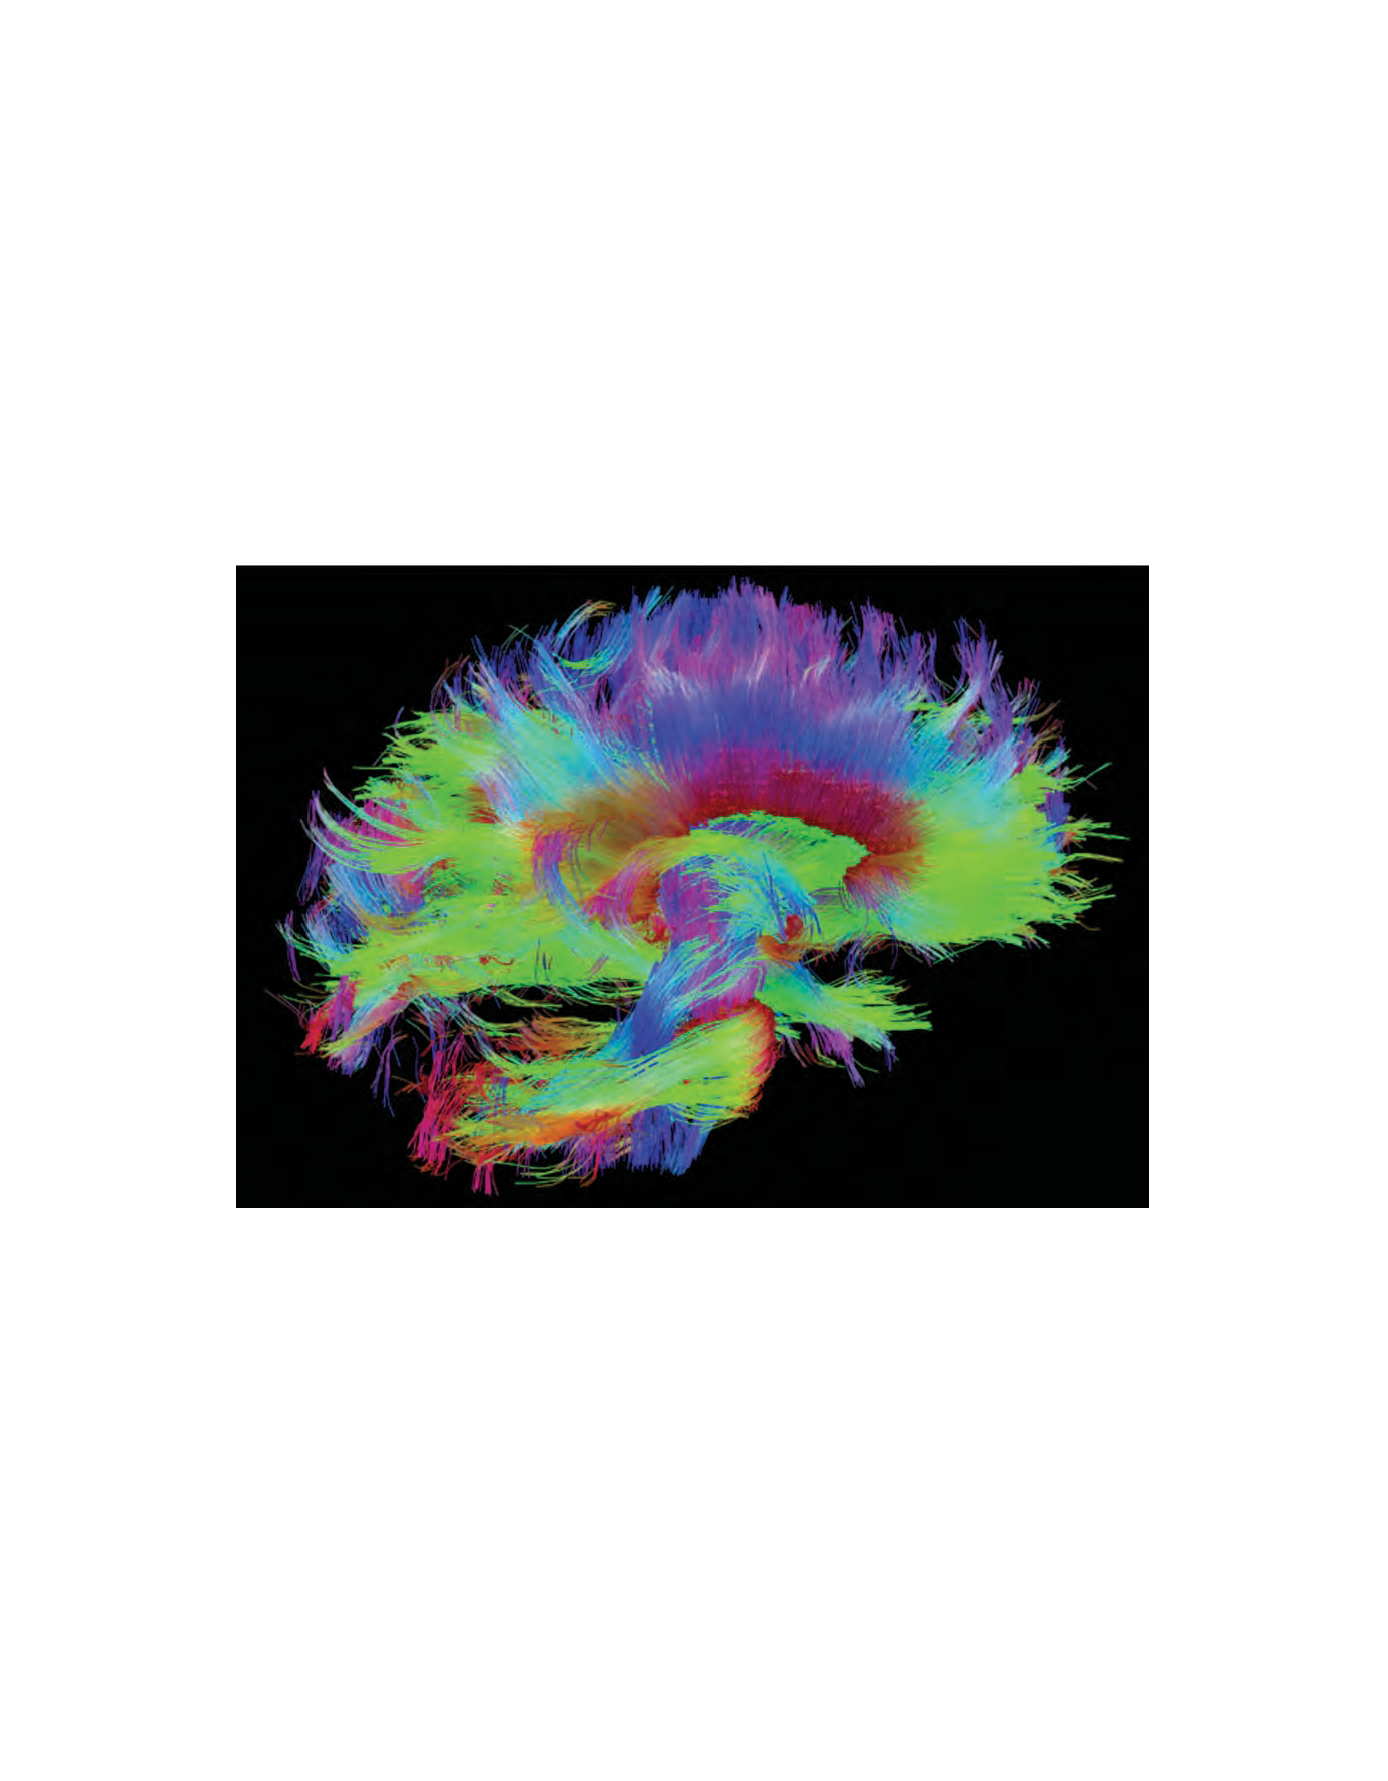
\includegraphics[width=1.0\linewidth]{chap01/fig_1_0}
	\caption{人脑白质纤维结构,显示胼胝体和脑干通路。
		该图像是根据\textit{核磁共振成像}数据和扩散光谱成像技术构建的,该技术使用水分子的扩散速率和优选方向在核磁共振图像中产生对比度,以揭示在纤维束中行进的轴突束。
		纤维按方向进行颜色编码:红色,左右;绿色,前后;蓝色,升序-降序(RGB=XYZ轴)。
		(来自连接体扫描仪数据集。
		由南加州大学神经成像实验室和哈佛大学生物医学成像中心提供。
		\href{www.humanconnetomproject.org}{人类连接体项目联合会})}
	\label{fig:1_0}
\end{figure}

在20世纪下半叶,生物学的中心焦点是基因。
现在,在21世纪上半叶,焦点已经转移到神经科学,特别是心理生物学。
我们希望了解我们感知、行动、学习和记忆的过程。
一个只有1.5公斤重的大脑器官是如何构思无限、发现新知识并产生人类思想、情感和行动的非凡个性的?
这些非凡的心理能力是如何在器官内分布的?
什么规则将一个区域的解剖组织和细胞生理与其在心理状态中的特定作用联系起来?
基因对行为有什么影响?
神经细胞中的基因表达是如何受到发育和学习过程的调节的?
经验是如何改变大脑处理后续事件的方式的,这种无意识的处理在多大程度上?
最后,神经和精神疾病的神经基础是什么?
在神经科学原理的介绍部分,我们开始讨论这些问题。
在这样做的过程中,我们描述了神经科学如何试图将神经回路的计算逻辑与大脑联系起来——定义的神经回路中的神经细胞活动如何介导复杂的心理过程。


在过去的几十年里,技术进步为大脑的科学研究开辟了新的视野。
今天,有可能将神经元互连回路的细胞动力学与大脑中感知和运动行为的内部表征联系起来,并将这些内部机制与可观察的行为联系起来。
新的成像技术使我们能够可视化人类大脑的活动——识别大脑中与特定思维和感觉模式及其相互联系模式相关的特定区域。


在本书的第一部分中,我们考虑了心理功能在多大程度上可以局限于大脑的特定区域。
我们还研究了从单个神经细胞的特性、其分子成分和突触连接的角度来理解这些功能的程度。
在本书的后面部分,我们详细研究了大脑认知和情感功能的基本机制:感知、行动、动机、情绪、学习和记忆。


人脑是一个由 800 多亿个神经细胞组成的网络,这些神经细胞在系统中相互连接——神经回路——构建我们对外部世界的感知,固定我们的注意力,指导我们的决策,并实施我们的行动。
因此,理解大脑的第一步是了解神经元是如何组织成信号通路的,以及它们是如何通过突触传递进行交流的。
我们将在本书中提出的主要观点之一是,在\textit{发育过程中建立}并在\textit{经验过程中完善}的\textit{突触连接特异性}是行为的基础。
我们还必须了解行为的先天和环境决定因素,在这些决定因素中,基因编码的蛋白质最初控制着神经回路的发育,然后可以通过基因表达的经验依赖性变化来改变神经回路。


通过将现代细胞和分子生物学技术、大脑成像、理论和临床观察应用于认知、情绪和行为的研究,一门新的心理科学正在兴起。
神经科学强化了希波克拉底在两千多年前首次提出的观点,即对心智的正确研究始于对大脑的研究。
认知心理学和精神分析理论强调了人类心理体验的多样性和复杂性。
这些学科现在可以通过从神经科学中深入了解大脑功能来丰富。
未来的任务是对心理过程进行研究,以实证神经科学为基础,关注心理的内部表征和状态是如何产生的问题。


我们的目标不仅仅是提供事实,而是提供大脑组织、功能和计算的原理。
神经科学原理并没有将人类思想的复杂性简化为一组分子或数学公理。
相反,它们让我们能够在大脑的复杂性中欣赏到某种美——达尔文式的优雅,这种复杂性解释了思维和行为。
人们可能会问,从更基本的神经机制的详细解剖中收集到的一个想法是否包含了对更高大脑功能的见解。
简单反射的组织是否与手的意志运动有关?
在发育中的脊髓中建立回路的机制是否与存储记忆的机制有关?
将我们从睡眠中唤醒的神经过程与允许无意识过程刺穿我们意识的过程相似吗?
我们希望读者在深入研究其事实基础时,会对这些原则感到高兴。
毫无疑问,这是一项正在进行的工作。





\chapter{大脑和行为} \label{chap:chap1}
生物科学的最后前沿——终极挑战——是理解意识的生物学基础和我们感知、行为、学习和记忆的大脑过程。 
在过去的几十年里,生物科学内部的显著统一为应对这一巨大挑战奠定了基础。 
对基因进行测序并推断它们编码蛋白质的氨基酸序列揭示了神经系统中的蛋白质与身体其他部位遇到的蛋白质之间意想不到的相似性。 
因此,建立细胞功能的总体计划成为可能,该计划为包括细胞神经科学在内的所有细胞生物学提供了一个共同的概念框架。


当前生物学统一的挑战是心理学——心智科学——和神经科学——大脑科学的统一。 
在这种统一的方法中,不将思想和身体视为独立的实体,基于这样一种观点,即所有行为都是大脑功能的结果。 
我们通常所说的心智,就是大脑进行的一系列操作。 
大脑过程不仅是行走和进食等简单运动行为的基础,也是典型人类的所有复杂认知和行为的基础——思考、说话和创作艺术作品。 
作为推论,所有表征精神疾病的行为障碍——情感障碍(感觉)和认知障碍(思想)——都是脑功能紊乱的结果。


大脑中数十亿个神经细胞如何产生行为和认知状态,以及这些细胞如何受到环境(包括社会经验)的影响? 
用大脑活动来解释行为是神经科学的重要任务,神经科学在这方面的进展是本书的一大主题。


神经科学必须不断面对某些基本问题。 
理解思维过程、肢体运动或做出运动愿望的适当生物学描述水平是多少? 
为什么在某些神经系统疾病状态下运动会平稳或急促或无意中进行? 
通过观察神经细胞中\textit{脱氧核糖核酸}表达的模式以及这种模式如何调节神经元的电特性,可能会得出这些问题的答案。 
然而,我们还需要了解由特定大脑区域中的许多神经元组成的神经回路以及许多大脑区域中特定回路的活动如何协调的知识。


是否存在最恰当的生物学描述水平?
简短的回答是,
如果一个人的目标是了解和治疗某些遗传性癫痫病症,那么\textit{脱氧核糖核酸}测序和单个神经元电特性的测量可能足以产生有效的治疗方法。
如果一个人对学习、感知和探索感兴趣,那么可能需要对回路系统和大脑区域进行分析。


现代神经科学的目标是将所有这些专业水平整合成一门连贯的科学。
这种努力迫使我们面对新的问题。
如果心理过程可以定位到离散的大脑区域,那么这些区域的功能与这些区域的解剖学和生理学之间的关系是什么? 
是否需要一种神经回路来处理视觉信息,另一种神经回路来解析语音,还有另一种神经回路来排列运动?
或者具有不同功能的回路是否具有共同的组织原则?
必要的神经计算是否最好理解为对单个神经元或神经元群表示的信息的操作?
信息是以单个神经细胞的电活动表示的,还是分布在整体上的,以至于任何一个细胞的信息量都不比计算机内存的随机位多?
正如我们将要看到的,关于组织水平、细胞特化和功能定位的问题在整个神经科学中反复出现。


为了说明这些观点,我们将研究现代神经科学如何描述语言,这是人类独特的认知行为。
这样做将广泛关注大脑皮层的运作,大脑皮层是人类大脑中最发达的部分。
将看到大脑皮层如何组织成功能不同的区域,每个区域由许多神经元组成,以及如何根据特定区域内特定组互连神经元的活动来分析高度复杂行为的神经装置。
第~\ref{chap:chap3}~章描述了简单反射行为的神经回路如何在细胞水平上运作,说明了感觉信号和运动信号的相互作用如何导致运动行为。



% 结构(几何)和功能(行为)
\section{关于大脑与行为之间的关系,提出了两种相反的观点}

关于神经细胞、大脑和行为的观点是在 20 世纪从 5 种实验传统的综合中产生的:解剖学、胚胎学、生理学、药理学和心理学。


公元 2 世纪的希腊医生盖伦提出,神经将大脑和脊髓分泌的液体输送到身体的周围。
他的观点主导了西方医学,直到显微镜揭示了神经组织中细胞的真实结构。
即便如此,直到 19 世纪后期,神经组织才成为一门特殊科学的主题,当时意大利人\textit{卡米洛$\cdot$高尔基}和西班牙人圣地\textit{亚哥$\cdot$拉蒙$\cdot$卡哈尔}对神经细胞进行了详细、准确的描述,但就大脑的功能得出了两个截然不同的结论。


高尔基开发了一种用银盐对神经元进行染色的方法,这种方法可以在显微镜下显示出它们的整个细胞结构。
基于这些研究,高尔基体得出结论,神经细胞不是相互隔离的独立细胞,而是在一个连续的组织或合胞体网络中共同作用。
使用高尔基技术,\textit{卡哈尔}扩观察到每个神经元通常都有一个细胞体和两种类型的过程:一端是分支树突,另一端是长长的电缆状轴突。 
\textit{卡哈尔}扩得出结论,神经组织不是合胞体,而是离散细胞网络。
在这项工作的过程中,\textit{卡哈尔}扩发展了神经元学说的一些关键概念和许多早期证据——个体神经元是神经系统的基本构建块和信号元件的原则。


在 1920 年,美国胚胎学家\textit{罗斯$\cdot$哈里逊}表明树突和轴突是从细胞体中生长出来的,即使在组织培养中每个神经元都与其他神经元隔离开来也是如此。
\textit{哈里逊}还证实了\textit{卡哈尔}的提议,即轴突的尖端会产生扩张,即生长锥,它将发育中的轴突引导至其目标,即其他神经细胞或肌肉。
这两项发现都为神经元学说提供了强有力的支持。
随着电子显微镜的引入,神经元学说的最终明确证据出现在 20 世纪 50 年代中期。
\textit{桑福德$\cdot$帕莱}的一项具有里程碑意义的研究明确地证明了突触的存在,突触是神经细胞的特殊区域,允许它们之间进行化学或电信号传递。


神经系统的生理学研究始于 18 世纪后期,当时意大利医师和物理学\textit{路易吉$\cdot$加尔瓦尼}发现肌肉和神经细胞会产生电能。
现代电生理学起源于 19 世纪三位德国生理学家——\textit{约翰内斯$\cdot$米勒}、\textit{埃米尔$\cdot$杜$\cdot$博伊斯-雷蒙德}和\textit{赫尔曼$\cdot$冯$\cdot$亥姆霍兹}——他们成功地测量了电活动沿神经细胞轴突的传导速度,并进一步表明:
一个神经细胞的电活动以可预测的方式影响相邻细胞的活动。


药理学在 19 世纪末对我们对神经系统和行为的理解产生了第一次影响,当时法国的\textit{克劳德$\cdot$伯纳德}、德国的\textit{保罗$\cdot$埃尔利希}和英国的\textit{约翰$\cdot$兰利}证明药物不会随机作用于细胞,而是通常与位于细胞膜中的离散受体结合。 
这种洞察力导致发现神经细胞可以通过化学方式相互交流。


关于行为的心理学思考可以追溯到西方科学的开端,当时古希腊哲学家推测行为的原因以及心灵与大脑的关系。
在随后的几个世纪里,出现了两种主要观点。
在 17 世纪,笛卡尔区分了身体和心灵。
在这种二元论观点中,大脑调解了知觉、运动行为、记忆、食欲和激情——一切可以在低等动物身上找到的东西。
但是心智——更高的心智功能,人类行为的有意识体验特征——并不代表大脑或身体的任何其他部分,而是代表灵魂,一个精神实体。
笛卡尔认为,灵魂通过松果体与大脑的机器进行交流,松果体是大脑中线的一个微小结构。
笛卡尔的立场在现代哲学或神经科学中几乎没有影响力。 
事实上,神经科学的基本前提是心智是大脑及其神经活动的产物。
我们这样说并不是说神经科学的目的是通过还原为生物成分来解释心灵,而是要阐明心灵的生物学。


早在 1800 年,维也纳医生和神经解剖学家\textit{弗朗兹$\cdot$约瑟夫$\cdot$加尔}就开始尝试将生物学和心理学概念结合到行为研究中,当时他提出了一种全新的身心观念。
他主张大脑是心灵的器官,一切精神功能都体现在大脑中。
因此,他拒绝了笛卡尔认为思想和身体是分开实体的观点。
此外,他认为大脑皮层不是一个单一的器官,而是包含许多专门的器官,大脑皮层的特定区域控制着特定的功能。 
\textit{加尔}列举了至少 27 个不同的大脑皮层区域或器官; 后来又增加了更多,每一种都对应于一种特定的心智能力(图~\ref{fig:1_1})。
\textit{加尔}将智力过程(例如评估因果关系、计算和感知秩序的能力)分配给了大脑的前部。
浪漫的爱情(恋爱)和好斗的本能特征被分配到大脑后部。
即使是最抽象的人类行为——慷慨、隐秘和虔诚——也被分配到大脑中的一个位置。


\begin{figure}[htbp]
	\centering
	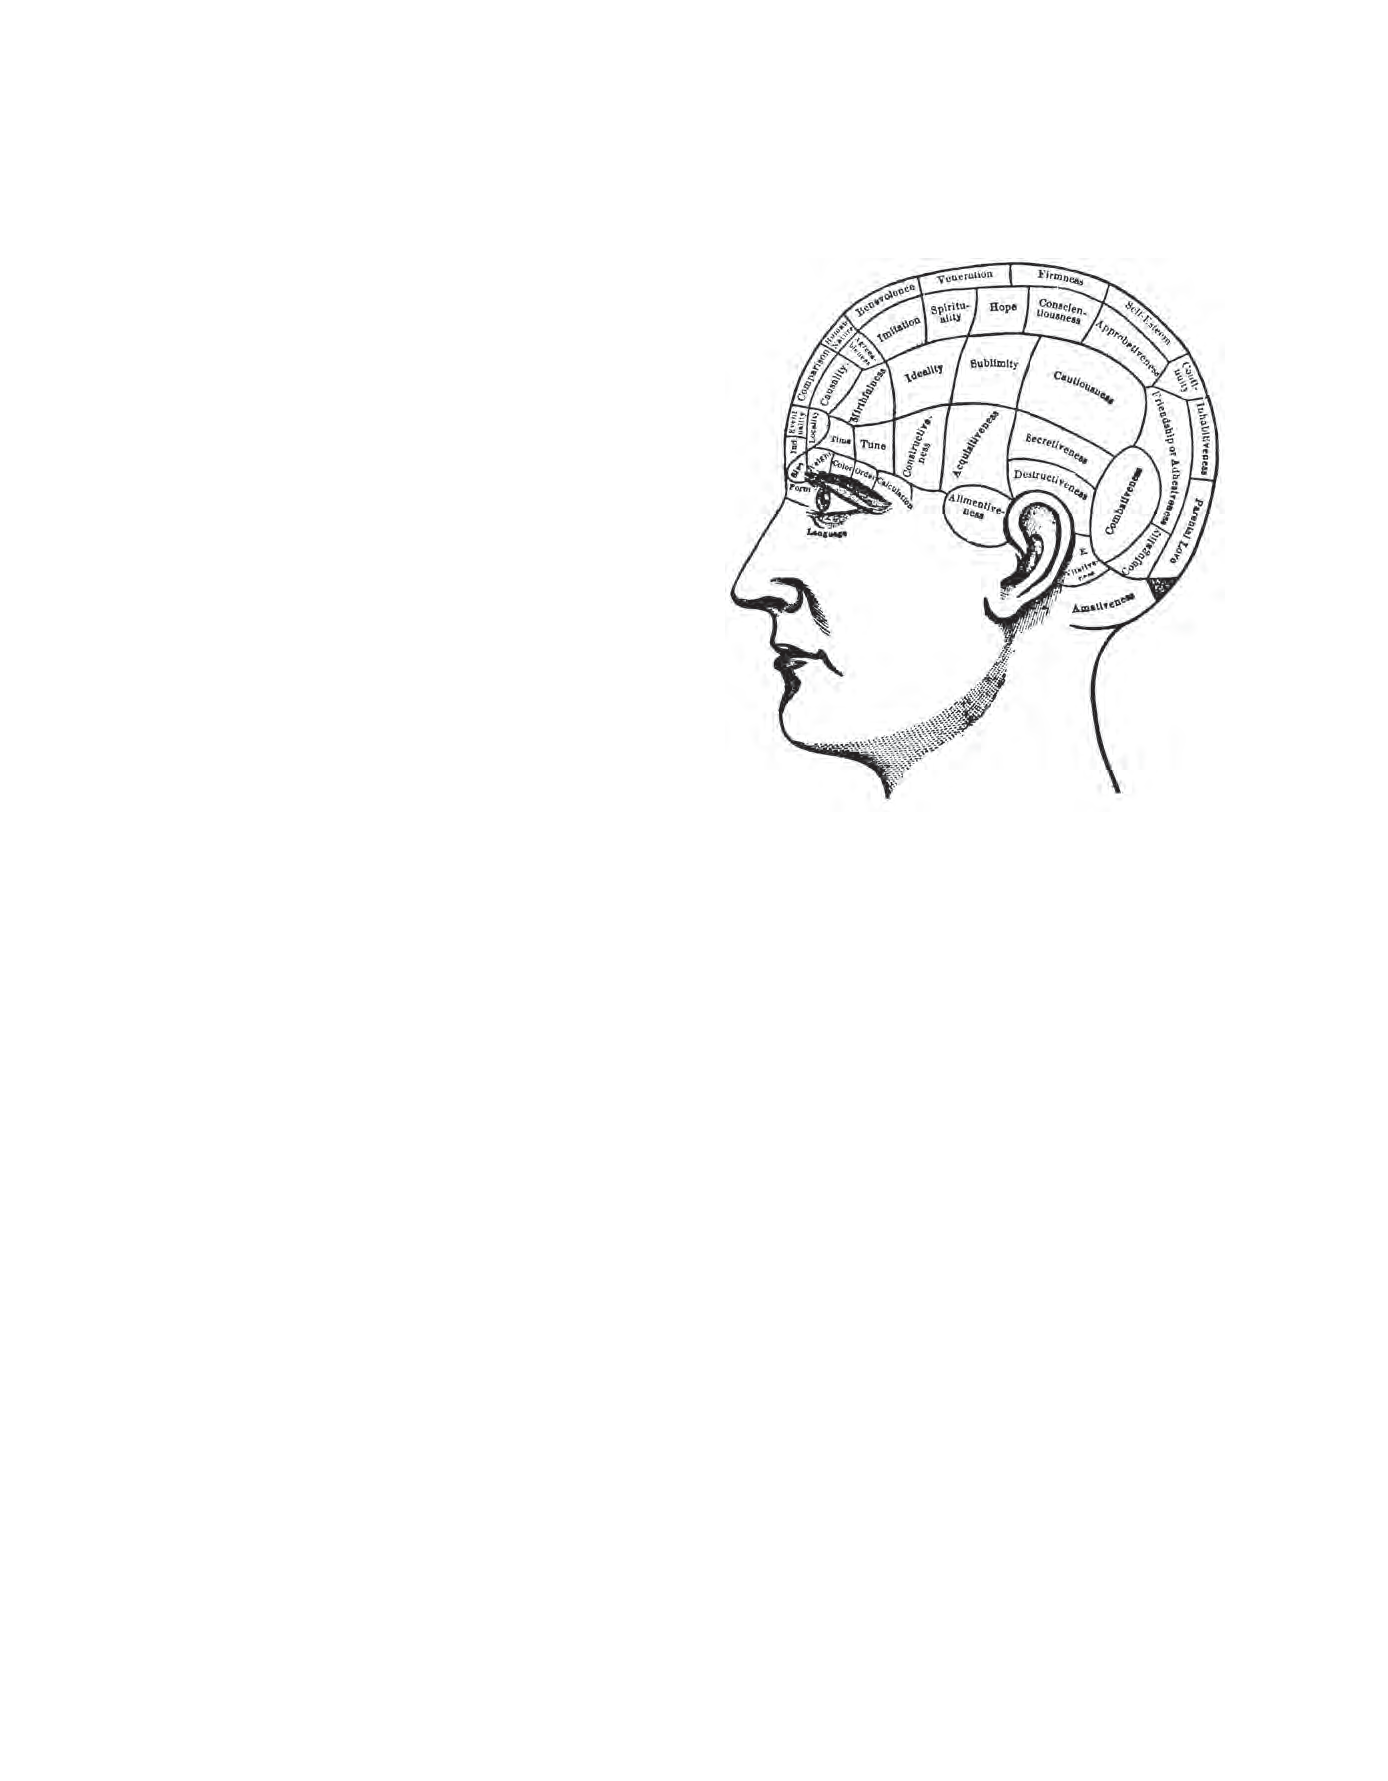
\includegraphics[width=0.55\linewidth]{chap01/fig_1_1}
	\caption{大脑功能定位的早期地图。
		根据 19 世纪的颅相学学说,好斗、灵性、希望和责任心等复杂特征由专门的“器官”控制,大脑皮层的不同区域随着特征的发展而扩大。
		这些大脑局部区域的扩大被认为会在覆盖的头骨上产生特征性的凹凸,从中可以确定一个人的性格。
		这张地图取自 1800 年代初期的一幅图画,显示了 42 个智力和情感“器官”。}
	\label{fig:1_1}
\end{figure}


尽管\textit{加尔}的身心统一理论和他关于某些功能局限于特定大脑区域的观点被证明是正确的,但今天的主流观点是,许多高级心理功能很可能是高度分布的。
此外,\textit{加尔}的本地化实验方法极其幼稚。
\textit{加尔}没有根据经验定位功能,而是通过研究大脑并将心理属性的缺陷与肿瘤或中风后特定区域的病变相关联,\textit{加尔}摒弃了所有来自脑部病变研究的证据,无论是通过临床检查发现的还是在实验动物身上通过手术产生的。
受\textit{相面术}的影响,这是一门基于面部特征揭示性格的流行科学,\textit{加尔}认为,具有特定认知能力的人头骨上的隆起和隆起确定了大脑中这些能力的中心。
他假设大脑区域的大小与该区域所代表的心智能力的相对重要性有关。
因此,特定智力的锻炼会导致相应的大脑区域生长,而这种生长又会导致覆盖在上面的头骨突出。


小时候,\textit{加尔}注意到他那些擅长背作业的同学都有突出的眼睛,于是他就有了这个想法。
他得出结论,这是大脑前部与语言记忆有关的区域过度发育的结果。
当他还是一名年轻医生时,他进一步发展了这个想法,负责管理维也纳的一家精神病院。
在那里,他开始研究患有偏执狂症的患者,这种疾病的特征是对某些关键思想过分感兴趣或强烈渴望从事某些特定行为——盗窃、谋杀、色情、极端宗教信仰。
他推断,由于患者在所有其他行为中都表现良好,大脑缺陷一定是离散的,原则上可以通过检查这些患者的头骨来定位。
\textit{加尔}对局部大脑功能的研究催生了颅相学,这是一门根据头骨的详细形状确定人格和性格的学科。


在 1820 年代后期,法国生理学家\textit{皮埃尔$\cdot$弗卢龙}对\textit{加尔}的想法进行了实验分析。 
\textit{弗卢龙}使用实验动物破坏了\textit{加尔}在大脑中的一些功能中心,进而试图分离出这些“大脑器官”对行为的贡献。
从这些实验中,\textit{弗卢龙}得出结论,特定的大脑区域并不负责特定的行为,而是所有的大脑区域,尤其是前脑的大脑半球,都参与了每一次心理操作。
\textit{弗卢龙}提出,大脑半球的任何部分都有助于半球的所有功能。
因此,大脑半球任何一个区域的损伤都应该平等地影响所有更高的功能。
因此,在 1823 年,\textit{弗卢龙}写道:“所有知觉、所有意志都在这些(大脑)器官中占据相同的位置;
因此,知觉、构想和意志的能力仅仅构成了一种本质上是一体的能力。”


这种信念的迅速接受,后来被称为大脑的整体观点,仅部分基于\textit{弗卢龙}的实验工作。
它也代表了对人类思想是生物器官的唯物主义观点的文化反应。
它代表了对没有灵魂、所有心理过程都可以简化为大脑内的活动以及可以通过锻炼来改善思想的观念的拒绝——这些想法是欧洲宗教机构和土地贵族所不能接受的。


然而,在 19 世纪中叶,法国神经学家\textit{皮埃尔$\cdot$保尔$\cdot$布罗卡}、德国神经学家\textit{卡尔$\cdot$韦尼克}和英国神经学家\textit{休林斯$\cdot$杰克逊}严重挑战了整体观点。
例如,杰克逊在他对局灶性癫痫(一种以身体特定部位开始抽搐为特征的疾病)的研究中表明,不同的运动和感觉功能可以追溯到大脑皮层的特定部位。
\textit{布洛卡}、\textit{韦尼克} 和\textit{杰克逊}的区域研究被 \textit{查尔斯$\cdot$谢灵顿}和\textit{卡哈尔}扩展到细胞水平,他们支持称为细胞连接主义的大脑功能观点。
根据这种观点,单个神经元是大脑的信号单元;
它们按功能组排列,并以精确的方式相互连接。
\textit{韦尼克}和法国神经学家\textit{朱尔斯$\cdot$代热林}的研究表明,不同的行为是由不同的相互关联的大脑区域产生的。


本地化的第一个重要证据来自对大脑如何产生语言的研究。
在考虑相关的临床和解剖学研究之前,首先要回顾一下大脑的整体结构,包括它的主要解剖区域。
这需要我们定义一些神经解剖学家用来描述大脑和脊髓部分之间三维空间关系的基本导航术语。
这些术语在框~\ref{box:1_1}~和图~\ref{fig:1_2}~中介绍。


\begin{proposition}[神经解剖学导航术语] \label{box:1_1}
	
	\quad \quad 中枢神经系统各组成部分在体内的位置和方向参照三个轴进行描述:嘴侧-尾侧、背侧-腹侧和内侧-外侧轴(图~\ref{fig:1_2})。
	这些术语使神经解剖学家能够描述大脑和脊髓部分之间的空间关系。
	它们有助于在同一物种的个体发育或疾病情况下对其大脑进行比较。
	例如,它们也有助于比较不同动物物种的大脑,以了解大脑的进化。

\end{proposition}


\begin{figure}[htbp]
	\centering
	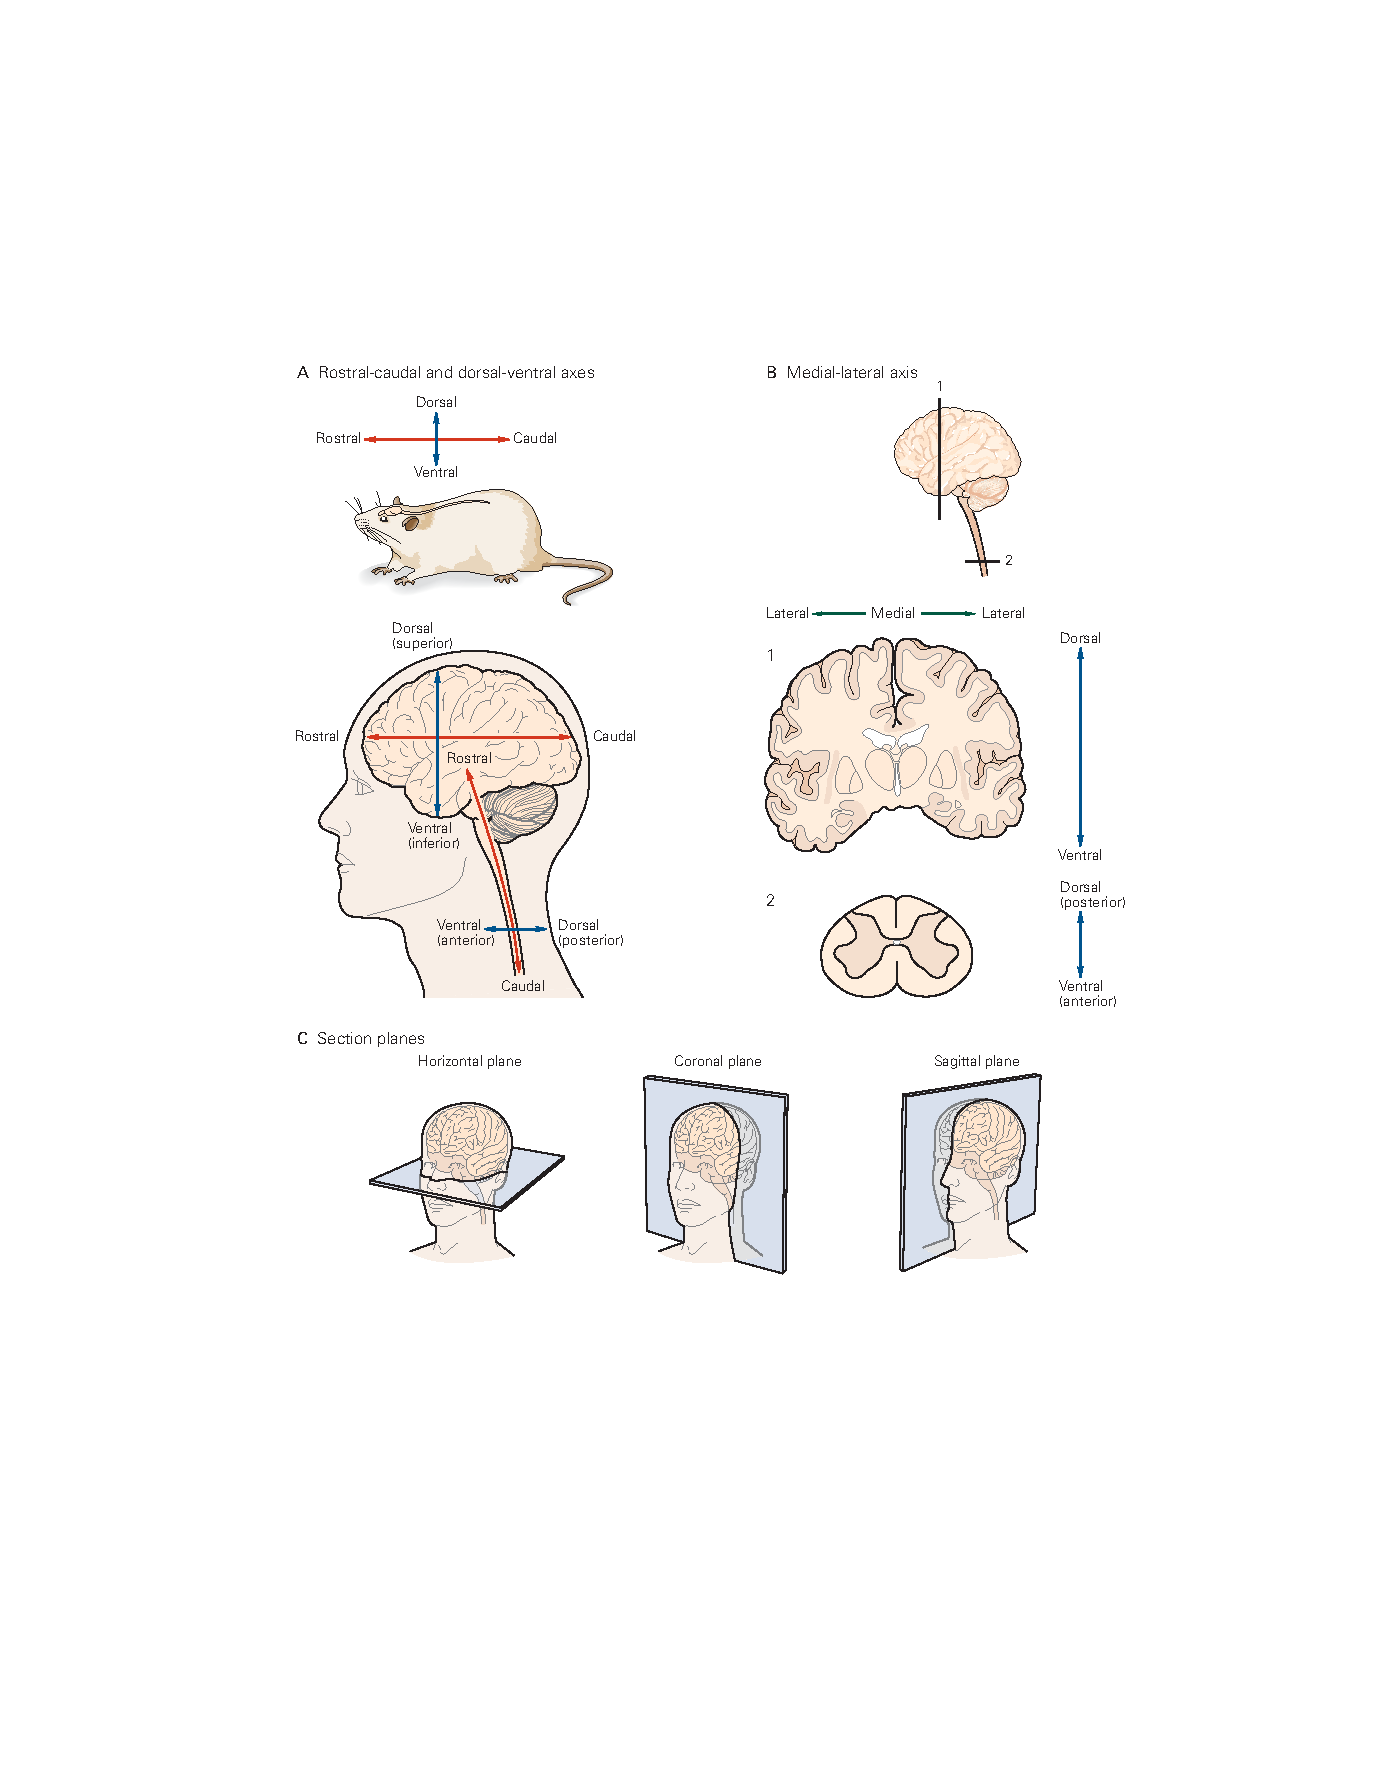
\includegraphics[width=0.9\linewidth]{chap01/fig_1_2}
	\caption{中枢神经系统沿着三个主要轴进行描述\cite{martin2012neuroanatomy}。 
		\textbf{A.} 嘴侧表示朝向鼻子和尾部朝向尾巴。
		背侧是指朝向动物的背部,腹侧是指朝向腹部。
		在低等哺乳动物中,这两个轴的方向在发育到成年生活的过程中一直保持不变。
		在人类和其他高等灵长类动物中,纵轴在脑干中弯曲大约 110 度。
		由于这种挠曲,相同的位置术语在指代挠曲下方和上方的结构时具有不同的含义。
		在弯曲下方,在脊髓中,嘴侧意味着朝向头部,尾侧意味着朝向尾骨(脊柱的下端),腹侧(前侧)意味着朝向腹部,背侧(后侧)意味着朝向背部。
		在弯曲上方,嘴侧意味着朝向鼻子,尾侧意味着朝向后脑勺,腹侧意味着朝向下巴,背侧意味着朝向头顶。
		术语上位通常与背侧同义,下位与腹侧相同。
		\textbf{B.} 内侧意味着朝向大脑中部,外侧意味着朝向侧面。
		\textbf{C.} 当对大脑进行切片进行分析时,切片通常是在三个基本平面之一中制作的:水平、冠状或矢状。}
	\label{fig:1_2}
\end{figure}



\section{大脑具有不同的功能区域}

中枢神经系统是一个双侧且基本对称的结构,有两个主要部分,即脊髓和大脑。
大脑包括六个主要结构:延髓、脑桥、小脑、中脑、间脑和大脑(方框~\ref{box:1_2}~和图~\ref{fig:1_3})。
这些中的每一个依次包含具有独特连接性和发育起源的不同神经元组。
在延髓、脑桥、中脑和间脑中,神经元通常分为不同的簇,称为细胞核。
大脑和小脑的表面由一大片折叠的神经元组成,分别称为大脑皮层和小脑皮层,其中神经元以固定的连接模式分层组织。
大脑还包含许多位于皮层(皮层下)下方的结构,包括基底神经节和杏仁核(图~\ref{fig:1_4})。


\begin{proposition}[中枢神经系统的解剖学组织] \label{box:1_2}
	\textbf{中枢神经系统有七个主要部分}
	
	\quad \quad \textbf{脊髓}是中枢神经系统的最尾部,接收和处理来自四肢和躯干皮肤、关节和肌肉的感觉信息,并控制四肢和躯干的运动。
	如图~\ref{fig:1_3}~所示,它被细分为颈部、胸部、腰部和骶骨区域。
	
	\quad \quad 脊髓继续作为\textbf{脑干}向头端延伸,脑干由延髓、脑桥和中脑组成。
	脑干接收来自头部皮肤和肌肉的感觉信息,并为头部肌肉组织提供运动控制。
	它还将信息从脊髓传递到大脑,从大脑传递到脊髓,并通过网状结构调节唤醒和意识水平。
	
	\quad \quad 脑干包含几个细胞体集合,即脑神经核。
	其中一些细胞核接收来自头部皮肤和肌肉的信息;
	其他人控制面部、颈部和眼睛肌肉的运动输出。
	还有一些人专门处理来自三种特殊感官的信息:听觉、平衡和味觉。
	
	\quad \quad \textbf{延髓}直接位于脊髓的嘴侧,包括几个负责重要自主功能的中心,如消化、呼吸和心率控制。
	
	\quad \quad \textit{脑桥},从嘴侧到髓质,传递从大脑半球到小脑的运动信息。
	
	\quad \quad 脑桥后面的\textbf{小脑}调节运动的力量和范围,并参与运动技能的学习。
	它在功能上与脑干的三个主要器官相连:延髓、脑桥和中脑。
	
	\quad \quad \textbf{中脑}位于脑桥的嘴侧,控制着许多感觉和运动功能,包括眼球运动以及视觉和听觉反射的协调。
	
	\quad \quad \textbf{间脑}位于中脑的嘴侧,包含两个结构。
	丘脑处理从中枢神经系统其他部分到达大脑皮层的大部分信息。
	下丘脑调节自主神经、内分泌和内脏功能。
	
	\quad \quad \textbf{大脑}由两个大脑半球组成,每个半球由褶皱严重的外层(大脑皮层)和三个深层结构(基底神经节、海马体和杏仁核的组成部分)组成。
	基底神经节包括尾状核、壳核和苍白球,调节运动执行、运动和习惯学习,这两种记忆形式被称为内隐记忆;
	海马体对储存人、地点、事物和事件的记忆至关重要,这种记忆形式被称为外显记忆;
	杏仁核协调情绪状态的自主神经和内分泌反应,包括威胁记忆,另一种形式的内隐记忆。
	
	\quad \quad 如图~\ref{fig:1_3}~所示,每个大脑半球分为四个不同的叶:额叶、顶叶、枕叶和颞叶。
	这些叶与不同的功能有关,尽管皮层区域都高度互联,可以参与广泛的大脑功能。
	枕叶接收视觉信息,对视觉的各个方面都至关重要。
	来自枕叶的信息通过两个主要途径进行处理。
	连接枕叶和顶叶的背流与视觉空间中物体的位置和操作有关。
	连接枕叶和颞叶的腹侧流与物体身份有关,包括对单个人脸的识别。
	颞叶对处理听觉信息也很重要(它还包含隐藏在其表面下的海马体和杏仁核)。
	额叶与所有皮层区域紧密相连,对高级认知处理和运动规划很重要。
	
	\quad \quad 大约三分之二的皮层位于脑沟中,许多脑回被覆盖的皮层叶所掩埋。
	通过分离大脑半球以显示大脑的内侧表面,并在死后对大脑进行切片,例如在尸检中,可以看到大脑皮层的完整范围(图~\ref{fig:1_4})。
	这些信息中的大部分可以通过现代大脑成像在活体大脑中可视化(图~\ref{fig:1_5};第~\ref{chap:chap6}~章)。
	这些观点也提供了白质和皮层下灰质的观点。
	
	\quad \quad 大脑皮层表面看不到的两个重要区域包括扣带皮层和岛叶皮层。
	扣带皮层位于胼胝体的背面,对情绪、疼痛感知和认知的调节很重要。
	岛叶皮层位于上覆的额叶、顶叶和颞叶内,在情绪、稳态和味觉感知中发挥着重要作用。
	这些内部视图还提供了对\textit{胼胝体}的检查,\textit{胼胝}体是连接两个半球的突出轴突\textit{纤维束}。
	
	上述不同的大脑区域通常分为三个更广泛的区域:后脑(包括延髓、脑桥和小脑);
	中脑(包括顶盖、黑质、网状结构和中脑导水管周围灰质);
	和前脑(包括间脑和大脑)。
	中脑和后脑(减去小脑)包括与脑干相同的结构。
	神经系统的解剖组织在第~\ref{chap:chap4}~章中有更详细的描述。
		
\end{proposition}


\begin{figure}[htbp]
	\centering
	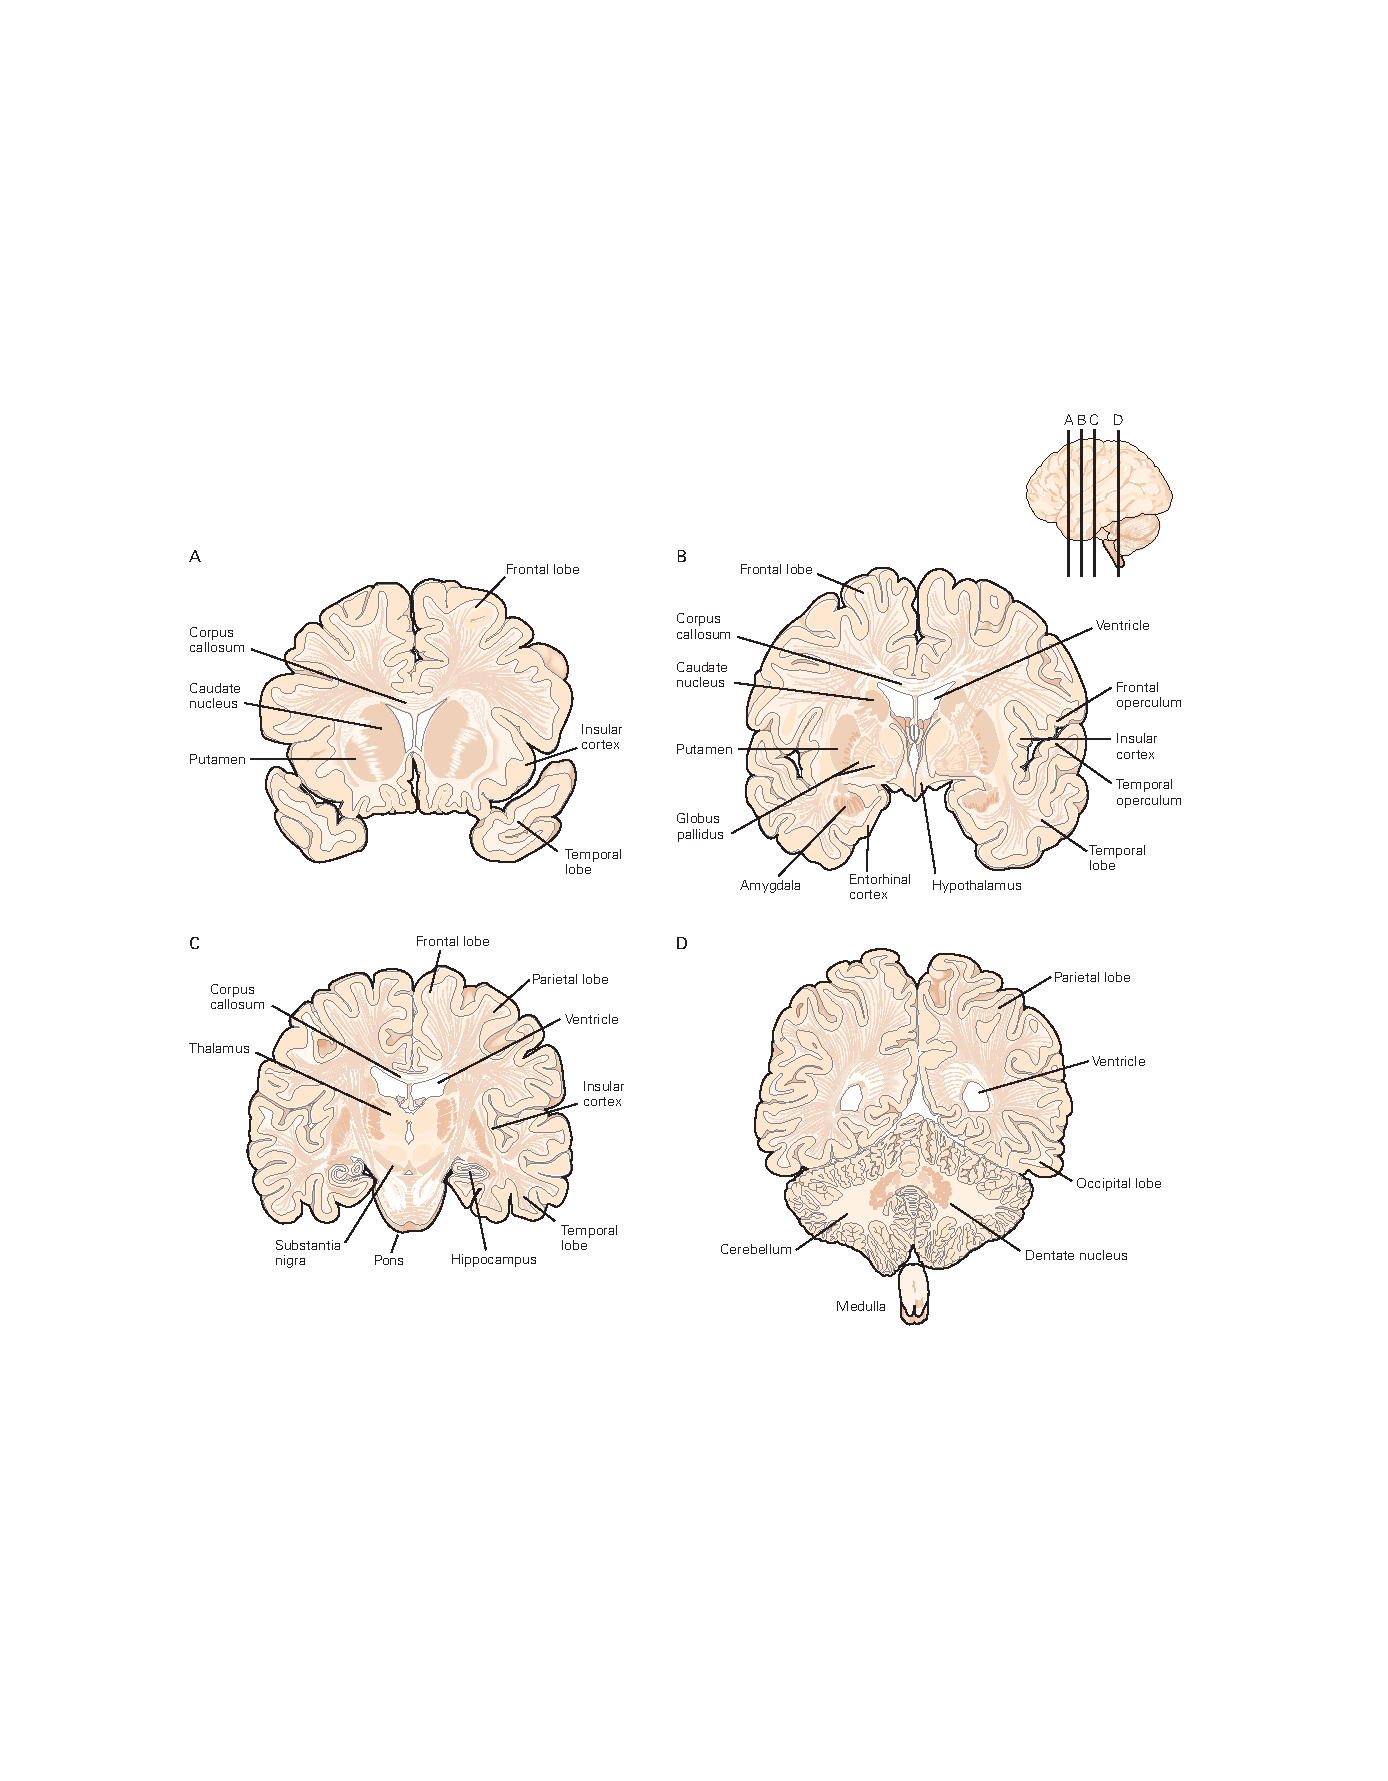
\includegraphics[width=0.95\linewidth]{chap01/fig_1_4}
	\caption{中枢神经系统的划分。
		\textbf{A.} 中枢神经系统可分为七个主要区域,从最尾部的脊髓区域,到脑干(延髓、脑桥和中脑),到间脑(包括丘脑和下丘脑),到端脑或大脑(大脑皮层、底层白质、皮层下核和基底神经节)。
		\textbf{B.} 大脑的四个主要叶以覆盖它们的颅骨部分命名。
		这张大脑的侧视图仅显示左侧大脑半球。
		中央沟将额叶和顶叶分开。
		外侧沟将额叶与颞叶分开。
		初级运动皮层占据紧靠中央沟头端的回。
		初级体感皮层占据中央沟尾部的回。
		\textbf{C.} 在右半球的内侧视图中,当半球分开时,可以看到大脑的进一步分裂。
		\textit{胼胝体}包含一大束连接两个半球的轴突。
		扣带皮层是大脑皮层的一部分,围绕着大脑皮层。
		初级视觉皮层占据距状沟。}
	\label{fig:1_3}
\end{figure}


\begin{figure}[htbp]
	\centering
	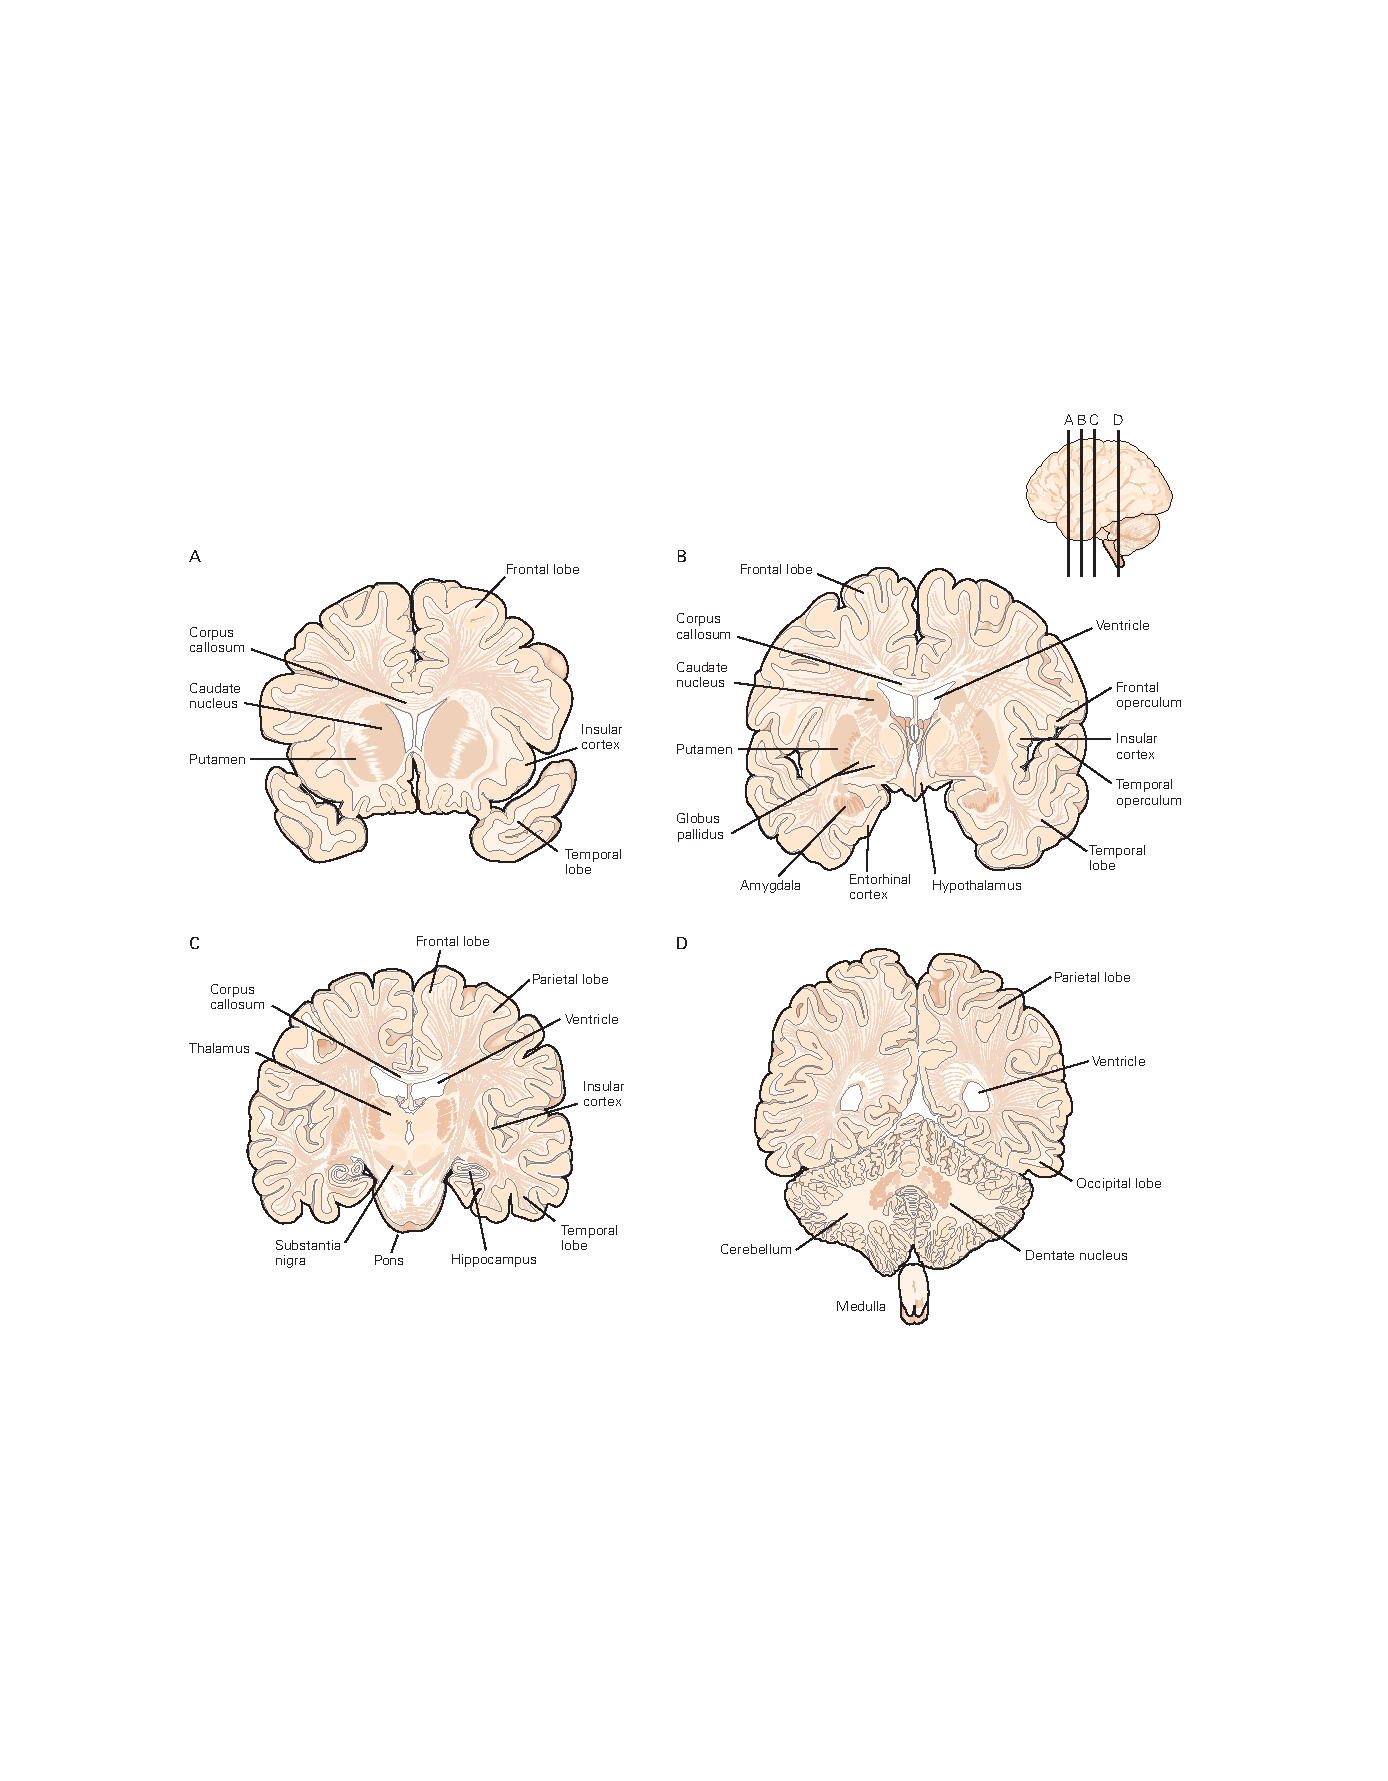
\includegraphics[width=0.8\linewidth]{chap01/fig_1_4}
	\caption{在死后组织的脑切片图中可以看到大脑半球的主要皮层下和深部皮层区域。
		四个连续的冠状切片 (A–D) 沿着大脑侧视图(右上角,插图)上指示的延髓-尾轴制作。
		基底神经节包括尾状核、壳核、苍白球、黑质和底丘脑核(未显示)。
		丘脑将感觉信息从外围传递到大脑皮层。
		杏仁核和海马体是埋藏在颞叶内的大脑皮层区域,对情绪反应和记忆很重要。
		脑室包含并产生脑脊液,脑脊液浸润脑沟、脑池和脊髓\cite{nieuwenhuys2007human}。}
	\label{fig:1_4}
\end{figure}


现代脑成像技术可以看到活人这些结构的活动(见第~\ref{chap:chap6}~章)。
当人们在受控条件下从事特定任务时,脑成像通常用于评估大脑离散区域的代谢活动。
这些研究提供的证据表明,特定类型的行为比其他行为更能激发大脑特定区域的活动。
大脑成像生动地表明认知操作主要依赖于大脑皮层,即覆盖两个大脑半球的皱纹灰质(图~\ref{fig:1_5})。


\begin{figure}[htbp]
	\centering
	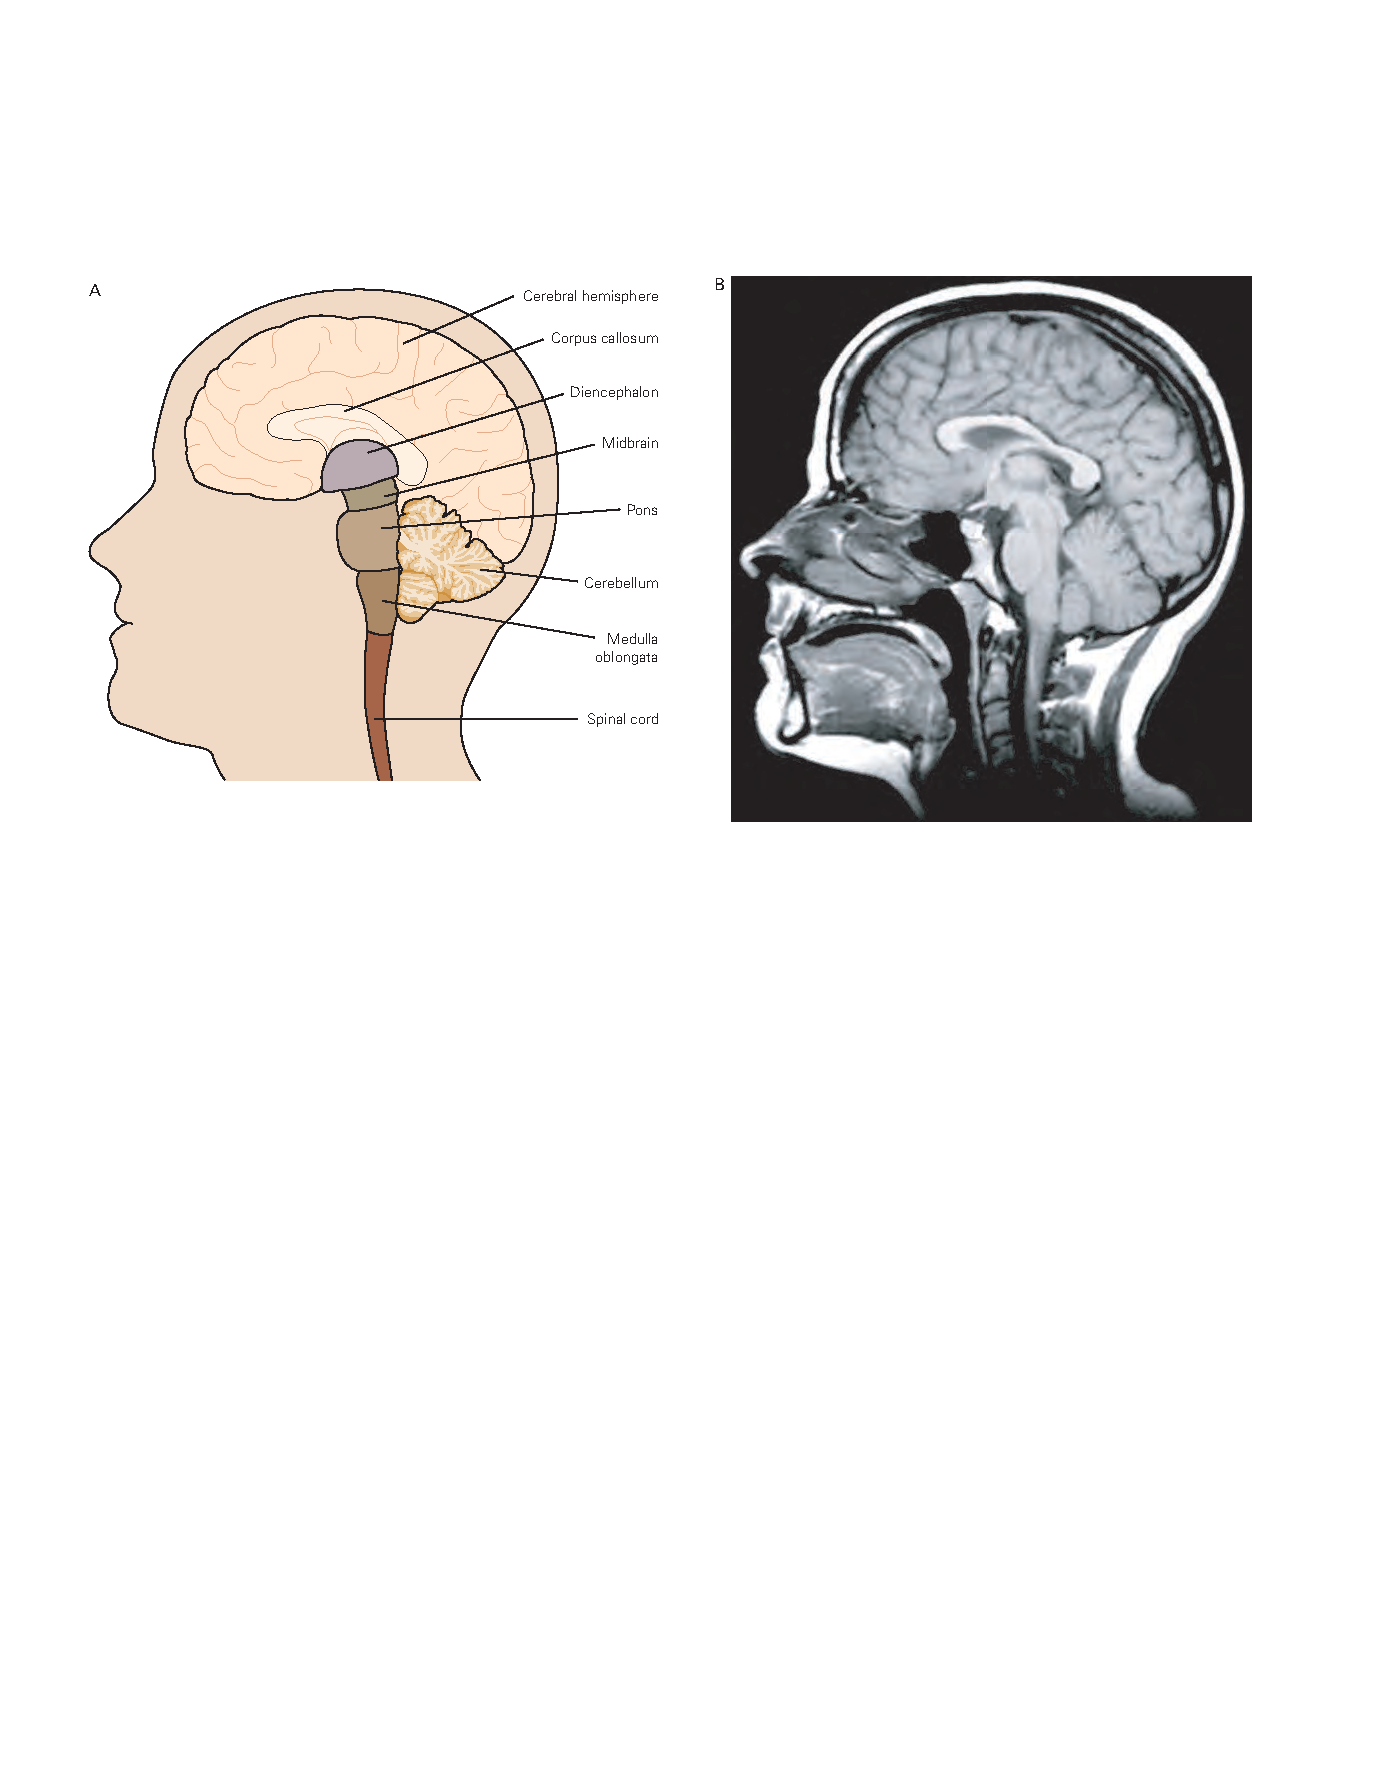
\includegraphics[width=0.9\linewidth]{chap01/fig_1_5}
	\caption{可以在活人的大脑中成像主要皮层和皮层下区域。
		\textbf{A.} 这张示意图显示了大脑的主要表面和深部区域,包括脊髓的延髓末端,以供参考。
		\textbf{B.} 在 A 部分绘制的主要大脑分区在活人脑的磁共振图像中很明显。}
	\label{fig:1_5}
\end{figure}


在每个半球中,覆盖的皮层分为四个叶,以覆盖它们的颅骨命名:额叶、顶叶、枕叶和颞叶(图~\ref{fig:1_3}B)。
每个叶都有几个特征性的深折叠,这是一种将一大片皮层包装到有限空间中的进化策略。
这些回旋的顶部称为脑回,中间的沟称为脑沟或裂隙。 
人与人之间非常相似的更突出的脑回和脑沟具有特定的名称。
例如,中央沟将中央前回(一个与运动功能有关的区域)与中央后回(一个处理感觉功能的区域)分开(图~\ref{fig:1_3}B)。
如第~\ref{chap:chap6}~章所述,无论是在死后组织中(图~\ref{fig:1_4}),还是实际上使用磁共振成像(图~\ref{fig:1_5}),几个突出的脑回仅在两个半球之间的内侧表面可见(图~\ref{fig:1_3}C),其他脑回位于脑裂和脑沟深处,因此只有在大脑被切片时才可见。


每个叶都有专门的功能。
额叶主要与短期记忆、计划未来行动和控制运动有关;
顶叶介导躯体感觉,形成身体形象并将其与个人以外的空间联系起来;
枕叶与视力有关;
颞叶处理听觉、物体和面孔的识别,以及通过其深层结构、海马体和杏仁核处理学习、记忆和情感。


两个重要特征表征了大脑皮层的组织。
首先,每个半球主要关注身体对侧(对侧)的感觉和运动过程。
因此,从身体左侧到达脊髓的感觉信息在到达大脑皮层的途中穿过神经系统的右侧。
同样,右半球的运动区控制着身体左半边的运动。
第二个特征是两个半球虽然外观相似,但在结构或功能上并不完全对称。



\section{认知能力本地化的第一个有力证据来自语言障碍研究}

大脑皮层中第一个被确定为对认知很重要的区域是与语言有关的区域。
这些发现来自对失语症的研究,失语症是一种语言障碍,最常发生在大脑组织的某些区域因中风、供应大脑半球一部分的血管闭塞或破裂而受损时。
失语症研究中的许多重要发现
在 19 世纪下半叶,接二连三地出现许多重要的失语症研究。
总而言之,这些进展构成了人类行为神经科学研究中最激动人心和最重要的章节之一。


法国神经学家布罗卡是第一个确定与语言有关的大脑特定区域的人。
\textit{布洛卡}受到\textit{加尔}绘制大脑高级功能图的影响,但他没有将行为与头骨上的肿块相关联,而是将失语症的临床证据与死后发现的脑损伤相关联。
1861 年,他写道:“我曾认为,如果有一门颅相学,那将是(大脑皮层中)回旋的颅相学,而不是(头上的)肿块的颅相学。” 
基于这种洞察力,布罗卡创立了神经心理学,这是一门心理过程的经验科学,他将其与加尔的颅相学区分开来。


1861 年,布罗卡描述了一位名叫勒博涅的病人,他由于中风而无法说话,尽管他能很好地理解语言。
该患者没有影响其说话能力的舌头、嘴巴或声带运动缺陷。
事实上,他可以毫无困难地说出孤立的单词、吹口哨和唱出一段旋律。
但他不能按语法说话或造出完整的句子,也不能用书面表达思想。
对这名患者的大脑进行的尸检显示,左额叶后下方区域有一个病变,现在称为布罗卡区(图~\ref{fig:1_6})。
\textit{布洛卡}研究了 8 名相似的患者,均在该区域有病变,并且每个病例的病变都位于左侧大脑半球。
这一发现促使\textit{布洛卡}在 1864 年宣布:“Nous parlons avec l’hémisphère gauche!” (我们用左半球说话!)。


\begin{figure}[htbp]
	\centering
	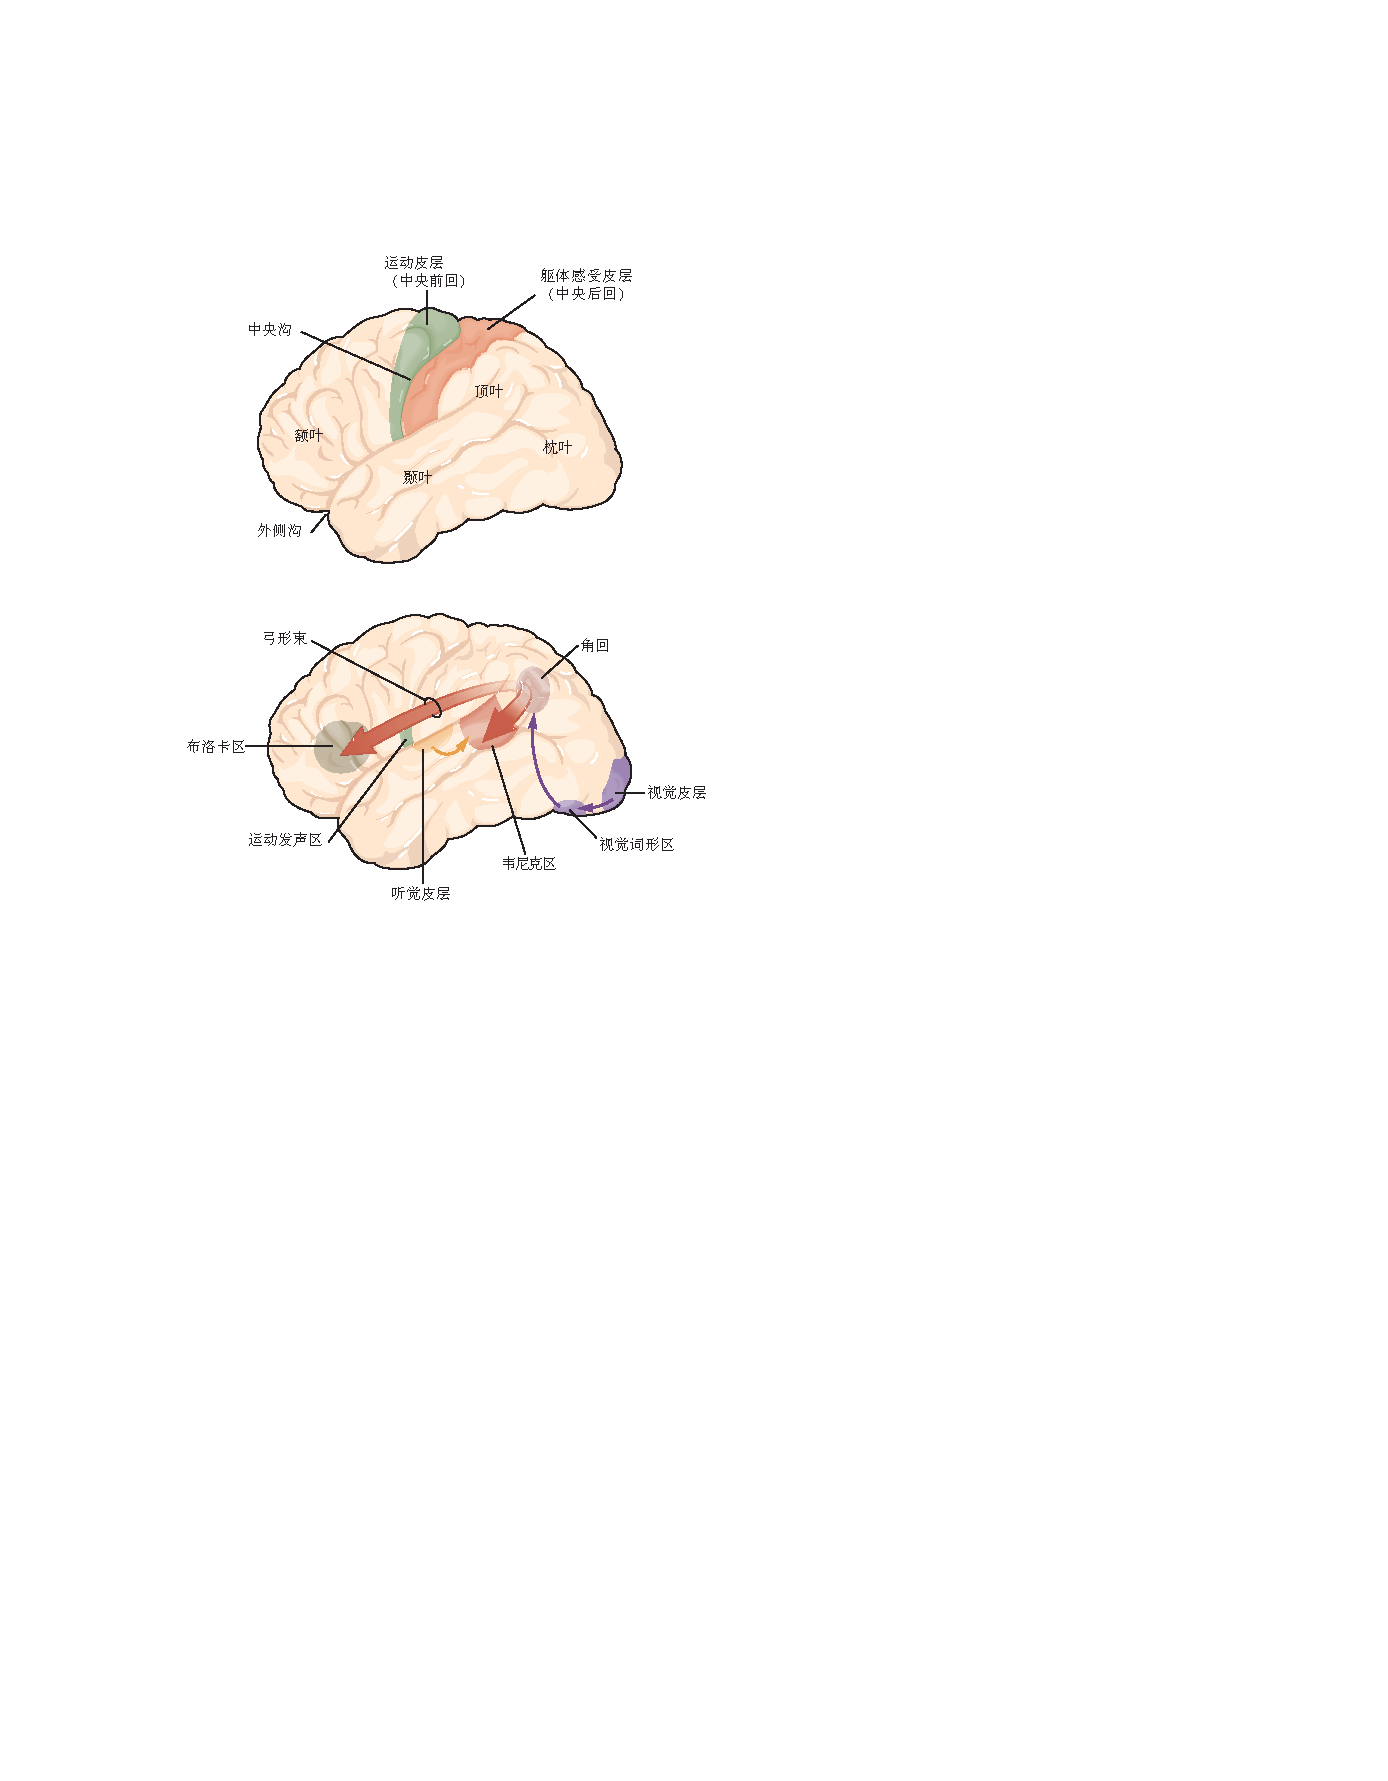
\includegraphics[width=0.6\linewidth]{chap01/fig_1_6}
	\caption{语言处理涉及左脑半球的几个区域。
		布洛卡区控制言语的产生。
		它位于控制形成单词的嘴巴和舌头运动的运动区附近。
		韦尼克区处理语言的听觉输入,对理解言语很重要。
		它位于初级听觉皮层和角回附近。
		法国神经学家\textit{朱尔斯$\cdot$代热林}在 1890 年代提出,角回中的多模态感觉区域整合了来自视觉和听觉的信息来表示单词,但最近的研究表明更多的腹侧枕颞皮层区域用于处理视觉单词。
		\textit{韦尼克}区通过双向通路与\textit{布洛卡}区相通,其中一部分由弓状束组成\cite{geschwind1979specializations}。}
	\label{fig:1_6}
\end{figure}


布洛卡的工作激发了人们对与其他特定行为相关的皮层部位的搜索——搜索很快就得到了回报。
1870 年,\textit{古斯塔夫$\cdot$弗里奇}和\textit{爱德华$\cdot$希茨格}表明,可以通过电刺激中央前回的离散区域来产生狗的特征性肢体运动,例如伸出爪子,这激起了科学界的热潮。
这些区域总是位于对侧运动皮层。
因此,最常用于书写和熟练动作的右手是由左半球控制的,而左半球也控制着说话。
因此,对大多数人来说,左半球被认为是主导的。


下一步是由\textit{韦尼克}于 1876 年采取的,他在 26 岁时发表了一篇现在已成为经典的论文,“失语症的综合症状:解剖学基础上的心理学研究”。
在其中,他描述了另一种类型的失语症,这是一种理解障碍而不是言语障碍:一种与表达障碍相反的接受障碍。
布罗卡的病人可以理解语言但不会说话,而韦尼克的病人可以造词但不能理解语言,只能说出毫无意义但合乎语法的句子。
而且,这种新型失语症的发生部位与布罗卡所描述的不同。
病变发生在大脑皮层后部,即颞叶与顶叶交汇处(图~\ref{fig:1_6})。


基于这一发现以及\textit{布洛卡}、\textit{弗里奇}和\textit{希茨格}的工作,\textit{韦尼克}制定了一种语言神经模型,试图调和和扩展当时大脑功能的主流理论。
颅相学家和细胞联结主义者认为,大脑皮层是功能特定区域的马赛克,而整体聚合场学派则声称,每一种心理功能都涉及整个大脑皮层。
韦尼克提出,只有最基本的心理功能,即与简单的知觉和运动活动有关的功能,才完全由皮层离散局部区域的神经元调节。
他认为,更复杂的认知功能是由几个功能部位之间的相互联系产生的。
通过将局部功能原理整合到联结主义框架中,韦尼克强调了单一行为的不同组成部分可能在大脑的多个区域中得到处理的观点。
因此,他是第一个提出分布式处理思想的人,分布式处理现在是神经科学的核心原则。


\textit{韦尼克}假设语言涉及独立的运动和感觉程序,每个程序都由不同的皮层区域控制。
他提出,控制言语嘴部运动的运动程序位于\textit{布罗卡区},恰好位于控制嘴、舌、上颚和声带的运动区的前面(图~\ref{fig:1_6})。
接下来,他将控制单词感知的感觉程序分配到他发现的颞叶区域,现在称为韦尼克区。
该区域被听觉皮层和现在统称为联合皮层的区域包围,这些区域整合了听觉、视觉和躯体感觉。
根据\textit{韦尼克}的模型,这两个语言中心之间的交流是通过一大束被称为弓状束的轴突来调节的。


因此,韦尼克制定了第一个连贯的语言神经模型,该模型在第~\ref{chap:chap55}~章中进行了重要的修改和阐述,至今仍然有用。
根据这个模型,口语或书面词的神经处理开始于专门负责听觉的皮层的单独感觉区域 或视觉信息。
然后,通过中间关联区域提取适合口头或书面文字识别的特征,将此信息传送到韦尼克区,在那里它被识别为语言并与意义相关联。


韦尼克模型的强大之处不仅在于它的完整性,还在于它的预测效用。
该模型正确预测了第三种类型的失语症,一种由断开连接引起的失语症。
在这种类型中,语言的感受区和表达区完好无损,但连接它们的神经纤维(弓状束)被破坏。
这种传导性失语症,正如现在所称,其特征是频繁的、基于声音的言语错误(音素性错语)、重复困难和言语工作记忆的严重限制。
传导性失语症患者能理解他们听到和读到的单词,并且在说话时没有运动障碍。
然而,他们无法连贯地说话; 他们省略部分单词或替换不正确的声音,并且在逐字重复他们听到、读到或从记忆中回忆起的多音节单词、短语或句子时遇到很大困难。
尽管他们痛苦地意识到自己的错误,但他们连续不断的自我纠正尝试往往都没有成功。


在解剖学家布罗德曼的领导下,部分受到韦尼克的启发,20 世纪初在德国出现了一个新的皮层定位学派,该学派根据细胞的形状及其分层的变化来区分皮层的功能区域 安排。
使用这种细胞构造方法,布罗德曼区分了人类大脑皮层中 52 个解剖学和功能上不同的区域(图~\ref{fig:1_7})。


\begin{figure}[htbp]
	\centering
	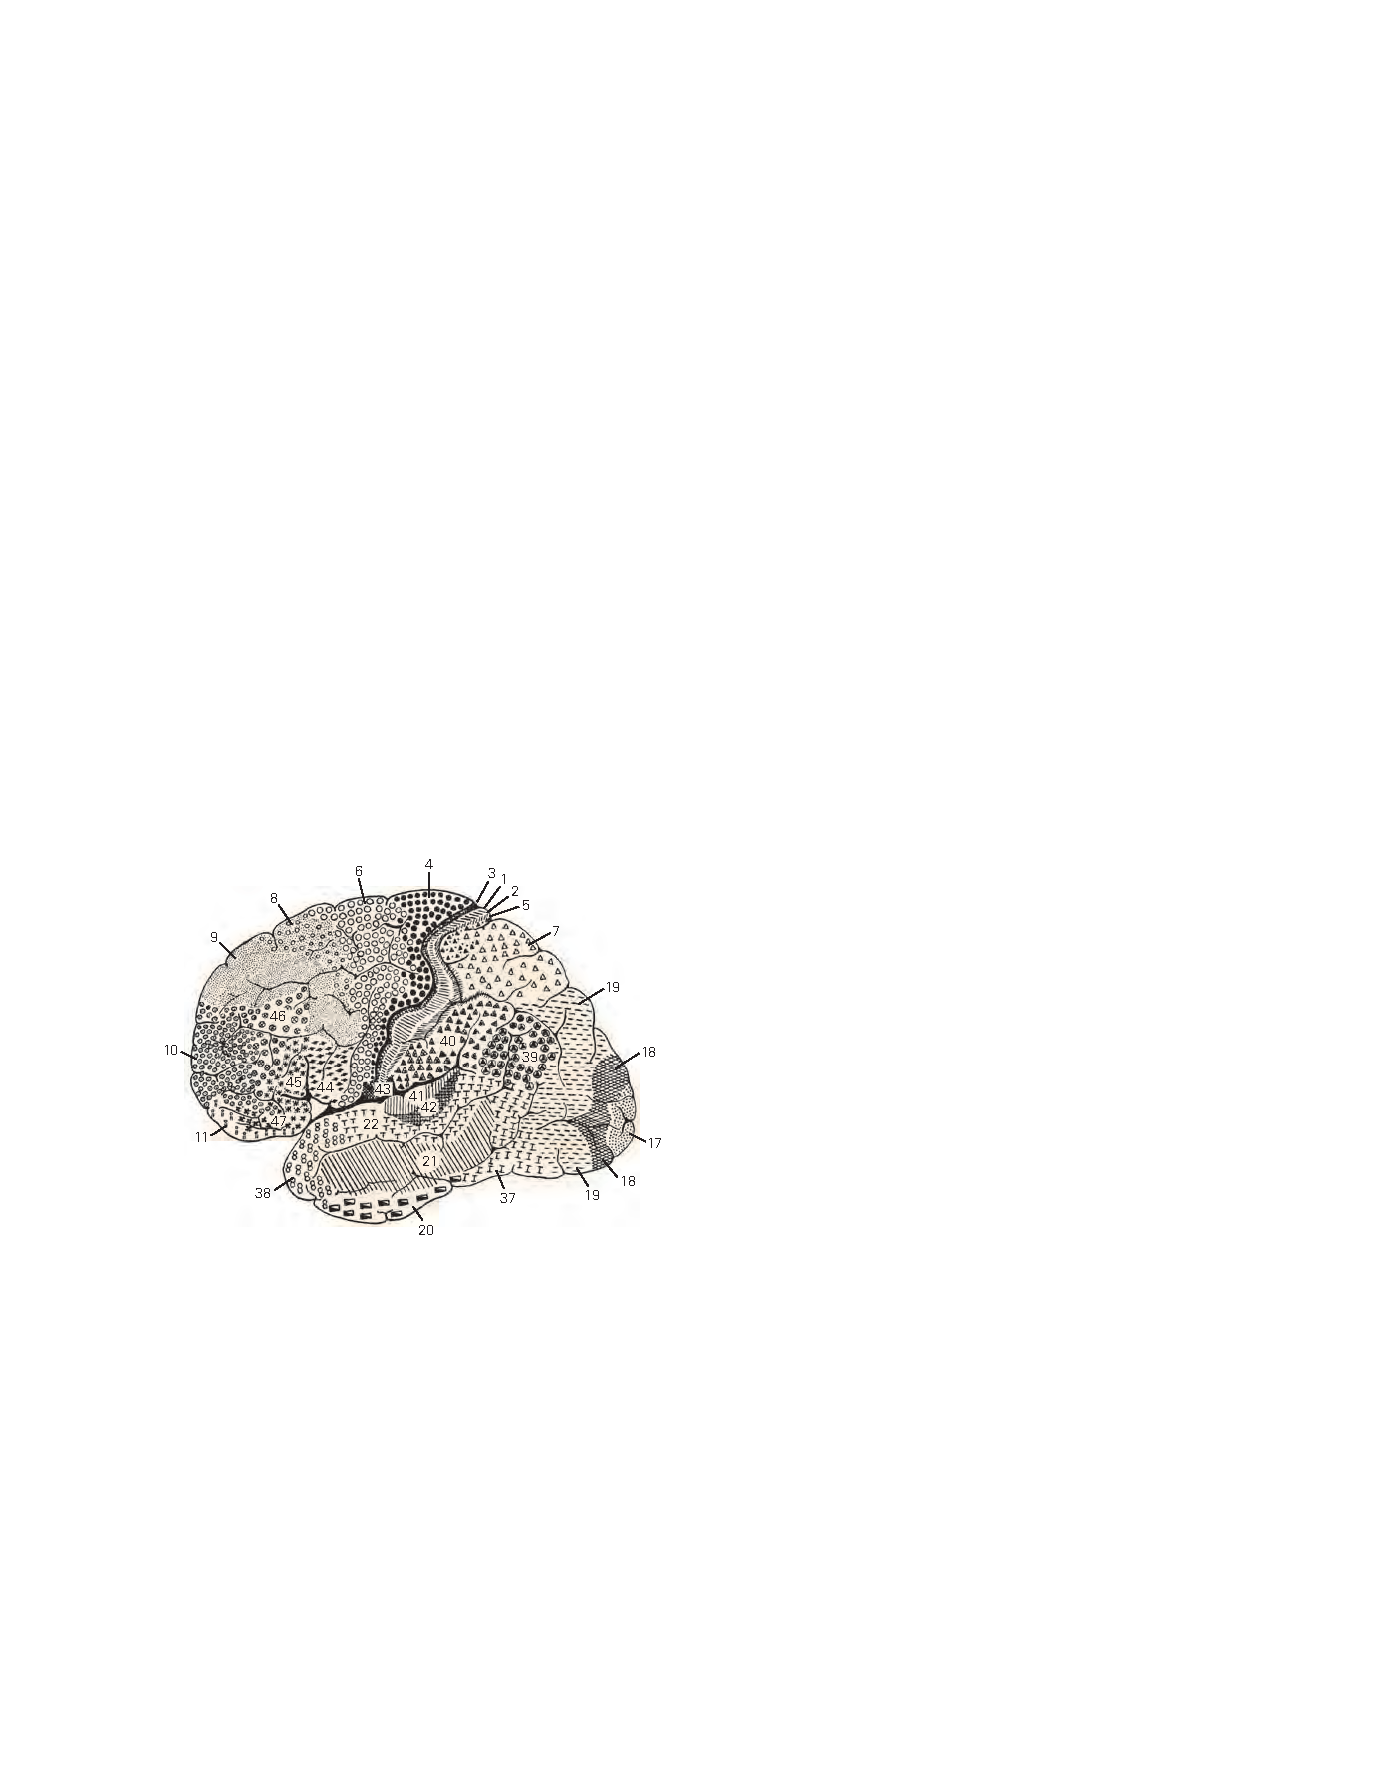
\includegraphics[width=0.6\linewidth]{chap01/fig_1_7}
	\caption{20 世纪初,人类大脑皮层被分为 52 个独立的功能区。
		显示的区域是由解剖学家布罗德曼根据独特的神经细胞结构和细胞层的特征排列确定的。
		该方案至今仍在广泛使用,并不断更新。
		布罗德曼定义的几个区域被发现可以控制特定的大脑功能。
		例如,区域 4 是运动皮层,负责随意运动。
		区域 1、2 和 3 构成初级体感皮层,主要从皮肤和关节接收感觉信息。
		第 17 区是初级视觉皮层,它接收来自眼睛的感觉信号并将它们传递到其他区域以进行进一步处理。
		区域 41 和 42 构成初级听觉皮层。
		该图仅显示了皮层外表面的可见区域。}
	\label{fig:1_7}
\end{figure}


尽管大脑皮层功能离散区域的生物学证据令人信服,但到 20 世纪初,大脑的整体观点一直主导着实验思维和临床实践,直到 1950 年。
这种令人惊讶的事态在很大程度上要归功于几位著名的神经科学家,他们 主张整体观的有英国神经学家亨利海德、俄国行为生理学家伊万巴甫洛夫和美国心理学家卡尔\textit{拉什利}。


最有影响力的是\textit{拉什利},他对用细胞构造方法来绘制皮层功能图深表怀疑。
“‘理想’的建筑地图几乎一文不值,”\textit{拉什利}写道。
“区域划分在很大程度上在解剖学上毫无意义,并且对皮层的假定功能划分具有误导性。” 
他对各种脑损伤对老鼠学习走迷宫能力的影响的研究进一步强化了他的怀疑态度。
从这些研究中,\textit{拉什利}得出结论,学习缺陷的严重程度取决于损伤的大小,而不是其精确位置。
失望的\textit{拉什利}——以及他之后的许多其他心理学家——得出结论,学习和其他高级心理功能在大脑中没有特殊的位置,因此不能归因于特定的神经元集合。


根据他的观察,\textit{拉什利}通过进一步最小化单个神经元、特定神经元连接,甚至特定大脑区域在特定行为中产生的作用,重新制定了聚合场观点。
根据\textit{拉什利}的质量作用理论,对记忆等功能至关重要的是大脑的整体质量,而不是其局部成分。


\textit{拉什利}的老鼠实验现在被重新诠释。
各种研究表明,\textit{拉什利}使用的迷宫学习不适合寻找局部皮层功能,因为它涉及太多的运动和感觉能力。
被剥夺了一种感觉能力,比如视觉,老鼠仍然可以学会使用触觉或嗅觉走迷宫。
此外,正如我们将在本书后面看到的那样,许多心理功能是由不止一个区域或神经元通路调节的。
因此,一个给定的功能可能不会被单个损伤消除。
在考虑大脑的认知功能时,这一点尤为重要。
例如,空间知识得到许多顶叶关联区域的支持,这些关联区域将视觉与注视的潜在移动、头部的转动、手的伸展等联系起来。
原则上,这些关联区域中的任何一个都可以补偿另一个关联区域的损伤。
对顶叶的严重损伤会导致明显的空间知识缺陷(空间失认症)(第~\ref{chap:chap59}~章)。
这样的观察似乎支持群众行动理论,但我们现在认识到它与包含功能冗余概念的功能定位相容。


很快,功能定位的证据变得势不可挡。
从 1930 年代后期开始,英国的\textit{埃德加$\cdot$阿德里安}和美国的\textit{韦德$\cdot$马歇尔}和\textit{菲利普$\cdot$巴德}发现,触摸猫身体的不同部位会引起大脑皮层不同区域的电活动。
通过系统地探测体表,他们在\textit{布罗德曼}描述的大脑皮层特定区域建立了体表的精确图谱。
这一结果表明,可以根据解剖学标准(例如细胞类型和细胞分层、细胞连接,以及最重要的行为功能)明确定义功能不同的皮层区域。
正如我们将在后面的章节中看到的那样,功能特化是大脑皮层的一个关键组织原则,甚至延伸到皮层区域内的单个细胞列。
事实上,大脑被划分为比布罗德曼设想的更多的功能区域。


更精细的方法使我们有可能更多地了解与语言有关的不同大脑区域的功能。
在 20 世纪 50 年代后期,\textit{怀尔德$\cdot$潘菲尔德}和后来的\textit{乔治$\cdot$奥杰曼}重新研究了对产生语言至关重要的皮层区域。
在癫痫脑部手术期间进行局部麻醉时,清醒的患者被要求命名物体(或以其他方式使用语言),同时用小电极刺激暴露皮层的不同区域。
如果大脑皮层的某个区域对语言至关重要,则电刺激的应用会阻止患者命名物体的能力。
通过这种方式,\textit{潘菲尔德}和\textit{奥杰曼}能够确认 布洛卡和韦尼克描述的大脑皮层的语言区域。
正如我们将在第~\ref{chap:chap55}~章中了解到的那样,语言神经网络比布洛卡和韦尼克所描述的神经网络广泛和复杂得多。


最初,几乎所有关于语言解剖结构的知识都来自对脑部病变患者的研究。
今天,\textit{功能性磁共振成像}和其他非侵入性方法可以对从事阅读、说话和思考的健康人进行分析(第~\ref{chap:chap6}~章)。
\textit{功能性磁共振成像}不仅证实了阅读和说话会激活不同的大脑区域,而且还揭示了在没有感觉输入的情况下仅仅思考一个词的含义会激活左额叶皮层中一个仍然不同的区域。
事实上,即使在传统语言领域内,各个子区域也会在不同程度上被吸收,这取决于我们思考单词、表达单词以及从其他单词的排列(即句法)中解析它们的含义的方式。
新的成像工具承诺不仅会告诉我们涉及哪些领域,还会揭示它们相互联系的功能逻辑。


现代方法论带来的巨大惊喜之一是,大脑皮层的如此多区域在语言理解和产生过程中都被激活了。
这些包括左半球的传统语言区域,由\textit{布洛卡}、\textit{韦尼克}和\textit{代热林}确定; 它们在右半球的同系物;
和新确定的区域。
功能成像倾向于阐明不同募集的区域,而来自中风、肿瘤或损伤的损伤区分对一种或多种功能至关重要的大脑区域。
因此,曾经被认为专门负责语言生成的布罗卡区似乎也参与了包括理解在内的各种语言任务(图~\ref{fig:1_6})。
在某些情况下,功能成像需要对病变研究确定的关键区域进行改进或修正。
例如,除了顶叶皮层的角回之外,阅读现在被认为可以募集腹侧枕颞皮层的专门区域(如图~\ref{fig:1_6} 所示)。


因此,大脑中语言的处理不仅体现了局部功能原则,而且体现了这一原则的更复杂的阐述,即许多具有专门功能的不同神经结构属于系统。
也许这是关于本地化和分布式过程的争论的自然调和——即少数不同的区域,每个区域都具有一小组功能,并通过它们的相互作用对感知、行动和观念的现象学做出贡献。
大脑分工的任务可能与我们的直觉告诉我们的不同。
谁会猜到对一个物体的运动和颜色的神经分析会发生在不同的通路中,而不是一个单一的通路来调解对物体的统一感知?
同样,我们可能期望语言的神经组织可能不完全符合通用语法理论的公理,但支持语言理论描述的非常无缝的功能。


对脑损伤患者的研究继续提供重要的洞察力,以了解大脑是如何组织语言的。
最令人印象深刻的结果之一来自对聋人的研究,他们在遭受脑损伤后失去了使用手语(例如,\textit{英国手语}或\textit{美国手语})进行交流的能力。
手语使用手部动作而不是发声,并且通过视觉而不是声音来感知,但具有与口语相同的结构复杂性。
与口语处理一样,手语处理位于左半球。 左半球的损伤会对手语产生非常特殊的影响,就像口语一样,会影响手语理解(韦尼克区受损后)、语法或流畅性(布罗卡区受损后)。
这些临床观察得到功能性神经影像学的支持。
毫不奇怪,手语和口语的产生和理解并不涉及相同的大脑区域,但重叠确实很显着(图~\ref{fig:1_8})。
甚至有证据表明,处理符号的组成部分(例如,使用的手形)涉及的一些相同大脑区域在对语音进行押韵判断时涉及。


\begin{figure}[htbp]
	\centering
	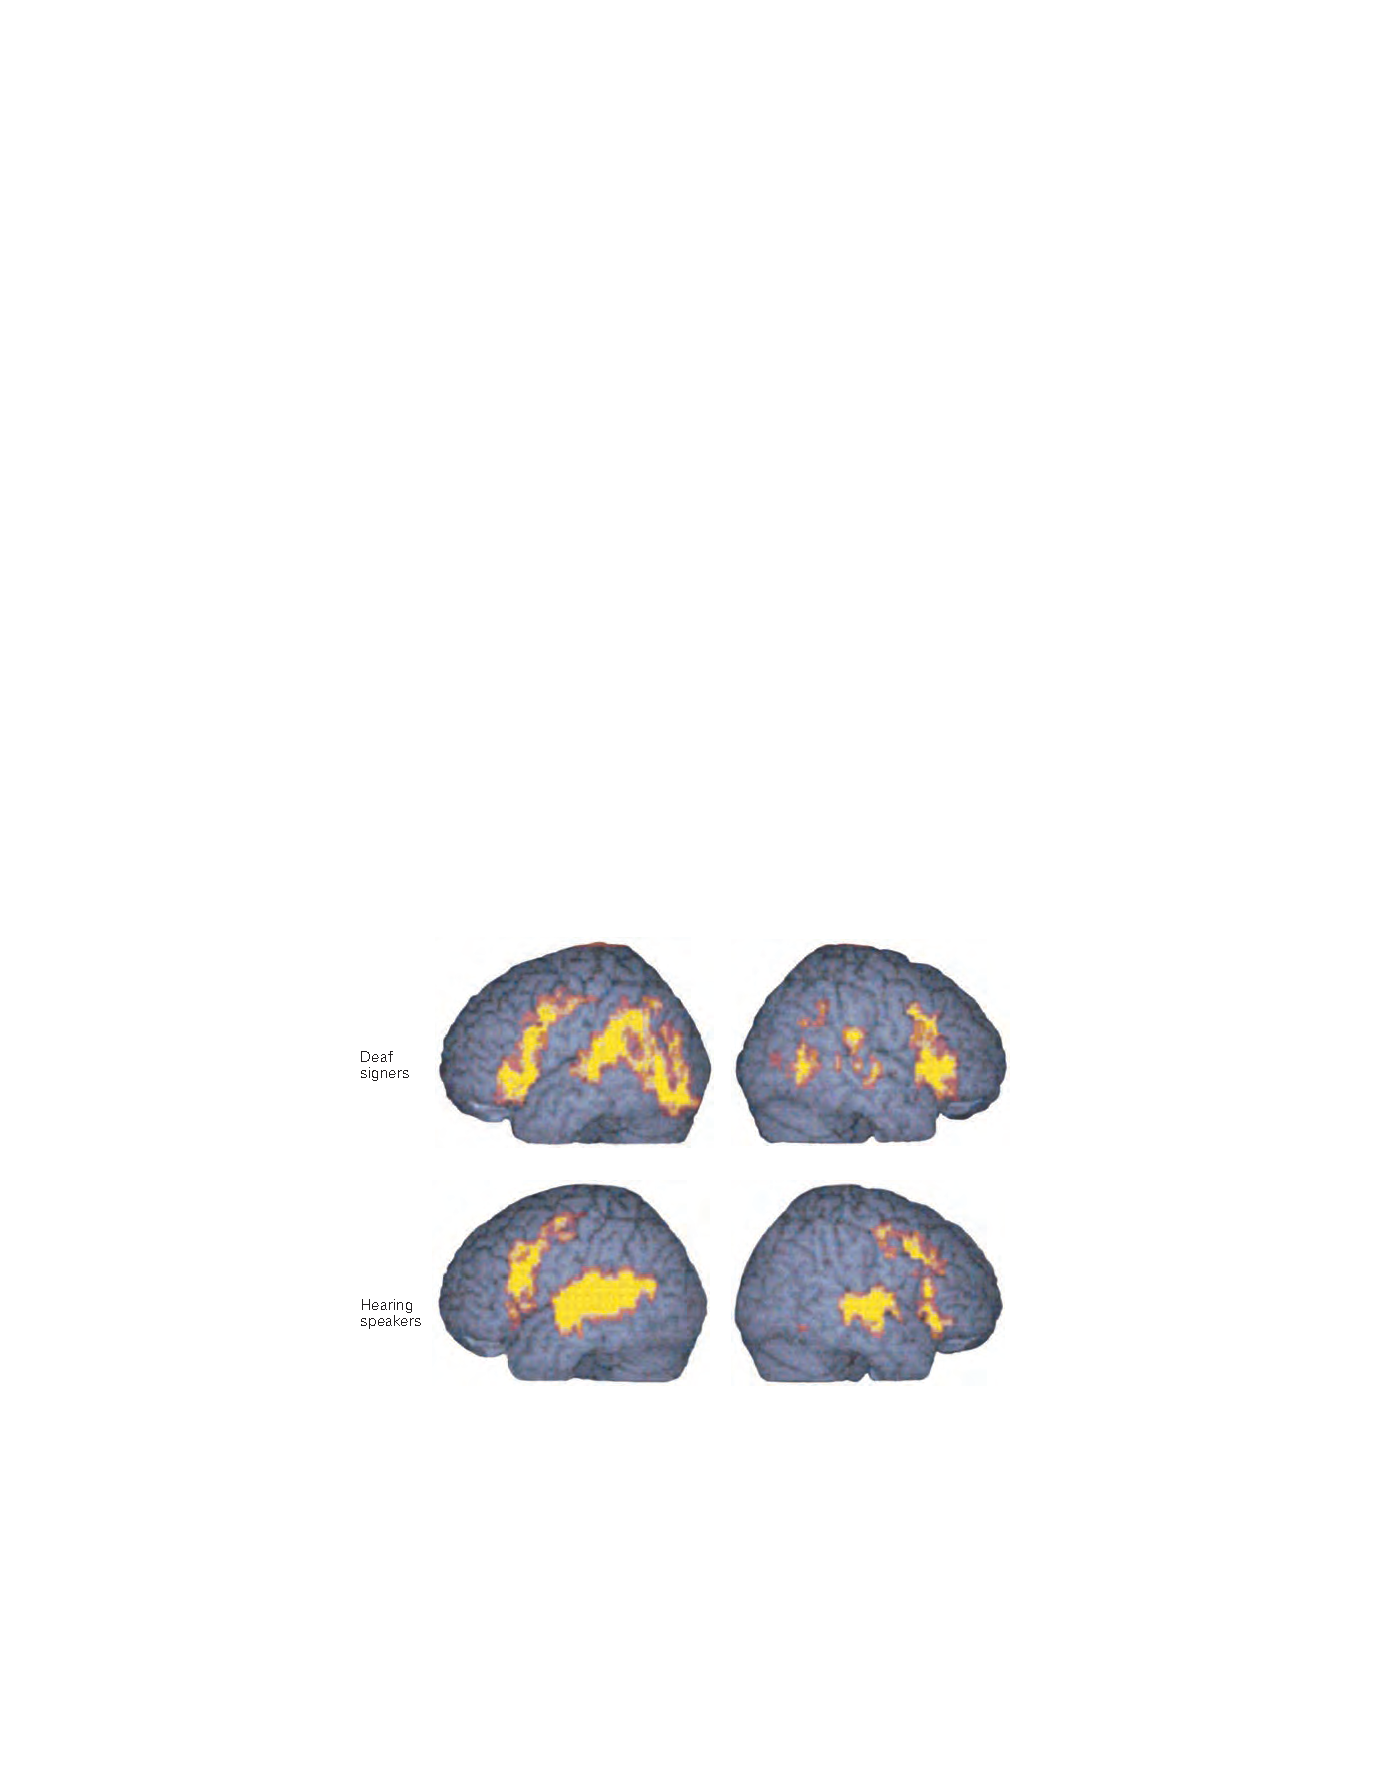
\includegraphics[width=0.75\linewidth]{chap01/fig_1_8}
	\caption{手语聋人和听力正常的人共享共同的语言处理区域。
		大脑皮层中涉及口语或手语识别的区域,通过\textit{功能性磁共振成像}识别。
		黄色高亮显示左右大脑半球(分别为左列和右列)在理解语言时比在执行感知任务时更活跃的区域。
		对于失聪手语者(顶行),突出显示的区域在理解英国手语期间比在检测叠加在同一静止手语者身上的视觉刺激期间更加活跃。
		对于有听力的说话者(下排),在理解视听语音期间突出显示的区域比在观看静止(无声)说话者时检测音调期间更活跃\cite{macsweeney2002neural}。}
	\label{fig:1_8}
\end{figure}


这些观察说明了三点。
首先,语言处理主要发生在左半球,与处理语言中使用的感觉和运动方式的通路无关。
其次,听觉输入对于左半球语言能力的出现和运作不是必需的。
第三,口语只是左半球调节的一系列语言技能之一。


对其他行为的调查为大脑具有不同认知系统的观点提供了额外的支持。
这些研究表明,复杂的信息处理需要许多相互关联的皮层和皮层下区域,每个区域都涉及处理感觉刺激或运动的特定方面,而不是其他方面。
例如,对物体位置、大小和形状的知觉意识依赖于许多顶叶联合区域的活动,这些区域将视觉与潜在的动作联系起来,例如移动眼睛、调整头部方向、伸手和调整手的形状以进行抓握。
顶叶区域不会启动这些动作,但会将感觉信息评估为与这些潜力相关的证据。
它们从背侧视觉流(有时称为\textit{空间通路},但更恰当地称为 how 通路)接收信息,以构建关于物体位置和其他空间特性的知晓状态。
腹侧视觉流,或什么通路,也与可能的行动有关,但这些与社交和觅食有关。
这些联想建立了对物体、面孔、食物和潜在伴侣的可取性的认知。
从这个意义上说,\textit{内容通路}也可能是 how 途径。



\section{心理过程是大脑中基本处理单元之间相互作用的产物}

大脑功能定位的证据在过去常常被拒绝,原因有很多,这些证据回想起来似乎如此明显和令人信服。
颅相学家在没有充分证据的情况下以夸张的形式引入了定位的概念。
他们把大脑皮层的每个区域都想象成一个独立的精神器官,专门负责人格完整而独特的方面,就像胰腺和肝脏是独立的消化器官一样。
\textit{弗卢龙}对颅相学的拒绝以及随之而来的聚集场观点的支持者(反对定位)和细胞连接主义者(支持定位)之间的争论是对一种简单化且没有足够实验证据的理论的回应。


在韦尼克发现大脑中语言的模块化组织(具有独特功能的互连节点)之后,我们现在认为所有认知能力都是分布在大脑多个区域的许多处理机制相互作用的结果。
也就是说,特定的大脑区域并不完全负责特定的智力,而是共同发挥作用的基本处理单元。
感知、运动、语言、思想和记忆都是通过这些区域内离散大脑区域(计算模块)中串行和并行处理的相互联系而成为可能的。
因此,单个区域的损伤不一定会像许多早期神经学家认为的那样导致认知功能(或能力)的完全丧失。
即使一种行为最初消失了,它也可能部分恢复,因为大脑未受损的部分重新组织了它们的联系。
此外,当\textit{局灶性损伤}对心理功能产生不利影响时,它可能会通过破坏其他主要位点的功能(精神分裂症)而间接影响。
事实上,对这种性质的观察让韦尼克的学生库尔特戈德斯坦接受了更全面的观点。


因此,认为心理功能严格由一系列神经细胞和大脑区域调节是不准确的——每个神经细胞和大脑区域都直接连接到下一个——因为在这样的安排中,当单个连接受损时,整个过程就会中断。
一个更现实的比喻是一个过程,该过程由模块网络中的多个并行通路组成,这些通路相互作用并最终汇聚在一组共同的目标上。
网络中单个路径的故障可能会影响该路径携带的信息,而不会破坏整个系统。
网络的其余部分可能能够修改其性能以适应一条路径的故障。


大脑中的模块化处理被接受的速度很慢,因为直到最近,还很难证明哪些心理运算的组成部分是由特定大脑区域或通路传达的。
以导致可检验假设的方式定义心理操作也不容易。
然而,随着近几十年来现代认知心理学和脑科学的不断融合,我们已经开始意识到心理功能可以成功地分解为子功能。


为了说明这一点,请考虑我们如何学习、存储和回忆有关物体、人和事件的信息。
简单的反思表明,我们将每条知识存储为一个单一的表征,可以通过记忆慢跑刺激甚至仅通过想象力来回忆。
例如,你所知道的关于苹果的一切似乎都存储在一个完整的表征中,无论你看到一个特定的苹果、苹果的一部分、红苹果还是绿苹果、书面单词“苹果”,还是关于引力发现的虚构故事,都同样可以访问。
然而,我们的经验并不能忠实地指导知识是如何存储在记忆中的。


关于苹果的知识并没有存储为一个单一的连贯表征,而是被细分为不同的类别并单独存储。
大脑的一个区域存储着关于你拿苹果的方式、你对柔软度的感觉(与新鲜度有关)、颜色(与偏好或新鲜度相关)、你与他人交流苹果存在或味道的方式,以及它与计算机、物理学家、蠕虫、蛇和圣经花园的语义联系的信息。
“苹果”的概念包含了这些考虑因素中的每一个,还有更多。
一个自然的假设是,一个包含许多细节的连贯概念必须存在于大脑的一个单一位置;
然而,一个同样有效的假设是,像“苹果”这样的统一概念以各种神经结构之间的多重链接的形式存在于大脑中,每个神经结构都有一种特定的信息,通过记忆检索的动作进行协调。


心理过程模块化组织最惊人的例子是发现我们的自我意识——一个自我意识的存在,当我们说“我”时的意思总和——是通过我们大脑中独立回路的连接实现的 两个大脑半球,每个半球调节自己的意识。
\textit{罗杰$\cdot$斯佩里}、\textit{迈克尔$\cdot$加扎尼加}和 \textit{约瑟夫$\cdot$伯根}在研究患者的过程中做出了一个非凡的发现,即意识也不是一个单一的过程,这些患者的胼胝体——连接两个大脑半球的主要区域——被切断作为治疗癫痫。
他们发现每个半球都有一种独立于另一半球运作的意识。


因此,当一名患者左手拿着一本最喜欢的书阅读时,控制左手但在语言理解中只起次要作用的右半球发现,它从简单地看书获得的原始视觉信息是无聊的。
右半球命令左手放下书。
另一个病人会用左手穿上衣服,同时用另一只手脱下衣服。 每个半球都有自己的想法!
此外,优势半球有时会评论非优势半球的表现,经常表现出一种错误的自信感,因为它不知道解决方案是专门提供给非优势半球的。


这些发现将曾经属于哲学和精神分析领域的意识研究带入了神经科学的范畴。
正如我们将在后面的章节中看到的,本章中描述的许多问题在意识的神经理论中再次出现。
没有人质疑很多信息处理——也许是最大的份额——没有达到有意识的认识这一想法。
当感官信息、行动计划或想法确实成为意识时,神经科学试图解释调节这种转变的机制。
虽然目前还没有令人满意的解释,但一些脑科学家将这一过程比作注意力焦点的转移,由不同的神经元群介导,而另一些人则认为,意识需要在广泛分离的神经元区域之间的功能相互作用中发生质的变化。


我们花了这么长时间才弄清楚大脑的哪些区域介导了哪些心理活动,主要原因是我们正在处理生物学最深奥的谜题:解释意识和自我意识的神经机制。
目前还没有令人满意的理论来解释为什么只有一些到达我们眼睛的信息会导致对物品、人或场景的主观意识状态。 
我们知道,我们有意识地意识到我们思想思考的一小部分,而那些确实刺穿意识的想法必须来自大脑无意识地执行的步骤。
正如我们在第~\ref{chap:chap56}~章中提出的那样,一些意识之谜的答案可能比想象的更接近。


同时,我们目前理解上的差距也对神经科学提出了实际的认识论挑战。
在我们对知觉、行为和认知的描述中,我们不得不依赖我们对世界、身体和观念的有意识体验。
然而,在这样做时,我们冒着错误描述许多不穿透意识的心理过程的风险。
例如,我们倾向于用与感官信息的主观体验相一致的术语来描述知觉问题,而即使是复杂但无意识的知觉内容知识也可能与行为效用(可供性)有更大的相似性,实际上是对以下问题的回答 这是否是我可能会选择吃、坐在上面或进一步参与的东西。
同样,大脑执行推理、制定战略和决策等认知过程的方式可能与我们从有意识的深思熟虑中推断出的步骤大致相似。


这些警示说明有一个明显的推论。
许多认知功能在没有意识的情况下发生的洞察力提出了这样一种可能性,即在研究更基本的行为时揭示的神经科学原理可以提供对更复杂的认知过程的洞察力。
受过训练以执行复杂任务的动物大脑的神经记录导致了对认知过程的理解,例如决策、推理、计划和分配注意力。 
这些实验模型经常外推到人类功能,并且在它们不足的地方,它们激发了新的假设。
通常情况下,即使不能从我们理解的空白中收集到洞察力,也会有灵感。


要分析大脑如何产生特定的心理过程,我们不仅必须确定该过程的哪些方面取决于大脑的哪些区域,还必须确定相关信息的表示、路由和转换方式。
现代神经科学试图整合这种跨多个尺度的理解。
例如,在单个神经细胞及其分子成分水平上的研究阐明了电兴奋性和突触连接的潜在机制。
对细胞和简单回路的研究有助于深入了解神经计算,从基本操作(如控制网络激励)到更精湛的计算专长(如从原始感官数据中获取有意义的信息)。
研究回路和大脑区域之间的相互作用可以解释我们如何协调广泛分离的肌肉群或表达对命题的信念。
所有这些层次的知识都通过数学形式化、计算机模拟和心理学理论结合在一起。
这些概念工具现在可以与现代生理学技术和大脑成像方法相结合,从而可以跟踪活体动物和人类实时进化的心理过程。
事实上,今天神经科学的兴奋源于这样一种信念,即构成人类思想和行为基础的生物学原理在我们的掌握之中,并且可能很快就会被用来阐明和改善人类状况。




\section{亮点}

1. 神经科学试图在多个组织层次上理解大脑,从细胞及其成分到思维的运作。


2. 神经科学的基本原理连接了时间、复杂性和状态的各个层次——从细胞到行动和思想,从通过学习的发展到专业知识和遗忘,从正常功能到神经缺陷和恢复。
第一步,必须了解构建块——神经细胞的电特性及其与其他神经细胞的连接——以及从支持细胞到通路的神经系统组织。


3. 神经元学说指出,单个神经细胞(神经元)是神经系统的基本组成部分和信号元件。


4. 神经元被组织成具有专门功能的回路。
最简单的回路调节反射;
更复杂的认知功能需要更复杂的回路。
这种组织原则将神经元学说扩展到细胞连接主义。


5. 即使在复杂的回路中,关键节点也可以被识别为与特定功能相关的区域。
大脑功能定位的第一个明确证据来自对语言产生特定障碍的研究。


6、两个大脑半球从身体的对侧接收信息,控制对侧的动作。


7. 虽然大脑功能定位原理优于其主要的历史替代方案——聚合场和质量作用理论——但它正在不断完善。
大脑皮层的任何区域都不能独立于其他皮层和皮层下结构而发挥作用。


8. 本地化的一个主要改进是模块化功能组织的原则。
大脑包含许多信息表征,这些信息既由特定计算的某些特征的相关性组织,也由这些信息的各种用途组织。
这是一种关于目的或潜在行动的冗余形式。


9. 脑科学的未来需要整合跨越传统学科界限的思想。
我们必须对各种各样的资源敞开心扉,以指导我们的直觉和研究策略,从\textit{意识的崇高本质}到看似平凡的\textit{全身麻醉对丘脑周围细胞环中钙传感器的作用}。


\chapter{基因和行为} \label{chap:chap2}

所有行为都是由基因和环境的相互作用塑造的。
简单动物的大多数刻板行为都受到环境的影响,而人类高度进化的行为则受到基因指定的先天特性的限制。
基因不直接控制行为,但基因编码的\textit{核糖核酸}和蛋白质会在不同时间和多个层面发挥作用,影响大脑。
基因指定了组装大脑的发育程序,并且对于神经元、神经胶质细胞和突触的特性至关重要,这些特性使神经元回路发挥作用。
代代稳定遗传的基因创造了新体验可以在学习过程中改变大脑的机制。


在本章中,我们将探讨基因如何影响行为。
我们首先概述基因确实影响行为的证据,然后回顾分子生物学和遗传传递的基本原理。
然后,我们提供了遗传对行为影响的记录方式的示例。
通过对蠕虫、苍蝇和老鼠的研究,人们对基因调节行为的方式有了深刻的了解,这些动物的基因组可用于实验操作。
通过对人类大脑发育和功能的分析,基因和人类行为之间出现了许多有说服力的联系。
尽管研究人类复杂特征存在固有的巨大挑战,但最近的进展已经开始揭示神经发育和精神综合症(如自闭症、精神分裂症和双相情感障碍)的遗传风险因素,为阐明基因、大脑和行为。



\section{了解\textit{分子遗传学}和遗传率对研究人类行为至关重要}

许多人类精神疾病和神经系统疾病都有遗传因素。
患者的亲属比一般人群更容易患上这种疾病。
遗传因素对群体特性的影响程度称为\textit{遗传力}。
遗传力最强的案例是基于双胞胎研究,1883 年\textit{弗朗西斯$\cdot$高尔顿}首次使用了同卵双胞胎。
这样的同卵双胞胎共享所有基因。
相反,异卵双胞胎是由两个不同的受精卵发育而来的;
这些异卵双胞胎与正常的兄弟姐妹一样,平均共享一半的遗传信息。
多年来的系统比较表明,同卵双胞胎在神经和精神特征方面往往比异卵双胞胎更相似(一致),这为这些特征的可遗传成分提供了证据(图~\ref{fig:2_1}A)。


\begin{figure}[htbp]
	\centering
	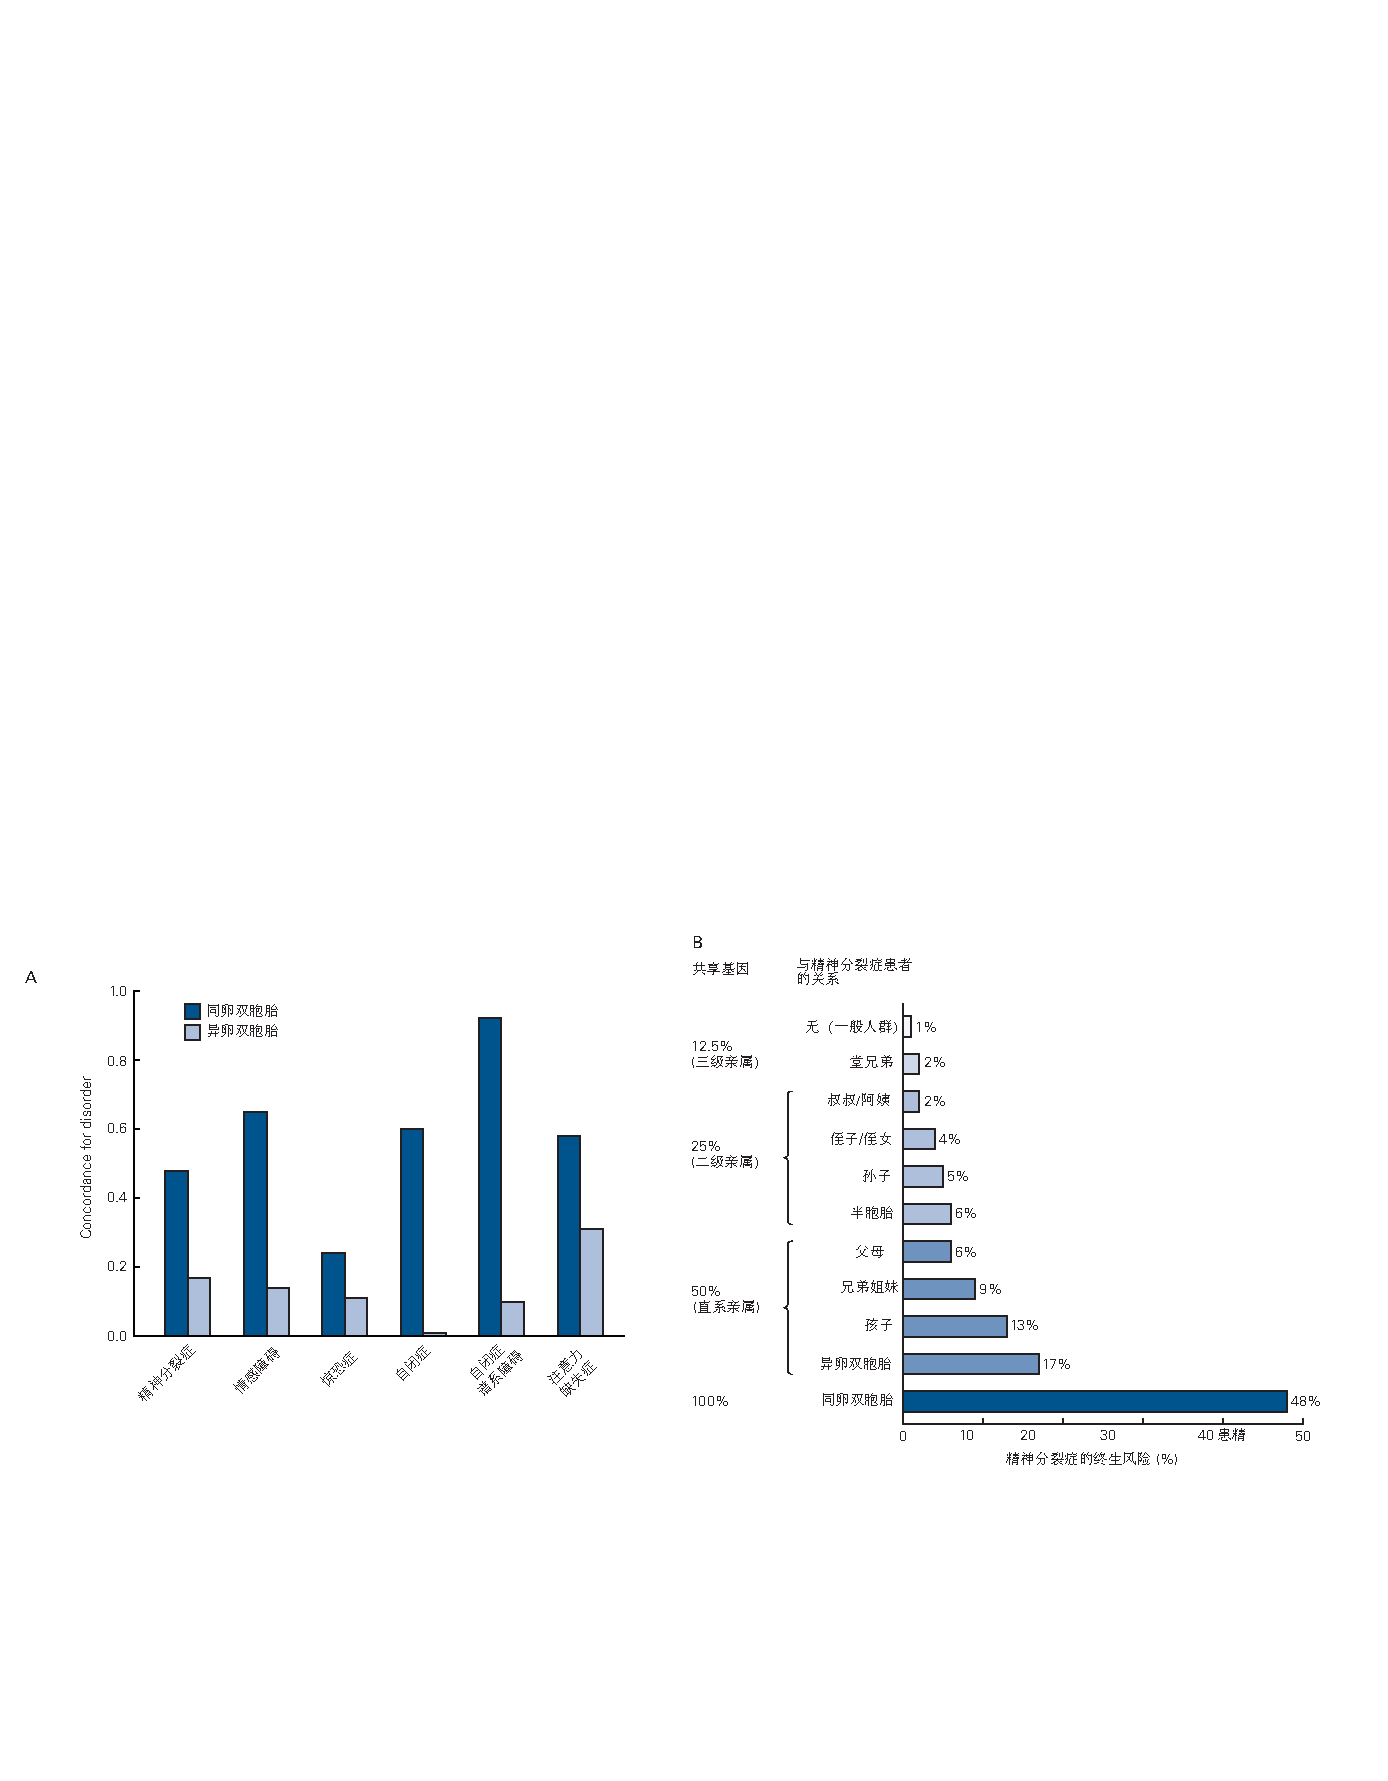
\includegraphics[width=1.0\linewidth]{chap02/fig_2_1}
	\caption{精神疾病的家族风险提供了遗传性的证据。
		\textbf{A.} 同卵双胞胎之间精神疾病的相关性比异卵双胞胎之间的相关性大得多。
		同卵双胞胎几乎共享所有基因,并且有很高(但不是 100\%)共享疾病状态的风险。
		异卵双胞胎共享 50\% 的遗传物质。
		零分表示没有相关性(两个随机人的平均结果),而 1.0 分表示完全相关\cite{mcgue1998genetic}。
		\textbf{B.} 精神分裂症患者的近亲患精神分裂症的风险更大。
		就像异卵双胞胎一样,父母和孩子以及兄弟姐妹共享 50\% 的遗传物质。
		如果只有一个基因导致精神分裂症,那么患者的父母、兄弟姐妹、孩子和异卵双胞胎的风险应该是相同的。 
		家庭成员之间的差异表明更复杂的遗传和环境因素在起作用\cite{gottesman1991schizophrenia}。}
	\label{fig:2_1}
\end{figure}


在双胞胎研究模型的一个变体中,明尼苏达双胞胎研究调查了在生命早期分开并在不同家庭中长大的同卵双胞胎。
尽管有时环境差异很大,但双胞胎对相同的精神疾病有着共同的倾向,甚至倾向于共享性格特征,比如外向性。
这项研究提供了大量证据,证明遗传变异会导致正常的人类差异,而不仅仅是疾病状态。


人类疾病和行为特征的遗传率通常大大低于 100\%,表明环境是获得疾病或特征的重要因素。
如图~\ref{fig:2_1}B~所示,来自双胞胎研究的许多神经学、精神病学和行为特征的遗传力估计值约为 50\%,但特定特征的遗传力可能更高或更低。
尽管对同卵双胞胎和其他亲属关系的研究支持人类行为具有遗传成分的观点,但它们并没有告诉我们哪些基因是重要的,更不用说特定基因如何影响行为了。
这些问题通过对实验动物的研究得到解决,其中遗传和环境因素受到严格控制,并通过现代基因发现方法得到解决,这些方法现在可以系统、可靠地识别\textit{脱氧核糖核酸}序列和结构中的特定变异,这些变异促成人类精神病学和神经学的表现型。



\section{对基因组结构和功能的理解正在演变}

分子生物学和传递遗传学的相关领域是我们现代对基因的理解的核心。
在这里,我们总结了这些领域的一些关键思想;
本章末尾的词汇表定义了常用术语。


基因由\textit{脱氧核糖核酸}组成,\textit{脱氧核糖核酸}代代相传。
在大多数情况下,每个基因的精确拷贝都会提供给生物体中的所有细胞,并通过\textit{脱氧核糖核酸}复制提供给后代。
该一般规则的罕见例外,即引入种系或体细胞\textit{脱氧核糖核酸}并在疾病风险中发挥重要作用的新(从头)突变,将在后面讨论。
\textit{脱氧核糖核酸}由两条链组成,每条链都有一个脱氧核糖磷酸骨架连接到一系列四个亚基:核苷酸\textit{腺嘌呤}、\textit{鸟嘌呤}、\textit{胸腺嘧啶}和\textit{胞嘧啶}。
如图~\ref{fig:2_2}~所示,两条链配对,一条链上的\textit{腺嘌呤}总是与互补链上的\textit{胸腺嘧啶}配对,\textit{鸟嘌呤}与\textit{胞嘧啶}配对。
这种互补性确保了\textit{脱氧核糖核酸}复制过程中\textit{脱氧核糖核酸}的准确复制,并驱动\textit{脱氧核糖核酸}转录成称为转录本的\textit{核糖核酸}长度。
鉴于几乎所有的基因组都是双链的,碱基或碱基对可以互换使用作为测量单位。
包含一千个碱基对的基因组片段称为 1 千碱基或 1 千碱基对,而一百万碱基对称为 1 兆碱基或 1 兆碱基对。
\textit{核糖核酸}与\textit{脱氧核糖核酸}的不同之处在于\textit{核糖核酸}是单链的,具有核糖而不是脱氧核糖骨架,并使用核苷碱基\textit{尿苷}代替\textit{胸腺嘧啶}。


\begin{figure}[htbp]
	\centering
	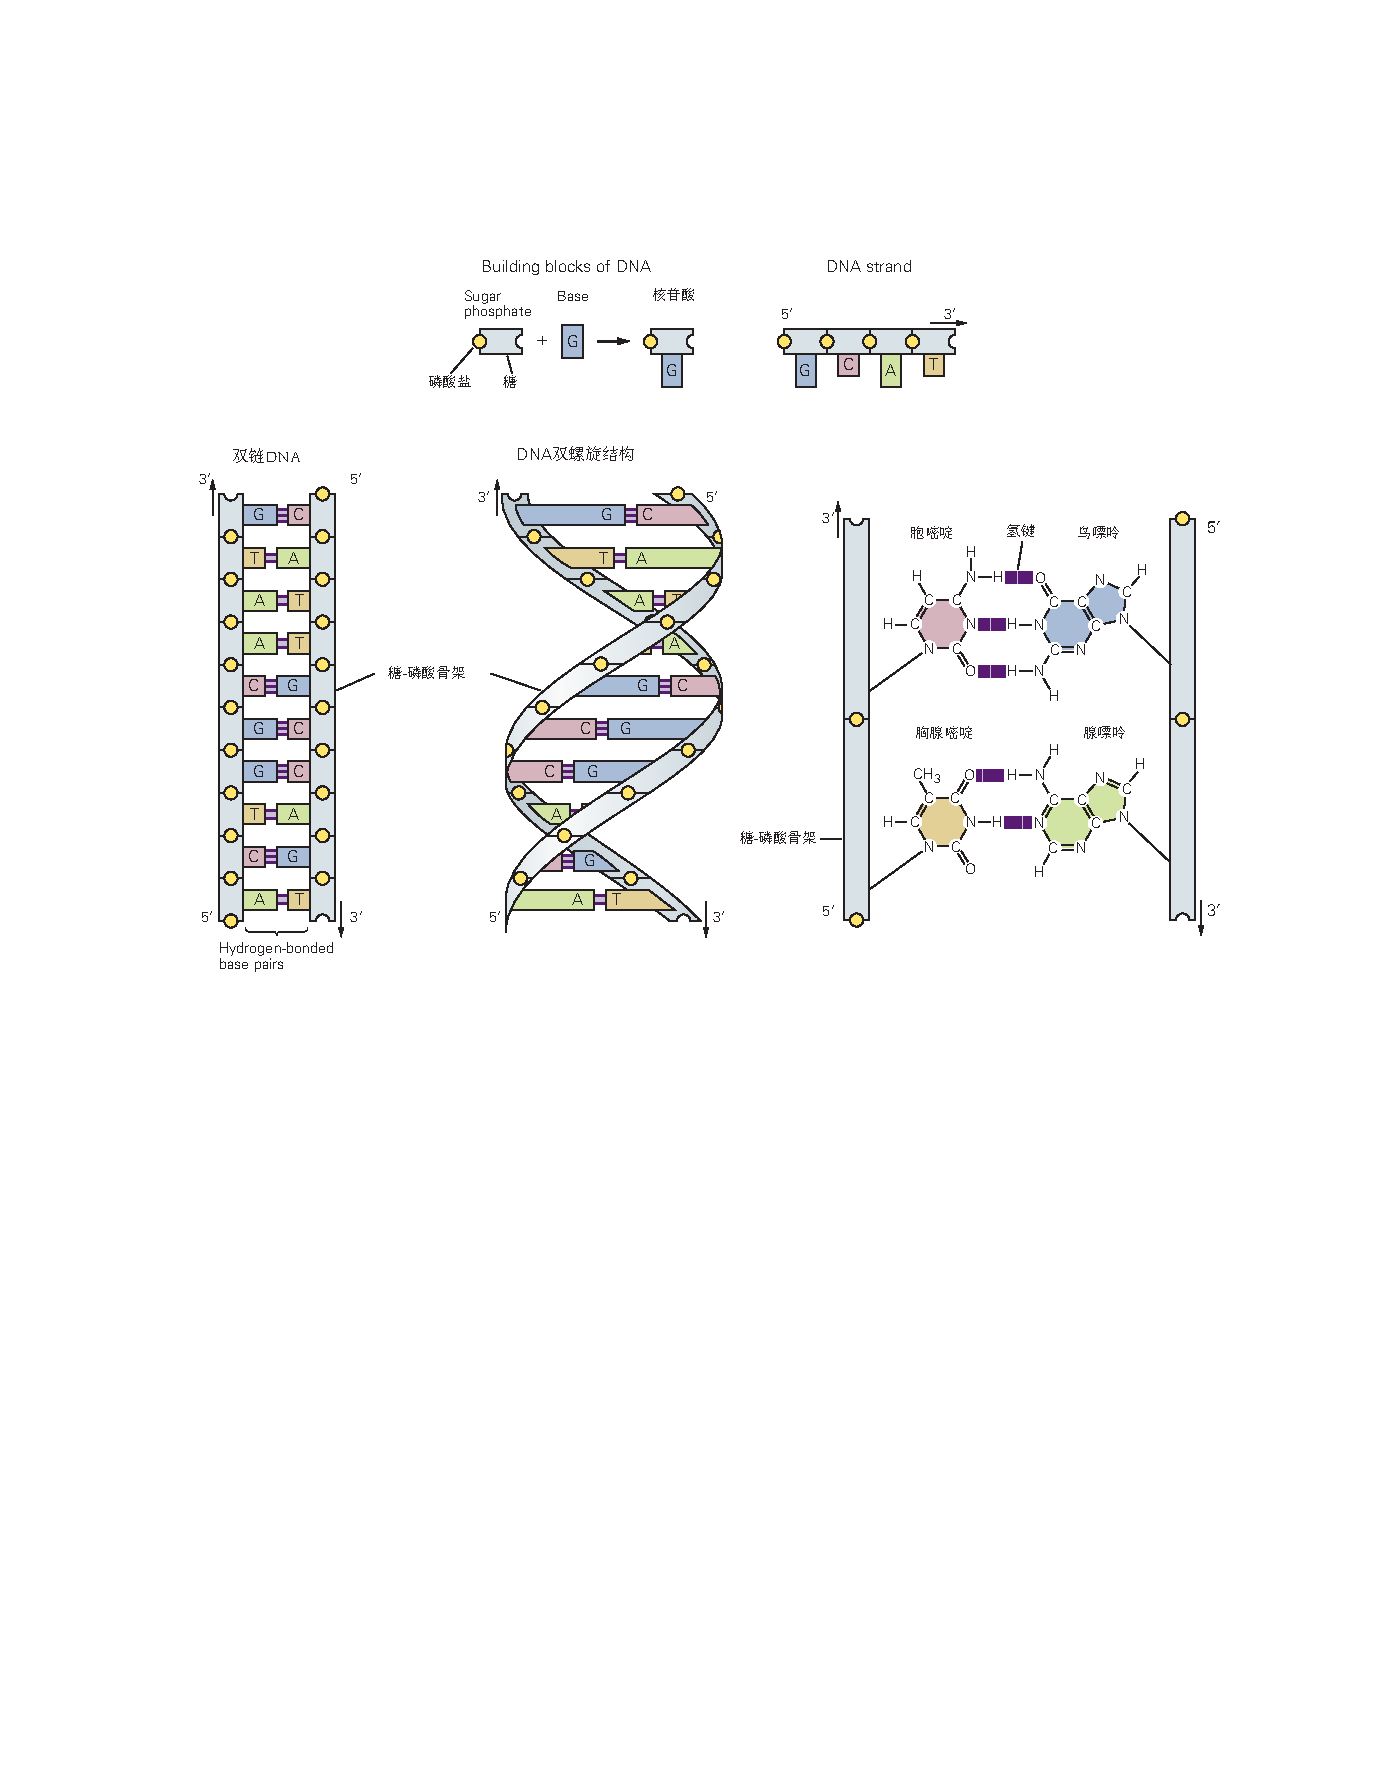
\includegraphics[width=1.0\linewidth]{chap02/fig_2_2}
	\caption{\textit{脱氧核糖核酸}的结构。
		四种不同的核苷酸碱基,腺嘌呤、胸腺嘧啶、胞嘧啶和鸟嘌呤,组装在双链\textit{脱氧核糖核酸}螺旋的糖磷酸主链上\cite{alberts2017molecular}。}
	\label{fig:2_2}
\end{figure}


在人类基因组中,大约有 2 万个基因编码蛋白质产物,这些蛋白质产物是通过将线性\textit{信使核糖核酸}序列翻译成由氨基酸组成的线性多肽(蛋白质)序列而产生的。
一个典型的蛋白质编码基因由一个编码区和非编码区组成,编码区被翻译成蛋白质(图~\ref{fig:2_3})。
编码区通常排列在称为外显子的小编码区段中,它们被称为内含子的非编码区隔开。
在翻译成蛋白质之前,内含子从\textit{信使核糖核酸}中删除。


\begin{figure}[htbp]
	\centering
	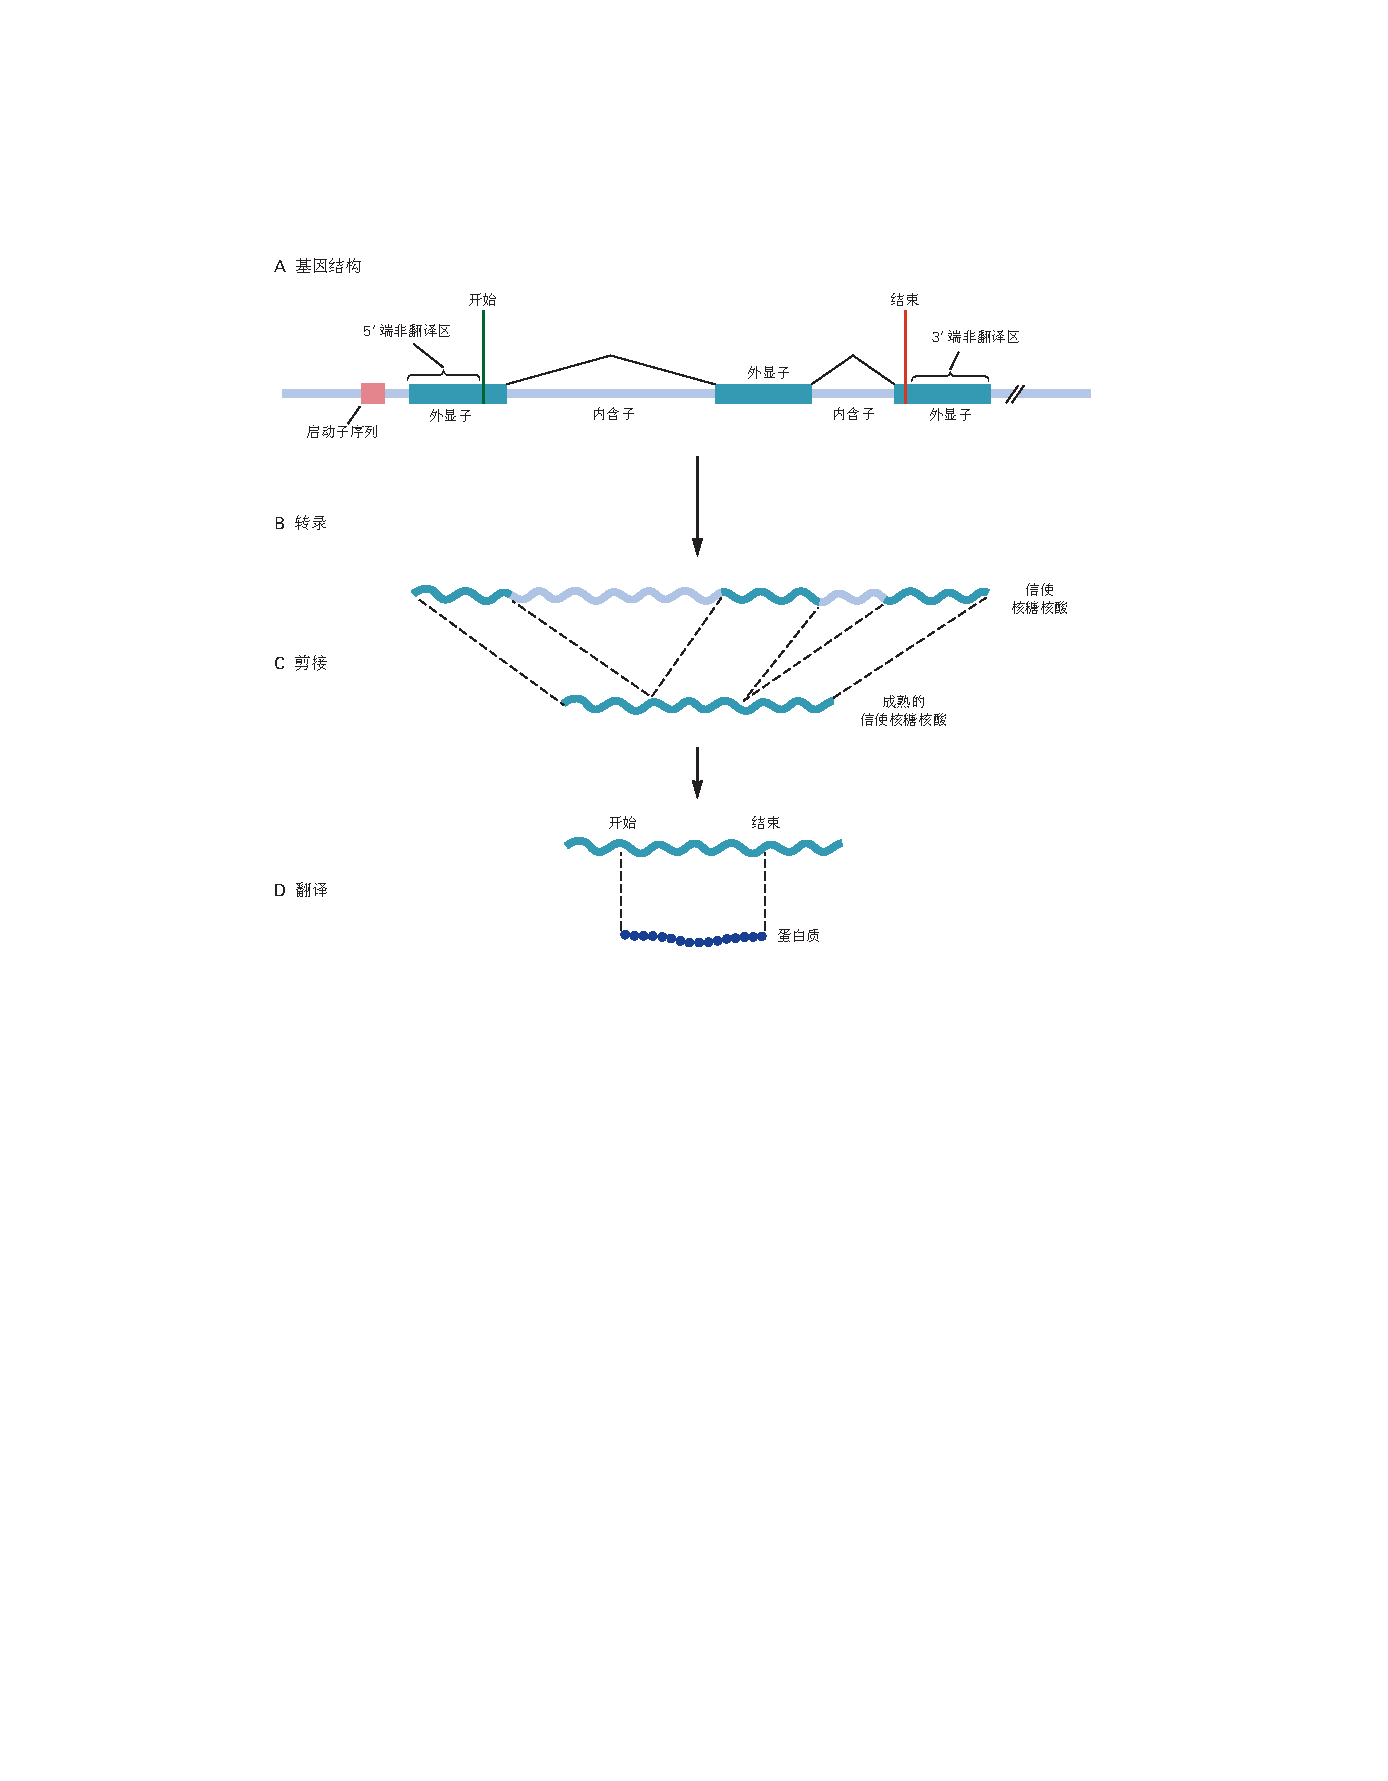
\includegraphics[width=0.96\linewidth]{chap02/fig_2_3}
	\caption{基因结构和表达。
		\textbf{A.} 一个基因由被非编码区(内含子)隔开的编码区(外显子)组成。
		它的转录受非编码区调节,例如经常在基因开始附近发现的启动子和增强子。
		\textbf{B.} 转录导致产生包括外显子和内含子的初级单链\textit{核糖核酸}转录物。
		\textbf{C.} 剪接从未成熟的转录物中去除内含子,并将外显子连接成成熟的\textit{信使核糖核酸},后者从细胞核输出。
		\textbf{D.} 成熟\textit{信使核糖核酸}的翻译产生蛋白质产物。}
	\label{fig:2_3}
\end{figure}


许多功能性\textit{核糖核酸}转录物不编码蛋白质。 
事实上,在人类基因组中,与大约 2 万个蛋白质编码基因相比,已经表征了超过 4 万个非编码转录本。
这些基因包括\textit{核糖体核糖核酸}和\textit{转运核糖核酸},它们是\textit{信使核糖核酸}翻译机制的重要组成部分。
其他\textit{非编码核糖核酸}包括\textit{长链非编码核糖核酸},任意定义为长度超过 200 \textit{碱基对},不编码蛋白质但可以在基因调控中发挥作用;
指导\textit{信使核糖核酸}剪接的多种类型的\textit{小非编码核糖核酸},包括\textit{小核核糖核酸};
和与特定\textit{信使核糖核酸}中的互补序列配对以抑制其翻译的\textit{微小核糖核酸}。


身体中的每个细胞都包含每个基因的\textit{脱氧核糖核酸},但仅将基因的特定子集表达为\textit{核糖核酸}。
转录成\textit{核糖核酸}的基因部分两侧是非编码\textit{脱氧核糖核酸}区域,这些区域可能与其他蛋白质(包括转录因子)结合以调节基因表达。
这些序列基序包括启动子、增强子、沉默子和绝缘子,它们一起允许\textit{核糖核酸}在正确的时间在正确的细胞中准确表达。
启动子通常位于待转录区域的开头附近;
增强子、消音子和绝缘子可能与被调节的基因存在一定距离。
每种类型的细胞都有独特的\textit{脱氧核糖核酸}结合蛋白补充,这些蛋白与启动子和其他调节序列相互作用,以调节基因表达和由此产生的细胞特性。


大脑表达的基因数量比身体的任何其他器官都要多,而且在大脑内,不同的神经元群表达不同的基因组。
由启动子、其他调节序列和与其相互作用的\textit{脱氧核糖核酸}结合蛋白控制的选择性基因表达允许固定数量的基因在大脑中产生数量大得多的神经元细胞类型和连接。


虽然基因指定了神经系统的初始发育和特性,但个体的经历和特定神经回路中由此产生的活动本身可以改变基因的表达。
通过这种方式,环境影响被纳入神经回路的结构和功能。
基因研究的一些主要目标是阐明单个基因影响生物过程的方式、基因网络影响彼此活动的方式以及基因与环境相互作用的方式。



\subsection{基因排列在染色体上}

细胞中的基因有序地排列在称为染色体的长而线性的\textit{脱氧核糖核酸}上。
人类基因组中的每个基因都可重复地位于特定染色体上的特征位置(\textit{基因座}),并且该遗传“地址”可用于将生物学特征与基因的作用相关联。
大多数多细胞动物(包括蠕虫、果蝇和小鼠,以及人类)都是二倍体;
每个体细胞都携带两套完整的染色体,一套来自母亲,另一套来自父亲。


人类有大约 2 万个基因,但只有 46 条染色体:
22 对常染色体(男性和女性都存在的染色体)和两条性染色体(女性有两条 X 染色体,男性有一条 X 染色体和一条 Y 染色体)(图~\ref{fig:2_4})。
每个父母都向二倍体后代提供每个常染色体的一个副本。
每个父母也为女性(XX)后代提供一条 X 染色体,但 XY 男性从母亲那里继承了一条 X 染色体,从父亲那里继承了一条 Y 染色体。
1910 年,\textit{摩尔根}在果蝇身上发现了\textit{伴性遗传}。
这种与单个 X 染色体相关的\textit{伴性遗传}模式在人类遗传学研究中非常重要,某些 X 连锁遗传病通常仅在男性,但基因会从母亲传给儿子。


\begin{figure}[htbp]
	\centering
	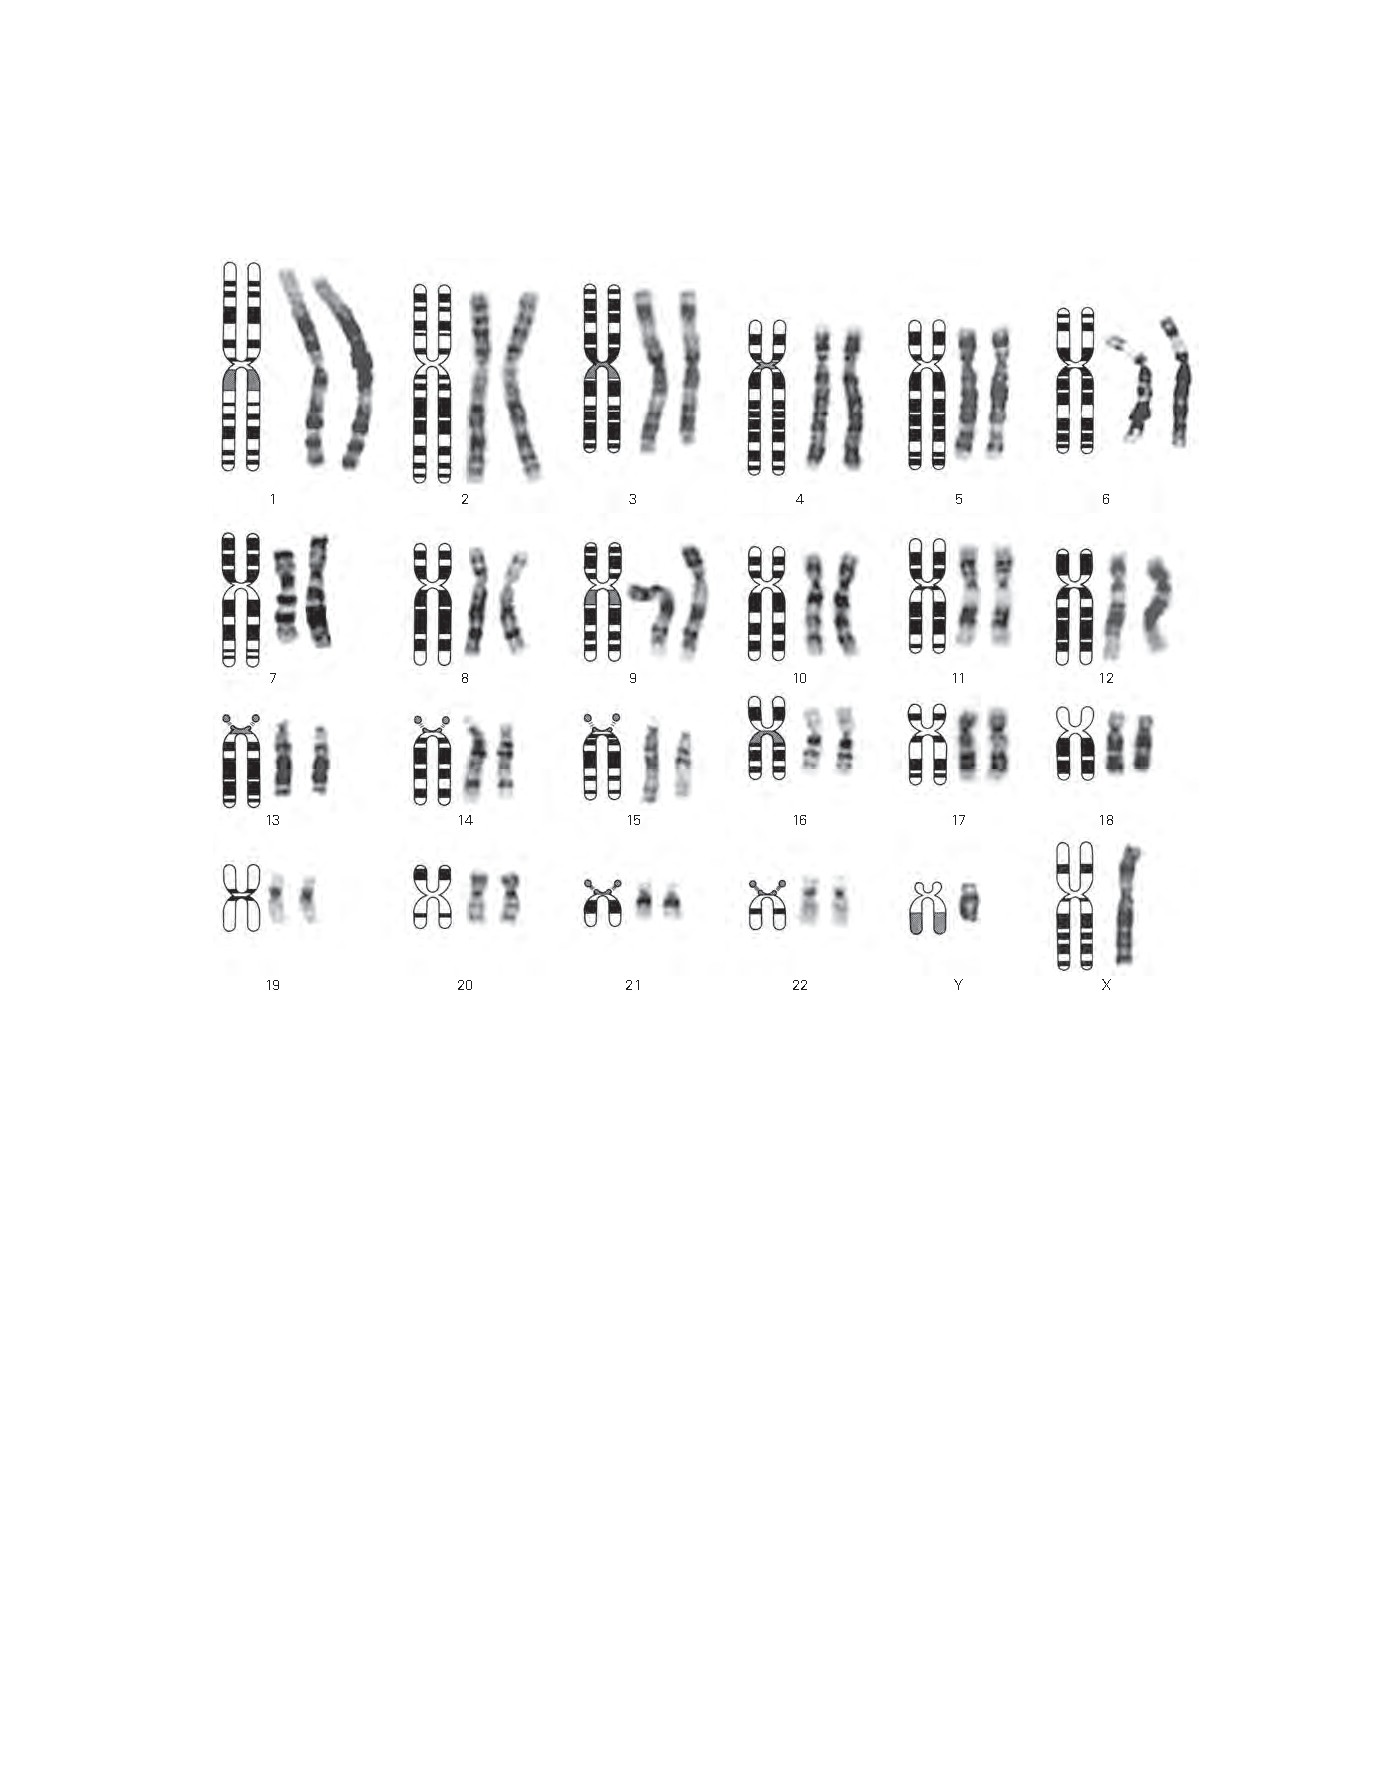
\includegraphics[width=0.95\linewidth]{chap02/fig_2_4}
	\caption{中期正常人类染色体的图解说明了每条染色体的独特形态。
		特征大小和特征亮区和暗区允许染色体彼此区分\cite{watoson1983recombinant}。}
	\label{fig:2_4}
\end{figure}


除了染色体上的基因外,极少数生物体基因通过线粒体传递,线粒体是执行代谢过程的细胞质细胞器。
所有儿童的线粒体都来自卵子,因此会从母亲传给孩子。
某些人类疾病,包括某些神经肌肉退行性疾病、某些形式的智力障碍和某些形式的耳聋,都是由线粒体\textit{脱氧核糖核酸}突变引起的。



\section{基因型和表现型之间的关系通常很复杂}

个体中特定常染色体基因的两个拷贝称为\textit{等位基因}。
如果两个\textit{等位基因}相同,则称个体在该位点是纯合的。
如果等位基因因突变而不同,则个体在该位点是杂合的。
男性是 X 染色体上基因的半合子。
一个群体可以有一个基因的大量等位基因;
例如,影响人眼颜色的单个\textit{2 型眼皮肤白化病}基因可以具有编码蓝色、绿色、淡褐色或棕色色调的等位基因。
由于这种变异,区分生物体的基因型(其基因组成)和表型(其外观)非常重要。
从广义上讲,基因型是构成个体基因组的整套等位基因;
狭义上,就是一个基因的特异等位基因。
相比之下,表型是对整个生物体的描述,是生物体基因型在特定环境中表达的结果。


如果突变表型仅在基因的两个等位基因都发生突变时才表达,则产生的表型称为隐性。
如果个体是突变等位基因的纯合子,或者如果他们在每个染色体上的给定基因中携带不同的破坏性等位基因(所谓的复合杂合子),就会发生这种情况。
隐性突变通常是由功能蛋白的丢失或减少引起的。
在人类和实验动物中普遍观察到突变性状的隐性遗传。


如果突变表型由一个突变体和一个野生型等位基因的组合产生,则表型特征和突变等位基因被认为是显性的。
一些突变是显性的,因为 50\% 的基因产物不足以形成正常表型(单倍体不足)。
其他显性突变导致异常蛋白质的产生或野生型基因产物在不适当的时间或地点的表达;
如果这对正常的蛋白质产物起拮抗作用,则称为显性失活突变。


当考虑具有同一基因的一个正常(野生型)等位基因和一个突变等位基因的后果时,基因型和表型之间的差异是显而易见的。
一系列神经发育障碍(包括孤独症和癫痫)的基因发现的最新进展表明,人类基因组对单倍体不足比以前认为的更敏感。
然而,虽然一个基因的两个拷贝的完全失活通常具有可靠的效果,但单倍体不足的严重性和表现在个体之间差异更大,这种现象称为可变、部分或不完全外显率。


干扰人类发育、细胞功能或行为的遗传变异落在共同等位基因(也称为多态性)和稀有变异之间的连续体上,前者通常对生物学和行为具有较小的个体影响,后者可能具有较大的生物学效应(方框~\ref{box:2_1})。
虽然这些分类是有用的概括,但在一些重要的案例中,常见的多态性会带来很大的疾病风险;
\textit{载脂蛋白E}基因的一种常见变异,存在于 16\% 的人口中,导致迟发性阿尔茨海默病的风险增加四倍。


\begin{proposition}[突变:遗传多样性的起源] \label{box:2_1}
	
	\quad \quad 尽管\textit{脱氧核糖核酸}复制通常是以高保真度进行的,但被称为突变的自发错误确实会发生。
	突变可能是由\textit{脱氧核糖核酸}中嘌呤和嘧啶碱基的损伤、\textit{脱氧核糖核酸}复制过程中的错误以及减数分裂过程中发生的重组引起的。
	
	
	\quad \quad 编码区内单个\textit{脱氧核糖核酸}碱基(也称为点突变)的变化分为五大类:
	
	
	1. 无声突变会改变碱基,但不会导致编码蛋白质发生明显变化。
	
	
	2. \textit{错义突变}是一种点突变,导致蛋白质中的一个氨基酸被另一个氨基酸取代;
	利用信息学和经验证据,这些突变被越来越多地分为至少两个亚类:损害蛋白质功能的突变和功能中性的突变。
	
	
	3. \textit{无义突变}是指其中指定特定氨基酸的编码区内的密码子(三重核苷酸)被终止密码子取代,导致蛋白质产物缩短(截短)。
	
	
	4. \textit{经典剪切位点突变}改变了指定外显子/内含子边界的核苷酸。
	
	5. \textit{框移突变}是指其中核苷酸的小片段插入或缺失改变了阅读框架,导致产生截短或异常的蛋白质。
	
	\quad \quad 在目前的文献中,属于后四类的突变(包括破坏性错义突变)通常被称为\textit{可能的基因破坏}突变。
	
	\quad \quad 在实验遗传学研究中,当生物体暴露于化学诱变剂或电离辐射时,突变的频率会大大增加。
	化学诱变剂倾向于诱导\textit{点突变},涉及单个\textit{脱氧核糖核酸}碱基对的变化或几个碱基对的缺失。
	电离辐射可诱导大量插入、缺失或易位。
	
	\quad \quad 在人类中,\textit{点突变}在\textit{卵母细胞}和精子中以较低的自发率发生,导致孩子出现突变,但父母双方都没有,称为\textit{新生突变}。
	每一代,整个基因组(约30亿个碱基对)都会发生70至90个单碱基变化,其中一个碱基对平均会导致蛋白质编码基因的\textit{错义突变}或\textit{无义突变}。
	父亲年龄较大的孩子新发点突变的数量增加,而母亲年龄较大的儿童染色体异常的频率增加。
	
	
	\quad \quad 随着2001年人类基因组测序和检测基因变异的高分辨率方法的不断提高,现在也很清楚,点突变并不是人类之间唯一的序列差异。
	某些序列可能在染色体上缺失或重复多次,因此在不同的个体中可能具有不同数量的拷贝。
	超过一个碱基和少于1000个碱基对的变化被称为\textit{插入缺失突变}。
	当这种变异包含超过1000个碱基对时,它们被称为\textit{拷贝数变异}。
	
	
	\quad \quad 任何基因变异对疾病或综合症的贡献都可以被称为简单的(或孟德尔的)或复杂的。
	一般来说,一个简单的或孟德尔突变是一个足以赋予表型而没有额外遗传风险的突变。
	这并不意味着每个有突变的人都会表现出完全相同的表型。
	然而,特定疾病等位基因和表型之间通常存在高度可靠的关系,这种关系接近一对一的关系(如镰状细胞性贫血或亨廷顿舞蹈症)。
	
	
	\quad \quad 相反,复杂的遗传疾病是指遗传风险因素改变了疾病的概率,但并不是完全的因果关系。
	这种遗传贡献可能涉及罕见的突变、常见的多态性或两者兼有,并且通常是非常异质的,多个不同的基因和等位基因具有增加风险或发挥保护作用的能力。
	大多数复杂的疾病也与环境有关。
	
		
\end{proposition}



\section{基因在进化中得以保存}

2001年报道了人类基因组近乎完整的核苷酸序列,许多动物基因组的完整核苷酸序列也已被破译。
这些基因组之间的比较得出了一个令人惊讶的结论:
独特的人类物种并非源于独特的新人类基因发明。


人类和黑猩猩在生物学和行为上有很大不同,但它们 99\% 的蛋白质编码基因是相同的。
此外,人类大约 2 万个基因中的大部分也存在于其他哺乳动物(例如小鼠)中,并且超过一半的人类基因与无脊椎动物(例如蠕虫和苍蝇)中的基因非常相似(图~\ref{fig:2_5})。
这一令人惊讶的发现得出的结论是,人类与其他动物共有的古老基因以新的方式受到调节,从而产生新的人类特性,例如产生复杂思想和语言的能力。


\begin{figure}[htbp]
	\centering
	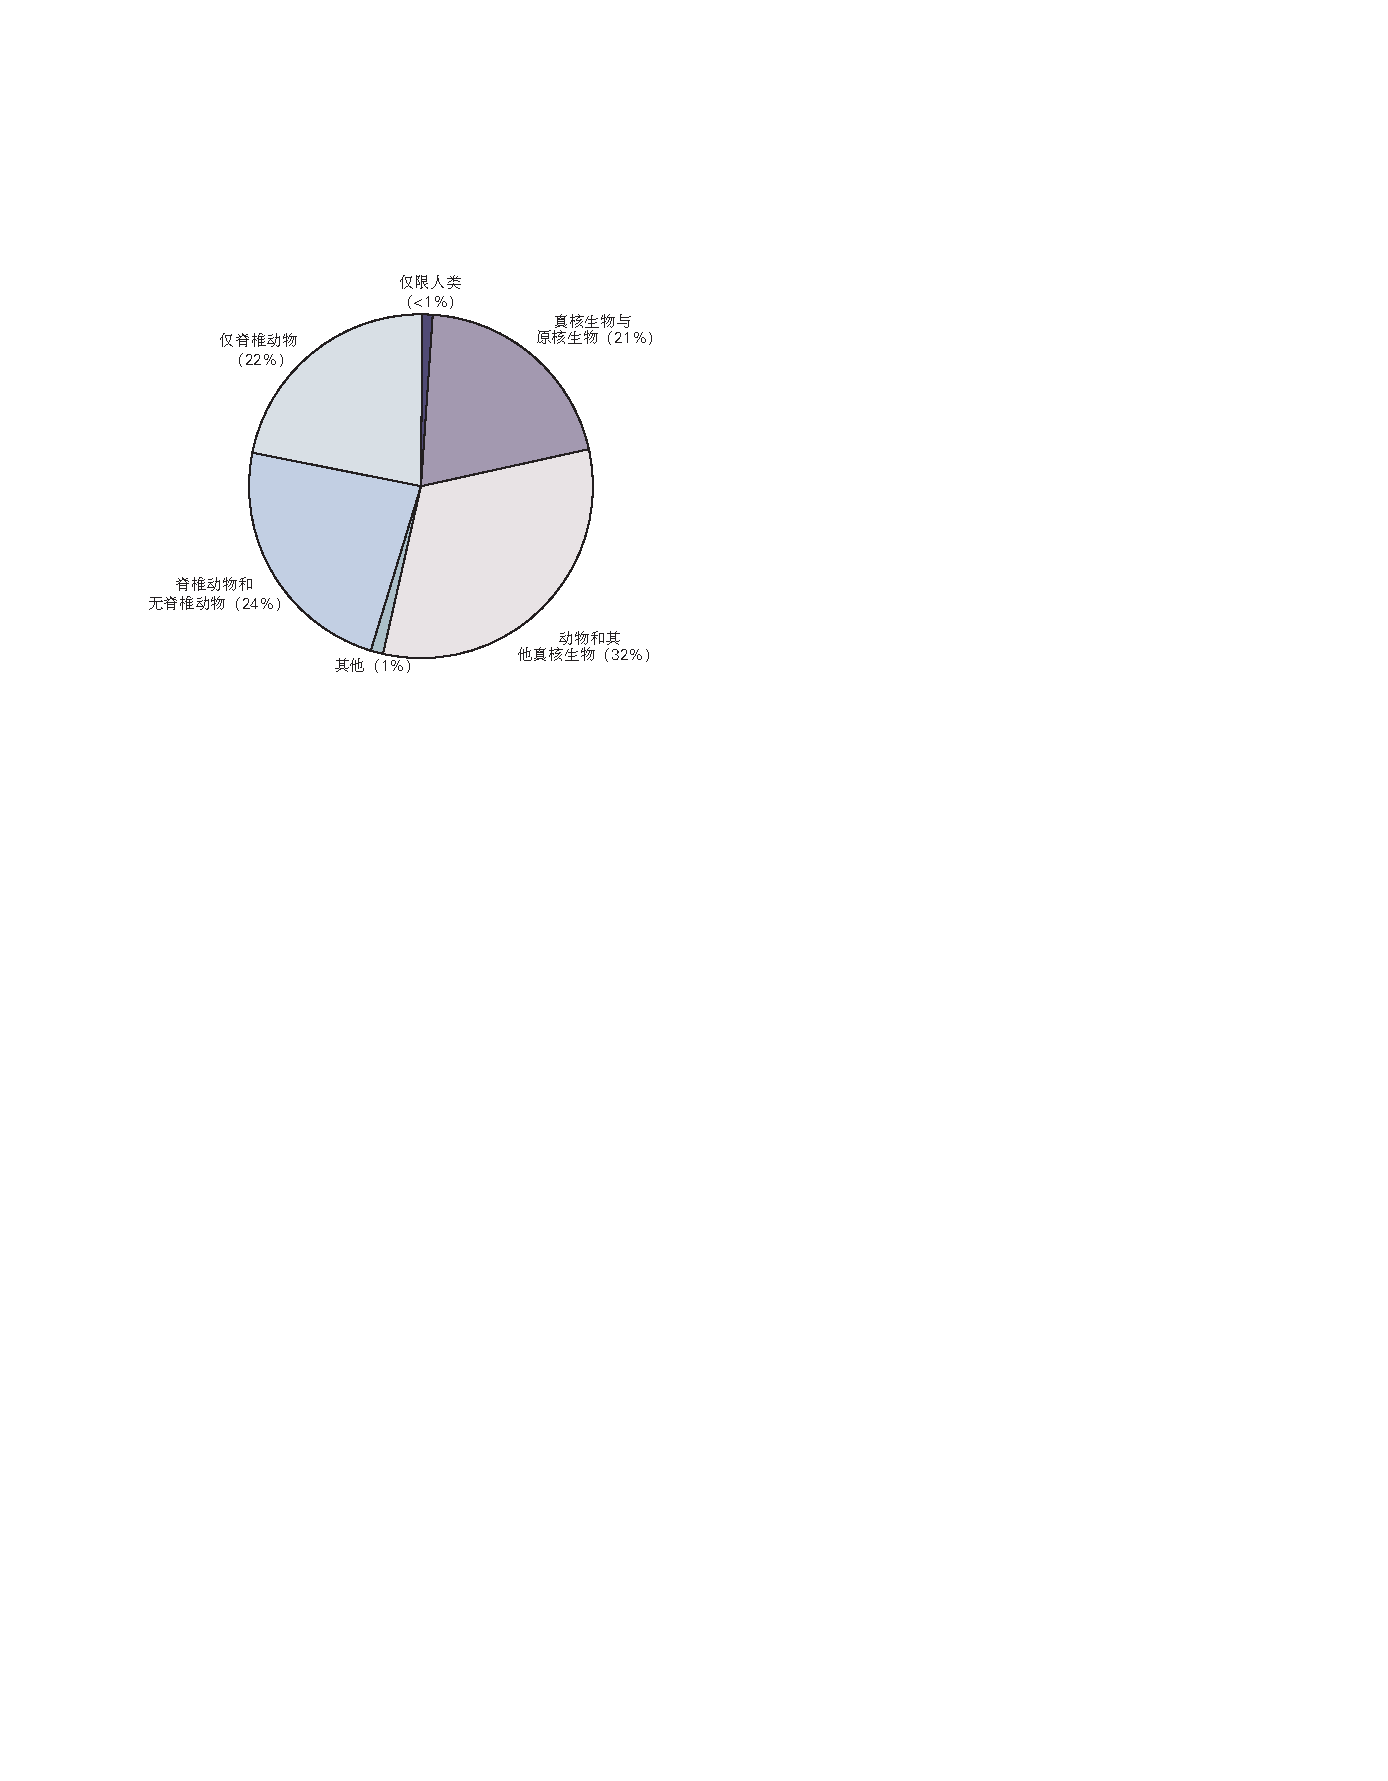
\includegraphics[width=0.6\linewidth]{chap02/fig_2_5}
	\caption{大多数人类基因都与其他物种的基因有关。
		不到 1\% 的人类基因是人类特有的;其他基因可能为所有生物、所有真核生物、仅动物或仅脊椎动物共享\cite{international2001initial}。}
	\label{fig:2_5}
\end{figure}


由于在整个进化过程中基因的这种保守性,对一种动物的研究的见解通常可以应用于具有相关基因的其他动物,这是一个重要的事实,因为动物实验通常是可能的,而人类实验却不可能。
例如,编码与人类基因相似的氨基酸序列的小鼠基因通常具有与直向同源人类基因相似的功能。


大约一半的人类基因具有已从其他生物体的直系同源基因中证明或推断出的功能(图~\ref{fig:2_6})。
人类、苍蝇甚至单细胞酵母共有的一组基因编码用于中间代谢的蛋白质;
\textit{脱氧核糖核酸}、\textit{核糖核酸}和蛋白质的合成;
细胞分裂; 和细胞骨架结构、蛋白质运输和分泌。


\begin{figure}[htbp]
	\centering
	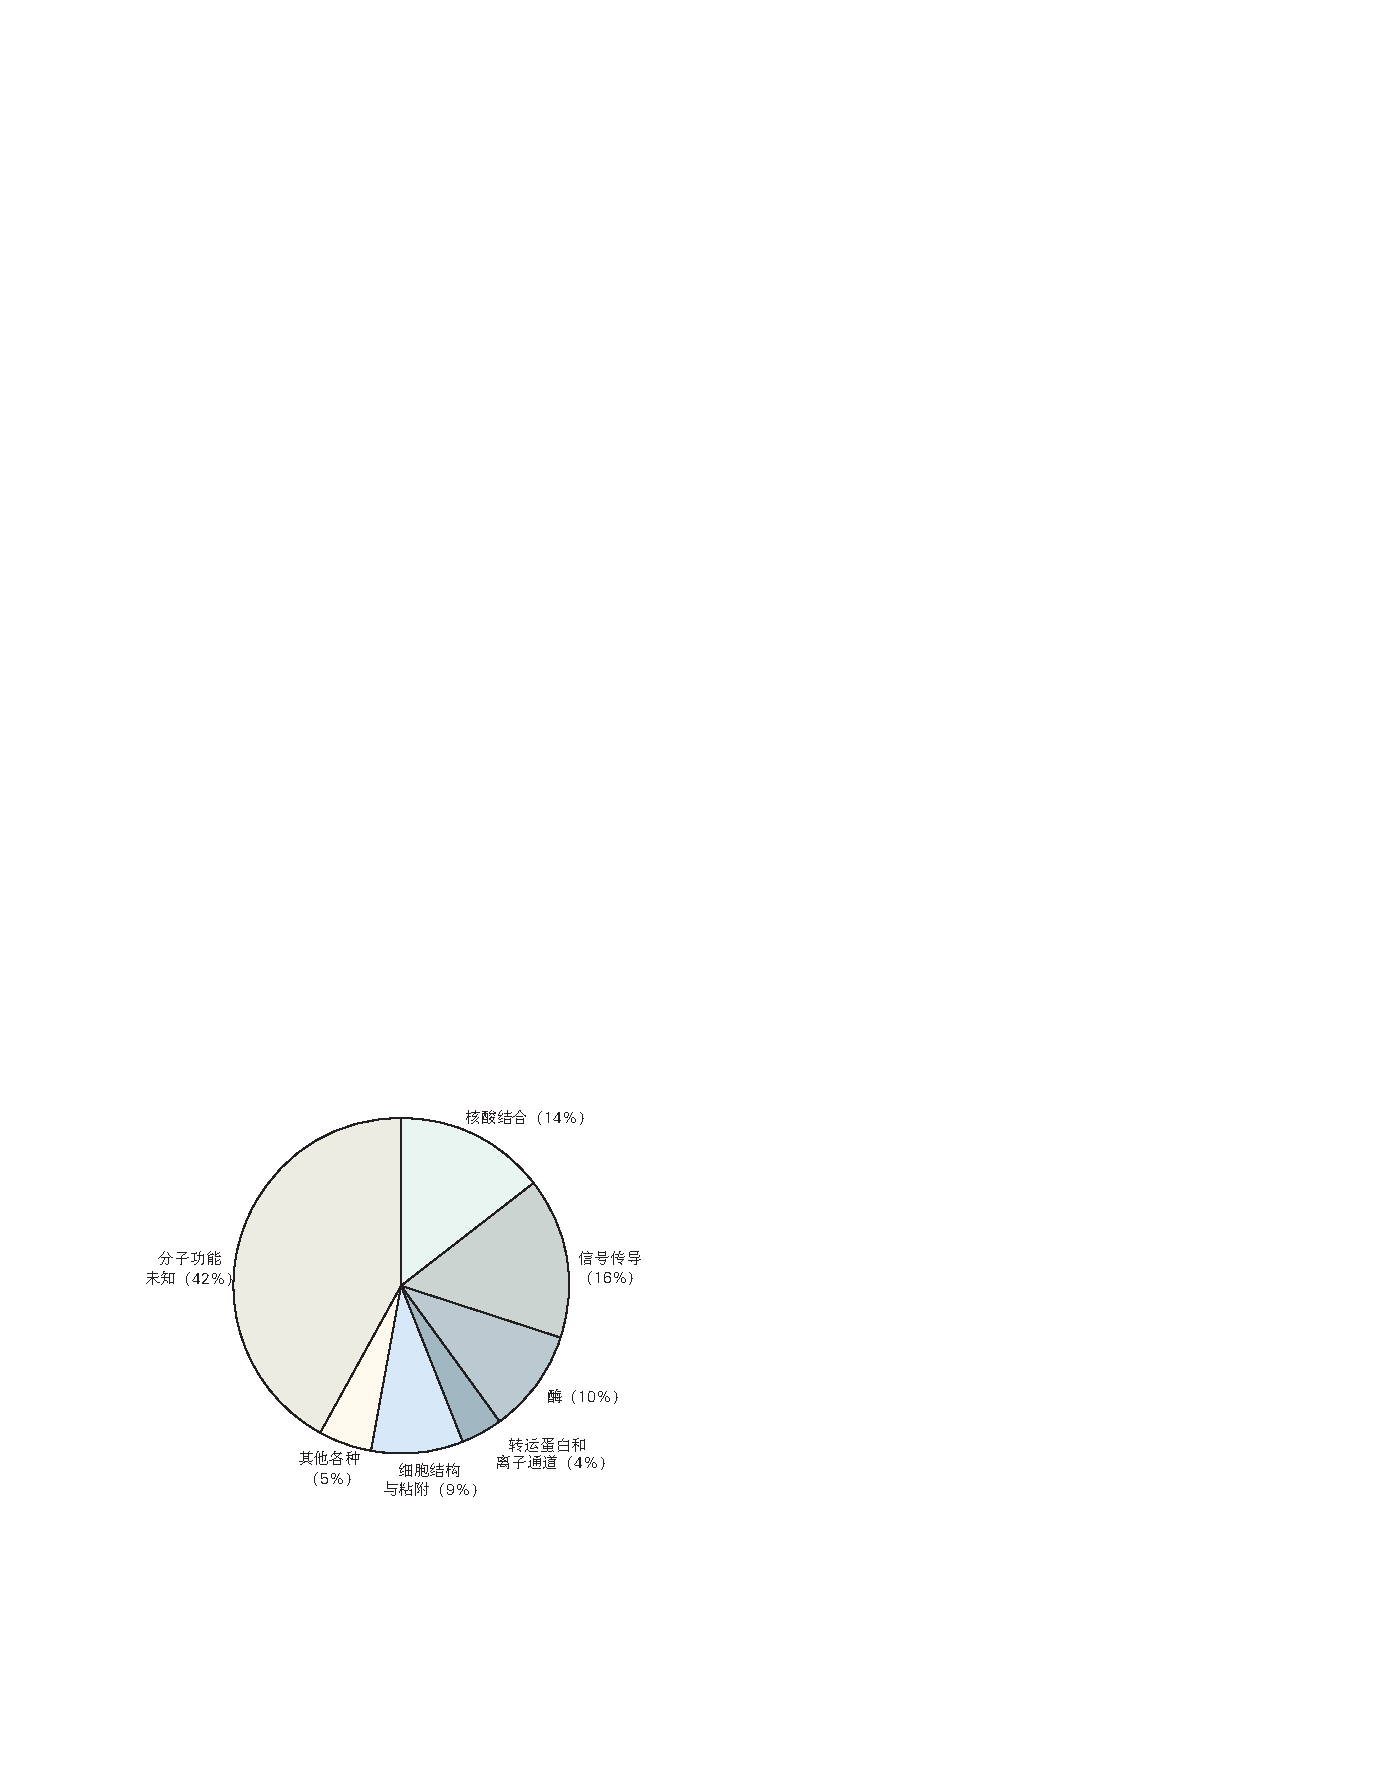
\includegraphics[width=0.6\linewidth]{chap02/fig_2_6}
	\caption{26,383 个人类基因的预测分子功能\cite{venter2001sequence}。}
	\label{fig:2_6}
\end{figure}


从单细胞生物到多细胞动物的进化伴随着与细胞间信号传导和基因调控有关的基因的扩展。
多细胞动物(例如蠕虫、苍蝇、小鼠和人类)的基因组通常编码数千个跨膜受体,比单细胞生物中存在的多得多。 
这些跨膜受体用于发育过程中的细胞间通讯、神经元之间的信号传递以及作为环境刺激的传感器。
多细胞动物的基因组还编码 1 千种或更多不同的\textit{脱氧核糖核酸}结合蛋白,这些蛋白调节其他基因的表达。


人类的许多跨膜受体和\textit{脱氧核糖核酸}结合蛋白与其他脊椎动物和无脊椎动物的特定直系同源基因相关。
通过列举动物共有的遗传基因,我们可以推断出神经元发育、神经传递、电兴奋性和基因表达的基本分子通路存在于蠕虫、苍蝇、小鼠和人类的共同祖先中。
此外,对动物和人类基因的研究表明,人脑中最重要的基因是那些在整个动物系统发育过程中最保守的基因。
哺乳动物基因与其无脊椎动物基因之间的差异通常是由哺乳动物基因复制或基因表达和功能的细微变化引起的,而不是全新基因的产生。



\section{可以在动物模型中研究行为的遗传调控}

由于人类和动物基因之间的进化保守性,在动物模型中研究构成行为基础的基因、蛋白质和神经回路之间的关系可能会深入了解人类的这些关系。
在基因功能研究中应用了两个重要策略并取得了巨大成功。


在经典的遗传分析中,生物体首先受到化学诱变或辐射诱导随机突变,然后筛选影响感兴趣行为(例如睡眠)的可遗传变化。
这种方法不会对所涉及的基因类型施加偏见;
它是对所有可能导致可检测到的变化的突变的随机搜索。 
可遗传变化的遗传追踪允许识别突变生物体中改变的个体基因。
因此,经典遗传学的发现路径从表型到基因型,从生物体到基因。
在反向遗传学中,特定的感兴趣基因被作为改变的目标,产生转基因动物,并研究具有这些改变基因的动物。
这种策略既有重点又有偏见:一个是从特定基因开始,发现的途径是从基因型到表型,从基因到生物体。


这两种实验策略及其更微妙的变化构成了实验遗传学的基础。
经典和反向遗传学的基因操作是在实验动物身上进行的,而不是在人类身上。



\subsection{转录振荡器调节苍蝇、小鼠和人类的昼夜节律}

\textit{西摩$\cdot$本泽}和他的同事在 1970 年左右发起了关于基因对行为影响的第一次大规模研究。
他们使用随机诱变和经典遗传分析来识别影响\textit{黑腹果蝇}习得和先天行为的突变:
昼夜节律(每天)节奏、求爱行为、运动、视觉感知和记忆(方框~\ref{box:2_2}~和方框~\ref{box:2_3})。
这些诱导突变对我们理解基因在行为中的作用产生了巨大影响。


\begin{proposition}[在实验动物中产生突变] \label{box:2_2}
	
	\quad \quad 苍蝇的随机诱变
	
	\quad \quad \textit{果蝇}行为的遗传分析是在个体基因发生突变的果蝇身上进行的。
	突变可以通过化学诱变或插入诱变进行,这些策略可以影响基因组中的任何基因。
	类似的随机诱变策略被用于在线虫\textit{秀丽隐杆线虫}、斑马鱼和小鼠中产生突变。
	
	\quad \quad 化学诱变,例如用\textit{甲磺酸乙酯},通常会在基因中产生随机点突变。
	当被称为转座子的可移动\textit{脱氧核糖核酸}序列随机插入其他基因时,就会发生插入突变。
	
	\quad \quad 果蝇中最广泛使用的转座元件是P元件。
	P元件可以被修饰为携带眼睛颜色的遗传标记,这使得它们在遗传杂交中易于追踪,并且它们也可以被修饰以改变它们所插入的基因的表达。
	
	\quad \quad 为了引起P元件转位,携带P元件的果蝇菌株被杂交到不携带的果蝇菌株。
	这种遗传杂交会导致所产生的后代中P元件的不稳定和移位。
	P元件的动员导致其在随机基因中转移到新的位置。
	
	\quad \quad 小鼠的靶向诱变
	
	\quad \quad 哺乳动物基因分子操作的进展已经允许用突变版本精确替换已知的正常基因。
	产生突变小鼠菌株的过程涉及两种不同的操作。
	染色体上的基因被称为胚胎干细胞的特殊细胞系中的同源重组所取代,修饰后的细胞系被整合到胚胎的生殖细胞群中(图~\ref{fig:2_7}f)。
	
	\quad \quad 必须首先克隆感兴趣的基因。
	该基因发生突变,然后将选择性标记(通常是耐药性基因)引入突变片段中。
	然后将改变的基因引入胚胎干细胞,并分离出包含改变基因的细胞克隆。
	对每个克隆的\textit{脱氧核糖核酸}样本进行测试,以鉴定突变基因已整合到同源(正常)位点而不是其他一些随机位点的克隆。
	
	\quad \quad 当已经鉴定出合适的克隆时,在胚泡阶段(受精后3至4天)将细胞注射到小鼠胚胎中,此时胚胎由大约100个细胞组成。
	然后,这些胚胎被重新引入一只雌性体内,这只雌性已经为植入做了激素准备,并被允许足月。
	得到的胚胎是干细胞系和宿主胚胎之间的嵌合混合物。
	
	\quad \quad 小鼠的胚胎干细胞有能力参与发育的各个方面,包括生殖系。
	注射的细胞可以成为生殖细胞,并将改变后的基因传递给后代小鼠。
	这项技术已被用于在对神经系统发育或功能至关重要的各种基因中产生突变。
	
	\quad \quad 限制基因敲除和调控转基因表达
	
	\quad \quad 为了提高基因敲除技术的实用性,已经开发出将缺失限制在特定组织中或动物发育过程中特定点的细胞上的方法。
	区域限制的一种方法利用Cre/loxP系统。
	Cre/loxP系统是来源于P1噬菌体的位点特异性重组系统,其中噬菌体酶Cre重组酶催化34bp loxP识别序列之间的重组,这些序列通常不存在于动物基因组中。
	
	\quad \quad loxP序列可以通过同源重组插入胚胎干细胞的基因组中,使得它们位于感兴趣基因(称为floxed基因)的一个或多个外显子的侧翼。
	当干细胞被注射到胚胎中时,人们最终可以培育出一只小鼠,其中感兴趣的基因是游离的,并且仍然在动物的所有细胞中发挥作用。
	
	\quad \quad 然后可以产生第二批转基因小鼠,其在神经启动子序列的控制下表达Cre重组酶,该序列通常在受限的大脑区域中表达。
	通过将Cre转基因小鼠系与具有感兴趣的游离基因的小鼠系杂交,该基因将仅在表达Cre转基因的那些细胞中被删除。
	
	\quad \quad 在图~\ref{fig:2_8}A所示的例子中,编码\textit{N-甲基-D-天冬氨酸}谷氨酸受体NR1(或GluN1)亚基的基因被loxP元件侧翼,然后在\textit{钙/钙调蛋白依赖性蛋白激酶 2}启动子的控制下与表达Cre重组酶的小鼠系杂交,该启动子通常在前脑神经元中表达。
	在这个特定的细胞系中,表达偶然局限于海马\textit{阿蒙角}1区,导致该脑区NR1亚基的选择性缺失(图~\ref{fig:2_8}B)。
	因为\textit{钙/钙调蛋白依赖性蛋白激酶 2}启动子只在出生后激活基因转录,所以这种策略可以最大限度地减少早期发育变化。
	
	\quad \quad 除了基因表达的区域限制外,对基因表达时间的控制给研究者提供了额外的灵活性,并可以排除在成熟动物表型中观察到的任何异常是转基因产生的发育缺陷的结果的可能性。
	这可以在小鼠身上通过构建一种可以用药物开启或关闭的基因来实现。
	
	\quad \quad 一个是从创建两个小鼠行开始。
	品系1携带一种特殊的转基因,该转基因受启动子\textit{四环素反应元件}的控制,而\textit{四环素反应元件}通常只在细菌中发现。
	这个启动子本身不能启动基因;它需要被特定的转录调节因子激活。
	因此,第二组小鼠表达第二种转基因,该转基因编码一种杂交转录因子\textit{四环素激活因子},该因子识别并结合\textit{四环素反应元件}启动子。
	\textit{四环素激活因子}的表达可以置于小鼠基因组中的启动子的控制下,该启动子通常仅在特定类别的神经元或特定大脑区域中驱动基因转录。
	
	\quad \quad 当这两种小鼠交配时,一些后代将携带两种转基因。
	在这些小鼠中,\textit{四环素激活因子}与\textit{四环素反应元件}启动子结合并激活下游转基因。
	\textit{四环素激活因子}转录因子之所以特别有用,是因为当它与某些抗生素(如四环素)结合时,它会失活,从而通过给小鼠服用抗生素来调节转基因表达。
	还可以产生表达被称为反向\textit{四环素激活因子}的\textit{四环素激活因子}突变形式的小鼠。
	这种反式激活剂不会与\textit{四环素反应元件}结合,除非动物被喂食多西环素。
	在这种情况下,转基因总是被关闭,除非给药(图~\ref{fig:2_9})。
	
	\quad \quad \textit{核糖核酸}干扰和\textit{规律成簇的间隔短回文重复}改变基因功能
	
	\quad \quad 最后,可以通过现代分子工具靶向基因来灭活基因。
	一种这样的方法是\textit{核糖核酸}干扰,它利用了真核细胞中大多数双链\textit{核糖核酸}被常规破坏的事实;即使只有一部分是双链的,整个\textit{核糖核酸}也会被破坏。
	通过引入一个短\textit{核糖核酸}序列,人工地使选定的\textit{信使核糖核酸}变成双链,研究人员可以激活这一过程,降低特定基因的\textit{信使核糖核酸}水平。
	
\end{proposition}


\begin{figure}[htbp]
	\centering
	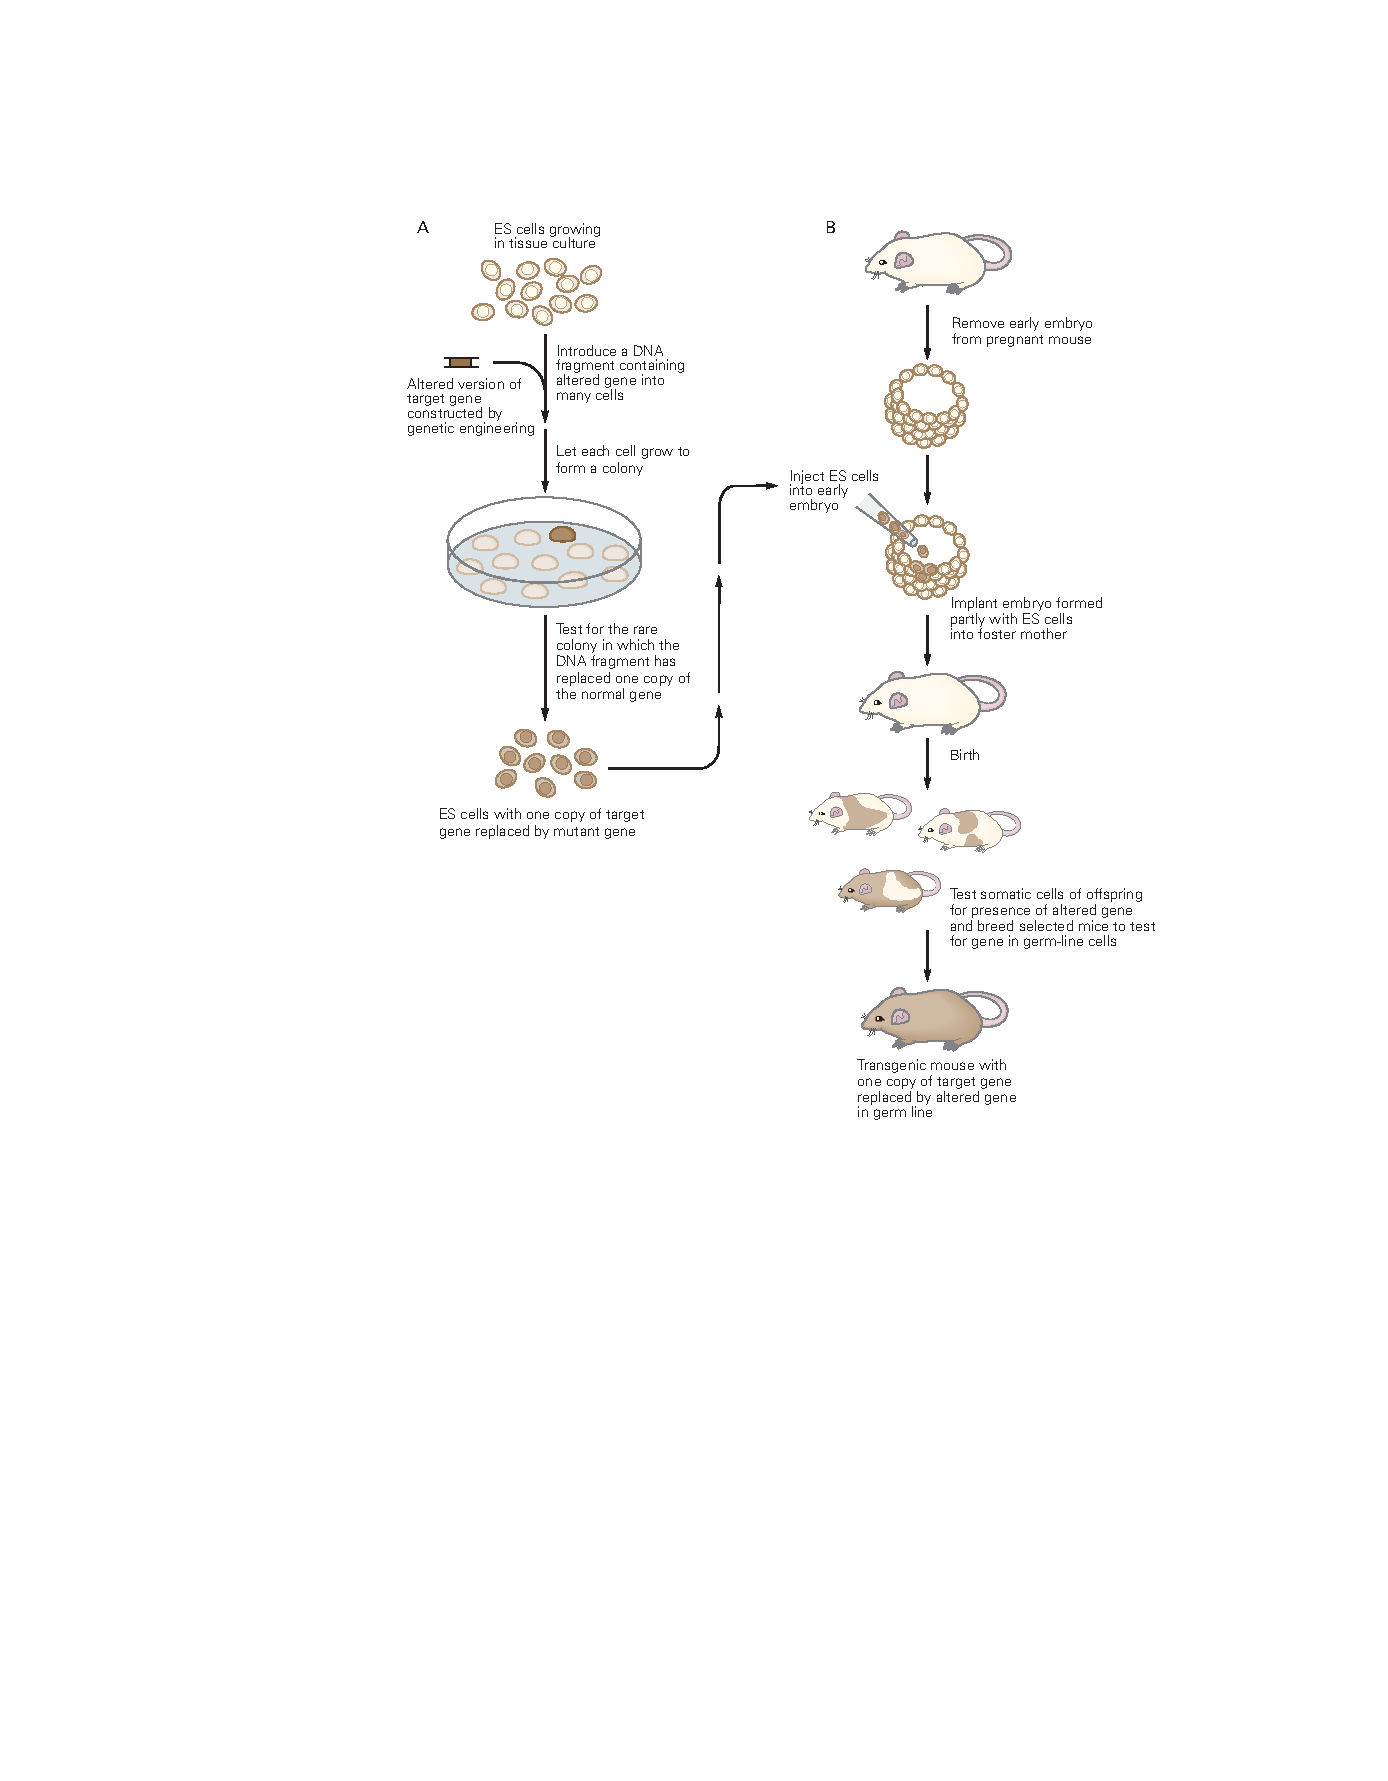
\includegraphics[width=0.94\linewidth]{chap02/fig_2_7}
	\caption{创造突变小鼠菌株\cite{alberts2017molecular}。
		\textbf{A.} 产生具有特定靶向突变的小鼠干细胞。
		\textbf{B.} 利用改变的胚胎干细胞创造转基因小鼠。}
	\label{fig:2_7}
\end{figure}


\begin{figure}[htbp]
	\centering
	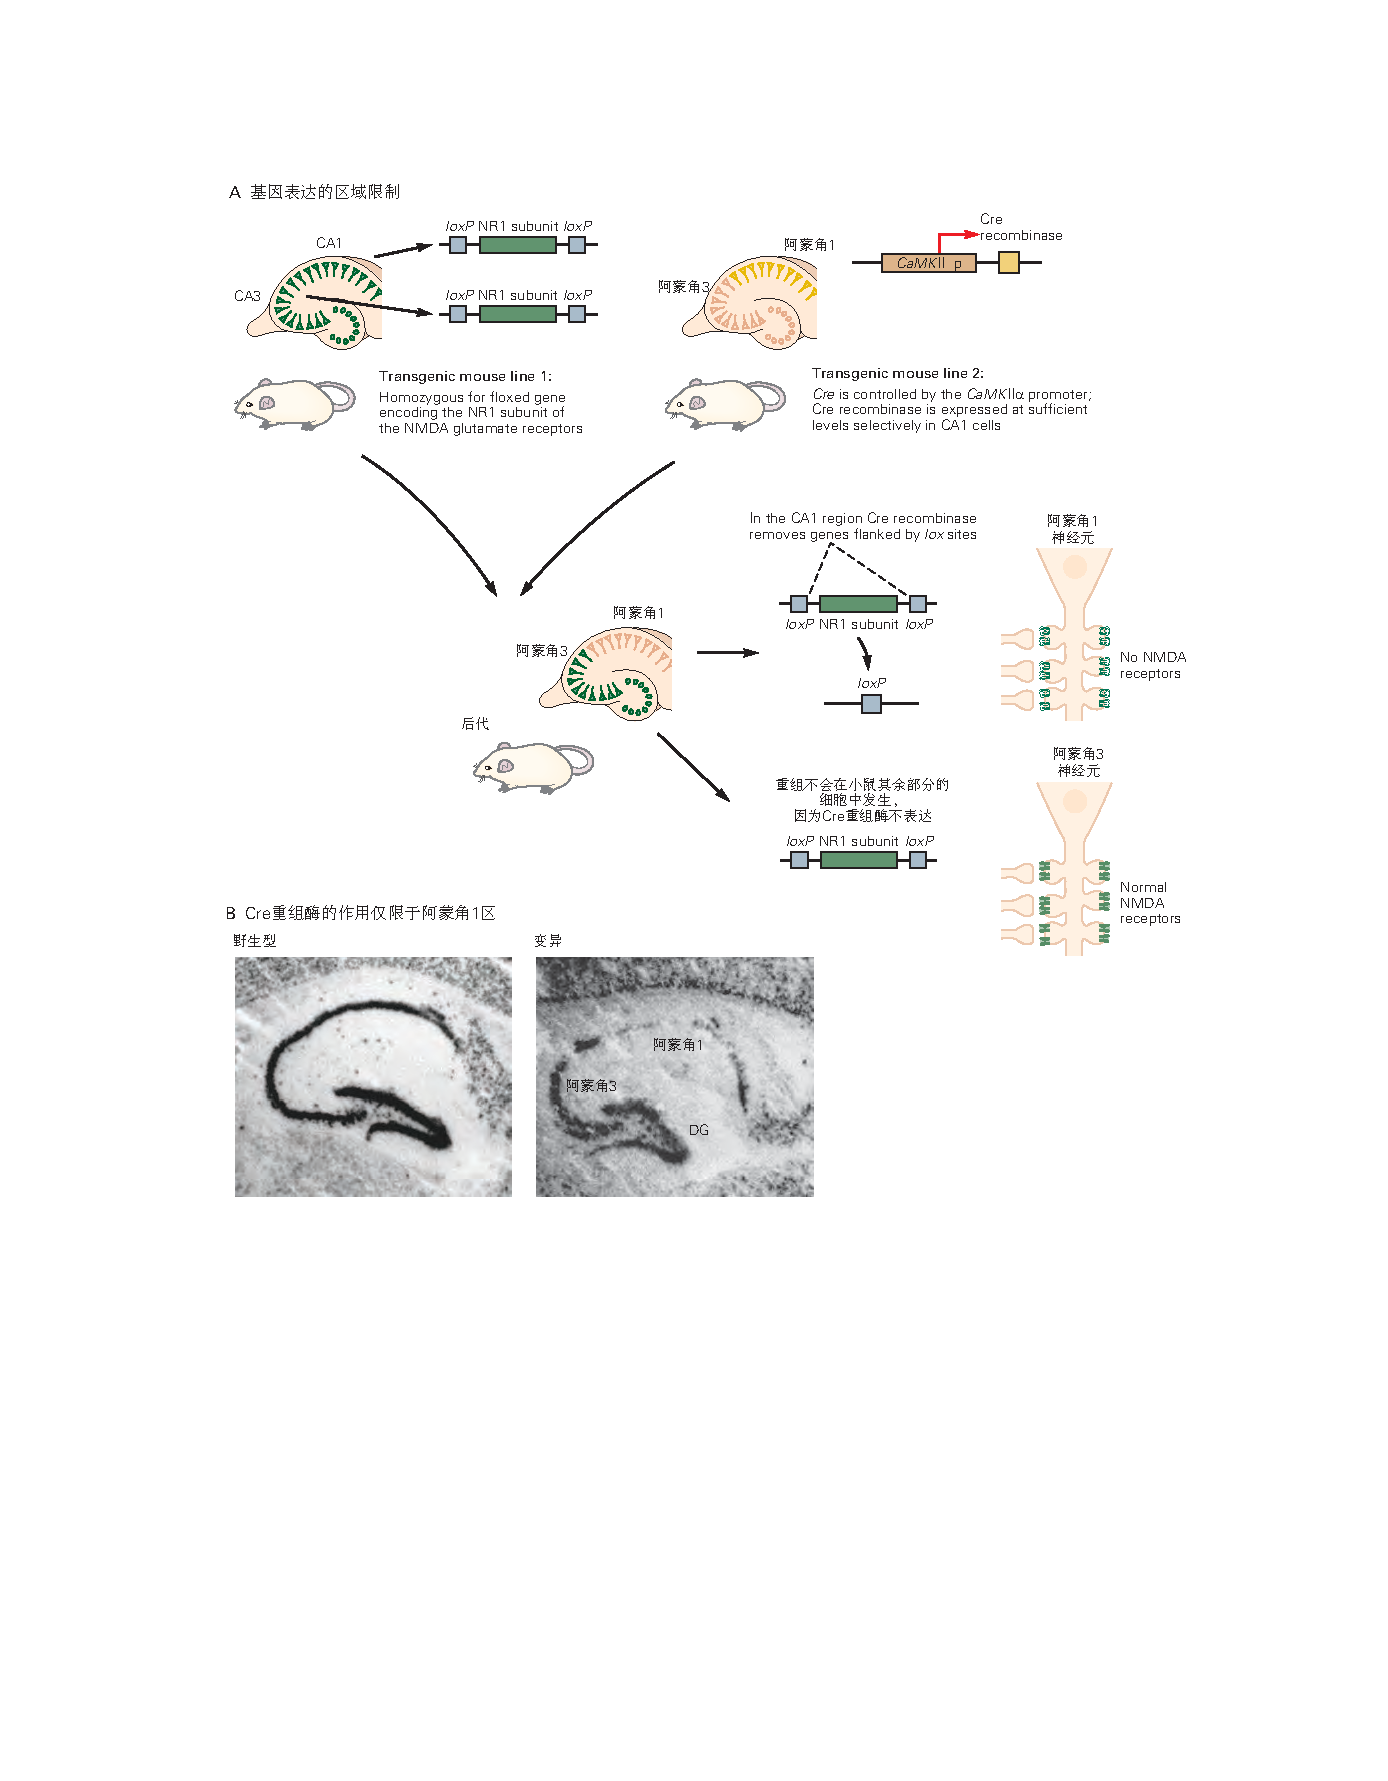
\includegraphics[width=1.0\linewidth]{chap02/fig_2_8}
	\caption{用于选择性区域基因敲除的Cre/loxP系统。
		\textbf{A.} 培育了一种小鼠系,其中编码\textit{N-甲基-D-天冬氨酸}受体NR1亚基的基因两侧有loxP遗传元件(转基因小鼠系1)。
		然后将这些所谓的“floxed NR1”小鼠与第二系小鼠杂交,其中编码Cre重组酶的转基因置于细胞类型或组织类型特异性转录启动子的控制下(转基因小鼠系2)。
		在本实施例中,来自\textit{钙/钙调蛋白依赖性蛋白激酶 2}a基因的启动子用于驱动Cre基因的表达。
		在携带Cre重组酶转基因的Floxy基因纯合的子代中,仅在驱动Cre表达的启动子活性的细胞类型中,通过Cre介导的loxP重组,Floxy的基因将被删除。
		\textbf{B.} 原位杂交用于检测野生型和突变小鼠海马切片中NR1亚基的\textit{信使核糖核酸},这些小鼠含有两个固定的NR1等位基因,并在\textit{钙/钙调蛋白依赖性蛋白激酶 2}a启动子的控制下表达Cre重组酶。
		在突变小鼠中,NR1的\textit{信使核糖核酸}表达(暗染色)在海马\textit{阿蒙角}1区显著减少,但在\textit{阿蒙角}3和\textit{齿状回}保持正常\cite{tsien1996essential}。}
	\label{fig:2_8}
\end{figure}



\begin{proposition}[神经解剖学导航术语] \label{box:2_3}
	
	\quad \quad 转基因在苍蝇和老鼠中的引入
	
	\quad \quad 通过将\textit{脱氧核糖核酸}注射到新受精卵的细胞核中,可以在小鼠体内实验性地引入基因(图~\ref{fig:2_10})。
	在一些注射的卵子中,新基因或转基因被整合到其中一条染色体上的随机位点。
	由于胚胎处于单细胞阶段,整合的基因被复制并最终进入动物的所有(或几乎所有)细胞,包括种系。
	
	\quad \quad 通过将用于产生色素的基因注射到从白化病菌株获得的蛋中而拯救的外壳颜色标记基因来说明基因掺入。
	有色素斑块的小鼠表明\textit{脱氧核糖核酸}的成功表达。
	通过测试注射动物的\textit{脱氧核糖核酸}样本,证实了转基因的存在。
	
	\quad \quad 在苍蝇身上也使用了类似的方法。将待注射的\textit{脱氧核糖核酸}克隆到可转座元件(P元件)中。
	当注射到胚胎中时,\textit{脱氧核糖核酸}被插入生殖细胞核的\textit{脱氧核糖核酸}中。
	P元件可以被工程化以在特定时间和特定细胞中表达基因。
	转基因可以是恢复突变体功能的野生型基因,或者是改变其他基因表达或编码特异性改变的蛋白质的设计基因。
	
\end{proposition}


\begin{figure}[htbp]
	\centering
	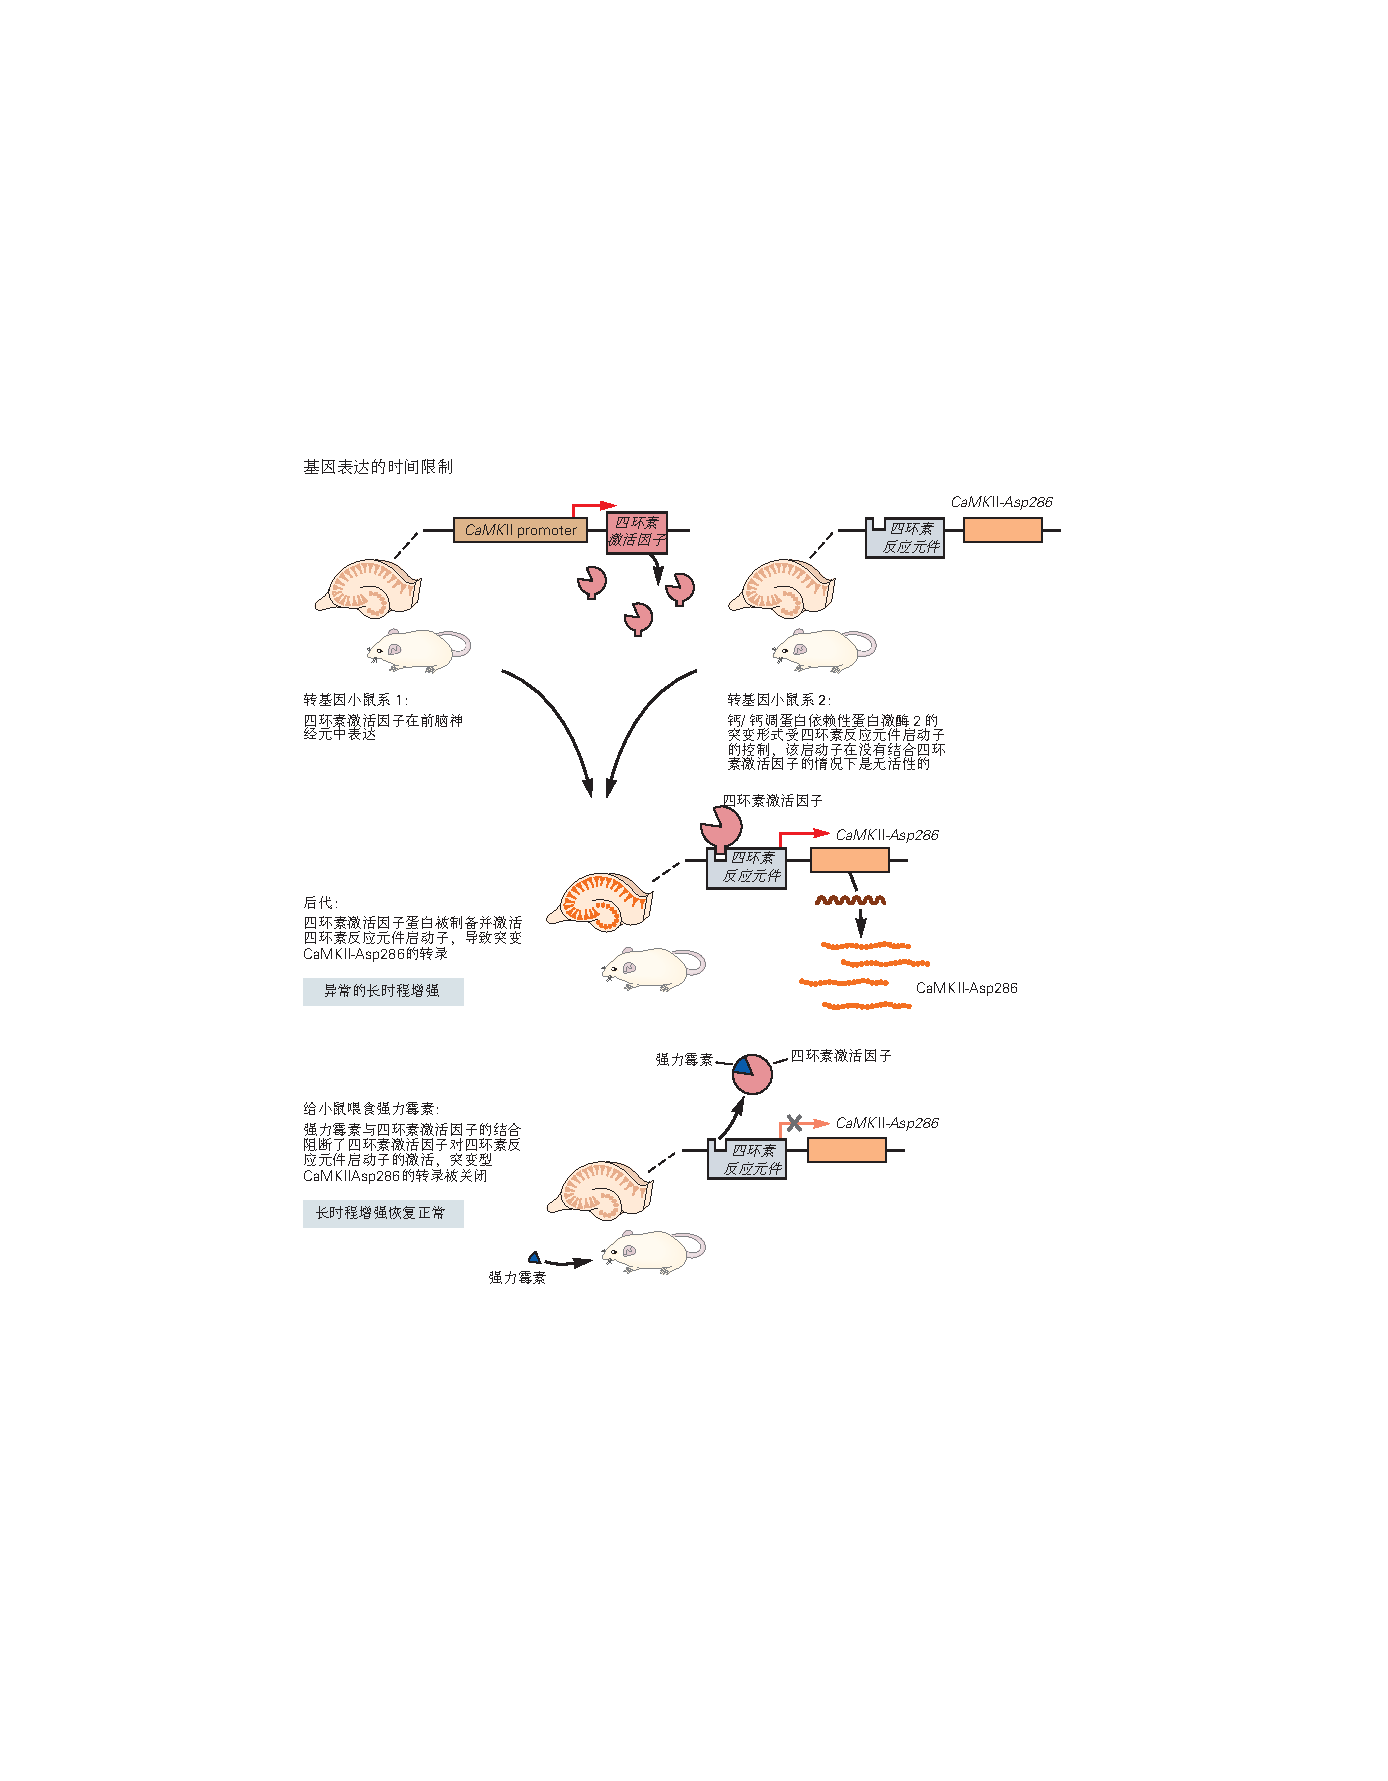
\includegraphics[width=0.87\linewidth]{chap02/fig_2_9}
	\caption{四环素系统用于转基因表达的时间和空间调控。培育了两个独立的转基因小鼠系。
		一个系在\textit{钙/钙调蛋白依赖性蛋白激酶 2}a启动子的控制下表达\textit{四环素激活因子},这是一种结合了识别细菌\textit{四环素反应元件}操纵子的细菌转录因子的工程蛋白。
		第二条线包含一个感兴趣的转基因(这里编码一种组成型活性形式的\textit{钙/钙调蛋白依赖性蛋白激酶 2}),它使激酶在没有\ce{Ca^2+}的情况下持续活性,其表达受\textit{四环素反应元件}的控制。
		当这两个系交配时,后代以仅限于前脑的模式表达\textit{四环素激活因子}蛋白。
		当\textit{四环素激活因子}蛋白与\textit{四环素反应元件}结合时,它将激活感兴趣的下游基因的转录。
		给后代服用四环素(或多西环素)与\textit{四环素激活因子}蛋白结合,并引起构象变化,导致该蛋白与\textit{四环素反应元件}解除结合,阻断转基因表达。
		通过这种方式,小鼠将在前脑中表达\textit{钙/钙调蛋白依赖性蛋白激酶 2}–Asp286,并且可以通过向小鼠施用多西环素来阻断这种表达\cite{mayford1996control}。}
	\label{fig:2_9}
\end{figure}


\begin{figure}[htbp]
	\centering
	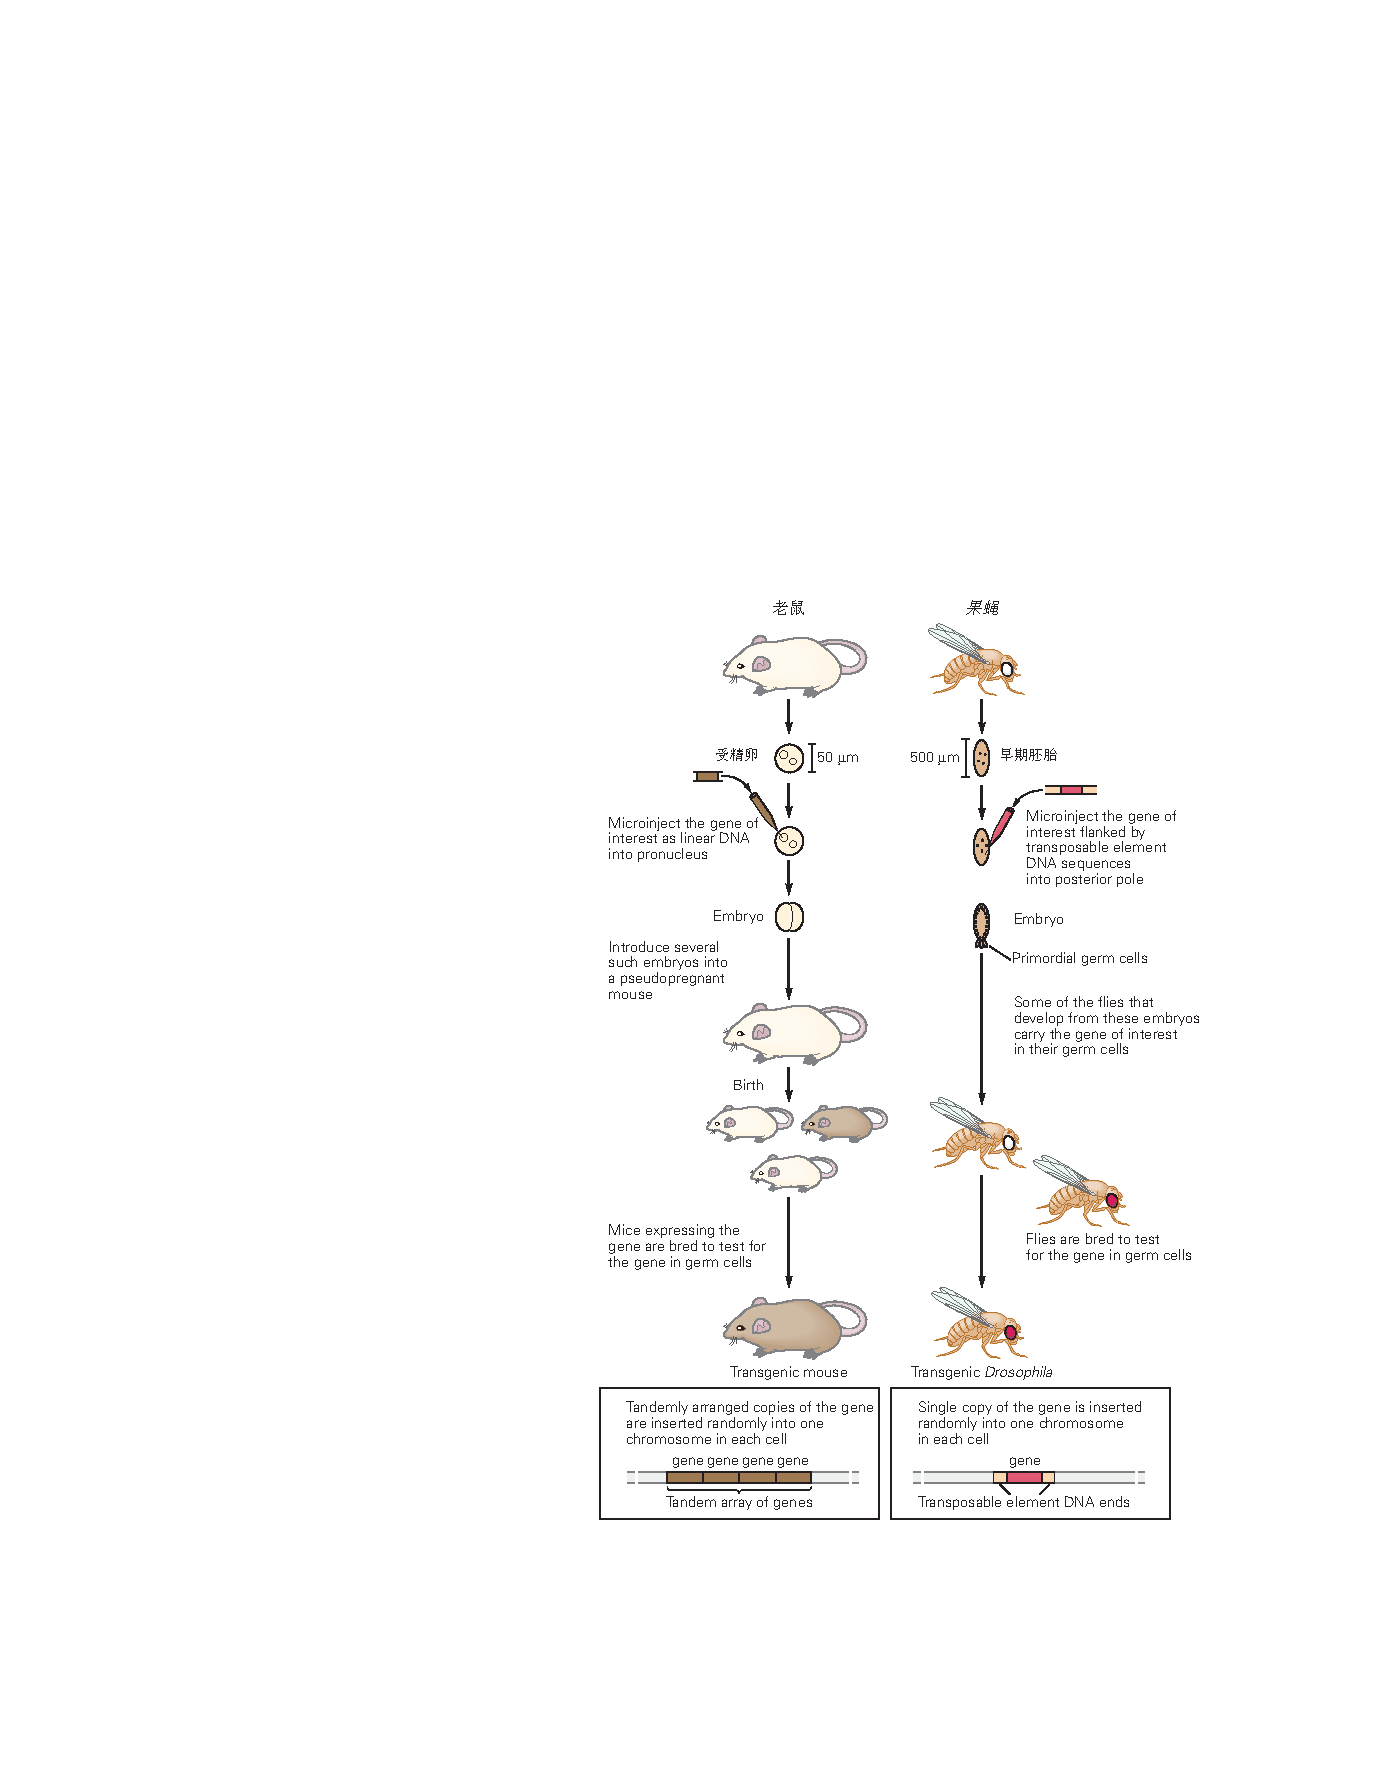
\includegraphics[width=0.75\linewidth]{chap02/fig_2_10}
	\caption{产生转基因小鼠和苍蝇。
		在这里,注射到小鼠体内的基因会导致毛色的变化,而注射到苍蝇体内的基因则会导致眼睛颜色的变化。
		在这两个物种的一些转基因动物中,\textit{脱氧核糖核酸}被插入不同细胞的不同染色体位点(见底部的插图)\cite{alberts2017molecular}。}
	\label{fig:2_10}
\end{figure}




我们对行为的昼夜节律控制的遗传基础有一个特别完整的了解。
动物的昼夜节律将某些行为与与太阳升起和落下相关的 24 小时周期联系起来。
昼夜节律调节的核心是一个在 24 小时周期内振荡的内在生物钟。
由于时钟的内在周期性,即使在没有光或其他环境影响的情况下,昼夜节律行为也会持续存在。


生物钟可以重新设置,这样昼夜循环的变化最终会导致内在振荡器发生匹配的变化,这是任何正在从时差反应中恢复过来的旅行者都熟悉的现象。
时钟由眼睛传输到大脑的光驱动信号重置。
最后,时钟驱动特定行为的效应通路,例如睡眠和运动。


\textit{本泽}的团队搜索了数千只突变果蝇,以寻找由于指导昼夜节律振荡的基因发生突变而无法遵循昼夜节律的稀有果蝇。
从这项工作中,人们对生物钟的分子机制有了初步的了解。
周期或每个基因的突变影响果蝇内部时钟产生的所有昼夜节律行为。


有趣的是,每个突变都可以通过多种方式改变生物钟(图~\ref{fig:2_11})。
心律失常的\textit{节律基因}突变果蝇在任何行为中都没有表现出明显的内在节律,缺乏\textit{节律基因}的所有功能,因此\textit{节律基因}对节律行为至关重要。
维持基因某些功能的突变会导致节律异常。
长日等位基因产生 28 小时的行为周期,而短日等位基因产生 19 小时的行为周期。
因此\textit{节律基因}不仅是时钟的重要组成部分,它实际上是一个计时员,其活动可以改变时钟运行的速率。


\begin{figure}[htbp]
	\centering
	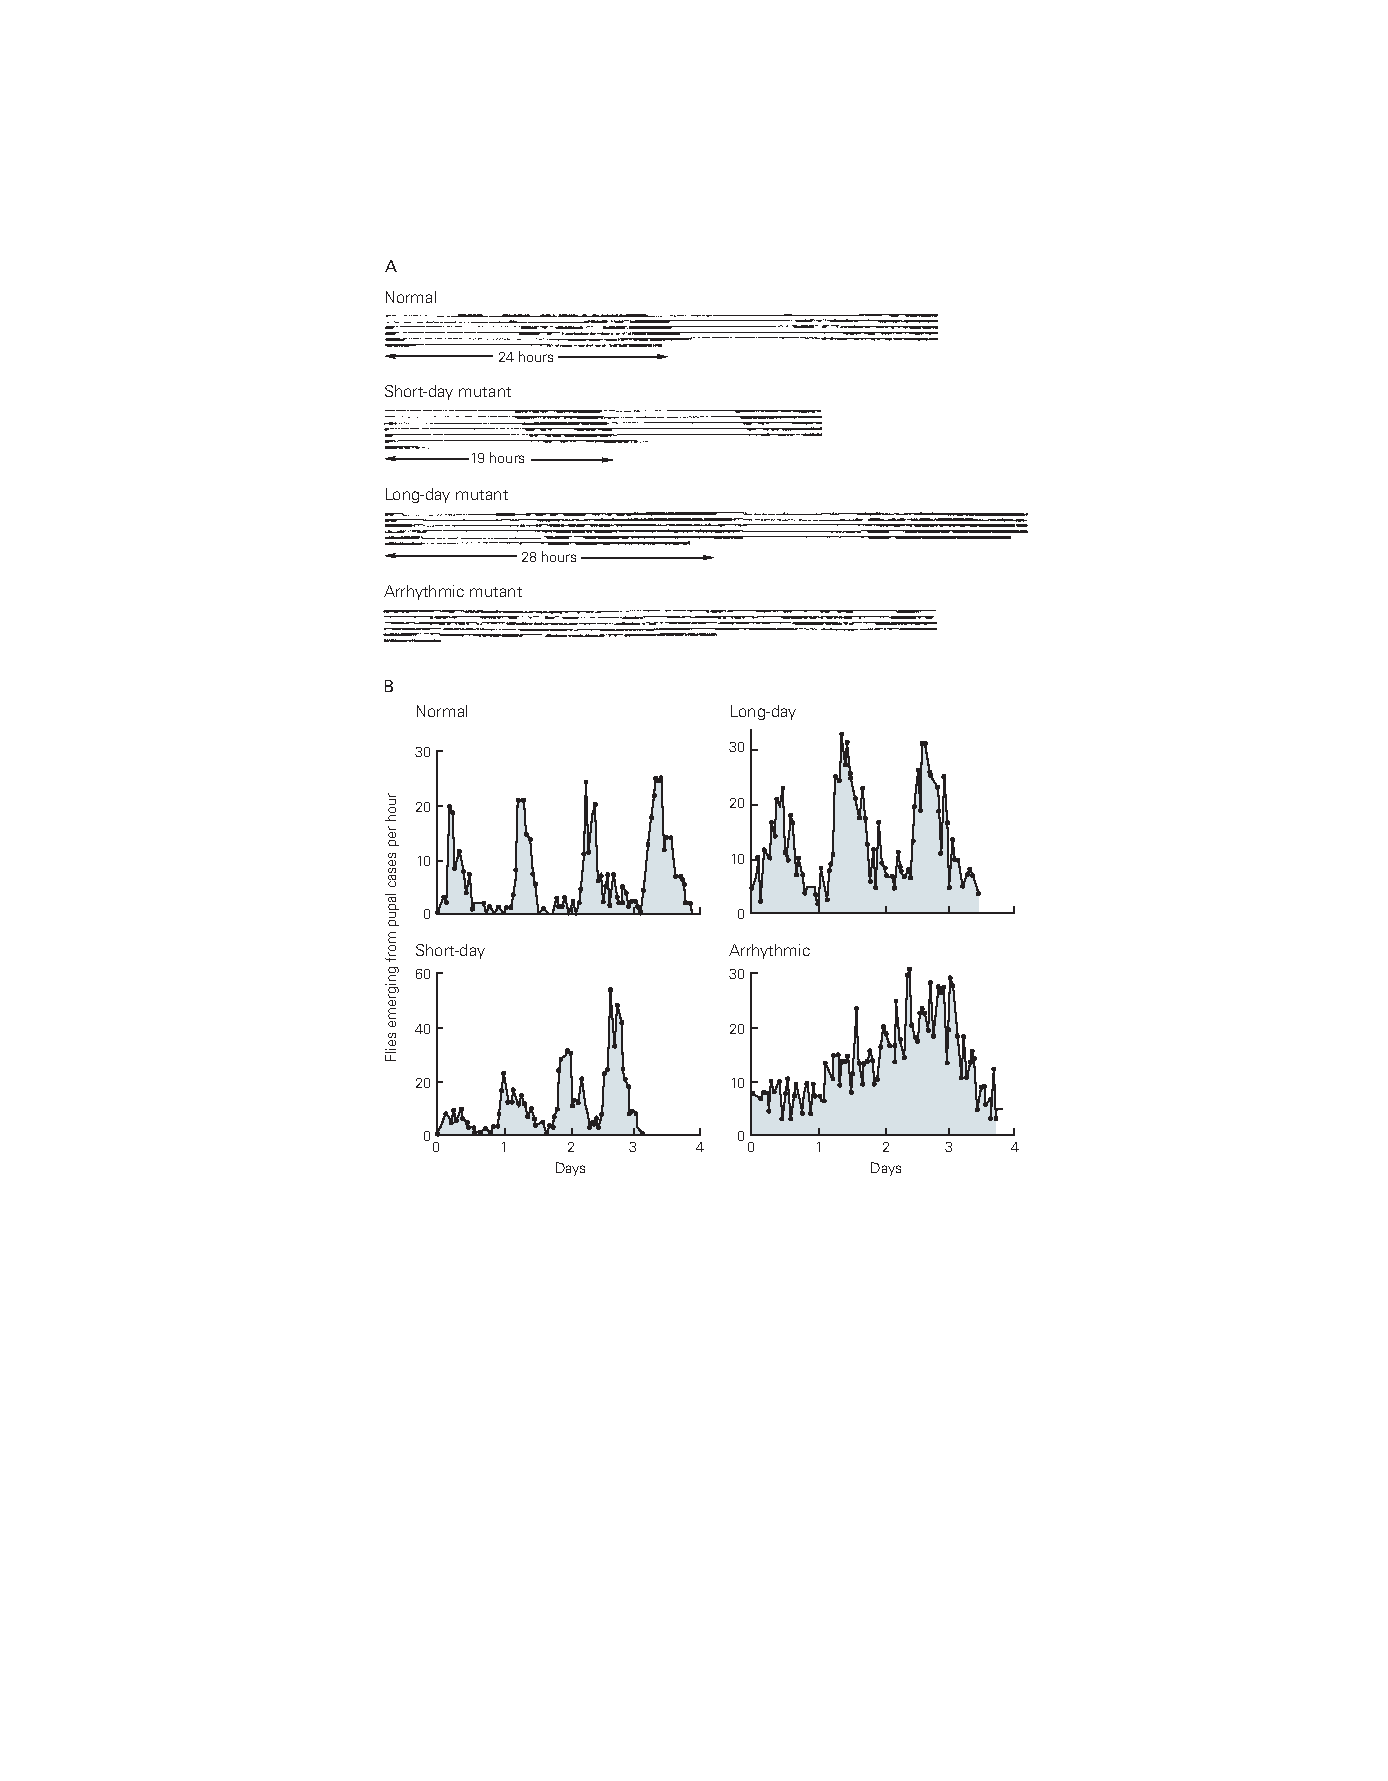
\includegraphics[width=0.8\linewidth]{chap02/fig_2_11}
	\caption{一个基因控制着果蝇行为的昼夜节律。
		周期或每个基因的突变会影响果蝇内部时钟调节的所有昼夜节律行为\cite{konopka1971clock}。
		\textbf{A.} 正常果蝇和\textit{节律基因}突变体的三种菌株的运动节律:短日照、长日照和心律失常。
		将苍蝇从 12 小时光照和 12 小时黑暗的循环转变为持续黑暗,然后在红外光下监测活动。
		记录中的粗段表示活动。
		\textbf{B.} 正常的成年苍蝇种群以周期性的方式从它们的蛹壳中出现,即使在持续的黑暗中也是如此。
		这些图显示了在持续黑暗的 4 天期间每小时出现的苍蝇数量(四个种群中的每一个)。
		出现没有任何可辨别的节律的心律失常突变种群。}
	\label{fig:2_11}
\end{figure}


\textit{节律基因}突变体除了昼夜节律行为的改变外没有主要的不利影响。
这一观察很重要,因为在发现之前,许多人质疑是否可能存在动物生理需要不需要的真正“行为基因”。
\textit{节律基因}似乎确实是这样一种“行为基因”。


\textit{节律基因}是如何保持时间的?
蛋白质产物\textit{周期蛋白}是一种转录调节因子,可影响其他基因的表达。
\textit{周期蛋白}的水平全天受到监管。
清晨,\textit{周期蛋白}及其\textit{信使核糖核酸}较低。
在一天中,\textit{周期蛋白}\textit{信使核糖核酸}和蛋白质积累,在黄昏后和夜间达到峰值水平。
然后水平下降,在下一个黎明前下降。
这些观察为昼夜节律之谜提供了答案,即一个中央调节器在一天中出现和消失。
但它们也不令人满意,因为它们只是将问题往后推了一步,即什么是\textit{周期蛋白}循环?
这个问题的答案需要发现额外的\textit{时钟基因},这些基因在果蝇和老鼠身上都有发现。


受到果蝇昼夜节律筛查成功的鼓舞,\textit{约瑟夫$\cdot$高桥}在 1990 年代开始在老鼠身上进行类似但劳动密集型得多的基因筛查。
他筛选了数百只突变小鼠,寻找昼夜运动周期发生改变的罕见个体,并发现了一个他称之为\textit{时钟基因}突变。
当\textit{时钟基因}突变的纯合小鼠被转移到黑暗中时,它们最初会经历极长的昼夜节律周期,然后完全失去昼夜节律(图~\ref{fig:2_12})。
因此,\textit{时钟基因}似乎可以调节昼夜节律的两个基本特性:昼夜节律周期的长度和在没有感觉输入的情况下节律性的持久性。
这些特性在概念上与果蝇中\textit{节律基因}基因的特性相同。


\begin{figure}[htbp]
	\centering
	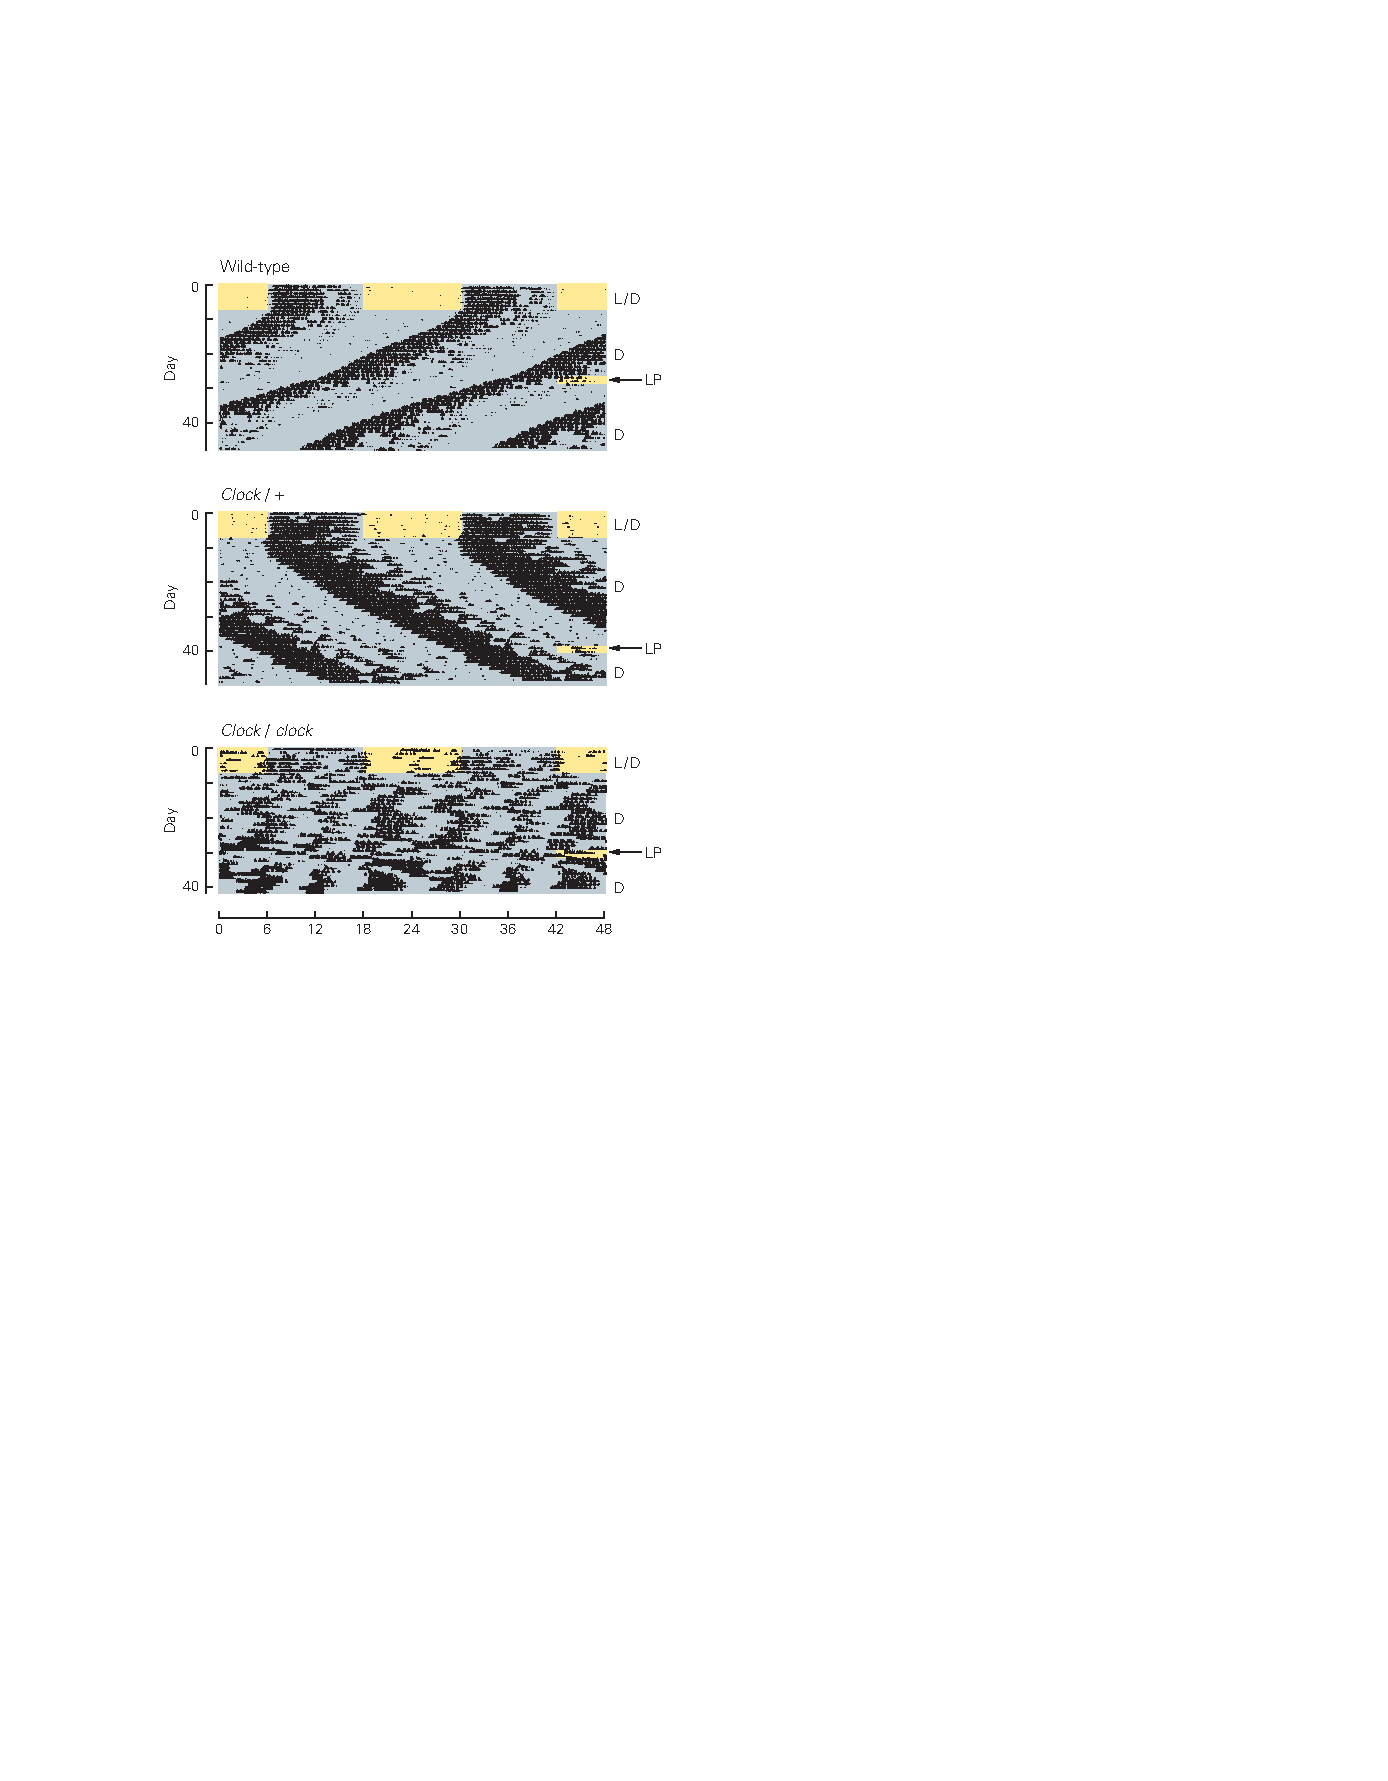
\includegraphics[width=0.55\linewidth]{chap02/fig_2_12}
	\caption{\textit{时钟基因}对小鼠昼夜节律的调节。
		记录显示了三种动物的运动活动期:野生型、杂合型和纯合型。
		所有动物在前7天保持12小时的亮暗循环,然后转移到恒定黑暗。
		之后,他们被暴露在6小时的\textit{光照周期}中以重置节奏。
		野生型小鼠的昼夜节律具有23.1小时的周期。
		杂合时钟/+小鼠的周期为24.9小时。
		纯合子时钟/时钟小鼠在转移到恒定黑暗时经历昼夜节律性的完全丧失,并在光照期后短暂表达28.4小时的节律\cite{takahashi1994forward}。}
	\label{fig:2_12}
\end{figure}


小鼠\textit{时钟基因}与果蝇中的\textit{节律基因}基因一样,编码一个转录调节器,其活动在一天中波动。
小鼠\textit{时钟蛋白}和果蝇\textit{周期蛋白}也共享一个称为 PAS 结构域的结构域,这是转录调节因子子集的特征。
这一观察表明,相同的分子机制(PAS 结构域转录调节的振荡)控制着果蝇和小鼠的昼夜节律。


更重要的是,对果蝇和小鼠的平行研究表明,相似的转录调节因子组会影响这两种动物的生物钟。
在克隆小鼠\textit{时钟基因}后,克隆了一个果蝇昼夜节律基因,发现它与小鼠时钟的关系比\textit{节律基因}。
在另一项研究中,一种与 fly \textit{节律基因}相似的小鼠基因被鉴定并通过反向遗传学灭活。
突变小鼠有昼夜节律缺陷,就像每个突变体都会飞一样。 
换句话说,果蝇和小鼠都使用\textit{时钟基因}和每个基因来控制它们的昼夜节律。
一组基因,而不是一个基因,是生物钟的保守调节剂。


这些基因的表征导致了对昼夜节律分子机制的理解,并戏剧性地证明了这些机制在果蝇和小鼠中的相似性。
在果蝇和小鼠中,\textit{时钟蛋白}都是一种转录激活因子。 
它与伴侣蛋白一起控制决定运动活动水平等行为的基因的转录。
\textit{时钟蛋白}及其伙伴还刺激\textit{节律基因}基因的转录。
然而,\textit{周期蛋白}抑制\textit{时钟蛋白}刺激每个基因表达的能力,因此随着 \textit{周期蛋白}的积累,每个转录下降(图~\ref{fig:2_13})。
24 小时周期的出现是因为\textit{周期蛋白}的积累和激活在\textit{节律基因}转录后延迟了许多小时,这是\textit{周期蛋白}磷酸化、\textit{周期蛋白}不稳定性以及与其他循环蛋白相互作用的结果。


\begin{figure}[htbp]
	\centering
	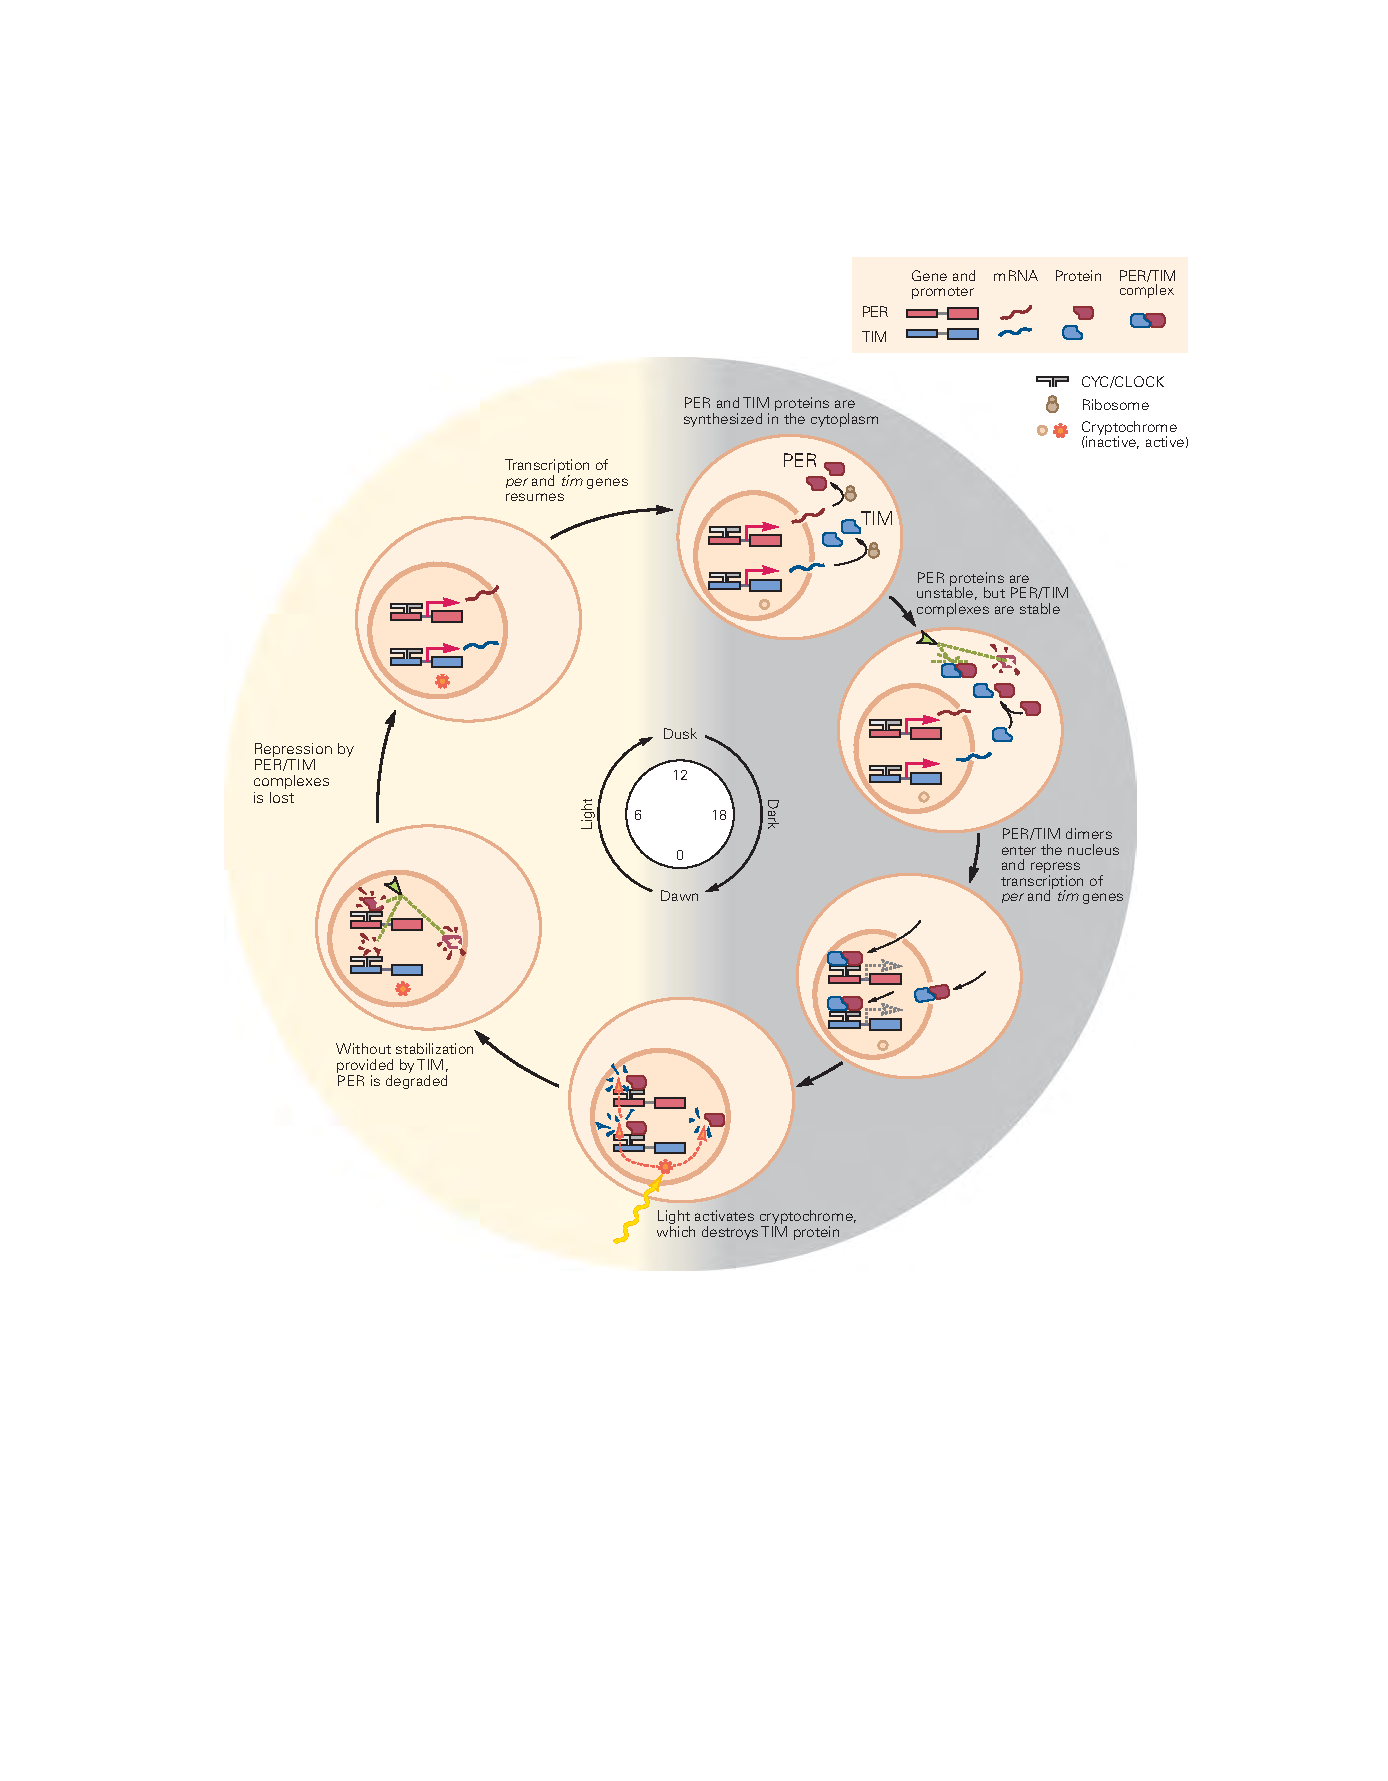
\includegraphics[width=1.0\linewidth]{chap02/fig_2_13}
	\caption{驱动昼夜节律的分子事件。
		控制生物钟的基因受两种核蛋白\textit{周期蛋白}和\textit{无节律蛋白}的调节。
		这些蛋白质慢慢积累,然后相互结合形成二聚体。
		一旦它们形成二聚体,它们就会进入细胞核并关闭包括它们自己在内的昼夜节律基因的表达。
		它们通过抑制刺激\textit{节律基因}和\textit{无节律基因}转录的\textit{时钟蛋白}和 CYCLE 来实现。
		\textit{周期蛋白}非常不稳定;
		其中大部分降解得如此之快,以至于它永远没有机会抑制每个转录的时钟依赖性。 
		\textit{周期蛋白}的降解受不同蛋白激酶的至少两种不同磷酸化事件的调节。
		当\textit{周期蛋白}与\textit{无节律蛋白}结合时,\textit{周期蛋白}受到保护免于降解。 
		随着\textit{时钟蛋白}驱动越来越多的\textit{节律基因}和\textit{无节律基因}表达,足够的\textit{周期蛋白}和\textit{无节律蛋白}最终积累到两者可以结合并稳定彼此,此时它们进入细胞核,在那里它们自身的转录受到抑制。
		结果,\textit{节律基因}和\textit{无节律基因}的\textit{信使核糖核酸}水平下降; 此后,\textit{周期蛋白}和\textit{无节律蛋白}水平下降,\textit{时钟蛋白}可以(再次)驱动\textit{节律基因}和\textit{无节律基因}\textit{信使核糖核酸}的表达。
		在白天,\textit{无节律蛋白}被光调节的信号通路(包括隐花色素)降解,因此\textit{周期蛋白}/\textit{无节律蛋白}复合物仅在夜间形成。
		\textit{时钟蛋白}诱导\textit{周期蛋白}和\textit{无节律蛋白}表达,但被\textit{周期蛋白}和 \textit{无节律蛋白}蛋白抑制。}
	\label{fig:2_13}
\end{figure}


\textit{节律基因}、\textit{时钟基因}和相关基因的分子特性产生了昼夜节律所必需的所有特性。

1. 昼夜节律基因转录随24小时周期变化:夜间\textit{周期蛋白}活性高;
\textit{时钟蛋白}白天活跃度很高。


2. 昼夜节律基因是相互影响\textit{信使核糖核酸}水平的转录因子,产生振荡。
\textit{时钟蛋白}按转录激活,\textit{周期蛋白}抑制\textit{时钟蛋白}功能。


3. 昼夜节律基因还控制其他基因的转录,进而影响许多下游反应。
例如,在果蝇中,神经肽基因 pdf 控制运动活动水平。


4. 这些基因的振荡可以被光重置。


2017 年诺贝尔生理学或医学奖授予了\textit{杰弗里$\cdot$霍尔}、\textit{迈克尔$\cdot$罗斯巴什}和\textit{迈克尔$\cdot$杨},表彰了对这种分子钟机制的详细阐述。


相同的遗传网络控制着人类的昼夜节律。
患有晚期睡眠阶段综合症的人具有较短的 20 天周期和极端早睡、早起的“早晨云雀”表型。
\textit{路易斯$\cdot$普塔切克}和\textit{傅颖慧}发现这些个体的每个基因都具有人类突变。
这些结果表明,行为基因从昆虫到人类都是保守的。 
晚期睡眠时相综合症在睡眠章节(第~\ref{chap:chap44}~章)中进行了讨论。



\subsection{蛋白激酶的自然变异调节果蝇和蜜蜂的活性}

在前面描述的昼夜节律的遗传学研究中,随机诱变被用来识别生物过程中感兴趣的基因。
所有正常个体都有\textit{节律基因}、\textit{时钟基因}和相关基因的功能拷贝;
只有在诱变后才会产生不同的等位基因。
另一个关于基因在行为中的作用的更微妙的问题是,哪些基因变化可能导致正常个体的行为变异。
\textit{玛尔拉$\cdot$索科洛夫斯基}及其同事的工作导致鉴定出第一个与一个物种中正常个体的行为变异相关的基因。


果蝇幼虫的活动水平和运动方式各不相同。
一些称为漫游者的幼虫会长距离移动(图~\ref{fig:2_14})。
其他人称为保姆,相对静止。
从野外分离出的果蝇幼虫可以是漫游者或保育者,表明这些是自然变异而不是实验室诱导的突变。
这些特征是可遗传的;
流浪者父母有流浪者后代,保姆父母有保姆后代。


\begin{figure}[htbp]
	\centering
	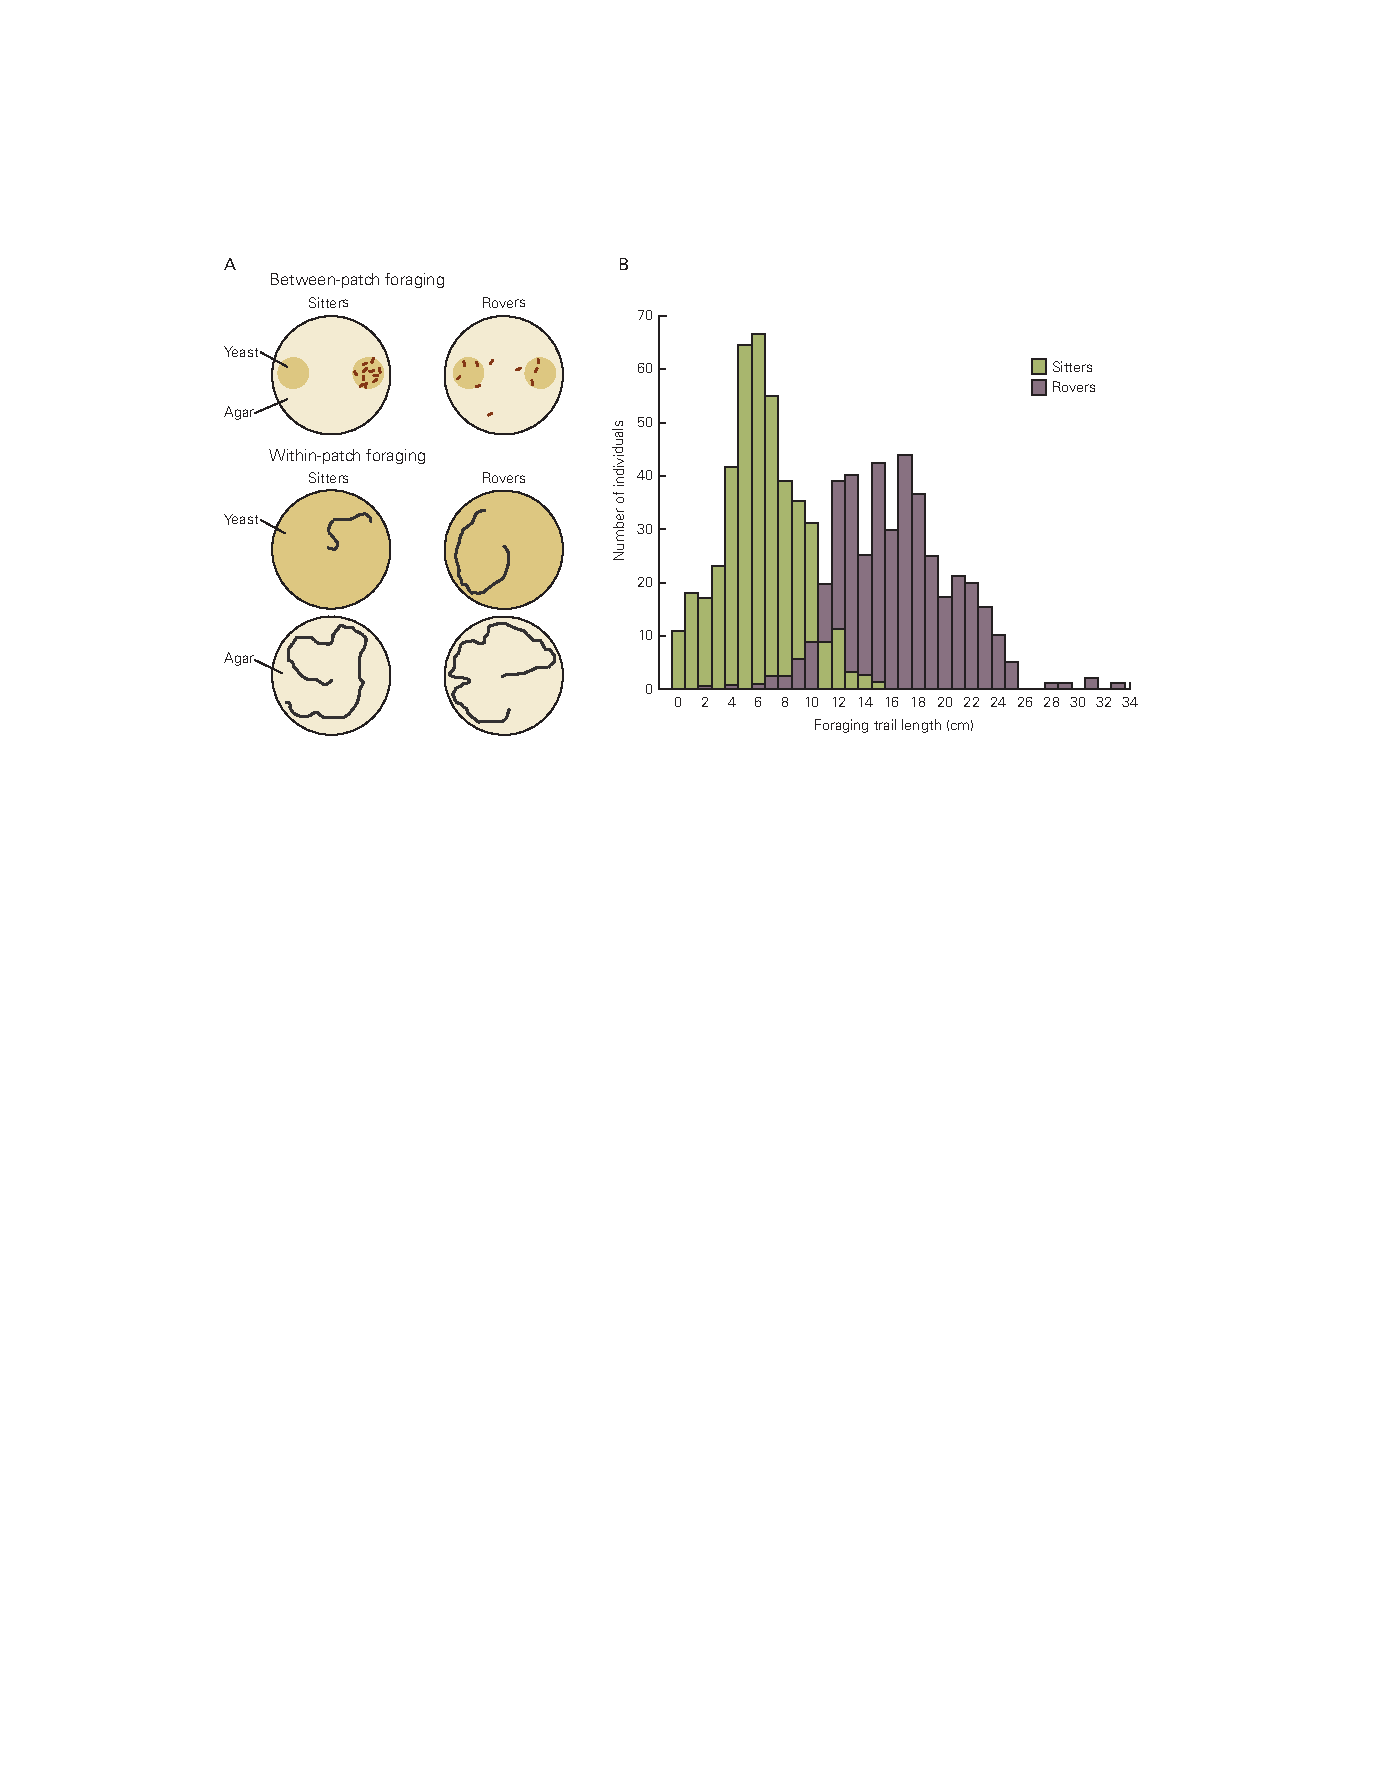
\includegraphics[width=0.95\linewidth]{chap02/fig_2_14}
	\caption{\textit{果蝇漫游者}和\textit{保姆幼虫}在享用酵母时的觅食行为不同\cite{sokolowski2001drosophila}。
		\textbf{A.} 漫游型幼虫从一块地移动到另一块地,而保姆型幼虫在一块地上停留很长时间。
		当在一块地里觅食时,漫游者幼虫比保姆幼虫移动得更多。
		仅在琼脂上,漫游者和保姆幼虫的移动速度相等。
		\textbf{B.} 当漫游者在一片食物中觅食时,它们的踪迹长度比\textit{保姆幼虫}长(踪迹长度是在5分钟内测量的)。
		这种觅食行为的差异映射到一个单一的蛋白激酶基因,该基因在不同的苍蝇幼虫中的活性不同。}
	\label{fig:2_14}
\end{figure}


\textit{索科洛夫斯基}使用不同野生果蝇之间的杂交来研究漫游者和保育幼虫之间的遗传差异。
这些杂交表明漫游者和保育幼虫之间的差异在于一个主要基因,即\textit{觅食基因}座。
\textit{觅食基因}编码信号转导酶,一种由细胞代谢物\textit{环鸟苷-3,5-单磷酸盐}激活的蛋白激酶。
因此,这种行为的自然变化源于信号转导通路调节的改变。
许多神经元功能受蛋白激酶调节,例如由\textit{觅食基因}编码的\textit{环鸟苷-3,5-单磷酸盐}依赖性激酶。
蛋白激酶等分子在将短期神经信号转化为神经元或回路特性的长期变化方面尤为重要。


为什么信号酶的变异性会在通常包括漫游者和保育者的果蝇野生种群中得以保留?
答案是环境的变化会产生压力,要求平衡选择替代行为。 
拥挤的环境有利于漫游者幼虫,它能比竞争对手更有效地移动到新的、未开发的食物来源,而稀疏的环境有利于保育幼虫,它能更彻底地利用当前来源。


\textit{觅食基因}也存在于蜜蜂中。
蜜蜂在生命的不同阶段表现出不同的行为;
一般来说,年轻的蜜蜂是护士,而年长的蜜蜂则成为离开蜂巢的觅食者。
\textit{觅食基因}在活跃的觅食蜜蜂的大脑中以高水平表达,而在更年轻和更静止的护士蜜蜂中以低水平表达。
幼蜂中\textit{环鸟苷-3,5-单磷酸盐}信号的激活会导致它们过早进入觅食阶段;
这种变化可能是由环境刺激或蜜蜂的衰老引起的。


因此,同一个基因控制两种不同昆虫行为的变异,但方式不同。
在果蝇中,行为的变化在不同的个体中表现出来,而在蜜蜂中,它们在不同年龄的个体中表现出来。
这种差异说明了一个重要的调控基因是如何被招募到不同物种的不同行为策略中的。



\subsection{神经肽受体调节几种物种的社会行为}

行为的许多方面都与动物与其他动物的社会互动有关。
社会行为在物种之间变化很大,但在受遗传控制的物种中具有很大的先天组成部分。
在蛔虫秀丽隐杆线虫中分析了一种简单的社会行为形式。 
这些动物生活在土壤中,以细菌为食。


不同的野生型菌株在摄食行为上表现出巨大差异。
来自标准实验室菌株的动物是孤独的,分散在细菌食物的草坪上并且彼此之间无法互动。
其他菌株具有群居摄食模式,加入由数十或数百只动物组成的大型摄食群(图~\ref{fig:2_15})。
这些菌株之间的差异是遗传的,因为这两种喂养方式都是稳定遗传的。


\begin{figure}[htbp]
	\centering
	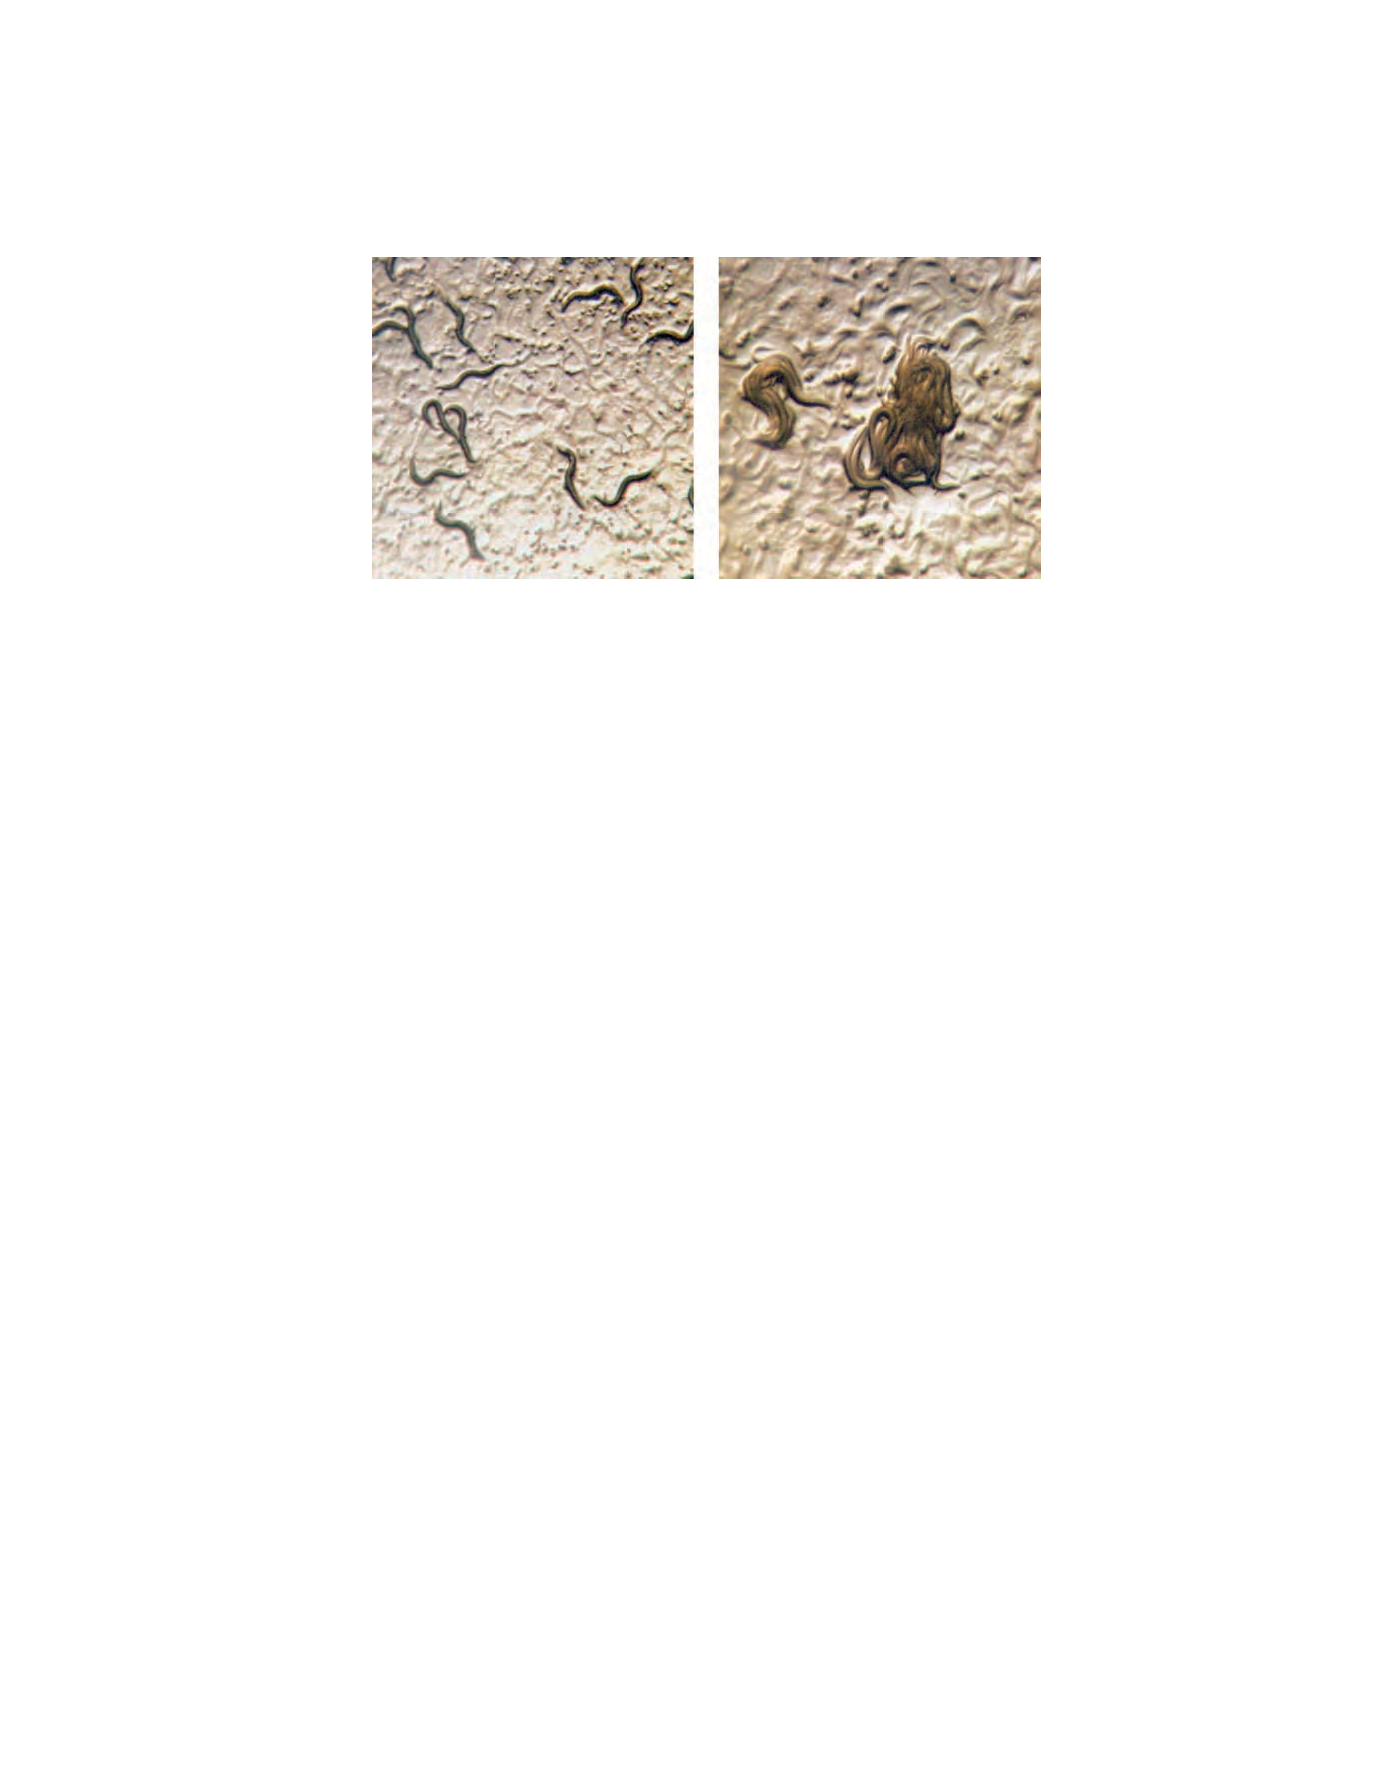
\includegraphics[width=0.7\linewidth]{chap02/fig_2_15}
	\caption{秀丽隐杆线虫的进食行为取决于编码神经肽受体的基因的活性水平。
		在一个菌株中,个体蠕虫在隔离状态下吃草(左),而在另一个菌株,个体聚集在一起觅食。
		这种差异可以通过神经肽受体基因中的单个氨基酸取代来解释\cite{de1998natural}。}
	\label{fig:2_15}
\end{figure}


群居蠕虫和独居蠕虫之间的差异是由单个基因中的单个氨基酸取代引起的,该基因是参与神经元间信号传导的一大基因家族的成员。
该基因\textit{神经肽受体}-1 编码神经肽受体。
长期以来,神经肽因其在跨神经元网络协调行为方面的作用而受到赞赏。
例如,海蜗牛的神经肽激素会刺激与单一行为(产卵)相关的一组复杂的运动和行为模式。
哺乳动物神经肽与摄食行为、睡眠、疼痛和许多其他行为和生理过程有关。
改变社会行为的神经肽受体突变的存在表明,这种信号分子对于产生行为和产生个体之间的差异都很重要。


神经肽受体也与哺乳动物社会行为的调节有关。
神经肽催产素和加压素刺激哺乳动物的亲和行为,例如配对结合和父母与后代的结合。
在小鼠中,社会认知需要催产素,即识别熟悉个体的能力。
催产素和加压素已在草原田鼠中进行了深入研究,草原田鼠是一种长期成对抚养幼崽的啮齿动物。
雌性草原田鼠在交配过程中大脑中释放的催产素会刺激配对关系的形成。
同样,雄性草原田鼠在交配过程中大脑中释放的加压素会刺激配对关系的形成和父系行为。


配对结合的程度在哺乳动物物种之间有很大差异。
雄性草原田鼠与雌性形成长期的配偶关系,帮助它们抚养后代,被描述为一夫一妻制,但密切相关的雄性山地田鼠繁殖广泛,不参与父系行为。
这些物种中雄性行为的差异与大脑中\textit{血管加压素受体}表达的差异相关。
在草原田鼠中,\textit{血管加压素受体}在特定大脑区域(腹侧苍白球)中以高水平表达(图~\ref{fig:2_16})。 
在山地田鼠中,该区域的水平要低得多,尽管其他大脑区域的水平很高。


\begin{figure}[htbp]
	\centering
	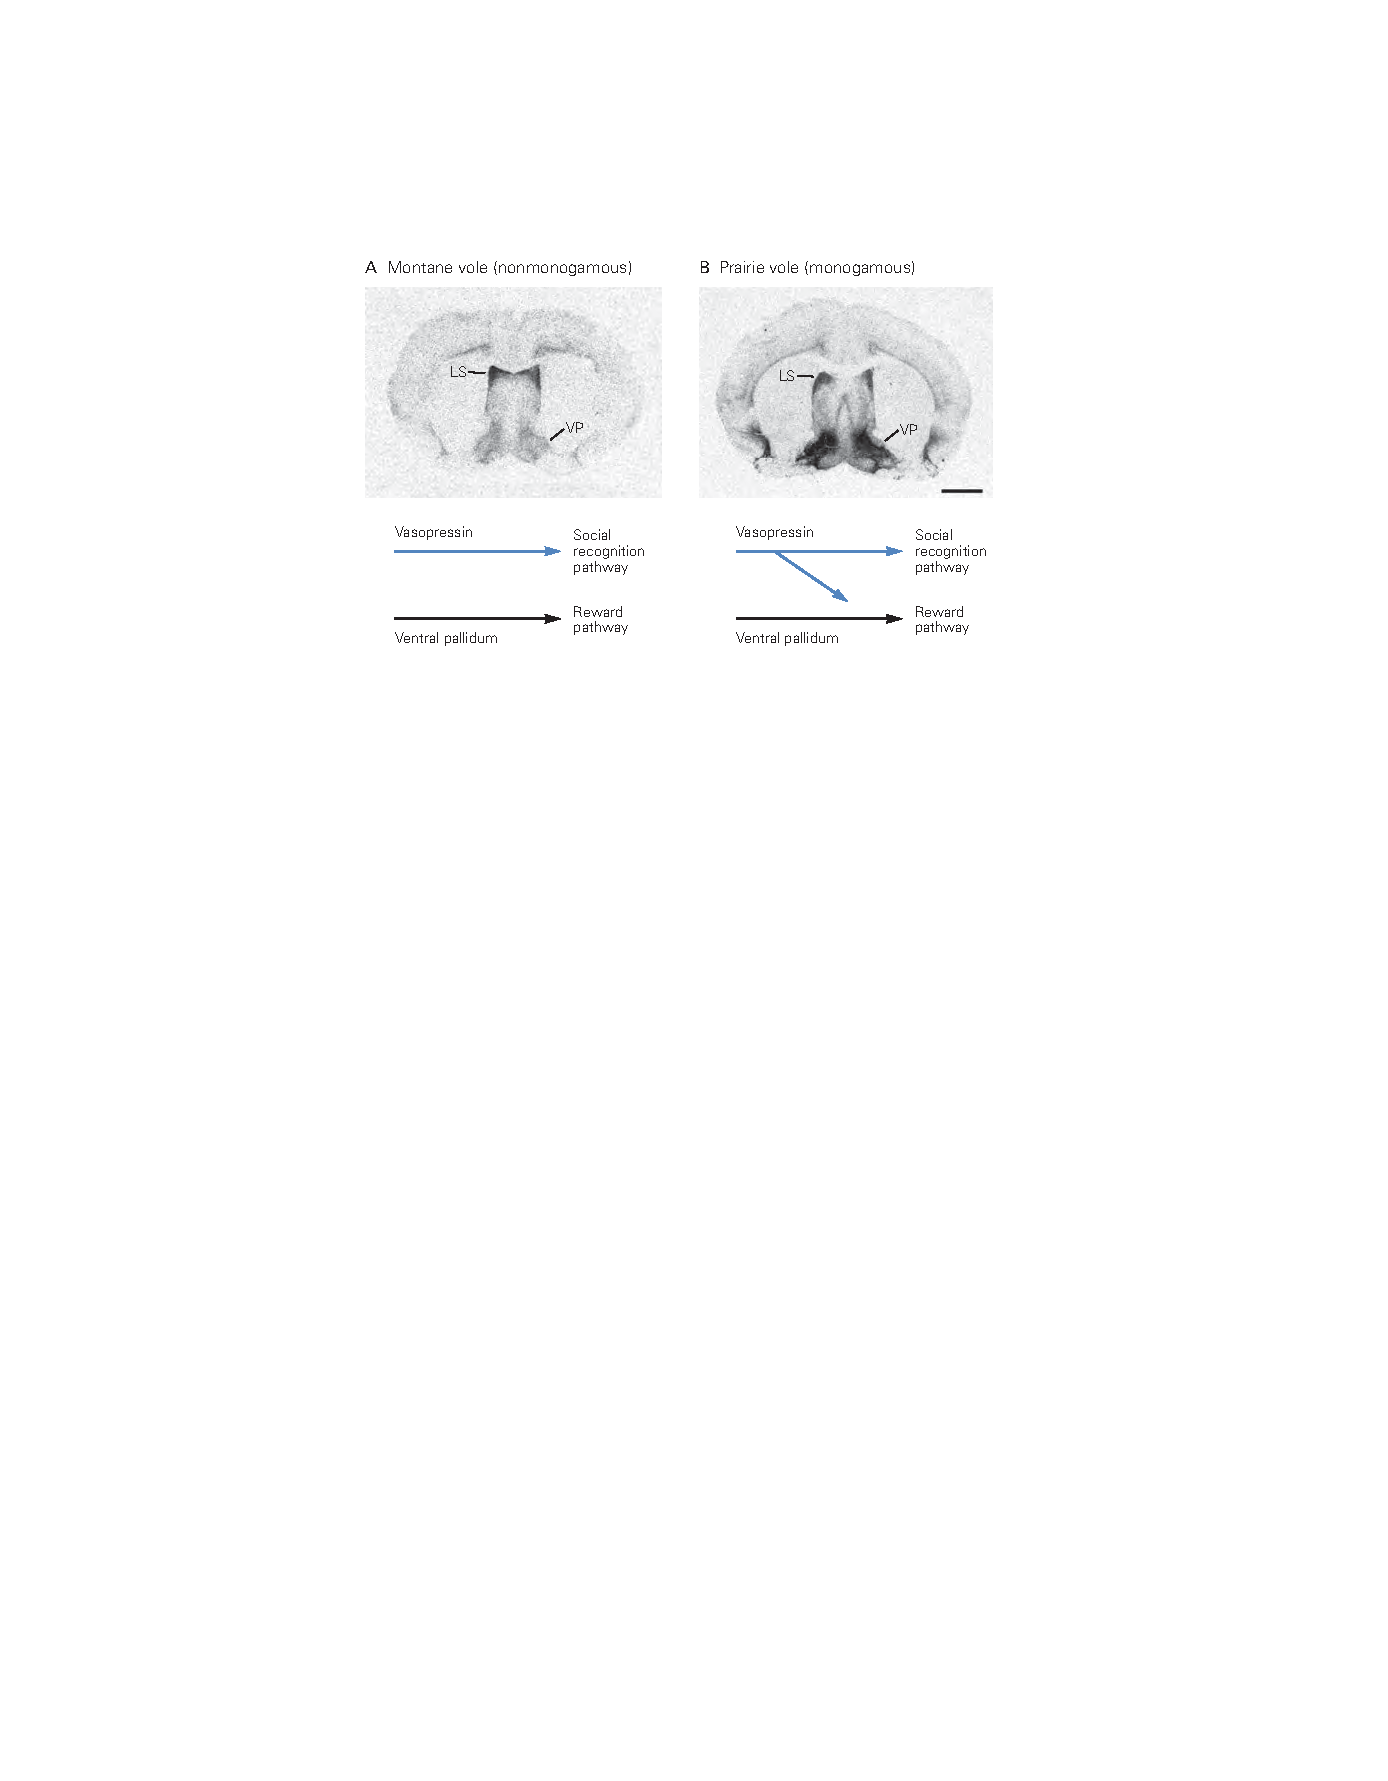
\includegraphics[width=0.72\linewidth]{chap02/fig_2_16}
	\caption{\textit{血管加压素受体}在两种亲缘关系密切的啮齿动物中的分布\cite{young2001cellular}。
		\textbf{A.} 受体在山地田鼠的\textit{外侧隔核}中表达较高,但在\textit{腹侧苍白球}中表达较低,这不会形成配对键。
		\textbf{B.} 在一夫一妻制草原田鼠的\textit{腹侧苍白球}中表达很高。
		受体在\textit{腹侧苍白球}中的表达使\textit{加压素}将\textit{社会认知通路}与\textit{奖赏通路}联系起来。}
	\label{fig:2_16}
\end{figure}


催产素和加压素及其受体的重要性已通过小鼠反向遗传研究得到证实和扩展,这比田鼠更容易进行遗传操作。
将草原田鼠的\textit{血管加压素受体}基因引入行为更像山地田鼠的雄性小鼠,增加了\textit{血管加压素受体}在腹侧苍白球中的表达,并增加了雄性小鼠对雌性的亲和行为。
因此,物种之间加压素受体表达模式的差异可能导致社会行为的差异。


对不同啮齿动物中加压素受体的分析提供了对基因和行为在进化过程中发生变化的机制的深入了解。
因此,腹侧前脑\textit{血管加压素受体}表达模式的进化变化改变了神经回路的活动,将腹侧前脑的功能与交配激活的加压素分泌神经元的功能联系起来。
结果,社会行为发生了改变。


催产素和后叶加压素在人类社会行为中的重要性尚不清楚,但配对和幼崽饲养在哺乳动物物种中的核心作用表明这些分子可能也在我们物种中发挥作用。



\section{人类遗传综合症的研究为社会行为的基础提供了初步见解}

\subsection{人类脑部疾病是基因与环境相互作用的结果}

在人类中发现的第一个神经系统疾病基因清楚地说明了基因和环境在决定认知和行为表型方面的相互作用。
\textit{苯丙酮尿症}于 1934 年由挪威的\textit{阿斯比约恩$\cdot$佛林}描述,影响 1 万 5 千名儿童中的一名,并导致认知功能严重受损。


患有这种疾病的儿童有两个编码苯丙氨酸羟化酶的\textit{苯丙酮尿症}基因的异常拷贝,苯丙氨酸羟化酶是一种将氨基酸苯丙氨酸转化为酪氨酸的酶。
该突变是隐性的,杂合子携带者个体没有任何症状。
该基因的两个拷贝都缺乏正常功能的儿童会从膳食蛋白质中积累高血浓度的苯丙氨酸,这反过来会导致产生干扰神经元功能的有毒代谢物。
苯丙氨酸对大脑产生不利影响的具体生化过程仍不清楚。


\textit{苯丙酮尿症}表型(智力障碍)是基因型(纯合子 \textit{苯丙酮尿症基因}突变)和环境(饮食)相互作用的结果。
因此,\textit{苯丙酮尿症}的治疗简单有效:可以通过低蛋白饮食来预防发育迟缓。
\textit{苯丙酮尿症}基因功能的分子和遗传分析已使受影响个体的生活得到显著改善。
自 1960 年代初以来,美国对新生儿\textit{苯丙酮尿症}进行了强制性检测。
在疾病出现之前识别患有遗传疾病的儿童并改变他们的饮食可以预防该疾病的许多方面。


本书后面的章节描述了很多单基因特征的例子,例如\textit{苯丙酮尿症},这些特征导致了对大脑功能和功能障碍的深入了解。
这些研究中出现了某些主题。
例如,许多罕见的神经退行性疾病,如亨廷顿病和脊髓小脑性共济失调,是由蛋白质中谷氨酸残基的病理性显性扩张引起的。
这些多聚谷氨酰胺重复障碍的发现突出了未折叠和聚集的蛋白质对大脑的危险。
癫痫发作可由离子通道中的各种突变引起的发现导致人们认识到这些疾病主要是神经元兴奋性障碍。



\subsection{罕见的神经发育综合症为社会行为、知觉和认知的生物学提供了见解}

在儿童时期表现出来的神经和发育障碍已经阐明了遗传学在人类大脑功能中的重要性和复杂性。
基因影响特定认知和行为回路的早期证据来自对称为\textit{威廉综合症}的罕见遗传病症的研究。
患有这种疾病的人通常表现出正常的语言和极端的社交能力;
在发育早期,他们缺乏儿童通常在陌生人面前表现出的沉默寡言。
同时,他们在空间处理方面严重受损,表现出整体智力障碍,并且焦虑率非常高(但很少有社交焦虑症)。


与孤独症谱系障碍等疾病相比,\textit{威廉综合症}的损伤模式表明,语言和社交技能可以与其他一些大脑功能区分开来。
与语言有关的大脑区域在孤独症儿童中受损,但在\textit{威廉综合症}中活跃或加重。
相比之下,\textit{威廉综合症}的一般智力和空间智力受损程度超过所有孤独症谱系障碍儿童的大约一半。


\textit{威廉综合症}是由染色体区域\textit{第7号染色体1区1带2亚带3次亚带}的杂合缺失引起的,通常包含约 1.5 Mb 和 27 个基因。
对该缺陷最简单的解释是,区间内基因的表达水平降低,因为该区域每个基因只有一个拷贝,而不是两个拷贝。
影响社会交流和空间处理的区间中的精确基因尚不清楚,但由于它们有可能提供对人类行为的遗传调控的洞察力,因此引起了极大的兴趣。


孤独症谱系障碍研究的最新发现进一步强调了遗传变异与社会和智力功能之间的复杂关系,这首先是由\textit{威廉综合症}阐明的。
大约在过去十年内,基因组技术的进步使高通量方法能够筛选基因组中染色体结构的变异,并且分辨率比光学显微镜高得多(见方框~\ref{box:2_1})。
2007 年和 2008 年的开创性研究表明,患有孤独症谱系障碍的个体比未受影响的个体更常携带新的(从头)拷贝数变异。
这些发现导致了一些特定基因组间隔的首次发现,这些间隔导致了该综合症的常见形式(即没有综合症特征证据的孤独症谱系障碍,也称为特发性或非综合症性孤独症谱系障碍)。


2011 年,在一个非常明确的队列中同时开展两项从头拷贝数变异的大规模研究发现,\textit{威廉综合症}中删除的恰好相同区域会给个体带来孤独症谱系障碍的重大风险。
然而,在这些情况下,是罕见的重复(该区域的一个多余副本),而不是缺失,大大增加了社会残疾的风险。
这些发现,即同一组基因的损失和获得可能导致截然不同的社会表型(虽然两者通常都会导致智力障碍),进一步支持认知和行为功能领域是可分离的但可能共享重要分子机制的观点。


\textit{脆性X综合症}是另一种儿童神经发育障碍,可以深入了解认知功能的遗传学;
与\textit{威廉综合症}不同,它已被映射到 X 染色体上的单个基因。
\textit{脆性X综合症}的表现各不相同。
患儿可有智力障碍、社会认知差、社交焦虑高、行为重复;
大约 30\% 的\textit{脆性X综合症}男孩符合孤独症谱系障碍的诊断标准。
\textit{脆性X综合症}还与更广泛的特征相关,包括身体特征,例如拉长的脸和突出的耳朵。


\textit{脆性X综合症}已被证明是由减少称为\textit{脆性X智力迟钝蛋白}的基因表达的突变引起的。
因为该基因落在 X 染色体上,当男性的一个拷贝发生突变时,男性将失去该基因的所有表达。
\textit{脆性X智力迟钝蛋白}蛋白在神经元中调节\textit{信使核糖核酸}向蛋白质的翻译,这一过程本身受神经元活动调节。
神经元中受调节的翻译是学习所需的突触可塑性的重要组成部分。
因此,翻译水平上的脆弱 X 缺陷会级联起来影响神经元功能、学习和高层认知过程。
有趣的是,大部分与孤独症谱系障碍和精神分裂症风险增加相关的其他基因都受\textit{脆性X智力迟钝蛋白}蛋白调节。


另一种遗传基础广为人知的孟德尔疾病是\textit{雷特综合症}(在第~\ref{chap:chap62}~章中详细讨论)。
\textit{雷特综合症}是一种 X 连锁的进行性神经发育障碍,是女性智力障碍的最常见原因之一。
这种疾病几乎总是局限于女性,因为典型的\textit{雷特}突变在发育中的男性胚胎中通常是致命的,而男性胚胎只有一条 X 染色体。
受影响的女孩通常会发育到 6 到 18 个月大,这时她们无法学会说话,智力功能退化,并且表现出强迫性、不受控制的拧手而不是有目的的手部运动。
此外,患有\textit{雷特综合症}的女孩通常会表现出一段时间的社交互动明显受损,这可能与孤独症谱系障碍无法区分,尽管人们认为社交功能在以后的生活中很大程度上得到了保留。
\textit{胡达$\cdot$佐格比}和她的同事发现,这种综合症的主要原因是甲基 CpG 结合蛋白 2(MeCP2)基因的突变。
\textit{脱氧核糖核酸}中特定 CpG 序列的甲基化会改变附近基因的表达,而 MeCP2 的一项既定功能是它结合甲基化\textit{脱氧核糖核酸}作为调节\textit{信使核糖核酸}转录过程的一部分。


罕见综合症还提供了一些对精神分裂症遗传底物的初步见解(第~\ref{chap:chap60}~章)。
例如,正如\textit{罗伯托$\cdot$什普林茨恩}及其同事在 1978 年首次描述的那样,22q11 染色体缺失会导致广泛的身体和行为症状,包括精神病,现在通常被称为\textit{腭心面综合症}、\textit{迪格奥尔格综合症}或 22q11 缺失综合症。
由于与相同缺失相关的表型范围极其广泛,\textit{什普林茨恩}的最初描述遭到了一些怀疑。
现在人们普遍认为,22q11 缺失是与精神分裂症和儿童期发病的精神分裂症相关的最常见的染色体异常。
此外,已发现同一区域的染色体丢失与孤独症的个体风险有关。
迄今为止,尚未明确确定该区域内负责精神病表型的特定基因。
此外,最近来自孤独症文献的证据表明,很可能是这个区间内多个基因的组合,每个基因赋予相对较小的个体影响,是社会残疾表型的原因。



\section{精神疾病涉及多基因特征}

如前所述,与神经退行性疾病和精神疾病的总负担相比,单基因综合症很少见。
因此,如果罕见疾病仅占总疾病负担的一小部分,人们可能会质疑研究罕见疾病的理由。
原因是罕见的情况可以让人们深入了解更常见、更复杂的疾病形式所涉及的生物学过程。
例如,人类遗传学取得的突出成就之一是发现了导致早发性阿尔茨海默病或帕金森病的罕见基因变异。
具有这些严重罕见变异的个体代表了所有患有这些疾病的个体的一小部分,但对罕见疾病变异的鉴定揭示了在更大的患者群体中也被破坏的细胞过程,指向了一般的治疗途径。
同样,对\textit{雷特综合症}、\textit{脆性X综合症}和其他神经发育障碍背后的病理生理机制的探索已经导致了对精神综合症合理药物开发的一些初步尝试。


在本章的其余部分,我们将进一步讨论两种复杂的神经发育和精神病表型的遗传学:孤独症谱系障碍和精神分裂症。
与前面讨论的罕见孟德尔例子相比,这些疾病的常见形式的遗传学确实更加多样化、多样和异质,涉及不同个体的许多不同基因以及赋予责任的多种风险基因组合。
此外,对于这两种诊断,虽然对遗传贡献的支持是巨大的,但也有令人信服的证据表明环境因素的贡献。


理解这些疾病的进展来自快速发展的基因组技术和统计方法的结合、开放数据共享的文化以及非常大的患者队列的整合,这些患者队列提供了足够的能力来检测非常罕见的高渗透性等位基因以及携带的常见遗传变异 风险的小增量。
重要的是,最近在理解这两种综合症方面取得的成功为研究它们的生物学后果以及这些遗传风险因素所传达的分子、细胞和回路级病理生理学提供了坚实的基础。



\subsection{孤独症谱系障碍遗传学的进展突出了罕见和从头突变在神经发育障碍中的作用}

孤独症谱系障碍是一组严重程度不同的发育综合症,影响大约 2\% 至 3\% 的人口,其特征是相互社会交流障碍以及刻板兴趣和重复行为。
男性明显占优势;
平均而言,受影响的男孩是女孩的三倍。
孤独症谱系障碍的临床症状,根据定义,出现在生命的前 3 年,尽管受影响和未受影响的儿童之间高度可靠的差异通常在生命的头几个月内可以识别。


受影响的人之间存在相当大的表型变异性,导致孤独症谱系障碍的诊断分类相当广泛。
此外,受影响的个体比一般人群更容易出现癫痫发作和认知问题,并且通常在适应功能方面存在严重障碍。
然而,许多孤独症患者并没有受到如此深远的影响,并过着非常成功的生活。


孤独症具有很强的遗传成分(见图~\ref{fig:2_1}A),这很可能解释了它是首批屈服于现代基因发现工具和方法的遗传复杂神经精神综合症之一。
孤独症谱系障碍具有更广泛的意义,因为它提供了对典型人类行为的洞察力:语言、复杂智力和人际互动。
重要的是,孤独症谱系障碍中的社交沟通缺陷可以与其他领域的正常智力和典型功能共存,这一事实表明大脑在某种程度上是模块化的,具有可以独立变化的不同认知功能。


虽然孤独症谱系障碍的综合症形式只占所有病例的一小部分,但在更常见的所谓“特发性”或“非综合症”形式的障碍中的首次发现也证明了罕见突变的作用,这些突变具有巨大的生物学效应。
例如,在 2003 年,对极少数具有孤独症特征的女性 X 染色体上缺失区域的基因进行测序,导致在基因\textit{神经连接蛋白4X}中发现了罕见的功能丧失突变, 一种在兴奋性神经元中编码突触粘附分子的基因,在几个受影响的男性家庭成员中发现。
此后不久,对一个患有智力障碍和孤独症谱系障碍的大型家系进行的连锁分析表明,受影响的家庭成员都携带功能丧失型 NLGN4X 突变。


染色体结构中的从头亚显微缺失和重复可能会显著增加个体患孤独症谱系障碍的风险。
这些\textit{拷贝数变异}聚集在基因组的特定区域,确定特定的风险区间。 使用这种方法的最早报告表明,染色体 16p11.2 的新生\textit{拷贝数变异},虽然仅存在于大约 0.5\% 至 1\% 的受影响个体中,但具有很大(大于 10 倍)的孤独症谱系障碍风险。
随后的研究现在已经确定了十几个或更多具有风险的新 \textit{拷贝数变异},包括\textit{第16号染色体1区1带2亚带}、\textit{第1号染色体2区1带}、\textit{第15号染色体1区1带1亚带3次亚带}和\textit{第3号染色体2区9带};
\textit{第22号染色体1区1带}、\textit{第22号染色体1区3带}(删除基因 SHANK3)和\textit{第2号染色体1区6带}(删除基因 NXRN1)的缺失;和\textit{第7号染色体1区1带2亚带3次亚带}(\textit{威廉综合症}区域)的从头重复。


有趣的是,尽管这些对孤独症谱系障碍具有很大的风险,但对其他精神疾病(包括精神分裂症和双相情感障碍)的研究发现,许多相同的区域也会增加患这些疾病的风险。
此外,通过基因型(例如,\textit{第16号染色体1区1带2亚带}缺失和重复)确定的个体研究发现了多种相关的行为表型,从特定语言障碍到智力障碍再到精神分裂症。
这种“一对多”现象对阐明精神疾病的特定病理生理机制以及概念化从基因发现到治疗的步骤提出了重要挑战。


从头开始的罕见\textit{拷贝数变异}会增加孤独症谱系障碍和其他发育障碍的风险,这一广泛且可复制的发现立即引发了一个问题,即单个基因中的罕见从头突变是否可能带来类似的风险。
事实上,低成本、高通量\textit{脱氧核糖核酸}测序技术的发展,最初集中在基因组的编码部分,导致了被认为可能破坏受影响个体基因功能(\textit{可能的基因破坏}突变)的大量从头突变的鉴定。
这些突变在不相关的个体之间近距离反复发生,现已被用作识别孤独症谱系障碍特定风险基因的手段。


对孤独症谱系障碍新生突变的大规模研究现已确定了 100 多个相关基因,其中约 45 个达到统计显著性的最高置信水平。
这些基因具有广泛的已知功能,但分析显示参与突触形成和功能以及转录调节的基因在统计学上显著过度表达。
此外,编码\textit{核糖核酸}的风险基因数量超过预期,这些\textit{核糖核酸}是脆性 X 智力低下蛋白和/或在早期大脑发育中活跃的蛋白质的目标。



\subsection{精神分裂症基因的鉴定突出了罕见和常见风险变异的相互作用}

精神分裂症影响了大约 1\% 的年轻人,导致思维障碍和情绪退缩的模式,严重损害了生活。
它具有很强的遗传性(参见图~\ref{fig:2_1}B),并且还具有与发育中胎儿的压力相关的强大环境成分。
二战荷兰饥饿冬季饥荒后不久出生的儿童在多年后患精神分裂症的风险大大增加,而母亲在 1960 年代大流行期间怀孕期间感染风疹病毒的儿童的风险也大大增加。


基因和环境都会导致精神分裂症。
与孤独症一样,人类基因组的测序、常见变异的全基因组基因分型和\textit{拷贝数变异}检测的廉价方法的开发,以及非常大的患者队列的整合,都导致了精神分裂症遗传学的转变。
首先,与早先提到的孤独症谱系障碍的发现基本平行,到 2000 年代初期,罕见的新发\textit{拷贝数变异}开始与精神分裂症的风险有关。
一小部分病例与具有较大风险的染色体异常有关,例如,\textit{第22号染色体1区1带}的缺失。
这些染色体异常与孤独症谱系障碍相关的基因座完全或几乎重叠,但这些基因座缺失和重复的风险分布似乎并不相同。
例如,虽然\textit{第16号染色体1区1带2亚带}区域的重复和缺失都与孤独症谱系障碍和精神分裂症有关,但该区域的重复更有可能导致精神分裂症,而缺失更可能与孤独症谱系障碍和智力障碍相关。


关于精神分裂症,过去十五年来最重要的发展是常见变异全基因组关联研究的出现。
与前面描述的假设驱动的候选基因研究相反,全基因组关联依赖于同时检测基因组中每个基因的多态性。
这种无假设的方法,当与有力的队列一起使用并适当校正多重比较时,已被证明是一种高度可靠和可重复的策略,用于识别所有医学常见疾病中的常见风险等位基因。


涉及近 4 万个病例和 113,000 个对照的全基因组关联研究已经确定了 108 个精神分裂症的风险位点。 
这组中任何个体遗传变异的影响都非常适度,通常导致风险增加不到 25\%。
此外,在全基因组关联研究中测定的许多遗传多态性映射到基因组编码区段之外的区域。
因此,虽然已经确定了 108 个风险基因座,但尚不完全清楚哪些基因对应于所有这些风险变异。
在某些情况下,变异与单个基因的映射足够接近,可以合理地推断出这种关系;
在其他情况下,这仍有待确定。


与精神分裂症风险有关的基因为确定该疾病的生物学基础提供了一个起点。
例如,自 20 世纪 90 年代后期以来,有证据表明一个叫做\textit{主要组织相容性}的区域与精神分裂症风险有关。
因此,在精神分裂症队列中,\textit{主要组织相容性}区域具有人类基因组任何部分中最强的全基因组关联研究信号。
队列中的大量患者使详细研究成为可能,将\textit{主要组织相容性}区域中的这种强大的风险关联信号解析为三个不同的基因座(可能是三个不同的基因)。
在这三个基因座中,一个编码补体 C4 因子的基因对疾病风险具有强烈且明确的影响。
\textit{史蒂文$\cdot$麦卡罗}和他的同事表明,补体 C4 基因座代表\textit{拷贝数变异}的自然病例,健康个体在他们拥有的基因拷贝数方面存在很大差异,并且 C4A 等位基因的表达水平与精神分裂症风险的增加相关。
随后的后续研究表明,敲除 C4 基因的小鼠在发育过程中存在突触修剪缺陷,这表明人类 C4A 过量可能导致突触修剪过度的假设,这一过程长期以来一直受到精神分裂症文献的关注。


这一发现代表了将基因组学与增加疾病风险的可能生物学机制联系起来的能力的重要证明。
即便如此,具有最高风险 C4 单倍型且没有精神分裂症家族史的个体会由于该等位基因而平均受影响的几率从 1\% 增加到大约 1.3\%。
为了获得规模感,一级亲属患有精神分裂症会导致患病风险增加约 10 倍。
这一充满希望的开端及其局限性反映了遗传学家和神经生物学家在从成功的常见变异基因发现转向详细阐述导致人类病理学的特定机制方面所面临的挑战。


除了确定许多特定的风险位点外,精神分裂症的\textit{全基因组关联研究}还反复发现许多常见等位基因的小个体效应加起来会增加风险。
这些结果为总体研究基因型表型关系提供了一个额外的、强大的途径。
事实上,已经清楚的是,个体携带的风险等位基因的数量会对患这种疾病的风险产生重大(和累加)影响。
例如,那些在所谓的多基因风险评分(与个人携带的加性遗传风险总量相关的汇总统计数据)中处于最高十分位的人,与一般人群相比,风险增加了 8 到 20 倍。
尽管累积效应的生物学特性尚不清楚,但该观察结果为研究与疾病轨迹和治疗反应相关的一系列有趣问题奠定了基础,并且几乎肯定会重振结合神经影像学和基因组学的研究。
后一种类型的调查,类似于常见变异发现的早期努力,由于研究选定的、生物学上合理的候选基因的固有局限性,可靠性较差。


最后,类似于孤独症谱系障碍所采用的高通量测序方法,也开始在精神分裂症中产生结果。
具体来说,寻找稀有和从头风险等位基因的外显子组测序已经取得了一些成功。
然而,与孤独症谱系障碍相比,此类研究需要更大的队列来确定\textit{可能的基因破坏}突变的统计学显著风险,这表明这些类型变异的总体影响大小在精神分裂症中可能要小得多。
迄今为止,这些调查已经确定了一些风险基因并涉及关键的神经生物学途径。
特别是,最近的外显子组研究指出了\textit{活性调节的细胞骨架}复合体中分子的重要性,以及包含\textit{组蛋白H3赖氨酸4特异性甲基转移酶}的基因组结构域,与精神分裂症发病机制相关。



\section{神经精神疾病遗传基础的观点}

基因影响行为的许多方面。
人类双胞胎在人格特征和精神疾病方面有着显著的相似之处,即使是分开抚养的双胞胎也是如此。 
可以培育具有特定、稳定行为特征的家畜和实验室动物;
并且越来越多地发现了广泛的遗传变异对神经发育和精神疾病的贡献。


一系列同时的进步开创了一个理解基因、大脑和行为之间关系的绝佳机会的时代。
可用于操作和研究模型系统的设备已经发生了革命性的变化。
与此同时,在确定人类神经精神疾病的遗传风险因素方面也取得了长足的进步。
尽管该领域在此过程中仍处于早期阶段,但已经出现了成功发现基因及其应用于深入生物学理解的价值的多个例子。


最近对神经发育和精神疾病的遗传学研究的许多惊人发现之一是跨越广泛诊断边界的遗传风险重叠。 
虽然生物学不遵循分类诊断标准可能并不令人惊讶,但考虑该领域如何追踪这些影响并得出新的治疗策略仍然是一个巨大的概念挑战。


此外,值得注意的是,对于许多其他尚未看到先前提到进展类型的精神疾病,计算方法很简单:
更大的投资和更大的样本量将带来更深入的洞察力。 
例如,最近对\textit{图雷特综合症}和\textit{强迫症}新生突变的研究清楚地表明,鉴定高置信度风险基因的\textit{限速因子}是\textit{亲子三人组}测序的可用性。
同样,\textit{重度抑郁症}的\textit{全基因组关联研究}直到最近才达到足以确认具有统计学意义相关常见变异的样本量。 
这些研究包括了数十万人,并且毫不奇怪地发现了具有非常小个体影响的风险等位基因。


最后一点强调了一种想法,即一种尺寸并不适合所有行为、发育和精神疾病的基因组学。 
从模型系统的研究,到罕见孟德尔疾病的阐明,再到解开导致常见疾病的常见和罕见变异,当今可用的工具和机会是前所未有的。 
未来几年应该会深入了解精神疾病和神经发育障碍的生物学,或许还有可能帮助患者及其家人的疗法。


\section{亮点}

1. \textit{脆性X综合症}、\textit{雷特综合症}和\textit{威廉综合症}等罕见遗传综合症为复杂人类行为的分子机制提供了重要见解。 
此外,虽然仍有大量工作要做,但对这些综合症的研究已经挑战了相关认知和行为缺陷是不可改变的观念,并证明了广泛的模型系统在阐明保守生物学机制方面的效用。


2. 人类基因组测序、高通量基因组分析的发展以及同步计算和方法学的进步导致对人类行为和精神疾病遗传学的理解发生了深刻变化。
包括精神分裂症和孤独症在内的几种典型疾病已经取得了显著进展,导致鉴定出数十个明确的风险基因和染色体区域。


3. 过去十年精神病学遗传学和基因组学领域的成熟揭示了测试预先指定的候选基因的脆弱性。 
这些类型的研究现在已被常见和稀有等位基因的全基因组扫描所取代。 
再加上严格的统计框架和共识统计阈值,这些正在产生高度可靠和可重复的结果。


4. 目前,累积的证据表明,各种遗传变异构成复杂行为综合症的基础,包括常见和罕见、传播和新生、种系和体细胞、序列和染色体结构变异。 
然而,这些不同类型的遗传变化的相对贡献因特定疾病而异。


5. 人类行为遗传学最新进展的一个惊人发现是具有不同症状和自然史的综合症的遗传风险重叠。 
了解相同的突变如何以及为什么会在不同个体中导致高度不同的表型结果将是未来的主要挑战。


6. 对常见精神疾病的研究结果表明遗传异质性极高。 
这一点,再加上迄今为止已确定的风险基因的生物学多效性,以及人类大脑发育的动态性和复杂性,都表明在从对风险基因的理解转向对行为的理解方面面临着重大挑战。 
同样,目前,阐明风险基因的生物学和揭示行为综合症的病理生理学之间存在重要区别。

%\section{术语表}

%\section{选读}





\chapter{神经细胞、神经回路和行为} \label{chap:chap3}

人类行为的非凡能力范围取决于与大脑相连的一系列复杂的感觉受体,大脑是一种高度灵活的神经器官,可以从感觉信号流中选择环境中和身体内环境中的事件,这些事件对人类个人来说很重要。
大脑主动组织感官信息,用于感知、行动、决策、审美和未来参考——也就是记忆。
它也明智地忽略和丢弃信息,一个人希望,并向其他大脑报告其中一些操作及其心理表现。
所有这一切都是由相互连接的神经细胞完成的。


单个神经细胞或神经元是大脑的基本信号单元。 
人脑包含大量此类细胞,大约有 860 亿个神经元,可分为至少一千种不同的类型。 
然而,这些种类繁多的神经元与其说是人类行为复杂性的一个因素,不如说是它们组织成具有精确功能的解剖回路。 
事实上,大脑的一个关键组织原则是:
由于它们相连的方式不同,具有相似特性的神经细胞可以产生不同的行为。


由于相对较少的神经系统组织原则会产生相当大的功能复杂性,因此可以通过关注神经系统的五个基本特征来深入了解神经系统如何产生行为:

1. 单个神经细胞的结构成分;

2. 神经元在自身内部和彼此之间产生信号的机制;

3. 神经细胞之间以及神经细胞与其目标(肌肉和腺体效应器)之间的连接模式;

4. 不同互联模式与不同行为类型的关系;

5. 经验如何改变神经元及其连接。


本书的各个部分都是围绕这五个主要主题组织的。 
在本章中,我们将依次介绍这些主题,概述行为的神经控制。
我们首先考虑神经元的结构和功能以及围绕和支持它们的\textit{神经胶质细胞}。
然后,我们检查单个细胞如何组织和传输信号,以及一些相互连接的神经细胞之间的信号如何产生简单的行为,即膝跳反射。
然后,我们将这些想法扩展到更复杂的行为,由更复杂和可延展的回路调节。



\section{神经系统有两类细胞}

神经系统中主要有两类细胞:\textit{神经元}和\textit{神经胶质细胞}。


\subsection{神经细胞是神经系统的信号单位}

一个典型的神经元有四个形态学上定义的区域:\textit{细胞体}、\textit{树突}、\textit{轴突}和\textit{突触前末梢}(图~\ref{fig:3_1})。 
正如我们将要看到的,每个区域在产生信号和与其他神经细胞通信方面都有不同的作用。


\begin{figure}[htbp]
	\centering
	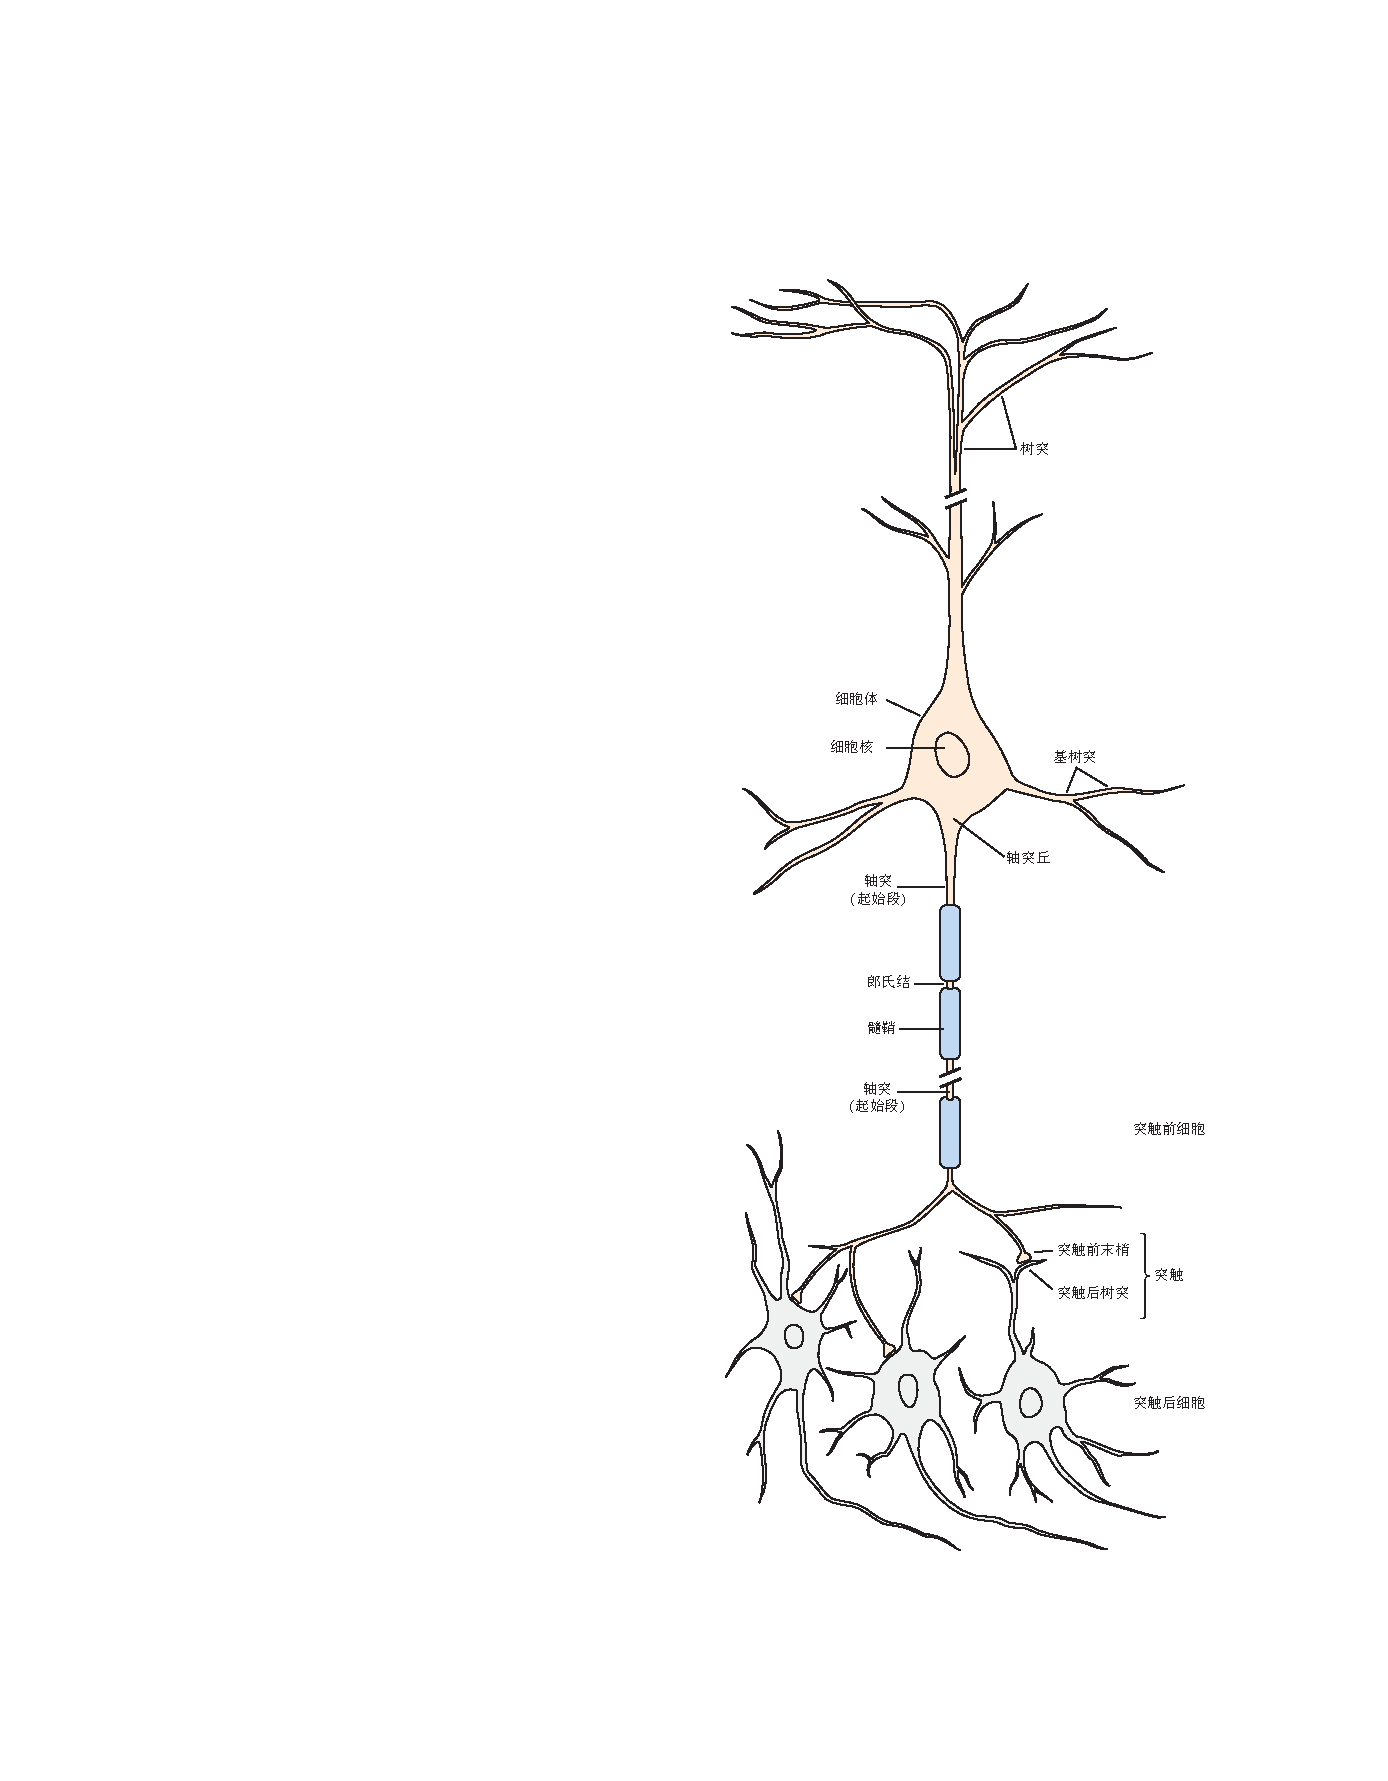
\includegraphics[width=0.5\linewidth]{chap03/fig_3_1}
	\caption{(右)神经元的结构。 
		脊椎动物神经系统中的大多数神经元有几个共同的主要特征。 
		细胞体包含细胞核,遗传信息的仓库,并产生两种类型的细胞过程:轴突和树突。 
		轴突是神经元的传递元件;
		它们的长度差异很大,有些在体内延伸超过 1 米。 
		与细胞体的直径(50 微米或更大)相比,中枢神经系统中的大多数轴突非常细(直径在 0.2 微米和 20 微米之间)。 
		许多轴突被一层脂肪\textit{髓鞘}绝缘,该鞘在称为\textit{郎氏结}的间隙处定期中断。 
		动作电位,即细胞的传导信号,在轴突的初始部分启动并传播到突触,突触是信号从一个神经元流向另一个神经元的部位。 
		突触前神经元的轴突分支将信号传递给突触后细胞。 
		单个轴突的分支可能与多达一千个突触后神经元形成突触。 
		顶端和基部树突与细胞体一起是神经元的输入元件,接收来自其他神经元的信号。}
	\label{fig:3_1}
\end{figure}


\textit{细胞体}是细胞的代谢中心。 
它包括含有细胞基因的细胞核和内质网,内质网是细胞核的延伸部分,细胞的蛋白质在这里合成。
细胞体通常产生两种过程:几个短的\textit{树突}和一个长的管状\textit{轴突}。 
树突以树状方式分支,是接收来自其他神经细胞的输入信号的主要装置。 
轴突通常在分支之前从细胞体延伸一定距离,使其能够将信号传递给许多目标神经元。
轴突可以在 0.1 毫米到 1 米的距离内传输电信号。 
这些电信号或动作电位在轴突起源附近的专门触发区域启动,称为\textit{起始段},动作电位从该区域以 1 米每秒至 100 米每秒的速度沿着轴突传播而不会失败或失真。 
沿轴突向下传播的动作电位的振幅保持恒定在 100 毫伏,因为动作电位是一种全有或全无的脉冲,它会沿着轴突定期再生(图~\ref{fig:3_2})。


\begin{figure}[htbp]
	\centering
	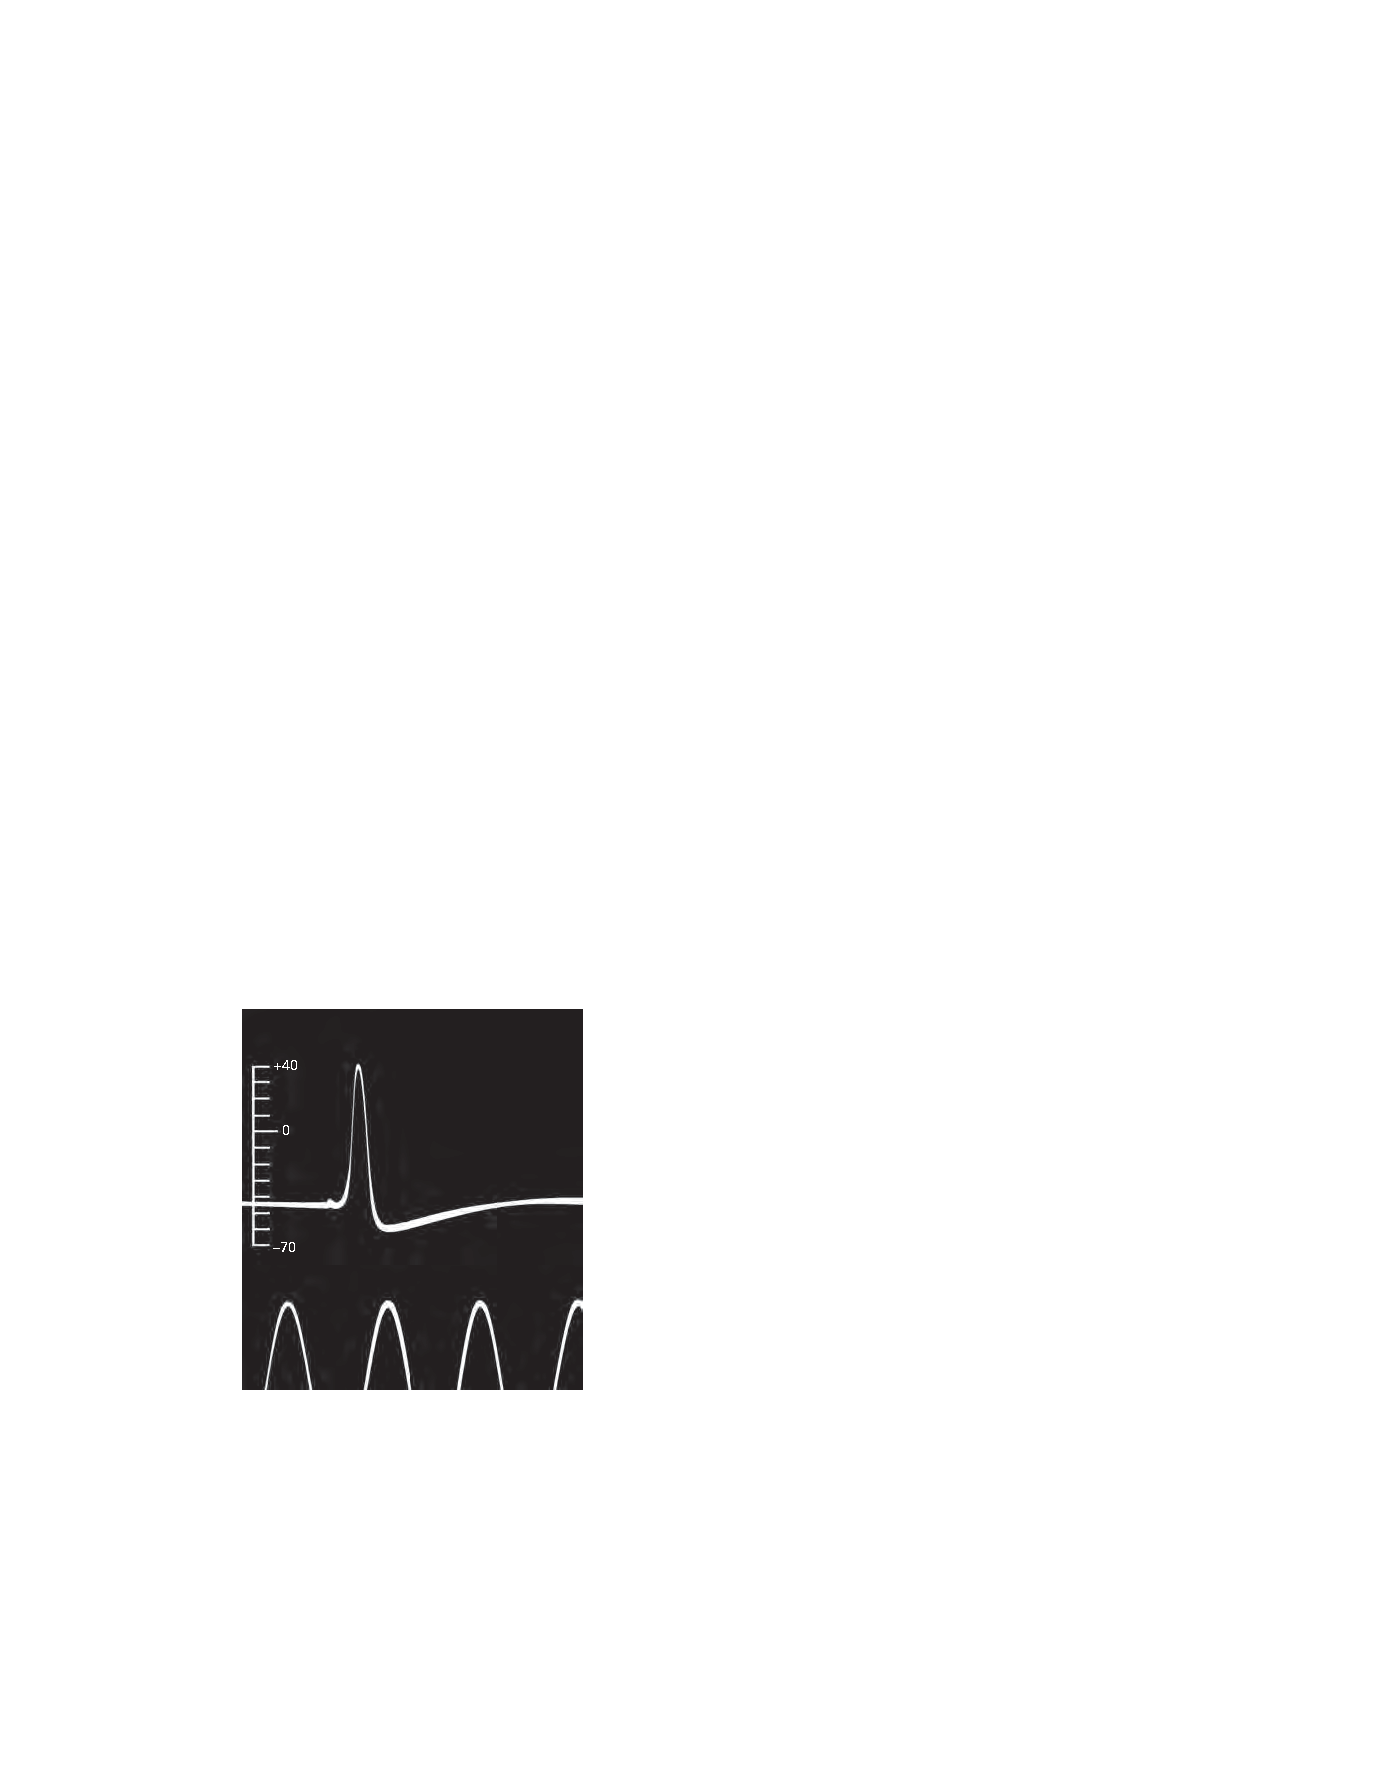
\includegraphics[width=0.5\linewidth]{chap03/fig_3_2}
	\caption{这一历史性追踪是首次公布的动作电位细胞内记录。 
		1939 年,\textit{艾伦·霍奇金}和\textit{安德鲁·赫胥黎}使用充满海水的玻璃毛细管电极从乌贼巨型轴突上记录下来。
		定时脉冲(底部)间隔 2 毫秒。 
		垂直刻度表示内部电极的电位,单位为毫伏,外面的海水被视为零电位\cite{hodgkin1939action}。}
	\label{fig:3_2}
\end{figure}


动作电位是大脑接收、分析和传递信息的信号。 
这些信号在整个神经系统中都是高度固定的,尽管它们是由环境中影响我们身体的各种事件引发的——从光到机械接触,从气味到压力波。
传递视觉信息的生理信号与传递气味信息的生理信号相同。
在这里,我们看到了大脑功能的一个关键原则:
动作电位传递的信息类型不是由信号的形式决定的,而是由信号在大脑中传播的通路决定。
因此,大脑分析和解释通过特定通路传输的传入电信号模式,进而创造我们的视觉、听觉、触觉、嗅觉和味觉。


为了提高传导动作电位的速度,大轴突被包裹在脂质物质髓磷脂的绝缘鞘中。 
鞘被\textit{郎飞结}定期中断,\textit{郎飞结}是轴突上再生动作电位的未绝缘点。
(第~\ref{chap:chap7}~章和第~\ref{chap:chap8}~章详细讨论了髓鞘形成,第~\ref{chap:chap10}~章详细讨论了动作电位。)


在接近其末端时,轴突分成细枝,这些细枝在称为突触的特殊通讯区域与其他神经元联系。
传递信号的神经细胞称为突触前细胞;
接收信号的细胞是突触后细胞。
突触前细胞从其轴突分支的特殊扩大区域传输信号,称为突触前末梢或神经末梢。
突触前细胞和突触后细胞被一个非常狭窄的空间隔开,即突触间隙。
大多数突触前终端终止于突触后神经元的树突,但有些也终止于细胞体,或者较少见的是终止于突触后细胞轴突的起点或末端(见图~\ref{fig:3_1})。 
一些突触前神经元会激发它们的突触后靶细胞;
其他突触前神经元抑制它们的靶细胞。


神经元学说(第~\ref{chap:chap1}~章)认为每个神经元都是一个离散的细胞,其细胞体具有独特的过程,并且神经元是神经系统的信号单元。
回想起来,很难体会到科学家最初提出这个基本想法时有多难接受。
与其他组织的细胞具有简单的形状并适合光学显微镜的单个视野不同,神经细胞具有复杂的形状。
树突的复杂模式和一些轴突看似无穷无尽的过程使得在这些元素之间建立关系变得极其困难。
即使在解剖学家\textit{雅各布·施莱登}和\textit{西奥多·施旺}于 1830 年代初期提出细胞理论之后——细胞是所有生命物质的结构单元的观点成为生物学的中心教条——大多数解剖学家也不接受细胞理论应用于大脑,他们认为大脑是一个连续的、网状的网状结构,由非常薄的过程组成。


神经元的连贯结构直到 19 世纪后期才变得清晰,当时 \textit{拉蒙-卡哈尔}开始使用高尔基体引入的银染法。
这种方法至今仍在使用,它有两个优点。
首先,以一种不为人知的随机方式,银溶液仅染色任何特定大脑区域中约 1\% 的细胞,这使得独立于其相邻神经元检查单个神经元成为可能。
其次,确实吸收了染色剂的神经元被完整地描绘出来,包括细胞体、轴突和完整的树突树。
染色表明神经元之间没有细胞质连续性,\textit{卡哈尔}预言性地正确地得出结论,即使在两个细胞之间的突触处也没有连续性。


\textit{拉蒙-卡哈尔}将高尔基的方法应用于许多动物和人类的胚胎神经系统。 
通过检查神经系统几乎每个区域的神经元结构,他可以描述神经细胞的类别并绘制出许多神经细胞之间的精确联系。
通过这种方式,除了神经元学说之外,\textit{拉蒙-卡哈尔}还推导出了另外两个神经组织原理,这两个原理在研究神经系统的交流方面特别有价值。


% 传播方向的极化(偏向于一边)?
其中第一个是\textit{动态极化}原理,它指出神经细胞内的电信号仅沿一个方向流动:
从神经元的突触后部位(通常是树突和细胞体)到轴突的触发区域。
从那里,动作电位沿着轴突的整个长度传播到其末端。
在迄今为止研究的大多数神经元中,电信号实际上沿着轴突向一个方向传播。


\textit{拉蒙-卡哈尔}提出的第二个原则,即\textit{连接特异性},指出神经细胞在网络形成过程中不会随机相互连接,而是在特定接触点与某些突触后靶细胞而非其他突触后靶细胞建立特定连接。
\textit{动态极化}原理和\textit{连接特异性}原理是现代细胞连接主义研究大脑方法的基础。


\textit{拉蒙-卡哈尔}也是最早意识到一种神经元与另一种神经元最具区别的特征是形状,特别是细胞体产生过程的数量。 
因此,神经元分为三大类:单极、双极和多极。


单极神经元是最简单的,因为它们只有一个初级过程,通常会产生许多分支。
一个分支作为轴突,其他分支充当接收结构(图~\ref{fig:3_3}A)。
这些细胞在无脊椎动物的神经系统中占主导地位;
在脊椎动物中,它们发生在自主神经系统中。


\begin{figure}[htbp]
	\centering
	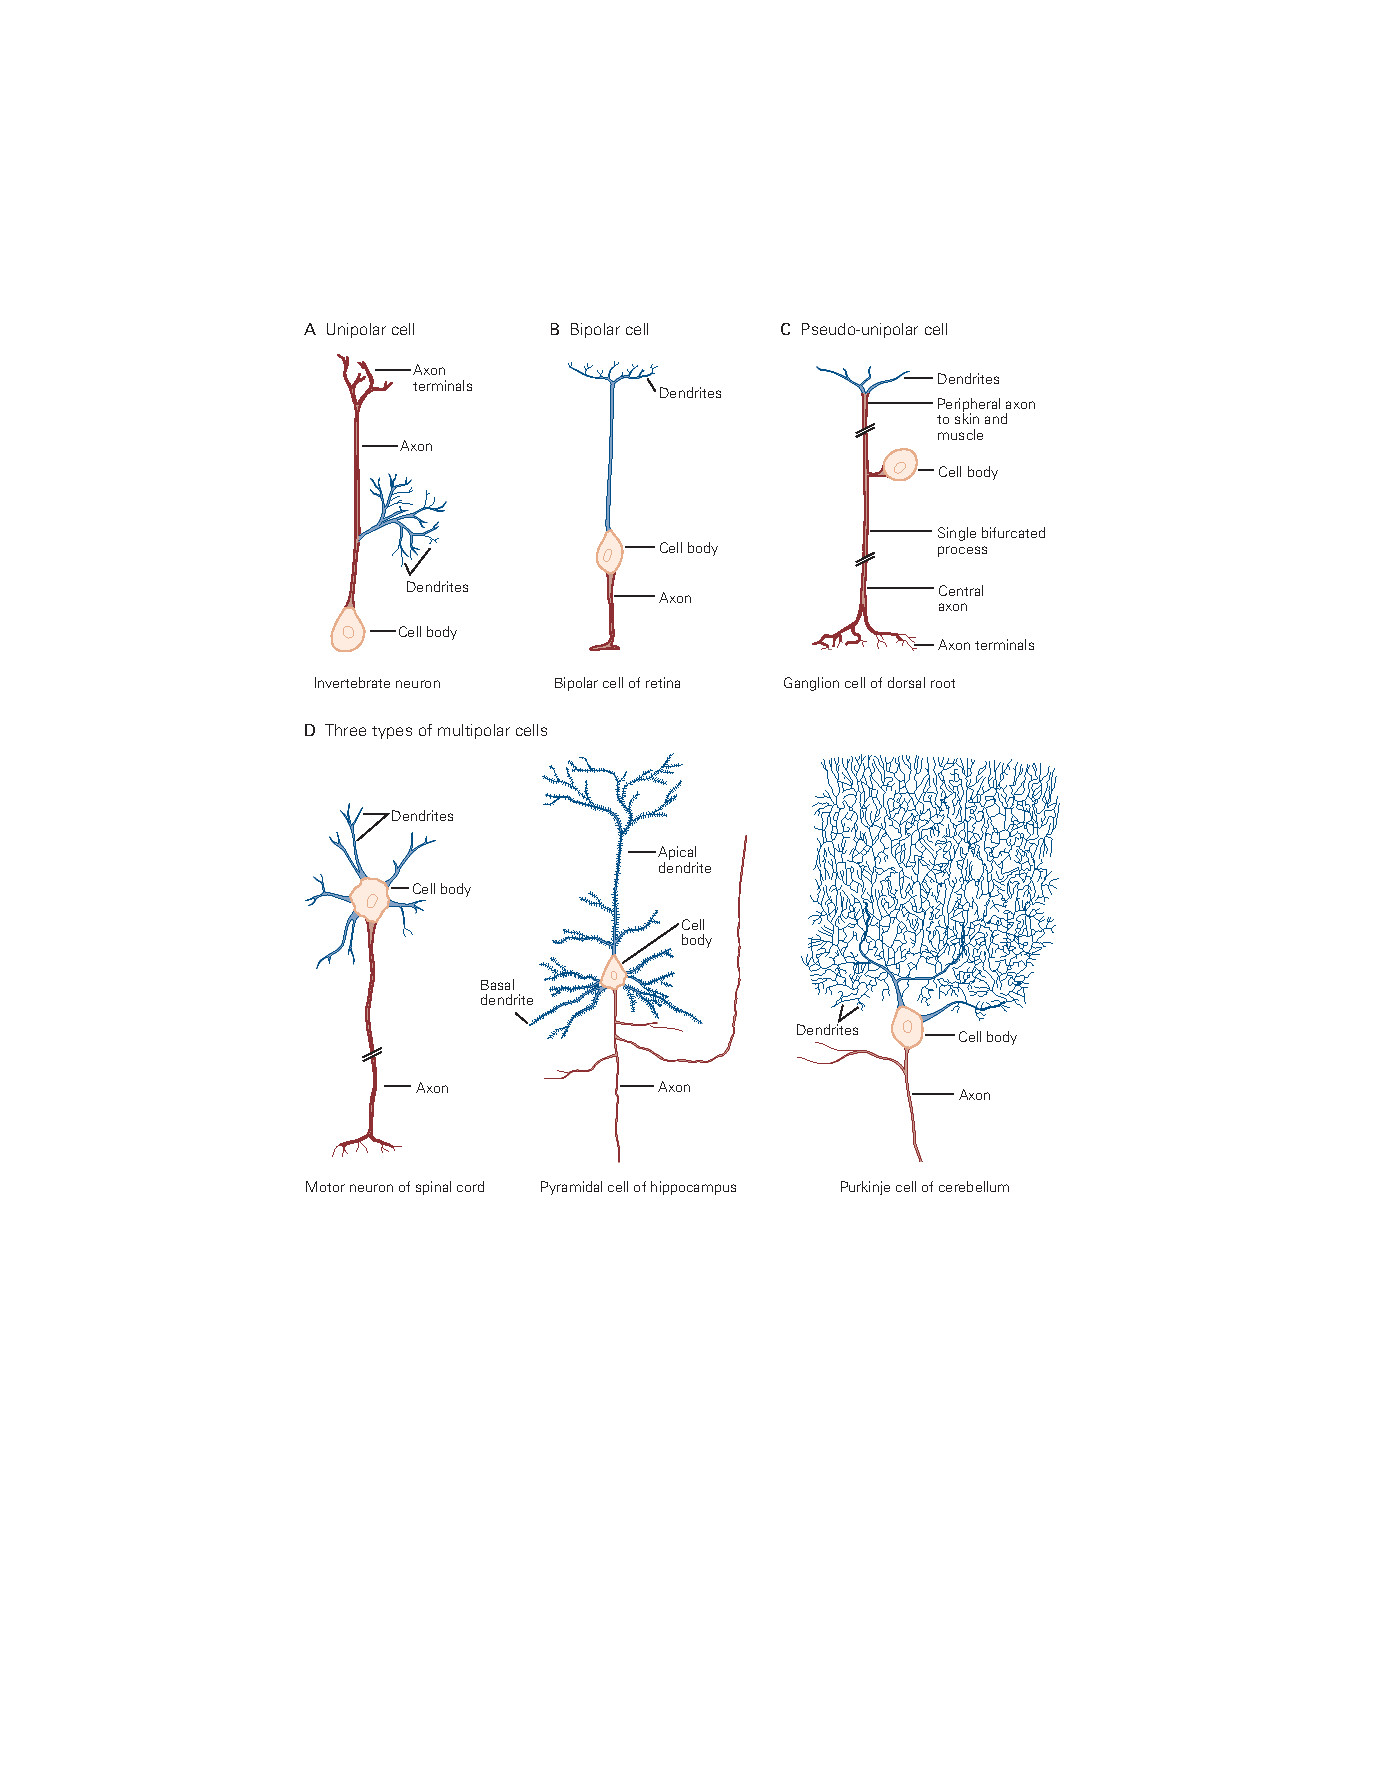
\includegraphics[width=0.9\linewidth]{chap03/fig_3_3}
	\caption{根据源自细胞体的过程的数量,神经元分为单极、双极或多极。 
		\textbf{A.} 单极细胞有一个从细胞发出的过程。
		不同的部分作为接受表面或释放终端。
		单极细胞是无脊椎动物神经系统的特征。 
		\textbf{B.} 双极细胞有两种功能专门化的过程。
		树突接收电信号,轴突将信号传递给其他细胞。
		\textbf{C.} 伪单极细胞是双极细胞的变体,将体感信息传递到脊髓。
		在发育过程中,胚胎双极细胞的两个过程融合并作为一个过程从细胞体中出现,该过程具有两个功能不同的部分。 
		两个部分都起轴突的作用;
		一个延伸到外周皮肤或肌肉,另一个延伸到中央脊髓\cite{ross2006histology}。
		\textbf{D.} 多极细胞具有单个轴突和许多树突。 
		它们是哺乳动物神经系统中最常见的神经元类型。 
		三个例子说明了这些细胞的巨大多样性。 
		脊髓运动神经元支配骨骼肌纤维。
		锥体细胞具有大致三角形的细胞体;
		树突从顶点(顶端树突)和基部(基底树突)出现。 
		锥体细胞存在于海马体和整个大脑皮层中。 
		小脑的浦肯野细胞的特征是丰富而广泛的树突状树,可容纳大量突触输入\cite{ross2006histology}。}
	\label{fig:3_3}
\end{figure}


\textit{双极神经元}有一个椭圆形的体细胞,它产生两个不同的过程:
一个树突结构接收来自其他神经元的信号,一个轴突将信息传递给中枢神经系统(图~\ref{fig:3_3}B)。
许多感觉细胞是双极的,包括\textit{视网膜双极细胞}和鼻子的嗅觉上皮细胞。
向脊髓传递触觉、压力和疼痛信号的受体神经元最初发育为双极细胞,但两个细胞过程融合成一个单一的连续结构,从细胞体的一个点出现,树突被赋予了 使它成为轴突的特化。 
在这些所谓的\textit{假单极细胞}中,一个轴突将信息从皮肤、关节和肌肉中的感觉受体传递到细胞体,而另一个轴突将此感觉信息传递到脊髓(图~\ref{fig:3_3}C)。


\textit{多极神经元}在脊椎动物的神经系统中占主导地位。 
它们通常有一个轴突和许多从细胞体周围不同点出现的树突结构(图 \ref{fig:3_3}D)。 
多极细胞的形状差异很大,尤其是轴突的长度以及树突分支的范围、尺寸和复杂性。 
通常,分支的程度与其他神经元与其进行的突触接触的数量相关。 
一个树突数量相对较少的脊髓运动神经元接受大约 1 万个接触,其中 1 千个在细胞体上,9 千个在树突上。
在小脑的\textit{浦肯野细胞}中,树突树更大更茂密,接受多达一百万次接触!


神经细胞也分为三个主要功能类别:
感觉神经元、运动神经元和中间神经元。 
\textit{感觉神经元}将信息从身体的外围传感器传送到神经系统,以达到感知和运动协调的目的。 
一些\textit{初级感觉神经元}称为\textit{传入神经元},这两个术语可以互换使用。 
术语\textit{传入}(传向中枢神经系统)适用于从外围到达中枢神经系统的所有信息,无论该信息是否导致感觉。
术语\textit{感觉}是指那些将信息从感觉上皮细胞、关节感觉受体或肌肉传递到中枢神经系统的传入神经元,但该概念已扩展到包括初级和次级皮层区域中的神经元,这些神经元对变化做出反应 感觉特征,例如物体在空间中的位移、声音频率的变化或头部的角旋转(通过耳朵中的前庭器官),甚至像面部这样复杂的东西。


\textit{传出}一词适用于从中枢神经系统向运动器官传递的所有信息,无论这些信息是否导致行动。
\textit{运动神经元}将命令从大脑或脊髓传递到肌肉和腺体(传出信息)。 
运动神经元(或运动神经元)的传统定义是激发肌肉的神经元,但运动神经元的名称现在包括不直接支配肌肉但间接命令动作的其他神经元。
运动神经元和感觉神经元的一个有用特征是它们对神经系统外事物的时间保真度。 
它们的活动跟上外部刺激和身体肌肉组织施加动力的变化。 
感觉神经元为大脑提供数据,而运动神经元将观念转化为实践。 
它们共同构成了我们与世界的连接。


\textit{中间神经元}包含最多的功能类别,并细分为两类:\textit{中继中间神经元}和\textit{局部中间神经元}。
中继中间神经元或投射中间神经元具有长轴突,可在相当长的距离内将信号从一个大脑区域传送到另一个大脑区域。
局部中间神经元的轴突较短,因为它们与局部回路中附近的神经元形成连接。
由于几乎每个神经元都可以被视为中间神经元,因此该术语通常用于区分投射到局部回路中另一个神经元的神经元和投射到单独神经结构的神经元。
该术语有时也用作抑制性神经元的简写,特别是在皮层回路的研究中,但为了清楚起见,应在适当的时候使用\textit{抑制性中间神经元}术语。


每个功能分类可以进一步细分。 
感觉系统中间神经元可以根据它们响应的感觉刺激的类型进行分类; 
这些最初的分类可以根据位置、密度、大小以及基因表达模式进一步细分。
事实上,由于\textit{信使核糖核酸}序列分析的进步使得能够对单个神经元进行分子分析,我们对神经元复杂性的看法正在迅速发展。 
此类分析最近揭示了神经元类型的异质性比以前认为的要大得多(图~\ref{fig:3_4})。


\begin{figure}[htbp]
	\centering
	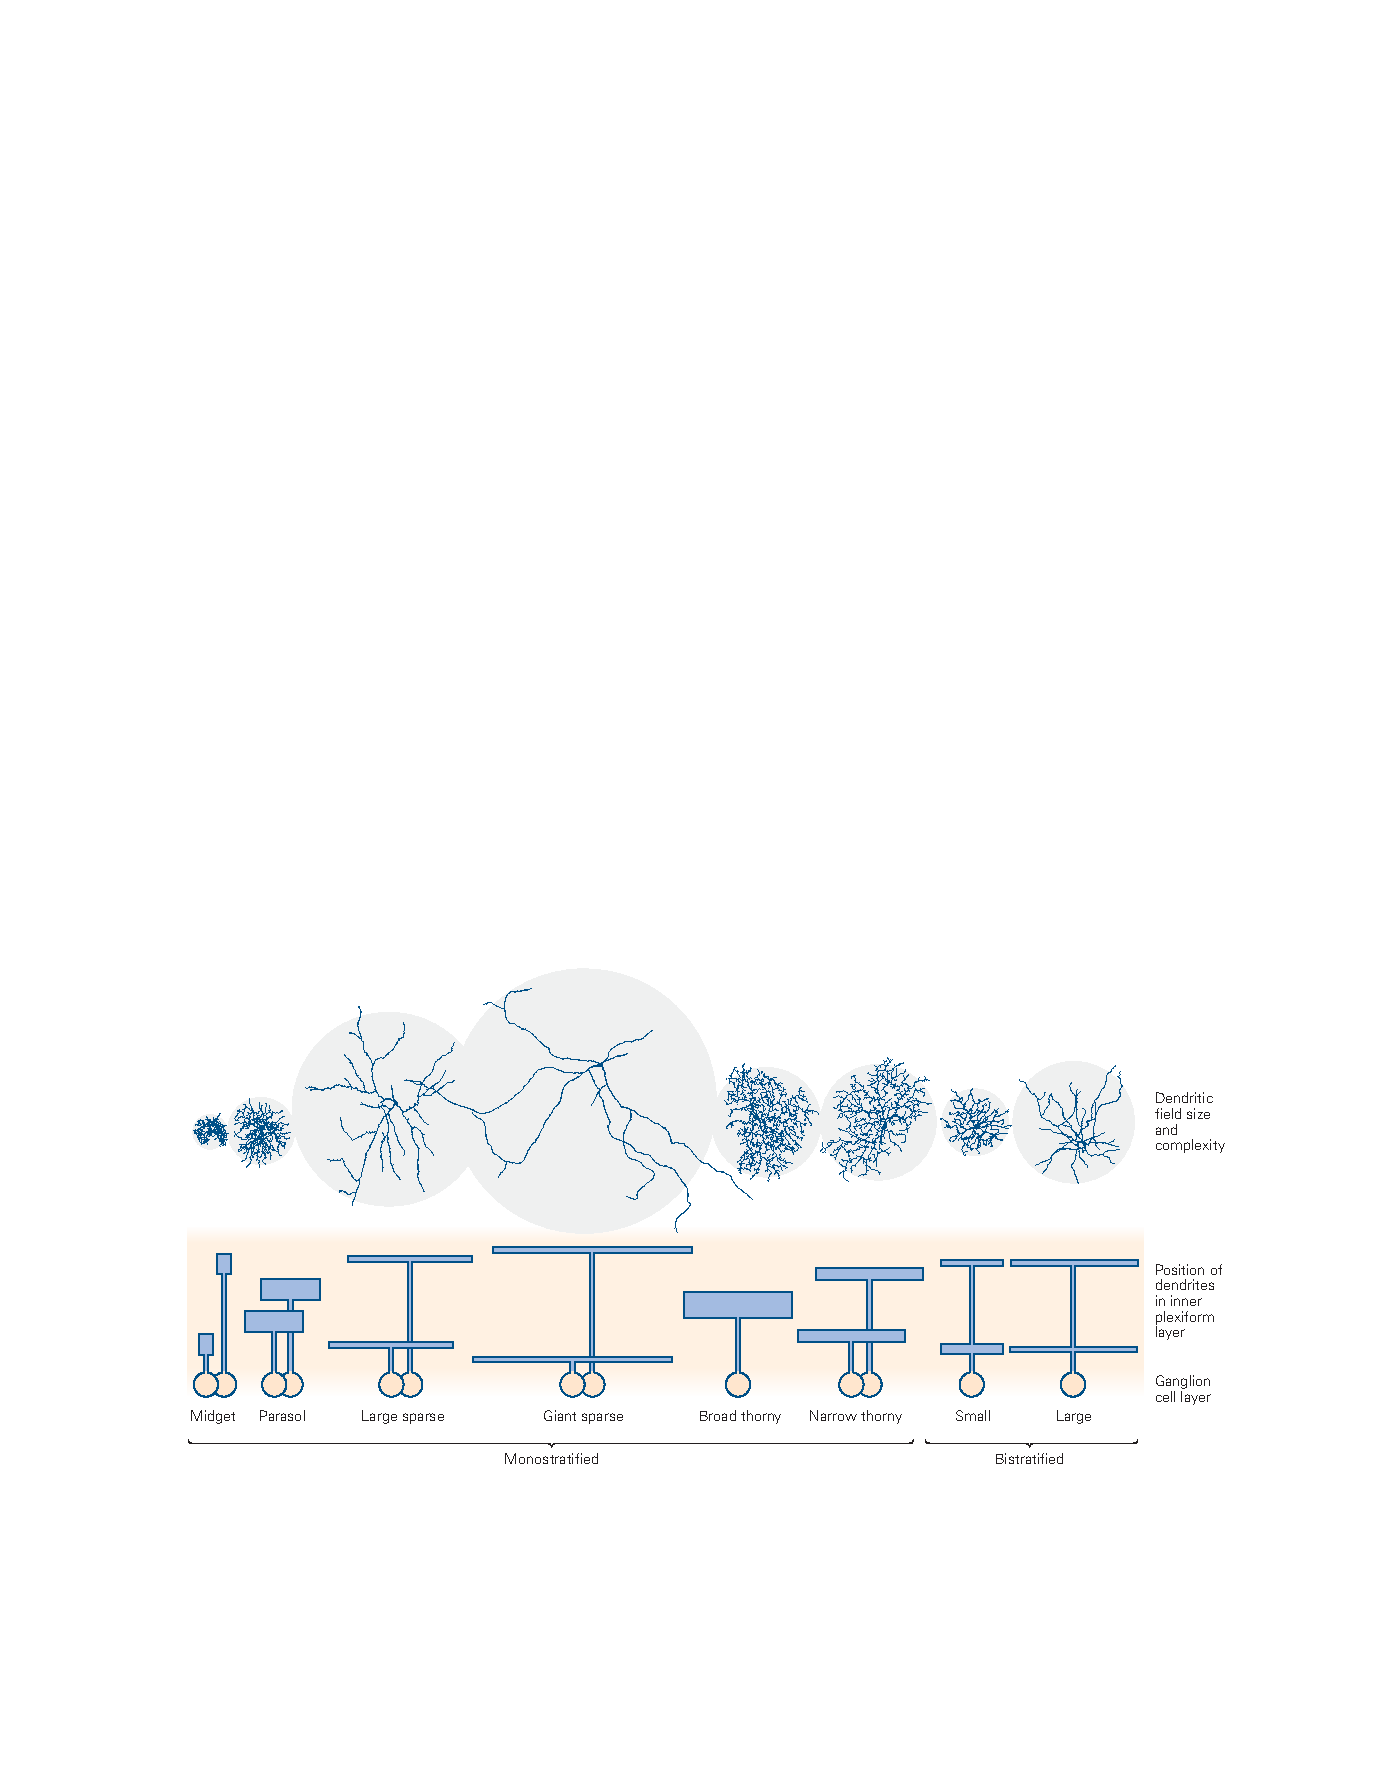
\includegraphics[width=1.0\linewidth]{chap03/fig_3_4}
	\caption{感觉神经元可以细分为功能不同的组。
		例如,至少有 13 种类型的视网膜神经节细胞是根据它们的树突的大小和形状以及它们接收输入信号的视网膜深度来区分的。
		内丛状层包含视网膜中间神经元(双极和无长突细胞)和神经节细胞之间的连接\cite{dacey2003fireworks}。}
	\label{fig:3_4}
\end{figure}


\subsection{神经胶质细胞支持神经细胞}
\textit{神经胶质细胞}的数量远远超过神经元,在脊椎动物中枢神经系统中,神经胶质细胞的数量是神经元的 2 到 10 倍。
尽管这些细胞的名称源自希腊语中的\textit{胶水},但胶质细胞通常不会将神经细胞聚集在一起。
相反,它们围绕着神经元的细胞体、轴突和树突。
胶质细胞在形态上不同于神经元,
它们不形成树突和轴突。


胶质细胞在功能上也有所不同。
尽管它们来自相同的胚胎前体细胞,但它们不具有与神经元相同的膜特性,因此不能是可兴奋的。
因此,它们不直接参与电信号传递,这是神经细胞的功能。
然而,它们在允许电信号沿着神经元的轴突快速移动方面发挥了作用,而且它们似乎在引导早期发育过程中的连接,以及稳固通过学习发生的神经元之间新的连接或改变的连接方面发挥了重要作用。
在过去的十年中,人们对胶质细胞的多种功能的兴趣有所增加,它们的特征已经从支持细胞转变为神经元的功能伙伴(第~\ref{chap:chap7}~章)。



\section{每个神经细胞都是调节特定行为的回路的一部分}

每种行为都由一组特定的相互连接的神经元介导,而每
一个神经元的行为功能都取决于它与其他神经元的联系。
一个简单的膝跳反射行为将说明这一点。 
当身体短暂的不平衡拉伸腿部股四头肌伸肌时,反射开始。
这种拉伸会产生传送给运动神经元的感觉信息,而运动神经元又会向伸肌发出收缩命令,从而恢复平衡。


这种反射在临床上用于测试神经的完整性以及反射幅度(或增益)的脑脊髓控制。 
潜在的机制很重要,因为它可以维持股四头肌的正常张力,并防止我们的膝盖在站立或行走时屈曲。 
股四头肌的肌腱,一种移动小腿的伸肌,通过髌骨(膝盖骨)的肌腱附着在胫骨上。 
轻敲髌骨正下方的肌腱可以拉伸股四头肌。 
这种拉伸启动股四头肌的反射性收缩,产生熟悉的膝跳。 
通过增加选定肌肉群的张力,牵张反射改变腿的位置,突然向外伸展(图 \ref{fig:3_5})。

\begin{figure}[htbp]
	\centering
	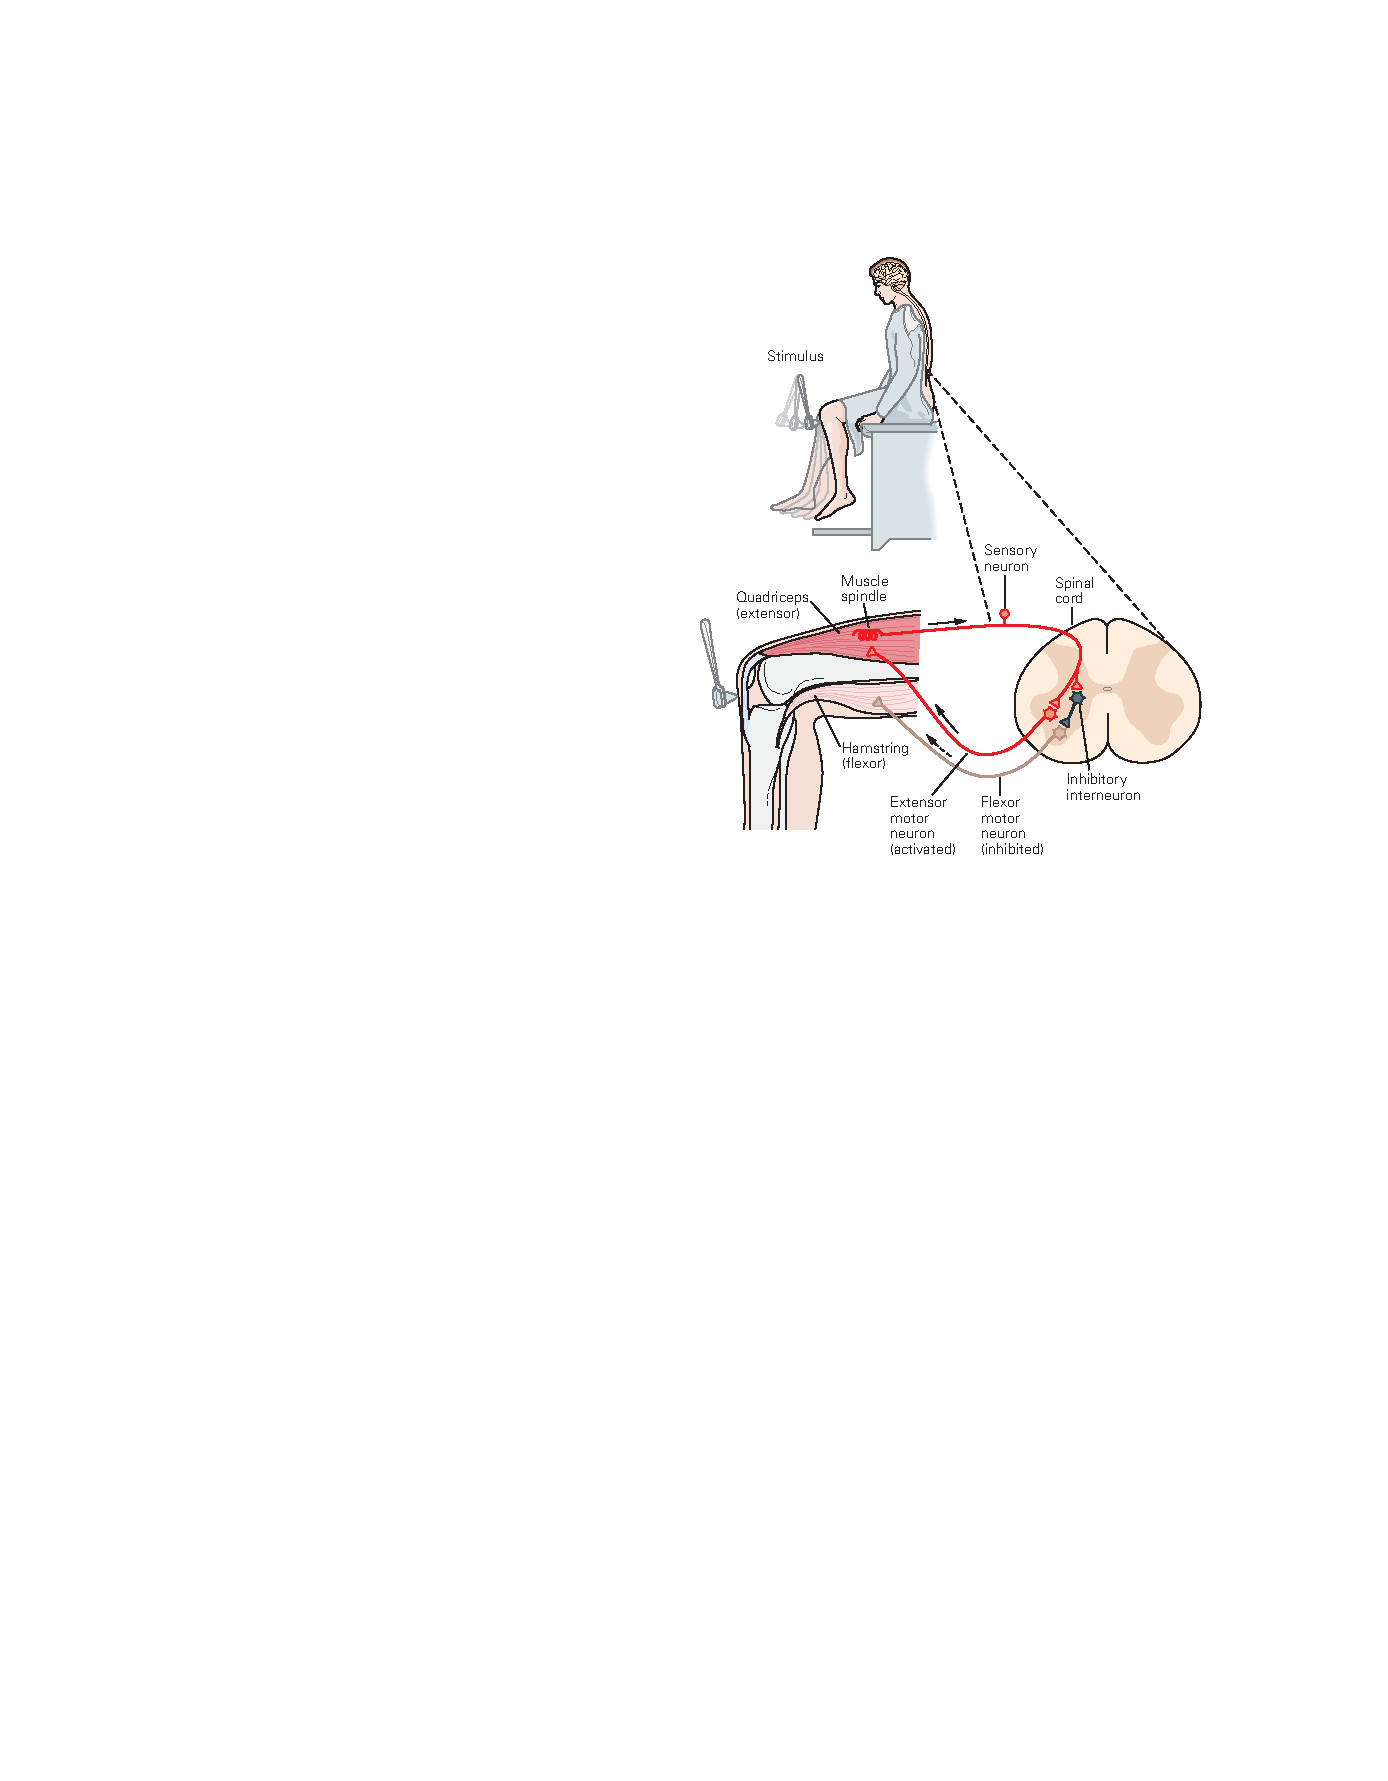
\includegraphics[width=0.6\linewidth]{chap03/fig_3_5}
	\caption{膝跳反射由感觉和运动神经元组成的简单回路控制。
		用反射锤轻敲膝盖骨,拉动股四头肌的肌腱,股四头肌是拉伸小腿的肌肉。
		当肌肉因肌腱的牵拉而伸展时,有关肌肉变化的信息会通过感觉神经元传送到中枢神经系统。
		在脊髓中,感觉神经元与收缩股四头肌(被拉伸的肌肉)的伸肌运动神经元形成兴奋性突触。 
		感觉神经元通过中间神经元间接作用,抑制屈肌运动神经元,否则这些神经元会收缩相对的腿筋肌肉。 
		这些动作结合起来产生反射行为。 
		在图中,每个伸肌和屈肌运动神经元代表许多细胞群。}
	\label{fig:3_5}
\end{figure}


参与膝跳反射的感觉神经元细胞体聚集在背根神经节的脊髓附近。
它们是假单极细胞;
每个细胞轴突的一个分支延伸到周围的股四头肌,而另一个延伸到脊髓的中央。
支配股四头肌的分支与拉伸敏感受体(肌梭)接触,并在肌肉拉伸时兴奋。 
到达脊髓的分支与支配股四头肌并控制其收缩的运动神经元形成兴奋性连接。 
该分支还联系抑制控制相对屈肌的运动神经元的局部中间神经元(图~\ref{fig:3_5})。 
尽管这些局部中间神经元本身不参与牵张反射的产生,但它们通过协调相反肌肉群的动作来增加反射的稳定性。 
因此,产生牵张反射的电信号携带四种信息:

1. 感觉信息从肌肉传递到中枢神经系统(脊髓)。

2. 来自中枢神经系统的运动命令被发送到进行膝跳的肌肉。

3. 向支配相反肌肉的运动神经元发出抑制性命令。

4. 与膝跳有关的局部神经元活动的信息被发送到中枢神经系统的更高中枢,允许大脑同时或依次协调不同的行为。


此外,大脑声称依赖于上下文的反射控制来调整其增益。
例如,当我们跑步时,腘绳肌会弯曲膝盖,从而拉伸股四头肌。
大脑和脊髓抑制牵张反射,使股四头肌放松。 
当这些下行通路被破坏时,就像在某些划水动作中一样,反射被放大并且关节变得僵硬。


仅仅拉伸一块肌肉,股四头肌,就会激活数百个感觉神经元,每个神经元与 45 到 50 个运动神经元直接接触。 
这种连接模式,其中一个神经元激活许多目标细胞,称为发散(图 \ref{fig:3_6}A)。 
它在神经系统的输入阶段尤为常见; 通过将其信号分配给许多靶细胞,单个神经元可以发挥广泛而多样的影响。 
相反,膝跳回路中的单个运动细胞从大约 130 个感觉细胞接收 200 到 450 个输入触点。 
这种连接模式称为收敛(图 \ref{fig:3_6}B)。 
它在神经系统的输出阶段很常见; 从许多感觉神经元接收信息的目标运动细胞能够整合来自许多来源的信息。 
每个感觉神经元输入产生相对较弱的兴奋,因此收敛也确保只有当足够数量的感觉神经元一起被激活时,运动神经元才会被激活。


\begin{figure}[htbp]
	\centering
	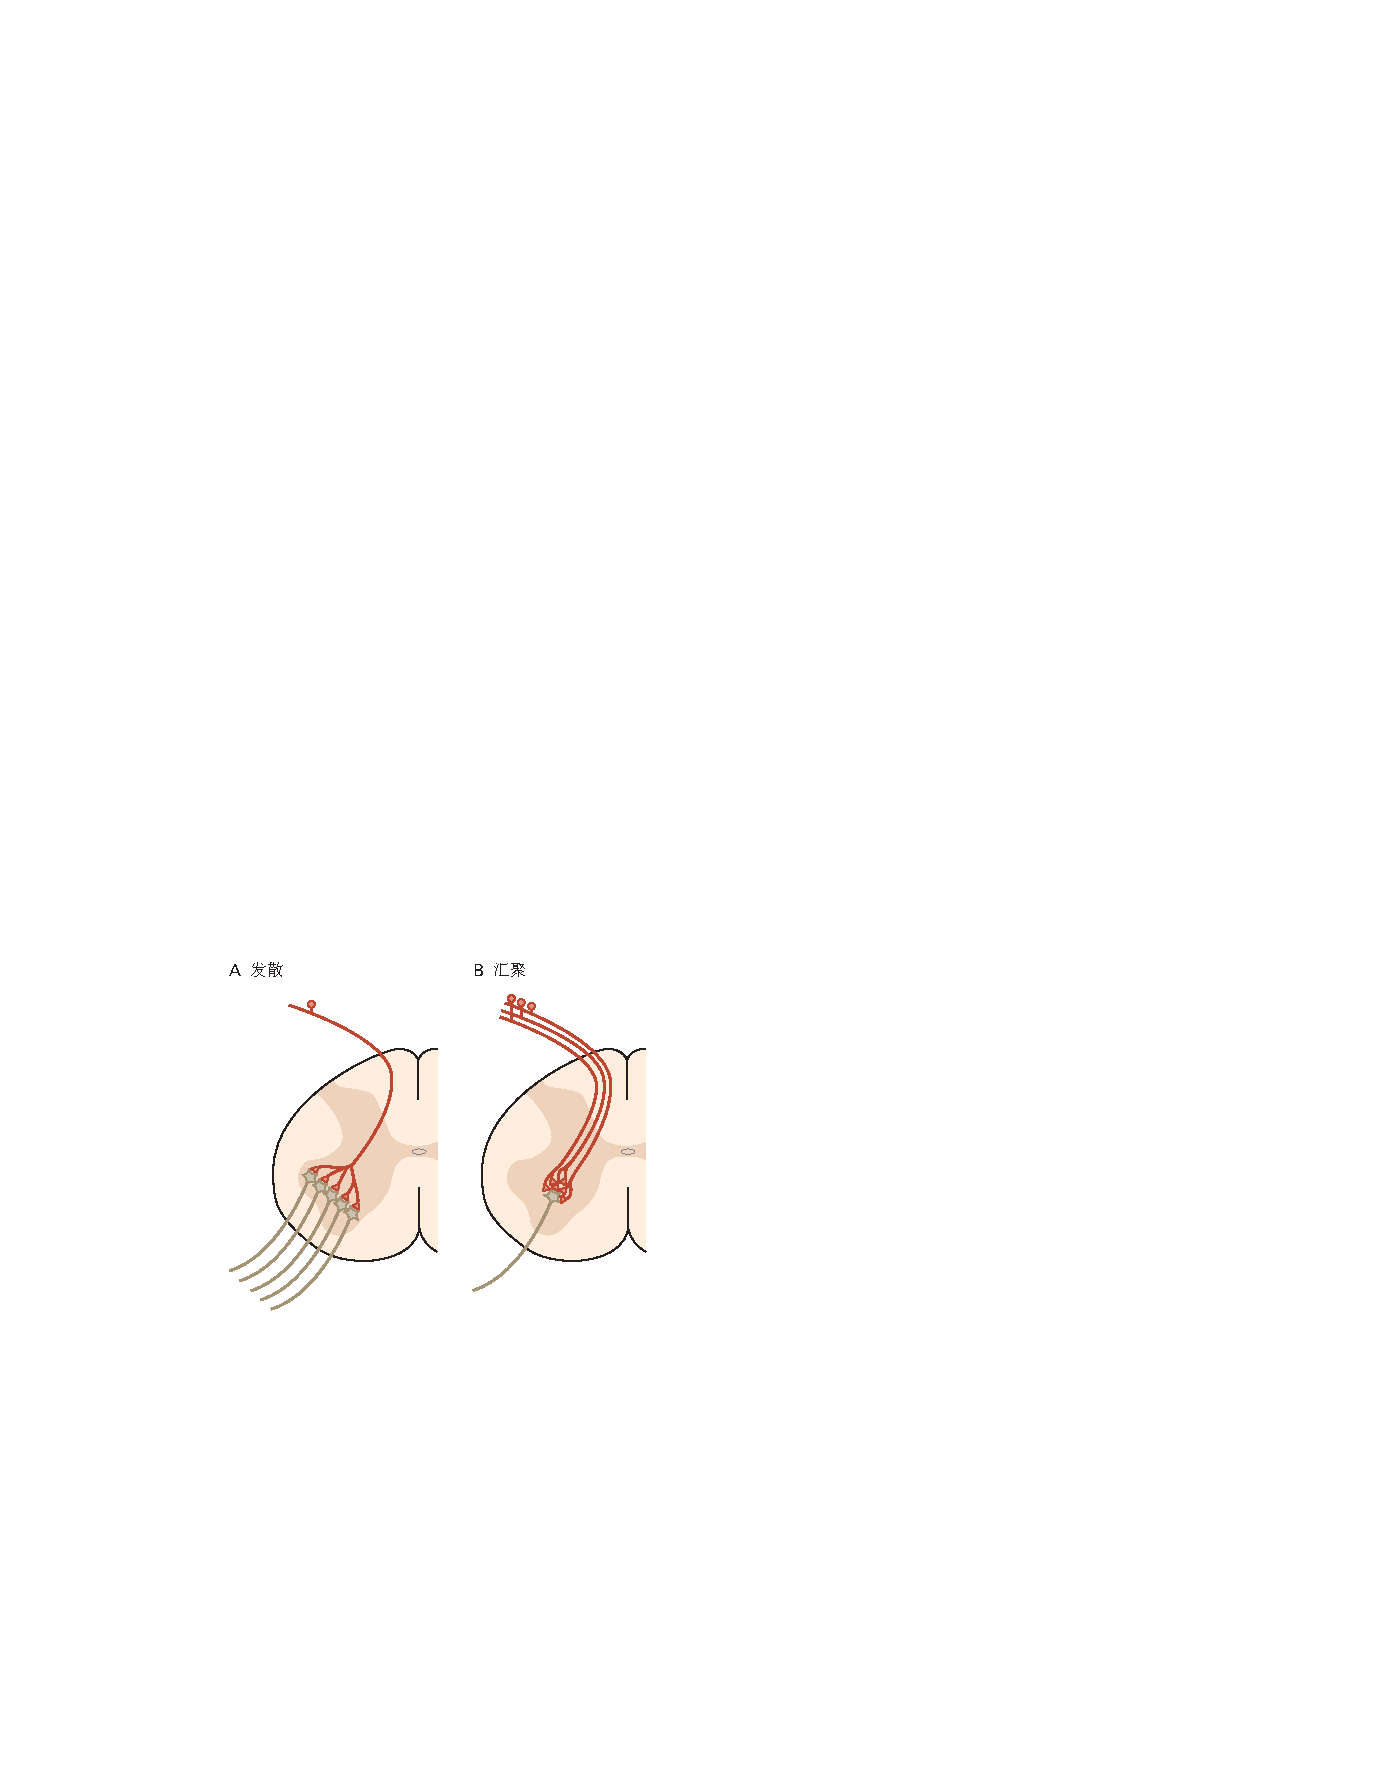
\includegraphics[width=0.5\linewidth]{chap03/fig_3_6}
	\caption{发散和会聚的神经元连接是大脑的一个关键组织特征。
		\textbf{A.} 在感觉系统中,每个受体神经元通常与代表第二阶段处理的几个神经元联系。 
		在随后的处理阶段,传入的连接更加分散。 
		这使得来自单个站点的感觉信息可以更广泛地分布在脊髓和大脑中。 
		\textbf{B.} 相比之下,运动神经元是逐渐融合连接的目标。 
		通过这种安排,需要来自许多突触前细胞的输入来激活运动神经元。}
	\label{fig:3_6}
\end{figure}


诸如膝跳反射之类的牵张反射是由在兴奋性突触处连接的两类神经元产生的一种简单行为。 
但并非大脑中的所有重要信号都是兴奋性的。 
许多神经元会产生抑制信号,从而降低放电的可能性。 
即使在简单的膝跳反射中,感觉神经元也会产生兴奋性和抑制性连接。 
腿部伸肌中的兴奋性连接会导致这些肌肉收缩,而与抑制性中间神经元的连接会阻止拮抗性屈肌收缩。 
回路的这个特性是前馈抑制的一个例子(图~\ref{fig:3_7}A)。 
在膝跳反射中,前馈抑制是相互的,确保屈肌和伸肌通路始终相互抑制,以便只招募适合运动的肌肉,而不是那些反对运动的肌肉。


\begin{figure}[htbp]
	\centering
	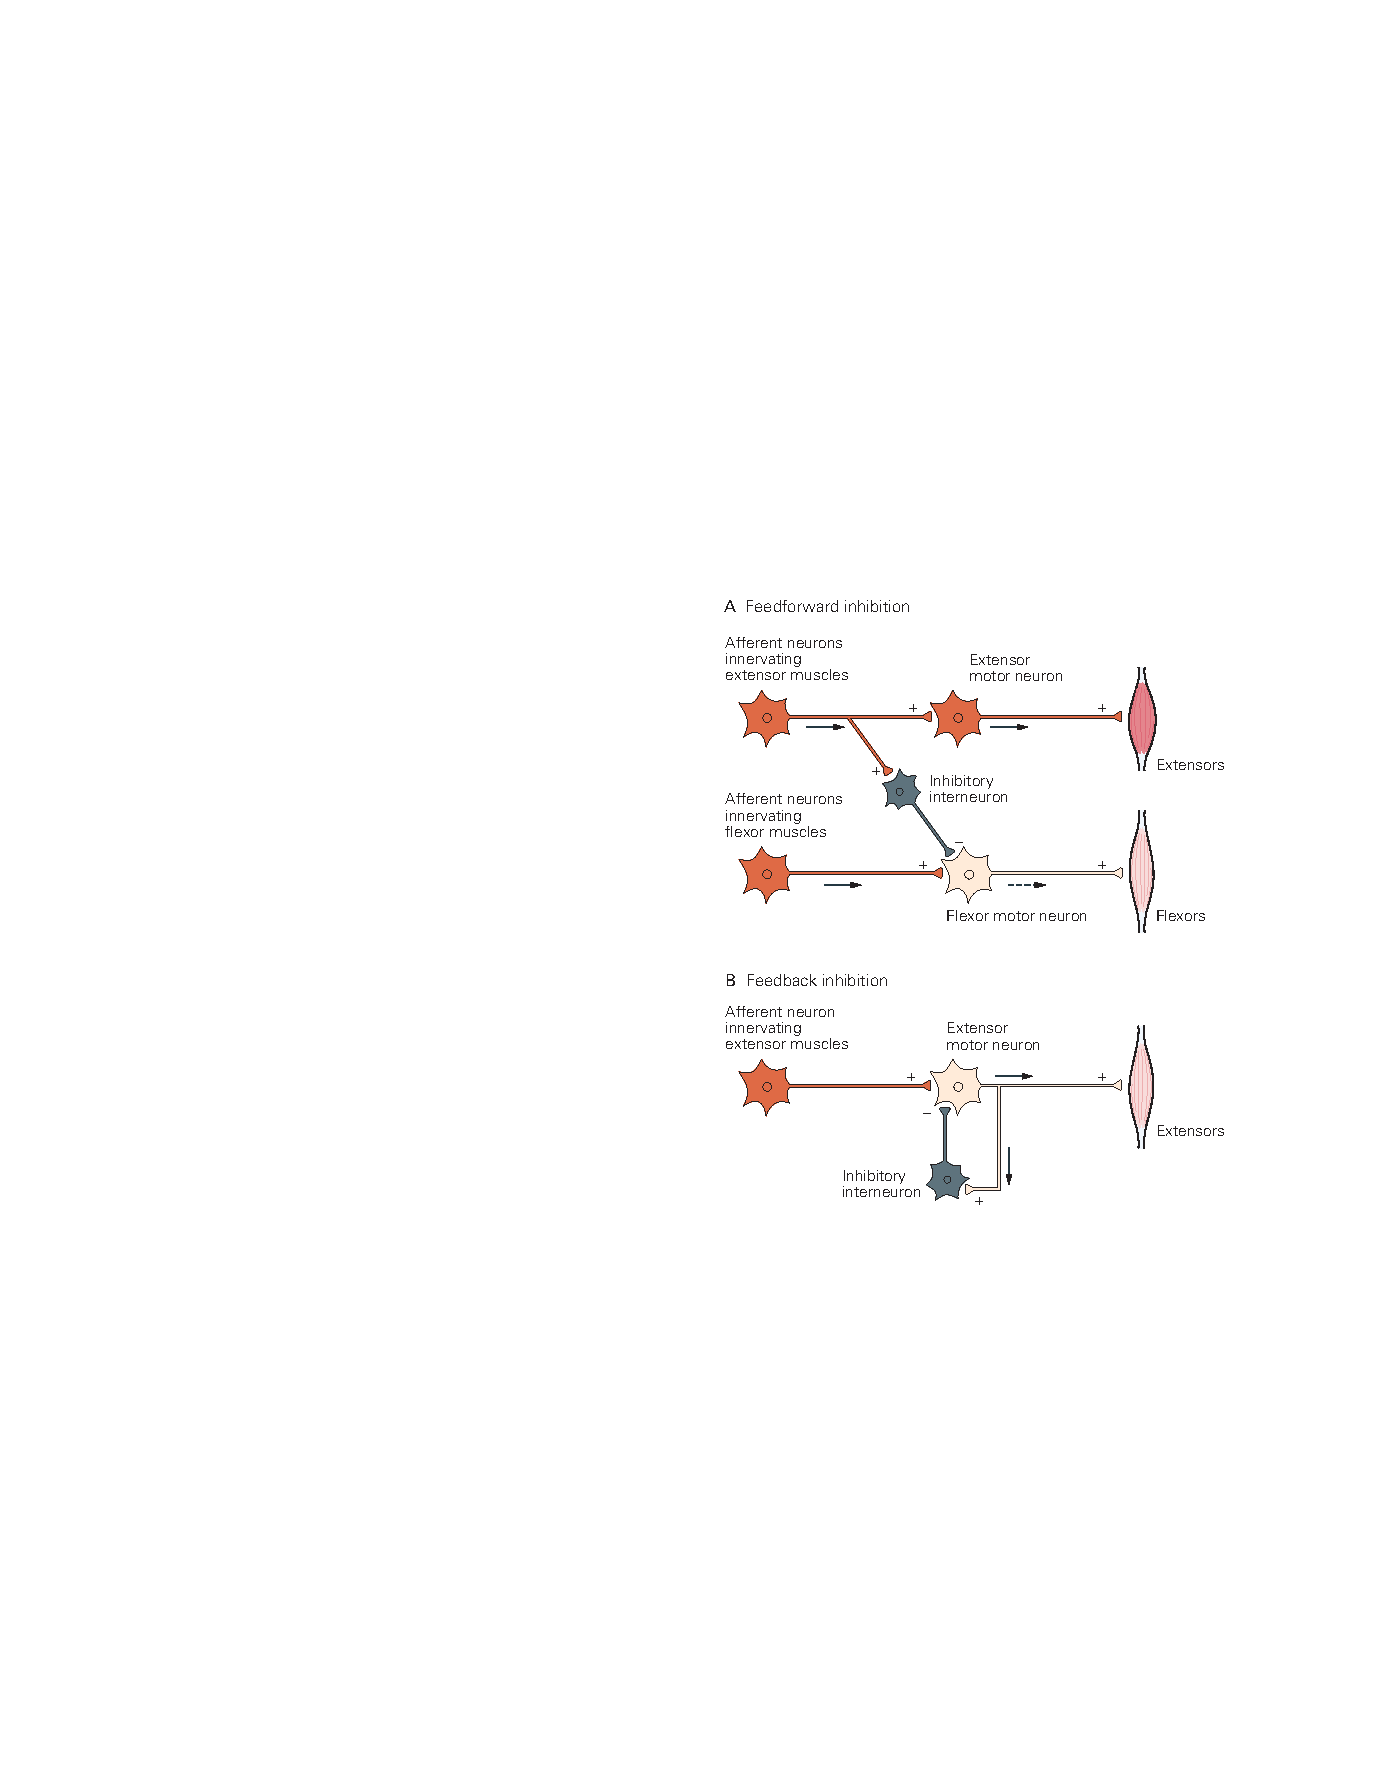
\includegraphics[width=0.55\linewidth]{chap03/fig_3_7}
	\caption{抑制性中间神经元可以产生前馈或反馈抑制。
		\textbf{A.} 前馈抑制通过抑制调节相反作用的通路的活性来增强活性通路的效果。
		前馈抑制在单突触反射系统中很常见。 
		例如,在膝跳反射回路(图~\ref{fig:3_5})中,来自伸肌的传入神经元不仅会刺激伸肌运动神经元,还会刺激抑制性中间神经元,从而阻止神经支配相对屈肌的运动细胞的放电。 
		\textbf{B.} 反馈抑制是一种自我调节机制。
		在这里,伸肌运动神经元作用于抑制性中间神经元,后者反过来作用于伸肌运动神经元本身,从而降低它们放电的可能性。
		其作用是抑制受刺激通路内的活动并防止其超过某个临界水平。}
	\label{fig:3_7}
\end{figure}


一些回路提供反馈抑制。 
例如,运动神经元可能与肌肉和抑制性中间神经元都有兴奋性连接,后者本身与运动神经元形成连接。 
当抑制性中间神经元被运动神经元兴奋时,中间神经元能够限制运动神经元兴奋肌肉的能力(图 \ref{fig:3_7}B)。 
当我们在后面的章节中研究更复杂的行为时,我们会遇到许多前馈和反馈抑制的例子。


\section{信号在所有神经细胞中的组织方式相同}
为了产生一种行为,例如牵张反射,每个参与的感觉和运动神经细胞必须依次产生四种不同的信号,每个信号位于细胞内的不同位置。 
尽管细胞大小和形状、递质生物化学或行为功能各不相同,但几乎所有神经元都可以用一个模型神经元来描述,该模型神经元具有产生四种类型信号的四个功能组件:
一个用于产生分级输入信号的接收组件,一个求和或 产生触发信号的综合组件,产生全或无传导信号的传导远程信号组件,以及产生输出信号到下一个神经元或肌肉或腺体细胞的突触组件(图~\ref{fig:3_8})。


\begin{figure}[htbp]
	\centering
	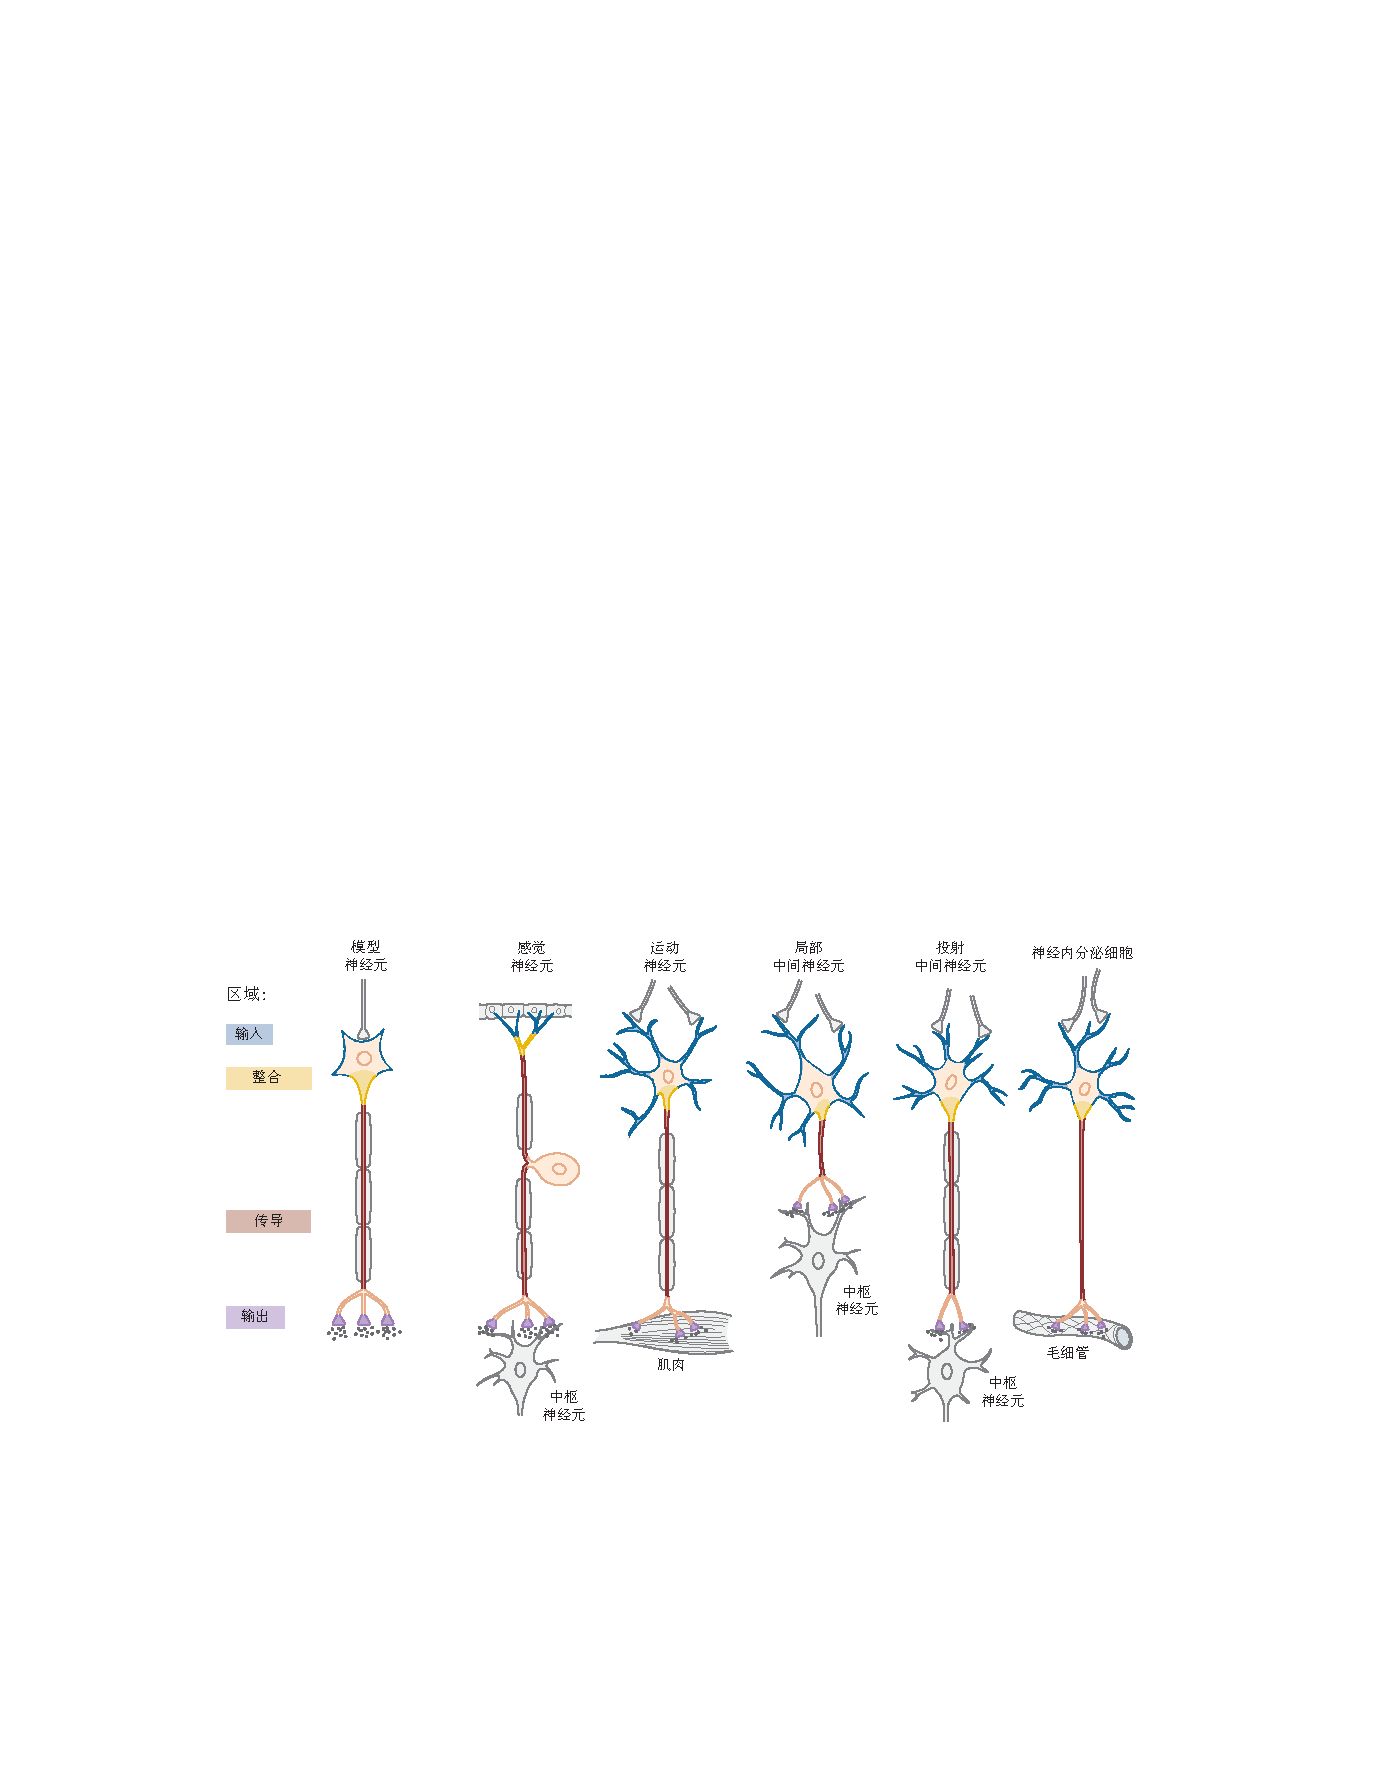
\includegraphics[width=0.8\linewidth]{chap03/fig_3_8}
	\caption{大多数神经元有四个功能区域,在这些区域中会生成不同类型的信号。 
		因此,大多数神经元的功能组织,无论类型如何,都可以用模型神经元示意性地表示。 
		该模型神经元是\textit{拉蒙-卡哈尔}动态极化原理的生理表达。 
		输入信号、综合信号和传导信号都是电信号,对细胞来说是不可或缺的,而输出信号是由细胞射入突触间隙的化学物质。 
		并非所有神经元都具有所有这些特征。 
		例如,一些局部中间神经元缺乏导电成分。}
	\label{fig:3_8}
\end{figure}


神经元中产生的不同类型的信号部分取决于细胞膜的电特性。 
当细胞处于静止状态时,包括神经元在内的每个细胞都在质膜两侧保持一定的电位差。 
这称为静息膜电位。 
在典型的静息神经元中,细胞内部的电压比细胞外部的电压负大约 65 毫伏。
因为膜外电压被定义为零,所以我们说静息膜电位为 –65 毫伏。 
不同神经细胞的静息电位范围为 –40 毫伏至 –80 毫伏; 
在肌肉细胞中,它更大,约为 –90 毫伏。 
正如第~\ref{chap:chap9}~章中详细描述的,静息膜电位由两个因素造成:
带电离子的不均匀分布,特别是带正电的 \ce{Na+} 和 \ce{K+},以及膜的选择性渗透性。


带正电的离子在细胞膜两侧的不均匀分布由两个主要机制维持。 
细胞内 \ce{Na+} 和 \ce{K+} 浓度主要由膜蛋白控制,膜蛋白主动将 \ce{Na+} 泵出细胞并将 \ce{K+} 泵回细胞内。 
这个 \ce{Na+}-\ce{K+} 泵,我们将在第 \ref{chap:chap9} 章中详细了解,它使细胞内的 \ce{Na+} 浓度保持在较低水平(约为细胞外浓度的十分之一),并使 \ce{K+} 浓度保持在较高水平(约为细胞外浓度的 20 倍)。 
\ce{Na+} 和 \ce{K+} 的细胞外浓度由肾脏和星形胶质细胞(也称为星形胶质细胞)维持。


否则不可渗透的细胞膜含有形成称为离子通道的孔的蛋白质。 细胞静止时活跃的通道对 \ce{K+} 的渗透性很高,但对 \ce{Na+} 的渗透性要低得多。 
\ce{K+} 离子往往会沿着离子的浓度梯度从这些开放通道中泄漏出来。 
当 \ce{K+} 离子离开细胞时,它们会在膜的内表面留下一团未中和的负电荷,因此膜内的净电荷比膜外的负电荷更多。 
在这种情况下,相对于神经元外部,膜电位通常保持在 –65 毫伏左右,据说神经元处于静止状态。


当细胞开始吸收细胞外浓度较高的 \ce{Na+}(或钙离子)时,静息状态就会受到干扰。 
这些带正电的离子向内运动(内向电流)部分地中和了细胞内部的负电压。 
我们将在下面详细介绍这些事件。 
然而,接下来发生的事情是理解神经元是什么使信号适合传递信息的关键。


当一个细胞,如神经和肌肉,其膜电位可以迅速而显着地改变时,就被认为是可兴奋的。 
在许多神经元中,膜电位 10 毫伏的变化(从 –65 毫伏到 –55 毫伏)使膜对 \ce{Na+} 的渗透性比对 \ce{K+} 的渗透性强得多。 
由此产生的 \ce{Na+} 流入进一步中和了细胞内的负电荷,导致对 \ce{Na+} 的渗透性更高。 
结果是膜电位发生短暂的爆炸性变化,变为 +40 毫伏,即动作电位。 
这种电位被积极地沿着细胞的轴突传导到轴突的末端,在那里它启动与突触后神经元或肌肉细胞的精细化学相互作用。 
由于动作电位是主动传播的,因此其振幅在到达轴突末端时不会减小。 
动作电位通常持续约 1 毫秒,之后膜恢复到其静止状态,电荷正常分离,对 \ce{K+} 的渗透性高于对 \ce{Na+} 的渗透性。


静息电位和动作电位的潜在机制在第 \ref{chap:chap9} 章和第 \ref{chap:chap10} 章中详细讨论。
除了动作电位代表的长距离信号外,神经细胞还产生局部信号——受体电位和突触电位——这些信号不活跃 传播并且通常在几毫米内衰减(见下一节)。


产生远程和局部信号的膜电位变化可以是静息电位的降低或增加。 
也就是说,静息膜电位是所有信号发生的基线。 
膜电位的降低(称为去极化)增强了细胞产生动作电位的能力,因此具有兴奋性。 
相反,膜电位的增加,称为超极化,使细胞不太可能产生动作电位,因此具有抑制作用。


\subsection{输入组件产生分级本地信号}
在大多数静止的神经元中,没有电流从细胞的一部分流向另一部分,因此静息电位始终相同。 
在感觉神经元中,电流通常由物理刺激启动,物理刺激会激活神经元接受表面的特殊受体蛋白。 
在我们膝跳反射的例子中,肌肉的拉伸会激活特定的离子通道,这些离子通道会响应感觉神经元膜的拉伸而打开,我们将在第~\ref{chap:chap18}~章中了解到。
当细胞被拉伸时,这些通道的打开允许 \ce{Na+} 离子快速流入感觉细胞。 
这种离子电流改变膜电位,产生称为受体电位的局部信号。


受体电位的幅度和持续时间取决于肌肉拉伸的强度:拉伸越大或持续时间越长,由此产生的受体电位越大或持续时间越长(图~\ref{fig:3_9}A)。
也就是说,受体电位是分级的,这与\textit{全有或全无}动作电位不同。
大多数受体电位是去极化的(兴奋性的);
在视网膜中发现超极化(抑制)受体电位。


\begin{figure}[htbp]
	\centering
	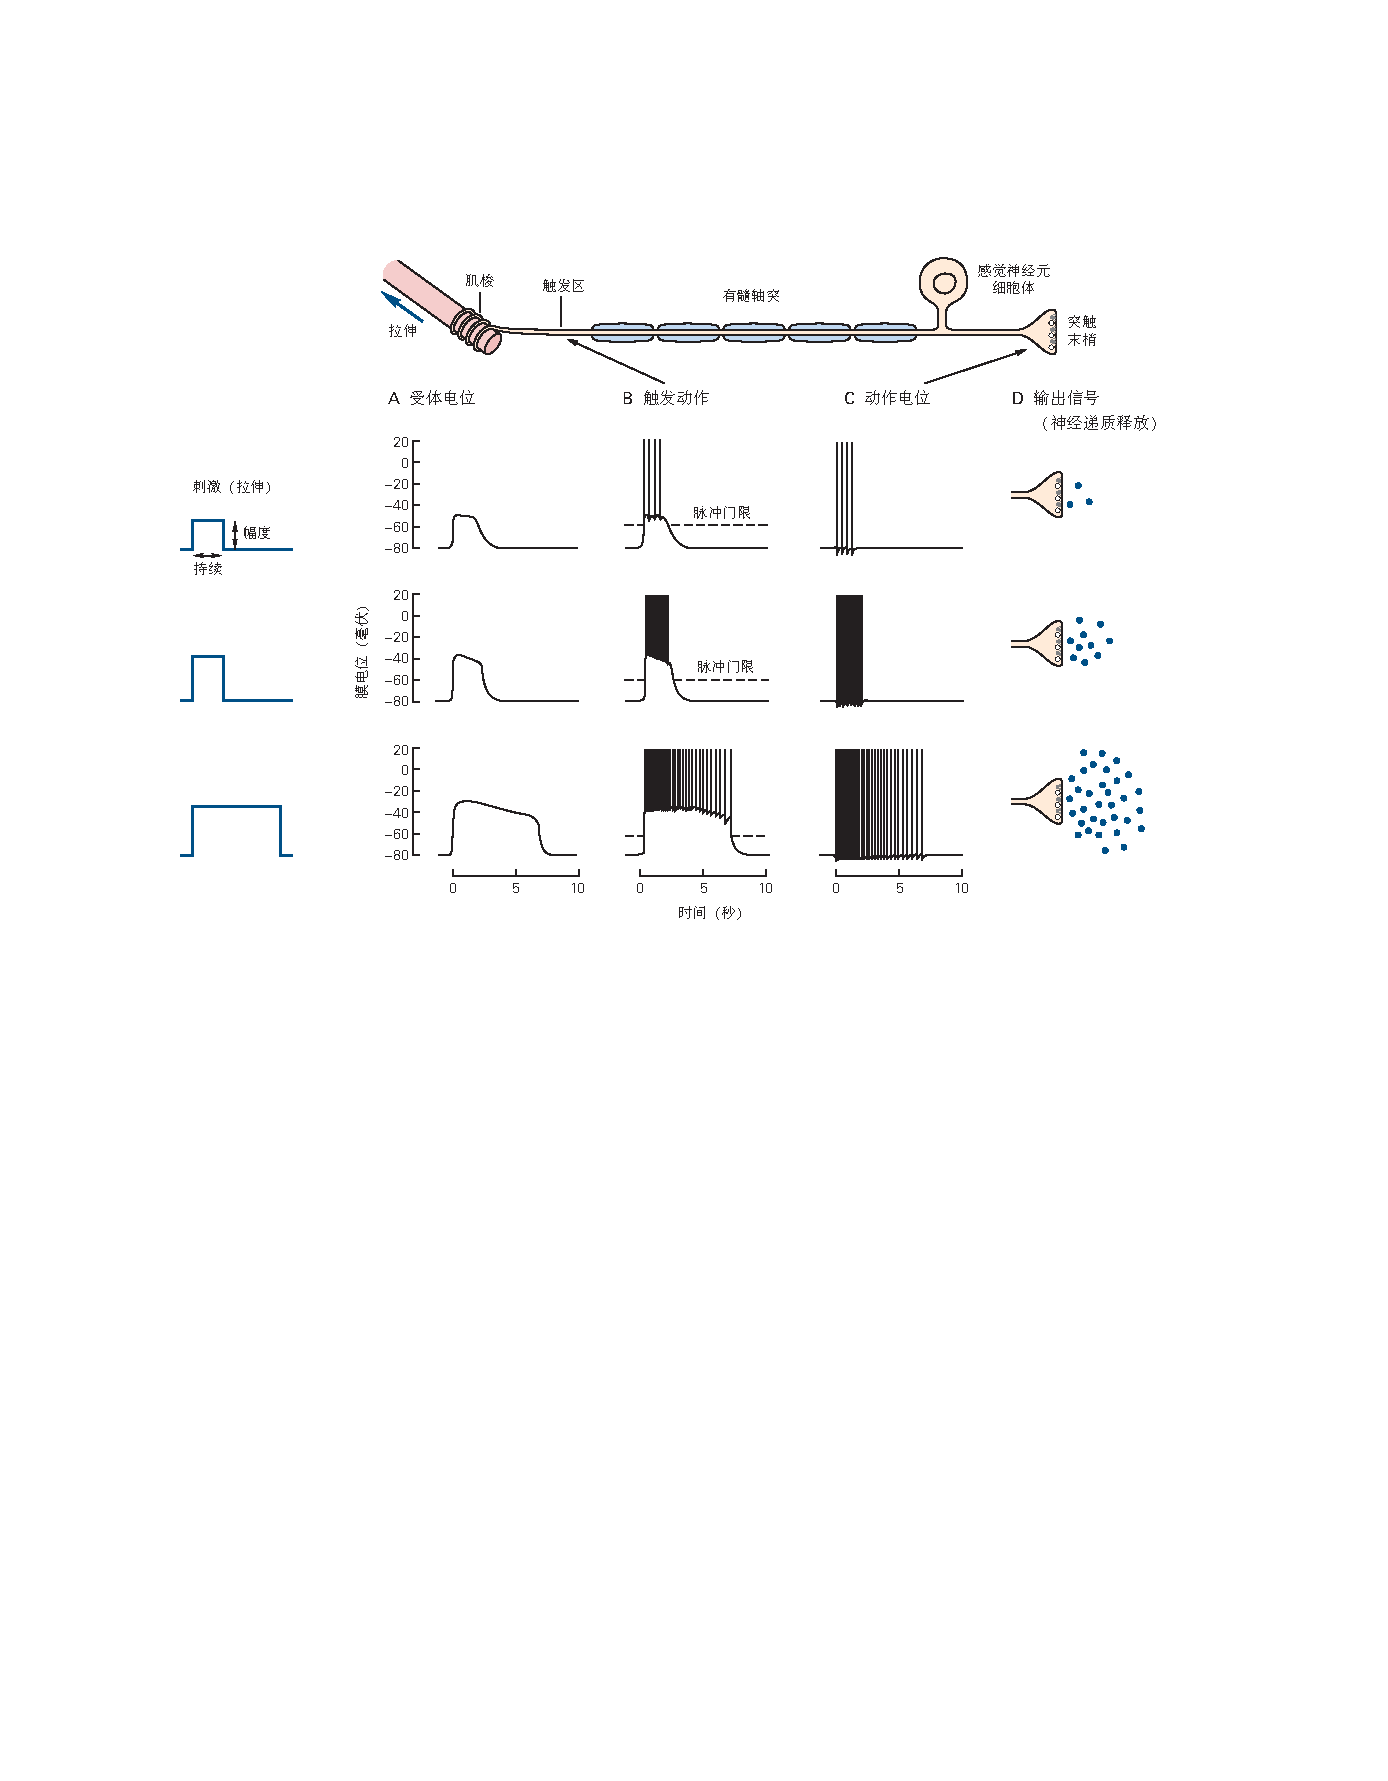
\includegraphics[width=1.0\linewidth]{chap03/fig_3_9}
	\caption{神经元的四个信号成分中的每一个都会产生一个特征信号。
		该图显示了通过肌肉拉伸激活的感觉神经元,神经元通过专门的受体(肌梭)感知。 
		\textbf{A.} 输入信号,称为受体电位,在振幅和持续时间上分级,与刺激的振幅和持续时间成正比。 
		\textbf{B.} \textit{触发区}总结了受体电位产生的去极化。
		只有当受体电位超过某个电压阈值时才会产生动作电位。
		一旦超过这个阈值,受体电位幅度的任何进一步增加只能增加动作电位产生的频率,因为动作电位具有恒定的幅度。
		受体电位的持续时间决定了动作电位序列的持续时间。
		因此,受体电位的分级振幅和持续时间被转化为触发区产生的动作电位中的频率代码。
		产生的所有动作电位都忠实地沿着轴突传播。
		\textbf{C.} 动作电位是全有或全无。
		因为所有动作电位都具有相似的幅度和持续时间,所以放电的频率和持续时间编码了信号所携带的信息。
		\textbf{D.} 当动作电位到达突触末梢时,它会启动神经递质的释放,即用作输出信号的化学物质。
		突触前细胞中动作电位的频率决定了细胞释放多少神经递质。}
	\label{fig:3_9}
\end{figure}


受体电位是在神经系统中编码的第一个拉伸表示。
然而,由于这种去极化从拉伸感受器被动传播,它不会传播很远。
如果轴突的直径较大,则距离较长,如果直径较小,则距离较短。
此外,如果电流可以轻松通过膜,则距离会更短,如果膜被髓磷脂绝缘,则距离会更长。
因此,来自拉伸感受器的感受器电位仅移动 1 至 2 毫米。
事实上,就在 1 毫米远的地方,信号的幅度仅为产生位置的三分之一左右。 
为了成功地传送到脊髓,局部信号必须被放大——它必须产生动作电位。
在膝跳反射中,如果感觉神经元中的受体电位到达轴突中朗飞的第一个节点并且足够大,它将触发动作电位(图~\ref{fig:3_9}B),然后无故障地传播到轴突 脊髓中的末端(图~\ref{fig:3_9}C)。 
在感觉神经元和运动神经元之间的突触处,动作电位会产生一系列事件,这些事件会导致运动神经元的输入信号。


在膝跳反射中,感觉神经元突触前末梢的动作电位启动化学物质或神经递质释放到突触间隙(图~\ref{fig:3_9}D)。
扩散穿过裂隙后,递质与运动神经元突触后膜中的受体蛋白结合,从而直接或间接打开离子通道。
随后的电流流动会短暂地改变运动细胞的膜电位,这种变化称为突触电位。


与受体电位一样,突触电位也是分级的; 
它的振幅取决于释放发射器的量。 
在同一细胞中,突触电位可以去极化或超极化,具体取决于被激活的受体分子的类型。 
突触电位,如受体电位,被动传播。 
因此,电位的变化将保持局部,除非信号超出轴突的初始段,在那里它可以产生动作电位。 
一些树突并非完全被动,而是包含促进突触电位的特化,从而提高其产生动作电位的功效(第~\ref{chap:chap13}~章)。 
表~\ref{tab:3_1}~总结了受体和突触电位的特征。


\begin{table}[htbp]
	\caption{局部(被动)和传播信号的比较} \label{tab:3_1} \centering
	\begin{tabular}{llllll}
		\toprule
		信号类型 & 幅值(毫伏) & 持续时间 & 总和 & 信号效应 & 传播类型\\
		\midrule
		\makecell{局部被动信号\\受体电位} & 小(0.1–10) & 短暂(5-100毫秒) & 分级 & 超级化或去极化 & 被动 \\
		\midrule
		突触电位 & 由短到长 & 短暂(5-100毫秒) & 分级 & 超级化或去极化 & 被动 \\
		\makecell{传播(激活)的信号\\动作电位} & 大(70–110) & 短暂(1-10毫秒) & 全有或全无 & 
		去极化 & 主动 \\
		\bottomrule
	\end{tabular}
\end{table}


\subsection{触发区决定产生动作电位}
谢林顿首先指出,神经系统的功能是权衡不同类型信息的后果,然后决定适当的反应。 
神经系统的这种整合功能在神经元触发区(轴突的初始部分)的事件中清晰可见。


动作电位是由 \ce{Na+} 通过细胞膜中的通道突然流入而产生的,这些通道响应于膜电位的变化而打开和关闭。 
当输入信号(受体电位或突触电位)使膜区域去极化时,膜电位的局部变化会打开局部 \ce{Na+} 通道,使 \ce{Na+} 沿着其浓度梯度从 \ce{Na+} 浓度高的细胞外流到细胞内 它低的地方。


由于轴突的起始段具有最高密度的电压敏感 \ce{Na+} 通道,因此产生动作电位的阈值最低,因此沿细胞膜被动传播的输入信号更有可能在起始段产生动作电位轴突的部分比在细胞中的其他部位。
因此,这部分轴突被称为触发区。
所有受体(或突触)电位的活动都在这里求和,如果输入信号的总和达到阈值,神经元就会产生动作电位。


\subsection{导电成分传播全有或全无动作电位}
动作电位是全有或全无:
低于阈值的刺激不会产生信号,但高于阈值的刺激都会产生相同幅度的信号。
无论刺激强度或持续时间的变化如何,每个动作电位的幅度和持续时间几乎相同,这适用于沿着有髓轴突的朗飞节点处的每个再生动作电位。
此外,与被动传播和振幅减小的受体和突触电位不同,正如我们所见,动作电位在沿着轴突到达其目标(距离可达 1 米)时不会衰减。 
因为它是周期性再生的。
这种传导信号可以以高达 100 米每秒的速度传播。 
事实上,动作电位的显着特征是它们是高度刻板的,从一个神经细胞到另一个神经细胞的变化很小(但在某些情况下很重要)。 
\textit{埃德加·阿德里安}在 1920 年代证明了这一特征,他是最早在细胞水平上研究神经系统的人之一。
阿德里安发现所有动作电位都具有相似的形状或波形(见图~\ref{fig:3_2})。
由感觉轴突带入神经系统的动作电位与由运动轴突从神经系统带入肌肉的动作电位通常无法区分。


传导信号只有两个特征传达信息:动作电位的数量和它们之间的时间间隔(图~\ref{fig:3_9}C)。 
正如\textit{阿德里安}在 1928 年总结他对感觉纤维的研究时所说:“所有的冲动都非常相似,无论信息是注定要引起光感、触感还是痛感;
如果它们挤在一起,感觉就会强烈,如果它们相距很远,感觉就会相应地微弱。” 
因此,决定感觉强度或运动速度的是动作电位的频率。
同样,感觉或运动的持续时间由产生动作电位的时间段决定。


除了动作电位的频率,动作电位的模式也传达了重要的信息。
例如,一些神经元在没有刺激的情况下会自发活跃。
一些自发活跃的神经细胞(跳动的神经元)有规律地激发动作电位;
其他人(爆发的神经元)在短暂的动作电位爆发中发射。
这些不同的细胞对相同的兴奋性突触输入有不同的反应。
兴奋性突触电位可能会在一个非自发活跃的细胞中启动一个或多个动作电位,而对自发活跃细胞的相同输入只会增加现有的放电率。


当输入信号具有抑制性时,会出现更显着的差异。
抑制性输入在沉默细胞中几乎没有信息价值。 
相比之下,在自发活跃的细胞中,抑制可以起到强大的塑造作用。
通过在其他正在进行的活动中建立沉默期,抑制可以在不存在的地方产生一种复杂的交替放电和沉默模式。
放电模式的这种细微差异可能对神经元之间的信息传递产生重要的功能影响。
神经元网络的数学建模者试图描述神经代码,其中信息也由细粒度的放电模式——每个动作电位的确切时间——携带。


如果信号是固定的并且仅反映刺激的最基本属性,那么它们如何携带复杂行为所需的丰富信息呢?
如何将包含蜜蜂视觉信息的信息与包含蜜蜂蜇伤疼痛信息的信息区分开来?
这些感觉信号与自主运动的运动信号有何区别? 
答案很简单,但却是神经系统最重要的组织原则之一:
相互连接的神经元形成解剖学和功能上不同的通路——标记线——正是这些连接神经元的通路,这些标记线,而不是单个神经元都传达信息。 
视网膜中对光有反应的受体细胞激活的神经通路与皮肤中对触觉有反应的感觉细胞激活的神经通路完全不同。


\subsection{输出组件释放神经递质}

当动作电位到达神经元的末端时,它会刺激细胞释放化学物质。
这些物质称为神经递质,可以是有机小分子,例如L-谷氨酸和乙酰胆碱,也可以是肽,例如 P 物质或 \textit{黄体生成素-释放激素}。


神经递质分子存在于称为突触小泡的亚细胞器中,突触小泡聚集在轴突末端的特殊释放部位,称为活性区。
为了将它们的递质物质喷射到突触间隙中,囊泡向上移动并与神经元的质膜融合,然后通过已知的过程突然打开以将递质释放到突触间隙(突触前细胞和突触后细胞之间的细胞外空间)中作为胞吐作用。
第~\ref{chap:chap14}~章和第~\ref{chap:chap15}~章描述了神经递质释放的分子机制。


释放的神经递质分子是神经元的输出信号。 
因此,输出信号根据释放的递质量进行分级,递质量由到达突触前末梢的动作电位的数量和频率决定(图~\ref{fig:3_9}C,D)。
释放后,递质分子扩散穿过突触间隙并与突触后神经元上的受体结合。
这种结合导致突触后细胞产生突触电位。
突触电位是否具有兴奋或抑制作用取决于突触后细胞中受体的类型,而不取决于特定的化学神经递质。
相同的递质物质在不同的受体上可能有不同的作用。



\subsection{牵张反射通路说明了神经信号从感觉到运动的转变}

正如我们所见,当信号从神经元的一个组成部分移动到另一个组成部分或在神经元之间移动时,信号的属性会发生变化。 
在牵张反射中,当肌肉被拉伸时,刺激的幅度和持续时间反映在感觉神经元中产生的受体电位的幅度和持续时间中(图~\ref{fig:3_10}A)。
如果受体电位超过该细胞中动作电位的阈值,则分级信号会在触发区转换为动作电位。
尽管个体动作电位是全有或全无信号,但受体电位超过阈值越多,去极化越大,因此轴突中动作电位的频率就越高。
输入信号的持续时间也决定了动作电位序列的持续时间。


\begin{figure}[htbp]
	\centering
	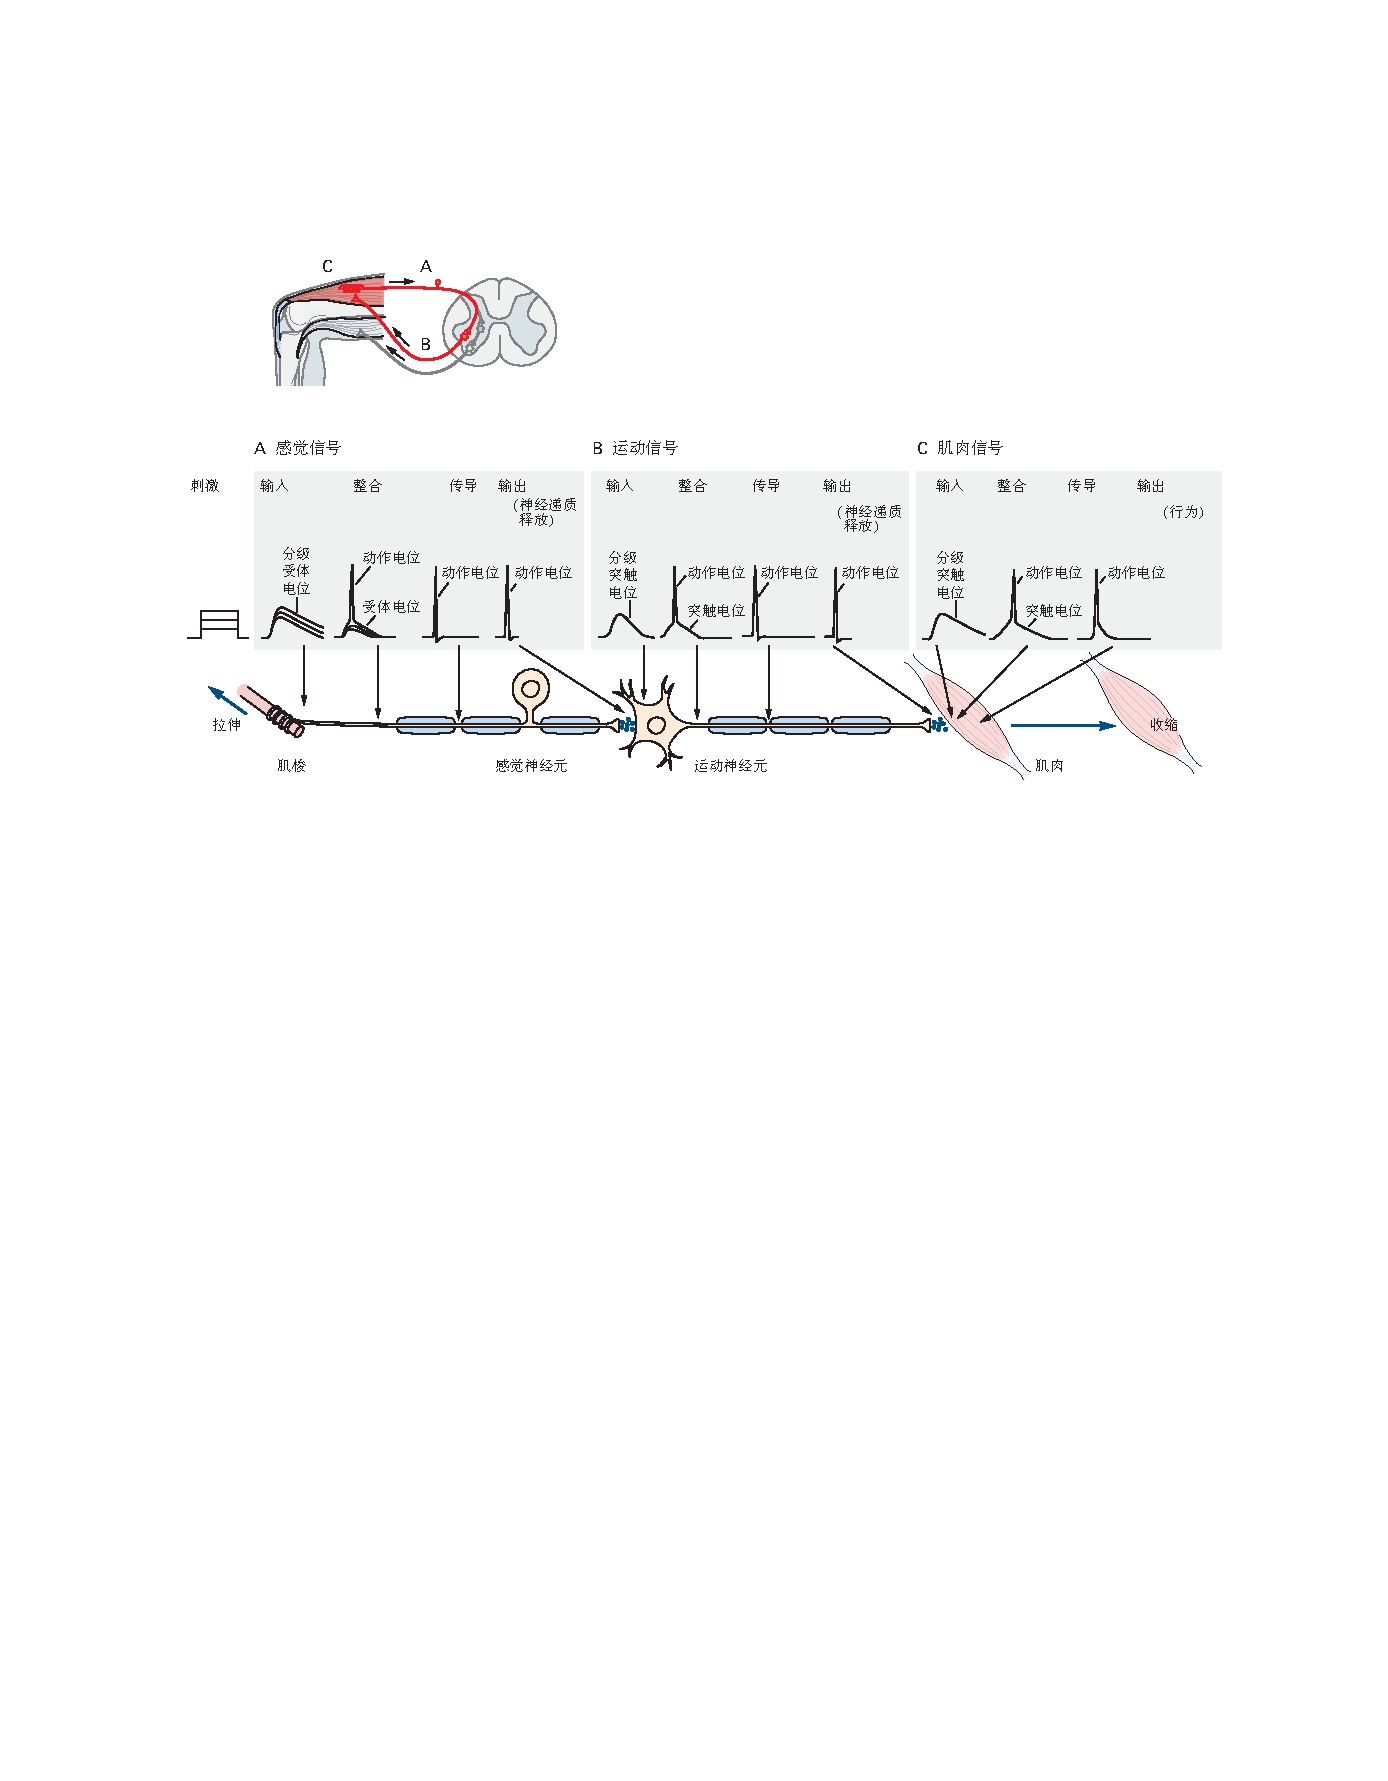
\includegraphics[width=1.0\linewidth]{chap03/fig_3_10}
	\caption{产生反射动作的信号序列。
		\textbf{A.} 肌肉的拉伸会在专门的受体(肌梭)中产生受体电位。 
		受体电位的幅度与拉伸强度成正比。 
		这种势能被动地传播到朗飞第一个节点的综合区或触发区。
		如果受体电位足够大,它会触发动作电位,然后沿着轴突主动传播而不会发生变化,直至轴突末端。
		在终端的特定位置,动作电位导致化学神经递质(输出信号)的释放。
		递质扩散穿过轴突末端和支配拉伸肌肉的目标运动神经元之间的突触间隙;
		然后它与运动神经元外膜上的受体分子结合。
		\textbf{B.} 这种相互作用启动了一个被动传播到运动神经元轴突触发区的突触电位,在那里它启动了一个主动传播到运动神经元轴突末端的动作电位。
		在轴突末端,动作电位导致肌肉纤维附近神经递质的释放。
		\textbf{C.} 神经递质结合肌纤维上的受体,产生突触电位。
		突触电位触发肌肉中的动作电位,从而引起收缩。}
	\label{fig:3_10}
\end{figure}


由放电频率和持续时间编码的信息沿着轴突忠实地传递到其末端,在那里动作电位的放电决定了发射器的释放量。 
这些信号阶段在运动神经元(图 \ref{fig:3_10}B)和肌肉(图 \ref{fig:3_10}C)中有对应的阶段。


\section{神经细胞在分子水平上的差异最大}
我们概述的神经元信号模型是一种适用于大多数神经元的简化模型,但也有一些重要的变化。 
例如,一些神经元不产生动作电位。 
这些通常是没有导电成分的局部中间神经元; 它们没有轴突或轴突太短以至于不需要信号的再生。 
在这些神经元中,输入信号被汇总并被动传播到释放递质附近的突触前末梢区域。 
自发活跃的神经元不需要感觉或突触输入来激发动作电位,因为它们具有一类特殊的离子通道,即使在没有兴奋性突触输入的情况下也允许 \ce{Na+} 电流流动。


即使是形态相似的细胞在分子细节上也可能存在重大差异。 
例如,它们可以具有不同的离子通道组合。 
正如我们将在第 \ref{chap:chap10} 章中了解到的,不同的离子通道为神经元提供了不同的阈值、兴奋特性和放电模式。 
这样的神经元可以将突触电位编码成不同的放电模式,从而传达不同的信息。


神经元在用作递质的化学物质和从其他神经元接收递质物质的受体方面也有所不同。 
事实上,许多作用于大脑的药物都是通过改变特定化学递质或受体的作用来实现的。 
由于神经元之间的生理差异,一种疾病可能影响一类神经元而不影响其他神经元。 
某些疾病只影响运动神经元(肌萎缩侧索硬化症和脊髓灰质炎),而其他疾病主要影响感觉神经元(麻风病和脊髓灰质炎,梅毒晚期)。 
帕金森病是一种随意运动障碍,会损害一小部分使用多巴胺作为神经递质的神经元。 
有些疾病甚至在神经元内也具有选择性,仅影响感受元件、细胞体或轴突。 
在第 \ref{chap:chap57} 章中,我们描述了对重症肌无力(一种由肌肉膜中有缺陷的递质受体引起的疾病)的研究如何为突触传递提供了重要的见解。 
事实上,由于神经系统在分子水平上有如此多的细胞类型和变异,它比身体的任何其他器官系统更容易患上更多的疾病(精神病学和神经学)。


尽管神经细胞之间存在形态差异,但电信号的分子机制却惊人地相似。 
这种简单性是幸运的,因为了解一种神经细胞中信号传导的分子机制有助于理解许多其他神经细胞中的这些机制。


\section{反射回路是理解行为神经结构的起点}
牵张反射说明了几种类型的神经细胞之间的相互作用如何构成一个产生简单行为的功能回路,即使涉及的神经元数量很大(牵张反射回路可能有几百个感觉神经元和一百个运动神经元) 神经元)。 
一些无脊椎动物能够使用少得多的神经元做出与反射一样复杂的行为。 
此外,在某些情况下,仅一个关键命令神经元就可以触发复杂的行为,例如从有害刺激中撤回身体部位。


对于更复杂的行为,尤其是高等脊椎动物,需要许多神经元,但通常会保留简单反射的基本神经结构。 
首先,通常有一组可识别的神经元,其放电率会随着特定类型的环境刺激而变化,例如特定频率的音调,或特定角度的明暗并置。 
正如牵张感受器神经元的放电率编码肌肉紧张程度,皮层感觉区域的皮层神经元放电率编码感觉特征的强度(例如,轮廓的对比度)。 
正如我们将在后面的章节中看到的那样,仅通过改变一小组神经元的放电率就可以改变知觉的特征。


其次,通常有一组可识别的神经元,其放电率在动物执行运动动作之前发生变化。 
正如运动神经元的尖峰率控制股四头肌收缩的幅度——因此膝反射——运动皮层神经元的放电率也影响将要进行的运动的潜伏期和类型。 
这些神经元究竟对运动的哪个方面进行了编码仍然是一个活跃的研究领域,但已经确定的是,神经元组通过调整其放电率以分级方式影响随后的动作。 
在大脑皮层的其他关联区域,神经元的分级放电率编码对思维过程至关重要的数量,例如与选择相关的证据数量(第 \ref{chap:chap56} 章)。


尽管复杂的心理操作比简单的牵张反射复杂得多,但考虑认知功能在多大程度上受到以类似于简单反射的任何方式组织的神经机制的支持,可能证明是有用的。 
调解复杂的行为和思想可能需要哪些类型的阐述? 
与具有复杂行为的简单反射不同,感觉神经元的激活不会立即引起反射动作。 
这个过程有更多的偶然性。 
尽管简单的反应受上下文调节,但心理功能更受复杂的突发事件的影响,考虑到任何一种刺激的许多可能影响以及任何一种行为的许多可能的沉淀物。 
鉴于这些突发事件,我们不得不设想在大脑的数据采集系统(不仅是感觉系统,还有记忆系统)和效应器系统之间建立灵活的路由。 
正如我们将在后面的章节中看到的那样,这是大脑皮层的高级联合区域的作用,与几个皮层下脑结构协同作用。


也许复杂的心理功能和反射之间更显着的区别是行动的时机。 
一旦被激活,反射回路几乎会在感官刺激后立即采取行动。 
任何延迟主要取决于反射的传入和传出肢体中动作电位的传导速度(例如,踝反射比膝反射慢,因为脊髓离小腿肌肉的牵张感受器比它离小腿肌肉的牵拉感受器更远) 来自大腿伸肌)。 
对于更复杂的行为,动作不需要随着感官信息的到达而或多或少地立即发生。 它可能会延迟等待其他信息或仅在特定情况发生时才表达。


有趣的是,灵长类动物皮层联合区的神经元有能力在数秒内维持分级放电率。 
这些神经元大量存在于调节感觉和运动区域之间灵活联系的大脑区域。 
它们提供了摆脱反射行为的瞬时性质的自由,因此可以提供将认知功能与更直接的感觉运动转换(如反射)区分开来的基本回路特性。


\section{神经回路可以通过经验进行修改}
学习可以导致持续数年甚至一生的行为改变。 
但即使是简单的反应也可以改变,尽管时间要短得多。 
许多行为可以通过学习来改变这一事实提出了一个有趣的问题:如果神经系统连接得如此精确,那么行为是如何改变的呢? 
当信号单元(神经元)之间的连接在早期发育过程中设置时,行为的神经控制如何发生变化?


针对这一困境,已经提出了几种解决方案。 
最有远见的提议是可塑性假说,该假说由\textit{拉蒙·卡哈尔}在 20 世纪之交首次提出。 
波兰心理学家\textit{杰泽·科诺尔斯基}于 1948 年提出了这一假设的现代形式。


刺激的应用导致神经系统发生双重变化……第一个特性,神经细胞据此对传入的冲动做出反应……我们称之为兴奋性,并且……由于这个特性而产生变化…… 我们称由于兴奋性而产生的变化。
第二个属性,由于适当的刺激或它们的组合,特定的神经元系统中会出现某些永久的功能转换,我们将称之为可塑性和相应的变化可塑性变化。


现在有相当多的证据表明化学突触的功能可塑性。 
这些突触通常具有显着的短期生理变化(持续几秒到几小时)的能力,这些变化会增加或减少突触的有效性。 
长期的生理变化(持续数天或更长时间)会引起解剖学改变,包括突触的修剪甚至新突触的生长。 
正如我们将在后面的章节中看到的那样,化学突触在早期发育的关键时期以及整个生命过程中都会在功能和解剖学上发生变化。 
神经元的这种功能可塑性赋予我们每个人与周围自然和社会世界互动的独特方式。



\section{亮点}
1. 神经细胞是神经系统的信号单位。 信号主要是细胞内的电信号和细胞之间的化学信号。 
尽管大小和形状各不相同,但神经细胞具有某些共同特征。 
每个人都有专门的受体或传感器,分别接收来自其他神经细胞或感官的输入; 
一种将输入转换为电信号的机制; 产生全或无电脉冲的阈值机制,即动作电位,可以沿着将神经细胞连接到其突触目标(另一个神经细胞、肌肉或腺体)的轴突再生; 以及产生影响目标的化学物质(神经递质)释放的能力。


2.胶质细胞支持神经细胞。 
一种类型提供绝缘,可加速动作电位沿轴突的传播。 
其他帮助建立神经细胞运作的化学环境,还有一些将神经活动与神经系统的血管供应联系起来。


3. 神经细胞的形态、它们建立的联系以及它们建立的位置不同。 
这在视网膜等特殊结构中最为明显。 
也许神经元之间最大的差异是在分子水平上。 
分子多样性的例子包括不同受体的表达、用于合成不同神经递质的酶以及离子通道的不同表达。 
基因表达的差异为理解为什么某些疾病影响某些神经元而不影响其他神经元提供了起点。


4. 每个神经细胞都是具有一种或多种行为功能的回路的一部分。 
牵张反射回路是一个简单电路的例子,它会产生响应刺激的行为。 
它的简单性掩盖了综合功能,例如放松对抗拉伸肌肉的肌肉。


5. 现代神经科学渴望解释比反射复杂得多的心理过程。 
一个自然的起点是理解必须详细说明回路以支持感觉运动转换的方式,这与反射不同,它是偶然的、灵活的,并且不受制于即时的感觉处理和运动控制。


6. 神经连接可以根据经验进行修改。 
在简单的回路中,这个过程是神经元之间连接强度的简单变化。 
现代神经科学的一个工作假设是,在简单回路中发挥作用的“可塑性”机制在学习更复杂的行为和认知功能方面也发挥着关键作用。


%\section{选读}
%
%\section{参考文献}













\chapter{神经回路介导行为的神经解剖学基础}
% PDF所在目录: /data2/whd/win10/learn/neuro/neuro_神经科学原理_28_中枢神经系统的听觉处理.pdf

\section{局部回路执行特定的神经计算,这些计算被协调以调制复杂的行为}


\section{体感系统中的感官信息回路}
\subsection{来自躯干和四肢的体感信息被传送到脊髓}
\subsection{躯干和四肢的初级感觉神经元聚集在背根神经节}
\subsection{脊髓中背根神经节神经元的中央轴突末端产生体表图}
\subsection{每个躯体亚模态都在从外围到大脑的不同子系统中处理}

\section{丘脑是感觉受体和大脑皮层之间的重要纽带}

\section{感觉信息处理在大脑皮层达到顶峰}

\section{自主运动是由皮层和脊髓之间的直接连接介导的}

\section{大脑中的调节系统影响动机、情绪和记忆}

\section{周围神经系统在解剖学上与中枢神经系统不同}

\section{记忆是一种复杂的行为,由不同于执行感觉或运动的结构介导}
\subsection{海马系统与最高级别的多感觉皮层区域相互连接}
\subsection{海马结构由几个不同但高度集成的电路组成}
\subsection{海马结构主要由单向连接组成}


\section{亮点}
\section{选读}
\section{参考文献}
























\chapter{行为调节神经回路的计算基础} \label{chap:chap5}

上一章重点介绍了大脑神经解剖学以及大脑不同区域之间的联系。
要了解这些连接是如何调节行为,需要深入了解不同神经元群体活动所代表的信息是如何传递和处理的。
这种理解大部分来自对单个神经元产生的微小电信号的记录。


虽然通过一次记录一个或几个神经元已经了解了很多东西,但小型化和电子技术的进步现在使得同时记录多个大脑区域数百个单个神经元的动作电位成为可能,通常是在感觉、运动或认知任务的背景下(方框~\ref{box:5_1})。这些进步,加上管理和理解大型数据集的计算方法,有望彻底改变我们对神经功能的理解。


\begin{proposition}[光学神经成像] \label{box:5_1}
	
	\quad \quad 光学成像方法是用于大规模监测神经回路动力学的一个快速发展的技术领域。
	这些方法中的大多数都使用荧光传感器(合成染料或基因工程和编码的蛋白质),通过激发后发出的光的大小或波长的变化来发出神经活动变化的信号。
	根据荧光激发的来源,已经开发了各种荧光成像方法,包括单光子、多光子和超分辨率荧光显微成像。
	
	\quad \quad 最常用的荧光指示剂将细胞内钙水平的变化作为神经元电活动的指标。
	虽然荧光钙成像的时间分辨率通常低于电生理学的时间分辨率,但具有基因编码钙指示剂的荧光成像能够在几天到几周和几个月内同时监测行为动物中数千个单独识别的神经元。
	
	\quad \quad 除了钙成像外,合成和遗传编码的电活性荧光指示剂(如\textit{基因编码的电压指示剂})、神经递质浓度报告因子(如\textit{谷氨酸盐感应荧光受体})、细胞内信号分子的活性状态和基因表达为在多个空间和时间尺度上监测神经活动提供了快速扩展和通用的技术。
	
\end{proposition}


与此同时,基于单个神经元\textit{mRNA}测序的现代遗传方法正在揭示促成群体活动的多种细胞类型。
基于遗传的方法还允许在实验期间激活或沉默定义类型的神经元,支持因果关系的测试(方框~\ref{fig:5_2})。


\begin{proposition}[神经元活动的光遗传学和化学遗传学操作] \label{box:5_2}
	
	\quad \quad 神经回路的功能分析依赖于准确操作已识别的回路元件以阐明其在生理和行为中的作用的能力。
	已经开发了基因编码的神经扰动工具,用于使用激活工程受体的光(光遗传学)或小分子(化学遗传学)远程控制神经元功能。
	
	\quad \quad 基因编码的外源蛋白可以使用病毒或转基因动物在分子、基因或空间指定的神经元亚群中表达,用于随后对这些细胞群的选择性扰动。
	光遗传学方法涉及光敏蛋白的表达和随后的光传递到由此产生的光敏神经元。
	根据光遗传学致动器的类型,光激活将分别通过去极化或超极化细胞膜来增强神经活动(例如,通道视紫红质等光控离子通道)或抑制神经活动(如卤视紫红质和古菌视紫红质的光控离子泵)。
	
	\quad \quad 或者,可以使用化学遗传致动器远程激活或沉默选定的神经元群体,化学遗传致动器是使用遗传方法靶向定义的神经元群体的基因工程受体;
	它们可以通过小分子合成配体被激活,该配体在递送时选择性地与这些受体相互作用(例如\textit{设计药物激活的设计受体})。
	
	\quad \quad 这些光遗传学和化学遗传学工具对神经元活动提供了精确的时空控制,以探索神经元细胞类型、回路生理学和行为之间的因果关系。
	
\end{proposition}



在光学显微镜和电子显微镜的尺度上,高通量解剖方法正在以前所未有的详细程度和完整性提供有关回路布线的信息。
神经回路的复杂性和从中收集的大量数据集推动了统计、计算和理论方法的发展和应用,用于提取、分析、建模和解释结果。
这些方法用于研究范围广泛的问题:
实验设计、从原始数据中提取信号、大型复杂数据集的分析、模拟数据的模型的构建和分析,最后也是最重要的是,从结果中建立某种形式的理解。


信号提取通常基于贝叶斯方法进行,推断出嘈杂记录中最有可能出现的信号。
数据分析通常包括减少大型数据集的维数,不仅仅是为了使其更紧凑,而是为了确定构建数据集的基本组件。


神经系统模型的范围从单个神经元的形态学和电生理学的详细模拟到大量神经元的更抽象模型。
无论详细程度如何,模型的目的都是揭示神经元或神经元网络的测量特征如何影响神经元或神经回路的功能。


此外,在最高级别的功能中,例如识别图像、玩游戏或执行人类级别的任务,机器学习的想法正日益影响神经科学研究。


在本章中,我们介绍了用于描述和解释神经群和电路活动的思想、技术和方法,并举例说明了大脑研究的一些领域。本书后面将更详细地讨论其中的许多主题。



\section{神经放电模式提供信息编码}

\subsection{感觉信息由神经活动编码}

动物和人类通过感官不断积累关于世界的信息,根据这些信息做出决定,并在必要时采取行动。
为了处理感官信息以用于决策和行动,必须将其转化为电信号,从而在大脑中产生神经活动模式。
研究这种神经表征及其与外部感觉线索的关系,统称为神经编码,是神经科学研究的一个主要领域。
刺激的特征由神经活动表示的过程称为编码。


神经表征的结构在神经系统如何进一步处理信息方面起着重要作用。
例如,视觉信息最初是在视网膜中通过感光器对一小块视野区域的颜色和光强的反应进行编码的。
然后,这些信息在大脑初级视觉皮层内进行转换,以定义场景的边缘和形状以及这些特征所在的位置为基础,对视觉场景进行编码。
进一步的转换发生在高阶视觉区域,从场景中提取复杂的形状和进一步的结构,包括物体甚至个人面孔的识别。
在大脑的其他区域,听觉编码反映了声音的频谱,触觉编码在代表身体表面的地图中。
神经元对感觉刺激的反应所激发的动作电位序列代表了这种刺激是如何随时间变化的。
神经编码研究旨在了解驱动神经元做出反应的刺激特征和反应的时间结构及其与外部世界变化的关系。



\subsection{可以从神经活动中解码信息}

感觉神经元对感觉特征的反应是通过激发动作电位来编码信息。
其他大脑区域,例如那些导致决策或产生运动动作的区域,必须正确解释它们从感觉区域接收到的动作电位序列的含义,以便做出适当的反应。
从神经活动中提取信息的过程称为解码。


神经信号的解码可以由神经科学家在实验和临床环境中完成。
例如,这种解码可以从视觉或听觉神经元的记录中推断出动物或人类正在看到或听到什么。
在实践中,只有刺激的某些特征可能被推断出来,但结果仍然令人印象深刻。
大量的解码程序已经开发出来,从简单的神经元放电率加权和到复杂的统计方法。


解码方法是神经假体开发的核心,适用于各种神经系统损伤导致大面积瘫痪的人(第~\ref{chap:chap39}~章)。
为了实现这一点,神经元通过植入的电极记录在顶叶皮层或运动皮层中,并使用在线解码程序来解释记录的神经活动所代表的运动意图。
然后使用推断出的意图来控制计算机光标或驱动机器人肢体。


解码记录的神经活动也让我们对神经回路中正在发生的事情有了一个非凡的了解,这反过来又提供了对记忆存储和检索、计划和决策以及其他认知功能。
下一节使用一种特别有趣的神经表征来说明这些见解,即啮齿动物海马体中空间位置的编码。


\subsection{可以解码海马空间认知图来推断位置}

% 定位
动物面临的最复杂的认知挑战之一是识别和记住它在环境中相对于其他显著物体位置的位置。
例如,贮藏种子的鸟类可以记住它们在几个月内储存食物的数百个不同地方的位置。
前一章简要介绍了与外显记忆形成有关的神经回路,即对人、地点、事物和事件的记忆。
这种形式的记忆需要海马体、内嗅皮层和颞叶中的相关结构。
1971 年,\textit{约翰$\cdot$奥基夫}发现了海马体中空间环境的神经表征的生理学证据。
2014 年,他与\textit{梅$\cdot$布里特$\cdot$莫泽}和\textit{爱德华$\cdot$莫泽}一起获得诺贝尔生理学或医学奖,以表彰他们在神经元空间表征方面的发现。


\textit{奥基夫}发现大鼠海马体中的单个细胞(称为位置细胞)仅在动物穿过环境的特定区域(称为细胞位置场)时才会放电(图~\ref{fig:5_1})。
随后的研究发现了其他几种哺乳动物(包括蝙蝠、猴子和人类)海马体中的位置细胞样活动。
不同的位置细胞集由给定环境中的不同位置激活。
因此,虽然单个位置细胞代表相对较小的空间区域,但海马体中完全不同的位置细胞群平铺了整个环境,并且任何给定位置都由独特的细胞群编码。
海马位置编码网络提供了一个认知地图的例子,最初由心理学家\textit{爱德华$\cdot$托尔曼}假设,它使动物能够成功地记住并导航其环境。
第~\ref{chap:chap52}~章和第~\ref{chap:chap54}~章详细探讨了海马体在记忆形成中的作用以及海马体空间图的编码机制。


\begin{figure}[htbp]
	\centering
	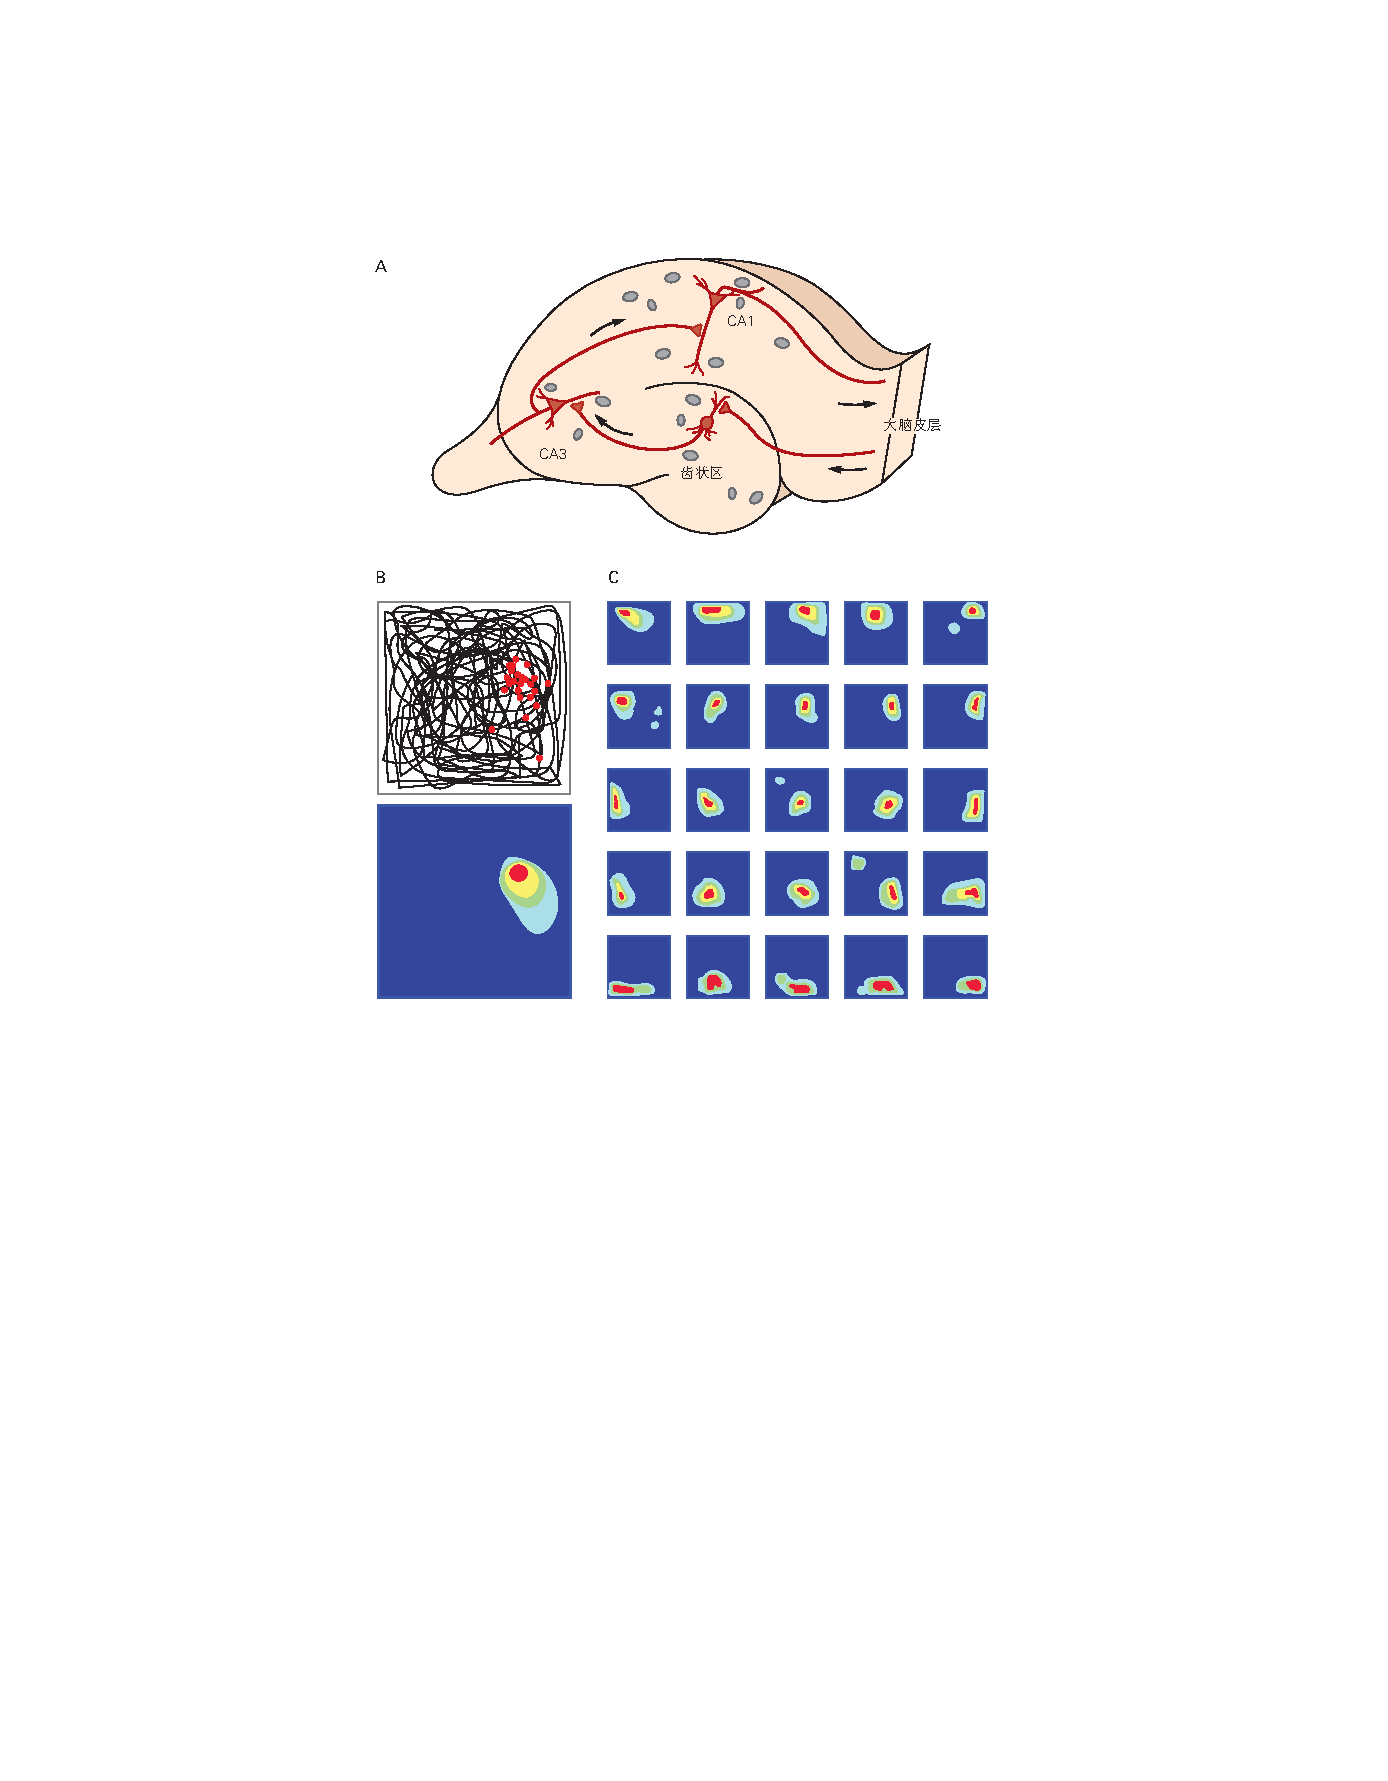
\includegraphics[width=0.9\linewidth]{chap05/fig_5_1}
	\caption{海马体位置细胞和位置细胞图。 
		\textbf{A.} 输入-输出转换发生在哺乳动物海马体的三突触回路中,从\textit{齿状回}输入区到\textit{阿蒙角}3 区,再到\textit{阿蒙角}1 输出区,每个区域的主要兴奋性神经元(红色)作为主要处理单元。
		主要细胞的活动由局部回路\textit{$\gamma$-氨基丁酸}活动的中间神经元(灰色)调节。
		\textbf{B.} 将细胞放电置于海马体中。
		老鼠穿过方形场地时所走的路径以黑色显示。
		电极被植入海马体内以记录单个细胞。
		上图:单个位置细胞会增加环境中离散位置的放电(每个动作电位由一个红点表示)。
		下图:位置细胞激活频率的颜色编码热图。
		较低波长的颜色(黄色和红色)代表在没有活动的背景(深蓝色)下较高的激活率。 
		\textbf{C.} 颜色编码的热图显示当大鼠探索一个方形盒子时在海马\textit{阿蒙角}1 区域同时记录的 25 个不同位置细胞的放电。}
	\label{fig:5_1}
\end{figure}


1971 年\textit{奥基夫}的可用的电生理方法仅限于一次记录一个位置细胞,但随后的进展允许研究人员同时记录数十个,最近数百个位置细胞。
关键的是,虽然单个位置细胞仅对环境的特定部分进行编码,并且容易在其位置场之外偶尔发出嘈杂的信号,但整个位置细胞群提供了更完整的空间覆盖和冗余位置编码的可靠性。
群体编码的这些特征为新的强大的计算分析铺平了道路。
特别是,可以解码位置细胞群体的活动并估计动物在环境中的位置。
这是通过确定每个细胞的空间选择性并使用该选择性作为模板来解码正在进行的活动来实现的。
在实践中,这种解码通常是通过加权每个细胞对动物位置最终估计的贡献来执行的,该因素与该细胞的空间编码可靠性成正比。
使用这种技术和类似技术,人们可以在房间大小的环境中以几厘米的精度逐秒重建动物的位置(图~\ref{fig:5_1}C)。



基于使用空间解码技术的研究,海马体功能与空间和陈述性记忆密切相关。
在积极探索环境期间,海马体活动反映位置编码,但在不动或静止行为期间,海马体进入不同的状态,在该状态下,神经活动由离散的半同步群体爆发主导,称为尖波涟漪(图~\ref{fig:5_2}A))。
这些事件被认为是由海马体内的回路在内部产生的。


\begin{figure}[htbp]
	\centering
	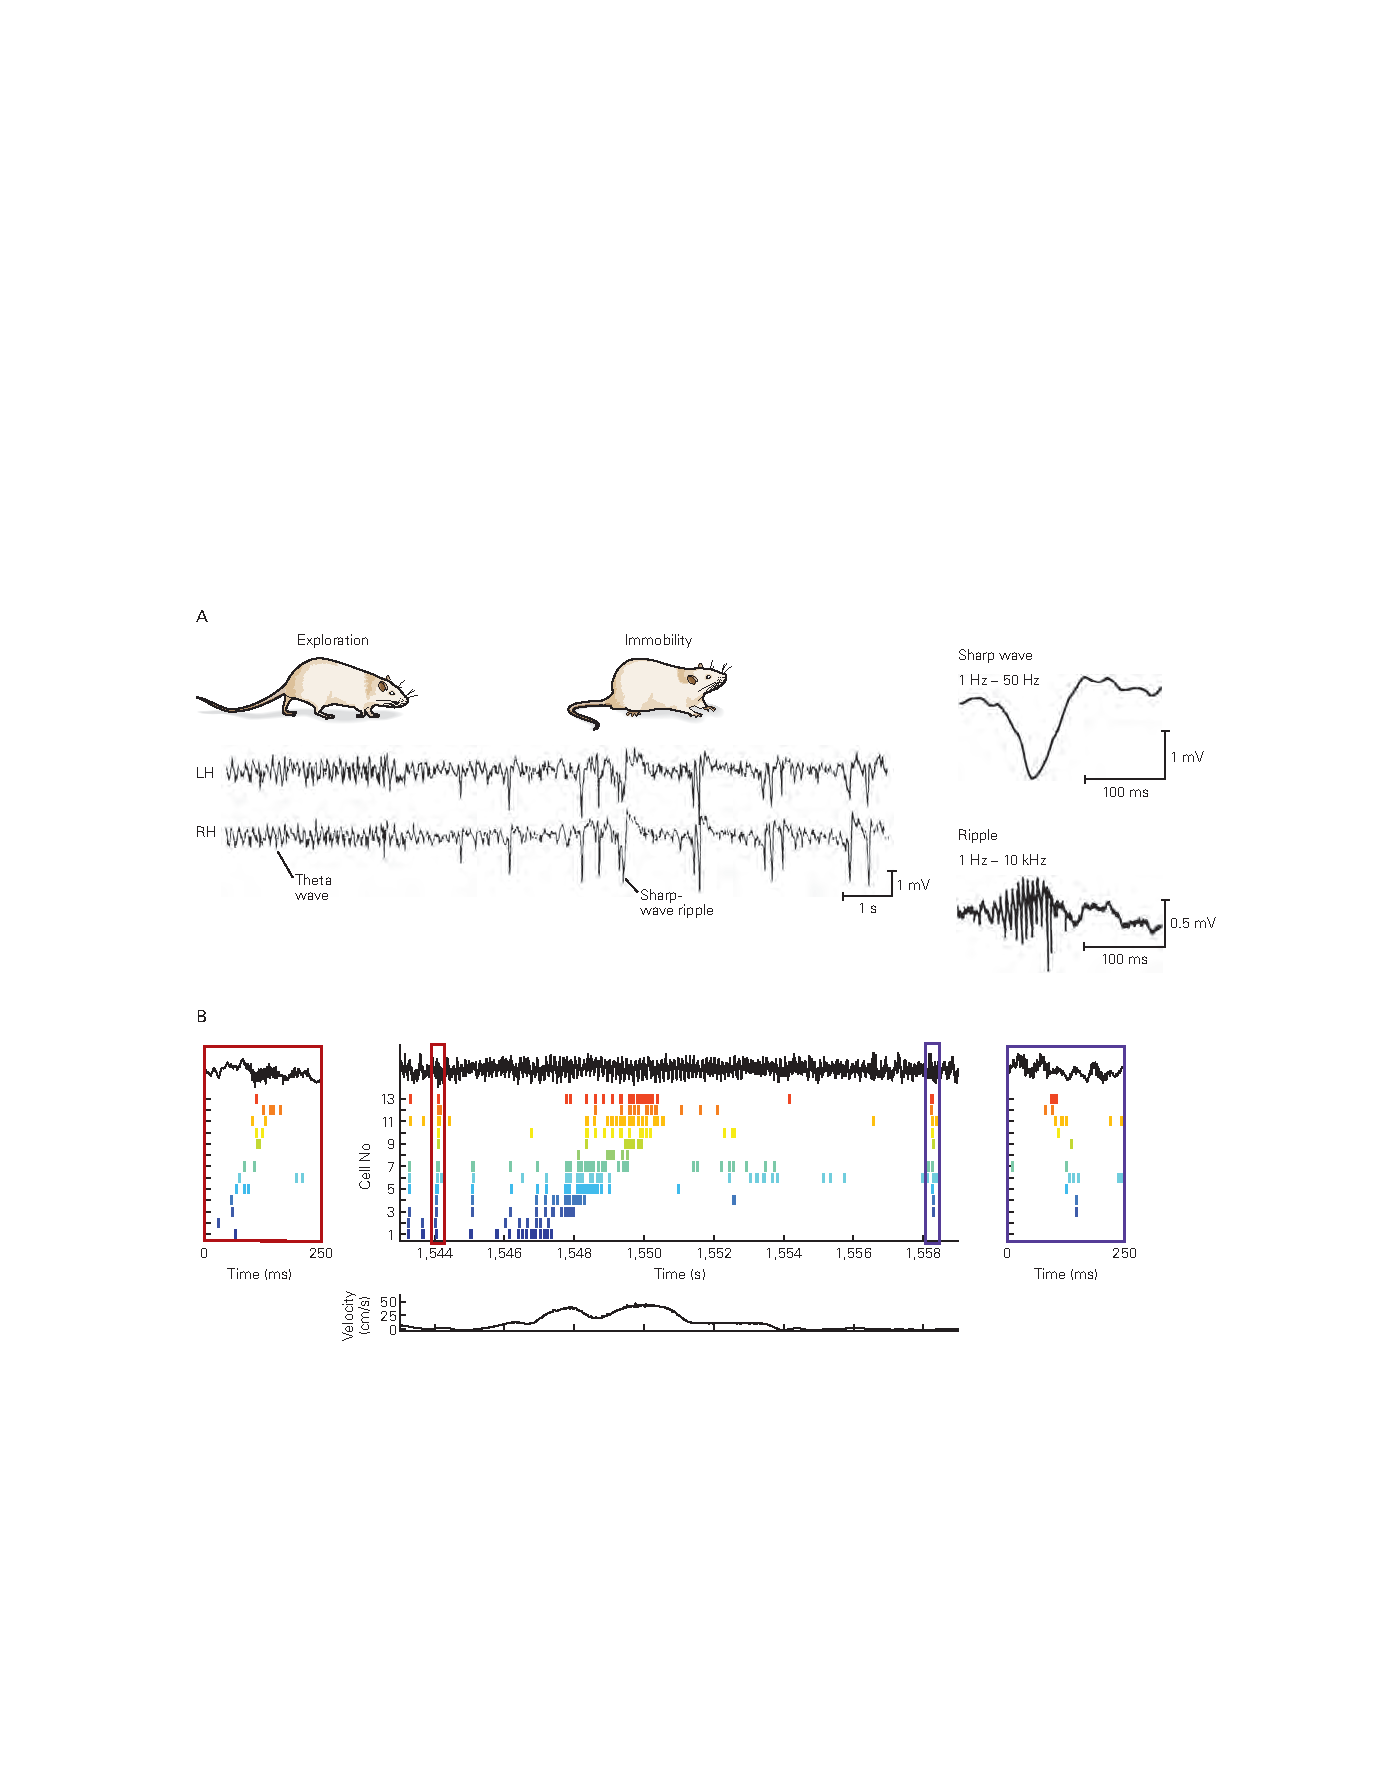
\includegraphics[width=1.0\linewidth]{chap05/fig_5_2}
	\caption{海马\textit{尖波涟漪}和\textit{序列回放}。 
		\textbf{A.} 左图:海马体\textit{局部场电位}活动的行为依赖性(\textit{左海马体}和\textit{右海马体})。
		在探索期间存在$\theta$波,在不动期间存在大的负尖波。 
		右图:从海马\textit{阿蒙角}1 区域记录的尖波和涟漪\cite{buzsaki2015hippocampal,buzsaki1992high}。
		\textbf{B.} 在行为(中图)期间经历的\textit{位置细胞}序列\textit{尖波涟漪}过程中在\textit{前向}(左图)和\textit{反向}(右图)方向上回放。
		老鼠沿着熟悉的轨迹从左向右移动。
		当大鼠在轨迹上时,13 个 \textit{阿蒙角}3 锥体细胞的位置场的脉冲序列显示在单次遍历之前(正向重放;红色框)、期间(中)和之后(反向重放;蓝色框)。
		\textit{阿蒙角}1 局部场电位显示在顶部(黑色痕迹),动物的速度显示在下方\cite{diba2007forward}。}
	\label{fig:5_2}
\end{figure}


值得注意的是,尖波涟漪在最近学习后的休息期间很突出,例如在探索环境之后,锐波涟漪很突出。
对在这些短尖波波纹内(50 毫秒到 500 毫秒)活跃的位置细胞活动的空间解码表明,海马神经元通过最近探索的环境重演或重播离散轨迹。
尽管这些轨迹复制了穿越空间的路径,但重播的活动序列在几个方面与主动探索期间观察到的不同。


首先,锐波波纹内的重放序列被时间压缩,发生速度比探索期间快 10 到 20 倍(图~\ref{fig:5_2}B)。 
其次,它们可以发生在与行为空间轨迹相同的方向(正向重播)或相反的方向(反向重播)。
因此,解码单个探索后的 200 毫秒尖波波纹重播事件可能会揭示一个虚拟的心理轨迹,该轨迹跨越 2 到 4 秒的行为时间,从它的经历中回放。
重放被认为代表了一种心理排练形式,通过这种形式,某些记忆逐渐得到巩固,因此可能是海马体在记忆中的作用的一个重要方面。



\section{神经回路基序为信息处理提供了基本逻辑}

神经元往往与附近的神经元和远端大脑区域的神经元高度互连。
由于许多揭示精细解剖结构的新方法,神经元连接的知识(称为连接组学)正在迅速扩展。
神经元互连的模式有多种。


从一个区域到另一个区域的连接,例如从丘脑到初级视觉皮层,被称为前馈(图~\ref{fig:5_3}A)。 
前向被定义为从更外围或主要区域(例如视网膜、丘脑或初级视觉皮层)延伸到具有更复杂响应特性的更高区域,例如选择性地响应特定目标的视觉区域。
在大多数情况下,具有前馈连接的两个区域也具有反馈连接。
例如,从初级视觉皮层到丘脑有许多连接。
局部连接通常从一个神经元延伸到另一个神经元,最终循环回到原始神经元。
这种循环连接称为循环。
许多神经元都参与了所有这些类型的连接(前馈、反馈和循环),但分开考虑这些不同连接基序的功能含义是有用的。


\begin{figure}[htbp]
	\centering
	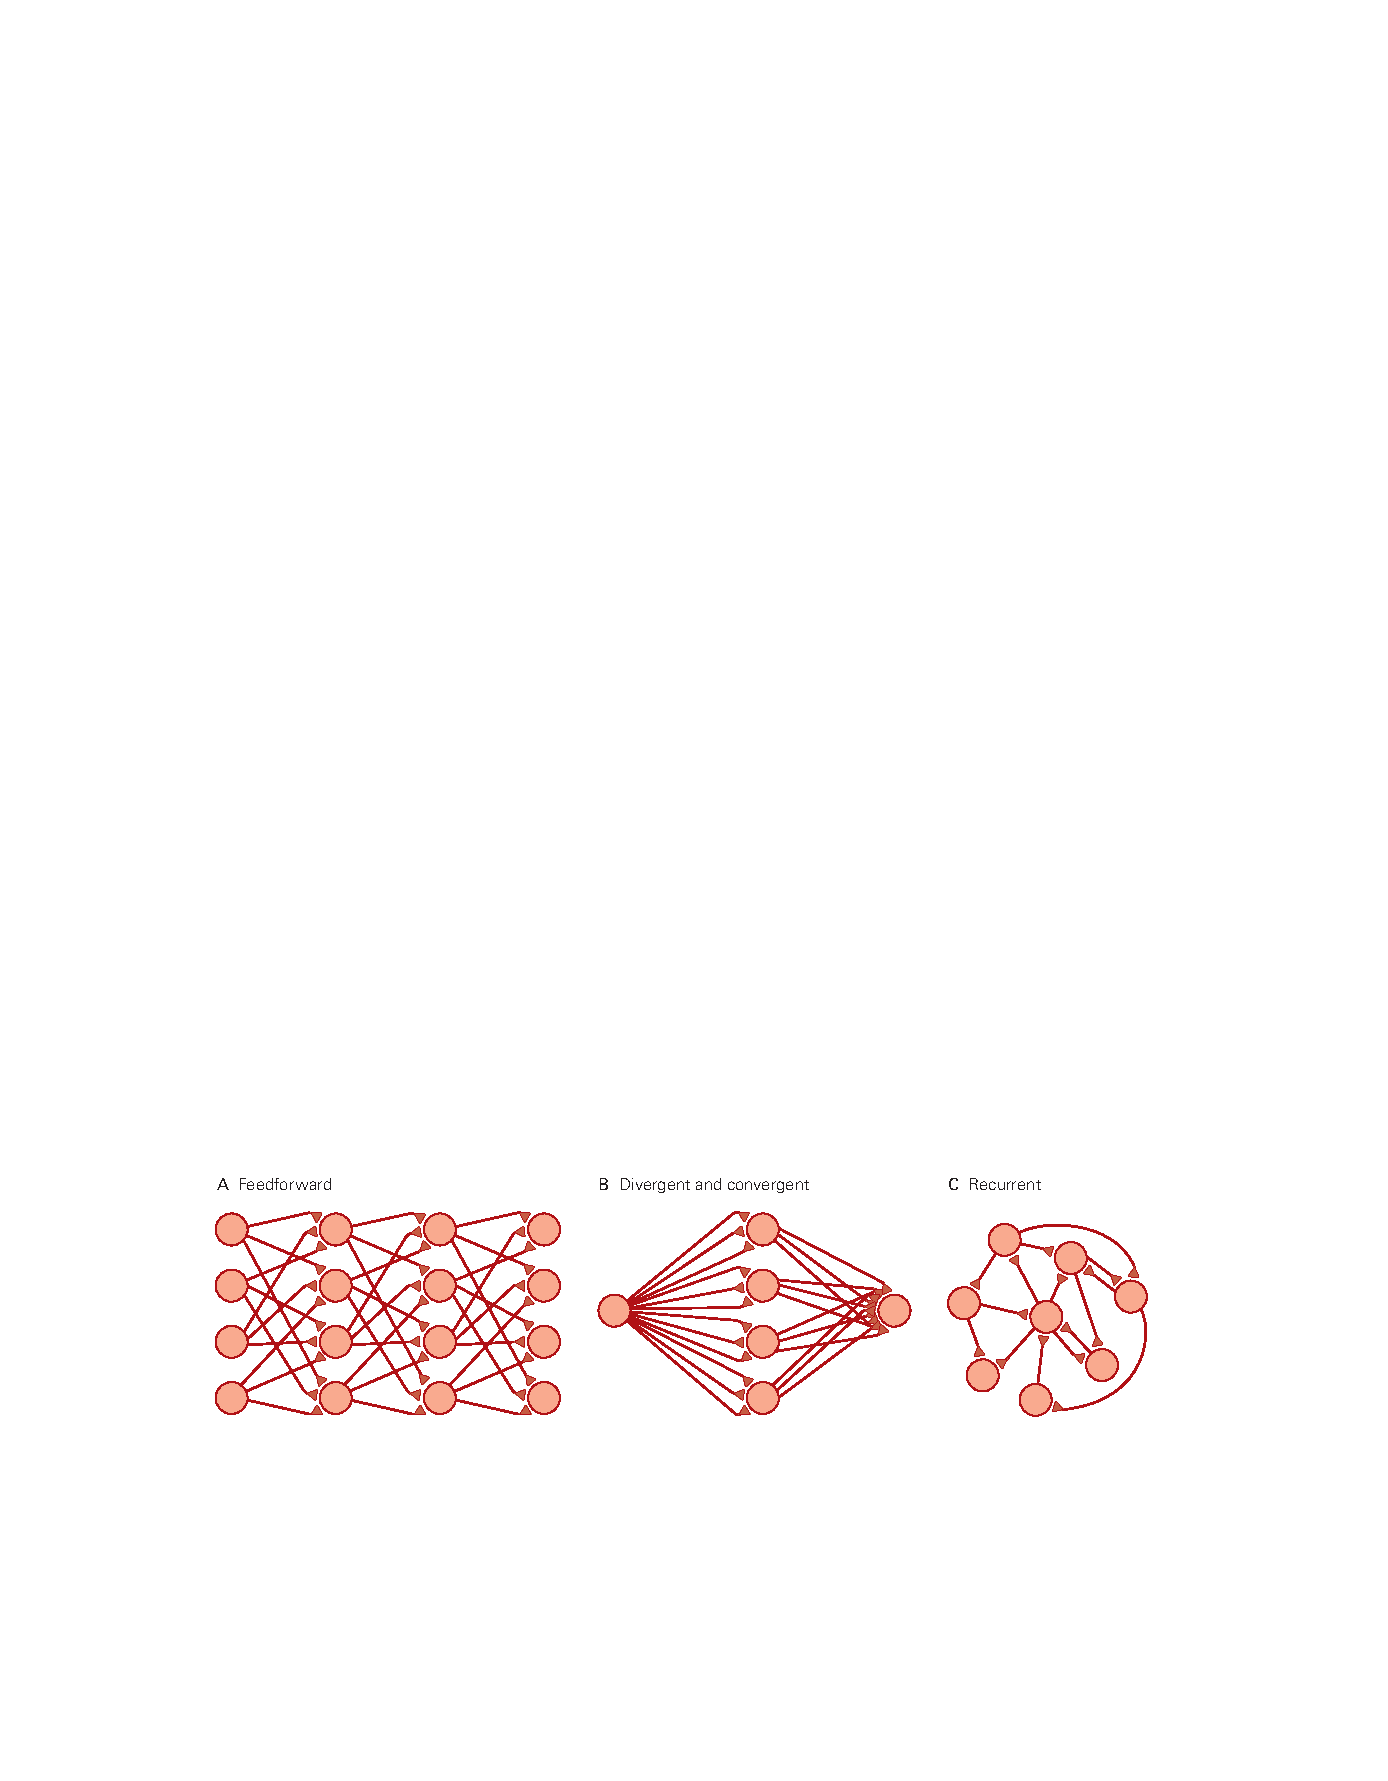
\includegraphics[width=1.0\linewidth]{chap05/fig_5_3}
	\caption{四种基本的神经回路图案。 
		\textbf{A.} 一种\textit{前馈}回路,其中突触连接在一个方向上从神经元的一个处理级别延伸到另一个处理级别。
		\textbf{B.} \textit{发散}的前馈连接描述了少量的突触前神经元连接到大量的神经元。
		\textit{汇聚}连接描述了连接到较小数量的大量突触前神经元。
		\textbf{C.} 在\textit{循环网络}中,神经元之间的多个方向发生突触连接,形成通过回路的循环通路。}
	\label{fig:5_3}
\end{figure}


神经元之间的连接可以是兴奋性的或抑制性的。
通常,兴奋性连接会导致神经放电增加,而抑制性连接会导致神经放电减少。
许多神经回路从成百上千个突触中接收到强烈的兴奋驱动。
如果不通过抑制来检查,这种突触兴奋将导致不稳定的神经活动。
兴奋和抑制的接近平衡是神经回路的一个共同特征,可以增强它们的计算能力。
然而,如果兴奋和抑制之间的平衡没有得到适当维持,这种微调可能会使回路容易产生癫痫发作活动,就像在癫痫期间发生的那样。


在哺乳动物中,视觉信息在一系列通常被近似为具有前馈回路的大脑区域中进行处理。
前馈回路可以以复杂的方式处理信息,例如从复杂的视觉场景中提取和识别目标,但它们不能产生持续的、动态的活动模式。
为此,需要循环回路(图~\ref{fig:5_3}C)。


在前馈回路中,可以识别两个子主题:发散连接和收敛连接(图~\ref{fig:5_3}B)。 
在发散连接中,接收给定类型输入的神经元数量超过提供该输入的神经元数量,因此在突触前输入神经元中编码的信息在突触后输出神经元中扩展。
在会聚连接中,许多突触前神经元将输入发送到数量较少的突触后神经元。
发散和收敛连接的最突出例子是由小脑提供的,如后所述。



\subsection{视觉处理和目标识别取决于前馈表示的层次结构}

视觉信息在大量分层排列的大脑区域中进行处理(图~\ref{fig:5_4})。
从视网膜产生的主要感觉输入向上移动,神经元对越来越复杂的视觉特征组合做出反应,最终导致对复杂物体(例如面部)的选择性。
大量研究致力于识别视觉层次结构所基于的原则。
机器视觉中人工神经网络模型的发展已被证明是解决该问题的一个有指导意义的类比。


\begin{figure}[htbp]
	\centering
	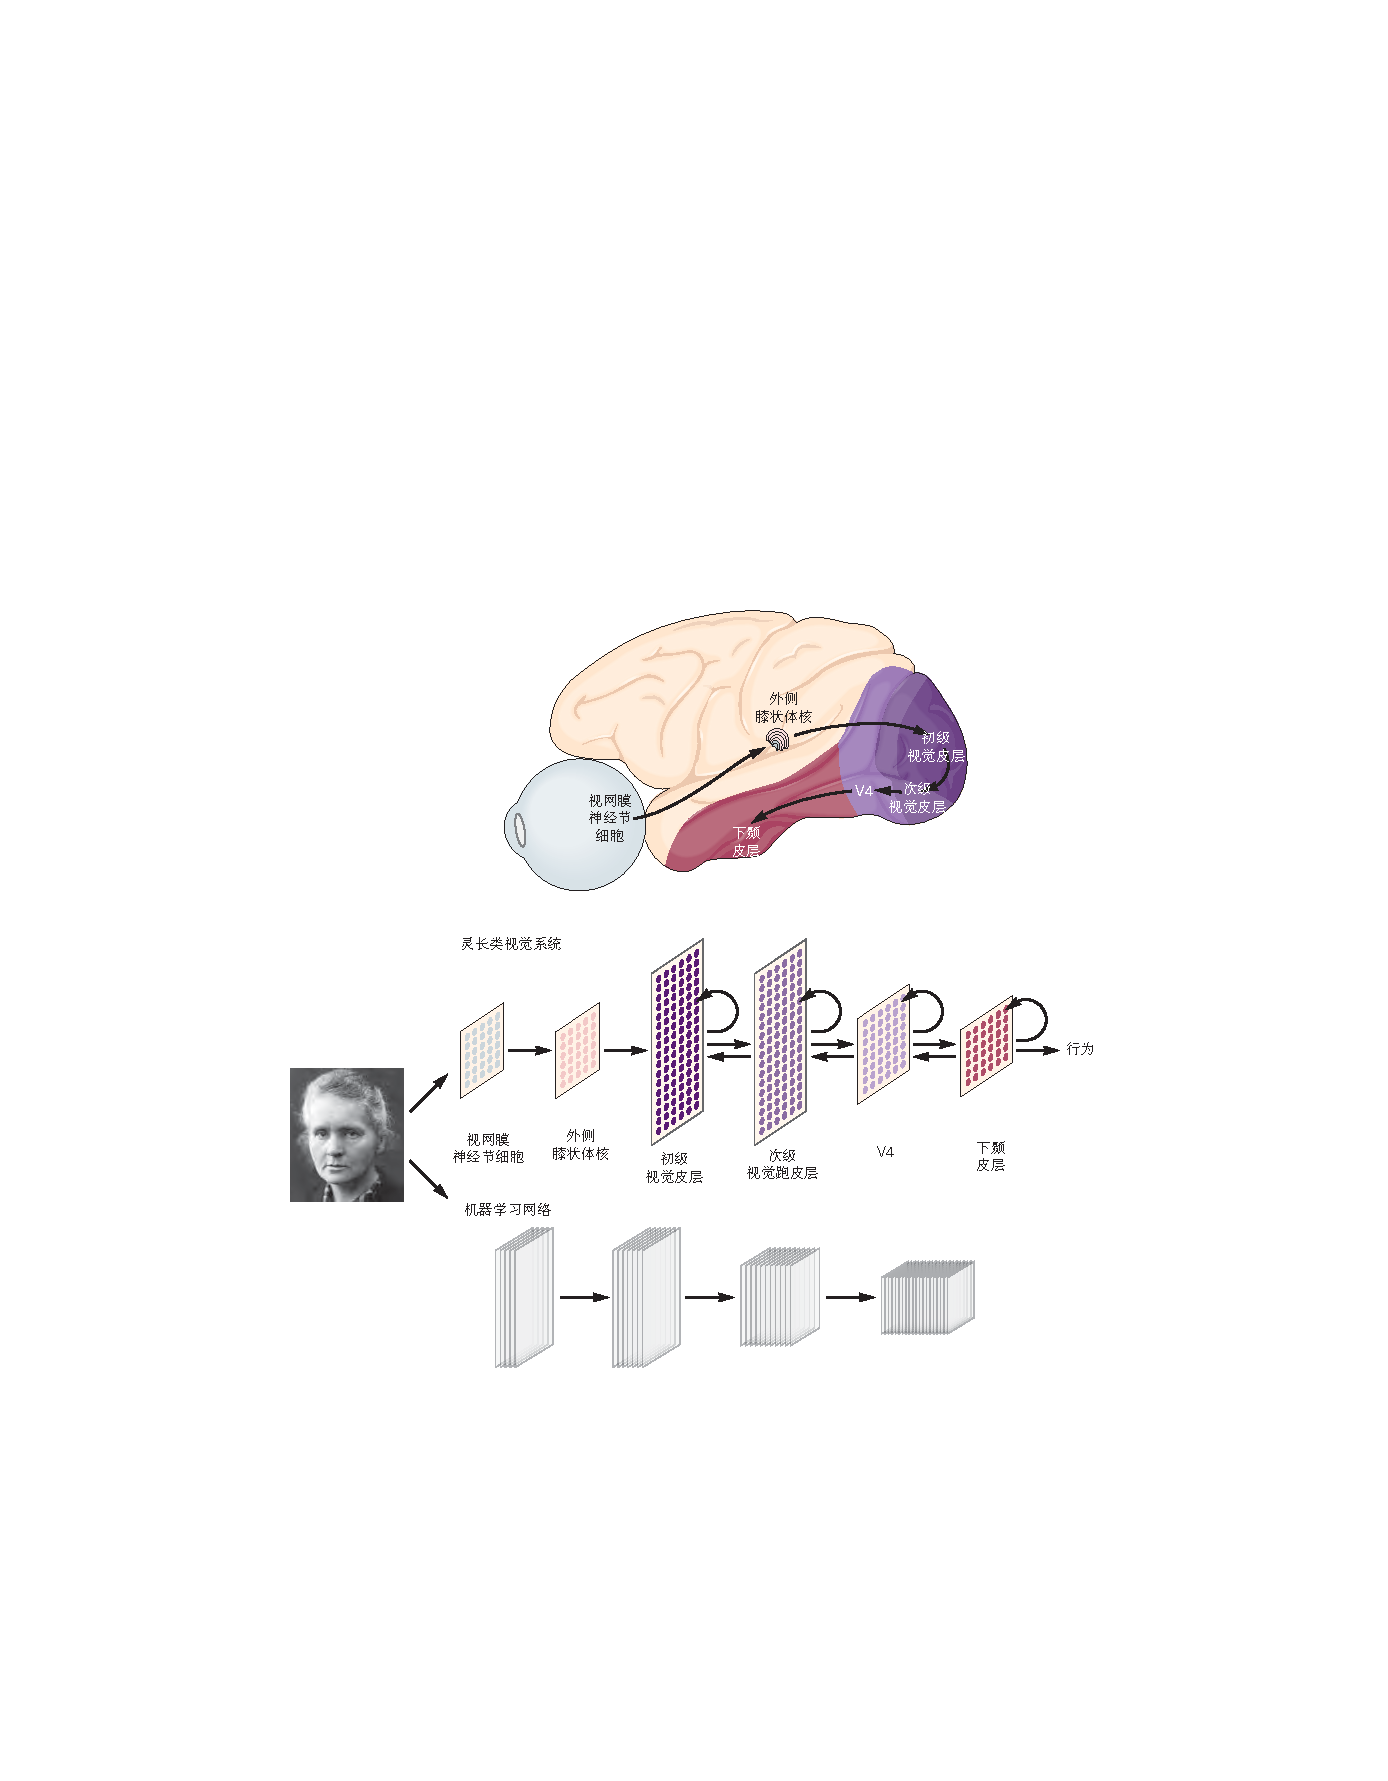
\includegraphics[width=1.0\linewidth]{chap05/fig_5_4}
	\caption{生物和机器学习网络的比较。
		在视觉系统中,多个大脑区域形成一个层次结构,在这个层次结构中,神经元逐渐对更复杂的物体进行选择。。
		灵长类视觉系统通路中的区域代表\textit{视网膜神经节细胞}、丘脑的\textit{外侧膝状体核}、腹侧流视觉区域(\textit{初级视觉皮层}、\textit{次级视觉皮层} 和 V4)和\textit{下颞皮层}。
		每个区域的神经元\textit{数量}各不相同(由彩色圆点表示),但它们的\textit{选择性}稳步增加。
		机器学习网络通路表示经过训练以识别图像中目标的前馈网络层。
		越来越多的堆叠子层表明机器学习网络不同区域的选择性增加,反映了对更丰富的视觉特征阵列的选择性。
		在不同视觉区域记录的响应选择性的层次结构类似于在机器学习网络的相应层中看到的活动\cite{schrimpf2018brain}。}
	\label{fig:5_4}
\end{figure}



从视网膜到丘脑,再到初级视觉皮层,再到与认知相关的最高视觉区域下颞皮层中,视觉神经元选择性地响应视野区域中特定的亮、暗和颜色模式,称为它们的\textit{感受野}。
从视觉处理的最低阶段到最高阶段,神经元的感受野越来越大,选择性也越来越高。
在每个阶段,具有特定类型选择性的神经元往往倾向于具有覆盖视觉场景的感受野,为所选特征提供全面覆盖。
此外,每个视觉大脑区域中感受野的排列在地形上与视网膜上外部世界图像的布局相匹配,即皮层形成了视野图。


随着感受野的扩大和选择性的增加,神经响应对所选目标或图案精确位置的依赖程度越来越低,而更多地取决于其整体特征。
一般来说,处于视觉处理较高阶段的神经元对视野的较大部分更有选择性地做出反应,并且较少依赖于位置、大小和方向等特征。
这与我们在场景中独立于位置、大小和方向识别目标的能力相关。
例如,在层次结构的最高阶段,神经元可以选择性地对位于中间的特定面孔做出反应,而与面孔的大小或其角度姿势(即头部方向)无关。


平铺、增加感受野大小、增加选择性和减少对视图相关因素的依赖的想法是人工机器视觉网络构建的核心。
这样的网络在某些物体识别任务上可以达到人类水平的性能。
此外,机器在困难图像上所犯的错误模式在某种程度上与人类受试者所犯的错误相匹配。
非人类灵长类动物也可以在与人类相当的水平上执行这些任务,而且有趣的是,沿着目标识别通路的不同视觉区域的记录对应于在视觉处理的相似阶段在人工网络中看到的活动(图~\ref{fig:5_4})。



\subsection{小脑中不同的神经元表征为学习提供了基础}

我们大脑中最丰富的一类神经元是位于小脑输入阶段的大约 500 亿个颗粒细胞,占大脑所有神经元的一半以上。 
小脑是一种对运动协调至关重要的后脑结构,但也涉及自主神经、感觉和认知功能的适应性调节(图~\ref{fig:5_5})。
小脑回路功能障碍可能导致各种神经系统疾病,包括孤独症。
与大多数大脑神经元接收的数千个输入相比,每个颗粒细胞仅接收少量输入(平均四个)。


\begin{figure}[htbp]
	\centering
	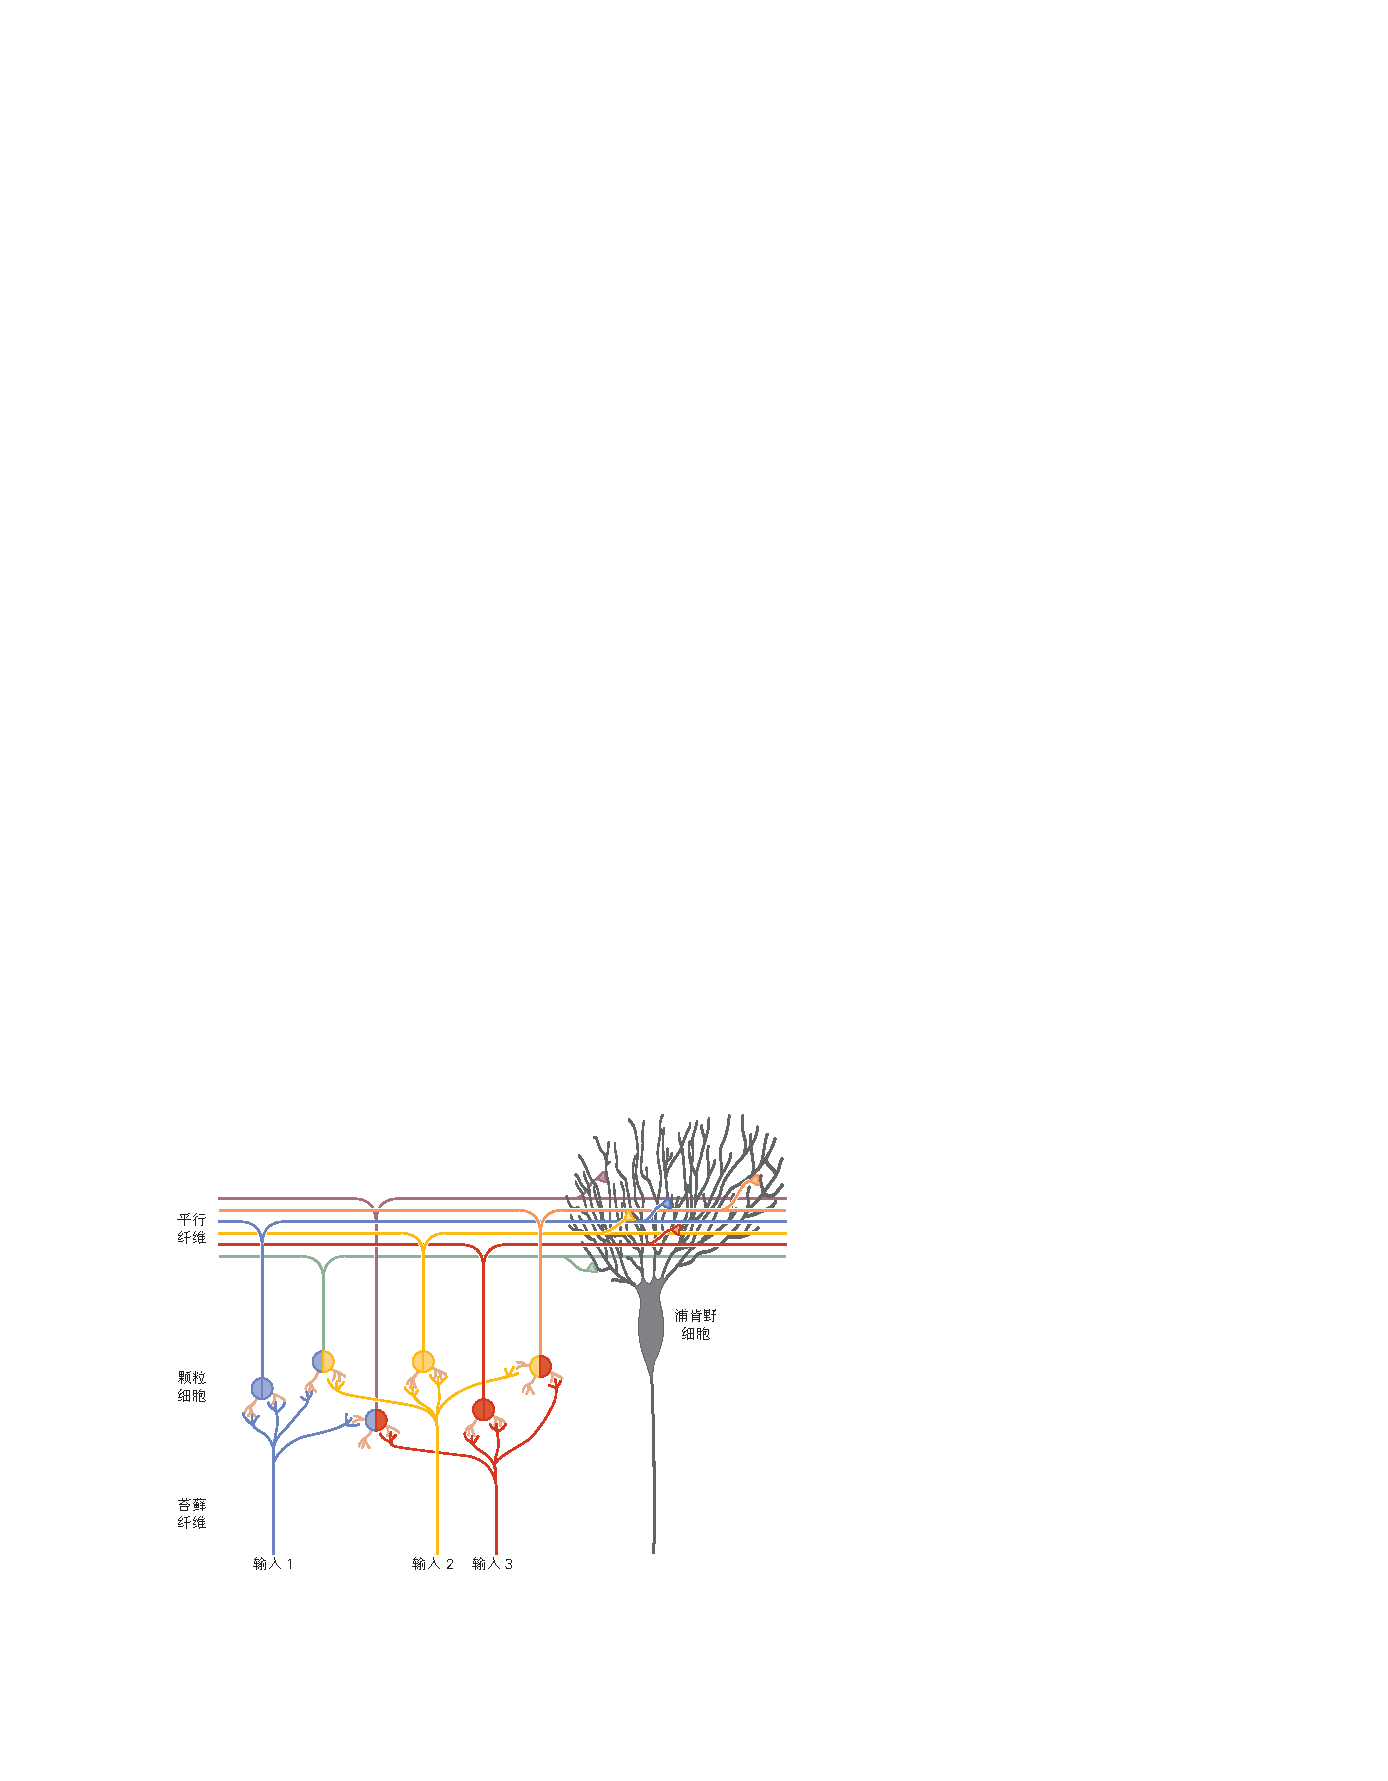
\includegraphics[width=0.9\linewidth]{chap05/fig_5_5}
	\caption{小脑接收来自大脑和脊髓许多区域的输入。
		这些输入统称为\textit{苔藓纤维},在大量\textit{颗粒细胞}中重新编码,这是发散连接的一个例子,允许输入信号的许多可能混合。
		\textit{浦肯野细胞}的树突从轴突(称为平行纤维)中继的数十万个颗粒细胞接收会聚输入。
		浦肯野细胞突触的平行纤维是可改变的,这被认为是运动和可能其他形式学习的重要机制。}
	\label{fig:5_5}
\end{figure}


最近使用神经解剖学追踪和电生理学记录的实验结果表明,汇聚到单个颗粒细胞上的输入通常来自不同的大脑区域。
因此,单个颗粒细胞的放电可能代表大量刺激或事件组合中的任何一种。
例如,细胞可能仅在特定视觉刺激(例如移动的网球)与特定身体部位的运动(例如手腕的弯曲)结合时才会放电。
以这种方式组合不同类型信息的表示称为混合表示。


小脑颗粒细胞提供了\textit{发散前馈连接}的一个极端例子,大约 2 亿个输入纤维(称为\textit{苔藓纤维})携带的信息混合并扩展到 500 亿个\textit{颗粒细胞}上。
需要如此大的表示来处理可以组合多个信息通道的许多不同方式。
例如,表示 100 个不同输入通道中的 2 个的所有可能组合需要 100 × 99/2,即 4,950 种不同的响应类型。
需要所有三元组的表示将这个数字推高到 15 万以上,并且对于四个或更多的组合,这个数字会迅速增加。
由于大量可能的组合在遗传学上很难确定,所以通常认为苔藓纤维与其颗粒细胞目标的分配在很大程度上是随机的。


该分析表明,小脑颗粒细胞的作用是以多种可能的方式\textit{组合}大量输入通道。
这种表示显然有助于根据刺激和动作组合的共现进行推理和生成动作。
然而,要发挥作用,必须以某种方式从大量颗粒细胞中读出这些信息。


小脑细胞的\textit{读出}是由浦肯野细胞完成的,浦肯野细胞是小脑皮层的输出神经元。
与颗粒细胞输入端高度分散的连接相反,颗粒细胞和浦肯野细胞之间的连接提供了一个极端的\textit{汇聚}例子。
单个浦肯野细胞接收来自超过十万个颗粒细胞的输入。
\textit{大卫$\cdot$马尔}和\textit{詹姆斯$\cdot$阿尔布斯}在 1970 年代提出的小脑功能理论认为,这种融合使\textit{浦肯野细胞}能够从颗粒细胞提供的极其丰富的表征中提取有用的信息。
通过这样做,浦肯野细胞可能是人类形成运动技能(如骑自行车或演奏乐器)所需的许多复杂联想的惊人能力的基础。
然而,为了在各种条件下提取对多种目的有用的信息,浦肯野细胞提供的读数必须具有适应性。
如后面部分所述,这种适应性是由颗粒细胞和浦肯野细胞突触之间的\textit{突触可塑性}提供的。



\subsection{循环回路是持续活动和整合的基础}

神经元天生健忘。 
瞬态突触输入通常会引起短暂的响应,这种响应会在几十毫秒内衰减。
这种衰变的时间过程由神经元的一种内在特性决定,称为\textit{膜时间常数}(第~\ref{chap:chap9}~章)。
那么神经活动模式如何持续足够长的时间以支持认知操作,例如在几秒钟、几分钟甚至更长时间内完成记忆或决策制定?


例如,试着在一个挤满人大声说话的房间里尝试检测您是否听到一个熟悉的声音。
当您聆听时,您可能偶尔会发现一些类似于您正在寻找的声音,但这本身并不能确定。
然而,随着时间的推移,您可能会积累足够的证据来得出结论。
这个证据积累的过程需要整合,这意味着必须维护一个运行总和,并在检测到额外证据时增加。
整合需要计算(加法)和记忆来计算和维护运行总和(第~\ref{chap:chap56} 章)。


为了使神经回路进行整合,瞬态输入必须产生即使在输入消失后也能维持在恒定水平的活动。
这种持续的活动提供了对瞬态输入的记忆。
如前一段所述,整合的神经回路可用于积累信息,但它们也需要用于非认知任务,例如保持固定身体姿势所需的恒定肌肉张力。
研究得最好的神经整合器之一是允许人类和动物保持眼睛恒定注视方向的回路,即使在黑暗中也是如此。
事实上,可以研究从鱼类到灵长类动物广泛物种的眼球运动,这极大地促进了研究的进步。
此外,动眼神经系统的相对简单性促进了实验研究和理论研究之间富有成效的对话(动眼神经系统在第~\ref{chap:chap35} 章有更详细的描述)。


动眼神经系统中整合回路的存在最初是由来自神经元记录的一个令人费解的观察结果提出的(图~\ref{fig:5_6}A)。
控制眼部肌肉的动眼神经元会瞬时增加动作电位放电以引起眼睛的运动,但也会表现出将眼睛保持在固定位置所需的持续动作电位放电。
例如,当注视保持在中心的左侧时,投射到眼球肌肉的运动神经元的放电频率高,而当注视保持在中心的右侧时,放电频率低。
令人困惑的是,投射到动眼神经元的上丘和脑干中的运动前神经元仅在眼球运动之前短暂放电。
他们没有表现出任何与眼睛位置相关的持续活动。
那么这种持续的活动是如何产生的呢?


\begin{figure}[htbp]
	\centering
	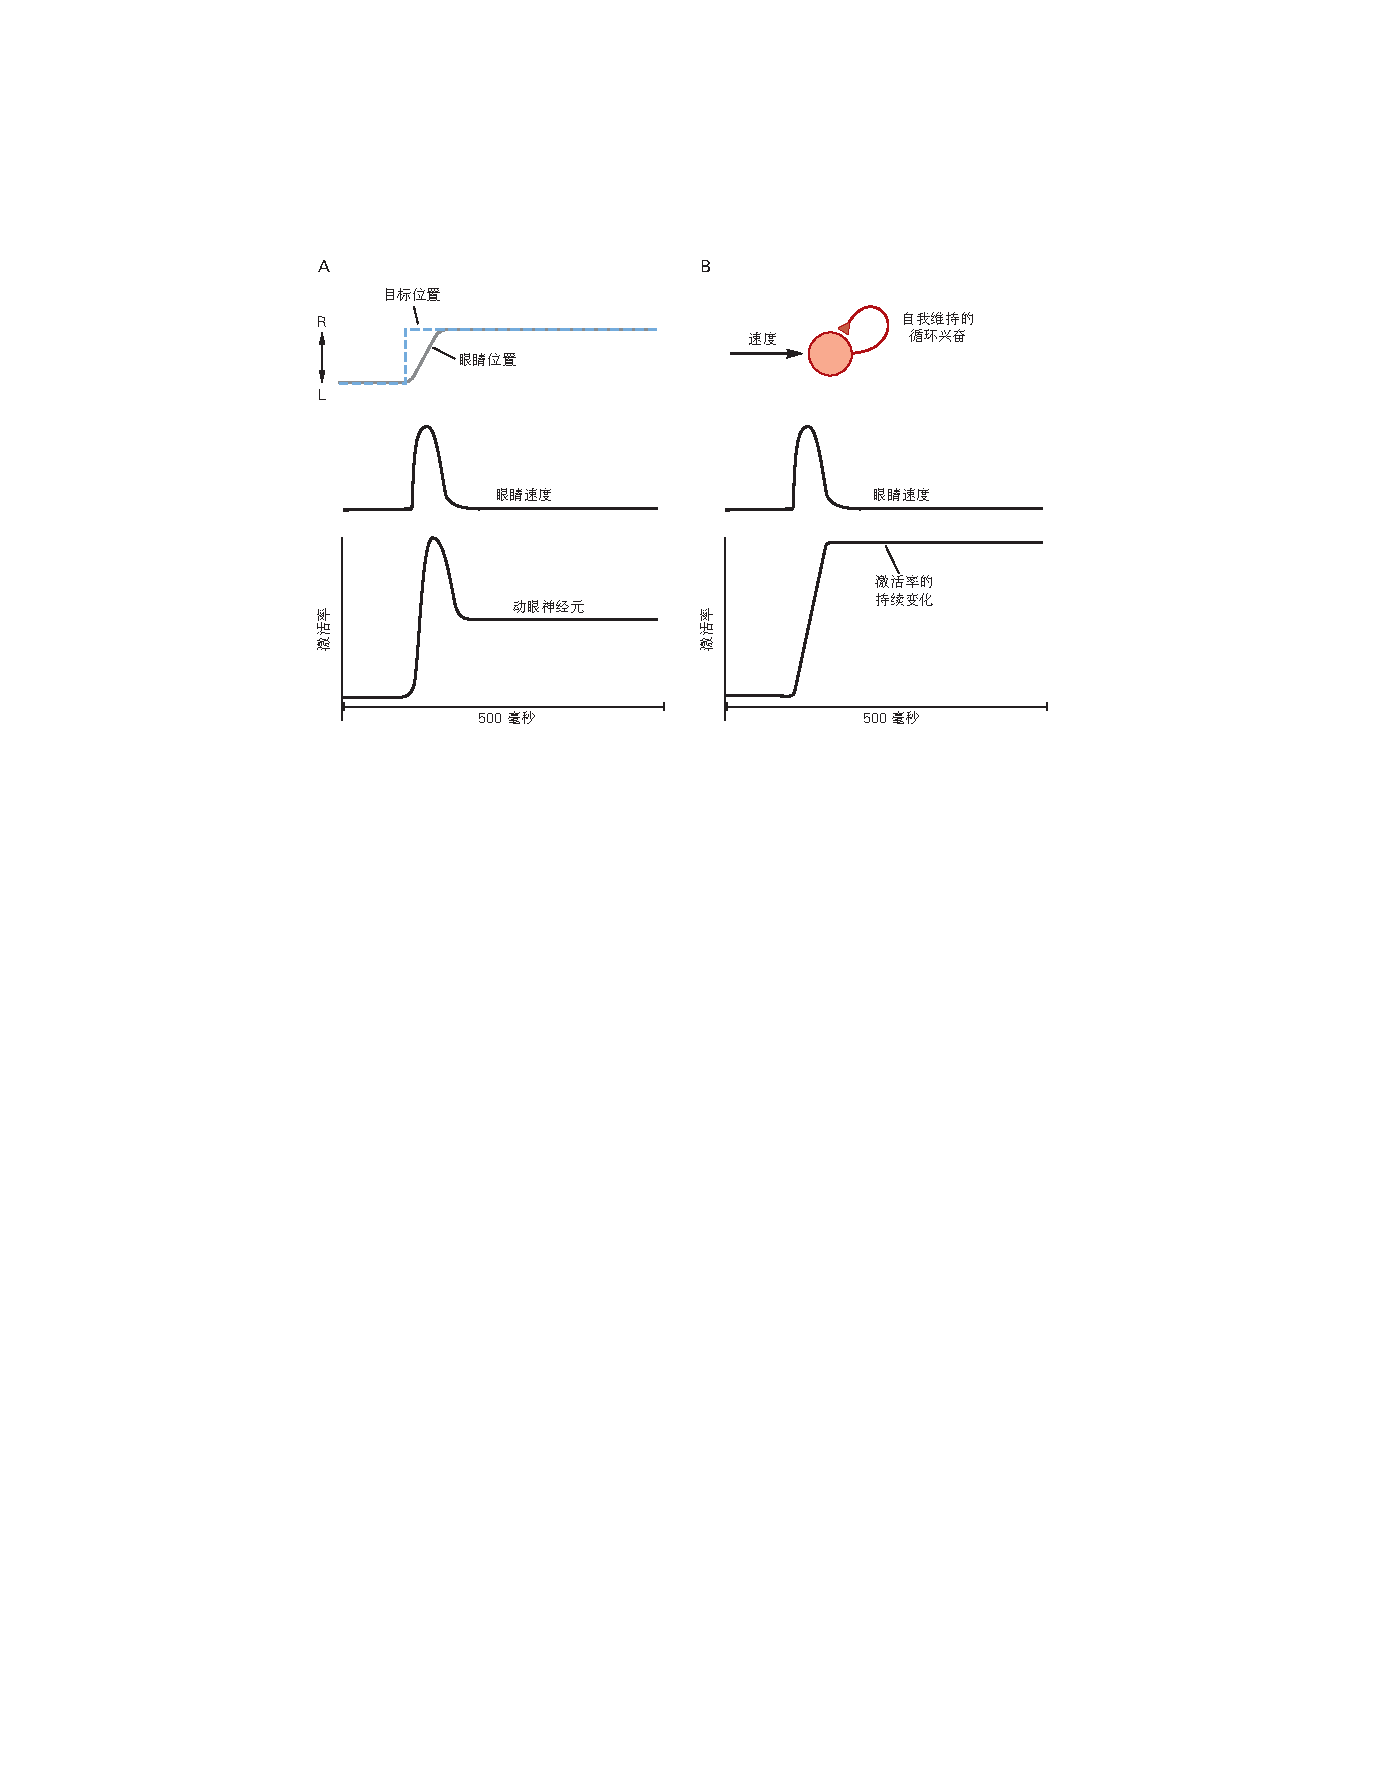
\includegraphics[width=0.9\linewidth]{chap05/fig_5_6}
	\caption{维持眼睛位置需要循环回路和持续的神经活动。
		\textbf{A.} 上图:一个\textit{扫视}的眼球运动包括眼球速度的快速运动变化,以将目标带回凝视中心。
		随后持续改变眼睛位置以将中央凹保持在目标上。
		蓝色虚线表示\textit{目标位置},灰色线表示眼球运动和随后在新位置对目标的注视。
		下图:动眼神经元表现出与眼睛速度相关的短暂活动以及与眼睛位置相关的持续活动。
		\textbf{B.} 反复的兴奋可以解释一个短暂的脉冲输入(例如眼速信号),是如何通过类似于数学积分的过程导致放电率的持续变化。}
	\label{fig:5_6}
\end{figure}


一个早期的猜想,现在得到了强有力的支持,即稳定的眼睛位置信号是由脑干神经元计算的,整合了瞬态眼速度信号。
这些神经元接收速度信息并向维持眼睛位置的动眼神经元提供稳定的输出。 
猴子某些脑干核团(包括内侧前庭核和舌下舌前核)的损伤或失活导致眼球运动后无法保持稳定的水平眼位,表明神经整合回路位于这些结构内。 
人类这些脑干结构的损伤会导致同样的问题,临床上称为凝视诱发性眼球震颤(第~\ref{chap:chap35}~章)。


神经回路如何进行整合?
一种可能性是整合得到专门内在神经元特性的支持,这些特性有效地延长了神经元\textit{膜时间常数},允许短暂的输入产生持续的输出。
已经描述了涉及不同电压激活离子通道的多种候选机制。 
然而,使用允许直接控制记录神经元的膜电压的细胞内记录的研究表明,即使神经元的电压激活通道被阻断,持续的位置相关信号也会持续存在。 
第二种可能性是整合源于突触耦合神经元网络之间的相互作用。 
金鱼的细胞内记录支持这一观点,显示突触输入水平随着眼睛位置的变化而变化。


什么类型的神经网络能够执行整合的问题已经在理论研究中得到广泛探索。 
已考虑的一类模型依赖于循环连接,特别是一群相互激发的神经元。 
这种类型的弱耦合网络响应具有快速衰减的活度的输入脉冲。
增加反复激发的强度会增加一些原本会衰减的活动,从而延长群体反应的持续时间。
如果循环激励增加到由瞬态输入建立的循环激励精确抵消衰减的程度,则响应可以无限期地持续。 这需要微调网络参数。


在一个完美调谐的网络中,一个瞬态输入脉冲会导致激活率发生变化,这种变化在没有进一步输入的情况下会永远持续下去。 
等效地,这样的群体计算它接收到的输入的运行整合(图~\ref{fig:5_6}B)。
如果网络中的瞬态激励没有得到完美调整,则输入会产生放电速率的变化,并且衰减缓慢。 
在黑暗中,眼睛位置往往会在大约 20 秒内漂移回中心,这表明神经整合器没有被完美地调整,但当它被调整得足够好时,可以将典型神经元的大约 20 毫秒时间常数延长一个约1000的系数。


循环网络模型再现了在生物整合器回路中观察到的一些核心特性这一事实已经启动了更详细和更现实的网络模型的开发,并通过实验测试了此类模型的预测。
这些努力还突出了在神经回路的结构和功能之间建立详细联系所涉及的挑战。
即使在使用各种系统和方法进行了数十年的深入研究之后,关键问题仍然存在。


例如,动眼神经整合器回路通常包含两类相反的神经元,随着眼睛位置在给定方向上的变化,一类神经元的放电率增加,另一类神经元的放电率降低。 
这种排列不仅限于动眼神经整合器,而且在涉及决策和工作记忆的皮质区域也发现了这种排列。
模型表明,这些对立群体之间的相互抑制可以在维持活动和融合方面发挥作用。 
尽管解剖学研究为这一观点提供了一些支持,但对金鱼的研究表明,即使对立群体之间的联系被移除,整合仍然完好无损。


另一个关键问题涉及调整积分器网络的机制。
实验研究表明,整合器网络可以根据经验进行修改。
换句话说,它们是可调的。 
尽管这种调整可能是通过神经元之间突触连接强度的变化而发生的,但尚未获得直接证据。 
简而言之,尽管已经了解了很多关于如何实现集成的知识,但在任何特定实例中实际支持集成的网络架构的细节仍有待确定。


详细了解我们如何保持眼睛的位置本身就是一个重要的目的,具有临床意义。 
然而,如前所述,此处找到的解决方案可能同样适用于认知功能,包括短期记忆和决策制定。
大量神经元的光学成像以及对其活动的时间精确操作和详细的解剖学重建,再加上网络功能的理论模型,可能很快就会提供答案。



\section{学习和记忆取决于突触可塑性}

经验可以改变神经回路以支持记忆和学习(第~\ref{chap:chap3}~章)。
一般认为,负责学习和记忆的经验依赖性变化主要发生在突触上。
已经确定了多种形式的突触可塑性,其中每一种都可能支持一组不同的功能。


正如可塑性有多种形式一样,学习也有多种形式。
可以根据所提供信息的数量和类型来定义不同的学习形式。
在监督学习中,会给出有关执行任务所需行为的明确指示。
另一方面,在强化学习中,仅提供正奖励或负惩罚来指示该任务是否被正确执行。
最后,无监督学习根本不涉及任何指导性信息,而是在没有监督的情况下,根据输入数据的内在结构对其进行组织。
在以下部分中,我们将讨论涉及赫布可塑性的无监督学习示例和小脑强化学习示例(学习和记忆的各种类型及其细胞和回路机制在第~\ref{chap:chap52}~至~\ref{chap:chap54}~章中有详细描述)。



\subsection{突触输入的主导模式可以通过赫布可塑性来识别}

皮层神经元接收来自数千个其他神经元的突触输入,并将这些信息组合成动作电位模式。
每个突触的突触传输强度决定了来自许多输入的信息如何组合以影响神经元的放电。
将所有突触的强度设置为零,显然会使无信息的神经元失去功能。
同样,将它们设置为非零值以提取由随机噪声主导的信号也不会产生有价值的信号。
相反,神经元可以通过提取其输入携带的信息中最有趣的方面来最好地发挥有用的功能。
对一种称为\textit{赫布可塑性}形式的理论分析表明,这可能以一种无监督的方式发生。


1949 年,\textit{唐纳德$\cdot$赫布}提出,当给定的神经元突触前输入与足够数量的协同输入合作,导致该神经元激发动作电位时,突触应该增强。
赫布突触可塑性的证据已从许多研究中获得(第~\ref{chap:chap54}~章)。 
就其本身而言,赫布可塑性会使突触越来越强,因此必须存在某种其他形式的可塑性来防止这种情况发生。 
这种可塑性的补偿形式被称为稳态,实验也揭示了这些形式的可塑性。 
理论分析表明,\textit{赫布可塑性}和\textit{稳态可塑性}的组合可以调整突触,无需任何额外的监督信号,因此它们提取相对于其他组合调制程度最高的神经元输入组合(图~\ref{fig:5_7})。 
这是这些输入携带的最有趣信号的合理候选者,因此,赫布可塑性为神经元提供了一种确定和提取此类信号的方法。


\begin{figure}[htbp]
	\centering
	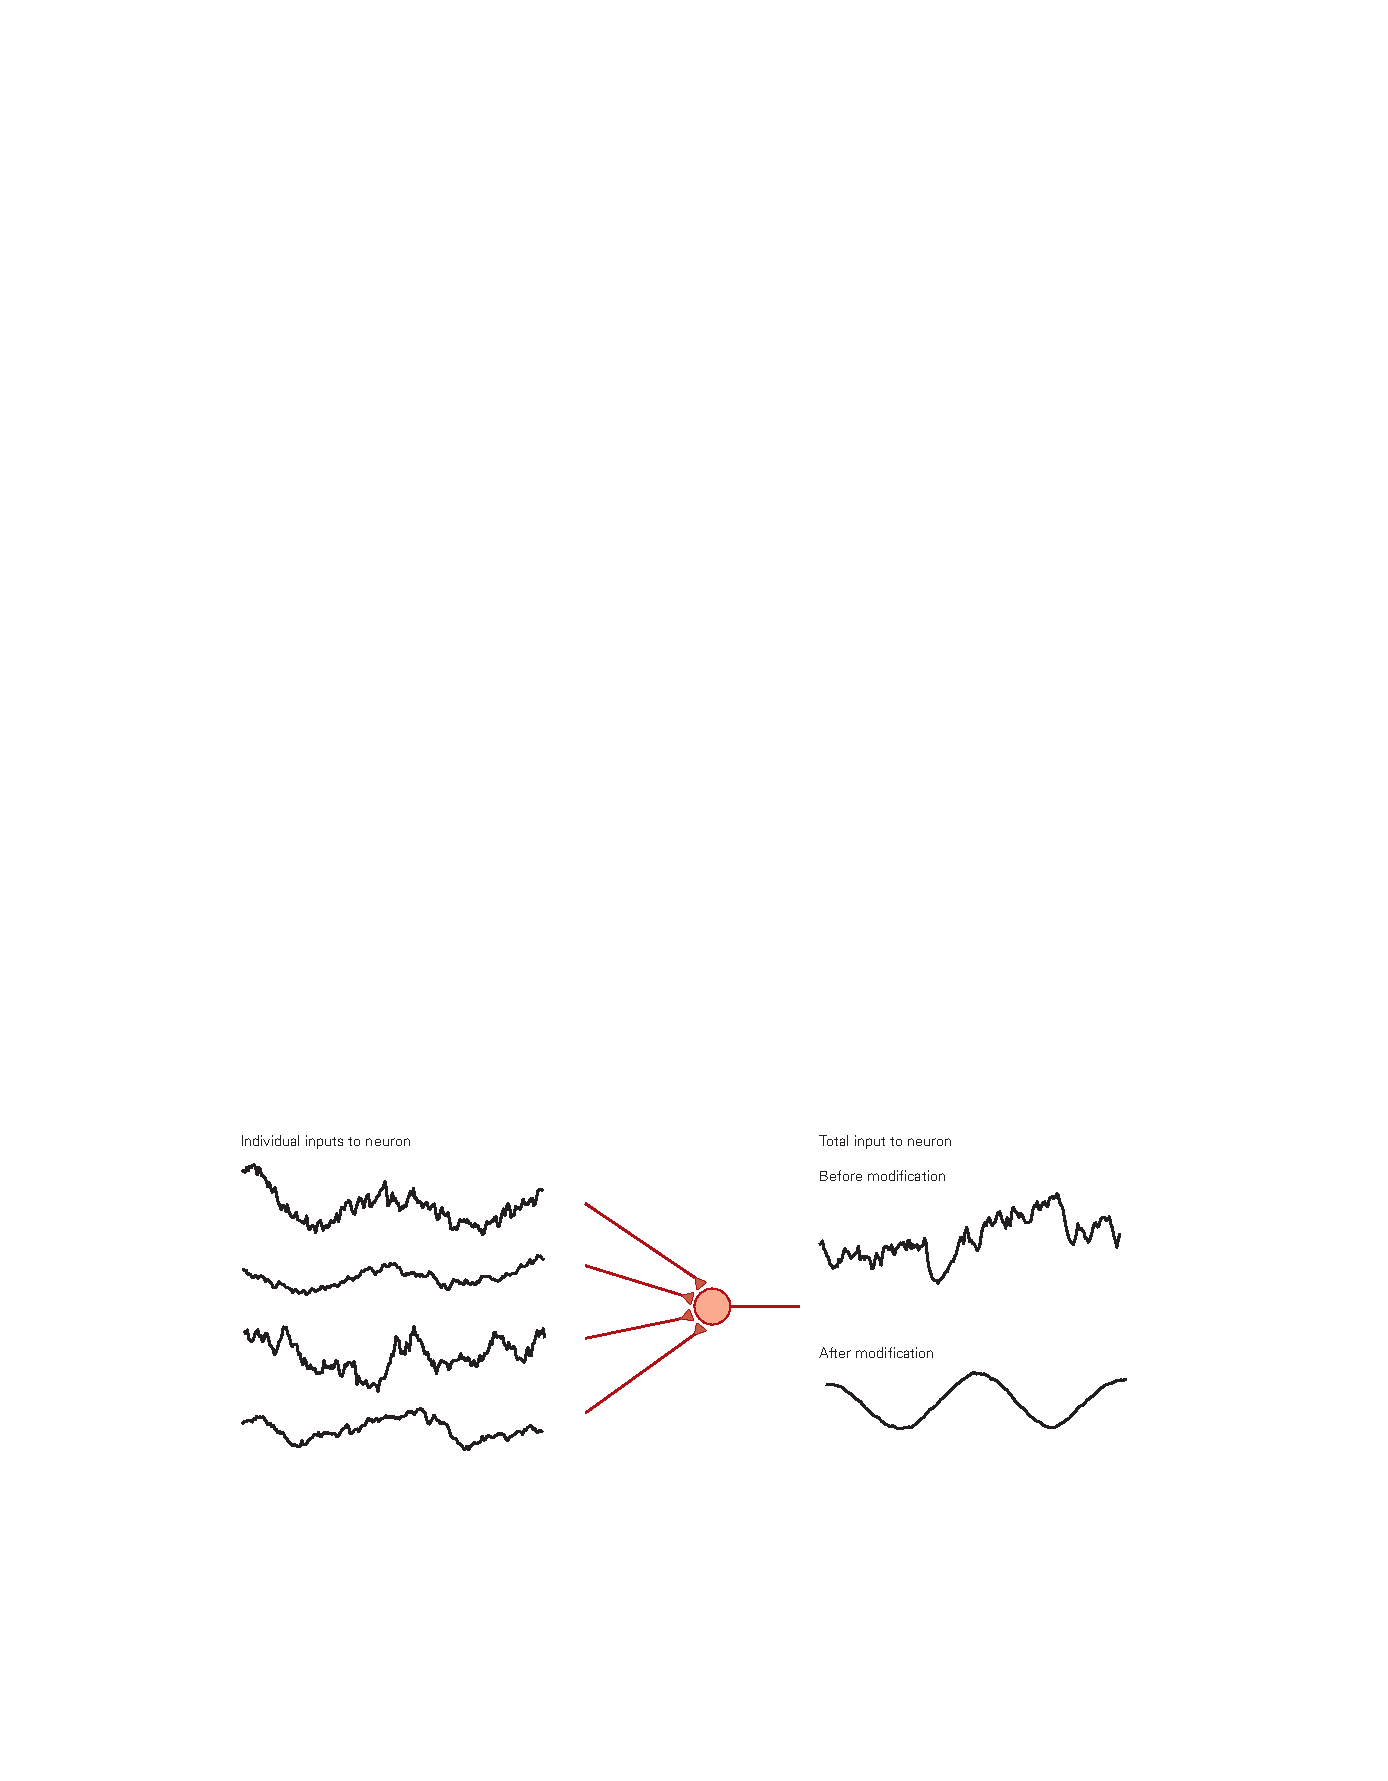
\includegraphics[width=1.0\linewidth]{chap05/fig_5_7}
	\caption{赫布可塑性可以识别神经元的相关输入信号。
		在这个例子中,一个神经元接收 100 个输入;
		显示了其中四个的激活率(左)。
		每个输入速率都有噪声,但在噪声中包含正弦信号。
		输入速率乘以突触强度(棕色三角形),然后求和以产生神经元的总输入(右)。
		在\textit{赫布可塑性}发生之前,突触具有随机权重,导致噪声轨迹;
		修改后,总输入揭示了潜在的正弦信号。}
	\label{fig:5_7}
\end{figure}


\subsection{小脑的突触可塑性在运动学习中起着关键作用}

尽管缺乏对小脑如何促进复杂人类运动技能的详细了解,但人们对其在简单形式的运动学习中的作用了解很多。
其中研究最透彻的是一种被称为\textit{延迟性眨眼条件反射}的范例,其中中性感官刺激(例如光或音调)与厌恶的\textit{非条件刺激}(例如向眼睛吹气)反复配对。
经过几天的此类训练,动物学会闭上眼睛以响应先前的中性刺激(光线或音调),称为\textit{条件刺激},以期待\textit{非条件刺激}(吹气)。
眼睑闭合的时间对于\textit{条件刺激}发作和\textit{非条件刺激}之间的延迟具有高度特异性。


眼睑条件反射一直是理解小脑功能的一个非常有用的范例,因为它以一种特别清晰的方式映射到小脑回路的结构上(图~\ref{fig:5_8})。
有关\textit{条件刺激}的信息首先由小脑颗粒细胞编码,然后传递给浦肯野细胞。
\textit{非条件刺激}由一个完全独立的输入通路编码,称为橄榄小脑或攀爬纤维系统。
与来自颗粒细胞的数千个输入相反,每个浦肯野细胞从称为下橄榄的脑干核接收单个强大的攀爬纤维输入。
电生理记录显示,向小脑某一特定区域输入的攀爬纤维表示\textit{非条件刺激}的发生,即刺激角膜的刺激。
这一发现之所以成为可能,是因为攀爬纤维在浦肯野细胞中引起了一种独特的超阈值反应,称为复杂尖峰。


\begin{figure}[htbp]
	\centering
	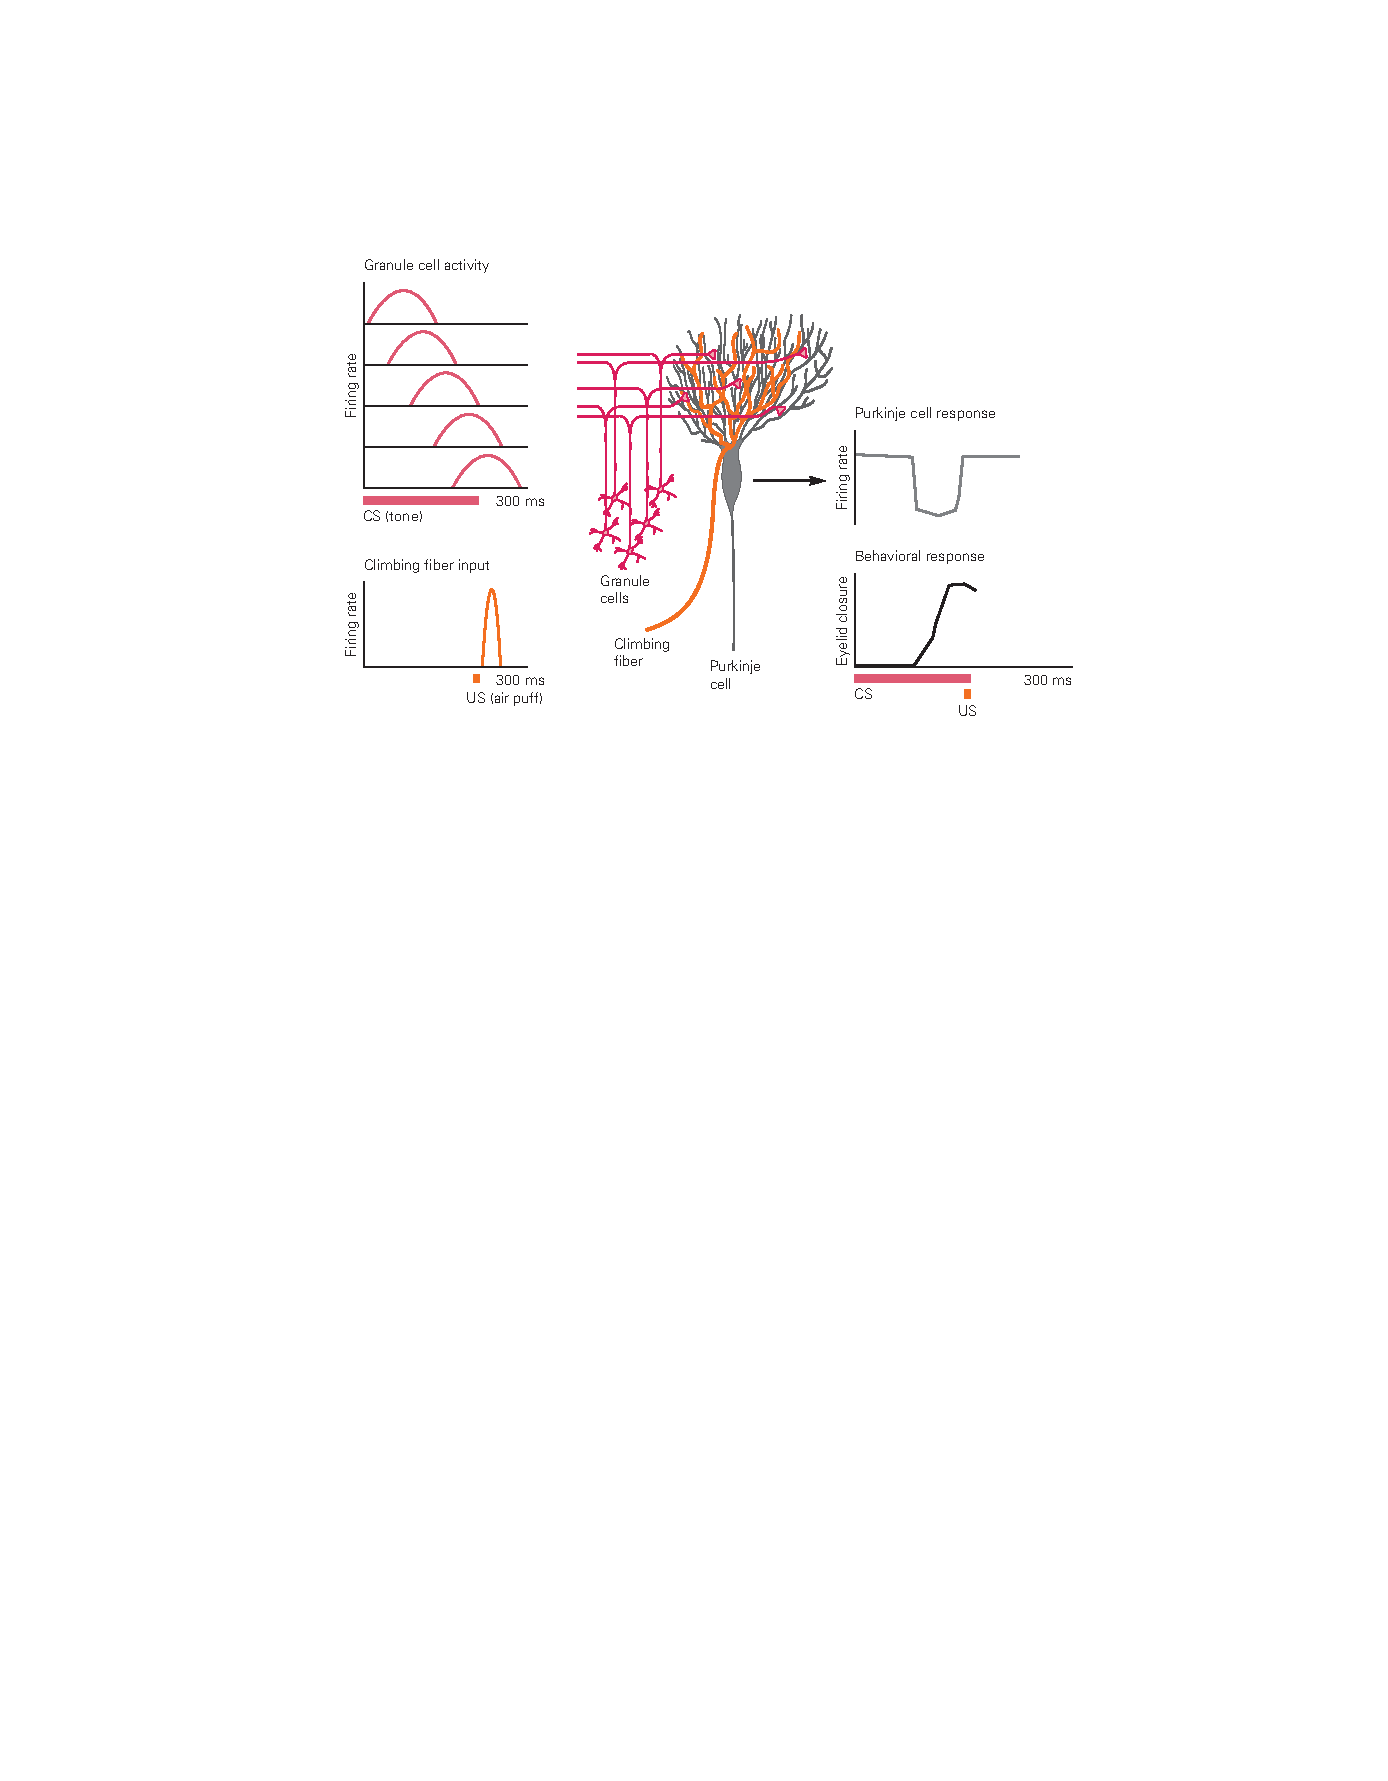
\includegraphics[width=0.92\linewidth]{chap05/fig_5_8}
	\caption{小脑在眨眼条件反射中的假设作用。
		有关\textit{条件刺激}和\textit{非条件刺激}的信息分别通过苔藓和攀爬纤维通路传递。
		在\textit{非条件刺激}呈现之前活跃的颗粒细胞突触被攀爬纤维输入引起的长期抑制逐渐减弱。
		这有助于浦肯野细胞激活的暂停,恰好在\textit{非条件刺激}之前发生。
		由于浦肯野细胞是抑制性的,这种暂停会激发小脑核和红核中的下游神经元,从而驱动眼睑闭合。}
	\label{fig:5_8}
\end{figure}


了解小脑如何调节学习的关键是发现复杂的尖峰触发颗粒细胞和浦肯野细胞之间突触的可塑性。
具体来说,来自突触前颗粒细胞的输入与突触后浦肯野细胞中的复杂尖峰同时出现,导致颗粒细胞输入持续减弱,这是一种称为小脑长期抑制的可塑性形式(图~\ref{fig:5_8})。
因此,对于\textit{非条件刺激}的每次出现,在\textit{非条件刺激}之前立即激活的颗粒-浦肯野细胞突触的强度都会降低。
由于在\textit{非条件刺激}预期到达时间之前颗粒细胞兴奋减少,这种可塑性导致浦肯野细胞放电中逐渐出现学习性暂停。


浦肯野细胞放电的减少如何导致习得性运动反应?
浦肯野细胞通常是自发活动的,它们会抑制下游靶点。 
小脑区域的浦肯野细胞接收与眼睛有害刺激相关的攀爬纤维输入,与神经元形成突触,间接激活产生眼睑闭合的肌肉。
因此,习得的浦肯野细胞放电暂停导致眼睑在正确的时刻闭合以保护眼睛。
适当的暂停时间被认为是由颗粒细胞的时间反应模式的多样性介导的。
计算机仿真表明,如果单个颗粒细胞在\textit{条件刺激}后的不同延迟处活跃或表现出锁定到\textit{条件刺激}的各种不同但可重复的时间模式,则可以通过颗粒-浦肯野细胞突触的可塑性来解释适当定时响应的学习。


由于技术挑战,对于参与眨眼调节的哺乳动物小脑区域的颗粒细胞,尚未获得此类时间表征的直接证据。
然而,在类似于鱼类小脑的结构中的颗粒细胞中观察到了多种时间模式。
更广泛地说,对小脑的研究,包括对眨眼条件反射的研究,提供了一个具体的例子,说明神经回路如何通过反复试验来调节学习,甚至是学习更复杂的运动技能,如演奏乐器。
浦肯野细胞整合了与动物的外部世界和内部状态相关的丰富多样的信号(由颗粒细胞传递),以及关于错误或意外事件的高度特异性信息(由攀爬纤维传递)。
攀爬纤维起到老师的作用,削弱了之前活跃的突触,因此可能导致错误。
突触强度的这些变化改变了浦肯野细胞的放电模式,并凭借特定的布线模式改变了行为,从而逐渐减少了错误。


小脑和大脑皮层,包括海马区,是关于学习和记忆的大量实验和理论研究的焦点。 
技术进步为研究突触动作、单个细胞和电路对记忆相关现象的贡献开辟了新的途径。



\section{亮点}

1. 神经编码描述了神经元活动如何表示刺激的特征或预期的行为。
解码是指解释神经活动来揭示编码信号的逆过程。
神经反应的数学解码可用于解释神经回路执行的计算并驱动假肢装置。 


2. 神经回路高度相互关联,但使用了一些基本主题来表征它们的功能和操作模式。 
前馈回路处理信息以从感觉流中提取结构和意义。 
循环回路可以执行时间处理并生成动态活动以驱动运动响应。


3. 大多数神经元接受兴奋性和抑制性输入的微调平衡。 
这种平衡响应感官刺激的微小变化可以唤起动作电位输出。


4. 神经活动的水平通常必须维持数秒。 
循环激发网络提供了一种机制来产生神经输出的持久变化。


5. 突触可塑性支持构成学习和记忆基础的神经回路的更持久变化。
赫布可塑性可以从一组复杂的输入中提取有趣的信号,而无需监督(“老师”)。
小脑皮层的突触可塑性由\textit{误差信号}(一种监督形式)驱动,并用于调整运动反应和学习时间关系。




\chapter{成像和行为} \label{chap:chap6}

为了用生物学术语解释生物体的行为,有必要协调生物学过程的测量(例如,动作电位、血流、神经递质的释放)与认知和运动输出的测量。
然而,将生物和行为措施联系起来具有挑战性。
对非人类动物进行精确的神经测量和侵入性技术是可能的,但其中许多物种的行为库相对有限。
此外,直接测量或侵入性地操纵健康人类的神经活动要困难得多,健康人类是具有最先进和最多样化行为的物种。
因此,现代神经科学的核心努力一直是开发新方法,以从人脑中获取精确的生物学测量值,并在非人类动物中模拟人类行为。


人类测量生物过程并将其与行为联系起来的主要方法是\textit{功能性核磁共振成像}。
\textit{脑电图}、\textit{正电子发射断层扫描}和\textit{近红外光谱}等其他测量人脑功能的成像方法各有长处。
然而,由于多种原因,功能性核磁共振成像特别适合研究人类行为的神经基础。
首先,它是非侵入性的:它不需要手术、电离辐射或其他破坏性干预。
其次,它可以在短时间内(以秒为单位)测量大脑功能,这使其能够捕捉心理过程和行为的动态方面。
第三,它同时测量整个大脑的活动,提供了检查多个大脑区域如何相互作用以调节复杂行为的机会。
因此,本章的重点是功能性核磁共振成像。


我们首先解释功能性核磁共振成像实验如何工作的技术细节以及通常如何收集数据。 
然后我们解释如何分析功能性核磁共振成像数据以及它们如何提供对人类行为和思想的洞察力。 
然后,我们将使用来自感知、记忆和决策领域的示例,对从功能性核磁共振成像中学到的内容进行更概念性的概述。
最后,我们考虑功能性核磁共振成像的优势和局限性,并讨论它可以支持的关于大脑和行为的推断类型。


虽然本章的重点是健康大脑的成像和行为,但功能性核磁共振成像也有可能改变我们诊断和治疗精神和神经疾病的方式。
几乎所有此类疾病(例如,孤独症、精神分裂症、抑郁症、\textit{进食障碍})除了特定大脑区域和细胞类型的破坏之外,还涉及大规模回路动力学的变化。
对健康大脑回路如何调节心理过程和行为的基础研究,结合在临床人群中测量这些相同回路活动的能力,为理解疾病和功能失调行为带来了巨大希望。



\section{功能性核磁共振成像实验测量神经血管活动}

功能性核磁共振成像实验使研究人员能够根据响应神经活动而发生的局部血氧水平变化来追踪大脑功能。
与所有形式的核磁共振成像一样,功能性核磁共振成像需要高度专业化的设备和复杂的计算机程序。
在本节中,我们首先考虑如何使用核磁共振成像对大脑\textit{结构}成像的基本原理,然后解释功能性核磁共振成像如何将此功能扩展到对大脑\textit{活动}成像。


每台核磁共振成像机器的核心都是强大的磁铁。
磁场强度以\textit{特斯拉}为单位进行量化,大多数现代\textit{核磁共振成像}机器都是 3 \textit{特斯拉}。
使用像 7 \textit{特斯拉}这样更高的场强会提供了一些优势,包括对皮层进行更高分辨率成像的可能性。
此类机器还没有普及,层特定成像还处于起步阶段,所以我们关注 3 \textit{特斯拉}机器的能力和配置。


% % The outside of an MRI machine looks like a tunnel, known as the “bore” of the magnet. 
核磁共振成像仪的外部看起来像一条隧道,被称为磁铁的“孔”。
% Subjects lie on a bed with their head in a helmet-like head coil, which receives signals from the brain. 
受试者躺在床上,头戴头盔状的头部线圈,接收来自大脑的信号。
% Visual stimuli are typically viewed through a mirror on the head coil angled toward a screen at the back of the bore.
视觉刺激通常通过头部线圈上的镜子观察,镜子与孔后部的屏幕成一定角度。
% Auditory stimuli are presented through headphones. 
听觉刺激通过耳机呈现。
% Behavior is typically measured in terms of manual responses with a button box and/or eye movements with an eye tracker.
行为通常根据使用按钮框的手动响应和/或使用眼动仪的眼球运动来衡量。
% This apparatus constrains which experimental tasks are possible. 
该设备限制了哪些实验任务是可能的。
% However, fMRI is flexible in other ways, including that it can be performed and repeated without harm in many different types of subjects, from children to the elderly, whether healthy or suffering from a disorder.
然而,功能性核磁共振成像在其他方面也很灵活,包括它可以在许多不同类型的受试者身上进行和重复,而不会造成伤害,从儿童到老人,无论是健康的还是患有疾病的。


% What does fMRI measure? 
功能性核磁共振成像测量什么?
% There are two fundamental concepts that we will discuss in turn, first magnetic resonance and then neurovascular coupling (Figure 6–1).
我们将依次讨论两个基本概念,首先是\textit{磁共振},然后是\textit{神经血管耦合}(图~\ref{fig:6_1})。


\begin{figure}[htbp]
	\centering
	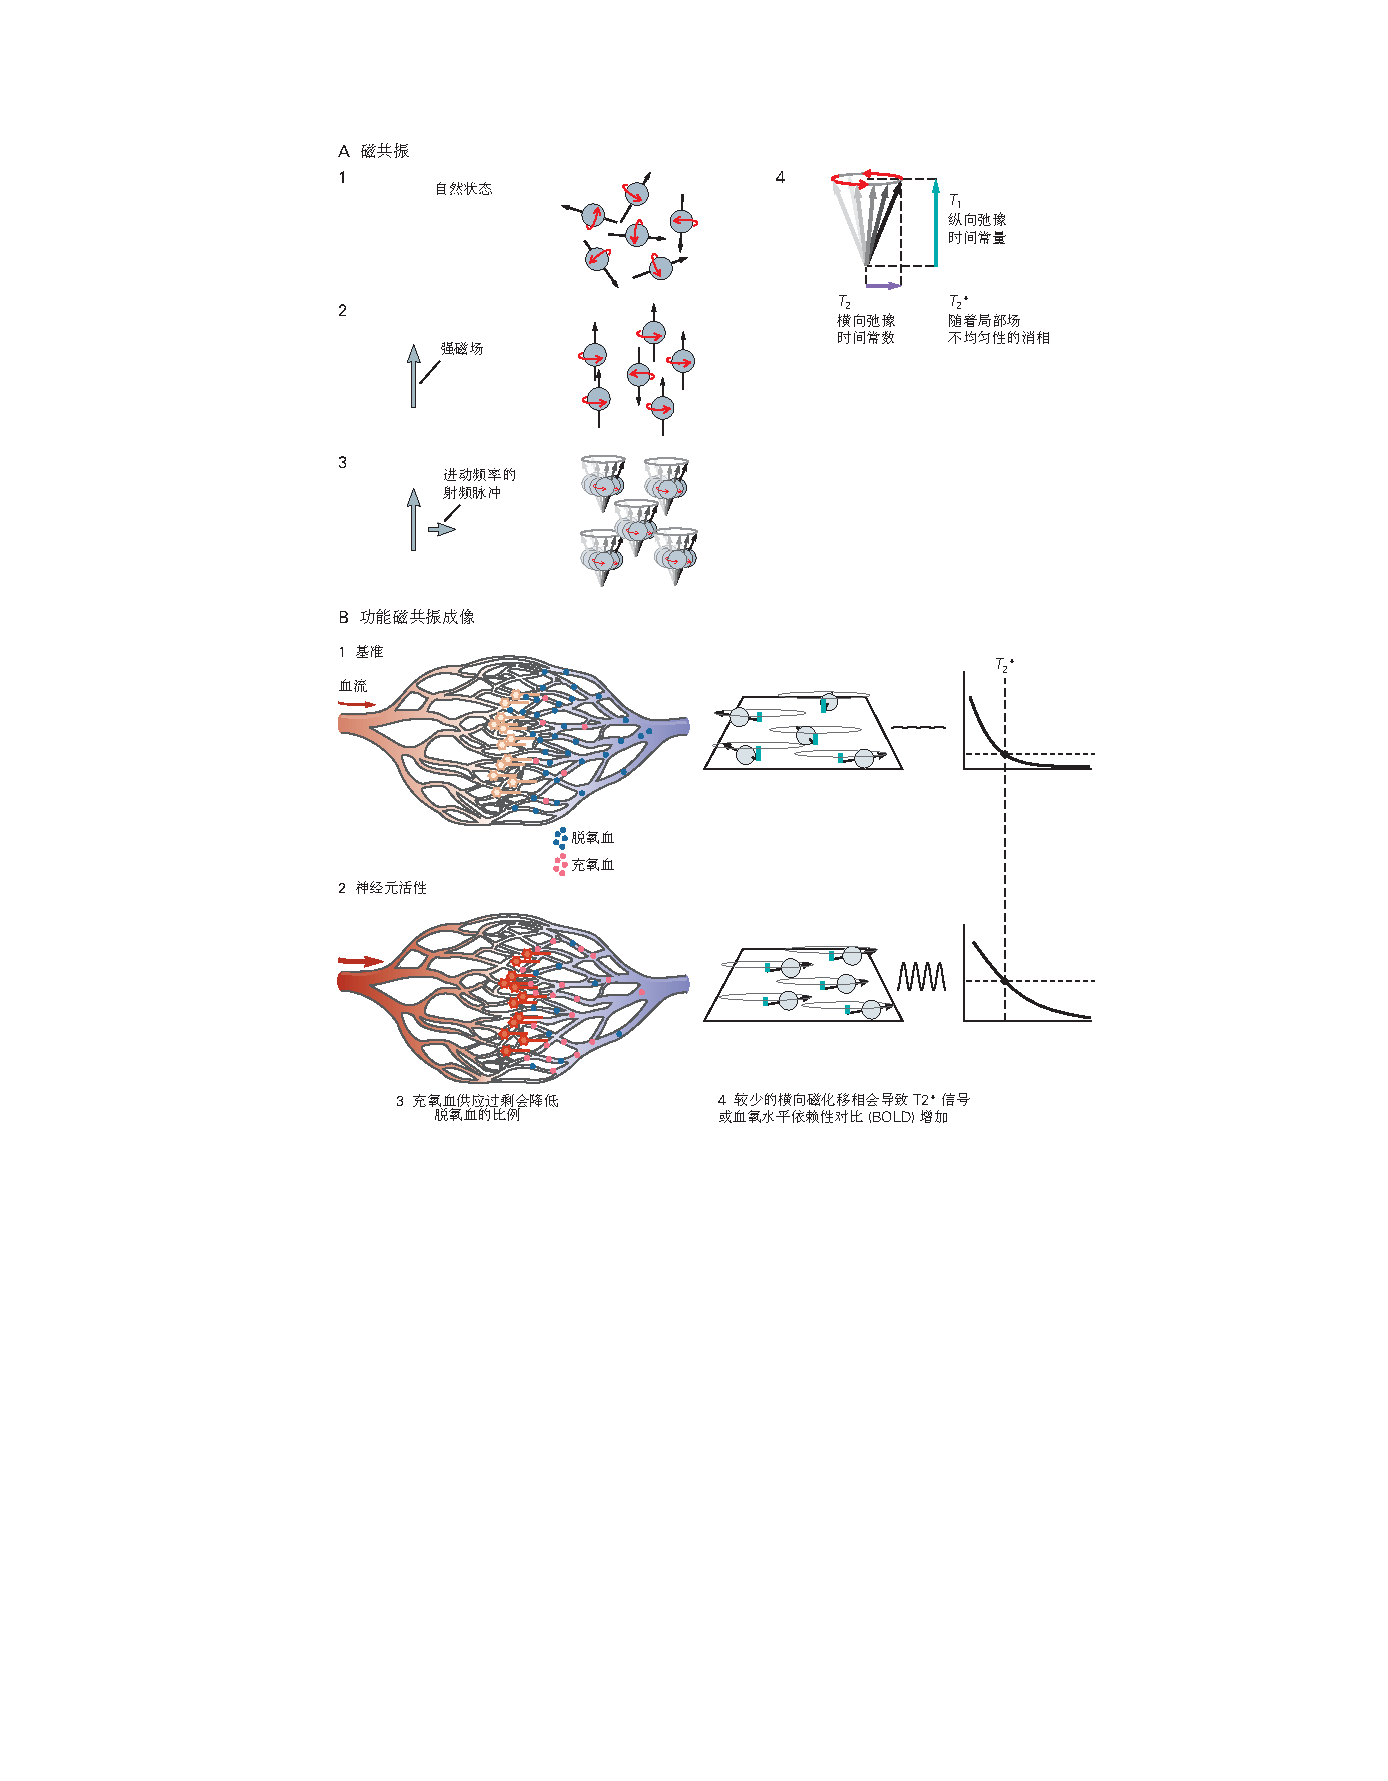
\includegraphics[width=0.9\linewidth]{chap06/fig_6_1}
	\caption{\textit{功能性核磁共振成像}如何测量神经活动。
		\textbf{A.} 在核磁共振环境之外,大脑中氢原子中的质子围绕指向随机方向的轴旋转(1)。
		当大脑进入核磁共振成像孔的强磁场时,这些轴的子集与该磁场对齐,这被称为纵向磁化(2)。
		这些质子可以通过发射射频脉冲来测量,射频脉冲会感应出垂直于强磁场的较弱磁场。
		这会使质子与强场错位,强场现在充当扭矩,导致质子自旋轴在横向平面上以弧形进动。
		选择射频脉冲的频率以与质子的进动速率共振,而质子的进动速率又取决于磁场强度(3)。
		当射频脉冲停止时,质子最初继续同步进动,在头部周围的接收线圈中感应出相同频率的交流电。
		这些信号可用于通过应用磁梯度来生成图像,磁梯度可调整整个大脑正交方向的场强。
		这会在大脑的不同点产生不同的共振频率,从而可以识别接收信号的来源。
		横向磁化随时间消散,信号丢失。
		这种弛豫发生在质子释放热力学能量并且它们的轴返回纵向方向(T1)时,并且由于质子在横向平面中由于与其他原子和分子的局部相互作用而变得不同步(T2),并且由于质子中的不均匀性 磁场(T2 *)(4)。
		\textbf{B.} 由于血液的磁性,磁共振可用于估计功能性核磁共振成像中的神经元活动。
		% 活跃时需要更多的血
		当大脑区域处于基线状态时,脱氧血与充氧血的比例高于该区域活跃时的比例。
		% 脱氧血红蛋白(即没有携带氧的血红蛋白)中的每个铁原子都有4个未配对的电子,使得脱氧血红蛋白具有微弱的顺磁性;
		% 但氧合血红蛋白(即携带了氧气的血红蛋白)中的铁原子没有未配对电子,使得氧合血红蛋白具有抗磁性。
		脱氧血与磁场相互作用,导致局部不均匀性,从而扭曲进动速率并破坏横向平面中质子的同步,导致更快的 T2 * 衰减和更低的\textit{血氧水平依赖}信号(1)。
		神经元活动导致代谢需求(2),进而导致输送过量的氧合血(3)。
		含氧血液不与磁场相互作用,因此活跃大脑区域的含氧量增加会减少场的不均匀性。
		反过来,这减少了质子在横向平面进动的相位差,导致更慢的 T2 * 衰减和更高的\textit{血氧水平依赖}信号(4)。}
	\label{fig:6_1}
\end{figure}



% fMRI Depends on the Physics of Magnetic Resonance
\subsection{功能性核磁共振成像取决于磁共振物理学}

% In general, MRI exploits the magnetic properties of hydrogen atoms, the dominant source of protons in the body, specifically the way each atom’s proton interacts with a strong magnetic field. 
一般来说,核磁共振成像利用氢原子的磁性,氢原子是体内质子的主要来源,特别是每个原子的质子与强磁场相互作用的方式。
% A key property of protons is that they intrinsically rotate around an axis. 
质子的一个关键特性是它们本质上围绕一个轴旋转。
% This spin gives protons angular momentum and a magnetic dipole along the axis, their own north and south poles. 
这种自旋给质子提供了角动量和沿它们自己南北极轴的\textit{磁偶极子}。
% Under normal circumstances, the directions of these dipoles are random for different protons.
在正常情况下,这些偶极子的方向对于不同的质子是随机的。
% When placed in a strong external magnetic field, however, a subset of the protons (how many is proportional to the field strength) align with the direction of this field, which extends from foot to head when lying in an MRI bore.
然而,当置于强外部磁场中时,质子的子集(数量与场强成正比)与磁场方向对齐,当位于核磁共振成像孔中时,质子从脚延伸到头部。


% In the case of a 3T magnet and hydrogen atoms, this speed is in the radiofrequency (RF) range.

% An important step toward measuring a signal from protons is to push them out of alignment with this main field. 
测量质子信号的一个重要步骤是将它们推离这个主场。
% To understand why, it is helpful to think about a familiar object, the gyroscope. 
要理解其中的原因,不妨想想一个熟悉的物体,即陀螺仪。
% If a still gyroscope is tipped out of vertical balance, it will just fall over. 
如果一个静止的陀螺仪失去垂直平衡,它就会翻倒。
% However, if you spin the gyroscope before tipping it, inertial forces will prevent it from falling over. 
但是,如果在倾斜陀螺仪之前先旋转它,惯性力会防止它翻倒。
% The axis around which the gyroscope is spinning will itself begin to rotate around the vertical axis. 
围绕自身轴旋转的陀螺仪将开始围绕垂直轴旋转。
% This precession occurs because gravity exerts a vertical torque on the tilted gyroscope, pulling its center of mass down so that it pivots around its bottom point and traces out a circle in the transverse plane (looking from above).
发生这种进动是因为重力对倾斜的陀螺仪施加垂直扭矩,将其质心拉下,使其围绕其底部点旋转并在横向平面(从上方看)中划出一个圆圈。 
% Something similar happens to a proton that is tilted with respect to the strong magnetic field: The field applies a torque and the orientation of the rotational axis precesses around the field direction. 
相对于强磁场倾斜的质子也会发生类似的情况:磁场施加扭矩,旋转轴的方向围绕磁场方向进动。
% The speed of precession, or the resonant frequency, is determined by the Larmor equation, according to the field strength and a gyromagnetic ratio specific to each type of atom. 
进动速度或共振频率由\textit{拉莫尔方程}根据场强和每种原子特有的旋磁比确定。 
对于 3 \textit{特斯拉}磁体和氢原子,该速度处于\textit{射频}范围内。



% But how do protons get tipped out of alignment in the first place to enable precession?
但是,质子是如何从一开始就偏离排列以实现进动的呢? 
% The answer depends upon the same principle of torque. 
答案取决于扭矩的相同原理。 
% A second, weaker magnetic field is applied in a perpendicular direction (eg, front to back of the head), introducing another torque that pulls protons away from alignment with the strong field. 
第二个较弱的磁场在垂直方向(例如,从头部的前部到后部)施加,引入另一个扭矩,将质子拉离与强磁场对齐的位置。
% This misalignment causes precession about the direction of the strong field by allowing the strong field to act as a torque. 
这种未对准通过允许强场充当扭矩而导致围绕强场的方向的进动。
% Complicating matters, this precession makes protons a moving target for the weaker magnetic field that is needed to cause misalignment in the first place. 
使事情复杂化的是,这种进动使质子成为首先导致错位所需的较弱磁场的移动目标。
% This is solved by generating the second field using a transmit coil in the MRI machine, through which alternating current is passed to deliver an RF pulse at the resonant frequency of the protons. 
这是通过使用核磁共振仪中的发射线圈生成第二个场来解决的,交流电通过该线圈以在质子的共振频率下传递射频脉冲。
% This induces a perpendicular magnetic field that rotates in lockstep with the precession. 
这会产生一个垂直磁场,该磁场会随着进动同步旋转。
% This RF pulse is sustained as long as needed to generate a specified change in the spin orientation of protons away from the strong field direction (eg, 90°). 
该射频脉冲的持续时间与产生质子自旋方向远离强场方向(例如 90°)的指定变化所需的时间一样长。
% This change is known as the flip angle and is often chosen to maximize signal according to the Ernst equation.
这种变化被称为翻转角,通常根据 \textit{能斯特方程}选择它来最大化信号。


% Once the desired flip angle has been achieved, the RF pulse is stopped in order to measure the composition of tissue. 
一旦达到所需的翻转角,射频脉冲就会停止以测量组织的成分。
% At this point, protons are precessing around the strong magnetic field and tilted heavily into the transverse plane. 
此时,质子在强磁场周围进动并严重倾斜到横向平面中。
% This is akin to a bar magnet spinning on a table, where the north and south poles take turns passing any given location. 
这类似于在桌子上旋转的条形磁铁,北极和南极轮流经过任何给定位置。
% If a coil is placed nearby, the spinning magnet induces a current in the wire that reverses as the poles alternate. 
如果在附近放置一个线圈,旋转的磁铁会在电线中感应出电流,该电流会随着磁极交替而反转。
% This is what the receiver head coil in an MRI machine measures: alternating current induced by protons precessing synchronously (note: this is the same principle as described earlier for how the transmit coil works, just reversed). 
这就是核磁共振成像仪中的接收头线圈所测量的:由同步进动的质子感应的交流电(注意:这与前面描述的发射线圈的工作原理相同,只是相反)。
% The amount of current indicates the concentration of precessing protons.
电流量表示进动质子的浓度。


% Critically, the frequency of these measured signals reflects the speed of precession, which in turn depends on the strength of the magnetic field experienced by the tissue. 
至关重要的是,这些测量信号的频率反映了进动的速度,而进动的速度又取决于组织所经历的磁场强度。
% This can be used to generate three-dimensional images by imposing different gradients on the magnetic field (think of a staircase from higher to lower strength) that cause the Larmor frequency to vary systematically over space in the brain. 
这可用于通过在磁场上施加不同的梯度(想象从强度从高到低的阶梯)来生成三维图像,从而导致拉莫尔频率在大脑空间内系统地变化。
% During fMRI, one gradient is applied in a specific direction to select a slice of brain tissue. 
在功能性核磁共振成像期间,在特定方向上应用一个梯度以选择脑组织切片。
% The RF pulse can be tailored to the resonant frequency for the exact field strength at this gradient step, such that only protons in this slice are excited. 
可以针对此梯度步骤中的精确场强将射频脉冲调整为共振频率,以便仅激发该切片中的质子。
% The same logic is used with additional gradients in orthogonal directions to impose a two-dimensional matrix on the selected slice, with each unit volume in the matrix or voxel having a unique frequency and phase. 
相同的逻辑与正交方向上的附加梯度一起使用,以在所选切片上施加二维矩阵,矩阵或体素中的每个单位体积具有唯一的频率和相位。
% The head coil receives a composite signal with a mixture of these frequencies, but the signal can be decomposed to identify protons at every voxel in the slice.
头部线圈接收混合了这些频率的复合信号,但信号可以被分解以识别切片中每个体素处的质子。


进动质子还有另一个有助于核磁共振成像的重要特性:
在射频脉冲之后,头部线圈中感应的交流电开始衰减。
腐烂有不同的来源。
一个来源是进动质子向周围组织释放热力学能量(热量),就像陀螺仪最终会因摩擦而失去能量并翻倒。
当这种情况发生时,质子的自旋方向逐渐放松回到强磁场的方向,导致它们在横向平面内的进动减少,从而产生较少的信号。
这称为纵向弛豫并以时间常数 T1 发生。
第二种类型的衰变发生在质子仍在横向平面内进动时。
单个质子被其他原子的可变邻域包围,这些原子带有自己的弱磁场。
这会微妙地改变质子所经历的场强,导致其拉莫尔频率发生不可预测的变化。
而在\textit{射频}脉冲质子同步进动之后,这些局部相互作用会导致一些质子进动得更快或更慢。
由于它们越来越不同步,感应电流交替的可靠性降低,信号丢失。
这称为横向弛豫并以时间常数 T2 发生。 
质子的这种去相位也可能是强磁场本身的不均匀性造成的,包括它如何被置于磁场中的组织扭曲。 
来自局部相互作用和场失真的信号衰减具有时间常数 T2 *(发音为“T2-星”)。


这些不同的衰变源很重要,因为 T1 和 T2 时间常数因组织类型而异。 
因此,\textit{核磁共振成像}可以利用信号衰减来识别灰质、白质、脂肪和/或脑脊液。 
根据\textit{核磁共振成像}机器上设置的\textit{射频}脉冲、梯度和其他参数(统称为脉冲序列)的配置和时间,从不同体素接收的信号可以突出具有不同 T1 值的组织之间的对比度(T1 加权图像 ) 和/或不同的 T2 值(T2 加权图像)。 
例如,在 T1 加权图像中,白质比灰质更亮,而 T2 加权图像则相反。


测量脑功能的标准脉冲序列是\textit{平面回波成像}序列。 
\textit{平面回波成像}对\textit{功能性磁共振成像}有两个理想的特性:它非常快,允许在不到 100 毫秒的时间内从一个\textit{射频}脉冲获取整个切片,并且它对 T2 * 敏感,我们稍后将看到,这就是\textit{核磁共振成像}测量的方式 神经活动。 
在设计\textit{功能性磁共振成像}研究时,需要选择\textit{平面回波成像}序列的几个参数,包括在脑体积中获取多少切片(通常为 30-90); 
每卷多少时间(重复时间,通常为 1-2 秒); 使用何种体素分辨率(每个维度通常为 2-3 毫米); 
以及是否使用并行采集(例如,一次采集切片的多个部分和/或多个切片)。
这些选择是相互依存的,需要在速度、精度和信噪比之间进行权衡。



\subsection{功能性核磁共振成像依赖于神经血管耦合的生物学}

我们已经描述了磁共振的一般原理,但是故事的第二部分,神经血管耦合呢?
活跃的神经元消耗从血液中的氧气中获得的能量。 
因此,当大脑区域活跃时,血液中的氧合作用会在那一刻下降。
为了补充这些代谢资源,在接下来的几秒钟内流向局部的血液会增加。
供应超过需求,因此,与直觉相反,活跃的大脑区域中含氧(相对于脱氧)血液的比例更高。


要将此与磁共振联系起来,请记住 T2 * 衰变反映了由场不均匀性引起的质子相移。 
血液具有不同的磁性,具体取决于氧合作用:脱氧血液与磁场相互作用,因为血红蛋白中的铁是未结合的,而铁与氧结合的含氧血液则不会。
因此,脱氧血液会导致更快的 T2 * 衰减,并降低相对于含氧血液的信号。
这种信号差异称为血氧水平依赖性对比度。 
综上所述,用\textit{平面回波成像}序列测量的体素信号增加表明最近的神经元活动,因为伴随这种活动的局部血液氧合相对增加。
这种血氧水平依赖反应的时间曲线,称为血液动力学反应函数,看起来像一条长尾巴的钟形曲线,在局部神经活动后约 4 到 5 秒达到峰值,并在 12 到 15 秒后返回基线。
关于功能性核磁共振成像的物理学和生物学还有更多细节。 
此外,我们对这一切如何运作的理解仍在不断发展。 
例如,目前尚不清楚血氧水平依赖是否与单个神经元的放电或神经群体的活动更密切相关。 
同样,可能难以区分血液氧合作用增加是由局部兴奋或抑制增加引起的。 
更一般地说,神经血管耦合的机制(大脑如何知道何时何地输送含氧血液)仍然是个谜,人们越来越关注星形胶质细胞的功能作用。 
通过测量神经元活动精确部位的初始耗氧量(“初始下降”),也有可能获得更好的时间和空间分辨率,反映在脱氧血液中立即和局部上升,而不是延迟和更多弥漫性供氧过剩的血液。 
然而,即使理解不完全,功能性核磁共振成像也可以作为一种工具来定位由心理操作引起的人脑神经活动的变化。



\section{可以通过多种方式分析功能性核磁共振成像数据}

在进行功能性核磁共振成像实验时,研究人员将前面描述的神经血管测量与编程到人类受试者执行的计算机脚本中的认知任务联系起来。
该脚本通常会生成一系列运行,这些运行对应于连续的数据收集周期(即,连续的几个功能性核磁共振成像体积),通常持续 5 到 10 分钟。 
在每次运行中,通常通过显示视觉刺激或播放听觉刺激来向受试者展示几个试验。 
根据任务的不同,受试者可能会,例如,被动地查看或聆听刺激,对其做出决定,或将其存储在记忆中。 
按钮按下或眼球运动反应通常被收集为该试验中认知处理的行为指标。 
这些试验通常来自两个或多个任务条件,这些条件决定了刺激类型、任务难度或其他实验参数。 
在基本的减法设计中,试验分为实验条件和控制条件,它们是相同的,但有一个关键差异,其神经基础正在研究中。 
试验通常持续 2 到 10 秒,通常由几秒的可变或“抖动”间隔分隔。 
总之,此类会议通常持续长达 2 小时。


每个功能性核磁共振成像会话都会产生大量原始数据,在大脑中数十万个位置对血氧水平依赖响应进行数千次采样。 
这些数据如何转化为关于认知和行为的见解? 
许多功能性核磁共振成像分析方法都是可能的(方框~\ref{box:6_1}),但在大多数情况下,它们分为三类(图~\ref{fig:6_2})。 
我们首先描述所有三种类型共有的预处理步骤,然后解释每个步骤是如何进行的以及它能告诉我们什么。


\begin{proposition}[神经解剖学导航术语] \label{box:6_1}
	
	\quad \quad 与许多科学领域相比,大脑成像的基本方法具有显著的标准化。
	造成这种情况的一个主要原因是,自20世纪90年代中期\textit{功能性核磁共振成像}问世以来,广泛采用的软件包就已经问世。
	这些软件包是由研究小组创建和发布的,在流行之前,大多数都是开源的。
	
	\quad \quad 起初,它们包括用于预处理、对齐、分析模型和统计校正的工具。
	此后,他们引入了研究人员开发的新工具,包括非线性对齐、场图校正、非参数统计和并行化。
	
	\quad \quad 因此,几乎所有的\textit{功能性核磁共振成像}研究人员都使用一个或多个这样的包,至少在他们的分析管道中是这样。
	用于\textit{功能性核磁共振成像}分析的流行免费软件包包括:\href{https://afni.nimh.nih.gov}{AFNI}、\href{https://fsl.fmrib.ox.ac.uk}{FSL}、\href{https://www.fil.ion.ucl.ac.uk/spm}{SPM}。
	
	\quad \quad 除了这些专门的软件包,功能磁共振成像越来越多地被从数据科学的更普遍的角度来看待。
	这有两个原因。
	首先,功能磁共振成像产生了大量的数据,既包括在每次治疗中,也包括在已经进行的数千项研究中汇总的数据。
	因此,理解功能磁共振成像数据可以被认为是一个大数据问题。
	其次,数据非常复杂和嘈杂,感兴趣的认知信号很弱,很难找到。
	这带来了一个数据挖掘挑战,激励了许多计算机科学家。
	
	\quad \quad 这一趋势最具体的表现是\textit{功能性核磁共振成像}分析中机器学习的兴起。
	与数据科学的其他接触点包括与流数据的实时分析相关的挑战、网络分析和图论方法的应用、高性能计算集群和云系统的使用,以及研究人员公开共享数据的日益增长的实践(例如,\href{https://openneuro.org}{openneuro})、代码(在\href{https://github.com/}{GitHub}等服务上)和教育材料(例如,\href{https://brainiak.org/tutorials}{BrainIAK})。
	因此,脑成像领域将继续受益于计算机科学、工程、应用数学和统计学的进步。
	
\end{proposition}


\begin{figure}[htbp]
	\centering
	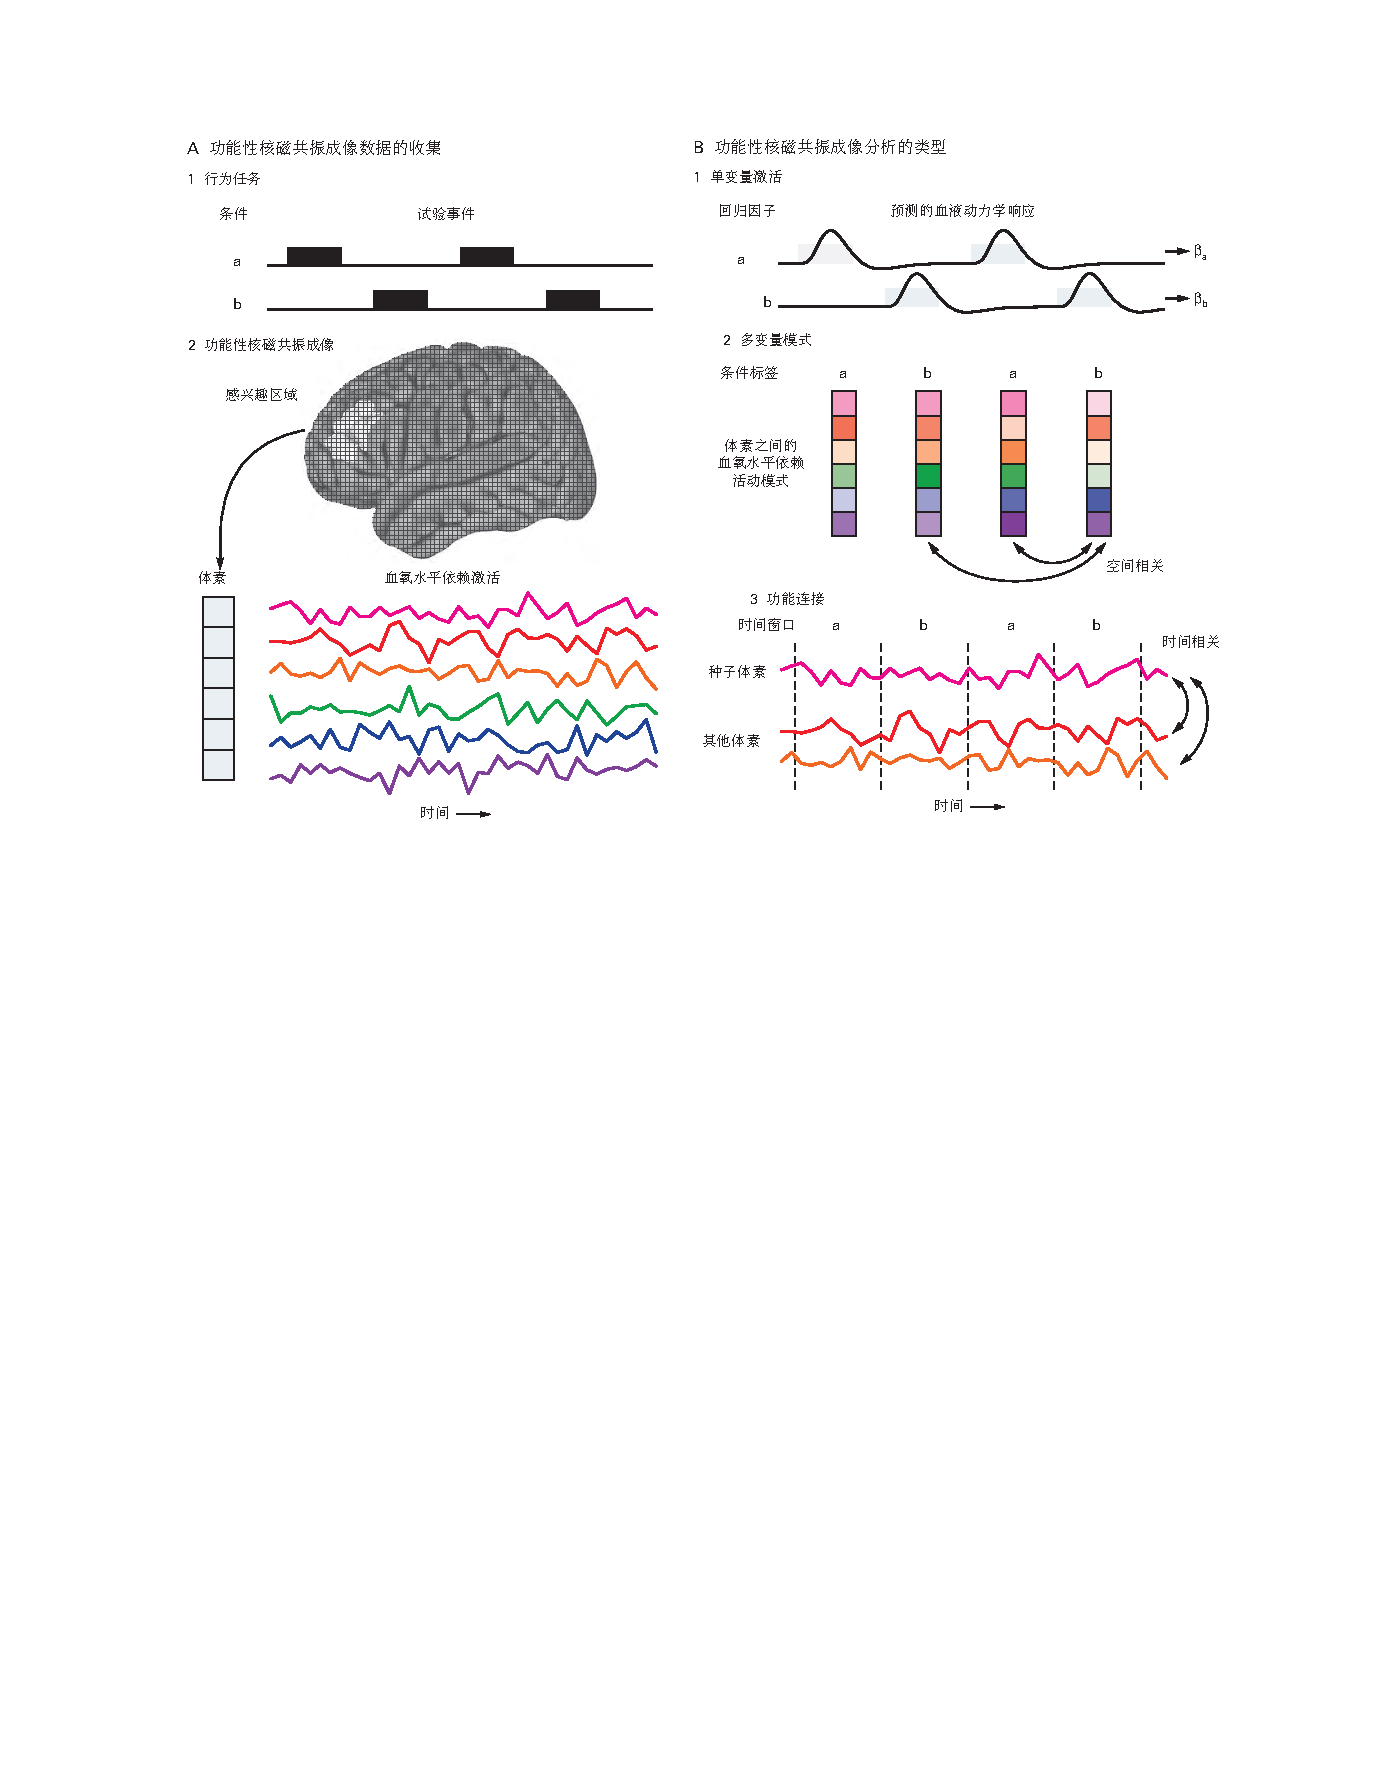
\includegraphics[width=1.0\linewidth]{chap06/fig_6_2}
	\caption{收集和分析\textit{功能性磁共振成像}数据。 
		\textbf{A.} 功能性核磁共振成像实验通常涉及受试者执行行为任务,同时从大脑测量血氧水平依赖活动。
		1. 示例任务包含两个在时间上交替出现的条件(a, b),每个条件都描绘了两个事件(黑色矩形)。
		2. 在任务期间,来自感兴趣区域的六个示例体素(不同颜色)中\textit{血氧水平依赖}活动的时间进程。 
		分析通常侧重于大脑中的感兴趣区域或其他体素子集,以减少执行的统计测试的数量。
		当分析大脑中的所有体素时,应用统计校正来减少误报的数量。
		此类分析的结果通常作为颜色编码的热图叠加在结构\textit{核磁共振成像}上。
		该图是广泛预处理和分析的结果,并不直接反映神经元活动甚至血液氧合。
		相反,体素是彩色的,以表明它们已经超过了在统计测试中被认为是重要的阈值。
		\textbf{B.} 功能性核磁共振成像实验中经常使用三种分析方法,例如 A 中描述的方法。
		1. 单变量激活分析试图根据任务中发生的情况来解释每个体素的血氧水平依赖活动。 
		这是使用统计模型完成的,该模型包含每个任务条件的回归变量,指定从该条件(灰色矩形)开始的试验事件的预测血液动力学响应(钟形曲线)。 
		将模型拟合到血氧水平依赖活动的结果是每个体素中每个回归量的$\beta$值,量化体素对该条件试验的平均响应。 
		可以减去体素的$\beta$值以衡量在一种情况下是否比另一种情况下有更大的响应。
		为了确定统计显着性,比较了受试者之间每个体素中条件之间激活的差异。
		2. 多变量模式分析考虑了跨体素的血氧水平依赖活动模式。
		这些空间模式是为每个试验从体素的一个子集(描绘了六个)中提取的,并且在特定时刻,通常是预测的血液动力学响应的峰值(颜色饱和度表示该试验中每个体素中 血氧水平依赖活动的幅度)。
		有两种常见的分析这些模式的方法。
		第一个(如图所示)涉及计算来自一对试验的模式的空间相关性,以探索体素对试验的反应有何相似之处。
		如果一个大脑区域代表不同条件下的不同信息,那么对于来自相同条件和不同条件的成对试验,这种模式相似性应该更高。
		第二种类型的多元模式分析(未显示)使用一种称为模式分类的机器学习。
		一些模式及其相应的条件标签用于训练分类器模型,根据它们在区分条件时的有用程度为体素分配权重。
		然后使用未训练的其他模式对该模型进行测试。
		如果大脑区域代表不同条件下的不同信息,则模型应该能够正确猜测从哪种条件下提取模式。
		为了确定统计显着性,一个区域中的空间相关性或分类准确度会在受试者之间进行比较。
		3. 功能连通性分析检查血氧水平依赖活动如何随时间在体素之间相关。
		通常,选择种子体素或感兴趣区域,其时间进程(粉红色曲线)与其他体素的时间进程(此处显示两个)相关。
		这可以在受试者休息时执行,从而产生每个体素的相关值,可用于识别基线状态下的大脑网络。
		功能连通性也可以在任务的不同时间窗口(虚线)中计算,从而为每个试验生成一个相关值,可用于了解这些网络的动态。
		为了确定统计显着性,每个体素的时间相关性在条件之间或与零之间在受试者之间进行比较。}
	\label{fig:6_2}
\end{figure}

% β也就是beta,代表回归系数,标准化的回归系数代表自变量也就是预测变量和因变量的相关



\subsection{功能性核磁共振成像数据首先需要通过以下预处理步骤准备分析}

在分析数据之前,必须为处理做好准备。 
这是通过一系列称为预处理的步骤完成的。 
预处理旨在消除数据中由受试者或核磁共振成像机器引起的已知噪声源。 
标准实践包括五个基本步骤,称为运动校正、切片时间校正、时间过滤、空间平滑和解剖对齐。


\textit{运动校正}旨在解决由于主体头部运动而导致的数据中不可避免的噪声。
即使是最好的受试者也会在扫描过程中将头部移动几毫米,这样横跨三维脑体积的体素就会变得有些错位。
可以使用空间插值算法纠正此移动,该算法在每次运行中排列所有卷。
该算法量化扫描期间每个点的移动量,包括 $x$、$y$ 和 $z$ 维度的平移,以及围绕这些轴(分别为俯仰、滚动和偏航)的旋转量。
这六个时间课程稍后可以作为回归器包含在数据分析中,以进一步消除运动伪影。


应用\textit{切片时间校正}来处理跨不同切片的样本采集时间的差异。
\textit{平面回波成像}序列按顺序收集构成每个脑容量的切片,通常以交错顺序进行,以避免相邻切片的污染。
因此,同一体积的第一个和最后一个采集切片的时间存在很大差异,它们在时间上分别更接近于前一个体积和后一个体积,而不是相互之间。
可以通过时间插值来完成对切片时间差异的校正,以估计如果同时获取所有切片时信号会是什么。


\textit{时间滤波}和\textit{空间平滑}旨在提高信噪比。
时域过滤去除了每个体素中时间过程的组成部分,这些组成部分很可能是噪声而不是有意义的方差,例如通常由扫描仪漂移引起的非常低的频率(> 100 秒周期)。 
空间平滑应用内核(通常为 4-8 毫米宽)来模糊单个体积,平均掉相邻体素之间的噪声,并提高功能在解剖对齐后跨对象重叠的几率。


这种\textit{解剖对齐}是通过将跨运行和受试者的数据注册到标准模板(例如蒙特利尔神经病学研究所或\textit{塔莱拉什空间})来完成的,通常使用简单的转换(例如,移位、旋转、缩放)。
通常,功能性核磁共振成像数据首先与来自同一主题的结构扫描对齐,然后将此结构扫描与标准模板对齐。


完成这五个步骤后,数据就可以进行分析了。



\subsection{功能性核磁共振成像可用于将认知功能定位到特定的大脑区域}

第一种功能性核磁共振成像分析旨在\textit{定位}大脑中的功能并确定哪些大脑区域与行为相关。 
这是基于让受试者在功能性核磁共振成像期间完成一项任务,然后检查实验不同阶段与大脑不同部位血氧水平依赖 活动变化之间的关系。 
根据研究人员对实验中不同时间发生的情况的了解,可以推断出这些区域的功能。


执行一系列统计分析来量化这种关系并确定其重要性。 
通常,这是使用称为广义线性模型的统计回归方法来完成的。 
广义线性模型试图将观察到的数据(这里是每个体素中 血氧水平依赖活动的时间过程)解释为反映独立变量(例如,任务条件)和协变量(例如,运动参数)的回归量的线性组合。


模拟任务条件的回归变量可以作为一个假设,假设体素参与该任务操纵的认知功能时应该如何响应。
每个条件的回归量是通过在实验时间线中标记该条件的每次试验的开始和持续时间来生成的,对应于预期的神经元活动,然后考虑延迟的血液动力学反应。
所有回归量同时适合每个体素中的功能性核磁共振成像活动,结果是每个条件和体素的参数估计(或$\beta$),反映了该条件对 平均的。


为了定位一个函数,来自两个或多个条件的$\beta$被对比比较。 
最基本的对比形式是从另一个(例如,实验条件)中减去一个$\beta$(例如,控制条件)。 
对比度通常是每个受试者运行的平均值,然后进入 $t$ 检验以评估受试者之间的可靠性。 
因为统计数据是针对每个体素计算的,所以存在高的误报风险,并且需要对多重比较进行校正(例如,如果体素与其他重要体素聚集在一起,则通过给予体素更多的信任)。 
或者,可以执行更受约束的分析,重点关注先验定义的有限数量的感兴趣区域。 
然后可以对感兴趣区域中的体素取对比度值的平均值以生成区域估计,而不是检查大脑中的所有体素,从而减少比较次数。


这种一般的方法系列通常被描述为测量单变量激活(“单变量”是因为每个体素或区域都是独立处理的),而“激活”是因为结果是衡量一种情况相对于另一种情况引起的相对活动。
这种分析通常用于将认知功能定位到大脑中的一组体素或区域。


然而,单变量激活不仅仅用于定位。
例如,\textit{广义线性模型}可以根据实验参数(例如,工作记忆负荷)、行为测量(例如,响应时间)为回归量中的每个试验分配连续权重而不是分类权重,从而对血氧水平依赖 活动进行定量预测 ),或计算模型(例如,强化学习中的预测误差)。
生成的$\beta$反映了体素与感兴趣变量的相关程度。


单变量激活的另一个用途是测量\textit{血氧水平依赖}活动的变化作为重复刺激的函数。
这些研究利用了适应(或重复抑制):
刺激选择性神经元对重复刺激和新刺激的反应较少的趋势。
这一事实允许通过进行相关和不相关刺激按顺序呈现的实验来推断大脑区域的调整。
在一些试验中,一个刺激之后是几乎重复的相同刺激,但特征发生了变化(例如,它的位置或大小)。
单变量分析测试这些试验中来自该区域的体素的血氧水平依赖活动是否低于其他试验,其中
(1)第一个刺激之后是不相关的第二个刺激,或者
(2)改变的刺激之前是不相关的刺激。
如果观察到这样的血氧水平依赖减少,则该区域可以解释为未针对更改的特征进行调整(例如,该区域可以被认为是位置或大小不变的)。


% 解码
\subsection{功能性核磁共振成像可用于解码大脑中所代表的信息}

第二类功能性核磁共振成像分析旨在描述大脑不同区域代表的信息类型以指导行为。
这些分析不是独立分析体素或对感兴趣区域内的体素进行平均,而是检查多个体素上血氧水平依赖活动的空间模式所携带的信息。 
这通常称为\textit{多元模式分析}。
根据活动模式的相似性或分类,有两种类型的\textit{多元模式分析}。


基于相似性的\textit{多元模式分析}试图了解大脑区域中包含或“表示”了哪些信息。 
这是通过检查该区域在实验中处理不同条件或刺激的相似程度来实现的。 
这种相似性是根据感兴趣区域中跨体素的激活模式计算的,定义为来自广义线性模型的$\beta$值模式或来自预处理数据的原始血氧水平依赖活动模式。 
一旦为多个条件或刺激定义了这些模式,就会计算每对模式的相关性或距离。 
这会生成感兴趣区域内条件或刺激之间的成对相似性矩阵。 
使用此矩阵,可以推断出感兴趣区域对哪些信息最敏感。 
例如,如果向受试者展示不同物体(例如,香蕉、独木舟、出租车)的照片,则可以为不同的大脑区域计算由这些物体引起的活动模式之间的距离矩阵。
香蕉和独木舟之间的距离小于它们与出租车之间的距离的\textit{感兴趣区域}可以解释为表示该区域代表形状(即凹面);
香蕉和出租车之间距离最短的另一个区域可能代表颜色(即黄色);
或者独木舟和出租车之间距离最短的一个可能被解释为代表功能(即交通)。


功能性核磁共振成像的神经相似性也可以与以其他方式计算的相同条件或刺激的相似性进行比较,包括人类判断、计算模型或其他物种的神经测量。
例如,如果人类受试者根据彼此看起来的相似程度对大量刺激进行评分,则具有匹配相似结构的大脑区域可被视为该行为的候选来源。
这种计算神经和行为相似性矩阵之间或来自两个来源的神经相似性矩阵之间的二阶相关性的方法称为\textit{表征相似性分析}。


基于分类器的\textit{多元模式分析}使用机器学习技术(在第~\ref{chap:chap5}~章中讨论)来解码大脑区域中存在的信息。 
第一步是在功能性核磁共振成像数据的子集上\textit{训练分类器}模型,以区分条件或刺激类别与感兴趣区域中跨体素的 血氧水平依赖活动模式。
这些模式通常是从个别试验中获得的,每个试验都根据相应试验的条件或刺激进行标记。
因此,该训练集包含每个类别的几个大脑模式示例。
分类器训练可以使用许多不同的算法,最常见的两种是\textit{支持向量机}和\textit{正则化逻辑回归}。
结果通常是每个体素的权重,反映了该体素中的活动如何与其他体素一起对分类做出贡献。
训练后的第二步是\textit{测试}分类器,方法是检查分类器从 功能性核磁共振成像数据的保留和独立子集中解码模式的能力(例如,来自不同的运行或受试者)。
每个测试试验中血氧水平依赖活动的模式乘以学习到的分类器权重并相加以产生关于模式应该如何标记的猜测。
分类准确度被量化为这些猜测与正确标签相匹配的比例。
重要的是,这种方法可用于了解不同的大脑区域如何产生行为,例如通过尝试对执行的动作、做出的决定或检索的记忆进行分类。



% 预测
\subsection{功能性核磁共振成像可用于测量大脑网络中的相关活动}

第三类功能性核磁共振成像分析旨在了解大脑作为网络的组织。
了解大脑区域单独做什么并不能完全解释大脑作为一个整体是如何产生行为的。
了解大脑区域如何相互关联也很重要,也就是说,一个区域的输入从哪里来,输出到哪里?
这需要了解哪些区域相互通信以及它们何时以及如何传输信息。
这很难用功能性核磁共振成像明确确定,但可以通过测量随时间变化的体素或区域之间 血氧水平依赖活动的相关性来估计。
如果大脑的两个部分有相关的活动,它们可能共享相同的信息或参与相同的过程。
这种相关性被解释为功能连通性的度量。


使用功能性核磁共振成像研究功能连接的一种方法是测量静息状态下的血氧水平依赖相关性。 
在受试者静止不动而不执行任务时对其进行扫描,然后提取来自一个“种子”感兴趣区域的血氧水平依赖活动的时间进程,并将其与来自其他感兴趣区域或大脑中所有体素的时间进程相关联。
或者,可以在没有种子的情况下使用聚类或成分分析来识别具有相似时间分布的体素集合。
以这些方式定义的静息功能连接有助于揭示大脑包含多个大型区域网络。
这些网络中研究最广泛的称为默认模式网络,包括后内侧皮层、外侧顶叶皮层和内侧前额叶皮层。
根据定义,静止连接不能与并发行为相关联。
它也不是静态的,因为告诉受试者不要做任何事情并不会限制他们的想法。
然而,通过检查它在疾病或失调中如何出错以及它如何与人之间的认知差异相关,可以间接地将静息连接与行为联系起来。


如果在任务期间而不是在休息时测量功能连通性,则可以更直接地将其与行为联系起来。 
解释区域之间这种相关性的一个困难是,两个区域在任务期间可能相关,不是因为它们相互通信,而是因为第三个变量。
例如,这些区域可能独立但同时对同一刺激做出反应。
因此,基于任务的功能连接通常是在删除或以其他方式考虑由刺激引起的血氧水平依赖反应后计算的。 
这种方法允许通过实验操作功能连接,并在不同任务条件下进行比较。
这些比较提供了对网络中大脑区域的参与和交互如何动态变化以支持不同行为的洞察力。
这已被证明有助于理解注意力、动机和记忆等认知功能,这些功能取决于某些大脑区域对其他区域的调节。


功能连接也可以被视为一种模式(相关性而非活动)并提交给\textit{多元模式分析}。 
相关模式比活动模式规模更大:
如果活动模式中有 $n$ 个体素,则相关模式中大约有 $n^2$ 个体素对。
因此,使用图论总结相关模式的属性可能会有所帮助,其中单个体素或区域被视为图中的节点,这些节点之间的功能连接决定了边缘强度。



\section{功能性核磁共振成像研究带来了基本的见解}

功能性核磁共振成像改变了我们对人类行为的基本神经生物学构建块的理解。
将认知心理学的实验操作和计算模型与精确的神经生物学测量相结合,扩展了现有的心智和大脑理论,并激发了新的想法。
功能性核磁共振成像的发现不仅影响了我们对被认为是人类特有行为的理解,还影响了长期以来在动物身上研究的行为。


在本节中,我们回顾了这一进展的三个例子。 
\textit{面部感知}研究揭示了人类核磁共振成像研究如何启发了动物研究。
\textit{记忆}研究说明了功能性核磁共振成像如何挑战认知心理学和系统神经科学的理论。
\textit{决策}研究展示了动物研究和计算模型如何推动功能性核磁共振成像研究。


\subsection{人类的功能性核磁共振成像研究启发了动物的神经生理学研究}

在过去的二十年里,我们对大脑如何感知面孔的理解有了长足的发展(第~\ref{chap:chap24}~章)。 
下面描述的进展提供了一个例子,说明人类功能性核磁共振成像的发现如何激发了对非人类灵长类动物进行神经元记录和因果干预的后续研究。
这种跨物种和跨技术的协同作用使人们对面孔识别的基本过程有了更全面的了解。


某些类别的刺激比其他类别的刺激对生存更重要。 
大脑是否有专门的机制来处理这种刺激? 
人脸是一个明显的例子。 
功能性核磁共振成像的发展与仔细和系统的实验设计相结合,导致了对人脑中面部处理方式和位置的重要见解。 
梭状回中的一个区域,通常被称为\textit{梭状回面孔区},被发现在人类观察面部时表现出强烈和选择性的 血氧水平依赖活动。


导致这一发现的早期功能性核磁共振成像研究依赖于简单的设计,在这些设计中,受试者被呈现了一系列不同类型的视觉刺激。
为了测量大脑区域的面部选择性,将对面部的血氧水平依赖反应与对其他类别(例如,地点、物体)的血氧水平依赖反应进行比较。 
外侧梭状回的一个区域,最可靠地位于右半球,被面部强烈激活。
这些发现与早期对非人类灵长类动物中对面部有反应的单个神经元的发现相吻合,但激发了新一轮的动物研究浪潮,以检查更大规模的大脑区域网络。
这些较新的动物研究借鉴了人类研究的实验设计,首先使用功能性核磁共振成像寻找\textit{梭状回面孔区}的同源物。
然后用神经元记录和刺激侵入性地探测由此产生的面部贴片。
这揭示了对灵长类动物面部处理的分布式神经回路的洞察。


除了选择性地响应面部刺激之外,\textit{梭状回面孔区}是否有助于面部识别行为? 
这个问题已经通过使用已知会影响面部识别的刺激变化(例如,呈现倒置的面部或呈现面部的一部分)来解决。 
最初的功能性核磁共振成像研究使用刺激类别(倒置与直立的面部)的简单比较产生了微弱和混合的结果。
后续研究使用适应设计来确定当面部重复完整或改变时 血氧水平依赖活动如何变化。
研究结果表明,\textit{梭状回面孔区}代表完整的面孔与以破坏行为识别的方式重新配置相同的视觉特征时不同。


检查一个区域的行为意义的另一种方法是研究\textit{有行为缺陷}的患者。
在这种情况下,面部识别障碍被称为\textit{面容失认症}。
令人惊讶的是,一些功能性核磁共振成像研究在这些患者中发现了完整的梭状回,这让人怀疑它对面部感知的必要性。 
然而,这里也使用适应设计的后续研究证明了信息:当重复相同的面孔时,面容失认症的其他完整的梭状回不适应。 
这表明梭状回在面容失认症患者中的反应不同,与其对面部识别的重要性一致。


视觉类别或更普遍的心理过程可以映射到像梭状回这样的一个或少数区域,这一发现对于思考思维与大脑之间的关系非常重要。
特定功能是局部化的还是广泛分布的一直是整个神经科学史上关于大脑组织的核心问题(第 ~\ref{chap:chap1}~章)。 
梭状回和面部贴片系统的发现提供了定位的新证据,并鼓励研究人员追寻其他复杂认知功能可能定位于特定大脑区域或小型节点集的假设,但也质疑定位是否正确思考大脑组织的方式。
例如,进一步的研究表明,人脸在视觉皮层上产生广泛分布的反应,梭状回可以被用来识别我们拥有专业知识的其他种类的物体。
这些争论反映了这项原创作品的变革性质,既适用于人脑研究,也适用于动物模型中的相关问题。



\subsection{功能性核磁共振成像研究挑战了认知心理学和系统神经科学的理论}

许多认知心理学的理论模型最初对大脑是不可知论的。 
然而,现在有几个功能性核磁共振成像发现的例子改变了我们对认知的组织和机制的理解。


一个突出的例子是对\textit{记忆}的研究。
从 19 世纪开始,记忆研究的总体目标是了解记忆是如何创建、检索和使用的,以及这些过程是否因记忆类型而异。 
一项重要发现来自对患者\textit{亨利$\cdot$莫莱森}的研究。 
认识到海马体受损会导致丧失形成新\textit{自传式记忆}的能力,但不会影响学习某些技能的能力(第~\ref{chap:chap52}~章)。
这些发现导致了这样的想法,即记忆可以分为两大类,有意识的和无意识的(也称为陈述性与程序性或显性与隐性)。
在定位的传统中,这些和其他类型的记忆被映射到不同的大脑区域,基于患者大脑中受损的位置以及他们表现出的行为症状。


后来对健康人脑的功能性核磁共振成像研究有助于揭示这种二分法过于简单化了。
首先,一些使用后来被称为后续记忆任务的研究表明,海马体以外的区域与陈述性记忆的成功形成有关。
在此类研究中,受试者在扫描时会收到一系列刺激(图片或文字)。
之后,通常在核磁共振仪之外,测试他们对这些刺激的记忆。
刺激最初被编码时的血氧水平依赖反应然后根据它随后是被记住还是被遗忘来排序。
将这些条件进行对比以揭示在成功的记忆形成过程中哪些大脑区域表现出更多(或更少)的活动。
除了在海马体和周围的内侧颞叶中发现这种差异外,前额叶和顶叶皮层中的血氧水平依赖活动也可以预测后期记忆。 
通过测量健康个体的整个大脑,功能性核磁共振成像揭示了陈述性记忆由不止一个大脑系统提供,与前额叶皮层(例如,语义阐述)和顶叶皮层(例如,选择性注意)相关的过程也参与编码。


功能性核磁共振成像研究以另一种方式挑战了传统的记忆组织分类学。
功能性核磁共振成像显示,以前假设不涉及海马体(或陈述性记忆)的范围广泛的任务实际上确实始终与该区域有关。
这些研究通常使用通常被认为是无意识的学习任务,在这些任务中,受试者有机会学习但从未被要求报告他们的记忆,并且在某些情况下,如果提示则无法这样做。
例如,在概率分类任务中,受试者通过反复试验学习将视觉线索分类,即使线索和类别之间的关系有时不可靠。
估计此类学习试验期间的血氧水平依赖活动,并将其与不涉及试错学习的基线任务(例如,研究线索及其提供的类别)进行比较。
这种比较通常揭示了纹状体的激活,但也可靠地揭示了海马体的激活(见第~\ref{chap:chap52}~章)。


总之,功能性核磁共振成像研究被认为依赖于陈述性记忆的任务通常会招募海马体以外的区域,而被认为依赖于程序性记忆的任务可以招募海马体。
在这两种情况下,这些发现都是偶然的,并且之所以成为可能,只是因为数据是通过功能性核磁共振成像从整个大脑中获得的。
尽管这些开始时是意想不到的结果,但它们导致了系统的后续研究,更新了我们对记忆组织的理解。
主要是,他们挑战了最初强调有意识的意识作为海马体处理的决定性特征。
这反过来又有助于将人类研究的结果与动物研究的结果联系起来,在动物研究中,有意识记忆的概念不太重要,而海马体参与的任务通常涉及空间导航。
因此,\textit{功能性磁共振成像}在人类身上的发现已经改变了我们对记忆理论模型的理解,包括神经结构和认知行为。



% 决策
\subsection{功能性核磁共振成像研究检验了动物研究和计算模型的预测}

计算模型与功能性核磁共振成像的集成一直是认知神经科学的重要发展。
这方面的一个例子来自对大脑如何\textit{学习预测}和\textit{获得奖励}的研究,以及将这一过程形式化的\textit{强化学习模型}。
这些模型与基于奖励的动物决策研究共同进化,这也启发了后来的人类研究。


这些研究和理论的核心是,中脑多巴胺能神经元会增加它们的放电以响应意想不到的奖励,例如果汁(第 ~\ref{chap:chap43}~章)。 
一旦预测性线索与奖励可靠地配对,神经元就会及时将它们的反应转移到这个预测性线索上。
如果预测的奖励没有发生,则激活会减少。
这种反应模式表明中脑多巴胺能神经元发出预期奖励与实际奖励之间差异的信号。
这种差异通常被称为奖励预测误差,并且已使用基于强化学习理论的方程式进行建模。
当该模型应用于涉及奖励的人工任务时,可以在逐个试验的基础上估计假设的奖励预测误差。
然后,这些估计可用于预测血氧水平依赖活动并识别可能参与人脑强化学习的体素和区域。


在此类典型研究中,受试者在功能性核磁共振成像期间执行学习任务,做出一系列关于视觉线索的选择以预测可能的奖励。
他们在每次选择后立即了解结果。
例如,受试者可能会看到两种形状(例如,圆形、三角形),通过按下按钮选择一种形状,然后了解该选择是否会带来金钱奖励。
此类任务的关键特征是形状和奖励之间的关联是概率性的,并且会在实验过程中发生变化。
由于这种嘈杂的关系,受试者必须学会跟踪每种形状的奖励可能性。
可以根据受试者选择和奖励的历史计算每次试验的奖励预测误差,然后将其包含在对其功能性核磁共振数据的分析中。
许多使用这种方法的研究发现,逐个试验的奖励预测误差与腹侧纹状体中的血氧水平依赖活动相关,腹侧纹状体是一个接收中脑多巴胺能神经元输入的区域。


其他计算模型,如整合了认知心理学、计算机科学和神经科学的深度神经网络,也通过产生关于大脑活动的新假设发挥了重要的理论作用。
由于这些模型通常受到大脑结构和功能的启发,因此它们有助于弥合分析水平,从动物的生理记录到人类的功能性核磁共振成像。 
它们还通过模拟可以在大脑中寻找的心理和神经生物学兴趣变量,在数据分析中发挥有用的作用,这种方法通常被称为基于模型的分析。



\section{功能性核磁共振成像研究需要仔细解读}

前面提供的例子说明了功能性核磁共振成像如何提高我们对大脑和行为之间联系的理解。 
在与心理学的接口上,功能性核磁共振成像可以补充纯粹的行为测量。
许多复杂的人类行为(例如,记忆回忆、决策制定)取决于多个处理阶段和组件。
与仅基于简单的行为测量(例如准确性或响应时间)的行为相比,使用功能性核磁共振成像测量这些过程可以提供更丰富、更机械的行为解释。
在与系统神经科学的接口上,功能性核磁共振成像补充了直接神经元记录。
大多数大脑区域(例如,海马体)支持多种行为,并且与其他区域协调一致。
使用功能性核磁共振成像对整个大脑进行成像的能力使得在网络层面更全面地了解神经机制成为可能。


那么在任务期间在某个区域发现血氧水平依赖活动意味着什么?
大脑和行为之间映射的多样性对功能性核磁共振成像结果的解释提出了严峻挑战(图~\ref{fig:6_3})。
一个基本的考虑因素是推理的类型。 
大多数功能性核磁共振成像研究使用前向推理,其中一项实验比较了操纵特定心理过程参与的任务条件之间的 血氧水平依赖活动(例如,比较面部与非面部刺激的影响以研究面部识别)。
可以推断这些条件不同的大脑区域参与了操纵过程。
前向推理依赖于任务操作,因此允许研究人员推断大脑活动的差异与感兴趣的心理过程有关。


\begin{figure}[htbp]
	\centering
	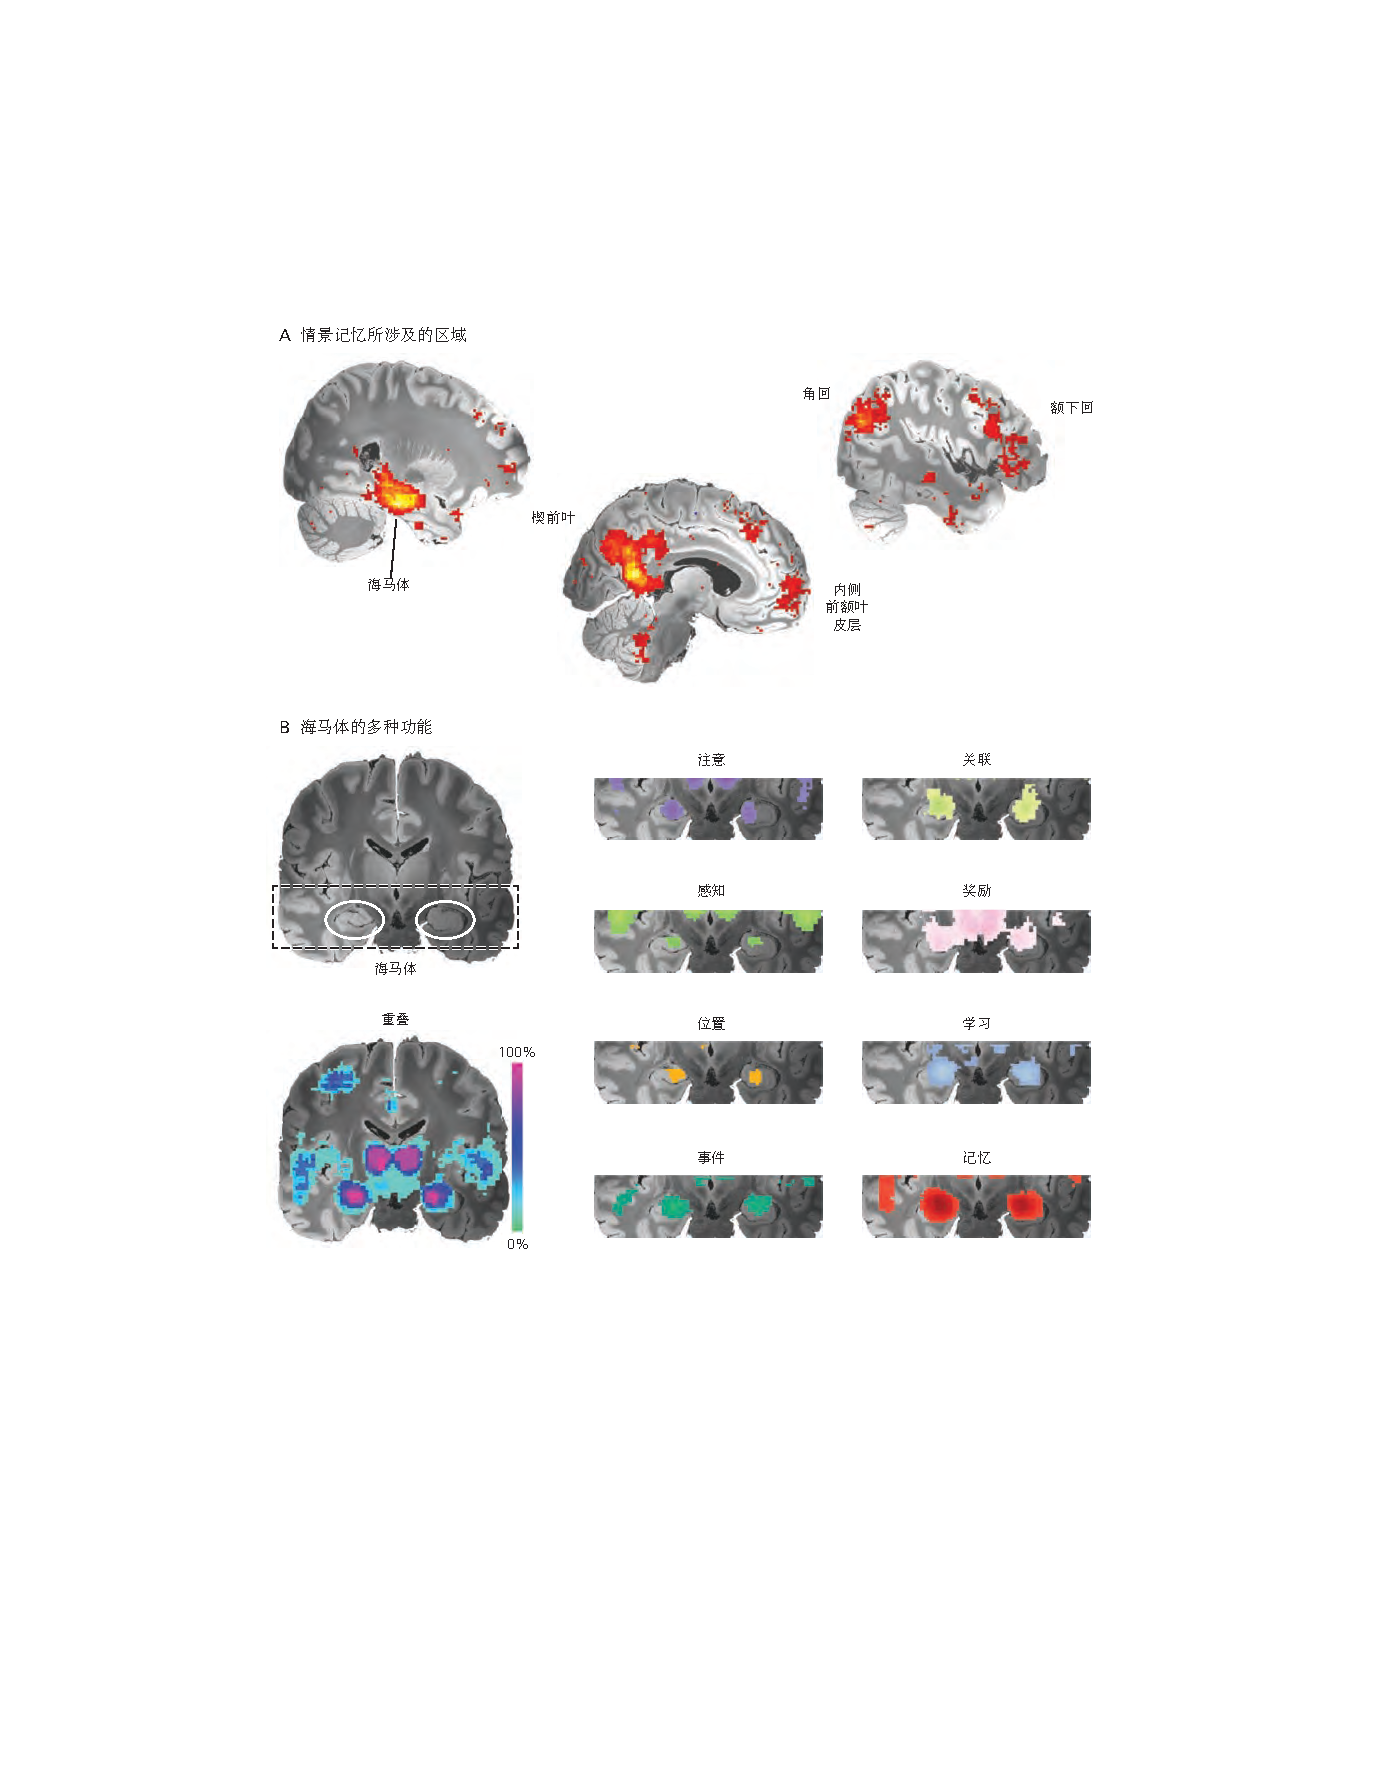
\includegraphics[width=1.0\linewidth]{chap06/fig_6_3}
	\caption{映射思维和大脑的挑战。
		对\textit{功能性核磁共振成像}数据的任何解释都必须考虑认知功能与大脑区域之间关系的复杂性。
		此处通过来自包含 14,000 多项已发表的\textit{功能性核磁共振成像}研究数据库的\textit{元分析}来说明这种复杂性。
		\textbf{A.} 这张地图显示,多个大脑区域参与\textit{情景记忆},即对过去特定事件的编码和检索。
		彩色体素表明在报告这些体素激活的研究中术语“偶发性”的可能性很高(反向推理)。
		这个例子说明了\textit{单个认知功能}如何与\textit{多个大脑区域}相关联(一对多映射)。
		\textbf{B.} 这些图显示海马体参与了多种认知功能(每个半球的白色圆圈)。 
		每个插图大脑中的彩色体素表明这些体素在检查相应术语(前向推理)的研究中被激活的可能性很高。
		重叠图显示了激活每个体素的这些术语的百分比。
		这个例子说明了\textit{单个大脑区域}如何与\textit{多个认知功能}和行为相关联(多对一映射)。}
	\label{fig:6_3}
\end{figure}


% 神经活动 (反向)->心理活动
通过反向推理,神经活动的差异是推断哪个特定心理过程活跃的基础,即使导致差异的条件并非旨在操纵该过程。 
例如,在之前的人脸与非人脸对比中,研究人员可能会将纹状体中的不同活动解释为人脸有益的证据。
这种反向推理通常是不合理的,因为奖励既没有被测量也没有被操纵,即解释是基于其他操纵奖励并发现纹状体活动的研究。
问题的出现是因为每个大脑区域通常支持不止一种功能,这意味着仅通过观察活动就不清楚哪些功能参与了。
事实上,纹状体也与运动密切相关,所以也许面部参与运动而不是奖励过程?
这个例子中逻辑合理的结论反映了前向推理,即纹状体参与了面部识别的某些(尚未解决的)方面。


因此,一种解决方案是不在功能性核磁共振成像研究中使用反向推理。
然而,在某些情况下,反向推理可能是可取的,甚至是必要的。
例如,反向推理可以让研究人员进行探索性分析并生成新的假设,甚至可以从为其他目的收集的数据中得出。
这对于充分利用难以收集的功能性核磁共振成像数据尤其重要,例如来自儿童、老人和患者的数据(方框~\ref{box:6_2})。
出于这种需要,已经开发了统计工具来支持反向推理。
例如,基于网络的工具 Neurosynth 使用已发表研究的大型数据库来分配特定心理过程(例如奖励)的概率,因为在特定区域(例如纹状体)中观察到了血氧水平依赖活动。


\begin{proposition}[现实世界中的大脑成像] \label{box:6_2}
	
	\quad \quad 利用非侵入性工具对人脑进行成像和测量内部心理过程的能力引起了人们对将功能磁共振成像应用于各种现实世界问题的兴趣,如临床诊断和治疗、法律和司法、人工智能、营销和经济以及政治。
	
	\quad \quad 在临床领域,一个有趣的方向是使用功能磁共振成像来检查植物人状态的患者。
	研究表明,一些这样的患者表现出反映心理处理的大脑活动。
	例如,患者可能表现为昏迷(无意识、非交流和对外部刺激不反应),但当被要求思考一个动作时,运动皮层或当被要求想象特定的视觉线索时,在特定类别的视觉区域表现出神经活动。
	这些发现可能会影响临床医生对患者的预后和治疗。
	
	\quad \quad \textit{功能性核磁共振成像}在现实世界中的另一个潜在应用是测谎。
	根据大脑活动准确区分真相和谎言的能力在法庭上可能具有重要价值。
	一些实验室研究报告称,当一组受试者被要求重复撒谎时,大脑活动会有所不同。
	然而,为了有用,功能磁共振成像需要以一种不受策略或对策影响的方式,提供高度可靠的证据,证明一个人是否在特定事件上撒谎。
	这在目前是不可能的,事实上,功能磁共振成像的证据在法庭上通常是不可接受的。
	
	\quad \quad 功能磁共振成像的这些和其他应用引起了道德和隐私方面的担忧。
	例如,当局可以使用功能磁共振成像数据来证明相应的决定(如有罪或无罪),利用公众的偏见来相信生物学解释,即使基础科学尚未确定。
	更令人不安的是,人类目前对我们是否分享内心想法和感受拥有自主权,但感知这些信息的设备可能会改变这一点。
	因此,神经科学家在考虑实际应用时面临的一个重要挑战是准确地传达功能磁共振成像功能强大但有局限性,以及我们对人脑的理解正在进行中。
	
\end{proposition}


区分大脑活动与行为的相关性与大脑活动与行为之间的因果关系也很重要。
如果大脑区域有选择地并持续地参与特定的心理过程,则这种相关性并不能得出它在该过程中发挥必要或充分作用的结论。
% 没有充分性:脑区的激活 不能充分 说明 功能
关于充分性,大脑区域可能(并且很可能确实)与一个或多个其他大脑区域合作以完成该过程。
% 没有必要性
就必要性而言,该地区的活动可能是其他地方加工的次要副产品。


支持功能性核磁共振成像研究解释的一种方法是评估研究结果如何与更具侵入性的方法(例如癫痫患者的电刺激)的研究结果趋同。
由于每种工具都有局限性,包括神经元记录等其他相关措施,因此这种汇聚证据的原则对于推进对大脑如何支持行为的理解至关重要。
除了通过研究和工具汇集证据外,还有人正在努力使用经颅磁刺激或实时神经反馈与功能性核磁共振成像同时操纵大脑功能。




\section{未来的进步取决于技术和概念的进步}

功能性核磁共振成像是迄今为止我们探测健康人脑的最佳技术。
它允许以相当高的分辨率测量整个大脑以及大型受试者样本中心灵的许多方面而不会造成伤害。
然而,从其他方面来说,如果我们想要更深入、更准确地了解大脑的工作原理,它远非我们最终需要的。
与动物可用的工具相比,功能性核磁共振成像提供相对嘈杂、缓慢和间接的神经元活动和回路动力学测量。


正在努力从技术和生物学上解决这些限制。
在技术方面,\textit{多波段成像序列}可以通过并行采集大脑的多个切片来提高\textit{功能性磁共振成像}数据的时间分辨率和空间分辨率。
然而,更快的测量本质上受到\textit{血液动力学反应速度慢}的限制,较小的体素仍然平均分布在数十万个神经元中。


在生物学方面,我们对血氧水平依赖活动如何从大脑的生理机制中产生有了初步的了解,例如单个神经元活动、群体活动、星形胶质细胞和其他神经胶质细胞的功能、神经调节系统和血管系统。
更好地理解\textit{血氧水平依赖}活动与这些过程之间的关系对于了解不同类型的测量何时以及为何一致和分歧至关重要。 
虽然一些实验条件会导致神经元活动和血氧水平依赖活动增加,但其他实验条件不会。
例如,虽然视觉提示的呈现增加了视觉皮层中的血流量和神经元放电,但如果高度期望的这种视觉提示没有呈现,则血流量仍会增加但神经元活动不会增加。
这表明神经活动和血管活动的耦合存在重要的细微差别,这些细微差别可能具有功能意义,并且血管信号本身可能比以前认为的更复杂。


正如功能性核磁共振成像的历史所示,一个领域的科学发现可以导致其他领域的意外突破。
1970 年代核磁共振成像的发现(20 年后导致了 功能性核磁共振成像)来自物理和化学,并且影响深远,以至于\textit{保罗$\cdot$劳特布尔}和\textit{彼得$\cdot$曼斯菲尔德}获得了 2003 年诺贝尔生理学或医学奖。
几十年前核磁共振的发现又使这成为可能,\textit{伊西多$\cdot$拉比}获得了 1944 年的诺贝尔物理学奖,\textit{费利克斯$\cdot$布洛赫}和\textit{爱德华$\cdot$珀塞尔}获得了 1952 年的诺贝尔物理学奖。
这些发现最初与神经科学并无关联,但却引发了心智、大脑和行为研究领域的一场革命。


\section{亮点}

1. 认知神经科学中的功能性大脑成像方法旨在记录与人类大脑中展开的心理过程相关的大脑活动,将\textit{生物学}和\textit{行为测量}联系起来。
目前,占主导地位的技术是功能性核磁共振成像。


2. 功能性核磁共振成像基于两个主要概念:磁共振物理学和神经血管耦合生物学。
结合起来,\textit{功能性核磁共振成像}可以测量\textit{血氧水平依赖}对神经元活动的响应。
当人类受试者在功能性核磁共振成像期间执行认知任务时,随着时间的推移,血氧水平依赖活动的测量可以与特定的心理过程和行为联系起来。

3. 血氧水平依赖活动和行为之间的联系是通过一系列预处理步骤和统计分析推断出来的。
这些分析可以回答一系列问题,例如哪些大脑区域在特定任务期间处于活动状态,哪些信息被编码在区域内活动的空间模式中,以及区域如何作为网络的一部分随着时间的推移相互影响。


4. 人脑成像导致了对许多领域行为的神经机制的基本见解。
一些突出的例子是了解人脑如何处理面孔,如何存储和检索记忆,以及我们如何从反复试验中学习。
在这些领域中,来自功能性核磁共振成像的数据与动物神经元记录的发现以及计算模型的理论预测相融合,提供了大脑与思维之间关系的更完整画面。


5. 功能性核磁共振成像记录大脑活动但不直接修改活动。
因此,它不支持推断某个大脑区域是否是行为所必需的,而是该区域是否与该行为有关。
大多数研究支持对这种参与的前向推论,即大脑中的活动可以与心理过程联系起来,因为实验操纵了该过程。


6. 功能性核磁共振成像提供了一个机会来研究人类大脑的功能,因为它参与了健康和疾病中的各种心理过程。 
这项技术及其生成的数据分析正在不断发展,以提高生物测量的时间分辨率和空间分辨率,并阐明这些测量、心理过程和行为之间的联系。



\chapter*{第二部分:神经系统细胞的细胞生物学和分子生物学}
\markboth{神经系统细胞的细胞生物学和分子生物学}{神经系统细胞的细胞生物学和分子生物学}

\begin{figure}[htbp]
	\centering
	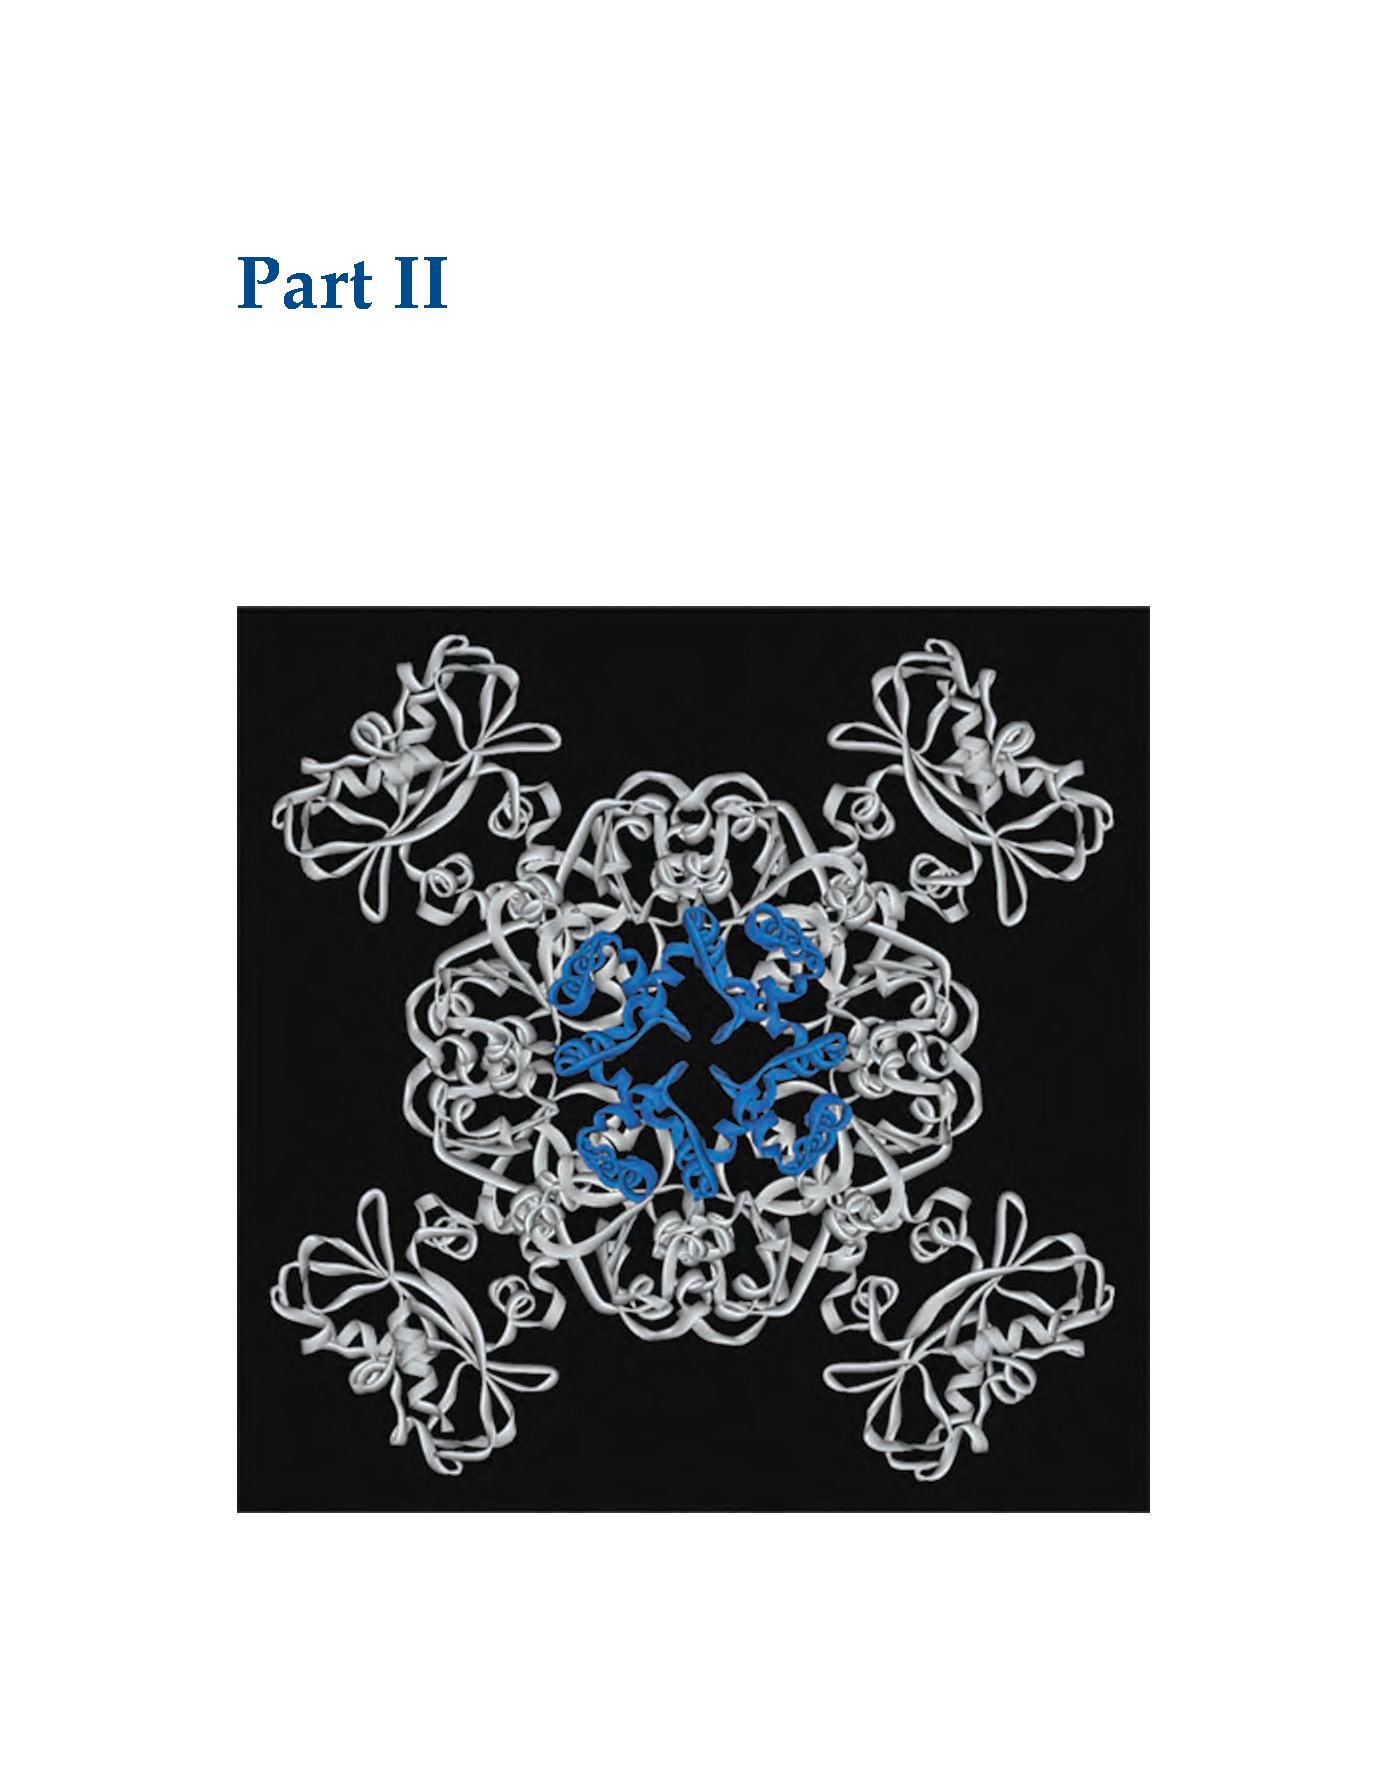
\includegraphics[width=0.9\linewidth]{chap07/fig_7_0}
	\caption{嗜热微生物古甲烷杆菌的MthK \ce{Ca^2+}调节\ce{K+}通道的晶体结构。
		这是从处于\ce{Ca^2+}结合开放状态的通道的细胞外侧观察的。
		MthK由两个主要的功能结构域组成。
		一种完整的膜蛋白形成一个水性孔(蓝色),它选择并传导\ce{K+}离子,并具有一个在打开和关闭构象之间切换的门;
		细胞内\ce{Ca^2+}结合门控环(灰色)控制该门。
		当它结合\ce{Ca^2+}时,所产生的构象变化被机械地传递到孔中,导致其切换到开放状态。}
	\label{fig:7_0}
\end{figure}


在所有的生物系统中,从最原始到最先进,基本的组成部分都是细胞。
细胞通常被组织成在复杂的生物系统中重复的功能模块。
脊椎动物的大脑是模块化系统中最复杂的例子。
复杂的生物系统还有另一个基本特征:
它们是建筑学的——也就是说,它们的解剖结构、精细结构和动态特性都反映了特定的生理功能。
因此,大脑的结构及其组成细胞的细胞生物学、生物物理学和生物化学反映了其基本功能,即调节行为。


神经系统由神经胶质细胞和神经细胞组成。
早期将神经胶质细胞视为纯粹的结构元件的观点已经被我们目前的理解所取代,即有几种类型的神经胶质细胞,每种都专门调节神经元功能的一个或多个特定方面。
不同种类的神经胶质细胞在促进和引导神经发育、隔离轴突过程、控制细胞外环境、支持突触传递、促进学习和记忆以及调节神经系统内的病理过程方面发挥着重要作用。
一些神经胶质细胞具有神经递质受体和电压门控离子通道,使它们能够相互通信,并与神经元通信,以支持神经元信号传导。


与神经胶质细胞相比,神经细胞的巨大多样性——神经系统模块组装的基本单元——是一个基本细胞计划的变体。
该计划的四个特点使神经细胞具有独特的能力,能够在长距离内精确快速地相互交流。
首先,神经元是极化的,一端有感受性树突,另一端有与突触前终末相连的轴突。
这种函数性质的极化将电压脉冲的主要流动限制在一个方向上。
其次,神经元具有电兴奋性。
它的细胞膜含有特殊的蛋白质——离子通道和受体——允许特定无机离子的流入和流出,从而产生电流,在膜上产生电压信号。
第三,神经元含有蛋白质和细胞器,赋予其特殊的分泌特性,使其能够在突触处释放神经递质。
第四,这种在细胞体及其末端之间长距离快速信号传导的系统是由细胞骨架结构实现的,该结构在较慢的时间尺度上介导各种蛋白质、信使核糖核酸和细胞器在两个隔间之间的有效转运。


在本书的这一部分,我们将关注独特的细胞生物学特性,这些特性使神经元和胶质细胞能够实现其各种特殊功能。
重点将放在离子通道的特性上,离子通道赋予神经元以动作电位的形式产生和传播电信号的能力。
我们从考虑离子通道共享的一般性质开始讨论神经元——选择和传导离子的能力,以及在开放和闭合构象之间进行门控的能力。
神经元使用四大类通道进行信号传导:
(1)静息通道产生静息电位,并成为神经元被动电特性的基础,这些特性决定了突触电位的时间进程、沿树突的分布以及触发动作电位的阈值;
(2) 感觉受体通道对某些感觉刺激作出反应,产生局部受体电位;
(3) 配体门控通道对神经递质作出反应而开放,产生局部突触电位;
以及(4)电压门控通道产生产生自传播动作电位的电流。
在这一部分中,我们主要关注静息和电压门控通道。
在第三部分中,我们更详细地考虑了配体门控通道,以及控制其活性的神经递质和第二信使。
感官刺激激活的通道将在第四部分中进行检查。




\chapter{神经系统的细胞} \label{chap:chap7}

神经系统的细胞——神经元和胶质细胞——与一般细胞有许多共同特征。
然而,神经元具有特殊的天赋,能够与体内远处的其他细胞进行精确、快速的通信。
两个特征赋予了神经元这种能力。


首先,它们具有高度的形态和功能不对称性:神经元的一端有接受树突,另一端有传递轴突。
这种排列是单向神经元信号传导的结构基础。


其次,神经元既可电兴奋又可化学兴奋。
神经元的细胞膜包含特殊的蛋白质——离子通道和受体——它们促进特定无机离子的流动,从而重新分配电荷并产生改变跨膜电压的电流。
这些电荷变化可以沿轴突产生动作电位形式的去极化波,这是信号在神经元内传播的通常方式。
胶质细胞不太容易兴奋,但它们的膜含有促进离子摄取的转运蛋白,以及从细胞外空间去除神经递质分子的蛋白质,从而调节神经元功能。


根据树突形态、轴突投射模式和电生理特性,有数百种不同类型的神经元。
这种结构和功能多样性主要由每种神经元细胞类型表达的基因决定。
尽管神经元都继承了相同的基因组,但每个神经元都表达一组受限的基因,因此只产生某些分子——酶、结构蛋白、膜成分和分泌产物——而不是其他分子。
在很大程度上,这种表达取决于细胞的发育历史。
从本质上讲,每个细胞都是它所表达的分子集合。


神经胶质细胞的种类也很多,可以根据其独特的形态、生理和生化特征进行鉴定。
神经胶质细胞的不同形态表明神经胶质细胞可能与神经元一样异质。
尽管如此,脊椎动物神经系统中的胶质细胞可分为两大类:大胶质细胞和小胶质细胞。
大胶质细胞主要分为三种类型:少突胶质细胞、雪旺细胞和星形胶质细胞。
在人脑中,大约 90\% 的胶质细胞是大胶质细胞。
其中,大约一半是髓鞘生成细胞(少突胶质细胞和雪旺细胞),一半是星形胶质细胞。
少突胶质细胞为中枢神经系统中某些神经元的轴突提供绝缘髓鞘(图~\ref{fig:7_1})。 
雪旺细胞使周围神经系统中神经元的轴突形成髓鞘(图 ~\ref{fig:7_1}B);
非髓鞘化雪旺细胞具有其他功能,包括促进神经肌肉突触的发育、维持和修复。
星形胶质细胞因其不规则的大致星形细胞体和大量突起而得名;
它们支持神经元并以多种方式调节神经元信号(图 ~\ref{fig:7_1}C)。 
小胶质细胞是大脑的常驻免疫细胞和吞噬细胞,但在健康大脑中也具有稳态功能。


\begin{figure}[htbp]
	\centering
	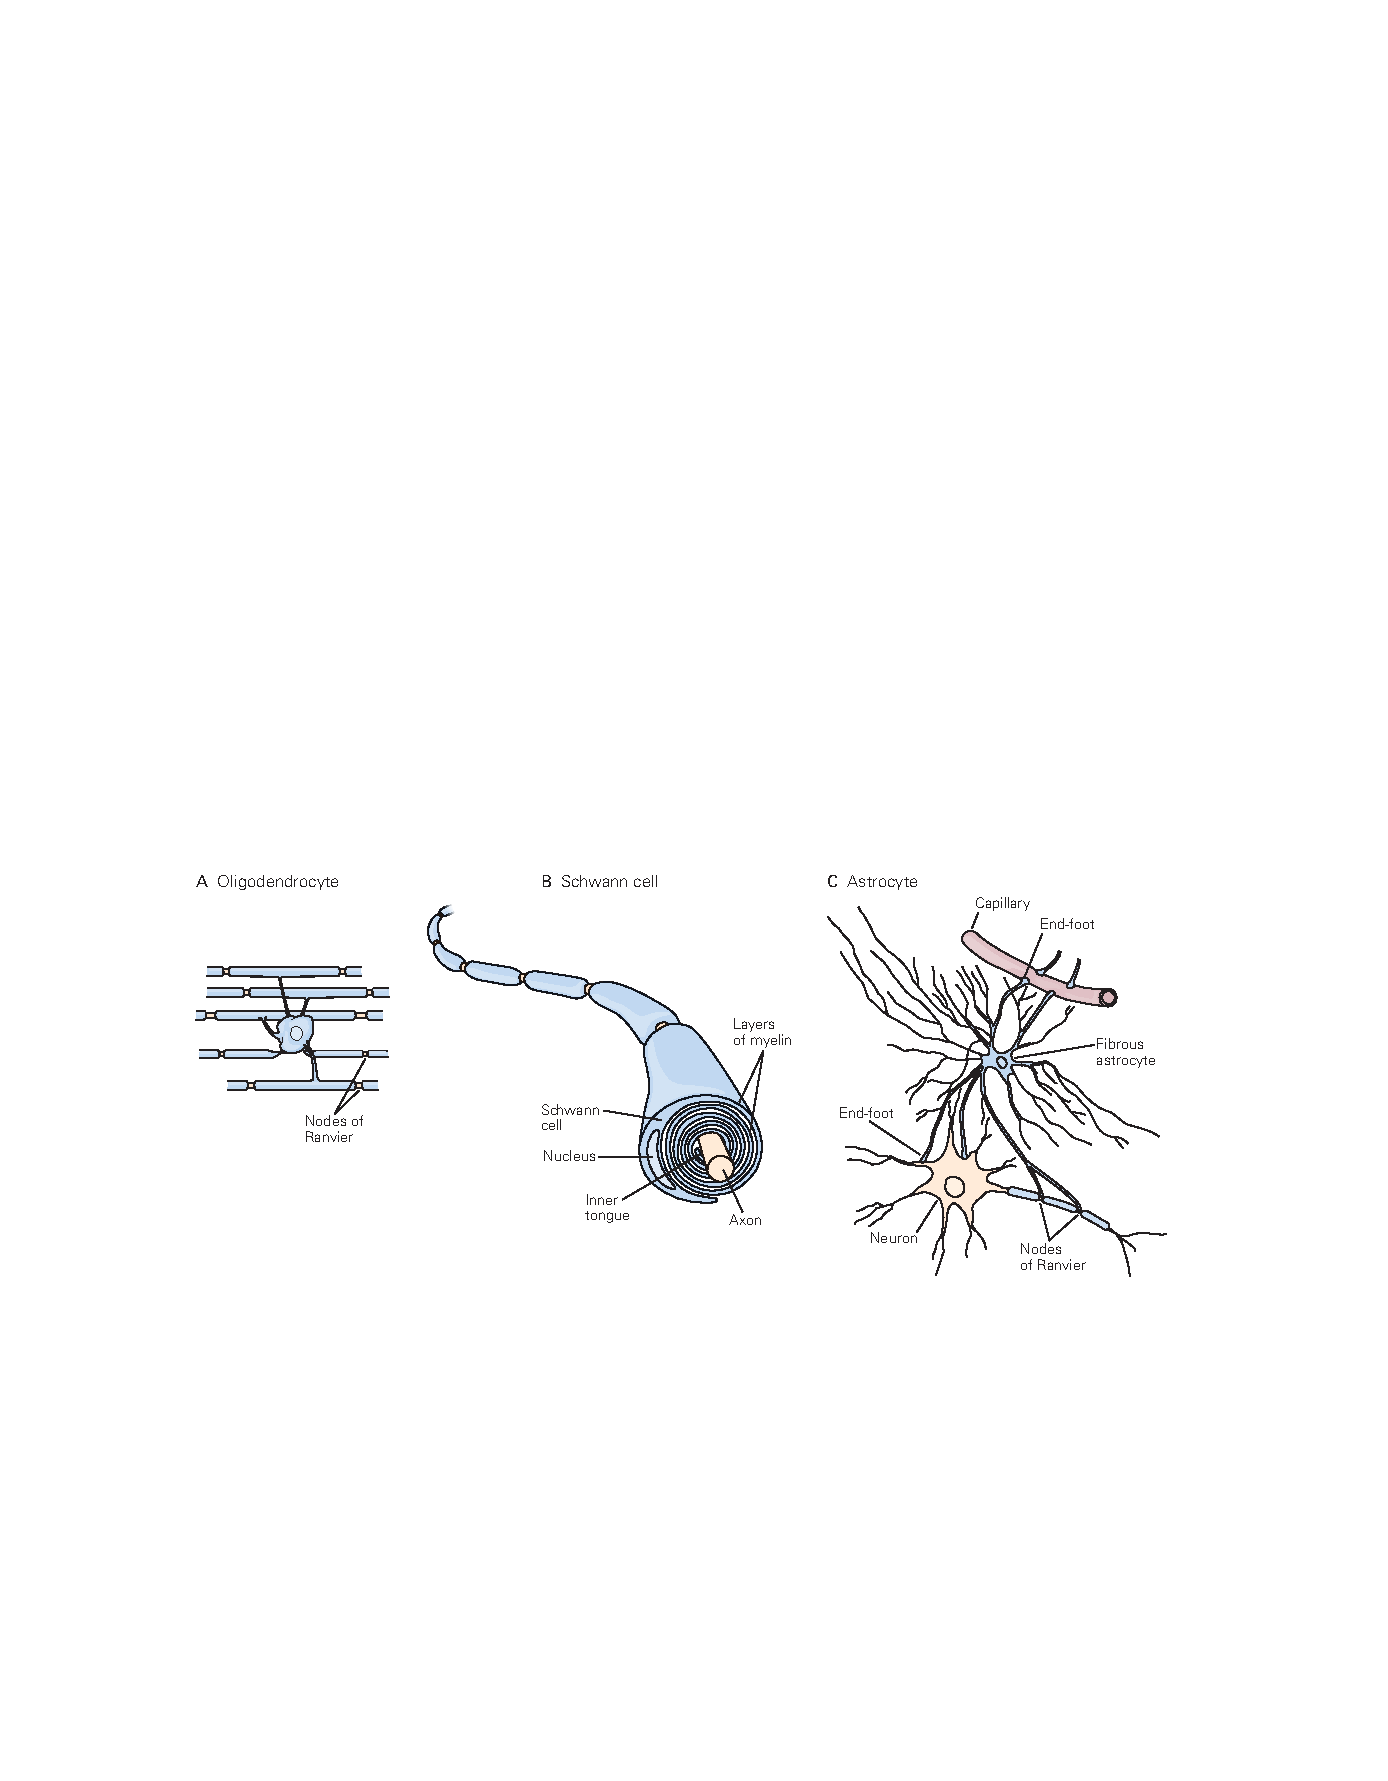
\includegraphics[width=1.0\linewidth]{chap07/fig_7_1}
	\caption{神经胶质细胞的主要类型是中枢神经系统中的少突胶质细胞和星形胶质细胞以及周围神经系统中的雪旺细胞。
		A. 少突胶质细胞是突起相对较少的小细胞。
		如图所示,在大脑的白质中,它们提供了隔离轴突的髓鞘。
		单个少突胶质细胞可以将其膜状突起包裹在许多轴突周围。 在灰质中,神经周围少突胶质细胞包围并支持神经元的细胞体。 B. Schwann 细胞为周围神经系统中的轴突提供髓鞘。 在发育过程中,几个雪旺细胞沿着单个轴突的长度定位。 每个细胞在 Ranvier 的两个节点之间形成一个大约 1 毫米长的髓鞘。 当雪旺细胞的内舌围绕轴突旋转数圈时,鞘形成,将轴突包裹在膜层中。 实际上,髓磷脂层比这里显示的更紧凑。 (改编自 Alberts 等人,2002 年。)C. 星形胶质细胞是中枢神经系统中的一类主要神经胶质细胞,其特征在于其星形形状和突起上的宽端足。 因为这些末端足使星形胶质细胞与毛细血管和神经元接触,所以星形胶质细胞被认为具有营养功能。 星形胶质细胞在维持血脑屏障方面也起着重要作用(在本章后面描述)。}
	\label{fig:7_1}
\end{figure}


\section{神经元和胶质细胞具有许多结构和分子特征}

神经元和胶质细胞从胚胎神经系统的共同神经上皮祖细胞发育而来,并具有许多结构特征(图~\ref{fig:7_2})。
这些细胞的边界由细胞膜或质膜界定,其具有所有生物膜的不对称双层结构,并提供对大多数水溶性物质不可渗透的疏水屏障。
细胞质有两个主要成分:细胞质和膜状细胞器。


\begin{figure}[htbp]
	\centering
	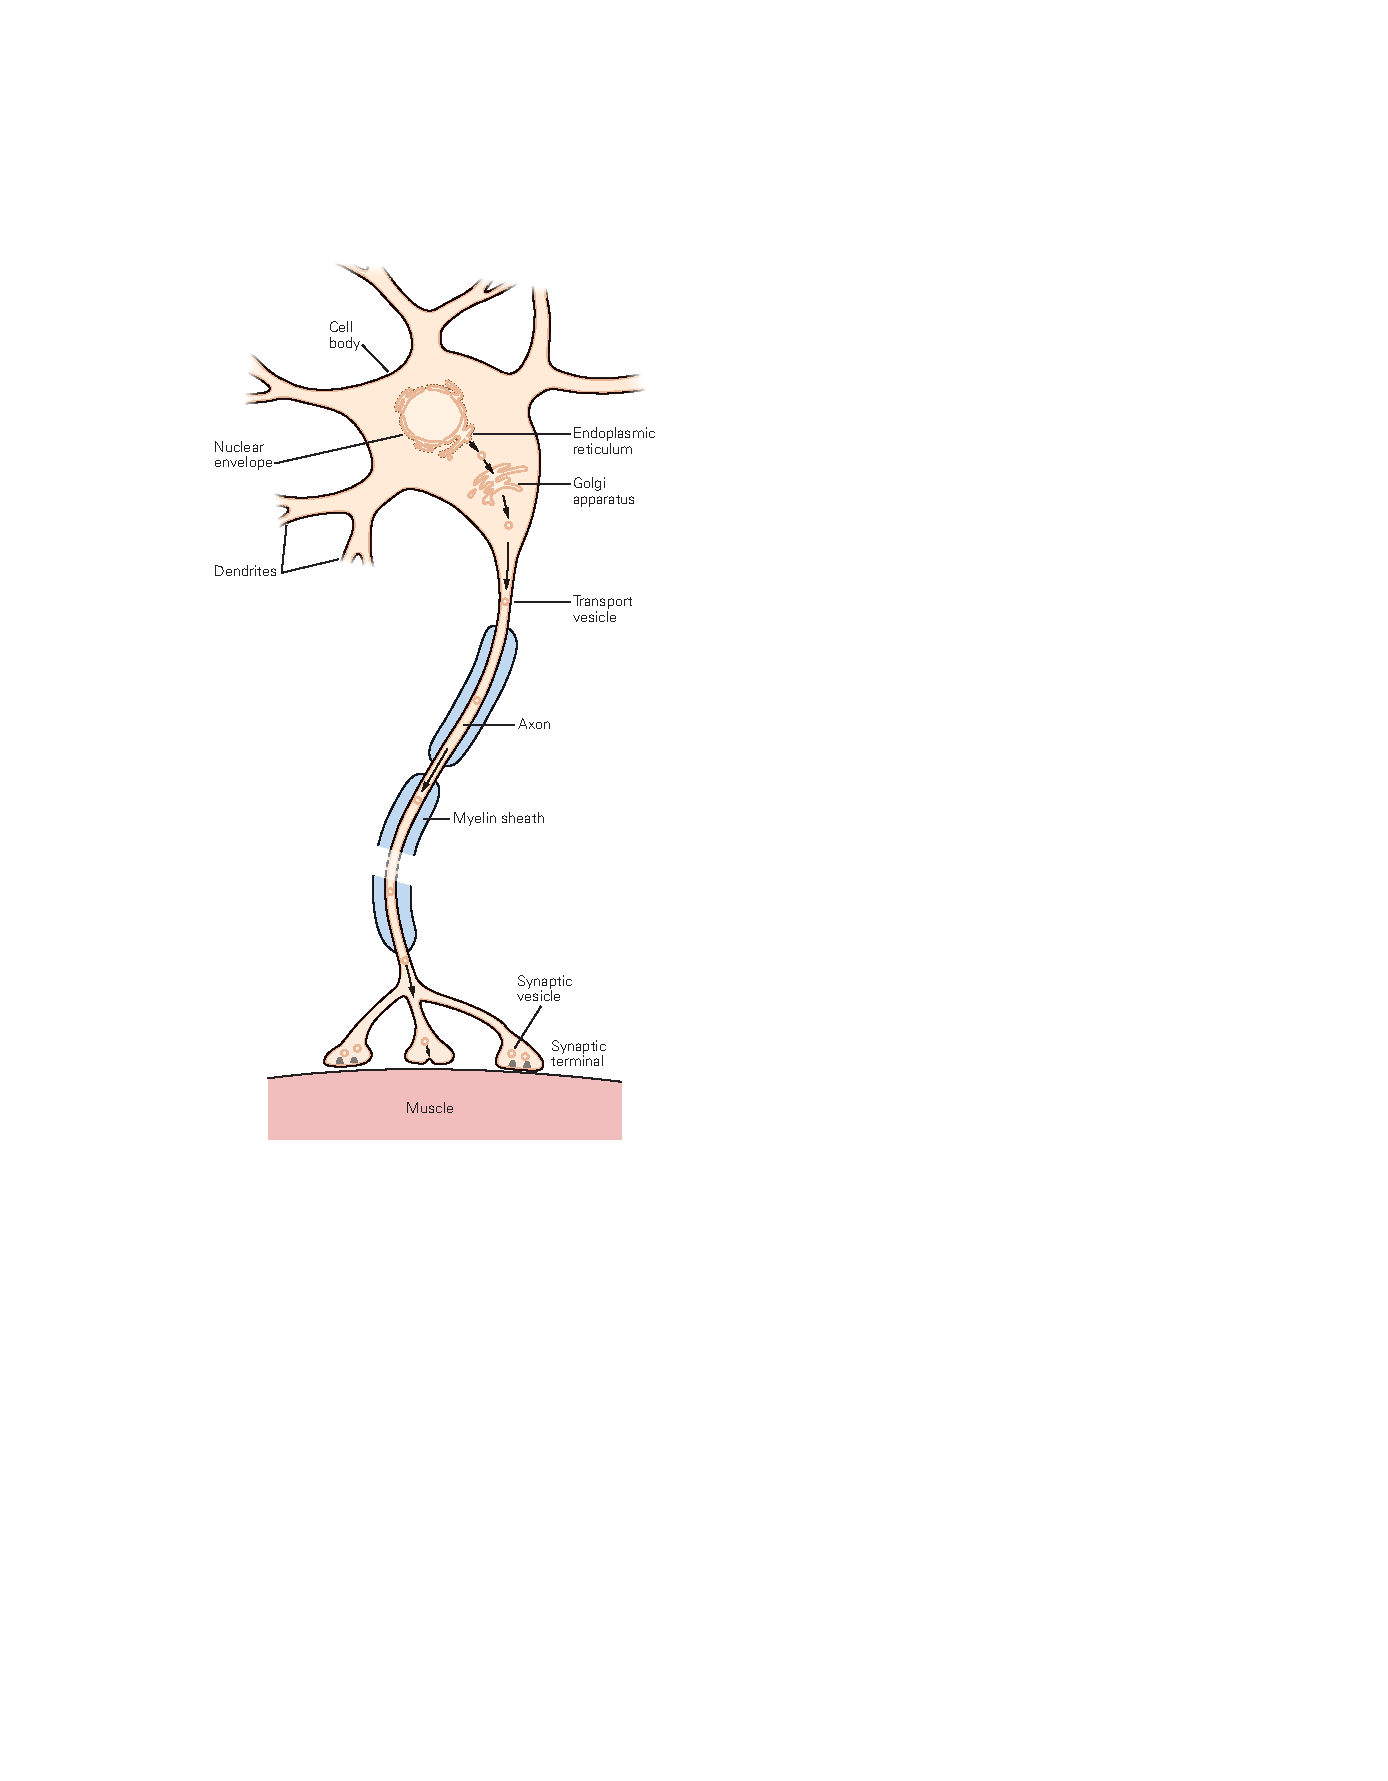
\includegraphics[width=0.5\linewidth]{chap07/fig_7_2}
	\caption{神经元的结构。
		脊髓运动神经元的细胞体和细胞核被双层膜包围,即核膜,与内质网相连。
		构成核膜的两个膜层之间的空间与内质网的腔连续。 树突从神经元的基底面出现,轴突从顶端面出现\cite{williams1989bannister}。}
	\label{fig:7_2}
\end{figure}


胞质溶胶是细胞质的水相。
在此阶段,实际上只有少数蛋白质游离在溶液中。
除了一些催化代谢反应的酶外,大多数蛋白质都被组织成功能复合物。
最近一个叫做蛋白质组学的分支学科已经确定这些复合物可以由许多不同的蛋白质组成,其中没有一个与另一个共价连接。
例如,\textit{N-甲基-D-天冬氨酸}型谷氨酸受体(一种介导中枢神经系统兴奋性突触传递的膜相关蛋白)的细胞质尾部锚定在由 100 多种支架蛋白组成的大型复合体中, 蛋白质修饰酶。
(许多参与第二信使信号转导的胞质蛋白,将在后面的章节中讨论,它们嵌入质膜正下方的细胞骨架基质中。)核糖体是翻译\textit{信使核糖核酸}分子的细胞器,由几个蛋白质亚基组成。
蛋白酶体是一种大型多酶细胞器,可降解泛素化蛋白质(本章稍后描述的过程),它也存在于神经元和胶质细胞的胞质溶胶中。


膜细胞器是细胞质的第二个主要成分,包括线粒体和过氧化物酶体,以及由小管、囊泡和称为液泡器的池组成的复杂系统。
线粒体和过氧化物酶体处理分子氧。
线粒体产生三磷酸腺苷 (ATP),这是细胞能量转移或消耗的主要分子,而过氧化物酶体可防止强氧化剂过氧化氢的积累。
线粒体源自在进化早期侵入真核细胞的共生古细菌,在功能上与液泡器不连续。
线粒体还在钙离子稳态和脂质生物合成中发挥其他重要作用。


液泡器包括光滑内质网、粗面内质网、高尔基复合体、分泌小泡、核内体、溶酶体,以及连接这些不同隔室的多种运输小泡(图~\ref{fig:7_3})。
它们的管腔在拓扑上对应于细胞的外部;
因此,它们脂质双层的内层小叶对应于质膜的外层小叶。


\begin{figure}[htbp]
	\centering
	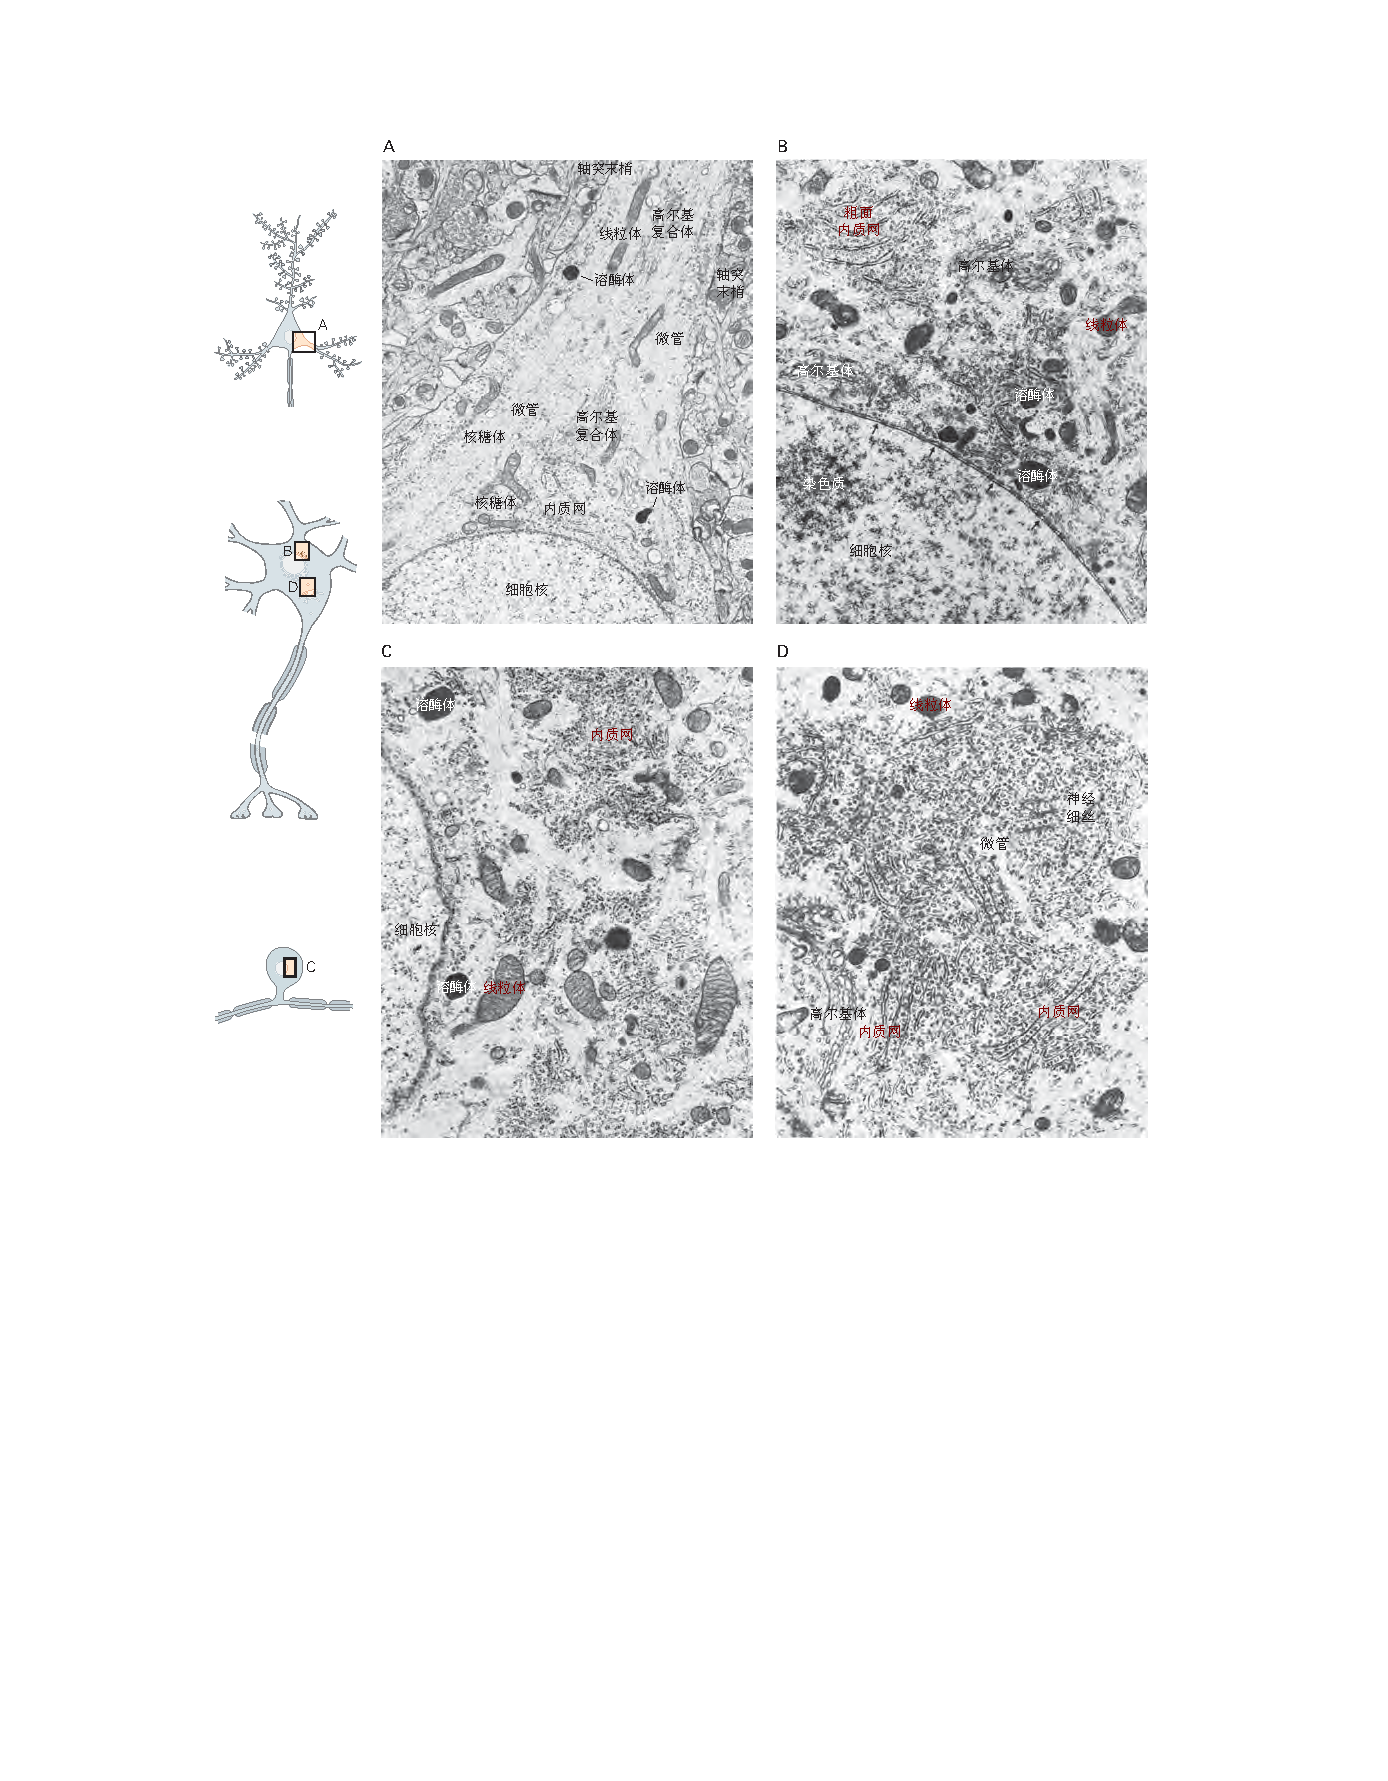
\includegraphics[width=1.0\linewidth]{chap07/fig_7_3}
	\caption{神经元的细胞器。
		电子显微照片显示神经元四个不同区域的细胞质\cite{peters1991neuropil}。
		\textbf{A.} 树突从锥体神经元的细胞体中出现,其中包括细胞核 (N) 上方的内质网 (ER) 和高尔基复合体 (G) 的一部分 附近。
		一些高尔基池已进入树突,线粒体 (Mit)、溶酶体 (Ly) 和核糖体 (R) 也已进入。
		微管 (Mt) 是细胞质中突出的细胞骨架丝。
		在顶部和右侧可以看到与树突接触的轴突末端 (AT)。
		\textbf{B.} 参与大分子合成的脊髓运动神经元的某些成分。 细胞核 (N) 含有大量染色质 (Ch),并以含有许多核孔(箭头)的核膜为界。
		\textit{信使核糖核酸}通过这些孔离开细胞核并附着在核糖体上,核糖体在细胞质中保持游离状态或附着在内质网膜上形成粗面内质网 (RER)。
		细胞质中合成的调节蛋白通过孔进入细胞核。 可以看到高尔基体 (G) 的几个部分,以及溶酶体 (Ly) 和线粒体 (Mit)。
		C、D. 背根神经节细胞 (C) 和运动神经元 (D) 的显微照片显示了细胞体中主要负责蛋白质合成和加工的细胞器。
		\textit{信使核糖核酸}通过核膜进入细胞质并被翻译成蛋白质。 游离多核糖体,即附着在单个\textit{信使核糖核酸}上的一串核糖体,产生胞质蛋白和被导入线粒体 (Mit) 和过氧化物酶体中的蛋白。
		多核糖体附着于内质网 (ER) 膜后,会形成以内质网为目的地的蛋白质。
		此处显示的运动神经元的特定区域还包括高尔基体 (G) 的膜,其中进一步处理膜和分泌蛋白。
		一些新合成的蛋白质在小泡中离开高尔基体,小泡沿着轴突向下移动到突触;
		其他膜蛋白被掺入溶酶体 (Ly) 和其他膜细胞器中。
		微管 (M) 和神经丝 (Nf) 是细胞骨架的组成部分。}
	\label{fig:7_3}
\end{figure}


该系统的主要子隔室在解剖学上是不连续的,但在功能上是相连的,因为膜状和腔内物质通过运输囊泡从一个隔室移动到另一个隔室。
例如,在粗面内质网(布满核糖体的网状部分)和光滑内质网中合成的蛋白质和磷脂被运送到高尔基复合体,然后运送到分泌囊泡,当囊泡膜与 质膜(称为胞吐作用的过程)。
这种分泌途径将膜成分添加到质膜,并将这些分泌囊泡的内容物释放到细胞外空间。


相反,细胞膜的成分通过内吞囊泡进入细胞(内吞作用)。
这些被纳入早期内体,分选集中在细胞外围的隔室。
内吞膜通常含有特定的蛋白质,如跨膜受体,可以通过成熟为循环核内体而直接回到质膜,也可以成熟为晚期核内体,后者通过与溶酶体融合而被靶向降解。
(胞吐作用和胞吞作用将在本章后面详细讨论)平滑内质网还充当整个神经元细胞质中受调节的内部钙离子储存(参见第~\ref{chap:chap14} 章中关于\ce{Ca^2+} 释放的讨论)。


粗面内质网的一个特殊部分形成了核包膜,这是一个球形扁平池,围绕着染色体\textit{脱氧核糖核酸}及其相关蛋白(组蛋白、转录因子、聚合酶和异构酶)并定义了细胞核(图~\ref{fig:7_3})。 
因为核包膜与内质网的其他部分和液泡器的其他膜是连续的,所以推测它已经进化为质膜的内陷以包裹真核染色体。
核膜被核孔打断,核膜的内外膜融合导致亲水通道的形成,蛋白质和\textit{核糖核酸}通过该通道在细胞质本身和核细胞质之间交换。


尽管核质和细胞质是细胞质的连续结构域,但只有分子量小于 5,000 的分子才能通过扩散自由地穿过核孔。
较大的分子需要帮助。
一些蛋白质具有特殊的核定位信号,这些区域由一系列基本氨基酸(精氨酸和赖氨酸)组成,可被称为核输入受体 (importins) 的可溶性蛋白质识别。
在核孔中,这种复合物被另一组称为核孔蛋白的蛋白质引导进入细胞核。


神经细胞体的细胞质延伸到树突状树中,没有功能分化。 
通常,细胞体细胞质中的所有细胞器也存在于树突中,尽管粗面内质网、高尔基复合体和溶酶体的密度随着与细胞体的距离而迅速减小。 
在树突中,光滑的内质网在称为棘的细突底部突出(图 ~\ref{fig:7_4}~和~\ref{fig:7_5}),这是兴奋性突触的接受部分。
树突棘中多聚核糖体的浓度介导局部蛋白质合成(见下文)。


\begin{figure}[htbp]
	\centering
	\includegraphics[width=0.7\linewidth]{chap07/fig_7_4}
	\caption{高尔基体和内质网膜从细胞体延伸到树突中。
		\textbf{A.} 高尔基体复合体(实线箭头)在光学显微镜下显示为数条伸入树突(空心箭头)但未伸入轴突的细丝。
		底部的箭头表示轴突小丘。
		对于这张显微照片,脑干的一个大神经元用专门针对高尔基复合体的抗体进行了免疫染色\cite{de1986heterogeneous}。
		\textbf{B.} 光滑的内质网(箭头)延伸到树突棘的颈部,而另一个膜室位于脊柱的起点 (箭)\cite{cooney2002endosomal}。}
	\label{fig:7_4}
\end{figure}


\begin{figure}[htbp]
	\centering
	\includegraphics[width=1.0\linewidth]{chap07/fig_7_5}
	\caption{树突棘的类型。
		海马 CA1 区锥体细胞的成熟树突显示三种类型的树突棘形状。
		左图基于一系列电子显微照片\cite{harris1989dendritic,sorra1993occurrence}。
		位于突触前轴突对面的表面(箭头)包含突触受体。
		此处以及 B 和 C 中显示的组织来自出生后第 15 天大鼠大脑的海马体。
		\textbf{B.} 含有突触后密度(箭头)的粗短棘在成熟的海马体中既小又罕见。
		它们较大的对应物(未显示)在未成熟的大脑中占主导地位。
		\textbf{C.} 蘑菇形刺的头部较大。 此处显示的未成熟脊柱包含平滑内质网的扁平池,一些具有串珠外观(实线箭头)。 空心箭头表示突触后密度。}
	\label{fig:7_5}
\end{figure}


与细胞体和树突的连续性相反,轴突出现的轴突小丘处的细胞体之间存在明显的功能边界。
构成神经元中蛋白质主要生物合成机制的细胞器——核糖体、粗面内质网和高尔基复合体——通常被排除在轴突之外(图~\ref{fig:7_4}),溶酶体和某些蛋白质也是如此。
然而,轴突富含光滑内质网、单个突触小泡及其前体膜。



\section{细胞骨架决定细胞形状}

细胞骨架决定细胞的形状,并负责细胞质内细胞器的不对称分布。
它包括三种丝状结构:微管、神经丝和微丝。 
这些细丝和相关蛋白约占细胞总蛋白的四分之一。


微管形成长支架,从神经元的一端延伸到另一端,在发育和维持细胞形状方面发挥关键作用。
单个微管可以长达 0.1 毫米。
微管由原丝组成,每个原丝由多对沿微管纵向排列的 a-和 b-微管蛋白亚基组成(图~\ref{fig:7_6}A)。 
微管蛋白亚基沿原丝与相邻的亚基结合,并在相邻原丝之间横向结合。
微管用正端(或生长端)和负端(微管可以解聚的地方)极化。
有趣的是,轴突和树突之间的微管方向不同。
在轴突中,微管显示单一方向,正端远离细胞体。
在近端树突中,微管可以双向定向,正端朝向或远离细胞体。


\begin{figure}[htbp]
	\centering
	\includegraphics[width=1.0\linewidth]{chap07/fig_7_6}
	\caption{纤维结构图谱。
		\textbf{A.} 微管是最大直径的纤维 (25 纳米),是由 13 根原丝组成的螺旋圆柱体,每根原丝的宽度为 5 纳米。
		每个原丝由一列交替的 $\alpha$-和$\beta$-微管蛋白亚基组成;
		每个亚基的分子量约为 50,000 Da。
		相邻的亚基沿纵向原丝相互结合,并在相邻原丝的亚基之间横向结合。
		微管蛋白分子是由一个 $\alpha$- 和一个 $\beta$- 微管蛋白亚基组成的异二聚体。
		1. 微管视图。
		箭头指示右手螺旋的方向。
		2. 微管的侧视图显示交替的 α 和 β 亚基。
		\textbf{B.} 神经丝由相互缠绕的纤维构成,以产生厚度增加的线圈。
		最薄的单元是形成卷曲螺旋异二聚体的单体。
		这些二聚体形成成为原丝的四聚体复合物。
		两个原纤维变成一个原纤维,三个原纤维螺旋扭曲形成直径 10 纳米的神经丝\cite{bershadsky2012cytoskeleton}。
		\textbf{C.} 微丝是直径最小的纤维(约 7 纳米),由排列成螺旋状的两股聚合球状肌动蛋白 (G-actin) 单体组成。
		在哺乳动物中至少发现了六种不同(但密切相关)的肌动蛋白; 每个变体都由一个单独的基因编码。
		微丝是极性结构,因为球状单体是不对称的。}
	\label{fig:7_6}
\end{figure}


微管通过在其正端添加三磷酸鸟苷 (GTP) 结合的微管蛋白二聚体而生长。
聚合后不久,GTP 被水解为二磷酸鸟苷 (GDP)。
当微管停止生长时,其正端被 GDP 结合的微管蛋白单体所覆盖。
GDP 结合的微管蛋白对聚合物的低亲和力会导致灾难性的解聚,这并不是因为微管通过与其他蛋白质的相互作用而稳定。


事实上,虽然微管在分裂细胞中经历聚合和解聚的快速循环,这种现象被称为动态不稳定,但在成熟的树突和轴突中,它们更稳定。
这种稳定性被认为是由促进微管蛋白聚合物定向聚合和组装的微管相关蛋白 (MAP) 引起的。
轴突中的 MAP 不同于树突中的 MAP。
例如,MAP2 存在于树突中,但不存在于轴突中,轴突中存在 tau 蛋白(见方框~\ref{box:7_1})和 MAP1b。
此外,微管稳定性也受到许多不同类型的可逆微管蛋白翻译后修饰的严格调节,例如乙酰化、去酪氨酸化和聚谷氨酰化。
在阿尔茨海默病和其他一些退行性疾病中,tau 蛋白被修饰并异常聚合,形成一种称为神经原纤维缠结的特征性损伤(方框~\ref{box:7_1})。


\begin{proposition}[神经解剖学导航术语] \label{box:7_1}
	
	\quad \quad 蛋白质的异常积累是许多神经系统疾病的标志。
	
	\quad \quad Tau是一种微管结合蛋白,通常存在于神经细胞中。在阿尔茨海默病中,在光学显微镜下,神经元、神经胶质细胞以及细胞外空间中都可以看到tau的异常聚集。
	排列在细长聚合物中的高度磷酸化的tau分子相互缠绕,形成成对的螺旋丝(图~\ref{fig:7_7}A和第~\ref{chap:chap64}~章)。
	被称为神经原纤维缠结的聚合物束聚集在神经元细胞体、树突和轴突中(图~\ref{fig:7_7}A)。
	
	\quad \quad 在正常神经元中,tau要么与微管结合,要么在胞质溶胶中游离。
	在缠结中,它不与微管结合,但高度不溶。缠结的形成至少部分是因为tau没有被蛋白水解降解。
	堆积物干扰微管蛋白的聚合,从而干扰轴突运输。
	因此,神经元的形状没有得到维持。
	
	\quad \quad 在进行性核上性麻痹(一种运动障碍)患者和额颞叶痴呆(一组影响额叶和颞叶的神经退行性疾病)患者的神经元中也发现了Tau积聚(第~\ref{chap:chap63}~章)。
	额颞叶痴呆的家族形式是由tau基因突变引起的。在进行性核上性麻痹、皮质-基底神经节变性和额颞叶痴呆的星形胶质细胞和少突胶质细胞中也发现异常聚集体。
	
	\quad \quad β淀粉样蛋白肽也在阿尔茨海默病的细胞外空间积聚(图~\ref{fig:7_7}B和第~\ref{chap:chap64}~章)。
	它是一种更大的整体膜蛋白淀粉样蛋白前体蛋白的小蛋白水解产物,通常由与细胞内膜相关的几种蛋白水解酶处理。
	产生β-淀粉样蛋白的蛋白水解途径需要β-分泌酶。
	
	\quad \quad 由于未知的原因,在阿尔茨海默病中,异常量的淀粉样蛋白前体由β-分泌酶处理。
	一些早发性家族性阿尔茨海默病患者的淀粉样蛋白前体基因或编码膜蛋白早老素1和2的基因发生突变,这些基因与分泌酶活性密切相关。
	
	\quad \quad 在帕金森病中,α-突触核蛋白的异常聚集体在神经元的细胞体中积累。与tau一样,a-突触核蛋白是细胞的一种正常可溶性成分。但在帕金森病中,它变得不溶,形成称为路易体的球形内含物(图~\ref{fig:7_7}C和第~\ref{chap:chap63}~章)。
	
	\quad \quad 这些异常内含物也含有泛素。由于泛素是蛋白质蛋白酶体降解所必需的,它的存在表明受影响的神经元试图靶向α-突触核蛋白或其他分子成分进行蛋白水解。
	显然,降解不会发生,可能是因为蛋白质的错误折叠或异常聚集,或者是因为细胞中错误的蛋白水解处理。
	
	\quad \quad 这些异常的蛋白质积累会影响神经元和神经胶质细胞的生理机能吗?
	一方面,积累可以响应蛋白质的翻译后处理的改变而形成,并用于分离异常蛋白质,从而允许正常的细胞活动。
	另一方面,这些积累可能会破坏细胞活动,如膜运输、轴突和树突运输,以及特定类别神经元之间突触连接的维持。
	此外,除了聚集之外,改变的蛋白质本身可能具有有害影响。
	对于β-淀粉样蛋白,有证据表明该肽本身具有毒性。
	
\end{proposition}


\begin{figure}[htbp]
	\centering
	\includegraphics[width=0.7\linewidth]{chap07/fig_7_7}
	\caption{阿尔茨海默病和帕金森病神经元内蛋白质的异常聚集。
	\textbf{A.} 左图:阿尔茨海默病的细胞内神经原纤维缠结,此处用暗银染色。(经J.P.Vonsatel许可复制。)
	右图:缠结的电子显微照片显示,异常细丝成束,充满树突。
	细丝由改变的tau蛋白组成。(经英国威克福德Runwell医院的L.Carrasco医生许可使用。)
	\textbf{B.} 在阿尔茨海默病中,淀粉样斑块是由聚合的β-淀粉样肽的细胞外沉积形成的。此处显示的斑块有一个致密的淀粉样蛋白核心,以及周围的沉积物晕。斑块中的一些神经元过程表现出缠结病理。
	\textbf{C.} 帕金森病患者黑质中的路易体含有由α-突触核蛋白和其他蛋白质组成的异常细丝。}
	\label{fig:7_7}
\end{figure}


微管蛋白由多基因家族编码。 
至少有六个基因编码 α 和 β 亚基。 
由于不同基因的表达或转录后修饰,大脑中存在 20 多种微管蛋白亚型。


直径为 10 nm 的神经丝是细胞骨架的骨骼(图 ~\ref{fig:7_6} B)。
神经丝与其他细胞类型的中间丝有关,包括上皮细胞(头发和指甲)的细胞角蛋白、星形胶质细胞中的神经胶质原纤维酸性蛋白和肌肉中的结蛋白。
与微管不同,神经丝是稳定的并且几乎完全聚合在细胞中。


微丝的直径为 3 至 7 nm,是构成细胞骨架的三种主要纤维类型中最细的(图~\ref{fig:7_6} C)。 
与肌肉的细丝一样,微丝由两股聚合的球状肌动蛋白单体组成,每条单体都带有 ATP 或二磷酸腺苷 (ADP),缠绕成双链螺旋。
肌动蛋白是所有细胞的主要成分,可能是自然界中最丰富的动物蛋白。
有几种密切相关的分子形式:骨骼肌的 α 肌动蛋白和至少两种其他分子形式,β 和 γ。
每个都由不同的基因编码。
高等脊椎动物的神经肌动蛋白是 β 和 γ 种类的混合物,它与肌肉肌动蛋白的区别在于几个氨基酸残基。 
大多数肌动蛋白分子是高度保守的,不仅在一个物种的不同细胞类型中,而且在人类和原生动物等远亲生物中也是如此。


与微管和神经丝不同,肌动蛋白丝很短。
它们集中在质膜下方的皮质细胞质中的细胞外围,在那里它们与许多肌动蛋白结合蛋白(例如,spectrinfodrin、ankyrin、talin 和 actinin)形成致密网络。 
该基质在细胞外围的动态功能中起着关键作用,例如发育过程中生长锥(轴突的生长尖端)的运动、细胞表面特化微区的产生以及突触前和突触后形态的形成 专长。


与微管一样,微丝经历聚合和解聚循环。
在任何时候,细胞中总肌动蛋白的大约一半可以作为未聚合的单体存在。
肌动蛋白的状态由结合蛋白控制,结合蛋白通过覆盖快速生长的细丝末端或切断它来促进组装并限制聚合物长度。 
其他结合蛋白交联或束缚肌动蛋白丝。
微管和微丝的动态状态允许成熟的神经元收缩旧的轴突和树突并延伸新的。
这种结构可塑性被认为是突触连接和功效变化的主要因素,因此也是长期记忆和学习的细胞机制。



\section{蛋白质颗粒和细胞器沿轴突和树突主动运输}

在神经元中,大多数蛋白质是在细胞体中由\textit{信使核糖核酸}制成的。
重要的例子是神经递质生物合成酶、突触小泡膜成分和神经分泌肽。
由于轴突和末端通常距离细胞体很远,因此维持这些偏远区域的功能是一项挑战。
被动扩散速度太慢,无法在这么远的距离内输送囊泡、颗粒,甚至单个大分子。


轴突末端是神经递质的分泌部位,离细胞体特别远。
在支配人类腿部肌肉的运动神经元中,神经末梢与细胞体的距离可以超过细胞体直径的 10,000 倍。
因此,细胞体内形成的膜和分泌产物必须主动运输到轴突末端(图~\ref{fig:7_9})。


\begin{figure}[htbp]
	\centering
	\includegraphics[width=0.5\linewidth]{chap07/fig_7_9}
	\caption{神经元中的膜运输。 1. 分泌细胞器的蛋白质和脂质在内质网中合成并转运到高尔基复合体,在那里组装大的致密核心囊泡(含肽分泌颗粒)和突触囊泡前体。 2. 大的致密核心囊泡和运输囊泡通过轴突运输将突触囊泡蛋白沿轴突向下传送。 3. 在神经末梢,突触小泡组装并装载非肽类神经递质。 突触小泡和大的致密核小泡通过胞吐作用释放其内容物。 4. 胞吐作用后,大的致密核囊泡膜返回细胞体以供再利用或降解。 突触小泡膜在突触前末梢经历多次局部胞吐和胞吞循环。}
	\label{fig:7_9}
\end{figure}


1948 年,Paul Weiss 在绑扎坐骨神经时首次展示了轴突运输,并观察到神经中的轴浆在结扎线的近端随时间积累。
他得出结论,在他称之为轴浆流的过程中,轴浆以缓慢、恒定的速度从细胞体向末端移动。
今天我们知道,Weiss 观察到的流动由两种不同的机制组成,一种快,另一种慢。


膜状细胞器通过快速轴突运输向轴突末端(顺行方向)移动并返回细胞体(逆行方向),这种运输形式在温血动物中每天高达 400 毫米。
相比之下,细胞溶质和细胞骨架蛋白仅通过更慢的运输形式(轴突运输)沿顺行方向移动。
神经元中的这些传输机制是对促进所有分泌细胞中细胞器细胞内运动的过程的适应。
因为所有这些机制都沿着轴突运作,神经解剖学家已经使用它们来追踪单个轴突的过程以及神经元之间的相互联系(方框~\ref{box:7_2})。

\begin{proposition}[神经解剖学追踪利用轴突运输] \label{box:7_2}
	
	\quad \quad 神经解剖学家通常通过微量注射染料来定位特定神经细胞体的轴突和末梢;
	荧光蛋白的表达;或在给予放射性标记的氨基酸、某些标记的糖(岩藻糖或氨基糖,糖蛋白的前体)或特异性递质物质后不久用放射自显影法追踪特异性蛋白质。
	
	\quad \quad 类似地,通过内吞作用在神经末梢容易被吸收并转运回细胞体的颗粒、蛋白质或染料被用于识别细胞体。
	辣根过氧化物酶在这类研究中被最广泛地使用,因为它很容易进行逆行运输,并且其反应产物可以方便地用组织化学方法观察。
	
	\quad \quad 轴突运输也被神经解剖学家用来标记神经元之间交换的物质,从而有可能识别神经元网络(图~\ref{fig:7_10})。
	
\end{proposition}


\begin{figure}[htbp]
	\centering
	\includegraphics[width=1.0\linewidth]{chap07/fig_7_10}
	\caption{单纯疱疹病毒(HSV)的轴索转运被用来追踪猴子的皮层通路。根据毒株的不同,病毒通过轴突运输沿顺行或逆行方向移动。
		在任何一个方向上,它都会进入一个神经元,受感染的细胞与该神经元进行突触接触。
		在这里,使用顺行移动菌株(HSV-1[H129])追踪猴子初级运动皮层中的细胞向小脑的投射。
		猴子被注射到控制手臂的初级运动皮层区域。
		4天后,对大脑进行切片并对病毒抗原进行免疫染色。
		显微照片显示,病毒从初级运动皮层转移到桥核的二阶神经元(A),然后转移到小脑皮层的三阶神经元(B)。}
	\label{fig:7_10}
\end{figure}



\subsection{快速轴突运输携带膜细胞器}

大型膜状细胞器通过快速运输进出轴突末端(图 ~\ref{fig:7_11})。
这些细胞器包括突触小泡前体、大的致密核心小泡、线粒体、光滑内质网的元素和携带\textit{核糖核酸}的蛋白质颗粒。
直接显微分析表明,快速运输沿着与轴突主轴对齐的微管线性轨道以停止和启动(跳跃式)的方式发生。
运动的跳跃性质是由于细胞器从轨道上周期性解离或与其他粒子的碰撞造成的。


\begin{figure}[htbp]
	\centering
	\includegraphics[width=1.0\linewidth]{chap07/fig_7_1}
	\caption{早期关于顺行轴突运输的实验使用了蛋白质的放射性标记。
		在此处说明的实验中,在将 [3H]-亮氨酸注射到脊髓腰部背根神经节后的不同时间测量了放射性蛋白沿猫坐骨神经的分布。
		为了在一张图中显示不同时间(注射后 2、4、6、8 和 10 小时)的传输曲线,使用了多个纵坐标标度(以对数单位表示)。
		大量标记蛋白留在神经节细胞体中,但随着时间的推移,沿着坐骨神经中的轴突移出,因此标记蛋白的前进前沿逐渐远离细胞体(箭头)。
		运输速度可以根据不同时间前沿的距离来计算。
		通过此类实验,西德尼·奥克斯 (Sidney Ochs) 发现,在体温下,轴突快速运输的速度恒定为每天 410 毫米\cite{ochs1972fast}。}
	\label{fig:7_11}
\end{figure}


背根神经节细胞的早期实验表明,顺行快速转运严重依赖于 ATP,不受蛋白质合成抑制剂的影响(一旦注射的标记氨基酸被掺入),并且不依赖于细胞体,因为它发生在轴突中 从他们的细胞体中分离出来。
事实上,主动运输可以发生在重组的无细胞轴浆中。


微管提供了一个基本固定的轨道,分子马达可以在该轨道上移动特定的细胞器。
微管参与快速转运的想法源于以下发现:某些破坏微管和阻断依赖于微管的有丝分裂的生物碱也会干扰快速转运。


分子马达首先在电子显微照片中显示为微管和运动粒子之间的交叉桥(图~\ref{fig:7_8})。
更先进的荧光延时显微镜技术能够可视化特定货物(如线粒体和突触小泡)的轴突运输动力学。
用于顺行运输的运动分子是称为驱动蛋白和多种驱动蛋白相关蛋白的加端定向运动。
驱动蛋白代表一大类腺苷三磷酸酶 (ATPase),每一种都运输不同的货物。
驱动蛋白是由两条重链和两条轻链组成的异四聚体。
每条重链具有三个结构域:(1) 一个球状头部(ATPase 结构域),当连接到微管时充当马达,(2) 一个卷曲螺旋茎,负责与另一条重链二聚化,以及 (3) 与轻链相互作用的扇形羧基末端。
复合物的这一端间接连接到细胞器,细胞器通过称为货物适配器的特定蛋白质家族移动。


\begin{figure}[htbp]
	\centering
	\includegraphics[width=1.0\linewidth]{chap07/fig_7_8}
	\caption{轴突的细胞骨架结构。
		显微照片显示了由交叉桥(箭头)连接的微管和神经丝的密集堆积。
		细胞器在富含微管的区域中沿顺行和逆行方向运输。
		显微照片中的可视化是通过快速冷冻和深度蚀刻实现的\cite{schnapp1982cytoplasmic}。
		M,髓鞘; MT,微管。 ×105,000。}
	\label{fig:7_8}
\end{figure}


快速逆行运输主要移动由神经末梢、线粒体和内质网元件的内吞活动产生的核内体。
许多这些成分通过与溶酶体融合而被降解。
快速逆行运输还传递调节神经元细胞核中基因表达的信号。
例如,神经末梢处激活的生长因子受体被吸收到囊泡中,并沿着轴突运回细胞核。
转录因子的转运通知细胞核中的基因转录装置周围的条件。
这些分子的逆行运输在神经再生和轴突再生过程中尤为重要(第~\ref{chap:chap47}~章)。 
某些毒素(破伤风毒素)以及病原体(单纯疱疹病毒、狂犬病病毒和脊髓灰质炎病毒)也沿着轴突向细胞体输送。


逆行快速运输的速度大约是顺行快速运输的二分之一到三分之二。
与顺行运输一样,颗粒在逆行流动期间沿着微管移动。
逆行轴突运输的马达分子是负端定向马达,称为动力蛋白,类似于在非神经元细胞的纤毛和鞭毛中发现的马达。 它们由一个多聚体 ATPase 蛋白复合物组成,两个球状头部位于连接到基础结构的两个茎上。
球形头部附着在微管上并充当马达,向聚合物的负端移动。
与驱动蛋白一样,复合体的另一端通过专门的货物适配器连接到运输的细胞器上。


微管还介导由 RNA 结合蛋白形成的颗粒携带的\textit{信使核糖核酸}和核糖体\textit{核糖核酸}的顺行和逆行运输。
这些蛋白质已在脊椎动物和无脊椎动物神经系统中得到表征,包括细胞质聚腺苷酸化元件结合蛋白 (CPEB)、脆性 X 蛋白、Hu 蛋白、NOVA 和 Staufen。
这些蛋白质的活性至关重要。
例如,CPEB 在从细胞体到神经末梢的运输过程中使选定的\textit{信使核糖核酸}保持休眠状态;
一旦到达那里(受到刺激),结合蛋白可以通过介导聚腺苷酸化和信使激活来促进\textit{核糖核酸}的局部翻译。
CPEB 和 Staufen 都是在果蝇中发现的,它们在未受精卵中保持母体\textit{信使核糖核酸}休眠,并在受精后将\textit{信使核糖核酸}分布和定位到分裂胚胎的各个区域。
脆性 X (FMR1) 基因的功能缺失突变会导致严重的精神发育迟滞。


蛋白质、核糖体和\textit{信使核糖核酸}集中在一些树突棘的底部(图~\ref{fig:7_12})。
只有一组选定的\textit{信使核糖核酸}从胞体转运到树突中。
这些包括编码肌动蛋白和细胞骨架相关蛋白、MAP2 和钙离子/钙调蛋白依赖性蛋白激酶的 α 亚基的\textit{信使核糖核酸}。
它们在树突中翻译以响应突触前神经元中的活动。
这种局部蛋白质合成被认为对于维持作为长期记忆和学习基础的突触分子变化很重要。
同样,髓鞘碱性蛋白的\textit{信使核糖核酸}被运送到少突胶质细胞的远端,在那里它随着髓鞘的生长而被翻译,这将在本章后面讨论。


\begin{figure}[htbp]
	\centering
	\includegraphics[width=0.5\linewidth]{chap07/fig_7_12}
	\caption{树突状乔木中的核糖体。 (图像经 Oswald Steward 许可转载。) A. 一些核糖体从细胞体分派到树突,在那里它们用于局部蛋白质合成。 这张放射自显影图显示了\textit{核糖体核糖核酸}在使用原位杂交的低密度培养物中海马神经元中的分布。 该图像是用暗场照明制作的,其中银颗粒反射光线,因此看起来像亮点。 表示 rRNA 的银粒高度集中在细胞体和树突上,但在树突之间纵横交错的轴突上检测不到。 B. 树突中的核糖体选择性地集中在脊柱和主树突轴(箭头)的交界处,在这里脊柱接触突触前神经元的轴突末端。 这张电子显微照片显示了海马齿状回中一个神经元的蘑菇状脊柱。 注意树突轴中没有核糖体。 S,脊柱头; T,突触前末梢; Den,包含长线粒体的树突的主轴。 ×60,000。}
	\label{fig:7_12}
\end{figure}


\subsection{缓慢的轴突运输携带细胞溶质蛋白和细胞骨架的元素}

细胞溶质蛋白和细胞骨架蛋白通过缓慢的轴突运输从细胞体中移出。
慢转运只发生在顺行方向,由至少两个以不同速率携带不同蛋白质的动力学成分组成。


较慢的成分每天移动 0.2 至 2.5 毫米,并携带构成细胞骨架纤维状元素的蛋白质:神经丝的亚基和微管的 α- 和 β- 微管蛋白亚基。
这些纤维蛋白约占较慢成分中移动的总蛋白的 75\%。 
微管通过涉及微管滑动的机制以聚合形式运输,其中相对较短的预组装微管沿着现有微管移动。
神经丝单体或短聚合物与微管一起被动移动,因为它们通过蛋白质桥交联。


缓慢轴突运输的另一个组成部分的速度大约是较慢部分的两倍。
它携带网格蛋白、肌动蛋白和肌动蛋白结合蛋白以及多种酶和其他蛋白质。



\section{与其他分泌细胞一样,蛋白质也是在神经元中制造的}

\subsection{分泌蛋白和膜蛋白在内质网中合成和修饰}

分泌蛋白和膜蛋白的\textit{信使核糖核酸}通过粗面内质网膜翻译,其多肽产物在内质网腔内广泛加工。
大多数注定要成为蛋白质的多肽在合成过程中会跨过粗面内质网膜,这一过程称为共翻译转移。


转移是可能的,因为核糖体,蛋白质合成的位点,附着在网状细胞的胞质表面(图~\ref{fig:7_13})。 
多肽链完全转移到网状细胞腔中会产生一种分泌蛋白(回想一下,网状细胞的内部与细胞的外部有关)。
重要的例子是神经活性肽。
如果转移不完全,则会产生完整的膜蛋白。
由于多肽链在合成过程中可以多次穿过膜,因此根据蛋白质的一级氨基酸序列,可能有几种跨膜构型。
重要的例子是神经递质受体和离子通道(第 ~\ref{chap:chap8}~章)。


\begin{figure}[htbp]
	\centering
	\includegraphics[width=1.0\linewidth]{chap07/fig_7_13}
	\caption{}
	\label{fig:7_13}
\end{figure}


一些运输到内质网中的蛋白质保留在那里。
其他的则移动到液泡器的其他隔室或质膜,或分泌到细胞外空间。
在内质网中加工的蛋白质被广泛修饰。
一个重要的修饰是由成对的游离巯基侧链氧化引起的分子内二硫键 (Cys-S-S-Cys) 的形成,这一过程不能发生在胞质溶胶的还原环境中。
二硫键对于这些蛋白质的三级结构至关重要。


蛋白质可以在合成过程中(共翻译修饰)或之后(翻译后修饰)被胞质酶修饰。
一个例子是 N-酰化,将酰基转移到生长中的多肽链的 N-末端。
14-碳脂肪酸肉豆蔻酰基的酰化允许蛋白质通过脂质链锚定在膜中。


其他脂肪酸可以与半胱氨酸的巯基结合,产生硫酰化作用:

异戊二烯化是另一种翻译后修饰,对于将蛋白质锚定到细胞膜的胞质侧很重要。
它在蛋白质合成完成后不久发生,涉及一系列酶促步骤,导致巯基的两个长链疏水聚异戊二烯基(法尼基,具有 15 个碳原子,或香叶基-香叶基,具有 20 个)之一发生硫代酰化 蛋白质 C 末端的半胱氨酸。


一些翻译后修饰很容易可逆,因此可用于瞬时调节蛋白质的功能。
这些修饰中最常见的是蛋白激酶对丝氨酸、苏氨酸或酪氨酸残基中羟基的磷酸化。
去磷酸化由蛋白磷酸酶催化。 (这些反应在第 ~\ref{chap:chap14}~章中讨论。)与所有翻译后修饰一样,要磷酸化的位点由要修饰的残基周围的特定氨基酸序列决定。
磷酸化可以以可逆的方式改变生理过程。
例如,蛋白质磷酸化-去磷酸化反应调节离子通道的动力学、转录因子的活性和细胞骨架的组装。


另一个重要的翻译后修饰是将泛素(一种具有 76 个氨基酸的高度保守的蛋白质)添加到蛋白质分子中特定赖氨酸残基的ε-氨基上。
调节蛋白质降解的泛素化由三种酶介导。
E1是一种利用ATP能量的活化酶。
激活的泛素接下来被转移到结合酶 E2,然后将激活的部分转移到连接酶 E3。
E3 单独或与 E2 一起将泛素基转移到蛋白质的赖氨酸残基上。
特异性的产生是因为给定的蛋白质分子只能被特定的 E3 或 E3 和 E2 的组合泛素化。
一些 E3 还需要特殊的辅助因子——泛素化仅在 E3 和辅助因子蛋白存在的情况下发生。


单泛素化标记一种蛋白质在内体-溶酶体系统中降解。
这在表面受体的内吞作用和再循环中尤为重要。
泛素基单体依次连接到先前添加的泛素部分中赖氨酸残基的ε-氨基。
在多泛素链上添加超过 5 个泛素,标记蛋白质被蛋白酶体降解,蛋白酶体是一种大型复合物,包含可将蛋白质切割成短肽的多功能蛋白酶亚基。


ATP-泛素-蛋白酶体途径是一种选择性和调节蛋白水解的机制,在神经元所有区域(树突、细胞体、轴突和末端)的胞质溶胶中起作用。
直到最近,这一过程还被认为主要针对折叠不良、变性或老化和受损的蛋白质。
我们现在知道泛素介导的蛋白水解可以受神经元活动的调节,并在许多神经元过程中发挥特定作用,包括突触发生和长期记忆存储。


另一个重要的蛋白质修饰是糖基化,它发生在天冬酰胺残基的氨基上(N-连接糖基化)并导致复杂多糖链的整体添加。
然后,通过伴侣分子控制的一系列反应,包括热休克蛋白、钙联接蛋白和钙网蛋白,这些链在内质网内被修剪。 
由于寡糖部分具有很强的化学特异性,这些修饰对细胞功能具有重要意义。
例如,发育过程中发生的细胞间相互作用依赖于两个相互作用细胞表面糖蛋白之间的分子识别。
此外,由于给定的蛋白质可能具有略微不同的寡糖链,糖基化可以使蛋白质的功能多样化。
它可以增加蛋白质的亲水性(对分泌蛋白有用),微调其结合大分子伙伴的能力,并延缓其降解。


一种有趣的\textit{信使核糖核酸}翻译后修饰是 RNA 干扰 (RNAi),即双链\textit{核糖核酸}的靶向破坏。
这种机制被认为是为了保护细胞免受病毒和其他无赖核酸片段的侵害而产生的,它会关闭任何目标蛋白质的合成。 
双链\textit{核糖核酸}被一种酶复合物吸收,该酶复合物将分子切割成寡聚体。
\textit{核糖核酸}序列被复合物保留。
结果,任何同源杂交\textit{核糖核酸}链,无论是双链还是单链,都将被破坏。
这个过程是再生的:复合物保留一个杂交片段,然后继续破坏另一个\textit{核糖核酸}分子,直到细胞中没有分子为止。
尽管 RNAi 在正常细胞中的生理作用尚不清楚,但将 RNAi 转染或注射到细胞中具有重要的研究和临床意义(第~\ref{chap:chap2}~章)。



\subsection{分泌蛋白在高尔基复合体中被修饰}

来自内质网的蛋白质在运输囊泡中被携带到高尔基复合体,在那里它们被修饰,然后移动到突触末端和质膜的其他部分。
高尔基复合体表现为一组以长带状排列的膜质袋。


从简单的单细胞原核生物(酵母)到多细胞生物体的神经元和胶质细胞,囊泡在分泌和内吞途径站之间运输的机制一直非常保守。
运输囊泡从膜发展而来,首先是在膜的胞质表面的选定斑块处组装形成外壳的蛋白质或外壳蛋白。
外套有两个功能。
它形成刚性笼状结构,使膜外翻成芽状,并选择要掺入囊泡的蛋白质货物。


有几种类型的外套。
网格蛋白涂层有助于在内吞过程中外翻高尔基复合体膜和质膜。
另外两个外壳,COPI 和 COPII,覆盖在内质网和高尔基复合体之间穿梭的运输囊泡。
一旦游离囊泡形成,包衣通常会迅速溶解。
囊泡与靶膜的融合是由一系列分子相互作用介导的,其中最重要的是两个相互作用膜的胞质表面上小蛋白的相互识别:囊泡可溶性 N-乙基马来酰亚胺敏感因子附着蛋白受体 (v-SNAREs) 和 t-SNAREs (targetmembrane SNAREs)。
第~\ref{chap:chap15}~章讨论了 SNARE 蛋白通过突触小泡与质膜融合释放神经递质的作用。


来自内质网的囊泡到达高尔基复合体的顺侧(面向细胞核的一侧)并与其膜融合以将其内容物输送到高尔基复合体中。
这些蛋白质从一个高尔基体隔室(水池)移动到下一个,从顺式到反式,经历一系列酶促反应。
每个高尔基池或一组池专门用于特定类型的反应。
几种类型的蛋白质修饰,其中一些开始于内质网,发生在高尔基复合体本身或与其反侧相邻的运输站内,反式高尔基网络(复合体的一面通常背对细胞核朝向 轴突丘)。
这些修饰包括添加 N-连接寡糖、O-连接(在丝氨酸和苏氨酸的羟基上)糖基化、磷酸化和硫酸化。


穿过高尔基体复合体的可溶性和膜结合蛋白均从跨高尔基体网络出现在各种具有不同分子组成和目的地的囊泡中。 
从跨高尔基体网络转运的蛋白质包括分泌产物以及质膜、核内体和其他膜细胞器的新合成成分(见图~\ref{fig:7_2})。
一类囊泡携带新合成的质膜蛋白和持续分泌的蛋白质(组成型分泌)。
这些囊泡以不受管制的方式与质膜融合。
这些囊泡的一种重要类型将溶酶体酶递送至晚期核内体。


还有其他类型的囊泡携带由细胞外刺激(调节分泌)释放的分泌蛋白。
一种类型以高浓度储存分泌产物,主要是神经活性肽。
由于它们在电子显微镜下的电子致密(亲渗)外观而被称为大的致密核心囊泡,这些囊泡在功能和生物发生方面与内分泌细胞的含肽颗粒相似。
大的致密核心囊泡主要针对轴突,但在神经元的所有区域都可以看到。
它们积聚在质膜正下方的细胞质中,并高度集中在轴突末端,在那里它们的内容物通过钙离子调节的胞吐作用释放。


最近的研究表明,小的突触小泡——负责在轴突末端快速释放神经递质的电子透明小泡——作为单独的货物被积极地运送到突触末端。
据认为,小突触小泡的蛋白质成分源自跨高尔基体网络的大前体小泡。
这些突触小泡已经包含了大部分能够在突触前活动区融合的蛋白质。
存储在这些突触小泡中的神经递质分子通过胞吐作用释放,胞吐作用受钙离子通过靠近释放位点的通道流入的调节。
然后,囊泡会经历第~\ref{chap:chap15}~章所述的循环/胞吐作用循环。
重要的是,这些囊泡通过称为囊泡转运蛋白的专门转运蛋白重新填充,这些转运蛋白对每种神经递质(例如,谷氨酸、γ-氨基丁酸 [GABA]、乙酰胆碱)具有特异性。



\section{表面膜和细胞外物质在细胞内循环}

从质膜到内部细胞器的内吞流量不断平衡流向细胞表面的囊泡流量。
这种流量对于维持膜面积处于稳定状态是必不可少的。
它可以改变细胞表面许多重要调节分子的活性(例如,通过去除受体和粘附分子)。
它还将营养物质和分子(例如可消耗的受体配体和受损的膜蛋白)去除到细胞的降解区室中。
最后,它用于在神经末梢回收突触小泡(第~\ref{chap:chap15}~章)。


很大一部分内吞交通是在网格蛋白包被的囊泡中进行的。 
网格蛋白涂层通过跨膜受体选择性地与将被吸收到细胞中的细胞外分子相互作用。
因此,网格蛋白介导的摄取通常被称为受体介导的内吞作用。
囊泡最终脱落其网格蛋白外壳并与早期核内体融合,在核内体中,将被回收到细胞表面的蛋白质与那些用于其他细胞内细胞器的蛋白质分开。
质膜的斑块也可以通过更大的、未包被的液泡循环,这些液泡也与早期内体融合(大量内吞作用)。



\section{胶质细胞在神经功能中发挥多种作用}

Ramón y Cajal 认识到神经胶质细胞与大脑中的神经元和突触的密切联系(图~\ref{fig:7_14})。 
尽管当时它们的功能还是个谜,但他预测神经胶质细胞的功能肯定不仅仅是将神经元聚集在一起。
事实上,现在很清楚神经胶质细胞在大脑发育、功能和疾病中起着关键作用。


\begin{figure}[htbp]
	\centering
	\includegraphics[width=0.5\linewidth]{chap07/fig_7_14}
	\caption{星形胶质细胞与大脑中的神经元和突触相互作用。 Ramón y Cajal 绘制的这幅图(基于用升华氯化金法染色的组织)显示了人脑中阿蒙角的锥体层和辐射层的星形胶质细胞。
		(A) 一个大的星形胶质细胞包裹着一个锥体神经元。
		(B) 双星形胶质细胞在神经细胞体 (C) 周围形成巢穴。
		其中一个星形胶质细胞发出两个分支以形成另一个巢 (D)。 
		(E) 细胞显示自溶迹象。 (F) 毛细血管。 }
	\label{fig:7_14}
\end{figure}



\subsection{胶质细胞形成轴突的绝缘鞘}

少突胶质细胞和雪旺细胞的主要功能是提供绝缘材料,使电信号能够沿轴突快速传导。
这些细胞产生薄薄的髓磷脂片,多次同心地包裹在轴突周围。
由少突胶质细胞产生的 CNS 髓磷脂与由雪旺细胞产生的周围神经系统髓磷脂相似,但不完全相同。


两种类型的神经胶质细胞都只为部分轴突产生髓磷脂。
这是因为轴突并没有连续包裹在髓鞘中,髓鞘是一种促进动作电位传播的特征(第~\ref{chap:chap9}~章)。 
一个雪旺细胞为一个轴突的一个节段产生一个髓鞘,而一个少突胶质细胞为多达 30 个轴突的节段产生髓鞘(图 ~\ref{fig:7_1}~和~\ref{fig:7_15})。


\begin{figure}[htbp]
	\centering
	\includegraphics[width=1.0\linewidth]{chap07/fig_7_15}
	\caption{神经胶质细胞产生髓磷脂,使中枢神经元和外周神经元的轴突绝缘。
		\textbf{A.} 中枢神经系统的轴突被少突胶质细胞产生的多层髓鞘包裹。
		每个少突胶质细胞可以形成许多轴突\cite{raine1984morphology}。
		\textbf{B.} 这张小鼠坐骨神经轴突 (Ax) 横截面的电子显微照片显示了髓磷脂 (MI) 片层起源于称为内中轴突 (IM) 的结构。
		髓磷脂起源于雪旺细胞的表面膜 (SM),它与外中轴突 (OM) 连续。
		在这张图片中,雪旺细胞的细胞质 (Sc Cyt) 仍然围绕着轴突;
		最终它被挤出,髓鞘层变得紧凑,如 C 部分所示\cite{thomas1984clinical}。
		\textbf{C.} 周围神经纤维在几个阶段被雪旺细胞髓鞘化。
		在第 1 阶段,雪旺细胞围绕着轴突。
		在第 2 阶段,质膜的外部在一个区域变得紧密并置。
		这种膜融合反映了早期髓鞘膜的形成。
		在第 3 阶段,由于雪旺细胞的细胞质围绕轴突持续旋转,已经形成了几层髓鞘。
		第四阶段,成熟的髓鞘已经形成;
		雪旺细胞的大部分细胞质都被挤出了最内层的环\cite{williams1989bannister}。}
	\label{fig:7_15}
\end{figure}


轴突上髓鞘的层数与轴突的直径成正比——较大的轴突具有较厚的鞘。
直径非常小的轴突没有髓鞘;
无髓鞘轴突传导动作电位的速度比有髓鞘轴突慢得多,因为它们的直径较小且缺乏髓鞘绝缘(第~\ref{chap:chap9}~章)。


鞘的规则层状结构和生化成分是神经胶质质膜形成髓磷脂的结果。
在周围神经系统的发育过程中,在髓鞘形成之前,轴突位于雪旺细胞形成的槽内。
雪旺细胞以规则的间隔沿着轴突排列,成为轴突的有髓鞘部分。
每个雪旺细胞的外膜围绕着轴突形成一个双膜结构,称为中轴突,它在同心层中围绕轴突伸长和螺旋(图 ~\ref{fig:7_15}C)。 
当轴突被包裹时,雪旺细胞的细胞质被挤出,形成紧凑的层状结构。


髓鞘的规则间隔部分被无髓鞘间隙隔开,称为朗飞结,其中轴突的质膜暴露于细胞外空间约 1 μm(图 ~\ref{fig:7_16})。 
这种安排极大地提高了神经冲动传导的速度(人类高达 100 m/s),因为信号从一个节点跳到下一个节点,这种机制称为跳跃式传导(第~\ref{chap:chap9}~章)。 
节点很容易兴奋,因为产生动作电位的 \ce{Na+} 通道的密度在节点处的轴突膜中比在膜的髓鞘区域中高大约 50 倍。
节点周围的细胞粘附分子使髓鞘边界保持稳定。


\begin{figure}[htbp]
	\centering
	\includegraphics[width=0.6\linewidth]{chap07/fig_7_16}
	\caption{轴突的髓鞘有规则的间隙,称为郎飞结。
		\textbf{A.} 电子显微照片显示周围神经系统和脊髓轴突中的节点区域。
		轴突 (Ax) 在两张显微照片中都垂直延伸。
		髓鞘 (M) 层在节点 (Nd) 处不存在,轴突膜(轴突膜,Al)暴露在外\cite{peters1991neuropil}。
		\textbf{B.} Ranvier 节点两侧的区域富含髓鞘细胞和轴突之间的稳定接触,以确保节点不会移动或改变大小和 限制轴突中 \ce{K+} 和 \ce{Na+} 通道的定位。
		钾渗透通道和粘附蛋白 Caspr2 集中在 juxtaparanode 中。
		雪旺细胞或少突胶质细胞细胞质的旁节环 (PNL) 与轴突形成一系列稳定的连接。
		副节点区域富含粘附蛋白,如 Caspr2、接触素和神经成束蛋白 (NF155)。
		在中央轴突的节点处,perinodal 星形胶质细胞过程 (PNP) 接触轴突膜,该膜富含 \ce{Na+} 通道。
		\ce{Na+} 渗透性的这种定位是有髓轴突跳跃式传导的主要基础。
		膜细胞骨架接头锚蛋白 G (ankG) 和细胞粘附分子 NrCAM 和 NF186 也集中在节点处\cite{peles2000molecular}。}
	\label{fig:7_16}
\end{figure}


在人类股神经中,初级感觉轴突长约0.5米,节间距离为1至1.5毫米;
因此,大约 300 到 500 个朗飞节点沿着大腿肌肉和背根神经节细胞体之间的初级传入纤维出现。
因为每个节间节段由单个雪旺细胞形成,所以多达 500 个雪旺细胞参与每个外周感觉轴突的髓鞘形成。


髓磷脂具有散布在蛋白质层之间的双分子脂质层。
其成分与质膜相似,由 70\% 的脂质和 30\% 的蛋白质以及高浓度的胆固醇和磷脂组成。
在中枢神经系统中,髓磷脂有两种主要蛋白质:
髓磷脂碱性蛋白,一种位于致密髓磷脂细胞质表面的小的带正电荷的蛋白质,以及蛋白脂质蛋白,一种疏水性整合膜蛋白。
据推测,两者都为护套提供了结构稳定性。



两者也被认为是重要的自身抗原,免疫系统可以针对这些自身抗原产生反应,从而产生脱髓鞘疾病多发性硬化症。 
在周围神经系统中,髓磷脂含有一种主要的蛋白质 P0,以及疏水性蛋白质 PMP22。
对这些蛋白质的自身免疫反应会产生脱髓鞘周围神经病,即吉兰-巴利综合征。
髓鞘蛋白基因的突变也会导致外周和中央轴突发生多种脱髓鞘疾病(方框~\ref{box:7_3})。
脱髓鞘作用减慢甚至停止受影响轴突中动作电位的传导,因为它允许电流从轴突膜泄漏。
因此,脱髓鞘疾病对中枢和外周神经系统的神经回路具有破坏性影响(第~\ref{chap:chap57}~章)。


\begin{proposition}[髓鞘蛋白缺陷破坏神经信号传导] \label{box:7_3}
	
	\quad \quad 因为在有髓鞘轴突中,神经冲动的正常传导取决于髓鞘的绝缘特性,有缺陷的髓鞘会导致运动和感觉功能的严重紊乱。
	
	\quad \quad 许多影响髓鞘的疾病,包括一些脱髓鞘疾病的动物模型,都有遗传基础。
	颤抖(或shi)突变小鼠有震颤和频繁抽搐,往往英年早逝。
	在这些小鼠中,中枢神经系统中轴突的髓鞘形成严重不足,并且确实发生的髓鞘形成是异常的。
	
	\quad \quad 导致这种疾病的突变是位于小鼠18号染色体上的髓鞘碱性蛋白基因的六个外显子中的五个缺失。突变是隐性的;
	只有从父母双方遗传了缺陷基因,老鼠才会患上这种疾病。
	继承两种缺陷基因的Shiverer小鼠的髓鞘碱性蛋白(MBP)仅为正常小鼠的约10\%(图7-17A)。
	
	\quad \quad 当将野生型基因注射到瑟瑟突变体的受精卵中以拯救突变体时,得到的转基因小鼠表达野生型基因,但仅产生正常量的20\%的MBP。然而,转基因小鼠的中枢神经元髓鞘形成得到了很大改善。尽管转基因小鼠偶尔仍有震颤,但它们没有抽搐,寿命正常(图7-17B)。
	
	\quad \quad 在中枢和外周神经系统中,髓鞘都含有一种称为髓鞘相关糖蛋白(MAG)的蛋白质。
	MAG属于免疫球蛋白超家族,包括几种被认为参与细胞间识别的重要细胞表面蛋白,例如抗原的主要组织相容性复合体、T细胞表面抗原和神经细胞粘附分子(NCAM)。
	
	\quad \quad 在外周神经系统中,在髓鞘产生的早期,施旺细胞表达MAG,并最终成为成熟(致密)髓鞘的组成部分。
	它的早期表达、亚细胞定位以及与其他表面识别蛋白的结构相似性表明,它是一种对髓鞘形成过程的启动很重要的粘附分子。
	MAG的两种异构体是由单个基因通过选择性RNA剪接产生的。
	
	\quad 成熟的外周髓磷脂中的主要蛋白质,髓磷脂零蛋白(MPZ或P0),横跨施旺细胞的质膜。
	它有一个基本的细胞内结构域,和MAG一样,是免疫球蛋白超家族的成员。
	该蛋白的糖基化细胞外部分包含免疫球蛋白结构域,在髓鞘包裹过程中,通过与附着膜表面上的相同结构域相互作用,起到同源粘附蛋白的作用。
	P0功能被消除的基因工程小鼠运动协调性差,震颤,偶尔抽搐。
	
	\quad 对震颤小鼠突变体的观察导致了外周髓磷脂蛋白22(PMP22)的鉴定。这种施旺细胞蛋白横跨膜四次,通常存在于致密的髓鞘中。
	PMP22被突变体中的单个氨基酸改变。
	在人类身上也发现了一种类似的蛋白质,由17号染色体上的一个基因编码。
	
	\quad \quad 17号染色体上PMP22基因的突变会产生几种遗传性外周神经病变,而该基因的复制会导致一种形式的Charcot-Marie Tooth病(图7-18)。
	这种疾病是最常见的遗传性周围神经病变,其特征是进行性肌无力、周围神经传导大大减少以及脱髓鞘和髓鞘再形成周期。
	由于两个重复的基因都是活性的,这种疾病是PMP22产生增加的结果(基因剂量增加了两到三倍)。
	许旺细胞表达的许多基因的突变可以产生遗传性周围神经病变。
	
	\quad \quad 在中枢神经系统中,髓鞘中超过一半的蛋白质是蛋白脂质蛋白(PLP),它有五个跨膜结构域。
	蛋白质与脂蛋白的不同之处在于它们不溶于水。
	蛋白脂质仅可溶于有机溶剂,因为它们含有与整个蛋白脂质分子的氨基酸残基共价连接的长脂肪酸链。
	相反,脂蛋白是蛋白质与脂质的非共价复合物,通常作为血液中脂质部分的可溶性载体。
	
	\quad \quad PLP的许多突变在人类和其他哺乳动物中都是已知的,例如jimpy小鼠。
	一个例子是Pelizaeus-Merzbacher病,一种人类的异质性X连锁疾病。
	几乎所有的PLP突变都发生在分子的跨膜结构域中。
	突变动物的PLP数量减少,髓鞘形成减少,少突胶质细胞变性和死亡。
	这些观察结果表明PLP参与髓鞘的压实。
	
\end{proposition}


\begin{figure}[htbp]
	\centering
	\includegraphics[width=1.0\linewidth]{chap07/fig_7_17}
	\caption{小鼠髓鞘形成的遗传性疾病可以通过转染编码髓鞘碱性蛋白的正常基因而部分治愈。
	\textbf{A.}电子显微照片显示了一只正常小鼠、一只颤抖突变体和一只携带髓鞘碱性蛋白转染基因的颤抖突变体的视神经髓鞘形成状态。
	\textbf{B.} 颤抖突变体表现出不良的姿势和虚弱。
	将野生型基因注射到突变体的受精卵中改善髓鞘形成;
	经过处理的突变体看起来和正常小鼠一样活泼\cite{readhead1987expression}。}
	\label{fig:7_17}
\end{figure}


\begin{figure}[htbp]
	\centering
	\includegraphics[width=0.5\linewidth]{chap07/fig_7_18}
	\caption{Charcot-Marie Tooth病(1A型)由外周髓磷脂蛋白22的产生增加引起。
	\textbf{A.}一名患有Charcot-Marie Tooth病的患者出现步态受损和畸形。}
	\label{fig:7_18}
\end{figure}




\subsection{星形胶质细胞支持突触信号}

星形胶质细胞存在于大脑的所有区域;
实际上,它们几乎占脑细胞数量的一半。
它们在滋养神经元和调节细胞外空间中离子和神经递质的浓度方面发挥着重要作用。
但是星形胶质细胞和神经元也可以相互交流以调节突触信号,其方式仍知之甚少。
星形胶质细胞通常分为两大类,以形态、位置和功能来区分。
原生质星形胶质细胞存在于灰质中,它们的过程与突触和血管密切相关。
白质中的纤维状(或纤维状)星形胶质细胞接触轴突和 Ranvier 结。
此外,专门的星形胶质细胞包括小脑中的 Bergmann 胶质细胞和视网膜中的 Müller 胶质细胞。


星形胶质细胞具有大量细突,包裹着大脑的所有血管并包裹突触或突触群。
通过与突触的密切物理联系(通常小于 1 μm),星形胶质细胞可以调节细胞外离子、神经递质和其他分子的浓度(图~\ref{fig:7_19})。
事实上,星形胶质细胞表达许多与神经元相同的电压门控离子通道和神经递质受体,因此能够很好地接收和传输可能影响神经元兴奋性和突触功能的信号。


\begin{figure}[htbp]
	\centering
	\includegraphics[width=1.0\linewidth]{chap07/fig_7_19}
	\caption{星形胶质细胞过程与突触密切相关。
		\textbf{A.} 星形胶质细胞占据离散的体积。
		中央星形胶质细胞(绿色)显示占据与其三个邻居(红色)不同的体积,在它们的过程末端只有小的重叠(黄色),它们通过间隙连接互连 Bar = 20 μm\cite{bushong2002protoplasmic}。
		\textbf{B.} 这张高压电子显微照片显示了从星形胶质细胞的细胞体发出并分支成非常精细的突起的几个粗突起。 血管的典型包络显示在右下角\cite{hama1994three}。
		\textbf{C.} 星形胶质细胞的过程与突触前和突触后元素密切相关。
		1. 在这张海马细胞的电子显微照片中可以看出星形胶质细胞突起和突触之间的密切联系\cite{ventura1999three}。
		2. 从突触前神经元释放的谷氨酸不仅激活突触后神经元上的受体,还激活 AMPA 型(α-氨基-3-羟基- 星形胶质细胞上的 5-methylisoxazole-4-propionate) 受体。 星形胶质细胞通过高亲和力转运蛋白摄取从突触间隙去除谷氨酸\cite{gallo2001unwrapping}。}
	\label{fig:7_19}
\end{figure}


星形胶质细胞如何调节轴突传导和突触活动?
第一个公认的生理作用是 \ce{K+} 缓冲作用。
当神经元激发动作电位时,它们会将 \ce{K+} 离子释放到细胞外空间。
由于星形胶质细胞的膜中具有高浓度的 \ce{K+} 通道,因此它们可以充当空间缓冲器:它们在神经元活动部位(主要是突触)吸收 \ce{K+},并在与血管的远距离接触时释放。
星形胶质细胞还可以在其细胞质过程中局部积累 \ce{K+} 以及 \ce{Cl-} 离子和水。
不幸的是,星形胶质细胞中离子和水的积累会导致头部受伤后严重的脑肿胀。


星形胶质细胞还调节大脑中的神经递质浓度。
例如,位于星形胶质细胞质膜中的高亲和力转运蛋白可快速清除突触间隙中的神经递质谷氨酸(图~\ref{fig:7_19}C)。
一旦进入神经胶质细胞,谷氨酸就会被谷氨酰胺合成酶转化为谷氨酰胺。
然后谷氨酰胺被转移到神经元,在那里它作为谷氨酸的直接前体(第~\ref{chap:chap16}~章)。
干扰这些摄取机制会导致细胞外谷氨酸浓度升高,从而导致神经元死亡,这一过程称为兴奋性毒性。
星形胶质细胞还降解多巴胺、去甲肾上腺素、肾上腺素和血清素。


星形胶质细胞会感知神经元何时活跃,因为它们会被神经元释放的 \ce{K+} 去极化,并且具有与神经元相似的神经递质受体。
例如,小脑中的 Bergmann 胶质细胞表达谷氨酸受体。 
因此,小脑突触释放的谷氨酸不仅影响突触后神经元,还影响突触附近的星形胶质细胞。
这些配体与神经胶质受体的结合增加了细胞内游离钙离子浓度,这具有几个重要的后果。
一个星形胶质细胞的过程通过称为间隙连接的细胞间水通道(第~\ref{chap:chap11}~章)连接到邻近星形胶质细胞的过程,允许许多细胞之间的离子和小分子转移。 
一个星形胶质细胞内游离钙离子的增加会增加相邻星形胶质细胞中钙离子的浓度。
这种钙离子通过星形胶质细胞网络的扩散发生在数百微米范围内。
这种钙离子波很可能通过触发营养物质的释放和调节血流来调节附近的神经元活动。
星形胶质细胞中钙离子的增加会导致信号的分泌,从而增强突触功能甚至行为。
因此,星形胶质细胞-神经元信号传导有助于正常的神经回路功能。


星形胶质细胞对于突触的发育也很重要。
它们在产后大脑突触处的出现与突触发生和突触成熟的时期一致。
星形胶质细胞为突触形成准备神经元表面并稳定新形成的突触。
例如,星形胶质细胞分泌多种突触因子,包括血小板反应蛋白、hevin 和 glycipans,它们促进新突触的形成。
星形胶质细胞还可以通过吞噬作用帮助重塑和消除发育过程中多余的突触(第~\ref{chap:chap48}~章)。
在成人 CNS 中,星形胶质细胞继续吞噬突触,并且由于这种吞噬作用依赖于神经元活动,因此突触的这种重塑可能有助于学习和记忆。
在病理状态下,例如轴突损伤产生的染色质分解,星形胶质细胞和突触前末端会暂时从受损的突触后细胞体中缩回。
星形胶质细胞释放神经营养因子和胶质营养因子,促进神经元和少突胶质细胞的发育和存活。
它们还保护其他细胞免受氧化应激的影响。
例如,星形胶质细胞中的谷胱甘肽过氧化物酶可以解毒缺氧、炎症和神经元变性期间释放的有毒氧自由基。


最后,星形胶质细胞包裹整个大脑的小动脉和毛细血管,在星形胶质细胞突起的末端和内皮细胞周围的基底层之间形成接触。
CNS 与全身循环隔绝,因此血液中的大分子不会被动进入大脑和脊髓(血脑屏障)。
屏障主要是内皮细胞和大脑毛细血管之间紧密连接的结果,而身体其他部位的毛细血管则不具备这一特征。
然而,内皮细胞具有许多运输特性,允许一些分子通过它们进入神经系统。
由于星形胶质细胞和血管的密切接触,运输的分子,如葡萄糖,可以被星形胶质细胞的末端吸收。


在脑损伤和疾病之后,星形胶质细胞会经历一种称为反应性星形胶质细胞增多症的戏剧性转变,这涉及基因表达、形态和信号传导的变化。
反应性星形胶质细胞的功能很复杂且知之甚少,因为它们既阻碍又支持中枢神经系统的恢复。
最近的研究发现了至少两种反应性星形胶质细胞的证据; 一种有助于促进修复和恢复,而另一种是有害的,积极促进急性中枢神经系统损伤后神经元的死亡; 然而,可能还有其他亚型。
这些神经毒性反应性星形胶质细胞在阿尔茨海默病和其他神经退行性疾病患者中很突出,因此是新疗法的一个有吸引力的目标。
一个有趣的问题是为什么大脑会产生神经毒性反应性星形胶质细胞。
很可能,移除受伤或患病的神经元可以使突触重组以帮助保持神经回路功能。
此外,去除被病毒感染的神经元可能有助于限制病毒感染的传播。


\subsection{小胶质细胞在健康和疾病中具有多种功能}

小胶质细胞约占中枢神经系统神经胶质细胞的 10\%,并以多种形态存在于健康和受损的大脑中。
尽管 100 多年前 Rio Hortega 已经描述过,但与其他细胞类型相比,小胶质细胞的功能仍知之甚少。
与神经元、星形胶质细胞和少突胶质细胞不同,小胶质细胞不属于神经外胚层谱系。
长期以来被认为源自骨髓,最近的命运图谱研究表明,小胶质细胞实际上源自卵黄囊中的骨髓祖细胞。


小胶质细胞在胚胎发育的早期就在大脑中定殖,并在整个生命过程中驻留在大脑的所有区域(图 7-20)。
在发育过程中,小胶质细胞通过吞噬突触前和突触后结构来帮助塑造发育中的神经回路(图 7-21),并且新出现的证据表明小胶质细胞可能调节大脑发育和大脑稳态的其他方面。
最近的体内成像研究揭示了小胶质细胞和神经元之间的动态相互作用。
在健康的成人大脑皮层中,小胶质细胞过程不断地调查它们周围的细胞外环境并接触神经元和突触,但这种活动的功能意义仍然未知。


在受伤和疾病之后,小胶质细胞的过程运动性急剧增加,形态和基因表达发生变化,并且可以迅速募集到损伤部位,在那里它们可以发挥有益的作用。
例如,它们用于将淋巴细胞、中性粒细胞和单核细胞带入中枢神经系统并扩大淋巴细胞数量,在感染、中风和免疫脱髓鞘疾病中发挥重要的免疫活性。
它们还通过吞噬碎片以及不需要的和垂死的细胞和有毒蛋白质来保护大脑,这些作用对于防止进一步损伤和维持大脑稳态至关重要。
尽管对感染或创伤的免疫反应至关重要,但小胶质细胞还通过释放细胞因子和神经毒性蛋白以及诱导神经毒性反应性星形胶质细胞来促进病理性神经炎症。
它们还导致阿尔茨海默病和神经退行性疾病模型中的突触丢失和功能障碍。


\section{脉络丛和室管膜细胞产生脑脊液}

神经元和胶质细胞的功能受中枢神经系统细胞外环境的严格调控。
间质液 (ISF) 填充实质中神经元和胶质细胞之间的空间。
脑脊液 (CSF) 浸润脑室、脑和脊髓的蛛网膜下腔以及中枢神经系统的主要池。
ISF 和 CSF 将营养物质输送到 CNS 中的细胞,维持离子稳态,并作为代谢废物的清除系统。
CSF 与围绕大脑和脊髓的脑膜层一起提供保护 CNS 组织免受机械损伤的缓冲层。
CNS 的液体环境由血脑屏障的内皮细胞和血脑脊液屏障的脉络丛上皮细胞维持。
这些屏障不仅用于调节大脑和脊髓的细胞外环境,而且还在中枢神经系统和外周之间传递关键信息。


脉络丛和室管膜层的细胞有助于 CSF 的产生、组成和动力学。
脉络丛在神经管闭合后不久表现为上皮内陷,最终将形成侧脑室、第三脑室和第四脑室。
通过胚胎发育,脉络丛成熟,每个形成纤毛立方上皮层,包裹基质和免疫细胞网络以及广泛的毛细血管床。
室管膜是单层纤毛立方细胞,一种排列在脑室的神经胶质细胞。
在侧脑室和第四脑室的几个地方,专门的室管膜细胞形成了围绕脉络丛的上皮层(图 7-22B)。


脉络丛产生大部分沐浴大脑的脑脊液。
室管膜细胞之间的松散连接为脑脊液提供了进入大脑间质空间的通道。
室管膜细胞中的纤毛运动有助于移动脑脊液通过心室系统(图 7-22A),促进分子远距离输送到中枢神经系统中的其他细胞,并将废物从中枢神经系统输送到外周。


脉络丛将液体和溶质从血清输送到中枢神经系统以产生脑脊液。
穿过脉络丛的开窗毛细血管允许水和小分子从血液中自由通过进入脉络丛的基质空间。
然而,脉络丛上皮细胞形成紧密连接,防止这些分子进一步不受管制地移动到大脑中。
相反,组成 CSF 的水、离子、代谢物和蛋白质介质的输入受到脉络丛上皮中转运蛋白和通道的严格调节。
上皮细胞中的主动转运机制是双向的,另外还介导分子从 CSF 返回外周循环的流量。


脉络丛上皮细胞也合成许多蛋白质并将其分泌到脑脊液中。
在健康的胚胎和出生后的大脑中,这些蛋白质调节神经干细胞的发育,并可能调节皮层可塑性等过程。
脉络丛上皮细胞分泌蛋白组也可以被来自外周或大脑内部的炎症信号改变,对感染和衰老过程中的神经元功能产生影响。
其他脉络丛衍生因子在健康和患病大脑中的功能作用——包括 microRNA、长链非编码\textit{核糖核酸}和细胞外囊泡——开始出现,进一步强调了这种结构对大脑发育和体内平衡的重要贡献。



\section{亮点}

1. 神经元的形态非常适合在大脑中接收、传导和传递信息。
树突为接收信号提供了高度分支的细长表面。
轴突长距离快速传导电脉冲到它们的突触末端,突触末端将神经递质释放到目标细胞上。


2. 尽管所有神经元都符合相同的基本细胞结构,但不同亚型的神经元在其特定的形态特征、功能特性和分子特性方面差异很大。


3. 不同位置的神经元在其树突树的复杂性、轴突分支的范围以及它们形成和接收的突触末端的数量方面存在差异。
这些形态差异的功能意义显而易见。
例如,运动神经元必须具有比感觉神经元更复杂的树突树,因为即使是简单的反射活动也需要整合许多兴奋性和抑制性输入。
不同类型的神经元使用不同的神经递质、离子通道和神经递质受体。
这些生物化学、形态学和电生理学的差异共同导致了大脑中信息处理的巨大复杂性。


4. 神经元是我们体内极化程度最高的细胞之一。
它们的树突和轴突区室的相当大和复杂性代表了这些细胞面临的重大细胞生物学挑战,包括长距离运输各种细胞器、蛋白质和\textit{信使核糖核酸}(某些轴突可达一米)。
大多数神经元蛋白在细胞体内合成,但一些合成发生在树突和轴突中。
新合成的蛋白质在分子伴侣的帮助下折叠,其最终结构通常通过永久或可逆的翻译后修饰进行修饰。
神经元中蛋白质的最终目的地取决于其氨基酸序列中编码的信号。


5. 蛋白质和\textit{信使核糖核酸}的转运具有很强的特异性,并导致选定膜成分的矢量转运。
细胞骨架除了控制轴突和树突形态外,还为将细胞器运输到不同的细胞内位置提供了重要的框架。


6. 所有这些基本的细胞生物学过程都可以通过神经元活动进行深刻的修改,从而使神经回路适应经验(学习)的细胞结构和功能发生巨大变化。


7. 神经系统还包含几种类型的神经胶质细胞。
少突胶质细胞和雪旺细胞产生髓鞘绝缘层,使轴突能够快速传导电信号。
星形胶质细胞和非髓鞘化雪旺细胞包裹着神经元的其他部分,尤其是突触。 
星形胶质细胞控制细胞外离子和神经递质浓度,并积极参与突触的形成和功能。
小胶质细胞常驻免疫细胞和吞噬细胞与神经元和神经胶质细胞动态相互作用,并在健康和疾病中发挥多种作用。


8. 脉络丛和室管膜层的细胞有助于 CSF 的产生、组成和动力学。


9. 基因组学和单细胞\textit{核糖核酸}测序的新进展开始定义细胞类型的巨大多样性,不仅在神经元之间而且在神经胶质细胞之间。


10. 遗传学、细胞生物学和体内显微术(双光子显微术、光片显微术)的最新进展为神经元在整个生命周期中建立和维持其极性的独特机制提供了新的见解。


11. 这些新见解为细胞生物学步骤提供了重要线索,例如轴突运输缺陷,这些缺陷会引发亨廷顿病、帕金森病和阿尔茨海默病等神经退行性疾病。




\chapter{离子通道} \label{chap:chap8}

大脑中的信号传导取决于神经细胞对非常小的刺激做出反应的能力,以及跨细胞膜的电势差的快速和大幅度变化。 
在感觉细胞中,膜电位会响应微小的物理刺激而发生变化:
眼睛中的受体对单个光子作出反应;
嗅觉神经元检测单个气味分子;
内耳中的毛细胞对原子尺寸的微小运动作出反应。
这些感觉反应最终导致动作电位的激发,在此期间膜电位以每秒 500 伏特的速度变化。


构成整个神经系统信号传导基础的膜电位的快速变化是由膜上称为离子通道的特殊孔或开口介导的,离子通道是一类存在于身体所有细胞中的整合膜蛋白。
神经细胞的离子通道经过优化调整以响应特定的物理和化学信号。
它们也是异质的——在神经系统的不同部分,不同类型的通道执行特定的信号任务。


由于它们在电信号中的关键作用,离子通道的故障会导致多种神经系统疾病(第~\ref{chap:chap57}~和~\ref{chap:chap58}~章)。
离子通道故障引起的疾病不仅限于大脑;
例如,囊性纤维化、骨骼肌疾病和某些类型的心律失常也是由离子通道功能障碍引起的。
此外,离子通道通常是药物、毒物或毒素的作用部位。
因此,离子通道在神经系统的正常生理学和病理生理学中都具有至关重要的作用。


除了离子通道,神经细胞还含有第二类重要的蛋白质,专门用于移动离子穿过细胞膜,即离子转运蛋白和泵。
这些蛋白质不参与快速神经元信号传导,但对于建立和维持细胞内外之间生理上重要离子的浓度梯度很重要。
正如我们将在本章和下一章中看到的,离子转运蛋白和离子泵在重要方面与离子通道不同,但也有某些共同特征。


离子通道具有三个重要特性:
(1)它们识别和选择特定离子;
(2) 它们响应特定的电气、化学或机械信号而打开和关闭;
(3) 它们传导离子穿过膜。
神经和肌肉中的通道以极快的速度传导离子穿过细胞膜,从而提供大量电荷。
每秒有多达 1 亿个离子可以通过一个通道。
该电流导致信号所需的膜电位快速变化(第~\ref{chap:chap10}~章)。
离子通过通道的快速流动与最快的酶、过氧化氢酶和碳酸酐酶的周转率相当,后者受底物扩散的限制。
(大多数其他酶的周转率要慢得多,从每秒 10 到 1 千不等)。


尽管离子流速如此之快,但通道对它们允许渗透的离子具有惊人的选择性。
每种类型的通道仅允许一种或几种类型的离子通过。
例如,神经细胞的负静息电位主要由一类 \ce{K+} 通道决定,这些通道对~\ce{K+} 的渗透性比对~\ce{Na+} 高 100 倍。
相反,动作电位的产生涉及一类~\ce{Na+} 通道,它们对~\ce{Na+} 的渗透性比对~\ce{K+} 的渗透性高 10 到 20 倍。
因此,神经元信号转导的多功能性的关键是不同类别离子通道的调节激活,每个离子通道都对特定离子具有选择性。


许多通道响应特定事件而打开和关闭:
电压门控通道由膜电位的变化调节,配体门控通道由化学递质的结合调节,机械门控通道由膜拉伸调节。
当细胞静止时,其他通道通常是开放的。
通过这些“静止”通道的离子通量在很大程度上决定了静止电位。


离子通过离子通道的流动是被动的,不需要通道消耗代谢能量。
离子通道仅限于催化离子被动运动以降低其热力学浓度和电梯度。
这种通量的方向不是由通道本身决定的,而是由跨膜的静电和扩散驱动力决定的。
例如,\ce{Na+} 离子在动作电位期间通过电压门控~\ce{Na+} 通道流入细胞,因为外部~\ce{Na+} 浓度远大于内部浓度;
开放通道允许~\ce{Na+} 沿着浓度梯度扩散到细胞中。
通过这种被动离子运动,如果没有离子泵,\ce{Na+} 浓度梯度最终会消散。
不同类型的离子泵保持~\ce{Na+}、\ce{K+}、钙离子和其他离子的浓度梯度。


这些泵在两个重要细节上不同于离子通道。
首先,虽然开放的离子通道具有连续的充满水的通道,离子通过该通道畅通无阻地从膜的一侧流向另一侧,但每次泵移动一个离子或一组离子穿过膜时,它必须经历一系列构象变化。
因此,通过泵的离子流速度比通过通道慢 100 到 10 万倍。
其次,维持离子梯度的泵使用化学能(通常以\textit{三磷酸腺苷酶}的形式)来逆着电梯度和化学梯度输送离子。
这种离子运动称为主动传输。
离子泵和传输器的功能和结构将在本章末尾和第~\ref{chap:chap9}~章中详细讨论。


在本章中,我们将研究六个问题:为什么神经细胞有通道?
通道如何以如此高的速率传导离子并且仍然具有选择性? 
通道是如何门控的?
这些通道的特性如何被各种内在和外在条件所改变?
通道结构如何解释功能?
最后,通过通道的离子运动与通过转运蛋白的离子运动有何不同?
在后续章节中,我们将考虑静息通道和泵如何产生静息电位(第~\ref{chap:chap9}~章)、电压门控通道如何产生动作电位(第~\ref{chap:chap10}~章)以及配体门控通道如何产生突触电位(第~\ref{chap:chap11}、\ref{chap:chap12} 和~\ref{chap:chap13})。



\section{离子通道是跨越细胞膜的蛋白质}

要理解为什么神经细胞使用通道,我们需要了解质膜的性质和溶液中离子的物理化学性质。
所有细胞(包括神经细胞)的质膜厚度约为 6 至 8 纳米,由脂质和蛋白质镶嵌而成。
膜的核心由大约 3 至 4 纳米厚的双层磷脂形成。
嵌入在这个连续的脂质片中的是完整的膜蛋白,包括离子通道。


膜的脂质不与水混合——它们是疏水的。
相反,细胞内的离子和细胞外的离子强烈吸引水分子——它们是亲水性的(图~\ref{fig:8_1})。
离子吸引水是因为水分子是偶极的:虽然水分子上的净电荷为零,但分子内的电荷是分离的。
水分子中的氧原子倾向于吸引电子,因此带有少量的净负电荷,而氢原子倾向于失去电子,因此带有少量的净正电荷。
由于这种不均匀的电荷分布,带正电的离子(阳离子)被强烈地静电吸引到水中的氧原子上,而带负电的离子(阴离子)被吸引到氢原子上。
同样,离子吸引水;
它们被静电束缚的水合水所包围(图~\ref{fig:8_1})。


\begin{figure}[htbp]
	\centering
	\includegraphics[width=0.75\linewidth]{chap08/fig_8_1}
	\caption{细胞膜对离子的渗透性取决于离子与水、膜脂双层和离子通道的相互作用。
		溶液中的离子被一团水分子(水合水)包围,这些水分子被离子的净电荷吸引。
		当离子在溶液中扩散时,该云被离子携带,增加了离子的有效尺寸。
		离子离开这个极性环境进入由磷脂形成的脂质双层的非极性环境在能量上是不利的,因此不太可能。
		磷脂具有亲水性头部和疏水性尾部。
		疏水性尾巴连接在一起以排除水和离子,而极性亲水性头部则面向细胞外液和细胞质的水性环境。
		磷脂由甘油主链组成,其中两个 -OH 基团通过酯键与脂肪酸分子相连。
		甘油的第三个-OH基团与磷酸相连。
		磷酸基团进一步连接到各种小的极性醇头基团 (R) 之一。
		离子通道是跨越脂质双层的完整膜蛋白,为离子穿过膜提供了途径。
		这些通道对特定离子具有选择性。
		钾通道具有排除~\ce{Na+} 的窄孔。
		虽然 \ce{Na+} 离子比 \ce{K+} 离子小,但在溶液中,\ce{Na+} 的有效直径更大,因为它的局部场强更强,导致它吸引更大的水分子云。
		\ce{K+} 通道孔太窄,水合 \ce{Na+} 离子无法渗透。
		钠通道具有选择性过滤器,可弱结合 \ce{Na+} 离子。
		根据\textit{贝蒂尔$\cdot$希勒}及其同事提出的假设,\ce{Na+} 离子在穿过过滤器时会在活性位点短暂结合。
		在结合位点,离子的正电荷被通道壁上带负电荷的氨基酸残基和被通道壁另一侧第二极性氨基酸残基吸引的水分子稳定。
		人们认为,\ce{K+} 离子由于其直径较大,无法通过负电荷有效稳定,因此会被过滤器排除。}
	\label{fig:8_1}
\end{figure}


除非消耗大量能量来克服离子与周围水分子之间的吸引力,否则离子不能从水中移动到膜中脂质双层的不带电碳氢化合物尾部。
出于这个原因,离子极不可能从溶液中移动到脂质双层中,因此,双层本身几乎完全不能渗透离子。
相反,离子通过离子通道穿过膜,其中能量学有利于离子运动。


虽然只有大约 35 年的时间才确定它们的分子性质,但离子通道的概念可以追溯到 19 世纪末\textit{能斯特$\cdot$布吕克}的工作。
生理学家早就知道,尽管细胞膜充当屏障,但细胞膜仍然可以渗透水和许多小溶质,包括一些离子。
为了解释渗透作用,即水在生物膜上的流动,\textit{布吕克}提出膜包含允许水流动但不允许较大溶质流动的通道或孔隙。
100 多年后,\textit{彼得$\cdot$阿格雷}发现称为水通道蛋白的蛋白质家族形成了对水具有高度选择性渗透性的通道。
在 20 世纪初,\textit{威廉$\cdot$贝利斯}提出充满水的通道可以让离子轻松穿过细胞膜,因为离子不需要从水合水中剥离。


离子通过通道移动的想法引出了一个问题:充满水的通道如何能够以高速率传导离子并且具有选择性?
例如,通道如何允许 \ce{K+} 离子通过而排除 \ce{Na+} 离子?
选择性不能仅基于离子的直径,因为晶体半径为 0.133 纳米的 \ce{K+} 大于 \ce{Na+}(晶体半径为 0.095 纳米)。
决定离子选择性的一个重要因素是离子水合水壳的大小,因为离子在溶液中移动的难易程度(其迁移率)取决于离子及其周围水壳的大小。
离子越小,其电荷局域化程度越高,电场越强。
结果,较小的离子更强烈地吸引水。
因此,当 \ce{Na+} 在溶液中移动时,它对水的更强静电吸引导致它具有更大的水壳,相对于 \ce{K+} 往往会减慢它的速度。
由于其较大的水壳,\ce{Na+} 表现得好像比 \ce{K+} 大。
离子越小,其在溶液中的迁移率越低。
因此,我们可以构建一个选择 \ce{K+} 而不是 \ce{Na+} 的通道模型,仅基于充满水的通道中两种离子与水的相互作用(图~\ref{fig:8_1})。


尽管此模型解释了通道如何选择 \ce{K+} 并排除 \ce{Na+},但并未解释通道如何选择 \ce{Na+} 并排除 \ce{K+}。
这个问题导致 1930 年代和 40 年代的许多生理学家放弃了通道理论,转而支持离子通过首先与特定载体蛋白结合而穿过细胞膜的想法,然后载体蛋白将离子穿梭穿过细胞膜。
在这种载体模型中,选择性基于离子和载体蛋白之间的化学结合,而不是离子在溶液中的迁移率。


尽管我们现在知道离子可以通过各种运输大分子穿过膜,\textit{钠钾泵}是一个典型的例子(第~\ref{chap:chap9}~章),但膜离子渗透性的许多特性并不符合载体模型。
最重要的是离子跨膜转移的速度很快。 
当神经递质\textit{乙酰胆碱}与其在神经-肌肉突触的突触后膜中的受体结合时,跨膜电流就提供了一个例子。
如后所述,单个\textit{乙酰胆碱}受体传导的电流为每秒 1250 万个离子。
相比之下,\textit{钠钾泵}每秒最多传输 100 个离子。


如果\textit{乙酰胆碱}受体充当载体,它必须在 0.1 微秒(百万分之一秒)内将离子穿梭穿过膜,这是一个令人难以置信的速度。
\textit{钠钾泵}和\textit{乙酰胆碱}受体之间 10 万倍的速率差异强烈表明\textit{乙酰胆碱}受体(和其他配体门控受体)必须通过通道传导离子。
后来在许多对 \ce{K+}、\ce{Na+} 和钙离子具有选择性的电压门控通路中进行的测量也证明了单个大分子携带的大电流,表明它们也是通道。


但我们仍然面临什么使渠道具有选择性的问题。
为了解释选择性,\textit{贝蒂尔$\cdot$希勒}扩展了孔隙理论,提出通道具有充当分子筛的狭窄区域。
在这个选择性过滤器中,离子必须排出大部分水合水才能穿过通道;
取而代之的是弱化学键(静电相互作用)与排列在通道壁上的极性(带电)氨基酸残基形成(图~\ref{fig:8_1})。
因为排出水合水在能量上是不利的,所以只有当离子与选择性过滤器相互作用的能量补偿了与其水合水相互作用的能量损失时,离子才会穿过通道。
穿过通道的离子通常仅在短时间内(小于 1 微秒)与选择性过滤器结合,之后静电和扩散力推动离子穿过通道。
在孔径大到足以容纳几个水分子的通道中,离子不需要完全脱离其水壳层。


这种化学识别和特异性是如何建立的?
\textit{乔治$\cdot$艾森曼}在 1960 年代早期提出了一种理论来解释离子选择性玻璃电极的特性。
根据这一理论,具有高负场强的结合位点——例如,由带负电荷的谷氨酸或天冬氨酸羧酸基团形成的位点——将比 \ce{K+} 更紧密地结合 \ce{Na+}。
这种选择性的产生是因为两个带电基团之间的静电相互作用受库仑定律约束,与两个基团之间的距离成反比。


因为它的晶体半径比 \ce{K+} 小,所以 \ce{Na+} 可以比 \ce{K+} 更接近具有高负场强的结合位点,因此会在结合时产生更有利的自由能变化。
这补偿了 \ce{Na+} 失去一些水合水以穿过窄选择性过滤器的要求。
相比之下,具有低负场强的结合位点(例如,由极性羰基或羟基氧原子组成的结合位点)会选择~\ce{K+} 而不是 \ce{Na+}。
在这样的位置,\ce{Na+} 的结合不会提供足够的自由能变化来补偿离子的水合水的损失,而 \ce{Na+} 具有很强的水合水。
然而,由于较大的 \ce{K+} 离子与水的相互作用较弱,因此这样的位点将能够补偿 \ce{K+} 离子水合水的损失。
目前认为离子通道是选择性的,因为这种特定的化学相互作用和基于孔径的分子筛分。



\section{所有细胞中的离子通道都有几个功能特征}

大多数细胞都能够发出局部信号,但只有神经和肌肉细胞专门用于长距离快速信号传递。
尽管神经和肌肉细胞具有特别丰富的种类和高密度的膜离子通道,但它们的通道与体内其他细胞的通道没有根本区别。
在这里,我们描述了各种细胞中离子通道的一般特性,这些细胞是通过在各种实验条件下记录流过通道的电流来确定的。



\subsection{可以记录通过单个离子通道的电流}

离子通道的研究最初仅限于记录通过一类离子通道的整个群体的总电流,这种方法掩盖了通道功能的一些细节。
后来的发展使得通过单个离子通道记录电流获得更高的分辨率成为可能。
\textit{厄温$\cdot$内尔}和\textit{伯特$\cdot$萨克曼}于 1976 年首次直接记录了生物膜中的单个离子通道。
将含有\textit{乙酰胆碱}(激活骨骼肌膜中\textit{乙酰胆碱}受体的神经递质)的玻璃微量移液器紧紧压在肌肉膜上。
从移液器尖端下方的膜记录代表单个\textit{乙酰胆碱}受体通道打开和关闭的小单一电流脉冲。
当前脉冲都具有相同的幅度,表明通道以全有或全无的方式打开(方框~\ref{box:8_1})。


\begin{proposition}[单离子通道中的电流记录:膜片钳] \label{box:8_1}
	
	\quad \quad 膜片钳技术是由\textit{厄温$\cdot$内尔}和\textit{伯特$\cdot$萨克曼}于1976年开发的,用于记录单离子通道的电流。
	它是对原始电压箝位技术的改进(见方框~\ref{box:10_1})。
	
	\quad \quad 将一个尖端直径约为1 微米的小型火抛光玻璃微量移液管压在骨骼肌纤维膜上。
	与微量移液管中电解质接触的金属电极将移液管连接到一个特殊的电路上,该电路测量通过移液管尖端下膜通道的电流(图~\ref{fig:8_2}A)。
	
	\quad \quad 1980年,\textit{内尔}发现,对贴片移液管进行少量抽吸可以大大提高移液管和膜之间的密封性。
	结果是在移液管的内部和外部之间具有极高阻力的密封。
	该密封降低了电子噪声,并将膜片钳技术的实用性扩展到整个离子通道范围。
	自这一发现以来,膜片钳技术已被用于研究各种神经元和其他细胞中的所有主要类型的离子通道(图~\ref{fig:8_2}B)。
	
	\quad \quad \textit{克里斯托弗$\cdot$米勒}独立开发了一种将离子通道从生物膜整合到人工脂质双层中的方法。
	他首先在搅拌器中将膜均质化;
	然后,通过离心匀浆,他分离出仅由膜囊泡组成的部分。
	他使用\textit{保罗$\cdot$穆勒}和\textit{唐纳德$\cdot$鲁丁}在20世纪60年代开发的技术研究了这些囊泡的功能成分。
	他们发现了如何通过在分离两种盐溶液的非导电屏障上的孔上画一薄层磷脂来创建人工脂质双层。
	米勒发现,在适当的离子条件下,他的膜囊泡与平面磷脂膜融合,将囊泡中的任何离子通道结合到平面膜中。
	
	\quad \quad 这种技术有两个实验优势。
	首先,它允许从膜片钳无法接近的细胞区域的离子通道进行记录;
	例如,米勒成功地研究了从骨骼肌内膜(肌浆网)分离的~\ce{K+}~通道。
	其次,它使研究人员能够研究膜脂质的组成如何影响通道功能。
	
\end{proposition}


\begin{figure}[htbp]
	\centering
	\includegraphics[width=0.8\linewidth]{chap08/fig_8_2}
	\caption{膜片钳设置和记录。
	\textbf{A.} 在盐水溶液中含有低浓度\textit{乙酰胆碱}的移液管用于记录通过骨骼肌\textit{乙酰胆碱}受体通道的电流\cite{alberts2017molecular}。
	\textbf{B.} 当通道在\textit{闭合}状态和\textit{打开}状态之间切换时,膜片钳记录通过单个\textit{乙酰胆碱}受体通道的电流。}
	\label{fig:8_2}
\end{figure}



在 -80 毫伏的膜电位下测得的脉冲为 2 皮安 (2 × 10$^{-12}$ A),根据欧姆定律 (I = V/R) 表明通道的电阻为 5 × 10$^{11}$欧姆。
在处理离子通道时,谈论电导更有用,即电阻的倒数 ($\gamma = 1/R$),因为它提供了与离子渗透性相关的电测量。
因此,单个离子通道的欧姆定律可表示为$i=\gamma \times V$。
\textit{乙酰胆碱}受体通道的电导约为 25 × 10$^{-12}$ 西门子,或 25 皮西门子,其中 1 西门子等于 1 欧姆的倒数。



\subsection{通过通道的离子通量不同于自由溶液中的扩散}

离子渗透的动力学特性最好用通道的电导来描述,通道的电导是通过测量响应电化学驱动力通过开放通道的电流(离子通量)来确定的。
净电化学驱动力由两个因素决定:
跨膜的电势差和跨膜的渗透离子的浓度梯度。
改变其中任何一个都可以改变净驱动力(第~\ref{chap:chap9}~章)。


在一些开放通道中,电流随驱动力线性变化:也就是说,通道表现为简单的电阻器。
在其他情况下,电流是驱动力的非线性函数。
% 整流器:交流电->直流电;反过来为“逆变器”
% 使交变电流形成单向电流
这种类型的通道起到整流器的作用:
由于通道结构或离子环境的不对称性,它在一个方向上比在另一个方向上更容易传导离子(图~\ref{fig:8_3})。


\begin{figure}[htbp]
	\centering
	\includegraphics[width=1.0\linewidth]{chap08/fig_8_3}
	\caption{电流-电压关系。
		在许多离子通道中,通过开放通道的电流 ($i$) 与膜电压 ($V_m$) 之间的关系是线性的(左图)。
		此类通道被称为“欧姆”通道,因为它们遵循欧姆定律,$i = V_m /R$ 或 $ V_m \times \gamma $,其中 $\gamma$ 是电导。
		在其他通道中,电流和膜电位之间的关系是非线性的。
		这种通道被称为“整流”,因为它比另一个方向更容易在一个方向上传导电流。
		右图显示了一个外向整流通道,对于给定的电压绝对值,正电流(右侧)大于负电流(左侧)。}
	\label{fig:8_3}
\end{figure}


\begin{figure}[htbp]
	\centering
	\includegraphics[width=0.5\linewidth]{chap08/fig_8_4}
	\caption{离子通道打开和关闭的三个物理模型。
		\textbf{A.} 通道的一个区域发生局部构象变化。
		\textbf{B.} 沿着河道的长度会发生广义的结构变化。
		\textbf{C.} 阻塞粒子摆动进出通道口。}
	\label{fig:8_4}
\end{figure}


\begin{figure}[htbp]
	\centering
	\includegraphics[width=0.85\linewidth]{chap08/fig_8_5}
	\caption{几种类型的刺激控制离子通道的打开和关闭。
		\textbf{A.} 当配体结合通道蛋白外表面上的受体位点时,配体门控通道打开。配体结合产生的能量将通道推向开放状态。
		\textbf{B}. 一些通道受蛋白质磷酸化和去磷酸化的调节。
		通道开放的能量来自高能磷酸盐$P_i$的转移。
		\textbf{C.} 电压门控通道随着膜上电位差的变化而打开和关闭。
		膜电位的变化通过作用于具有净电荷的通道区域而引起局部构象变化。
		\textbf{D.} 一些通道响应膜拉伸或压力而打开和关闭。
		门控的能量可能来自机械力,这些机械力直接通过膜脂质双层的扭曲或通过附着在细胞骨架或周围组织上的蛋白质丝传递到通道。}
	\label{fig:8_5}
\end{figure}


\begin{figure}[htbp]
	\centering
	\includegraphics[width=0.6\linewidth]{chap08/fig_8_6}
	\caption{电压门控通道通过两种机制失活。
		\textbf{A}. 许多电压门控通道在响应膜的去极化而短暂打开后进入难治(失活)状态。
		只有在膜电位恢复到其静息值后,它们才能从难治状态恢复到静息状态。
		\textbf{B}. 当通道打开后内部\ce{Ca2+}水平增加时,一些电压依赖性\ce{Ca2+}通道变得失活。
		内部\ce{Ca2+}与\textit{钙调蛋白}结合,\textit{钙调蛋白}是与通道相关的特定调节蛋白。}
	\label{fig:8_6}
\end{figure}


\begin{figure}[htbp]
	\centering
	\includegraphics[width=0.7\linewidth]{chap08/fig_8_7}
	\caption{外源配体(例如药物)可以使离子通道偏向开放或闭合状态。
		\textbf{A}. 在通常通过内源性配体(1)的结合打开的通道中,药物或毒素可以通过可逆(2)或不可逆(3)反应阻断激动剂的结合。
		\textbf{B}. 一些外源性药物可以通过与调节位点结合而使通道偏向开放状态,这与通常打开通道的配体结合位点不同。}
	\label{fig:8_7}
\end{figure}


通过通道的净离子通量(电流)的速率取决于周围溶液中渗透离子的浓度。
在低浓度下,电流几乎随浓度线性增加。
在较高浓度下,电流趋向于达到不再增加的点。
在这一点上,电流被称为饱和。
这种饱和效应表明,穿过细胞膜的离子通量不像游离溶液中的电化学扩散,而是涉及离子与通道孔内特定极性位点的结合。
一个简单的电扩散模型可以预测离子电流应与浓度的增加成比例增加。


一个简单的化学结合方程很好地描述了各种离子通道的电流和离子浓度之间的关系,与酶的\textit{米氏方程}相同,表明单个离子在渗透过程中结合在通道内。
电流达到其最大值一半时的离子浓度定义了离解常数,即一半通道将被结合离子占据的浓度。
电流与浓度曲线图中的解离常数通常非常高,约为 100 毫摩尔,表明结合较弱。
(在酶和底物之间的典型相互作用中,解离常数低于 1 微摩尔。)
离子解离的快速速率对于通道实现非常高的传导速率是必要的,传导速率负责信号传导期间膜电位的快速变化。


一些离子通道可以被细胞质或细胞外液中的某些自由离子或分子阻断,这些离子或分子与水孔口或孔内某处结合。
如果阻断剂是结合到孔内某个位点的离子,它在进入通道时会受到膜电场的影响。
例如,如果带正电荷的阻断剂从膜外进入通道,那么使膜的细胞质侧更负电将通过静电吸引将阻断剂驱入通道,从而增加阻断。
虽然一些阻滞剂是源自体外的毒素或药物,但其他阻滞剂是通常存在于细胞或其环境中的常见离子。
某些类别通道的生理阻滞剂包括 \ce{Mg^2+}、钙离子、\ce{Na+} 和多胺(如精胺)。



\section{离子通道的结构是从生物物理学、生物化学和分子生物学研究中推断出来的}

离子通道是什么样子的?
通道蛋白如何跨膜?
打开和关闭时通道的结构会发生什么变化?
沿着通道蛋白的长度,药物和递质结合在哪里?


生物物理学、生物化学和分子生物学研究提供了对通道结构和功能的基本理解。
最近使用 X 射线晶体学和冷冻电子显微镜的研究提供了有关原子水平上越来越多的通道结构的信息。
所有离子通道都是大型整合膜蛋白,具有核心跨膜结构域,其中包含跨越整个膜宽度的中央水孔。
通道蛋白通常含有附着在其外表面的碳水化合物基团。 许多通道的成孔区由两个或多个亚基组成,亚基可以相同也可以不同。
此外,一些通道具有可能具有多种作用的辅助亚基,包括促进通道的细胞表面表达,将通道靶向其在细胞表面上的适当位置,以及修改通道的门控特性。
这些亚基可能附着在细胞质末端或嵌入细胞膜中(图~\ref{fig:8_8})。


\begin{figure}[htbp]
	\centering
	\includegraphics[width=1.0\linewidth]{chap08/fig_8_8}
	\caption{离子通道是由多个亚基组成的完整膜蛋白。
		\textbf{A.} 离子通道可以构建为来自不同亚基的异源寡聚体(左),作为来自单一类型亚基的同源寡聚体(中间),或者来自组织成重复基序的单个多肽链,其中每个基序的功能相当于一个亚基(右)。
		\textbf{B.} 除了形成中心孔的一个或多个 $\alpha$ 亚基外,一些通道还包含调节孔门控、通道表达和膜定位的辅助亚基($\beta$ 或 $\gamma$)。}
	\label{fig:8_8}
\end{figure}


% The genes for
所有主要离子通道类别的基因都已被克隆和测序。
从通道的\textit{脱氧核糖核酸}序列推断出的通道氨基酸序列可用于创建通道蛋白的结构模型。
然后,根据使用电子和X射线衍射分析实验确定的相关蛋白质的结构,预测二级结构区域——氨基酸残基排列成$\alpha$-螺旋和$\beta$-片——以及可能对应于通道跨膜结构域的区域。
这种类型的分析已经确定,例如,在\textit{乙酰胆碱}受体通道亚基的氨基酸序列中存在四个疏水区域,每个区域的长度约为 20 个氨基酸。
这些区域中的每一个都被认为形成了一个跨膜的 $\alpha$ 螺旋(图~\ref{fig:8_9})。


\begin{figure}[htbp]
	\centering
	\includegraphics[width=0.6\linewidth]{chap08/fig_8_9}
	\caption{跨膜蛋白的二级结构。
		\textbf{A.} 骨骼肌中存在的烟碱\textit{乙酰胆碱}受体通道亚基的二级结构。
		每个圆柱体 (M1–M4) 代表一个假定的跨膜 $\alpha$-螺旋,由大约 20 个疏水氨基酸残基组成。
		膜片段由亲水性残基的细胞质或细胞外片段(环)连接。
		蛋白质的氨基末端 (NH2) 和羧基末端 (COOH) 位于膜的细胞外侧。
		\textbf{B.} 离子通道蛋白的跨膜区域可以使用疏水性图来识别。
		从克隆的受体亚基基因的核苷酸序列推断出烟碱型乙酰胆碱受体$\alpha$-亚基的氨基酸序列。
		然后绘制亚基整个氨基酸序列的疏水性移动平均值。
		图中的每个点代表 19 个氨基酸序列的平均疏水指数,对应于序列的中点。
		四个疏水区域 (M1–M4) 对应于跨膜片段。
		图中最左边的疏水区域是信号序列,在蛋白质合成过程中,它将蛋白质的亲水氨基末端定位在细胞的细胞外表面。
		信号序列从成熟蛋白上切下\cite{schofield1987sequence}。}
	\label{fig:8_9}
\end{figure}


比较来自不同物种的相同类型通道的氨基酸序列可以提供对通道结构和功能的更多见解。
显示高度序列相似性(即在整个进化过程中高度保守)的区域可能对确定通道的结构和功能很重要。
同样,不同但相关通道中的保守区域可能具有共同的生物物理功能。


可以通过多种技术探索通道初级氨基酸序列变化的功能后果。
一种特别通用的方法是使用基因工程构建通道,其部分来自不同物种的基因——所谓的嵌合通道。
该技术利用了相同类型的通道在不同物种中可能具有稍微不同的特性这一事实。
例如,牛的\textit{乙酰胆碱}受体通道的单通道电导略大于电鱼中的\textit{乙酰胆碱}受体通道。
通过将嵌合通道的特性与两个原始通道的特性进行比较,可以评估通道特定区域的功能。
该技术已被用于鉴定形成\textit{乙酰胆碱}受体通道孔内壁的跨膜片段(第~\ref{chap:chap12}~章)。


可以使用定点诱变测试不同氨基酸残基或残基片段的作用,这是一种基因工程,其中特定氨基酸残基被取代或删除。
最后,人们可以利用通道基因中自然发生的突变。
神经或肌肉中编码离子通道的基因中的许多遗传和自发突变会导致通道功能发生变化,这可能是某些神经系统疾病的基础。
许多这些突变是由通道蛋白内单个氨基酸的局部变化引起的,证明了该区域对通道功能的重要性。
然后可以在人工表达系统中检查此类通道的详细功能变化。



\subsection{离子通道可以按基因家族进行分组}

人类基因组说明了多细胞生物体中离子通道的多样性。 我们的基因组包含 9 个编码电压门控 \ce{Na+} 通道变体的基因、10 个不同钙离子通道的基因、80 个 \ce{K+} 通道的基因、70 个配体门控通道的基因以及十几个 \ce{Cl-} 通道的基因。
幸运的是,编码离子通道的基因之间的进化关系提供了一个相对简单的框架来对它们进行分类。


大多数在神经和肌肉细胞中描述的离子通道都属于几个基因超家族。
每个基因超家族的成员都具有相似的氨基酸序列和跨膜拓扑结构,重要的是,它们具有相关的功能。
每个超家族都被认为是通过基因复制和分歧从一个共同的祖先基因进化而来的。
几个超家族可以进一步细分为具有更密切相关的结构和功能的编码通道的基因家族。


一个超家族编码配体门控离子通道,这些通道是神经递质\textit{乙酰胆碱}、\textit{$\gamma$-氨基丁酸}、甘氨酸或血清素的受体(第~\ref{chap:chap12}~章)。 
所有这些受体都由五个亚基组成,每个亚基都有四个跨膜 $\alpha$ 螺旋(图~\ref{fig:8_10}A)。 
此外,形成配体受体的 N 末端细胞外结构域包含一个由 13 个氨基酸组成的保守环,两侧是一对形成二硫键的半胱氨酸残基。
因此,该受体超家族被称为\textit{半胱氨酸-环受体}。
除了激动剂之外,配体门控通道还可以根据离子选择性进行分类。
编码谷氨酸受体通道的基因属于一个独立的基因家族。


\begin{figure}[htbp]
	\centering
	\includegraphics[width=0.7\linewidth]{chap08/fig_8_10}
	\caption{离子通道的三个超家族。 
		\textbf{A.} 配体门控通道大家族的成员,例如\textit{乙酰胆碱}受体通道,由五个相同或密切相关的亚基组成,每个亚基包含四个跨膜 $\alpha$-螺旋 (M1–M4)。
		图中的每个圆柱体代表一个跨膜 $\alpha$-螺旋。
		\textbf{B.} \textit{间隙连接通道}由一对半通道形成,突触前和突触后细胞膜各有一个,连接在两个细胞之间的空间中。
		每个半通道由六个相同的亚基组成,每个亚基包含四个跨膜 $\alpha$-螺旋。
		间隙连接通道充当电突触中突触前和突触后细胞的细胞质之间的管道(第~\ref{chap:chap11}~章)。
		\textbf{C.} 电压门控~\ce{Na+}~通道由一条多肽链形成,该多肽链包含四个同源结构域或重复序列(基序 I-IV),每个具有六个跨膜 $\alpha$-螺旋 (S1-S6)。
		S5 和 S6 区段由一条延伸的氨基酸链连接,即 P 区,它浸入和浸出膜的外表面,形成孔的选择性过滤器。
		电压门控钙离子通道具有相同的一般结构模式,尽管氨基序列不同。}
	\label{fig:8_10}
\end{figure}




\textit{间隙连接通道}在电突触处连接两个细胞的\textit{细胞质}(第~\ref{chap:chap11}~章),由一个单独的基因超家族编码。
\textit{间隙连接通道}由两个半通道组成,每个半通道来自每个连接的细胞。
一个半通道有六个相同的\textit{亚基},每个亚基有四个跨膜片段(图~\ref{fig:8_10}B)。


编码负责产生动作电位的电压门控离子通道的基因属于另一个超家族(第~\ref{chap:chap10}~章)。
这些通道对钙离子、\ce{Na+} 或 \ce{K+} 具有选择性。
比较\textit{脱氧核糖核酸}序列数据表明,大多数电压敏感的阳离子通道都源于一个共同的祖先通道——可能是 \ce{K+} 通道——可以追溯到 14 亿多年前生活在植物王国和动物王国分离之前的单细胞生物体。


所有电压门控阳离子通道都具有类似的四重对称结构,其核心基序由六个跨膜 $\alpha$ 螺旋区段组成,称为 S1–S6。
第七个疏水区,P 区,通过浸入和浸出膜的细胞外侧连接 S5 和 S6 区段(图~\ref{fig:8_10}C~和~\ref{fig:8_11}A);
它构成了通道的选择性过滤器。
电压门控 \ce{Na+} 和钙离子通道由一个大亚基组成,其中包含该基本基序的四个重复(图~\ref{fig:8_10}C)。 
电压门控 \ce{K+} 通道是四聚体,每个单独的亚基包含一个基本基序的副本(图~\ref{fig:8_11} A)。
每个亚基向完全组装通道的孔贡献一个 P 区。
这种结构配置也被后面和第~\ref{chap:chap10}~章中描述的其他关系更远的通道家族共享。


\begin{figure}[htbp]
	\centering
	\includegraphics[width=0.7\linewidth]{chap08/fig_8_11}
	\caption{具有 P 区的四个相关离子通道家族。
		\textbf{A.} 电压门控 \ce{K+} 通道由四个亚基组成,每个亚基对应一个电压门控 \ce{Na+} 或钙离子通道的重复结构域,具有六个跨膜区段和一个成孔 P 区(见图~\ref{fig:8_10}C)。
		\textbf{B.} 内向整流 \ce{K+} 通道由四个亚基组成,每个亚基只有两个由 P 区连接的跨膜区段。
		\textbf{C.} \textit{双孔钾离子通道}由包含两个重复的亚基组成,类似于内向整流 \ce{K+} 通道亚基,每个重复包含一个 P 区。
		这些亚基中的两个结合形成具有四个 P 区的通道。
		\textbf{D.} 谷氨酸受体构成了一个独特的具有 P 区的四聚体通道家族。
		它们的孔隙区域对阳离子是非选择性渗透的。
		在这些受体中,氨基末端在细胞外,P 区进出细胞膜的细胞质侧。
		远缘细菌 GluR0 \ce{K+} 可渗透谷氨酸受体有四个亚基,其中包含两个跨膜片段(左);
		在高等生物中,亚基包含三个(右)。}
	\label{fig:8_11}
\end{figure}


S4 段被认为在电压门控中起着特别重要的作用。
它包含一种不寻常的氨基酸模式,其中每三个位置包含一个带正电的精氨酸或赖氨酸残基。
该区域最初被提议作为电压传感器,因为根据基本的生物物理学原理,电压门控必须涉及膜电场内膜内门控电荷的移动。
将 S4 作为电压传感器的其他证据来自以下发现:
这种正电荷模式在所有电压门控阳离子选择性通道中高度保守,但在非电压门控通道中不存在。
进一步的支持来自定点诱变实验,表明 S4 中这些正电荷的中和会降低通道激活的电压敏感性。


编码电压门控 \ce{K+} 通道的主要基因家族与另外三个 \ce{K+} 通道家族相关,每个家族都具有独特的特性和结构。
一个家族包括编码三种通道的基因,这些通道由细胞内 \ce{Na+} 或钙离子或细胞内钙离子加去极化激活。
第二个家族由编码内向整流 \ce{K+} 通道的基因组成。
因为它们在静息电位下是开放的,并且在去极化过程中迅速被胞质阳离子封闭,所以它们向内比向外更容易传导离子。
每个通道亚基只有两个跨膜片段,由一个成孔 P 区连接。
第三个基因家族编码\textit{双孔钾离子通道},该通道由具有两个重复成孔区段的亚基组成(图~\ref{fig:8_11})。
各种成员受温度、机械力和细胞内配体的调节。
这些通道也可能有助于静息膜的 \ce{K+} 渗透性。


对从细菌到人类的各种物种的基因组进行测序,已导致鉴定出更多的离子通道基因家族。
这些包括具有相关 P 区的通道,但与电压门控通道家族的关系非常远。
一个例子是兴奋性突触后谷氨酸门控通道,其中 P 区倒转,进入和离开膜的内表面(图~\ref{fig:8_11}D)。


最后,非选择性阳离子通道的\textit{瞬时受体电位}家族(以突变果蝇菌株命名,其中光在光感受器中引起短暂的受体电位)包含一个非常大且多样化的四聚体通道组,其中包含 P 区。
与电压门控 \ce{K+} 通道一样,\textit{瞬时受体电位}通道也包含六个跨膜片段,但在大多数情况下由细胞内或膜内配体门控。
\textit{瞬时受体电位}通道对于所有细胞中的钙离子代谢、昆虫中的视觉信号以及高等动物神经系统中的痛、热和冷感觉都很重要(第~\ref{chap:chap18}~章)。
\textit{瞬时受体电位}通道与哺乳动物的渗透压感受和某些味觉有关。


已经确定了许多其他渠道家族,它们在结构上与之前考虑的渠道无关。
这些包括有助于设定骨骼肌细胞和某些神经元静息电位的 CLC \ce{Cl-} 通道、由机械刺激激活的非特异性阳离子可渗透压电通道(第~\ref{chap:chap18}~章)、由炎症期间释放的 \ce{H+} 激活的 \ce{Na+} 通道,以及由\textit{三磷酸腺苷酶}激活的配体门控阳离子通道,\textit{三磷酸腺苷酶}在某些兴奋性突触中起神经递质的作用。
随着人类基因组计划的完成,现在很可能已经确定了几乎所有主要类型的离子通道基因。


离子通道的多样性甚至大于离子通道基因的数量。
由于亚家族中的大多数通道由多个亚基组成,其中每种类型都可能由一个密切相关的基因家族编码,因此这些亚基的组合排列可以产生具有不同功能特性的多种异源多聚体通道。
额外的多样性可以通过转录后和翻译后修饰产生。
这些结构和功能上的细微变化可能允许通道执行高度特定的功能。
与酶同种型一样,具有略微不同特性的通道变体可能在不同的发育阶段、整个大脑的不同细胞类型甚至细胞内的不同区域中表达。
神经元活动的变化也会导致离子通道表达模式的变化(第~\ref{chap:chap10}~章)。


生物化学、生物物理学和分子生物学方法在定义大量离子通道之间的结构-功能关系方面发挥着重要作用。
使用 X 射线晶体学和低温电子显微镜以原子分辨率定义通道结构,为更好地理解离子通道功能机制和因致病突变引起的故障提供了一个框架。
结合来自这些不同方法的大量数据,可以构建详细的分子模型,这些模型可以通过进一步的实验以及分子动力学模拟等理论方法进行测试。





\subsection{钾通道结构的 X 射线晶体学分析提供了对通道渗透性和选择性机制的深入了解}

\textit{罗德$\cdot$麦金农}及其同事首次对离子选择性通道孔隙区域的分子结构进行了高分辨率 X 射线晶体学分析。
为了克服获得大型整合膜蛋白晶体的固有困难,他们最初专注于来自细菌的非电压门控 \ce{K+} 通道,称为 KcsA。 
该通道有利于晶体学,因为它可以高水平表达以进行纯化,相对较小,并且具有简单的跨膜拓扑结构,类似于高等生物(包括哺乳动物)中的内向整流 \ce{K+} 通道(图~\ref{fig:8_11}B)。


KcsA 蛋白的晶体结构为了解通道促进 \ce{K+} 离子穿过疏水脂质双层移动的机制提供了几个重要的见解。
该通道由围绕中心孔对称排列的四个相同亚基组成(图~\ref{fig:8_12}A)。
每个亚基都有两个跨膜 $\alpha$ 螺旋,一个内螺旋和一个外螺旋。
它们通过 P 回路连接,形成通道的选择性滤波器。
这些亚基的氨基酸序列与脊椎动物电压门控 \ce{K+} 通道的 S5-P-S6 区域的氨基酸序列同源。
每个亚基的两个 $\alpha$-螺旋从孔的中心轴倾斜,使得结构类似于倒置的圆锥形帐篷(图~\ref{fig:8_12}B,C)。


\begin{figure}[htbp]
	\centering
	\includegraphics[width=0.7\linewidth]{chap08/fig_8_12}
	\caption{细菌钾通道的 X 射线晶体结构\cite{doyle1998structure}。
		\textbf{A.} 该视图是从细胞外向下看通道孔。
		KcsA \ce{K+} 通道的四个亚基中的每一个都贡献两个跨膜螺旋,一个外螺旋(蓝色)和一个内螺旋(红色)。
		P 区(白色)位于通道孔的细胞外表面附近,由一个短的$\alpha$螺旋(孔螺旋)和一个形成通道选择性过滤器的环组成。
		孔的中心是 \ce{K+} 离子(粉红色)。
		\textbf{B.} 在膜横截面内的侧视图中可以看到通道。 四个亚基以不同的颜色显示。
		\textbf{C.} 与 B 部分相同方向的另一个视图仅显示四个亚基中的两个。
		该通道包含五个 \ce{K+} 结合位点(虚线)。
		其中四个站点位于选择性过滤器(黄色)中,而第五个站点位于通道中心附近的内腔中。
		选择性过滤器的四个 \ce{K+} 结合位点由每个亚基五个氨基酸残基的连续氧原子环(红色)形成。
		其中四个环由来自四个连续氨基酸残基——甘氨酸 (G)、酪氨酸 (Y)、甘氨酸 (G) 和缬氨酸 (V) 主链主链的羰基氧原子形成。
		选择性过滤器内端附近的第五个氧环由苏氨酸 (T) 的侧链羟基氧形成。
		每个环包含四个氧原子,一个来自每个亚基。
		此视图中仅显示了来自四个亚基中的两个的氧原子\cite{morais2001energetic}。
		\textbf{D.} \ce{K+} 离子通过通道的渗透视图说明了各种 \ce{K+} 结合位点占用的变化顺序。
		一对离子在选择性过滤器中的一对结合位点之间协同跳跃。
		在初始状态下,即“外部构型”,一对离子结合到位点 1 和 3
		当离子进入通道的内口时,内室中的离子跳跃以占据选择性的最里面的结合位点 过滤器(站点 4)。
		这导致外部结构中的一对离子向外跳跃,从通道中排出一个离子。
		现在处于内部构型(位点 2 和 4)的两个离子可以跳到结合位点 1 和 3,使通道返回到其初始状态(外部构型),从这里它可以传导第二个 \ce{K+} 离子\cite{miller2001see}。}
	\label{fig:8_12}
\end{figure}


来自每个亚基的四个内部 $\alpha$-螺旋排列在孔的细胞质末端。
在通道的细胞内口处,这四个螺旋交叉,形成一个非常狭窄的开口——圆锥形帐篷的“烟孔”。
因为这个孔太小而不能让 \ce{K+} 离子通过,所以推测晶体结构代表了处于闭合状态的通道。
内部螺旋与电压门控 \ce{K+} 通道的 S6 跨膜片段同源(图 8–11A)。
在通道的细胞外端,每个亚基中的跨膜螺旋由一个区域连接,该区域由三个元素组成:
(1) 围绕通道口的氨基酸链(炮塔区域),
(2) 缩写 $\alpha$-螺旋(孔螺旋)长约 10 个氨基酸,朝向孔的中心轴突出,以及
(3) 靠近形成选择性过滤器的 P 区 C 末端的一段 5 个氨基酸。


孔隙的形状和结构决定了它的离子传导性能。
孔的内外口都衬有酸性氨基酸,其负电荷有助于吸引本体溶液中的阳离子。
从内到外,孔由一个中等宽度的隧道组成,长度为 18 Å,通向更宽(10 Å 直径)的球形内室。
该室主要由疏水性氨基酸的侧链排列。
这些相对较宽的区域之后是非常窄的选择性过滤器,长度仅为 12 Å,这是 \ce{K+} 离子通过的速率限制。
孔的内部 28 Å(从细胞质入口到选择性过滤器)缺乏极性基团,可通过结合和解除离子结合来延迟离子通过(图~\ref{fig:8_12}C、D),从而确保了高 \ce{K+} 离子通量率 )。


从极性溶液穿过非极性脂质双层的离子遇到双层中间能量最少的有利区域。
\ce{K+} 离子的这两个区域之间的巨大能量差异通过通道结构的两个细节最小化。
内室充满水,提供高度极性的环境,孔隙螺旋提供偶极子,其电负性羧基末端指向该内室(图~\ref{fig:8_12}C)。


由于 \ce{K+} 离子流出其水合水而产生的高能量成本被 20 个电负性氧原子的存在部分补偿,这些氧原子排列在选择性过滤器的壁上并与渗透离子形成有利的静电相互作用。 
四个亚基中的每一个都贡献了来自蛋白质主链的四个主链羰基氧原子和一个侧链羟基氧原子,从而形成总共四个 \ce{K+} 离子结合位点。
因此,每个结合的 \ce{K+} 离子通过与位于结合阳离子上方和下方两个平面中的总共八个氧原子的相互作用而稳定。 
通过这种方式,该通道能够补偿 \ce{K+} 离子水合水的损失。
选择性过滤器稳定在一个临界宽度,这样它在 \ce{K+} 离子通过时提供最佳的静电相互作用,但对于较小的 \ce{Na+} 离子来说太宽了,无法在过滤器长度的任何点与所有八个氧原子有效相互作用(图~\ref{fig:8_12}C)。


鉴于 \ce{K+} 离子与通道之间的广泛相互作用,KcsA 通道如何管理其高传导率?
尽管该通道总共包含五个 \ce{K+} 离子的潜在结合位点,但 X 射线分析表明该通道在任何时刻最多可被三个 \ce{K+} 离子占据。
一个离子通常存在于宽阔的内室中,两个离子占据选择性过滤器内四个结合位点中的两个(图~\ref{fig:8_12}D)。


这些结构数据导致了以下假设。
由于静电排斥,两个 \ce{K+} 离子永远不会同时占据选择性过滤器内相邻的结合位点;
相反,水分子总是介于 \ce{K+} 离子之间。
在传导过程中,选择性过滤器内的一对 \ce{K+} 离子在成对的结合位点之间串联跳跃。
如果只有一个离子在选择性过滤器中,它将被相当紧密地束缚,并且离子渗透的吞吐率会受到影响。
但是占据附近位置的两个 \ce{K+} 离子之间的相互静电排斥确保离子只会短暂停留,从而导致 \ce{K+} 传导的总体速率很高。


KcsA 选择性过滤器的形式似乎在各种类型的哺乳动物电压门控 \ce{K+} 通道中高度保守。
然而,\textit{麦金农}及其同事最近的研究揭示了在该规范孔的选择性过滤器下方的几何和表面电荷特征的变化如何导致一些电压门控 \ce{K+} 通道在单通道电导和对各种开放通道的亲和力方面显着不同 拦截器。


\ce{K+} 通道选择性过滤器和 \ce{K+} 离子之间的紧密配合有助于解释这些通道异常高的选择性,但并不代表所有通道类型。
正如我们将在后面的章节中看到的,在许多通道中,孔径明显大于主要渗透离子,导致选择性较低。



\subsection{电压门控钾通道结构的 X 射线晶体学分析提供了对通道门控机制的深入了解}

如前所述,电压门控离子通道的 S4 段被认为是检测膜电位变化的电压传感器。
S4 中的正电荷如何响应膜电位的变化穿过膜电场?
S4 运动如何与门控耦合?
电压感应区与通道的成孔区有什么关系?
开放通道的配置是什么?
这些问题的一些答案来自哺乳动物电压门控 \ce{K+} 通道的 X 射线晶体学分析,以及使用诱变和其他生物物理学方法的大量研究。
\textit{麦金农}及其同事研究了哺乳动物电压门控 Kv1.2 \ce{K+} 通道,以及密切相关的嵌合体 Kv1.2-Kv2.1,它们产生了更高分辨率的图像。


他们对 Kv1.2 通道和 Kv1.2-2.1 嵌合体的 X 射线晶体结构的分析表明,\ce{K+} 通道亚基具有两个结构域。
S1-S4 区段在通道外围形成电压感应域,而 S5-P-S6 区段在通道中轴形成孔域。
这两个结构域通过短的 S4-S5 偶联螺旋在其细胞内末端相连(图~\ref{fig:8_13})。
S1-S4 电压传感器是一个独立域的想法得到以下事实的支持:某些细菌蛋白质包含 S1-S4 域但缺少孔域。
一种这样的蛋白质是电压敏感磷酸酶,而另一种形成电压门控质子通道。
相反,内向整流 \ce{K+} 通道(图~\ref{fig:8_11}B)具有高 \ce{K+} 选择性,但由于缺少电压传感器域,因此不直接由电压门控。


\begin{figure}[htbp]
	\centering
	\includegraphics[width=0.5\linewidth]{chap08/fig_8_13}
	\caption{电压门控钾通道的 X 射线晶体结构\cite{long2007atomic}。
		\textbf{A.} 上图:除了其六个跨膜 $\alpha$ 螺旋 (S1–S6) 外,电压门控 \ce{K+} 通道亚基还包含一个短的 $\alpha$-螺旋(P 螺旋)是 P 区选择性过滤器的一部分,以及连接跨膜螺旋 S4 和 S5(4-5 偶联螺旋)的膜细胞质侧的 $\alpha$螺旋。
		底部:单个亚基的 X 射线结构模型显示了六个跨膜螺旋、P 螺旋和 4-5 偶联螺旋的位置。
		S1-S4 电压感应区和 S5-P-S6 成孔区位于不同的区域。
		结合在孔中的两个 \ce{K+} 离子以粉红色显示。
		\textbf{B.} 在这个通道的侧视图中,每个亚基都是不同的颜色。
		亚基 6(红色)与 A 部分的方向相同。}
	\label{fig:8_13}
\end{figure}


晶体结构还有助于阐明通道打开时会发生什么。
\textit{克莱$\cdot$阿姆斯特朗}在 1960 年代的研究表明,在高等生物的电压门控 \ce{K+} 通道的细胞内口处存在一个门。
他发现只有当去极化打开这个内门时,\textit{四乙胺}等小有机阳离子才能进入并阻塞通道。
如前所述,在封闭的细菌 \ce{K+} 通道中,四个内部跨膜螺旋(对应于电压门控 \ce{K+} 通道中的 S6 螺旋)在其细胞质末端以紧密的束状交叉相交,形成通道的封闭门(图~\ref{fig:8_12})。
相比之下,Kv1.2–2.1 嵌合体的 S6 螺旋在柔性三氨基酸铰链(脯氨酸-缬氨酸-脯氨酸)处弯曲,导致螺旋的内端向外弯曲。
这种配置导致开放通道构象,内部孔口直径扩大到 12 Å,宽度足以通过完全水合的 \ce{K+} 离子以及较大的阳离子,如\textit{四乙胺}(图~\ref{fig:8_13}~和~\ref{fig:8_14}C)。
一旦进入通道腔内,\textit{四乙胺}就会阻止 \ce{K+} 渗透,因为它太大而无法通过选择性过滤器。
Kv 通道处于打开状态并不奇怪,因为晶体中的通道上没有电压梯度。
这类似于去极化到 0 毫伏的膜中的情况,0 毫伏是通道通常打开的电压。
这种打开机制可能是一种普遍的机制,因为细菌和高等生物体中许多 \ce{K+} 通道的内部螺旋在这个位置也有一个灵活的铰链。


\begin{figure}[htbp]
	\centering
	\includegraphics[width=0.6\linewidth]{chap08/fig_8_14}
	\caption{基于两个钾通道的 X 射线晶体结构的电压门控模型。
		在图中的每个部分中,左图显示了开放电压门控 Kv1.2-2.1 嵌合体的实际结构,而右图显示了闭合电压门控 \ce{K+} 通道的假设结构,基于 部分关于闭合状态下细菌 \ce{K+} 通道 KcsA 孔区的结构。
		\textbf{A.} 从细胞外俯视开放和封闭通道的视图。
		中央孔在关闭状态下收缩,阻止 \ce{K+} 流过通道。
		\textbf{B.} 从侧面看 S1–S4 电压感应域,平行于膜平面。
		S4 中带正电荷的残基显示为蓝色棒。
		在打开状态下,当膜去极化时,S4 螺旋上的四个正电荷位于膜的外半部,面向外部溶液。
		膜内部的正电荷通过与 S1 和 S2(红色棒)中带负电荷的残基相互作用而稳定。
		在关闭状态下,当膜电位为负时,S4 区域向内移动,因此其正电荷现在位于膜的内半部分。
		S4 的向内运动导致细胞质 S4-S5 偶联螺旋(橙色)向下移动。
		\textbf{C.} 电压门控时通道孔的假定构象变化。
		通道的四聚体 S5-P–S6 孔区域的侧视图显示了 S4–S5 耦合螺旋。
		膜复极化导致 S4-S5 螺旋向下运动,向孔的 S6 内螺旋施加力(蓝色)。
		这导致 S6 螺旋在其 pro-val-pro 铰链处弯曲,从而关闭通道的门。}
	\label{fig:8_14}
\end{figure}


一个长期存在的问题涉及 S4 段电压传感器上门控电荷的放置和移动。
如前所述,这些电荷响应于膜电位的变化而在膜平面内移动被认为将膜去极化与通道门控耦合。
然而,电荷在疏水膜内的放置会导致不利的能量状态,正如前面针对溶液中的自由离子所讨论的那样。
离子通道如何补偿这种不利的自由能?


晶体结构为这个问题提供了一些答案。
诱变研究表明,S4 区段外半部的四个带正电荷的精氨酸残基可能携带大部分门控电荷。
在开放状态下,四个正电荷向外朝向膜的细胞外侧,在那里它们可能与水或磷脂双层的带负电荷的头基发生能量上有利的相互作用。
通过与 S1-S3 跨膜螺旋上带负电荷的酸性残基的相互作用,位于脂质双层内更深处的其他 S4 残基上的正电荷得以稳定。


目前,缺乏 Kv1.2–Kv2.1 嵌合体闭合态的晶体结构。 然而,\textit{麦金农}及其同事提出了一种基于开放电压门控 \ce{K+} 通道和闭合细菌 \ce{K+} 通道 KcsA 结构的合理电压门控模型(图~\ref{fig:8_14})。
根据该模型,细胞内的负电压对带正电的 S4 螺旋施加力,使其向内移动约 1.0 至 1.5 纳米。
结果,四个带正电荷的 S4 残基,在去极化状态下面向外部环境并感知细胞外电位,现在面向细胞膜的内侧并感知细胞内电位。
以这种方式,随着通道在关闭和打开状态之间转换,每个 S4 区段的移动将跨膜电场转移 3 到 4 个门控电荷,每个四聚体通道总共移动 12 到 16 个电荷。 
这个数字类似于通过生物物理测量(第~\ref{chap:chap10}~章)确定的总门控电荷移动。


S4 运动如何耦合到通道的门?
根据该模型,当膜电压变为负值时,由此产生的 S4 区段向内运动会对 S4-S5 耦合螺旋施加向下的力。
该螺旋在其细胞质表面大致平行于膜,在打开状态下位于 S6 螺旋门的内端。
当 S4-S5 螺旋向下移动时,它充当杠杆,向 S6 施加力并关闭门。
因此,电压门控被认为依赖于通道的电压传感域和孔隙域之间的机电耦合。
尽管这种机电耦合模型提供了关于膜电压变化如何导致通道门控的令人满意的图景,但要确定这一关键问题的答案,将需要解决相关电压门控哺乳动物 \ce{K+} 通道的关闭状态结构。


在大多数电压门控 \ce{K+} 通道以及电压门控 \ce{Na+} 和钙离子通道中发现了通道的传感元件(S4/S4–S5 接头)和孔门 (S6) 之间的这种直接耦合。
然而,在许多情况下,直接响应门控信号的通道元素并不与通道门直接接触,而是变构机制通过更远的构象变化间接传播响应。
例如,在电压门控 \ce{K+} 通道 Kv10 中,S4-S5 连接器无法充当 S6 上的杠杆。
相反,S4 响应负电势而向内移动,通过横向压缩紧贴 S6 螺旋的 S5 螺旋间接关闭 S6 门。
稍后将在电压门控 \ce{Na+} 通道失活(第~\ref{chap:chap10}~章)和配体门控(第~\ref{chap:chap12}~和~\ref{chap:chap13}~ 章)和机械门控通道(第~\ref{chap:chap18}~章)激活的背景下讨论变构门控机制的其他情况。



\subsection{氯离子通道选择性渗透的结构基础揭示了通道和转运蛋白之间的密切关系}

离子通过离子转运蛋白或泵的主动转运以及通过离子通道的被动扩散穿过细胞膜。
离子转运蛋白与离子通道不同,因为
(1)它们使用能量源来主动传输离子以对抗其电化学梯度,并且
(2)它们以远低于离子通道的速率传输离子,该速率太低而无法支持快速神经元信号传导。
然而,根据对 CLC 蛋白质家族的研究,某些类型的转运蛋白和某些离子通道具有相似的结构。


在脊椎动物中表达的 CLC 蛋白由一个 \ce{Cl-} 通道家族和一个密切相关的 \ce{Cl-}-\ce{H+} 协同转运蛋白家族组成。
协同转运蛋白利用一个离子的电化学梯度使另一个离子逆着其电化学梯度移动。
在细胞内细胞器中表达的 CLC \ce{Cl-}\ce{H+} 协同转运蛋白将两个 \ce{Cl-} 离子跨膜转移以换取一个质子。
这种类型的转运蛋白称为离子交换剂。


人体电压门控 ClC-1 通道对于维持骨骼肌的静息电位很重要(第~\ref{chap:chap57}~章)。


\textit{麦金农}及其同事已确定人类 ClC-1 通道和同源大肠杆菌 CLC 交换器的晶体结构。
他们发现氨基酸序列的密切相似性反映在显着的整体结构相似性上。
两种类型的 CLC 蛋白都由一个由两个相同亚基组成的同型二聚体组成。
每个亚基形成一个单独的离子通路,两个亚基独立发挥作用(图~\ref{fig:8_15})。
CLC 蛋白的结构与 \ce{K+} 通道的结构完全不同。
与中心区域最宽的 \ce{K+} 通道的孔不同,CLC 蛋白的每个孔都具有沙漏轮廓。
沙漏的颈部是一条 12 Å 长的隧道,形成选择性过滤器,其宽度刚好足以包含三个完全脱水的 \ce{Cl-} 离子。


\begin{figure}[htbp]
	\centering
	\includegraphics[width=0.75\linewidth]{chap08/fig_8_15}
	\caption{氯离子通道和转运蛋白的脊椎动物 CLC 家族是具有两个相同孔的双桶通道。
		\textbf{A.} 通过单个脊椎动物 \ce{Cl-} 通道的电流记录显示三个级别的电流:两个孔都关闭 (0),一个孔打开 (1),两个孔都打开 (2)。 
		\textbf{B.} 从侧面(左)显示通道并从细胞外向下看膜(右)。
		每个亚基都包含自己的离子传输通路和门。
		此外,二聚体有一个由两个亚基共享的门(未显示)。}
	\label{fig:8_15}
\end{figure}


尽管 CLC 蛋白和 \ce{K+} 通道的离子渗透途径在显着方面不同,但它们已经进化出四个对其功能至关重要的相似特征。
首先,它们的选择性过滤器包含渗透离子的多个顺序结合位点。
多离子占据创造了促进快速离子通过的亚稳态。
其次,离子结合位点是由极性的、部分带电的原子形成的,而不是由完全电离的原子形成的。
由此产生的相对较弱的结合能确保渗透离子不会变得结合得太紧。
第三,渗透离子通过两个 $\alpha$-螺旋的正极化末端稳定在膜的中心。
第四,选择性过滤器两端的宽阔充水前庭允许离子以部分水合状态接近过滤器。
因此,尽管 \ce{K+} 通道和 CLC 蛋白在氨基酸序列和整体结构上存在根本差异,但在这两类膜蛋白中进化出惊人相似的功能特征,促进了高度的离子选择性和高效的通量。 
从原核生物到人类,这些特征都以惊人的保真度保存下来。


需要更详细的结构研究来了解一些 CLC 蛋白如何作为 \ce{Cl-}\ce{H+} 交换器发挥作用,而另一些则作为常规通道发挥作用。
大多数交换器和泵,例如\textit{钠钾泵}(第~\ref{chap:chap9}~章),被认为有两个门,一个在外部,一个在内部,它们永远不会同时打开。
相反,离子运动和门运动被认为是紧密耦合的反应循环的一部分(图~\ref{fig:8_16})。
CLC 交换器显然有两个控制 \ce{Cl-} 通量的门,与选择性过滤器中柔性谷氨酸残基的质子化-去质子化循环耦合,使质子穿过膜。
由此产生的构象变化使 \ce{Cl-} 能够逆其浓度梯度传输,这是由 \ce{H+} 离子沿其电化学梯度向下流动驱动的。
CLC 通道显然建立在与转运体非常相似的结构上,但具有改进的门和离子传输路径中的小结构变化,允许 \ce{Cl-} 沿其电化学梯度更快地移动。


\begin{figure}[htbp]
	\centering
	\includegraphics[width=0.85\linewidth]{chap08/fig_8_16}
	\caption{离子通道与转运蛋白或泵之间的功能差异\cite{gadsby2004spot}。 
		\textbf{A.} 离子通道具有连续的水通道,用于跨膜离子传导。
		关闭门可以关闭此路径。
		\textbf{B.} 离子泵和传输器有两个串联的门控制离子通量。
		门永远不会同时打开,但两者都可以关闭以将一种或多种离子捕获在孔中。
		此处所示的转运蛋白类型使两种不同类型的离子沿相反方向移动,称为交换器或逆向转运蛋白。
		离子运动与两个门的打开和关闭循环紧密相关。
		当外部门打开时,一种离子离开,而另一种离子进入孔 (1)。
		这会触发构象变化,导致外部门关闭,从而捕获进入的离子 (2)。
		然后,第二次构象变化导致内门打开,允许被捕获的离子离开并允许新离子进入 (3)。
		进一步的构象变化关闭内部门,允许循环继续 (4)。
		在每个循环中,一种类型的离子从细胞外部传输到细胞内部,而另一种类型的离子从细胞内部传输到细胞外部。
		通过耦合两个或多个离子的运动,交换器可以使用存储在一个离子的电化学梯度中的能量来主动地逆着其电化学梯度传输另一个离子。}
	\label{fig:8_16}
\end{figure}



\section{亮点}


1. 离子通过两大类完整的膜蛋白:离子通道和离子泵或转运蛋白穿过细胞膜。


2. 离子通道充当离子被动流过膜的催化剂。
通道有一个中央充满水的孔,可替代膜两侧的极性环境。 
它允许带电离子在离子的电化学梯度的驱动下快速穿过细胞膜的非极性环境。


3. 大多数离子通道对某些离子具有选择性渗透性。
通道孔的一部分称为选择性过滤器,根据离子的电荷、大小以及与排列在孔壁上的氨基酸的物理化学相互作用,确定哪些离子可以穿透。


4. 离子通道具有响应不同信号而打开和关闭的门。
在开放状态下,通道产生离子电流,产生快速电压信号,在神经系统和其他可兴奋细胞中携带信息。


5. 大多数离子通道具有三种状态:开放、关闭和失活或脱敏。
这些状态之间的转换称为门控。
根据通道的类型,门控受多种因素控制,包括膜电压、配体结合、机械力、磷酸化状态和温度。


6. 神经和肌肉细胞中最常见的离子通道属于三大基因超家族,其成员通过基因序列同源性相关,并且在大多数情况下通过功能特性相关。


7. 大多数离子通道由多个亚基组成。
这些亚基的组合排列可以产生具有不同功能特性的多种通道。 转录后修饰产生额外的多样性。


8. 各种类型的离子通道在不同类型的神经元和神经元的不同区域中差异表达,有助于神经系统的功能复杂性和计算能力。
一些离子通道和转运蛋白的表达模式在发育过程中发生变化,并响应神经元活动模式的变化。


9. 不同类型神经元中的离子通道种类繁多,促使人们集中精力开发能够激活或阻断神经和肌肉细胞中特定通道类型的药物。
原则上,此类药物将最大限度地提高治疗效果,同时将副作用降至最低。


10. 电压门控离子通道的结构功能和 X 射线晶体学研究为 \ce{K+} 通道传导、选择性和门控的分子和原子级细节提供了重要见解。
单粒子冷冻电子显微镜的最新技术进步导致对各种离子通道的研究取得了快速进展。


11. 由称为转运蛋白或泵的整合膜蛋白介导的主动转运使离子能够逆着其电化学梯度移动穿过膜。
产生活性离子通量的驱动力来自化学能(\textit{三磷酸腺苷酶}的水解)或来自共转运离子的有利电化学势差。


12. 大多数离子传输器和泵不为离子提供连续通道。
相反,它们在运输周期的不同阶段经历构象变化,从而提供分子中央腔与膜两侧的交替通道。
由于这些构象变化相对缓慢,因此它们在调节离子通量方面的效率远低于离子通道。




\chapter{膜电位和神经元的被动电特性} \label{chap:chap9}

信息在神经元内部以及通过电信号和化学信号从神经元传送到它们的靶细胞。
瞬态电信号对于快速和远距离传输时间敏感信息尤为重要。
这些瞬态电信号(受体电位、突触电位和动作电位)都是由进出细胞的电流的暂时变化产生的,这些变化驱动细胞膜上的电位远离其静止值。
该电流代表通过细胞膜中离子通道的负离子和正离子的流动。


两种类型的离子通道(静息和门控)在神经元信号传导中具有独特的作用。
静息通道在维持静息膜电位方面非常重要,静息膜电位是在没有信号的情况下跨膜的电位。
某些类型的静息通道是结构性开放的,不受膜电压变化的限制;
其他类型由电压变化门控,但也在神经元的负静息电位下打开。
相反,大多数电压门控通道在膜静止时关闭,需要膜去极化才能打开。


在本章和接下来的几章中,我们将考虑瞬态电信号是如何在神经元中产生的。
我们首先讨论特定离子通道如何在膜静止时建立和维持膜电位,并简要描述静息电位可能受到干扰的机制,从而产生瞬态电信号,例如动作电位。
然后我们考虑神经元的被动电特性(它们的电阻和电容特性)如何促进神经元内突触和受体电位的整合和局部传播。
在第~\ref{chap:chap10}~章中,我们研究了电压门控 \ce{Na+}、\ce{K+} 和 \ce{Ca^2+} 通道产生动作电位的详细机制,动作电位是沿轴突传递的电信号。
突触电位在第~\ref{chap:chap11}~章到第 ~\ref{chap:chap14}~章中讨论,受体电位在第 IV 部分与感觉受体的作用相关讨论。



\section{跨细胞膜的电荷分离产生静息膜电位}

神经元的细胞膜有薄薄的正离子和负离子云散布在其内外表面。
静止时,膜的细胞外表面有过量的正电荷,而细胞质表面有过量的负电荷(图~\ref{fig:9_1})。
这种电荷分离得以维持是因为膜的脂质双层是离子扩散的屏障(第~\ref{chap:chap8}~章)。
电荷分离产生\textit{膜电位}($ V_m $),跨膜的电位差或电压,定义为:
\begin{equation}
	V_m = V_{in} - V_{out},
\end{equation}
其中$ V_{in} $是细胞内部的电位,$ V_{out} $ 是外部的电位。


静止细胞的膜电位,即\textit{静息电位}($ V_r $),等于 $V_{in}$,因为按照惯例,细胞外的电位被定义为零。
其通常范围为 −60 毫伏至 −70 毫伏。
所有电信号都涉及由跨细胞膜的电流引起的远离静息膜电位的短暂变化。


\begin{figure}[htbp]
	\centering
	\includegraphics[width=0.6\linewidth]{chap09/fig_9_1}
	\caption{细胞膜电位是由膜两侧的净正电荷和净负电荷分离产生的。
		膜外过量的正离子和膜内的负离子占静止细胞内外离子总数的一小部分。}
	\label{fig:9_1}
\end{figure}


电流由正离子(阳离子)和负离子(阴离子)携带。
电流的方向通常定义为正电荷净移动的方向。
因此,在离子溶液中,阳离子沿电流方向移动,阴离子沿相反方向移动。
在静止的神经细胞中,跨膜没有净电荷运动。
当阳离子或阴离子净流入或流出细胞时,静息膜上的电荷分离会受到干扰,从而改变膜的电势。
电荷分离的减少或逆转,导致较低的负膜电位,称为去极化。
电荷分离的增加导致更负的膜电位,称为超极化。


不会导致门控离子通道打开的膜电位变化是膜的被动反应,称为\textit{电紧张电位}。
超极化反应几乎总是被动的,小的去极化也是如此。
然而,当去极化接近临界水平或阈值时,细胞会积极响应电压门控离子通道的打开,从而产生全或无动作电位(方框~\ref{box:9_1})。


\begin{proposition}[记录膜电位] \label{box:9_1}
	
	\quad \quad 20世纪40年代末,开发了可靠的记录细胞膜电位的技术。
	这些技术可以准确记录静息膜电位和动作电位(图~\ref{fig:9_2})。
	
	\quad \quad 充满浓盐溶液的玻璃微量移液器用作电极,并放置在细胞膜的任一侧。
	插入移液管后端的电线通过放大器连接到示波器,示波器以伏特为单位显示膜电位的幅度。
	由于这种微电极尖端的直径很小(<1微米),因此可以将其插入细胞中,而对细胞膜的损伤相对较小(图~\ref{fig:9_2}A)。
	
	\quad \quad 当两个电极都在细胞外部时,不会记录电位差。
	但一旦将一个微电极插入细胞,示波器就会显示出稳定的电压,即静息膜电位。
	在大多数静止的神经细胞中,膜电位约为-65 毫伏(图~\ref{fig:9_2}B)。
	
	\quad \quad 可以使用连接到第二对电极(一个细胞内电极和一个细胞外电极)的电流发生器通过实验改变膜电位。
	当细胞内电极相对于细胞外电极呈阳性时,来自电流发生器的正电流脉冲导致正电荷从细胞内电极流入神经元。
	该电流通过膜向外流动返回细胞外电极。
	
	\quad \quad 结果,膜的内部变得更加积极,而膜的外部变得更加消极。
	电荷分离的这种减少称为\textit{去极化}。
	
	\quad \quad 小的去极化电流脉冲在细胞中引起纯电(被动)电位。
	电位变化的大小与电流脉冲的大小成正比。
	然而,足够大的去极化电流会触发电压门控离子通道的打开。
	这些通道的打开会产生动作电位,动作电位的产生方式以及幅度和持续时间都不同于电离子电位(图~\ref{fig:9_2}C)。
	
	\quad \quad 反转电流方向,使细胞内电极相对于细胞外电极负,使膜电位更负。
	这种电荷分离的增加被称为\textit{超极化}。
	
	\quad \quad 超极化不会触发细胞中的主动反应。
	细胞对超极化的反应通常是纯电张力的。
	随着电流脉冲大小的增加,超极化成比例地增加(图~\ref{fig:9_2}D)。
	
\end{proposition}


\begin{figure}[htbp]
	\centering
	\includegraphics[width=1.0\linewidth]{chap09/fig_9_2}
	\caption{\textbf{A.} 记录设置。
	\textbf{B.} 示波器显示。
	\textbf{C.} 去极化。
	\textbf{D.} 超极化。}
	\label{fig:9_2}
\end{figure}



\section{静息膜电位由非门控和门控离子通道决定}

静息膜电位是单个离子种类通过几类静息通道的被动通量的结果。
了解这种被动离子通量如何产生静息电位,使我们能够了解不同类型离子通道的门控如何产生动作电位,以及受体和突触电位。


没有单一的离子种类均匀分布在神经细胞膜的两侧。
% 阴离子(Anion)
在细胞膜两侧发现的四种最丰富的离子中,\ce{Na+} 和 \ce{Cl-} 集中在细胞外,\ce{K+} 和 \ce{A-}(有机\textit{阴离子},主要是氨基酸和蛋白质)集中在细胞内。
表~\ref{tab:9_1}~显示了这些离子在一个经过特别深入研究的神经细胞过程内外的分布,即鱿鱼的巨大轴突,其细胞外液的盐浓度与海水相似。
尽管脊椎动物神经细胞的离子浓度绝对值比乌贼巨型轴突低两到三倍,但浓度梯度(外部离子浓度与内部离子浓度之比)相似。


\begin{table}[htbp]
	\caption{静息时主要离子在神经元膜上的分布:鱿鱼的巨轴} \label{tab:9_1} \centering
	\begin{tabular}{llll}
		\toprule
		离子种类 & \makecell{细胞质中的浓度\\(毫摩尔)} & \makecell{细胞外液浓度 \\ (毫摩尔)} & 平衡电位(毫伏)\\
		\midrule
		\ce{K+} & 400 & 20 & -75 \\
		\ce{Na+} & 50 & 440 & +55 \\
		\ce{Cl-} & 52 & 560 & -60 \\
		\ce{A-}(有机阴离子) & 385 & 无 & 无 \\
		\bottomrule
	\end{tabular}
\end{table}


离子的不均匀分布引发了几个重要问题。
离子梯度如何影响静息膜电位?
是什么阻止离子梯度因离子通过静息通道跨膜扩散而消散?
这些问题是相互关联的,我们将通过考虑膜渗透性的两个例子来回答它们:胶质细胞的静息膜只能渗透一种离子,神经细胞的静息膜可以渗透三种离子。
出于本次讨论的目的,我们将只考虑不受电压门控并因此始终打开的静止通道。



\subsection{神经胶质细胞中的开放通道仅可渗透钾}

细胞膜对特定离子种类的渗透性取决于各种类型的开放离子通道的相对比例。
最简单的情况是神经胶质细胞,其静息电位约为 -75 毫伏。
与大多数细胞一样,神经胶质细胞内部具有高浓度的 \ce{K+} 和 \ce{A-},而外部具有高浓度的 \ce{Na+} 和 \ce{Cl-}。
然而,膜中的大多数静息通道仅可渗透 \ce{K+}。


由于 \ce{K+} 离子在细胞内以高浓度存在,因此它们倾向于沿着其化学浓度梯度从细胞内扩散到细胞外。
结果,膜的外部积聚了净正电荷(由 \ce{K+} 略微过量引起),而内部则积聚了净负电荷(由于 \ce{K+} 不足和由此产生的阴离子略微过量)。
由于相反的电荷相互吸引,外部多余的正电荷和内部多余的负电荷局部聚集在膜的任一表面(图~\ref{fig:9_1})。


% The flux of
\ce{K+} 流出细胞是\textit{自我限制}的。
\ce{K+} 的流出会产生电位差(外部为正,内部为负)。
\ce{K+} 的流量越大,分离的电荷越多,电位差就越大。
因为~\ce{K+}是正的,细胞内的负电位往往会阻止~\ce{K+}的进一步流出。
因此,\ce{K+} 离子受到驱动它们穿过膜的两种力:
(1)化学驱动力,跨膜浓度梯度的函数,以及
(2)电驱动力,是跨膜电势差的函数。


一旦 \ce{K+} 扩散进行到某个点,\ce{K+} 上的电驱动力恰好平衡了化学驱动力。
也就是说,\ce{K+} 的向外运动(由其浓度梯度驱动)等于 \ce{K+} 的向内运动(由跨膜电势差驱动)。
该电位称为 \ce{K+} 平衡电位 $E_K$(图~\ref{fig:9_3})。
在仅可渗透 \ce{K+} 离子的细胞中,$E_K$ 决定静息膜电位,在大多数神经胶质细胞中约为 -75 毫伏。


\begin{figure}[htbp]
	\centering
	\includegraphics[width=0.9\linewidth]{chap09/fig_9_3}
	\caption{\ce{K+} 穿过细胞膜的通量由 \ce{K+} 浓度梯度和膜电位共同决定。
		\textbf{A.} 在只对 \ce{K+} 具有渗透性的细胞中,静息电位是由 \ce{K+} 沿着其浓度梯度流出产生的。
		\textbf{B.} \ce{K+} 的持续流出在细胞外部积累了过多的正电荷,并在细胞内部留下了过多的负电荷。
		这种电荷的积累导致跨膜的电位差阻碍 \ce{K+} 的进一步流出,因此最终达到平衡:
		电驱动力和化学驱动力相等且相反,因此有多少 \ce{K+} 离子移入和移出。}
	\label{fig:9_3}
\end{figure}


% The equilibrium potential for any
任何离子 X 的\textit{平衡电位}$E_x$都可以根据德国物理化学家\textit{沃尔特$\cdot$能斯特}于 1888 年根据基本热力学原理推导出的方程式计算:

\begin{equation}\label{eq:9_Nernst_Equation}
	E_x = \frac{RT}{zF} ln \frac{[X]_0}{[X]_i},
\end{equation}

其中 \textit{R} 是气体常数,\textit{T} 是温度(以开氏度为单位),\textit{z} 是离子的化合价,$ F $ 是法拉第常数,$ [X]_o $ 和 $ [X]_i $ 是细胞内外的离子浓度。
(准确地说,应使用\textit{化学活性}而不是浓度)。


由于 $RT/F$ 在 25 摄氏度(77°F,室温)时为 25 毫伏,并且从自然对数转换为基数为 10 的对数的常数是 2.3,因此\textit{能斯特方程}也可以写成如下形式:

\begin{equation}\label{eq:9_Nernst_Equation_58}
	E_x = \frac{58 mV}{z} 
			log \frac{[X]_o}{[X]_i}.
\end{equation}


因此,对于 \ce{K+},由于 $ z = \pm 1 $ 并给定表~\ref{tab:9_1} 中鱿鱼轴突内外的浓度:

\begin{equation}\label{eq:9_axon_concentrations}
	E_k = \frac{58 mV}{1} 
			log \frac{[20]}{[400]}
			= -75 mV.
\end{equation}


\textit{能斯特方程}可用于找到存在于可渗透该离子的膜两侧的任何离子的平衡电位(该电位有时称为能斯特电位)。
表~\ref{tab:9_1}~给出了 \ce{Na+}、\ce{K+} 和 \ce{Cl-} 离子在鱿鱼巨型轴突上的分布平衡电位。


到目前为止,在我们的讨论中,我们将静息电位的产生视为一种被动机制(离子沿其化学梯度扩散),一种不需要细胞消耗能量的机制。
然而,需要来自\textit{三磷酸腺苷}水解的能量来建立初始浓度梯度并在神经元中维持它们,正如我们将在下面看到的。



\subsection{静息神经细胞中的开放通道可渗透三种离子}

与神经胶质细胞不同,除了 \ce{K+} 离子外,静止的神经细胞还可以渗透 \ce{Na+} 和 \ce{Cl-} 离子。
在神经细胞中丰富的离子种类中,只有大的有机阴离子(\ce{A-})无法渗透细胞膜。
三种渗透性离子(\ce{Na+}、\ce{K+} 和 \ce{Cl-})的浓度梯度如何在单个细胞的膜上保持不变,这三个梯度如何相互作用以确定细胞的静息膜电位?


要回答这些问题,首先只检查 \ce{K+} 和 \ce{Na+} 的扩散是最简单的。
让我们回到只有 \ce{K+} 通道的细胞的简单示例,\ce{K+}、\ce{Na+}、\ce{Cl-} 和 \ce{A-} 的浓度梯度如表~\ref{tab:9_1}~所示。
在这些条件下,静息膜电位 $V_r$ 仅由 \ce{K+} 浓度梯度决定,等于 $E_K$(−75 毫伏)(图~\ref{fig:9_4}A)。


\begin{figure}[htbp]
	\centering
	\includegraphics[width=0.9\linewidth]{chap09/fig_9_4}
	\caption{细胞的静息电位由开放的不同类型离子通道的比例及其平衡电位值决定。
		图中的通道代表了这个假设的细胞膜中完整的 \ce{K+} 或 \ce{Na+} 通道。
		通道内箭头的长度表示作用于 \ce{Na+} 或 \ce{K+} 的电(红色)和化学(蓝色)驱动力的相对振幅。
		右图中箭头的长度表示 \ce{Na+} 和 \ce{K+} 的净驱动力(电驱动力和化学驱动力的总和)和净离子电流的相对大小。
		说明了三种假设情况。
		\textbf{A.} 在仅存在 \ce{K+} 通道的静息细胞中,\ce{K+} 离子处于平衡状态且 $V_m = E_K$。
		\textbf{B.} 向静息膜添加一些 \ce{Na+} 通道可使 \ce{Na+} 离子扩散到细胞中,这种流入开始使膜去极化。
		\textbf{C.} 静息电位稳定在一个新水平($V_r$),此时 \ce{Na+} 的流入与 \ce{K+} 的流出平衡。
		在此示例中,\ce{K+} 通道的总电导远大于 \ce{Na+} 通道的总电导,因为 \ce{K+} 通道数量更多。
		结果,相对较小的 \ce{K+} 净驱动力驱动的电流与由更大的 \ce{Na+} 净驱动力驱动的 \ce{Na+} 电流相等且相反。
		这是一个稳态条件,其中 \ce{Na+} 和 \ce{K+} 都不处于平衡状态,但电荷的净通量为零。
		\textbf{D.} 在 A、B 和 C 部分所示的假设情况下膜电压发生变化。}
	\label{fig:9_4}
\end{figure}


现在考虑如果在膜上添加一些静止的 \ce{Na+} 通道,使其对 \ce{Na+} 具有轻微的渗透性,会发生什么情况。
有两种力量将 \ce{Na+} 驱动到细胞中:\ce{Na+} 倾向于沿着其化学浓度梯度流入细胞,并通过跨膜的负电位差驱动进入细胞(图~\ref{fig:9_4}B)。
\ce{Na+} 的流入使细胞去极化,但仅略微偏离 \ce{K+} 平衡电位(-75 毫伏)。
新的膜电位不会接近 +55 毫伏的 \ce{Na+} 平衡电位,因为膜中的静息 \ce{K+} 通道比 \ce{Na+} 通道多得多。


一旦膜电位开始从 \ce{K+} 平衡电位值去极化,\ce{K+} 通量就不再跨膜处于平衡状态。
驱动 \ce{K+} 进入细胞的电力减少意味着现在有 \ce{K+} 净流出细胞,趋向于抵消 \ce{Na+} 流入。
膜电位去极化并远离 \ce{K+} 平衡电位越多,将 \ce{K+} 驱出细胞的净电化学力就越大,因此净 \ce{K+} 流出量也越大。
最终,膜电位达到一个新的静息水平,此时 \ce{K+} 向外运动的增加恰好平衡了 \ce{Na+} 的向内运动(图~\ref{fig:9_4}C)。
该平衡点(通常约为 −65 毫伏)远离 \ce{Na+} 平衡电位(+55 毫伏),仅略高于 \ce{K+} 平衡电位 (-75 毫伏)。


要了解这个平衡点是如何确定的,请记住离子穿过细胞膜的通量大小是其电化学驱动力(电驱动力和化学驱动力的总和)与膜电导率的乘积:


在静息神经细胞中,开放的 \ce{Na+} 通道相对较少,因此 \ce{Na+} 的膜电导非常低。
因此,尽管驱动 \ce{Na+} 进入细胞的化学力和电力很大,但 \ce{Na+} 的流入量很小。
相反,许多\ce{K+}通道在静息细胞的膜中是开放的,因此\ce{K+}的膜电导相对较大。
由于静止细胞中 \ce{K+} 相对于 \ce{Na+} 的高电导率,作用在 \ce{K+} 上的小的净向外力足以产生与 \ce{Na+} 内流相等的 \ce{K+} 外流。



\subsection{钠、钾和钙的电化学梯度是由离子的主动传输建立的}

正如我们所见,\ce{K+} 通过开放通道被动移出静息细胞平衡了 \ce{Na+} 被动移入细胞。
然而,这种稳定的离子泄漏不能在任何可感知的时间长度内不受阻碍地继续,因为 \ce{Na+} 和 \ce{K+} 梯度最终会下降,从而降低静息膜电位。


钠-钾泵(\ce{Na+}-\ce{K+} 泵)阻止了离子梯度的消散,它使 \ce{Na+} 和 \ce{K+} 逆着它们的电化学梯度移动:
它从细胞中挤出 \ce{Na+},同时吸收 \ce{K+}。
因此,泵需要能量,而能量来自\textit{三磷酸腺苷}的水解。
因此,在静息膜电位下,细胞不处于平衡状态,而是处于稳定状态:\ce{Na+} 持续被动流入,\ce{K+} 通过静息通道持续被动流入,这恰好被 \ce{Na+}-\ce{K+} 泵抵消。


正如我们在上一章中看到的,泵类似于离子通道,因为它们催化离子穿过细胞膜的运动。
然而,它们在两个重要方面有所不同。
首先,虽然离子通道是允许离子沿其电化学梯度向下移动的被动管道,但泵需要化学能源来逆着其电化学梯度传输离子。
其次,离子在通道中的传输速度要快得多:
离子通常以每秒 107 到 108 次的速度流过通道,而泵的运行速度要慢 1 万多倍。


\ce{Na+}-\ce{K+} 泵是一种大型跨膜蛋白,其细胞内表面具有 \ce{Na+} 和\textit{三磷酸腺苷}的催化结合位点,细胞外表面具有 \ce{K+} 的催化结合位点。
在每个循环中,泵都会水解一个\textit{三磷酸腺苷}分子。
(因为 \ce{Na+}-\ce{K+} 泵水解\textit{三磷酸腺苷},它也被称为 \ce{Na+}-\ce{K+} \textit{三磷酸腺苷}酶)。
它利用这种水解能量从细胞中挤出三个 \ce{Na+} 离子并带入两个 \ce{K+} 离子。
\ce{Na+} 和 \ce{K+} 离子的不等通量导致泵产生净向外离子电流。
因此,泵被称为生电的。
这种由泵驱动的正电荷流出往往会使静息电位比前面讨论的被动扩散机制所达到的电位低几毫伏。
在神经元活动剧烈期间,\ce{Na+} 内流增加导致 \ce{Na+}-\ce{K+} 泵活动增加,从而产生延长的外向电流,导致持续几分钟的超极化后电位,直到恢复正常的 \ce{Na+} 浓度。
哇巴因或洋地黄植物生物碱可抑制 \ce{Na+}-\ce{K+} 泵,这种作用对治疗心力衰竭很重要。


\ce{Na+}-\ce{K+} 泵是称为 P 型\textit{三磷酸腺苷}酶的一大类泵中的一员(因为\textit{三磷酸腺苷}的磷酰基暂时转移到泵)。
P 型\textit{三磷酸腺苷}酶包括一个钙离子泵,可跨细胞膜转运钙离子(图~\ref{fig:9_5}A)。
所有细胞通常都保持非常低的细胞质钙离子浓度,介于 50 和 100 纳摩尔之间。
该浓度比外部浓度低四个数量级以上,在哺乳动物中约为 2 毫摩尔。
质膜中的钙泵将钙离子转运出细胞;
其他位于内膜的钙离子泵,例如光滑的内质网,将钙离子从细胞质转运到这些细胞内钙离子库中。
钙泵被认为为每个水解的\textit{三磷酸腺苷}分子输送两个钙离子离子,两个质子沿相反方向输送。


\begin{figure}[htbp]
	\centering
	\includegraphics[width=0.9\linewidth]{chap09/fig_9_5}
	\caption{泵和转运蛋白调节 \ce{Na+}、\ce{K+}、\ce{Ca^2+} 和 \ce{Cl-} 离子的化学浓度梯度。
		\textbf{A.} Na-\ce{K+} 泵和 \ce{Ca^2+} 泵是主动转运蛋白的两个例子,它们利用\textit{三磷酸腺苷}水解的能量来逆浓度梯度转运离子。
		Na-\ce{K+} 泵或同源 Ca2+ 泵(下图)的 $\alpha$ 亚基具有 10 个跨膜区段、一个细胞质氨基末端和一个细胞质羧基末端。
		还有一些细胞质环对于结合\textit{三磷酸腺苷}(N)、\textit{三磷酸腺苷}水解和磷酸化泵(P)以及将磷酸化转导至转运(A)很重要。
		\ce{Na+}-\ce{K+} 泵还包含一个较小的 $\beta$ 亚基,具有单个跨膜结构域和一个小的辅助整合膜蛋白 FXYD,它调节泵动力学(未显示)。
		\textbf{B.} \ce{Na+}-\ce{Ca^2+} 交换器利用 \ce{Na+} 电化学梯度的势能将钙离子转运出细胞。
		\ce{Na+}-钙离子交换器包含九个跨膜片段、两个对离子传输很重要的重入膜环和一个大的细胞质调节环。
		氯离子通过 \ce{Na+}-\ce{K+}-\ce{Cl-} 协同转运蛋白转运到细胞内,并通过 \ce{K+}-\ce{Cl-} 协同转运蛋白转运出细胞。
		这些转运蛋白是具有 12 个跨膜片段(下图)的 \ce{Cl-} 转运蛋白家族的成员。}
	\label{fig:9_5}
\end{figure}


\ce{Na+}-\ce{K+}泵和钙离子泵具有相似的结构。
它们由 110 kD $\alpha$-亚基形成,其大跨膜结构域包含 10 个跨膜 $\alpha$-螺旋(图~\ref{fig:9_5}A)。
在 \ce{Na+}-\ce{K+} 泵中,一个 $\alpha$-亚基与一个必需的 $\beta$-亚基结合,后者是泵的正确组装和膜表达所必需的。
在人类中,四个基因编码高度相关的 \ce{Na+}-\ce{K+} 泵 $\alpha$ 亚基(ATP1A1、ATP1A2、ATP1A3、ATP1A4)。
ATP1A2 的突变会导致家族性偏瘫性偏头痛,这是一种与先兆和肌肉无力相关的偏头痛。
神经元特异性 ATP1A3 亚型中的某些突变会导致快速发作的肌张力障碍帕金森病,这是一种运动障碍,首先发生在青春期晚期或成年早期。
一组不同的突变会导致明显的神经系统疾病、儿童交替性偏瘫、影响身体一侧的瘫痪并在 2 岁以下的儿童中发生。


\ce{Na+}-\ce{K+}泵和钙离子泵具有相似的结构。
它们由 110 kD $\alpha$-亚基形成,其大跨膜结构域包含 10 个跨膜 $\alpha$-螺旋(图~\ref{fig:9_5}A)。
在 \ce{Na+}-\ce{K+} 泵中,一个 $\alpha$-亚基与一个必需的 $\beta$-亚基结合,后者是泵的正确组装和膜表达所必需的。
在人类中,四个基因编码高度相关的 \ce{Na+}-\ce{K+} 泵 $\alpha$ 亚基(ATP1A1、ATP1A2、ATP1A3、ATP1A4)。
ATP1A2 的突变会导致家族性偏瘫性偏头痛,这是一种与先兆和肌肉无力相关的偏头痛。
神经元特异性 ATP1A3 亚型中的某些突变会导致快速发作的肌张力障碍帕金森病,这是一种运动障碍,首先发生在青春期晚期或成年早期。
一组不同的突变会导致明显的神经系统疾病、儿童交替性偏瘫、影响身体一侧的瘫痪并在 2 岁以下的儿童中发生。



\subsection{氯离子也被主动运输}
到目前为止,为简单起见,我们忽略了氯化物(\ce{Cl-})对静息电位的贡献。 
然而,在大多数神经细胞中,跨细胞膜的 \ce{Cl-} 梯度受一种或多种主动转运机制控制,因此$E_{Cl}$不同于$V_r$。 
结果,开放的 \ce{Cl-} 通道的存在将使膜电位偏向其能斯特电位。
氯离子转运蛋白通常使用存储在其他离子梯度中的能量(它们是协同转运蛋白)。


细胞膜包含许多不同类型的 \ce{Cl-} 协同转运蛋白(图~\ref{fig:9_5}B)。
一些转运蛋白将细胞内 \ce{Cl-} 增加到比 \ce{Cl-} 能斯特电位等于静息电位时被动达到的水平更高的水平。
在此类细胞中,$E_{Cl}$对$V_r$呈阳性,因此 \ce{Cl-} 通道的打开使膜去极化。
这种类型的转运蛋白的一个例子是 \ce{Na+}-\ce{K+}-\ce{Cl-} 协同转运蛋白。
这种蛋白质将两个 \ce{Cl-} 离子与一个 \ce{Na+} 和一个 \ce{K+} 离子一起输送到细胞中。
因此,转运体是电中性的。
\ce{Na+}-\ce{K+}-\ce{Cl-}协同转运蛋白与 \ce{Na+}-钙离子交换剂的不同之处在于前者将所有三种离子沿同一方向转运,即它是一种协同转运蛋白。


在大多数神经元中,\ce{Cl-} 梯度由将 \ce{Cl-} 移出细胞的协同转运蛋白决定。
该作用降低了细胞内 \ce{Cl-} 的浓度,因此 $E_{Cl}$ 通常比静息电位更负。
结果,\ce{Cl-} 通道的打开导致 \ce{Cl-} 的流入,使膜超极化。
\ce{K+}-\ce{Cl-} 协同转运蛋白就是这种转运机制的一个例子; 它每输出一个 \ce{Cl-} 离子,就会将一个 \ce{K+} 离子移出细胞。


有趣的是,在早期神经元发育过程中,细胞倾向于主要表达 \ce{Na+}-\ce{K+}-\ce{Cl-} 协同转运蛋白。 
因此,在此阶段激活配体门控 \ce{Cl-} 通道的神经递质\textit{$\gamma$-氨基丁酸}通常具有兴奋(去极化)作用。 
随着神经元的发育,它们开始表达 \ce{K+}-\ce{Cl-} 协同转运蛋白,因此在大多数成熟神经元中,\textit{$\gamma$-氨基丁酸}通常会使膜超极化,从而充当抑制性神经递质。 
在成人的某些病理状况下,例如某些类型的癫痫或慢性疼痛综合征,\ce{Cl-} 协同转运蛋白的表达模式可能会恢复到未成熟神经系统的表达模式。
这将导致对\textit{$\gamma$-氨基丁酸}的异常去极化反应,从而产生异常高水平的兴奋。



\section{静息膜中离子通量的平衡在动作电位期间被取消}

在静止的神经细胞中,稳定的 \ce{Na+} 流入被稳定的 \ce{K+} 流出所平衡,因此膜电位是恒定的。 
当膜朝着动作电位的阈值去极化时,这种平衡会发生变化。 
当膜电位接近该阈值时,电压门控 \ce{Na+} 通道迅速打开。 
一旦超过阈值,膜对 \ce{Na+} 电导的增加导致 \ce{Na+} 流入超过 \ce{K+} 流出,产生正电荷净流入,导致进一步去极化。 
去极化的增加导致更多的电压门控 \ce{Na+} 通道打开,导致更多的 \ce{Na+} 流入,从而进一步加速去极化。


这种再生的正反馈循环呈爆炸式发展,将膜电位快速推向 +55 毫伏的 \ce{Na+} 平衡电位:



然而,膜电位永远不会完全达到 $E_{Na}$,因为 \ce{K+} 流出在整个去极化过程中持续进行。 
少量 \ce{Cl-} 流入细胞也会抵消 \ce{Na+} 流入的去极化作用。
然而,在动作电位的上升阶段,许多电压门控 \ce{Na+} 通道打开,以至于细胞膜的 \ce{Na+} 电导远大于 \ce{Cl-} 或 \ce{K+} 的电导。 
因此,在动作电位的峰值处,膜电位接近 \ce{Na+} 平衡电位,就像在静止时(当对 \ce{K+} 的渗透性占主导地位时)一样,膜电位趋于接近 \ce{K+} 平衡电位。


\section{不同离子对静息膜电位的贡献可以通过\textit{戈德曼方程}量化}
尽管 \ce{K+}、\ce{Na+} 和 \ce{Cl-} 通量设定了静息电位值,但$V_m$不等于 $E_K$、$E_{Na}$ 或 $E_{Cl}$,而是处于某个中间值。 
作为一般规则,当$V_m$由两种或多种离子决定时,一种物质的贡献不仅取决于细胞内外的离子浓度,还取决于离子穿过膜的难易程度。


衡量离子穿过膜的容易程度的一种方便的测量方法是膜对该离子的\textit{渗透率}(P),其单位是速度 (厘米每秒)。 
该度量类似于扩散常数的度量,它决定了由局部浓度梯度驱动的溶液中溶质运动的速率。 
膜电位对离子渗透性和浓度的依赖性由\textit{戈德曼方程}给出:

\begin{equation} \label{eq:9_Goldman_Equation}
	V_m = \frac{RT}{F}
		ln \frac{
			P_k [K^+]_o + 
			P_{Na}[Na^+]_o + 
			P_{Cl}[Cl^-]_i
		}
		{
			P_K [K^+]_o + 
			P_{Na}[Na^+]_i + 
			P_{Cl}[Cl^-]_o
		}.
\end{equation}


该等式仅在$V_m$不变时适用。
它指出离子种类的浓度越大,其膜渗透性越大,其对确定膜电位的贡献就越大。
在极限情况下,当对一种离子的渗透性异常高时,\textit{戈德曼方程}简化为该离子的\textit{能斯特方程}。 
例如,如果 $P_K \gg P_{Cl}$ 或 $P_{Na}$,如在神经胶质细胞中,方程变为如下:

\begin{equation} \label{eq:9_glial_cell_equation}
	V_m = \frac{RT}{F}
		ln \frac{[K^+]_o}{[K^+]_i}.
\end{equation}


\textit{艾伦$\cdot$霍奇金}和\textit{伯纳德$\cdot$卡茨}使用\textit{戈德曼方程}分析了乌贼巨型轴突中膜电位的变化。
他们测量了膜电位的变化以响应细胞外 \ce{Na+}、\ce{Cl-} 和 \ce{K+} 浓度的系统变化。
他们发现,如果在细胞外浓度改变后不久(在内部离子浓度改变之前)测量$V_m$,[\ce{K+}]$_o$ 对静息电位有很强的影响,[\ce{Cl-}]$_o$ 有中等影响,[\ce{Na+}]$_o$ 影响不大。 
静止膜的数据可以使用以下渗透率比率通过\textit{戈德曼方程}准确拟合:

\begin{equation}
	P_K : P_{Na} : P_{Cl} = 1.0 : 0.04 : 0.45.
\end{equation}


在动作电位的峰值处,有一个瞬间$V_m$没有变化,\textit{戈德曼方程}适用。 
在这一点上,如果假设一组完全不同的渗透率比,则$V_m$随外部离子浓度的变化最合适:

\begin{equation}
	P_K : P_{Na} : P_{Cl} = 1.0 : 20 : 0.45.
\end{equation}


对于这些渗透率值,\textit{戈德曼方程}接近于 \ce{Na+} 的\textit{能斯特方程}:

\begin{equation}
	V_m \approx \frac{RT}{F} 
			ln \frac{[Na^+]_o}{[Na^+]_i} =
			+ 55 mV.
\end{equation}


因此,在动作电位的峰值处,当膜对 \ce{Na+} 的渗透性远高于对任何其他离子的渗透性时,$V_m$接近 $E_{Na}$。 
然而,膜对 \ce{K+} 和 \ce{Cl-} 的有限渗透性导致 \ce{K+} 流出和 \ce{Cl-} 流入,部分抵消了 \ce{Na+} 流入,从而阻止$V_m$完全达到 $E_{Na}$。



\section{神经元的功能特性可以表示为等效回路}

\textit{戈德曼方程}的实用性是有限的,因为它不能用于确定膜电位如何随时间或神经元内的距离变化以响应局部渗透性变化。
也不方便确定单个 \ce{Na+}、\ce{K+} 和 \ce{Cl-} 电流的大小。
可以使用源自回路理论的简单数学模型获得此信息。
该模型称为等效回路,通过由导体或电阻器、细胞和电容器组成的回路表示神经元的所有重要电气特性。
等效回路为我们提供了直观的理解以及离子运动引起的电流如何在神经细胞中产生电信号的定量描述。


开发等效回路的第一步是将膜的离散物理特性与其电特性联系起来。
脂质双层赋予膜电容,即非导体(绝缘体)分离膜两侧电荷的能力。
膜的非导电磷脂双分子层将细胞质和细胞外液分开,两者都是高度导电的环境。
细胞膜(电容器)内外表面的电荷分离导致跨膜的电势差。
电容器两端的电势差或电压为:
\begin{equation}
	V = Q/C,
\end{equation}
其中 $Q$ 是电容器每一侧的净过量正电荷或负电荷,$C$ 是电容。


电容以法拉(F)为单位测量,电荷以库仑测量(其中 96,500 库仑的一价离子相当于 1 摩尔该离子)。
1 法拉电容器上 1 库仑的电荷分离会产生 1 伏特的电势差。
神经细胞的典型膜电容值约为每平方厘米膜面积 1 微法拉。 
需要很少的电荷就可以在这种电容上产生显着的电位差。 
例如,直径为50 微米、静息电位为-60 毫伏的球形细胞体的膜隔开的正负电荷过剩为29×106个离子。
尽管这个数字看起来很大,但它仅代表细胞质内溶液中正电荷或负电荷总数的一小部分(1/200,000)。
大部分细胞质和大部分细胞外液是电中性的。


该膜是一个漏电电容器,因为它布满了可以传导电荷的离子通道。
离子通道赋予膜电导和产生电位差的能力。
脂质双层本身实际上具有零电导或无穷大电阻。
然而,由于离子通道具有高导电性,它们为离子穿过膜提供了有限电阻的途径。
因为神经元包含许多类型的通道,对不同的离子具有选择性,我们必须分别考虑每一类离子通道。


在等效回路中,我们可以将每个 \ce{K+} 通道表示为具有单通道电导 $\gamma_K$ 的电阻器或离子电流导体(记住,电导 = 1/电阻)(图~\ref{fig:9_6}A)。 
如果没有 \ce{K+} 浓度梯度,通过单个 \ce{K+} 通道的电流将由欧姆定律给出:$i_K = \gamma_K \times V_m$。
然而,通常存在 \ce{K+} 浓度梯度,因此也存在驱动 \ce{K+} 跨膜的化学力,在等效回路中由细胞表示。
(电势源称为\textit{电动势},由化学势差产生的电动势称为电池。)
该细胞的电动势由 $E_K$ 给出,即 \ce{K+} 的能斯特电势(图~\ref{fig:9_6})。


\begin{figure}[htbp]
	\centering
	\includegraphics[width=0.5\linewidth]{chap09/fig_9_6}
	\caption{化学力和电力有助于电流通过离子通道。
		\textbf{A.} \ce{K+} 的浓度梯度会产生电动势,其值等于 $E_K$,即 \ce{K+} 的能斯特电势。
		这可以用细胞来表示。 在该回路中,电池$E_K$与导体$\gamma_K$串联,代表\ce{K+}通道的电导。
		\textbf{B.} 在电驱动力和化学驱动力同时存在的情况下,\ce{K+} 通道的电流-电压关系。
		电流为零时的膜电位等于 \ce{K+} 能斯特电位。}
	\label{fig:9_6}
\end{figure}


% In the absence of voltage
在跨膜电压不存在的情况下,正常的 \ce{K+} 浓度梯度会导致向外的 \ce{K+} 电流。
根据我们对电流的约定,正电荷跨膜向外移动对应于正电流。
根据\textit{能斯特方程},当带正电的离子(例如 \ce{K+})的浓度梯度向外(即细胞内的 \ce{K+} 浓度高于细胞外)时,该离子的平衡电位为负。
因此,仅由于其浓度梯度而流动的 \ce{K+} 电流由 $i_k = -\gamma_K \times E_K$ 给出(负号是必需的,因为负平衡电位在 0 毫伏时产生正电流)。


% Finally, for a real neuron that 
最后,对于同时具有膜电位和 \ce{K+} 浓度梯度的真实神经元,净 \ce{K+} 电流由电驱动力和化学驱动力引起的电流之和给出:

\begin{equation}
	i_K = (\gamma_K \times V_m) - 
		(\gamma_K \times E_K) =
		\gamma_K \times (V_m - E_K).
\end{equation}


% The factor
因子($V_m - E_K$)称为电化学驱动力。
它决定了离子电流的方向和(连同电导)它的大小。
该方程式是欧姆定律的一种修改形式,它考虑了这样一个事实,即通过膜的离子电流不仅取决于跨膜电压,还取决于离子浓度梯度。


% A cell membrane has many
细胞膜有许多静止的 \ce{K+} 通道,所有这些通道都可以组合成一个由与细胞串联的导体组成的等效回路元件。
在这个等效回路中,所有 \ce{K+} 通道的总电导($g_K$),即细胞膜在静息状态下的 \ce{K+} 电导,等于静息 \ce{K+} 通道数($N_K$)乘以个体的电导 \ce{K+}通道($\gamma_K$):

\begin{equation}
	g_K = N_K \times \gamma_K.
\end{equation}


% Because the battery in this
由于此等效回路中的细胞仅取决于 \ce{K+} 的浓度梯度,而与 \ce{K+} 通道的数量无关,因此其值为 \ce{K+} 的平衡电位 $E_K$。


% Like the population of resting
与静息 \ce{K+} 通道群一样,所有静息 \ce{Na+} 通道都可以由与单个细胞串联的单个导体表示,静息 \ce{Cl-} 通道也是如此。
由于 \ce{K+}、\ce{Na+} 和 \ce{Cl-} 通道占静止细胞中通过细胞膜的大部分被动离子电流,我们可以通过将这三种途径合并到神经元的简单等效回路中来计算静息电位(图~\ref{fig:9_7})。


% To complete this circuit
为了完成这个回路,我们首先将代表每种类型通道的元素与代表细胞外液和细胞质的元素连接起来。
细胞外液和细胞质都是良导体(与细胞膜相比),因为它们具有相对较大的横截面积和许多可携带电荷的离子。
在神经元的一个小区域中,细胞外和细胞质电阻可以近似为短路,即零电阻导体。
膜电容($C_m$)由脂质双层的绝缘特性及其面积决定。


% Finally, the equivalent circuit
最后,可以通过结合由 \ce{Na+}-\ce{K+} 泵驱动的活性离子通量来完成等效回路,该泵每泵入两个 \ce{K+} 离子,就会从细胞中挤出三个 \ce{Na+} 离子。
这种生电\textit{三磷酸腺苷}依赖泵,可以保持充电的离子细胞,在等效回路中用电流发生器的符号表示(图~\ref{fig:9_7} )。
方框~\ref{box:9_2}~说明了使用等效回路定量分析神经元特性,其中等效电路用于计算静息电位。


\begin{proposition}[利用等效电路模型计算静息膜电位] \label{box:9_2}
	
	\quad \quad 静息膜的等效电路模型可用于计算静息电位(图~\ref{fig:9_8})。
	为了简化计算,我们忽略了\ce{Na+}-\ce{K+}泵的产电影响,因为它很小。
	我们也忽略了膜电容,因为$V_m$不变,所以电容上的电荷也没有变化。
	
	\quad \quad 由于\ce{K+}的静息通道比\ce{Na+}的静息通道多,因此\ce{K+}的膜电导远大于\ce{Na+}的膜电导。
	在图~\ref{fig:9_8}的等效电路中,$ g_K $ ($ 10\times 10^{-6} S $) 比$ g_{Na} $($ 10 \times 10^{-6} S $)高20倍。
	对于大多数神经细胞,$ g_{Cl} $的值范围为$ g_K $的四分之一到一半。
	在这个例子中,$ g_{Cl} $等于 $ 4.0 \times 10^{-6} S $。
	给定这些值以及$E_K$,$E_{Cl}$和$ E_{Na} $的值,我们可以如下计算$V_m$。
	
	\quad \quad 由于膜电位是恒定的,因此通过三组离子通道没有净电流:
	
	\begin{equation}\label{eq:9_three_sets}
		I_K + I_{Cl} + I_{Na} = 0.
	\end{equation}
	
	\quad \quad 我们可以很容易地分两步计算每个电流。
	首先,我们将电路每个分支上的单独电位差相加。
	例如,在\ce{K+}分支中,总电位差是细胞$E_K$和欧姆定律给出的跨越$ g_K $的压降之和($ V_m = I_K / g_K $):
	\begin{equation}\label{eq:9_voltage_drop}
		V_m = E_K + I_K / g_K
	\end{equation}
	
	\quad \quad 同样,对于\ce{Na+}和\ce{Cl-}电导分支:
	\begin{equation}\label{eq:9_Na_conductance}
		V_m = E_{Cl} + I_{Cl} / g_{Cl}
	\end{equation}
	
	\begin{equation}\label{eq:9_Cl_conductance}
		V_m = E_{Cl} + I_{Na} / g_{Na}
	\end{equation}
	
	\quad \quad 接下来,我们重新排列并求解每个分支中的离子电流$ I $:
	
	\begin{equation}\label{eq:9_ionic_current_Na}
		I_{Na} = g_{Na} \times (V_m - E_{Na})
	\end{equation}

	\begin{equation}\label{eq:9_ionic_current_K}
		I_K = g_K \times (V_m - E_k)
	\end{equation}

	\begin{equation}\label{eq:9_ionic_current_Cl}
		I_{Cl} = g_{Cl} \times (V_m - E_{Cl}).
	\end{equation}
	
	\quad \quad 这些方程类似于方程~\ref{eq:9_Nernst_Equation},其中通过单个离子通道的净电流来自各个驱动力产生的电流。
	如这些方程所示,通过每个电导分支的离子电流等于该分支的电导乘以净电化学驱动力。
	因此,对于\ce{K+}电流,电导与开放\ce{K+}通道的数量成正比,驱动力等于$V_m$和$E_K$之间的差值。
	如果$V_m$比$E_K$(-75 毫伏)更正,则驱动力为正,电流为向外;
	如果$V_m$比$E_K$更负,则驱动力为负,电流向内。
	
	% Similar equations are
	\quad \quad 在本书中,类似的方程被用于各种情况,以将特定离子电流的大小与其膜电导和驱动力联系起来。
	
	% As we saw in
	\quad \quad 正如我们在等式~\ref{eq:9_three_sets}~中所看到的,$ I_{Na} + I_{K} + I_{Cl} = 0 $。
	如果我们现在用等式~\ref{eq:9_ionic_current_Na}、\ref{eq:9_ionic_current_K}、\ref{eq:9_ionic_current_Cl}代替等式~\ref{eq:9_three_sets}~中的$ I_{Na} $、$ I_{K} $ 和 $ I_{Cl} $,乘以并重新排列,我们得到以下表达式:
	
	\begin{equation}\label{eq:9_rearrange_three}
		V_m \times (g_{Na} + g_K + G_{Cl}) = 
		(E_{Na} \times g_{Na+}) + (E_K \times g_K) + (E_{Cl} \times g_{Cl}).
	\end{equation}
	
	\quad \quad 求解$V_m$,我们得到了静息膜电位的方程,该方程用膜电导$ g $和细胞$ E $表示:
	\begin{equation}\label{eq:9_resting_membrance_potential}
		V_m = 
		\frac{
			(E_{Na} \times g_{Na}) + 
			(E_K \times g_K) + 
			(E_{Cl} \times g_{Cl})
		}
		{
			g_{Na} + g_{K} + g_{Cl}
		}.
	\end{equation}
	
	\quad \quad 从这个方程中,使用等效电路中的值(图~\ref{fig:9_8}),我们计算出$V_m$=-70 毫伏。
	
	\quad \quad 等式~\ref{eq:9_resting_membrance_potential}~表明$V_m$接近电导较大的离子细胞的值。
	这个原理可以通过考虑动作电位期间发生的事情来说明。
	在动作电位的峰值,$ g_K $和$ g_{Cl} $与静息值基本不变,但$ g_{Na} $增加了500倍。
	$ g_{Na} $的这种增加是由电压门控\ce{Na+}通道的开放引起的。
	在图~\ref{fig:9_8}~中的等效电路中,增加500倍将使$ g_{Na} $从 $ 0.5\times 10^{-6} S$变为 $ 250 \times 10^{-6} S $。
	
	\quad \quad 如果我们将$ g_{Na} $的这个新值替换为等式~\ref{eq:9_resting_membrance_potential}并求解$V_{m'}$,则得到+48 毫伏。
	在动作电位的峰值处,$V_m$比$E_K$更接近$ E_{Na} $,因为$ g_{Na} $现在比$ g_K $大25倍,比$ g_{Cl} $大62.5倍,因此在确定$V_m$时,\ce{Na+}电池比\ce{K+}和\ce{Cl-}细胞重要得多。
	
	\quad \quad 方程~\ref{eq:9_resting_membrance_potential}~类似于\textit{戈德曼方程},因为每个离子细胞对$V_m$的贡献与该特定离子的膜电导成比例加权。
	在极限范围内,如果一个离子的电导远大于其他离子的电导,则$V_m$接近该离子的能斯特势值。
	
	\quad \quad 通过将所有有助于静息电位的静息通道的电导集中为单个电导$ g_r $,并用单个电池$ E_r $替换每个电导通道的细胞,可以进一步简化等效电路,其值由等式~\ref{eq:9_resting_membrance_potential}~给出(图~\ref{fig:9_9})。
	这里的下标$ r $代表静息通道途径。
	由于静息通道为离子在膜上的稳定泄漏提供了途径,因此它们有时被称为泄漏通道(第~\ref{chap:chap10}~章)。
	当我们在后面的章节中考虑通过电压门控和配体门控通道的电流对膜电压的影响时,这种静息途径的巩固将证明是有用的。
	
\end{proposition}


\begin{figure}[htbp]
	\centering
	\includegraphics[width=0.55\linewidth]{chap09/fig_9_7}
	\caption{静息神经元中被动电流和主动电流的等效回路。
		由符号 $ g_K $ 表示的总 \ce{K+} 电导是 $ \gamma_K \times N $(静息膜中开放的 \ce{K+} 通道总数)的乘积。
		\ce{Na+} 和 \ce{Cl-} 通道的总电导以类似的方式确定。
		在稳态条件下,被动 \ce{Na+} 和 \ce{K+} 电流由 \ce{Na-}和\ce{K+} 泵驱动的主动 \ce{Na+} 和 \ce{K+} 通量($I_{Na}'$ 和 $I_K'$)平衡。
		活性 \ce{Na+} 通量($I_{Na}'$)活性 \ce{K+} 通量 $I_K'$ 高 50\%,因为 \ce{Na+}-\ce{K+} 泵每向细胞输送两个 \ce{K+} 离子,就会输送三个 \ce{Na+} 离子。
		因此,要使细胞保持稳定状态,$I_{Na}$ 必须比 $ I_K $ 大 50\%(箭头大小与电流大小成正比)。
		没有电流通过 \ce{Cl-} 通道,因为在此示例中 $ V_m $ 处于 $ E_{Cl} $,即 \ce{Cl-} 平衡电位。
	}
	\label{fig:9_7}
\end{figure}


\begin{figure}[htbp]
	\centering
	\includegraphics[width=0.7\linewidth]{chap09/fig_9_8}
	\caption{用于计算静息膜电位的等效电路。
		在本例中,假设~\ce{Cl-}~协同转运蛋白将细胞内~\ce{Cl-}~维持在相对较低的值。
		因此,\ce{Cl-}~平衡电位比静息电位更负。}
	\label{fig:9_8}
\end{figure}


\begin{figure}[htbp]
	\centering
	\includegraphics[width=0.5\linewidth]{chap09/fig_9_9}
	\caption{\ce{Na+}、\ce{K+}和\ce{Cl-}静息通道可以简化为单个电导和电池。
		对于静息膜的等效电路模型(如图~\ref{fig:9_8}),总膜电导($ g_r $)由\ce{Na+}、\ce{K+}和\ce{Cl-}电导之和计算,静息电位电池($ E_r $)的值由方程~\ref{eq:9_resting_membrance_potential}~计算。}
	\label{fig:9_9}
\end{figure}


\section{神经元的被动电特性影响电信号}

% Once an electrical signal
一旦神经元的一部分产生电信号,例如响应树突分支上的突触输入,它就会与神经元的其他输入整合,然后传播到轴突起始段,即作用部位 潜在的一代。
当神经元中产生突触电位、受体电位或动作电位时,膜电位会迅速变化。


% What determines the rate of
什么决定了电势随时间或距离的变化率?
是什么决定了刺激是否会产生动作电位?
在这里,我们考虑神经元的被动电特性和几何形状,以及这些相对恒定的特性如何影响细胞的电信号。 
门控通道的作用和改变膜电位的离子流将在接下来的五章中描述。


% Neurons have three passive electrical
神经元具有三种对电信号传输很重要的被动电特性。 
我们已经描述了静息膜电导或电阻($g_r = 1 / R_r$)和膜电容 $C_m$。
决定信号沿树突或轴突传播的第三个重要特性是它们的细胞内轴向阻力($r_a$)。 
尽管细胞质的电阻率远低于细胞膜的电阻率,但沿延伸的薄神经元过程的整个长度的轴向阻力可能相当大。
由于这三个元素提供了在活性离子电流流入或流出细胞时完成回路的返回路径,因此它们决定了突触电流产生的突触电位变化的时间进程。
他们还确定树突中产生的突触电位是否会使轴突初始段的触发区去极化,足以激发动作电位。
最后,被动属性影响动作电位传导的速度。


\subsection{薄膜电容减缓了电信号的时程}

% The steady-state change in
响应亚阈值电流的神经元电压的稳态变化类似于简单电阻器的行为,但变化的\textit{时间进程}并非如此。 
真正的电阻器会以类似的电压阶跃变化响应电流阶跃变化,但由于其电容,神经元的膜电位上升和衰减比电流阶跃变化更慢(图~\ref{fig:9_10})。


\begin{figure}[htbp]
	\centering
	\includegraphics[width=0.5\linewidth]{chap09/fig_9_10}
	\caption{膜电位的变化率因膜电容而减慢。
		上图显示了膜电位($\Delta V_m$)对阶跃电流脉冲($I_m$)的响应。
		实际电压响应的形状(红线)结合了纯电阻元件(虚线 a)和纯电容元件(虚线 b)的特性。
		达到最终电压的 63\% 所需的时间定义了膜时间常数 $\tau$。
		下图显示了电流脉冲期间总膜电流($I_m$)的两个元素:跨膜电阻元件(离子通道)的离子电流($I_i$)和电容电流($I_c$)。}
	\label{fig:9_10}
\end{figure}


要了解电容如何减慢电压响应,请回想一下电容器两端的电压与电容器上存储的电荷成正比。 
要改变电压,电荷 $Q$ 必须添加到电容器 $C$ 或从电容器 $C$ 中移除:

\begin{equation}
	\Delta V = \Delta Q/C.
\end{equation}


% To change the charge across
要改变电容器(膜脂双层)上的电荷,电容器($I_c$)上必须有电流。
由于电流是每单位时间的电荷流量($I_c = \Delta Q/ \Delta t $),因此电容器两端的电压变化是电流大小和持续时间的函数:

\begin{equation}
	\Delta V = I_c \cdot \Delta t / C.
\end{equation}


因此,电容器两端的电压响应电流脉冲的变化幅度取决于电流的持续时间,因为需要时间来从电容器沉积和移除电荷。


如果膜仅具有电阻特性,则向外电流的阶跃脉冲会立即改变膜电位。
相反,如果膜仅具有电容特性,则膜电位将响应相同的电流阶跃随时间线性变化。
由于膜同时具有电容和电阻特性,因此膜电位的实际变化结合了两种纯响应的特征。
变化的初始斜率反映了纯电容元件,而最终斜率和幅度反映了纯电阻元件(图~\ref{fig:9_10},上图)。


% In the simple case of the
在神经元的球形细胞体的简单情况下,电势变化的时间过程由以下等式描述:

\begin{equation}
	\Delta V_m (t) = I_m R_m (1 - e^{-t/\tau}),
\end{equation}
其中 $e$ 是自然对数系统的底数,其值约为 2.72,$\tau$ 是膜时间常数,由膜电阻和电容的乘积($R_m C_m$)给出。
时间常数可以通过实验测量,因为膜电位上升到 1 − 1/$e$ 或大约其稳态值的 63\% 所需的时间(图~\ref{fig:9_10},上图)。 
神经元 $\tau$ 的典型值范围为 20 到 50 毫秒。
我们将回到第~\ref{chap:chap13}~章中的时间常数,在那里我们考虑细胞中突触输入的时间总和。



\subsection{膜和细胞质电阻影响信号传导的效率}

% So far, we have considered
到目前为止,我们已经考虑了神经元的被动特性仅对细胞体内信号传导的影响。
距离不是神经元胞体中信号传播的一个因素,因为细胞体可以近似为一个球体,其膜电压是均匀的。
然而,沿着扩展结构(树突、轴突和肌纤维)传播的亚阈值电压信号的振幅随着距起始点的距离的增加而减小,因为一些电荷在沿着树突或轴突流动时从静息膜电导中泄漏。
为了说明这种衰减是如何发生的,我们将考虑神经元的几何形状如何影响电流的分布。


\begin{figure}[htbp]
	\centering
	\includegraphics[width=0.6\linewidth]{chap09/fig_9_11}
	\caption{电紧张传导过程中神经元过程中膜电位的变化随距离的增加而减小。
		\textbf{A.} 通过微电极注入神经元过程的电流遵循细胞外液中返回电极的阻力最小的路径。
		(箭头的粗细表示膜电流的大小。)
		\textbf{B.} $V_m$的变化随着距电流注入点的距离呈指数衰减。
		$\Delta V_m$ 衰减到电流注入点值的 37\% 时的距离定义了长度常数 $\lambda$。}
	\label{fig:9_11}
\end{figure}

% If current is injected into
如果电流在某一点注入树突,膜电位将如何沿其长度变化?
为简单起见,考虑在恒幅电流脉冲持续一段时间($t \gg \tau$)后膜电位如何随距离变化。
在这些条件下,膜电容充满电,因此膜电位达到稳定值。
电势随距离的变化取决于从树突中泄漏的电荷与在树突内流向胞体的电荷的比例。
由于电荷沿着阻力最小的路径流动,这取决于单位长度枝晶的膜电阻$r_m$(单位为$\Omega \cdot cm$)和单位长度枝晶的轴向电阻$r_a$(单位为$\Omega/cm$)的相对值 )。
沿树突的膜电位变化随着与电流电极的距离的增加而变小(图~\ref{fig:9_11}A)。
这种随距离的衰减是指数的,表示为:
\begin{equation}
	\Delta V(x) = 
		\Delta V_0 e^{-x/\lambda},
\end{equation}
其中 $\lambda$ 是膜长度常数,
$x$ 是距电流注入点的距离,
$\Delta V_0$ 是电流在注入点($x = 0$)处产生的膜电位变化。
长度常数是沿着枝晶到$\Delta V_m$ 衰减到 1/$e$ 或其初始值的 37\% 的位置的距离(图~\ref{fig:9_11}B)。
它是电紧张传导效率的量度(电压变化沿神经元的被动扩散)由膜电阻和轴向电阻的值决定,如下所示:
\begin{equation}
	\lambda = \sqrt{(r_m / r_a)}.
\end{equation}


膜的绝缘性越好(即 $r_m$ 越大)和内核的导电性能越好($r_a$ 越低),枝晶的长度常数越大。
这是因为电流能够沿着树突的内部导电核心扩散得更远,然后在某个点 $x$ 处泄漏穿过膜以改变局部膜电位:

\begin{equation}
	\Delta V(x) = i(x) \cdot r_m.
\end{equation}


% The length constant is also
长度常数也是神经元突直径的函数。
神经元突起的直径差异很大,从乌贼巨型轴突的 1 毫米到哺乳动物大脑中细树突分支的 1 微米不等。
对于具有相似离子通道表面密度(每单位膜面积的通道数)和细胞质组成的神经元过程,较粗的轴突和树突具有比较窄的过程更长的长度常数,因此可以将被动电信号传输更远的距离。
无髓鞘轴突的神经元长度常数的典型值范围为约 0.5 至 1.0 毫米。
有髓鞘的轴突具有更长的长度常数(高达约 1.5 毫米),因为髓磷脂的绝缘特性导致轴突的有效 $r_m$ 增加。


% To understand how the diameter
要了解过程的直径如何影响长度常数,我们必须考虑直径(或半径)如何影响 $r_m$ 和 $r_a$。
$r_m$ 和 $r_a$ 都是给定半径的神经元过程单位长度的阻力测量值。
过程的轴向电阻 $r_a$ 与过程横截面中电荷载流子(离子)的数量成反比。 
因此,给定固定的细胞质离子浓度,$r_a$ 与过程的横截面积 $1 / (2 \cdot \pi \cdot \texttt{半径})$ 成反比。
单位长度的膜 $r_m$ 的电阻与单位长度的神经元过程中的通道总数成反比。


% Channel density, the number
通道密度,即每平方微米膜的通道数,在不同大小的过程中通常是相似的。
结果,神经元突起每单位长度的通道数量与膜面积的增加成正比,这取决于突起的周长乘以它的长度;
因此,$r_m$ 随 $1 / (2 \cdot \pi \cdot \texttt{半径})$ 变化。
由于 $r_m/r_a$ 的变化与过程的半径成正比,因此长度常数与半径的平方根成正比。
在此分析中,我们假设枝晶仅具有被动电特性。
然而,正如第~\ref{chap:chap13}~章所讨论的,电压门控离子通道赋予大多数树突以主动特性,这些特性改变了它们的纯被动长度常数。


电紧张传导的效率对神经元功能有两个重要影响。
首先,它影响空间总和,即神经元不同区域产生的突触电位在轴突触发区相加的过程(第~\ref{chap:chap13} 章)。
其次,电紧张传导是动作电位传播的一个因素。
一旦轴突上任何一点的膜去极化超过阈值,该区域就会产生动作电位。
这种局部去极化被动地沿着轴突传播,导致膜的连续相邻区域达到产生动作电位的阈值(图~\ref{fig:9_12})。
因此,去极化通过由轴突膜的活性区域和静止区域之间的电位差驱动的局部电流沿着轴突的长度传播。
在具有较长长度常数的轴突中,局部电流沿着轴突传播更远的距离,因此,动作电位传播得更快。


\begin{figure}[htbp]
	\centering
	\includegraphics[width=0.75\linewidth]{chap09/fig_9_12}
	\caption{电紧张传导有助于动作电位的传播。
		\textbf{A.} 从右向左传播的动作电位导致轴突两个相邻区域之间的膜电位差异。
		这种差异会产生局部回路电流,导致去极化被动扩散。
		电流从更积极的活动区域(2)传播到动作电位(1)之前的不太积极的静息区域,以及动作电位(3)后面的不太积极的区域。
		然而,由于在动作电位之后膜 \ce{K+} 电导也增加(第~\ref{chap:chap10}~章),区域 3 中沿膜内侧的正电荷积累超过了局部 \ce{K+} 流出的平衡, 让这个膜区域重新极化。
		\textbf{B.} 不久之后,动作电位沿轴突向下移动并重复该过程。}
	\label{fig:9_12}
\end{figure}



\subsection{大轴突比小轴突更容易兴奋}

% The influence of axonal geometry
轴突几何形状对动作电位传导的影响在常见的神经学检查中起着重要作用。
在对周围神经疾病患者进行检查时,通常通过放置在神经上的一对外部皮肤电极之间的电流来刺激神经,并记录由此产生的动作电位(复合动作电位)的数量。
神经通过第二对皮肤电压记录电极。
在这种情况下,产生动作电位的轴突总数随电流脉冲的幅度而变化(第~\ref{chap:chap57} 章)。


% To drive a cell to threshold
为了将细胞驱动到阈值,来自正电极的刺激电流必须穿过细胞膜进入轴突。
它在那里沿着轴浆核心行进,最终通过膜离开轴突进入细胞外液,到达第二个(负)电极。
然而,大部分刺激电流甚至不进入轴突,而是通过相邻的轴突或通过细胞外液的低电阻通路移动。
因此,电流最容易进入的轴突是最容易兴奋的轴突。


% In general, axons with the largest
通常,直径最大的轴突具有最低的此类激发阈值。
轴突的直径越大,电流沿轴突流动的轴向阻力就越小,因为轴突每单位长度的电荷载体(离子)数量更多。
因为更多的电流进入较大的轴突,所以轴突比较小的轴突更有效地去极化。
由于这些原因,较大的轴突在低电流值下被招募;
直径较小的轴突仅在相对较大的电流强度下被募集。


% The fact that larger axons conduct
较大的轴突传导得更快并且具有较低的激发电流阈值这一事实有助于解释临床神经刺激测试。
传递不同类型信息(例如,运动与感觉)的神经元通常轴突直径不同,因此传导速度也不同(第~\ref{chap:chap18}~章)。
此外,特定疾病可能优先影响轴突的某些功能类别。
因此,使用传导速度作为确定哪类轴突具有缺陷传导特性的标准可以帮助人们推断神经功能缺损的神经元基础。



\subsection{被动膜特性和轴突直径影响动作电位传播速度}

动作电位传导期间去极化的被动扩散不是瞬时的。
事实上,电紧张传导是动作电位传播的限速因素。
我们可以通过考虑由一段轴浆连接的两个相邻轴突膜段的简化等效回路来理解这种限制。


在膜的一个片段中产生的动作电位向相邻的膜提供去极化电流,使其逐渐向阈值去极化(图~\ref{fig:9_12})。 
根据欧姆定律,轴浆电阻越大,相邻膜段之间的电流越小($I = V / R$),因此改变相邻段膜电容上的电荷所需的时间越长。


% Recall that, since
回想一下,由于 $\Delta V = \Delta Q / C$,如果电流很小,膜电位变化缓慢,因为 $\Delta Q$ 等于电流的大小乘以时间,变化缓慢。
类似地,膜电容越大,必须在膜上沉积更多的电荷以改变跨膜的电势,因此电流需要更长的时间来产生给定的去极化。
因此,去极化沿轴突传播所需的时间由轴向电阻 $r_a$ 和轴突每单位长度的电容 $c_m$(单位 F/cm)共同决定。
电荷的被动扩散率与乘积 $r_a c_m$ 成反比。
如果此产品减少,则被动扩散速率增加,动作电位传播更快。


% Rapid propagation of
动作电位的快速传播在功能上很重要,并且已经进化出两种适应来增加它。
一是轴突核心直径的增加。
由于 $r_a$ 与轴突直径的平方成正比,而 $c_m$ 与直径成正比,因此直径增加的净效应是 $r_a c_m$ 的减少。
这种适应在乌贼的巨大轴突中发挥到了极致,其直径可达 1 毫米。
没有进化出更大的轴突,这大概是因为竞争需要保持神经元的尺寸较小,以便许多细胞可以装入有限的空间。


% The second adaptation that
第二种提高传导速度的适应是髓鞘包裹轴突(第~\ref{chap:chap7}~章)。
这个过程在功能上相当于将轴突膜的厚度增加 100 倍。
因为平行板电容器(例如膜)的电容与绝缘层的厚度成反比,所以髓鞘形成会减少 $c_m$,从而减少 $r_a c_m$。
每层髓磷脂都非常薄(只有 80 埃)。
因此,髓鞘形成导致 $r_a c_m$ 的减少比例远大于裸轴突核直径的相同增加,因为髓鞘中的多层膜导致 $c_m$ 的大幅减少,而整个轴突的增加相对较小直径。
出于这个原因,有髓轴突的传导比相同直径的无髓轴突更快。


在具有有髓轴突的神经元中,动作电位在轴突的无髓鞘起始段被触发。
通过该膜区域的内向电流可用于释放前方有髓轴突的电容。
尽管轴突的电容非常小(因为髓鞘绝缘),但从触发区沿轴突核心流下的电流量不足以使整个有髓轴突长度上的电容放电。


% To prevent the action potential
为了防止动作电位消失,髓鞘每隔 1 到 2 毫米就会被郎飞结中断,即长度约为 1 微米的裸露轴突膜片(第~\ref{chap:chap7}~章)。
尽管每个节点处的膜面积非常小,但节点膜富含电压门控 \ce{Na+} 通道,因此可以响应轴突的去极化被动扩散而产生强烈的去极化内向 \ce{Na+} 电流。
因此,这些规则分布的节点会周期性地提高动作电位的幅度,防止其随距离衰减。


由于髓鞘的低电容,动作电位沿节间区域传播得非常快,当它穿过每个裸节点的高电容区域时会减慢。
因此,当动作电位沿轴突向下移动时,它会从一个节点快速跳到另一个节点(图~\ref{fig:9_13}A)。
出于这个原因,据说有髓轴突中的动作电位通过\textit{跳跃式传导}移动。
因为离子仅在有髓纤维的节点处穿过膜,所以从代谢的角度来看,跳跃式传导也是有利的。
\ce{Na+}-\ce{K+} 泵必须消耗更少的能量来恢复 \ce{Na+} 和 \ce{K+} 浓度梯度,随着动作电位的传播,\ce{Na+} 和 \ce{K+} 浓度梯度趋于下降。


\begin{figure}[htbp]
	\centering
	\includegraphics[width=1.0\linewidth]{chap09/fig_9_13}
	\caption{有髓神经中的动作电位在 \textit{郎飞结}点处再生。
		\textbf{A.} 电容和离子膜电流的密度(膜每单位面积的膜电流)在 \textit{郎飞结}处比髓鞘绝缘的节间区域高得多。
		(沿轴突的任何点的膜电流密度由箭头的粗细表示。)
		由于轴突膜在节点处的电容较高,动作电位在接近每个节点时减慢,因此看起来跳跃 当它从左向右传播时,从一个节点快速传播到另一个节点。
		\textbf{B.} 在失去髓鞘的轴突区域,动作电位的传播减慢或受阻。
		局部回路电流必须释放更大的膜电容,并且由于长度常数较短(由轴突脱髓鞘延伸中的低膜电阻引起),它们不会沿轴突向下扩散。
		为响应脱髓鞘,额外的电压门控 \ce{Na+} 和 \ce{K+} 离子通道被插入通常有髓鞘的膜中。}
	\label{fig:9_13}
\end{figure}


% The distribution of conduction velocities
传导速度的分布在神经元之间甚至轴突的不同分支之间变化很大,这取决于轴突直径和髓鞘形成程度。
有髓轴突的其他几何特征,如节间长度和节直径,也会影响速度。
进化已经适应传导速度以优化每个神经元的行为功能。
通常,参与快速感觉和运动计算的轴突通常具有高传导率。
更具体地说,在听觉系统的某些神经回路中,最佳行为反应取决于汇聚到同一突触后神经元的两条通路中突触前动作电位的精确时间关系(第~\ref{chap:chap28}~章)。
在这种情况下,两个输入路径中有髓轴突的几何参数值会导致不同的传导速度,以补偿输入路径长度的差异。


神经系统的各种疾病都是由脱髓鞘引起的,例如多发性硬化症和吉兰-巴利综合征。
当动作电位从有髓区域移动到裸露的脱髓鞘轴突时,它会遇到一个相对高 $c_m$ 和低 $r_m$ 的区域。
在脱髓鞘节段之前的节点处产生的内向电流可能太小,无法提供将脱髓鞘膜节段去极化至阈值所需的电容电流。
此外,该局部回路电流不会像正常情况下那样扩散,因为它遇到了一段轴突,由于其 $r_m$ 较低,该轴突的长度常数相对较短(图~\ref{fig:9_13}B)。
这两个因素可以结合起来减慢,在某些情况下实际上会阻止动作电位的传导,从而对行为造成破坏性影响(第~\ref{chap:chap57}~章)。



\section{亮点}

1. 当细胞处于静止状态时,离子通过离子通道进出细胞的被动通量是平衡的,因此跨膜的电荷分离保持恒定,膜电位保持在其静止值。


2. 细胞膜对离子种类的渗透性与允许该离子通过的开放通道的数量成正比。
根据\textit{戈德曼方程},神经细胞的静息膜电位值由传导 \ce{K+}、\ce{Cl-} 和 \ce{Na+} 的静息通道决定;
膜电位最接近具有最大膜渗透性的离子或离子的平衡(能斯特)电位。 


3. 产生神经元电信号(动作电位、突触电位和受体电位)的膜电位变化是由膜对这三种离子和钙离子离子的相对渗透性变化引起的。 


4. 虽然由门控离子通道打开引起的渗透性变化改变了跨膜的净电荷分离,但它们通常只对离子的体积浓度产生可忽略不计的变化。


5. 神经元的功能特性可以用等效回路来描述,包括膜电容、离子电导、离子通道的\textit{电动势}产生特性和细胞质电阻。
在这个模型中,膜电位由具有最大膜电导的一个或多个离子决定。 


6. 离子泵防止离子细胞由于通过离子通道的被动通量而耗尽。
\ce{Na+}-\ce{K+} 泵利用一个\textit{三磷酸腺苷}分子的化学能将三个细胞内 \ce{Na+} 离子交换为两个细胞外 \ce{K+} 离子,这是初级主动运输的一个例子。
协同转运蛋白的二次主动转运是通过耦合一种或两种类型离子的下坡离子梯度来驱动另一种离子的上坡传输来提供动力的。
偶联可以采用同步传输(同向)或反传输(相反方向)的形式。 


7. \ce{Na+}-钙离子抗转运蛋白将内部钙离子离子交换为外部 \ce{Na+} 离子。
细胞膜中有两种类型的 \ce{Cl-} 协同转运蛋白。
将 \ce{Cl-} 和 \ce{K+} 转运出细胞的 \ce{Cl-}-\ce{K+} 共转运蛋白将 $E_{Cl}$ 维持在相对负电位,是成熟神经元中发现的最常见的 \ce{Cl-} 转运蛋白变体。
将 \ce{Cl-}、\ce{Na+} 和 \ce{K+} 转运到细胞中的 \ce{Cl-}-\ce{Na+}-\ce{K+} 共转运体产生相对正的 $E_{Cl}$。
它在未成熟神经元和某些成年神经元中表达。 


8. 初级和次级主动运输过程中分子转换的细节是一个积极研究的领域。


9. 神经细胞膜每单位膜面积具有相对较高的电容。
结果,当通道打开并且离子开始流动时,膜电位的变化比膜电流的变化更慢。


10. 改变沿轴突或树突长度的膜电容电荷的电流通过相对较差的导体(细胞质的细柱)。
这两个因素结合在一起会减慢电压信号的传导速度。
此外,在静止时打开并产生静息电位的各种离子通道也会降低神经元的信号功能,因为它们会使细胞渗漏并限制信号被动传播的距离。 


11. 为了克服长距离信号的物理限制,神经元使用电压门控 \ce{Na+} 和 \ce{K+} 通道的顺序瞬态打开来产生动作电位。
动作电位沿着轴突不断再生,因此没有衰减地传导。 


12. 对于快速信号传导特别重要的通路,动作电位的传导通过轴突髓鞘化、轴突直径增加或两者兼有而增强。
传导速度可以在轴突之间或轴突内以优化神经元回路内神经元信号时间的方式变化。











\chapter{传播信号:动作电位} \label{chap:chap10}

神经细胞能够远距离传输电信号,因为远距离信号(动作电位)会不断再生,因此不会随着轴突向下移动而衰减。 
在第~\ref{chap:chap9}~章中,我们了解了膜对 \ce{Na+} 和 \ce{K+} 离子的渗透性的连续变化如何产生动作电位,以及膜的被动特性如何影响动作电位传导的速度。 
在本章中,我们详细描述了对产生和传播动作电位至关重要的电压门控离子通道,并考虑了这些通道如何影响神经元电兴奋性的重要特征。


动作电位具有四个对神经元信号传导很重要的特性。
首先,它们只有在细胞膜电压达到阈值时才能启动。
正如我们在第~\ref{chap:chap9}~章中看到的,在许多神经细胞中,膜的行为就像一个简单的电阻器,以响应小的超极化或去极化电流阶跃。
根据欧姆定律,膜电压以渐变方式作为电流阶跃大小的函数变化,ΔV = ΔI · R(就电导而言,ΔV = ΔI/G)。
然而,随着去极化电流大小的增加,膜电压最终将达到一个阈值,通常在 −50 mV 左右,此时可以产生动作电位(参见图 9–2C)。
其次,动作电位是一个全有或全无的事件。
由大去极化电流引发的动作电位的大小和形状与由刚超过阈值的电流诱发的动作电位的大小和形状相同。
1 第三,动作电位没有衰减地传导。
它具有自我再生功能,即使在远距离传导时也能保持振幅恒定。
第四,动作电位之后是不应期。
在产生动作电位后的短时间内,神经元激发第二个动作电位的能力受到抑制。
不应期限制了神经激发动作电位的频率,从而限制了轴突的信息承载能力。


动作电位的这四个特性——启动阈值、全或无振幅、无衰减传导和不应期——对于生物过程来说是不寻常的,生物过程通常以分级方式对环境变化做出反应。
自 1800 年代中期首次记录动作电位后,生物学家对这些特性感到困惑了将近 100 年。
最后,在 20 世纪 40 年代末和 50 年代初,艾伦·霍奇金、安德鲁·赫胥黎和伯纳德·卡茨对乌贼巨大轴突的膜特性的研究首次提供了对动作电位潜在机制的定量洞察。



\section{动作电位是由离子流过电压门控通道产生的}

关于动作电位如何产生的重要早期见解来自肯尼斯·科尔和霍华德·柯蒂斯进行的一项实验,该实验早于霍奇金、赫胥黎和卡茨的研究。
在记录鱿鱼的巨大轴突时,他们发现膜的电导率在动作电位期间急剧增加(图~\ref{fig:10_1})。
这一发现提供的证据表明,动作电位是由细胞膜离子渗透性的急剧增加引起的。
它还提出了两个核心问题:哪些离子负责动作电位,以及膜的渗透性是如何调节的?


\begin{figure}[htbp]
	\centering
	\includegraphics[width=0.5\linewidth]{chap10/fig_10_1}
	\caption{动作电位是由轴突膜离子电导的增加引起的。 肯尼思·科尔 (Kenneth Cole) 和霍华德·柯蒂斯 (Howard Curtis) 于 1939 年进行的一项实验的历史记录显示了动作电位的示波器记录叠加在轴突膜电导的同步记录上。}
	\label{fig:10_1}
\end{figure}


Hodgkin 和 Katz 通过证明当外部 \ce{Na+} 浓度降低时动作电位的振幅降低,从而表明 \ce{Na+} 流入是动作电位上升阶段的原因,从而提供了对该问题的关键见解。
他们提出,细胞去极化超过动作电位阈值会导致细胞膜的 \ce{Na+} 电导短暂增加,在此期间 \ce{Na+} 电导压倒在静止细胞中占主导地位的 \ce{K+} 电导,从而将膜电位推向 ENa。 
他们的数据还表明,动作电位的下降阶段是由后来的 \ce{K+} 渗透性增加引起的。



\subsection{使用电压钳记录通过电压门控通道的钠和钾电流}

Hodgkin 和 Katz 的这一见解提出了一个进一步的问题。
什么机制负责调节膜的 \ce{Na+} 和 \ce{K+} 渗透性的变化?
Hodgkin 和 Andrew Huxley 推断 \ce{Na+} 和 \ce{K+} 渗透率直接受膜电压调节。
为了验证这一假设,他们系统地改变了乌贼巨型轴突的膜电位,并测量了由此产生的电压门控 \ce{Na+} 和 \ce{K+} 通道电导的变化。
为此,他们使用了一种新设备,即肯尼斯·科尔 (Kenneth Cole) 开发的电压钳。


在电压钳技术问世之前,测量 \ce{Na+} 和 \ce{K+} 电导作为膜电位函数的尝试受到膜电位和 \ce{Na+} 和 \ce{K+} 通道门控的强相互依赖性的限制。
例如,如果膜去极化到足以打开一些电压门控 \ce{Na+} 通道,则通过这些通道流入的 \ce{Na+} 会导致进一步去极化。 
额外的去极化导致更多的 \ce{Na+} 通道打开,从而诱导更多的内向 \ce{Na+} 电流:


这种正反馈循环将膜电位驱动到动作电位的峰值,从而无法达到稳定的膜电位。


电压钳中断了膜电位与电压门控离子通道开闭之间的相互作用。
它通过在轴突中加入或抽取与通过电压门控膜通道的电流相等的电流来实现。
通过这种方式,电压钳可以防止膜电位发生变化。
因此,为保持膜电位恒定而必须由电压钳产生的电流量可直接测量通过电压门控通道的电流(方框~\ref{box:10_1})。
使用电压钳技术,Hodgkin 和 Huxley 能够完整地描述动作电位背后的离子机制。


\begin{proposition}[电压钳技术] \label{box:10_1}
	
	\quad \quad 电压钳允许实验者将膜电位“钳位”在预定水平,防止膜电流的变化影响膜电位。
	通过控制膜电位,可以测量膜电位变化对单个离子种类的膜电导的影响。
	
	\quad \quad 电压钳连接到一对电极(一个细胞内和一个细胞外),用于测量膜电位,另一对电极用于通过膜传递电流(图10-2A)。
	通过使用负反馈放大器,电压钳能够通过细胞膜传递正确量的电流,以快速将膜步进到恒定的预定电位。
	
	\quad \quad 去极化打开电压门控的\ce{Na+}和\ce{K+}通道,启动\ce{Na+}和\ce{K+}在膜上的运动。
	膜电流的这种变化通常会改变膜电位,但电压钳会将膜电位保持在预定(指令)水平。
	
	\quad \quad 当\ce{Na+}通道响应于中等的去极化电压步骤而打开时,会产生内向离子电流,因为\ce{Na+}离子通过其电化学驱动力驱动通过这些通道。
	这种\ce{Na+}流入通常会通过增加膜内部的正电荷和减少外部的正电荷来使膜去极化。
	
	\quad \quad 电压钳通过同时从电池中取出正电荷并将其沉积在外部溶液中来干预该过程。
	通过产生与通过膜的离子电流相等且相反的电流,电压钳位电路自动防止离子电流改变膜电位的指令值。
	结果,由膜分离的净电荷量没有变化,因此Vm没有发生显着变化。
	
	\quad \quad 电压钳位是一种负反馈系统,这种系统的输出值(在这种情况下为Vm)作为输入反馈给系统,并与参考值(命令信号)进行比较。命令信号和输出信号之间的任何差异都会激活一个“控制器”(在这种情况下是反馈放大器),该控制器会自动减小差异。
	因此,实际的膜电位自动且精确地遵循命令电位。
	
	\quad \quad 例如,假设通过电压门控\ce{Na+}通道的内向\ce{Na+}电流通常会导致膜电位比指令电位更正。
	反馈放大器的输入等于(Vcommand–Vm)。
	放大器产生的输出电压等于该误差信号乘以放大器的增益。
	因此,反馈放大器的输入电压和产生的输出电压都将为负。
	
	\quad \quad 这种负输出电压将使内部电流电极负,通过电压钳电路从电池中提取净正电荷。
	当电流流过电路时,等量的净正电荷将通过另一个电流电极沉积到外部溶液中。
	
	\quad \quad 今天,大多数电压钳实验都使用补丁钳放大器。
	膜片钳技术使用反馈放大器来控制充满盐水的微量移液器中的电压,并测量流过移液器密封的膜片的电流。
	这允许分析单个离子通道的功能特性(请参见方框~\ref{box:8_1}~和图~\ref{fig:10_9})。
	
	\quad \quad 如果移液管被密封在细胞上,并且膜下的贴片被抽吸脉冲破裂,则结果是“全细胞膜片钳”记录,其中细胞的细胞内电压由膜片钳放大器控制,并且测量流过整个细胞膜的电流(图10-2B)。
	全细胞膜片钳记录允许在神经元的小细胞体中进行电压钳测量,并被广泛用于研究细胞培养,脑切片制备以及最近的体内神经元的电生理特性。
	
\end{proposition}



电压钳的优点之一是它可以轻松地分别分析膜电流的离子和电容分量。
如第~\ref{chap:chap9}~章所述,膜电位 Vm 与膜电容 Cm 上的电荷 Qm 成正比。
当 Vm 不变时,Qm 恒定,没有电容电流 (ΔQm/Δt) 流动。
电容电流仅在 Vm 变化时流动。
因此,当膜电位响应命令的去极化步骤而变化时,电容电流仅在步骤的开始和结束时流动。
由于电容电流基本上是瞬时的,因此可以单独分析随后流经电压门控通道的离子电流。


这些离子电流的测量可用于计算由 \ce{Na+} 和 \ce{K+} 通道的打开和关闭引起的膜电导变化的电压和时间依赖性。
此信息提供了对这两种类型渠道的属性的深入了解。


典型的电压钳实验从将膜电位钳制在其静止值开始。
当应用一个小的 (10 mV) 去极化步骤时,一个非常短暂的外向电流会瞬间使膜电容放电 10 mV 去极化所需的量。
该电容电流 (Ic) 之后是较小的外向电流,该电流在电压阶跃期间持续存在。
这种稳定的离子电流流过膜的非门控静息离子通道,我们在这里将其称为泄漏通道(见方框~\ref{box:9_2})。
通过这些通道的电流称为漏电流 Il,这些通道的总电导称为漏电导 (gl)。
在该步骤结束时,一个短暂的内向电容电流将膜重新极化到其初始电压,并且总膜电流返回到零(图~\ref{fig:10_3}A)。


\begin{figure}[htbp]
	\centering
	\includegraphics[width=0.4\linewidth]{chap10/fig_10_3}
	\caption{电压钳实验演示了电压门控钠通道和钾通道的顺序激活。 
		\textbf{A.} 小的去极化 (10 mV) 会引发电容电流和漏电流(分别为 Ic 和 Il),它们是总膜电流 (Im) 的组成部分。
		\textbf{B.} 较大的去极化 (60 mV) 会导致较大的电容电流和漏电流,以及随时间变化的内向离子电流和随时间变化的外向离子电流。
		顶部:响应去极化的总(净)电流。
		中间:单独的 \ce{Na+} 和 \ce{K+} 电流。 在存在阻断 \ce{Na+} 电流的河豚毒素 (TTX) 或存在阻断 \ce{K+} 电流的四乙铵 (TEA) 的情况下使细胞去极化,显示减去后的纯 \ce{K+} 和 \ce{Na+} 电流(分别为 IK 和 INa) Ic 和 Il。
		底部:电压阶跃。}
	\label{fig:10_3}
\end{figure}


如果命令大的去极化步骤,则当前记录会更复杂。
电容电流和漏电流的幅度都会增加。
此外,在电容电流结束和泄漏电流开始后不久,会产生一个内向(负)电流;
它在几毫秒内达到峰值,下降,然后让位于外向电流。
该外向电流达到一个平台,该平台在电压阶跃期间保持不变(图~\ref{fig:10_3}B)。


对这些结果的简单解释是,去极化电压阶跃依次打开两种类型的电压门控通道,每种通道对不同的离子种类具有选择性。
一种类型的通道传导产生快速上升的内向电流的离子,而另一种类型的通道传导产生更缓慢上升的外向电流的离子。
因为这两个方向相反的电流在时间上部分重叠,所以分析电压钳实验最困难的任务是确定它们各自的时间进程。


霍奇金和赫胥黎通过改变沐浴液中的离子实现了这种分离。
通过用更大的非渗透性阳离子(胆碱·\ce{H+})代替 \ce{Na+},他们消除了内向的 \ce{Na+} 电流。
后来,由于发现了选择性阻断不同类别电压门控通道的药物或毒素,分离内向电流和外向电流的任务变得更加容易。
河豚毒素是一种来自太平洋河豚的毒药,在纳摩尔浓度范围内具有非常高的效力,可阻断电压门控 \ce{Na+} 通道。
(从作为日本生鱼片美味河豚食用的河豚鱼中,如果处理不当,摄入几毫克河豚毒素就可能致命。)阳离子四乙基铵 (TEA) 会特异性阻断一些电压门控 \ce{K+} 通道。


当 TEA 应用于轴突以阻断 \ce{K+} 通道时,总膜电流 (Im) 由 Ic、Il 和 INa 组成。
漏电导gl是常数; 它不随 Vm 或时间而变化。
因此,可以很容易地计算出泄漏电流 Il 并从 Im 中减去,剩下 INa 和 Ic。
由于 Ic 仅在脉冲的开始和结束时短暂出现,因此通过目视检查很容易将其分离,显示出纯 INa。
同样,当 \ce{Na+} 通道被河豚毒素阻断时,可以测量 IK(图~\ref{fig:10_3}B)。


通过使膜跨过各种电位,Hodgkin 和 Huxley 能够测量动作电位整个电压范围内的 \ce{Na+} 和 \ce{K+} 电流(图~\ref{fig:10_4})。
他们发现 \ce{Na+} 和 \ce{K+} 电流随着膜电位的梯度函数而变化。
随着膜电压变得更正,向外的 \ce{K+} 电流变得更大。
在一定程度上,内向 \ce{Na+} 电流也随着去极化的增加而变大。
然而,随着电压变得越来越正,\ce{Na+} 电流的幅度最终会下降。
当膜电位为 +55 mV 时,\ce{Na+} 电流为零。
正至 +55 mV,\ce{Na+} 电流反转方向并向外。


\begin{figure}[htbp]
	\centering
	\includegraphics[width=0.8\linewidth]{chap10/fig_10_4}
	\caption{钠和钾膜电流的大小和极性随膜去极化的幅度而变化。
		左:随着渐进去极化,电压钳位膜 \ce{K+} 电流单调增加,因为 gK 和 (Vm – EK),\ce{K+} 的驱动力,随着去极化的增加而增加。
		去极化期间的电压显示在左侧。
		\ce{K+} 上的化学 (EK) 和电驱动力的方向和大小,以及净驱动力,由每条迹线右侧的箭头给出。
		(向上箭头 = 向外力;向下箭头 = 向内力。)右图:起初,由于 gNa 的增加,\ce{Na+} 电流变得越来越向内,去极化也越来越大。
		然而,当膜电位接近 ENa (+55 mV) 时,由于内向驱动力 (Vm – ENa) 的减少,内向 \ce{Na+} 电流的幅度开始减小。
		最终,当膜电位达到 ENa 时,INa 变为零。
		在对 ENa 正去极化时,(Vm – ENa) 的符号反转并且 INa 向外。}
	\label{fig:10_4}
\end{figure}


Hodgkin 和 Huxley 通过一个简单的模型解释了这种行为,其中 \ce{Na+} 和 \ce{K+} 电流的大小由两个因素决定。
第一个是 \ce{Na+} 或 \ce{K+} 电导的大小,gNa 或 gK,它反映了在任何时刻打开的 \ce{Na+} 或 \ce{K+} 通道的数量(第 ~\ref{chap:chap9}~章)。
第二个因素是对 \ce{Na+} 离子 (Vm − ENa) 或 \ce{K+} 离子 (Vm − EK) 的电化学驱动力。
该模型因此表示为:


根据该模型,INa 和 IK 的幅度随着电压变得更正而变化,因为 gNa 和 gK 增加了。
电导增加是因为 \ce{Na+} 和 \ce{K+} 通道的打开是电压相关的。
电流也随着电化学驱动力的变化而变化。


INa 和 IK 最初都随着膜变得更积极而增加振幅,因为 gNa 和 gK 随电压急剧增加。
然而,随着膜电位接近 ENa (+55 mV),即使 gNa 很大,INa 也会因为内向驱动力的降低而下降。
也就是说,正膜电压现在反对 \ce{Na+} 沿其化学浓度梯度流入。
在 +55 mV 时,化学驱动力和电驱动力处于平衡状态,因此没有净 INa,即使 gNa 相当大。
由于膜对 ENa 呈阳性,因此对 \ce{Na+} 的驱动力变为正。 
也就是说,将 \ce{Na+} 推出的电驱动力现在大于将 \ce{Na+} 拉入的化学驱动力,因此 INa 向外移动。
IK 的行为更简单; EK 非常负 (−75 mV),因此除了 gK 增加外,\ce{K+} 的向外驱动力也随着膜变得更正向而变大,从而增加向外的 \ce{K+} 电流。



\subsection{电压门控钠和钾电导是根据它们的电流计算的}

Hodgkin 和 Huxley 根据前面的两个方程式,通过将测得的 \ce{Na+} 和 \ce{K+} 电流除以已知的 \ce{Na+} 和 \ce{K+} 电化学驱动力,能够计算出 gNa 和 gK。
他们的结果提供了对膜电压如何控制通道开放的直接洞察,因为 gNa 和 gK 的值反映了开放的 \ce{Na+} 和 \ce{K+} 通道的数量(方框 10-2)。


\begin{proposition}[从电压钳数据计算膜电导] \label{box:10_2}
	
	\quad \quad 可以使用从包含膜电容(Cm)的等效电路(图10-5)导出的方程式,从电压钳电流计算膜电导;泄漏电导(gl),代表所有静止(非极化)\ce{K+},\ce{Na+}和\ce{Cl-}通道的电导(第~\ref{chap:chap9}~章);
	和gNa和gK,电压门控\ce{Na+}和\ce{K+}通道的电导。
	
	\quad \quad 在等效电路中,泄漏通道的离子电池El等于静息膜电位,gNa和gK与其适当的离子电池串联。
	
	\quad \quad 通过每类电压门控通道的电流可以通过欧姆定律的修改版本来计算,该定律考虑了\ce{Na+}和\ce{K+}上的电驱动力(Vm)和化学驱动力(ENa或EK)(第~\ref{chap:chap9}~章):
	
	\quad \quad g的重新排列和求解给出了两个方程,可用于计算活性\ce{Na+}和\ce{K+}通道种群的电导:
	
	\quad \quad 在这些方程中,自变量Vm由实验者设置。
	因变量IK和INa可以从电压钳实验的记录中计算出来(见图10-4)。
	参数EK和ENa可以通过找到IK和INa反转其极性的Vm值(即它们的反转电位)来凭经验确定。
	
\end{proposition}



在不同水平的膜电位下测量 gNa 和 gK 揭示了 \ce{Na+} 和 \ce{K+} 通道之间的两个功能相似性和两个差异。
两种类型的通道都会响应去极化而打开。
此外,随着去极化大小的增加,两种类型通道的开放程度和速率都会增加。
然而,\ce{Na+} 和 \ce{K+} 通道的不同之处在于它们打开的速度以及它们对长时间去极化的反应。
在所有去极化水平上,\ce{Na+} 通道比 \ce{K+} 通道打开得更快(图~\ref{fig:10_6})。 
当去极化持续一段时间后,\ce{Na+}通道开始关闭,导致内向电流减少。
\ce{Na+} 通道在长时间去极化过程中关闭的过程称为失活。


\begin{figure}[htbp]
	\centering
	\includegraphics[width=0.5\linewidth]{chap10/fig_10_6}
	\caption{钾和钠离子通道对长时间去极化的反应。 增加去极化引起 \ce{K+} 和 \ce{Na+} 电导(gNa 和 gK)的分级增加,这反映了数千个电压门控 \ce{K+} 和 \ce{Na+} 通道的比例开放。 \ce{Na+} 通道比 \ce{K+} 通道打开得更快。 在维持去极化过程中,由于失活门的关闭,\ce{Na+} 通道在打开后关闭。 \ce{K+} 通道保持开放状态是因为它们缺乏快速灭活过程。 在非常正的 Vm 下,\ce{K+} 和 \ce{Na+} 电导接近最大值,因为去极化足以打开几乎所有可用通道。}
	\label{fig:10_6}
\end{figure}


因此,去极化导致 \ce{Na+} 通道在三种不同状态(静止、激活或失活)之间切换,这代表 \ce{Na+} 通道蛋白的三种不同构象(见图 8-6)。
相反,鱿鱼轴突 \ce{K+} 通道不会失活;
只要膜去极化,它们就会保持打开状态,至少对于持续长达数十毫秒的电压钳去极化而言(图~\ref{fig:10_6})。


在失活状态下,\ce{Na+} 通道不能通过进一步的膜去极化打开。
这种失活只能通过将膜重新极化到其负静息电位来逆转,于是通道切换到静息状态。
此切换需要一些时间。


去极化对 gNa 的这些可变的、依赖于时间的影响是由 \ce{Na+} 通道中两种门控机制的动力学决定的。
每个 \ce{Na+} 通道都有一个激活门,当膜处于静息电位时关闭,并通过去极化打开。
失活门在静息电位下打开,并在通道响应去极化打开后关闭。
当两个门都打开时,通道仅在去极化期间的短暂时间内传导 \ce{Na+}。



\subsection{可以根据钠和钾通道的特性重建动作电位}

Hodgkin 和 Huxley 能够将他们的膜电导测量值与一组经验方程相匹配,这些方程完全描述了 \ce{Na+} 和 \ce{K+} 电导作为膜电位和时间的函数。
使用这些方程和轴突被动特性的测量值,他们计算了动作电位的形状和传导速度。
值得注意的是,这些方程还提供了对电压门控生物物理基础的深入了解,这些基础在 50 多年后通过 X 射线晶体学阐明了某些电压门控通道的结构时得到了证实。


计算出的动作电位波形与未夹紧轴突中记录的波形几乎完全匹配。
这种紧密一致表明,霍奇金和赫胥黎开发的数学模型准确地描述了负责产生和传播动作电位的通道的特性。
半个多世纪后,霍奇金-赫胥黎模型成为神经科学中最成功的定量模型,如果不是整个生物学的话。


根据该模型,动作电位涉及以下事件序列。
膜的去极化导致 \ce{Na+} 通道快速打开(gNa 增加),导致内向 \ce{Na+} 电流。
该电流通过使膜电容放电,导致进一步去极化,从而打开更多的 \ce{Na+} 通道,导致内向电流进一步增加。 
这种再生过程将膜电位推向 ENa,导致动作电位的上升阶段。
去极化以两种方式限制动作电位的持续时间:
(1) 它逐渐使电压门控 \ce{Na+} 通道失活,从而减少 gNa,
(2) 它在一定延迟后打开电压门控 \ce{K+} 通道,从而增加 gK。
因此,内向 \ce{Na+} 电流之后是外向 \ce{K+} 电流,倾向于使膜复极化(图~\ref{fig:10_7})。


\begin{figure}[htbp]
	\centering
	\includegraphics[width=0.5\linewidth]{chap10/fig_10_7}
	\caption{电压门控 \ce{Na+} 和 \ce{K+} 通道的顺序打开会产生动作电位。
		Hodgkin 和 Huxley 的一项伟大成就是将动作电位期间电导的变化分解为可归因于 \ce{Na+} 和 \ce{K+} 通道开放的独立成分。
		动作电位的形状和潜在的电导变化可以根据电压门控 \ce{Na+} 和 \ce{K+} 通道的特性来计算\cite{hille1978ionic}。}
	\label{fig:10_7}
\end{figure}


Hodgkin-Huxley 模型预测的动作电位的两个特征是它的阈值和 allor-none 行为。
毫伏的几分之一可能是亚阈值刺激与产生全尺寸动作电位的刺激之间的差异。
当人们认为 \ce{Na+} 电导随着去极化的增加而以严格分级的方式增加时,这种全有或全无的现象似乎令人惊讶(图 ~\ref{fig:10_6})。 
去极化的每次增量都会增加打开的电压门控 \ce{Na+} 通道的数量,从而逐渐增加 \ce{Na+} 电流。
那么如何才能有一个离散的阈值来产生动作电位呢?


尽管小的亚阈值去极化增加了向内的 INa,但它也通过增加作用于 \ce{K+} 和 \ce{Cl-} 的电化学驱动力增加了两个外向电流 IK 和 Il。
此外,去极化通过逐渐打开更多电压门控 \ce{K+} 通道来增强 \ce{K+} 电导(图~\ref{fig:10_6})。 
随着向外的 \ce{K+} 和漏电流随着去极化而增加,它们倾向于使膜复极化,从而抵抗 \ce{Na+} 流入的去极化作用。
然而,由于 \ce{Na+} 通道的高电压敏感性和更快速的激活动力学,去极化最终达到向内 INa 的增加超过向外 IK 和 Il 的增加的点。
此时,存在净内向离子电流。
这会产生进一步的去极化,打开更多的 \ce{Na+} 通道,使去极化变得再生,快速驱动膜电位 Vm 一直到动作电位的峰值。
净离子电流 (INa + IK + Il) 从外向内变化、在膜电容内部沉积正电荷时的 Vm 特定值是阈值。


神经纤维细胞外刺激的早期实验表明,在动作电位后的短时间内(通常是几毫秒),不可能产生另一个动作电位。 
这个绝对不应期之后是一个可以刺激另一个动作电位的时期,但只能使用比第一次所需的刺激更大的刺激。 
该相对不应期通常持续 5 至 10 毫秒。


Hodgkin-Huxley 分析为不应期背后的两个因素提供了机制解释。
在一个动作电位之后,即使有非常强的刺激,也不可能唤起另一个动作电位,因为 \ce{Na+} 通道仍然处于失活状态。 
复极化后,\ce{Na+} 通道从失活状态恢复并重新进入静息状态,这一转变需要几毫秒(图~\ref{fig:10_8})。 
相对不应期对应于从失活中部分恢复。


\begin{figure}[htbp]
	\centering
	\includegraphics[width=0.7\linewidth]{chap10/fig_10_8}
	\caption{不应期与钠通道从失活中恢复有关。 左图:小鼠背根神经节神经元对两个电流脉冲的电压响应(底部迹线)。 第一个触发动作电位; 第二个触发可变电压响应,具体取决于电流脉冲之间的延迟。 右图:由两个去极化电压脉冲引起的同一个电池在电压钳下记录的钠电流,两个去极化电压脉冲由左侧记录中指示的间隔分开。 在这个神经元中,不应期对应于恢复大约 20\% 的钠通道所需的时间。 (数据来自 Pin Liu 和 Bruce Bean。)}
	\label{fig:10_8}
\end{figure}


相对不应期还受动作电位后 \ce{K+} 电导残留增加的影响。 
在动作电位期间打开的所有 \ce{K+} 通道都需要几毫秒才能恢复到其关闭状态。
在此期间,当 \ce{K+} 电导略微升高时,Vm 比其正常静息值稍微负一些,因为 Vm 接近 EK(图~\ref{fig:10_7},公式 9-4)。 
这种后超极化和 gK 的残余增加有助于在相对不应期期间将 Vm 驱动到阈值所需的去极化电流的增加。




\section{电压门控的机制已从电生理测量中推断出来}

霍奇金和赫胥黎推导出的经验方程非常成功地描述了离子流如何通过 \ce{Na+} 和 \ce{K+} 通道产生动作电位。
然而,这些方程根据膜电导和电流的变化描述了激发过程。
他们很少谈及响应膜电位变化而激活或失活通道的机制,或关于特定离子的通道选择性。


我们现在知道,Hodgkin 和 Huxley 描述的电压依赖性电导是由以电压和时间依赖性方式打开的离子通道产生的。
来自各种神经和肌肉细胞的膜片钳记录提供了有关产生动作电位的电压依赖性 \ce{Na+} 通道特性的详细信息。
单个电压门控 \ce{Na+} 通道的记录显示,响应去极化步骤,每个通道以全有或全无的方式打开,传导恒定幅度但持续时间可变的短暂电流脉冲。


每个通道打开都与大约 1 pA 的电流(在接近 −30 mV 的电压下)相关,并且打开状态会因失活而迅速终止。 
每个通道的行为都是随机的,在可变时间后打开并在停用之前保持打开一段可变时间。
如果将响应阶跃去极化的细胞膜中所有通道的开口求和,或者将单个通道对同一去极化的多次试验的开口求和(图 ~\ref{fig:10_9}),则结果是平均电流 与电压钳实验中记录的宏观 \ce{Na+} 电流相同的时间过程(参见图~\ref{fig:10_4}B)。


\begin{figure}[htbp]
	\centering
	\includegraphics[width=0.5\linewidth]{chap10/fig_10_9}
	\caption{各个电压门控离子通道以全有或全无的方式打开。
		\textbf{A.} 一小块包含单个电压门控 \ce{Na+} 通道的膜通过贴片电极与细胞的其余部分电隔离。
		通过通道进入细胞的 \ce{Na+} 电流由连接到贴片电极的监视器记录(见方框 8-1)。
		\textbf{B.} 培养的大鼠肌肉细胞中单个 \ce{Na+} 通道的记录。 
		(1) 在隔离的膜片上施加 10 mV 去极化电压阶跃的时间过程(Vp = 膜片上的电位差)。
		(2) 在 300 次试验期间通过贴片中 \ce{Na+} 通道的内向电流总和(Ip = 通过贴片的电流)。
		通过用四乙铵封闭 \ce{K+} 通道并以电子方式减去泄漏电流和电容电流来获得迹线。
		(3) 300 组中的九个单独试验,显示通道的六个开口(圆圈)。
		这些数据表明,传统电压钳记录中记录的总 \ce{Na+} 电流(参见图~\ref{fig:10_3}B)可以通过大量 \ce{Na+} 通道的全开或全开的统计性质来解释\cite{sigworth1980single}。}
	\label{fig:10_9}
\end{figure}


为了解释膜电位的变化如何导致 \ce{Na+} 电导的增加,Hodgkin 和 Huxley 从基本的热力学考虑推断出,调节电导的某些膜成分的构象变化必须使带电粒子通过膜电场。 
结果,膜去极化会施加一个力,导致带电粒子移动,从而打开通道。
对于带有带正电的移动粒子的通道,去极化会产生电荷向外移动,这应该先于通道打开。
膜复极化后,电荷会向相反方向移动,从而关闭通道。 
因为移动电荷运动被限制在膜内,所以它是一种电容电流。
预计这种门控电荷运动会产生一个小的外向电流(或门控电流),后来在使用非常灵敏的技术检查膜电流时证实了这一点。
用河豚毒素阻断内向离子电流显示在通道激活期间有一个小的外向电容电流(图~\ref{fig:10_10}A)。 
在后来的实验中,通过将 \ce{Na+} 通道的四个 S4 跨膜区域中带正电荷的赖氨酸和精氨酸残基突变为中性残基,该门控电流 (Ig) 逐渐降低。 
因此,门控电流是由 S4 区带正电的残基通过膜电场向外移动产生的(第~\ref{chap:chap8}~章)。 
电压门控 \ce{K+} 和钙离子通道在通道打开期间也会产生门控电流。


\begin{figure}[htbp]
	\centering
	\includegraphics[width=0.8\linewidth]{chap10/fig_10_10}
	\caption{钠通道的打开和关闭与电荷的重新分配有关。
		\textbf{A.} 当膜去极化时,\ce{Na+} 电流 (INa) 被激活然后失活。
		\ce{Na+} 电流的激活之前是一个短暂的电容性门控电流 (Ig),反映了正电荷在 \ce{Na+} 通道壁内向外移动。
		为了检测这个小的门控电流,有必要阻止离子电流流过 \ce{Na+} 和 \ce{K+} 通道,并减去使脂质双层去极化的电容电流\cite{armstrong1979fast}。
		\textbf{B.} 哺乳动物钠通道 α-亚基的二级结构显示门控电荷的位置。
		钠通道 α 亚基是由四个重复结构域组成的单一多肽,每个结构域包含六个跨膜区域。 每个结构域的第四个跨膜区(S4 区)包含带正电的精氨酸和赖氨酸残基,它们形成通道的门控电荷\cite{ahern2016hitchhiker}。
		\textbf{C.} 图表描绘了当通道处于静止、打开和 灭活。 红色圆柱体代表包含正门控电荷的 S4 区域。
		细胞膜从静止状态去极化导致门控电荷向外移动。
		结构域 I、II 和 III 的 S4 区域向外运动与激活相关 (1-2),而结构域 IV 的 S4 区域较慢的运动与失活相关 (2-3)。
		域 IV 的 S4 区域的移动允许域 III 和 IV 之间的细胞内环(描绘为绿色矩形)结合到孔内部 S6 螺旋附近的停靠位点,变构地稳定失活的闭合状态\cite{ahern2016hitchhiker}。}
	\label{fig:10_10}
\end{figure}



最近的实验表明,\ce{Na+} 通道的四个 S4 跨膜区域随着不同的时间进程移动。 
前三个结构域(DI、DII、DIII)的 S4 区域首先发生运动,并与通道激活相关。 
域 IV 的 S4 区域的运动发生得更慢并且与失活有关。 
\ce{Na+} 通道的失活可能涉及一系列构象变化,由此结构域 IV 的 S4 区域向外移动使得连接结构域 III 和 IV 的细胞质接头能够结合到靠近成孔 S6 螺旋细胞内末端的结合位点,从而稳定 孔的非导电失活状态(图 10–10B、C)。


通过门控电荷控制通道激活导致电压依赖性通道的特征:电导变化发生在相对较窄的 Vm 范围内,具有较大去极化的饱和值。
当在宽 Vm 范围内测量峰值 INa 然后转换为电导时,如图~\ref{fig:10_6}~所示,峰值电导的电压依赖性呈 S 形(图 \ref{fig:10_11})。
电压依赖性钠电导的激活开始于约 -50 mV(接近动作电位触发的阈值),达到接近 -25 mV 的中点,并在约 0 mV 时饱和。 
当整个 \ce{Na+} 通道群的 S4 区域移动到激活构象时,就会发生电导饱和。


\begin{figure}[htbp]
	\centering
	\includegraphics[width=0.9\linewidth]{chap10/fig_10_11}
	\caption{钠通道激活的电压依赖性由门控电荷的数量决定。
		\textbf{A.} 在分离的海马锥体神经元中进行电压门控 \ce{Na+} 电流的全细胞膜片钳记录。
		通过阻断通过 \ce{K+} 和钙离子通道的电流,然后减去阻断 \ce{Na+} 电流后剩余的电容电流和漏电流,从而隔离钠通道电流。
		\textbf{B.} 峰值 \ce{Na+} 电流的电流-电压曲线。
		\textbf{C.} 峰值 \ce{Na+} 电导与膜电位。 如方框~\ref{box:10_2}~所示,根据峰值电流计算一系列去极化
		电压阶跃导致的峰值 gNa 增加。
		实验数据点符合玻尔兹曼关系,形式为 gNa /gNa(max) = 1/ [1 + exp − (Vm − Vh)/k],其中 Vh = −24 mV 是激活曲线的中点, k = 5.5 是“斜率因子”,单位为 mV,gNa(max) 是正电压下的最大钠电导。
		打开通道必须移动的门控电荷数量越多,斜率因子就越小。
		大多数电压门控通道的电压依赖性可以通过类似的玻尔兹曼曲线来拟合。 (数据来自 Indira M. Raman。)}
	\label{fig:10_11}
\end{figure}


电导与电压的关系可以通过玻尔兹曼函数近似拟合,玻尔兹曼函数是统计力学中的一个方程,描述了分子群的分布,这些分子可以以具有不同势能的不同状态存在。
在 \ce{Na+} 通道的情况下,由于 S4 区域门控电荷穿过膜的电场时所做的功,通道在闭合和打开状态之间移动,势能不同(图~\ref{fig:10_10}C)。
拟合玻尔兹曼曲线的两个参数,中点和斜率因子,提供了通道打开的电压依赖性的方便表征。
如果更多的门控电荷随着通道在关闭和打开状态之间转换而移动,则曲线会更陡峭。
许多其他类型的电压依赖性通道的激活和失活的电压依赖性也可以通过具有特征中点和斜率的玻尔兹曼曲线来近似。


\section{电压门控钠通道根据离子的大小、电荷和水合能量选择钠}

在第~\ref{chap:chap8}~章中,我们看到了 \ce{K+} 通道孔的结构如何解释这些通道如何能够选择 \ce{K+} 而不是 \ce{Na+} 离子。
\ce{K+} 通道选择性过滤器的窄直径(约 0.3 nm)要求 \ce{K+} 或 \ce{Na+} 离子必须排出几乎所有的水合水才能进入通道,这在能量上是不利的事件。


\ce{K+} 离子脱水的能量成本通过其与 \ce{K+} 通道选择性过滤器的四个亚基的肽主链贡献的电负性羰基氧原子笼的紧密相互作用得到很好的补偿。
由于其半径较小,\ce{Na+} 离子比 \ce{K+} 离子具有更高的局部电场,因此与水合水的相互作用比 \ce{K+} 更强。
另一方面,\ce{Na+} 离子的小直径排除了与选择性过滤器中羰基氧原子笼的紧密相互作用;
\ce{Na+} 离子脱水所产生的高能量成本使其无法进入通道。


那么 \ce{Na+} 通道的选择性过滤器如何选择 \ce{Na+} 而不是 \ce{K+} 离子?
Bertil Hille 通过测量通道对一系列有机和无机阳离子的相对渗透性,推导出了 \ce{Na+} 通道选择性机制的模型。
正如我们在第~\ref{chap:chap8}~章中了解到的,通道的行为就好像它包含一个选择性过滤器或识别位点,它部分地根据大小进行选择,因此充当分子筛(见图 ~\ref{fig:8_1})。
根据可以轻易渗透通道的最大有机阳离子的尺寸和氢键特性,Hille 推断出选择性过滤器的矩形尺寸为 0.3 × 0.5 nm。
这个横截面刚好足以容纳一个 \ce{Na+} 离子接触一个水分子(见图 8-1)。
因为与一个水分子接触的 \ce{K+} 离子比选择性过滤器的尺寸大,所以它不容易渗透。


根据 Hille 的模型,带负电荷的谷氨酸或天冬氨酸残基的羧酸基团位于孔的外口,通过吸引阳离子和排斥阴离子来执行选择过程的第一步。
负羧酸基团以及排列在孔隙中的其他氧原子可以替代水合水,但这种替代的有效性程度因离子种类而异。
羧酸的负电荷能够与较小的 \ce{Na+} 离子形成比与较大的 \ce{K+} 离子更强的库仑相互作用。
由于 \ce{Na+} 通道足够大以容纳与多个水分子接触的阳离子,因此脱水的能量消耗不如 \ce{K+} 通道大。
由于这两个特征,\ce{Na+} 通道能够选择 \ce{Na+} 而不是 \ce{K+},但并不完美,PNa/PK ~ 12/1。
通过 X 射线晶体学和低温电子显微镜获得的细菌和脊椎动物电压门控 \ce{Na+} 通道的结构证实了 Hille 模型的许多关键特征。



\section{单个神经元具有丰富多样的电压门控通道,可扩展其信号传递能力}

霍奇金和赫胥黎在乌贼巨型轴突中确定的电兴奋性的基本机制对于大多数可兴奋细胞来说是常见的:
电压门控通道传导向内的 \ce{Na+} 电流,然后传导向外的 \ce{K+} 电流。
然而,我们现在知道鱿鱼轴突异常简单,仅表达两种类型的电压门控离子通道。
相比之下,脊椎动物和无脊椎动物的基因组都包括电压门控 \ce{Na+}、\ce{K+} 和钙离子通道的大家族,这些通道由在不同种类的神经和肌肉细胞中广泛表达的相关基因的亚家族编码。


哺乳动物大脑中的一个神经元通常会表达十几种或更多不同类型的电压门控离子通道。
各种 \ce{Na+}、钙离子和 \ce{K+} 通道的电压依赖性和动力学特性可能差异很大。
此外,这些通道的分布在不同类型的神经元之间甚至在单个神经元的不同区域之间也不同。
大多数神经元膜中的电压门控通道种类繁多,使神经元能够以比乌贼轴突更大范围的频率和模式激发动作电位,从而允许更复杂的信息处理能力和调节 控制比仅用两种类型的通道是可能的。



\subsection{电压门控通道类型的多样性是由多种遗传机制产生的}

进化进行的保守机制——通过复制、修改、改组和重组现有基因编码序列来创造新的结构或功能实体——通过编码电压的扩展基因超家族成员的多样性和模块化设计来说明。 
门控 \ce{Na+}、\ce{K+} 和钙离子通道。
该家族还包括编码钙激活 \ce{K+} 通道、超极化激活 HCN 非选择性阳离子通道和对光转导和嗅觉很重要的电压非依赖性环核苷酸门控阳离子通道的基因。


这些通道之间的功能差异是由其核心跨膜结构域中氨基酸序列的差异以及细胞质结构域中添加的调节元件产生的。 
例如,一些 \ce{K+} 通道具有由通道蛋白的细胞质 N 末端形成的栓塞介导的失活机制,当激活门打开时,栓塞与通道的内口结合。
通道蛋白的 C 末端细胞质末端是一个特别丰富的调节元件位点,包括结合钙离子或环核苷酸的结构域,使这些试剂能够调节通道门控。
内向整流 \ce{K+} 通道是仅具有 P 区和侧翼跨膜区的亚基四聚体,具有产生整流的内部阳离子结合位点。
当细胞去极化时,细胞质 \ce{Mg^2+} 或带正电荷的多胺(细胞质的正常成分的小有机分子)被静电驱动到细胞质的结合位点,堵塞通道(图~\ref{fig:10_12})。


\begin{figure}[htbp]
	\centering
	\includegraphics[width=0.6\linewidth]{chap10/fig_10_12}
	\caption{电压门控通道的扩展基因家族产生了常见分子设计的变体。 A. 电压门控 \ce{K+} 通道的 α 亚基的基本跨膜拓扑结构。 S4 跨膜 α-螺旋标记为红色。 B. 许多首先被激活然后因长时间去极化而失活的 \ce{K+} 通道在其 N 末端有一个球链片段,通过堵塞通道的内口使通道失活。 C. 一些需要去极化和细胞内 \ce{Ca^2+} 增加才能激活的 \ce{K+} 通道具有连接到通道 C 末端的钙离子结合序列。 D. 由环核苷酸门控的阳离子通道具有连接到 C 末端的环核苷酸结合域。 此类通道的一个子类包括在嗅觉和视觉感觉信号的转导中很重要的电压依赖性、环核苷酸门控通道。 另一个子类包括对起搏器活动很重要的超极化激活环核苷酸门控 (HCN) 通道(参见图 \ref{fig:10_15} D)。 这些通道中的 P 环缺乏 \ce{K+} 选择性所需的关键氨基酸残基。 因此,这些通道对 \ce{Na+} 和 \ce{K+} 没有显示出高度的区分度。 E. 内向整流 \ce{K+} 通道由细胞质中可用的阻断颗粒门控,由基本构建块的截短版本形成,只有两个跨膜区域和一个 P 区域。}
	\label{fig:10_12}
\end{figure}


\begin{figure}[htbp]
	\centering
	\includegraphics[width=0.85\linewidth]{chap10/fig_10_15}
	\caption{通过各种电压门控通道调节发射模式。
		\textbf{A.} Kv1 通道的激活通常通过增加小鼠背根神经节神经元中的尖峰阈值来阻止第二动作电位的发射 (1)。
		用蛇毒素 α-树毒素阻断 Kv1 通道可将激发模式从强烈适应改变为响应稳定刺激电流 (Istim) 的持续重复激发 (2)。 
		(来自 Pin Liu 的数据。)
		\textbf{B.} 将去极化电流脉冲 (Istim) 注入孤束核中的神经元通常会立即触发一系列动作电位 (1)。
		如果细胞首先保持在超极化膜电位,则尖峰序列会延迟 (2)。
		延迟是在 A 型 \ce{K+} 通道被去极化电流脉冲激活时引起的。
		这些通道产生一个瞬态外向 \ce{K+} 电流 IK,A,它会短暂地减慢 Vm 接近阈值的速度。
		这些通道通常在静息电位 (–55 mV) 下失活,但稳定的超极化消除了失活\cite{dekin1987vitro}。
		\textbf{C.} 注入静止的丘脑神经元的小去极化电流脉冲会产生亚阈值去极化 (1)。
		如果膜电位保持在超极化水平,则相同的电流脉冲会触发动作电位的爆发 (2)。
		电流脉冲的有效性得到增强,因为超极化导致一种电压门控 \ce{Ca^2+} 通道从失活中恢复。
		通过这些 \ce{Ca^2+} 通道 (ICa) 去极化内向电流会产生约 20 mV 的平台电位,触发动作电位爆发。
		虚线表示正常静息电位的水平\cite{llinas1982electrophysiology}。
		B 部分和 C 部分的数据表明,稳定的超极化(例如可能由神经元的抑制性突触输入产生)可以深刻影响神经元的脉冲序列模式。
		这种效应在细胞类型之间差异很大,取决于特定类型的电压门控 \ce{Ca^2+} 和 \ce{K+} 通道的存在与否。
		\textbf{D.} 在没有突触输入的情况下,丘脑皮质中继神经元可以在动作电位的短暂爆发中自发放电。
		这些爆发是由电流通过两种类型的电压门控离子通道产生的。
		导致爆发的逐渐去极化是由通过 HCN 通道的内向电流 (Ih) 驱动的,该通道响应超极化而打开。
		突发是由通过电压门控 Cav3 通道的内向钙离子电流触发的,这些通道在相对较低的去极化水平下被激活。
		这种钙离子流入产生足够的去极化以达到阈值并驱动 \ce{Na+}- 依赖性动作电位的短暂爆发。
		爆发期间的强烈去极化导致 HCN 通道关闭并使 \ce{Ca^2+} 通道失活,从而允许超极化在发射爆发之间发展。
		这种超极化然后打开 HCN 通道,启动下一个节律循环\cite{mccormick1992model}。 
		\textbf{E.} 来自下丘脑视交叉上核的神经元产生自发的起搏器电位。
		在动作电位之后,神经元自发地去极化,首先缓慢然后更快,从而产生另一个动作电位。
		在尖峰间期,去极化由两个内向的 \ce{Na+} 电流驱动。
		一种是“持续的 \ce{Na+} 电流”,它流经对河豚毒素阻断敏感的电压依赖性钠通道,可能与动作电位上升过程中更大的钠电流背后的通道群相同。
		第二个电流流经非电压激活钠泄漏非选择性 (NALCN) 通道,该通道为 \ce{Na+} 和 \ce{K+} 离子提供稳定的电导通路。
		在负电压下,\ce{Na+} 驱动力大而 \ce{K+} 驱动力小,因此漏电流主要由 \ce{Na+} 离子携带。
		这种内向电流使神经元去极化,使电压依赖性持久 \ce{Na+} 电流成为主导(约 –60 mV)\cite{jackson2004mechanism}。}
	\label{fig:10_15}
\end{figure}


图~\ref{fig:10_12}~代表了大家族的渠道,其中有相当大的结构和功能多样性。
五种不同的机制有助于电压门控通道的多样性。


1. 多个基因编码每类通道内的相关主要亚基。
例如,在哺乳动物神经元和肌肉中,有 9 个不同的基因编码电压门控 \ce{Na+} 通道 α 亚基。


2. 形成电压门控 \ce{K+} 通道的四个 α 亚基(图 8-11)可以由不同的基因编码。
翻译后,α-亚基在某些情况下以各种组合混合和匹配,从而形成异聚通道的不同亚类。 


3. 单个基因产物可能被交替剪接,导致编码 α 亚基的\textit{信使核糖核酸}分子发生变异。


4.编码α-亚基的\textit{信使核糖核酸}可以通过单个核苷酸的化学修饰进行编辑,从而改变通道亚基中单个氨基酸的组成。 


5. 所有通道类型的主要成孔 α 亚基通常与不同的辅助亚基结合,形成功能不同的通道类型。


这些辅助亚基(通常称为 β-、γ- 或 δ-亚基)可以是细胞质的或跨膜的,并且可以对通道功能产生广泛的影响。
例如,一些 β 亚基提高了通道蛋白从粗面内质网转运到细胞膜的效率,并决定了它在细胞表面的最终目的地。
其他亚基可以调节通道门控的电压灵敏度或动力学。
与 α 亚基相比,电压门控通道三个主要亚家族的 β 亚基、γ 亚基和 δ 亚基之间没有已知的同源性。


这些通道多样性的不同来源在神经系统的不同区域之间、不同类型的神经元之间以及给定神经元的不同亚细胞区室中也有很大差异。
这种区域分化的必然结果是,改变电压门控通道功能的突变或表观遗传机制可以对神经元或肌肉功能产生非常有选择性的影响。
其结果是出现了大量称为离子通道病的神经系统疾病(第 ~\ref{chap:chap57}~和~\ref{chap:chap58}~章)。



\subsection{电压门控钠通道}

哺乳动物电压依赖性 \ce{Na+} 通道的 α 亚基由九个基因编码。 由这些基因编码的三个 α 亚基(Nav1.1、Nav1.2 和 Nav1.6)在成熟哺乳动物大脑的神经元中广泛表达,而其他四个在神经元中的表达更为有限。 Nav1.3 在发育早期强烈表达,在成熟大脑中表达很少,但可以在受损组织中重新表达,例如在脊髓损伤后。 Nav1.7 通道仅限于周围神经系统中的自主神经元和感觉神经元。
Nav1.8 和 Nav1.9 通道主要局限于外围感觉神经元的一个子集,在痛觉初级感觉神经元(伤害感受器)中表现尤为突出。
与 Nav1.8 和 Nav1.9 通道相比,Nav1.1、Nav1.2、Nav1.3、Nav1.6 和 Nav1.7 通道通常具有相似的电压依赖性和相对较快的激活和失活动力学。 
骨骼肌纤维中的 Nav1.4 通道和心肌中的 Nav1.5 通道传导电压门控 \ce{Na+} 电流,从而在这些组织中产生动作电位。


Nav1.1、Nav1.2、Nav1.6虽然在哺乳动物中枢神经元中均有广泛表达,但在不同类型的神经元中表达比例不同。
Nav1.1 通道在一些抑制性 GABAergic 中间神经元中表达特别强烈,并且 Nav1.1 通道中的一些功能丧失突变可导致癫痫,如 Dravet 综合征,这可能反映了抑制性神经元相对于兴奋性神经元的兴奋性丧失更大。



\subsection{电压门控钙通道}

几乎所有神经元都包含电压门控钙离子通道,这些通道会响应膜去极化而打开。
强大的电化学梯度驱动钙离子进入细胞,因此这些通道产生内向电流,有助于使细胞去极化。


单个神经元通常表达至少四种或五种不同类型的电压门控钙离子通道,它们具有不同的电压依赖性、动力学特性和亚细胞定位。
在中枢和周围神经元中广泛表达的钙离子通道包括 Cav1.2 和 Cav1.3 通道(统称为 L 型通道)、Cav2.1(P/Q 型通道)、Cav2.2(N 型通道) ), 和 Cav2.3 (R 型通道)。
各种 Cav1 和 Cav2 家族通道统称为高阈值或高压激活 (HVA) 钙离子通道,因为激活通常需要相对较大的去极化。


Cav3 家族的成员,统称为 T 型或低压激活 (LVA) 通道,在某些神经元中更有选择性地表达。
它们通过小的去极化(低至 −65 mV)打开,并在数十毫秒内失活。
在正常静息电位下,Cav3 通道通常是失活的。
膜电压的超极化(如通过抑制性突触输入)消除静息失活,这使得 LVA 通道在超极化后随着膜电压移回其静息水平而瞬时激活。 
这种激活可以产生再生去极化,触发 \ce{Na+} 动作电位的爆发,当 Cav3 通道失活时终止。 
这种抑制后突发放电在丘脑的某些区域很常见,可以帮助驱动神经回路中的同步突发放电(见图 44-2)。 
在慢速起搏器电位的超极化阶段后,Cav3 通道的类似反弹激活有助于一些丘脑皮质神经元的自发节律性爆发(见图~\ref{fig:10_15})。



\subsection{电压门控钾通道}

电压依赖性 \ce{K+} 通道包含一组特别不同的通道,它们在激活动力学、电压激活范围和对各种配体的敏感性方面各不相同。
哺乳动物神经元通常表达至少五个电压依赖性 \ce{K+} 通道家族的成员:Kv1、Kv2、Kv3、Kv4 和 Kv7(图 ~\ref{fig:10_13})。
每个家族由多个基因产物组成,每个通道由四个 α 亚基组成。
例如,有八个密切相关的基因编码 Kv1 基因家族 (Kv1.1–Kv1.8) 的成员。


\begin{figure}[htbp]
	\centering
	\includegraphics[width=0.8\linewidth]{chap10/fig_10_13}
	\caption{哺乳动物电压激活钾通道主要类别的不同电压依赖性和动力学。
		\textbf{A.} 主要电压门控 \ce{K+} 家族的电压依赖性和动力学的简化概括。
		由于 Kv1、Kv4 和 Kv7 通道可以被相对较小的去极化激活,因此它们通常有助于控制动作电位 (AP) 阈值。
		Kv2 和 Kv3 通道需要更大的去极化才能被激活。 
		Kv1、Kv3 和 Kv4 通道的激活速度相对较快,而 Kv7 和 Kv2 通道的激活速度较慢。
		\textbf{B.} 动作电位期间延迟整流 \ce{K+} 通道主要成分的不同激活时间的简化概括。
		Kv1 通道需要小的去极化并且被迅速激活,有时甚至比动作电位显着提前。
		Kv3 通道需要大的去极化,并且在动作电位的上升阶段后期被激活,此后非常迅速地停用。
		Kv2 通道在动作电位下降阶段相对缓慢地被激活,并在后超极化期间保持开放\cite{johnston2010symposium}。}
	\label{fig:10_13}
\end{figure}


亚基可以是相同类型(同源通道)或来自同一 Kv 家族(异源通道)的不同基因产物。
例如,Kv1 通道可以由至少五种在中枢神经元中广泛表达的不同基因产物的异聚组合形成,每种组合具有不同的动力学和电压依赖性。
异聚通道中 α 亚基的不同组合提供的可能功能变化是巨大的,尽管并非所有可能的组合都实际发生。


区分神经元中电压依赖性 \ce{K+} 电流的不同成分的一种方法是通过是否存在失活。
非失活 \ce{K+} 电流,如 Hodgkin 和 Huxley 在鱿鱼轴突中所描述的那样,称为延迟整流 \ce{K+} 电流。
在鱿鱼轴突中,延迟整流电流流过单个 Kv1 家族通道类型。
在大多数哺乳动物神经元中,延迟整流电流包括来自 Kv1、Kv2 和 Kv3 家族通道的多个分量,每个分量具有不同的动力学和电压依赖性。
Kv3 通道在需要大量去极化才能被激活以及具有非常快速的激活动力学方面是不寻常的。
因此,Kv3 通道在动作电位接近峰值之前不会被激活,但它们的激活速度足以帮助终止动作电位。


除了延迟整流电流外,许多神经元还具有失活 \ce{K+} 电流的成分,称为 A 型电流。
在细胞体和树突中,A 型电流主要由 Kv4 家族 α-亚基形成,它们形成的通道在几毫秒到几十毫秒的时间范围内失活。
包含 Kv1.4 亚基或辅助亚基 Kvβ1 的 Kv1 通道也调节电流的失活成分,该成分在一些神经末梢和一些细胞体中高度表达。


与 \ce{Na+} 通道和 Cav3 家族通道的情况一样,A 型 \ce{K+} 电流不仅在大去极化过程中失活,而且还受到来自静止的小去极化的稳态失活,提供了一种可以通过小电压变化调制其幅度的机制 围绕静息电位(参见图~\ref{fig:10_15}B)。

Kv7 亚基形成非失活通道,只需要从静息状态进行小的去极化即可激活,甚至可以在静息电位下显着激活。
在一些神经元中,Kv7 通道被通过毒蕈碱 G 蛋白偶联受体起作用的递质乙酰胆碱下调(因此另一个名称“M-current”的起源)。
Kv7 通道通常激活相对缓慢,超过数十毫秒,并且在单个动作电位期间提供很少的电流,但倾向于抑制后续动作电位的激发(第~\ref{chap:chap14}~章)。


KCNH 基因家族由三个电压门控 \ce{K+} 通道亚家族(Kv10、Kv11 和 Kv12)组成,它们也在大脑中表达。
它们影响静息电位、动作电位阈值以及放电频率和模式。



\subsection{电压门控超极化激活循环核苷酸门控通道}

许多神经元都具有被超极化缓慢激活的阳离子通道。
当细胞内环核苷酸与通道结合时,这种对超极化的敏感性会增强。
由于这些超极化激活的环核苷酸门控 (HCN) 通道在 \ce{K+} 通道的选择性过滤器中发现的四个负结合位点中只有两个,因此它们对 \ce{K+} 和 \ce{Na+} 都具有渗透性,并且具有大约 -40 到 -30 的逆转电位 毫伏。
因此,在强烈的突触抑制期间或在动作电位之后,来自静息的超极化会打开通道以产生称为 Ih 的内向去极化电流(参见图~\ref{fig:10_15}D)。



\section{细胞质钙可控制离子通道的门控}

在典型的神经元中,某些离子通道的打开和关闭可以通过各种细胞质因子进行调节,从而为神经元的兴奋性特性提供更大的灵活性。
这些细胞质因子水平的变化可能是由神经元本身的活动或其他神经元的影响引起的(第~\ref{chap:chap14}~章和第~\ref{chap:chap15}~章)。


细胞内钙离子浓度是调节离子通道活性的重要因素之一。
虽然在动作电位期间通过膜通道的离子电流通常不会导致大多数离子种类的细胞内浓度发生明显变化,但钙是该规则的一个明显例外。
静息细胞细胞质中游离钙离子的浓度极低,约为 10-7 M,比外部 \ce{Ca^2+} 浓度(大约 2 mM)低几个数量级。 
因此,由于电压门控钙离子流入,细胞内钙离子浓度可能比其静息值增加许多倍。


细胞内钙离子浓度控制许多通道的门控。
细胞内钙离子的增加激活了几种通道。
例如,在神经元中广泛表达的钙离子激活的 BK 通道(以其大的单通道电导命名)是电压依赖性 \ce{K+} 通道,在没有钙离子的情况下需要非常大的非生理去极化才能打开。
钙离子与通道细胞质表面某个位点的结合会改变其电压门控,从而允许通道在更多的负电位下打开。
随着钙离子在动作电位期间的流入,BK 通道可以打开并帮助使动作电位复极化。
另一个钙激活 \ce{K+} 通道家族,SK 通道(以其小的单通道电导命名)不依赖于电压,但仅在响应细胞内钙离子增加时才打开。
SK 通道可以响应细胞内钙离子相对较小的变化而打开,但门控缓慢,因此随着更多的钙离子在重复动作电位激发过程中进入细胞,它们的激活逐渐增强。
一些钙离子通道本身对细胞内钙离子水平敏感,当细胞内钙离子由于通过通道本身进入而增加时变得失活。


如后面章节所述,细胞内钙离子浓度的变化也会影响多种细胞代谢过程,以及神经递质释放和基因表达。



\section{兴奋性特性因神经元类型而异}

通过表达不同的离子通道补充,不同神经元类型的电特性已经进化以匹配信息处理的动态需求。
因此,神经元的功能不仅由其突触输入和输出定义,而且由其内在的兴奋性特性定义。


哺乳动物神经系统中不同类型的神经元产生不同形状的动作电位,并以不同的特征模式放电,反映了电压门控通道的不同表达。
例如,小脑浦肯野神经元和 GABAergic 皮层中间神经元与 Kv3 通道的高水平表达有关。
这些通道的快速激活会产生狭窄的动作电位。
在多巴胺能神经元和其他单胺能神经元中,在动作电位下降阶段打开的电压激活钙离子通道有高水平的表达。
来自这些通道的内向钙离子电流减慢复极化,导致更宽的动作电位。


在乌贼轴突中,动作电位之后是后超极化(见图~\ref{fig:10_7})。 
在一些哺乳动物神经元中,后超极化具有持续数十甚至数百毫秒的缓慢成分,由钙激活的 \ce{K+} 通道或具有缓慢失活动力学的电压激活的 \ce{K+} 通道产生。
SK 通道介导的缓慢后超极化可以通过重复动作电位增强,反映细胞内钙离子浓度的积累。


在皮层和海马体的许多锥体神经元中,动作电位之后是后去极化,这是一种短暂的去极化,有时会在较早的后超极化之后发生。
如果后去极化足够大,它可以触发第二个动作电位,导致全或无爆发性放电。
后去极化可由多种离子电流引起,包括来自许多电压依赖性通道的 \ce{Na+} 和钙离子电流。


神经元中动作电位的形状并不总是不变的。
在某些情况下,它可以在内部(例如,通过重复放电)或外部(例如,通过突触调制)进行动态调节(第~\ref{chap:chap15}~章)。


去极化诱发的动作电位放电模式在神经元之间差异很大。 神经元的输入输出功能可以通过响应一系列不同幅度的电流注入而激发的动作电位的频率和模式来表征。
在哺乳动物的大脑皮层中,谷氨酸能锥体神经元通常在电流脉冲开始时快速放电,随后放电逐渐减慢,这种模式称为适应(图~\ref{fig:10_14}A)。
相比之下,许多 GABAergic 中间神经元的发射频率变化很小(图~\ref{fig:10_14}B)。
其他神经元具有更复杂的放电模式。
大脑皮层中的一些锥体神经元往往会随着动作电位的初始爆发而放电(图~\ref{fig:10_14}C); “喋喋不休”的细胞以反复短暂的高频发射响应(图~\ref{fig:10_14}D)。


\begin{figure}[htbp]
	\centering
	\includegraphics[width=0.75\linewidth]{chap10/fig_10_14}
	\caption{四种皮层神经元的不同放电模式。 三个步骤的去极化电流,每个具有不同的振幅,被注入每个细胞以引起放电\cite{nowak2003electrophysiological}。
		\textbf{A.} 具有许多谷氨酸能皮质锥体神经元典型放电模式的皮质神经元,说明了适应性特征。
		\textbf{B.} 许多 GABAergic 中间神经元的典型放电模式,说明维持高频重复放电。
		\textbf{C.} 在本质上爆发的神经元中放电,这是皮质层 II/III 中锥体神经元的一种亚型。
		\textbf{D.} 在颤振细胞中激发,皮质层中锥体神经元的一种亚型 V. E. 这四种细胞类型的激发频率与刺激电流的关系,显示出它们对增加刺激强度的不同敏感性。}
	\label{fig:10_14}
\end{figure}


这四类神经元对兴奋性输入的敏感性也可以通过它们的频率-电流关系来表征。
快速尖峰神经元对去极化兴奋电流的增加最敏感。


一些神经元可以维持高达 500 Hz 的高频重复放电。
这种快速刺激的神经元出现在整个哺乳动物的中枢神经系统中,包括听觉系统中的许多主要神经元,其中神经元必须对非常高频的声波做出反应。
以高频重复发射的能力与 Kv3 家族通道的高表达水平相关,这些通道会产生快速复极化并在复极化后极快地关闭,从而导致极小的后超极化和短暂的不应期。


神经元的不同放电模式可以根据特定通道的表达和门控特性来理解。
例如,通过激活特定的 Kv1 家族通道,可以在维持电流脉冲期间调整发射频率,这些通道在动作电位后被强烈激活,从而阻碍后续尖峰的发射(图~\ref{fig:10_15} A)。
由于许多通道都受到调节其激活可用性的失活过程的控制,因此在静息电位周围产生微小电压变化的突触输入可以极大地改变细胞的兴奋性。
例如,在某些神经元中,稳定的超极化突触输入通过降低细胞正常静息电位下 A 型 \ce{K+} 通道的失活程度,使细胞的兴奋性降低(图~\ref{fig:10_15}B)。 
在其他神经元中,这种稳定的超极化使细胞更容易兴奋,因为它减少了 Cav3 电压门控钙离子通道的失活(图~\ref{fig:10_15} C)。


在没有任何突触输入的情况下,哺乳动物大脑中数量惊人的神经元会自发放电。
当此类活动有规律且有节奏时,通常被称为“起搏”,类似于心脏起搏器在心脏窦房结中有节奏地自发放电。
许多释放调节性神经递质(如多巴胺、5-羟色胺、去甲肾上腺素和乙酰胆碱)的神经元会自发放电,频率通常为 0.5 至 5 Hz,导致神经元目标区域持续强直释放递质。


导致自发放电的一种机制以下丘脑视交叉上核中的神经元为例,它有助于控制整体新陈代谢和睡眠-觉醒周期的昼夜节律。
这些神经元自发地放电,白天比夜间放电更快(第 ~\ref{chap:chap44}~章)。 
这些细胞中的起搏部分由亚阈值持续 \ce{Na+} 电流驱动,这是一种小的电压依赖性电流,在负电压为 -70 mV 时流过 \ce{Na+} 通道。
该电流可以缓慢地将神经元去极化到快速动作电位激发的程度(图~\ref{fig:10_15}E)。
在相同的神经元中,存在传导 \ce{Na+}“泄漏”电流的非电压依赖性通道,这会将细胞去极化到激活电压依赖性持久性 \ce{Na+} 电流的电压范围内。
这种 \ce{Na+} 泄漏通道在白天在细胞膜中的表达水平较高,导致放电率存在昼夜差异。


在黑质的多巴胺能神经元中,起搏在部分由电压依赖性钙离子电流驱动方面是不寻常的。
在神经元的生命周期中,钙离子的持续进入可能导致与帕金森病中这些神经元死亡相关的代谢应激(第~\ref{chap:chap63}~章)。



\section{神经元区域之间的兴奋性特性不同}

神经元的不同区域具有不同类型的离子通道,支持每个区域的特殊功能。
例如,轴突起着相对简单的中继线的作用。
相比之下,神经元的输入、整合和输出区域通常在传递信息之前对它们接收到的信息执行更复杂的处理(第~\ref{chap:chap3}~章)。


轴突起始段的触发区具有最低的动作电位生成阈值,部分原因是它具有异常高密度的电压门控 \ce{Na+} 通道。
此外,它通常具有电压门控离子通道,对相对较小的静息电位偏差敏感。
因此,这些通道在将分级突触或受体电位转化为一系列全有或全无动作电位方面发挥着关键作用。
在许多神经元的轴突起始段高度表达的通道包括 Nav1.6、Kv1、Kv7 和低电压激活的 T 型钙离子通道。


许多类型的神经元中的树突都具有电压门控离子通道,包括钙离子、\ce{K+}、HCN 和 \ce{Na+} 通道(第~\ref{chap:chap13}~章)。
当被激活时,这些通道有助于塑造突触电位到细胞体的振幅、时间过程和传播。
在一些神经元中,树突中电压门控通道的密度足以支持局部动作电位,通常具有相对较高的阈值电压。
在适度的突触刺激下,首先在轴突初始段的触发区产生完全成熟的动作电位,然后传播回树突,作为细胞已激发的突触区域的信号。


轴突下动作电位的传导主要由电压门控 \ce{Na+} 和 \ce{K+} 通道介导,其功能与鱿鱼轴突中的通道非常相似。
在有髓轴突中,Ranvier 节点具有高密度的 \ce{Na+} 通道,但具有低密度的电压激活 \ce{K+} 通道。
每个节间节段两端附近的髓鞘下有较高密度的电压激活\ce{K+}通道。
这些 \ce{K+} 通道的正常功能是抑制髓鞘下轴突膜部分动作电位的产生。 
在脱髓鞘疾病中,这些通道变得暴露,因此可能会抑制裸轴突传导动作电位的能力(第~\ref{chap:chap9}~章和第~\ref{chap:chap57}~章)。


化学突触处的突触前神经末梢具有高密度的电压门控钙离子通道,最常见的是 Cav2.1(P/Q 型)通道、Cav2.2(N 型)通道或两者的混合。
到达终端的动作电位会打开这些通道,导致钙离子流入,从而触发递质释放(第~\ref{chap:chap15} ~章)。



\section{神经元兴奋性是可塑的}

电压门控离子通道的表达、定位和功能状态在特定神经元中控制动作电位放电的速率和模式并不总是固定的,但会随着神经元突触输入、其活动或其活动的变化而变化 环境,以及对伤害或疾病的反应。
例如,通过第二信使通路引起通道磷酸化的突触输入可导致通道功能特性的瞬时变化,进而调节细胞兴奋性(第 ~\ref{chap:chap14}~章)。 
可塑性也可以在更长的时间尺度上发生,例如当神经元网络作为一个整体的活动增加导致单个神经元的兴奋性降低时——一种稳态反馈系统。
在某些情况下,活动引起的结构变化,例如轴突起始段长度的变化或其相对于体细胞的迁移,也会影响兴奋性。
神经元兴奋性稳态变化的分子机制尚不清楚,但可能涉及控制特定离子通道转录或细胞运输的细胞内钙信号通路。 
这种调节通路的功能障碍可能是某些类型的癫痫和与神经性疼痛等病症相关的过度兴奋的基础。




\section{亮点}

1. 动作电位是离子通过电压门控通道穿过细胞膜并因此改变跨膜电荷分离时产生的持续约 1 毫秒的膜电压瞬时去极化。 


2. 动作电位的去极化阶段是由电压激活的 \ce{Na+} 通道快速、再生性打开引起的。
复极化是由于 \ce{Na+} 通道的失活和 \ce{K+} 通道的激活。 


3. 动作电位产生的尖锐阈值发生在内向 \ce{Na+} 通道电流刚好超过通过泄漏通道和电压门控 \ce{K+} 通道的外向电流的电压处。


4. 不应期反映动作电位后\ce{Na+}通道失活和\ce{K+}通道持续激活。
不应期限制动作电位放电率。 


5. 电压依赖性激活和失活的通道蛋白构象变化尚未完全了解,但已确定参与通道门控的关键区域。


6. 电压门控钠通道根据离子的大小、电荷和水合能量选择钠。


7. 大多数神经元表达多种电压门控 \ce{Na+}、钙离子、\ce{K+}、HCN 和 \ce{Cl-} 通道,尤其是 \ce{K+} 通道的特性差异很大。 


8. 电压依赖性通道的多样性反映了多种基因的表达、多种基因产物异聚通道的形成、基因转录物的可变剪接、\textit{信使核糖核酸}编辑以及成孔亚基与多种辅助蛋白的结合。


9. 一些电压门控离子通道的活性可以通过细胞质钙离子进行调节。


10. 电压门控离子通道表达的多样性导致不同类型神经元和同一神经元不同区域的兴奋性特性不同。


11. 离子通道的区域表达和功能状态可以根据细胞活动、细胞环境变化或病理过程进行调节,从而导致神经元内在兴奋性的可塑性。



\chapter*{第三部分:突触传递}
\markboth{突触传递}{突触传递}

\begin{figure}[htbp]
	\centering
	\includegraphics[width=0.9\linewidth]{chap11/fig_11_0}
	\caption{在细胞培养中,机械感觉神经元(中心,绿色)发送其轴突与两个运动神经元(红色,橙色)形成兴奋性突触连接,概括了活体动物中的连接。
		这些神经元是从加利福尼亚海螺 Aplysia 中分离出来的。}
	\label{fig:11_0}
\end{figure}


在第二部分中,我们研究了电信号是如何在单个神经元内启动和传播的。
我们现在转向突触传递,即一个神经细胞与另一个细胞交流的过程。


除了一些例外,突触由三个组成部分组成:
(1)突触前轴突的末端,
(2)突触后细胞上的靶标,以及(3)并置区。
根据并置的结构,突触分为两大类:电突触和化学突触。
在电突触中,突触前末端和突触后细胞在称为间隙连接的区域非常紧密地并置。
突触前神经元中动作电位产生的电流通过称为间隙连接通道的特殊桥接通道直接进入突触后细胞,间隙连接通道物理连接突触前和突触后细胞的细胞质。
在化学突触上,两个细胞之间有一道裂缝,细胞不能通过桥接通道进行交流。
相反,突触前细胞的动作电位会导致神经末梢释放化学递质。
递质在突触间隙扩散,并与突触后膜上的受体分子结合,后者调节突触后细胞中离子通道的打开和关闭。
这导致突触后神经元的膜电位发生变化,该神经元可以刺激或抑制动作电位的释放。


神经递质的受体可分为两大类,这取决于它们如何控制突触后细胞中的离子通道。
一种类型是离子型受体,它是一种在发射器结合时打开的离子通道。
第二种类型,代谢型受体,通过激活突触后细胞内的生化第二信使级联,间接作用于离子通道。
这两种类型的受体都可以导致兴奋或抑制。
信号的符号不取决于发射器的身份,而是取决于发射器与之相互作用的受体的性质。
大多数递质都是低分子量分子,但某些肽也可以作为突触的信使。
电生理学、生物化学和分子生物学的方法已被用于表征突触后细胞中对这些不同化学信使作出反应的受体。
这些方法还阐明了第二信使通路如何在细胞内转导信号。


在本书的这一部分,我们认为突触传递是最基本的形式。
我们首先比较和对比两大类突触,化学突触和电突触(见第~\ref{chap:chap11}~章)。
然后,我们将重点放在外周神经系统中的模型化学突触上,即突触前运动神经元和突触后骨骼肌纤维之间的神经肌肉接头(见第~\ref{chap:chap12}章)。
接下来,我们研究中枢神经系统神经元之间的化学突触,重点是突触后细胞及其对来自多个突触前输入的突触信号的整合,这些信号同时作用于离子型受体(见第13章)和代谢型受体(参见第14章)。
然后,我们转向突触前末梢,考虑神经元从突触前末端释放递质的机制,神经活动如何调节递质的释放(见第~\ref{chap:chap15}~章),以及神经递质的化学性质(见第~\ref{chap:chap16}~章)。
由于化学突触的分子结构是复杂的,许多遗传性和获得性疾病都会影响化学突触的传递,我们将在第~\ref{chap:chap57}~章稍后详细讨论。


贯穿本节各章以及整本书的一个关键主题是可塑性的概念。
在所有突触中,突触连接的强度不是固定的,而是可以通过行为背景或经验,通过被称为突触可塑性的各种机制,以各种方式进行改变。
一些修饰是由突触本身的活动引起的(同突触可塑性)。
其他修饰取决于外在因素,通常是由于调节递质的释放(异突触可塑性)。
在第~\ref{chap:chap53}~章和第~\ref{chap:chap54}~章中,我们将看到这种修改如何为不同形式的记忆存储提供细胞基质,其持续时间从几秒钟到一生。
在第九部分的章节中,我们将看到突触可塑性功能障碍如何导致各种神经和精神疾病。



\chapter{突触传递概述} \label{chap:chap11}

是什么赋予神经细胞以如此高的精度快速相互通信的特殊能力?
我们已经看到信号是如何在神经元内传播的,从它的树突和细胞体到它的轴突末端。
在本章中,我们开始考虑神经元之间通过突触传递过程的信号传递。
突触传递是我们在本书中讨论的神经功能的基础,例如感知、自主运动和学习。


神经元在称为突触的专门部位相互交流。
平均每个神经元形成数千个突触连接并接收相似数量的输入。
然而,这个数字可能会因神经元的特定类型而有很大差异。
小脑的浦肯野细胞接收多达 100,000 个突触输入,而邻近的颗粒神经元(大脑中数量最多的一类神经元)仅接收大约四个兴奋性输入。
尽管中枢和周围神经系统中的许多突触连接是高度专业化的,但所有神经元都利用突触传递的两种基本形式之一:电或化学。
此外,两种形式的突触传递的强度不是固定的,而是可以通过神经元活动增强或减弱。
这种突触可塑性对于记忆和其他高级大脑功能至关重要。


电突触主要用于发送快速和定型的去极化信号。
相反,化学突触能够发出更多可变的信号,因此可以产生更复杂的相互作用。
它们可以在突触后细胞中产生兴奋性或抑制性作用,并引发突触后细胞持续几毫秒到几小时的变化。
化学突触还可以放大神经元信号,因此即使是一个小的突触前神经末梢也可以改变大的突触后细胞的反应。
由于化学突触传递对于理解大脑和行为至关重要,因此将在接下来的四章中对其进行详细研究。



\section{突触主要是电的或化学的}

突触一词由\textit{查尔斯·谢林顿}在 20 世纪初引入,用于描述一个神经元与另一个神经元通信的专门接触区。
19 世纪后期,Ramón y Cajal 首次在光学显微镜水平上对该部位进行了组织学描述。


所有的突触最初都被认为是通过电传输来运作的。
然而,在 1920 年代,Otto Loewi 发现一种化合物,很可能是乙酰胆碱 (ACh),可以从迷走神经传递信号以减慢心跳。
Loewi 的发现在 1930 年代引发了关于化学信号是否存在于运动神经和骨骼肌之间的快速突触以及大脑突触中的大量争论。


出现了两种思想流派,一种是生理学派,另一种是药理学派。
每个人都支持所有突触传递的单一机制。
在 John Eccles(\textit{谢林顿}的学生)的带领下,生理学家认为突触传递是电的,突触前神经元中的动作电位会产生被动流入突触后细胞的电流。
以亨利·戴尔为首的药理学家认为,传递是化学性的,突触前神经元中的动作电位会导致化学物质的释放,而化学物质又会在突触后细胞中启动电流。
当生理学和超微结构技术在 1950 年代和 60 年代得到改进时,很明显两种传播形式都存在。
虽然大多数神经元通过化学递质启动电信号,但许多其他神经元直接在突触后细胞中产生电信号。


一旦用电子显微镜可以看到突触的精细结构,就会发现化学突触和电突触具有不同的结构。
在化学突触中,突触前和突触后神经元被一个小空间完全分开,即突触间隙;
一个细胞和下一个细胞的细胞质之间没有连续性。
相反,在电突触处,突触前和突触后细胞通过直接连接两个细胞细胞质的特殊通道进行通信。


表 11-1 总结了两种突触的主要功能特性。
通过将正电流注入突触前细胞以引发去极化,可以观察到最重要的差异。
在这两种类型的突触中,穿过突触前细胞膜的外向电流在其膜内部沉积正电荷,从而使细胞去极化(第 ~\ref{chap:chap9}~章)。 
在电突触处,一些电流将通过间隙连接通道进入突触后细胞,在膜内部沉积正电荷并使其去极化。
电流通过静息通道跨膜离开突触后细胞(图~\ref{fig:11_1}A)。 
如果去极化超过阈值,突触后细胞中的电压门控离子通道会打开并产生动作电位。
相比之下,在化学突触处,突触前细胞和突触后细胞之间没有直接的低电阻通路。
相反,突触前神经元中的动作电位启动化学递质的释放,化学递质扩散穿过突触间隙并与突触后细胞膜上的受体结合(图~\ref{fig:11_1}B)。


\begin{figure}[htbp]
	\centering
	\includegraphics[width=0.6\linewidth]{chap11/fig_11_1}
	\caption{电气和化学突触的功能特性。 A. 在电突触处,一些注入突触前细胞的电流通过细胞膜中的静息(非门控)离子通道逸出。 然而,一些电流也通过间隙连接通道进入突触后细胞,间隙连接通道连接突触前细胞和突触后细胞的细胞质,并为电流提供低电阻(高电导)通路。 B. 在化学突触处,所有注入突触前细胞的电流都会逃逸到细胞外液中。 然而,由此产生的突触前细胞膜去极化会产生动作电位,导致释放与突触后细胞上的受体结合的神经递质分子。 这种结合打开离子通道,引发突触后细胞膜电位的变化。}
	\label{fig:11_1}
\end{figure}


\section{电突触提供快速信号传输}

在电突触的兴奋性突触传递过程中,突触前细胞中的电压门控离子通道产生使突触后细胞去极化的电流。
因此,这些通道不仅使突触前细胞在动作电位阈值以上去极化,而且产生足够的离子电流以在突触后细胞中产生电位变化。
要产生如此大的电流,突触前末端必须足够大,以使其膜包含许多离子通道。
同时,突触后细胞必须相对较小。
这是因为小细胞比大细胞具有更高的输入电阻 (Rin),并且根据欧姆定律 (ΔV = I × Rin),响应给定的突触前电流 (I),会经历更大的电压变化 (ΔV) 。


电突触传递首先由 Edwin Furshpan 和 David Potter 在小龙虾的巨大运动突触中描述,其中突触前纤维比突触后纤维大得多(图~\ref{fig:11_2}A)。 
突触前纤维中产生的动作电位会产生去极化的突触后电位,该电位通常超过激发动作电位的阈值。
在电突触处,突触延迟——突触前尖峰和突触后电位之间的时间——非常短(图~\ref{fig:11_2}B)。


\begin{figure}[htbp]
	\centering
	\includegraphics[width=0.8\linewidth]{chap11/fig_11_2}
	\caption{电突触传递首先在小龙虾的巨大运动突触中得到证实\cite{furshpan1959transmission,furshpan1957mechanism}。 
		\textbf{A.} 沿着神经索向下延伸的横向巨大纤维是突触前神经元。
		从神经节内的细胞体向周围突出的巨型运动纤维就是突触后神经元。
		用于传递电流和记录电压的电极放置在突触前和突触后细胞内。
		\textbf{B.} 电突触的传输实际上是瞬时的——突触后反应在几分之一毫秒内跟随突触前刺激。
		虚线显示了两个细胞的响应如何及时对应。
		在化学突触处,突触前电位和突触后电位之间存在延迟(突触延迟)(见图 \ref{fig:11_8})。}
	\label{fig:11_2}
\end{figure}


\begin{figure}[htbp]
	\centering
	\includegraphics[width=0.95\linewidth]{chap11/fig_11_8}
	\caption{化学突触的突触传递涉及几个步骤。 化学突触传递的复杂过程解释了突触前细胞中的动作电位与突触后细胞中的突触电位之间的延迟,与电突触处几乎瞬时的信号传递相比(见图 11-2B)。 A. 到达突触前轴突末端的动作电位导致活动区的电压门控 \ce{Ca^2+} 通道打开。 灰色细丝代表活性区的对接和释放位点。 B. 钙离子通道开放在活性区附近产生高浓度的细胞内钙离子,导致含有神经递质的囊泡与突触前细胞膜融合并将其内容物释放到突触间隙(称为胞吐作用的过程)。 C. 释放的神经递质分子然后扩散到突触间隙并结合突触后膜上的特定受体。 这些受体导致离子通道打开(或关闭),从而改变突触后细胞的膜电导和膜电位。}
	\label{fig:11_8}
\end{figure}


化学传递不可能出现如此短的潜伏期,这需要几个生化步骤:从突触前神经元释放递质,递质分子穿过突触间隙扩散到突触后细胞,递质与特定受体的结合,以及随后的门控 离子通道(本章和下一章均有描述)。
只有电流直接从一个细胞流向另一个细胞才能产生在巨电机电突触处观察到的近乎瞬时的传输。


电传输的另一个特点是突触后细胞电位的变化与突触前细胞电位变化的大小和形状直接相关。
即使将微弱的亚阈值去极化电流注入突触前神经元,一些电流也会进入突触后细胞并使其去极化(图~\ref{fig:11_3})。
相反,在化学突触中,突触前细胞中的电流必须达到动作电位的阈值,然后才能释放递质并在突触后细胞中引起反应。


\begin{figure}[htbp]
	\centering
	\includegraphics[width=0.5\linewidth]{chap11/fig_11_3}
	\caption{电气传输是分级的。 即使突触前细胞中的电流低于动作电位的阈值,它也会发生。 如单细胞记录所示,亚阈值去极化刺激会导致突触前和突触后细胞发生被动去极化。 (去极化或外向电流由向上偏转表示。)}
	\label{fig:11_3}
\end{figure}


大多数电突触可以传输去极化和超极化电流。
具有较大超极化后电位的突触前动作电位会在突触后细胞中产生双相(去极化-超极化)电位变化。
电突触处的信号传输类似于亚阈值电信号沿轴突的被动传播(第~\ref{chap:chap9}~章),因此也称为电紧张传输。
在一些专门的间隙连接处,通道具有电压依赖性门控,允许它们仅在一个方向上传导去极化电流,即从突触前细胞到突触后细胞。
这些连接点称为矫正突触。 (小龙虾的巨型运动突触就是一个例子。)



\subsection{电突触处的细胞通过间隙连接通道连接}

在电突触处,突触前和突触后成分并列在间隙连接处,其中两个神经元之间的间隔 (4 nm) 远小于神经元之间的正常非突触间隙 (20 nm)。
这个狭窄的间隙由间隙连接通道桥接,间隙连接通道是一种特殊的蛋白质结构,可将离子电流直接从突触前细胞传导至突触后细胞。


间隙连接通道由一对半通道或连接子组成,一个位于突触前,另一个位于突触后细胞膜。
因此,这些半通道在两个细胞之间形成了一个连续的桥梁(图~\ref{fig:11_4})。
通道的孔具有约 1.5 nm 的大直径,远大于离子选择性配体门控或电压门控通道的 0.3 至 0.5 nm 直径。
间隙连接通道的大孔不区分无机离子,甚至足够宽以允许小有机分子和荧光染料等实验标记物在两个细胞之间通过。


\begin{figure}[htbp]
	\centering
	\includegraphics[width=0.9\linewidth]{chap11/fig_11_4}
	\caption{基于 X 射线和电子衍射研究的间隙连接通道的三维模型。
		答:电突触或间隙连接由许多跨越突触前和突触后神经元膜的专门通道组成。
		这些间隙连接通道允许电流直接从一个细胞传递到另一个细胞。
		电子显微照片中的通道阵列是从大鼠肝细胞膜中分离出来的,该细胞膜已被负染,这种技术使通道周围和毛孔中的区域变暗。
		每个通道的轮廓都是六角形的。
		放大倍率 ×307,800。
		\textbf{B.} 间隙连接通道实际上是一对半通道,每个对应细胞中都有一个连接两个细胞的细胞质\cite{makowski1977gap}。 
		\textbf{C.} 每个半通道或连接子由六个相同的亚基(称为连接蛋白)组成。
		每个连接蛋白长约 7.5 纳米,跨越细胞膜。
		单个连接蛋白具有细胞内 N 端和 C 端,包括短的细胞内 N 端 α 螺旋 (NTH) 和四个跨膜 α 螺旋 (1–4)。
		来自许多不同种类组织的间隙连接蛋白的氨基酸序列具有相似区域,包括跨膜螺旋和细胞外区域,它们参与适当半通道的同嗜性匹配。
		\textbf{D.} 连接蛋白的排列方式是在结构的中心形成一个孔。
		由此产生的连接子,孔径约为 1.5 至 2 纳米,具有特征性的六边形轮廓,如 A 部分的照片所示。
		在一些间隙连接通道中,当亚基在 A 处旋转约 0.9 nm 时,孔被打开 细胞质碱基顺时针方向排列\cite{unwin1980structure}。}
	\label{fig:11_4}
\end{figure}


每个连接子由六个相同的亚基组成,称为连接蛋白。
不同组织中的连接蛋白由一个由 21 个独立但相关的基因组成的大家族编码。
在哺乳动物中,神经元中最常见的连接子是由连接蛋白 36 的产物形成的。
连接蛋白基因根据其一级氨基酸序列以其预测分子量(以千道尔顿为单位)命名。
所有连接蛋白亚基都有一个细胞内 N 端和 C 端,中间有四个跨越细胞膜的 α 螺旋(图~\ref{fig:11_4}C)。


不同细胞类型中的许多间隙连接通道由不同连接蛋白基因的产物形成,因此对控制其打开和关闭的调节因子有不同的反应。
例如,尽管大多数缝隙连接通道会因细胞质 pH 值降低或细胞质钙离子升高而关闭,但不同通道亚型对这些因素的敏感性差异很大。
响应于 pH 和钙离子的间隙连接通道的关闭在受损细胞与健康细胞的解偶联中起着重要作用,因为受损细胞含有升高的钙离子水平和高浓度的质子。
最后,从附近的化学突触释放的神经递质可以通过细胞内代谢反应调节间隙连接通道的开放(第 ~\ref{chap:chap14}~章)。


由人类连接蛋白 26 亚基形成的间隙连接通道的三维结构已通过 X 射线晶体学确定。
该结构显示了跨膜 α 螺旋如何组装形成通道的中心孔,以及连接跨膜螺旋的细胞外环如何交叉连接两个半通道(图~\ref{fig:11_5})。
孔内衬有促进离子运动的极性残基。
N 端 α 螺旋可作为连接蛋白 26 通道的电压门,在关闭状态下堵塞孔的细胞质口。
从功能研究中推断出通道细胞外侧有一个单独的门,由连接前两个膜螺旋的细胞外环形成。
该环路门被认为可以关闭未停靠到并列单元格中的半通道伙伴的孤立半通道。


\begin{figure}[htbp]
	\centering
	\includegraphics[width=0.7\linewidth]{chap11/fig_11_5}
	\caption{间隙连接通道的高分辨率三维结构。
		所有结构均由人连接蛋白 26 亚基形成的间隙连接通道的 X 射线晶体学确定。
		\textbf{A.} 左图:完整的间隙连接通道图,显示了一对并列的半通道。
		中图:单个连接蛋白亚基的高分辨率结构显示四个跨膜 α 螺旋 (1–4) 和一个短的 N 末端螺旋 (NTH)。
		亚基的方向对应于右图中黄色亚基的方向。
		右图:从细胞质观察半通道的自下而上视图。
		六个亚基中的每一个都有不同的颜色。
		黄色亚基的螺旋被编号。
		方向对应于左图中黄色半通道的方向,向观察者旋转 90 度。
		\textbf{B.} 膜平面中间隙连接通道的两个侧视图显示两个并列的半通道。
		方向与 A 部分相同。
		左:通过通道的横截面显示通道孔的内表面。
		蓝色表示带正电的表面;
		红色表示带负电的表面。
		细胞质入口(漏斗)孔内的绿色物质被认为代表由 N 端螺旋形成的通道门。
		右图:通道的侧视图以与 A 部分相同的配色方案显示了六个连接蛋白亚基中的每一个。
		整个间隙连接通道大约 9 纳米宽 x 15 纳米高。}
	\label{fig:11_5}
\end{figure}


\subsection{电传输允许互连细胞的快速同步激活}

电突触有何用处?
正如我们所见,电突触传递是快速的,因为它是由细胞之间电流的直接通过引起的。
速度对于逃避反应很重要。
例如,金鱼的甩尾反应是由脑干中的一个巨大神经元(称为 Mauthner 细胞)介导的,该神经元在电突触处接收感觉输入。
这些电突触使 Mauthner 细胞迅速去极化,进而激活尾巴的运动神经元,从而快速逃离危险。


电传输对于协调神经元组的动作也很有用。
因为电流同时穿过所有电耦合细胞的膜,所以几个小细胞可以一起作为一个大细胞。
此外,由于细胞之间的电耦合,网络的有效电阻小于单个细胞的电阻。
因此,根据欧姆定律,激发电耦合细胞所需的突触电流大于激发单个细胞所需的突触电流。
也就是说,电耦合细胞具有更高的点火阈值。
然而,一旦超过这个高阈值,电耦合细胞就会同步放电,因为在一个细胞中产生的电压激活的 \ce{Na+} 电流会非常迅速地传导到其他细胞。


因此,由一组电耦合细胞控制的行为具有重要的适应性优势:它被爆炸性地触发。
例如,当受到严重干扰时,海蜗牛 Aplysia 会释放出大量的紫色墨水云,提供保护屏。
这种刻板行为是由支配墨腺的三个电耦合运动细胞介导的。 一旦超过这些细胞的动作电位阈值,它们就会同步放电(图~\ref{fig:11_6})。
在某些鱼类中,快速的眼球运动(称为扫视)也由电耦合运动神经元共同激发所介导。
间隙连接在哺乳动物大脑中也很重要,其中电耦合抑制性中间神经元的同步放电会在大量细胞中产生同步的 40 至 100 赫兹 (伽马) 振荡。


\begin{figure}[htbp]
	\centering
	\includegraphics[width=0.8\linewidth]{chap11/fig_11_6}
	\caption{一起放电的电耦合运动神经元可以产生同步行为\cite{carew1976two}。 
		\textbf{A.} 在海螺海兔中,来自尾部神经节的感觉神经元与支配墨腺的三个运动神经元形成突触。
		运动神经元通过电突触相互连接。
		\textbf{B.} 应用于尾巴的一系列刺激会在所有三个运动神经元中产生同步放电,从而导致墨水释放。}
	\label{fig:11_6}
\end{figure}


除了在神经元信号中提供速度或同步性之外,电突触还可以在细胞之间传递代谢信号。
由于其大孔径,间隙连接通道可传导多种无机阳离子和阴离子,包括第二信使钙离子,甚至可传导中等大小的有机化合物(<1 kDa 分子量),如第二信使肌醇 1,4、 5-三磷酸 (IP3)、环磷酸腺苷 (cAMP),甚至小肽。



\subsection{间隙连接在胶质细胞功能和疾病中发挥作用}

间隙连接在胶质细胞之间以及神经元之间形成。
在胶质细胞中,间隙连接介导细胞间和细胞内信号传导。 
在大脑中,单个星形胶质细胞通过间隙连接相互连接,形成神经胶质细胞网络。
脑切片中神经元通路的电刺激可以释放神经递质,从而触发某些星形胶质细胞中细胞内钙离子的升高。
这会产生以大约 1-20 μm/s 的速度从星形胶质细胞传播到星形胶质细胞的钙离子波,比动作电位 (10-100 m/s) 的传播慢大约一百万倍。
尽管波的确切功能尚不清楚,但它们的存在表明胶质细胞可能在大脑的细胞间信号传导中发挥积极作用。


间隙连接通道还可以增强某些神经胶质细胞内的交流,例如在周围神经系统中产生轴突髓鞘的雪旺细胞。
由单个雪旺细胞形成的连续髓鞘层通过间隙连接连接。
这些间隙连接可能有助于将髓磷脂层保持在一起,并促进小代谢物和离子穿过多层髓磷脂。
雪旺细胞间隙连接通道的重要性在某些遗传疾病中得到强调。
例如,X 染色体连锁形式的 Charcot-Marie-Tooth 病是一种脱髓鞘疾病,是由破坏连接蛋白 32 功能的单一突变引起的,连接蛋白 32 是雪旺细胞中表达的基因。
遗传性突变会阻止耳蜗中连接蛋白(连接蛋白 26)的功能,该连接蛋白通常形成对内耳液体分泌很重要的间隙连接通道,占所有先天性耳聋病例的一半。



\section{化学突触可以放大信号}

与电突触相反,在化学突触中,突触前神经元和突触后神经元之间没有结构连续性。
事实上,化学突触(突触间隙)处两个细胞之间的间隔通常比非突触细胞间隙(20 纳米)稍宽(20-40 纳米)。
化学突触传递依赖于神经递质,神经递质是一种化学物质,可扩散穿过突触间隙并结合并激活靶细胞膜中的受体。
在大多数化学突触中,递质从突触前轴突的特殊肿胀中释放出来——突触小球——通常包含 100 到 200 个突触小泡,每个小泡都充满了数千个神经递质分子(图 ~\ref{fig:11_7})。


\begin{figure}[htbp]
	\centering
	\includegraphics[width=0.5\linewidth]{chap11/fig_11_7}
	\caption{突触前末梢的精细结构。
		这张电子显微照片显示了小脑中的轴突末端。
		大的深色结构是线粒体。
		许多小圆体是含有神经递质的囊泡。
		沿着突触前膜(箭头)的模糊的深色增厚是活动区,被认为是突触小泡停靠和释放位点的专门区域。
		突触间隙是分隔突触前和突触后细胞膜的空间。}
	\label{fig:11_7}
\end{figure}


突触小泡聚集在突触布顿的特殊区域,称为活动区。
在突触前动作电位期间,活动区的电压门控钙离子通道打开,允许钙离子进入突触前末梢。
细胞内钙离子浓度的升高会引发生化反应,导致囊泡与突触前膜融合并将神经递质释放到突触间隙中,这一过程称为胞吐作用。
然后,递质分子扩散穿过突触间隙并与突触后细胞膜上的受体结合。
这反过来会激活受体,导致离子通道的打开或关闭。
由此产生的离子通量改变了突触后细胞的膜电导和电位(图~\ref{fig:11_8})。


这几个步骤解释了化学突触的突触延迟。
尽管其生化复杂,但释放过程非常有效——突触延迟通常只有 1 毫秒或更短。
虽然化学传递缺乏电突触的即时性,但它具有重要的放大特性。
仅一个突触小泡就会释放出数千个递质分子,这些递质分子一起可以打开目标细胞中的数千个离子通道。
通过这种方式,仅产生微弱电流的小型突触前神经末梢可以使大型突触后细胞去极化。



\subsection{神经递质的作用取决于突触后受体的特性}

化学突触传递可分为两个步骤:传递步骤,突触前细胞释放化学信使;
接受步骤,递质结合并激活突触后细胞中的受体分子。
神经元中的传递过程类似于内分泌激素的释放。
事实上,化学突触传递可以被视为激素分泌的一种改良形式。
内分泌腺和突触前末梢都释放具有信号功能的化学物质,两者都是调节分泌的例子(第~\ref{chap:chap7}~章)。
同样,内分泌腺和神经元通常都与其目标细胞有一定距离。


然而,内分泌信号和突触信号之间有一个重要的区别。
腺体释放的激素通过血流传播,直到它与包含适当受体的所有细胞相互作用,而神经元通常只与它形成突触的细胞进行交流。
由于突触前动作电位会触发化学递质释放到距离仅为 20 nm 的目标细胞上,因此化学信号仅传播一小段距离即可到达其目标。 
因此,神经元信号有两个特点:速度快,方向精确。


在大多数神经元中,这种定向或集中释放是在突触神经元的活跃区域完成的。
在没有活动区的突触前神经元神经元中,神经元和激素传递之间的区别变得模糊。
例如,支配平滑肌的自主神经系统中的神经元与它们的突触后细胞有一定距离,并且在它们的末端没有专门的释放位点。
这些细胞之间的突触传递速度较慢,并且依赖于更广泛的递质扩散。
此外,相同的递质物质可以从不同的细胞中以不同的方式释放。
一种物质可以从一个细胞中释放出来,作为直接作用于相邻细胞的传统递质。
从其他细胞中,它可以作为调节剂以不太集中的方式释放,产生更扩散的作用;
从其他细胞中,它可以作为神经激素释放到血液中。


尽管有多种化学物质用作神经递质,包括小分子和肽(第 ~\ref{chap:chap16}~章),但递质的作用取决于识别和结合递质的突触后受体的特性,而不是递质的化学特性。
例如,ACh 可以激发一些突触后细胞并抑制其他细胞,而在其他细胞中,它可以同时产生兴奋和抑制。
受体决定 ACh 的作用,包括胆碱能突触是兴奋性的还是抑制性的。


在一组密切相关的动物中,一种递质物质与保守的受体家族结合,并且通常与特定的生理功能相关。
在脊椎动物中,ACh 作用于所有神经肌肉接头处的兴奋性 ACh 受体以触发收缩,同时还作用于抑制性 ACh 受体以减慢心率。


传输过程和接收过程之间的区别不是绝对的;
许多突触前终端包含可以修改释放过程的递质受体。
在某些情况下,这些突触前受体被从同一突触前末端释放的递质激活。
在其他情况下,突触前末梢可以与释放不同神经递质的其他神经元类别的突触前末梢联系。


受体的概念在 19 世纪末由德国细菌学家保罗·埃利希 (Paul Ehrlich) 引入,用于解释毒素和其他药理学试剂的选择性作用以及免疫反应的高度特异性。
1900 年,埃利希 (Ehrlich) 写道:“化学物质只能对能够与之建立密切化学关系的组织元素发挥作用……[这种关系] 必须是特定的。
[化学]基团必须相互适应……就像锁和钥匙一样。”


1906年,英国药理学家约翰兰利假设骨骼肌对箭毒和尼古丁的敏感性是由“接受分子”引起的。
受体功能理论后来由 Langley 的学生(特别是 A.V. Hill 和 Henry Dale)发展,该发展基于同时研究酶动力学和小分子与蛋白质之间的协同相互作用。
正如我们将在下一章中看到的那样,兰利的“接受分子”已被分离出来,并被定性为神经肌肉接头的 ACh 受体。


所有化学递质受体都有两个共同的生化特征:

1. 它们是跨膜蛋白。
暴露于细胞外部环境的区域识别并结合来自突触前细胞的递质。


2. 它们在靶细胞内执行效应器功能。
受体通常影响离子通道的打开或关闭。



\subsection{突触后受体的激活直接或间接地控制离子通道}

神经递质直接或间接控制突触后细胞离子通道的开放。
这两类递质作用是由来自不同基因家族的受体蛋白介导的。


直接控制离子通道的受体,例如神经肌肉接头处的 ACh 受体,由四个或五个亚基组成,形成一个大分子。
此类受体既包含形成递质结合位点的细胞外结构域,又包含形成离子传导孔的跨膜结构域(图~\ref{fig:11_9}A)。
这种受体通常被称为离子型受体,因为该受体直接控制离子通量。
结合神经递质后,受体会发生构象变化,从而打开离子通道。
第~\ref{chap:chap12}~章和第~\ref{chap:chap13}~章详细讨论了离子型受体(也称为受体通道或配体门控通道)的作用。

\begin{figure}[htbp]
	\centering
	\includegraphics[width=0.7\linewidth]{chap11/fig_11_9}
	\caption{神经递质直接或间接打开突触后离子通道。 A. 直接打开离子通道的受体是形成通道的大分子的组成部分。 许多此类配体门控通道由五个亚基组成,每个亚基被认为包含四个跨膜 α 螺旋区域。 B. 间接打开离子通道的受体是独立于它调节的通道的独特大分子。 在此类受体的一个大家族中,受体由一个亚基组成,该亚基具有七个跨膜 α 螺旋区域,可在膜平面内结合配体。 这些受体激活三磷酸鸟苷 (GTP) 结合蛋白(G 蛋白),后者又激活调节通道活动的第二信使级联。 在这里所示的级联中,G 蛋白刺激腺苷酸环化酶,将三磷酸腺苷 (ATP) 转化为环磷酸腺苷 (cAMP)。 cAMP 激活 cAMP 依赖性蛋白激酶 (PKA),后者使通道 (P) 磷酸化,导致开口发生变化。}
	\label{fig:11_9}
\end{figure}


间接门控离子通道的受体,如大脑皮层神经元中的几种去甲肾上腺素或多巴胺受体,通常由一个或至多两个与其调节的离子通道不同的亚基组成。
这些受体通常具有七个跨膜 α-螺旋,通过改变细胞内代谢反应发挥作用,通常被称为促代谢受体。
这些受体的激活通常会刺激第二信使的产生,即小的可自由扩散的细胞内代谢物,例如 cAMP 或甘油二酯。
许多这些第二信使激活蛋白激酶,磷酸化不同底物蛋白的酶。
在许多情况下,蛋白激酶直接磷酸化离子通道,包括间隙连接通道和离子型受体,调节它们的打开或关闭(图 ~\ref{fig:11_9}B)。 
第~\ref{chap:chap14}~章详细研究了促代谢受体的作用。


离子型和代谢型受体具有不同的功能。
离子型受体产生仅持续几毫秒的相对快速的突触动作。
这些通常在神经回路的突触中发现,这些突触介导快速行为,例如牵张感受器反射。
促代谢受体产生较慢的突触动作,持续数百毫秒到几分钟。
这些较慢的动作可以通过改变神经元的兴奋性和介导行为的神经回路中突触连接的强度来调节行为。
这种调节性突触动作通常在学习过程中充当重要的强化途径。




\section{电突触和化学突触可以共存并相互作用}

我们现在意识到,亨利·戴尔和约翰·埃克尔斯分别对化学突触和电突触的存在都是正确的。
此外,我们现在知道两种形式的突触传递可以共存于同一个神经元中,并且电突触和化学突触可以改变彼此的功效。
例如,在发育过程中,许多神经元最初由电突触连接,电突触的存在有助于化学突触的形成。
随着化学突触开始形成,它们通常会启动电传输的下调。


两种类型的突触也可以共存于成熟神经系统的神经元中。 
这两种突触的作用可能在视网膜回路中得到最好的理解。 在那里,杆状和锥状光感受器释放神经递质谷氨酸,并在一类称为双极细胞的中间神经元上形成化学突触。
每个双极细胞水平延伸其树突,接收来自许多覆盖的视杆细胞和视锥细胞的化学突触输入,这些视杆细胞和视锥细胞对来自视野非常小区域的光作出反应。
然而,双极神经元的感受野大约是它接收化学突触输入的光感受器感受野的两倍。
这是相邻双极细胞之间以及双极细胞与第二种中间神经元(无长突细胞)之间形成电突触的结果(第 ~\ref{chap:chap22}~章)。


最后,间隙连接的功效可以通过不同蛋白激酶的磷酸化来调节,这通常会增强间隙连接耦合。
例如,多巴胺和其他递质可以通过作用于代谢型 G 蛋白偶联受体来调节 cAMP 水平,从而增强或降低通道磷酸化,从而增加或减少间隙连接偶联。
这种复杂的信号循环是许多神经回路的标志,并极大地扩展了它们的计算能力。



\section{亮点}

1. 神经元通过两种主要机制进行交流:
电突触传递和化学突触传递。


2. 电突触形成于称为间隙连接的紧密并列区域,它为电荷在通信神经元的细胞质之间流动提供了直接途径。
这导致非常快速的突触传递,适用于同步神经元群的活动。 


3. 电突触处的神经元通过间隙连接通道连接,间隙连接通道由一对称为连接子的半通道形成,每个半通道由突触前和突触后细胞贡献。
每个连接子都是一个六聚体,由六个称为连接蛋白的亚基组成。 


4. 在化学突触处,突触前动作电位通过胞吐作用触发突触前细胞释放化学递质。
然后递质分子迅速扩散穿过突触间隙,结合并激活突触后细胞中的递质受体。


5. 虽然比电突触传递慢,但化学传递允许通过释放数万个递质分子和激活突触后细胞中成百上千个受体来放大突触前动作电位。


6. 有两大类传递受体。
离子型受体是配体门控离子通道。
递质与细胞外结合位点的结合会触发构象变化,打开通道孔,产生离子电流,根据受体的不同,激发(去极化)或抑制(超极化)突触后细胞。
离子型受体是快速化学突触传递的基础,可介导神经系统中的快速信号传递。


7. 促代谢受体负责第二大类化学突触作用。
这些受体激活细胞内代谢信号通路,通常会导致第二信使的合成,例如调节蛋白质磷酸化水平的 cAMP。
促代谢受体是缓慢的调节突触动作的基础,这些动作有助于行为状态和唤醒的变化。



\chapter{直接门控传输:神经肌肉突触} \label{chap:chap12}

我们对控制大脑化学突触的原理的大部分理解是基于对骨骼肌细胞上运动神经元形成的突触的研究。
Bernard Katz 及其同事从 1950 年开始的 30 年间里程碑式的工作定义了突触传递的基本参数,并为突触功能的现代分子分析打开了大门。
因此,在我们研究中枢神经系统突触的复杂性之前,我们将研究更简单的神经肌肉突触中化学突触传递的基本特征。


早期的研究利用了不同物种的神经肌肉制剂提供的几个实验优势。
肌肉和附着的运动轴突很容易在体外解剖和维持数小时。 
肌肉细胞足够大,可以被两个或多个尖端微电极穿透,从而能够精确分析突触电位和潜在的离子电流。
在大多数物种中,神经支配仅限于一个部位,即运动终板,而在成年动物中,该部位仅受一个运动轴突支配。
相比之下,中枢神经元接收许多分布在整个树突状乔木和体细胞中的会聚输入,因此单个输入的影响更难辨别。


最重要的是,在 20 世纪早期发现了介导神经和肌肉之间突触传递的化学递质乙酰胆碱 (ACh)。
我们现在知道神经肌肉突触的信号传递涉及一个相对简单的机制:从突触前神经释放的神经递质与突触后膜中的一种受体结合,即烟碱 ACh 受体。
1 递质与受体的结合直接打开一个 离子通道;
受体和通道都是同一大分子的组成部分。
激活或抑制烟碱 ACh 受体的合成和天然药物已被证明不仅可用于分析肌肉中的 ACh 受体,而且可用于分析外周神经节和大脑中的胆碱能突触。
此外,此类配体可以是有用的治疗剂,包括治疗由 ACh 受体功能改变或基因突变引起的遗传性和获得性神经系统疾病。



\section{神经肌肉接头具有专门的突触前和突触后结构}

当运动轴突接近终板时,即神经和肌肉之间的接触部位(也称为神经肌肉接头),它会失去髓鞘并分成几个细小的分支。
在它们的末端,这些细小的分支形成多次扩张或静脉曲张,称为突触神经节(图~\ref{fig:12_1}),运动轴突从中释放其递质。
尽管髓磷脂的末端距离递质释放部位有一段距离,但雪旺细胞覆盖并部分包裹神经末梢。
端子“心轴”定义了电机端板的区域。
在不同的物种中,端板的范围从约 20 μm 的紧凑椭圆结构到长度超过 100 μm 的线性阵列。


\begin{figure}[htbp]
	\centering
	\includegraphics[width=0.6\linewidth]{chap12/fig_12_1}
	\caption{神经肌肉接头是研究化学突触信号的理想场所。 在肌肉处,运动轴突分叉成几个约 2 μm 厚的细分支。 每个分支形成多个肿块,称为突触环,上面覆盖着一层薄薄的雪旺细胞。 boutons 接触肌纤维膜的一个特殊区域,终板,并通过 100 nm 的突触间隙与肌肉膜分开。 每个 bouton 都包含聚集在活跃区域周围的线粒体和突触小泡,神经递质乙酰胆碱 (ACh) 在这些区域被释放。 紧接在终板每个环的下方是几个连接褶皱,其顶部含有高密度的 ACh 受体。 肌肉纤维和神经末梢被一层结缔组织覆盖,基底层由胶原蛋白和糖蛋白组成。 与细胞膜不同,基底层可自由渗透离子和小的有机化合物,包括 ACh 递质。 突触前末端和肌纤维都将蛋白质分泌到基底层,包括乙酰胆碱酯酶,它通过将突触前末端释放的乙酰胆碱分解成醋酸盐和胆碱来使其失活。 基底层还通过将突触前环与突触后连接褶皱对齐来组织突触。 (改编自 McMahan 和 Kuffler 1971。)}
	\label{fig:12_1}
\end{figure}


神经末梢位于肌肉表面的沟槽中,即初级褶皱中。
每个突触环下的膜进一步内陷形成一系列次级或连接褶皱(图~\ref{fig:12_1})。
神经末梢下方的肌肉细胞质包含许多可能参与突触特异性分子合成的圆形肌肉核。
它们不同于沿着肌纤维长度远离突触的扁平核。


轴突中的动作电位被传导到细枝的尖端,在那里它们触发 ACh 的释放。
突触 boutons 包含合成和释放 ACh 所需的所有机制。
这包括含有递质 ACh 的突触小泡和突触小泡聚集的活动区。
此外,每个活动区都包含电压门控 Ca2+ 通道,这些通道通过每个动作电位将 Ca2+ 传导到末端。
Ca2+ 的流入触发突触小泡与活性区质膜的融合,通过胞吐作用将突触小泡的内容物释放到突触间隙中(第 ~\ref{chap:chap15}~章)。


可以使用 α-金环蛇毒素 (αBTX) 研究 ACh 受体的分布,α-金环蛇毒素 (αBTX) 是一种从蛇 Bungarus multicinctus 的毒液中分离出来的肽,它与神经肌肉接头处的 ACh 受体紧密且特异地结合(图 12–2B)。 
碘化 BTX (125I-αBTX) 的定量放射自显影显示 ACh 受体堆积在次级褶皱的顶部,表面密度超过 10,000/μm2(图~\ref{fig:12_3})。
负责定位受体的因素在第~\ref{chap:chap48}~章中讨论,我们将在其中考虑突触连接的发展。


\begin{figure}[htbp]
	\centering
	\includegraphics[width=0.6\linewidth]{chap12/fig_12_3}
	\caption{脊椎动物神经肌肉接头中的乙酰胆碱受体集中在顶部三分之一的连接褶皱处。
		这个富含受体的区域的特征是连接后膜的密度增加(箭头)。
		此处显示的放射自显影照片是通过首先将膜与放射性标记的 α-银环蛇毒素一起孵育而制成的,它与 ACh 受体结合。
		放射性衰变导致粒子发射,导致覆盖的银颗粒沿其轨迹固定(黑色颗粒)。
		放大倍率 ×18,000。 (经许可转载自 Salpeter 1987。)}
	\label{fig:12_3}
\end{figure}



神经肌肉接头处的突触前膜和突触后膜被约 100 nm 宽的裂缝隔开。
尽管拉蒙·卡哈尔 (Ramón y Cajal) 在 19 世纪末提出了这样的差距,但直到 50 多年后用电子显微镜检查突触时才发现它!
整个突触间隙都存在由胶原蛋白和其他细胞外基质蛋白组成的基底膜(基底层)。
乙酰胆碱酯酶 (AChE) 是一种快速水解 ACh 的酶,锚定在基底膜内的胶原纤维上。
释放到突触间隙中的 ACh 在到达肌肉膜中的 ACh 受体之前必须经过 AChE 的“挑战”。
由于 AChE 被高浓度 ACh 抑制,因此大多数分子都能通过。
然而,该酶将 ACh 的作用限制为“一次击中”,因为 AChE 一旦与突触后膜中的受体分离,就会水解递质。



\subsection{膜通透性的局部变化导致突触后电位}

一旦 ACh 从突触末端释放,它会迅速结合并打开终板膜中的 ACh 受体通道。
这导致肌肉膜对阳离子的渗透性显着增加,导致正电荷进入肌肉纤维并使终板膜快速去极化。
由此产生的兴奋性突触后电位 (EPSP) 非常大;
单个运动轴突的刺激产生大约 75 mV 的 EPSP。
在神经肌肉突触处,EPSP 也称为终板电位。


膜电位的这种变化通常大到足以快速激活肌肉膜中的电压门控 Na+ 通道,将终板电位转化为动作电位,然后沿肌纤维传播。
由于连接褶皱底部的高密度电压门控 Na+ 通道,终板在肌肉中产生动作电位的阈值特别低。
非常大的 EPSP 和低阈值的组合导致触发肌纤维动作电位的高安全系数。
相反,在中枢神经系统中,大多数突触前神经元产生幅度小于 1 mV 的突触后电位,因此需要来自许多突触前神经元的输入才能在大多数中枢神经元中产生动作电位。


Paul Fatt 和 Bernard Katz 在 1950 年代首先使用细胞内电压记录详细研究了终板电位。
Fatt 和 Katz 能够通过应用箭毒药物(图~\ref{fig:12_2}A)来隔离终板电位,以将突触后电位的振幅降低到动作电位阈值以下(图~\ref{fig:12_4})。
在终板,突触电位在 1 到 2 毫秒内上升,但衰减得更慢。
通过在肌肉纤维的不同点进行记录,Fatt 和 Katz 发现 EPSP 在终板处最大,并随着距离的增加而逐渐减小(图~\ref{fig:12_5})。
此外,EPSP 的时间进程随着距离的增加而逐渐减慢。


\begin{figure}[htbp]
	\centering
	\includegraphics[width=0.6\linewidth]{chap12/fig_12_5}
	\caption{终板电势随着距离从终板被动传播而降低。 (经许可改编自 Miles 1969。) 
		A. 突触后电位的振幅减小,电位的时间进程随着与终板起始点的距离的增加而减慢。 
		B. 肌肉纤维膜渗漏导致腐烂。 
		因为电荷必须在一个完整的电路中流动,所以终板处的内向突触电流会通过静息通道和脂质双层(电容器)产生返回的外向电流。 
		这种返回的正电荷向外流动使膜去极化。 
		因为电流沿着膜一直漏出,所以向外的电流和由此产生的去极化会随着与终板的距离的增加而减小。}
	\label{fig:12_5}
\end{figure}


\begin{figure}[htbp]
	\centering
	\includegraphics[width=0.8\linewidth]{chap12/fig_12_2}
	\caption{毒药、毒液和高压电鱼有助于阐明烟碱 ACh 受体的结构和功能。 答:箭毒是从马钱子的叶子中提取的毒素混合物,南美土著人用箭头来麻痹他们的猎物。 活性化合物 D-筒箭毒碱是一种复杂的多环结构,带有带正电的胺基,与 ACh 有一些相似之处。 它与烟碱受体上的 ACh 结合位点紧密结合,作为 ACh 的竞争性拮抗剂。 (转载自 Pabst, G (ed). 1898. Köhler's Medizinal- Pflanzen, Vol. 3, Plate 45. Gera-Untermhaus, Germany: Franz Eugen Köhler。) 金环蛇,金环蛇。 它是一种包含 5 个二硫键(黄线)的 74 氨基酸多肽,产生刚性结构(来自 https://en.wikipedia.org/wiki/Alphabungarotoxin。改编自 Zeng 等人,2001 年)。 该毒素与 ACh 结合位点极其紧密地结合,并作为 ACh 的不可逆、非竞争性拮抗剂发挥作用。 C. 电鳐 Torpedo marmorata 有一个特殊的结构,即电器官,它由大量小而扁平的肌肉状细胞或电斑组成,像电池堆一样串联排列。 当运动神经释放 ACh 时,大量烟碱 ACh 受体通道的打开会产生大电流,从而在鱼体外产生高达 200 V 的非常大的电压降,从而使附近的猎物昏迷。 电斑为生化纯化和表征提供了丰富的 ACh 受体来源。 (来自沃尔什 1773。)}
	\label{fig:12_2}
\end{figure}


\begin{figure}[htbp]
	\centering
	\includegraphics[width=0.8\linewidth]{chap12/fig_12_4}
	\caption{终板电位可以在药理学上分离出来进行研究。 A. 在正常情况下,运动轴突的刺激会在骨骼肌细胞中产生动作电位。 图中的虚线曲线显示了触发动作电位的端板电位的推断时间过程。 较浅的虚线表示动作电位阈值。 B. 箭毒阻断 ACh 与其受体的结合,从而防止终板电位达到动作电位的阈值。 通过这种方式,可以研究有助于终板电位的电流和通道,这与产生动作电位的电流和通道不同。 此处显示的终板电位是在存在低浓度箭毒的情况下记录的,箭毒仅阻断一部分 ACh 受体。 这些细胞内记录中的静息电位 (–90 mV)、终板电位和动作电位值是脊椎动物骨骼肌的典型值。}
	\label{fig:12_4}
\end{figure}


由此,Fatt 和 Katz 得出结论,终板电势是由限制在终板上然后被动散开的内向离子电流产生的。
(内向电流对应于正电荷的流入,使膜内部去极化。)内向电流被限制在终板,因为 ACh 受体集中在那里,与释放递质的突触前末端相对。
作为距离函数的 EPSP 振幅减小和减慢是肌肉纤维的被动电缆特性的结果。


Stephen Kuffler 及其同事提供了 ACh 受体定位于终板的电生理学证据,他们使用一种称为微离子电渗疗法的技术将 ACh 应用于肌肉膜上的精确点。
在这种方法中,通过向电极内部施加正电压,带正电荷的乙酰胆碱从充满乙酰胆碱的细胞外微电极中排出。
将终板区域暴露于蛋白水解酶可使神经末梢从肌肉表面拉开,并将 ACh 直接应用于小微电极尖端正下方的突触后膜。
使用这种技术,Kuffler 发现在突触末端几微米内,对 ACh 的突触后去极化反应急剧下降。


电压钳实验表明,终板电流的上升和衰减比由此产生的终板电势更快(图~\ref{fig:12_6})。
终板电流的时间过程直接由 ACh 受体通道的快速打开和关闭决定。
因为离子电流对肌肉膜电容充电或放电需要时间,从而改变膜电压,所以 EPSP 滞后于突触电流(参见图 ~\ref{fig:9_10} 和本章末尾的附言)。

\begin{figure}[htbp]
	\centering
	\includegraphics[width=0.7\linewidth]{chap12/fig_12_6}
	\caption{终板电流比终板电势增加和衰减得更快。 A. 通过将两个微电极插入终板附近的肌肉中,对终板处的膜进行电压钳位。 一个电极测量膜电位 (Vm),第二个电极测量电流 (Im)。 两个电极都连接到负反馈放大器,以确保输送足够的电流 (Im),以便 Vm 保持钳位在命令电位 Vc。 然后可以在恒定 Vm 下测量通过刺激运动神经诱发的突触电流,例如 -90 mV(见方框 10-1)。 B. 终板电位(在 Vm 未被钳位时测得)变化相对缓慢,滞后于更快速的内向突触电流(在电压钳位条件下测得)。 这是因为在肌肉膜去极化之前,突触电流必须首先改变肌肉膜电容上的电荷。}
	\label{fig:12_6}
\end{figure}



\subsection{神经递质乙酰胆碱以离散包的形式释放}

Fatt 和 Katz 在 1950 年代首次在青蛙电机终板进行微电极记录时,观察到小的自发去极化电位 (0.5–1.0 mV),平均速率约为 1/s。 
这种自发电位仅限于终板,与刺激诱发的 EPSP 表现出相同的时间过程,并被箭毒阻断。 
因此,它们被命名为“微型”终板电位(mEPP,或我们当前术语中的 mEPSP)。


什么可以解释微型终板电位的小而固定的尺寸? 
Del Castillo 和 Katz 测试了 mEPSP 代表单个 ACh 分子作用的可能性。 
这个假设很快就被驳回了,因为将非常少量的 ACh 应用于终板可以引起比 1.0-mV mEPSP 小得多的去极化反应。 
低剂量的 ACh 确实会增加基线波动或“噪音”。 
后来对该噪声的统计成分进行的分析导致估计潜在的单一突触后反应是振幅为 0.3 μV 且持续时间为 1.0 ms 的去极化。 
这是单个 ACh 受体通道(稍后描述)的电信号特性的第一个提示。


Del Castillo 和 Katz 得出结论,每个 mEPSP 必须代表多分子包或“量子”发射器的作用。 
此外,他们认为由刺激诱发的大型 EPSP 由整数个量子组成。 
第~\ref{chap:chap15}~章介绍了该量子假说的证据。



\section{单个乙酰胆碱受体通道传导全有或无电流}

产生产生去极化终板电位的内向电流的 ACh 受体通道的特性是什么?
哪些离子通过通道移动以产生这种内向电流?
单个 ACh 受体通道携带的电流是什么样的?


1976 年,Erwin Neher 和 Bert Sakmann 从骨骼肌细胞中单个 ACh 受体通道传导的电流记录中获得了对 ACh 受体通道功能的生物物理性质的重要见解,即单一电流或基本电流。
他们发现打开单个通道会产生非常小的矩形离子电流阶跃(图~\ref{fig:12_7}A)。
在给定的静息电位下,每个通道开口都会产生相同大小的电流脉冲。
在 −90 mV 时,电流阶跃的振幅约为 −2.7 pA。 
虽然这是一个非常小的电流,但它对应于每秒约 1700 万个离子的流动!


\begin{figure}[htbp]
	\centering
	\includegraphics[width=0.9\linewidth]{chap12/fig_12_7}
	\caption{单个乙酰胆碱 (ACh) 受体通道传导全有或全无基本电流。 A. 膜片钳技术用于记录单个 ACh 受体通道的电流。 贴片电极充满含有低浓度 ACh 的盐溶液,然后与肌肉膜表面紧密接触(见方框 8-1)。 在固定的膜电位下,每次通道打开时,它都会产生相对恒定的基本电流。 在 –90 mV 的静息电位下,电流约为 −2.7 pA(1 pA = 10–12 A)。 随着膜片上的电压系统地变化,合成电流的幅度会因驱动力的变化而变化。 电流在负电压至 0 mV 时向内,在正电压至 0 mV 时向外,因此将 0 mV 定义为反转电位。 迹线右侧的箭头说明了单独的钠和钾通量以及作为电压函数的合成净电流。 B. 通过单个 ACh 受体通道的电流与膜电压之间的线性关系表明该通道表现为一个简单的电阻器,其单通道电导 (f) 约为 30 pS。}
	\label{fig:12_7}
\end{figure}



\subsection{终板的离子通道可渗透钠离子和钾离子}

虽然通过单个 ACh 受体通道的电流幅度对于每次打开都是恒定的,但每次打开的持续时间和打开之间的时间变化很大。
这些变化的发生是因为通道的打开和关闭是随机的;
它们遵循描述放射性衰变指数时间过程的相同统计法则。 
由于通道和 ACh 会经历随机的热运动和波动,因此无法准确预测任何一个通道结合 ACh 需要多长时间,或者在 ACh 解离和通道关闭之前该通道将保持打开状态多长时间。
然而,特定类型通道保持打开的平均时间长度是该通道的明确定义的属性,就像放射性衰变的半衰期是特定同位素的不变属性一样。
ACh 受体通道的平均开放时间约为 1 毫秒。
因此,每个通道开口允许大约 17,000 个离子移动。
一旦通道关闭,ACh 分子就会解离,通道保持关闭状态,直到它再次与 ACh 结合。


一旦受体通道打开,哪些离子流过通道,这如何导致肌肉膜去极化?
识别负责突触电流的离子(或多个离子)的一种重要方法是测量推动离子通过通道的化学驱动力(化学电池)的值。
请记住,通过单个开放通道的电流由单通道电导与通过通道传导的离子的电化学驱动力的乘积给出(第 ~\ref{chap:chap9}~章)。 
因此,单个 ACh 受体通道产生的电流由下式给出:


\begin{equation}
	I_{EPSP} = \gamma_{EPSP}\times (V_m - E_{EPSP}),
\end{equation}


其中 IEPSP 是通过一个通道的电流幅度,γEPSP 是单个开放通道的电导,EEPSP 是膜电位,此时通过通道的离子净通量为零,Vm − EEPSP 是离子通量的电化学驱动力。
由于驱动力的变化,电流步长随着膜电位的变化而变化。 
对于ACh受体通道,IEPSP与膜电压呈线性关系,表明单通道电导是恒定的,不依赖于膜电压;
也就是说,通道表现为一个简单的欧姆电阻。
根据该关系的斜率,发现通道的电导为 30 pS(图 12–7B)。
正如我们在第~\ref{chap:chap9}~章中看到的,由于许多受体通道 (n) 的开放,总电导 g 由下式给出:


\begin{equation}
	g = n \times \gamma.
\end{equation}


单个通道的电流-电压关系表明,通过 ACh 受体通道的离子电流的反转电位(从膜电压轴的截距获得)为 0 mV,这不等于 Na+ 或任何的平衡电位 其他主要阳离子或阴离子。
这是因为这种化学势不是由单一离子种类产生,而是由两种离子种类的组合产生:终板上的配体门控通道几乎对两种主要阳离子 Na+ 和 K+ 具有同等的渗透性。
因此,在终板电位期间,Na+ 流入细胞,K+ 流出。
反转电位为 0 mV,因为这是 Na+ 和 K+ 平衡电位的加权平均值(方框 12-1)。
在逆转电位处,Na+ 的流入被 K+ 的等量流出所平衡(图~\ref{fig:12_7} A)。


终板上的 ACh 受体通道对单一离子种类没有选择性,电压门控的 Na+ 或 K+ 通道也是如此,因为 ACh 受体通道的孔径远大于电压门控孔径 -门控频道。
电生理测量表明它的直径可能为 0.6 nm,这是根据可以渗透通道的最大有机阳离子的大小进行的估计。
例如,四甲基铵 (TMA) 的直径约为 0.6 nm,但仍会渗透到通道中。
相比之下,电压门控 Na+ 通道只能透过横截面小于 0.5 × 0.3 nm 的有机阳离子,而电压门控 K+ 通道只能传导直径小于 0.3 nm 的离子。


ACh 受体通道孔的相对较大的直径被认为提供了一个充满水的环境,允许阳离子相对不受阻碍地通过通道扩散,就像它们在游离溶液中一样。
这解释了为什么孔不区分 Na+ 和 K+,以及为什么即使是二价阳离子(例如 Ca2+)也能够通过。
如本章后面所述,通道中存在固定负电荷,阴离子被排除在外。
最近的 X 射线晶体学数据提供了 ACh 受体通道大孔的直接视图(见图~\ref{fig:12_12})。


\begin{figure}[htbp]
	\centering
	\includegraphics[width=0.9\linewidth]{chap12/fig_12_12}
	\caption{神经元烟碱 ACh 受体通道的高分辨率三维结构模型。 配体门控通道五聚体家族的高分辨率模型显示为受体通道的关闭、打开和脱敏状态。 显示了五个 M2 α-螺旋中的两个。 脱敏结构来自人类神经元 ACh 受体。 关闭和打开状态基于神经元甘氨酸受体的结构,这些受体在氨基酸序列上与 ACh 受体亚基密切相关。 脱敏 ACh 受体的关键氨基酸侧链在右侧显示,位置编号在左侧,氨基酸缩写在左侧。 按照惯例,位置 0 靠近磷脂双分子层的细胞内表面; 其他位置根据一级氨基酸序列中的相对位置进行标记。 M2 区段中间(位置 9)的保守亮氨酸形成一个门,在关闭状态下收缩孔。 配体结合导致亚基向外倾斜和扭曲,打开亮氨酸门。 脱敏过程中的进一步构象变化导致亚基在底部附近向内倾斜,收缩通道细胞内侧附近的孔,从而产生非导电状态。 位置 20、–1 和 –4 带负电荷的谷氨酸对应于图 12-11C 中的外部 (1)、中间 (2) 和内部 (3) 电荷环。 –1 位带负电荷的谷氨酸和 2 位带负电的苏氨酸形成通道的选择性过滤器。 (经许可转载自 Morales-Perez 等人,2016 年。版权所有 © 2016 Springer Nature。)}
	\label{fig:12_12}
\end{figure}



\subsection{四大因素决定终板电流}

单个 ACh 受体通道携带的矩形电流阶跃如何在终板上产生大的突触电流以响应运动神经刺激?
刺激运动神经会释放大量乙酰胆碱进入突触间隙。
ACh 迅速扩散穿过裂隙并与 ACh 受体结合,导致超过 200,000 个受体通道几乎同时打开。
(这个数字是通过比较总终板电流(大约 −500 nA)与通过单个通道的电流(大约 −2.7 pA)获得的)。


这么多通道的快速打开导致终板膜的总电导 gEPSP 大幅增加,并产生终板电流的快速上升阶段。
由于裂隙中的 ACh 迅速减少至零(<1 ms),由于酶促水解和扩散,通道开始随机关闭。
尽管每次闭合仅使终板电流呈阶梯式下降,但随机闭合大量小的单一电流会导致总终板电流看起来平滑衰减(图 ~\ref{fig:12_8})。


\begin{figure}[htbp]
	\centering
	\includegraphics[width=0.5\linewidth]{chap12/fig_12_8}
	\caption{终板总电流的时间进程反映了许多单独的乙酰胆碱受体通道贡献的总和。 (经许可转载自 Colquhoun 1981。版权所有 © 1981 Elsevier。) A. 个体 ACh 受体通道响应 ACh 的短暂脉冲而打开。 在这个理想化的例子中,膜包含六个 ACh 受体通道,所有通道都快速且几乎同时打开。 这些通道在不同时间保持开放并独立关闭。 B.阶梯迹线为A部分6条单通道电流记录之和,代表各通道依次关闭时的电流(数字表示关闭的通道)。 在电流的最后阶段,只有一号通道是开放的。 在来自具有数千个通道的整个肌纤维的电流记录中,无法检测到单个通道关闭,因为显示总终板电流(数百纳安)所需的比例非常大,以至于无法解析单个通道的贡献。 结果,总终板电流似乎平稳衰减。}
	\label{fig:12_8}
\end{figure}



\section{乙酰胆碱受体通道具有独特的特性,可将它们与产生肌肉动作电位的电压门控通道区分开来}

产生终板电位的 ACh 受体与产生肌肉动作电位的电压门控通道有两个重要区别。
首先,动作电位是由两种不同类别的电压门控通道的顺序激活产生的,一种对 Na+ 具有选择性,另一种对 K+ 具有选择性。
相反,单一类型的离子通道,即 ACh 受体通道,通过允许 Na+ 和 K+ 以几乎相等的渗透性通过而产生终板电位。


其次,通过电压门控通道的 Na+ 流量是可再生的:通过增加细胞的去极化,Na+ 流入打开更多的电压门控 Na+ 通道。
这种再生特性决定了动作电位的全有或全无特性。
相反,在突触电位期间打开的 ACh 受体通道的数量取决于可用的 ACh 数量。
Na+ 通过 ACh 门控通道流入产生的去极化不会导致更多 ACh 受体通道的打开,也不会产生动作电位。
要触发动作电位,突触电位必须募集相邻的电压门控 Na+ 通道(图~\ref{fig:12_9})。


\begin{figure}[htbp]
	\centering
	\includegraphics[width=0.7\linewidth]{chap12/fig_12_9}
	\caption{乙酰胆碱受体通道开放导致的终板电位打开电压门控钠通道。 终板电位通常足够大以打开足够数量的电压门控 Na+ 通道以超过动作电位的阈值。 (改编自 Alberts 等人,1989 年。)}
	\label{fig:12_9}
\end{figure}


正如从这两种生理特性的差异所预期的那样,ACh 受体通道和电压门控通道是由不同的大分子形成的,这些大分子对药物和毒素表现出不同的敏感性。
阻断电压门控 Na+ 通道的河豚毒素不会阻断 Na+ 通过烟碱 ACh 受体通道流入。
同样,α-银环蛇毒素与烟碱受体紧密结合并阻断 ACh 的作用,但不干扰电压门控 Na+ 或 K+ 通道。



\subsection{递质结合在乙酰胆碱受体通道中产生一系列状态变化}

每个 ACh 受体都有两个 ACh 结合位点;
两者都必须被发射器占用,通道才能有效打开。
然而,在 ACh 的长期应用过程中,通道进入不再传导的脱敏状态。
在正常情况下,肌肉烟碱受体脱敏的时间过程太慢,无法影响 EPSP 的时间过程,其中 ACh 仅在非常短的时间内存在于突触间隙中。
然而,脱敏在确定某些神经元突触的突触后反应的时间过程中可以发挥更重要的作用,其中递质可能在突触间隙中持续更长时间或突触后受体经历更快速的脱敏。


例如,ACh 在大脑胆碱能突触的突触间隙中的持续存在可能导致神经元烟碱受体的某些亚型显着脱敏。
重度吸烟者可以积聚足够水平的尼古丁,使大脑中的受体脱敏。
脱敏作用还在药物琥珀酰胆碱的作用中发挥作用,琥珀酰胆碱是 ACh 的二聚体,对乙酰胆碱酯酶具有抗性,在全身麻醉期间用于产生肌肉松弛。
琥珀胆碱通过其产生受体脱敏和延长去极化的能力来实现这一点,这通过使电压门控 Na+ 通道失活来阻断肌肉动作电位。


Katz 及其同事首先提出的最小反应模型捕获了 ACh 受体通道功能的许多(但不是全部)关键步骤,其中一个闭合的受体通道 (R) 依次结合两个 ACh 分子 (A) 在经历快速构象变化到开放状态 (R*) 之前。
随后是非传导脱敏状态 (D) 的较慢构象变化。
该模型还结合了以下发现,即即使没有 ACh,个体受体也有可能进入脱敏状态的可能性很小。
这些结合和门控反应可通过以下方案总结:


现在已经获得 ACh 受体所有三种状态的 X 射线晶体结构模型(稍后描述)。



\subsection{分子和生物物理学研究揭示了乙酰胆碱受体的低分辨率结构}

神经肌肉突触处的烟碱 ACh 受体是单个大分子的一部分,该大分子包括离子流经的膜孔。
分子中的结合位点位于何处? 通道的孔隙是如何形成的? ACh 结合如何与通道门控耦合?


从 ACh 受体蛋白及其基因的分子和生物物理学研究中获得了对这些问题的见解,首先是从电射线 Torpedo marmorata 中纯化大分子(图~\ref{fig:12_2})。
使用不同的生化方法,Arthur Karlin 和 Jean Pierre Changeux 从电斑中纯化了受体,电斑是专门的肌肉样细胞,其堆叠状包装使它们各自的 EPSP 串联求和以产生大电压(>100 V),供电射线使用 击晕它的猎物。
他们的研究表明,成熟的烟碱 ACh 受体是一种膜糖蛋白,由五个分子量相似的亚基组成:两个 α-亚基和一个 β-、一个 γ- 和一个 δ-亚基(图~\ref{fig:12_10})。


\begin{figure}[htbp]
	\centering
	\includegraphics[width=0.8\linewidth]{chap12/fig_12_10}
	\caption{烟碱型 ACh 受体通道是一种五聚体大分子。 受体和通道是单个大分子的组成部分,该大分子由五个亚基组成:两个相同的 α-亚基和 β-、γ- 和 δ-亚基各一个。 亚基形成穿过细胞膜的孔。 当两个 ACh 分子与细胞外结合位点结合时——在两个 α-亚基及其相邻的 γ- 和 δ-亚基的界面处形成——受体通道分子的构象发生变化(见图 \ref{fig:12_12})。 这种变化打开了 K+ 和 Na+ 沿其电化学梯度向下流动的孔隙。}
	\label{fig:12_10}
\end{figure}


Karlin 和他的同事在每个 α-亚基与其相邻的 γ- 或 δ-亚基之间的裂隙中的每个受体蛋白上确定了 ACh 的两个细胞外结合位点。
一个 ACh 分子必须结合两个位点中的每一个,通道才能有效打开(图~\ref{fig:12_10})。
由于 α-银环蛇毒素与 ACh 一样与 α-亚基上的相同结合位点紧密结合,因此该毒素充当不可逆的递质拮抗剂。


对 ACh 受体通道结构的进一步了解来自对受体四个不同亚基的一级氨基酸序列的分析和生物物理学研究。
Shosaku Numa 及其同事的分子克隆表明,这四个亚基由不同但相关的基因编码。
亚基的序列比较显示出高度的相似性——一半的氨基酸残基相同或被保守取代——这表明所有亚基都具有相似的结构。 
此外,所有四个亚基基因都是同源的;
也就是说,它们源自共同的祖先基因。
神经元中的烟碱 ACh 受体由一组不同但相关的基因编码。
所有这些受体都是五聚体;
然而,它们的亚基组成和化学计量各不相同。
大多数神经元受体由两个 α 亚基和三个 β 亚基组成,而一些神经元受体由五个相同的 α 亚基(α7 亚型)组成,因此可以结合五个 ACh 分子。


所有烟碱 ACh 受体亚基在 ACh 的细胞外结合位点附近都包含一个高度保守的序列,该序列由两个二硫键结合的半胱氨酸 (cys) 残基和 13 个中间氨基酸组成。
由此产生的 15 氨基酸环形成了烟碱 ACh 受体亚基和神经元中其他递质的相关受体的特征序列。
cys 环受体家族,也称为五聚体配体门控离子通道 (pLGIC),包括神经递质 γ-氨基丁酸 (GABA)、甘氨酸和血清素的受体。


亚基的极性和非极性氨基酸的分布提供了关于亚基如何穿过膜双层的第一条线索。
每个亚基包含四个大约由 20 个氨基酸组成的疏水区域,称为 M1 到 M4,每个区域形成一个跨膜的 α 螺旋(图~\ref{fig:12_11} A)。
亚基的氨基酸序列表明亚基的排列使得它们在膜上形成一个中心孔(图~\ref{fig:12_11} B)。


\begin{figure}[htbp]
	\centering
	\includegraphics[width=0.85\linewidth]{chap12/fig_12_11}
	\caption{ACh 受体亚基是同源的跨膜蛋白。 A. 每个亚基都包含一个大的细胞外 N 末端、四个跨膜 α 螺旋 (M1–M4) 和一个短的细胞外 C 末端。 N 端包含 ACh 结合位点,膜螺旋形成孔。 B. 五个亚基的排列使得它们形成一个中央水通道,每个亚基的 M2 部分形成孔的内层。 γ 亚基位于两个 α 亚基之间。 (尺寸未按比例绘制。) C. 每个亚基上带负电荷的氨基酸在孔周围形成三个带负电荷的环。 当离子穿过通道时,它会遇到这些电荷环。 细胞膜内外表面的环 (1, 3) 可用作预滤器,帮助排斥阴离子并形成二价阳离子阻断位点。 膜双层 (2) 细胞质侧附近的中心环可能更重要地有助于建立选择性过滤器的特定阳离子选择性,这是孔的最窄区域。 D. 人类神经元烟碱 ACh 受体通道的高分辨率 X 射线晶体结构模型。 右图:开放通道的俯视图,由围绕中心孔排列的两个 a4 亚基和三个 b2 亚基组成。 这些亚基是肌肉受体的 α 和 β 亚基的密切相关变体。 两个尼古丁分子(显示为红色球体的原子)与受体结合。 渗透阳离子显示为粉红色球体。中心:受体的侧视图,显示膜的磷脂双层和结合尼古丁的位置。 左图:膜平面中单个 α4 亚基的侧视图。 该亚基的氨基末端由一个大的细胞外结构域组成。 环 C 有助于形成配体结合位点。 胞外域和 M1-M4 跨膜 α 螺旋之间界面处的 β1-β2 和半胱氨酸环将构象变化从配体结合位点传递到孔以打开通道。 (经许可转载自 Morales-Perez 等人,2016 年。版权所有 © 2016 Springer Nature。)}
	\label{fig:12_11}
\end{figure}


通道孔壁由 M2 跨膜段和连接 M2 和 M3 的环路形成。
位于 M2 区段内外边界两侧的三个负电荷环在通道对阳离子的选择性中起着重要作用。
某些局部麻醉药通过与膜中途 M2 螺旋中心区域的一个极性丝氨酸残基环和两个疏水性残基环相互作用来阻断通道。


整个受体通道复合体的三维模型最初由 Karlin 基于低分辨率中子散射和 Nigel Unwin 基于电子衍射图像提出。
该复合体分为三个区域:包含 ACh 结合位点的大细胞外部分、对阳离子具有选择性的窄跨膜孔和内膜表面的大出口区域(图~\ref{fig:12_11} C)。
细胞外区域非常大,长度约为 6 nm。
此外,孔的细胞外端有一个直径约为 2.5 nm 的宽口。 
在膜的双层内,孔逐渐变窄。


自身免疫性疾病重症肌无力是由与 ACh 受体胞外结构域结合的抗体的产生引起的,导致神经肌肉接头处烟碱型 ACh 受体的数量或功能下降。
如果变化足够严重,这可能会将 EPSP 降低到触发动作电位的阈值以下,从而导致虚弱无力。
几种先天性肌无力形式是由烟碱 ACh 受体亚基突变引起的,这些亚基也可以改变受体数量或通道功能。
例如,M2 区段氨基酸残基的突变会导致通道开放时间延长,称为慢通道综合征,这会导致过度的突触后兴奋,从而导致终板退化(第~\ref{chap:chap57} 章)。



\subsection{X 射线晶体研究揭示了乙酰胆碱受体通道的高分辨率结构}

对 ACh 结合位点细节的更深入了解最初来自软体动物 ACh 结合蛋白的高分辨率 X 射线晶体学研究,该蛋白与烟碱 ACh 受体亚基的细胞外氨基末端同源。
值得注意的是,与典型的 ACh 受体不同,软体动物 ACh 结合蛋白是由神经胶质细胞分泌到细胞外空间的可溶性蛋白。
在蜗牛的胆碱能突触中,它可以减小 EPSP 的大小,这可能是通过缓冲突触间隙中 ACh 的游离浓度。


对完整受体通道结构的进一步了解来自细菌和多细胞动物的相关五聚体配体门控通道的 X 射线晶体结构,最终以复杂的人神经元烟碱 ACh 受体的最近 X 射线晶体结构达到顶峰 与尼古丁。
结合相关蛋白质的结构知识,我们现在对 ACh 受体通道和相关配体门控通道的配体结合、通道门控和离子渗透的结构和机制有了非常详细的了解。


在神经元 ACh 受体中,两个 α-亚基与三个 β-亚基结合形成五聚体(图~\ref{fig:12_11} D)。
受体的大细胞外结构域包含两个 ACh 结合位点,并形成一个五聚体环,围绕着一个大的中央前庭,这可能将离子汇集到受体的狭窄跨膜结构域。
每个 α-亚基在位于与相邻 β-亚基界面的位点结合一个尼古丁分子。
来自 Nigel Unwin 的相关 cys 环受体的高分辨率结构和神经元烟碱受体脱敏状态的高分辨率结构的电子衍射数据表明,每个亚基的四个跨膜区段确实是穿过 3 nm 的 α 螺旋 脂质双层的长度(图~\ref{fig:12_12})。
在脱敏状态下,来自五个亚基的 M2 区段在膜的细胞内侧附近形成狭窄的收缩,阻止离子渗透。


我们对处于打开和关闭状态的烟碱 ACh 受体通道的跨膜区域的描述仍然不完整。
然而,与相关 pLGIC 的结构相比,受体的连贯图景开始出现。
在闭合状态下,孔衬里的 M2 段彼此大致平行,形成一个狭窄的中央孔。
M2 区段中间附近的一圈高度保守的疏水性亮氨酸残基将孔进一步收缩至直径 0.3 至 0.4 nm(图~\ref{fig:12_12})。
这种疏水收缩被认为提供了一个高能屏障,限制直径大于孔中收缩的水合阳离子的通过。
目前,从电生理测量 (0.6 nm) 推断的孔径差异与从晶体结构得出的较窄值仍未解决。


在开放状态下,M2 片段被认为向外倾斜并旋转,扩大了 M2 中间亮氨酸残基的收缩,从而实现离子渗透。
开放孔中最窄的收缩位于通道的细胞内口附近,其中来自一个苏氨酸残基环(肌肉 ACh 受体中的丝氨酸和苏氨酸残基)和第二个带负电荷的谷氨酸残基环的负电羟基侧链被认为 形成选择性滤波器。
在脱敏状态下,M2 部分进一步倾斜,导致选择性过滤器收缩得更多,从而阻止离子渗透。


基于各种结构和功能研究,现在正在出现配体结合如何导致通道开放的详细图片。
配体的结合被认为可以促进相邻亚基之间裂缝的闭合,从而导致五聚体的细胞外结构域收紧,类似于花瓣的闭合。 
这导致扭转运动,导致受体细胞外结构域的底部推动 M1 区段和连接 M2 和 M3 跨膜区段的细胞外环。
该运动对 M2 段施加力,导致其旋转和倾斜,从而打开孔中间的疏水亮氨酸门并允许离子渗透。
尽管未来的研究无疑将完善我们对烟碱受体通道和功能的结构基础的理解,但这些最新进展使我们对神经系统中最基本的过程之一有了前所未有的分子理解:
突触传递,特别是信号传导 从神经到肌肉的信息。



\section{亮点}

1. 运动神经元的末端在称为终板的肌膜特殊区域与肌纤维形成突触。
当动作电位到达突触前运动神经元的末端时,它会导致 ACh 的释放。 


2. ACh 在几微秒内扩散穿过狭窄的 (100 nm) 突触间隙,并与终板膜中的烟碱 ACh 受体结合。
结合能量转化为构象变化,打开蛋白质中的阳离子选择性通道,允许 Na+、K+ 和 Ca2+ 流过突触后膜。
主要由于 Na+ 离子的流入,净效应产生称为终板电位的去极化突触电位。 


3. 因为 ACh 受体通道集中在终板,这些通道的打开会产生局部去极化。
这种局部去极化足够大 (75 mV),超过动作电位产生的阈值三到四倍。 


4.重要的是神经肌肉传递的安全系数要高,因为它决定了我们移动、呼吸和逃生的能力。
自身免疫性疾病或基因突变导致的 ACh 受体数量或功能下降可能导致神经系统疾病。 


5. 膜片钳记录揭示了电流对单个 ACh 受体通道的打开和关闭的阶梯式增加和减少。
神经肌肉接头处典型的兴奋性突触后电流是由大约 200,000 个单独通道的打开产生的。 


6. 肌肉烟碱 ACh 受体的生化结构已经确定。
该受体是由两个 α-亚基和一个 β-γ-和 δ-亚基组成的五聚体。
编码亚基的四个基因与编码其他发射器的其他五聚体配体门控通道的基因密切相关,并且关系更远。 


7. 更高分辨率的结构提供了 ACh 配体结合口袋和通道孔的详细视图,并进一步深入了解配体结合如何导致与受体通道开放和脱敏门控反应相关的构象变化。


\section{后记:端板电流可由等效电路计算}

通过 ACh 受体通道的电流可以用欧姆定律来描述。
然而,为了描述电流如何产生终板电位,还必须考虑周围膜中静息通道的电导。
我们还必须考虑由电池内外的 Na+ 和 K+ 分布决定的膜和离子电池的电容特性。


这些不同组件之间的动态关系可以使用我们在第~\ref{chap:chap9}~章中用于分析仅由电阻器、电容器和电池组成的无源电气设备中的电流的相同规则来解释。
我们可以用具有三个平行电流路径的等效电路来表示终板区域:
(1) 一个用于通过发射机门控通道的突触电流,
(2) 一个用于通过静息通道(非突触膜)的返回电流 ,和 
(3) 一个用于脂质双层的电容电流(图~\ref{fig:12_13})。 
为简单起见,我们忽略了周围非突触膜中的电压门控通道。


\begin{figure}[htbp]
	\centering
	\includegraphics[width=0.5\linewidth]{chap12/fig_12_13}
	\caption{端板的等效电路。 该电路具有三个并联电流通路。 一种电导通路承载终板电流,由与 ACh 受体通道 (gEPSP) 的电导串联的电池 (EEPSP) 组成。 另一个电导通路携带电流通过非突触膜,由代表静息电位 (El) 的电池与静息通道的电导 (gl) 串联组成。 与这两个电导通路并联的是膜电容 (Cm)。 电压表 (V) 测量电池内部和外部之间的电位差。 当不存在 ACh 时,ACh 受体通道关闭并且不携带电流。 这种状态被描述为一个开路电路,其中突触电导没有连接到电路的其余部分。 ACh 的结合打开突触通道。 此事件在电气上等效于打开连接门控电导通路 (gEPSP) 与静息通路 (gl) 的开关。 在稳定状态下,通过 ACh 受体通道的内向电流与通过静息通道的外向电流平衡。 根据电导和电池的指示值,膜将从 −90 mV(其静息电位)去极化至 −15 mV(终板电位的峰值)。}
	\label{fig:12_13}
\end{figure}


因为终板电流由流经同一离子通道的 Na+ 和 K+ 携带,我们将 Na+ 和 K+ 电流通路组合成一个代表 ACh 受体通道的电导 (gEPSP)。
该通路的电导率与打开的通道数成正比,而打开的通道数又取决于突触间隙中递质的浓度。
在没有发射器的情况下,没有通道打开并且电导为零。
当突触前动作电位导致 ACh 释放时,该通路的电导增加到大约 5 × 10-6 S,大约是代表静息(泄漏)通道 (gl) 的平行分支电导的五倍。


终板电导与电池 (EEPSP) 串联,其值由突触电流 (0 mV) 的反转电位给出(图~\ref{fig:12_13})。
该值是 Na+ 和 K+ 平衡电位的加权代数和(见方框 12-1)。
兴奋性突触后电位 (IEPSP) 期间的电流由下式给出


\begin{equation}\label{excitatory_potential}
	L_{EPSP} = g_{EPSP} \times (V_m - E_{EPSP}).
\end{equation}


使用这个等式和图~\ref{fig:12_13}~的等效电路,我们现在可以根据其组件分析 EPSP(图~\ref{fig:12_14})。


\begin{figure}[htbp]
	\centering
	\includegraphics[width=0.95\linewidth]{chap12/fig_12_14}
	\caption{终板电位的时间进程由 ACh 门控突触电导和肌肉细胞的被动膜特性决定。 A. 终板电位和通过 ACh 受体通道 (IEPSP)、静息(或泄漏)通道 (Il) 和电容器 (Ic) 的分量电流的时间过程。 只有当膜电位发生变化时才会有电容电流。 在稳态下,例如在终板电位的峰值处,通过 ACh 受体通道的内向正电荷流与通过静息通道的外向离子电流完全平衡,并且没有电容电流。 B. A 部分所示时间 1、2、3 和 4 电流的等效电路。(电流的相对大小由箭头长度表示。)}
	\label{fig:12_14}
\end{figure}


在 EPSP(动态阶段)开始时,内向电流 (IEPSP) 流过 ACh 受体通道,因为对 Na+ 和 K+ 的电导增加以及在 −90 mV 静息电位下对 Na+ 的大内向驱动力 (图~\ref{fig:12_14}B,时间 2)。
由于电荷在闭环中流动,内向突触电流作为外向电流通过两条平行路径离开细胞:
离子电流 (Il) 通过静息(或泄漏)通道的路径和电容电流 (Ic) 通过静息通道的路径 脂质双分子层。
因此,


\begin{equation}\label{ionic_current}
	I_{EPSP} = -(I_1 + I_c).
\end{equation}

在 EPSP 的最早阶段,膜电位 Vm 仍接近其静息值 El。
因此,电流通过静止通道 (Vm − El) 的向外驱动力很小。
因此,大部分外向电流以电容电流的形式离开细胞,膜迅速去极化(图~\ref{fig:12_14}B,时间 2)。 
随着细胞去极化,通过静息通道的电流向外驱动力增加,而通过 ACh 受体通道的突触电流向内驱动力减小。
同时,随着突触中 ACh 浓度的降低,ACh 受体通道开始关闭,最终通过门控通道的内向电流与通过静息通道的外向电流完全平衡 (IEPSP = -Il)。
此时,没有电荷流入或流出电容器 (Ic = 0)。
因为膜电位的变化率与Ic成正比,


\begin{equation}\label{rate_potential}
	I_c / C_m = \delta V_m / \delta t,
\end{equation}

膜电位将达到峰值或新的稳态值,ΔVm/Δt = 0(图 \ref{fig:12_14}B,时间 3)。


随着 ACh 受体通道关闭,IEPSP 进一步降低。
现在 IEPSP 和 Il 不再处于平衡状态,膜电位开始重新极化,因为通过泄漏通道 (Il) 的外向电流变得大于内向突触电流。
在突触作用的大部分下降阶段,ACh 受体通道都没有电流,因为它们都关闭了。
相反,电流仅作为静息通道携带的外向电流通过膜传导,由内向电容电流平衡(图~\ref{fig:12_14}B,时间 4)。


当 EPSP 处于峰值或稳态值时,Ic = 0,因此可以轻松计算出 Vm 的值。
通过 ACh 受体通道 (IEPSP) 的内向电流必须与通过静息通道 (Il) 的外向电流完全平衡:


\begin{equation}\label{outward_current}
	I_{EPSP} + I_1 = 0.
\end{equation}


通过 ACh 受体通道 (IEPSP) 和静息通道 (Il) 的电流由欧姆定律给出:

将这两个表达式代入公式 12–7,我们得到

求解 Vm,我们得到

这个方程类似于用于计算静息电位和动作电位的方程(第 ~\ref{chap:chap9}~章)。
根据公式 12–8,EPSP 的峰值电压是 ACh 受体通道和静息(泄漏)通道的两个电池的电动势的加权平均值。 
加权因子由两个电导的相对大小给出。
由于 gl 是一个常数,gEPSP 的值越大(即 ACh 通道开放的越多),Vm 将越接近 EEPSP 的值。


我们现在可以计算图 12–13 中所示特定情况的峰值 EPSP,其中 gEPSP = 5 × 10−6 S,gl = 1 × 10−6 S,EEPSP = 0 mV,El = −90 mV。
将这些值代入公式 12–8 可得


EPSP 的峰值振幅为

\begin{equation}\label{peak_amplitude}
	\delta = V_m - E_1 = -15mV - (-90mV) = 75.
\end{equation}



\chapter{中枢神经系统的突触整合} \label{chap:chap13}

与神经肌肉接头处的突触传递一样,中枢神经系统神经元之间最快速的信号传递涉及突触后膜中的离子型受体。
因此,许多适用于神经肌肉接头处运动神经元和骨骼肌纤维之间突触连接的原理也适用于中枢神经系统。
然而,由于多种原因,中枢神经元之间的突触传递更为复杂。


首先,尽管大多数肌肉纤维通常仅受一个运动神经元支配,但一个中枢神经细胞(例如新皮层中的锥体神经元)接收来自数千个神经元的连接。
其次,肌肉纤维只接收兴奋性输入,而中枢神经元同时接收兴奋性和抑制性输入。
第三,肌肉纤维上的所有突触作用均由一种神经递质乙酰胆碱介导,它仅激活一种类型的受体(离子型烟碱乙酰胆碱受体)。
然而,单个中枢神经元可以对许多不同类型的输入作出反应,每种输入都由激活特定类型受体的不同发射器介导。 
这些受体包括离子型受体,其中递质的结合直接打开离子通道,以及代谢型受体,其中递质结合通过激活第二信使间接调节通道。
因此,与肌肉纤维不同,中枢神经元必须将不同的输入整合到一个单一的协调动作中。


最后,神经-肌肉突触是效率模型——运动神经元中的每个动作电位都会在肌纤维中产生一个动作电位。
相比之下,突触前神经元与中枢神经元之间的连接效果有限——在许多情况下,至少 50 到 100 个兴奋性神经元必须同时激发才能产生足够大的突触电位,以触发突触后神经元的动作电位。


对中枢神经系统突触传递的第一个见解来自 John Eccles 和他的同事在 1950 年代的实验,该实验研究了突触输入到控制牵张反射的脊髓运动神经元,这是我们在第~\ref{chap:chap3}~章中考虑的简单行为。
脊髓运动神经元 对于检查中枢突触机制特别有用,因为它们具有大的、可接近的细胞体,最重要的是,它们同时接收兴奋性和抑制性连接,因此使我们能够在细胞水平上研究神经系统的综合作用。



\section{中枢神经元接收兴奋性和抑制性输入}

为了分析介导牵张反射的突触,Eccles 激活了大量的感觉细胞轴突,这些轴突支配股四头肌(伸肌)中的牵张受体器官(图~\ref{fig:13_1}A、B)。 
如今,同样的实验可以通过刺激单个感觉神经元来完成。


\begin{figure}[htbp]
	\centering
	\includegraphics[width=0.8\linewidth]{chap13/fig_13_1}
	\caption{介导股四头肌牵张反射的兴奋性和抑制性突触连接的组合是中枢神经系统回路的典型特征。 A. 由伸肌(股四头肌)上的牵张感受器(肌梭)激活的感觉神经元与支配同一肌肉群的脊髓中的伸肌运动神经元产生兴奋性连接。 它还与中间神经元建立兴奋性联系,后者又与支配拮抗肌(股二头肌)肌肉群的屈肌运动神经元建立抑制性联系。 相反,来自二头肌的传入纤维(未显示)激发中间神经元,从而在伸肌运动神经元上形成抑制性突触。 B. 这个理想化的实验装置展示了研究 A 部分所示通路中运动神经元的抑制和兴奋的方法。上图:在伸肌运动神经元中引发兴奋性突触后电位 (EPSP) 的两种选择。 可以通过将电流通过的电极插入感觉神经元细胞体来刺激单个突触前轴突。 以这种方式刺激的感觉神经元中的动作电位会触发伸肌运动神经元中的小 EPSP(黑色轨迹)。 或者,可以用细胞外电极电刺激股四头肌的整个传入神经。 通过细胞外电极激发许多传入神经元会产生足够大的突触电位(虚线)以启动动作电位(红色迹线)。 下图:用于引发和测量屈肌运动神经元抑制电位的设置。 接受来自股四头肌通路输入的单个抑制性中间神经元的细胞内刺激在屈肌运动神经元(黑色迹线)中产生小的抑制性(超极化)突触后电位 (IPSP)。 细胞外刺激募集大量抑制性神经元并产生更大的 IPSP(红色迹线)。 (感觉神经元和中间神经元的动作电位显得较小,因为它们的放大率低于运动神经元。)}
	\label{fig:13_1}
\end{figure}


通过微电极将足够的电流传递到支配伸肌的牵张感受器感觉神经元的细胞体中会产生动作电位。
这反过来会在运动神经元中产生一个小的兴奋性突触后电位 (EPSP),该电位支配由感觉神经元监测的同一块肌肉(在本例中为股四头肌)(图~\ref{fig:13_1} B,上图)。
由一个感觉细胞(单一 EPSP)产生的 EPSP 使伸肌运动神经元去极化小于 1 mV,通常仅为 0.2 至 0.4 mV,远低于产生动作电位的阈值。
通常,需要 10 mV 或更多的去极化才能达到阈值。


因此,运动神经元中动作电位的产生需要大量感觉神经元近乎同步的放电。
这可以在实验中观察到,在该实验中,通过细胞外电极传递电流来刺激感觉神经元群。
随着细胞外刺激强度的增加,更多的感觉传入纤维被兴奋,EPSP产生的去极化变大。
去极化最终变得足够大,使运动神经元轴突初始段(具有最低阈值的区域)的膜电位达到动作电位的阈值。


除了在伸肌运动神经元中产生的 EPSP 外,刺激伸肌牵张受体神经元还会在支配屈肌的运动神经元中产生小的抑制性突触后电位 (IPSP),这与伸肌具有拮抗作用(图 ~\ref{fig:13_1}B,下面板)。
这种超极化作用是由抑制性中间神经元产生的,它从伸肌的感觉神经元接收兴奋性输入,进而与支配屈肌的运动神经元形成突触。
在实验室中,可以在细胞内刺激单个中间神经元,以直接在运动神经元中引发一个小的单一 IPSP。
整个中间神经元群的细胞外激活会引发更大的 IPSP。
如果足够强,IPSP 可以抵消 EPSP 并防止膜电位达到阈值。



\section{兴奋性和抑制性突触具有独特的超微结构并针对不同的神经元区域}

正如我们在第~\ref{chap:chap11}~章中了解到的,突触电位的作用——无论是兴奋性的还是抑制性的——不是由突触前神经元释放的递质类型决定的,而是由递质激活的突触后细胞中的离子通道类型决定的。
尽管一些递质可以产生 EPSP 和 IPSP,但通过作用于不同突触处的不同类别的离子型受体,大多数递质产生一种主要类型的突触反应;
也就是说,递质通常是抑制性的或兴奋性的。
例如,在脊椎动物的中枢神经系统中,释放谷氨酸的神经元通常作用于产生兴奋的受体;
释放 γ-氨基丁酸 (GABA) 或甘氨酸的神经元作用于产生抑制的受体。


兴奋性和抑制性神经元的突触末端可以通过它们的超微结构来区分。
两种形态类型的突触在大脑中很常见:灰色类型 I 和 II(以 E. G. Gray 命名,他使用电子显微镜描述了它们)。
大多数 I 型突触是谷氨酸能和兴奋性的,而大多数 II 型突触是 GABA 能和抑制性的。
I 型突触有圆形突触小泡,突触前膜上有一个电子致密区(活性区),突触后膜上有一个更大的电子致密区,与活性区相对(称为突触后密度),这使得 I 型突触 突触外观不对称。 
II 型突触具有椭圆形或扁平的突触小泡和不太明显的突触前膜特化和突触后密度,导致更对称的外观(图 ~\ref{fig:13_2})。 
(虽然 I 型突触主要是兴奋性的,II 型突触是抑制性的,但这两种形态类型已被证明只是对递质生物化学的初步近似。
免疫细胞化学提供了递质类型之间更可靠的区别,如第~\ref{chap:chap16}~章所述)。


\begin{figure}[htbp]
	\centering
	\includegraphics[width=0.7\linewidth]{chap13/fig_13_2}
	\caption{中枢神经系统中两种最常见的突触形态类型是格雷 I 型和 II 型。 I 型通常是兴奋性的,而 II 型通常是抑制性的。 差异包括囊泡的形状、突触前密度的突出、活动区的总面积、突触间隙的宽度以及致密基底膜的存在。 I 型突触通常接触专门的树突投射,称为棘,并且不太常见地接触树突的轴。 II 型突触接触细胞体 (axosomatic)、树突轴 (axodendritic)、轴突起始段 (axo-axonic) 和另一个神经元的突触前末端 (未显示)。}
	\label{fig:13_2}
\end{figure}


虽然树突通常位于突触后,而轴突末端位于突触前,但神经细胞的所有四个区域——轴突、突触前末端、细胞体和树突——都可以是化学突触的突触前或突触后部位。
如图~\ref{fig:13_2}~所示,最常见的接触类型是轴突、轴体和轴突-轴突(按照惯例,首先确定突触前元件)。
兴奋性突触通常是轴突状的,主要发生在树突棘上。
抑制性突触通常形成于树突轴、细胞体和轴突起始段。
还发现了树突状突触和体细胞突触,但它们很少见。


作为一般规则,突触与轴突初始段的接近程度被认为决定了其有效性。
在靠近细胞体的部位产生的给定突触后电流将在轴突起始段的触发区产生更大的膜电位变化,因此对动作电位输出的影响比在更远的部位产生的相同电流更大树突。
这是因为当突触电位传播到细胞体时,一些在远处进入突触后膜的电荷会从树突膜中泄漏出来(第 ~\ref{chap:chap9}~章)。
一些神经元通过在远端突触放置比近端突触更多的谷氨酸受体来补偿这种影响,确保树突树上不同位置的输入在初始段具有更等效的影响。
与轴突和轴体输入相反,大多数轴突突触对突触后细胞的触发区没有直接影响。
相反,它们通过控制从突触前末梢释放的递质数量来影响神经活动(第~\ref{chap:chap15}~章)。



\section{兴奋性突触传递由可渗透阳离子的离子型谷氨酸受体通道介导}

从牵张受体感觉神经元的突触前末梢释放的兴奋性递质是氨基酸 l-谷氨酸,它是大脑和脊髓中的主要兴奋性递质。
Eccles 和他的同事发现,脊髓运动细胞中的 EPSP 是离子型谷氨酸受体通道打开的结果,该通道可渗透 Na+ 和 K+。
这种离子机制类似于第 12 章中描述的 ACh 在神经肌肉接头处产生的机制。
与 ACh 受体通道一样,谷氨酸受体通道以几乎相等的渗透性传导 Na+ 和 K+。 因此,流过这些通道的电流的反转电位为 0 mV(见图 12–7)。


谷氨酸受体可分为两大类:离子型受体和代谢型受体(图 ~\ref{fig:13_3})。 
存在三种主要类型的离子型谷氨酸受体:AMPA、红藻氨酸和\textit{N-甲基-D-天冬氨酸},根据激活它们的药理学激动剂的类型命名(α-amino-3-hydroxy-5-methylisoxazole-4-propionic acid、kainate 和 N -甲基-d-天冬氨酸,分别)。
这些受体对拮抗剂也有不同的敏感性。
\textit{N-甲基-D-天冬氨酸}受体被药物 APV(2-氨基-5-膦戊酸)选择性阻断。
AMPA 和红藻氨酸受体不受 APV 的影响,但两者都被药物 CNQX(6-cyano-7-nitroquinoxaline-2,3-dione)阻断。
由于这种共同的药理学敏感性,这两种类型有时被称为非\textit{N-甲基-D-天冬氨酸}受体。
\textit{N-甲基-D-天冬氨酸}和非\textit{N-甲基-D-天冬氨酸}受体之间的另一个重要区别是\textit{N-甲基-D-天冬氨酸}受体通道对钙离子具有高度渗透性,而大多数非\textit{N-甲基-D-天冬氨酸}受体则不然。
有几种类型的代谢型谷氨酸受体,其中大部分可以被反式-(1S,3R)-1-氨基-1,3-环戊二甲酸 (ACPD) 激活。


\begin{figure}[htbp]
	\centering
	\includegraphics[width=0.5\linewidth]{chap13/fig_13_3}
	\caption{不同类别的谷氨酸受体调节脊髓和大脑神经元中的兴奋性突触动作。 A. 离子型谷氨酸受体直接门控可渗透阳离子的离子通道。 AMPA 和红藻氨酸盐类型分别结合谷氨酸激动剂 AMPA 或红藻氨酸盐; 这些受体包含一个可渗透 Na+ 和 K+ 的通道。\textit{N-甲基-D-天冬氨酸}受体结合谷氨酸激动剂\textit{N-甲基-D-天冬氨酸}; 它包含一个可渗透钙离子、K+ 和 Na+ 的通道。 它具有谷氨酸、甘氨酸、Zn2+、苯环利定(PCP 或天使粉)、MK801(一种实验药物)和 Mg2+ 的结合位点,其中每一种都以不同方式调节通道的功能。 B. 谷氨酸 (Glu) 与代谢型谷氨酸受体的结合通过激活 GTP 结合蛋白(G 蛋白)间接门控离子通道,GTP 结合蛋白又与效应分子相互作用,从而改变代谢和离子通道活性(第 \ref{chap:chap11} 章)。}
	\label{fig:13_3}
\end{figure}


所有离子型谷氨酸受体的作用都是兴奋性或去极化的,因为它们的离子电流的反转电位接近于零,导致通道开放在负膜电位下产生去极化内向电流。
相反,代谢型受体可以产生兴奋或抑制,这取决于它们调节的离子电流的逆转电位以及它们是促进通道开放还是通道关闭。



\subsection{离子型谷氨酸受体由一个大基因家族编码}

在过去的 30 年里,已经确定了编码所有主要神经递质受体亚基的多种基因。
此外,这些亚基基因中有许多是可变剪接的,从而产生了更多的多样性。
这种分子分析证明了受体结构之间的进化联系,使我们能够将它们分为三个不同的家族(图~\ref{fig:13_4})。


\begin{figure}[htbp]
	\centering
	\includegraphics[width=0.75\linewidth]{chap13/fig_13_4}
	\caption{离子型受体的三个家族。 A. 烟碱 ACh、GABAA 和甘氨酸受体通道都是由几种类型的相关亚基组成的五聚体。 如此处所示,配体结合域由蛋白质的细胞外氨基末端区域形成。 每个亚基都有一个膜结构域,具有四个跨膜 α-螺旋 (M1–M4) 和一个短的细胞外羧基末端。 M2 螺旋排列通道孔。 B. 谷氨酸受体通道是四聚体,通常由两种不同类型的密切相关的亚基(此处表示为 1 和 2)组成。 这些亚基具有一个大的细胞外氨基末端、一个具有三个跨膜 α 螺旋(M1、M3 和 M4)的膜结构域、一个连接 M3 和 M4 螺旋的大细胞外环以及一个细胞内羧基末端。 M2 部分形成一个环,浸入和浸出膜的细胞质侧,有助于通道的选择性过滤器。 谷氨酸结合位点由细胞外氨基末端和 M3-M4 细胞外环中的残基形成。 C. 三磷酸腺苷 (ATP) 受体通道(或嘌呤 P2X 受体)是三聚体。 每个亚基都具有两个跨膜 α 螺旋(M1 和 M2)和一个结合 ATP 的大细胞外环。 M2 螺旋排列在孔隙中。}
	\label{fig:13_4}
\end{figure}


离子型谷氨酸受体家族包括 AMPA、红藻氨酸和\textit{N-甲基-D-天冬氨酸}受体。
与编码\textit{N-甲基-D-天冬氨酸}受体的基因相比,编码 AMPA 和红藻氨酸受体的基因彼此之间的关系更为密切。
令人惊讶的是,谷氨酸受体家族与另外两个编码离子型受体的基因家族几乎没有相似之处(其中一个编码烟碱 ACh、GABA 和甘氨酸受体,另一个编码 ATP 受体,如后所述)。


AMPA、红藻氨酸和\textit{N-甲基-D-天冬氨酸}受体是由两种或多种类型的相关亚基组成的四聚体,所有四个亚基都排列在一个中心孔周围。
AMPA 受体亚基由四个独立的基因 (GluA1–GluA4) 编码,而红藻氨酸受体亚基由五个不同的基因 (GluK1–GluK5) 编码。
AMPA 受体 GluA3 亚基的自身抗体被认为在某些形式的癫痫中发挥重要作用。
这些抗体实际上通过激活含有 GluA3 的受体来模拟谷氨酸,从而导致过度兴奋和癫痫发作。
另一方面,\textit{N-甲基-D-天冬氨酸}受体由一个家族编码,该家族由五个基因组成,分为两组:GluN1 基因编码一种亚基,而四个不同的 GluN2 基因 (A–D) 编码第二种亚基。
每个\textit{N-甲基-D-天冬氨酸}受体包含两个 GluN1 亚基和两个 GluN2 亚基。



\subsection{谷氨酸受体由一组结构模块构成}

所有离子型谷氨酸受体亚基都具有具有相似基序的共同结构。
Eric Gouaux 及其同事对离子型谷氨酸受体的结构提供了重要见解,最初是通过由四个 GluA2 亚基组成的 AMPA 受体的 X 射线晶体学模型。
这些亚基有一个大的细胞外氨基末端结构域,在一级氨基酸序列中紧随其后的是一个细胞外配体结合结构域和一个跨膜结构域(图~\ref{fig:13_4}B~和~\ref{fig:13_5})。
跨膜结构域包含三个跨膜 α-螺旋(M1、M3 和 M4)和位于 M1 和 M3 螺旋之间的环 (M2),该环可进出细胞膜的细胞质侧。
这个 M2 环类似于 K+ 通道的孔隙衬里 P 环,有助于形成通道的选择性过滤器(参见图 8-12)。


\begin{figure}[htbp]
	\centering
	\includegraphics[width=0.8\linewidth]{chap13/fig_13_5}
	\caption{离子型谷氨酸受体的原子结构。 A. 离子型谷氨酸受体的结构示意图。 这些受体包含一个大的细胞外氨基末端、一个包含三个跨膜 α 螺旋(M1、M3 和 M4)的跨膜结构域,以及一个浸入细胞膜胞质侧的环 (M2)。 配体结合域由 M1 区段氨基末端侧受体的细胞外区域和连接 M3 和 M4 的细胞外环形成。 这两个区域交织在一起形成一个蛤壳状结构,结合谷氨酸和各种药理激动剂和竞争性拮抗剂。 在受体的末端氨基末端形成相似的结构。 在离子型谷氨酸受体中,这个氨基末端结构域不结合谷氨酸,但被认为可以调节受体功能和突触发育。 (经许可转载自 Armstrong 等人,1998 年。) B. 单个 AMPA 受体 GluA2 亚基的三维 X 射线晶体结构。 此侧视图显示了氨基末端、配体结合和跨膜结构域(与面板 A 相比)。 指示了 M1、M3 和 M4 跨膜 α-螺旋,以及 M2 环中的短 α-螺旋。 显示了与配体结合域结合的谷氨酸竞争性拮抗剂分子(红色空间填充表示)。 连接膜 α-螺旋的细胞质环未在结构中解析,并绘制为虚线。 (经许可转载自 Sobolevsky、Rosconi 和 Gouaux 2009。)C. 此侧视图显示了由四个相同的 GluA2 亚基组装而成的受体的结构(出于说明目的,亚基的颜色不同)。 这些亚基通过它们的胞外结构域结合成一对二聚体(双重对称)。 在氨基末端结构域中,一个二聚体由蓝色和黄色亚基形成,另一个二聚体由红色和绿色亚基形成。 在配体结合域中,亚基改变伙伴。 在一个二聚体中,蓝色亚基与红色亚基结合,而在另一个二聚体中,黄色亚基与绿色亚基结合。 在跨膜区域,亚基结合为四重对称四聚体。 这种极不寻常的亚基排列的意义尚不完全清楚。 (经许可转载自 Sobolevsky、Rosconi 和 Gouaux 2009。)D. 与成孔 GluA2 亚基相关的辅助 TARP 亚基(蓝色)的卡通侧视图。 为简单起见,仅显示了四个 GluA2 亚基中的两个的跨膜和配体结合域。 还显示了四个 TARP 亚基中的两个。 谷氨酸的结合导致蛤壳样配体结合域关闭,从而导致打开孔的跨膜域的构象变化。 TARP 和 GluA2 之间的静电相互作用使受体稳定在开放状态。 (经许可改编自 Mayer 2016。版权所有 © 2016 Elsevier Ltd.)E. TARP-GluA2 复合物的三维结构。 α-螺旋显示为圆柱体。 四个 TARP 亚基以蓝色显示。 GluA2 亚基的跨膜和配体结合域以黄色和绿色显示。 (经许可改编自 Mayer 2016。版权所有 © 2016 Elsevier Ltd.)}
	\label{fig:13_5}
\end{figure}


两个细胞外结构域都与细菌氨基酸结合蛋白结构域同源。 配体结合域是双叶蛤壳状结构(图~\ref{fig:13_5} A),而氨基末端域与代谢型谷氨酸受体的谷氨酸结合域同源,但不结合谷氨酸。
相反,在离子型谷氨酸受体中,该结构域参与亚基组装、谷氨酸以外的配体对受体功能的调节和/或与其他突触蛋白的相互作用以调节突触发育。


配体结合域由蛋白质线性序列中的两个不同区域形成。
一个区域包括氨基末端结构域的末端直至 M1 跨膜螺旋;
第二个区域由连接 M3 和 M4 螺旋的大细胞外环形成(图~\ref{fig:13_5}A)。
在离子型受体中,蛤壳内谷氨酸分子的结合会触发蛤壳叶的闭合;
竞争性拮抗剂也与翻盖结合,但无法触发翻盖关闭。
这表明与蛤壳闭合相关的构象变化对于打开离子通道很重要。


除了形成受体通道的核心亚基外,AMPA 受体还包含其他(或辅助)亚基,可调节受体向膜的运输和功能。
一类重要的辅助亚基包括跨膜 AMPA 受体调节蛋白 (TARP)。
TARP 亚基有四个跨膜结构域,它与成孔 AMPA 受体亚基的结合增强了表面膜运输、突触定位和 AMPA 受体的门控。
第一个被确认的 TARP 家族成员是观星蛋白,它是通过观星突变小鼠的基因筛选分离出来的,之所以这样命名是因为这些动物倾向于将头向后仰并向上凝视。
stargazin 的缺失会导致小脑颗粒细胞的 AMPA 受体完全缺失,从而导致小脑性共济失调和频繁癫痫发作。
TARP 家族的其他成员同样需要 AMPA 受体运输到其他类型神经元的表面膜。


高分辨率冷冻电子显微镜揭示了与 AMPA 受体亚基相关的 TARP 亚基结构(图~\ref{fig:13_5}D,E)。
这些研究表明,TARP 亚基与 AMPA 受体的配体结合域蛤壳之间的相互作用可以使受体稳定在谷氨酸结合的开放状态,从而增强通道开放时间、单通道电导和对谷氨酸的亲和力。


鉴于谷氨酸受体的各种亚型之间的同源性,红藻氨酸和\textit{N-甲基-D-天冬氨酸}受体的整体结构与同源 GluA2 受体的结构相似也就不足为奇了。
然而,有一些重要的差异导致不同受体的不同生理功能。 
\textit{N-甲基-D-天冬氨酸}受体通道对钙离子的高渗透性已定位于成孔 M2 环中的单个氨基酸残基。
所有\textit{N-甲基-D-天冬氨酸}受体亚基在孔中的这个位置都含有中性残基天冬酰胺。
在大多数类型的 AMPA 受体亚基中,该位置的残基是不带电荷的氨基酸谷氨酰胺;
然而,在 GluA2 亚基中,相应的 M2 残基是精氨酸,一种带正电荷的碱性氨基酸。
即使包含一个 GluA2 亚基也会阻止 AMPA 受体通道传导钙离子(图~\ref{fig:13_6}B),这很可能是精氨酸强静电排斥的结果。
缺少 GluA2 亚基的细胞中 AMPA 受体通道的打开会产生显着的钙离子流入,因为这些受体的孔缺乏带正电的精氨酸残基。


\begin{figure}[htbp]
	\centering
	\includegraphics[width=0.45\linewidth]{chap13/fig_13_6}
	\caption{AMPA 受体通道钙离子渗透性的决定因素。 A. RNA编辑前后GluA2基因编码的AMPA受体通道M2区氨基酸序列比较。 未经编辑的转录本编码极性残基谷氨酰胺(Q,单字母氨基酸符号),而编辑的转录本编码带正电的残基精氨酸 (R)。 在成人中,GluA2 蛋白几乎完全以经过编辑的形式存在。 B. 未经编辑的转录物表达的 AMPA 受体通道传导 Ca2+(左迹线),而经编辑的转录物表达的 AMPA 受体通道则不会(右迹线)。 迹线显示谷氨酸盐以细胞外 Na+(顶部)或钙离子(底部)作为主要渗透阳离子引起的电流。 (经许可转载自 Sakmann 1992。版权所有 © 1992 Elsevier。)}
	\label{fig:13_6}
\end{figure}


有趣的是,GluA2 基因的\textit{脱氧核糖核酸}在 M2 环的这个位置不编码精氨酸残基,而是编码谷氨酰胺残基。
转录后,GluA2 \textit{信使核糖核酸}中的谷氨酰胺密码子通过称为\textit{核糖核酸}编辑的酶促过程被替换为精氨酸密码子(图 ~\ref{fig:13_6}A)。
使用转基因小鼠研究了这种\textit{核糖核酸}编辑的重要性,该小鼠的 GluA2 基因经过工程改造,因此谷氨酰胺密码子中的相关核苷酸不能再变为精氨酸。
这些小鼠在出生后几周内出现癫痫发作并死亡,这可能是因为所有 AMPA 受体的高钙离子渗透性导致细胞内钙离子过量。



\subsection{\textit{N-甲基-D-天冬氨酸}和 AMPA 受体由突触后密度的蛋白质网络组织}

不同的谷氨酸受体是如何在兴奋性突触中定位和排列的? 
与大多数离子型受体一样,谷氨酸受体通常聚集在膜的突触后位点,与谷氨酸能突触前末端正好相反。
成熟神经系统中的绝大多数兴奋性突触同时包含\textit{N-甲基-D-天冬氨酸}和 AMPA 受体,而在早期发育中,仅包含\textit{N-甲基-D-天冬氨酸}受体的突触很常见。
受体在单个突触处的定位和表达模式取决于构成突触后密度并帮助组织突触后细胞膜三维结构的大量调节蛋白。


突触后密度 (PSD) 是一种非常稳定的结构,允许其生化分离、纯化和表征。
完整和分离的 PSD 的电子显微镜研究提供了其结构的惊人详细视图(图~\ref{fig:13_7}A)。 
通过使用金标抗体,可以识别突触后膜的特定蛋白质成分,包括谷氨酸受体的位置和数量。
典型的 PSD 直径约为 350 nm,包含大约 20 个\textit{N-甲基-D-天冬氨酸}受体,它们往往位于 PSD 的中心附近,以及 10 到 50 个 AMPA 受体,它们不太集中。
代谢型谷氨酸受体位于外围,PSD 主要区域之外。
所有三种受体类型都与多种细胞质和膜蛋白相互作用,以确保它们的正确定位(图~\ref{fig:13_7} C)。


\begin{figure}[htbp]
	\centering
	\includegraphics[width=0.7\linewidth]{chap13/fig_13_7}
	\caption{突触后细胞膜在兴奋性突触处组织成大分子复合物。 含有 PDZ 结构域的蛋白质有助于组织 AMPA 和\textit{N-甲基-D-天冬氨酸}谷氨酸受体在突触后密度的分布。 (经许可转载自 Sheng 和 Hoogenrad 2007。显微照片由 Thomas S. Reese 和 Xiaobing Chen 提供;美国国立卫生研究院。)A. 生化纯化的突触后密度的电子显微镜图像,显示蛋白质网络的组织 . 膜脂双层不再存在。 左图:通常是细胞外部的突触后密度视图。 该图像由各种受体和膜蛋白的细胞外结构域组成。 右图:从通常是膜的细胞质侧的突触后密度视图。 白点显示免疫标记的鸟苷酸激酶锚定蛋白,这是突触后密度的重要组成部分。 B. NMDA 受体、AMPA 受体和 PSD-95(一种突出的突触后密度蛋白)在突触处的分布。 C. 受体网络及其在突触后密度中的相互作用蛋白。 PSD-95 在其氨基末端包含三个 PDZ 结构域,在其羧基末端包含两个其他蛋白质相互作用基序,一个 SH3 结构域和一个鸟苷酸激酶 (GK) 结构域。 PSD-95 的某些 PDZ 结构域与 NMDA 受体的 GluN2 亚基的羧基末端结合。 PSD-95 不直接与 AMPA 受体相互作用,而是与膜蛋白 TARP 家族的羧基末端结合,后者作为辅助亚基与 AMPA 受体相互作用。 PSD-95 还通过与 GK 相关蛋白 (GKAP) 结合作为各种细胞质蛋白的支架,GK 相关蛋白与 Shank 相互作用,Shank 是一种结合成网状结构的大蛋白,连接突触后密度的各种成分。 PSD-95 还与 neuroligin 的细胞质区域相互作用。 代谢型谷氨酸受体位于突触的外围,在那里它与蛋白质 Homer 相互作用,后者又与 Shank 结合。}
	\label{fig:13_7}
\end{figure}


PSD 中对谷氨酸受体聚集很重要的最突出的蛋白质之一是 PSD-95(95 kD 分子量的 PSD 蛋白质)。
PSD-95 是一种膜相关蛋白,包含三个重复区域——所谓的 PDZ 结构域——对蛋白质-蛋白质相互作用很重要。 (PDZ 结构域以首次发现它们的三种蛋白质命名:PSD-95、果蝇中的 DLG 肿瘤抑制蛋白和一种称为 ZO-1 的蛋白质。) 一些蛋白质。
在 PSD-95 中,PDZ 结构域结合\textit{N-甲基-D-天冬氨酸}受体和 Shaker 型电压门控 K+ 通道,从而将这些通道定位并集中在突触后位点。
PSD-95 还与突触后膜蛋白 neuroligin 相互作用,后者与突触间隙中的突触前膜蛋白 neurexin 相互作用,这是一种对突触发育很重要的相互作用。 neuroligin 的突变被认为是导致某些自闭症病例的原因。


尽管 PSD-95 不直接与 AMPA 受体结合,但它确实与 TARP 亚基相互作用。
AMPA 受体在突触后膜中的正确定位取决于 TARP 亚基的羧基末端与 PSD-95 之间的相互作用。
AMPA 受体还与称为 GRIP 的独特 PDZ 结构域蛋白结合,而代谢型谷氨酸受体与另一种称为 Homer 的 PDZ 结构域蛋白相互作用。
除了与受体相互作用外,具有 PDZ 结构域的蛋白质还与许多其他细胞蛋白质相互作用,包括与肌动蛋白细胞骨架结合的蛋白质,从而提供支架,围绕其构建突触后蛋白质复合物。
事实上,对 PSD 的生化分析已经确定了数十种参与\textit{N-甲基-D-天冬氨酸}或 AMPA 受体复合物的蛋白质。



\subsection{N-甲基-D-天冬氨酸受体具有独特的生物物理和药理学特性}

\textit{N-甲基-D-天冬氨酸}受体有几个有趣的特性,可以将其与 AMPA 受体区分开来。
如前所述,\textit{N-甲基-D-天冬氨酸}受体对钙离子具有特别高的渗透性。
此外,\textit{N-甲基-D-天冬氨酸}受体在配体门控通道中是独一无二的,因为它的开放取决于膜电压和递质结合。


电压依赖性是由一种与产生动作电位的电压门控通道所采用的机制完全不同的机制引起的。
在后者中,膜电位的变化通过固有电压传感器转化为通道中的构象变化。
然而,在\textit{N-甲基-D-天冬氨酸}受体中,去极化从通道中移除了外源性栓塞。
在静息膜电位 (−65 mV) 下,细胞外 Mg2+ 与通道孔隙中的一个位点紧密结合,从而阻断离子电流。
但是,当膜去极化时(例如,通过打开 AMPA 受体通道),Mg2+ 通过静电排斥从通道中排出,从而允许 Na+、K+ 和 Ca2+ 流动(图~\ref{fig:13_8})。 
\textit{N-甲基-D-天冬氨酸}受体还有一个更有趣的特性,即被致幻剂苯环利定(PCP,也称为天使尘)和实验化合物 MK801 抑制。
两种药物都结合到通道孔隙中与 Mg2+ 结合位点不同的位点(图 \ref{fig:13_3} A)。


\begin{figure}[htbp]
	\centering
	\includegraphics[width=0.8\linewidth]{chap13/fig_13_8}
	\caption{除了谷氨酸之外,单个\textit{N-甲基-D-天冬氨酸}受体通道的打开还取决于膜电位。 这些膜片钳记录来自单个\textit{N-甲基-D-天冬氨酸}受体通道(来自培养的大鼠海马细胞)。 向下偏转表示内向(负)电流脉冲; 向上偏转表示向外(正)电流。 (经 J. Jen 和 C.F. Stevens 许可转载。)A. 当 Mg2+ 以正常浓度存在于细胞外溶液 (1.2 mM) 时,该通道在静息电位 (−60 mV) 处大部分被阻断。 在负膜电位下,由于 Mg2+ 阻断,在通道打开时只能看到短暂、闪烁的内向电流。 对 0 mV 反转电位(至 +30 mV 或 +60 mV)正电压的大量去极化解除了 Mg2+ 阻滞,允许更持久的外向电流脉冲通过通道。 B. 当 Mg2+ 从细胞外溶液中去除时,通道的打开和关闭不依赖于电压。 通道在 –60 mV 的静息电位下打开,突触电流在接近 0 mV 时反转,就像总突触电流一样(参见图 \ref{fig:13_9} B)。}
	\label{fig:13_8}
\end{figure}


\begin{figure}[htbp]
	\centering
	\includegraphics[width=0.75\linewidth]{chap13/fig_13_9}
	\caption{AMPA 和\textit{N-甲基-D-天冬氨酸}受体通道对兴奋性突触后电流的贡献。 这些电压钳电流记录来自大鼠海马体中的一个细胞。 类似的受体通道存在于运动神经元和整个大脑中。 (经许可改编自 Hestrin 等人,1990 年。) A. APV 药物选择性地结合并阻断 NMDA 受体。 这里显示的是在三种不同的膜电位下应用 50 μM APV 之前和期间的兴奋性突触后电流 (EPSC)。 痕迹(蓝色区域)之间的差异代表 NMDA 受体通道对 EPSC 的贡献。 在存在 APV 的情况下保持的电流是 AMPA 受体通道的贡献。 在 −80 mV 时,由于明显的 Mg2+ 阻滞,没有电流通过 NMDA 受体通道(参见图 \ref{fig:13_8})。 在 -40 mV 时,通过 NMDA 受体通道的小的晚期内向电流是明显的。 在 +20 mV 时,晚期分量更为突出并已反转为外向电流。 突触电流峰值后 25 毫秒的时间(虚线)用于计算 B.B 部分中的晚期电流。通过 NMDA 和 AMPA 受体通道的突触后电流在对膜电位的依赖性方面有所不同。 通过 AMPA 受体通道的电流有助于突触电流的早期阶段(实心三角形)。 早期阶段是在突触电流的峰值处测量的,并在此处绘制为膜电位的函数。 通过 NMDA 受体通道的电流有助于突触电流的后期(实心圆)。 后期阶段是在突触电流峰值后 25 毫秒测量的,此时 AMPA 受体成分几乎衰减到零(参见 A 部分)。 请注意,AMPA 受体通道表现为简单的电阻器; 电流和电压呈线性关系。 相比之下,通过 NMDA 受体通道的电流是非线性的,并且随着膜从 -80 到 -40 mV 去极化而增加,这是由于 Mg2+ 阻滞的逐渐缓解。 两种受体通道类型的逆转电位均为 0 mV。 存在 50 μm APV 时突触电流的分量由未填充的圆圈和三角形表示。 请注意 APV 如何阻断 EPSC 的晚期(NMDA 受体)成分而不是早期(AMPA 受体)成分。}
	\label{fig:13_9}
\end{figure}


在大多数谷氨酸能中央突触中,突触后膜包含\textit{N-甲基-D-天冬氨酸}和 AMPA 受体。
通过\textit{N-甲基-D-天冬氨酸}和 AMPA 受体的电流对总兴奋性突触后电流 (EPSC) 的相对贡献可以在电压钳实验中使用药理学拮抗剂进行量化(图~\ref{fig:13_9})。
由于\textit{N-甲基-D-天冬氨酸}受体在大多数神经元的正常静息电位下主要被 Mg2+ 抑制,因此 EPSC 主要由流经 AMPA 受体的电荷决定。
该电流具有非常快速的上升和衰减阶段。
然而,当神经元去极化并且 Mg2+ 被驱出\textit{N-甲基-D-天冬氨酸}受体的口时,更多的电荷流过它们。
因此,当满足两个条件时,\textit{N-甲基-D-天冬氨酸}受体通道最大程度地传导电流:存在谷氨酸,并且细胞去极化。
也就是说,\textit{N-甲基-D-天冬氨酸}受体充当分子“巧合检测器”,在突触前和突触后细胞同时激活时打开。
此外,由于其配体门控的内在动力学,通过\textit{N-甲基-D-天冬氨酸}受体通道的电流上升和衰减的时间进程比通过 AMPA 受体通道的电流慢得多。
因此,\textit{N-甲基-D-天冬氨酸}受体有助于 EPSC 和 EPSP 的晚期、缓慢期。


由于大多数谷氨酸能突触都含有能够自行触发动作电位的 AMPA 受体,那么\textit{N-甲基-D-天冬氨酸}受体的功能是什么?
乍一看,这些受体的功能更加令人费解,因为它们的内在通道通常在静息电位时被 Mg2+ 阻断。
然而,\textit{N-甲基-D-天冬氨酸}受体通道对 Ca2+ 的高渗透性赋予它们产生细胞内 [Ca2+] 显着升高的特殊能力,从而激活各种钙依赖性信号级联反应,包括几种不同的蛋白激酶(第 ~\ref{chap:chap15}~和~\ref{chap:chap53}~章)。
因此,\textit{N-甲基-D-天冬氨酸}受体激活可以将电信号转化为生化信号。 其中一些生化反应通过称为长期突触可塑性的一系列过程导致突触强度的长期变化,这对于在早期发育过程中完善突触连接和调节成人大脑中的神经回路(包括长期关键回路)非常重要 - 长期记忆。



\subsection{N-甲基-D-天冬氨酸受体的特性是长期突触可塑性的基础}

1973 年,Tim Bliss 和 Terje Lomo 发现短暂的高强度和高频突触刺激(称为破伤风)会导致海马体中兴奋性突触传递的长期增强 (LTP),海马体是大脑的一个区域 许多形式的长期记忆需要哺乳动物的大脑(图 ~\ref{fig:13_10};见第~\ref{chap:chap53}~和~\ref{chap:chap54}~章)。
随后的研究表明,LTP 需要通过\textit{N-甲基-D-天冬氨酸}受体通道流入 Ca2+,而 NMDA 受体通道会在强直刺激期间响应谷氨酸释放和强烈的突触后去极化的联合作用而打开。
如果在阻断\textit{N-甲基-D-天冬氨酸}受体的 APV 存在的情况下递送破伤风,或者如果突触后神经元被注射螯合细胞内 Ca2+ 的化合物,则 LTP 被阻断。


\begin{figure}[htbp]
	\centering
	\includegraphics[width=0.85\linewidth]{chap13/fig_13_10}
	\caption{(对面)\textit{N-甲基-D-天冬氨酸}受体依赖性长期增强 Schaffer 侧支突触的突触传递。 A. Schaffer 侧支通路的破伤风刺激 1 秒(箭头)在 CA3 锥体神经元的突触前末梢和 CA1 锥体神经元的突触后树突棘之间的突触处诱导 LTP。 该图显示突触反应(细胞外场 EPSP 或 fEPSP)的大小占 LTP 诱导前初始反应的百分比。 在这些突触处,LTP 需要激活 CA1 神经元中的\textit{N-甲基-D-天冬氨酸}受体通道; 当在\textit{N-甲基-D-天冬氨酸}受体拮抗剂 APV 存在下递送破伤风时,LTP 被完全阻断。 (改编自 Morgan 和 Teyler 2001。)B. Schaffer 侧支突触长时程增强机制模型。 1. 在正常的低频突触传递过程中,从 CA3 Schaffer 侧支轴突末端释放的谷氨酸 (Glu) 与突触后 CA1 神经元中的 NMDA 和 AMPA 受体结合(特别是在树突棘的突触后膜,兴奋性部位) 输入)。 钠离子和钾离子流经 AMPA 受体但不流经 NMDA 受体通道,因为它们的孔在负膜电位下被 Mg2+ 阻塞。 2. 在高频破伤风期间,突触后膜的大量去极化(由大量谷氨酸释放导致 AMPA 受体强烈激活引起)解除了 NMDA 受体通道的 Mg2+ 阻断,使 Ca2+、Na+ 和 K+ 流经这些渠道。 树突棘中 Ca2+ 的增加会激活钙依赖性蛋白激酶——钙/钙调蛋白依赖性激酶 (CaMKII) 和蛋白激酶 C (PKC)——从而诱导 LTP。 3. 在诱导 LTP 期间激活的第二信使级联对突触传递有两个主要影响。 通过激活蛋白激酶(包括 PKC)进行的磷酸化增强了通过 AMPA 受体通道的电流,部分原因是将新受体插入突触后 CA1 神经元。 此外,突触后细胞释放(以仍未被理解的方式)扩散到突触前末端的逆行信使,以增强随后的递质释放。 一种这样的逆行信使可能是一氧化氮 (NO),由 NO 合酶产生(如图 B-2 所示)。}
	\label{fig:13_10}
\end{figure}


突触后细胞中 Ca2+ 的升高被认为通过激活突触后生化级联反应来增强突触传递,从而触发额外的 AMPA 受体插入突触后膜。
在某些情况下,突触后 Ca2+ 会触发逆行信使的产生,这是一种化学信号,可增强突触前末梢的递质释放(第 ~\ref{chap:chap14}~章)。
正如我们稍后将讨论的那样,Ca2+ 积累和生化激活在很大程度上局限于被破伤风刺激激活的单个脊柱。
因此,LTP 是输入特定的;
只有那些在强直刺激期间被激活的突触才会被增强。


诱导 LTP 所需的长时间高频突触前放电不太可能在生理条件下实现。
然而,如果单个突触前刺激以低频与触发的一个或多个突触后动作电位配对,则可以诱导一种更具生理相关性的可塑性形式,称为尖峰时间依赖性可塑性 (STDP),提供足够的去极化以减轻 Mg2+ 阻断\textit{N-甲基-D-天冬氨酸}受体孔。
突触前活动必须先于突触后放电,遵循心理学家唐纳德·赫布 (Donald Hebb) 于 1949 年提出的关于在联想记忆存储过程中单个神经元如何组合成功能组件的规则。 许多证据表明,LTP、STDP 或相关过程为记忆存储(第 ~\ref{chap:chap53}~和~\ref{chap:chap54}~ 章)和发育过程中的突触连接微调(第 ~\ref{chap:chap49}~章)提供了重要的细胞机制。



\subsection{N-甲基-D-天冬氨酸受体导致神经精神疾病}

不幸的是,通过\textit{N-甲基-D-天冬氨酸}受体募集 Ca2+ 也有不利之处。
过高浓度的谷氨酸被认为会导致突触后神经元中的 Ca2+ 超载,这种情况可能对神经元有毒。
在组织培养中,即使是短暂接触高浓度谷氨酸也会杀死许多神经元,这种作用称为谷氨酸兴奋性毒性。
高浓度的细胞内 Ca2+ 被认为会激活钙依赖性蛋白酶和磷脂酶,并导致产生对细胞有毒的自由基。


谷氨酸毒性可能导致中风后的细胞损伤、癫痫持续状态患者经历的快速反复癫痫发作时发生的细胞死亡,以及亨廷顿病等退行性疾病。
选择性阻断\textit{N-甲基-D-天冬氨酸}受体的药物可以防止谷氨酸的毒性作用,并且已经过临床测试。
迄今为止,伴随\textit{N-甲基-D-天冬氨酸}受体阻断的幻觉限制了此类化合物的用途。
通过阻断\textit{N-甲基-D-天冬氨酸}受体功能来控制兴奋性毒性的尝试的另一个并发症是\textit{N-甲基-D-天冬氨酸}受体激活的生理水平实际上可以保护神经元免受损伤和细胞死亡。


并非所有由\textit{N-甲基-D-天冬氨酸}受体介导的生理学和病理生理学效应都可能由 Ca2+ 流入引起。
越来越多的证据表明,谷氨酸与\textit{N-甲基-D-天冬氨酸}受体的结合可能会导致受体发生构象变化,从而独立于离子通量激活下游细胞内信号通路。 
\textit{N-甲基-D-天冬氨酸}受体的这种促代谢功能可能导致长期抑制,这是一种突触可塑性形式,其中低频突触活动导致谷氨酸能突触传递的长期减少,这与 LTP 相反。 
\textit{N-甲基-D-天冬氨酸}受体的促代谢作用也可能有助于 β-淀粉样蛋白(与阿尔茨海默病有关的肽片段)抑制突触功能的作用。


许多证据表明精神分裂症中的\textit{N-甲基-D-天冬氨酸}受体功能障碍。
使用苯环利定或全身麻醉剂氯胺酮(PCP 的衍生物)等药物对\textit{N-甲基-D-天冬氨酸}受体进行药理学阻断会产生类似于精神分裂症相关幻觉的症状;
相反,某些抗精神病药物会增强通过\textit{N-甲基-D-天冬氨酸}受体通道的电流。
在抗\textit{N-甲基-D-天冬氨酸}受体脑炎中可以看到与精神分裂症的一个特别显着的联系,这是一种自身免疫性疾病,其中针对 NMDA 受体的抗体的产生降低了膜中受体的水平。
患有这种疾病的人经常会出现严重的癫痫发作,这很可能是由于 GABA 能中间神经元中\textit{N-甲基-D-天冬氨酸}受体兴奋减少导致抑制性张力丧失,以及精神病,包括幻觉和其他类似精神分裂症的症状。
降低抗体水平的治疗通常会导致这些症状完全缓解。
最近的全基因组连锁分析进一步支持了\textit{N-甲基-D-天冬氨酸}受体功能下降可能导致精神分裂症症状的观点,表明 NR2A 基因与精神分裂症之间存在关联。
\textit{N-甲基-D-天冬氨酸}受体与神经精神疾病之间的另一个联系是由以下发现提供的:
低剂量的氯胺酮发挥快速而强大的抗抑郁作用。



\section{快速抑制性突触作用由离子型 GABA 和甘氨酸受体-可渗透氯离子的通道介导}

虽然谷氨酸能兴奋性突触占大脑中绝大多数突触,但抑制性突触在神经系统中起着至关重要的作用,既可以防止过度兴奋,也可以调节神经元网络的放电模式。
脊髓运动神经元和大多数中枢神经元中的 IPSP 是由氨基酸神经递质 GABA 和甘氨酸产生的。


GABA 作用于离子型和代谢型受体。 GABAA 受体是一种离子型受体,可直接打开 Cl- 通道。
GABAB 受体是一种代谢型受体,可激活第二信使级联,通常会间接激活 K+ 通道(第~\ref{chap:chap15} ~章)。 
甘氨酸是大脑中一种不太常见的抑制性递质,它还能激活直接打开 Cl- 通道的离子型受体。
甘氨酸是抑制拮抗运动神经元的中间神经元在脊髓中释放的主要递质。



\subsection{离子型谷氨酸、GABA 和甘氨酸受体是由两个不同的基因家族编码的跨膜蛋白}

形成 GABAA 和甘氨酸受体的各个亚基由两组不同但密切相关的基因编码。
更令人惊讶的是,这些受体亚基在结构上与烟碱 ACh 受体亚基相关,尽管后者选择阳离子并因此具有兴奋性。 
因此,正如我们在上面看到的(图~\ref{fig:13_4}),三种类型的受体亚基是一个大基因家族的成员。


与烟碱 ACh 受体通道一样,GABAA 和甘氨酸受体通道也是五聚体。
GABAA 受体通常由两个 α-、两个 β- 和一个 γ- 或 δ- 亚基组成,并通过在两个 α- 和 β- 亚基之间形成的裂隙中结合两个 GABA 分子而被激活。
甘氨酸受体由三个 α- 和两个 β- 亚基组成,需要结合最多三个配体分子才能打开。
每个 GABAA 和甘氨酸受体亚基的跨膜拓扑结构类似于烟碱 ACh 受体亚基,由一个大的细胞外配体结合结构域和四个疏水性跨膜 α-螺旋(标记为 M1、M2、M3 和 M4)组成, M2 螺旋形成通道孔的衬里(图 ~\ref{fig:13_4}A)。
然而,M2 结构域侧翼的氨基酸与烟碱 ACh 受体的氨基酸明显不同。
如第~\ref{chap:chap12}~章所述,ACh 受体的孔包含带负电荷的酸性残基环,有助于通道选择阳离子而不是阴离子。
相反,GABA 和甘氨酸受体通道在同源位置包含中性或带正电荷的碱性残基,这有助于这些通道对阴离子的选择性。


大多数主要类别的受体亚基由多个相关基因编码。
因此,有六种类型的 GABAA α-亚基 (α1-α6)、三种 β-亚基 (β1-β3)、三种 γ-亚基 (γ1-γ3) 和一种 δ-亚基。
这些不同亚型的基因通常在不同类型的神经元中差异表达,赋予它们的抑制性突触不同的特性。
这些亚基在完全组装的五聚体受体中的可能组合排列提供了受体的巨大潜在多样性。


GABAA 和甘氨酸受体在疾病和药物作用中起着重要作用。
GABAA 受体是多种药物的靶标,这些药物在临床上很重要,但在社会上却被滥用,包括全身麻醉药、苯二氮卓类药物、巴比妥类药物和酒精。
全身麻醉剂,无论是气体还是可注射的化合物,都会导致意识丧失,因此在手术过程中被广泛使用。
苯二氮卓类药物是抗焦虑剂和肌肉松弛剂,包括地西泮 (Valium)、劳拉西泮 (Ativan) 和氯硝西泮 (Klonopin)。
唑吡坦 (Ambien) 是一种促进睡眠的苯二氮卓类化合物。
巴比妥类药物包括一组不同的催眠药,包括苯巴比妥和司可巴比妥。


不同类别的化合物——GABA、全身麻醉药、苯二氮卓类药物、巴比妥类药物和酒精——结合受体上的不同位点,但作用相似以增加 GABA 受体通道的开放。
例如,GABA 与 α- 和 β- 亚基之间的裂缝结合,而苯二氮卓类药物与 α- 和 γ- 亚基之间的裂缝结合。
此外,这些类别药物中任何一种的结合都会影响其他药物的结合。
例如,当 GABA 也被结合时,苯二氮卓类药物(或巴比妥类药物)与受体通道的结合更牢固,这种紧密结合有助于将通道稳定在开放状态。
以这种方式,各种化合物都增强了抑制性突触传递。


这些不同的化合物都作用于 GABAA 受体以促进通道开放,如何产生如此多样的行为和心理效应,例如,减少焦虑与促进睡眠?
事实证明,许多这些化合物选择性地结合特定的亚基类型,这些亚基类型可以在大脑不同区域的不同类型的神经元中表达。
例如,唑吡坦选择性地结合含有 α1-亚基的 GABAA 受体。
相反,苯二氮卓类药物的抗焦虑作用需要与 α2- 和 γ- 亚基结合。


除了作为重要的药理靶标外,GABAA 和甘氨酸受体还是疾病和毒物的靶标。
甘氨酸受体 α 亚基的错义突变是一种遗传性神经系统疾病的基础,称为家族性惊吓病(或惊跳过度),其特征是肌肉张力异常高和对噪音反应过度。
这些突变减少了甘氨酸受体的开放,从而降低了脊髓中抑制性传递的正常水平。
有毒的马钱子碱是一种植物生物碱化合物,它通过阻断甘氨酸受体和降低抑制作用而引起惊厥。
导致 GABAA 受体 α 和 γ 亚基截断的无义突变与先天性癫痫有关。



\subsection{通过 GABAA 和甘氨酸受体通道的氯离子电流通常会抑制突触后细胞}

GABA 受体的功能与其生物物理特性密切相关。
Eccles 和他的同事通过在刺激突触前抑制性中间神经元的同时系统地改变运动神经元中静息膜电位的水平,确定了 IPSP 在脊髓运动神经元中的离子机制(图 ~\ref{fig:13_11})。


\begin{figure}[htbp]
	\centering
	\includegraphics[width=0.95\linewidth]{chap13/fig_13_11}
	\caption{化学突触的抑制作用是由氯离子选择性离子通道的打开引起的。 A. 在这个假设的实验中,两个电极放置在突触前中间神经元中,两个电极放置在突触后运动神经元中。 突触前细胞中的电流通过电极用于产生动作电位; 在突触后细胞中,它用于在突触前输入之前系统地改变膜电位。 B. 抑制作用抵消兴奋作用。 1. 单独出现的大 EPSP 使膜去极化为 EEPSP,并超过产生动作电位的阈值。 2. IPSP 单独将膜电位从阈值移向 ECl,即 Cl− 的平衡电位 (-70 mV)。 3. 当抑制性和兴奋性突触电位同时出现时,EPSP 的有效性会降低,无法达到动作电位的阈值。 C. IPSP 和抑制性突触电流在 ECl 处反转。 1. 突触前尖峰在静息膜电位 (−65 mV) 处产生超极化 IPSP。 由于 Cl- 上的内向驱动力增加,当膜电位设置为 -40 mV 时,IPSP 较大。 当膜电位设置为 −70 mV 时,IPSP 无效。 IPSP 的这种逆转潜力发生在 ECl。 随着膜的进一步超极化,IPSP 反转为去极化突触后电位(-80 和 -100 mV),因为膜电位对 ECl 为负。 2. 电压钳下测得的抑制性突触后电流的反转电位。 内向(负)电流在膜电位与反转电位相反(对应于 Cl- 的流出)处流动,而向外(正)电流在膜电位与反转电位正相关(对应于 Cl- 的流入)处流动 . (向上箭头 = 流出;向下箭头 = 流入。)}
	\label{fig:13_11}
\end{figure}


当运动神经元膜保持在正常静息电位 (-65 mV) 时,当突触前中间神经元受到刺激时会产生一个小的超极化电位。
当运动神经元膜保持在-70 mV 时,刺激中间神经元时不会记录到电位变化。
但在低于-70 mV 的电位下,运动神经元在抑制性中间神经元受到刺激后会产生去极化反应。
这种 -70 mV 的反转电位对应于脊髓运动神经元中的 Cl- 平衡电位(Cl- 的细胞外浓度远大于细胞内浓度)。
因此,在 -70 mV 时,Cl- 沿着其化学浓度梯度扩散到细胞中的趋势被反对 Cl- 流入的电力(负膜电位)所平衡。
根据能斯特方程的预测,用非渗透性阴离子替代细胞外 Cl- 会减小 IPSP 的大小,并将反转电位转变为更正的值。
因此,IPSP 是由 Cl- 电导的增加引起的。


已经使用膜片钳技术测量了通过单个 GABA 和甘氨酸受体通道的电流,单一电流。
两种递质都激活以全氮-无方式打开的 Cl- 通道,类似于 ACh 和谷氨酸门控通道的打开。
GABA 和甘氨酸对神经元放电的抑制作用取决于两个相关机制。
首先,在典型的神经元中,-65 mV 的静息电位比 ECl (-70 mV) 略微更正。
在此静息电位下,驱动 Cl− 进入电池的化学力略大于反对 Cl− 流入的电力——也就是说,Cl− (Vm − ECl) 上的电化学驱动力为正。
因此,根据 ICl = gCl (Vm − ECl) 的关系,Cl− 通道的打开会导致正电流。 因为电荷载体是带负电的 Cl- 离子,正电流对应于 Cl- 流入神经元,沿其电化学梯度下降。
这导致膜内部负电荷的净增加——膜变得超极化。


然而,一些中枢神经元的静息电位大约等于 ECl。 在此类电池中,Cl- 电导的增加不会改变膜电位 - 电池不会变得超极化 - 因为 Cl- 上的电化学驱动力几乎为零。
然而,此类细胞中 Cl- 通道的打开仍然会抑制细胞响应几乎同时发生的 EPSP 而激发动作电位。
这是因为兴奋性输入产生的去极化取决于所有类型开放通道的电池的加权平均值 - 即兴奋性和抑制性突触电导的电池以及静息电导 - 加权因子等于总 特定类型通道的电导(参见第~\ref{chap:chap12}~章,后记)。
因为 Cl- 通道的电池位于静息电位附近,打开这些通道有助于通过增加 Cl- 电池的加权因子在 EPSP 期间将膜保持在其静息电位附近。


Cl− 通道的开放对 EPSP 大小的影响也可以用欧姆定律来描述。
因此,EPSP 期间的去极化幅度 ΔVEPSP 由下式给出:


\begin{equation}\label{depolarization_amplitude}
	\delta V_{EPSP} = I_{EPSP} / g_1,
\end{equation}


其中 IEPSP 是兴奋性突触电流,gl 是膜中所有其他开放通道的电导,包括静息通道和传输门控 Cl- 通道。 因为 Cl- 通道的开放增加了静息电导,即使神经元更加渗漏,EPSP 期间的去极化减少。
突触抑制的这种后果称为短路或分流效应。


通过抵消突触兴奋,突触抑制可以对由于内在起搏器通道的存在而自发活跃的神经元中的动作电位放电施加强有力的控制。
这种称为抑制的雕刻作用的功能塑造了此类细胞的放电模式(图~\ref{fig:13_12})。 
事实上,抑制的这种塑造作用可能发生在所有神经元中,导致神经元脉冲的时间模式和神经回路同步的控制。


\begin{figure}[htbp]
	\centering
	\includegraphics[width=0.5\linewidth]{chap13/fig_13_12}
	\caption{抑制可以塑造自发活跃神经元的放电模式。 在没有抑制性输入的情况下,神经元会以固定的时间间隔连续发射。 通过抑制性输入(箭头),一些动作电位被抑制,导致独特的冲动模式。}
	\label{fig:13_12}
\end{figure}


突触电导的不同生物物理特性可以理解为突触后神经元执行的不同数学运算。
因此,使细胞超极化的抑制性输入对兴奋性输入进行减法,而电导增加的分流效应进行除法。
添加兴奋性输入(或移除非分流抑制性输入)会导致求和。
最后,兴奋性输入与去除抑制性分流的组合产生乘法。
然而,这些算术效应通常是混合的,并且随着神经元膜电位不断变化而随时间变化,导致通过 GABAA 受体通道对 Cl− 的驱动力发生变化。


在一些细胞中,例如那些具有代谢型 GABAB 受体的细胞,抑制是由 K+ 通道的开放引起的。
因为神经元的 K+ 平衡电位 (EK = −80 mV) 总是对静息电位负,所以打开 K+ 通道比打开 Cl- 通道(假设具有相似大小的突触电导)更能抑制细胞,产生更多“ 减法”抑制。
与 GABAA 响应相比,GABAB 响应开启得更慢并且持续时间更长。


矛盾的是,在某些情况下,脑细胞中 GABAA 受体的激活会引起兴奋。
这是因为在强烈刺激后 Cl- 的流入可能非常大,以至于细胞内 Cl- 浓度显着增加。
它甚至可能翻倍。
结果,Cl- 平衡电位可能变得比静息电位更正。
在这些条件下,Cl- 通道的开放导致 Cl- 流出和神经元去极化。
这种去极化 Cl- 反应通常发生在新生动物的许多神经元中,其中细胞内 Cl- 浓度即使在静止时也往往很高。
这是因为负责维持低细胞内 Cl- 的 K+-Cl- 协同转运蛋白在早期发育期间以低水平表达(第 ~\ref{chap:chap9}~章)。
去极化 Cl- 反应也可能发生在更成熟神经元的远端树突中,也可能发生在它们的轴突初始段。
成人中的这种兴奋性 GABAA 受体作用可能有助于癫痫放电,其中观察到大量、同步和去极化的 GABA 反应。



\section{中枢神经系统中的一些突触动作依赖于其他类型的离子型受体}

大脑中少数快速兴奋性突触动作是由作用于 5-HT3 类离子型受体通道的神经递质血清素 (5-HT) 介导的。
这些五聚体受体由具有四个跨膜区段的亚基组成,在结构上类似于烟碱 ACh 受体。
与 ACh 受体通道一样,5-HT3 受体通道可渗透单价阳离子,并具有接近 0 mV 的逆转电位。


三磷酸腺苷 (ATP) 的离子型受体在其他选定的突触中发挥兴奋作用,并构成第三个传递离子通道家族。
这些所谓的嘌呤能受体(以腺苷中的嘌呤环命名)出现在由自主神经节的交感神经元以及某些中枢和外周神经元支配的平滑肌细胞上。
在这些突触处,ATP 激活一个离子通道,该通道可渗透单价阳离子和 Ca2+,反转电位接近 0 mV。
已经鉴定了编码该离子型 ATP 受体(称为 P2X 受体)家族的几个基因。
这些 ATP 受体的氨基酸序列和亚基结构不同于其他两个配体门控通道家族。
P2X 受体的 X 射线晶体结构显示它具有极其简单的组织,其中三个亚基(每个仅包含两个跨膜片段)围绕着一个中央孔(图~\ref{fig:13_4}C)。



\section{神经元将兴奋性和抑制性突触动作整合为单一输出}

中枢神经系统中的每个神经元不断受到来自许多其他神经元的一系列突触输入的轰击。
例如,一个运动神经元可能是多达 10,000 个不同突触前末梢的目标。
有些是兴奋性的,有些是抑制性的;
有些强,有些弱。
一些输入在其顶端树突的尖端接触运动细胞,其他的在近端树突上,一些在树突轴上,其他的在体细胞上。
不同的输入可以相互加强或抵消。
给定的神经元如何将这些信号整合成一致的输出?


正如我们之前看到的,单个突触前神经元产生的突触电位通常不足以将突触后细胞去极化到动作电位的阈值。
大多数拉伸敏感传入神经元在运动神经元中产生的 EPSP 振幅仅为 0.2 至 0.4 mV。
如果单个运动神经元中产生的 EPSP 线性求和,则至少 25 个传入神经元必须一起发射并释放发射器以使触发区去极化达到阈值所需的 10 mV。
但在突触后细胞接收兴奋性输入的同时,它也可能接收抑制性输入,通过减法或分流效应阻止动作电位的发射。


因此,任何单个兴奋性或抑制性突触的输入的净效应将取决于几个因素:
突触的位置、大小和形状;
其他协同或拮抗突触的接近度和相对强度;
和细胞的静息电位。 
此外,所有这一切都非常依赖于兴奋性和抑制性输入的时间。
输入在突触后神经元中通过称为神经元整合的过程进行协调。
这个细胞过程反映了整个神经系统所面临的任务。
在任何给定时刻,细胞都有两种选择:激发或不激发动作电位。
查尔斯·谢林顿 (Charles Sherrington) 将大脑在相互竞争的选项之间进行选择的能力描述为神经系统的综合作用。
他认为这种决策是大脑最基本的运作(见第 ~\ref{chap:chap56}~章)。



\subsection{突触输入整合在轴突初始段}

在大多数神经元中,启动动作电位输出的决定是在一个部位做出的:轴突起始段。
此处,细胞膜的动作电位生成阈值低于细胞体或树突,因为它具有更高密度的电压依赖性 Na+ 通道(图 ~\ref{fig:13_13})。
随着膜去极化的每次增加,更多的 Na+ 通道打开,在轴突初始段提供比细胞其他地方更高的内向电流密度(每单位膜面积)。


\begin{figure}[htbp]
	\centering
	\includegraphics[width=0.7\linewidth]{chap13/fig_13_13}
	\caption{树突中产生的突触电位可以在轴突起始段产生动作电位。 (经 Eckert 等人 1988 年许可改编。) A. 起源于树突的兴奋性突触电位随着距离的增加而降低,因为它被动地传播到躯体。 然而,动作电位可以在触发区(轴突起始段)启动,因为该区域的 Na+ 通道密度高,因此动作电位的阈值较低。 B. 神经元不同部位动作电位启动阈值的比较(对应于图 A)。 当突触电位的幅度超过阈值时,就会产生动作电位。 如果在轴突初始段没有产生动作电位,则虚线显示突触电位的衰减。}
	\label{fig:13_13}
\end{figure}


在初始段,达到动作电位阈值 (-55 mV) 所需的去极化增量仅比静息水平 -65 mV 高 10 mV。
相反,细胞体的膜必须在达到其阈值 (-35 mV) 之前去极化 30 mV。
因此,突触激发首先在初始段释放膜区域,也称为触发区。
然后在该位点产生的动作电位使细胞体膜去极化至阈值,同时沿轴突传播。


因为神经元整合涉及传播到触发区的突触电位的总和,所以它受到神经元的两个被动膜特性的严重影响(第  ~\ref{chap:chap9}~章)。
首先,膜时间常数有助于确定突触电位响应 EPSC 的时间进程,从而控制时间总和,即突触后细胞中连续突触电位相加的过程。
具有大膜时间常数的神经元比具有较短时间常数的神经元具有更大的时间总和能力(图~\ref{fig:13_14} A)。
结果,时间常数越长,两个连续输入相加使细胞膜达到动作电位阈值的可能性就越大。


\begin{figure}[htbp]
	\centering
	\includegraphics[width=0.6\linewidth]{chap13/fig_13_14}
	\caption{中枢神经元能够通过突触电位的时间和空间总和来整合各种突触输入。 A. 时间总和。 突触后细胞的时间常数(参见图 9-10)影响由单个突触前神经元(细胞 A)产生的连续 EPSP 引起的去极化幅度。 在这里,两个 EPSP 的突触前神经元产生的突触电流几乎相同。 在具有较长时间常数的电池中,第一个 EPSP 不会在第二个 EPSP 被触发时完全衰减。 在那种情况下,两种电位的去极化效应是相加的,使膜电位高于阈值并触发动作电位。 在具有短时间常数的细胞中,第一个 EPSP 在第二个 EPSP 被触发之前衰减到静息电位,在这种情况下,单独的第二个 EPSP 不会引起足够的去极化来触发动作电位。 B. 空间求和。 突触后细胞的长度常数(参见图 9-11B)影响两个突触前神经元(细胞 A 和 B)产生的两个兴奋性突触后电位的振幅。 出于说明目的,两个突触与突触后细胞触发区的距离相同 (500 μm),并且每个突触接触产生的电流相同。 如果突触输入位点与突触后细胞触发区的距离只有一个长度常数(即突触后细胞的长常数为500μm),则两个突触前神经元各自产生的突触电位 当它们到达触发区时,将减小到原始振幅的 37\%。 两个电位的总和导致足够的去极化超过阈值,触发动作电位。 如果突触和触发区之间的距离等于两个长度常数(即突触后细胞的短长度常数为 250 μm),则每个突触电位将小于其初始振幅的 15\%,并且求和不会 足以触发动作电位。}
	\label{fig:13_14}
\end{figure}


其次,细胞的长度常数决定了 EPSP 减少的程度,因为它从突触沿着树突的长度被动扩散到细胞体和轴突初始段(触发区)。
在具有较长长度常数的单元格中,信号以最小的衰减传播到触发区域;
在具有短长度常数的细胞中,信号随距离迅速衰减。
由于一个突触产生的去极化几乎永远不足以在触发区触发动作电位,因此必须将作用于突触后神经元不同部位的许多突触前神经元的输入加在一起。
这个过程称为空间求和。
与长度常数较短的神经元相比,长度常数较大的神经元更有可能被来自不同部位的输入带到阈值(图~\ref{fig:13_14}B)。



\subsection{GABA 能神经元的亚类靶向其突触后靶神经元的不同区域以产生具有不同功能的抑制作用}

与相对较少类型的谷氨酸能锥体神经元相比,哺乳动物中枢神经系统具有种类繁多的 GABA 能抑制性中间神经元,它们在发育起源、分子组成、形态和连通性方面各不相同(图~\ref{fig:13_15})。
仅在海马体的一个分区中,就已鉴定出多达 20 种不同的 GABA 能神经元亚型。
不同类型的 GABAergic 中间神经元与其邻近的兴奋性和抑制性神经元形成广泛的突触连接。
因此,即使所有神经元中只有 20\% 是抑制性的,但在大多数大脑区域中,抑制和兴奋的总体水平往往接近平衡。
这导致调整神经回路以仅响应最显着的兴奋信息。
虽然中间神经元的多样性很难理解,但很明显,不同类型的中间神经元选择性地针对其突触后神经元的不同区域。


\begin{figure}[htbp]
	\centering
	\includegraphics[width=0.5\linewidth]{chap13/fig_13_15}
	\caption{不同的 GABA 能抑制神经元针对突触后细胞的不同区域。 可以通过它们的形态、不同分子标记的表达以及它们首选的突触后神经元靶向位点来区分各种各样的中间神经元。 篮状细胞发送它们的轴突在细胞体和突触后神经元的近端树突上形成突触。 篮状细胞的树突显示为从体细胞辐射的短线。 轴突细胞,也称为枝形吊灯细胞,发送它们的轴突以沿着其目标的轴突初始段形成突触簇。 篮子细胞和枝形吊灯细胞都表达钙结合蛋白小清蛋白。 树突靶向细胞,也称为 Martinotti 细胞,发送它们的轴突在锥体细胞的远端树突上形成突触。 这些细胞还释放神经肽生长抑素。 其他类别的 GABA 能神经元选择性地与其他抑制性中间神经元形成突触。 除了 GABA 之外,这些中间神经元靶向抑制性神经元通常还会释放神经肽 Y。}
	\label{fig:13_15}
\end{figure}


这种选择性靶向很重要,因为与兴奋性突触相关的抑制性输入的位置对于确定抑制的有效性至关重要(图 ~\ref{fig:13_16})。
当在细胞体或轴突触发区附近启动抑制时,响应兴奋性输入的动作电位输出抑制更有效。
当树突向轴突移动时,由树突的兴奋电流产生的去极化必须沿着细胞体膜传递。
细胞体或轴突起始段的抑制作用会打开 Cl- 通道,从而增加 Cl- 电导并减少(通过分流)由扩散的兴奋电流产生的大部分去极化。
此外,当抑制输入针对细胞体而不是树突时,细胞体响应 IPSP 的超极化大小最大,这是由于树突的电缆特性导致树突 IPSP 衰减。


\begin{figure}[htbp]
	\centering
	\includegraphics[width=0.6\linewidth]{chap13/fig_13_16}
	\caption{突触后神经元中抑制电流的作用取决于电流从突触到细胞触发区的距离。 在这个假设的实验中,通过从突触后细胞的细胞体 (V1) 和树突 (V2) 记录来比较抑制性轴体突触和轴突突触的输入。 刺激细胞 B(轴体突触)在细胞体中产生一个大的 IPSP。 IPSP 在树突上传播时衰减,在树突记录的位置仅产生小的超极化。 刺激细胞 A 激活轴突突触,在树突中产生一个大的局部 IPSP,但在细胞体中只产生一个小的 IPSP,因为突触电位在沿着树突传播时会衰减。 因此,轴体 IPSP 在抑制突触后细胞动作电位放电方面比轴突 IPSP 更有效,而轴突 IPSP 在防止局部树突去极化方面更有效。}
	\label{fig:13_16}
\end{figure}


两类抑制性神经元,篮子细胞和枝形吊灯细胞,分别通过特异性靶向体细胞和轴突起始段来对神经元输出施加强大的控制(图~\ref{fig:13_15})。
篮状细胞通常表达钙结合蛋白小白蛋白,是大脑中最常见的抑制性神经元类型。
也表达小白蛋白的枝形吊灯细胞具有轴突乔木,其具有分支模式和突触末端集群,类似于枝形吊灯的众多蜡烛。
在某些情况下,枝形吊灯细胞可能会反常地增强神经元放电,因为某些轴突中的 Cl- 反转电位可能与动作电位放电的阈值正相关。


第三类中间神经元,即 Martinotti 细胞,专门针对远端树突和棘。
除了 GABA 之外,这些常见的中间神经元还释放神经肽生长抑素。
树突远端部分的抑制作用可减少附近兴奋性输入产生的局部去极化,对其他树突分支上产生的 EPSP 影响较小。
生长抑素阳性的中间神经元响应兴奋性输入而缓慢激活,并生成随着重复激活(突触促进)而增加大小的 IPSP。 
相比之下,表达小白蛋白的中间神经元会快速放电并生成 IPSP,IPSP 的大小会随着重复激活(突触抑制)而减小。
这些特性允许生长抑素和小清蛋白中间神经元分别控制神经信号后期和早期阶段通过神经回路的传播。


第四种主要类型的抑制性中间神经元表达神经肽血管活性肠肽 (VIP)。
这些中间神经元选择性地靶向其他中间神经元,从而降低神经回路中的抑制水平,从而增强整体兴奋,这一过程称为去抑制。



\subsection{树突是可以放大突触输入的电激发结构}

信号在树突中的传播最初被认为是纯粹被动的。
然而,1950 年代神经元细胞体和 1970 年代开始的树突的细胞内记录表明,树突可以产生动作电位。
事实上,我们现在知道,除了配体门控通道和静息通道外,大多数神经元的树突还包含电压门控 Na+、K+ 和 Ca2+ 通道。
事实上,树突电导的丰富多样性表明,中枢神经元依赖于复杂的电生理特性库来整合突触输入。


树突中电压门控 Na+ 和 Ca2+ 通道的功能之一是放大 EPSP。
在一些神经元中,树突膜中有足够密度的电压门控通道作为局部触发区。
这可以产生非线性电响应,增强到达树突远端部分的兴奋性输入产生的去极化。
当一个细胞有多个树突状触发区时,每个触发区都会汇总附近突触输入产生的局部兴奋和抑制;
如果净输入高于阈值,则可能会产生树突状动作电位,通常由电压门控 Na+ 或 Ca2+ 通道产生(图 ~\ref{fig:13_17}A)。
然而,树突中电压门控 Na+ 或 Ca2+ 通道的数量通常不足以支持动作电位到细胞体的全或无再生传播。
相反,树突中产生的动作电位通常是局部事件,这些事件以电紧张的方式传播到细胞体和轴突起始段,产生与细胞中其他输入信号整合的亚阈值体细胞去极化。


\begin{figure}[htbp]
	\centering
	\includegraphics[width=0.95\linewidth]{chap13/fig_13_17}
	\caption{树突的活性特性可以放大突触输入并支持电信号在轴突起始段之间的传播。 该图说明了一个实验,其中几个电极用于记录膜电压并在轴突、细胞体和树突树的几个位置传递刺激电流。 记录电极和相应的电压轨迹通过颜色匹配。 还指示了刺激电流脉冲 (I stim)。 (面板 A 和 B 改编自 Stuart 等人,2016 年。)A. 在轴突初始段启动的动作电位可以传播到树突。 这种反向传播取决于树突中电压门控 Na+ 通道的激活。 与沿轴突不断再生的非递减动作电位不同,反向传播动作电位的振幅会随着其沿树突传播而降低,这是由于其电压门控 Na+ 通道密度相对较低。 B. 树突处的强去极化 EPSP 可以产生传播到细胞体的树突动作电位。 这种动作电位通常由树突状电压门控 Ca2+ 通道产生,并且具有高阈值。 它们传播相对较慢并且随着距离的增加而衰减,通常无法到达细胞体。 蓝色实线表示树突响应大去极化电流脉冲而产生的超阈值响应,蓝色虚线表示对较弱电流刺激的亚阈值响应。 橙色实线和虚线显示了电池体中记录的相应电压响应。 C. 将类似弱 EPSC 的亚阈值刺激电流几乎同时注入树突,并在细胞体中注入短暂的强阈上刺激电流(其本身会引起单个体动作电位)触发树突中持久的平台电位和放电 细胞体中的动作电位爆发。 (经 Larkum 等人许可改编,1999 年。版权所有 © 1999 Springer Nature。)}
	\label{fig:13_17}
\end{figure}


树突电压门控通道还允许在轴突初始段产生的动作电位向后传播到树突树中(图~\ref{fig:13_17} B)。
这些反向传播动作电位主要由树突状电压门控 Na+ 通道产生。
虽然这些动作电位的确切作用尚不清楚,但它们可能提供一种时间上精确的机制,通过提供去除 Mg2+ 阻滞所需的去极化来增强通过\textit{N-甲基-D-天冬氨酸}受体通道的电流,从而有助于诱导突触可塑性(图~\ref{fig:13_10}) )。


由于其电压依赖性,\textit{N-甲基-D-天冬氨酸}受体能够介导树突中另一种类型的非线性整合。
适度的突触刺激能够激活足够数量的 AMPA 受体以产生中等水平的去极化,从而能够导致 Mg2+ 从一部分\textit{N-甲基-D-天冬氨酸}受体中排出。
当这些受体开始将阳离子传导到突触后树突中时,它们会产生进一步的去极化,从而导致更大程度的 Mg2+ 解阻,进一步增加\textit{N-甲基-D-天冬氨酸}受体 EPSC 的大小,从而导致更大的去极化。
在某些情况下,这会导致局部再生去极化,称为\textit{N-甲基-D-天冬氨酸}峰值。
这种\textit{N-甲基-D-天冬氨酸}尖峰纯粹是局部事件——它们不能在没有突触刺激的情况下主动传播,因为它们需要释放谷氨酸。
\textit{N-甲基-D-天冬氨酸}峰值与不同形式的突触可塑性和增强突触输入的树突整合有关。


在什么条件下活性电导会影响树突整合?
现在有证据表明,树突可能会根据突触输入的精确时间和强度在被动和主动整合之间切换。
这种转换的一个有趣例子是一些皮层神经元对到达其远端和近端树突的输入作出反应的方式。
在许多神经元中,来自相对较近的神经元的输入到达树突的更近端区域,更靠近细胞体。
来自更远脑区的输入到达树突的远端尖端。
尽管远端树突的兴奋性突触输入通常只在体细胞产生非常小的去极化反应,但由于沿着树突电缆的电子衰减,这些输入与树突更近端区域的兴奋性输入配对时可以显着增强尖峰放电。
因此,近端部位的单个强 EPSP(或单个短暂的体细胞电流脉冲)通常会在轴突起始段产生单个动作电位,然后可以反向传播到树突中。
然而,当远端刺激与近端刺激配对时,反向传播尖峰与远端 EPSP 相加,触发一种持久类型的树突状尖峰,称为平台电位,这取决于电压门控 Ca2+ 通道和\textit{N-甲基-D-天冬氨酸}受体的激活。
当平台电位到达细胞体时,它可以以高达 100 Hz 的速率触发三个或更多尖峰的短暂爆发(图~\ref{fig:13_17} C)。
这些尖峰脉冲被认为提供了一种非常有效的方法来诱导长期突触可塑性并在脉冲传播到突触前末梢时释放递质。


一种更局部化的突触整合形式发生在树突棘中。
尽管一些兴奋性输入发生在树突状轴上,但大脑中接近 95\% 的兴奋性输入终止于棘突,令人惊讶地避免了树突状轴(见图~\ref{fig:13_2})。
虽然棘的功能尚未完全了解,但它们的细颈为各种信号分子从棘头扩散到树突轴提供了屏障。
因此,通过\textit{N-甲基-D-天冬氨酸}受体的相对较小的 Ca2+ 电流可导致 [Ca2+] 相对较大的增加,该 [Ca2+] 位于被突触激活的单个脊柱头部(图~\ref{fig:13_18} A)。
此外,由于动作电位可以从细胞体反向传播到树突,因此棘也可以作为整合突触前和突触后活动信息的场所。


\begin{figure}[htbp]
	\centering
	\includegraphics[width=0.4\linewidth]{chap13/fig_13_18}
	\caption{树突棘通过\textit{N-甲基-D-天冬氨酸}受体分隔钙流入。 A. 这张充满钙敏感染料的海马 CA1 锥体神经元的荧光图像显示了具有多个棘的树突轴的轮廓。 当染料结合 Ca2+ 时,其荧光强度会增加。 在突触前轴突的细胞外刺激后,这些痕迹绘制了一段时间内的荧光强度。 脊柱 1 显示响应突触刺激(红色迹线)的荧光 (ΔF) 大量快速增加,反映了通过\textit{N-甲基-D-天冬氨酸}受体的 Ca2+ 流入。 相反,相邻树突轴(灰色迹线)的荧光强度几乎没有变化,表明 Ca2+ 积累仅限于脊柱头部。 脊柱 2 和 3 显示出对突触刺激的荧光几乎没有增加,因为它们的突触前轴突没有被激活。 (经许可转载自 Lang 等人,2004 年。版权所有 © 2004 美国国家科学院。) B. 当突触刺激与突触后动作电位配对时,脊柱中的钙积累最多。 同时诱发 EPSP 和反向传播动作电位时生成的 Ca2+ 信号大于单独诱发 EPSP 或反向传播动作电位 (AP) 时单个 Ca2+ 信号的预期总和。 (经许可改编自 Yuste 和 Denk 1995。)}
	\label{fig:13_18}
\end{figure}


事实上,当反向传播动作电位与突触前刺激配对时,脊柱 Ca2+ 信号大于来自单独突触刺激或单独动作电位刺激的单个 Ca2+ 信号的线性总和。
这种“超线性”特定于激活的脊柱,并且发生是因为动作电位期间的去极化导致 Mg2+ 从\textit{N-甲基-D-天冬氨酸}受体通道中排出,使其能够将 Ca2+ 传导到脊柱中。
因此,由此产生的 Ca2+ 积累在单个突触处提供了输入 (EPSP) 和输出(反向传播动作电位)的近乎同时性的生化检测器,这被认为是记忆存储的关键要求(第 ~\ref{chap:chap34}~章)。


因为细的脊柱颈至少部分地限制了 Ca2+ 的升高,从而限制了接收突触输入的脊柱的长期可塑性,因此脊柱还确保突触功能的活动依赖性变化,以及记忆存储,是仅限于被激活的突触。
脊柱实现这种特定于突触的局部学习规则的能力对于神经网络存储有意义信息的能力可能具有根本的重要性(第 ~\ref{chap:chap54}~章)。
最后,在一些棘中,局部突触电位在通过棘颈传播并进入树突时被过滤,从而减小细胞体处 EPSP 的大小。
这种电过滤的调节可以提供另一种控制给定突触电导能够激发细胞体的功效的方法。



\section{亮点}

1. 一个典型的中枢神经元整合了大量的兴奋性和抑制性突触输入。
氨基酸递质谷氨酸负责中枢神经系统中大多数兴奋性突触作用,抑制性氨基酸 GABA 和甘氨酸介导抑制性突触作用。 


2. 谷氨酸激活离子型和代谢型受体家族。
三种主要的离子型谷氨酸受体——AMPA、\textit{N-甲基-D-天冬氨酸}和红藻氨酸——以激活它们的化学激动剂命名。 


3.离子型谷氨酸受体是由同源基因编码的亚基组成的四聚体。
每个亚基都有一个大的细胞外氨基末端,具有三个跨膜片段和一个大的细胞质尾部。
成孔环在第一和第二跨膜区段之间浸入和浸出膜。 


4. 谷氨酸与所有三种离子型受体的结合打开了一个对 Na+ 和 K+ 具有同等渗透性的非选择性阳离子通道。
\textit{N-甲基-D-天冬氨酸}受体通道对 Ca2+ 也具有高渗透性。


5. \textit{N-甲基-D-天冬氨酸}受体充当符合检测器。
它通常被滞留在其孔隙中的细胞外 Mg2+ 阻断;
它仅在释放谷氨酸并且突触后膜充分去极化以通过静电排斥排出Mg2+离子时才进行。 


6. 在强烈的突触激活过程中,通过\textit{N-甲基-D-天冬氨酸}受体的钙流入可以触发细胞内信号级联,导致长期突触可塑性,这可以加强突触传递数小时至数天,为记忆存储提供潜在机制。 


7. 大脑中的抑制性突触作用是由 GABA 与离子型 (GABAA) 和代谢型 (GABAB) 受体的结合介导的。
GABAA 受体是五聚体,其亚基与烟碱 ACh 受体的亚基同源。
甘氨酸离子型受体在结构上类似于 GABAA 受体,主要局限于脊髓中的抑制性突触。 


8. GABA 或甘氨酸与其受体的结合会激活 Cl- 选择性通道。
在大多数细胞中,Cl- 平衡电位略低于静息电位。
结果,抑制性突触作用使细胞膜超极化,远离触发动作电位的阈值。 


9. 神经元是否激发动作电位的决定取决于各种兴奋性和抑制性输入的空间和时间总和,并由轴突起始段所产生的去极化的大小决定,神经元具有最低的区域临界点。 


10. 树突也有电压门控通道,使它们能够在某些情况下激发局部动作电位。
这可以放大局部 EPSP 的大小,从而在细胞体处产生更大的去极化。







\chapter{突触传递和神经元兴奋性的调节:第二信使} \label{chap:chap14}

神经递质与突触后受体的结合通过打开离子通道直接产生突触后电位,或通过改变突触后细胞生化状态改变离子通道活性间接产生突触后电位。
正如我们在第~\ref{chap:chap11}~章到第 ~\ref{chap:chap13}~章中看到的,突触后作用的类型取决于受体的类型。
离子型受体的激活直接打开作为受体大分子本身一部分的离子通道。
相反,促代谢受体的激活通过生化信号通路间接调节离子通道的开放;
代谢型受体和受体调节的离子通道是不同的大分子(图 ~\ref{fig:14_1})。


% 翻译参考:https://zhuanlan.zhihu.com/p/95487714
\begin{figure}[htbp]
	\centering
	\includegraphics[width=0.5\linewidth]{chap14/fig_14_1}
	\caption{根据受体和效应器功能耦合的方式,神经递质作用可分为两组。
		\textbf{A.} 直接递质作用是通过递质与离子型受体、配体门控通道的结合产生的,其中受体和离子通道是单个大分子内的结构域。
		递质与受体通道蛋白细胞外受体的结合直接打开嵌入细胞膜的离子通道。
		\textbf{B.} 间接递质作用是由递质与代谢受体结合引起的,代谢受体是与它们调节的离子通道分开的大分子。
		这些受体有两个家族。
		1. 三磷酸鸟苷结合蛋白–偶联受体激活\textit{三磷酸鸟苷}结合蛋白,这些蛋白参与第二信使级联或直接作用于离子通道。
		2. 受体酪氨酸激酶启动一系列蛋白质磷酸化反应,首先是激酶本身在酪氨酸残基上的自磷酸化 (P)。}
	\label{fig:14_1}
\end{figure}


离子型受体的作用快速而短暂,而代谢型受体产生的作用开始缓慢并持续很长时间,从数百毫秒到数分钟不等。
这两种受体的功能也不同。
离子型受体是快速突触信号的基础,它是所有行为的基础,从简单的反射到复杂的认知过程。
代谢受体调节行为;
它们改变反射强度,激活运动模式,集中注意力,设定情绪状态,并有助于构成学习和记忆基础的神经回路的长期变化。
促代谢受体负责递质、激素和生长因子的许多作用。
这些神经调节剂的作用可以在神经元兴奋性和突触强度方面产生显着和显着的变化,并且这样做可以深刻地改变对行为很重要的整个回路中的活动状态。


离子型受体迅速改变膜电位。
正如我们所见,这种变化起初是局部的,但如果膜电位的变化是超阈值的,则这种变化会作为动作电位沿轴突传播。
代谢受体的激活也开始于局部作用,可以扩散到细胞的更广泛区域。
神经递质与促代谢受体的结合会激活蛋白质,进而激活效应酶。
然后,效应酶通常会产生第二信使分子,这些分子可以在细胞内扩散以激活其他酶,这些酶可以催化各种靶蛋白的修饰,从而极大地改变它们的活性。


有两个主要的促代谢受体家族:G 蛋白偶联受体和受体酪氨酸激酶。
我们首先描述 G 蛋白偶联受体家族,然后讨论受体酪氨酸激酶家族。


G 蛋白偶联受体通过三聚体鸟嘌呤核苷酸结合蛋白或 G 蛋白与效应子偶联(图~\ref{fig:14_1}B)。
该受体家族包括去甲肾上腺素的$\alpha$- 和 β- 肾上腺素能受体、毒蕈碱型\textit{乙酰胆碱}受体、γ-氨基丁酸 B (GABAB) 受体、某些谷氨酸和血清素受体、多巴胺的所有受体、神经肽受体、气味受体、视紫红质 (对光起反应的蛋白质,启动视觉信号;见第 ~\ref{chap:chap22}~章)和许多其他。
许多这些受体被认为与神经和精神疾病有关,并且是重要治疗药物类别作用的关键靶标。


G 蛋白偶联受体可激活多种效应器。
典型的效应器是产生可扩散第二信使的酶。
这些第二信使反过来触发生化级联反应,通过激活磷酸化各种蛋白质中特定丝氨酸或苏氨酸残基的羟基的特定蛋白激酶,或通过动员细胞内储存的\ce{Ca^2+} 离子,从而启动改变细胞生化状态的反应。
在某些情况下,G 蛋白或第二信使直接作用于离子通道。



\section{环 AMP 通路是了解最多的由 G 蛋白偶联受体启动的第二信使信号级联}

腺苷 3',5'-环磷酸(环 AMP 或 cAMP)途径是 G 蛋白偶联的第二信使级联的原型示例。
它是第一个被发现的第二信使通路,我们对其他第二信使通路的概念也是基于它。


递质与连接到 cAMP 级联的受体的结合首先激活特定的 G 蛋白 Gs(因其刺激 cAMP 合成的作用而得名)。
在静息状态下,Gs 与所有 G 蛋白一样,是由$\alpha$-、β- 和 γ- 亚基组成的三聚体蛋白。
$\alpha$-亚基仅与膜松散结合,通常是将受体与其主要效应酶偶联的试剂。
β- 和 γ- 亚基形成与膜更紧密结合的强结合复合物。
正如本章后面所述,G 蛋白的 βγ 复合体可以直接调节某些离子通道的活性。


在静息状态下,$\alpha$-亚基结合鸟苷二磷酸 (GDP) 分子。
在配体结合后,G 蛋白偶联受体发生构象变化,使其能够与$\alpha$亚基结合,从而促进 GDP 与\textit{三磷酸鸟苷}分子的交换。
这导致构象变化,导致$\alpha$-亚基与 βγ 复合物分离,从而激活 $\alpha$-亚基。


与 cAMP 级联偶联的特定类别的$\alpha$-亚基称为$\alpha$s,它刺激整合膜蛋白腺苷酸环化酶催化三磷酸腺苷 (ATP) 转化为 cAMP。
当与环化酶结合时,$\alpha$s 也充当 GTP 酶,将其结合的 GTP 水解为 GDP。
当 GTP 水解时,$\alpha$s 失去活性。
它从腺苷酸环化酶解离并与 βγ 复合物重新结合,从而停止 cAMP 的合成(图~\ref{fig:14_2} A)。
Gs 蛋白通常在其结合的 GTP 水解之前保持活性几秒钟。


\begin{figure}[htbp]
	\centering
	\includegraphics[width=0.65\linewidth]{chap14/fig_14_2}
	\caption{G 蛋白偶联受体的激活会刺激环磷酸腺苷 (cAMP) 的产生和蛋白激酶 A\cite{alberts2017molecular}。
		\textbf{A.} 递质与某些受体的结合会激活刺激性 G 蛋白 (Gs),包括 $\alpha$s-、β-和 γ-亚基。
		当被激活时,$\alpha$s 亚基将其结合的鸟苷二磷酸 (GDP) 交换为鸟苷三磷酸 (GTP),导致$\alpha$s 从 βγ 复合物中解离。
		接下来,$\alpha$s 与腺苷酸环化酶的胞内结构域结合,从而刺激该酶从三磷酸腺苷 (ATP) 产生 cAMP。
		GTP 水解为 GDP 和无机磷酸盐 (Pi) 导致$\alpha$s 从环化酶解离并与 βγ 复合物重新结合。
		然后环化酶停止产生第二信使。
		当递质与受体分离时,G 蛋白的三个亚基重新结合,$\alpha$亚基上的鸟嘌呤核苷酸结合位点被 GDP 占据。
		\textbf{B.} 四个 cAMP 分子与蛋白激酶 A (PKA) 的两个调节亚基结合,释放两个催化亚基,然后自由磷酸化某些丝氨酸或苏氨酸残基上的特定底物蛋白,从而调节蛋白质功能以产生给定的细胞 回复。
		有两种酶调节该途径。
		磷酸二酯酶将 cAMP 转化为腺苷一磷酸(无活性),蛋白磷酸酶从底物蛋白中去除磷酸基团 (P),释放无机磷酸盐 Pi。
		当磷酸酶被 PKA 磷酸化时,其活性又会被蛋白抑制剂 1(未显示)降低。}
	\label{fig:14_2}
\end{figure}


一旦 G 蛋白偶联受体与配体结合,它就可以依次与多个 G 蛋白大分子相互作用。
结果,相对较少的递质分子与少量受体的结合可以激活大量环化酶复合物。
该信号在 cAMP 级联的下一步中进一步放大,即蛋白激酶的激活。


大多数细胞中 cAMP 的主要靶标是 cAMP 依赖性蛋白激酶(也称为蛋白激酶 A 或 PKA)。
这种由 Edward Krebs 及其同事鉴定和表征的激酶是一种异四聚体酶,由两个调节 (R) 亚基和两个催化 (C) 亚基的二聚体组成。
在没有 cAMP 的情况下,R 亚基结合并抑制 C 亚基。 在 cAMP 存在的情况下,每个 R 亚基结合两个 cAMP 分子,导致构象变化,导致 R 和 C 亚基解离(图 ~\ref{fig:14_2}B)。
解离释放 C 亚基,将 ATP 的 γ-磷酰基转移到底物蛋白中特定丝氨酸和苏氨酸残基的羟基。
PKA 的作用被磷蛋白磷酸酶终止,磷蛋白磷酸酶是从蛋白质中裂解磷酸基团,产生无机磷酸盐的酶。


蛋白激酶 A 通过进化与我们将考虑的其他丝氨酸和苏氨酸蛋白激酶有远亲关系:钙/钙调蛋白依赖性蛋白激酶和蛋白激酶 C。
这些激酶也有调节和催化结构域,但这两个结构域都在同一多肽中 分子(见图~\ref{fig:14_4})。


\begin{figure}[htbp]
	\centering
	\includegraphics[width=0.95\linewidth]{chap14/fig_14_4}
	\caption{细胞膜中磷脂的水解激活三个主要的第二信使级联反应。 A. 递质与受体的结合激活了激活磷脂酶 Cβ (PLCβ) 的 G 蛋白。 这种酶将磷脂酰肌醇 4,5-二磷酸 (PIP2) 裂解成第二信使肌醇 1,4,5-三磷酸 (IP3) 和二酰甘油 (DAG)。 IP3 是水溶性的并扩散到细胞质中,在那里它与光滑内质网上的 IP3 受体通道结合,从而从内部储存中释放 \ce{Ca^2+}。 DAG 保留在膜中,在那里它募集并激活蛋白激酶 C (PKC)。 膜磷脂也是 PKC 激活所必需的辅助因子。 PKC 的一些亚型也需要 \ce{Ca^2+} 才能激活。 PKC 由单个蛋白质分子组成,该分子具有结合 DAG 的调节结构域和使丝氨酸或苏氨酸残基上的蛋白质磷酸化的催化结构域。 在没有 DAG 的情况下,调节域会抑制催化域。 B. 当 \ce{Ca^2+} 与钙调蛋白结合时,钙/钙调蛋白依赖性蛋白激酶被激活,然后钙/钙调蛋白复合物与激酶的调节域结合。 该激酶由许多相似的亚基组成(此处仅显示其中一个),每个亚基都具有调节和催化功能。 催化结构域磷酸化丝氨酸或苏氨酸残基上的蛋白质。 (ATP,三磷酸腺苷;C,催化亚基;COOH,羧基末端;H2N,氨基末端;R,调节亚基。)}
	\label{fig:14_4}
\end{figure}


除了阻断酶活性外,PKA 的调节亚基还将催化亚基靶向细胞内的不同位点。
人类 PKA 有两种类型的 R 亚基,RI 和 RII,每一种都有两种亚型:RI$\alpha$、RIβ、RII$\alpha$ 和 RIIβ。
每个人的基因都来自一个共同的祖先,但具有不同的特性。
例如,II 型 PKA(包含 RII 型亚基)通过 A 激酶附着蛋白 (AKAP) 靶向膜。
一种类型的 AKAP 通过结合 PKA 和突触后密度蛋白 PSD-95,将 PKA 靶向\textit{N-甲基-D-天冬氨酸}型谷氨酸受体,PSD-95 结合 NMDA 受体的细胞质尾部(第~\ref{chap:chap13}~章)。
此外,该 AKAP 还结合蛋白磷酸酶,该酶从底物蛋白中去除磷酸基团。
通过将 PKA 和其他信号成分定位在其底物附近,AKAP 形成局部信号复合物,从而提高第二信使级联的特异性、速度和效率。
因为 AKAP 对 RI 亚基的亲和力很弱,所以大多数 I 型 PKA 在细胞质中是游离的。


激酶只能磷酸化嵌入在氨基酸特定磷酸化共有序列范围内的丝氨酸和苏氨酸残基上的蛋白质。
例如,PKA 的磷酸化通常需要两个连续的碱性氨基酸(赖氨酸或精氨酸)的序列,后跟任何氨基酸,然后是被磷酸化的丝氨酸或苏氨酸残基(例如,Arg-Arg-Ala-Thr )。


已在神经元中鉴定出几种重要的 PKA 蛋白质底物。
这些包括电压门控和配体门控离子通道、突触小泡蛋白、参与递质生物合成的酶以及调节基因转录的蛋白质。
因此,cAMP 通路对神经元的电生理和生化特性具有广泛的影响。
我们将在本章后面考虑其中的一些操作。



\section{由 G 蛋白偶联受体启动的第二信使通路具有共同的分子逻辑}

人类基因组中大约 3.5\% 的基因编码 G 蛋白偶联受体。
尽管其中许多是嗅觉神经元中的气味受体(第 ~\ref{chap:chap29}~章),但许多其他受体是用于整个神经系统的特征明确的神经递质的受体。
尽管它们具有巨大的多样性,但所有 G 蛋白偶联受体都由具有七个特征性跨膜区域(蛇形受体)的单一多肽组成(图~\ref{fig:14_3}A)。
X 射线晶体学的最新结果提供了对这些与其各自 G 蛋白接触的受体的三维结构的详细见解(图~\ref{fig:14_3} B)。


\begin{figure}[htbp]
	\centering
	\includegraphics[width=0.75\linewidth]{chap14/fig_14_3}
	\caption{G 蛋白偶联受体包含七个跨膜结构域。
		\textbf{A.} 此处显示的 β2-肾上腺素能受体代表 G 蛋白偶联受体,包括 β1-肾上腺素能和毒蕈碱型\textit{乙酰胆碱}受体以及视紫红质。
		它由一个具有细胞外氨基末端、细胞内羧基末端和七个跨膜 $\alpha$螺旋的亚基组成。
		神经递质的结合位点位于受体中由跨膜螺旋形成的裂缝中。
		氨基酸残基天冬氨酸 (Asp)-113 参与结合。
		以棕色表示的受体部分与 Gs 蛋白$\alpha$亚基相关。
		细胞内羧基末端尾部的两个丝氨酸 (Ser) 残基是特定受体激酶磷酸化的位点,有助于使受体失活\cite{frielle1989beta}。
		\textbf{B.} 基于 β2-肾上腺素能受体(蓝色)与处于非活性鸟苷二磷酸 (GDP) 结合状态的 Gs 蛋白相互作用的 X 射线晶体结构的模型和 活性三磷酸鸟苷 (GTP) 结合状态。
		高亲和力合成激动剂结合在膜细胞外表面附近的跨膜区域(空间填充模型)。
		无活性 Gs 蛋白的$\alpha$s-、β- 和 γ- 亚基分别以棕色、青色和紫色显示。
		在活性状态下,$\alpha$s(金)会发生构象变化,使其能够与腺苷酸环化酶相互作用\cite{kobilka2013structural}。}
	\label{fig:14_3}
\end{figure}


在突触传递中充当第二信使的物质数量远少于递质数量。 超过100种物质作为递质;
每一种都可以激活存在于不同细胞中的几种类型的受体。
已被充分表征的少数第二信使分为两类,细胞内和跨细胞。
细胞内信使是一种分子,其作用仅限于产生它们的细胞。 
跨细胞信使是可以轻易穿过细胞膜的分子,因此可以离开产生它们的细胞,作为细胞间信号或相邻细胞的第一信使。


\subsection{G 蛋白家族激活不同的第二信使通路}

已鉴定出约 20 种$\alpha$-亚基、5 种 β-亚基和 12 种 γ-亚基。
具有不同 $\alpha$ 亚基的 G 蛋白偶联不同类别的受体和效应器,因此具有不同的生理作用。
例如,含有 $\alpha$i 亚基的抑制性 Gi 蛋白可抑制腺苷酸环化酶并降低 cAMP 水平。
其他 G 蛋白(Gq/11 蛋白,包含 $\alpha$q- 或 $\alpha$11- 亚基)激活磷脂酶 C,可能还有其他尚未确定的信号转导机制。
含有 $\alpha$o 亚基的 Go 蛋白在大脑中的表达水平特别高,但其确切目标尚不清楚。
与身体的其他器官相比,大脑含有异常丰富的 G 蛋白。
即便如此,由于与数量更多的受体相比,G 蛋白的类别数量有限,因此一种类型的 G 蛋白通常可以被不同类别的受体激活。


G 蛋白的已知效应靶标的数量甚至比 G 蛋白的类型还要有限。
重要的效应器包括某些被 βγ 复合物激活的离子通道、cAMP 通路中的腺苷酸环化酶、二酰基甘油-肌醇多磷酸通路中的磷脂酶 C 和花生四烯酸通路中的磷脂酶 A2。
这些效应器中的每一个(离子通道除外)都会引发细胞内特定靶蛋白的变化,或者通过产生与靶蛋白结合的第二信使,或者通过激活使其磷酸化的蛋白激酶。



\subsection{磷脂酶 C 水解磷脂产生两个重要的第二信使,IP3 和甘油二酯}

许多重要的第二信使是通过质膜内层磷脂的水解产生的。 
这种水解由三种酶——磷脂酶 C、D 和 A2——以它们在磷脂中水解的酯键命名。
每种磷脂酶都可以被与不同受体偶联的不同 G 蛋白激活。


最常见的水解磷脂是磷脂酰肌醇 4,5-二磷酸酯 (PIP2),它通常包含在第一个位置酯化到甘油主链上的脂肪酸硬脂酸酯和在第二个位置上酯化的不饱和脂肪酸花生四烯酸酯。
激活与 Gq 或 G11 偶联的受体会刺激磷脂酶 C,从而导致 PIP2 水解(特别是将甘油主链连接到极性头基的磷酸二酯键)并产生两个第二信使二酰基甘油 (DAG) 和肌醇 1, 4,5-三磷酸 (IP3)。


疏水性甘油二酯在形成时保留在膜中,在那里它募集细胞质蛋白激酶 C (PKC)。
PKC 与 DAG 和某些膜磷脂一起形成一种活性复合物,可以磷酸化细胞中的许多蛋白质底物,包括膜相关蛋白和细胞质蛋白(图~\ref{fig:14_4} A)。
除 DAG 外,某些 PKC 同种型的激活还需要细胞质 \ce{Ca^2+} 水平升高。


磷脂酶 C 途径的第二个产物 IP3 刺激平滑内质网腔中细胞内膜储存的 \ce{Ca^2+} 释放。
网状细胞膜包含一个大的完整膜大分子,即 IP3 受体,它在其细胞质表面形成 IP3 受体和跨越网状细胞膜的 \ce{Ca^2+} 通道。
当这个大分子结合 IP3 时,通道打开,将 \ce{Ca^2+} 释放到细胞质中(图~\ref{fig:14_4}A)。


细胞内 \ce{Ca^2+} 的增加会触发许多生化反应并打开质膜中的钙门控通道。
钙还可以作为第二信使,通过与光滑内质网膜中的另一种整合蛋白兰尼碱受体(之所以这样称呼是因为它与植物生物碱兰尼碱结合,从而抑制 受体;
相反,咖啡因会打开兰尼碱受体)。
与它的远亲 IP3 受体一样,兰尼碱受体形成一个跨越网状膜的 \ce{Ca^2+} 通道;
然而,细胞质 \ce{Ca^2+} 而不是 IP3 打开兰尼碱受体通道。


钙通常通过与细胞质小蛋白钙调蛋白结合起作用。
钙/钙调蛋白复合物的一个重要功能是激活钙/钙调蛋白依赖性蛋白激酶(CaM 激酶)。
这种酶是许多相似亚基的复合体,每个亚基在同一多肽链中都包含调节域和催化域。
当钙/钙调蛋白复合物不存在时,激酶的 C 端调节域结合并使催化部分失活。
与钙/钙调蛋白复合物的结合导致激酶分子的构象变化,从而解除对催化结构域的作用(图~\ref{fig:14_4} B)。
一旦被激活,CaM 激酶可以通过分子内许多位点的分子内反应磷酸化自身。
自磷酸化有一个重要的功能作用:它将酶转化为一种独立于钙/钙调蛋白的形式,因此即使在没有 \ce{Ca^2+} 的情况下也能持续保持活性。


蛋白激酶的持续激活是维持生化过程的一种普遍且重要的机制,生化过程是与某些形式的记忆相关的突触功能长期变化的基础。
除了钙/钙调蛋白依赖性蛋白激酶的持续激活外,由于游离调节亚基通过泛素途径的酶促降解缓慢,PKA 也可以在 cAMP 长时间增加后持续活跃。
调节亚基浓度的下降导致游离催化亚基的长期存在,即使在 cAMP 水平下降之后,也会导致底物蛋白的持续磷酸化。
PKC 也可以通过其调节和催化结构域的蛋白水解切割或通过缺乏调节结构域的 PKC 亚型的表达而变得持续活跃。
最后,磷酸化的持续时间可以通过某些起到抑制磷蛋白磷酸酶活性作用的蛋白质来增强。
一种这样的蛋白质,抑制剂-1,仅当抑制剂本身被 PKA 磷酸化时才抑制磷酸酶活性。



\section{受体酪氨酸激酶构成代谢受体的第二大家族}

受体酪氨酸激酶代表了与 G 蛋白偶联受体不同的受体家族。
受体酪氨酸激酶是由单个亚基组成的完整膜蛋白,该亚基具有通过单个跨膜片段连接到细胞质区域的胞外配体结合结构域。
细胞质区域包含一个蛋白激酶结构域,该结构域磷酸化自身(自磷酸化)和酪氨酸残基上的其他蛋白质(图 ~\ref{fig:14_5} A)。
这种磷酸化导致大量蛋白质的激活,包括能够作用于离子通道的其他激酶。


\begin{figure}[htbp]
	\centering
	\includegraphics[width=0.7\linewidth]{chap14/fig_14_5}
	\caption{受体酪氨酸激酶。 A. 受体酪氨酸激酶在没有配体的情况下是单体。 该受体包含一个大的细胞外结合域,该域通过单个跨膜片段连接到一个包含催化酪氨酸激酶域的大细胞内区域。 与受体结合的配体通常会导致两个受体亚基形成二聚体,使酶能够在膜细胞质侧的各种酪氨酸残基上磷酸化自身。 B. 受体自磷酸化后,一些下游信号级联通过特定接头蛋白与受体磷酸酪氨酸残基 (P) 的结合而被激活。 左图:\textit{有丝分裂原活化蛋白激酶}的激活。 一系列衔接蛋白募集小鸟苷三磷酸 (GTP) 结合蛋白 Ras,激活蛋白激酶级联,导致附近苏氨酸和酪氨酸残基上的 MAP 激酶双重磷酸化。 激活的 MAP 激酶然后磷酸化丝氨酸和苏氨酸残基上的底物蛋白,包括离子通道和转录因子。 中:磷脂酶 Cγ (PLCγ) 在与不同的磷酸酪氨酸残基结合时被激活,提供了一种不依赖于 G 蛋白的肌醇 1,4,5-三磷酸 (IP3) 和甘油二酯 (DAG) 的产生机制。 右图:Akt 蛋白激酶(也称为 PKB)的激活。 衔接蛋白首先激活磷酸肌醇 3-激酶 (PI3K),它向 PIP2 添加一个磷酸基团,产生 PIP3,然后激活 Akt。}
	\label{fig:14_5}
\end{figure}


受体酪氨酸激酶在与肽激素结合时被激活,这些肽激素包括表皮生长因子 (EGF)、成纤维细胞生长因子 (FGF)、神经生长因子 (NGF)、脑源性神经营养因子 (BDNF) 和胰岛素。
细胞还含有重要的非受体细胞质酪氨酸激酶,例如原癌基因 src。
这些非受体酪氨酸激酶通常通过与受体酪氨酸激酶的相互作用而被激活,并且在调节生长和发育方面很重要。


许多(但不是全部)受体酪氨酸激酶在没有配体的情况下以单体形式存在于质膜中。
配体结合导致两个单体受体亚基形成二聚体,从而激活细胞内激酶。
每个单体在酪氨酸残基处磷酸化其对应物,这一作用使激酶能够磷酸化其他蛋白质。
与丝氨酸和苏氨酸蛋白激酶一样,酪氨酸激酶调节它们磷酸化的神经元蛋白的活性,包括某些离子通道的活性。
酪氨酸激酶还激活磷脂酶 C 的同种型磷脂酶 Cγ,它像 PLCβ 一样将 PIP2 切割成 IP3 和 DAG。


受体酪氨酸激酶启动级联反应,涉及几种衔接蛋白和其他蛋白激酶,这些蛋白激酶通常会导致基因转录发生变化。 丝裂原活化蛋白激酶 (MAP 激酶) 是一组重要的丝氨酸-苏氨酸激酶,可被受体酪氨酸激酶启动的信号级联激活。
MAP 激酶被级联的蛋白激酶反应(激酶激酶)激活,每个级联特定于三种类型的 MAP 激酶之一:细胞外信号调节激酶 (ERK)、p38 MAP 激酶和 c-Jun N-末端激酶( JNK)。
活化的 MAP 激酶有几个重要的作用。
它们易位到细胞核,在那里它们通过磷酸化某些转录因子来开启基因转录。
这一行动被认为对稳定长期记忆的形成很重要(第 ~\ref{chap:chap53}~和~\ref{chap:chap54}~章)。
MAP 激酶还磷酸化细胞质和膜蛋白以产生短期调节作用(图~\ref{fig:14_5}B)。



\section{几类代谢物可以作为跨细胞信使}

到目前为止,我们考虑的对促代谢受体作用作出反应的代谢产物不容易穿过细胞膜。
因此,它们充当真正的细胞内第二信使:
它们只影响产生它们的细胞。
然而,细胞也可以合成脂溶性代谢物,因此既可以作用于产生它们的细胞,也可以扩散穿过质膜影响邻近细胞。
我们将此类分子称为跨细胞信使。


尽管这些分子在功能上与神经递质有一些相似之处,但它们在许多重要方面有所不同。
它们不包含在囊泡中,也不在专门的突触接触处释放。
它们通常不作用于膜受体,而是穿过邻近细胞的质膜到达细胞内靶点。
而且它们的释放和动作比快速突触处的要慢得多。
我们将考虑三大类跨细胞信使:
脂质分子花生四烯酸、内源性大麻素和气体一氧化氮的环氧合酶和脂氧合酶代谢物。



\subsection{磷脂酶 A2 水解磷脂释放花生四烯酸以产生其他第二信使}

磷脂酶 A2 水解不同于 PIP2 的磷脂,裂解甘油骨架 2' 位与花生四烯酸之间的脂肪酰基键。
这会释放花生四烯酸,然后通过酶促作用将其转化为称为类花生酸的活性代谢物家族之一,因其具有 20 个(希腊语 eicosa)碳原子而得名。


三类酶代谢花生四烯酸:
(1)环氧合酶,产生前列腺素和血栓素;
(2) 几种脂氧合酶,产生多种其他代谢产物;
(3) 细胞色素 P450 复合物,它氧化花生四烯酸本身以及环氧合酶和脂肪氧化酶代谢物(图~\ref{fig:14_6})。
大脑中前列腺素和血栓烷的合成会因非特异性刺激而显着增加,例如电休克、创伤或急性脑缺血(局部血流缺失)。
这些代谢物都可以由合成它们的细胞释放,从而充当跨细胞信号。
前列腺素的许多作用是通过在质膜上作用于 G 蛋白偶联受体家族来介导的。
该受体家族的成员可以依次激活或抑制腺苷酸环化酶或激活磷脂酶 C。


\begin{figure}[htbp]
	\centering
	\includegraphics[width=0.8\linewidth]{chap14/fig_14_6}
	\caption{三种磷脂酶通过水解含有花生四烯酸的磷脂产生不同的第二信使。 途径 1. 刺激 G 蛋白偶联受体导致游离 βγ-亚基复合物激活磷脂酶 A2 (PLA2)。 磷脂酶 A2 水解质膜中的磷脂酰肌醇 (PI),导致释放花生四烯酸,这是一种具有四个双键的 20 碳脂肪酸,是许多磷脂的组成部分。 一旦释放,花生四烯酸就会通过几种途径代谢,图中显示了其中三种。 12- 和 5- 脂肪氧化酶途径均产生多种活性代谢物; 环氧合酶途径产生前列腺素和血栓素。 环氧合酶被吲哚美辛、阿司匹林和其他非甾体类抗炎药抑制。 花生四烯酸及其许多代谢物调节某些离子通道的活性。 (HPETE,氢过氧二十碳四烯酸。)途径 2。其他 G 蛋白激活磷脂酶 C (PLC),后者水解膜中的 PI 生成 DAG(见图 14-4)。 第二种酶二酰基甘油脂肪酶 (DAGL) 水解 DAG,导致产生 2-花生四烯基甘油 (2-AG),这是一种从神经元膜释放的内源性大麻素,然后激活其他细胞质膜中的 G 蛋白偶联内源性大麻素受体 相邻的神经元。 途径 3. 细胞内 \ce{Ca^2+} 升高激活磷脂酶 D (PLD),后者水解具有异常极性头基的磷脂,其中含有花生四烯酸(N-花生四烯基磷脂酰乙醇胺 [N-花生四烯基 PE])。 该作用会产生第二种内源性大麻素,称为 anandamide(花生四烯基乙醇酰胺)。}
	\label{fig:14_6}
\end{figure}



\subsection{内源性大麻素是抑制突触前递质释放的跨细胞信使}

在 1990 年代初期,研究人员发现了两种类型的 G 蛋白偶联受体 CB1 和 CB2,它们以高亲和力结合大麻中的活性化合物 Δ9-四氢大麻酚 (THC)。
这两类受体都与 G 蛋白的 Gi 和 Go 类型偶联。
CB1 受体是大脑中最丰富的 G 蛋白偶联受体类型,主要存在于中枢和周围神经系统的轴突和突触前末梢。
这些受体的激活会抑制多种神经递质的释放,包括 GABA 和谷氨酸。
CB2 受体主要存在于淋巴细胞上,在那里它们调节免疫反应。


大麻素受体的鉴定导致其内源性配体,内源性大麻素的纯化。
已经确定了两种主要的内源性大麻素;
两者均含有花生四烯酸部分并结合 CB1 和 CB2 受体。 
花生四烯酸(梵文ananda,bliss)由花生四烯酸与乙醇胺(花生四烯基乙醇胺)偶联而成;
2-花生四烯基甘油 (2-AG) 由在甘油 2 位酯化的花生四烯酸组成。
两者均由含有花生四烯酸的磷脂酶促水解产生,该过程在某些 G 蛋白偶联受体受到刺激或内部 \ce{Ca^2+} 浓度升高时启动(图 14-6)。
然而,虽然 2-AG 在几乎所有神经元中合成,但 anandamide 的来源不太清楚。


因为内源性大麻素是可以通过膜扩散的脂质代谢物,所以它们起到跨细胞信号的作用,作用于邻近细胞,包括突触前末梢。
这些代谢物的产生通常在突触后神经元中受到突触后兴奋引起的细胞内 \ce{Ca^2+} 增加的刺激。
一旦产生,内源性大麻素就会通过细胞膜扩散到附近的突触前末端,在那里它们与 CB1 受体结合并抑制递质释放。
以这种方式,突触后细胞可以控制突触前神经元的活动。 
现在人们对了解大脑中这些受体的激活如何导致大麻的各种行为影响产生了浓厚的兴趣。



\subsection{气态第二信使一氧化氮是一种刺激环 GMP 合成的跨细胞信号}

一氧化氮 (NO) 在神经元和身体其他细胞中充当跨细胞信使。
NO 的调节功能是通过其作为从血管内皮细胞释放的局部激素的作用而发现的,导致血管壁平滑肌松弛。
与花生四烯酸的代谢物一样,NO 很容易穿过细胞膜,并且可以影响附近的细胞而不作用于表面受体。
一氧化氮是一种自由基,因此具有高反应性和短寿命。


一氧化氮通过刺激鸟苷 3',5'-环磷酸(环 GMP 或 cGMP)的合成产生许多作用,它与 cAMP 一样是激活蛋白激酶的细胞质第二信使。
具体来说,NO 激活鸟苷酸环化酶,该酶将 GTP 转化为 cGMP。
有两种类型的鸟苷酸环化酶。 
一种是完整的膜蛋白,具有细胞外受体结构域和合成 cGMP 的细胞内催化结构域。
另一种是细胞质的(可溶性鸟苷酸环化酶),是被 NO 激活的亚型。
在某些情况下,NO 被认为通过修饰各种蛋白质的半胱氨酸残基上的巯基而直接起作用,这一过程称为亚硝基化。


循环 GMP 有两个主要作用。 它直接作用于打开环核苷酸门控通道(对光转导和嗅觉信号很重要,分别在第 ~\ref{chap:chap22}~章和第 ~\ref{chap:chap29}~章中描述),并激活 cGMP 依赖性蛋白激酶 (PKG),它像 PKA 一样磷酸化某些底物蛋白 丝氨酸或苏氨酸残基。
PKG 与 PKA 的不同之处在于它是具有调节(cGMP 结合)和催化结构域的单一多肽,与其他蛋白激酶中的调节和催化结构域同源。
它还磷酸化一组与 PKA 不同的底物。


循环 GMP 依赖性蛋白质磷酸化在小脑的浦肯野细胞、具有大量分支树突的大神经元中很突出。
在那里,cGMP 级联由颗粒细胞轴突(平行纤维)的突触前末端产生和释放的 NO 激活,这些轴突在浦肯野细胞上形成兴奋性突触。
浦肯野神经元中 cGMP 的增加降低了 AMPA 受体对谷氨酸的反应,从而抑制了平行纤维突触的快速兴奋性传递。



\section{代谢型受体的生理作用不同于离子型受体}

\subsection{第二信使级联可以增加或减少多种离子通道的开放}

代谢型和离子型受体之间的功能差异反映了它们特性的差异。
例如,代谢型受体作用比离子型受体作用慢得多(表 14-1)。
两类受体的生理作用也不同。


离子型受体是起简单开关作用的通道;
它们的主要工作是要么激发神经元使其更接近放电阈值,要么抑制神经元以降低其放电的可能性。
因为这些通道通常局限于膜的突触后区域,所以离子型受体的作用是局部的。
另一方面,代谢型受体因为它们激活可扩散的第二信使,可以作用于距受体一定距离的通道。
此外,代谢受体调节多种通道类型,包括静息通道、配体门控通道和产生动作电位的电压门控通道,构成起搏器电位的基础,并为神经递质释放提供 \ce{Ca^2+} 流入。


最后,虽然递质结合导致离子型受体通道开放增加,但代谢型受体的激活可导致通道开放增加或减少。
例如,海马锥体神经元树突中失活(A 型)\ce{K+} 通道的 MAP 激酶磷酸化会减少通道开放,从而减少 \ce{K+} 电流幅度,从而增强树突动作电位放电。


递质与代谢受体的结合可以极大地影响神经元的电生理特性(图~\ref{fig:14_7})。
突触前末端的代谢型受体可以通过调节 \ce{Ca^2+} 流入或突触释放过程本身的功效来改变递质释放(图~\ref{fig:14_7}A)。
突触后细胞中的代谢型受体可以通过调节介导突触后电位的离子型受体来影响突触的强度(图~\ref{fig:14_7} B)。
通过作用于突触后神经元细胞体、树突和轴突中的静息和电压门控通道,促代谢受体的作用还可以改变静息电位、膜电阻、长度和时间常数、阈值电位、动作电位持续时间和重复放电特性。
这种对神经元内在兴奋性的调节可以在调节通过神经元回路的信息流以改变行为方面发挥重要作用。


\begin{figure}[htbp]
	\centering
	\includegraphics[width=0.9\linewidth]{chap14/fig_14_7}
	\caption{第二信使的调节作用可以通过作用于两个突触位点来调节快速突触传递。 A. 在突触前末梢,第二信使可以调节递质释放的功效,从而调节由离子型受体介导的快速突触后电位的大小。 这可以通过改变突触前 Ca2+ 流入来发生,直接通过调节突触前电压门控 \ce{Ca^2+} 通道或间接通过调节突触前 \ce{K+} 通道,通过控制动作电位持续时间来改变 \ce{Ca^2+} 流入(如图所示,从而改变 \ce{Ca^2+} 通道保持开放的时间长度) . 一些调制发射器直接调节释放机制的功效。 B. 在突触后末梢,第二信使可以通过调节离子型受体直接改变突触后电位的幅度。}
	\label{fig:14_7}
\end{figure}


周围神经系统自主神经节中的胆碱能突触传递很好地说明了离子通道的直接和间接调节之间的区别。
刺激突触前神经从神经末梢释放\textit{乙酰胆碱},直接打开突触后神经元中的烟碱\textit{乙酰胆碱}受体通道,从而产生快速\textit{兴奋性突触后电位}。
快速\textit{兴奋性突触后电位}之后是慢速\textit{兴奋性突触后电位},大约需要 100 毫秒才能发展,但随后会持续几秒钟。
缓慢的\textit{兴奋性突触后电位}由\textit{乙酰胆碱}对代谢型毒蕈碱受体的作用产生,导致延迟整流 \ce{K+} 通道关闭,称为毒蕈碱敏感(或 M 型)\ce{K+} 通道(图~\ref{fig:14_8} A)。
这些由 KCNQ 基因家族成员形成的电压门控通道在细胞静止时被部分激活;
因此,它们携带的电流有助于确定细胞静息电位和膜电阻。


\begin{figure}[htbp]
	\centering
	\includegraphics[width=0.8\linewidth]{chap14/fig_14_8}
	\caption{自主神经节的快速离子型和慢速代谢型突触动作。
		\textbf{A.} \textit{乙酰胆碱}释放到自主神经节的突触后神经元上会产生一个快速的\textit{兴奋性突触后电位},然后是一个缓慢的\textit{兴奋性突触后电位}。
		快速\textit{兴奋性突触后电位}由离子型烟碱\textit{乙酰胆碱}受体激活产生,慢 EPSP 由代谢型毒蕈碱\textit{乙酰胆碱}受体激活产生。
		促代谢受体刺激 PLC 水解 PIP2,产生 IP3 和 DAG。 PIP2 的减少导致 M 型延迟整流 \ce{K+} 通道关闭。
		\textbf{B.} 来自自主神经节神经元的电压钳记录表明\textit{乙酰胆碱}降低了电压门控 M 型 \ce{K+} 通道携带的电流幅度。
		在这个实验中,细胞最初被钳制在一个接近静息电位的保持电位 (Vh),在没有\textit{乙酰胆碱}的情况下(通常为 –60 mV)。
		在此电位下,M 型 \ce{K+} 通道部分打开,导致稳定的外向 \ce{K+} 电流。
		然后将电压步进 1 秒至更正的测试电位(Vt,通常为 –40 mV),这通常会导致外向 \ce{K+} 电流 (IK) 缓慢增加,因为 M 型 \ce{K+} 通道对更正的电压作出响应 增加他们的开放(控制)。
		毒蕈碱(一种选择性刺激毒蕈碱\textit{乙酰胆碱}受体的植物生物碱)的应用导致部分 M 型 \ce{K+} 通道关闭。
		这通过关闭在静止状态下打开的 M 型 \ce{K+} 通道,降低了保持电位下的外向 \ce{K+} 电流(注意基线电流的变化,ΔIK),并降低了响应阶跃的缓慢激活 \ce{K+} 电流的幅度 去极化\cite{adams1986slow}。
		\textbf{C.} 在没有毒蕈碱\textit{乙酰胆碱}受体刺激的情况下,神经元仅发射一个动作电位以响应长时间的去极化电流刺激,这一过程称为尖峰频率适应(左)。
		这是因为在去极化过程中 M 型 \ce{K+} 通道的缓慢激活会产生外向电流,使膜在阈值以下重新极化。
		当在缓慢的\textit{兴奋性突触后电位}期间应用相同的电流刺激时,当大部分 M 型通道现在无法打开时,神经元会激发更持久的动作电位序列(右)\cite{adams1986slow}。}
	\label{fig:14_8}
\end{figure}


M 型 \ce{K+} 通道与其他延迟整流 \ce{K+} 通道的不同之处在于其激活速度要慢得多。
它需要几百毫秒才能完全激活去极化。
因为 M 型通道在静息电位部分开放,它们响应毒蕈碱刺激而关闭导致静息 \ce{K+} 电导降低,从而使细胞去极化(图~\ref{fig:14_8} B)。
膜将去极化多远?
这可以使用 Goldman 方程(第~\ref{chap:chap9} ~章)的等效电路形式通过从其初始值减少 gK 项来计算。
由于 M 型 \ce{K+} 通道关闭导致的 gK 变化相对较小,慢速\textit{兴奋性突触后电位}峰值处的去极化很小,只有几毫伏。
尽管如此,\textit{乙酰胆碱}关闭 M 型 \ce{K+} 通道可导致响应去极化输入的动作电位激发显着增加。


显着增强兴奋性的 M 型 \ce{K+} 通道关闭有哪些特殊性质?
首先,静息 gK 减少导致的去极化使膜更接近阈值。
其次,膜电阻的增加降低了将细胞去极化到给定电压所需的兴奋电流量。
第三,延迟 \ce{K+} 电流的减少使细胞能够产生更持久的动作电位放电,以响应延长的去极化刺激。


在没有\textit{乙酰胆碱}的情况下,神经节神经元通常只发射一个或两个动作电位,然后停止发射以响应刚好高于阈值的长时间兴奋性刺激。
这个过程称为尖峰频率适应,部分原因是 M 型 \ce{K+} 电流增加以响应延长的去极化,这有助于使膜重新极化到阈值以下。
因此,如果在缓慢的\textit{兴奋性突触后电位}期间应用相同的延长刺激(当 M 型 \ce{K+} 通道关闭时),神经元在整个刺激期间保持去极化高于阈值,从而激发长时间的脉冲爆发(图~\ref{fig:14_8}C)。
正如\textit{乙酰胆碱}的这种调节所说明的那样,M 型 \ce{K+} 通道的作用不仅仅是帮助设置静息电位——它们还控制兴奋性。


虽然一段时间以来已知自主神经节中的毒蕈碱受体作用会导致 PLC 的激活以及 DAG 和 IP3 的产生,但这种信号级联产生 M 型通道关闭的确切机制仍然是个谜。
然而,现在很清楚,毒蕈碱受体激活后 M 通道关闭不是由于第二信使的产生。
相反,M 通道以及许多其他类型的通道(例如,参见图~\ref{fig:14_10})结合膜质 PIP2 作为其正常功能的辅因子。
因此,毒蕈碱受体激活通过激活 PLC 关闭 M 型通道,从而降低膜中由于 PLC 水解而导致的 PIP2 水平。
接下来我们将讨论其他信号级联能够调节其他类型离子通道的机制。
我们首先描述最简单的机制,即 G 蛋白对离子通道的直接门控,然后考虑依赖于 PKA 的蛋白质磷酸化的更复杂机制。


\begin{figure}[htbp]
	\centering
	\includegraphics[width=0.5\linewidth]{chap14/fig_14_10}
	\caption{G 蛋白$\beta\gamma$亚基可直接结合并激活 GIRK 通道。
		GIRK 通道(绿色)与 G 蛋白$\beta$-亚基(Gβ,青色)和 γ-亚基(Gγ,紫色)相互作用的高分辨率结构。
		香叶基香叶基脂质分子 (gg) 连接到 Gγ 的 C 末端。
		该结构说明 \ce{Na+} 离子和磷脂 PIP2 也与通道结合,从而增强通道开放。
		通道内的粉红色球体代表 \ce{K+} 离子\cite{whorton2013x}。}
	\label{fig:14_10}
\end{figure}



\subsection{G蛋白可以直接调节离子通道}

通道间接门控的最简单机制发生在与代谢受体结合的递质释放 G 蛋白亚基时,该亚基直接与通道相互作用以修改其开放。
该机制用于门控两种离子通道:G 蛋白门控内向整流 \ce{K+} 通道(GIRK1-4;由 KCNJ1-4 基因编码)和电压依赖性 \ce{Ca^2+} 通道。
对于这两种通道,是 G 蛋白的 βγ 复合物结合并调节通道开放(图~\ref{fig:14_9} A)。


\begin{figure}[htbp]
	\centering
	\includegraphics[width=0.65\linewidth]{chap14/fig_14_9}
	\caption{一些 G 蛋白可以直接打开离子 N C 通道,而无需使用第二信使。
		\textbf{A.} 内向整流 \ce{K+} 通道 (GIRK) 由 G 蛋白直接打开。
		\textit{乙酰胆碱}与毒蕈碱受体的结合导致 Gi 蛋白和 $\alpha$iβγ 复合物解离;
		游离的 βγ 亚基与通道的细胞质结构域结合,导致通道打开。
		\textbf{B.} 刺激副交感迷走神经释放\textit{乙酰胆碱},\textit{乙酰胆碱}作用于毒蕈碱受体以打开心肌细胞膜中的 GIRK 通道。
		通过 GIRK 通道的电流使细胞超极化,从而减慢心率\cite{toda1967interactions}。
		\textbf{C.} 三个单通道记录表明 GIRK 通道的打开不涉及可自由扩散的第二信使。
		在这个实验中,移液管中含有高浓度的 \ce{K+},这使得 EK 的阴性度降低。
		因此,当 GIRK 通道打开时,它们会产生短暂的内向(向下)电流脉冲。
		在没有\textit{乙酰胆碱}的情况下,通道会短暂且不频繁地打开(最高记录)。
		\textit{乙酰胆碱}在浴缸中的应用(移液器外)不会增加移液器下方膜片的通道开口(中间记录)。
		这是因为\textit{乙酰胆碱}与其受体结合释放的游离 βγ 亚基仍然束缚在受体附近的膜上,只能激活附近的通道。
		亚基不能自由扩散到贴片移液器下的通道。
		\textit{乙酰胆碱}必须在移液器中才能激活通道(底部记录)\cite{soejima1984mode}。}
	\label{fig:14_9}
\end{figure}


与其他内向整流通道一样,GIRK 通道更容易向内传递电流而不是向外传递电流,尽管在生理情况下,\ce{K+} 电流总是向外传递。
内向整流器通道类似于截短的电压门控 \ce{K+} 通道,有两个跨膜区域,由 P 区环路连接,在通道中形成选择性过滤器(参见图 8-11)。


在 1920 年代,Otto Loewi 描述了\textit{乙酰胆碱}的释放如何响应迷走神经的刺激而减慢心率(图~\ref{fig:14_9} B)。
我们现在知道\textit{乙酰胆碱}激活毒蕈碱受体以刺激 G 蛋白活性,从而直接打开 GIRK 通道。
多年来,这种递质作用一直令人费解,因为它具有离子型和代谢型受体作用的特性。
\textit{乙酰胆碱}释放后激活 \ce{K+} 电流的时间进程(50 至 100 毫秒上升时间)比离子型受体(上升时间 <1 毫秒)慢。
然而,GIRK 通道的激活速率比依赖于蛋白质磷酸化的第二信使介导的作用(可能需要很多秒才能启动)快得多。 
尽管生化和电生理学研究清楚地表明该作用需要 G 蛋白,但膜片钳实验表明 G 蛋白不会触发可扩散第二信使的产生(图~\ref{fig:14_9} C)。
当发现 GIRK 通道直接被 G 蛋白的 βγ-亚基复合物激活时,这些发现得到了调和,当它在毒蕈碱受体激活后与 G 蛋白 $\alpha$-亚基解离时,GIRK 通道可与 GIRK 通道相互作用。


βγ-亚基激活 GIRK 通道的机制最近通过解析 GIRK 通道与 βγ-亚基复合物中的 X 射线晶体结构,在原子分辨率下得以阐明。
四个 GIRK 通道亚基中的每一个都结合一个单一的 βγ-亚基复合物,该复合物与通道的细胞质表面相互作用,导致促进通道开放的构象变化(图~\ref{fig:14_10})。


GIRK 通道的激活使膜在 EK (–80 mV) 方向超极化。 
在某些类别的自发活跃的神经元中,通过这些通道的外向 \ce{K+} 电流主要用于降低神经元的内在放电率,对抗由超极化激活的环核苷酸调节通道携带的兴奋性起搏器电流引起的缓慢去极化,这些通道被编码 由 HCN 基因家族(第 ~\ref{chap:chap10}~章)。
由于 GIRK 通道由神经递质激活,因此它们提供了一种突触调节可兴奋细胞放电率的方法。
这些通道在多种神经元中受到大量递质和神经肽的调节,这些递质和神经肽作用于不同的 G 蛋白偶联受体以激活 Gi 或 Go,从而释放 βγ 亚基。


几种 G 蛋白偶联受体也可抑制某些电压门控 \ce{Ca^2+} 通道的开放,这也是 Gi 或 Go 的 βγ 复合物与通道直接结合的结果。
因为通过电压门控 \ce{Ca^2+} 通道的 \ce{Ca^2+} 流入通常具有去极化作用,所以 G 蛋白 βγ-亚基的双重作用——\ce{Ca^2+} 通道抑制和 \ce{K+} 通道激活——强烈抑制神经元放电。
正如我们将在第~\ref{chap:chap15}~章中看到的那样,抑制突触前末梢的电压门控 \ce{Ca^2+} 通道可以抑制神经递质的释放。



\subsection{环 AMP 依赖性蛋白质磷酸化可以关闭钾通道}

在海洋软体动物 Aplysia 中,一组机械感受器感觉神经元通过与运动神经元的快速兴奋性突触启动防御性退缩反射以响应触觉刺激。
某些中间神经元与这些感觉神经元形成血清素能突触,中间神经元释放的血清素使退缩反射敏感,增强动物对刺激的反应,从而产生一种简单的学习形式(第~\ref{chap:chap53}~章)。


5-羟色胺的调节作用取决于它与激活 Gs 蛋白的 G 蛋白偶联受体的结合,Gs 蛋白升高 cAMP,从而激活 PKA。
这导致直接磷酸化并随后关闭充当静息通道的 5-羟色胺敏感(或 S 型)\ce{K+} 通道(图~\ref{fig:14_11})。
与\textit{乙酰胆碱}关闭 M 型 \ce{K+} 通道一样,关闭 S 型 \ce{K+} 通道会减少细胞中的 \ce{K+} 流出,从而使细胞去极化并降低其静息膜电导。
相反,神经肽 FMRFamide 可通过花生四烯酸的 12-脂氧合酶代谢物起作用,从而增强相同 S 型 \ce{K+} 通道的开放。
这种增强的通道开放导致与静息膜电导增加相关的缓慢超极化抑制性突触后电位 (IPSP)。


\begin{figure}[htbp]
	\centering
	\includegraphics[width=0.85\linewidth]{chap14/fig_14_11}
	\caption{血清素能中间神经元通过可扩散的第二信使 cAMP 关闭 \ce{K+} 通道。
		\textit{5-羟基色氨酸}通过关闭血清素敏感或 S 型\ce{K+} 通道,在海兔感觉神经元中产生缓慢的\textit{兴奋性突触后电位}。
		\textit{5-羟基色氨酸}受体与刺激腺苷酸环化酶的 Gs 偶联。 cAMP 的增加激活了 cAMP 依赖性蛋白激酶 A (PKA),后者磷酸化 S 型通道,导致其关闭。
		单通道记录说明了\textit{5-羟基色氨酸}、cAMP 和 PKA 在 S 型通道上的作用。
		\textbf{A. }将\textit{5-羟基色氨酸}添加到浴中会关闭在这个细胞贴附膜片中活跃的五个 S 型 \ce{K+} 通道中的三个。
		该实验涉及可扩散信使,因为在浴中应用的\textit{5-羟基色氨酸}无法直接进入移液器下方膜中的 S 型通道。
		每个通道开口都会产生一个向外(正)电流脉冲\cite{siegelbaum1982serotonin}。
		\textbf{B.} 通过微电极将 cAMP 注射到感觉神经元中会关闭此贴片中的所有三个活跃的 S 型通道。
		底部轨迹显示在 cAMP 存在的情况下最终活动通道的关闭\cite{siegelbaum1982serotonin}。
		\textbf{C.} 将纯化的 PKA 催化亚基应用于膜的细胞质表面,关闭了该无细胞贴片中四个活性 S 型 \ce{K+} 通道中的两个。
		将 ATP 添加到沐浴膜内表面的溶液中,为蛋白质磷酸化提供磷酸盐来源\cite{shuster1985cyclic}。}
	\label{fig:14_11}
\end{figure}


因此,单个通道可以由不同的第二信使通路调节,这些通路对神经元兴奋性产生相反的影响。
同样,在哺乳动物神经元的每个亚基(TREK-1 通道)中具有两个成孔结构域的静息\ce{K+}通道受到 PKA 和花生四烯酸的双重调节,其方式与海兔中 S 型通道的双重调节非常相似。



\section{第二信使可以赋予突触传递持久的影响}

到目前为止,我们已经描述了突触第二信使如何在持续数秒到数分钟的时间内改变神经元的生物化学。
由于细胞特定基因表达的改变,第二信使还可以产生持续数天至数周的长期变化(图~\ref{fig:14_12})。 
基因表达的这种变化是由于第二信使级联控制转录因子活性的能力,转录因子是控制\textit{信使核糖核酸}合成的调节蛋白。


\begin{figure}[htbp]
	\centering
	\includegraphics[width=0.7\linewidth]{chap14/fig_14_12}
	\caption{单一的神经递质可以对离子通道产生短期或长期的影响。
		在此示例中,短时间接触发射器会激活 cAMP 第二信使系统 (1),进而激活 PKA (2)。
		激酶磷酸化\ce{K+}通道;
		这会导致持续几分钟的突触电位并改变神经元的兴奋性 (3)。
		随着受体的持续激活,激酶转移到细胞核,在那里磷酸化一种或多种开启基因表达的转录因子 (4)。
		作为新蛋白质合成的结果,突触动作被延长——通道的关闭和神经元兴奋性的变化持续数天或更长时间 (5)。
		(Pol,聚合酶。)}
	\label{fig:14_12}
\end{figure}


一些转录因子可以通过磷酸化直接调节。
例如,cAMP 反应元件结合蛋白 (CREB) 在被 PKA、钙/钙调蛋白依赖性蛋白激酶、PKC 或 MAP 激酶磷酸化时被激活。
一旦被激活,CREB 通过结合特定的\textit{脱氧核糖核酸}序列、cAMP 反应元件或 CRE 并募集转录机制的一个组分 CREB 结合蛋白 (CBP) 来增强转录。
CBP 通过募集\textit{核糖核酸}聚合酶 II 和作为组蛋白乙酰化酶发挥作用,向某些组蛋白赖氨酸残基添加乙酰基来激活转录。
乙酰化削弱了组蛋白和\textit{脱氧核糖核酸}之间的结合,从而打开染色质结构并使特定基因能够被转录。
转录和染色质结构的变化对于调节神经元发育以及长期学习和记忆很重要(第~\ref{chap:chap53}~和~\ref{chap:chap54}~章)。



\section{调制器可以通过改变内在兴奋性或突触强度来影响电路功能}

本章的大部分内容致力于理解允许神经调节剂激活的通路改变单个神经元中离子通道、受体和突触活动的细胞机制和信号转导通路。
然而,在完整的大脑中,从大面积大脑区域的扩散投射(第~\ref{chap:chap16}~章)或更多局部目标连接释放的调节性递质可以通过多种重要方式改变大脑回路的动力学。
在本节中,我们研究了一个经过充分研究的回路功能调节控制的例子——口胃神经节神经元对甲壳类动物摄食行为的控制,以说明以下一般特性。


1. 调节投射神经元或神经激素可以协同影响大量神经元的特性,从而改变神经回路或整个动物的状态。
例如,从相对较少数量的神经元释放的调节剂在控制睡眠和觉醒之间的转换中很重要(第~\ref{chap:chap44}~章)。


2. 神经调节剂作用于中间时间尺度,从几毫秒到几小时不等。
快速突触传递和快速动作电位传播非常适合快速计算对行为重要的各种过程。
然而,在较长时间尺度上起作用的调制器可以偏置电路的动态以扩大其动态范围或使其适应动物的行为需求。
例如,许多感觉过程会根据动物的行为状态引起非常不同的反应,而改变突触强度和内在兴奋性的调节剂通常参与此类行为。



\subsection{多种神经调节剂可以汇聚到同一个神经元和离子通道上}

在我们对海兔 S 通道的讨论中,我们已经看到不同的调节剂如何调节相同的离子通道。
这是一个共同的主题,因为 M 型\ce{K+}通道受乙酰胆碱、P 物质和各种其他肽的调节。


一个特别显着的收敛例子是甲壳类动物口胃神经节神经元的调节控制。
在那里,大量结构不同的神经肽汇聚以调节电压依赖性内向电流 (IMI)。
IMI虽然是小电流,但对兴奋性的调节以及平台电位和爆发电位的产生具有重要作用。
许多神经元表达大量不同的受体类型,使这些细胞能够在不同的大脑状态下灵活地响应不同的调节输入。


甲壳类动物口胃神经节 (STG) 包含 26 到 30 个神经元,并产生两种对进食很重要的节律运动模式——胃节律和幽门节律。
一组 STG 神经元产生幽门节律,这对过滤食物很重要,并且在动物的整个生命过程中持续活跃。
另一组神经元产生胃磨节奏,它会在胃内移动三颗用于咀嚼和研磨食物的牙齿。
胃磨节律响应于食物而被激活,因此仅在体内间歇性地活跃。
特定节律在任何时候是否处于活动状态都受到各种神经调节剂的控制,其中一些激活幽门和胃磨机节律,而另一些则抑制它们。
这些调节剂可以在特定的突触接触处释放,或者可以像神经激素一样扩散。
有趣的是,调制器还可以使单个神经元在这两个电路之间切换,从而增加这一小部分神经元可以实现的计算能力。


作为 STG 幽门节律起搏器的基本回路(内核)由单个前爆裂 (AB) 神经元和两个幽门扩张器 (PD) 神经元组成。
两种类型的神经元都与第三种神经元幽门 (PY) 神经元建立抑制性突触连接。
在爆发期间,缓慢去极化的起搏器电位(慢波)会触发 AB 和 PD 神经元中的动作电位爆发。
由于这些神经元被电(间隙连接)突触强烈耦合,它们去极化并同步激发动作电位,导致下游 PY 神经元的瞬态抑制(图~\ref{fig:14_13}A)。


\begin{figure}[htbp]
	\centering
	\includegraphics[width=0.95\linewidth]{chap14/fig_14_13}
	\caption{多巴胺对龙虾胃胃神经节幽门节律的调节作用是由多种作用引起的。
		\textbf{A.} 电路图显示了三个幽门电路神经元之间的相互作用。
		前爆裂 (AB) 和幽门扩张器 (PD) 神经元通过间隙连接通道强烈电耦合。
		AB 和 PD 神经元均与幽门 (PY) 神经元形成抑制性突触,从而在该细胞中产生抑制性突触后电位 (IPSP)。
		细胞内电压记录说明了在没有多巴胺能输入(对照)和有多巴胺的情况下 PD、AB 和 PY 神经元的幽门节律阶段。
		在右侧,叠加了来自对照细胞 (C) 和具有多巴胺能输入 (DA) 的细胞的电压迹线。
		多巴胺增强 AB 神经元中慢波爆发的振幅(在该神经元中,轴突动作电位被神经元的电缆特性高度衰减,并在体细胞中表现为微弱的波纹)但超极化并降低慢波的振幅 PD 神经元中的波。
		这些联合行动导致 PY 神经元中的 IPSP 较短,使其能够比 PD 神经元更早地发射\cite{eisen1984mechanism}。
		\textbf{B.} 多巴胺调节 AB、PD 和 PY 神经元中的许多不同的电压依赖性通道。
		这些包括 \ce{Ca^2+} 电流 (ICa)、钙激活 \ce{K+} 电流 (IK,Ca)、失活 \ce{K+} 电流 (IK,A)、延迟整流 \ce{K+} 电流 (IKv)、超极化激活阳离子电流 (Ih) 和 持久的 \ce{Na+} 电流 (INa)。
		带箭头的线表示当前增加,以短线段结尾的线表示当前减少\cite{marder2007understanding,harris2011neuromodulation}。}
	\label{fig:14_13}
\end{figure}


多巴胺在甲壳类动物中作为快速神经递质和神经激素发挥作用,通过作用于许多神经元和突触影响突触强度以及神经元和肌肉兴奋性来影响进食行为。
例如,多巴胺的应用降低了 PD 神经元中的慢波振幅,但增加了 AB 神经元中慢波的振幅。
Ron Harris-Warrick 发现多巴胺调节两个神经元中不同的膜电流组,提供了一个清楚的例子,说明单个调节递质如何在不同的突触后细胞中发挥不同的作用(图~\ref{fig:14_13}B)。


多巴胺还会改变这些神经元活动的相对时间。
尽管 PY 神经元接收来自 AB 和 PD 神经元的抑制性输入,但来自 AB 神经元的抑制性突触作用比来自 PD 神经元的抑制性突触作用更快。
因此,多巴胺通过抑制 PD 神经元和抑制 IPSP 的慢速成分,加速 PY 神经元中联合 IPSP 的时间进程(图 ~\ref{fig:14_13}A),有助于改变 PY 神经元的活动时间 PY 神经元相对于起搏器组。
多巴胺还通过降低瞬态 A 型\ce{K+}电流 (IK,A) 同时增加 HCN 通道 (Ih) 携带的兴奋性慢内向电流 (Ih) 来调节其内在兴奋性,从而增强 PY 神经元的放电(图~\ref{fig:14_13}B)。
因此,调制器对电路的影响源于其对分布式电路元件中许多电压门控通道和突触的选择性作用。



\subsection{为什么有这么多调制器?}

我们现在知道 STG 是 50 种或更多不同神经调节物质的直接目标,包括生物胺、氨基酸、NO 和大量神经肽,它们从下行调节投射神经元和感觉神经元释放,并作为激素在大脑中循环 血淋巴。
许多这些调节剂作为共递质从某些被感觉神经元激活的下行纤维的末端释放。
许多神经调节剂都在 STG 神经细胞中以突触方式释放,并且还起到神经激素的作用。


为什么一个只有 26 到 30 个神经元组成的小神经节要受到这么多物质的调节?
起初,人们认为调节神经支配的丰富性对于产生不同的行为相关运动输出很重要。
这仍然是正确的,但现在也很明显,一些调制器可能专门用于特殊情况,例如蜕皮,并且具有相似效果的不同调制器确保即使失去一个调制系统也能保留重要功能。
因此,可以使用不同的调制器来服务于可塑性和稳定性。



\section{亮点}

1. 神经调节剂是与受体结合的物质,其中大部分是代谢型的,以改变神经元的兴奋性、递质释放的可能性或突触后神经元受体的功能状态。


2. 当神经调节剂激活第二信使通路时,调节剂可以影响离释放位点一定距离的离子通道和其他目标的特性。


3. 一些神经调节系统对许多神经元和许多大脑区域具有广泛而显着的作用。


4. 有两个主要的促代谢受体家族:
G 蛋白偶联受体和受体酪氨酸激酶。 
许多重要的大脑信号分子,如去甲肾上腺素、\textit{乙酰胆碱}、GABA、谷氨酸、血清素、多巴胺和许多不同的神经肽,激活促代谢受体;
许多这些相同的物质也会激活离子受体。 


5. 循环 AMP 途径是最了解的第二信使信号级联反应之一。
促代谢受体激活会触发一系列生化反应,导致腺苷酸环化酶的激活,后者合成 cAMP,进而激活蛋白激酶 A。
该激酶随后磷酸化目标蛋白,改变其功能状态。
PKA 的重要目标包括电压和配体门控离子通道以及对囊泡释放很重要的蛋白质。 


6. 磷脂酶 C 水解磷脂产生 DAG 和 IP3,它们在细胞内 \ce{Ca^2+} 处理中起重要作用。
内源性大麻素由脂质前体合成,可以作为逆行信使跨突触起作用。
另一种广义信号分子是气体一氧化氮,它扩散穿过细胞膜并刺激循环 GMP 合成。


7. 受体酪氨酸激酶也间接门控离子通道以响应结合多种肽激素。 


8. 神经调节剂可以关闭离子通道,从而降低膜电导。
M 型电流是一种缓慢激活的电压门控 \ce{K+} 电流,是动作电位适应的基础。
\textit{乙酰胆碱}和几种神经肽会降低 M 型电流幅度,从而产生缓慢的去极化并降低适应性。
S 型 \ce{K+} 通道有助于某些神经元的静息 \ce{K+} 电导,包括一类介导海兔鳃退缩反射的感觉神经元。
血清素通过 cAMP 信号级联关闭通道,使静息膜去极化,增加兴奋性,并增强感觉神经元末梢的递质释放。
长时间接触血清素会改变基因转录,从而导致突触强度发生长期变化。 


9. 调制器可以通过作用于众多电路目标来改变神经元电路的输出。 


10. 鉴于所有大脑神经元和突触都可能被一种或多种物质调节,值得注意的是大脑回路很少会“过度调节”以致于失去功能。
需要更多的研究来理解在允许网络可塑性的调制器面前允许稳健和稳定的网络性能的规则。


11. 除了小神经节或视网膜等少数值得注意的情况外,我们很可能仍然只有部分存在和活跃的神经调节物质总数的目录。


12. 我们对神经调节作用的了解大部分来自体外研究。
关于如何在行为动物中控制神经调节浓度,人们知之甚少。






\chapter{递质释放} \label{chap:chap15}

大脑的一些最显著的能力,例如学习和记忆,被认为源于化学突触的基本特性,其中突触前细胞释放化学递质,激活突触后细胞膜中的受体。
在大多数中央突触中,递质从突触前细胞的突触前细胞释放,沿着轴突的静脉曲张(像串珠一样)充满了突触小泡和其他接触突触后目标的细胞器。
在其他突触,包括神经肌肉接头处,递质从轴突末端的突触前末端释放。
为方便起见,我们将这两种类型的释放站点称为突触前终端。
在最后三章中,我们了解了突触后受体如何控制产生突触后电位的离子通道。
在这里,我们考虑突触前末梢的电事件和生化事件如何导致小分子神经递质的快速释放,例如\textit{乙酰胆碱}、谷氨酸和 \textit{$\gamma$-氨基丁酸},它们是快速突触传递的基础。
在下一章中,我们将研究神经递质本身以及生物胺(血清素、去甲肾上腺素和多巴胺)和神经肽的化学性质,它们是细胞间信号传导较慢形式的基础。



\section{递质释放受突触前末梢去极化调控}

突触前末梢的什么事件导致了递质释放?
\textit{伯纳德$\cdot$卡茨}和\textit{里卡多$\cdot$米里迪}首先证明了突触前膜去极化的重要性。
为此,他们使用了鱿鱼的巨大突触,这种突触大到足以让电极插入突触前和突触后结构。
两个电极插入突触前终端(一个用于刺激,一个用于记录),一个电极插入突触后细胞用于记录\textit{兴奋性突触后电位},它提供了递质释放的指标(图~\ref{fig:15_1}A)。


\begin{figure}[htbp]
	\centering
	\includegraphics[width=0.9\linewidth]{chap15/fig_15_1}
	\caption{递质释放由突触前膜电位的变化触发\cite{katz1967study}。
	\textbf{A}. 电压记录电极插入鱿鱼星状神经节中巨型突触的突触前和突触后纤维。
	电流通过电极也插入突触前以引发突触前动作电位。
	\textbf{B}. 将\textit{河豚毒素}添加到沐浴细胞的溶液中,以阻断作为动作电位基础的电压门控\ce{Na+}通道。
	随着越来越多的\ce{Na+}通道被阻断,突触前动作电位和\textit{兴奋性突触后电位}的振幅逐渐降低。
	7 分钟后,突触前动作电位仍可产生超阈值的\textit{奋性突触后电位},触发突触后细胞的动作电位。
	大约 14 到 15 分钟后,突触前尖峰逐渐变小并产生较小的突触后去极化。
	当突触前峰值降低到 40 毫伏或更低时,它无法产生\textit{奋性突触后电位}。
	因此,突触前去极化的大小(此处由动作电位提供)控制递质释放的幅度。
	\textbf{C}. \textit{奋性突触后电位}振幅对突触前动作电位振幅的依赖性是递质释放输入-输出曲线的基础。
	这种关系是通过在\textit{河豚毒素}阻断突触前\ce{Na+}通道开始期间刺激突触前神经获得的,此时突触前动作电位和突触后去极化的幅度逐渐降低。
	上图表明产生突触后电位需要 40 毫伏的突触前动作电位。
	超过这个阈值,\textit{奋性突触后电位}的振幅会急剧增加,以响应突触前电位振幅的小幅增加。
	突触前尖峰和\textit{奋性突触后电位}之间的关系是对数关系,如下图所示。
	突触前尖峰增加 13.5 毫伏会使\textit{奋性突触后电位}增加 10 倍。}
	\label{fig:15_1}
\end{figure}


突触前神经元受到刺激并发出动作电位后,突触后细胞中会记录下足以触发动作电位的\textit{奋性突触后电位}。
\textit{卡兹}和\textit{米里}随后研究了突触前动作电位如何触发递质释放。
他们发现,当电压门控 \ce{Na+} 通道被河豚毒素阻断时,连续动作电位会逐渐变小。
随着动作电位大小的减小,\textit{奋性突触后电位}相应减小(图~\ref{fig:15_1}B)。
当 \ce{Na+} 通道阻滞变得如此严重以至于将突触前尖峰的振幅降低到 40 毫伏以下(相对于静息电位为正)时,\textit{奋性突触后电位}将完全消失。
因此,递质释放量(通过突触后去极化的大小测量)是突触前去极化量的陡峭函数(图~\ref{fig:15_1}C)。


\textit{卡兹}和\textit{米里}接下来研究了突触前去极化如何触发递质释放。
动作电位由\ce{Na+}流入和\ce{K+}通过电压门控通道流出产生。
为了确定触发递质释放是否需要\ce{Na+}流入或\ce{K+}流出,\textit{卡兹}和\textit{米里}首先用河豚毒素阻断了\ce{Na+}通道。
然后他们研究通过电流注入对突触前膜的直接去极化是否仍会触发递质释放。
事实上,突触前膜的去极化超过约 40 毫伏的阈值(相对于静息电位为正)会在突触后细胞中引发\textit{奋性突触后电位},即使\ce{Na+}通道被阻断。
超过该阈值,逐渐增加的去极化会导致逐渐增加的递质释放量。
该结果表明突触前\ce{Na+}流入不是释放所必需的;
它的重要性仅在于它使膜去极化足以发生递质释放(图~\ref{fig:15_2}B)。


\begin{figure}[htbp]
	\centering
	\includegraphics[width=1.0\linewidth]{chap15/fig_15_2}
	\caption{递质释放不是由突触前电压门控\ce{Na+}或 \ce{K+} 通道的打开直接触发的\cite{katz1967study}。
	\textbf{A}. 电压记录电极插入鱿鱼星状神经节中巨型突触的突触前和突触后纤维。
	电流通过电极也已插入突触前细胞。
	\textbf{B}. 通过微电极直接注入电流使突触前末端去极化,即使在通过向细胞沐浴液中添加\textit{河豚毒素}完全阻断电压门控\ce{Na+}通道后,也可以触发递质释放。
	三组迹线表示(从下到上)注入突触前末梢的去极化电流脉冲(I)、突触前末梢产生的电位(Pre)以及递质释放到突触后细胞上产生的\textit{奋性突触后电位}。
	突触前细胞中逐渐增强的电流脉冲会相应地产生更大的突触前末梢去极化。
	突触前去极化越大,\textit{奋性突触后电位}越大。
	突触前去极化不会在去极化电流脉冲的整个持续时间内保持,因为电压门控 \ce{K+} 通道的延迟激活会导致复极化。
	\textbf{C}. 即使在电压门控 \ce{Na+} 通道已被\textit{河豚毒素}阻断并且电压门控 \ce{K+} 通道已被\textit{四乙铵}阻断后,也会发生发射器释放。
	在这个实验中,\textit{四乙铵}被注入突触前末梢。
	这三组轨迹代表与 B 部分相同的测量值。
	由于突触前 \ce{K+} 通道被阻断,因此在整个电流脉冲中保持突触前去极化。
	大量持续的突触前去极化产生大量持续的\textit{奋性突触后电位}。
	\textbf{D}. 阻断\ce{Na+}和\ce{K+}通道可以准确控制突触前电压并确定完整的输入-输出曲线。
	超过某个阈值(相对于静息电位为 40 毫伏正值),从\textit{奋性突触后电位}的大小测量,突触前去极化和递质释放之间存在陡峭的关系。
	大于一定水平的去极化不会导致发射机的任何额外释放。
	最初的突触前静息膜电位约为-70 毫伏。}
	\label{fig:15_2}
\end{figure}


为了检查 \ce{K+} 流出对递质释放的贡献,\textit{卡兹}和 \textit{米里}在用河豚毒素阻断电压敏感的\ce{Na+}通道的同时,用四乙铵阻断了电压门控 \ce{K+} 通道。
然后他们将去极化电流注入突触前末梢,发现\textit{奋性突触后电位}大小正常,表明发生了正常的递质释放(图~\ref{fig:15_2}C)。
因此,递质释放不需要 \ce{Na+} 和 \ce{K+} 通量。


在存在四乙铵的情况下,电流脉冲在整个脉冲持续时间内引起突触前去极化,因为通常使突触前膜复极化的 \ce{K+} 电流被阻断。
因此,递质释放在整个电流脉冲中持续存在,这反映在突触后细胞的长期去极化中(图~\ref{fig:15_2}C)。
\textit{卡兹}和\textit{米里}使用持续去极化的量化来确定将突触前去极化与递质释放相关的完整输入-输出曲线(图~\ref{fig:15_2}D)。
他们证实了递质释放对突触前去极化的严重依赖。
在递质释放增加的去极化范围内(40-70 毫伏正向静息水平),突触前去极化增加 10 毫伏会使递质释放增加 10 倍。
超过上限的突触前膜去极化不会进一步增加突触后电位。



\section{钙离子内流激发释放}

\textit{卡兹}和\textit{米里}接下来将注意力转向了 \ce{Ca^2+}。
早些时候,\textit{卡兹}和\textit{卡斯蒂略}发现增加细胞外 \ce{Ca^2+} 浓度会增强递质释放,而降低浓度会减少并最终阻断突触传递。
因为递质释放是一个细胞内过程,这些发现暗示 \ce{Ca^2+} 必须进入细胞才能影响递质释放。


先前对鱿鱼巨型轴突膜的研究已经确定了一类电压门控 \ce{Ca^2+} 通道,由于对 \ce{Ca^2+} 的内向电化学驱动力大,因此打开该通道会导致大量 \ce{Ca^2+} 流入。
细胞外 \ce{Ca^2+} 浓度,在脊椎动物中约为 2 毫摩尔,通常比细胞内浓度高四个数量级,在静止时约为 $10^{-7}$ 摩尔。
然而,由于这些 \ce{Ca^2+} 通道沿轴突分布稀疏,它们本身无法提供足够的电流来产生再生动作电位。


\textit{卡兹}和\textit{米里}发现 \ce{Ca^2+} 通道在突触前末梢更为丰富。
在那里,在\textit{四乙铵}和\textit{河豚毒素}存在的情况下,去极化电流脉冲有时能够触发再生去极化,这需要细胞外 \ce{Ca^2+},即钙尖峰。
\textit{卡兹}和\textit{米里}因此提出 \ce{Ca^2+} 具有双重功能。
它是动作电位期间去极化电荷的载体(如 \ce{Na+}),并且是一种特殊的化学信号(第二信使),将有关膜电位变化的信息传递给负责递质释放的细胞内机制。
钙离子能够作为一种有效的化学信号,因为它们的细胞内静息浓度较低,比 \ce{Na+} 的静息浓度低约 105 倍。
因此,在动作电位期间进入或离开细胞的少量 \ce{Ca^2+} 离子会导致细胞内 \ce{Ca^2+} 发生较大百分比的变化,从而引发各种生化反应。
最近的实验证明了 \ce{Ca^2+} 通道在释放中的重要性,这些实验表明阻断 \ce{Ca^2+} 通道的特定毒素也会阻断释放。


\textit{鲁道夫$\cdot$利纳斯}和他的同事测量了乌贼突触前末梢的电压门控 \ce{Ca^2+} 通道的特性。
Llinás 使用电压钳使终端去极化,同时用河豚毒素阻断电压门控 \ce{Na+} 通道,用四乙基铵阻断 \ce{K+} 通道。
他发现分级去极化激活分级内向 \ce{Ca^2+} 电流,这反过来导致递质分级释放(图~\ref{fig:15_3})。
\ce{Ca^2+} 电流分级,因为 \ce{Ca^2+} 通道与电压门控 \ce{Na+} 和 \ce{K+} 通道一样具有电压依赖性。
然而,乌贼末端的钙离子通道与 \ce{Na+} 通道不同,因为它们不会迅速失活,而是在突触前去极化持续期间保持开放。


\begin{figure}[htbp]
	\centering
	\includegraphics[width=0.7\linewidth]{chap15/fig_15_3}
	\caption{递质释放受 \ce{Ca^2+} 通过电压门控 \ce{Ca^2+} 通道流入突触前末梢的调节。
	乌贼巨型突触中电压敏感的 \ce{Na+} 和 \ce{K+} 通道被河豚毒素和四乙铵阻断。
	突触前末梢的膜被电压钳位,膜电位步进到六个不同的去极化指令水平(底部)。
	突触后去极化的幅度(上)随突触前内向 \ce{Ca^2+} 电流(中)的大小而变化,因为递质释放量是突触前末梢 \ce{Ca^2+} 浓度的函数。
	突触后电位轨迹中的缺口是关闭突触前命令电位的结果\cite{llinas1977depolarization}。}
	\label{fig:15_3}
\end{figure}


钙通道主要位于活动区的突触前末梢,神经递质释放的位置,正好与突触后受体相对(图~\ref{fig:15_4})。 
这种定位很重要,因为 \ce{Ca^2+} 离子不会从其进入位点扩散很远的距离,因为游离 \ce{Ca^2+} 会被 \ce{Ca^2+} 结合蛋白快速缓冲。 
结果,\ce{Ca^2+} 流入导致活性区的 \ce{Ca^2+} 浓度局部急剧上升。 
使用 \ce{Ca^2+} 敏感性荧光染料可以观察到突触前末梢 \ce{Ca^2+} 的增加(图~\ref{fig:15_4}B)。
所有突触处递质释放的一个显著特征是它对 \ce{Ca^2+} 流入的急剧非线性依赖性;
\ce{Ca^2+} 内流增加 2 倍可使递质释放量增加 16 倍以上。 
这种关系表明,在某些调节位点,钙传感器,需要多个 \ce{Ca^2+} 的协同结合才能触发释放。


\begin{figure}[htbp]
	\centering
	\includegraphics[width=1.0\linewidth]{chap15/fig_15_4}
	\caption{在神经肌肉接头的突触传递过程中流入突触前神经末梢的钙集中在活动区。
	终板突触前末端的钙通道集中在突触后肌膜上烟碱\textit{乙酰胆碱}受体簇的对面。
	两幅图展示了青蛙的神经肌肉接头。
	\textbf{A}. 放大图显示了神经肌肉接头的显微解剖结构,突触前末端被剥离。
	荧光图像显示了突触前 \ce{Ca^2+} 通道(标记有与 \ce{Ca^2+} 通道结合的德克萨斯红偶联海洋蜗牛毒素)和突触后\textit{乙酰胆碱}受体(标记有荧光标记的 $\alpha$-金环蛇毒素,它选择性地结合\textit{乙酰胆碱}受体)。
	这两个图像通常叠加在一起,但为了清晰起见已分开。
	两种探针的标记模式几乎精确对齐,表明突触前神经元的活动区与含有高浓度\textit{乙酰胆碱}受体的突触后膜几乎完美对齐\cite{robitaille1990strategic}。
	\textbf{B}. 突触前末梢的钙流入位于活动区。
	钙可以使用 \ce{Ca^2+} 敏感的荧光染料进行可视化。
	1. 黑白图像显示了静息条件下充满染料 fura-2 的神经肌肉接头处的突触前末端。
	染料的荧光强度随着它与 \ce{Ca^2+} 的结合而变化。
	在彩色图像中,颜色编码的荧光强度变化显示细胞内 \ce{Ca^2+} 响应单个突触前动作电位的局部热点。
	红色表示 \ce{Ca^2+} 大量增加的区域;
	蓝色表示 \ce{Ca^2+} 几乎没有增加的区域。
	沿末端可以看到 \ce{Ca^2+} 浓度的规则峰值,对应于 \ce{Ca^2+} 通道在活性区的定位。
	2. 彩色图像显示了终末 \ce{Ca^2+} 水平峰值增加的高倍放大视图。
	相应的黑白图像显示了突触后膜中烟碱\textit{乙酰胆碱}受体的荧光标记,说明了突触前 \ce{Ca^2+} 流入区域与突触后受体区域之间的紧密空间对应关系\cite{wachman2004spatial}。}
	\label{fig:15_4}
\end{figure}



\subsection{突触前钙浓度与释放的关系}

诱导神经递质释放需要多少 \ce{Ca^2+}? 
为了解决这个问题,\textit{伯特$\cdot$萨克曼}和\textit{厄温$\cdot$内尔}及其同事测量了\textit{花萼突触}中的突触传递,\textit{花萼突触}是哺乳动物听觉脑干中的一个大突触,由从耳蜗核到\textit{斜方体}内侧核的轴突组成。
这个突触专门用于非常快速和可靠的传输,以允许在环境中精确定位声音。


花萼形成一个杯状的突触前末端,吞没了一个突触后细胞体(图~\ref{fig:15_5}A)。
花萼突触包括近千个作为独立释放位点的活动区。
这使得突触前动作电位能够释放大量递质,从而导致可靠的大突触后去极化。
相比之下,大脑中典型神经元的单个突触按钮仅包含一个活动区。
因为萼末端很大,所以可以将电极插入突触前和突触后结构,就像乌贼巨型突触一样,并直接测量两个隔间之间的突触耦合。
这种配对记录可以精确确定突触前和突触后细胞活动的时间过程(图~\ref{fig:15_5}B)。


\begin{figure}[htbp]
	\centering
	\includegraphics[width=1.0\linewidth]{chap15/fig_15_5}
	\caption{已经测量了突触前 \ce{Ca^2+} 与中央突触中递质释放之间的精确关系\cite{meinrenken2003hodgkin,sun2007dual}。
	\textbf{A.} 哺乳动物中\textit{花萼突触}的大突触前末端,脑干吞没突触后细胞体。
	左侧的荧光图像显示了一个充满 \ce{Ca^2+} 敏感染料的花萼。
	\textbf{B.} 几个突触事件的时间进程。
	虚线表示 \ce{Ca^2+} 电流、递质释放和突触后电流的峰值响应时间。
	\textbf{C.} 递质释放高度依赖于突触前末端的 \ce{Ca^2+} 浓度。
	花萼装有笼状 \ce{Ca^2+} 化合物,该化合物可响应紫外线闪光释放其结合的 \ce{Ca^2+},并装有 \ce{Ca^2+} 敏感染料,可测量细胞内 \ce{Ca^2+} 浓度。
	通过控制光的强度,可以调节突触前末端 \ce{Ca^2+} 的增加。
	该图以对数标度显示囊泡释放速率与细胞内 \ce{Ca^2+} 浓度之间的关系。
	蓝线描绘了一个模型的数据拟合,该模型假定释放是由结合五个 \ce{Ca^2+} 离子的主要 \ce{Ca^2+} 传感器触发的,导致 \ce{Ca^2+} 协同性为 5。
	由于 \ce{Ca^2+} 和释放之间的非线性关系,浓度超过 1 微米时 \ce{Ca^2+} 的小增量会导致释放大量增加。
	\textbf{D.} 从囊泡中释放递质需要五个 \ce{Ca^2+} 离子与 \ce{Ca^2+} 敏感突触囊泡蛋白结合。
	在图中,\ce{Ca^2+} 离子与单个囊泡上存在的五个受体结合;
	实际上,每个\textit{受体分子}结合多个 \ce{Ca^2+}。}
	\label{fig:15_5}
\end{figure}


这些记录显示突触前动作电位和\textit{奋性突触后电位}之间存在 1 到 2 毫秒的短暂滞后,这就是\textit{谢林顿}所说的突触延迟。
因为 \ce{Ca^2+} 通道比 \ce{Na+} 通道打开得更慢,并且内向 \ce{Ca^2+} 驱动力随着神经元复极化而增加,所以 \ce{Ca^2+} 直到膜开始复极化才开始全力进入突触前末梢。
令人惊讶的是,一旦 \ce{Ca^2+} 进入终端,递质就会迅速释放,延迟只有几百微秒。
因此,突触延迟主要归因于打开 \ce{Ca^2+} 通道所需的时间。
\ce{Ca^2+} 作用的惊人速度表明,在 \ce{Ca^2+} 流入之前,释放过程中的生化机制必须已经处于准备就绪状态。 
这种快速动力学对于神经元信息处理至关重要,需要我们稍后考虑的优雅分子机制。


突触前动作电位通常只会使突触前 \ce{Ca^2+} 浓度短暂升高,因为 \ce{Ca^2+} 通道只打开很短的时间。 
此外,\ce{Ca^2+} 流入到活性区。
这两个特性有助于形成集中的局部 \ce{Ca^2+} 脉冲,从而引起递质释放的爆发(图~\ref{fig:15_5}B)。
正如我们将在本章后面看到的那样,动作电位的持续时间调节了流入终端的 \ce{Ca^2+} 量,从而调节递质释放量。


为了确定需要多少 \ce{Ca^2+} 才能触发释放,\textit{内尔}和\textit{萨克曼}小组将一种非活性形式的 \ce{Ca^2+} 复合在光敏化学笼中,引入突触前末端。
他们还在终端上加载了\ce{Ca^2+}敏感荧光染料,以测定细胞内游离 \ce{Ca^2+} 浓度。
通过用闪光解笼 \ce{Ca^2+} 离子,它们可以通过均匀且可量化的 \ce{Ca^2+} 浓度增加来触发递质释放。
这些实验表明,\ce{Ca^2+} 浓度升高小于 1 微摩尔就足以诱导某些递质的释放,但需要大约 10 至 30 微摩尔 \ce{Ca^2+} 才能释放在动作电位期间通常观察到的量。
同样,\ce{Ca^2+} 浓度和递质释放之间的关系是高度非线性的,与至少四个或五个 \ce{Ca^2+} 必须与 \ce{Ca^2+} 传感器结合才能触发释放的模型一致(图~\ref{fig:15_5}C,D)。



\subsection{几类钙通道介导递质释放}

钙通道存在于所有神经细胞和许多非神经元细胞中。 
在骨骼肌和心肌细胞中,它们对兴奋-收缩偶联很重要;
在内分泌细胞中,它们调节激素的释放。
神经元包含五大类电压门控 \ce{Ca^2+} 通道:L 型、P/Q 型、N 型、R 型和 T 型,它们由不同但密切相关的基因编码,这些基因可分为 基于氨基酸序列相似性的三个基因家族。
L 型通道由 Ca$_V$1 家族编码。
Ca$_V$2 家族的成员包括 P/Q- (Ca$_V$2.1)、N- (Ca$_V$2.2) 和 R 型(Ca$_V$2.3)通道。
最后,T 型通道由 Ca$_V$3 基因家族编码。 
每种通道类型都具有特定的生物物理学和药理学特性以及生理功能(表~\ref{tab:15_1})。


\begin{table}[htbp]
	\caption{神经元的电压门控\ce{Ca^2+}通道} \label{tab:15_1} \centering
	\begin{tabular}{lllllll}
		\toprule
		通道 & 别名 & \ce{Ca^2+}通道类型 & 组织 & 阻滞剂 & 电压依赖性 & 功能\\
		\midrule
		Ca$_v$V1.1−1.4 & $\alpha_{1C,D,F,S}$ & L & 肌肉、神经元 & 二氢吡啶类 & 高阈值或高压激活 & 收缩、缓慢和一些有限的快速释放 \\
		Ca$_v$2.1 & $\alpha_{1A}$ & P/Q & 神经元 & 美洲蜘蛛毒素(蜘蛛毒液) & 高阈值或高压激活 & 快速释放 +++ \\
		Ca$_v$2.2 & $\alpha_{1B}$ & N & 神经元 & 芋螺毒素(锥状蜗牛毒液) & 高阈值或高压激活 & 快速释放 +++ \\
		Ca$_v$2.3 & $\alpha_{1E}$ & R & 神经元 & SNX-482(狼蛛毒液) & 高阈值或高压激活 & 快速释放 +++ \\
		Ca$_v$3.1–3.3 & $\alpha_{1G,H,I}$ & T & 肌肉、神经元 & Mibefradil(有限选择性) & 低电压激活 & 起搏器激活 \\
		\bottomrule
	\end{tabular}
\end{table}


钙通道是多聚体蛋白质,其独特的特性由其成孔亚基 $\alpha$1 亚基决定。
$\alpha$1 亚基与电压门控 \ce{Na+} 通道的$\alpha$亚基同源,由具有六个跨膜区段的结构域的四个重复组成,其中包括 S4 电压传感器和孔衬里 P 区(参见图~\ref{fig:8_10})。
钙通道还具有辅助亚基(称为 $\alpha$2、$\beta$、$\gamma$ 和 $\delta$),它们可以改变由 $\alpha$1 亚基形成的通道的特性。
不同类型的钙通道在神经元中的亚细胞定位也不同。
N 型和 P/Q 型 \ce{Ca^2+} 通道主要存在于突触前末梢,而 L 型、R 型和 T 型通道主要存在于胞体和树突中。


四种类型的电压门控 \ce{Ca^2+} 通道(L 型、P/Q 型、N 型和 R 型)通常需要相当强的去极化才能被激活(电压正至 −40 至 −20 毫伏必需),因此有时被宽泛地称为高压激活的 \ce{Ca^2+} 通道(表~\ref{tab:15_1})。
相反,T 型通道响应于产生动作电位(-60 至 -40 毫伏)阈值附近的小去极化而打开,因此被称为低电压激活的 \ce{Ca^2+} 通道。
因为它们被膜电位的微小变化激活,所以 T 型通道有助于控制静息电位的兴奋性,并且是驱动大脑和心脏中某些细胞节律性起搏器活动的兴奋性电流的重要来源。


在神经元中,快速突触传递过程中常规递质的快速释放主要由 P/Q 型和 N 型 \ce{Ca^2+} 通道介导,这些通道类型最集中在活动区。
N 型 \ce{Ca^2+} 通道在青蛙神经肌肉接头处的定位已使用选择性结合这些通道的荧光标记蜗牛毒素进行可视化(见图~\ref{fig:15_4}A)。
L 型通道不存在于活性区中,因此通常不会促进传统递质(如\textit{乙酰胆碱}和谷氨酸)的快速释放。
然而,通过 L 型通道的 \ce{Ca^2+} 流入对于不会发生在特定活性区的较慢释放形式很重要,例如神经元释放神经肽和内分泌细胞释放激素。
正如我们稍后将看到的,调节 \ce{Ca^2+} 流入突触前末梢可控制递质释放量,从而控制突触传递的强度。


电压门控 \ce{Ca^2+} 通道的突变是导致某些获得性和遗传性疾病的原因。
\textit{蒂莫西综合症}是一种发育障碍,其特征是严重的孤独症伴有认知功能受损和一系列其他病理生理变化,由 L 型通道的 $\alpha$1 亚基突变改变其电压依赖性门控,从而影响了树突状细胞引起的一体化。
P/Q 型通道 $\alpha$1 亚基的不同点突变导致偏瘫性偏头痛或癫痫。
\textit{肌无力综合症}是一种与肌肉无力相关的自身免疫性疾病,会产生针对 P/Q 型通道 $\alpha$1 亚基的抗体,从而降低总 \ce{Ca^2+} 电流(第~\ref{chap:chap57}~章)。



\section{递质以量子单位释放}

\ce{Ca^2+}的流入如何触发递质释放?
\textit{卡兹}和他的同事通过展示发射器以他们称为量子的离散量释放,提供了对这个问题的关键见解。
每个递质量子产生一个固定大小的突触后电位,称为量子突触电位。
总的突触后电位由大量的量子电位组成。
\textit{奋性突触后电位}似乎在振幅上平滑分级,只是因为每个量子(或单位)势相对于总势很小。


1951 年,\textit{卡兹}和\textit{法特}在青蛙的神经肌肉突触处观察到大约 0.5 毫伏的自发突触后电位,从而获得了关于突触传递的量子性质的第一条线索。
就像神经刺激诱发的终板电位一样,这些小的去极化反应在神经肌肉接触部位最大,并随着距离的增加而衰减(见图~\ref{fig:12_5})。
此后在哺乳动物肌肉和中枢神经元中观察到小的自发电位。
由于脊椎动物神经肌肉突触的突触后电位称为终板电位,\textit{法特}和 \textit{卡兹}将这些自发电位称为微型终板电位。


几项结果使\textit{法特}和\textit{卡兹}确信,微型终板电位代表了对少量\textit{乙酰胆碱}释放的反应,\textit{乙酰胆碱}是神经肌肉突触中使用的神经递质。
微型终板电位的时间过程和各种药物对其的影响与终板电位的特性无法区分。
与终板电位一样,微型终板电位被前列斯的明增强和延长,前列斯的明是一种阻止乙酰胆碱酯酶水解\textit{乙酰胆碱}的药物。
相反,它们会被阻断\textit{乙酰胆碱}受体的药物(如箭毒)消除。 
微型终板电位代表对在没有动作电位的情况下从突触前神经末梢自发释放的小包递质的反应。
它们的频率可以通过突触前末梢的小去极化来增加。
如果突触前运动神经退化,它们就会消失,并在新的运动突触形成时重新出现。


什么可以解释微型终板电位的小而固定的尺寸?
\textit{德尔$\cdot$卡斯蒂略}和\textit{卡兹}首先测试了每个事件代表对单个\textit{乙酰胆碱}受体通道开放的反应的可能性。
然而,将非常少量的\textit{乙酰胆碱}应用于青蛙肌肉终板引起的去极化突触后反应远小于微型终板电位的 0.5 毫伏反应。 
这一发现清楚地表明,微型终板电位代表了不止一个\textit{乙酰胆碱}受体通道的开放。
事实上,\textit{卡兹}和\textit{米里}后来能够估计通过单个\textit{乙酰胆碱}受体通道对基本电流的电压响应仅为大约 0.3 微伏(第~\ref{chap:chap12}~章)。
基于这一估计,0.5 毫伏的微型终板电位将代表大约 2 千个通道的基本电流的总和。
后来的研究表明,微型终板电位是对大约 5 千个乙酰胆碱分子同步释放的反应。


神经刺激诱发的大终板电位与小的、自发的微型终板反应有什么关系?
这个问题首先由\textit{德尔$\cdot$卡斯蒂略}和\textit{卡兹}在研究浸泡在低 \ce{Ca^2+} 溶液中的神经肌肉突触的突触信号时提出。
在这种情况下,终板电位显著降低,从正常的 70 微伏降至约 0.5 至 2.5 微伏。
此外,每个连续的终板电位的振幅现在从一个刺激到下一个刺激随机变化;
通常,根本无法检测到任何响应(称为故障)。
然而,零以上的最小响应(响应突触前动作电位的单位终板电位)在振幅(大约 0.5 微伏)和形状上与自发的微型终板电位相同。
重要的是,每个终板电位的振幅是单位电位的整数倍(图~\ref{fig:15_6})。


\begin{figure}[htbp]
	\centering
	\includegraphics[width=1.0\linewidth]{chap15/fig_15_6}
	\caption{神经递质以固定增量释放。
		发射机的每个增量或量程都会产生一个固定振幅的单位终板电势。
		因此,神经刺激引起的反应幅度等于单位终板电位的幅度乘以释放的递质的量子数。
		\textbf{A.} 终板肌纤维的细胞内记录显示,当对运动神经施加八个相同大小的连续刺激时,突触后电位发生变化。
		为了减少递质释放并保持终板电位较小,将组织浸泡在缺乏 \ce{Ca^2+}(和富含镁)的溶液中。
		对神经刺激的突触后反应各不相同。
		八个突触前刺激中的两个不引发\textit{奋性突触后电位}(失败),两个产生单位电位,其他产生的\textit{奋性突触后电位}大约是单位电位振幅的两到四倍。
		请注意,在迹线中以随机间隔出现的自发微型终板电位(S)与单位电位的大小相同\cite{liley1956quantal}。
		\textbf{B.} 在记录了许多终板电位后,在此处显示的直方图中,将具有给定振幅的响应数量绘制为该振幅的函数。
		响应的分布分为多个峰值。
		第一个峰值为 0 毫伏,表示失败。
		第一个响应峰值为 0.4 毫伏,代表单位电位,即最小的引发响应。
		单位响应与自发的微型终板电位(插图)具有相同的幅度,表明单位响应是由单个发射机量子的释放引起的。
		直方图中的其他峰是单位电位振幅的整数倍;
		也就是说,响应由两个、三个、四个或更多的量子事件组成。
		每个峰值下的响应数除以整个直方图中的事件总数是单个突触前动作电位触发释放构成峰值的量子数的概率。
		例如,如果在记录的总共 100 个事件中,峰值中有 30 个事件对应于两个量子的释放,则突触前动作电位恰好释放两个量子的概率为 30/100 或 0.3。
		该概率服从泊松分布(红色曲线)。
		这个理论分布是由几个高斯函数的总和组成的。
		单位峰值的分布(高斯函数的标准偏差)反映了一个事实,即量子中的发射器数量,以及量子突触后反应的振幅,围绕平均值随机变化。
		连续的高斯峰逐渐变宽,因为与每个量子事件相关的可变性(或方差)随着每个事件的量子数量线性增加。
		自发微型电位(插图)的振幅分布由高斯曲线拟合,其宽度与单位突触反应的高斯曲线的宽度相同\cite{boyd1956end}。}
	\label{fig:15_6}
\end{figure}


现在\textit{德尔$\cdot$卡斯蒂略}和\textit{卡兹}可能会问:
伴随每个动作电位的细胞内 \ce{Ca^2+} 的升高如何影响递质的释放?
他们发现增加外部 \ce{Ca^2+} 浓度不会改变单位突触电位的振幅。
然而,失败的比例降低,更高振幅响应(由多个量子单元组成)的发生率增加。
这些观察结果表明,外部 \ce{Ca^2+} 浓度的增加不会增加递质量子的大小(即每个量子中\textit{乙酰胆碱}分子的数量),而是会增加响应于 突触前动作电位。
流入终端的 \ce{Ca^2+} 越多,释放的递质量子数就越多。


因此,三个发现导致\textit{德尔$\cdot$卡斯蒂略}和\textit{卡兹}得出结论,递质是在具有固定量递质的数据包中释放的,一个量子:
每一步增加都是单位电位的整数倍,单位电位与自发微型终板电位具有相同的平均振幅和形状。
此外,通过分析终板电位振幅的统计分布,\textit{德尔$\cdot$卡斯蒂略}和\textit{卡兹}以及其他后来的研究人员能够表明,单个动作电位会导致给定量子递质释放概率的瞬态增加 过程,类似于决定抛硬币结果的过程(方框~\ref{box:15_1})。


\begin{proposition}[突触强度取决于递质释放的概率和其他量子参数] \label{box:15_1}
	
	\quad \quad 动作电位诱发的突触反应E的平均大小通常被描述为可释放量子总数(n),释放单个量子发射器的概率(p)和对量子的响应大小(a)的乘积:
	
	\quad \quad 这些参数是统计术语,可用于描述突触后反应的大小和变异性。
	在一些但不是全部的中枢突触中,它们也可以被分配到生物过程中。
	我们首先关注\textit{卡兹}及其同事设想的那种突触,其中参数的解释是最直接的。
	在这些突触中,突触前末端通常包含多个活性区,每个活性区最多释放一个囊泡以响应动作电位(单囊泡释放)。
	
	\quad \quad 然后,我们考虑另一种需要不同解释的突触。在这些突触中,每个活性区都可以响应单个动作电位(多囊释放)释放多个囊泡,从而导致突触间隙中非常高浓度的递质,从而导致突触后受体被递质饱和。
	
	\quad \quad 多个活动区的单囊释放
	
	\quad \quad 在最简单的情况下,参数a是突触后膜对单个囊泡递质内容物释放的反应。
	假设递质被包装在突触囊泡中,囊泡内容物的释放是定型的,全有或无事件,并且单个释放事件彼此物理隔离发生。
	量子大小取决于囊泡中递质的数量和突触后细胞的特性,例如膜电阻和电容(可以独立估计)以及突触后膜对递质物质的反应性。
	这也可以通过突触后膜对已知量发射器应用的反应进行实验测量。
	
	\quad \quad 参数$ n $描述了如果概率$ p $达到 1.0,可以响应单个动作电位释放的最大量子单位数。
	在某些中枢突触中,这个最大值可能是由突触前神经元末端与给定突触后神经元接触的释放位点(活动区)的数量引起的。
	多项研究发现,对于这种连接,$ n $对应于通过电子显微镜确定的释放位点的数量,好像这些位点遵循一个粗略的规则,其中突触前动作电位触发每个活性区最多一个囊泡的胞吐作用。
	
	\quad \quad 参数$ p $表示囊泡释放的可能性。
	这种可能性包括特定释放位点促成定量事件所必需的一系列事件:
	(1)活性区必须装载至少一个可释放的囊泡(这一过程称为囊泡动员);
	(2) 突触前动作电位必须引起足够数量的\ce{Ca^2+}流入并接近囊泡;
	(3)对\ce{Ca^2+}敏感的突触结合蛋白和\textit{可溶性N-乙基马来酰亚胺敏感因子附着受体}机制必须导致囊泡融合并释放其内容物。
	
	\quad \quad 在这里,我们主要关注$ p $的决定因素。
	我们可以将单个活动区的量子释放视为一个随机事件,只有两个可能的结果来响应发射器的量子是否释放的动作电位。
	因为在某些情况下,来自不同活动区的量子响应被认为是相互独立的,所以这类似于在空中投掷一组n枚硬币并计算正面或反面的数量。
	然后将单个硬币翻转(伯努利试验)的等效值相加为二项分布,其中$ p $代表平均成功概率(即任何给定量子将被释放的概率),$ q $(等于$ 1-p $)代表平均失败概率。
	
	\quad \quad 假设单个量子被释放的平均概率($ p $)和可释放量子的最大数量($ n $)都是常数。
	(假设每次刺激后囊泡储存的任何减少都会迅速补充。)
	$ n $和$ p $的乘积产生将释放的平均量子数的估计值$ m $。
	这个平均值被称为量子含量或量子输出。
	
	\quad \quad 发射机释放概率的计算可通过以下示例进行说明。
	考虑一个终端,它具有五个量子($ n=5 $)的可发布存储。
	假设$ p=0.1 $,则单个量子不会从终端($ q $)释放的概率为$ 1-p $或0.9。
	我们现在可以确定刺激不会释放量子(失败),单个量子或任何其他数量的量子(最多$ n $)的概率。
	
	\quad \quad 给定刺激不会释放五个可用量子中的任何一个的概率是每个量子不会释放的单个概率的乘积:$ q^5 = (0.9)^5 $或0.59。
	因此,我们预计在100次刺激中会看到59次失败。
	观察到零、一、二、三、四或五个量子的概率由二项式展开的连续项表示:
	
	\quad \quad 因此,在100个刺激中,二项式展开将预测33个单位响应,7个双重响应,1个三重响应和0个四重或五重响应。
	
	\quad \quad 在脊椎动物的神经肌肉突触,鱿鱼巨型突触和海兔中央突触中,量子输出m的值从大约100到300不等,在脊椎动物的交感神经节和脊髓的突触中只有1到4。
	释放$ p $的可能性也各不相同,从青蛙的神经肌肉接头高达0.7,螃蟹的0.9到某些哺乳动物中央突触的0.1左右。
	n的估计范围从1000(脊椎动物神经肌肉突触)到1(哺乳动物中枢神经元的单个末端)。
	
	\quad \quad 这个数字例子说明了具有简单二项式特征的突触的特征-它们的实质性变异性。
	无论p是高还是低,这都同样成立。
	例如,对于$ p=0.9 $和100个刺激,二项式展开预测0个失败,0个单单位响应,1个双响应,7个三重响应,33个四重响应和59个五重响应,这是$ p=0.1 $分布的镜像。
	即使支持囊泡释放的每个连续事件很可能发生,突触的聚集强度也会有很大差异。
	
	\quad \quad 受体饱和的多囊释放
	
	\quad \quad 实现高突触可靠性的一种经过充分研究的机制是通过将多个囊泡释放到单个突触后位点。
	在极端情况下,这可以在突触间隙中释放足够量的递质,从而导致突触后受体结合位点被递质完全占据(受体饱和)。
	
	\quad \quad 在这些条件下,突触后反应将达到最大幅度。
	进一步释放递质,例如响应调节性神经递质,将无法增加突触后反应。
	如果三到五个囊泡的递质激活了与单个囊泡相同数量的受体,则响应大小的变异性将大大缩小。
	即使突触前末端释放了多个囊泡,突触后反应也将是高度定型的(似乎是由于释放了单个量子的递质)。
	然而,只要每个突触同时独立地释放递质,二项式处理仍然可以保留一些有用性,作为累积这种多个突触贡献的一种方法。
	但在这种情况下,$ n $、$ p $和$ a $的生物学意义不同于每个突触只能释放单个囊泡的生物学意义。
	
\end{proposition}



在没有动作电位的情况下,量子释放率很低,每秒只有一个量子在终板自发释放。
相比之下,动作电位的发射释放大约 150 个量子,每个量子的振幅大约为 0.5 毫伏,从而产生大的终板电位。
因此,在动作电位期间,\ce{Ca^2+} 流入突触前末梢使量子释放速率显著增加 15 万倍,从而在约 1 毫秒内触发约 150 个量子的同步释放。



\subsection{递质由突触囊泡存储和释放}

细胞的哪些形态特征可能会导致发射体的量子释放?
表明发射器以固定量子释放的生理观察与通过电子显微镜发现的小透明囊泡在突触前末端的积累相吻合。
\textit{德尔$\cdot$卡斯蒂略}和\textit{卡兹}推测小泡是储存递质的细胞器,每个小泡储存一个量的递质(相当于数千个分子),每个小泡以全有或全无的方式将其全部内容物释放到突触间隙中 在专门用于发布的站点。


释放位点,即活性区,包含一团突触小泡,这些小泡聚集在附着在突触前膜内表面的模糊电子致密材料上方(见图~\ref{fig:15_4}A)。
在所有突触中,囊泡通常是透明的、小的、卵形的,直径约为 40 纳米(与第~\ref{chap:chap16}~章中描述的大的致密核囊泡不同)。
虽然大多数突触小泡不接触活动区,但有些是物理结合的。
这些被称为停靠囊泡,被认为是可立即释放的囊泡(有时称为易释放池)。
在神经肌肉接头处,活动区是线性结构(见图~\ref{fig:15_4}),而在中央突触中,它们是圆盘状结构,面积约为 0.1 $ \mu^2 $,具有指向细胞质的密集突起。
活动区通常与包含神经递质受体的突触后膜片精确并列(见图~\ref{fig:13_2})。
因此,突触前和突触后特化在功能和形态上相互协调,有时在结构“纳米柱”中精确对齐。 
正如我们稍后将了解到的,现在已经鉴定和表征了涉及递质释放的几种关键活性区蛋白。


到目前为止,已在所有化学突触中证明了量子传输。
然而,递质从单个突触前细胞释放到单个突触后细胞的功效在神经系统中变化很大,取决于几个因素:
(1)一对突触前细胞和突触后细胞之间的个体突触数量(即接触突触后细胞的突触前神经节数);
(2)单个突触终端的活动区数;
(3)突触前动作电位触发激活区释放一个或多个递质量子的概率。
正如我们稍后将看到的,释放概率可以作为神经元活动的函数进行强有力的调节。


在中枢神经系统中,大多数突触前神经节只有一个活动区,其中动作电位通常以全有或全无的方式最多释放一个递质量。
然而,在一些中央突触处,例如\textit{花萼突触}的花萼,递质从可能包含许多活动区域的大型突触前终端释放,因此可以释放大量量子以响应单个突触前动作电位。
典型的突触前细胞与典型的突触后细胞形成的突触数量也不同,中枢神经元也不同。
大多数中枢神经元仅与任何一个突触后细胞形成少数突触,而来自下橄榄中神经元的单个攀爬纤维在小脑中的单个浦肯野神经元上形成多达 1 万个末端!
最后,从单个活动区释放递质的平均概率在突触前末梢也有很大差异,从小于 0.1(即突触前动作电位触发囊泡释放的概率为 10\%)到大于 0.9。
这种广泛的概率甚至可以在特定类型的突触前细胞和特定类型的突触后细胞之间的单个突触的 boutons 中看到。


因此,中枢神经元在突触传递的功效和可靠性方面差异很大。
突触可靠性被定义为突触前细胞中的动作电位在突触后细胞中导致某种可测量反应的概率,即突触前动作电位将释放一个或多个递质量子的概率。
功效是指突触反应的平均幅度,它取决于突触传递的可靠性和突触传递确实发生时反应的平均大小。


大多数中枢神经元在递质释放概率较低的突触处进行通信。
大多数中央突触的高释放失败率(即它们的低释放概率)不是设计缺陷,而是有目的的。
正如我们稍后讨论的那样,此功能允许在较宽的动态范围内调节发射器释放,这对于使神经信号适应不同的行为需求非常重要。
在释放概率低对功能有害的突触连接中,可以通过简单地在一个突触中设置多个活动区来克服这种限制,就像\textit{花萼突触}和神经肌肉突触的情况一样。
两者都包含数百个独立的活动区,因此一个动作电位可靠地释放 150 到 250 个量子,确保突触前信号始终跟随突触后动作电位。
神经肌肉接头处的可靠传输对于生存至关重要。
如果动物远离捕食者的能力受到低概率反应的阻碍,那么动物将无法生存。
另一个提高可靠性的策略是使用多泡释放,多个泡在单个活性区同时融合,以确保突触后受体始终暴露在饱和浓度的神经递质中(见方框~\ref{box:15_1})。


并非神经元之间的所有化学信号都依赖于前面描述的突触机制。
某些物质,例如某些脂质代谢物和气体一氧化氮(第~\ref{chap:chap14}~章),可以扩散穿过膜的脂质双层。
如果细胞内浓度足够高,其他细胞可以被载体蛋白移出神经末梢。
谷氨酸或\textit{$\gamma$-氨基丁酸}的质膜转运体通常在突触前动作电位后从突触间隙将递质带入细胞(第~\ref{chap:chap13}~章)。
然而,在视网膜的一些神经胶质细胞中,谷氨酸转运的方向在一定条件下可以逆转,导致谷氨酸通过转运蛋白离开细胞进入突触间隙。
还有一些物质只是以低速率从神经末梢漏出。
令人惊讶的是,大约 90\% 的离开神经肌肉接头处突触前末梢的\textit{乙酰胆碱}是通过持续泄漏来完成的。
然而,这种泄漏是无效的,因为它是弥散的并且不针对终板区域的受体,并且因为它是连续的和低水平的而不是同步的和集中的。



\subsection{突触小泡通过胞吐作用释放递质并通过胞吞作用回收}

\textit{德尔$\cdot$卡斯蒂略}和\textit{卡兹}的量子假设已被直接实验证据充分证实,即突触小泡确实包装神经递质,并且它们通过直接与突触前膜融合释放其内容物,这一过程称为胞吐作用。


四十年前,\textit{维克多$\cdot$惠特克}发现电鱼\textit{电鳐}的电器官运动神经末梢的突触小泡中含有高浓度的\textit{乙酰胆碱}。
后来,\textit{托马斯$\cdot$里斯}和\textit{约翰$\cdot$霍伊泽尔}及其同事获得了电子显微照片,这些照片捕捉到了囊泡的胞吐作用。
为了观察短暂的胞吐事件,他们在突触前神经受到刺激后,将神经肌肉突触以精确定义的时间间隔浸入液氦中,从而迅速冻结神经肌肉突触。
此外,他们通过使用药物 4-氨基吡啶(一种阻断某些电压门控 \ce{K+} 通道的化合物)增加每次神经冲动释放的递质量子数,从而增加动作电位的持续时间并增强 \ce{Ca^2+} 流入。
(这种药物干预产生的尖峰增宽类似于重复放电过程中 \ce{K+} 通道的累积失活导致的尖峰增宽;参见图~\ref{fig:15_15}C。)
在这两种情况下,延长的动作电位都会引起突触前 \ce{Ca^2+} 通道的更大开放。


\begin{figure}[htbp]
	\centering
	\includegraphics[width=0.9\linewidth]{chap15/fig_15_15}
	\caption{中枢神经系统短期可塑性的多样性。
		\textbf{A.} \textit{兴奋性突触后电流}是在电压钳下从小脑浦肯野神经元记录的,以响应对浦肯野细胞的\textit{攀爬纤维}或\textit{平行纤维}输入的重复刺激。
		在这两种情况下,\textit{兴奋性突触后电流}都被记录下来,而传入神经在 50 赫兹下被刺激 10 次。
		请注意,\textit{攀爬纤维}\textit{兴奋性突触后电流}抑制而\textit{平行纤维}\textit{兴奋性突触后电流}在重复刺激期间促进\cite{dittman2000interplay}。
		\textbf{B.} \textit{兴奋性突触后电流}是在 20 赫兹的刺激过程中从培养的海马神经元中记录下来的。
		通过将每个响应除以每个单独列车中第一个\textit{兴奋性突触后电流}的峰值振幅,将\textit{兴奋性突触后电流}大小归一化。
		\textit{兴奋性突触后电流}抑制从野生型小鼠(WT)培养的神经元,而\textit{兴奋性突触后电流}促进来自携带突变形式的\textit{突触结合蛋白}-1 的小鼠的神经元,该突触结合蛋白-1 降低其 \ce{Ca^2+} 结合亲和力(Syt1 突变体,R233Q)\cite{fernandez2001synaptotagmin}。
		\textbf{C.} 在 2 秒长的 50 赫兹刺激序列中,齿状回颗粒神经元突触前末端记录的动作电位逐渐变宽。
		这导致从颗粒神经元到它们的 \textit{阿蒙角}3 突触后目标的突触传递增强。
		显示第 1、25、50 和 100 个动作电位。
		然后将这些动作电位波形用作命令波形($V_{comm}$,顶部)以电压钳制突触前神经末梢(“动作电位钳”),引发末端(中间)和 突触后\textit{阿蒙角}3 神经元中的\textit{兴奋性突触后电流}(底部)。
		随着动作电位波形持续时间的增加,$I_{Ca}$ 的持续时间增加,从而增加了\textit{兴奋性突触后电流}的振幅\cite{geiger2000dynamic}。
		\textbf{D.} 在一系列 4 Hz 机械过程中,来自丘脑和桶状皮层(从顶部开始的第二和第三条轨迹)的动作电位的同时细胞外多单元记录 刺激初级晶须(顶部轨迹)。
		皮层和丘脑反应在刺激过程中都会抑制,尽管皮层反应抑制得更快。
		晶须桶中皮层神经元对初级晶须的 4 赫兹刺激的细胞内电压响应(底部两条迹线)。
		两条轨迹中的第一条显示了对一列火车中连续的晶须刺激的反应。
		时间刻度与顶部轨迹相同。
		底部轨迹显示了三个独立序列中对晶须刺激的前四个反应的扩展视图。
		请注意,对于列车中第二和第三刺激的尖峰反应,试验与试验之间存在差异,这可能是由于发射机释放的概率性质\cite{chung2002short}。
		\textbf{E.} 高频刺激的短暂爆发导致递质释放的持续增强。
		此处实验记录的时间尺度已被压缩(每个突触前和突触后电位显示为一条线,表示其振幅)。
		当以每秒一个动作电位的相对较低的速率刺激突触前神经元时,会产生大约 1 毫伏的稳定\textit{奋性突触后电位}。
		然后以每秒 50 个动作电位的较高速率刺激突触前神经元几秒钟。
		在这种强直性刺激期间,由于增强的递质释放,\textit{奋性突触后电位}的大小增加,这种现象称为增强。
		刺激几秒钟后,突触前神经元恢复到初始刺激速率(每秒一次)。
		然而,\textit{奋性突触后电位}会在几分钟内保持增强,在某些细胞中,甚至会持续几个小时。
		这种持续增加称为强直后增强。}
	\label{fig:15_15}
\end{figure}


这些技术提供了胞吐过程中活动区突触小泡的清晰图像。 
使用一种称为冷冻断裂电子显微镜的技术,\textit{里斯}和\textit{霍伊泽尔}注意到突触活动后突触前膜沿活动区立即发生变形,他们将其解释为突触小泡融合引起的细胞膜内陷。 
这些变形沿着一排或两排异常大的膜内颗粒分布,沿着突触前密度的两个边缘可见。
许多这些颗粒现在被认为是电压门控 \ce{Ca^2+} 通道(图~\ref{fig:15_7})。
颗粒密度(约 1,500 个/微米$ ^2 $)与被认为存在于活性区突触前质膜中的 \ce{Ca^2+} 通道密度相似。
此外,粒子与释放位点的接近程度与 \ce{Ca^2+} 电流开始与递质释放之间的短时间间隔一致。


\begin{figure}[htbp]
	\centering
	\includegraphics[width=1.0\linewidth]{chap15/fig_15_7}
	\caption{突触小泡通过胞吐作用释放递质,并通过胞吞作用回收。
		左边的图像是神经肌肉接头处的冷冻断裂电子显微照片。
		冷冻断裂技术通过沿着脂质双层的疏水内部分裂膜来暴露膜内区域。
		显示的视图是从突触间隙向上看的双层突触前膜的细胞质小叶(见图~\ref{fig:15_4}A)。
		右侧的传统薄层电子显微照片显示了突触前末端、突触间隙和突触后肌膜的横截面视图\cite{heuser1981structural}。
		释放(参见图~\ref{fig:15_4}A)。
		右侧的薄层图像显示了与活动区相邻的突触小泡。
		\textbf{B.} 突触小泡通过与质膜融合(胞吐作用)释放递质。
		在这里,突触小泡在去极化刺激后 5 毫秒内通过快速冷冻组织而与质膜融合。
		质膜中的每个凹陷代表一个突触小泡的融合。
		在右侧的显微照片中,融合的囊泡被视为$\Omega$形结构。
		\textbf{C.} 胞吐作用后,突触小泡膜通过胞吞作用恢复。
		在囊泡与突触前膜融合后约 10 秒内,形成包被凹坑。
		再过 10 秒后,包被的凹坑开始通过内吞作用夹断,形成包被的囊泡。
		这些囊泡储存原始突触囊泡的膜蛋白以及从细胞外介质捕获的分子。
		囊泡在末端被回收或被运输到细胞体,膜成分在细胞体中被降解或回收(见第~\ref{chap:chap7}~章)。}
	\label{fig:15_7}
\end{figure}



最后,\textit{霍伊泽尔}和\textit{里斯}发现这些变形是短暂的;
它们仅在囊泡排出时发生,并且在递质释放后不会持续存在。
薄截面电子显微照片显示许多 $\Omega$ 形结构,在囊泡膜完全塌陷到质膜之前,突触囊泡的外观刚刚与膜融合(图~\ref{fig:15_7}B)。
\textit{霍伊泽尔}和\textit{里斯}通过证明当他们改变 4-氨基吡啶的浓度以改变递质释放量时,$\Omega$形结构的数量与\textit{奋性突触后电位}的大小直接相关,从而证实了这一想法。
这些形态学研究提供了显著的证据,证明递质是通过胞吐作用从突触小泡中释放出来的。


在胞吐作用之后,回收添加到突触前末端的多余膜。
在刺激后 10 到 20 秒的突触前末梢图像中,\textit{霍伊泽尔}和\textit{里斯}观察到质膜上的新结构,即涂层凹坑,这些凹坑由蛋白质网格蛋白形成,有助于通过内吞作用介导膜恢复(图~\ref{fig:15_7}C)。
几秒钟后,可以看到涂层凹坑从膜上夹断,并在细胞质中显示为涂层囊泡。
正如我们稍后将看到的,通过包被坑形成的内吞作用代表了囊泡膜修复的几种方法之一。



\subsection{电容测量提供了对胞吐和胞吞动力学的洞察力}

在具有大突触前末端的某些神经元中,胞吐过程中质膜表面积的增加可以在电测量中检测为膜电容的增加。
正如我们在第~\ref{chap:chap9}~章中看到的,膜的电容与其表面积成正比。
\textit{厄温$\cdot$内尔}发现可以使用电容测量来监测分泌细胞的胞吐作用。


在肾上腺嗜铬细胞(释放肾上腺素和去甲肾上腺素)和大鼠腹膜的肥大细胞(释放组胺和血清素)中,单个致密核心囊泡足够大,可以测量与单个囊泡融合相关的电容增加。
这些细胞中发射器的释放伴随着电容的逐步增加,随后是逐步减少,这反映了多余膜的回收和再循环(图~\ref{fig:15_8})。


\begin{figure}[htbp]
	\centering
	\includegraphics[width=0.75\linewidth]{chap15/fig_15_8}
	\caption{电容的变化揭示了胞吐作用和胞吞作用的时间过程。
		\textbf{A.} 电子显微照片显示肥大细胞在胞吐作用之前(左)和之后(右)。
		肥大细胞是免疫系统的分泌细胞,其中包含充满递质组胺和血清素的大致密核心囊泡。
		分泌囊泡的胞吐作用通常由与\textit{免疫球蛋白}复合的抗原结合触发。
		在实验条件下,细胞内记录电极中包含不可水解的\textit{三磷酸鸟苷}类似物可触发大量胞吐作用。
		\textbf{B.} 电容的逐步增加反映了单个分泌囊泡与肥大细胞膜的连续融合。
		由于囊泡膜面积的可变性,步骤增加是不相等的。
		胞吐作用后,通过融合添加的膜通过胞吞作用回收。
		单个囊泡的内吞作用导致膜电容逐步降低。
		以这种方式,细胞保持恒定的大小。 (单位为飞法拉,其中 1 fF = 0.1 平方微米膜面积。)\cite{fernandez1984capacitance}
		\textbf{C.} 视网膜中双极神经元的巨大突触前末端超过 5 微米直径,允许膜电容和 \ce{Ca^2+} 电流的直接膜片钳记录。
		膜电位(毫伏)中的一个短暂的去极化电压钳步骤会引起持续的大 \ce{Ca^2+} 电流($I_{Ca}$)和细胞质 \ce{Ca^2+} 浓度 [Ca]$_i$ 的升高。
		这导致数千个小突触囊泡与细胞膜融合,导致总膜电容增加。
		由单个囊泡融合引起的电容增量太小而无法分辨。
		随着内部 \ce{Ca^2+} 浓度在复极化后回落到其静止水平,额外的膜面积被恢复并且电容返回到其基线值。
		由于内吞作用和 \ce{Ca^2+} 代谢相对缓慢,电容和 \ce{Ca^2+} 浓度的增加比短暂的去极化和 \ce{Ca^2+} 电流(注意不同的时间尺度)持续时间更长\cite{zenisek2004visualizing}。}
	\label{fig:15_8}
\end{figure}


在神经元中,由单个小突触囊泡融合引起的电容变化通常太小而无法分辨。
在某些释放大量囊泡的有利突触制剂中(例如视网膜中双极神经元的巨大突触前末梢),由于胞吐作用和恢复,膜去极化触发了末端总电容的短暂平滑上升和下降 来自数百个单独的突触小泡的膜(图~\ref{fig:15_8}C)。 
这些结果提供了膜融合和修复率的直接测量。



\subsection{胞吐作用涉及临时融合孔的形成}

使用快速冷冻对肥大细胞的形态学研究表明,胞吐作用取决于跨越囊泡膜和质膜的临时融合孔的形成。
在肥大细胞电容增加的电生理学研究中,在囊泡和细胞膜完全融合之前,在电生理学记录中检测到通道状融合孔。 
该融合孔以大约 200 pS 的单通道电导开始,类似于间隙连接通道,它也桥接两个膜。
在胞吐过程中,孔迅速扩张,直径可能从 5 纳米到 50 纳米左右,电导急剧增加(图~\ref{fig:15_9}A)。


\begin{figure}[htbp]
	\centering
	\includegraphics[width=0.9\linewidth]{chap15/fig_15_9}
	\caption{融合孔的可逆打开和关闭。
		\textbf{A.} 全细胞膜片钳用于记录与融合孔打开相关的膜电流。
		当囊泡与质膜融合时,囊泡的电容($C_g$)最初通过融合孔($r_p$)的高电阻连接到细胞膜其余部分的电容($C_m$)。
		因为囊泡的膜电位(管腔侧负)通常比细胞的膜电位负得多,所以在融合过程中电荷从囊泡流向细胞膜。
		这种瞬态电流($I$)与膜电容($C_m$)的增加有关。
		根据 $\tau = C_g r_p = C_g / g_p$,可以根据瞬态电流的时间常数计算融合孔隙电导($g_p$)的大小。
		假设孔跨越两个脂质双层并充满电阻率等于细胞质电阻率的溶液,则可以根据孔隙电导计算孔径。
		右图显示孔的初始电导约为 200 pS,类似于间隙连接通道的电导,对应于约 2 纳米的孔径。
		随着孔在 10 毫秒内扩张到大约 7 至 8 纳米(实心圆),孔径和电导率迅速增加\cite{monck1992exocytotic,spruce1990properties}。
		\textbf{B.} 发射器释放通过安培法测量。
		细胞被全细胞贴片电极电压钳位,同时细胞外碳纤维被压在细胞表面。
		施加到碳电极尖端的大电压会氧化某些胺类递质(例如血清素或去甲肾上腺素)。
		一个分子的这种氧化会产生一个或多个自由电子,从而产生与递质释放量成正比的电流。
		可以通过连接到碳电极的放大器($A_2$)记录电流。
		膜电流和电容通过贴片电极放大器($A_1$)记录。
		肥大细胞分泌囊泡的血清素释放(顶部迹线)和电容测量(底部迹线)的记录显示在右侧。
		记录表明,血清素可能会在完全融合之前通过融合孔的可逆打开和关闭而释放(左侧的痕迹)。
		在这些短暂的开口期间,少量的发射器通过孔逸出,导致在完全融合后释放大量发射器之前的低电平信号(一英尺)。
		在足部,随着融合孔的打开和关闭,细胞表面积(与膜电容成正比)经历可逆的阶梯状变化。
		有时,融合孔的可逆打开和关闭并没有完全融合(右侧的痕迹)。}
	\label{fig:15_9}
\end{figure}


融合孔不仅仅是导致递质胞吐的中间结构,因为递质可以在孔扩张和囊泡塌陷之前通过孔释放。
这首先通过安培法显示,这种方法使用细胞外碳纤维电极检测某些胺类神经递质,例如血清素,基于发射器和电极之间的电化学反应,产生与局部发射器浓度成比例的电流。
5-羟色胺能细胞中动作电位的激发导致电极电流的大量瞬时增加,对应于单个致密核囊泡内容物的胞吐作用。
在某些情况下,这些大的瞬态增加之前是较小、持续时间更长的电流信号,这些信号反映了发射器通过融合孔的泄漏,融合孔在完全融合之前闪烁打开和关闭几次(图~\ref{fig:15_9}B)。


递质也可能仅通过短暂的融合孔释放,这些融合孔短暂地连接囊泡腔和细胞外空间,而囊泡膜不会完全塌陷到质膜中。
神经内分泌细胞中大致密核囊泡胞吐作用的电容测量表明,融合孔可以快速且可逆地打开和关闭。
融合孔的可逆打开和关闭代表了一种非常快速的膜回收方法。
与全膜塌陷相反,快速突触处的小透明囊泡通过融合孔排出递质的情况尚不确定。



\subsection{突触小泡循环包括几个步骤}

当以高频发射时,典型的突触前神经元能够保持发射器释放的高速率。
随着时间的推移,这可能导致大量囊泡的胞吐作用,超过突触前末端形态学上明显的数量。
为了防止囊泡的供应在快速突触传递过程中迅速耗尽,使用过的囊泡会被迅速回收和回收。
因为神经末梢通常与细胞体有一段距离,所以通过细胞体中的合成来补充囊泡并运输到末端会太慢而不适用于快速突触。


突触小泡在一个简单的循环中被释放和重复使用。
囊泡充满神经递质并聚集在神经末梢。
然后它们停靠在活性区,在那里它们经历复杂的启动过程,使囊泡能够响应触发融合过程的 \ce{Ca^2+} 信号(图~\ref{fig:15_10}A)。
存在许多机制用于在胞吐作用后恢复突触小泡膜,每个机制都有不同的时间过程(图~\ref{fig:15_10}B)。


\begin{figure}[htbp]
	\centering
	\includegraphics[width=0.85\linewidth]{chap15/fig_15_10}
	\caption{突触小泡周期。
		\textbf{A.} 突触小泡通过主动运输充满神经递质(第 1 步)并加入可能代表储备池的小泡簇(第 2 步)。
		填充的囊泡停靠在活性区(第 3 步),在那里它们经历\textit{三磷酸腺苷}依赖性启动反应(第 4 步),使它们能够进行 \ce{Ca^2+} 触发的融合(第 5 步)。
		释放内容物后,突触小泡通过几种途径之一循环(参见 B 部分)。
		在一种常见的途径中,囊泡膜通过网格蛋白介导的内吞作用(步骤 6)回收并直接回收(步骤 7)或通过核内体(步骤 8)回收。
		\textbf{B.} 递质放电后囊泡的恢复被认为是通过三种机制发生的,每种机制都有不同的动力学。
		1. 可逆融合孔是再利用囊泡的最快速机制。
		囊泡膜不与质膜完全融合,递质通过融合孔释放。
		囊泡回收只需要关闭融合孔,因此可以在数十到数百毫秒内迅速发生。
		该途径可能在较低至正常的释放速率下占主导地位。
		用过的囊泡可能会留在膜上(亲吻和停留)或从膜重新定位到囊泡储备池(亲吻和奔跑)。
		2. 在经典途径中,多余的膜通过网格蛋白包被的小坑通过内吞作用回收。
		除了活动区外,这些凹坑遍布整个轴突末端。
		该途径在正常到高释放率下可能很重要。
		3. 在大量回收途径中,多余的膜通过未包被的凹坑出芽重新进入末端。
		这些未涂层的蓄水池主要形成于活动区。
		该途径可能仅在高释放率之后使用,而不是在突触的正常功能期间使用\cite{schweizer1995vesicle}。}
	\label{fig:15_10}
\end{figure}


第一个也是最快速的机制涉及融合孔的可逆打开和关闭,而囊泡膜与质膜没有完全融合。
在亲吻并停留通路中,融合孔关闭后囊泡保留在活性区,为第二次释放事件做好准备。
在\textit{亲完就跑}通路中,囊泡在融合孔关闭后离开活性区,但能够快速再释放。
这些通路被认为在低频刺激期间优先使用。


\textit{约根森}及其同事描述了超快网格蛋白非依赖性内吞作用的第二条通路,该通路比经典的网格蛋白介导通路快 200 倍。
在胞吐作用后仅 50 毫秒开始,超快胞吞作用就发生在活性区外。


较高频率的刺激会招募第三条较慢的回收途径,该途径使用网格蛋白在与质膜融合后回收囊泡膜。
网格蛋白在内吞作用期间形成围绕膜的晶格状结构,从而在\textit{霍伊泽尔}和\textit{里斯}观察到的涂层凹坑周围出现涂层。
在此途径中,回收的囊泡膜必须通过内体隔室再循环,然后才能重复使用囊泡。
网格蛋白介导的循环需要最多一分钟才能完成,并且似乎也从活性区转移到活性区周围的膜上(见图~\ref{fig:15_7} )。
第四种机制在长时间的高频刺激后起作用。
在这些条件下,可以看到大量膜内陷进入突触前末端,这被认为反映了膜通过称为批量回收的过程进行再循环。



\section{突触囊泡的胞吐仰仗高度保守的蛋白结构}

突触小泡的许多关键蛋白及其在质膜中的相互作用伙伴已被分离和纯化。
分离的突触小泡的蛋白质组学分析提供了它们包含的多种蛋白质的普查(图~\ref{fig:15_11})。
两种最丰富的蛋白质,\textit{突触泡蛋白}和\textit{突触结合蛋白}-1,参与囊泡融合,稍后讨论。
另一类重要的囊泡蛋白是神经递质转运蛋白(第~\ref{chap:chap16}~章)。
这些跨膜蛋白(以谷氨酸转运蛋白 v-GluT 为例)利用存储在电化学梯度中的能量使质子从细胞质中逆浓度梯度泵送递质分子进入囊泡。
质子动力由囊泡 \ce{H+} 泵 V-ATPase 产生,它将质子从细胞质泵入囊泡腔,导致囊泡酸碱值约为 5.0 的酸性。


\begin{figure}[htbp]
	\centering
	\includegraphics[width=0.85\linewidth]{chap15/fig_15_11}
	\caption{胞吐作用的分子成分。
		\textbf{A.} 谷氨酸能突触小泡的蛋白质成分描述(及其近似拷贝数)。
		蛋白质嵌入突触小泡中,按比例绘制。
		成分包括囊泡 ATP 酶(V-ATP 酶;每个囊泡 1-2 个)、\textit{囊泡谷氨酸转运蛋白}(每个囊泡约 10 个)、\textit{小突触囊泡蛋白}(每个囊泡约 70 个)、\textit{突触结合蛋白}(每个囊泡约 15 个)和 小 GTPases Rab3 和/或 Rab27。
		估计值是作为许多囊泡的平均值获得的\cite{takamori2006molecular}。
		\textbf{B.} 介导 \ce{Ca^2+} 触发的囊泡与突触前细胞膜融合的分子机制。
		这种对停靠突触小泡和突触前活动区的一部分的描述说明了神经递质释放机制的几个关键功能蛋白的相互作用。
		右图:虚线框显示核心融合机,由\textit{可溶性N-乙基马来酰亚胺敏感因子附着受体}蛋白 \textit{突触泡蛋白}/VAMP、\textit{突触融合蛋白}-1 和 SNAP-25 以及 Munc18-1 组成。
		\ce{Ca^2+} 传感器 synaptotagmin-1 与 complexin(显示为与\textit{可溶性N-乙基马来酰亚胺敏感因子附着受体}复合体结合)协同作用。
		左图:活性区蛋白复合物还包含 RIM、Munc13 和 RIM-BP 以及突触前质膜中的 \ce{Ca^2+} 通道。
		RIM 在这个复合物中起着核心作用,通过结合特定的靶蛋白来协调活性区的多种功能:
		(1)囊泡 Rab 蛋白(Rab3 和 Rab27)介导囊泡对接;
		(2)Munc13 激活囊泡启动;
		(3)\ce{Ca^2+} 通道,直接和间接通过 RIM-BP,将 \ce{Ca^2+} 通道束缚在对接囊泡 100 纳米以内。
		活性区蛋白复合物将关键元素放入附近,使囊泡能够快速停靠、引发和融合,以响应动作电位,触发的 \ce{Ca^2+}进入停靠囊泡附近\cite{sudhof2013neurotransmitter}。}
	\label{fig:15_11}
\end{figure}


其他突触小泡蛋白将小泡引导至它们的释放位点,通过胞吐作用参与递质的释放,并介导小泡膜的再循环。
这三个步骤中涉及的蛋白质机制在从蠕虫到人类的整个进化过程中都得到了保护,并构成了神经递质调节释放的基础。
我们依次考虑这些步骤中的每一个。



\subsection{突触蛋白对囊泡的抑制和动员很重要}

活性区外的囊泡代表递质储备池。
\textit{保罗$\cdot$格林加德}发现了一个蛋白质家族,即突触蛋白,它们被认为是囊泡储备池的重要调节剂。
突触蛋白是与突触小泡的细胞质表面结合的外周膜蛋白。
突触蛋白包含一个保守的中央 ATPase 结构域,占其结构的大部分,但其功能仍然未知。
此外,synapsin-1 结合肌动蛋白。


突触蛋白是蛋白激酶 A 和 \ce{Ca^2+}/钙调蛋白依赖性蛋白激酶 II 的底物。
当神经末梢去极化并且 \ce{Ca^2+} 进入时,突触蛋白被激酶磷酸化,从而从囊泡中释放出来。
引人注目的是,刺激突触蛋白磷酸化、突触蛋白基因缺失或细胞内注射突触蛋白抗体会导致神经末梢突触小泡数量减少,从而导致神经末梢保持高速率递质释放的能力下降 在重复刺激期间。



\subsection{\textit{可溶性N-乙基马来酰亚胺敏感因子附着受体}蛋白催化囊泡与质膜融合}

因为膜双层是稳定的结构,突触小泡和质膜的融合必须克服大的不利活化能。
这是通过现在称为\textit{可溶性N-乙基马来酰亚胺敏感因子附着受体}的融合蛋白家族实现的(图~\ref{fig:15_12})。


\begin{figure}[htbp]
	\centering
	\includegraphics[width=0.95\linewidth]{chap15/fig_15_12}
	\caption{\textit{可溶性N-乙基马来酰亚胺敏感因子附着受体}复合体的形成和解离驱动突触小泡和质膜的融合\cite{rizo2002snares}。
		 \textbf{A.} \textit{可溶性N-乙基马来酰亚胺敏感因子附着受体}循环。
		 1. \textit{突触泡蛋白}与两种质膜蛋白相互作用,即跨膜蛋白突触融合蛋白和外周膜蛋白 SNAP-25。
		 2. 这三种蛋白质形成紧密的复合物,使囊泡和突触前膜紧密并列。
		 Munc18 与\textit{可溶性N-乙基马来酰亚胺敏感因子附着受体}复合体结合。
		 3. 钙流入引发囊泡和质膜的快速融合;
		 \textit{可溶性N-乙基马来酰亚胺敏感因子附着受体}复合体现在位于质膜中。
		 4. 两种蛋白质 NSF 和 SNAP(与 SNAP-25 无关)与\textit{可溶性N-乙基马来酰亚胺敏感因子附着受体}复合体结合并导致它在 ATP 依赖性反应中解离。
		 \textbf{B.} \textit{可溶性N-乙基马来酰亚胺敏感因子附着受体}复合体由一束四个 $\alpha$-螺旋组成,一个来自\textit{突触泡蛋白}和\textit{突触融合蛋白},两个来自 SNAP-25。
		 这里显示的结构是融合前的停靠囊泡。
		 (跨膜结构域的实际结构尚未确定,但出于说明目的,此处将结构域与囊泡和质膜一起绘制。)}
	\label{fig:15_12}
\end{figure}


从酵母到人类,\textit{可溶性N-乙基马来酰亚胺敏感因子附着受体}普遍参与膜融合。
它们介导蛋白质从内质网到高尔基体再到质膜的运动过程中的组成型膜运输,以及对调节胞吐作用很重要的突触小泡运输。
\textit{可溶性N-乙基马来酰亚胺敏感因子附着受体}具有一个保守的蛋白质序列,即\textit{可溶性N-乙基马来酰亚胺敏感因子附着受体}基序,其长度为 60 个残基。
它们有两种形式。
囊泡陷阱或 v-陷阱(也称为 R-陷阱,因为它们含有重要的中央精氨酸残基)位于囊泡膜中。
靶膜陷阱或 t-SNARE(也称为 Q-SNARE,因为它们含有重要的谷氨酰胺残基)存在于靶膜中,例如质膜。


每个突触小泡都包含一个称为\textit{突触泡蛋白}(也称为小泡相关膜蛋白或 VAMP)的 v-SNARE。
相比之下,突触前活动区包含两种类型的 t-SNARE 蛋白,\textit{突触融合蛋白}和 SNAP-25。
(Synaptobrevin 和\textit{突触融合蛋白}有一个\textit{可溶性N-乙基马来酰亚胺敏感因子附着受体}基序;SNAP-25 有两个。)
\textit{突触泡蛋白}、\textit{突触融合蛋白}和 SNAP-25 都参与突触小泡与质膜融合的第一个线索来自以下发现:
所有三种蛋白质都是 肉毒杆菌毒素和破伤风毒素的底物,细菌蛋白酶是递质释放的有效抑制剂。
\textit{詹姆斯$\cdot$罗斯曼}随后提供了重要的见解,即这三种蛋白质在紧密的生化复合物中相互作用。
在溶液中使用纯化的 v-SNARE 和 t-SNARE 的实验中,四个\textit{可溶性N-乙基马来酰亚胺敏感因子附着受体}基序彼此紧密结合形成$\alpha$-螺旋卷曲螺旋复合体(图~\ref{fig:15_12}B)。


\textit{可溶性N-乙基马来酰亚胺敏感因子附着受体}复合体的形成如何驱动突触小泡融合?
在胞吐过程中,突触小泡上\textit{突触泡蛋白}的\textit{可溶性N-乙基马来酰亚胺敏感因子附着受体}基序与质膜上的 SNAP-25 和\textit{突触融合蛋白}的\textit{可溶性N-乙基马来酰亚胺敏感因子附着受体}基序形成紧密的复合体(图~\ref{fig:15_12}B)。
\textit{可溶性N-乙基马来酰亚胺敏感因子附着受体}复合物的晶体结构表明该复合物将膜聚集在一起。
\textit{突触泡蛋白}、\textit{突触融合蛋白}和 SNAP-25 的三元复合物非常稳定。
其组装中释放的能量被认为会吸引囊泡和质膜的带负电荷的磷脂紧密并置,迫使它们进入融合前的中间状态(图~\ref{fig:15_12})。
这种不稳定状态可能会开始形成融合孔,并产生在电生理测量中观察到的融合孔的快速打开和关闭(闪烁)。


然而,\textit{可溶性N-乙基马来酰亚胺敏感因子附着受体}并不能完全解释突触小泡和质膜的融合。
脂质囊泡中纯化蛋白的重组实验表明突触小蛋白、\textit{突触融合蛋白}和 SNAP-25 可以催化融合,但体外反应显示 \ce{Ca^2+} 几乎没有调节作用,并且反应比真实突触中的囊泡融合慢得多,效率也低得多。
突触小泡胞吐所需的一种重要的额外蛋白质是 Munc18(哺乳动物 unc18 同系物)。 
Munc18 的同系物,称为 SM 蛋白(sec1/Munc18 样蛋白),对于所有\textit{可溶性N-乙基马来酰亚胺敏感因子附着受体}介导的细胞内融合反应都是必不可少的。
Munc18 在\textit{可溶性N-乙基马来酰亚胺敏感因子附着受体}复合体组装之前与突触融合蛋白结合。
删除 Munc18 会阻止神经元中的所有突触融合。
因此,核心融合机制由\textit{可溶性N-乙基马来酰亚胺敏感因子附着受体}和 SM 蛋白组成,这些蛋白由特定融合反应特异的各种辅助因子调节。
最后,突触\textit{可溶性N-乙基马来酰亚胺敏感因子附着受体}复合物还与一种称为复合蛋白的小可溶性蛋白相互作用,后者抑制递质的自发释放,但增强~\ce{Ca^2+} 依赖性诱发释放。


融合后,必须拆解\textit{可溶性N-乙基马来酰亚胺敏感因子附着受体}复合体才能进行有效的囊泡回收。
\textit{罗斯曼}发现一种称为 NSF(N-乙基马来酰亚胺敏感融合蛋白)的细胞质 ATP 酶通过一种称为 SNAP(可溶性 NSF 附着蛋白,与\textit{可溶性N-乙基马来酰亚胺敏感因子附着受体}蛋白 SNAP-25 无关)的衔接蛋白与\textit{可溶性N-乙基马来酰亚胺敏感因子附着受体}复合物结合。
NSF 和 SNAP 使用 ATP 水解的能量来解离\textit{可溶性N-乙基马来酰亚胺敏感因子附着受体}复合物,从而再生游离\textit{可溶性N-乙基马来酰亚胺敏感因子附着受体}(图~\ref{fig:15_12}A)。
\textit{可溶性N-乙基马来酰亚胺敏感因子附着受体}和 NSF 还参与树突棘中突触后\textit{$\alpha$-氨基-3-羟基-5-甲基异恶唑-4-丙酸}型谷氨酸受体的循环。



\subsection{钙与突触结合蛋白的结合触发递质释放}

因为突触小泡与质膜的融合必须在几分之一毫秒内发生,所以人们认为大多数负责融合的蛋白质在 \ce{Ca^2+} 流入之前组装。
根据这一观点,一旦 \ce{Ca^2+} 进入突触前末端,它就会与囊泡上的 \ce{Ca^2+} 传感器结合,立即触发膜融合。


一个密切相关的蛋白质家族的成员,即突触结合蛋白,已被确定为触发突触小泡融合的主要 \ce{Ca^2+} 传感器。
突触结合蛋白是具有单个 N 末端跨膜区的膜蛋白,可将它们固定在突触小泡上(图~\ref{fig:15_13}A、B)。
每个突触结合蛋白的细胞质区域主要由两个结构域组成,即 C2 结构域,这是与蛋白激酶 C 的 \ce{Ca^2+} 和磷脂结合 C2 结构域同源的常见蛋白质基序。
发现 C2 结构域不仅结合 \ce{Ca^2+},而且结合 磷脂也与其在 \ce{Ca^2+} 依赖性胞吐作用中的重要性一致。
\textit{突触结合蛋白}-1、-2 和 -9 已被确定为用于快速同步囊泡融合的 \ce{Ca^2+} 传感器。
每个都表现出不同的 \ce{Ca^2+} 结合亲和力和动力学,根据表达的特定突触结合蛋白亚型赋予不同的突触不同的释放特性。
相比之下,\textit{突触结合蛋白}-7 介导一种较慢形式的 \ce{Ca^2+} 触发的胞吐作用,这种胞吐作用对于重复触发动作电位的长时间活动期间的突触传递很重要。
所有这些突触结合蛋白还在其他形式的胞吐作用中充当 \ce{Ca^2+} 传感器,例如内分泌细胞中的胞吐作用和\textit{$\alpha$-氨基-3-羟基-5-甲基异恶唑-4-丙酸}型谷氨酸受体在\textit{N-甲基-D-天冬氨酸}受体依赖性长期增强期间从细胞内囊泡池插入突触后细胞膜。


对突触结合蛋白-1 被删除或通过基因工程改变其 \ce{Ca^2+} 亲和力的突变小鼠的研究提供了重要证据,证明突触结合蛋白是生理 \ce{Ca^2+} 传感器。
当突触结合蛋白对 \ce{Ca^2+} 的亲和力降低两倍时,递质释放所需的 \ce{Ca^2+} 会发生相同数量的变化。
当小鼠、果蝇或蠕虫中的\textit{突触结合蛋白}-1 被删除时,动作电位不再能够触发快速同步释放。
然而,\ce{Ca^2+} 仍然能够刺激一种较慢形式的递质释放,称为异步释放(图~\ref{fig:15_13}A),由\textit{突触结合蛋白}-7 介导。
因此,几乎所有 \ce{Ca^2+} 触发的神经递质释放都依赖于突触结合蛋白。


\begin{figure}[htbp]
	\centering
	\includegraphics[width=0.95\linewidth]{chap15/fig_15_13}
	\caption{突触结合蛋白通过形成有利于囊泡融合的蛋白质复合物来介导 \ce{Ca^2+} 依赖性递质释放。
		\textbf{A.} 缺乏\textit{突触结合蛋白}-1 的突变小鼠不存在快速 \ce{Ca^2+} 触发的递质释放。
		记录显示兴奋性突触后电流通过刺激来自野生型小鼠和突变小鼠的培养的海马神经元在体外诱发,其中 \textit{突触结合蛋白}-1 已通过同源重组(1)被删除。
		来自野生型小鼠的神经元显示出由突触前动作电位诱发的大而快速的兴奋性突触后电流,反映了突触传递受大量突触小泡快速同步释放递质支配的事实。
		在底部轨迹(2)中,突触电流以高度扩展的比例显示,可以看到同步释放的快速阶段之后是一个小的、延长的发射机异步释放阶段。
		在这个缓慢的阶段,个体量子响应的频率会持续增加。
		在突变小鼠的神经元中,突触前动作电位仅触发缓慢的异步释放阶段; 
		快速同步阶段已被废除\cite{geppert1994synaptotagmin}。
		\textbf{B.} X 射线晶体结构突触结合蛋白。
		B1. 带状图显示 C2A 结构域结合三个 \ce{Ca^2+} 离子,C2B 结构域结合两个 \ce{Ca^2+} 离子。
		蓝色箭头表示 $\beta$ 链。
		在 C2B 结构域的 C 末端有两个短的 $\alpha$-螺旋(橙色)。
		突触结合蛋白其他区域的结构尚未确定,在此绘制以供说明之用。
		膜和结构按比例绘制\cite{fernandez2001three}。
		B2. 与\textit{可溶性N-乙基马来酰亚胺敏感因子附着受体}复合物(\textit{突触泡蛋白}、\textit{突触融合蛋白}和 SNAP-25)和 complexin 结合的突触结合蛋白(浅蓝色)的 X 射线晶体结构。
		未显示突触结合蛋白的跨膜结构域\cite{zhou2017primed}。
		\textbf{C.} 突触结合蛋白-复合蛋白-\textit{可溶性N-乙基马来酰亚胺敏感因子附着受体}复合物的拉链介导囊泡融合。
		顶部,在没有 \ce{Ca^2+} 的情况下,\textit{可溶性N-乙基马来酰亚胺敏感因子附着受体}复合体和复合体的 $\alpha$-螺旋与结合的突触结合蛋白仅部分拉开。
		中间,\ce{Ca^2+} 与突触结合蛋白的 C2A 和 C2B 结构域的结合使它们能够与质膜相互作用,施加力使囊泡和质膜靠得更近。
		底部,突触结合蛋白介导的接近和复合物-\textit{可溶性N-乙基马来酰亚胺敏感因子附着受体}-突触结合蛋白复合物的最终拉链触发膜融合\cite{zhou2017primed}。}
	\label{fig:15_13}
\end{figure}


\ce{Ca^2+} 与突触结合蛋白的结合如何触发囊泡融合?
两个 C2 结构域结合总共五个 \ce{Ca^2+} 离子,与触发发射体量子释放所需的最少 \ce{Ca^2+} 离子数量相同(图~\ref{fig:15_13}B)。
然而,由于多个突触结合蛋白可能参与触发释放,超过五个结合的 \ce{Ca^2+} 离子可能分布在单个囊泡上的多个突触结合蛋白分子中。


\ce{Ca^2+} 离子与突触结合蛋白的结合被认为充当开关,促进 C2 结构域与磷脂的相互作用。
突触结合蛋白的 C2 结构域也与\textit{可溶性N-乙基马来酰亚胺敏感因子附着受体}蛋白和复合蛋白相互作用。
突触结合蛋白的晶体结构揭示了与相关\textit{可溶性N-乙基马来酰亚胺敏感因子附着受体}复合体的保守主界面。
此外,第二个突触结合蛋白分子与相同的\textit{可溶性N-乙基马来酰亚胺敏感因子附着受体}复合物和络合物形成三方相互作用。
Brunger 及其同事发现,主要的\textit{可溶性N-乙基马来酰亚胺敏感因子附着受体}复合物/突触结合蛋白界面和三方\textit{可溶性N-乙基马来酰亚胺敏感因子附着受体}复合物/突触结合蛋白/复合蛋白界面对于快速 \ce{Ca^2+} 触发的融合都是必不可少的。
这些发现导致了以下假设:
(1)在静止时,启动囊泡的突触结合蛋白存在于具有部分预拉链的\textit{可溶性N-乙基马来酰亚胺敏感因子附着受体}蛋白和络合物的复合物中;
(2)在动作电位触发的 \ce{Ca^2+} 流入后,\ce{Ca^2+} 与突触结合蛋白结合。
这触发了突触结合蛋白和质膜之间的相互作用,导致复合物整体旋转,从而诱导复合物部分从\textit{可溶性N-乙基马来酰亚胺敏感因子附着受体}复合物上解离;
(3)这种旋转导致质膜凹陷,其面向细胞质的脂质重新排列,并最终导致质膜和囊泡膜融合(图~\ref{fig:15_13} C)。
通过这种方式,可以利用突触结合蛋白、\ce{Ca^2+} 和膜的有利相互作用的能量来解除络合物介导的融合锁定并促进囊泡膜与质膜的能量不利合并。



\subsection{融合机器嵌入在活性区的保守蛋白质支架中}

正如我们所见,快速突触传递的一个决定性特征是神经递质在活动区通过胞吐作用释放。
其他类型的胞吐作用,例如发生在肾上腺髓质中的胞吐作用,不需要质膜的专门区域。
活性区被认为可以协调和调节突触小泡的对接和启动,以实现释放的速度和严格调节。
这是通过一组保守的蛋白质来实现的,这些蛋白质在活性区形成一个大的大分子结构。


\textit{杰克$\cdot$马克汉}使用一种称为电子显微断层扫描的强大超微结构技术,获得了青蛙神经肌肉接头处活动区的精美细节视图。
该技术展示了突触小泡如何通过一系列独特的结构实体(称为肋和梁)束缚在膜上,这些结构实体附着在小泡上的特定位置和突触前膜中的颗粒(钉子)上,这些颗粒可能对应于电压门控 \ce{Ca^2+} 通道(图~\ref{fig:15_14})。


\begin{figure}[htbp]
	\centering
	\includegraphics[width=1.0\linewidth]{chap15/fig_15_14}
	\caption{活动区的突触小泡。
		图像是从电子显微镜断层扫描获得的\cite{harlow2001architecture}。
		\textbf{A.} 囊泡与活性区的丝状蛋白相连。
		解决了三种不同的丝状结构:钉,肋和梁。
		从囊泡突出的肋骨连接到长的水平梁上,这些梁通过垂直销钉固定在膜上。
		\textbf{B.} 叠加在活性区膜内颗粒冻结断裂视图上的肋骨和横梁显示了肋骨如何与颗粒对齐,其中一些被认为是电压门控\ce{Ca^2+}通道。
		\textbf{C.} 活动区结构的模型显示了突触小泡、钉子、肋骨和横梁之间的关系。}
	\label{fig:15_14}
\end{figure}


了解各种突触小泡和活性区蛋白在胞吐过程中如何协调的一个关键目标是将已识别的各种蛋白质与该电子显微结构的元素相匹配。
已经鉴定出几种细胞质蛋白,它们被认为是活性区结构基质的组分。
这些包括三个大的细胞质多结构域蛋白,Munc13(与前面讨论的 Munc18 蛋白无关)、RIM 和 RIM 结合蛋白(RIM-BPs),它们彼此形成紧密的复合体,可能构成肋和横梁的一部分 。
突触小泡与 RIM 和 Munc13 的结合对于启动小泡进行胞吐作用至关重要。
\textit{环磷酸腺苷}依赖性蛋白激酶对 RIM 的磷酸化与增强与可能有助于学习和记忆的某些形式的长期突触可塑性相关的递质释放有关。
正如我们稍后将看到的,第二信使对 Munc13 的调节涉及突触可塑性的短期形式。


RIM 结合突触小泡蛋白 Rab3 和 Rab27,它们是低分子量鸟苷三磷酸酶(GTPases)家族的成员。
Rab3 和 Rab27 蛋白作为\textit{三磷酸鸟苷}结合的 Rab3 复合物与突触小泡瞬时结合(图~\ref{fig:15_11} B)。
RIM 与 Rab3 或 Rab27 的结合被认为在\textit{可溶性N-乙基马来酰亚胺敏感因子附着受体}复合体组装之前的囊泡周期中将突触囊泡束缚在活性区。
此外,RIM 和 RIM-BP 共同调节 \ce{Ca^2+} 通道向活性区的募集,从而使 \ce{Ca^2+} 流入与囊泡释放紧密耦合。
这种通用机制在进化过程中得以保存,并且存在于无脊椎动物中,尽管有所修改。



\section{递质释放的调控是突触可塑性的基础}

化学突触的有效性可以被显著和快速地调节(在几秒钟内调节几倍),而且这种变化可以维持几秒钟、几小时、甚至几天或更长时间,这种特性称为突触可塑性。


突触强度可以通过改变神经递质的释放在突触前进行修改,也可以在突触后通过调节对递质的反应(如第~\ref{chap:chap13}~章所述)进行修改,或两者兼而有之。
突触前和突触后机制的长期变化对于发育过程中突触连接的完善(第~\ref{chap:chap49}~章)以及学习和记忆过程中的信息存储(第~\ref{chap:chap53}~和~\ref{chap:chap54}~章)至关重要。
在这里,我们关注如何通过调制释放的递质数量来改变突触强度。
原则上,递质释放的变化可以通过两种不同的机制介导:\ce{Ca^2+} 流入的变化或响应给定 \ce{Ca^2+} 浓度而释放的递质数量的变化。
正如我们稍后将看到的,两种类型的机制都有助于不同形式的可塑性。


突触强度通常会因突触前神经元的活动模式而改变。
动作电位序列在一些突触处产生连续较大的突触后电流,在其他突触处产生连续较小的电流(图~\ref{fig:15_15}A)。
对重复刺激的突触后反应大小的减小称为突触抑制(图 ~\ref{fig:15_15}A,上图);
相反,通过重复刺激增强传递,称为突触促进或增强(图 ~\ref{fig:15_15}A,下图,\ref{fig:15_15}E)。
各种突触表现出这些不同形式的短期突触可塑性(有时重叠,有时以一种为主),导致个别突触类型的短期动力学特征模式(图~\ref{fig:15_15}A)。


突触是促进还是抑制通常取决于响应火车的第一动作电位的释放概率。
具有初始高释放概率的突触通常会受到抑制,因为高释放率会暂时耗尽活动区的对接囊泡。
初始释放概率较低的突触会经历突触促进,部分原因是细胞内 \ce{Ca^2+} 在训练过程中的积累增加了释放的概率(见下文)。
从基因突变的影响可以看出释放概率在控制可塑性符号中的重要性。
由细胞培养物中的海马神经元形成的突触最初具有较高的释放概率,因此通常会响应 20 赫兹的刺激而抑制。
然而,将\textit{突触结合蛋白}-1 的 \ce{Ca^2+} 结合亲和力降低大约两倍的突变,从而降低了释放的初始概率,将抑制突触转化为促进突触(图~\ref{fig:15_15}B)。


影响突触前末端游离 \ce{Ca^2+} 浓度的机制也会影响释放的递质数量。
例如,高频放电期间某些电压门控 \ce{K+} 通道失活的累积导致动作电位持续时间逐渐增加。
动作电位的延长会增加电压门控 \ce{Ca^2+} 通道保持开放的时间,从而导致 \ce{Ca^2+} 的进入增强和随后递质释放的增加,从而导致更大的突触后电位(图~\ref{fig:15_15}C)。


大多数关于短期突触动力学的功能影响的研究都是在体外进行的或基于计算结果。
然而,最近的体内实验开始揭示短期可塑性的行为重要性。
例如,来自丘脑皮层突触的啮齿类动物的体内记录表明,突触抑制可能有助于反复刺激胡须期间的感觉适应。
这种感觉适应的时间过程与皮层尖峰信号对晶须刺激的减弱和丘脑皮层突触中\textit{奋性突触后电位}的突触抑制平行(图~\ref{fig:15_15}D)。


突触前神经元的高频刺激在某些细胞中每秒可产生高达 5 百至 1 千个动作电位,称为强直性刺激。
如此强烈的刺激会引起突触强度的显著变化。
强直刺激期间\textit{奋性突触后电位}大小的增加称为增强;
强直刺激后持续增加称为强直后增强(图~\ref{fig:15_15}E)。
与持续几毫秒到几秒的突触促进相反,强直后增强通常持续几分钟,但它可以在某些突触处持续一个小时或更长时间。


突触利用包含 Munc13 和 RIM(前面讨论的两种活性区蛋白)的复合物来抵消高频刺激期间的囊泡耗竭。
破伤风刺激期间突触前 \ce{Ca^2+} 的升高会激活磷脂酶 C,从而产生肌醇 1,4,5-三磷酸(IP3)和甘油二酯。
二酰甘油直接与 Munc13 上称为 C1 结构域的蛋白质结构域相互作用(与蛋白激酶 C 中的二酰甘油结合结构域同源,但不同于突触结合蛋白的 C2 结构域),从而加速突触小泡的再循环速率。
同时,IP3 导致细胞内储存的 \ce{Ca^2+} 额外释放,\ce{Ca^2+} 的增加通过与其 C2 结构域结合进一步激活 Munc13,该结构域类似于突触结合蛋白的 C2 结构域,但充当短期突触可塑性的代理。



\subsection{细胞内游离钙的活动依赖性变化可以在释放中产生持久的变化}

几种 \ce{Ca^2+} 依赖机制导致递质释放发生更持久的变化,这种变化在高频破伤风终止后持续存在。
通常情况下,突触前末梢 \ce{Ca^2+} 响应动作电位而升高,会被细胞质 \ce{Ca^2+} 结合蛋白和线粒体迅速缓冲。
钙离子也通过泵和转运蛋白主动从神经元中转出。
然而,在强直刺激期间,太多的 \ce{Ca^2+} 流入轴突末端,以至于 \ce{Ca^2+} 缓冲和清除系统可能变得饱和。


这会导致暂时过量的 \ce{Ca^2+},称为残留 \ce{Ca^2+}。
残留的游离 \ce{Ca^2+} 通过激活某些对静息 \ce{Ca^2+} 水平升高敏感的酶(包括 \ce{Ca^2+}/钙调蛋白依赖性蛋白激酶)增强突触传递,持续数分钟或更长时间。
这种 \ce{Ca^2+} 依赖性酶通路的激活被认为会增加末端突触小泡的启动。
那么,这就是最简单的细胞记忆!
突触前细胞可以以其末端残留的游离 \ce{Ca^2+}(或与传感器蛋白结合的残留 \ce{Ca^2+})的形式存储有关其活动历史的信息。


这种 \ce{Ca^2+} 通过具有不同半衰期的多种途径发挥作用。 
在第~\ref{chap:chap13}~章中,我们看到了某些突触的强直后增强是如何伴随更持久的过程(也由 \ce{Ca^2+} 流入启动),称为长时程增强,可以持续数小时甚至数天。
第~\ref{chap:chap53}~章和第~\ref{chap:chap54}~章将讨论长时程增强对学习和记忆的重要性。



\subsection{突触前末端的轴突突触调节递质释放}

突触在轴突末端以及神经元的细胞体和树突上形成(见第~\ref{chap:chap13}~章)。
尽管轴体突触作用影响突触后神经元轴突的所有分支(因为它们影响神经元激发动作电位的概率),但轴突作用选择性地控制轴突的各个末端。
轴突-轴突突触的一项重要作用是增加或减少 \ce{Ca^2+} 流入突触后细胞的突触前末端,从而分别增强或抑制递质释放。


正如我们在第~\ref{chap:chap13}~章中看到的,当一个神经元释放使另一个细胞体(或树突)超极化的递质时,它会降低突触后细胞放电的可能性;
这种作用称为突触后抑制。
相反,当一个神经元在另一个细胞的轴突末端形成突触时,它可以减少突触后细胞释放到第三个细胞的递质数量;
这种行为称为突触前抑制(图~\ref{fig:15_16}A)。
其他轴突-轴突突触动作可以增加突触后细胞释放的递质数量;
此动作称为突触前促进(图~\ref{fig:15_16}B)。
突触前抑制和促进都可以响应突触前末梢膜中离子型或代谢型受体的激活而发生。


\begin{figure}[htbp]
	\centering
	\includegraphics[width=1.0\linewidth]{chap15/fig_15_16}
	\caption{轴突-轴突突触可以抑制或促进突触前细胞释放递质。
		\textbf{A.} 抑制性神经元(c1)在神经元 a 的轴突末端形成突触。
		细胞 c1 释放递质会激活末梢代谢受体,从而抑制末梢 \ce{Ca^2+} 电流,减少细胞 a 释放到细胞 b 的递质数量。
		细胞 a 递质释放的减少反过来又降低了细胞 b 中兴奋性突触后电位的幅度,这一过程称为突触前抑制。
		\textbf{B.} 促进神经元(c2)在神经元 a 的轴突末端形成突触。
		细胞 c2 释放递质会激活末端的促代谢受体,从而降低末端的 \ce{K+} 电流,从而延长动作电位并增加 \ce{Ca^2+} 流入细胞 a。
		这增加了从细胞 a 到细胞 b 的递质释放,从而增加了细胞 b 中\textit{奋性突触后电位}的大小,这一过程称为突触前促进。}
	\label{fig:15_16}
\end{figure}



在无脊椎动物神经元和脊椎动物机械感受器神经元(其轴突投射到脊髓中的神经元)中发现了突触前抑制和促进的最佳分析机制。
已在这些细胞中鉴定出三种突触前抑制机制。
一种取决于抑制性中间神经元的激活,这些中间神经元在感觉神经元突触前末梢形成轴突-轴突突触,在那里它们激活离子型\textit{$\gamma$-氨基丁酸}$_A$ 受体通道。
由于突触前末端的 \ce{Cl-} 反转电位相对正,因此由 \textit{$\gamma$-氨基丁酸}$_A$ 通道激活引起的 \ce{Cl-} 电导增加使突触前末端去极化。
这种电压变化,称为初级传入去极化,被认为会使电压门控 \ce{Na+} 通道失活,降低突触前动作电位的幅度,从而减少电压门控 \ce{Ca^2+} 通道的激活,从而减少递质释放量。


突触前抑制的其他两种机制均由突触前 G 蛋白偶联代谢受体的激活引起。
一种类型的作用源于离子通道的调节。
正如我们在第~\ref{chap:chap14}~章中看到的,G 蛋白的 $\beta\gamma$-亚基复合体可以同时关闭电压门控 \ce{Ca^2+} 通道和打开 \ce{K+} 通道。
这减少了 \ce{Ca^2+} 的流入并增强了动作电位后突触前末梢的复极化,从而减少了递质释放。
第二种类型的 G 蛋白依赖性作用取决于 $\beta\gamma$-亚基复合物对释放机制本身的直接作用,与离子通道活性或 \ce{Ca^2+} 流入的任何变化无关。
这第二个作用被认为涉及降低释放机制的 \ce{Ca^2+} 敏感性。


相反,突触前易化可由 \ce{Ca^2+} 流入增加引起。
在某些软体动物神经元中,5-羟色胺通过\textit{环磷酸腺苷}依赖性蛋白磷酸化作用关闭突触前末梢的 \ce{K+} 通道(包括第~\ref{chap:chap14}~章讨论的海兔 S 型 \ce{K+} 通道)。
此操作增加了突触前动作电位的持续时间,从而通过使电压依赖性 \ce{Ca^2+} 通道保持开放更长时间来增加 \ce{Ca^2+} 流入。
在其他细胞中,突触前离子型受体的激活会增加递质释放。
突触前 \ce{Ca^2+} 可渗透离子型受体通道(包括突触前\textit{N-甲基-D-天冬氨酸}型谷氨酸受体)的激活可以通过直接增强 \ce{Ca^2+} 流入来增加释放。
激活不能渗透 \ce{Ca^2+} 的突触前离子型受体通道可以通过使末端去极化和激活电压门控 \ce{Ca^2+} 通道间接增加突触前 \ce{Ca^2+} 水平。


因此,突触前终端具有多种机制,可以微调突触传递的强度。
尽管我们对突触强度的短期变化机制(持续数秒、数分钟和数小时的变化)了解相当多,但我们才刚刚开始了解它们的功能作用。
支持持续数天、数周甚至更长时间的变化的机制也仍然是个谜。
这些长期变化通常需要改变基因表达和突触前和突触后结构的生长,此外还需要改变 \ce{Ca^2+} 流入和增强现有终端的递质释放。
我们将在第~\ref{chap:chap53}~章和第~\ref{chap:chap54}~章中讨论这些变化如何促进不同形式的长期学习和记忆。



\section{亮点}

1. 化学神经传递是神经元交流和处理信息的主要机制; 它发生在整个神经系统中。
神经递质的释放受到突触前神经末梢中一系列电和生化过程的刺激。 


2. 神经递质释放高度依赖于突触前末梢的去极化。
虽然动作电位由钠和钾电导控制,但触发释放的是去极化本身,而不是电压门控钠或钾通道的打开。 


3. 突触前末端去极化打开\textit{电压门控\ce{Ca^2+}通道},导致 \ce{Ca^2+} 流入。
这些通道集中在突触前“活跃区”,非常靠近发生释放的位置。
\ce{Ca^2+} 流入和神经递质释放之间的关系是紧密耦合的并且是非线性的。
\ce{Ca^2+} 峰值进入略微滞后于动作电位峰值,并迅速导致递质释放速率显著升高。 


4. \textit{电压门控\ce{Ca^2+}通道}是异质的,已描述了具有不同生物物理、生物化学和药理学特性的五类。
多类\textit{电压门控\ce{Ca^2+}通道}可促进单个神经末梢的神经递质释放,并且是致病突变的靶标。
P/Q- 和 N- 型 \ce{Ca^2+} 通道在中枢神经系统的活动区尤为突出。 


5. 化学传输通常涉及释放神经递质的量子包,其量子对应于单个突触小泡的内容。
在减少递质释放的条件下,例如细胞外 \ce{Ca^2+} 降低,突触前动作电位会触发一些量子的概率释放,这会产生可变幅度的突触后反应,这些反应是对单个量子的单一反应的整数倍,中间穿插着完全失败 传输。


6.单一事件是由大小和递质内容相对均匀的单个突触小泡融合驱动的。
可视化为小而清晰的球形膜细胞器,单个囊泡包含数以千计的小分子神经递质。
其他神经递质,包括生物胺和神经肽,被包装到一类不同的较大的致密核心囊泡中,这些囊泡介导较慢形式的突触传递。
哺乳动物中枢神经系统中参与快速突触传递的典型突触前末端包含 100 到 200 个囊泡。
少量小泡停靠在活性区的突触前膜上,最容易融合。


7. 在许多突触连接处,突触后电位的振幅可以描述为多种因素的产物:
(1) 容易释放的囊泡占据的突触前位点的数量(n),
(2) 单个位点的释放概率(p)和
(3) 对释放单个囊泡(a)的突触后反应的大小。
在个别试验中,释放的囊泡数量可以用反映释放零个、一个、两个或更多个囊泡的可能性的二项分布来描述,就好像我们要计算抛 n 个硬币时正面朝上的数量。 


8. 胞吐作用是囊泡与突触前膜融合的过程,内吞作用是恢复囊泡的过程,在神经末梢和其他分泌结构中快速连续发生。
这些事件在形态学研究中很明显,并通过膜表面积的电测量进行实时研究。 


9. 胞吐作用由进化上保守的\textit{可溶性N-乙基马来酰亚胺敏感因子附着受体}蛋白介导。
突触前质膜蛋白\textit{突触融合蛋白}和 SNAP-25 以及突触小泡膜蛋白\textit{突触泡蛋白}共同构成了\textit{可溶性N-乙基马来酰亚胺敏感因子附着受体}复合体,即一组四个螺旋结构域。
这种复合物的形成对于囊泡融合至关重要,如各种神经毒素通过裂解\textit{可溶性N-乙基马来酰亚胺敏感因子附着受体}蛋白阻断递质释放的能力所示。
\textit{可溶性N-乙基马来酰亚胺敏感因子附着受体}复合体装配由 SM 蛋白家族调节,例如 Munc18。 


10. 突触结合蛋白,如突触结合蛋白-1(syt1),是丰富的囊泡蛋白,可作为调节囊泡释放的 \ce{Ca^2+} 传感器。
Syt1 结合多个 \ce{Ca^2+} 离子,因此在 \ce{Ca^2+} 流入后与质膜形成紧密结合。
通过甚至在突触前 \ce{Ca^2+} 升高之前就与\textit{可溶性N-乙基马来酰亚胺敏感因子附着受体}复合体结合,它可能使该复合体能够快速引起融合。


11. 突触小泡胞吐非常精确和快速,因为它的分子机制嵌入在由 RIM、RIM-BP 和 Munc-13 组成的活性区蛋白支架中。
复合物:
1. 通过 RIM 与 Rab3 和 Rab27 囊泡蛋白的结合将囊泡系在质膜上;
2. 通过与 RIM 和 RIM-BP 结合,将钙通道募集到栓系囊泡附近;
3. 通过与 Munc13 的交互促进\textit{可溶性N-乙基马来酰亚胺敏感因子附着受体}复合体的组装。
活动区复合体还介导多种形式的短期和长期突触可塑性。 


12. 释放后囊泡膜的快速内吞作用使囊泡能够快速回收以在长时间刺激期间持续供应。


13. 突触终端多种多样,释放特性各不相同。
活性区支架蛋白因突触和物种而异,突触前 \ce{Ca^2+} 通道和突触结合蛋白的表达也不同。
在某些突触处,囊泡和 \ce{Ca^2+} 通道似乎由复杂的结构网络对齐。 


14. 递质释放可以作为突触可塑性的一个方面进行内在或外在的调节。
在称为“抑郁”和“易化”的现象中,放电模式会从本质上强烈影响突触强度。
此外,外在神经调节剂可以通过调节 \ce{Ca^2+} 通道或 \ce{Ca^2+} 进入下游的事件来改变释放动力学。





\chapter{神经递质}
化学突触传递可分为四个步骤:(1)递质物质的合成和储存,(2)递质的释放,(3)递质与突触后膜受体的相互作用,以及(4)去除递质 来自突触的传送器。 在前面的章节中,我们考虑了步骤 2 和 3。现在我们转向化学突触传递的初始和最终步骤:递质分子的合成和储存以及它们在突触作用后从突触间隙中移除。

\section{化学信使必须满足四个标准才能被视为神经递质}
在考虑突触传递中涉及的生化过程之前,重要的是要弄清楚化学递质的含义。 这个概念是经验性的,多年来随着对突触传递的理解的增加和信号代理的相应扩展而发生了变化。 英国医生 George Oliver 和他的同事 Edward Albert Schaefer 提出了一种释放的化学物质可以充当发射器的概念,他们在 1894 年报告说注射肾上腺提取物会增加血压(Henry Dale 爵士声称 Oliver 通过 将提取物注射到他自己的儿子体内)。 负责的成分于 1897 年由三个实验室独立确定,并且对优先权的竞争要求提供了一个原因,该发射器在默克指数中有 38 个不同的名称,包括肾上腺素(因为它是从肾上腺获得的)和肾上腺素。

生理学家 John Langley 实验室的学生 Thomas Elliott 于 1904 年报告的实验通常被认为是化学神经传递的第一份报告。 埃利奥特总结说,“肾上腺素可能是每次冲动到达外围时释放的化学兴奋剂。” 并非偶然,Elliott 早在 1914 年就提出神经可以通过摄取系统积累递质,这表明肾上腺信号可能“取决于可以从循环血液中获取并储存在其神经末梢中的物质”,尽管摄取机制是 直到 40 多年后才被证明。

1913 年,Arthur Ewins 与 Henry Dale 合作,发现了乙酰胆碱 (ACh) 作为麦角真菌的一种成分。 1921 年,Otto Loewi 证明刺激青蛙心脏的迷走神经末梢会释放“vagustoff”,后来证明是 ACh。 Dale 和 Loewi 后来在 1946 年分享了诺贝尔奖。术语胆碱能和肾上腺素能的引入分别表示神经元产生和释放 ACh 或去甲肾上腺素(或肾上腺素),这两种物质最初被认为是神经递质。 术语儿茶酚胺,包括多巴胺和肾上腺素能递质,源自许多自然资源之一,即印度的儿茶树。 从那时起,许多其他物质被确定为发射体。

第一个显示积累和释放神经递质的分泌囊泡是肾上腺的嗜铬囊泡,由于它们与铬酸盐的比色反应而于 1902 年由 Alfred Kohn 命名。 威廉克莱默后来证明这些细胞器会积聚肾上腺素。 最近,Mark Wightman 提供了直接证据,证明这些囊泡使用碳纤维电极作为电化学检测器释放肾上腺素,以测量嗜铬囊泡与质膜融合后释放的儿茶酚胺分子。

作为第一个近似值,神经递质可以定义为神经元释放的以特定方式影响特定目标的物质。 目标可以是另一个神经元或效应器官,例如肌肉或腺体。 与生物学中的许多其他操作概念一样,发射器的概念并不精确。 尽管激素和神经递质的作用非常相似,但神经递质通常作用于靠近递质释放部位的目标,而激素则释放到血液中以作用于远处的目标。

神经递质通常作用于释放神经元本身以外的目标,而称为自体分泌物的物质作用于释放它们的细胞。 然而,在许多突触处,递质不仅激活突触后受体,而且激活突触前释放位点的自身受体。 自身受体通常调节正在进行的突触传递,例如,通过限制递质的进一步释放或抑制随后的递质合成。 受体也可以存在于接收来自另一个神经元的突触输入的突触前释放位点。 这些受体作为调节突触前兴奋性和递质释放的异质受体发挥作用(第 13 章和第 15 章)。

释放后,神经递质与受体的相互作用通常是短暂的,持续时间从不到一毫秒到几秒不等。 然而,神经递质作用可导致靶细胞内持续数小时或数天的长期变化,通常是通过激活基因转录。 此外,非神经细胞,包括星形胶质细胞和小胶质细胞,也可以合成、储存和释放神经递质,以及表达调节自身功能的受体。

有限数量的低分子量物质通常被认为是经典的神经递质,并且这些排除了许多神经肽以及不通过胞吐作用释放的其他物质。 即便如此,通常很难证明特定的神经递质在特定的突触处起作用,特别是考虑到突触间隙处递质的扩散和快速再摄取或降解。

经典的神经递质被认为满足四个标准:

1. 它在突触前神经元中合成。 

2. 它在突触前释放位点的囊泡内积累,并通过胞吐作用释放,释放量足以对突触后神经元或效应器发挥特定作用。 

3. 当以合理浓度外源给药时,它模拟内源递质的作用(例如,它激活突触后细胞中相同的离子通道或第二信使通路)。 

4. 通常存在将物质从细胞外环境中去除的特定机制。 这可能是“有线”或“私人”神经传递(其中物质的作用仅限于单个突触)情况下的突触间隙,或者是“体积”或“社会”神经传递情况下的突触外空间( 其中物质扩散到多个突触)。

神经系统使用符合这些信号标准的两大类化学物质:小分子递质和神经肽。 神经肽是在高尔基体中加工的氨基酸短聚合物,它们被包装在大的致密核心囊泡(直径约 70-250 nm)中。 小分子递质被包装在通常电子透明的小囊泡(直径约 40 nm)中。 囊泡与活性区的特定 Ca2+ 通道密切相关,并通过胞吐作用释放其内容物,以响应动作电位引起的细胞内 Ca2+ 升高(第 15 章)。 囊泡膜通过内吞作用回收并在轴突中局部循环以产生新的突触囊泡。 大的致密核囊泡可以包含小分子递质和神经肽,并且在与质膜完全融合后不会进行局部循环。


两种类型的囊泡都存在于大多数神经元中,但比例不同。 小突触小泡是使用乙酰胆碱、谷氨酸、γ-氨基丁酸 (GABA) 和甘氨酸作为递质的神经元的特征,而使用儿茶酚胺和血清素作为递质的神经元通常同时具有小型和大型致密核心囊泡。 肾上腺髓质是分泌最多的组织,至今仍被广泛用作研究胞吐作用的模型,它仅包含含有儿茶酚胺和神经活性肽的大致密核囊泡。


\section{只有少数小分子物质作为递质}
相对少量的低分子量物质通常被认为是神经递质。 这些包括 ACh、兴奋性氨基酸谷氨酸、抑制性氨基酸 GABA 和甘氨酸、含胺的氨基酸衍生物,以及三磷酸腺苷 (ATP) 及其代谢物(表 16-1)。 一小部分小分子,例如气体一氧化氮脂质代谢物不会从囊泡中释放出来,并且往往会打破所有经典规则(第 14 章)。

胺信使有许多生化相似之处。 所有这些都是带电荷的小分子,它们在相对较短的生物合成途径中形成,由必需氨基酸或由中间代谢的主要碳水化合物底物衍生的前体合成。 与中间代谢的其他途径一样,这些神经递质的合成由酶催化,除了多巴胺 β-羟化酶外,这些酶是胞质的。 ATP 起源于线粒体,大量存在于整个细胞中。

与任何生物合成途径一样,胺递质的整体合成通常在一种限速酶促反应下进行调节。 限速步骤通常是一种神经元的特征,而在其他类型的成熟神经元中通常不存在。 因此,从特定神经元释放的经典小分子神经递质取决于它们由于合成和再摄取以及囊泡转运蛋白的选择性而存在于胞质溶胶中。

乙酰胆碱是唯一一种不是氨基酸或直接来源于氨基酸的低分子量胺能递质物质。 ACh 的生物合成途径只有一个酶促反应,由胆碱乙酰转移酶催化(下面的步骤 1):

这种转移酶是 ACh 生物合成中的特征性限制酶。 神经组织不能合成胆碱,胆碱来自饮食并通过血液输送到神经元。 共底物乙酰辅酶 A(乙酰辅酶 A)参与许多一般代谢途径,并不局限于胆碱能神经元。

乙酰胆碱通过脊髓运动神经元在所有脊椎动物神经肌肉接头处释放(第 12 章)。 在自主神经系统中,它是所有节前神经元和副交感神经节后神经元释放的递质(第 41 章)。 胆碱能神经元在整个大脑中形成突触; 基底核中的那些对大脑皮层有特别广泛的投射。 乙酰胆碱(与去甲肾上腺素能成分一起)是网状激活系统的主要神经递质,可调节觉醒、睡眠、觉醒和人类意识的其他重要方面。


\subsection{乙酰胆碱}
乙酰胆碱是唯一一种不是氨基酸或直接来源于氨基酸的低分子量胺能递质物质。 ACh 的生物合成途径只有一个酶促反应,由胆碱乙酰转移酶催化(下面的步骤 1):

这种转移酶是 ACh 生物合成中的特征性限制酶。 神经组织不能合成胆碱,胆碱来自饮食并通过血液输送到神经元。 共底物乙酰辅酶 A(乙酰辅酶 A)参与许多一般代谢途径,并不局限于胆碱能神经元。

乙酰胆碱通过脊髓运动神经元在所有脊椎动物神经肌肉接头处释放(第 12 章)。 在自主神经系统中,它是所有节前神经元和副交感神经节后神经元释放的递质(第 41 章)。 胆碱能神经元在整个大脑中形成突触; 基底核中的那些对大脑皮层有特别广泛的投射。 乙酰胆碱(与去甲肾上腺素能成分一起)是网状激活系统的主要神经递质,可调节觉醒、睡眠、觉醒和人类意识的其他重要方面。



\subsection{生物胺递质}
术语生物胺或单胺虽然在化学上不精确,但几十年来一直用于指定某些神经递质。 该组包括儿茶酚胺和血清素。 组胺是一种咪唑,通常也包含在生物胺递质中,尽管其生物化学与儿茶酚胺和吲哚胺相去甚远。

儿茶酚胺递质

儿茶酚胺递质——多巴胺、去甲肾上腺素和肾上腺素——都是在生物合成途径中由必需氨基酸酪氨酸合成的,该途径包含五种酶:酪氨酸羟化酶、蝶啶还原酶、芳香族氨基酸脱羧酶、多巴胺 β-羟化酶和苯乙醇胺-N-甲基 转移酶。 儿茶酚胺含有一个儿茶酚核,一个 3,4-二羟基苯环。

第一种酶,酪氨酸羟化酶(下文第 1 步),是一种将酪氨酸转化为 l-二羟基苯丙氨酸 (l-DOPA) 的氧化酶:

这种酶是多巴胺和去甲肾上腺素合成的限速酶。 一种独特的途径用于合成 l-DOPA 以产生遍及植物和动物界的黑色素,而在一些多巴胺和去甲肾上腺素神经元中发现的神经黑色素是氧化神经递质的代谢产物。

l-DOPA 存在于所有产生儿茶酚胺的细胞中,其合成需要还原的蝶啶辅因子 Pt-2H,它由蝶啶 (Pt) 通过另一种酶蝶啶还原酶再生,蝶啶还原酶使用烟酰胺腺嘌呤二核苷酸 (NADH)(步骤 4 多于)。 这种还原酶不是神经元特有的。

基于帕金森病患者失去黑质多巴胺神经元的发现,左旋多巴已被用于恢复患者的多巴胺和运动功能。 l-DOPA,无论是外源性的还是由酪氨酸羟化酶产生的,都会被一种广泛存在的酶脱羧,这种酶被称为芳香族氨基酸脱羧酶,也称为 l-DOPA 脱羧酶(下文第 2 步),产生多巴胺和二氧化碳:

有趣的是,多巴胺最初被认为仅作为去甲肾上腺素的前体存在于神经元中。 1957 年,Aarvid Carlsson 证明了多巴胺本身也是一种神经递质,他发现用突触囊泡多巴胺摄取阻滞剂利血平治疗的兔子表现出松软的耳朵,但左旋多巴在产生多巴胺但不产生去甲肾上腺素的条件下, 恢复了正常的立耳姿势。

在肾上腺素能神经元中,序列中的第三种酶多巴胺 β-羟化酶(下面的第 3 步)进一步将多巴胺转化为去甲肾上腺素:

与小分子神经递质生物合成途径中的所有其他酶不同,多巴胺 β-羟化酶是膜相关的。 它作为外周蛋白与胺能囊泡的内表面紧密结合。 因此,去甲肾上腺素是囊泡内合成的唯一递质。

在中枢神经系统中,去甲肾上腺素被蓝斑细胞体中的神经元用作递质,蓝斑是脑干的一个核,具有许多复杂的调节功能(第 40 章)。 尽管这些肾上腺素能神经元数量相对较少,但它们广泛分布于整个皮质、小脑、海马体和脊髓。 在许多情况下,释放去甲肾上腺素的神经元也可以释放前体多巴胺,因此可以作用于表达多巴胺或去甲肾上腺素受体的神经元。 在周围神经系统中,去甲肾上腺素是交感神经系统节后神经元的递质(第 41 章)。

除了这四种儿茶酚胺生物合成酶外,第五种酶苯乙醇胺-N-甲基转移酶(下面的第 5 步)甲基化去甲肾上腺素,在肾上腺髓质中形成肾上腺素(肾上腺素):

该反应需要 S-腺苷甲硫氨酸作为甲基供体。 转移酶是一种细胞质酶。 因此,要形成肾上腺素,其直接前体去甲肾上腺素必须从囊泡进入细胞质。 为了释放肾上腺素,它必须被带回到囊泡中。 大脑中只有少数神经元使用肾上腺素作为递质。

这些儿茶酚胺神经递质的产生受该通路中第一种酶酪氨酸羟化酶(方框 16-1)的反馈调节控制。 并非所有释放儿茶酚胺的细胞都会表达所有五种生物合成酶,但释放肾上腺素的细胞会表达。 在发育过程中,编码这些合成酶的基因的表达受到独立调节,细胞产生的特定儿茶酚胺由逐步途径中的哪些酶不表达决定。 因此,释放去甲肾上腺素的神经元不表达甲基转移酶,释放多巴胺的神经元不表达转移酶或多巴胺 β-羟化酶。 一些表达酪氨酸羟化酶并因此产生多巴胺的神经元不表达囊泡单胺转运蛋白 (VMAT),即在突触小泡中积累多巴胺的转运蛋白,因此似乎不释放多巴胺作为递质。

在四种主要的多巴胺能神经束中,三种出现在中脑(第 40 和 43 章)。 投射到纹状体的黑质中的多巴胺能神经元对于运动的控制很重要,并且在帕金森病和其他运动障碍中受到影响,但最近也与精神分裂症的多巴胺功能障碍有关。 中脑边缘和中皮质束对于情感、情绪、注意力和动机至关重要,并且与药物成瘾和精神分裂症有关。 第四个多巴胺能通道,结节漏斗通路,起源于下丘脑的弓状核并投射到垂体,在那里它调节激素的分泌(第 41 章)。

生物胺的合成受到高度调节,可以迅速增加。 因此,可用于释放的递质数量可以跟上神经元活动的广泛变化。 方框 16-1 中讨论了调节儿茶酚胺递质合成和逐步儿茶酚胺途径中酶生成的机制。

微量胺,天然存在的儿茶酚胺衍生物,也可用作递质。 在无脊椎动物中,酪氨酸衍生物酪胺和章鱼胺(之所以这样称呼是因为它最初是在章鱼唾液腺中发现的)在包括行为调节在内的许多生理过程中起着关键作用。 还在哺乳动物中鉴定出微量胺受体,其功能作用仍在表征中。 特别是,痕量胺相关受体 1 (TAAR1) 已被证明可以调节生物胺神经传递的各个方面,并在免疫系统中发挥作用。

血清素

5-羟色胺(5-羟色胺或 5-HT)及其衍生的必需氨基酸色氨酸属于一组称为吲哚的芳香族化合物,具有一个含氮的五元环与一个苯环相连。 合成血清素需要两种酶:色氨酸 (Trp) 羟化酶(下文第 1 步)、类似于酪氨酸羟化酶的氧化酶和芳香族氨基酸脱羧酶,也称为 5-羟色氨酸 (5-HTP) 脱羧酶(下文第 2 步):

与儿茶酚胺一样,5-羟色胺合成中的限制性反应由途径中的第一种酶——色氨酸羟化酶催化。 色氨酸羟化酶不仅在催化机制上而且在氨基酸序列上都与酪氨酸羟化酶相似。 这两种酶被认为是通过基因复制源于一个共同的祖先蛋白质,因为这两种羟化酶是由同一染色体上靠得很近的基因编码的(色氨酸羟化酶,11p15.3-p14;酪氨酸羟化酶,11p15.5)。 该途径中的第二种酶,5-羟色氨酸脱羧酶,与 l-DOPA 脱羧酶相同。 具有相似活性的酶,即 l-芳香族氨基酸脱羧酶,也存在于非神经组织中。

5-羟色胺能神经元的细胞体存在于脑干中缝核及其周围,参与调节情感、注意力和其他认知功能(第 40 章)。 这些细胞与蓝斑中的去甲肾上腺素能细胞一样,广泛分布于整个大脑和脊髓。 血清素和儿茶酚胺去甲肾上腺素和多巴胺与抑郁症有关,抑郁症是一种主要的情绪障碍。 抗抑郁药会抑制血清素、去甲肾上腺素和多巴胺的摄取,从而增加这些递质的作用强度和持续时间,进而导致细胞信号传导和适应性改变(第 61 章)。

组胺

组胺是通过脱羧作用从必需氨基酸组氨酸中提取出来的,它包含一个带有两个氮原子的特征性五元环。 长期以来,它一直被认为是一种自体分泌物,当在炎症反应中从肥大细胞释放并控制脉管系统、平滑肌和外分泌腺(例如,高酸性胃液的分泌)时具有活性。 组胺是无脊椎动物和脊椎动物的递质。 它集中在下丘脑,这是调节激素分泌的大脑中心之一(第 41 章)。 催化其合成的脱羧酶(下面的第 1 步)虽然没有进行广泛分析,但似乎是组胺能神经元的特征。

如下一节所述,生物胺通过两种转运蛋白加载到突触和分泌小泡中,VMAT1 主要在外周细胞中,而 VMAT2 主要在中枢神经系统中。 由于转运蛋白对给定的生物胺没有选择性,因此可以存在多种转运蛋白的混合物。 一些神经元与去甲肾上腺素共同释放多巴胺,而肾上腺髓质的分泌囊泡可以共同释放肾上腺素和去甲肾上腺素。




\subsection{氨基酸递质}
与乙酰胆碱和生物胺相比,它们不是一般代谢途径中的中间体并且仅在某些神经元中产生,氨基酸谷氨酸和甘氨酸不仅是神经递质而且是普遍的细胞成分。 因为它们可以在神经元和其他细胞中合成,所以它们都不是必需氨基酸。

谷氨酸是中枢神经系统兴奋性突触中最常用的神经递质,由α-酮戊二酸产生,α-酮戊二酸是中间代谢的三羧酸循环中的中间体。 释放后,谷氨酸被神经元和神经胶质细胞膜中的特定转运蛋白从突触间隙吸收(见下文)。 星形胶质细胞摄取的谷氨酸通过谷氨酰胺合酶转化为谷氨酰胺。 这种谷氨酰胺被运回使用谷氨酸作为递质的神经元,在那里它被谷氨酰胺酶水解成谷氨酸。 细胞质谷氨酸然后通过囊泡谷氨酸转运蛋白 VGLUT 加载到突触囊泡中。

甘氨酸是脊髓抑制性中间神经元使用的主要递质。 它也是激活 N-甲基-d-天冬氨酸 (NMDA) 谷氨酸受体的必要辅助因子(第 13 章)。 甘氨酸是通过丝氨酸羟甲基转移酶的线粒体形式从丝氨酸合成的。 氨基酸 GABA 是在谷氨酸脱羧酶催化的反应中由谷氨酸合成的(下面的第 1 步):

GABA 在整个中枢神经系统中以高浓度存在,并且在其他组织中也可检测到。 它被脊髓中一类重要的抑制性中间神经元用作递质。 在大脑中,GABA 是大量抑制性神经元和中间神经元的主要递质。 GABA 和甘氨酸都由相同的转运蛋白 VGAT 加载到突触小泡中,因此可以从相同的小泡中共同释放。


\subsection{ATP 和腺苷}

ATP 及其降解产物(如腺苷)通过与几类 G 蛋白偶联受体(P1 和 P2Y 受体)结合,在某些突触中充当递质。 ATP 还可以通过与离子型 P2X 受体结合产生兴奋作用。 咖啡因的刺激作用取决于它对腺苷与 P1 受体结合的抑制作用。 腺嘌呤和鸟嘌呤及其含糖衍生物称为嘌呤; 嘌呤能受体传输的证据对于支配输精管、膀胱和心脏肌肉纤维的自主神经元尤其有力; 用于肠道平滑肌上的神经丛; 以及大脑中的一些神经元。 嘌呤能传递对于介导疼痛的神经尤为重要(第 20 章)。

组织损伤释放的 ATP 通过存在于作为伤害感受器的背根神经节细胞外周轴突末端的一种离子型嘌呤受体来传递痛觉。 从这些背根神经节细胞的中央轴突末端释放的 ATP 会激发脊髓背角神经元上的另一种离子型嘌呤受体。 ATP 和其他核苷酸也作用于 P2Y G 蛋白偶联受体家族,以调节各种下游信号通路。


\section{小分子递质被主动吸收到囊泡中}
常见氨基酸在某些神经元中充当递质,但在其他神经元中则不然,这表明神经元中某种物质的存在,即使是大量存在,本身也不足以证明该物质被用作递质。 例如,在龙虾(和其他节肢动物)的神经肌肉接头处,GABA 是抑制性的,而谷氨酸是兴奋性的。 抑制性细胞中的 GABA 浓度大约是兴奋性细胞中的 20 倍,这支持了 GABA 是龙虾神经肌肉接头处的抑制性递质的观点。 相反,兴奋性递质谷氨酸的浓度在兴奋性和抑制性细胞中相似。 因此,谷氨酸必须在这些神经元内被区室化; 也就是说,递质谷氨酸必须与代谢谷氨酸分开。 事实上,递质谷氨酸被分隔在突触小泡中。

虽然一组特定的生物合成酶的存在可以决定一个小分子是否可以用作递质,但酶的存在并不意味着该分子将被使用。 在一种物质可以作为递质释放之前,它通常必须首先集中在突触小泡中。 囊泡内的递质浓度很高,大约为数百毫摩尔。 神经递质物质通过特定于每种类型神经元的转运蛋白集中在囊泡中,并由液泡型 H+-ATPase (V-ATPase) 提供能量,这种酶不仅存在于突触和分泌小泡中,也存在于分泌途径中的所有细胞器中 ,包括核内体和溶酶体。

利用细胞质 ATP 水解产生的能量,V-ATPase 通过促进质子流入囊泡来产生 H+ 电化学梯度。 转运蛋白利用这种质子梯度通过质子逆向转运机制将转运分子逆浓度梯度驱动到囊泡中。 哺乳动物中的许多不同的囊泡转运蛋白负责在囊泡中浓缩不同的转运分子(图 16-1)。 这些蛋白质跨越囊泡膜 12 次,与一类介导耐药性的细菌转运蛋白有远亲关系。 (如后文所述,囊泡转运蛋白在结构和机制上与质膜中的转运蛋白不同。)

递质分子被经典地建模为被囊泡转运蛋白吸收到囊泡中,以换取将两个质子从囊泡中运出。 因为 pH 梯度的维持需要 ATP 的水解,所以将递质摄取到囊泡中是能量依赖性的。 囊泡转运蛋白可以将一些神经递质(例如多巴胺)浓缩至相对于它们在细胞质中的浓度的 100,000 倍。 转运体对递质的摄取速度很快,使囊泡在释放递质并通过内吞作用回收后能够快速重新填充; 这对于在快速神经放电期间维持可释放囊泡的供应很重要(第 15 章)。

底物转运蛋白的特异性变化很大。 囊泡 ACh 转运蛋白 (VAChT) 不转运胆碱或其他递质。 同样,在中枢神经系统中差异表达的三种类型(VGLUT1、2 和 3)的囊泡谷氨酸转运蛋白携带可忽略不计的其他酸性氨基酸天冬氨酸。 然而,VMAT2 可以运输所有生物胺以及药物,包括苯丙胺,甚至一些神经毒性化合物,如 N-甲基-4-苯基吡啶 (MPP+)。 1-Methyl-4-phenyl-1,2,3,6-tetrahydropyridine (MPTP) 是合成阿片类滥用药物的污染物,被 B 型单胺氧化酶 (MAO) 代谢为 MPP+。事实上,VMAT1 由 Robert Edwards 及其同事根据转运体保护细胞免受 MPP+ 神经毒性作用的能力克隆; 表达 VMAT 的细胞能够将毒素隔离在囊泡样隔室中,从而降低其细胞质浓度并促进细胞存活。 通过在对 MPP+ 敏感的哺乳动物细胞系中表达从肾上腺嗜铬细胞瘤细胞的 cDNA 文库中获得的基因,Edwards 能够根据选择性存活识别表达 VMAT1 的细胞。 VMAT2 随后通过同源克隆以及许多其他组直接识别。

转运蛋白和 V-ATP 酶存在于小突触小泡和大致密核小泡的膜中。 囊泡转运蛋白是几种重要药理学试剂的靶标。 Reserpine 和 tetrabenazine 通过与囊泡单胺转运体结合来抑制胺递质的摄取。 精神兴奋剂苯丙胺、甲基苯丙胺和 3,4-亚甲二氧基-N-甲基苯丙胺(MDMA 或摇头丸)的作用是消耗胺递质分子的囊泡,但也导致它们通过质膜生物胺转运体从细胞质流出到细胞外空间。 见下文)。 这些化合物通过 VMAT 介导的质子反向驱动运输在囊泡内积累,这减少了将胺递质加载到囊泡中所需的质子梯度。

与正常递质物质足够相似的药物可以作为假递质。 它们被包装在囊泡中并通过胞吐作用释放,就好像它们是真正的递质一样,但它们通常与天然递质的突触后受体结合很弱或根本不结合,因此它们的释放会降低传递的效率。 历史上用于治疗高血压的几种药物,如 α-甲基多巴和胍乙啶,被吸收到肾上腺素能突触中(在 α-甲基多巴的情况下转化为 α-甲基多巴胺)并取代突触小泡中的去甲肾上腺素。 当释放时,这些药物不能刺激突触后肾上腺素能受体,从而通过抑制肾上腺素能张力来松弛血管平滑肌。 膳食红酒和奶酪中大量含有酪胺,它也是一种错误的递质; 但是,它也可以通过类似于苯丙胺的机制释放生物胺,从而起到兴奋剂的作用。 另一种错误递质 5-羟基多巴胺可产生电子致密反应产物,并已用于识别获取生物胺的突触小泡。

最近,设计了几种荧光假神经递质,使研究人员能够使用成像方法监测啮齿动物和苍蝇大脑突触活动期间神经递质衍生物的摄取和释放(参见方框 16-2 中的图 16-5)。

一个意外的发现是,尽管树突中缺乏突触小泡,但多巴胺可以从树突和轴突中释放出来。 表达 VMAT2 的细胞器似乎可能是释放的来源,尽管对细胞内 Ca2+ 的要求不同于突触前末梢的经典神经传递。 由于技术原因,这种现象主要在黑质多巴胺能神经元的树突中进行了研究:多巴胺可以通过电化学技术直接测量,并且树突与细胞体很好地分离。 然而,树突状神经递质释放可能在整个神经系统中更广泛地发生。


\section{许多神经活性肽充当递质}

在细胞质中发现了催化低分子量神经递质合成的酶,多巴胺 β-羟化酶除外。 这些酶在细胞体中的游离多核糖体上合成,可能在树突中合成,并通过轴浆流分布在整个神经元中。 这样,神经元的各个部分都可以形成小分子的递质物质; 最重要的是,它们可以在释放它们的轴突突触前位点合成。

相反,神经活性肽来源于细胞体中形成的分泌蛋白。 超过 50 种短肽由神经元或神经内分泌细胞产生并发挥生理作用(表 16-2)。 有些作为脑外靶标的激素(例如,血管紧张素和胃泌素)或神经内分泌分泌的产物(例如,催产素、加压素、生长抑素、黄体生成素和促甲状腺素释放激素)。 此外,许多神经肽在靠近目标神经元释放时充当神经递质,在那里它们可以引起抑制、兴奋或两者。

神经活性肽与调节感觉知觉和影响有关。 一些肽,包括 P 物质和脑啡肽,优先位于与疼痛感知有关的中枢神经系统区域。 其他神经肽调节对压力的复杂反应; 这些肽包括 γ- 黑素细胞刺激素、促肾上腺皮质激素释放激素 (CRH)、促肾上腺皮质激素 (ACTH)、强啡肽和 β-内啡肽。

尽管神经活性肽的多样性是巨大的,但作为一类,这些化学信使具有共同的细胞生物学。 一个惊人的普遍性是,神经活性肽被归类为具有相似氨基酸残基序列的成员家族。 至少有 10 个已被确认; 表 16-3 列出了七个主要家族。

几个不同的神经活性肽可以由一个连续的信使 RNA (mRNA) 编码,它被翻译成一个大的多蛋白前体(图 16-2)。 多蛋白可以作为一种扩增机制,通过从一种前体提供超过一个拷贝的相同肽。 例如,胰高血糖素的前体含有两个拷贝的激素。 多蛋白还通过产生从一种前体裂解的几种不同的肽来产生多样性,如阿片样肽的情况。 阿片肽来源于由三个不同基因编码的多蛋白。 这些肽是 G 蛋白偶联受体家族的内源性配体。 除了内源性激动剂外,μ 阿片受体还结合具有镇痛和成瘾特性的药物,例如吗啡和合成衍生物,包括海洛因和羟考酮。

从单一多蛋白加工出一种以上的功能肽并不是神经活性肽所独有的。 该机制首先针对由小 RNA 病毒编码的蛋白质进行了描述。 几种病毒多肽是由相同的病毒多聚蛋白产生的,并且都有助于新病毒颗粒的产生。 与病毒一样,不同的蛋白质显然服务于共同的生物学目的(新病毒的形成),神经元多肽在许多情况下会产生协同工作以服务于共同的生理目标的肽。 有时生物功能似乎更复杂,因为具有相关或拮抗活性的肽可以从相同的前体产生。

这种形式的协同作用的一个特别引人注目的例子是由产卵激素 (ELH) 的前体形成的一组肽,这是一组控制海洋软体动物 Aplysia 不同生殖行为的神经肽。 产卵激素可以作为引起输卵管肌肉收缩的激素; 它也可以作为一种神经递质来改变参与产生行为的几个神经元的放电,就像从多蛋白上切下的其他肽一样。

神经活性肽的加工过程发生在神经元的细胞内膜系统和囊泡中。 在这些内部膜系统内的蛋白酶的催化下,通过有限和特定的蛋白水解裂解,从单一多蛋白产生几种肽。 其中一些酶是丝氨酸蛋白酶,这一类还包括胰酶胰蛋白酶和胰凝乳蛋白酶。 与胰蛋白酶一样,肽键的切割位点由底物蛋白中的碱性氨基酸残基(赖氨酸和精氨酸)决定。 虽然切割最常见于双碱基残基,但它也可以发生在单个碱性残基上,多蛋白有时会在其他肽键处被切割。

其他类型的肽酶也催化加工神经活性肽所需的有限蛋白水解。 其中包括硫醇内肽酶(具有类似于胃蛋白酶的催化机制)、氨基肽酶(去除肽的 N 末端氨基酸)和羧肽酶 B(一种从 C 末端去除氨基酸的酶 如果肽是碱性的)。

由于处理多蛋白的方式不同,产生相同多蛋白的不同神经元可能会释放不同的神经肽。 一个例子是原阿片黑素皮质素 (POMC),它是阿片类药物家族的三个分支之一。 POMC 存在于垂体前叶和中叶、下丘脑、大脑的其他几个区域以及胎盘和肠道的神经元中。 在所有这些组织中都发现了相同的 POMC mRNA,但不同组织中的 POMC 以受控方式产生了不同的肽。 一种可能性是,处理相同多蛋白的两个神经元可能在内质网、高尔基体或囊泡的腔内不同地表达具有不同特异性的蛋白酶。 或者,这两个神经元可能包含相同的加工蛋白酶,但每个细胞可能在不同位点糖基化共同的多蛋白,从而保护多肽的不同区域免于切割。


\section{肽和小分子递质在几个方面有所不同}
大的致密核心囊泡与非神经元细胞的分泌颗粒同源。 这些囊泡是在跨高尔基体网络中形成的,在那里它们装载有神经肽和其他蛋白质,可以形成致密核心。 然后,致密核小泡从胞体运输到轴突的突触前位点。 除了含有神经肽外,这些囊泡由于表达囊泡转运蛋白而通常含有小分子递质。 在大的致密核心囊泡通过胞吐作用释放其内容物后,膜不会再循环形成新的大的致密核心囊泡。 相反,囊泡必须通过来自体细胞的运输来替换。 相反,成熟的小突触囊泡不在体细胞中合成。 相反,它们的蛋白质成分通过大的致密核心前体囊泡的运输被递送到释放位点。 要形成成熟的小突触囊泡,前体囊泡必须首先与质膜融合。 内吞作用之后,成熟的突触小泡然后通过局部加工产生。 一旦它们的内容物通过胞吐作用释放出来,突触小泡就可以快速回收,以在持续的神经放电期间维持它们的局部浓度。

尽管两种类型的囊泡都含有许多相似的蛋白质,但致密核心囊泡缺乏在活性区释放所需的几种蛋白质。 来自致密核囊泡的膜仅使用一次; 必须在细胞体中合成新的致密核心囊泡,并通过顺行运输将其运输到轴突末端。 此外,神经肽不存在摄取机制。 因此,一旦肽被释放,新的供应必须从细胞体到达。 尽管有证据表明某些轴突中存在局部蛋白质合成,但尚未证明这会提供新的肽以供释放。

大的致密核囊泡通过不专用于神经细胞且不需要活性区的胞吐机制释放其内容物; 因此,释放可以发生在具有适当融合机制的轴突膜上的任何地方。 与调节分泌的其他例子一样,致密核心囊泡的胞吐作用取决于细胞内 Ca2+ 通过电压门控 Ca2+ 通道的普遍升高,这些通道未定位于释放位点。 因此,这种形式的胞吐作用很慢,需要高刺激频率才能将 Ca2+ 升高到足以触发释放的水平。 这与单个动作电位后突触小泡的快速胞吐形成对比,后者通过紧密聚集在活性区的电压门控 Ca2+ 通道启动大量、快速的 Ca2+ 增加(第 15 章)。


\section{肽和小分子递质可以共同发布}

神经活性肽、小分子递质和其他神经活性分子共存于某些神经元的同一个致密核心囊泡中(第 7 章和第 15 章)。 在成熟的神经元中,这种组合通常由一种小分子递质和一种或多种源自多蛋白的肽组成。 例如,ACh 和血管活性肠肽 (VIP) 可以一起释放并协同作用于相同的靶细胞。

另一个例子是降钙素基因相关肽 (CGRP),它在大多数脊髓运动神经元中与 ACh 一起包装,ACh 是神经肌肉接头处使用的递质。 CGRP 激活腺苷酸环化酶,提高目标肌肉中的环磷酸腺苷 (cAMP) 水平和 cAMP 依赖性蛋白磷酸化(第 14 章)。 增加的蛋白质磷酸化导致收缩力增加。 另一个例子是海马体神经元中谷氨酸和强啡肽的共同释放,其中谷氨酸是兴奋性的而强啡肽是抑制性的。 因为突触后靶细胞具有两种化学信使的受体,所以所有这些共同释放的例子也是共同传递的例子。

如前所述,释放肽的致密核心囊泡不同于仅释放小分子递质的小透明囊泡。 含肽的囊泡可能含有也可能不含小分子递质,但这两种类型的囊泡都含有 ATP。 结果,ATP 通过大的致密核心小泡和突触小泡的胞吐作用释放。 此外,似乎 ATP 可能以多种不同的方式存储和释放:(1) ATP 与递质共同储存和共同释放,(2) ATP 释放是同时的但独立于递质释放,以及 (3) ATP 是 单独释放。 ATP 的共同释放(释放后可降解为腺苷)可能是共存和共同释放并不一定意味着共同传递的重要说明。 ATP 和许多其他物质一样,可以从神经元中释放出来,但如果附近没有受体,它仍然不会参与信号传递。

如前所述,判断某种物质是否用作递质的一个标准是该物质在神经元中的浓度很高。 识别特定神经元中的递质对于理解突触传递很重要,并且使用多种组织化学方法来检测神经元中的化学信使(方框 16-2)。

谷氨酸突触小泡转运蛋白 VGLUT2 和 VGLUT3 在释放其他类别神经递质的神经元中表达,特别是胆碱能神经元、血清素能神经元和儿茶酚胺能神经元。 两个小分子递质共同释放的一个有趣例子是投射到腹侧纹状体、皮质和其他地方的神经元释放谷氨酸和多巴胺。 这种共同释放可能对动机行为的调节和轴突投射模式的建立具有重要意义。 在某些情况下,谷氨酸与多巴胺一起释放,以响应多巴胺能神经元放电的不同模式。 虽然关于相同的突触小泡是否可以积累两种神经递质存在争议,但在孤立的突触小泡中,谷氨酸摄取通过增加驱动小泡单胺运输的 pH 梯度来增强小泡单胺储存,提供调节量子大小的突触前机制。


\section{从突触间隙移除递质终止突触传递}
及时从突触间隙中移除递质对突触传递至关重要。 如果允许在一个突触动作中释放的递质分子在释放后保留在裂隙中,这将阻碍信号的正常空间和时间动态,最初增强信号但阻止新信号通过。 突触最终会变得难治,主要是因为持续暴露于递质导致受体脱敏。

递质物质通过三种机制从裂缝中移除:扩散、酶促降解和再摄取。 扩散去除了所有化学信使的一部分,但在神经支配非常高的大脑区域,因此对神经递质释放有很高的要求,扩散在逐渐变细的信号传导中可以发挥相对较小的作用。 相反,在低神经支配区域,扩散是信号减少的主要方式。

在胆碱能突触中,清除 ACh 的主要方式是乙酰胆碱酯酶对递质的酶促降解。 在神经肌肉接头处,突触前神经末梢的活动区恰好位于肌肉膜的连接褶皱上方。 ACh 受体位于面向释放位点的肌肉表面,不会深入褶皱(见图 12-1),而乙酰胆碱酯酶固定在褶皱内的基底膜上。 递质、受体和降解酶的这种解剖结构有两个功能。

首先,在释放时,ACh 与其受体发生反应; 从受体解离后,ACh 扩散到裂隙中,并被乙酰胆碱酯酶水解为胆碱和乙酸。 结果,递质分子仅被使用一次。 因此,酯酶的一个功能是打断突触信息。 其次,重新捕获可能因从突触间隙扩散而丢失的胆碱。 一旦被酯酶水解,胆碱就会停留在由连接褶皱提供的储库中,并被高亲和力的胆碱转运体带回胆碱能神经末梢。 (与生物胺不同,ACh 本身在质膜上没有摄取机制。)除了乙酰胆碱酯酶外,ACh 还可以被另一种酯酶丁酰胆碱酯酶降解,该酶还可以降解其他分子,包括可卡因和麻痹药物琥珀酰胆碱。 然而,丁酰胆碱酯酶的确切功能尚不完全清楚。

许多其他降解释放的递质的酶途径并不直接参与终止突触传递,但对于控制神经元内递质的浓度或使从突触间隙扩散的递质分子失活很重要。 许多这些降解酶在临床上很重要——它们为药物作用提供位点并用作诊断指标。 例如,MAO 抑制剂是一种降解胺递质的细胞内酶,可用于治疗抑郁症和帕金森病。 儿茶酚-O-甲基转移酶 (COMT) 是另一种对降解生物胺很重要的细胞质酶。 其代谢物的测量提供了影响神经组织中生物胺合成或降解的药物功效的有用临床指标。 由于多巴胺摄取转运蛋白水平较低,COMT 被认为在调节皮质多巴胺水平方面发挥着特别重要的作用。 COMT 基因中的功能多态性与认知表现相关的发现强调了这种酶的相关性。

神经肽通过细胞外肽酶的缓慢扩散和蛋白水解相对缓慢地从突触间隙中去除。 相比之下,小分子递质从突触间隙和突触外空间移除得更快。 大多数小分子神经递质失活的关键机制是质膜的再摄取。 该机制具有双重目的,即终止递质的突触作用以及重新捕获递质分子以供后续重复使用。 尽管 Elliott 在 1914 年就假设可能存在摄取转运蛋白,但他们的发现一直等到 1958 年,当时 F. Barbara Hughes 和 Benjamin Brodie 发现血小板积累了去甲肾上腺素和血清素,它们可以相互竞争摄取。 Julius Axelrod* 也是 Brodie 小组的成员,不久之后使用放射性标记的底物描述了去甲肾上腺素摄取到神经元中的特征。

高亲和力摄取由神经末梢和神经胶质细胞膜中的转运蛋白分子介导。 与在反向转运机制中由 H+ 电化学梯度驱动的囊泡转运蛋白不同,质膜转运蛋白通过同向转运机制由 Na+ 电化学梯度驱动,其中 Na+ 离子和递质在同一方向移动。

每种类型的神经元都有其特有的摄取机制。 例如,非胆碱能神经元不会以高亲和力摄取胆碱。 某些强效精神药物可以阻断摄取过程。 例如,可卡因会阻碍多巴胺、去甲肾上腺素和血清素的摄取; 三环类抗抑郁药会阻断血清素和去甲肾上腺素的摄取。 选择性 5-羟色胺再摄取抑制剂,如氟西汀 (Prozac),是一项重要的治疗创新,通常比三环类抗抑郁药具有更好的耐受性,尽管难治性抑郁症仍然是一个关键问题。 应用适当的阻断转运蛋白的药物可以延长和增强生物胺和 GABA 的突触信号。 在某些情况下,药物既作用于神经元表面的转运蛋白,也作用于细胞内的囊泡转运蛋白。 例如,神经元外膜上的多巴胺或其他生物胺转运蛋白以及 VMAT2 会主动摄取苯丙胺。

神经递质的转运分子属于结构和机制不同的两个不同的组。 来自这些家族中每一个的细菌同源物的高分辨率结构已经得到解决,这极大地促进了我们对转运蛋白机制的理解。

一组转运蛋白是神经递质钠同向转运蛋白 (NSS),这是一个跨膜蛋白超家族,可穿过质膜 12 次(对于许多原核生物同系物而言为 11 次)。 这些蛋白质由假对称反向重复序列组成,其中跨膜片段 1 至 5 与跨膜片段 6 至 10 同源。NSS 家族包括 GABA、甘氨酸、去甲肾上腺素、多巴胺、血清素、渗透素的转运蛋白, 和氨基酸。 人类血清素转运蛋白和苍蝇多巴胺转运蛋白的晶体结构与先前结晶的细菌同系物具有相同的结构和一般机制,最近已得到解决。

第二个家族由谷氨酸转运蛋白组成。 这些蛋白质八次穿过质膜并包含两个螺旋发夹,它们被认为在底物从膜的每一侧进入门控中起作用(见图 8-16)。 每组包括针对每种递质物质的几种转运蛋白; 例如,有多种 GABA、甘氨酸和谷氨酸转运蛋白,每一种都有不同的定位、功能和药理学。

可以在功能上区分这两个组。 尽管两者均由 Na+ 梯度提供的电化学势驱动,但谷氨酸的转运需要 K+ 的反向转运,而 NSS 蛋白的转运通常需要 Cl- 的共转运(或原核同源物中的 H+ 反向转运)。 在谷氨酸转运过程中,递质的一个带负电荷的分子与三个 Na+ 离子和一个质子(同步输运)一起输入,以换取一个 K+ 的输出。 这导致每个传输周期净流入两个正电荷,从而产生内向电流。 这种电荷转移的结果是,细胞的负静息电位产生了巨大的内向驱动力,导致细胞膜上出现巨大的谷氨酸梯度。 相反,NSS 蛋白与其底物一起运输一到三个 Na+ 离子和一个 Cl- 离子。 虽然在大多数情况下,电化学驱动力足以使 NSS 转运蛋白携带递质进入细胞,从而增加细胞质递质浓度,但细胞质中递质的浓度很低,最终由囊泡转运蛋白将递质加载到细胞中的作用决定 突触小泡。

NSS 蛋白功能的一个迷人方面是这些转运蛋白向后运行的能力,使它们能够产生递质流出。 这是神经递质多巴胺的最佳特征,因为苯丙胺和相关类似物通过非胞吐机制导致多巴胺大量释放。 如前所述,在药理学剂量下,苯丙胺通过质膜多巴胺转运蛋白 (DAT) 和囊泡 VMAT2 主动转运; 后一种效应消散了囊泡 H+ 梯度,导致多巴胺逃逸到细胞质中。 然后,这种多巴胺通过 DAT“向后”移出细胞,这一过程需要对其 N 末端进行磷酸化。 虽然对于安非他明的功能至关重要,但这种磷酸化的正常生理作用仍然是个谜,因为它似乎对多巴胺摄取不是必需的。 计算研究表明,磷酸化调节的 N 末端与内叶中酸性脂质的相互作用在调节转运蛋白功能中发挥作用。 然而,最终的答案可能需要包括 N 端域的原子分辨率结构以及 N 端动力学的生物物理数据。


\section{亮点}

1. 神经元携带的信息被编码为电信号,电信号沿着它的轴突传播到突触,在那里这些信号被一个或多个化学信使转换并穿过突触间隙。 

2. 两大类化学信使,小分子递质和神经活性肽,被包装在突触前神经元内的囊泡中。 在细胞质中合成后,小分子递质被吸收并高度集中在囊泡中,在那里它们免受细胞质中的降解酶的影响。 

3. 周围的突触小泡高度集中在神经末梢,而在大脑中,往往在突触前部位沿轴突静脉曲张。 具有离子型谷氨酸受体的经典兴奋性突触是与紧密并列的突触后结构(例如树突棘)通信的“私有”突触的示例。 相比之下,多巴胺系统举例说明了可以与许多神经元上的突触外受体相互作用的“社交”突触。 

4. 为了防止快速突触传递过程中小分子递质的耗尽,大多数是在末端局部合成的。 

5. 神经活性肽的蛋白质前体仅在细胞体内合成,即转录和翻译的部位。 神经肽被包装在分泌颗粒和囊泡中,通过轴浆运输从细胞体运送到末端。 与包含小分子递质的囊泡不同,这些囊泡不会在末端重新填充。 

6. 调节递质生物合成的酶受到严格的调控,神经元活动的变化会导致这些酶的水平和活性发生稳态变化。 由于磷酸化和去磷酸化反应,以及通过细胞核中的转录控制,这种调节可以发生在细胞质中的翻译后。 

7. 终止发射器动作的精确机制是突触传输中的一个关键步骤,它几乎与发射器合成和释放一样重要。 一些释放的递质由于简单地从突触间隙扩散而丢失。 然而,在大多数情况下,递质作用会被特定的分子反应终止。 

8. 乙酰胆碱被乙酰胆碱酯酶迅速水解为胆碱和乙酸。 谷氨酸、GABA、甘氨酸和生物胺被质膜上由 Na+ 梯度驱动的特定转运蛋白吸收到突触前末端和/或神经胶质细胞中。 

9. 一些最有效的精神活性化合物作用于神经递质转运体。 可卡因的精神刺激作用源于其阻止多巴胺再摄取的作用,从而增加其细胞外水平。 相反,苯丙胺及其衍生物通过涉及质膜 DAT 和囊泡转运蛋白 VMAT2 的机制促进多巴胺的非胞吐释放。 

10. 了解化学传递分子策略的第一步通常涉及识别突触小泡的内容。 除了那些由转运分子或通过膜扩散释放递质的情况(在气体和脂质代谢物的情况下,见第 14 章),只有适当包装在囊泡中的分子才能从神经元的末梢释放。 然而,并非神经元释放的所有分子都是化学信使——只有那些与适当的受体结合并在目标神经元中启动功能变化的分子才可以被有效地视为神经递质。 

11. 当递质分子与另一个细胞膜中的受体蛋白结合时,信息被传递,导致它们改变构象,导致配体门控离子通道的离子电导增加或下游信号通路的改变 G 蛋白偶联受体。 

12. 几种神经活性物质共同释放到适当的突触后受体上,允许在单个突触动作中传递大量不同的信息。

\section{选读}

\section{参考文献}
\chapter*{第四部分:感知}
\markboth{总论}{总论}

\begin{figure}[htbp]
	\centering
	\includegraphics[width=1.0\linewidth]{chap17/fig_17_0}
	\caption{在柏拉图关于知识起源的《洞穴寓言》中,他对感知构建本质的早期见解为这一过程提供了启发性的隐喻。
		这个寓言以一群囚犯从未见过外面的世界为前提。
		他们的经验仅限于火堆前经过的物体投射在洞穴墙壁上的阴影。
		这些阴影产生的原因(甚至是它们是阴影的事实)囚犯们都不知道。
		尽管如此,随着时间的推移,这些阴影在囚犯的脑海中变得充满了意义。
		从隐喻的角度来说,阴影代表着短暂而不连贯的感觉。
		意义的赋予代表了可理解感知的构建。
		翻墙的囚犯被释放,见证了更大的事业世界,他向仍被监禁的人报告了这一情况。
		在这个古老故事的新颖隐喻中,这位归来的囚犯代表了现代神经科学领域,揭示了我们对世界的模糊感觉和丰富感知体验之间的关系。
		(柏拉图洞穴,1604年。国家美术馆,华盛顿特区)}
	\label{fig:17_0}
\end{figure}


我明白这个世界什么都不是:我们愚蠢地把希望和恐惧强加在一个随意的、野蛮的、敌意的机械混乱之上。
我终于明白,我是唯一存在的。
我知道:剩下的一切都只是推动我的东西,或者我盲目地反对的东西,就像所有不是我自己的东西都在盲目地推动一样。
一眨眼我创造了整个宇宙…。
尽管如此,这一切还是会有结果的\cite{gardner2015grendel}。


\textit{约翰$\cdot$加德纳}讲述了饱受折磨的怪物\textit{格伦德尔}对生活的看法,这是一个令人心碎的故事,它抓住了感知体验的基本本质:这是一种我们自己强加的结构。
或者,正如\textit{格伦德尔}敏锐地观察到的那样,“山脉就是我对它们的定义。”
\textit{格伦德尔}被孤独所孤立和折磨,他看到的世界就像柏拉图洞穴中戴着镣铐的囚犯一样,在那里,人们只感觉到阴影,但这些阴影充满了意义、效用、能动性、美、欢乐和悲伤,通过构建的感知过程:“我看到的,我用有用的东西激励……而我没有看到的,都是无用的,空虚的。”


就像从柏拉图洞穴逃脱去观察更大原因世界的囚犯,或者让\textit{格伦德尔}充满另一个维度想法的无所不知的龙一样:
“我的孩子,但龙有一种完全不同的思维……我们从山顶看到:所有的时间,所有的空间”。
现代神经科学承诺对感知体验有一种山顶理解,不仅仅是对我们从模糊的感觉中构建的东西的理解,还有我们是如何做到的,以及为了什么目的。


关于感知的这一部分提供了广阔的山顶景观。
对于每一种感官模式,这些章节都从研究环境刺激开始(光、声音、重力、触摸和化学物质),这些都是人类经验和世界知识的起源。
以分层的方式,各章调查了实现刺激检测和辨别的机制,用意义填充消逝感觉的感知过程,以及基于感知支持注意力、决策和行动的操作。


视觉是一种被人类充分理解和大量利用的感觉,它通过光的特性获取信息。
环境中物体反射光的波长和强度各不相同,并在空间和时间上波动,通过这些物理特性传递我们周围世界的证据。
将光能以图案图像的形式投射在视网膜上,通过专用的受体细胞将其转换为神经元信号。
这些图像的证据特性是由一组专门的神经元系统检测到的,这些系统感知对比的形式并将这些信息传达给大脑的其他部分。


% Similarly, the auditory
类似地,听觉系统通过口语、音乐或环境声音引起的空气的简单压缩和稀薄来获取有关世界的信息。
这种感觉证据是通过一个由\textit{鼓膜}、像杠杆一样工作\textit{听小骨}、充满内淋巴的\textit{管}和\textit{毛细胞}组成的极其复杂的放大系统检测到的,即使是以微小的数量和令人难以置信的精确时间,其可弯曲的立体纤毛将机械能转换为神经元信号。
类似的运动检测毛细胞为头部的平衡、加速和旋转的前庭感觉服务。


体感系统获取关于以压力、振动和温度的形式撞击身体的物理刺激的信息,在极端情况下,还会获取疼痛的信息,这可能是由触摸、皮肤在纹理表面上的运动或与热源的接触引起的。
嵌入皮肤、内脏和肌肉中的各种特殊检测神经元的外周神经末梢将这种机械能转换为神经元信号,这些信号通过脊髓和脑神经传递到大脑。


最后,味觉和嗅觉以食物、饮料和空气中分子的形式获取有关世界化学成分的信息。
在当今感官生物学最令人兴奋和发展最快的领域之一,我们现在知道有数百种嗅觉受体对空气中的分子具有独特的亲和力,这就是人类检测和辨别数量惊人且多样性气味的能力。


所有这些感受系统都充当过滤器,其特征是突出某些形式的信息并限制其他形式的信息的神经“感受场”。
这些选择性滤波器在不同的时间尺度上是可调的,可以增强对显著刺激的关注,并适应感官世界的统计数据。
这种灵活性适应了行为目标和环境条件的变化。


就像柏拉图洞穴中戴着镣铐的囚犯一样,我们的感官系统最初传达的是对感官输入的简单过滤表示,这些表示从根本上来说是模糊、嘈杂和不完整的。
他们一个人没有意义。
非常值得注意的是,我们的大脑使我们能够最终体验到这些感官信息,作为导致这些模式的环境对象和事件。
从感官证据世界到意义世界的构建转变是感知的核心,长期以来一直是人类认知中最引人入胜的奥秘之一。
19世纪的英国哲学家\textit{约翰$\cdot$斯图尔特$\cdot$穆勒}写道,“感知反映了感知的永久可能性”,并在这样做的过程中,从短暂的感官事件中恢复了世界持久的结构和关系特性。


本节揭示了感知如何克服感官证据的变幻莫测,通过参考过去的知识来发展关于感觉原因的假设或推论。
这大部分是通过大脑皮层的机制发生的,在大脑皮层中,感觉信号在模态内部和模态之间以及与记忆存储的反馈都有联系。
就像一个侦探在记忆和背景的作用下观察犯罪现场一样,大脑皮层神经元的活动开始产生\textit{威廉$\cdot$詹姆斯}恰当地称之为“对可能事物的感知”。


% With this perceptual transformation
随着这种知觉的转变,我们也能够识别我们熟悉的物体。
我们很容易以\textit{知觉恒常性}和\textit{分类知觉}的形式概括相同或相似物体的不同感官表现,并将其与其他有意义的事件联系起来。
早晨咖啡研磨机的声音,情人香水的气味或她的脸,将我们的体验扩展到超越眼前的回忆和想象的领域。
本系列中的章节回顾了构成这些关联功能基础的大脑结构和计算,其中包括用于识别和解释复杂和行为重要目标(例如面部)的高度专业化的神经元系统。


对我们周围世界的感知体验是与这个世界进行有意义互动的先决条件。
决策是基于支持一种感知与另一种感知的感官证据的积累而做出的。
旋转木马上是我的手提箱吗?
这是我们要转弯的地方吗?
那是\textit{瓦格纳}的咏叹调还是\textit{施特劳斯}的?
那是茉莉花的香味还是栀子的香味?
皮层神经元形成显著性图,它代表了这些感知决策在行为目标和奖励方面的结果,并相应地优先考虑行动。


感知通常被视为神经科学的一个独特的分支学科。我们越来越多地看到这种划分被打破。
随着监测和操纵大脑结构和功能以及揭示看似不同的大脑区域之间广泛的解剖和功能神经联系的新概念和实验方法的爆炸性增长,感知与其他大脑功能的关系学习,记忆,情绪,运动控制,语言,发育变得更加清晰。
因此,我们开始充分认识到大脑获取和解释信息的系统,以及意识和理解感知世界的系统是人类认知和行为的功能中心。



\chapter{感觉编码} \label{chap:chap17}

% 参考:https://www.dxy.cn/bbs/newweb/pc/post/40268362

我们的感官启发并赋予我们力量。
通过感觉,我们根据过去的经验形成一幅直接且相关的世界图景以及我们在其中的位置,并为可能的未来做好准备。 
% 检测、识别、跟踪
感觉可以立即回答三个持续存在的基本问题:
\textit{那里有东西吗?}
% 检测
\textit{它是什么?}
% 识别
\textit{有什么变化?}
% 跟踪
为了回答这些问题,所有感觉系统都执行两个基本功能:\textit{检测}和\textit{识别}。
因为我们的世界和我们对它的反应会随着时间而变化,所以感觉系统既可以在短期内优先反应和适应不断变化的刺激,也可以随着我们需求和环境的变化学会修改我们对刺激的反应。


自古以来,人类就对感官体验的本质着迷。
亚里士多德定义了五种感觉(视觉、听觉、触觉、味觉和嗅觉),每一种都与身体中特定的感觉器官关联:眼睛、耳朵、皮肤、舌头和鼻子。
\textit{疼痛}不被认为是一种特定的感觉方式,而是一种灵魂的痛苦。
\textit{直觉},通常被通俗地称为“第六感”,尚未被理解为依赖于经典感官系统的经验。
今天,神经生物学家认为直觉是从以前的经验中得出的推论,因此是认知和感觉过程的结果。


在本章中,我们将考虑对所有感觉系统都通用的组织原则和编码机制。 
感觉信息被定义为源自刺激身体特定部位的受体细胞的神经活动。 
我们的感官包括经典的五种感官以及古人未认识到但对身体机能必不可少的各种形式:疼痛、瘙痒、温度和本体感觉(我们自己身体的姿势和运动)的躯体感觉; 
体内平衡所必需的内脏感觉(有意识和无意识); 
以及前庭平衡感(身体在重力场中的位置)和头部运动。


感觉丰富了所有生命,感觉处理的基本原理在整个脊椎动物进化过程中得到了保护。
每个感觉系统中的专门受体提供外部和内部世界的第一个神经表征,将特定类型的刺激能量转化为电信号(图~\ref{fig:17_1})。 
然后,所有感觉信息都通过代表刺激特定方面的动作电位序列传输到中枢神经系统。
这些信息集中流向大脑中涉及处理个人感觉、多感官整合和认知的区域。


\begin{figure}[htbp]
	\centering
	\includegraphics[width=1.0\linewidth]{chap17/fig_17_1}
	\caption{人类的主要感觉方式是由位于特定感觉器官中的不同类别的受体神经元介导的。 
		每一类受体细胞将一种类型的刺激能量转化为电信号,这些电信号被编码为动作电位序列(见图~\ref{fig:17_4})。 
		主要的感受器细胞包括光感受器(视觉)、化学感受器(嗅觉、味觉和疼痛)、热感受器和机械感受器(触觉、听觉、平衡和本体感受)。 
		经典的五种感觉(视觉、嗅觉、味觉、触觉和听觉)以及平衡感分别由眼睛、鼻子、嘴巴、皮肤和内耳中的感受器调节。 
		其他体感方式(热感、疼痛、内脏感觉和本体感觉)由分布在全身的受体介导。}
	\label{fig:17_1}
\end{figure}



感觉通路同时具有串行和并行组件,由具有数千或数百万个轴突的纤维束组成,这些轴突通过突触连接,传递和转换信息。 
受体对刺激的相对简单形式的神经编码通过大脑中复杂的机制进行调节,从而形成认知的基础。 
感觉通路也由大脑中的高层中枢控制,这些中枢通过将信息反馈回处理的早期阶段来修改和调节传入的感觉信号。 
因此,知觉不仅仅是“原始”物理感官信息的产物,也是认知和经验的产物。


科学家和哲学家都研究了我们体验到的感觉在多大程度上准确地反映了产生它们的刺激,以及它们是如何被我们对世界固有的主观和不精确的知识所改变的。 
在过去的几个世纪里,欧洲哲学家对感觉和知觉的兴趣与人性本身的问题有关。 
两种思想流派最终占据主导地位:以\textit{约翰$\cdot$洛克}、\textit{乔治$\cdot$伯克利}和\textit{大卫$\cdot$休谟}为代表的经验主义,
以及\textit{勒内$\cdot$笛卡尔}、\textit{伊曼努尔$\cdot$康德}和\textit{格奥尔格$\cdot$威廉$\cdot$弗里德里希$\cdot$黑格尔}为代表的唯心主义。


杰出的经验主义者洛克提出了这样的观点,即出生时的头脑是一块空白的石板,或白板,没有任何想法。
他断言,知识只能通过感官体验获得,即我们看到、听到、感觉到、尝到和闻到的东西。
\textit{伯克利}通过质疑在通过感官获得的经验和知识之外是否存在任何感官现实来扩展这一主题。
他提出了一个著名的问题:如果没有人靠近,倒下的树会发出声音吗?


理想主义者认为,人类思维具有某些与生俱来的能力,包括逻辑推理本身。
\textit{康德}将五种感官归类为人类理解的类别。
他认为,感知不是我们周围世界的直接记录,而是大脑的产物,因此取决于神经系统的结构。
\textit{康德}将这些大脑特性称为先验知识。


因此,在\textit{康德}看来,心灵并不是经验主义者设想的被动感官印象接受者。
相反,它已经进化为符合某些普遍条件,例如空间、时间和因果关系。
这些条件与身体检测到的任何物理刺激无关。 
对于\textit{康德}和其他唯心主义者来说,这意味着知识不仅基于感官刺激,还基于我们\textit{组织}和\textit{解释}感官体验的能力。
他们说,如果感官体验本质上是主观的和个人的,那么它可能不受实证分析的影响。
随着对知觉的实证研究的成熟,两个学派都被证明是部分正确的。



\section{\textit{心理物理}学将感觉与刺激的物理特性联系起来}

随着实验心理学作为一门科学学科的出现,对感觉和知觉的现代研究始于 19 世纪。
第一批科学心理学家(\textit{能斯特$\cdot$韦伯}、\textit{古斯塔夫$\cdot$费希纳}、\textit{赫尔曼$\cdot$亥姆霍兹}和\textit{威廉$\cdot$冯特})将他们对心理过程的实验研究集中在感觉上,他们认为这是理解心灵的关键。
他们的发现催生了\textit{心理物理学}和\textit{感觉生理学}领域。


\textit{心理物理学}描述了\textit{刺激的物理特性}与\textit{感官体验的属性}之间的关系。 
\textit{感觉生理学}检查刺激的神经结果,即刺激如何被感觉受体转导并在大脑中进行处理。
我们对感知的理解中一些最令人兴奋的进步来自于在人类和动物研究中合并这两种方法。
例如,\textit{功能性磁共振成像}和\textit{正电子发射断层成像}已用于受控实验,以识别人脑中参与疼痛感知或识别特定类型物体或特定人物和地点的区域。


\subsection{心理物理学量化刺激特性的感知}

早期的心智科学研究并不关注对颜色或味道等复杂品质的感知,而是关注可以被隔离和精确测量的现象:刺激的大小、形状、幅度、速度和时间。
\textit{韦伯}和\textit{费希纳}开发了简单的实验范式来研究人类如何以及在什么条件下能够区分两种不同振幅的刺激。
他们以数学定律的形式量化了感觉的强度,使他们能够预测刺激强度与其可检测性之间的关系,包括区分不同刺激的能力。


1953 年,\textit{史坦利$\cdot$史蒂文斯}证明了\textit{刺激}($ S $)\textit{强度}($ I $)的主观体验最好用幂函数来描述。 
\textit{史蒂文斯}定律指出,
\begin{equation}
	I = K(S-S_0)^n,
\end{equation}
其中\textit{感觉阈值}($ S_0 $) 是受试者可以检测到的最低刺激强度,$K$ 是一个常数。 
对于一些感觉,例如手上的压力感,刺激幅度与其感知强度之间的关系是线性的,即具有单位指数($ n = 1 $)的幂函数。


所有的感觉系统都有一个阈值,而阈值有两个基本功能。 
首先,通过询问一种感觉是否足够大以具有足够高的兴趣或相关概率,他们减少了对噪音的不必要反应。
其次,阈值引入的特定非线性有助于编码和处理,即使其他主要感觉反应与刺激成线性比例也是如此。
感觉阈值是一项功能,而不是错误。 
阈值通常是通过向受试者提供一系列随机幅度的刺激来统计确定的。
受试者报告检测到刺激的次数百分比绘制为刺激幅度的函数,形成称为心理测量函数的关系(图~\ref{fig:17_2})。 
按照惯例,阈值定义为在一半试验中检测到的刺激幅度。


\begin{figure}[htbp]
	\centering
	\includegraphics[width=0.58\linewidth]{chap17/fig_17_2}
	\caption{心理测量功能。
		心理测量函数将人类观察者检测到的刺激百分比绘制为刺激幅度的函数。 
		阈值定义为在 50\% 的试验中检测到的刺激强度,在本例中约为 5.5(任意单位)。 
		心理测量函数还用于测量强度、频率或其他参数属性不同的刺激之间的\textit{最小可觉差}。}
	\label{fig:17_2}
\end{figure}


\begin{figure}[htbp]
	\centering
	\includegraphics[width=0.5\linewidth]{chap17/fig_17_3_a}
	\caption{在是-否刺激检测任务期间收集的数据的刺激-响应矩阵(“那里有特定的刺激吗?”)。
		每次试验都会更新四个总数中的一个。
		例如,正确检测刺激会更新真阳性(命中)的计数,但在没有刺激的情况下错误的阳性反应将被视为假阳性。
		从这样的表中,可以计算出敏感度和假阳性率等重要指标。}
	\label{fig:17_3_a}
\end{figure}


\begin{figure}[htbp]
	\centering
	\includegraphics[width=0.55\linewidth]{chap17/fig_17_3_b}
	\caption{\textit{受试者工作特征}图显示试验集的结果,每个试验都收集在如图~\ref{fig:17_3_a}A~所示的矩阵中。
		垂直轴绘制了命中率或概率作为水平轴上误报率或概率的函数。
		标记垂直轴\textit{真阳性率}或灵敏度,以及标记水平轴\textit{假阳性率}或(1 - 特异性)也很常见。
		随机提供是或否响应的一组试验(可辨别性 [d'] = 0)绘制为从原点到右上角的直线。
		这种\textit{受试者工作特征}的\textit{曲线下面积}将为 0.5。
		一组完美的试验,其中观察者准确地检测到每个刺激的存在并且不会被任何没有刺激的试验所愚弄(d'> 3),将沿着左轴急剧上升,并且\textit{曲线下面积}将为 1.0。
		\textit{曲线下面积}值越来越多地被引用为单个数字的置信度度量。
		所示的(理论)曲线证明了 d ' 的较高值如何导致较大的\textit{曲线下面积}\cite{swets1973relative}。}
	\label{fig:17_3_b}
\end{figure}


感觉阈值的测量是诊断个体模式中感觉功能的有用技术。 
升高的阈值可能表示感觉受体异常(例如由于衰老或暴露于非常大的噪音引起的内耳毛细胞丢失)、神经传导特性缺陷(如多发性硬化症)或感觉处理区域的病变的大脑。
与测量刺激检测的条件相关的情绪或心理因素也可能改变感觉阈值。
阈值也可以通过极限法来确定,其中受试者报告逐渐减少的刺激不再可检测到或增加的刺激变得可检测到的强度。
该技术在听力学中广泛用于测量听力阈值。


受试者还可以使用杠杆、按钮或其他允许准确测量决策时间的设备,在感官检测或辨别任务中提供非语言反应。 
可以使用此类设备训练实验动物对受控的感官刺激做出反应,从而使神经科学家能够通过在同一实验中结合电生理学和行为学研究来研究潜在的神经机制。
方框~\ref{box:17_1}~中总结了量化对刺激的反应的方法。


\begin{proposition}[信号检测理论:量化检测和鉴别] \label{box:17_1}
	
	\quad \quad 我们的感觉系统的两个主要功能是告诉我们是否有什么东西以及它是什么。
	为了测试我们的能力以及我们的感觉系统回答这些问题的能力,已经开发了实验方案,工具和方法来量化感觉系统对刺激的反应。
	这些理论包括决策理论和信号检测理论。
	每种方法都使用统计方法来量化受试者反应的可变性。
	
	\quad \quad 例如,在“有什么东西吗?”任务中,受试者或实验动物可以正确地检测到特定的刺激(“命中”或“真阳性”),在没有该刺激的情况下反应不正确(“假阳性”或“假警报”),对真正刺激没有反应(“错过”),或者在没有刺激的情况下正确拒绝回应(“真正的负面”或“正确的拒绝”)。
	通过反复演示,这些选择可以列在四细胞刺激-反应矩阵中(图~\ref{fig:17_3_a}A)。
	
	\quad \quad 这量化了敏感性,定义为真实阳性的数量除以所呈现的刺激的数量,以及特异性,定义为真实阴性的数量除以没有刺激的呈现的数量。
	
	\quad \quad 1927年,\textit{瑟斯顿}提出,刺激引起的感觉变化可以表示为正态或高斯概率函数,将两个刺激幅度之间的物理距离等于推断强度的心理尺度值,称为辨别指数或d'。
	
	\quad \quad 1954年,心理学家\textit{威尔逊$\cdot$泰纳}和\textit{约翰$\cdot$斯维兹}首次将决策理论方法应用于心理物理学研究。
	他们开发了一系列刺激检测实验方案,可以准确计算d'以及定量分析人类和动物受试者感觉的技术。
	这样的研究不仅可以像前面的例子那样测量“有什么东西吗?”还可以测量刺激的物理特性(如强度,大小或时间频率)的比较判断,从而测量“它是什么?”的两种替代强迫选择类似物。
	
	\quad \quad 当受试者被要求报告第二个刺激是否比第一个刺激更强或更弱,更高或更低,更大或更小,或相同或不同时,每个试验中的反应可以再次列在四细胞刺激-反应矩阵中,类似于图~\ref{fig:17_3_a}A中的矩阵,但术语“刺激”或“无刺激”被两个不同的刺激所取代。
	
	\quad \quad 这些研究中的辨别力(d')是通过\textit{受试者工作特征}分析来测量的,该分析比较了由某些性质不同的刺激对引起的神经放电率或选择概率。
	假设两种刺激中的一种会引起比另一种更高的反应。
	当决策标准设置为不同的射击水平或选择率时,神经或心理物理数据的\textit{受试者工作特征}图绘制了正确判断(命中)和错误判断(假阳性)的试验比例(图~\ref{fig:17_3_b}B)。
	\textit{受试者工作特征}曲线下的面积为每个刺激对提供了d'的准确估计。
	
	\quad \quad \textit{威廉$\cdot$纽瑟姆},\textit{迈克尔$\cdot$沙德兰}和\textit{安东尼$\cdot$穆松}已经将信号检测方法应用于研究神经对视觉刺激的反应,这些视觉刺激在方向,空间频率或运动连贯性方面有所不同,以便将神经放电率的变化与感觉处理相关联。
	神经测量功能将神经辨别力绘制为刺激差异的函数,与在测试相同刺激的强制选择范例中获得的心理测量功能密切相关,从而为观察到的行为反应提供了生理基础。
	
	\quad \quad 这些工具中的许多部分是为了研究感觉系统而开发的,已经被广泛应用于神经科学以外的领域。
	\textit{受试者工作特征}曲线,敏感性和特异性对于量化疾病的诊断和治疗至关重要。
	\textit{受试者工作特征}的\textit{曲线下面积}今天比d'使用得多。
	接近1的\textit{曲线下面积}值表征高灵敏度和高特异性。
	对于许多真阳性结果很少的实验或临床研究,假阳性率(1-特异性,或假阳性数除以无刺激的呈现数)比经典$ p $值更有意义。
	
\end{proposition}



\section{刺激在神经系统中由神经元的放电模式表示}
心理物理学方法为分析刺激引起的感觉提供了客观的技术。 
这些定量测量已与神经生理学技术相结合,以研究将感觉神经信号转化为知觉的神经机制。 
感觉神经科学的目标是追踪从受体到大脑认知中心的感觉信息流,了解连续突触发生的处理机制,并破译它如何塑造我们对外部世界的内部表征。 
感觉信息的神经编码在处理的早期阶段比在大脑的后期阶段更容易理解。


这种解决神经编码问题的方法在 1960 年代由\textit{弗农$\cdot$芒卡斯尔}率先提出,他表明来自外周和中枢感觉神经元的尖峰序列的单细胞记录提供了对物理刺激诱发的神经活动的统计描述。
然后他研究了神经反应的哪些定量方面可能对应于感官任务的心理物理测量,同样重要的是,哪些不对应。


信息的神经编码研究是理解大脑如何工作的基础。
神经编码描述了特定神经群体中的活动与其对感知或行动的功能性后果之间的关系。 
感觉系统是神经编码研究的理想选择,因为这些系统的刺激输入的物理特性和神经或行为输出都可以在受控环境中精确定义和量化。


通过记录感觉处理各个阶段的神经元活动,神经科学家试图破译各种感觉方式用来表示信息的机制,以及将这些信号传递给由动作电位序列编码的大脑所需的转换。 
对神经网络沿着通往大脑皮层和在大脑皮层内的通路进行的信号转换进行了额外的分析。 
神经科学家还可以通过电脉冲、化学神经递质和调节剂的直接刺激来改变感觉回路中的活动,或者可以使用基因编码的光激活离子通道(光遗传学)来使感觉神经元去极化或超极化。 
神经元如何对感觉刺激进行编码可能会导致深入了解构成认知基础的编码原则。


人们常说,大脑的力量在于数以百万计的神经元并行处理信息。 
然而,这种表述并没有抓住大脑与身体所有其他器官之间的本质区别。 
在肾脏或肌肉中,大多数细胞做着类似的事情; 
如果我们了解典型的肌肉细胞,我们基本上就会了解整个肌肉是如何工作的。 
在大脑中,数百万个细胞各自做着不同的事情。 
要了解大脑,我们需要了解它的任务是如何在神经元网络中组织的。



\subsection{感觉受体对特定类别的刺激能量有反应}

% Functional differences between
感觉系统之间的功能差异源于两个特征:驱动它们的不同\textit{刺激}能量和构成每个系统的离散\textit{通路}。 
每个神经元执行特定的任务,它产生的一系列动作电位对该回路中的所有突触后神经元具有特定的功能意义。 
这一基本思想在 19 世纪由\textit{查尔斯$\cdot$贝尔}和\textit{约翰内斯$\cdot$米勒}提出的特异性理论中得到表达,至今仍是感觉神经科学的基石之一。


在分析感官体验时,重要的是要认识到我们的意识感觉与刺激的物理特性在性质上是不同的,因为正如\textit{康德}和唯心主义者所预测的那样,神经系统仅提取每个刺激的某些特征而忽略其他特征。 
然后,它会在大脑的内在结构和先前经验的限制下解释这些信息。 
因此,我们接收到不同频率的电磁波,但我们将它们视为颜色。 
我们从以不同频率振动的物体接收压力波,但我们听到声音、文字和音乐。 
我们遇到漂浮在空气或水中的化合物,但我们将它们体验为气味和味道。 
颜色、色调、气味和味道是大脑根据感官经验构建的精神创造。 
它们本身并不存在于大脑之外,而是与刺激的特定物理特性相关联。


丰富的感官体验始于数百万个高度特异性的感觉受体。 
感觉受体存在于称为感觉器官的特殊上皮结构中,主要是眼睛、耳朵、鼻子、舌头和皮肤。 
每个受体在感觉器官的特定位置对特定类型的能量作出反应,有时仅对具有特定时间或空间模式的能量作出反应。 
受体将刺激能量转化为电能; 
因此,所有感觉系统都使用共同的信号机制。 
受体产生的电信号的幅度和持续时间,称为受体电位,与受体刺激的强度和时间进程有关。
特定刺激能量转化为电信号的过程称为刺激转导。


感觉受体在形态上专门用于转导特定形式的能量,并且每个受体在感觉器官内都有一个专门的解剖区域,刺激转导发生在该区域(图~\ref{fig:17_4})。 
大多数受体对单一类型的刺激能量具有最佳选择性,这种特性称为受体特异性。
例如,我们看到特定的颜色是因为我们有对特定波长范围的光子选择性敏感的受体,我们闻到特定的气味是因为我们有结合特定气味分子的受体。


\begin{figure}[htbp]
	\centering
	\includegraphics[width=1.0\linewidth]{chap17/fig_17_4}
	\caption{感觉受体专门将特定类型的刺激能量转换为电信号。 
		感觉受体根据激发它们的刺激能量类别分为化学感受器、光感受器或机械感受器。
		它们将这种能量转化为电信号,沿着服务于一种感觉方式的通路传输。
		每个面板中的插图说明了被刺激激活的离子通道的位置。
		\textbf{A.} 嗅毛细胞对空气中的化学分子作出反应。
		粘膜表面的嗅觉纤毛结合特定的气味分子,并通过第二信使系统使感觉神经去极化。
		激活率表示吸入空气中气味剂的浓度。
		\textbf{B.} 视网膜中的视杆细胞和视锥细胞对光有反应。
		两个受体的外段都含有感光色素视紫红质,当它吸收特定波长的光时会改变构型。
		光对发色团的刺激降低了细胞质中\textit{环鸟苷-3,5-单磷酸盐}的浓度,关闭阳离子通道,从而使光感受器超极化。
		\textbf{C.} \textit{梅斯诺小体}对机械压力有反应。 
		感觉神经末梢(粉红色)周围充满液体的胶囊(淡蓝色)通过胶原纤维连接到指纹脊。
		皮肤上的压力或运动会打开神经纤维末梢中的拉伸敏感离子通道,从而使它们去极化\cite{albe1973morphology}。}
	\label{fig:17_4}
\end{figure}


在所有的感觉系统中,每个受体都会编码施加到其感受野的能量类型、局部刺激强度以及它如何随时间变化。
例如,视网膜中的光感受器对从视野中特定位置照射到视网膜的光的色调、亮度和持续时间进行编码。
耳蜗中的毛细胞感受器对击中耳朵的声压波的音调频率、响度和持续时间进行编码。
因此,物体、声音或场景的神经表征由单个受体的马赛克组成,这些受体共同发出其大小、轮廓、纹理、时间频率、颜色和温度的信号。


感觉器官中受体的排列允许每个感觉系统内的功能进一步专门化。 
哺乳动物的感觉受体分为机械感受器、化学感受器、光感受器或温度感受器(表~\ref{tab:17_1})。
机械感受器和化学感受器分布最广,形式和功能也最多样。


\begin{table}[htbp]
	\centering
	\caption{感觉受体的分类}
	\begin{tabular}{lllll}
		\toprule
		感觉系统 & 模态 & 刺激 & 受体类型 & 受体细胞 \\
		\midrule
		视觉 & 视觉 & 光(光子)   & 光感受器 & 视杆细胞核视锥细胞\\
		听觉 & 听觉 & 声音   & 机械刺激感受器 & 耳蜗中的毛细胞 \\
		前庭觉 & 头动 & 重力、加速度和头动   & 机械刺激感受器 & 前庭迷路中的毛细胞 \\
		躯体感觉 &  &   &  & \makecell[l]{具有以下受体的颅骨 \\ 和背根神经节细胞:} \\
		 & 触觉 & 皮肤变形和运动   & 机械刺激感受器 & 皮肤 \\
		 & 本体感觉 & 肌肉长度、肌肉力量和关节角度   & 机械刺激感受器 & \makecell[l]{肌梭、高尔基肌腱 \\ 器官和关节囊}  \\
		 & 痛觉 & 有害刺激(热、机械和化学刺激)  & \makecell[l]{机械刺激感受器、 \\ 温度感受器和化学感受器}  & \makecell[l]{除中枢神经系统外 \\ 的所有组织}  \\
		 & 痒觉 & 组胺,\textit{致痒素}  & 化学感受器 & 皮肤 \\
		 & 内脏觉 & 范围广(热、机械和化学刺激)  & \makecell[l]{机械刺激感受器、 \\ 温度感受器和化学感受器} & \makecell[l]{心血管、胃肠道、 \\ 膀胱和肺}  \\
		味觉 & 味道 & 化学剂   & 化学感受器 & \makecell[l]{味蕾、口腔内热 \\ 和化学感受器}  \\
		嗅觉 & 气味 & 气味剂   & 化学感受器 & 嗅感觉神经元 \\
		\bottomrule
	\end{tabular}%
	\label{tab:17_1}%
\end{table}%


感知皮肤变形、运动、拉伸和振动的四种不同类型的机械感受器负责人手和其他地方的触觉(第~\ref{chap:chap18}~和~\ref{chap:chap19}~章)。 
肌肉包含三种机械感受器,它们会发出肌肉长度、速度和力的信号,而关节囊中的其他机械感受器会发出关节角度信号(第~\ref{chap:chap31}~章)。 
听力基于两种机械感受器,内毛细胞和外毛细胞,它们转换内耳基底膜的运动(第~\ref{chap:chap26}~章)。 
前庭迷路中的其他毛细胞感知内耳液体的运动和加速,以发出头部运动和方向的信号(第~\ref{chap:chap27}~章)。 
内脏机械感受器检测肠和膀胱等内脏器官的扩张。 
当细胞膨胀时,大脑中感知水合状态的渗透压感受器就会被激活。 
某些机械感受器报告有可能损坏组织的极端变形; 
它们的信号到达大脑中的疼痛中心(第~\ref{chap:chap20}~章)。


化学感受器负责嗅觉、味觉、瘙痒、疼痛和许多内脏感觉。 
疼痛的很大一部分是由于化学感受器检测到因组织损伤而溢出到细胞外液中的分子和作为炎症反应一部分的分子。 
皮肤中的几种温度感受器感知皮肤变暖和变冷。 
另一种温度感受器监测下丘脑的血液温度,主要负责我们是否感到温暖或寒冷。


视觉由视网膜中的五种光感受器介导。 
这些受体的光敏感性定义了可见光谱。 
视杆细胞和视锥细胞中的感光色素检测波长范围为 390 纳米至 670 纳米的电磁能(图~\ref{fig:17_5}A),这是到达地球并通知我们视觉世界的日光和月光的主要波长。
与鸟类或爬行动物等其他一些物种不同,人类无法检测到紫外线或红外线辐射,因为我们缺乏检测适当的短波长或长波长的受体。
同样,我们不会感知无线电波和微波能带,因为我们还没有进化出这些波长的受体。


\begin{figure}[htbp]
	\centering
	\includegraphics[width=1.0\linewidth]{chap17/fig_17_5}
	\caption{人类对颜色的感知来自于视网膜中三种不同类别的光感受器的同时激活。
		\textbf{A.} 可见光谱的波长范围为 390 纳米至 670 纳米。
		单个感光器对宽范围的波长敏感,但每个感光器对特定光谱带中的光最敏感。
		因此,视锥细胞被分类为红色、绿色或蓝色型光感受器。
		三种锥体类型中每一种的相对激活的变化都解释了对特定颜色的感知~\cite{dowling1987retina}。
		\textbf{B.} 视网膜中颜色和亮度的神经编码可以描绘为三维向量,其中每种视锥细胞类型的激活强度沿三个轴之一绘制。
		向量空间中的每个点代表三种锥体类型的独特激活模式。
		向量中的方向表示每种锥体类型的相对活动和看到的颜色。
		在此处显示的示例中,红色视锥细胞的强烈激活以及绿色视锥细胞的适度刺激和蓝色视锥细胞的弱激活产生了黄色的感知。
		从原点到该点的向量长度表示视网膜该区域的光强度或亮度。}
	\label{fig:17_5}
\end{figure}



\subsection{每个感觉器官都有多个感觉受体亚类}

每个主要的感觉系统都有几个子模态。 
例如,味道可以是甜的、酸的、咸的、咸的或苦的; 
视觉目标具有颜色、形状和图案的特性; 
触觉包括温度、质地和硬度的特性。 
一些子模态由受体的离散子类介导,这些子类对该模态的刺激能量的有限范围作出反应; 
其他的是通过组合来自不同受体类型的信息而得出的。


受体充当窄范围或窄能量带宽的过滤器。 
例如,单个感光器并不对所有波长的光敏感,而只对光谱的一小部分敏感。 
我们说受体被调谐到最佳或最佳刺激,即以低能量激活受体并引起最强神经反应的首选刺激。 
因此,我们可以根据生理实验绘制每个受体的调谐曲线(参见图~\ref{fig:17_5}A~中光感受器的光吸收曲线)。 
调谐曲线显示受体的灵敏度范围,包括其首选刺激。
例如,视网膜中的蓝色视锥细胞对 430 纳米至 440 纳米的光最敏感,绿色视锥细胞对 530 纳米至 540 纳米的光反应最好,而红色视锥细胞对 560 纳米至 570 纳米的光反应最强烈。 
三个视锥细胞对其他波长光的响应较弱,因为入射波长不同于这些最佳范围(第~\ref{chap:chap22}~章)。


因此,每个视杆细胞和视锥细胞都会对多种颜色做出反应。 
光感受器的分级灵敏度通过诱发受体电位的振幅对特定波长进行编码。 
然而,这个振幅还取决于光的强度或亮度,因此绿色圆锥体对明亮的橙色或较暗的绿色光的反应相似。 
这些怎么区分? 
较强的刺激比较弱的刺激激活更多的光感受器,由此产生的多个受体的群体编码,与不同波长偏好的受体相结合,可以区分强度和色调。 
这种神经集合使单个视觉神经元能够在同一通路中复用颜色和亮度信号。


此外,由于感光器的调谐曲线大致围绕最佳频率对称,因此较大或较小值的波长可能会引起类似的响应。 
例如,红色视锥细胞对 520 纳米和 600 纳米的光有类似的反应。
大脑如何解释这些信号?
答案再次在于多个受体,在这种情况下是绿色和蓝色视锥细胞。
绿色视锥细胞对 520 纳米的光反应非常强烈,因为它接近它们的首选波长,但对 600 纳米的光反应微弱。
蓝色视锥细胞对 600 纳米的光没有反应,并且在 520 纳米时几乎没有被激活。
因此,520 纳米的光被视为绿色,而 600 纳米的光被视为橙色。
因此,通过光感受器的不同组合,我们能够感知到一系列颜色。


同样,我们在进食时感知到的复杂味道是对天然配体具有不同亲和力的化学感受器组合的结果。 
大量不同的嗅觉和味觉受体的广泛调谐曲线提供了许多组合的可能性。


亚模态的存在表明了感官编码的一个重要原则,即刺激能量的范围(例如光的波长)被解构为更小、更简单的成分,其强度随着时间的推移由专门的受体监测,这些受体并行传输信息给大脑。
大脑最终整合了这些不同的刺激成分,以传达感官事件的整体表现。 
当我们检查中枢神经系统中感觉事件的表征时,整体假说更为重要。 
尽管大多数关于感觉处理的研究都检查了单个神经元如何响应随时间变化的刺激,但当前的挑战是破译感觉信息如何分布在同时响应同一事件的神经元群体中。


\subsection{受体群体编码将感觉信息传递给大脑}

由适当刺激产生的受体电位会产生感觉受体神经元的局部去极化或超极化,其振幅与刺激强度成正比。
然而,感觉器官距离中枢神经系统足够远,受体电位的被动传播不足以在那里传输信号。
为了将感觉信息传递给大脑,必须进行神经编码的第二步。
刺激产生的受体电位必须转化为可沿轴突传播的动作电位序列。
受体电位中刺激幅度的模拟信号被转换为数字脉冲编码,其中动作电位的频率与刺激强度成正比(图~\ref{fig:17_6}A)。
这是脉冲序列编码。


\begin{figure}[htbp]
	\centering
	\includegraphics[width=1.0\linewidth]{chap17/fig_17_6}
	\caption{感觉神经元的放电率编码刺激强度。 
		这两个图表明刺激强度的神经编码忠实地从外周受体传输到介导意识感觉的皮层中心\cite{mountcastle1966neural}。
		\textbf{A.} 从手中的触觉感受器记录的每秒动作电位的数量与皮肤压痕的幅度成正比。 
		每个点代表受体对小探针施加的压力的反应。 
		神经放电率和压力刺激之间的关系是线性的。 
		该受体对小于 200 微米(其触摸阈值)的刺激没有反应。 
		\textbf{B.} 人类受试者对手部压力产生的感觉强度的估计随着皮肤压痕呈线性增加。 
		受试者对刺激强度的估计与其体力之间的关系类似于感觉神经元放电频率与刺激幅度之间的关系。}
	\label{fig:17_6}
\end{figure}



对模拟到数字转换的认识可以追溯到 1925 年,当时\textit{埃德加$\cdot$阿德里安}和\textit{左特曼}发现了感觉神经元中动作电位的全有或全无特性。 
尽管当时可以使用简单的记录仪器,但\textit{阿德里安}和\textit{左特曼}发现放电频率(每秒动作电位的数量)随刺激强度及其持续时间而变化; 
更强的刺激会唤起更大的受体电位,从而产生更多和更高频率的动作电位。 
这种信令机制称为速率编码。


在后来的几年里,随着记录技术的改进和数字计算机允许对动作电位的时间进行精确量化,\textit{弗农$\cdot$芒卡斯尔}和他的同事证明了感觉阈值和神经反应之间的精确相关性,以及神经放电率和感觉的强度的参数之间的关系(图~\ref{fig:17_6}B)。
他们还发现,刺激的强度在大脑中由受体群中所有活跃的神经元表示。
这种类型的群体编码取决于这样一个事实,即感觉系统中的个体受体在其感觉阈值或对特定分子的亲和力方面存在差异。


大多数感觉系统都有低阈值和高阈值受体。 
当刺激强度由弱变强时,首先募集低阈值受体,然后是高阈值受体。 
例如,视网膜中的视杆细胞被非常低的光照水平激活,并在昏暗的日光下达到其最大受体电位和放电率。 
视锥细胞在非常昏暗的光线下没有反应,但会报告日光亮度的差异。 
两种类型的光感受器的结合使我们能够感知几个数量级的光强度。 
低阈值和高阈值受体的并行处理因此扩展了感觉系统的动态范围。


神经集合中的分布式放电模式允许使用向量代数来量化刺激特性如何在活跃神经元群中分布。 
例如,虽然人类在视网膜中只有三种视锥细胞,但我们可以清楚地识别整个可见光光谱中的颜色。 
在图~\ref{fig:17_5}B~中,我们看到黄色可以通过红色、绿色和蓝色视锥细胞的特定活动组合在大脑中合成(图~\ref{fig:17_5}B)。 
同样,洋红色是由相同感光器类别的其他组合产生的。 
从数学上讲,感知的色调可以表示在三维向量空间中,其中每个受体类别的激活强度组合在一起以产生独特的感觉。


随着用于同时记录和成像神经集合中活动的新技术的开发,开始分析大量神经元刺激的高维多神经元表示。
理想情况下,群体中每个神经元的放电率可以绘制在具有多个轴(例如模态、位置、强度和时间)的坐标系中。
沿着这些轴的神经成分结合起来形成一个代表群体活动的向量。
向量解释很有用,因为它提供了强大的分析技术。


通过群体中神经元内部和之间的时间模式进行信息编码的可能性是巨大的。
例如,突触前神经元中动作电位的时间可以决定突触后细胞是否放电。
两个同步到达的动作电位将比不同时间到达的动作电位更能改变突触后神经元放电的概率。
神经元之间动作电位的相对时间对学习机制和突触可塑性也有深远的影响,包括突触的长期增强和抑制(第~\ref{chap:chap54}章)。



\subsection{动作电位序列表示刺激的时间动态}

感觉神经元的瞬时放电模式对感觉知觉的重要性与长时间放电的尖峰总数一样重要。 
支配手部的神经中稳定、有节奏的放电被感知为稳定的压力或振动,这取决于激活的触觉感受器(第~\ref{chap:chap19}~章)。 
突发模式可能被视为运动。 
尖峰序列的模式在编码刺激的时间波动方面起着重要作用,例如振动频率或听觉音调,或运动速率的变化。 
人类可以报告感觉体验的变化,这些变化与感觉神经元放电模式在几毫秒内的变化相对应。


感觉系统检测对比,刺激时间和空间模式的变化。 
如果刺激在位置或幅度没有变化的情况下持续几分钟不变,神经反应和相应的感觉就会减弱,这种情况称为受体适应。 
受体适应被认为是知觉适应的重要神经基础,由此持续的刺激从意识中消失。
对长时间和持续刺激做出反应的受体(称为缓慢适应受体)通过在整个刺激期间产生动作电位来编码刺激持续时间(图~\ref{fig:17_7}A)。 
相反,快速适应受体只在刺激的开始和结束时做出反应; 
它们响应恒定振幅刺激而停止发射,并且仅在刺激强度增加或减少时才活跃(图~\ref{fig:17_7}B)。
快速和缓慢适应传感器说明了感觉编码的另一个重要原则:
神经元不仅在它们发射时而且在它们减慢或停止发射时发出刺激的重要特性信号。


\begin{figure}[htbp]
	\centering
	\includegraphics[width=0.8\linewidth]{chap17/fig_17_7}
	\caption{感觉神经元的放电模式传达有关刺激强度和时间进程的信息。
		这些记录说明了两种不同类别的触觉感受器对压入皮肤的探针的反应。 
		刺激幅度和时间过程显示在每对的下方轨迹中; 
		上面的轨迹显示了从感觉神经纤维记录的响应刺激的动作电位。 
		\textbf{A.} 只要对皮肤施加压力,缓慢适应的机械感受器就会做出反应。 
		刺激期间释放的动作电位总数与施加在皮肤上的压力大小成正比。
		皮肤接触开始时的发射率高于稳定压力期间的发射率,因为该受体还会检测压力施加到皮肤上的速度。 
		当探头从皮肤上移开时,尖峰活动停止\cite{mountcastle1966neural}。
		\textit{B.} 快速适应的机械感受器在刺激的开始和结束时做出反应,发出施加和移除探针的速率的信号;当压力保持在固定幅度时,它是无声的。
		快速运动会引起短暂的高频尖峰脉冲,而慢速运动会引起持续时间更长的低频尖峰序列\cite{talbot1968sense}。}
	\label{fig:17_7}
\end{figure}


不断变化的刺激的时间特性被编码为放电模式的变化,包括感觉神经元的尖峰间期。
例如,图 \ref{fig:17_7} 中所示的触觉感受器在探针最初接触皮肤时比在保持压力时以更高的速率触发。
当皮肤快速缩进时,尖峰之间的时间间隔比逐渐施加压力时更短。
这些神经元的放电率与压入皮肤的速度和施加的总压力成正比。
在稳定的压力下,发射率减慢到与皮肤压痕成正比的水平(图~\ref{fig:17_7}A)或完全停止(图~\ref{fig:17_7}B)。 
探针缩回后,两个神经元的放电都停止了。


\subsection{感觉神经元的感受野提供有关刺激位置的空间信息}

感觉神经元输入终端在感觉器官中的位置是该神经元传递的特定信息的主要组成部分。 
刺激可以激活感觉神经元的皮肤区域、身体位置、视网膜区域或音域称为它的感受野(图~\ref{fig:17_8})。 
感知到产生感觉的区域称为神经元的感知区域。
两者通常是重合的。


\begin{figure}[htbp]
	\centering
	\includegraphics[width=0.8\linewidth]{chap17/fig_17_8}
	\caption{感觉神经元的感受野。
		触敏神经元的感受野表示皮肤区域,轻柔的触觉刺激会在该神经元中唤起动作电位。
		它包括感觉神经纤维的所有接受末梢和末端分支。
		如果用微电极对纤维进行电刺激,则受试者会体验到皮肤上的局部触觉。
		感知到产生感觉的区域称为感知场。
		一块皮肤包含许多重叠的感受野,让感觉在连续扫描中从一个感觉神经元平滑地转移到下一个感觉神经元。
		中枢神经系统中感觉神经元的轴突末端按体表排列,提供了身体神经支配区域的有序图。}
	\label{fig:17_8}
\end{figure}

感受野的维度在感觉系统编码详细空间信息的能力中起着重要作用。 
我们用眼睛看到或拿在手中的物体比单个感觉神经元的感受野大得多,因此会刺激相邻的受体群。 
因此,刺激的大小决定了被激活的受体总数。 
以这种方式,活跃和沉默受体的空间分布提供了刺激大小和轮廓的神经图像。


感觉系统的空间分辨率取决于受体神经元的总数和整个覆盖区域的感受野分布。
具有高密度受体的身体区域的投射神经元,例如代表视网膜中央(中央凹)的视网膜神经节细胞,具有较小的感受野,因为它们接收来自少量双极细胞的输入,每个双极细胞接收 来自一些紧密排列的光感受器的输入。
由于中央凹中的受体密度很高,神经元群传输了非常详细的视觉场景表示。
视网膜周边的神经节细胞具有更大的感受野,因为受体密度要低得多。
这些神经节细胞的树突从更广泛的视网膜区域接收信息,从而将光强度整合到更大范围的视野中。
这种安排产生了视觉场景的不太详细的图像(图~\ref{fig:17_9})。
同样,最常用于触摸物体的身体部位是手。
毫不奇怪,触摸的机械感受器集中在指尖,手上的感受野比手臂或躯干上的感受野小。


\begin{figure}[htbp]
	\centering
	\includegraphics[width=1.0\linewidth]{chap17/fig_17_9}
	\caption{场景和物体的视觉分辨率取决于调节图像的光感受器的密度。
		细节的分辨率与单个神经元的感受野面积呈负相关。
		这些图像中的每个正方形或像素代表一个感受野。
		每个像素中的灰度级与相应感受野中的平均光强度成正比。
		如果有少量神经元,并且每个神经元跨越图像的大面积,则结果是场景(A)的非常示意性表示。 
		随着神经元密度的增加,每个感受野的大小减小,空间细节变得更加清晰(B,C)。
		空间分辨率的提高是以传输信息所需的大量神经元为代价的。}
	\label{fig:17_9}
\end{figure}



\section{中枢神经系统回路完善感官信息}

感觉神经元的中央连接决定了该神经元的信号如何影响我们的感官体验。 
例如,耳蜗神经纤维中的动作电位会引起音调感觉,无论它们是由作用于毛细胞的声波还是通过神经假体的电刺激引发的。


将刺激分成其组成部分,每个组成部分由一种单独类型的感觉受体或投射神经元编码,是感觉处理的初始步骤。
这些组件通过大脑中的神经网络集成到目标或场景的表示中。
这个过程允许大脑从许多感受器的详细输入中选择一个物体、人、场景或外部事件的某些抽象特征。
结果,在大脑中形成的表示可能会增强当前重要特征的显著性,同时忽略其他特征。
从这个意义上说,我们的感知不仅是环境事件的反映,而且是心灵的建构。


我们如何体验主要感受器报告的感觉也需要修改或学习。 
例如,最初厌恶的气味和味道会随着时间的推移变得有吸引力,因为熟悉或环境或联想发生变化。 
如果一位受人尊敬的棒球运动员随后穿着对手球队的制服出现,那么他的照片所引起的愉悦可能会转化为蔑视。


在中枢神经系统感觉信息处理的早期阶段,每一类外周受体都为专用于一种感觉方式的中继核中的神经元簇提供输入。 
也就是说,每种感觉方式都由连接到特定类别受体的一组中枢神经元表示。 
这样的整体被称为感觉系统,包括体感、视觉、听觉、前庭、嗅觉和味觉系统(见表~\ref{tab:17_1})。


大脑已经进化到可以处理和响应这些丰富的感官信息。 
人脑中感觉、认知和运动系统的激活可以通过\textit{功能性磁共振成像}技术实时可视化。 
\textit{毛里齐奥$\cdot$科尔贝塔}、\textit{马库斯$\cdot$赖希勒}及其同事发现,在“静息”状态下,大脑区域的\textit{血氧水平依赖性}信号的低频(0.01–0.1 赫兹)分量会发生相干波动,这些区域在特定行为过程中在解剖学上连接并激活在一起。
图~\ref{fig:17_10}~突出显示了大脑区域的三个功能专门化网络,这些区域响应听觉(红色)、躯体运动(绿色)和视觉(蓝色)输入。 
其他领域是多感官的,整合了来自几种不同模式的信息。 
在没有直接感觉刺激或运动任务执行的情况下,这些网络的自发相关性表明,静息状态感觉或运动网络内的兴奋性可能表示准备好为未来的感觉或行动处理信息。 
局部脑损伤后的感觉、认知或运动功能缺陷可能不仅是由于某一特定区域或节点的损伤,还可能是由于包含该节点的回路或回路中断所致。


\begin{figure}[htbp]
	\centering
	\includegraphics[width=1.0\linewidth]{chap17/fig_17_10}
	\caption{人脑的不同区域处理个人感觉方式、多感觉系统、运动活动或认知功能的信息。
		人类连接组计划主要基于各种\textit{功能性磁共振成像}技术和神经解剖学,将人类大脑皮层划分为 180 个功能区域。
		早期听觉区(红色)、体感和运动区(绿色)和视觉区(蓝色)以原色阴影显示。
		混合颜色表示多感官区域:视觉和体感/运动(蓝绿色、\textit{侧顶叶腹侧部}、\textit{内侧颞叶});
		或视觉和听觉(粉色到紫色、\textit{顶枕沟2区}、\textit{压后皮层复合体})。
		语言网络包括两个半球的区域 55b、44、\textit{额上回语言区}和\textit{外侧裂周语言区}。
		灰度区域服务于认知功能; 它们包括反相关的“任务正向”(浅色阴影)和“默认模式”(深色阴影)网络。 
		这些地图显示位于表面回旋和相邻皮层沟内的大脑区域。
		注意两个半球之间大脑组织的相似性\cite{glasser2016multi}。
		数据可在\href{https://balsa.wustl.edu/study/RVVG}{RVVG}获取。
		\textbf{A.} 左半球的膨胀图。 上图是侧视图,下图是中视图。
		\textbf{B.} 右半球的相似地图。 
		\textbf{C.} 扁平化的地图显示了两个半球的功能组织(左上,右下)。}
	\label{fig:17_10}
\end{figure}


感觉通路中的突触提供了修改来自受体的信号的机会。 
中继核中的大多数神经元从许多突触前神经元接收会聚兴奋性输入(图~\ref{fig:17_11}A),整合这些输入,将它们与抑制和自上而下的信号结合,并将处理后的信息传输到更高的大脑区域。 
\textit{霍勒斯$\cdot$巴洛}提出,感觉系统展示了高效的编码,其中包括重新编码感觉信息的感觉中继,以减少它们的冗余,但丢失的信息相对较少。 
同样,每个受体神经元都会激发多个突触后中继神经元。


\begin{figure}[htbp]
	\centering
	\includegraphics[width=1.0\linewidth]{chap17/fig_17_11}
	\caption{感觉系统中的中继神经元整合了形成刺激信息的各种输入。 
		\textbf{A.} 感觉信息通过分级处理网络在中枢神经系统中传输。 
		由皮肤刺激引发的神经信号到达脑干和丘脑中继核中的一大群突触后神经元,并且在突触后细胞阵列中心的神经元(红色神经元)中最强\cite{biederman2013human}。
		\textbf{B.} 由局部中间神经元(灰色)介导的抑制(灰色区域)将兴奋(橙色区域)限制在刺激最强的中继神经元阵列的中央区域。 
		中继核内的这种抑制模式增强了强烈和弱刺激的中继神经元之间的对比。 
		\textbf{C.} 中继核中的抑制性中间神经元由三种不同的兴奋途径激活。 
		1. 前馈抑制由终止于抑制性中间神经元的感觉神经元的传入纤维启动。 
		2. 反馈抑制是由核输出通路中神经元的循环侧支轴突启动的,它投射回源核中的中间神经元。 
		中间神经元反过来抑制附近的输出神经元,在中继核中形成清晰的兴奋和抑制活动区域。 
		通过这种方式,最活跃的中继神经元会减少相邻的、不太活跃的神经元的输出,从而确保两个或多个活跃神经元中只有一个会发出信号。 
		3. 下行抑制是由大脑皮层等其他大脑区域的神经元启动的。 
		下行命令允许皮层神经元控制感觉信息的传入中继,提供一种机制,注意力可以通过该机制选择感觉输入。}
	\label{fig:17_11}
\end{figure}


会聚兴奋网络为输入的空间求和提供了一种机制,加强了功能重要性的信号。 
如何使用此类回路的一个示例是检测来自多个附近位置而非其他位置的同步输入,从而为中枢神经元的定向调整提供了第一步。 
中继神经元也与其相邻神经元相互连接,形成可放大感觉信号的循环兴奋性连接。 
这种循环网络也是人工神经网络用来对感觉模式进行分类的一些深度学习算法的一个特征。


中继神经元的感受野也受到抑制性输入的影响。 
感受野的抑制区域为增强刺激之间的对比提供了重要机制,赋予感觉系统额外的能力来解析空间细节。 
抑制性中间神经元调节中继核中神经元的兴奋性,从而调节传输到网络更高层的感觉信息量(图~\ref{fig:17_11}B)。 
抑制回路也可用于抑制目标导向行为期间的无关信息,从而将注意力集中在与特定任务相关的输入上。 
此外,抑制网络允许刺激的上下文修改由该刺激引起的兴奋强度,这是一个称为正常化的重要过程。


与外周受体相比,中枢神经元对感觉刺激的反应在不同的试验中变化更大。 
中枢感觉神经元在刺激前后以及没有刺激时也会不规则地放电。 
诱发的中枢反应的可变性是几个因素的结果:
受试者的警觉状态、注意力是否参与(图~\ref{fig:17_12})、该刺激的先前经验以及类似刺激最近激活的通路。 
同样,刺激呈现的背景、主观意图、可能需要反馈的运动计划或神经元膜电位的固有振荡都可以修改传入的感觉信息。


\begin{figure}[htbp]
	\centering
	\includegraphics[width=0.6\linewidth]{chap17/fig_17_12}
	\caption{注意视觉刺激会改变视觉皮层区域神经元的反应。 
		当我们注意刺激时,我们会选择某些感官输入进行认知处理,而忽略或抑制其他信息。
		该研究使用\textit{功能性核磁共振成像}来测量视觉刺激注意力对人类\textit{初级视觉皮层}神经响应的影响(大脑解剖切片上的白色虚线,下图)。 
		移动光栅刺激(上图)同时出现在左右视野中,而受试者盯着中央注视点(黑点)。 
		受试者执行运动辨别任务,注意(不移动眼睛)两个定向光栅之一。 
		当刺激出现在右侧视野时,左半球的神经活动(红色)显著增加,但右半球没有,即使双眼都受到刺激。 
		当受试者注意左侧视野中的光栅时,右侧\textit{初级视觉皮层}会出现类似的活动焦点,而左侧半球的活动会下降(未显示)\cite{gandhi1999spatial}。}
	\label{fig:17_12}
\end{figure}


\subsection{受体表面在每个感觉系统的早期阶段都以地形图表示}

感觉投射神经元的轴突以有序的方式终止于大脑中,并保持其在受体片中的空间排列。 
皮肤相邻区域的感觉神经元投射到中枢神经系统的相邻神经元,并且这种感受野的地形排列在整个早期体感通路中得到保留。 
因此,大脑中的每个主要感觉区域都包含感觉器官的地形图、空间组织图。 
这种地形扩展到感官系统的所有层次。 
在这些地图中,特异性(神经元最窄地调整到的特性)为大脑该区域的功能组织提供了线索。


在体感、视觉和听觉系统的第一个和随后的中继核中,相邻的神经元分别代表身体、视网膜和耳蜗的相邻区域。 
因此,这些细胞核的组织被称为体细胞、视网膜细胞或音质细胞。 
听觉系统中的核是音调性的,因为内耳的耳蜗毛细胞排列成在细胞与细胞之间产生频率敏感度的有序转移(图~\ref{fig:26_2})。 
大脑皮层初级感觉区的神经元维持刺激的这些特定位置特征,这些早期皮层区域的功能图同样是躯体、视网膜或音质。


感觉信息在到达与认知和行动有关的大脑区域之前,通过包括多个层次的大脑皮层在内的层级通路连续流动。
形成通知这些区域的感知需要整合较低层的输入,这些输入仅报告来自感觉器官小区域的信息。
大脑皮层中的神经元专门用于整合并因此检测刺激的特定特征,而不仅仅是它们在感觉器官中的位置。
据说这样的神经元被调谐到以感觉受体集合为代表的组合刺激特征。
这些神经元优先响应刺激特性,例如边缘的方向(例如,特定受体组的同时激活)、运动方向或频率的音调序列(受体激活的时间模式)。
中枢听觉神经元对频率的选择性较低,而对某些声音的选择性较高。
例如,一些神经元特定于同一物种成员的发声。
在皮层处理的每个后续阶段,随着神经元越来越不关心刺激的描述性特征,而越来越关心行为重要性的特性,刺激的空间组织逐渐丢失。
这些中枢感觉转换的详细信息将在随后描述特定感觉系统的章节中介绍。



\subsection{感觉信息在大脑皮层的并行通路中被处理}

分布式空间编码在感觉系统中普遍存在有两个原因。
首先,它利用了神经系统的并行架构。
大脑皮层的每个初级感觉区大约有 1 亿个神经元,神经活动可能的组合模式数量远远超过宇宙中原子的数量。
其次,每个神经元编码刺激的强度和时间以及它在受体片中的位置。
只有当它的许多兴奋性突触接收到动作电位而大多数抑制性突触没有接收到动作电位时,它才会触发,触发是为了响应特定的刺激模式而不是其他模式。
由于许多皮层神经元接收来自 1 千到 1 万个突触的输入,因此信息编码潜力巨大。


\textit{莫蒂默$\cdot$米什金}和\textit{莱斯利$\cdot$安格莱德}在 1980 年代早期对视觉皮层通路进行的生理学和解剖学综合研究产生了对皮层特征检测的最重要见解之一。
他们发现到达主要视觉区域的感觉信息分为两条并行通路。


一条路径携带图像分类所需的信息,而另一条路径传送立即采取行动所需的信息。
识别物体是什么的视觉特征通过腹侧通路传输到颞叶,最终传输到海马体和内嗅皮层。 
关于物体所在位置、大小和形状以及如何获取和使用物体的视觉信息通过更靠背的通路传输到顶叶,并最终传输到额叶皮层的运动区(图~\ref{fig:17_13})。


\begin{figure}[htbp]
	\centering
	\includegraphics[width=1.0\linewidth]{chap17/fig_17_13}
	\caption{视觉刺激由大脑皮层中的串行和并行网络处理。 
		当你阅读这篇文章时,字母的空间模式通过连续的突触链接发送到大脑皮层,这些突触链接包括光感受器、视网膜双极细胞、视网膜神经节细胞、丘脑\textit{外侧膝状体核}细胞和\textit{初级视觉皮层}神经元。
		在大脑皮层内,逐渐分化为连续的处理区域,称为腹侧流和背侧流,这些区域既不完全连续也不完全并行。
		颞叶中的腹侧流(红色阴影)分析和编码关于视觉场景和其中物体的形式和结构的信息,将这些信息传递到海马旁皮层(未显示)和前额叶皮层。
		顶叶(蓝色阴影)中的背侧流分析和表示关于刺激位置和运动的信息,并将这些信息传递到控制眼睛、手和手臂运动的额叶皮层的运动区域。
		这些区域之间的解剖学联系是相互的,涉及前馈和反馈回路。
		重叠区域(紫色)表明两条通路都源自\textit{初级视觉皮层}中的同一来源。
		与丘脑和中脑皮层下结构的连接在图~\ref{fig:21_7}B~中定义\cite{albright2002contextual}。}
	\label{fig:17_13}
\end{figure}


腹侧流和背侧流在其他感觉系统中也很明显。
在听觉系统中,来自语音的声学信息被传输到颞叶的\textit{韦尼克区},该区在语言理解中起着重要作用,并传输到额叶皮层的\textit{布罗卡区},该区参与语音产生。
在\textit{体感}系统中,有关物体\textit{大小}和\textit{形状}的信息被传输到顶叶皮层的\textit{腹侧}区域以进行物体识别。
有关物体大小、重量和质地的触觉信息也会传送到后顶叶和额叶运动区,这些区域需要规划物体的处理。


感觉信息的腹侧流和背侧流也有助于记忆的两种主要形式:
语义(也称为显性)记忆,我们用来谈论物体或人,以及程序性(也称为隐性)记忆,我们用来与物体交互 、人员或直接环境。


腹侧流信息生成我们用来识别和分类人、地点和物体(例如球体、砖块和汽车)的名词。 
背流信息激发动词,使动词能够根据感官输入和主观意图执行动作,例如抓握、举起或驾驶。



\subsection{来自大脑的反馈通路调节感觉编码机制}

感觉系统不是简单的自动装配线,它将环境事件(例如,光、声音、气味)的零散神经表征重新组合成更连贯的感知。
我们可以极大地控制自己的感觉和知觉体验,甚至是我们有意识的注意力。


我们可以在某种程度上控制哪些感觉到达我们的意识。
例如,我们可能会通过看电视来转移注意力,以摆脱脚踝扭伤带来的疼痛。 
通过突然将注意力转移到身体的某个部位,例如左手的手指,您可以很容易地证明对到达意识的感觉信息的直接、有意识的控制,您最初在阅读本文时没有注意到这一点。
手指的感觉充斥着意识,直到注意力重新转向文本。
体感和视觉皮层中的神经记录证实,神经元改变了它们的敏感性,这反映在它们的激活率上,而不是它们对特定刺激的选择性。
例如,在更抽象的层面上,我们可以将注意力从绘画的主题转移到艺术家的技巧上。


皮层的每个初级感觉区都有大量投射回丘脑的主要传入中继核。
事实上,反馈轴突的数量超过了从丘脑到皮层的传入轴突数量。
这些投射有一个尚不清楚的重要功能。
一种可能性是,当注意力和警惕性发生变化时或在运动任务期间,它们会调节某些神经元的活动。


大脑中枢也能够调节感觉受体的反应能力。
例如,运动皮层中的神经元可以改变骨骼肌中指示肌肉长度的感觉受体敏感性。
皮层脊髓通路激活伽马运动神经元可增强肌梭传入神经对拉伸的感觉反应。
脑干中的神经元可以直接调节耳蜗毛细胞的频率敏感性。
因此,有关从周围感觉神经元发送到大脑的刺激的信息是由整个有机体调节的。



\subsection{自上而下的学习机制影响感官处理}

我们所感知的总是感官刺激本身和它所唤起和建立记忆的某种结合。
感知和记忆之间的关系最初是由经验主义者,特别是联想主义哲学家\textit{詹姆斯}和\textit{约翰$\cdot$斯图尔特$\cdot$穆勒}提出的。
他们的想法是,同时或紧接着发生的感官和知觉体验,尤其是那些反复出现的体验会相互关联,从而一个触发另一个。
联想是一种强大的机制,大部分学习都是通过重复来建立联想。


使用多神经元记录的当代神经科学家发现,感觉事件会引发神经元激活序列。
这些神经活动模式被认为会触发对此类刺激模式先前经历的记忆。
% 乐句
例如,当我们一遍又一遍地听一段音乐时,我们听觉系统的回路会因经验而改变,我们学会预料接下来会发生什么,在它出现之前完成乐曲的节拍。
熟悉作曲家使用的分句和和声,使我们能够区分\textit{威尔第}的歌剧和\textit{莫扎特}的歌剧,以及\textit{布鲁克纳}的交响曲和\textit{勃拉姆斯}的交响曲。
同样,当我们开车去一个未知的目的地时,我们的视觉系统最初会被新的地标淹没,因为我们会评估哪些是重要的,哪些不是。
随着重复的旅行,旅程成为第二天性,似乎花费的时间更少。


感知具有独特的主观性。
当我们观看一件艺术品时,我们会将个人体验叠加在景色之上;
我们看到的不仅仅是投射在视网膜上的图像,还有它对我们个人的\textit{语境意义}。
例如,当我们观看生活中重要事件或我们钦佩或厌恶的人的历史照片时,我们不仅会回忆起图像中的事件,还会回忆起过去所说的话和我们的情绪反应。
如果我们没有体验到与所描述的事件或人物的直接联系,那么情绪反应就会减弱或消失。


神经元网络如何“识别”来自一群突触前神经元的特定输入模式?
一种潜在的机制称为\textit{模板匹配}。
目标群体中的每个神经元都有一种兴奋性和抑制性突触前连接模式。
如果到达的动作电位的模式与突触后神经元的突触连接模式相吻合(激活它的许多兴奋性突触但主要避免激活它的抑制性突触),目标神经元就会放电。 
这些编码也可能是组合的:一个区域的整体活动在不同的刺激下保持不变,但是当出现特定输入时活跃的特定神经元子集构成了指定该输入的“标签”。


\textit{查尔斯$\cdot$史蒂芬斯}已经在非常不同的感觉系统中识别出这些,并指出这种最大熵编码非常有效,能够代表一定数量的神经元的许多不同刺激。
为了完善我们对高效编码的理解,\textit{卡兰迪尼}和\textit{哈里斯}实验室最近表明,小鼠视觉皮层中的神经编码确实有效并保留了精细的细节,但通过对密切相关的视觉刺激做出类似反应来保留概括能力。
这种计算或算法观点对我们理解感觉系统有很大的帮助。
使用计算机模拟的人工神经网络可以在图像上进行训练并学会“看”。
\textit{丹尼尔$\cdot$亚明斯}和\textit{詹姆斯$\cdot$迪卡罗}指出,随着这些人工网络进化出识别物体和面部的能力,特定层中的神经元样“单元”的特性开始类似于相应皮层区域的活动分布。
这种人工神经网络由机器学习算法训练,修改单元之间的连接强度,类似于具有重复和突触修改的神经元学习。


% Precisely how the brain
大脑究竟如何解决识别问题尚不确定。
目前有很多证据表明,在感觉系统的初始通路中,刺激的神经表征是刺激的同构表征。
连续的突触区域将这些初始表示转化为我们开始理解的环境抽象。
相比之下,我们几乎不了解传入的感官信息唤起对过去事件的记忆并激活我们的偏见和观点的自上而下机制。


这些过程的一种观点是贝叶斯:我们的经验和对世界的理解为描述我们可能环境的自上而下的感官先验提供信息。
贝叶斯规则的主要见解是,决策是由来自测试刺激的当前证据的似然比和受试者以前对类似刺激的经验(先验)做出的,所有这些都由任务的偶然性(奖励和危险)修改。
持续的感官信息提供即时数据,两者结合形成对我们周围环境和我们在其中的位置的最新后验估计。
当我们真正理解这些神经编码以及生成和解释它们的算法和机制时,我们很可能即将理解认知,即信息在我们的记忆和理解中编码的方式。
这就是神经编码研究如此具有挑战性和令人兴奋的原因。



\section{亮点}

1. 我们的感觉系统提供了我们感知外部世界、保持警觉、形成身体意象和调节我们运动的方式。
当外部刺激与支配身体每个器官的十亿个感觉受体中的一些相互作用时,就会产生感觉。 
这些受体检测到的信息作为沿着单个感觉轴突行进的动作电位序列传送到大脑。 

2. 所有感觉系统都对刺激的四个基本特征做出反应:形式、位置、强度和持续时间。
我们体验到的不同感觉(感觉方式)反映了不同形式的能量,这些能量被受体转化为称为受体电位的去极化或超极化电信号。
专门用于特定形式的能量并对能量带宽的特定范围敏感的受体使人类能够感知多种机械、热、化学和电磁事件。


3. 刺激的强度和持续时间由受体电位的幅度和时间过程以及激活的受体总数表示。
为了远距离传输感觉信息,受体电位被转换成数字脉冲代码,即动作电位序列,其\textit{激活率}与刺激强度成正比。
周围神经和大脑中的动作电位模式会产生感觉,其质量可以使用各种心理物理学范式直接测量,例如幅度估计、信号检测方法和辨别任务。
刺激的时间特征,例如持续时间和幅度变化,由尖峰序列的动态信号表示。

4. 刺激的位置和空间维度通过每个受体的感受野传达,刺激激活受体的感觉域中的精确区域。
因此,活跃的感觉神经元身份不仅表明刺激的形式,而且表明它发生的地方。


5. 这些消息由数百万个并行执行不同的特定功能的感觉神经元集中分析。
每个感觉神经元提取关于外部或内部环境的高度特定和局部化的信息,进而对感觉和认知产生特定影响,因为它投射到大脑中具有特定感觉、运动或认知功能的特定位置。
为了保持神经系统内每种模式的特异性,受体轴突被分成离散的解剖通路,终止于单峰核。


6. 中枢神经系统的感觉信息在脊髓、脑干、丘脑和大脑皮层的顺序中继核中分阶段处理。
每个核整合来自相邻受体的感觉输入,并使用抑制性神经元网络强调最强的信号。
在每个感觉系统中经过大约 12 个突触步骤后,神经活动会集中在神经元群上,这些神经元群的功能是多感官和更直接的认知。


7. 大脑皮层对感觉信息的处理是在多个皮层区域并行进行的,并不严格分等级。 
来自大脑中涉及认知、记忆和运动计划的区域的反馈连接控制传入的感官信息流,使我们能够在过去的经验和当前目标的背景下解释感官刺激。 


8. 感官体验的丰富性(马勒交响曲中声音的复杂性、大峡谷景色中色彩和质地的微妙层次,或萨尔萨舞的多种口味)需要激活大量并行作用的感受器,每一个都表示刺激的特定方面。 
一组数千或数百万个神经元中的神经活动应被视为传达外部世界特定属性的“神经图像”的协调活动。 


9. 我们的感官系统越来越被视为信息的计算和算法编码器、处理器和解码器。 
来自机器学习、信息论、人工神经网络和贝叶斯推理的见解继续帮助我们理解我们对身体和周围世界的感知。


\chapter{体感系统的受体} \label{chap:chap18}

个体感觉方式的神经生理学研究首先在体感系统(希腊语 soma,身体)中进行,该系统传输由分布在全身的受体编码的信息。
这些身体感觉最早的研究者之一查尔斯·谢林顿 (Charles Sherrington) 指出,体感系统具有三个主要功能:本体感觉、外感觉和内感觉。


本体感觉是自己的感觉(拉丁语proprius,自己的)。
骨骼肌、关节囊和皮肤中的受体使我们能够有意识地意识到自己身体的姿势和运动,尤其是四肢和头部。
尽管可以在没有本体感受器的感觉反馈的情况下移动身体的某些部分,但这些运动往往笨拙、协调性差,并且不能充分适应复杂的任务,尤其是在没有视觉引导的情况下。


外部感受是在影响身体时与外部世界直接互动的感觉。
外部感受的主要模式是触觉,包括接触、压力、抚摸、运动和振动的感觉,用于识别物体。
一些触觉涉及主动运动组件——抚摸、敲击、抓握或按压——由此身体的一部分相对于另一个表面或生物体移动。
触觉的感觉和运动成分在大脑中在解剖学上紧密相连,对指导行为很重要。


外部感受还包括热和冷的热感觉。
热感觉是维持体温接近 37°C (98.6°F) 所需的行为和稳态机制的重要控制因素。
最后,外部感受包括疼痛感或伤害感受,是对损害或伤害身体的外部事件的反应。
伤害感受是生存所必需的行动的主要动机,例如战斗或逃跑。


躯体感觉的第三个组成部分,内感受,是身体主要器官系统的功能及其内部状态的感觉。
内脏受体传递的信息对于调节自主功能至关重要,特别是在心血管、呼吸、消化和肾脏系统中,尽管这些受体记录的大多数刺激不会导致有意识的感觉。
间感受器主要是通过血气和 pH 值等指标监测器官功能的化学感受器,以及感知组织膨胀(可能被认为是疼痛)的机械感受器。


这组不同的感觉功能似乎不太可能组合形成一个感觉系统。
我们在介绍性章节中介绍了所有躯体感觉,因为它们是由一类感觉神经元——背根神经节 (DRG) 神经元介导的。
来自皮肤、肌肉、关节囊和内脏的体感信息由支配四肢和躯干的 DRG 神经元或支配颅骨结构(面部、嘴唇、口腔、结膜和硬脑膜)的三叉感觉神经元传递。
这些感觉神经元执行两个主要功能:
将刺激转导和编码为电信号,以及将这些信号传输到中枢神经系统。


在过去的 10 年里,躯体感觉的研究因三项重要进展而发生了革命性的变化。 
首先,开发具有 DRG 神经元基因表达荧光报告基因的转基因小鼠,使神经科学家能够评估特定受体类别的生理反应及其对身体和中枢神经系统中感觉受体的解剖预测。
表达基因编码的钙传感器(如 GCaMP6)的单个 DRG 神经元的功能成像可以同时光学记录支配身体特定区域的受体神经元群的活动,从而为分析对体感刺激的整体反应提供有用的工具。
其次,在体外对分离的 DRG 神经元或在减少的皮肤神经制剂中进行研究,可以对受体反应进行生物物理评估,并对单个体感神经元中表达的离子通道进行表征。
第三,将压电蛋白离子通道鉴定为哺乳动物机械感受器中触觉和本体感觉的分子传感器,为评估这些通道在触觉、本体感觉和内脏功能中的作用提供了一个新的系统。


在本章中,我们将考虑所有 DRG 神经元的共同原则以及区分它们各自感觉功能的原则。
我们首先描述周围神经及其组织,然后调查负责每种主要身体感觉的受体类别。
我们还研究了将各种刺激能量转化为电信号的感觉传导机制。
然后,我们描述了母体轴突在其感受野中整合来自多个受体的信息,最后讨论了脊髓和脑干中每个亚模态的中央处理中心。
触觉、疼痛、本体感觉和内脏自主调节的高阶处理将在后面的章节中描述。



\section{背根神经节神经元是体感系统的初级感觉受体细胞}

DRG 神经元的细胞体位于脊神经或脑神经背根的神经节中。
背根神经节神经元起源于神经嵴,与附近的脊髓节段密切相关。
DRG 中的单个神经元由于其外围末端的形态学和分子特化而选择性地响应特定类型的刺激。


背根神经节神经元是一种双极细胞,称为伪单极细胞。 
DRG 神经元的轴突有两个分支,一个投射到外围,一个投射到中枢神经系统(图~\ref{fig:18_1})。
单个 DRG 神经元的外周末端支配皮肤、肌肉、关节囊或内脏,并包含专门用于特定种类刺激的受体。 
受这些感觉末梢支配的身体区域称为皮节(见图~\ref{fig:18_13})。
感觉周围神经末梢在受体形态和刺激选择性方面有所不同,使它们能够检测机械、热或化学事件。
中央分支终止于脊髓或脑干,形成体感通路中的第一个突触。
因此,每个 DRG 细胞的轴突作为单一传输线,在受体末端和中枢神经系统之间具有一个极性。
该轴突称为初级传入纤维。


\begin{figure}[htbp]
	\centering
	\includegraphics[width=0.5\linewidth]{chap18/fig_18_1}
	\caption{背根神经节神经元是体感系统的初级感觉细胞。 
		细胞体位于与脊髓相邻的背根神经节 (DRG) 中。
		轴突有两个分支,一个投射到身体,其专用末端包含特定形式刺激能量的受体,另一个投射到脊髓或脑干,传入信号在这里被处理。 
		所有 DRG 神经元都包含五个功能区:
		1. 皮肤、肌肉或内脏的远端末端包含专门的受体通道,可将特定类型的刺激能量(机械、热或化学)转化为去极化受体电位。 
		DRG 神经元通常具有多个感觉末梢。
		2. 尖峰生成位点包含电压门控的 Na+ 和 K+ 通道(NaV 和 KV),它们位于受体囊内轴突起始段附近; 它们将受体电位转化为动作电位流。 
		3. 周围神经纤维将动作电位从棘突起始部位传递到背根神经节细胞体。 
		4. DRG 神经元的细胞体包含在与脊髓或脑干相邻的神经节内。 
		5. 脊神经或脑神经将 DRG 或三叉神经元连接到同侧脊髓或脑干。}
	\label{fig:18_1}
\end{figure}


支配身体特定区域(例如拇指或手指)的单个初级传入纤维聚集在一起,形成形成周围神经的轴突束或束。
它们在发育过程中被各种营养因子引导到体内的特定位置,例如脑源性神经营养因子 (BDNF)、神经营养因子 3 (NT3)、神经营养因子 4 (NT4) 或神经生长因子 (NGF)。
外周神经还包括支配附近肌肉、血管、腺体或内脏的运动轴突。


周围神经或其在大脑中的目标的损伤可能会导致特定肌肉群中不止一种体感亚模式或运动缺陷的感觉缺陷。
了解体感模式在形态学上的重叠位置和分歧位置,有助于神经系统疾病和功能障碍的诊断。


每个 DRG 神经元可细分为五个功能区:感受区、尖峰生成部位、周围神经纤维、DRG 细胞体和脊髓或脑神经(图~\ref{fig:18_1})。 
位于 DRG 轴突远端的感受区包含专门的受体蛋白,可感知局部环境中的机械力、热事件或化学物质,并将这些信号转化为轴突末端的局部去极化,称为受体电位(参见 图 \ref{fig:3_9} A)。 
这种局部去极化被动地向产生动作电位的中央轴突扩散,通常在初始段(远端到有髓纤维中 Ranvier 的第一个节点)(见图 \ref{fig:3_10} A)。 
足够强度的刺激会产生动作电位,这些动作电位沿着周围神经纤维传递,通过细胞体,并进入终止于脊髓或脑干的中央分支。


DRG 神经元的躯体包含细胞核。 
感觉受体蛋白在体细胞中表达,为体外表征它们的电导特性提供了一个方便的表达系统。 
分离的 DRG 神经元已广泛用于感觉受体电流和电压门控动作电位通道的膜片钳研究。


DRG 神经元在细胞体大小、基因表达谱、轴突传导速度、感觉转导分子、体内神经支配模式和生理功能方面存在差异。 
例如,支配感觉触觉和本体感觉的机械感受器的 DRG 具有最大的细胞体和大的有髓轴突; 它们表达 Npy2r 或小清蛋白 (PV) 等蛋白质(图 \ref{fig:18_2})。 
相比之下,感知温度或刺激性化学物质的 DRG 神经元具有小细胞体和无髓鞘轴突; 它们表达降钙素基因相关肽 (CGRP) 或凝集素 IB4(图 \ref{fig:18_2} C、D)。 
当这些荧光分子标记通过轴突延伸到它们在身体和中枢神经系统中的外周末梢时,David Ginty 及其同事能够表征身体中体感神经末梢的模式(图 \ref{fig:18_2}H)并追踪它们的中枢 投射到脊髓(图 \ref{fig:18_2}G)和脑干。

\begin{figure}[htbp]
	\centering
	\includegraphics[width=1.0\linewidth]{chap18/fig_18_2}
	\caption{背根神经节神经元的大小、基因表达和皮肤神经支配模式各不相同。 (经许可转载自 Li 等人,2011 年。版权所有 © 2011 Elsevier Inc.)图 A-F 显示通过胸背根神经节对组织切片进行双重免疫染色。 
		这些部分中的单个背根神经节 (DRG) 神经元表达特定类别的体感神经纤维的遗传标记。 
		G 蛋白偶联受体 Npy2r-GFP(绿色)或 Npy2r-TOM(红色)在生理学上标记了 Aβ 快速适应低阈值机械感受器 (Aβ RA-LTMR)。 这些纤维还表达神经丝重链多肽 (NFH),这是重度髓鞘轴突 (E) 的标志物,形成纵向披针形(梳状)末端,围绕着毛茸茸的皮肤中的单个针毛或锥子/紫红色毛发 (H),并终止于层板 III 到 V 的背角 (G)。 
		双标神经元或纤维被染成黄色。 
		A. Aβ RA-LTMR 在发育早期表达受体酪氨酸激酶 Ret(命名为早期 Ret 并染成红色)。 
		大多数这些神经元也表达 Npy2r-GFP(绿色); 表达这两种标记的神经元被染成黄色。 Aβ RA-LTMR 具有中等大小的细胞体。 
		B. Aβ RA-LTMR(绿色)比本体感受器(例如肌梭传入神经和表达小白蛋白的高尔基肌腱器官)具有更小的细胞体(PV,红色)。 
		C、D. Aβ RA-LTMR(Npy2r-GFP,绿色)比释放 ATP 作为共递质(IB4,红色)的无髓鞘嘌呤 C 纤维和表达降钙素基因相关肽(CGRP,红色)的肽能 Aδ LTMR 具有更大的细胞体 . E. 具有大细胞体的重度髓鞘周围神经纤维表达神经丝重链多肽(NFH,绿色)。 
		这些包括 Ia 和 Ib 组肌肉传入神经、Aβ SA-LTMR 和 Aβ RA-LTMR(也标有 Npy2r-tdTom [红色])。 
		只有 Aβ RA-LTMR 表达这两种标记并被染成黄色。 F-H。 
		用 Npy2r-GFP(绿色)和 Npy2r-tdTomato(红色)对胸 DRG 神经元(F)进行双重免疫染色,它们在脊髓背角(G)的第 III 层到 V 层的中枢过程,以及它们在毛囊处的外周披针形末端 在毛茸茸的皮肤切片 (H) 中显示标记的外周和中央 Aβ RA-LTMR 神经元在很大程度上彼此重叠(黄色),并且此类遗传标记可用于追踪感觉神经末梢。}
	\label{fig:18_2}
\end{figure}



\section{周围体感神经纤维以不同的速率传导动作电位}

将尖峰序列从尖峰产生部位传输到中枢神经系统的外周神经通常用作体感受体机制的神经生理学研究的主要记录部位。
动物的单个周围神经纤维通常从主轴突束中分离出来,并放置在用作记录电极的细线上。
微电极——由锋利的钨丝或铂丝制成——也已通过皮肤插入人体周围神经(一种称为显微神经造影术的技术),以测量对各种躯体刺激的感觉反应(第~\ref{chap:chap19}章)。


周围神经纤维根据与轴突直径和髓鞘形成、传导速度以及它们是感觉还是运动相关的特性分为功能组。
第一个神经分类方案由 Charles Sherrington 于 1894 年设计,他测量了感觉神经中髓磷脂染色的轴突的直径,随后由 David Lloyd 编纂(表 18-1)。
他们发现了两个或三个重叠的轴突直径组(图~\ref{fig:18_3})。
后来发现这些解剖学分组在功能上很重要。
肌肉神经中的 I 组轴突支配肌梭受体和高尔基肌腱器官,它们发出肌肉长度和收缩力的信号。
II 组纤维支配关节囊中的次级纺锤体末梢和受体;
这些受体还介导本体感觉。
第 III 组纤维、最小的有髓鞘肌肉传入神经和无髓鞘第 IV 组传入神经发出感觉为疼痛的肌肉和关节外伤或损伤信号。


\begin{figure}[htbp]
	\centering
	\includegraphics[width=0.5\linewidth]{chap18/fig_18_3}
	\caption{哺乳动物外周神经纤维的分类。
	直方图显示了支配骨骼肌和皮肤的四组感觉神经纤维的轴突直径分布。
	每组都有一个特征性的轴突直径和传导速度(见表18-1)。
	浅蓝色线标记重叠区域中每组光纤轮廓的边界。
	有髓外周神经纤维的传导速度(米/秒)约为纤维直径(微米)的六倍。(经许可改编自Boyd和Davey 1968。)}
	\label{fig:18_3}
\end{figure}



支配皮肤的神经包含两组有髓神经纤维:II 类纤维支配对触觉有反应的皮肤机械感受器,III 类纤维介导热刺激和伤害性刺激,以及多毛皮肤中的轻触。
无髓鞘的第 IV 组皮肤传入神经与肌肉中的神经传入神经一样,也可介导热刺激和有害刺激。


另一种对周围神经纤维进行分类的方法是基于对整个神经的电刺激。
在这种广泛使用的诊断技术中,神经传导速度是在放置在周围神经上方皮肤上的成对刺激电极和记录电极之间测量的。
例如,在研究正中神经或尺神经的传导时,可以将刺激电极放置在手腕上,将记录电极放置在上臂上。
通过刺激电极施加的短暂电脉冲在神经中引起动作电位。
短时间后在手臂中记录的神经信号代表了刺激脉冲激发的所有神经纤维的动作电位总和,称为复合动作电位(第~\ref{chap:chap9}~章)。
随着更多的神经纤维受到刺激,它的振幅会增加;
总的活动大致与活动神经纤维的总数成正比。


强度增加的电刺激首先在最大的轴突中诱发动作电位,因为它们具有最低的电阻,然后逐渐在较小的轴突中诱发动作电位(图~\ref{fig:18_4})。
大直径纤维传导动作电位的速度更快,因为电流沿轴突流动的内阻较低,而且 Ranvier 节点沿其长度分布较宽(第~\ref{chap:chap9}~章)。
大有髓纤维的传导速度(以米/秒为单位)大约是轴突直径(以微米为单位)的六倍,而细有髓纤维的传导速度是轴突直径的五倍。
对于无髓纤维,将轴突直径转换为传导速度的系数为 1.5 至 2.5。


\begin{figure}[htbp]
	\centering
	\includegraphics[width=1.0\linewidth]{chap18/fig_18_4}
	\caption{临床上通过复合动作电位测量周围神经的传导速度。
		不同强度的周围神经电刺激会激活不同类型的神经纤维。
		由特定电流量刺激的所有神经的动作电位相加以产生复合动作电位。
		不同类别的感觉和运动轴突的不同传导速度产生多个峰值\cite{erlanger2016electrical}。}
	\label{fig:18_4}
\end{figure}


在刺激伪影之后,复合动作电位中记录的最早神经信号出现在传导速度大于 90 m/s 的纤维中。
称为 Aα 波(图~\ref{fig:18_4}),该信号反映了 I 组纤维和支配骨骼肌的运动神经元中产生的动作电位。
在受神经支配的区域中,受试者几乎无法感知到这种感觉。


随着更多大纤维被募集,出现第二个信号,即 Aβ 波。
该成分对应于皮肤或肌肉神经中的 II 组纤维,这些神经支配调节触觉和本体感觉的机械感受器,并且随着电击强度的增加而变大。
在较高的电压下,当较小的 Aδ 范围内的轴突被募集时,刺激会变得疼痛,类似于静电产生的电击。
足以激活无髓鞘 C 纤维的电压会引起灼痛感。
正如我们将在本章后面了解到的那样,一些 Aδ 和 C 纤维也会对毛茸茸的皮肤上的轻触做出反应,但是当整个神经受到电刺激时,这种温和的触觉刺激会被同时激活的痛觉纤维所掩盖。
刺激支配肌梭梭内纤维的运动神经元(参见图~\ref{fig:18_9})会引发称为 Aγ 波的中间小波,但这通常很难辨别,因为这些运动神经元的传导速度与 Aβ 和 Aδ 感觉轴突的传导速度重叠。
这些周围神经纤维直径和传导速度的差异使得触觉和本体感觉信号比有害或热信号更早到达脊髓和更高的大脑中枢。


\begin{figure}[htbp]
	\centering
	\includegraphics[width=1.0\linewidth]{chap18/fig_18_9}
	\caption{肌梭是本体感觉的主要受体。
		\textbf{A.} 肌梭位于骨骼肌内,在肌肉伸展时兴奋。
		它由一对感觉轴突缠绕的一束细(梭内)肌纤维组成。
		它也受几个运动轴突(未显示)支配,这些运动轴突产生梭内肌纤维的收缩。
		感觉神经末梢中的拉伸敏感离子通道通过蛋白质血影蛋白与细胞骨架相连\cite{sachs1992stretch}。
		\textbf{B.} 支配肌梭的 Ia 组纤维中记录的去极化受体电位与平行于肌丝的肌肉拉伸的速度和幅度成正比。 
		当拉伸保持在固定长度时,受体电位会衰减到较低的值\cite{cone1971transducer}。
		\textbf{C.} 肌细胞中单个拉伸敏感通道的膜片钳记录。
		通过吸力对受体细胞膜施加压力。 
		静止时 (0 cm Hg),通道会在短时间间隔内偶尔打开。 
		随着施加到膜上的压力增加,通道打开得更频繁并且保持打开状态的时间更长。 
		这允许更多的电流流入受体细胞,从而导致更高水平的去极化\cite{guharay1984stretch}。}
	\label{fig:18_9}
\end{figure}


临床医生利用各种传入纤维传导速度的已知分布来诊断导致感觉纤维退化或运动神经元丢失的疾病。
在某些情况下,周围神经轴突的丢失是选择性的;
例如,在糖尿病的神经病变特征中,大直径感觉纤维退化。
这种选择性丧失反映在复合动作电位适当峰值的减少、神经传导的减慢以及相应的感觉能力的减弱上。
同样,在多发性硬化症中,中枢神经系统中大直径传入纤维的髓鞘退化会导致神经传导减慢,如果足够严重,还会导致神经传导失败。



\section{体感系统使用多种特殊受体}

单个 DRG 神经元的功能特化是由发生在身体远端神经末梢的感觉转导的分子机制决定的。
当躯体受体被适当的刺激激活时,其感觉末端通常会去极化。
去极化的幅度和时间进程反映了刺激的强度及其持续时间(参见图~\ref{fig:3_9}~A)。 
足够强度的刺激会产生动作电位,这些动作电位会沿着 DRG 神经元轴突的外周分支传递到终止于脊髓或脑干的中央分支。


介导触觉和本体感觉的感觉神经元终止于非神经囊(图~\ref{fig:18_1})或在毛囊(图~\ref{fig:18_2} H)或梭内肌纤维(见图~\ref{fig:18_9}A)周围形成形态独特的末端。
他们感觉到缩进或拉伸他们的接受表面的机械刺激。
相比之下,检测有害、热或化学事件的神经元的外周轴突具有未覆盖的末端,具有多个终止于表皮或内脏的分支。


几种不同的形态学特化受体是各种体感亚模式的基础。
例如,支配手部皮肤的正中神经和一些控制手部的肌肉包含数以万计的神经纤维,可分为 30 种功能类型。
其中,22 种类型是传入纤维(感觉轴突将冲动传导至脊髓),8 种类型是传出纤维(运动轴突将冲动从脊髓传导至骨骼肌、血管和汗腺)。
传入纤维传递来自对不同类型的皮肤变形敏感的八种皮肤机械感受器的信号;
五种本体感受器发出有关肌肉力量、肌肉长度和关节角度的信息;
报告接触皮肤的物体温度的四种温度感受器;
以及四种发出潜在伤害性刺激信号的伤害感受器。
表 18-2 中列出了每个子模态中的主要受体组。



\subsection{机械感受器介导触觉和本体感受}

机械感受器感知周围组织的物理变形。
机械扩张——例如皮肤压力、肌肉拉伸、直接作用于细胞膜的吸力或组织的渗透性肿胀——通过刺激膜中机械感受器离子通道的物理作用转化为电能。
机械刺激使受体蛋白变形,从而打开拉伸敏感离子通道并增加使受体神经元去极化的非特异性阳离子电导(参见图~\ref{fig:3_9}A)。
去除刺激可以减轻受体上的机械应力,并允许拉伸敏感通道关闭。


已经提出了用于激活机械感受器离子通道的各种机制。
一些机械感受器似乎对通过质膜脂质的张力或变形传递的力作出反应,这种机制称为来自脂质的力(图~\ref{fig:18_5}A)。
在这里,膜脂的变形改变了细胞表面的曲率,将受体蛋白中的疏水残基暴露给膜磷脂,从而打开通道孔以供阳离子流动。
这可能是检测细胞肿胀的机制,细胞肿胀在渗透压调节或由于流体流动改变引起的血管壁剪切应力变化中起着重要作用。


\begin{figure}[htbp]
	\centering
	\includegraphics[width=0.5\linewidth]{chap18/fig_18_5}
	\caption{机械感受器神经末梢中的离子通道被拉伸或变形细胞膜的机械刺激激活。
		机械位移导致通道打开,允许阳离子流入\cite{lin2005trp}。
		A. 来自脂质的力。
		通道可以被通过细胞膜中脂质张力传递的力直接激活,例如血压的变化。
		B. 来自细丝的力。
		通过连接到离子通道的结构蛋白传递的力也可以直接激活机械感觉通道。
		连接结构蛋白可以是细胞外的(附着在周围组织上)或细胞内的(与细胞骨架结合)或两者兼而有之。}
	\label{fig:18_5}
\end{figure}


另一种假设的机械感受器激活机制涉及通过结构蛋白将通道蛋白连接到周围组织,一种称为细丝力的机制(图~\ref{fig:18_5}B)。
在这种排列中,通过组织的直接压力或横向拉伸施加到皮肤或肌肉的机械力会扭曲细胞外基质或细胞内细胞骨架蛋白(肌动蛋白、整合素、微管)。
这些束缚分子与受体通道蛋白相互作用,改变它们的构象,并打开阳离子通道。
与通道蛋白的细胞外连接是有弹性的,通常表示为弹簧门。
该模型中的直接通道门控可能是由拉伸细胞外连接蛋白的力产生的。
当力被移除时,通道关闭。
这种类型的直接通道门控被内耳的毛细胞和皮肤中的一些触觉感受器使用。


值得注意的是,虽然 Edgar Adrian 和 Yngve Zotterman 在 1920 年代首先研究了皮肤触觉的受体末端器官,并且在 1960 年代从肠系膜(Pacinian 小体)分离的触觉感受器记录了受体电位,但几乎没有达成共识 关于哺乳动物触摸中机械感觉的分子生物学。
领先的候选者来自无脊椎动物模型生物,例如线虫秀丽隐杆线虫,其触觉感受器被确定为离子通道变性蛋白超家族的成员,类似于脊椎动物上皮钠离子通道(DEG/ENac 通道)。
其他候选分子包括 TRPV4 受体(也参与热感觉的瞬时受体电位 [TRP] 受体的成员)和 NOMPC,TRPN 家族的果蝇成员。
然而,这些分子不在哺乳动物 DRG 神经元中表达。


跨膜离子通道的压电蛋白家族最近被 Ardem Patapoutian 及其同事鉴定为哺乳动物机械感受的分子介质。
Piezo1 蛋白由大约 2,500 个氨基酸组成,至少有 26 个跨膜 α 螺旋(图~\ref{fig:18_6}A)。
离子通道是由三个相同的 Piezo 蛋白亚基形成的三聚体,每个 Piezo 蛋白的 C 末端有两个成孔 α 螺旋。
亚基的 N 端形成螺旋桨状结构(图~\ref{fig:18_6}B),这被认为与耦合机械刺激与通道门控有关。
压电蛋白形成非特异性阳离子可渗透通道,可传导兴奋性去极化电流。


\begin{figure}[htbp]
	\centering
	\includegraphics[width=1.0\linewidth]{chap18/fig_18_6}
	\caption{Piezo1 离子通道的结构和分子组织。
		A. Piezo1 和 Piezo2 具有同源蛋白质结构,包含大约 2,500 个氨基酸,至少有 26 个假定的跨膜片段。
		它们组合成三聚体,形成哺乳动物体内最大的膜离子通道\cite{murthy2017piezos}。
		B. 从低温电子显微镜推断出的 Piezo1 离子通道的推定结构。
		1. 侧面观,胞浆面朝下。
		2. 从细胞外侧俯视图。
		受体是由三个相同的 Piezo1 亚基组成的三脚架。
		三种压电蛋白的 C 端形成一个中央细胞外帽,连接到跨膜孔的细胞外表面,跨膜孔延伸到膜外进入细胞质尾区。
		穿过通道的水孔延伸穿过帽的中心轴、跨膜孔和细胞质尾区。
		三个蛋白质亚基的N-末端排列在外围,形成螺旋桨状的螺旋结构。 
		蓝色表示高分辨率建模区域\cite{saotome2018structure}。}
	\label{fig:18_6}
\end{figure}



Piezo 蛋白的两种不同亚型用作机械传感器:Piezo1 主要存在于非神经组织中,例如血管、肾脏和膀胱中的上皮细胞,以及红细胞。
Piezo2 在调节触觉和本体感觉的机械感觉 DRG 和三叉神经神经元中表达,在支配肺部平滑肌的迷走神经传入神经中表达,它们通过感知肺部伸展来调节 Hering-Breuer 反射(第~\ref{chap:chap32}~章)。



\subsection{专门的终末器官有助于机械感觉}

除了在远端神经末梢表达的离子通道的分子组成外,周围组织的成分如上皮细胞或肌纤维在机械传导中也起着重要作用。
围绕 DRG 神经元神经末梢的特殊非神经终末器官必须以特定方式变形以激发纤维。
例如,个体机械感受器选择性地响应压力或运动,从而检测施加到皮肤、关节或肌肉纤维的力的方向。
末端器官还可以放大或调节受体轴突对机械位移的敏感性。


皮肤中的特殊上皮细胞——例如默克尔细胞、毛囊内衬的上皮细胞和形成无毛皮肤指纹的乳头状脊——在触觉中起着重要的辅助作用。
这些末端器官中研究得最好的是默克尔细胞——感觉上皮细胞,在表皮-真皮交界处与大直径 (Aβ) 感觉神经轴突的末端形成紧密接触,形成默克尔细胞-神经突复合物。
Merkel 细胞聚集在多毛皮肤表皮的肿胀处,称为触摸圆顶(图~\ref{fig:18_7}A),在无毛皮肤中靠近指纹脊的中心(见图~\ref{fig:19_3})。
当探头接触触摸圆顶时,感觉神经会响应一系列动作电位,其频率与施加到皮肤上的压力的速度和幅度成正比(图~\ref{fig:18_7}A2)。
这些尖峰序列通常在整个刺激期间持续,并被称为缓慢适应,因为放电持续长达 30 分钟。
同样,感觉神经称为 SA1 纤维(缓慢适应 1 型纤维)。


\begin{figure}[htbp]
	\centering
	\includegraphics[width=1.0\linewidth]{chap18/fig_18_7}
	\caption{支配 Merkel 细胞的传入纤维对皮肤上的压力不断做出反应。
		A. 1. 一个缓慢适应的 1 型 (SA1) 机械感受纤维支配多毛皮肤触摸圆顶中的 22 个 Merkel 细胞簇(每个细胞都标有增强型绿色荧光蛋白 [eGFP])。
		左图:分离的皮肤神经记录制剂的体内落射荧光图像。
		星号 (*) 表示相关防护毛发在触摸球内的位置。
		右图:由 SA1 纤维支配的整个触控圆顶的共聚焦 z 系列投影。
		箭头用于对齐两个图像中的默克尔细胞。
		2. SA1 纤维响应施加在触摸圆顶(上部记录)上的 5 秒持续时间步长的压力(以千帕 [kPa] 为单位),具有不规则的、缓慢适应的尖峰序列(在细胞外记录),其平均发射频率成正比 施加的力(较低的记录)。
		神经元在刺激开始时以最高速率发射,而在维持压力期间发射较少的尖峰。 (经许可转载自 Wellnitz 等人,2010 年。)B. SA1 机械感受器中的感觉转导模型。
		皮肤上的压力会打开 Merkel 细胞中的 Piezo2 通道(蓝色)以及接收来自 Merkel 细胞的突触输入的 SA1 纤维的外周神经突。
		神经突中的 Piezo2 通道在刺激 (1) 开始时打开,产生对触摸的初始动态响应 (2)。
		皮肤变形同时激活默克尔细胞 (3) 中的 Piezo2 通道,使其去极化并允许默克尔细胞 (4) 中的电压门控 CaV 通道持续打开和释放神经递质 (5)。
		神经递质的结合进一步使 SA1 轴突去极化,从而在主轴突中产生持续放电 (6)。 (经许可转载自 Maksimovic 等人,2014 年。版权所有 © 2014 Springer Nature。)}
	\label{fig:18_7}
\end{figure}


默克尔细胞在触觉方面的感受功能类似于耳蜗中的听觉毛细胞(第~\ref{chap:chap26}~章)和舌头中的味觉细胞(第~\ref{chap:chap32}~章)。
体外研究的 Merkel 细胞对压力或吸力等机械力作出反应,去极化电流在时间过程和电导方面与孤立的 DRG 神经元中诱发的电流相似。
它们表达突触释放蛋白并包含在持续压力下释放兴奋性神经递质的囊泡。
Merkel 细胞表达 Piezo2 蛋白,并在压力刺激下显示细胞质 Ca2+ 水平升高。


Merkel 细胞对触觉生理反应的重要性在未能在表皮中形成 Merkel 细胞的小鼠(Atoh1 条件性基因敲除小鼠)中可见。
与野生型相比,这些动物中 SA1 纤维的放电率在振幅和持续时间上有所降低。
这些实验表明默克尔细胞负责对静态触摸的持续反应。 
最近,Ellen Lumpkin 及其同事使用 Merkel 细胞的光遗传学刺激而不是直接对皮肤施加压力来证明支配触摸圆顶的 SA1 纤维使用双重机制来感知皮肤上的压力(图~\ref{fig:18_7}B)。
对触摸的初始动态响应主要是由流过 SA1 神经末梢 Piezo2 通道的电流产生的。
随后的静态反应是由 Merkel 细胞的兴奋性突触传递引起的,Merkel 细胞表达 Piezo2 通道并在持续对皮肤施加压力时不断释放神经递质。


从皮肤表面突出的毛发提供了另一组重要的触摸端器官。 
感觉毛发纤维对运动极其敏感。
微风或吹气使头发偏转会从毛囊传入纤维中激发一种或多种动作电位。
人类可以感知单根毛发的运动,并将这种感觉定位于毛发根部,也就是毛发从皮肤中露出来的地方。
感觉毛发具有重要的保护功能,因为它们会在物体、其他生物体或环境中的障碍物影响身体之前检测到它们。
毛发或感觉触角检测重要的物体特征,如纹理、曲率和刚度,这些特征有助于识别朋友或敌人。
这些神经元被命名为快速适应低阈值机械感受器 (RALTMR),因为当头发受到外力移动时,它们会对轻柔的触摸或头发运动做出短暂的尖峰脉冲响应。


头发嵌入称为毛囊的皮肤内陷中。
在哺乳动物皮肤中发现了三种类型的毛发(图~\ref{fig:18_8}A)。
最大、最长和最硬的毛发(称为针毛)在发育过程中最先从皮肤长出。
针毛由直径最大、传导速度最快的感觉神经纤维(Aβ 型)支配;
这些纤维在毛发周围的毛囊表皮形成披针形(梳状)末端(图~\ref{fig:18_2}H)。
Aβ RA-LTMR 神经纤维还支配具有披针形末梢的中等大小的毛发(称为锥形毛/桃红毛)。
Awl/auchene 毛发具有三重神经支配:
它们为快速传导 (Aβ) 有髓纤维提供输入;
直径更小、传导速度更慢的有髓 (Aδ) 纤维;
和无髓鞘的 C 纤维。
最小和最多的毛发(称为之字形或绒毛)也受 Aδ 和 C 纤维支配。


\begin{figure}[htbp]
	\centering
	\includegraphics[width=1.0\linewidth]{chap18/fig_18_8}
	\caption{(相反)低阈值机械感受器对多毛皮肤的神经支配。
		A. 哺乳动物的多毛皮肤受低阈值机械感受器 (LTMR) 的特定组合支配; 这些多类神经纤维允许触摸信息沿着多条平行神经纤维传输到中枢神经系统。
		默克尔细胞的触摸圆顶位于大直径保护毛周围的表皮-真皮边界。
		Merkel 细胞的轴突被归类为 Aβ SA1-LTMR,它们约占支配多毛皮肤的感觉纤维的 3\%。
		保护毛囊由快速适应的触觉纤维支配,分类为 Aβ RA-LTMR,在毛囊周围形成纵向披针形(梳状)末端。
		它们构成了另外 3\% 的支配多毛皮肤的感觉纤维。
		Aβ RA-LTMR 纤维还在中等大小的锥形/紫红色毛发上形成披针形末端; 每根纤维支配邻近皮肤区域的多个毛囊。
		Awl/auchene 毛发由三种不同类别的感觉纤维的披针形末端支配; Aβ RA-LTMR(蓝色)、Aδ-LTMR(红色,7\% 的纤维)和 C-LTMR(绿色,15\%–27\% 的纤维)。
		锯齿形或绒毛是数量最多的类型; 它们受直径最小、传导速度最慢的周围神经纤维(Aδ-和 C-LTMR)支配。 
		所有三种类型的毛囊也由圆周末端(黄色)支配。 (经 Zimmerman、Bai 和 Ginty 许可转载,2014 年。版权所有 © 2014 AAAS。)
		B. 整个皮肤切片说明 LTMR 感觉神经末梢在多毛皮肤和可激活单个感觉纤维的皮肤区域中的扩散。
		所有五个类别都支配多个毛囊并具有分支的感觉神经末梢。
		比例尺(适用于所有图像)= 500 μm。 
		这些轴突中的每一个的放电率都反映了来自皮肤中多个受体末端器官的输入。
		Aβ field-LTMRs 在所有类别的毛囊周围形成圆周末端; 它们在毛茸茸的皮肤中拥有最大的感受野,支配多达 180 个毛囊/纤维,跨越面积达 6 平方毫米。
		Aβ SA1-LTMRs 具有最小的感受野,但支配触摸圆顶内的所有 Merkel 细胞; 每个触控圆顶仅由一个 Aβ SA1-LTMR 支配。
		Aβ RA- Aδ- 和 C-LTMR 形成披针形末端,包围多达 40 个单独的毛囊,跨越 0.5 至 4 mm2 的皮肤区域。 (经许可转载自 Bai 等人,2015 年。版权所有 © 2015 Elsevier Inc.)}
	\label{fig:18_8}
\end{figure}


直到最近,Aδ 和 C 纤维还被认为只调节热觉或痛觉。
然而,Johan Wessberg、Håkan Olausson 和 Åke Vallbo 对人类进行的显微神经造影研究表明,毛茸茸的皮肤也受到无髓鞘 C-LTMR 纤维的支配,这些纤维对缓慢移动的触觉刺激做出反应,并被认为可以调节社交或愉悦的触觉。
它们还可能在脊髓背角的疼痛抑制中发挥作用。


皮肤中毛囊的神经支配模式说明了身体感觉神经支配的两个重要原则:收敛和发散。
皮肤中的每个毛囊都为多种感觉传入纤维提供输入。
这种重叠模式提供了一小块皮肤的感觉输入冗余。
共享的通信线路支配每个毛囊,而不是单一的标记线路。 
因此,来自皮肤的触觉信息由一组感觉神经元并行传输。


由 DRG 神经元的感觉神经末梢支配的皮肤区域定义了细胞的感受野,即可以激发细胞的身体区域。
每条感觉神经纤维都从广泛的皮肤区域收集信息,因为它的远端末端有多个可以独立激活的分支。
这种形态使每条传入纤维能够为大脑提供独特的感觉输入模式。


图~\ref{fig:18_8}B~说明了不同类别的 DRG 神经元所包含的感受野大小和区域的多样性。
由于触觉感受野的面积很大,轻柔的触摸会在接触部位激发许多不同的感觉纤维,每一种都传达一种特定的感觉信息。
最小的触觉感受野是由 SA1 纤维支配的触摸圆顶(参见图 19-8B Aβ SA1)。
单个 SA1 纤维支配触摸圆顶中的所有 Merkel 细胞,通常从相邻皮肤区域的一到三个触摸圆顶收集信息。
由单个 RA 纤维支配的毛囊分布得更远,感觉末梢的大小略有不同,直径最大的 Aβ 纤维包含最小的毛囊感受野(参见图~\ref{fig:19_8}B Aβ RA)。
皮肤中最大的感受野是 Aβ 场受体(参见图~\ref{fig:19_8} B Aβ 场)。
这些纤维在毛囊周围形成圆周末端,但对毛发运动或吹气没有反应。
取而代之的是,场感受器会在其感受区内对抚摸或拉伸皮肤做出反应。
场感受器也会因拉扯头发或强力压力等疼痛刺激而兴奋,这表明它们也可能介导机械疼痛的感觉。



\subsection{本体感受器测量肌肉活动和关节位置}

肌肉和关节中的机械感受器传达有关身体姿势和运动的信息,从而在本体感觉和运动控制中发挥重要作用。
感觉神经末梢与骨骼肌、肌腱、关节囊和皮肤的机械耦合被认为是本体感觉的基础。
这些受体包括两种类型的肌肉长度传感器,即 Ia 型和 II 型肌梭末梢;
一个肌肉力传感器,高尔基肌腱器官;
关节囊受体,可传导关节囊中的张力;
和感觉皮肤在关节上伸展的 Ruffini 结尾。


肌梭由一束细肌纤维或梭内纤维组成,它们与较大的肌肉纤维平行排列并封闭在胶囊内(图~\ref{fig:18_9}A)。
由于神经末梢中的机械感受性离子通道,梭内纤维被一对感觉轴突缠绕在一起,这些轴突检测肌肉拉伸。
梭内肌还接收来自调节收缩力和受体敏感性的运动轴突的输入。
(有关肌梭的详细信息,请参见方框 32-1。)


尽管肌梭传入纤维的受体电位和放电率与肌肉长度成正比(图~\ref{fig:18_9}B),但这些反应可以通过大脑中调节梭内肌肉收缩的更高中枢来调节。
因此,纺锤体传入纤维能够对内部产生的随意运动的幅度和速度以及外力造成的被动肢体位移进行编码(第~\ref{chap:chap32}~章)。


位于骨骼肌和肌腱交界处的高尔基肌腱器官测量肌肉收缩产生的力。
(有关高尔基肌腱器官的详细信息,请参见方框 32-4。)尽管这些受体在调节肌肉力量的反射回路中起着重要作用,但它们似乎对肌肉活动的有意识感觉贡献不大。
肌肉疲劳或部分瘫痪的心理物理学实验表明,感知的肌肉力量主要与集中产生的力量有关,而不是与实际肌肉力量有关。


Ardem Patapoutian 及其同事最近的研究表明,Piezo2 介导来自肌梭和高尔基肌腱器官的传入纤维传输的信号,因为这些纤维在其远端和细胞体中表达 Piezo2 蛋白。


关节受体在关节角度的姿势感觉中几乎没有作用。
相反,对近端关节(例如肘部或膝盖)角度的感知取决于来自肌梭感受器的传入信号和传出运动命令。
此外,手指位置和手形的有意识感觉取决于皮肤牵张感受器和肌梭。



\subsection{热感受器检测皮肤温度的变化}

虽然手持物体的大小、形状和质地可以通过视觉和触觉来理解,但物体的热特性是独一无二的体感。
人类识别四种不同类型的热感觉:冷、凉、暖和热。
这些感觉是由大约 32°C (90°F) 的正常皮肤温度与空气或接触身体的物体的外部温度之间的差异引起的。
与疼痛和瘙痒的其他原发病方式一样,温度感由多种受体类型的组合代码介导,由小直径传入纤维传递。


虽然人类对皮肤温度的突然变化非常敏感,但我们通常不会意识到皮肤血管扩张或收缩以排出或保存体温时皮肤温度的大幅波动。
如果体表温度变化缓慢,我们不会意识到 31° 至 36°C(88–97°F)范围内的变化。
在 31°C (88°F) 以下,感觉从凉爽发展为寒冷,最后在 10° 至 15°C (50–59°F) 时开始发展为疼痛。
高于 36°C (97°F) 时,感觉会从温暖变为热,然后从 45°C (113°F) 开始变为疼痛。


热感觉由表皮中的游离神经末梢介导。
这些神经纤维发出信号的温度范围由小直径 DRG 神经元的远端神经末梢和细胞体中表达的受体分子的分子组成决定。
David Julius 及其同事的研究表明,热刺激会激活这些神经元中特定类别的瞬时受体电位 (TRP) 通道(图~\ref{fig:18_10})。
TRP 通道由与产生动作电位的电压门控通道属于同一基因超家族的基因编码(第~\ref{chap:chap8}~章)。 
它们形成介导内向去极化电流的非选择性阳离子通道。
TRP 通道包含四个相同的蛋白质亚基,每个亚基包含六个跨膜 α-螺旋,在第五和第六螺旋之间有一个成孔元件。
单个 TRP 受体的区别在于它们对热或冷的敏感性,当超过其热阈值时,显示出对阳离子的电导率急剧增加。
它们的名称指定了 TRP 受体的遗传亚家族和成员编号。 
示例包括 TRPV1(对于 TRP vanilloid-1)、TRPM8(对于 TRP melastatin-8)和 TRPA1(对于 TRP ankyrin-1)。


\begin{figure}[htbp]
	\centering
	\includegraphics[width=1.0\linewidth]{chap18/fig_18_10}
	\caption{瞬时受体电位离子通道。
		TRP 通道由具有六个跨膜 α-螺旋的膜蛋白组成。
		在四个亚基的第五个 (S5) 和第六个 (S6) 螺旋之间形成一个孔。
		大多数这些受体在 N 末端结构域中包含锚蛋白重复序列,在 C 末端结构域中包含与 S6 相邻的常见 25 氨基酸基序。
		单个 TRP 通道由四个相同的 TRP 蛋白组成。
		所有 TRP 通道都由温度和各种化学配体门控,但不同类型对不同温度范围有反应并具有不同的激活阈值。
		在感觉神经元中至少鉴定出六种类型的 TRP 受体; 神经元的热敏感性由其神经末梢表达的特定 TRP 受体决定。
		在 32°C (90°F) 的静息皮肤温度(星号)下,只有 TRPV4 和一些 TRPV3 受体受到刺激。
		TRPA1 和 TRPM8 受体被冷却和冷刺激激活。
		TRPM8 受体也对薄荷醇和各种薄荷有反应; TRPA1 受体对大蒜和萝卜等表达葱的植物有反应。
		TRPV3 受体被温暖的刺激激活并结合樟脑。
		TRPV1 和 TRPV2 受体对热有反应并产生灼痛感。 
		TRPV1 通道还对可引起疼痛的各种物质、温度或力作出反应。
		它们对受体的作用位点包括辣椒活性成分(辣椒素)、酸(柠檬汁)、蜘蛛毒液的结合位点,以及第二信使激活激酶的磷酸化位点。
		TRPV4 受体在正常皮肤温度下是活跃的并且对触摸有反应\cite{jordt2003lessons}。}
	\label{fig:18_10}
\end{figure}


两类 TRP 受体在寒冷温度下激活,在变暖下失活。
TRPM8 受体对低于 25°C (77°F) 的温度有反应; 这样的温度被认为是凉爽或寒冷的。
TRPA1 受体的热阈值低于 17°C (63°F);
这个范围被描述为寒冷或寒冷。
TRPM8和TRPA1受体均在高阈值冷受体末端表达,但只有TRPM8受体在低阈值冷受体末端表达。


来自低阈值冷感受器的热信号通过表皮内具有无髓末端的小直径有髓鞘 Aδ 纤维传输。
这些纤维表达瞬时受体电位通道 TRPM8 并对应用于皮肤的薄荷醇作出反应。
冷感受器对皮肤温度突然下降的敏感度大约是对逐渐变化的敏感度的 100 倍。
这种对变化的极端敏感性使人类能够从远处打开的窗户检测到气流。


四种类型的 TRP 受体被温暖或高温激活,并被冷却灭活。
TRPV3 受体在暖型纤维中表达; 它们对高于 35°C (95°F) 的皮肤升温做出反应,并产生从暖到热的各种感觉。
TRPV1 和 TRPV2 受体对超过 45°C (113°F) 的温度有反应并介导灼痛感;
它们在热伤害感受器中表达。 
TRPV4 受体在 27°C 以上的温度下活跃,并发出正常皮肤温度的信号。


暖感受器位于终止于真皮的 C 纤维末端。
与冷感受器不同,暖感受器更像是简单的温度计。
它们的放电率随着皮肤温度的升高而单调上升,直至达到疼痛阈值,然后在更高的温度下达到饱和。
与冷感受器相比,暖感受器对皮肤温度的快速变化不太敏感。
因此,人类对变暖的反应不如对冷却的反应;
即使是最敏感的受试者,检测皮肤突然变暖的阈值变化也约为 0.1°C。


热伤害感受器在超过 45°C (113°F) 的温度下被激活,并在皮肤冷却时失活。
高温引起的灼痛是由有髓 Aδ 纤维和无髓 C 纤维共同传递的。


TRP 受体在热感觉中的作用最初是通过分析辣椒素和薄荷醇等天然物质发现的,这些物质在应用于皮肤或皮下注射时会产生灼烧感或凉爽感。
辣椒素是辣椒中的活性成分,已被广泛用于激活伤害性 C 纤维传入神经,介导灼痛感。
这些研究表明,各种 TRP 受体还结合其他分子,这些分子会引起疼痛感,例如毒素、毒液以及患病或受伤组织释放的物质。
TRPA1 受体结合辛辣物质,例如辣根(芥末)、大蒜、洋葱和类似的葱属植物。
这些物质表现为刺激物,可能通过共价修饰 TRPA1 蛋白中的半胱氨酸而产生疼痛或瘙痒。


TRP 通道是多模式感觉整合器,因为蛋白质的不同部分直接响应温度、pH 值或渗透压的变化;
存在有毒物质,例如辣椒素或毒素;
或被细胞内第二信使磷酸化(见图 20-2)。 
第~\ref{chap:chap20}~章详细介绍了它们的分子结构和在疼痛中的作用。



\subsection{伤害感受器介导疼痛}

对可能损伤组织的刺激有选择性反应的受体称为伤害感受器(拉丁语 nocere,伤害)。
它们直接对机械和热刺激作出反应,并通过从受创伤组织中的细胞释放的化学物质间接对其他刺激作出反应。
伤害感受器发出即将发生的组织损伤信号,更重要的是,它们不断提醒组织已经受伤,必须加以保护。


疾病或创伤导致的主要器官系统功能异常会引起有意识的疼痛感。
我们对疼痛神经机制的大部分了解都来自对皮肤伤害感受器的研究,因为在皮肤神经中研究这些机制比在内脏神经中更容易研究。
然而,内脏痛的神经机制与身体表面疼痛的神经机制相似。


皮肤、肌肉、关节和内脏感受器中的伤害感受器根据其传入纤维的髓鞘形成分为两大类。
由薄髓鞘 Aδ 纤维支配的伤害感受器产生短潜伏期疼痛,被描述为尖锐和刺痛。
大多数被称为机械伤害感受器或高阈值机械感受器 (HTMR),因为它们会被刺入、挤压或捏住皮肤的尖锐物体(图~\ref{fig:18_11})或通过拉动多毛皮肤中的毛发而兴奋。
许多这些纤维还会对 45°C(113°F)以上的温度产生反应,从而灼伤皮肤;
这些 Aδ 纤维还表达热敏 TRPV2 通道。


\begin{figure}[htbp]
	\centering
	\includegraphics[width=1.0\linewidth]{chap18/fig_18_11}
	\caption{机械伤害感受器会对刺破、挤压或捏住皮肤的刺激做出反应。
		刺激皮肤中具有游离神经末梢的 Aδ 纤维会产生尖锐的刺痛感。
		这些受体对刺破皮肤的尖锐物体有反应 (B),但对来自钝头探针的强大压力没有反应 (A)。
		最强的反应是用锯齿钳夹住皮肤产生的,这会损坏接触区域的组织 (C)\cite{perl1968myelinated}。}
	\label{fig:18_11}
\end{figure}


受 C 纤维支配的伤害感受器会产生弥漫性局限性且难以耐受的钝痛、灼痛。
最常见的类型包括多模式伤害感受器,它们对各种有害的机械、热和化学刺激做出反应,例如捏或刺、有害的热和冷,以及应用于皮肤的刺激性化学物质。
如第~\ref{chap:chap20}~章所述,大多数 C 多峰伤害感受器表达 TRPV1 和/或 TRPA1 受体。
人体对这些纤维的电刺激会引起长时间的灼痛感。
在内脏中,伤害感受器被膨胀或肿胀激活,产生剧烈疼痛的感觉。



\subsection{痒是一种独特的皮肤感觉}

痒是一种常见的感觉体验,局限于皮肤、眼结膜和粘膜。 
它与疼痛有一些共同的特性,直到最近,它还被认为是由伤害感受纤维的低放电率引起的。
就像疼痛一样,无论其强度如何,瘙痒本质上都是令人不快的。
即使以引起疼痛为代价,我们也试图通过抓挠来消除它。


Diana Bautista 和 Sarah Wilson 最近的研究表明,表达 TRPV1 和 TRPA1 受体的 C 纤维介导由瘙痒(产生瘙痒)剂诱发的瘙痒感。
由皮内注射组胺或通过释放内源性组胺的程序引起的瘙痒会激活一部分表达 TRPV1 的神经元,这些神经元也含有 H1 组胺受体;
这些瘙痒感会被抗组胺药阻断。
组胺非依赖性瘙痒似乎是由表达 TRPA1 通道的 C 纤维 DRG 介导的。
该通路中的瘙痒感是由皮肤干燥或与 Mas 相关 G 蛋白偶联受体 (Mrgpr) 家族成员结合的瘙痒原触发的,例如抗疟药氯喹。


当 TRPA1 受体还参与感知有害的寒冷温度(<15°C)时,它们如何调节瘙痒?
为什么一些表达 TRPV1 的纤维介导瘙痒感而不是热毒感?
答案在于小直径感觉神经纤维对组合代码的使用。
例如,当 TRPA1 和 TRPM8 受体都处于兴奋状态时,会感觉到有害的寒冷,而当 TRPM8 受体处于沉默状态时,会感觉到瘙痒。
同样,当表达 TRPV1、TRPV2 和 TRPV3 的纤维被共同激活时,会感觉到热痛,但当只有表达 TRPV1 的纤维有反应而 TRPV2 和 TRPV3 受体处于沉默状态时,可能会感觉到痒。
使用多个受体的类似组合代码通常被其他化学感官(例如嗅觉和味觉)使用。



\subsection{内脏感觉代表五脏六腑的状态}

本能感觉很重要,因为它们驱动对生存至关重要的行为,例如呼吸、进食、饮水和繁殖。
前面描述的用于研究背根和三叉神经节中的触觉、疼痛、热感觉和本体感觉的相同分子遗传策略已被用于对迷走神经感觉神经节中的内脏传入进行分类。
Stephen Liberles 及其同事最近分析了迷走神经感觉神经节(结节/颈静脉复合体)中的感觉反应,该神经节接收来自肺、心血管、免疫或消化系统的机械感觉或化学感觉信息。


迷走神经传入纤维表达多种 G 蛋白偶联受体 (GPCR),这些受体已用荧光抗体标记,以识别其在特定内脏中的外周感觉受体位点,并标记其独特的中央投射到孤立细胞核中的特定区域 髓质束中。
通过在已识别的迷走神经节神经元中表达钙瞬变 (GCaMP) 的遗传标记,Liberles 及其同事测量了它们对机械刺激的生理反应,例如拉伸或它们被营养素或胃激素(5-羟色胺、胰高血糖素样肽 1 或胆囊收缩素)激活。
标记特定迷走神经传入的能力为分析内脏功能的神经调节和追踪用于调节这些重要身体功能的通路提供了重要工具。


尽管它们的细胞体似乎随机散布在迷走神经核中,但单个迷走神经元在特定器官系统中执行不同的感觉功能。
例如,对已识别的迷走神经感觉神经元进行光遗传学刺激表明,至少有两个控制呼吸的迷走神经元群。
表达 GPCR P2ry1 的神经元会诱发呼吸暂停,在呼气时将肺困住,而表达 GPCR Npy2r 的神经元会产生快速浅呼吸。
刺激这些神经元对心率或消化功能没有影响。
另一组 GPCR 用于标记调节胃肠功能的神经元。
一组胃传入是感知胃和上肠扩张并调节胃动力的机械感受器,而其他胃传入是感知肠道中特定营养素并帮助其吸收的化学感受器。



\section{动作电位代码将体感信息传递给大脑}

在前面的部分中,我们了解到各种刺激,如机械力、温度和各种化学物质,与 DRG 神经元远端轴突末端的受体分子相互作用,产生感觉末梢的局部去极化。
如第~\ref{chap:chap17}~章所述,这些受体电位被转换为动作电位的数字脉冲代码,以传输到中枢神经系统。


周围神经纤维的感觉末端区域通常没有髓鞘,并且不表达构成动作电位生成基础的电压门控 Na+ 和 K+ 通道。
例如,毛囊传入的披针形末端是无髓鞘的(图~\ref{fig:18_2}H)。
这种设计通过将高度分支的末端膜区域专用于感觉转导通道(例如 Piezo2 或 TRP 受体)来优化感受野中的信息收集。


有髓纤维中最远端的动作电位离子通道通常位于初始髓鞘段附近(见图~\ref{fig:3_10})或无髓纤维中分支的交叉点。
这对信息传输具有重要影响。
如果参与动作电位生成的通道不存在于接受终端,则来自多个分支的去极化感觉信号可以更容易地累加,因为动作电位的再生特性和电压门控 Na+ 通道随后的失活。
来自后激活受体的感觉信息可能会因与沿纤维另一分支传播的向后传播动作电位的碰撞而消失。
因此,沿着初级传入轴突传输的信号可能是感官刺激的非线性反射,反映了来自多个分支的激发的空间总和或对后期产生的活动的赢者通吃抑制。
不同神经突分支的顺序激活还可以通过生成长串动作电位来帮助检测移动刺激,前提是个体末梢以最佳速率受到刺激,这样它们的反应就不会被其他分支中较早产生的尖峰分流。


沿周围神经的动作电位传递取决于轴突是有髓鞘还是无髓鞘以及每根神经纤维中电压依赖性 NaV 和 KV 通道的特定亚类的表达。
Steven Waxman 及其同事报告说,支配本体感受器和低阈值机械感受器 (LTMR) 的大直径 Aα 和 Aβ 纤维主要表达 NaV1.1 和 NaV1.6 亚型;
这些纤维通常以高速率激发动作电位,部分原因是它们还表达能够使轴突快速复极化的 KV1.1 和 KV1.2 通道。
介导痛痒感觉的小直径外周神经表达 NaV1.7、NaV1.8 和 NaV1.9 通道。
后两种 NaV 亚型具有促进重复放电的动力学和电压敏感性,从而增强疼痛感:
NaV 1.8 通道在动作电位期间不完全失活并在它们之后迅速恢复; 
NaV 1.9 通道在相对负电位下激活并经历可忽略不计的失活,导致持续的内向电流可以放大亚阈值刺激。



\subsection{感觉神经节提供了群体对躯体刺激的反应快照}

我们通过检查单个哺乳动物体感神经节内感觉反应的分布来结束对 DRG 神经元的调查。
通常,一次研究一个周围神经纤维,通常对特定受体类别进行最佳刺激。
然而,即使是微弱的声音也会对神经合唱产生影响,而经典的单细胞记录技术在很大程度上忽略了这些声音。


新的体内功能成像技术为标记、可视化和测量对各种类型的体感刺激的整体反应提供了有用的工具。
例如,由感觉刺激诱发的 Ca2+ 电流提供了单个神经元尖峰序列电生理记录的替代方法。
在图~\ref{fig:18_12}~所示的实验中,基因编码的 Ca2+ 传感器 GCaMP6f 在小鼠三叉神经节细胞中表达,该神经节还表达多峰 TRPV1 受体,使研究人员能够可视化和量化由各种神经元激活的神经元群的活动。 体感刺激。
Nima Ghitani、Alexander Chesler 及其同事使用 William Willis 首先开发的一系列触觉、有害和热刺激来分析脊髓神经元的体感反应,同时记录了 213 个三叉神经元的反应。
他们的发现非常了不起。
如图~\ref{fig:18_12}B1~的热图所示,神经元反应多种多样,对相同刺激的放电模式的强度和持续时间差异很大。 
这种整体记录技术表明,即使在受体水平上,也没有对躯体刺激的规范反应,而是常见的反应模式。

\begin{figure}[htbp]
	\centering
	\includegraphics[width=0.8\linewidth]{chap18/fig_18_12}
	\caption{(对面)支配面部多毛皮肤的三叉神经节神经元的体感模式分布\cite{ghitani2017specialized}。
		\textbf{A.} 表达 TRPV1-GCaMP6f 的小鼠中三叉神经节的体内落射荧光成像。 
		钙敏感染料 (GCaMP6f) 响应 Ca2+ 通过电压门控通道进入单个三叉神经节神经元而发出荧光。 
		A1. 小鼠三叉神经节中 213 个表达 GCaMP6f 的神经元的解剖位置。
		比例尺 = 500 微米。 这些神经元广泛分布在三叉神经节内。 
		A2. 对> 40°C 的热脉冲或对头发拉动有反应的神经元子集中钙信号的高倍放大图像;
		左图中的颜色条表示每个神经元中钙信号的强度。
		最强的活动以白色或红色显示;
		蓝色反应最弱。
		比例尺 = 100 微米。 
		A3. 以伪彩色标记的两个人口地图的叠加(红色代表热,绿色代表头发拉扯)显示哪些神经元对每个刺激有反应。
		这些神经元通常对热或头发拉动有选择性,但有两个对两种方式都有反应(黄色)。 
		B. 量化在该三叉神经节中可视化的所有表达 TRPV1 的神经元对各种触觉、有害和热刺激模式的反应。 
		B1. 同时记录的所有 213 个标记神经元对抚摸脸颊、有害机械(拉头发)和热刺激的反应的热图。
		每行说明了单个神经元对这些刺激的反应;
		像素颜色表示每个神经元反应的强度 (Δf/F)。
		(颜色范围 = 10\%–60\% Δf/F。)神经元反应按放电率增加的时间开始垂直排序。
		热图上方的符号表示刺激的类型和顺序:
		顺着或逆着毛发生长的方向抚摸脸颊、拉毛,以及范围从 25°C 到 47°C 到 12°C 的热刺激。 
		尽管这些神经元中有一半以上对轻柔的触摸(抚摸)有反应,但它们通常对有害的机械刺激(头发拉动)的反应比对抚摸皮肤的反应更强烈。 
		观察到对有害热的最强反应,但此类神经元仅占所研究人群的 30\%。 在实验结束时,来自每个神经元的记录被分类到 B2 中确定的七个反应类别之一。 
		B2. 七类三叉神经感觉反应的 Ca2+ 信号的平均反应幅度和时程。 注意使用这种客观的神经元分类模式的反应的多模态性质。
		(缩写:LTMR,低阈值机械感受器;HTMR,高阈值伤害感受器-机械感受器。) 
		B3. 饼图说明了每个类别中神经元的数量和比例。}
	\label{fig:18_12}
\end{figure}


此外,个体体感神经元似乎是多感觉的,对不止一种方式做出反应,例如触摸和疼痛。
这项研究表明,个体三叉神经元可以区分有害热和机械性疼痛(头发拉扯),并且可以对轻柔的触摸或适度的热刺激做出反应,尽管反应微弱(图~\ref{fig:18_12}A)。
最普遍的三叉神经节神经元类型 (49\%) 将轻触(抚摸脸颊)与热刺激区分开来(图~\ref{fig:18_12}B)。 
下一个最常见的类型是机械伤害感受器 (18\%) 或温度感受器 (16\%)。
不太常见的是对热和伤害性刺激有反应的多模式类型(总共 9\%)。


这些新的成像技术将使神经科学家能够量化体感传入群体中的感觉相互作用,定义活跃群体成员使用的组合代码,从而识别参与躯体感觉的特定神经群体。
同时记录神经元而不是一次记录一个神经元对于解码群体活动和定义不同感觉方式背后的回路至关重要。


最后,我们注意到背根神经节、三叉神经节和迷走神经节中的神经元似乎没有空间聚集,也没有通过机械感觉或热或化学事件等方式在功能上分离(图~\ref{fig:18_12} A)。
这些感觉神经节的主要组织特征是身体地形图之一:皮肤的哪个特定区域或肌肉或内脏结构由特定的感觉神经元支配。
这种地理特异性集中延伸到大脑中分析感官信息和组织特定行为的更高结构。



\subsection{体感信息通过脊神经或脑神经进入中枢神经系统}

当周围神经纤维离开背根神经节并接近脊髓时,大直径和小直径纤维分成内侧和外侧部分,形成投射到脊髓和脑干不同位置的脊神经。
内侧部分包括大的有髓鞘 Aα 和 Aβ 纤维,它们从受神经支配的身体区域传递本体感受和触觉信息。
脊神经的侧向分支包括细小的、薄有髓鞘的 Aδ 纤维和无髓鞘的 C 纤维,它们传递来自身体同一区域的有害、热、瘙痒和内脏信息,以及一些触觉信息。


来自四肢和躯干的体感信息通过 31 条脊神经到达中枢神经系统,这些神经通过脊柱椎骨之间的开口进入脊髓。 
单独的脊神经以它们在颈神经中穿过的孔下方的椎骨或在胸、腰和骶神经中它们的进入点上方的孔命名。


来自头部和颈部的体感信息通过三叉神经、面部神经、舌咽神经和迷走神经传递,这些神经通过颅骨的开口进入。 
三叉神经传递来自嘴唇、嘴巴、角膜和头部前半部分的皮肤以及咀嚼肌的体感信息。
面神经和舌咽神经支配舌头的味蕾、耳朵的皮肤以及舌头和咽部的部分皮肤。
舌咽神经和迷走神经提供一些皮肤信息,但它们的主要感觉作用是内脏的。
调节呼吸的迷走神经传入神经和调节胃动力的神经传入神经投射到孤束核的不同区域。


每条脊神经或颅神经都从身体的特定区域(称为皮区)接收感觉输入(图~\ref{fig:18_13});
由相应周围神经中的运动纤维支配的肌肉构成肌节。
这些是受周围神经损伤影响的皮肤和肌肉区域。
由于皮区重叠,通常必须阻断三个相邻的脊神经才能麻醉特定的皮肤区域。
脊髓神经在身体中的分布构成了大脑中感觉受体地形图的解剖学基础,是我们定位特定感觉能力的基础。


\begin{figure}[htbp]
	\centering
	\includegraphics[width=1.0\linewidth]{chap18/fig_18_13}
	\caption{皮节在脊髓和脑干中的分布。 
		皮区是由三叉神经的单个背根或分支支配的皮肤和深层组织区域。 
		31 对背根神经的皮节投射到身体表面,并由每个神经进入脊髓的孔标记。 
		8 个颈椎 (C)、12 个胸椎 (T)、5 个腰椎 (L)、5 个骶椎 (S) 和单个尾骨根在脊柱的每个分区的尾部编号。 
		面部皮肤、角膜、头皮、硬脑膜和口腔内区域由三叉神经(颅神经 V)的眼科 (I)、上颌骨 (II) 和下颌骨 (III) 分支支配。 
		C1 级没有背根,只有腹侧(或运动)根。 
		皮区图提供了重要的诊断工具,用于定位脊髓和背根的损伤部位。 
		然而,皮节的边界不如这里显示的那么明显,因为包含背根的轴突起源于几个不同的周围神经,并且每个周围神经都为几个相邻的背根提供纤维。}
	\label{fig:18_13}
\end{figure}


单个脊髓或颅神经纤维终止于脊髓灰质或髓质背角特定区域的神经元(图~\ref{fig:18_14})。
接收感觉输入的脊髓神经元是中间神经元,它终止于相同或相邻节段内的其他脊髓神经元,或者是投射神经元,它们作为通往大脑更高中心的主要上升通路的起源细胞。


\begin{figure}[htbp]
	\centering
	\includegraphics[width=1.0\linewidth]{chap18/fig_18_14}
	\caption{触摸和疼痛到脊髓背角的纤维投射。 脊髓背角和中间区的脊髓灰质分为六层细胞(层 I-VI),每一层都有功能不同的神经元群。
		边缘区(lamina I)和 lamina II 中的神经元从受 Aδ 或 C 纤维支配的受体接收伤害感受或热输入。 
		来自低阈值机械感受器 (LTMR) 的输入区域位于第 II 层下方并跨越第 III 层到第 V 层,最小的纤维 (C-LTMR) 位于背侧,最大的纤维 (Aβ LTMR) 终止于腹侧。
		支配特定皮肤斑块的 LTMR 排列成脊髓背角中的狭窄细胞柱,终止于脊髓中间神经元或投射神经元,这些神经元将其轴突发送到脑干。
		背角脊神经的内侧-外侧排列提供了身体相邻皮肤区域的躯体表征。
		Aβ LTMR 的脊髓神经投射延伸到沿头尾轴的多个脊柱节段,而 Aδ 或 C 纤维的脊神经投射更局限于直接进入节段(未显示)。
		Aβ LTMR 还会将分支发送到脑干中的背柱核(第 ~\ref{chap:chap19}~章和第~\ref{chap:chap20}~章)。}
	\label{fig:18_14}
\end{figure}


根据细胞和纤维组成的差异,脊髓灰质在解剖学上被细分为 10 个薄层(或层),从背侧到腹侧编号为 I 到 X。
作为一般规则,最大的纤维 (Aα) 终止于腹角或靠近腹角,来自皮肤和肌肉的中等大小的纤维 (Aβ) 终止于背角的中间层,最小的纤维(Aδ 和 C)终止于 脊髓灰质的最背侧部分。


Lamina I 由覆盖脊髓背角和脊髓三叉神经核尾部的一层薄薄的神经元组成。 I 层的单个神经元接收来自单一类型的小有髓纤维 (Aδ) 或无髓 C 纤维的单突触输入(图~\ref{fig:18_14}),因此传递有关有害、热或内脏刺激的信息。
来自暖、冷、痒和痛感受器的输入已在第 I 层中得到识别,并且一些神经元具有与感觉方式相关的独特细胞形态。
Lamina I 神经元通常具有位于一个皮区的小感受野。


II 层中的神经元是中间神经元,它们接收来自 Aδ 和 C 纤维的输入,并与 I、IV 和 V 层中投射到更高脑中枢的神经元建立兴奋性或抑制性连接。
II 层更表层的部分接收来自肽能伤害感受器的输入,这些伤害感受器在其中央突触处释放物质 P 或 CGRP 以及谷氨酸。
终止于第二层较深部分的纤维是嘌呤能的;
它们在中央突触处释放 ATP 并表达凝集素 IB4。
ATP 等共递质提供有用的免疫染色标记,用于识别特定类别的感觉神经纤维(图~\ref{fig:18_2}C、D)。


III 至 V 层中的神经元是 LTMR 的主要目标,尤其是来自皮肤机械感受器的大有髓感觉 (Aβ) 纤维(图 ~\ref{fig:18_14})。
Victoria Abraira 和 David Ginty 在解剖学和功能上对背角的脊髓回路进行了表征。
这些局部脊柱网络能够在身体的局部区域内实现多种方式的感觉整合,使运动神经元池能够对局部感觉反馈做出快速反应。
介导触觉 (Aβ) 或本体感觉 (Aα) 的大直径纤维也通过背柱或背外侧索向髓质发送上升分支。


此外,大脑皮层的神经元投射到背角,允许皮层直接调节局部感觉运动回路,从而协调有目的的行为。
这些高阶、自上而下的通路由皮节之间的脊柱内回路补充,使不同的手指或远端和近端关节能够协调运动。


V 层中的神经元通常对不止一种模式(低阈值机械刺激、内脏刺激或有害刺激)有反应,因此被命名为宽动态范围神经元。


许多背角回路还将体感信息直接传输到脑干中的更高结构,例如背柱、臂旁核和中缝核,以及小脑或各种丘脑核团。


来自内脏的传入 C 纤维在脊髓中有广泛的投射,终止于同侧的 I、II、V 和 X 层;
有些还穿过中线并终止于对侧灰质的 V 层和 X 层。 
内脏 C 纤维广泛的脊柱分布似乎是内脏痛觉定位不良的原因。 
来自骨盆内脏的传入纤维与 L5 和 S1 脊柱节段的中央灰质(X 层)中的细胞建立重要联系。 
Lamina X 神经元依次将其轴突沿背柱中线投射到突触后背柱通路中的股薄核,以缓解内脏痛。


终止于腹角最深层的初级传入纤维提供来自本体感受器(肌梭和高尔基腱器官)的感觉信息,这些信息是躯体运动控制所需的,例如脊髓反射(第~\ref{chap:chap32}~章)。


体感信息通过几条上升通路传送到大脑中的更高中枢,尤其是丘脑和大脑皮层。
背柱-内侧丘系系统将触觉和本体感受信息传递到丘脑(第~\ref{chap:chap19}~章),脊髓丘脑(前外侧)束将疼痛和热信息传递到中脑臂旁核或丘脑(第 ~\ref{chap:chap20}~章)。
第三条通路,背外侧束,将体感信息从身体的下半部传递到小脑。
这些网络的解剖学和功能作用将在后面的章节中详细描述。




\section{亮点}


1. 身体感觉调节范围广泛的体验,这些体验对正常的身体机能和生存很重要。
尽管各不相同,但他们有着共同的道路和共同的组织原则。
这些原则中最重要的是特异性:
每一种身体感觉都来自分布在全身的特定类型的感受器。 


2. 背根神经节(DRG)神经元是体感系统的感觉感受器细胞。
单个 DRG 神经元的功能作用由其在体内远端末端表达的感觉受体分子决定。
机械感受器对局部组织变形的特定方面敏感,温度感受器对特定温度范围和温度变化敏感,化学感受器对特定分子结构敏感。
来自这些神经元的生理反应记录揭示了触觉、疼痛、温度和本体感觉以及内脏感觉背后的细胞和分子机制。 


3. 机械感觉由 Piezo2 蛋白介导,该蛋白在对压缩或拉伸敏感的 DRG 纤维的轴突末端形成离子通道。
这些包括支配毛囊或特化上皮细胞的触觉纤维,如 Merkel 细胞、Meissner 和 Pacinian 小体,或 Ruffini 末梢。
肌肉拉伸由肌内纺锤体受体发出信号,收缩力由高尔基肌腱器官发出信号。
这些受体通过快速传导的 Aα 和 Aβ 周围神经纤维传递感觉信息。 


4. 温度感受器被轴突末端的瞬时受体电位 (TRP) 离子通道激发,这些通道响应局部温度梯度而被门控,并选择性地响应特定的温度范围:冷、冷、暖或热。
化学感受器在结合特定化学物质(天然的和外源的)时会改变它们的电导,从而引起疼痛、瘙痒或内脏功能的感觉。
热感应和化学感应信息通过 Aδ 和 C 纤维通路集中传递。 


5.体感感受器的激活产生远端神经末梢的局部去极化,称为感受器电位,其幅度与刺激强度成正比。
受体电位在远端神经末梢附近转换为动作电位序列,其频率与刺激强度相关,就像突触处的突触电位在突触后神经元中产生复杂的放电模式一样。 


6. 单个 DRG 神经元在皮肤、肌肉或内脏中有多个感觉末梢,形成具有重叠区域的复杂感受野。 
不同的远端末端和多个轴突对感觉器官的神经支配相结合,使信息传输到大脑的冗余、平行通路成为可能。 


7. 从身体特定部位的每种类型的体感受体传输的信息通过 DRG 神经元的轴突以离散的途径传递到脊髓或脑干,细胞体通常位于接近进入点的神经节中 轴突在周围神经中聚集在一起。
轴突直径和髓鞘形成,两者都决定动作电位传导的速度,根据快速信号传导的需要在不同的感觉通路中变化。 


8. 当 DRG 轴突进入中枢神经系统时,它们分离并终止于脊髓灰质的不同层和/或直接投射到脑干的更高中心。
这些回路构成了五个具有不同特性的独立感觉通路的基础。
在其中三个系统(内侧丘系、脊髓丘脑 I 层和孤束系统)中,亚模态的通路在到达大脑皮层之前似乎是分离的。 


9. 未来对周围神经系统的研究可能会采用高分辨率光学方法来识别 DRG 中标记有遗传标记的特定受体类别。
这些神经元的功能研究还将采用标记有电压敏感或钙敏感荧光染料的整个感觉神经节的光学成像,从而能够对特定体感模式的整体反应进行定量时间监测。
因此,这些受体神经元将作为已识别的生理群体进行研究,而不是一次单独研究一个。



\chapter{触觉} \label{chap:chap19}

在关于触觉的这一章中,我们将重点放在手上,因为它对这种方式很重要,特别是它在物体特性的欣赏和熟练的运动任务执行中的作用。
人手是进化的伟大创造之一。
我们手指的精细操作能力之所以成为可能,是因为它们具有精细的感觉能力;
如果我们失去了手指的触觉,我们就失去了手的灵巧性。





无毛皮肤的柔软度和顺应性在触觉中起着重要作用。
当物体接触手时,皮肤会顺应其轮廓,形成物体表面的镜像。
由此产生的皮肤位移和压痕会拉伸组织,从而刺激接触区域或接触区域附近的机械感受器的感觉末梢。


当我们用手操纵物体和探索世界时,这些感受器高度敏感并持续活跃。
它们向大脑提供有关物体在手中的位置、形状和表面纹理、施加在接触点的力的大小以及手或物体移动时这些特征如何随时间变化的信息。
指尖是身体中神经支配最密集的部位之一,提供了关于手部操作的物体的广泛而冗余的体感信息。


此外,手的解剖结构及其多个关节和适当的手指使人类能够以反映物体整体形状的方式塑造手,从而提供以手为中心的外部世界本体感受表征。
这种内化物体形状的能力使我们能够创造出可以单独扩展我们双手能力的工具。


当我们熟练使用手术刀或剪刀等工具时,我们会感觉到工具工作表面的状况,就好像我们的手指在那里一样,因为两组触摸感受器监测着这些远程条件下产生的振动和力。
当我们用手指扫过一个表面时,我们会感觉到它的形状和质地,因为另一组机械感受器具有很高的空间和时间敏锐度。
盲人利用这种能力以每分钟一百个单词的速度阅读盲文。 
当我们抓握和操纵一个物体时,我们会非常小心地使用所需的力量,因为特定的机械感受器会持续监控滑动并适当地调整我们的抓握。


我们还能够仅通过触摸来识别放在手中的物体。
当我们拿到棒球时,由于它的形状、大小、重量、密度和质地,我们无需看就能立即认出它。
我们不必考虑每个手指提供的信息就可以推断出该物体一定是棒球;
信息流入记忆并立即匹配先前存储的棒球表示。
即使我们以前从未接触过棒球,我们也会将其视为单个物体,而不是离散特征的集合。
大脑的体感通路有一项艰巨的任务,即整合来自每只手上数千个传感器的信息,并将其转化为适合认知和行动的形式。


为运动控制和认知目的提取感官信息,并为这些目的提取不同种类的信息。
例如,我们可以将注意力从棒球的形状转移到它在手中的位置,以重新调整我们的抓地力以进行有效的投掷或投球。
这种对感觉信息不同方面的选择性关注是由皮层机制引起的。



\section{主动接触和被动触摸有不同的目标}

触摸被定义为两个身体之间的直接接触。
在神经科学中,触觉是指有意识地感知与身体接触的特殊感觉。
触摸可以是主动的,例如当您将手或身体的其他部分移动到另一个表面时;
也可以是被动的,例如当某人或其他东西触摸您时。
% 受试者是意识的一个代理?
\textit{主动接触}从根本上说是一个\textit{自上而下}的过程,在这个过程中,受试者有代理权,寻求特定信息,并控制发生的事情。
主体选择目标的相关显著特征来确定后续行为。
他们选择要抓住的物体和获得它所需的最有效的手形,并决定如何操纵它以实现特定目标。
在主动触摸过程中,体感信息描述了物体的物理特性以及受试者手和手臂的运动,以及它们与任务目标的关系。
重要的是,物体的主动操作是基于触摸的概念,作为一种三维模态,旨在捕捉物体的体积、地形和弹性特性,正如\textit{罗伯塔$\cdot$克莱兹基}和\textit{苏珊$\cdot$莱德曼}首次提出的那样。
这些三维品质最好通过主动操作来领会,包括用手抓握、旋转和轮廓追踪。


被动触摸采用自下而上的过程,在该过程中,受试者对实验者或临床医生指定的外部刺激做出反应。
实验者选择并控制传递到皮肤的刺激的位置、幅度、力、时间、持续时间和空间分布。
随后的行为由范例中提供的指令指导。
触觉刺激分为实验者选择的类别和/或按照密集或快感等级进行评级。
因此,受试者需要分析所有传输的体感信息,并在部分任务说明的指导下选择特定特征。


触觉刺激的主动和被动模式会激发皮肤中相同的受体群,并在传入纤维中引起类似的反应。
它们在反映刺激期间注意力和行为目标的认知特征上有所不同。
通过命名对象或描述感觉来测试被动触觉;
当手操纵物体时使用主动触摸。
触觉的感觉和运动成分在大脑中在解剖学上密切相关,并且在指导运动行为方面具有重要的功能。


在主动触摸过程中,来自大脑皮层运动中枢的下行纤维终止于内侧背角的中间神经元,该中间神经元从皮肤接收触觉信息。
来自皮层运动区的类似纤维终止于背柱核,提供产生行为的运动指令的效应副本(或\textit{伴随发送})(第~\ref{chap:chap30}~章)。
以这种方式,来自手的主动手部运动产生的触觉信号可以集中地与神经学检查或心理物理学测试中被动施加的刺激区分开来。


当患者手部使用有缺陷时,主动和被动触摸之间的区别在临床上很重要。
感觉丧失可能导致无力、僵硬或笨拙等运动缺陷,这就是为什么被动感觉测试在神经系统检查中很重要。
常见的触觉神经学测试包括检测阈值、振动感、两点或纹理辨别力,以及通过触觉识别形状的能力(立体视觉)。 
这些测试测量各种触觉感受器的灵敏度和功能。
与预期值的偏差可能有助于诊断感觉缺陷或导致体感功能障碍的病变。
本章讨论了这些测试背后的神经机制。
其他常见的体感功能测试(腱反射、针刺和热测试)在其他章节中讨论。



\section{手有四种类型的机械感受器}

人手的触觉感觉来自四种机械感受器:\textit{梅斯诺小体}、\textit{梅克尔细胞}、\textit{环层小体}和\textit{鲁菲尼终末器}(图~\ref{fig:19_1})。
每个受体根据其形态、神经支配模式和皮肤深度以独特的方式做出反应。
触觉可以理解为这四个系统协同作用所提供信息的综合结果。


\begin{figure}[htbp]
	\centering
	\includegraphics[width=0.95\linewidth]{chap19/fig_19_1}
	\caption{四种类型的机械感受器负责人手的触觉。
		支配手部的有髓感觉神经的末端被专门的结构包围,这些结构可以检测皮肤上的接触。
		这些受体在形态、神经支配模式、皮肤位置、感受野大小和对触摸的生理反应方面各不相同\cite{johansson1983tactile}。
		\textbf{A.} 手部无毛(无毛)皮肤的表层和深层各包含不同类型的机械感受器。
		表层包含小受体细胞:迈斯纳小体(\textit{快适应1型})和默克尔细胞(\textit{慢适应1型})。
		支配这些受体的感觉神经纤维具有支配一种类型的多个受体的分支末端。
		皮肤和皮下组织的深层包含大受体:\textit{环层小体}(\textit{快适应2型})和\textit{鲁菲尼终末器}(\textit{慢适应2型})。
		这些感受器中的每一个都由一根神经纤维支配,而每根纤维仅支配一个感受器。
		\textbf{B.} 机械感受器的感受野反映了其末端在皮肤中的位置和分布。
		皮肤表层的触觉感受器比深层的感受器具有更小的感受野。
		\textbf{C.} 支配每种机械感受器的神经纤维在被激活时的反应不同。
		尖峰序列示意图显示了当通过缓慢增加和恒定的对皮肤的压力激活其受体时,每种类型的神经的反应。
		\textit{快适应}纤维在压力刺激开始和结束时对运动做出反应,并迅速适应持续的刺激,而缓慢适应的纤维对稳定的压力和运动都有反应,并缓慢适应。}
	\label{fig:19_1}
\end{figure}


触觉感受器由缓慢适应或\textit{快适应}的轴突支配。
\textit{慢适应}纤维通过持续放电响应稳定的皮肤压痕,而\textit{快适应}纤维在压痕变得静止时停止放电(图~\ref{fig:19_1}~和表~\ref{tab:19_1})。
手部持续的机械感觉必须相应地从\textit{慢适应}纤维中产生;
皮肤上或穿过皮肤的运动感觉主要由\textit{快适应}纤维发出信号。


\begin{table}[htbp]
	\caption{无毛皮肤中的皮肤机械感受器} \label{tab:19_1} \centering
	\begin{tabular}{lllll}
		\toprule
		 & 类型 1 &  & 类型 2 & \\
		 \toprule
		 & 慢适应类型 1 & 快适应类型 1  & 慢适应类型 2 & 快适应类型 2 \\
		\midrule
		受体 & \makecell[l]{梅克尔细胞/\\轴突复合体\\(多末端)} & \makecell[l]{梅斯诺小体\\(多末端)} & \makecell[l]{鲁菲尼终末器\\(单末端)} & \makecell[l]{环层小体\\(单末端)} \\
		位置 & \makecell[l]{围绕汗腺的\\中间脊底部} & \makecell[l]{真皮乳头(\\邻近限制脊)} & \makecell[l]{皮肤褶皱、关节\\处皮肤、指甲床} & \makecell[l]{真皮(\\深层组织)} \\
		\makecell[l]{轴突直径\\(微米)} & 7-11 & 6-12 & 6–12 & 6–12 \\
		\makecell[l]{传导速度\\(毫秒)} & 40–65 & 35–70 & 35–70 & 35–70 \\
		最佳刺激 & 边、点 & 横向运动 & 皮肤拉伸 & 震动 \\
		\makecell[l]{对持续压\\痕的反应} & \makecell[l]{持续且适应\\缓慢(不规则\\激活模式)} & \makecell[l]{刺激开始\\时的阶段性} & \makecell{持续且适应\\缓慢(正常\\激活速率)} & \makecell[l]{刺激开始\\时的阶段性} \\
		\bottomrule
	\end{tabular}
\end{table}


手上的触觉感受器根据大小和在皮肤中的位置进一步细分为两种类型。
1 型触觉纤维终止于真皮和表皮之间边缘皮肤表层的小受体器官簇(迈斯纳小体或默克尔细胞)(图~\ref{fig:19_2},方框~\ref{box:19_1})。
\textit{快适应}1 纤维是手部数量最多的触觉传入神经,在人和猴子的指尖处达到约 150 个每平方厘米的密度;
\textit{慢适应1型}纤维也广泛分布在手中,指尖的密度为每平方厘米 70 根。


\begin{proposition}[指纹结构提高了手部的触摸灵敏度] \label{box:19_1}
	
	\quad \quad 无毛皮肤的组织结构(手掌和指尖光滑无毛的皮肤)在手对触摸的敏感性中起着至关重要的作用。
	指纹是由表皮中平行脊的规则阵列形成的,即乳头脊(图~\ref{fig:19_3})。
	从每个脊的中心出现的汗腺下方规则间隔的\textit{梅克尔细胞}提供了一个空间网格,使我们能够准确地将刺激定位在指尖上。
	
	\quad \quad 每个脊都有表皮褶皱(限制脊),在手指、手掌和脚上可以看到细线。
	限制性隆起增加了皮肤的硬度和硬度,保护皮肤在接触物体或赤脚行走时免受损伤。
	迈斯纳小体通常位于真皮乳头中,靠近限制嵴;
	每个毛乳头包含几个迈斯纳小体,并由两到五个\textit{快适应1型}轴突支配(图~\ref{fig:19_4})。
	
	\quad \quad \textit{梅克尔细胞}由\textit{慢适应 1 型}纤维支配,密集地聚集在每个乳头嵴的中心,位于表皮汗腺管周围的中间嵴的底部(图~\ref{fig:19_4}A),使它们处于一个很好的位置,可以检测表皮因压力或侧向拉伸而变形。
	它们的触觉感受功能与毛皮肤触摸圆顶中的\textit{梅克尔细胞}相似(第~\ref{chap:chap18}~章)。
	
	\quad \quad 指纹使无毛的皮肤具有波纹状、粗糙的结构,增加了摩擦力,使我们能够在不打滑的情况下抓住物体。
	当这些脊与物体的纹理表面接触时,摩擦力进一步增加。
	光滑的表面很容易在手指下方滑动,因此需要更大的握力来保持手部的稳定性;瓶子上的螺帽通常是脊状的,以便于转动。
	当我们触摸物体时,限制脊和物体之间的摩擦力也会放大我们对表面特征的感觉,产生振动,使我们能够检测到微小的不规则性,如木纹和织物线。
	
	\quad \quad 乳头嵴的规则间距(以及特定受体在该网格内的精确定位)使我们能够通过手的来回运动反复扫描表面,同时保持相邻表面特征的恒定空间对齐。
	它们还提供了一个解剖网格,用于参考触觉刺激的精确位置。
	
\end{proposition}


\begin{figure}[htbp]
	\centering
	\includegraphics[width=1.0\linewidth]{chap19/fig_19_4}
	\caption{无毛和有毛皮肤中迈斯纳小体和默克尔细胞的神经支配模式。
		\textbf{A.} 人类指尖皮肤乳头嵴的共焦横截面显示了机械感受器的神经支配模式。
		迈斯纳小体位于真皮乳头中,位于与限制嵴交界的表皮(蓝色)正下方,由两种或多种\textit{快适应1型}纤维支配。
		当纤维进入受体膜时,它们失去了髓鞘(橙色),暴露出广泛的末端球茎(绿色),在那里发生感觉转导。
		单个\textit{慢适应 1 型}纤维支配聚集在中间嵴底部的\textit{梅克尔细胞}群,提供施加到该嵴的局部压力信号。比例尺=50微米。}
		\textbf{B.} 更高倍率的显微照片描绘了角蛋白-8抗体标记的\textit{梅克尔细胞}(红色),其由标记有神经丝重多肽(NFH+)的\textit{慢适应 1 型}纤维(绿色)支配。
		每个神经纤维平行于皮肤表面延伸多个分支,使其能够整合来自皮肤小区域中多个受体细胞的触觉信息。
		每个\textit{梅克尔细胞}的直径约为10微米。
	\label{fig:19_4}
\end{figure}


2 型纤维稀疏地支配皮肤并终止于位于真皮或皮下组织中的单个大受体(\textit{环层小体}和\textit{鲁菲尼终末器})。 
这些受体比 1 型纤维的受体器官更大但数量更少。
2 型受体的大尺寸使它们能够在距感觉神经末梢一定距离处感知皮肤的机械位移。
人手指中\textit{快适应}2纤维的密度仅为每平方厘米21根;
\textit{慢适应2型}纤维含量最少,每平方厘米仅提供 9 根纤维。


\begin{figure}[htbp]
	\centering
	\includegraphics[width=0.85\linewidth]{chap19/fig_19_2}
	\caption{人类无毛皮肤的触觉神经支配。
		无毛皮肤的横截面显示了人手触摸的主要受体。
		所有这些受体均受大直径A$\beta$髓鞘纤维的支配。
		\textit{梅斯诺小体}和\textit{梅克尔细胞}位于表皮底部的皮肤表层,距离皮肤表面0.5至1.0毫米。
		梅斯纳小体位于毛乳头中,与每个乳头脊的边缘接壤。默克尔细胞沿着乳头状脊的中心在汗腺导管周围的中间脊下方形成致密带。
		支配这些受体的\textit{快适应1型}和\textit{慢适应1型}纤维在其末端分支,因此每根纤维都支配附近的几个受体器官。
		\textit{环层小体}和\textit{鲁菲尼终末器}位于真皮内(2-3毫米厚)和更深的组织中。
		支配这些受体的\textit{快适应2型}和\textit{慢适应2型}纤维各自仅支配一个受体器官。}
	\label{fig:19_2}
\end{figure}


\begin{figure}[htbp]
	\centering
	\includegraphics[width=0.7\linewidth]{chap19/fig_19_3}
	\caption{人类指尖的皮肤。
		\textbf{A.} 人类食指指纹的扫描电子显微照片。
		手部的无毛皮肤由\textit{乳头状脊}和间隔有规律的沟(\textit{限制脊})排列而成。
		汗珠从\textit{乳头状脊}中心的导管中渗出,沿着每个隆起的中心形成规则间隔的网格状图案。
		\textit{梅克尔细胞}位于表皮底部汗管下方的密集簇中,沿着\textit{乳头状脊}的中心(见图~\ref{fig:19_2})。
		 \textbf{B.} 平行于皮肤表面切割的无毛皮肤的组织切片。
		 此处对胆碱酯酶进行免疫染色的迈斯纳小体沿着与限制脊相邻的每个乳头状脊的两侧形成规则间隔的链。
		 因此,\textit{梅斯诺小体}和\textit{梅克尔细胞}形成交替的\textit{快适应 1 型}和\textit{慢适应1型}触摸感受器带,跨越每个指纹脊\cite{bolanowski2003organization}。}
	\label{fig:19_3}
\end{figure}



\subsection{细胞的感受野决定了它的触觉敏感区}

单个机械感受器纤维从称为感受野的有限皮肤区域传递信息(第~\ref{chap:chap18}~章)。
\textit{亚克$\cdot$威尔波}和\textit{罗兰$\cdot$约翰逊}首先使用显微神经描记术研究了人手的触觉感受野。
他们通过皮肤将微电极插入人类前肢的正中神经或尺神经,并记录单个传入纤维的反应。
他们发现,与其他灵长类动物一样,人类的触觉感受器在生理反应和感受野结构方面都存在重要差异。


1 型纤维具有小的、高度局部化的感受野,具有多个高灵敏度点,反映了它们在皮肤中的轴突末端的分支模式(图~\ref{fig:19_5})。
一个\textit{快适应}1轴突通常支配 10 到 20 个迈斯纳小体,整合来自几个相邻指纹脊的信息。
一根\textit{慢适应1型}纤维支配年轻人中大约 20 个\textit{梅克尔细胞}(图~\ref{fig:19_4}B);
随着年龄的增长,默克尔细胞的数量会显著下降。


\begin{figure}[htbp]
	\centering
	\includegraphics[width=1.0\linewidth]{chap19/fig_19_5}
	\caption{人手的感受野在指尖处最小。
		手上的每个彩色区域表示单个感觉神经纤维的感受野\cite{johansson1983tactile}。
		在皮肤表层,1 型受体的感受野包括斑点状皮肤斑块。
		在深层,2 型感受野延伸到广泛的皮肤区域(浅色阴影),但直接在感受器上方的皮肤(黑点)的反应最强。 
		箭头指示激活\textit{慢适应2型}纤维的皮肤拉伸方向。
		\textbf{C.} 整个感受野的压力敏感度显示为等高线图。
		最敏感的区域以深红色表示,最不敏感的区域以淡粉色表示。
		\textit{快适应} 1 型纤维(上图)的感受野有许多高灵敏度点,标记了由纤维支配的迈斯纳小体群的位置。
		\textit{快适应} 2 型纤维(下图)的感受野在\textit{环层小体}上有一个最大灵敏度的单点。
		\textit{慢适应 1 型}纤维的感受野等高线图与\textit{快适应}1 纤维相似。
		同样,\textit{慢适应2型}纤维的感受野图与 \textit{快适应}2 纤维相似。}
	\label{fig:19_5}
\end{figure}


相比之下,支配皮肤深层的 2 型纤维仅与单个\textit{环层小体}或\textit{鲁菲尼终末器}相连。
由于这些受体很大,它们从更广泛的皮肤区域收集信息。 
他们的感受野通常包含一个单一的“热点”,那里对触摸的敏感度最高;
该点位于接收器的正上方(图~\ref{fig:19_5})。


指尖的感受野在身体上是最小的,\textit{慢适应1型}纤维平均为 11 平方毫米,\textit{快适应} 1型 纤维平均为 25 平方毫米。
小场补充了指尖中高密度的感受器。
近端指骨和手掌的感受野逐渐变大,这与这些区域的机械感受器密度较低一致。
重要的是,1 型纤维的感受野明显小于大多数接触手的物体,因此仅表示物体有限部分的空间特性。
与视觉系统一样,物体的空间特征分布在受刺激的受体群中,这些受体的反应在大脑中整合形成统一的感知。


每个\textit{快适应} 2 型轴突在没有分支的情况下终止于单个\textit{环层小体},并且每个 \textit{环层小体}只接受一个\textit{快适应} 2 型轴突。
\textit{环层小体}是大的洋葱状结构,其中连续的结缔组织层被充满液体的空间隔开(见图~\ref{fig:19_8}A1)。
这些层围绕着无髓鞘的\textit{快适应 2 型} 末端及其有髓鞘的轴突,直至一个或多个朗飞节。
胶囊会放大高频振动,这一作用对于工具的使用非常重要。
据估计,人手中的帕西尼氏小体数量从年轻人的 2,400 个到老年人的 300 个不等。


\textit{慢适应2型}纤维支配\textit{鲁菲尼终末器},集中在手指和腕关节、指甲周围的皮肤以及手掌的皮肤褶皱处。
\textit{鲁菲尼终末器}是细长的纺锤形结构,包围着从皮下组织延伸到关节、手掌或指甲边缘处皮肤褶皱处的胶原纤维。
\textit{慢适应2型}神经末梢缠绕在囊中的胶原纤维之间,就像在高尔基肌腱器官中一样(方框~\ref{box:32_4}),并被沿其长轴拉伸皮肤的刺激所兴奋。



\subsection{两点辨别测试测量触觉敏锐度}

人类分辨纹理表面空间细节的能力取决于接触身体的哪个区域。
当一对探针在手上相距几毫米时,每个探针都被视为一个不同的点,因为它在皮肤上产生一个单独的酒窝并刺激不重叠的受体群。
当探头靠得更近时,两种感觉会变得模糊,因为两个探头都包含在相同的感受野中。
触觉刺激之间的空间相互作用构成了两点辨别和纹理识别的神经学测试的基础。


触觉敏锐度的阈值(定义机会和完美辨别之间性能的分离)在年轻人的指尖上约为 1 毫米,但在老年人中下降到约 2 毫米。
指尖和嘴唇的触觉敏锐度最高,感受野最小。
身体近端部位的触觉敏锐度随着\textit{慢适应1型}和\textit{快适应 1 型}纤维感受野的大小而降低(图~\ref{fig:19_6}A)。


\begin{figure}[htbp]
	\centering
	\includegraphics[width=1.0\linewidth]{chap19/fig_19_6}
	\caption{人手的触觉敏锐度在指尖最高。
		\textbf{A.} \textit{两点阈值}测量两个刺激被分辨为不同的最小距离。
		该距离因身体不同部位而异;
		它在手指上约为 2 毫米,但在手掌上可达 10 毫米,在手臂、大腿和背部可达 40 毫米。
		不同身体部位的平均两点感知阈值,由条形图中的粉红色线条表示,与身体上相应粉红色区域的平均感受野直径相匹配。
		指尖、嘴唇和舌头具有最大的辨别能力,它们具有最小的感受野\cite{weinstein1968intensive}。
		\textbf{B.} 空间敏锐度是在心理物理学实验中通过让被蒙住眼睛的受试者触摸各种纹理表面来测量的。
		如图所示,受试者被要求确定轮子的表面是光滑的还是有缝隙,光栅的脊线是横跨手指还是平行于手指的长轴,或者哪些字母出现在凸起的字体上活版印刷。
		触觉敏锐度阈值定义为产生 75\% 正确性能的凹槽宽度、脊宽度或字体大小(在偶然和完美准确度之间可检测到的中间值)。
		在每个测试中,人类指尖的阈值间距为 1.0 毫米\cite{johnson1981tactile}。}
	\label{fig:19_6}
\end{figure}


当我们抓住或触摸一个物体时,我们可以辨别其表面的特征,相隔小至 0.5 毫米。
人类能够区分脊间距非常窄的光栅的水平和垂直方向(图~\ref{fig:19_6}B)。
长边,如光栅的脊,在同时刺激感受野中的多个感觉末梢时会引起\textit{快适应1型}和\textit{慢适应1型}1传入神经的更强反应,强调多传感器感受野对触觉信息处理的重要性。
\textit{罗兰$\cdot$约翰逊}和\textit{安德鲁$\cdot$普鲁斯钦斯基}最近发现,\textit{快适应1型}和\textit{慢适应1型}纤维对接触多个感觉末梢的边缘反应更强烈,使这些传入神经能够区分垂直、水平或倾斜方向。


女性的触觉敏锐度略高于男性,并且在手指之间存在差异,但在手之间没有差异;
性别差异主要与女性乳头嵴直径较小以及由此导致的每平方厘米皮肤\textit{慢适应1型}1纤维密度较高有关。
食指的远端垫具有最敏锐的灵敏度;
空间敏锐度从食指到小指逐渐下降,并在靠近远端指垫的位置迅速下降。
小指远端的触觉空间分辨率较差 50\%,手掌较粗糙 6 到 8 倍。


盲人使用\textit{慢适应1型}和\textit{快适应1型}纤维的精细空间灵敏度来阅读盲文。
盲文字母表将字母表示为易于通过触摸区分的简单圆点图案。
盲人通过在圆点图案上移动手指来阅读盲文。
这种手部运动增强了点产生的感觉。
由于盲文点之间的间距约为 3 毫米,该距离大于\textit{慢适应1型}纤维的感受野直径,因此每个点刺激一组不同的\textit{慢适应1型}纤维。
当一个点进入它的感受野时,\textit{慢适应1型}纤维会发出一阵动作电位,而一旦该点离开感受野,它就会停止活动(图~\ref{fig:19_7})。
同步发射的\textit{慢适应1型}纤维的特定组合发出盲文点的空间排列信号。
\textit{快适应1型}纤维还区分点图案,增强\textit{慢适应1型}纤维提供的信号。


\begin{figure}[htbp]
	\centering
	\includegraphics[width=1.0\linewidth]{chap19/fig_19_7}
	\caption{触摸感受器对手指扫描的盲文点的反应。
		字母 A 到 R 的盲文符号安装在一个鼓上,该鼓在人类受试者的指尖上反复旋转。
		每次旋转后,鼓向上移动,以便在手指上扫描另一部分符号。
		放置在该受试者正中神经中的微电极记录了支配指尖的机械感受纤维的反应。
		当盲文符号在感受野上移动时,神经纤维释放的动作电位在这些记录中用小点表示; 每个水平行的点代表纤维对鼓的单次旋转的响应。
		\textit{慢适应1型}受体记录了盲文符号最清晰的图像,用一系列动作电位代表每个盲文点,当盲文符号之间的空间不提供刺激时,它们就会变得安静。
		\textit{快适应1型}受体提供盲文符号的模糊图像,因为它们的感受域更大,但单个点图案仍然可以识别。 
		\textit{快适应2型}和\textit{慢适应2型}2受体都不能编码盲文图案的空间特征,因为它们的感受野大于点间距。
		\textit{快适应2型}纤维的高放电率反映了\textit{环层小体}对振动的敏锐敏感性\cite{phillips1990representation}。}
	\label{fig:19_7}
\end{figure}


尽管\textit{环层小体}(\textit{快适应2型}纤维)对扫描皮肤上的盲文点有反应,但它们的尖峰序列并不反映盲文图案中点的周期性。
相反,它们会发出由盲文点在皮肤上的运动引起的皮肤振动信号。
\textit{斯利曼$\cdot$本斯曼}及其同事最近发现,当用这种方法测试织物等精细质地时,\textit{快适应2型} 传入信号通过生成与这些表面特征同相的尖峰序列来发出编织物中线的周期性信号。
\textit{慢适应1型}纤维对纺织品运动的反应较差,因为螺纹尺寸通常太小,无法以足够的幅度压入皮肤。
尽管如此,所有三种类型的触觉传入都有助于人类感知粗糙度和光滑度。


\begin{figure}[htbp]
	\centering
	\includegraphics[width=1.0\linewidth]{chap19/fig_19_8}
	\caption{\textit{快适应2型}纤维具有最低的振动阈值。
		振动是由皮肤的正弦波刺激产生的感觉,如电动机的嗡嗡声、乐器的弦或神经系统检查中使用的音叉。
		\textbf{A.} 1. \textit{环层小体}由包裹\textit{快适应2型}纤维末端的同心、充满液体的结缔组织薄片组成。 这种结构特别适合运动检测。
		\textit{快适应2型}纤维中的感觉转导发生在与胶囊内层相连的拉伸敏感阳离子通道中。
		2. 当对皮肤施加稳定的压力时,\textit{快适应2型}纤维会在刺激开始和结束时爆发。
		作为对正弦刺激(振动)的响应,纤维会定期放电,这样每个动作电位都会发出一个刺激周期的信号。
		我们将振动视为有节奏地重复的事件,是由于同时激活许多 \textit{快适应2型}单元而产生的,这些单元同步发射\cite{talbot1968sense}。
		\textbf{B.} 1. 振动检测的心理物理阈值取决于刺激频率。
		如图所示,人类在抓取大物体时可以检测到 200 赫兹时小至 30 纳米的振动;
		阈值在其他频率和使用小探头测试时更高\cite{brisben1999detection}。
		2. 人类的振动阈值,通过压入皮肤的小探针尖端测量,与每个频率范围内最敏感的触摸纤维的阈值相匹配。 
		每种类型的机械感觉纤维对特定频率范围最敏感。
		\textit{慢适应1型}纤维是 5 赫兹以下最敏感的群体,\textit{快适应1型}纤维在 10 赫兹和 50 赫兹之间,\textit{快适应2型}纤维在 50 赫兹和 400 赫兹以上\cite{mountcastle1972detection,johansson1982responses}。}
	\label{fig:19_8}
\end{figure}



\subsection{缓慢适应的纤维检测物体压力和形状}

\textit{慢适应1型}和\textit{慢适应2型}纤维最重要的功能是它们能够发出皮肤变形和压力信号。
\textit{慢适应1型}受体对边缘、拐角、点和曲率的敏感性提供了有关物体顺应性、形状、大小和表面纹理的信息。
如果当我们触摸一个物体时它会压进皮肤,我们会认为它是硬的或坚硬的,如果我们使它变形,我们会认为它是软的。


矛盾的是,随着物体尺寸和直径的增加,其表面曲率会降低。
单个\textit{慢适应1型}纤维的反应较弱,由此产生的感觉感觉不那么明显。
例如,将铅笔尖压入皮肤 1 毫米,感觉尖锐、令人不快,并且在接触点处高度局限,而橡皮擦的 1 毫米压痕感觉又钝又宽。
最弱的感觉是由压在指垫上的平面引起的。


要理解为什么这些物体会引起不同的感觉,我们需要考虑触摸皮肤时发生的物理事件。
当铅笔尖压在皮肤上时,它会在接触点处使表面凹陷,并在周围区域(半径约 4 毫米)形成一个浅而倾斜的盆地。
虽然压痕力集中在中心,但周围区域也受到局部拉伸的扰动,称为拉伸应变。
位于皮肤中心和周围“山坡”的\textit{慢适应1型}受体受到刺激,发射与局部拉伸程度成比例的尖峰序列。


如果将第二个探针压近第一个探针,则会刺激更多的\textit{慢适应1型}纤维,但每根纤维的神经反应都会降低,因为移动皮肤所需的力由两个探针共享。
\textit{肯$\cdot$约翰逊}和他的同事已经表明,随着在感受野中添加更多的探针,每个感觉末端的反应强度会逐渐变弱,因为皮肤上的位移力分布在整个接触区。
因此,皮肤力学导致“少即是多”的情况。
单个\textit{慢适应1型}纤维对小物体的反应比对大物体的反应更强烈,因为压入皮肤所需的力集中在一个小接触点。
以这种方式,每个\textit{慢适应1型}纤维都将局部皮肤压痕轮廓整合到其接受域内。


\textit{慢适应1型}受体对皮肤局部应变的敏感性使它们能够检测到边缘,即物体曲率突然变化的地方。
当手指触摸边缘时,\textit{慢适应1型}的激活率比触摸平面时高许多倍,因为物体边界施加的力使皮肤不对称地移位,超出边缘以及在边缘处。
这种力的不对称分布增强了位于物体边缘的感受野的响应。
由于边缘通常被认为是锋利的,我们倾向于在平坦或轻微弯曲的表面上而不是通过边缘来抓住物体。


支配\textit{鲁菲尼终末器}的\textit{慢适应2型}纤维对皮肤拉伸的反应比对压痕的反应更强烈,因为它们的解剖学位置沿着手掌皱襞或手指关节。
它们提供有关用整只手抓住大物体形状的信息,即物体被压在手掌上的“力量抓握”。


\textit{慢适应2型}系统可能在立体视觉(仅使用触摸来识别三维物体)以及其他以皮肤拉伸为主要线索的感知任务中发挥核心作用。
\textit{贝诺尼$\cdot$爱丁}表明,手背毛茸茸的皮肤的\textit{慢适应2型}神经支配在手形和手指位置的感知中起着重要作用。
\textit{慢适应2型}纤维通过检测指关节或手指之间的织带中的皮肤拉伸来帮助感知手指关节角度。
这些关节附近的\textit{鲁菲尼终末器}对齐,以便在手指向特定方向移动时刺激不同的感受器组(图~\ref{fig:19_5}A,底部面板)。
以这种方式,\textit{慢适应2型}系统提供了整个手部皮肤伸展的神经表征,一种本体感受而非外感受功能。


当手空着时,\textit{慢适应2型}纤维还提供有关手形和手指运动的本体感受信息。
如果手指完全伸展和外展,我们会感觉到手掌和近端指骨的拉伸,因为无毛的皮肤变平了。
同样,如果手指完全弯曲并握拳,我们会感觉到手背皮肤的拉伸,尤其是掌指关节和近端指间关节。
人类使用这种本体感受信息来预先塑造他们的手以有效地抓住物体,将手指张开到足以清除物体并熟练地抓住它而不用太大力。



\subsection{快适应纤维检测运动和振动}

振动觉测试是神经学检查的重要组成部分。
用以特定频率振荡的音叉触摸皮肤会引起周期性的嗡嗡声,因为大多数触觉感受器会同步发射与刺激频率同相的周期性动作电位序列(图~\ref{fig:19_8}A2)。
振动感是对触摸的动态敏感度的有用测量,特别是在局部神经损伤的情况下。


\textit{快适应2型}受体,即\textit{环层小体},是体感系统中最敏感的机械感受器。
它对高频(30-500 赫兹)振动刺激反应灵敏,可以检测纳米范围内 250 赫兹的振动(图~\ref{fig:19_8}B2)。
\textit{环层小体}过滤和放大高频振动的能力使我们能够感觉到手中工具工作表面的状况,就好像我们的手指本身正在触摸工具下的物体一样。
临床医生利用这种敏锐的灵敏度将针头引导到血管中并探测组织硬度。
汽车修理工使用振动感将扳手定位在看不见的螺栓上。
我们可以在黑暗中书写,因为我们能感觉到钢笔接触纸张时的振动,并将摩擦力从表面粗糙度传递到我们的手指。


尽管\textit{环层小体}对于大于 40 赫兹的频率具有最低的振动阈值(图~\ref{fig:19_8}B2),更高振幅的振动刺激也会激发\textit{慢适应1型}和\textit{快适应1型}纤维,即使它们诱发的尖峰序列比\textit{环层小体}传入神经弱。
图\ref{fig:19_9}A 说明了 15 种不同周围神经纤维在 20 赫兹下以弱、中等和高振幅刺激的诱发放电模式。
尽管这些纤维对振动的敏感度不同,但它们的尖峰序列具有某些重要的共同特征。
首先,每个神经元在振动周期的特定阶段放电,通常是当探头压入皮肤时,其尖峰相位模式复制振动频率:
当以 20 赫兹刺激时,尖峰脉冲以大约 50 毫秒的间隔重复出现。
尖峰序列的模式得到进一步加强,因为纤维群同步发射,使频率信息能够由于突触整合而集中保存。


\begin{figure}[htbp]
	\centering
	\includegraphics[width=1.0\linewidth]{chap19/fig_19_9}
	\caption{超阈值振动激活多类触觉感受器。 
		\textbf{A.} 从猕猴的 15 种不同体感纤维中记录的尖峰序列的光栅,这些体感纤维受到振幅为 35(左)、130(中)和 250 微米(右)的 20 赫兹振动刺激的刺激。
		交替的阴影和白色带表示个体\textit{慢适应1型}、\textit{快适应1型}和\textit{快适应2型}触摸纤维对同一刺激的五次呈现的反应。
		神经反应被分组为一个或多个尖峰的爆发,这些尖峰与每个振动周期的压痕阶段同步发生。
		每根纤维中每个周期的尖峰总数与振动幅度相关; 这个群体发射的尖峰总数也反映了振动幅度。
		尽管单个神经元的反应强度不同,但每条触摸纤维的尖峰序列在每次试验中都非常相似,并且在神经元之间同步发生\cite{muniak2007neural}。
		\textbf{B.} \textit{初级躯体感觉皮层}对 20 赫兹振动的反应。
		猕猴\textit{初级躯体感觉皮层}区域 3b(顶部)的两个神经元和区域 1(底部)的两个神经元中诱发的尖峰序列光栅。
		阴影区域表示振动刺激的周期。
		与周围神经一样,\textit{初级躯体感觉皮层}神经元对低频振动作出反应,脉冲群与刺激率同相。
		请注意,脉冲序列因试验而异,并且在区域 1 中的周期性低于区域 3b 中的周期性。
		与\textit{初级躯体感觉皮层}相比,\textit{次级躯体感觉皮层}皮层(参见图~\ref{fig:19_21})的放电周期甚至更不明显\cite{salinas2000periodicity}。}
	\label{fig:19_9}
\end{figure}


随着刺激幅度的增加,每次爆发的尖峰总数也增加,允许每根纤维多路复用振动频率和强度的信号:
频率信息由尖峰序列的时间模式传达,振动幅度由总编码 每根纤维每秒发射的尖峰数,以及激活纤维集合的总尖峰输出。
最后,请注意,每个神经元的尖峰序列在时间过程中非常相似,并且每个条件下每次试验的尖峰计数都非常相似,这表明触觉传入纤维提供的感觉信号具有很高的可靠性。 
感觉编码的这种可靠性和可预测性使振动成为评估触觉的一种特别有用的技术。



\subsection{慢适应和快适应的纤维对握力控制都很重要}

除了感知物体的物理特性外,触觉感受器还提供有关熟练动作中手部动作的重要信息。
\textit{罗兰$\cdot$约翰逊}和\textit{格伦$\cdot$韦斯特林}使用显微神经造影术来确定当物体被抓在手中时触觉感受器的作用。
通过将微电极放置在正中神经中,他们能够记录触摸纤维在手指最初接触物体时的放电模式,以及当物体被拇指和食指抓住、举起、放在桌子上方、放低、 并返回休息。


他们发现所有四类触摸纤维都对抓握有反应,并且每种纤维类型都监控特定功能。
在没有触觉刺激的情况下,\textit{快适应1型}、\textit{快适应2型}和\textit{慢适应1型}纤维通常是沉默的。
当物体第一次被触摸时,它们会检测到接触(图~\ref{fig:19_10})。
\textit{慢适应1型}纤维发出每个手指施加的握力大小的信号,\textit{快适应1型}纤维感知施加抓握的速度。
\textit{快适应2型}纤维检测从桌子上提起和返回时通过物体传输的小冲击波。
我们知道物体何时由于这些振动而与桌面接触,因此可以在不看物体的情况下操纵物体。
\textit{快适应1型}和\textit{快适应2型}纤维在掌握建立后停止响应。
\textit{慢适应2型}纤维在抓取或释放物体期间发出手指弯曲或伸展的信号,从而在这些运动进行时监测手部姿势。


\begin{figure}[htbp]
	\centering
	\includegraphics[width=1.0\linewidth]{chap19/fig_19_10}
	\caption{在抓取和举起过程中来自手的感觉信息\cite{johansson1996sensory}。
		\textbf{A.} 受试者在拇指和指尖之间抓住并提起一块木块,将其放在桌子上方,然后将其放回静止位置。
		法向(抓握)力将物体固定在手中,切向(负载)力克服重力。
		握力适应物体的表面纹理和重量。
		\textbf{B.} 夹持力和负载力由物体中的传感器监控。
		这些力在与物体接触后协调,在升力开始时稳定,并在物体返回到桌子后一致放松。
		\textbf{C.} 所有四个机械感受器都检测到手与物体的接触,但随着任务的进行,每个都监测动作的不同方面。
		\textit{慢适应1型}纤维编码握力,\textit{慢适应2型}纤维编码手部姿势。
		\textit{快适应1型}纤维对手在物体上施加力和移动的速率进行编码。
		\textit{快适应2型}纤维在每个任务阶段感知物体的振动:
		手部接触、抬起、桌面接触和松开抓握。}
	\label{fig:19_10}
\end{figure}


来自手的报告物体形状、大小和质地的信号是控制抓取过程中力应用的重要因素。
\textit{约翰逊}和他的同事发现,我们举起和操纵物体时非常灵敏(握力刚好超过导致明显滑动的力),并且握力会自动调整以补偿手指和物体表面之间摩擦系数的差异。
受试者预测抓住和举起物体需要多大的力,并根据\textit{慢适应1型}和\textit{快适应1型}传入神经提供的触觉信息修改这些力。
具有光滑表面的物体比具有粗糙纹理的物体更牢固地抓住,在手与物体的初始接触期间由\textit{快适应1型}传入编码的属性。
在神经损伤或手部局部麻醉期间,可以看到触觉信息在抓握中的重要性;
患者施加异常高的握力,手指施加的握力和负载力之间的协调性很差。


\textit{快适应1型}受体提供的用于监测抓握动作的信息对于抓握控制至关重要,它使我们能够在扰动导致物体意外滑落时抓住物体。
\textit{快适应1型}纤维在稳定抓握过程中保持安静,并且通常保持安静,直到物体恢复静止并释放抓握。
然而,如果物体出乎意料地重或被外力摇晃并开始从手中滑落,\textit{快适应1型}纤维会响应物体的小切向滑动运动而激发。 
\textit{快适应1型}活动的最终结果是来自运动皮层的信号增加了握力。



\section{触觉信息在中央触摸系统中处理}

支配手的感觉传入纤维通过正中神经、尺神经和浅表桡神经将触觉和其他体感信息传递到中枢神经系统。
这些神经同侧终止于 C6 至 T1 脊柱节段;
这些纤维的其他分支通过同侧背柱直接投射到髓质,在那里它们与楔形核中的神经元建立突触连接,楔形核是背柱核的外侧分裂(图~\ref{fig:19_11})。


\begin{figure}[htbp]
	\centering
	\includegraphics[width=1.0\linewidth]{chap19/fig_19_11}
	\caption{来自四肢和躯干的体感信息通过两条上行通路传递到\textit{丘脑}和大脑皮层。
		沿着从脊髓到大脑的神经轴的脑切片说明了将体感信息传递到大脑皮层的两条主要通路的解剖结构。
		这两条通路在到达\textit{脑桥之前}是\textit{分开}的,它们在那里并列。
		背柱,即内侧丘系系统(橙色)。
		触摸和肢体本体感觉信号通过大直径有髓神经纤维传递到脊髓和脑干,并在该系统中传递到丘脑。
		在脊髓中,用于触觉和本体感觉的纤维分开,一个分支进入同侧脊髓灰质,另一个在同侧背柱中上升到髓质。 
		来自背柱核神经元的二级纤维在髓质中穿过中线并在对侧内侧丘系中上升至丘脑,在那里它们终止于外侧和内侧腹侧后核。
		这些核中的丘脑神经元将触觉和本体感受信息传递给初级体感皮层。 前外侧系统(棕色)。
		疼痛、瘙痒、温度和内脏信息通过终止于同侧背角的小直径有髓和无髓纤维传递到脊髓。
		该信息由脊髓内的神经元通过中线传递,并传递到对侧前外侧系统中的脑干和丘脑。
		终止于脑干的前外侧纤维组成脊髓网状束和脊髓中脑束; 剩余的前外侧纤维形成脊髓丘脑束。}
	\label{fig:19_11}
\end{figure}



\subsection{脊髓、脑干和丘脑回路分离触觉和本体感觉}

背柱中的纤维和背柱核中的神经元按地形图组织,上半身(包括手)在楔形束和核的外侧表示,下半身在细束和核的内侧表示。
触觉和本体感觉的体感子模态在这些区域中也在功能上分离,因为单个脊髓和脑干神经元从单一类型的传入神经元接收突触输入,而不同类型的神经元在空间上是分离的。 
背柱核的头侧三分之一由处理来自肌肉传入神经的本体感受信息的神经元控制; 触觉输入在尾部更占主导地位。
模态隔离是投射到初级体感皮层的通路的一贯特征。


背柱核中的神经元将其轴突投射到延髓的中线,形成内侧丘系,这是一种突出的纤维束,可将触觉和本体感受信息从身体的对侧通过脑桥和中脑传递到丘脑。
由于感觉纤维的这种交叉(或交叉),大脑的左侧从身体右侧的机械感受器接收体感输入,反之亦然。
在运输过程中,身体在内侧丘系和丘脑内的躯体表征变得颠倒;
身体的地形图在中间显示面部,在侧面显示下半身,在中间显示上半身和手。


来自手和身体其他区域的触觉和本体感受信息在丘脑的不同亚核中进行处理。
来自四肢和躯干的触摸信号通过内侧丘系被发送到\textit{腹后外侧}核,而来自面部和嘴巴的触摸信号被传送到\textit{腹后内侧}核。
来自肌肉和关节(包括手部)的本体感受信息被传输到\textit{腹后上}核。
这些核将它们的输出发送到大脑皮层顶叶的不同子区域。 
\textit{腹后外侧}核和\textit{腹后内侧}核主要将皮肤信息传递到\textit{初级躯体感觉皮层}的 3b 区,而\textit{腹后上}核主要将本体感受信息传递到 3a 区。



\subsection{体感皮层被组织成功能专门的柱}

有意识的触觉意识被认为起源于大脑皮层。
触觉信息通过位于顶叶中央后回的\textit{初级躯体感觉皮层}进入大脑皮层。
初级躯体感觉皮层包括四个细胞结构区域:布罗德曼区域 3a、3b、1 和 2(图~\ref{fig:19_12})。
这些区域相互关联,因此\textit{初级躯体感觉皮层}中的感官信息处理涉及串行和并行处理。


\begin{figure}[htbp]
	\centering
	\includegraphics[width=1.0\linewidth]{chap19/fig_19_12}
	\caption{人脑中大脑皮层的体感区。
		\textbf{A.} 皮层的体感区域位于顶叶,由三个主要部分组成。
		\textit{初级躯体感觉皮层}形成顶叶的前部。
		它从中央沟底部开始延伸到整个中央后回,向后延伸至中央后沟,并进入半球内侧壁至扣带回(未显示)。
		\textit{初级躯体感觉皮层}皮层包括四个不同的细胞构造区域:\textit{布罗德曼} 3a、3b、1 和 2 区。
		\textit{次级躯体感觉皮层}位于外侧沟(外侧裂)上岸和顶叶盖上;
		它覆盖\textit{布罗德曼} 43 区。
		后顶叶皮层围绕半球外侧表面的顶内沟,从中央后沟延伸至顶枕沟,并在内侧延伸至楔前叶。
		上顶叶小叶(\textit{布罗德曼}  5 和 7 区)是一个体感区;
		下顶叶小叶(区域 39 和 40)接收体感和视觉输入。
		\textbf{B.} 中央后回的冠状切面说明了\textit{初级躯体感觉皮层}、\textit{次级躯体感觉皮层}和初级运动皮层(区域 4)的解剖关系。
		\textit{次级躯体感觉皮层}与\textit{初级躯体感觉皮层}中的区域 2 相邻,并沿着外侧沟的上岸向内侧延伸至岛叶皮层。
		初级运动皮层位于中央沟前壁内 3a 区的嘴侧。}
	\label{fig:19_12}
\end{figure}


在对大脑皮层的一系列开创性研究中,\textit{弗农$\cdot$芒卡斯尔}发现\textit{初级躯体感觉皮层}皮层被组织成垂直的柱状或板状结构。
每列宽 300 至 600 微米,横跨从软脑膜表面到白质的所有六个皮层(图~\ref{fig:19_13})。
列内的神经元接收来自同一局部皮肤区域的输入,并对同一类或多类触觉感受器做出反应。
因此,纵柱包含新皮层的基本功能模块;
它提供了一个解剖结构,组织感官输入以传达有关位置和形态的相关信息。


\begin{figure}[htbp]
	\centering
	\includegraphics[width=0.75\linewidth]{chap19/fig_19_13}
	\caption{躯体感觉皮层柱内神经回路的组织。
		来自皮肤或深层组织的感觉输入被组织成从大脑表面延伸到白质的神经元柱。
		每一列主要在第四层接收来自身体一部分的丘脑输入。
		IV 层中的兴奋性神经元将其轴突垂直送向皮层表面,接触 II 层和 III 层(颗粒上层)中锥体神经元的树突以及颗粒下层(V 层和 VI 层)中锥体细胞的顶端树突。
		以这种方式,来自身体部位(例如手指)的触觉信息垂直分布在一列神经元内。}
	\label{fig:19_13}
\end{figure}


皮层的柱状组织是内在皮层回路、丘脑皮层轴突的投射模式和皮层发育过程中成神经细胞迁移途径的直接结果。
列内的连接模式垂直定向,垂直于皮层表面。
丘脑皮层轴突主要终止于第 IV 层的星状细胞簇,其轴突垂直投射到皮层表面,以及星形金字塔细胞。
因此,丘脑皮层输入被中继到锥体细胞的窄列,这些细胞与第 IV 层细胞轴突接触。
其他皮层中皮层锥体细胞的顶端树突和轴突也主要垂直定向,平行于丘脑皮质轴突和星状细胞轴突(图~\ref{fig:19_14})。
这使得相同的信息可以由整个皮层厚度的一列神经元处理。


\begin{figure}[htbp]
	\centering
	\includegraphics[width=1.0\linewidth]{chap19/fig_19_14}
	\caption{体感皮层的柱状组织。
		六层中的皮层兴奋性神经元具有独特的金字塔型形状,具有大细胞体、一个垂直向皮层表面突出并在更表层分枝的单个顶端树突,以及靠近细胞体分枝的多个基底树突。
		锥体神经元在大小、基因表达模式、顶端树突的长度和厚度以及轴突的投射目标方面存在差异。
		所有这些神经元都在大脑皮层内的目标上形成突触。
		此外,V 层的锥体神经元皮层下投射到脊髓、脑干、中脑和基底神经节。
		第六层的皮层丘脑神经元投射回传入丘脑核,为该柱提供感觉输入。
		第四层的多刺星状神经元是唯一显示的不是锥体神经元的兴奋性细胞\cite{oberlaender2012cell}。}
	\label{fig:19_14}
\end{figure}


锥体神经元构成躯体感觉皮层的主要兴奋类;
它们构成了大约 80\% 的\textit{初级躯体感觉皮层}神经元。 
六个皮层中每一层的锥体神经元投射到特定目标(图~\ref{fig:19_14})。
循环水平连接连接相同或相邻列中的锥体神经元,允许它们在被相同刺激同时激活时共享信息。
II 层和 III 层中的神经元也投射到同一列中的 V 层,投射到同一半球的更高皮层区域,并投射到相反半球的镜像位置。
这些与更高皮层区域的前馈连接允许复杂的信号整合,如本章后面所述。


V 层中的锥体神经元提供每一列的主要输出。
它们接收来自同一列和相邻列中 II 层和 III 层神经元的兴奋性输入以及稀疏的丘脑皮层输入。
V 层(V-A 层)表层部分的神经元将前馈输出双向发送到高阶皮层区域的 IV 层(参见图~\ref{fig:19_17}C)以及纹状体。
V 层(V-B 层)更深的神经元投射到皮层下结构,包括基底神经节、上丘、桥脑和其他脑干核团、脊髓和背柱核团。
第六层神经元投射到局部皮层神经元,然后返回丘脑,特别是投射到为该柱提供输入的腹侧后核区域。


\begin{figure}[htbp]
	\centering
	\includegraphics[width=0.5\linewidth]{chap19/fig_19_17}
	\caption{\textit{初级躯体感觉皮层}的手部区域。 
		\textbf{A.} 这个通过手部表示的矢状切面说明了人脑中\textit{初级躯体感觉皮层}的四个子区域(区域 3a、3b、1 和 2)以及相邻的初级运动皮层(区域 4)和后顶叶皮层(区域 5)。
		皮层表面上的标签表示代表各个手指的列(D2–D5);
		向右的箭头表示大脑中的部分方向。
		四个\textit{初级躯体感觉皮层}区域处理不同类型的体感信息,由皮层部分下方颜色匹配的矩形指示。
		区域 5 中的神经元主要响应以目标为导向的主动手部运动。
		\textbf{B.} 猕猴\textit{初级躯体感觉皮层}各区域神经元的典型感受野在手部图标上显示为彩色斑块。
		通过轻触皮肤或移动各个关节来勾勒出区域。
		感受野在区域 3a 和 3b 中最小,触觉信息首先进入大脑皮层,区域 1、2 和 5 中的感受野逐渐变大,反映出来自区域 3b 中的神经元的会聚输入,这些神经元在使用手时会一起受到刺激。
		区域 5 和\textit{次级躯体感觉皮层}皮层中的神经元通常具有双侧感受野,因为它们对双手镜像位置的触摸做出反应\cite{gardner1988somatosensory,iwamura1993rostrocaudal,iwamura1994bilateral}。
		\textbf{C.} 体感皮层区域之间的前馈层次连接。
		丘脑皮层和皮层皮层连接的强度由连接这些区域的箭头粗细表示。
		丘脑中的神经元主要将其轴突发送到区域 3a 和 3b,但有些也投射到区域 1 和 2。反过来,皮层区域 3a 和 3b 中的神经元投射到区域 1 和 2。
		来自\textit{初级躯体感觉皮层}四个区域的信息被传递 到后顶叶皮层(区域 5)和\textit{次级躯体感觉皮层}中的神经元。
		其中许多连接是双向的。
		高阶皮层区域的神经元投射回低阶区域,特别是 I 层。\cite{felleman1991distributed}。}
	\label{fig:19_17}
\end{figure}


除了来自触觉感受器的信息前馈信号外,来自较高体感皮层区域的第 II 层和第 III 层的反馈信号被提供给较低皮层区域的第 I 层,从而调节它们的兴奋性。
这种反馈信号不仅起源于躯体感觉皮层区域,还起源于后顶叶皮层的感觉运动区域、额叶运动区域、边缘区域以及参与记忆形成和存储的内侧颞叶区域。
这些反馈信号被认为在选择用于认知处理(通过注意力机制)和短期记忆任务的感觉信息方面发挥作用。
反馈通路也可能在运动活动期间控制感觉信号。
每列内的各种局部抑制性中间神经元用于聚焦柱状输出。



\subsection{皮层柱是按体位组织的}

初级躯体感觉皮层内的列按地形排列,因此在\textit{初级躯体感觉皮层}的四个区域中的每一个区域都有一个完整的躯体表示(图~\ref{fig:19_15})。
身体的皮层图大致对应于脊柱皮区(见图~\ref{fig:18_13})。
骶骨节段在内侧,腰椎和胸椎节段在中央,颈椎节段在外侧,面部的三叉神经节段在\textit{初级躯体感觉皮层}皮层的最外侧部分。
了解大脑中身体的神经图对于定位中风或头部外伤对皮层的损伤非常重要。


\begin{figure}[htbp]
	\centering
	\includegraphics[width=0.95\linewidth]{chap19/fig_19_15}
	\caption{初级体感皮层的每个区域都包含整个身体表面的地形神经图\cite{nelson1980representations}。
		\textbf{A.} 与人脑一样,猕猴的初级体感皮层位于中央沟的尾部。
		猕猴皮层上的彩色区域对应于图~\ref{fig:19_12}~中人脑的同源布罗德曼区域。
		猕猴的第 5 区与人类的第 5 区和第 7 区同源。
		猕猴的第 7 区与人类的第 39 区和 40 区同源。
		\textbf{B.} 右边的平面图显示了猕猴的体感皮层沿着中央沟展开(与区域3b和1之间的边界平行的虚线)。
		该图的上部包括从半球内侧壁展开的皮层。
		身体图是从中央后回的微电极记录中获得的。
		身体表面被映射到按脊柱皮节顺序排列的头尾带内的列。
		区域 3b 和 1 中的身体图形成每个皮刀的远端-近端或背-腹轴的镜像。
		每个手指(D5–D1)在区域 3b 和区域 1 中沿皮层的内侧-外侧轴都有自己的表示,但来自几个相邻手指的输入会聚在区域 2 和区域 5 的神经元的感受野中。
		\textbf{C.} 皮层放大 高度神经支配的皮肤区域。
		尽管躯干(紫色)比手指(红色)覆盖的皮肤面积更大,但由于手指的神经支配密度更高,因此响应手指触摸的皮层柱数量几乎是触摸躯干时激活的数量的三倍 手指。}
	\label{fig:19_15}
\end{figure}


体表在顶叶中至少有 10 个不同的神经映射:
四个在\textit{初级躯体感觉皮层}中,四个在\textit{次级躯体感觉皮层}中,至少两个在后顶叶皮层中。
因此,这些区域调节触觉的不同方面。
\textit{初级躯体感觉皮层} 3b 和 1 区域中的神经元处理表面纹理的细节,而区域 2 中的神经元代表物体的大小和形状。
躯体感觉的这些属性在\textit{次级躯体感觉皮层}和后顶叶皮层中得到进一步阐述,神经元分别参与物体辨别和操纵。


体位图的另一个重要特征是分配给每个身体部位的大脑皮层数量。
人脑中身体的神经图,称为矮人,并不完全复制皮肤的空间地形。
相反,身体的每个部分都按照其对触觉的重要性来表示。 
不成比例的大面积用于某些身体区域,特别是手、足和嘴,而相对较小的区域用于更近端的身体部位。
在人类和猴子中,更多的皮层柱用于手指而不是整个躯干(图~\ref{fig:19_15} C)。


用于单位面积皮肤的皮层面积的数量(称为皮层放大率)在不同的身体表面上相差超过一百倍。
它与神经支配密度密切相关,因此与皮肤区域中触觉感受器的空间敏锐度密切相关。
人类大脑中放大倍数最大的区域(嘴唇、舌头、手指和脚趾)的触觉敏锐度阈值分别为 0.5、0.6、1.0 和 4.5 毫米。


啮齿动物和其他用胡须探测环境的哺乳动物在\textit{初级躯体感觉皮层}中有大量列,称为桶,接收来自面部单个触须的输入(方框~\ref{box:19_2})。
桶状皮层为研究皮层回路提供了广泛使用的实验准备。



\begin{proposition}[啮齿动物须桶系统] \label{box:19_2}
	
	\quad \quad 啮齿类动物须筒系统是现代神经科学中广泛使用的动物模型。
	,大多数哺乳动物和所有灵长类动物的脸上都有特殊的触觉毛发,称为触须。
	与皮肤上的其他毛发不同,触须生长于毛囊中,毛囊由三叉神经支配,周围是充满血液的窦。
	
\end{proposition}


\begin{figure}[htbp]
	\centering
	\includegraphics[width=1.0\linewidth]{chap19/fig_19_16}
	\caption{啮齿类动物的“桶状皮层”代表了地形图案中的振颤。
		筒状皮层是啮齿类动物\textit{初级躯体感觉皮层}的一个亚区域,代表面部触须,是一种被广泛研究的用于破译皮层回路的结构。
		\textbf{A.} 经血清素染色的幼年大鼠体感皮层第四层切向组织学切片。
		较暗的免疫反应斑块对应于特定身体部位的皮层表现。
		啮齿类动物体感皮层图的最大部分专门用于触须。
		\textbf{B.} \textit{初级躯体感觉皮层}中宏观振动表现的放大视图。
		脸上胡须的空间模式是根据动物而定的,允许每个皮层“桶”通过带有字母的行和带有相应胡须数量的弧(列)来识别。
		每个桶中的神经元对这根主要胡须的运动反应最为强烈。
		\textbf{C.} 沿着轴突从丘脑\textit{腹后内侧}核到\textit{初级躯体感觉皮层}的路径倾斜切割的大鼠脑切片。
		绿色荧光蛋白标记的\textit{腹后内侧}轴突通过\textit{内囊}投射到皮层下白质,并在进入皮层之前平行于软脑膜表面行进。
		轴突密集地支配第四层,在那里它们形成离散的管状体,并更稀疏和扩散地支配第五层和第六层的边界。
		比例尺=1 毫米。
		\textbf{D.} 皮层中管状体的地形排列与面部振动的空间排列成行(字母)和弧(数字)相匹配。}
	\label{fig:19_16}
\end{figure}



\subsection{皮层神经元的感受野整合来自邻近受体的信息}

\textit{初级躯体感觉皮层}中的神经元至少是皮肤中触觉感受器之外的三个突触。
他们的输入代表在背柱核、丘脑和皮层本身处理的信息。 
每个皮层神经元接收来自皮肤特定区域的受体的输入,这些输入一起构成它的感受野。
我们认为皮肤上的特定位置被触摸是因为皮层中特定的神经元群被激活。
这种体验可以通过对相同皮层神经元的电刺激或光遗传学刺激进行实验诱导。


皮层神经元的感受野比周围神经中的体感纤维大得多。
例如,支配指尖的\textit{慢适应1型}和\textit{快适应1型}纤维的感受野是皮肤上的小点(图~\ref{fig:19_5}),而接收这些输入的皮层神经元的感受野覆盖整个指尖或几个相邻的手指(图~\ref{fig:19_17}B)。
区域 3b 中神经元的感受野代表 300 到 400 根神经纤维的输入复合,通常覆盖单个指骨或掌垫。
来自同一皮肤区域的\textit{慢适应1型}和\textit{快适应1型}触觉感受器的输入会聚到区域 3b 中的共同神经元。


较高皮层区域的感受野甚至更大,跨越在运动活动期间同时激活的皮肤功能区域。
这些包括几个相邻手指的指尖,或整个手指,或手指和手掌。
\textit{初级躯体感觉皮层} 1 和 2 区域中的神经元关注的信息比它们在身体上的神经支配部位更抽象。
当同时触摸多个手指时,其感受野包括一根以上手指的神经元会以更高的速率放电,并以这种方式发出手中物体的大小和形状的信号。
这些大的感受野允许皮层神经元整合来自各个触觉感受器的碎片化信息,使我们能够识别物体的整体形状。
例如,这样的神经元可以区分螺丝刀的手柄和刀刃。


来自\textit{初级躯体感觉皮层}中不同感觉受体的会聚输入也可能允许单个神经元检测物体的大小和形状。
区域 3b 和 1 中的神经元仅对触摸有反应,而区域 3a 中的神经元对肌肉拉伸有反应,而区域 2 中的许多神经元都接收这两种输入。
因此,区域 2 中的神经元可以整合有关用于抓取物体的手形、手施加的握力以及物体产生的触觉刺激的信息;
这种综合信息可能足以识别物体。


皮层神经元的感受野通常有一个被抑制区包围或叠加的兴奋区(图~\ref{fig:19_18} 觉刺激的反应。
类似地,感受野内的重复刺激也可能降低神经元反应性,因为该通路的兴奋性因局部中间神经元介导的更持久抑制而减弱。


\begin{figure}[htbp]
	\centering
	\includegraphics[width=1.0\linewidth]{chap19/fig_19_18}
	\caption{皮层神经元的兴奋性和抑制性输入的空间排列决定了哪些刺激特征由神经元编码。
		\textbf{A.} 初级躯体感觉皮层 3b 区的神经元在其感受野内具有重叠的兴奋区和抑制区\cite{dicarlo1998structure,sripati2006spatiotemporal}。
		\textbf{B.} 具有相同兴奋区和抑制区排列的三个突触前神经元的聚合允许神经元中的方向和定向选择性 在区域 2。 
		1. 水平杆向下运动穿过突触后细胞的感受野会产生强烈的兴奋反应,因为同时接触所有三个突触前神经元的兴奋场。
		酒吧的向上运动强烈抑制射击,因为它首先进入所有三个抑制区域。
		神经元对通过兴奋场的向上运动反应不佳,因为最初的抑制比刺激持续更久。
		2. 垂直条穿过感受野的运动会引起微弱的反应,因为它同时穿过输入神经元的兴奋性和抑制性感受野。
		在此示例中无法区分向左或向右的运动。}
	\label{fig:19_18}
\end{figure}


抑制性感受野是通过背柱核、丘脑和皮层本身中的中间神经元的前馈和反馈连接产生的,它们限制了兴奋的传播。 
由一个回路中的强烈活动产生的抑制作用会降低附近仅处于微弱兴奋状态的神经元的输出。
抑制网络确保传递几种竞争反应中最强的一种,从而允许采用赢者通吃的策略。
当大量的触摸神经元受到刺激时,这些回路可以防止纹理等触觉细节模糊。
此外,当手用于熟练任务时,大脑中的高层中枢会使用抑制回路,通过抑制不需要的、分散注意力的输入,将注意力集中在手的相关信息上。


感受野在皮肤上的大小和位置不是永久固定的,而是可以根据经验或感觉神经的损伤进行修改(第~\ref{chap:chap53}~章)。
皮层感受野似乎是在发育过程中形成的,并通过同时激活输入通路来维持。
如果周围神经受伤或被横切,其皮层投射目标会从通常被抑制网络抑制的不太有效的感觉输入,或从保留神经支配的邻近皮肤区域新开发的连接中获得新的感受野。
同样,通过重复练习广泛刺激传入通路可能会加强突触输入,从而改善知觉,从而提高表现。



\section{触摸信息在连续的中央突触中变得越来越抽象}

体感信息从\textit{初级躯体感觉皮层}的四个区域并行传递到皮层的更高中心,例如\textit{次级躯体感觉皮层}、后顶叶皮层和初级运动皮层(图~\ref{fig:19_17} C)。
随着信息流向更高阶的皮层区域,需要特定的刺激模式组合来激发单个神经元。


来自邻近神经元的信号在更高的皮层区域被组合以辨别物体的全局特性,例如它们在手上的方向或运动方向(图~\ref{fig:19_19})。
一般来说,较高皮层区域的皮层神经元关注独立于其感受野中刺激位置的感觉特征,抽象出特定类别刺激共有的对象属性。


\begin{figure}[htbp]
	\centering
	\includegraphics[width=1.0\linewidth]{chap19/fig_19_19}
	\caption{区域 2 中的神经元编码复杂的触觉信息。 
		这些神经元对探针穿过感受野的运动做出反应,但不会接触到单个点。
		下面的迹线表示向上和向下偏转的运动方向\cite{warren1986objective}。
		\textbf{A.} 运动敏感神经元对在各个方向抚摸皮肤做出反应。
		\textbf{B.} 方向敏感的神经元对朝向手掌尺侧的运动反应强烈,但对相反方向的运动没有反应。
		对远端或近端运动的反应较弱。
		\textbf{C.} 方向敏感的神经元对横跨手指(尺桡)的运动比对沿手指(远端-近端)的运动反应更好,但不区分尺骨与桡骨或近端与远端方向。}
	\label{fig:19_19}
\end{figure}


由于突触前感受野的空间排列,皮层神经元能够检测边缘的方向或运动方向。
兴奋性突触前神经元的感受野通常沿着一个公共轴对齐,该轴生成突触后神经元的首选方向。
此外,位于兴奋区一侧的抑制性突触前神经元的感受野增强了突触后神经元的定向和方向选择性(图~\ref{fig:19_18} B)。



\subsection{认知触觉由次级躯体感觉皮层中的神经元介导}

\textit{初级躯体感觉皮层}神经元对触摸的反应主要取决于神经元感受野内的输入。
这种前馈通路通常被描述为自下而上的过程,因为外围的受体是\textit{初级躯体感觉皮层}皮层神经元兴奋的主要来源。


高阶体感区域不仅从外周受体接收信息,而且还受到自上而下的认知过程的强烈影响,例如目标设定和注意力调节。
从各种研究中获得的数据(猴子的单神经元研究、人类神经影像学研究以及高阶体感区域受损患者的临床观察)表明顶叶的腹侧和背侧区域在触觉系统中起着互补的作用 类似于视觉系统的“什么”和“哪里”通路(见图~\ref{fig:17_13})。


\textit{次级躯体感觉皮层}位于人类和猴子外侧沟的上岸和相邻的顶叶盖(图~\ref{fig:19_12}B~和~\ref{fig:19_20}B)。
与\textit{初级躯体感觉皮层}一样,\textit{次级躯体感觉皮层}包含四个不同的解剖学子区域,具有单独的身体图。
中央区域(由\textit{次级躯体感觉皮层}本身和相邻的顶叶腹侧区域组成)接收来自区域 3b 和 1 的主要输入,主要是来自手和面部的触觉信息。
一个更靠近头端的区域,即顶叶腹侧区域,从区域 3a 接收有关主动手部运动的信息以及来自区域 3b 和 1 的触觉信息(图~\ref{fig:19_20})。
外侧沟最尾端的体感区域延伸到顶叶盖(图~\ref{fig:19_12}A)。
该区域紧靠后顶叶皮层,并在整合物体的体感和视觉特性方面发挥作用。


\begin{figure}[htbp]
	\centering
	\includegraphics[width=0.85\linewidth]{chap19/fig_19_20}
	\caption{\textit{初级躯体感觉皮层}和\textit{次级躯体感觉皮层}中对主动触摸的反应比被动触摸引起的反应更复杂。
		使用\textit{功能性磁共振成像}对人脑中受被动和主动触摸刺激的皮层区域进行定位\cite{hinkley2007sensorimotor}。
		\textbf{A.} 右手用海绵被动抚摸(右图)和主动触摸海绵(左图)期间中央沟活动的轴向视图。 在这两种情况下,左半球的 3b 区和 1 区都被激活。
		主动触摸还涉及左半球的\textit{初级运动皮层}、\textit{前扣带皮层},并引起同侧\textit{初级躯体感觉皮层}(右半球)的微弱活动。
		这些位点在同一受试者中使用脑磁图独立确认。
		\textbf{B.} 同一实验中沿外侧裂活动的轴向视图。
		在被动抚摸期间,双侧活动发生在\textit{次级躯体感觉皮层}和\textit{顶叶腹侧皮层}区域,并且当受试者主动移动手时会更强。
		\textit{顶叶头腹侧皮层}仅在主动触摸期间处于活动状态。
		\textit{次级躯体感觉皮层}/\textit{顶叶腹侧皮层}和\textit{顶叶头腹侧皮层}中的脑磁图反应发生晚于\textit{初级躯体感觉皮层},反映了从\textit{初级躯体感觉皮层}到\textit{次级躯体感觉皮层}/\textit{顶叶腹侧皮层}以及从\textit{次级躯体感觉皮层}/\textit{顶叶腹侧皮层}到\textit{顶叶头腹侧皮层}的一系列触摸处理。}
	\label{fig:19_20}
\end{figure}


生理学研究表明,\textit{次级躯体感觉皮层}在手部物体的触觉识别(立体视觉)、区分空间特征(例如形状和纹理)以及时间特性(例如振动频率)方面起着关键作用。
\textit{次级躯体感觉皮层}神经元的感受野比\textit{初级躯体感觉皮层}大,覆盖手的整个表面,并且通常是双侧的,代表对侧和同侧手上对称的镜像位置。
如此大的感受野使我们能够感知一只手抓住的整个大物体的形状,使我们能够在工具接触手掌和不同手指时整合工具的整体轮廓。
双侧感受野使我们能够用两只手感知更大的物体,例如西瓜或篮球,在它们之间分担负荷。


\textit{次级躯体感觉皮层}神经元的大感受野也影响它们对运动和振动的生理反应。
\textit{次级躯体感觉皮层}神经元不将振动表示为与振荡频率相关的周期性尖峰序列,皮肤或\textit{初级躯体感觉皮层}神经元的感觉纤维也是如此(图~\ref{fig:19_9})。
相反,\textit{次级躯体感觉皮层}神经元抽象出振动刺激的时间或强度特性,以不同的平均速率针对不同的频率发射。
从时间编码神经元到速率编码神经元的类似频率依赖性转变是初级听觉皮层(第~\ref{chap:chap28}~章)中声音处理的基础,初级听觉皮层是与顶叶盖中的\textit{次级躯体感觉皮层}皮层并列的大脑区域。


重要的是,\textit{次级躯体感觉皮层}神经元的放电率取决于主体的行为背景或动机状态。
在最近的优雅研究中,\textit{拉努尔福$\cdot$罗莫}和他的同事比较了猴子在\textit{初级躯体感觉皮层}、\textit{次级躯体感觉皮层}和额叶不同区域对神经元振动刺激的反应,同时这些动物执行了两种选择的强制选择任务。
如果动物正确识别出两种振动刺激中哪一种频率更高,它们就会得到奖励。


\textit{初级躯体感觉皮层}中的神经元使用时间编码忠实地代表每个刺激的振动周期:它们与每个周期同相发射短暂的尖峰脉冲(图~\ref{fig:19_9}B)。
相反,\textit{次级躯体感觉皮层}神经元以非周期性尖峰序列响应第一个刺激,其中它们的平均放电率与振动频率直接或负相关(图~\ref{fig:19_21}A)。
他们对第二个刺激的反应更加抽象。
\textit{次级躯体感觉皮层}脉冲序列结合了两种刺激的频率(图~\ref{fig:19_21}B)。
换句话说,\textit{次级躯体感觉皮层}对振动的反应取决于刺激环境:
相同的振动刺激可以引起不同的放电率,这取决于前一个刺激的频率是更高还是更低。


\begin{figure}[htbp]
	\centering
	\includegraphics[width=1.0\linewidth]{chap19/fig_19_21}
	\caption{\textit{次级躯体感觉皮层}神经元对振动刺激的敏感性受注意力和行为条件的调节。
		训练一只猴子比较以 3 秒间隔施加到指尖的两个振动刺激(f1 和 f2),并指出哪个具有更高的频率。
		这些图显示了在两种刺激中的每一种刺激期间神经元的平均放电率。
		在每种类型的试验期间,可以根据神经数据预测动物关于哪个频率更高的决定。
		当 f2 大于 f1 时,该神经元的平均放电率在每个刺激频率下明显高于 f2 小于 f1 时\cite{romo2002neuronal}。
		\textbf{A.} 栅格图显示\textit{次级躯体感觉皮层}神经元对各种样本刺激(f1)的反应。
		每行中的垂直刻度线表示动作电位,各行是刺激对的单独试验。
		试验根据测试的频率进行分组。
		神经元的放电率编码样本刺激的振动频率; 无论后续事件如何,低频振动都更高。
		请注意,\textit{次级躯体感觉皮层}中记录的发射模式不像\textit{初级躯体感觉皮层}中那样与振动周期锁相(参见图~\ref{fig:19_9}B)。
		\textbf{B.} 光栅图中的每一行都说明了在 A 中所示的相同试验期间对比较刺激(f2)的响应。
		神经元对 f2 的响应反映了 f2 和 f1 的频率。
		当 f2 > f1 时,神经元在 f2 期间以高频率放电,动物报告 f2 是更高的频率。
		当 f2 < f1 时,神经元在 f2 期间以低速率发射,动物报告 f1 是更高的频率。
		通过这种方式,\textit{次级躯体感觉皮层}神经元的反应反映了动物对早期事件的记忆。}
	\label{fig:19_21}
\end{figure}


更有趣的是,\textit{罗莫}的小组发现,\textit{次级躯体感觉皮层}中的神经元会将第一次刺激诱发的尖峰序列副本发送到前额叶和运动前皮层,以保存对该反应的记忆。
在第一次刺激结束后的延迟期间,这些额叶皮层区域的神经元会继续放电。
\textit{罗莫}及其同事提出,当第二次刺激发生时,额叶中的这些区域将记忆信号发送回\textit{次级躯体感觉皮层},从而改变\textit{次级躯体感觉皮层}神经元对来自手的直接触觉信号的反应。
通过这种方式,先前刺激的感觉运动记忆会影响大脑中的感觉处理,从而使受试者能够对新到达的触觉刺激做出认知判断。


\textit{次级躯体感觉皮层}是通过岛叶皮层进入颞叶的通道。
内侧颞叶区域,尤其是海马体,对于外显记忆的存储至关重要(第~\ref{chap:chap53}~章)。
我们不会将进入神经系统的每一个触觉信息都存储在记忆中,而只会存储具有某些行为意义的信息。
鉴于选择性注意会修改\textit{次级躯体感觉皮层}神经元的放电模式,\textit{次级躯体感觉皮层}可以决定是否记住特定的触觉信息。



\subsection{主动触摸参与后顶叶皮层的感觉运动回路}

\textit{弗农$\cdot$芒卡斯尔}、\textit{朱汉尼$\cdot$海瓦里宁}和其他人在 20 世纪 70 年代中期的研究表明,顶内沟周围的后顶叶皮层区域在运动的感觉引导中发挥重要作用,而不是在辨别触觉中发挥重要作用。
这些区域包括猴子的第 5 区和第 7 区以及人类的上顶叶小叶(布罗德曼5区和7区)和下顶叶皮层(第 39 和 40 区)。
这些和随后的研究表明,在伸手和抓握过程中,后顶叶皮层的神经活动与额叶皮层运动区和运动前区神经元的激活同时发生,并先于\textit{初级躯体感觉皮层}的活动。
假设区域 5 和区域 7 参与手部动作的规划,因为后顶叶皮层接收会聚的中央和外围信号,使其能够在伸手和抓握行为期间将中央运动命令与体感反馈进行比较。
从\textit{初级躯体感觉皮层}到后顶叶皮层的感觉反馈用于确认计划行动的目标,从而加强先前学习的技能或在发生错误时纠正这些计划。


预测手部动作的感官后果是主动触觉的重要组成部分。
例如,当我们看到一个物体并伸手去拿它时,我们会预测它应该有多重以及拿在手里应该有什么感觉;
我们使用这样的预测来启动抓取。
\textit{丹尼尔$\cdot$沃普特}和\textit{兰迪$\cdot$弗拉纳根}提出,在主动触摸期间,运动系统控制传入大脑的体感信息流,以便受试者可以预测触觉信息何时应到达\textit{初级躯体感觉皮层}并达到意识。 
中枢和外周信号的汇聚允许神经元比较计划的和实际的运动。
从运动区到皮层体感区的\textit{伴随发送}可能在主动触觉中起关键作用。
它为后顶叶皮层神经元提供有关预期动作的信息,使它们能够学习新技能并顺利执行。



\section{大脑体感区的病变会产生特定的触觉缺陷}

\textit{初级躯体感觉皮层}皮层受损的患者难以对简单的触觉测试做出反应:触觉阈值、振动和关节位置感以及两点辨别力(图~\ref{fig:19_22}A)。
这些患者在更复杂的任务上也表现不佳,例如纹理辨别、立体视觉和视觉-触觉匹配测试。


\begin{figure}[htbp]
	\centering
	\includegraphics[width=0.8\linewidth]{chap19/fig_19_22}
	\caption{顶叶前部和后部的损伤会导致手部出现特征性的感觉和运动障碍。
		条形图对 9 名单侧顶叶皮层脑损伤患者(a-i)在四组对侧手的感觉和运动功能标准化测试中的表现进行排名。
		行为分数从正常(10)到最大缺陷(0)排列。
		显示的正常范围是这些患者同侧手的表现评分。
		简单的体感功能测试包括来自 1 g 力校准探头的轻触、手指和手掌上的两点辨别、振动感和食指掌指关节的位置感。
		复杂的触觉识别测试评估纹理辨别、形状识别和大小辨别。
		手部位置和力控制测试测量握力、敲击和到达目标。
		探索性和熟练动作测试评估将钉子插入插槽、钳子抓握小物体以及触诊物体时的探索性动作\cite{pause1989sensorimotor}。
		\textbf{A.} 两名顶叶前叶病变患者在两组触觉测试中均表现出严重损伤,但在运动任务中仅出现中度损伤。
		\textbf{B.} 三名患有后顶叶损伤的患者在简单的体感测试中仅表现出轻微的缺陷,但在立体视觉和形式的复杂测试中表现出严重的缺陷。
		熟练任务中的运动缺陷更大。
		\textbf{C.} 前顶叶皮层和后顶叶皮层有联合损伤的四名患者在所有测试中都表现出严重的损伤。
		有趣的是,该组中损伤最小的患者(患者 f)在出生时就遭受了脑损伤;
		发育中的大脑能够补偿主要体感区域的损失。
		其他患者的病变是由晚年中风引起的。}
	\label{fig:19_22}
\end{figure}


手部触觉的丧失会产生明显的运动和感觉缺陷。
运动障碍不如感觉障碍明显,特别是在力和位置控制测试期间。
诸如接球或用指尖捏住小物体等探索性动作和技巧性任务也不正常。


手部感觉神经纤维的局部麻醉提供了一种直接的方式来理解触觉的感觉运动作用。
在正中和尺神经局部麻醉下,手部动作笨拙且不协调,抓握时发力异常缓慢。
随着触觉的丧失,人们完全依赖视觉来指导手。
失去触觉不会导致瘫痪或虚弱,因为许多熟练的动作都是可以预测的,必要时依靠感官反馈进行调整。
这些受试者的运动系统通过产生比必要更多的力来补偿触觉信息的缺失。


由于周围神经损伤或背柱损伤,长期、慢性的触觉功能丧失加剧了这些运动问题。
与某些疾病一样,传入神经阻滞会导致大脑传入连接发生重大变化。
在患有脱髓鞘疾病(例如多发性硬化症)的患者中,背柱中的有髓鞘传入纤维会退化。
在晚期梅毒中,背根神经节中的大直径神经元被破坏(\textit{脊髓痨})。
这些患者在触觉和本体感觉方面存在严重的慢性缺陷,但通常几乎没有温度知觉和伤害感受的丧失。
体感丧失伴随着运动缺陷:动作笨拙、协调性差和肌张力障碍。
类似的损伤发生在因中风或头部外伤或中央后回手术切除后\textit{初级躯体感觉皮层}损伤的患者中。


后顶叶皮层病变的患者通常在简单的触觉测试中只有轻微的困难。
然而,他们在执行复杂的触觉识别任务时遇到很大困难,并且很少使用探索性和熟练的动作(图~\ref{fig:19_22}B)。
他们在与物体互动时表现出运动学缺陷,无法正确调整手的形状和方向以抓住它们,并且在伸手时手臂方向错误。 
当将物体放在他们手中时,他们通常会用力过大,并且在被要求评估其大小和形状时无法正确引导手指。
这些缺陷在临床上被描述为“无用手”综合症(触觉失用症)。


由于疾病状态或创伤很少产生局限于一个局部脑区的损伤,因此对人类患者感觉缺陷的研究变得复杂。
出于这个原因,对动物实验控制病变的分析有助于理解在人类患者中观察到的感觉缺陷的病因。
例如,有楔形束损伤的猕猴在触觉辨别方面表现出慢性丧失,例如更高的触觉阈值、受损的振动觉和较差的两点辨别力。
在梳理、抓挠和操作物体期间,它们在控制精细手指运动方面也表现出重大缺陷。
通过抑制区域 2 的手部代表区域中的神经元,可以通过实验在猴子身上产生类似的熟练动作缺陷。


猴子皮层体感区的实验消融提供了有关这些区域功能的宝贵信息。
局限于 3b 区的小损伤会导致身体特定部位的触觉严重缺陷。
区域 1 中的病变会在评估物体纹理时产生缺陷,而区域 2 中的病变会改变区分物体大小和形状的能力。
当在幼年动物身上制造此类损伤时,对触觉功能的损害不太严重,这显然是因为在发育中的大脑\textit{次级躯体感觉皮层}皮层可能会接管通常由\textit{初级躯体感觉皮层}承担的功能。


去除猴子的\textit{次级躯体感觉皮层}皮层会严重损害形状和质地的辨别力,并阻止动物学习新的触觉辨别力。
区域 2 或 5 的消融或抑制会导致粗糙度辨别缺陷,但被动触觉的其他变化很少。
然而,运动性能受损,因为这些动物误将手伸向物体,无法预先塑造手以熟练地抓住物体,并且由于缺乏触觉反馈而难以协调手指运动(图~\ref{fig:19_23})。


\begin{figure}[htbp]
	\centering
	\includegraphics[width=0.8\linewidth]{chap19/fig_19_23}
	\caption{当猴子的躯体感觉皮层中的突触传递受到抑制时,手指协调就会中断。
		\textit{蝇蕈醇}是一种抑制皮层细胞的\textit{$\gamma$-氨基丁酸}激动剂,被注射到猴子大脑左侧的布罗德曼 2 区。
		注射后数分钟内,右手(对侧)的手指协调性严重受损;猴子无法从漏斗中捡起一颗葡萄。
		注射效果显示为特定于注射半球,因为左手(同侧)继续正常执行\cite{hikosaka1985deficits}。}
	\label{fig:19_23}
\end{figure}


在人类和猴子身上观察到的损伤之间的相似性是理解临床体感功能丧失的重要基础。 
我们将在后面的章节中了解到,对猴子其他皮层区域的损伤研究也提供了对大脑高阶感觉和运动功能的深入了解。


\section{亮点}

1. 当我们用手探索一个物体时,大脑的很大一部分可能会被感官体验、它唤起的思想和情感以及对它的运动反应所吸引。
这些感觉来自参与前馈和反馈网络的多个皮层区域的平行动作。


2. 第一次触摸时,外围感觉器官将物体分解成微小的部分,分布在大约 2 万条感觉神经纤维的大量区域。 
\textit{慢适应1型}系统提供有关物体空间结构的高保真信息,这是形状和纹理感知的基础。
\textit{慢适应2型}系统提供有关抓握和其他手部运动期间手部构造和姿势的信息。
\textit{快适应1型}系统传达有关手中物体运动的信息,使我们能够熟练地操纵它。
它们与\textit{快适应2型}受体一起感知物体的振动,使我们能够将它们用作工具。 


3. 来自触觉感受器的信息通过脊髓的背柱纤维束、脑干和丘脑中的中继核以及皮层内通路的层级传递到意识中。 
通过分析整个群体的活动模式,大脑构建了物体和手部动作的神经表征。


4. 中枢通路的计算复杂且连续完成,从背柱核开始,经过丘脑和几个皮层阶段,终止于与记忆和感知相关的内侧颞叶皮层区域以及额叶运动区调解自愿运动。


5. 大脑对触觉的处理得益于每个中继所涉及的神经元的地形学、躯体组织。
一起受到刺激的相邻皮肤区域在转发中在解剖学和功能上相互联系。
对触觉特别敏感的身体部位(手、脚和嘴)在大脑的大部分区域都有代表,反映了从这些区域传达的触觉信息的重要性。 


6. 中枢通路的另一个功能是将数千个神经元中对象属性的分解表示转换为少数神经元中复杂对象属性的综合表示。
代表相邻皮肤区域的神经元和皮层内抑制回路之间的会聚兴奋性连接使高阶皮层细胞能够整合物体的全局特征。
以这种方式,大脑的体感区域代表了特定类别对象的共有属性。


7. 第三个功能是调节体感信息的传入流。
外围纤维传递的信息比任何时候都可以处理的多得多; 中枢神经通路通过选择信息传递给感知和记忆机制来进行补偿。
来自更高脑区的循环通路修改了触觉感受器提供的上行信息,从而使感觉信息流与以前的经验和任务目标相匹配。 


8. 最后,触摸系统提供了控制和引导运动所必需的信息。
顶叶和额叶皮层的感觉和运动区域之间的相互作用提供了一种神经机制,用于规划所需的动作、预测运动行为的感觉后果以及从重复经验中学习技能。




\chapter{痛觉} \label{chap:chap20}

根据国际疼痛研究协会的说法,疼痛是一种与实际或潜在的组织损伤相关的不愉快的感觉和情绪体验,或者用这种损伤来描述。
刺痛、灼痛、疼痛、刺痛和酸痛是所有感觉形态中最独特的。
与其他体感方式(触觉、压力和位置感)一样,疼痛具有重要的保护功能,提醒我们注意需要逃避或治疗的伤害。 
在出生时对疼痛不敏感的儿童中,严重的伤害往往被忽视,并可能导致永久性组织损伤。
然而,疼痛与其他体感方式或视觉、听觉和嗅觉不同,因为它具有紧迫和原始的性质,具有强大的情感成分。


对疼痛的感知是主观的,受许多因素的影响。
相同的感官刺激可以在不同条件下引起同一个人的截然不同的反应。
例如,许多受伤的士兵在离开战场之前不会感到疼痛;
受伤的运动员通常直到比赛结束才意识到疼痛。
简而言之,没有纯粹的“痛苦”刺激,即总是会引起所有人对疼痛感知的感官刺激。
疼痛感知的可变性是我们在前面几章中遇到的原则的另一个例子:
疼痛不是感觉事件的直接表达,而是大脑中各种神经信号精心处理的产物。


当经历疼痛时,它可能是急性的、持续的,或者在极端情况下是慢性的。
持续性疼痛是许多临床病症的特征,通常是患者就医的原因。
相比之下,慢性疼痛似乎没有任何用处;
只会让患者痛苦不堪。
疼痛的高度个体化和主观性是导致其难以客观定义和临床治疗的因素之一。


在本章中,我们将讨论构成正常人疼痛感知基础的神经过程,并解释临床上遇到的一些异常疼痛状态的起源。



\section{有害损伤激活温度、机械和多模式伤害感受器}

周围的许多器官,包括皮肤和皮下结构,如关节和肌肉,都具有专门的感觉感受器,这些感受器会被伤害性侮辱激活。
与用于轻触和压力的专门体感感受器不同,这些伤害感受器中的大多数只是初级感觉神经元的游离神经末梢。
伤害感受器主要分为三类:热感受器、机械感受器和多模式伤害感受器,还有更神秘的第四类,称为无声伤害感受器。


热伤害感受器被极端温度激活,通常高于 45°C (115°F) 或低于 5°C (41°F)。
它们包括小直径的外围末端,以 5 至 30 m/s 的速度传导动作电位的薄髓鞘 Aδ 轴突和以小于 1.0 m/s 的速度传导的无髓鞘 C 纤维轴突(图~\ref{fig:20_1} A)。
施加在皮肤上的强烈压力可以最佳地激活机械伤害感受器;
它们也是有髓鞘的 Aδ 轴突的末端。
多模式伤害感受器可以被高强度的机械、化学或热(热和冷)刺激激活。
此类伤害感受器主要由无髓鞘 C 纤维组成(图 ~\ref{fig:20_1}A)。


\begin{figure}[htbp]
	\centering
	\includegraphics[width=0.7\linewidth]{chap20/fig_20_1}
	\caption{不同类别的伤害感受纤维中动作电位的传播。 
		\textbf{A.} 传导动作电位的速度是每根纤维横截面直径的函数。
		图中的波峰按等待时间的字母顺序标记。
		第一个峰值及其细分是有髓 A 纤维的电活动总和。 
		延迟(缓慢传导)偏转代表无髓鞘 C 纤维的总动作电位。
		A 纤维的复合动作电位显示在更快的时基上,以描述几种纤维动作电位的总和\cite{perl2007ideas}。
		\textbf{B.} 第一次和第二次疼痛分别由 A delta 和 C 纤维传递。 (经许可改编自 Fields 1987。)}
	\label{fig:20_1}
\end{figure}


这三类伤害感受器广泛分布于皮肤和深层组织中,并且经常被共同激活。
当锤子敲击您的拇指时,您最初会感到剧烈疼痛(“第一次疼痛”),然后是更长时间的疼痛,有时甚至是灼痛(“第二次疼痛”)(图~\ref{fig:20_1}B)。
快速锐痛是由 Aδ 纤维传输的,该纤维携带来自受损的热和机械伤害感受器的信息。
缓慢的钝痛是由 C 纤维传递的,C 纤维传递来自多模式伤害感受器的信号。


在内脏中发现了沉默的伤害感受器。
这类受体通常不会被伤害性刺激激活;
相反,炎症和各种化学试剂会显着降低它们的放电阈值。
它们的激活被认为有助于继发性痛觉过敏和中枢敏化的出现,这是慢性疼痛的两个显着特征。


有害刺激使传入轴突的裸露神经末梢去极化并产生向中央传播的动作电位。
这是如何实现的?
伤害感受器的膜包含将伤害性刺激的热能、机械能或化学能转化为去极化电位的受体。
其中一种蛋白质是所谓的瞬时受体电位 (TRP) 离子通道大家族的成员。
这种受体通道 TRPV1 由伤害性神经元选择性表达,并介导辣椒素、辣椒和许多其他刺激性化学物质的活性成分的疼痛产生作用。
TRPV1 通道也会被有害热刺激激活,激活阈值约为 45°C,该温度会引发热痛。
重要的是,TRPV1 介导的膜电流因 pH 值降低而增强,pH 值是炎症化学环境的一个特征。


TRP 通道家族的其他受体通道由伤害感受器表达,是对从寒冷到高温的广泛温度感知的基础。
特别感兴趣的是 TRPM8,它是一种薄荷醇反应和冷敏感通道,可能介导许多化疗药物(如奥沙利铂)产生的极度冷超敏反应。
TRPA1 对各种刺激物有反应,从芥末油到大蒜,甚至是空气污染物(图~\ref{fig:20_2})。
最近,描述了一个机械换能器系列(Piezo1 和 Piezo2)(第~\ref{chap:chap18} 章)。
这些通道可能是机械超敏反应的重要贡献者,机械超敏反应是许多慢性疼痛病症的一个突出特征。


\begin{figure}[htbp]
	\centering
	\includegraphics[width=0.7\linewidth]{chap20/fig_20_2}
	\caption{伤害性神经元中的瞬时受体电位离子通道。
		\textbf{A.} 注射了\textit{信使核糖核酸}编码瞬时受体电位 (TRP) 通道的非洲爪蟾卵母细胞的记录揭示了通道的热敏感性。
		特定 TRP 通道被激活的温度(摄氏度)由记录的向下偏转显示。 (左图经许可转载自 Erwin Siegel 1987;右图经许可转载自 Tominaga 和 Caterina 2004。)
		\textbf{B.} 背根神经节神经元表达的不同 TRP 通道的温度响应曲线\cite{jordt2003lessons,dhaka2006trp}。
		\textbf{C.} Bradykinin (BK) 与初级传入神经元表面的 G 蛋白偶联受体结合以激活磷脂酶 C (PLC) ),导致膜磷脂酰肌醇二磷酸 (PIP2) 的水解,肌醇 1,4,5-三磷酸 (IP3) 的产生,以及细胞内储存的 Ca2+ 的释放。
		蛋白激酶 C (PKC) 的激活调节 TRP 通道活性。 
		TRPV1 通道被敏化,导致通道打开和 Ca2+ 流入\cite{bautista2006trpa1}。}
	\label{fig:20_2}
\end{figure}


除了这个 TRP 通道群之外,感觉神经元还表达参与外周刺激转导的许多其他受体和离子通道。
伤害感受器选择性地表达许多不同的电压门控钠离子通道,这些通道是局部麻醉剂的目标,可以有效地阻止疼痛。
(想想可以完全消除牙痛的牙医。)伤害感受器表达对河豚毒素 (TTX) 敏感或有抵抗力的钠离子通道。
一种类型的 TTX 敏感通道 Nav1.7 是人类感知疼痛的关键分子机制,正如在相应 SCN9A 基因中具有功能丧失突变的罕见个体中所揭示的那样。
这些人对疼痛不敏感,但在其他方面都很健康,对触觉、温度、本体感觉、挠痒痒和压力表现出正常的感觉反应。 
SCN9A 基因中的第二类突变导致伤害感受器过度兴奋; 具有这些突变的个体表现出一种称为红斑性肢痛症的遗传病症,其中四肢有剧烈、持续的灼痛,并伴有极度发红(血管扩张)。
由于 Nav1.7 与许多其他电压门控 Na+ 通道不同,它不存在于中枢神经系统中,因此制药公司正在开发拮抗剂,有望提供一种调节疼痛过程的新方法,而不会出现全身给药可能产生的不良副作用 利多卡因,可阻断电压门控 Na+ 通道的所有亚型。


伤害感受器还表达一种离子型嘌呤能受体 PTX3,该受体在组织损伤后由外周细胞释放的三磷酸腺苷 (ATP) 激活。
此外,它们还表达 Mas 相关 G 蛋白偶联受体 (Mrg) 家族的成员,该家族可被肽配体激活并用于使伤害感受器对其局部环境中释放的其他化学物质敏感(见图~\ref{fig:20_7})。
这些无髓鞘传入神经的子集还包括对各种引起瘙痒的物质(包括致痒剂组胺和氯喹)有反应的受体通道。
因此,这些受体和通道是开发选择性药物的有吸引力的目标,这些药物对感觉神经元有反应,对疼痛和瘙痒刺激有反应。


\begin{figure}[htbp]
	\centering
	\includegraphics[width=0.7\linewidth]{chap20/fig_20_7}
	\caption{痛觉过敏是由伤害感受器的敏化引起的。 (经许可转载自 Raja、Campbell 和 Meyer,1984 年。版权所有 © 1984,牛津大学出版社。)
		A. 在 A 点和 D 点烧伤前后,记录了 A、B 和 C 点的机械疼痛阈值。
		一名受试者的手上显示了由烧伤引起的发红(耀斑)和机械性痛觉过敏区域。
		在所有受试者中,机械痛觉过敏的面积大于耀斑面积。
		即使在耀斑消失后,机械性痛觉过敏仍然存在。
		B. 烧伤前后的平均机械痛阈值。
		烧伤后疼痛的机械阈值显着降低。}
	\label{fig:20_7}
\end{figure}


不受控制的伤害感受器激活与多种病理状况有关。
伤害感受器活动改变导致的两种常见疼痛状态是异常性疼痛和痛觉过敏。
异常性疼痛患者对通常无害的刺激会感到疼痛:
轻微抚摸晒伤的皮肤、类风湿性关节炎患者的关节运动,甚至是剧烈运动后早上起床的行为。
然而,异常性疼痛患者不会持续感到疼痛;
在没有外周刺激的情况下,就没有疼痛。
相比之下,痛觉过敏患者——对伤害性刺激的过度反应——通常会在没有感觉刺激的情况下报告持续性疼痛。


持续性疼痛可分为两大类,伤害性疼痛和神经性疼痛。
伤害性疼痛由皮肤或软组织中伤害感受器的激活引起,以响应组织损伤,并且通常伴随炎症发生。
扭伤和拉伤会产生轻微形式的伤害性疼痛,而关节炎或侵入软组织的肿瘤会产生更严重的伤害性疼痛。
通常,伤害性疼痛用非甾体类抗炎药(NSAIDS;见后面的讨论)治疗,或者在严重时用吗啡等阿片类药物治疗。


神经性疼痛由外周或中枢神经系统的神经直接损伤引起,通常伴有烧灼感或电击感。
神经性疼痛包括复杂的局部疼痛综合征,即使是对肢体周围神经的非常轻微的损伤也会导致这种疼痛;
带状疱疹后遗神经痛,许多患者在带状疱疹发作后经历的剧烈疼痛;
或三叉神经痛,一种由三叉神经未知病理引起的面部剧烈、剧烈的疼痛。
其他神经性疼痛包括肢体截肢后可能发生的幻肢痛(见图 ~\ref{fig:20_14})。
在某些情况下,甚至可以在没有外周刺激的情况下发生自发的、持续的、通常是灼痛的疼痛,这种现象称为疼痛麻醉。
在尝试通过消融三叉神经感觉神经元来治疗三叉神经痛后,可能会触发该综合征。
神经性疼痛对非甾体抗炎药没有反应,通常对阿片类药物反应不佳。
最后,中枢神经系统的损伤,例如多发性硬化、中风后或脊髓损伤后,也可导致中枢神经性疼痛状态。
由于抑制性控制的丧失(如发生在癫痫中)是导致神经性疼痛的一个重要因素,因此毫不奇怪,神经性疼痛的一线治疗涉及抗惊厥药,尤其是加巴喷丁类药物。
(提及 γ-氨基丁酸 [GABA] 是基于加巴喷丁与 GABA 的结构相似性。
然而,加巴喷丁实际上通过与电压门控钙离子通道的 α2δ-亚基结合发挥作用,最终减少神经递质释放。)


\begin{figure}[htbp]
	\centering
	\includegraphics[width=0.7\linewidth]{chap20/fig_20_14}
	\caption{幻肢痛中神经激活的变化。
		A. 在幻肢痛患者中,由上行脊髓感觉输入激活的大脑皮层区域扩大。
		B. 幻肢痛患者和健康对照者在噘嘴任务期间的功能性核磁共振成像。
		在患有幻肢痛的截肢者中,嘴的皮层表征已经延伸到手和手臂的区域。
		在没有疼痛的截肢者中,被激活的初级体感和运动皮层区域与健康对照组相似(图像未显示)\cite{flor2006phantom}。}
	\label{fig:20_14}
\end{figure}



\section{来自伤害感受器的信号被传送到脊髓背角的神经元}

伤害性刺激的感觉来自伤害性感觉神经元的外周轴突分支中的信号,其细胞体位于背根神经节。
这些神经元的中央分支以高度有序的方式终止于脊髓。
大多数终止于背角。
传递不同感觉方式的初级传入神经元终止于不同的薄层(图~\ref{fig:20_3}B),因此背角神经元的解剖组织、它们的接受特性和它们在感觉处理中的功能之间存在紧密联系。


\begin{figure}[htbp]
	\centering
	\includegraphics[width=0.7\linewidth]{chap20/fig_20_3}
	\caption{伤害感受纤维终止于脊髓背角的不同层。
		A. 外周伤害感受器和无声伤害感受器主要分为三类,它们由炎症和各种化学物质激活。
		B. 背角 I 层中的神经元通过层 II 中的中间神经元接收来自有髓 (Ac) 伤害感受纤维的直接输入以及来自无髓 (C) 伤害感受纤维的直接和间接输入。
		Lamina V 神经元接收来自大直径有髓鞘 Aβ 机械感受纤维的低阈值输入以及来自伤害性 Aδ 和 C 纤维的输入。
		Lamina V 神经元将树突发送到 lamina IV,在那里它们与 Aβ 初级传入神经的末端接触。
		II 层中间神经元的轴突末端可以与由 V 层细胞产生的 III 层中的树突接触。
		Aα 初级传入神经接触腹侧脊髓中的运动神经元和中间神经元(未显示)。 (经许可改编自 Fields 1987。)}
	\label{fig:20_3}
\end{figure}


背角最表层的许多神经元,称为 I 层或边缘层,对 Aδ 和 C 纤维传递的有害刺激有反应。
因为它们选择性地对伤害性刺激做出反应,所以它们被称为伤害感受特异性神经元。
这组神经元投射到中脑和丘脑。
第二类 I 层神经元接收来自 C 纤维的输入,这些 C 纤维被冷刺激选择性激活。
其他类别的 I 层神经元以分级方式对无害和有害的机械刺激作出反应,因此被称为宽动态范围神经元。


Lamina II,即明胶质,是一个密集层,包含许多不同类别的局部中间神经元,一些是兴奋性的,另一些是抑制性的。
这些中间神经元中的一些选择性地响应引起疼痛的输入,而另一些则选择性地被引起瘙痒的刺激激活。
Laminae III 和 IV 含有局部中间神经元和脊髓上投射神经元的混合物。
许多这些神经元接收来自 Aβ 传入纤维的输入,这些传入纤维对无害的皮肤刺激有反应,例如毛发的偏转和光压。
Lamina V 包含对各种有害刺激做出反应并投射到脑干和丘脑的神经元。
这些神经元接收来自 Aβ 和 Aδ 纤维的直接输入,并且由于它们的树突延伸到第 II 层,也由 C 纤维伤害感受器支配(图~\ref{fig:20_3}B)。


椎板 V 中的神经元也接收来自内脏组织中伤害感受器的输入。
躯体和内脏伤害性输入对单个椎板 V 神经元的聚合为称为“牵涉痛”的现象提供了一种解释,在这种情况下,内脏组织受伤引起的疼痛被认为起源于身体表面的某个区域。 
例如,心肌梗塞患者经常报告左臂和胸部疼痛(图~\ref{fig:20_4})。
这种现象的发生是因为单个 V 层神经元从两个区域接收感觉输入,因此来自该神经元的信号不会通知更高的大脑中枢有关输入源的信息。
因此,大脑经常错误地将疼痛归因于皮肤,这可能是因为皮肤输入占主导地位。
对牵涉痛实例的另一种解剖学解释是,伤害性感觉神经元的轴突在周围分支,支配皮肤和内脏目标。


\begin{figure}[htbp]
	\centering
	\includegraphics[width=0.7\linewidth]{chap20/fig_20_4}
	\caption{来自内脏伤害感受器的信号可以在身体其他部位被感知为“牵涉痛”。
		A. 心肌梗塞和心绞痛可表现为胸部和左臂的深部牵涉痛。
		从牵涉痛的部位不能很容易地预测疼痛的来源。
		B. 内脏和躯体传入纤维的会聚可能是牵涉痛的原因。
		来自内脏的伤害性传入纤维和来自皮肤特定区域的纤维会聚在背角的相同投射神经元上。
		大脑无法知道有害刺激的实际位置,并且错误地将来自内脏器官的信号与皮肤区域相关联。 (经许可改编自 Fields 1987。)}
	\label{fig:20_4}
\end{figure}


第六层神经元接收来自支配肌肉和关节的大直径初级传入纤维的输入。
这些神经元由无害的关节运动激活,不参与伤害性信息的传递。
VII 和 VIII 层(脊髓的中间和腹侧区域)中的许多神经元确实对伤害性刺激有反应。
这些神经元通常具有复杂的响应特性,因为从伤害感受器到这些神经元的输入是通过许多中间突触传递的。
椎板 VII 中的神经元通常对身体任一侧的刺激作出反应,而大多数背角神经元接收单侧输入。
因此,人们认为第 VII 层神经元的激活有助于许多疼痛状况的弥散性。


激活脊髓背角神经元的伤害性感觉神经元释放两大类神经递质。
谷氨酸是所有初级感觉神经元的主要神经递质,无论感觉方式如何。
神经肽作为协同递质被许多带有无髓鞘轴突的伤害感受器释放。
这些肽包括 P 物质、降钙素基因相关肽 (CGRP)、生长抑素和甘丙肽(图~\ref{fig:20_5})。
谷氨酸储存在小的、电子透明的囊泡中,而肽则被隔离在伤害性感觉神经元中央末端的大的、致密的核心囊泡中(图~\ref{fig:20_6})。
不同的存储位置允许这两类神经递质在不同的生理条件下有选择地释放。


\begin{figure}[htbp]
	\centering
	\includegraphics[width=0.7\linewidth]{chap20/fig_20_5}
	\caption{大鼠脊髓浅背角的神经肽及其受体。 (图像经 A. Basbaum 许可转载。)
		A. 无髓鞘初级感觉神经元的末端是浅表背角中 P 物质的主要来源。
		P 物质激活神经激肽 1 (NK1) 受体,该受体由浅表背角中的神经元表达,其中大部分是投射神经元。
		B. 脑啡肽位于中间神经元中,发现与含有 P 物质的末梢位于同一区域。
		感觉神经元的末梢。}
	\label{fig:20_5}
\end{figure}


\begin{figure}[htbp]
	\centering
	\includegraphics[width=0.7\linewidth]{chap20/fig_20_6}
	\caption{背侧脊髓初级伤害性神经元突触末端的递质存储。
		A. 背角神经元树突 (D) 上的 C 纤维末端有两类包含不同递质的突触小泡。
		小的电子透明囊泡含有谷氨酸,而大的致密核囊泡储存神经肽。(图像经许可转载自 H. J. Ralston III。)
		B. 谷氨酸和肽物质 P(分别以大金粒和小金粒标记)散布在背角 II 层感觉神经元末梢的轴浆中。
		致密核心囊泡还储存降钙素基因相关肽 (CGRP)。 (经许可转载自 De Biasi 和 Rustioni 1990。)}
	\label{fig:20_6}
\end{figure}


在伤害性感觉神经元释放的神经肽递质中,对神经激肽家族成员 P 物质的作用进行了最详细的研究。
P 物质在组织损伤或周围神经强烈刺激后从伤害性传入神经的中央末端释放。
它与背角神经元上的神经激肽受体的相互作用引起缓慢的兴奋性突触后电位,从而延长谷氨酸引起的去极化。
尽管谷氨酸和神经肽对背角神经元的生理作用不同,但这些递质协同作用以调节背角神经元的放电特性。


神经肽与其在背角神经元上的受体相互作用的细节为慢性疼痛调节提出了策略。
将与神经毒素偶联的 P 物质输注到实验动物的背角会导致表达神经激肽受体的神经元的选择性破坏。
以这种方式治疗的动物无法产生通常与外周损伤相关的中枢敏化。
这种神经元消融方法比部分脊髓横断(前外侧脊髓切开术)等传统外科手术更具选择性,并且被认为是治疗患有其他顽固性慢性疼痛的患者的方法。



\section{痛觉过敏既有外周起源也有中枢起源}

到目前为止,我们已经考虑了正常生理状态下有害信号的传递。
但是当外周组织受损时,感觉信号的正常过程会发生显着变化,从而导致疼痛敏感性或痛觉过敏增加。
这种情况可以通过反复暴露于伤害性刺激而使外周伤害感受器敏感而引发(图~\ref{fig:20_7})。


致敏作用是由聚集在组织损伤部位的受损细胞释放的复杂化学物质混合物引发的。
这种混合物含有肽和蛋白质,如缓激肽、P 物质和神经生长因子,以及分子,如 ATP、组胺、血清素、前列腺素、白三烯和乙酰胆碱。
这些化学介质中有许多是从不同的细胞类型中释放出来的,但它们共同作用会降低伤害感受器激活的阈值。


这些化学物质从何而来,它们究竟有什么作用?
组胺在组织损伤后从肥大细胞中释放出来并激活多模式伤害感受器。
脂质 anandamide 是一种内源性大麻素激动剂,在炎症条件下释放,激活 TRPV1 通道,并可能引发与炎症相关的疼痛。
ATP、乙酰胆碱和血清素从受损的内皮细胞和血小板中释放出来;
它们通过触发外周细胞释放前列腺素和缓激肽等化学物质,间接使伤害感受器敏感。


缓激肽是最活跃的止痛剂之一。
它的效力部分源于这样一个事实,即它直接激活 Aδ 和 C 伤害感受器并增加附近细胞前列腺素的合成和释放。
前列腺素是花生四烯酸的代谢产物,它是通过环氧合酶 (COX) 酶的活性裂解花生四烯酸而产生的(第 ~\ref{chap:chap14}~章)。
COX-2 酶优先在外周炎症条件下被诱导,有助于增强疼痛敏感性。
前列腺素合成的酶促途径是常用镇痛药物的靶点。
阿司匹林和其他非甾体抗炎镇痛药(如布洛芬和萘普生)可有效控制疼痛,因为它们可阻断 COX 酶的活性,减少前列腺素的合成。


外周伤害感受器的活动也会产生炎症的所有主要体征,包括发热(发热)、发红(红肿)和肿胀(肿瘤)。
热和发红是由外周血管扩张引起的,而肿胀是由血浆外渗引起的,在这个过程中,蛋白质、细胞和液体能够穿透毛细血管后微静脉。
从 C 纤维的外周末端释放神经肽物质 P 和 CGRP 分别引起血浆外渗和血管舒张。
因为这种形式的炎症取决于神经活动,所以它被称为神经源性炎症(图~\ref{fig:20_8})。
重要的是,由于严重的外周血管扩张是许多偏头痛的关键触发因素,因此通过清除 CGRP 来抵消血管扩张的 CGRP 抗体的开发为新的偏头痛治疗提供了巨大的希望。


\begin{figure}[htbp]
	\centering
	\includegraphics[width=0.7\linewidth]{chap20/fig_20_8}
	\caption{神经源性炎症。
		损伤或组织损伤会释放缓激肽和前列腺素,它们会激活伤害感受器或使伤害感受器敏感。
		伤害感受器的激活导致 P 物质和降钙素基因相关肽 (CGRP) 的释放。
		P 物质作用于感觉末梢附近的肥大细胞(浅蓝色),引起脱颗粒和组胺释放,直接刺激伤害感受器。
		P物质还产生血浆外渗和水肿,CGRP产生外周血管扩张(导致皮肤发红); 由此产生的炎症导致缓激肽的额外释放。
		这些机制也发生在健康组织中,它们会导致继发性或扩散性痛觉过敏。(缩写:CNS,中枢神经系统。)}
	\label{fig:20_8}
\end{figure}


感觉神经元末梢 P 物质和 CGRP 的释放也是轴突反射的原因,轴突反射是一种以皮肤损伤附近的血管舒张为特征的生理过程。
P 物质的药理学拮抗剂能够阻断人类的神经源性炎症和血管舒张;
这一发现说明了如何将伤害性机制的知识应用于改善疼痛的临床治疗。


除了这些小分子和肽外,神经营养素也是疼痛的致病因子。
神经生长因子 (NGF) 和脑源性神经营养因子 (BDNF) 在炎症性疼痛状态下特别活跃。
BDNF 的合成在许多发炎的外周组织中上调(图 ~\ref{fig:20_9} )。
NGF 中和分子在持续性疼痛的动物模型中是有效的镇痛剂。
事实上,NGF 功能和信号传导的抑制与 COX 抑制剂和阿片类药物一样有效地阻断痛觉。
已经报道了几项使用 NGF 抗体治疗膝骨关节炎的有前途的临床试验,再次证明了基础科学向临床的转化。


\begin{figure}[htbp]
	\centering
	\includegraphics[width=0.7\linewidth]{chap20/fig_20_9}
	\caption{神经营养素是疼痛介质。
		白细胞介素 1 (IL-1) 和肿瘤坏死因子 (TNF) 等炎性细胞因子的局部产生促进了外周几种细胞类型的神经生长因子 (NGF) 的合成和释放。
		神经生长因子与初级伤害感受器末梢 (A) 上的 TrkA 受体结合,引发离子通道表达的上调,从而增加伤害感受器的兴奋性。
		信号内体向细胞体的逆行转运 (B) 导致脑源性神经营养因子 (BDNF) (C) 的表达增强,并且它从脊髓中的感觉末梢释放 (D) 进一步增加了背角神经元的兴奋性。}
	\label{fig:20_9}
\end{figure}


是什么导致了背角神经元对伤害感受器信号的敏感性增强?
在持续性损伤的情况下,C 纤维反复放电,背角神经元的反应逐渐增加(图~\ref{fig:20_10} A)。
背角神经元兴奋性的逐渐增强被称为“饱和”,被认为涉及\textit{N-甲基-D-天冬氨酸}型谷氨酸受体(图~\ref{fig:20_10} B)。


\begin{figure}[htbp]
	\centering
	\includegraphics[width=0.7\linewidth]{chap20/fig_20_9}
	\caption{增强背角神经元兴奋性的机制。
		A. 大鼠背角神经元对以 1 Hz 频率经皮传递的电刺激的典型反应。 随着重复刺激,C 纤维诱发的长潜伏期成分逐渐增加,而 A 纤维诱发的短潜伏期成分保持不变。
		B. 背角神经元接收来自 Aδ 和 C 纤维伤害感受器的单突触和多突触输入。
		突触前末端残留 Ca2+ 的升高导致谷氨酸和 P 物质(和 CGRP,未显示)的释放增加。
		左图:Aδ 纤维激活突触后 AMPA 受体导致快速瞬时膜去极化,从而减轻\textit{N-甲基-D-天冬氨酸}受体的 Mg2+ 阻滞。
		右图:C 纤维激活突触后\textit{N-甲基-D-天冬氨酸}受体和神经激肽 1 (NK1) 受体会产生持久的累积去极化。
		由于 Ca2+ 通过\textit{N-甲基-D-天冬氨酸}受体通道和电压敏感 Ca2+ 通道进入,因此背角神经元中的细胞溶质 Ca2+ 浓度增加。
		第二信使系统的 Ca2+ 升高和 NK1 受体的激活增强了\textit{N-甲基-D-天冬氨酸}受体的性能。
		NK1 受体的激活、累积去极化、细胞溶质 Ca2+ 升高和其他因素调节负责动作电位的电压门控离子通道的行为,导致兴奋性增强,所有这些都有助于中枢敏化过程。 (缩写:AMPA,α-amino-3-hydroxy-5-methylisoxazole-4-propionate)}
	\label{fig:20_10}
\end{figure}


因此,反复暴露于有害刺激会导致背角神经元的反应发生长期变化,其机制类似于大脑中许多回路中突触反应长期增强的机制。
本质上,背角神经元兴奋性的这些长期变化构成了 C 纤维输入状态的“记忆”。
这种现象被称为中枢敏化,以区别于背角神经元外周末端的敏化,后者是一种涉及激活前列腺素合成酶途径的过程。


背角神经元的致敏还涉及第二信使通路的募集和与中枢神经系统其他区域的记忆存储有关的蛋白激酶的激活。
这种酶促级联的结果之一是编码转录因子(如 c-fos)的早期基因的表达,这些基因被认为可以激活效应蛋白,使背角神经元对感觉输入敏感。
最重要的是,背角“疼痛”传输回路的中枢敏化是可以降低疼痛阈值(异常性疼痛)并导致自发性疼痛(即在没有外周刺激的情况下持续疼痛)的过程。


中枢敏化也是由于神经损伤引起的神经性疼痛的主要原因。
同样,\textit{N-甲基-D-天冬氨酸}受体介导的背角回路的兴奋性增加。
背角也失去了抑制控制。
在正常情况下,背角中的 GABA 能抑制性中间神经元不仅具有强直活性,而且还被大直径、非伤害性 Aβ 纤维的活性激活(图~\ref{fig:20_11} A)。
外周神经损伤会降低 GABA 能控制,从而加剧这些伤害性通路的过度活跃(图~\ref{fig:20_11} B)。
最近的研究还表明神经损伤诱导的小胶质细胞激活以及随之而来的中枢致敏过程中 GABA 能抑制的减少(图 ~\ref{fig:20_11}C 和 20-12)。
这些变化共同导致机械异常性疼痛(即通常无害的机械刺激引起的疼痛)。
由于 Aβ 有髓鞘传入神经对背角伤害性通路回路的不当参与,机械性异常性疼痛也会发生。
事实上,可能会发生疼痛扩散(继发性痛觉过敏),因为受伤区域外未受伤的 Aβ 传入神经会不适当地激活已经发生中枢敏化的背角回路。


\begin{figure}[htbp]
	\centering
	\includegraphics[width=0.5\linewidth]{chap20/fig_20_11}
	\caption{神经损伤会触发多种背角中枢致敏机制,从而导致神经性疼痛。
		A. 在正常情况下,伤害感受器通过单突触和多突触(兴奋性)输入到 I 层和 V 层的投射神经元,将伤害感受信息传递到脑干和丘脑,从而参与背角疼痛传递回路。(参见图~\ref{fig:20_13}。)投射神经元的输出受 GABA 能抑制性中间神经元调节,后者可被非伤害性、大直径、有髓鞘 Aβ 传入纤维激活。
		B. 外周神经损伤可导致 Aβ 传入神经失去抑制控制,这是通过 GABA 能中间神经元的丢失、GABA 的产生减少或投射神经元对 GABA 能受体的表达减少。
		Aβ 传入神经的病理生理发芽也可能允许非伤害性输入直接参与投射神经元(未显示),导致 Aβ 介导的机械超敏反应/异常性疼痛,这是神经性疼痛的标志。
		C. 周围神经损伤不仅会直接激活背角神经元,还会激活小胶质细胞,小胶质细胞又会释放大量介质,增强神经元兴奋性并减少 GABA 能中间神经元施加的抑制控制。
		因此,靶向小胶质细胞释放的介质为慢性疼痛的药物治疗引入了另一种潜在方法。}
	\label{fig:20_11}
\end{figure}



\section{四种主要的上行通路将伤害性信息从脊髓传递到大脑}

四种主要的上行通路——脊髓丘脑束、脊髓网状束、脊髓旁臂束和脊髓下丘脑束——为产生疼痛的中枢过程提供感觉信息。


脊髓丘脑束是脊髓中最突出的上行伤害感受通路。
它包括位于背角 I 和 V 至 VII 层中的伤害感受特异性、热敏性和宽动态范围神经元的轴突。
这些轴突在其起始段附近穿过脊髓中线,并在前外侧白质中上升,然后终止于丘脑核团(图~\ref{fig:20_13})。
脊髓丘脑束在伤害性信息的传递中起着至关重要的作用。 
该束起源处的细胞通常具有离散的单侧感受野,这是我们定位疼痛刺激能力的基础。
毫不奇怪,电刺激管道足以引起疼痛感;
相反,损伤该束(前外侧脊髓切开术),这种手术通常仅用于晚期癌症患者的顽固性疼痛,可导致损伤对侧身体一侧的痛觉明显减轻。


\begin{figure}[htbp]
	\centering
	\includegraphics[width=0.7\linewidth]{chap20/fig_20_13}
	\caption{传递伤害感受信息的主要上行通路。
		疼痛体验的感觉辨别特征通过脊髓丘脑束(棕色)从脊髓传递到腹后外侧丘脑。
		从那里,信息主要传输到体感皮层。
		第二条通路,(脊髓旁臂束(红色),将信息从脊髓传递到背外侧脑桥的臂旁核。
		这些神经元依次靶向边缘前脑区域,包括岛叶和前扣带皮层,它们处理情绪特征 痛苦的经历。}
	\label{fig:20_13}
\end{figure}


脊髓网状束包含椎板 VII 和 VIII 中投射神经元的轴突。
该束在具有脊髓丘脑束轴突的脊髓前外侧象限中上升,并终止于网状结构和丘脑。
由于脊髓网状束起源处的神经元通常具有较大的、通常是双侧的感受野,因此该通路更多地涉及弥漫性、定位不佳的疼痛的处理。


脊髓旁臂束包含 I 层和 V 层投射神经元的轴突。
沿着该束传输的信息被认为有助于疼痛的情感成分。 
该束在脊髓的前外侧象限投射到桥脑水平的臂旁核(图 ~\ref{fig:20_13})。
该通路对中脑网状结构和中脑导水管周围灰质具有广泛的旁路。
臂旁神经元投射到杏仁核,这是边缘系统的一个关键核,它调节情绪状态(第~\ref{chap:chap42}~章)。


脊髓下丘脑束包含在脊髓 I、V、VII 和 VIII 层中发现的神经元轴突。
这些轴突投射到作为自主控制中心的下丘脑核团,参与调节伴随疼痛综合征的神经内分泌和心血管反应(第 ~\ref{chap:chap41}~章)。



\section{几个丘脑核将伤害性信息传递给大脑皮层}

丘脑包含几个参与伤害性信息中央处理的中继核。
丘脑的两个最重要区域是外侧核群和内侧核群。
外侧核群包括腹后外侧核 (VPL)、腹后内侧核 (VPM) 和后/枕核。
VPL 和 VPM 分别通过脊髓丘脑束从背角 I 和 V 层中的伤害感受特异性神经元和宽动态范围神经元接收输入,并通过三叉神经尾核的三叉神经丘脑束接收输入,背角的三叉神经同系物 处理来自口面部区域的伤害感受信息的角。
外侧丘脑处理有关受伤精确位置的信息,这些信息通常以急性疼痛的形式传递给意识。
与此观点一致,外侧丘脑核中的神经元具有较小的感受野,与突触前脊髓神经元的感受野相匹配。


破坏外侧丘脑的脑血管梗塞可产生称为 Dejerine-Roussy(丘脑疼痛)综合征的中枢神经性疼痛病症。
患有这种综合征的患者会经历自发性灼痛以及梗死对侧的异常感觉(称为感觉迟钝)。
丘脑的电刺激也会导致剧烈疼痛。
在一个戏剧性的临床案例中,对丘脑的电刺激重新点燃了心绞痛的感觉,这种感觉非常逼真,以至于麻醉师认为患者正在经历心脏病发作。
这个和其他临床观察表明,在慢性神经性疼痛病症中,丘脑和皮层回路发生了根本性变化。
这一假设与表明丘脑和体感皮层中的身体地形图不是固定的,而是会随着使用和停用而变化的研究是一致的。
失去肢体会导致肢体的皮层表征缩小甚至消失。
异常重组可能导致幻肢痛(图~\ref{fig:20_14})。


丘脑的内侧核群包括丘脑的内侧背核和中央外侧核以及板内复合体。
它的主要输入来自背角 VII 和 VIII 层中的神经元。 
通往内侧丘脑的通路是哺乳动物进化中第一个明显的脊髓丘脑投射,因此被称为古脊髓丘脑束。
它有时也被称为脊髓网状丘脑束,因为它包括通过脑干网状结构的间接连接。
从外侧丘脑到腹后外侧核和内侧核的投射在灵长类动物中最为发达,因此被称为新脊髓丘脑束。
内侧丘脑中的许多神经元对伤害性刺激做出最佳反应,并投射到边缘系统的许多区域,包括前扣带皮层。



\section{疼痛的感知源于皮层机制并受其控制}

\subsection{前扣带回和岛叶皮层与疼痛感知有关}

影像学研究现在表明,没有哪个皮层区域负责疼痛感知。 
相反,当一个人经历疼痛时,许多区域会被激活。
在体感皮层中,神经元通常具有较小的感受野,并且可能不会对大多数临床综合征所特有的疼痛和疼痛的弥漫性感知做出很大贡献。
前扣带回和岛叶皮层也包含神经元,这些神经元会被有害的体感刺激强烈和选择性地激活(方框~\ref{box:20_1})。


\begin{proposition}[大脑皮层幻觉疼痛的定位] \label{box:20_1}
	
	\quad \quad Thunberg的幻觉于1896年首次出现,是将手放在冷热交替的烤架上后感觉到强烈且经常疼痛的热量(图20-15A)。
	
	\quad \quad 一种假说认为,这种错觉是由两类脊髓丘脑束神经元的不同烧烤反应引起的,一类对无害的寒冷敏感,另一类对有毒的寒冷敏感。
	这一发现导致了一种基于大脑皮层中央去抑制或揭开面纱过程的疼痛感知模型。
	该模型预测了烧烤引起的疼痛和寒冷引起的疼痛之间的感知相似性,这一预测已在心理物理学上得到验证。
	疼痛和温度刺激的丘脑皮质整合可能解释了当伤害感受器被寒冷激活时所感受到的烧灼感。
	
	\quad \quad 为了确定上述揭开面纱现象的解剖部位,使用正电子发射断层扫描(PET)分别比较由桑伯格烤架激活的皮层区域与由冷、暖、有害冷和有害热刺激激活的皮层。
	所有的热刺激都会激活岛叶和体感皮层。前扣带皮层被桑伯格烤架和有害的热和冷激活,但不被离散的冷热刺激激活(图20-15B)。
	
\end{proposition}


\begin{figure}[htbp]
	\centering
	\includegraphics[width=0.7\linewidth]{chap20/fig_20_15_a}
	\caption{桑伯格的烤架。
		刺激表面(20×14厘米)由15根纯银条制成,每条宽1厘米,间隔约3毫米。
		在每个棒的下面是三个纵向间隔的热电(Peltier)元件(1cm2),在每个棒上是一个热电偶。
		交替(偶数和奇数)条可以独立控制\cite{craig1994thermal}。}
	\label{fig:20_15_a}
\end{figure}


\begin{figure}[htbp]
	\centering
	\includegraphics[width=0.7\linewidth]{chap20/fig_20_15_b}
	\caption{桑伯格烤架激活的皮质区域。
		当手放在烤架上时,大脑皮层的前扣带和脑岛区域会被激活,但当分别施加温暖和凉爽的刺激时,则不会被激活。
		(经许可,转载自Craig AD、Reiman EM、Evans A等人,1996年。疼痛幻觉的功能成像。《自然》384:258-260。版权所有©1996 Springer Nature。)}
	\label{fig:20_15_b}
\end{figure}


前扣带回是边缘系统的一部分,参与处理与疼痛相关的情绪状态。
岛叶皮层接收来自丘脑和杏仁核的直接投射。
岛叶皮层中的神经元处理有关身体内部状态的信息,并有助于疼痛反应的自主成分。
重要的是,消融扣带皮层或从额叶皮层到扣带皮层的通路的神经外科手术可减少疼痛的情感特征,同时不会消除识别损伤强度和位置的能力。
患有岛叶皮层病变的患者表现出明显的疼痛无症状综合征。
他们认为伤害性刺激是痛苦的,可以区分剧烈疼痛和钝痛,但无法表现出适当的情绪反应。
这些观察表明,岛叶皮层是一个整合了疼痛的感觉、情感和认知成分的区域。



\subsection{痛觉受伤害性和非伤害性传入纤维活动平衡的调节}

脊髓背角的许多投射神经元选择性地对有害输入做出反应,但其他投射神经元接收来自伤害性传入神经和非伤害性传入神经的会聚输入。
将感觉输入汇聚到脊柱投射神经元上调节疼痛处理的概念最早出现于 1960 年代。


Ronald Melzack 和 Patrick Wall 提出,伤害性传入神经和非伤害性传入神经活动的相对平衡可能会影响疼痛的传递和感知。
特别是,他们提出通过激活背角的抑制性中间神经元来激活非伤害性感觉神经元,从而关闭伤害性信号传入传递的“门”,而伤害性感觉神经元的激活可以打开该“门”。 
在这个门控理论的原始和最简单的形式中,大纤维和小纤维之间的相互作用发生在脊髓背角投射神经元的第一个可能会聚点(图~\ref{fig:20_16})。
我们现在知道,这种相互作用也可以发生在许多脊髓上中继中心。


\begin{figure}[htbp]
	\centering
	\includegraphics[width=0.7\linewidth]{chap20/fig_20_13}
	\caption{疼痛的闸门控制理论。
		门控假说在 1960 年代提出,以解释低阈值初级传入纤维的激活可以减轻疼痛这一事实。 该假设侧重于脊髓背角神经元的相互作用:伤害性 (C) 和非伤害性 (Aa) 感觉神经元、投射神经元和抑制性中间神经元。
		在模型的原始版本中,如图所示,投射神经元被两类感觉神经元兴奋,并被浅表背角中的中间神经元抑制。 
		这两类感觉纤维也终止于抑制性中间神经元; C 纤维间接抑制中间神经元,从而增加投射神经元的活动(从而“打开门”),而 Aβ 纤维刺激中间神经元,从而抑制投射神经元的输出(并“关闭门”)。}
	\label{fig:20_16}
\end{figure}


不同感觉方式的融合概念为设计新的疼痛疗法提供了重要基础。
从最广泛的意义上看,脊柱或脊柱上部位的高阈值和低阈值输入的融合为关于疼痛感知的几项经验观察提供了合理的解释。
手被锤击或烧伤后的抖动是一种反射行为,可以通过激活抑制有害刺激信息传递的大直径传入纤维来减轻疼痛。


融合的想法也有助于促进使用经皮神经电刺激 (TENS) 和脊髓刺激来缓解疼痛。
使用 TENS,放置在外围位置的刺激电极会激活大直径传入纤维,这些纤维支配重叠区域,但也围绕受伤和疼痛区域。
疼痛减轻的身体区域映射到脊髓的那些区段,来自该身体区域的伤害感受和非伤害感受传入终止。
这符合直觉:您不会通过摇动左腿来减轻右臂的疼痛。



\subsection{大脑的电刺激产生镇痛}

几个内源性疼痛调节位点位于大脑中。
抑制伤害感受的一种有效方法包括刺激导水管周围灰色区域,即围绕第三脑室和大脑导水管的中脑区域。
在实验动物中,刺激该区域会引起深度和选择性镇痛。
这种刺激产生的镇痛作用具有显着的特异性;
动物仍然会对对疼痛不敏感的身体区域的触摸、压力和温度做出反应。
刺激诱发镇痛已被证明是在有限数量的人类疼痛条件下缓解疼痛的有效方法。


刺激导水管周围灰质会阻断通常由有害刺激引起的脊髓介导的退缩反射。
导水管周围灰质中的神经元很少直接投射到脊髓的背角。 
大多数与延髓前腹侧神经元建立兴奋性联系,包括中线区域称为中缝大核的血清素能神经元。
这些血清素能神经元的轴突通过外侧索的背侧区域投射到脊髓,在那里它们与背角 I、II 和 V 层中的神经元形成抑制性连接(图~\ref{fig:20_17})。
因此,刺激延髓前腹侧会抑制许多类背角神经元的放电,包括向大脑传递传入伤害性信号的主要上行通路的投射神经元。


\begin{figure}[htbp]
	\centering
	\includegraphics[width=0.7\linewidth]{chap20/fig_20_17}
	\caption{下行单胺能通路调节脊髓中的伤害性中继神经元。
		5-羟色胺能途径出现在中缝大核中,并通过背外侧索投射到脊髓的背角。
		去甲肾上腺素能系统出现在脑桥和延髓的蓝斑和其他核团中。(有关单胺能神经元的位置和投射,请参见图 40-11A。)在脊髓中,这些下行通路通过直接连接以及通过背角表层的中间神经元抑制伤害性投射神经元。
		5-羟色胺能中缝大核和去甲肾上腺素能核都接收来自导水管周围灰色区域神经元的输入。
		显示了阿片样肽表达的位点和外源性阿片样物质的作用。}
	\label{fig:20_17}
\end{figure}


第二个主要的单胺能下行系统也可以抑制背角伤害感受神经元的活动。
这种去甲肾上腺素能系统起源于蓝斑和延髓和脑桥的其他核团(图~\ref{fig:20_17})。
通过直接和间接的突触作用,这些投射抑制了背角 I 和 V 层中的神经元。



\section{阿片肽有助于内源性疼痛控制}

自公元前 3300 年苏美尔人发现罂粟以来,该植物的活性成分,如吗啡和可待因等阿片类药物,已被公认为强效镇痛剂。
在过去的二十年里,我们已经开始了解许多阿片类药物发挥镇痛作用的分子机制和神经回路。
此外,我们已经认识到,参与刺激产生的镇痛和阿片类镇痛的神经网络密切相关。


两个关键发现导致了这些进步。
首先是认识到吗啡和其他阿片类药物与脊髓和大脑神经元上的特定受体相互作用。
第二个是分离在这些受体上具有类鸦片活性的内源性神经肽。
阿片拮抗剂纳洛酮阻断刺激产生的镇痛作用的观察结果提供了大脑含有内源性阿片样物质的第一个线索。



\subsection{内源性阿片肽及其受体分布在疼痛调节系统中}

阿片受体分为四大类:mu (μ)、delta (δ)、kappa (κ) 和孤啡肽 FQ。
编码每一种受体类型的基因构成了 G 蛋白偶联受体的一个亚家族。
μ受体特别多样化;
已经鉴定出许多 μ 受体亚型,其中许多具有不同的表达模式。
这一发现促使人们寻找针对特定亚型的镇痛药。


阿片受体最初是根据不同激动剂化合物的结合亲和力定义的。
吗啡和其他阿片类生物碱是 μ 受体的有效激动剂,镇痛剂的效力与其与 μ 受体结合的亲和力之间存在紧密相关性。
μ 受体基因失活的小鼠对吗啡和其他阿片类激动剂不敏感。
许多阿片类拮抗剂药物,如纳洛酮,也与 μ 受体结合并与吗啡竞争受体占用而不激活受体信号传导。


μ 受体高度集中在脊髓浅表背角、腹侧髓质和导水管周围灰质——调节疼痛的重要解剖部位。
然而,与其他类别的阿片受体一样,它们也存在于中枢和周围神经系统的许多其他部位。
它们的广泛分布解释了为什么全身给药的吗啡会影响除疼痛感知之外的许多生理过程。


阿片受体的发现及其在中枢和外周神经系统中神经元的表达导致了四大类内源性阿片肽的定义,每一种都与一类特定的阿片受体相互作用(表 20-1)。


三个类别——脑啡肽、β-内啡肽和强啡肽——具有最好的特征。
这些阿片肽由大的多肽前体通过酶促裂解形成(图 ~\ref{fig:20_18}),并由不同的基因编码。
尽管氨基酸序列不同,但每个都包含 Tyr-Gly-Gly-Phe 序列。
β-内啡肽是一种前体的裂解产物,它也能产生活性肽\textit{促肾上腺皮质激素}。
β-内啡肽和促肾上腺皮层激素均由垂体细胞合成,并在应激反应下释放到血液中。
强啡肽来源于强啡肽基因的多蛋白产物。


\begin{figure}[htbp]
	\centering
	\includegraphics[width=1.0\linewidth]{chap20/fig_20_18}
	\caption{四个内源性阿片肽家族来自大的前体多蛋白。
		A. 蛋白水解酶切割每个前体蛋白以生成较短的生物活性肽,其中一些显示在该图中。
		脑啡肽原前体蛋白包含多个拷贝的甲硫氨酸-脑啡肽 (M)、亮氨酸-脑啡肽 (L) 和几种扩展的脑啡肽。
		原阿黑皮素(POMC)含有β-内啡肽(β-END、促黑素细胞激素(MSH)、\textit{促肾上腺皮质激素}和促肾上腺皮质激素样中叶肽(CLIP)。
		强啡肽原前体可产生强啡肽(D)和α -neoendorphin (N). pro-orphanin precursor contains the orphanin FQ peptide (O), also called nociceptin. 黑色域表示信号肽。
		B. 蛋白水解加工的生物活性肽的氨基酸序列。氨基酸残基以粗体显示 类型介导与阿片受体的相互作用。(经许可改编自 Fields 1987。)}
	\label{fig:20_18}
\end{figure}


四类阿片肽的成员广泛分布在中枢神经系统中,各个肽位于与伤害性信息的处理或调节相关的位点。
含有脑啡肽和强啡肽的神经元细胞体和轴突末端存在于脊髓的背角,特别是 I 和 II 层,以及延髓头端腹侧和导水管周围灰质中。
合成 β-内啡肽的神经元主要局限于下丘脑;
它们的轴突终止于导水管周围灰色区域和脑干中的去甲肾上腺素能神经元。
孤儿素 FQ 似乎参与广泛的其他生理功能。



\subsection{吗啡通过激活阿片受体来控制疼痛}

将低剂量的吗啡、其他阿片类药物或阿片肽直接显微注射到大鼠大脑的特定区域会产生强大的镇痛作用。
导水管周围灰色区域是最敏感的部位之一,但将吗啡局部给药到其他区域,包括脊髓,也会产生强大的镇痛作用。


可通过将阿片拮抗剂纳洛酮注射到导水管周围灰质区域或中缝大核中来阻断吗啡诱导的全身镇痛(图~\ref{fig:20_17})。
此外,脊髓背外侧索的双侧横切可阻断中枢给药吗啡诱导的镇痛作用。
因此,吗啡的中枢镇痛作用涉及到脊髓下行通路的激活,与介导脑电刺激和吗啡产生的镇痛作用的下行通路相同。


与其他地方一样,在脊髓中,吗啡通过模仿内源性阿片肽的作用发挥作用。
脊髓浅背角包含表达脑啡肽和强啡肽的中间神经元,这些神经元的末端靠近伤害性感觉神经元和脊髓投射神经元形成的突触(图~\ref{fig:20_19}A)。
此外,μ、δ 和 κ 受体位于伤害性感觉神经元的末端以及接收传入伤害性输入的背角神经元的树突上,因此将内源性阿片肽置于调节感觉输入的战略位置。
介导缓慢持续性疼痛或“第二次疼痛”的 C 纤维伤害感受器比介导快速和急性疼痛或“第一次疼痛”的 Aδ 伤害感受器具有更多的 μ 受体(图~\ref{fig:20_1})。
这可能有助于解释为什么吗啡在治疗持续性疼痛而不是急性疼痛方面更有效。


\begin{figure}[htbp]
	\centering
	\includegraphics[width=1.0\linewidth]{chap20/fig_20_19}
	\caption{脊髓中的局部中间神经元整合了下行和传入伤害性通路。
		A. 伤害性传入纤维、局部中间神经元和下行纤维在脊髓的背角相互连接(另请参见图 20-3B)。
		伤害性纤维终止于二阶投射神经元。
		局部 GABAergic 和含脑啡肽的抑制性中间神经元在这些突触处发挥突触前和突触后抑制作用。
		脑干中的血清素能和去甲肾上腺素能神经元激活局部中间神经元并抑制投射神经元的活动。
		失去这些抑制控制会导致持续的疼痛和疼痛超敏反应。
		B. 背角突触伤害性信号的调节。
		1. 伤害感受器的激活导致初级感觉神经元释放谷氨酸和神经肽,从而在投射神经元中产生兴奋性突触后电位。
		2. 阿片类药物减少突触后电位的持续时间,可能是通过减少钙离子流入,从而减少从初级感觉终端释放递质。
		此外,阿片类药物通过激活 K+ 电导使背角神经元超极化,从而降低背角神经元突触后电位的振幅。}
	\label{fig:20_19}
\end{figure}


阿片类药物(阿片类药物和阿片类肽)通过两种主要机制调节背角突触处的伤害感受传递。
首先,它们增加了背角神经元的膜 K+ 电导,使神经元超极化并增加了它们的激活阈值。
其次,通过与突触前感觉神经末梢上的受体结合,阿片类药物阻断电压门控钙离子通道,从而减少钙离子进入感觉神经末梢(图~\ref{fig:20_19}B)。
这种作用反过来会抑制神经递质的释放,从而减少突触后背角神经元的激活。


阿片受体在大脑和外周的广泛分布是阿片类药物产生的许多副作用的原因。
由肠和肛门括约肌的肌肉表达的阿片受体的激活导致便秘。
同样,阿片受体介导的孤束核神经元活动抑制是呼吸抑制和心血管副作用的基础。
出于这个原因,阿片类药物的直接脊髓给药具有显着的优势。
注入脊髓蛛网膜下腔的脑脊液中的吗啡与背角中的阿片受体相互作用,引起深度和长时间的镇痛。
吗啡的脊柱给药现在常用于治疗术后疼痛,尤其是分娩时与剖宫产相关的疼痛。
除了产生延长的镇痛作用外,鞘内注射吗啡的副作用较少,因为药物不会扩散到远离注射部位的地方。
向脊髓连续局部输注吗啡也已用于治疗某些癌症疼痛。


阿片类药物还作用于大脑皮层的受体。
例如,有证据表明阿片类药物可以通过前扣带回的作用影响疼痛体验的情感成分。
最有趣的是,有相当多的证据表明安慰剂镇痛涉及内啡肽释放,并且可以被纳洛酮逆转。
这一发现强调,对安慰剂的反应并不表明疼痛是某种想象出来的。
此外,安慰剂镇痛是任何止痛药(包括吗啡)整体镇痛作用的组成部分,前提是患者认为治疗有效。
另一方面,其他一些减轻疼痛的心理干预,即催眠,似乎并不涉及内啡肽的释放。



\subsection{对阿片类药物的耐受和依赖是截然不同的现象}

长期使用吗啡会引发重大问题,最显着的是耐受性和心理依赖性(成瘾)(第~\ref{chap:chap43}~章)。
重复使用吗啡来缓解疼痛会导致患者对药物的镇痛作用产生抵抗力,因此需要逐渐增加药物剂量才能达到相同的治疗效果。
一种理论认为,耐受性是阿片受体与其 G 蛋白转导物解偶联的结果。
然而,由于纳洛酮与 μ-阿片受体的结合可以在耐受受试者中引发戒断症状,因此阿片受体似乎在耐受状态下仍然活跃。
因此,耐受性也可能反映了细胞对阿片受体激活的反应,这种反应抵消了阿片剂的作用并重置了系统。
随之而来的是,当阿片类药物突然被移除或纳洛酮被给药时,这种补偿反应就会暴露出来,从而导致戒断反应。


这种生理耐受性与依赖/成瘾不同,依赖/成瘾是一种对药物的心理渴望,与药物滥用有关,并导致阿片类药物使用障碍。
鉴于与阿片类药物相关的死亡人数惊人地增加,无论是由于处方阿片类药物的滥用和过量服用还是由于一系列社会经济因素,进一步研究有助于发展和区分耐受性和成瘾的机制是必不可少的。
毫无疑问,吗啡和其他阿片类药物在控制术后疼痛方面非常有用。
它们是否对非癌症患者的慢性疼痛管理同样有效仍存在争议,需要进一步研究。



\section{亮点}

1. 外周伤害性轴突,细胞体位于背根神经节,包括小直径无髓鞘 (C) 和有髓鞘 (Aδ) 传入神经。
较大直径的 Aβ 传入神经仅对无害刺激有反应,但在受伤后可激活中枢神经系统疼痛回路。 


2. 所有伤害感受器都使用谷氨酸作为兴奋性神经递质; 许多还表达兴奋性神经肽协同递质,例如 P 物质或 CGRP。


3. 伤害感受器还通过它们对温度、植物产品、机械刺激或 ATP 敏感的不同受体的表达进行分子区分。
由于许多这些分子,包括电压门控钠离子通道的 Nav1.7 亚型,仅在感觉神经元中表达,因此它们的选择性药理学靶向暗示了一种镇痛药物开发的新方法。


4. 伤害感受器终止于脊髓的背角,在那里它们激发中间神经元和投射神经元。
神经肽也从伤害感受器的外周末端释放,并导致神经源性炎症,包括外周血管的血管扩张和外渗。
开发 CGRP 抗体以阻断血管舒张是治疗偏头痛的新方法。 


5. 背角投射神经元的主要大脑目标是腹后外侧丘脑,它处理疼痛刺激的位置和强度特征。
其他神经元靶向背外侧脑桥的臂旁核 (PB)。
反过来,PB 神经元投射到大脑的边缘区域,该区域处理疼痛体验的情感/情绪特征。
 

6. 异常性疼痛,由无害刺激产生的疼痛,部分是由于伤害感受器的外周敏化引起的。
当存在组织损伤和炎症时会发生外周致敏,并涉及对 NSAID 敏感的前列腺素的产生,从而降低激活伤害感受器的阈值。
NSAIDs 的一大优势是它们作用于外周,说明了努力开发药物疗法的重要性,例如 NGF 抗体,它不能穿过血脑屏障,从而减少它们在中枢神经系统中产生不良副作用的可能性 系统。 


7. 痛觉过敏(对疼痛刺激的反应加剧疼痛)和异常性疼痛也由背角活动改变引起——这是一种中枢敏化过程,有助于疼痛传递神经元的自发活动和伤害感受信号的放大。
脊髓\textit{N-甲基-D-天冬氨酸}受体的谷氨酸激活以及小胶质细胞和星形胶质细胞的激活尤其有助于周围神经损伤后可能发生的神经性疼痛。
了解中枢敏化的后果对于防止从急性疼痛转变为慢性疼痛至关重要。 


8. 在正常情况下,大直径非伤害性传入神经的输入可以通过在背角接合 GABA 能抑制回路来减少伤害性信息向大脑的传输。
这种抑制控制是振动和经皮电刺激产生的疼痛缓解的基础。
然而,当损伤诱导中枢敏化时,Aβ 输入介导机械异常性疼痛。
 

9. 阿片类药物是治疗剧烈疼痛最有效的药理工具。
阿片类药物和相关内源性阿片肽的抑制作用是由神经递质释放减少或突触后神经元超极化引起的。
阿片受体拮抗剂纳洛酮可以阻断所有阿片样物质的作用。 


10. 内源性阿片类药物,包括脑啡肽和强啡肽,及其阿片类药物受体靶点不仅仅在大脑的疼痛相关区域表达。
因此,阿片类药物的全身给药与许多不良副作用有关,包括便秘、呼吸抑制和奖赏系统激活。
后者可能导致心理依赖和最终滥用。
许多这些不良副作用限制了阿片类药物用于长期疼痛控制的使用。


11. 大脑不仅接收导致疼痛感知的伤害感受信息,而且还通过内啡肽介导的疼痛控制系统调节脊髓的输出以减轻疼痛。
中脑导水管周围灰质的电刺激可以激活下行抑制控制系统,可能涉及内啡肽,从而减少疼痛信息从脊髓传递到大脑。


12. 一些心理操作(例如,安慰剂镇痛)产生的疼痛缓解涉及内啡肽释放;
其他操作,例如催眠,则不会。


13. 长期使用阿片类药物会产生耐受性和心理依赖性。
耐受性表现为需要更高剂量的阿片剂才能达到相同的生理终点。
相比之下,心理依赖涉及大脑奖励系统的激活和可能导致滥用的渴望的发展。


\chapter{视觉处理的构建本质} \label{chap:chap21}

我们对视觉如此熟悉,以至于需要想象力的飞跃才能意识到有问题需要解决。
但是考虑一下。
我们在眼睛中看到微小的扭曲颠倒图像,我们在周围空间中看到单独的固体物体。
从视网膜上的刺激模式,我们感知到物体的世界,这简直就是一个奇迹。

———— —Richard L. Gregory, Eye and Brain, 1966


我们对世界的大部分印象和我们对它的记忆都是基于视觉的。
然而,视觉背后的机制一点也不明显。
我们如何感知形式和运动?
我们如何区分颜色?
在复杂的视觉环境中识别物体是一项非凡的计算成就,人工视觉系统尚未复制。
视觉不仅用于识别物体,还用于指导我们的动作,这些独立的功能至少由两条平行且相互作用的通路调节。


视觉系统中平行通路的存在提出了认知的核心问题之一,即绑定问题:
不同类型的信息如何通过离散通路汇集到一个连贯的视觉图像中?



\section{视觉感知是一个构造的过程}

视觉经常被错误地比作照相机的操作。
照相机简单地逐点再现视野的一个平面中的光强度。
相比之下,视觉系统做了一些根本不同的事情。
它解释场景并将其解析为不同的组件,将前景与背景分开。
在某些任务中,视觉系统不如相机准确,例如量化亮度的绝对水平或识别光谱颜色。
然而,它擅长识别正在充电的动物(或超速行驶的汽车)等任务,无论是在明亮的阳光下还是在黄昏,在开阔的田野中还是被树木(或其他汽车)部分遮挡。
它如此迅速地让观众做出反应,并在必要时逃脱。


一个潜在的统一见解可以调和视觉系统掌握大局的非凡能力及其对输入细节的不准确性,即视觉是一个生物过程,它是随着我们的生态需求而进化的。
这种洞察力有助于解释为什么视觉系统在提取有用信息(例如独立于照明条件的对象的身份)方面如此有效,同时对环境光的确切性质等方面不太重视。
此外,视觉使用先前学习的关于世界结构的规则来做到这一点。
在进化过程中,其中一些规则似乎已经连接到我们的神经回路中。
其他人则更具可塑性,可以帮助大脑根据个人过去的经验猜测呈现在眼前的场景。
这种复杂的、有目的的处理发生在视觉系统的各个层面。 
它甚至从视网膜开始,视网膜专门用于挑选物体边界,而不是创建均匀表面的逐点表示。


视觉感知的这种建设性性质直到最近才得到充分认识。
早期关于感官知觉的思考深受英国经验主义哲学家的影响,尤其是\textit{约翰$\cdot$洛克}、\textit{大卫$\cdot$休谟}和\textit{乔治$\cdot$伯克利},他们认为知觉是一个原子过程,在这个过程中,简单的感官元素,如颜色、形状和亮度,被组合在一起 以一种添加的方式,逐个组件。
现代观点认为知觉是一种积极的创造性过程,不仅仅涉及提供给视网膜的信息,其根源在于伊曼纽尔康德的哲学,并在 20 世纪初由德国心理学家\textit{马克斯$\cdot$韦特海默},\textit{库尔特$\cdot$考夫卡}详细发展 和\textit{沃尔夫冈$\cdot$苛勒},他创立了格式塔心理学学院。


德语术语格式塔表示配置或形式。
格式塔心理学家的中心思想是,我们对刺激的看法——我们对任何视觉对象的感知解释——不仅取决于刺激的特性,还取决于刺激的背景,取决于视野中的其他特征。
格式塔心理学家认为,视觉系统根据系统固有的计算规则处理关于物体的形状、颜色、距离和运动的感官信息。
大脑有一种看待世界的方式,即部分源自经验、部分源自内置神经线路的一系列期望。


Max Wertheimer 写道:“在某些实体中,整体的行为既不能源自其单个元素,也不能源自这些元素组合在一起的方式;
恰恰相反:任何部分的属性都由整体的内在结构法则决定。” 
在 20 世纪早期,格式塔心理学家制定了感知法则,这些法则决定了我们如何对视觉场景中的元素进行分组,包括相似性、接近性和连续性。


由于视觉系统倾向于强加一种模式,我们看到一个统一的六乘六点阵列作为行或列。
如果每行中的点相似,我们更有可能看到交替行的模式(图~\ref{fig:21_1}A)。
如果每列中的点比行中的点靠得更近,我们更倾向于看到列的模式(图~\ref{fig:21_1}B)。
良好连续性原则是将线元素连接成统一形状的重要基础(图~\ref{fig:21_1}C)。
它也出现在轮廓显着现象中,平滑的轮廓往往会从复杂的背景中弹出(图~\ref{fig:21_1}D)。
我们倾向于挑选出的格式塔特征也是表征自然场景中物体的特征。
对自然场景的统计研究表明,对象边界可能包含非常接近的视觉元素,在交叉点上是连续的,或者形成平滑的轮廓。
很容易推测自然场景中物体的形式特征对我们的视觉系统产生了进化压力,以发展出使我们对这些特征敏感的神经回路。


\begin{figure}[htbp]
	\centering
	\includegraphics[width=1.0\linewidth]{chap21/fig_21_1}
	\caption{视觉感知的组织规则。
		为了将视觉场景的元素连接成统一的感知,视觉系统依赖于组织规则,如相似性、接近性和良好的连续性。
		\textbf{A.} 因为交替行中的点具有相同的颜色,所以整体图案是蓝色和白色行。
		\textbf{B.} 列中的点比行中的点靠得更近,导致列的感知。
		\textbf{C.} 当线段共线时,它们在感知上是相连的。
		在顶部的一组线中,人们更有可能将线段 a 视为属于 c 而不是 d。
		在底部集合中,a 和 c 在感知上是相关的,因为它们保持相同的曲率,而 a 和 b 似乎是不连续的。
		\textbf{D.} 良好连续性原则也见于轮廓显着性。
		在右侧,线条元素的平滑轮廓从背景中弹出,而左侧的锯齿状轮廓消失在背景中\cite{field1993contour}。}
	\label{fig:21_1}
\end{figure}


分离视觉场景中的人物和背景是物体识别的重要步骤。
在不同的时刻,视野中的相同元素可以组织成一个可识别的图形或作为其他图形的背景的一部分(图~\ref{fig:21_2})。
这种分割过程不仅依赖于某些几何原理,还依赖于注意力和期望等认知影响。
因此,启动刺激或物体形状的内部表示可以促进视觉元素的关联,形成统一的感知(图\ref{fig:21_3})。
这种内部表示可以采用许多不同的形式,反映神经编码的广泛时间尺度和机制。
它可能包括对形状或决定有选择性的瞬态回响尖峰活动,持续几分之一秒,或在任务的特定上下文或预期形状期间选择性调制突触权重,或可能包含长时间的回路变化 - 长期记忆。


\begin{figure}[htbp]
	\centering
	\includegraphics[width=0.5\linewidth]{chap21/fig_21_2}
	\caption{目标识别取决于将场景分割成前景和背景。
		在此图像中识别白色蝾螈取决于大脑“定位”前景中的白色蝾螈和背景中的棕色和黑色蝾螈。
		该图像还说明了较高影响在分割中的作用:
		人们可以有意识地选择三种颜色中的任何一种作为前景。}
	\label{fig:21_2}
\end{figure}


\begin{figure}[htbp]
	\centering
	\includegraphics[width=0.5\linewidth]{chap21/fig_21_3}
	\caption{期望和感知任务在所见事物中起着至关重要的作用。
		如果没有附加信息,很难将此图中的黑色和白色色块分成前景和背景。
		在查看第 501 页上的启动图像后,该图立即变得可识别。
		在此示例中,形状的高阶表示指导表面分割的低阶过程。}
	\label{fig:21_3}
\end{figure}


大脑在三个级别分析视觉场景:低级、中级和高级(图~\ref{fig:21_4} )。
在我们下一章(第~\ref{chap:chap22}~章)考虑的最低级别,视觉属性如局部对比度、方向、颜色和运动被区分。
中级涉及场景布局和表面属性的分析,将视觉图像解析为表面和全局轮廓,以及区分前景和背景(第~\ref{chap:chap23}~章)。
最高级别涉及对象识别(第~\ref{chap:chap24}~章)。
一旦场景被大脑解析并识别出物体,物体就可以与形状记忆及其相关含义相匹配。
视觉在引导身体运动,尤其是手部运动方面也具有重要作用(第~\ref{chap:chap25}~章)。


\begin{figure}[htbp]
	\centering
	\includegraphics[width=1.0\linewidth]{chap21/fig_21_4}
	\caption{视觉场景在三个层次上进行分析。
		分析视觉环境的简单属性(低级处理),然后使用这些低级特征来解析视觉场景(中级处理):
		局部视觉特征被组装成表面,物体与背景分离(表面分割),局部方向被整合到全局轮廓中(轮廓整合),表面形状从阴影和运动学线索中识别。
		最后,表面和轮廓用于识别对象(高级处理)。}
	\label{fig:21_4}
\end{figure}


在视觉中,就像在其他认知操作中一样,各种特征——运动、深度、形式和颜色——一起出现在一个统一的知觉中。
这种统一不是通过一个分层的神经系统实现的,而是通过大脑中的多个区域实现的,这些区域由平行但相互作用的神经通路提供。
由于分布式处理是视觉神经生物学中的主要组织原则之一,因此必须掌握视觉系统的解剖通路,才能在后面的章节中充分理解视觉处理的生理描述。


在本章中,我们为理解视觉通路的神经回路和组织原则奠定了基础。
这些原则应用非常广泛,不仅与大脑中与视觉有关的多个区域相关,而且与大脑处理其他类型的感觉信息有关。



\section{视觉处理由膝纹通路调制}

大脑对视觉场景的分析始于两个视网膜,它们使用并行处理策略转换视觉输入(第~\ref{chap:chap22}~章)。
这种重要的神经计算策略被用于视觉通路的所有阶段以及其他感觉区域。
落在单个光感受器(视杆细胞和视锥细胞)上的像素状视觉输入由视网膜回路分析以提取大约 20 种局部特征,例如暗与光、红与绿、蓝与黄的局部对比。
这些特征由不同群体的专门神经回路计算,形成独立的处理模块,分别覆盖视野。
因此,视野中的每个点都在多个通道中处理,这些通道同时并行地提取视觉输入的不同方面。
然后这些平行流沿着视网膜神经节细胞的轴突发出,视网膜的投射神经元,形成视神经。


从眼睛开始,视神经延伸到中线交叉点,即视交叉。
在交叉之外,来自每个颞侧视网膜的纤维沿着同侧视束行进到同侧半球;
来自鼻侧视网膜的纤维沿着对侧视束穿过对侧半球(图~\ref{fig:21_5})。
因为一只眼睛的颞侧半视网膜与另一只眼睛的鼻侧半视网膜看到相同的一半视野(半视野),所以交叉处纤维的部分交叉确保了关于每个半视野的所有信息都在视觉皮层中对侧半球处理。 。
通路的布局也构成了有用诊断信息的基础。
由于该视觉通路的特殊解剖结构,沿通路不同点的病变导致具有不同几何形状的视觉缺陷(图~\ref{fig:21_5}),可以通过临床检查可靠地区分。
缺陷可能完全是单眼的;
如果出现在双眼中,它可能会影响双眼视野中的非对应或对应部分;
它可能仅限于上部或下部视野,也可能延伸到两者。
因此,缺陷的形状可以提供有关潜在神经损伤或闭塞的类型和位置的有价值线索(范围从视神经变性, 例如由于多发性硬化症、肿瘤、中风或身体创伤)。


\begin{figure}[htbp]
	\centering
	\includegraphics[width=0.6\linewidth]{chap21/fig_21_5}
	\caption{沿视觉通路的视野表示。
		每只眼睛都能看到大部分视野,除了被称为单眼新月的一部分周边视野。
		视网膜神经元(神经节细胞)的轴突将信息从每个视觉半场沿视神经传递到视交叉,鼻侧半视网膜的纤维在这里交叉到对侧半球。
		来自颞侧视网膜的纤维留在同一侧,连接来自对侧眼的鼻侧视网膜的纤维形成视束。
		视束携带来自双眼的对侧视觉半场的信息,并投射到外侧膝状体核中。
		这个细胞核中的细胞将它们的轴突沿着视辐射发送到初级视觉皮层。
		沿视觉通路的病变会产生特定的视野缺损,如右图所示:
		1. 视神经病变会导致一只眼睛完全丧失视力。
		2. 视交叉损伤导致每个视觉半场的颞半部视力丧失(双颞侧偏盲)。
		3. 视束损伤导致另一半半视野视力丧失(对侧偏盲)。
		4. 弯曲进入颞叶(Meyer 环)的视辐射纤维损伤导致双眼对侧半视野上象限视力丧失(对侧上象限性失明)。
		5, 6. 视觉皮层的部分损伤导致对侧视觉半场的部分缺陷。
		例如,距状沟 (5) 上岸的病变会导致下象限的部分缺陷,而下岸 (6) 的病变会导致上象限的部分缺陷。 由于中央凹的表现范围和半球垂直子午线的重复表现,视野的中心区域往往不受皮层病变的影响。}
	\label{fig:21_5}
\end{figure}


在视交叉之外,来自鼻侧和颞侧半视网膜的轴突携带来自一侧半视野的输入,加入视束,延伸至丘脑的外侧膝状体核。
灵长类动物的\textit{外侧膝状体}由六个主要层组成:四个小细胞(拉丁文 Parvus,小)和两个大细胞,每个层都与薄但致密的插层或 koniocellular(希腊语 konio,灰尘)层配对(见图~\ref{fig:21_14})。
术语“koniocellular”指的是这些层中的细胞体相对于大细胞或小细胞层的细胞体要小得多。
视网膜中建立的平行通道通过\textit{外侧膝状体}在解剖学上保持隔离。
细小细胞层从小型视网膜神经节细胞获得输入,这些细胞在灵长类动物视网膜中数量最多 (~70\%),并携带红绿色对手信息(第~\ref{chap:chap22}~章)。
大细胞层从伞状神经节细胞 (~10\%) 获得消色差对比信息。
Koniocellular 层从小型和大型双层神经节细胞获得输入,携带蓝黄色信息,它们共同构成第三大人口最多的\textit{外侧膝状体}视网膜投射集(~8\%)。
Koniocellular 层也从许多其他数量上更小的视网膜神经节细胞类别获得输入。


每个膝状体层接收来自同侧或对侧眼的输入(参见图~\ref{fig:21_12} ),但被对齐以来自对侧半视野的匹配区域。
因此,它们形成了一组相互堆叠的一致地图。
然后丘脑神经元将视网膜信息传递到初级视觉皮层。
但是外侧膝状体不仅仅是一个继电器;
它接收到的视网膜信息可以通过与该大脑区域的抑制性连接以及来自视觉皮层的反馈受到注意力和唤醒的强烈调节。


\begin{figure}[htbp]
	\centering
	\includegraphics[width=1.0\linewidth]{chap21/fig_21_12}
	\caption{从外侧膝状体到视觉皮层的投射。
		每个半球的外侧膝状体核接收来自同侧眼的颞侧视网膜和对侧眼的鼻侧视网膜的输入。
		细胞核是一种分层结构,包括四个小细胞层(第 3 至 6 层)和两个大细胞层(第 1 层和第 2 层)。
		每个都与插入的 koniocellular 层配对。
		(这些层在这里由分隔主要层的间隙表示。
		它们没有标记以避免混乱。
		参见图~\ref{fig:21_14}。)
		来自两只眼睛的输入终止于不同的膝状体层:
		对侧眼投射到层 1、4、 和 6,而同侧眼睛将输入发送到第 2、3 和 5 层。
		来自这些膝状体层的神经元然后投射到不同的皮层层。
		小细胞膝状体神经元投射到 IVCβ 层,大细胞神经元投射到 IVCα 层,而 koniocellular 神经元投射到上皮层的“斑点”(见图~\ref{fig:21_14} 和 ~\ref{fig:21_15})。
		此外,来自外侧膝状体同侧和对侧层的传入神经被分离到交替的眼优势柱中。}
	\label{fig:21_12}
\end{figure}


主要视觉通路也称为膝纹通路(图~\ref{fig:21_6} A),因为它在到达初级视觉皮层的途中穿过外侧膝状体,也称为纹状皮层,因为富含髓磷脂的条纹贯穿其中 它的中间层。
第二条通路从视网膜延伸到中脑的前顶盖区域,神经元在此处调节控制进入眼睛的光量的瞳孔反射(图 ~\ref{fig:21_6}B)。
第三条通路从视网膜延伸到上丘,对控制眼球运动很重要。
该通路继续到脑干中的桥脑形成,然后到眼外运动核(图 ~\ref{fig:21_6}C)。


\begin{figure}[htbp]
	\centering
	\includegraphics[width=1.0\linewidth]{chap21/fig_21_6}
	\caption{视觉处理、瞳孔反射和调节以及眼位控制的途径。
		\textbf{A.} 视觉处理。
		眼睛首先将信息发送到丘脑核团,包括外侧膝状体核和枕核,然后从那里发送到皮层区域。
		皮层投射从初级视觉皮层向前延伸到顶叶区域(背侧通路,与视觉引导运动有关)和颞叶区域(腹侧通路,与物体识别有关)。
		枕还充当皮层区域之间的中继以补充它们的直接连接。(缩写:SC,上丘)。
		\textbf{B.} 瞳孔反射和调节。
		光信号通过中脑前顶盖传递到副动眼神经核 (Edinger-Westphal) 中的节前副交感神经元,并通过动眼神经的副交感神经流出到睫状神经节。
		节后神经元支配瞳孔括约肌的平滑肌,以及控制晶状体的肌肉。
		\textbf{C.} 眼球运动。
		来自视网膜的信息沿着视神经直接发送到上丘 (SC),并通过膝纹通路间接发送到投射回上丘的皮层区域(初级视觉皮层、后顶叶皮层和额叶眼区)。
		丘投射到脑桥 (PPRF),然后脑桥将控制信号发送到动眼神经核,包括控制眼睛横向运动的外展核。 (缩写:FEF,额叶视野;LGN,外侧膝状体核;PPRF,桥脑旁正中网状结构。)}
	\label{fig:21_6}
\end{figure}


每个外侧膝状体通过称为视辐射的通路投射到初级视觉皮层。
这些传入纤维形成初级视觉皮层对侧视野的完整神经图。 
纹状皮层之外是纹状体外区域,这是一组高阶视觉区域,也被组织为视野的神经图。
保留来自视网膜的输入空间排列称为视网膜局部,视野的神经图被描述为视网膜局部或具有视网膜局部参考系。


初级视觉皮层构成视觉信息的第一级皮层处理。
从那里,信息通过两条主要途径传输。
进入颞叶的腹侧通路携带有关刺激是什么的信息,而进入顶叶的背侧通路携带有关刺激位置的信息,这些信息对于引导运动至关重要。


称为胼胝体的主要纤维束连接两个半球,通过中线传递信息。
每个半球的初级视觉皮层代表略多于一半的视野,两个半球代表在垂直子午线上重叠。
胼胝体的功能之一是通过连接代表相对半场的皮层区域来统一对跨越垂直子午线的物体的感知。



\section{大脑皮层的离散区域处理形状、颜色、运动和深度}

在 19 世纪末和 20 世纪初,解剖学家 Korbinian Brodmann 和其他人使用解剖学标准将大脑皮层区分为离散区域。
标准包括皮层神经元的大小、形状和堆积密度,以及髓磷脂的厚度和密度。
迄今为止,我们所考虑的功能不同的皮层区域仅与 Brodmann 的分类松散对应。
初级视觉皮层与 Brodmann 区 17 相同。在纹状体外皮层,次级视觉区 (V2) 对应于区域 18。
然而,除此之外,区域 19 包含几个功能不同的区域,这些区域通常无法通过解剖学定义 标准。


视皮层功能离散区域的数量因物种而异。
猕猴有30多个区域。
虽然尚未确定人类的所有视觉区域,但数量可能至少与猕猴一样多。
如果包括有助于视觉记忆的动眼神经区和前额叶区,那么几乎一半的大脑皮层都与视觉有关。
\textit{功能性磁共振成像}使得在猕猴和人类大脑的视觉区域之间建立同源性成为可能(图~\ref{fig:21_7})。
基于对猴子的通路追踪研究,我们现在意识到这些区域是按功能流组织的(图~\ref{fig:21_7}B)。


\begin{figure}[htbp]
	\centering
	\includegraphics[width=1.0\linewidth]{chap21/fig_21_7}
	\caption{大脑皮层中的视觉通路。
		A. 功能磁共振成像显示了人类大脑皮层参与视觉处理的区域。
		顶行显示大脑正常视图的脑回和脑沟区域; 中间一行显示了大脑的“膨胀”视图,该计算过程模拟大脑像气球一样膨胀,以便将脑回和脑沟的“皱纹”拉伸成光滑的表面,同时最大限度地减少局部变形。
		浅灰色和深灰色区域分别代表脑回和脑沟; 底行显示了枕叶的二维表示(左)和通过沿距状裂进行切割而失真较小的表示。
		划分不同的功能区域需要不同的方法。
		根据定义,视网膜区域包含视觉空间的连续图,并使用诸如旋转螺旋或扫过视觉空间的扩大圆圈等刺激来识别。
		相邻皮层区域的地图在皮层表面以相反的方向运行,并沿着局部镜像反转的边界相遇。
		这些镜像反转可用于识别区域边界,从而划分每个区域。
		这些视网膜专题区域,包括早期视觉区域 V1、V2 和 V3,以及区域 V3A、V3B、V6、hV4、VO1、LO1、LO2 和 V5/MT,成对共享边界; 这些边界在枕骨极汇聚(在中央凹的代表处)。
		一种不同的方法,识别注意位点,用于映射区域 IPS1 和 IPS2。
		然而,对特定属性或对象类别(例如面部)的进一步方法或响应性用于不太严格的视网膜区域。
		许多视觉区域的功能特异性已得到证实:VO1 与颜色处理有关,外侧枕骨复合体(LO2,pLOC)编码物体形状,\textit{梭状回面孔区}编码面部,海马旁区(PPA)响应更多 对地方的反应比对物体的反应强烈,纹状体外区 (EBA) 对身体部位的反应比对物体的反应更强烈,并且 V5/MT 参与运动处理。
		顶内沟(IPS1 和 IPS2)中的区域参与空间注意力和扫视眼球运动的控制。 (图片由 V. Piech 提供,经许可转载。)
		B. 在猕猴中,初级视觉皮层位于枕叶表面,并通过两条通路发送轴突。
		背侧通路穿过顶叶的多个区域并进入额叶,并调节注意力控制和视觉引导运动。
		腹侧通路通过 V4 投射到下颞叶皮层区域并介导物体识别。
		除了从初级视觉皮层延伸到颞叶、顶叶和额叶(蓝色箭头)的前馈通路外,相互或反馈通路在相反方向运行(红色箭头)。
		前馈和反馈可以在皮层区域之间直接运行,或通过丘脑间接运行,特别是丘脑,它充当皮层区域之间的中继。 
		涉及的皮层下通路包括丘脑核——外侧膝状核 (LGN)、枕核 (PL) 和背内侧核 (MD)——以及上丘 (SC)。 (缩写:AIP,顶内前区;FEF,额叶视野;IT,颞下皮层;LIP,顶内外侧区;MIP,顶内内侧区;MT,颞中区;PF,前额叶皮层;PMd,背侧前运动皮层; PMv,腹侧运动前皮层;TEO,IT 区后部;V1,初级视觉皮层,Brodmann 区 17;V2,次级视觉区,Brodmann 区 18;V3、V4,第三和第四视觉区;VIP,腹侧顶内区。 }
	\label{fig:21_7}
\end{figure}


皮层的视觉区域可以通过其神经元的功能特性来区分。
对此类功能特性的研究表明,视觉区域分为两个等级通路,一个涉及物体识别的腹侧通路和一个专门用于使用视觉信息指导运动的背侧通路。
腹侧或物体识别通路从初级视觉皮层延伸到颞叶;
它在第~\ref{chap:chap24}~章中有详细描述。
背侧或运动引导通路将初级视觉皮层与顶叶连接,然后与额叶连接。


这些路径是相互连接的,因此可以共享信息。
例如,背侧通路中的运动信息可以通过运动学线索促进物体识别。
因此,来自背侧通路区域的空间运动信息对于物体形状的感知很重要,并被馈送到腹侧通路。


皮层区域之间的所有连接都是相互的——每个区域都会将信息发送回它接收输入的区域。
这些反馈连接向早期视觉处理水平提供有关认知功能的信息,包括空间注意力、刺激预期和情感内容。
丘脑中的枕作为皮层区域之间的中继(见图~\ref{fig:21_7}B)。


背侧通路穿过顶叶皮层,该区域使用视觉信息来指导眼睛和四肢的运动,即视觉运动整合。
侧顶内区域因其位于顶内沟中而得名,参与表示空间中的点,这些点是眼球运动或到达的目标。
顶叶区域受损的患者无法注意身体一侧的物体,这种综合征称为单侧忽视(参见第~\ref{chap:chap59}~章图 59-1)。


腹侧通路延伸到颞叶。
下颞叶皮层存储有关物体形状和身份的信息;
一部分代表面孔,因为该区域受损会导致无法识别面孔(面容失认症)。


背侧和腹侧通路各自包含一系列可以通过几个标准来描述的区域。
首先,在许多中继站,输入阵列形成了视觉半场的地图。 
这些地图的边界可以用来标定可视区域的边界。
这在通路的早期水平特别有用,在这些通路中,神经元的感受野很小,视觉主题图被精确组织(感受野的定义见下一节)。
然而,在更高的层次上,接受域变得更大,地图更不精确,因此视觉主题组织成为描绘区域边界的可靠基础。


另一种将一个区域与另一个区域区分开来的方法,如猴子实验所示,取决于每个区域的神经元所表现出的独特功能特性。
最明显的例子是背侧通路中的一个区域,即中颞区(MT 或 V5),其中包含的神经元对穿过其感受野的运动方向具有很强的选择性。
与中间颞区参与运动分析的观点一致,该区域的病变会导致跟踪移动物体的能力下降。


视觉皮层区域组织的经典观点是层次结构,其中层次结构底部的区域,如初级视觉皮层和次级视觉皮层,代表方向、运动方向、深度和颜色的视觉原语。
在这个观点中,腹侧通路层次结构的顶部代表整个物体,中间区域代表中级视觉。
这种沿着层次结构“复杂化”的想法表明了视觉感知水平与皮层区域序列阶段之间的映射。
但最近的研究结果表明了一个更复杂的故事,即使是初级视觉皮层也在中级视觉中发挥作用,而较高区域的神经元可能会处理有关物体成分的信息。
此外,如图~\ref{fig:21_7}~所示,还必须考虑到这样一个事实,即从“较高”皮层区域到“较低”皮层区域存在强大的信息反向流动或反馈。
正如将在第~\ref{chap:chap23}~章中描述的那样,这种反向信息包含更高阶的“自上而下”认知影响,包括注意力、目标期望、知觉任务、知觉学习和效应复制。
自上而下的影响可能在场景分割、对象关系和对象细节感知以及对象识别本身中发挥作用。



\section{视觉通路中连续中继的神经元的感受野为大脑如何分析视觉形式提供了线索}

1906 年,\textit{查尔斯$\cdot$谢林顿}在他对刮擦退缩反射的分析中创造了感受野一词:“可以引发刮擦反射的皮肤表面点的整个集合称为该反射的感受野。” 
当可以从眼睛中的单个神经元进行记录时,H. Keffer Hartline 在他对鲎视网膜的研究中应用了感受野的概念:“必须照亮的视网膜区域才能 在任何给定的纤维中获得响应。
被称为该纤维的感受野。” 
在视觉系统中,神经元的感受野代表视野中的一个小窗口(图~\ref{fig:21_8})。


\begin{figure}[htbp]
	\centering
	\includegraphics[width=1.0\linewidth]{chap21/fig_21_8}
	\caption{与光感受器相关的视网膜神经节细胞的感受野。
		A. 对视网膜神经节细胞感受野有贡献的光感受器的数量因感受野在视网膜上的位置而异。
		中央凹附近的细胞接收来自覆盖较小区域的较少受体的输入,而远离中央凹的细胞接收来自覆盖较大区域的更多受体的输入(见图~\ref{fig:21_10})。
		B. 光线穿过神经细胞层到达视网膜后部的光感受器。
		来自光感受器的信号随后由外核层和内核层中的神经元传输到视网膜神经节细胞。}
	\label{fig:21_8}
\end{figure}


但是,仅对一个光点的反应导致对细胞感受野的了解有限。
Hartline 和研究哺乳动物视网膜的 Stephen Kuffler 使用两个小光点,在感受野中发现了抑制性环绕或横向抑制区域。
1953 年,Kuffler 观察到“不仅可以通过视网膜照明实际建立反应的区域可以包含在感受野的定义中,而且还可以包括所有显示功能连接的区域,通过对视网膜的抑制或兴奋作用。
神经节细胞。” 
因此,Kuffler 证明了视网膜神经节细胞的感受野具有功能不同的分区。
这些感受野有一个中心环绕的组织,属于两类之一:在中心和偏离中心。
后来的工作表明,外侧膝状体中的神经元具有相似的感受野。


当圆形中心区域内的光点打开时,中心细胞就会发光。
当感受野中心的一个光点被关闭时,偏离中心的细胞就会放电。
周围的环形区域具有相反的符号。 
对于中心细胞,当光关闭时,中心周围环状空间中任何地方的光刺激都会产生响应,这种响应称为中心、非环绕。 
中心和周围区域相互抑制(图~\ref{fig:21_9})。
当中心和周围都被漫射光照射时,几乎没有或没有反应。 
相反,感受野的明暗边界会产生活跃的反应。
因为这些神经元对边界和轮廓最敏感——对照明差异而不是均匀表面——它们编码有关视野中对比度的信息。


\begin{figure}[htbp]
	\centering
	\includegraphics[width=1.0\linewidth]{chap21/fig_21_9}
	\caption{视觉通路早期中继神经元的感受野。
		具有相互对立的中心和周围的圆形对称感受野是丘脑外侧膝状体核中视网膜神经节细胞和神经元的特征。
		中心可以响应光点(黄色)的打开或关闭,具体取决于接收场分别属于“在中心”还是“偏离中心”类。
		环绕声有相反的反应。
		在环绕之外,对光没有反应,从而定义了感受野边界。
		当光线同时覆盖中心和周围时,反应较弱,因此这些神经元对视野中的对比度(明暗边界)做出最佳反应。}
	\label{fig:21_9}
\end{figure}


感受野在视网膜上的大小根据感受野的偏心率(它相对于中央凹的位置,视网膜中央部分视力最高的位置)和视觉通路上神经元的位置而变化。
具有相同偏心率的感受野在视觉处理的早期阶段相对较小,在后期阶段逐渐变大。
感受野的大小用视角的度数表示;
整个视野覆盖近 180°(图~\ref{fig:21_10}A)。
在视觉处理的早期中继中,中央凹附近的感受野是最小的。
监测中央凹部分的视网膜神经节细胞的感受野大约为 0.1°,而视觉周边的感受野可能大几个数量级。


\begin{figure}[htbp]
	\centering
	\includegraphics[width=0.5\linewidth]{chap21/fig_21_10}
	\caption{感受野大小、偏心率、视网膜组织和放大倍数。
		颜色代码指的是视觉空间或视网膜上的位置。
		A. 感受野与中央凹的距离称为感受野的偏心率。
		B. 感受野大小随与中央凹的距离而变化。
		最小的视场位于注视中心,即中央凹,视觉分辨率最高;
		视场随着距中央凹的距离逐渐变大。
		C. 专用于每个视觉空间度数内输入的皮层区域的数量,称为放大因子,也随偏心率而变化。
		视野的中央部分控制着最大的皮层区域。
		例如,在初级视觉皮层中,更多的区域专用于视觉空间的中心 10°,而不是其他所有区域。
		V1 的地图显示皮层片展开。}
	\label{fig:21_10}
\end{figure}


专用于一定程度视觉空间的皮层数量随偏心率而变化。 更多的皮层区域专用于视野的中央部分,那里的感受野最小,视觉系统具有最大的空间分辨率(图~\ref{fig:21_10}C)。


感受野属性会随着视觉通路的中继而变化。
通过确定这些特性,可以分析每个中继核的功能以及大脑如何逐步分析视觉信息。
例如,发生在 外侧膝状体和大脑皮层之间的感受野结构的变化揭示了大脑分析视觉形式的重要机制。
形式路径的关键属性是对视野中轮廓方向的选择性。
这是初级视觉皮层信号处理的涌现特性;
它不是皮层输入的属性,而是在皮层本身内产生的。


外侧膝状体中的视网膜神经节细胞和神经元具有同心的中心环绕感受野,而皮层中的神经节细胞和神经元虽然对对比度同样敏感,但也会分析轮廓。
David Hubel 和 Torsten Wiesel 于 1958 年在研究哪些视觉刺激会激发初级视觉皮层神经元的活动时发现了这一特征。
在展示包含各种图像的麻醉动物幻灯片时,他们从视觉皮层中的单个神经元进行细胞外记录。
当他们从一张幻灯片切换到另一张幻灯片时,他们发现了一个产生一系列快速动作电位的神经元。
细胞不是对载玻片上的图像有反应,而是对载玻片移动到位时的边缘有反应。



\section{视觉皮层被组织成专门的神经元列}

初级视觉皮层功能组织的主要特征是其细胞的视位组织:视野在整个皮层表面系统地呈现(图~\ref{fig:21_11}A)。


\begin{figure}[htbp]
	\centering
	\includegraphics[width=1.0\linewidth]{chap21/fig_21_11}
	\caption{(对面)初级视觉皮层的功能结构。(由 M. Kinoshita 和 A. Das 提供,经许可转载。) 
		A. 初级视觉皮层的表面在功能上被组织为视野图。 
		视觉空间的仰角和方位角被组织在一个规则的网格中,由于放大系数的变化而扭曲(见图~\ref{fig:21_10})。
		此处的网格在深色条纹中可见(通过固有信号光学成像可视化),它反映了神经元对一系列垂直糖果条纹做出反应的模式。
		在此表面图中,人们发现了功能特定的细胞列的重复叠加循环,如 B、C 和 D. B 中所示。
		深色和浅色条纹代表左右眼优势列的表面视图。
		这些条纹以直角与区域初级视觉皮层和次级视觉皮层之间的边界相交,垂直子午线的表示。
		C. 一些列包含对刺激方向具有相似选择性的细胞。 
		不同的颜色表示列的方向偏好。
		表面视图中的方向列最好描述为围绕方向突然变化的奇点(风车的中心)的风车。比例尺代表 1 毫米。 (左侧方向柱的表面图像由 G. Blasdel 提供,经许可转载。)
		D. V1 中的斑点图案和 V2 中的条纹代表功能组织的其他模块。
		这些模式用细胞色素氧化酶可视化。}
	\label{fig:21_11}
\end{figure}


此外,初级视觉皮层中具有相似功能特性的细胞在从皮层表面延伸到白质的列中靠得很近。
这些列与在任何给定皮层区域中分析的功能特性有关,因此反映了该区域在视觉中的功能作用。
在初级视觉皮层中开发的特性包括方向特异性和两只眼睛输入的整合,这是通过每只眼睛输入的相对强度或眼优势来衡量的。


眼优势列反映了来自外侧膝状体不同层的丘脑皮层输入的分离。
该核的交替层接收来自位于同侧或对侧视网膜的视网膜神经节细胞的输入(图~\ref{fig:21_12})。
这种隔离在从外侧膝状体到初级视觉皮层的输入中得以维持,从而产生交替的左眼和右眼眼优势带(图~\ref{fig:21_11}B)。


具有相似方向偏好的单元格也被分组到列中。
在整个皮层表面,方向偏好有规律的顺时针和逆时针循环,整个 180° 循环每 750 μm 重复一次(图 ~\ref{fig:21_11}C)。
同样,左眼和右眼优势列以 750 到 1,000 μm 的周期交替。
一个完整的方向列循环,或一对完整的左眼和右眼优势列,称为超列。
皮层表面上每个点的方向和眼优势列在局部大致相互正交。
因此,一个皮层块一个超列的范围包含方向偏好和左眼和右眼优势的所有可能组合。


两种类型的列首先通过记录神经元在皮层中紧密间隔的电极穿透处的反应来绘制。
还通过在外侧膝状体的各个层中进行损伤或示踪剂注射来识别眼优势列。
最近,一种称为光学成像的技术使研究人员能够可视化活体动物的方向和眼优势柱的表面表示。 
该技术由 Amiram Grinvald 为研究皮层组织而开发,可视化与活跃的神经元群的代谢需求相关的表面反射率的变化,称为固有信号光学成像,或电压敏感染料的荧光变化。 
内在信号成像取决于局部血流中与活动相关的变化以及血红蛋白和其他内在发色团氧化状态的改变。 
这些技术现在还与使用基因编码的神经活动标记的细胞分辨率成像相辅相成。


实验者可以可视化具有左眼或右眼优势的细胞分布,例如,通过从刺激另一只眼睛时获得的图像中减去刺激一只眼睛时获得的图像。 
当在与皮层表面相切的平面上观察时,眼优势柱显示为交替的左眼和右眼条纹,每条条纹的宽度约为 750 微米(图~\ref{fig:21_11} B)。


定向柱的循环形成各种结构,从平行条纹到风车。 
定向偏好的急剧跳跃发生在定向图中的风车中心和“裂缝”处(图~\ref{fig:21_11}C)。


嵌入在方向和眼优势列中的是神经元簇,它们的方向选择性差但颜色偏好强烈。
这些位于表层内的专业化单位由细胞色素氧化酶的组织化学标记揭示,细胞色素氧化酶以斑点和间斑的规则斑块模式分布。
在初级视觉皮层中,这些斑点的直径为几百微米,相距 750 微米(图~\ref{fig:21_11}D)。
斑点对应于颜色选择性神经元簇。
因为它们富含具有颜色选择性的细胞而缺乏具有方向选择性的细胞,所以这些斑点专门提供有关表面而不是边缘的信息。


在 V2 区,用细胞色素氧化酶标记可明显看出由浅色条纹分隔的粗细深色条纹(图~\ref{fig:21_11}D)。
粗条纹包含对运动方向和双眼视差有选择性的神经元,以及对虚幻轮廓和全局视差线索有反应的细胞。
细条纹容纳专门用于颜色的细胞。
浅色条纹包含定向选择性神经元。


对于要在视野中每个位置分析的每个视觉属性,必须有足够的平铺或覆盖具有不同功能特性的神经元。
当一个人在皮层表面的任何方向上移动时,感受野的视位位置的进展是渐进的,而列的循环发生得更快。
因此,可以通过单个计算模块根据轮廓的方向、物体的颜色和运动方向以及立体深度来充分分析视野中的任何给定位置。
包含此类模块的一小部分视觉皮层代表所有柱状系统的所有可能值(图~\ref{fig:21_13})。


\begin{figure}[htbp]
	\centering
	\includegraphics[width=0.7\linewidth]{chap21/fig_21_13}
	\caption{皮层计算模块。 
		一块大约 1 平方毫米的皮层组织包含一个定向超柱(一个完整的定向柱循环)、一个左眼和右眼优势柱循环,以及斑点和间斑。
		该模块可能包含初级视觉皮层的所有功能和解剖细胞类型,这些细胞将重复数百次以覆盖视野\cite{hubel1995eye}。}
	\label{fig:21_13}
\end{figure}


柱状系统充当沿着视觉通路的两种基本连接类型的基底。
串行处理发生在皮层区域之间的连续连接中,这些连接从大脑后部向前延伸。
同时,并行处理同时发生在处理不同子模态(如形状、颜色和运动)的纤维子集中,继续从视网膜开始的神经处理策略。


视觉皮层的许多区域都反映了这种排列;
例如,初级视觉皮层中功能特定的细胞与次级视觉皮层中具有相同特异性的细胞进行通信。
然而,这些路径并不是绝对隔离的,因为不同视觉属性之间存在一些信息混合(图~\ref{fig:21_14})。


\begin{figure}[htbp]
	\centering
	\includegraphics[width=1.0\linewidth]{chap21/fig_21_14}
	\caption{视觉通路中的并行处理。
		腹侧流主要与物体识别有关,携带有关形状和颜色的信息。
		背侧通路专用于视觉引导运动,细胞可选择运动方向。
		然而,这些通路并没有严格分开,即使在初级视觉皮层中,它们之间也存在实质性的相互联系。(缩写:LGN,外侧膝状体核;MT,颞中区。)(视网膜神经节细胞图像由 Dennis Dacey 提供,经许可转载。)}
	\label{fig:21_14}
\end{figure}


柱状组织具有几个优点。
它最大限度地减少了具有相似功能特性的神经元相互通信所需的距离,并允许它们共享来自离散通路的输入,这些通路传递有关特定感觉属性的信息。
这种高效的连接节省了脑容量的使用,并最大限度地提高了处理速度。
将神经元聚集成功能组,就像在皮层的列中一样,可以使大脑最大限度地减少分析不同属性所需的神经元数量。
如果所有神经元都针对每个属性进行调整,那么由此产生的组合爆炸将需要数量惊人的神经元。



\section{内在皮层回路转换神经信息}

视觉皮层的每个区域都将眼睛收集并在较早的突触中继中处理的信息转换为代表视觉场景的信号。
这种转变是由包含兴奋性和抑制性神经元的局部回路完成的。


初级视觉皮层的主要输入来自三个平行通路,它们起源于\textit{外侧膝状体}的 koniocellular 层的小细胞、大细胞和蓝色/黄色通道(见图~\ref{fig:21_12})。
小细胞层中的神经元投射到皮层 IVCβ 和 6 层,大细胞层中的神经元投射到 IVCα 层和第 6 层,而 koniocellular 神经元投射到第 1 层和第 2 层和第 3 层中的细胞色素氧化酶斑点。
从那里开始,一个序列 由兴奋性多刺星状神经元介导的层间连接,通过一组刻板的连接处理视觉信息(图 ~\ref{fig:21_15} )。


\begin{figure}[htbp]
	\centering
	\includegraphics[width=1.0\linewidth]{chap21/fig_21_15}
	\caption{初级视觉皮层的内在回路。 
		\textbf{A.} 不同皮层中负责皮层回路兴奋性连接的神经元示例。 
		第四层是来自丘脑外侧膝状体核的主要输入层。 
		来自细小细胞层的纤维终止于 IVCβ 层,而大细胞纤维终止于 IVCα 层。 
		内在皮层兴奋性连接由多刺星状细胞和锥体细胞介导。 
		多种 γ-氨基丁酸 (GABA) 能平滑星状细胞(未显示)负责抑制连接。 
		树突乔木是蓝色的,轴突乔木是棕色的\cite{blasdel1983termination}。
		\textbf{B.} 初级视觉皮层内的兴奋性连接图。
		从视觉皮层的每一层发送到皮层其他区域的输出。}
	\label{fig:21_15}
\end{figure}


平行路径的这种表征只是一种近似,因为路径之间存在相当大的相互作用。 
这种交互是将各种视觉特征(颜色、形式、深度和运动)联系起来的方式,从而形成统一的视觉感知。 
可以实现这种联系或绑定的一种方式是通过调整到多个属性的单元格。


在皮层处理的每个阶段,锥体神经元将输出扩展到其他大脑区域。 
表层细胞负责连接到皮层的高阶区域。 
V 层锥体神经元投射到脑干中的上丘和脑桥。 
第六层细胞负责向丘脑和低阶皮层区域的反馈投射。


不同层的神经元具有不同的感受野特性。
初级视觉皮层表层神经元的感受野较小,而深层神经元的感受野较大。
表层神经元专门用于高分辨率模式识别。 
更深层的神经元,例如对运动方向具有选择性的 V 层神经元,专门用于跟踪空间中的物体。


反馈投射被认为提供了一种途径,使路径中的较高中心可以影响较低中心。
从皮层投射到外侧膝状体的神经元数量是从外侧膝状体投射到皮层的神经元数量的 10 倍。
尽管这种反馈投射显然很重要,但其功能在很大程度上是未知的。


介导信息流入或流出皮层区域的兴奋性锥体和多刺星状神经元的活动也受到抑制性中间神经元局部网络的严格控制。
兴奋性神经元的尖峰率通过匹配抑制不断非线性平衡,从而保持神经对输入反应的稳定性。
抑制性中间神经元分为多个类别,其形态和不同肽(如小清蛋白、生长抑素或血管活性肠多肽 (VIP))的共表达不同。
其中一些中间神经元形成级联回路,其中一类中间神经元以另一类中间神经元为目标,然后再以兴奋性神经元为目标。
这导致神经回路中的多步控制机制,从而增加第一类抑制性中间神经元的活动会减少第二类的活动,从而在级联末端的兴奋性目标中解除抑制并增加反应。
这种抑制控制的基序可能对多个皮层感觉区域很常见。


除了串行前馈、反馈和局部循环连接之外,在每一层内平行于皮层表面行进的纤维还提供远程水平连接(图~\ref{fig:21_16} )。
Charles Gilbert 和 Torsten Wiesel 分析了这些联系及其在皮层功能结构中的作用,他们使用细胞内记录和染料注射将解剖学特征与皮层功能相关联。
由于视觉皮层是按视觉局部组织的,因此水平连接允许目标神经元在相对较大的视野区域整合信息,因此对于将视觉图像的组成部分组装成统一的感知非常重要。


\begin{figure}[htbp]
	\centering
	\includegraphics[width=0.6\linewidth]{chap21/fig_21_16}
	\caption{视觉皮层每一层的远程水平连接整合了来自视野不同部分的信息。
		A. 锥体细胞的轴突平行于皮层表面延伸数毫米。 
		轴突侧枝与其他锥体细胞以及抑制性中间神经元形成连接。
		这种安排使神经元能够整合大部分视野的信息。
		这些连接的一个重要特征是它们与功能列的关系。
		在距离细胞体大于 0.5 毫米的距离处,轴突侧支呈簇状(箭头)。(经许可转载自 Gilbert 和 Wiesel 1983。版权所有 © 1983 Society for Neuroscience。) 
		B. 水平连接将具有相似方向特异性的细胞列连接起来。
		C. 通过将包含绿色荧光蛋白编码基因的腺病毒载体注入一个定向柱并将标记图像(黑色)叠加在注射附近定向柱的光学成像图上,可以看到水平连接的模式。(
		白色圆圈的直径为 1 毫米。)(经许可转载自 Stettler 等人,2002 年。)}
	\label{fig:21_16}
\end{figure}


集成也可以通过其他方式实现。
传入视觉通路的突触中继连接的相当大的收敛和发散意味着神经元的感受野在每个连续的中继上更大更复杂,因此具有整合功能。 
反馈连接也可能支持整合,这既是因为它们的分歧,也是因为它们起源于具有更大感受野的细胞。


\section{视觉信息由各种神经编码表示}
感觉通路中的单个神经元会对一系列刺激值做出反应。 
例如,颜色检测通路中的神经元不限于响应一个波长,而是调谐到一系列波长。 
神经元的响应在特定值处达到峰值并在该值的两侧逐渐减弱,形成具有特定带宽的钟形调谐曲线。 
因此,在 650 nm 处具有峰值响应且带宽为 100 nm 的神经元可能会在 600 nm 和 700 nm 处给出相同的响应。


为了能够确定神经元信号的波长,需要至少两个代表以不同波长为中心的滤波器的神经元。 
每个神经元都可以被认为是一条标记线,其中活动表示具有给定值的刺激。 
当不止一个这样的神经元发射时,突触后中继的会聚信号代表一种刺激,其波长是所有输入代表的值的加权平均值。


单个视觉感知是许多神经元活动的产物,这些神经元以特定的组合和交互方式运行,称为群体代码。 
人口编码已经以各种方式建模。 
最流行的模型称为矢量平均。


我们可以用一群方向选择性细胞来说明群体编码,每个细胞都对具有特定方向的线作出最佳反应。 
每个神经元不仅对首选刺激作出反应,而且对落在具有特定带宽的高斯调谐曲线所描述的方向范围内的任何线作出反应。 
特定方向的刺激最强烈地激活调谐曲线以该方向为中心的细胞; 
调谐曲线远离该方向但与该方向重叠的细胞兴奋程度较低。


每个单元格的首选方向,线标签,表示为指向该方向的矢量。 
每个细胞的放电都是对细胞线标签的“投票”,细胞的放电率代表投票的权重。 
因此,细胞的信号可以用一个向量表示,该向量指向细胞的首选方向,其长度与细胞响应的强度成正比。 
对于所有激活的细胞,可以计算一个矢量和,其方向代表刺激值(图~\ref{fig:21_17})。


\begin{figure}[htbp]
	\centering
	\includegraphics[width=1.0\linewidth]{chap21/fig_21_17}
	\caption{向量平均是神经回路中种群编码的一种模型。
		向量平均值描述了神经元集合中的响应、集合中单个神经元的调谐特性以及由此产生的感知之间的可能关系。 
		单个神经元对视野中刺激的特定方向做出最佳反应,但也会以不同的速率对一系列方向做出反应。
		神经元最能激发的刺激方向可以被认为是一个线标签——当细胞快速激发时,它的活动表示存在具有该方向的刺激。
		许多具有不同方向偏好的神经元会对相同的刺激做出反应。
		每个神经元的响应都可以表示为一个向量,其长度表示其响应的强度,其方向表示其首选方向或线标签\cite{kapadia2000spatial}。}
	\label{fig:21_17}
\end{figure}


群体密码的另一个方面是神经元对相同刺激的反应的可变性。
向对该刺激敏感的神经元重复呈现刺激将引发一系列响应。
神经元调谐曲线最敏感的部分不在峰值处,而是在调谐曲线最陡峭的两侧。
在这里,刺激值的微小变化会产生最强烈的反应变化。
然而,刺激值的变化必须足以引起明显超过神经元反应正常变异性的反应变化。
人们可以将该变化量与感知辨别阈值进行比较。
当许多神经元有助于辨别时,信噪比会增加,这一过程称为概率求和,并且神经元反应发生显着变化所需的刺激值的临界差异较小。


当大脑表示一条信息时,一个重要的考虑因素是参与该表示的神经元数量。
尽管有关视觉刺激的所有信息都存在于视网膜中,但视网膜表征不足以识别物体。
在视觉通路的另一端,颞叶中的一些神经元对复杂物体(例如面部)具有选择性。
一个单独的细胞能代表像一张特定面孔这样复杂的东西吗?
这样一个假设的神经元被称为“祖母细胞”,因为它完全代表一个人的祖母,或者被称为“教皇细胞”,因为它代表层次认知通路的顶点。


然而,神经系统并不能通过单个神经元的活动来代表整个对象。
相反,一些细胞代表物体的一部分,而一组神经元代表整个物体。
合奏中的每个成员都可以参与由不同对象激活的不同合奏。
这种安排被称为分布式代码。 分布式代码可能涉及几个或多个神经元。
在任何情况下,分布式代码都需要代表人脸的单元格与代表与该人相关的姓名和经历的单元格之间的复杂连接。


前面的讨论假设神经元通过它们的放电率和它们的线标签来传递信息。
另一种假设是动作电位的时间本身携带信息,类似于摩尔斯电码。
随着时间的推移,可以从不同神经元组的同步放电中读取代码。
在某一时刻,一组细胞可能会一起放电,然后另一组细胞同步放电。
通过一系列动作电位,单个细胞可以参与许多这样的集合。
感觉信息是否以这种方式表示,以及神经系统是否携带比仅由放电率表示的信息更多的信息,尚不清楚。



\section{亮点}

1. 视觉是一种建构过程,与照相机中单纯记录视觉输入有着根本的不同。
相反,大脑使用视觉输入来推断关于周围世界的信息,包括关于物体的信息,例如它们的大小、形状、距离和身份以及它们移动的速度。


2. 针对对比度、方向和运动等视觉特征的神经回路调整通常与自然环境中特征的分布相匹配。
这表明神经回路具有进化的、行为学驱动的起源。


3. 视觉回路和视觉是由个人视觉体验调节的。


4.视觉大量使用并行处理。
较高的视觉中心形成两条截然不同的通路。
位于顶叶皮层的背侧通路涉及运动知觉、注意力和视觉引导动作。
位于颞叶皮层的腹侧通路处理形式和物体。
腹侧通路的进一步细分是专门的,例如,用于识别面部。 
这些途径虽然截然不同,但却相互沟通;
这对于将物体视为连贯的整体可能很重要。
 

5. 并行处理始于视网膜。
不同的视网膜回路分析视觉输入的每个点的不同局部特征,包括非彩色亮与暗、红色与绿色以及蓝色与黄色的局部对比。
信息通过不同类别的视网膜神经节细胞(针对上述三个特征,分别为大细胞、小细胞和 koniocellular)发出,其轴突形成视神经。
 

6. 来自两只眼睛的视神经在视交叉处重新组合,使得来自左侧视觉半场的所有纤维都投射到大脑的右半球,反之亦然。
然而,平行的视网膜通道在解剖学上仍按眼睛和视觉特征隔离,经过丘脑中继站、外侧膝状体,直至初级视觉皮层。 


7. 不同的通道在不同的层进入初级视觉皮层,尽管它们主要在主要输入层 4 和 6 进入。
视觉输入被重新组合以提取新的特征集。
这些包括调整方向、运动和对象深度(通过组合左眼和右眼输入获得)。
 

8. 初级视觉皮层神经元共享空间位置或方向偏好等基本属性,形成从软脑膜垂直延伸到白质的列。
 


9. 初级视觉皮层神经元还形成了它们在皮层上的反应特性的系统水平图。
对位置的调整形成了视觉空间的平滑“visuotopic”地图,它随着距离的增加而逐渐变化,并且在中央凹处得到最精细的分辨,向外围逐渐变得粗糙。
叠加在空间图上的是方向偏好和左眼与右眼偏好的局部平滑图,其中散布着优先处理颜色的列。
这些视觉反应特征在相对较短的皮层距离上循环,实际上在空间图的每个部分移动上完成一个完整的循环。
因此,初级视觉皮层回路有效地并行分析每个视觉位置,以获得全套初级视觉皮层视觉特征。 


10. 初级视觉皮层中的神经处理反映了它的架构,沿列的局部垂直处理和跨列的横向处理。
此外,还有跨越多列的远程处理。


11. 初级视觉皮层的输出逐渐进入更高的视觉区域,包括分布在背侧和腹侧通路的 30 多个中心。
连通性是相互的,较高的位点发送针对较低区域(包括外侧膝状体)的密集反馈。 


12. 视觉处理的一个有用衡量标准是视觉通路上神经元“感受野”的变化。
感受野是神经元接收输入的视觉空间区域;
它的进一步特征是神经元的最佳视觉刺激。
感受野在视觉通路的连续阶段变得更大、更复杂。
它们的最佳刺激也增加了复杂性,从用于光感受器的简单像素状点,到用于初级视觉皮层的定向线,再到位于腹侧通路更高面部选择性中心的面部。


13. 展望未来,最重要的未解决问题之一是通过渐进“更高”的神经计算进行的前馈视觉处理与通过从高到低层次的密集连接丛介导的反馈之间的相互作用。
理解这种相互作用可能是理解大脑如何毫不费力地形成复杂视觉感知的关键。


\chapter{低层视觉处理\_视网膜} \label{chap:chap22}

视网膜是大脑观察世界的窗口。 
所有的视觉体验都基于眼睛中这个神经回路处理的信息。 
视网膜的输出仅通过一百万个视神经纤维传送到大脑,但几乎一半的大脑皮层用于处理这些信号。 
由于设计或缺陷而丢失在视网膜中的视觉信息永远无法恢复。 
由于视网膜处理对可以看到的内容设置了基本限制,因此人们对了解视网膜的功能非常感兴趣。


从表面上看,脊椎动物的眼睛看起来很像照相机。 
瞳孔形成可变孔径,角膜和晶状体提供折射光学器件,将外部世界的小图像投射到眼球后部的光敏视网膜上(图 \ref{fig:22_1} )。 
但这就是类比结束的地方。 
视网膜是一层薄薄的神经元,厚几百微米,由五种主要细胞类型组成,这些细胞排列在由两个突触层隔开的三个细胞层中(图 \ref{fig:22_2})。


\begin{figure}[htbp]
	\centering
	\includegraphics[width=1.0\linewidth]{chap22/fig_22_1}
	\caption{眼睛将视觉场景投射到视网膜的感光器上。\protect\\
		A. 来自视野中物体的光被角膜和晶状体折射并聚焦到视网膜上。\protect\\
		B. 在中央凹,对应于凝视的正中心,视网膜的近端神经元被移到一边,因此光线可以直接进入光感受器。\protect\\
		C. 用于评估正常视力的视力表中的字母被投射到中央凹中密集的光感受器上。\protect\\
		由于肉眼的光学衍射,虽然不像这里显示的那样清晰,但字母的最小可辨别笔画宽度约为一个圆锥直径\cite{curcio1991organization}。}
	\label{fig:22_1}
\end{figure}


\begin{figure}[htbp]
	\centering
	\includegraphics[width=1.0\linewidth]{chap22/fig_22_2}
	\caption{视网膜包括五个不同的神经元和突触层。
		A. 通过光学显微镜看到的人类视网膜的垂直截面。
		三层细胞体明显。
		外核层包含感光细胞体; 内核层包括水平细胞、双极细胞和无长突细胞; 神经节细胞层含有神经节细胞和一些移位的无长突细胞。 
		两层纤维和突触将它们分开:外丛状层和内丛状层\cite{boycott1969organization}。 
		B. 基于高尔基体染色的猕猴视网膜神经元。
		细胞层和突触层与 A 部分中的图像对齐\cite{polyak1941retina}。(缩写:M 神经节,大细胞神经节细胞;P 神经节,小细胞神经节细胞。)}
	\label{fig:22_2}
\end{figure}


最外层的感光细胞吸收光并将其转化为神经信号,这一过程称为光转导。 
这些信号通过突触传递到双极细胞,双极细胞又连接到最内层的视网膜神经节细胞。 
视网膜神经节细胞是视网膜的输出神经元,它们的轴突形成视神经。 
除了从感觉神经元到输出神经元的这种直接通路外,视网膜回路还包括许多由外部突触层中的水平细胞和内部突触层中的无长突细胞提供的横向连接(图 \ref{fig:22_3})。

\begin{figure}[htbp]
	\centering
	\includegraphics[width=1.0\linewidth]{chap22/fig_22_3}
	\caption{视网膜电路。\protect\\
		A. 锥形信号的电路,显示分裂成 ON 细胞和 OFF 细胞通路(参见图 \ref{fig:22_10})以及外层侧抑制通路。 
		红色箭头表示通过电突触或谷氨酸能突触的信号保持连接。 
		灰色箭头表示通过 GABA 能、甘氨酸能或谷氨酸能突触的符号反转连接。\protect\\
		B. 杆信号通过 AII 无长突细胞进入锥体电路,ON 和 OFF 细胞通路在此处发生分歧。}
	\label{fig:22_3}
\end{figure}

视网膜回路执行低级视觉处理,这是视觉图像分析的初始阶段。 
它从眼睛的原始图像中提取某些空间和时间特征,并将它们传送到更高的视觉中心。 
这种处理的规则适应环境条件的变化。 
特别是,视网膜必须调整其对不断变化的照明条件的敏感度。 
尽管在每天的过程中遇到的光强度范围很大,但这种适应使我们的视力或多或少保持稳定。


在本章中,我们依次讨论了视网膜功能的三个重要方面:光转导、预处理和适应。 
我们将说明实现它们的神经机制及其对视觉感知的影响。



\section{光感层对视觉图像进行采样}


\subsection{眼科光学限制了视网膜图像的质量}
视网膜图像的清晰度由几个因素决定:瞳孔孔径处的衍射、角膜和晶状体的屈光不正以及光路中材料引起的散射。 
外界的一个点通常会聚焦在视网膜上一个模糊的小圆圈中。 与其他光学设备一样,这种模糊在光轴附近最小,图像质量接近光瞳衍射所施加的极限。 
远离轴,由于角膜和晶状体的像差,图像会显着退化,并且可能会因光散射白内障或近视等屈光不正等异常情况而进一步退化。


靠近光轴的视网膜区域,中央凹,是视力最敏锐的地方,对应于我们指向我们关注的物体的注视中心。 
感光细胞、双极细胞和神经节细胞的密度在中央凹处最高(图 \ref{fig:22_1} B)。 
感光器之间的间距与光学模糊圈的大小非常匹配,因此以理想的方式对图像进行采样。 
光在到达感光器之前通常必须穿过几层细胞,但在称为中央凹的中央凹中心,其他细胞层被推到一边以减少光散射造成的额外模糊(图 \ref{fig:22_1} B)。 
最后,眼睛后部衬有一层黑色色素上皮,它吸收光线并防止光线散射回眼睛。


视网膜包含另一个特殊部位,即视盘,视网膜神经节细胞的轴突会聚并延伸穿过视网膜,从眼睛后部出现,成为视神经(图 \ref{fig:22_1} A)。 
必然地,该区域没有光感受器,因此对应于每只眼睛视野中的盲点。 
由于圆盘位于每只眼睛的中央凹的鼻侧,来自一个点的光不会同时落在两个盲点上,因此通常我们不会注意到它们。 
我们可以只用一只眼睛体验盲点(图 \ref{fig:22_4})。 
盲点展示了盲人的体验——不是黑暗,而是什么都没有。 
这就解释了为什么周围视网膜的损伤经常被忽视。 
通常是由于意外事故,例如撞到未引起注意的物体,或通过临床测试发现视力缺陷。

\begin{figure}[htbp]
	\centering
	\includegraphics[width=0.7\linewidth]{chap22/fig_22_4}
	\caption{人类视网膜的盲点。 
		通过闭上右眼并用左眼固定十字来定位左眼的盲点。 
		将书拿在离眼睛大约 12 英寸的地方,然后稍微靠近或靠近一点,直到左边的圆圈消失。 
		现在将一支铅笔垂直放在页面上,然后将它从侧面扫过圆圈。 
		请注意,尽管没有光线可以从圆圈区域到达您的视网膜,但铅笔似乎没有折断。 
		接下来,纵向移动铅笔,观察当它的笔尖进入圆圈时会发生什么。 (经许可改编自 Hurvich 1981。)}
	\label{fig:22_4}
\end{figure}


盲点是视网膜由内而外设计的必然结果,这让几代生物学家感到困惑和好笑。
该组织的目的可能是使光感受器与视网膜色素上皮细胞紧密并置,这在视网膜色素更新和通过吞噬作用回收光感受器膜中起着重要作用。


\subsection{有两种类型的光感受器:杆状和锥状}

所有的感光细胞都有一个共同的结构,有四个功能区域:外节,位于神经视网膜的远端表面; 内段,位于更近端; 细胞体; 和突触末端(图 \ref{fig:22_5} A)。

\begin{figure}[htbp]
	\centering
	\includegraphics[width=1.0\linewidth]{chap22/fig_22_5}
	\caption{杆状感受器和锥状感光器具有相似的结构。
		A. 视杆细胞和视锥细胞都有称为外区和内区的特殊区域。
		外部部分通过纤毛连接到内部部分并包含光转换装置。
		内部部分包含线粒体和许多蛋白质合成机器。
		B. 外部部分由一堆含有吸光感光色素的膜状圆盘组成。
		在这两种类型的细胞中,这些圆盘都是通过质膜的折叠形成的。
		然而,在杆状细胞中,褶皱从膜上夹断,因此圆盘在外部部分内自由漂浮,而在锥体中,圆盘仍然是质膜的一部分\cite{o1982chemistry,young1970visual}。}
	\label{fig:22_5}
\end{figure}


大多数脊椎动物有两种类型的光感受器,即视杆细胞和视锥细胞,以它们的形态来区分。
杆有一个长的圆柱形外段,其中圆盘堆叠与质膜分开,而圆锥通常有一个较短的锥形外段,圆盘与外膜连续(图 \ref{fig:22_5} B)。


视杆细胞和视锥细胞在功能上也有所不同,最重要的是它们对光的敏感性。
视杆细胞可以发出吸收单个光子的信号,并负责在月光等昏暗光照下的视觉。
但是随着接近黎明的光照水平增加,杆状细胞的电反应变得饱和,细胞停止对强度变化做出反应。 
视锥细胞对光的敏感度要低得多; 它们对夜视没有贡献,但只负责白天的视力。
它们的反应比杆状体快得多。
灵长类动物只有一种杆状体,但有三种锥形光感受器,根据它们响应的波长范围来区分:L(长波)、M(中波)和 S(短波)锥体(图 \ref{fig:22_6})。


人类视网膜包含大约 1 亿个视杆细胞和 500 万个视锥细胞,但这两种细胞类型的分布不同。 
中央凹不包含杆状体,但密集地排列着小锥体。 
在中央凹外几毫米处,视杆细胞的数量远远多于视锥细胞。 
所有的光感受器都变得更大,并向视网膜周边分布得更广。 
S 锥体仅占所有锥体的 10\%,并且不存在于中央凹中。


视网膜注视中心显然专用于白天视觉。 
中央凹中锥形光感受器的密集堆积设定了我们视力的极限。 
事实上,我们可以在医生的视力表上读到的最小字母具有笔画,其图像在视网膜上只有一到两个锥体直径宽,视角约为 1 分弧(图 \ref{fig:22_1} C)。 
到了晚上,由于没有视杆细胞,中央凹是盲的。 
天文学家知道,必须只看一颗昏暗恒星的侧面才能看到它。 
夜间在森林里散步时,我们这些非天文学家往往会跟随白天的反射,直视可疑声音的来源。 
神秘的是,这个物体消失了,只是在我们移开视线时跳回了我们的周边视野。


\section{光转导将光子的吸收与膜电导的变化联系起来}
与许多其他神经元一样,光感受器的膜电位受膜电导与 Na+ 和 K+ 离子平衡的调节,其跨膜梯度由代谢活性泵维持(第 \ref{chap:chap9} 章)。 
在黑暗中,Na+ 离子通过非选择性阳离子通道流入光感受器,该通道由第二信使环鸟苷 3'-5' 单磷酸 (cGMP) 激活。


色素蛋白对光子的吸收启动了生化级联反应,最终降低了 cGMP 的浓度,从而关闭了 cGMP 门控通道,使细胞更接近 K+ 平衡电位。 
通过这种方式,光使感光器超极化(图 \ref{fig:22_7})。 
在这里,我们详细描述了这一系列事件。 这些知识大部分来自对杆状细胞的研究,但锥体中的机制非常相似。

\begin{figure}[htbp]
	\centering
	\includegraphics[width=1.0\linewidth]{chap22/fig_22_7}
	\caption{(相反)光转导。 
		A. 视杆细胞对光有反应。 
		外节视盘中的视紫红质分子吸收光子,导致质膜中环鸟苷 3'-5' 单磷酸 (cGMP) 门控通道关闭。 
		这种通道关闭使膜超极化并降低神经递质谷氨酸的释放速率。 (改编自 Alberts 2008。) 
		B. 1. 光转导中的分子过程。 cGMP 由鸟苷酸环化酶 (GC) 从三磷酸鸟苷 (GTP) 产生并被磷酸二酯酶 (PDE) 水解。 
		在黑暗中,磷酸二酯酶活性低,cGMP 浓度高,cGMP 门控通道开放,允许 Na+ 和 Ca2+ 流入。 在光线下,视紫红质 (R) 通过吸收光子而被激发,然后激活转导蛋白 (T),转导蛋白 (T) 进而激活 PDE; cGMP 水平下降,膜通道关闭,更少的 Na+ 和 Ca2+ 进入细胞。 转导酶均位于内膜圆盘中,可溶性配体 cGMP 作为质膜的信使。 
		2. 钙离子在光转导反应级联中具有负反馈作用。 光对网络的刺激导致 cGMP 门控通道的关闭。 这导致细胞内 Ca2+ 浓度下降。 因为 Ca2+ 调节至少三个级联组分的功能——视紫红质、GC 和 cGMP 门控通道——Ca2+ 的下降抵消了光引起的激发。 
		C. 灵长类视杆细胞和视锥细胞对强度增加的短暂闪光的电压响应。 
		迹线上的数字越高表示光照强度越大(并非所有迹线都已标记)。 
		对于昏暗的闪光,响应幅度随强度线性增加。 
		在高强度下,受体饱和并在闪光后的一段时间内稳定地保持超极化; 
		这会导致我们在明亮的闪光后看到的残像。 
		请注意,对于更亮的闪光,响应峰值更早,并且视锥细胞的响应速度比视杆细胞快。 (经许可转载自 Schneeweis 和 Schnapf 1995。版权所有 © 1995 AAAS。)}
	\label{fig:22_7}
\end{figure}

\subsection{光激活光感受器中的色素分子}
视紫红质是视杆细胞中的视觉色素,有两种成分。 
蛋白质部分视蛋白嵌入椎间盘膜中,本身不吸收可见光。 
吸光部分,视黄醛,是一种小分子,其 11-顺式异构体与视蛋白的赖氨酸残基共价连接(图 \ref{fig:22_8} A)。 
视网膜对光子的吸收导致它从 11-cis 翻转到全反式构型。 
这种反应是视觉中唯一依赖光的步骤。

\begin{figure}[htbp]
	\centering
	\includegraphics[width=1.0\linewidth]{chap22/fig_22_8}
	\caption{视觉色素的结构。 
		A. 视杆细胞中的视色素视紫红质是两种成分的共价复合物。 
		视蛋白是一种大型蛋白质,具有 348 个氨基酸,分子量约为 40,000 道尔顿。 
		它在杆盘的膜上来回循环七次。 
		视黄醛是一种小的吸光化合物,共价连接到视蛋白第七个跨膜区域赖氨酸 296 的侧链上。 
		11-顺式视黄醛对光的吸收导致围绕双键的旋转。 
		由于视网膜采用更稳定的全反式构型,它会引起视蛋白的构象变化,从而触发后续的视觉转导事件。 (经许可改编自 Nathans 和 Hogness 1984。) 
		B. 蓝色圆圈表示相同的氨基酸; 黑色圆圈表示差异。 三种视锥细胞(L、M 和 S)中的视蛋白形式彼此相似,视杆细胞中的视紫红质也相似,这表明这四种细胞都是通过复制和发散从一个共同的前体进化而来的。 L 和 M 视蛋白的关系最为密切,其氨基酸序列具有 96\% 的同一性。 
		它们被认为是从大约 3000 万年前的一次基因复制事件中进化而来的,当时旧世界的猴子具有三种视觉色素,而新世界的猴子通常只有两种。}
	\label{fig:22_8}
\end{figure}


视网膜分子形状的变化导致视蛋白的构象变化为激活状态,称为变视紫红质 II,从而触发光转导的第二步。 
Metarhodopsin II 不稳定,会在几分钟内分裂,产生视蛋白和游离的全反式视网膜。 
然后全反式视黄醛从视杆细胞运送到色素上皮细胞,在那里它被还原为全反式视黄醇(维生素 A),即 11-顺式视黄醛的前体,随后被运回视杆细胞。


因此,全反式视网膜是视觉系统中的重要化合物。 
它的前体,如维生素 A,不能由人类合成,因此必须作为日常饮食的一部分。 
维生素 A 缺乏会导致夜盲症,如果不加以治疗,还会导致受体外节的退化并最终导致失明。


人类视网膜中的每种视锥细胞都会产生一种视蛋白变体。 
这三种锥形颜料的区别在于它们的吸收光谱,即光吸收效率对波长的依赖性(见图 \ref{fig:22_6})。 
光谱由蛋白质序列通过结合口袋附近的视黄醛和某些氨基酸侧链之间的相互作用来确定。 
红光比 M 视锥细胞更能激发 L 视锥细胞,而绿光更能激发 M 视锥细胞。 
因此,这些锥体类型中的相对激发度包含有关光的光谱的信息,与其强度无关。 
大脑对来自不同视锥细胞类型的信号进行比较是色觉的基础。

\begin{figure}[htbp]
	\centering
	\includegraphics[width=0.5\linewidth]{chap22/fig_22_6}
	\caption{三种锥体和杆体的灵敏度光谱。 
		在每个波长下,灵敏度与在感觉神经元中引起标准反应所需的光强度成反比。 
		灵敏度在很大范围内变化,因此以对数刻度显示。 
		不同类别的光感受器对广泛且重叠的波长范围敏感。 (经许可转载自 Schnapf 等人,1988 年。)}
	\label{fig:22_6}
\end{figure}


在夜视中,只有视杆细胞处于活动状态,因此所有功能性光感受器都具有相同的吸收光谱。 
因此,绿光对视觉系统的影响与强度更高的红光完全相同。 
因为单光感受器系统无法区分光的光谱和强度,所以“晚上所有的猫都是灰色的”。 
通过比较杆对不同波长光的敏感度,可以获得视紫红质的吸收光谱。 
一个了不起的事实是,只需向人类受试者询问各种彩色光的外观,就可以准确地测量这种分子特性(图 \ref{fig:22_9})。 
知觉或心理物理学的定量研究为大脑处理的其他机制提供了类似的见解(第 \ref{chap:chap17} 章)。

\begin{figure}[htbp]
	\centering
	\includegraphics[width=1.0\linewidth]{chap22/fig_22_9}
	\caption{视紫红质的吸收光谱。 
		将在比色皿中测量的人类视紫红质的吸收光谱与人类观察者对非常暗淡的闪光的光谱灵敏度进行比较。 
		心理物理数据已针对眼部介质的吸收进行了校正。 (经许可转载自 Wald 和 Brown 1956。版权所有 © 1956 Springer Nature。)}
	\label{fig:22_9}
\end{figure}


\subsection{兴奋的视紫红质通过 G 蛋白转导蛋白激活磷酸二酯酶}
活化的视紫红质以变视紫红质 II 的形式扩散到视盘膜内,在那里它遇到转导蛋白,G 蛋白家族的一员(第 \ref{chap:chap14} 章)。 
与其他 G 蛋白的情况一样,无活性形式的转导蛋白结合鸟苷二磷酸 (GDP) 分子。 
与 metarhodopsin II 的相互作用促进 GDP 与三磷酸鸟苷 (GTP) 的交换。 
这导致转导蛋白的亚基解离为携带 GTP (Tα-GTP) 以及 β 和 γ 亚基 (Tβγ) 的活性 α 亚基。 
Metarhodopsin II 可以激活数百个额外的转导蛋白分子,从而显着增强细胞的反应。


活性转导蛋白亚基 Tα-GTP 与环核苷酸磷酸二酯酶(另一种与椎间盘膜相关的蛋白质)形成复合物。 
这种相互作用大大提高了酶将 cGMP 水解为 5'-GMP 的速率。 
每个磷酸二酯酶分子每秒可水解1000多个cGMP分子,从而增加放大程度。


cGMP 的浓度控制外段质膜中 cGMP 门控通道的活性。 
在黑暗中,当 cGMP 浓度高时,大量 Na+ 通过开放通道流入,使细胞保持在大约 –40 mV 的去极化水平。 
结果,细胞的突触末端不断释放递质谷氨酸。 
光诱发的 cGMP 减少导致 cGMP 门控通道关闭,从而减少 Na+ 离子的内流并使细胞超极化(图 \ref{fig:22_7} B1)。 
超极化减缓了光感受器末端神经递质的释放,从而启动了神经信号。



\subsection{多重机制关断级联}
感光器对单个光子的反应必须终止,这样细胞才能对另一个光子做出反应。 
Metarhodopsin II 通过特定视紫红质激酶的磷酸化作用失活,然后结合可溶性蛋白抑制蛋白,从而阻断与转导蛋白的相互作用。


活性转导蛋白 (Tα-GTP) 具有内在的 GTP 酶活性,最终将结合的 GTP 转化为 GDP。 
然后 Tα-GDP 释放磷酸二酯酶并与 Tβγ 重组,再次准备好被视紫红质激发。 
一旦磷酸二酯酶失活,cGMP 浓度就会通过从 GTP 产生 cGMP 的鸟苷酸环化酶恢复。 
此时,膜通道打开,Na+ 电流恢复,光感受器去极化回到其暗电位。


除了这些关闭级联的各个元素的独立机制之外,重要的反馈机制可确保更快地终止大量响应。 
这是由细胞中 Ca2+ 浓度的变化介导的。 
钙离子通过 cGMP 门控通道进入细胞,并被快速阳离子交换剂排出。 
在黑暗中,细胞内 Ca2+ 浓度较高,但在细胞对光反应期间,当 cGMP 门控通道关闭时,Ca2+ 水平迅速下降至黑暗水平的百分之几。


Ca2+ 浓度的降低以三种方式调节生化反应(图 \ref{fig:22_7} B2)。 
钙结合蛋白恢复素对视紫红质激酶的作用可加速视紫红质磷酸化,从而减少转导蛋白的激活。 
钙依赖性鸟苷酸环化酶激活蛋白可加速鸟苷酸环化酶的活性。 
最后,cGMP 门控通道对 cGMP 的亲和力通过 Ca2+-钙调蛋白的作用而增加。 
所有这些作用促进光感受器返回到黑暗状态。


\subsection{光转导缺陷导致疾病}
毫不奇怪,光转导机制中的缺陷会产生严重的后果。 
一个突出的缺陷是色盲,这是由于视锥细胞色素基因缺失或异常引起的,稍后将对此进行讨论。


当视杆细胞功能丧失但视锥细胞功能保持完好时,就会导致静止性夜盲症。 
这种疾病是可遗传的,并且已经在光转导级联的许多组分中发现了突变:视紫红质、杆状转导蛋白、杆状磷酸二酯酶、视紫红质激酶和抑制蛋白。
在某些情况下,视杆细胞似乎会永久激活,就好像暴露在持续的致盲光下一样。


不幸的是,许多光转导缺陷会导致色素性视网膜炎,这是一种视网膜进行性退化,最终导致失明。 
该疾病有多种形式,其中许多与影响视杆细胞信号转导的突变有关。 
为什么这些功能变化会导致视杆细胞死亡以及随后的视锥细胞退化尚不清楚。


\section{神经节细胞将神经图像传输到大脑}
感光层产生视觉场景的相对简单的神经表征:明亮区域的神经元超极化,而黑暗区域的神经元去极化。 
由于视神经的轴突数量仅为受体细胞数量的 1\%,因此视网膜回路必须在将信息传送到大脑之前编辑光感受器中的信息。


此步骤构成低级视觉处理,是从落在视网膜上的光模式中获得视觉感知的第一阶段。 
要了解这个过程,我们必须首先了解视网膜输出的组织以及视网膜神经节细胞如何响应各种光模式。


\subsection{神经节细胞的两种主要类型是ON细胞和OFF细胞}
许多视网膜神经节细胞即使在黑暗或持续光照下也会自发地激发动作电位。 
如果光强度突然增加,所谓的 ON 细胞会更快地放电。 
其他神经节细胞,OFF 细胞,放电更慢或完全停止放电。 
当强度再次降低时,ON 细胞的放电减少而 OFF 细胞的放电增加。 
因此,视网膜输出包括两个互补的表示,它们对光的反应极性不同。


这种布置用于快速传达视觉场景中的变亮和变暗。 
如果视网膜只有 ON 细胞,黑暗物体将通过降低放电率来编码。 
如果神经节细胞以每秒 10 个脉冲的维持速率放电,然后降低其速率,则突触后神经元需要大约 100 毫秒才能注意到动作电位频率的变化。 
相比之下,发射率增加到每秒 200 个尖峰仅在 5 毫秒内就很明显。


\subsection{许多神经节细胞对图像中的边缘反应强烈}
为了更详细地探测神经节细胞的反应,可以测试细胞的放电如何随着聚焦在视网膜不同部分的小光点的位置和时间过程而变化。


\begin{figure}[htbp]
	\centering
	\includegraphics[width=1.0\linewidth]{chap22/fig_22_10}
	\caption{具有中心环绕感受野的视网膜神经节细胞的反应。 
		在这些理想化的实验中,刺激从均匀的灰色区域变为左侧指示的明亮(黄色)和黑暗(黑色)区域的模式。 这导致右侧显示的发射率响应。 
		1. ON 细胞被感受野中心的亮点激发,OFF 细胞被暗点激发。 在持续细胞中,兴奋在整个刺激过程中持续存在,而在瞬态细胞中,在刺激开始后会出现短暂的尖峰脉冲。 
		2. 如果将激发中心的相同刺激施加到周围,则会抑制放电。 
		3. 中心和周围的均匀刺激引起与中心类似的反应,但幅度小得多。 
		4. 中心的刺激与周围的相反刺激相结合会产生最强的反应。}
	\label{fig:22_10}
\end{figure}

典型的神经节细胞对靠近细胞体的视网膜紧凑区域(称为细胞感受野)中的光敏感。 
在那个区域内,人们通常可以区分中心区域和周围区域,光在细胞中产生相反的反应。 
例如,当亮点聚焦在细胞的感受野中心时,ON 细胞会发射得更快,但当亮点聚焦在周围时会减少发射。 
如果光线覆盖中心和周围,则响应比仅中心照明弱得多。 
中心的亮点与覆盖周围的黑色环形相结合,会引发非常强烈的射击。 
对于 OFF 电池,这些关系是相反的; 细胞被暗点和亮环强烈激发(图 \ref{fig:22_10} )。



因此,由一群视网膜神经节细胞产生的输出增强了输入中的空间对比度区域,例如两个不同强度区域之间的边缘,并且不太强调均匀照明区域。


\subsection{神经节细胞的输出强调刺激的时间变化}
当出现有效的光刺激时,神经节细胞的放电通常会从静息水平急剧增加到峰值,然后放松到中间速率。 当刺激关闭时,放电率急剧下降,然后逐渐恢复到静止水平。


从峰值到静息水平下降的速度因神经节细胞类型而异。
瞬时神经元仅在刺激开始时产生尖峰脉冲,而持续神经元在刺激期间保持几乎稳定的放电率几秒钟(图 \ref{fig:22_10})。


然而,一般来说,神经节细胞的输出有利于视觉输入在恒定光强度期间的时间变化。 
事实上,当图像通过眼动追踪设备稳定在视网膜上时,它会在几秒钟内从视野中消失。 
幸运的是,这在正常视力中永远不会发生; 即使当我们试图固定我们的视线时,小的自动眼球运动(扫视)也会持续扫描视网膜上的图像并防止世界消失(第 \ref{chap:chap25} 章)。

\subsection{视网膜输出强调移动物体}
基于这些观察,我们可以更普遍地理解神经节细胞对视觉输入的反应。 
例如,移动物体的边缘会在神经节细胞群中引起强烈的放电,因为这些是空间对比的唯一区域,也是光强度随时间变化的唯一区域(图\ref{fig:22_11} )。

\begin{figure}[htbp]
	\centering
	\includegraphics[width=1.0\linewidth]{chap22/fig_22_11}
	\caption{猫视网膜神经节细胞对移动物体的反应。 
		A. ON 神经节细胞对各种横条(白色或黑色,不同宽度)在视网膜上移动的响应率。 
		每个条以每秒 10° 的速度移动; 1° 对应于视网膜上的 180 μm。 作为对白色条的响应,当条穿过感受野环绕 (1) 时,发射率首先降低,随着条进入中心 (2) 而增加,当条穿过对面的环绕时再次降低 侧 (3)。 深色条引起相反符号的反应。 
		由于与此类似的神经节细胞分布在整个视网膜中,因此也可以将此曲线解释为神经节细胞群活动的瞬时快照,其中横轴表示在视网膜上的位置。 
		实际上,此活动配置文件是传输到大脑的移动杆的神经表征。 
		一个互补的 OFF 神经节细胞群(此处未显示)并行传达另一个神经活动概况。 这样,亮边和暗边都可以通过激发的急剧增加来表示。 
		B. 一个简单的视网膜处理模型,结合了中心环绕拮抗作用和瞬态时间过滤器,用于预测神经节细胞放电率。 
		这些预测与 A 部分中的响应的基本特征相匹配。(经许可转载自 Rodieck 1965。版权所有 © 1965 Elsevier Ltd.)}
	\label{fig:22_11}
\end{figure}

我们很容易理解为什么视网膜会选择性地响应这些特征。 
物体的轮廓对于推断其形状和身份特别有用。 
同样,突然移动或改变的物体比那些不移动或改变的物体更值得立即关注。 
因此,视网膜处理提取了有助于指导行为的场景低级特征,并有选择地将这些特征传输到大脑。 
事实上,拒绝在空间或时间上保持不变的特征解释了人类感知的时空敏感性(方框 22-1)。


\subsection{几种神经节细胞类型通过平行通路投射到大脑}
根据它们的形态和对光的反应,已经鉴定出几种不同类型的神经节细胞。 
ON 和 OFF 细胞出现在每个脊椎动物的视网膜中,而在灵长类动物的视网膜中,两大类细胞,P 细胞和 M 细胞,分别包括 ON 和 OFF 类型(见图 \ref{fig:22_2} B)。 
在距中央凹的任何给定距离处,M 细胞(拉丁语 magno,大)的感受野远大于 P 细胞(拉丁语 parvo,小)的感受野。 
M 细胞也比 P 细胞具有更快和更瞬态的反应。 
由于视觉色素黑视蛋白的表达,一些神经节细胞本质上对光敏感。


总共描述了 20 多种类型的神经节细胞。 
每种类型的细胞群以平铺方式覆盖视网膜,使得视网膜上的任何点位于至少一个神经节细胞的感受野中心内。 
可以设想来自每个群体的信号一起向大脑发送视野的独特神经表征。 
在这个观点中,视神经传达了 20 种或更多的神经表征,它们在极性(开或关)、空间分辨率(精细或粗糙)、时间响应(持续或瞬态)、光谱过滤(宽带或由红色、绿色、 或蓝色),以及对其他图像特征(例如运动)的选择性。


这些神经表征指向大脑中的各种视觉中心,包括丘脑的外侧膝状体核,它是视觉皮层的中继; 上丘,一个涉及空间注意力和定向运动的中脑区域; pretectum,参与对瞳孔的控制; 辅助光学系统,分析自身运动以稳定凝视; 和视交叉上核,一个指导昼夜节律的中央时钟,其相位可以通过光提示设置(第 \ref{chap:chap44} 章)。 
在许多情况下,一种神经节细胞的轴突将侧枝延伸到中枢神经系统的多个区域。 
例如,M 细胞投射到丘脑和上丘。


\section{中间神经元网络塑造视网膜输出}
我们现在更详细地考虑视网膜回路以及它如何解释视网膜神经节细胞的复杂反应特性。

\subsection{平行通路起源于双极细胞}
光感受器与双极细胞和水平细胞形成突触(见图 \ref{fig:22_3} A)。 
在黑暗中,光感受器的突触末端不断释放谷氨酸。 
当受光刺激时,光感受器超极化,较少的钙进入末端,末端释放较少的谷氨酸。 
光感受器不发射动作电位; 像双极细胞一样,它们使用特殊结构(带状突触)以分级方式释放神经递质。 
事实上,大多数视网膜处理是通过分级膜电位完成的:动作电位主要发生在某些无长突细胞和视网膜神经节细胞中。


双极细胞的两种主要变体,ON 细胞和 OFF 细胞,通过不同的机制对突触处的谷氨酸作出反应。 
OFF 细胞使用离子型受体,即 AMPA-红藻氨酸变体(AMPA = α-amino-3-hydroxy-5-methylisoxazole-4-propionate)的谷氨酸门控阳离子通道。 
在黑暗中释放的谷氨酸使这些细胞去极化。 
ON 细胞使用与 G 蛋白相连的促代谢受体,G 蛋白的作用最终会关闭阳离子通道。 
因此,这些受体的谷氨酸激活使黑暗中的细胞超极化。


\begin{figure}[htbp]
	\centering
	\includegraphics[width=1.0\linewidth]{chap22/fig_22_15}
	\caption{猕猴视网膜中的双极细胞。 
		细胞根据其在内丛状层中的末端乔木的深度排列。 
		划分该层的远端(上)和近端(下)水平的水平线表示 OFF 和 ON 型细胞的轴突末端之间的边界。 
		假定上半部分的端子是 OFF 单元的端子,下半部分的端子是 ON 单元的端子。 
		细胞类型是弥漫性双极细胞 (DB)、ON 和 OFF 小型双极细胞(IMB、FMB)、S 锥双极细胞 (BB) 和杆状双极细胞 (RB)。 (经许可转载自 Boycott and Wässle 1999。)}
	\label{fig:22_15}
\end{figure}

双极 ON 和 OFF 细胞的形状不同,尤其是在轴突终止的内丛状层内的水平上。 
ON 细胞的轴突终止于近端(下)一半,而 OFF 细胞的轴突终止于远端(上)一半(图 \ref{fig:22_15})。 
在那里,它们在无长突细胞和神经节细胞的树突上形成特定的突触连接。 
ON 双极细胞激发 ON 神经节细胞,而 OFF 双极细胞激发 OFF 神经节细胞(见图 \ref{fig:22_3} A)。 
因此,视网膜输出的两个主要细分,ON 和 OFF 通路,已经在双极细胞水平上建立。


双极细胞也可以通过其树突的形态来区分(图 \ref{fig:22_15})。 
在灵长类动物视网膜的中央区域,小型双极细胞接收来自单个视锥细胞的输入并激发 P 型神经节细胞。 
这解释了为什么 P 细胞感受野的中心如此之小。 弥漫性双极细胞接收来自许多视锥细胞的输入并激发 M 型神经节细胞。 
因此,M 细胞的感受野中心要大得多。 
因此,神经节细胞群中的刺激表征起源于专用的双极细胞通路,这些通路的区别在于它们与光感受器和突触后目标的选择性连接。


\subsection{空间滤波是通过横向抑制实现的}
平行开和关通路中的信号通过与水平细胞和无长突细胞的相互作用而改变(参见图 \ref{fig:22_3} A)。 
水平细胞具有广泛的树枝状树突,这些树突在外丛状层中横向分布。 
光感受器在与双极细胞共享的谷氨酸能末端接触这些乔木的尖端。 
此外,水平单元通过间隙连接彼此电耦合。


水平细胞有效地测量了广阔区域中光感受器群体的平均激发水平。 
该信号通过抑制性突触反馈到感光器终端。 
因此,感光器终端受到两种相反的影响:落在受体上的光使其超极化,但落在周围区域的光通过水平细胞的符号反转突触使其去极化。 
因此,双极细胞具有拮抗的感受野结构。


感受野中的这种空间对抗通过内部视网膜中无长突细胞的侧向抑制得到增强。 
无长突细胞是神经元,其突起仅在内丛状层中分支。 
大约有 30 种类型的无长突细胞是已知的,一些具有只有几十微米宽的小乔木,而另一些则具有延伸到整个视网膜的突起。 
无长突细胞通常在谷氨酸能突触处接收来自双极细胞的兴奋信号。
一些无长突细胞在相互抑制性突触处直接反馈给突触前双极细胞。 
一些无长突细胞与其他相同类型的无长突细胞电耦合,形成与水平细胞非常相似的电网络。


通过这个抑制网络,双极细胞末端可以接受来自远处双极细胞的抑制,其方式与光感受器末端的横向抑制非常相似(见图 \ref{fig:22_3} A)。 
无长突细胞也直接抑制视网膜神经节细胞。 
这些横向抑制连接对视网膜神经节细胞的拮抗性感受野成分有很大贡献。


\subsection{时间滤波发生在突触和反馈电路中}
对于许多神经节细胞,光强度的阶跃变化会产生瞬态响应,放电的初始峰值会下降到较小的稳定速率(见图 \ref{fig:22_10})。 
这种敏感性部分源于涉及水平细胞和无长突细胞的负反馈电路。 
例如,光强度的突然降低使锥体末端去极化,从而激发水平细胞,进而使锥体末端重新极化(见图 \ref{fig:22_3} A)。 
因为这个反馈回路涉及一个短暂的延迟,锥体的电压响应突然达到峰值,然后稳定到一个较小的稳定水平。 
类似的过程发生在视网膜内部双极细胞和无长突细胞之间的相互突触处。


\begin{figure}[htbp]
	\centering
	\includegraphics[width=1.0\linewidth]{chap22/fig_22_14}
	\caption{时间对比敏感度。 (经许可转载自 Lee et al. 1990。)
		A. 人类受试者对时间闪烁的敏感性是通过类似于图 22-13A 中的方法测量的,但刺激是一个大点,其强度随时间呈正弦曲线变化 而不是在太空中。 
		检测所需的阈值对比度的倒数相对于正弦闪烁的频率绘制。 
		灵敏度在高频和低频均下降。 
		平均光照水平发生变化,从顶部到底部轨迹减少了 10 倍。 
		B. 猕猴视网膜中 M 型神经节细胞的闪烁敏感性是通过 A 部分中应用于人类受试者的相同方法测量的。
		神经反应的检测阈值定义为细胞放电中每秒 20 个尖峰的变化 速率与闪烁同相。}
	\label{fig:22_14}
\end{figure}

在这两种情况下,延迟抑制电路有利于快速变化的输入而不是缓慢变化的输入。 
这种过滤的效果可以在视觉感知中观察到,对于最有效地驱动水平和无长突细胞网络的大刺激最为明显。 
例如,当一个大光点以 10 Hz 的频率闪烁时很容易看到,但以低频率闪烁时却看不到(见图 \ref{fig:22_14})。


除了这些电路特性外,某些细胞过程还有助于塑造时间响应。 
例如,AMPA-红藻氨酸类型的谷氨酸受体会经历强烈的脱敏作用。 
双极或神经节细胞树突处谷氨酸浓度的逐步增加导致额外的谷氨酸受体立即打开。 
随着这些受体脱敏,突触后电导再次降低。 
效果是使阶跃响应更加瞬态。


视网膜回路似乎竭尽全力加快他们的反应并强调时间变化。 
一个可能的原因是视网膜回路中的第一个细胞,即光感受器,异常缓慢(见图 \ref{fig:22_7} C)。 
在一道闪光之后,视锥细胞需要大约 40 毫秒才能达到峰值响应,这对于正常的视觉功能来说是无法忍受的延迟。 
通过视网膜回路中的各种过滤机制,后续神经元在视锥细胞反应的上升阶段反应最强烈。 
事实上,一些神经节细胞在闪光后仅 20 毫秒就有一个响应峰值。 
视网膜中的时间处理显然有助于减少视觉反应时间,这是一种延长寿命的特性,在高速公路交通中和在我们祖先的热带草原上一样重要。


\subsection{色觉始于锥形选择性电路}
纵观有记载的历史,哲学家和科学家一直对色彩感知着迷。 
这种兴趣最初是由颜色与艺术的相关性驱动的,后来是由它与光的物理特性的关系驱动的,最后是由电视和摄影中的商业利益驱动的。 
19 世纪出现了大量解释色彩感知的理论,其中有两个在现代审查中幸存下来。 
它们基于仔细的心理物理学,对潜在的神经机制施加了强烈的限制。


早期的实验表明,任何给定的自然光都可以通过将适量的三种原色光混合在一起来进行颜色匹配。 
这导致了基于三种机制对光的吸收的颜色感知的三原色理论,每种机制具有不同的灵敏度光谱。 
这些对应于三种锥体类型(见图 \ref{fig:22_6}),其测量的吸收光谱充分解释了正常个体和色素基因遗传异常者的配色结果。


提出了所谓的对立过程理论来解释我们对不同色调的感知。 
根据这一理论,色觉涉及三个过程,它们对不同颜色的光以相反的方式做出反应:(y–b) 会被黄色光刺激并被蓝光抑制; (r–g) 受红色刺激,受绿色抑制; 和 (w–bk) 受白色刺激,受黑色抑制。 
我们认识到视网膜后感受器回路中的一些 19 世纪假设。


在人类视网膜的中央 10°,接收来自单个视锥细胞输入的单个小型双极细胞会激发每个 P 型神经节细胞。 
例如,L-ON 神经节细胞的感受野中心由单个 L 锥体和包含 L 和 M 锥体混合的拮抗环绕组成。 
当这个神经元的感受野受到一个延伸到中心和周围的大而均匀的光点的刺激时,这个神经元被红光去极化并被绿光超极化。 
类似的拮抗作用适用于其他三个 P 细胞:L-OFF、M-ON 和 M-OFF。 
这些 P 细胞将它们的信号发送到外侧膝状体核的小细胞层。


一种专用类型的 S-ON 双极细胞选择性地收集 S 锥体的信号,并将它们传输到小双层型神经节细胞。 
因为这个神经节细胞也接受来自 L-OFF 和 M-OFF 双极细胞的激发,所以它被蓝光去极化并被黄光超极化。 
另一种类型的神经节细胞显示出相反的特征:S-OFF 和 (L + M)-ON。 这些信号被传输到外侧膝状体核的 koniocellular 层。

M 细胞被弥漫性双极细胞激发,这些细胞反过来收集来自许多视锥细胞的输入,无论色素类型如何。 
因此,这些神经节细胞具有宽光谱灵敏度的大感受野。 
它们的轴突投射到外侧膝状体核的大细胞层。

以这种方式,彩色信号被视网膜组合和编码,以传输到丘脑和皮质。 
在初级视觉皮层的电路中,这些信号以不同的方式重新组合,从而导致各种各样的感受野布局。 
只有大约 10\% 的皮层神经元优先受颜色对比而不是亮度对比的驱动。 
这可能反映了这样一个事实,即色觉——尽管它具有巨大的审美吸引力——对我们的整体健康只做出了很小的贡献。 
作为这方面的一个例子,回想一下色盲个体,他们在某种意义上已经失去了一半的色彩空间,可以在成长过程中从未注意到这一缺陷。


\subsection{先天性色盲有多种形式}
很少有人是真正的色盲,即完全无法区分颜色的变化和光强的变化,但许多人的色觉受损,并且在区分对我们大多数人来说微不足道的东西时遇到困难,例如 在红色和绿色之间。 
大多数此类色觉异常是先天性的,并且已被详细描述; 
其他一些异常是由视觉通路的损伤或疾病引起的。


有些人只有两类视锥细胞而不是三类。 
这些二色视者发现很难或不可能区分某些颜色对三色视者来说明显不同的表面。 
二色视者的问题是每个表面反射函数都由二值描述而不是三值描述表示,这种简化的描述导致二色视者比三色视者混淆更多的表面。 
色盲的简单测试利用了这一事实(图 \ref{fig:22_16} )。

\begin{figure}[htbp]
	\centering
	\includegraphics[width=0.5\linewidth]{chap22/fig_22_16}
	\caption{对某些形式的色盲的测试。 
		嵌入这种颜色图案中的数字可以被具有三色视觉的人辨别出来,但不能被红绿辨别力较弱的二色视者辨别出来。 
		如果您没有看到任何数字,请检查您的视力。 (经许可转载自 Ishihara 1993。)}
	\label{fig:22_16}
\end{figure}


虽然存在三种形式的双色性,对应于三种类型视锥细胞中每一种的损失,但有两种比第三种更常见。 
常见形式对应于 L 视锥细胞或 M 视锥细胞的丧失,分别称为红色盲和绿色盲。 
红色盲和绿色盲几乎总是发生在男性身上,各占 1\% 左右。 
这些病症由自身未受影响的女性传播,因此与 X 染色体上的基因有关。 
第三种形式的双色性,蓝色盲,涉及 S 锥体的丧失或功能障碍。 
它仅影响大约 10,000 人中的 1 人,以相同的频率折磨女性和男性,并且涉及 7 号染色体上的一个基因。


由于 L 和 M 视锥细胞大量存在,人们可能会认为其中一种或另一种视锥细胞的缺失会对视力造成更广泛的损害,而不仅仅是削弱色觉。
事实上,这不会发生,因为二色视视网膜中 L 和 M 视锥细胞的总数没有改变。 
所有注定要成为 L 或 M 视锥细胞的细胞可能在绿色盲中转化为 L 视锥细胞,在红色盲中转化为 M 视锥细胞。


除了以二色性为代表的相对严重的色盲形式外,还有较温和的形式,同样主要影响男性。 
这些所谓的异常三色视者的视锥细胞的光谱灵敏度与正常三色视者不同。 
异常三色性是由于一种正常的视锥细胞色素被具有不同光谱灵敏度的改变蛋白质所取代所致。 
两种常见形式,protanomaly 和 deuteranomaly,共同影响大约 7\% 的男性,分别代表 L 或 M 视锥细胞被具有某种中间光谱敏感性的色素取代。

\begin{figure}[htbp]
	\centering
	\includegraphics[width=0.5\linewidth]{chap22/fig_22_17}
	\caption{X 染色体上的 L 和 M 色素基因。 
		A. L-和M-色素基因通常在染色体上彼此相邻。 
		每个箭头的底部对应基因的 5'端,尖端对应基因的 3'端。 
		具有正常色觉的男性在每条 X 染色体上可能有一个、两个或三个 M 色素基因拷贝。 (经许可改编自 Nathans、Thomas 和 Hogness 1986。版权所有 © 1986 AAAS。) 
		B. L-和 M-色素基因的重组可导致杂合基因(3 和 4)的产生或丢失 基因 (1) 的模式,在色盲男性中观察到的模式。 
		虚假重组也可能导致基因复制 (2),这是在一些具有正常色觉的人身上观察到的模式。 (改编自 Streyer 1988。经 J. Nathans 许可使用。)}
	\label{fig:22_17}
\end{figure}


色觉缺陷的遗传学已广为人知。 
L 和 M 色素的基因以头尾排列的形式位于 X 染色体上(图 \ref{fig:22_17} A)。 
色素蛋白具有非常相似的结构,仅 4\% 的氨基酸不同。 
具有正常色觉的人拥有 L 色素基因的单个拷贝,以及 1 到 3 个——有时多达 5 个——几乎相同的 M 色素基因拷贝。


这些基因的接近性和相似性使它们易于发生各种形式的重组,导致基因丢失或形成杂交基因,从而导致常见的红-绿缺陷形式(图 \ref{fig:22_17} B)。 
对二色视者中这些基因的检查揭示了红色盲中 L 色素基因的缺失和绿色盲中一种或多种 M 色素基因的缺失。 
异常三色视者具有 L-M 或 M-L 混合基因,这些基因编码具有偏移光谱灵敏度的视觉色素; 转变的程度取决于重组点。 
在 tritanopes 中,S 锥体功能的丧失是由 S 色素基因突变引起的。


\subsection{杆状和锥状电路在视网膜内部合并}
对于弱光条件下的视觉,哺乳动物视网膜有一个 ON 双极细胞,专门连接到视杆(见图 \ref{fig:22_3} B)。 
通过收集来自多达 50 个视杆的输入,这种视杆双极细胞可以将分散的单光子吸收效应集中在一小块视网膜中。 
没有相应的专用于杆的 OFF 双极电池。


与所有其他双极细胞不同,杆状双极细胞不直接接触神经节细胞,而是激发专用神经元,即 AII 无长突细胞。 
该无长突细胞接收来自多个杆状双极细胞的输入,并将其输出传送至锥状双极细胞。 
它通过间隙连接向 ON 双极细胞提供兴奋信号,并向 OFF 双极细胞提供甘氨酸能抑制信号。 
如前所述,这些锥形双极细胞依次激发 ON 和 OFF 神经节细胞。 
因此,棒状信号在绕道后被馈入锥体系统,为开和关路径产生适当的信号极性。 
添加的中间神经元的目的可能是允许更多的杆状信号汇集而不是锥状信号。


杆信号也通过另外两条途径进入锥体系统。 
杆可以直接通过电接头驱动相邻的锥体,并且它们与主要为锥体服务的 OFF 双极电池连接。 
一旦视杆细胞信号通过这些通路到达视锥细胞双极,它就可以利用内部视网膜同样复杂的电路。 
因此,哺乳动物视网膜的视杆系统可能是进化后添加到视锥回路中的想法。



\section{视网膜的灵敏度适应光照的变化}
视觉在许多不同的照明条件下运行。 
来自物体的光的强度取决于环境照明的强度和物体表面反射的光的比例,称为反射率。 
一天中遇到的强度范围很大,变化跨越 10 个数量级,但这种变化的大部分对于指导行为是无用的。


\begin{figure}[htbp]
	\centering
	\includegraphics[width=1.0\linewidth]{chap22/fig_22_18}
	\caption{亮度错觉。 
		A. 标有小点的两块瓷砖看起来颜色不同,但实际上反射的光强度相同。 (要看到这一点,请折叠页面,使它们接触。)下方的迹线绘制了箭头水平的光强度分布图。 
		您的视觉系统将此视网膜图像解释为空间变化照明下的规则图块图案,右半部分有漫射阴影。 
		根据这种解释,右边的瓷砖必须比左边的颜色浅,这就是您所感知的。 这个过程是自动的,不需要有意识的分析。 
		B. 视网膜处理通过降低阴影平滑的照明梯度并突出棋盘区域之间的锐利边缘来促进“亮度”的感知。 
		具有兴奋中心和抑制周围的视觉神经元的感受野显示在顶部。 
		如底部放大百倍所示,环绕声较弱,但延伸的区域比中心区域大得多。 
		C. 当一群具有 B 中感受野的视觉神经元处理 A 中的图像时的结果。这个操作——A 中的图像与 B 中的轮廓的卷积——从视野中的每个点减去 A 中的平均强度 一个大的周边地区。 
		对象的神经表示在很大程度上失去了阴影的影响,并且所讨论的两个图块在该表示中确实具有不同的亮度值。}
	\label{fig:22_18}
\end{figure}


照明强度变化约九个数量级,主要是因为我们的星球每天围绕其轴旋转一次,而物体反射率变化小得多,在典型场景中变化约一个数量级。
但是这种反射率对于视觉来说是一个有趣的量,因为它表征了物体并将它们与背景区分开来。 
事实上,我们的视觉系统非常擅长独立于环境光照计算表面反射率(图 \ref{fig:22_18} )。


随着环境照明的整体增加,视觉场景中的所有点都以相同的因子变亮。 
如果眼睛可以简单地将其灵敏度降低相同的因素,则图像的神经表征将在神经节细胞水平上保持不变,并且可以由大脑的其余部分以与光照变化之前相同的方式进行处理。 
此外,由于不同的物体反射率,视网膜神经节细胞只需要编码 10 倍范围的图像强度,而不是包括环境照明变化的 100 亿倍范围。 
部分灵敏度调整是由瞳孔执行的,瞳孔在强光下收缩,将视网膜照明度降低多达 10 倍。
此外,视网膜本身执行自动增益控制,称为光适应,接近理想的正常化 我们在这里想象过。


\subsection{光适应在视网膜处理和视觉感知中很明显}
当不同强度的闪光呈现恒定的背景照明时,视网膜神经节细胞的反应符合 S 形曲线(图 \ref{fig:22_19} A)。 '
最弱的闪光不会引起反应,闪光强度的分级增加会引起分级反应,最亮的闪光会引起饱和。 
当背景照明增加时,响应曲线保持相同的形状,但转向更高的闪光强度。 
为了补偿背景照明的增加,神经节细胞现在对光变化不太敏感:在较高背景下,需要更大的变化才能引起相同的反应。 
这种刺激-反应关系的横向移动是视网膜光适应的标志。

\begin{figure}[htbp]
	\centering
	\includegraphics[width=1.0\linewidth]{chap22/fig_22_19}
	\caption{光照适应。 
		A. 猫视网膜神经节细胞的感受野在稳定的背景强度下均匀照明,并在感受野中心短暂闪烁一个测试点。 
		测量闪光后的峰值发射率并根据闪光强度的对数绘制。 每条曲线对应不同的背景强度,从左到右增加 10 倍。 (经许可转载自 Sakmann 和 Creutzfeldt 1969。版权所有 © 1969 Springer。) 
		B. 一个小的测试点在稳定照明的背景上短暂闪光,闪光强度逐渐增加到人类受试者刚好可以检测到的程度。 在不同的背景强度下重复该过程。 
		这里,阈值闪光强度是根据背景强度绘制的。 该曲线有两个分支,由一个明显的扭结相连:它们对应于视杆和视锥视觉的状态。 
		当阈值强度与背景强度成正比时,韦伯定律的斜率表示理想化。 (改编自 Wyszecki 和 Stiles 1982。)
		C. 上图显示了猕猴视杆细胞对不同背景强度下出现的闪光的反应。 
		细胞的单光子响应是根据记录的膜电位除以闪光激活的视紫红质 (Rh) 的数量计算得出的。 
		单光子响应的增益随着背景强度的增加而显着降低。 
		背景强度(以光子/μm2/s 为单位)对于迹线 0 为 0,对于迹线 1 为 3.1,对于迹线 2 为 12,对于迹线 3 为 41,对于迹线 4 为 84,对于迹线 5 为 162。
		在底部图中,相同 数据(最小响应除外)被归一化为相同的振幅,表明单光子响应的时间进程在高强度下加速。 (经许可转载自 Schneeweis 和 Schnapf 2000。)}
	\label{fig:22_19}
\end{figure}

这种增益变化对人类视觉感知的影响在心理物理学实验中显而易见。
当人类受试者被要求在恒定照明的背景场中检测闪光时,在更亮的背景上检测需要更亮的闪光(图 \ref{fig:22_19} B)。 
在前面讨论的理想增益控制机制下,如果两个刺激引起背景强度的相同分数变化,它们将产生相同的响应。 
在那种情况下,阈值闪光强度应与背景强度成正比,这种关系称为韦伯适应定律,我们在考虑体细胞受体敏感性时遇到过这种关系(第 \ref{chap:chap17} 章)。 
视觉系统大致遵循韦伯定律:在整个视觉范围内,随着背景强度的增加,灵敏度的下降幅度有所缓和(图 \ref{fig:22_19} B)。


\subsection{多重增益控制发生在视网膜内}
光适应所需增益的巨大变化出现在视网膜内的多个部位。 
在星光下,单个视杆细胞每隔几秒就会受到一个光子的刺激,这个速度不足以改变细胞的适应状态。 
然而,视网膜神经节细胞结合来自许多视杆细胞的信号,从而接收稳定的光子信号流,从而在细胞中引起光依赖性增益变化。


在稍高的光照强度下,杆状双极细胞开始适应,根据平均光照水平改变其响应能力。 
接下来,我们达到单个杆细胞的增益逐渐降低的光强度。 
除此之外,视杆细胞饱和:它们所有依赖于 cGMP 的通道都关闭了,膜电位不再对光刺激做出反应。 
到这个时候,大约在黎明时分,敏感度低得多的视锥细胞得到有效刺激,并逐渐取代视杆细胞。 
随着环境光进一步增加,接近中午,光适应主要来自视锥细胞内的增益变化。


光感受器的细胞机制在光感受器中得到了最好的理解。 
前面讨论的钙依赖性反馈通路具有突出的作用。 
回想一下,当闪光关闭 cGMP 门控通道时,细胞内 Ca2+ 的减少会加速几种生化反应,从而终止对闪光的反应(参见图 \ref{fig:22_7} B)。 
然而,当光照持续时,Ca2+ 浓度仍然很低,因此所有这些反应都处于稳定状态,既降低了增益又加速了受体对光的反应的时间进程(图 \ref{fig:22_19} C)。 
因此,光适应感光器可以更快地响应强度的快速变化。 
这对人类视觉感知有重要影响; 对高频闪烁的对比敏感度随着强度的增加而增加,这也是在灵长类动物视网膜神经节细胞中观察到的效果(见图 \ref{fig:22_14})。


\subsection{光适应改变空间处理}

除了视网膜反应的灵敏度和速度之外,光适应还改变了空间处理的规则。 
在明亮的光线下,许多神经节细胞在它们的感受野中有一个尖锐的中心环绕结构(见图 \ref{fig:22_10})。 
随着光线变暗,对立的环绕声变得宽广而微弱,最终消失。 
在这些条件下,视网膜的电路只是简单地积累稀有光子,而不是计算局部强度梯度。 
感受野特性的这些变化是由于水平和无长突细胞网络产生的横向抑制的变化而发生的(见图 \ref{fig:22_3} )。 
这些过程的一个重要调节剂是多巴胺,由专门的无长突细胞以依赖光的方式释放。


这些视网膜效应在人类感知上留下了印记。 
在明亮的光线下,我们的视觉系统更喜欢精细的光栅而不是粗糙的光栅。 
但在昏暗的光线下,我们对粗光栅最敏感:随着中心环绕拮抗作用的丧失,低空间频率不再衰减(见方框 22-1 和图 \ref{fig:22_13})。

\begin{figure}[htbp]
	\centering
	\includegraphics[width=1.0\linewidth]{chap22/fig_22_13}
	\caption{空间对比敏感度。 
		A. 1. 人类受试者的对比敏感度是使用具有不同空间频率的光栅测量的(见图 \ref{fig:22_12})。 
		在每个频率下,对比度增加到检测阈值,并且该对比度值的倒数相对于空间频率绘制,如图所示。 
		这些曲线是在不同的平均强度下获得的,从顶部到底部曲线减少了 10 倍。 (经许可转载自 De Valois、Morgan 和 Snodderly,1974 年。) 
		2. 在高强度下测量的猕猴视网膜中 P 型神经节细胞的对比敏感度。 
		在每个空间频率下,对比度逐渐增加,直到它在神经元的放电率中产生可检测的变化。
		如 A-1 部分所示,绘制了该阈值对比度的倒数。 
		左侧的孤立点标记了零空间频率下的灵敏度,这是一个空间均匀的场。 (经许可转载自 Derrington 和 Lennie 1984。) 
		B. 用正弦光栅刺激中心环绕感受野。 神经元对视网膜上不同点的光的敏感性被建模为“高斯差分”感受野,其中兴奋性中心为窄正高斯分布,抑制性周围为宽负高斯分布。 将光栅刺激的轮廓(强度与位置)与感受野的轮廓(灵敏度与位置)相乘,并在所有空间上积分,计算出特定光栅传递的刺激强度。 
		右图显示了感受野对不同频率光栅的灵敏度。 在低空间频率下,环绕声的负贡献抵消了中心的贡献,导致差异曲线下降。 (经许可转载自 Enroth-Cugell 和 Robson 1984。)}
	\label{fig:22_13}
\end{figure}

\begin{figure}[htbp]
	\centering
	\includegraphics[width=1.0\linewidth]{chap22/fig_22_12}
	\caption{正弦波光栅显示器用于人类受试者的心理物理学实验。 
		在图 \ref{fig:22_13} 中讨论的实验中使用了此类刺激。}
	\label{fig:22_12}
\end{figure}

总之,光照适应有两个重要作用。 
一种是丢弃有关环境光强度的信息,同时保留有关物体反射率的信息。 
另一个是将视网膜神经节细胞中的小动态放电范围与环境中的大范围光强度相匹配。 
这些大的增益变化必须在视神经纤维中产生动作电位之前通过分级神经元信号来完成,因为这些纤维的放电率只能在两个数量级内有效变化。 
事实上,光适应的关键需求可能就是为什么这种神经回路位于眼睛而不是视神经另一端的大脑中。

\section{亮点}

1. 视网膜将投射到光感受器上的光模式转化为神经信号,这些信号通过视神经传送到大脑中专门的视觉中心。 
不同的神经节细胞群沿着平行通路传输视网膜图像的多种神经表征。 

2. 视网膜丢弃了受体水平上可用的大部分刺激信息,并提取了对中央视觉系统有用的视野的某些低级特征。 
精细的空间分辨率仅在凝视中心的狭窄区域中保持。 
图像中的强度梯度,例如物体边缘,在空间均匀的部分上得到强调;
场景的不变部分增强了时间变化。 


3. 视网膜能灵活适应视觉条件的变化,尤其是昼夜光照变化较大。 
关于绝对光照水平的信息大部分被丢弃,有利于随后对场景内物体反射率的分析。 


4. 当色素分子吸收光子时,光刺激的转导开始于感光细胞的外段。 
这启动了一个放大的 G 蛋白级联反应,最终降低了膜电导,使光感受器超极化,并减少了突触处的谷氨酸释放。 
多种反馈机制,其中细胞内 Ca2+ 具有重要作用,用于关闭级联中的酶并终止光响应。 


5. 杆状感光器是高效的光收集器并服务于夜间视觉。 
视锥细胞的敏感性要低得多,并且全天都在发挥作用。 
视锥突触到双极细胞上,进而激发神经节细胞。 
视杆连接到专门的视杆双极细胞,其信号通过无长突细胞传递到视锥双极细胞。 


6. 垂直兴奋通路由主要是抑制性的水平连接调节。 
通过这些横向网络,神经节细胞感受野周围的光抵消了中心光的影响。
同样的负反馈电路也加强了神经节细胞的瞬态反应。 

7. 将信息隔离到平行通路中以及通过抑制性横向连接形成反应特性是视觉系统中普遍存在的组织原则。


%\section{选读}
%\section{参考文献}
\chapter{中层视觉处理和视觉元素} \label{chap:chap23}

我们在第~\ref{chap:chap21}~章和第~\ref{chap:chap22}~章中已经看到,眼睛不仅仅是一个照相机,而是包含复杂的视网膜回路,该回路将视网膜图像分解为表示对比度和运动的信号。
这些数据通过视神经传送到初级视觉皮层,初级视觉皮层使用这些信息来分析物体的形状。
它首先识别对象的边界,由许多短线段表示,每个线段都有特定的方向。
皮层然后将此信息整合到特定对象的表示中,这一过程称为轮廓整合。


这两个步骤,方向的局部分析和轮廓整合,举例说明了视觉处理的两个不同阶段。
局部方向计算是低级视觉处理的一个例子,它与识别视野光结构的局部元素有关。
轮廓整合是中级视觉处理的一个例子,是生成统一视野表示的第一步。
在大脑皮层分析的最早阶段,这两个层次的处理是一起完成的。


一个视觉场景包含成千上万的线段和表面。
中级视觉处理涉及确定哪些边界和表面属于特定对象,哪些是背景的一部分(见图~\ref{fig:21_4})。
它还涉及从表面反射的光的强度和波长区分表面的亮度和颜色。
反射光的物理特性既取决于照亮表面的光的强度和颜色平衡,也取决于该表面的颜色。
确定单个物体的实际表面颜色需要比较场景中多个表面反射的光的波长。


因此,中级视觉处理涉及将图像的局部元素组合成对物体和背景的统一感知。
虽然确定哪些元素属于一个单一对象是一个非常复杂的问题,具有天文数字的潜在解决方案,但大脑视觉回路中的每个中继都有内置逻辑,允许对元素之间可能的空间关系做出假设。
在某些情况下,这些固有规则会导致视野中实际上不存在的轮廓和表面的错觉(图~\ref{fig:23_1})。


\begin{figure}[htbp]
	\centering
	\includegraphics[width=1.0\linewidth]{chap23/fig_23_1}
	\caption{虚幻的轮廓和感性的填充。
		视觉系统使用关于局部方向和对比度的信息来构建物体的轮廓和表面。
		这种建设性的过程可以导致对没有出现在视野中的轮廓和表面的感知,包括在虚幻的图形中看到的轮廓和曲面。
		左上角:在卡尼萨三角形错觉中,人们可以感知到白色三角形顶点之间延伸的连续边界,尽管唯一真正的轮廓元素是由吃豆人形状和锐角形成的。
		右上角:虚幻的粉红色正方形的内部和外部与页面的白色相同,但可以看到正方形内连续的透明粉红色表面。
		底部:遮挡曲面也可以促进轮廓集成和曲面分割。
		左边的不规则形状看起来是不相关的,但当它们被黑色形状(右边)部分遮挡时,它们很容易被视为字母B的碎片。}
	\label{fig:23_1}
\end{figure}


视觉处理的三个特征有助于克服来自视网膜的信号的歧义。
首先,感知视觉特征的方式取决于它周围的一切。
例如,对点、线或表面的感知取决于该特征与场景中存在的其他事物之间的关系。
也就是说,视觉皮层中神经元的反应是依赖于上下文的:它取决于细胞感受野外的轮廓和表面的存在,以及细胞感受野内的属性。
其次,视觉皮层神经元的功能特性可以通过视觉体验或知觉学习来改变。
最后,皮层中的视觉处理受认知功能的影响,特别是注意力、期望和“感知任务”(积极参与视觉辨别或检测)。
这三个因素(表示场景的上下文或整套信号、皮层回路中依赖于经验的变化以及期望)之间的相互作用对于视觉系统对复杂场景的分析至关重要。


在本章中,我们将研究大脑对视觉场景中局部特征或视觉基元的分析如何与对更多全局特征的分析并行进行。
视觉基元包括对比度、线方向、亮度、颜色、运动和深度。
每种类型的视觉基元都受到中间级处理的综合作用。
具有特定方向的线被整合到物体轮廓中,局部对比度信息被整合到表面亮度和表面分割中,波长选择性被整合到颜色恒常性中,方向选择性被整合到物体运动中。


视觉基元的分析从视网膜开始,检测亮度和颜色,然后在初级视觉皮层继续分析方位、运动方向和立体深度。
与中级视觉处理相关的属性与从初级视觉皮层开始的视觉皮层中的视觉基元一起分析,它在轮廓整合和表面分割中发挥作用。
视觉皮层的其他区域专注于这项任务的不同方面:V2 分析与物体表面相关的属性,V4 整合关于颜色和物体形状的信息,而 V5(颞中区或\textit{内侧颞叶})整合空间中的运动信号(图~\ref{fig:23_2})。


\begin{figure}[htbp]
	\centering
	\includegraphics[width=0.75\linewidth]{chap23/fig_23_2}
	\caption{涉及中等水平视觉处理的皮层区域。
		猕猴的许多皮层区域,包括V1、V2、V3、V4和\textit{内侧颞叶},都参与整合局部线索以构建轮廓和表面,并将前景与背景分离。
		阴影区域延伸到额叶和颞叶,因为这些区域的认知输出,包括注意力、期望和行为任务,有助于场景分割过程。}
	\label{fig:23_2}
\end{figure}



\section{物体几何内部模型帮助大脑分析形状}

确定对象轮廓的第一步是识别轮廓本地部分的方向。
此步骤从初级视觉皮层开始,该步骤在局部和全局形式分析中都起着至关重要的作用。


视觉皮层中的神经元对视野的特定局部特征有选择性地反应,包括方向,双眼差或深度以及运动方向以及在视网膜和侧向基因核中已经分析的特性,例如对比度和颜色。 
定向选择性,这是1959年\textit{大卫$\cdot$休伯尔}和\textit{托斯坦$\cdot$威泽尔}在皮层神经元接受领域中发现的第一个新兴特性。


视网膜(第~\ref{chap:chap22}~章)和侧向基因核(第~\ref{chap:chap21}~章)中的神经元都有具有中心旋转组织的圆形接收场。
它们响应视野中边缘或线条的光线对比度,但对这些边缘的方向没有选择性(见图~\ref{fig:21_9})。
然而,在视觉皮层中,神经元对特定方向的线有选择性反应。
每个神经元对狭窄的方向响应,大约40°,并且不同的神经元对不同方向的反应最佳。
\textit{休伯尔}和\textit{威泽尔}提出,这种方向选择性反映了从侧向核核中输入的排列,现在有大量支持该思想的支持证据。
每个初级视觉皮层神经元都从几个相邻的基因神经元中接收输入,这些神经元的中心符号接受场是对齐的,以表示特定的方向轴(图~\ref{fig:23_3})。
已经确定了两种主要的定向选择性神经元的类型。


\begin{figure}[htbp]
	\centering
	\includegraphics[width=0.8\linewidth]{chap23/fig_23_3}
	\caption{定向选择性和机制。
		\textbf{A.} 初级视觉皮层中的神经元选择性地响应适合其感受野方向的线段。
		这种选择性是大脑分析物体形状的第一步\cite{hubel1968receptive}。
		\textbf{B.} 感受野的方向被认为是由几个突触前细胞的圆形中心-环绕感受野对齐的结果。 
		膝状核。
		在猴子中,初级视觉皮层层 IVC$\beta$ 中的单个神经元具有无方向的感受野。
		然而,当几个相邻的 IVC$\beta$ 细胞投射到 IIIB 层中的神经元时,它们会为该突触后细胞创建一个具有特定方向的感受野。}
	\label{fig:23_3}
\end{figure}


简单的细胞具有接收场分为开关的子区域(图~\ref{fig:23_4})。
当视觉刺激(例如光线)进入次区域的接收场时,神经元会发射。
当杆离开后区域时,该单元还会做出响应。
简单的单元对移动条具有特征性响应。
当一条光线留下一个偏离区域并进入一个区域时,它们会轻快排出。
因此,这些单元的响应对于线路或边缘在空间中的位置具有很高的选择性。


\begin{figure}[htbp]
	\centering
	\includegraphics[width=0.55\linewidth]{chap23/fig_23_4}
	\caption{视觉皮层中的简单和复杂细胞。
		简单细胞的感受野被分成具有相反响应特性的子域。
		在\textit{给光}子域(用 + 表示)中,光的开始触发神经元的反应;
		在\textit{撤光}子场(由 - 表示)中,光条的熄灭触发响应。
		复杂细胞具有重叠的开和关区域,并且当线或边缘沿着垂直于感受野方向的轴穿过感受野时连续响应。}
	\label{fig:23_4}
\end{figure}


复杂的单元对物体边界的位置的选择性较小。
他们缺乏离散的子区域(图~\ref{fig:23_4}),并且在其接收场的所有位置都对浅色和黑暗做出了类似的反应。
他们随着线或边缘刺激的遍历而连续激活。
\textit{休伯尔}和\textit{威泽尔}提出,复杂的细胞是简单接收场之后阐述的第二阶段,并且是通过重叠的简单接收场构建的。


当人们考虑到早期视皮层区域中描述的感受野特性的范围时,重要的是要指出系统发育的差异,不同物种在这些特性首次表达的位置和表现的特性种类方面存在差异。
在猫中,侧向统一神经元的视觉皮层的目标层取向了简单细胞。
据推测,这些皮层细胞代表了视觉信息的皮层处理中的强制性第一阶段,在横向基因核中心圆形的圆形圆形圆形对称接收场之间,以及浅表皮层中复杂细胞的接收场。
然而,在灵长类动物中,晶格靶层4C$\alpha$和$\beta$具有圆形的对称,无定向的接受场。
4C层细胞的突触后靶标主要是皮层的表层,并用复杂的细胞填充,因此跳过了一个简单的细胞阶段。
在小鼠中,在横向元基核中可以看到方向选择性。
前面的比较指出了视觉处理演变的一些特征。
一个是功能的脑化,其中诸如方向之类的属性转移到了进化阶段的处理阶段。
另一个是新途径的发展。
有人提出,猴子中的大细胞途径等于猫中的整个基因延伸途径,而介导高解决视力和色觉的偏小细胞途径是灵长类动物的新途径。


运动刺激通常用于研究视觉皮层神经元的接收场,不仅用于模拟检测到空间中的物体在空间中移动的条件,还可以模拟眼睛运动产生的条件。
当我们扫描视觉环境时,固定物体的边界跨越视网膜。
实际上,视觉感知需要眼动。
视觉皮层神经元对在视网膜上稳定的图像没有反应。
这些神经元需要瞬时刺激(移动或闪烁刺激)才能激活。


一些视觉皮层神经元具有接收场,其中兴奋中心的两侧是抑制区域。
沿着方向轴的抑制区域(一种称为固定抑制的特性)限制了神经元对一定长度线的响应(图~\ref{fig:23_5})。
内膜抑制的神经元对不延伸到抑制性侧面但完全位于接受场的兴奋性部分的线的响应很好。
由于抑制区具有中央兴奋性区域的取向偏好,因此内抑制的细胞对线曲率有选择性,并且对角的反应也很好。


\begin{figure}[htbp]
	\centering
	\includegraphics[width=0.8\linewidth]{chap23/fig_23_5}
	\caption{末端抑制感受野。
		一些感受野有一个中央兴奋区,两侧是具有相同方向选择性的抑制区。因此,短线段或长曲线将激活神经元(A 和 C),但长直线不会(B)。
		具有感受野的神经元除兴奋区外仅显示一个抑制区,可以发出角点(D)存在的信号。}
	\label{fig:23_5}
\end{figure}


为了定义整个对象的形状,视觉系统必须将有关局部方向和曲率的信息集成到对象轮廓中。
视觉系统整合轮廓的方式反映了自然世界中存在的几何关系(图~\ref{fig:23_6})。
正如格式塔心理学家最初在20世纪初指出的那样,立即识别的轮廓往往遵循良好的延续规则(弯曲线保持稳定的曲率半径和直线的持续性)。
在复杂的视觉场景中,这种光滑的轮廓往往会“弹出”,而更多的锯齿状轮廓很难检测到。


\begin{figure}[htbp]
	\centering
	\includegraphics[width=0.9\linewidth]{chap23/fig_23_6}
	\caption{轮廓整合反映了接近和良好连续的感知规则\cite{li2002global}。
		\textbf{A.} 一条直线由一个或多个具有相同倾斜方向的轮廓元素组成,出现在此处四个图像中每一个的中心。
		在某些图像中,线条或多或少会立即弹出,无需搜索。
		影响轮廓显着性的因素包括轮廓元素的数量(比较第一帧和第二帧)、元素间距(第三帧)和轮廓的平滑度(底部帧)。
		当元素之间的间距太大或它们之间的方向差异太大时,必须搜索图像以找到轮廓。
		\textbf{B.} 这些感知特性反映在具有相似方向选择性的初级视觉皮层神经元列之间的水平连接中。
		只要视觉元素之间的距离足够近,兴奋就可以从一个细胞传播到另一个细胞,从而促进初级视觉皮层神经元的反应。
		然后,网络中的每个神经元都会增强任一侧神经元的响应,并且促进的响应会在整个网络中传播。}
	\label{fig:23_6}
\end{figure}


视觉皮层神经元的反应可以通过刺激来调节,刺激本身不会激活细胞,因此位于接受场的核心之外。
该上下文调节赋予神经元具有更复杂刺激的选择性,而不是通过将刺激的成分放置在接受场和周围的不同位置来预测的。
相同的视觉特征,可以促进复杂场景中对象检测(图 ~\ref{fig:23_6}a)也适用于上下文调制。
赋予轮廓感感知的特征的特性,甚至是虚幻的特征,都反映在主要视觉皮层中神经元的响应中,这些神经元对轮廓的全局特征敏感,甚至那些延伸在其接受场之外的轮廓。


视觉空间大区域的上下文影响可能是由具有相似方向选择性的视觉皮层中多个神经元之间的连接介导的(图~\ref{fig:23_6}b)。
这些连接是由平行于皮层表面的锥体轴突形成的(见图~\ref{fig:21_16})。
这些水平连接的程度和方向依赖性提供了可以介导轮廓显着性的相互作用(见图~\ref{fig:21_14})。


轮廓整合过程的核心是关联领域的思想。
关联字段是指感知将轮廓元素链接到全局轮廓所需的视觉空间之间的交互。
它奠定了良好延续的格式塔原理,以及嵌入复杂场景中的平滑轮廓的感知显着性。
从生理上讲,它是通过在其“经典”接受场之外延伸的轮廓元素来促进神经元反应的基础。
从解剖学上讲,它部分是由远程水平连接与皮层功能体系结构之间的关系所介导的。
尽管在主要视觉皮层中对其进行了最广泛的研究,但由于皮层所有区域的水平连接无处不在,因此它很可能是关联每个皮层区域中映射的信息位的策略。
缔合场在初级视觉皮层以外的皮层区域的功能作用取决于信息在皮层表面的映射以及这些地图与水平连接丛之间的关系。



\section{深度感知有助于将物体与背景分离}

深度是确定对象感知形状的另一个关键特征。
深度感知的一个重要提示是两只眼睛对世界的看法之间的差异,必须由大脑计算和调和。
双眼输入的整合始于主要视觉皮层,这是单个神经元从两只眼睛接收信号的第一级。
在初级视觉皮层中的细胞中,两只眼睛的输入的平衡(一种称为眼优势)的平衡各不相同。


许多视觉皮层区域中的双眼神经元也是深度的选择性,这是根据位于与观察者不同距离的物体的相对视网膜位置计算得出的。
位于固定平面的对象会在两个视网膜上的相应位置产生图像(图~\ref{fig:23_7})。
位于固定平面前或后面的物体的图像落在两只眼睛的略有不同位置,这是一种被称为双眼差异的特性。
单个神经元可以选择狭窄的差异范围,因此可以深入位置。
有些是对位于固定平面上的物体(调谐兴奋性或抑制性细胞)的选择性,而另一些物体仅当物体位于固定平面(靠近细胞)或该平面后面(远处)(远处)时才响应。


\begin{figure}[htbp]
	\centering
	\includegraphics[width=0.9\linewidth]{chap23/fig_23_7}
	\caption{立体视觉和双眼视差。
		\textbf{A.} 深度是根据图像在两只眼睛中出现的位置计算的。
		位于固定平面(绿色)中的物体的图像落在两个视网膜上的相应点上。
		位于固定平面前面(蓝色)或后面(黄色)的物体的图像落在两个视网膜上的不对应位置,这种现象称为双眼视差。
		\textbf{B.} 许多视觉皮层区域的神经元对特定的视差范围具有选择性。
		每个图显示神经元对具有不同视差(横坐标)的双眼刺激的反应。
		一些神经元被调谐到一个狭窄的差异范围,因此具有特定的差异偏好(调谐兴奋性或调谐抑制性神经元),而其他神经元则针对固定平面(近细胞)或平面外(远细胞\footnote{对远像差敏感})前面的物体进行广泛调整\cite{poggio1995mechanisms}}
	\label{fig:23_7}
\end{figure}



深度在对象形状,表面分割以及建立场景的三维特性中起着重要作用。
放置在观察者附近的物体可以部分阻塞那些位于较远的地方。
即使在每个视网膜上的二维图像代表封闭器分隔的两个表面,也将传递在物体后面的表面被认为是连续的。
当大脑遇到被带有适当对准和对比的间隙中断的表面,并位于近深处的平面中时,它填补了间隙以形成连续的表面(图~\ref{fig:23_8})。


\begin{figure}[htbp]
	\centering
	\includegraphics[width=0.95\linewidth]{chap23/fig_23_8}
	\caption{双眼视差的全局分析。
		\textbf{A.} 1. 深度线索有助于表面分割。
		如果您查看三个灰色垂直条穿过灰色水平矩形的图像之一,您会在矩形内看到一个均匀的灰色区域。
		2. 然而,如果你融合两个眼睛发散的矩形,三个垂直条落在两个视网膜上,视差为近、零和远。
		这样看,左边的条形图似乎悬停在矩形前面,有一条虚幻的垂直边缘穿过矩形,而右边的条形图似乎位于水平矩形边缘的后面。
		\textbf{B.} V2 区的神经元对双眼视差线索形成的虚幻边缘做出反应。
		当细胞的感受野以灰色正方形为中心时,细胞不响应与正方形有远差异或相同差异的垂直条。
		当垂直条具有接近差异时,细胞会在虚幻的垂直边缘穿过其感受野时做出反应\cite{bakin2000visual}。
		\textbf{C.} 随机点立体图被视为彩色点的随机阵列,直到你的眼睛发散或会聚,使相邻的深色垂直条纹对齐,产生从背景中出现的鲨鱼的三维图像。
		这种效应源于所选点集的系统差异。}
	\label{fig:23_8}
\end{figure}


尽管可以轻松建立一个对象的深度,但是确定场景中多个对象的深度是一个更复杂的问题,需要将两只眼中所有对象的视网膜图像链接起来。
因此,差异计算是一个全局:视觉图像的一个部分的计算会影响其他部分的计算。
当深度分配在图像的一个部分中是明确的,该信息将应用于图像的其他部分,那里的信息不足以确定深度,这是一种称为差异捕获的现象。


随机点立体图为全局差异分析范围提供了戏剧性的证明。
显示给每只眼睛的视觉信息似乎是不连贯的,但是当立体图被双眼查看时,两个图像中的点随机阵列之间的差异允许嵌入形状可见(图~\ref{fig:23_8}C)。
此感知为基础的计算并不简单,但需要确定左眼显示的哪些功能对应于右眼看到的特征,并在整个图像中传播局部差异信息。


V2区域中的神经元表现出对全球差异提示的敏感性。 
遥远的深度提示可用于链接属于对象的轮廓元素,并将它们与对象背景区分开(图~\ref{fig:23_8}B)。


除了双眼差异外,视觉系统还使用许多单眼线索来区分深度。
通过单眼线索的深度确定,例如大小,透视,遮挡,亮度和运动,并不困难。
另一个起源于视觉系统之外的线索是会聚,即不同距离物体的双眼光轴之间的角度。
另一种被称为达立体视觉的双眼线索是一只眼睛可见但被另一只眼睛遮挡的特征。


初级视觉皮层和V2区域中的神经元也表示前景 - 背景关系。
即使该表面的边界远离接收场的边界,在较大表面内具有接收场中心的细胞也可能响应。
这种响应有助于区分对象的背景。
在理解图像时,大脑必须确定哪个边缘属于哪个对象并将每个对象的边缘与背景区分开。 
V2区域中的某些单元具有“边框所有权”的属性,仅在图形而不是背景的情况下触发,即使在两种情况下局部边缘信息相同时,也是对边缘的一侧(图~\ref{fig:23_9})。


\begin{figure}[htbp]
	\centering
	\includegraphics[width=0.7\linewidth]{chap23/fig_23_9}
	\caption{边界所有权。
		区域 V2 中的单元格对整个目标的边界敏感。
		尽管细胞感受野内的两个矩形的局部对比度相同,但只有当边界是位于感受野首选侧完整矩形的一部分时,细胞才会响应~\cite{zhou2000coding}。}
	\label{fig:23_9}
\end{figure}



\section{局部运动线索定义目标轨迹和形状}

主要的视觉皮层确定对象运动的方向。
神经元中的定向选择性可能涉及接收场不同侧面区域的顺序激活。


如果以适当的速度移动的物体首先遇到具有长响应潜伏期的神经元接收场的区域,然后进入逐渐较短的潜伏期的区域,则整个接受场的信号将同时到达细胞,而神经元将剧烈发射。
如果对象朝相反的方向移动,则来自不同区域的信号不会汇总,并且单元格可能无法达到触发阈值(图~\ref{fig:23_10})。


\begin{figure}[htbp]
	\centering
	\includegraphics[width=0.7\linewidth]{chap23/fig_23_10}
	\caption{运动的方向选择性。
		神经元对运动方向的选择性取决于突触前神经元相对于刺激开始的反应潜伏期。
		突触前神经元 $a$ 和 $b$ 的反应潜伏期比神经元 $d$ 和 $e$ 的反应潜伏期稍长。
		当刺激从左向右移动时,神经元 $a$ 和 $b$ 首先被激活,但由于它们的反应潜伏期较长,它们的输入到达目标神经元与神经元 $d$ 和 $e$ 的输入叠加,叠加的输入导致神经元激活。
		相反,向左移动的刺激产生的信号会在不同时间到达目标神经元,因此不会达到细胞的放电阈值\cite{priebe2008inhibition}。}
	\label{fig:23_10}
\end{figure}


在视觉途径的早期,对物体运动的分析受感觉神经元的接受场的大小的限制。 
即使在最初的皮层区域初级视觉皮层和 V2 中,神经元的接受场也很小,并且可能仅包含一个物体的一小部分。 
然而,最终,必须将有关对象离散方面运动的方向和速度集成到整个对象运动的计算中。 
这个问题比人们预期的要困难得多。


如果一个人观察到一个复杂的形状穿过小孔,则光圈内物体边界的一部分似乎沿垂直于边界方向的方向移动(图~\ref{fig:23_11}a)。 
如果线的末端不可见,则无法检测到线的真实运动方向。 
如果线的图像沿着垂直于其方向的轴缓慢移动,或者沿斜轴迅速移动,则该线的图像看起来相同。
这是初级视觉皮层神经元的接受场提出的难题。 
视觉系统的解决方案是假设轮廓的运动垂直于其方向。 
因此,首先将一个物体呈现给视觉系统,其中无数小块具有不同方向的边界,所有这些似乎都以不同的方向和不同速度移动(图~\ref{fig:23_11}a)。


\begin{figure}[htbp]
	\centering
	\includegraphics[width=1.0\linewidth]{chap23/fig_23_11}
	\caption{孔径问题和理发杆错觉。
		\textbf{A.} 虽然一个物体在一个方向上移动,但当通过一个小孔径观察时,每个组件边缘似乎都在垂直于它的方向的方向上移动。
		视觉系统必须将这些局部运动信号整合到对移动物体的统一感知中。
		\textbf{B.} 光栅用于测试神经元是否对局部运动信号或全局运动信号敏感。
		当光栅叠加并沿不同方向独立移动时,人们不会看到两个光栅相互滑过,而是看到格子图案在一个中间方向上移动。
		猴子中颞区的神经元对这种整体运动而不是局部运动有响应。
		\textbf{C.} 运动感知受场景分割线索的影响,如理发师杆错觉所示。
		尽管杆子围绕其轴旋转,但由于理发杆外壳的全局垂直矩形环绕,人们会认为条纹是垂直移动的。}
	\label{fig:23_11}
\end{figure}


确定对象的运动方向需要解决多个提示。
可以通过将一个栅格放在另一个上方并将两个方向移动到不同方向上,可以很容易地证明这一点。
所得的棋盘格态似乎在单个光栅的轨迹之间沿中间方向移动(图~\ref{fig:23_11}b)。
这种感知取决于光栅的相对对比和光栅重叠的区域。
由于相对对比很大,光栅似乎相互滑动,朝着他们的各个方向移动,而不是朝着共同的方向移动。


感知方向的一个重要决定因素是场景分割,将移动元素分离到前景和背景。
在具有移动对象的场景中,分割不是基于方向的本地提示。
相反,对方向的感知取决于场景细分。
理发界的幻觉提供了另一个例子,说明了全球关系在简单属性的感知上占主导地位。
旋转条纹被认为是沿极长轴垂直移动的(图~\ref{fig:23_11}c)。
视野中运动的感知使用了一种复杂的算法,该算法将本地运动信号的自下而上分析与自上而下的场景分割相结合。


在颞中部区域(\textit{内侧颞叶}或 V5 区域)中观察到了猴子中局部运动信号的整合,该区域是专门运动的区域。
该区域的神经元可以选择整体模式的特定运动方向,而不是模式的单个组成部分。
这种对整体模式的依赖性也可以在理发量效应中与感知方向的响应的对应关系中看到。



\section{上下文决定视觉刺激的感知}

\subsection{亮度和颜色感知取决于上下文}

视觉系统通过比较来自视野的不同部分到达的光来测量对象的表面特征。
结果,对亮度和颜色的感知高度取决于上下文。
实际上,感知到的亮度和颜色可能与物体的物理特性所期望的完全不同。
同时,即使照亮它们的光的亮度和波长分布从天然光到人造光,从阳光到阴影,或从黎明到中午,即使光的亮度和波长分布也会显得相似(图~\ref{fig:23_12}A)。


\begin{figure}[htbp]
	\centering
	\includegraphics[width=0.95\linewidth]{chap23/fig_23_12}
	\caption{颜色和亮度感知取决于上下文提示。
		\textbf{A.} 感知的表面颜色在不同的光照条件下保持相对稳定,因此从表面反射的光的波长也会发生变化。
		尽管来自两组表面的光波长非常不同,但左右立方体上的黄色方块看起来很相似。
		事实上,如果将左侧立方体顶部的蓝色方块和右侧立方体顶部的黄色方块与其上下文方块隔离开来,它们的颜色看起来是相同的。
		\textbf{B.} 亮度感知也受三维形状的影响。
		箭头指示的四个灰色方块都具有相同的亮度。
		左图中的视亮度相似,而右图中的视亮度不同。
		这是因为视觉系统有一个固有的期望,即照明来自上方(太阳相对于我们的位置),因此认为右侧插图中褶皱下方的表面比上方相同亮度的表面更亮\cite{adelson1993perceptual}。}
	\label{fig:23_12}
\end{figure}


当我们四处移动或随着环境照明的变化,物体的视网膜图像(大小,形状和亮度)也会发生变化。
然而,在大多数情况下,我们不认为对象本身正在改变。 
当我们从光明的花园转移到一个昏暗的房间时,到达视网膜的光强度可能会有所不同。
无论是在房间的昏暗照明中,还是在阳光的眩光中,我们仍然看到一件白色衬衫,如白色和红色的领带。
同样,当朋友向你走去时,她被认为越来越近。
即使视网膜上的图像确实扩大,您也不会认为她会变得更大。
我们将物体的大小和颜色感知为常量的能力再次说明了视觉系统的一个基本原理:
它不像相机那样被动地记录图像,而是使用视网膜的瞬时和可变刺激来构建稳定的三维世界。


上下文影响的另一个例子是颜色诱导,其中颜色在一个区域中的出现在相邻区域中转向颜色。
形状在表面亮度的感知中也起着重要作用。
由于视觉系统假设照明来自上方,因此折叠表面上的灰色斑块躺在表面的顶部或底部,即使它们实际上是相同的灰色阴影(图~\ref{fig:23_12}b),它们也会大不相同(图~\ref{fig:23_12}b)。


视觉皮层中某些神经元的反应与感知的亮度相关。
大多数视觉神经元对表面边界有反应。
视网膜神经节细胞和统一神经元的接收场的中心仪结构适合捕获边界。
大多数此类细胞对表面的内部部分没有反应,因为均匀的内部内部没有产生跨接收场的对比梯度。
但是,一小部分神经元确实对表面的内部,信号局部亮度,质地或颜色做出了反应,这些神经元的反应受到情境影响。
即使在接收场内的表面亮度保持固定时,细胞的亮度也会随着细胞接受场外面的亮度的变化而变化。


由于大多数神经元对表面边界的反应,而不是对均匀亮度的区域的反应,因此视觉系统通过有关表面边缘的对比度的信息来计算表面的亮度。
大脑对边界信息表面质量的分析称为感知填充。
如果将黑盘和周围明亮区域之间的边界固定几秒钟,则磁盘将以与周围区域相同的亮度“填充”。
之所以发生这种情况,是因为仅当眼睛或刺激移动时,响应边缘的细胞就会发射。
他们逐渐停止响应稳定的图像,不再向边界的存在发出信号。
磁盘内具有接收场的神经元逐渐开始以类似于周围区域具有接受场的方式的方式响应,表现出其接受场特性的短期可塑性。


尽管在不同的照明条件下,从物体反射的光的波长分布差异很大,但对象的颜色总是显得或多或少。
要识别一个对象,我们必须知道其表面的属性,而不是不断变化的反射光的属性。
因此,对象颜色的计算比分析反射光谱更为复杂。
为了确定表面的颜色,必须确定入射光的波长分布。
在没有这些信息的情况下,可以通过确定场景中不同表面的波长平衡来估算表面颜色。
如果感知的颜色保持恒定,则 V4 中的一些神经元对不同的照明波长的反应类似。
通过对广泛表面的光响应,这些神经元可以选择表面颜色而不是波长。



\subsection{感受野属性取决于上下文}

局部和全球效应之间的区别 - 在接收场中发生的刺激与超越刺激之间的区别在于如何定义接受场本身的问题。
由于视觉皮层神经元的接受场的原始表征没有考虑到上下文的影响,因此一些研究人员现在区分“经典”和“非经典”接受场。


但是,即使对感觉接受场的最早描述也可以从狭义定义的接受场外面的感觉表面的某些部分影响。
1953年,\textit{史蒂文$\cdot$库夫勒}在对视网膜神经节细胞的接收场特性的开创性观察中,指出:“不仅可以通过视网膜照明来真正设置响应的区域 同样,通过对神经节细胞的抑制或兴奋性影响,所有显示功能连接的区域。
这很可能涉及与神经节细胞有些遥远的区域,并且本身不会设置排放。”


更有用的区别与神经元对简单刺激(例如短线段)的响应与对具有多个组分的刺激的响应进行了对比。
即使在主要的视觉皮层中,神经元也是高度非线性的。
他们对复杂刺激的反应无法从对视野周围不同位置的简单刺激的反应中预测。
相反,它们对本地特征的响应取决于嵌入功能的全局上下文。
上下文影响在中级视觉处理中普遍存在,包括轮廓集成,场景分割以及对象形状,对象运动和表面属性的确定。



\section{皮层连接、功能架构和感知密切相关}

中级视觉处理需要在整个视野中共享信息。
主要视觉皮层中的互连与该区域功能结构的关系表明该回路介导了轮廓积分。


皮层回路包括由平行于皮层表面的锥体神经元的轴突形成的远程水平连接的丛。
水平连接都存在于大脑皮层的每个区域中,但是它们的功能在一个区域到下一个区域而异,具体取决于每个区域的功能架构。
在视觉皮层中,这些连接介导了相似特异性的方向列之间的相互作用,从而在大面积的视觉皮层上集成了信息,这代表了视野的大广阔(见图~\ref{fig:21_16})。


这些水平连接链接神经元相似但代表视野中遥远位置的神经元的事实表明,这些连接在轮廓积分中起作用。
轮廓整合和轮廓显着性的相关特性反映了良好延续的格式塔原理。
两者都是由初级视觉皮层中的水平连接介导的(见图~\ref{fig:23_6})。


对视觉空间整合至关重要的皮层连接的最终特征是高阶皮层区域的反馈预测。
反馈连接与起源于丘脑或皮层加工的早期阶段的前馈连接一样广泛。
这些反馈预测的功能知之甚少。
他们可能在调解自上而下的关注,期望和感知任务的影响方面发挥作用,所有这些都会影响皮层处理的早期阶段。



\subsection{感知学习需要皮层连接的可塑性}

眼部占主导地位的突触连接仅适用于在开发的关键时期(第~\ref{chap:chap49}~章)。
这表明视觉皮层神经元的功能特性是在成年中固定的。
然而,皮层神经元的许多特性在一生中仍然可变。
例如,视网膜病变后可能发生视觉皮层的变化。


当局灶性病变发生在两个视网膜上的相应位置时,最初被剥夺了视觉输入的皮层图的相应部分(称为病变投影区)。
然而,在几个月的时间里,该区域内的细胞的接受场从视网膜的病变部分转移到了病变周围的功能区域。
结果,视网膜病变部分的皮层表示,周围区域的皮层表示(图23-13)。


\begin{figure}[htbp]
	\centering
	\includegraphics[width=0.9\linewidth]{chap23/fig_23_13}
	\caption{成人皮层的可塑性。
		当双眼的相应位置受损时,接收来自受损区域输入的皮层区域(病变投射区)最初是沉默的。
		病变投射区神经元的感受野最终从病变区域转移到周围完整的视网膜。
		发生这种情况是因为病变投射区周围的神经元会萌发侧枝,这些侧枝与区域内的神经元形成突触连接。
		结果,视网膜受损部分的皮层表现缩小,而周围视网膜的皮层表现扩大。}
	\label{fig:23_13}
\end{figure}


皮层图和连接的可塑性不是作为对病变的反应而发展的,而是改善我们感知技能的神经机制。
视觉皮层分析的许多属性,包括立体敏锐度,运动方向和方向,随着实践而变得更加清晰。
\textit{赫尔曼$\cdot$冯$\cdot$亥姆霍兹}在1866年表示:“感官的判断可以通过经验和在各种情况下得出的训练来修改,并且可以适应新条件。
因此,人们可以在某种程度上学习以利用这种感觉的细节,否则这些感觉将避开通知,而不会有助于获得对象的任何想法。” 
这种感知学习是多种隐性学习,不涉及有意识的过程(第~\ref{chap:chap52}~章)。


感知学习涉及多次重复歧视任务,并且不需要错误反馈来提高性能。
例如,改善表现出来,例如,在目标刺激的属性或在复杂的环境中检测目标的能力差异的阈值减少。
包括主要视觉皮层在内的视觉皮层的几个领域参与感知学习。


感知学习的一个重要方面是其特异性:对一项任务的培训不会转移到其他任务。
例如,在三行二等任务中,受试者必须确定三个平行线的中心位置是更接近左侧的线还是右侧的线。
重复练习后,准确响应所需的中心位置的偏移量大大减少。


学习此任务是特定于视野中的位置和线路的方向。
这种特异性表明,视觉处理的早期阶段是造成的,因为在早期阶段,接受场是最小的,视觉图最精确的,并且定向调整最清晰。
该学习也针对刺激配置。
对三线一分为二的培训不会转移到\textit{装游标的任务}任务中,其中上下文是与目标线共线的线(图~\ref{fig:23_14}a)。


\begin{figure}[htbp]
	\centering
	\includegraphics[width=0.8\linewidth]{chap23/fig_23_14}
	\caption{知觉学习。
		知觉学习是内隐学习的一种形式。
		通过练习,人们可以学会辨别物体在方位、位置、深度和运动方向上的微小差异。
		\textbf{A.} 这种改进被视为可靠地检测倾斜线或位于几乎共线的线(游标任务)左侧或右侧所需的变化量的减少。
		知觉学习是高度特定的,因此三线平分任务的训练会导致该任务(条形图中左侧的一对条形)的显着改进,而不会影响游标辨别任务(中央一对条形)的性能。
		然而,专门针对游标辨别的训练确实可以提高该任务的表现(右图)。
		\textbf{B.} 随着共线段数量的增加,受试者可以更容易地检测到嵌入在随机背景中的共线线段。
		随着线段数量的增加,初级视觉皮层神经元的反应相应增强。
		经过练习,分段越少的线越容易脱颖而出,随着这种改进,初级视觉皮层中的响应也增加了\cite{crist2001learning,li2008learning}。}
	\label{fig:23_14}
\end{figure}


在感知学习过程中,主要视觉皮层中神经元的响应特性以跟踪感知改善的方式。
一个例子以轮廓显着性。
通过实践,受试者可以更容易地检测嵌入在复杂背景中的轮廓。
检测随轮廓长度改善,初级视觉皮层中神经元的反应也是如此。
通过实践,受试者提高了检测到较短轮廓的能力,而初级视觉皮层神经元对较短的轮廓更敏感(图~\ref{fig:23_14}b)。



\subsection{视觉搜索依赖于视觉属性和形状的皮层表示}

诸如颜色,方向和形状之类的特征的可检测性与视觉搜索过程有关。
在复杂的图像中,某些对象脱颖而出或“弹出”,因为视觉系统以并行通路,目标和周围干扰器的特征同时处理(图~\ref{fig:23_15})。
当目标的功能复杂时,只能通过仔细检查整个图像或场景来识别目标。


\begin{figure}[htbp]
	\centering
	\includegraphics[width=0.65\linewidth]{chap23/fig_23_15}
	\caption{复杂图像中的一个目标在特定条件下脱颖而出。
		\textbf{A.} 弹出一个不同颜色的物体。
		\textbf{B.} 一条不同方向的线也会弹出。
		\textbf{C.} 当他们非常熟悉时,更复杂的形状会跳出来,比如数字 2 嵌入在 5 的区域中。
		将图像旋转九十度会使图形的元素难以辨认,从而更难找到与其他图形不同的图形\cite{wang1994familiarity}。}
	\label{fig:23_15}
\end{figure}


弹出现象可能会受到训练的影响。
在训练后,如果没有努力搜索,最初就无法发现的刺激。 
这种戏剧性变化的神经元相关性不确定。
对物体及其背景的特征进行并行处理是可能的,因为特征信息编码在视觉皮层多个位置的视网膜局部映射区域中。
弹出可能发生在视觉皮层的早期。
诸如数字之类的复杂形状的弹出支持的想法是,在视觉处理的早期神经元可以代表并具有选择性的形状比具有特定方向的线段更为复杂。



\subsection{认知过程影响视觉感知}

场景细分 - 场景分解为不同的对象 - 涉及到自下而上的过程的组合,这些过程遵循良好延续的格式塔规则和创造对象期望的自上而下的过程。


一种强大的自上而下的影响是空间注意力,它可以改变注意力的注意力而不会动人的眼睛动作。
空间注意力可能是反对的,因为注意力的焦点分布在受访对象占据的区域上,从而使视觉皮层一次分析一个对象的形状和属性。


注意机制可以解决叠加问题。
在我们可以在包含许多对象的场景中识别一个对象之前,我们必须确定哪些功能与哪些对象相对应。
我们的感觉是,我们同时识别视野中的所有对象是虚幻的。
取而代之的是,我们通过将注意力从一个转移到下一个,以快速继承对象进行序列处理。
每个分析的结果都建立了对带有许多不同对象的复杂环境的感知。
对物体识别中注意力重要性的戏剧性证明是变化失明。
如果一个主题在同一场景的两个略有不同的视图之间迅速移动,他将无法在一个视图中发现场景中没有重要组成部分的情况而没有进行大量审查(见图~\ref{fig:25_8})。


另一个自上而下的影响是感知任务。
在视觉处理的早期阶段,同一神经元的特性随着视觉歧视的类型而变化。
对象识别涉及一个假设检验的过程,其中将来自视网膜到达的信息与对象的内部表示。
该过程反映在研究表明,当没有视觉输入而想象场景的情况下,加工的早期阶段(例如主要的视觉皮层)会激活。



\section{亮点}

1.视觉需要将对象隔离到其背景,这是一个涉及轮廓集成和表面分割的过程。 


2.通过依靠自然形式的统计特性来简化此过程。
正如20世纪初格斯塔尔特心理学家所认可的那样,我们自然地将场景组件基于相似性,接近性和轮廓平滑度的分组(称为“良好的延续”)。


3.视觉皮层区域中的神经元具有与格式塔分组规则相辅相成的。
他们并联对场景属性进行本地和全局分析。
局部属性是视觉原始素,其中包括方向选择性,方向选择性,对比度灵敏度,差异选择性和颜色选择性。
相应的全局属性包括轮廓集成,对象运动,边界所有权,差异捕获和颜色恒定。


4.视觉特征的感知取决于上下文;
同样,神经元反应依赖上下文。
这些相互作用的基本原理是关联领域,这是每个皮层区域映射的信息位之间的相互作用模式。
关联场介导视觉皮层中的轮廓积分,但可能是整个大脑皮层加工的一般特征。
关联场的解剖基板包括由皮层金字塔细胞轴突形成的远程水平连接网络,该水平连接的长距离延伸至平行于皮层表面。 


5.不同的视觉皮层区域有助于各种全球性能,并且其开发需要区域之间的相互作用,包括自上而下的影响。
尽管人们非常强调选择性提高刺激复杂性,因为人们通过从主要视觉皮层到颞(腹侧途径)和顶侧(侧面途径)(背途径)皮层的区域延伸到皮层区域的层次结构,反馈连接是同等的重要性。 


6.未来的研究将在皮层加工中阐明内在,馈电和反馈皮层连接及其之间的相互作用的相对贡献。
有证据表明,神经元不是具有固定功能,而是自适应处理器,在不同的行为背景下扮演不同的功能角色。
神经元可以通过输入选择,表达与任务相关的输入并抑制任务 - 求进来的输入来介导这种功能多样性。
当异常运行时,这些功能和连通性动态可能会解释与孤独症和精神分裂症等疾病相关的感知和行为现象。


\chapter{高层视觉处理:从视觉到认知}
% PDF所在目录: /data2/whd/win10/learn/neuro/neuro_神经科学原理_28_中枢神经系统的听觉处理.pdf

\section{声音向有听觉的动物传达多种类型的信息}

\section{哺乳动物的上橄榄复合体包包含于检测双耳时间差和双耳强度差的独立回路}

\section{传入听觉通路在下丘汇聚}


\section{下丘脑传输信息给大脑皮层}

\subsection{沿着上行通路刺激选择性逐渐增加}

\subsection{听觉皮层映射众多的声音方位}

\subsection{从下丘而来的第二声音定位通路涉及凝视控制的大脑皮层}


\subsection{大脑皮层中的听觉回路被分离成分开的处理流}
带状区的 嘴侧和腹侧-- 颞叶的嘴侧和腹侧
带状区的 尾侧--颞叶的尾侧和背侧

\subsection{大脑皮层在皮下听区调制感觉加工}


\section{大脑皮层形成复杂的声音表示}

\subsection{听觉皮层使用时间和速率编码来表征时变声音}

\subsection{灵长类有专门的皮层神经元编码音高和泛音}

\subsection{食虫蝙蝠有皮层区域专门负责行为相关的声音特征}

\subsection{听觉皮层涉及处理说话时的声音反馈}
\chapter{注意力和动作的视觉处理}
% PDF所在目录: /data2/whd/win10/learn/neuro/neuro_神经科学原理_28_中枢神经系统的听觉处理.pdf

\section{大脑补偿眼球运动以创建视觉世界的稳定表示}
\subsection{扫视的运动指令被复制到视觉系统}
\subsection{动眼神经本体感觉有助于空间准确的感知和行为}

\section{视觉审查是由注意力和唤醒电路驱动的}

\section{顶叶皮层为运动系统提供视觉信息}

\section{要点}
\subsection{选读}
\subsection{参考文献}
\chapter{耳蜗的听觉处理} \label{chap:chap26}

人类的经验因能够区分各种不同的声音而变得丰富:从耳语的亲切感到谈话的热情,从交响乐的复杂性到体育场的轰鸣声。
当耳蜗的感觉细胞(内耳的感受器官)将声能转换为电信号并将其转发给大脑时,听力就开始了。
我们识别声音细微差异的能力源于耳蜗区分频率分量、振幅和相对时间的能力。


听力取决于毛细胞的显着特性,毛细胞是内耳的细胞麦克风。
毛细胞将声音引起的机械振动转换为电信号,然后将其传递给大脑进行解释。
毛细胞可以测量原子尺寸的运动,并转换从静态输入到频率为数十千赫兹的刺激。
值得注意的是,毛细胞还可以充当增强听觉灵敏度的机械放大器。
每对耳蜗都含有大约 1 万 6 千个这样的细胞。
毛细胞及其神经支配的退化是造成工业化国家约 10\% 人口听力损失的主要原因。



\section{耳朵具有三个功能部分}

声音由弹性介质(空气)以大约 340 米每秒 速度传播的交替压缩和稀疏性组成。
这种压力变化波携带的机械能源于我们的发声器官或其他声源对空气产生的功。
机械能被捕获并传输到受体器官,在那里它被转换成适合神经分析的电信号。
这三个任务分别与外耳、中耳和内耳的耳蜗相关(图~\ref{fig:26_1})。


\begin{figure}[htbp]
	\centering
	\includegraphics[width=0.7\linewidth]{chap26/fig_26_1}
	\caption{人耳的结构。 
		外耳,尤其是突出的耳廓,将声音聚焦到外耳道。
		气压的交替升高和降低会振动鼓膜。
		这些振动通过三块相连的小骨头传递到充满空气的中耳:
		\textit{锤骨}、\textit{砧骨}和\textit{镫骨}。 
		镫骨的振动刺激内耳的听觉器官耳蜗。}
	\label{fig:26_1}
\end{figure}


人类外耳最明显的组成部分是耳廓,它是软骨支撑的皮肤的突出褶皱。
耳廓充当反射器,可有效捕获声音并将其聚焦到外耳道或耳道中。
耳道终止于鼓膜或鼓膜,这是一个直径约 9 毫米、厚度约 50 微米的隔膜。


外耳在捕捉来自各个方向的声音时的效果并不一致;
当声音起源于相对于头部的不同但特定的位置时,耳廓的波纹表面可以最好地收集声音。
我们在空间中定位声音的能力,尤其是在垂直轴上,关键取决于这些声音收集特性。
每个耳廓都有独特的地形;
它对不同频率声音反射的影响是大脑在生命早期就学会的。


中耳是一个充气袋,通过耳咽管与咽部相连。
% 寒衣处处催刀尺,白帝城高急暮砧。——杜甫《秋兴八首(其一)》: 捣衣石
空气传播的声音作为听小骨的振动穿过中耳,听小骨是连接在一起的三块小骨头:锤骨(形似锤子)、砧骨(形似砧板)和镫骨(形似马镫,如图~\ref{fig:26_1}~所示)。
锤骨的长延伸附着在鼓膜上;
它的另一端与砧骨有韧带连接,砧骨同样与镫骨相连。
镫骨的扁平基部,即足板,位于耳蜗骨质覆盖物的开口(椭圆形窗口)中。
听小骨是进化的遗迹。
镫骨最初是古代鱼类鳃支撑的组成部分;
锤骨和砧骨是爬行动物祖先的主要下颌关节的组成部分。


内耳包括听觉感觉器官,即耳蜗(形似蜗牛),一种直径逐渐减小的盘绕结构,缠绕在锥形骨核周围(图~\ref{fig:26_1})。
在人类中,耳蜗大约有 9 毫米宽,有鹰嘴豆那么大,并嵌在颞骨内。
耳蜗内部由三个平行的充满液体的隔室组成,称为阶梯。
在沿其螺旋路线的任何位置的耳蜗横截面中,顶部隔室是前庭阶(图~\ref{fig:26_2})。
在这个腔室的宽底端是椭圆形窗口,开口由镫骨的脚板密封。
底部隔间是鼓阶;
它也有一个底部孔径,即圆窗,由一个薄而有弹性的膜片关闭,中耳腔的空气就在膜片之外。
这两个腔室沿其大部分长度被耳蜗隔板隔开,但在耳蜗的最尖端通过螺旋体相互连通。


\begin{figure}[htbp]
	\centering
	\includegraphics[width=0.85\linewidth]{chap26/fig_26_2}
	\caption{耳蜗的结构。
		耳蜗的横截面显示了三个充满液体的导管或\textit{阶}的排列,每个导管或\textit{阶}长约 33 毫米。
		前庭阶和鼓阶通过耳蜗顶端的螺旋体相通。
		在底部,每个管道都由一个密封孔封闭。
		\textit{前庭阶}被\textit{椭圆窗}关闭,镫骨响应声音推动它;
		\textit{鼓阶}由\textit{圆窗}关闭,圆窗是一种薄而柔韧的膜。
		在这两个隔间之间是阶\textit{中阶},这是一个充满内淋巴的管,其上皮衬里包括位于基底膜(蓝色)上方的柯蒂氏器官中的 1 万 6 千个毛细胞。
		毛细胞被盖膜(绿色)覆盖。
		下图中的横截面已旋转,使耳蜗尖朝向顶部。}
	\label{fig:26_2}
\end{figure}


耳蜗隔板包含第三个充满液体的空腔,即阶介质,由两层膜分隔。
薄的\textit{前庭膜}或前庭膜将阶中膜与前庭阶分开。
基底膜将耳蜗隔板与鼓阶隔开,并支持参与听觉转导的复杂感觉结构,即柯蒂氏器(图~\ref{fig:26_2})。



\section{听力始于耳朵对声音能量的捕捉}

心理物理学实验已经证实,声音刺激的幅度每增加 10 倍,我们就会感觉到响度的增加大致相等。
这种关系是我们许多感官的特征,也是韦伯-费希纳定律(第~\ref{chap:chap17}~章)的基础。
因此,对数标度可用于将声压大小与感知响度相关联。 
声压对应于空气压力相对于平均大气压力的声音诱发调制;
声音越大,调制越大。
任何声音的声压级 L 都可以用\textit{分贝}表示为:

\begin{equation}\label{sound_pressure}
	L = 20 * log_{10} (P/P_{\text{REF}}),
\end{equation}
%
其中 $P$ 是刺激的幅度,是均方根声压(单位为帕斯卡,缩写为 Pa,或牛顿每平方米)。 
对于正弦刺激,振幅超过均方根值 $ \sqrt{2}$ 倍。 
该标度上的任意参考电平 0 分贝\textit{声压级}对应于 20 $\mu$Pa 的均方根声压 $P_{\text{REF}}$。
此级别表示 1 至 4 千赫兹人类听力的近似阈值,这是我们耳朵最敏感的频率范围。


声音由局部气压的非常小的交替变化组成。
人类可容忍的最大声音,大约 120 分贝\textit{声压级},瞬时改变当地大气压力仅 ±0.01\%。
相比之下,阈值水平的声音引起的局部压力变化远小于十亿分之一。
从可以检测到的最微弱的声音到强烈到令人受伤的声音,声压增加一百万倍,这对应于刺激力的万亿倍范围。
听力的动态范围是巨大的。


尽管它们的幅度很小,但声音引起的气压升高和降低会使鼓膜向内和向外移动(图~\ref{fig:26_3}A、B)。
在阈值附近,振动幅度在皮米范围内,可与鼓膜自身的热波动相媲美。
即使是响亮的声音也会引起振幅不超过 1 微米的鼓膜振动。
由此产生的小骨运动基本上类似于两个相互连接的杠杆(锤骨和砧骨)和一个活塞(镫骨)的运动。
砧骨的振动交替驱动镫骨更深地进入卵圆窗并将其缩回,就像一个活塞周期性地推拉前庭阶中的液体。
在人类中,鼓膜的面积比镫骨足板的面积大约大 20 倍。
因此,镫骨足板施加在前庭阶液体上的压力变化大于推动和拉动鼓室的压力变化。
锤骨和砧骨之间的杠杆进一步放大了压力,人类的砧骨只有锤骨长度的 70\% 左右。


\begin{figure}[htbp]
	\centering
	\includegraphics[width=0.65\linewidth]{chap26/fig_26_3}
	\caption{基底膜的运动。
		\textbf{A.} 展开的耳蜗,其基部移位以显示其与阶梯的关系,表明刺激能量的流动。
		声音使鼓膜振动,从而使中耳的三个听小骨运动。
		镫骨的活塞状作用,部分插入弹性椭圆窗的骨头,产生振荡压力差,沿着前庭阶和鼓阶快速传播。低频压力差通过\textit{蜗孔}分流,两个管道在这里相通。
		\textbf{B.} 如果耳蜗被视为线性结构,只有两个由弹性基底膜隔开的充满液体的隔室,则耳蜗的功能特性在概念上得到简化。
		\textbf{C.} 此处以表面视图表示的基底膜宽度从基部附近的约 50 微米增加到耳蜗顶端附近的 500 微米。
		径向胶原纤维从神经到膜的神经外边缘。由于其形态梯度,基底膜的机械性能沿其长度连续变化。
		\textbf{D.} 声音的振荡刺激在基底膜上引起行波,此处显示在整个周期内的最大位移范围内。
		运动幅度在垂直方向上被严重夸大了;
		可容忍的最大声音仅使基底膜移动±150 纳米,比例距离小于这些图中代表基底膜的线条宽度的百分之一。
		\textbf{E.} D 中活动区域的扩大表明基底膜响应单频声音刺激的运动。
		连续曲线描绘了一个瞬间的行波;
		基底膜偏转的垂直尺度被夸大了大约一百万倍。
		虚线和虚线曲线描绘了行波在从耳蜗底部(左)向顶点(右)前进时的连续时间。
		当波接近刺激频率的特征位置时,它会减慢并增加振幅。
		然后刺激能量被转移到波峰内位置的毛细胞。
		\textbf{F.} 每个刺激频率都会在基底膜的特定位置激发最大运动。
		低频声音会在顶点附近产生基底膜运动,此处的基底膜相对较宽且柔软。中频声音会激发中间的膜。
		我们能听到的最高频率在其狭窄、僵硬的底部激发基底膜。
		声频在基底膜上的映射大致呈对数关系。
		\textbf{G.} 基底膜对复杂的声音进行频谱分析。
		在此示例中,具有三个显着频率的声音(例如元音的三个共振峰)会激发三个区域的基底膜运动,每个区域代表一个特定的频率。
		相应位置的毛细胞将基底膜振荡转化为受体电位,进而激发支配这些特定区域的神经纤维。}
	\label{fig:26_3}
\end{figure}


镫骨的作用产生压力变化,压力变化以水中的声速传播通过前庭阶的液体。
然而,因为液体实际上是不可压缩的,所以镫骨运动的主要作用是在一个不受刚性边界限制的方向上移动前庭阶中的液体:朝向弹性耳蜗分区(图~\ref{fig:26_3}B)。
耳蜗隔板的向下偏转增加了鼓阶中的压力,取代了导致圆窗向外弯曲的液体物质。
因此,声音刺激的每个周期都会在耳蜗的三个腔室中的每一个腔室中引起微小体积液体的上下运动循环,从而取代感觉器官。


通过将压力变化的幅度增加多达 30 倍,中耳的整体效果是将耳外空气的低阻抗与耳蜗隔板的较高阻抗相匹配,从而确保声能的高效传递 从第一种媒介到第二种媒介。
中耳所提供的压力增益取决于声音的频率,决定了听阈的U型调谐曲线。


中耳正常结构的变化会降低其位移幅度,从而导致传导性听力损失,其中两种形式尤为常见。
首先,由中耳感染(中耳炎)引起的疤痕组织可以固定鼓膜或听小骨。
其次,听小骨韧带附着处的骨质增生会降低其正常的活动自由度。
这种来源不明的慢性疾病称为耳硬化症,可导致严重的耳聋。


临床医生可以通过简单的林纳试验来测试传导性听力损失。
要求患者在两种情况下评估振动音叉的响度:当音叉悬在空中时或当它紧靠耳朵后面的头部时。
对于第二个刺激,声音通过骨骼传导到耳蜗。
如果感知到第二个刺激声较大,则患者通过中耳的传导通路可能受损,但内耳很可能完好无损。
相反,如果骨传导不比空气刺激更有效,则患者可能有内耳损伤,即感音神经性听力损失。
传导性听力损失的诊断很重要,因为手术干预非常有效:去除疤痕组织或用假体重建传导通路可以恢复出色的听力。



\section{耳蜗的流体动力学和机械装置向受体细胞提供机械刺激}

\subsection{基底膜是声频的机械分析仪}

基底膜的机械性能沿耳蜗长度(大约 33 毫米)的连续变化是耳蜗运行的关键。
人类耳蜗底部的基底膜宽度不到顶部的五分之一。
因此,虽然耳蜗腔从器官的底部向其顶端逐渐变小,但基底膜的宽度却增加了(图~\ref{fig:26_3}C)。
此外,基底膜在耳蜗底部相对较厚,但在顶部较薄。
两种形态学梯度都有助于基底膜刚度从基部到顶点的降低。
膜内的径向胶原纤维决定了它的大部分弹性。
基底膜可以示意性地被视为一组弱耦合的径向部分,其长度沿耳蜗的纵轴增加,最短的部分在底部,最长的部分在顶点,类似于钢琴的多根弦。


纯音刺激唤起基底膜复杂而优雅的运动。
在一个音调的一个完整周期内,沿基底膜的每个受影响的部分都会经历一个振动周期(图~\ref{fig:26_3}D、E)。
然而,膜的不同部分并不彼此同相振荡。
正如\textit{盖欧尔格$\cdot$冯$\cdot$贝凯希}用频闪照明首次证明的那样,每个部分比其基本邻居稍晚达到其最大运动幅度。
基底膜的归一化正弦运动再现了镫骨的运动,但时间延迟随着与耳蜗底部的距离而增加。


\begin{figure}[htbp]
	\centering
	\includegraphics[width=0.85\linewidth]{chap26/fig_26_4}
	\caption{人体科蒂氏器官的细胞结构。尽管物种之间存在差异,但所有哺乳动物的基本计划都是相似的。
		\textbf{A.} 科蒂氏器官,内耳的感受器官,是一种覆盖在弹性基底膜上的上皮带。
		该器官包含约 1 万 6 千个毛细胞,排列成四排:单排内毛细胞和三排外毛细胞。
		这些受体细胞的机械敏感毛束伸入内淋巴,内淋巴中的液体。
		\textit{前庭膜}提供阶介质的上边界,将前庭阶中的内淋巴与外淋巴分开。
		外毛细胞的毛束在其顶部附着在盖膜的下表面,盖膜是一个延伸至基底膜全长的凝胶状架子。
		\textbf{B.} 毛细胞由柱状细胞和 \textit{戴特氏细胞}分隔并支撑。
		一个毛细胞已从中间一排外毛细胞中移除,以揭示支持细胞和毛细胞之间的三维关系。
		传入和传出神经末梢分别以红色和绿色着色。}
	\label{fig:26_4}
\end{figure}


膜的整体运动模式是行波,从坚硬的底部向较软的顶点穿过耳蜗。
随着每个波向顶点前进,振动的幅度增长到最大值,然后迅速下降。
行波达到其最大振幅的位置取决于声音频率。
耳蜗底部的基底膜对最高可听频率的反应最好(在人类中约为 2 万赫兹)。
在耳蜗顶端,膜对低至 20 赫兹的频率做出响应。
中间频率沿基底膜以连续阵列表示(图~\ref{fig:26_3}F)。
19 世纪,德国生理学家\textit{赫尔曼$\cdot$冯$\cdot$亥姆霍兹}率先认识到基底膜的运作本质上与钢琴的运作相反。
钢琴通过将无数振动的琴弦产生的纯音组合在一起,合成出复杂的声音;
相比之下,耳蜗通过在基底膜的适当部分分离成分音调来解构复杂的声音。


对于听觉范围内的任何频率,沿着基底膜有一个特征位置,在该位置振动幅度最大。
尽管基底膜的形态梯度是该过程的关键,但声音频率分量沿耳蜗纵轴的实际分布取决于整个耳蜗分区的机械特性。
特别是,正如我们稍后将详述的那样,柯蒂氏器官内的毛细胞提供主动的机械反馈,从而加强基底膜的机械调节并增强其对声音的敏感性。
振动频率沿基底膜的排列是音调图的一个例子。
沿基底膜的频率和位置之间的关系单调变化,但不是线性的; 频率的对数大致与距耳蜗底部的距离成正比。
从 20 千赫兹到 2 千赫兹的频率、2 千赫兹到 200 赫兹之间的频率以及跨越 200 赫兹到 20 赫兹的频率分别代表基底膜范围的大约三分之一。


对复杂声音的反应分析说明了基底膜在日常生活中的运作方式。
例如,人类语音中的元音通常包含三个主要频率分量,称为共振峰。
刺激的每个频率分量都会建立一个行波,该行波在第一次近似时独立于其他波引起的波(图~\ref{fig:26_3}G),并在基底膜上适合该频率分量的点处达到其峰值偏移。
因此,基底膜通过将与刺激的不同频率分量相关的能量分配到沿其长度排列的毛细胞,从而充当机械频率分析器。
在这样做的过程中,基底膜开始对声音中的频率进行编码。



\subsection{科蒂氏器官是耳蜗中机电转导的部位}

科蒂氏器是沿基底膜延伸的上皮脊,是内耳的受体器官。
科蒂氏器官的每个器官包含大约 1 万 6 千个毛细胞,由大约 3 万根传入神经纤维支配;
这些是沿着第八对脑神经将信息传送到大脑的纤维。
与基底膜本身一样,每个毛细胞对特定频率最敏感,这些频率从耳蜗底部到顶部按降序对数映射。
因此,由这些感觉细胞传输到其支配神经纤维的信息也是按音调组织的。


柯蒂氏器包括多种细胞,一些功能未知,但有四种类型具有明显的重要性。
首先,有两种类型的毛细胞。
内毛细胞形成一排大约 3 千 5 百个细胞,而大约 1 万 2 千个外毛细胞位于远离耳蜗螺旋中心轴的三排中(图~\ref{fig:26_4})。
内毛细胞和外毛细胞之间的空间由柱状细胞界定和机械支撑。
外毛细胞的基部由\textit{戴特氏细胞}的(指骨)细胞支撑。


第二个上皮脊与科蒂氏器官相邻,但更靠近耳蜗的中轴,产生盖膜,即覆盖科蒂氏器的凝胶状架子(图~\ref{fig:26_4})。
盖膜固定在其底部,其锥形远端边缘与科蒂氏器官形成脆弱的连接。


毛细胞不是神经元; 它们缺乏树突和轴突(图~\ref{fig:26_5}A)。
一种特殊的盐溶液,即充满鳞状介质的内淋巴,浸润着细胞的顶端。
毛细胞和支持细胞之间的紧密连接将这种液体与接触细胞基底外侧表面的标准细胞外液或外淋巴液分开。
在紧密连接的正下方,桥粒连接为毛细胞与其相邻细胞提供了牢固的机械连接。


\begin{figure}[htbp]
	\centering
	\includegraphics[width=1.0\linewidth]{chap26/fig_26_5}
	\caption{(左)脊椎动物毛细胞的结构。
		\textbf{A.} 毛细胞的上皮特性在这张青蛙内耳的感觉上皮图中很明显。
		圆柱形毛细胞通过其顶端周围的连接复合体连接到相邻的支持细胞。
		毛束是一种机械敏感的细胞器,从细胞的顶端表面延伸出来。
		该束包括约 60 个静纤毛,排列成不同长度的阶梯状行。在束的高边站着单个\textit{动纤毛},这是一种轴丝结构,其尖端有球状肿胀;
		在哺乳动物的耳蜗中,这种细胞器会在出生前后退化。
		毛束顶部向右偏转使毛细胞去极化;
		相反方向的运动引起超极化。
		毛细胞被支持细胞包围,支持细胞的顶端表面有一小撮微绒毛。
		传入和传出突触接触质膜的基底外侧表面。 
		\textbf{B.} 这张毛细胞顶端表面的扫描电子显微照片显示,毛束突出到内淋巴中约 8 微米。}
	\label{fig:26_5}
\end{figure}


毛发束作为机械刺激的接收天线,从毛细胞的扁平顶面突出。
每个束包含几十到几百个圆柱形突起,静纤毛,排列成 2 到 10 平行行,并从细胞表面延伸几微米。
细胞表面连续的静纤毛在高度上单调变化;
发束像皮下注射针头一样倾斜(图~\ref{fig:26_5}B)。
从上面看,哺乳动物耳蜗的内部毛细胞束大致呈线性。 
相反,外毛细胞束呈 V 形或 W 形(图~\ref{fig:26_6})。


\begin{figure}[htbp]
	\centering
	\includegraphics[width=1.0\linewidth]{chap26/fig_26_6}
	\caption{科蒂氏器官中毛细胞的排列。
		\textbf{A.} 内毛细胞排成一排,每个细胞的静纤毛呈直线排列。 
		相反,外毛细胞呈三排分布,每个细胞的静纤毛呈V字型排列。 
		其他几个细胞的顶面可见:从左到右,内螺旋沟细胞、柱状细胞、\textit{戴特氏细胞}和\textit{亨森细胞}(见图~\ref{fig:26_4})。
		\textbf{B.} 更高的放大倍数显示了内毛细胞顶部毛束的线性结构(左)和外毛细胞束的 V 形结构(右),以及静纤毛按高度增加的行排列。}
	\label{fig:26_6}
\end{figure}


每个静纤毛都是一个刚性圆柱体,其核心由一束肌动蛋白丝组成,这些肌动蛋白丝被塑蛋白(菌毛蛋白)、肌成束蛋白和 epsin 严重交联。
交联使静纤毛比一束未连接的肌动蛋白丝预期的要坚硬得多。
静纤毛的肌动蛋白核心被质膜管状鞘覆盖。
虽然静纤毛在其大部分长度上的直径是恒定的,但它在其基底插入点上方逐渐变细(见图~\ref{fig:26_5}B)。
相应地,肌动蛋白丝的数量从几百条减少到只有几十条。 
这种薄的微丝簇将静纤毛固定在角质层板中,角质层板是顶端细胞膜下方相互连接的肌动蛋白丝的厚网。
由于这种锥形结构,在尖端施加的机械力会导致静纤毛围绕其基底插入点旋转。
水平顶部连接器在其尖端附近互连相邻的静纤毛。
这些细胞外丝限制束在低频刺激期间作为一个单元移动。 
在高频下,静纤毛之间液体的粘度也反对它们的分离,从而确保毛束的单一运动。


在其早期发育过程中,每个毛束在其高边都包含一根真正的纤毛,即\textit{动纤毛}(图~\ref{fig:26_5})。 
与其他纤毛一样,这种结构的核心有一个轴丝,或九对微管阵列,通常还有一对额外的中央微管。
\textit{动纤毛}对于机械电转导不是必不可少的,因为在哺乳动物的耳蜗毛细胞中,它会在出生时退化。



\section{毛细胞将机械能转化为神经信号}

\subsection{发束的偏转引发机电转导}

正如前庭器官(第~\ref{chap:chap27}~章)一样,发束的机械偏转是刺激耳蜗毛细胞的刺激物。
刺激通过打开或关闭(称为“门控”的过程)机械敏感离子通道引发电反应,即受体电位。
毛细胞的反应取决于刺激的方向和强度。


在未受刺激的细胞中,参与刺激转导的通道中有 10\% 至 50\% 是开放的。
因此,位于大约 –70 至 –30 毫伏范围内的细胞静息电位部分取决于通过这些通道流入的阳离子。
将束移向其高边的刺激会打开额外的通道,从而使细胞去极化(图~\ref{fig:26_7})。
相比之下,将束移向其短边的刺激会关闭静止时打开的转导通道,从而使细胞超极化。
毛细胞对平行于毛束形态镜像对称轴的刺激反应最大:
与轴成直角的刺激与静息电位相比几乎没有变化。
倾斜刺激引起与其沿灵敏度轴的矢量投影成比例的响应。


\begin{figure}[htbp]
	\centering
	\includegraphics[width=1.0\linewidth]{chap26/fig_26_7}
	\caption{(左)毛细胞的机械敏感性。
		\textbf{A.} 记录电极插入蛙毛细胞。
		\textbf{B.} 连接到静纤毛球状尖端的探针由压电刺激器移动,使弹性发束从其静止位置偏转。
		实际偏转通常只有所描绘的偏转的十分之一。
		\textbf{C.} 当发束的顶部来回移动时(上部迹线),机械敏感离子通道的打开和关闭会产生振荡受体电位(下部迹线)可能在去极化和去极化中饱和超极化方向。
		\textbf{D.} 发束偏转(横坐标)和受体电位(纵坐标)之间的关系是 S 形的。
		整个操作范围只有大约 100 纳米,小于单个静纤毛的直径。
		静止时,发束在 S 状结肠的陡峭区域内运行,这确保了对微弱刺激的反应具有显着的受体电位。}
	\label{fig:26_7}
\end{figure}


毛细胞的受体电位是分级的。
随着刺激幅度的增加,受体电位逐渐增大直至达到饱和点。
内毛细胞的受体电位峰峰值幅度可高达 25 毫伏。
束的偏转和产生的电响应之间的关系是 S 形的(图~\ref{fig:26_7}D)。
仅 ±100 纳米的位移代表大约 90\% 的响应范围。
在正常刺激过程中,一束发束以±1°左右的角度移动,即远小于一个静纤毛的直径。


在体外观察时,发束表现出大约 ±3 纳米的布朗运动,而听觉阈值对应于低至 ±0.3 纳米的基底膜运动。
至少有三种机制可以解释发束如何响应小于其自身噪音的运动。
首先,由于耳蜗隔板不作为刚体运动,因此毛束的运动大于基底膜的运动。
其次,低刺激的频率选择性放大主动将信号从噪声中拉出。
最后,与一组邻居的机械耦合导致有效降低噪声的同步。 
在听力阈值处,刺激会引起振幅接近 100 微伏的受体电位。


毛细胞中介导机械电转导的离子通道是相对非选择性的阳离子传递孔,电导接近 100 \textit{皮西门子}。
从已知大小的可以穿过通道的有机小阳离子和荧光分子来看,转导通道的孔径必须在 1.3 纳米左右。
大部分转导电流由 \ce{K+} 携带,\ce{K+} 是沐浴毛束的内淋巴中浓度最高的阳离子。
尽管内淋巴中的 \ce{Ca^2+} 相对较少,但该离子携带了一小部分转导电流。
荧光指示剂表明 \ce{Ca^2+} 进入,因此机械电转导,恰好发生在偏转发束的立体纤毛尖端。
单通道记录,连同转导电流的大小大致与显微解剖束中剩余的功能性静纤毛数量成正比的观察结果表明,每个静纤毛可能只有两个活跃的转导通道。


孔的大直径和差的选择性允许转导通道被链霉素、庆大霉素和妥布霉素等氨基糖苷类抗生素阻断。
当大剂量用于对抗细菌感染时,这些药物会对毛细胞产生毒性作用;
抗生素会破坏毛束并最终杀死毛细胞。
这些药物以低速率通过转导通道,因此通过干扰类似于细菌核糖体的线粒体核糖体上的蛋白质合成而引起长期毒性作用。
与这一假设一致,人类对氨基糖苷类药物的敏感性是母系遗传的,线粒体也是如此,并且在许多情况下反映了线粒体 12S 核糖体\textit{核糖核酸}基因的单个碱基变化。



\subsection{机械力直接打开转导通道}

毛细胞中转导通道的门控机制与神经元中用于电信号(例如动作电位或突触后电位)的机制根本不同。
许多离子通道对膜电位的变化或特定配体有反应(第~\ref{chap:chap8}、\ref{chap:chap10}~和 ~\ref{chap:chap12}-\ref{chap:chap14}~章)。
相反,两条证据表明毛细胞中的机械电转导通道被机械应变激活。


首先,束沿其机械灵敏度轴比直角更硬。
这一观察表明,使束偏转的部分功进入了弹性元件,称为门控弹簧,它拉动转导通道的分子门。
由于门控弹簧贡献了超过一半的发束刚度,因此转换通道有效地捕获了发束偏转时提供的能量。
此外,毛束的机械特性在通道选通过程中会发生变化:
当通道打开或关闭时,刚度会降低,摩擦力会增加。
如果通道直接通过与发束的机械连接进行门控,则这两种现象都是预期的。


转导通道直接由门控弹簧控制的第二个迹象是毛细胞响应的速度。
响应延迟非常短,只有几微秒,门控很可能是直接的,而不是涉及第二个信使(第~\ref{chap:chap14}~章)。
此外,毛细胞对一系列幅度不断增加的阶跃刺激的电响应变得更大更快。
这种行为有利于机械力控制通道门控速率常数的动力学方案。


尖端连杆可能是门控弹簧的组成部分。
尖端连接是一种精细的分子编织物,将一个静纤毛的远端连接到最长的相邻过程的一侧(图~\ref{fig:26_8}A)。
发束向其高边的偏转会拉紧尖端连接并促进通道打开; 相反方向的运动会松弛链接并允许相关联的通道关闭(图~\ref{fig:26_8}B)。


\begin{figure}[htbp]
	\centering
	\includegraphics[width=0.9\linewidth]{chap26/fig_26_8}
	\caption{毛细胞的机械电转导。
		\textbf{A.} 尖端连接将每个静纤毛连接到最长的相邻静纤毛的一侧,如发束顶面的扫描电子显微照片(左)和透射电子显微照片(右)所示。
		每个尖端链接的直径仅为 3 纳米,长度为 150 至 200 纳米。
		由于试样制备过程中的金属涂层,链接在左侧的插图中显得更坚固\cite{assad1991tip,hudspeth1994pulling}。
		\textbf{B.} 上图:通过毛细胞中机械电转导基础通道的离子通量受分子门调节。
		闸门的打开和关闭由弹性元件(门控弹簧)中的张力控制,门控弹簧感应发束位移\cite{howard1988compliance}。
		底部:当发束静止时,每个转导通道在关闭和打开状态之间波动,大部分时间都处于关闭状态。
		束在正方向上的位移增加了门控弹簧的张力,这里假设部分是尖端链接,连接到每个通道的分子门。
		增强的张力促进通道开放和阳离子流入,从而产生去极化受体电位\cite{hudspeth1989ear}。}
	\label{fig:26_8}
\end{figure}


三个实验结果表明,尖端连杆是门控弹簧的组成部分。
首先,尖端连接是发束的普遍特征,位于转导部位。
转导通道确实位于立体纤毛尖端,因此靠近尖端连接的下插入点。
其次,链接的方向与转导的矢量灵敏度一致。
这些链接总是在平行于发束的机械敏感性轴的方向上互连静纤毛。
最后,当通过将毛细胞暴露于钙离子螯合剂而破坏尖端连接时,转导消失。
随着尖端连接在大约 12 小时的过程中再生,毛细胞恢复了机械敏感性。
目前还不清楚门控弹簧的弹性是主要存在于尖端连接处还是存在于它们的两个插入处的结构中。


在哺乳动物的耳蜗中,毛束通过它们与盖膜的连接而偏转。
当基底膜响应声音上下振动时,柯蒂氏器和覆盖在其上的盖膜随之移动。
然而,由于基底膜和盖膜围绕不同的插入线旋转,因此它们的上下运动伴随着柯蒂氏器上表面和盖膜下表面之间的来回剪切运动。
这是由毛细胞检测到的运动(图~\ref{fig:26_9})。


\begin{figure}[htbp]
	\centering
	\includegraphics[width=0.65\linewidth]{chap26/fig_26_9}
	\caption{作用于耳蜗毛细胞的力。
		当基底膜因前庭阶和鼓阶之间的压力差异而上下移动时,耳蜗中的毛细胞会受到刺激。
		这种运动伴随着盖膜和科蒂氏器官之间的剪切运动。 
		这些运动使附着在盖膜下表面的外毛细胞的毛束偏转。
		未附着在盖膜上的内毛细胞的毛束会因该结构下方空间中液体的运动而偏转。
		在这两种情况下,偏转都会启动刺激的机械电转换。
		\textbf{A.} 当基底膜被向上驱动时,毛细胞和盖膜之间的剪切力使毛束在兴奋方向偏转,朝向它们的高边。
		\textbf{B.} 在振荡的中点,发束恢复到它们的静止位置。
		\textbf{C.} 当基底膜向下移动时,发束被驱动到抑制方向。}
	\label{fig:26_9}
\end{figure}


外毛细胞的毛束,其尖端牢固地附着在盖膜上,直接被这种运动偏转。
不接触盖膜的内毛细胞的毛束会因膜下液体的运动而偏转。
这种刺激模式为到达发束的信号提供了一些机械放大。
至少对于高频刺激,发束的运动被认为比基底膜的运动大几倍。



\subsection{直接机电转换速度很快}

毛细胞比脊椎动物神经系统的其他感觉受体细胞运作得更快,实际上比神经元本身更快。
为了处理生物相关声音的频率,毛细胞的转导必须快速。 
鉴于声音在空气中的行为以及发声和吸声器官(如声带和耳膜)的尺寸,最佳听觉交流发生在 10 赫兹至 10 万赫兹的频率范围内。
更高的频率在空气中传播效果差;
中等大小的动物无法有效地产生和捕获低得多的频率。
即使在对相对较低频率敏感的动物(如青蛙)中,响应中等强度阶跃刺激的体外转导电流在室温下以仅 80 微秒的时间常数上升。
对于能够响应大于 10 万赫兹的频率的哺乳动物,毛细胞显然显示出更小一个数量级的门控时间。
定位声源是听力最重要的功能之一,它对传导速度设置了更严格的限制(第~\ref{chap:chap28}~章)。
从声源直接传到人一侧的声音到达较近的耳朵比到达较远的耳朵要快一些,在人类中最多 700 微秒。
观察者可以根据更小的延迟(大约 10 微秒)来定位声源。
为此,毛细胞必须能够以微秒级分辨率转换声波波形。



\subsection{耳聋基因提供了机械传导机制的组成部分}

人类和小鼠模型中耳聋的遗传研究为了解毛细胞机械传导机制的分子组成提供了切入点。
特别是,尖端连接的上三分之二由两个平行的\textit{钙黏蛋白}-23 分子组成,而下三分之一由两个平行的\textit{原钙粘蛋白}-15 分子组成(图~\ref{fig:26_10})。
这两个组件以对钙离子敏感的方式在其尖端连接;
将细胞外钙离子浓度降低到大约 1 微摩尔以下会破坏它们的结合。
在人类中,编码钙粘蛋白 23(USH1D)和原钙粘蛋白 15(USH1F)的基因突变会导致最严重的\textit{遗传性耳聋-色素性视网膜炎综合征},这是一种常染色体隐性遗传病,与严重至极重度的先天性耳聋、持续性前庭功能障碍和 青春期前发病的视网膜色素变性。
对涉及此类\textit{遗传性耳聋-色素性视网膜炎综合征}的其他基因的研究表明,尖端连接的上端通过一种蛋白质复合物锚定在静纤毛的肌动蛋白核心上,该蛋白质复合物包括支架蛋白 sans(USH1G)和 harmonin(USH1C), 以及分子马达肌球蛋白 7a(USH1B)。


\begin{figure}[htbp]
	\centering
	\includegraphics[width=1.0\linewidth]{chap26/fig_26_10}
	\caption{转导机制的分子组成。
		\textbf{A.} 尖端连接由原钙粘蛋白 15 和钙粘蛋白 23 的异嗜性结合组成。
		两个转导通道位于较短的静纤毛尖端尖端连接的下插入点附近。
		每个通道都是分子复合体的一部分,其中包括蛋白质 TMC1/2、LHFPL5 和 TMIE。
		在较长静纤毛侧翼的上部插入点,钙粘蛋白 23 与协调蛋白 b 和分子马达肌球蛋白 7a 相互作用,它们都与肌动蛋白结合,从而锚定尖端连接。
		蛋白质sans用作支架蛋白。
		在前庭毛细胞中,肌球蛋白 1c 可能使尖端连接处于紧张状态,但这种运动蛋白在耳蜗毛细胞中的存在尚不确定。
		\textbf{B.} 转导通道复合体模型。
		TMC1/2、LHFPL5 和 TMIE 与原钙粘蛋白 15 相互作用,因此与尖端连接的下端相互作用。
		TMIE 还与 LHFPL5 交互。
		这些蛋白质在转导装置内的详细排列仍然未知。
		与图中所示不同的是,TMC1 被提议组装成二聚体,每个 TMC1 分子都为阳离子提供渗透途径\cite{wu2016molecular,pan2018tmc1}。}
	\label{fig:26_10}
\end{figure}


毛细胞中通道数量少,加上缺乏用于标记它们的高亲和力配体,解释了为什么转导通道的生化特性长期以来一直不确定。
然而,最近的遗传、生物化学和生物物理学实验表明,四种完整的跨膜蛋白与转导通道密切相关:跨膜通道样蛋白 1 和 2(TMC1 和 TMC2)、毛细胞静纤毛中的四跨膜蛋白(TMHS;官方) 命名法 LHFPL5)和跨膜内耳表达基因(TMIE;图~\ref{fig:26_10})。
缺乏 TMIE 的小鼠毛细胞中的机械转导被废除,即使转导机制的所有其他已知组件似乎都已正确就位。
然而,由于 TMIE 仅包含两个预测的跨膜结构域,因此这种蛋白质单独构成离子通道的可能性很小。
在没有 LHFPL5 的情况下,转导通道的电导降低,但仍然可以测量到显着的转导电流,表明该蛋白质不是通道孔的重要组成部分。


多条证据支持 TMC1 和 TMC2 作为转导通道的组成部分。
这两种蛋白质都位于尖端连接的较低插入点附近,转导电流进入毛细胞,与尖端连接成分原钙粘蛋白 15 相互作用,并且它们的表达开始与机械电转导相吻合。
此外,携带 Tmc1 基因单点突变的小鼠的转导通道显示出较低的电导率和钙离子渗透性,表明 TMC1 非常靠近通道的孔隙。
在预计位于通道孔内或附近的位点进行的单个半胱氨酸取代证实 TMC1 属于主要传导通路。
事实上,用带正电荷的试剂对半胱氨酸残基进行共价修饰会导致几个 TMC1 突变体的单通道电导降低。
当发束偏向其短边(以关闭转导通道)后或通道阻滞剂阻止进入通道孔时,应用半胱氨酸修饰试剂无效。
因此,TMC1 不太可能构成形成孔形成蛋白前庭的辅助通道亚基。
相反,有强有力的证据表明 TMC1 至少构成了转导通道孔的一部分。
在耳蜗毛细胞中,TMC1 和 TMC2 在新生儿发育期间共表达,但只有 TMC1 表达维持到成年期。



\section{动态反馈机制决定毛细胞的敏感性}

毛细胞必须应对能量含量非常低的声学刺激。
如果刺激由周期信号组成,例如纯音的正弦压力,则检测系统可以通过选择性地增强对相关频率的响应来增加信噪比。
毛细胞在声刺激的特征频率下反应最好。
给定毛细胞的频率选择性部分来自其机械输入的被动外在过滤,特别是哺乳动物基底膜的同位素排列的结果。
此外,当忽略低频输入是适当的时候,毛细胞拥有一种独特的适应机制,可以充当高通滤波器。
毛细胞还采用机械放大来增强和进一步调整它们的机械敏感性。



\subsection{毛细胞被调整到特定的刺激频率}

每个耳蜗毛细胞对特定频率的刺激最敏感,称为其特征频率、自然频率或最佳频率。
平均而言,相邻内毛细胞的特征频率相差约0.2\%;
相比之下,相邻的钢琴弦被调谐到相隔约 6\% 的频率。 
因为即使由纯正弦刺激引起的行波也会沿着基底膜传播,所以耳蜗毛细胞的灵敏度在其特征频率上下的有限范围内延伸,刺激水平越高则越敏感。
在低水平下,纯音会募集大约 100 个毛细胞。
毛细胞的频率灵敏度可以显示为调谐曲线。
为了构建调谐曲线,实验者用低于、等于和高于细胞特征频率的许多频率的纯音刺激耳朵。
刺激水平针对每个频率进行调整,直到细胞的反应达到预定义的标准幅度。
调谐曲线是声级图,以分贝\textit{声压级}的对数形式表示为刺激频率的函数。


内毛细胞的调谐曲线通常是 V 形的(图~\ref{fig:26_11})。
曲线的尖端代表细胞的特征频率,即为最低刺激水平产生标准反应的频率。
更高或更低频率的声音需要更高的水平来激发细胞以达到标准反应。
由于行波的形状,调谐曲线的斜率在其高频侧翼比在低频侧翼上陡峭得多。


\begin{figure}[htbp]
	\centering
	\includegraphics[width=0.6\linewidth]{chap26/fig_26_11}
	\caption{耳蜗毛细胞的调谐曲线。
		为了构建一条曲线,实验者以多个频率呈现声音。
		在每个频率下,都会调整刺激强度,直到细胞产生标准响应,此处为 1 毫伏。
		因此,该曲线反映了细胞在一定频率范围内的刺激阈值。
		每个细胞对特定频率最敏感,即其特征频率。
		随着刺激频率的升高或降低,阈值迅速上升(灵敏度迅速下降)。
		特征频率取决于毛细胞沿耳蜗纵轴的位置。}
	\label{fig:26_11}
\end{figure}


就像音叉的共振频率取决于其叉齿的大小一样,发束的高度沿音调轴系统地变化。
对低频刺激有反应的毛细胞具有最高的束,而对最高频率信号有反应的毛细胞具有最短的束。
例如,在人类耳蜗中,特征频率为 2 万赫兹的内毛细胞带有一个 4 微米的毛束。
在相反的极端,对 20 赫兹刺激敏感的细胞具有超过 7 微米高的束。
外毛细胞观察到类似的形态梯度,补充了基底膜完成的外在调节。



\subsection{毛细胞适应持续刺激}

尽管毛发束的生长非常精确,但它无法以敏感的转导装置始终完美地处于其最大机械敏感性位置的方式发展。
一些机制必须通过调整门控弹簧来补偿发育不规则以及环境变化,以便转导通道对束静止位置的微弱刺激作出反应。
为确保这一点,适应过程会不断重置发束的机械灵敏度范围。
作为适应的结果,毛细胞可以保持对瞬态刺激的高度敏感,同时拒绝一百万倍的静态输入。


适应表现为在毛束长期偏转期间受体电位逐渐降低(图~\ref{fig:26_12})。
这个过程不是脱敏,因为受体的反应持续存在。
相反,在长时间的步进刺激期间,初始受体电位和束位置之间的 S 形关系会向应用刺激的方向移动。
结果,毛细胞的膜电位逐渐恢复到接近其静止值。
然而,适应是不完整的;
膜电位和束位置之间的关系偏移了大约 80\% 的偏转位置。


\begin{figure}[htbp]
	\centering
	\includegraphics[width=1.0\linewidth]{chap26/fig_26_12}
	\caption{毛细胞中机械电转导的适应。
		\textbf{A.} 发束在正方向(上部迹线)上的长时间偏转引起初始去极化,然后下降到平台和刺激停止时的下冲(下部迹线)。
		四个示意性毛细胞束说明了转导通道在(a)之前和所示适应阶段(b–d)期间的状态。
		最初,刺激会增加尖端连接(第二束)的张力,从而打开转导通道。 然而,随着刺激的继续,尖端连接的上部附件被认为会滑下静纤毛,从而使每个通道在适应过程中关闭(第三束)。
		发束在负方向上的长时间偏转会引起互补反应。
		细胞起初轻微超极化,但在刺激结束时显示反弹去极化;
		当肌球蛋白分子主动拉起链接的上部插入时,张力恢复到最初松弛的尖端链接。
		\textbf{B.} 随着适应的进行,毛细胞位移与毛细胞受体电位之间的S形关系沿横坐标向右移动,向新的毛束位置(虚线)方向移动,曲线的变化不大 形状或振幅。
		这种转变解释了为什么受体电位会随着时间的推移而降低,如状态 b 和 c 之间的 A 所示,从而使毛细胞的膜电位恢复到接近其在没有刺激时的值。
		这一结果意味着,在存在长期刺激的情况下,适应性恢复了对发束小的快速偏转的机械敏感性,否则会使机械电转导饱和。
		A 中显示的转导通道的四种状态已标记为(a-d)\cite{hudspeth1994pulling}。}
	\label{fig:26_12}
\end{figure}


适应是如何发生的?
因为随着适应的进行,发束施加的机械力会发生变化,因此该过程显然涉及对门控弹簧承受的张力的调整。
似乎锚定每个尖端链接上端的结构,即插入斑块,在适应过程中被活性分子马达重新定位(图~\ref{fig:26_12})。
转导通道在关闭状态下本质上更稳定,因为它们会在尖端连接中断时关闭。
因此,还需要一台电机通过不断拉动门控弹簧来保持很大一部分(10\%–50\%)的转导通道在静止时打开。
与每个尖端链接的上端相关的几十个肌球蛋白分子被认为通过上升静纤毛的肌动蛋白核心并拉动链接的插入来保持张力。


当刺激步骤增加门控弹簧中的张力时,相关的转导通道打开,允许阳离子流入。
当 \ce{Ca^2+} 离子在静纤毛细胞质中积累时,它们会减少肌球蛋白分子的向上力,从而缩短门控弹簧。
当弹簧达到其静止张力时,通道的关闭将钙离子流入减少到其原始水平,恢复肌球蛋白向上的力和弹簧中的向下张力之间的平衡。


发束至少包含五种肌球蛋白亚型,肌球蛋白是与肌动蛋白丝运动相关的运动分子(第~\ref{chap:chap31}~ 章)。
在前庭毛细胞中,免疫组织化学研究和定点诱变表明肌球蛋白 1c 参与适应。
在耳蜗毛细胞中,肌球蛋白 1c 在适应中的作用仍然难以捉摸。
另一种运动蛋白,肌球蛋白 7a,存在于尖端连接的上插入点附近,相应基因(USH1B)的突变与耳聋有关。
肌球蛋白 7a 缺陷的毛细胞束杂乱无章,表明该马达至少参与了毛束发育。


如果只是设置转导装置的工作点,适应可以在比声刺激周期慢得多的时间尺度上运行。
这是响应发束大偏转的情况,当内淋巴沐浴发束时,适应时间常数约为 20 毫秒或更多。
这种缓慢的适应与由\textit{三磷酸腺苷}的循环水解驱动的基于肌球蛋白的马达的活动相容。
然而,在被小幅度的兴奋性步进刺激拉开后,转导通道以小于 1 毫秒的典型时间尺度重新关闭,因此足够短以与听觉频率兼容。
目前的模型假设通过转导通道进入毛细胞的钙离子与通道孔结合或附近,从而在能量上有利于通道关闭。
这种快速适应的动力学沿着听觉器官的音调轴系统地变化,表明适应可能有助于设定毛细胞最大响应的特征频率。
此外,通道门控和尖端连接张力之间的相互关系意味着自适应通道重排会引起驱动主动发束运动的内力。
因此,适应的机械相关性提供了可以增强对毛细胞刺激的反馈。


\subsection{声能在耳蜗中被机械放大}

内耳面临有效运作的一个重要障碍:
声刺激中的大部分能量用于克服耳蜗液体对毛细胞和基底膜运动的阻尼作用,而不是用于刺激毛细胞。
耳蜗的灵敏度太高,听觉频率选择性太强,不可能仅由内耳的被动机械特性引起。
因此,耳蜗必须具有某种主动放大声能的方式。


放大发生在耳蜗中的一个迹象来自于用灵敏的激光干涉仪测量基底膜的运动。
在用低层声音刺激的准备中,基底膜运动高度依赖于频率。
移动在进行测量的位置的适当频率(特征频率)处最大,但在更高或更低的频率处突然下降。
然而,随着声级的增加,振动的频率选择性变得不那么尖锐;
幅度和频率之间关系的峰值变宽。
此外,膜对声音的敏感性(定义为每单位声压的振动幅度)急剧下降。
当以特征频率刺激时,基底膜运动对 80 分贝\textit{声压级}刺激的敏感性小于 10 分贝\textit{声压级}刺激的 1\%。
基底膜显示出压缩非线性,可适应声压的百万倍变化,声压将可听声音(0–120 分贝\textit{声压级})表征为仅两到三个数量级的振动幅度 (±0.3–300 纳米)。
在被动耳蜗的建模研究中预测的灵敏度和频率选择性与在高水平刺激下观察到的灵敏度和频率选择性相对应。
这一结果表明,在特征频率的低水平刺激期间,基底膜的运动增强了 100 倍以上,但随着刺激强度的增加,这种增强逐渐减弱。
因此,放大将听力阈值降低了 40 到 50 分贝\textit{声压级}以上。


除了这种间接证据外,实验观察也支持耳蜗包含机械放大器的观点。
当正常人耳受到咔哒声刺激时,该耳朵会在几毫秒内发出一到几个可测量的声音脉冲(图~\ref{fig:26_13} A)。
因为它们可以携带比刺激更多的能量,所以这些所谓的诱发耳声发射不能简单地是回声;
它们代表由声刺激触发的耳蜗发射的机械能。
根据与耳蜗放大相关的压缩非线性,发射的相对水平随着刺激水平而降低。


\begin{figure}[htbp]
	\centering
	\includegraphics[width=0.65\linewidth]{chap26/fig_26_13}
	\caption{耳蜗主动发出声音。
		\textbf{A.} 记录显示从五个人类受试者的耳朵中诱发的耳声发射。
		通过微型扬声器向每只耳朵播放短暂的咔嗒声(顶部轨迹)。
		几毫秒后,外耳道中的一个微型麦克风检测到从耳朵发出的一次或多次声音爆发\cite{wilson1980evidence}。
		\textbf{B.} 在适当安静的录音条件下,大多数正常人耳都会发生自发性耳声发射。
		该频谱显示了来自一只耳朵的六个突出发射和几个较小发射的声功率\cite{murphy1995relaxation}。}
	\label{fig:26_13}
\end{figure}


耳蜗主动放大的一个更引人注目的表现是自发性耳声发射。
当使用灵敏度合适的麦克风在安静环境中测量受试者耳道中的声压时,至少 70\% 的正常人耳会持续发出一种或多种纯音(图~\ref{fig:26_13}B)。
虽然这些声音通常太微弱以至于其他人无法直接听到,但医生报告说实际上可以听到新生儿耳朵发出的声音!


诱发和自发耳声发射的来源是什么,因此可能也是耳蜗放大的来源?
几行证据表明外毛细胞是增强耳蜗灵敏度和频率选择性的元素,因此充当放大的马达。
广泛支配内毛细胞的传入神经纤维与外毛细胞的接触极少(图~\ref{fig:26_4})。
相反,外毛细胞接受广泛的传出神经支配,激活后会降低耳蜗敏感性和频率辨别力。
此外,当受到电刺激时,孤立的外毛细胞会表现出独特的电动现象:细胞体在去极化时缩短几微米,在超极化时伸长(图~\ref{fig:26_14})。
这种响应可以在超过 8 万赫兹的频率下发生,这对于假设有助于高频听力的过程来说是一个有吸引力的特征。


\begin{figure}[htbp]
	\centering
	\includegraphics[width=0.5\linewidth]{chap26/fig_26_14}
	\caption{外毛细胞的电压诱导运动。
		一个孤立的外毛细胞通过其基部的电极去极化导致细胞体缩短(左); 
		超极化导致它延长(右)。
		外毛细胞的振荡运动可以提供放大基底膜运动的机械能,从而增强人类听觉的灵敏度。}
	\label{fig:26_14}
\end{figure}


这些运动的能量来自实验施加的电场,而不是来自富含能量的底物(如\textit{三磷酸腺苷})的水解。
当跨膜电场的变化使蛋白质\textit{快蛋白}的分子重新定向时,就会发生运动。
这些聚集在外毛细胞侧细胞膜中的数百万个分子的协同运动改变了膜的面积,从而改变了细胞的长度。
当外毛细胞将其毛束的机械刺激转化为受体电位时,当细胞体的电压诱导运动增强基底膜运动时,可能会发生耳蜗放大。
与这一假设一致,\textit{快蛋白}的电压敏感性所需的某些氨基酸残基的突变消除了小鼠的活性过程。


由于在缺乏外毛细胞和缺乏高浓度\textit{快蛋白}的动物物种中也观察到尖锐的频率选择性、高灵敏度和耳声发射,因此电动力不可能是毛细胞机械放大的唯一形式。
除了检测刺激外,发束还具有机械活性并有助于放大。
毛束可以自发地来回运动,这在一些非哺乳动物中已被证明是自发性耳声发射的基础。
在实验条件下,束可以对刺激探针施加力,执行机械功,从而放大输入。
体外实验表明,即使在哺乳动物的耳朵中,活跃的毛束运动也有助于耳蜗的活跃过程。


主动发束运动的速度足以调节至少高达几千赫兹的声音频率的耳声发射。
然而,束是否可以在哺乳动物耳蜗中观察到尖锐的频率选择性和耳声发射的非常高的频率下产生力仍然不确定。
主动发束运动和躯体电动可能协同作用,前者比喻为调谐器和前置放大器,后者则为功率放大器。
或者,发束运动可能在相对较低的频率下占主导地位,但在较高频率下会被电动力所取代。



\subsection{\textit{霍普夫分岔}为声音检测提供了一般原理}

详细的体内和体外研究揭示了听觉反应的四个主要特征。
首先,主动放大过程降低了检测阈值。
其次,由于放大仅在特征频率附近进行,因此对感觉系统的输入进行了主动过滤,从而增强了频率选择性。
第三,对于特征频率附近的刺激,响应显示压缩非线性,它通过更窄的振动幅度范围代表广泛的刺激水平。
最后,即使在没有刺激的情况下,机械活动也会产生自持振荡,从而导致耳声发射。


这些特征已被认为是主动动力系统(一种临界振荡器)的特征,该系统在振荡不稳定性的边缘运行,称为\textit{霍普夫分岔}(方框~\ref{box:26_1})。
它们是通用的:它们不依赖于将系统带到自发振荡边缘的候选机制的亚细胞和分子细节。
主动发束运动在体外证明了\textit{霍普夫分岔}这一事实进一步证明了这种机制有助于耳蜗放大。


\begin{figure}[htbp]
	\centering
	\includegraphics[width=0.95\linewidth]{chap26/fig_26_15}
	\caption{\textit{霍普夫分岔}附近的频率选择性放大。
		\textbf{A.} 当控制参数C增加到接近临界值CC时,对恒定振幅正弦刺激的响应增加:
		系统变得更加敏感。
		对于C>CC,即使没有施加刺激,系统也会以恒定的振幅和频率自发振荡。
		\textit{霍普夫分岔}对应于C=CC。
		\textbf{B.} 当系统处于分叉(C=CC)时,在特征频率fC附近(此处为5 千赫兹;
		虚线),对低水平刺激的敏感性大大增强,但如果刺激与该频率失谐,则会迅速下降(红线)。
		对于强度高出60 分贝的刺激,最大灵敏度低100倍,灵敏度峰值宽100倍(蓝线):
		临界振荡器对最弱刺激的增强作用远大于最强刺激,频率选择性更高。
		\textbf{C.} 在特征频率fC下,响应(此处为位移)显示出压缩增长,该压缩增长对应于该双对数图(红线)中斜率为1/3的线:
		大范围的刺激水平由窄得多的响应振幅表示。
		相反,当刺激的频率显著偏离特征频率(蓝线)时,响应与输入成比例,对应于斜率单位线。
		通过放大其特征频率附近的弱输入,临界振荡器降低引发阈值振动所需的刺激水平,这里对于0.3纳米的阈值降低 60 分贝。}
	\label{fig:26_15}
\end{figure}


\begin{proposition}[\textit{霍普夫分岔}附近的一般性质] \label{box:26_1}
	
	\quad \quad 当动力系统在受到控制参数C的连续变化的同时突然从静止转变为自发振荡状态时,其对正弦力的稳态响应可以用一个复变量Z的“正态”方程来描述:
	
	\quad \quad 这里,Z的实部可以表示基底膜或发束的位置,∧是摩擦系数,F是声音刺激提供的外力。
	在没有外力(F=0)的情况下,当控制参数变得大于临界值CC时,会出现自发振荡(图~\ref{fig:26_15}A);
	参数fC对应于临界点处的自发振荡的频率。
	\textit{霍普夫分岔}必须由一个积极的过程驱动,通过这个过程,系统调动内部能量资源来推动自发运动。
	精确工作在临界点的系统称为临界振荡器。
	临界振荡器对正弦刺激的响应具有通用特性(图~\ref{fig:26_15}B,C),这是耳朵中声音检测的特征。
	
	\quad \quad 哺乳动物并不是唯一拥有灵敏和频率选择性听力的动物。
	两栖动物和爬行动物,包括鸟类,也有。
	值得注意的是,这些不同的陆地脊椎动物群体实际上在很大程度上独立获得了良好的听力系统。
	小的,专用的听觉受体器官存在于他们共同祖先的内耳中。很久以后,现代蜥蜴、鸟类和哺乳动物的祖先各自独立进化出中耳系统,耳膜收集外界的声音。
	一些物种,如鸟类及其亲属,甚至进化出两组感觉毛细胞,它们的分工与哺乳动物的内外毛细胞相似。
	对所有现存脊椎动物群体的中耳和内耳结构和功能的比较表明,它们有许多共同的特征,听力表现在很大程度上是可比的。
	与主动毛束运动相关的声音放大已经存在于进化的第一批毛细胞中,甚至在第一批鱼类之前。
	这种放大系统被所有群体所继承,如前所述,在提高听力灵敏度和提高频率选择性方面发挥着关键作用。
	哺乳动物和其他群体之间最大的区别是,哺乳动物的听力上限通常更高。
	非哺乳动物的耳朵对低于12至14千赫的频率反应有限,而一些哺乳动物的听力可以超过100千赫。
	
	\quad \quad 除了活跃的发束运动外,在许多非哺乳动物耳朵中,将单个毛细胞调节到特定频率的第二种机制本质上是电的。
	在许多鱼类、两栖动物和鸟类中,每个毛细胞的膜电位都以特定的频率共振。
	几个因素,包括编码耳蜗\ce{K+}通道的\textit{信使核糖核酸}的选择性剪接和这些通道的辅助$\beta$亚基的表达,调节了沿听觉器官的眼压轴的共振特征频率。
	电共振是否有助于哺乳动物(包括人类)耳朵的频率调谐,目前尚不确定。
	哺乳动物的毛细胞利用体细胞电动性(在非哺乳动物物种中似乎不存在)和微观机械环境(包括毛束运动)之间的相互作用来主动放大和过滤它们的输入,这是有道理的。
	
	\quad \quad \textit{霍普夫分岔}的关键特征已在发束的自发机械振荡、膜电位的电振荡和基底膜的声音诱发振动中得到识别。
	不同脊椎动物群体的听觉器官的平行进化可能导致了从临界振荡的一般特性中获益的几种方式。
	
\end{proposition}


在此框架内,特征频率由临界振荡器的频率设置。
耳蜗分区可被视为一组主动振荡模块,这些模块由耳蜗流体流体动力学耦合,并且具有沿耳蜗纵轴音调分布的特征频率。
临界振荡的假设有助于行波和耳蜗放大的建模。
这是因为临界振荡器的一般行为可以用一个称为“正常形式”的方程式来描述(方框~\ref{box:26_1})。
临界振荡器非常适合听觉检测,即使其固有的非线性会在响应复杂的声音刺激时产生明显的失真。
事实上,复杂刺激的频率分量之间的非线性干扰似乎是为临界振荡器提供的高灵敏度、尖锐的频率选择性和宽动态范围的听觉检测付出的必要代价。
\textit{霍普夫分岔}提供了通用属性,这些属性解释了在单个发束、基底膜甚至心理声学中的大量不同实验观察结果。
因此,这种听觉检测的物理原理极大地简化了我们对听觉的理解。
尽管本章主要关注哺乳动物的听觉,但对具有高灵敏度和尖锐频率选择性的听觉的普遍需求对所有陆地脊椎动物的耳朵造成了类似的物理限制。
这些限制导致了耳朵的独立进化,它们具有相似的结构特征,其运作基于相似的物理原理,包括使用临界振荡器来放大声音(方框~\ref{box:26_2})。


\begin{proposition}[听觉的进化史导致了群体之间的相似性] \label{box:26_2}
	
	\quad \quad 哺乳动物并不是唯一拥有灵敏和频率选择性听力的动物。
	两栖动物和爬行动物,包括鸟类,也有。值得注意的是,这些不同的陆地脊椎动物群体实际上在很大程度上独立获得了良好的听力系统。
	小的,专用的听觉受体器官存在于他们共同祖先的内耳中。很久以后,现代蜥蜴、鸟类和哺乳动物的祖先各自独立进化出中耳系统,耳膜收集外界的声音。
	一些物种,如鸟类及其亲属,甚至进化出两组感觉毛细胞,它们的分工与哺乳动物的内外毛细胞相似。
	对所有现存脊椎动物群体的中耳和内耳结构和功能的比较表明,它们有许多共同的特征,听力表现在很大程度上是可比的。
	与主动毛束运动相关的声音放大已经存在于进化的第一批毛细胞中,甚至在第一批鱼类之前。
	这种放大系统被所有群体所继承,如前所述,在提高听力灵敏度和提高频率选择性方面发挥着关键作用。
	哺乳动物和其他群体之间最大的区别是,哺乳动物的听力上限通常更高。非哺乳动物的耳朵对低于12至14千赫的频率反应有限,而一些哺乳动物的听力可以超过100千赫。
	
	\quad \quad 除了活跃的发束运动外,在许多非哺乳动物耳朵中,将单个毛细胞调节到特定频率的第二种机制本质上是电的。
	在许多鱼类、两栖动物和鸟类中,每个毛细胞的膜电位都以特定的频率共振。
	几个因素,包括编码耳蜗\ce{K+}通道的\textit{信使核糖核酸}的选择性剪接和这些通道的辅助$\beta$亚基的表达,调节了沿听觉器官的眼压轴的共振特征频率。
	电共振是否有助于哺乳动物(包括人类)耳朵的频率调谐,目前尚不确定。
	哺乳动物的毛细胞利用体细胞电动性(在非哺乳动物物种中似乎不存在)和微观机械环境(包括毛束运动)之间的相互作用来主动放大和过滤它们的输入,这是有道理的。
	
	\quad \quad \textit{霍普夫分岔}的关键特征已在发束的自发机械振荡、膜电位的电振荡和基底膜的声音诱发振动中得到识别。
	不同脊椎动物群体的听觉器官的平行进化可能导致了从临界振荡的一般特性中获益的几种方式。
	
\end{proposition}


\section{毛细胞使用专门的带状突触}

作为感觉受体,毛细胞与感觉神经元形成突触。
每个细胞的基底外侧膜包含几个释放化学神经递质的突触前活性区。
活动区具有四个显着的形态特征(图~\ref{fig:26_16})。


\begin{figure}[htbp]
	\centering
	\includegraphics[width=0.6\linewidth]{chap26/fig_26_16}
	\caption{毛细胞的突触前活动区。
		这张透射电子显微照片显示了球形突触前致密体或突触带,这是毛细胞突触前活动区的特征。
		它被透明的突触小泡包围。
		丝带下方是突触前密度,其中一个囊泡正在经历胞吐作用。
		适度的突触后密度位于传入终端质膜的内部。 }
	\label{fig:26_16}
\end{figure}


突触前致密体或突触带位于释放位点附近的细胞质中。
这种原纤维结构可以是球形、卵形或扁平形,通常直径为几百纳米。
致密体类似于感光细胞的突触带,代表在许多其他突触中发现的较小突触前密度的专门阐述。
除了与传统突触共有的分子成分外,带状突触还含有大量的肋眼蛋白。


突触前带被清晰的突触小泡包围,每个直径为 35 至 40 纳米,它们通过细丝附着在致密体上。
在致密体和突触前细胞膜之间有一个惊人的突触前密度,它由几排短的看起来毛茸茸的物质组成。
在细胞膜内,成排的大颗粒与突触前密度带对齐。
这些颗粒包括参与递质释放的钙离子通道以及参与非哺乳动物脊椎动物电共振的钾离子通道。


非哺乳动物实验模型的研究表明,与大多数其他突触(第~\ref{chap:chap15} 章)一样,毛细胞释放递质是由突触前去极化引起的,并且需要从细胞外介质流入 钙离子。
然而,毛细胞缺乏突触结合蛋白 1 和 2,这些蛋白质作为快速钙离子传感器的作用可能已被\textit{耳畸蛋白}承担,它也促进突触小泡的补充。
虽然谷氨酸是主要的传入神经递质,但也会释放其他物质。


毛细胞的突触前装置有几个不寻常的特征,这些特征是这些细胞信号传递能力的基础。
静止时,内毛细胞不断释放突触递质。
发射器释放的速率可以向上或向下调制,具体取决于毛细胞是分别去极化还是超极化。
与这一观察相一致的是,毛细胞的一些钙离子通道在静息电位下被激活,提供稳定的钙离子泄漏,引起未刺激细胞释放递质。
毛细胞突触的另一个不寻常特征是,与光感受器的突触一样,它们必须能够可靠地释放神经递质,以响应仅 100 微伏左右的阈值受体电位。
此功能也取决于突触前钙离子通道在静息电位时被激活这一事实。


外毛细胞接收来自脑干神经元的输入,形式为基底外侧表面的大环(图~\ref{fig:26_4})。
这种传出系统通过超极化外毛细胞使耳蜗脱敏,从而降低活跃过程。
传出末端包含许多直径约 50 纳米的透明突触小泡,以及少量较大的致密核心小泡。
这些突触的主要递质是\textit{乙酰胆碱};
\textit{降钙素基因相关肽}也出现在传出末梢,并可能与\textit{乙酰胆碱}共同释放。
\textit{乙酰胆碱}与由 $\alpha$9 和 $\alpha$10 亚基组成的烟碱离子型受体结合,这些亚基对 \ce{Ca^2+} 以及钠离子和钾离子具有显着的渗透性。
通过这些通道进入的钙离子激活小电导钙离子敏感的 \ce{K+} 通道(SK 通道),其开放导致长期超极化。
紧靠每个传出末端下方的毛细胞的细胞质拥有一个光滑的内质网池。
这种结构可能参与响应传出刺激进入细胞质的钙离子的再摄取,从而加速恢复细胞的静息电位。



\section{听觉信息最初通过耳蜗神经流动}

\subsection{螺旋神经节中的双极神经元支配耳蜗毛细胞}

信息从耳蜗毛细胞流向细胞体位于耳蜗神经节中的神经元。
这些双极神经元的中枢过程形成前庭蜗神经(第八颅神经)的耳蜗分裂。
由于该神经节围绕耳蜗骨核呈螺旋形行进,因此也称为螺旋神经节。
大约 30,000 个神经节细胞支配每个内耳的毛细胞。


来自人耳蜗的传入通路反映了内毛细胞和外毛细胞之间的功能区别。
至少 90\% 的螺旋神经节细胞终止于内毛细胞(图~\ref{fig:26_17})。
每个轴突只接触一个内毛细胞,但每个细胞将其输出定向到许多神经纤维,平均接近 10 根。这种安排产生了三个重要结果。


\begin{figure}[htbp]
	\centering
	\includegraphics[width=0.75\linewidth]{chap26/fig_26_17}
	\caption{耳蜗毛细胞的神经支配。
		耳蜗中的绝大多数感觉轴突(橙色)携带来自内毛细胞的信号,每个内毛细胞构成平均 10 个轴突的唯一输入。
		一些小口径的感觉轴突从外毛细胞传递信息。
		传出轴突(绿色)主要支配外毛细胞并直接进行。
		相比之下,内毛细胞的传出神经支配稀疏,发生在感觉轴突末端\cite{spoendlin1974neuroanatomy}。}
	\label{fig:26_17}
\end{figure}


首先,产生听力的神经信息几乎完全起源于内毛细胞。
其次,因为每个内毛细胞的输出都被许多传入神经纤维采样,来自一个受体的信息在并行通道中独立编码。
第三,在沿着耳蜗螺旋的任何一点,或在螺旋神经节内的任何位置,每个神经节细胞对突触前毛细胞的特征频率的刺激反应最好。
因此,听觉神经通路的音调组织从尽可能早的位置开始,紧接突触后到内毛细胞。


相对较少的耳蜗神经节细胞与外毛细胞接触,并且每个这样的神经元将分支末端延伸至许多外毛细胞。
虽然已知从外毛细胞接收输入的神经节细胞会投射到中枢神经系统,但这些神经元太少以至于无法确定它们的投射是否对声音分析有重大贡献。


耳蜗毛细胞的传出和传入连接模式是互补的。
成熟的内毛细胞不接受传出输入;
然而,就在这些细胞下方,传出轴突末端和传入神经纤维末端之间存在广泛的轴突-轴突突触接触。
相反,其他传出神经与其基底外侧表面的外毛细胞有广泛的联系。
每个外毛细胞都从几个大的传出终端接收输入,这些传出终端占据了细胞基部和相关支持细胞之间的大部分空间,为传入终端留下的空间很小。



\subsection{耳蜗神经纤维编码刺激频率和水平}

耳蜗神经中轴突的声学敏感性反映了螺旋神经节细胞与毛细胞的连接模式。
每个轴突对特征频率最敏感。
较低或较高频率的刺激也会引起反应,但仅当出现在较高水平时。
轴突的反应性可能以频率选择性或调谐曲线为特征,该曲线呈 V 形,类似于基底膜运动和毛细胞敏感性曲线(图 ~\ref{fig:26_11})。
具有不同特征频率的神经纤维的调谐曲线彼此相似但沿频率轴移动。


以分贝\textit{声压级}为单位的声级与耳蜗神经每根纤维的放电率之间的关系近似线性。
由于分贝水平对声压的依赖性,这种关系意味着声压是由神经元活动以对数方式编码的。
在光纤动态范围的上端,非常响亮的声音会使响应饱和。
由于动作电位和随后的不应期各持续近 1 毫秒,因此最大可持续放电率约为每秒 500 个尖峰。


即使在具有相同特征频率的神经纤维中,反应阈值也因轴突而异。 最灵敏的纤维,其响应阈值向下延伸至大约 0 分贝\textit{声压级},具有高自发活动率的特征,并且在中等强度(大约 30 分贝\textit{声压级})下产生饱和响应刺激。
在相反的极端,最不敏感的传入纤维几乎没有自发活动和更高的阈值,但以分级方式响应甚至超过 100 分贝\textit{声压级}的水平。
大多数纤维的活动模式介于这些极端之间。


最低灵敏度的传入神经元接触最靠近耳蜗螺旋轴的内毛细胞表面。
另一方面,最敏感的传入神经元接触毛细胞的另一侧。
因此,每个内毛细胞的多重神经支配并不是多余的。
相反,来自给定毛细胞的输出被定向到具有不同灵敏度和动态范围的平行通道。


第八对脑神经中纤维的放电模式表现出阶段性和强直性成分。
轻快的发射发生在音调开始时,但随着适应的发生,发射率会在几十毫秒内下降到稳定水平。
当刺激停止时,在自发放电率逐渐恢复之前,通常会出现短暂的活动停止,时间过程与适应时间相似(图~\ref{fig:26_18})。


\begin{figure}[htbp]
	\centering
	\includegraphics[width=0.55\linewidth]{chap26/fig_26_18}
	\caption{耳蜗神经纤维的放电模式。
		耳蜗神经纤维受到大约 5 千赫兹(细胞的特征频率)的猝发音刺激超过 250 毫秒。
		一段平静期后,重复刺激。
		直方图显示纤维的平均响应模式作为刺激水平的函数。
		样本周期被分成离散的时间段,并显示每个段中出现的尖峰数。
		放电的初始阶段性增加与刺激的开始相关。
		放电在适应期间的剩余刺激期间继续,但在终止后减少。
		当刺激高于阈值 20 分贝或更多时,这种模式很明显。
		在刺激之间的间隔期间,活动逐渐恢复到基线\cite{kiang1965discharge}。}
	\label{fig:26_18}
\end{figure}


当呈现周期性刺激(例如纯音)时,耳蜗神经纤维的放电模式会编码有关刺激周期性的信息。
例如,在每个刺激周期中,中等强度的相对低频音调可能会在神经纤维中产生一个尖峰。
射击阶段也有定型。
例如,每个动作电位都可能发生在刺激的压缩阶段。
随着刺激频率的升高,刺激最终会变得如此之快,以至于神经纤维无法再逐周期产生动作电位。
然而,直到超过 3 千赫兹的频率,锁相仍然存在;
纤维可能仅在每几个刺激周期产生一次动作电位,但它的放电会在刺激周期的特定阶段继续发生。


神经元放电的周期性增强了有关刺激频率的信息。
任何足够水平的纯音都会引起无数耳蜗神经纤维的放电。
那些特征频率与刺激频率一致的纤维在最低刺激水平下做出反应,但对中等强度的刺激反应更加活跃。
其他具有远离刺激的特征频率的神经纤维也有反应,尽管不太强烈。
然而,无论它们的特征频率如何,所有响应纤维都可能显示锁相:
每个都倾向于在刺激周期的特定部分发射。


因此,中枢神经系统可以通过两种方式获得有关刺激频率的信息。
首先,有一个位置编码:纤维排列在同位图上,其中位置与特征频率相关。
其次,有一个频率编码:光纤的锁相发射提供了有关刺激频率的信息,至少对于低于 3 千赫兹的频率是这样。



\section{感音神经性听力损失很常见,但可以治疗}

无论是轻度还是重度,大多数耳聋都属于感音神经性听力损失的范畴,通常被误称为“神经性耳聋”。
虽然听力损失可能由第八脑神经的直接损伤引起,例如听神经瘤,但耳聋主要源于耳蜗毛细胞及其传入纤维的丧失。


每个人耳蜗中的 16,000 个毛细胞不会被细胞分裂所取代,但必须持续一生。
然而,在两栖动物和鸟类中,可以诱导支持细胞分裂,并诱导它们的后代产生新的毛细胞。
在斑马鱼和鸟类中,一些毛细胞群通过干细胞或支持细胞的活动不断再生。
研究人员最近成功地在体外补充了哺乳动物的毛细胞。 然而,在我们了解如何将毛细胞恢复到柯蒂氏器之前,我们必须应对听力损失。


在过去的几十年里,我们治疗耳聋的能力取得了显着进步。
对于大多数有明显残余听力的患者,助听器可以将声音放大到足以激活幸存的毛细胞的水平。
现代助听器是定制的,以补偿每个人的听力损失,因此该设备可以放大佩戴者最不敏感的频率的声音,同时对仍然可以听到的声音提供很少或根本没有增强。


当一个人的大部分或全部耳蜗毛细胞退化时,再大的放大也无法帮助听力。
但是,可以通过使用人工耳蜗或植入物绕过受损的 科蒂氏器官来恢复一定程度的听力。
用户佩戴一个紧凑的装置来拾取声音,分离它们的频率成分,并将代表这些成分的电子信号沿着单独的电线转发到位于耳廓后面的小天线。
然后将信号经皮传输到植入颞骨中的接收天线。
从那里,细线将信号传送到适当的电极,这些电极作为阵列植入耳蜗中,沿着鼓阶的不同位置。
电极的激活会在毛细胞退化后幸存下来的任何附近的轴突中激发动作电位(图~\ref{fig:26_19})。


\begin{figure}[htbp]
	\centering
	\includegraphics[width=1.0\linewidth]{chap26/fig_26_19}
	\caption{人工耳蜗。
		\textbf{A.} 发射天线接收来自声音处理器的电信号,声音处理器位于受试者的耳廓后面或眼镜框上,并将它们穿过皮肤传输到皮下植入的接收天线 耳廓后面。
		然后信号通过细电缆(深紫色)传送到耳蜗中的电极阵列。
		\textbf{B.} 耳蜗的横截面显示了鼓阶中电极对的位置。
		在电极对之间传递的一部分细胞外电流被附近的耳蜗神经纤维截获,因此被激发并向大脑发送动作电位。}
	\label{fig:26_19}
\end{figure}


人工耳蜗利用沿耳蜗的刺激频率的音调主题表示:位置编码(图~\ref{fig:26_11}~和第~ \ref{chap:chap28}~章)。
支配耳蜗每个部分的轴突与特定的、狭窄的频率范围有关。
假体中的每个电极都可以激发一组代表相似频率的神经纤维。
受刺激的神经元然后沿着第八神经将它们的输出转发到中枢神经系统,在中枢神经系统中,这些信号被解释为基底膜上该位置所代表的频率的声音。
大约 20 个电极的阵列可以通过适当地刺激几个神经元簇来模拟复杂的声音。


全球植入人工耳蜗的数量现已接近 35 万。
然而,它们的有效性因人而异。
最好的结果是,在安静的条件下,一个人几乎可以像听力正常的人一样理解语音,甚至可以进行电话交谈。
另一个极端是从假肢中获益甚微的患者,大概是因为电极阵列附近的神经纤维广泛退化。
大多数患者发现他们的假肢很有价值。
即使听力没有完全恢复,这些设备也有助于唇读并提醒患者注意环境中的噪音。


听力损失通常伴随着另一种令人痛苦的症状,即耳鸣或“耳鸣”。
通过干扰注意力和扰乱睡眠,耳鸣会激怒、压抑甚至使受害者发疯。
因为在极少数情况下耳鸣源于听觉通路的病变,例如听神经瘤,所以在神经学诊断中排除此类原因很重要。
然而,大多数耳鸣是特发性的:其原因尚不确定。
越来越多的研究表明压力是一个重要因素。
有些药物也会引发这种情况;
与用于治疗类风湿性关节炎的高剂量奎宁和阿司匹林相关的抗疟药因这一点而臭名昭著。
然而,耳鸣通常发生在受损耳朵不再敏感的高频频率下。
在这些情况下,耳鸣可能反映了传入神经阻滞系统的超敏反应,一种类似于幻肢痛的现象(第~\ref{chap:chap20}~章)。



\section{要点}

1. 听觉始于耳朵对声音的捕捉。
外耳捕获的机械能通过中耳流到耳蜗,在那里引起弹性基底膜振动。


2. 基底膜支撑着内耳的受体器官(柯蒂氏器官),这是一条包含大约一万六千个机械感觉毛细胞的上皮条带。
毛细胞将基底膜振动转变成受体电位,从而导致感觉神经元放电。


3. 声音刺激的频率分量由不同的毛细胞在基底膜的不同位置检测到,遵循音调图。
基底膜的机械梯度有助于耳蜗的频率分析。
此外,每个毛细胞都根据其形态、机械和电学特性以特征频率进行调谐,这些特性沿着耳蜗的音调轴连续变化。 


4. 毛细胞的运作速度比其他感觉受体快得多,这使它们能够对某些哺乳动物物种中超过 10 万赫兹的声音频率做出反应。
因此,毛细胞中的机械电转导通道直接由机械应变激活。 


5. 每个毛细胞从其顶端表面伸出一簇圆柱形静纤毛(毛束),它作为机械天线工作,响应声音刺激而振动。
转导通道出现在立体纤毛尖端。
它们的开放概率由互连相邻静纤毛的尖端链接中的张力变化调节。


6. 在感觉受体中独一无二的是,毛细胞放大了它们的输入以增强它们的敏感性,提高它们的频率选择性,并扩大它们可以检测到的刺激水平的范围。
两种形式的细胞运动有助于这一活跃过程。
首先,受体电位会引起外毛细胞胞体的长度变化,这是一种压电的生物模拟,称为电动力。
其次,毛束(毛细胞的机械感应天线)可以自主振动。


7. 耳朵不仅接收声音而且发出声音称为耳声发射。
自发和诱发的耳声发射是由耳蜗的主动放大过程引起的。 


8. 耳蜗不作为高保真声音接收器;
相反,它引入了有助于声音感知的明显失真。
听觉非线性起源于耳蜗,它优先放大微弱的声音刺激,并构成敏感听力的标志,用于筛查新生儿的听力缺陷。


9. 如果耳蜗包含活跃的机械模块,每个模块都在振荡不稳定性的边缘(霍普夫分叉)运行,那么在单个发束、基底膜和心理声学水平上的大量实验观察很容易得到解释。
\textit{霍普夫分岔}提供了听觉检测的一般原理,简化了我们对听觉的理解。


10. 听觉的进化史表明,各种陆生脊椎动物在很大程度上独立地获得了听觉系统,但它们的灵敏度和频率选择性是相似的。
特别是,哺乳动物和非哺乳动物的耳朵都受益于声音输入的机械放大并显示耳声发射。
哺乳动物与其他群体最显着的不同之处在于它们的听觉范围扩展到 12 至 14 千赫兹以上的频率。


11. 对耳聋遗传形式的分析提供了关于毛细胞功能的数十种关键蛋白质的信息,特别是那些负责机械电转导和毛细胞与听神经纤维之间的突触传递的蛋白质。
尽管这些基因可能成为未来治疗的潜在目标,但目前主要通过助听器或人工耳蜗来治疗感音神经性听力损失。
新策略,例如通过干细胞分化补充毛细胞或螺旋神经节的光遗传学刺激,为听力恢复研究提供了有希望的途径。



\chapter{前庭系统} \label{chap:chap27}

现代车辆在地球上和穿越地外空间的旅行依赖于复杂的制导系统,该系统通过传感器、计算算法和卫星三角测量整合加速度、速度和位置信息。
然而,惯性引导的原理是古老的:脊椎动物使用类似系统已有 5 亿年历史,无脊椎动物使用时间更长。
在这些动物中,惯性引导系统(称为前庭系统)用于检测和解释空间运动以及相对于重力的方向。


通过数十年的广泛研究,很明显地球上的大多数(如果不是全部)生物体已经进化到能够感知我们宇宙中最普遍的“力”之一,即引力。
感觉转导的机制与大自然所能设计的一样多样。
重力最准确地称为重力惯性加速度 (GIA),这是一种指向我们星球核心的线性加速度的独特形式。
事实上,重力在赤道和两极之间系统地变化多达 0.5\%;
它在矿物密集区域增加,在地球表面的矿物轻区域减少。
然而,动物执行的每一个行为都参考了 GIA,我们所有的行为和认知指令都取决于我们的运动和相对于它的方向的知识。
我们所说的前庭系统的第一个发展实际上是重力传感器。
随着行为变得越来越灵活,感觉器官也进化为处理旋转加速度。


在本章中,我们将集中讨论脊椎动物的前庭系统,该系统在许多物种中都保持高度保守。
前庭信号起源于内耳的迷路(图~\ref{fig:27_1}B)。
骨迷路是颞骨岩部内的中空结构。
它内部是膜状迷宫,其中包含前庭系统和听觉系统的传感器。


\begin{figure}[htbp]
	\centering
	\includegraphics[width=0.7\linewidth]{chap27/fig_27_1}
	\caption{内耳的前庭器官。
		\textbf{A.} 内耳的前庭和耳蜗部分的方向相对于头部显示。
		\textbf{B.} 内耳分为骨迷路和膜迷路。
		骨迷路以颞骨的岩骨部分为界。
		位于该结构内的是膜迷路,其中包含听觉器官(耳蜗)和平衡器官(椭圆囊、球囊和半规管)。
		骨和膜之间的空间充满外淋巴,而膜迷路充满内淋巴。
		半规管的椭圆囊、球囊和壶腹中的感觉细胞对头部的运动作出反应\cite{iurato2013submicroscopic}。}
	\label{fig:27_1}
\end{figure}


前庭感受器由两部分组成:两个耳石器官,椭圆囊和球囊,测量线性加速度,以及三个半规管,测量角加速度。
旋转运动(角加速度)发生在转头过程中,而线性加速度发生在行走、跌倒、车辆行驶(即平移)或相对于重力的头部倾斜过程中。
这些感受器将前庭信息发送到大脑,在那里它被整合成关于运动方向和速度以及头部相对于 GIA 的位置的适当信号。
在与受体传入纤维的第一个连接处的许多中枢前庭神经元也接收来自其他系统的会聚信号,例如本体感受器、视觉信号和运动命令。
这些多模式信号的中央处理发生得非常快,以确保视觉凝视和姿势反应、自主反应和空间方向意识的充分协调。



\section{内耳的前庭迷路包含五个受体器官}

膜迷路由结缔组织的丝状网络支撑在骨迷路内。
膜迷路的前庭部分位于耳蜗的外侧和后方。
前庭感受器包含在膜迷路的专门扩大区域中,称为半规管的壶腹和耳石器官的斑点(图~\ref{fig:27_1} B)。
两个耳石器官都位于膜迷路的中央隔间,前庭,它被同名的骨迷路包围。


膜迷路充满了内淋巴,一种富含钾离子 (150 毫摩尔) 和缺乏钠离子 (16 毫摩尔) 的液体,其成分由专门细胞中离子泵的作用维持。
内淋巴沐浴在前庭受体细胞的表面。
在膜迷路周围,在膜迷路和骨迷路壁之间的空间中,是外淋巴。
外淋巴是一种高钠离子 (150 毫摩尔)、低钾离子 (7 毫摩尔) 的液体,其成分与脑脊液相似,并通过耳蜗管与脑脊液相通。
外淋巴浸润受体上皮细胞和前庭神经纤维的基底表面。 骨迷路中的两个液密分区,椭圆形和圆形窗口(图~\ref{fig:27_1}B),将外淋巴空间连接到中耳腔。 卵圆窗通过中耳小骨与鼓膜相连。
这些窗口对于声音传导很重要(第~\ref{chap:chap26}~章)。
内淋巴和外淋巴通过围绕每个受体细胞顶端的支持细胞的连接复合体保持分离。
破坏这两种液体之间的平衡(由于外伤或疾病)会导致前庭功能障碍,导致头晕、眩晕和空间定向障碍。


在发育过程中,迷宫从一个简单的囊发展为一组复杂的相互连接的感觉器官,但保留了相同的基本拓扑结构。
每个器官都起源于从耳囊肿出芽的上皮内衬囊袋,并且几个器官内的内淋巴空间在成人中保持连续。
前庭迷路的内淋巴空间也通过 ductus reuniens 连接到耳蜗管(图~\ref{fig:27_1}B)。
此外,膜迷路包含一个小管,即内淋巴管,它延伸穿过乙状骨中的一个空间,即前庭导水管,终止于后颅窝硬膜外间隙中与硬脑膜相邻的盲囊。
人们认为内淋巴囊具有吸收和排泄功能以维持内淋巴液的离子组成。



\subsection{毛细胞将加速刺激转化为受体电位}

五个受体器官中的每一个都有一组毛细胞,负责将头部运动转换为前庭信号。
毛细胞因排列着近 100 个交错高度的静纤毛而得名。
最短的静纤毛在细胞的一端,最高的在另一端,以毛细胞唯一真正的纤毛结束,称为动纤毛。
动纤毛通常是所有静纤毛中最高的。
头部的角加速度或线加速度导致静纤毛偏转,静纤毛一起构成了发束(图~\ref{fig:27_2})。
毛束静纤毛尖端的专门离子通道允许钾离子进入或被周围的内淋巴阻断(第~\ref{chap:chap26}~章)。
这个动作允许毛细胞充当机械感受器,其中静纤毛的偏转产生去极化或超极化受体电位,具体取决于毛束移动的方向(图~\ref{fig:27_2})。
受体膜的这些去极化和超极化分别导致神经支配传入神经的激发率和抑制率(图~\ref{fig:27_2})。
在每个前庭受体器官中,毛细胞的排列使得运动方向特异性由某些细胞的兴奋和其他细胞的抑制来定义。


\begin{figure}[htbp]
	\centering
	\includegraphics[width=0.7\linewidth]{chap27/fig_27_2}
	\caption{前庭迷路中的毛细胞将机械刺激转化为神经信号。
		在每个细胞的顶端是静纤毛,其长度向单个动纤毛方向增加。
		受体细胞的膜电位取决于静纤毛弯曲的方向。
		向动纤毛偏转导致细胞去极化,从而增加传入纤维的放电率。
		远离动纤毛弯曲导致细胞超极化,从而降低传入放电率\cite{flock1965transducing}。}
	\label{fig:27_2}
\end{figure}


前庭蜗神经(第 8 颅神经)的分支将前庭信号从毛细胞传送到脑干,前庭蜗神经进入脑干并终止于同侧前庭核、小脑和网状结构。
前庭神经的细胞体位于内耳道内的斯卡帕神经节(图~\ref{fig:27_1}A)。
前庭上神经支配水平和前管以及囊,而前庭下神经支配后管和球囊。
迷路的血管供应起源于小脑前下动脉,随第 8 神经走行。
前庭前动脉供应前庭上神经支配的结构,前庭后动脉供应前庭下神经支配的结构。


所有脊椎动物受体毛细胞都接收来自脑干的传出输入。
前庭感受器的传出神经支配的功能仍然是一个争论的话题。
刺激来自脑干的传出纤维会改变来自毛细胞的传入轴突的敏感性。
它增加了一些传入神经和毛细胞的兴奋性,同时抑制了其他传入神经和毛细胞,并且因物种而异。



\subsection{半规管感知头部旋转}

当物体绕轴的旋转速率发生变化时,物体会经历角加速度。
因此,头部在转动或倾斜时、身体旋转时以及主动或被动运动期间都会经历角加速度。
每个前庭迷路的三个半规管检测这些角加速度,并向大脑报告它们的大小和运动方向。


每个半规管都是从前庭延伸的半圆形膜迷路管。
每根管的一端通向前庭,而在另一端,即壶腹,管的整个内腔被液密的凝胶状隔膜,即壶腹横穿。
静纤毛和动纤毛伸入凝胶状杯状部,而毛细胞位于受体上皮细胞嵴下方,连同支配神经的传入神经末梢(图~\ref{fig:27_3})。


\begin{figure}[htbp]
	\centering
	\includegraphics[width=0.7\linewidth]{chap27/fig_27_3}
	\caption{半规管的壶腹。
		\textbf{A.} 上皮增厚区,即壶腹嵴,包含毛细胞。
		毛细胞的静纤毛和动纤毛延伸到胶状隔膜,即壶腹,从嵴延伸到壶腹顶部。
		\textbf{B.} 当头部转动时,内淋巴的相对运动会使吸盘移位。
		结果,发束也移位了。
		他们的运动在图中被大大夸大了。}
	\label{fig:27_3}
\end{figure}


前庭器官检测到头部的加速度,因为内淋巴和吸盘的惯性导致作用在静纤毛上的力。
考虑最简单的情况,即半规管平面内的旋转。
当头部开始旋转时,膜迷路和骨迷路随之移动。
然而,由于其惯性,内淋巴滞后于周围的膜迷路,从而将壶腹推向与头部相反的方向(图~\ref{fig:27_3}B)。


半规管中内淋巴的运动可以用一杯咖啡来证明。
在围绕其垂直轴轻轻转动杯子的同时,观察流体外边界附近的特定气泡。
当杯子开始转动时,咖啡往往会保持其在空间中的初始方向,从而在杯子中反向旋转。
如果你继续以相同的速度旋转杯子,咖啡(和气泡)最终会追上杯子并随之旋转。
当杯子减速并停止时,咖啡继续旋转,相对于杯子向相反的方向移动。


在壶腹中,内淋巴的这种相对运动会在壶腹上产生压力,使其弯曲朝向或远离相邻的前庭,这取决于内淋巴流动的方向。
由此产生的静纤毛偏转会改变毛细胞的膜电位,从而改变相关感觉纤维的放电率。
每个半规管对其平面内的旋转最敏感。
水平管位于鼻枕轴上方约 30°(当人行走并注视前方地面时大致处于水平面),因此对水平面的旋转最为敏感。
静纤毛的排列使得向左的旋转运动对左侧水平管是兴奋的,对右侧水平管是抑制性的。
前后管在头部更垂直,与矢状面成大约 45 度角(图~\ref{fig:27_4})。 
类似的在前管平面向下的旋转运动对前管毛细胞是兴奋的,而向上的头部运动是对后管的兴奋。


\begin{figure}[htbp]
	\centering
	\includegraphics[width=0.75\linewidth]{chap27/fig_27_4}
	\caption{双侧半规管对称。
		两侧的水平运河大致位于同一平面内,因此是功能对。
		双侧垂直管的关系更为复杂。
		一侧的前管和另一侧的后管位于平行平面内,因此构成功能对。
		垂直半规管与正中矢状面成近 45°。
		头部一侧的每个半规管位于彼此大致正交的平面内。}
	\label{fig:27_4}
\end{figure}


因为左右迷宫近似镜像对称,所以六个运河有效地作为三个共面对运行。
两条水平运河形成一对; 其他每对由头部一侧的一个前管和对侧的后管组成。
此外,头部两侧的三个半规管彼此大致正交(图 ~\ref{fig:27_4})。
当头部向感受器毛细胞移动时(例如,向左头部转向左侧水平半规管),静纤毛向高动纤毛弯曲,从而刺激(去极化)细胞。
相反方向的头部运动导致远离运动纤毛并朝向最小的静纤毛弯曲,从而关闭通道并抑制(超极化)细胞。


左右耳半规管极性相反;
因此,当你向左转头时,左侧水平半规管中的感受器会被兴奋(放电率增加),而右侧水平半规管中的感受器会受到抑制(放电率降低;图~\ref{fig:27_5})。
同样的关系也适用于垂直半规管。
运河平面也大致与特定眼部肌肉的牵拉平面对齐。
这对水平管位于外侧和内侧直肌的牵拉平面上。
左前管和右后管对位于左上、下直肌和右上、下斜肌的牵拉平面内。
右前和左后对占据左上、下斜肌和右上、下直肌的牵拉平面。


\begin{figure}[htbp]
	\centering
	\includegraphics[width=0.6\linewidth]{chap27/fig_27_5}
	\caption{左右水平半规管共同作用以发出头部运动信号。
		由于惯性,逆时针方向旋转头部会导致内淋巴相对于管道顺时针移动。
		这使左侧管中的静纤毛偏向兴奋方向,从而刺激这一侧的传入纤维。
		在右管中,传入纤维超极化,因此激活减少。}
	\label{fig:27_5}
\end{figure}



\subsection{耳石器官感知线性加速度}

前庭系统不仅要补偿头部旋转,还要补偿线性运动。
椭圆囊和球囊这两个耳石器官检测线性运动以及头部相对于重力的静态方向,重力本身就是一个线性加速度。
每个器官由最长约 3 毫米的膜状迷路囊组成。
每个器官的毛细胞排列成一个大致呈椭圆形的斑块,称为黄斑。
人类椭圆囊包含大约 3 万个毛细胞,而球囊包含大约 1 万 6 千个。


耳石毛细胞的毛束延伸成凝胶状薄片,即覆盖整个黄斑的耳石膜(图~\ref{fig:27_6})。
嵌在该膜表面的是细密的碳酸钙颗粒,称为耳石(希腊词根翻译为“耳垢”),耳石(“耳石”)器官因此而得名。
耳石通常长 0.5 至 30 微米;
数以千计的这些颗粒附着在椭圆囊和球囊的耳石膜上。


\begin{figure}[htbp]
	\centering
	\includegraphics[width=0.9\linewidth]{chap27/fig_27_6}
	\caption{椭圆囊检测头部的倾斜。
		椭圆囊上皮中的毛细胞具有突出到耳石膜中的顶端毛束,耳石膜是一种被数百万碳酸钙颗粒(耳石)覆盖的凝胶状物质。
		发束是极化的,但朝向不同的方向。
		每个毛细胞的方向极性是相对于穿过椭圆囊中心的反转区域组织的,称为纹状体(见图~\ref{fig:27_7})。
		因此,当头部倾斜时,作用在耳石上的重力会使每个发束向特定方向弯曲。
		当头部向毛细胞极性轴的方向倾斜时,该细胞去极化并激活传入纤维。
		当头部向相反方向倾斜时,同一细胞超极化并抑制传入纤维\cite{iurato2013submicroscopic}。}
	\label{fig:27_6}
\end{figure}


\begin{figure}[htbp]
	\centering
	\includegraphics[width=0.6\linewidth]{chap27/fig_27_7}
	\caption{椭圆囊中每个毛细胞的机械敏感性轴都朝向纹状体。
		纹状体在包含毛细胞的黄斑表面弯曲,导致毛细胞群中机械敏感性轴(箭头)发生特征性变化。
		由于这种排列,向任何方向倾斜都会使一些细胞去极化并使其他细胞超极化,而对其余细胞没有影响\cite{spoendlin2016ultrastructure}。}
	\label{fig:27_7}
\end{figure}


重力和其他线性加速度对耳石基质和凝胶状耳石膜施加剪切力,它们可以相对于膜迷路移动。
这导致发束偏转,改变前庭神经的活动,以发出由于平移运动或重力引起的线性加速度信号。
耳石器官的方向和单个毛细胞的方向敏感性使得可以感知沿任何轴的线性加速度。
例如,当头部处于正常位置时,每个椭圆囊的黄斑在鼻枕轴上方升高约 30°,类似于水平半规管。
在正常的头部休息位置,椭圆囊发生偏移,使椭圆囊与地球水平面大致相等。
水平面上的任何加速度都会根据它们的方向激发每个椭圆囊中的一些毛细胞并抑制其他毛细胞(图~\ref{fig:27_6}~和~\ref{fig:27_7})。


成对球囊的运作类似于椭圆囊。
毛细胞代表每个囊状黄斑平面内所有可能的方向,但黄斑在近旁矢状平面中垂直取向。
因此,球囊对垂直加速度特别敏感。
某些囊状毛细胞也对水平面的加速度有反应,尤其是沿前后轴的加速度。



\section{前庭中央核整合前庭、视觉、本体感受和运动信号}

前庭神经从前庭神经节向同侧投射,主要到达位于第四脑室底部的脑桥和延髓背侧的四个前庭核(内侧、外侧、上部和降部)。
许多前庭神经纤维也分叉,直接投射到顶核、结节和悬雍垂以及网状结构(图~\ref{fig:27_8}A)。 
这些核将来自前庭器官的信号与来自脊髓、小脑和视觉系统的信号整合在一起。


\begin{figure}[htbp]
	\centering
	\includegraphics[width=0.8\linewidth]{chap27/fig_27_8}
	\caption{前庭核的传入纤维和中央投射。
		\textbf{A.} 来自前庭受体的传入纤维终止于脑干和小脑。
		来自半规管的纤维主要投射到前庭上核和内侧前庭核的内侧部分、前庭降核、小脑(结节和悬雍垂)和网状结构。
		来自耳石的纤维主要投射到所有前庭核、结节和悬雍垂以及网状结构的外侧部分\cite{gacek1974localization}。
		\textbf{B.} 中央投射至前庭核来自许多大脑皮层、脑干和脊髓区域。
		这些包括前运动和多感觉皮层、辅助视神经核、小脑、神经整合核、网状结构、脊髓和来自对侧前庭核的连合纤维。}
	\label{fig:27_8}
\end{figure}


前庭核又投射到许多中央目标,包括动眼神经核、与凝视和姿势运动有关的网状和脊柱中枢,以及丘脑(图~\ref{fig:27_9})。
许多前庭核神经元与小脑有相互联系,主要在絮状结节叶中,形成眼球运动、头部运动和姿势的重要调节机制(图~\ref{fig:27_8}~和~\ref{fig:27_9})。
前庭核接收来自运动前皮层、辅助视神经系统(视束核)、神经整合核(舌前核和 Cajal 间质核)和网状结构的输入(图~\ref{fig:27_8})。
来自前庭核的进一步投射到达头侧和尾侧髓质核,它们参与调节血压、心率、呼吸和骨重塑,以及臂旁核以调节稳态。
最后,还有从前庭核到内侧膝状体(听觉)核的投射,以及膝上核和背侧被盖核,它们有助于空间定向(图~\ref{fig:27_9})。


\begin{figure}[htbp]
	\centering
	\includegraphics[width=0.4\linewidth]{chap27/fig_27_9}
	\caption{(左)前庭神经核的输出投射。
		前庭核投射到大脑皮层水平以下的许多大脑区域。
		两条独立的下行通路穿过\textit{外前庭脊髓束}和\textit{内侧前庭脊髓束},终止于脊髓。
		前庭核也投射到脑干中的网状结构和外侧延髓核。
		上行投射到膝上核、背侧被盖核、动眼神经核(外展神经、动眼神经和滑车神经)和神经积分器核(红线表示兴奋;灰线表示抑制),以及小脑的投射也是如此 (细胞核、结节和悬雍垂)。
		其他突出的前庭投射终止于膝状核和丘脑(腹外侧、后部和椎板内丘脑区域)。}
	\label{fig:27_9}
\end{figure}


前庭上核和内侧前庭核主要接收来自内侧区域半规管的纤维和外侧区域的一些耳石输入(图~\ref{fig:27_8})。
它们主要将纤维输送到小脑、网状结构、丘脑、动眼神经中枢和脊髓(图~\ref{fig:27_9})。
动眼神经中心输出包括三个动眼神经核(外展神经、动眼神经、滑车神经),以及用于将头部速度转换为舌下核(水平眼球运动)和 Cajal 间质核(垂直眼球运动)中的头部位置信号的神经积分器。
稍后将更详细地描述这些核。


另一个与凝视控制有关的主要输出通路来自内侧前庭核(以及来自降核和外侧前庭核的较小投射),并通过内侧前庭脊髓束双侧投射到颈脊髓(图~\ref{fig:27_9};见第~\ref{chap:chap35}~章))。
有两类内侧前庭脊髓纤维。
前庭脊髓神经元仅投射到脊髓以控制颈部肌肉组织。
前庭眼神经元投射到脊髓和动眼神经核,并参与协调眼球和头部运动以保持凝视稳定性。


外侧前庭核(Deiters 核)接收来自内侧半规管和外侧耳石器官的纤维。
通过外侧前庭脊髓束向同侧脊髓的所有水平提供主要输出,主要与通过调节肢体和轴向肌肉组织的姿势反射有关(图~\ref{fig:27_9})。
外侧前庭核神经元也大量投射到网状结构。
前庭降核主要接收耳石输入,但也在内侧接收半规管纤维,并投射到小脑、网状结构和脊髓(内侧前庭脊髓束)。
兴奋性前庭核投射的主要神经递质包括谷氨酸,而抑制性投射是甘氨酸或\textit{$\gamma$-氨基丁酸}。
脊柱系统的前庭投射在第~\ref{chap:chap36}~章中有更详细的讨论。



\subsection{前庭连合系统传递双边信息}

许多这些前庭核神经元通过使用\textit{$\gamma$-氨基丁酸}作为神经递质的抑制性连合通路接收来自对侧耳朵的会聚运动信息(图~\ref{fig:27_8}B)。
连合通路根据接收信息的受体类型高度组织。
例如,从同侧水平兴奋通道接收信号的细胞也将通过抑制性中间神经元从对侧水平通道接收信号。
由于每只耳朵中受体的方向选择性,在同侧头部转动过程中,对侧水平耳道输入总是会减少,实际上“解除抑制”来自对侧的抑制性输入。


连合系统的作用是增加前庭核神经元的反应并减少传入传入信号的噪音,从而产生“推拉”前庭功能。
从工程学的角度来看,核神经元中的“推拉”设定点不断更新来自对侧耳朵的耳道信号以充当比较器连接点,并且可以解释耳道传入神经在近 100 个尖峰时相对较高的自发放电率/秒。
例如,在向左转头时,左脑干核神经元从左侧水平管接收高放电率信号,从右侧水平管接收低放电率信号。
活动的比较被解释为左转头(图~\ref{fig:27_5})。
对于来自一侧前半规管和另一侧耳侧后半规管的输入信号,也会出现类似的信号比较。
因此,对于任何头部平面中的旋转运动,比较器能够非常明确地确定运动方向。


左右耳道输入之间正常平衡的任何破坏(例如,来自感受器器官或神经的外伤或疾病)将被大脑解释为头部旋转,即使头部是静止的。
这些影响通常会导致旋转或旋转的错觉,这可能会非常令人不安,并可能导致恶心或呕吐。
然而,随着时间的推移,连合纤维提供前庭补偿,单侧前庭受体功能的丧失在中枢部分恢复并且前庭眼反射等行为反应大部分恢复的过程。



\subsection{联合半规管和耳石信号改善惯性感知并减少平移与倾斜的歧义}

在某些情况下,来自单个感受器的前庭输入可能是模糊的。
例如,爱因斯坦\cite{einstein1908relativitatsprinzip}表明,无论线性加速度是由平移运动还是头部相对于重力的倾斜引起的,它们都是等价的。
耳石感受器不能区分这两者:那么我们如何区分向右平移和向左倾斜,其中耳石传入信号的线性加速度是相同的(图~\ref{fig:27_10})


\begin{figure}[htbp]
	\centering
	\includegraphics[width=0.5\linewidth]{chap27/fig_27_10}
	\caption{前庭输入信号的身体姿势和运动可能是模棱两可的。
		姿势系统无法仅根据耳石输入来区分身体的倾斜和线性加速度。
		作用在前庭毛细胞上的相同剪切力可由头部倾斜(左)产生,这使毛细胞暴露于重力(Fg)引起的加速度(a)的一部分,或来自身体的水平线性加速度(右边)。}
	\label{fig:27_10}
\end{figure}


现在已经确定,会聚前庭核和小脑神经元使用来自半规管和耳石受体的组合信号以及一些简单的计算来区分倾斜和平移。
因此,一些中央前庭和小脑细胞编码头部倾斜,而其他细胞编码平移运动,正如我们将看到的,这对于控制头部和眼球运动极为重要。



\subsection{前庭信号是头部运动控制的重要组成部分}

一个重要的发现是一些前庭核神经元对主动和被动产生的头部运动的不同反应。
具体而言,与前庭传入相反,前庭核团和小脑中的一些神经元众所周知在被动运动期间对前庭刺激做出反应,但在自生运动期间会失去或降低其敏感性。
对被动运动或主动和被动运动组合的被动成分的优先反应被解释为感觉预测误差信号:
大脑预测自生运动如何激活前庭器官并从传入信号中减去这些预测。
这种误差信号对于头部运动的在线控制以及头部运动估计很重要。


在计算上,这些属性已经使用所有感觉运动系统共有的概念进行了定量解释;
也就是说,主动和被动运动信号由运动传感器的内部模型(即耳道、耳石器官和颈部本体感受器)处理。
大脑使用物理定律和感觉动力学的内部表示(可以优雅地建模为传感器的前向内部模型)来处理前庭信号。
没有这样的误差信号,准确的自运动估计将受到严重损害。
这些计算见解表明,与早期解释不同,前庭信号在主动生成的头部运动期间与自我运动估计和头部运动控制相结合时仍然非常重要。



\section{当头部移动时,前庭眼反射使眼睛稳定}

为了在头部运动期间看清楚并保持对视觉对象的关注,眼睛通过一系列\textit{前庭眼反射}保持中央凹注视。
如果您在阅读时来回摇头,由于\textit{前庭眼反射},您仍然可以辨别单词。
相反,如果您在保持头部稳定的同时以类似的速度移动书本,您将无法再阅读这些文字。


在后一种情况下,视觉为大脑提供了稳定视网膜图像的唯一纠正反馈,脊椎动物的视觉处理速度慢得多(大约 100 毫秒延迟)并且比前庭处理(大约 10 毫秒)更不有效。 稳定。
前庭装置发出头部旋转速度的信号,眼球运动系统使用此信息来稳定眼睛,从而将视觉图像固定在视网膜上。


\textit{前庭眼反射}有两个组成部分。
旋转\textit{前庭眼反射}补偿头部旋转并主要从半规管接收其输入。
平移\textit{前庭眼反射}补偿线性头部运动。
这两个\textit{前庭眼反射}反应来自前庭核神经元与外展核、动眼神经核和滑车核的连接(图~\ref{fig:27_9})。



\subsection{旋转前庭眼反射补偿头部旋转}

当半规管感知头部向一个方向旋转时,眼睛在眼眶中以相同的速度向相反方向旋转(图~\ref{fig:27_11})。 
这种代偿性眼球旋转称为前庭慢相,尽管它不一定慢:
如果头部旋转很快,眼睛可能会达到每秒 200 度以上的速度。
在快速头部运动期间,\textit{前庭眼反射}必须快速行动以保持稳定的注视。
三突触通路,三神经元弧,将每个半规管连接到适当的眼肌(图~\ref{fig:27_11})。


\begin{figure}[htbp]
	\centering
	\includegraphics[width=0.9\linewidth]{chap27/fig_27_11}
	\caption{水平\textit{前庭眼反射}。
		类似的通路将前管和后管连接到垂直直肌和斜肌。
		\textbf{A.} 向左头部旋转会刺激左侧水平管中的毛细胞,从而刺激引起向右眼球运动的神经元。
		前庭核包括两个一级神经元群。
		一个位于内侧前庭核 (M);
		它的轴突穿过中线并激发右侧外展核和舌下核 (P) 中的神经元。
		另一个群体位于前庭外侧核(L);
		它的轴突在 Deiters 束中向同侧上升并激发左侧动眼神经核中的神经元,这些神经元在动眼神经中投射到左侧内直肌。
		右外展核有两个神经元群。 一组运动神经元投射在外展神经中并激发右侧外直肌。
		一组中间神经元的轴突穿过中线并在左侧内侧纵束中上升到动眼神经核,在那里它们激发投射到左侧内直肌的神经元。
		这些连接促进了向右的水平眼球运动,从而补偿了向左的头部运动。
		显示的其他核是上 (S) 和降 (D) 前庭核。
		\textbf{B.} 在逆时针头部运动期间,左眼运动受到来自左水平管道感觉纤维的抑制。
		这些传入纤维刺激内侧前庭核中的神经元,从而抑制左侧外展核中的运动神经元和中间神经元。
		该动作减少了左侧和右侧内直肌运动神经元的兴奋。
		相同的头部运动导致右侧水平管(未显示)中的信号减弱,其具有相似的连接。
		减弱的信号导致右侧和左侧内直肌的抑制减少以及左侧和右侧内直肌的兴奋减少\cite{sugiuchi2005vestibular}。}
	\label{fig:27_11}
\end{figure}


旋转\textit{前庭眼反射}代表系统发育上古老的反射。
许多无脊椎动物和所有脊椎动物,从两栖动物、爬行动物、鱼类和鸟类到非人类灵长类动物,都能够反射性地将眼睛旋转到与头部旋转方向相反的方向,从而使视觉世界在视网膜上保持稳定。
来自水平半规管的初级传入神经通过前庭核和内侧纵束向对侧外展核发送兴奋信号(图~\ref{fig:27_11})。
外展运动神经元通过第 6 颅神经发送冲动以激发同侧外直肌。
同时,外展中间神经元向对侧动眼神经核中的运动神经元发送兴奋信号,后者支配内侧直肌(有关其他投射的详细信息,请参见第~\ref{chap:chap35}~章)。


图~\ref{fig:27_11}~中所示的三突触通路不足以引发适当的代偿性眼球运动。
这是因为来自半规管的传入信号与头部速度成正比,而代偿性眼球运动需要改变眼球位置。
将速度转换为位置需要时间积分(简单微积分),它通过脑干核团中的神经网络发生在大多数头部运动速度上。
然而,在高旋转频率下,眼球、眼部肌肉和周围组织的粘弹性能提供了额外的积分步骤。
因此,旋转\textit{前庭眼反射}被认为由两个并行过程组成。


第一个过程由称为三神经元弧的直接神经通路组成(图~\ref{fig:27_11})。
第二个神经整合过程由额外的平行通路组成,这些通路确保将正确比例的速度和位置命令传送到动眼神经核以适当地移动眼睛(图~\ref{fig:27_9}~并参见第~\ref{chap:chap35}~章)。
如果没有这第二个间接积分器通路,对头部旋转的反应最初会将眼睛带到正确的位置,但眼睛会偏离该位置,因为动眼神经元将缺乏补偿输入的强直输入来补偿眼球的弹性恢复力。
眼球(第~\ref{chap:chap35}~章)。
这正是被认为参与这种神经整合的脑干和小脑结构损伤后发生的情况(例如,舌前肌和 Cajal 间质核;图 ~\ref{fig:27_9})。
人们普遍认为,所有共轭眼球运动系统(扫视、平滑追踪和\textit{前庭眼反射})都共享积分器通路,尽管直接通路至少部分被不同类型的眼球运动(即\textit{前庭眼反射}、平滑追踪、扫视)。


随着头部的持续旋转,眼睛最终会达到眼眶范围的极限并停止移动。
为了防止这种情况,称为快速阶段的快速扫视式运动将眼睛转移到头部旋转方向上的新注视点。


如果旋转时间延长,眼睛会执行交替的缓慢和快速阶段,称为眼球震颤(图~\ref{fig:27_12})。
虽然慢相是旋转\textit{前庭眼反射}的主要反应,但眼球震颤的方向在临床实践中是由其快相的方向定义的。
由于长时间向右旋转会刺激右侧水平神经管并抑制左侧水平神经管,因此会出现向左的慢相和向右跳动的眼球震颤。


\begin{figure}[htbp]
	\centering
	\includegraphics[width=0.5\linewidth]{chap27/fig_27_12}
	\caption{前庭性眼球震颤。
		轨迹显示了坐在椅子上受试者的眼睛位置在黑暗中以恒定速率逆时针旋转。
		在轨迹开始时,眼睛以与椅子相同的速度缓慢移动(慢动相),偶尔会进行快速复位运动(快动相)。
		缓慢阶段的速度逐渐降低,直到眼睛不再有规律地移动。}
	\label{fig:27_12}
\end{figure}



\subsection{平移前庭眼反射补偿线性运动和头部倾斜}

当头部旋转时,所有图像在视网膜上以相同的速度移动。
然而,当头部侧向移动时,近处物体的图像在视网膜上的移动速度比远处物体的图像更快。
通过考虑当一个人从行驶中的汽车的侧窗向外看时会发生什么,可以很容易地理解这一点。
靠近路边的物体几乎随着汽车的速度移出视野,而远处的物体消失得更慢。
为了补偿线性头部运动,前庭系统必须考虑到被观察物体的距离——物体越远,所需的眼球运动就越小。
在不涉及头部旋转的线性运动期间,由耳石器官的输入驱动,会引发适当的平移\textit{前庭眼反射}。
前庭核中的神经元,包括一些不同于为旋转\textit{前庭眼反射}提供主要驱动力的神经元,将此信号传送到眼外运动神经元池。


左右头部运动导致与头部运动方向相反的水平眼球运动。
身体的垂直位移,例如在步行或跑步期间,会引起相反方向的垂直眼球运动以稳定凝视。
然而,与头部旋转由相等但相反的眼睛旋转补偿的旋转\textit{前庭眼反射}相比,水平位移必须由取决于观察物体距离的眼睛旋转补偿,这是一个不平凡的计算。
例如,在横向头部位移期间,附近的物体比远处的物体在视网膜上移动得更快。
因此,为了稳定视网膜上的附近物体,眼睛需要旋转比远处物体所需的旋转量更大的量。
因此,水平补偿性眼球运动是在横向运动与目标距离成比例的过程中引起的;
目标越近,代偿性眼球运动越大。
同样,与旋转\textit{前庭眼反射}一样,对平移的补偿反应发生在相对较短的延迟(10-12 毫秒)。


前后平移产生会聚和发散的眼球运动,使眼睛聚集或分开。
会聚或发散的量也取决于视觉目标距离,使得近的视觉对象产生大的眼球运动而远的视觉对象产生小的眼球运动。
此外,左眼和右眼的相对运动量取决于视觉对象相对于直线前方的偏心率。
与作为全视野图像稳定反射的旋转\textit{前庭眼反射}不同,平移\textit{前庭眼反射}的目标是选择性地稳定中央凹上的视觉对象。
一般而言,两只眼睛分离运动,包括纯聚散运动或聚散和共轭眼球运动的组合。
在实践中,虽然诱发眼球运动的方向通常与几何预测一致,但灵长类动物/人类平移\textit{前庭眼反射}通常对近目标观察补偿不足,增益仅为 0.5 左右。


平移\textit{前庭眼反射}与旋转\textit{前庭眼反射}的不同之处在于,它能够在平移过程中产生补偿性眼球运动,从而优化中央视网膜的视敏度。
这些能力似乎是长着眼睛的动物所特有的,例如灵长类动物。
许多侧眼物种,如兔子,不会产生眼球运动来补偿自我运动过程中平移的视觉后果。


因为重力对头部施加恒定的线性加速力,所以耳石器官也感知头部相对于重力的方向。
当头部在滚动平面中偏离垂直方向时——围绕从枕骨到鼻子的轴线——眼睛向相反的方向旋转以减少视网膜图像的倾斜。
这种眼部反滚动反射——使用重力感应机制保持注视相对于地平线的能力——对于通常缺乏发达的眼跳系统的侧眼、有凹形眼的物种来说至关重要。
但是,这些倾斜反应的这种功能效用在灵长类动物的动眼神经系统中已经失去了优势,在该系统中,人类的静态眼球反滚和反俯仰增益小于 0.1。



\subsection{视动反应补充了前庭眼反射}

\textit{前庭眼反射}无法完美地补偿头部运动。
他们最擅长感知运动的开始或突然变化;
它们对平移过程中恒定速度的持续运动或旋转过程中恒定角速度的持续运动补偿不佳。
此外,它们对非常缓慢的旋转或低振幅线性加速度不敏感。


因此,在光线下长时间运动期间,前庭反应得到视觉稳定反射的补充,视觉稳定反射在前庭输入停止时维持眼球震颤:
视动性眼球震颤,全视野稳定系统,以及眼球跟随,中心凹稳定系统。
虽然这两类反射是不同的,但它们的途径重叠。



\subsection{小脑调节前庭眼反射}

正如我们所见,当头部移动时,\textit{前庭眼反射}保持注视不变。
然而,有时反射是不合适的。
例如,当你在走路时转过头时,你希望你的视线跟随。
然而,旋转\textit{前庭眼反射}会阻止您眼睛随着您头部转动。
为了防止这种生物学上的不适当反应,\textit{前庭眼反射}受小脑和皮层的控制,这会抑制有意识的头部运动时的反射。


此外,\textit{前庭眼反射}必须不断校准以在面对运动系统内的变化(疲劳、前庭器官或通路损伤、眼肌无力或老化)和不同的视觉要求(佩戴矫正镜片)时保持其准确性。
事实上,\textit{前庭眼反射}是一种高度可变的反射。
大脑通过评估头部运动期间的视觉清晰度来持续监控其性能。
当头部转动始终与穿过视网膜的图像运动相关时,\textit{前庭眼反射}会在适当的方向上发生增益变化,以提高反射的补偿能力。
例如,当通过放大或缩小视觉场景的眼镜观看世界时,旋转\textit{前庭眼反射}增益(在黑暗中)相应地增加或减少。
反射行为可以在几分钟、几小时和几天内适应。
这是通过修改电机输出的感官反馈来实现的。
如果反射不能正常工作,图像就会在视网膜上移动。
必须调整眼部肌肉的运动命令,直到注视再次稳定,旋转视网膜图像运动为零,并且没有错误。


任何戴眼镜的人都依赖于\textit{前庭眼反射}的这种可塑性。
由于近视镜片会缩小视觉图像,因此需要更小的眼睛旋转来补偿给定的头部旋转,并且必须降低\textit{前庭眼反射}的增益。
相反,远视眼镜会放大图像,因此在使用过程中必须增加\textit{前庭眼反射}增益。
更复杂的是双焦或渐进眼镜的例子,其中反射必须针对不同的放大倍数使用不同的增益。
在实验室中,可以通过改变头部运动的视觉结果来调节反射。 
例如,如果对象在戴着放大镜的情况下旋转一段时间,反射增益会逐渐增加(图~\ref{fig:27_13}A)。


\begin{figure}[htbp]
	\centering
	\includegraphics[width=0.75\linewidth]{chap27/fig_27_13}
	\caption{前庭眼反射具有适应性。
		\textbf{A.} 几天来,这只猴子一直戴着放大眼镜,使头部运动引起的视网膜图像运动速度加倍。
		每天,前庭眼反射的增益——给定头部运动时眼睛移动的量——都在黑暗中进行测试,这样猴子就不能利用视网膜运动作为改变反射的线索。
		在 4 天的时间里,增益逐渐增加(左)。
		摘下眼镜后很快恢复正常(右)\cite{miles1980long}。
		\textbf{B.} 前庭眼反射的适应发生在小脑和脑干回路中。
		在头部运动期间由视网膜图像的运动触发的视觉误差信号到达下橄榄核。
		\textit{攀爬纤维}将这个误差信号传递给\textit{浦肯野细胞},影响平行纤维-\textit{浦肯野细胞}突触。
		\textit{浦肯野细胞}将变化的信息传递给前庭核中的絮状靶细胞,从而改变其对前庭输入的敏感性。
		适应反射后,不再需要\textit{浦肯野细胞}输入。}
	\label{fig:27_13}
\end{figure}


这个过程需要改变小脑和脑干的突触传递。
如果小脑的绒球和副绒球受损,则不能再调节\textit{前庭眼反射}的增益。
苔藓纤维将前庭、视觉和运动信号从桥脑和前庭核传递到小脑皮层;
颗粒细胞及其平行的纤维轴突将这些信号传递给\textit{浦肯野细胞}(图~\ref{fig:27_13}B)。
平行纤维输入到\textit{浦肯野细胞}的突触功效可以通过同时进行的攀爬纤维输入动作来改变。
事实上,输入到小脑的爬行纤维携带了一个视网膜误差信号,被认为是一种“教学”信号,使小脑能够纠正\textit{前庭眼反射}中的误差。
这种适应需要通过多个位点实现多种机制的长期可塑性(第~\ref{chap:chap37}~章)。


除了\textit{浦肯野细胞},可塑性也存在于前庭核中,在一类被称为小球目标神经元的特定神经元中,它们接收来自小球中\textit{浦肯野细胞}的\textit{$\gamma$-氨基丁酸}能抑制输入以及来自前庭感觉纤维的直接输入。
在\textit{前庭眼反射}的适应过程中,这些神经元以适当的方式改变它们对前庭输入的敏感性,并且在适应之后,它们可以在没有来自小脑的进一步输入的情况下维持这些变化。
小脑在校准眼球运动方面的重要性在患有小脑疾病的患者中也很明显,这些患者的特征通常是异常振幅或方向的\textit{前庭眼反射}反应。



\subsection{丘脑和大脑皮层使用前庭信号进行空间记忆以及认知和感知功能}

几十年来,前庭功能的研究主要与\textit{前庭眼反射}和前庭脊髓反射有关。
然而,在过去十年中,越来越清楚的是,前庭系统的功能对于认知过程和反射同样重要。
理解前庭系统在空间认知中的作用的困难源于这样一个事实,即这些功能本质上是多感官的,通过前庭、视觉、体感和运动线索的融合产生,遵循的原则仍然知之甚少。
前庭系统的一些知觉功能包括倾斜知觉、视觉-垂直知觉和视觉空间恒常性。


倾斜感知。 前庭信息对于空间定位至关重要——感知我们的头部和身体相对于外界的位置。
几乎所有物种都使用重力来定位自己,重力提供了一个全球性的外部参考。
因此,空间意识受我们相对于重力的方向控制,通常统称为倾斜。


视觉垂直感知。
无论我们在世界上的空间方向如何,我们通常都会将视觉场景体验为相对于地球垂直方向的感知方向。
这种能力已经在人类和猴子身上进行了心理物理学研究,使用的任务是让受试者在黑暗中耳朵朝下,并要求将光线昏暗的条柱垂直放置在空间中(使其与重力对齐)。
结果表明,视觉场景的神经表征通过指示头部和身体方向的静态前庭和本体感受信号进行修改。


视觉空间稳定性。
尽管眼睛、头部和身体的运动导致视网膜图像不断变化,但前庭信号对于感知稳定的视觉世界也很重要。
由于这些运动,场景在视网膜上的投影不断变化。
尽管视网膜图像不断变化,但整个场景的感知仍然保持稳定;
这种稳定性不仅对于视觉而且对于感觉运动转换(例如,更新眼睛或手臂运动的运动目标)都是至关重要的。



\subsection{前庭信息存在于丘脑中}

前庭投射到丘脑是复杂的,总体上不太清楚,部分原因是这些细胞的反应具有强烈的多感觉性质,以及比较丘脑区域和不同研究和物种的命名法存在困难。
所有前庭核团中的一些神经元和小脑顶核可能双侧投射到丘脑,但大多数纤维终止于对侧丘脑核团(图~\ref{fig:27_9})。


几个主要的丘脑区域接收前庭投射,包括丘脑腹侧后外侧核和腹侧丘脑外侧核,以及较小程度上的腹侧后下核、后组和前丘脑。
传统上认为这些核也接收体感输入并投射到初级和次级体感皮层,以及后顶叶皮层(区域 5 和 7)和颞叶皮层的岛叶。



\subsection{前庭信息广泛分布于大脑皮层}

许多皮层区域单独接收短时延前庭信号,或更常见地与本体感受、触觉、动眼神经、视觉和听觉信号相结合(图~\ref{fig:27_14})。 
尽管前庭信号广泛分布于多个皮层区域,但所有这些区域都是多模式的,似乎没有一个区域代表纯粹的前庭皮层,类似于视觉、本体感觉和听觉等其他方式。


\begin{figure}[htbp]
	\centering
	\includegraphics[width=0.5\linewidth]{chap27/fig_27_14}
	\caption{前庭皮层。 A. 这张猴子大脑的侧视图显示了记录前庭反应的大脑皮层区域。 猴皮层的区域包括弓形皮质周围区、6 区、额眼区、3a 和 2v 区、腹侧顶内区 (VIP)、内侧顶内区 (MIP)、7 区、视觉后外侧裂区 (VPS)、内侧颞上区 ( MST)、顶岛前庭皮质 (PIVC) 和海马结构。 B. 在人类皮层中,记录前庭活动的区域包括 6v、额眼区 (FEF)、额上回、2v、3a、后顶叶皮层、PIVC 和海马结构。}
	\label{fig:27_14}
\end{figure}


前庭调节已在外侧沟(顶岛前庭皮层)、体感皮层(3a 和 2v 区)、动眼皮层(额叶和辅助眼区)、纹外视觉运动皮层(背内侧颞上区)和顶叶皮层中建立。
腹侧顶内区和区 7a)。
在初级体感皮层中,2v 区位于顶内沟底部,紧靠代表手和嘴的中央后回区域。
人体 2v 区域的电刺激会产生全身运动的感觉。
区域 3a 位于中央沟底部,靠近运动皮层。
顶岛前庭皮层中的许多细胞是多感觉的,对身体运动、体感、本体感受和视觉运动刺激作出反应。
该区域有病变的患者报告有眩晕、不稳和视觉垂直感丧失的发作。
内侧顶内和内侧颞上区的神经元对视觉(光流)和前庭信号都有反应。
这些细胞利用多感官线索整合(贝叶斯)框架来协助通过空间运动的认知感知。


影像学研究显示,涉及处理前庭信息的大脑皮层的更大部分,包括颞顶皮层和脑岛、上顶叶、中央前回和中央后回、前扣带回和后中颞回、前运动和额叶皮层、下部 顶叶小叶、壳核和海马区。
在患者身上使用前庭神经的电刺激会以相对较短的潜伏期激活前额叶和辅助运动区的前部。
然而,成像和较小程度上的单细胞记录研究可能夸大了前庭表征的范围。
特别是,前庭刺激经常共同激活体感和本体感受系统,并引起姿势和动眼神经反应,这可能反过来导致皮层激活增加。



\subsection{前庭信号对于空间定向和空间导航至关重要}

我们移动的能力取决于稳定的方向。
丘脑、海马区、内嗅皮层和下托中的某些细胞参与导航任务。
这些区域的损坏会损害各种空间和方向能力。
至少已经确定了六种有助于空间定向的细胞类型,包括位置细胞、网格细胞、头部方向细胞、边界细胞、速度细胞和联合细胞。
在海马体中,相对于动物在环境中的位置放置细胞放电(第~\ref{chap:chap54}~章)。
背侧丘脑、海马旁区和皮层的几个区域中的头部方向细胞像指南针一样指示动物的前进方向。
内嗅皮层中的网格细胞以独特的三角形网格模式响应多个空间位置。
内嗅皮层中的边界细胞发出环境边界信号,速度细胞与动物的奔跑速度成比例地放电,而结膜细胞表现出其中几种特性的组合。


这些区域紧密相连,似乎在“导航网络”中协同工作,以提供空间定位、空间记忆以及我们在周围环境中移动的能力。
想想穿过你的房子,开车去商店,或者知道在一个新城市往哪个方向走。
中央前庭网络的损伤会扰乱头部方向、位置和网格反应。患有前庭系统、海马体和前丘脑区域的疾病或外伤的患者在熟悉的环境中定向甚至找到回家的路的能力通常会出现严重缺陷。


所有这些细胞都依赖于功能正常的前庭系统来维持它们的空间定位特性。
前庭信号到达导航网络的路径以及确定前庭信号如何影响这些空间调谐细胞的计算原理尚不清楚。
我们知道至少有三种不同的影响: 半规管信号有助于估计头部方向;
重力信号影响头部方向细胞的三维特性;
和平移信号影响线速度的估计,线速度控制着网格细胞的特性以及海马网络中 theta 振荡的幅度和频率。
明确的是,没有证据表明前庭核反应特性与头部方向或其他空间调谐细胞类型直接相关,也没有发现从前庭核直接投射到被认为容纳这些空间调谐神经元的大脑区域。
此外,前庭核反应不适合驱动这些空间调谐细胞,因为这些信号需要包含整个头部运动,而不是主动或被动头部运动期间的单个组件。


人们早就认识到,本体感受和运动传出线索应该与前庭信号一起参与,以随着时间的推移跟踪头部方向。
有人提出,可以利用来自前庭、本体感受和运动传出线索的内部生成信息来跟踪方向航向的变化。
最近的见解已经开始阐明这些线索中的每一个如何促成最终的自运动估计,而最终的自运动估计可以根据贝叶斯框架进行精确预测和定量估计。
虽然目前还难以定义,但定量内部模型控制着前庭和其他多感官自我运动线索的关系,用于计算导航回路细胞的空间特性。




\section{临床综合征阐明正常的前庭功能}

正如我们所见,旋转会刺激半规管中的毛细胞,其毛束朝向运动方向,并抑制半规管中远离运动方向的毛细胞。
前庭信号的这种不平衡是补偿性眼球运动和伴随头部运动的旋转感的原因。
它也可能起源于一个迷路或前庭神经的疾病,这会导致传入前庭信号的模式类似于远离病变一侧的旋转,即更多的放电来自完整的一侧。
相应地有强烈的旋转感,称为眩晕。



\subsection{热量灌注作为前庭诊断工具}

眼球震颤可用作前庭系统完整性的诊断指标。
在抱怨头晕或眩晕的患者中,前庭迷路的功能通常通过热量测试来评估(图~\ref{fig:27_15})。
将温水 (44°C) 或冷水 (30°C) 引入外耳道。
在正常人中,温水引起的眼球震颤向注入水的耳朵方向跳动,而冷水引起的眼球震颤远离注入水的耳朵。
这种关系被封装在助记符 COWS 中:冷水产生向对侧跳动的眼球震颤;
温水会产生向同一侧跳动的眼球震颤。
在正常人中,两只耳朵给出相同的反应。
然而,如果前庭通路存在单侧病变,则会诱发眼球震颤并指向与病变相对的一侧。


\begin{figure}[htbp]
	\centering
	\includegraphics[width=0.6\linewidth]{chap27/fig_27_15}
	\caption{前庭眼反射的双温热试验。 前庭热量测试仍然是当今世界各地诊所使用的主要测试,以确定是否存在系统功能障碍。 头部抬高 30°,使水平半规管与重力对齐。 A. 将冷水或空气引入右耳会在内淋巴中产生向下的对流,从而在右耳毛细胞和传入纤维中产生抑制反应。 结果是向左(对侧)跳动的眼球震颤(由快相方向确定)。 B. 引入右耳的温水或空气产生向上的内淋巴运动,在毛细胞和传入神经中产生兴奋反应。 结果是向右(同侧)跳动的眼球震颤。}
	\label{fig:27_15}
\end{figure}


急性前庭病变引起的眩晕和眼球震颤通常会在几天内消退,即使外周功能没有恢复。
这是因为中枢补偿机制可以恢复脑干中前庭信号的平衡,即使外周输入永久丢失或不平衡也是如此。


来自一个迷宫的输入丢失也意味着所有前庭反射必须由一个迷宫驱动。
对于\textit{前庭眼反射},这种情况在低速时非常有效,因为完整的迷宫既可以被激发也可以被抑制。
然而,在快速、高频旋转过程中,抑制是不够的,因此当头部向病变侧旋转时反射的增益会降低。
这是根管功能的一项重要临床测试,即冲头测试的基础。
在此测试中,头部沿着单个根管的旋转轴快速移动一次。
如果由于运河功能障碍导致增益显着下降,则眼睛的运动将滞后于头部的运动,并且将出现可见的追赶性扫视。



\subsection{双侧前庭功能减退干扰正常视力}

前庭功能有时会在两侧同时丧失,例如,由于庆大霉素等氨基糖苷类抗生素或顺铂等癌症治疗药物引起的耳毒性。
双侧前庭功能减退的症状与单侧前庭功能减退的症状不同。
首先,不会出现眩晕,因为前庭信号没有失衡;
双方的输入均等减少。
出于同样的原因,没有自发性眼球震颤。
事实上,这些患者在休息和头部静止时可能没有任何症状。


在人类中,由于疾病、外伤或耳毒性而导致的受体和神经纤维损失是永久性的。
然而,在两栖动物、爬行动物和鸟类等其他动物类别中,随着时间的推移会发生自发再生。
尽管动物群体之间的再生差异尚不清楚,但最近的研究显示了人类再生治疗未来发展的希望。


目前,前庭反射的丧失是毁灭性的。
一位因对链霉素产生毒性反应而失去前庭毛细胞的医生对这种损失进行了戏剧性的描述。
链霉素中毒发作后,如果不保持头部不动,他就无法阅读。
即使在部分康复之后,他在街上行走时也无法阅读标志或认出朋友;
他不得不停下来看清楚。
如果\textit{前庭眼反射}无法补偿伴随每个动脉脉搏的微小头部运动,一些患者甚至可能“看到”他们的心跳。



\section{要点}

1. 前庭系统为大脑提供头部运动的快速估计。
前庭信号用于平衡、视觉稳定性、空间定向、运动规划和运动感知。


2. 前庭感受器毛细胞是感知旋转和线性加速度的机械传感器。
通过运动学和神经处理机制,运动被转化为加速度、速度和位置信号。
这些信号在整个大脑中得到有效和快速的使用,以指导行为和认知。


3. 受体细胞被极化以检测运动方向。
每个内耳中的三个半规管检测旋转运动,并通过前庭核中的会聚连合通路以双侧协同对的方式工作。
每只耳朵中的两个耳石器官检测相对于重力的线性平移和倾斜。


4. 前庭核神经元从视觉、本体感受、小脑和皮层来源接收会聚的多感觉和运动信号。
多感官整合允许区分主动和被动身体运动,以及对反应或意志行为的适当运动反应。


5. 从前庭核到动眼神经系统的投射使眼部肌肉能够通过前庭眼反射补偿头部运动,从而使视网膜上的外部世界图像静止不动。
前庭和动眼神经核的皮层投射允许有意识的眼球运动与反射性眼球运动分开,但通过最终的共同通路起作用。
通过前庭小脑网络进行的运动学习通过使用眼镜、疾病或老化提供了眼球运动对不断变化的视觉条件的反应的补偿性变化。


6. 从前庭核团到运动区和脊髓的投射有助于姿势稳定性。
凝视稳定性通过内侧前庭脊髓通路协调眼睛和颈部的运动。
姿势控制是通过外侧前庭脊髓通路进行的。


7. 从前庭神经核投射到延髓头侧和尾侧核,参与调节血压、心率、呼吸、骨重塑和体内平衡。


8. 从前庭核到丘脑和皮层的投射确保了空间定向并更广泛地影响空间知觉。


9. 在海马区处理的前庭信号对于空间定位和导航功能至关重要。


10. 前庭信号通过贝叶斯线索整合与几个皮层区域的视觉信号相结合,提供运动感知。


11. 前庭系统的疾病或创伤会产生恶心、眩晕、头晕、平衡障碍、视觉不稳定和空间混乱。


12. 我们才刚刚开始认识到前庭系统在认知中的作用。 然而,很明显,前庭信号有助于我们对自我的感知、身体存在的概念和记忆。


13. 计算和理论的新方法有望提供解开我们对前庭信号如何影响大脑功能本质的理解所需的宝石钥匙。





\chapter{听觉处理的中枢神经系统} \label{chap:chap28}

听觉对于定位和识别声音至关重要;
对于人类来说,它特别重要,因为它在理解和产生语言方面发挥着重要作用。
听觉系统有几个值得注意的特征。
它的皮层下通路比其他感觉系统的通路更长。
与视觉系统不同,声音可以从四面八方进入听觉系统,白天和黑夜,无论我们睡着还是醒着。
听觉系统不仅处理从体外发出的声音(环境声音、他人发出的声音),还处理自己产生的声音(发声和咀嚼声音)。
声音刺激在空间中的位置不是由感觉传入神经元的空间排列来传达的,而是由听觉系统根据物理线索的表示来计算的。



\section{声音向有听觉的动物传达多种类型的信息}

听觉有助于提醒动物注意看不见的危险或机会的存在,而且在许多物种中,听觉还可以作为一种交流方式。
必须从每只耳朵的声音物理特性表示中提取有关声音从何处产生及其含义的信息。
要了解动物如何处理声音,首先要考虑哪些线索可用。


大多数脊椎动物利用两只耳朵来定位水平面上的声音。
在该平面上不同位置的声源对两只耳朵的影响不同:声音到达较早,并且在靠近声源的耳朵处更强烈(图~\ref{fig:28_1})。
双耳时间和强度差异携带有关声音出现位置的信息。



% !htb
\begin{figure}[htbp]
	\centering
	\includegraphics[width=1.0\linewidth]{chap28/fig_28_1}
	\caption{在水平面上定位声源的提示。
	A. 双耳时间和强度差异是在水平面或方位角定位声源的线索。
	在水平面上发出的声音到达两只耳朵的方式不同:声音到达的时间较早,并且越靠近声源的耳朵声音越大。
	直接从前方或后方发出的声音到达左右耳的距离相同,因此同时到达双耳。
	耳间时间和强度不随垂直平面中声源的移动而变化,因此不可能在垂直平面中定位纯正弦音调。
	在人类中,最大的耳间时间差约为 600 微秒。
	波长短的高频声音被头部偏转,在远处产生声影\cite{geisler1998sound}。
	B. 哺乳动物可以在频谱过滤的基础上在垂直和水平平面上定位宽带声音。
	当通过扬声器呈现在人类听觉范围内的所有频率上都具有相同能量的噪声(白噪声)时,耳朵、头部和肩部会抵消某些频率的能量并增强其他频率的能量。
	从扬声器发出的白噪声具有平坦的功率谱,但当噪声到达耳道底部时,其频谱不再平坦。
	在图中,耳膜处每个频率的声能相对于白噪声的声能由每个扬声器旁边的轨迹显示; 
	这些轨迹绘制了以分贝为单位的相对声音幅度与频谱频率(与头部相关的传递函数)的关系。
	右上角的小图比较了两种与头部相关的传递函数:一种是针对听者前方出现的低噪声(蓝色),另一种是针对来自听者脑后的噪声(棕色)。
	与头部相关的传递函数在大于 8 千赫兹的频率处具有深陷波,其频率因声音的产生位置而异。
	高频和窄带声音缺乏能量的声音很难在垂直平面上定位。
	由于光谱过滤在水平面上也会发生变化,因此它为一只耳朵失去听力的动物提供了唯一的位置提示。
	您可以通过一个简单的实验来测试这些光谱线索的显着性。
	闭上你的眼睛,当朋友在不同的高度直接在你面前叮当作响。
	比较您在正常条件下定位声音的能力,以及当您通过用手指从后面推动双耳来扭曲双耳形状时的能力。}
	\label{fig:28_1}
\end{figure}


头部的大小决定了耳间时间延迟与声源位置的关系; 神经元回路决定带时间延迟解析的精度。
由于气压波在空气中的传播速度约为 340 米/秒,因此人类的最大耳间延迟约为 600 微秒;
在小型鸟类中,最大延迟仅为 35 微秒。
人类可以将正前方声源的位置分辨到大约 1 度以内,对应于 10 微秒的耳间时间差。
编码相对较低频率的神经元特别能很好地传达双耳时间差异。
这些神经元可以在声音的每个周期中的相同位置激活,并以这种方式将耳间时间差编码为耳间相位差。
高频声音会在两只耳朵之间产生声影或强度差异。
对于许多头部较小的哺乳动物来说,高频声音是在水平面上定位声音的主要线索。


哺乳动物可以使用频谱滤波在垂直平面和单耳中定位声音。
高频声音的波长接近或小于头部、肩部和外耳的尺寸,与身体的这些部位相互作用产生相长和相消的干扰,引入宽谱峰和深而窄的谱槽,其频率随声音的位置而变化(图~\ref{fig:28_1}B)。
来自不同来源的高频声音被不同地过滤,因为在哺乳动物中,外耳的形状从后到前以及从上到下不同。
动物学会使用这些光谱线索来定位声源。
如果通过实验改变耳朵的形状,即使是成年人也可以学会使用新的光谱线索模式。
如果动物的一只耳朵失去听力,它们就会失去耳间时间和强度线索,并且必须完全依赖光谱线索来定位声音。


我们如何理解我们听到的复杂多变的声音?
大多数自然声音都包含广泛频率范围内的能量,并随时间迅速变化。
用于识别声音的信息因动物种类而异,并且取决于聆听条件和经验。
例如,人类的语言可以在噪音中、通过扭曲声音的电子设备甚至通过人工耳蜗来理解。
其稳健性的一个原因是语音包含冗余线索:发声器官产生的声音中有多个参数是共变的。
与此同时,这使得理解动物如何识别模式成为一项复杂的任务。
目前尚不清楚动物在不同条件下会使用哪些线索。


音乐是人类快乐的源泉。
乐器和人声产生的声音在对应于其感知音高的基频以及该频率的倍数处具有能量,赋予声音一种质量,例如,当他们使用时,我们可以区分长笛和小提琴 音高是一样的。
音调主要在低频范围内,听觉神经纤维在这个范围内与声音同相激活。
在音乐中,声音同时组合产生和弦,并相继产生旋律。
悦耳、悦耳的和弦会在耳蜗神经纤维中引起规律、周期性的激活。
在不和谐的声音中,声音本身和听觉神经纤维的激活都不太规律;
分量频率非常接近,以至于它们相互干扰而不是周期性地相互增强。



\section{中央通路中声音的神经表征始于耳蜗核}

处理声学信息的神经通路从耳朵延伸到脑干,通过中脑和丘脑,到达大脑皮层(图~\ref{fig:28_2})。
声学信息从耳蜗神经节中的细胞(见图~\ref{fig:26_17})传送到脑干中的耳蜗核。
这些信息由几种不同类型的神经元接收,其中大多数神经元按音调排列。


\begin{figure}[htbp]
	\centering
	\includegraphics[width=0.9\linewidth]{chap28/fig_28_2}
	\caption{中枢听觉通路从脑干通过中脑和丘脑延伸到听觉皮层。
		耳蜗神经(第 8 颅神经)中的纤维终止于脑干的耳蜗核。
		这些细胞核的神经元通过几条平行通路投射到下丘。
		它们的轴突通过斜方体、中间听纹或背侧听纹退出。
		一些细胞直接终止于下丘。
		其他接触上橄榄复合体和外侧丘系细胞核中的细胞,后者又投射到下丘。
		下丘的神经元投射到上丘和丘脑的内侧膝状体核。
		丘脑神经元投射到听觉皮层。
		耳蜗核和外侧丘系的腹侧核是唯一接收单耳输入的中枢听觉神经元。}
	\label{fig:28_2}
\end{figure}


不同类型神经元的轴突采用不同的路径到达脑干和中脑,并在不同的目标处终止。
从耳蜗核到对侧下丘的一些通路是直接的;
其他涉及脑干听觉核中的一个或两个突触阶段。
从双侧下丘,声音信息以两种方式流动:到同侧上丘,在那里它参与调整头部和眼睛对声音的反应,以及到同侧丘脑,传递到大脑皮层的听觉区域。
从外围到更高脑区的传入听觉通路包括许多级别的传出反馈。



\subsection{耳蜗神经以平行途径将声学信息传递到音调组织的耳蜗核}

来自耳蜗神经节细胞的传入神经纤维被束缚在耳蜗或前庭耳蜗神经(第 8 颅神经)的听觉成分中,并完全终止于耳蜗核。
哺乳动物的耳蜗神经包含两组纤维:大量 (95\%) 的有髓纤维接收来自内毛细胞的输入,以及少量 (5\%) 的无髓纤维接收来自外毛细胞的输入。


与无髓纤维相比,更大、更多的有髓纤维更容易被理解。
每种类型都检测狭窄频率范围内的能量;
因此,耳蜗神经纤维的音调阵列携带着关于声音频率内容如何随时间变化的详细信息。
无髓神经纤维既终止于耳蜗腹侧核的大神经元,也终止于耳蜗腹侧核周围的小颗粒细胞。
因为很难从这些细小的纤维中记录下来,所以它们传递给大脑的信息还没有被很好地理解。
无髓神经纤维整合来自耳蜗相对广泛区域的信息,但对声音没有反应。
有人提出,这些纤维对耳蜗损伤有反应,并会导致听觉过敏——接触会损伤耳蜗的响亮声音后会感到疼痛。


耳蜗核的两个特征很重要。
首先,这些原子核按拓扑组织。
携带来自检测低频的耳蜗顶端信息的纤维在腹侧和背侧耳蜗核的腹侧终止; 
那些从检测高频的耳蜗基端携带信息的那些,在背侧终止(图~\ref{fig:28_3})。 
其次,每个耳蜗神经纤维支配耳蜗核内的几个不同区域,将具有不同投射模式的各种类型的神经元联系到更高的听觉中枢。
因此,听觉通路包括至少四个平行的上升通路,它们同时从耳蜗神经纤维携带的信号中提取不同的声学信息。
并联回路是脊椎动物感觉系统的一般特征。


\begin{figure}[htbp]
	\centering
	\includegraphics[width=0.95\linewidth]{chap28/fig_28_3}
	\caption{耳蜗背核和耳蜗腹核。
		\textbf{A.} 三种声音频率的刺激会在三个位置振动示意性展开的基底膜,从而刺激不同的毛细胞群及其传入神经纤维。
		\textbf{B.} 耳蜗神经纤维以同位模式投射到耳蜗核。
		编码最低频率(红色)的那些耳蜗神经纤维在最靠近腹侧的地方终止,而那些编码更高频率(黄色)的耳蜗神经纤维更多终止于背侧。
		耳蜗核包括腹侧耳蜗核和背侧耳蜗核。
		每根传入纤维进入神经根并分裂成向前延伸的分支(上行分支)和向后延伸的分支(下行分支)。
		因此,腹侧耳蜗核在功能上分为前腹侧和后腹侧。}
	\label{fig:28_3}
\end{figure}



\subsection{耳蜗腹核提取有关声音的时间和频谱信息}

无层腹侧耳蜗核的主要细胞可锐化时间和光谱信息,并将其传送到听觉通路的更高中心。 
三种类型的神经元混合在一起,并通过脑干形成不同的通路(图~\ref{fig:28_4})。


\begin{figure}[htbp]
	\centering
	\includegraphics[width=0.9\linewidth]{chap28/fig_28_4}
	\caption{耳蜗核中不同类型的细胞从耳蜗神经纤维中提取不同类型的声学信息。
		\textbf{A.} 新生犬耳蜗腹核中每根耳蜗神经纤维长度的末端大小和形状不同,反映了它们突触后目标的差异。 
		大端球在毛细胞上形成突触; 
		较小的按钮接触星状细胞和章鱼细胞。 
		此处显示的神经纤维采用颜色编码,如图 \ref{fig:28_3} 所示:
		黄色纤维编码最高频率,红色纤维编码最低频率\cite{y1909histologie}。
		\textbf{B.} 一层小鼠颗粒细胞(浅棕色)将未分层的腹侧耳蜗核(粉红色)与分层的背侧核(棕褐色和浅棕色)分开。 
		在耳蜗背核中,梭形细胞和颗粒细胞的细胞体混杂在最外层分子层和深层之间的区域。
		耳蜗神经纤维,如图~\ref{fig:28_3}~中的频率颜色编码,终止于两个细胞核,但在主要细胞上具有不同的会聚模式。
		每个浓密的、星状的和梭形的细胞都接收来自少数听觉神经纤维的输入并进行尖锐调谐,而单个章鱼细胞与许多听觉神经纤维接触并进行广泛调谐。
		\textbf{C.} 小鼠耳蜗核主要细胞内在电学特性的差异反映在细胞中电压变化的模式上。
		当稳定去极化时,星形细胞和梭形细胞会激活重复动作电位,而多毛细胞和章鱼细胞中的重复激活会被低压激活的电导阻止。
		多毛细胞和章鱼细胞在去极化电压范围内的低输入电阻使得去极化电压变化迅速但也很小; 
		星形细胞和梭形细胞电压变化的上升和下降较慢。
		突触电位也不同。
		多毛细胞和章鱼细胞中的短暂突触电位需要更大的突触电流,但比星形细胞或梭形细胞中更持久的突触电位更忠实地编码听觉神经输入的时间。}
	\label{fig:28_4}
\end{figure}


毛细胞双侧投射到上橄榄复合体。
这条路有两部分。
一个穿过内侧上橄榄并比较声音到达两只耳朵的时间; 另一个穿过斜方体的内侧核和外侧上橄榄并比较耳间强度。
大的球状丛细胞感知低频并双侧投射到内侧上橄榄,形成检测耳间时间延迟并有助于水平面低频声音定位的回路。
小球状丛细胞和球状丛细胞感知更高的频率。
小球状丛细胞刺激同侧外侧上橄榄。
球状丛细胞通过花萼\footnote{这种突触结构特别像花萼(耳蜗核的轴突)包裹着玫瑰花(斜方体内侧核)}末梢刺激斜方体对侧内侧核中的神经元,进而抑制外侧上橄榄的主要细胞。
外侧上橄榄中的神经元整合了同侧兴奋和对侧抑制,以测量耳间强度并定位水平面中的高频声音源(见图 ~\ref{fig:28_6})。


星状细胞广泛终止。
它们兴奋同侧耳蜗背核的神经元,斜方体腹核中的内侧橄榄蜗传出神经元,同侧外侧上橄榄附近的橄榄周核,以及外侧丘系,下丘的对侧腹核和丘脑。 
星状细胞的拓扑阵列对声音的频谱进行编码。


章鱼细胞激发对侧橄榄旁核中的靶标,并终止于外侧丘系腹侧核神经元上的大兴奋性肾盏末梢,这反过来又对下丘提供了及时的甘氨酸能抑制。
章鱼细胞检测声音的开始,使动物能够检测到短暂的间隙。
它们标记来自一个来源的光谱成分,这些成分必须一起开始。


这些通路通过腹侧耳蜗核执行的综合任务的差异反映在细胞形态上。
它们的树突形状反映了它们从耳蜗神经纤维收集信息的方式。
高度调谐的毛细胞和星状细胞的树突从相对较少的耳蜗神经纤维接收输入,而相比之下,广泛调谐的章鱼细胞的树突垂直于耳蜗神经纤维的路径,准备接收来自许多耳蜗神经纤维的输入。
毛细胞的许多输入来自包裹毛细胞体的异常大的终端,满足它们对大突触电流的需要。
章鱼细胞对大突触电流的需求是通过对来自大量小终端的输入求和来满足的。


神经元的生物物理学特性决定了突触电流如何转化为电压变化,以及突触输入被整合的时间长短。
腹侧耳蜗核中的章鱼和毛细胞能够以异常快速和精确定时的突触电位做出反应。
这些神经元具有显着的低电压激活钾离子电导,可提供低输入电阻和快速响应并防止重复激活(图~\ref{fig:28_4}C)。
在这些渗漏细胞中触发动作电位所需的大突触电流通过许多突触处的快速门控、高电导、AMPA 型(α-氨基-3-羟基-5-甲基异恶唑-4-丙酸盐)谷氨酸受体传递 发布网站。
相比之下,即使相对较小的去极化电流也会产生较大的持续电压变化的星状细胞会响应突触电流而产生较慢的\textit{兴奋性突触后电位},而\textit{N-甲基-D-天冬氨酸}型谷氨酸受体会增强这些响应。



\subsection{耳蜗背核将声学与体感信息相结合,利用频谱线索定位声音}

在脊椎动物中,只有哺乳动物具有背侧耳蜗核。
耳蜗背核接收来自投射到不同层的两个神经元系统的输入(图 ~\ref{fig:28_4}A、B)。
它的主要细胞梭形细胞整合了这两个输入系统,并将结果直接传送到对侧下丘。


最外层的分子层是平行纤维系统的末端,颗粒细胞的无髓鞘轴突散布在耳蜗核内和周围。
该系统将体感、前庭和听觉信息从大脑的广泛区域传输到分子层。


深层接收声音信息。
不仅耳蜗神经纤维而且腹侧耳蜗核的星状细胞也终止于深层。
声学输入按音调分布在与平行纤维成直角的等频层中。


梭形细胞是耳蜗背核的主要细胞,整合了两个输入系统。
分子层中的平行纤维通过分子层顶端树突上的刺激发梭形细胞。
平行纤维也终止于车轮细胞的树突棘,中间神经元与小脑浦肯野细胞非常相似,后者反过来抑制梭状细胞。
腹侧耳蜗核中的耳蜗神经纤维和星状细胞通过深层光滑基底树突上的突触激发梭状细胞和抑制性中间神经元。


最近的实验表明,耳蜗背核的回路可以区分不可预测和可预测的声音。
例如,动物自己的咀嚼或舔舐声音是可以预测的,并通过这些回路消除。
当动物移动头部、耳朵或肩膀时出现的光谱线索变化,改变了声音入射到耳朵的角度,这是不可预测的,尤其是当外部声源移动时。
关于头部和耳朵位置的体感和前庭信息,以及来自更高层次神经系统的关于动物自身运动的下行信息,通过分子层调制到达深层的声学信息。



\section{哺乳动物的上橄榄复合体包含用于检测耳间时间和强度差异的独立回路}

在许多脊椎动物中,包括哺乳动物和鸟类,上橄榄复合体中的神经元比较双侧耳蜗核中细胞的活动以定位声源。
单独的回路检测耳间时间和强度差异并投射到下丘。



\subsection{内侧上橄榄生成耳间时差图}

到达耳朵的时间差异不会在耳蜗中表现出来。
相反,它们首先出现在内侧上橄榄中,通过比较两耳声音反应中动作电位的时间来创建耳间相位图。
声音在到达远耳之前先到达近耳,双耳时间差与声源在水平面上的位置直接相关(图~\ref{fig:28_5}A)。


\begin{figure}[htbp]
	\centering
	\includegraphics[width=0.7\linewidth]{chap28/fig_28_5}
	\caption{声音到达时的双耳差异有助于将声音定位在水平面上。
		\textbf{A.} 当从右侧发出纯音等声音时,右耳比左耳更早察觉到声音。 
		到达两只耳朵的时间差就是 ITD。 
		耳蜗神经纤维及其浓密的细胞目标随着压力的变化而同步激活。
		尽管单个毛细胞可能无法在某些周期内激活,但一组细胞将编码低频声音的时间及其每个周期的频率。 
		比较两侧多毛细胞中动作电位的开始,揭示了 ITD(斜黑线)。 
		\textbf{B.} 耳间时间差可以通过一组神经元来测量,其来自两只耳朵的输入是延迟线\cite{jeffress1948place}。
		动作电位先传播到最近的终端,然后再到达最远的终端;
		因此,在右边的延迟线中,终端将从右到左顺序产生突触电位,而在左边的延迟线中,终端将从左到右顺序产生突触电位。
		假设这样的突触后神经元是巧合检测器,仅当它们同时从左右接收到\textit{兴奋性突触后电位}时才会激活。
		在中线出现的声音同时到达右耳和左耳,没有耳间时间差异 (ITD = 0)。
		阵列中间的神经元从两侧接收来自同样长的轴突的输入,因此将同时接收来自两侧的\textit{兴奋性突触后电位}。
		当声音来自右侧时,来自右耳的信号比来自左耳的信号更早到达中枢神经系统(ITD > 0)。
		来自右侧的声音在(黄色)神经元中产生同步\textit{兴奋性突触后电位},因为来自右侧(红色)的声音较早到达,由相对于来自左侧(蓝色)的声音较长的传导延迟来补偿。
		同样,当声音从左侧发出时,ITD <0 并且来自左侧的传导延迟(蓝色)补偿了左侧的早期到达。
		这样的神经元回路会在重合检测器中生成双耳时间差异图;
		当声音从右到左移动时,它们会从左到右依次激活重合检测器。
		这种延迟线的排列已在谷仓猫头鹰的层状核中发现,它是哺乳动物内侧上橄榄核的同系物。
		\textbf{C.} 哺乳动物仅在声源对侧的细胞核中使用延迟线来形成耳间时间差异图。
		内侧上橄榄核的簇状神经元形成一张薄片,在其侧面与来自同侧耳蜗核的毛细胞接触,在内侧与来自对侧耳蜗核的毛细胞接触。 
		(虽然它在这里示意性地描绘在脑干的冠状部分,但耳间差异的编码在一张神经元中,该神经元也具有延喙尾维度。)在同侧,毛细胞轴突的分支是相等的长度,从而同时在内侧上橄榄的目标中启动突触电流。
		在对侧,分支首先依次将突触电流传递到最靠近中线的区域,然后逐渐传递到更侧向的区域。
		仅当声音从对侧半空间发出时,内侧上橄榄的神经元才会检测到来自两只耳朵的同步兴奋。
		当声音从右侧发出时,它们提前到达右耳会被逐渐延长的传导延迟所补偿,以激活越来越多朝向左内侧上橄榄外侧端的神经元(黄色细胞被来自远处的声音激活) 对,如 B 部分)。
		当声音从前方发出且没有双耳时间差时,内侧上橄榄前端的神经元会从两侧同步激活。
		每个内侧上橄榄形成一张地图,显示对侧半场的声音出现位置\cite{yin2002neural}。}
	\label{fig:28_5}
\end{figure}


调谐到四千赫兹以下频率的耳蜗神经纤维及其毛细胞目标通过与压力波同相激活来编码声音。
此属性称为\textit{锁相}。
尽管单个神经元可能无法在某些周期内激活,但某些神经元组会在每个周期内激活。
在这样做的过程中,这些神经元携带有关声音每个周期的输入时间信息。 
从一侧到达的声音会引起锁相激活,这种激活在近耳处始终比在远耳处更早,从而导致一致的耳间相位差(图 ~\ref{fig:28_5}A)。


来自两只耳朵的重合输入的检测器阵列,通过由具有系统不同长度的轴突组成的\textit{延迟线}传输,可以形成耳间时间差异图,从而形成声源位置图\cite{jeffress1948place}(图~\ref{fig:28_5}B)。
在这样的回路中,传导延迟补偿了较早到达近耳的情况。
随着声音从中线移动到侧面,双耳时间延迟系统地增加,导致向神经元阵列的边缘进一步同步激活。


此类神经元图谱已在仓鸮的内侧上橄榄核同系物中发现。
哺乳动物和鸡使用这种输入排列的变体。
内侧上橄榄的主要神经元在中线的每一侧形成一个或几个细胞厚度的薄片。 
每个神经元有两簇树突,一个延伸到薄片的侧面,另一个延伸到薄片的内侧(图~\ref{fig:28_5}C)。
侧面的树突与来自同侧耳蜗核的大球状丛细胞轴突接触,而内侧的树突与来自对侧耳蜗核的匹配最佳频率的大球状丛细胞接触。
正如 Jeffress 所建议的那样,毛细胞的轴突终止于具有延迟线的对侧内侧上橄榄,但终止于同侧内侧上橄榄的分支长度相等(参见图~\ref{fig:28_5}C)。


传导延迟使得每个内侧上橄榄只有在声音来自对侧一半空间时才会从两只耳朵接收一致的兴奋性输入。
当声源从中线移动到头部对侧的最外侧点时,声音较早到达对侧耳朵需要通过连续更长的延迟线来补偿。
这导致来自两只耳朵的输入在内侧上橄榄的连续更多的后部和外侧区域重合。
叠加在这些兴奋性输入上的抑制在锐化耳间相位图方面起着重要作用。


在编码耳间相位时,内侧上橄榄中的单个神经元提供关于耳间时间差异的模糊信息。
当声音具有多个频率的能量时,相位模糊就会得到解决,自然声音几乎总是如此。
内侧上橄榄的神经元片形成沿喙尾和后内侧维度的耳间阶段的表示。
毛细胞输入的阵列也在背腹维度强加了一个拓扑组织。
包含多个频率能量的声音会在单个背腹侧神经元列中引起最大同步激活,从而明确定位声源。
使用耳间相位来编码耳间时间差异的美妙之处在于,大脑不仅在声音的开始和结束时而且在持续声音的每个周期中都接收到有关耳间时间差异的信息。


内侧上橄榄的主要细胞也受到来自同侧和对侧的声音分别通过斜方体的外侧核和内侧核的急剧定时抑制。
值得注意的是,尽管抑制是通过具有额外突触的通路介导的,但通过来自两侧的通路的抑制作用先于兴奋的到来,并加剧了兴奋的总和。
球状丛细胞的大轴突和持有的大肾盏末端使得通过斜方体内侧核的突触通路的高传导速度成为可能,它们以短而一致的时间激活斜方体内侧核中的神经元延迟。
通过斜方体外侧核带来同侧抑制的途径不太清楚。


因此,每个内侧上橄榄形成了对侧半视野中声源位置的地图。
这种刺激的空间表征与其他感觉系统中的刺激的空间表征之间的显着区别在于,它不是像视拓扑图或体感图是输入空间排列的结果,,而是大脑根据传入通路中的计算推断出来的。



\subsection{外侧上橄榄检测耳间强度差异}

波长与头部相似或小于头部的声音被头部偏转,导致近耳处的强度大于远耳处的强度。
在人类中,耳间强度在频率大于约两千赫兹的声音中可能会有所不同。
由这种头部阴影产生的耳间强度差异由包括斜方体内侧核和外侧上橄榄的神经元回路检测。


虽然外侧上橄榄不形成声音在水平面上的位置图,但它执行几个综合步骤中的第一步,这些步骤使用耳间强度差异来定位声音。
该核中的神经元平衡同侧兴奋与对侧抑制。
兴奋来自同侧腹侧耳蜗核中的小球状丛细胞和星状细胞。
抑制来自突触通路,包括对侧耳蜗腹侧核中的球状丛细胞和斜方体同侧内侧核的主要神经元(图~\ref{fig:28_6}A)。
同侧出现的声音产生相对强烈的兴奋和相对较弱的抑制,而对侧产生的声音产生比兴奋更强的抑制。
来自同侧半野的声音比来自对侧半野的声音更强烈地激活外侧上橄榄中的神经元。
外侧上橄榄神经元的激活是声源位置的函数,因此携带有关声音在水平面上出现位置的信息(图~\ref{fig:28_6}B)。


\begin{figure}[htbp]
	\centering
	\includegraphics[width=0.8\linewidth]{chap28/fig_28_6}
	\caption{声音强度的双耳差异也有助于将声音定位在水平面上。
		\textbf{A.} 外侧上橄榄核的主要细胞接收来自同侧耳蜗核的兴奋性输入和来自对侧耳蜗核的抑制性输入。
		猫脑干的冠状切面说明了解剖学上的联系。
		同侧腹侧耳蜗核中的小球状丛细胞和星状细胞提供直接兴奋。 
		对侧腹侧耳蜗核中的球状丛细胞投射穿过中线,并通过大的末梢持有兴奋斜方体内侧核 中的神经元。
		斜方体内侧核的细胞抑制外侧上橄榄和内侧上橄榄中的神经元。
		对于外侧上橄榄的神经元来比较相同声音的强度,同侧兴奋性输入的时间必须与对侧抑制性输入的时间相匹配。
		为此,球状丛细胞具有特别大的轴突,终止于斜方体内侧核中的花萼突触,突触传递很强,因此突触延迟时间短且不变。
		% 花萼突触 https://zhuanlan.zhihu.com/p/266481473
		B. 外侧上橄榄神经元的激活反映了同侧兴奋和对侧抑制的平衡。
		当声音从同侧发出时,与声音从对侧发出时相比,兴奋相对较强,抑制相对较弱。
		兴奋和抑制主导之间的转变反映了声源的位置。}
	\label{fig:28_6}
\end{figure}


为了平衡一种声音刺激的兴奋和抑制,同侧兴奋和对侧抑制必须同时到达外侧上橄榄的神经元。
因此,从同侧腹侧耳蜗核单突触产生的兴奋必须与从对侧腹侧耳蜗核非突触产生的抑制同时到达。
抑制来自斜方体的内侧核,其输入通过球状丛细胞的大轴突和大花萼突触产生突触响应,具有短暂且一致的定时延迟。
携带同侧兴奋的小球状丛细胞和星状细胞的轴突比球状丛细胞的轴突传导得更慢。


球状丛细胞的末端,即花萼突触,如此显着地吞没了斜方体神经元的细胞体,以至于它们引起了早期解剖学家和现代生物物理学家的注意。
单个体细胞末端在许多释放位点释放神经递质并产生大的突触电流。
该突触的突触前和突触后记录的可靠性使该站点成为详细研究突触传递机制的理想场所(第~\ref{chap:chap15} 章)。



\subsection{上橄榄复合体向耳蜗提供反馈}

虽然感觉系统在很大程度上是传入的,将感觉信息带到大脑,但最近的研究使人们认识到传出信号在听觉系统的许多层面上的重要性。
橄榄蜗神经元形成从上橄榄复合体到耳蜗毛细胞的反馈回路。
它们的细胞体位于橄榄核中主要致密的细胞体簇周围。
在哺乳动物中,两组橄榄耳蜗神经元已在功能上有所区别。
内侧橄榄耳蜗神经元的轴突终止于双侧外毛细胞;
外侧橄榄蜗神经元轴突同侧终止于与内毛细胞相关的传入纤维。


大多数内侧橄榄耳蜗神经元的细胞体位于橄榄复合体的腹侧和内侧,将它们的轴突发送到对侧耳蜗(图 ~\ref{fig:28_7}),但许多神经元也投射到同侧耳蜗。
这些胆碱能神经元通过一类特殊的由 $\alpha$9 和 $\alpha$10 亚基形成的烟碱乙酰胆碱受体通道作用于毛细胞。
通过这些通道的 \ce{Ca^2+} 流入导致 \ce{K^+} 通道打开,使外毛细胞超极化。
因此,这些神经元调节调谐的负反馈并且是双耳的,主要但不完全由对侧腹侧耳蜗核的星形细胞驱动。
这些传出纤维的活动降低了耳蜗的敏感性,并保护它免受响亮声音的损害。
内侧橄榄耳蜗神经元的侧支终止于耳蜗核中的星状细胞,作用于传统的烟碱和毒蕈碱乙酰胆碱受体,形成兴奋性反馈回路。


\begin{figure}[htbp]
	\centering
	\includegraphics[width=0.8\linewidth]{chap28/fig_28_7}
	\caption{上行和下行听觉通路的主要组成部分。
		听觉通路是双侧对称的;
		显示了形成早期听觉通路的细胞核之间的主要联系。
		上行通路始于耳蜗,并通过几个平行通路通过耳蜗核:耳蜗核、上橄榄核以及外侧丘系的腹侧和背侧核。
		这些信号会聚在下丘,投射到丘脑的内侧膝状体,然后投射到大脑皮层(见图~\ref{fig:28_2})。
		一些连接是通过兴奋通路(彩色线)和其他通过抑制通路(黑线)。 
		这些相同的细胞核也通过下行通路(蓝线)相互连接,并通过连合投射相互连接。}
	\label{fig:28_7}
\end{figure}


外侧橄榄耳蜗神经元的细胞体位于外侧上橄榄体内和周围,将它们的轴突专门发送到同侧耳蜗,在那里它们终止于来自内毛细胞的传入纤维。
这些传出神经可以平衡两只耳朵的耳蜗神经纤维的兴奋性\cite{darrow2006cochlear}。



\subsection{抑制下丘外侧丘系形状响应的腹侧核和背侧核}

来自耳蜗和上橄榄核的纤维在从脑干上升到下丘时沿着大脑的外侧边缘呈带状或丘系分布。
沿着这条纤维带的是神经元组,它们形成了外侧丘系的背侧核和腹侧核。
外侧丘系腹侧核中的神经元接收来自腹侧耳蜗核所有主要细胞群的输入,主要对由对侧耳驱动的单耳输入作出反应,而背侧核中的神经元接收来自外侧和内侧上级的输入橄榄核并对来自双耳的输入做出反应。
两个分支中的神经元都具有抑制作用并投射到下丘。
他们的角色很有趣,但还没有被完全理解。


由于失去一只耳朵不会大大影响对声音含义的理解,因此外侧丘系腹侧核的主要单声道功能涉及声音含义的处理是有道理的。
此外,哺乳动物从其声学环境中提取的信息各不相同,这可能解释了不同物种在外侧丘系腹侧核的结构和功能方面的差异。


一些哺乳动物物种的边界比其他哺乳动物物种的更为明显,它将外侧丘系的腹侧核和中间核以及腹侧核的细分区分开。
神经元的形状、生物物理特性和耳蜗核输入的收敛模式各不相同。
一组甘氨酸能神经元受来自章鱼细胞的大肾盏末梢支配。 
这些可以在下丘产生抑制性时间参考信号。
一些广泛调谐的神经元几乎完全在音调开始时激活,具有敏锐的定时动作电位,但在复杂的声音中传达周期性,提出了这些神经元是否可能在编码音乐和语音的音调中起作用的问题。
只要有提示音,其他神经元就会激活; 
这些神经元跟踪强度的波动或声音的包络,这一特征有助于理解包括语音在内的声音的含义。
神经元的调谐曲线是可变的,许多是宽的或 W 形的。


背核中的神经元主要是双耳神经元,接收来自同侧内侧上橄榄和外侧上橄榄的输入,主要来自对侧。
这些神经元是\ce{$\gamma$}-氨基丁酸能的,靶向两侧的下丘,也靶向外侧丘系的对侧背核。
背核神经元的兴奋被 N-甲基-D-天冬氨酸类的谷氨酸受体放大,因此它们在目标中产生的抑制比声音刺激持续数十毫秒,因此被称为持续抑制。
为了准确定位声音,动物必须忽略在初始直达波阵面之后到达的周围表面的声音反射。
心理物理学实验表明,哺乳动物会抑制除最先到达的声音以外的所有声音,这种现象称为优先效应。
已经提出,来自外侧丘系背核的下丘的持续抑制用于抑制虚假定位线索,例如回声,因此它有助于优先效应。



\section{传入听觉通路在下丘汇聚}

下丘在所有脊椎动物的听觉通路中占据中心位置,因为所有上行通过脑干的听觉通路都汇聚于此(图~\ref{fig:28_7})。
最重要的兴奋源是对侧耳蜗腹核的星状细胞、对侧耳蜗背核的梭形细胞、同侧内侧上橄榄和对侧外侧上橄榄的主要细胞、外侧丘系同侧和对侧耳蜗背核的主细胞、对侧下丘的连合连接和听觉皮层 V 层的锥体细胞。
重要的抑制源包括外侧丘系、同侧外侧上橄榄核、上橄榄旁核和对侧下丘。


哺乳动物的下丘分为中央核、背侧皮层和外部皮层。
中央核是拓扑组织的。 
在具有相似最佳频率的椎板中,低频在背外侧表示,高频在腹内侧表示。
精细映射表明拓扑组织是不连续的; 
最佳频率之间的间隔对应于心理物理学测量的大约三分之一倍频程的临界频带。
尽管中央核按音调组织,但这些神经元的输入频谱范围比听觉通路的早期阶段更广泛。
抑制可以是广泛的并缩小兴奋性神经元的反应。
此外,可以通过降低来自皮层的输入来调制调谐。


中央核中的许多神经元携带有关声源位置的信息。
这些细胞中的大多数对耳间时间和强度差异敏感,这是在水平面上定位声音的基本线索。
神经元也对将声音定位在垂直平面上的频谱线索敏感。
已经在下丘中测量了优先效应的生理相关性,其中抑制抑制了声音的模拟反射。


% 原文中这一段和下一节重复了


\subsection{来自下丘的声音位置信息在上丘中创建声音的空间图}

下丘不仅是会聚点,也是上升或流出通路的分支点。
中央核的神经元投射到下丘的外部皮层,也投射到丘脑和下丘臂的核,然后两者都投射到上丘(或鸟类的视顶盖)。


上丘对于头部和眼睛对空间中的听觉和视觉线索的反射性定向运动至关重要。
当作为哺乳动物声音定位基础的双耳声音线索和单耳频谱线索到达上丘时,它们已被合并以创建声音的空间图,其中神经元明确地调整到特定的声音方向。
这种收敛是至关重要的,因为仅凭电平和时间的双耳差异不能明确编码空间中的单个位置。
必须考虑提供有关垂直位置信息的光谱提示,因为垂直平面中的不同位置会在时间或强度上产生相同的耳间差异。
这种明确的空间映射出现在鸟类和一些哺乳动物身上(图~\ref{fig:28_8})。 
在雪貂和豚鼠中,它发生在外皮层和下丘的臂核中。


\begin{figure}[htbp]
	\centering
	\includegraphics[width=0.8\linewidth]{chap28/fig_28_8}
	\caption{声音的空间图在上丘中形成。 
		\textbf{A.} 雪貂上丘中的神经元被定向调谐以在水平面上发出声音。 
		该图显示了丘脑神经元 1 到 5 的激活率曲线作为声音所在位置的函数,绘制在以头部为中心的极坐标中。
		右图显示了丘中记录的神经元的位置。 
		请注意,神经元 1 对动物前方的声音反应最好,而在丘中逐渐靠近尾部的神经元逐渐将它们的反应转移到对侧更远的声音\cite{king1999sensory}。\\
		\textbf{B.} 仓鸮上丘神经元对地平线上不同位置出现的噪声突发的标准化反应如下图所示(右下)。
		这些调整曲线中的黄色区域表示响应超过最大值的 50\%。
		神经元对地平线上的特定位置或特定海拔高度的敏感性(右上角)为该神经元在空间中创建了一个离散的最佳听觉区域(中上角),如相对于猫头鹰正前方的点的空间位置图上的彩色椭圆所示。
		神经元也对来自同一区域(标记为 V 的框)的视觉提示做出反应。
		这张照片说明了神经元在空间中相对于头部位置的最佳区域(垂直和水平虚线的交点表示猫头鹰的头部指向的位置)。
		还显示了该神经元的记录位点\cite{cohen1999maps}。}
	\label{fig:28_8}
\end{figure}


在上丘内,听觉地图与视觉空间和身体表面的地图对齐。
与视觉和体感空间图不同,听觉空间图不反映周围感受器表面;
相反,它是根据识别声源在空间中的特定位置的线索组合计算得出的。


上丘中的听觉、视觉和体感神经元都汇聚在同一结构的输出通路上,该结构控制眼睛、头部和外耳的定向运动。
上丘的运动回路相对于空间中的运动目标进行映射,并与感觉映射对齐。
这种感觉-运动对应有助于运动的感觉引导。



% 下丘位于中脑顶盖
\section{下丘传输声音信息给大脑皮层}

听觉信息从\textit{下丘}上升到丘脑的\textit{内侧膝状体},然后从那里到达\textit{听觉皮层}。
来自下丘的通路包括\textit{丘系通路}(或核心通路)和\textit{丘索外通路}(或带状通路)。
从听觉皮层到内侧膝状体的下行投射在解剖学和功能上都很突出。



\subsection{沿着上行通路刺激选择性逐渐增加}

听觉神经元在上行通路结构上的一个显著特征是它们的刺激选择性逐渐增加。
听觉神经纤维主要对一个刺激维度具有选择性,即纯音的频率。
中枢听觉系统神经元的刺激选择性可能是多维的,如频率、频谱带宽、声强、调制频率和空间位置等。
在这个多维声学空间中,神经元在沿上升通路的连续听觉区域变得更具选择性。


听觉皮层中的许多神经元(尤其是上皮层中的神经元)对声学刺激具有高度选择性,因此神经元的首选(接近最佳)刺激仅占据其在多维声学空间中感受野的一小部分区域。 
在通往听觉皮层的通路上,偏好刺激的区域在结构上变得越来越小(图~\ref{fig:28_9}A)。
纯音和宽带噪声是广泛声学刺激的两种极端情况,它们可以优先驱动听觉皮层神经元。
听觉皮层中的大多数神经元优先受具有比纯音和宽带噪声更大的频谱和时间复杂性的刺激驱动。


\begin{figure}[htbp]
	\centering
	\includegraphics[width=0.75\linewidth]{chap28/fig_28_9}
	\caption{刺激选择性沿上行听觉通路增加。
		\textbf{A.} 刺激选择性以及沿上行听觉通路的持续激活和起始激活之间的关系。
		每个空心椭圆代表二维平面上所示神经元的多维感受野。
		实心椭圆代表神经元感受野的“持续激活区域”(对应于偏好刺激)。
		感受野内的其余区域是“起始激活区”(对应于非偏好刺激)。
		神经元表现出持续或起始激活,这取决于 感受野的哪个区域受到刺激。
		如果刺激落在感受野之外,神经元就不会激活\cite{wang2018cortical}。
		\textbf{B.} 群体平均激活率响应初级听觉皮层中每个神经元的偏好和非偏好刺激。
		在清醒的狨猴中进行细胞外记录。
		粗条 = 刺激持续时间\cite{wang2005sustained}。
		\textbf{C.} 初级听觉皮层神经元响应声音爆发的活动分布。
		在纵轴上,所有初级听觉皮层神经元都根据它们对特定刺激的偏好进行排序。
		蓝色到红色的颜色渐变表示增加的激活率。
		具有最高激活率的神经元位于纵轴的顶端。
		黑条 = 刺激持续时间。
		大多数神经元对声音的开始表现出短暂的相位响应,但只有那些特别适应声音的神经元才会保持响应直到声音结束\cite{middlebrooks2005auditory}。 }
	\label{fig:28_9}
\end{figure}


刺激选择性的增加还伴随着神经元激活模式的变化。
当神经元被它们喜欢的刺激驱动时,它们不仅会以更高的激活率做出响应,而且还会在整个刺激持续时间内持续激活(图~\ref{fig:28_9}B)。
皮层神经元的感受野在较大的“起始激活区”(对应于非偏好刺激)内包含一个“持续激活区”(对应于偏好刺激)。 
这解释了为什么实验者在播放连续声音时通常会观察到听觉皮层的起始(相位)反应。


发现如何在听觉皮层中引发持续激活很重要,因为它提供了神经激活与连续声事件感知之间的直接联系。
听觉皮层神经元的这种持续激活仅在清醒的动物中观察到。
相比之下,只要刺激的光谱能量落在神经元的感受野内,无论是在麻醉还是清醒的情况下,听觉神经纤维通常都会对广泛的声信号做出持续的反应。
半个多世纪前,当\textit{大卫$\cdot$休伯尔}和他的同事冒险进入听觉皮层时,他们对驱动清醒猫的听觉皮层中的神经元有多么困难感到困惑。
现在我们知道这是因为它们可能是从高度选择性的神经元记录并使用非偏好的刺激。
从那时起,数字技术的可用性使得创建和测试大量声学刺激成为可能,以寻找听觉皮层中高度选择性神经元的偏好刺激。
实验者阐明的总体情况是,当听到声音时,听觉皮层首先通过相对大量的神经元进行瞬时激活(编码声音的开始)。
随着时间的流逝,激活变得仅限于优先由声音驱动的较小数量的神经元(图~\ref{fig:28_9}C),这导致神经元群体内和随着时间的推移对声音的选择性表示。
因为每个神经元都有自己的偏好刺激,不同于其他神经元的偏好刺激,听觉皮层中的神经元以其持续激活区共同覆盖整个听觉空间。
因此,任何特定的声音都可以在听觉皮层的特定神经元群中激发整个持续时间的持续激活。
换句话说,在全脑成像(例如,功能性磁共振成像、正电子发射断层成像)中被声刺激激活的听觉皮层区域包含优先由声刺激驱动的神经元。



\subsection{听觉皮层映射众多的声音层面}

听觉皮层包括位于颞叶背面的多个不同功能区域。
最明显的投射是从内侧膝状体的腹侧部到初级听觉皮层(或布罗德曼 41 区 )。
与皮层下结构一样,这个细胞结构不同区域中的神经元按拓扑排列。
在猴子中,调谐到低频的神经元位于初级听觉皮层的喙端,而那些对高频敏感的神经元位于尾部区域(图~\ref{fig:28_10})。
因此,就像视觉和体感皮层一样,初级听觉皮层包含反映感觉外围的地图。


\begin{figure}[htbp]
	\centering
	\includegraphics[width=0.5\linewidth]{chap28/fig_28_10}
	\caption{灵长类动物的听觉皮层有多个初级区和次级区。 
		初级听觉皮层的扩展图显示了它的音调组织。
		主要区域被高阶区域包围(见图~\ref{fig:28_11})。}
	\label{fig:28_10}
\end{figure}


因为耳蜗在基底膜的不同点编码离散频率,然而,外围的一维频率图分布在皮层的二维表面上,在一个方向上具有平滑的频率梯度,在另一个方向上具有等频轮廓。
在许多物种中,代表生物学上重要频率的听觉皮层子区域由于广泛的输入而比其他区域大,类似于初级视觉皮层中专门用于来自中央凹的输入的大区域。


除了频率之外,听觉刺激的其他特征也被映射到初级听觉皮层,尽管整体组织不如视觉清晰和精确。
初级听觉皮层中的听觉神经元被来自双耳的输入(双耳兴奋神经元)兴奋,对侧输入通常强于同侧输入,或被单侧输入 (兴奋-抑制神经元) 兴奋。
兴奋-抑制神经元被对侧耳的刺激所抑制。


初级听觉皮层中的某些神经元似乎也根据带宽进行组织,即根据它们对窄或宽频率范围的反应。
与远离中心的神经元相比,靠近等频轮廓中心的神经元被调谐到更窄的带宽或频率。
初级听觉皮层的不同子区域形成细胞簇,在单个等频轮廓内具有窄或宽带调谐。
在皮层内回路中,神经元主要接收来自具有相似带宽和特征频率的神经元的输入。
这种带宽选择性的模块化组织可能允许通过不同带宽和中心频率的神经元滤波器对输入信号进行冗余处理,这可能有助于分析光谱复杂的声音,例如特定物种的发声,包括语音。


初级听觉皮层中表示了其他几个参数。
这些包括神经元反应潜伏期、响度、响度调制以及频率调制的速率和方向。
尽管这些不同的映射如何相交还有待观察,但这个参数数组显然赋予了初级听觉皮层中的每个神经元和每个位置以表示声音的许多独立变量的能力,从而允许神经元选择性的多样性。


与皮层的视觉和体感区域一样,初级听觉皮层中的感觉表征响应可以输入通路的改变而改变。
外周听力损失后,初级听觉皮层中的音调映射可以改变,这样以前对听力损失范围内的声音有反应的神经元将开始对相邻频率做出反应。
成年动物的行为训练也可以导致听觉皮层的大规模重组,因此与行为最相关的频率——那些与注意力或强化特别相关的频率——变得过多\cite{zhang2001persistent,merzenich1975representation}。


幼小动物的听觉区域特别具有可塑性。
在啮齿类动物中,初级听觉皮层的频率组织在早期粗略的频率图的发育过程中逐渐出现。
在暴露于特定频率的重复音调脉冲的声学环境中饲养动物,会导致专门用于该频率的皮层区域持续扩张,并伴随着音调图的普遍退化和扩大。
这一结果不仅表明初级听觉皮层的发展依赖于经验,而且还提出了早期暴露于异常声音环境可能导致高级感官处理长期中断的可能性。
更好地了解这种情况是如何发生的,以及它是否也适用于人类胎儿和婴儿,可以深入了解中枢听觉处理受损的疾病的起源和治疗,例如多种形式的阅读障碍。
此外,通过吸引注意力或奖励来诱导成年人听觉皮层的可塑性的能力为即使在成年期的大脑修复也带来了新的希望。


哺乳动物的主要听觉区被多个不同的区域包围,其中一些是音调拓扑区域。
相邻的音调拓扑域具有镜像音调拓扑:音调拓扑的方向在域之间的边界处反转。
在猴子中,多达 7 到 10 个次级(带)区域围绕着三到四个初级或类似初级(核心)区域(见图~\ref{fig:28_11})。
次级区域接收来自听觉皮层核心区域的输入,在某些情况下,还接收来自丘脑核的输入。
电生理学和影像学研究证实,人类的初级听觉皮层位于颞叶外侧裂内侧的颞横回。
此外,最近的功能性磁共振成像研究表明,在人类中,就像在猴子中一样,纯音主要激活核心区域,而带区域的神经元更喜欢复杂的声音,例如窄带噪声突发。



% 皮层下、皮层中的声音定位(第二)
\subsection{来自下丘的第二声音定位通路涉及凝视控制的大脑皮层}

听觉皮层中的许多神经元具有广泛的空间调谐,但在对清醒动物进行研究时也发现了具有窄空间调谐的神经元。
在猴子中,听觉皮层神经元被调谐到身体前面和后面的空间(在视觉覆盖范围之外),以及水平面上方和下方的空间。
然而,与听觉中脑相比,尚无证据表明在所有对声音位置敏感的皮层区域中都有空间组织的声音映射。


% 下丘的中央核 <- 听觉皮,A1,A2 <- FEF
\textit{皮层中的声音定位}通路起源于\textit{下丘的中央核},并通过听丘脑以及初级皮层和次级皮层区域上行,最终到达参与注视控制的\textit{额叶视区}。
\textit{眼睛或头部的运动}可以通过刺激额叶视区来引起,额叶视区直接连接到引起凝视变化的\textit{脑干被盖前运动核}以及\textit{上丘}。
但是,当从下丘的位置敏感神经元到上丘的中脑通路直接控制头部、眼睛和耳朵的定向运动时,为什么还要有第二声音定位通路连接到凝视控制回路呢?


行为实验阐明了这个问题。
虽然初级听觉皮层的病变会导致严重的声音定位缺陷,但当任务只是通过推动杠杆来指示声源的一侧时,不会出现任何缺陷。
只有当动物必须接近短暂声源的位置时,也就是说,当任务是形成源图像、记住它并朝着它移动的更复杂任务时,缺陷才会变得明显。



对仓鸮的实验产生了特别有说服力的证据。
仓鸮在空间中定位声音的能力不受鸟类\textit{额叶视区}等效回路失活的影响。
同样,当\textit{中脑声音定位通路}被上丘的药理失活所破坏时,准确转头的可能性会降低,但动物仍然有一半以上的时间会做出正确反应。
% 额叶视区+中脑声音定位通路
相反,当两个结构都失活时,动物完全无法准确定位对侧的声音刺激。
因此,皮层和皮层下声音定位通路可以并行访问注视控制中心,或许提供了一些冗余。
此外,当只有额叶视区失活时,就像在哺乳动物初级听觉皮层病变中看到的那样,鸟类就失去了将目光转向已经消失且必须记住的目标的能力。
因此,在哺乳动物和鸟类中,更复杂的声音定位任务都需要皮层通路。


这似乎是皮层和皮层下通路之间的一般差异。
皮层下回路对于快速可靠地执行对生存至关重要的行为非常重要。
皮层回路允许工作记忆、复杂的识别任务、刺激的选择和对其重要性的评估,从而导致更慢但更差异化的表现。
这方面的例子也存在于不涉及定位的听觉通路中。
对简单听觉刺激的条件性恐惧反应是由从听觉丘脑到杏仁核的直接快速通路介导的;
它们仍然可以在皮层失活后被引出。
然而,需要更复杂的听觉刺激辨别力的恐惧反应需要通过大脑皮层的通路,因此速度较慢但更具体。



\subsection{大脑皮层中的听觉回路被分离成分开的处理流}

在视觉系统中,初级视觉皮层的输出被分成独立的\textit{背侧流}和\textit{腹侧流},分别与\textit{物体在空间中的位置}和\textit{物体识别}有关。
人们认为体感皮层中也存在类似的分工,最近的证据表明听觉皮层也遵循这一规划。


对猴子中最容易触及的三个带状区解剖学跟踪研究表明,嘴侧区和腹侧区主要连接到颞叶的嘴侧区和腹侧区,而尾侧区域更多投射到背侧和尾侧颞叶。
此外,这些带状区域及其颞叶目标都投射到额叶的大部分不同区域(图~\ref{fig:28_11})。


\begin{figure}[htbp]
	\centering
	\includegraphics[width=0.7\linewidth]{chap28/fig_28_11}
	\caption{在灵长类动物听觉皮层系统中的内容通路和空间通路。
		腹侧\textit{内容通路}和背侧\textit{空间通路}起源于初级听觉皮层和带状皮层的不同部分,并最终通过独立路径投射到前额叶皮层的不同区域\cite{rauschecker2000mechanisms}。
		(M2/T3,颞叶皮层区域。)}
	\label{fig:28_11}
\end{figure}


接收\textit{前听觉投射}的额叶区域通常与非空间功能有关,而那些作为\textit{后听觉区域}目标的额叶区域则与空间处理有关。
电生理学和影像学研究为此提供了支持。
当必须定位或移动刺激时,尾部和顶叶区域更加活跃,而腹侧区域在识别相同刺激或分析其音调时更加活跃。
因此,前-腹侧通路可以通过分析声音的频谱和时间特征来识别听觉对象,而更多的背侧-后侧通路可能专注于声源定位、声源运动检测和声源的空间分离。


尽管大脑皮层的所有感觉区域最初都将物体识别和定位分开的想法很有吸引力,但这可能过于简单化了。
很明显,听觉皮层的内侧带状区域投射到背侧和腹侧额叶皮层,具有广泛空间响应性的神经元分布在整个尾部和前部区域。
尽管系统之间的细节可能不同,但基本概念认为感觉系统将刺激解构为特征并在离散路径中分析每种类型。



\subsection{大脑皮层在皮下听区调制感觉加工}

所有哺乳动物皮层区域的一个有趣特征,也是听觉系统共有的一个特征,是存在大量从皮层回到较低区域的投射。
进入感觉丘脑的皮层纤维数量几乎是从丘脑投射到皮层的轴突数量的 10 倍。
来自听觉皮层的投射也支配下丘、橄榄耳蜗神经元、一些基底神经节结构,甚至耳蜗背核。


对这种反馈的可能功能的深刻理解来自蝙蝠的听觉系统。
频率特异性皮层区域的沉默导致相应频率特异性区域中丘脑和下丘的响应减少,而皮层投射的激活增加并增强了一些神经元的反应。
因此,听觉皮层可以主动调整和改善皮层下结构中的听觉信号处理。
各种证据表明,皮层反馈也发生在其他哺乳动物身上。
这挑战了将上行感觉通路视为纯粹前馈回路的观点,并表明我们应该将丘脑和皮层视为相互关联且高度互连的回路,其中皮层对感知进行某种自上而下的控制。



\section{大脑皮层形成复杂的声音表示}


\subsection{听觉皮层使用时间编码和速率编码来表征时变声音}

听觉系统的一个重要功能是在多个时间尺度上表示随时间变化的声音,从几毫秒到几十、几百毫秒甚至更长。
在听觉神经中,激活模式在很大程度上反映了声音的时间结构,与声音同步激活到锁相的极限。
由于体细胞和树突的突触整合,随着信息向听觉皮层上升,这种基于时间的神经表征的精度逐渐降低。


周期性声音的锁相上限沿着上行听觉通路逐渐降低,从听觉神经中的大约三千赫兹到丘脑内侧膝状体中的小于大约三百赫兹和初级听觉皮层中的小于一百赫兹。
初级听觉皮层中的锁相上限与皮层的初级视觉和体感区域中的锁相上限相似。
在听觉皮层中,单独的时间激活模式不足以代表人类和动物感知到的整个时变声音范围。


皮层神经元使用另一种方法来表示随时间变化的声音,这些声音的变化速度比初级听觉皮层中锁相的上限更快。
当动物听到一系列周期性的咔哒声时,在初级听觉皮层中观察到两种类型的神经反应。
一组神经元显示锁相周期性激活,以响应点击间隔较长的点击序列或缓慢变化的声音,但不会响应点击间隔较短或快速变化的声音的点击序列(图~\ref{fig:28_12}A)。
第二组神经元不会以较长的点击间隔响应点击序列,而是随着点击间隔变短而越来越快地激活(图~\ref{fig:28_12}B)。
这两个初级听觉皮层神经元群,分别称为同步和异步,具有互补的响应特性。
同步群体的神经元通过同步神经激活(时间代码)明确表示缓慢发生的声音事件,而非同步群体的神经元通过平均激活率(速率代码)的变化隐式表示快速变化的声音事件。


\begin{figure}[htbp]
	\centering
	\includegraphics[width=0.5\linewidth]{chap28/fig_28_12}
	\caption{时变声音的时间编码和速率编码。
	\textbf{A.} 神经元对从清醒狨猴初级听觉皮层记录的周期性点击序列的刺激同步响应。
	横轴下方的水平条表示刺激的持续时间\cite{lu2001temporal}。
	\textbf{B.} 清醒狨猴初级听觉皮层记录的神经元对周期性点击序列的非同步响应\cite{lu2001temporal}。
	\textbf{C.} 初级听觉皮层和丘脑内侧膝状体之间的时间响应特性比较。
	刺激同步响应由矢量强度量化,矢量强度是锁相强度的量度。
	非同步响应由归一化激活率(数据曲线标识为初级听觉皮层率和内侧膝状体率)量化。
	误差线表示均值的标准差\cite{bartlett2007neural}。}
	\label{fig:28_12}
\end{figure}



\subsection{灵长类有专门的皮层神经元编码音调和和音}

% 频率高,则音"高"
音调感知对于感知语音和音乐以及在复杂的声学环境中识别听觉对象至关重要。
音调是一种感知,可以让和谐结构的周期性声音在音阶上被感知和排序。
音调在汉语等有声调语言中携带重要的语言信息,在欧洲语言中携带韵律信息。
我们使用音调来识别鸡尾酒会中嘈杂背景中的特定声音。
聆听管弦乐队时,我们会在伴奏乐器的背景下听到独奏者的旋律。


% 机械波的音高即为基波波长,但基波的强度大小却不一定大过谐波强度大小,有时基波的强度大小甚至为零,这种情形即为基频缺失。
理解音调的一个重要现象是对“基频缺失”的感知,也称为剩余音高。
当一起演奏基频的谐波时,即使基频缺失,音高也会被视为基频。
例如,200 赫兹基频的谐波在 400、600、800 赫兹等处。
一起播放 400、600 和 800 赫兹的频率将产生 200 赫兹的音高感知,即使声音中实际上不存在 200 赫兹的明显频率分量。
当我们通过太小而无法发出低频声音的扬声器听音乐时,我们经常会遇到这种现象。


许多频率组合可以产生共同的基频或音调,使其成为特别有价值的听觉线索。
这在音调传达行为重要信息时特别有用,例如人类语言或动物发声的情况。
通过环境传播的声音可能会发生频谱退化,失去高频或低频。
虽然这种频谱过滤会扭曲频谱信息,但尽管损失了一些谐波分量,但对缺失基波的感知仍然很稳健。


感知音调的能力并非人类独有。
鸟、猫和猴子也能分辨出音调。
猴子能够辨别频谱音调、识别旋律和概括八度音阶,每一项都需要感知音调。
狨猴是一种声音高亢的新大陆灵长类动物,其听觉范围与人类相似,表现出与人类相似的音调感知能力。
对于 440 赫兹以上的周期,狨猴能够以小至一个半音的精度区分谐波声音中缺失的基波。


鉴于人类和某些动物都经历过一种音调,这种音调可以概括为具有相同周期性的各种声音(包括缺少基音的谐波声音),因此认为某些神经元会从复杂的声音中提取音调是合理的。
十年前发现狨猴听觉皮层的一个小区域包含“音调选择性神经元”\cite{bendor2005neuronal}。
这些神经元被调谐到具有最佳频率的纯音,并以接近其最佳频率的基频响应谐波复合体,即使谐波位于神经元的兴奋性频率响应区域之外(图~\ref{fig:28_13}A)。


% 和音,也叫和声、伴唱、配唱
% 渥恩颁春禄,《咸》《护》听和音。
% 渥恩:深厚的恩泽;
% 春禄:酒;高官厚禄;
% 《咸》《护》:尧乐《大咸》与汤乐《大頀》的并称。泛指典雅的古乐
\begin{figure}[htbp]
	\centering
	\includegraphics[width=0.75\linewidth]{chap28/fig_28_13}
	\caption{音调由灵长类动物听觉皮层中的专门神经元编码。
		\textbf{A.} 从狨猴听觉皮层记录的音高选择性神经元的例子。
		左图:一系列共享相同基频 ($f_0$) 的谐波刺激频谱。
		右图:神经元对刺激响应的周围刺激时间直方图(阴影区域表示的刺激持续时间)\cite{bendor2005neuronal}。
		\textbf{B.} 狨猴听觉皮层的解剖组织和音高中心的位置。
		上图:狨猴大脑的侧视图。
		底部:一只狨猴典型的左听觉皮层音调图。
		音高选择性神经元(黑色方块)聚集在初级听觉皮层和嘴侧听觉皮层之间的低频边界附近。
		频率反转表示“初级听觉皮层/嘴侧听觉皮层”和“嘴侧听觉皮层/前颞听觉皮层”之间的边界\cite{bendor2005neuronal}。}
	\label{fig:28_13}
\end{figure}
% 周围刺激:与特定刺激事件相关的一段时间,通常用于神经科学和心理学研究中,以研究刺激前后的生理和行为反应。


当音调接近神经元的首选最佳频率时,音调选择性神经元会对音高唤起声音(例如,和声、咔嗒声)做出响应。
随着音调的行为显着性增加,音调选择性神经元会增加它们的激活率,并且更喜欢周期性的声音而不是非周期性的声音。
重要的是要注意狨猴中的音调选择性神经元,它提取和编码嵌入谐波声音中的音调(高度非线性计算),明显不同于皮层下区域或仅“反映”音高信息的初级听觉皮层神经元在他们的激活模式中。


狨猴中包含音调选择性神经元的区域仅限于初级听觉皮层的低频边界、嘴侧听觉皮层和外侧带状区(图~\ref{fig:28_13}B)。
人类成像研究已经确定了初级听觉皮层前外侧颞横回外侧端的一个有限区域,该区域提取谐波复杂声音的音高,并对音高显著性的变化敏感。
该区域的位置反映了狨猴的音高中心位置(图~\ref{fig:28_13}B)。


狨猴听觉皮层的核心区域也包含一类谐波模板神经元,它们对纯音或双音组合反应微弱或根本不反应,但对多重谐波的特定组合反应强烈。
谐波模板神经元对谐波声音的反应比非谐波声音更强,并且对特定谐波结构具有选择性。
与位于初级听觉皮层和嘴侧听觉皮层之间低频边界外侧的小皮层区域内并且最佳频率小于 1 千赫兹的音调选择性神经元不同,谐波模板神经元分布在初级听觉皮层和嘴侧听觉皮层中,并且具有最佳频率范围从大约 1 千赫兹到大约 32 千赫兹,这个范围涵盖了狨猴的整个听觉范围。


% 谐波:电流中所含有的频率为基波的整数倍的电量
而在外围,单个听觉神经纤维编码谐波声音的各个分量,而谐波模板神经元的特性揭示了用于提取谐波模式的谐波结构感受野。
从听觉神经纤维到听觉皮层的和音神经表征变化反映了感觉系统中神经编码的原理。
感觉通路中的神经元将物理特征的表示(例如听觉中的声音频率或视觉中的图像亮度)转换为感知特征的表示,例如听觉中的音高或视觉中的曲率。
这些特征导致听觉认知或视觉认知的形成。
听觉皮层中的谐波模板神经元是处理具有谐波结构的声音的关键,例如动物发声、人类语言和音乐。



\subsection{食虫蝙蝠有皮层区域专门负责行为相关的声音特征}

虽然人们普遍认为上游听觉区执行与听觉相关的越来越特化的功能,但与视觉系统相比,人们对听觉系统中串行中继的功能知之甚少。
人类听觉最重要的作用之一就是处理语言,但我们对分析说话声音的神经回路知之甚少。
人类大脑成像的新技术逐渐提供了对与语言相关的皮层区域功能特化的见解(第~\ref{chap:chap55}~章)。


专门分析大脑皮层中复杂听觉信号的证据来自对食虫蝙蝠的研究。
这些动物几乎完全通过回声定位来找到猎物,发出的超声波脉冲被飞行昆虫反射。
蝙蝠分析回声的时间和结构来帮助定位并识别目标,而离散的听觉区域专门处理不同方向的回声。


许多蝙蝠,例如大胡子蝙蝠,都会发出具有两种成分的回声定位脉冲\cite{suga1983specificity,suga1984neural}。
初始\emph{恒频}分量由多个谐波相关的声音组成。 % \textit
这些谐波会稳定地发出几十到几百毫秒,类似于人类的元音。
恒频分量之后是频率急剧下降的声音,\textit{调频}分量,类似于人类辅音的快速变化频率(图~\ref{fig:28_14}A)。


\begin{figure}[htbp]
	\centering
	\includegraphics[width=0.65\linewidth]{chap28/fig_28_14}
	\caption{蝙蝠的听觉系统有专门的区域来定位声音。
		\textbf{A.} 动物叫声声波图(实线)和由此产生的回声(虚线)说明了叫声的两个组成部分:延长的、谐波相关的恒频信号和较短的调频信号。 
		当动物接近其目标时,呼叫的持续时间会缩短\cite{suga1984neural}。
		\textbf{B.} 大胡子蝙蝠的大脑半球视图显示了听觉皮层内的三个功能区域。
		调频区域是计算与目标的距离的地方;
		恒频区域是计算目标速度的地方;
		多普勒频移恒频区域专门用于识别小的颤动物体。
		在呼叫频率 (60–62 千赫兹) 的二次谐波附近,多普勒频移恒频信号的扩展皮层表示形成了声学“中央凹”\cite{suga1984neural}。
		\textbf{C.} 所示的"恒频-恒频"组合敏感神经元对单独的脉冲或回波没有显着响应,但对紧密配对的脉冲回波响应非常强烈。
		然而,神经元对脉冲和回波之间的时间差也很敏感,如右侧的记录所示,神经元无法响应未紧密配对的脉冲-回波组合\cite{suga1983specificity}。}
	\label{fig:28_14}
\end{figure}


调频声音用于确定到目标的距离。
蝙蝠根据相对恒定的声速测量发出的声音和返回的回声之间的间隔,该间隔对应于特定距离。
听觉皮层“调频-调频” 区域的神经元(图~\ref{fig:28_14}B)优先响应由特定延迟分隔的脉冲回波对。
此外,这些神经元对特定声音组合的反应比对单独声音的反应更好。
这样的神经元被称为特征检测器(图~\ref{fig:28_14}C)。
“调频-调频”区域包含一系列此类检测器,首选延迟系统范围为 0.4 至 18 毫秒,对应于 7 至 280 厘米的目标范围(图~\ref{fig:28_14}B)。
这些神经元按列组织,每个列都对刺激频率和延迟的特定组合有反应。
通过这种方式,蝙蝠就像其下丘中的仓鸮一样,能够表现出一种听觉特征,而这种特征不能直接由感觉感受器表现出来。


蝙蝠叫声的恒频分量用于确定目标相对于蝙蝠的速度和目标的声学图像。
当回声定位蝙蝠飞向昆虫时,昆虫反射的声音在蝙蝠耳朵处被多普勒频移到更高的频率,因为蝙蝠正朝着目标返回的声波移动,导致这些声波在其耳朵处相对加速。
同样,一只后退的昆虫会在蝙蝠的耳朵处产生频率降低的反射。
“恒频-恒频”区域(图~\ref{fig:28_14}B~中的神经元被急剧调谐到接近激活频率或其谐波的频率组合。
每个神经元对特定基频的脉冲与对应于脉冲的一次或二次谐波的回波的组合反应最好,多普勒频移到特定程度。
与“调频-调频”区域一样,神经元不会单独响应脉冲或回波,而是响应两个恒频信号的组合。


“恒频-恒频”神经元按列排列,每个列编码特定的频率组合。
这些列沿皮层表面规则排列,基频沿一个轴,回声谐波沿垂直轴。
这种双频坐标系创建了一个地图,其中特定位置对应于特定的多普勒频移,因此对应于特定的目标速度,范围从 –2 米/秒到 9 米/秒。


返回回波的恒频分量也用于声学图像的详细频率分析,可能在其识别中很重要。
胡须蝙蝠的多普勒频移恒频区是初级听觉皮层对 60 千赫兹至 62 千赫兹频率表示的显着扩展,与蝙蝠叫声的主要恒频成分的一组返回回波非常对应(图~\ref{fig:28_14}B)。
在多普勒频移恒频区域内,单个神经元被极其敏锐地调谐到频率,因此很容易检测到飞蛾翅膀颤动所产生的微小频率变化。


当蝙蝠执行辨别任务时,这些专门的皮层区域中的一些暂时失活,这显着地支持了它们在行为中的功能专业化的重要性。
多普勒频移恒频的沉默有选择地削弱精细频率歧视,同时保持时间感知完好无损。
相反,“调频-调频”区域的失活会削弱蝙蝠检测两个回声到达时间的微小差异的能力,同时保持频率感知不变。


对与蝙蝠相关刺激的了解极大地促进了对这种听觉系统的研究。
这些皮层区域在功能上或解剖学上是否类似于猫、猴子和人类的特定区域还有待观察。
无论如何,选择合适的刺激物在研究这些其他物种时可能与在蝙蝠研究中一样重要。



\subsection{听觉皮层涉及处理说话时的声音反馈}

声音交流包括说话和听觉,通常同时发生。
当我们说话时,我们的声音不仅会传递给预期的听众,还会传回我们自己的耳朵。
在发声过程中,这种对我们听觉系统的反馈不仅通过空气进行,还通过骨骼进行,并且由于嘴和耳朵的接近而可能很响亮。


听觉系统必须区分听觉感知是自我产生的还是外部产生的。
为了在说话过程中监测来自声学环境的外部声音,必须屏蔽自身产生的声音。
同时,听觉系统还必须监测我们自己的声音,以检测发声中的错误。
通过声音反馈准确表达自己的声音对于保持理想的发声和学习新语言至关重要。
在人类和动物中,声音反馈的扰动会导致声音产生的改变,而声音反馈的中断或阻塞会导致声音学习的退化。
听觉皮层参与处理声音反馈的证据来自人类和动物研究。
说话时人类受试者的听觉皮层对自己声音的反应小于对相同声音回放的反应。
这种减少可以在脑电图记录(图~\ref{fig:28_15}A)或各种成像方法(例如,功能性磁共振成像、正电子发射断层成像、脑磁图)中观察到。


\begin{figure}[htbp]
	\centering
	\includegraphics[width=0.9\linewidth]{chap28/fig_28_15}
	\caption{听觉皮层的声音反馈处理。
		\textbf{A.} 发声引起的抑制和对人类大脑皮层音调扰动的敏感性的例子。
	1. 受试者的发声(红色箭头)通过数字信号处理器,该处理器改变音调并将失真的听觉反馈(蓝色箭头)传送到受试者的耳机。 
	2. 示例试验的音调轨迹显示了麦克风记录的音调(产生)和传送到耳机的音调(听到)。
	阴影区域表示信号处理器将音高移动 −200 音分(1 音分 = 1/1200 倍频程)时的时间间隔。
	3. 从颞上回表面听觉皮层的两个位置记录的电极位置。
	4. Z 变量表示皮层活动在 50 至 150 赫兹(高 $\gamma$)范围内的功率,这已被证明与神经元尖峰活动密切相关。 
	它是从每个电极在说话(红色)和听力(蓝色)条件下记录的信号中提取的。
	图左栏中的垂直线表示发声开始,图右栏中的阴影区域表示扰动的开始和偏移。
	受试者的听觉皮层对其自己发声的反应通常小于受试者被动聆听相同发声回放时的反应(左栏)。 
	听觉皮层在主动发声(说话)期间对扰动的反应得到增强(右栏)\cite{houde2015cortical}。
	\textbf{B.} 1. 发声诱导的狨猴听觉皮层神经活动抑制。 
	所有发声抑制反应的人口平均激活率与发声(“Phee”呼叫)一致。 
	蓝线是移动平均值(100 毫秒窗口),表明抑制在发声之前开始(用箭头表示)。 
	粗条表示抑制持续显着的时期(P<0.05)\cite{eliades2003sensory}。
	2. 受到发声诱导抑制的神经元对声音反馈扰动很敏感。
	上图:通过定制的耳机将带或不带反馈改变的自制发声传送到狨猴。
	底部:这个听觉皮层神经元在正常发声(深蓝色)期间被抑制,但当发声的听觉反馈在频域(浅蓝色)中移动时,其激活率显着增加。
	单独放大听觉反馈不会产生激活率变化(黑色)\cite{eliades2008neural}。}
	\label{fig:28_15}
\end{figure}


来自发声猴听觉皮层的单神经元记录表明,自发发声导致皮层对猴子自身发声的反应、发声期间听到的外部声音以及自发活动的抑制(图~\ref{fig:28_15}B)。
因为在许多情况下,激活率被抑制到低于自发活动,抑制很可能是由抑制引起的。
被自发发声抑制的神经元表现出频率和强度调谐,这是听觉皮层神经元的典型特征,并对发声的回放做出反应。


发声诱导的抑制在发声开始前几百毫秒开始(图~\ref{fig:28_15}B),表明这些神经元接收来自发声回路的调制信号。
在人类中,声音的产生是由额叶的皮层区域进行的,从布罗卡区到前运动和运动皮层。
在人类和猴子中,已经描述了从运动前皮层到颞上回听觉区的轴突,并且据推测,它们介导了发声诱导的抑制。
当人类或猴子只是聆听播放给它们的声音时,这种调节连接并不活跃。


为什么我们说话时会抑制听觉皮层?
一个简单的答案是,这种抑制有助于降低我们自己声音的掩蔽效果,这种声音可能非常响亮。
一个更有趣的答案是,这种抑制是由听觉皮层中的声音反馈监控网络引起的。
在人类中,如果通过耳机实验性地改变声音反馈,例如,当声音的音高发生变化时,听觉皮层的抑制就会减少或没有(图~\ref{fig:28_15}A)。
在狨猴中,当动物听到自己的频移发声时,被自发发声抑制的神经元可能变得不那么抑制甚至兴奋(图~\ref{fig:28_15}C)。
这种对反馈扰动的敏感性表明,表现出发声诱导抑制的神经元是负责监测声音反馈信号的网络的一部分。
人类和猴子听觉皮层中声音反馈相关神经活动的存在表明听觉皮层结合了内部调制和声音反馈反应,而不仅仅是对通过耳朵传来的感觉信号做出反应。


并非听觉皮层中的所有神经元都会因说话或发声而受到抑制。
狨猴初级听觉皮层中较小比例 (~30\%) 的神经元在自发发声期间增加了它们的反应,这与其听觉反应特征一致。
与发声诱导的抑制相反,发声相关的兴奋在发声开始后开始,并且可能是通过上行听觉通路反馈的结果。
与发声相关的兴奋可能有助于在说话或发声期间保持听觉皮层对外部声学环境的敏感性。


已经在几种哺乳动物皮层下结构(包括脑干和下丘)中观察到发声诱导的听觉反应抑制。
这种抑制在声音产生前几毫秒开始或与声音产生同步。
相比之下,皮层抑制在发声前几百毫秒就开始了。
说话或发声期间听觉反应的皮层下抑制可能是由皮层指令启动的。



\section{要点}

1. 撞击在两只耳朵上的声音携带着大脑用来计算声音出现的位置及其含义的信息。
声音的特征在于一个或多个频率的能量大小。
为了确定声音在水平面的何处出现,许多哺乳动物计算小于大约 3 千赫兹的声音到达两只耳朵的时间差异。
为了确定声音在垂直方向上出现的位置以及它们是从前面还是后面发出,哺乳动物使用头部、肩部和外耳对大于大约 6 千赫兹的声音进行频谱过滤。 


2. 听觉神经纤维将声音信息从耳蜗传送到大脑,每条神经纤维都被急剧调谐到一个狭窄的频率范围,并共同代表动物的整个听觉范围。
听觉神经纤维终止于腹侧和背侧耳蜗核,将声学信息分配给四个主要的主要细胞群,形成通过脑干的平行上升通路。
听觉神经输入的地形组织赋予同侧耳蜗核一个音调组织,该组织在整个听觉通路(包括听觉皮层)中得到保留。


3. 沿着上升通路的处理站处的听觉神经元的一个显着特征是它们逐渐增加的刺激选择性。


4. 腹侧耳蜗核提取声音的三个特征:
(a)通过腹侧耳蜗核、上橄榄核和外侧丘系腹侧核的章鱼细胞的单耳通路检测听觉神经纤维的同步激活,这有助于 检测声音的开始和间隙。
(b)星状细胞检测并锐化光谱峰谷的编码,并将光谱信息传递给背侧耳蜗核、外侧丘系腹核、外侧丘系腹侧核、下丘和丘脑中的橄榄耳蜗神经元。 
频谱信息用于理解声音的含义和定位其来源。 
(c)丛细胞锐化并传递有关声音精细结构的信息,这些信息用于通过内侧和外侧上橄榄核的双耳通路,以对两只耳朵的声音时间和强度进行耳间比较,用于沿方位定位声源。


5. 耳蜗背侧核在其主要细胞中整合声学信号和体感信息。
体感信息有助于将动物自身运动产生的光谱线索与环境产生的光谱线索区分开来,这些线索在生物学上是无趣的。


6. 听觉脑干通路汇聚于下丘。
下丘通过丘脑的内侧膝状体向听觉皮层提供声学信息

 

7. 来自下丘的投射将关于声音位置的信息传送到上丘,上丘是控制头部和眼睛的反射性定向运动的大脑的一部分。 

8. 在听觉皮层内,听觉神经元继续变得对它们响应的刺激更具选择性。
听觉皮层的子区域代表不同的生物学重要特征,例如形成谐波复合体的音高。
听觉皮层还将快速变化的声音特征转换为基于激活率的表示,同时使用尖峰时间表示缓慢变化的声音。


9. 大脑皮层中的听觉回路被分成不同的处理流,背侧和腹侧流分别与声音在空间中的定位和声音识别有关。 

10. 大脑皮层调节皮层下听觉区的处理。
来自听觉皮层的投射支配丘脑、下丘、橄榄耳蜗神经元、一些基底神经节结构,甚至耳蜗背核。


11. 听觉皮层参与处理说话时的声音反馈信号。
说话会抑制听觉皮层的神经活动,这种活动在发声前几百毫秒就开始了。
这种抑制是声音反馈监测网络的结果,该网络的作用是指导声音的产生和学习。


\chapter{嗅觉和味觉:化学感觉}
通过嗅觉和味觉,我们能够感知到外部世界中数量惊人、种类繁多的化学物质。 这些化学感官告诉我们食物的可用性及其潜在的快乐或危险。 嗅觉和味觉也会引发消化和利用食物所需的生理变化。 在许多动物中,嗅觉系统还通过检测引发先天行为或生理反应的信息素发挥重要的社会功能。

尽管与许多其他动物相比,人类的辨别能力有些有限,但气味化学家估计人类的嗅觉系统可能能够检测 10,000 多种不同的挥发性化学物质。 经过严格训练以辨别气味的调香师可以区分多达 5,000 种不同类型的气味,品酒师可以根据风味和香气的组合辨别 100 多种不同的味道成分。

在本章中,我们将考虑气味和味觉刺激是如何被检测到的,以及它们是如何编码成神经信号模式传输到大脑的。 近年来,人们对各种动物物种化学感应的潜在机制有了很多了解。 化学感应的某些特征在进化过程中得以保留,而其他特征则是个别物种的特殊适应。

\section{一大群嗅觉受体启动嗅觉}
气味物质——被感知为气味的挥发性化学物质——被鼻子中的嗅觉感觉神经元检测到。 感觉神经元嵌入鼻腔一部分的特殊嗅觉上皮细胞中,人类面积约为 5 平方厘米(图 29-1),并散布着神经胶质样支持细胞(图 29-2)。 它们的寿命相对较短,寿命只有 30 到 60 天,由上皮中的一层基底干细胞不断更新。

嗅觉感觉神经元是双极神经细胞。 单个树突从顶端延伸到上皮表面,在那里它产生许多细纤毛,伸入覆盖鼻腔的粘液中(图 29-2)。 纤毛含有气味受体以及放大来自受体的感觉信号并将其转化为神经元轴突中的电信号所需的转导机制,轴突从神经元的基底极投射到大脑。 嗅觉感觉神经元的轴突穿过筛板(鼻腔上方颅骨中的穿孔区域),然后终止于嗅球(见图 29-1)。

\subsection{哺乳动物共享一大类气味受体}
气味受体是由多基因家族编码的蛋白质,该家族在进化上是保守的,存在于所有脊椎动物物种中。 人类有大约 350 种不同的气味受体,而小鼠大约有 1,000 种。 尽管气味受体属于 G 蛋白偶联受体超家族,但它们共享其他超家族成员中未见的序列基序。 值得注意的是,气味受体的氨基酸序列差异很大(图 29-3A)。

与其他 G 蛋白偶联受体一样,气味受体有七个可能用作跨膜结构域的疏水区域(图 29-3A)。 对其他 G 蛋白偶联受体(例如 β-肾上腺素能受体)的详细研究表明,气味结合发生在由跨膜结构域组合形成的跨膜区域的口袋中。 气味受体的氨基酸序列在几个跨膜结构域中尤其可变,这为气味结合口袋的可变性提供了可能的基础,这可以解释不同受体识别结构不同的配体的能力。

第二个较小的化学感应受体家族也在嗅觉上皮细胞中表达。 这些受体称为痕量胺相关受体 (TAAR),是 G 蛋白偶联的,但它们的蛋白质序列与气味受体的蛋白质序列无关。 它们由存在于人类和小鼠以及鱼类中的一小部分基因编码。 对具有 14 种不同嗅觉 TAAR 的小鼠进行的研究表明,TAAR 可识别挥发性胺,其中一种以高浓度存在于雄性小鼠的尿液中,另一种则存在于某些捕食者的尿液中。 这个小受体家族可能具有不同于气味受体家族的功能,可能与检测动物线索有关。 另一个由 12 种受体组成的家族,称为 MS4Rs,也在小鼠中发现,它可能参与信息素和某些食物气味的检测。

气味剂与其受体的结合会引发一系列细胞内信号事件,从而使嗅觉感觉神经元去极化(图 29-3B)。 去极化被动地扩散到细胞体,然后是轴突,在那里产生的动作电位被主动传导到嗅球。

人类和其他动物会迅速适应气味,例如对持续存在的难闻气味的检测减弱。 当暂时去除气味时,感知气味的能力会迅速恢复。 对气味的适应部分是由嗅觉纤毛中环核苷酸门控离子通道的调节引起的,但敏感性迅速恢复的机制尚不清楚。

\subsection{不同的受体组合编码不同的气味}
为了在感知上加以区分,不同的气味必须引起不同的信号从鼻子传递到大脑。 这是通过两种方式实现的。 首先,每个嗅觉感觉神经元只表达一个气味受体基因,因此是一种受体。 其次,每个受体识别多种气味,相反,每种气味被多个不同的受体检测到(图 29-4)。 然而,重要的是,每种气味都会被独特的受体组合检测到,并因此被编码,从而导致一种独特的信号模式被传输到大脑。

气味的组合编码极大地扩展了嗅觉系统的辨别能力。 如果每种气味只被三种不同的受体检测到,那么这种策略理论上可以产生数百万种不同的组合受体代码——以及从鼻子发送到大脑的数量相当多的不同信号模式。 有趣的是,即使结构几乎相同的气味也会被不同的受体组合识别(图 29-4)。 高度相关的气味剂具有不同的组合受体代码这一事实解释了为什么气味剂化学结构的轻微变化可以改变其感知的气味。 在某些情况下,结果是戏剧性的,例如,将化学物质的感觉从玫瑰色变为酸味。

有气味物质浓度的变化也会改变感知到的气味。 例如,低浓度的硫萜品醇闻起来像热带水果,而较高浓度闻起来像葡萄柚,甚至更高浓度闻起来有腐臭味。 随着气味浓度的增加,对气味具有较低亲和力的其他受体被募集到反应中,从而改变组合受体代码,从而解释气味浓度对感知的影响。


\section{嗅觉信息沿着通往大脑的路径转化}
\subsection{气味由分散的神经元编码在鼻子中}
来自大量不同气味受体的信号如何在神经系统中组织起来以产生不同的气味感知? 这个问题已经在啮齿动物中进行了研究。 对老鼠的研究表明,嗅觉信息在从嗅觉上皮细胞到嗅球再到嗅觉皮层的过程中经历了一系列的转变。

嗅觉上皮细胞具有一系列表达不同嗅觉受体的空间区域。 每种受体类型在大约 5,000 个局限于一个区域的神经元中表达(图 29-5)。 (回想一下,每个神经元只表达一个气味受体基因。)具有相同受体的神经元随机散布在一个区域内,因此具有不同受体的神经元散布在一起。 所有区域都包含多种受体,并且特定的气味可能被不同区域的受体识别。 因此,尽管气味受体大致组织成空间区域,但气味受体家族提供的信息高度分布在上皮细胞中。

由于每种气味都由广泛分布在上皮层的一组神经元检测到,因此即使另一部分的受体因呼吸道感染而受损,上皮一部分的受体也能够检测到特定的气味。

\subsection{嗅球中的感觉输入按受体类型排列}
嗅觉感觉神经元的轴突投射到同侧嗅球,其吻端恰好位于嗅上皮细胞上方。 嗅觉感觉神经元的轴突终止于排列在嗅球表面的称为肾小球的神经细胞束内的嗅球神经元的树突(图 29-1)。 在每个肾小球中,感觉轴突与三种类型的神经元建立突触连接:将轴突投射到嗅觉皮层的二尖瓣和簇状投射(中继)神经元,以及环绕肾小球的球周中间神经元(图 29-6)。

嗅觉感觉神经元的轴突以及每个二尖瓣和簇状中继神经元的初级树突终止于单个肾小球。 在每个肾小球中,数千个感觉神经元的轴突会聚在大约 40 到 50 个中继神经元的树突上。 这种收敛导致传递嗅觉信号的神经元数量减少了大约 100 倍。

嗅球中感觉信息的组织与上皮组织截然不同。 虽然具有相同气味受体的嗅觉感觉神经元随机散布在一个上皮区,但它们的轴突通常会聚在特定位置的两个肾小球中,一个位于嗅球的两侧(图 29-7C)。 每个肾小球,以及与其相连的每个二尖瓣和簇状中继神经元,仅接收来自一种气味受体的输入。 结果是来自不同气味受体的感觉输入的精确排列,个体之间的感觉输入是相似的。

因为每种气味剂都被受体类型的独特组合所识别,所以每种气味剂也会激活嗅球中特定的肾小球组合(图 29-7B)。 同时,正如一种气味受体识别多种气味一样,一个肾小球——或一个给定的二尖瓣或簇状细胞——被不止一种气味激活。 由于嗅球中受体输入的模式几乎是刻板的,由个体气味引起的肾小球激活模式在所有个体中都是相似的,并且在两个相邻的球中是双侧对称的。

嗅球中的这种感觉信息组织可能在两个方面具有优势。 首先,来自数千个具有相同气味受体类型的感觉神经元的信号总是会聚在相同的几个肾小球上,嗅球中的中继神经元可以优化对低浓度气味剂的检测。 其次,尽管具有相同受体类型的嗅觉感觉神经元分散并不断更换,但嗅球中输入的排列保持不变。 因此,大脑中气味剂的神经代码会随着时间的推移而保持不变,从而确保可以在多年后识别出以前遇到的气味剂。

一个未解之谜是具有相同类型受体的嗅觉感觉神经元的所有轴突如何指向相同的肾小球。 使用转基因小鼠的研究表明,气味受体本身以某种方式决定了轴突的目标,但尚不清楚它是如何做到这一点的。

感觉信息在被转发到嗅觉皮层之前在嗅球中被处理并可能被提炼。 每个肾小球都被球周中间神经元包围,这些中间神经元接收来自感觉轴突的兴奋性输入,并与该肾小球和可能相邻的肾小球中的二尖瓣和簇状细胞树突形成抑制性树突突触。 因此,肾小球周围神经元可能在信号调制中起作用。 此外,灯泡深处的颗粒细胞中间神经元向二尖瓣细胞和簇状细胞提供负反馈。 颗粒细胞中间神经元被二尖瓣和簇状细胞的基底树突兴奋,进而抑制那些中继神经元和其他与之相连的神经元。 这些连接提供的横向抑制被认为会抑制来自肾小球的信号,并传递仅对气味反应微弱的神经元,从而在重要和不相关的感觉信息传输到皮质之前加强对比。

信号细化的其他潜在来源是从嗅觉皮层、基底前脑(对角带的水平肢)和中脑(蓝斑和中缝核)到嗅球的逆行投射。 这些连接可以根据动物的生理或行为状态调节嗅球输出。 例如,当动物饥饿时,一些离心投射可能会增强对食物香气的感知。

\subsection{嗅球向嗅觉皮层传递信息}
二尖瓣的轴突和嗅球的簇状中继神经元通过外侧嗅束投射到嗅觉皮层(图 29-8 和图 29-1)。 嗅皮层,粗略地定义为接收来自嗅球的直接投射的那部分皮层,包括多个解剖学上不同的区域。 六个主要区域是前嗅核,它通过前连合的一部分连接两个嗅球; 杏仁核的前外侧皮质核; 嗅结节; 内嗅皮层的一部分; 梨状皮质是最大的,被认为是主要的嗅觉皮质区域。

不同嗅觉皮层区域的功能在很大程度上是未知的。 然而,梨状皮质被认为对气味学习很重要。 最近的研究表明,后外侧皮质杏仁核可能在先天吸引力和恐惧行为中起作用,而杏仁核-梨状过渡区是一个较小的嗅觉皮质区,它在应激激素对鼻子中检测到的捕食者气味的反应中起作用。

在梨状皮质中,嗅球二尖瓣和簇状细胞的轴突离开外侧嗅束,与锥体神经元(皮质的投射神经元)形成兴奋性谷氨酸能突触。 锥体神经元活动似乎受到来自局部 GABAergic 中间神经元的抑制性输入以及来自相同和其他嗅觉皮层区域和对侧梨状皮层中其他锥体神经元的兴奋性输入的调节。 梨状皮质还接收来自调节大脑区域的离心输入,这表明它的活动可以根据生理或行为状态进行调整。 最后,嗅觉皮层投射到嗅球,提供另一种可能的信号调制方式。

与嗅球中继神经元一样,单个锥体神经元可以被一种以上的气味激活。 然而,被特定气味激活的锥体神经元分散在梨状皮质中,这种排列不同于嗅球。 嗅球不同部位的二尖瓣细胞可以将轴突投射到梨状皮质的同一亚区,进一步表明嗅球中高度组织的气味受体输入图并没有在皮质中重现。

\subsection{嗅觉皮层的输出到达更高的皮层和边缘区域}
嗅觉皮层中的锥体神经元通过丘脑将信息间接传递到眶额叶皮层,并直接传递到额叶皮层。 这些通往更高皮质区域的通路被认为在气味辨别中很重要。 事实上,眶额皮质受损的人无法辨别气味。 有趣的是,眶额皮质中的记录表明该区域的一些单个神经元接收多模式输入,例如对香蕉的气味、视觉或味道做出反应。

嗅觉皮层的许多区域也将信息传递到与情绪相关的杏仁核的非嗅觉区域,以及控制食欲等基本驱动力以及许多先天行为的下丘脑。 这些边缘区域被认为在气味的情感和动机方面以及气味剂的许多行为和生理影响中发挥作用。 在动物中,它们可能在对捕食者的气味或在嗅觉上皮细胞中检测到的信息素的刻板行为和生理反应的产生中起重要作用。


\subsection{人类的嗅觉敏锐度各不相同}
人类之间的嗅觉敏锐度可能相差高达 1,000 倍,即使在没有明显异常的人之间也是如此。 最常见的嗅觉异常是特异性嗅觉丧失。 患有特定嗅觉缺失症的人对特定气味的敏感性降低,尽管对其他气味的敏感性似乎正常。 对某些气味剂的特定嗅觉缺失很常见,少数发生在 1\% 到 20\% 的人身上。 例如,在一项研究中,12\% 的测试个体表现出对麝香的特定嗅觉丧失。 最近的研究表明,特定气味受体基因的突变可能会导致特定的嗅觉缺失。

更罕见的嗅觉异常,例如全身性嗅觉丧失(完全没有嗅觉)或嗅觉减退(嗅觉减退),通常是短暂的,可由呼吸道感染引起。 慢性嗅觉丧失或嗅觉减退可由感染引起的嗅觉上皮细胞损伤引起; 来自特定疾病,例如帕金森病; 或来自头部外伤,通过筛板中的孔切断嗅觉神经,然后被疤痕组织阻塞。 令人厌恶的气味(恶臭)的嗅觉幻觉可能是癫痫发作的结果。



\section{气味引发特征性先天行为}


\subsection{在两个嗅觉结构中检测到信息素}
在许多动物中,嗅觉系统不仅可以检测气味,还可以检测信息素,即从动物身上释放并影响同一物种成员的行为或生理的化学物质。 信息素在多种哺乳动物中发挥着重要作用,尽管它们尚未在人类中得到证实。 一些信息素通常包含在尿液或腺体分泌物中,可调节生殖激素的水平或刺激性行为或攻击性。 信息素由两个独立的结构检测:鼻嗅觉上皮细胞,检测气味;犁鼻器,一种辅助嗅觉器官,被认为专门用于检测信息素和其他动物线索。

犁鼻器存在于许多哺乳动物中,但不存在于人类中。 它是鼻中隔中的管状结构,具有通向鼻腔的管道和一个衬有感觉上皮细胞的内壁。 犁鼻器上皮细胞中的感觉神经元产生的信号遵循不同的途径。 它们主要通过辅助嗅球到达内侧杏仁核和后内侧皮质杏仁核,并从那里到达下丘脑。

犁鼻器中的感觉检测不同于嗅上皮中的感觉检测。 犁鼻器有两个不同的化学感受器家族,即 V1R 和 V2R 家族。 在小鼠中,每个家庭都有100多个成员。 每个受体家族成员之间氨基酸序列的差异表明每个家族可能识别多种不同的配体。 与气味受体一样,V1R 和 V2R 受体具有典型的 G 蛋白偶联受体的七个跨膜结构域。 V2R 受体与 V1R 和气味受体的不同之处在于在 N 末端有一个大的细胞外结构域(图 29-9A)。 通过类比具有相似结构的受体,配体可以在由跨膜结构域组合形成的膜袋中结合 V1R 受体,而与 V2R 受体的结合可能发生在大的细胞外结构域中。 尽管 V1R 受体被认为可以识别挥发性化学物质,但至少一些 V2R 被认为可以识别蛋白质。 这些包括存在于眼泪中的蛋白质信息素、刺激攻击性的小鼠尿蛋白,以及来自猫和老鼠的捕食者蛋白质,它们会刺激小鼠的恐惧。


V1R 和 V2R 家族在表达不同 G 蛋白的犁鼻器官的不同空间区域中表达(图 29–9B、C)。 每个 V1R 或 V2R 基因都在一小部分分散在一个区域的神经元中表达,这种排列类似于嗅觉上皮细胞中气味受体的排列。 与主嗅球相似,具有相同受体类型的犁鼻神经元投射到辅助嗅球中的相同肾小球,尽管每种受体类型的肾小球数量更多,而且它们的分布不如主嗅球中的定型。 除了 V1R 和 V2R 受体外,犁鼻器官还有一个由五种甲酰肽相关受体 (FPR) 组成的家族。 这些受体与检测细菌蛋白的免疫系统 FPR 有关,这引发了人们猜测它们可能在检测同一物种的患病动物方面发挥作用。


\subsection{无脊椎动物嗅觉系统可用于研究气味编码和行为}
由于无脊椎动物具有简单的神经系统,并且经常以刻板的行为对嗅觉刺激做出反应,因此它们有助于理解气味的神经表征与行为之间的关系。

化学感应系统的某些特征在进化过程中高度保守。 首先,所有后生动物都可以使用具有与外部环境接触的纤毛或微绒毛的专门化学感觉神经元来检测各种有机分子。 其次,气味检测的初始事件是由周围感觉神经元中具有特定表达模式的跨膜受体家族介导的。 嗅觉系统的其他特征因物种而异,反映了动物的选择压力和进化史。

昆虫的主要感觉器官是靠近嘴巴的触角和被称为上颌须肢的附属物(图 29-10A)。 哺乳动物有数百万个嗅觉神经元,而昆虫的数量要少得多。 果蝇果蝇中大约有 2,600 个嗅觉神经元,蜜蜂中大约有 60,000 个。

昆虫气味受体是通过在果蝇基因组中发现多基因受体家族而发现的,这些基因现在也在其他昆虫基因组中进行了检测。 值得注意的是,除了存在许多跨膜结构域外,它们与哺乳动物气味受体几乎没有相似之处。 事实上,昆虫受体似乎具有独立于哺乳动物受体的进化起源,甚至可能不是 G 蛋白偶联受体——这是在所有嗅觉受体系统中观察到的快速进化变化的一个极端例子。 在果蝇中,主要的气味受体家族只有60个基因,而不是脊椎动物的数百个特征基因。 疟疾蚊子冈比亚按蚊和蜜蜂具有相似的数量(85-95 个基因),而切叶蚁具有超过 350 个气味受体基因,这表明昆虫的受体数量存在很大差异。

尽管受体存在分子差异,但果蝇嗅觉系统的解剖结构与脊椎动物非常相似。 每个嗅觉神经元表达一种或有时两种功能性气味受体基因。 表达特定基因的神经元松散地位于天线的一个区域,但散布着表达其他基因的神经元(图 29-10B)。 这种分散分布在下一级组织(触角叶)中并非如此。 来自表达一种受体的感觉神经元的轴突会聚在触角叶中的两个不变肾小球上,动物的左右两侧各有一个(图 29–10C)。 这种组织与脊椎动物嗅球中的第一个感觉中继器惊人地相似,也存在于飞蛾、蜜蜂和其他昆虫中。

因为果蝇中只有几十个受体基因,所以有可能表征气味-受体相互作用的整个库,而哺乳动物尚未实现这一目标。 复杂的遗传方法可用于标记和记录表达单个已知气味受体基因的果蝇神经元。 通过用许多受体和气味重复这个实验,气味受体的感受野已经被定义并显示出相当多样化。

在昆虫中,单个气味受体可以检测大量气味,包括化学结构非常不同的气味。 如果只有少数受体可用于检测所有具有生物学意义的气味剂,则“通才”受体对气味剂的广泛识别是必要的。 检测多种气味的单一昆虫受体蛋白可以被一些气味刺激并被其他气味抑制,通常具有不同的时间模式。 传达有关信息素或其他不寻常气味(如二氧化碳)信息的昆虫气味受体子集更具选择性。 因此,每个嗅觉神经元的编码潜能可宽可窄,由传递到其受体的刺激和抑制信号的组合产生。

来自嗅觉神经元的信息被传递到触角叶,在那里表达相同气味受体的感觉神经元会聚到一个肾小球中的少量投射神经元(图 29-10A)。 由于果蝇肾小球的位置是固定的,并且具有一种气味受体输入,因此可以描述跨突触的信息转换。 许多嗅觉感觉轴突会聚到少数投射神经元上,导致嗅觉信号的信噪比大大增加,因此投射神经元对气味的敏感度远高于单个嗅觉神经元。 在触角叶内,兴奋性中间神经元将信号分配到远端位置的投射神经元,抑制性中间神经元反馈到嗅觉感觉神经元以抑制它们的输入。 因此,当单个嗅觉神经元的活动被传送到一个肾小球时。 它的活动也分布在整个触角叶,因为它由连接许多肾小球的兴奋性和抑制性局部中间神经元处理。

来自触角叶的投射神经元延伸到更高的大脑中心,称为蘑菇体和外侧原大脑(图 29-10A)。 这些结构可能代表嗅觉皮层的昆虫等效物。 蘑菇体是嗅觉联想学习和多模式联想学习的场所; 外侧原脑对于先天嗅觉反应很重要。 在这个阶段,投射神经元与大量的下游神经元形成复杂的联系。 果蝇高级大脑中枢的神经元具有整合来自许多受体的信息的潜力。


\subsection{嗅觉线索引起线虫的刻板行为和生理反应}
线虫蛔虫Caenorhabditis elegans拥有动物界最简单的神经系统之一,整个动物只有302个神经元。 其中,32 个是纤毛化学感觉神经元。 由于秀丽隐杆线虫对多种化学物质具有强烈的行为反应,因此它一直是将嗅觉信号与行为联系起来的有用实验动物。 每个化学感觉神经元检测一组特定的化学物质,并且神经元的激活是对这些物质的行为反应所必需的。 特定反应的神经元,例如对特定气味的吸引,在所有个体中都出现在相同的位置。

通过对缺乏检测气味能力(嗅觉缺失)的突变蠕虫进行遗传筛选,阐明了秀丽隐杆线虫嗅觉的分子机制。 挥发性气味二乙酰的 G 蛋白偶联受体从这些筛选中出现(图 29-11)。 该受体是秀丽隐杆线虫中大约 1,700 个预测的 G 蛋白偶联化学感受器基因之一,是已知基因组中数量最多的化学感受器。 还存在其他种类的化学感应受体; 例如,秀丽隐杆线虫通过检测直接与氧气结合的可溶性鸟苷酸环化酶来间接感知外部氧气水平。 由于有如此多的化学感受器,线虫能够非常灵敏地识别各种各样的气味。 一些化学感觉神经元使用 G 蛋白来调节环鸟苷 3',5'-单磷酸 (cGMP) 和 cGMP 门控通道,这是一种类似于脊椎动物光感受器的信号转导途径。 其他化学感觉神经元通过瞬时受体电位香草素 (TRPV) 通道发出信号,如脊椎动物伤害性神经元。

在脊椎动物和昆虫中观察到的“一个神经元,一个受体”原理并不适用于线虫,因为神经元的数量远小于受体的数量。 每个化学感受器基因通常仅在一对化学感受神经元中表达,但每个神经元表达许多受体基因。 C. elegans 神经系统的小尺寸限制了嗅觉计算。 例如,单个神经元对多种气味有反应,但只有当不同的初级感觉神经元感知到气味时,才能有效地区分气味。

气味检测和行为之间的关系已经通过基因操作在秀丽隐杆线虫中进行了探索。 例如,双乙酰通常对蠕虫有吸引力,但当双乙酰受体在通常感知驱虫剂的嗅觉神经元中通过实验表达时,动物反而被双乙酰排斥。 这一观察表明,特定的感觉神经元编码了吸引或排斥的硬连线行为反应,并且“标记线”将特定气味与特定行为联系起来。 类似的想法也出现在小鼠和果蝇味觉系统的遗传操作中,其中甜味和苦味偏好通路由不同组的感觉细胞编码。

嗅觉线索与线虫的生理反应和行为反应有关。 特定的感觉神经元通过 G 蛋白偶联受体检测调节发育的食物和信息素线索。 在信息素水平低和食物充足的情况下,动物会迅速发育到成年,而在信息素水平高和食物稀缺的情况下,动物会停滞在称为 dauer larvae 的长寿幼虫阶段(图 29-12)。 这些感觉神经元的激活最终调节胰岛素信号通路的活性,该通路控制线虫的生理和生长以及寿命。 其他动物的化学感应系统和生理系统是否像线虫一样纠缠在一起,这是一个悬而未决的问题。

\subsection{嗅觉策略发展迅速}
为什么在哺乳动物、线虫和昆虫中进化出独立的气味受体家族? 与参与其他重要生物过程的基因相比,为什么这些家族的变化如此之快? 答案在于嗅觉与视觉、触觉和听觉等其他感官之间的根本区别。

大多数感官旨在检测具有可靠物理特性的物理实体:光子、压力或声波。 相比之下,嗅觉系统旨在检测无限变化且不符合简单连续特性的有机分子。 此外,检测到的有机分子是由其他生物体产生的,这些生物体的进化速度远远超过光、压力和声音的世界。

今天存在的所有动物的共同祖先都有一个古老的嗅觉系统。 那个祖先生活在海洋中,在那里它产生了哺乳动物、昆虫和线虫的不同谱系。 这三个动物门在门分化后数亿年才登陆陆地。 每个门独立地修改其嗅觉系统以检测空气中的气味,从而导致受体多样化。

考虑在过去 2 亿年中进化的双翅目和膜翅目昆虫的自然史,有助于解释气味受体的快速多样化。 这些昆虫包括为花朵授粉的蜜蜂、以腐烂水果为食的果蝇、死后几分钟内抵达的果蝇,以及捕食活体动物的蚊子。 对这些昆虫的生存很重要的气味物质完全不同,针对这些气味物质调整的受体基因也相应进化。


\section{味觉系统控制味觉}
\subsection{味觉有五种反映基本饮食需求的亚模式}
味觉系统是一种专门用于评估潜在食物来源的化学感觉系统。 它是唯一可以检测食物中糖分和有害化合物的感觉系统,并且是喂养决定的主要驱动力。 与区分数百万种气味的嗅觉系统不同,味觉系统只能识别几个味道类别。

人类和其他哺乳动物可以区分五种基本的味觉品质:甜、苦、咸、酸和鲜味,鲜味是一个日语词,意思是美味,与氨基酸的“咸味”味道有关。 这种有限的味觉可以检测动物的所有基本饮食需求:甜味会吸引富含能量的食物; 苦味警告不要摄入有毒、有害的化学物质; 咸味促进饮食保持适当的电解质平衡; 酸味表示酸性、未成熟或发酵的食物; umami 表示富含蛋白质的食物。

与碳水化合物和蛋白质的营养重要性一致,甜味和鲜味促味剂都会引起人类天生愉悦的感觉,并且通常是动物的引诱剂。 相比之下,苦味和酸味促味剂会引起人类和动物天生的厌恶反应。

味道通常被认为是风味的同义词。 然而,味觉严格指味觉系统中编码的五种品质,而风味具有丰富多样的品质,源于味觉、嗅觉和体感系统(如质地和温度)输入的多感官整合。



\subsection{味蕾中发生促味剂检测}
促味剂由聚集在味蕾中的味觉感受器细胞检测。 虽然人类的大部分味蕾位于舌头表面,但也有一些位于上颚、咽部、会厌和食道的上三分之一处。

舌头上的味蕾出现在称为乳突的结构中,根据形态和位置,乳突分为三种类型。 位于舌头前三分之二的菌状乳头是钉状结构,顶部有味蕾。 位于舌后缘的叶状乳头和在舌后部区域仅有少数的环状乳头都是被排列有味蕾的凹槽包围的结构(图 29-13A)。 在人类中,每个菌状乳头含有一到五个味蕾,而每个叶状乳头和环状乳头可能分别含有数百到数千个味蕾。

味蕾是嵌入上皮的大蒜状结构。 上皮表面的一个小开口,即味孔,是与促味剂的接触点(图 29-13B)。 每个味蕾包含大约 100 个味觉感受器细胞(味觉细胞),这些细长的细胞从味孔延伸到味蕾的基部区域。 味蕾还包含其他被认为具有支持功能的细长细胞,以及基部的少量圆形细胞,被认为是干细胞。 每个味觉细胞都将微绒毛延伸到味孔中,使细胞能够接触上皮表面溶解在唾液中的化学物质。

在其基端,味觉细胞接触味觉感觉神经元的传入纤维,其细胞体位于特定的感觉神经节中(见图 29-17)。 尽管味觉细胞是非神经性的,但它们与味觉感觉神经元的接触具有化学突触的形态学特征,包括成簇的突触前小泡。 味觉细胞也类似于神经元,因为它们是电兴奋的。 它们具有电压门控的 Na+、K+ 和 Ca2+ 通道,能够产生动作电位。 味觉细胞的寿命非常短(数天至数周),并且不断从干细胞群中被替换。 这种转变需要新生的味觉细胞分化以检测五种味觉品质中的一种,并连接到适当的味觉感觉神经元的末端,例如甜味细胞连接到甜味感觉神经元,苦味细胞连接到苦味感觉神经元。

\subsection{每种味觉形态都由不同的感觉受体和细胞检测}
五种味觉品质由不同味觉细胞微绒毛中的感觉受体检测。 有两种一般类型的受体:苦味、甜味和鲜味促味剂与 G 蛋白偶联受体相互作用,而咸味和酸味促味剂直接与特定离子通道相互作用(图 29-14)。 这些相互作用使味觉细胞去极化,导致传入味觉纤维产生动作电位。

甜味受体

人类认为甜的化合物包括糖、人工甜味剂(如糖精和阿斯巴甜)、一些蛋白质(如莫内林和奇异果甜蛋白)以及几种 d-氨基酸。 所有这些甜味化合物均由异聚受体检测,该异聚受体由 T1R 味觉受体家族的两个成员 T1R2 和 T1R3 组成(图 29-15)。 T1R 受体是一个由三个相关的 G 蛋白偶联受体组成的小家族,它们参与甜味和鲜味检测。

TIR 家族的受体有一个大的 N 末端细胞外结构域(图 29-14),它作为主要的配体结合结构域,类似于犁鼻神经元的 V2R 受体。 该结构域识别许多不同的糖,在毫摩尔范围内具有低亲和力结合。 这可确保仅检测到具有营养价值的高糖浓度。 改变小鼠这个区域的单个氨基酸可以改变动物对甜味化合物的敏感性。 事实上,T1R3 最初是通过检查小鼠糖精偏好 (Sac) 基因座的基因发现的,该基因座是控制对糖精、蔗糖和其他甜味化合物敏感性的染色体区域。

在小鼠中,具有 T1R2 受体的味觉细胞主要存在于上颚、叶状和周缘乳头中; 几乎无一例外,这些细胞也拥有 T1R3 受体(图 29-16A)。 小鼠基因敲除实验表明,T1R2/T1R3 复合物可介导除高浓度糖类以外的所有甜味化合物的检测,高浓度糖类也可单独由 T1R3 检测。

鲜味感受器

鲜味是指谷氨酸钠的咸味,谷氨酸钠是一种广泛用作增味剂的氨基酸。 据信,与鲜味相关的愉悦感觉会促进蛋白质的摄入,因此在进化上对营养很重要。

鲜味受体是两个 T1R 受体亚基的复合物:T1R1,特异于鲜味受体,以及 T1R3,存在于糖和鲜味受体中(图 29-14)。 在小鼠中,T1R1/T1R3 复合物可以与所有 l-氨基酸相互作用(图 29-15B),但在人类中它优先被谷氨酸激活。 嘌呤核苷酸,如肌苷 5'-单磷酸 (IMP),通常被添加到谷氨酸钠中以增强其令人愉悦的鲜味。 有趣的是,体外研究表明,IMP 增强了 T1R1/T1R3 对 l-氨基酸的反应性,充当受体的强正变构调节剂(图 29–15B)。

具有 T1R1 和 T1R3 的味觉细胞集中在菌状乳头中(图 29-16A)。 对删除了单个 T1R 基因的基因工程小鼠进行的研究表明,T1R1/T1R3 复合物只负责鲜味,而 T1R2/T1R3 只负责甜味。 正如预期的那样,T1R1 的基因敲除选择性地消除了鲜味,T1R2 的基因敲除特异性地消除了甜味,而 T1R3 的基因敲除同时消除了甜味和鲜味(正如预测的那样,因为它是鲜味和鲜味的共同亚基) 甜味感受器)。

甜味和鲜味受体在不同物种之间存在显着差异。 最有趣的是,某些物种丢失了不同的 T1R 亚基,这可能反映了它们的进化生态位和饮食。 例如,几乎完全以竹子为食的大熊猫缺乏功能性的鲜味感受器。 另一方面,家猫、老虎和猎豹没有功能性甜味受体,而以血液为食的吸血蝙蝠则发生突变,消除了甜味和鲜味功能受体。

苦味受体

苦味被认为是作为有毒分子的厌恶信号进化而来的。 苦味感是由多种化合物引起的,包括咖啡因、尼古丁、生物碱和地那铵,这是已知的最苦的化学物质(有时将这种化合物添加到无味无味的有毒产品中以防止其摄入)。

促苦味剂由大约 30 个称为 T2R 的 G 蛋白偶联受体家族检测(图 29-14)。 然而,不同的动物物种含有不同数量的苦味受体(从鸡基因组中的少数到西方爪蛙中的 50 多个不等;人类有 28 个 T2R 基因)。 这些受体识别具有不同化学结构的苦味化合物,调整每个 T2R 以检测少量苦味化合物(图 29-15C)。 T2R 受体识别在微摩尔范围内具有高亲和力结合的化学物质,从而可以检测微量的有害化合物。 单个味觉细胞表达许多(可能是大多数)类型的 T2R 受体(图 29-16B)。 这种排列意味着关于不同促苦味剂的信息被整合到各个味觉细胞中。 因为不同的苦味化合物被相同的细胞检测到,所以所有这些化合物都会引起相同的感知苦味质量。 苦味的程度可能是由化合物激活苦味细胞的有效性引起的。

有趣的是,已经在人类和老鼠身上发现了感知特定苦味化合物能力的遗传差异。 例如,对于苦味化学物质 6-正丙基硫氧嘧啶,人类要么是超级味觉者、品尝者,要么是味盲。 正是通过将这种性状的变异映射到特定的染色体位点,然后通过在该染色体区间内寻找新的 G 蛋白偶联受体基因,T2R 受体才被首次识别出来。 在检测 6-n-丙基硫氧嘧啶的情况下,导致遗传差异的基因已被证明是特定的 T2R 基因。 因此,一些苦味化合物可能主要被大约 30 种 T2R 受体类型中的一种识别。

表达 T2R 受体的味觉细胞存在于小鼠的叶状乳头和周缘乳头中(图 29–16C)。 给定的味觉细胞表达 T2R 或 T1R 受体(即一种味觉细胞 - 一种受体类别),但单个味蕾可以包含所有类型的味觉细胞(例如,甜味、鲜味、苦味)。 细胞的这种混合符合观察结果,即一个味蕾可以被不止一类促味剂激活; 例如,甜味和苦味。

咸味感受器

盐的摄入对于维持电解质平衡至关重要。 也许是因为电解质必须保持在一个严格的范围内,对盐的行为反应是浓度依赖性的:低盐浓度是有食欲的,而高盐浓度是厌恶的。 对盐的反应如何根据浓度变化? 事实证明,多个味觉细胞可以检测盐分。 必需的盐味感受器细胞使用上皮钠通道 ENaC(见图 29-14)。 这些专门的盐味受体不同于甜味、苦味或鲜味受体。 在高得多的盐浓度下,一些苦味和酸味细胞也会对盐产生反应,尽管检测的分子细节尚未确定。 因此,盐的食欲浓度通过盐敏感细胞中的 ENaC 盐味受体驱动反应,而高盐浓度会激活苦味和酸味细胞,从而引发行为厌恶。

酸味感受器

酸味与酸性或发酵食品或饮料有关。 与苦味化合物一样,动物天生就厌恶酸味物质,这表明酸味的适应性优势是避免变质食物。 与其他 4 种味觉品质一样,酸味也由其自身类型的味觉感受器细胞检测到(图 29-14)。 离子通道 Otopetrin-1 (Otop1) 是一种质子选择性通道,通常参与前庭系统的重力感觉,是味觉系统中的酸味离子通道。 正如预期的那样,小鼠中 Otop1 的敲除消除了酸味受体细胞对酸的反应。 此外,经改造在甜味受体细胞中表达 Otop1 的小鼠现在拥有对酸味刺激也有反应的甜味细胞,表明该通道足以赋予酸感。

分子遗传学研究表明,不同的味觉形态是由不同的味觉细胞亚群检测到的。 正如我们所见,T1R1 和 T1R3 的组合负责所有鲜味,所有甜味检测都需要 T1R2 和 T1R3 的组合,但高浓度糖的检测除外,这可以由 T1R3 单独介导。 T1R1 和 T1R2 受体由不同的味觉细胞亚群表达,表明甜味和鲜味促味剂的检测是分开的。 同样,受体和分子标记独特地定义了苦味、低盐味和酸味细胞。

对缺乏特定味觉受体基因或细胞类型的小鼠的研究表明,每种味觉品质都由不同类别的味觉细胞检测到。 这些研究表明,一种味觉形态的丧失不会影响其他味觉形态。 例如,甜味细胞已被基因切除的小鼠无法检测到糖分,但仍能检测到氨基酸、苦味化合物、盐和酸味化合物。 同样,被设计为缺乏特定味觉感受器的小鼠无法检测到相应的促味剂。 例如,缺乏选择性苦味受体的小鼠对相应的促苦味剂没有反应,而缺乏 ENaC 的小鼠则无法检测到盐的味道。 这些类型的研究表明,不同的味觉是由驱动特定行为的不同类别的味觉细胞中表达的不同受体检测到的。

对老鼠的研究进一步表明,决定动物对促味剂反应的是味觉细胞,而不是受体。 人类苦味受体 T2R16 识别小鼠无法检测到的促苦味剂。 当这种受体在通常表达 T2R 苦味受体的小鼠味觉细胞中表达时,配体会引起强烈的味觉厌恶。 然而,当该受体在表达 T1R2/T1R3 甜味复合物的细胞(即甜味细胞)中表达时,苦味配体会引发强烈的味觉接受。 这些发现表明,小鼠对不同促味剂(在本例中为甜味和苦味)的先天反应是通过标记线起作用的,这些标记线将不同味觉细胞亚群的激活与不同的行为结果联系起来。



\subsection{味觉信息从外围传递到味觉皮层}
每个味觉细胞的基部都由初级感觉神经元轴突的外围分支支配(图 29-13)。 每条感觉纤维分支多次,支配味蕾内的多个味觉细胞。 神经递质从味觉细胞释放到感觉纤维上,在纤维中引起动作电位,并将信号传输到感觉细胞体。

味觉感觉神经元的细胞体位于膝状体、岩骨和结状神经节中。 这些神经元的外周分支在颅神经 VII、IX 和 X 中传播,而中央分支进入脑干,在那里它们终止于孤束核味觉区的神经元(图 29-17)。 在大多数哺乳动物中,该核中的神经元将信号传递到脑桥的臂旁核,脑桥又将味觉信息传递到丘脑的腹后内侧核。 然而,在灵长类动物中,这些神经元将味觉信息直接传递到丘脑的味觉区。

味觉信息从丘脑传输到味觉皮层,味觉皮层是位于前岛叶和额盖之间边界的大脑皮层区域(图 29-17)。 味觉皮层被认为调节味觉刺激的有意识感知和辨别。 丘脑和皮质的味觉区也直接或间接地将信息传递给控制进食行为和自主反应的下丘脑。

大规模钙成像显示味觉皮层中的一些神经元优先响应一种味觉形态,例如苦味或甜味。 这些神经元位于隔离的皮层区域或热点中。 有趣的是,使用光激活离子通道激活甜蜜热点中的神经元会引发天生有吸引力的反应。 相比之下,苦味热点的激活会引起舔舐和强烈厌恶口面部反应的抑制,模仿常见的对促苦味剂的反应。 这些实验表明,直接控制初级味觉皮层可以唤起特定、可靠和稳健的行为,这些行为模仿对天然促味剂的反应。 他们还说明味觉通路可以激活对甜味和苦味化学物质的先天、即时反应。 为了证明这些皮质触发的行为是天生的(即,独立于学习或经验),在从未尝过甜味或苦味化学物质(突变消除了所有甜味和苦味信号转导)的突变小鼠中进行了类似的刺激实验。 即使在这些动物中,相应皮层区域的激活也触发了预期的行为反应,从而证实了味觉的预定性质。

\subsection{对味道的感知取决于味觉、嗅觉和体感输入}

我们所认为的食物风味的大部分来源于味觉和嗅觉系统整合所提供的信息。 伴随咀嚼和吞咽的舌头、脸颊和喉咙的运动将口腔中食物或饮料释放的挥发性分子泵入鼻腔后部(“鼻后通道”)。 尽管鼻子的嗅觉上皮明显对味觉有重要贡献,但这种感觉局限于口腔而不是鼻子。

体感系统也被认为参与了这种风味定位。 味觉、舌头的体感刺激和气味物质通过鼻后通道进入鼻子之间的重合被认为导致气味物质在口中被感知为味道。 味道的感觉也经常有体感成分,包括食物的质地以及辛辣或薄荷食物和碳酸化引起的感觉。


\subsection{昆虫具有驱动先天行为的特定形态的味觉细胞}

昆虫有专门的味觉系统,可以评估食物中的潜在营养素和毒素。 在长鼻、内部口器、腿、翅膀和产卵器上发现了味觉神经元,使昆虫能够在摄入前对当地的化学环境进行采样。 与哺乳动物一样,只有几种不同类型的味觉细胞能检测到不同的味道。 在果蝇中,不同的味觉细胞类别包括那些感知糖、苦味化合物、水和信息素的细胞。 与哺乳动物一样,这些不同味觉细胞的激活会驱动不同的先天行为; 例如,糖细胞的激活驱动食物接受行为,而苦味细胞的激活驱动食物排斥。 因此,尽管进化历史不同,但昆虫和哺乳动物味觉检测的基本组织非常相似。

昆虫的味觉感受器与脊椎动物的味觉感受器无关。 味觉受体 (GR) 基因家族的成员参与糖和苦味化合物的检测。 GRs 是与苍蝇的气味受体远相关的跨膜受体。 苍蝇有大约 70 个 GR 基因,考虑到它有大约 60 个嗅觉受体基因,这个数字多得惊人。 在糖细胞和苦味细胞中发现了不同的 GR,许多 GR 存在于单个神经元中。 除了遗传资源外,其他基因家族也参与昆虫味觉,包括离子型谷氨酸受体和其他离子通道类别的变体。 与嗅觉检测类似,参与味觉识别的基因家族在不同门类中存在差异,这表明用于化学识别的基因家族是独立进化的。

\section{要点}

1. 鼻子中的气味检测是由一大类气味受体介导的,人类大约有 350 个,小鼠大约有 1,000 个。 这些受体的蛋白质序列各不相同,这与检测结构多样的气味剂的能力一致。 

2. 单个气味受体可以检测多种气味,不同的气味激活不同的受体组合。 这种组合策略解释了我们如何区分多种气味剂以及几乎相同的气味剂如何具有不同的气味。 

3. 鼻子中的每个嗅觉感觉神经元都表达一种类型的受体。 数以千计具有相同受体的神经元分散在嗅觉上皮细胞中,并与表达其他受体的神经元混合在一起。 

4. 在嗅球中,表达相同受体的感觉神经元的轴突会聚在一些受体特异性肾小球中,生成个体间相似的气味受体输入图。 

5. 嗅球投射神经元的轴突广泛投射到嗅觉皮层的多个区域,产生高度分布的皮质神经元组织,对个别气味有反应。 嗅觉皮层将信息传输到许多其他大脑区域。 

6. 在老鼠身上,可以在鼻子或犁鼻器中检测到信息素,这是人类所没有的结构。 来自鼻子和犁鼻器的信号通过大脑中的不同神经通路传播。 

7. 果蝇 Drosophila melanogaster 的嗅觉系统在许多方面类似于哺乳动物。 它使用大量不同的嗅觉受体,每个嗅觉感觉神经元表达一个或几个嗅觉受体。 此外,在大脑触角叶的一些特定肾小球中,具有相同受体突触的神经元。 从那里,嗅觉信号被传输到两个主要的大脑区域,这些区域涉及先天和习得的气味反应。 在果蝇中使用遗传方法的简便性使得能够快速研究气味编码和行为的机制。 

8. 味觉系统检测五种基本味道:甜、酸、苦、咸和鲜味(氨基酸)。 激活这些味觉品质的促味剂被主要位于舌头和上颚上皮味蕾中的味觉受体细胞检测到。 五种不同味觉形态的检测由不同的味觉感受器细胞介导,每个感受器细胞专用于一种形态。 

9. 甜味元由单一类型的受体检测,该受体由两个亚基 T1R2 和 T1R3 组成。 鲜味受体是相关的,但包含 T1R1 和 T1R3 亚基的组合。

10. 苦味受体由大约 30 种相关但不同的受体组成,配体特异性各不相同。 单个味觉受体细胞表达许多或所有苦味受体。 

11. 与甜味、鲜味和苦味受体(它们都是 G 蛋白偶联受体)相比,咸味和酸味通过离子通道检测:ENaC 检测盐味,Otopetrin-1 检测酸味。 

12. 味觉信号从味蕾通过颅神经从膝状体、岩骨和结状神经节中的味觉感觉神经元通过标记线(甜味受体细胞到甜味神经元,苦味细胞到苦味神经元等)传播。 然后它们到达孤束核和臂旁核的味觉区,然后从那里到达丘脑的味觉区,然后到达味觉皮层。 反过来,味觉皮层投射到许多大脑区域,包括那些涉及运动控制、进食、享乐价值、学习和记忆的区域。 

13. 味觉皮层包含甜味和苦味的热点,当直接受到刺激时,可以引发类似于将促味剂应用于舌头所获得的行为反应。 

14. 果蝇 Drosophila 也有专门的味觉系统,可以评估食物中的潜在营养素和毒素。 不同类别的味觉细胞感知糖、苦味化合物、信息素或水。 这些不同的外围传感器的激活会驱动不同的先天行为,例如接受或拒绝食物。



\subsection{选读}
\subsection{参考文献}

\chapter*{第五部分:运动}
% Movement 是指从静止状态变成运动的状态,是一个生物的身体的任何一个部位或是器官,包括自发的和非自发的,自发的如行走时肌肉的运动等,非自发的如心跳等
% 移动(Locomotion)
% 运动(Motion)是广义的,包含一切肢体、部件的动作。
\markboth{总论}{总论}

\begin{figure}[htbp]
	\centering
	\includegraphics[width=1.0\linewidth]{chap30/fig_30_0}
	\caption{公元前4-5世纪,鲁沃迪$\cdot$普利亚科索科图加诺墓地舞蹈家陵墓中的\href{https://en.wikipedia.org/wiki/Tomb_of_the_Dancers}{舞蹈家妇女壁画}。
		这座陵墓有半室的设计。
		它的六块彩绘面板描绘了30名跳舞的女性,她们从左到右移动,双臂交叉,仿佛她们在坟墓内部绕着圆圈跳舞。
		墓中死者的遗骸显然属于一位杰出的男性战士。
		陵墓以墓中壁画上出现的舞女命名。
		带有壁画的展板现陈列在那不勒斯国家考古博物馆。 }
	\label{fig:30_0}
\end{figure}


正如许多词典提醒我们的那样,运动能力是动物生命的一个决定性特征。
正如运动系统研究的先驱谢灵顿所指出的那样,“人类所能做的就是移动物体,因为无论是在轻声说出一个音节还是在砍伐森林,唯一的执行者都是肌肉。”


人类能够进行的大量运动源于大约 640 块骨骼肌的活动,这些骨骼肌都在中枢神经系统的控制下。
大脑和脊髓的运动中心在处理了有关身体及其周围环境的感觉信息后,会发出神经命令,从而实现协调、有目的的运动。


运动系统的任务与感觉系统的任务相反。
感觉处理在大脑中产生外部世界或身体状态的内部表征。
运动处理从内部表示开始:运动的预期目的。
然而,至关重要的是,这种内部表示需要通过内部生成的信息(有效副本)和外部感觉信息不断更新,以在运动展开时保持准确性。


正如感官处理的心理物理学分析告诉我们感官系统的能力和局限性一样,运动表现的心理物理学分析揭示了运动系统使用的控制规则。


因为日常生活中的许多运动行为都是无意识的,所以我们通常不知道它们的复杂性。
例如,简单地直立需要不断调整许多姿势肌肉,以响应微小摇摆引起的前庭信号。
步行,跑步和其他形式的运动涉及中枢模式发生器,门控感觉信息和下行命令的联合作用,它们共同产生对适当肌肉组的交替兴奋和抑制的复杂模式。
许多动作,例如发球或在钢琴上弹奏琶音,发生得太快,无法通过感官反馈来塑造。
相反,小脑等中心利用预测模型来模拟传出命令的后果,并允许非常短的延迟校正。
运动学习为神经可塑性研究提供了最富有成果的学科之一。


运动系统以功能层次结构组织,每个层次涉及不同的决策。
最高和最抽象的层面,可能需要前额叶皮层,涉及运动或一系列运动动作的目的。
下一个层面涉及运动计划的形成,涉及大脑皮层后顶叶和运动前区域之间的相互作用。
前运动皮层根据来自后顶叶皮层的关于环境和身体在空间中的位置的感觉信息来指定运动的时空特征。
层次结构的最低层协调执行计划运动所需的肌肉收缩的时空细节。
这种协调是由初级运动皮层,脑干和脊髓执行的。
这种串行视图具有启发性价值,但有证据表明,许多这些过程可以并行发生。


现在已经在特定发射器系统的生物化学水平上描述了运动系统的某些功能及其受疾病的干扰。
事实上,帕金森病患者基底神经节神经元缺乏多巴胺的发现是中枢神经系统神经系统疾病可能是由化学传递改变引起的第一个重要线索。
神经生理学研究提供了有关此类递质如何在动作选择和增强成功动作中发挥关键作用的信息。


了解运动系统的功能特性不仅是其本身的基础,而且对于帮助我们了解该系统的疾病并探索治疗和恢复的可能性具有更重要的意义。
正如对如此复杂的设备所预期的那样,运动系统会出现各种故障。
运动等级不同程度的中断会产生独特的症状,包括基底神经节疾病(例如帕金森病)的运动减慢特征,小脑疾病的不协调以及脊髓损伤典型的痉挛和无力。
因此,患者的神经系统检查不可避免地包括反射,步态和灵活性的测试,所有这些都提供了有关神经系统状态的信息。
除了药物治疗外,运动系统疾病的治疗还通过两种新方法得到了加强。
首先,基底神经节的局灶性刺激已被证明可以恢复某些帕金森病患者的运动能力;
这种大脑深部刺激也正在其他神经和精神疾病的背景下进行测试。
其次,运动系统已成为神经假体应用的目标;
神经信号被解码并用于驱动设备,以帮助脊髓损伤和中风引起的瘫痪患者。




\chapter{感觉运动控制原理} \label{chap:chap30}

本书前面的章节探讨了大脑如何构建我们周围世界的内部表征。
当用于指导运动时,这些表示在行为上是有意义的。
因此,感觉表征的一个重要功能是塑造运动系统的动作。 
本章使用从大脑和肌肉骨骼系统的行为研究和计算模型中得出的概念描述了支配运动神经控制的原则。


我们首先考虑运动系统在产生熟练动作时面临的挑战。
然后,我们研究了一些已经进化来应对这些挑战并产生平稳、准确和高效运动的神经机制。
最后,我们将看到运动学习如何提高我们的表现并使我们能够适应新的机械条件,例如使用工具时,或学习感觉和运动事件之间的新对应关系,例如使用计算机鼠标控制光标时。
本章重点介绍自主运动;
第~\ref{chap:chap32}~章和第~\ref{chap:chap33}~章将更详细地讨论反射和节奏运动。


自主运动是由跨越不同层次的感觉和运动层次结构的神经回路产生的,包括大脑皮层区域、皮层下区域(如基底神经节和小脑)以及脑干和脊髓网络。
这些不同的结构具有独特的神经活动模式。
此外,对不同结构的局灶性损伤会导致明显的运动缺陷。 
尽管人们很容易认为这些单独的结构具有不同的功能,但这些大脑和脊柱区域通常作为一个网络一起工作,因此对一个组件的损坏可能会影响所有其他组件的功能。
本章讨论的许多原则不能轻易归因于单个大脑或脊柱区域。
相反,分布式神经处理可能是支持感觉运动控制的计算机制的基础。



\section{运动控制对神经系统提出挑战}

运动系统产生作用于肌肉的神经指令,使它们收缩并产生运动。
从系鞋带到接发球,我们移动的轻而易举掩盖了所涉及的控制过程的复杂性。
感觉运动控制中固有的许多因素是造成这种复杂性的原因,当我们试图制造机器来执行类似人类的运动时,这一点就变得非常明显(第~\ref{chap:chap39}~章)。 
尽管计算机现在可以在国际象棋和围棋方面击败世界上最好的棋手,但没有机器人可以像 6 岁孩子那样灵活地操纵棋子。


接网球发球的动作说明了为什么运动控制对大脑具有挑战性(图~\ref{fig:30_1})。
首先,运动系统必须应对不同形式的不确定性,例如我们对世界状况和我们可能获得的回报的不完全了解。
在感官方面,虽然球员可以看到发球,但她无法确定对手将瞄准哪里或球可能击中球拍的位置。
在运动方面,对于不同可能回报的可能成功存在不确定性。
熟练的表现需要通过预测我们可能遇到的事件(对手的网球发球轨迹)和运动计划(采取适当的姿势来接回预期的发球)来减少不确定性。


\begin{figure}[htbp]
	\centering
	\includegraphics[width=0.82\linewidth]{chap30/fig_30_1}
	\caption{感觉运动控制的挑战。}
	\label{fig:30_1}
\end{figure}


其次,即使球员能够可靠地估计球的轨迹,她也必须根据感官信号确定她将使用 600 块肌肉中的哪块肌肉来移动她的身体和球拍来拦截球。
控制这样的系统可能具有挑战性,因为很难在具有许多自由度(例如,大量个体肌肉)的系统中有效地探索所有可能的动作,从而使学习变得困难。
我们将看到运动系统如何通过控制肌肉群(称为协同作用)来降低肌肉骨骼系统的自由度以简化控制。


第三,不需要的干扰,称为噪声,会破坏许多信号,并且存在于感觉运动控制的所有阶段,从感觉处理到计划,再到运动系统的输出。
例如,在网球发球中,即使发球者试图击中球场上的同一位置,这种噪音也会导致球落在不同的位置。
反映球位置的感官反馈和运动输出都被噪音污染了。
这种噪音中固有的可变性限制了我们准确感知和准确行动的能力。
我们的运动命令中的噪音量往往会随着命令越强(即更大的力)而增加。
这限制了我们同时快速和准确移动的能力,从而导致在速度和准确性之间进行权衡。
我们将看到有效的运动规划如何最大限度地减少噪音对任务成功的有害影响。


第四,时间延迟存在于感觉运动系统的所有阶段,包括受体动力学引起的延迟、沿神经纤维和突触的传导延迟,以及响应运动指令的肌肉收缩延迟。
总之,这些延迟可能在 100 毫秒的数量级,取决于特定的感觉形态(例如,视觉比本体感觉更长)和处理的复杂性(例如,面部识别比运动感知更长)。
因此,我们实际上生活在过去,控制系统只能访问关于世界和我们自己身体的过时信息。
在尝试快速移动时,此类延迟可能会导致不稳定,因为我们会尝试纠正我们察觉到但已不存在的错误。
我们将看到大脑如何预测身体和环境的未来状态,以减少此类延迟的负面影响。


第五,身体和环境在短期和长期的时间尺度上都会发生变化。
例如,在相对较短的比赛时间内,运动员必须纠正因疲劳而减弱的肌肉以及下雨时球场表面的变化。
在更长的时间尺度上,随着我们的四肢变长和体重增加,我们的运动系统的特性在生长过程中会发生巨大变化。
正如我们将看到的,运动系统不断变化的特性非常重视我们使用运动学习来适当调整控制的能力。


最后,运动指令与后续动作之间的关系非常复杂。
每个身体部分的运动通过机械相互作用在所有其他身体部分产生扭矩,并可能产生运动。
例如,当一名球员举起球拍击球时,她必须预见到不稳定的力量并抵消它们以保持平衡。
事实上,当我们站立时向前举起手臂时,首先激活的肌肉是踝屈肌,以确保您保持直立。
我们将看到感觉运动系统如何控制不同部分的运动以保持动作的精细协调。



\section{可以自愿、有节奏或反射性地控制动作}

虽然运动通常根据功能分类,如眼球运动、抓握(伸手和抓握)、姿势、运动、呼吸和说话,但其中许多功能是由重叠的肌肉群提供的。
此外,相同的肌肉群可以有意识地、有节奏地或反射性地受到控制。
例如,控制呼吸的肌肉可以用来在潜入水下之前自主地深呼吸,以有规律的吸气和呼气循环自动和有节奏地呼吸,或者对喉咙中的有害刺激做出反射性反应, 产生咳嗽。


自主运动是那些在意识控制下的运动。
有节奏的运动也可以自主控制,但与自主运动的不同之处在于,它们的时间和空间组织在更大程度上由脊髓或脑干回路自主控制。
反射是由脊髓或脑干中的神经回路产生的对特定刺激的刻板反应(尽管有些反射涉及通过皮层的通路)。
这些反应比自愿反应发生的时间更短。


尽管我们可能有意识地打算执行一项任务或计划一系列动作,并且有时会意识到决定在特定时刻移动,但动作通常似乎是自动发生的。
对运动的瞬间控制不需要有意识的过程。
我们执行最复杂的动作,而没有考虑所需的实际关节运动或肌肉收缩。
网球运动员不会有意识地决定使用哪些肌肉来反手接发球,或者必须移动哪些身体部位来拦截球。
事实上,在每个身体动作发生之前考虑它会扰乱玩家的表现。



\section{运动命令通过感觉运动过程的层次结构产生}

尽管肌肉骨骼系统的最终输出是通过脊髓中的运动神经元进行的,但肌肉对特定动作的运动控制是通过控制中心的层次结构进行的。
这种安排可以简化控制:高层可以规划更多的全局目标,而低层则关心这些目标如何实现。


在最低水平上,肌肉本身具有有助于控制的特性,即使运动命令没有任何变化也是如此。
与机器人的电动马达不同,肌肉具有大量的被动特性,这取决于作用在肌肉上的运动命令以及肌肉的长度和长度变化率(第~\ref{chap:chap31}~章)。
作为一个简单的近似值,肌肉可以被看作像弹簧(拉伸时增加张力,缩短时减小张力)和阻尼器(随着拉伸率的增加而增加张力)。
对于小的扰动,这些特性倾向于稳定肌肉的长度,从而稳定肌肉作用的关节。
例如,如果外部扰动使关节伸展,屈肌会被拉伸,增加张力,而伸肌会缩短,张力会降低,张力的不平衡会使关节回到原来的位置。
这种控制的一个特殊优势是,与运动层次结构中的更高层不同,这种力的变化以最小的延迟起作用,因为它们只是肌肉被动物理特性的影响。


除了肌肉的被动特性外,感觉输入可以直接引起运动输出,而无需高层脑中枢的干预。
感觉运动反应,如脊髓反射,控制局部干扰或伤害性刺激。
反射是由脊髓或脑干中的简单神经回路产生的对特定刺激的刻板反应。
例如,脊柱屈肌缩回反射可以在没有来自大脑的任何下行输入的情况下将您的手从热炉中移开。
这种反应的优点是速度快;
缺点是它们不如自愿控制系统灵活(第~\ref{chap:chap32}~章)。
同样,存在反射回路的层次结构。
最快的是单突触牵张反射,它驱动被拉伸的肌肉收缩。 
在这个反射回路中,被肌肉中的牵张感受器(肌梭)激活的感觉神经元直接突触到运动神经元上,导致同一块肌肉收缩。
从刺激到响应的时间约为 25 毫秒。
这种反射可以通过敲打髌骨正下方的股四头肌肌腱进行临床测试。


虽然这种单突触牵张反射不适用于短时间尺度,但涉及更高层结构(如运动皮层)的多突触反射可以在 70 毫秒左右产生响应。
与单突触反射不同,多突触反射可适应行为目标的变化,因为连接感觉神经元和运动神经元的回路可以通过任务相关特性进行修改。
反射的强度往往会随着肌肉中的张力而增加(称为增益缩放),因此,可以通过共同收缩关节周围的一组肌肉来放大反射,从而以更大的力响应扰动。
事实上,我们在过马路时牵着一个叛逆的孩子的手时就使用了这种共同收缩。
这种策略可以放大反应,从而减少随机外力引起的手臂偏差。


最后,自主运动是那些受大脑有意识控制的运动。
自主运动可以在没有刺激的情况下产生或用于补偿扰动。
响应物理扰动而产生自主运动的时间取决于扰动的性质(模态和大小)以及是否可以在扰动发生之前指定响应。
例如,对小物理扰动的自愿校正可能会延迟约 110 毫秒。


尽管我们已经描述了从反射到自愿控制的不同层次的运动层次之间的明显区别,但实际上,在跨越不同延迟的连续反应中,这种区别是模糊的。
增加响应时间允许额外的神经回路参与感觉运动回路,并往往会增加响应的复杂性和适应性,导致在响应速度和处理的复杂性之间进行权衡,因为一个人提升了运动层次。



\section{运动神经信号受前馈和反馈控制}

在本节中,我们将首先说明一些对处理感觉延迟、感觉噪声和运动噪声问题很重要的控制原理。
为简单起见,我们将讨论限制在相对简单的动作上,例如响应头部运动移动眼睛或将手从一个位置移动到另一个位置。
我们考虑两大类控制,前馈和反馈,它们在运动过程中对感官反馈的依赖程度不同。



\subsection{快速运动需要前馈控制}

有些动作是在没有监测动作产生的感官反馈的情况下执行的。
在这种前馈控制情况下,运动命令的生成不考虑感官后果。
因此,此类命令也称为开环,反映了感觉运动环路不是由感觉反馈完成的事实(图~\ref{fig:30_2}A)。


\begin{figure}[htbp]
	\centering
	\includegraphics[width=1.0\linewidth]{chap30/fig_30_2}
	\caption{前馈和反馈控制。
		\textbf{A.} 前馈控制运动命令基于所需状态。
		不会监控移动过程中出现的任何错误。
		虽然我们说明了手臂前馈控制的元素,但只有任何手臂运动的初始部分是由前馈信号驱动的,并且运动通常涉及反馈控制。
		\textbf{B.} 通过反馈控制,比较所需状态和感测状态(在比较器处)以生成误差信号,这有助于形成运动命令。
		感觉信息反馈给比较器可能会有相当大的延迟。}
	\label{fig:30_2}
\end{figure}


开环控制需要一些关于身体的信息,以便可以生成适当的命令。
例如,它应该包括有关运动系统动力学的信息。
这里,“动力学”是指施加的运动命令(或扭矩或力)与随后的身体运动(例如关节旋转)之间的关系。
对于完美的开环控制,需要反转动力学以计算将产生所需运动的运动命令。
执行这种反转的神经机制称为逆向模型,一种内部模型(方框~\ref{box:30_1})。
耦合到开环控制的逆模型可以确定需要哪些运动命令来产生实现目标所需的特定运动。


\begin{proposition}[内部模型] \label{box:30_1}
	
	\quad \quad 数值模型在物理科学中的应用有着悠久的历史。
	数值模型是复杂物理系统的抽象定量表示。
	有些从表示初始条件的方程和参数开始,在时间或空间上向前运行,以在未来的某个状态下生成物理变量。
	例如,我们可以构建一个天气模型,预测两周后的风速和温度。
	
	\quad \quad 其他模型从一个状态开始,一组具有特定值的物理变量,并以相反的方向运行,以确定系统中的哪些参数解释了该状态。
	当我们将一条直线拟合到一组数据点时,我们正在构建一个逆模型,该模型基于线性系统的方程来估计斜率和截距。
	因此,反向模型可以允许我们知道如何设置系统的参数以获得期望的结果。
	
	\quad \quad 在过去的50年里,神经系统有类似的物理世界预测模型来指导行为的想法已经成为神经科学的一个主要问题。
	这种模型被称为“内部”,因为它是在神经回路中实例化的,因此是中枢神经系统的内部。
	这个想法起源于\textit{肯尼思$\cdot$克雷克}关于认知功能内部模型的概念。
	在他1943年出版的《解释的本质》一书中,克雷克可能是第一个提出生物体利用外部世界的内部表征的人:
	
	\quad \quad 如果生物体的头脑中有一个外部现实和自身可能行动的“小规模模型”,它就能够尝试各种替代方案,得出哪种方案最好,在未来情况出现之前对其做出反应,利用过去事件的知识来应对现在和未来,并以各种方式做出更全面、更安全、以及以更有效的方式应对面临的紧急情况。
	
	\quad \quad 在这种观点中,内部模型允许生物体在不实际致力于这些行动的情况下思考潜在行动的后果。
	在感觉运动控制的背景下,内部模型可以回答两个基本问题。
	首先,我们如何生成作用于肌肉的运动命令,从而控制我们身体的行为?
	第二,我们如何预测我们自己的运动指令的后果?
	
	\quad \quad 中枢神经系统必须同时进行控制和预测,才能获得熟练的运动表现。
	预测和控制是一枚硬币的两面,这两个过程精确地映射到正向和反向模型上(图~\ref{fig:30_3})。
	预测将运动指令转化为预期的感觉结果,而控制将期望的感觉结果转化为运动指令。
	
\end{proposition}


尽管不监控行动的后果似乎适得其反,但有充分的理由不这样做。
如前所述,主要原因是感知和行动都有延迟。
也就是说,感觉受体将刺激转化为神经信号并将这些信号传送到中枢神经元需要时间。
例如,视觉输入可能需要大约 60 毫秒才能在视网膜中处理并传输到视觉皮层。
除了传入感觉系统的延迟外,中央处理、传出信号向运动神经元的传输以及肌肉的反应也存在延迟。
总之,组合的感觉运动回路延迟是可观的,对于视觉刺激的运动反应大约为 120 到 150 毫秒。
这种延迟意味着像扫视这样在 30 毫秒内重定向凝视的运动不能使用感官反馈来引导运动。
即使对于达到 500 毫秒数量级的较慢运动,感官信息也无法用于指导运动的初始部分,因此必须使用开环控制。


开环控制也有缺点。
任何因计划或执行不准确而导致的运动错误都不会得到纠正,因此会随着时间或连续运动而复合。
受控系统越复杂,通过学习得到准确的逆模型就越困难。


纯开环控制系统的一个例子是响应头部旋转的眼睛控制。
\textit{前庭-眼动反射}(第~\ref{chap:chap27}~章)使用开环控制在头部旋转期间将视线固定在物体上。
前庭迷路感知头部旋转并通过三突触回路驱动眼睛的适当运动。
反射在运动过程中不需要(或使用)视觉(在黑暗中转动头部时眼睛保持稳定的注视)。
来自前庭系统的感觉信息确实会驱动眼球运动,但控制是前馈的(在运动过程中不会纠正出现的任何错误)。
这种精确的开环控制是可能的,因为眼睛的动态特性相对简单,前庭迷路可以直接感知头部的旋转,并且眼睛往往不会受到外部事件的显著干扰。
相比之下,为复杂的肌肉骨骼系统(例如手臂)优化逆模型非常困难,因此,手臂运动的控制需要某种形式的误差校正。



\subsection{反馈控制使用感官信号来纠正动作}

为了纠正出现的运动错误,必须监测运动。
执行纠错的系统被称为反馈或闭环控制,因为感觉运动回路是完整的(图~\ref{fig:30_2}B)。


最简单的反馈控制形式是当误差超过某个阈值时控制系统产生固定响应。
在大多数中央供暖系统中都可以看到这样的系统,其中恒温器被设置为所需的温度。
当房屋温度低于指定水平时,加热会打开,直到温度达到该水平。
虽然这样的系统简单且有效,但它的缺点是输入房屋的热量与实际温度和所需温度之间的差异(误差)无关。
更好的系统是控制信号与误差成正比的系统。


这种运动的比例控制涉及感测例如手的实际位置和期望位置之间的误差。
校正运动命令的大小与误差的大小成比例并且在减小误差的方向上。
每单位位置误差校正运动命令增加或减少的量称为增益。
通过不断纠正运动,反馈控制可以对感觉运动系统中的噪声和环境扰动都具有鲁棒性。


虽然反馈控制可以更新命令以响应运动期间出现的偏差,但它对反馈延迟很敏感。
没有任何延迟,随着反馈控制器增益的增加,系统将以更高的保真度跟踪所需位置(图 30–4)。
然而,随着反馈延迟的增加,控制系统可能开始振荡并最终变得不稳定。
这是因为随着延迟,系统可能会响应不再存在的错误,因此甚至可能会在错误的方向上进行纠正。


\begin{figure}[htbp]
	\centering
	\includegraphics[width=0.9\linewidth]{chap30/fig_30_4}
	\caption{反馈控制中增益和延迟的相互作用。
		反馈控制器尝试跟踪一维正弦运动目标的性能。
		传达位置误差的传感反馈信号在一段时间(延迟)后到达,运动系统尝试通过增加或减小相对于误差的命令大小(增益)来纠正误差。
		该图显示了错误瞬时反馈(无延迟)(左列)或延迟 80 或 100 毫秒(中列和右列)的性能。
		当增益高且延迟低时,跟踪效果非常好。
		但是,当延迟增加时,由于控制器正在补偿 80 或 100 毫秒之前存在的误差,因此校正可能不适用于当前误差。
		可以降低增益以保持稳定性,但由于反馈控制器只能缓慢地纠正错误,因此跟踪变得不准确。
		在低增益(底行)时,反馈控制器只能缓慢地纠正错误,并且跟踪不准确。
		随着增益增加(中间行),反馈控制器纠正错误的速度更快,跟踪性能也得到改善。
		在高增益(顶行)下,系统校正速度很快,但容易过度校正,当反馈时间延迟达到生理时间延迟(右上)数量级时,会导致不稳定。
		由于控制器正在补偿 100 毫秒前存在的误差,因此校正可能不适用于当前误差。
		这种过度校正会导致振荡,并且是一种解释神经系统疾病中出现的某些形式的振荡性震颤的机制。}
	\label{fig:30_4}
\end{figure}


用于跟踪移动物体的\textit{平滑跟踪}眼球运动是主要由反馈驱动的运动的一个例子。
\textit{平滑跟踪}使用反馈来最小化视网膜上的速度误差(凝视速度和目标速度之间的差异)。
我们可以比较前馈和反馈控制在最小化误差方面的效率。
比较在快速来回转动头部时注视伸出的固定手指与在头部保持静止时快速左右正弦移动手指时尝试跟踪手指的难易程度。
虽然手指与头部的相对运动在两种情况下相同,但前者是精确的,因为它使用\textit{前庭-眼动反射},而后者使用反馈(需要速度误差来驱动眼球运动),因此不太精确 ,特别是随着运动频率的增加。


在大多数运动系统中,运动控制是通过前馈和反馈过程的组合实现的。
稍后我们将看到这两个组件自然地出现在一个统一的机芯生产模型中。



\subsection{身体当前状态的估计依赖于感觉信号和运动信号}

准确控制运动需要有关我们身体当前状态的信息,例如,身体不同部位的位置和速度。
要抓住一个物体,我们不仅需要知道物体的位置、形状和表面特性,还需要知道我们手臂和手指的当前配置,以便适当地塑造和定位手。


估计身体的状态不是一个小问题。
首先,正如我们所见,感觉信号由于感觉转导和传导时间而延迟。
因此,来自我们的肌肉、关节和视觉的信号在到达中枢神经系统时都已经过时了。
其次,我们接收到的感觉信号通常是不精确的,并且会被神经噪声破坏。
例如,如果您用一只手的手指触摸桌子的底部,并尝试用另一只手估计它在桌子顶部的位置,您可能会偏离相当大的距离。
第三,我们通常没有直接传达相关信息的传感器。
例如,虽然我们有报告肌肉长度和关节角度的传感器,但我们在肢体中没有直接确定手在空间中的位置的传感器。
因此,需要复杂的计算来尽可能准确地估计当前的身体状态。
关于大脑如何估计状态的几个原则已经出现。


首先,状态估计依赖于感觉运动转换的内部模型。
给定肢体节段的固定长度,手臂的肌肉长度或关节角度与手在空间中的位置之间存在数学关系。
这种关系的神经表示允许中枢神经系统在知道关节角度和节段长度的情况下估计手的位置。
计算此类感觉运动转换的神经回路是内部模型的示例(方框~\ref{box:30_1})。


其次,可以通过组合多种感官方式来改进状态估计。
例如,关于我们四肢状态的信息来自肌梭、皮肤拉伸和手臂视觉的本体感受信息。
这些模态具有与之相关的不同量的可变性(或噪声),正如我们对一组实验数据进行平均以减少测量误差一样,可以组合这些感官模态以减少状态估计中的总体不确定性。


结合这些来源的最佳方式是让更高层的大脑中心考虑到每种模式的不确定性,并依赖于更确定的模式。
例如,手的位置可以通过本体感觉和视觉来感知。
在估计沿方位角(右-左)的位置时,手在你面前的视线往往比本体感觉更可靠,但在深度(前-后)方面则不太可靠。
因此,在估计手的方位角位置时,视觉输入应比本体感受输入具有更大的权重,反之亦然。
通过测量单独使用时每种模态的精度,可以预测同时使用两种模态时提高的精度。
实验表明,这个过程通常接近最佳。
还可以通过使用贝叶斯推理的数学将先验知识与感官输入相结合来提高精度(方框~\ref{box:30_2})。


\begin{proposition}[贝叶斯推断] \label{box:30_2}
	
	\quad \quad 贝叶斯推理是一种基于不确定信息对世界进行估计的数学框架。
	其基本思想是,概率(在0和1之间)可以用来表示对不同选择的信任程度,例如相信你用公平骰子掷六分的几率是1/6。
	
	\quad \quad 贝叶斯推理的美妙之处在于,通过使用概率规则,我们可以根据我们的经验和来自感官输入的新信息来指定信念应该如何形成和更新。
	例如,当打网球时,我们想估计球会落在哪里。
	由于视觉不能提供关于球在飞行中的位置和速度的完美信息,因此着陆位置存在不确定性。
	然而,如果我们知道我们的感觉系统中的噪声水平,那么当前的感觉输入可以用于计算不同潜在着陆位置的特定感觉输入的可能性(即概率)。
	
	\quad \quad 我们可以从反复的比赛经验中学到更多的信息:球落在球场上的位置不太可能。
	例如,反弹位置可能集中在最难回球的边界线附近。
	这种分布被称为先验分布。
	
	\quad \quad 贝叶斯规则定义了如何结合先验和似然性来对反弹位置进行最佳估计。
	虽然贝叶斯方法最初是在统计学中发展起来的,但它现在提供了一个统一的框架来理解大脑如何处理感知、运动和认知领域的不确定性。
	
\end{proposition}


第三,运动指令也可以提供有价值的信息。
如果身体的当前状态和下行运动命令都已知,则可以估计身体的下一个状态。
该估计可以从表示行为及其后果之间因果关系的内部模型中得出。
这被称为前向模型,因为它根据运动输出估计未来的感觉输入(方框~\ref{box:30_1})。
因此,正向模型可用于预测运动系统的状态将如何因运动指令而发生变化。
下行运动命令的副本被传递到前向模型中,该模型充当在环境中移动的肌肉骨骼系统的神经模拟器。
运动命令的此副本称为\textit{传出副本}(或\textit{伴随发送})。
如果我们将两者串联起来,可以更好地理解正向和反向模型。
如果每个模型的结构和参数值都是正确的,正向模型的输出(预测的行为)将与逆向模型的输入(期望的行为)相同(图~\ref{fig:30_3})。


\begin{figure}[htbp]
	\centering
	\includegraphics[width=0.93\linewidth]{chap30/fig_30_3}
	\caption{内部感觉运动模型代表身体与外部世界的关系。
		逆模型确定将产生行为目标的运动命令,例如在握球时举起手臂。
		下行运动命令作用于肌肉骨骼系统以产生运动。
		运动命令的副本被传递到前向模型,该模型模拟运动系统与世界的相互作用,从而可以预测行为。
		如果正向和反向模型都是准确的,则正向模型的输出(预测行为)将与反向模型的输入(期望行为)相同。}
	\label{fig:30_3}
\end{figure}


使用运动命令来估计身体状态是有利的,因为与延迟的感觉信息不同,运动命令在作用于肌肉骨骼系统之前可用,因此可用于预测状态的变化。
然而,如果正向模型不是完全准确,则此估计会随着时间的推移而漂移,因此,感官反馈用于纠正状态估计,尽管有延迟。


运动命令用于状态估计似乎令人惊讶。
事实上,正向模型的第一个演示使用了一个仅依靠运动命令来估计状态的运动系统,即眼睛在眼眶内的位置。
亥姆霍兹在试图理解我们如何定位视觉目标时首先考虑了运动预测的概念。
要计算物体相对于头部的位置,中枢神经系统必须知道物体在视网膜上的位置和眼睛的注视方向。
\textit{亥姆霍兹}的巧妙建议是,大脑不是感知注视方向,而是根据对眼部肌肉的运动命令的副本来预测它。


亥姆霍兹在自己身上做了一个简单的实验来证明这一点。
如果您在不使用眼部肌肉的情况下移动自己的眼睛(遮住一只眼睛并用手指通过眼睑轻轻按压在睁开的眼睛上),视觉目标的视网膜位置就会发生变化。
因为需要眼部肌肉的运动命令来更新眼睛状态的估计,所以预测的眼睛位置不会更新。
然而,由于视网膜图像发生了变化,这导致了世界一定已经移动的错误感知。
一个更具戏剧性的例子是,如果眼部肌肉因箭毒而暂时麻痹,那么试图移动眼睛会导致感觉世界在移动。
这是因为该命令导致眼睛移动的状态估计,但是在固定的视网膜输入(由于麻痹)的情况下,唯一一致的解释是世界已经移动。


最后,最好的状态估计是通过将感觉方式与运动命令相结合来实现的。
仅使用感觉反馈或仅使用运动预测的缺点可以通过监视两者并使用前向模型来估计当前状态来改善。
执行此操作的神经装置称为观察者模型。
观察者模型的主要目标是补偿感觉运动延迟并减少由感觉和运动信号中的噪声引起的当前状态估计的不确定性(图~\ref{fig:30_5})。
这种模型得到了关于神经系统如何估计手部位置、姿势和头部方向的实证研究的支持。
我们将看到如何使用此类模型来解码脑机接口中的神经信号(第~\ref{chap:chap39}~章)。


\begin{figure}[htbp]
	\centering
	\includegraphics[width=0.9\linewidth]{chap30/fig_30_5}
	\caption{观察者模型。
		该模型用于估计手指在手臂运动期间的位置。
		使用运动命令的影响副本和动力学的前向模型更新(2,黄色云)可能的手指位置分布的先前估计(1,蓝色云)。
		手指位置的更新分布大于先前估计的分布。
		然后,该模型使用前向感觉模型来预测这些新手指位置会发生的感觉反馈,并使用预测和实际感觉反馈之间的误差来校正当前手指位置的估计。
		这种校正将感觉错误转变为状态错误,并且还确定了对效果复制和感觉反馈的相对依赖。
		当前手指位置(3,紫云)的最终估计具有较少的不确定性。
		由于此序列重复多次,此估计将成为后续移动的新的先前估计。
		为清楚起见,图中省略了必须补偿的感官反馈延迟。}
	\label{fig:30_5}
\end{figure}


状态估计不是一个被动的过程。
熟练的表现需要有效和高效地收集和处理与动作相关的感官信息。
感官信息的质量取决于我们的行为,因为我们看到、听到和触摸到的东西都会受到我们的动作的影响。
例如,眼球运动系统通过将中央凹定位到视觉场景中的兴趣点来控制眼睛的感觉输入。
因此,运动可用于有效地收集信息,这一过程称为主动感知。
主动感知涉及两个主要过程:感知,我们通过它处理感官信息并对世界做出推断,以及行动,通过它我们选择如何对世界进行采样以获得有用的感官信息。
眼球运动可以揭示熟练表演者和业余表演者之间的区别。
例如,板球比赛中的击球手会预测性扫视到他预计投出的球会落地的地方,等待它弹起,并在弹起后用追逐眼球的运动来追踪球的轨迹。
第一次扫视的较短延迟将专家与业余击球手区分开来。
因此,运动系统也可用于改善我们对世界的感知,从而收集信息,进而帮助我们实现运动目标。



\subsection{预测可以补偿感觉运动延迟}

正如我们所见,反馈延迟会导致运动过程中出现问题,因为延迟的信息不能反映身体和世界的当前状态。
间歇性和预测这两种策略可以补偿这种延迟,从而提高运动过程中信息的准确性。
间歇性运动会暂时被休息打断,如眼球扫视和手动跟踪。
如果休息间隔大于感觉运动回路的时间延迟,间歇性会促进更准确的感觉反馈。
预测是一种更好的策略,正如我们所见,它可以构成状态估计器的主要组成部分。


神经系统使用不同的控制模式,这些模式在不同程度上依赖于预测和感觉反馈。
不同条件下目标操作的差异很好地说明了这些模式。
当物体的行为不可预测时,感官反馈为估计负载提供了最有用的信号。
例如,在放风筝时,我们需要几乎不断地调整抓地力以应对不可预知的风流。 
在处理这种不可预测性时,抓力需要很大以防止打滑,因为抓力的调整往往滞后于负载力的变化(图~\ref{fig:30_6}A)。


\begin{figure}[htbp]
	\centering
	\includegraphics[width=1.0\linewidth]{chap30/fig_30_6}
	\caption{对自发动作的预期控制\cite{blakemore1998predicting}。
		\textbf{A.} 当受试者被指示保持机械地施加正弦负载力的物体时,手指的握力高以防止滑动,并且握力调制滞后于负载力的变化。
		这对于导致相应握力(暗红色虚线)的负载力调制的一部分(暗红色实线)来说是突出显示的,该握力被延迟。(试验持续时间4秒)。
		\textbf{B.} 当受试者通过下拉固定物体产生类似的负载曲线时,可以预期负载力,因此,握力较低并且也跟踪负载力而没有延迟。}
	\label{fig:30_6}
\end{figure}


然而,当处理具有稳定属性的目标时,预测控制机制会很有效。
例如,当负载因自身产生的动作(例如移动手臂)而增加时,握力会随负载力瞬间增加(图~\ref{fig:30_6} B)。
负载的感官检测速度太慢,无法解释握力的这种快速增加。


这种预测控制对于灵巧行为中常见的快速运动至关重要。 事实上,这种预测能力可以通过“服务员任务”轻松证明。 
伸出一只手臂,将一本厚重的书放在手掌上。
如果您随后用另一只手取书(就像服务员从托盘中取东西),支撑手保持静止。
这表明我们有能力预测由我们自己的行为引起的负荷变化,从而在肌肉活动中产生适当且精确的定时变化。
相比之下,如果其他人从你手中拿走书,即使你在注视着拿走的过程,也几乎不可能让手保持静止。
我们将看到小脑病变如何影响这种预测能力,从而导致缺乏这种协调反应(第~\ref{chap:chap37}~章)。


检测预测和实际感官反馈之间的任何差异在运动控制中也很重要。
这种差异称为感官预测误差,可以驱动内部模型的学习,也可以用于控制。
例如,当我们拿起一个物体时,我们预计该物体何时会离开表面。
大脑对意外事件的发生或预期事件的未发生(即感觉预测错误)特别敏感。
因此,如果物体比预期更轻或更重,因此过早升起或无法升起,则会启动反应性响应。


除了用于补偿延迟之外,预测是感官处理中的一个关键要素。
外部事件和我们自己的动作都会引起感官反馈。
在感觉受体中,这两个来源是不可区分的,因为感觉信号不带有“外部刺激”或“内部刺激”的标签。
通过减少我们自己运动的反馈,可以增强对外部事件的敏感性。
因此,从总感觉反馈中减去对我们自身运动产生的感觉信号的预测会增强携带外部事件信息的信号。
这种机制导致了这样一个事实,即自己挠痒痒的体验不如别人挠痒痒那么强烈。
当受试者被要求使用机器人接口挠自己痒时,但在运动命令和由此产生的触觉输入之间引入了时间延迟时,挠痒感会增加。
通过这种延迟的触觉输入,预测变得不准确,因此无法取消感官反馈,导致痒感增加。
这种通过运动动作对感觉信号进行的预测调制是许多感觉系统的基本特性。



\subsection{感官处理可能因行动和感知而异}

越来越多的研究支持这样一种观点,即用于控制动作的感觉信息是在神经通路中处理的,这些神经通路不同于有助于感知的传入通路。
有人提出视觉信息在大脑中以两条流的形式流动(第~\ref{chap:chap25}~章)。
投射到后顶叶皮层的背侧流特别涉及将视觉用于行动(第~\ref{chap:chap34}~章),而投射到下颞皮层的腹侧流则涉及有意识的视觉感知。


这种将视觉用于行动和感知之间的区别是基于在患者研究中看到的双重分离。
例如,患者 D.F. 腹侧流受损后出现视觉失认症。
例如,她无法通过口头或手来指示插槽的方向。
然而,当被要求执行一个简单的动作时,例如将卡片插入插槽时,她可以毫不费力地正确调整手的方向以将卡片插入插槽(第~\ref{chap:chap59}~章)。
相反,背侧流受损的患者可能会出现视神经共济失调,其中感知完好但控制受到影响。


虽然知觉和行动之间的区别来自临床观察,但它也可以在正常人身上看到,如体型-体重错觉。
当举起两个大小不同但重量相同的物体时,人们报告说较小的物体感觉较重。
这种错觉在 100 多年前首次被记录下来,既强大又稳健。
当一个人被告知物体具有相同的重量并且不会因反复提升而减弱时,它不会减轻。


当受试者开始举起重量相同的大小物体时,他们会为较大的物体产生更大的抓力和负载力,因为他们认为较大的物体更重。
在两个物体之间交替后,他们迅速学会根据真实物体重量精确地调整指尖力(图~\ref{fig:30_7})。 
这表明感觉运动系统识别出两个重量相等。
尽管如此,大小-重量错觉仍然存在,这表明这种错觉不仅是大脑中高层认知中心的结果,而且感觉运动系统可以独立于这些中心运作。


\begin{figure}[htbp]
	\centering
	\includegraphics[width=1.0\linewidth]{chap30/fig_30_7}
	\caption{体积重量错觉。
		\textbf{A.} 在每次试验中,受试者交替举起一个大物体和一个重量相同的小物体。
		受试者认为较小的物体感觉比实际重。
		\textbf{B.} 在第一个试验中,受试者对较大的物体(橙色痕迹)产生更大的抓握力和负载力,因为预计它比小物体重。
		在第八次试验中,两个物体的抓地力和负载力相同,这表明尽管持续有意识地感知重量差异,但用于此动作的感觉运动系统会产生适合两个物体重量的抓地力和负载力\cite{flanagan2000independence}。}
	\label{fig:30_7}
\end{figure}



\section{运动计划将任务转化为有目的的运动}

现实世界的任务被表达为目标:我想拿起杯子、跳舞或吃午饭。
然而,动作需要详细说明由人体 600 多块肌肉驱动的运动的时间序列。
目标陈述与为实现该目标而招募特定肌肉的运动计划之间显然存在差距。



\subsection{许多动作都采用了刻板的模式}

运动系统以多种不同方式完成同一任务的能力称为冗余。 
如果完成任务的一种方法不切实际,通常会有替代方法。 
例如,所有任务中最简单的一个,伸手去拿一个物体,可以用无数种方法来完成。


运动的持续时间可以从很宽的范围内自由选择,并且在给定持续时间的特定选择的情况下,手沿着路径的路径和速度曲线(即轨迹)可以呈现许多不同的模式。
即使选择一个轨迹仍然允许无限多的关节配置将手握在路径的任何给定点上。
最后,将手臂保持在固定姿势可以通过广泛的肌肉协同收缩水平来实现。
因此,对于任何机芯,都必须从众多备选方案中做出选择。


我们都选择以自己的方式前进吗?
答案显然是否定的。
一个人重复相同的行为以及个人之间的比较表明,运动模式非常陈规定型。


刻板运动模式的不变性告诉我们一些关于大脑在计划和控制我们的行动时使用的原则。
例如,在伸手时,我们的手倾向于大致沿着一条直线路径移动,并且随着时间的推移,手速通常是平滑的、单峰的并且大致对称(钟形,图~\ref{fig:30_8})。
做直线运动的倾向是一大类运动的特征,考虑到肌肉会旋转关节,这令人惊讶。


\begin{figure}[htbp]
	\centering
	\includegraphics[width=0.88\linewidth]{chap30/fig_30_8}
	\caption{手的路径和速度具有定型特征\cite{morasso1981spatial}。
		\textbf{A.} 受试者坐在一个半圆形板前,抓住一个在水平面上移动并记录手部位置的双关节装置的手柄。
		指示受试者在各种目标(T1–T6)之间移动手。
		\textbf{B.} 一个对象在目标之间移动他的手时所追踪的路径。
		\textbf{C.} 面板 B 中显示的三个手部路径(c、d 和 e)的运动学数据。
		所有路径大致都是直的,并且所有手部速度曲线具有相同的形状和比例,与覆盖的距离成比例。
		相比之下,三个手部路径的肘部和肩部角速度分布不同。
		笔直的手部路径和速度的通用配置文件表明,规划是参考手部完成的,因为这些参数可以线性缩放。
		参考关节进行规划需要计算关节角度的非线性组合。}
	\label{fig:30_8}
\end{figure}


要实现手的这种直线运动需要复杂的关节旋转。
串联关节(肩、肘、腕)的运动非常复杂,并且随着初始位置和最终位置的不同而变化很大。
由于单个关节的旋转会在手部产生弧形,因此肘关节和肩关节必须同时旋转才能产生直线路径。
在某些方向上,肘部比肩部移动得更多;
在其他情况下,情况恰恰相反。
当手从身体的一侧移动到另一侧时(图~\ref{fig:30_8},从 T2 移动到 T5),一个或两个关节可能必须在中途反转方向。
手轨迹比关节轨迹更不变的事实表明,运动系统更关心控制手,即使以产生复杂的关节旋转模式为代价。


这种以任务为中心的运动计划可以说明我们以不同方式执行特定动作(例如写作)的能力,但结果或多或少相同。
无论字母的大小或用于产生它的肢体或身体部分如何,手写体在结构上都是相似的(图~\ref{fig:30_9})。
这种称为运动等效性的现象表明,有目的的运动在大脑中是抽象表示的,而不是一组特定的关节运动或肌肉收缩。
这种能够驱动不同效应器的运动的抽象表示提供了一定程度的动作灵活性,这对于预设的运动程序来说是不切实际的。


\begin{figure}[htbp]
	\centering
	\includegraphics[width=0.73\linewidth]{chap30/fig_30_9}
	\caption{运动等效。
		不同运动系统实现相同行为的能力称为运动等效性。
		例如,可以使用身体的不同部位进行书写。
		此处的示例由同一个人使用右手(惯用手)(A)、手腕固定的右手(B)、左手(C)、咬在牙齿之间的笔(D)和附在脚上的笔(E)。}
	\label{fig:30_9}
\end{figure}



\subsection{运动规划可以是降低成本的最佳选择}

为什么人类会从无数种可能性中选择一种特定的方式来执行任务?
广泛的研究试图回答这个问题,已经出现的基本思想是,规划可以等同于选择完成任务的最佳方式。
在数学上,这等同于优化(即最小化)与运动相关的成本的过程。
成本是一种用单个数字量化机芯好坏的方法(例如,能量、准确性、稳定性)。


完成任务的不同方式会导致不同的成本。
这允许对所有可能的解决方案进行排序,从而确定成本最低的解决方案。
我们运动的不变性将反映我们关心的那种运动的特定成本。
已经提出了许多成本,但目前,大多数成功的理论认为运动成本有两个主要组成部分:任务成功和努力。
努力部分意味着我们希望以最少的精力成本取得成功。


要了解任务成功如何成为成本的组成部分,了解导致失败的原因是很有用的。
不准确的内部模型或处理显然限制了我们完成任务的能力,而运动学习旨在保持这些过程的准确性。
然而,运动系统中的低层组件(例如运动噪音)限制了成功。
运动往往是可变的,并且可变性往往随着运动的速度或力量而增加。
这种增加的部分原因是运动神经元的兴奋性和增加力量所需的额外运动单位的随机变化。
力的增量增加是由逐渐变小的运动神经元组产生的,每个运动神经元产生不成比例的更大的力增量(第~\ref{chap:chap31}~章)。
因此,随着力量的增加,运动神经元数量的波动会导致力量的更大波动。


通过要求受试者产生恒定的力,可以通过实验观察到这种情况的后果。
这种力量产生的可变性随着力量水平的增加而增加。
在大范围内,这种变异性的增加由恒定的变异系数(标准偏差除以平均力)捕获。
随着运动速度的增加(因为更快的速度需要更大的肌肉力量),这种对力的可变性的依赖性也增加了指向运动的可变性。
移动精度随着速度的增加而降低被称为速度-精度权衡(图~\ref{fig:30_10})。
这种关系不是固定的,部分技能学习,例如学习弹钢琴,涉及能够在不牺牲准确性的情况下提高速度。


\begin{figure}[htbp]
	\centering
	\includegraphics[width=0.6\linewidth]{chap30/fig_30_10}
	\caption{运动的准确性与其速度成正比。
		受试者拿着手写笔,必须击中一条垂直于他们移动手写笔方向的直线。
		受试者从三个不同的初始位置之一开始,并被要求在三个不同的时间(140、170 或 200 毫秒)内完成运动。
		如果受试者在要求时间的 10\% 内完成运动,则试验成功。
		只有成功的试验才用于分析。
		当试验不成功时,受试者会被告知。
		受试者手臂运动的变化在图中显示为运动终点的标准偏差与平均速度的对比(对于三个运动起点和三个运动时间中的每一个,给出九个数据点)。
		运动的可变性与速度成正比,因此与产生运动的力成正比\cite{schmidt1979motor}。}
	\label{fig:30_10}
\end{figure}


一般来说,努力和准确是矛盾的。
准确性需要能量,因为校正需要肌肉活动,因此需要付出一定的代价。
准确性和能量之间的权衡因不同的动作而异。
走路时,我们可以选择小心翼翼地迈步,以确保我们不会绊倒,但这需要消耗大量的能量。
因此,我们愿意让自己冒偶尔绊倒的风险来节省能源。
相比之下,在用刀叉进食时,我们会优先考虑准确性而不是精力,以确保叉子不会碰到我们的脸颊。


因此,最佳运动是在节能的同时最大限度地减少噪音的不良后果。
一种方法是指定一个理想的运动轨迹或可以被认为是最佳的状态序列。
虽然噪音和环境干扰会导致运动系统偏离预期的行为,但反馈的作用只是将运动恢复到预期的轨迹。
然而,这种方法在计算上不一定有效。
我们可以指定最佳反馈控制器来生成运动,而不是指定所需的身体状态。



\subsection{最佳反馈控制以任务相关的方式纠正错误}

最佳反馈控制旨在最小化成本,例如能量和任务不准确的组合(第~\ref{chap:chap34}~章)。
这种类型的反馈控制基于这样一种想法,即人们不会在给定特定成本的情况下计划轨迹。
相反,该成本用于创建一个反馈控制器,该控制器指定例如位置误差(以及速度和力等其他误差)的反馈增益如何随时间变化。
因此,给定任务目标,控制器指定适合身体不同可能状态的运动命令。
然后轨迹只是将反馈控制定律应用于身体状态的当前估计的结果(图~\ref{fig:30_11})。
反馈控制器是最优的,因为它即使在存在潜在干扰的情况下也可以最小化成本。


\begin{figure}[htbp]
	\centering
	\includegraphics[width=0.82\linewidth]{chap30/fig_30_11}
	\caption{最佳反馈控制。
		为了针对给定的任务(例如触摸水平杆)生成运动,感觉运动系统指定了一个成本,该成本是准确性(例如,手指到杆的距离)和努力的组合。
		为生成使此成本最小化的运动,感觉运动系统设置了指定时变增益的最佳反馈控制规则。
		这些增益指定运动命令应如何取决于位置误差和手速度等状态。
		这种反馈控制法则的形式确保运动在存在内部噪声和外部扰动的情况下达到最佳状态。
		最佳行为倾向于让可变性(蓝色椭圆体,显示手可能的最终位置)在不影响任务成功的维度上累积(与任务无关的可变性),例如沿着条的轴,同时控制可能会发生的可变性 导致手错过了酒吧(任务相关的可变性)。
		显示了从同一起点到达的三个路径;仅在与任务相关的方面进行更正。}
	\label{fig:30_11}
\end{figure}


因此,最优反馈控制不会在前馈和反馈控制之间做出硬性区分。
相反,在一项任务期间,前馈和反馈控制之间的平衡沿着连续统一体变化,这取决于当前身体状态的估计受预测(前馈)或感官输入(反馈)影响的程度。


最佳反馈控制的一个重要特征是它只会纠正与任务相关的偏差,并允许与任务无关的偏差发生变化。
例如,当伸手去打开一个带有长水平手柄的出口门时,沿着手柄接触的位置并不重要,因此水平方向的偏差可以忽略不计。
这种考虑自然会导致最小干预原则,即只有在偏差会影响任务成功的情况下,才应该干预正在进行的任务。


干预通常会给系统增加噪音(并且需要付出更多的努力),因此不必要的干预会导致性能下降。
最佳反馈控制的目的不是消除所有可变性,而是允许它在不干扰任务的维度上累积,同时在与任务完成相关的维度上最小化它。
最小干预原则得到研究的支持,这些研究表明反馈并不总是使系统返回到未受干扰的轨迹,而是经常以一种方式起作用以减少干扰对实现任务目标的影响并确保纠正是任务-依赖。


最佳反馈控制强调反馈增益的设置,这可以通过产生快速运动响应的反射来部分实例化。
最佳反馈控制建议这些快速响应应该高度调整到手头的任务。
虽然短潜伏期(单突触)牵张反射仅对肌肉牵拉有反应,但人们早就知道长潜伏期反应对任务相关因素有反应(第~\ref{chap:chap32}~章)。
最佳反馈控制很重要,因为它结合了轨迹生成、噪声和运动成本,并为实验工作的结果提供了清晰的比较。



\section{多个过程有助于运动学习}

动物具有非凡的能力,可以通过与环境的日常互动来学习新的运动技能。
尽管进化可以硬连接一些先天行为,例如小马驹的站立能力或蜘蛛织网的能力,但需要运动学习来适应新的和变化的环境。


固定的神经系统无法获得新的运动技能。
随着身体尺寸和比例的变化,感觉运动系统必须在一生中不断适应,从而在运动命令和身体力学之间保持适当的关系。
此外,学习是获得社会习俗定义的运动技能的唯一途径,例如写作或跳舞。


大多数形式的运动学习都涉及程序性或内隐性学习,之所以这样称呼是因为受试者通常无法表达他们所学的内容。
内隐学习通常是在没有有意识地思考它的情况下发生的,并且可以在没有练习的情况下保留很长时间(第~\ref{chap:chap52}~章)。
程序学习的典型例子是学习骑自行车或弹钢琴。 相比之下,陈述性或显性学习指的是可以用关于世界的陈述来表达并且可用于内省的知识(第~\ref{chap:chap52}~章)。
记住脑神经的名称或去当地医院的方向是显性学习的例子。
陈述性记忆往往很容易被遗忘,尽管反复接触可以导致长期保留。
我们在最初学习一些运动任务时使用明确的学习策略,例如驾驶汽车,但随着时间的推移和练习,该技能会变得自动。


运动学习可以或多或少立即发生或随着时间的推移发生。
我们几乎是立刻就学会了拿起一个重量不明的物体,经过几周的练习我们学会了骑自行车,但掌握钢琴却需要数年时间。
这些不同的时间尺度可能反映了任务的内在难度以及执行任务必须忘记的进化限制。
例如,钢琴演奏需要学习对单个手指的精确控制,而在正常运动中,例如伸手和抓握,个性化的手指运动很少见。
感觉运动学习可分为两个广泛但重叠的类别:
适应感觉运动系统特性的改变和学习新技能。
我们依次关注每一个。



\subsection{基于错误的学习涉及适应内部感觉运动模型}

基于错误的学习是许多经过充分研究的感觉运动适应范式背后的驱动力。
例如,可以通过佩戴棱镜眼镜(甚至眼镜)来改变肢体的视觉位置和本体感受位置之间的关系。
这会改变视觉输入,从而使一个人伸手去拿某个物体的方向被误导。
通过反复尝试,调整到达轨迹以解决视觉和本体感觉之间的差异,这一过程称为视觉运动学习。
同样,要控制计算机鼠标,我们必须了解鼠标移动与屏幕上光标之间的运动学关系。
此外,肢体的特性会随着生长和工具的使用而变化。
大脑必须通过重组或调整运动命令来适应这些变化。


在基于错误的学习中,感觉运动系统感知每个动作的结果并将其与期望结果和预测结果进行比较。
例如,当投篮时,期望的结果是球穿过篮筐。
但是,一旦您放开球,您可能会预测球会偏向篮筐右侧。
预测和实际结果之间的差异,称为感官预测误差,可用于更新球如何响应您的动作的内部模型。
实际结果与期望结果之间的差异称为目标误差,可用于调整您的计划(即目标方向)以减少误差。
感官预测误差和目标误差对驾驶学习都很重要。


在将误差信号用于训练内部模型之前,可能必须对其应用额外的转换。
例如,当我们投掷飞镖时,视觉坐标会收到错误。
这种感觉误差必须转换为适合于更新控制过程(例如逆模型)的运动命令误差。
当运动系统学习新的感觉运动特性时,基于错误的学习往往会导致通过试验减少错误。


受试者可能会以两种方式中的任何一种来适应这种情况。
受试者可以共同收缩他们手臂的肌肉,从而使手臂变硬并减少扰动的影响,或者他们可以学习一个内部模型来补偿预期的力。
通过检查后遗症(机器人关闭后的动作),我们可以区分这两种学习形式。
如果手臂只是变硬,它应该继续沿直线移动。
如果学习了新的内部模型,新模型应该补偿不再存在的力,从而产生与早期扰动相反方向的路径。
在学习的早期,协同收缩用于在学习内部模型之前减少错误,但是随着内部模型能够补偿扰动,协同收缩随后会降低。
因此,当在学习后关闭力时,受试者通常会在相反方向显示出较大的后效应,表明他们已经补偿了扰动(图~\ref{fig:30_12}D)。


\begin{figure}[htbp]
	\centering
	\includegraphics[width=0.98\linewidth]{chap30/fig_30_12}
	\caption{学习提高了在新的动态环境中到达的准确性\cite{brashers1996consolidation}。
		\textbf{A.} 受试者拿着一个机器人装置,该装置测量手的位置和速度并向手施加力。
		\textbf{B.} 当运动关闭时(空场),受试者从工作区中心大致直线移动到排列成圆圈的目标。
		\textbf{C.} 然后向手施加顺时针方向的力,显示为手速度的函数。
		该场产生与手的速度成正比的力,该力始终与当前运动方向成直角。
		\textbf{D.} 最初,手的路径受到扰动力(1)的响应而受到严重扰动。
		一段时间后,受试者适应并可以在整个运动过程中再次沿着直线路径移动(2)。
		当运动随后关闭时,运动再次受到扰动,但方向与先前的扰动相反(3)。}
	\label{fig:30_12}
\end{figure}


这种基于错误的过程似乎是许多不同运动类型和效应器(从眼睛到全身运动)适应的基础。
例如,我们正常的对称步态模式似乎依赖于基于错误的学习。
当受试者的步态模式因在一条皮带比另一条跑得更快的分体式跑步机上行走而受到干扰时,他们最初会跛行。
然而,逐步步态模式自然地恢复其对称性(图~\ref{fig:30_13}),从而表明基于错误的学习可以驱动复杂的全身协调运动。
有大量证据表明,基于试错的快速学习依赖于小脑(第~\ref{chap:chap37}~章)。


\begin{figure}[htbp]
	\centering
	\includegraphics[width=0.88\linewidth]{chap30/fig_30_13}
	\caption{在行走中学习新的协调模式。
		\textbf{A.} 受试者在分体式跑步机上行走。
		当两条皮带以相同的速度移动时,受试者具有步长相等的对称步态模式。
		\textbf{B.} 在一项适应性研究中,皮带的速度最初是相同的,然后分开,使得右边的皮带移动得比左边的快,最后回到相同的速度(顶部)。
		当皮带以不同的速度移动时,步长对称性最初会丢失,导致受试者跛行。
		随着时间的推移,对称性恢复并且跛行被废除。
		当传送带再次以相同的速度移动时,可以看到后遗症(中)。
		\textit{莫里斯$\cdot$史密斯}及其同事表明,这种类型的适应由多个适应不同时间尺度的基础过程组成(底部)。
		步长对称性的变化由两个过程组成:一个快速过程(浅绿色线),适应速度快,但也很快忘记所学内容,一个缓慢过程(深绿色线),学习速度较慢但记忆力较好。
		这些过程都适应从错误中学习,这些过程的总和就是最终的适应(蓝线)。
		这种双速率学习系统产生了在许多适应形式中看到的典型双指数学习曲线,其中适应最初很快但随着学习的进行而趋于减慢\cite{roemmich2016seeing}。}
	\label{fig:30_13}
\end{figure}


运动适应可能不是一个单一的单一过程。
最近的证据表明,适应是由相互作用的过程驱动的,这些过程的输出是相结合的。
这些相互作用的过程可能具有不同的时间特性:
一个过程可以快速适应扰动,但也可以快速忘记所学内容,另一个过程学习速度较慢,但保留学习时间较长(图~\ref{fig:30_13}B)。
这种机制的优点是学习过程可以与扰动的时间特性相匹配,扰动的范围可以从短暂的(疲劳)到持久的(增长)。


尽管运动学习通常需要大量练习,但一旦不再执行某项任务,死适应通常会更快。
然而,与特定动作相关的感官输入足以改变行为。
例如,当受试者戴上可以改变视觉空间的棱镜眼镜时,他们最初在到达目标时会错过,但很快就会学会正确到达。
经过反复试验,在没有棱镜的情况下,仅凭眼镜的感觉就足以唤起适合棱镜的适应性行为。


一般来说,我们可以通过准确度和精确度这两个测量来量化性能。
准确性是衡量系统误差或偏差的指标,例如,一系列投掷的飞镖平均离目标有多远。
相比之下,精确度是衡量我们行为中的随机误差或统计变异性的指标。
准确度和精确度都有助于提高性能。
通常,可以通过调整或校准运动命令来提高精度,从而减少系统误差。
尽管不可减少的感觉和运动噪音总是会导致运动的一些可变性,但正如我们所见,可以通过计划减少可变性,从而将对任务成功的影响降到最低。
随着时间的推移,大多数运动学习趋向于自动(即隐性),但一些任务的早期学习可以通过显性学习(即策略)来辅助,例如关于如何最好地完成任务的口头指示。


并非所有感觉方式在学习所有运动任务时都同样重要。
在学习动态任务中,本体感觉和触觉输入比视觉更重要。 无论有无视觉,我们通常都能很好地学习动态任务。
然而,失去本体感觉和触觉输入的人特别难以控制四肢的动态特性或在没有视觉的情况下学习新的动态任务(方框~\ref{box:30_3})。


\begin{proposition}[本体感觉和触觉对感觉运动控制至关重要] \label{box:30_3}
	
	\quad \quad 虽然视觉障碍对感觉运动控制的影响肯定是有限的,但盲人能够正常行走,轻松地接触和抓住已知物体。
	这与本体感觉和触觉的罕见丧失形成了鲜明对比。
	
	\quad \quad 一些感觉神经病选择性地损伤外周神经和背根中携带大部分本体感觉信息的大直径感觉纤维。
	一个多世纪以来,本体感觉丧失导致的运动控制障碍一直困扰着神经学家和生理学家。
	对感觉神经病患者的研究为了解感觉和运动计划之间的相互作用提供了宝贵的见解。
	
	\quad \quad 正如预期的那样,这类患者失去了关节位置感、振动感和精细触觉辨别(以及肌腱反射),但疼痛感和温度感都得到了充分保留。
	患有周围神经病变的患者无法保持稳定的姿势,例如,拿着杯子或闭着眼睛站着。
	动作也变得笨拙、不协调和不准确。
	
	\quad \quad 随着患者学会用视觉代替本体感觉,功能可能会在几个月内恢复,但这种补偿仍然让患者在黑暗中完全丧失能力。
	其中一些困难反映了无法检测在看不见的运动中产生的错误,比如物体的重量与预期不同。
	
	\quad \quad 当患者试图做出快速方向反转的运动时,周围神经病变尤其会使人丧失能力。
	对这些运动过程中的关节力矩的分析表明,具有完整本体感觉的受试者预测节段间力矩,而没有本体感觉的人则没有这样做(图~\ref{fig:30_14})。
	
	\quad \quad 然而,同样的患者很容易适应剧烈的运动变化,比如在镜子里看手的时候画一幅画。
	事实上,他们的表现比正常受试者要好,也许是因为他们学会了用视觉引导自己的动作,而且因为他们缺乏本体感觉,所以在视觉和本体感觉之间没有任何冲突。
	
	\quad \quad 即使在正常受试者中,触觉输入在操作任务中的相对重要性也可以很容易地证明。
	闭着眼睛点火柴相对容易。
	然而,如果指尖被局部麻醉剂弄得麻木,那么即使在全视力下,这项任务也非常困难,因为火柴往往会从手指上滑落。
	
\end{proposition}


\begin{figure}[htbp]
	\centering
	\includegraphics[width=0.85\linewidth]{chap30/fig_30_14}
	\caption{缺乏本体感觉的患者无法做出准确的运动,需要快速逆转路径。
		(左)受试者试图追踪一个模板(灰色线),而她的手被隐藏在视线之外。
		正常受试者的肘部和肩部的关节角度显示出良好的对齐(右上),从而导致准确的反转(左上)。
		相反,在缺乏本体感觉输入的受试者中,关节翻转的时机很差(右下),导致路径上的大误差(左下)。这些患者无法预测和纠正路径逆转周围发生的节段间动态。}
	\label{fig:30_14}
\end{figure}


\subsection{技能学习依赖于成功的多个过程}

与感觉运动系统适应扰动以恢复扰动前表现的基于错误的学习相反,系鞋带、杂耍、打字或弹钢琴等学习技能涉及在没有扰动的情况下提高表现。
这种学习往往会提高速度-准确性的权衡。
最初,我们可能能够以 1 秒的间隔敲击键盘上的正确键,但通过练习,可以以越来越快的速度达到相同的准确性。


对于某些技能,所执行的操作与任务的成功或失败之间可能存在复杂的关系。
例如,当孩子们第一次坐在秋千上时,他们必须学习使秋千变高所需的复杂的腿部和身体动作序列。
与基于错误的学习相比,没有现成的错误信号可用于调整当前动作,因为挥杆的高度不是由当前动作直接决定的,而是由身体和腿部运动的长期历史决定的。
在这种复杂场景中的学习可以使用强化学习来实现,在强化学习中,感觉运动系统调整其命令以努力最大化奖励,即任务成功。
在最一般的形式中,强化学习试图最大化的性能指标是所有未来奖励的总和。
然而,由于我们倾向于支持即时奖励而不是延时奖励,因此通常会对总和进行加权以通过逐步贴现未来奖励来反映这一点。


强化学习比基于错误的学习更普遍,因为训练信号是成功或失败,而不是每个时间点的错误。
强化学习的另一个显著特性是,学习系统的成功或失败可能以非平凡的方式取决于所采取行动的历史。
对于需要采取一系列复杂行动才能实现目标的任务,例如系鞋带,并且及时从行动中移除结果或奖励,不能轻易应用基于错误的学习。
强化解决的一个关键问题是信用分配问题:当我们最终成功或失败时,我们应该相信或指责序列中的哪个动作?
这正是强化学习算法擅长解决的问题。


强化学习主要分为两类,一类依赖于内部模型,另一类不依赖于内部模型。
基于模型的强化构建任务模型(例如,迷宫的结构)。
使用这样的模型,学习者可以以目标为导向的方式有效地进行计划。
相反,在无模型强化学习中,学习者只是将动作与成功或失败联系起来;
那些导致成功的人更有可能再次表演。
这种学习会导致运动习惯。
虽然无模型学习避免了构建模型的计算负担,但它也不太能够泛化到新情况。
这两种强化学习甚至可以一起作用,不同的任务可以不同程度地依赖它们。
基底神经节中的多巴胺能系统与人们在强化学习中预期的信号有关,例如预期奖励。
此外,这些系统的功能障碍与运动障碍、成瘾和其他可能与强化信号相关的问题有关(第~\ref{chap:chap38}~章)。


最后,有效策略的发展在运动技能习得中起着关键作用。
现实世界任务的技能学习通常涉及不同时空尺度的一系列决策过程。
例如,网球运动员的技术不仅取决于她击球的精确度,还取决于她能够正确决定将球瞄准何处的速度以及她运用感官的能力。
提取与任务相关的信息。



\subsection{感觉运动表征约束学习}

在一次运动中获得的信息通常太稀疏或太嘈杂,无法明确确定错误来源。
例如,如果网球运动员在发球时击球入网,问题可能是球抛得不够高、击球过早、球拍线松、有一阵风、 或者玩家疲劳了。
如果球拍的动态发生了变化,球员在下一次击球时会很好地适应这些变化。
如果问题是暂时的阵风,则无需调整。
为了解决这个问题,感觉运动学习系统限制了系统响应错误的更新方式。
这些约束反映了关于任务结构和错误来源的内部假设,并决定了系统如何表示任务。
事实上,在较慢的时间尺度上,学习本身可以改变表征。


虽然运动系统的最终输出是其 600 多块肌肉的收缩,但大脑并不是独立控制每块肌肉的。
在当前的感觉运动控制模型中,运动命令由多个模块生成,这些模块可以根据任务的要求有选择地参与。
模块化架构的示例包括多个内部模型、运动原语和运动协同作用(第~\ref{chap:chap36}~章)。


运动原语可以被认为是神经控制模块,可以灵活组合以生成大量行为。
基元可能表示特定肌肉活动或一组一起激活的肌肉的时间分布,称为协同作用。
整体运动输出将是所有原语的总和,由每个模块的激活级别加权。
然后,这些原语种群的构成决定了对学习施加哪些结构约束。
例如,运动系统具有许多原语的行为将很容易学习,而任何现有原语都无法近似的行为将无法学习。



\section{要点}

1. 大脑中发生的精细信息处理和存储的主要目的是使我们能够通过我们的运动系统与我们的环境互动。


2. 我们无限多样和有目的的运动行为受运动系统综合作用的支配,包括运动皮层、脊髓、小脑和基底神经节。


3. 为了控制动作,中枢神经系统使用了一系列感觉运动转换,将传入的感觉信息转换为运动输出。


4. 从快速反应到较慢的自主控制,不同级别的感觉运动反应的速度与复杂程度之间存在权衡。


5.运动系统使用前馈回路或纠错反馈回路产生指令;
大多数运动都涉及两种类型的控制。


6. 大脑使用感觉运动系统的内部模型来促进控制。


7. 使用感觉和运动信号以及前向预测模式来估计身体状态,以减少反馈延迟的不利影响。


8. 感觉输入和运动输出的可变性以及感觉运动转换的不准确性是运动误差和可变性的基础,导致速度和准确性之间的权衡。


9. 运动规划可以使用运动系统的冗余来移动,从而减少运动噪音的负面影响,同时减少工作量。


10. 运动控制回路不是静态的,而是在整个生命周期中不断修改和重新校准。


11. 运动学习改善新情况下的运动控制,不同形式的感官信息对学习至关重要。
基于错误的学习对于适应简单的感觉运动扰动尤为重要。
强化学习对于更复杂的技能学习尤为重要,它可以依赖模型(基于模型)或直接简单地强化运动动作(无模型)。


12. 大脑使用的运动表征限制了感觉运动系统在学习过程中更新的方式。


13. 感觉运动控制的研究侧重于深入了解相对简单的任务,例如伸手和走路。
尽管这些任务可以进行分析和建模,但它们并没有捕捉到真实世界运动控制的全部复杂性。
挑战在于确定这些原则是否可以推广到系鞋带和学习滑板等任务。



\chapter{运动单元和肌肉动作} \label{chap:chap31}

任何动作——爬楼梯、在键盘上打字,甚至保持姿势——都需要协调身体部位的运动。
这是通过神经系统与肌肉的相互作用来实现的。
神经系统的作用是激活肌肉,提供以特定方式运动所需的力量。
这不是一项简单的任务。
神经系统不仅必须决定要激活哪些肌肉、激活它们的程度,以及为了移动身体的一部分而必须激活它们的顺序,而且它还必须控制合成的肌肉力量对身体的影响 其他身体部位并保持所需的姿势。


本章探讨神经系统如何控制肌肉力量以及肢体施加的力量如何取决于肌肉结构。
我们还描述了肌肉激活如何变化以执行不同类型的运动。


\section{运动单元是运动控制的基本单元}

\subsection{一个运动单位由一个运动神经元和多条肌肉纤维组成}

神经系统通过从脊髓或脑干中的运动神经元发送到肌肉纤维的信号来控制肌肉力量。
运动神经元及其支配的肌肉纤维被称为运动单位,是神经系统控制运动的基本功能单位,这一概念由查尔斯·谢林顿 (Charles Sherrington) 于 1925 年提出。


一块典型的肌肉由数百个运动神经元控制,这些神经元的细胞体聚集在脊髓或脑干的运动核中。
每个运动神经元的轴突通过腹根或通过脑干中的颅神经离开脊髓,并在周围神经中延伸到肌肉。
当轴突到达肌肉时,它会分支并支配几到几千条肌肉纤维(图 \ref{fig:31_1})。


\begin{figure}[htbp]
	\centering
	\includegraphics[width=0.9\linewidth]{chap31/fig_31_1}
	\caption{典型的肌肉由数千条并行工作的肌纤维组成,并组织成数量较少的运动单位。 
		一个运动单位包括一个运动神经元和它支配的肌肉纤维,此处用运动神经元 A1 表示。 支配一块肌肉的运动神经元通常聚集成一个细长的运动核,该核可能在腹侧脊髓内延伸一到四个节段。 来自运动核的轴突在几个腹根和周围神经中离开脊髓,但在目标肌肉附近被收集到一个神经束中。 在图中,运动核A包括所有支配肌肉A的运动神经元; 同样,运动核 B 包括支配肌肉 B 的所有运动神经元。每个运动神经元的广泛分支树突(图中未显示)倾向于与来自其他核的运动神经元的树突混合。}
	\label{fig:31_1}
\end{figure}


一旦突触输入使运动神经元的膜电位去极化超过阈值,神经元就会产生一个动作电位,该动作电位沿着轴突传播到肌肉中的末端。
动作电位在神经肌肉突触处释放乙酰胆碱,在肌纤维的肌膜处触发动作电位(第 \ref{chap:chap12} 章)。
肌纤维具有类似于大直径、无髓鞘轴突的电特性,因此,动作电位沿肌膜传播,尽管由于横向小管产生的纤维电容较高,动作电位传播得更慢(见图 \ref{fig:31_9}) )。
因为运动单元的所有肌纤维中的动作电位几乎同时发生,所以它们有助于细胞外电流,这些电流加起来在活跃的肌纤维附近产生场电位。


大多数肌肉收缩涉及许多运动单位的激活,这些运动单位的电流相加产生信号(复合动作电位),可以通过肌电图检测到。
肌电图 (EMG) 通常较大,可以通过放置在肌肉上方皮肤上的电极轻松记录。
因此,EMG 活动的时间和幅度反映了运动神经元对肌肉纤维的激活。
EMG 信号可用于研究运动的神经控制和诊断病理学(第 \ref{chap:chap57} 章)。


大多数成熟脊椎动物肌肉中的每根纤维都由单个运动神经元支配。
一个运动神经元支配的肌纤维数量,即神经支配数,因肌肉而异。
在人类骨骼肌中,神经支配数的范围从眼部肌肉的平均值 5 到腿部肌肉的 1,800(表 31-1)。
因为神经支配数表示运动单位内的肌纤维数量,神经支配数的差异决定了同一块肌肉中不同运动单位的激活所产生的力量增量的差异。
因此,神经支配数也表明肌肉在低力量下的控制精细度; 神经支配数越小,通过改变激活的运动单元的数量实现的控制就越精细。


同一块肌肉中运动单位之间的神经支配数量可能存在很大差异。
例如,手部第一背侧骨间肌的运动单位的神经支配数量从大约 21 到 1,770 不等。
由于两种肌肉的神经支配数量不同,手部第一背侧骨间肌中最强的运动单位可以施加与腿部内侧腓肠肌中平均运动单位大致相同的力。


单个运动单元的肌纤维分布在整个肌肉中,并与受其他运动神经元支配的纤维混合。
一个运动单位支配的肌纤维可分布在肢体肌肉体积的8\%~75\%,100条肌纤维中有2~5条属于同一运动单位。
因此,穿过整个肌肉中间的横截面中的肌纤维与 20 到 50 个不同的运动单位相关联。
这种分布甚至运动单位的数量会随着年龄和某些神经肌肉疾病而改变(第 \ref{chap:chap57} 章)。
例如,在运动神经元死亡后失去神经支配的肌肉纤维可以通过相邻轴突的侧芽重新支配。


一些肌肉包含离散的隔室,每个隔室由肌肉神经的不同初级分支支配。
例如,前臂正中神经和尺神经的分支支配三个多肌腱外手部肌肉的不同隔室,使手指能够相对独立地移动。
属于此类肌肉中每个运动单元的肌纤维往往被限制在一个隔室中。
因此,肌肉可以由几个功能不同的区域组成。


\subsection{运动单元的属性各不相同}

肌肉施加的力不仅取决于收缩期间激活的运动单位的数量,还取决于运动单位的三个特性:收缩速度、最大力量和易疲劳性。
这些特性是通过检查单个运动单元响应诱发动作电位的数量和速率的变化而施加的力来评估的。


对单个动作电位的机械反应称为抽搐收缩。
抽搐达到其峰值力所需的时间,即收缩时间,是衡量构成运动单位的肌肉纤维收缩速度的一种方法。
肌肉中的运动单位通常表现出从慢收缩到快收缩的一系列收缩时间。
对产生重叠抽搐的一系列动作电位的机械反应称为强直性收缩或破伤风。


强直性收缩期间施加的力取决于抽搐重叠和累加的程度(即,力随运动单位的收缩时间和动作电位的诱发率而变化)。 
在较低的刺激率下,破伤风中的涟漪表示个体抽搐的峰值(图 \ref{fig:31_2} A)。 
在强直收缩期间达到的峰值力作为动作电位率的 S 形函数变化,曲线的形状取决于运动单位的收缩时间(图 \ref{fig:31_2} B)。
与快速收缩单位达到最大力量所需的速度相比,慢速收缩运动单位以较低的动作电位速度达到最大力量。


\begin{figure}[htbp]
	\centering
	\includegraphics[width=0.7\linewidth]{chap31/fig_31_2}
	\caption{运动单位施加的力随其神经元产生动作电位的速率而变化。 A. 轨迹显示快速和慢速收缩运动单元响应单个动作电位(顶部轨迹)和一系列动作电位(下面的四个轨迹组)所施加的力。 在更快的单位中,达到峰值抽搐力或收缩时间的时间更短。 用于引起强直性收缩的动作电位的速率范围从慢速收缩单元中的 17 到 100 Hz 到快速收缩单元中的 46 到 100 Hz。 由 100 赫兹刺激引起的强直力峰值对于快速收缩单元来说更大。 注意两组迹线的不同力标度。 (经许可改编自 Botterman、Iwamoto 和 Gonyea 1986;改编自 Fuglevand、Macefield 和 Bigland-Ritchie 1999;以及 Macefield、Fuglevand 和 Bigland-Ritchie 1996。)B. 峰值力与作用速率之间的关系 快速和慢速收缩运动单位的潜力。 在所有频率下,快速收缩的运动单元的绝对力(左图)都更大。 在较低的刺激率下(右图),与快速收缩的运动单元(较短的收缩时间)相比,慢速收缩的运动单元(较长的收缩时间)产生的相对力(峰值力的百分比)更大。}
	\label{fig:31_2}
\end{figure}


运动单位的功能特性因人群和肌肉而异。
在分布的一端,运动单位的抽搐收缩时间长,产生的力小,但不易疲劳。
在分布的另一端,运动单位收缩时间短,产生的力量大,更容易疲劳。
在自主收缩过程中,运动单位的募集顺序是从收缩慢、力量小的单位开始,然后一直到收缩快、力量大的单位。 
正如 Jacques Duchateau 及其同事所观察到的,人类的大多数运动单位产生的力较小,收缩时间适中(图 \ref{fig:31_3})。


\begin{figure}[htbp]
	\centering
	\includegraphics[width=0.5\linewidth]{chap31/fig_31_3}
	\caption{大多数人体运动单位产生的力小,收缩时间中等。 (经许可转载自 Van Cutsem 等人,1997 年。© Canadian Science Publishing。)A. 从 10 名受试者获得的胫骨前肌中 528 个运动单位的抽搐扭矩分布。 B. 胫骨前肌 528 个运动单位的抽搐收缩时间分布。}
	\label{fig:31_3}
\end{figure}


运动单位表现出的收缩特性范围部分归因于肌肉纤维的结构特化和代谢特性的差异。
一种常用的表征肌肉纤维的方案是基于它们对肌球蛋白腺苷三磷酸酶 (ATPase) 的组织化学测定的反应性,ATP 酶用作收缩速度的指标。
肌球蛋白 ATP 酶的组织化学染色可以识别两种类型的肌纤维:I 型(低水平的肌球蛋白 ATP 酶)和 II 型(高水平的肌球蛋白 ATP 酶)。
慢速收缩的运动单位包含 I 型肌纤维,而快速收缩的运动单位包含 II 型肌纤维。
由于肌球蛋白 ATP 酶含量与氧化酶的相对丰度之间的关联,II 型纤维可进一步分为不易疲劳(IIa 型)或更易疲劳(IIb、IIx 或 IId 型)。
另一种常用的方案是根据肌球蛋白重链 (MHC) 的遗传定义亚型来区分肌肉纤维。
收缩缓慢的运动单位中的肌纤维表达 MHC-I,不易疲劳的快速收缩单位中的肌纤维表达 MHC-IIA,而易疲劳的快速收缩单位中的肌纤维表达 MHC-IIX。


实际上,单个肌纤维的收缩特性不如两种分类方案所暗示的那样明显(图 \ref{fig:31_4})。
除了每种类型的肌纤维(MHC-I、-IIA 或-IIX)的收缩特性的可变性之外,一些肌纤维共表达不止一种 MHC 亚型。
这种混合肌纤维表现出介于构成单一异构体的肌纤维之间的收缩特性。
肌肉中混合纤维的相对比例随着年龄的增长而增加。
与跨运动单元的收缩特性分布一样(图 \ref{fig:31_3}),跨单个肌纤维的分布也是连续的,从慢速收缩到快速收缩,从最小到最强(图 \ref{fig:31_4})。


\begin{figure}[htbp]
	\centering
	\includegraphics[width=0.5\linewidth]{chap31/fig_31_4}
	\caption{肌纤维类型的收缩特性是连续分布的。 具有不同类型肌球蛋白重链 (MHC) 亚型的股外侧肌单肌纤维片段产生的峰值功率。 两种类型的混合纤维(I-IIA 和 IIA-IIX)包含两种类型的 MHC 的亚型。 功率计算为峰值强直力 (Po) 和最大缩短速度(每秒段长度 [L/s])的乘积。 (经许可改编自 Bottinelli 等人,1996 年。版权所有 © 1996 The Physiological Society。)}
	\label{fig:31_4}
\end{figure}


\subsection{身体活动可以改变运动单元的特性}

身体活动习惯水平的改变会影响运动单位的三个收缩特性(收缩速度、最大力量和易疲劳性)。
肌肉活动的减少,例如随着年龄增长、卧床休息、肢体固定或太空飞行而发生的情况,会降低所有三种特性的最大能力。
增加体力活动的效果因活动的强度和持续时间而异。
每周进行几次简短的强烈收缩可以增加运动单位的力量(力量训练);
每周进行几次简短的快速收缩可以增加运动单位放电率(力量训练);
长时间较弱的收缩会降低运动单位的疲劳性(耐力训练)。


运动单位收缩特性的变化涉及肌纤维结构特化和生化特性的适应。
例如,力量训练引起的收缩速度的提高与肌肉纤维中肌球蛋白 ATP 酶数量增加引起的肌肉纤维最大缩短速度的增加有关。
类似地,最大力量的增加与收缩蛋白的数量和密度增加所产生的肌肉纤维的尺寸增大和内在力容量增加有关。


相比之下,肌肉纤维易疲劳性的降低可能是由许多不同的适应引起的,例如毛细血管密度的增加、线粒体的数量、参与激活收缩蛋白的过程的效率(兴奋-收缩偶联)和氧化能力 的肌肉纤维。
虽然肌肉纤维的适应能力随着年龄的增长而下降,但即使到了 90 岁,肌肉仍然对运动有反应。


尽管力量、爆发力和耐力训练在改变肌肉纤维的收缩特性方面具有功效,但这些训练方案对肌肉纤维的组成几乎没有影响。
虽然数周的锻炼可以改变 IIA 型和 IIX 型纤维的相对比例,但它不会改变 I 型纤维的比例。
所有纤维类型都会根据运动进行调整,但程度因运动类型而异。
例如,腿部肌肉力量训练2~3个月,可使I型纤维的横截面积增加0\%~20\%,II型纤维的横截面积增加20\%~60\%,IIa型纤维的比例增加 大约 10\%,并以类似的量减少 IIx 型纤维的比例。
此外,耐力训练可能会增加氧化代谢途径的酶活性,而 I 型和 II 型纤维的比例没有明显变化,但 IIa 型和 IIx 型纤维的相对比例确实会随着每次锻炼持续时间的变化而变化。
相反,尽管几周的卧床休息或肢体固定不会改变肌肉中纤维类型的比例,但它们确实会降低肌肉纤维的大小和内在力量。
纤维类型属性和比例的调整反过来会改变肌肉纤维(图 \ref{fig:31_4})和运动单位(图 \ref{fig:31_3})中收缩属性的分布。


尽管身体活动对肌肉中 I 型纤维的比例几乎没有影响,但更实质性的干预会产生影响。
例如,太空飞行使肌肉暴露在重力持续降低的环境中,这会降低某些腿部肌肉中 I 型纤维的比例并降低收缩性能。
同样,通过手术改变支配肌肉的神经会改变激活模式,并最终导致肌肉表现出与最初由移植神经支配的肌肉相似的特性。
例如,将最初支配快速收缩的腿部肌肉的神经连接到缓慢收缩的腿部肌肉,将导致较慢的肌肉变得更像较快的肌肉。
相比之下,腿部肌肉进行强力收缩的历史与 I 型纤维比例的适度减少、IIx 型纤维比例的显着增加以及可产生的力量的巨大增加有关。 IIa 和 IIx 型纤维。



\subsection{肌肉力量受运动单位募集和放电率的控制}

肌肉在收缩期间施加的力取决于被激活的运动单位的数量和每个活跃的运动神经元释放动作电位的速率。
在肌肉收缩期间,通过激活额外的运动单位,力量会增加,这些运动单位从最弱到最强逐渐募集(图 \ref{fig:31_5})。
运动单位的募集阈值是收缩期间运动单位被激活的力。
通过以从强到弱的相反顺序终止运动单位的活动,肌肉力量逐渐减弱。


\begin{figure}[htbp]
	\centering
	\includegraphics[width=0.5\linewidth]{chap31/fig_31_5}
	\caption{施加较小力量的运动单位先于施加较大力量的运动单位被募集。 (经许可改编自 Desmedt 和 Godaux 1977;Milner-Brown、Stein 和 Yemm 1973。版权所有 © 1973 The Physiological Society。) 肌肉力量增加。 运动单元 1 在自主收缩开始时开始释放动作电位,并且在收缩期间其放电速率增加。 运动单元 2 在收缩接近尾声时开始释放动作电位。 B. 在自主收缩期间使用平均程序提取的电机单元 1 和 2 的平均抽搐力。 C. 该图显示了一个人的手部肌肉中 64 个运动单位在自主收缩期间被募集的净肌肉力量(募集阈值)相对于各个运动单位的抽搐力。}
	\label{fig:31_5}
\end{figure}


运动单位募集的顺序与运动单位大小的几个指标高度相关,包括运动神经元细胞体的大小、轴突的直径和传导速度,以及肌纤维可以施加的力的大小。
由于突触输入的各个来源广泛分布在运动核中的大多数神经元中,因此运动神经元的有序募集不是通过依次激活针对特定运动神经元的不同突触输入集来完成的。
相反,募集顺序是由单个运动神经元对相对统一的突触输入的响应性的内在差异决定的。


其中一个因素是神经元胞体和树突的解剖尺寸。
较小的神经元对电流具有较高的输入电阻 (Rin),并且由于欧姆定律 (ΔVm = Isyn × Rin),响应给定的突触电流 (Isyn),膜电位 (ΔVm) 会经历更大的变化。
因此,增加运动核的净兴奋性输入会导致去极化水平按运动神经元大小的升序达到阈值:
通过首先招募最小的运动神经元和最后招募最大的运动神经元来增加收缩力(图 31- 6)。
这种效应被称为运动神经元募集的大小原则,这是 Elwood Henneman 在 1957 年提出的一个概念。


大小原则对神经系统的运动控制有两个重要的影响。
首先,运动神经元募集的顺序由脊髓神经元的特性决定,而不是由神经系统的脊髓上区域决定。
这意味着大脑无法选择性地激活特定的运动单元。
其次,由小运动神经元产生的轴突比与大运动神经元相关的轴突更细,并且支配较少的肌纤维。
由于运动神经元支配的肌纤维数量是运动单位力量的关键决定因素,运动单位按强度增加的顺序被激活,因此最早募集的运动单位是最弱的。


正如埃德加·阿德里安 (Edgar Adrian) 在 1920 年代所建议的那样,募集运动核中最后一个运动单位的肌肉力量因肌肉而异。
在一些手部肌肉中,当力量在缓慢的肌肉收缩过程中达到最大值的大约 60\% 时,所有的运动单位都被募集起来。
在肱二头肌、三角肌和胫骨前肌中,招募持续达到最大力量的大约 85\%。
除了运动单位募集的上限之外,肌肉力量的变化完全取决于运动神经元产生动作电位的速率的变化。
在肌肉的大部分工作范围内,它施加的力取决于放电率和活动运动单位数量的同时变化(图 \ref{fig:31_7})。
然而,除了低力量外,放电率的变化对肌肉力量的影响比主动运动单位数量的变化更大。


\begin{figure}[htbp]
	\centering
	\includegraphics[width=0.5\linewidth]{chap31/fig_31_7}
	\caption{可以通过改变活动运动单位的数量及其放电率来调节肌肉力量。 每条线显示手部肌肉中单个运动单位在一系列手指力(最大自主收缩 [MVC])下的放电率(每秒脉冲数 [pps])。 手指力是由单手肌肉的作用产生的。 每条线最左边的点表示运动单元被募集的阈值力,而最右边的点对应于可以识别运动单元的峰值力。 对于招募阈值较低的运动单位,出院率的范围通常较小。 手指力的增加是由同时增加的放电率和激活的运动单元的数量产生的。 (经许可改编自 Moritz 等人,2005 年。)}
	\label{fig:31_7}
\end{figure}


募集运动单位的顺序不随收缩速度而改变。
由于兴奋-收缩耦合所涉及的时间,较快的收缩要求每个运动单元的动作电位比缓慢收缩期间更早产生。
作为这种调整的结果,在最快的肌肉收缩期间运动单位募集的上限约为最大值的 40\%。
因此,可以通过改变收缩速度来控制运动单位的募集率。


\subsection{来自脑干的输入改变运动神经元的输入-输出特性}

运动神经元的放电率取决于兴奋性输入产生的去极化幅度和脊髓运动神经元的内在膜特性。
这些特性可以通过来自脑干中单胺能神经元的输入进行深刻修改(第 \ref{chap:chap40} 章)。
在没有这种输入的情况下,运动神经元的树突被动地将突触电流传递到细胞体,导致适度的去极化,当输入停止时立即停止。
在这些条件下,输入电流和放电率之间的关系在很宽的范围内是线性的。


然而,当单胺类血清素和去甲肾上腺素通过激活位于运动神经元树突上的 L 型 Ca2+ 通道来诱导电导率大幅增加时,输入-输出关系变得非线性。
由此产生的内向 Ca2+ 电流可以将突触电流增强三到五倍(图 \ref{fig:31_8})。
在活跃的运动神经元中,这种增强的电流可以在短暂的去极化输入结束后维持升高的放电速率,这种行为称为自持放电。
随后的短暂抑制输入,例如来自脊髓反射通路的输入,可以终止这种自我维持的放电。


\begin{figure}[htbp]
	\centering
	\includegraphics[width=0.7\linewidth]{chap31/fig_31_8}
	\caption{单胺能输入增强运动神经元的兴奋性。 (A 部分,经 Heckman 等人许可改编,2009 年。版权所有 © 2009 国际临床神经生理学联合会;B 部分,数据来自 CJ Heckman;C 部分,经许可改编,来自 Erim 等人,1996 年。版权所有 © 1996 John Wiley \& Sons, Inc.) A. 深度麻醉(低单胺能驱动)或去大脑(中度单胺能驱动)的成年猫脊髓运动神经元的膜电流和电位。 当单胺能输入不存在或很低时,短暂的兴奋性输入会在电压钳位期间产生同样短暂的突触电流(上部记录)。 该电流不足以使神经元的膜电位达到阈值以在未钳制条件下产生动作电位(较低的记录)。 在中等水平的单胺能输入期间,相同的短暂兴奋性输入会激活树突中持续的内向电流,这会放大兴奋性突触电流并在突触输入停止后缓慢衰减(上部记录)。 这种持续的内向电流在输入期间导致高放电率,并在输入停止后维持较低的放电率(较低的记录)。 短暂的抑制性输入将使神经元恢复到静止状态。 B. 高水平的单胺能输入到运动神经元会产生持续的内向电流以响应注入的电流,从而导致给定电流量的放电率更高。 C. 蓝色迹线代表背屈肌在收缩过程中施加的力,逐渐增加到人类受试者最大自愿等长收缩 (MVC) 力的 80\%。 四个粉红色迹线中的每一个都表示收缩期间单个运动单元释放动作电位的速率变化。 这四个轨迹中每一个的最左边的点(开始)表示运动单元被募集的时间,最右边的点(结束)表示运动神经元停止释放动作电位的时间。 肌肉力量增加期间放电率的快速增加类似于在中等水平的单胺能输入存在下观察到的速率变化(见 B 部分)。}
	\label{fig:31_8}
\end{figure}


由于运动神经元的特性受到单胺类的强烈影响,因此支配单个肌肉的运动神经元池的兴奋性部分受脑干控制。
在清醒状态下,中等水平的单胺能输入到缓慢收缩的运动单位的运动神经元会促进自我持续放电。
这可能是较慢的运动单位为保持姿势而施加的持续力的来源(第 \ref{chap:chap36} 章)。
相反,睡眠期间单胺能驱动的撤回会降低兴奋性并有助于确保放松的运动状态。
因此,来自脑干的单胺能输入可以调节运动单位池的增益以满足不同任务的需求。
这种灵活性不会损害有序募集的大小原则,因为持续内向电流的激活阈值在收缩较慢的运动单位的运动神经元中最低,即使在没有单胺的情况下也是最先募集的。


\section{肌肉力量取决于肌肉的结构}

肌肉力量不仅取决于运动神经元活动的数量,还取决于肌肉中纤维的排列。
由于运动涉及肌肉力量的受控变化,神经系统必须考虑肌肉的结构以实现特定运动。


\subsection{肌节是收缩蛋白的基本组织单位}

单个肌肉包含数千根纤维,长度从 1 到 50 毫米不等,直径从 10 到 60 微米不等。
纤维尺寸的变化反映了收缩蛋白数量的差异。
尽管存在这种数量上的差异,但收缩蛋白的组织在所有肌纤维中都是相似的。 
蛋白质排列成重复的粗丝和细丝组,每组称为肌节(图 \ref{fig:31_9})。
以 Z 盘为界的肌节的体内长度在肌肉内和肌肉间的范围为 1.5 至 3.5 μm。 肌节串联排列形成肌原纤维,肌原纤维平行排列形成肌纤维(肌细胞)。


\begin{figure}[htbp]
	\centering
	\includegraphics[width=0.9\linewidth]{chap31/fig_31_9}
	\caption{肌节是肌肉的基本功能单位。 (改编自 Bloom 和 Fawcett 1975。) A. 肌肉纤维的这一部分显示了它的解剖结构。 几个肌原纤维并排位于纤维中,每个肌原纤维由首尾相连并由 Z 盘分隔的肌节组成(见 B 部分)。 肌原纤维被启动肌肉收缩的激活系统(横向小管、终末池和肌浆网)包围。 B. 肌节通过细胞骨架格子相互连接并连接到肌纤维膜。 细胞骨架影响收缩元件、粗丝和细丝的长度(见 C 部分)。 它维持肌节内这些细丝的排列,连接相邻的肌原纤维,并通过肋节将力传递到结缔组织的细胞外基质。 这种组织的一个结果是,由肌节中的收缩元件产生的力可以沿着和跨肌节传递(通过结蛋白和骨架蛋白),在肌节内部和肌节之间传递(通过星云蛋白和肌联蛋白),并通过肋节传递到肌膜。 Z 盘是其中许多连接的焦点。 C. 粗丝和细丝包含不同的收缩蛋白。 细丝包括聚合肌动蛋白以及调节蛋白原肌球蛋白和肌钙蛋白。 粗丝是肌球蛋白分子阵列; 每个分子都包含一个茎,茎终止于一对球状头部。 肌联蛋白维持每根粗丝在肌节中间的位置。}
	\label{fig:31_9}
\end{figure}


每个肌节可以产生的力来自收缩粗细丝的相互作用。
粗丝由按结构化顺序排列的数百个肌球蛋白分子组成。
每个肌球蛋白分子包含成对的卷曲螺旋结构域,这些结构域终止于一对球状头部。
粗细丝两半中的肌球蛋白分子指向相反的方向并逐渐移位,因此从细丝延伸的头部突出粗细丝(图 \ref{fig:31_9} C)。
粗丝通过蛋白质肌联蛋白固定在肌节中间,肌联蛋白将粗丝的每一端与细丝中相邻的肌动蛋白链和 Z 盘连接起来。
为了最大化肌球蛋白球状头部与细丝之间的相互作用,每条粗丝周围环绕着六根细丝。


细丝的主要成分是两条螺旋状纤维状 F-肌动蛋白链,每条包含大约 200 个肌动蛋白单体。
叠加在肌动蛋白上的是原肌球蛋白和肌钙蛋白,它们是控制肌动蛋白和肌球蛋白之间相互作用的蛋白质。
原肌球蛋白由位于 F-肌动蛋白螺旋槽中的两条盘绕链组成;
肌钙蛋白是一种小分子复合物,定期附着在原肌球蛋白上(图 31–9C)。


细丝固定在肌节两端的 Z 盘上,而粗丝则占据肌节的中部(图 \ref{fig:31_9} B)。
该组织解释了横纹肌的交替亮带和暗带。
亮带仅包含细丝,而暗带包含粗细丝。
当肌肉被激活时,亮带的宽度会减小,但暗带的宽度不会改变,这表明粗细丝在收缩过程中会相对滑动。
这导致了 A. F. Huxley 和 H. E. Huxley 在 1950 年代提出的肌肉收缩的滑动丝假说。


粗细丝的滑动是由肌纤维的肌浆内 Ca2+ 的释放触发的,以响应沿纤维膜(肌膜)传播的动作电位。
改变肌浆中 Ca2+ 的含量可控制粗细丝之间的相互作用。
在静息条件下,肌浆中的 Ca2+ 浓度通过将 Ca2+ 主动泵入肌浆网(纵向小管网络和光滑内质网腔室)而保持在较低水平。
钙储存在末端池中,末端池位于称为横管(T 管)的肌膜细胞内延伸部分旁边。
横小管、终末池和肌浆网构成一个激活系统,将动作电位转化为粗细丝的滑动(图 \ref{fig:31_9}A)。


当动作电位沿肌膜传播时,它会侵入横管并导致 Ca2+ 从终末池快速释放到肌浆中。
一旦进入肌浆,Ca2+ 就会在肌丝之间扩散并可逆地与肌钙蛋白结合,这会导致肌钙蛋白-原肌球蛋白复合物的位移,并使粗细肌丝滑动。
由于单个动作电位不会释放足够的 Ca2+ 来结合骨骼肌中所有可用的肌钙蛋白位点,因此收缩强度会随着动作电位速率的增加而增加。


细丝的滑动取决于肌球蛋白球状头部执行的机械功,该功使用三磷酸腺苷 (ATP) 中包含的化学能。
肌球蛋白头的作用受跨桥循环、一系列分离、激活和附着的调节(图 \ref{fig:31_10})。
在每个循环中,球形头部发生 5 到 10 nm 的位移。
只要细胞质中存在足量的 Ca2+ 和 ATP,收缩活动就会持续。


\begin{figure}[htbp]
	\centering
	\includegraphics[width=0.9\linewidth]{chap31/fig_31_10}
	\caption{跨桥循环。 几个非激活状态之后是几个由 Ca2+ 触发的激活状态。 该循环从顶部(步骤 1)开始,三磷酸腺苷 (ATP) 与肌球蛋白头部结合。 肌球蛋白头部与肌动蛋白分离(第 2 步),ATP 被切割成磷酸盐 (Pi) 和二磷酸腺苷 (ADP)(第 3 步),肌球蛋白与肌动蛋白弱结合(第 4 步)。 Ca2+ 与肌钙蛋白的结合导致原肌球蛋白滑过肌动蛋白并使两个肌球蛋白头部闭合(第 5 步)。 这导致 Pi 的释放和肌球蛋白颈部的延伸,即跨桥循环的动力冲程(步骤 6)。 在结构变化(步骤 7)和 ADP 释放(步骤 8)期间,每个横桥施加大约 2 pN 的力。 (•,强结合;∼,弱结合;Mf,肌球蛋白的跨桥力;和 Mf*,肌球蛋白的受力状态。)(经许可改编自 Gordon、Regnier 和 Homsher 2001。)}
	\label{fig:31_10}
\end{figure}

一旦收缩蛋白被 Ca2+ 的释放激活,肌节长度可能会增加、保持不变或减少,具体取决于肌肉所承受的负荷大小。
激活的肌节在其长度不变或减少时产生的力可以用涉及粗细丝的跨桥循环来解释。
然而,当激活的肌节长度增加时,由肌联蛋白延伸产生的力会显着增加肌节力。
肌动蛋白在激活的肌节拉伸过程中产生的力因其增加刚度的能力而增强,这是在肌动蛋白结合 Ca2+ 然后附着在肌动蛋白的特定位置以减少其可拉伸的长度时实现的。
因此,激活的肌节产生的力取决于三种细丝(肌动蛋白、肌球蛋白和肌联蛋白)的相互作用。


\subsection{不可收缩的元素提供必要的结构支撑}

肌纤维的结构元素保持纤维内收缩蛋白的排列,并促进力从肌节传递到骨骼。
蛋白质网络(nebulin、肌联蛋白)维持肌节内粗丝和细丝的方向,而其他蛋白质(desmin、skelemins)限制肌原纤维的横向排列(图 \ref{fig:31_9}B)。
这些蛋白质有助于肌肉的弹性,并在肌肉抵抗外部负荷时保持细胞结构的适当排列。


虽然横桥产生的一些力是沿着肌节连续传递的,但大部分力通过一组称为肋节的跨膜和膜相关蛋白从细丝横向传播到围绕每根肌纤维的细胞外基质(参见 图 \ref{fig:31_9}B 的插图)。
力的横向传递遵循两条通过肋节的途径,一条通过抗肌萎缩蛋白-糖蛋白复合物,另一条通过纽蛋白和整合素家族成员。
编码抗肌萎缩蛋白-糖蛋白复合物成分的基因突变会导致人类肌肉萎缩症,这与肌肉力量的大幅下降有关。


\subsection{收缩力取决于肌纤维激活、长度和速度}

一条肌纤维所能发挥的力量取决于形成的横桥的数量和每条横桥产生的力。
这两个因素受肌浆中 Ca2+ 浓度、粗细丝之间的重叠量以及粗细丝相互滑过的速度的影响。


激活横桥形成的 Ca2+ 流入是暂时的,因为持续的泵活动会迅速将 Ca2+ 返回肌浆网。
响应单个动作电位的 Ca2+ 释放和再摄取发生得如此之快,以至于只形成了一些潜在的跨桥。
这解释了为什么抽搐的峰值力小于肌纤维的最大力(见图 \ref{fig:fig_31_2} A)。
只有通过一系列维持肌浆中 Ca2+ 浓度的动作电位,才能实现最大力,从而最大限度地形成横桥。


虽然 Ca2+ 激活了横桥的形成,但只有当粗细丝重叠时才能形成横桥。
这种重叠随着灯丝相对于彼此滑动而变化(图 \ref{fig:31_11}A)。 
肌动蛋白和肌球蛋白之间的重叠量在中间肌节长度 (Lo) 处是最佳的,并且相对力是最大的。
肌节长度的增加减少了肌动蛋白和肌球蛋白之间的重叠以及可以产生的力量。
肌节长度的减少导致细丝重叠,减少了肌球蛋白头部可用的结合位点数量。
尽管许多肌肉的肌节长度范围很窄(大约 94 ± 13\% Lo,平均值±标准差),但在肌肉中,运动过程中的肌节长度存在相当大的差异。


\begin{figure}[htbp]
	\centering
	\includegraphics[width=0.9\linewidth]{chap31/fig_31_11}
	\caption{收缩力随肌节长度和速度的变化而变化。 A. 在中间肌节长度 Lo 处,肌动蛋白和肌球蛋白之间的重叠量最佳,相对力最大。 当肌节被拉伸超过粗丝和细丝重叠的长度(长度a)时,不能形成横桥,也不会施加力。 随着肌节长度的减少和粗细丝的重叠增加(在长度 a 和 b 之间),力会增加,因为横桥的数量会增加。 随着长度的进一步减少(在长度 c 和 e 之间),细丝彼此的极端重叠会阻塞潜在的附着点,并且力会降低。 B. 收缩力随肌节长度的变化率而变化。 相对于肌节在等长收缩(零速度)期间可以施加的力,峰值力随着缩短率的增加而下降。 肌肉力量在最大缩短速度 (Vmax) 时达到最小值。 相反,当肌节在被激活时被拉长,峰值力增加到比等长收缩期间更大的值。 缩短导致肌球蛋白头在其动力冲程结束时花费更多时间,此时它们产生较少的收缩力,并有更多时间分离、重新击中和重新连接,在此期间它们不产生力。 当肌肉被主动拉长时,肌球蛋白头会花更多的时间伸展到它们的附着角度之外,而很少有时间脱离附着,因为它们在以这种方式从肌动蛋白上拉开后不需要重新翘起。 在延长收缩期间,Titin 还对肌节力有显着贡献。}
	\label{fig:31_11}
\end{figure}


因为将收缩蛋白连接到骨骼的结构也会影响肌肉可以施加的力,所以肌肉力在其工作范围内随着长度的增加而增加。
此属性使肌肉能够像弹簧一样发挥作用并抵抗长度的变化。
肌肉刚度对应于肌肉力量与肌肉长度 (N/m) 之间关系的斜率,取决于肌肉的结构。
更硬的肌肉,类似于更强壮的弹簧,更能抵抗长度的变化。


一旦被激活,横桥就会做功并导致粗细细丝相对滑动。
由于细胞内细胞骨架蛋白和细胞外基质的弹性,当横桥被激活并且肌纤维的长度保持固定(等长收缩)时,肌节会缩短。
当肌纤维的长度不保持恒定时,肌节长度变化的方向和速率取决于相对于肌纤维作用的负荷大小的肌纤维力的大小。
当肌纤维力超过负荷(缩短收缩)时,肌节长度减少,但当力小于负荷时(延长收缩),肌节长度增加。
肌肉纤维可以施加的最大力量随着缩短速度的增加而减小,但随着延长速度的增加而增加(图 \ref{fig:31_11}B)。


肌肉纤维可以缩短的最大速率受限于可以形成横桥的峰值速率。
随着收缩速度的变化,纤维力的变化主要是由每个横桥施加的平均力的差异引起的。
例如,缩短收缩期间力的减少可归因于每次做功冲程期间横桥位移的减少以及一些肌球蛋白头未能找到附着位点。
相反,延长收缩期间力的增加反映了未完全激活的肌节的拉伸、横桥被拉开后更快速地重新附着,以及 Ca2+ 与肌联蛋白的附着。


跨桥循环的速率不仅取决于收缩速度,还取决于肌肉的先前活动。
例如,在短暂的等长收缩后,跨桥循环的速率会增加。
当肌肉在这种状态下被拉伸时,例如在姿势障碍期间会发生,肌肉僵硬会增强,并且肌肉更有效地抵抗长度的变化。
此属性称为短程刚度。
相反,缩短收缩后横桥循环率降低,肌肉不会表现出短程僵硬。


\subsection{肌肉扭矩取决于肌肉骨骼几何结构}

肌肉的解剖结构对其力量容量、运动范围和缩短速度有显着影响。
影响功能的解剖学特征包括每条肌纤维中肌节的排列、肌肉内肌纤维的组织以及肌肉附着点在骨骼上的位置。
这些特征在肌肉之间差异很大。


在单个肌纤维的水平上,串联和并联的肌节数量可以变化。
串联的肌节数量决定了肌原纤维的长度,从而决定了肌纤维的长度。
因为一个肌节可以以给定的最大速度缩短一定长度,所以肌纤维的运动范围和最大缩短速度都与串联的肌节数量成正比。
肌原纤维可以施加的力等于平均肌节力,不受串联肌节数量的影响。
相反,纤维的受力能力取决于平行肌节的数量,因此取决于纤维的直径或横截面积。
在肌肉层面,纤维的功能属性通过束(肌肉纤维束)相对于肌肉拉力线的方向和纤维长度相对于肌肉长度的变化而改变。
在大多数肌肉中,束不平行于牵拉线,而是呈扇形展开,呈羽毛状(羽状)排列(图\ref{fig:31_12})。


\begin{figure}[htbp]
	\centering
	\includegraphics[width=0.7\linewidth]{chap31/fig_31_2}
	\caption{肌腱和肌肉的五种常见排列。 这些安排之间的根本区别在于肌肉束是否与肌肉拉力线对齐。 肌肉 A 和 B 中的束平行于拉力线(肌肉的纵轴),而肌肉 C、D 和 E 中的束旋转远离拉力线。 这种旋转的幅度表示为羽状角。 (经许可转载自 Alexander 和 Ker 1990。)}
	\label{fig:31_12}
\end{figure}


束的相对方向或羽状角的范围从接近 0°(肱二头肌、缝匠肌)到大约 30°(比目鱼肌)。
因为随着羽状角的增加,更多的纤维可以容纳到给定的体积中,所以具有大羽状角的肌肉通常具有更多的平行束,因此当垂直于单个肌肉纤维的长轴测量时,横截面积更大。
考虑到横截面积(平行收缩蛋白的数量)和最大力(~22.5 N • cm–2)之间的线性关系,这些肌肉能够产生更大的最大力。
然而,羽状肌中的纤维通常较短,并且最大缩短速度小于非羽状肌中的纤维。


通过比较具有不同纤维数量和纤维长度的两块肌肉的收缩特性,可以看出这种解剖结构的功能后果。
如果两块肌肉的纤维长度相同,但其中一块的纤维数量是其两倍,则两块肌肉的运动范围将相似,因为它是纤维长度的函数,但最大力量容量将与肌肉数量成比例变化 纤维。
如果两块肌肉的纤维数量相同,但一块肌肉的纤维长度是其两倍,那么即使两块肌肉具有相似的力量容量,纤维较长的肌肉的运动幅度和最大缩短速度也会更大。
由于这种效应,具有较长纤维的肌肉能够在给定的绝对缩短速度下施加更大的力并产生更多的功率(力和速度的乘积)(图 \ref{fig:31_13})。


\begin{figure}[htbp]
	\centering
	\includegraphics[width=0.9\linewidth]{chap31/fig_31_13}
	\caption{肌肉尺寸影响峰值力和最大缩短速度。 (经许可转载自 Lieber 和 Fridén 2000。版权所有 © 2000 John Wiley \& Sons, Inc.) A. 具有相似纤维长度但肌肉纤维数量不同(不同横截面积)的两块肌肉在不同肌肉长度下的肌肉力量 ). 纤维数量增加一倍的肌肉会产生更大的力量。 B. 横截面积相同但纤维长度不同的两块肌肉在不同肌肉长度下的肌肉力量。 纤维较长的肌肉(大约是另一块肌肉的两倍)的运动范围更大(左图)。 它还具有更大的最大缩短速度,并在给定的绝对速度下施加更大的力(右图)。}
	\label{fig:31_13}
\end{figure}


整个人体的肌纤维长度和横截面积差异很大,这表明个体肌肉的收缩特性也有显着差异(表 31-2)。
例如,在腿部,羽状角范围从 1°(缝匠肌)到 30°(股内侧肌),纤维长度范围从 4 毫米(比目鱼肌)到 40 毫米(缝匠肌),横截面积范围从 2 平方厘米( sartorius)到 52 cm2(比目鱼肌)。
此外,肌纤维长度通常小于肌肉长度这一事实表明肌纤维在肌肉内是串联连接的。
功能耦合的肌肉往往具有这些特性的互补组合。
例如,三块股大肌的肌纤维长度相似(10厘米),但它们的羽状角度(中间肌最小)和横截面积(外侧肌最大)不同。
比目鱼肌和腓肠肌的两个头(内侧和外侧)也存在类似的关系。


运动涉及相邻身体节段的肌肉控制旋转,这意味着肌肉对运动的贡献能力还取决于它相对于它跨越的关节的位置。
肌肉对关节施加的旋转力称为肌肉扭矩,计算为肌肉力与力臂的乘积,即从肌肉拉力线到关节中心的最短垂直距离(图 31) –14)。


当关节在其运动范围内旋转时,力臂通常会发生变化;
变化量取决于肌肉相对于关节附着在骨骼上的位置。
如果肌肉施加的力在整个关节的运动范围内保持相对恒定,则肌肉扭矩的变化与力臂的变化成正比。
对于许多肌肉来说,力臂在运动范围的中间是最大的,这通常对应于最大肌肉力的位置,因此也对应于最大的肌肉扭矩。


\section{不同的动作需要不同的激活策略}

人体有大约 600 块肌肉,每块肌肉都有一个或多个关节的独特扭矩曲线。
为了执行所需的运动,神经系统必须以适当的强度和活动时间激活适当的肌肉组合。
激活必须适合许多肌肉的收缩特性和肌肉骨骼几何形状,以及身体各部分之间的机械相互作用。
由于这些需求,激活策略因运动的细节而异。


\subsection{收缩速度可以在大小和方向上变化}

运动速度取决于肌肉的收缩速度。
改变收缩速度的唯一方法是改变募集的运动单位的数量或它们释放动作电位的速率。
收缩的速度可以在大小和方向上变化(见图 \ref{fig:31_11}B)。
为了控制收缩的速度,神经系统必须衡量净肌肉扭矩相对于负载扭矩的大小(图 \ref{fig:31_14}),其中包括身体部位的重量和作用在身体上的任何外部负载。


\begin{figure}[htbp]
	\centering
	\includegraphics[width=0.5\linewidth]{chap31/fig_31_14}
	\caption{肌肉扭矩在关节周围的运动范围内变化。 肌肉对关节的扭矩是其收缩力 (F) 及其相对于关节的力臂 (d) 的乘积。 力臂是从肌肉拉力线到关节旋转中心的最短垂直距离。 由于关节旋转时力臂会发生变化,因此肌肉扭矩会随着关节周围的角位移而变化。 决定机械动作的关节净扭矩是相对肌肉施加的扭矩的差异,例如伸肌 (ext) 和屈肌 (flex)。 类似地,施加到肢体的力 (Fload) 将围绕关节施加扭矩,该扭矩取决于 Fload 及其与关节的距离 (dseg)。}
	\label{fig:31_14}
\end{figure}

当肌肉扭矩超过负载扭矩时,肌肉会缩短,因为它会执行缩短收缩。
当肌肉扭矩小于负载扭矩时,肌肉会在执行延长收缩时延长。
对于图 \ref{fig:31_14} 中所示的示例,负载随着屈肌的缩短收缩而提升,并随着屈肌的延长收缩而降低。
这两种宫缩在日常活动中都很常见。


缩短和延长收缩不仅仅是调整运动单元活动的结果,因此净肌肉扭矩大于或小于负载扭矩。
当任务涉及以规定的轨迹提升负载时,电机单元的激活必须对齐,以便上升时间的总和产生适当的扭矩,以便在提升时匹配所需的轨迹(缩短收缩),而在降低时 负荷(延长收缩),必须类似地控制衰减时间的总和。
神经系统在两种类型的收缩期间通过不同的下行输入和感觉反馈来实现这一点。
由于所需运动单位活动的这些差异,两种类型的收缩控制对施加在系统上的压力的反应不同。
控制运动单元活动的能力下降,例如在老年人和整形外科手术后进行康复训练的人身上观察到的,与执行延长收缩的难度更大有关。


相对于负荷的运动单位活动量也会影响收缩速度。
这种效果取决于募集的运动单位数量和运动单位释放动作电位的最大速率。
如前所述,快速收缩的体育训练(例如力量训练)会增加运动单位释放动作电位序列的速率,这可以通过将电流逐步注入运动神经元来模拟。
习惯性身体活动水平发生变化后,肌肉最大缩短速度的变化至少部分是影响运动神经元以高速率释放动作电位的能力的因素的结果。


\subsection{运动涉及许多肌肉的协调}

在最简单的情况下,肌肉跨越单个关节并导致附着的身体部分围绕单个旋转轴加速。
因为肌肉只能施加拉力,所以当动作涉及缩短收缩时,围绕单个旋转轴的运动至少需要两块肌肉或一组肌肉(图 \ref{fig:31_15}A)。


\begin{figure}[htbp]
	\centering
	\includegraphics[width=0.45\linewidth]{chap31/fig_31_15}
	\caption{肌肉扭矩在关节周围的运动范围内变化。 肌肉对关节的扭矩是其收缩力 (F) 及其相对于关节的力臂 (d) 的乘积。 力臂是从肌肉拉力线到关节旋转中心的最短垂直距离。 由于关节旋转时力臂会发生变化,因此肌肉扭矩会随着关节周围的角位移而变化。 决定机械动作的关节净扭矩是相对肌肉施加的扭矩的差异,例如伸肌 (ext) 和屈肌 (flex)。 类似地,施加到肢体的力 (Fload) 将围绕关节施加扭矩,该扭矩取决于 Fload 及其与关节的距离 (dseg)。}
	\label{fig:31_15}
\end{figure}


因为大多数肌肉附着在骨骼上,稍微偏离旋转轴的中心,所以它们可以引起围绕不止一个旋转轴的运动。
如果不需要其中一个动作,神经系统必须激活其他肌肉来控制不需要的动作。
例如,腕部桡屈肌的激活可导致腕部屈曲和外展。
如果预期的动作只是腕关节屈曲,那么外展动作必须受到另一块肌肉的对抗,例如尺骨屈肌,这会导致腕关节屈曲和内收。
根据关节面的几何形状和肌肉的附着部位,跨越关节的多块肌肉能够产生大约一到三个旋转轴的运动。
此外,一些结构可以线性移位(例如,躯干上的肩胛骨),增加关节的自由度。

肌肉的离轴附着增强了骨骼运动系统的灵活性; 通过激活不同的肌肉组合可以实现相同的运动。 然而,这种额外的灵活性需要神经系统来控制不需要的动作。 神经系统使用的解决方案是组织选定肌肉之间的关系以产生特定动作。 肌肉激活的特定顺序被称为肌肉协同作用,运动是通过这些协同作用的协调激活产生的。 例如,人类受试者的 EMG 记录表明,具有相同一般目的的运动变化,例如用手抓住不同的物体,伸手并指向不同的方向,或者以多种速度行走和跑步,是由大约五种肌肉协同作用控制的。

参与运动的肌肉数量也随着运动的速度而变化。 例如,缓慢提升负载只需要肌肉扭矩略微超过负载扭矩(见图 \ref{fig:31_14}),因此,只有屈肌被激活。 当用肘部屈肌举起手持重量时使用此策略。 相比之下,要快速执行此运动并以预期的关节角度突然终止,必须同时激活屈肌和伸肌。 首先,屈肌被激活,使肢体向屈曲方向加速,随后伸肌被激活,使肢体向伸展方向加速,最后屈肌爆发性活动,增加角动量。 
肢体和手持重物沿屈曲方向移动,使其达到所需的关节角度(图 \ref{fig:31_15}B)。 
伸肌活动量随着运动速度的增加而增加。

运动速度的增加引入了神经系统必须控制的另一个因素:其他身体部位的不必要的加速。 因为身体各部分是相互连接的,所以一个部分的运动可以引起另一个部分的运动。 
诱导运动通常通过延长收缩来控制,例如在跑步的摆动阶段大腿肌肉所经历的收缩(图 \ref{fig:31_16}A)。

\begin{figure}[htbp]
	\centering
	\includegraphics[width=0.7\linewidth]{chap31/fig_31_16}
	\caption{一块肌肉可以影响许多关节的运动。 A. 穿过一个关节的肌肉可以加速相邻的身体部分。 例如,在跑步的摆动阶段开始时,髋屈肌被激活以加速大腿向前(红色箭头)。 这个动作导致小腿向后旋转(蓝色箭头)和膝关节弯曲。 为了在摆动阶段的第一部分控制膝关节屈曲,膝关节伸肌被激活并进行延长收缩以加速小腿向前(红色箭头),同时继续向后旋转(蓝色箭头)。 B. 许多肌肉穿过一个以上的关节,对身体的一个以上部位产生影响。 例如,腿部的腘绳肌在伸展方向加速髋关节,在屈曲方向加速膝关节(红色箭头)。 在跑步过程中,在摆动阶段结束时,腘绳肌被激活并进行拉长收缩以控制腿部的向前旋转(髋关节屈曲和膝关节伸展)。 这种策略比激活髋关节和膝关节的单个肌肉来控制腿的向前旋转更经济。}
	\label{fig:31_16}
\end{figure}

跨越多个关节的肌肉可用于控制身体部位之间这些依赖于运动的相互作用。 在跑步的摆动阶段结束时,腘绳肌的激活导致大腿和小腿向后加速(图 \ref{fig:31_16}B)。 如果使用髋伸肌而不是腘绳肌向后加速大腿,则小腿会向前加速,需要激活膝屈肌来控制不需要的小腿运动,以便将脚放在地面上。 使用双关节腘绳肌是一种更经济的策略,但在短跑等快速运动中会使腘绳肌承受高压力。 这种依赖于运动的相互作用的控制通常涉及延长收缩,从而最大限度地提高肌肉刚度和肌肉抵抗长度变化的能力。

对于大多数运动,神经系统必须在某些身体部位之间建立刚性连接,原因有二。 首先,正如牛顿作用与反作用定律所表达的那样,反作用力必须为身体部位的加速提供基础。 例如,在直立的人进行的伸手动作中,地面必须对脚提供反作用力。 产生手臂运动的肌肉动作施加的力通过身体传递到脚,并受到地面的抵抗。 不同的底物提供不同大小的反作用力,这就是为什么冰或沙子会影响运动能力。

其次,通常通过同时激活在相反方向产生力的肌肉来加强关节来适应不确定的条件。 当支撑面不稳定、身体可能经历意外扰动或举起重物时,通常会发生对立肌肉的共同激活。 因为共同激活会增加执行任务的能量成本,所以熟练操作的一个特征是能够以最小的肌肉激活来完成任务,从而产生相反的动作。

\subsection{肌肉工作取决于激活模式}

健康年轻人的四肢肌肉在醒着的时候有 10\% 到 20\% 的时间是活跃的。 在这段时间的大部分时间里,肌肉会进行等长(等长)收缩,以保持各种静态身体姿势。 相比之下,肌肉长度必须在运动过程中发生变化,以便肌肉可以执行工作以移动身体部位。 肌肉在缩短收缩时做正功并产生动力,而在延长收缩时做负功并吸收动力。 肌肉做正功的能力决定了运动能力,例如可以跳跃的最大高度。

神经系统可以通过在执行正功之前命令短时间的负功来增强肌肉的正功能力。 这种激活顺序,即拉伸-缩短循环,出现在许多运动中。 
例如,当一个人用两只脚在原地跳跃时,支撑阶段包括踝伸肌和膝伸肌的初始拉伸(延长)和随后的缩短(图 \ref{fig:31_17}A)。 
跟腱和髌腱中的力在延长收缩的拉伸过程中增加,并在缩短阶段开始时达到最大值。 因此,肌肉可以在缩短收缩期间执行更多积极的工作并产生更多的力量(图 \ref{fig:31_17}B)。

\begin{figure}[htbp]
	\centering
	\includegraphics[width=0.9\linewidth]{chap31/fig_31_17}
	\caption{负功的初始阶段会增强肌肉随后执行的正功。 (经许可转载自 Finni、Komi 和 Lepola 2000。版权所有 © 2000,Springer-Verlag;Gregor 等人 1988。)A. 跟腱(橙色)和髌腱(紫色)的力在 两足跳跃的触地阶段。 脚在触地 (TD) 时接触地面,在脚趾离地 (TO) 时离开地面。 对于运动的大约前半部分,股四头肌和三头肌小腿肌肉拉长,执行负功(负速度)。 肌肉在缩短时执行正功(正速度)。 力传感器测量的位置由矩形表示。 B. 以中速奔跑的猫比目鱼肌施加的力从爪子接触地面 (TD) 到离开地面 (TO) 的瞬间发生变化。 肌肉在缩短收缩(正速度)期间施加的力大于肌肉在各种恒定负荷(等张负荷)下最大程度收缩时测得的峰值力。 负速度反映了比目鱼肌的收缩延长。 猫的比目鱼肌在跑步过程中产生的力量大于孤立肌肉实验(虚线)中产生的力量。 当肌肉执行负功时,负功率阶段对应于爪子放在地面 (TD) 后的延长收缩。}
	\label{fig:31_17}
\end{figure}

尽管负功涉及肌肉长度的增加,但肌肉中的束的长度通常保持相对恒定,这表明结缔组织结构在缩短收缩之前被拉伸。 因此,肌肉执行更多积极工作的能力来自应变能,应变能可以在拉伸阶段储存在肌肉和肌腱的弹性元件中,并在随后的缩短阶段释放。 长肌腱可以储存更多的应变能,但当运动需要快速释放应变能时,短肌腱更有优势。

\section{要点}
1. 神经系统控制运动的基本功能单位是运动单位,由运动神经元及其支配的肌纤维组成。 

2. 肌肉施加的力部分取决于被激活的运动单位的数量和特性以及它们释放动作电位的速率。 关键的运动单元属性包括收缩速度、最大力量和易疲劳性,所有这些都可以通过身体活动来改变。 运动单位的特性在支配每块肌肉的人群中不断变化; 也就是说,没有不同类型的运动单位。 由于技术进步,描述运动单位群体响应不同类型的身体活动变化而表现出的适应性正在成为可能。 

3. 运动单位倾向于按照与运动神经元大小高度相关的定型顺序被激活。 在自主收缩期间募集运动单位的速率随着收缩速度的增加而增加。 

4. 运动单元响应给定突触输入而释放动作电位的速率可以通过从脑干输入的下行信号进行调节。 调节输入可能对于建立脊髓通路的兴奋水平至关重要,但这在人类身上很难证明。 

5. 除低肌肉力量外,放电率的变化对肌肉力量的影响大于激活运动单位的数量。 此外,运动单位群放电率的可变性影响精细运动控制的水平。 

6. 肌节是包含一整套收缩蛋白的最小肌肉元素。 收缩蛋白肌球蛋白和肌动蛋白之间的瞬时连接(称为跨桥循环)使肌肉能够施加力。 肌肉内肌节的组织变化很大,除了运动单位活动外,对肌肉的收缩特性也有重大影响。 

7. 对于给定的肌节排列,肌肉可以施加的力取决于 Ca2+ 对横桥的激活、粗细丝之间的重叠量以及运动丝的速度。 Ca2+ 介导的 titin 刚度增加增强了延长收缩期间的肌节力。 激活的肌节产生的力取决于三种丝的相互作用:肌动蛋白、肌球蛋白和肌联蛋白。 

8. 激活的肌节产生的大部分力通过非收缩蛋白网络横向传递,该网络保持粗细丝的排列。 

9. 肌肉的功能能力取决于它可以施加的扭矩,这既受其收缩特性的影响,也受其在骨骼上的附着点相对于其跨越的关节的位置的影响。 

10. 执行一项运动时,神经系统会激活多块肌肉并控制施加在相关关节上的扭矩。 神经系统可以通过改变运动单位活动的量来改变运动的幅度和方向,从而改变相对于作用在身体上的负荷的肌肉扭矩。 

11. 尽管肌肉只对骨骼施加拉力,但无论激活的肌肉因超过肌肉扭矩的负载扭矩而缩短还是延长,它都可以这样做。 在延长收缩期间,肌肉的力量容量更大。 运动单位活动在缩短和延长收缩期间不同,但对于运动神经元的突触输入在这两种类型的收缩期间有何不同知之甚少。 

12. 更快的运动会引起身体部位之间依赖于运动的相互作用,从而产生不需要的加速度。 这些动作必须由神经系统控制才能产生预期的运动。 

13. 神经系统必须协调多块肌肉的活动,以在运动的身体部位和所需的周围环境支持之间建立机械联系。 参与每个动作(例如抓握、伸手、跑步和行走)的肌肉被组织成几组,这些组表现出刻板的激活模式,但不知道为什么偏爱特定模式。 

14. 肌肉活动的模式在运动之间有很大差异,并且通常包括增强肌肉工作能力的策略。 这些模式可以根据经验进行修改,但除了涉及脊柱和脊柱上通路外,人们对适应的轨迹知之甚少。

%\subsection{选读}
%\subsection{参考文献}
\chapter{脊髓中的感觉-运动整合} \label{chap:chap32}

在有目的的运动中,中枢神经系统使用大量来自感觉受体的信息来确保肌肉活动的模式适合目的。
没有这种感官信息,动作往往不精确,需要双手精细协调的任务(例如扣衬衫扣子)就很困难。
使运动的持续调节成为可能的感觉运动整合发生在神经系统的许多层面,但脊髓具有特殊的作用,因为脊髓中感觉输入和运动输出到肌肉之间的紧密耦合。


\textit{查尔斯$\cdot$谢林顿}是最早认识到感官信息在调节运动中重要性的人之一。
1906 年,他提出简单的反射(由皮肤或肌肉中的感受器激活引起的刻板运动)是运动的基本单位。
他还强调,神经系统的所有部分都是相互联系的,没有任何部分能够在不影响或受其他部分影响的情况下激活。
用他的话说,简单的反射即使不是一种可能的虚构,也是一种方便的。


从 1950 年代及以后对动物反射的实验室研究表明,下行运动通路和传入感觉通路会聚在脊髓中共同的中间神经元上。
后来对完整动物和从事正常行为的人类的研究证实,脊髓中的神经回路通过整合下行运动指令和感觉反馈信号,参与向肌肉传递和塑造运动指令。
然而,简单反射的概念有助于理解脊髓中感觉运动整合的组织原理,以及不同脊髓回路的感觉输入如何促进运动控制。


在本章中,我们解释了脊髓中感觉-运动整合的基本原理,并描述了这种整合如何调节运动。
为此,我们必须首先全面了解脊髓中的反射通路是如何组织的。



\section{脊髓中的反射通路产生肌肉收缩的协调模式}

激活脊髓反射通路的感觉刺激在脊髓外作用于肌肉、关节和皮肤中的感受器。
相比之下,负责运动响应的神经回路完全包含在脊髓内。 
反射通路中的中间神经元和由此产生的反射传统上根据激活中间神经元的感觉方式和感觉纤维类型进行分类。
正如我们将看到的,这种分类与常见中间神经元上多种模式的显着收敛不一致,但作为一个起点,根据主要感觉输入是来自肌肉还是皮肤来区分反射通路仍然是有用的。



\subsection{牵张反射可抵抗肌肉的拉长}

最简单也是研究最多的脊髓反射是牵张反射,这是一种由肌肉拉长引起的反射性肌肉收缩。
牵张反射最初被认为是肌肉的固有特性。
然而,在 20 世纪早期,\textit{里德尔}和\textit{谢林顿}表明可以通过切断背根或腹根来消除牵张反射,从而确定这些反射需要从肌肉到脊髓的感觉输入以及返回肌肉的路径(图~\ref{fig:32_1}A)。


我们现在知道感知长度变化的受体是肌梭(方框~\ref{box:32_1}),并且来自该受体的\textit{大直径}型感觉轴突与运动神经元建立直接的兴奋性连接。
(来自肌肉的感觉纤维的分类在方框~\ref{box:32_2}~中讨论。)传入轴突还连接到中间神经元,中间神经元抑制支配拮抗肌的运动神经元,这种排列称为相互神经支配。
这种抑制可以防止肌肉收缩,否则肌肉收缩可能会抵抗牵张反射产生的运动。


\begin{proposition}[肌梭] \label{box:32_1}
	
	\quad \quad 肌梭是一种被包裹的小感觉受体,呈梭形或纺锤形,位于肌肉的肉质部分。
	它们的主要功能是发出它们所在肌肉长度变化的信号。
	肌肉长度的变化与肌肉交叉关节角度的变化密切相关。
	因此,中枢神经系统使用肌梭来感测身体节段的相对位置。
	
	\quad \quad 每个纺锤体有三个主要组成部分:
	(1)一组特殊的梭内肌纤维,具有不可接触的中心区域;
	(2) 终止于梭内纤维中心区域的感觉纤维;和
	(3)终止于梭内纤维可收缩极性区域的运动轴突(图~\ref{fig:32_2}A,B)。
	
	\quad \quad 当梭内纤维被拉伸时,通常被称为“加载纺锤体”,感觉轴突末端也被拉伸,并增加其发射率。
	由于肌梭与构成肌肉主体的梭外肌纤维平行排列,因此梭内纤维的长度随着整个肌肉的变化而变化。
	因此,当肌肉被拉伸时,肌肉纺锤体的感觉轴突的活动增加。
	当肌肉缩短时,纺锤体被卸载,活动减少。
	
	\quad \quad 梭内肌纤维由$ \gamma $运动神经元支配,$ \gamma $运动神经元具有小直径有髓鞘轴突,而梭外肌纤维由$ \alpha $运动神经元支配。
	$ \gamma $运动神经元的激活导致梭内纤维的极性区域缩短。这反过来又从两端拉伸中心区域,导致感觉轴突的发射率增加,或者轴突响应肌肉拉伸而发射的可能性更大。
	因此,$ \gamma $运动神经元调节肌肉纺锤体的敏感性。
	梭内肌纤维的收缩对肌肉收缩力没有显著贡献。
	
	\quad \quad 肌梭的结构和功能行为比这个简单的描述要复杂得多。
	当肌肉被拉伸时,长度的变化有两个阶段:动态阶段,即长度变化的时期,以及静态或稳定状态阶段,即肌肉稳定在新的长度。
	肌梭每个组成部分的结构专门化使感觉轴突能够分别发出每个阶段的信号。
	
	
	\quad \quad 梭内肌纤维包括核囊纤维和核链纤维。
	袋纤维可分为动态纤维或静态纤维。
	一个典型的锭子具有两个或三个袋状纤维和数量可变的链状纤维,通常约为五个。
	此外,梭内纤维接收两种类型的感觉末梢。
	单个\textit{大直径}轴突在所有梭内肌纤维的中心区域盘旋,并作为主要的感觉末端(图~\ref{fig:32_2}B)。
	数量不等的II型(中等直径)轴突在其中心区域附近的静止袋和链纤维周围盘旋,并作为次级感觉末梢。
	
	
	\quad \quad $ \gamma $运动神经元也可分为两类:动态$ \gamma $运动神经元支配动态袋纤维,而静态$ \gamma $运动神经元则支配静态袋纤维和链纤维。
	
	\quad \quad 这种结构的对偶性反映在功能的对偶性中。
	初级和次级感觉末梢的紧张性放电是肌肉稳态长度的信号。
	此外,初级感觉末梢对拉伸速度高度敏感,可以提供有关运动速度的信息。
	因为它们对微小的变化非常敏感,所以主要结尾可以快速提供关于长度突然发生的意外变化的信息,这些信息可以用来产生快速的纠正反应。
	
	\quad \quad 动态$ \gamma $运动神经元放电速率的增加增加了初级感觉末梢的动态敏感性,但对次级感觉末梢没有影响。
	静态$ \gamma $运动神经元放电速率的增加增加了初级和次级感觉末梢的紧张性活动水平,降低了初级末梢的动态敏感性(图~\ref{fig:32_2}C),并可以防止肌肉从拉伸中释放时初级末梢的沉默。
	因此,中枢神经系统可以独立地调节肌梭中不同感觉末梢的动态和静态敏感性。
	
\end{proposition}


\begin{proposition}[肌肉感觉纤维的分类] \label{box:32_2}
	
	\quad \quad 感觉纤维根据其直径进行分类。
	直径较大的轴突比直径较小的轴突传导动作电位更快(第~\ref{chap:chap9}~章和第~\ref{chap:chap18}~章)。
	由于每一类感觉受体都由直径在有限范围内的纤维支配,这种分类方法在一定程度上区分了来自不同类型受体器官的纤维。
	来自肌肉的主要感觉纤维组列于表~\ref{tab:31_1}~中。
	
	\quad \quad 脊髓中反射通路的组织主要是通过电刺激感觉纤维和记录脊髓中不同类别神经元的诱发反应来建立的。
	与自然刺激相比,这种激活方法有三个优点。
	传入输入的时间可以精确地确定;不同种类的感觉纤维在运动神经元和其他神经元中诱发的反应可以通过对电刺激的强度进行分级来评估;并且某些类别的受体可以被选择性地激活。
	
	\quad \quad 激活感觉纤维所需的电刺激强度是相对于激活直径最大的纤维所需的强度来测量的,因为这些纤维具有最低的电激活阈值。
	大多数I型纤维的阈值通常是最大纤维的阈值的一到两倍(\textit{大直径}纤维的平均阈值略低于Ib纤维)。
	对于大多数II型纤维,阈值是其2至5倍,而III型和IV型的阈值是最大感觉纤维的10至50倍。
	
\end{proposition}


\textit{谢林顿}开发了一种用于研究脊髓回路的实验模型,该模型在牵张反射的研究中特别有价值。
他对猫进行了实验,这些猫的脑干在上丘和下丘之间的中脑水平被手术横切。
这被称为去大脑准备。
该程序的作用是断开大脑其余部分与脊髓的连接,从而阻断疼痛感并中断高级大脑中枢对反射的正常调节。
去大脑动物具有刻板印象并且通常会增强牵张反射,这使得检查控制其表达的因素变得更加容易。


在没有高级脑中枢控制的情况下,来自脑干的下行通路有力地促进了涉及伸肌牵张反射的神经元回路。
这导致伸肌张力急剧增加,有时足以支撑动物站立。
在正常动物和人类中,由于促进和抑制之间的平衡,牵张反射比去大脑动物的牵张反射更弱,强度变化也大得多。



\section{脊髓中的神经元网络有助于反射反应的协调}

\subsection{牵张反射涉及单突触通路}

负责牵张反射的神经回路是最早被详细检查的反射通路之一。
通过测量腹根对背根电刺激的反应潜伏期来检查这种反射的生理学基础。
当支配肌梭的\textit{大直径}感觉轴突被选择性激活时,通过脊髓的反射潜伏期小于 1 毫秒。
这表明\textit{大直径}纤维在 $ \alpha $ 运动神经元上建立直接连接,因为单个突触的延迟通常为 0.5 毫秒至 0.9 毫秒(图~\ref{fig:32_3}B)。
在人类中,单突触牵张反射的类似物,即霍夫曼反射,可以通过对周围神经进行电刺激来引发(方框~\ref{box:32_3})。


\begin{proposition}[霍夫曼反射] \label{box:32_3}
	
	\quad \quad 可以使用20世纪50年代引入的一种重要技术,并基于\textit{保罗$\cdot$霍夫曼}的早期工作,研究人类从\textit{大直径}感觉纤维到脊髓运动神经元的单突触连接的特征。
	该技术涉及电刺激周围神经中的\textit{大直径}感觉纤维并记录同名肌肉中的反射\textit{肌电图}反应。
	这种反应被称为霍夫曼反射或H反射。
	
	\quad \quad H反射很容易在比目鱼肌(踝关节伸肌)中测量。
	比目鱼肌的\textit{大直径}纤维及其增效剂被放置在膝后胫神经上方的电极激发(图~\ref{fig:32_4}A)。
	比目鱼肌记录的反应取决于刺激强度。
	在低刺激强度下,会诱发纯H反射,因为\textit{大直径}纤维的激活阈值低于运动轴突的阈值。
	增加刺激强度会激发支配比目鱼肌的运动轴突,产生两个连续的反应。
	
	\quad \quad 第一个是由运动轴突的直接激活引起的,第二个是由\textit{大直径}纤维的刺激引起的H反射(图~\ref{fig:32_4}B)。
	诱发肌电图的这两个分量称为M波和H波。
	H波发生较晚,因为它是由信号传播到脊髓,穿过突触,然后再次回到肌肉产生的。
	相反,M波是由直接刺激支配肌肉的运动轴突产生的。
	
	\quad \quad 随着刺激强度的进一步增加,M波继续变大,H波逐渐下降(图~\ref{fig:32_4}C)。
	H波振幅的下降是因为运动轴突中的动作电位向细胞体传播(逆向传导),并抵消了同一运动轴突中的反射诱发动作电位。
	在非常高的刺激强度下,只有M波持续存在。
	
\end{proposition}


\begin{figure}[htbp]
	\centering
	\includegraphics[width=0.6\linewidth]{chap32/fig_32_3}
	\caption{反射通路中突触的数量可以从细胞内记录中推断出来。
		\textbf{A.} 细胞内记录电极插入到支配伸肌的脊髓运动神经元的细胞体中。
		来自屈肌或伸肌的\textit{大直径}感觉纤维的刺激在背根处产生一连串的动作电位。
		\textbf{B.} 左图:当来自伸肌的\textit{大直径}纤维受到刺激时,传入截击的记录与运动神经元中的\textit{兴奋性突触后电位}之间的潜伏期仅为 0.7 毫秒,大约等于单个突触信号传输的持续时间。
		因此,可以推断牵张反射通路的兴奋作用是单突触的。
		右图:当来自拮抗屈肌的\textit{大直径}纤维受到刺激时,传入齐射记录与运动神经元中抑制性突触后电位之间的潜伏期为 1.6 毫秒,大约是单个突触信号传输持续时间的两倍。
		因此,可以推断牵张反射通路的抑制作用是非突触的。}
	\label{fig:32_3}
\end{figure}



\begin{figure}[htbp]
	\centering
	\includegraphics[width=1.0\linewidth]{chap32/fig_32_4}
	\caption{霍夫曼反射。
		\textbf{A.} 霍夫曼反射(H反射)是通过电刺激肌梭的\textit{大直径}感觉纤维而引起的。
		感觉纤维刺激$\alpha$运动神经元,进而激活肌肉。
		当使用混合神经时,运动神经元轴突也可以被直接激活。
		\textbf{B.} 在中等刺激强度下,肌电图中M波先于H波(H反射)。
		\textbf{C.} 随着刺激强度的增加,由纺锤体感觉纤维反射性产生的顺向性运动神经元尖峰被相同运动轴突中的电刺激引发的反向性尖峰所消除。}
	\label{fig:32_4}
\end{figure}


\textit{大直径}纤维与运动神经元的连接模式可以通过细胞内记录直接显示。
来自给定肌肉的\textit{大直径}纤维不仅会刺激支配同一(同名)肌肉的运动神经元,还会刺激支配具有类似机械作用的其他(异名)肌肉的运动神经元。


\textit{洛恩$\cdot$孟德尔}和\textit{埃尔伍德$\cdot$亨尼曼}使用一种称为尖峰触发平均的计算机增强技术来确定单个\textit{大直径}纤维中的动作电位传输到脊髓运动神经元群的程度。
他们发现单个\textit{大直径}轴突与支配猫内侧腓肠肌的所有同名运动神经元形成兴奋性突触。
这种广泛的分歧有效地放大了单个\textit{大直径}纤维的信号,导致对它们起源的肌肉产生强烈的兴奋性驱动(自源性兴奋)。


反射通路中的\textit{大直径}轴突也为许多支配协同肌的运动神经元提供兴奋性输入(一些协同肌的运动神经元高达 60\%)(图~\ref{fig:32_1}A)。 
尽管广泛存在,但这些联系不如与同名运动神经元的联系牢固。


\begin{figure}[htbp]
	\centering
	\includegraphics[width=0.9\linewidth]{chap32/fig_32_1}
	\caption{脊髓反射涉及四肢众多肌肉的协调收缩。
		% 翘脚(膝跳反射)
		\textbf{A.} 在单突触通路中,来自肌梭的\textit{大直径}感觉轴突在两组运动神经元上建立兴奋性连接:支配它们产生的相同(同源)肌肉的$ \alpha $运动神经元和支配协同肌的运动神经元。 
		它们还通过中间神经元抑制支配\textit{拮抗肌}的运动神经元。
		当用反射锤敲击肌腱拉伸肌肉时,来自\textit{纺锤体}的感觉纤维的激活率会增加。
		这导致同一块肌肉及其\textit{协同肌}的收缩和\textit{拮抗肌}的松弛。
		因此,反射倾向于抵消拉伸,增强肌肉的弹簧状特性。
		右边的记录展示了一只去大脑猫的肌肉伸展所产生的收缩的反射性质。
		当伸肌被拉伸时,它通常会产生很大的力,但在\textit{背根}的感觉传入神经被切断后,它会产生非常小的力(虚线)\cite{liddell1924reflexes}。
		% 弯腿、伸腿
		\textbf{B.} 在多突触通路中,一条兴奋通路激活支配同侧\textit{屈肌}的运动神经元,使肢体远离有害刺激,而另一条通路同时激发支配\textit{对侧伸肌}的运动神经元,在撤回肢体时提供支撑。
		\textit{抑制性中间神经元}确保在反射反应期间供应拮抗肌的运动神经元不活跃\cite{schmidt1989motor}。}
	\label{fig:32_1}
\end{figure}


\textit{大直径}纤维还通过\textit{大直径}抑制性中间神经元向支配拮抗肌的 $ \alpha $ 运动神经元发送抑制信号。
这种突触抑制通路是相互神经支配的基础:
当肌肉被拉伸时,它的拮抗肌就会放松。



\subsection{$ \gamma $运动神经元调节肌肉纺锤体的敏感性}

肌梭的活动可以通过改变$ \gamma $运动神经元的活动水平来调节,$ \gamma $运动神经元支配肌梭的梭内肌纤维(方框~\ref{box:32_1})。
$ \gamma $运动神经元的这种功能,通常被称为肌梭运动系统,可以通过在实验条件下选择性地刺激 $ \alpha $ 和$ \gamma $运动神经元来证明。


当仅刺激 $ \alpha $ 运动神经元时,来自肌梭的\textit{大直径}纤维的发射在肌肉收缩期间暂停,因为肌肉正在缩短并因此卸载(松弛)纺锤。
但是,如果$ \gamma $运动神经元与$ \alpha $运动神经元同时被激活,则停顿被消除。
$ \gamma $ 运动神经元对梭内纤维的收缩使纺锤体保持在张力下,从而将\textit{大直径}纤维的放电率保持在最佳范围内,以发出长度变化信号,无论肌肉的实际长度如何(图~\ref{fig:32_5})。 
这种 $ \alpha $-$ \gamma $ 共激活被用于许多随意运动,因为它稳定了肌梭的敏感性。


\begin{figure}[htbp]
	\centering
	\includegraphics[width=0.85\linewidth]{chap32/fig_32_5}
	\caption{在主动肌肉收缩期间激活$ \gamma $运动神经元可维持肌梭对肌肉长度的敏感性\cite{hunt1951stretch}。
	\textbf{A.} 持续紧张会引起来自肌梭的\textit{大直径}感觉纤维稳定放电(两条肌纤维单独显示仅供说明)。
	\textbf{B.} 当 $ \alpha $ 运动神经元受到刺激时,\textit{大直径}纤维的放电会出现特征性停顿,导致肌肉短暂\textit{收缩}。
	\textit{大直径}纤维停止发射,因为纺锤体因收缩而卸载。
	\textbf{C.} $ \gamma $运动神经元支配肌梭梭内纤维的收缩极区(见图~\ref{fig:32_2}A)。
	如果$ \gamma $运动神经元与$ \alpha $运动神经元同时受到刺激,则纺锤体在收缩期间不会卸载。
	结果,当仅刺激 $ \alpha $ 运动神经元时发生的\textit{大直径}感觉纤维放电暂停被纤维对刺激$ \gamma $运动神经元的反应“填补”。}
	\label{fig:32_5}
\end{figure}


除了$ \gamma $运动神经元的轴突外,$ \alpha $ 运动神经元轴突的侧枝有时也会支配梭内纤维。
支配梭内和梭外肌纤维的轴突被称为$\beta$轴突。
$ \beta $ 轴突侧枝提供相当于 $ \alpha $-$ \gamma $ 共激活。
纺锤体中的 $ \beta $ 神经支配在猫和人类中都存在,尽管对于大多数肌肉来说它是无法量化的。


$ \beta $ 梭运动系统强制连接梭外和梭内收缩,突出了独立梭运动系统($ \gamma $运动神经元)的重要性。
事实上,在两栖动物等低等脊椎动物中,$ \beta $ 传出神经是梭内神经支配的唯一来源。
哺乳动物已经进化出一种机制,使肌梭不再完全依赖于它们母体肌肉的行为。
原则上,这种解耦可以更灵活地控制不同类型电机任务的主轴灵敏度。


在猫的各种自然运动过程中,纺锤体感觉轴突的记录支持了这一结论。
$ \gamma $运动神经元的活动量和类型设置在稳定水平,根据具体任务或环境而变化。
一般来说,随着运动速度和难度的增加,静态和动态$ \gamma $运动神经元(图~\ref{fig:32_2}B)的活动水平逐渐提高。
不可预测的情况,例如当猫被抱起或被抚摸时,会导致动态$ \gamma $运动神经元的活动显着增加,从而在肌肉拉伸时增加纺锤体反应。 
当动物执行一项艰巨的任务时,例如穿过狭窄的光束,静态和动态$ \gamma $激活都处于高水平(图~\ref{fig:32_6})。


\begin{figure}[htbp]
	\centering
	\includegraphics[width=1.0\linewidth]{chap32/fig_32_6}
	\caption{在主动肌肉收缩期间激活$ \gamma $运动神经元可维持肌梭对肌肉长度的敏感性\cite{hunt1951stretch}。 
	\textbf{A.} 持续紧张会引起来自肌梭的\textit{大直径}感觉纤维稳定放电(两条肌纤维单独显示仅供说明)。
	\textbf{B.} 当 $ \alpha $ 运动神经元受到刺激时,\textit{大直径}纤维的放电会出现特征性停顿,导致肌肉短暂收缩。
	\textit{大直径}纤维停止发射,因为纺锤体因收缩而卸载。
	\textbf{C.} $ \gamma $运动神经元支配肌梭梭内纤维的收缩极区(见图~\ref{fig:32_2}A)。
	如果$ \gamma $运动神经元与阿尔法运动神经元同时受到刺激,则纺锤体在收缩期间不会卸载。
	结果,当仅刺激 $ \alpha $ 运动神经元时发生的\textit{大直径}感觉纤维放电暂停被纤维对刺激$ \gamma $运动神经元的反应“填补”。}
	\label{fig:32_6}
\end{figure}


\begin{figure}[htbp]
	\centering
	\includegraphics[width=1.0\linewidth]{chap32/fig_32_2}
	\caption{肌梭检测肌肉长度的变化。
	\textbf{A}. 肌梭的主要成分是梭内肌纤维、感觉轴突末梢和运动轴突末梢。
	梭内纤维是特殊的肌肉纤维,中央区域不可收缩。
	$ \gamma $运动神经元支配梭内纤维的收缩极区。
	两极区域的收缩从两端拉动梭内纤维的中央区域。
	感觉末梢围绕梭内纤维的中央区域盘旋,并对这些纤维的拉伸做出反应\cite{hulliger1984mammalian}。
	\textbf{B}. 肌梭包含三种类型的梭内纤维:\textit{动态核袋纤维}、\textit{静态核袋纤维}和\textit{核链纤维}。
	单个\textit{大直径}感觉轴突支配所有三种类型的纤维,形成初级感觉末端。
	II 型感觉轴突支配核链纤维和静袋纤维,形成次级感觉末端。
	两种类型的运动神经元支配不同的梭内纤维。
	动态$ \gamma $运动神经元仅支配动态袋纤维;
	静态$ \gamma $运动神经元支配链状和静态袋状纤维的各种组合\cite{boyd1980isolated}。
	\textbf{C}. 两种类型的$ \gamma $运动神经元的选择性刺激对来自纺锤体的\textit{大直径}感觉纤维的放电有不同的影响。
	在没有$ \gamma $刺激的情况下,\textit{大直径}纤维显示出对肌肉拉伸的小动态响应和稳态放电的适度增加。
	当静态$ \gamma $运动神经元受到刺激时,\textit{大直径}纤维的稳态响应会增加,但动态响应会降低。
	当刺激动态$ \gamma $运动神经元时,\textit{大直径}纤维的动态反应明显增强,但稳态反应逐渐恢复到原来的水平\cite{brown1966subdivision}。}
	\label{fig:32_2}
\end{figure}


因此,神经系统使用梭运动系统微调肌梭,从而使肌梭的整体输出提供最适合任务的信息。
人类对 $ \alpha $ 和 $ \gamma $ 运动神经元进行独立控制的任务条件尚未明确确定。



\subsection{牵张反射还涉及多突触通路}

单突触\textit{大直径}通路并不是肌肉拉伸时激活的唯一脊髓反射通路。
来自肌梭的 II 型感觉纤维也被激活。
这些放电依赖于肌肉长度和$ \gamma $运动神经元活动(方框~\ref{box:32_1}),并连接到脊髓中不同数量的兴奋性和抑制性中间神经元。


一些中间神经元直接投射到脊髓运动神经元,而另一些则有更多的间接连接。
由于 II 型感觉纤维的传导速度较慢,信号通过中间神经元传递,与单突触牵张反射相比,II 型纤维引起的肌肉反应更小、更易变且延迟。
一些由 II 组纤维激活的中间神经元发送轴突穿过脊髓中线并引起交叉反射。
这种跨越中线的连接对于协调功能性运动任务中的双侧肌肉活动很重要。



\subsection{高尔基肌腱器官向脊髓提供力敏感反馈}

在被动动物中刺激高尔基肌腱器官或其 Ib 感觉纤维会产生同源运动神经元的突触抑制(自生抑制)和拮抗运动神经元的兴奋(相互激发)。
因此,这些效果与肌肉拉伸或刺激\textit{大直径}感觉轴突引起的反应完全相反。


这种自生抑制是由 Ib 抑制性中间神经元介导的。
这些抑制性中间神经元从高尔基肌腱器官接收它们的主要输入,高尔基肌腱器官是肌肉中发出张力信号的感觉受体(方框~\ref{box:32_4}),并且它们与同名运动神经元建立抑制性连接。
然而,活跃动物的肌腱器官对 Ib 感觉纤维的刺激并不总是抑制同源运动神经元。
事实上,正如我们稍后将看到的,在某些情况下刺激肌腱器官可能会激发同源运动神经元。


\begin{proposition}[神经解剖学导航术语] \label{box:32_4}
	
	\quad \quad 高尔基肌腱器官是细长的包裹结构,长约1毫米,直径 0.1 毫米,位于骨骼肌纤维和肌腱之间的交界处。
	每个胶囊包含几个编织的胶原纤维,这些胶原纤维串联到一组肌纤维上。
	
	\quad \quad 每个肌腱器官由单个Ib轴突支配,该轴突分支成囊内的许多细末端;
	这些末端与胶原束交织在一起(图~\ref{fig:32_7}A)。
	
	\quad \quad 肌腱器官的拉伸会拉直胶原纤维,从而压缩Ib神经末梢并使其发火。
	由于神经末梢与胶原纤维的联系如此紧密,即使是很小的肌腱拉伸也会压迫神经末梢。
	
	\quad \quad 肌梭对肌肉长度的变化最敏感,而肌腱器官对肌肉张力的变化最敏感。
	与含有受体的胶原纤维束相连的肌纤维的收缩是对肌腱器官的特别有效的刺激。
	因此,肌腱器官在正常运动过程中很容易被激活。
	人类自愿手指运动和正常行走的猫的单个Ib轴突记录证明了这一点。
	
	\quad \quad 对麻醉动物制剂的研究表明,肌肉中肌腱器官群体的平均活动水平是收缩肌肉总力量的良好指标(图~\ref{fig:32_7}B)。
	射击频率和力量之间的这种密切一致与肌腱器官不断测量收缩肌肉中的力量的观点是一致的。
	
\end{proposition}


\begin{figure}[htbp]
	\centering
	\includegraphics[width=1.0\linewidth]{chap32/fig_32_7}
	\caption{\textbf{A}. 当高尔基肌腱器官被拉伸(通常是由于肌肉收缩)时,Ib \textit{传入轴突}被\textit{胶原纤维}压缩(见放大),其放电速率增加\cite{biederman2013human}。
	\textbf{B.} 高尔基肌腱器官群的放电率是肌肉力量的信号。
	线性回归线显示了猫比目鱼肌高尔基肌腱器官的放电率和力之间的关系\cite{crago1982sampling}。}
	\label{fig:32_7}
\end{figure}


来自肌腱器官的感觉轴突的反射作用在自然情况下复杂的一个原因是 Ib 抑制性中间神经元也接收来自肌梭、皮肤受体和关节受体的输入(图~\ref{fig:32_8}A)。
此外,它们还接收来自各种下行通路的兴奋性和抑制性输入。


\begin{figure}[htbp]
	\centering
	\includegraphics[width=1.0\linewidth]{chap32/fig_32_8}
	\caption{来自高尔基肌腱器官的 Ib 感觉纤维的反射作用在运动过程中受到调节。
	\textbf{A}. Ib 抑制性中间神经元接收来自肌腱器官、肌梭(未显示)、关节和皮肤受体以及下行通路的输入。
	\textbf{B}. 当开始行走时,Ib 感觉纤维对伸肌运动神经元的作用从抑制逆转为兴奋。
	当动物休息时,来自踝伸肌的 Ib 纤维的刺激通过 Ib 抑制性中间神经元抑制踝伸肌运动神经元,如记录中的超极化所示。
	在行走过程中,Ib 抑制性中间神经元被抑制,而从 Ib 感觉纤维接收输入的兴奋性中间神经元受到行走指令系统的促进,从而打开从高尔基肌腱器官到运动神经元的 Ib 兴奋通路。}
	\label{fig:32_8}
\end{figure}


高尔基肌腱器官最初被认为具有保护功能,可防止肌肉受损。
假设它们总是抑制同名运动神经元,并且它们仅在肌肉紧张时才会放电。
我们现在知道,这些受体会发出肌肉张力的微小变化信号,从而为神经系统提供有关肌肉收缩状态的精确信息。


从肌腱器官、皮肤感受器和关节感受器到 Ib 抑制性中间神经元的会聚感觉输入(图~\ref{fig:32_8}A)可能允许在诸如抓取精致物体等活动中精确控制肌肉力量的脊柱。
当手到达物体时,来自皮肤受体的额外输入可能会促进 Ib 抑制性中间神经元的活动,从而降低肌肉收缩水平并允许轻柔地抓握。


与来自肌梭的\textit{大直径}纤维一样,来自肌腱器官的 Ib 纤维与运动神经元形成广泛的联系,运动神经元支配作用于不同关节的肌肉。
因此,来自肌腱器官的感觉纤维与 Ib 抑制性中间神经元的连接是调节整个肢体运动的脊髓网络的一部分。



\subsection{皮肤反射产生复杂的运动,起到保护和姿势功能的作用}

大多数反射通路涉及中间神经元。
一种这样的反射途径是屈曲-缩回反射,其中肢体从疼痛刺激中迅速缩回。
屈曲收缩是一种保护性反射,其中离散刺激导致该肢体中的所有屈肌协调收缩。
我们知道这是一种脊髓反射,因为它在脊髓完全横断后仍然存在。


屈曲-缩回反射的感觉信号激活不同的多突触反射通路。 
一种刺激支配受刺激肢体屈肌的运动神经元,而另一种抑制支配肢体伸肌的运动神经元(图~\ref{fig:32_1}B)。
这种反射可在对侧肢体产生相反的作用,即伸肌运动神经元的兴奋和屈肌运动神经元的抑制。
这种交叉伸展反射用于在脚从疼痛刺激中撤回期间增强姿势支撑。
激活另一条腿的伸肌可以抵消因抬起受刺激的肢体而增加的负荷。
因此,屈曲收缩是一个完整的、虽然简单的运动动作。


虽然屈曲反射相对刻板,但空间范围和肌肉收缩的力量都取决于刺激强度。
接触微热的炉子可能只会在手腕和肘部产生适度的快速缩回,而接触非常热的炉子总是会导致所有关节用力收缩,导致整个肢体快速缩回。
反射的持续时间通常随着刺激强度的增加而增加,并且屈曲反射产生的收缩总是比刺激更持久。


由于屈曲-缩回反射与踏步的相似性,人们一度认为屈曲反射在行走过程中产生屈肌收缩很重要。
然而,我们现在知道,步行神经控制系统的一个主要组成部分是一组不需要感觉刺激的内在脊髓回路(第~\ref{chap:chap33}~章)。
然而,在哺乳动物中,控制行走的内在脊髓回路共享许多参与屈曲反射的中间神经元。



\subsection{中间神经元上感觉输入的收敛增加了反射对运动的贡献的灵活性}

Ib 抑制性中间神经元不是唯一从许多不同感觉方式接收会聚输入的中间神经元。
大量不同的感觉信息汇聚在脊髓的中间神经元上,使它们能够整合来自肌肉、关节和皮肤的信息。


由 I 组和 II 组感觉纤维激活的中间神经元受到了特别关注。
一段时间以来,人们认为由 II 组纤维激活的兴奋性和抑制性中间神经元可以与由 Ib 组传入神经激活的中间神经元区分开来,但现在认为必须放弃这种区别,并且 I 组和 II 组纤维集中在普通人群中整合来自活动肌肉的力和长度信息的中间神经元,从而根据肌肉的长度、活动水平和外部负荷帮助协调肌肉活动。



\section{感觉反馈和下行运动命令在共同的脊髓神经元相互作用以产生自主运动}

正如\textit{迈克尔$\cdot$福斯特}在他 1879 年的生理学教科书中指出的那样,意志应该利用脊髓中的网络来产生协调的运动,“而不是求助于自己的类似装置”,这一定是一种“身体的经济”。
随后 140 年的研究证实了这一猜想。


第一个证据来自对感觉纤维和下行通路的联合和单独刺激在猫脊髓运动神经元中引发的突触电位的细胞内记录。
当单独的刺激强度降低到刚好低于诱发突触电位的阈值时,以适当的间隔组合刺激会使突触电位重新出现。
这提供了感觉纤维和下行通路会聚到反射通路中常见中间神经元的证据(参见图~\ref{fig:13_14})。
来自脊髓中间神经元的直接记录证实了这一点,人类受试者的无创霍夫曼反射测试也证实了这一点(图~\ref{fig:32_9})。


\begin{figure}[htbp]
	\centering
	\includegraphics[width=1.0\linewidth]{chap32/fig_32_9}
	\caption{空间求和技术演示了如何整合来自下行输入和脊柱网络的信号。
	这项技术最初是在 1950 年代为研究猫的脊柱回路而引入的,但它也是后来研究人类脊柱运动控制机制的基础。
	它依赖于突触输入的空间总和(参见图~\ref{fig:13_14}),如此处使用相互\textit{大直径}抑制通路和\textit{皮层脊髓束}所示。
	\textbf{A}. 该图显示了用于测试兴奋性相互\textit{大直径}和皮层脊髓通路收敛到脊髓中\textit{大直径}抑制性中间神经元的实验装置。
	\textbf{B}. 在猫脊髓的急性实验中,分别对皮层脊髓纤维束(1)和\textit{大直径}轴突(3)施加超大刺激;
	每个刺激都会在运动神经元中引起\textit{抑制性突触后电位}。
	接下来,将两种刺激的强度降低到次最大水平,此时每条通路都无法在运动神经元中引发\textit{抑制性突触后电位}(2, 4)。
	然后,当两组次最大刺激配对时,它们在运动神经元中引发\textit{抑制性突触后电位}(5),从而得出两个输入通路汇聚在相同中间神经元上的结论。
	这通过\textit{大直径}抑制性中间神经元的直接记录得到证实。
	\textbf{C}. 在人类中,从中间神经元和运动神经元直接进行细胞内记录是不可能的,但是记录 H 反射(方框~\ref{box:32_4},图~\ref{fig:32_4})和皮层脊髓束的经皮刺激已经提供了类似于收敛的间接证据 在猫身上得到证明(见 B 部分)。
	H 反射的\textit{肌电图}记录可衡量脊髓运动神经元的兴奋性(1)。
	当\textit{皮层脊髓束}和拮抗剂\textit{大直径}纤维在超大水平分别受到刺激时,H 反射振幅由于在运动神经元中引发的复合\textit{抑制性突触后电位}而减弱(2, 4)。
	接下来,减少对抑制性中间神经元的这两个兴奋性通路的刺激,直到单独的刺激都不会引起 H 反射振幅的降低(3, 5)。
	然后,对两个次最大刺激进行定时,以在抑制性中间神经元中产生同步亚阈值\textit{兴奋性突触后电位}(6)。
	由于此协议导致 H 反射抑制,因此可以得出结论,\textit{皮层脊髓束}和\textit{大直径}传入神经元会聚在相同的\textit{大直径}抑制性中间神经元上。}
	\label{fig:32_9}
\end{figure}


直接证据表明,感觉反馈有助于通过人类的脊髓反射网络形成自主运动指令,这些实验来自对长度和力敏感的传入神经的感觉活动突然减少或消失的实验。
这可以通过在自主收缩期间突然卸载或缩短肌肉来完成。
随之而来的肌肉活动减少的短暂潜伏期只能通过直接促进肌肉活动的反射通路的感觉活动来解释。



\subsection{肌肉纺锤体感觉传入活动通过\textit{大直径}单突触反射通路强化运动的中央指令}

牵张反射通路可以在自主运动和保持姿势期间促进运动神经元的调节,因为它们形成闭合反馈回路。
例如,拉伸肌肉会增加纺锤体感觉传入神经的活动,从而导致肌肉收缩和随之而来的肌肉缩短。
肌肉缩短反过来导致纺锤体传入神经活动减少、肌肉收缩减少和肌肉延长。


因此,牵张反射环持续作用(系统的输出,肌肉长度的变化,成为输入)趋向于使肌肉接近期望或参考长度。
牵张反射通路是一种负反馈系统或伺服机制,因为它倾向于抵消或减少与调节变量参考值的偏差。


1963 年,\textit{拉格纳$\cdot$格拉尼特}提出,自主运动的参考值是由作用于 $ \alpha $ 和 $ \gamma $ 运动神经元的递减信号设定的。
$ \alpha $ 运动神经元的放电率被设置为产生所需的肌肉缩短,$ \gamma $ 运动神经元的放电率被设置为产生肌梭的梭内纤维的等效缩短。
如果整个肌肉的缩短小于任务所需的,因为当负荷大于预期时,感觉纤维会增加它们的放电率,因为收缩的梭内纤维被相对较大的长度拉伸(加载) 整个肌肉。
如果缩短超过必要的程度,感觉纤维会降低其发射率,因为梭内纤维相对松弛(无负荷)(图~\ref{fig:32_10}A)。


\begin{figure}[htbp]
	\centering
	\includegraphics[width=0.95\linewidth]{chap32/fig_32_10}
	\caption{$ \alpha $ 运动神经元和$ \gamma $运动神经元的共同激活。
	\textbf{A}. 皮层运动命令对 $ \alpha $ 和 $ \gamma $ 运动神经元的共同激活允许来自肌梭的反馈加强 $ \alpha $ 运动神经元的激活。
	运动过程中的任何干扰都会改变肌肉的长度,从而改变来自纺锤波的感觉纤维的活动。
	改变的主轴输入到 $ \alpha $ 运动神经元补偿了干扰。
	\textbf{B.} 在手指缓慢弯曲期间,纺锤体\textit{大直径}感觉纤维的放电率增加。
	这种增加取决于 $ \alpha $-$ \gamma $ 共激活。
	如果$ \gamma $运动神经元不活跃,则纺锤体会松弛,其放电率会随着肌肉缩短而降低\cite{vallbo1981basic}。}
	\label{fig:32_10}
\end{figure}


从理论上讲,这种机制可以允许神经系统产生给定距离的运动,而无需事先知道实际的负载或移动的重量。
然而,在实践中,牵张反射通路对运动神经元没有足够的控制来克服巨大的意外负荷。
如果我们考虑一下当我们试图提起一个我们认为是空的沉重手提箱时会发生什么,这一点就很明显了。
不会对超出预期的负载进行自动补偿。
相反,我们必须暂停一下以计划一个具有更大肌肉激活的新运动。


强有力的证据表明,$ \alpha $ 运动神经元和$ \gamma $ 运动神经元在人类自愿运动过程中被共同激活,这来自对来自肌梭的感觉纤维活动的直接测量。
在 1960 年代后期,\textit{亚克$\cdot$威尔波}和\textit{卡尔$\cdot$艾瑞克$\cdot$哈格巴斯}开发了显微神经造影术,这是一种从周围神经中最大的传入纤维进行记录的技术。
\textit{威尔波}后来发现,在手指缓慢运动期间,来自收缩肌肉纺锤体的\textit{大直径}纤维会增加其发射率,即使肌肉在收缩时会缩短(图~\ref{fig:32_10}B)。
发生这种情况是因为与纺锤体有直接兴奋性联系的$ \gamma $运动神经元与阿尔法运动神经元共同激活。


此外,当受试者试图以恒定速度进行缓慢运动时,\textit{大直径}纤维的发射反映了运动轨迹中速度的微小偏差(有时肌肉缩短得很快,有时则更慢)。
当屈曲速度瞬时增加时,纤维的发射率会降低,因为肌肉缩短得更快,因此对梭内纤维施加的张力较小。
当速度降低时,放电增加,因为肌肉缩短得更慢,因此,梭内纤维的相对张力增加。
神经系统可以使用此信息通过激发阿尔法运动神经元来补偿运动轨迹中的不规则性。



\subsection{通过下行输入调节\textit{大直径}抑制性中间神经元和\textit{闰绍细胞}协调关节肌肉活动}

交互神经支配不仅对牵张反射有用,而且对随意运动也有用。
在运动过程中,拮抗肌的放松可以提高速度和效率,因为作为原动机的肌肉不会对抗对立肌肉的收缩。


\textit{大直径}抑制性中间神经元接收来自运动皮层神经元轴突侧支的输入,这些侧支与脊髓运动神经元建立直接兴奋性连接。
这种组织特征简化了自主运动的控制,因为更高的中心不必向相对的肌肉发送单独的命令。


有时同时收缩原动力和拮抗剂是有利的。
这种共同收缩具有加强关节的作用,并且在精度和关节稳定性至关重要时最有用。
这种现象的一个例子是在接球之前肘部屈肌和伸肌的共同收缩。
\textit{大直径}抑制性中间神经元接收来自所有主要下行通路的兴奋性和抑制性信号(图~\ref{fig:32_11}A)。
通过改变对这些中间神经元的兴奋性和抑制性输入的平衡,脊髓上中枢可以调节肌肉的相互抑制并实现共同收缩,从而控制关节刚度的相对量以满足运动行为的要求。



\begin{figure}[htbp]
	\centering
	\includegraphics[width=0.85\linewidth]{chap32/fig_32_11}
	\caption{抑制性脊髓中间神经元协调反射动作。
	\textbf{A}. \textit{大直径}抑制性中间神经元通过与运动神经元的不同接触调节牵张反射回路中拮抗肌的收缩。
	此外,中间神经元接收来自皮层脊髓和其他下行通路的兴奋性和抑制性输入。
	这些脊髓上信号的平衡变化允许中间神经元协调关节处拮抗肌的共同收缩。
	\textbf{B}. \textit{闰绍细胞}对运动神经元产生周期性抑制。
	这些中间神经元被来自运动神经元的侧支兴奋并抑制这些相同的运动神经元。
	这种负反馈系统调节运动神经元的兴奋性并稳定放电率。
	\textit{闰绍细胞}还向协同运动神经元(未显示)和与拮抗运动神经元形成突触的\textit{大直径}抑制性中间神经元发送侧枝。
	因此,调节\textit{闰绍细胞}兴奋性的下行输入调节了控制关节周围运动的所有运动神经元的兴奋性。}
	\label{fig:32_11}
\end{figure}


脊髓运动神经元的活动也受另一类重要的抑制性中间神经元 \textit{闰绍细胞}的调节。
被运动神经元轴突的侧支兴奋并接收来自下行通路的显着突触输入,\textit{闰绍细胞}与多个运动神经元群产生抑制性突触连接,包括激发它们的运动神经元,以及\textit{大直径}抑制性中间神经元(图~\ref{fig:32_11}B))。
与运动神经元的连接形成负反馈系统,调节运动神经元的放电率,而与\textit{大直径}抑制性中间神经元的连接调节拮抗运动神经元的抑制强度,例如与拮抗剂的共同收缩有关。
从\textit{闰绍细胞}胞到不同运动核的投射分布也有助于肌肉活动在运动过程中在功能协同作用中得到协调。



\subsection{下行运动命令可能会促进或抑制反射通路中的传输}

正如我们所见,在静止的动物中,来自伸肌的 Ib 感觉纤维对同向运动神经元具有抑制作用。
在运动过程中,它们对相同的运动神经元产生兴奋作用,因为突触抑制通路中的传递被抑制(图~\ref{fig:32_8}B),同时促进了通过兴奋性中间神经元的传递。


这种称为状态依赖性反射逆转的现象说明了脊髓回路中的传输如何通过下行运动命令来调节以满足运动过程中不断变化的要求。
通过有利于通过负荷敏感的高尔基肌腱器官的兴奋性通路进行传输,下行运动命令确保来自活跃肌肉的反馈自动促进肌肉的激活,从而大大简化了脊髓上中枢的任务。


状态依赖性反射逆转也在人类中得到证实。
刺激足部的皮肤和肌肉传入神经会促进在摆动期早期抬起足部的肌肉,但在摆动期后期会抑制相同肌肉的活动。
这两种效果都具有良好的功能意义。
在摆动阶段的早期,来自足部的正反馈将有助于将脚抬过障碍物,而在摆动后期抑制相同的肌肉将有助于将脚快速降低到地面,以便可以使用相反的障碍物通过障碍物。



\subsection{下行输入通过改变初级感觉纤维的突触效率来调节脊髓的感觉输入}

在 1950 年代和 1960 年代初期,\textit{约翰$\cdot$卡鲁$\cdot$埃克尔斯}和他的合作者证明,当其他\textit{大直径}纤维受到刺激时,通过刺激\textit{大直径}感觉纤维在猫脊髓运动神经元中引发的单突触\textit{兴奋性突触后电位}会变小。
这导致在脊髓中发现了几组 \textit{$\gamma$-氨基丁酸} 能抑制性中间神经元,它们对初级感觉神经元施加突触前抑制(图~\ref{fig:32_12})。 
一些中间神经元主要抑制\textit{大直径}感觉轴突,而其他神经元主要抑制 Ib 轴突或皮肤的感觉纤维。


\begin{figure}[htbp]
	\centering
	\includegraphics[width=0.55\linewidth]{chap32/fig_32_12}
	\caption{通过降低突触前抑制输入选择性调节初级感觉轴突末端有助于产生协调的肢体运动。
		由\textit{下行输入}激活的\textit{抑制性中间神经元}(蓝色)可以具有突触前或突触后效应。
		一些释放抑制性神经递质 \textit{$ \gamma $-氨基丁酸}的中间神经元与初级感觉纤维形成轴突-轴突突触。
		主要抑制机制涉及激活突触前\textit{大直径}感觉轴突末端的 \textit{$ \gamma $-氨基丁酸} 能受体,导致末端去极化和递质释放减少。
		这种突触前抑制广泛分布于脊髓中。
		来自一个屈肌的\textit{大直径}感觉纤维的刺激可能引起对支配整个肢体肌肉的运动神经元的屈肌和伸肌\textit{大直径}轴突末端的突触前抑制。
		然而,存在几种不同的介导突触前抑制的中间神经元群体,这允许对与自主运动相关的突触前抑制进行非常具体的调节。
		因此,皮质脊髓束中感觉输入与下行运动命令的相互作用可能会降低\textit{大直径}轴突末梢对激动性运动神经元(例如胫前运动神经元)的突触前抑制,同时增加\textit{大直径}末梢对拮抗性运动神经元(例如 , \textit{比目鱼肌}运动神经元)。
		因此,突触前抑制的调节可以同时促进对激动运动神经元激活的感觉反馈,同时减少拮抗肌的拉伸会引起牵张反射从而抵消运动的风险。}
	\label{fig:32_12}
\end{figure}


负责感觉抑制的主要机制是当终端上的 \textit{$ \gamma $-氨基丁酸} 能受体被激活时,由内向 \ce{Cl-} 电流引起的初级终端去极化。
这种去极化使终端中的一些 \ce{Na+} 通道失活,因此到达突触的动作电位的大小减小。
这样做的效果是减少了感觉传入神经递质的释放。


当通过外周传入神经的刺激进行测试时,突触前抑制在脊髓中广泛存在并影响四肢所有肌肉的初级传入神经。
然而,与其他中间神经元类似,负责突触前抑制的神经元也受下行通路控制,这使得与运动相关的突触前抑制的调节更加集中。
\textit{大直径}轴突与作为运动一部分被激活的肌肉运动神经元的突触前抑制在运动开始时减少。
相反,\textit{大直径}轴突对连接到不活跃肌肉的运动神经元的突触前抑制作用增加。
这种选择性调节的一个例子是\textit{大直径}轴突在其与拮抗运动神经元的突触处的突触前抑制增加,这部分解释了在激动剂收缩开始时拮抗肌中牵张反射的减少。
通过这种方式,神经系统利用\textit{大直径}轴突的广泛连接性,使用突触前抑制来塑造\textit{大直径}传入网络中的活动,以促进特定肌肉的激活。


突触前抑制提供了一种机制,神经系统可以通过该机制减少运动命令预测的感觉反馈,同时允许意外反馈进入脊髓运动回路和神经系统的其余部分。
与此功能一致,在高度可预测的运动(例如步行和跑步)期间,肌梭对\textit{大直径}感觉轴突的突触前抑制通常会增加。


最后,突触前抑制可以通过防止过度的感觉反馈和相关的自我强化振荡活动来帮助稳定运动的执行。



\section{随意运动的下行命令的一部分通过脊髓中间神经元传递}

在猫和大多数其他脊椎动物中,皮层脊髓束与脊髓运动神经元没有直接联系;
所有的下行命令都必须通过脊髓中间神经元传递,这些中间神经元也是反射通路的一部分。
人类和\textit{旧大陆猴}是唯一一种皮层脊髓神经元与脊髓腹角的脊髓运动神经元直接相连的物种。
即使在这些物种中,有相当一部分皮质脊髓束纤维终止于脊髓中间神经元的中间核,而终止于运动神经元的皮质脊髓纤维也有与中间神经元突触相连的侧枝。
因此,在到达运动神经元之前,皮层脊髓束中每个下行运动指令的相当一部分必须通过脊髓中间神经元传递,并与感觉活动整合。



\subsection{C3-C4 节段的本体脊髓神经元调节上肢运动的皮层脊髓命令的一部分}

在 1970 年代,\textit{安德斯$\cdot$伦德伯格}和他的合作者证明,猫脊髓 C3-C4 脊髓节段中的一组神经元将其轴突发送到位于更多颈椎尾段的\textit{运动神经元}(图~\ref{fig:32_13})。
由于 C3-C4 节段中的神经元投射到支配一系列控制不同关节的前肢肌肉的运动神经元,并接收来自整个前肢皮肤和肌肉的输入,因此它们被命名为本体脊髓神经元。
除了来自皮肤和肌肉传入的感觉输入外,C3-C4 本体脊髓神经元还被来自皮层脊髓束的侧枝激活,从而将运动皮层的突触间兴奋传递到脊髓运动神经元。


\begin{figure}[htbp]
	\centering
	\includegraphics[width=0.55\linewidth]{chap32/fig_32_13}
	\caption{脊髓 C3-C4 节段中的本体脊髓神经元介导部分下行运动命令传递给颈椎运动神经元。
		一些皮质脊髓纤维(绿色)将侧枝输送到 C3-C4 节段(蓝色)中的\textit{脊髓固有神经元}。
		这些 C3-C4 本体脊髓神经元投射到位于更多颈椎尾段的\textit{运动神经元}。
		它们还接收来自肌肉传入的兴奋性输入,并将侧枝传送到\textit{外侧网状核}。}
	\label{fig:32_13}
\end{figure}


瑞典的\textit{布鲁尔$\cdot$阿尔斯特马克}和日本的\textit{伊佐正}随后进行的实验证实,类似的脊髓固有神经元也存在于猴子脊髓的 C3-C4 节段中,并且参与调节至少部分伸手运动命令。
非侵入性实验还提供了人类脊髓中 C3-C4 本体脊髓神经元存在的间接证据。
随着猴子和人类直接单突触皮层运动连接的进化,通过这种非突触通路的皮层脊髓传递可能变得不那么重要了。


接收来自肌肉的 I 组和 II 组感觉轴突的输入的腰椎中间神经元也接收来自下行运动束的重要输入,并为脊髓运动神经元提供兴奋性投射。
因此,这些中间神经元将自愿运动的部分间接运动命令传递给控制腿部肌肉的脊髓运动神经元,并且可能是相当于颈脊髓中 C3-C4 本体脊髓神经元的腰椎。



\subsection{脊髓反射通路中的神经元在运动前被激活}

脊髓反射通路中的突触传递可能会根据运动意图而发生变化,而与运动无关。
来自活跃猴子的细胞内记录表明,进行运动的意图会改变脊髓中间神经元的活动并改变脊髓反射通路中的传递。
类似地,在被阻止肌肉收缩的人类受试者中(通过将利多卡因注射到供应肌肉的周围神经中),收缩肌肉的自愿努力仍然会改变反射通路中的传输,就好像运动确实发生了一样。


在人类和猴子中,脊髓中间神经元也会在实际运动之前很好地改变它们的活动。
例如,在人类受试者中,在即将被激活的肌肉中引发的霍夫曼反射在收缩开始前 50 毫秒得到充分促进,并在整个运动过程中保持促进。
相反,拮抗肌的反射受到抑制。
在运动开始之前抑制拮抗肌中的牵张反射是防止拮抗肌在主动肌收缩开始时被拉伸时被反射性激活的有效方法。


脊髓反射通路中的传输也可以根据更高的认知功能进行修改。
两个例子是
(1) 想象踩下脚踏板的人类受试者的比目鱼肌肌腱反射的增加和 
(2)当受试者分别观察抓握和行走运动时手臂和腿部肌肉的霍夫曼反射的调制。



\section{本体感受反射在调节随意和自动运动中起着重要作用}

所有运动都会激活肌肉、关节和皮肤中的感受器。
身体自身运动产生的感觉信号被\textit{谢林顿}称为本体感受,他提出它们控制着正常运动的重要方面。
一个很好的例子是\textit{黑-伯反射},它调节灵感的幅度。
肺部的牵张感受器在吸气时被激活,\textit{黑-伯反射}反射最终触发肺部扩张时从吸气到呼气的转变。


许多动物的行走系统也存在类似情况;
接近站立阶段结束时产生的感觉信号启动了摆动阶段的开始(第~\ref{chap:chap33}~章)。
本体感受信号也有助于调节自主运动期间的运动活动,如对手臂感觉神经病患者的研究所示。
这些患者表现出异常的伸手动作,并且难以准确定位肢体,因为缺乏本体感觉导致无法补偿人类手臂的复杂惯性特性。


因此,本体感受反射在调节随意运动中的一个主要功能是根据身体和四肢不断变化的生物力学状态来调整运动输出。
这种调整确保了运动过程中运动活动的协调模式,并补偿了运动输出的内在可变性。



\section{脊髓反射通路经历长时变化}

脊髓反射通路中的传输经过调制,不仅可以满足运动的即时要求,还可以使运动命令适应个人的运动体验。
例如,当受试者提高其协调激动剂和拮抗剂收缩的能力时,相互\textit{大直径}抑制途径中的传输显示出逐渐变化。
长时间卧床休息或固定不动后不活动也会导致牵张反射和 H 反射发生变化。
相反,训练有素的芭蕾舞演员的比目鱼肌牵张反射较低,并且在不同类型的运动员中有所不同。


\textit{乔纳森$\cdot$沃尔帕乌}和他的同事对人类、猴子和老鼠进行的广泛研究发现,牵张反射可以操作性地调节以增加或减少。
这些变化背后的机制很复杂,涉及多个部位的改变,包括运动神经元特性的变化。
这些变化的一般先决条件是脊髓运动回路的皮层脊髓控制必须完好无损。



\section{中枢神经系统的损伤会导致反射反应的特征性改变}

牵张反射通常用于神经系统疾病患者的临床检查。
它们通常是通过用反射锤猛烈敲击肌肉的肌腱而引出的。
尽管这些反应通常称为肌腱反射或肌腱反射,但受刺激的感受器肌梭实际上位于肌肉而非肌腱中。
只有纺锤体中的主要感觉纤维参与腱反射,因为这些纤维被腱拍产生的肌肉快速拉伸选择性地激活。


测量牵张反射强度的变化可以帮助诊断某些病症以及定位中枢神经系统的损伤或疾病。
牵张反射缺失或活动减退通常表明外周反射通路的一个或多个组成部分发生了紊乱:感觉或运动轴突、运动神经元的细胞体或肌肉本身(第~\ref{chap:chap57}~章)。
然而,由于运动神经元的兴奋性取决于下行的兴奋性和抑制性信号,因此中枢神经系统损伤也可能导致牵张反射缺失或活动减退。
相反,过度活跃的牵张反射总是表明病变位于中枢神经系统。



\subsection{脊髓下行通路中断经常导致痉挛}

肌肉抵抗拉长的力量取决于肌肉的内在弹性或刚度。
因为肌肉具有串联和并联的弹性元件来抵抗延长,所以它表现得像弹簧(第~\ref{chap:chap31}~章)。
此外,肌肉内部和周围的结缔组织也可能导致其僵硬。
这些弹性元件可能会在大脑和脊髓损伤后发生病理改变,从而导致挛缩和异常的关节位置。
然而,肌肉对拉伸的抵抗力也有神经作用;
牵张反射通路中固有的反馈回路起到抵抗肌肉拉长的作用。


痉挛的特征是过度活跃的肌腱抽搐和对肌肉快速拉伸的抵抗力增加。
关节的缓慢运动只会引起被动阻力,这是由关节、肌腱、肌肉和结缔组织的弹性特性引起的。
随着拉伸速度的增加,拉伸阻力逐渐增加。
这种相位关系是痉挛的特征;
主动反射收缩仅发生在快速拉伸期间,当肌肉保持在拉长位置时,反射收缩减弱。


中风、大脑或脊髓损伤以及多发性硬化症等退行性疾病引起的下行运动通路损伤后会出现痉挛。
它也见于出生前、出生时或出生后不久发生脑损伤的个体,导致脑瘫。


下行通路损伤后不会立即出现痉挛,而是会在数天、数周甚至数月后发展。
这与拉伸反射回路中多个位置的塑性变化相似。
感觉\textit{大直径}组轴突在活跃时会释放更多的递质物质,而 $ \alpha $ 运动神经元会改变其内在特性和形态(树突萌芽和去神经超敏反应),从而使它们变得更加兴奋。
投射到运动神经元的兴奋性和抑制性中间神经元也会发生变化,并且可能有助于增加兴奋性。


无论产生痉挛的确切机制是什么,其作用都是强烈促进单突触反射通路中的传递。
它不是唯一受下行运动通路损伤影响的反射通路。
涉及 I/II 组中间神经元和来自皮肤的感觉纤维的通路也受到影响,并表现出在中枢运动损伤患者中观察到的症状。
因此,在临床上,痉挛在更广泛的意义上使用,而不仅仅与牵张反射过度兴奋有关。
反射性过度兴奋是否会导致下行通路损伤后的运动障碍,或者它是否可能是一种相关的适应性,有助于在下行输入减少时激活肌肉,这仍然存在争议。



\subsection{人类脊髓损伤导致一段脊髓休克期,随后出现反射亢进}

脊髓损伤会引起脊髓反射强度的巨大变化。
每年,大约有 1 万 1 千名美国人遭受脊髓损伤,还有更多人患有中风。
这些伤害中有一半以上会导致永久性残疾,包括运动和感觉功能受损以及无法控制大小便。
今天在美国大约有 25 万人因脊髓损伤而导致永久性残疾。


当脊髓被完全横断时,通常在受伤后会立即出现一段时期,此时横断面以下的所有脊髓反射都会减弱或完全抑制,这种情况称为脊髓休克。
在数周和数月的过程中,脊髓反射逐渐恢复,而且常常被大大增强。
例如,轻触足部皮肤可能会引起腿部强烈的屈曲缩回。



\section{要点}

1. 反射是由外周受体受到刺激而引发的协调的、无意识的运动反应。


2. 脊髓反射通路中的许多中间神经元组也参与产生复杂的运动,例如行走和从大脑传递自愿命令。


3. 反射反应的某些组成部分,尤其是那些涉及四肢的反射反应,是由脊髓上中枢介导的,例如脑干核团、小脑和运动皮层。


4. 由于感觉信号会聚到参与启动运动的脊柱和脊柱上神经元间系统,因此反射被顺利地整合到中央生成的运动指令中。
确定这些综合事件的细节是当代脊髓感觉运动整合研究的主要挑战之一。


5. 由于脊髓上中枢在脊髓反射通路中的作用,中枢神经系统的损伤或疾病通常会导致脊髓反射强度的显着改变。
变化模式为神经系统疾病患者的诊断提供了重要帮助。

\chapter{运动} \label{chap:chap33}

运动是最基本的动物行为之一,对动物王国的所有成员都很常见。
正如人们对这种基本行为的预期一样,负责构成运动基础的基本交替节律性的神经机制在整个动物界高度保守,从无脊椎动物到脊椎动物,从早期脊椎动物到灵长类动物。 
然而,虽然基本的运动产生回路已经被保存下来,但四肢的进化,以及随后更复杂的行为模式,导致了越来越复杂的脊髓和脊髓上回路的发展(图~\ref{fig:33_1})。


\begin{figure}[htbp]
	\centering
	\includegraphics[width=0.95\linewidth]{chap33/fig_33_1}
	\caption{运动系统。
	中枢神经系统的多个区域相互作用以启动和调节运动。
	脊髓中的运动网络(\textit{中枢模式发生器})产生精确的运动时间和模式。
	本体感觉反馈调节运动中枢模式发生器的活动。
	运动的启动由\textit{中脑运动区}中的神经元介导,这些神经元投射到下脑干中的\textit{内侧网状结构}中的神经元,后者又投射到脊髓。
	来自前庭核、桥脑网状结构和红核(脑干核)的下行纤维保持平衡并调节正在进行的运动活动。
	来自后顶叶皮层(未图示)和运动皮层的皮层活动参与视觉引导运动的规划和执行,而基底神经节(未图示)和小脑对于运动活动的选择和协调很重要。}
	\label{fig:33_1}
\end{figure}


自 20 世纪初以来,科学家们一直对运动的神经机制很感兴趣,当时 \textit{查尔斯$\cdot$谢灵顿} 和\textit{托马斯$\cdot$格雷厄姆-布朗}的开创性工作表明,猫的孤立脊髓能够产生运动活动的基本方面,随后这种能力是脊髓固有的。
在整个 20 世纪,在详细说明脊髓的节律和模式产生能力方面取得了重大进展,最终导致了脊髓运动的中枢模式发生器的开创性概念。
自 1970 年代以来,这一单一概念比其他任何概念都更能推动对运动控制机制的研究,从而允许对运动控制中涉及的神经元机制进行详细的电生理学检查,这对于大多数其他运动行为是不可能的。


整个二十世纪大多数关于调节运动的脊柱机制的研究都是在猫身上进行的,猫仍然是研究运动控制许多方面的重要模型。
然而,哺乳动物脊髓回路的复杂性导致寻找更简单的准备工作,以便更好地了解负责运动产生的突触连接和神经元特性。
这一研究导致了七鳃鳗和蝌蚪模型的开发(方框~\ref{box:33_1};图~\ref{fig:33_2}~和~\ref{fig:33_3})。
使用这些物种进行的实验导致对负责产生游泳的神经回路的详细了解。
理解运动潜在过程的有影响力的工作也来自其他实验模型,包括小鼠、大鼠、乌龟、蝾螈和斑马鱼。



\begin{proposition}[用于研究运动神经元控制的制剂] \label{box:33_1}
	
	\quad \quad 在产生游泳或地面运动或两者不同的脊椎动物物种中,通过实验研究了运动的神经元控制。
	用于研究游泳的主要实验模型是七鳃鳗,蝌蚪和斑马鱼;
	对于地面运动,猫,大鼠或老鼠;对于游泳和运动,海龟,蝾螈和青蛙。
	
	\quad \quad 半完整的制剂也常用于脊椎动物运动神经元控制的研究中,其中去除了大脑部分,所有脊髓上输入和/或脊髓传入输入的影响(图~\ref{fig:33_2}A)。
	最后,年轻动物或成年耐缺氧动物的脊髓或脑干和脊髓的体外制剂被广泛用于回路分析(图~\ref{fig:33_2}C)。
	
	\quad \quad 用于研究行为输出的完整准备
	
	\quad \quad 在完整的准备中,在地面上行走或在电动跑步机上研究运动。
	肢体肌肉的慢性\textit{肌电图}记录以及运动的视频记录揭示了运动节奏,肌肉或关节激活模式以及肢体间协调的细节(图~\ref{fig:33_2}B)。
	这些研究使研究人员能够了解正常运动行为是如何表达的。
	
	\quad \quad 这些行为研究通常与改变脊柱上或传入运动控制的实验操作相结合。
	这些实验可以使用电刺激或手术消融中枢神经系统的局限区域,基因失活或激活确定的神经细胞群,或使用遗传技术或电刺激扰动脊髓的传入输入。
	最后,可以从确定的神经元群体中记录大脑中的单细胞活动,并与运动行为的特定方面(例如,速度,姿势调整,步态改变,屈肌-伸肌活动)相关。
	细胞通过其解剖位置,投影模式,递质含量和分子标记来识别。
	
	\quad \quad 半完整的制剂通常用于研究在没有皮层影响或感觉反馈的情况下运动的中枢控制
	
	\quad \quad 去脑制剂
	
	\quad \quad 在去大脑准备过程中,脑干在中脑水平被完全切断(图~\ref{fig:33_2}A),将包括皮层,基底神经节和丘脑在内的头端大脑中心与脑干和脊髓的运动启动中心断开。
	这些准备工作可以研究小脑和脑干结构在不受高级大脑中心影响的情况下控制运动的作用。
	
	\quad \quad 如文中所述,运动通常通过电刺激脑干中的运动区域来诱发。
	为了提高记录的稳定性,动物通常会通过阻断神经肌肉接头的传播而瘫痪。
	当在这种固定的准备中开始运动时,通常被称为虚拟运动,屈肌和伸肌的运动神经放电(记录为神经电图),但不发生运动。
	
	\quad \quad 脊柱准备
	
	\quad \quad 在脊柱准备过程中,脊髓通常在胸下水平完全横断,从而将控制后肢肌肉组织的脊柱节段与中枢神经系统的其余部分隔离开来(图~\ref{fig:33_2}A)。
	该程序允许研究脊柱运动回路,而不受脊柱上结构的任何影响。
	
	\quad \quad 使用两种类型的脊柱制剂:急性脊柱制剂,其中在脊柱化后立即进行研究;
	慢性脊柱制剂,其中允许动物从手术中恢复,然后在一段时间内进行研究。
	
	\quad \quad 在急性脊柱制剂中,运动通常是通过静脉注射刺激单胺能和/或5-羟色胺能受体的药物或局部应用谷氨酸能受体激动剂来化学诱导的。
	这些药物增加了脊柱运动回路的兴奋性,模仿了脑干的运动起始驱动。
	或者,通过刺激背根或背柱来电诱导运动。
	急性脊髓制剂通常会瘫痪,以增加脊髓中运动神经元和中间神经元的记录稳定性,并区分中枢和外周效应。
	
	\quad \quad 在慢性脊柱准备中,动物在横断后进行数周或数月的研究,目的通常是寻找更好的方法来改善脊髓损伤后的运动能力。
	在年轻和成年猫以及年轻啮齿动物中,后肢运动能力通常可以在训练后恢复,但无需进一步治疗。
	在所有动物中,通过激活脊柱中央模式发生器的药物治疗可以显着提高运动能力。
	可以在横断前后记录肌电图活动以及行为测量(图~\ref{fig:33_2}B)。
	
\end{proposition}


\begin{figure}[htbp]
	\centering
	\includegraphics[width=0.85\linewidth]{chap33/fig_33_2}
	\caption{用于研究运动控制系统的选定动物模型。
	\textbf{A}. 猫大脑半球、脑干和脊髓的示意图,显示了脊髓化(a'-a)和去大脑(b'-b)的横切水平。
	去大脑将脑干和脊髓与大脑半球分离。
	a'-a 处的横断面将腰椎脊髓与所有下行输入隔离开来。
	\textbf{B}. 肌电图可用于记录完整、去大脑或脊柱动物实际运动过程中的运动活动。}
	\label{fig:33_2}
\end{figure}


\begin{figure}[htbp]
	\centering
	\includegraphics[width=0.45\linewidth]{chap33/fig_33_3}
	\caption{七鳃鳗游泳。
	七鳃鳗通过沿着身体一侧向下移动的肌肉收缩波与另一侧的类似行进波异相 180° 进行游泳(A)。
	这种模式在动物正常游泳期间四个位置的肌电图记录中很明显(B)。
	从孤立的索(C)中的四个腹根记录了类似的模式。}
	\label{fig:33_3}
\end{figure}


最近,分子遗传学技术的发展提供了一种强大的工具来探测负责运动的脊髓回路,如斑马鱼和小鼠。
这些技术使研究人员能够更彻底地探索哺乳动物脊髓中负责有节奏、交替活动模式的神经元回路,这些活动模式定义了地面运动和负责游泳的活动。


活动的节奏模式只是在大多数脊椎动物中观察到的复杂运动行为的一个要素,尤其是哺乳动物,它们已经进化到可以快速优雅地移动。
这种灵活性是通过脊柱网络生成的运动模式的反馈和前馈修改提供的。


来自身体和四肢的皮肤和本体感受输入形式的反馈信息对于调节运动周期的各个方面非常重要,包括身体弯曲、步幅长度和推进过程中产生的力。
这些信息对于确保动物能够快速有效地对环境中的意外扰动做出反应同样至关重要,例如在行走过程中撞到树枝或踩到不稳定的表面时。


来自脊髓上系统的前馈信息根据动物的目标和它移动的环境修改活动。
来自脑干中定义结构的信息对于运动的启动和运动活动的一般方面的调节都很重要,包括运动速度、肌肉活动水平和具有四肢的动物的肢间耦合。
来自皮层结构的信息主要有助于在视觉用于对步态进行预期修改的情况下运动的规划和执行。
最后,基底神经节和小脑这两个没有直接脊柱连接的结构有助于运动活动的选择及其协调(图~\ref{fig:33_1})。


所有这些结构相互作用并允许不同运动模式的方式是本章的主题。



\section{运动需要产生精确协调的肌肉激活模式}

运动需要在许多肌肉中产生活动,这些肌肉需要以精确的节奏和模式进行协调。
节奏定义了循环活动的频率,而模式定义了一个周期内肌肉群的时空激活。
在游泳动物中,如七鳃鳗或蝌蚪,运动表现为活动的行波(图~\ref{fig:33_3}A),在向前进展过程中从头肢体节传播到尾肢体节。
这种模式可以记录为完整动物运动期间的\textit{肌电图}(图~\ref{fig:33_3}B)和分离脊髓中的神经电图(图~\ref{fig:33_3}C)。
更多尾根的活动发生在更多尾根中,并且身体两侧的活动是相互的。


在有肢动物中,肌肉活动的模式更为复杂,用于支撑身体并向前移动。
有肢脊椎动物运动的一般测量单位是步周期,它被定义为任何两个连续事件之间的时间(例如,给定肢体的脚或爪子接触)。
步伐周期分为摆动阶段,当脚离开地面并向前移动时,以及站立阶段,当脚与地面接触并推动身体向前移动时。
根据关节角度变化的测量,这些阶段中的每一个都可以进一步分为屈曲期(F),随后是摆动期的初始伸展期(E1)和站立期的两个额外伸展期(E2 和 E3)(图~\ref{fig:33_4}A;见下文)。


必须以精确的时空模式激活和协调单个肢体中的肌肉(图~\ref{fig:33_4}B),以便协调不同肌肉激活的相对时间、活动持续时间和活动强度以满足需求环境(肢内协调)。


\begin{figure}[htbp]
	\centering
	\includegraphics[width=0.8\linewidth]{chap33/fig_33_4}
	\caption{迈步是由腿部肌肉收缩的复杂模式产生的。
	\textbf{A}. 步循环分为四个阶段。
	屈曲(F)和第一次伸展(E1)阶段发生在摆动阶段,此时脚离开地面,而第二次伸展(E2)和第三次伸展(E3)发生在站立阶段,当脚接触地面时,E2 的特点是膝盖和脚踝弯曲,因为腿开始承受动物的重量。
	收缩的膝关节和踝关节伸肌在此阶段伸长\cite{engberg1969electromyographic}。
	\textbf{B}. 猫在行走过程中一些后腿屈肌(黄色)和伸肌(蓝色)的电活动曲线。
	虽然屈肌和伸肌通常分别在摆动和站立阶段活跃,但总体活动模式在时间和幅度上都很复杂。}
	\label{fig:33_4}
\end{figure}


在后肢中,摆动是由激活半腱肌等肌肉产生的膝关节屈曲引发的,紧接着是髋屈肌和踝屈肌的激活(F 期)。
髋屈肌在整个摆动过程中持续收缩,但膝屈肌和踝屈肌的活动在腿部伸展以准备与支撑面接触时停止(E1 阶段)。
大多数伸肌的活动在这个阶段开始,在脚接触地面之前。
这个准备阶段表明伸肌活动是集中编程的,而不仅仅是脚与地面接触所产生的传入反馈的结果。


姿势从脚或爪子与地面接触开始。
在站立早期(E2 阶段),膝关节和踝关节因承受身体重量而弯曲,导致伸肌在强烈收缩(离心收缩)的同时伸长。
当承受重量时,这些肌肉会像弹簧一样屈服,使身体能够在脚上平稳移动,这对于建立有效的步态至关重要。
在站立后期(E3 阶段),臀部、膝盖和脚踝都伸展,因为伸肌提供推动力使身体向前移动。


还需要肢间协调,即不同肢体之间的精确耦合。
例如,四足动物的四条腿之间的耦合可能会有很大差异,这取决于运动速度和采用的步态(步行、步伐、小跑、疾驰或跳跃)。
对于同侧肢体(同侧肢体)和对角肢体的肌肉之间的耦合模式尤其如此。
肢体之间的关系可以用相位差来表征,其中 0 个反射肢体同相移动,0.5 个肢体完全异相移动(即,在相反的方向)。
行走过程中,同侧肢体之间的活动以0.25的相位值变化,三条腿始终与地面接触。
小跑时,对角线肢体(如左后肢和右前肢)同相,同侧肢体的相位差为 0.5。
与同步运动相比,同一腰带的四肢(即前肢或后肢)之间的相位关系在交替肢体激活产生的步态期间更稳定,例如步行或小跑(通常异相 0.5 个周期) 疾驰或奔跑(通常是同步的)。


活动的肢内和肢间协调的适当产生以及根据环境适应这些活动模式是中枢神经系统在运动过程中的主要功能之一。



\section{踏步的运动模式是在脊髓水平组织的}

虽然整个神经系统对于动物产生丰富的行为库是必要的,但脊髓足以产生运动的节奏以及肢内和肢间协调所需的许多特定肌肉活动模式。


20 世纪初,\textit{格拉汉姆$\cdot$布朗}表明,在脊髓没有感觉输入的情况下,孤立的脊髓具有在踝关节周围产生基本交替运动模式的内在能力(图~\ref{fig:33_5})。
他提出控制脊髓屈肌和伸肌活动的运动网络被组织为半中心,这样当回路的一半处于活动状态时,它会抑制另一半。
该中心将通过某种突触或神经元疲劳从抑制中释放出来。


\begin{figure}[htbp]
	\centering
	\includegraphics[width=0.85\linewidth]{chap33/fig_33_5}
	\caption{有节奏的步进是由脊柱网络产生的。
	1911 年,\textit{托马斯$\cdot$格拉汉姆$\cdot$布朗}首次证明了内在脊柱网络的存在,他开发了一种实验制剂,在该制剂中,背根被切断,因此来自肢体的感觉信息无法到达脊髓。
	下图显示了\textit{格拉汉姆$\cdot$布朗}研究中的原始记录。
	踝关节屈肌(胫骨前肌)和踝关节伸肌(腓肠肌)的节律性交替收缩由孤立的脊髓产生,并在横断后持续一段时间。}
	\label{fig:33_5}
\end{figure}


直到 20 世纪 60 年代中期和 ea 在半中心模型中,脊髓只产生运动节律,而模式是由运动引起的传入反馈塑造的,这一开创性的观察大多被忽视。 
然而,这种观点被实验改变了,实验表明在背根部分后在跑步机上行走的去大脑和脊椎猫可以观察到组织良好的运动模式,从而消除传入反馈(图~\ref{fig:33_6}A,B)。 
后来在慢性脊髓猫身上进行的实验通过阻止运动来消除节律性传入反馈(图~\ref{fig:33_6}C),表明脊髓回路不仅能够在本质上产生运动节律,而且还可以产生一些 rly 1970s,当有一个时期开始时 深入研究脊髓产生节律活动模式的机制。
初步研究表明,用\textit{l-多巴}(单胺递质多巴胺和去甲肾上腺素的前体)和烟酰胺(一种延长 \textit{l-多巴}作用的药物)治疗的脊髓猫的感觉纤维刺激可以在屈肌中产生短序列的节律性活动 和伸肌运动神经元。
进一步发现,脊髓中的中间神经元组以相互屈肌和伸肌模式被激活。
这种组织特征与格雷厄姆布朗的理论一致,即相互抑制的半中心在屈肌和伸肌运动神经元中产生交替爆发活动。
在完整猫中观察到的活动模式的时空细节(图~\ref{fig:33_6}C)。


\begin{figure}[htbp]
	\centering
	\includegraphics[width=1.0\linewidth]{chap33/fig_33_6}
	\caption{脊髓回路产生节奏和模式。
	\textbf{A}. 即使在通过切断背根去除了脊髓的所有感觉输入之后,在跑步机上行走的去大脑猫表现出复杂的运动模式,而不仅仅是屈肌和伸肌活动的简单交替\cite{grillner1984effect}。
	\textbf{B}. 左旋多巴和烟酰胺的静脉注射在背根被切断的急性脊柱猫中产生组织良好的运动模式\cite{grillner1979central}。
	\textbf{C}. 慢性脊髓瘫痪猫的虚构运动,展示典型的活动模式 在完整猫的半腱肌、\textit{胫前肌}、\textit{外侧胫骨后肌}和缝匠肌\textit{缝匠肌}中\cite{pearson1991fictive}。
	\textbf{D}. 基于去大脑猫研究的脊髓运动\textit{中枢模式发生器}的概念模型。
	\textit{中枢模式发生器}模型由单独的节奏和模式生成层组成。
	这些层中的每一层都可以通过下行输入和外围传入信息进行修改\cite{rybak2006modelling}。}
	\label{fig:33_6}
\end{figure}


这些观察导致了中枢模式发生器的重要概念,它可以独立于感官输入生成节奏和模式。
随后的实验导致了这样的想法,即中枢模式发生器的独立组件负责产生肢体运动的潜在节奏和肢体肌肉动作的时空模式(图~\ref{fig:33_6}D)。
这个概念是基于这样的观察,即节奏和模式的变化可以独立受到影响。
其他研究提出了中枢模式发生器是模块化的概念,允许独立控制不同关节周围的活动。


对各种物种的实验表明,每个肢体可能都有单独的中枢模式发生器。
例如,使用分离带的实验表明,动物可以独立地修改每对肢体的步进周期持续时间,其中前后肢或左右肢在单独的跑步机带上行走。
该组织将允许相对简单的下降命令来修改每个中枢模式发生器之间的耦合,从而改变步态的模式。


现在已经在许多有节奏的运动系统中识别和分析了中枢模式发生器,包括那些控制无脊椎动物和脊椎动物的地面运动、游泳、飞行、呼吸和吞咽的运动系统。
在除高等灵长类动物和人类以外的所有脊椎动物中,在脊柱横断后立即可以观察到明显的运动模式,此时横断处下方的脊髓被神经活性药物激活,这些药物替代了通常激活脊髓运动网络的下行驱动(方框~\ref{box:33_1})。



\subsection{负责运动的脊髓回路可以根据经验进行修改}

其他方面完好的成年哺乳动物的脊髓损伤会导致瘫痪。
在没有任何进一步干预的情况下,这些动物将只能恢复最小的运动能力。
然而,当每天训练胸脊髓完全损伤的四足动物时,它们会重新获得使用后肢在跑步机上行走的非凡能力。


应用去甲肾上腺素能激动剂也可以获得类似的运动改善。
事实上,这些动物的后肢关节角度和\textit{肌电图}活动的记录表明,从所有下行系统中分离出来的脊髓可以在完整动物中观察到的后肢中产生大部分协调特征。
这种训练效果被认为是由于内部脊髓回路的活动依赖性重组和来自外周传入的突触输入的修改而发生的,这是训练方案特有的。
事实上,可以专门训练猫来支撑它们的体重或走路,而无需在这两种行为之间转移运动技能。



\subsection{脊髓运动网络被组织成节奏和模式生成回路}

脊髓如何产生运动背后的复杂活动的问题一直是遵循三个互补通路的深入研究之一。
最早针对这个问题的实验是在猫身上进行的,并提供了关于不同神经元间群体功能特征的重要信息。
然而,哺乳动物脊髓的复杂性促使研究人员确定了脊髓中神经元较少的模型,例如乌龟和两种水生生物,即蝌蚪和七鳃鳗(方框~\ref{box:33_1})。
后两种模型为了解游泳中涉及的脊髓回路的组织提供了一个极好的窗口,并为研究四肢动物的节律和模式生成奠定了基础。
最后,小鼠和斑马鱼重要分子遗传模型的发展提供了更传统方法无法获得的更多见解。


游泳中枢模式发生器

七鳃鳗(一种无颌鱼)像鳗鱼一样游动,从前到后左右弯曲(图~\ref{fig:33_3}A)。
脊髓由大约 100 个脊髓节段组成,每个节段都包含神经元,可以产生节律并在身体两侧产生交替。
节律是由相互连接的谷氨酸能兴奋性神经元产生的,这些神经元具有支持节律产生的活性膜特性。
这些谷氨酸能神经元是游泳网络的核心,它们会刺激脊髓同一侧的连合抑制神经元、局部抑制神经元和运动神经元(图~\ref{fig:33_7}A)。


\begin{figure}[htbp]
	\centering
	\includegraphics[width=0.95\linewidth]{chap33/fig_33_7}
	\caption{脊髓运动网络被组织成具有不同细胞身份的节律和模式生成回路。
	\textbf{A}. 七鳃鳗游泳\textit{中枢模式发生器}的回路图。
	节律产生回路包括驱动\textit{运动神经元}的\textit{兴奋性中间神经元}、轴突投射到脊髓另一半的抑制性\textit{连合中间神经元},以及轴突投射在脊髓同一侧的局部抑制性中间神经元电源线。
	图中的单个神经元代表动物体内的多个神经元。
	灰色神经元,抑制性; 红色神经元,兴奋。 垂直虚线表示中线\cite{grillner2006biological}。
	\textbf{B}. 四肢运动的一般回路图。
	由脊髓两侧的兴奋性神经元组成的\textit{产生节律的屈肌}和\textit{产生节律的伸肌}通过模式生成层(空框)驱动同一侧的屈肌和伸肌。
	\textit{产生节律的屈肌}和\textit{产生节律的伸肌}神经元通过抑制性神经元相互连接,并通过调节左右协调的连合中间神经元(未显示)跨中线连接。
	该图显示了一个脊柱节段\cite{kiehn2016decoding}。
	\textbf{B1}。 屈肌和伸肌交替在运动网络中的多个级别进行控制。
	远离屈肌和伸肌\textit{运动神经元}的一个突触是 Ia 抑制性中间神经元,它们相互支配拮抗运动神经元和彼此(第~\ref{chap:chap32}~章)。
	rIa 神经元属于腹侧脊髓中分子定义的两大类抑制性神经元 V1 和 V2b。
	具有不同分子标记(包括 V2a-Shox2ON)的兴奋性神经元提供运动神经元的运动前节律性兴奋。
	产生节律的 Shox2ON 或 Hb9 神经元(\textit{产生节律的屈肌}和\textit{产生节律的伸肌})驱动抑制性和兴奋性运动前神经元。\cite{kiehn2016decoding}
	\textbf{B2}。 节律产生回路驱动左右协调回路,该回路由涉及交替的双重抑制通路和涉及同步的单一兴奋通路组成。
	双抑制通路由直接抑制另一侧节律生成的抑制性 V0$_D$ 连合神经元和间接抑制另一侧运动网络的兴奋性V0$_V$连合神经元组成。
	抑制性 V0$_D$ 连合神经元通路控制交替步态行走。
	一群 V2a 兴奋性神经元是左右交替回路的一部分,并连接到 V0$_V$ 连合神经元。
	该通路控制交替步态小跑。
	节奏生成电路还驱动可能参与绑定的左右同步回路,由非 V0 神经元组成。
	仅显示从左侧到右侧的投影\cite{kiehn2016decoding}。}
	\label{fig:33_7}
\end{figure}


轴突穿过中线的连合中间神经元抑制参与产生交替节律的对侧中间神经元以及对侧运动神经元(图~\ref{fig:33_7}A)。
蜂窝机制有助于网络中的相位切换(方框~\ref{box:33_2})。
例如,由谷氨酸能神经元爆发触发的 \ce{Ca^2+} 进入会激活其钙激活 \ce{K+} 通道。
这些通道的打开使细胞超极化并使爆发终止。
一侧的爆发终止通过连合中间神经元激活另一侧,从而使对侧节律生成中间神经元和运动神经元变得活跃。
为了实现身体协调,节段网络通过兴奋性和抑制性神经元的长距离下行投射连接起来。
这种由相互连接的兴奋性神经元、抑制性连合神经元和用于节间协调的头尾连接梯度组成的基本组织也存在于蝌蚪中,并且可能与其他游泳物种相同。


\begin{proposition}[神经元离子通道有助于中枢模式发生器功能] \label{box:33_2}
	
	\quad \quad 神经元膜特性对中枢模式发生器的功能有重要贡献。
	神经元具有多种\ce{K+},\ce{Na+}和\ce{Ca^2+}通道,这些通道决定了它们的活性和对突触输入的反应。
	在不同实验模型中对中枢模式发生器的研究表明,离子通道可能通过影响相变或神经元放电速率的离子通道,通过爆裂特性或图案来促进节律性。
	
	\quad \quad 爆裂和平台特性放大了细胞反应
	
	\quad \quad 产生爆裂的膜特性允许细胞在没有突触输入的情况下产生持续的振荡。
	这些特性要么是内在的,如心脏正弦结中的细胞,要么是有条件的,取决于某些神经递质的存在。
	在一些小型运动\textit{中枢模式发生器}(例如控制甲壳类动物肠道节律运动的口腹神经节中的幽门网络)中,内在的爆发特性对于产生节律至关重要。
	
	\quad \quad 已经在七鳃鳗,啮齿动物和两栖动物的脊髓中间神经元和运动神经元中描述了由\textit{N-甲基-D-天冬氨酸}受体的谷氨酰胺能激活触发的条件性爆发。
	在七鳃鳗中,由于\textit{N-甲基-D-天冬氨酸}受体激活而爆发在产生游泳中起作用。
	在哺乳动物中,\textit{N-甲基-D-天冬氨酸}受体诱导的爆发是否对节律产生至关重要尚不确定,尽管它可能促进电路中的兴奋性突触输入。
	
	\quad \quad 平台电位是另一种膜特性,可能会导致神经元的膜电位跳到去极化状态,从而支持动作电位的激发,而不会进一步增加兴奋性驱动。
	平台特性放大和延长突触兴奋性输入的作用,并可能促进节律产生和运动输出。
	平台特性是通过激活缓慢失活的L型\ce{Ca^2+}通道或缓慢失活的\ce{Na+}通道产生的。
	这些通道已在脊椎动物中间神经元和运动神经元中发现。
	运动神经元中由L型\ce{Ca^2+}通道介导的平台特性的表达受神经调节性神经递质(例如血清素和去甲肾上腺素)的控制。
	缓慢失活的\ce{Na+}通道通常不受神经递质的调节。
	这些通道的阻塞会减少节奏的产生。
	
	\quad \quad 相变可以通过电压门控离子通道激活来调节
	
	\quad \quad 神经元之间的相互抑制是运动回路中的常见设计;
	在亚阈值尖峰范围内激活的离子通道可以通过这种抑制来增强或延迟相变。涉及三种类型的电压门控通道:
	瞬时低阈值\ce{Ca^2+}通道,阳离子非选择性渗透性超极化激活的环核苷酸门控(HCN)通道和瞬时\ce{K+}通道。
	
	\quad \quad 瞬时低阈值\ce{Ca^2+}通道在休息时的膜电位下失活。
	瞬时抑制性突触输入消除了失活。
	当从突触抑制中释放时,低阈值\ce{Ca^2+}通道的激活将在通道再次失活之前引起短暂的反弹激发。
	在七鳃鳗中,代谢型GABAB受体的脊髓激活抑制了产生游泳运动模式的低阈值\ce{Ca^2+}通道。
	抑制导致更长的超极化阶段,因此拮抗肌肉之间的交替较慢,这是GABAB受体激活后游泳减慢的可能机制。
	
	\quad \quad HCN通道存在于许多\textit{中枢模式发生器}神经元和运动神经元中,可能有助于神经元摆脱抑制。
	它们被超极化激活,例如在突触抑制期间发生。
	它们的激活使细胞去极化,抵消超极化。
	最后,它们的激活和失活动力学很慢,因此它们在超极化释放后保持开放一段时间。
	通道动力学以两种重要方式影响细胞的综合特性。
	首先,由通道开放引起的去极化限制了持续抑制性输入的作用,并有助于细胞逃避抑制。
	其次,突触抑制后的缓慢闭合导致反弹兴奋,促进下一次爆发。
	
	\quad \quad 电压门控的A型瞬态\ce{K+}通道通常在静息膜电位下失活。
	超极化消除了静止的失活,随后的去极化将导致通道的瞬时激活。
	因此,它们的激活将延迟下一次爆发的开始。
	
	\quad \quad 尖峰的调节控制细胞被激活的程度
	
	\quad \quad 许多不同的离子通道在调节细胞的放电速率中起作用。
	\ce{Na+}通道的激活和失活动力学是因素。
	其他重要的通道是钠和钙激活的\ce{K+}通道。
	这些\ce{K+}通道的激活作用通常被视为在动作电位或一系列动作电位之后缓慢的超极化后。
	因此,这些通道的激活会导致尖峰序列适应和激活后抑制,从而导致突发终止。
	
\end{proposition}


分子和遗传方法扩展了我们对鱼类中枢模式发生器功能组织的理解,并确定了两组谷氨酸能中间神经元(一组连合神经元和一组同侧投射神经元),它们参与节律生成但运动速度不同。
在成年斑马鱼中,节律产生回路由三种功能类别的兴奋性神经元组成,它们驱动慢速、中速和快速运动神经元池,随着游泳速度的增加,这些神经元被选择性地招募。


四足中枢模式发生器

与游泳中枢模式发生器相比,控制四足运动的中枢模式发生器增加了组织复杂性,因为它必须产生节奏和模式,涉及四肢内不同关节周围肌肉的连续屈伸肌交替(图~\ref{fig:33_4}B),以及前肢和后肢之间的左右协调和协调。
控制前肢的回路位于颈椎膨大区,而控制后肢的回路位于下胸椎和腰椎脊髓。


与产生有节奏的游泳活动的中枢模式发生器一样,谷氨酸能兴奋性中间神经元参与四足节律的产生。
使用先进的小鼠遗传学以及建立在基因调节转录因子表达基础上的分子编码,这些转录因子将脊髓神经元区分为具有特定投射和递质表型的类别(方框~\ref{box:33_3}),现在已经表明节律的核心- 啮齿动物中的生成回路包括两个不重叠的分子不同的谷氨酸能神经元组(Shox2ON 和 Hb9;图~\ref{fig:33_7}B1)。



\begin{proposition}[分子遗传学结合解剖学、电生理学和行为学分析被用来揭示运动网络的组织] \label{box:33_3}
	
	\quad \quad 为了揭示脊髓中大型神经元网络的功能组织,研究人员使用分子遗传驱动的网络分析来利用决定脊髓运动网络空间布局的分子编码。
	
	\quad \quad 有充分证据表明,运动神经元根据胚胎脊髓中表达的遗传密码发育和分化(第~\ref{chap:chap45}~章)。
	这一特征也延伸到脊髓中间神经元的发育,可以通过不同的转录因子来识别(表~\ref{tab:33_1})。
	中间神经元类型的主要类别属于位于背侧的中间神经元(dI1-dI6)和位于腹侧的中间神经元(V0-V3),在这些类别中进一步细分(例如V0$_D$和V0$_V$,V2a-Shox2$_{Off}$,V2a-Shox$_{On}$),其中转录因子的组合定义了这些亚型(表~\ref{tab:33_1})。
	每组中间神经元具有特定的递质含量和特征性的轴突投射模式。
	
	\quad \quad 操纵这些特定中间神经元类型的能力为研究小鼠或斑马鱼中特定中间神经元子集的功能贡献提供了无与伦比的机会,而这在猫等物种中是不可能的。
	脊髓神经元的分子编码用于用标记蛋白(例如绿色荧光蛋白)标记细胞,或用于表达允许细胞类型特异性消融或细胞类型激活/失活的蛋白质。
	这些研究将特定的运动功能归因于dI3,V0-V3和Hb9细胞,这是所有分子分化的神经元类别(表~\ref{tab:33_1})。
	
\end{proposition}


\begin{table}[htbp]
	\caption{发育分子密码指定脊髓中脊髓神经元的身份} \label{tab:33_1} \centering
	\begin{tabular}{lll}
		\toprule
		有丝分裂期后的转录因子 & 神经元类型 & 递质 \\
		\midrule
		Islt1/Tlx3 & dI3 & 谷氨酸  \\
		Pax2/7 & V0$_D$ & $\gamma$-氨基丁酸/甘氨酸  \\
		Evx1 & V0$_V$ & 谷氨酸  \\
		Evx1/Pitx2 & V0$_C$ & 乙酰胆碱  \\
		Evx1/Pitx2 & V0$_D$ & 谷氨酸  \\
		En1 & V1 & $\gamma$-氨基丁酸/甘氨酸  \\
		Chx10 & V2a-Shox2$_{Off}$ & 谷氨酸  \\
		Chx10/Shox2 & V2a-Shox2$_{ON}$ & 谷氨酸  \\
		GATA2/3 & V2b & $\gamma$-氨基丁酸/甘氨酸  \\
		Sox1 & V2c & $\gamma$-氨基丁酸/甘氨酸  \\
		Shox2 & V2d & 谷氨酸  \\
		Hb9/Islt1-2 & \textit{运动神经元} & 乙酰胆碱  \\
		Hb9 & Hb9 & 谷氨酸  \\
		Sim1 & V3$_D$ & 谷氨酸  \\
		Sim1 & V3$_V$ & 谷氨酸  \\
		\bottomrule
	\end{tabular}
\end{table}


屈肌(f)和伸肌(e)节律生成(R)回路通过相互抑制(图~\ref{fig:33_7}B)连接,驱动运动网络中的其他神经元进入节律性状态,并为运动神经元提供节律性兴奋(图~\ref{fig:33_7}B)。
正如在游泳\textit{中枢模式发生器}中观察到的那样,离子通道也可能有助于四足中枢模式发生器中的节律生成和相位切换。


\textit{屈伸肌协调回路}

屈肌和伸肌的活动必须围绕关节(例如,后肢的髋膝踝趾)进行协调,以精确地控制肢体运动。
因此,不同关节周围的屈肌-伸肌交替不是同时发生的,而是具有顺序模式,这表明需要多个屈肌-伸肌交替回路来为肢体中的肌肉动作计时。
基本的屈伸肌交替回路由屈肌和伸肌模块组成,由抑制性和兴奋性中间神经元组成,这些中间神经元与它们控制的屈肌和伸肌运动神经元相距一个突触(图~\ref{fig:33_7}B,B1)。


模块中的抑制性和兴奋性神经元提供运动神经元的交替抑制和兴奋。
相互连接的抑制性 Ia 中间神经元(第~\ref{chap:chap32} 章)是屈肌和伸肌模块的一部分,以相互方式提供直接运动神经元抑制(图~\ref{fig:33_7}B1 中的 rIa)。
rIas 属于分子定义的抑制性 V1 和 V2b 神经元(图~\ref{fig:33_7}B1)。
在运动过程中直接激发运动神经元的兴奋性神经元可能属于脊髓中的多类神经元,包括 V2a-Shox2ON 和 dI3 神经元(图~\ref{fig:33_7}B1)。


在这个基本方案中,屈肌-伸肌模块由屈肌(图 ~\ref{fig:33_7}B1 中的\textit{产生节律的屈肌})和伸肌节律生成回路(图~\ref{fig:33_7}B1 中的\textit{产生节律的伸肌}驱动,它们本身通过抑制性神经元相互连接(图~\ref{fig:33_7}B) ), 导致他们的异相活动。


\textit{左右协调}

左右交替,对于游泳和地面运动,取决于两种方式产生的交叉抑制:直接由抑制性连合神经元或间接由兴奋性连合神经元产生,每个都作用于前运动抑制神经元(图~\ref{fig:33_7}B2)。
这种双重抑制系统在一个特定的神经元群体中有一个对应物,即 V0 连合神经元(图~\ref{fig:33_7}B2)。
V0 神经元的消融导致在所有运动速度下都失去左右交替。
V0 神经元的抑制性背侧类(V0$_D$)约占 V0 群体的一半,控制步行期间的交替运动,而 V0 神经元的兴奋性腹侧类(V0$_V$)占 V0 神经元的剩余一半,控制小跑时的交替运动。
因此,双系统在协调交替步态(步行和小跑)中起着依赖于速度的作用。
独立的兴奋性非 V0 连合神经元(可能是腹侧 V3 神经元,方框~\ref{box:33_3})负责步态的同步,例如束缚和疾驰(图~\ref{fig:33_7}B2)。


双模式左右交替通路由节律生成神经元直接驱动,或由其他非节律生成兴奋性神经元间接驱动,包括高速运动时募集并突触连接到V0$_V$的 V2a-Shox2$_{Off}$ 神经元。
当交替系统被抑制或不那么活跃时,左右同步通路在更高的运动速度下活跃。


啮齿动物左右交替回路中速度相关的变化是脊椎动物运动网络功能重组的一个例子,需要产生不同的运动输出。
斑马鱼和无脊椎动物节律网络的研究也证明了类似的动态回路重组,例如控制甲壳类动物肠道运动的口胃神经节,其中不同的功能网络从一个共同的中枢模式发生器网络中出现。


\textit{肢间协调}

连接前肢和后肢的网络的组织结构尚不清楚,但使用损伤和基因消融的实验表明,这些通路涉及抑制性和兴奋性节间连接。



\section{来自移动肢体的体感输入调节运动}

尽管中枢模式发生器可以产生行走所需的肌肉活动的精确时间和相位,但这种中央模式通常由来自移动肢体的感觉信号调节。
两种类型的感官输入调节中枢模式发生器活动:
肢体主动运动产生的本体感受信息和运动肢体在周围环境中遇到障碍物时产生的触觉信息。



\subsection{本体感觉调节步进的时间和幅度}

来自移动肢体的体感信号调节运动周期的最明显迹象之一是脊髓和去大脑猫的运动速度与它们行走的机动跑步机带的速度相匹配。
随着步速增加,支撑阶段变短,而摆动阶段保持相对恒定。


这一观察表明,来自运动肢体的某种形式的感觉输入发出了站立阶段结束的信号,从而导致了摆动阶段的开始。
来自运动肢体的感觉信息是由肌肉和关节中的本体感受器产生的。
这些本体感受器包括髋部的拉伸敏感肌梭和踝部的力敏感高尔基肌腱器官,它们对于促进运动相变特别重要。


\textit{谢灵顿}已经注意到髋关节的影响,他表明髋关节的快速伸展会导致慢性脊柱猫和狗的髋屈肌收缩。
最近的研究发现,阻止肢体的髋部伸展会抑制该肢体的踩踏,而在固定不动的猫中有节奏地移动髋部可以引起运动节奏;
也就是说,臀部肌肉的伸展导致运动输出的时间与外部施加的运动的节奏相匹配(图~\ref{fig:33_8}A)。
拉伸还可以激活屈肌梭并模拟在站立阶段结束时发生的延长,从而抑制伸肌活动并促进脊髓中屈肌节律生成回路的激活(图~\ref{fig:33_8}B)。


\begin{figure}[htbp]
	\centering
	\includegraphics[width=0.65\linewidth]{chap33/fig_33_8}
	\caption{髋关节伸展启动了步行从站立阶段到摆动阶段的转变。
	\textbf{A}. 在固定的去大脑猫中,髋关节周围的被动摆动运动启动并引起膝伸肌和屈肌运动神经元的虚拟运动模式。
	屈肌\textit{肌电图}爆发对应于摆动阶段,并在髋关节伸展时产生\cite{kriellaars1994mechanical}。
	\textbf{B}. 在行走的去大脑猫中,髋屈肌(髂腰肌)的拉伸抑制膝伸肌\textit{肌电图}活动,使膝屈肌活动更早开始。
	膝屈肌记录中的箭头表示如果髋屈肌没有被拉伸,肌肉活动何时开始。
	来自髋屈肌中肌梭的感觉纤维的激活是造成这种效果的原因\cite{hiebert1996contribution}。}
	\label{fig:33_8}
\end{figure}


来自高尔基肌腱器官和踝伸肌中肌梭的感觉纤维的激活会延长站立期,通常会延迟摆动期的开始,直到刺激结束(图~\ref{fig:33_9}A)。
来自两种类型感受器的感觉纤维在站立期间都很活跃,来自高尔基肌腱器官的信号强度与腿部承受的负荷密切相关。
高尔基体腱器官在身体静止时(第~\ref{chap:chap32}~章)对踝关节伸肌运动神经元有抑制作用,但在行走时有兴奋作用。
这种反射信号的逆转是由抑制性中间神经元通路的抑制以及运动过程中兴奋性通路的释放引起的。
在运动过程中这种反射逆转的功能性结果是,直到伸肌卸载并且这些肌肉施加的力很低时才开始摆动阶段,正如站立末尾附近高尔基肌腱器官活动减少所表明的那样。


\begin{figure}[htbp]
	\centering
	\includegraphics[width=1.0\linewidth]{chap33/fig_33_9}
	\caption{行走的摆动阶段由伸肌的感觉反馈启动。
		\textbf{A.} 在去大脑猫中,来自踝伸肌的 I 组感觉纤维的电刺激抑制了同侧屈肌的肌电图爆发,并延长了行走期间同侧伸肌的爆发。
		对侧屈肌活动的时间没有改变。
		刺激来自踝关节伸肌的 I 组纤维可防止摆动期的启动,正如在刺激纤维时腿部的位置所见。
		箭头显示如果踝伸肌传入神经未受到刺激,摆动期通常会发生的点\cite{whelan1995stimulation}。
		\textbf{B.} 相互抑制的伸肌(Ext)和屈肌(Flex)中间神经元(Int)组构成传入通路中的节奏发生器 调节站立相。
		来自伸肌的反馈增加了站立阶段伸肌\textit{运动神经元}的活动水平,并在伸肌负荷时保持伸肌活动。
		反馈通过三个兴奋性(+)通路传递:
		(1)从 Ia 纤维到伸肌运动神经元的单突触连接;
		(2)从 Ia 和 Ib 纤维到伸肌运动神经元的非突触连接;
		(3)多突触兴奋通路,通过伸肌节律发生器起作用,以维持伸肌运动神经元在站立相中的活跃。}
	\label{fig:33_9}
\end{figure}


总之,来自踝关节伸肌和髋屈肌的本体感受信号协同工作,以促进从站立到摆动的阶段转变。
在站立后期,当肢体卸载时,随着来自高尔基肌腱器官的抑制信号减弱,它们对伸肌节律产生的影响减弱,同时髋关节周围的肌肉传入神经活动增加,促进屈肌活动 节奏的产生。


在步行过程中,至少有三种兴奋性通路将感觉信息从伸肌传递到伸肌运动神经元:
来自初级肌梭(Ia 组传入)的单突触通路,来自初级肌梭和高尔基肌腱器官(Ia 和 Ib 组传入)的突触通路, 以及来自初级肌梭和高尔基肌腱器官的多突触通路,包括伸肌节律发生器中的中间神经元(图~\ref{fig:33_9}B)。
这些路径都有助于在脚踝卸载时从站立到摆动的阶段转变,并在脚踝加载时将伸肌保持在站立阶段。


除了调节从站立到摆动的转变外,来自肌梭和高尔基肌腱器官的本体感受信息对伸肌运动神经元爆发活动的产生有显着贡献。
减少猫的这种感觉输入会使伸肌活动水平降低一半以上;
在人类中,据估计高达 30\% 的踝关节伸肌运动神经元活动是由伸肌的反馈引起的。



\subsection{皮肤中的机械感受器允许行走以适应意外障碍}

皮肤中的机械感受器,包括一些伤害感受器,对行走时的中枢模式发生器有很大的影响。
这些感受器的一项重要功能是检测障碍物并调整步进动作以避开障碍物。
一个经过充分研究的例子是猫对绊倒的纠正反应。


在摆动阶段对爪子的背部施加温和的机械刺激会产生屈肌运动神经元的兴奋和伸肌运动神经元的抑制,导致爪子快速弯曲远离刺激和抬高腿部以试图迈步在对象上。
因为这种纠正反应很容易在脊髓猫身上观察到,所以它必须在很大程度上由完全包含在脊髓内的回路产生。


矫正反应的一个有趣特征是,只有在摆动阶段刺激爪子时,才会产生矫正屈曲运动。
在站立阶段施加相同的刺激会产生相反的反应,即刺激伸肌,从而加强正在进行的伸肌活动。
这个伸肌动作是恰当的;
如果在站立阶段产生屈曲反射,动物可能会倒下,因为它是由肢体支撑的。
这是一个相位依赖反射逆转的例子。
相同的刺激可以在运动的一个阶段激发一组运动神经元,同时在另一阶段激活拮抗运动神经元。



\section{脊柱上结构负责步进的启动和自适应控制}

虽然运动的基本运动模式是在脊髓中产生的,但运动的启动、选择和规划需要激活脊髓上结构,包括脑干、基底神经节、小脑和大脑皮层。
步进的脊柱上调节提供了许多不能仅由脊髓回路介导的行为改变。
这些包括运动的自愿启动和速度调节;
姿势调节,包括重量支撑、平衡和肢间协调;
步态的预期修改的计划和执行,特别是视觉引导的修改。



\subsection{中脑核启动并维持运动和控制速度}

脊髓中的运动网络需要来自脊髓上区域的命令或启动信号来启动和维持它们的活动。
参与脊椎动物启动的主要神经元结构是中脑中称为\textit{中脑运动区}的区域。
\textit{中脑运动区}最初是在猫身上发现的,它是位于楔形核内或周围的单一区域,就在下丘下方。
在静止动物的这个区域进行强直电刺激会增加姿势紧张,使动物站起来,然后开始行走。
随着刺激强度的增加,运动速度增加,交替步态切换为同步步态,例如疾驰或跳跃(图~\ref{fig:33_10})。


\begin{figure}[htbp]
	\centering
	\includegraphics[width=0.9\linewidth]{chap33/fig_33_10}
	\caption{中脑运动区启动运动。
		\textbf{A.} 猫\textit{中脑运动区}的电刺激通过激活内侧网状结构中的神经元启动运动,这些神经元的轴突在\textit{腹外侧索}中下降到脊髓运动系统。
		\textbf{B.} 当在跑步机上行走的去大脑猫的\textit{中脑运动区}电刺激强度逐渐增加时,步态和步速从\textit{慢走}变为\textit{小跑},最后变为\textit{奔跑}。
		随着猫从小跑变为\textit{奔跑},后肢从交替活动转变为同相活动。}
	\label{fig:33_10}
\end{figure}


后来的电刺激研究证实了\textit{中脑运动区}在所有脊椎动物中的存在,表明\textit{中脑运动区}从最古老的脊椎动物到人类在进化上是保守的。
这些研究指出了两个中脑结构作为\textit{中脑运动区}的一部分(图~\ref{fig:33_11}A):
\textit{楔形核}和位于腹侧的\textit{脑桥脚核}(图~\ref{fig:33_11}A)。
这两个细胞核的不同之处在于它们包含的神经元类型。


\begin{figure}[htbp]
	\centering
	\includegraphics[width=1.0\linewidth]{chap33/fig_33_11}
	\caption{中脑运动区域由双中脑谷氨酸能核组成,可控制运动的启动、速度和步态调节以及运动的上下文相关选择。
		\textbf{A.} 左图:小鼠\textit{中脑运动区}的定位部位。
		右图:横切面显示\textit{中脑运动区}由中脑的\textit{楔形核}和\textit{脑桥脚核}组成,位于大脑导水管外侧,背侧为\textit{网状脑桥嘴核}。
		谷氨酸能神经元、氨基丁酸能神经元和胆碱能神经元混合在\textit{楔形核}和\textit{脑桥脚核}中。
		\textbf{B.} 光刺激\textit{楔形核}或\textit{脑桥脚核}中的谷氨酸能细胞对小鼠的影响,这些细胞已经转染了光敏通道,通道视紫红质 2。
		\textit{脑桥脚核}中的低频和高频刺激只会导致交替的步态:步行和小跑。
		\textit{楔形核}中的低频模拟同样只会导致缓慢的探索性运动,而高频刺激会引起与逃逸运动相对应的同步步态疾驰和跳跃。
		不同类型的步态显示为从低速到高速运动的理想化图表。
		实心方框代表站立阶段;
		打开摆动阶段的空间。
		步行的特点是同时由三只或四只脚支撑。
		小跑的特点是前肢和后肢对角线同时活动。
		疾驰的特点是前肢移动时略有异相,而后肢几乎同相。
		跳跃的特点是后肢和前肢同时运动,前肢和后肢不同步\cite{caggiano2018midbrain}。}
	\label{fig:33_11}
\end{figure}


\textit{楔形核}中的远程投射神经元是兴奋性的,并使用谷氨酸作为它们的神经递质,而\textit{脑桥脚核}中的神经元既是谷氨酸能又是胆碱能的。
在两个细胞核中,兴奋性神经元与局部\textit{$\gamma$-氨基丁酸能}中间神经元混合在一起。
然而,电刺激无法确定哪个细胞核或哪种类型的神经元参与了运动和速度控制的启动。
然而,使用神经递质特异性\textit{楔形核}和\textit{脑桥脚核}神经元的选择性激活和失活表明这两个核在运动的速度控制和步态选择中发挥特定作用(图~\ref{fig:33_11}B)。
\textit{脑桥脚核}和\textit{楔形核}中的谷氨酸能神经元足以支持慢速交替运动,例如步行和小跑,而\textit{楔形核}中的谷氨酸能神经元是高速运动所必需的,例如疾驰和跳跃,逃逸运动的特征。
这些步态的表达取决于刺激频率,可能反映了完整动物中发射频率的影响。


胆碱能\textit{脑桥脚核}神经元在运动中的作用尚不清楚。
在哺乳动物中,它们似乎在维持运动方面没有很强的作用。


谷氨酸能\textit{楔形核}和\textit{脑桥脚核}神经元在运动控制中的这些作用也可能反映在不同的输入中。
\textit{脑桥脚核}神经元从基底神经节接收强输入,特别是黑质网状部、苍白球内部和底丘脑核,以及来自感觉运动和额叶皮层的输入。
此外,\textit{脑桥脚核}从中脑和脑干中的许多核团接收感觉运动信息。
因此,细胞核可以作为整合来自许多大脑结构的信息的枢纽,可能导致释放较慢的探索性运动。
相比之下,\textit{楔形核}中神经元的输入受到更多限制,主要来自可能参与逃避反应的结构。
因此,\textit{中脑运动区}由两个区域组成,这两个区域共同作用以选择依赖于上下文的运动行为。


另一个在受到刺激时引起运动的大脑区域是丘脑底(或间脑)运动区(与丘脑底核区分开来)。
该区域包括背侧和外侧下丘脑中的细胞核,这些细胞核参与各种稳态功能,例如调节进食。
这些区域的神经元投射到网状结构中的神经元并绕过\textit{脑桥脚核}和\textit{楔形核},这表明启动运动的平行通路可能是由寻找食物的需要驱动的。



\subsection{启动脑干神经元运动项目的中脑核}

来自\textit{楔形核}和\textit{脑桥脚核}的兴奋信号通过脑干网状结构中的神经元间接传递到脊髓,从而为脊髓中的运动网络提供最终命令信号。
这些神经元的身份只是部分已知。
一般而言,涉及两个递质定义的途径:谷氨酸能和血清素能。


谷氨酸能运动通路可能在脑干网状结构中有多个起源,形成平行的下行通路。
它们通过节间(脊髓本体)谷氨酸能中间神经元链直接或间接投射到脊髓中的运动神经元(图~\ref{fig:33_10}A)。
网状脊髓神经元也参与调节动物运动所需的姿势活动(见后面的讨论)。


哺乳动物中存在 5-羟色胺能运动通路的证据仅限于大鼠实验,这些实验表明 5-羟色胺能神经元参与脑干尾部。
从脑干到脊髓的最终命令信号激活脊髓运动网络、维持其活动并允许表达不同步态的机制尚不清楚。


运动的偶发性表明启动信号可能由停止命令补充,以允许运动突然停止。
此类信号已在非洲爪蟾蝌蚪中发现,其中头部与障碍物接触会激活\textit{$\gamma$-氨基丁酸能}下行通路,从而立即终止游泳。
同样,在去大脑的猫中,延髓和尾部桥脑网状结构的强直电刺激会导致一般的运动抑制。
对小鼠的研究已经确定了网状结构中 V2a 神经元的受限特遣队,这些神经元介导了正在进行的运动活动的立即停滞。
这种“V2a 停止神经元”通过下行投射向腹侧腰椎脊髓中抑制节律生成的抑制性中间神经元发送行为相关的停止信号。
类似的停止信号会阻止七鳃鳗游泳。



\subsection{脑干核团在运动过程中调节姿势}

运动控制的一个重要方面是姿势的调节。
这个通用术语包含几种类型的行为,包括运动叠加的姿势支持的产生、平衡的控制、四足动物肢间协调的调节,以及适应斜坡上或在斜坡上运动所需的肌肉紧张度的改变 转动。
此外,姿势的预期变化先于自愿步态修改的变化,姿势的补偿性变化遵循意想不到的扰动。
这些功能主要由起源于脑干的两个下行系统提供支持:起源于\textit{前庭外侧核}的\textit{前庭脊髓束}和起源于\textit{桥髓网状结构}的\textit{网状脊髓束}。
这两种途径在系统发育上都很古老,并且存在于所有脊椎动物中。


\textit{前庭外侧核}、\textit{桥髓网状结构}或其在脊髓中的下行轴突的损伤导致体重支撑和平衡控制的丧失,表现为蹲伏步态和后躯向一侧或另一侧摇摆。
这些细胞核的损伤也会导致前肢和后肢之间的肢间协调发生巨大变化。
同样,对脑桥和延髓的强直电刺激或化学刺激可调节四肢肌肉紧张的水平,并可促进或抑制运动,具体取决于刺激的确切部位(图~\ref{fig:33_12})。


\begin{figure}[htbp]
	\centering
	\includegraphics[width=0.95\linewidth]{chap33/fig_33_12}
	\caption{运动活动通过姿势音调的水平进行修改。
		\textbf{A.} 猫脑干在三个不同的头尾水平的横切面。 彩色区域表示 B 部分所示试验期间受刺激的区域。
		\textbf{B.} 刺激脑干不同区域的效果,如 A 部分所示,对去大脑猫。
		1. 刺激\textit{中脑运动区}(\textit{楔形核}/\textit{ },绿色条)在左右后肢\textit{比目鱼肌}中产生有节奏的激活。
		2. 强直刺激髓质中的\textit{巨细胞网状核}(红色条)会导致伸肌肌张力下降。
		3. 在\textit{楔形核}诱导的运动过程中刺激\textit{巨细胞网状核}会降低肌肉张力,从而抑制运动。
		4. 强直刺激腹侧髓质中的\textit{大细胞网状核}(蓝色条)会增加肌肉张力。
		5. 在\textit{中脑运动区}刺激期间刺激\textit{大细胞网状核}导致运动活力增加。}
	\label{fig:33_12}
\end{figure}


\textit{前庭脊髓束}和\textit{网状脊髓束}中的活动以及源自红核的红核脊髓束中的活动也会阶段性地改变每个步骤中的肌肉紧张水平。
这三种结构中任何一种的弱电刺激都会产生运动活动的相位依赖性调制。
用短刺激序列短暂激活这些通路会在肌肉爆发的幅度上产生瞬时变化,但很少在步进周期的时间上产生任何变化。
\textit{前庭外侧核}的激活主要增强同侧伸肌在站立期自然活动期间的反应。
相比之下,刺激红核通常会使对侧屈肌的活动短暂增加,同样是在摆动期的自然活动期间。


\textit{桥髓网状结构}的刺激会产生更复杂和更广泛的反应,这些反应可能会以协调的模式改变所有四肢在摆动阶段屈肌和站立阶段伸肌的活动(图~\ref{fig:33_13})。
在屈肌中,\textit{桥髓网状结构}刺激通常会促进活动,但在伸肌中,活动可能会根据受刺激的确切部位而得到促进或抑制。
这种反应的相位依赖性被认为是由脊髓\textit{中枢模式发生器}中中间神经元的激活介导的。
以更高的强度或更长的序列刺激这三个结构,可能会改变步进周期的时间以及\textit{肌电图}活动的幅度。


\begin{figure}[htbp]
	\centering
	\includegraphics[width=1.0\linewidth]{chap33/fig_33_13}
	\caption{\textit{桥髓网状结构}的微刺激会在\textit{屈肌}和\textit{伸肌}中产生相位依赖性反应。
		\textbf{A.} 在左肢摆动阶段刺激左\textit{桥髓网状结构}会导致\textit{左屈肌}肌电图活动短暂增加,同时\textit{右伸肌}活动减少(红色箭头)。
		\textit{左伸肌}或\textit{右屈肌}几乎没有刺激诱发的活动,它们在踏步周期的这个阶段处于非活动状态。
		\textbf{B.} 在右肢摆动阶段,在\textit{桥髓网状结构}的同一位置进行刺激会产生相反的反应。
		\textbf{C.} 响应的相位依赖性可能由中间神经元兴奋性水平的周期性决定,中间神经元是运动\textit{中枢模式发生器}的一部分。
		响应由运动\textit{中枢模式发生器}的\textit{屈肌}和\textit{伸肌}部分的活动门控。
		当第一个刺激到达时,\textit{中枢模式发生器}中的\textit{左屈肌}中间神经元处于活动状态,而\textit{中枢模式发生器}中的\textit{右屈肌}中间神经元处于非活动状态。
		因此,刺激仅在\textit{左屈肌运动神经元}中产生反应。
		当第二次刺激到达时,右侧\textit{中枢模式发生器}(右屈肌)中的屈肌中间神经元处于活动状态,而左屈肌中间神经元处于非活动状态,因此,刺激仅在\textit{右屈肌运动神经元}中引起反应。}
	\label{fig:33_13}
\end{figure}


在运动过程中,\textit{前庭外侧核}、\textit{桥髓网状结构}和红核内的神经元以步进周期的频率进行相位调制。
\textit{前庭外侧核}中的神经元通常与同侧伸肌同步激活,而红核中的神经元通常在对侧摆动期激活。
\textit{桥髓网状结构}中的神经元具有更复杂的活动周期,并且可能与同侧或对侧屈肌或伸肌相关地放电。


脑干结构也有助于运动过程中更复杂的活动。
例如,红核有助于精确修改步态所需的肌肉活动的复杂修改(见下文)。
以互补的方式,\textit{桥髓网状结构}对多个肢体的广泛影响使其能够产生伴随步态修改的姿势活动的协调变化。
从运动皮层到\textit{桥髓网状结构}的强连接确保了步态修改和姿势活动之间的协调,其方式与离散的自愿运动相同(第~\ref{chap:chap34}~章)。
\textit{桥髓网状结构}还有助于由于扰动而发生的姿势补偿性变化。
在这种情况下,它形成了脊髓-球-脊髓反射的一部分,这种反射有助于广泛的姿势反应,这些姿势反应遵循由突然扰动激活的即时脊髓反射。



\section{视觉引导运动涉及运动皮层}

行走通常由视觉引导,而运动皮层对于视觉引导的运动非常重要,尤其是当必须修改步态以确保精确控制肢体轨迹和足部放置时。
在哺乳动物中,运动皮层的损伤不会阻止动物在光滑的地板上行走,但会严重损害“精确运动”,这需要高度的视觉运动协调能力,例如在水平梯子的横档上行走,跨过一系列障碍,并跨过放置在跑步机皮带上的单个物体。


在受过训练以跨过连接到移动跑步机带上的障碍物的完整猫身上进行的实验表明,精确运动与运动皮层中众多神经元活动的显着调节有关(图~\ref{fig:33_14})。
运动皮层中的其他神经元表现出更加离散的活动模式,并在摆动期的不同部分依次被激活。
这些皮层神经元的活动与产生步态修改所需的修改肌肉活动的周期相关,其方式与到达期间发生的方式类似(见图~\ref{fig:34_21})。
这种神经元亚群可能有助于改变产生肢体轨迹灵活变化所需的协同肌肉群的活动。


\begin{figure}[htbp]
	\centering
	\includegraphics[width=0.8\linewidth]{chap33/fig_33_14}
	\caption{运动皮层响应视觉输入调整步进运动。
		当一只猫跨过固定在跑步机上的可见物体时,运动皮层中的神经元会增加活动。
		如\textit{肌电图}所示,皮层活动的增加与前腿肌肉活动的增强有关\cite{drew1988motor}。}
	\label{fig:33_14}
\end{figure}


许多这些皮层神经元直接投射到脊髓(皮层脊髓神经元),因此可以调节脊髓中间神经元的活动,包括\textit{中枢模式发生器}内的神经元,从而使运动活动的时间和幅度适应特定的运动任务。
应用于正常步行猫的运动皮层或皮层脊髓束的简短电刺激序列以相位依赖的方式在对侧肢体中产生瞬态反应,类似于各种脑干结构中的活动产生的反应。
然而,与用脑干结构观察到的情况相反,增加应用于运动皮层的刺激序列的持续时间经常导致运动节律的重置,其特征是正在进行的步循环中断和新的步循环的开始步骤循环。
这表明在哺乳动物中,皮层脊髓束有特权访问中枢模式发生器的节律发生器。



\section{运动规划涉及后顶叶皮层}

当人类和动物在他们的道路上接近障碍物时,他们必须调整他们的行走方式以绕过障碍物或跨过障碍物。
这些调整的计划在达到障碍之前的两到三个步骤开始。
最近的实验表明,\textit{后顶叶皮层}特别参与规划步态修改。
该区域的病变会导致行走的猫在接近障碍物时错放其爪子的位置,并增加一条或多条腿在跨过障碍物时接触障碍物的可能性。


与在运动皮层中观察到的情况相反,后顶叶皮层中的记录显示许多神经元在跨过障碍物之前增加了它们的活动。
此外,无论哪条腿先跨过障碍物,后顶叶皮层中的许多细胞都以类似方式放电(图~\ref{fig:33_15}A、B)。
这些细胞可以提供身体相对于环境中物体的位置的估计(图~\ref{fig:33_15}B),允许动物在接近障碍物时改变步态。
后顶叶皮层与通常被认为参与运动规划的其他皮层和皮层下结构相互作用的方式尚不清楚。
然而,最近的研究表明,前运动皮层也对规划视觉引导的步态修改做出了重要贡献(图~\ref{fig:33_15}C),并且可能涉及全局信号的转换,该信号提供有关障碍物位置的信息到运动所需的基于肌肉的信号。
跨越障碍的步骤的执行。


\begin{figure}[htbp]
	\centering
	\includegraphics[width=1.0\linewidth]{chap33/fig_33_15}
	\caption{后顶叶皮层中的神经元参与规划自愿步态修改。
		\textbf{A.} 当左前肢或右前肢首先跨过障碍物时,右侧皮层中\textit{后顶叶皮层}神经元的活动。
		在每种情况下,后顶叶皮层中的细胞都会在越过障碍物之前提前两到三步放电。
		\textbf{B.} 观察到后顶叶皮层神经元的放电与第一个跨过障碍物的肢体无关,这表明后顶叶皮层在运动规划中具有全局功能。
		在一般方案中,后顶叶皮层神经元参与估计物体相对于身体的相对位置(肢体\textit{状态-目标}耦合 [双箭头])和后顶叶皮层中的\textit{存储}信息以供以后检索。
		\textbf{C.} \textit{后顶叶皮层}在规划步态修改时并不单独行动。
		它是皮层和皮层下网络的一部分,包括运动前皮层、基底神经节和小脑等结构。
		这些结构中的每一个之间以及它们中的每一个与运动皮层之间都存在连接,运动皮层负责执行步态修改\cite{drew2015taking}。}
	\label{fig:33_15}
\end{figure}


有关障碍物大小和位置的视觉信息也存储在工作记忆中,这是一种短期记忆形式(第~\ref{chap:chap52}~章)。
此信息用于确保后肢的步态修改与前肢的步态修改相协调,并且是必要的,因为当后肢跨过障碍物时,障碍物已不在视野内。
这种形式的工作记忆背后的神经生物学机制仍有待确定,但记忆的持久性似乎至少部分取决于后顶叶皮层中的神经元系统。
随着双侧损伤或内侧后顶叶皮层冷却,记忆完全消失(图~\ref{fig:33_16}A)。
补充这一观察结果是,后顶叶皮层中某些神经元的活动在跨过障碍物的过程中以及在动物跨过障碍物的整个过程中升高(图~\ref{fig:33_16}B)。
此活动可以代表障碍物关键特征(例如高度)的工作记忆。


\begin{figure}[htbp]
	\centering
	\includegraphics[width=1.0\linewidth]{chap33/fig_33_16}
	\caption{后顶叶皮层参与维持运动过程中工作记忆障碍的估计。
		\textbf{A.} 上图:训练正常动物向前走,跨过障碍物,然后停下来。
		当动物停下来时,障碍物被移除了。
		当重新开始行走时,后腿抬高以避开记忆中的障碍物。
		这段记忆持续了三十多秒。
		后肢的轨迹根据障碍物的高度和后爪的相对位置进行了适当的缩放。
		后顶叶的双侧损伤导致记忆力受损,使得动物不可能在不撞到障碍的情况下通过障碍。
		下图:损伤后,动物仅储存了 1 至 2 秒的记忆,脚趾的最大高度不足以清除障碍物,明显低于损伤前状态\cite{mcvea2009object}。
		\textbf{B.} 上图:记录在完整动物的右侧\textit{后顶叶皮层}中的神经元在\textit{左前肢}和\textit{左后肢}通过障碍物之间的期间放电(由每个肢体中代表性屈肌的肌电图活动表示)。
		这种放电可用于在视觉引导步态修改期间协调后肢与前肢的运动。
		下图:当猫跨过障碍物并停下来时,如 A 部分所示,后顶叶皮层中的细胞显示出持续的放电,可以提供工作记忆的神经表征\cite{lajoie2010neurons}。}
	\label{fig:33_16}
\end{figure}



\section{小脑调节下行信号的时间和强度}

小脑损伤导致运动运动明显异常,包括需要加宽支撑基、关节协调受损以及步进时四肢之间的异常耦合。
这些症状是共济失调的特征(第~\ref{chap:chap37}~章),表明小脑对运动的调节起着重要作用。


小脑的一个主要功能是根据发送到脊髓的运动信号与该运动命令产生的运动的比较来纠正运动(第~\ref{chap:chap37}~章)。
在运动的背景下,运动信号由运动皮层和脑干核团中的神经元产生。
有关运动的信息来自上升的脊髓小脑通路。
对于猫的后腿,这些是背侧和腹侧脊髓小脑束。
背侧脊髓小脑束中的神经元(\textit{脊髓小脑背侧束}神经元)被许多腿本体感受器强烈激活,从而为小脑提供有关后腿机械状态的详细信息。
相比之下,腹侧神经元(VSCT 神经元)主要由\textit{中枢模式发生器}中的中间神经元激活,从而为小脑提供有关脊髓运动网络状态的信息。


在运动过程中,运动命令(中枢输出副本)、运动(传入副本,通过\textit{脊髓小脑背侧束})和脊柱网络的状态(脊髓输出副本,通过 VSCT)在小脑内整合并表示为 小脑皮层中浦肯野细胞和小脑深部核团神经元节律性放电模式的变化。
这些来自小脑深部核团的信号随后被发送到运动皮层和各种脑干核团,在那里它们调节下行信号到脊髓以纠正任何运动错误。


行为实验表明,小脑在步态适应中也起着重要作用。
例如,当受试者在分开的跑步机上行走时,每条腿以不同的速度行走,他们最初表现出非常不对称的步态,然后随着时间的推移适应更不对称的步态。
当两条跑步机带重置为相同速度时,它们再次显示不对称步态,表明实验条件已产生适应性(见图~\ref{fig:30_13})。
小脑受损的患者无法适应这种情况。



\section{基底神经节改变皮层和脑干回路}

基底神经节存在于从最古老的脊椎动物到灵长类动物的所有脊椎动物中,可能有助于选择不同的运动模式。
在帕金森病患者身上观察到的运动缺陷清楚地证明了基底神经节对运动控制的重要性,由于来自黑质的多巴胺能输入退化,基底神经节的正常功能受到破坏(第~\ref{chap:chap38}~章)。


此类患者表现出缓慢、缓慢的步态特征,并且在疾病的后期阶段,还可能表现出“僵硬”的步态。
帕金森病患者在运动过程中也表现出平衡问题,以及在步态模式开始时发生的预期姿势调整。
这些缺陷表明基底神经节有助于启动、调节和修改步态模式。
这种调节是由基底神经节向脑干通路和皮层结构的两个主要投射介导的。


基底神经节通过投射到\textit{脑桥脚核}影响脑干活动。
\textit{脑桥脚核}从\textit{黑质网状部}和\textit{苍白球内侧核}中的 \textit{$\gamma$-氨基丁酸} 能抑制神经元接收抑制性输入;
它还接收来自\textit{丘脑底核}神经元的谷氨酸能输入。
基底神经节对\textit{脑桥脚核}的抑制性输入减少和谷氨酸能输入增加被认为可以促进\textit{脑桥脚核}的活动并有利于探索性运动。
\textit{丘脑底核}和\textit{苍白球内侧核}是深部脑刺激的主要目标,用于改善帕金森病患者的运动症状,例如僵硬和行动不便。


基底神经节通过丘脑连接到额叶皮层的不同部分(包括辅助运动区)来影响皮层活动。
这些连接允许基底神经节对视觉引导的运动发挥调节作用,可能是通过选择不同行为情况所需的适当运动模式。



\section{计算神经科学提供了对运动回路的见解}

虽然功能研究已经揭示了很多关于运动网络的组织,但它们的整体复杂性使得难以捕捉回路的突触和细胞特性的综合功能。
然而,计算网络建模允许人们模拟回路活动并研究回路元件之间的动态相互作用。
可以在多个层面开发计算模型:研究给定回路中神经活动的离子基础,研究特定回路中不同神经元组之间的连通性,或更好地理解运动网络中不同结构之间的相互作用。
每个级别的计算模型都已开发用于研究无脊椎动物和脊椎动物以及从七鳃鳗到哺乳动物的脊椎动物的节律和模式生成。
与其他领域一样,结合实验操作和计算建模的方法在未来几年可能会增加,并有可能增进我们对复杂系统和结构之间相互联系的理解,而这些结构是产生完整运动功能所需的。


\section{人类运动的神经元控制与四足动物相似}

必然地,我们对运动控制背后的神经机制的大部分理解来自对四足动物的实验。
尽管如此,现有证据表明,所有关于四足动物行走的起源和调节的主要原则也适用于人类的运动。
尽管中枢模式发生器是否存在于人类中的问题仍然存在争议,但一些观察结果与中枢模式发生器对人类运动很重要的观点是一致的。


例如,对一些脊髓损伤患者的观察结果与脊髓猫的研究结果相似。
在脊髓几乎完全横断的患者中,一些引人注目的病例表明,当臀部伸展时,腿部会出现无法控制的、自发的、有节奏的运动。
这种行为与慢性脊椎猫的有节奏的步进运动非常相似。
此外,与其他哺乳动物一样,对损伤下方的脊髓进行强直电刺激可以引起类似运动的活动。


在脊髓损伤后训练的患者中也发现了人类和四足行走之间的相似之处。
日常训练与药物治疗相结合可以恢复脊柱猫的行走能力,并改善慢性脊柱损伤患者的行走能力。
患有严重脊髓损伤的人已经暴露于跑步机引起的踩踏和药物治疗,类似于那些已被证明可以激活猫的中枢模式发生器的药物治疗,已经证明产生运动的能力有显着改善(方框~\ref{box:33_4})。
这些结果表明中枢模式发生器存在于人类中,并且与其他脊椎动物中发现的中枢模式发生器具有功能相似性。



\begin{proposition}[康复训练可改善人类脊髓损伤后的行走] \label{box:33_4}
	
	\quad \quad 据世界卫生组织统计,全世界每年有 25 万至 50 万人遭受脊髓损伤。
	对许多人来说,这会导致感觉,运动和自主功能的永久丧失。
	功能能力的毁灭性丧失,以及巨大的治疗和护理成本,迫切需要有效的方法来修复受损的脊髓并促进功能恢复。
	
	\quad \quad 在过去的几十年中,动物研究取得了进展,旨在预防损伤后的继发性损伤,修复脊髓中受损神经元的轴突,并促进损伤部位内外切断轴突的再生。
	在许多情况下,轴突的再生与运动功能的适度恢复有关。
	然而,没有一种再生策略可以自信地用于脊髓损伤患者。
	
	\quad \quad 因此,康复训练是脊髓损伤患者的首选治疗方法。
	在脊髓部分损伤的患者中,一种特别成功的增强步行的技术是在跑步机上重复进行负重行走(图~\ref{fig:33_17})。
	这项技术的基础是观察到,可以训练脊髓猫和啮齿动物在移动的跑步机上用后腿行走。
	
	\quad \quad 对于人类来说,通过背带系统部分支撑体重对于训练的成功至关重要;
	据推测,它通过减少脊柱上控制姿势和平衡的要求来促进脊髓回路的训练。
	
	\quad \quad 尽管尚未建立通过跑步机训练改善运动功能的神经基础,但它被认为取决于局部脊髓回路中的突触可塑性,以及如果脊髓损伤仅是部分的,则通过保留的下行通路成功传递至少一些来自大脑的命令信号。
	
	\quad \quad 运动训练有时与其他治疗相结合。
	这些包括旨在减少痉挛(被视为不自主肌肉收缩)的不同类型的药物,以及通过经皮电激活脊柱回路和/或通过经颅磁刺激激活皮层脊髓通路来促进脊柱回路的活动。
	
\end{proposition}


\begin{figure}[htbp]
	\centering
	\includegraphics[width=1.0\linewidth]{chap33/fig_33_17}
	\caption{跑步机训练可改善部分脊髓损伤患者的运动功能。
		\textbf{A.} 患者部分由安全带支撑在移动的跑步机上,步进运动由治疗师辅助。
		\textbf{B.} 44例慢性脊髓损伤患者在持续3至20周的日常训练后,运动功能得到改善。
		功能评分范围从0(无法站立或行走)到5(无设备行走超过五步)\cite{wernig1995laufband}。}
	\label{fig:33_17}
\end{figure}


人类脊柱中枢模式发生器存在的有力证据也来自对人类婴儿的研究,如果婴儿直立并在水平表面上移动,他们在出生后立即进行有节奏的踏步运动。
这有力地表明,一些用于运动的基本神经元回路是先天的,并且在下行控制系统发育不完善时出生时就存在。
由于缺乏大脑半球(无脑畸形)的婴儿也可能发生步进,因此这些回路必须位于脑干或脑干下方,可能完全位于脊髓内。


在生命的第一年,随着自动踏步转变为功能性步行,这些基本回路被认为受到了脊柱上的控制。
特别是踏步模式,逐渐从产生很少有效向前运动的更原始的屈伸模式发展到复杂动作的成熟模式。
根据对猫的研究,这种适应似乎合理地反映了起源于运动皮层和脑干核团并受小脑调节的下行系统的成熟。


在皮层水平,涉及运动皮层的中风或皮质脊髓束的损伤导致运动缺陷,如猫。
然而,人类的缺陷比猫甚至非人类灵长类动物要严重得多,这表明人类的运动皮层在运动中比其他哺乳动物更重要。
使用经颅磁刺激调节运动皮层活动的研究还表明,运动皮层对人体运动的控制起着重要作用。
例如,导致皮层失活的经颅磁刺激参数会降低运动期间的肌肉活动水平。
相反,激活运动皮层的经颅磁刺激参数可改善不完全性脊髓损伤后的运动恢复。


成像研究连同高分辨率脑电图记录显示,在运动过程中,尤其是在想象越过障碍物运动过程中,包括运动皮层、前运动皮层和后顶叶皮层在内的几个皮层区域的活动发生了变化。
成像研究还表明,在运动过程中,中脑那些对动物运动的启动和速度控制很重要的部分的活动增加。
同样,在帕金森病中,脚桥核中的神经元也会受到影响,导致在疾病晚期出现严重的步态障碍。



\section{要点}

1. 运动是一种高度保守的行为,对物种的生存至关重要。
我们对运动产生和控制所涉及的神经元机制的理解最初来自对系统发育较老的动物(例如七鳃鳗和蝌蚪)的研究。
最近,在神经系统更为复杂的哺乳动物中,涉及运动产生和调节的不同神经通路的组织也得到了非常详细的确定。 


2. 脊髓与下行和节律性外周传入输入隔离开来,可以产生复杂的运动模式,其中包含在完整动物身上观察到的节律和模式的元素。
负责产生此活动的回路称为中央模式发生器。 
脊髓回路中的活动可以根据经验进行修改。


3. 控制游泳的中枢模式发生器的基本组成部分是产生兴奋性节律的神经元和负责左右交替的连合抑制神经元。
这种组织原则也存在于中枢模式发生器中,通过添加屈肌-伸肌模式生成回路和额外的连合神经元网络来控制四肢运动。
运动网络中的回路具有模块化组织,具有用于组成神经元的不同发射器和分子编码。
下行命令信号作用于这些回路元件以产生运动行为的不同方面。


4. 中间神经元和运动神经元的离子膜特性有助于节律和模式的产生。
对这些特性进行细胞特异性操作将使我们能够准确了解它们对运动生产的相对贡献。


5. 外周传入输入调节脊髓运动回路的功能。
本体感受器用于稳定站立和摆动之间的相变(反之亦然),而来自外部感受器的输入用于修改肢体活动以响应意外扰动。 


6. 参与启动运动、控制运动速度和选择步态的回路位于中脑,包括脚桥核和楔状核中的兴奋性神经元。
这些兴奋性核在控制缓慢的探索性运动或全方位的速度和步态(包括快速逃逸运动)方面发挥着不同的作用。
分子遗传驱动的细胞特异性方法允许无与伦比地访问脑干中这些通路的组织以及它们如何与脊髓运动网络整合。


7. 脑干中三个主要结构的活动以及下行到脊髓的轴突(桥脑网状结构、外侧前庭核和红核)有助于控制姿势和肢间协调。
来自这些结构的信号以特定于结构的方式改变肌肉活动水平。


8. 运动皮层提供对肌肉活动模式的精确控制,使动物能够在视觉引导下对其步态进行预期调整。
来自运动皮层的信号被整合到正在进行的节奏中。


9. 后顶叶皮层是网络的一部分,有助于根据视觉信息对步态进行高级规划。
后顶叶皮层神经元估计物体相对于身体的相对位置,并在工作记忆中保留信息以促进四肢的协调。
其他皮层和皮层下区域对运动规划的贡献仍然很少研究。


10. 来自小脑和基底神经节的输入用于纠正运动错误并选择适当的运动活动模式。
基底神经节对运动控制的贡献是复杂的,直到现在才被确定。


11. 现有证据表明,通过动物实验确定的神经控制机制也可用于控制人类的运动,包括中枢模式发生器的存在。
在理解脊柱和脊柱上对人类运动控制的影响机制方面仍有待取得重大进展。


12. 最近的技术进步现在给了我们一个无与伦比的机会来研究运动背后的控制机制。
分子和遗传学的进步提供了在细胞和系统水平上操纵行为的能力,并允许详细研究脑干和脊髓回路对运动的启动和调节的贡献。
动物多神经元记录技术的进步,以及人类大脑活动高分辨率记录的发展,将有助于我们理解皮层结构对运动控制的贡献。


\chapter{自发运动:运动皮层}
% PDF所在目录: /data2/whd/win10/learn/neuro/neuro_神经科学原理_28_中枢神经系统的听觉处理.pdf

\section{自愿运动是行动意图的身体表现}
\subsection{理论框架有助于解释行为和自愿控制的神经基础}
\subsection{许多额叶和顶叶皮层区域参与自愿控制}
\subsection{下行运动命令主要由皮质脊髓束传递}
\subsection{在运动开始之前施加一个延迟期将与计划相关的神经活动与执行动作相关的神经活动隔离开来}

\section{顶叶皮层提供有关世界和身体的信息,用于状态估计以计划和执行电机动作}
\subsection{顶叶皮层将感觉信息与运动动作联系起来}
\subsection{身体位置和运动在后顶叶皮层的几个区域表示}
\subsection{空间目标在后顶叶皮层的几个区域都有体现}
\subsection{内部产生的反馈可能影响顶叶皮层活动}

\section{前运动皮层支持运动选择和规划}
\subsection{内侧前运动皮层参与自主行为的情境控制}
\subsection{背侧前运动皮层参与规划手臂的感觉引导运动}
\subsection{背侧前运动皮层参与应用管理行为的规则(关联)}
\subsection{腹侧前运动皮层参与规划手的运动动作}
\subsection{前运动皮层可能有助于指导运动行为的知觉决策}
\subsection{当观察到其他人的运动动作时,几个皮层运动区会活跃}
\subsection{自主控制的许多方面分布在顶叶和前运动皮层}

\section{初级运动皮层在运动执行中起着重要作用}
\subsection{初级运动皮层包括运动外围的详细地图}
\subsection{初级运动皮层中的一些神经元直接投射到脊髓运动神经元}
\subsection{初级运动皮层的活动反映了运动输出的许多时空特征}
\subsection{初级运动皮层活动也反映了运动的高阶特征}
\subsection{感觉反馈迅速传递到初级运动皮层和其他皮层区域}
\subsection{初级运动皮层是动态的和适应性强的}

\section{要点}
\subsection{荐读}
\subsection{参考文献}
\chapter{凝视的控制} \label{chap:chap35}

在前面的章节中,我们了解了控制身体在空间中运动的运动系统。
在本章和下一章中,将探讨在我们在穿越周围世界时控制目光、平衡和姿势的运动系统。
在研究这些运动系统时,我们将重点关注这些系统解决的三个生物学挑战:
我们如何快速有效地从视觉上探索我们的环境?
我们如何补偿头部计划内和计划外运动?
我们如何保持直立?


在本章中,我们将描述动眼神经系统以及它如何使用视觉信息来引导眼球运动。
它是最简单的运动系统之一,只需要 12 块进化古老的肌肉来协调移动两只眼睛。
在人类和其他灵长类动物中,动眼神经系统的主要目标是控制中央凹的位置,中央凹是视网膜的中心点,感光细胞密度最高,因此视力最敏锐。
中央凹的直径小于 1 毫米,覆盖的视野不到 1\%。
当我们想要检查一个物体时,我们必须将它的图像移动到中央凹上(第~\ref{chap:chap22}~章)。



\section{眼球被六块眼外肌所移动}

\subsection{眼球运动在眼眶中旋转眼球}

眼球一个很好的近似是一个位于眼眶中的球体。
眼球运动只是眼睛在眼眶中的旋转。
眼睛的方向可以由三个旋转轴(水平、垂直和扭转)定义,它们在眼球中心相交,眼球运动被描述为围绕这些轴的旋转。
水平和垂直眼球运动通过改变中央凹的方向来改变视线;
扭转眼球运动使眼睛围绕视线旋转,但不会改变眼睛注视的位置。


如图~\ref{fig:35_1}A~所示,眼睛远离鼻子的水平旋转称为\textit{外转},朝向鼻子的旋转称为\textit{内转}。 
垂直运动称为\textit{上转}(向上旋转)和\textit{下转}(向下旋转)。
最后,扭转运动包括\textit{内旋}(角膜顶部朝向鼻子旋转)和\textit{外旋}(远离鼻子旋转)。


\begin{figure}[htbp]
	\centering
	\includegraphics[width=1.0\linewidth]{chap35/fig_35_1}
	\caption{眼球运动的不同动作和控制它们的肌肉。
		\textbf{A.} 左眼视图和眼球运动的三个维度。
		\textbf{B.1.} 眼眶壁被切除的左眼侧视图。
		每块直肌(内直肌、外直肌、上直肌、下直肌)都插入眼球赤道的前方,因此收缩使角膜向肌肉旋转。
		相反,斜肌插入眼球赤道后面,收缩使角膜旋转远离插入点。
		上斜肌腱在插入眼球之前穿过滑车,滑车是眼眶鼻侧的骨滑轮。
		上眼睑的提肌抬起眼睑。
		\textbf{2.} 左眼俯视图,眼眶顶部和眼提肌被切除。 
		上直肌越过上斜肌并插入眼球前面。}
	\label{fig:35_1}
\end{figure}


大多数眼球运动是共轭的;
也就是说,双眼向同一方向移动。
这些眼球运动称为\textit{同向}运动。
例如,在向右凝视时,右眼外转而左眼内转。
同样,如果右眼外旋,左眼就会内旋。
当你的目光由远变近时,眼睛会向相反的方向移动:双眼内转。
这些运动称为\textit{聚散}运动。



\subsection{六块眼外肌形成三个兴奋-拮抗对}

如图~\ref{fig:35_1}B~所示,每只眼睛由排列成三对主动-拮抗的六块眼外肌旋转。
四块直肌(外直肌、内直肌、上直肌、下直肌)有一个共同的起点,即位于眼眶顶点的总腱环。
它们插入眼睛中心前面的眼睛表面或巩膜,因此上直肌抬高眼睛,下直肌压低眼睛。
下斜肌的起点在眼眶内侧壁上;
上斜肌的肌腱在插入眼球之前穿过滑车或滑车,因此它的有效起点也在眼眶的前内侧壁上。
斜肌插入眼睛中心的后方,因此上斜肌压低眼睛,下斜肌抬高眼睛。


每块肌肉都有双重插入。
离眼睛最远的肌肉部分插入软组织滑轮上,其余肌肉通过软组织滑轮到达眼睛。
当眼外肌收缩时,它们不仅会旋转眼睛,还会由于这些滑轮而改变其拉动方向。


眼外肌的动作由它们的几何形状和眼睛在眼眶中的位置决定。
内侧和外侧直肌水平旋转眼睛;
内直肌内收,而外直肌外展。
上直肌、下直肌和斜肌使眼睛在垂直方向和扭转方向上旋转。
上直肌和下斜肌抬高眼球,下直肌和上斜肌压低眼球。
上直肌和上斜肌进入眼睛,而下直肌和下斜肌外伸。


上直肌、下直肌和斜肌通常被称为旋垂直肌,因为它们产生垂直和扭转眼球旋转。
每次旋转的相对量取决于眼睛位置。
如图~\ref{fig:35_2}~所示,上直肌和下直肌在眼球外转时发挥最大垂直作用,即视线与肌肉牵拉方向平行时,而斜肌在眼球内转时发挥最大垂直作用。


\begin{figure}[htbp]
	\centering
	\includegraphics[width=0.65\linewidth]{chap35/fig_35_2}
	\caption{眼眶位置对上斜肌活动的影响。
		\textbf{A}.当眼睛内收(朝鼻子看)时,上斜肌的收缩使眼睛下转。
		\textbf{B}.当眼睛外转时(从鼻子向外看),上斜肌收缩使眼睛内旋。}
	\label{fig:35_2}
\end{figure}



\subsection{两只眼睛的运动是协调的}

人类和其他眼睛在前的动物具有双眼视觉(两只眼睛的视野重叠)。
这有助于立体视觉,即在三个维度上感知视觉场景的能力,以及深度感知。
同时,双眼视觉需要两只眼睛运动的精确协调,使两个中央凹始终对准感兴趣的目标。
对于大多数眼球运动,双眼必须以相同的量和相同的方向移动。 
这在很大程度上是通过两只眼睛的眼部肌肉配对来实现的。


正如每块眼肌都与其在同一眼眶中的拮抗肌配对(例如,内侧和外侧直肌)一样,它也与在相同方向上移动对侧眼睛的肌肉配对。
例如,在向左扫视期间,左侧外直肌和右侧内直肌的耦合使双眼向左移动。
垂直肌的方向是这样的,每对由一根直肌和一根斜肌组成。
例如如表~\ref{tab:35_1}~所示,左上直肌和右下斜肌在左眼注视时均使眼睛向上移动,而右下直肌和左上斜肌在右眼注视时均使眼球向下移动。


\begin{table}[htbp]
	\caption{内转和外转中的垂直肌肉动作\label{tab:35_1}}
	\centering
	\begin{tabular}{ccc}
		\toprule
		肌肉 & 内转的动作 
		& 外转的动作 \\
		\midrule
		上直肌 & 内旋  & 上转 \\
		下直肌      & 外旋 	& 下转 \\
		上斜肌      & 下转 	& 内旋 \\
		下斜肌      & 上转 	& 外旋 \\
		\bottomrule
	\end{tabular}
\end{table}



\subsection{眼外肌由三个颅神经控制}

如图~\ref{fig:35_3}~所示,眼外肌受运动神经元组的支配,运动神经元的细胞体聚集在脑干的三个动眼神经核中。
外直肌受外旋神经(第 4 颅神经)支配,外旋神经的核位于第四脑室底部的桥脑中。
上斜肌受滑车神经(第 4 颅神经)支配,滑车神经核位于对侧中脑下丘水平\footnote{滑车神经得名于滑车,即上斜肌穿过的骨滑轮。}。


\begin{figure}[htbp]
	\centering
	\includegraphics[width=0.62\linewidth]{chap35/fig_35_3}
	\caption{脑干中的动眼神经核。
		细胞核显示在恒河猴的丘脑、中脑、脑桥和小脑的矢状旁切面中。
		动眼神经核(第 3 颅神经)位于中脑中脑网状结构水平;
		滑车神经核(第 4 颅神经)略微位于尾部;
		外旋神经核(第 6 颅神经)位于桥脑旁正中网状结构水平的脑桥,与面神经(第 7 颅神经)的束相邻\cite{henn1982primate}。 
		与图~\ref{fig:40_5}~进行比较。}
	\label{fig:35_3}
\end{figure}


其他所有眼外肌(内直肌、下直肌、上直肌和下斜肌)由动眼神经(第 3 颅神经)支配,其核位于中脑上丘水平。
上直肌轴突穿过中线并加入对侧动眼神经。
因此,上直肌和上斜肌运动神经元支配它们各自对侧的肌肉。
动眼神经还包含支配眼提肌的纤维。
支配双眼睑的轴突细胞体位于中央尾核,这是动眼神经复合体中的单个中线结构。
最后,与动眼神经一起移动的是支配虹膜括约肌和睫状肌的副交感神经纤维,虹膜括约肌会收缩瞳孔,睫状肌会在从远到近的聚散运动过程中调整晶状体的曲率以聚焦眼睛,即调节过程。


瞳孔和眼睑也有交感神经支配,起源于同侧上胸段脊髓的中间外侧细胞柱。
这些神经元的纤维与上颈部的颈上神经节细胞形成突触。
这些节后细胞的轴突沿着颈动脉行进到海绵窦,然后进入眼眶。
交感神经瞳孔纤维支配虹膜扩张肌,导致瞳孔扩张,从而提供所谓的“战斗或逃跑”反应的瞳孔成分。
交感神经纤维还支配米勒肌,这是上眼睑的二级提拉肌。
瞳孔扩张和眼睑抬高的交感神经控制是兴奋和交感神经超负荷的“睁大眼睛”表情的原因。



了解眼外肌活动的最佳方法是考虑特定神经损伤后仍然存在的眼球运动(方框~\ref{box:35_1})。


\begin{proposition}[眼外肌肉或神经损伤] \label{box:35_1}

\quad \quad 患有眼外肌肉或其神经病变的患者抱怨复视(复视),因为凝视对象的图像不再落在双眼的相应视网膜位置上。
每种神经的损伤都会产生特征性症状,这取决于哪些眼外肌肉受到影响。
一般来说,当患者试图朝着虚弱肌肉的方向看时,复视会增加。


\textbf{外旋神经}

\quad \quad 外旋神经(第 6 颅神经)损伤导致外直肌无力。
当病变完全时,眼睛不能外展超过中线,因此当受试者朝受影响眼睛的方向看时,水平复视会增加。


\textbf{滑车神经}

\quad \quad 如图~\ref{fig:35_4}~所示,左滑车神经(第 4 颅神经)损伤通过削弱上斜肌影响扭转和垂直眼球运动。
上斜肌麻痹的垂直错位也受到头部位置的影响。
向一侧倾斜,使耳朵向肩膀移动,会引起眼睛向相反方向的小扭转,称为眼球反侧滚动。
例如,当头部向左倾斜时,左眼通常由左上直肌和左上斜肌发音,而右眼则由右下直肌和右下斜肌发音。
在左眼中,上直肌的抬高动作被上斜肌的下压动作抵消,因此眼睛只围绕视线旋转。
当头部向右倾斜时,下斜肌和下直肌压迫左眼,上斜肌和上直肌放松。


\quad \quad 在左上斜肌麻痹的情况下,当头部向左倾斜以使左眼进一步向上移动时,上直肌的抬高作用是不受阻碍的。
相反,如图~\ref{fig:35_4}~所示,头部向右倾斜可以放松上直肌和上斜肌。
因此,滑车神经病变的患者通常更喜欢将头部倾斜远离受影响的眼睛,因为这可以减少错位并消除复视。


\textbf{动眼神经}

\quad \quad 动眼神经(第 3 颅神经)的损伤具有复杂的影响,因为该神经支配多块肌肉。
一个完整的损伤只保留外侧直肌和上斜肌。
因此,瘫痪的眼睛通常向下偏斜,在休息时被绑架,不能向内侧或向上移动。
向下运动也会受到影响,因为下直肌较弱;
由于眼睛是被诱拐的,完整的上斜肌的主要作用是内翻而不是凹陷。


\quad \quad 由于控制眼睑抬高、调节和瞳孔收缩的纤维在动眼神经中传播,对该神经的损伤也会导致眼睑下垂(上睑下垂)、近距离物体视觉模糊和瞳孔扩张(散瞳)。
尽管交感神经支配在动眼神经损伤的情况下仍然完整,但上睑下垂基本上是完全的,因为\textit{米勒肌}对上眼睑抬高的贡献小于上眼睑提肌。


\textbf{交感眼动神经}

\quad \quad 支配眼睛的交感神经纤维来自胸脊髓,穿过肺尖,在颈动脉外侧上升到眼睛。
通往眼睛的交感神经通路中断会导致\textit{霍纳综合症},包括由于米勒肌无力导致的部分同侧上睑下垂和同侧瞳孔相对收缩(瞳孔缩小)。
瞳孔不对称在弱光下最为明显,因为正常瞳孔可以扩张,但受\textit{霍纳综合症}影响的瞳孔则不能。
	
\end{proposition}


\begin{figure}[htbp]
	\centering
	\includegraphics[width=0.78\linewidth]{chap35/fig_35_4}
	\caption{左滑车神经麻痹的疗效。
		滑车神经支配上斜肌,上斜肌插入眼球赤道后方。
		当它内收时,它会压低眼睛,当它外转时,它就会内旋眼睛。
		\textbf{A.} 斜视是一种眼睛的永久性向上偏斜,当患者直视前方时可以看到。
		右眼位于眼眶中心,但受影响的左眼略高于右眼。
		\textbf{B.} 当眼睛内收时,由于无阻扰的下斜肌将眼睛推高(左),因此斜视更严重。
		当眼睛被诱拐(右)时,情况会得到改善,因为上斜肌对凹陷的贡献小于对内翻的贡献。
		\textbf{C.} 当患者向右看时,斜视向下看(左)比向上看(右)更严重。
		\textbf{D.} 头向右(左)倾斜可改善高渗,向左(右)倾斜可恶化。
		眼球反滚动反射引起左眼向左倾斜时的内斜视和眼睛向右倾斜时的外斜视(第~\ref{chap:chap27}~章)。
		头向左倾斜时,内翻需要增加上直肌的活动,上直肌的提升活动不受弱上斜肌的影响,从而导致高斜视增加。
		随着头部向右倾斜和左眼外展,无对手的上直肌活动减少,斜视减少。}
	\label{fig:35_4}
\end{figure}


眼外肌产生的力由运动神经元的放电率和募集的运动单位数量决定。
与骨骼肌的运动单位(第~\ref{chap:chap31}~章)一样,眼球运动单位以固定顺序募集。
例如,当眼睛横向移动时,活跃的外旋神经元数量及其个体放电率都会增加,从而增加外直肌收缩的强度。



\section{六种神经元控制系统保持目标的瞄准}

动眼神经核是高层大脑网络产生的所有类型眼球运动的最终共同目标。
\textit{赫尔曼$\cdot$亥姆霍兹}和其他 19 世纪的心理物理学家认为,眼球运动分析对于理解视觉感知至关重要,但他们假设所有眼球运动都是平滑的。
1890 年,\textit{爱德华$\cdot$兰德}发现,在阅读过程中,眼睛不会沿着一行文字平稳移动,而是会快速间歇性地移动,称为扫视,每次扫视后都有一个短暂的停顿。


到 1902 年,\textit{雷蒙德$\cdot$道奇}概述了五种不同类型的眼球运动,它们将中央凹引导至视觉目标并将其保持在那里。
所有这些眼球运动都共享一个效应通路,该通路起源于脑干中的三个动眼神经核。


扫视眼球运动迅速将中央凹转移到新的视觉目标。


\textit{平滑跟踪}运动将移动目标的图像保持在中央凹上。


聚散运动使眼睛朝相反的方向移动,因此无论距离多远,感兴趣的物体的图像都位于两个中央凹上。


\textit{前庭-眼动反射}在短暂的头部运动期间稳定视网膜上的图像。


视动运动在持续的头部旋转或平移过程中稳定图像。


第六个系统,即注视系统,在头部不动时通过主动抑制眼球运动使眼睛保持静止。
视动系统和前庭系统在第~\ref{chap:chap27}~章中讨论。
我们在这里考虑其他四个系统。



\subsection{主动固定系统将中央凹固定在固定目标上}

当眼睛静止时,视力最准确。
当我们检查感兴趣的对象时,凝视系统会主动防止眼睛移动。
当我们做一些不需要视觉的事情时,比如心算,它就不会那么积极地抑制运动。
注视系统障碍的患者(例如,无法抑制眼球扫视运动(视阵挛)的患者),视力不佳不是因为他们的视敏度不足,而是因为他们不能保持眼睛足够静止以使视觉系统正常工作。



\subsection{扫视系统将中央凹指向感兴趣的对象}

我们的眼睛通过一系列非常快速的扫视探索世界,这些扫视将中央凹从一个注视点移动到另一个注视点(第~\ref{chap:chap25}~章)(图~\ref{fig:35_5})。
扫视使我们能够快速扫描环境并阅读。 
他们有一个高度定型的标准波形,眼速度有一个平滑的增加和减少。
扫视也非常快,在几分之一秒内以高达每秒 900° 的角速度发生(图~\ref{fig:35_6}A)。
扫视的速度仅由其大小决定。
我们可以自愿改变扫视的幅度和方向,但不能改变扫视的速度,尽管疲劳、药物或病理状态会减慢扫视。


\begin{figure}[htbp]
	\centering
	\includegraphics[width=0.5\linewidth]{chap35/fig_35_5}
	\caption{眼球运动跟随关注对象的轮廓。
		观察者注视一张女性照片 1 分钟。
		然后将得到的眼睛位置叠加在图片上。
		如图所示,观察者专注于脸部的某些特征,在女人的眼睛和嘴巴上逗留(注视),而在中间位置花费较少的时间。 
		视点之间的快速移动是扫视\cite{yarbus2013eye}。}
	\label{fig:35_5}
\end{figure}


\begin{figure}[htbp]
	\centering
	\includegraphics[width=1.0\linewidth]{chap35/fig_35_6}
	\caption{扫视和平滑的眼球运动。
		眼睛位置、目标位置和眼睛速度随时间绘制。
		\textbf{A.} 人类的扫视。
		在曲线图的开始,眼睛在目标上(代表眼睛和目标位置的轨迹是叠加的)。
		突然,目标向右跳,在 200 毫秒内,眼睛移动将目标带回中央凹。
		请注意平滑、对称的速度曲线。
		因为眼球运动是眼球在眼眶内的旋转,所以用旋转角度来描述。
		类似地,视野中的物体通过它们对着眼睛的弧度来描述。
		从手臂的长度看,拇指所夹的角度大约为 1°。
		因此,从拇指的一个边缘到另一个边缘的扫视穿过 1° 的弧度。
		\textbf{B.} 人类的\textit{平滑跟踪}。
		在这个示例中,受试者被要求对一个目标进行扫视,该目标从注视中心跳开,然后慢慢移回中心。
		在位置和速度轨迹中看到的第一个运动是与目标运动方向相同的\textit{平滑跟踪}运动。
		在开始扫视之前,眼睛会短暂地离开目标,因为跟随系统的延迟比扫视系统的延迟短。
		\textit{平滑跟踪}系统由目标向回注视中心移动激活,扫视调整眼睛的位置以捕捉目标,此后\textit{平滑跟踪}使眼睛保持在目标上。
		扫视速度的记录被剪裁,以便运动可以显示在跟随运动的尺度上,比扫视慢一个数量级。}
	\label{fig:35_6}
\end{figure}


通常,没有时间让视觉反馈来修改扫视的过程;
相反,对运动方向和/或幅度的修正是在连续的扫视过程中进行的。
准确的扫视不仅可以针对视觉目标,还可以针对声音、触觉刺激、空间位置的记忆,甚至口头命令(例如,“向左看”)。


当进行扫视时,控制注视的高层大脑中枢神经元的活动仅指定所需的眼睛位置变化(例如,当前注视右侧 20°,通常基于视野中的目标位置)。
对于要进行的眼球运动,必须将该位置信号转换为眼肌信号,以执行所需的速度并改变眼球位置。
我们可以通过考虑扫视期间动眼神经元的活动来说明注视系统如何产生眼球运动(图~\ref{fig:35_7}A)。
要将眼睛快速移动到眼眶中的新位置并保持在那里,必须克服两个被动力:
眼眶组织的弹力,它倾向于将眼睛恢复到中心位置,以及与速度相关反对快速运动的粘性力。
因此,眼球运动的运动信号必须包括抵消弹性力的位置分量和克服眼眶粘性并将眼睛快速移动到新位置的速度分量。


\begin{figure}[htbp]
	\centering
	\includegraphics[width=1.0\linewidth]{chap35/fig_35_7}
	\caption{动眼神经元发出眼睛位置和速度的信号。
		\textbf{A.} 记录来自猴子的外旋神经元。
		当眼睛位于眼眶内侧时,细胞是无声的(位置 $ \theta_0 $)。
		当猴子进行横向扫视时,会有一阵放电(D1),但在新位置($ \theta_1 $),眼睛仍然太靠内侧,细胞无法持续放电。
		在下一个扫视期间,有一个突发(D2),在新位置($ \theta_2 $),有一个与强直位置相关的放电。
		在下一次扫视(D3)之前和期间,当眼睛处于新位置($ \theta_3 $)时,再次出现活动脉冲和更高的强直放电。
		当眼睛向内侧移动时,在扫视(D4)期间会有一段静止期,即使眼睛最终位于与强直性放电相关的位置($ \theta_4 $)\cite{fuchs1970firing}。
		\textbf{B.} 扫视与一个活动步骤相关,它表示眼睛位置的变化,以及一个活动脉冲,它表示眼睛速度。
		与眼睛位置和速度相对应的神经活动被说明为一串单独的脉冲和瞬时发射率(每秒脉冲)的估计。}
	\label{fig:35_7}
\end{figure}


这种眼睛位置和速度信息由动眼神经元的放电频率编码。
进行扫视时,神经元的放电率会随着眼动速度的增加而迅速增加;
这称为扫视脉冲(图~\ref{fig:35_7}B)。
该脉冲的频率决定了扫视的速度,而脉冲的长度控制了扫视的持续时间,从而控制了扫视的幅度。
当扫视完成并且眼睛达到目标时,必须有一个新的强直输入水平输入到眼眶肌肉,以适应该眼眶位置的弹性恢复力。
扫视前后强直放电率的这种差异称为扫视步长(图~\ref{fig:35_7}B)。
如果步幅大小与脉冲不匹配,则眼睛在扫视后会偏离目标。
如后所述,脉冲和阶跃是由不同的脑干结构产生的。



\section{扫视的运动环路位于脑干}

\subsection{桥脑网状结构产生水平扫视}

水平扫视的神经元信号起源于桥脑旁正中网状结构,与它投射到的外展核相邻(图~\ref{fig:35_8}A)。
桥脑旁正中网状结构包含一系列突发神经元,可产生扫视脉冲。
这些细胞在同侧扫视之前和期间以高频放电(朝向与放电神经元相同的一侧),并且它们的活动类似于动眼神经元放电的脉冲分量(图~\ref{fig:35_7}B)。


\begin{figure}[htbp]
	\centering
	\includegraphics[width=1.0\linewidth]{chap35/fig_35_8}
	\caption{水平扫视的脑干运动回路。 
		\textbf{A.} 眼动速度分量。
		长导联爆发神经元将信号从更高的中心传递到兴奋性爆发神经元。
		眼速度分量来自桥脑旁正中网状结构中的兴奋性爆发神经元,该神经元与外展核中的运动神经元和中间神经元形成突触。
		外展运动神经元投射到同侧外直肌,而中间神经元通过穿过中线并在内侧纵束中上升的轴突投射到对侧内直肌运动神经元。
		兴奋性爆发神经元也驱动抑制对侧外展运动神经元和兴奋性爆发神经元的同侧抑制性爆发神经元。
		眼睛位置组件。
		该成分来自一个神经整合器,该整合器包含分布在脑干两侧的前庭内侧核和舌下前核的神经元。
		这些神经元接收来自兴奋性爆发神经元的速度信号,并将该速度信号整合为位置信号。
		位置信号激发同侧外旋神经元并抑制对侧外旋神经元。 (灰色神经元是抑制性的;所有其他神经元都是兴奋性的。垂直虚线表示脑干的中线。)
		\textbf{B.} 不同的神经元为水平扫视提供不同的信息。
		运动神经元提供位置和速度信号。
		强直神经元(\textit{舌下前置核})只发出眼睛位置的信号。
		兴奋性爆发神经元(桥脑旁正中网状结构)仅发出眼动速度信号。
		除扫视之前、期间和之后的瞬间外,全暂停神经元以高速率放电。}
	\label{fig:35_8}
\end{figure}


有几种类型的突发神经元(图~\ref{fig:35_8}B)。
中导兴奋性爆发神经元与同侧外展核中的运动神经元和中间神经元直接兴奋连接。
长导联爆发神经元驱动中导联爆发细胞并接收来自更高中心的兴奋性输入。
抑制性爆发神经元抑制对侧外旋神经元和对侧兴奋性爆发神经元的活动,并且自身被中导爆发神经元兴奋。


第二类桥脑细胞,全停期神经元,除了在扫视时会持续放电;
在所有扫视之前和期间不久,放电停止(图~\ref{fig:35_8}B)。
\textit{全面停止神经元}位于中线背侧中缝的核内(图~\ref{fig:35_8}A)。
它们是\textit{$ \gamma $-氨基丁酸能}抑制性神经元,投射到对侧桥脑和中脑爆发神经元。
全暂停神经元的电刺激会阻止扫视,当刺激停止时扫视会恢复。
进行扫视需要同时激发突发神经元和抑制全暂停细胞;
这为系统提供了额外的稳定性,这样不需要的扫视就很少见了。


如果运动神经元只接收来自爆发细胞的信号,眼睛会在扫视后漂移回到起始位置,因为没有新的位置信号来保持眼睛抵抗弹性恢复力。
需要适当的强直神经支配才能将眼睛保持在新的眼眶位置。
这种强直位置信号,即扫视步,可以通过积分数学过程的神经等价物从速度突发信号生成。
可以通过相对于时间对位置进行微分来计算速度;
相反,可以通过相对于时间对速度进行积分来计算位置。


对于水平眼球运动,速度信号的神经整合由内侧前庭核和舌下核前位核(图~\ref{fig:35_8}A)与小脑的绒球共同完成。
正如预期的那样,这些区域受损的动物会进行正常的水平扫视,但扫视后眼睛会漂移回中间位置。
此外,水平扫视爆发的整合需要通过连合连接协调双侧舌下前位核和内侧前庭核。
因此,这些连接的中线损伤也会导致神经整合器失效。


桥脑旁正中网状结构中的中导突发神经元和内侧前庭核和舌下核前位核的神经元投射到同侧外展核,并分别传递运动信号的脉冲和步进分量。
外展核中的两个神经元群接收到这个信号。
一个是一组运动神经元,支配同侧外直肌。
第二组由中间神经元组成,其轴突穿过中线并在内侧纵束中上升到位于动眼神经核中的对侧内侧直肌的运动神经元(图~\ref{fig:35_8}A)。


因此,内直肌运动神经元不直接接收脉冲和步进信号。
这种布置允许在水平扫视和其他共轭眼球运动期间精确协调双眼的相应运动。
内侧纵束对中风和多发性硬化症的易感性使其在临床上很重要。


几个小脑结构在扫视运动信号的校准中起着重要作用。
首先,背\textit{小脑蚓体}的动眼神经部分通过尾部顶核起作用,控制脉冲的持续时间,从而控制扫视的准确性。
顶核在反向扫视开始时增加扫视速度,并有助于制动同向扫视以结束扫视。
其次,前庭小脑的绒球和副绒球校准神经整合器以确保步进与脉冲正确匹配,以便在每次扫视扫视后将眼睛保持在新位置。



\subsection{中脑网状结构中产生垂直扫视}

在中脑网状结构中的内侧纵束的头端间质核中发现了负责垂直扫视的爆发神经元(图~\ref{fig:35_3})。
垂直和扭转神经整合在附近的\textit{间位核}中进行。
脑桥和中脑系统共同参与斜扫视的产生,斜扫视既有水平分量也有垂直分量。


纯垂直扫视需要中脑网状结构两侧的活动,两侧之间的交流通过后连合发生。
水平和垂直扫视没有单独的全暂停神经元;
桥脑\textit{全面停止神经元}细胞抑制桥脑和中脑爆发神经元。



\subsection{脑干病变导致眼球运动的特征性缺陷}

我们现在可以了解不同的脑干病变如何引起特征性综合征。
包括桥脑旁正中网状结构在内的病变导致双眼的同侧水平凝视麻痹,但保留反向和垂直扫视。
外展核的损伤具有类似的效果,因为外展运动神经元和中间神经元都受到影响。
包括中脑凝视中枢在内的病变会导致垂直凝视麻痹。
某些神经系统疾病会导致突发神经元退化并损害其功能,从而导致扫视逐渐减慢。


内侧纵束的损伤使内侧直肌运动神经元与外展中间神经元断开(图~\ref{fig:35_8}A)。
因此,在共轭水平眼球运动期间,例如扫视和跟随,外展眼正常移动,但另一只眼内收受阻。
尽管在倒转运动中存在这种麻痹,但内直肌通常在聚散运动中正常发挥作用,因为聚散的运动神经元位于中脑,这将在后面讨论。
这种称为核间性眼肌麻痹的综合征是脑干中风或多发性硬化症等脱髓鞘疾病的结果。


由于扫视爆发的正常终止失败,小脑顶核的损伤会导致同侧扫视超过其目标(超速扫视)。
相应地,对动眼\textit{小脑蚓体}的损伤会抑制顶核并导致低度同向扫视。
这可能是由于额外未能补偿眼眶组织的位置相关被动力。



\section{扫视通过上丘由大脑皮层进行控制}

桥脑和中脑突发回路提供驱动眼外肌进行扫视所必需的运动信号。
然而,在高等哺乳动物中,眼球运动最终是由认知行为驱动的。
何时何地进行行为上重要的扫视的决定通常在大脑皮层中做出。
皮层和皮层下区域的网络通过上丘控制扫视系统(图~\ref{fig:35_9})。


\begin{figure}[htbp]
	\centering
	\includegraphics[width=0.77\linewidth]{chap35/fig_35_9}
	\caption{用于扫视的皮层通路。
		\textbf{A.} 在猴子身上,脑干中的扫视发生器接收来自上丘的命令。
		该命令通过脑桥和中脑突发回路传递,提供驱动眼外肌进行扫视的运动信号。
		丘接收来自\textit{额叶视区}和\textit{侧顶叶}的直接兴奋性投射和来自黑质的抑制性投射。
		黑质被尾状核抑制,而尾状核又被\textit{额叶视区}兴奋。
		因此,前额眼场直接刺激丘,并通过刺激抑制黑质的尾状核,间接将其从黑质的抑制中释放出来。
		\textit{动眼神经小脑蚓体}通过\textit{小脑顶核}起作用,校准爆发以保持扫视准确。
		\textbf{B.} 人脑的横向扫描显示在扫视期间激活的皮层区域\cite{curtis2008saccade}。}
	\label{fig:35_9}
\end{figure}



\subsection{上丘将视觉和运动信息整合到脑干的动眼神经信号中}

中脑的上丘是一个主要的视觉运动整合区域,是非哺乳动物脊椎动物视顶盖的哺乳动物同系物。
它可分为两个功能区域:浅层和中深层。


三个表层接收来自视网膜的直接输入和来自代表整个对侧视觉半场的纹状皮层的投射。
表层的神经元对视觉刺激有反应。
在猴子中,当动物准备对细胞感受野中的刺激进行扫视时,这些与视觉相关的神经元中有一半的反应在数量上得到增强。
此增强功能特定于扫视。
如果猴子注意到刺激而不进行扫视(例如,通过手部运动来响应亮度变化)神经元的反应不会增强。
上丘表层的神经元在功能上排列在视野的\textit{视网膜脑图}中,其中最靠近中央凹的视野代表占据最大区域(图~\ref{fig:35_10})。


\begin{figure}[htbp]
	\centering
	\includegraphics[width=0.53\linewidth]{chap35/fig_35_10}
	\caption{上丘中的神经元组织在\textit{视网膜脑图}中。
		\textbf{A.} 极坐标中左视野图。
		虚线代表角度,实线代表偏心率。
		\textbf{B.} 以视野极坐标表示的上丘神经元空间图。
		在细胞核中,更多的神经元代表靠近中央凹的视野部分,而更少的神经元代表外围。
		例如,在视野(红点)中出现 20° 偏心和 30° 仰角的刺激将激发丘地图上红点位置的神经元\cite{aizawa1998reversible}。}
	\label{fig:35_10}
\end{figure}


中间层和深层神经元的活动主要与动眼神经活动有关,
这些层中与运动相关的神经元接收来自前纹状体、中颞叶和顶叶皮层的视觉信息以及来自\textit{额叶视区}的运动信息。
中间层和深层还包含感觉输入的躯体图、色调图和视网膜图,所有这些都相互注册。
例如,鸟的图像会激发视觉相关的神经元,而鸟的鸣叫声会激发相邻的听觉相关的神经元,两者都会激发\textit{双模态神经元}。
多模态空间图使我们能够将眼睛转向听觉或体感刺激以及视觉刺激。


许多描述中间层神经元感觉反应的早期研究都是在麻醉动物身上进行的。
然而,要了解大脑如何产生运动,需要在警觉、活跃的动物身上研究神经元的活动。
\textit{爱德华$\cdot$埃瓦茨}在骨骼运动系统的研究中开创了这种方法,之后将其扩展到眼球运动系统。


对活跃动物进行的最早细胞研究之一表明,上丘中与运动相关的个体神经元在特定幅度和方向的扫视之前选择性放电,就像上丘中与视觉相关的个体神经元对来自特定距离和方向的刺激作出反应一样。
中央凹(图~\ref{fig:35_11}A)。
与运动相关的神经元形成潜在眼球运动的地图,该地图与感觉输入的视位和音位阵列对齐,因此控制眼球运动到特定目标的神经元与被视觉刺激的细胞位于同一区域。
该目标的声音和图像。
上丘中每个与运动相关的神经元都有一个运动场,即视野中的一个区域,是该神经元控制的扫视的目标。
中间层的运动场图与上覆的表层视觉感受野图对齐。
每个运动神经元在扫视到覆盖的视觉感受野的中心之前放电。
由中间层的电刺激引起的扫视图类似于视觉图。


\begin{figure}[htbp]
	\centering
	\includegraphics[width=0.96\linewidth]{chap35/fig_35_11}
	\caption{上丘和黑质中的神经元在扫视前后活跃\cite{hikosaka1989functional}。
		\textbf{A.} 从上丘区域记录的神经元,B 中的神经元可以从该区域逆向兴奋,紧接在扫视之前突然爆发。
		同一任务的连续试验中的活动光栅图相加形成下面的直方图。
		光栅中的小垂直线表示目标外观。
		试验在扫视开始时对齐(蓝线)。
		\textbf{B.} 黑质网状部中的一个神经元是紧张活跃的,在扫视之前变得安静,并在扫视之后恢复活动。
		这种类型的神经元抑制上丘中间层的神经元。}
	\label{fig:35_11}
\end{figure}


运动场很大,因此每个上丘细胞都在大范围的扫视之前放电,尽管每个细胞在特定方向和幅度的扫视之前放电最强烈。
因此,在每次扫视之前,大量细胞处于活跃状态,并且眼球运动由这些广泛调谐的细胞的整个集合编码。
由于每个细胞对运动的方向和振幅只做出很小的贡献,因此给定电池放电中的任何变化或噪声都被最小化。
在许多感觉系统(第~\ref{chap:chap17}~章)和骨骼运动系统(第~\ref{chap:chap34}~章)中发现了类似的群体编码。


上丘表层和中间层的活动可以独立发生:
表层的感觉活动并不总是导致运动输出,并且运动输出可以在表层没有感觉活动的情况下发生。
事实上,表层的神经元并不直接向中间层提供大的投射。
相反,它们的轴突终止于丘脑枕核和外侧后核的神经元,这些神经元将来自上丘浅层的信号传递到投射回中间层的皮层区域。


一小部分丘的损伤会影响扫视的潜伏期、准确性和速度。
整个丘的破坏使猴子无法进行任何反向扫视,尽管随着时间的推移,这种能力会恢复。



\subsection{头侧上丘促进视觉固定}

上丘的最延髓部分接收来自中央凹和初级视觉皮层中的中央凹表示的输入。
该区域中间层的神经元在主动注视期间和对侧视野的小扫视之前强烈放电。
由于神经元在注视过程中很活跃,因此上丘的这个区域通常被称为注视区。


这里的神经元会抑制丘脑尾部与运动相关的神经元,并且还会直接投射到中缝背侧的核,在那里它们通过刺激全停滞神经元来抑制扫视的产生。
如果注视区有损伤,动物更可能对分散注意力的刺激进行扫视。



\subsection{基底神经节和大脑皮层的两个区域控制上丘}

上丘接收来自黑质神经元的强大的$\gamma$-氨基丁酸能抑制投射,这些神经元以高频率自发放电。
这种放电在自愿眼球运动到对侧视野(图~\ref{fig:35_11}B)时被尾状核中神经元的抑制性输入抑制,尾状核神经元在扫视到对侧视野之前发射。


上丘由大脑皮层的两个区域控制,这两个区域具有重叠但功能不同:
后顶叶皮层的\textit{侧顶叶}(布罗德曼 7 区的一部分)和\textit{额叶视区}(布罗德曼 8 区的一部分)。 
这些区域中的每一个都有助于扫视的产生和视觉注意力的控制。


对视野中有人注意的物体的感知优于对无人注意的物体的感知,这是通过受试者对突然出现在视野中的物体的反应时间或受试者感知几乎不可察觉的刺激的能力来衡量的。
扫视眼球运动和视觉注意密切相关(图~\ref{fig:35_5})。


猴子的侧顶内区对于视觉注意力和扫视的产生很重要。
这个区域在处理眼球运动中的作用最好用记忆引导的扫视来说明。
为了演示这种扫视,猴子首先注视一个光点。
一个物体(刺激)出现在神经元的感受野中,然后消失;
然后光点熄灭。
延迟一段时间后,猴子必须对消失物体的原位置进行扫视。
\textit{侧顶叶}的神经元从物体出现的那一刻开始响应,并在物体消失后继续放电,并在整个延迟期间一直持续到扫视开始(图~\ref{fig:35_12}A),但它们的活动也可以与扫视计划分离。
如果猴子计划对神经元感受野外的目标进行扫视,并且在延迟期间干扰物出现在视野中,神经元对干扰物的反应与对扫视目标的反应一样强烈(图~\ref{fig:35_12} B)。


\begin{figure}[htbp]
	\centering
	\includegraphics[width=1.0\linewidth]{chap35/fig_35_12}
	\caption{顶叶神经元在记忆引导的扫视之前活跃。
		跟随在垂直线指示的事件处对齐\cite{powell2000response}。
		\textbf{A.} 猴子计划从注视点到\textit{侧顶叶}神经元感受野中的目标进行扫视。
		神经元响应目标(1)的出现。
		它在目标消失后但在发出扫视信号之前继续激活,并在扫视开始后停止激活(2)。
		\textbf{B.} 猴子计划对感受野外的目标进行扫视。
		神经元最初对感受野中的干扰物的反应与对扫视目标的反应一样强烈。}
	\label{fig:35_12}
\end{figure}



猴子的后顶叶皮层(包括\textit{侧顶叶})的损伤会增加扫视的潜伏期并降低其准确性。
这种损伤也会产生选择性忽视:
单侧顶叶损伤的猴子优先注意同侧视觉半场的刺激。
同样在人类中,顶叶病变(尤其是右顶叶病变)最初会导致严重的注意力缺陷。
患者表现得好像被忽视区域中的物体不存在,并且他们很难将眼球移动到那个区域(第~\ref{chap:chap59} 章)。


\textit{巴林特综合症}患者通常是后顶叶皮层和前纹状皮层双侧损伤的结果,往往在他们的视觉环境中一次只能看到和描述一个物体。
这些患者很少进行扫视,就好像他们无法将注意力从中央凹转移开一样,因此只能描述中央凹目标。
即使在这些患者从大部分缺陷中恢复过来之后,他们的扫视仍会延迟且不准确。


与顶叶皮层中的神经元相比,\textit{额叶视区}中的神经元与扫视更为密切相关。
\textit{额叶视区}的三种不同类型的神经元在扫视前放电。


视觉神经元对视觉刺激作出反应,这些神经元中有一半对扫视目标的刺激反应更强烈(图~\ref{fig:35_13}A)。
当动物对刺激做出反应而不进行扫视时,这些细胞的活动不会增强。
同样,在没有视觉目标的情况下进行的扫视之前,这些细胞不会被激活;
可以训练猴子在完全黑暗中进行特定方向和振幅的扫视。


\begin{figure}[htbp]
	\centering
	\includegraphics[width=0.8\linewidth]{chap35/fig_35_13}
	\caption{\textit{额叶视区}的视觉和运动相关神经元\cite{bruce1985primate}。
		\textbf{A.} 当猴子对视野中的目标进行扫视时,\textit{额叶视区}视觉神经元的活动。
		同一任务的连续试验中的活动光栅图相加形成下面的直方图。
		在左侧的记录中,各个试验在刺激出现时对齐。
		一阵激活与刺激密切相关。
		在右侧的记录中,试验在扫视开始时对齐。
		活动与扫视的开始并没有很好地对齐,并且在扫视本身开始之前就停止了。
		\textbf{B.} \textit{额叶视区}运动相关神经元的活动。
		每个试验的记录都按照 A 部分对齐。细胞对扫视目标(左)的出现没有反应,但在扫视时处于活动状态(右)。}
	\label{fig:35_13}
\end{figure}


与运动相关的神经元在扫视运动场之前和期间会放电。
与在所有扫视之前激活的上丘中的运动相关细胞不同,额眼场的运动相关神经元仅在与猴子行为相关的扫视之前激活(图~\ref{fig:35_13}B)。
这些神经元,尤其是那些感受野位于视觉周边的神经元,比视觉神经元更强烈地投射到上丘。


视觉运动神经元具有视觉和运动相关的活动,并且在视觉引导的扫视之前放电最强烈。
额叶视区的电刺激会引起对受刺激细胞运动场的扫视。 额叶视区的双侧刺激引起垂直扫视。


额叶视区的运动相关神经元通过两条途径控制上丘。
它们直接刺激上丘,并通过刺激尾状核将其从黑质的抑制影响中释放出来,而尾状核又反过来抑制黑质(图~\ref{fig:35_9}A)。
\textit{额叶视区}也投射到脑桥和中脑网状结构,但不直接投射到爆裂细胞。


除了\textit{侧顶叶}之外,另外两个皮层区域对额叶视区有输入,被认为在扫视的认知方面很重要。
辅助运动区最前端部分的辅助眼区包含编码空间信息的神经元,而不是所需眼球运动的方向。
例如,如果左眼扫视是在目标的右侧,通常在右眼运动之前发射的左辅助眼区中的神经元将在左眼扫视之前发射。
背外侧前额叶皮层的神经元会在猴子向记住的目标扫视时放电。
活动从刺激的出现开始,并在猴子必须记住目标位置的整个时间间隔内持续进行。


我们现在可以了解这些区域的损伤对扫视产生的影响。
猴子上丘的损伤只会对扫视系统造成短暂的损伤,因为从\textit{额叶视区}到脑干的投射仍然完好无损。
如果上丘完好无损,动物同样可以从皮层损伤中恢复过来。
然而,当\textit{额叶视区}和丘都受损时,扫视的能力就会永久受损。
顶叶病变的主要影响是注意力缺陷。
然而,恢复后,系统可以正常工作,因为\textit{额叶视区}信号足以抑制黑质并刺激丘。


仅额叶视区的损伤会导致更细微的缺陷。
猴子\textit{额叶视区}的损伤会导致短暂的对侧忽视和逆向凝视麻痹,这些都会迅速恢复。
后一种缺陷可能反映了黑质额叶眼区控制的丧失;
这种失控意味着从黑质到丘的持续抑制性输入没有受到抑制,丘无法产生任何扫视。
最终系统适应,丘对剩余的顶叶信号做出反应。
恢复后,这些动物可以毫无困难地对视野中的目标进行扫视,但在记忆引导的扫视中却有很大困难。
\textit{额叶视区}和上丘的双侧损伤使猴子根本无法进行扫视。


额叶皮层受损的人很难抑制不需要的扫视以注意刺激。
这很容易通过要求受试者将眼球从刺激物上移开来证明,即“反扫视任务”。
例如,如果左侧出现刺激,则受试者应向右侧进行相同大小的扫视。
为此,受试者必须注意刺激,而不是将眼睛转向它,并使用它的位置来计算所需的向相反方向的扫视。
额叶病变患者很难抑制对刺激的不希望的扫视。


正如我们所见,当动物注意到视觉刺激时,无论动物是否对刺激进行扫视,猴子\textit{侧顶叶}的神经元都会活跃。
在没有\textit{额叶视区}信号的情况下,这种未分化的信号是唯一到达上丘的信号。
因此,在人类中,如果上丘对产生对刺激的注意力的顶叶信号作出反应而没有额叶-黑质控制通常会阻止响应顶叶信号的扫视,则可以预期无法抑制扫视。



\subsection{扫视的控制可以通过经验来修改}

运动神经控制的定量研究是可能的,因为运动神经元的激活率对运动有可预测的影响。
例如,外展运动神经元的特定频率放电对眼睛位置和速度具有可预测的影响。


如果疾病损害动眼神经或导致眼部肌肉变弱,这种关系可能会发生变化,尽管大脑可以在某种程度上补偿这种变化。
\textit{冈特拉姆$\cdot$科默累尔}描述了一个案例,戏剧性地说明了这一点。
一名糖尿病患者的一只眼睛出现急性部分外旋神经损伤,另一只眼睛出现视网膜出血。
由于外旋神经正常的眼睛视力不佳,他通常使用新近削弱的外直肌的眼睛。
几天后,眼睛恢复了相当准确的眼球运动能力。
当弱眼被修补并且受试者试图用视力不佳的眼睛进行扫视时,扫视超出了目标。
这意味着为了补偿视觉正常眼睛的弱点,大脑增加了双眼的神经信号,导致正常运动输入的眼睛信号过大。
运动反应的这种变化取决于小脑的顶核和\textit{小脑蚓体}(图~\ref{fig:35_9}A),并且是视觉系统发出信号表明之前的眼球运动不准确的结果。



\subsection{一些快速的视线转移需要协调的头部和眼睛运动}

到目前为止,我们已经描述了当头部静止时眼睛是如何移动的。
然而,当我们环顾四周时,我们的头也在移动。
必须协调头部和眼睛的运动以将中央凹引导至目标。


因为头部的惯性比眼睛大得多,所以在头部开始移动之前,注视的微小变化会驱使中央凹到达目标。
一个小的注视转移通常包括一个扫视,然后是一个小的头部运动,在此期间,\textit{前庭-眼动反射}将眼睛移回新头部位置的眼眶中心(图~\ref{fig:35_14})。
对于较大的凝视移动,眼睛和头部同时向同一方向移动。
由于\textit{前庭-眼动反射}通常使眼睛向与头部相反的方向移动,因此必须暂时抑制反射。


\begin{figure}[htbp]
	\centering
	\includegraphics[width=0.5\linewidth]{chap35/fig_35_14}
	\caption{当头部移动时,将中央凹指向物体需要协调的头部和眼球运动。
		\textbf{A.} 对于轻微的视线转移,眼睛和头部会依次移动。
		目标出现300毫秒后,眼睛开始移动。
		眼动接近结束时,头部也开始移动。然后眼睛旋转回到轨道中心以补偿头部的运动。凝视记录是眼睛和头部运动的总和\cite{zee1977disorders}。
		\textbf{B.} 对于较大的视线转移,眼睛和头部同时向同一方向移动。
		在凝视移动接近结束时,\textit{前庭-眼动反射}恢复,眼睛开始补偿头部运动,如A部分所示,凝视变得静止\cite{laurutis1986vestibulo}。}
	\label{fig:35_14}
\end{figure}



\section{\textit{平滑跟踪}系统保持移动的目标在中央凹上}

\textit{平滑跟踪}系统通过计算目标移动的速度和眼睛以相同速度移动的速度,将移动目标的图像保存在中央凹上。
\textit{平滑跟踪}运动的最大角速度约为每秒 100°,比扫视慢得多。
药物、疲劳、酒精甚至分心都会降低这些运动的质量。


\textit{平滑跟踪}和扫视具有截然不同的中央控制系统。
当目标从注视中心跳开然后慢慢移回注视中心时,这种情况最为明显。
首先启动\textit{平滑跟踪}运动,因为\textit{平滑跟踪}系统具有较短的延迟并且响应周边视网膜和中央凹上的目标运动。
\textit{平滑跟踪}系统的任务不同于扫视系统。
它不是将眼睛尽可能快地驱动到空间中的一个点,而是必须使眼睛的速度与空间中目标的速度相匹配。
因此,当目标移回注视中心时,\textit{平滑跟踪}系统会在扫视开始前短暂地将眼睛从目标移开(图~\ref{fig:35_6}B)。
随后的扫视将眼睛带到目标上。
在前庭内侧核和舌下前核中发现了发出眼球速度信号以进行\textit{平滑跟踪}的神经元。
它们接收来自小脑绒球的投射,并投射到外展核以及中脑的动眼神经核。


绒球和蚯蚓中的神经元传输与\textit{平滑跟踪}相关的眼速信号。 
这些区域接收由脑桥背外侧核中继的大脑皮层信号(图~\ref{fig:35_15})。
因此,背外侧脑桥的损伤会破坏同侧的\textit{平滑跟踪}。


\begin{figure}[htbp]
	\centering
	\includegraphics[width=0.87\linewidth]{chap35/fig_35_15}
	\caption{猴子\textit{平滑跟踪}眼球运动的皮层通路。
		大脑皮层处理有关视野中运动的信息,并通过\textit{背外侧脑桥核}、\textit{绒球}和\textit{小脑蚓体}以及\textit{前庭核}将其发送到动眼神经元。
		\textit{平滑跟踪}的启动信号可能部分源自\textit{额叶视区}。}
	\label{fig:35_15}
\end{figure}


猴子的\textit{平滑跟踪}系统有两个主要的皮层输入。
一种起源于\textit{颞上沟}、\textit{中颞}和\textit{上颞内侧区}的运动敏感区。
另一个来自\textit{额叶视区}。


\textit{中颞}和\textit{上颞内侧区}因其位于\textit{夜猴}(一种\textit{新大陆猴})的无沟皮层中而得名。
在人类和\textit{旧大陆猴}中,这些区域位于\textit{颞上沟},在枕叶和顶叶之间的交界处。
\textit{中颞}和\textit{上颞内侧区}的神经元计算目标的速度。
当眼睛加速以匹配目标的速度时,目标在视网膜上的运动速率会降低。
随着视网膜图像速度的降低,\textit{中颞}的神经元(其活动发出视网膜图像运动信号)停止放电,即使目标继续在空间中移动也是如此。
即使目标短暂消失,\textit{上颞内侧区}的神经元也会继续放电。
这些神经元可以访问一个过程,该过程将移动眼睛的速度和目标在视网膜上移动的速度相加,以计算目标在空间中的速度。


\textit{中颞}或\textit{上颞内侧区}的损伤会破坏受试者对在受损皮层区域代表的视野区域中移动的目标做出反应的能力。
无论目标位于视网膜上的哪个位置,后一区域的病变也会减少向病变一侧的\textit{平滑跟踪}运动。


这两个运动选择区域提供感官信息来指导跟随运动,但可能无法启动它们。
任一区域的电刺激都不会启动\textit{平滑跟踪},但可以影响跟随运动,加速同向跟随并减慢反向跟随。
正面视野对于发起跟随可能更为重要。
该区域的神经元会随着同向的\textit{平滑跟踪}而发射。
\textit{额叶视区}的电刺激启动同向跟随,而该区域的病变减少但不消除\textit{平滑跟踪}。


在人类中,跟随路径沿途任何地方的中断,包括皮层、小脑和脑干区域水平的损伤,都会阻止足够的\textit{平滑跟踪}眼球运动。
相反,使用有缺陷的\textit{平滑跟踪}运动(速度小于目标速度)和小扫视的组合来跟随移动目标。
脑干和小脑病变的患者不能跟随向病变一侧移动的目标。


包括运动敏感区域在内的顶叶缺陷患者有两种不同类型的缺陷。
第一个是方向性缺陷,类似于患有\textit{上颞内侧区}病变的猴子:
无法跟随向病变一侧移动的目标。
第二种是类似于患有中颞区病变的猴子的视黄质缺陷:
无论运动方向如何,都存在对仅限于病变对面的视觉半视野的刺激的\textit{平滑跟踪}的损害。



\section{聚散系统将眼睛对齐到不同深度的目标上}

\textit{平滑跟踪}和扫视系统产生共轭眼球运动:
双眼以相同的方向和相同的速度移动。
相反,聚散系统产生眼睛的非共轭运动。
当我们注视一个离我们很近的物体时,我们的眼睛会聚或向对方转动;
当我们看一个更远的物体时,它们会发散或旋转远离彼此(图~\ref{fig:35_16})。
这些分离运动确保物体的图像落在两个视网膜的中央凹上。
视觉系统利用左右视网膜位置的细微差异或视网膜视差来产生深度感,而聚散运动则消除中央凹处的视网膜视差。


\begin{figure}[htbp]
	\centering
	\includegraphics[width=0.7\linewidth]{chap35/fig_35_16}
	\caption{聚散运动。
		当眼睛注视远处的山时,山的影像位于中央凹,而前方树木的影像占据不同的视网膜位置,产生双重影像的感知。
		当观察者转而注视树时,聚散系统必须将每只眼睛向内旋转。
		现在,树的图像在两个中央凹上占据相似的位置,并被视为一个物体,但山的图像在视网膜上占据不同的位置,看起来是双重的。}
	\label{fig:35_16}
\end{figure}


聚散度仅是水平直肌的功能,因为两只眼睛是水平而非垂直移位的。
用于近场观看的眼睛会聚是通过同时增加内侧直肌的张力和降低外侧直肌的张力来使眼睛会聚来实现的。
相反,远距离观察是通过降低内直肌的张力和增加外直肌的张力来实现的。


在任何给定时间,整个视野都不会聚焦在视网膜上。
当我们看近处的东西时,远处的物体是模糊的。
当我们看远处的东西时,近处的物体是模糊的。
当我们希望聚焦在视野中较近平面中的物体时,动眼神经系统收缩睫状肌,从而改变晶状体的曲率半径。
这个过程称为适应。
随着年龄的增长,由于晶状体硬度增加,调节能力下降; 然后需要老花镜来聚焦近距离的图像。


住宿和聚散度是相关的。
调节是由图像的模糊引起的,每当调节发生时,眼睛也会聚集。
相反,视网膜差异会引起聚散,每当眼睛会聚时,也会发生调节。
同时,瞳孔会暂时收缩以增加焦点的景深。
调节、聚散和瞳孔收缩的相关现象构成了近距离反应。
调节和聚散由动眼神经核区域的中脑神经元控制。
该区域的神经元在聚散、调节或两者同时放电。



\section{要点}

1. 动眼神经系统为临床医生和科学家提供了了解神经系统的宝贵窗口。
患有动眼神经缺陷的患者可能会出现复视等令人担忧的症状,这些症状会使他们迅速寻求医疗帮助。
对动眼神经系统有透彻了解的医生可以在床边描述和诊断大多数动眼神经缺陷,并根据眼球运动的神经解剖学和神经生理学定位大脑内的病变部位。


2. 眼球运动的目的是在眼眶中转动眼球,以便将中央凹(视网膜上具有最佳敏锐度的区域)引导到视觉场景中最感兴趣的点,然后保持图像稳定。


3. 六块肌肉共同作用来移动每只眼睛。
这些眼部肌肉分为三对。
外直肌水平外展眼球,内直肌内收眼球。
旋转眼肌在垂直方向和扭转方向上移动眼睛。


4. 眼外肌的运动神经元位于三个脑干核团中。
脑桥中的外展核包含外直肌的神经元。
其他动眼神经元位于中脑:滑车核包含上斜神经元,动眼神经核包含内侧、上、下直肌和下斜肌的运动神经元。
收缩瞳孔和抬高眼睑的神经元也位于动眼神经核中。


5. 有六种不同类型的眼球运动,具有不同的控制系统:(1)扫视快速将中央凹转移到新的视觉目标。
(2)\textit{平滑跟踪}运动将移动物体的图像保留在中央凹上。
(3)聚散运动使眼睛向相反的方向旋转,以便无论距离多远,感兴趣的物体的图像都位于两个中央凹上。
(4)\textit{前庭-眼动反射}在短暂、快速的头部运动期间将图像保持在视网膜上。
(5)视动运动在持续或缓慢的头部运动期间保持图像静止。
(6)注视是在头部不动时,在注视过程中保持眼睛静止的主动过程。


6. 眼肌神经元的放电模式结合了编码眼睛位置和速度的独立信号。
产生水平扫视速度信号的神经元位于桥脑旁正中网状结构中,该速度信号整合在内侧前庭核和舌下核前置核中以提供位置信号。


7. 中脑网状结构为垂直和扭转眼球运动以及聚散眼球运动提供位置和速度信号。


8. 上丘中的扫视前爆发神经元将所需的位移信号投射到网状结构。
这些神经元被来自黑质的\textit{$ \gamma $-氨基丁酸能}投射抑制,并被来自\textit{额叶视区}和后顶叶皮层的投射兴奋。
来自\textit{额叶视区}的运动信号激发尾状核,然后尾状核抑制黑质,使扫视发生。


9. 后顶叶皮层向上丘投射注意信号,不区分注意和运动。


10. 大多数大的凝视转移都涉及头部运动和眼球运动。
因为眼睛比头移动得快,所以它通常先到达目标。
\textit{前庭-眼动反射}通过以与头部运动的速度相反的速度驱动眼睛来保持眼睛在目标上。


11. 小脑根据视觉反馈校准眼球运动并调节学习过程,使它们随着时间的推移保持准确。


12. \textit{平滑跟踪}是由一个网络驱动的,该网络包括内侧前庭核、小脑绒球、背外侧脑桥核,以及在一些猴子的\textit{颞上沟}中发现的两个运动选择区域:\textit{中颞}和\textit{上颞内侧区}。
人脑中的同源区域位于顶枕叶交界处。
额叶视区的跟随区域启动\textit{平滑跟踪}运动。


13. 尽管眼球运动的运动程序已广为人知,但该领域的大部分生理学研究都是通过猴子对光点进行定向扫视来完成的。
我们对探索视觉世界时自由选择扫视目标的神经机制知之甚少。
这个位于认知和运动控制交叉点的问题是神经科学中最大的未知数之一,将成为未来动眼神经研究的中心。





\chapter{姿态} \label{chap:chap36}

姿势的控制涉及两个相互关联的目标,平衡(平衡)和定向,这对日常生活中的大多数任务至关重要。
平衡控制使身体保持稳定平衡,避免跌倒。
方向使身体部分相对于彼此和与世界对齐,例如保持头部垂直。
平衡和方向都使用几种不同类型的控制:
自动姿势反应、预期姿势调整、姿态的姿势摇摆、身体图式的感觉整合、垂直方向和步态期间的动态稳定性。


要了解保持平衡和方向的复杂性,请想象您正在游船上等候餐桌。
你有一个装满饮料的托盘,要送到滚动甲板另一侧的桌子上。
即使你的大脑忙于记住顾客的命令,用于控制姿势定向和平衡的无意识但复杂的感觉运动过程也会让你以有效和协调的方式四处走动而不会摔倒。
当您穿过滚动甲板时,您的大脑会迅速整合和解释感官信息并调整运动输出以保持您的平衡以及头部和躯干的直立方向,并稳定支撑全副眼镜托盘的手臂。
船的突然意外运动会引起自动姿势反应,从而防止跌倒。在伸手将玻璃杯放在桌子上之前,神经系统会做出预期的姿势调整以保持平衡。


整合了体感、前庭和视觉信息,以提供身体在空间中相对于支撑面、重力和视觉环境的位置和速度的连贯感。
由于地表不稳定且视觉无法提供地球稳定的信息,因此您对前庭信息的依赖性比平时更大。
您的头部保持稳定,而您的躯干运动和步行模式会根据移动表面引起的不平衡进行调整。
你注意到当你试图同时完成这两个目标时,你的自愿任务和平衡控制都会恶化。



\section{平衡和定向是姿势控制的基础}

姿势平衡是指通过抵抗作用于身体的外力来主动稳定上半身的能力。
虽然影响地球平衡的主要外力是重力,但也必须抵抗其他惯性力和外部扰动。
根据特定的任务或行为,不同组的肌肉会被激活以响应或预期对平衡的干扰。


姿势定向是指身体各部分(例如躯干和头部)相对于彼此和环境主动对齐的能力。
根据特定的任务或行为,身体部分可能与重力垂直线、视觉垂直线或支撑面对齐。
例如,在下坡滑雪时,头部可能会朝向重力和惯性垂直方向,但不会朝向倾斜的视觉或支撑面参考。


姿势控制的生物力学要求取决于解剖结构和姿势方向,因此因物种而异。
然而,在各种物种中,姿势平衡和定向的控制机制具有许多共同特征。
姿势控制的感觉运动机制在人类和四足哺乳动物中非常相似,尽管它们的习惯性姿势不同。



\subsection{姿势平衡控制身体的重心}

由于许多节段由关节连接,身体在机械上不稳定。
为了保持平衡,神经系统必须控制身体质心的位置和运动以及身体围绕它的旋转。
质心是代表身体总质量的平均位置的点。
以站立的成年人为例,重心位于第二腰椎前方约2cm处; 在年幼的孩子中,它更高。
质心的位置不是固定的,而是取决于姿势方向。
例如,当您在站立时弯曲臀部时,重心会从身体内部的位置移动到身体外部的位置。


尽管重力会拉动所有身体部分,但对身体平衡的净影响是通过身体的质心起作用的。
重力引起的力与脚和地面之间的力相反。
表面上的每个点都会在脚上产生一个力。
作用在脚和地面之间的所有力可以加起来产生一个单一的力矢量,称为地面反作用力。
表面上地面反作用力矢量的原点是脚上所有力的旋转效应平衡的点,称为压力中心(方框 36-1)。


\begin{figure}[htbp]
	\centering
	\includegraphics[width=0.6\linewidth]{chap36/fig_36_1}
	\caption{通过移动压力中心来控制质心。 A. 重力引起的力通过躯干中的质心 (CoM)。 表面对每只脚施加向上的力,使得地面反作用力矢量起源于支撑表面上的压力中心 (CoP)。 下图:即使脚保持原位,CoP(蓝色位移)和 CoM(金色位移)也会随着我们摇摆而运动。 在双脚正常站立期间,身体 CoM 的投影保持在支撑底部(与地面接触的脚周围的浅蓝色矩形)内以达到平衡。 站立的人的支撑基础由脚在支撑表面上的接触来定义。 B. 在动态情况下,例如单腿站在窄梁上,即使身体 CoM 位移(黄金位移)短时间超出支撑底部,也可以保持平衡。 上下半身反向旋转等策略可以倾斜地面反作用力,从而使身体 CoM 加速回到其支撑基础之上。 (经许可改编自 Otten 1999。许可通过 Copyright Clearance Center, Inc. 传达)}
	\label{fig:36_1}
\end{figure}


站立时保持平衡需要将重心向下投射到支撑底部,这是一个由与环境接触的身体部位定义的假想区域。
例如,站立的人的两只脚或一只脚定义了支撑基础(方框 36-1)。
然而,当站立的人靠在墙上或用拐杖支撑时,支撑的基础从脚下的地面延伸到身体与墙壁或拐杖之间的接触点。
因为身体总是在运动,即使在稳定的姿势下,身体的质心也会相对于支撑点不断移动。
姿势不稳定性取决于质心加速朝向和超出其支撑底部边界的速度以及身体质心的向下投影与边界的距离有多近。


直立姿势需要两个动作:
(1)通过将质心保持在一定高度和关节稳定来保持对重力的支撑,以及(2)通过控制质心在水平面上的轨迹来保持平衡。
平衡和抗重力支持分别由神经系统控制,在某些病理条件下可能受到不同的影响。
例如,当中风后出现痉挛或脑瘫肌张力减退时反重力支持可能过度,尽管平衡控制可能得以保留。
或者,在前庭疾病中,尽管平衡控制紊乱,但反重力支持可能是正常的。


反重力支撑或“姿势张力”是由肌肉的强直激活提供的,这些肌肉产生对地面的力,以保持躯干和四肢伸展,并将重心保持在适当的高度。
在人类中,大部分抵抗重力的支撑是由关节(例如膝盖)中的被动骨对骨力提供的,膝盖可以在站立期间完全伸展,以及拉伸的韧带(例如臀部前部的韧带)。
然而,人类的反重力支持也需要主动强直肌肉收缩,例如脚踝、躯干和颈部伸肌。
然而,姿势张力不应被视为肌肉激活的静态状态,如去大脑强直或帕金森病强直等病理学中所见。
正常的姿势基调不断变化,就像“波浪”或“风中的芦苇”,以适应姿势调整、随意运动和任务要求的变化。


然而,姿势张力不足以保持平衡。
双足动物和四足动物本质上都是不稳定的,它们的身体在静止站立时会摇晃。
主动收缩的肌肉表现出类似弹簧的刚度,有助于抵抗身体摇摆,但仅靠肌肉刚度不足以保持平衡。
即使通过肌肉收缩来加强四肢也不足以控制平衡。
相反,肌肉激活的复杂模式会产生方向特定的力来控制身体的重心。
即使是细微的运动引起的身体摇摆,例如呼吸时胸部的运动,也会被姿势张力的改变所积极抵消。



\subsection{姿势定向能预示平衡障碍}

姿势定向是身体各部分相对于彼此和环境对齐的方式。 动物会安排自己的身体来有效地完成特定的任务。
尽管这种姿势定向与平衡控制相互作用,但这两个系统可以独立行动。
例如,足球守门员可能会通过牺牲保持平衡的目标来定位他们的身体来拦截球。
相比之下,患有帕金森病或胸椎后凸畸形的患者可能会使用低效的弯曲姿势来保持站立时对平衡的有效控制。


在一段时间内保持身体姿势所需的能量会影响姿势定向。例如,在人类中,躯干相对于重力的直立方向最大限度地减少了力,从而最大限度地减少了将身体的质心保持在支撑底部上方所需的能量。
任务要求也会影响姿势定向。
对于某些任务,重要的是稳定身体在空间中的排列,而对于其他任务,则有必要使一个身体部位相对于另一个部位保持稳定。
例如,当拿着满满的玻璃杯走路时,重要的是要稳定手以抵抗重力以防止溢出。
相比之下,边走边看手机时,手必须相对于头部和眼睛保持稳定,以保持视力。


受试者可能会采用特定的姿势定向来优化有关身体运动的感觉信号的准确性。
例如,当在船内站立和行走时,表面和视觉参考可能不稳定,有关地球垂直度的信息主要来自前庭输入。
当在不稳定的表面上保持平衡时,一个人通常会根据重力垂直方向对齐头部,因为当头部直立且稳定时,垂直方向的感知最为准确。


习惯性身体方向的预期改变可以最大限度地减少可能的干扰的影响。
例如,人们通常会向预期的外力方向倾斜,或者在预期稳定性会受到影响时弯曲膝盖、张开站姿并伸展手臂。



\section{姿势反应和预期姿势调整使用刻板的策略和协同作用}

当突然的干扰导致身体摇摆时,会使用各种姿势运动策略来将重心保持在支撑底部。
在一种策略中,支撑底部相对于支撑面保持固定:当脚保持在原位时,身体围绕脚踝旋转回到直立位置(图 ~\ref{fig:36_2})。
在其他策略中,支撑的基础被移动或扩大,例如,通过迈出一步或用手抓住支撑(图~\ref{fig:36_2} B)。


\begin{figure}[htbp]
	\centering
	\includegraphics[width=0.6\linewidth]{chap36/fig_36_2}
	\caption{自动姿势反应将重心保持在支撑基础内。 A. 一种恢复平衡的姿势策略是将质心带回到支撑基础上的原点。 当受试者站立的平台突然向后移动时,身体向前摇摆,质心的投影向脚趾移动。 在恢复过程中,身体会主动向脚踝周围的表面施加力,使重心回到脚上的原始位置。 B. 另一种姿势策略扩大了支撑基础,以将重心保持在基础内。 干扰导致主体向前摇摆,质心向支撑底部的边界(地面上的蓝色区域)移动。 底座可以通过两种方式扩大:迈出一步并将脚放在重心前面以减慢身体的运动,或者抓住一个支撑物,从而扩展底座以包括手和支撑物之间的接触点。}
	\label{fig:36_2}
\end{figure}


旧的运动控制观点将躯干和近端肢体肌肉作为主要的姿势效应器。
最近的行为研究表明,根据与环境接触的身体部位和平衡的生物力学要求,来自颈部和躯干、腿部和手臂或脚部和手部的任何肌肉群都可以充当姿势肌肉。


在研究姿势控制系统时,科学家们以可控的方式破坏平衡,以确定受试者的自动姿势反应。
这种反应由地面反作用力矢量、压力中心的运动和身体部位的运动来描述。
许多肌肉的电活动由肌电图 (EMG) 记录,它反映了支配骨骼肌的 α 运动神经元的放电,从而为了解神经系统的平衡控制输出提供了一个窗口。
所有这些测量的组合使研究人员能够推断出平衡控制背后的活跃神经过程。



\subsection{自动姿势反应补偿突然的干扰}

对突然干扰的自动姿势反应不是简单的牵张反射,而是一组肌肉以保持平衡为目标的特征序列的协同激活。
也就是说,用于姿势反应的肌肉募集服务于平衡的要求,而不是由干扰引起的肌肉长度的反射性变化。
例如,当人脚下的表面在脚尖朝上的方向上旋转时,踝关节伸肌(腓肠肌)被拉长,可能会出现轻微的牵张反射。
然而,平衡的姿势反应招募拮抗踝屈肌(胫骨前肌),其本身因表面旋转而缩短,同时抑制腓肠肌的拉伸反应。
相比之下,当平台向后移动时,腓肠肌再次延长,但现在它被招募用于姿势反应,牵张反射后肌电图活动的第二次爆发证明了这一点。
因此,由扰动引起的肌肉长度的初始变化并不能确定该肌肉是否被用于姿势控制,并且牵张反射不是姿势控制的基础。
事实上,单突触牵张反射太弱,无法有效地移动身体重心,而且经常被激活以恢复平衡的姿势肌肉没有被拉伸。


对突然干扰的自动姿势反应具有特有的时间和空间特征。 在障碍开始后,必须迅速招募肌肉的姿势反应。
站立的猫下方支撑面的突然移动会在 40 到 60 毫秒内引起 EMG 活动(图~\ref{fig:36_3})。
人类的姿势反应潜伏期较长(脚踝肌肉为 90-120 毫秒);
增加的延迟归因于人类更大的体型,因此从感觉受体到中枢神经系统再到腿部肌肉的信号传导距离更大。
自动姿势反应的潜伏期比自主反应时间短,但比单突触牵张反射长。


\begin{figure}[htbp]
	\centering
	\includegraphics[width=0.5\linewidth]{chap36/fig_36_3}
	\caption{自动姿势反应具有刻板的时间特征。 肌电图 (EMG) 活动具有典型的潜伏期。 在平台加速开始约 40 毫秒(人类为 100 毫秒)后,平台的前向运动在猫的髋伸肌(前股二头肌)中引起 EMG 反应。 这种潜伏期是刻板的,并且在受试者之间是可重复的,大约是单突触牵张反射的四倍。 当平台移动时,爪子向前移动,而躯干由于惯性而留在后面,导致重心相对于平台以越来越快的速度向后移动。 随着肌肉激活后地面反作用力 (GRFh) 的水平分量增加,质心的速度达到峰值然后下降。 肌电图活动开始和主动反应开始之间大约 30 毫秒的延迟反映了兴奋-收缩耦合和肌肉骨骼顺应性。 自动姿势反应伸展后肢,推动躯干向前并恢复重心相对于爪子的位置。 (缩写:A,前部;P,后部。)(数据来自 J. Macpherson。)}
	\label{fig:36_3}
\end{figure}


涉及支撑基础变化的姿势反应,例如踏步,比脚保持原位时发生的反应有更长的延迟。
较长的时间可能为通过皮层的长循环传输的命令提供了更大的灵活性;
例如,开始迈步的脚的选择、迈步的方向以及迈步绕过障碍物的路径。


姿势肌的激活导致肌肉收缩和力量的发展,导致关节处的扭矩(旋转力)。
最终结果是主动响应,即地面反作用力(方框 36-1),它将重心恢复到其在支撑底座上方的原始位置(图 ~\ref{fig:36_3})。
肌电图激活和主动反应之间的延迟,猫大约 30 毫秒,人类大约 50 毫秒,反映了每块肌肉的兴奋-收缩耦合时间以及肌肉骨骼系统的顺应性。


特定肌肉中 EMG 活动的幅度取决于姿势障碍的速度和方向。
幅度随着站立的人或猫下方的可移动平台速度的增加而增加,并且随着平台运动方向的系统变化而以单调方式变化。
每块肌肉都对一组有限的扰动方向做出响应,并具有特征调谐曲线(图~\ref{fig:36_4})。



\begin{figure}[htbp]
	\centering
	\includegraphics[width=0.7\linewidth]{chap36/fig_36_4}
	\caption{自动姿势反应具有刻板的方向特征。 (改编自 Macpherson 1988。) 
		A. 猫的臀中肌(臀部伸肌和外展肌)对水平面上的一系列运动方向做出反应。 
		此处显示的肌电图 (EMG) 记录来自一只站在平台上的猫,该平台在 16 个均匀间隔的方向中的每个方向上在水平面上移动。 
		左后肢的臀中肌被几个方向(粉红色)的运动激活,并在其余方向(灰色)受到抑制。 
		垂直虚线表示平台加速的开始。 
		中间是 EMG 活动幅度与自动姿势反应期间运动方向的极坐标图; 它代表肌肉的定向调谐曲线。 在响应的前 80 毫秒期间,根据曲线下的面积计算 EMG 振幅。 
		B. 每块肌肉都有一个不同于其他肌肉的特征性定向调谐曲线,即使它们具有相似的动作。 例如,中间股二头肌和颅半膜肌都是髋关节的伸肌。}
	\label{fig:36_4}
\end{figure}


尽管单个肌肉具有独特的定向调谐曲线,但肌肉并不是独立激活的,而是协同激活的,具有典型的时间延迟。
协同作用中的肌肉在姿势反应期间接收到共同的命令信号。
通过这种方式,身体的许多肌肉仅由几个信号控制,减少了计算适当姿势反应所需的时间(方框 36-2)。


在对干扰的姿势反应中募集的一组肌肉取决于身体的初始姿势。
对于独立站立、抓住稳定支撑站立或四肢蹲伏的人来说,同样的障碍会引起截然不同的姿势反应。
例如,在直立自由站立期间,向前摇摆会激活腿后部和躯干的肌肉。
当受试者抓住稳定的支撑物时,首先激活手臂的肌肉而不是腿部的肌肉。
当受试者像猫一样用脚趾和手指蹲伏时,腿前部和手臂的肌肉会被激活(图~\ref{fig:36_6}A)。


\begin{figure}[htbp]
	\centering
	\includegraphics[width=0.8\linewidth]{chap36/fig_36_6}
	\caption{自动姿势反应随生物力学条件而变化。 A. 平台的向后运动会根据初始姿势激活不同的肌肉群。 灰色简笔画显示初始位置(无支撑直立、四足或直立支撑)。 在每个姿势反应中激活的肌肉以红色显示。 (经许可改编自 Dunbar 等人,1986 年。)B. 当受试者站在一根突然向后移动的窄横梁上时,前部肌肉——腹肌 (ABD) 和股四头肌 (QUAD)——被招募来弯曲躯干 并伸展脚踝,向后移动臀部(臀部策略)。 当受试者站在一个向后移动的宽阔平台上时,他的后部肌肉——椎旁肌 (PSP)、腿筋 (HAM) 和腓肠肌 (GAS)——会被激活,通过旋转脚踝使身体恢复直立姿势 (脚踝策略)。 代表不同姿势反应的肌肉以颜色突出显示。 图中的垂直虚线表示平台(或光束)加速的开始。 C. 主体从窄光束移动到宽平台后姿势策略适应。 在横梁上,股四头肌被激活,腘绳肌无声; 适应宽平台后,观察到相反的情况。 从股四头肌到腘绳肌激活的转变发生在一系列试验中; 股四头肌的活动幅度逐渐减小,而腘绳肌被激活的时间越来越早,直到试验 8 股四头肌的活动完全消失。 脚踝和躯干肌肉表现出相似的适应模式。 (B. 和 C,经许可改编自 Horak 和 Nashner 1986。)}
	\label{fig:36_6}
\end{figure}


由于姿势反应受最近经验的影响,它们只能逐渐适应新的生物力学条件。
当受试者站立的平台向后运动引起向前摇摆时,脚踝、膝盖和臀部的后部肌肉在平台开始移动后 90 毫秒开始依次激活。
这种姿势反应,即踝关节策略,主要通过围绕踝关节旋转身体来恢复平衡。
然而,当窄梁的向后运动引起前摇时,仅靠表面扭矩是不可能恢复平衡的,并且臀部和躯干的前部肌肉会被激活。
这种姿势反应,即髋关节策略,通过在髋关节处向前弯曲并在脚踝处反向旋转来恢复身体的重心(图~\ref{fig:36_6}B)。


当受试者从站在宽阔的平台上移动到狭窄的横梁上时,她或他在前几次试验中坚持使用脚踝策略。
当站在横梁上时,此策略不起作用,主体会倒下。
经过几次试验,受试者将逐渐转向使用臀部策略。
类似地,从横梁移回平台需要多次试验以使姿势反应适应脚踝策略(图~\ref{fig:36_6} C)。


尽管在受试者从横梁移动到地板后感觉刺激会立即发生变化,但姿势反应会逐渐调整,因为它会通过反复试验调整为最佳行为。
如果姿势反应是简单的反射,它们会在感觉驱动发生变化时立即发生变化。
姿势行为的反复试验变化通常发生在潜意识水平(内隐学习),涉及更新右顶叶皮层内的身体图式和内部世界模型。
这种身体模式是动态的,因为它会根据经验不断更新。


姿势反应不仅会随着练习而改善,而且会保留这种改善,这是运动学习的标志。
例如,当受试者练习站在振动表面上时,他们会逐渐学会减少质心位移的程度,并且大部分这种改善在第二天得以保留(图~\ref{fig:36_7})。
患有神经系统疾病(例如多发性硬化症或帕金森氏病)的患者,其姿势反应明显受损,通常可以通过练习来改善他们的姿势控制,尽管他们可能需要比平时更多的练习才能保持这种改善(图~\ref{fig:36_7})。


\begin{figure}[htbp]
	\centering
	\includegraphics[width=0.7\linewidth]{chap36/fig_36_7}
	\caption{可以通过练习学习和保留姿势反应。 A. 身体中心质量的位移(CoM,黄金振荡)响应不同振幅(灰色)的向前和向后平台振荡,作为健康受试者学习减少姿势不稳定性。 B. 在第 1 天的训练课程中,前向-后向表面振荡引起的身体 CoM 位移减少,并且这种改善在健康对照受试者的第 2 天得到保留。 多发性硬化症患者也学会减少 CoM 位移,但第二天不会保持这种改善。 比较增益(CoM/表面位移)的组变化的平均值和标准误差。 (经许可改编自 Gera 等人,2016 年。)}
	\label{fig:36_7}
\end{figure}



\subsection{预期姿势调整补偿随意运动}

随意运动也会破坏姿势方向和平衡。
例如,站立时快速向前抬起手臂会产生伸展臀部、弯曲膝盖和背屈脚踝的力量,使身体的重心相对于脚向前移动。 
神经系统提前了解随意运动对姿势对齐和稳定性的影响,并激活预期的姿势调整,通常在主要运动之前(图 ~\ref{fig:36_8} A)。


\begin{figure}[htbp]
	\centering
	\includegraphics[width=0.85\linewidth]{chap36/fig_36_8}
	\caption{预期的姿势调整先于自愿运动。 A. 随拉力的增加,手臂随意拉动的姿势成分在振幅和提前时间上增加。 在这个实验中,受试者被要求拉动用电线连接在墙上的把手。 受试者站在测力板上,并在收到信号后快速拉动手柄以达到指定的峰值力,该峰值力在最大拉力的 5\% 到 95\% 之间变化。 每次拉动之前都会激活腿部肌肉,从而在踝关节周围产生旋转力或扭矩。 拉力越大,脚踝扭矩越大越早。 轨迹在时间为零时手柄上拉力开始时对齐。 (缩写:MPF,最大拉力。)(经许可改编自 Lee、Michaels 和 Pai 1990。) B. 姿势调整仅在需要时伴随随意运动。 与 A 部分一样,受试者被要求拉动固定在墙上的把手。 肌电图轨迹在零时间对齐,即手臂肌肉(肱二头肌,BIC)开始活动。 在无支撑站立期间,腿部肌肉——腘绳肌 (HAM) 和腓肠肌 (GAS)——先于手臂肌肉被激活,以防止身体在手臂拉动过程中向前旋转。 红色箭头表示腿部腓肠肌激活的开始,灰色箭头表示手臂肱二头肌的激活。 当受试者的肩部由一根刚性杆支撑时,预期的腿部肌肉活动就没有必要了,因为身体无法向前旋转。 当不需要预期的姿势肌肉活动时,手臂激活会更早。 阴影区域表示预期的姿势反应(红色)和初始手臂肌肉激活(棕色)。 (经许可改编自 Cordo 和 Nashner 1982。) C. 在步行过程中,重心 (CoM) 的轨迹由脚部放置控制。 身体的重心在双脚之间,随着主体向前行走而向前和左右移动。 当身体仅由一条腿支撑时(单支撑阶段),CoM 位于支撑底部之外并向举重肢移动。 人们在行走时不会跌倒,因为脚在下一步上的放置会使 CoM 减速并将其推回中线。 (改编自 MacKinnon 和 Winter 1993。)}
	\label{fig:36_8}
\end{figure}


预期的姿势调整特定于生物力学条件。
当一个自由站立的受试者快速拉动固定在墙上的把手时,腿部肌肉(腓肠肌和腿筋)会先于手臂肌肉被激活(图 ~\ref{fig:36_8}B)。
当受试者的肩膀靠在一根刚性杆上进行同样的拉动时,不会发生预期的腿部肌肉活动,因为神经系统依赖杆的支撑来防止身体向前移动。
当响应外部提示拉动手柄时,手臂肌肉在支撑状态下比在独立状态下激活得更快。
因此,当任务需要主动的姿势稳定性时,随意的手臂肌肉激活通常会延迟。


另一种常见的预备姿势调整发生在一个人开始走路时。
通过减轻一条腿的重量,重心向前和横向加速。
这种姿势调整似乎独立于作为持续运动基础的步进程序(第~\ref{chap:chap33}~章)。
类似地,重心向前移动先于用脚尖站立。
如果受试者只是简单地激活小腿肌肉而不向前移动他的重心,他就无法保持站立状态;
在地心引力恢复到措手不及的姿势之前,他只站了一会儿。
在激活小腿肌肉之前,将重心向前移动到脚趾上方,使其与预期的支撑基础对齐,从而稳定脚趾的姿势。


自主运动期间的姿势平衡不仅需要控制身体质心的位置和运动,还需要控制围绕质心的角动量。
潜水员在空中时可以围绕质心进行精细的翻滚和扭转,尽管一旦他离开冲浪板,他的质心轨迹就固定了。
在随意运动期间,姿势调整通过预测旋转力来控制身体的角动量。



\subsection{姿势控制与运动相结合}

在行走和跑步过程中,身体处于不断下降的状态,因为重心向前和横向移向处于摆动阶段的腿(\ref{fig:36_8}C)。
在行走过程中,仅当双脚着地时,重心才位于支撑底部内,即双支撑阶段,这仅为步态周期的三分之一。
当一只脚支撑身体时,重心在脚前移动,始终位于支撑底部的内侧。


在行走和跑步过程中,通过将支撑底座向前和横向移动到落下的重心下方,可以防止跌倒。
步态期间的姿势平衡依赖于每一步的位置来控制质心的速度和轨迹。
神经系统使用有关地形和周围环境的视觉信息提前几个步骤来计划脚的放置。


行走期间的主要姿势挑战是控制移动腿上的上半身重心,尤其是在横向方向上。
躯干的过度横向位移和过度的横向足部放置可变性是运动期间姿势不稳定的迹象。
步态期间姿势稳定性异常的患者可能仍然表现出正常的自动和预期姿势调整、不同感觉条件下的姿势摆动和垂直方向,这表明姿势控制和步态具有不同的神经系统回路。



\section{必须整合和解释体感、前庭和视觉信息以保持姿势}

由于来自任何一个感觉系统的运动信息可能是模糊的,因此必须将多种模式整合到姿势中心以确定身体的哪种方向和运动是合适的。
任何一种模式对姿势控制系统的影响都因任务和生物力学条件而异。


根据流行的理论,感觉方式被整合以形成位于顶叶皮层内的身体的内部表征,神经系统使用顶叶皮层来计划和执行运动行为。
随着时间的推移,这种内部表征必须适应与早期发育、衰老和受伤相关的变化。



\subsection{体感信号对于自动姿势反应的时间和方向很重要}

许多类型的体感纤维触发并塑造自动姿势反应。
I 组中最大的纤维(直径 12-20 微米)似乎对正常反应延迟至关重要。
I 组纤维破坏后 EMG 响应的延迟时间更长、上升时间更慢以及幅度更低反映了由肌梭初级受体编码的加速度信息的丢失(图~\ref{fig:36_9}A)。
最大和最快传导的感觉纤维是来自肌梭的 Ia 传入神经和来自高尔基腱器官的 Ib 传入神经,以及一些来自皮肤机械感受器的纤维(第~\ref{chap:chap18} 章)。
I 组纤维提供有关身体生物力学的快速信息,包括对肌肉拉伸、肌肉力量和脚底定向特定压力的反应。
然而,来自肌梭和皮肤感受器的 II 组纤维也可能在塑造自动姿势反应中发挥作用。
尽管它们可能太慢而无法生成响应的最早部分,但它们可能会对质心速度和位置进行编码。


\begin{figure}[htbp]
	\centering
	\includegraphics[width=0.5\linewidth]{chap36/fig_36_9}
	\caption{大直径体感纤维的缺失会延迟自动姿势反应。 在维生素 B6 中毒破坏全身的大直径(I 组)体感纤维之前和之后,记录了猫对可移动平台水平运动的姿势反应的肌电图 (EMG)。 运动神经元和肌肉力量不受体感纤维损失的影响,但有关肌肉长度和力量的传入信息会减少。 (经 J. Macpherson 许可转载。) A. 在 I 组纤维破坏后,支撑平台的水平运动引起的臀中肌姿势反应显着延迟。 这种大约 20 毫秒的延迟会导致共济失调和难以保持平衡。 B. I 组纤维的破坏延迟了后肢的激活。 这种延迟减缓了质心 (CoM) 的恢复和平台位移后平衡的恢复。 地面反作用力 (GRFh) 的水平分量开始延迟导致 CoM 的峰值位移更大,并延迟其返回相对于爪子的原点。}
	\label{fig:36_9}
\end{figure}


本体感受和皮肤输入都提供有关姿势方向的线索。
例如,在直立姿势期间,随着身体在重力作用下摇摆,肌肉会伸长和缩短,从而产生与负荷、肌肉长度和伸展速度相关的本体感受信号。
关节感受器可以检测关节上的压力,而脚底的皮肤感受器对压力中心的运动和身体摇摆时地面反作用力角度的变化做出反应。
肾脏附近的压力感受器对重力(体重力感受)敏感,神经系统利用它来帮助检测直立或倾斜的姿势。
所有这些信号都有助于身体部分相对于彼此和平台表面的位置的神经映射,并且可能有助于质心运动的神经计算。


来自肌梭的大直径、快速的体感纤维对于在站立时保持平衡至关重要。
当这些轴突死亡时,就像在某些形式的周围神经病变中发生的那样,对平台运动的自动姿势反应会延迟,从而延迟地面反作用力。
结果,质心移动得更快,离初始位置更远,并且需要更长的时间才能返回(图~\ref{fig:36_9})。
因为重心更有可能移到支撑底部之外,所以平衡不稳定并且可能发生跌倒。
因此,患有腿部大纤维周围神经病变的个体会出现共济失调和平衡困难。



\subsection{前庭信息对于在不稳定表面和头部运动期间的平衡很重要}

前庭器官的耳石器官提供有关重力方向的信息,而半规管测量头部旋转的速度(第~\ref{chap:chap27} 章)。
因此,前庭信息通知神经系统身体相对于重力倾斜了多少,以及它是向前、向后还是向侧面摇摆。


关于身体重力角的体感和前庭信息被结合起来,以相对于重力和其他惯性力来定位身体。
例如,为了在高速环形路径上骑自行车时保持平衡,身体和自行车的方向必须相对于重力和向心力的组合(图 ~\ref{fig:36_10}A)。


\begin{figure}[htbp]
	\centering
	\includegraphics[width=0.7\linewidth]{chap36/fig_36_10}
	\caption{姿势系统将身体定位到各种外部参考系。 A. 沿弯曲路径高速行驶时,骑车人根据重力惯性力(角度 A)定向,重力惯性力与沿弯曲路径加速度产生的向心力的矢量和。 (经 Story Arts Media, LLC 的 Joseph Daniel 许可使用。之前发表于 McMahon 和 Bonner 1983。) 左边。 为了补偿这种运动错觉,受试者向右倾斜,采用由视觉系统驱动的新姿势垂直方向。 红色虚线表示重力垂直。 (经许可改编自 Brandt、Paulus 和 Straube 1986。)}
	\label{fig:36_10}
\end{figure}


与体感输入不同,前庭信号对于平衡反应的正常时间不是必需的。
相反,它们通过提供有关身体相对于重力的方向的信息来影响姿势反应的定向调整。
在缺乏功能性前庭传入通路的人类和实验动物中,对角运动或支撑表面倾斜的姿势反应与正常反应相反。
缺乏前庭信号的受试者并没有抵抗倾斜,而是相反,并通过他们自己的肌肉活动来强调倾斜。
相比之下,对平台水平平移运动的反应具有适当的方向调整和延迟,即使在前庭补偿之前的急性阶段也是如此。


为什么前庭信号的缺失会导致倾斜困难而不是线性运动?
答案在于神经系统如何确定垂直方向。
重力是导致身体下落的主要力量。
当支撑面倾斜时,健康的受试者使用前庭信息来适应重力以保持直立。
相比之下,没有前庭功能的受试者使用体感输入来将自己定位到支撑表面,并因此随着表面倾斜而下坡。
然而,在线性运动期间,重力和表面垂直是共线的,体感信号足以计算正确的姿势反应。
虽然视觉输入也提供垂直参考,但视觉处理速度太慢,无法参与对快速倾斜的自动姿势反应,尤其是在前庭功能丧失后不久。


在没有前庭信息的情况下,对支撑面线性运动的反应比正常情况下大(超距),导致过度平衡和不稳定。
当前庭信息丢失时,超距是共济失调的主要原因。
前庭超距可能是由于运动系统的小脑抑制减少所致,因为前庭输入的丧失减少了对抑制性浦肯野细胞的驱动。


人类和猫在失去前庭器官后会立即出现共济失调。
头部和躯干表现出明显的不稳定性,站姿和步态宽阔,行走呈编织路径,经常跌倒。
转动头部时的不稳定性尤其大,可能是因为仅使用体感信息无法区分躯干运动和头部运动。
缺乏前庭输入的猫和人类会产生运动输出,导致它们主动将自己推向自愿转头的一侧,这可能是因为在没有前庭输入的情况下,编码躯干和头部运动的体感输入被误解了。
姿势系统错误地感知到身体正在向远离头部倾斜的一侧倾斜,并产生相反方向的反应,从而导致不平衡。


前庭功能丧失后,颈部肌肉在日常运动中立即异常激活,并且头部和躯干通常作为一个整体一起运动。
几个月后,常规运动通过前庭补偿变得更加正常,这可能涉及对剩余感觉信息的更大依赖。
然而,更具挑战性的任务受到残留的超测量、头躯干控制的僵硬和不稳定性的阻碍,尤其是当视觉和体感信息无法用于姿势定向时。
当视觉信息减少且支撑表面不稳定时,前庭信息对于平衡至关重要,例如,在沙滩上或在船甲板上的夜晚。



\subsection{视觉输入为姿势系统提供方向和运动信息}

站立不动时视觉会减少身体摇摆并提供稳定提示,尤其是在尝试新的平衡任务或平衡不稳定时。
滑冰者和舞者在旋转时通过将视线固定在视野中的一点来保持稳定。
然而,视觉处理速度太慢,无法显着影响对突然和意外的平衡障碍的姿势反应。
视觉确实在自主运动期间的预期姿势调整中发挥重要作用,例如规划在越过障碍物时放置脚的位置。


视觉可以对姿势定向产生强大的影响,这在观看从移动观众的角度拍摄并投影在大屏幕上的电影场景时很明显。
模拟乘坐过山车或飞机可以引起强烈的运动感以及姿势肌肉的激活。
当足够大的视野区域受到刺激时,就会产生运动的错觉,例如当站立的对象前面的大圆盘旋转时。 受试者通过倾斜他的身体来回应这种错觉;
视野的顺时针旋转被姿势系统解释为身体向左倾斜,受试者通过向右倾斜来补偿(图~\ref{fig:36_10}B)。
光流的速度和方向——当人们四处走动时图像在视网膜上的流动——提供了关于身体方向和运动的线索。



\subsection{来自单一感官形态的信息可能是模棱两可的}

任何一种单独的感觉方式都可能提供关于姿势定向和身体运动的模糊信息。
例如,视觉系统无法区分自身运动和物体运动。
坐在静止的车辆中时,我们都体验过那种转瞬即逝的感觉,不知道自己是在移动还是相邻的车辆在移动。


由于两个原因,前庭信息也可能不明确。
首先,前庭感受器位于头部,因此提供有关头部加速度的信息,但不提供有关身体其他部位的信息。
姿势控制系统不能单独使用前庭信息来区分静止躯干上的头部倾斜和脚踝旋转导致的全身倾斜,这两者都会激活半规管和耳石器官。
需要来自体感受体的额外信息来解决这种歧义。
耳石器官也不能区分重力加速度和头部的线性加速度。 
例如,向左倾斜可以产生与身体向右加速相同的耳石刺激(图~\ref{fig:36_11})。


\begin{figure}[htbp]
	\centering
	\includegraphics[width=0.45\linewidth]{chap36/fig_36_11}
	\caption{关于身体姿势和运动的前庭输入可能是模糊的。 姿势系统无法仅根据耳石输入来区分身体的倾斜和线性加速度。 前庭系统的机械感受器是响应剪切力而弯曲的发束,从而改变了紧张活跃的感觉传入神经的放电率。 头部倾斜(左)可能会产生相同的剪切力,这会使毛细胞暴露于重力(Fg)引起的加速度(a)的一部分,或者来自身体的水平线性加速度(右)。}
	\label{fig:36_11}
\end{figure}


研究表明,存在神经回路,可以通过结合使用耳道和耳石输入来消除线性加速度的头部倾斜分量的歧义。
该电路的输出可允许姿势系统确定重力相对于头部的方向,而不管头部位置和运动如何。
当站在不稳定或倾斜的表面上时,倾斜和线性运动之间的区别尤为重要。


体感输入也可能提供关于身体方向和运动的模糊信息。
当我们直立时,脚底的机械感受器和肌肉和关节的本体感受器会发出我们身体相对于支撑面的运动信号。
但是单靠体感输入无法区分身体和表面运动,例如,踝关节屈曲是源于身体前倾还是表面倾斜。
我们的共同经验是,我们脚下的地面是稳定的,体感输入反映了我们摇摆时身体重心的运动。
但是表面可能会相对于地球移动,例如船的甲板,或者可能会在我们的重量下变得柔韧,例如柔软或海绵状的表面。
因此,体感信息必须与前庭和视觉输入相结合,让神经系统准确了解支撑面的稳定性和倾斜度以及我们的身体与地面垂直度的关系。



\subsection{姿势控制系统使用结合了内部平衡模型的身体模式}

由于身体的机械复杂性,包括许多骨骼部分和肌肉,神经系统需要身体的详细表现及其与环境的相互作用。
要在闭眼时执行举手并用食指触摸鼻子的简单动作,您的神经系统必须知道手臂、肩膀和头部各部分的特征(长度、质量和连接) 以及你的手臂相对于重力矢量和你的鼻子的方向。
因此,来自多个感官系统的信息被整合到身体的中央表示中,通常称为身体图式。


由 Viktor Gurfinkel 开发的用于姿势控制的身体模式不仅仅是一个感觉图,就像初级感觉皮层中皮肤的躯体表征一样。
相反,它结合了身体与环境关系的内部模型。
身体模式用于计算适当的预期和自动姿势反应,以保持平衡和姿势方向。
这种内部模型的一个简化示例是,其中身体表示为铰接在脚上的单个节段(图~\ref{fig:36_12}A)。
内部模型生成脚在空间方向的估计值,这也用作支撑面方向的估计值,这是一个无法直接感知的变量。


\begin{figure}[htbp]
	\centering
	\includegraphics[width=0.85\linewidth]{chap36/fig_36_12}
	\caption{许多类型的感官信号在优化平衡和方向的内部模型中被集成和加权。 (改编自 Peterka 2002。) A. 一个人站在倾斜的表面上的简单例子说明了神经系统如何估计无法直接感知的物理变量。 物理变量是身体相对于地球垂直方向或身体空间 (BS) 的倾斜度,以及身体相对于脚部的角度 (BF)。 脚在空间中的角度 (FS) 就是差值 BS − BF。 空间中身体 (bs) 的神经估计来自前庭和其他检测身体相对于重力倾斜的感受器。 身体与脚的角度 (bf) 的神经估计来自与踝关节角度相关的体感信号。 用于估计物理现实的内部模型 bs − bf 产生空间中脚 (fs) 的神经估计。 这种对物理世界的估计会根据经验不断更新。 B. 感官信息动态加权以在不同条件下保持平衡和定向。 该图说明了一项实验的结果,在该实验中,人类受试者蒙着眼睛站在一个平台上,该平台以高达 8°(峰到峰)的幅度在脚趾向上或脚趾向下的方向上连续缓慢旋转。 1. 前庭功能丧失的受试者和一组对照受试者在表面振荡期间身体摇摆的比较。 车身摇摆角是在平台倾斜期间相对于重力垂直方向测量的,并表示为以度为单位的均方根 (RMS) 摇摆。 虚线代表平等的平台和身体摇摆; 例如,对于 4° 的平台倾斜,等量的身体摇摆是 1° RMS。 在控制对象中,身体和平台的摇摆对于小平台倾斜高达 2° 是相等的,这表明人们通常使用体感信号来保持与平台的垂直(最小化脚踝角度的变化)。 对于更大的平台倾斜度,车身摇摆不会增加太多超过 0.5° RMS。 相比之下,前庭功能丧失的受试者比平台摇摆得更多(平台倾斜度为 4° 时身体倾斜度为 1.5° RMS)并且不能在平台倾斜度超过 4° 时保持站立。 因此,当前庭信号和视觉信号均不存在时,人试图仅相对于支撑表面保持其位置并且难以在该表面移动时保持平衡。 2. 在控制对象中,随着平台倾斜度的增加,体感输入的影响随着平台倾斜度的增加而减小,而前庭输入的影响增加。 在更大的倾斜角度下,前庭输入的影响更大,可以最大限度地减少身体偏离重力垂直方向的程度。}
	\label{fig:36_12}
\end{figure}


20 世纪初期工作的神经学家 Henry Head 将身体图式描述为一个动态系统,其中空间和时间特征都在不断更新,这一概念仍然很流行。
为了能够充分规划运动策略,身体图式不仅必须包含身体各部分与空间的关系以及彼此之间的关系,而且还必须包含每个部分的质量和惯性以及对作用在身体上的外力(包括重力)的估计。


身体模式整合了来自体感、前庭和视觉系统的感觉信息,以将身体定向为垂直方向。
即使在黑暗中,人们也可以准确地将投影线重新定向到垂直位置(视觉垂直),并且当坐在倾斜的秋千上时(重力垂直),他们可以将自己重新定向到垂直。
视觉垂直和重力垂直是相互独立的。
前庭功能不对称患者视觉垂直异常但重力垂直正常,而中风偏侧忽视患者视觉垂直异常但重力垂直正常。


身体模式的另一个组成部分是预期作为运动结果的感官信息模型。
当神经系统接收到的实际感觉信息与预期的感觉信息不匹配时,可能会导致迷失方向或晕动病,例如在太空飞行的微重力环境中。
然而,随着持续暴露在新环境中,模型会逐渐更新,直到预期和实际的感官信息一致,并且人不再在空间上迷失方向。


平衡控制的内部模型必须不断更新,无论是在短期内,因为我们利用经验来改进我们的平衡策略,还是在长期内,随着我们年龄的增长和我们身体的形状和大小发生变化。
更新身体图式的一种方法是改变每个感觉系统的相对灵敏度或权重。



\section{姿势的控制取决于任务}

用于控制姿势的感官和肌肉因任务限制和要求而异。
例如,当在空间站工作时前庭和体感信息发生变化时,视觉被用来引导身体完成任务,姿势平衡的目标从防止因重力跌倒变为防止因惯性与物体意外碰撞。
一个健康的神经系统通过修改其对不同感官信息的相对依赖性并通过使用不同的肌肉组来优化实现姿势控制和随意运动的目标,从而非常迅速地适应不断变化的任务、目标和环境。



\subsection{任务要求决定了每个感觉系统在姿势平衡和定向中的作用}

姿势控制系统必须能够改变不同感觉方式的权重,以适应环境和运动目标的变化。
站在坚固稳定表面上的受试者往往主要依靠体感信息来进行姿势定向。
当支撑面不稳定时,受试者更多地依赖前庭和视觉信息。
然而,即使支撑表面不稳定,用指尖轻触稳定的物体也比视觉更有效地保持姿势定向和平衡。
当视觉和体感信息不明确或不存在时,前庭信息尤为重要,例如在下坡滑雪或在船的甲板下行走时。


个体感觉方式的可变权重在一项实验中得到证明,在该实验中,受试者被蒙住眼睛,并被要求静静地站在一个表面上,倾斜度缓慢地以不同的幅度振荡,幅度高达 8°。 对于小于 2° 的倾斜,所有受试者都会随着平台摇摆,这表明他们使用体感信息将身体定向到支撑表面(图 ~\ref{fig:36_12}B)。 
在更大的倾斜度下,健康的受试者会减弱他们的摇摆并更多地根据重力垂直而不是表面来调整他们的姿势,因为他们更多地依赖前庭信息,所以他们停止增加身体摇摆。
因此,控制对象的相对感觉权重发生变化,例如在稳定的平台上体感重量最高,而站在不稳定的表面上前庭重量最高,例如表面倾斜度大(图~\ref{fig:36_12} B2)。
相比之下,失去前庭功能的患者会随着平台摇摆不定,随后会在大表面倾斜时跌倒。
这种行为与患者对平台倾斜的不适当自动姿势反应一致。


诸如此类的研究表明,当人们站在移动或不稳定的表面上时,前庭和视觉信息的权重会增加,而体感信息的权重会降低。
任何感觉方式都可能在特定时间占主导地位,这取决于姿势支持的条件和要执行的特定运动行为。



\section{姿势控制分布在神经系统中}

姿势定向和平衡是通过从脊髓到大脑皮层的中枢神经系统各级之间的动态和依赖于上下文的相互作用来实现的。 
涉及姿势控制的主要大脑区域如图~\ref{fig:36_13} 所示。
来自大脑皮层所有叶中特定区域的信号会聚并整合以确定从运动皮层区域到皮层下结构的适当输出。
然后基底神经节、小脑和桥足核将输出发送到脑干。
最终,来自这些不同来源的输入导致网状脊髓和前庭脊髓通路的激活,这些通路下降到脊髓,在那里它们接触中间神经元和脊髓运动神经元以进行姿势控制。


\begin{figure}[htbp]
	\centering
	\includegraphics[width=0.75\linewidth]{chap36/fig_36_13}
	\caption{神经系统的许多部分控制姿势。 额叶、顶叶、颞叶和枕叶皮质区域,以及基底神经节、小脑和桥摆核 (PPN),为下行至脊髓运动神经元的网状脊髓和前庭脊髓通路提供输入。 来自视觉、前庭和体感系统的传入输入被整合到脑干和皮层中,以更新身体模式并通知未来的姿势命令。 (缩写:M1,初级运动皮层;S1,初级体感皮层;SMA,辅助运动区。)(改编自 Beristain 2016。)}
	\label{fig:36_13}
\end{figure}


来自视觉、前庭和体感来源的传入输入沿着神经轴整合,包括前庭核和右顶叶皮层,以告知身体方向和平衡的内部模型。
这个内部模型由小脑根据运动命令后预期和实际感觉反馈之间的误差信号不断更新。



\subsection{脊髓回路足以维持反重力支持但不足以维持平衡}

成年猫在胸椎水平完全横断脊柱,根据经验,可以以相当正常的后肢和躯干姿势方向支撑其后躯的重量,但它们几乎无法控制平衡。
当支撑面移动时,这些动物的后肢不会表现出正常的姿势反应。
他们对水平运动的反应包括伸肌中小的、随机的、高度可变的活动爆发,而屈肌的姿势活动是完全不存在的。
尽管伸肌和屈肌可以用于其他运动(例如踏上跑步机),但缺乏主动平衡,这表明与运动不同,姿势肌肉激活需要脊柱上控制。


脊柱横断的成年猫只能在很短的时间内独立站立,并且稳定性范围很窄;
头部转动尤其会导致动物失去平衡。
稳定性可能来自四足站立提供的广泛支撑基础、支撑后躯重量的强直收缩后肢伸肌的刚度,以及持续产生姿势反应的前肢的主动补偿。
脊髓损伤的人有不同程度的反重力肌肉紧张,但在损伤水平以下缺乏自动姿势反应。
这些结果强调反重力支持和平衡控制是不同的机制,平衡的控制需要脊髓上回路的参与。



\subsection{脑干和小脑整合姿势的感觉信号}

如果单独的脊髓回路不能产生自动姿势反应,那么哪些脊髓上中枢负责这些反应?
虽然这个问题的答案仍然未知,但很好的候选者包括脑干和小脑,它们高度相互关联并协同工作以调节下行指令到四肢和躯干的脊髓运动中枢。
这些区域具有姿势控制中心预期的输入-输出结构。


自动姿势反应的肌肉协同作用可能在脑干中组织,也许是网状结构。
然而,姿势协同作用适应环境和任务需求的变化可能需要小脑。


小脑的两个区域影响方向和平衡:前庭小脑(结节、悬雍垂和顶核)和脊髓小脑(前叶和间位核)。
这些区域与前庭核团以及脑桥和延髓的网状结构相互连接(见图 37-4)。
脑干和前庭小脑的损伤会导致头部和躯干控制的各种缺陷,包括从垂直方向倾斜的倾向,即使睁眼也是如此,这表明姿势定向的内部表征存在缺陷。
脊髓小脑的损伤会导致过度的姿势摇摆,闭眼时更糟,行走时的共济失调和过度的姿势反应,表明平衡矫正缺陷。
脑桥和延髓中的某些区域促进或抑制伸肌紧张,并可能参与反重力支持。


脑干和小脑是感觉输入的整合部位,可能会产生身体方向和平衡的内部模型。
前庭和视觉输入分布到脑干中枢(第 ~\ref{chap:chap25}~和~\ref{chap:chap27} 章)和前庭小脑。
脊髓小脑接收来自快速传导的本体感受纤维和皮肤纤维的信号。
传导速度较慢的体感纤维投射到前庭核和网状结构。


两个主要的下行系统将信号从脑干和小脑传送到脊髓,并可以触发自动姿势反应以实现平衡和定向。
内侧和外侧前庭脊髓束起源于前庭核团,内侧和外侧网状脊髓束起源于脑桥和延髓的网状结构(见图 37-5)。
这些束的损伤导致严重的共济失调和姿势不稳。
相比之下,皮质脊髓束和红核脊髓束的损伤对平衡的影响很小,尽管它们会对随意肢体运动产生严重干扰。



\subsection{脊髓小脑和基底神经节在姿势适应中很重要}

患有酒精性前叶综合征等脊髓小脑疾病和帕金森病等基底神经节缺陷的患者会出现姿势困难。
研究表明,脊髓小脑和基底神经节在适应不断变化的条件的姿势反应中发挥互补作用。


脊髓小脑是根据经验调整姿势反应幅度的地方。
基底神经节对于在条件突然变化时快速调整姿势设置很重要。
脊髓小脑和基底神经节都调节肌肉张力和力量以进行自愿姿势调整。
然而,它们对于触发或构建基本姿势模式不是必需的。


脊髓小脑疾病患者在反复试验过程中难以通过练习改变平衡调整的幅度,但可以根据感觉反馈在条件变化后立即轻松适应姿势反应。
例如,当平台速度随着每次试验的增加而增加时,站在可移动平台上的患者会适当地缩放姿势反应的大小。
这些姿势调整依赖于速度信息,该信息由平台运动开始时的体感输入编码。


相比之下,患有小脑疾病的患者无法使用预期的姿势位移幅度来衡量基于前馈控制的姿势反应的大小。
因为在平台停止移动之前不知道平台移动的幅度,在初始姿势反应完成后很久,受试者不能使用手头试验的反馈来指导反应,而必须使用他以前试验的经验来告知 他在随后的相同振幅试验中的反应。
健康的受试者很容易做到这一点,而患有脊髓小脑疾病的患者则无法根据最近的经验有效地调整他的姿势反应(图~\ref{fig:36_14}A)。


\begin{figure}[htbp]
	\centering
	\includegraphics[width=0.8\linewidth]{chap36/fig_36_14}
	\caption{脊髓小脑在适应不断变化的条件的姿势反应和调整对预期姿势障碍的姿势反应方面发挥作用。 脊髓小脑对于根据经验调整姿势反应很重要。 脊髓小脑疾病患者能够使用即时感觉输入,但不能使用经验来调整自动姿势反应。 (经许可改编自 Horak 和 Diener 1994。) A. 1. 在这个实验中,受试者站在一个水平移动的平台上; 每次试验都会增加速度。 保持平衡需要使用感官反馈来缩放对平台速度的响应。 患有脊髓小脑疾病的受试者的调整具有与对照受试者相同的回归系数(斜率),即使在每个试验中的反应比对照受试者的反应更大且变化更大。 2. 当受试者需要预测和适应平台平移时,脊髓小脑受试者的姿势调整就会受到影响。 当平移幅度是随机的时,反应很大,就好像受试者期望一个大的平移一样。 当重复相同振幅的试验时,控制对象学会预测干扰的振幅并调整他的反应。 相比之下,脊髓小脑受试者的表现没有任何改善; 他不能利用他在一次试验中的经验来调整他在随后试验中的反应。 所有的回复都很大,就好像受试者总是期待大的翻译。 B. 在此实验中,受试者站在向后移动的平台上(6 厘米振幅,10 厘米/秒)。 在对照对象中,运动的开始会引起腓肠肌 (GAS)(一种踝关节伸肌)的小幅活动爆发。 在小脑前叶受损的受试者中,肌肉反应过大,腓肠肌及其拮抗剂胫骨前肌 (TIB) 之间交替出现爆发性活动。}
	\label{fig:36_14}
\end{figure}


站在可移动平台上的健康受试者能够在平台突然向后运动期间调整肌肉活动,以抵消由扰动引起的向前摇摆。
患有脊髓小脑疾病的受试者总是反应过度,尽管肌肉激活的时间是正常的(图~\ref{fig:36_14}B)。
结果,这个人返回到直立位置之外并来回摆动。
让人想起迷路切除术后立即观察到的超距,小脑超距也可能是由于浦肯野细胞对脊髓运动中枢的抑制作用丧失所致。


帕金森病患者可以通过充分的练习逐渐改变他的姿势反应,但当情况突然改变时很难改变反应。
当初始姿势改变时,就会看到这种姿势不灵活。
例如,当一个正常的受试者从直立状态转换为坐在可移动平台上的凳子上时,他对平台向后移动的自动姿势反应模式会立即发生变化。
因为从站姿转换为坐姿后不再需要腿部肌肉活动,因此不再招募该成分。


相比之下,帕金森病患者在坐姿和站立时采用相同的肌肉激活模式(图~\ref{fig:36_15})。
左旋多巴替代疗法不会提高患者改变姿势的能力。
然而,随着坐姿的重复试验,腿部肌肉活动最终消失,表明足够的经验可以适应姿势反应。
帕金森病患者在被指示增加或减少姿势反应的幅度时也会遇到困难,这种困难与无法快速改变认知设置一致。


\begin{figure}[htbp]
	\centering
	\includegraphics[width=0.85\linewidth]{chap36/fig_36_15}
	\caption{基底神经节对于适应初始条件突然变化的姿势反应很重要。 (经许可改编自 Horak、Nutt 和 Nashner 1992。) A. 当正常受试者从直立姿势转换为坐姿时,他会立即改变对支撑平台向后移动的反应。 坐着时对运动的姿势反应不涉及腿部肌肉——腓肠肌 (GAS) 和腿筋 (HAM)——但会激活椎旁肌 (PSP),并且比站立时对运动的反应潜伏期更短。 (缩写:ABD,腹肌;QUAD,股四头肌;TIB,胫骨前肌。)B. 帕金森病患者在从站立转为坐姿后的第一次试验中没有抑制腿部肌肉反应。 该受试者的姿势反应对于两个初始位置都相似:拮抗肌(紫色)与激动肌(粉红色)一起被激活。}
	\label{fig:36_15}
\end{figure}


帕金森病患者除了无法适应不断变化的环境外,还存在姿势张力和力量产生方面的问题。
该疾病的运动迟缓(运动迟缓)反映在姿势反应中力量发展缓慢,其僵硬表现为共同收缩。
左旋多巴替代品极大地提高了患者的能力,不仅可以产生有力的随意运动,还可以产生伴随的姿势调整,例如站立和步态。
然而,左旋多巴对意外干扰的自动姿势反应和姿势适应都没有改善,这表明这些功能涉及受帕金森病影响的非多巴胺能通路。



\subsection{大脑皮层中心有助于姿势控制}

大脑皮层的几个区域影响姿势定向和平衡,包括预期和自动姿势反应。
大多数在大脑皮层中发起的自主运动需要姿势调整,而姿势调整必须在时间和幅度上与运动的主要目标相结合。
这种整合发生在何处尚不清楚。


与自动姿势反应相比,大脑皮层更多地参与预期姿势调整。
然而,最近的脑电图研究表明,在启动自动姿势反应之前,大脑皮层区域会因预期姿势障碍而被激活。
这一发现与大脑皮层优化平衡控制作为运动规划的一部分的观点是一致的。


辅助运动区和颞顶皮质都与姿势控制有关。
运动皮层之前的辅助运动区可能与伴随随意运动的预期姿势调整有关。
颞顶皮层似乎整合了感觉信息,并且可能包含用于感知身体垂直度的内部模型。
岛叶皮层的损伤会损害视觉垂直的感知,而顶叶上皮层的损伤会损害姿势垂直的感知,并且当站在不稳定的支撑物上时,这些缺陷中的任何一个都可能损害平衡。


感觉运动皮层接收信号平衡紊乱和姿势反应的体感输入。
然而,该区域对于自动姿势调整不是必需的。
损伤猫的运动皮层会损害前肢在站立期间响应轻触而抬起,但不会消除对侧前肢伴随的姿势调整。
虽然感觉运动皮层不负责姿势调整,但它可能在此过程中发挥作用。


行为研究也表明皮层过程与姿势控制有关。
控制姿势,就像控制随意运动一样,需要注意。
当受试者必须根据视觉或听觉提示按下按钮,同时保持平衡时,他们的反应时间会随着任务难度的增加而增加(例如,用一只脚保持平衡与坐着保持平衡)。
此外,当受试者在积极保持姿势的同时尝试执行认知任务时,其中一个或两个的表现都会下降。
例如,当要求受试者单脚站立时以三为单位倒数,认知任务和姿势调整都会恶化。
对意外干扰的自动姿势反应的时间受认知干扰的影响很小。


平衡控制也受情绪状态的影响,因此在姿势控制中涉及边缘系统。
例如,害怕跌倒会增加姿势张力和刚度,减少摇摆区域,增加摇摆速度,并改变平衡策略以应对干扰。


最后,平衡控制也受到注意能力和需求的影响,从而牵涉到额顶注意网络。
有证据表明,在双重任务条件下,中央处理资源存在竞争,在这种情况下,一个人必须保持平衡并执行并发的认知任务。
与单独评估姿势或认知表现的单任务条件相比,双重任务条件下的姿势控制和认知表现都可能受损。
随着认知需求的增加,对姿势扰动的反应幅度更小并且发生的潜伏期更长。
然而,在必要时,健康的人会优先考虑姿势控制而不是认知任务,并随着姿势需求的增加而表现出认知能力下降。
相比之下,患有帕金森病等神经系统疾病的人在双重任务情况下可能不会优先考虑姿势控制,并且在双重任务情况下跌倒的风险可能会增加。


尽管大脑皮层特定区域在姿势控制中的作用在很大程度上是不确定的,但毫无疑问,皮层对于学习新的、复杂的姿势策略很重要。
大脑皮层必须参与使用认知信息和教练建议的运动员和舞者在平衡和姿势定向方面的惊人改善。
事实上,每当我们在湿滑的地板上行走、站在移动的公共汽车上或在摇晃的船上等候时有意识地保持平衡时,大脑皮层都会参与姿势控制。



\section{要点}

1. 姿势的两个目标是平衡和定向。
平衡控制使身体保持稳定平衡,避免跌倒。
姿势定向使身体部分相对于彼此和与世界对齐,例如保持头部垂直。


2. 站立时身体重心的突然位移会触发脚踝、臀部和/或踏步策略,以将重心返回到脚部支撑的底部。


3. 姿势反应快速且自动,但能快速适应环境、意图和条件的变化。
姿势反应也可以通过练习得到改善。


4. 激活集中组织的肌肉协同作用来控制平衡。
这种协同组织简化了神经控制,因此只需要几个中央命令,而不是每个肌肉的单独命令,同时允许姿势控制的灵活性和适应性。


5. 体感、前庭和视觉感觉方式被整合,形成神经系统用于姿势定向和平衡控制的身体内部表征。
体感信号触发最快、最大的姿势反应,并且对于控制站立时的姿势摇摆最为关键。
当站立在不稳定的表面上时,前庭信号尤其重要,此时很难使用体感信息进行姿势定向。
视觉输入提供空间方向和运动信息。


6. 在行走和跑步期间,身体重心通常位于足部支撑底部之外,因此通过调整足部位置和侧向躯干稳定性来控制重心相对于不断变化的支撑底部来提供平衡。


7. 前庭小脑和脊髓小脑与前庭核团和脑干的网状结构相互连接,用于控制平衡和姿势定向。


8. 基底神经节对于控制轴向姿势张力、根据初始条件调整姿势反应策略以及预期姿势控制非常重要。
小脑对于在反复试验过程中通过练习调整平衡反应的大小以及调整姿势反应的大小非常重要。


9. 姿势控制涉及从脑干到额叶皮层的许多大脑区域,但涉及不同类型姿势控制的特定回路(自动姿势反应、预期姿势调整、姿势中的身体摇摆、身体图式和垂直度的感觉统合) 尚未确定。


\chapter{小脑} \label{chap:chap37}

小脑仅占大脑总体积的 10\%,但包含一半以上的神经元。
小脑皮层由一系列高度规则的重复单元组成,每个单元都包含相同的基本微回路。
小脑的不同区域接收来自不同大脑和脊柱结构的投射,然后投射回大脑。
小脑所有区域的结构和生理学的相似性意味着小脑的不同区域对不同的输入执行相似的计算操作。


人类和实验动物的小脑损伤症状提供了令人信服的证据,证明小脑参与了对运动的控制。
因此,这些症状除了可以为临床医生提供诊断外,还有助于确定小脑在控制行为中的可能作用。


几个基本原则定义了我们对小脑生理功能的理解。
首先,小脑在运动产生的感觉反馈之前起作用,从而提供肌肉收缩的前馈控制。
其次,为了实现这种控制,小脑依靠身体的内部模型来处理感觉输入并将其与运动命令的副本进行比较。
第三,小脑在运动和知觉时间上起着特殊的作用。
第四,小脑对于适应和学习运动技能至关重要。
最后,灵长类动物的小脑与大脑皮层的非运动区域有广泛的联系,表明它在运动和非运动行为的表现和学习中发挥着相似的功能。


% 参考:https://www.dxy.cn/bbs/newweb/pc/post/40268362

\section{小脑损伤导致明显的症状和体征}

\subsection{损伤导致运动和姿势的特征性异常}

涉及小脑的疾病通常会破坏正常的运动模式,证明小脑在运动中的关键作用。
患者描述失去了大多数动作的自动、无意识的性质。
20世纪初,\textit{戈登$\cdot$霍姆斯}记录了一位右小脑半球受损男子的自述:“我左臂的动作是下意识的,但右臂的每一个动作我都得考虑。
我在转弯时突然停了下来,在我重新开始之前必须考虑一下。”


这被解释为小脑输入和输出的自动处理水平中断。
由于小脑功能障碍,大脑皮层似乎需要在编程运动动作的细节方面发挥更积极的作用。
重要的是,患有小脑损伤的个体不会经历与大脑皮层损伤相关的麻痹。
相反,他们在自主运动、行走和姿势方面表现出特征性异常,这些异常提供了有关小脑功能的重要线索。


小脑障碍最突出的症状是共济失调,或运动不协调。
共济失调是一个通用术语,用于描述与小脑损伤相关的集体运动特征。
患有小脑疾病的人做出的运动在性质上显得生涩、不规则且高度可变。 
到达期间的肢体共济失调的特征是弯曲的手部路径不对称,因为它们超过或低于预期目标并振荡(图~\ref{fig:37_1}A)。
患者经常将运动分解成多个部分,大概是为了简化对多关节运动的控制(运动分解)。
然而,这可能并不有效。
例如,患者在移动肘部时通常难以保持肩部稳定,这种缺陷被认为是由于对肘部运动如何机械影响肩部的预测不佳所致(图~\ref{fig:37_1}B)。
如果预测失败,则患者将被迫尝试使用延时反馈来稳定肩部,但效果较差。


\begin{figure}[htbp]
	\centering
	\includegraphics[width=1.0\linewidth]{chap37/fig_37_1}
	\caption{在小脑疾病中观察到的典型缺陷。
		\textbf{A.} 一位小脑患者将他的手臂从抬高的位置移动到触摸他的鼻尖显示出范围和方向不准确(辨距障碍)并且分开移动他的肩膀和肘部(运动分解)。 
		当手指靠近鼻子时震颤会增加。 
		\textbf{B.} 相互作用力矩补偿失败可以解释小脑性共济失调。
		受试者弯曲肘部,同时保持肩膀稳定。
		在控制对象和小脑患者中,由于肘部移动,净肘部扭矩很大。
		在控制对象中,净肩扭矩相对较小,因为相互作用扭矩会自动被肌肉扭矩抵消。
		在小脑患者中,这种补偿失败了;
		存在肌肉扭矩,但不适合抵消相互作用扭矩。
		结果,患者无法在不引起肩部位置大扰动的情况下弯曲她的肘部\cite{bastian2000cerebellar}。
		\textbf{C.} 受试者被要求交替旋前和旋后前臂,同时尽可能快地屈曲和伸展肘部。
		手和前臂的位置痕迹显示交替运动的正常模式和小脑疾病典型的不规则模式(轮替运动障碍)。}
	\label{fig:37_1}
\end{figure}


在到达运动结束时,手接近目标时会出现明显的振荡。
这种动作(或意图)震颤是一系列错误的、过度尝试纠正运动的结果。
当闭上眼睛时,它基本上消失了,这表明它是由运动的时间延迟视觉反馈驱动的。
最后,患者在重复运动的速度和规律性方面表现出异常,这种迹象被称为轮替运动障碍(希腊语,交替运动受损),当患者尝试进行快速交替运动时很容易证明这一点(图~\ref{fig:37_1}C)。


患有小脑损伤的人也表现出步态共济失调和平衡能力差。 走路时,他们采取不规则时间和位置的步骤。
他们很难将重心从一只脚转移到另一只脚,这可能导致跌倒。
当他们坐着、站着和走路时没有支撑时,尤其是在他们开始、停止或转弯时,躯干会振动。
双脚分开的宽阔步态很常见,被认为是提高稳定性的补偿措施。


小脑功能障碍常见的其他体征也可能因其他大脑区域受损而出现。
患有小脑损伤的人通常会说话含糊不清,时间不规律(构音障碍);
眼球反复来回运动,有慢相和快相(眼球震颤);
以及对被动肢体移位(肌张力减退)的抵抗力降低,这被认为与经常在小脑患者中观察到的所谓“摆动反射”有关。
在患有小脑疾病的患者中,在用反射锤敲击髌腱产生膝跳后,腿可能像钟摆一样摆动多次,而不是立即停止。



\subsection{损伤会影响特定的感觉和认知能力}

现在已知小脑损伤会影响本体感受能力(肢体位置和运动的感觉),但仅限于主动运动期间。
本体感受敏锐度(四肢位置和运动的感觉)通常对主动运动比对被动运动更精确。
小脑患者在必须判断两个被动运动中哪一个较大时表现出正常的本体感受敏锐度。
然而,当他们主动移动肢体时,他们的本体感受敏锐度比健康人差。
对这些发现的一种解释是,小脑通常有助于预测主动运动将如何展开,这对于运动协调和感知四肢在主动运动中的位置很重要。


小脑损伤也会影响认知过程,尽管与明显的感觉运动功能障碍相比,这些缺陷不太明显。
一些将小脑与一系列认知任务联系起来的最早研究涉及功能成像,以研究健康个体行为期间的大脑活动。
例如,在一项使用正电子发射断层扫描成像受试者在默读、朗读和演讲期间的大脑活动的研究中,当受试者大声朗读时,参与控制嘴部运动的小脑区域比他们默读时更活跃。
然而,令人惊讶的是,当受试者被要求说出与名词相关的动词时,小脑激活在认知负荷更大的任务中更为明显;
如果受试者看到“狗”这个词,他或她可能会回应“吠叫”。
与简单地大声朗读相比,单词联想任务会显着增加右侧小脑的活动。
与这一发现一致,右小脑受损的患者无法学习单词联想任务。


到目前为止,许多研究已经揭示了小脑损伤后执行功能、视觉空间认知、语言和情绪处理方面的明显缺陷。
对于不同类型的认知功能,小脑内似乎存在一些区域特异性。
中线小脑或\textit{小脑蚓体}的损伤似乎与情绪或情感失调有关,这可能是由于其与边缘结构的相互联系。
右小脑半球的损伤与语言和言语功能障碍有关,推测是因为该半球与左大脑皮层半球相互联系。
同样,左小脑半球的损伤与视觉空间功能障碍有关,可能是因为该半球与右大脑皮层半球相互联系。
此外,检查认知功能障碍的研究产生了不同的结果;
患者在一项研究中表现正常,但在另一项研究中表现不佳。
一些研究表明,当患者在小脑受损后不久接受测试时,认知缺陷最为明显,大脑皮层水平的代偿可能会逐渐弥补小脑功能的丧失。
然而,当小脑在童年时期受到损伤时,认知缺陷可能会更加强烈和持久。


因此,有时难以描述由小脑损伤引起的认知缺陷。
可以明确的是,小脑丧失后的运动功能障碍比认知功能障碍更为明显。
与认知过程中涉及的小脑计算损伤的皮层补偿相比,运动控制的皮层区域更不能补偿小脑运动控制的损失。



\section{小脑通过其他大脑结构间接控制运动}

了解小脑的解剖结构及其与不同大脑结构的相互作用对于了解其功能至关重要。
在本节中,我们将考虑小脑的一般解剖结构及其输入和输出。


\subsection{小脑是一个大的皮层下脑结构}

小脑占据后颅窝的大部分。
它由灰质外层(小脑皮层)、内部白质和三对深部核组成:顶核、间核(本身由栓状核和球状核组成)和齿状核( 图~\ref{fig:37_2}A)。
小脑的表面非常复杂,有许多平行的褶皱或叶状结构(拉丁语,叶子)。


两条深横裂将小脑分为三个叶。
背侧的主要裂隙将前叶和后叶分开,它们共同构成小脑体(图~\ref{fig:37_2}A)。
腹侧表面的后外侧裂将小脑体与较小的絮状结节叶分开(图~\ref{fig:37_2}B)。
每个叶从中线延伸穿过小脑到最外侧的尖端。
在正交的前后方向上,两条纵向沟将三个区域分开:
中线\textit{小脑蚓体}(拉丁语,蠕虫)和两个小脑半球,每个半球都分为中间和外侧区域(图~\ref{fig:37_2}D)。


\begin{figure}[htbp]
	\centering
	\includegraphics[width=1.0\linewidth]{chap37/fig_37_2}
	\caption{小脑的总体特征\cite{nieuwenhuys2007human}。
		\textbf{A.} 右半球的一部分已被切掉以显示下面的小脑脚。
		\textbf{B.} 小脑显示为与脑干分离。
		\textbf{C.} 通过脑干和小脑的正中矢状切面显示了小脑的分支结构。 
		小脑小叶标有其拉丁名称和拉塞尔的罗马数字名称\cite{larsell1972comparative}。}
	\label{fig:37_2}
\end{figure}



小脑起源于深部核团并通过小脑上脚投射到其他脑区。
主要的例外是絮状结节叶中的一组浦肯野细胞,它们投射到脑干中的前庭核。



\subsection{小脑通过循环回路与大脑皮层相连}

小脑的许多部分与大脑皮层形成循环回路。
大脑皮层通过桥脑核中的中继投射到小脑外侧。
反过来,小脑外侧通过丘脑中的中继投射回大脑皮层。
\textit{彼得$\cdot$斯特里克}和他的同事使用病毒在非人类灵长类动物中进行跨神经元追踪,以表明这种循环回路被组织为一系列平行的闭环,其中小脑的给定部分与大脑皮层的特定部分相互连接(图~\ref{fig:37_3}A)。
通过这些相互联系,小脑与新皮层的广大区域相互作用,包括与运动、前额叶和后顶叶区域的实质性联系。
最近,\textit{斯特里克}的小组还展示了非人类灵长类动物的小脑和基底神经节之间的非突触连接。


使用 1 千名受试者的\textit{功能性磁共振成像}扫描研究了人类小脑和大脑皮层之间的静息状态连接。
在低频下评估大脑不同区域活动的相关性,通过受试者在休息时的血流量来测量。
他们发现小脑的不同区域在功能上与整个大脑皮层的大脑皮层区域相连(图~\ref{fig:37_3}C)。
总而言之,这些研究表明小脑可能对大脑功能的许多方面产生巨大影响。


\begin{figure}[htbp]
	\centering
	\includegraphics[width=1.0\linewidth]{chap37/fig_37_3}
	\caption{小脑连接到大脑皮层的许多区域\cite{bostan2013cerebellar}。
		\textbf{A.} 用荧光标记的跨突触病毒追踪猴子的皮层小脑回路,这些病毒可以顺行或逆行移动。
		将逆行病毒(如狂犬病病毒)注入大脑皮层,将标记投射到它的神经元,并通过穿过突触,标记通路中的二级和可能更高阶神经元。
		这些在这里以红色显示为一级(丘脑)、二级(深核)和三级神经元(浦肯野细胞)。
		将顺行病毒(例如单纯疱疹病毒)注射到大脑皮层,将标记作为大脑皮层目标的神经元。
		这些在这里以黄色显示为一级(\textit{脑桥})、二级(\textit{颗粒细胞})和三级神经元(\textit{浦肯野细胞})。
		\textbf{B.} 与小脑相连的大脑皮层区域。 数字指的是细胞构造区域。
		\textbf{C.} 人类小脑的彩色编码冠状切面(顶部)和人类大脑皮层的侧视图和内侧视图(底部)从静息中创建 状态功能连接图(基于 1 千名受试者的功能磁共振成像扫描)。
		颜色对应于连接的小脑和大脑区域。
		请注意,小脑在功能上与几乎所有大脑区域相连。}
	\label{fig:37_3}
\end{figure}



\subsection{不同的运动由纵向功能区控制}

小脑可大致分为三个区域,它们在不同类型的运动中具有独特的作用:
前庭小脑、脊髓小脑和小脑(图~\ref{fig:37_4})。


\begin{figure}[htbp]
	\centering
	\includegraphics[width=0.85\linewidth]{chap37/fig_37_4}
	\caption{小脑的三个功能区具有不同的输入和不同的输出目标。
		小脑显示为展开状态,箭头表示不同功能区域的输入和输出。
		深核中的身体图基于非人类灵长类动物的解剖追踪和单细胞记录\cite{brooks1981handbook}。}
	\label{fig:37_4}
\end{figure}


前庭小脑由絮状结节叶组成,是小脑最原始的部分。
它接收前庭和视觉输入,投射到脑干中的前庭核团,并参与平衡、其他前庭反射和眼球运动。
它从半规管和耳石器官接收信息,这些器官感知头部的运动及其相对于重力的位置。
大部分前庭输入来自脑干中的前庭神经核。
前庭小脑还接收视觉输入,来自位于上丘下方的中脑深处的前顶核,以及通过脑桥和前顶核的初级和次级视觉皮层。


前庭小脑的独特之处在于其输出绕过小脑深部核团并直接进入脑干中的前庭核团。
前庭小脑中线部分的浦肯野细胞投射到外侧前庭核以调节外侧和内侧前庭脊髓束,后者主要控制轴向肌肉和肢体伸肌以确保站立和步态期间的平衡(图~\ref{fig:37_5}A)。
通过病变或疾病破坏这些投射会损害平衡。


\begin{figure}[htbp]
	\centering
	\includegraphics[width=1.0\linewidth]{chap37/fig_37_5}
	\caption{小脑的输入和输出通路。
		\textbf{A.} 前庭小脑和小脑蚓体中的核团控制近端肌肉和\textit{肢体伸肌}。
		前庭小脑(絮状结节叶)接收来自前庭迷路的输入并直接投射到前庭核团。
		\textit{小脑蚓体}接收来自颈部和躯干、前庭迷路以及视网膜和眼外肌的输入。
		它的输出集中在脑干的腹内侧下行系统,主要是网状脊髓束和前庭脊髓束以及作用于内侧运动神经元的皮质脊髓纤维。
		为清楚起见,省略了前庭神经核的动眼神经连接。
		\textbf{B.} 小脑半球中间和外侧部分的核团控制肢体和轴向肌肉。
		每个半球的中间部分(脊髓小脑)接收来自四肢的感觉信息并控制作用于同侧肢体的背外侧下行系统(红核脊髓束和皮层脊髓束)。
		每个半球的外侧区域(小脑)通过桥脑核接受皮层输入,并通过丘脑腹外侧核影响运动和前运动皮层,并直接影响红核。}
	\label{fig:37_5}
\end{figure}


外侧前庭小脑损伤后最显着的缺陷是向损伤侧的平滑跟随眼球运动。
患有左侧前庭小脑损伤的患者可以平稳地跟踪向右移动的目标,但只能很差地跟踪向左运动,主要使用扫视(图~\ref{fig:37_6}A)。
这些患者可以对头部旋转有正常的前庭眼反射反应,但不能通过固定随头部旋转的物体来抑制反射(图~\ref{fig:37_6}B)。
如果外侧前庭小脑被听神经瘤压迫,这些缺陷通常会发生,听神经瘤是一种生长在第八脑神经上的良性肿瘤,因为它直接走行在外侧前庭小脑下方。


\begin{figure}[htbp]
	\centering
	\includegraphics[width=0.85\linewidth]{chap37/fig_37_6}
	\caption{前庭小脑的病变对平滑跟随眼球运动有很大影响。
		\textbf{A.} 当目标从左移动到右时,正弦曲线目标运动通过平滑跟随眼球运动进行跟随。
		由于左侧前庭小脑的损伤,当目标从右向左移动时,平稳跟随会被扫视打断。
		\textbf{B.} 在同一名患者中,对前庭刺激的反应是正常的,而在向左旋转期间物体固定被打乱。
		左侧和右侧的痕迹显示了在不同的会话中经历的向右和向左的头部旋转引起的眼球运动。
		在每次治疗中,患者坐在一张不断向一个方向旋转的椅子上,先是在黑暗中,然后是在光线中,同时注视着一个与他一起移动的目标。
		(1) 在黑暗中,眼睛在两个方向的旋转过程中表现出正常的\textit{前庭眼反射}:眼睛在与头部旋转相反的方向上平稳移动,然后在头部旋转的方向上以扫视复位。
		(2) 光照下,头向右转时眼位正常:对目标的注视良好,前庭眼反射受到抑制。
		然而,在向左头部旋转期间,受试者无法注视物体并且无法抑制前庭眼反射。}
	\label{fig:37_6}
\end{figure}


脊髓小脑由小脑半球的\textit{小脑蚓体}和中间部分组成(图~\ref{fig:37_4})。
它之所以如此命名,是因为它通过背侧和腹侧脊髓小脑束接收来自脊髓的广泛输入。
这些通路传递有关触摸、压力和肢体位置以及脊髓中间神经元尖峰活动的信息。
因此,这些输入为小脑提供了有关生物体及其环境不断变化的状态的各种信息。


\textit{小脑蚓体}接收来自头部和身体近端部分的视觉、听觉和前庭输入以及躯体感觉输入。
它通过顶核投射到皮层和脑干区域,从而产生控制身体和四肢近端肌肉的内侧降系统(图~\ref{fig:37_5}A)。
\textit{小脑蚓体}控制姿势和运动以及眼球运动。
例如,\textit{小脑蚓体}动眼神经区的病变会导致眼球扫视运动超过目标,就像小脑损伤患者的手臂运动超过目标一样。


半球的相邻中间部分也接收来自四肢的体感输入。
这里的神经元投射到中间核,后者为大脑对侧的外侧皮层脊髓和红核脊髓系统提供输入,并控制四肢和手指的更远端肌肉(图~\ref{fig:37_5}B)。
由于皮层脊髓和红核脊髓系统在下行至脊髓时穿过中线,因此小脑病变会扰乱同侧肢体运动。


小脑包括半球的外侧部分(图~\ref{fig:37_4})。
这些区域在系统发育上是最近的,并且相对于人类和猿类小脑的其余部分比猴子和猫大得多。
该区域的几乎所有输入和输出都涉及与大脑皮层的连接。
输出通过齿状核传输,齿状核通过丘脑投射到对侧运动、前运动、顶叶和前额皮层。
齿状核也投射到对侧红核。
侧半球有很多功能,但似乎最广泛地参与了运动的规划和执行。
它们还在与运动规划无关的认知功能中发挥作用,例如视觉空间和语言过程。
现在有一些相关证据表明小脑半球与精神分裂症(第~\ref{chap:chap60}~章)、肌张力障碍(第~\ref{chap:chap38}~章)和孤独症(第~\ref{chap:chap62}~章)等方面有关。


小脑功能的两个重要原则已经从小脑皮层和小脑深部核团中单个神经元在手臂运动过程中的动作电位的记录中出现,以及特定小脑区域的受控的暂时失活。


首先,这些区域的神经元与随意运动有关,会剧烈激活。
小脑输出量与运动的方向和速度有关。
深核被组织成不同肢体和关节的体位图,就像在运动皮层中一样,尽管小脑皮层的组织被描述为具有多个断开和部分图的“断裂体位图”。
此外,小脑神经元放电调制开始与运动之间的间隔与运动皮层神经元的间隔非常相似。
这一结果强调了小脑参与了与大脑皮层同步运作的循环回路。


其次,小脑提供肌肉收缩的前馈控制以调节运动的时间。
小脑输出不是等待感觉反馈,而是预测将运动平稳、准确、快速地带到其期望终点所需的肌肉收缩。
这些机制的失败会导致小脑疾病的意向性震颤。
例如,快速的单关节运动由主动肌的收缩启动,并由拮抗肌适时的收缩终止。
拮抗剂的收缩在运动的早期就开始了,远早于感觉反馈到达大脑的时间,因此必须作为运动的一部分进行编程。
然而,当齿状核和插入核在实验上失活时,拮抗肌的收缩会延迟,直到肢体超过其目标。
正常运动中拮抗剂的程序化预期收缩被感官反馈驱动的校正所取代。
这种校正本身是不对称的,会导致另一个错误,需要进行新的调整(图~\ref{fig:37_7})。


\begin{figure}[htbp]
	\centering
	\includegraphics[width=1.0\linewidth]{chap37/fig_37_7}
	\caption{插入和齿状核参与快速运动期间激动剂和拮抗剂激活的精确时间。
		插入的(内侧)和齿状(外侧)核在小脑的绘图中突出显示。肢体运动的记录显示了猴子通常如何进行快速的肘部屈曲肢体运动,并在中间和齿状核因冷却而失活时尝试进行相同的运动。
		\textit{肌电图}迹线显示肢体位置和速度以及二头肌和三头肌的 \textit{肌电图} 反应。
		当深部核失活时,\textit{主动肌}(二头肌)的激活变得更慢且持续时间更长。
		在正确位置停止运动所需的\textit{拮抗肌}(三头肌)的激活同样被延迟和延长,因此初始运动超过其适当的范围。
		运动连续阶段的延迟会产生类似于小脑损伤患者所见的终末震颤的振荡。}
	\label{fig:37_7}
\end{figure}



\section{小脑皮层由具有相同基本微回路的重复功能单元组成}

小脑皮层微回路的细胞组织是惊人的,小脑研究的前提之一是微回路的细节是小脑如何工作的重要线索。
在本节中,我们将描述微回路的三个主要特征。



\subsection{小脑皮层分为三个功能专门层}

小脑皮层的三层包含不同种类的神经元,并且在功能上是专门的(图~\ref{fig:37_8})。


\begin{figure}[htbp]
	\centering
	\includegraphics[width=1.0\linewidth]{chap37/fig_37_8}
	\caption{小脑皮层包含五种主要类型的神经元,分为三层。
		单个小脑叶的垂直剖面说明了小脑皮层的一般组织。
		还显示了颗粒层中小脑肾小球的细节。
		肾小球是由苔藓纤维的球状轴突末端和几个高尔基体和颗粒细胞的树突形成的突触复合体。
		线粒体存在于\textit{小脑小球}的所有结构中,与其高代谢活性一致。}
	\label{fig:37_8}
\end{figure}


最深的或粒度层是输入层。
它包含大量颗粒细胞,估计有 1 千亿个,它们在组织学切片中显示为小的、密集的、深色染色的细胞核。
颗粒层还包含一些较大的高尔基体细胞,在一些小脑区域,还包含少量其他神经元,例如\textit{卢加洛细胞}、单极刷状细胞和吊灯细胞。
苔藓纤维是小脑的两个主要传入输入之一,终止于这一层。
苔藓纤维的球根状末端刺激称为小脑肾小球的突触复合体中的颗粒细胞和高尔基神经元(图~\ref{fig:37_8})。
正如我们稍后在讨论小脑中的循环回路时将看到的那样,高尔基细胞会抑制颗粒细胞。


中间层或浦肯野细胞层是小脑皮层的输出层。
该层由单片浦肯野细胞体组成,每个直径为 50 至 80 微米。
浦肯野细胞的扇形树突树向上延伸到分子层,在那里它们接收来自小脑的第二种主要传入神经、攀爬纤维以及颗粒细胞和抑制性中间神经元的输入。
浦肯野细胞轴突传导小脑皮层的全部输出,投射到下方白质的深核或脑干的前庭核,在那里它们释放抑制性递质\textit{$ \gamma $-氨基丁酸}。


最外层或分子层包含浦肯野细胞的空间极化树突,其在前后方向延伸约 1 至 3 毫米,但在内外方向仅占据非常狭窄的区域。
分子层包含两种类型的“分子层中间神经元”星状细胞和篮状细胞的细胞体和树突,它们都抑制浦肯野细胞。
它还包含颗粒细胞的轴突,称为平行纤维,因为它们平行于叶片的长轴延伸(图~\ref{fig:37_8})。
平行纤维垂直于浦肯野细胞的树突树延伸,因此有可能与大量浦肯野细胞中的每一个形成一些突触。



\subsection{攀缘纤维和苔藓纤维传入系统编码和处理信息的方式不同}

小脑中的两种主要传入纤维,苔藓纤维和攀缘纤维,可能介导不同的功能。
两者都与小脑深部核团和小脑皮层中的神经元形成兴奋性突触。
然而,它们终止于小脑皮层的不同层,通过非常不同的突触会聚和发散模式影响浦肯野细胞,并在浦肯野细胞中产生不同的电事件。


攀爬纤维起源于脑干的下橄榄核,将周围和大脑皮层的感觉信息传递给小脑。
攀缘纤维之所以如此命名,是因为每根纤维都像树上的藤蔓一样缠绕在浦肯野神经元的近端树突上,形成无数的突触接触(图~\ref{fig:37_9})。
每个浦肯野神经元仅接收来自单个攀爬纤维的突触输入,但每个攀爬纤维接触 1 到 10 个浦肯野细胞,这些细胞沿着小脑皮层的旁矢状带按地形排列。
实际上,来自相关橄榄神经元簇的轴突终止于横跨数个叶状叶的薄的矢状旁带,而来自一条带的浦肯野细胞汇聚在深核中的一组共同神经元上。


\begin{figure}[htbp]
	\centering
	\includegraphics[width=0.5\linewidth]{chap37/fig_37_9}
	\caption{从小脑浦肯野细胞在细胞内记录的简单和复杂的尖峰信号。
		简单的尖峰由苔藓纤维输入 (1) 产生,而复杂的尖峰由攀缘纤维突触 (2) 诱发\cite{martinez1971electrogenesis}。}
	\label{fig:37_9}
\end{figure}


攀缘纤维对浦肯野细胞的电活动具有异常强大的影响。
攀缘纤维中的每个动作电位都会在突触后浦肯野细胞的体细胞和树突中产生延长的电压门控 \ce{Ca^2+} 电导。
这会导致长时间的去极化,从而产生称为“复杂尖峰”的电事件:
一个初始的大幅值动作电位,然后是一个高频爆发的较小幅值动作电位(图~\ref{fig:37_9})。
这些较小的尖峰是否沿着浦肯野细胞的轴突向下传递尚不清楚。
在清醒的动物中,复杂的尖峰信号以低速率自发出现,通常约为每秒一个。
特定的感觉或运动事件会导致在与这些事件相关的精确时间发生一两个复杂的峰值。


苔藓纤维起源于脊髓和脑干中的细胞体。
它们携带来自外周的感觉信息以及通过桥脑核从大脑皮层报告当前运动命令(第~\ref{chap:chap30}~章)的感觉信息和必然放电。
苔藓纤维通过具有有趣的收敛和发散模式的多突触通路影响浦肯野细胞。
单个苔藓纤维通过颗粒细胞和平行纤维起作用,对浦肯野细胞的输出影响很小,但总的来说,整个苔藓纤维群对小脑输出有巨大影响。


苔藓纤维在颗粒层的颗粒细胞树突上形成兴奋性突触(图~\ref{fig:37_8})。
每个颗粒细胞有三到五个短树突,每个树突都与一根苔藓纤维接触。
由于缺乏输入,颗粒细胞对其不同苔藓纤维突触的空间整合并不广泛;
然而,细胞可能是来自多种感觉方式和运动必然放电的苔藓纤维的汇聚点。
下一个突触中继位于颗粒细胞轴突和浦肯野细胞之间,以非常广泛的发散和收敛分布信息。
平行纤维允许每个苔藓纤维影响大量浦肯野细胞,每个浦肯野细胞可能与来自 20 万到 100 万个颗粒细胞之间某处的轴突接触。
重要的是,为了响应不断变化的条件,平行纤维和浦肯野细胞之间的突触处的小脑输出似乎具有巨大的适应潜力。
似乎在任何给定时间,这些突触中只有一小部分处于活动状态。


平行纤维在浦肯野细胞中产生短暂、小的兴奋性电位(图~\ref{fig:37_9})。
这些电位汇聚在细胞体中并扩散到轴突的初始部分,在那里它们产生称为“简单尖峰”的常规动作电位,沿着轴突传播。
在清醒的动物中,浦肯野细胞发出稳定的简单尖峰流,即使动物安静地坐着,自发放电率也高达每秒 100 次。
在眼睛、手臂和面部活动期间,浦肯野细胞以高达每秒数百个脉冲的速率放电。


攀缘纤维和苔藓纤维/平行纤维系统似乎专门用于传输不同种类的信息。
攀爬纤维会导致复杂的尖峰,似乎专门用于事件检测。
虽然复杂的尖峰很少出现,但多条攀爬纤维的同步发射使它们能够发出重要事件的信号。
同步性的出现部分是因为下橄榄核中许多神经元之间的信号以电张力方式发生(在间隙连接通道)。
相比之下,浦肯野细胞中简单尖峰的高放电率可以通过苔藓纤维输入以分级方式向上或向下调制,从而编码外周刺激或中央产生的行为的幅度和持续时间。



\subsection{小脑微回路架构建议进行规范计算}

小脑微回路在小脑皮层表面被复制多次。
这种重复的结构和收敛和发散模式导致了这样的建议,即由于每个这样的模块都有相同的结构和收敛和发散模式,小脑皮层对其所有输入执行相同的基本“规范”计算,并且它 可能以类似的方式为所有小脑输出系统转换小脑输入。
检查小脑微回路图(图~\ref{fig:37_10})揭示了许多不同的计算组件。
一个普遍特征是浦肯野细胞或小脑深部核团存在平行的兴奋性和抑制性通路。
另一个一般特征是循环循环的普遍存在。


\begin{figure}[htbp]
	\centering
	\includegraphics[width=0.6\linewidth]{chap37/fig_37_10}
	\caption{小脑微电路的突触组织。
		兴奋和抑制在小脑皮层和深核中汇聚。
		循环回路涉及小脑皮层内的高尔基细胞和小脑外的下橄榄\cite{raymond1996cerebellum}。}
	\label{fig:37_10}
\end{figure}


\textit{平行前馈兴奋和抑制通路}


从苔藓纤维传递到颗粒细胞再到浦肯野细胞的兴奋性输入与通过两个分子层中间神经元、星状细胞和篮状细胞的前馈抑制性输入并行工作。
这两个中间神经元都接收来自平行纤维的输入并抑制浦肯野细胞,但它们具有完全不同的结构。


星状细胞的短轴突与附近的浦肯野细胞树突接触。
因此,星状细胞在局部起作用,因为它和它抑制的浦肯野细胞被相同的平行纤维激发。
相比之下,篮式细胞的作用更为广泛。 它的轴突垂直于平行纤维(图~\ref{fig:37_8})并在浦肯野细胞上产生侧翼抑制,浦肯野细胞从平行纤维而不是那些激发篮子细胞的纤维接收输入。
星状细胞通过位于远端树突上的突触影响浦肯野细胞,而篮状细胞在浦肯野细胞的细胞体上形成强大的突触,并且似乎被定位为对浦肯野细胞的简单尖峰产生强大的影响。
值得注意的是,即使在小脑微回路结构被描述 60 年后,分子层中间神经元的功能作用仍然是个谜。


兴奋性和抑制性通路的汇聚也是小脑深部核团的一个主要特征。
在这里,来自浦肯野细胞的抑制性输入与来自苔藓和攀缘纤维的轴突侧枝的兴奋性输入汇合(图~\ref{fig:37_10})。
因此,苔藓纤维以两种方式影响深核中的目标神经元:直接通过兴奋性突触和间接通过小脑皮层和抑制性浦肯野细胞的通路。
即使没有突触输入,小脑深部核团的神经元也会自发活跃,因此浦肯野细胞的抑制性输出既调节这种内在活动,又塑造从苔藓纤维传输到深部核团的兴奋信号。
在小脑的几乎所有部分,从攀行纤维到小脑深部核团的侧支为兴奋性和抑制性输入的类似相互作用创造了机会。



\textit{循环回路}

一个重要的循环回路完全包含在小脑皮层内,并使用高尔基细胞来塑造颗粒细胞的活动,即小脑皮层中的输入元件。
高尔基细胞从苔藓纤维接收一些大的兴奋性输入,从平行纤维接收许多较小的兴奋性输入,并从邻近的高尔基细胞接收抑制性输入。
来自高尔基细胞的\textit{$\gamma$-氨基丁酸能}末端抑制颗粒细胞(图~\ref{fig:37_10}),从而调节颗粒细胞的活性和平行纤维传递的信号。
这个循环是重要处理可能发生在颗粒层内的证据。
它可能会缩短颗粒细胞爆发的持续时间,限制颗粒细胞对其苔藓纤维输入的兴奋性反应的幅度,或者可以确保颗粒细胞仅在一定数量的苔藓纤维输入处于活动状态时才会做出反应。


第二个循环回路为浦肯野细胞提供了一种调节自身攀爬纤维输入的方法(图~\ref{fig:37_10})。
浦肯野细胞抑制投射到下橄榄的小脑深核中的 $\gamma$-氨基丁酸 能抑制性神经元。
当一组浦肯野细胞的单峰发放减少时,这些抑制性中间神经元的活动增加,导致下橄榄中神经元的兴奋性降低。
下橄榄的兴奋性降低既降低了投射到原始浦肯野细胞群的攀爬纤维动作电位的概率,也降低了攀爬纤维动作电位每次爆发的持续时间。
在关于小脑学习的部分,我们将看到这个循环回路如何让小脑皮层控制输入,从而导致其浦肯野细胞突触发生适应性变化。



\section{假设小脑执行几种一般计算功能}

我们知道小脑对于运动控制和一些非运动功能很重要。
尽管我们还不知道小脑回路如何控制这些功能,但我们能够确定似乎特别“小脑”的控制方面。
这些包括可靠的前馈控制、内部定时控制、感官输入与必然放电的集成,以及通过内部模型进行的状态估计。



\subsection{小脑有助于前馈感觉运动控制}

感官反馈本质上是延迟的。
因此,当运动开始时,在接收到关于该运动的任何有用的感官反馈之前有一段时间。
我们之前看到,小脑损伤会导致运动障碍,这似乎是由过时的感觉反馈引起的。
如果是这样,可以合理地假设小脑在有用的感觉反馈到达之前通过预编程和协调肌肉收缩命令来调节和协调运动。
小脑输出预测将运动平稳、准确、快速地带到所需终点所需的肌肉收缩,并主要使用感觉反馈来监测和改善其自身的表现。


与运动皮层中的神经元一样,小脑神经元在运动前被激活。
不过,损伤研究和人类运动障碍的症状表明,小脑和运动皮层在运动中扮演着截然不同的角色。
小脑的病变破坏了自主运动的准确性和协调性,而大脑皮层的病变在很大程度上阻碍了运动。


此外,小脑活动的模式,而不仅仅是活动率,传达了运动控制的信息。
这在小脑疾病的小鼠模型中得到了说明。
某些离子通道的缺失会导致浦肯野细胞单峰放电模式的过度变异,这似乎会导致共济失调。
这表明必须密切调节小脑活动的规律性才能实现正常运动。



\subsection{小脑结合了运动装置的内部模型}

为了对正确的肌肉收缩进行编程以实现平稳、准确的手臂运动,小脑需要了解有关手臂物理配置的一些信息。
因此,它需要创建和维护所谓的电机设备的“内部模型”(第~\ref{chap:chap30}~章)。
内部模型允许小脑执行计算,帮助大脑准确估计以所需方式移动手臂所需的确切肌肉力量。


例如,准确的手臂逆向动态模型可以处理有关手臂当前姿势的传感数据,并自动生成一系列定时和缩放的命令,以将手移动到新的所需位置。
准确的前向动态模型的作用恰恰相反:
它处理电机命令的副本,并对即将到来的手臂运动运动学(即位置和速度)进行预测。 小脑输出的记录提供的证据与小脑包含两种类型的模型并且它们用于对手臂和眼睛运动进行编程的观点相一致。


小脑可能需要这些类型的模型来进行运动控制的原因之一是与移动相连的身体部分相关的复杂性。
考虑进行简单手臂运动的机制。
由于手臂的力学及其运动时产生的动量,仅前臂的运动会产生惯性力,从而被动地移动上臂。
如果受试者想弯曲或伸展肘部而不同时移动肩部,则作用于肩部的肌肉必须收缩以防止其移动。
肩关节的这些稳定收缩几乎完美地发生在健康受试者身上,但在小脑损伤患者中则不然,这些患者难以控制肢体多个节段之间的惯性相互作用(图~\ref{fig:37_1}B)。
结果,患者表现出多关节运动与单关节运动相比更大的不准确性。


总之,小脑使用内部模型使其能够预编程一系列肌肉收缩,从而产生平稳、准确的运动。
它还预测了运动肢体的机械特性所产生的力。 我们还不知道这些内部模型在小脑神经元的活动、作为内部模型运行的回路或小脑输出如何转化为肌肉力量方面是什么样子的。
然而,鉴于四肢的特性在整个生命过程中都会发生变化,我们可以确信小脑的学习能力参与了调整这些内部模型以帮助产生最熟练的运动。



\subsection{小脑整合感觉输入和必然放电}

感觉信号在小脑中与称为推论放电(或效应复制)的运动信号会聚,因为它们报告同时发送到运动神经的命令。
例如,背侧脊髓小脑束中的一些神经元中继来自脊髓中感觉传入的输入,并将感觉信号传递到小脑。
相比之下,脊髓中产生腹侧脊髓小脑束轴突的神经元接收与脊髓运动神经元相同的传入和下行输入,并将最终的运动指令传回小脑。
感官信号和必然放电的相互作用允许将运动计划与感官结果进行比较。
这种比较在某种程度上发生在浦肯野细胞,但我们现在知道至少一些颗粒细胞接收会聚的感觉和推论放电输入并可以进行比较。


内部模型和推论放电一起为小脑在运动中的作用提供了一种可能的解释。
为了能够对准确的运动进行编程,小脑必须能够通过感觉反馈和先前运动活动的知识来估计运动系统的状态。
接下来,它必须将有关运动系统状态的信息与下一个运动的目标结合起来,并使用效应器的内部模型来帮助创建肌肉力量指令,从而产生准确有效的运动。
在运动过程中,小脑必须通过感觉反馈来监测运动表现。
目前的想法是,其中大部分是由内部模型完成的,该模型将推论放电转化为对感官反馈的预测。
然后小脑比较真实的和预测的感觉反馈以确定感觉预测误差并使用感觉预测误差来指导纠正运动和学习。


\textit{凯西$\cdot$库伦}及其同事使用要求猴子忽略由其自身运动引起的感觉信号的范例,确定了小脑深核中感觉预测错误的神经关联。
具体来说,他们研究了动物头部主动运动产生的前庭感觉信号。
他们表明,大脑会减弱甚至消除由自己主动头部运动引起的前庭感觉信号,以便更好地检测由于环境而导致的不可预测的前庭信号。
然而,当头部通过机械装置增加阻力而有效地变得更重时,前庭感觉信号不再与通常会衰减前庭输入的预测感觉信号相匹配。
他们表明,小脑会调整其对前庭输入的预测,以解释由机械装置引起的阻力引起的头部运动的变化。
经过一些练习,预测的和实际的自我产生的感觉输入再次匹配,小脑深部核中的神经元恢复对前庭输入无反应。
本章稍后将详细描述依赖于小脑的学习。



\subsection{小脑有助于时间控制}

小脑似乎在运动计时方面的作用远远超出了它在调节不同肌肉收缩时间方面的作用(图~\ref{fig:37_7})。
当小脑病变患者试图用手或手指进行有规律的敲击动作时,节奏不规则,动作的持续时间和力度各不相同。


基于敲击运动如何产生的理论模型,\textit{理查德$\cdot$伊夫里}和\textit{史蒂文$\cdot$基尔}推断小脑内侧病变只会干扰反应的准确执行,而小脑外侧病变会干扰连续事件的时间安排。
这种计时缺陷不仅限于运动事件。
它们还会影响患者在纯粹的心理或认知任务中判断经过时间的能力,例如区分一种音调比另一种音调长还是短,或者一个移动物体的速度是否大于或小于另一个物体的能力。
我们将在我们对运动学习的讨论中看到,小脑对于学习运动行为的时间至关重要。



\section{小脑参与运动技能学习}

20 世纪 70 年代初期,\textit{大卫$\cdot$马尔}和\textit{詹姆斯$\cdot$阿尔布斯}根据小脑功能和小脑微回路的数学建模,独立提出小脑可能参与运动技能的学习。
他们与\textit{马佐$\cdot$伊托}一起提出,\textit{浦肯野细胞}的攀爬纤维输入会导致突触发生变化,这些突触将苔藓纤维输入信号从平行纤维传递到浦肯野细胞。
根据他们的理论,突触可塑性会导致简单尖峰放电的变化,而这些变化会引起行为学习。
随后的实验证据支持并扩展了这一小脑运动学习理论。



\subsection{攀爬纤维活动改变平行纤维的突触效能}

攀缘纤维可以选择性地诱导平行纤维和与攀缘纤维同时激活的浦肯野细胞之间的突触长期抑制。
许多对脑切片和培养的浦肯野细胞的研究发现,同时刺激攀爬纤维和平行纤维会抑制浦肯野细胞对相同平行纤维的后续刺激的反应。
凹陷对于与攀爬纤维输入一起被激活的平行纤维具有选择性,并且不会出现在未与攀爬纤维一起被刺激的平行纤维的突触中(图~\ref{fig:37_11}A)。
由此产生的抑郁症可持续数分钟至数小时。


\begin{figure}[htbp]
	\centering
	\includegraphics[width=1.0\linewidth]{chap37/fig_37_11}
	\caption{从平行纤维到浦肯野细胞突触输入的长期抑制是小脑学习的一种似是而非的机制。
		\textbf{A.} 两组不同的平行纤维和突触前攀爬纤维在体外受到电刺激。
		在攀爬纤维的同时重复刺激一组\textit{平行纤维} 1 会长期降低这些平行纤维对后续刺激的反应。
		第二组\textit{平行纤维} 2 的反应没有受到抑制,因为它们没有与突触前攀爬纤维同时受到刺激\cite{ito1982climbing}。
		\textbf{B.} 上图:猴子准确的手腕运动伴随着浦肯野细胞中的一阵简单尖峰脉冲,随后 后来在一次试验中释放了一根攀爬纤维。
		中:当猴子必须针对新的阻力(适应)做出相同的运动时,在每次试验的运动过程中都会发生攀爬纤维活动,并且运动本身会超过目标。
		底部:适应后,运动过程中简单尖峰的频率相当衰减,攀爬纤维在运动过程中或之后不活跃。
		如果小脑皮层的长期抑制在学习中发挥作用,这就是预期的事件顺序。
		攀爬纤维活动通常较低(1/秒),但在适应新负载期间会增加\cite{gilbert1977purkinje}。}
	\label{fig:37_11}
\end{figure}


许多针对各种运动学习系统的研究记录了浦肯野细胞的活动,这与小脑学习理论的预测一致。
例如,如果对训练有素的手臂运动施加了意想不到的阻力,则需要额外的肌肉张力才能运动。
在了解意外阻力之前,攀爬纤维活动可能会发出错误信号。
它们可能会抑制产生这些错误所涉及的平行纤维的突触强度,即那些在攀爬纤维活动时驱动浦肯野简单尖峰放电的纤维(图~\ref{fig:37_11}B)。
随着连续运动,传递有缺陷的中央命令的平行纤维输入越来越受到抑制,出现了更合适的简单尖峰活动模式,最终运动错误消失,同时出现了攀爬纤维错误信号。
这种结果虽然符合小脑学习理论,但并不能证明神经和行为学习是由平行纤维突触长期抑制浦肯野细胞引起的。



\subsection{在几种不同的运动系统中,小脑是运动学习所必需的}

小脑参与学习各种各样的运动,从肢体和眼球运动到行走。
在每个运动系统中,运动学习都会改善运动的前馈控制。
错误使电机控制暂时依赖于感官反馈,而电机学习可恢复理想情况,在这种情况下,性能是准确的,而不依赖于感官反馈。


依赖眼手协调的肢体运动适应可以通过让人们佩戴使光路偏向侧面的棱镜来证明。
当一个人戴着将整个视野向左移动的棱镜护目镜玩飞镖时,最初的飞镖投掷落在目标的左侧,其数量与棱镜的强度成正比。
主体通过练习逐渐适应失真;
在 10 到 30 次投掷后,飞镖会落在目标上(图~\ref{fig:37_12})。
当棱镜被移除时,适应仍然存在,飞镖击中目标右侧的距离与初始棱镜引起的误差大致相同。
小脑皮层或下橄榄受损的患者在此测试中严重受损或根本无法适应。


\begin{figure}[htbp]
	\centering
	\includegraphics[width=1.0\linewidth]{chap37/fig_37_12}
	\caption{调整眼手协调以适应光学条件的变化。
		受试者佩戴棱镜护目镜,将光路向她的右侧弯曲。
		她必须沿着弯曲的光路向左看,才能看到正前方的目标\cite{martin1996throwing}。
		\textbf{A.} 在没有棱镜的情况下,受试者投掷的准确性很高 (I)。
		棱镜就位后的第一个击球位置偏左,因为手会投向眼睛所指向的位置。
		此后,从眼睛注视的地方向右击中目标 (II)。
		移除棱镜后,受试者将目光固定在目标的中心;
		第一次投掷命中中心右侧,远离眼睛指向的位置。
		此后,朝着目标 (III) 迈进。
		取下棱镜后,受试者立即将目光投向目标;
		她调整后的投掷是在注视方向的右侧和目标的右侧 (IV)。
		从适应中恢复过来后,她再次注视并向目标投掷(V)。
		棱镜使用期间和之后的数据符合指数曲线。
		注视和投掷方向分别由右侧的蓝色和棕色箭头表示。
		推断的凝视方向假定对象正在注视目标。
		\textbf{B.} 小脑后下动脉区域单侧梗死影响小脑下脚和小脑后外侧皮层的患者适应失败。}
	\label{fig:37_12}
\end{figure}


眨眼反应的经典调节也取决于完整的小脑。
在这种形式的联想学习中,一股空气直接吹向角膜,导致眼睛在中性刺激(例如音调)结束时眨眼。
如果音调和粉扑以固定的音调持续时间重复配对,那么大脑就会学习音调的预测能力,并且仅音调就足以引起眨眼。
\textit{迈克尔$\cdot$莫克}和他的同事已经表明,大脑还可以了解刺激的时间,以便眨眼发生在正确的时间。
甚至可以学会在不同时间眨眼以响应不同频率的音调。


所有形式的共轭眼球运动都需要小脑才能正确执行,并且每种形式都需要涉及小脑的运动学习。
例如,当头部旋转时,前庭眼反射通常会使眼睛保持在目标上(第~\ref{chap:chap27}~章)。
头部在一个方向上的运动由前庭迷路感知,前庭迷路会启动相反方向的眼球运动,以防止视觉图像滑过视网膜。
当人类和实验动物佩戴改变视觉场景大小的眼镜时,前庭眼反射最初无法使图像在视网膜上保持稳定,因为反射的幅度不适合新条件。
然而,在连续佩戴眼镜几天后,反射的大小会逐渐减小(对于小型化眼镜)或增大(对于放大镜)(图~\ref{fig:37_13}A)。
需要进行这些更改以防止图像在视网膜上滑动,因为放大(或缩小)的图像也会移动得更快(或更慢)。
基线前庭眼反射的表现并不严重依赖于小脑,但它的适应性在实验动物中确实并且可以被称为絮状复合体的前庭小脑外侧部分的损伤所阻断。


\begin{figure}[htbp]
	\centering
	\includegraphics[width=0.95\linewidth]{chap37/fig_37_13}
	\caption{前庭-眼睛反射和扫视眼球运动中的小脑学习。
		\textbf{A.} 戴着放大镜的猴子前庭-眼睛反射的运动学习。这些列显示了学习前的正常情况,猴子第一次戴眼镜时的情况(第0天),以及完全适应后的情况(第一天)。
		睛的运动通常与转头相等且相反,在转头过程中香蕉在视网膜中保持稳定。
		戴上眼镜,香蕉看起来更大了;
		当头部转动时,前庭-眼睛反射太小,香蕉的图像滑过视网膜。
		适应后,眼睛的运动足够大,以至于在转头时香蕉的图像在视网膜上再次保持稳定\cite{lisberger1988neural}。)
		\textbf{B.} 扫视眼动中的运动学习。这些列显示了在正常条件下、第一次适应试验和完全适应后的扫视。
		通常,扫视通过将眼睛几乎完美地带到新的目标位置来响应目标位置的变化。
		在适应过程中,目标在初始扫视过程中移动到新的位置,需要第二次扫视才能将眼睛带到新的最终目标位置。
		在适应之后,原始目标位置唤起更大的扫视,即使目标没有移动,也适合将眼睛带到新的目标位置。}
	\label{fig:37_13}
\end{figure}


眼球扫视运动还取决于小叶 V、VI 和 VII 中动眼\textit{小脑蚓体}浦肯野细胞的完整性(图~\ref{fig:37_2}C)。
这些细胞在眼跳之前和期间放电,\textit{小脑蚓体}的损伤会导致眼跳过度,就像我们在小脑患者的手臂运动中看到的那样。
与眼跳有关的\textit{小脑蚓体}神经元的输出通过尾部顶核的一个非常小的区域传输到网状结构中的眼跳发生器。


相同的浦肯野细胞参与一种称为扫视适应的运动学习形式。
通过让猴子注视前方的目标然后在偏心位置显示新目标来证明这种适应。
在对新目标的扫视过程中,实验者将新目标移动到更偏心的位置。
最初,受试者需要进行第二次扫视以注视目标。
逐渐地,经过数百次试验,第一个扫视的振幅逐渐增加,从而将眼睛直接带到目标的最终位置(图~\ref{fig:37_13}B)。
扫视适应过程中的记录表明,在学习过程中,攀爬纤维输入到动眼\textit{小脑蚓体}的浦肯野细胞会发出扫视错误信号,并且同一细胞的单棘放电率会随着猴子的眼球运动而逐渐适应。
因此,动眼\textit{小脑蚓体}可能是运动学习扫视眼球运动幅度的部位。
这个故事对于平滑跟随眼球运动非常相似,除了小脑的相关部分是絮状复合体,使用参与前庭眼反射适应的相同浦肯野细胞。


最后,已经在小脑患者中使用要求一条腿比另一条腿移动得更快的分带式跑步机研究了新步行模式的学习。
当两种跑带速度不同时,小脑损伤不会影响使用反馈立即改变步行模式的能力:
患者可以延长他们站在较慢跑带上的时间,并缩短他们站在较快跑带上的时间。
然而,小脑病患者无法学习数百步以使其行走模式对称,而健康人则可以(见图~\ref{fig:30_14})。



\subsection{学习发生在小脑的几个部位}

我们现在知道小脑微回路中有许多突触和细胞可塑性位点。
几乎每个已研究的突触都会经历增强或抑制,小脑学习理论也相应地得到了扩展。
对小脑回路在运动学习中的作用的详细分析已在几个运动系统中进行:
多种眼球运动的适应、眨眼的经典条件反射和手臂运动中的运动学习。


在当今小脑学习的扩展理论中,学习不仅发生在小脑皮层,如\textit{马尔}、\textit{阿尔布斯}和\textit{伊托}所假设的,而且还发生在小脑深部核团(图~\ref{fig:37_14})。
我们对小脑皮层学习的理解部分基于从平行纤维到浦肯野细胞的突触的长期抑制,但许多其他突触具有可塑性,它们也可能参与其中。
现有证据仍然与长期存在的观点相一致,即来自攀爬纤维的输入提供了导致小脑皮层内突触强度变化的主要指导信号,但现在也有其他指导信号的可能性。
学习可能来自多个位点的协调突触可塑性,而不是来自单个位点的变化。


\begin{figure}[htbp]
	\centering
	\includegraphics[width=0.6\linewidth]{chap37/fig_37_14}
	\caption{小脑微回路中的学习可以发生在小脑皮层和\textit{小脑深部核团}中。
		该图基于经典的眨眼条件反射,由\textit{音调}(所谓的由\textit{苔藓纤维}携带的条件刺激)和喷气(由\textit{攀爬纤维}携带的无条件刺激)配对驱动。
		当\textit{攀爬纤维}和\textit{平行纤维}一起活跃时,学习发生在\textit{平行纤维-浦肯野细胞}突触处。
		学习也发生在小脑深核的苔藓纤维突触处。
		(学习地点用星号表示。)
		虽然这个例子描绘了一个经典的调节范式,但当头部转动与视网膜上的图像运动相关时,可塑性发生在前庭眼反射适应过程中的相同位置(第~\ref{chap:chap27}~章)\cite{carey2002embarrassed}。}
	\label{fig:37_14}
\end{figure}


对眨眼的经典条件反射和前庭眼反射的适应性的研究提供了强有力的证据,表明学习发生在小脑皮层和小脑深部核团中。
此外,大量证据表明,学习可能首先发生在小脑皮层,然后转移到小脑深部核团。
至少对于眨眼调节,小脑皮层可能在学习时间方面发挥特殊作用。


如前所述,小脑利用内部模型来确保在感觉反馈的任何引导之前平稳准确地运动。
导致回路学习的突触变化可能是创建和维护准确内部模型的机制。
小脑学习的一项重要功能可能是不断调整内部模型。
小脑内部模型可以使用感觉反馈来调整突触和细胞功能,以便运动指令产生快速、准确和平稳的运动。
因此,小脑似乎是最早研究者设想的学习机器,但其学习能力可能比最初想象的更强大、分布更广,并可能影响所有小脑对行为的贡献。



\section{要点}

1. 小脑在运动中起着至关重要的作用。
小脑损伤会导致严重的运动不协调,称为共济失调,它会影响从眼睛和肢体运动到平衡和行走的所有运动。
小脑损伤也会导致一些感觉缺陷,但仅限于主动运动期间。


2. 小脑还在认知和情绪行为中发挥作用。
这些领域的缺陷在小脑损伤后不太明显,但会在正式测试中出现。
运动和非运动领域的缺陷可能有一个共同的机制,但该机制尚不清楚。


3. 小脑通过与其他大脑结构的连接发挥作用。
它的输入间接来自大脑皮层的广泛区域,以及脑干和脊髓。
小脑输出投射到前庭核团、脑干网状结构和红核,并通过丘脑投射到大脑皮层的广泛区域。


4. 小脑和大脑皮层之间的相互联系包括感觉和运动皮层以及顶叶和前额叶皮层的广泛区域。
小脑连接被组织为一系列平行的、闭合的、循环的回路,其中大脑皮层的给定区域与小脑的给定部分同时进行传出和传入连接。


5. 小脑皮层的回路是高度刻板的,这表明它与其他大脑区域的相互作用具有共同的计算机制。
它包括一个输入颗粒层,其中颗粒细胞上的苔藓纤维突触和高尔基细胞提供抑制反馈;
抑制性浦肯野细胞层,具有小脑皮层的唯一输出神经元;
和一个分子层,浦肯野细胞树突和抑制性中间神经元从颗粒细胞轴突出现的平行纤维接收输入。


6. 小脑的攀缘纤维和苔藓纤维输入在解剖学上非常不同。
每个浦肯野细胞从单个攀缘纤维接收许多突触接触,但可以通过颗粒细胞受到大量苔藓纤维的影响。
攀爬纤维以非常低的频率发射并在浦肯野细胞中引起单一的“复杂尖峰”。
苔藓纤维会产生“简单的尖峰”,可以以非常高的速率放电。
人们认为这些输入之间的相互作用对于学习是必不可少的。


7. 小脑运动控制理论强调几个一般原则。
在有用的感觉反馈发生之前,小脑对于产生可靠的前馈动作很重要。
它在计时的内部控制中起着关键作用。
小脑依赖于将感官输入与报告所命令的运动的必然放电相结合的计算。
运动效应器器官和世界的内部模型允许小脑估计运动系统的状态并指导准确的前馈动作。


8. 运动的学习和适应是小脑的基本功能。
小脑学习需要有关运动错误的反馈,并在逐个试验的基础上更新运动。
小脑中有许多突触可塑性位点,目前运动学习系统的证据支持小脑中至少有两个学习位点。
一个部位涉及从平行纤维到浦肯野细胞的突触长期抑制,由攀爬纤维输入发出的错误信号引导。
另一个位点位于小脑深部核团。
很可能相同的学习机制用于认知和情绪处理。




\chapter{基底神经节} \label{chap:chap38}

基底神经节在运动中发挥作用的传统观点主要是因为基底神经节疾病,如帕金森病和亨廷顿病,与显著的运动障碍有关,并且认为基底神经节神经元只将其输出通过丘脑发送到运动皮层。
然而,我们现在知道,基底神经节还投射到脑干的广泛区域,并通过丘脑投射到大脑皮层和边缘系统的非运动区域,从而提供了一种机制,使它们有助于广泛的认知、动机和情感操作。
这种理解也解释了为什么除了众所周知的运动障碍之外,基底神经节疾病还经常与复杂的认知、动机和情感功能障碍相关。


本章提供了基底神经节(图~\ref{fig:38_1})对整体脑功能的基本贡献的观点。
人工神经网络和机器人领域的最新进展强调,行为功能是物理连接网络中信号处理的涌现属性(第~\ref{chap:chap5}~章)。
因此,网络组件如何连接以及它们的输入信号如何转换为输出信号对最终行为输出施加了重要限制。
我们首先描述基底神经节网络的主要解剖学和生理学特征,并考虑这些可能对其功能施加的限制。
我们考虑了基底神经节在脊椎动物大脑进化过程中的保存程度,并基于这些见解,回顾了表明基底神经节的正常功能是在不相容行为之间进行选择和调节强化学习的证据。
我们通过检查系统如何在涉及基底神经节的一些主要疾病中发生故障的重要见解得出结论。


\begin{figure}[htbp]
	\centering
	\includegraphics[width=1.0\linewidth]{chap38/fig_38_1}
	\caption{基底神经节和周围结构。
		基底神经节的细胞核位于人脑冠状切面的右侧\cite{nieuwenhuys2007human}。}
	\label{fig:38_1}
\end{figure}



\section{基底神经节网络由三个主输入核、两个主输出核和一个内在核组成}

纹状体(尾状核和壳核的统称;见图~\ref{fig:38_1})、丘脑底核和黑质致密部/腹侧被盖区是基底神经节的三个主要输入核,直接和间接地接收来自结构的信号分布于整个神经轴(图~\ref{fig:38_2})。


\begin{figure}[htbp]
	\centering
	\includegraphics[width=0.78\linewidth]{chap38/fig_38_2}
	\caption{哺乳动物基底神经节的主要输入、内在和输出连接。
		主要输入核是\textit{纹状体}、\textit{丘脑底核}和黑质致密部(未显示)。
		它们直接接收来自丘脑、大脑皮层和边缘结构(杏仁核和海马体)的输入。
		主要输出核是\textit{黑质网状部}和内部苍白球/内脚核(未显示)。
		外部\textit{苍白球}被归类为内在核,因为它的大部分连接都与其他基底神经节核相连。
		结构显示在啮齿动物大脑的矢状图上。
		红色和深灰色箭头分别表示兴奋性和抑制性连接。}
	\label{fig:38_2}
\end{figure}



\subsection{纹状体、丘脑底核和黑质致密部/腹侧被盖区是基底神经节的三个主要输入核}

纹状体是基底神经节中最大的核。
它接收来自大脑皮层和边缘结构的大部分区域的直接输入,包括杏仁核和海马体。
来自脑干感觉运动和动机区域的重要输入通过丘脑间接传递。
在啮齿类动物中,纹状体从大脑皮层和丘脑接收到的接触数量大致相等。
最后,纹状体的重要调节输入来自黑质致密部(多巴胺)、中脑中缝(血清素)和脚桥核(乙酰胆碱)。


纹状体根据输入连接的组织在功能上进行细分,主要是来自大脑皮层的按地形组织的传入神经。
边缘、联想和感觉运动区域通常沿着腹内侧背外侧连续体被识别。
这种输入的多样性表明,基底神经节从涉及不同动机、情绪、认知和感觉运动过程的大脑区域接收信号,这意味着无论基底神经节在做什么,它们都在为广泛的大脑过程做这件事。


纹状体的另一个结构特征表明,基底神经节对来自功能不同的传入结构的输入执行或多或少相同的操作。
具体来说,在纹状体的每个功能区域内,细胞结构都非常相似。
在所有区域中,抑制\textit{$\gamma$-氨基丁酸}能中型多刺神经元是主要细胞类型(>90\% 的所有神经元)。
此外,在所有功能定义区域中,根据神经活性肽(物质 P 和强啡肽与脑啡肽)的相对表达或 D1 和 D2 多巴胺受体的表达,中型多刺神经元被分成两个群体,这被认为对积极和 负调节这些神经元中的环磷酸腺苷信号。
这些群体对纹状体的不同传出投射有不同的贡献。
除了这些与其他基底神经节核的远程抑制连接外,中型多刺神经元还会将局部侧枝传送到相邻细胞。
共定位的\textit{$\gamma$-氨基丁酸}能和肽能神经传递提供局部相互抑制和兴奋的影响。
纹状体中其余 5\% 至 10\% 的神经元是纯\textit{$\gamma$-氨基丁酸}能和胆碱能中间神经元,可根据神经化学、电生理学和某些情况下的形态学特征进行区分。
这种局部细胞结构存在于所有功能区域的事实表明,纹状体中的神经元正在对功能不同的传入通路应用相同或相似的计算。


底丘脑核传统上被认为是从纹状体到基底神经节输出核的“间接输出通路”中的重要内部中继(见下文)。
它现在也被认为是基底神经节的第二个重要输入核。
按地形组织的输入不仅来自额叶皮层的大部分,还来自各种丘脑和脑干结构。
底丘脑核是基底神经节中唯一具有兴奋性(谷氨酸能)输出连接的组成部分。
这些投射到输出核和内在的外部苍白球。


黑质致密部/腹侧被盖区包含大量多巴胺能神经元。
这些神经元代表基底神经节的第三个主要输入站,并产生黑质纹状体和中脑边缘/中皮质多巴胺投射。
它们接收来自其他基底神经节核团(纹状体、苍白球和丘脑底)的重要传入连接,但也接收来自脑干中许多结构(例如,上丘、喙内侧被盖区、中缝核、桥足核和臂旁区)的传入连接。
其他传入连接来自额叶皮层和杏仁核。
这种连接模式很重要,因为它表明对多巴胺能神经元最重要的直接影响来自大脑进化上古老的部分(见下文)。


单个多巴胺能神经元具有高度分支的轴突,这些轴突不仅投射到其他基底神经节核团的广泛区域,而且投射到外部结构(例如,额叶皮层、隔区、杏仁核、缰核)。
这表明它们的重要调制信号在整个目标结构中广泛传播。 在纹状体中发现了最高浓度的多巴胺能末端,其中与中型多刺细胞和中间神经元形成突触和非突触接触。
非突触接触的存在导致了所谓的体积传递。
当神经递质从可能远离目标细胞的释放点扩散到大脑的细胞外液时,就会发生这种情况。
因此,体积传递通常比突触神经传递具有更长的时间过程。
在目标结构中部署体积传输进一步证明了多巴胺在目标结构中的影响广泛传播且空间不精确的观点。
不同比例的\textit{$\gamma$-氨基丁酸}能神经元(黑质和腹侧被盖区)和谷氨酸能神经元(腹侧被盖区)有助于这些结构中的局部处理。



\subsection{黑质网状部和内部苍白球是基底神经节的两个主要输出核}

内部苍白球/内脚核是两个主要输出核之一。
它接收来自其他基底神经节核团的输入,并投射到丘脑和脑干中的外部目标。
来自纹状体和外部苍白球的\textit{$\gamma$-氨基丁酸}能输入是抑制性的,而来自底丘脑核的输入是谷氨酸能和兴奋性的。
内部苍白球的神经元本身是\textit{$\gamma$-氨基丁酸}能,具有高水平的强直活性。
在正常情况下,这会对丘脑、外侧缰核和脑干中的目标产生强大的抑制作用。


黑质网状部是第二个主要输出核。
它还接收来自其他基底神经节核团的传入,并提供与丘脑和脑干的传出连接。
抑制性(氨基丁酸能)输入来自纹状体和苍白球(外部),兴奋性输入来自底丘脑。
网状部神经元也是\textit{$\gamma$-氨基丁酸}能的,对部分丘脑和脑干施加强烈的抑制控制,包括上丘、脚桥核以及部分中脑和髓质网状结构。



\subsection{外部苍白球主要是基底神经节的内在结构}

苍白球的大部分连接都与其他基底神经节核团相连,包括来自纹状体的抑制性(\textit{$\gamma$-氨基丁酸}能)输入和来自底丘脑的兴奋性(谷氨酸能)输入,苍白球为所有基底神经节的输入和输出核团提供抑制性传出连接。
这种连接模式表明外部苍白球是内部基底神经节活动的重要调节器。


描述了基底神经节的核心组成部分之后,我们现在将更详细地考虑它们是如何连接的,首先是相互连接,然后是大脑中的外部结构。



\section{基底神经节的内部回路调节组件如何相互作用}

\subsection{基底神经节的传统模型强调直接和间接通路}

\textit{罗杰$\cdot$阿尔宾}及其同事在 1980 年代后期提出了对基底神经节内在回路的一种有影响力的解释(图~\ref{fig:38_3}A)。
在他们的方案中,源自大脑皮层的信号被分配到纹状体中的两个中等多刺输出神经元群。


\begin{figure}[htbp]
	\centering
	\includegraphics[width=1.0\linewidth]{chap38/fig_38_3}
	\caption{基底神经节内的内在联系。
		\textbf{A.} \textit{罗杰$\cdot$阿尔宾}及其同事(1989)提出了有影响力的提议,其中基底神经节的输出取决于从纹状体到输出核(\textit{苍白球内侧核}和实质性\textit{黑质网状部})的直接通路之间的平衡),它促进行为,以及通过\textit{外侧苍白球}和\textit{丘脑底核}中的中继从纹状体到输出核的间接通路,抑制行为。
		直接和间接投射之间的平衡被认为是由来自\textit{黑质紧密区}的传入多巴胺能信号调节的,作用于差异分布的 D1 和 D2 多巴胺受体。
		\textbf{B.} 最近的解剖学研究揭示了一个相当复杂的组织,其中产生输出的基底神经节输入的转换不太容易预测。}
	\label{fig:38_3}
\end{figure}


含有 P 物质和大量 D1 多巴胺受体的神经元与基底神经节输出核直接抑制接触,即直接通路。
相比之下,含有脑啡肽并主要表达 D2 多巴胺受体的纹状体神经元通过苍白球和丘脑底中的中继(间接通路)与输出核进行兴奋性接触。
基底神经节输出被认为反映了皮层决定的这些抑制性和兴奋性投射之间的平衡,这些投射终止于两个输出结构(内部苍白球和黑质网状部)。
在这个模型中,当直接途径占主导地位时,行为会得到促进,而当间接途径占主导地位时,行为会受到抑制。



\subsection{详细的解剖分析揭示了一个更复杂的组织}

最近的解剖学观察表明,基底神经节的内部回路比最初设想的更复杂(图~\ref{fig:38_3}B)。
主要发现是:
(1)直接通路的中型多刺神经元也为苍白球提供侧支输入; 
(2)除了与底丘脑的传统间接连接外,苍白球神经元还与输出核直接接触,通常与所有三个结构都有分支侧支;
(3)苍白球也投射回纹状体和基底神经节外的结构;
(4)除了与两个基底神经节输出核的前馈连接外,底丘脑核还投射回外部苍白球; 
(5)底丘脑核的主要输入来自基底神经节外部的皮层和皮层下结构。
因此,底丘脑现在被认为是基底神经节的主要输入结构(见上文),而不是固有间接投射中的简单中继。
对基底神经节内这种复杂组织的现代认识表明,不再可能凭直觉判断特定输入如何被基底神经节转化为特定输出。
因此,基底神经节内部回路的计算建模变得越来越重要。


尽管内在回路的整体模式很复杂(图~\ref{fig:38_3}B),但基底神经节组件之间的连接在整个拓扑结构中是有序的。
其中一些投射相对集中(例如,纹状体黑质投射),而其他投射则更为分散(例如,丘脑黑质投射)。
传入结构、纹状体和输出核中神经元的相对数量显著减少表明在基底神经节内处理信息时信息被显著压缩。



\section{基底神经节与外部结构的连接以重入环为特征}

\subsection{输入定义基底神经节的功能区域}

从大脑皮层、边缘结构和丘脑输入到纹状体的功能状态为基底神经节核(边缘、联想和感觉运动)内的功能区域分类提供了基本原理。
然而,传入投射与基底神经节核神经元接触的方式表明存在重要的功能差异。
例如,从大脑皮层和中央外侧丘脑核到达纹状体的轴突似乎很少与许多纹状体神经元接触。
相比之下,来自其他区域(主要是丘脑束旁核)的输入具有轴突,这些轴突与较少的单个纹状体神经元进行多次接触。
与底丘脑核的传入连接,至少来自大脑皮层,也根据边缘、联想和感觉运动分类在地形学上进行组织。
然而,没有证据表明从外部结构到中脑腹侧\textit{黑质紧密区}和\textit{腹侧被盖区}多巴胺神经元的相同类型的精确地形输入。



\subsection{输出神经元投射到提供输入的外部结构}

基底神经节输出神经元投射到丘脑区域(椎板内核和腹内侧核),这些区域投射回基底神经节输入核以及那些为纹状体提供原始输入的皮层区域。
同样,从基底神经节到脑干的输出往往针对那些通过丘脑中线和椎板内核团向纹状体提供输入的区域。
重要的是,从基底神经节输出核到丘脑和脑干的投射也是地形有序的。


最后,基底神经节的许多输出投射被广泛抵押,从而同时联系丘脑、中脑和后脑中的目标。
该组织的功能后果的一个例子是,黑质网状部中与口腔行为相关的神经元子集可以同时影响丘脑/皮层、中脑和后脑特定区域的活动,这些区域在产生口语行为。



\subsection{重入环是基底神经节回路的基本原理}

与基底神经节的输入投射、内在连接和输出相关的空间拓扑为\textit{加勒特$\cdot$亚历山大}及其同事在 1989 年提出的有影响力的组织原则提供了基础。
大脑皮层和基底神经节之间的连接可以看作是一系列可重入平行 突出的、部分分离的皮层-纹状体-黑质-丘脑-皮层环或通道(图~\ref{fig:38_4})。
因此,来自大脑皮层不同功能区域(例如,边缘、联想、感觉运动)的投射的一个重要组成部分与基底神经节输入核的特定区域进行排他性接触。
这种区域分离在整个内部回路的前向投影中得到保持。
来自基底神经节输出核中代表的功能区域的聚焦输出信号通过适当的丘脑转发器返回到提供原始输入信号的皮层区域。


\begin{figure}[htbp]
	\centering
	\includegraphics[width=1.0\linewidth]{chap38/fig_38_4}
	\caption{基底神经节和大脑皮层之间的连接。
		\textbf{A.} 大脑皮层和基底神经节之间的连接可以看作是一系列平行投射的、大部分分离的环路或通道。
		在大脑皮层水平代表的功能区域在整个基底神经节核团和丘脑中继中得到维持。
		然而,对于每个循环,皮层、基底神经节和丘脑中的中继点提供了循环内部活动被循环外部信号修改的机会。
		红色和深灰色箭头分别代表兴奋性和抑制性连接。
		\textbf{B.} \textit{尾核}、\textit{壳核}和\textit{苍白球}中人类额叶皮层连通性的空间分离的头端-尾端梯度。
		颜色编码的环表示矢状面上的大脑皮层区域\cite{draganski2008evidence}。}
	\label{fig:38_4}
\end{figure}


通过基底神经节的平行投射折返环的概念已扩展到它们与脑干中的感觉运动和动机结构的连接,包括上丘、导水管周围灰质、脚桥脑和臂旁核。
这意味着通过基底神经节的折返环结构一定早于大脑皮层的进化扩张。
一个重要的区别是,对于皮层环路,丘脑转发器位于环路的输出侧,而对于皮层下环路,丘脑转发器位于输入侧(图~\ref{fig:38_5})。
需要进一步的工作来测试来自不同脑干结构的投射,当它们通过丘脑和基底神经节中继时,是否在功能上是不同的通道。


\begin{figure}[htbp]
	\centering
	\includegraphics[width=0.87\linewidth]{chap38/fig_38_5}
	\caption{皮层和皮层下感觉运动环路穿过基底神经节。
		\textbf{A.} 对于皮层环路,丘脑转发器的位置在环路的返回臂上。
		\textbf{B.} 在所有皮层下回路的情况下,丘脑转发器的位置在回路的输入侧。
		红色表示主要是兴奋区域和连接,而深灰色表示抑制区域和连接。}
	\label{fig:38_5}
\end{figure}


总之,部分分离的折返环组织是表征基底神经节与外部结构之间连接的主要特征之一。
这种连接模式为了解基底神经节核团在整个大脑功能中所起的作用提供了重要线索。
然而,在这一点上,重要的是不要将可重入循环架构视为由一系列独立且隔离的功能通道组成。
在循环中的每个节点或中继点(例如,在皮层、输入核、输出核和丘脑中),循环内的信息流有机会被来自循环外的信息修改(参见下面关于强化学习的部分)。


在本章开头,我们指出行为是神经网络中信号处理的涌现属性。
指定了基底神经节的系统级网络后,我们现在考虑在该系统内处理的信号。



\section{生理信号为基底神经节的功能提供了更多线索}

\subsection{纹状体和丘脑底核主要接收来自大脑皮层、丘脑和中脑腹侧的信号}

纹状体从大脑皮层和丘脑接收到的信号通过兴奋性谷氨酸能神经传递进行传递。
当中型多刺神经元接近静息电位时,这些快速、阶段性活跃的兴奋性输入主要由\textit{$\alpha$-氨基-3-羟基-5-甲基异恶唑-4-丙酸}和红藻氨酸受体介导;
当神经元去极化时,\textit{N-甲基-D-天冬氨酸}受体发挥更大的作用。
来自大脑皮层和丘脑的谷氨酸能输入也会影响纹状体中间神经元。


重要的是要认识到这些信号来自外部结构,这些结构同时产生了广泛的行为选择。
由于这些选项不能同时表达,因此这些对基底节的输入被认为是相互竞争的。
纹状体的另一个重要信号是产生行为反应外部结构的输出活动\textit{传出副本}。
例如,背外侧纹状体的感觉运动区域接收来自运动皮层轴突的侧支纤维,这些轴突向脊髓发送信号。


来自腹侧中脑的多巴胺能输入对纹状体神经元活动的影响很复杂,有许多相互矛盾的结果。
在某种程度上,这是由于在切片和麻醉准备中唤起正常输入活动模式的问题。
然而,最近在警觉、活跃的动物身上的光遗传学技术的发展使研究人员能够以时间控制的方式记录和操纵多巴胺信号到纹状体。
因此,目前的证据表明,多巴胺可以增加纹状体中的信噪比,增强强外部输入的影响,同时抑制弱输入。
有进一步的证据表明,多巴胺可以增加直接通路中多刺神经元的兴奋性,同时降低间接通路中多刺神经元的兴奋性。


最后,多巴胺输入对于谷氨酸能输入到来自皮层和丘脑的纹状体中型多刺神经元的长期增强和长期抑制都是必需的。
后一点对于基底神经节在强化学习中所起的作用具有重要意义(见下文)。
多巴胺还可以影响\textit{$\gamma$-氨基丁酸}能和胆碱能中间神经元的活性。
尽管在解剖学上具有重要意义,但对血清素能输入到基底神经节的作用知之甚少。


输入到纹状体的主要外部来源也为底丘脑核提供平行输入。
因此,底丘脑接收来自大脑皮层、丘脑和脑干的时相兴奋性(谷氨酸能)信号。
皮层激活后,丘脑底的短潜伏期兴奋作用被认为是通过这些“超直接”连接介导的,而较长潜伏期的抑制作用更可能来自其他基底神经节核团的间接抑制输入,主要是外部苍白球 。
下丘脑接收来自脑干(例如,上丘)的短潜伏期兴奋性感觉输入;
它还受多巴胺能、血清素能和胆碱能调节输入的影响。



\subsection{腹侧中脑多巴胺神经元接收来自外部结构和其他基底神经节核的输入}

传入中脑腹侧多巴胺能神经元的传入信号来自各种自主、感觉和运动区域,并在一系列时间尺度内运作。
例如,位于黑质外侧的神经元接收来自皮层和皮层下感觉运动区域的短潜伏期兴奋性输入,而更多位于内侧的神经元在较长时间尺度上接收来自下丘脑的短潜伏期感觉信号和自主神经相关输入。


对多巴胺能神经元的重要抑制控制是由\textit{$\gamma$-氨基丁酸}能神经元行使的,既有局部的也有远离区域的,如头内侧被盖。
然而,多巴胺能神经元的最密集输入是来自纹状体和苍白球的抑制性输入以及来自底丘脑核的兴奋性信号。
中脑中缝核提供重要的调节性血清素输入,而脚桥核和外侧背侧被盖核均提供胆碱能和谷氨酸能输入。
关于多巴胺能神经元的广泛传入信号的一个重要功能问题是,多巴胺是执行高度整合的角色,还是执行在不同时间由许多不同系统访问的基本功能。



\subsection{去抑制是基底神经节输出的最终表达}

基底神经节通过抑制和去抑制的基本过程对外部结构产生影响(图~\ref{fig:38_6})。
基底神经节输出核中的\textit{$\gamma$-氨基丁酸}能神经元通常具有高强直放电率(40–80 赫兹)。
这种活动确保丘脑和脑干的目标区域保持在严格和持续的抑制控制下。


\begin{figure}[htbp]
	\centering
	\includegraphics[width=0.45\linewidth]{chap38/fig_38_6}
	\caption{该图说明了在基底神经节输出核水平上进行选择的原理。
		在整个图中,竞争通道内的相对活动水平由投影的厚度表示,为了清楚起见,省略了间接通路和通过丘脑的环路返回连接。
		纹状体的竞争输入之一(中间那个)比它的竞争者更活跃。
		直接抑制途径中的相对活动(此处显示)差异抑制输出核内不同通道中的活动。
		因为输出核神经元也具有抑制性和强性活性,所以所选通道将是来自纹状体的抑制输入最强的通道。
		在未选择的通道上保持强直抑制输出。
		这种在输出核水平上运行的选择性去抑制机制意味着选择将成为整个可重入网络的涌现特性。
		对选定的外部目标解除抑制将使他们能够指挥运动,而非选定的目标仍然受到抑制并且无法影响行为。 红色:兴奋; 灰色:抑制。}
	\label{fig:38_6}
\end{figure}


从外部结构到纹状体的集中兴奋性输入可以对输出核神经元的亚群施加集中抑制(通过直接通路\textit{$\gamma$-氨基丁酸}能抑制连接介导)。
这种抑制输出的集中减少有效地从正常抑制控制中释放或去抑制丘脑(例如,腹内侧核)和脑干(例如,上丘)中的目标区域。
这种强直抑制的突然释放允许目标区域的活动影响行为输出,在中脑上丘的情况下是引起扫视眼球运动。


基底神经节结构内的信号模式提供了对这些网络的整体功能特性可能是什么的重要见解(见下文)。
在考虑脊椎动物大脑的进化史时,对基底神经节可能的核心功能的进一步限制也变得明显。



\section{在整个脊椎动物进化过程中,基底神经节一直高度保守}

哺乳动物基底神经节与系统发生学上古老的脊椎动物(例如七鳃鳗)中发现的基底神经节之间的详细比较发现它们的各个组成部分、内部组织、来自外部结构(皮层/大脑皮层和丘脑)的输入以及 他们的输出核。
例如,在七鳃鳗中观察到来自纹状体中型多刺神经元的直接和间接通路。
类似地,在七鳃鳗内部苍白球和黑质网状部中存在具有强健活性的\textit{$\gamma$-氨基丁酸}能输出神经元。
基底神经节神经元的神经递质和膜特性在进化上的古代和现代物种中也非常相似。


这种高度的形态学和神经化学保护意味着基底神经节回路的结构和操作已经保留了 5 亿多年。
因此,基底神经节是所有脊椎动物共有的大脑结构的重要组成部分。
请记住,在特定神经网络中处理的特定信号模式会产生一种功能,脊椎动物物种中基底神经节结构的保护对其整体功能施加了额外的重要限制。
无论基底神经节在进化上古老的物种中进化来解决什么计算问题,同样的问题很可能保持不变并面临包括人类在内的所有脊椎动物物种。


到目前为止,我们已经确定了基底神经节形态、连接结构、信号处理和进化的特征,这些特征为基底神经节在整体大脑功能中的作用提供了潜在的见解。
因此,拟议的功能必须与连接外部结构与基底神经节的主要环状结构以及在基底神经节核的边缘、联想和感觉运动区域共享的内部回路一致,并且它们必须由所有人共享 脊椎动物物种。
考虑到这些限制,我们现在考虑基底神经节可以支持的功能特性。



\section{\textit{动作选择}是基底神经节研究中反复出现的主题}

尽管有许多建议表明基底神经节涉及广泛的功能,包括感知、学习、记忆、注意力、运动功能的许多方面,甚至镇痛和癫痫发作抑制,但越来越多的证据表明这些核在各种选择过程。
因此,在大量关于基底神经节的文献中,反复提到这些核参与动作选择和强化学习的基本大脑功能。
在本节和下一节中,我们将评估这些核心流程与上述功能限制的一致性程度。



\subsection{所有脊椎动物都面临从多个竞争选项中选择一种行为的挑战}

脊椎动物是多功能生物:
它们必须保持能量和体液平衡、抵御伤害并进行生殖活动。
大脑的不同区域并行运作以提供这些基本功能,但必须共享有限的运动资源。
\textit{谢林顿}的“最终通用汽车路径”意味着不可能同时说话和喝酒。
因此,所有脊椎动物不断面临的一个基本选择问题是确定应允许哪个功能系统在任何时间点指导行为输出。
这是一个在 5 亿年的进化史过程中没有发生实质性变化的问题。
这段时间发生的变化是不同物种为实现生存和繁殖的核心功能而进化的行为选择。
因此,脊椎动物大脑中必须有一个系统可以在同时竞争行为表达的动机系统之间进行裁决。


脊椎动物多模式感觉系统中也出现了类似的选择问题。
视觉、听觉、嗅觉和触觉系统不断面临多种外部刺激,每一种刺激都可能引发与其他刺激不相容的运动(例如,定向/接近、回避/逃避)。
因此,当务之急是选择将成为注意力和直接运动焦点的刺激。
问题是在任何时候应该让哪种刺激进入运动系统。
选择性注意为这个问题提供了有效的解决方案,使其成为脊椎动物大脑功能的一个基本特征。


总之,尽管在不同物种中竞争行为表达的感觉、动机、认知和运动系统的范围、力量和复杂性发生了巨大的进化变化,但选择的基本计算问题仍然没有改变。
而且,如果基底神经节为选择问题提供了一个通用的解决方案,那么脊椎动物大脑进化中的高度结构和功能保守性就有望实现。



\subsection{动机、情感、认知和感觉运动处理需要选择}

\textit{威廉$\cdot$詹姆斯}在他的《心理学原理》中观察到:“选择是建造我们精神之船的龙骨。” 
在这个陈述中,他告诉我们动机、情感、认知、感知和运动表现的神经系统在某个阶段需要咨询一种机制,该机制可以在并行处理但不兼容的选项之间进行选择(图~\ref{fig:38_7})。
因此,重要的是基底神经节核内的内在回路在边缘、联想和感觉运动区域是相似的。


\begin{figure}[htbp]
	\centering
	\includegraphics[width=0.65\linewidth]{chap38/fig_38_7}
	\caption{基底神经节中促进选择的合作机制。
		1. 由于皮层和一些丘脑输入与单个纹状体神经元的接触相对较少,因此需要大量足够同步的兴奋性输入来使中等多刺神经元的膜去极化到足以激发动作电位的“向上”状态。
		这种机制可以看作是一种输入过滤器,用于排除较弱或生物学意义较小的竞争者。
		纹状体神经元中的内部箭头表示“向上”(红色)和“向下”(灰色)状态。
		2. 纹状体多刺神经元之间的局部\textit{$\gamma$-氨基丁酸}能和肽能抑制性络脉以及中间神经元的长程抑制作用应导致高度活化的纹状体元件抑制相邻更弱活化通道的活动。
		3. 来自纹状体的集中抑制与来自底丘脑的更弥漫性兴奋的结合将降低选定通道的活动并增加基底神经节输出核中非选定通道的活动。
		纹状体和底丘脑神经元之一的输出已被说明以说明这一点。
		4. 输出核神经元之间的局部抑制性络脉应进一步加剧抑制通道和非抑制通道之间的差异。}
	\label{fig:38_7}
\end{figure}


基底神经节回路中的这种重复表明相同或相似的计算过程适用于来自非常不同的功能来源的输入。
因此,这种重复的回路将能够解决边缘区域中高层动机目标之间的竞争;
中央联想区域中不相容的认知表征之间的竞争;
以及解决了横向感觉运动区域中不相容的感觉和运动选项之间的竞争。



\subsection{基底神经节的神经结构可供选择}

在过去 40 年的不同时期,以及最近,有人认为基底神经节的主要功能是在竞争和不相容的行为选项之间进行选择。
现在已经认识到基底神经节结构的许多方面都与这种观点一致(图~\ref{fig:38_6})。
源自和返回不同皮层和皮层下功能系统的平行环路可被视为选择的基本底物。


从大脑皮层和丘脑到纹状体不同功能区的阶段性兴奋性输入信号可以看出携带了代表竞争表达的行为选择的信号。
为了确保所有选项原则上都可以根据所有其他选项进行评估,需要有一种“通用货币”。
该术语指的是参数,根据该参数可以比较质量上不同的功能选项以进行选择。
该参数将由纹状体输入信号的相对大小表示,从而为每个参赛者提供相对生物学重要性或显著性的度量。
原则上,基底神经节只需要了解哪个选项在通用货币方面最为突出。


并行投射内部架构(图~\ref{fig:38_6})中的处理将确保与最显著的输入活动相关的通道会在输出核(获胜选项)级别引起集中抑制,同时维持或增加 输出通道中的强直抑制活动返回指定较弱(丢失)选项的区域。
在活动动物的基底神经节输出核中记录神经活动的实验描述了任务敏感神经元的数量,这些神经元的活动在运动前减少或暂停(获胜选项)。
相反,有一个单独的,通常更大的群体,其高水平的\textit{血管紧张性活动}进一步增加或至少保持(失败的选择)。
去抑制通道内的返回信号对于允许提供最强动机、认知或感觉运动输入的结构访问共享运动资源是必要的。
重要的是,在未选择的通道内保持或增加抑制性传出信号的水平将防止未选择的目标结构的输出扭曲所选选项对运动系统的输入。
因此,这种基底神经节模型的工作原理是将所有潜在的行为选项保持在严格的抑制控制之下,并选择性地从证明最显著输入的选项中移除抑制。


中央选择控制架构类似于刚刚描述的基底神经节的系统级架构,已成功用于为自主移动机器人选择动作。
随后,证实了基底神经节结构的生物约束计算机模拟也可以做到这一点。
这项与人工代理的合作很重要,因为它证实了选择确实是系统级基底神经节回路的涌现特性。
下一个问题是:如果整体架构可以选择,那么基底神经节内是否存在支持或促进此功能的机制?


\subsection{基底神经节促进选择的内在机制}

在通过基底神经节(外部结构、输入核、内在核、输出核和丘脑)的每个重入回路中的每个主要中继点,在平行通道内流动的信号可能会受到来自外部结构的影响 环形。
上面概述的选择模型需要基底神经节内部回路中的特征,这些特征允许不同的通道相互竞争地相互作用。
可以识别其中的几个(图~\ref{fig:38_7})。
总之,这些机制可以被视为一个合作的过程序列,每个过程都会促进选择的总体目标。
此外,有大量证据表明直接和间接纹状体投射通路的相对活动对于动作选择至关重要。
传统和广泛接受的观点是,直接和间接途径中的相对活动决定了动物是否会执行特定的动作。
例如,最近对直接通路神经元的光遗传学刺激导致更多的运动,而对间接通路神经元的光遗传学刺激导致更少的运动。
然而,越来越多证据支持的另一种观点是,两种途径的同时活动对于选择做什么的过程至关重要。
在这里,想法是直接通路传达代表最显著选项的信号,而间接通路对于抑制竞争较弱的选项很重要。
后一种想法与现在重复的观察结果一致,即两种投射途径在运动启动期间同时活跃,并且每条途径中的特定活动模式与不同的运动相关。



\subsection{基底神经节的选择功能受到质疑}

尽管基底神经节功能的选择假设具有广泛的吸引力,但它绝不是普遍接受的。
事实上,基于不同的研究已经表达了反对它的论点,其结果被认为与选择模型不相容。
例如,据报道,内部苍白球运动区域的神经活动损伤或抑制未能改变感官提示与触发运动之间的反应时间。


这些结果可能表明基底神经节主要参与选择和执行\textit{自控步调}或\textit{记忆驱动}而非提示驱动的动作。
然而,这些研究没有考虑到的一种可能性是,对于熟练的任务,基底神经节的感觉区域可能是最重要的。
这是因为此类任务可以在刺激-反应习惯性控制下执行,其中选择触发反应的刺激将是关键选择。
因此,在实验性破坏基底神经节相关感觉区域后,未能在此类任务中破坏感觉线索选择将是反对选择模型的更有力证据。


最近的另一项研究声称,在某些任务中,甚至在到达基底神经节之前,皮层活动的动作选择就已经很清楚了,而基底神经节活动主要与加强执行动作的承诺有关。
这项研究和许多其他类似的研究基于来自传入结构的记录,这些记录表明神经元在从基底神经节内记录相关神经反应之前正在编码选定的刺激/动作/运动程序。
对这些数据的另一种解释是,来自向基底神经节提供竞争输入的所有传入结构的记录将比从基底神经节内记录的相关信号具有更短的延迟。
如果在这些实验中传入记录来自证明竞争输入中最显著的结构,那么它将在基底神经节选择之前为最终选择的选项编码。


% Other findings are that
其他发现是基底神经节中的记录与运动指标(例如速度)相关,纹状体中的多巴胺信号可以影响运动的概率和活力。
有时有人争辩说,这些结果更能说明基底神经节有助于致力于运动和确定运动参数,而不是简单地选择做什么。
至少有两种不同的观点可以解释为什么记录的基底神经节活动与运动指标相关。
首先,如上所述,纹状体的重要输入之一是传递到运动设施的传出拷贝。
如果这些信号不包含有关运动指标的信息,那就太奇怪了。
其次,在这一点上,明智的做法可能是认识到行动是多维的,并且根据学习,不仅需要选择做什么,还需要选择在哪里做、何时做以及如何做。


可以在基底神经节核内记录这些不同作用特性的相关性这一事实并不一定令人惊讶。
最近的研究表明,选择什么和在哪里可以通过谷氨酸能输入到达基底神经节,例如,来自皮层,而何时选择可以通过多巴胺能输入进行调节。
我们知道动作包含这些不同维度的原因之一是它们中的每一个都可以通过强化学习独立地操纵。
我们现在转向该主题,它可能是选择架构的固有属性。



\section{强化学习是选择架构的固有属性}

长期以来,基底神经节与强化学习的基本过程有关。
\textit{爱德华$\cdot$李$\cdot$桑代克}在其著名的《动物智力》一书中首次发表了著名的效果法则(1911 年),他提出“在特定情况下产生满足感的任何行为都与该情况相关,因此当该情况再次发生时,该行为也比以前更有可能再次发生。”
使用现代语言,\textit{桑代克}指出,在给定的上下文中,当遇到相同或相似的上下文时,将来更有可能选择与奖励相关的动作。


这样说来,强化学习可以看作是一个偏向动作选择的过程;
因此,预计它将通过调节负责选择的机制中的活动来运作。
上述基底神经节结构中的强化物(奖励或惩罚)如何偏向选择?
从理论上讲,通过在其任何中继点(皮层、输入核、苍白球、输出核和丘脑)敏感奖励相关循环,可重入循环中代表的选项之间的竞争可能会产生偏差。
在这里,我们仅提供两个示例,其中有充分的证据表明在基底神经节的可重入环路中不同节点的奖励操作可以偏向选择(图~\ref{fig:38_8})。


\begin{figure}[htbp]
	\centering
	\includegraphics[width=1.0\linewidth]{chap38/fig_38_8}
	\caption{两个独立的强化机制可以在基底神经节的折返平行环结构中偏向选择。
		(为清楚起见,省略了通过丘脑的回路的返回连接。)
		\textbf{A.} 内在强化(红色椭圆形)涉及皮层纹状体神经传递的选择性敏化(由不同通道中纹状体投射神经元的相对厚度表示)。
		最近活跃的(选定的)通道中的传输通过多巴胺和谷氨酸的联合阶段性释放得到加强,该释放是由不可预测的生物学显著感觉事件(例如奖励)引起的。
		非活动通道缺乏突触多巴胺强化所需的资格跟踪。
		由此产生的选择性可塑性将导致优先重新选择近期行为输出的强化版本,从而在行动和结果之间建立关联。
		\textbf{B.} 最近的研究表明,与奖励(红色椭圆形)的关联可以加强向纹状体提供传入信号的结构中的处理。
		就基底神经节的选择部分取决于输入到纹状体(共同货币)的相对强度而言,传入信号的奖赏相关调制将有效地使选择偏向于奖赏相关输入。
		同样,图中投影的粗细表示激活的相对水平。}
	\label{fig:38_8}
\end{figure}



\subsection{内部强化是由基底神经节核内的相位多巴胺信号调制的}

基底神经节强化的流行观点是,动作选择受到多巴胺教学信号的影响,该信号调整内在回路的敏感性,从而增强对与不可预测的奖励相关的输入的反应(图~\ref{fig:38_8}A)。
因此,在这个模型中,强化学习过程是基底神经节核的固有过程。
然而,正如我们在上面看到的,多巴胺能神经元具有高度发散的轴突,这些轴突终止于目标细胞核的广泛区域。
再加上体积传递的问题,以及多巴胺能神经元通常作为一个整体对相关事件做出反应的事实,以及如何仅强化那些与奖励或惩罚相关的元素的问题立即变得显而易见。


人们认为,这个问题是通过调用衰减资格迹的概念来解决的。
也就是说,与导致奖赏的动作相关的神经元群中的尖峰活动被认为会改变这些神经元的特定状态,使它们能够接受后来广泛传播的与奖赏相关的强化信号。
有证据表明该过程在基底神经节内运行。
因此,在大多数当代模型中,竞争行为选项由特定神经元表示,其活动可以通过传入多巴胺信号的阶段性增加或减少来加强。


由于行为实验已经确定,不可预测的奖励而非奖励本身对学习至关重要,因此多巴胺能神经元的相位响应特性引起了生物学和计算神经科学界的关注。
生物实验和计算分析的强大结合现在清楚地表明,中脑多巴胺能神经元的相位活动为强化学习提供了教学信号。


在记录腹侧中脑的多巴胺能神经元时,大多数研究向受试者(通常是猴子)提供奖赏或预测奖赏的中性刺激。
这些实验的结果表明,由意想不到的奖励或预测它们的刺激开始引起的阶段性多巴胺反应具有较短的反应潜伏期(刺激开始后约 100 毫秒)和持续时间较短(再次约 100 毫秒)。
结果表明,这些反应的强度受到一系列因素的影响,包括奖励的大小、可靠性和延迟奖励的程度。
重要的是,当中性刺激预测奖励时(如传统巴甫洛夫条件反射),阶段性多巴胺反应从奖励转移到预测刺激。 或者,如果预测到奖励但未交付,则多巴胺能神经元会在奖励已交付时短暂暂停。
一个特别令人兴奋的发现是,这些响应类似于机器学习强化算法中的奖励预测误差项。
因此,人们普遍认为,阶段性多巴胺反应可以作为大脑在强化学习中的教学信号。


随着光遗传学方法的出现,现在已经毫无疑问地确定,阶段性多巴胺反应可以发出正面和负面奖励预测错误的信号,并且这些反应相应地增加和减少了选择先前行为的可能性。
据认为,阶段性多巴胺通过加强对纹状体中直接通路神经元的输入并削弱对间接通路神经元的输入来起作用。
因此,有证据表明直接通路活动可以导致动物做更多的特定动作,而间接通路活动会导致动物不做某项动作。


然而,这些途径的作用可能比这种简单的二分法更复杂。
根据上面概述的不同行动维度(什么、哪里、何时以及如何),直接和间接途径中的活动可以加强或阻止更快或更慢的运动,具体取决于在该情况下哪些运动会导致奖励。
此外,这些通路的光遗传学自我刺激对动作强化的影响似乎在纹状体的联合(背内侧)和感觉运动(背外侧)区域之间是不同的。
这可能与在腹侧被盖区观察到的不同多巴胺信号一致,腹侧被盖区在纹状体中向内侧突出,而在黑质致密部则向外侧突出。
后者具有更高比例的多巴胺能神经元,这些神经元对刺激显著性有反应,并优先在动物开始自定节奏的运动时做出反应(例如,在需要时按下杠杆获取食物,而不是在出现感官提示时)。


尽管如此,大量实验数据表明,基底神经节中多巴胺诱发的阶段性神经可塑性可以根据预测结果的值来偏向未来的行为选择。
这一结论与基底神经节作为支持强化学习的通用选择机制运作的观点一致。



\subsection{\textit{外部强化}可以通过在传入结构中操作来偏向选择}

第二种在可重入循环架构中导致偏向选择的机制不太为人所知,它是通过调节之前与强化物相关的竞争行为选项的输入显著性:奖励或惩罚(图~\ref{fig:38_8}B)。
由于竞争渠道中输入显著性的相对大小是判断竞争选项的通用货币,强化诱导增强特定渠道对选择机制的输入将增加该选项在未来被选中的可能性。


文献中的证据表明,当特定刺激与奖赏相关时,它在许多投射到基底神经节的传入结构中的表现得到增强。
在输入结构中调制处理的增强信号的来源目前未知。
然而,通过与奖励相关联的基底神经节输入预调整意味着与高价值结果相关的选项将具有相应更高的被选中概率。
通过奖励和惩罚不断更新输入显著性会使选择产生偏差,从而在长期内最大化获得奖励(或避免惩罚)。
最后,可能是与奖赏相关的对腹侧中脑传入输入的调整使多巴胺能神经元能够准确报告奖赏预测错误。


总之,强化学习很可能是选择架构的一个额外的固有属性。
平行可重入循环体系结构周围不同位置的突触中继点为特定循环中的活动提供了充分的机会,可以通过奖励和惩罚来调节。
现在有充分的证据表明,选择偏差可以通过涉及基底神经节内多巴胺广泛释放的机制通过奖励来实现。
强化选择性很可能通过某种形式的资格机制来实现。
第二种可能性是,行为选择的相对显著性可以通过直接作用于向基底神经节提供输入的结构内的奖励和惩罚来调节。



\section{基底神经节的行为选择受目标导向和习惯控制}

在过去的几十年里,很明显,可以学习行动,然后根据目标导向或习惯性控制来选择行动。
最初,当我们学习执行特定行动以获得特定结果时,这些行动是目标导向的,并且它们的表现对结果预期值的变化或行动与结果之间的偶然性变化高度敏感。
通过重复和巩固,行动不仅可以变得更有效率,而且可以更加自动化,由刺激-反应型回路控制。


就习惯而言,绩效对结果价值的变化或行动与结果之间的偶然性变化变得不那么敏感,而是受到先行刺激或背景的显著性的控制。
有趣的是,从目标导向行为到习惯行为的转变不仅可以通过延长训练来实现,还可以通过不同的强化计划来实现。
因此,当根据随机时间间隔提供奖励时,有利于习惯的形成,而当在随机数量的动作后提供奖励时,有利于目标导向控制。


不同的皮层-基底神经节环路似乎支持目标导向行为与习惯的学习和表现。
目标导向动作的获得似乎依赖于涉及背内侧或关联纹状体、前边缘皮层、内侧丘脑、眶额皮层和杏仁核的关联皮质-基底神经节回路。
另一方面,习惯的形成取决于通过背外侧或感觉运动纹状体、边缘下皮层和中央杏仁核的回路。


已经表明,由于这两种基本的行为控制模式通过不同的重入环路运行,因此有可能通过基底神经节内的特定操作引起它们之间的转换。
因此,联合区域的损坏或失活有效地阻止了目标导向的控制,同时使自动习惯性控制相对未受损。
相反,感觉运动基底神经节的破坏会导致习惯性表现切换回目标导向控制。


最后,有效的习惯,即已知的刺激或环境会触发特定的反应,在日常生活中非常有用,例如系鞋带或锁前门。
然而,我们也会遇到使我们重新评估我们的行为的情况。
在目标导向的行为和习惯之间转换使我们能够在环境中灵活地行动,而不能这样做可能是在成瘾和基底神经节的其他行为和神经障碍中观察到的扭曲行为的基础。
我们现在转向这个话题。



\section{基底神经节疾病可能与选择障碍有关}

本章的重点是基底神经节的功能结构及其进化历史如何决定它们在整体大脑功能中的作用。
我们所有人进行这项练习的动机之一是试图理解我们目前不了解的事物的内在科学兴趣。
然而,还有另一个重要原因需要更好地了解基底神经节的运作方式。
在人类中,基底神经节功能障碍与许多使人衰弱的疾病有关,包括帕金森病、亨廷顿病、图雷特综合症、精神分裂症、注意力缺陷障碍、强迫症和许多成瘾症。
许多研究试图阐明基底神经节功能障碍如何导致这些疾病的特征性症状。
只有当我们更好地了解像基底神经节这样的复杂系统在正常运行时试图做什么时,这种努力才会有所帮助。



\subsection{选择机制可能容易受到多种潜在故障的影响}

到目前为止,我们已经考虑了支持基底神经节环路作为通用选择机制的观点的理论和经验证据,强化学习在其中运作以最大化奖励和最小化惩罚。
如果动作选择和强化学习是基底神经节的正常功能,那么应该可以根据选择或强化功能障碍来解释许多人类基底神经节相关疾病。


正常选择要求所选选项在基底神经节输出水平上解除抑制,同时保持或增加对未选择或丢失选项的抑制(图~\ref{fig:38_9}A)。
如果没有一个选项能够实现足够的去抑制以达到关键选择阈值(图~\ref{fig:38_9}B),那么这种系统中的一个明显失败就是。
然而,在考虑选择故障时,更重要的一点是要认识到输出抑制和去抑制可能是连续可变的,而不是离散的开/关状态。
在那种情况下,去抑制和抑制通道之间的差异将决定选择的“硬”或“软”程度。
当差异很大时(图~\ref{fig:38_9}D),竞争选项可能会发现当前选择具有抗干扰性,需要比正常输入更大的显著性才能使系统切换选择。
相反,当差异较小时(图~\ref{fig:38_9}C),竞争选项启动选择开关会相对容易。


\begin{figure}[htbp]
	\centering
	\includegraphics[width=0.92\linewidth]{chap38/fig_38_9}
	\caption{潜在的行为选择障碍。
		\textbf{A.} 基底神经节内的\textit{正常选择}的特点是对低于建议\textit{选择阈值}(中央通道)的选定通道的抑制减少,同时维持或增加对非选定通道(左右通道)的抑制。
		因此,去抑制的目标结构能够启动它控制的动作,而未选择的目标则保持在抑制控制之下。
		\textbf{B.} 所有通道的强直抑制减少不足意味着没有目标结构会被充分解除抑制。
		这种情况可以解释帕金森病的运动不能。
		\textbf{C.} 未能充分抑制所选通道或抑制竞争通道中的抑制活动会导致当前选择容易受到干扰。
		这种障碍可以解释精神分裂症和注意力缺陷多动障碍患者无法保持思路和容易因无人注意的事件而分心的原因。
		\textbf{D.} 一个通道可能通过所选通道的异常解除抑制或竞争通道的过度强直抑制而成为病理优势。
		这将使相关选项易于选择并且高度抗干扰。
		艰难的选择可以解释强迫症和成瘾行为。}
	\label{fig:38_9}
\end{figure}


对这些想法的支持来自行为观察,表明在任务学习开始时,策略之间经常很容易切换。
然而,随着任务的深入学习,系统对替代策略的抵抗力越来越强。
因此,在思考选择机制在基底神经节疾病的背景下如何变得功能失调时,理解硬选择和软选择的概念可能会发挥重要作用。



\subsection{帕金森病可以部分地视为未能选择感觉运动选项}

帕金森病的主要症状是运动不能(开始运动困难)、运动迟缓(开始运动缓慢)和僵硬(僵硬和对被动运动的抵抗)。 震颤经常但不总是存在。
导致帕金森病运动症状的主要神经缺陷被认为是基底神经节中多巴胺能神经传递的进行性退化。


这种多巴胺损失的结果是基底神经节输出核记录中的强直和振荡活动增加。
由于基底神经节的输出是\textit{$\gamma$-氨基丁酸}能和抑制性的,因此在帕金森病中,目标结构正在接受高水平且不均匀的抑制输入。
这种情况会损害基底神经节的正常选择性(去抑制)功能; 动作很难选择,而且在可能的情况下执行起来也很慢。


然而,帕金森病比这更微妙。
在这种进行性病症的大部分时间里,多巴胺能传递的丧失对基底神经节的感觉运动区域有不同的影响,而边缘和联想区域相对不受影响。
正如目标导向和习惯性控制部分所讨论的,基底神经节的感觉运动区域在选择习惯性行为中起着至关重要的作用。
因此,帕金森病的许多运动特征可以用自动习惯的丧失来解释,这也许并不奇怪。
虽然患者可以做事,但他们被困在目标导向控制的缓慢、连续和自愿模式中。
在未来,看看是否可以在临床症状出现之前检测到习惯性控制的细微丧失,从而作为该病症的早期标志物,将会很有趣。



\subsection{亨廷顿病可能反映了直接通路和间接通路之间的功能失衡}

亨廷顿病是一种遗传性疾病,最初的症状是情绪、性格、认知和身体技能的细微变化。
异常运动的特点是不稳定、随机和无法控制的运动,称为舞蹈病。
该疾病与神经元变性有关。
早期损伤在纹状体中棘神经元中最为明显,但随后会扩散到神经系统的其他区域。


观察到在纹状体的边缘、联想和感觉运动区域中神经元变性很明显,这可以解释为什么这种疾病的特征是情感、认知和感觉运动功能的紊乱。
同样值得注意的是,最脆弱的神经元是纹状体中投射到外部苍白球(间接通路)的神经元,而不是直接投射到基底神经节输出核的神经元。
在输出核的水平上,这种干扰会使平衡倾斜,有利于负责解除抑制的纹状体投射。
因此,亨廷顿舞蹈症的症状可能反映了未充分抑制的竞争者对所选情感、认知和感觉运动行为表达的干扰。



\subsection{精神分裂症可能与抑制非选择选项的普遍失败有关}

精神分裂性精神病是一种同时存在情感、认知和感觉运动功能障碍的病症。
典型症状包括妄想(不基于现实的错误信念)、幻觉(听到或看到不存在的事物)、思维混乱(从混乱的言语推断)和异常的运动行为(不可预测的激动、刻板印象和无法集中注意力 手头的事)。
该疾病是进行性的,在后期阶段,以情绪低落、社交退缩、思维缺失和运动行为减少为特征的阴性症状变得明显(第~\ref{chap:chap60}~章)。


由于许多不一致的实验程序、症状的高度可变性、药物的副作用、药物滥用以及对治疗的反应的可变性,理解精神分裂症的神经生物学基础变得复杂。
然而,就一类主要的抗精神病药物抑制多巴胺能神经传递而言,精神分裂症和基底神经节之间存在一致的联系。
就轴突末端和突触后多巴胺受体的简单区域密度而言,基底神经节内的多巴胺能传递可能受到多巴胺相关药物治疗的最深远影响。
此外,有证据表明基底神经节中的多巴胺失调是精神分裂症病理学的固有特征,而不是药物副作用;
早于精神病;
并且是疾病的危险因素。
这里的含义是精神分裂症与基底神经节中多巴胺能传递的净过量有关。


那么这种形式的失调会如何扭曲选择和强化的正常功能呢?
首先,精神分裂症以情感、认知和感觉运动行为障碍为特征的观察再次表明,神经生物学底物将存在于基底神经节的每个功能区。
其次,一个反复出现的主题是,随着阳性症状,似乎一切都太多了:强烈的情绪入侵、太多失控的想法、自发的感官体验、太多分散注意力的刺激,以及不可预测的运动激动。
统一这一系列令人困惑的症状的一种方法是假设它们代表了在基底神经节的不同功能区域中出现的类似基本故障。
在这里,基本故障可能是负责抑制竞争但未选择的选项的影响的机制部分出现故障。
因此,在所有功能区域中,当前选择的选项在病态上容易受到干扰(图~\ref{fig:38_9}C)。



\subsection{注意缺陷多动障碍和图雷特综合症也可能以非选择性选项的侵入为特征}

与基底神经节功能障碍相关的过度活跃状况的其他例子也可能是由于错误的选择机制,在这种机制下,每种情况下的系统都容易受到入侵。
\textit{注意缺陷多动障碍}与精神分裂症一样,部分原因可能是负责抑制非选择性感觉选择的机制出现故障,从而难以保持注意力集中。
或者,这种情况的冲动方面可能反映了神经系统的故障,这些神经系统会根据可能后果的价值产生行为选择。
在这种情况下,由即时期望的感官事件驱动的选项将优先于不利的长期后果的竞争表示。


在\textit{图雷特综合症}的案例中,越来越多的证据表明,无意识的行为入侵(言语和运动抽搐)与皮层-基底神经节-丘脑环路的异常活动有关。
在动物模型中,可以通过阻断感觉运动纹状体局部区域的抑制性神经传递来诱发类似的运动抽搐。
如果疾病状态也会在未被当前选择参与的纹状体部分引起类似的抑制失败或不适当的兴奋,则可能会出现破坏性运动入侵。
此外,如果过度兴奋的轨迹保持不变,并且重复入侵的运动特征,则很可能会启动自动习惯建立机制,从而进一步增强入侵的自动非自愿性。



\subsection{强迫症反映了病态主导选项的存在}

强迫症患者强迫性地重复特定的动作(洗手、数数、检查东西)或不请自来地反复出现特定的想法(强迫症)。
当症状出现时使用功能性神经影像学的研究一致报告皮层-纹状体-丘脑皮层环内不同位置的异常激活。


在选择机制功能障碍方面,当无论出于何种原因,相关功能通道的输入显著性异常占主导地位时,就会出现强迫症的症状,从而使竞争选择难以中断或引起行为或注意力 切换(硬选择)。
强迫性和强迫性选项是已习得的主导行为这一事实表明,导致强迫症的错误可能在于能够调整输入显著性的强化机制。
当然,这样的故障可能是遗传和/或环境原因造成的。



\subsection{成瘾与强化机制和习惯性目标的紊乱有关}

吸毒成瘾和其他行为(例如,赌博、性、饮食)代表了动机选择的严重失调。
这是由与成瘾相关的刺激、暴饮暴食和戒断焦虑的过度显著引起的。
当获得成瘾时,已经报道了基底神经节中多巴胺能和阿片样肽传递的变化。


就这些传输系统与强化的基本机制相关联而言,可以预期与成瘾相关的刺激的选择性强化将导致观察到这些刺激捕获行为的能力增加。
或者,戒断期间负面情绪状态和压力样反应的增加与多巴胺功能的降低有关。
在基底神经节的边缘区域,这种减少通常与负强化有关。


最后要注意的一点是,如果与成瘾相关的刺激可以自动触发放纵的动机/目标(即自动刺激 - 目标关联),则可能会在边缘区域运行一种与目前分配给刺激的类似机制 – 感觉运动区域的反应习惯。
因此,如果在吸毒成瘾的情况下,获取药物的目标可以被正确地描述为刺激驱动的习惯,那么获取药物的实用性就可以是高度目标导向的(例如,抢劫便利店、给经销商打电话),而不是 完全习惯。


从以上部分可以看出,根据选择和强化失调来解释基底神经节疾病不需要难以置信的智力扭曲。
事实上,这可以被视为进一步支持基底神经节的系统级功能是作为通用选择机制运行的观点。
此外,拥有一个基于正常功能潜在障碍的首要概念框架对于指导未来的研究具有重要优势。
人们不是在患者和动物模型的大脑中寻找可能出错的线索,而是在特定网络中寻找可能会导致观察到的疾病的故障。



\section{要点}

1. 基底节是一组相互连接的核,位于前脑和中脑的底部。
存在三种主要的\textit{输入}结构(纹状体、底丘脑核和黑质的多巴胺细胞)和两种主要的\textit{输出}结构(内部苍白球和黑质网状部)。


2. 输入结构接收来自大脑皮层、边缘系统和脑干的大部分区域的投射,其中许多是通过丘脑中的中继进行的。
纹状体和底丘脑的输入是按地形组织的。


3. 空间地形图在整个内在基底神经节连接中保持不变,并在返回到皮层、边缘系统和脑干结构的投射中保持不变。
因此,系统级基底神经节架构的一个基本特征可以被视为一系列可重入循环。


4. 纹状体被认为通过直接和间接途径连接到输出核。
然而,最近的解剖学证据表明其内部结构更为复杂。


5. 基底神经节的相位兴奋性输入由神经递质谷氨酸介导。
来自基底神经节的强直抑制输出由神经递质\textit{$\gamma$-氨基丁酸}介导。
可重入环将传入结构保持在强烈的抑制控制之下。
对于任何任务,一些输出神经元的强直抑制性放电会暂停,而对于其他神经元,它会维持或增加。


6. 基底神经节结构出现在脊椎动物进化之初,并且自始至终都高度保守。
这表明它们解决的计算问题很可能是所有脊椎动物物种都面临的问题。


7. 内在基底神经节核的内部微结构在其动机、情感、认知和感觉运动区域中基本相同。
这表明相同的基底神经节算法适用于所有一般类别的大脑功能。


8. 基底神经节文献中反复出现的主题是它们参与动作选择和强化学习。


9. 选择假设得到以下支持:
(1)选择是所有脊椎动物都面临的普遍问题。
(2)所有基底神经节区域通用的选择算法可以解决不相容的动机、情感、认知和感觉运动选项之间的竞争。
(3)许多内在过程可以支持选择功能。
(4)在多重入环结构中选择性去除输出抑制必然是一个选择过程。
(5)基底神经节结构的计算模型有效地选择了多功能机器人的动作。 


10. 大量证据表明,基底神经节是强化学习的重要基质,在强化学习中,选择会因过去结果的效价/价值而产生偏差。


11. 行动的多维方面(做什么、在哪里、何时以及如何做某事)可以通过强化学习独立修改。
重要的是要确定这些不同方面的动作是在基底神经节的相同或不同功能区域内学习的。


12. 最近的光遗传学研究证实,相位多巴胺信号可以作为强化学习的训练信号。


13. 在可重入环结构中,未来的选择不仅会因多巴胺而偏向基底神经节,还会偏向外部传入结构和丘脑中继的突触。


14. 强化学习可以根据结果值(目标导向)或通过对获得的自动刺激-反应关联(习惯)进行操作来使选择产生偏差。
目标导向和习惯性选择是在基底神经节的不同功能区域进行的。


15. 就人类基底神经节疾病可以解释为选择障碍而言,基底神经节作为通用选择模块运作的观点提供了额外的支持。


\chapter{脑机接口} \label{chap:chap39}

了解神经系统的正常功能对于了解疾病或损伤引起的功能障碍以及设计疗法至关重要。
此类治疗包括药物制剂、外科手术以及越来越多的电子医疗设备。
这些医疗设备填补了主要分子靶向和全身药物治疗与主要解剖学靶向和局灶性手术损伤之间的重要空白。


在本章中,我们重点关注在神经元群体水平上测量或改变电生理活动的医疗设备。
这些设备被称为\textit{脑机接口}神经假体。
我们使用术语脑机接口来指代所有此类设备,因为它们之间没有标准区别。
脑机接口可分为四大类:恢复失去的感觉能力的脑机接口、恢复失去的运动能力的脑机接口、调节病理性神经活动的脑机接口以及恢复失去的大脑处理能力的脑机接口。


脑机接口可以帮助人们进行“日常生活活动”,例如自己吃饭、穿衣打扮、保持自制和行走。
我们将在本章中广泛讨论的一种脑机接口将大脑神经元的电活动转换为控制假肢装置以帮助瘫痪患者的信号。
通过了解神经科学和神经工程学如何共同创造当前的脑机接口,我们可以更清楚地设想有多少神经系统疾病和损伤可以用医疗设备治疗。



\section{脑机接口测量和调节神经活动以帮助恢复失去的能力}

\subsection{运动和通信脑机接口可以恢复失去的运动能力}

最早和最广泛使用的脑机接口之一是人工耳蜗。
重度耳聋的人甚至可以从恢复部分听力中获益。
自二十世纪七十年代以来,数十万因外周性耳聋导致耳蜗神经和中枢听觉通路完好无损的人接受了人工耳蜗植入。 
这些系统已经恢复了相当大的听力和口语能力,甚至对于已经学会使用人工耳蜗来感知语言的先天性耳聋儿童也是如此。


人工耳蜗的工作原理是使用位于皮肤外部的麦克风捕捉声音,并将这些信号发送到通过手术植入耳朵附近皮肤下的接收器。
在转换(编码)为适当的时空信号模式后,这些信号电刺激耳蜗蜗轴中的螺旋神经节细胞(第~\ref{chap:chap26}~章)。
反过来,来自激活的耳蜗细胞的信号通过听觉神经传输到脑干和更高的听觉区域,理想情况下,神经信号被解释为麦克风捕获的声音。


脑机接口的另一个例子是视网膜假体。
失明可能由色素性视网膜炎(一种遗传性视网膜退行性疾病)等疾病引起。
目前,没有治愈方法,也没有批准的药物疗法可以减缓或逆转这种疾病。
视网膜假体目前使患者能够识别大字母并定位物体的位置。
它们通过使用相机捕捉图像并将这些信号发送到位于眼睛内的接收器来操作。
在转换为适当的时空模式后,这些电信号通过数十个电极刺激视网膜中的视网膜神经节细胞。
反过来,这些细胞通过视神经将它们的信号发送到丘脑和更高的视觉区域,理想情况下,传入信号被解释为相机捕获的图像。



\subsection{运动和通信脑机接口可以恢复失去的运动能力}

还正在开发脑机接口,以通过恢复失去的运动和通信功能来帮助瘫痪者和截肢者。
这是本章的中心话题。
首先,使用放置在初级运动皮层、背侧和腹侧前运动皮层和/或顶内皮层(特别是顶叶范围)的手臂和手部区域的穿透性多电极阵列测量一个或多个大脑区域的电神经活动 区和内侧顶内区)(图~\ref{fig:39_1})。


\begin{figure}[htbp]
	\centering
	\includegraphics[width=0.85\linewidth]{chap39/fig_39_1}
	\caption{运动和通信脑机接口的概念。
		一个或多个电极阵列被植入大脑区域,例如初级运动皮层、背侧和腹侧运动前皮层或顶内皮层。
		他们记录了数十到数百个神经元的动作电位和局部场电位。
		然后,通过解码算法将记录的神经活动转换为(1)用于控制计算机界面或假肢(机器人)手臂的计算机命令,或(2)用于对瘫痪手臂肌肉进行功能性电刺激的刺激模式。}
	\label{fig:39_1}
\end{figure}


其次,尝试手臂运动,但对于瘫痪的人来说是不可能的。 
在这些尝试中测量动作电位和局部场电位。
例如,将 100 个电极放置在初级运动皮层中,另外 100 个电极放置在背侧前运动皮层中,测量来自大约 200 个神经元的动作电位和来自 200 个电极的局部场电位。
局部场电位是记录在与动作电位相同的电极上的低频信号,并且被认为是由电极尖端附近的许多神经元的局部突触电流引起的。
这些神经信号一起包含了有关该人希望如何移动她的手臂的大量信息。


第三,表征了神经活动与尝试运动之间的关系。
这种关系使得从新的神经活动预测所需的运动成为可能,我们称之为神经解码的统计过程。
第四,然后脑机接口在其正常模式下运行,实时测量神经活动,并通过计算机从神经活动中解码所需的运动。
解码后的运动可用于引导假肢设备,例如计算机屏幕上的光标或机械臂。
还可以对瘫痪肢体的肌肉进行电刺激以进行解码运动,这一过程称为功能性电刺激。
随着我们越来越多地与我们周围的世界进行电子交互(例如,智能手机、汽车和嵌入电子设备以便它们可以发送和接收数据的日常用品,称为“物联网”),可以设想许多其他假肢设备。


最后,因为人可以看到假肢装置,她可以通过每时每刻思考不同的想法来改变自己的神经活动,从而更准确地引导假肢装置。
这种闭环反馈控制系统也可以利用非视觉感觉方式,包括从包裹在或嵌入假肢中的电子传感器传递压力和位置信息。
这种替代感觉信息可以转化为电刺激模式,传递到本体感受和体感皮层。


上述脑机接口包括运动和通讯脑机接口。
电机脑机接口旨在提供对机器人肢体或瘫痪肢体的自然控制。
在上肢假肢的情况下,这涉及到手臂沿着所需路径并以所需速度进行精确运动。
这种控制确实是一个雄心勃勃的最终目标,但即使是实现这一目标的中间步骤也可以通过恢复一些失去的运动功能和提高患者进行“日常生活活动”的能力来改善生活质量。
例如,许多四肢瘫痪的人可以从能够自己养活中受益。


通信脑机接口旨在为大量电子设备提供快速准确的接口。 
在屏幕键盘上移动计算机光标的能力允许患者为计算机、智能手机、语音合成器、智能家居和“物联网”键入命令。 
理想情况下,通信脑机接口将允许大多数人说话或打字的通信速率。
这样的脑机接口将使患有\textit{肌萎缩侧索硬化}的人受益,他们经常被“锁在里面”并且无法通过任何运动与外界交流。
交流脑机接口也将使患有严重损害运动和言语质量的其他神经退行性疾病的人以及上脊髓损伤的人受益。
每分钟可靠地键入多个单词的能力对于许多患者的生活质量来说是一种有意义的改善。


运动和交流脑机接口建立在自主运动的基础神经科学研究之上(第~\ref{chap:chap34}~章)。 
迄今为止,脑机接口的设计和开发依赖于实验室动物研究,主要是非人类灵长类动物;
然而,最近,针对瘫痪患者的临床试点试验已经开始。



\subsection{病理性神经活动可以通过深部脑刺激和抗癫痫脑机接口来调节}

脑机接口已被开发用于帮助患有涉及大脑病理性神经活动的疾病的人,例如帕金森病和癫痫症。
帕金森病患者因减少手和手臂震颤而受益。 
目前,帕金森病尚无治愈方法,许多人对药物治疗产生抗药性。
\textit{深部脑刺激}可以通过向大脑中的目标区域输送电脉冲来破坏异常的神经活动,从而帮助这些人。


\textit{深部脑刺激}由植入胸部的神经刺激器控制,该神经刺激器通过电线连接到深部脑核(例如丘脑底核)中的刺激电极。 
这些电极不断地刺激细胞核,以改变异常的神经活动。 
这种方法通常可以大大减少帕金森病相关的震颤多年。 
应用于不同大脑区域的\textit{深部脑刺激}还可以帮助患有特发性震颤、肌张力障碍、慢性疼痛、\textit{重度抑郁症}和强迫症的人。


数以百万计的癫痫发作患者目前正在接受抗癫痫药物治疗或神经外科手术,这两种方法通常都无法完全或暂时减少癫痫发作。
抗癫痫脑机接口已显示出进一步改善生活质量的巨大希望。 
这些完全植入的脑机接口通过持续监测确定与癫痫发作有关的大脑区域的神经活动来运作。 
他们识别出可预测癫痫发作的异常活动,然后在几毫秒内做出反应,通过电刺激相同或不同的大脑区域来破坏这种活动。 
这种闭环反应可以足够快,以至于感觉不到癫痫发作症状并且不会发生癫痫发作。



\subsection{替换零件脑机接口可以恢复失去的大脑处理能力}

脑机接口能够恢复的不仅仅是失去的感觉或运动能力。
原则上,它们能够恢复内部大脑处理。
在四类脑机接口中,这是最具未来感的。
一个例子是“替换零件”脑机接口。
中心思想是,如果对大脑区域的功能有足够的了解,并且如果该区域因疾病或受伤而受损,那么就有可能替换该大脑区域。


一旦测量到大脑区域的正常输入活动(见下一节),就可以在电子硬件和软件中对丢失的大脑区域的功能进行建模,然后来自该替代处理中心的输出将被传送到下一个大脑区域,就像没有发生伤害一样。
这将涉及,例如,用电极读取神经活动,用低功率微电子回路模拟大脑区域的计算功能,然后用刺激电极写入电神经活动。


此过程也可用于启动和指导神经可塑性。
目前正在研究的替换部分脑机接口侧重于通过替换因受伤或疾病而受损的海马体部分来恢复记忆。
另一个潜在的应用是恢复因中风受损的大脑区域失去的功能。


这些系统代表了脑机接口概念的自然演变,即所谓的“平台技术”,因为可以通过混合和匹配各种写入、计算和读出组件来设想大量系统。
随着我们对神经系统功能的了解和技术的不断成熟,脑机接口应该能够帮助解决的神经系统疾病和损伤的数量应该会增加。



\subsection{测量和调节神经活动依赖于先进的神经技术}

测量和调节神经活动涉及应用于神经系统的电子技术的四个广泛领域(所谓的神经技术)。
第一个区域是神经传感器的类型;
人工神经传感器的设计具有不同程度的侵入性和空间分辨率(图~\ref{fig:39_2})。
近几十年来,身体外部的传感器已被广泛使用,例如\textit{脑电图}帽。
脑电图测量来自许多应用于头部头皮表面的小金属盘(电极)的信号。
每个电极检测其下方大量神经元的平均活动。


\begin{figure}[htbp]
	\centering
	\includegraphics[width=0.8\linewidth]{chap39/fig_39_2}
	\caption{脑机接口使用不同类型的神经传感器。 
		可以使用各种技术测量电神经信号,从皮肤表面的\textit{脑电图}电极到大脑表面的\textit{脑皮层电图}电极,再到植入皮层外 1 至 2 毫米的皮层内电极。 
		可以测量的信号范围从许多神经元的平均值到较少神经元的平均值,最后到单个神经元的动作电位\cite{blabe2015assessment}。}
	\label{fig:39_2}
\end{figure}


最近,已使用植入式电极阵列技术,例如硬膜下\textit{脑皮层电图}和精细间隔的微型\textit{脑皮层电图}电极。
由于\textit{脑皮层电图}电极位于大脑表面,因此比\textit{脑电图}电极更接近神经元,因此\textit{脑皮层电图}具有更高的空间和时间分辨率,从而提供更多信息来控制脑机接口。


最近,我们在本章重点介绍了穿透性皮层内电极阵列。
皮层内电极阵列由硅或其他材料制成,并涂有生物相容性材料。
这些阵列被植入大脑表面,电极尖端深入大脑皮层 1 至 2 毫米。
它们能够记录单个神经元的动作电位,以及每个电极尖端附近的小神经元簇的局部场电位。
电极能够记录高保真信号,因为它们被插入大脑,使电极尖端在神经元的微米范围内。
这有利于脑机接口性能,因为单个神经元是神经系统中的基本信息编码单元,而动作电位是将信息从神经元的输入区域传输到输出区域的数字代码的基本单元。
此外,皮层内电极可以传递电微刺激来破坏神经活动(例如,\textit{深部脑刺激})或写入替代信息(例如,本体感受或体感信息)。


神经技术的第二个领域是扩大同时测量的神经元数量。 
虽然一个神经元包含一些关于一个人的预期运动的信息,但需要数十到数百个神经元才能更自然地移动脑机接口,甚至需要更多的神经元才能达到运动功能的自然水平。
尽管可以在大脑的许多区域放置电极阵列,从而从多个区域获得更多信息,但一个关键的挑战是测量每个大脑区域内数千个神经元的活动。
为实现这一目标正在进行许多努力,包括使用具有许多微小轴的电极阵列,每个轴沿其长度有数百个电极触点; 许多微小的电极没有物理连接在一起,而是作为独立的岛插入大脑,在头部外传输数据并无线接收能量;
光学成像技术可以通过检测每个神经元的荧光随时间的变化来捕捉数百个或更多神经元的活动。


第三个领域是用于信号采集、无线数据通信和无线供电的低功耗电子设备。
与上述脑机接口系统不同,后者植入了一个被动电极阵列,其中每个电极通过穿过皮肤的连接器连接到外界,未来的脑机接口将像\textit{深部脑刺激}系统一样完全植入。
需要电子回路来放大神经信号、将它们数字化、处理它们(例如,检测何时发生动作电位或估计局部场电位功率),并将此信息传输到附近的假肢接收器中。
出于两个原因,必须将功耗降至最低。
首先,消耗的电量越多,电池或无线充电系统需要提供的电量就越多。
因此,电池需要更大、更频繁地更换,无线供电具有挑战性。
其次,使用电力会产生热量,大脑只能忍受轻微的温度升高,才会产生有害影响。
这些权衡类似于智能手机的权衡,智能手机代表了当前可用于低功耗电子产品的最佳技术。


最后一个领域是所谓的监管系统。
在电子硬件上运行的软件是脑机接口的核心。 
一些软件实现了神经解码的数学运算,而其他软件必须倾向于脑机接口整体操作的各个方面。
例如,监控软件应监控一个人是否希望使用假肢(例如,该人是否在睡觉);
如果神经信号发生变化,从而需要重新校准解码器;
以及整体脑机接口性能和安全性。


在讨论了不同脑机接口和正在开发的神经技术的范围之后,在本章的其余部分,我们将重点关注运动和交流脑机接口。 
我们首先描述不同类型的解码算法及其工作原理。
然后,我们描述了脑机接口开发在帮助瘫痪者和截肢者方面的最新进展。 
接下来,我们将考虑感官反馈如何提高脑机接口表现,以及脑机接口如何用作实验范式来解决有关大脑功能的基本科学问题。
最后,我们以关于脑机接口可能出现的伦理问题的警示作为结尾。



\section{脑机接口利用许多神经元的活动来解码运动}

运动的各个方面(包括位置、速度、加速度和力)都编码在整个运动系统的神经元活动中(第~\ref{chap:chap34}~章)。
尽管我们对运动系统中运动编码的理解不完整,但运动的各个方面与神经活动之间通常存在可靠的关系。
这种可靠的关系使我们能够根据神经活动(脑机接口的关键组成部分)来估计所需的运动。


为了研究运动编码,人们通常会考虑单个神经元在针对同一目标的重复运动(称为“试验”)中的活动。
神经元的活动可以在许多试验中取平均值,为每个目标创建尖峰直方图(图~\ref{fig:39_3}A)。
通过比较不同目标的尖峰直方图,可以描述神经元活动如何随产生的运动而变化。
还可以使用尖峰直方图评估神经元是更多地参与运动准备还是运动执行。


\begin{figure}[htbp]
	\centering
	\includegraphics[width=1.0\linewidth]{chap39/fig_39_3}
	\caption{运动编码使用在实验试验中平均的单个神经元的活动,而运动解码使用单个实验试验中许多神经元的活动。
		\textbf{A.} 准备和执行左臂运动(左)和右臂运动(右)的猴子背侧前运动皮层中记录的一个神经元的活动。
		表征神经元的运动编码涉及确定神经元在重复向左或向右运动(每行脉冲序列)中的活动如何与手臂运动的各个方面相关。
		下面是这个神经元向左和向右运动的尖峰直方图,通过对试验中的神经活动进行平均获得。
		该神经元显示出更高水平的向左运动准备活动和更高水平的向右运动执行活动。
		背侧前运动皮层和初级运动皮层中的许多神经元在准备和执行时期都显示出与运动相关的活动,就像所示的神经元一样。
		\textbf{B.} 背侧运动前皮层记录的许多神经元的神经活动,一次向左运动(左)和一次向右运动(右)。
		神经元 1 的尖峰序列对应于 A 部分中所示的尖峰序列。
		尖峰计数是在准备时期进行的,通常在 100 毫秒或更长的大时间段内进行,以估计运动目标。
		相比之下,尖峰计数是在执行时期通常在许多较小的时间段中进行的,每个时间段持续数十毫秒。
		使用如此短的时间段提供了估计运动的每时每刻细节所需的时间分辨率。
		\textbf{C.} 神经解码涉及在单个实验试验中从许多神经元中提取运动信息。 在受试者的工作空间中,有八个可能的目标(圆圈)。
		离散解码(见图~\ref{fig:39_5})提取目标位置; 估计目标用灰色填充。
		相反,连续解码(参见图~\ref{fig:39_6})提取运动的每时每刻的细节;橙色点代表某一时刻的估计位置。}
	\label{fig:39_3}
\end{figure}



相比之下,需要在记录神经活动的同时对个体试验执行从神经活动(称为运动解码)估计受试者的期望运动。
单个神经元的活动不能明确提供此类信息。
因此,脑机接口必须在一次试验中监测许多神经元的活动(图~\ref{fig:39_3}B),而不是在多次试验中监测一个神经元的活动。
可以从与运动的准备或执行相关的神经活动中解码所需的运动。
而准备活动与运动目标相关,执行活动则与运动的每时每刻细节相关(第~\ref{chap:chap34}~章)。


跨越多个大脑区域的数百万个神经元协同工作,产生像伸手拿杯子一样简单的动作。
然而,在许多脑机接口中,可以从单个大脑区域记录的数十个神经元的活动中合理准确地解码所需的运动。
尽管这看起来令人惊讶,但事实是运动系统具有大量冗余:许多神经元携带关于所需运动的相似信息(第~\ref{chap:chap34}~章)。
这是合理的,因为数百万个神经元参与控制数十块肌肉的收缩。
因此,控制手臂运动的背侧前运动皮层和初级运动皮层区域中的大多数神经元都提供有关大多数手臂运动的信息。


在解码运动时,一个神经元的活动仅提供关于运动的不完整信息,而许多神经元的活动可以提供关于运动的更准确的信息。
这适用于与运动准备和执行相关的活动。
使用多个神经元有助于解码的原因有两个。
首先,一个典型的神经元本身不能明确地确定预期的运动方向。
考虑一个神经元,其活动(在准备或执行期间)通过余弦函数与运动方向相关,称为调谐曲线(图~\ref{fig:39_4}A)。
如果这个神经元以每秒 30 个脉冲的速度发射,则预期的运动方向可能是 120° 或 240°。
然而,通过从调谐曲线不同于第一个神经元的第二个神经元进行记录,可以更准确地确定运动方向。
如果第二个神经元每秒发射 5 个尖峰,对应于 60° 或 120° 方向的运动,则两个神经元之间唯一一致的运动方向是 120°(图~\ref{fig:39_4}B)。
因此,通过同时记录这两个神经元,可以比从一个神经元记录更准确地确定预期的到达方向。
(但是,由于噪声的原因,两个神经元不一定提供对预期到达方向的完美估计,如下所述。)


\begin{figure}[htbp]
	\centering
	\includegraphics[width=0.9\linewidth]{chap39/fig_39_4}
	\caption{准确的运动解码需要不止一个神经元。
		\textbf{A.} 一个神经元的调谐曲线定义了神经元的活动如何随运动方向变化。
		如果此神经元显示 30 个尖峰/秒的活动,则它可能对应于 120° 或 240° 方向的运动。 
		\textbf{B.} 具有不同调谐曲线的第二个神经元(绿色)显示 5 个尖峰/秒的活动,这可能对应于 60° 或 120° 方向的运动。
		唯一与两个神经元的活动一致的运动方向是 120°,这被确定为解码方向。
		\textbf{C.} 因为神经活动是“嘈杂的”(表示为虚线的垂直位移),通常不可能从两个神经元的活动中最终确定运动方向。
		在这里,没有一个运动方向与两个神经元的活动一致。}
	\label{fig:39_4}
\end{figure}


从多个神经元的活动中解码一个运动可以提供更高准确性的第二个原因是,一个神经元的活动水平通常会随着同一方向的重复运动而变化。
这种可变性通常称为尖峰“噪声”。
假设由于尖峰噪声,第一个神经元以每秒略低于 30 个尖峰的速度发射,而第二个神经元以每秒略高于 5 个尖峰的速度发射(图~\ref{fig:39_4}C)。
在这些条件下,没有一个运动方向与两个神经元的活动水平一致。
相反,必须在两个神经元之间做出妥协,以确定与它们的活动尽可能一致的运动方向。
通过将这个概念扩展到两个以上的神经元,随着神经元数量的增加,可以更准确地解码运动方向。



\subsection{解码算法根据神经活动估计预期运动}

运动解码器是脑机接口的核心组件。 
有两种类型脑机接口的解码器:离散型和连续型(图~\ref{fig:39_3}C)。
离散解码器估计几个可能的运动目标之一。
这些运动目标中的每一个都可以对应于键盘上的一个字母。
离散解码器解决了统计中的分类问题,可以应用于准备活动或执行活动。
连续解码器估计运动轨迹的每时每刻的细节。
例如,这对于绕过障碍物或转动方向盘很重要。
连续解码器解决了统计学中的回归问题,通常应用于执行活动而不是准备活动,因为可以从执行活动中更准确地估计运动的每时每刻的细节(第~\ref{chap:chap34}~章)。


电机脑机接口必须尽可能准确地生成运动轨迹以实现所需的运动,并且通常使用连续解码器来执行此操作。
相比之下,通信脑机接口关注的是使个人能够尽可能快地传输信息。
因此,选择移动目标(或键盘上的键)的速度和准确性至关重要。
通信脑机接口可以使用离散解码器直接选择键盘上的所需键,或使用连续解码器连续将光标引导至所需键,其中只有最终敲击的键才真正有助于信息传递。
这种看似微妙的区别具有影响所需神经活动类型的含义,因此会影响目标大脑区域,以及所使用的解码器类型。


神经解码涉及两个阶段:校准和持续使用。
在校准阶段,神经活动和运动之间的关系由统计模型表征。
这可以通过在瘫痪者尝试移动、想象移动或被动观察计算机光标或机器人肢体的移动时记录神经活动来实现。
一旦定义了关系,就可以使用统计模型来解码新观察到的神经活动(持续使用阶段)。
持续使用阶段的目标是找到与观察到的神经活动最一致的运动(图~\ref{fig:39_4}B、C)。



\subsection{离散解码器估计运动目标}

我们首先定义一个群体活动空间,其中每个轴代表一个神经元的放电率。
在每次试验(即运动重复)中,我们可以测量特定时期内每个神经元的放电率,它们一起在总体活动空间中产生一个点。
在涉及多个运动目标的许多试验中,人口活动空间中会有分散的点。
如果神经活动与运动目标相关,则点将根据运动目标在种群活动空间中分离(图~\ref{fig:39_5}A)。
在校准阶段,将人口活动空间划分为不同区域的决策边界由统计模型确定。
每个区域对应一个运动目标。


\begin{figure}[htbp]
	\centering
	\includegraphics[width=0.9\linewidth]{chap39/fig_39_5}
	\caption{离散解码。
		\textbf{A.} 校准阶段。
		显示了两个神经元的群体活动空间,其中每个轴代表一个神经元的激活率。
		在每次试验(即运动重复)中,两个神经元的活动共同定义了群体活动空间中的一个点。
		每个点都由运动目标着色,这在校准阶段是已知的。 
		决策边界(虚线)由统计模型确定,以优化运动目标之间的区分。
		决策边界为每个移动目标定义了人口活动空间中的一个区域。
		\textbf{B.} 持续使用相位。
		在此阶段,决策边界是固定的。
		如果我们记录运动目标未知的新神经活动(正方形),则运动目标由神经活动所在的区域决定。
		在这种情况下,神经活动位于与向左目标对应的区域,因此解码器会猜测主体打算移动到向左目标。}
	\label{fig:39_5}
\end{figure}



在持续使用阶段,我们测量运动目标未知的新神经活动(图~\ref{fig:39_5}B)。
解码后的运动目标由神经活动所在的区域决定。
例如,如果神经活动位于对应于向左目标的区域内,则离散解码器会猜测受试者打算在该试验中移动到向左目标。 
即使记录的活动位于与左侧目标相对应的区域内,受试者也可能打算移动到右侧目标。
在这种情况下,离散解码器会错误地估计主体的预期运动目标。
解码精度通常随着同时记录的神经元数量的增加而增加。



\subsection{连续解码器估计运动的每时每刻细节}

手臂位置、速度、加速度、力和手臂运动的其他方面可以使用此处描述的方法以不同的精度级别进行解码。
具体而言,我们将讨论解码运动速度,因为它是运动皮层神经元活动中最强烈反映的量之一,也是大多数脑机接口系统设计的起点。


考虑一群神经元,其活动水平指示运动速度(即速度和方向)。
在校准阶段,为每个神经元确定一个“推动矢量”(图~\ref{fig:39_6}A)。
推动矢量表示神经元的活动如何影响运动速度。 各种连续解码算法的不同之处在于它们如何确定推送向量。
最早的解码算法之一,\textit{群体向量法},分配每个神经元的推动向量以指向神经元的首选方向(见图~\ref{fig:34_22}A)。
神经元的首选方向定义为神经元显示最高活动水平的运动方向(即图~\ref{fig:39_4} 中的曲线峰值)。
许多关于脑机接口的开创性工作都使用了\textit{群体向量法}。
然而,\textit{群体向量法}没有考虑尖峰噪声的特性(即它在神经元之间的方差和协方差),这会影响解码运动的准确性。
更准确的解码器,即\textit{最佳线性估计器},结合尖峰噪声的特性来确定推动向量。


\begin{figure}[htbp]
	\centering
	\includegraphics[width=1.0\linewidth]{chap39/fig_39_6}
	\caption{连续解码。
		% 训练阶段
		\textbf{A.} 在\textit{校准阶段},为 97 个神经元中的每一个确定一个推动向量。
		每个向量代表一个神经元并指示来自该神经元的一个脉冲如何驱动每个时间步长的位置变化(即速度)。
		因此,绘图的单位是在一个时间步长内每个尖峰的毫米数。
		不同的神经元可以有不同大小和方向的推动向量。
		\textbf{B.} 在持续使用过程中,在运动执行过程中,尖峰记录来自与面板 A 中相同的神经元。
		在每个时间步长,箭头的新长度是通过从面板 A 中的先前长度开始并按该时间步长中相同颜色的神经元产生的尖峰数缩放来获得的。
		如果一个神经元不发射,则在该时间步内没有指向该神经元的箭头。
		解码后的运动(黑色箭头)是缩放后的推动向量的向量和,表示一个时间步长期间的位置变化(即速度)。
		对于给定的神经元,其缩放推动向量的方向在所有时间步长中都是相同的。
		然而,缩放推动向量的幅度可以从一个时间步长变化到下一个时间步长,具体取决于该神经元的活动水平。
		\textbf{C.} 来自面板 B 的解码运动用于在每个时间步更新计算机光标(橙色点)、机器人肢体或瘫痪肢体的位置。}
	\label{fig:39_6}
\end{figure}


在持续使用阶段,每个推动向量都根据相应神经元在每个时间步长发出的尖峰数进行缩放(图~\ref{fig:39_6}B)。
在每个时间步,解码的运动是所有神经元的缩放推动向量的向量和。
解码后的运动表示一个时间步长期间的位置变化(即速度)。
脑机接口光标(或肢体)位置(图~\ref{fig:39_6}C)然后根据解码的运动进行更新。


为了进一步提高解码精度,每个时间步长的速度估计不仅应考虑当前的神经活动(如图~\ref{fig:39_6}~所示),还应考虑最近的神经活动。
基本原理是运动速度(和其他运动学变量)随时间逐渐变化,因此最近的神经活动应该提供有关运动速度的信息。 
这可以通过在应用\textit{群体向量法}或\textit{最佳线性估计器}之前暂时平滑神经活动或使用卡尔曼滤波器来定义描述运动速度(或其他运动学变量)如何随时间平滑变化的统计模型来实现。
使用卡尔曼滤波器,估计速度是当前时间步长的缩放推动矢量(如图~\ref{fig:39_6}B~所示)和前一时间步长的估计速度的组合。
事实上,考虑到最近的神经活动的连续解码算法已被证明比那些不考虑的算法提供更高的解码精度。
卡尔曼滤波器及其扩展广泛用于脑机接口和可用的最准确的连续解码算法。



\section{运动和沟通脑机接口的性能和能力的提高使临床转化成为可能}

瘫痪患者希望进行日常生活活动。
对于无法说话或移动手臂的\textit{肌萎缩侧索硬化}或上脊髓损伤患者,最需要的任务通常是能够进行交流、移动假肢(机器人)手臂或通过刺激肌肉组织来移动瘫痪的手臂。
在描述了如何从大脑的运动区域读出神经信号以及如何解码这些电信号以达到脑机接口控制信号之后,我们现在描述恢复这些能力的最新进展。


大多数实验室研究是在身体健全的非人灵长类动物中进行的,尽管在重要的对照实验中有时会短暂地诱发麻痹。
三种类型的实验范式被广泛使用,在\textit{脑机接口}校准和持续使用期间指导手臂行为和提供视觉反馈的确切方式不同。
撇开这些差异不谈,我们将在下面重点介绍脑机接口的功能和表现。
我们还重点介绍了最近对瘫痪患者进行的临床试点试验。



\subsection{受试者可以使用通信脑机接口键入消息}

为了研究采用离散解码器和准备活动的通信脑机接口可以多快和准确地运行,猴子被训练来注视和触摸中心目标,并准备到达可能出现在计算机屏幕上几个不同位置之一的外围目标。
使用植入前运动皮层的电极记录尖峰。
在准备时期的特定时间窗口内发生的峰值数量用于预测猴子准备到达的位置(图~\ref{fig:39_7}A)。
如果解码目标与外围目标匹配,则提供液体奖励以表明试验成功。

\begin{figure}[htbp]
	\centering
	\includegraphics[width=1.0\linewidth]{chap39/fig_39_7}
	\caption{通信脑机接口可以使用基于准备时期神经活动的离散解码器来控制计算机光标。 
		\textbf{A.} 当一只猴子触摸到一个中心目标(黄色大方块)并注视一个中心点(红色+)后,出现了一个外围目标(黄色小方块),猴子准备伸手去拿。 
		尖峰计数是在准备时期进行的,并被输入到一个离散的解码器中。 
		尖峰计数的持续时间(即浅蓝色阴影的宽度)会影响解码性能和\textit{信息传递率}(参见面板 B)。 
		根据尖峰计数(蓝色方块),离散解码器猜测猴子准备到达的目标。 
		\textbf{B.} 针对不同的试验长度和目标数量显示解码精度(黑色)和\textit{信息传递率}(比特/秒;红色)。 
		试验长度等于尖峰计数的持续时间(在实验期间变化)加上 190 毫秒(在实验期间固定)。 
		后者提供了外围目标的视觉信息到达前运动皮层的时间 (150 毫秒),加上从神经活动中解码目标位置并在屏幕上呈现解码目标位置的时间 (40 毫秒)\cite{santhanam2006high}。}
	\label{fig:39_7}
\end{figure}


通过改变尖峰计数的持续时间和可能的目标数量,可以评估目标选择的速度和准确性(图~\ref{chap:39_7}B)。
解码精度往往会随着尖峰计数的周期而增加,因为尖峰噪声在较长的周期内更容易被平均掉。


有效通信的一个重要指标是\textit{信息传递率},它衡量单位时间内可以传送多少信息。
信息的基本单位是位,由二进制值(0 或 1)指定。
例如,使用三位信息,可以指定 23 = 8 个可能的目标或按键中的哪一个要按下。 
因此,\textit{信息传递率}的度量标准是\textit{比特每秒}。
\textit{信息传递率}随着尖峰计数的周期增加,然后下降。
原因是\textit{信息传递率}考虑了选择每个目标的准确度和速度。
除了较长时期的收益递减点之外,准确度的提高速度不足以克服伴随较长时期的目标选择率的下降。


整体性能 (\textit{信息传递率}) 会随着可能目标的数量增加而增加,尽管解码精度会降低,因为每个正确的目标选择都会传达更多信息。
这种基于应用于准备活动的离散解码器的设计已经在\textit{脑机接口}中展示了快速准确的通信。
此\textit{脑机接口}的\textit{信息传递率}约为 6.5 \textit{比特每秒},相当于每秒大约两到三个目标,准确度超过 90\%。


最近的研究还调查了采用连续解码器和执行活动的通信\textit{脑机接口}的运行速度和准确度。
评估了两种不同类型的连续解码器:标准(\textit{解码运动速度卡尔曼滤波器}和\textit{重新校准反馈意图训练卡尔曼滤波器}。
(\textit{解码运动速度卡尔曼滤波器}使用实际手臂运动期间记录的神经活动(即开环控制)进行校准。
\textit{重新校准反馈意图训练卡尔曼滤波器}通过假设用户希望在每个时间步将光标直接移动到目标,将\textit{脑机接口}的闭环特性纳入解码器校准。


为了评估性能,两种类型的解码器都用于闭环\textit{脑机接口}控制(图~\ref{fig:39_8}A)。
猴子需要将计算机光标从一个中心位置移动到八个外围位置并返回。
通过让猴子也使用手臂运动执行相同的任务,建立了性能评估的黄金标准。
\textit{重新校准反馈意图训练卡尔曼滤波器}在几个方面优于(\textit{解码运动速度卡尔曼滤波器}:
使用\textit{重新校准反馈意图训练卡尔曼滤波器}的光标移动更直,从直线到目标的移动更少; 光标移动速度更快,接近手臂移动的速度(图~\ref{fig:39_8}B); 并且有更少的(可能令人沮丧的)长期试验。


鉴于其性能优势,\textit{重新校准反馈意图训练卡尔曼滤波器}正用于瘫痪患者的临床试验(图~\ref{fig:39_8}C)。
使用植入左侧运动皮层手部控制区的 96 通道电极阵列记录尖峰活动。
信号被过滤以提取动作电位和高频局部场电位,这些电位被解码以提供\textit{脑机接口}控制光标的“点击”控制。
受试者坐在电脑显示器前,被问到:“你是如何鼓励你的儿子练习音乐的?” 通过尝试移动她的右手,计算机光标在屏幕上移动并停在所需的字母上。
通过试图挤压她的左手,光标下方的字母被选中,就像点击鼠标按钮一样。


临床试验中的\textit{脑机接口}性能是通过测量受试者能够输入的预期字符的数量来评估的(图~\ref{fig:39_8}D)。
受试者能够通过使用删除键删除偶尔的错误来证明他们键入的字母是有意的。
这些临床测试表明,使用\textit{脑机接口}可以以每分钟很多字的速度打字。


\begin{figure}[htbp]
	\centering
	\includegraphics[width=1.0\linewidth]{chap39/fig_39_8}
	\caption{通信脑机接口可以使用基于执行时神经活动的连续解码器来控制计算机光标。
		\textbf{A.} 比较猴子使用其手臂进行光标控制、估计速度的标准解码器(\textit{解码运动速度卡尔曼滤波器}的\textit{脑机接口})和\textit{重新校准反馈意图训练卡尔曼滤波器}的\textit{脑机接口})。
		轨迹显示光标移动到目标和从目标移动,交替显示数字所指示的顺序。
		在所有触及的持续时间内,轨迹都是连续的\cite{gilja2012high}。
		\textbf{B.} 在成功试验的中心位置和外围位置之间移动光标所需的时间(平均值 ± 平均值的标准误差)\cite{gilja2012high}。 
		\textbf{C.} 试点临床试验参与者 T6(53 岁患有\textit{肌萎缩侧索硬化}的女性)使用\textit{脑机接口}键入问题的答案\cite{pandarinath2017high}。
		\textbf{D.} 三名临床试验参与者在打字任务中的表现。
		性能可以在阵列植入后持续数天甚至数年\cite{pandarinath2017high}。}
	\label{fig:39_8}
\end{figure}



\subsection{受试者可以使用脑机接口定向假臂伸手抓取物体}

瘫痪患者喜欢捡起物体,自己进食,并且通常与世界进行身体互动。
带有假肢的运动脑机接口旨在恢复这种失去的运动功能。
和以前一样,神经活动从大脑解码,但现在被传送到机械臂,手腕在三个维度($ x $、$ y $ 和 $ z $)上移动,手在另一个维度上移动(抓握角度,范围从 张开手到闭合的手)。


在对机械臂的一次测试中,一名瘫痪患者能够利用她的神经活动来引导机械臂伸出手,抓起一瓶液体并将其送至她的嘴中(图~\ref{fig:39_9})。
三维伸展和抓握比自然的手臂和手部动作更慢且更不准确。
重要的是,这表明最初在动物身上开发的相同脑机接口范式,包括测量和解码来自运动皮层的信号,甚至在神经退化或神经损伤发生后数年仍适用于人类。


\begin{figure}[htbp]
	\centering
	\includegraphics[width=0.35\linewidth]{chap39/fig_39_9}
	\caption{一名瘫痪的受试者使用机械臂从瓶子里喝水,机械臂由使用连续解码器的运动脑机接口控制。 
		第一次成功试验的三张连续图像显示,受试者使用机械臂抓住瓶子,把它放到嘴里,用吸管喝咖啡,然后把瓶子放回桌子上\cite{hochberg2012reach}。}
	\label{fig:39_9}
\end{figure}


引导假肢和手的脑机接口设备现在能够做的不仅仅是控制三维运动或打开和关闭手。
他们还可以调整手的方向并抓住、操纵和携带物体。
瘫痪者能够以 10 个自由度移动假肢,以抓住不同形状和大小的物体并将它们从一个地方移动到另一个地方(图~\ref{fig:39_10})。
抓取和移动物体的完成时间比自然手臂运动要慢得多,但结果令人鼓舞。
这些研究说明了假肢的现有能力以及未来更强大能力的潜力。


\begin{figure}[htbp]
	\centering
	\includegraphics[width=0.95\linewidth]{chap39/fig_39_10}
	\caption{运动\textit{脑机接口}可以控制具有 10 个自由度的假肢。 
		\textbf{A.} \textit{脑机接口}指导不同的手配置示例。
		10 个自由度是三维手臂平移、三维手腕方向和四维手部塑形。
		\textbf{B.} 受试者使用假肢拿起一个物体并移动它。
		C. 使用不同形状和大小的物体来测试\textit{脑机接口}的泛化能力\cite{wodlinger2014ten}。}
	\label{fig:39_10}
\end{figure}



\subsection{使用脑机接口定向刺激瘫痪手臂,受试者可以够到并抓住物体}

使用机械臂的另一种方法是恢复生物手臂失去的运动功能。
手臂麻痹是由于脊髓和大脑的神经信号丢失造成的,但肌肉本身通常仍然完好无损,可以通过电刺激使其收缩。
这种能力是\textit{功能性电刺激}的基础,它通过内部或外部电极向一组肌肉群发送电信号。
通过调整和定时发送到不同肌肉群的电信号,\textit{功能性电刺激}能够以协调的方式移动手臂和手来拾取物体。


对猴子的实验室研究表明,这种基本方法原则上是可行的。
它是通过校准一个连续解码器来预测几块肌肉的预期活动来实现的,这些肌肉会因神经阻滞而暂时瘫痪。
这些预测随后被用于控制相同麻痹肌肉的刺激强度,进而控制运动输出,例如握力角度和力量。
这个过程实际上绕过了脊髓并恢复了对瘫痪的手臂和手的某种自主控制。
最近在使用外部应用或完全植入的最先进的\textit{功能性电刺激}电极的瘫痪患者身上也得到了类似的结果。
来自运动皮层的皮层内记录信号被解码,以通过\textit{功能性电刺激}恢复上脊髓损伤患者的运动(图~\ref{fig:39_11})。
受试者能够控制不同的手腕和手部运动,包括手指运动,并进行各种日常生活活动。


\begin{figure}[htbp]
	\centering
	\includegraphics[width=0.75\linewidth]{chap39/fig_39_11}
	\caption{运动\textit{脑机接口}可以使用连续解码器和功能性电刺激来控制瘫痪手臂的肌肉。
		运动皮层中记录的神经活动被解码为控制三角肌、胸大肌、二头肌、三头肌、前臂和手部肌肉刺激的命令信号。
		这使得皮层能够控制整个手臂的运动和抓握。
		肌肉刺激是通过经皮肌内细线电极进行的\cite{ajiboye2017restoration}。}
	\label{fig:39_11}
\end{figure}



\section{在脑机接口控制期间,受试者可以使用皮层刺激提供的感觉反馈}

在手臂运动期间,我们依靠多种感官反馈来源来引导手臂沿着所需路径或到达所需目标。
这些来源包括视觉、本体感受和体感反馈。
然而,在大多数当前的脑机接口系统中,用户只能收到有关计算机光标或机器人肢体移动的视觉反馈。
在具有正常运动输出通路但缺乏本体感觉的患者中,手臂运动在运动方向和范围方面远不如健康人准确。
此外,在健康的非人类灵长类动物受试者的脑机接口光标控制测试中,即使不需要手臂运动来移动光标,手臂仍会继续提供本体感受反馈。
当手臂与脑机接口光标一起沿相同路径而不是沿不同路径被动移动时,脑机接口光标控制会更准确。
这证明了“正确的”本体感受反馈的重要性。
基于这两条证据,完全依赖视觉反馈的脑机接口导向运动比正常的手臂运动更慢且更不准确也许就不足为奇了。
这促使最近尝试证明提供替代(即人工)本体感受或体感反馈如何提高脑机接口性能。


一些研究试图通过使用皮层电微刺激来刺激大脑来写入感觉信息。
实验动物可以区分不同频率和振幅的电流脉冲,并且可以利用这种能力通过使用不同的脉冲频率来编码不同的物理位置(类似于本体感觉)或不同的纹理(类似于躯体感觉),从而在脑机接口中提供本体感受或体感信息。
初级体感皮层中的电微刺激可被非人灵长类动物用于在没有视觉的情况下每时每刻地控制光标。
在这些受试者中,与单独使用任何一种感官反馈相比,同时使用电微刺激和视觉反馈导致更准确的运动。


此外,初级体感皮层中的电微刺激也可用于提供触觉信息。
非人灵长类动物在视觉反馈下移动脑机接口定向光标以击中不同的视觉目标,每个目标都会引发不同的刺激频率。 
受试者学会了使用刺激反馈的差异来区分奖励目标和未奖励目标。
这表明电微刺激也可用于在脑机接口控制期间提供体感反馈。


最后,替代体感信息通过电微刺激传递给瘫痪和感觉传入受损的人。
该人报告了他的手和手指的不同位置的自然感觉,这些位置对应于初级体感皮层中不同的刺激位置。



\section{脑机接口可用于推进基础神经科学}

脑机接口正在成为解决有关大脑功能的基本科学问题的越来越重要的实验工具。
例如,人工耳蜗让我们深入了解大脑如何处理声音和言语,语言习得如何影响这些机制的发展,以及神经可塑性如何让大脑解释一些携带贫乏听觉信息的刺激通道。
同样,运动和交流脑机接口有助于阐明感觉运动控制背后的神经机制。
这些科学发现随后可用于改进脑机接口的设计。


脑机接口对基础科学的主要好处是它们可以简化大脑与外界的输入和输出接口,而不会简化人们希望研究的大脑处理的复杂性。
为了说明这一点,考虑控制手臂运动的大脑输出接口。
来自运动皮层和其他大脑区域的数千个神经元将信号沿着脊髓传递到手臂,在那里它们激活肌肉来移动手臂。
了解大脑如何控制手臂运动具有挑战性,因为通常只能记录一小部分向脊髓发送信号的输出神经元,输出神经元的活动与手臂运动之间的关系是未知的,而且手臂有 难以测量的非线性动力学。
此外,通常很难确定哪些记录的神经元是输出神经元。


缓解这一困难的一种方法是使用脑机接口。
由于\textit{脑机接口}的构建方式,只有那些被记录的神经元才能直接影响光标或机器人肢体的运动。
整个大脑的神经元仍然参与其中,但它们只能通过记录的神经元间接影响光标移动。
因此,与手臂和眼球运动研究相比,人们可以记录脑机接口中的整组输出神经元,并且脑机接口导向的运动可以因果关系归因于所记录神经元活动的特定变化。
此外,记录的神经元活动与光标移动之间的映射由实验者定义,因此是完全已知的。
该映射可以定义为简单的,并且可以在实验期间由实验者轻松更改。
本质上,脑机接口定义了一个简化的感觉运动回路,其组件比手臂或眼球运动更具体地定义和更容易操纵。


脑机接口的这些优势允许研究目前难以使用手臂或眼球运动进行的大脑功能。
例如,一类研究涉及使用脑机接口来研究大脑如何学习。 
脑机接口映射定义了哪些人口活动模式将允许主体成功移动脑机接口定向光标以击中视觉目标。
通过适当定义脑机接口映射,实验者可以挑战受试者的大脑产生新的神经活动模式。


最近的一项研究探讨了大脑更容易和更难产生哪些类型的活动模式。
他们发现,与产生新的活动模式相比,受试者更容易学习现有活动模式和光标移动之间的新关联。
这一发现对我们学习日常技能的能力有影响。
第二类研究涉及询问直接控制运动的神经元活动与不直接控制运动的神经元活动有何不同。
在\textit{脑机接口}中,可以选择仅使用记录神经元的一个子集(输出神经元)来控制运动。
同时,可以被动监测其他神经元(非输出神经元),而无需用于控制运动。
比较输出和非输出神经元的活动可以深入了解神经元网络如何在内部处理信息并仅将部分信息传递给其他网络。


使用这种范式,最近的一项研究同时记录了初级皮层和纹状体中的神经活动,并将初级运动皮层神经元的一个子集指定为控制\textit{脑机接口}的输出神经元。
他们发现,在脑机接口学习过程中,与行为最相关的初级运动皮层神经元(输出神经元)优先增加与纹状体的协调,众所周知,纹状体在自然行为中起着重要作用(第~\ref{chap:chap38}~章)。
在使用手臂或眼睛运动的研究中识别输出与非输出神经元将具有挑战性。



\section{脑机接口引发新的神经伦理学考虑}

越来越多的以大脑为中心的生物医学伦理考虑源于我们对神经科学的理解和我们在神经技术方面的能力的急剧扩展。
这些进步是由社会对大脑功能的好奇心推动的,大脑是人体中最不为人所知的器官,以及解决神经系统疾病和损伤患者大量未满足需求的愿望。
脑机接口的使用引发了新的伦理问题,主要有四个原因。


首先,记录高保真信号(即尖峰序列)涉及风险,包括与电极初始植入相关的风险,以及电极和相关植入电子设备在使用寿命期间可能产生的生物(免疫或感染)反应。
长期植入的电极目前的功能寿命约为数月至数年,在此期间,电极周围会形成神经胶质瘢痕组织,电极材料可能会失效。
延长电极功能寿命的努力范围从用新材料制成的纳米级柔性电极到减轻免疫反应,如心脏支架所做的那样。


由于这些原因,考虑接受植入记录技术的患者将需要评估\textit{脑机接口}的风险和益处,就像所有医疗干预一样。
患者有选择权很重要,因为每个人都有个人偏好,包括愿意接受手术、对功能恢复和结果的渴望以及美容(无论是在考虑癌症治疗还是脑机接口治疗时)。
基于不同神经传感器的脑机接口(图~\ref{fig:39_2})具有不同的风险和收益。


其次,由于脑机接口可以以精细的时间分辨率从大脑中读出运动信息,因此它们也有可能读出更多个人和隐私类型的信息。
随着技术变得更加复杂,未来可能出现的神经伦理学问题包括,即使在患者同意的情况下,是否可以读取可能因阿尔茨海默病而丢失的记忆;
通过记录短暂的短期记忆并将它们直接回放到大脑中来促进长期记忆的巩固;
读出潜意识的恐惧或情绪状态,以协助脱敏心理治疗;
或读出可能不会自然发生的预期动作,包括言语。


第三,皮层内写入脑机接口,类似于目前用于减少震颤的\textit{深部脑刺激}系统,有一天可能会在大量神经元中唤起自然的时空活动模式。
在极端情况下,一个人可能无法将自我产生的和自愿的神经活动模式与人工或替代模式区分开来。
尽管采用这项技术有许多治疗和有益的原因,例如减少震颤或避免癫痫发作,但可以设想更多可疑的用途,例如征用一个人的运动、感觉、决策或情绪效价回路。


最后,伦理问题还涉及脑机接口运作的限制。
目前的\textit{脑机接口}专注于恢复失去的功能,但脑机接口有可能被用来增强超出自然水平的功能。
这就像开了一副比正常视力更好的眼镜,或者开了过量的止痛药,这会导致欣快感,而且往往会让人上瘾。
如果技术上可行,是否应该允许脑机接口使机械臂比自然手臂移动得更快、更准确?
来自脑机接口的连续神经记录,涵盖数小时、数天或数周,是否应该保存以供将来分析,安全和隐私问题与个人基因组数据是否相同或不同?
是否应该购买具有预设内容的脑机接口,例如,在高中时跳过一个数学等级?
身体健全的人是否应该能够选择接受植入式运动脑机接口?
虽然此类感觉、运动和认知脑机接口治疗的安全和伦理限制似乎显而易见,但社会仍在继续努力解决与其他当前可用医学治疗相关的相同问题。
这些包括增强肌肉组织的类固醇、增强警觉性的能量饮料(例如咖啡因)和改变外观的选择性整形手术。


尽管这些想法和问题中的许多目前可能显得牵强附会,但随着大脑功能和功能障碍的机制不断被揭示,脑机接口系统可以建立在这些发现的基础上,并产生更令人生畏的道德困境。
但同样重要的是,迫切需要通过恢复性脑机接口来帮助患有严重神经系统疾病和损伤的人们。
为了实现正确的平衡,医生、科学家和工程师必须与伦理学家、政府监督机构和患者权益团体进行密切对话和合作。



\section{要点}

1. 脑机接口是读取和/或改变神经元群体水平的电生理活动的医疗设备。
脑机接口可以帮助恢复失去的感觉、运动或大脑处理能力,以及调节病理性神经活动。


2. 脑机接口可以通过刺激神经元向大脑传递感觉信息来帮助恢复失去的感觉能力。
示例包括用于恢复听力的人工耳蜗或用于恢复视力的视网膜假体。


3. 脑机接口可以通过测量许多单个神经元的活动、将此神经信息转换为控制信号以及引导瘫痪的肢体、机器人肢体或计算机光标来帮助恢复失去的运动能力。


4. 电机脑机接口旨在提供对机器人肢体或瘫痪肢体的控制,而通信脑机接口旨在提供与计算机或其他电子设备的快速准确接口。


5. 脑机接口可以通过测量神经活动、处理神经活动并随后刺激神经元来帮助调节病理性神经活动。
示例包括深部脑刺激器和抗癫痫系统。


6. 可以使用不同的技术来测量神经信号,包括脑电图、皮层电图和皮层内电极。
皮层内电极记录电极尖端附近神经元的活动,也可用于传递电刺激。


7. 要研究运动编码,通常要考虑单个神经元在许多实验试验中的活动。
相反,对于运动解码,需要考虑单个实验试验中许多神经元的活动。


8. 离散解码器从神经群体活动中估计几个可能的运动目标之一。
相比之下,连续解码器根据神经群体活动估计运动的每时每刻的细节。


9. 该领域在提高脑机接口的性能方面取得了实质性进展,这是根据估计运动的速度和准确性来衡量的。
现在可以以接近手臂运动的速度和精度的方式移动计算机光标。


10. 除了控制计算机光标外,脑机接口还可以使用功能性电刺激来引导机器人肢体或瘫痪肢体。
对身体健全的非人类灵长类动物进行的临床前实验的发展随后在对瘫痪人群的临床试验中进行了测试。


11. 脑机接口的未来发展将部分取决于神经技术的发展。
这些包括硬件(例如,神经传感器和低功率电子设备)、软件(例如,监控系统)和统计方法(例如,解码算法)方面的进步。


12. 提高脑机接口性能的一个重要方向是为用户提供除视觉反馈之外的其他形式的感官反馈。
当前研究的一个领域是在持续使用期间使用神经元刺激来提供替代感觉反馈,代表体感和本体感觉。


13. 除了帮助瘫痪患者和截肢者外,脑机接口正越来越多地被用作了解大脑功能的工具。
脑机接口简化了大脑的输入和输出接口,并允许实验者定义神经活动和运动之间的因果关系。


14. 脑机接口提出了新的神经伦理学问题,这些问题需要与脑机接口为受伤或疾病患者提供的好处一起考虑。



\chapter*{第六部分:情绪、动机和体内平衡的生物学}
\markboth{总论}{总论}

\begin{figure}[htbp]
	\centering
	\includegraphics[width=1.0\linewidth]{chap40/fig_40_0}
	\caption{拥抱的夫妇哀悼某人的死亡,也许埋在附近的骨灰盒里。
		(马里,詹尼风格。
		尼日尔河内陆三角洲,公元 13-15 世纪。
		爱荷华大学斯坦利艺术博物馆,斯坦利非洲艺术收藏。)}
	\label{fig:40_0}
\end{figure}


情绪和稳态行为都涉及一个或多个躯体,自主,激素或认知过程的协调。
皮层下大脑区域涉及一系列功能,包括进食,饮酒,心率,呼吸,温度调节,睡眠,性别和面部表情,在这种协调中起着至关重要的作用。
皮层下大脑区域与皮层大脑区域双向连接,为内部状态变量(例如内脏信息)的重新表达提供了一种手段,以影响认知操作,例如主观感受,决策和注意力,认知功能可以调节或消除皮层下大脑区域的神经表征,从而帮助协调反映情绪状态的行为。


我们对这些系统的考虑始于脑干,脑干一方面对清醒和有意识的注意力至关重要,另一方面对睡眠至关重要。
位于脊髓和间脑之间的大脑这个小区域的重要性与其大小不成比例。
脑干的损伤会严重影响运动和感觉过程,因为它包含所有将感觉信息从身体表面传递到大脑皮层的上行通道,以及所有将运动命令传递到脊髓的大脑皮层下行通道。
最后,脑干包含控制呼吸和心跳的神经元,以及产生支配头部和颈部的大部分颅神经的细胞核。


脑干中的六个神经化学调节系统调节感觉,运动和唤醒系统。
连接中脑与边缘系统和皮层的多巴胺能通路特别重要,因为它们参与处理与强化期望有关的刺激和事件,因此有助于动机状态和学习。
人们认为,尼古丁、酒精、阿片类药物和可卡因等成瘾性药物通过选择相同的神经通路产生作用,这些神经通路可以积极增强生存所必需的行为。
其他调节性递质部分通过控制丘脑和皮层之间的信息流来调节睡眠和觉醒。
皮层丘脑回路中的电兴奋异常可导致癫痫发作和癫痫发作。


脑干的头端是下丘脑,它的功能是通过将生理变量保持在有利于重要身体过程的范围内来维持内部环境的稳定性。
神经系统的稳态过程对行为产生了深远的影响,这引起了许多现代生理学创始人的兴趣,包括\textit{克劳德$\cdot$伯纳德}、\textit{沃尔特$\cdot$坎农}和\textit{沃尔特$\cdot$赫斯}。
控制内部环境的神经元集中在下丘脑,这是间脑的一小部分,占大脑总体积的不到1\%。
下丘脑在脑干和边缘系统中具有紧密相连的结构,通过控制内分泌系统和自主神经系统,直接作用于内部环境,以实现目标导向的行为。
它通过与大脑高层区域的连接间接调节情绪和动机状态。
除了影响动机行为外,下丘脑以及下方的脑干和上方的大脑皮层还保持着一种普遍的觉醒状态,从兴奋和警惕到嗜睡和昏迷。


情绪的神经生物学研究依赖于实验,这些实验根据特定的测量来定义情绪,从人类情绪的主观报告,接近或防御行为,到自主反应等生理反应。
\textit{查尔斯$\cdot$达尔文}在他的开创性著作《人类和动物的情绪表达》中观察到,许多情绪在物种间是保守的,这清楚地表明了通过使用动物模型来探索神经机制来研究情绪的相关性。
因此,在实验框架中,情绪状态被认为是大脑的中枢状态,可以引起物种间协调的行为,生理和认知反应。


近年来,关于情绪的许多研究都集中在杏仁核上,杏仁核可以通过与皮层,下丘脑和脑干的连接来协调不同的反应。
人类杏仁核的损伤会损害恐惧的学习和表达,以及其他人的恐惧识别,这是由于人们对传达恐惧的面部特征的注意力分配减少。
从成瘾到焦虑再到社交缺陷,各种精神疾病的症状都可能涉及杏仁核功能障碍。
然而,杏仁核只是一组较大大脑区域的一个组成部分,其中包括下丘脑,脑干和皮层区域的一部分,这些区域也负责协调情绪反应。
特别是,内侧和腹侧前额叶皮层和杏仁核紧密相连。
这些结构内部和结构之间的动态处理可能会超越协调的情绪行为,包括灭绝,情绪状态的认知调节,社交和情绪领域之间的相互作用,以及杏仁核表征对决策和主观感受的影响。




\chapter{脑干} \label{chap:chap40}

在原始脊椎动物(爬行动物、两栖动物和鱼类)中,前脑只是大脑的一小部分,主要用于嗅觉处理以及自主神经和内分泌功能与生存所必需的基本行为的整合。
这些基本行为包括进食、饮水、有性繁殖、睡眠和应急反应。
尽管我们习惯于认为前脑协调大多数人类行为,但许多复杂的反应,例如进食(咀嚼、舔舐和吞咽的协调)实际上是由相对简单的、刻板的运动反应组成的,这些反应由前脑中的神经元集合控制。


通过观察出生时没有前脑的婴儿(水脑畸形),可以清楚地看出这种组织模式在人类行为中的重要性。
脑积水婴儿很难与正常婴儿区分开来。 他们会哭、会笑、会吃奶,还会活动他们的眼睛、脸、胳膊和腿。
正如这些悲惨的案例所表明的,脑干几乎可以组织新生儿的所有行为。


在本章中,我们描述了脑干的功能解剖结构,尤其是颅神经,以及组织面部和头部简单行为的局部回路神经元的集合。
最后,我们考虑了脑干中核团的调节功能,这些调节功能可调节感觉、运动和唤醒系统的敏感性。


脑干是脊髓的延髓,其运动和感觉成分在结构上与脊髓相似。
但是控制脑神经的脑干部分比控制脊神经的脊髓相应部分复杂得多,因为脑神经介导更复杂的行为。
脑干的核心,即网状结构,与脊髓的中间灰质同源,但也更复杂。
与脊髓一样,网状结构包含局部回路中间神经元的集合,这些中间神经元产生运动和自主模式并协调反射和简单行为。
此外,脑干包含调节觉醒、清醒-睡眠周期、呼吸和其他重要功能的谷氨酸能和氨基丁酸能回路,以及可优化神经系统功能的单胺能调节神经元。



\section{颅神经与脊神经同源}

由于脊神经只到达第一颈椎,颅神经为头部提供躯体和内脏、感觉和运动神经支配。
两条颅神经,舌咽神经和迷走神经,也提供颈部、胸部和除骨盆外的大部分腹部器官的内脏感觉和运动神经支配。
此外,一些颅神经与特殊功能相关,例如视觉或听觉,这些功能超出了脊髓的感觉和运动计划。


颅神经评估是神经系统检查的重要部分,因为功能异常可以查明脑干中受损的部位。
因此,重要的是要了解颅神经的起源、它们在颅内的走行以及它们从颅骨中出来的位置。


颅神经传统上按头尾顺序编号为 I 到 XII。
I 和 II 颅神经进入前脑底部。
其他脑神经起源于脑干的特征位置(图~\ref{fig:40_1})。
除了一个从脑干的腹面出口外,其余的都出口(图~\ref{fig:40_2})。
滑车(IV)神经是个例外,它从下丘后面的背表面离开中脑,并缠绕在脑干的外侧表面以连接与眼球运动有关的其他颅神经。
具有感觉功能的颅神经(V、VII、VIII、IX 和 X)具有相关的感觉神经节,其功能与背根神经节对脊神经的作用非常相似。
这些神经节位于进入颅骨时沿着单个神经的通路。


\begin{figure}[htbp]
	\centering
	\includegraphics[width=1.0\linewidth]{chap40/fig_40_1}
	\caption{脑干中颅神经的起源(腹侧和侧视图)。
		嗅觉(I)神经未显示,因为它终止于前脑的嗅球。 除了一个脑神经外,所有的脑神经都从大脑的腹侧表面发出; 滑车(IV)神经起源于中脑的背表面。}
	\label{fig:40_1}
\end{figure}


\begin{figure}[htbp]
	\centering
	\includegraphics[width=1.0\linewidth]{chap40/fig_40_2}
	\caption{颅神经成群离开颅骨。
		\textbf{A.} 颅神经 II、III、IV、V 和 VI 在垂体窝附近离开颅骨。
		视神经(II)进入视神经孔,但动眼神经(III)、滑车神经(IV)和外展神经(VI)以及三叉神经(V)的第一支从眶上裂离开。
		三叉神经的第二支和第三支分别穿过圆形和椭圆形的孔。
		\textbf{B.} 在后颅窝,面神经(VII)和前庭蜗神经(VIII)通过内耳道发出,而舌咽神经(IX)、迷走神经(X)和副神经(XI)通过颈静脉孔发出。
		舌下神经(XII)有自己的孔。}
	\label{fig:40_2}
\end{figure}



与前脑相关的嗅觉(I)神经在第~\ref{chap:chap29}~章中有详细描述;
第~\ref{chap:chap21}~章和第~\ref{chap:chap22}~章描述了与间脑相关的视神经(II) 。
脊髓副(XI)神经在解剖学上可以被认为是颅神经,但实际上是起源于较高的颈椎运动神经根的脊神经。
它向上进入颅骨,然后通过颈静脉孔出来,支配颈部的斜方肌和胸锁乳突肌。



\subsection{颅神经调节面部和头部的感觉和运动功能以及身体的自主功能}

三个眼部运动神经控制眼睛的运动。
外展神经(VI)的作用最简单;
它收缩外直肌以横向移动眼球。
滑车(IV)神经还支配一块肌肉,即上斜肌,它既可以压低眼睛,又可以根据眼睛的位置向内旋转。
动眼神经(III)供应眼眶的所有其他肌肉,包括眼睑牵开器。
它还提供负责瞳孔收缩的副交感神经支配,以响应光线和晶状体的调节以实现近距离视觉。
第~\ref{chap:chap35}~章详细讨论了眼动系统。


三叉神经(V)神经是一种混合神经(包含感觉轴突和运动轴突),它以两个根离开脑干。
运动根支配咀嚼肌(咬肌、颞肌和翼状肌)和上颚的一些肌肉(腭帆张肌)、内耳(鼓室张肌)和上颈部(下颌舌骨肌和二腹肌前腹)。
感觉纤维来自三叉神经节中的神经元,位于中颅窝的颅骨底部。


三叉神经节出现三个分支。
眼科(V1)与眼部运动神经一起穿过眶上裂(图~\ref{fig:40_2}A)以支配眼眶、鼻子、前额和头皮回到颅顶(图~\ref{fig:40_3})。
来自该部门的一些纤维还支配颅内前窝和中颅窝的脑膜和血管。
上颌骨支(V2)穿过蝶骨的圆孔,支配面颊和口腔上部的皮肤。
下颌骨分裂(V3)也包含三叉神经的运动轴突,通过蝶骨的卵圆孔离开颅骨。
它支配下巴、耳朵上方区域和口腔下部(包括舌头)的皮肤。


\begin{figure}[htbp]
	\centering
	\includegraphics[width=0.44\linewidth]{chap40/fig_40_3}
	\caption{三叉神经(V)的三个感觉分支支配面部和头皮。
		V2 和 V3 部分还支配口腔的上部和下部,包括舌头。
		C2 颈根支配后脑勺。
		耳朵周围的区域由 VII 和 X 神经的分支支配。}
	\label{fig:40_3}
\end{figure}


完全的三叉神经感觉丧失导致整个面部和口腔内部麻木。
单侧三叉神经运动无力不会导致下颌闭合无力,因为两侧的咀嚼肌足以闭合下颌。
然而,当张开嘴巴时,下颌往往会偏向病变侧,这是因为对侧的翼内肌在没有抵抗力的情况下会将下颌拉向较弱的一侧。


面神经(VII)也是混合神经。
它的运动根支配面部表情的肌肉以及内耳的镫骨肌、茎突舌骨肌和上颈部二腹肌的后腹。
感觉根作为一个单独的束,即中间神经,穿过内耳道,起源于位于中耳附近的膝状神经节中的神经元。
在膝状神经节的远端,感觉纤维从运动支分叉。
一些神经支配外耳道的皮肤,而另一些则形成鼓索,它连接舌神经并从舌头的前三分之二传递味觉。
面神经的自主神经成分包括副交感神经纤维,这些纤维通过运动根到达蝶腭神经节和下颌下神经节,支配泪腺和唾液腺(腮腺除外)和脑血管系统。


面神经可能在贝尔麻痹中受到孤立的损伤,贝尔麻痹是某些病毒感染的常见并发症。
早期,由于病变侧肌肉无力,患者可能主要抱怨脸部向未受影响的一侧拉扯。
后来患侧嘴角下垂,食物从口中掉出,那一侧的眼睑不再闭合。
不眨眼可能会导致角膜干燥和受伤。 患者可能会抱怨声音在同侧耳朵中具有隆隆的音质,因为镫骨肌无法张紧听小骨以响应响亮的声音(镫骨反射)。
同侧舌头前三分之二的味觉也可能丧失。
如果贝尔麻痹是由膝状神经节的带状疱疹感染引起的,则可能会在外耳道(神经节的皮肤感觉区)中形成小水泡。


前庭耳蜗(VIII)神经包含来自两个神经节的两个主要感觉轴突束。
来自前庭神经节的纤维传递来自内耳半规管、椭圆囊和球囊的角加速度和线加速度的感觉。
来自耳蜗神经节的纤维传递来自耳蜗的有关声音的信息。
前庭神经鞘瘤是最常见的颅内肿瘤之一,可能沿着第 VIII 颅神经的前庭成分形成,因为它在内耳道内走行。 大多数患者只抱怨听力损失,因为大脑通常能够适应一侧前庭输入的逐渐丧失。


舌咽(IX)神经和迷走神经(X)是混合神经,为胸腔和内脏器官提供副交感神经自主输入。
这些密切相关的神经传递来自咽部和上呼吸道的感觉信息以及来自舌后三分之一和口腔的味觉信息。
舌咽神经传递来自颈部的内脏信息(例如,来自颈动脉体的血氧和二氧化碳信息,来自颈动脉窦的动脉压力信息),而迷走神经传递来自胸腹器官的内脏信息,除了 远端结肠和盆腔器官。
这两种神经都包括副交感神经运动纤维。
舌咽神经提供对腮腺唾液腺的副交感神经控制,而迷走神经支配颈部、胸部和腹部等其他内部器官。
舌咽神经仅支配上颚的一块肌肉,即茎突咽肌,它可以抬高和扩张咽部。
喉部和咽部其余的横纹肌受迷走神经控制。


迷走神经感觉神经元支配胃肠道的长度,因此能够调节多种餐后功能。
一个很好的例子是迷走神经传入神经在调节餐后食物摄入方面的作用。
\textit{胆囊收缩素}是十二指肠肠内分泌细胞在进食时分泌的一种内源性肽,有助于产生饱腹感。
\textit{胆囊收缩素}作用于(至少部分)肠道中的迷走神经传入神经,刺激饱腹感。
迷走神经的外源性电刺激现在在临床上用于治疗多种疾病,包括肥胖、顽固性癫痫,甚至抑郁症。
然而,这些影响背后的神经解剖学和分子机制仍然知之甚少。
同样,减肥手术仍然是最广泛使用和最有效的对抗肥胖的策略之一。
一些研究表明,手术改变迷走神经传入对肠道信号的反应性可能有助于这些手术后体重的持续减轻。


由于神经 IX 和 X 的许多功能是双侧的且部分重叠,因此神经 IX 的单侧损伤可能难以检测。
单侧颅神经X损伤患者声音嘶哑,因为一侧声带麻痹,吞咽可能有些困难。
口咽检查显示一侧上颚无力和麻木。


脊髓副(XI)神经是纯运动神经,起源于上颈脊髓的运动神经元。
它支配身体同一侧的斜方肌和胸锁乳突肌。
由于胸锁乳突肌的机械作用是将头部转向另一侧,因此左侧神经损伤会导致头部向右侧转向无力。
左侧大脑皮层的损伤会导致除胸锁乳突肌外整个右侧的随意肌无力;
相反,同侧胸锁乳突肌会变弱(因为左侧大脑皮层负责与世界右侧相互作用的肌肉,而左侧胸锁乳突肌将头部转向右侧)。


舌下神经(XII)也是纯粹的运动神经,支配舌头的肌肉。
当神经受伤时,例如在头颈癌手术期间,该侧的舌头会萎缩。
肌纤维表现出肌束抽搐(肌束震颤),通过舌头的薄粘膜可以清楚地看到。



\subsection{颅神经成群离开颅骨,常一起受伤}

在评估颅神经功能障碍时,重要的是要确定损伤是在脑内还是沿着神经走行更远。
由于颅神经通过特定的孔离开颅骨,这些位置的损伤会影响多条神经。


与眼眶感觉和眼球运动有关的颅神经(动眼神经、滑车神经和外展神经,以及三叉神经的眼科)沿着蝶鞍的外侧边缘聚集在海绵窦中, 然后通过与视神经孔相邻的眶上裂离开颅骨(图~\ref{fig:40_2}A)。
该区域的肿瘤,例如起源于脑垂体的肿瘤,通常首先通过对这些神经或相邻视交叉的压力来发现它们的存在。


颅神经 VII 和 VIII 在小脑桥脑角出脑干,脑干的外侧角在桥脑、延髓和小脑的交界处(图~\ref{fig:40_2}B),然后通过内耳道离开颅骨。
小脑桥脑角的常见肿瘤是前庭神经鞘瘤(有时被错误地称为“听神经瘤”),它起源于神经 VIII 前庭成分中的雪旺细胞。
小脑桥脑角的大肿瘤不仅会损害VII、VIII神经的功能,还会压迫V神经从小脑中脚出现的部位附近,引起面部麻木,或压迫小脑或其小脑脚 侧,造成同侧笨拙。


下颅神经(IX、X 和 XI)穿过颈静脉孔(图~\ref{fig:40_2}B),并且容易受到该部位肿瘤的压迫。
神经 XII 通过其自身的(舌下)孔离开颅骨,并且通常不受位于邻近颈静脉孔的肿瘤的影响,除非肿瘤变得非常大。
如果肿瘤累及第 IX 和 X 神经,但未累及第 XI 神经,则它通常位于脑干内或脑干附近,而不是靠近颈静脉孔。



\section{脑神经核团的组织遵循与脊髓的感觉和运动区域相同的基本计划}

脑神经核团组织成与脊髓的感觉和运动层同源的头尾柱(第~\ref{chap:chap18}~章和第~\ref{chap:chap31}~章)。
从产生脑干和脊髓的尾神经管的发育计划可以最好地理解这种模式。


胚胎尾神经管的横轴被限界沟、沿中央管、第四脑室和脑导水管侧壁的纵沟细分为翼板(背侧)和基底(腹侧)板(图~\ref{fig:40_4}))。
翼板形成脊髓背角的感觉组件,而基板形成腹角的运动组件。
中间灰质主要由协调脊髓反射和运动反应的中间神经元组成。


\begin{figure}[htbp]
	\centering
	\includegraphics[width=0.65\linewidth]{chap40/fig_40_4}
	\caption{脑干的发育计划与脊髓的总体计划相同。
		\textbf{A.} 神经管被纵沟、界沟分为背侧感觉部分(翼板)和腹侧运动部分(基底板)。
		\textbf{B-D.} 在发育过程中,感觉细胞群和运动细胞群迁移到它们成年的位置,但在很大程度上保留了它们的相对位置。
		在成熟期(D 部分),在第四脑室壁和脑导水管中仍可识别到界沟(虚线),划分了背侧感觉(橙色)和腹侧运动(绿色)结构之间的边界。
		D 部分的部分来自延髓的延髓。}
	\label{fig:40_4}
\end{figure}


脑干共享这个基本计划。
当脊髓的中央管通向第四脑室时,神经管壁向外张开,使得背侧感觉结构(源自翼板)横向移位,而腹侧运动结构(源自基底 板)保持更内侧。
脑干的核团分为一般核团和特殊核团,其功能类似于脊髓椎板,特殊核团具有头部特有的功能,例如听觉、平衡、味觉和控制相关肌肉组织 到下巴、面部、口咽和喉部。



\subsection{胚胎脑神经核具有节段性组织}

尽管成年后脑中的感觉和运动核柱是按头尾排列的,但每个水平的神经元排列都源自早期胚胎中明显的分段模式。 
在神经元出现之前,神经板的未来后脑区域被细分为一系列大小大致相等的八个部分,称为菱形节(图~\ref{fig:40_5}A)。


\begin{figure}[htbp]
	\centering
	\includegraphics[width=1.0\linewidth]{chap40/fig_40_5}
	\caption{胚胎脑神经核团是分段组织的。
		\textbf{A.} 在发育中的后脑(此处从腹侧看),除菱形节 1(r1)外,每个后脑节段(菱形节)都形成了特殊和一般的内脏运动神经元(代表在脑干的右侧)。
		每个特殊的内脏运动核由两个菱形神经元组成:
		三叉神经运动核由 r2 和 r3 神经元组成,面神经核由 r4 和 r5 神经元组成,舌咽核由 r6 和 r7 神经元组成,舌咽神经核由 r6 和 r7 神经元组成, 由 r7 和 r8 中的神经元引起的迷走神经。
		这些核中每一个的神经元轴突在脑内横向走行,通过外侧神经上皮(r2、r4、r6 和 r7)的出口点离开大脑,并在脑外一起运行以形成各自的颅运动神经(V , VII, IX, X)。
		三叉神经(V)神经支配第一鳃弓的肌肉,面神经(VII)支配第二鳃弓的肌肉,舌咽(IX)神经支配第三鳃弓的肌肉。
		所有的内脏运动神经元(各种深浅不一的绿色,代表在脑干的右侧)最初在腹侧中线的底板旁边发育; 
		在将它们的轴突延伸到它们各自的出口点后,细胞体然后横向迁移(箭头)。
		例外是在 r4(红色)中形成的面部运动神经元;
		细胞体在向出口点延伸其轴突后,在横向迁移之前向尾端迁移到 r6 的轴向水平。
		与神经 VII(浅绿色)相关的一般内脏(副交感神经)运动神经元采取更传统的过程(见面板 B)。
		r1(滑车核)、r5 和 r6(外展核)以及 r8(舌下核)形成了一般躯体运动核(各种深浅不一的蓝色,代表在脑干的左侧)。
		这些神经元的细胞体仍然靠近它们的出生地,靠近底板。
		外展神经元和舌下神经元的轴突直接从腹侧离开大脑,没有横向走行。
		滑车神经元(浅蓝色)的轴突在脑内横向和背侧延伸,直到下丘尾部向内侧转动,在下丘后面交叉,并在对侧中线附近退出。
		\textbf{B.} 小鼠胚胎的脑干,其中荧光染料标记了不同的颅神经 VII 运动神经元群。
		一种红色荧光染料通过来自面神经运动根的逆行运输填充面部运动神经元的细胞体。
		这些神经元最初在 r4 中发育,然后沿着底板向后迁移到 r6(参见 A 部分中的红色神经元)。
		一种绿色荧光染料通过从中间神经根(感觉和神经节前一般内脏运动轴突)的逆行运输填充 r5 中一般内脏运动神经元的细胞体(见 A 部分中的浅绿色神经元)。}
	\label{fig:40_5}
\end{figure}


每个菱形节都发育出一组相似的分化神经元,就好像正在发育的后脑是由一系列模块组成的。
成对的菱形节与源自胚胎鳃弓的特定肌肉组相关(例如,菱形节 2 和 3 与咀嚼肌相关,菱形节 4 和 5 与面部表情肌相关)(图~\ref{fig:40_5}A)。
偶数菱形节先于奇数菱形节分化。
菱形节 2、4 和 6 分别形成三叉神经、面神经和舌咽神经的鳃运动核。
随后,菱形节 3、5 和 7 再次分别为这些核提供运动神经元;
在每种情况下,来自奇数菱形体的单个运动神经元的轴突在与偶数相邻菱形体的轴突连接时向嘴侧延伸。


在这个发育阶段,这些细胞核中的每一个都由来自两个相邻节段的同源神经元组成。
这种早期的横向节段组织在发育后期发生变化,因为菱形节边界消失,细胞体的背外侧迁移将细胞排列成头尾之间的柱。
最终,一些躯体和副交感神经运动神经元迁移到腹外侧被盖;
例如,菱形节 4 的面部运动神经元在外展核周围的迁移产生了面神经的内膝(图~\ref{fig:40_5}A)。
此外,来自每个菱形节的神经嵴细胞迁移到相应的鳃弓,在那里它们提供感觉和自主神经节细胞,以及弓肌发育的位置线索。



\subsection{成人脑神经核具有柱状组织}

总的来说,每侧的脑干核团被组织成六个头尾之间列,三个感觉核团和三个运动核团(图~\ref{fig:40_6})。
这些在后面考虑,从背外侧到腹内侧的顺序。
虽然这些柱子沿着脑干的头尾轴是不连续的,但具有相似功能(感觉或运动、躯体或内脏)的核团在脑干的每个水平都有相似的背外侧-腹内侧位置。


\begin{figure}[htbp]
	\centering
	\includegraphics[width=1.0\linewidth]{chap40/fig_40_6}
	\caption{成人脑神经核团在脑干的头尾轴上分为六个功能柱。
		\textbf{A.} 这张人脑干的背面图显示了颅神经感觉核(右)和运动核(左)的位置。
		\textbf{B.} 脑神经核团的功能组织示意图更清楚地表明它们形成运动和感觉柱。
		\textbf{C.} 颅神经核的内侧-外侧排列显示在髓质水平的横截面中(与图~\ref{fig:40_4}D 比较)。}
	\label{fig:40_6}
\end{figure}


在每个运动核内,单个肌肉的运动神经元也排列成雪茄形纵柱。
因此,横截面中的每个运动核都形成了受神经支配区域的马赛克图。
例如,在面神经核的横截面中,支配不同面部肌肉的神经元簇形成了面部的地形图。


\textit{一般躯体感觉柱}

一般躯体感觉柱占据翼板的最外侧区域,包括三叉神经感觉核(N. V)。
脊髓三叉神经核是脊髓背角最背层的延续(图~\ref{fig:40_5}A),有时也称为髓质背角。
沿着它的外表面是脊髓三叉神经束,它是脊髓\textit{背外侧束}的直接延续(第~\ref{chap:chap20}~章),因此允许一些颈部感觉纤维到达三叉神经核和一些三叉神经感觉轴突到达上颈段的背角。
这种安排允许背角感觉神经元具有比单个脊柱或三叉神经节段更广泛的输入范围,并确保三叉神经和上颈椎感觉图的整合。


脊髓三叉神经核接收来自三叉神经节(N. V)和所有与头部疼痛和温度有关的颅神经感觉神经节的感觉轴突,包括从外耳道传递信息的膝状神经节(N. VII)神经元,岩神经节(N. IX)细胞从上颚后部和扁桃体窝传递信息,结状神经节(N. X)轴突从咽后壁传递信息。
因此,脊髓三叉神经核代表整个口腔和面部表面。


脊髓三叉神经核中传入纤维的躯体组织是倒置的:前额位于腹侧,口腔区域位于背侧,舌头向内侧延伸至孤束核的味觉区,与孤束核共享一些传入信息 关于食物质地和温度。
来自脊髓三叉神经核的轴突在脑干的同一侧下降到颈脊髓,在那里它们与脊髓丘脑轴突在前连合处穿过中线并加入对面的脊髓丘脑束。
(由于这个原因,上颈脊髓损伤可能会导致面部麻木。)三叉神经丘脑轴突然后通过与脊髓丘脑束密切相关的脑干向后上升,为脑干核团提供反射运动和自主反应的输入,此外还携带 向丘脑传递疼痛和温度信息。


主要感觉三叉神经核位于桥中部,恰好位于三叉神经运动核的外侧。
它接收三叉神经节神经元的轴突,这些轴突与位置感和精细触觉辨别有关,这些信息与背柱从身体其他部位传递的感觉信息相同。
来自该核的轴突恰好在内侧丘系的背柱核的内侧束在一起,它们通过它们上升到腹后内侧丘脑。


中脑三叉神经核位于导水管周围灰质侧面的中脑水平,传递来自咀嚼肌和牙周韧带的机械感觉信息。
这个细胞核的大细胞不是中枢神经元,而是起源于神经嵴的初级感觉神经节细胞,与它们在三叉神经节中的亲属不同,它们在发育过程中迁移到大脑中。
这些伪单极细胞轴突的中央分支接触三叉神经运动核中的运动神经元,为下颌肌肉组织提供单突触反馈,这对于快速和精确控制咀嚼运动至关重要。


\textit{特殊躯体感觉柱}

特殊的躯体感觉柱有来自听神经和前庭神经的输入,并从翼板的中间区域发展而来。
耳蜗核(N. VIII)位于桥延髓交界处脑干的外侧边缘,接收来自耳蜗螺旋神经节的传入纤维。
耳蜗核的输出通过脑桥传递到上橄榄核和梯形核,并通过双侧传递到下丘(第~\ref{chap:chap28}~章)。
前庭核(N. VIII)更复杂。
它们包括四个不同的细胞群,它们将信息从前庭神经节传递到脑干、小脑和脊髓中的各个运动部位,这些部位与维持眼睛和头部运动的平衡和协调有关(第~\ref{chap:chap27}~章)。


\textit{内脏感觉柱}

内脏感觉柱与来自面部(VII)、舌咽(IX)和迷走神经(X)的特殊内脏信息(味觉)和一般内脏信息有关。 它源自翼板中最内侧的神经元层。
来自这些来源的所有传入轴突都终止于孤束核。
孤束类似于脊髓三叉神经束或李绍尔束,将来自不同颅神经的传入神经束束在一起,因为它们沿着核的长度向尾部走行。
结果,来自内脏不同区域的感觉信息在细胞核中产生了内部身体的统一地图。


来自舌前三分之二的特殊内脏传入神经通过面神经的鼓索分支到达孤束核,而来自舌后部和口腔的神经传入神经则通过舌咽神经和迷走神经到达。
这些传入神经在孤束(或孤核)核的前三分之一处以粗略的躯体化方式终止。
一般内脏传入神经通过舌咽神经和迷走神经传递。
来自胃肠道其余部分(下至横结肠)的那些按地形顺序终止于孤核的中间部分,而来自心血管和呼吸系统的那些终止于尾部和侧部。


孤核直接投射到延髓和脊髓中的副交感神经和交感神经节前运动神经元,介导各种自主神经反射,以及协调自主神经和呼吸反应的网状结构部分。
大多数从孤核将信息从内脏传递到前脑的上行投射通过脑桥中的臂旁核传递,尽管有些直接到达前脑。
孤立核和臂旁核共同为下丘脑、基底前脑、杏仁核、丘脑和大脑皮层提供内脏感觉信息。


\textit{一般内脏运动专栏}

所有运动神经元最初都在底板附近发育,底板是神经管腹侧中线的一条纵向非神经元细胞带(第~\ref{chap:chap45}~章)。
注定要成为三种类型的脑干运动神经元的神经元背外侧迁移,安置在三个不同的头尾柱中。
形成一般内脏运动柱的神经元沿着基板的最外侧区域占据一个位置,就在沟界的内侧。
在发育过程中,注定要加入上唾液核(面神经的一部分)和疑核(迷走神经的一部分)的副交感神经运动神经元向腹外侧迁移,留下轴突在向外侧转动离开脑干之前向内侧上升,在 类似于面部运动神经元的过程。


\textit{动眼神经副核}(N. III)位于将躯体动眼神经元分开的中线,恰好位于大脑导水管底部下方。
它包含节前神经元,通过睫状神经节控制瞳孔收缩和晶状体调节。


上唾液核(N. VII)位于面部运动核的背侧,由副交感神经节前神经元组成,这些神经节前神经元支配舌下和下颌下唾液腺和泪腺,并通过蝶腭和下颌下副交感神经节进行颅内循环。


与胃肠道相关的副交感神经节前神经元在髓质水平形成一个柱,正好位于舌下神经核的背侧和孤束核的腹侧。
在该柱的最前端是下唾液核(N. IX),它包含通过耳神经节支配腮腺的神经节前神经元。
该列的其余部分构成背侧运动迷走神经核(N. X)。
该核中的大部分节前神经元支配横膈膜下方的胃肠道;
少数是心脏运动神经元。


疑核(N. X)贯穿延髓腹外侧的长尾端,包含支配胸腔器官(包括食道、心脏和呼吸系统)的副交感神经节前神经元,以及支配横纹肌的特殊内脏运动神经元 喉部和咽部,以及产生呼吸运动模式的神经元(见本章后面部分)。
副交感神经节前神经元以地形学方式组织,食道最靠近头侧和背侧。


\textit{特殊内脏运动专栏}

特殊的内脏运动柱包括支配来自鳃(咽)弓的肌肉的运动核。
因为这些弓与鱼的鳃同源,所以这些肌肉被认为是特殊的内脏肌肉,尽管它们是横纹的。
在发育过程中,这些细胞群迁移到基板的中间位置,最终位于被盖的腹外侧。


三叉神经运动核(N. V)位于脑桥中部水平并支配咀嚼肌。
附近位于独立的簇中的是支配鼓室张肌、腭帆张肌和下颌舌骨肌以及二腹肌前腹的三叉神经副核。


面部运动核(N. VII)位于脑桥尾部水平的三叉神经运动核的尾部,并支配面部表情的肌肉。
在发育过程中,面部运动神经元在向外侧、腹侧和尾侧转向它们在桥延髓交界处的最终位置之前,在外展核的内侧边缘向内侧和嘴侧移动(图~\ref{fig:40_5}A)。
轴突留下的这条蜿蜒曲折的路线形成了面神经的内膝。
相邻的副面部运动核支配茎突舌骨肌和镫骨肌以及二腹肌的后腹。


疑核包含带有轴突的鳃运动神经元,这些轴突在舌咽神经和迷走神经中运行。
这些神经元支配喉部和咽部的横纹肌。
在发育过程中,这些运动神经元迁移到延髓腹外侧,因此,它们的轴突向背内侧运动迷走神经核移动,然后在延髓内急剧转向横向退出,类似于面部运动轴突的过程。


\textit{通用躯体运动专栏}

躯体运动柱的神经元在发育过程中迁移最少,保持靠近腹侧中线。
动眼神经核(N. III)位于中脑水平;
它由支配内侧、上、下直肌、下斜肌和提眼睑的五个运动神经元柱组成。
内直肌、下直肌和下斜肌的运动神经元位于脑干神经发出的一侧,而上直肌的运动神经元则位于对侧。
提肌运动神经元是双侧的。


神经支配滑车肌的滑车核(N. IV)位于中脑/桥脑喙部水平,与神经出口相对的脑干一侧。
支配外直肌的外展核(N. VI)位于桥中部水平。
髓质中的舌下神经核(N. XII)由几列神经元组成,每列神经元支配舌头的一块肌肉。



\subsection{脑干的组织在三个重要方面不同于脊髓}

脑干组织和脊髓组织之间的一个主要区别是,许多沿着脊髓外部延伸的长的上升和下降感觉束被并入脑干内部。
因此,上行感觉束(内侧丘系和脊髓丘脑束)穿过脑干的网状结构,听觉、前庭和内脏感觉通路也是如此。


第二个主要区别是在脑干中,小脑及其相关通路形成附加结构,叠加在脊髓的基本结构上。
小脑束和核的纤维与锥体和锥体外系运动系统的纤维束在一起,形成脑干的大腹侧部分。
因此,从中脑到延髓,脑干分为背侧部分,即被盖,遵循脊髓的基本节段计划,以及腹侧部分,其中包含与小脑和下行运动相关的结构路径。
在中脑水平,腹侧(运动)部分包括大脑脚、黑质和红核。
脑桥的基底包括脑桥核、皮层脊髓束和小脑中脚。
在髓质中,腹侧运动结构包括锥体束和下橄榄核。


第三个主要区别是,虽然后脑在发育过程中被分成菱形节,但在成年大脑中没有明确的重复模式。
相比之下,脊髓在发育过程中并未分段,但最终模式由重复的分段组成。
腹根轴突和背根神经节突出的阶梯状排列表明,分割是由相邻身体节段或它们迁移到的体节的极化效应强加的,在每个体节中,喙部吸引轴突生长锥和神经嵴细胞,而尾部是排斥的。
在头部,这种模式是缺乏的,因为颅中胚层没有被分割成体节,而是在菱形节的影响下发展。



\section{脑干网状结构中的神经元群协调稳态和生存所需的反射和简单行为}

19 世纪,\textit{查尔斯$\cdot$达尔文}在他的《人与动物的情绪表达》一书中指出,在相似的情绪情况下(恐惧、愤怒、厌恶、快乐),所有哺乳动物的面部表情肌肉都会以相似的模式被激活。
他假设面部表情的模式一定深深植根于脑干的组织中。
我们现在认识到,广泛的反射和简单、重复、协调的行为,例如面部情绪表达、呼吸和进食,是由脑干网状结构中称为模式发生器的神经元控制的,这些神经元会产生刻板的先天反应。
神经系统疾病患者的颅神经反射和运动模式受损可以指示脑干损伤的准确部位。



\subsection{颅神经反射涉及单突触和多突触脑干中继}

瞳孔对光的反应(瞳孔光反射)由瞳孔扩张肌中的交感神经张力和虹膜瞳孔收缩肌中的副交感神经张力之间的平衡决定。
交感神经张力由颈上神经节中的节后神经元维持,而颈上神经节又由第一和第二胸椎节段中的节前神经元支配。
副交感神经张力由在\textit{动眼神经副核}和中脑邻近区域的节前神经元控制下的节后睫状神经节细胞提供。


照射在视网膜上的光会激活一类特殊的视网膜神经节细胞,它们充当亮度检测器。
这些细胞接收来自含有感光色素的视杆细胞和视锥细胞的输入,但它们也有自己的感光色素黑视蛋白,即使视杆细胞和视锥细胞退化,它们也能对光做出反应。
这些细胞将它们的轴突通过视神经、交叉和视束传送到橄榄前顶核,在那里它们终止于神经元,这些神经元的轴突投射到\textit{动眼神经副核}中的节前神经元(图~\ref{fig:40_7})。
因此,后连合区域中脑背侧的损伤可以防止瞳孔光反应(中位,固定瞳孔),而动眼神经损伤消除了该瞳孔的副交感神经张力(固定和散大的瞳孔)。
含有黑视蛋白的视网膜神经节细胞也投射到下丘脑的视交叉上核,在那里它们将昼夜节律带入昼夜循环(第~\ref{chap:chap44}~章)。


\begin{figure}[htbp]
	\centering
	\includegraphics[width=0.65\linewidth]{chap40/fig_40_7}
	\caption{瞳孔对光的反应是由虹膜的副交感神经支配介导的。
		含有感光色素黑视蛋白的视网膜神经节细胞充当亮度探测器,将它们的轴突通过视束发送到位于中脑和丘脑交界处的橄榄核。
		该核中的神经元通过后连合投射到\textit{动眼神经副核}内和周围的副交感神经节前神经元。
		节前细胞的轴突与动眼神经(III)一起退出并接触睫状神经节细胞,睫状神经节细胞控制虹膜中的瞳孔收缩肌。}
	\label{fig:40_7}
\end{figure}


在头部运动期间,\textit{前庭-眼动反射}通过与头部旋转相反的方向旋转眼球来稳定视网膜上的图像。
这些反射被从前庭神经节和神经到内侧、上和外侧前庭核的通路激活,并从那里到网状结构中的神经元和协调眼球运动的眼球运动核。
反射运动在昏迷患者中最为明显,在这些患者中转动头部会引起眼睛的反向旋转运动(所谓的娃娃眼运动)。
脑桥中这些通路的损伤会损害这些运动。


当轻轻刺激角膜(例如,用一缕棉花)时,角膜反射包括双眼睑闭合以及眼睛向上转动(贝尔现象)。
来自三叉神经第一部分的感觉轴突终止于脊髓三叉神经核,三叉神经核将感觉信号传递给与面部运动核相邻的网状结构中的模式发生器神经元。
模式发生器神经元向运动神经元提供双侧输入,运动神经元通过使眼轮匝肌闭合眼睑和动眼神经核使眼睛在眼眶中向上和向后滚动来保护角膜免受损伤。
由于模式发生器的输出是双侧的,因此感觉通路的损伤会阻止双眼的反射,而面神经的损伤只会阻止同一侧的闭合。


镫骨反射收缩镫骨肌以响应响亮的声音,从而抑制小骨的运动。
感觉通路通过耳蜗神经和神经核到达与面部运动核相邻的网状结构,然后从那里到达在面神经中运行的镫骨运动神经元。
如前所述,在面神经损伤的患者中(例如,贝尔麻痹),镫骨反射受损,并且患者主诉该耳中的声音具有“轰鸣”音质(听觉过敏)。


多种胃肠道反射由多突触脑干中继控制。
例如,品尝食物会导致孤核中的神经元投射到邻近运动面部和背侧运动迷走神经核的网状结构,从而刺激节前唾液腺神经元。
食物在嘴里的接触也会引起胃收缩和胃酸分泌,这可能是通过孤核直接输入迷走神经背核中的副交感神经节前胃神经元。
在患有贝尔麻痹的患者中,受损的 VII 神经副交感神经轴突可能会异常再生,从而导致唾液腺轴突错误地到达泪腺,导致美味食物引发反射性流泪(鳄鱼泪)。


咽反射保护气道以响应口咽后部的刺激。
舌咽神经和迷走神经中的传入感觉纤维终止于脊髓三叉神经核,其轴突投射到与疑核相邻的网状结构。
疑核中的鳃运动神经元支配咽后部肌肉,导致上颚抬高、咽部肌肉收缩(以排出有害刺激)和气道关闭。 喉咙一侧的呕吐反射消失表明该侧的髓质或颅神经 X 受损(颅神经 IX 在咽部具有如此小的感觉和运动神经支配区域,因此横断该神经不会引起 明显的赤字)。



\subsection{模式发生器协调更复杂的刻板行为}

正如达尔文所提出的,靠近面核的网状结构中的模式发生器神经元池通过面部两侧面部肌肉同时收缩的刻板模式来控制面部情绪表达。
脑干两侧的模式发生器神经元投射到大脑两侧的面部运动神经元,因此自发的面部表情几乎总是对称的。
即使是脑半球严重中风并且不能自主移动对侧口面部肌肉的患者,在听到笑话时仍然倾向于对称地微笑,并且可以对称地扬起眉毛,这两者都是由面部模式生成器启动的。


类似地,与进食有关的口面部运动是由调节行为的颅运动核附近网状结构中的模式发生器神经元产生的。
舔运动组织在靠近舌下核的网状结构中,靠近三叉神经运动核的咀嚼运动,靠近面部和疑核的吸吮运动,以及靠近疑核的吞咽运动。
毫不奇怪,这些网状区域中的神经元彼此紧密相连,并从与味觉有关的孤束核部分和与舌头和口腔感觉有关的脊髓三叉神经核部分以及来自 相邻网状结构中的神经元对食物的味道、质地和温度的更复杂组合做出反应。
因此,即使是去大脑的老鼠也能做出适当的选择,选择吞咽和拒绝哪些食物。


呕吐是由模式发生器神经元介导的协调反应的另一个例子。
血流中的有毒物质可以被后区的神经细胞检测到,该区是沿着第四脑室底部与孤束核相邻的一个小区域。
与大多数受血脑屏障保护的大脑不同,最后区包含有孔的毛细血管,使其神经元能够对血流中的内容物进行采样。
当这些神经元检测到毒素时,它们会激活腹外侧延髓中的神经元池,这些神经元控制一种反应模式,清除消化道中的任何有毒物质。
这些反应包括胃和食道蠕动的逆转、腹部肌肉收缩的增加以及呕吐反射中使用的相同运动模式的激活以清除口咽部不需要的物质。


由脑干组织的各种反应需要颅运动模式与自主反应(有时是内分泌反应)的协调。
一个很好的例子是压力感受器反射,它确保足够的血液流向大脑(第~\ref{chap:chap41}~章)。
孤束核通过迷走神经(X)接收有关主动脉弓伸展的信息,并通过舌咽(IX)神经接收有关颈动脉窦伸展的信息。
该信息被传递到腹外侧髓质中的神经元,这些神经元会产生协调反应,保护大脑免受血压下降的影响。


主动脉弓和颈动脉窦的拉伸减少减少了对疑核中副交感神经节前心脏迷走神经元的驱动,导致迷走神经张力降低和心率增加。
同时,延髓头侧腹外侧神经元的放电增加会驱动交感神经节前血管收缩神经元和心脏加速神经元。
这种增加的心输出量和增加的血管阻力的结合使血压升高。
同时,延髓腹外侧的其他神经元会增加下丘脑神经元的放电,这些神经元会从垂体后叶的末梢分泌血管加压素。
加压素也有直接的血管收缩作用,它通过减少肾脏的水排泄来维持血容量。



\subsection{呼吸控制提供了模式发生器如何集成到更复杂行为中的示例}

脑干最重要的功能之一是控制呼吸。
在人类妊娠 11 至 13 周的子宫内,脑干会自动产生呼吸运动,并从出生到死亡不间断地持续。
这种行为不需要任何有意识的努力,事实上,我们甚至很少想到需要呼吸。
呼吸的主要目的是使肺部通气以控制血液中氧气、二氧化碳和氢离子的水平。
(这些通常在临床上一起测量并称为“血气”。)呼吸运动涉及膈肌收缩,由膈神经激活。
膈肌在必要时由辅助呼吸肌辅助,包括肋间肌、咽肌(改变气道直径)、一些颈部肌肉(帮助扩张胸部)、舌突出肌(打开气道),甚至 一些面部肌肉(使鼻孔张开)。


呼吸活动可以由髓质产生,即使它与神经系统的其余部分隔离。
许多髓质神经元具有与吸气或呼气相关的放电模式(图~\ref{fig:40_8}A)。
有些具有更精致的模式,例如仅在早期灵感或晚期灵感时触发。
这些呼吸神经元集中在两个区域,即背侧和腹侧呼吸组。


\begin{figure}[htbp]
	\centering
	\includegraphics[width=1.0\linewidth]{chap40/fig_40_8}
	\caption{在延髓内产生有节奏的呼吸。 
		\textbf{A.} 豚鼠膈运动神经的节律活动导致横膈膜收缩。
		膈神经的放电被锁相到髓质中神经元的放电爆发。
		显示了细胞内记录的单个髓质神经元的活动\cite{richerson1987maintenance}。
		\textbf{B.} 类似的节律性放电可以从副呼吸神经(例如舌下神经(XII))在体外记录到。
		支持这种节律所需的最小组织是延髓头端水平约 0.5 毫米厚的切片。
		\textit{前包钦格复合体}中的神经元靠近与运动节律锁相的疑核火爆\cite{smith1991pre}。}
	\label{fig:40_8}
\end{figure}


背侧呼吸群位于孤束核腹外侧部的两侧和周围。
该组中的神经元接受呼吸感觉输入,包括来自肺部牵张感受器和外周化学感受器的传入,并参与诸如限制高容量肺膨胀(\textit{黑-伯反射})和对低氧的通气反应等反射作用。
腹侧呼吸组是疑核内和周围的一列神经元,协调呼吸运动输出。
这些神经元中的一些是带有轴突的运动神经元,它们通过迷走神经离开大脑并支配呼吸的辅助肌肉或支配膈运动核的运动前神经元,而其他神经元形成模式发生器,\textit{前包钦格复合体},产生呼吸节律。


\textit{前包钦格复合体}的内在节律性是如此有弹性,以至于即使在来自延髓头端的横向脑切片中,\textit{前包钦格复合体}中的神经元也能够独立产生可以在舌下神经根中记录的呼吸节律(XII)从切片的腹面出现的神经(图~\ref{fig:40_8}B)。
完整动物体内这种细胞群的急性破坏会导致无法维持正常的呼吸节律。


呼吸模式发生器最重要的输入来自感知氧气和二氧化碳的化学感受器。
在正常情况下,通风主要受 CO$_2$ 水平而非 O$_2$ 水平的调节(图~\ref{fig:40_9}A)。
然而,如果 O$_2$ 变得足够低,例如在高海拔地区或患有肺部疾病的人,呼吸也会受到强烈刺激。
颈动脉和主动脉体中的外周化学感受器通常主要对血氧减少做出反应,但在缺氧期间,它们也会对升高的 CO$_2$ 水平(高碳酸血症)更加敏感。
来自颈动脉窦神经的传入纤维在舌咽神经中传播并激活背侧呼吸组中的神经元。


\begin{figure}[htbp]
	\centering
	\includegraphics[width=1.0\linewidth]{chap40/fig_40_9}
	\caption{呼吸运动输出受血液中二氧化碳的调节。
		\textbf{A.} 人类的肺通气量(由呼吸频率和深度决定)在正常氧分压(PO$_2$)(>100 毫米汞柱)水平下严重依赖于\textit{二氧化碳分压}。
		当PO$_2$降至非常低的值(<50 毫米汞柱)时,呼吸会受到直接刺激,并且对\textit{二氧化碳分压}的增加也变得更加敏感(此处视为肺泡PO$_2$曲线斜率增加 37 和 47 毫米汞柱)。
		\textbf{B.} 髓质中的中央化学感受器控制通气运动输出以维持正常的血液 CO$_2$。
		当升高的\textit{二氧化碳分压}导致酸碱值降低时,髓质中缝核内的血清素能神经元的放电率会增加。
		此处显示的记录来自大鼠中缝核神经元在两种不同酸碱水平(7.4,对照和 7.2,酸中毒)下的体外记录\cite{wang2002quantification}。
		\textbf{C.} 5-羟色胺能神经元与腹侧延髓中的大动脉密切相关,在那里它们可以监测\textit{二氧化碳分压}的局部变化。
		大鼠髓质同一横截面的两张图像显示了动脉系统注射红色荧光染料后的血管(左)和色氨酸羟化酶(合成血清素的酶)的绿色抗体染色(右)。
		基底动脉(B)位于锥体束(P)之间的髓质腹侧表面\cite{bradley2002chemosensitive}。}
	\label{fig:40_9}
\end{figure}


对高碳酸血症的反应主要由脑干中的中枢化学感受器驱动,这些感受器感知伴随的酸碱值下降。
对此最敏感的区域是沿着锥体束外侧的髓质腹面。
该区域至少包含两组对升高的二氧化碳有反应的神经元。
靠近面部运动核的头端腹外侧延髓后梯形核中的谷氨酸能神经元对 CO$_2$ 水平高度敏感。
由于发育所需的 phox2b 转录因子发生突变,这些神经元的缺失会导致先天性中枢性通气不足综合症,即无法充分呼吸,尤其是在睡眠期间。
此外,髓质头端腹外侧的 5-羟色胺能神经元,如后梯形神经元,位于穿透动脉中,对酸中毒敏感(图 40-9B、C)。
这些神经元的基因缺失会降低对高碳酸血症的通气反应,尤其是在睡眠期间。
最近的研究表明,5-羟色胺 \textit{5-羟基色氨酸}A 激动剂可以恢复对 CO$_2$ 的唤醒反应,表明 5-羟色胺能神经元发挥调节作用,增加高碳酸血症期间 CO$_2$ 反射的敏感性,这在睡眠期间可能尤为重要。


健康人的呼吸系统产生的运动模式非常稳定,但多种疾病可以改变这些模式。
最常见和最容易识别的模式之一是陈-斯托克斯呼吸,其特征是通气逐渐增加然后减少的重复循环,与呼吸停止(呼吸暂停)交替出现。
例如,在先天性中枢通气不足综合症中可以看到这种周期性呼吸,其中中枢神经元对升高的二氧化碳不够敏感,尤其是在睡眠期间。 当他们开始做出反应时,二氧化碳水平可能已经很高了。
这会导致换气过度,从而将二氧化碳水平降低到需要呼吸的阈值以下。
结果是一段时间的呼吸暂停,直到二氧化碳水平再次变得相当高(图~\ref{fig:40_10})。


\begin{figure}[htbp]
	\centering
	\includegraphics[width=0.72\linewidth]{chap40/fig_40_10}
	\caption{呼吸运动模式在睡眠期间会变得不稳定。
		\textbf{A.} 睡眠呼吸暂停(呼吸停止)是一种常见问题,但往往未被发现。
		此处的记录显示健康人和阻塞性睡眠呼吸暂停患者睡眠期间的\textit{血氧饱和度}和\textit{二氧化碳分压}。
		在健康人中,在\textit{快速眼动}和非快速眼动睡眠期间,\textit{血氧饱和度}保持在接近 100\%,\textit{二氧化碳分压}保持在接近 40 \textit{毫米汞柱}。
		在患有睡眠呼吸暂停的患者中,睡眠期间肌张力降低(肌张力减退)会导致上呼吸道塌陷,从而导致阻塞和呼吸暂停。
		以大约每分钟一次的速度重复呼吸暂停会导致患者的\textit{血氧饱和度}反复急剧下降。
		(插图显示了大约 80 秒的扩展时间段。
		通气 [V] 在\textit{血氧饱和度}的最低点开始,并在血氧增加时再次停止。)
		在\textit{非快速眼动}睡眠期间,患者的 \textit{二氧化碳分压}增加到接近 60 \textit{毫米汞柱}。 
		在\textit{快速眼动}睡眠期间,\textit{血氧饱和度}和\textit{二氧化碳分压}变得更加异常,因为恶化的气道肌张力减退会导致更大的阻塞。
		许多患有睡眠呼吸暂停症的人会因为呼吸暂停症而在夜间反复醒来,但觉醒时间太短,以至于他们没有意识到自己的睡眠被打断了\cite{grunstein1990neural}。 
		B. 大多数正常人的呼吸在高海拔地区的睡眠中变得不稳定。
		上面的曲线显示了健康人的潮式呼吸模式示例,在到达 17,700 英尺高度后的第一个晚上,空气中的低氧分压使血液中的\textit{血氧饱和度}降低到大约 75\% 80\%。
		通气渐强和渐弱的重复周期被呼吸暂停周期分开。
		给予补充氧气会导致快速恢复正常的呼吸模式。
		大多数人适应海拔高度后,这种异常模式就会消失\cite{lahiri1984sleep}。}
	\label{fig:40_10}
\end{figure}


在患有心脏病或肺病的人身上可以看到类似的模式,这种模式会增加肺泡二氧化碳变化记录到髓质所需的时间。
\textit{潮式呼吸}经常发生在入睡时具有边缘心脏或呼吸储备的住院患者中,从而减少其他呼吸行为驱动。
虽然本身并不危险,但它可能表明存在严重的潜在心肺问题需要纠正。


呼吸模式发生器的其他输入来自调解特定行为的回路,因为呼吸必须与共享相同肌肉的许多运动动作协调。
为了完成这种协调,延髓中的呼吸神经元接收来自与发声、吞咽、嗅觉、呕吐和疼痛有关的神经元网络的输入。
例如,腹侧呼吸组与桥脑中臂旁复合体的一部分相连,称为脑桥呼吸组或呼吸中枢。
这些桥脑神经元协调呼吸与咀嚼和吞咽等行为。
它们会导致在完全吸气时屏住呼吸(称为呼吸暂停),这是进食和饮水时所必需的。
肺部的空气储备允许在必要时咳嗽,以排出可能进入呼吸道的任何食物或饮料。
三叉神经间区的其他神经元,在三叉神经运动核和主要感觉核之间,接收面部和上呼吸道感觉输入,并投射到延髓腹外侧以暂时停止呼吸,以防止意外吸入灰尘或水。


在说话、吃饭、唱歌、游泳或演奏管乐器时,自主运动通路可以接管呼吸控制。
下降的输入会导致运动开始时换气过度,因为预计氧气需求会增加。
事实上,这会导致运动期间血液中的二氧化碳持续下降,这与负反馈控制系统的预期相反。
来自边缘系统的其他下行输入会产生与疼痛或焦虑相关的过度换气,并且在某些人中,可能会导致自发性惊恐发作,其特征是过度换气和窒息感。
这些不同的下降输入允许呼吸与其他行为的有效整合,但它们最终必须屈服于维持血气稳态的需要,因为即使二氧化碳的少量增加也会导致严重的空气饥饿或呼吸困难。
因此,呼吸控制系统是脑干模式发生器的一个迷人例子,它必须足够稳定以确保生存,但又必须足够灵活以适应各种各样的行为。



\section{脑干中的单胺能神经元调节感觉、运动、自主神经和行为功能}

除了包含颅神经的主要感觉和运动核以及控制基本行为的反射和模式发生器机制之外,脑干还包含一组调节细胞群。
在 1970 年代一系列开创性的实验中,\textit{汉斯$\cdot$凯珀斯}使用新发现的轴突示踪剂逆行运输方法来识别脑干和间脑中有助于调节脊髓感觉和运动系统以及发送输入的细胞群,直接进入大脑皮层。
令人惊讶的是,这两组实验从神经轴的两端开始,确定了一个共同的基质,其作用是调节神经系统其他水平的回路,几乎就像是一个“自主系统” 脑。


这些细胞群与调节目标整体功能水平的前脑、脑干和脊髓有直接联系。
就像血清素能神经元设置二氧化碳反射的整体敏感性一样,脑干单胺能调节系统通过投射到脊髓和脑干中的感觉神经元(包括伤害感受系统)来调整各种感觉系统的整体反应性。
来自这些调节系统的下行投射也控制运动音调,这对于调整姿势和步态以及启动更精细的动作至关重要。
前脑的上行输入控制整体唤醒以及对奖励情况的反应。
虽然这些调节系统不足以自行完成运动、感觉或认知任务,但它们调整这些系统响应能力的能力对整体行为起着巨大的影响。



\subsection{许多调节系统使用单胺作为神经递质}

单胺能系统使用环状氨基酸酪氨酸、色氨酸和组氨酸的脱羧衍生物作为神经递质。
由于它们中的一些具有在暴露于甲醛时发出荧光的特性,因此它们是最先被识别和绘制的大脑中的一员。
在 1960 年代,\textit{达尔斯特伦}和\textit{富克塞}利用这一特性来识别脑干中的血清素能、去甲肾上腺素能和多巴胺能细胞群。
在 20 世纪 70 年代,随着能够绘制合成单胺的酶的免疫组织化学方法的发展,其他研究人员绘制了含有肾上腺素和组胺的神经元图谱。


一般来说,这些调节系统的细胞群与大脑中早期发现的细胞核不同。
单胺能细胞群不是形成紧凑的细胞体簇,而是倾向于形成纵向延伸穿过脑干和下丘脑的柱状物(见图~\ref{fig:40_6})。
因此,单胺系统用字母和数字指定,以避免与大脑的其他命名系统混淆(图~\ref{fig:40_11})。


\begin{figure}[htbp]
	\centering
	\includegraphics[width=1.0\linewidth]{chap40/fig_40_11}
	\caption{大鼠大脑中单胺能和胆碱能神经元的位置和投射。
		\textbf{A.} 去甲肾上腺素能神经元(A 组)和肾上腺素能神经元(C 组)位于延髓和脑桥。
		延髓背侧的 A2 和 C2 组是孤束核的一部分。
		腹侧髓质中的 A1 和 C1 组位于疑核附近。
		两组都投射到下丘脑;
		一些 C1 神经元投射到脊髓中的交感神经节前神经元并控制心血管和内分泌功能。
		脑桥中的 A5、A6(蓝斑)和 A7 细胞群投射到脊髓并调节自主神经反射和痛觉。
		蓝斑也突出到前脑,在唤醒和注意力方面起着重要作用。
		\textbf{B.} 所有组胺能神经元都位于下丘脑后外侧,大部分位于结节乳头核内。
		这些神经元几乎投射到神经轴的每个部分,并在唤醒中发挥重要作用。
		\textbf{C.} 血清素能神经元(B 组)存在于延髓、脑桥和中脑内,大部分位于中缝核的中线附近。
		髓质内的那些(对应于大中缝、暗中缝和苍白中缝的 B1-B4 组)投射到整个髓质和脊髓并调节传入疼痛信号、体温调节、心血管控制和呼吸。
		脑桥和中脑内的那些(脑桥中缝、中缝和中缝背侧的 B5-B9 组)投射到整个前脑并有助于觉醒、情绪和认知。}
	\label{fig:40_11}
\end{figure}


\textit{达尔斯特伦}和\textit{富克塞}鉴定的第一个细胞群被简单地按字母顺序识别为“A”细胞群,然后从尾端到头端按顺序编号。
后来确定 A1-A7 细胞群产生去甲肾上腺素,A8-A14 细胞群产生多巴胺。
A1、A3 和 A5 名称适用于位于延髓和脑桥被盖腹外侧角的神经元(A3 组非常小,不再使用该术语),而 A2、A4、A6 和 A7 名称 被应用于位于更靠背的细胞群,类似于脑干中的运动神经元柱(图~\ref{fig:40_11}A)。
A1 和 A2 组分别位于疑核和孤束核的神经元之间,主要与自主神经功能有关。
它们一起调节调节自主神经系统的下丘脑和脑干系统。
去甲肾上腺素能 A4-A7 细胞群对从大脑皮层到脊髓的感觉和运动系统具有广泛的影响,并提供重要的觉醒和觉醒调节。


多巴胺能系统(图~\ref{fig:40_11}E)包括位于中脑黑质附近的 A8-A10 细胞群,它调节运动系统以及奖励和动机的前脑机制。
背侧下丘脑中的 A11 和 A13 多巴胺能神经元为脑干和脊髓中的感觉、运动和自主神经系统提供输入。
A12、A14 和 A15 神经元具有神经内分泌作用,包括释放多巴胺作为催乳素分泌的垂体释放抑制激素。
A16 细胞群调节嗅觉输入,视网膜中的 A17 神经元调节视觉。


发现荧光颜色略有不同的 B 细胞群会产生血清素。
它们与脑桥和延髓中的中线中缝细胞群有关(图~\ref{fig:40_11}C)。
髓质中的 B1-B4 细胞群主要提供脑干和脊髓中感觉、运动和自主神经元的下行调节。
脑桥中的 B5-B7 神经元主要提供丘脑、下丘脑和大脑皮层的血清素能神经支配。
血清素在调节这些靶标中的功能可能非常复杂,难以破译,主要是因为至少有 14 种不同的血清素受体,并且不同的受体可以由靶标区域中的不同细胞类型表达。


在命名 A 和 B 细胞群几年后,免疫组织化学研究表明,一些髓质神经元具有制造多巴胺和去甲肾上腺素的酶,但不发出荧光。
这些神经元被命名为 C1-C3 细胞群,被发现可以将这些其他儿茶酚胺转化为肾上腺素或肾上腺素。
它们与髓质中的 A1-A3 细胞群密切相关(图~\ref{fig:40_11}A)。


组胺能细胞群主要存在于结节乳头核和下丘脑后部的邻近区域(靠近乳头体),被命名为 E1-E5(图 ~\ref{fig:40_11}B)。
它们是整个大脑(从大脑皮层到脊髓)中组胺能作用的唯一来源,并参与各种唤醒反应。


虽然胆碱能神经元严格来说不是单胺能神经元,但它们中的一些也参与调节系统,这些被编号为 Ch1–Ch6(图 40–11D)。
该分类系统不包括神经系统中的许多其他胆碱能神经元,例如运动神经元或纹状体中间神经元,因此不再使用。
相反,科学家通过它们的位置来指代胆碱能神经元,例如,脑桥中的脚桥脑(Ch6)和背侧被盖(Ch5)神经元,它们从大脑皮层广泛投射到延髓,以及基底前脑(Ch1–Ch4)组,投射到大脑皮层、海马体和杏仁核。



\subsection{单胺能神经元具有许多细胞特性}

使用单胺类作为神经递质的神经元具有许多相似的电生理特性。
例如,当与大脑切片准备中的突触输入隔离时,大多数人会继续以高度规则的模式激发自发动作电位。
它们的动作电位之后通常会出现缓慢的膜去极化,从而导致下一个峰值(图~\ref{fig:40_12})。
单胺能神经元的自发规律放电模式受固有起搏器电流的调节(第~\ref{chap:chap10}~章)。
体内补品激发对于确保单胺持续递送至靶标可能很重要。
例如,基底神经节依赖于持续暴露于来自黑质神经元的多巴胺以促进运动反应。


\begin{figure}[htbp]
	\centering
	\includegraphics[width=1.0\linewidth]{chap40/fig_40_12}
	\caption{单胺能神经元在整个清醒-睡眠周期中具有相似的放电模式。
		\textbf{A.} 当单胺能神经元与突触输入隔离时,它们会以固定速率自发放电。
		这段记录来自蓝斑中的去甲肾上腺素能神经元。
		动作电位之后是特征性的后超极化,然后是下一个尖峰的缓慢去极化,产生类似起搏器的活动(第~\ref{chap:chap10}~章)。
		血清素能和组胺能神经元表现出相似的自发活动。
		\textbf{B.} 所有三种单胺能细胞类型在整个清醒-睡眠周期中都显示出相似的放电模式。
		该图显示大鼠的蓝斑神经元在动物清醒时放电最快,随着清醒减弱和\textit{慢波睡眠}减慢,并且在睡觉\textit{快速眼动}期间几乎完全停止放电\cite{aston1981activity}。}
	\label{fig:40_12}
\end{figure}


单胺能神经元的特性与其在大脑功能中独特而广泛的调节作用相适应。
事实上,一些单胺能细胞的轴突末端甚至不形成传统的突触连接,而是同时向许多目标扩散释放神经递质。
大多数单胺能神经传递是通过 G 蛋白偶联受体的促代谢突触作用发生的。
许多单胺能神经元共同释放神经肽,这些神经肽通过其他 G 蛋白偶联受体产生缓慢的作用。
因此,虽然一些单胺能突触作用涉及快速突触机制(第~\ref{chap:chap13}~章),但许多也涉及较慢的代谢和神经调节通路(第~\ref{chap:chap14}~章)。



\subsection{自主调节和呼吸由单胺能途径调节}

髓质头端腹外侧的肾上腺素能 C1 组神经元在维持静息血管张力以及调节各种行为所需的血管舒缩张力方面起着关键作用。
例如,直立姿势会抑制延髓头端腹外侧神经元的抑制,这些神经元直接支配交感神经节前血管运动神经元,从而增加血管运动张力以防止血压下降(压力感受器反射)。
脑桥中去甲肾上腺素能 A5 组的神经元会抑制交感神经节前神经元,并在降压反射中发挥作用(例如,对深度疼痛做出反应的血压下降)。


血清素调节许多不同的自主神经功能,包括胃肠蠕动、体温调节、心血管控制和呼吸。
电刺激中缝髓核内的血清素能神经元会增加心率和血压。
如前所述,髓质中的血清素能神经元也投射到调节呼吸的髓质和脊髓神经元。


血清素能神经元作为 CO$_2$ 受体的作用可以解释为什么血清素能系统缺陷与\textit{婴儿猝死综合症}有关(图 \ref{fig:40_13}A)。
\textit{婴儿猝死综合症}是西方世界新生儿死亡的主要原因,在美国每天有 6 名婴儿死亡。
一种广泛接受的理论认为,一些\textit{婴儿猝死综合症}病例是由于 CO$_2$ 化学感受、呼吸和觉醒缺陷所致。
在死于\textit{婴儿猝死综合症}的婴儿的中缝核中发现了相对较多数量的血清素能神经元,但这些神经元的形态不成熟,并且它们与相对较低的血清素水平和较低的血清素能受体密度有关。


\begin{figure}[htbp]
	\centering
	\includegraphics[width=1.0\linewidth]{chap40/fig_40_13}
	\caption{血清素能神经元在应对二氧化碳水平升高和婴儿猝死综合症方面发挥作用。
		\textbf{A.} 髓质中的血清素能神经元是中枢呼吸化学感受器,被认为可以刺激呼吸以响应动脉血\textit{二氧化碳分压}的增加。
		这些神经元的树突缠绕在大动脉周围,并受到\textit{二氧化碳分压}增加的刺激(见图~\ref{fig:40_9}C)。
		它们投射到并激发控制呼吸的髓质和脊髓中的运动神经元。
		\textbf{B.} 中脑中的血清素能神经元也是\textit{二氧化碳分压}传感器。
		这里显示的是来自中缝背核的血清素能神经元的放电率增加,以响应\textit{二氧化碳分压}的增加(通过外部酸碱值的降低来监测)。
		这种放电率的增加可能使来自臂旁核的上升觉醒通路敏感,臂旁核也接收来自其他 CO$_2$ 感觉通路的输入。
		当气道阻塞时,这种重要的反应可以防止睡眠时窒息\cite{richerson2004serotonergic}。
		\textbf{C.} \textit{婴儿猝死综合症}。 1. \textit{婴儿猝死综合症}的三重风险假说。
		当三种情况同时发生时,婴儿就有死于\textit{婴儿猝死综合症}的风险。
		首先,婴儿一定是易受伤害的,因为脑干有潜在的异常,例如遗传易感性或环境损害(例如,接触香烟烟雾)。 其次,婴儿必须处于发育阶段(通常为 2-6 个月大),此时可能难以改变姿势以避免窒息。
		第三,还必须有外源性压力源(例如,面朝下躺在枕头上)\cite{filiano1994perspective}。
		2. 拟议的\textit{婴儿猝死综合症}机制。
		异常的 5-羟色胺能神经元(例如,由于接触香烟烟雾)和出生后参与呼吸控制的神经元不成熟导致无法有效应对气道阻塞(例如,由于面朝下躺在婴儿床上)。
		然后婴儿不会醒来并转头或呼吸加快,这两种方法都可以解决问题。
		结果,血液中的氧合作用严重降低(缺氧),而血液中的二氧化碳升高(高碳酸血症)。}
	\label{fig:40_13}
\end{figure}


\textit{婴儿猝死综合症}的一个似是而非的神经生物学机制是,血清素能神经元的发育缺陷导致在睡眠期间气流受阻时检测 CO$_2$ 分压升高的能力降低,从而削弱正常的保护反应,包括唤醒和增加通气(图~\ref{fig:40_13}C)。
当床上用品阻塞呼吸道时,面朝下睡觉的婴儿将无法充分唤醒以改变姿势。
\textit{仰卧睡眠}运动鼓励父母让婴儿平躺睡觉,该运动已将\textit{婴儿猝死综合症}的发生率降低了 50\%。



\subsection{痛觉受单胺镇痛途径的调节}

虽然疼痛对于动物来说是减少伤害所必需的,但受伤后持续的疼痛可能是不适应的(例如,如果疼痛阻止了捕食者的有力逃脱)。
单胺能系统包括重要的下行投射到调节痛觉的脊髓背角(第~\ref{chap:chap20}~章)。


脊髓的去甲肾上腺素能输入源自脑桥细胞群 A5-A7,蓝斑(A6)为背角提供大部分输入。
同样,髓质中的 5-羟色胺能中缝核,尤其是中缝大核,投射到背角,在那里它们调节有害刺激信息的处理。
将 5-羟色胺直接应用于背角神经元会抑制它们对伤害性刺激的反应,而鞘内注射 5-羟色胺可减弱由伤害性刺激引起的爪子的防御性退缩。
此外,鞘内施用血清素受体拮抗剂可阻断刺激中缝核引起的疼痛抑制。


对血清素在疼痛处理中的作用的洞察已被用于治疗偏头痛。
特别是,已发现\textit{5-羟基色氨酸}1D受体的曲坦类激动剂具有治疗效果。
这一系列基于色胺的药物的可能作用机制之一包括抑制来自脑膜的疼痛传入,防止中枢神经元致敏。
阻断单胺再摄取的药物,包括传统抗抑郁药和选择性血清素再摄取抑制剂,可有效限制慢性疼痛和偏头痛患者的疼痛。



\subsection{单胺能途径促进运动活动}

多巴胺能系统对于正常的运动性能至关重要。
一个巨大的投影从黑质致密部上升到纹状体,多巴胺能纤维作用于纹状体神经元受体以释放对运动反应的抑制(第~\ref{chap:chap38}~章)。


中脑多巴胺能神经元退化的帕金森病患者难以开始运动,也难以维持运动。
此类患者说话轻声细语,书写小字,步子小。 相反,促进纹状体多巴胺能传递的药物可能会导致意想不到的行为,从运动性抽动(小肌肉抽搐)到舞蹈病(大规模的肢体运动),再到复杂的认知行为(例如强迫性赌博或性活动) )。


正如\textit{斯滕$\cdot$格瑞那}首次展示的那样,血清素能神经元在调节运动程序中起着重要作用。
激活血清素受体的药物可诱发多动症、肌阵挛、震颤和强直,所有这些都是“血清素综合症”的一部分。
在重复性运动活动(例如进食、梳理毛发、运动和深呼吸)期间,观察到动物中缝神经元的放电增加。
相反,血清素能中缝和去甲肾上腺素能蓝斑神经元的放电实际上在\textit{快速眼动}睡眠期间发生的张力缺乏和缺乏运动期间停止。


脑桥中的去甲肾上腺素能细胞群也向运动细胞群发送广泛的投射。
这种调节输入作用于突触前 $\beta$- 和 $\alpha$1- 肾上腺素能受体,以促进运动神经元的兴奋性输入(第~\ref{chap:chap31}~章)。
这些影响的总和是促进运动神经元对刻板和重复行为(如有节奏的咀嚼、游泳或运动)的反应。
相反,压力期间增加的 $\beta$-肾上腺素能激活会加剧运动反应并产生震颤。
阻断 $\beta$-肾上腺素能受体的药物在临床上用于减少某些类型的震颤,音乐家通常在表演前服用药物以尽量减少颤抖。



\subsection{上升的单胺能投射调节前脑系统的动机和奖励}

前脑不断受到感官信息的轰炸,必须确定哪些刺激值得关注。
它还必须部分地根据经验(哪些行为在过去取得了有益的结果)来决定在许多可用行为中应该优先考虑哪些行为。
上升的单胺能系统在调节所有这些选择中起着关键作用。


如前所述,纹状体的多巴胺能输入可调节特定运动模式甚至认知模式表达的可能性。
低多巴胺水平会减少直接通路纹状体神经元(释放行为)的输出并增加间接通路纹状体神经元(抑制行为)的活动。
多巴胺也与基于奖励的学习有关。 奖励是动物会为之努力的对象或事件(第~\ref{chap:chap42}~章),并且有助于积极强化行为。
当意外给予奖励(如食物或果汁)时,多巴胺能神经元的活动会增加。
但是,在训练动物在条件刺激后期待奖励后,神经元的活动在条件刺激后立即增加,而不是在奖励后增加。
这种活动模式表明多巴胺能神经元提供奖励预测错误信号,这是强化学习中的一个重要因素。
多巴胺在学习中的重要性也得到了观察结果的支持,即多巴胺能系统的损伤会阻止基于奖励的学习。
对奖励和学习很重要的相同多巴胺能途径与许多滥用药物成瘾有关(第~\ref{chap:chap43}~章)。


蓝斑的去甲肾上腺素能神经元在注意力中起重要作用。
这些神经元在昏昏欲睡的猴子中具有较低的基线活动水平。
在警觉、细心的猴子中,细胞有两种放电模式。
在相位模式下,神经元的基线活动从低到中等,但就在猴子对它一直注意的刺激做出反应之前会出现爆发性放电。
这种活动模式被认为有助于选择性地注意即将启动行为的刺激。
相比之下,在强直模式下,活动的基线水平升高并且不会因响应外部刺激而改变。
当当前任务不再有益时,这种激发模式可能会促进寻找新的行为和注意力目标(图~\ref{fig:40_14})。


\begin{figure}[htbp]
	\centering
	\includegraphics[width=0.87\linewidth]{chap40/fig_40_14}
	\caption{\textit{蓝斑}神经元表现出不同的活动模式,具有不同的注意力和任务表现水平。
		倒 U 型曲线显示了猴子在目标检测任务中的表现与蓝斑点活动水平之间的关系。
		直方图显示了\textit{蓝斑}神经元在不同级别的任务执行期间对目标呈现的反应。
		在低水平的\textit{蓝斑}活动下性能很差,因为动物不警觉。
		当基线活动适中并且阶段性激活遵循目标呈现时,性能最佳。
		当基线活动很高时,性能也会很差,因为较高的基线与专注于分配的任务不相容。
		补品模式(具有高基线活动)可能最适合需要行为灵活性而不是集中注意力的任务(或上下文)。
		如果是这样,\textit{蓝斑}可以调节专注和灵活行为之间的平衡\cite{aston1999role}。}
	\label{fig:40_14}
\end{figure}


许多单胺能神经元也参与调节整体觉醒(图~\ref{fig:40_15})。
去甲肾上腺素能蓝斑、5-羟色胺能背核和中缝核、多巴胺能 A10 神经元和组胺能结节乳头神经元支配丘脑、下丘脑、基底前脑和大脑皮层。
所有这些系统都具有在清醒期间发射最快、在慢波(或非快速眼动)睡眠期间减慢并在快速眼动睡眠期间逐渐停止的特性。


\begin{figure}[htbp]
	\centering
	\includegraphics[width=0.98\linewidth]{chap40/fig_40_15}
	\caption{上行唤醒系统中的主要细胞群。
		使用神经递质去甲肾上腺素、血清素、多巴胺、组胺和乙酰胆碱的神经元具有广泛的前脑投射。
		尽管它们都通过调节各种大脑功能来促进觉醒,但消融这些细胞群中的任何一个对清醒状态影响不大,这表明它们都不是维持清醒状态所必需的。
		另一方面,臂旁核和桥足核中的谷氨酸能神经元或基底前脑(橙色框)中的 \textit{$\gamma$-氨基丁酸能}神经元、谷氨酸能神经元和胆碱能神经元的广泛损伤可导致深度和长时间的昏迷。
		因此,臂旁-足桥脑-基底前脑-皮层通路似乎是维持清醒状态所必需的唯一通路。}
	\label{fig:40_15}
\end{figure}


刺激蓝斑中的去甲肾上腺素能神经元或结节乳头核中的组胺能细胞会增加\textit{脑电图}觉醒,表明这些系统在皮层和行为觉醒中起重要作用。
然而,仅限于一个或什至一组单胺能细胞群的损伤不会导致严重的觉醒丧失,这表明各种细胞群可能在睡眠/觉醒调节中具有重叠和至少部分冗余的作用。
单胺能途径调节丘脑和大脑皮层突触后神经元的特定细胞特性,增强警觉性和与环境刺激的相互作用。



\subsection{单胺能和胆碱能神经元通过调节前脑神经元维持唤醒}

单胺能神经元和胆碱能神经元通过直接和间接激活皮层神经元来诱导觉醒。
他们通过调节激活大脑皮层的脑干、下丘脑、基底前脑和丘脑中神经元的活动来实现这一点。


去甲肾上腺素能神经元和血清素能神经元都支配臂旁复合体,这是一种谷氨酸能细胞群,对于维持清醒的前脑至关重要。
去甲肾上腺素能输入还激活外侧下丘脑中的组胺能和食欲素神经元以及基底前脑中的胆碱能和$\gamma$-氨基丁酸能神经元,所有这些都直接投射到大脑皮层。
臂旁神经元、组胺能神经元、食欲素神经元和胆碱能基底前脑神经元都兴奋皮层锥体细胞,而$\gamma$-氨基丁酸能基底前脑神经元抑制皮层抑制性中间神经元,从而解除对皮层锥体细胞的抑制。
这些输入的净效应是使皮层锥体神经元对传入的感觉和认知输入更加敏感。


臂旁神经、去甲肾上腺素能、血清素能、组胺能和胆碱能输入也支配丘脑并调节其将感觉信息传递到大脑皮层的能力。
丘脑中继神经元在睡眠期间以有节奏的爆发形式发射(第~\ref{chap:chap44}~章),但在清醒期间发射与传入的感觉刺激相关的单个尖峰。
当细胞在应用乙酰胆碱、去甲肾上腺素、5-羟色胺或组胺后去极化时,丘脑和皮层神经元的放电模式从突发模式变为单脉冲模式(图~\ref{fig:40_16})。
因此,参与上行唤醒系统的单胺能神经元部分通过改变丘脑神经元的放电来调节皮层活动。


\begin{figure}[htbp]
	\centering
	\includegraphics[width=0.6\linewidth]{chap40/fig_40_16}
	\caption{单胺能和胆碱能系统调节丘脑和皮层神经元的活动以维持觉醒。
		皮层和丘脑神经元的放电模式在乙酰胆碱或单胺的作用下从突发模式转变为单峰模式。
		记录来自脑切片中的神经元。
		丘脑和皮层神经元在有节奏地爆发时传递信息的能力有限。
		然而,当处于单尖峰模式时,它们的发射活动反映了它们接收到的输入。
		因此,单胺能和胆碱能唤醒系统保持皮层信息处理所需的通信线路畅通。}
	\label{fig:40_16}
\end{figure}


许多靶向单胺能和胆碱能系统的药物会影响觉醒。
例如,抗组胺药会导致困倦,血清素再摄取阻滞剂会减少快速眼动睡眠时间,而尼古丁是一种强大的兴奋剂。
此外,安非他明、可卡因和其他阻断多巴胺再摄取的药物会引起唤醒;
缺乏多巴胺转运蛋白的小鼠对此类药物不敏感。


帕金森病患者的黑质多巴胺能神经元丢失,蓝斑中的去甲肾上腺素能神经元也丢失,白天往往异常困倦。
一些用于治疗帕金森病的药物会激活剩余多巴胺能唤醒神经元突触前末端的 D2 多巴胺受体,从而导致突触前抑制,从而减少多巴胺释放。
因此,尽管这些药物可能会改善运动障碍(通过它们对纹状体神经元上突触后 D2 受体的影响),但对觉醒系统中剩余的多巴胺能细胞的抑制作用可能会加剧白天的嗜睡。



\section{要点}

1. 脑干和颅神经的计划在发育早期就展开了,因为神经元聚集成簇,及时形成它们的功能组织。
基于脊髓的基本结构,与面部、头部、颈部和内脏相关的运动和感觉神经元形成具有特定功能和神经支配区域的离散核。


2. 围绕这些脑神经核的网状结构中的神经元发育成神经元集合,这些神经元可以产生自主神经和运动反应的模式,这些反应有助于简单、刻板、协调的功能,从面部表情到进食和呼吸。
这些行为模式非常复杂和灵活,可以代表新生儿的整个行为库。


3. 随着前脑的发育和对这些脑干模式发生器的控制,各种更复杂的反应和最终的行为意志控制不断演变。


4. 然而,即使是熟练的演员也发现很难产生与特定情绪相关的面部表情,除非他在内部重建情绪状态,从而触发与这些感觉状态相关的预先模式化的面部表情。
因此,一些最复杂的人类情绪和行为是通过脑干中运动和自主反应的刻板模式无意识地表现出来的。


5. 脑干还包含一系列具有远程和弥散投射的细胞群。
他们的目标范围从大脑皮层的认知和行为系统,到下丘脑和脑干自主控制区,再到脊髓中的感觉和运动控制系统。
许多参与这些调节系统的神经元使用单胺作为神经调节剂,这些调节系统为更具体的感觉、运动、行为和自主神经输出设定了基调。


6. 由于这些调节途径的扩散和它们使用的受体的多样性,所有中枢神经系统活性药物中的很大一部分都作用于这些途径。
不幸的是,这些药物的许多脱靶效应是由于这些途径的扩散以及它们在多个位置使用相同的神经递质和受体。
中枢神经系统药理学未来面临的挑战将是开发对需要调节的目标功能更具选择性的药物。


\chapter{下丘脑:生存的自主、激素和行为控制} \label{chap:chap41}

个体的生存需要严格控制体温、水平衡和血压,以及充足的食物摄入和适当调节睡眠/觉醒周期。
一个物种的生存需要个体生育、交配和养育后代,并且对他人的攻击是适当的和适应性的。
下丘脑中的神经元控制所有这些关键的生存活动。


正如我们将在本章中了解到的那样,下丘脑和大脑中相互关联的区域通过募集适当的行为和生理反应来应对身体和情绪上的挑战。
这些活动的协调确保了内部环境的稳定性,这一过程称为体内平衡。
下丘脑作用于三个主要系统:自主运动系统、神经内分泌系统和介导动机行为的神经通路。


自主运动系统不同于控制骨骼肌的躯体运动系统。 躯体运动神经元调节横纹肌的收缩(第~\ref{chap:chap31}~章),而自主运动神经元通过平滑肌和心肌细胞上的突触,以及具有内分泌和外分泌功能的腺体细胞上的突触,调节血管、心脏、皮肤和内脏器官,以及 代谢目标,如脂肪细胞。
神经内分泌系统的工作方式不同,它从位于下丘脑正下方的垂体(“主腺”)分泌几种肽类激素。
这些垂体激素控制肾脏的水潴留、分娩、哺乳、体细胞生长、配子发育,以及从三个下游腺体(性腺、肾上腺皮层和甲状腺)释放非肽激素。


尽管在很大程度上是非自愿的,但自主神经和神经内分泌反应与躯体运动系统执行的自愿行为紧密结合。
跑步、爬山和举重是具有新陈代谢、心血管和体温调节后果的自愿行为的例子。
自主神经系统和神经内分泌系统通过心肺驱动、心输出量、局部血流、散热和燃料动员的变化自动满足这些需求。
这种补偿性变化主要是通过前馈中央指令实现的,辅之以由感官反馈激活的反射。
同样,情绪状态会引起自主神经和神经内分泌反应。
恐惧、愤怒、快乐和悲伤的感觉具有特有的自主神经和荷尔蒙表现。


在本章中,我们首先探讨体内平衡的概念及其实现的一般方法。
然后我们讨论下丘脑及其两个“非自愿”运动臂的解剖学和功能组织:自主神经系统和神经内分泌系统。
之后,我们将深入研究下丘脑稳态控制的三个经典例子:调节体温、水平衡及其相关的缺乏驱动力、口渴,以及能量平衡及其驱动力、饥饿。
我们通过检查下丘脑的性二态区域及其在调节性行为、攻击性和育儿方面的作用来得出结论。
有关睡眠周期和昼夜节律调节的更多讨论,请参见第~\ref{chap:chap44}~章。



\section{体内平衡将生理参数保持在一个狭窄的范围内,对生存至关重要}

19 世纪中叶,法国生理学家和实验医学创始人\textit{克劳德$\cdot$伯纳德}提请注意身体内部环境在广泛的行为状态和外部条件下的稳定性。
他写道:“内部环境是自由生活的必要条件。” 
基于这个想法,在 1930 年代,美国生理学家\textit{沃尔特$\cdot$坎农}引入了体内平衡的概念来描述维持体液成分、体温、血压和其他生理变量的恒定性的机制,所有这些是生存所必需的。


稳态机制具有高度适应性,因为它们极大地扩展了可以容忍的条件范围。
例如,在运动过程中,许多参数会显着增加:心输出量增加 4 到 5 倍,氧气和燃料消耗增加 5 到 10 倍,产热量增加到类似的程度。
在没有代偿反应的情况下,血压会随着心输出量的增加而增加,从而导致血管破裂;
循环燃料将降至极低水平,使能量细胞挨饿;
高温会使细胞蛋白质变性。
事实上,体内平衡的能力是非凡的,这使得动物能够在季节性温度可能波动 70°C 的高纬度地区生存,并使人类能够在极热的撒哈拉沙漠的沙滩上奔跑 251 公里(撒哈拉沙漠马拉松赛)。
稳态机制极大地扩展了可以生存的栖息地、活动和创伤的范围。


体内平衡需要来自身体的负面感觉反馈。
反馈回路的概念源于传感器的发现,这些传感器检测关键的生理变量,然后将它们与行为、自主神经和神经内分泌运动输出相结合。
借鉴负反馈控制的工程原理,这导致了生理“设定点”有助于控制体温、血液渗透压、血压和体脂含量等关键参数的概念。


设定点模型很有吸引力,因为恒温器在将室温保持在目标设定点方面非常有效,并且通过类比,体温等生理变量同样受到严格控制。
在此类模型中,参数存在一个“设定点”,在体温的情况下为 37°C,并且在任何给定时刻,都会评估参数的实际水平,并通过反馈和错误检测与目标设定点进行比较(图~\ref{fig:41_1}A)。
任何高于或低于的偏差都会触发抵消纠正反应:如果太热,皮肤血管扩张、出汗和在游泳池里泡一泡;
如果太冷,血管收缩、产热、发抖和穿毛衣。
对于体温调节,设定点和误差检测历来被视为下丘脑\textit{视前区}神经元的涌现特性。


\begin{figure}[htbp]
	\centering
	\includegraphics[width=1.0\linewidth]{chap41/fig_41_1}
	\caption{设定点、稳定点和体内平衡。
		\textbf{A.}设定点视图的灵感来自工程原理。
		与恒温器一样,通过提供参数现有水平的反馈,确定它与理想化设定点的比较,然后采取纠正措施将参数恢复到设定点,可以实现恒温。
		虽然流行多年,但由于多年的研究未能发现编码设定点和执行错误检测的分子和神经基础,它已经失宠。
		\textbf{B.} \textit{稳定点模型}的灵感来自于观察到许多系统在没有任何反馈或错误检测的情况下实现稳定。
		在这个例子中,从湖中流出的水位与湖的深度成正比。
		下雨时,湖水位的升高或降低会导致或多或少的水从湖中流出。
		在没有设定点或错误检测的情况下,湖的水位保持相当恒定。
		一个相关的例子是体重的调节。
		食物摄入量增加会导致体重增加。 随着体重的增加,携带和维持增加的体重所消耗的能量也会增加。
		正因为如此,体重也应该有它的稳定点\cite{speakman2011set}。
		\textbf{C.} 在该模型中,A 部分的反馈概念和 B 部分的稳定点概念相结合。
		明显的设定点实际上是稳定点,是多个反馈通知传入/传出环路的涌现特性。}
	\label{fig:41_1}
\end{figure}


随着时间的推移,设定点模型需要修改,因为深入调查未能发现任何用于编码设定点和执行错误检测的分子或神经元基础。
此外,原则上,可以在没有设定点、反馈或错误检测的情况下实现“类似设定点”的调节,即所谓的“稳定点”模型(图~\ref{fig:41_1}B)。
考虑湖泊水位的变化。
当降雨过多时,水位会上升;
排干湖水的河流水位上升,流量增加。
当降雨量少时,情况恰恰相反。
因此,排干湖泊的河流不断变化的流量将其水位保持在稳定点附近,而无需理想化的设定点、反馈或错误检测。
虽然稳定点模型的各个方面都很有吸引力,但它也是不完整的,因为稳态过程清楚地接收到有关干扰的重要反馈,并且这种反馈会产生加速恢复的重要反应。
正如我们将要看到的,温度、渗透压和身体脂肪会被直接或间接地“感知”,这会影响下丘脑中产生抵消反应的神经元的活动。


今天大多数生理学家都采用了“分布式稳定点”模型,该模型结合了对多个感觉/效应器回路的强大反馈控制(图~\ref{fig:41_1}C)。
例如,对于体温,没有单一的特定设定点,大脑中也没有对单一设定点进行编码和错误检测的位置;
简而言之,没有恒温器。
相反,有多个温度探测器位于不同的部位(皮肤、核心和大脑),每个探测器都通过神经通路耦合,这些神经通路穿过视前区,到达不同的体温效应器(皮肤血管、汗腺、棕色脂肪) 新陈代谢、颤抖和行为通路)。
当参与时,这些效应器中的每一个都会影响体温。
体温的表观设定点实际上是由多个反馈通知传入/传出环路的组合活动产生的紧急稳定点。
正如我们稍后将看到的,这种微妙的模型也适用于血压、血液渗透压和体脂的调节。


\begin{table}[htbp]
	\caption{下丘脑整合与六种生命功能相关的行为(躯体运动)、自主和神经内分泌反应} \label{tab:41_1} \centering
	\begin{tabular}{l}
		\toprule
		疾病 \\
		\midrule
		\makecell[l]{1. \textit{血压和电解质成分}。下丘脑调节口渴、食欲和饮酒行为;\\血管舒缩张力的自主控制;以及激素如血管加压\\素的释放(通过室旁核)。}  \\
		\makecell[l]{2. \textit{能量代谢}。下丘脑调节饥饿和进食行为、\\消化的自主控制以及糖皮质激素、生长激素和促甲状腺激素等激\\素的释放(通过弓形核和室旁核)。}  \\
		\makecell[l]{3. \textit{生殖(性和父母)行为}。下丘脑控制生殖器官的自主调节和性腺的\\内分泌调节(通过视前内侧核、腹内侧\\核和腹侧核)。}  \\
		\makecell[l]{4. \textit{体温}。下丘脑影响体温调节行为(寻求更温暖或更凉爽的环境),\\控制自主体温保持/丧失机制,并控制影\\响代谢率的激素分泌(通过视前区)。}  \\
		\makecell[l]{5. \textit{防御行为}。下丘脑调节对环境中的威胁(如捕食者)的应激反应\\和战斗或逃跑反应(通过室旁核、下丘脑\\前核和背侧前核以及下丘脑外侧区)。}  \\
		\makecell[l]{6. \textit{睡眠-觉醒周期}。下丘脑调节睡眠-觉醒周期\\(通过视交叉上核的昼夜节律时钟)和清醒时的唤醒水平(通过\\下丘脑外侧区和结节乳头核)。}  \\
		\bottomrule
	\end{tabular}
\end{table}

\section{下丘脑协调稳态调节}

下丘脑将生理参数的状态与行为、自主神经和神经内分泌运动系统的输出相结合,从而调节六种重要的生理功能(表~\ref{tab:41_1})。
下丘脑位于大脑底部,紧靠垂体上方(图~\ref{fig:41_2})。
它的前部(喙侧)以布罗卡斜带为界;
背侧由前连合、终纹床核、不确定带和丘脑组成;
和后部(尾部)由腹侧被盖区和脚间核组成。


\begin{figure}[htbp]
	\centering
	\includegraphics[width=0.9\linewidth]{chap41/fig_41_2}
	\caption{下丘脑的结构。
		\textbf{A.} 下丘脑的正面视图(沿平面 A 的截面显示在右上角的大脑矢状视图中)。
		第三脑室在中线;
		与心室相邻的室旁核、背内侧核和弓状核在此水平形成神经内分泌运动区和脑室周围区。
		腹内侧核是下丘脑核内侧柱的一部分,下丘脑外侧区域是此处显示的下丘脑部分的外侧区域成分。 
		\textbf{B.} 下丘脑核内侧柱的矢状面(头尾之间的)视图,显示相邻的(尾部)黑质和中脑的腹侧被盖区。
		表~\ref{tab:41_1}总结了关键下丘脑核团的功能意义。}
	\label{fig:41_2}
\end{figure}



\subsection{下丘脑通常分为三个头尾之间的区域}

下丘脑区域根据它们在尼氏染色切片中的位置和外观来命名。
下丘脑从头端到尾端分为三个区域。
(1)视前下丘脑位于视交叉上方,包含控制水平衡和口渴、温度、睡眠、性行为和昼夜节律的神经元。
(2)下丘脑结节位于垂体上方,包含控制垂体激素分泌、自主神经流出和各种行为(包括饥饿、性行为和攻击行为)的神经元。
(3)后下丘脑包括后核和乳头核,以及影响觉醒的结节乳头核中的组胺能神经元。
下丘脑后部区域其他神经元的功能不太明确。


\textit{下丘脑外侧区}从中部跨越到下丘脑尾部。
与维持体内平衡和特定生存行为相比,它与奖励途径和唤醒的联系更紧密。
事实上,它与伏隔核和腹侧被盖区密切相关,这两个区域涉及奖励(第~\ref{chap:chap43}~章),并且包含广泛投射到整个皮层的神经元。
最后,表达神经肽食欲素(\textit{下视丘分泌素})的\textit{下丘脑外侧区}神经元在稳定觉醒方面发挥着关键作用(第~\ref{chap:chap44}~章)。



\subsection{模态特异性下丘脑神经元将内感受性感觉反馈与控制适应性行为和生理反应的输出联系起来}

几十年来已经出现了下丘脑功能的一般原则。
当稳态控制下的参数受到干扰时,外围和大脑中的神经元会做出反应。
这样的神经元可以直接响应刺激或间接响应激素和其他跟踪调节参数的因素的变化。
然后将这种感觉信息传递到下丘脑内特定部位(或多个部位)中功能适当的调节神经元。
一旦信息被下丘脑神经元整合,结果就会向下游传递到控制特定行为和生理反应的运动回路。
结果是协调的纠正反应(例如,寻求温暖加上热量的产生和保留,口渴加上肾脏的水分保留,或饥饿加上减少的能量消耗)。


我们对下丘脑神经元功能的理解最近在活跃的动物中使用光遗传学和化学遗传学技术得到了改进。
通过选择性地激活下丘脑神经元的子集,即使在完全没有需要的情况下,也可以唤起特定的行为和生理反应。
体温的关键调节神经元位于\textit{视前正中核}。
水平衡由三个部位的神经元调节(\textit{视前正中核}、\textit{终板血管器官}和\textit{穹窿下器})以及弓状核中神经元的能量平衡(图~\ref{fig:41_2}A)。



\subsection{模态特异性下丘脑神经元也接收关于预期稳态挑战的下行前馈输入}

除了来自提供关于身体状态的重要反馈的感觉信号的输入外,下丘脑中的关键调节神经元还接收来自神经元的“自上而下”的前馈输入,这些神经元预测未来的稳态挑战。
例如,当食物匮乏的动物检测到预测食物供应的线索时,甚至在食物被摄入之前,弓状核中促进饥饿的神经元的放电就会迅速下降。
这种自上而下的前馈控制让身体为预期的稳态挑战做好准备。
此外,这种快速调节,通过对抗以缺乏驱动神经元的高活性为代表的厌恶状态,对于激发基于缺乏的行为(如口渴和饥饿)可能很重要(下面讨论)。


接下来,我们检查下丘脑的两个效应臂:自主运动系统和神经内分泌系统。



\section{自主系统将大脑与生理反应联系起来}

尽管自主运动系统执行许多由下丘脑发起的生理反应,但自主系统也受脑干和脊髓回路的调节(第~\ref{chap:chap40}~章)。
因此,自主神经功能因对下丘脑的依赖性而异。
例如,排尿在很大程度上独立于下丘脑,而血压调节在很大程度上取决于脑干中的回路,但也可以由下丘脑调节。
相比之下,棕色脂肪组织的产热作用很大程度上受制于下丘脑。



\subsection{自主系统中的内脏运动神经元被组织成神经节}

与运动神经元位于腹侧脊髓和脑干的躯体运动系统不同,自主运动神经元的细胞体存在于称为神经节的周围神经的扩大中。
1自主运动神经元支配腺体中的分泌性上皮细胞, 平滑肌和心肌,以及脂肪组织。


1880 年,英国的\textit{沃尔特$\cdot$盖斯凯尔}开始努力理解自主神经节的组织原理,后来由\textit{约翰$\cdot$兰里}继续努力。
他们刺激自主神经并观察终末器官的反应(例如,血管收缩、立毛、出汗、瞳孔收缩)。
他们使用尼古丁来阻断来自单个神经节的信号,以测试神经节之间的相互作用。
兰利提出,特定的化学物质必须由自主神经节的节前神经元释放,并且这些物质通过与靶向终末器官的节后神经元上的受体结合而起作用。
这些想法为后来的化学突触传递研究奠定了基础。
兰利还区分了自主神经系统和躯体运动系统,并以此创造了我们目前的大部分命名法。


\begin{figure}[htbp]
	\centering
	\includegraphics[width=0.7\linewidth]{chap41/fig_41_3}
	\caption{外周自主神经通路中的不同细胞类型选择性地控制具有不同表型的靶细胞。
		自主运动神经元位于中枢神经系统之外的神经节中,由脊髓和脑干中的神经节前神经元控制。
		副交感神经节和交感神经节内的这些下游神经元调节三种类型的效应细胞:平滑肌、腺体细胞和心肌。
		此外,仅在交感神经节中发现的下游神经元选择性地控制淋巴组织中的棕色脂肪细胞和免疫细胞。
		该图说明了控制功能的三种基本细胞类型:节前神经元、下游神经节神经元和不同的靶效应细胞。}
	\label{fig:41_3}
\end{figure}


自主神经系统分为三个部分:
交感神经、副交感神经和肠神经。
交感神经节和副交感神经节中的所有神经元都由节前神经元控制,节前神经元的胞体位于脊髓和脑干。
节前神经元合成并释放神经递质\textit{乙酰胆碱},后者作用于节后神经元上的烟碱\textit{乙酰胆碱}受体,产生快速兴奋性突触后电位和起始动作电位,这些电位传播到末端器官中与效应细胞的突触(图~\ref{fig:41_3})。 
交感神经系统和副交感神经系统通过五个标准进行区分:

1. 它们在脊髓和脑干中节前神经元的节段组织 

2. 它们神经节的外围位置 

3. 它们所支配的终末器官的类型和位置 

4. 它们对终末器官产生的作用 

5. 它们所使用的神经递质 他们的节后神经元



\subsection{节前神经元位于脑干和脊髓的三个区域}

副交感神经通路起源于脑干中的颅神经区和脊髓骶段中的第二区(图~\ref{fig:41_4})。
这些副交感神经区围绕着在脊髓的胸段和腰段连续延伸的交感神经区。


\begin{figure}[htbp]
	\centering
	\includegraphics[width=1.0\linewidth]{chap41/fig_41_4}
	\caption{自主运动系统的交感神经和副交感神经分裂。
		交感神经节靠近脊柱,几乎供应身体的每个组织。
		一些组织,例如骨骼肌,仅通过其动脉血供间接受到调节。
		副交感神经节位于其目标附近,不包括皮肤或骨骼肌。}
	\label{fig:41_4}
\end{figure}


颅副交感神经通路起源于四个颅神经的一般内脏运动核中的节前神经元:
中脑和面部(N. VII)中的动眼神经(N. III),舌咽神经(N. IX)和迷走神经(N. X) 在髓质中。 颅副交感神经核与混合颅神经(例如面神经、舌咽神经和迷走神经)一起在第~\ref{chap:chap40}~章中进行了描述。
脊髓副交感神经通路起源于骶段 S2-S4 的节前神经元。
它们的细胞体位于灰质的中间区域,它们的轴突通过腹根投射到周围神经中。


交感神经节前细胞柱在脊髓的颈椎和腰骶部之间延伸,对应于第一胸段和第三腰段(图~\ref{fig:41_4})。
交感神经节前神经元的胞体大部分位于中间外侧细胞柱;
其他位于中央管周围的中央自主区和连接中央区与中间外侧细胞柱的带中。
节前交感神经元的轴突从脊髓通过最近的腹侧根伸出,然后与称为交感支的小连接神经一起运行,然后终止于椎旁交感神经链中的节后细胞(图~\ref{fig:41_5})。


\begin{figure}[htbp]
	\centering
	\includegraphics[width=1.0\linewidth]{chap41/fig_41_5}
	\caption{交感神经流出被组织成椎旁和椎前神经节组。
		脊髓节前细胞的轴突通过腹根和椎旁交感神经链到达节后神经元。
		轴突要么在椎旁神经节的节后神经元上形成突触,要么从链条中投射到内脏神经中。
		内脏神经中的节前轴突与椎前神经节中的节后神经元和肾上腺髓质中的嗜铬细胞形成突触。}
	\label{fig:41_5}
\end{figure}


\subsection{交感神经节投射到全身的许多目标}

交感神经运动系统通过影响全身几乎每个组织内的靶细胞来调节全身生理参数,例如血压和体温(图~\ref{fig:41_4})。
这种调节取决于来自脊髓和控制节前神经元活动的脊髓上结构的突触输入。


激发节前交感神经活动的重要脊髓上神经元群位于延髓头端腹外侧、脑干中的苍白中缝和下丘脑中的室旁核。
节前神经元将这些下行输入与局部节段性感觉输入整合在一起,并与椎旁和椎前交感神经节中的神经元形成突触(图~\ref{fig:41_5})。


神经节神经元反过来与各种终末器官形成突触,包括血管、心脏、支气管气道、立毛肌、棕色脂肪以及唾液腺和汗腺。
交感神经元还通过投射到骨髓和胸腺中的初级淋巴组织以及脾脏中的次级淋巴细胞来调节免疫功能。
肾上腺髓质中嗜铬细胞上节前神经元突触的一个子集(图~\ref{fig:41_5}),它们将\textit{肾上腺素}和\textit{去甲肾上腺素}分泌到循环中作为激素作用于远处的目标。


椎旁和椎前交感神经节在位置和组织上都不同。
椎旁神经节呈节段性分布,从第一个颈段到最后一个骶段作为两条链向两侧延伸。
链位于脊柱的腹侧边缘,通常每节包含一个神经节(图 ~\ref{fig:41_4}~和~\ref{fig:41_5})。
两个重要的例外是颈上神经节和星状神经节。
颈上神经节是几个颈神经节的结合,并为整个头部(包括脑血管系统)提供交感神经支配。
支配心脏和肺的星状神经节是下颈段和第一胸段的神经节的结合。
这些交感神经通路从它们在节前神经元中的节段起源到它们在外周目标中的终点,彼此之间具有有序的体位关系。


椎前神经节是中线结构,靠近它们被命名的动脉(图~\ref{fig:41_4}~和~\ref{fig:41_5})。
除了向腹部和骨盆的内脏器官发送交感神经信号外,这些神经节还接收来自其终末器官的感觉反馈。



\subsection{副交感神经节支配单个器官}

交感神经节调节许多靶点并与靠近脊髓的靶点有一定距离,与此相反,副交感神经节通常支配单个末端器官并靠近或位于它们调节的末端器官内(图~\ref{fig:41_4})。
此外,副交感神经系统不影响淋巴组织、皮肤或骨骼肌,但头部除外,它调节下颌、嘴唇和舌头的血管床。


颅骨和骶骨副交感神经节支配不同的目标。
颅骨流出物包括头部的四个神经节(第~\ref{chap:chap40}~章)。
动眼神经(III)投射到睫状神经节,睫状神经节通过支配虹膜和睫状肌来控制瞳孔大小和焦点。
面(VII)神经和舌咽(IX)神经的一小部分投射到翼腭(或蝶腭)神经节,促进泪腺产生眼泪,鼻腺和腭腺产生粘液。
颅神经 IX 和神经 VII 的一小部分投射到耳神经节。 它的节后神经元支配最大的唾液腺腮腺。
神经 VII 还投射到下颌下神经节,下颌下神经节控制颌下腺和舌下腺分泌唾液。


迷走神经(X)广泛投射到心脏、肺、肝脏、胆囊和胰腺中的副交感神经节。
它还投射到胃、小肠和胃肠道的更多喙段。
尾部副交感神经流出供应大肠、直肠、膀胱和生殖器官。



\subsection{肠神经节调节胃肠道}

整个胃肠道,从食道到直肠(包括胰腺和胆囊)都由肠神经节系统控制。
该系统是迄今为止最大、最复杂的自主神经系统,包含多达 1 亿个神经元。


肠道系统在豚鼠的小肠中得到了最广泛的研究。
它的活动由两个相互连接的神经丛协调,即相互连接的神经元小岛。
肌间神经丛控制胃肠道的平滑肌运动;
粘膜下神经丛控制粘膜功能(图~\ref{fig:41_6})。 
这种分布的神经节网络协同工作,协调胃肠道内容物的有序蠕动推进,并控制胃和肠的分泌物以及其他消化成分。
此外,肠道系统调节局部血流和淋巴集结的免疫功能。
肠道系统由来自交感神经椎前神经节和迷走神经副交感神经成分的外部输入调节。



\begin{figure}[htbp]
	\centering
	\includegraphics[width=1.0\linewidth]{chap41/fig_41_6}
	\caption{豚鼠肠丛的组织。
		肌间神经丛和粘膜下神经丛位于肠壁层(A 和 B)之间。
		根据形态学、化学编码和功能特性(C),至少已在肠道系统中识别出 14 种类型的神经元。
		四组运动神经元为两个平滑肌层提供兴奋性(+)和抑制性(–)输入。
		另外三组运动神经元控制粘膜的分泌物并产生血管舒张作用。
		该网络还包括两大类内在感觉神经元。\cite{furness1980types}}
	\label{fig:41_6}
\end{figure}


与自主神经系统的交感神经和副交感神经不同,肠神经丛除了运动神经元外还包含中间神经元和感觉神经元。
即使在内脏交感神经和迷走神经副交感神经通路被切断后,这种内在神经回路仍可以维持肠道的基本功能。
通过内脏神经和迷走神经的传入部分,胃肠道还向脊髓和脑干发送有关该道生理状态的感觉信息。



\subsection{乙酰胆碱和去甲肾上腺素是自主运动神经元的主要递质}

交感神经和副交感神经系统中的所有节前神经元都使用\textit{乙酰胆碱}作为兴奋性神经递质,激活神经节神经元上的离子型烟碱\textit{乙酰胆碱}受体。
这些受体与神经肌肉接头处的受体相似,具有非选择性阳离子孔,但它们由不同的基因编码。


神经节神经元的激活会触发动作电位,该动作电位会传播到具有外周末端器官的节后突触。
在这些末端器官突触处,副交感神经元释放\textit{乙酰胆碱},激活毒蕈碱 G 蛋白偶联受体;
交感神经元释放去甲肾上腺素,激活 $\alpha$- 和 $\beta$- 肾上腺素能 G 蛋白偶联受体。
突触后作用可以是兴奋性的或抑制性的,这取决于靶细胞及其受体的类型(表~\ref{tab:41_2})。
该组织的显着例外是控制汗腺的交感神经节后神经元。
他们在出生后呈现胆碱能表型。


\begin{table}[htbp]
	\caption{自主神经递质及其受体} \label{tab:41_2} \centering
	\begin{tabular}{lll}
		\toprule
		递质 & 受体 & 响应 \\
		\midrule
		去甲肾上腺素 & $\alpha_1$ & \makecell[l]{刺激动脉、尿道、胃肠道、\\虹膜(瞳孔扩张)、妊娠期子宫收缩、射精的平滑肌收缩;\\肝脏糖原分解;腺分泌物(唾液腺、泪腺)。}  \\
		\midrule
		 & $\alpha_2$ & \makecell[l]{交感神经和副交感神经末梢递质释放的突触前抑制;\\刺激某些动脉平滑肌收缩。}  \\
		 & $\beta_1$ & \makecell[l]{增加心率和收缩强度。}  \\
		 & $\beta_2$ & \makecell[l]{道和胃肠道的平滑肌;\\刺激肝脏糖原分解。}  \\
		 & $\beta_3$ & \makecell[l]{色脂肪细胞的脂解和\\棕色脂肪细胞的产热;抑制膀胱收缩。}  \\
		乙酰胆碱 & 烟碱 & \makecell[l]{自主神经节细胞中的\\快速\textit{兴奋性突触后电位}。}  \\
		 & 毒蕈碱:$M_1, M_2, M_3$ & \makecell[l]{腺体分泌;眼环肌(瞳孔收缩);睫状肌(晶状体焦点);\\刺激内皮\textit{一氧化氮}的产生和血管舒张;\\减缓交感神经元中的\textit{兴奋性突触后电位};减慢心率;\\胆碱能神经末梢的突触前抑制;膀胱收缩;唾液腺分泌。}  \\
		神经肽Y & $Y_1, Y_2$ & \makecell[l]{刺激动脉收缩并增强由\\$\alpha_1$-肾上腺素能受体介导的反应;\\突触前抑制某些节后交感神经末梢的递质释放。}  \\
		\textit{一氧化氮} & \makecell[l]{通过膜扩散;通常\\起刺激细胞内可溶性鸟苷酸\\环化酶的作用} & \makecell{输精管扩张,阴茎勃起,尿道松弛。}  \\
		血管活性肠肽 & VIPAC1, VIPAC2 & \makecell[l]{腺体分泌和供应腺体的血管扩张。}  \\
		三磷酸腺苷 & $P_{2X}, P_{2Y}$ & \makecell[l]{膀胱、输精管和动脉平滑肌的快速和慢速兴奋。}  \\
		\bottomrule
	\end{tabular}
\end{table}


除了作用于不同突触后细胞中的不同受体外,一种递质还可以激活同一突触后细胞中的不同受体类型。
这一原理最初是在交感神经节中发现的,其中\textit{乙酰胆碱}激活烟碱性和毒蕈碱型突触后受体,产生快速和缓慢的兴奋性突触后电位(图~\ref{fig:41_7}A~和第~\ref{chap:chap14}~章)。
在某些情况下,一个递质可以同时激活突触后受体和释放递质的突触前末梢上的受体。
这种突触前反应可能导致突触前抑制或突触前促进(图~\ref{fig:41_7}B~和第~\ref{chap:chap15}~章)。
交感神经元和副交感神经元突触传递的这种特化导致终末器官功能调节的功能多样性。


\begin{figure}[htbp]
	\centering
	\includegraphics[width=1.0\linewidth]{chap41/fig_41_7}
	\caption{外周自主系统中的突触传递。
		\textbf{A.} 在交感神经节中,\textit{乙酰胆碱}可以激活烟碱和毒蕈碱受体,分别产生快突触后电位和慢突触后电位。
		\textbf{B.} 在神经血管连接处,去甲肾上腺素可同时激活突触后 $\alpha$1-肾上腺素能受体产生血管收缩和突触前 $\alpha$2-肾上腺素能受体以抑制进一步的递质释放。
		\textbf{C.} 共传递涉及一种以上的受体被一种以上的递质共同激活。
		唾液腺中的副交感神经节后神经末梢释放\textit{乙酰胆碱}和\textit{血管活性肠肽}以控制分泌。
		在一些带有终末器官的自主神经突触处,三种或更多类型的受体被激活。}
	\label{fig:41_7}
\end{figure}


外周自主运动系统中的胆碱能和肾上腺素能突触传递通常由各种神经肽、一氧化氮或三磷酸腺苷的共同释放来调节,它们通过激活多种受体类型进一步促进功能多样性(表 41-2 和图~\ref{fig:41_7}C)。
在末端器官中引起的运动反应取决于节后神经递质的特性以及节后突触的突触前和突触后受体。
例如,\textit{乙酰胆碱}和\textit{血管活性肠肽}经常从控制腺体分泌的神经元中共同释放(图~\ref{fig:41_7}C)。
在唾液腺中,两种递质直接作用以引起分泌。
此外,\textit{血管活性肠肽}会导致供应腺体的血管扩张。
由于共递质可以根据突触前放电的频率以不同的比例释放,不同的活动模式可以调节分泌物的体积、蛋白质和水的含量以及粘度。
这种调节通过对腺体细胞的直接作用和对提供分泌物中所含水分的腺体血流的间接作用起作用。
了解这些受体的药理学及其控制的第二信使信号通路对于治疗许多疾病非常重要,包括高血压、心力衰竭、哮喘、肺气肿、过敏、性功能障碍和失禁。



\subsection{自主反应涉及自主部门之间的合作}

为了生存,动物和人类必须有“战斗或逃跑”的反应,以便站起来与捕食者战斗或逃跑并活到另一天。
\textit{沃尔特$\cdot$坎农}除了介绍体内平衡的概念外,还认识到这种“战或逃”反应是一种重要的交感神经功能。


有两个重要的想法构成了这一见解的基础。
首先,交感神经系统和副交感神经系统起着互补甚至对抗的作用;
交感神经系统促进唤醒、防御和逃避,而副交感神经系统促进进食和生育。
其次,交感神经系统的作用比较分散;
它们会影响身体的所有部位,一旦开启就会持续一段时间。
这些想法背后的流行概念是兴奋所产生的“肾上腺素激增”,例如乘坐过山车。


我们现在知道,诸如“战斗或逃跑”之类的极端交感神经反应可能会产生长期的病理后果,导致称为创伤后应激障碍的综合症(第~\ref{chap:chap61}~章)。
这种疾病在第一次世界大战期间首次在士兵中被发现,当时它被称为“炮弹休克”。
各种危及生命的经历,从性虐待和家庭暴力到空难,也可能诱发创伤后应激障碍,仅在美国就有数百万人受到影响。


由于“战或逃”模型假定交感神经系统和副交感神经系统具有对立作用,因此\textit{坎农}的模型导致过分强调自主行为的极端情况。
实际上,在日常生活中,自主神经系统的不同部分是紧密结合在一起的。
此外,我们现在知道,交感神经系统的组织结构没有坎农最初设想的那么分散。
即使在交感神经系统中,神经元的子集也控制着特定的目标,并且这些通路可以独立激活。


与躯体运动系统一样,自主运动系统中的反射是通过感觉通路引起的,并且是分层组织的。
该组织的一个重要特征是它允许在自主系统的不同部门之间进行协调。
简单自主行为中不同系统之间的相互作用类似于拮抗肌在运动中的作用。
走路时,必须交替收缩收缩和伸展关节的拮抗肌。
同样,交感神经系统和副交感神经系统通常是调节终末器官的伙伴。
在大多数情况下,从最简单的反应到更复杂的行为,自主系统的所有三个外围部分都会协同工作。
我们用两个例子来说明这个组织:控制膀胱(排尿反射)和调节血压。


膀胱控制

排尿反射是由交感神经系统和副交感神经系统协调产生的生理周期的一个例子。
在这个循环中,膀胱被副交感神经通路排空,副交感神经通路使膀胱收缩并使尿道松弛。
交感神经系统通过刺激尿道并抑制副交感神经通路使膀胱充盈,从而抑制膀胱排空反射。
这种行为所需的感觉反馈与脊髓和脊髓上水平的运动流出相结合(图~\ref{fig:41_8})。


\begin{figure}[htbp]
	\centering
	\includegraphics[width=1.0\linewidth]{chap41/fig_41_8}
	\caption{排尿反射需要自主系统的副交感神经和交感神经之间的相互作用\cite{de1993neurophysiology}。
		当膀胱容量低时,尿流出受到抑制,因为交感神经通路的活动大于副交感神经通路的活动。
		逼尿肌(膀胱的储存部分)的轻度扩张会引发低水平的感觉活动,从而反射性地激活脊髓节前神经元。
		由此产生的低水平节前活动被交感神经肠系膜下神经节有效传递和放大,但由于两个神经节突触会聚模式的差异而被副交感神经膀胱神经节滤除。
		由此产生的交感神经紧张使逼尿肌放松并使尿道收缩。
		交感神经节后纤维还通过抑制乙酰胆碱的神经节前释放来降低副交感神经活动。
		除了它们对自主神经流出的影响外,感觉信号足以保持尿道外括约肌关闭。
		当充盈导致膀胱达到临界体积时,相关的感觉活动增加达到阈值,允许冲动通过脑桥排尿中心(巴灵顿核)。
		然后从该核开始的下行活动进一步激发副交感神经流出。
		副交感神经节前放电的增加促进快速兴奋性突触后电位的总和,并在膀胱神经节切换到其“开启”状态时启动突触后动作电位。
		在排空过程中,下行通路还通过抑制性脊髓中间神经元抑制交感神经和躯体流出。
		\textit{奥努夫核}中躯体运动神经元的抑制导致外括约肌松弛和打开。
		在此图中,骶脊髓相对于其他切片有所扩大。}
	\label{fig:41_8}
\end{figure}


反射的脊髓成分在排尿周期的储存阶段影响最大,此时交感神经和躯体运动效应占主导地位。
当膀胱充满时,它的膨胀会触发一个足以激活\textit{脑桥排尿中枢}的感觉信号。
来自\textit{脑桥排尿中枢}的下行信号随后会增加副交感神经的流出。
由横纹肌组成的尿道外括约肌的躯体控制有助于排尿周期的两个阶段,是一种通过前脑机制产生的自愿行为(图~\ref{fig:41_8})。
由于膀胱和脑桥之间的连接被切断,颈椎或胸椎水平脊髓损伤的患者保留了排尿的反射性而非自主控制。


血压调节

压力感受器反射是调节血压最简单的机制之一,并进一步说明了拮抗交感神经和副交感神经通路的协调稳态控制。
它通过补偿姿势变化产生的快速流体静力效应来防止体位性低血压和昏厥。
当一个靠着的人站起来时,头部突然抬高到心脏上方会导致脑血压暂时下降,颈部颈动脉窦中的压力感受器会迅速感知到这一点(图~\ref{fig:41_9})。
其他重要的压力传感器位于主动脉弓和肺循环中。


\begin{figure}[htbp]
	\centering
	\includegraphics[width=0.95\linewidth]{chap41/fig_41_9}
	\caption{压力感受器反射表现为具有增益的负反馈回路。
		动脉血压由大脑底部附近颈动脉窦中的压力感受器(一种牵张感受器神经元)感知。
		在髓质中整合后,该信息提供了心血管系统的负反馈控制。
		回路的交感神经部分包括通过增加心率和收缩强度来刺激心脏泵血能力(心输出量)的输出。
		此外,交感神经刺激会导致动脉收缩,从而增加血液流动的液压阻力。
		总之,心输出量增加和血管阻力增加的影响会提高平均动脉血压。
		从尾部到头侧延髓腹侧外侧的抑制性投射会产生负反馈,因此血压升高会抑制交感神经活动,而血压降低会增加交感神经活动。
		尽管为简单起见而被省略,但心神经节中的副交感神经元也通过产生在功能上与交感神经通路拮抗的抑制性心脏输入来促进反射(图~\ref{fig:41_10})。
		因此,在压力感受器反射期间,心脏内的副交感神经活动因高血压而增加,因低血压而减少。}
	\label{fig:41_9}
\end{figure}


\begin{figure}[htbp]
	\centering
	\includegraphics[width=1.0\linewidth]{chap41/fig_41_10}
	\caption{中央自治网络。
		此处所示的几乎所有细胞群都相互连接,形成了中央自主神经网络。
		\textbf{A.} 内脏信息(实线)从孤束核和由内脏神经(例如来自肠道)激活的脊柱上行通路分布到大脑。
		孤束核将此信息分发给节前副交感神经元(背侧运动迷走神经核和疑核)、协调自主神经和呼吸反射的腹外侧髓质区域,以及脑桥中央自主神经网络的更多延髓部分 (臂旁核)、中脑(导水管周围灰质)和前脑。
		臂旁核还投射到中央自主神经网络的许多更多的延髓部分,包括丘脑的内脏核和味觉核(虚线)。
		来自脊髓的其他通路(未显示)也将内脏信息传递到中央自主神经网络的许多部分,包括孤束核、臂旁核、导水管周围灰质、下丘脑、杏仁核和皮层。
		脊髓也投射到丘脑的主要躯体感觉核(腹侧后外侧核)。
		\textbf{B.} 这里显示的所有传出通路(导水管周围灰质可能除外)都直接投射到自主神经节前神经元。
		在下丘脑中,室旁核的下行分裂和外侧区的三个细胞簇大量投射到副交感神经和交感神经节前神经元。
		其他通路(未显示)来自脑干中的某些单胺能细胞群,包括 A5 区的去甲肾上腺素能神经元和中缝核中的血清素能神经元。}
	\label{fig:41_10}
\end{figure}


当延髓腹外侧神经元检测到由低血压引起的传入压力感受器活动减少时,它们会反射性地抑制对心脏的副交感神经活动,并刺激对心脏和血管系统的交感神经活动。
自主神经张力的这些变化通过增加心率、心脏收缩的强度和动脉血管收缩对血流的整体血管阻力来恢复血压。


在动脉压升高的相反情况下,压力感受器活性的增加增强了心脏的副交感神经抑制作用,降低了交感神经对心功能和血管阻力的刺激。
一般来说,压力感受器反射的副交感神经成分比交感神经成分起效更快,时间更短。
因此,副交感神经活动对于压力感受器反射的快速反应至关重要,但在长期血压调节方面不如交感神经活动重要。



\section{内脏感觉信息被传递到脑干和高级脑结构}

内脏感觉信息主要通过两条颅神经(IX 和 X)到达大脑,它们终止于\textit{孤束核}的尾段,并通过腹部内脏神经终止于脊髓(第~\ref{chap:chap40}~章)。
内脏信息通过脊髓丘脑束(第~\ref{chap:chap4}~章)传输到大脑,脊髓丘脑束沿途分支,并将传入神经发送到\textit{孤束核}和臂旁外侧核。


\textit{孤束核}在两个不同的方向传递感觉信息。
首先,它投射到脑干和脊髓中控制和协调自主反射的网络(正如我们在压力感受器反射中看到的那样)。
这样,通过\textit{孤束核}传递的内脏感觉信号直接调节心脏和胃肠道的迷走神经运动控制。
\textit{孤束核}中的一些神经元投射到腹外侧髓质网状结构中的神经元,这些神经元通过差异调节特定血管床中的血流来控制血压(图~\ref{fig:41_9})。
其次,\textit{孤束核}将上升投射发送到前脑,将内脏信息传递到更高的结构(图~\ref{fig:41_10}A)。
这些更高的结构,包括下丘脑,使用这些信息来协调自主神经、神经内分泌和行为反应。


内脏感觉信息通过直接和间接投射从\textit{孤束核}传递到前脑(图~\ref{fig:41_10}A)。
主要的间接通路涉及臂旁外侧核,它接收来自\textit{孤束核}的传入神经并将传出神经发送到更高的结构,包括杏仁核、下丘脑、终纹床核、岛叶皮层和边缘下/前边缘皮层。
\textit{孤束核}的直接投射针对许多相同的前脑部位。
头端\textit{孤束核}是传入味觉通路的重要组成部分(第~\ref{chap:chap29}~章)。
该通路中的信息通过内侧臂旁核传递到岛叶皮层的味觉区。



\section{自主神经功能的中央控制可能涉及导水管周围灰质、内侧前额叶皮层和杏仁核}

中脑导水管周围的导水管周围灰质接收来自中央自主神经网络大部分的输入,并投射到髓质网状结构以启动综合行为和自主反应。
例如,在防御性“战或逃”反应中,导水管周围的灰色有助于将血液从消化系统重新引导至后肢,从而增强跑步能力(图~\ref{fig:41_10}B)。


内侧前额叶大脑皮层是一个内脏感觉运动区域。
它包括两个相互作用的功能区域:嘴侧岛叶皮层和扣带回的嘴内侧尖端(也称为边缘下和前边缘区域)。
此处的刺激可以产生多种自主神经效应,包括胃收缩和血压变化。
皮层的这些内脏感觉和运动区域将下行投射发送到上述脑干中的中央自主神经网络部分。


最后,皮层的内脏区域以及中央自主神经网络的许多皮层下部分与杏仁核相互作用。
某些杏仁核细胞群之间的复杂通路是某些条件性情绪反应的基础,即学习特定刺激和行为与伴随的自主反应之间的关联。
当老鼠得知轻度电击遵循听觉提示时,仅听觉提示就会产生心率加快和最初仅由电击引起的冻结(第~\ref{chap:chap42}~和~\ref{chap:chap53}~章)。
这种习得的反应被杏仁核区域的选择性损伤所阻止,杏仁核区域投射到中央自主神经网络的下丘脑和下脑干部分。



\section{神经内分泌系统通过激素将大脑与生理反应联系起来}

下丘脑的另一个效应臂是神经内分泌系统,它控制垂体分泌激素。
垂体有两个功能和解剖学上不同的分支,即垂体前叶和垂体后叶。
垂体后叶是大脑的延伸,包含下丘脑神经元的激素分泌轴突末端。
这些终端将加压素或催产素直接分泌到体循环中。
另一方面,垂体前叶完全是非神经元的,由五种内分泌细胞组成。
这些细胞的激素分泌受刺激因子和抑制因子的控制,这些因子由下丘脑神经元释放到专门的循环系统中,该循环系统将血液从大脑底部(正中隆起)输送到垂体前叶。



\subsection{垂体后叶的下丘脑轴突末端将催产素和加压素直接释放到血液中}

室旁核和视上核中的大神经元形成下丘脑神经内分泌运动系统的大细胞成分(图~\ref{fig:41_11})。
大细胞神经元通过下丘脑-垂体束将其轴突发送到垂体后叶或神经垂体(图~\ref{fig:41_12})。
大约一半的这些神经元合成并分泌血管加压素(抗利尿激素)进入全身循环;
另一半合成并分泌催产素,一种结构相似的激素。
这两种激素都循环到器官,血管加压素控制血压和肾脏对水的重吸收,催产素控制子宫平滑肌和乳汁释放。


\begin{figure}[htbp]
	\centering
	\includegraphics[width=0.5\linewidth]{chap41/fig_41_11}
	\caption{下丘脑的室旁核是神经内分泌、自主神经和感觉运动整合的缩影。
		显示了室旁核的三个结构功能分区。
		大细胞神经内分泌分裂包括两个不同但部分交叉的神经元池,它们通常释放\textit{加压素}或\textit{催产素}。
		它们的轴突穿过正中隆起的内部区域并终止于垂体后叶。
		另外两个大细胞加压素和催产素神经元群位于大脑底部的视上核中。
		小细胞神经内分泌部门包括三个主要的、独立的(虽然部分交叉)神经元池,它们控制垂体前叶激素的分泌。
		它们的轴突终止于正中隆起的外部区域,在那里它们释放肽类神经递质(\textit{生长抑素}、生长激素抑制激素(GIH)、\textit{促甲状腺素释放激素}或\textit{促肾上腺皮质激素释放激素})进入垂体门静脉。
		下行部分有三个部分(背侧、侧侧和腹侧)每个部分都包含投射到脑干和脊髓的按地形组织的常规神经元。
		它们的轴突终止于脑干中央自主网络的许多部分(图~\ref{fig:41_10})、脊髓背角边缘区(lamina I)和脊髓三叉神经核,以及大脑中的许多区域 茎网状结构和导水管周围灰质。
		下行部分调节自主流出(和流入)、伤害性信息的流入以及饮食行为。
		大细胞神经内分泌、小细胞神经内分泌、自主神经和行为反应的适当整合主要由外部输入介导,而不是由中间神经元或投射神经元的广泛复发性轴突侧枝介导。
		循环类固醇和甲状腺激素也对室旁核中特定类型的神经元产生选择性作用。}
	\label{fig:41_11}
\end{figure}


\begin{figure}[htbp]
	\centering
	\includegraphics[width=0.5\linewidth]{chap41/fig_41_12}
	\caption{下丘脑通过神经内分泌神经元直接和间接地控制垂体。
		大细胞神经内分泌系统(蓝色)中的神经元将其轴突直接发送到垂体后叶(神经垂体),在那里它们将肽加压素和催产素释放到全身循环中。
		细小细胞神经内分泌系统(黄色)中的神经元将其轴突发送到正中隆起和垂体柄的垂体门脉系统。
		门静脉将下丘脑激素(肽和多巴胺)输送到垂体前叶(腺垂体),在那里它们增加了五种经典类型的内分泌细胞的激素释放(图~\ref{fig:41_11})。
		神经内分泌神经元的输出在很大程度上受大脑其他区域输入的调节。}
	\label{fig:41_12}
\end{figure}


加压素和催产素是九个氨基酸的肽类激素。
与其他肽类激素一样,它们在细胞体中合成为较大的激素原(第~\ref{chap:chap16}~章),然后在沿着轴突向下移动到垂体后叶的释放位点之前在高尔基体运输小泡内被切割。
这些肽的基因具有相似的序列,可能是通过复制产生的。



\subsection{垂体前叶中的内分泌细胞响应下丘脑神经元释放的特定因子而分泌激素}

在 1950 年代,\textit{杰弗里$\cdot$哈里斯}提出垂体前叶或腺垂体是由下丘脑间接调节的。
他展示了将血液从下丘脑正中隆起输送到垂体前叶的垂体门静脉,以及从控制垂体前叶激素分泌的下丘脑神经元释放的转运因子(图~\ref{fig:41_12})。
在 1970 年代,\textit{安德鲁$\cdot$沙利}、\textit{罗杰$\cdot$吉莱明}和\textit{怀利$\cdot$瓦莱}确定了一组下丘脑肽激素的结构,这些激素控制垂体前叶中五种经典内分泌细胞类型的垂体激素分泌。
这些由下丘脑神经元释放到正中隆起的激素分为两类:释放激素和释放抑制激素。
只有一种垂体前叶激素,催乳素,主要处于抑制控制之下(由多巴胺介导)。


下丘脑的细小细胞神经内分泌运动区位于第三脑室壁的中心(图~\ref{fig:41_2}A),包含投射到正中隆起并释放激素的神经元。
释放\textit{促性腺激素释放激素}的细小细胞神经元是非典型的,因为它们散布在从内侧隔膜延伸到下丘脑内侧基底的连续体中。
它们由释放\textit{亲吻肽}的上游神经元控制。
剩余的小细胞神经内分泌神经元位于室旁核和弓状核以及它们之间较短的脑室周围区域(图~\ref{fig:41_2} 和~\ref{fig:41_11})。


室旁核内和周围的不同神经元池释放\textit{促肾上腺皮质激素释放激素}、\textit{促甲状腺素释放激素}或生长抑素(或生长激素释放抑制激素)(图~\ref{fig:41_11})。
\textit{促肾上腺皮质激素释放激素}神经元控制垂体前叶\textit{促肾上腺皮质激素释放激素}的释放,\textit{促肾上腺皮质激素}又控制肾上腺皮质皮质醇(糖皮质激素)的释放。
因此,这个\textit{促肾上腺皮质激素释放激素}神经元池是所有中枢介导的糖皮质激素应激激素反应的“最终共同途径”。 弓状核包含两个小细胞神经内分泌神经元池。
一组释放\textit{生长激素-释放激素}和另一种抑制催乳素分泌的多巴胺。
一些多巴胺能神经元背侧分布至室旁核。


所有这些细小细胞神经内分泌神经元的轴突在下丘脑-垂体束中行进,并终止于垂体柄的特殊近端,即正中隆起(图~\ref{fig:41_12})。
在那里,在中央隆起外部区域的毛细血管环区域中,轴突末端释放各种促生理性降压因子。
虽然中位隆起在大脑内,但它被认为在血脑屏障之外。
这是由于正中隆起毛细血管的开窗性质,它允许低生理性因子扩散到门脉循环中。
正中隆起毛细血管环是垂体门静脉系统的近端,将因子输送到垂体前叶,在那里它们作用于五种内分泌细胞的同源受体(图~\ref{fig:41_12}~和表~\ref{fig:41_3})。


\begin{table}[htbp]
	\caption{释放或抑制垂体前激素释放的下丘脑物质} \label{tab:41_3} \centering
	\begin{tabular}{ll}
		\toprule
		下丘脑物质 & 垂体前叶激素 \\
		\midrule
		\textit{释放:} &  \\
		促甲状腺素释放激素 & 促甲状腺激素、催乳素  \\
		促肾上腺皮质激素释放激素 & 促肾上腺皮质激素、$\beta$-促脂解素  \\
		促性腺激素释放激素 & 卵泡刺激素  \\
		生长激素-释放激素 & 生长激素  \\
		\textit{抑制:} &  \\
		催乳素分泌抑制因子 & 多巴胺  \\
		生长抑素 & 生长激素、促甲状腺激素  \\
		\bottomrule
	\end{tabular}
\end{table}



\section{专用的下丘脑系统控制特定的稳态参数}

\subsection{体温由中位视前核中的神经元控制}

\textit{体温反映热量产生和损失之间的平衡}

身体通过其所有的放热生化反应和离子通量产生热量。
这些过程可以通过运动和颤抖(两者都会增加骨骼肌产热)、食物的消化和吸收(所谓的食物热效应)以及静息代谢率大大高于基线水平,以及 通过交感神经刺激棕色脂肪组织中的生热活动(方框~\ref{box:41_1})。


\begin{proposition}[棕色脂肪组织,生物能量学和交感神经驱动的产热] \label{box:41_1}
	
	\quad \quad 棕色脂肪组织是一种非常特殊的产热组织,在新生儿和小型哺乳动物中尤其丰富,但在成人中也有发现。
	它有丰富的血液供应,用于输送燃料和氧气以及散热,并被节后交感神经密集支配。
	棕色脂肪细胞是热量的产生者,存在于核心及其周围的浓缩沉积物中,也存在于较大的白色脂肪组织库中的分离细胞中。
	
	\quad \quad $\beta$-肾上腺素能受体的交感神经刺激激活\textit{解偶联蛋白1},\textit{解偶联蛋白1}是棕色脂肪细胞特有的线粒体质子转运蛋白。
	当被激活时,\textit{解偶联蛋白1}将质子穿过线粒体内膜“泄漏”到线粒体基质中,沿着质子电化学梯度向下。
	这使线粒体呼吸与\textit{二磷酸腺苷}的可用性脱钩,大大增加了燃料的氧化,重要的是,增加了热量的产生。
	
	\quad \quad 另一方面,运动和发抖通过使用\textit{三磷酸腺苷}进行工作来增加热量产生。
	由此产生的\textit{二磷酸腺苷}增加通过\textit{三磷酸腺苷}合酶激活质子转运到线粒体中,然后增加耦合的线粒体呼吸,燃料氧化,最终产生热量。
	
\end{proposition}


身体通过辐射、对流、传导(如果浸入冷水中)以及皮肤汗液或呼吸道水分的吸热蒸发(某些物种通过喘息加强这一过程)来散热。
除了产生热量外,对寒冷的防御反应还涉及交感神经介导的皮肤血管收缩和立毛(鸡皮疙瘩)。
通过向皮肤输送较少的血液,血管收缩可以保持核心温度。
立毛通过在皮肤表面附近形成一层静止的空气来帮助隔离皮肤。
相反,防止过热的方法包括抑制激活皮肤血管扩张和棕色脂肪组织的交感神经通路。
自愿的行为反应,如游泳或穿上毛衣,在体温调节中起着特别重要的作用。
它们通常在生理反应开始之前就开始了。
像口渴/饮水和饥饿/进食一样,响应冷或热挑战而产生的活动是有动机的行为。


\textit{多处检测体温}

核心温度保持相对恒定。
另一方面,在外壳上,温度波动很大,因为外壳与外部环境相邻,它具有高表面质量比(在四肢有利于热量损失而不是热量产生的情况下),并且热挑战显着 影响它的温血供应(当需要保存热量时减少;当需要散失热量时增加)。


大多数检测温度的初级传入在脊髓背根神经节中都有它们的细胞体。
检测有害温度的神经元是疼痛通路的一部分(第 ~\ref{chap:chap20}~章)。
它们的功能是通过促进戒断而不是调节体温来限制局部组织损伤。
对无害温度做出反应的神经元通常称为温度感受器。
一些温度感受器神经元的末端位于表皮下方的皮肤中,这些末端对外壳温度做出反应。
它们主要但不完全是冷反应。 其他温度感受器神经元在大器官内和周围有末端,并对核心温度做出反应。
它们在很大程度上也有冷反应,但并非完全如此。
深层组织热感受器神经元的纤维在内脏神经中移动,并且像壳中的热感受器神经元一样,它们的细胞体位于背根神经节中。
此外,有的还走在迷走神经的传入神经中。 最后,下丘脑内侧视前区有温感神经元。


温度感受器神经元用于检测温度变化的分子传感器是兴奋性\textit{瞬时受体电位}通道的一个子集。
不同的\textit{瞬时受体电位}通道响应不同的温度范围(第~\ref{chap:chap20}~章)。
最近的研究表明,特定\textit{瞬时受体电位}通道类型在上述三个部位以各种形式感知无害温度:TRMP8 通道介导壳热感受器神经元的冷感,TRPM2 通道介导体感热感受器神经元和下丘脑前视神经元的暖感 区域。


\textit{多个热感受器/热效应器回路控制温度}

非自愿热调节由多传感器、多效应器体温调节系统控制。
来自壳和内脏的热信息通过其细胞体位于背根神经节中的初级传入神经上升。
它们投射到脊髓背角的二级神经元。
这些神经元通过脊髓丘脑束投射到臂旁外侧核,在那里神经元将冷感和暖感信息传递给下丘脑\textit{视前正中核}中的神经元。
冷感或暖感传入通路的激活会引起旨在升高或降低体温的适当生理反应。


\textit{视前正中核}中的神经元间接响应寒冷和温暖,通过内侧视前区、背内侧下丘脑和腹侧延髓中的苍白中缝传递传出信号,并从那里传递到脊柱中间外侧核中的交感神经节前神经元 绳索。
后一种神经元激发节后交感神经元,投射到血管、汗腺和毛囊的立肌,分别控制皮肤血流、出汗和立毛,以及投射到棕色脂肪组织以控制产热。
此外,当脊髓腹侧角中的伽马运动神经元被苍白中缝中的兴奋性神经元激活时,寒冷会引起颤抖(第~\ref{chap:chap32}~章)。
肌梭内梭内肌纤维的由此产生的收缩激活了从纺锤到 $ \alpha $ 运动神经元的 IA 传入。
这种本体感受反馈增加了 $ \alpha $ 运动神经元的活动,以及它们进行有节奏的活动爆发的倾向,导致肌肉张力增加和明显的颤抖。


控制自主体温调节行为的神经通路涉及相同的温度感受器通路。
刺激\textit{视前正中核}内部和周围的暖敏神经元会引起显着的寻冷行为,减少热量产生并增加热量损失。
对体温的有意识感知依赖于相同的一级温度感受器神经元,但传入通路发生分歧以激活背角中的二级神经元,后者直接或间接投射到丘脑腹内侧核中的神经元。
这些丘脑神经元投射到岛叶皮层。


从上面的讨论中可以清楚地看出,既没有体温设定点,也没有将体温维持在 37°C 的“恒温器”。
相反,如前所述,体温的明显设定点作为稳定点出现,由包含热感受器和热效应器的多个感觉运动反馈回路控制。
这种多组分传入/传出系统能够如此有效地保持身体核心的温度非常恒定,这是进化的一项重大成就。


控制温度的回路失调导致发烧

过去,当体温调节的设定点观点占主导地位时,发烧被认为是体温设定点升高引起的,这一观点在各大医学教科书中仍然存在。
基于上述进展,现在认为发烧是通过传入/传出环路的调制引起的,特别是当它们穿过下丘脑视前区时。
前列腺素 E2 由炎性细胞因子对视前区内皮细胞的作用产生,可抑制\textit{视前正中核}中热激活的\textit{$\gamma$-氨基丁酸能}神经元,从而抑制促进皮肤血管收缩、棕色脂肪组织产热和颤抖的效应通路。
非甾体类抗炎药,如阿司匹林、布洛芬和对乙酰氨基酚,通过抑制下丘脑产生前列腺素 E2 来退烧。



\subsection{水平衡和相关的口渴驱动由终板、中位视前核和穹隆下器官的血管器官中的神经元控制}

血液渗透压的变化导致细胞收缩或膨胀

在渗透作用的驱动下,水可以自由穿过细胞膜。
这有许多重要的后果。
首先,由于其体积较大,细胞内隔室含有人体三分之二的水分。
其次,如果血液渗透压与其正常值(~290 mOsm/kg)发生变化,因为水分通过饮用获得或通过肾脏排泄和出汗流失,或者因为溶质通过进食(或通过饮用,例如海水)添加 —1000 mOsm/kg)——水会移动,所有隔室的渗透压都会平衡,包括细胞内的。


由于细胞内渗透活性分子的含量在短期内相对固定,血液渗透压升高会导致细胞收缩,反之,渗透压降低会导致细胞肿胀。
这对大脑特别危险,因为它被坚硬的头骨包裹着。
在极度高渗(水太少)的情况下,大脑会收缩,从头骨上拉开并撕裂血管。
低渗透压(水过多)会导致大脑肿胀,导致脑水肿、癫痫发作和昏迷。
为了防止此类事件发生,大脑会采取行动维持正常的渗透压。
它通过检测渗透压的变化然后调节饮水动机(口渴)和肾脏排泄水分的能力来实现这一点。


当水分丢失或获得以及摄入食物时,渗透压会受到影响

水是通过饮用获得的,在一定程度上是通过燃料的氧化(燃料 + O$_2$ → CO$_2$ + H$_2$O)获得的。
它以多种方式流失:通过呼吸(吸入干燥空气,排出潮湿空气)、通过胃肠道(尤其是出现腹泻时)、出汗和排尿。
进食还可以通过将水从血液转移到肠道以帮助消化以及在食物被分解和吸收时向血液中添加溶质来增加血液渗透压。


由于这些影响,控制饥饿和口渴的神经系统之间存在显着的相互作用。
例如,进食是一种如此重要的渗透压挑战,以至于脱水及其相关的高渗透压强烈抑制饥饿感(脱水诱发的厌食症)。
相反,进食本身的行为,即使在含水量正常的个体中,也会迅速刺激口渴,从而减轻预期的、进食引起的渗透压增加。


垂体后叶释放的加压素调节肾水排泄

肾脏排泄水分的能力受到加压素的严格控制。
当它不存在时,人类可以排泄高达约 900 毫升/小时的尿液,而当它处于最高水平时,人类排泄量低至约 15 毫升/小时。
血管加压素通过增加肾脏对尿液的重吸收来减少水的排泄。


渗透压由渗透压感受器神经元检测

大脑通过监测来自渗透压感受器(响应渗透压的感觉神经元)的感觉输入来维持水平衡,渗透压感受器反映了身体的水合状态。
渗透压感受器神经元存在于外周和下丘脑内及周围的神经元上。
中枢渗透压感受器监测全身渗透压,而外周渗透压感受器监测肠道和相关结构内部和周围的渗透压。


外周渗透压感受器可以预测全身渗透压的变化

关于外周渗透压的感觉信息使大脑能够先发制人地改变口渴和加压素分泌,从而预测和减轻未来全身渗透压的变化,例如饮酒时发生的减少或进食时发生的增加。
这种调节用于防止超过正常渗透压,否则当先前摄入的尚未影响全身渗透压的水从肠道缓慢吸收时会发生这种情况。
事实上,当一个脱水、高渗的个体摄入水时,口渴和加压素分泌迅速减少,远在全身渗透压下降之前。
外周渗透压感受器的身份未知。


中枢渗透压感受器和传入/传出回路控制水平衡

形成第三脑室前壁的终板中的三个核在检测和响应全身渗透压紊乱方面起着关键作用(图~\ref{fig:41_13})。
从腹侧到背侧,它们是\textit{终板血管器官}、\textit{视前正中核}和\textit{穹窿下器}。
\textit{终板血管器官}和\textit{穹窿下器}是脑室周围器官,与前面讨论的正中隆起一样,它们位于血脑屏障之外。
正因为如此,这两个细胞核中的神经元可以快速检测到血液渗透压的变化以及无法穿过血脑屏障的血源性循环因子(一个重要的例子是血管紧张素 II)。


\begin{figure}[htbp]
	\centering
	\includegraphics[width=1.0\linewidth]{chap41/fig_41_13}
	\caption{神经和内分泌成分结合起来调节体液平衡。
		回路显示在大鼠大脑的矢状截面中。
		来自循环系统中的压力感受器和口腔、喉咙和内脏中的感觉感受器的信息通过舌咽(IX)和迷走神经(X)神经传递到孤束核和脑干尾部的邻近结构。
		激素\textit{血管紧张素} II 为大脑提供有关低血容量的额外信号。
		循环血管紧张素 II 被\textit{穹窿下器}中的受体感知; 
		\textit{穹窿下器}神经元投射到\textit{视前正中核}、\textit{下丘脑室旁核}、\textit{视上核}和\textit{终板血管器官}。
		血液的渗透压由投射到\textit{视前正中核}、\textit{下丘脑室旁核}和\textit{视上核}的\textit{终板血管器官}内和附近的受体感知。
		\textit{下丘脑室旁核}和\textit{视上核}细胞核中的神经分泌细胞触发垂体后叶释放加压素,从而减少肾脏的水排泄\cite{swanson2000cerebral}。}
	\label{fig:41_13}
\end{figure}


与这种排列一致,\textit{终板血管器官}和\textit{穹窿下器}中的渗透压感受器神经元与\textit{视前正中核}中的神经元建立了广泛的联系。
虽然\textit{视前正中核}神经元本身不直接感知渗透压,但它们通过来自\textit{终板血管器官}和\textit{穹窿下器}的继电器间接响应渗透压。
虽然\textit{终板血管器官}和\textit{穹窿下器}中的所有神经元似乎都致力于调节水平衡,但\textit{视前正中核}中的一些神经元参与调节体温(如前所述)、心血管功能和睡眠。
水平衡或体温的调节由\textit{视前正中核}中的形态特异性神经元亚群执行。


来自所有三个终板核的神经元向\textit{下丘脑室旁核}和视上核中的分泌性加压素神经元发送密集的兴奋性投射。
如下所述,这三个终板核也能引起口渴。


中枢渗透压感受器,可能还有外周渗透压感受器,通过响应细胞体积的变化来检测渗透压的变化。
收缩或膨胀分别增加或减少它们的阳离子渗透性,导致燃烧速率增加或减少。


血管内容量减少(例如,由于急性失血)也能有效刺激口渴和加压素分泌。
肾脏检测到低血容量,从而增加肾素的分泌。
肾素是一种蛋白酶,可将循环血管紧张素原转化为\textit{血管紧张素} I。
然后\textit{血管紧张素} I 在肺中被血管紧张素转换酶进一步切割,生成\textit{血管紧张素} II。
\textit{血管紧张素} II 直接激发\textit{穹窿下器}神经元,并通过\textit{视前正中核}中的继电器驱动加压素神经元和假定的口渴神经元。


口渴由\textit{终板血管器官}、\textit{视前正中核}和\textit{穹窿下器}中的神经元控制

与加压素分泌一样,所有三个终板结构都参与产生口渴的动机状态,即寻找和摄取水的欲望。
所有三个结构的损伤完全阻断了脱水和\textit{血管紧张素} II 引起的口渴,以及加压素的分泌。
另一方面,对这些结构的电刺激会引起饮酒。
\textit{穹窿下器}和\textit{视前正中核}中兴奋性谷氨酸能神经元的激活会在几秒钟内诱导一只饱水小鼠的强烈饮水。


因此,\textit{穹窿下器}和\textit{视前正中核}中的兴奋性神经元以及\textit{终板血管器官}中的兴奋性神经元具有显着的诱发口渴的能力。
重要的是,诱导的行为是特定的(只发生饮水)。
值得注意的是,驱动这种行为的兴奋性\textit{穹窿下器}神经元与脱水激活并表达\textit{血管紧张素} II 受体的\textit{穹窿下器}神经元亚群相同。
这些神经元刺激口渴的下游通路目前尚不清楚。


\textit{穹窿下器}中的口渴神经元和\textit{视上核}和\textit{下丘脑室旁核}中的加压素神经元的活动分别响应于感官线索(例如饮水或进食)而迅速减少或增加,这些感官线索可预测未来的稳态紊乱。
这种快速调节的发生与系统渗透压的任何变化无关,因此与反馈无关;
因此,它是前馈控制的一个例子。
这种前馈调节的可能功能是预测干扰,采取先发制人的纠正措施,从而大大减少或消除它们的影响。


总之,多年的研究已经形成了一个清晰的模型。
脱水(缺水)会增加\textit{穹窿下器}和\textit{终板血管器官}中神经元的活性,并通过来自\textit{穹窿下器}和\textit{终板血管器官}的中继增加\textit{视前正中核}中的神经元活性,并且这种活性的增加会增强口渴和加压素分泌。
正如我们将看到的,一个类似的通用系统,但具有不同的神经结构,控制基于热量不足的饥饿和能量代谢调节。



\subsection{能量平衡和相关的饥饿驱动由弓状核中的神经元控制}

与温度和水平衡一样,能量平衡由来自身体的反馈信号调节,这些反馈信号调节关键的下丘脑神经元的活动,然后启动生理和行为的适应性变化。
然而,能量平衡的调节在重要方面有所不同。


首先,监测到的反馈信号很多,而且在许多情况下,与关键参数能量平衡只有非常间接的关系。
这种反馈的例子包括来自肠道的神经和激素信号、来自脂肪细胞的瘦素、来自胰腺 $ \beta $ 细胞的胰岛素以及血液中的代谢物水平。
这与监测温度调节和水平衡的单一、直接感测信号形成鲜明对比。
其次,能量可以储存为脂肪。
可蓄积的能量非常高,足以满足一个人挨饿一个多月的能量需求。 相比之下,热量和水不会被储存。
因此,生物体有一个“能量缓冲”,可以在长期缺乏时存活下来。


第三,由于储存有好处,与温度和水平衡相反,能量平衡的调节是不对称的,因为低能量储存受到非常积极的防御,而高能量储存只受到非常微弱的防御,因此肥胖在美国的流行率很高 拥有高热量、可口食物的社会。
第四,能量储存可能是一种负担,当能量储存过多时,它会促进肥胖、糖尿病、心脏病和癌症等疾病的发生。
最后,在调节能量平衡的回路中,神经肽起着非常重要的作用。


当能量摄入超过消耗时,脂肪就会储存起来

根据热力学第一定律,以脂肪形式储存的卡路里等于摄入的卡路里减去消耗的卡路里。
虽然获得能量的方法只有一种(吃)但消耗能量的方法有很多种。


大多数能量都被基本生命功能所需的生化反应所消耗。
由于这些过程一直在运行,因此这种“强制性能量消耗”是固定的,不受监管。
然而,另外两种类型的能量消耗却截然不同;
一种是自愿的身体活动,而另一种是非自愿的,由棕色脂肪组织的交感神经刺激和颤抖引起。
交感神经控制的能量消耗,通常称为适应性产热,由大脑控制。
它的功能是响应温度和能量存储的扰动。


能量的摄入和消耗通常是匹配的

对于大多数人来说,身体脂肪储存随着时间的推移相对恒定。
因此,摄入的卡路里大致等于消耗的卡路里。 一个简单的计算证明了这一点。
一个中年人平均每天消耗 3,392 大卡(大卡对应于常用术语“卡路里”)。
在一年的过程中,这个典型的人增加了 350 克脂肪(相当于每天 9 大卡脂肪)。
因此,平均而言,每天必须额外消耗 9 大卡才能实现这一收益。
这是 4\% 的典型糖果或步行约 150 米消耗的能量。
因此,摄入和消耗之间的不匹配(9 kcal)很小——仅占总能量消耗的 0.27\%。


这种紧密匹配是强大的稳态机制的结果,该机制利用身体的反馈来调节摄入和消耗。
正如温度和渗透压的调节一样,体重的恒定性以及摄入量和消耗量之间的紧密匹配与任何特定的“设定点”无关。
相反,这种非凡的控制是多个传入/传出反馈回路的紧急稳定点。


肥胖是由基因和最近的生活方式改变引起的

上述传入/传出反馈回路失调会导致肥胖。
虽然一些肥胖病例是由于稳态调节所需的已知基因突变引起的,但大多数肥胖病例的原因不明。
其中,许多可能是由于多重突变,其中许多是未表征的。
由于近年来西方社会的肥胖发病率大幅增加,其速度快到不能归因于新的突变,因此饮食和身体活动的改变也必须发挥重要作用。
为在狩猎采集者中实现能量平衡而进化的稳态系统很可能被丰富、可口、热量密集的食物所淹没。


但即使在我们现代的致胖环境中,脂肪储存仍然存在很大差异:
只有 41\% 到 70\% 的脂肪储存个体差异可归因于遗传因素。
因此,遗传易感性和环境共同导致肥胖。
有趣的是,迄今为止发现的许多易感基因位点都涉及影响大脑功能的基因。


多重传入信号控制食欲

影响能量平衡的主要传入信号可分为两大类。
(1)来自胃肠道细胞的短期信号报告肠道中食物的状态。
除了一种信号外,所有这些信号都随着进食而增加,并起到终止进餐的作用;
生长素释放肽是个例外,它会随着禁食而增加并刺激饥饿感。
(2)长期信号报告能量储备(即脂肪储存)的状态。 
这些包括胰腺激素胰岛素和脂肪细胞激素瘦素,两者的释放都与脂肪储存成比例。
它们的水平,尤其是瘦素水平,会告知大脑脂肪储存是否充足(图~\ref{fig:41_14}A)。


\begin{figure}[htbp]
	\centering
	\includegraphics[width=0.8\linewidth]{chap41/fig_41_14}
	\caption{神经和内分泌成分结合起来调节能量平衡。 
		\textbf{A.} 短期信号。
		在进餐期间,来自肠道的\textit{胆囊收缩素}刺激迷走神经的感觉纤维,从而促进饱腹感(进餐终止)。
		同样由肠道释放的\textit{胰高糖素样肽-1}和\textit{多肽 YY}似乎对迷走神经的感觉纤维和大脑中的神经元起作用。
		迷走神经感觉纤维,连同来自肠道和口腔感觉信息的交感神经纤维,汇聚在\textit{孤束核}中。
		进餐前,胃中生长素释放肽的释放达到峰值,向大脑中的神经元提供血源性信号。
		\textit{胆囊收缩素}促进饱腹感,而生长素释放肽促进进食。
		长期信号。
		瘦素和胰岛素是告知大脑脂肪储存状态的体液信号。
		瘦素在脂肪储存细胞中产生,而胰岛素在胰腺中产生。
		这两种激素都被下丘脑弓状核中的受体以及\textit{孤束核}中的受体感知。
		瘦素和胰岛素减少食物摄入并增加能量消耗。
		(缩写:SNS,交感神经系统。)
		\textbf{B.} 弓状核中合成刺鼠相关肽(\textit{促食欲相关肽})、\textit{前阿黑皮素}和\textit{囊泡谷氨酸转运体2型}的神经元投射到\textit{下丘脑室旁核},其中他们控制饥饿和饱腹感。
		促进饱腹感的\textit{前阿黑皮素}神经元释放经过处理的\textit{前阿黑皮素}肽,\textit{$\alpha$-黑素细胞刺激素},它与\textit{下丘脑室旁核}神经元上的\textit{黑素皮质素受体4}结合。
		这些神经元的激活会导致饱腹感。
		相反,促进饥饿的\textit{促食欲相关肽}神经元释放两种抑制性递质,\textit{$\gamma$γ-氨基丁酸}和\textit{神经肽Y},以及\textit{黑素皮质素受体4}拮抗剂\textit{促食欲相关肽}。
		它们的综合作用是抑制表达\textit{黑素皮质素受体4}的神经元,从而引起饥饿。
		表达\textit{黑素皮质素受体4}的神经元还接收来自另一群弓状神经元\textit{囊泡谷氨酸转运体2型}神经元的直接兴奋性输入,这也促进饱腹感。
		\textit{$\alpha$-黑素细胞刺激素}与\textit{黑素皮质素受体4}的结合通过两种机制引起饱腹感:通过直接激活 \textit{下丘脑室旁核}-\textit{黑素皮质素受体4}神经元和通过上调从弓状\textit{囊泡谷氨酸转运体2型}神经元到 \textit{下丘脑室旁核}-\textit{黑素皮质素受体4}神经元的兴奋性传递(蓝色箭头)。
		最后,\textit{下丘脑室旁核}-\textit{黑素皮质素受体4}神经元投射到外侧臂旁核,在那里它们促进饱腹感。}
	\label{fig:41_14}
\end{figure}


来自肠道的信号触发膳食终止。
在进食期间,当食物进入胃和肠时,身体膨胀会增加对拉伸敏感的迷走神经传入神经的放电。
此外,肠道内分泌细胞对食物的化学检测会刺激\textit{胆囊收缩素}、\textit{胰高糖素样肽-1}和\textit{多肽 YY}等激素的分泌。
这些反应具有三个主要功能。


首先,它们引起幽门括约肌收缩,幽门括约肌是胃和肠之间的瓣膜。
这限制了食物的进一步通过,防止小肠超载。
其次,肠道激素刺激胆汁和酶分泌到肠腔中以帮助消化。
第三,迷走神经传入和肠道激素减少随后的食物摄入,导致进餐终止(饱食)。
肠道激素主要通过刺激局部迷走神经传入神经末梢来实现这一点,这反过来又会刺激\textit{孤束核}尾部区域的神经元。


其中两种激素\textit{胰高糖素样肽-1}和\textit{多肽 YY}也可以直接刺激大脑中的神经元。
\textit{孤束核}中激活的神经元直接或通过臂旁外侧核中的中继投射到前脑中的神经元,包括杏仁核和下丘脑。
表达\textit{降钙素基因相关肽}的臂旁外侧核中的神经元是参与饱腹感的重要中继之一。
然后这些回路导致进餐终止。


当食物被吸收时,血糖升高会刺激 $ \beta $ 细胞释放胰岛素和胰岛淀粉样多肽。
胰岛淀粉样多肽随后激发极后区(位于\textit{孤束核}正上方的血脑屏障外的脑室周围器官)中的神经元。
循环胰淀素在饭后几分钟内增加,减少随后的食物摄入。


\textit{生长激素释放肽}由胃中的内分泌细胞释放。
与上述因素不同的是,它在进食前分泌量高,进餐时分泌量下降。
它可能在进餐启动中发挥作用。
事实上,生长素释放肽是唯一已知的会增加饥饿感并因此增加进食量的系统性因素。
它会激发多个部位的神经元,包括弓状核中与刺豚鼠相关的肽神经元(见下文)。
\textit{生长激素释放肽}的生理意义尚不清楚,因为其基因的缺失似乎不会影响饥饿感。


血糖和胰岛素影响食欲。
葡萄糖由外周、后脑和下丘脑的神经元感知。
尽管葡萄糖传感似乎在能量平衡的日常调节中没有发挥作用,但检测和应对危险的低血糖水平(葡萄糖减少症)是大脑的一项重要功能。
启动了两种适应性反应:
(1)强烈的葡萄糖缺乏饥饿,至少部分是由于与刺豚鼠相关的肽神经元的间接激活,以及(2)胰高血糖素、肾上腺素和皮质类固醇的分泌,它们刺激肝葡萄糖的产生。
荷尔蒙反应是由交感神经流出增加以及与压力相关的\textit{促肾上腺皮质激素释放激素}通路激活引起的(第~\ref{chap:chap61}~章)。
氨基酸也可以被感知,从而调节能量平衡和饮食选择,后者确保摄入足够数量和质量的蛋白质。


另一方面,胰岛素被认为是脂肪储存增加的信号。
胰岛素的主要功能是控制血糖,刺激其分泌。
胰岛素通过将其驱入肌肉和脂肪细胞并减少肝脏产生的胰岛素来降低血糖。
随着脂肪储存量的增加,其执行此操作的能力会降低(一种称为胰岛素抵抗的现象)。
因此,较高的脂肪储存会增加基础和膳食刺激的胰岛素分泌,以努力克服抵抗力并使葡萄糖正常化。
脂肪储存介导的胰岛素水平升高会抑制下丘脑中的神经元,尤其是弓状核,这被认为可以减少饥饿感。


脂肪细胞激素瘦素向大脑发出有关脂肪储存的信号,并影响饥饿和能量消耗。
1949 年,缅因州杰克逊实验室的科学家注意到“一些非常丰满的小老鼠”的出现。
这种肥胖是由基因突变引起的,他们将其命名为肥胖(ob)。
十六年后,他们发现了另一种肥胖突变,即糖尿病(db)。
ob/ob 和 db/db 小鼠的极度肥胖是由强烈的摄食和减少的棕色脂肪产热引起的。
基于一系列的共生实验,\textit{道格拉斯$\cdot$科尔曼}提出 ob/ob 小鼠缺乏循环饱腹感因子,而 db/db 小鼠缺乏其受体。


在\textit{杰弗里$\cdot$弗里德曼}和\textit{鲁道夫$\cdot$利贝尔}领导的绝技定位克隆工作中,ob 基因定位于 6 号染色体上的一个小区域。
弗里德曼和他的实验室随后锁定并鉴定了 ob 基因。
重新命名为瘦素基因,它编码瘦素,一种由脂肪细胞分泌的 167 个氨基酸的蛋白质,与脂肪储存的大小成比例。
用瘦素治疗 ob/ob 小鼠可以治愈它们的肥胖症。
db 基因在几年后被发现,正如\textit{科尔曼}预测的那样,它编码了瘦素受体,并被发现在下丘脑的神经元中表达。
它是一种白介素 6 型 I 类细胞因子受体,通过激活 JAK2/STAT3 信号通路产生抗肥胖作用。


后来人们对瘦素有了很多了解。
首先,瘦素或其受体遗传缺陷的人,如突变小鼠,非常肥胖;
因此,瘦素的功能是高度保守的,这种突变极为罕见。
其次,患有常见肥胖症的人的瘦素循环水平非常高,瘦素是脂肪储存量增加的副产品。
这一发现最初导致了一种观点,后来受到质疑,即“普通”肥胖是由对瘦素作用的抵抗引起的。
第三,减少脂肪储存的饥饿会大大降低瘦素水平。
这种减少很有趣,因为禁食会导致许多适应性反应,这些反应也见于缺乏瘦素的小鼠和人类:饥饿、低能量消耗、生育能力下降和其他神经内分泌反应改变。
事实上,禁食个体恢复正常瘦素水平可以逆转或改善许多禁食效应。
因此,瘦素的主要功能是在其水平较低时发出信号,表示脂肪储存不足。


这些低瘦素水平会带来关键的适应性反应,例如增加饥饿感、减少交感神经介导的产热作用(以保存有限的燃料储存)、降低生育能力(在无法满足其需求时防止怀孕)等。
根据这种观点,瘦素的信号动态范围从禁食时的极低水平(表明脂肪储存量过低)延伸到在饱食、非肥胖个体中发现的水平(表明脂肪储存量充足)。
高于此水平可能会产生一些抑制肥胖的效果,但如果存在这种效果,则非常微弱。
因此,能量平衡的防御是不对称的,即对低储量强,对高储量弱。
一个推论是肥胖的人没有瘦素抵抗。
相反,他们只是瘦素水平超过了最大有效浓度。


\textit{前阿黑皮素}、\textit{促食欲相关肽}和\textit{黑素皮质素受体4}神经元是传入/传出回路中的关键节点

神经元特异性操作技术揭示了弓状核中控制能量平衡的两个拮抗神经元群:
一个表达刺豚鼠相关肽(\textit{促食欲相关肽}),另一个表达前体多肽原\textit{前阿黑皮素}(图~\ref{fig:41_14}B)。
\textit{前阿黑皮素}神经元减少饥饿感并刺激交感神经驱动的能量消耗;
\textit{促食欲相关肽}神经元则相反。
\textit{前阿黑皮素}神经元释放加工过的肽 $\alpha$-促黑素细胞激素(\textit{$\alpha$-黑素细胞刺激素}),它激活\textit{黑素皮质素受体4},一种 G 蛋白偶联受体。


控制饥饿的下游表达\textit{黑素皮质素受体4}的神经元位于\textit{下丘脑室旁核}内。
当这些\textit{黑素皮质素受体4}神经元被\textit{前阿黑皮素}传入神经释放的\textit{$\alpha$-黑素细胞刺激素}兴奋时,饥饿感就会减少。
\textit{下丘脑室旁核}-\textit{黑素皮质素受体4}“饱腹感神经元”是谷氨酸能的;
它们通过兴奋性投射到臂旁外侧核来减少饥饿感。


控制能量消耗的表达\textit{黑素皮质素受体4}的神经元是脊髓中的交感神经节前神经元。
除了\textit{下丘脑室旁核}之外,\textit{前阿黑皮素}神经元还投射到这些部位,增加了交感神经驱动的能量消耗。


\textit{促食欲相关肽}神经元部分地通过对抗\textit{前阿黑皮素}神经元的动作来增加饥饿感(图~\ref{fig:41_14}B)。
它们释放三个因子:\textit{促食欲相关肽},一种\textit{黑素皮质素受体4}的反向激动剂,以及神经肽 Y 和 \textit{$ \gamma $-氨基丁酸},两种抑制性递质。
\textit{促食欲相关肽}神经元投射到并抑制\textit{下丘脑室旁核}-\textit{黑素皮质素受体4}饱腹感神经元,并直接抑制\textit{前阿黑皮素}神经元。
此外,弓状\textit{促食欲相关肽}神经元的不同子集投射到其他部位,包括外侧下丘脑和终纹床核。
这些位点在被\textit{促食欲相关肽}输入抑制时,也可以刺激饥饿感。


弓状核中的第三组神经元表达\textit{囊泡谷氨酸转运体2型},释放谷氨酸,并与\textit{前阿黑皮素}神经元平行作用以诱导饱腹感(图~\ref{fig:41_14}B)。
与\textit{前阿黑皮素}神经元一样,与\textit{促食欲相关肽}神经元相反,它们会激发\textit{下丘脑室旁核}-\textit{黑素皮质素受体4}饱腹感神经元。
\textit{下丘脑室旁核}-\textit{黑素皮质素受体4}神经元中的\textit{$\alpha$-黑素细胞刺激素}/\textit{黑素皮质素受体4} 信号通过两种机制引起饱腹感:
通过直接激活 \textit{下丘脑室旁核}\textit{黑素皮质素受体4} 饱腹感神经元和通过突触后易化上调从\textit{囊泡谷氨酸转运体2型}神经元到 \textit{下丘脑室旁核}\textit{黑素皮质素受体4} 神经元的兴奋性传递。


许多令人信服的发现支持\textit{前阿黑皮素}、\textit{促食欲相关肽}和 \textit{下丘脑室旁核}\textit{黑素皮质素受体4} 饱腹感神经元在调节食物摄入方面的重要性。
首先,禁食会激活\textit{促食欲相关肽}神经元并抑制\textit{前阿黑皮素}神经元,而进食或瘦素治疗则相反。
下游 \textit{下丘脑室旁核}-\textit{黑素皮质素受体4}饱腹感神经元被禁食抑制,被进食兴奋。
其次,\textit{前阿黑皮素}蛋白或\textit{黑素皮质素受体4}的遗传缺陷会导致大量肥胖。
第三,小鼠\textit{促食欲相关肽}神经元的基因消融会导致饥饿,而\textit{促食欲相关肽}神经元的刺激会迅速导致极度摄食,即使在热量充足或饱食的小鼠中也是如此。
最后,一些发现表明 \textit{下丘脑室旁核}-\textit{黑素皮质素受体4}饱腹感神经元是\textit{促食欲相关肽}和\textit{前阿黑皮素}神经元的重要下游目标。
最值得注意的是在\textit{下丘脑室旁核}中缺乏\textit{黑素皮质素受体4}神经元的基因工程小鼠中明显的摄食过多和肥胖的发展,以及在\textit{下丘脑室旁核}中\textit{促食欲相关肽}末端的光遗传学刺激后诱导强烈进食,这抑制了饱腹感神经元。


令人惊讶的是,预测未来食物摄入的环境线索会抑制\textit{促食欲相关肽}神经元。
事实上,在具有高\textit{促食欲相关肽}神经元活性的禁食小鼠中,单独提供食物而不摄入会减少\textit{促食欲相关肽}神经元放电。
这大致类似于加压素分泌和口渴神经元活动的快速前馈抑制(如前所述)。
因此,除了从身体接收到强烈的自下而上的反馈信号外,促进饥饿的\textit{促食欲相关肽}神经元还接收来自环境的自上而下的前馈信息。
此输入的功能尚不清楚,但它可以作为限制未来摄入过多卡路里的预期信号,或者如下文所述,它可以作为激励进食的奖励相关信号。


最后,目前尚不清楚\textit{促食欲相关肽}和\textit{前阿黑皮素}神经元→ \textit{下丘脑室旁核}通路调节饥饿的完整通路。
它很可能通过许多突触的中继,影响控制奖励和感知的通路中的神经元活动。
之所以如此,是因为在禁食状态下,食物和预测食物的线索都更有价值,也更有可能成为关注的焦点。
当神经信息从下丘脑中高度特异性缺陷调节的稳态神经元流向伏隔核和皮层中的“非特异性”奖赏和感知通路时,特定目标(在本例中为食物)的特异性如何得以保留是一大谜团 有动机的行为,如饥饿和口渴。
该解决方案可以为药物成瘾等动机行为障碍提供线索。


心理学概念被用来解释动机驱动,例如饥饿

在一种简化的行为刺激-反应观点中,人们可能会假设缺水或能量缺乏(刺激)的神经检测与饮水或进食(反应)的运动通路相关联,因此类似于膝跳牵张反射( 第~\ref{chap:chap3}~章)。
然而,情况并非如此,因为可用于获取食物的反应都是由缺乏刺激引起的,这些反应非常多样和复杂,以至于它们无法硬连线。
事实上,动物可以完成无数复杂的操作性学习任务以获得水或食物奖励。


理解动机驱动力的挑战是设计一个模型来解释剥夺状态诱导非常多变和复杂的行为的能力,同时保持完全针对一个目标。 两个引人注目的理论是相关的。
根据激励动机理论,不足会增加食物和水的奖励价值。 减少驱动力理论认为,缺乏会产生厌恶状态,而这种状态的解决被认为会激发行为。
值得注意的是,这两种观点并不相互排斥,在某些方面可能是同一问题的两面。


激励动机:禁食增加食物的奖励价值。
激励动机理论是理论家多年的工作,最近由\textit{弗雷德里克$\cdot$托茨}和\textit{肯特.贝里奇}完善。
考虑进食和饥饿感。
简而言之,食物被视为天生有益。
通过习得的联想,与获取食物相关的线索和任务也变得有益;
以这种方式,学习了各种复杂的行为反应(图~\ref{fig:41_15}A)。


\begin{figure}[htbp]
	\centering
	\includegraphics[width=0.75\linewidth]{chap41/fig_41_15}
	\caption{关于禁食如何促进进食的两种理论。 
		\textbf{A.} 激励动机。 食物本质上是有回报的,不同的食物有不同的回报值(生菜:低,冰淇淋:高)。
		通过习得的联想,预测食物的线索变得有益。 进食(吃饱)与禁食状态设置了增益,决定了食物和食物线索的奖励程度。
		禁食会大大增加,而饱足状态会降低奖励值。
		\textbf{B.} 减少驱动。
		饥饿的感觉令人厌恶。
		进食可以减少这种厌恶状态。
		与这一理论一致,促进饥饿的刺豚鼠相关肽(\textit{促食欲相关肽})神经元的实验刺激令人厌恶,而刺激下丘脑\textit{黑素皮质素受体4}神经元(位于\textit{促食欲相关肽}和阿黑皮质素原的下游)的促进饱腹感的室旁核 [\textit{前阿黑皮素}] 神经元)在一只饥饿的老鼠身上会产生一种愉快的感觉。}
	\label{fig:41_15}
\end{figure}


该理论假定剥夺状态增加了食物和相关线索和任务的奖励价值(即,它们的激励显着性)。
因此,在禁食期间,奖励值增加,所有食物以及与食物相关的提示和任务都获得了极大的奖励。
饭后,奖励值降低,只有最可口的食物,例如冰淇淋,仍然有足够的奖励可以吃。
神经科学家的任务是确定剥夺如何增加奖励价值。
\textit{促食欲相关肽}神经元在其他情况下吃饱的老鼠的实验激活显着增加了食物的奖赏价值。值得注意的是,食物的奖赏价值增加到与禁食时相同的极高水平。


减少驱动力:\textit{促食欲相关肽}饥饿神经元的活动可能令人厌恶。
正如我们从个人经验中所知,脱水和热量不足造成的行为状态,即口渴和饥饿,是令人不愉快的。
多年前最初有人提出,减少这些状态可以缓解这种不适,是有益的,因此会激发饮水和进食。
最近,\textit{斯科特$\cdot$斯特内森}的团队为该模型的修改版本提供了令人信服的新支持(图~\ref{fig:41_15}B)。
使用位置偏好测试等行为条件反射范式,他们发现吃饱的小鼠中\textit{促食欲相关肽}神经元的光遗传学激活是令人厌恶的。
当同样的小鼠在食物剥夺状态(与\textit{促食欲相关肽}神经元活动增加相关)下进行研究时,它们会做出在早期条件反射中降低\textit{促食欲相关肽}神经元活动的行为,简而言之,它们表现得好像有动力关闭\textit{促食欲相关肽}神经元诱导的厌恶状态。
\textit{穹窿下器}中的口渴神经元也获得了类似的结果。


为了进一步支持这一观点,下游\textit{下丘脑室旁核}-\textit{黑素皮质素受体4}饱腹感神经元的光遗传学激活在热量剥夺的小鼠中是情绪积极的(即小鼠喜欢它),但在饱食小鼠中则不然。
因此,在饥饿时引起饱腹感是令人愉快的。
总的来说,这些发现为以下观点提供了强有力的证据:
稳态缺陷令人不愉快,厌恶状态是由缺陷反应性稳态神经元的激活引起的,并且当受到缺陷诱导的厌恶状态的折磨时,动物会做出与它们相关的行为 松了一口气。


这个模型解释了为什么节食如此困难。
它会产生一种厌恶、不愉快的状态,只能通过进食来缓解。
最后,\textit{促食欲相关肽}神经元活动响应于预测食物的感官线索的快速减少,以及这应该引起的厌恶状态的缓解,可以作为激励追求目标(食物)的奖励“教学信号”。



\section{下丘脑中的性二态性区域控制性、攻击性和育儿}

现在我们转向非稳态但受下丘脑控制的行为,涉及感觉线索和来自身体的信号(即性腺类固醇)之间的整合,并且对物种的生存至关重要。


男性和女性在性、攻击性和养育行为方面存在差异。
这些差异在动物中尤其显着,例如在小鼠中,它们显然是硬连线的(即不需要事先训练)。
这些差异分别包括男性和女性的安装和脊柱前凸;
领土相关行为,例如男性的标记和侵略; 以及在与年轻人打交道时,女性倾向于养育,而男性倾向于采取攻击性行为。
这些性二态行为的潜在能力是胚胎发生过程中性类固醇对大脑作用的产物(第~\ref{chap:chap51}~章)。
成人特定性别行为的完全实现也需要成人水平的性腺类固醇。
性染色体特异性基因,除了导致男性性别决定的 Sry 之外,以及以性二态方式印记的基因,也巧妙地调节独立于性腺类固醇的性别特异性行为。
最终,行为本身是由来自环境的线索触发的,例如信息素。


下丘脑的两个区域与这些行为的控制密切相关,即\textit{视前区}和\textit{下丘脑腹内侧核的腹侧侧面}。
这两个位点都是性二态的:\textit{视前区}在男性中包含更多的神经元,而\textit{下丘脑腹内侧核的腹侧侧面}在女性中包含更多的孕激素表达神经元。
这些部位紧密相连,它们从下丘脑外的其他两个性二态区域接收强烈输入:
\textit{终纹床核后侧的内侧分裂}和\textit{内侧杏仁核}。



\subsection{性行为和攻击性受视前下丘脑区和下丘脑腹内侧核的一个分区控制}

脑损伤研究表明,性二态性大脑区域(附属嗅球、\textit{终纹床核后侧的内侧分裂}、\textit{内侧杏仁核},尤其是\textit{视前区}和\textit{下丘脑腹内侧核的腹侧侧面})在性别特异性行为中发挥重要作用。
这些区域中的神经元高度相互关联,位于参与检测和响应信息素(\textit{终纹床核后侧的内侧分裂}和\textit{内侧杏仁核})的通路的下游,表达性激素受体,并且除了\textit{下丘脑腹内侧核的腹侧侧面}中的神经元外,还表达芳香酶(图~\ref{fig:41_16})。
\textit{视前区}和\textit{下丘脑腹内侧核的腹侧侧面}中的神经元向外侧导水管周围灰色区域发出强烈投射,该区域被认为可以调节和协调性和攻击性行为的运动和自主方面。


\begin{figure}[htbp]
	\centering
	\includegraphics[width=0.8\linewidth]{chap41/fig_41_16}
	\caption{性二态神经结构包含高度互连的行为回路。
		调节两性二态行为的下丘脑和杏仁核广泛相互关联。
		这些区域处理信息素信息,每个区域内的成年神经元亚群表达性激素受体;
		其中一些区域(蓝色)内的神经元也表达芳香化酶。}
	\label{fig:41_16}
\end{figure}


\textit{下丘脑腹内侧核的腹侧侧面}在控制性二态行为中起着关键作用。
雄性小鼠\textit{下丘脑腹内侧核的腹侧侧面}神经元的放电率在交配或对雄性入侵者的攻击期间增加。
刺激这些神经元会触发对入侵者男性和非典型男性攻击目标的强烈攻击行为,例如阉割的男性、女性,甚至是橡胶手套!
沉默这些神经元可以消除对男性入侵者的攻击行为。
此外,刺激表达雌激素受体的\textit{下丘脑腹内侧核的腹侧侧面}神经元子集会引起性行为(增加)或攻击性,具体取决于激活的神经元数量及其激活程度:较低水平的激活会导致增加,而较高水平会导致攻击性。
与这些结果一致,相关孕激素受体表达\textit{下丘脑腹内侧核的腹侧侧面}神经元的基因消融导致男性性行为和攻击性丧失以及女性性行为丧失。
因此,很明显,表达\textit{下丘脑腹内侧核的腹侧侧面}的类固醇受体中的性神经元在驱动男性和女性的性行为以及男性的攻击性方面起着关键作用。



\subsection{父母行为受视前下丘脑区控制}

养育父母的行为是后代生存的关键。
雄性啮齿动物表现出截然不同的行为模式。
雄性对后代可能是养育或敌对,甚至到了杀婴的地步,这取决于它们将后代视为自己的还是其他雄性的。
另一方面,雌性老鼠通常是在养育。


小鼠幼崽与适当接受的成年雌性和雄性小鼠(但不是敌对的成年雄性小鼠)之间的社会互动会诱导\textit{视前区}中表达甘丙肽的神经元亚群的活动。
这些后代激活的神经元在很大程度上不同于通过交配激活的\textit{视前区}神经元。
表达甘丙肽的\textit{视前区}神经元的基因消融会阻止养育父母的行为,甚至会导致雌性对其后代产生异常的攻击性。
另一方面,雄性通常对无关的幼崽极度敌对,刺激这些甘丙肽阳性神经元会减少攻击性并诱导养育幼崽梳理毛发。
因此,\textit{视前区}中的神经元除了控制性行为本身外,还在确保性行为果实的存活方面发挥作用。



\section{要点}

1. 下丘脑与自主神经和神经内分泌运动系统通过诱导适应性行为协调和控制体内平衡;
通过控制腺体、平滑肌、心肌和脂肪细胞;
并通过垂体释放激素。 


2. 体温、体液和电解质平衡以及血压的稳态控制允许生物体在恶劣的环境条件下发挥作用。


3. 感应温度、渗透压、血压和体脂的反馈回路对于稳态控制至关重要。
多个反馈通知的感觉传入/传出效应器控制回路的联合作用导致紧急稳定点。


4. 形态特异性下丘脑神经元将特定的内感受性感觉反馈与控制适应性行为和生理反应的输出联系起来。
除了反馈之外,这些特定于模式的神经元还接收有关未来预期稳态挑战的前馈信息。


5. 自主运动系统包含位于靠近脊柱或嵌入外周目标的交感神经节、副交感神经节和肠神经节中的神经元。
自主神经元的功能子集选择性地支配由平滑肌、心肌、腺上皮细胞和脂肪细胞组成的效应组织。


6. 交感神经元因运动和压力而被激活。
副交感神经和交感神经通常具有拮抗功能,但通常协同作用。
肠系统协调胃肠道的蠕动收缩与粘膜功能和局部血流。


7. 控制交感神经和副交感神经流出的神经节前神经元位于脊髓和脑干。


8. 乙酰胆碱、去甲肾上腺素和神经肽协同递质在自主运动系统中充当突触信号分子。
自主神经节中的兴奋性快速突触传递由作用于烟碱受体的乙酰胆碱介导。
神经节中的 G 蛋白偶联受体介导额外的突触前和突触后兴奋和抑制作用。
G 蛋白偶联受体介导自主神经效应器连接处的递质作用。 


9. 神经内分泌系统通过垂体将下丘脑与身体的各种生理反应联系起来。
垂体后叶包含下丘脑轴突末端,可将两种神经激素释放到血液中:加压素刺激肾脏对水的重吸收,而催产素控制子宫收缩和乳汁释放。
垂体前叶含有内分泌细胞,可根据下丘脑神经元释放的因子分泌激素。
这些垂体前叶激素控制甲状腺、肾上腺皮层分泌糖皮质激素、性腺分泌性类固醇、泌乳和线性生长。


10. 多部位检测体温,包括外周、主要器官内部和周围、大脑。
体温的恒定性由多个热感受器-传入/热效应器-传出控制回路维持。


11. 终板中的一些神经元因脱水和血管内容量减少而被激活。
在这些缺乏状态下感知的关键参数分别包括渗透压和血管紧张素 II 水平。
当这些神经元被激活时,它们会引起口渴并从垂体后叶释放加压素。
加压素的释放也通过预测未来渗透压紊乱的线索以前馈方式快速调节。 


12. 能量平衡涉及短期和长期反馈信号。
来自肠道的短期信号调解饱腹感,从而终止进餐。
由肠道内分泌细胞释放的\textit{胆囊收缩素}在饱腹感中起着关键作用。
一个关键的长期信号是瘦素,脂肪细胞分泌的瘦素与脂肪储存量成正比。
当脂肪储存量低时,随之而来的低水平瘦素会向大脑发出信号,引发饥饿状态并减少能量消耗,从而补充脂肪储存量。 


13. 瘦素在抵御低脂肪储存方面比在抵抗肥胖方面更有效。 


14. 下丘脑中表达\textit{前阿黑皮素}-、\textit{促食欲相关肽}- 和\textit{黑素皮质素受体4}的神经元是控制能量平衡的传入/传出回路中的关键节点。
发出饱腹感信号的神经元被促进饱腹感的\textit{前阿黑皮素}神经元激活,并被促进饥饿的\textit{促食欲相关肽}神经元抑制。


15. 当神经信息从下丘脑中高度特异性缺陷调节的稳态神经元流向伏隔核和皮层中的“非特异性”奖赏和感知通路时,如何保留对给定目标(例如食物)的特异性是最重要的问题之一 动机行为的奥秘,例如饥饿和口渴。
解决这个问题可以为药物成瘾等动机行为障碍提供线索。 


16. 瘦素部分通过激活\textit{前阿黑皮素}神经元和抑制\textit{促食欲相关肽}神经元来调节饥饿和能量消耗。
促进饥饿的\textit{促食欲相关肽}神经元也通过预测未来能量平衡变化的线索以前馈方式快速调节。


17. 饥饿等动机驱动可以通过两种机制来解释:
缺乏状态(饥饿)会增加食物的奖励价值,或者缺乏会产生厌恶状态,而厌恶状态的解决会激发行为。 


18. 下丘脑的性二态区域控制性行为和攻击性。
两性异形视前区的神经活动控制着父母的行为。
成人特定性别行为的完全实现也需要成人水平的性腺类固醇。


\chapter{情感} \label{chap:chap42}

喜悦、同情、悲伤、恐惧和愤怒通常被认为是情绪的例子。
这些状态对我们的行为和幸福感有着巨大的影响。
但究竟什么是情绪呢?
区分不同的情绪状态很困难,需要考虑生物体面临的环境或内部产生的挑战及其生理反应。
例如,在我们得出一只老鼠处于恐惧状态的结论之前,我们需要知道这只老鼠正在评估特定的威胁刺激(其环境中的捕食者)并且正在做出适应性反应,例如高度唤醒和冻结。


情绪通常用两个维度表示:效价(即愉快到不愉快)和强度(即低到高的唤醒),在许多心理学理论中称为“\textit{核心情感}”。
然而,情绪也可以分为几类,例如基本情绪类别(快乐、恐惧、愤怒、厌恶、悲伤)和有助于调节社会或道德行为的更复杂情绪类别(例如羞耻、内疚、尴尬、骄傲、嫉妒)。
关于是否所有常用类别(如刚才提到的类别)都对应于未来情绪神经科学中科学上有用的类别,存在相当大的争论。


在实验环境中,情绪这个术语有几种不同的使用方式,通常与测量情绪的方式有关(方框~\ref{box:42_1})。
在日常对话中,大多数人将“情绪”一词作为“有意识的情绪体验”或“感觉”的同义词使用,大多数人类心理学研究也都关注这种“情绪”。
对动物的大多数研究都集中在特定的行为或生理反应上,这在很大程度上是因为在动物研究中不可能获得口头报告。
然而,正如\textit{查尔斯$\cdot$达尔文}在他的开创性著作《人与动物的情感表达》中首次观察到的那样,情绪在物种演化过程中一直被保留下来。
因此,我们在本章中描述的经验方法将情绪视为可以在人类和许多其他动物身上研究的中央大脑状态,前提是我们要区分情绪和感受。


当大脑检测到某些环境情况时,情绪状态通常会引起广泛的生理反应。
这些生理反应是相对自动的,但取决于环境,并且发生在大脑和全身。
在大脑中,它们涉及唤醒水平和注意力、记忆处理和决策制定等认知功能的变化。
躯体反应涉及内分泌、自主神经和肌肉骨骼系统(第~\ref{chap:chap41}~章)。
总之,情绪是神经生物学状态,会引起大脑触发的协调行为和认知反应。
当一个人检测到显著刺激(带正电或带负电)或具有导致内生情绪状态的特定思想或记忆时,就会发生这种情况。


\begin{table}[htbp]
	\caption{人类情感研究中用于评估恐惧的常见问卷} \label{tab:42_1} \centering
	\begin{tabular}{ll}
		\toprule
		问卷 & 恐惧问题的类型 \\
		\midrule
		恐惧调查表 II & \makecell{在一系列不同的物体和情况下探究个人的恐惧程度,\\这些物体和情况通常会引发恐惧} \\
		负面评价恐惧量表 & 衡量对被他人负面评价的恐惧 \\
		社交回避和苦恼量表 & 衡量对社会状况的恐惧 \\
		焦虑敏感指数 & 测量对体验不同身体感觉和感受的恐惧 \\
		贝克焦虑量表 & 测量前一周经历的恐惧和恐慌相关症状 \\
		奥尔巴尼恐慌和恐惧症问卷 & 受试者是否估计了他们在不同情况下会经历的恐惧程度 \\
		恐惧问卷 & 衡量因恐惧而回避的程度 \\
		正性负性情绪量表-X 害怕(一般) & 衡量一个人总体上感受到与恐惧相关的情感状态的程度 \\
		正性负性情绪量表-X 害怕(瞬间) & 衡量一个人在当下感受到与恐惧相关的情感状态的程度 \\
		\bottomrule
	\end{tabular}
\end{table}


\begin{proposition}[测量情绪的方法] \label{box:42_1}
	
	\quad \quad 人类常用的方法
	
	\quad \quad 心理生理学。
	心理生理学使用几种方法来测定与情绪状态相关的生理参数。
	这些措施包括自主反应(第~\ref{chap:chap41}~章)以及一些躯体反应。
	最常用的测量方法是皮肤电流反应(也称为皮肤电导反应),这是一种由手掌出汗引起的交感神经自主觉醒的测量方法。
	其他指标包括心率、心率变异性、血压、呼吸、瞳孔扩张、面部\textit{肌电图}和惊吓反应(见下文)。
	其中一些指标主要与情绪的基本维度相关,例如效价(例如惊吓反应的幅度)或唤醒(例如皮肤电流反应),而其他指标(例如面部肌电图)可以提供更多关于情绪的细粒度信息。
	面部表情已被广泛使用,但与特定情绪没有简单的关系。
	
	\quad \quad 主观评分。
	主观评分通常用于人体研究,包括分类和连续评分(表~\ref{tab:42_1})。
	这些评分可以沿着情绪维度进行,例如效价(愉快/不愉快)或特定情绪的强度。
	主观评分必然取决于文化特定的词语和情感概念。
	
	\quad \quad 体验抽样。
	心理学家使用经验抽样来量化人们在日常生活中实际经历的情绪。
	参与者可能会设置他们的手机每隔几个小时响起警报,然后他们需要停下手头的任何活动,填写一份关于此刻感受的简短问卷。
	通过这种方式,数据图可以描述人们的情绪在一天中或更长时间内的变化。
	事实证明,我们实际上可以很好地预测人们下一步的感受,这是通过了解人们目前的感受得出的。
	
	\quad \quad 荷尔蒙测量。
	荷尔蒙对情绪状态的反应通常比心理生理指标慢。
	情绪研究人员测量各种激素来分析这些漫长时期的情绪状态。
	相对未分化的唤醒反应用于评估压力。
	应激激素皮质醇(第~\ref{chap:chap61}~章)很容易从人们的唾液中测量出来。
	
	\quad \quad 特定的实验探针。
	使用几种特定的行为和生理测定来探测具有特定刺激的情绪。
	这些测定通常属于心理生理学领域。
	一种常见的测量方法是当发出响亮的声音时,受试者眨眼(或其他惊吓反射)的幅度。
	当受试者处于负价情绪状态时,这一点会得到加强。
	惊吓反射的增强通常用于测定人的焦虑程度,同样的测量方法也在动物身上得到了验证。
	
	\quad \quad 非人类动物常用的方法
	
	\quad \quad 先天行为反应。
	由于某些情绪状态,动物通常表现出刻板的行为。
	观察和评分行为是衡量情绪行为的一种方法。
	这种行为可以包括接近有回报或承诺未来有回报的刺激(积极的情绪状态),以及避免或防御威胁性刺激(消极的情绪状态)。
	此外,面部表情分析可用于许多动物模型系统,甚至已用于小鼠。
	
	\quad \quad 心理生理学和特定的实验探针。
	与人类一样,动物研究可以使用几种心理生理指标(例如心率,呼吸频率,皮肤电流反应,瞳孔直径,惊吓反应)。
	此外,已经在动物中开发了特定的行为测定法,通常来源于对其先天行为反应的初步观察。
	诸如冻结、攻击、探索、接近和隐藏等行为可以针对精心控制的实验刺激进行测量,这些刺激旨在诱导特定的情绪状态。
	\textit{查尔斯$\cdot$达尔文}最初在其1872年出版的《人与动物的情绪表达》一书中指出,人与动物行为之间的对应关系为研究人类情绪及其病理学提供了强大的动物模型。
	
\end{proposition}


一些诸如目标、动物或情境等刺激物会触发情绪,而有机体无需学习任何关于这些刺激物的知识。
这种刺激具有先天的强化特性,被称为\textit{非条件刺激};
例如痛苦的电击或恶心的味道。
然而,绝大多数刺激都是通过联想学习获得情感意义的。


当一个人检测到情绪上的重要刺激时,三个生理系统就会参与进来:内分泌腺、自主运动系统和肌肉骨骼系统(图~\ref{fig:42_1})。
内分泌系统负责激素的分泌和调节进入血液,影响身体组织和大脑。
自主神经系统调节身体各种生理控制系统的变化:
心血管系统、内脏器官和体腔组织(第~\ref{chap:chap41}~章)。
骨骼运动系统调节明显的行为,例如冻结、战斗或逃跑以及特定的面部表情。
这三个系统共同控制着身体情绪状态的生理表达。


\begin{figure}[htbp]
	\centering
	\includegraphics[width=1.0\linewidth]{chap42/fig_42_1}
	\caption{对外部刺激的情绪反应的神经控制。
		由感觉系统处理的外部刺激会聚到“情绪系统”(例如杏仁核)。
		如果刺激情绪显著,情绪系统就会被激活,它们的输出会被传递到控制生理反应的下丘脑和脑干区域,包括骨骼肌动作、自主神经系统活动和荷尔蒙释放。
		该图显示了一些与恐惧相关的反应。
		它忽略了情绪的许多复杂性(例如,情绪状态对认知的影响)。}
	\label{fig:42_1}
\end{figure}


在本章的开头,我们将讨论情绪神经科学现代研究的历史渊源。
然后,我们将描述构成最深入研究的情绪、恐惧的基础的神经回路和细胞机制,在此过程中,我们将重点关注杏仁核。
然而,值得注意的是,似乎没有任何单一的大脑结构只参与一种情绪。
例如,已知参与负价情绪的杏仁核在正价情绪中也起着核心作用:
杏仁核过程中不同的神经元群正价与负价刺激。
我们简要回顾情绪状态如何通过消退和调节而改变,以及情绪如何与其他认知过程相互作用。
最后,我们对情绪研究与理解精神疾病的相关性进行了调查。



\section{对情绪神经回路的现代探索始于 19 世纪末}
现代对于理解情绪的尝试始于 1890 年,当时美国心理学的创始人\textit{威廉$\cdot$詹姆斯}问道:恐惧的本质是什么?
我们是因为害怕而逃离熊,还是因为我们逃跑而感到害怕?
\textit{詹姆斯}提出,有意识的恐惧是逃跑过程中身体发生变化的结果,我们因为逃跑而感到害怕。
\textit{詹姆斯}的外围反馈理论借鉴了当时与大脑相关的知识,即大脑皮层有专门负责运动和感觉的区域(图~\ref{fig:42_2})。
当时人们对负责情绪和感觉的大脑特定区域知之甚少,至今\textit{詹姆斯}的观点仍然存在争议。


\begin{figure}[htbp]
	\centering
	\includegraphics[width=1.0\linewidth]{chap42/fig_42_2}
	\caption{情绪脑的早期理论\cite{ledoux1997emotional}。
		\textit{威廉$\cdot$詹姆斯}的外围反馈理论。
		\textit{詹姆斯}提出,有关情绪能力刺激的信息在感觉系统中进行处理,并传输到运动皮层以在体内产生反应。
		到皮层的反馈信号传达有关身体反应的感觉信息。
		根据\textit{詹姆斯}的说法,这种感觉反馈的皮层处理就是“感觉”。
		\textit{坎农-巴德}中枢理论。
		\textit{沃尔特•坎农}和\textit{菲利普$\cdot$巴德}提出,情绪是由中枢神经系统内的过程来解释的。
		在他们的模型中,感觉信息被传送到丘脑,然后传递到下丘脑和大脑皮层。
		下丘脑评估刺激的情绪品质,其与脑干和脊髓的下行连接产生躯体反应,而丘脑皮层通路产生有意识的感觉。
		\textit{帕佩兹}回路。
		\textit{詹姆斯$\cdot$帕佩兹}通过添加额外的解剖学特异性改进了\textit{坎农-巴德}理论。
		他提出扣带皮层是在产生感觉时接收下丘脑输出的皮层区域。
		下丘脑的输出通过丘脑前部到达扣带皮层,扣带皮层的输出通过海马体到达下丘脑。}
	\label{fig:42_2}
\end{figure}


在 20 世纪之交,研究人员发现动物在完全切除大脑半球后仍然能够做出情绪反应,这表明情绪的某些方面是由皮层下区域调节的。
下丘脑的电刺激可以引发类似于完整动物情绪反应期间发生的自主反应的这一事实向\textit{沃尔特$\cdot$坎农}表明,下丘脑可能是控制战斗或逃跑反应和其他情绪的关键区域。


在 1920 年代,\textit{坎农}表明,横断部位在下丘脑以上(通过将皮层、丘脑和下丘脑前部与下丘脑后部和下脑区域分开的切口)的动物仍然能够表现出愤怒。
相比之下,横断部位在下丘脑以下,只留下脑干和脊髓,消除了自然愤怒的协调反应。
这清楚地表明下丘脑参与组织情绪反应。
\textit{坎农}将下丘脑介导的反应称为“虚假的愤怒”,因为这些动物缺乏来自皮层区域的输入,他认为这对“真实”愤怒的情绪体验至关重要(图~\ref{fig:42_3})。


\begin{figure}[htbp]
	\centering
	\includegraphics[width=0.67\linewidth]{chap42/fig_42_3}
	\caption{虚假的愤怒。
		在对大脑前端进行切断并横断切断位置以上的所有连接(顶部)或在前下丘脑水平进行切断并横断其以上的所有连接(中部)后,动物表现出虚假的愤怒。
		如果下丘脑后部也断开连接(底部),则只能引发孤立的愤怒元素。
		这项工作源自动物的历史性病变研究。
		最近的研究提出了一幅更复杂的情况,即下丘脑密切参与了情绪状态本身的形成,而不仅仅是它的行为表达。}
	\label{fig:42_3}
\end{figure}


\textit{坎农}和他的学生\textit{菲利普$\cdot$巴德}提出了一个以下丘脑和丘脑为中心的有影响力的情绪理论。
根据他们的理论,在丘脑中处理的感觉信息被发送到下丘脑和大脑皮层。
对下丘脑的投射被认为会产生情绪反应(通过与脑干和脊髓的连接),而对大脑皮层的投射被认为会产生有意识的感觉(图~\ref{fig:42_2})。
该理论暗示下丘脑负责大脑评估外部刺激的情绪意义,情绪反应取决于这种评估。


1937 年\textit{詹姆斯$\cdot$帕佩兹}扩展了\textit{坎农-巴德}理论。
与\textit{坎农}和\textit{巴德}一样,\textit{帕佩兹}提出来自丘脑的感觉信息被发送到下丘脑和大脑皮层。
与脑干和脊髓的下行连接产生情绪反应,与大脑皮层的上行连接产生感觉。
但是,\textit{帕佩兹}通过在下丘脑和大脑皮层之间插入一组新结构,进一步扩展了感觉的神经回路,远远超出了\textit{坎农-巴德}理论。
他认为来自下丘脑的信号首先到达丘脑前部,然后到达扣带皮层,来自下丘脑和感觉皮层的信号会聚在这里。
这种融合解释了帕佩斯理论中有意识的感觉体验。
然后感觉皮层投射到扣带皮层和海马体,海马体又与下丘脑的乳头体连接,从而完成环路(图~\ref{fig:42_2})。


目前,下丘脑在动物情绪研究中受到了极大的关注,特别是在使用光遗传学操纵精确细胞群活动的实验中。
这些研究表明,小鼠腹内侧下丘脑中的特定细胞群对于防御性情绪状态是必要且充分的。
因此,下丘脑不仅协调情绪行为,而且是构成情绪状态本身的神经回路的一部分。
下丘脑在情绪中的作用在人类中的研究要少得多,部分原因是功能性磁共振成像没有空间分辨率来研究特定的下丘脑核,更不用说其中的神经元亚群了。


1930 年代后期,\textit{海因里希$\cdot$克鲁瓦}和\textit{保罗$\cdot$布西}切除了猴子的双侧颞叶,从而损害了所有颞叶皮层以及杏仁核和海马体等皮层下结构,并发现了各种心理障碍,包括进食习惯的改变(猴子 把不能吃的东西放进嘴里)和性行为(他们试图与不合适的伴侣发生性关系,比如其他物种的成员)。
此外,猴子对以前害怕的物体(例如,人和蛇)明显缺乏关注。
这一令人瞩目的发现后来被称为\textit{克鲁瓦$\cdot$布西综合症},并且已经表明杏仁核可能对情绪很重要(尽管它不是这些实验中唯一受损的结构)。


基于\textit{坎农-巴德}和\textit{帕佩兹}模型以及\textit{克鲁瓦}和\textit{布西}的发现,\textit{保罗$\cdot$麦克莱恩}在 1950 年提出情绪是“内脏大脑”的产物。
根据\textit{麦克莱恩}的说法,内脏大脑包括各种皮层区域,这些区域长期以来被称为边缘叶,\textit{保尔$\cdot$布罗卡}之所以这样命名,是因为这些区域在半球的内侧壁形成一个边缘(拉丁语边缘)。
内脏大脑后来改名为边缘系统。
边缘系统包括构成\textit{布罗卡}边缘叶的各种皮层区域(尤其是颞叶和额叶的内侧区域)以及与这些皮层区域相连的皮层下区域,例如杏仁核和下丘脑(图~\ref{fig:42_4})。


\begin{figure}[htbp]
	\centering
	\includegraphics[width=0.85\linewidth]{chap42/fig_42_4}
	\caption{边缘系统由边缘叶和深层结构组成\cite{nieuwenhuys2007human}。
		\textbf{A.} 这张大脑的内侧视图显示了前额叶边缘皮层和边缘叶。
		边缘叶由环绕上脑干的原始皮层组织(蓝色)以及下方的皮层结构(海马体和杏仁核)组成。
		\textbf{B.} 边缘系统中深层结构的互连。
		箭头表示每个束中神经活动的主要方向,尽管这些束通常是双向的。}
	\label{fig:42_4}
\end{figure}


\textit{麦克莱恩}打算将他的理论作为对\textit{帕佩兹}思想的详尽阐述。
事实上,\textit{麦克莱恩}边缘系统的许多区域都是\textit{帕佩兹}回路的一部分。
然而,\textit{麦克莱恩}并不赞同\textit{帕佩兹}关于扣带皮层是感觉所在的观点。
相反,他认为海马体是大脑的一部分,外部世界(代表在外侧皮层的感觉区域)与内部世界(代表在内侧皮层和下丘脑)汇聚在一起,允许内部信号赋予情绪权重 外部刺激,从而产生有意识的感觉。
对于\textit{麦克莱恩}来说,海马体既参与身体情绪反应的表达,也参与有意识的感受体验。


随后的发现为\textit{麦克莱恩}的边缘系统理论提出了问题。
1957 年,人们发现海马体(边缘系统的基石)受损会导致短期记忆向长期记忆的转化出现缺陷,而这种功能不同于情绪。
此外,海马体受损的动物仍能够表达情绪,而海马体受损的人类似乎也能正常表达和感受情绪。
总的来说,边缘系统区域的损伤不会对情绪行为产生预期的影响。


尽管如此,\textit{麦克莱恩}关于情感的其他一些观点仍然具有现实意义。
\textit{麦克莱恩}认为情绪反应对生存至关重要,因此涉及在进化过程中保存下来的相对原始的回路,这一观点早在近一个世纪前就已由\textit{查尔斯$\cdot$达尔文}提出。
这个概念是情感进化观点的关键。
现在很清楚地看到,情绪是由许多皮层下和皮层区域处理的,边缘系统绝不是情绪的主要系统。
尽管如此,杏仁核是原始边缘系统的一个组成部分,在人类和动物研究中受到的关注最多。
今天,杏仁核在习得性恐惧中的作用可能是特定大脑结构中情绪处理的最佳例子,因此,我们接下来会考虑它。



\section{杏仁核与后天恐惧和先天恐惧有关}

在巴甫洛夫恐惧条件反射中,学习了\textit{非条件刺激}(例如电击)和\textit{条件刺激}(例如音调)之间的关联,该条件刺激预测了无条件刺激的出现。
例如,如果动物在几秒钟内呈现一个情绪中性的 \textit{条件刺激}(音调),然后在\textit{条件刺激}的最后一秒受到电击,特别是如果这种音调和电击配对重复多次,仅呈现音调就会引发防御性冻结以及自主神经和内分泌活动的相关变化。
此外,许多防御性反应,例如眨眼和吃惊,仅通过声音就会得到促进。


许多实验室的研究表明,杏仁核是巴甫洛夫恐惧条件反射所必需的:
杏仁核受损的动物无法学习\textit{条件刺激}与\textit{非条件刺激}之间的关联。
因此,之后当\textit{条件刺激}单独呈现时不会表达恐惧。


杏仁核由大约 12 个核组成,但侧核和中央核在恐惧条件反射中尤为重要(图~\ref{fig:42_5})。
对任一核的损伤,而不是对其他区域的损伤,可以防止恐惧条件反射。
杏仁核的外侧核接收大部分感觉输入(但内侧核接收嗅觉输入),包括来自丘脑和皮层的关于\textit{条件刺激}的感觉信息(例如,音调)。
杏仁核内部的细胞和分子机制已经详细阐明,这些机制是恐惧学习的基础,尤其是在侧核中。
这些发现支持了这样一种观点,即侧核是恐惧条件反射中的记忆存储部位。
相比之下,中央核中的神经元介导输出到涉及防御行为控制和相关自主神经和体液反应的脑干区域(第~\ref{chap:chap41}~章)。
侧核和中央核通过杏仁核内的几个局部环路连接,包括与基底块和层间块的连接。
因此,巴甫洛夫学习的实际回路比图~\ref{fig:42_5}~所示的要复杂得多,涉及杏仁核区域之间的多个中继。


\begin{figure}[htbp]
	\centering
	\includegraphics[width=1.0\linewidth]{chap42/fig_42_5}
	\caption{神经回路在恐惧条件反射期间参与。
		\textit{条件刺激}和\textit{\textit{非条件刺激}}从丘脑和大脑皮层的听觉和体感区域传递到杏仁核的外侧核。
		\textit{条件刺激}和\textit{非条件刺激}通路在侧核中的融合被认为是介导学习的突触变化的基础。
		外侧核直接和通过涉及基底核和嵌入核的杏仁核内通路(未显示)与中央核相通。
		中央核将这些信号传递到控制各种运动反应的区域,包括控制冻结行为的\textit{中央灰质区};
		控制自主反应的\textit{外侧下丘脑};
		和\textit{下丘脑室旁},它通过垂体-肾上腺轴控制应激激素的分泌\cite{medina2002parallels}。}
	\label{fig:42_5}
\end{figure}


感觉输入直接和间接地从丘脑到达外侧核。
正如\textit{坎农-巴德}假说所预测的那样,来自丘脑中继核的感觉信号被传送到大脑皮层的感觉区域。
结果,杏仁核和皮层同时被激活。
然而,杏仁核能够在皮层完全处理刺激信息之前对听觉危险提示做出反应。
该方案仅适用于啮齿动物的听觉恐惧条件反射,目前尚不清楚它如何应用于其他情况,例如人类视觉诱发的恐惧。


侧核被认为是恐惧调节过程中突触变化的部位。
\textit{条件刺激}和\textit{非条件刺激}信号集中在侧核的神经元上;
当\textit{条件刺激}和\textit{非条件刺激}配对时,\textit{条件刺激}在引发动作电位方面的有效性得到增强。
这种联想学习形式的基本机制类似于海马体中陈述性记忆的细胞机制(第~\ref{chap:chap54}~章)。
特别是,海马体中发现的突触可塑性也在特定的中央杏仁核回路中得到证实。
因此,中央杏仁核不仅驱动运动输出,而且还是形成和存储恐惧关联的回路的一部分,很可能是通过从侧核传输有关\textit{条件刺激}和\textit{非条件刺激}的信息。
在恐惧学习过程中,神经可塑性也可能发生在基底核和副基底核中。
与下丘脑一样,最近在啮齿动物中使用光遗传学等工具来操纵杏仁核神经元的特定亚群的研究已经开始更详细地剖析该回路。


杏仁核与其他大脑结构(例如前额叶皮层)一起评估刺激的情绪变化。
如果该系统检测到危险,它会通过从中央杏仁核和部分前额叶皮层到下丘脑和脑干的连接来协调行为和生理反应的表达。
例如,冻结行为是由中央核与腹侧导水管周围灰色区域的连接介导的。
此外,杏仁核的基底核和辅助基底核向大脑皮层的许多部分发送投射,包括前额叶、鼻腔和感觉皮层;
这些通路为杏仁核中的神经表征提供了一种影响认知功能的方法。
例如,通过广泛投射到皮层区域,杏仁核可以调节注意力、知觉、记忆和决策制定。
它与投射到皮层区域的调节性多巴胺能、去甲肾上腺素能、血清素能和胆碱能核的联系也影响认知过程(第~\ref{chap:chap40}~章)。
鉴于这些非常广泛的联系和功能效应,杏仁核非常适合实现情绪的一个关键特征:协调和多组分反应。



\subsection{杏仁核与动物天生的恐惧有关}

虽然大多数刺激通过学习获得情感意义,尤其是在人类中,但许多动物也依赖于先天(无条件)信号来检测威胁、配偶、食物等。
例如,当检测到狐狸尿液时,啮齿动物会表现出冻结和其他防御行为。
最近的研究在揭示这种先天恐惧背后的回路方面取得了相当大的进展。


在哺乳动物中,涉及捕食者或同种气味的无条件威胁的感觉信号从嗅觉系统的犁鼻部分(第~\ref{chap:chap29}~章)传输到内侧杏仁核。
这与听觉和视觉威胁形成对比,如上所述,听觉和视觉威胁是通过外侧杏仁核处理的。
内侧杏仁核的输出到达与下丘脑前乳头核相连的腹内侧下丘脑。
与依赖于腹侧导水管周围灰色区域的习得性恐惧相反,无条件的恐惧反应取决于从下丘脑到背侧导水管周围灰色区域的输入。
还有其他专门用于处理特定先天威胁的皮层下系统;
例如,老鼠的上丘脑参与检测空中捕食者,例如从头顶飞过的鹰。


很难研究人类无条件的情绪反应,因为人类可能从出生就开始学习了,无法通过实验控制,而且个体差异似乎很大。
例如,对于对这些动物有恐惧症的人而言,如蛇和蜘蛛等与威胁相关的刺激可能是天生的诱发恐惧的刺激,但对于将它们作为宠物饲养的人来说则不然。
这些巨大的个体差异,以及先天恐惧和习得恐惧的相对作用,是理解焦虑症等精神疾病的重要主题。



\subsection{杏仁核对人类的恐惧很重要}

动物研究中关于杏仁核在情绪中的作用的这一基本发现已在人类研究中得到证实。
杏仁核受损的患者在中性\textit{条件刺激}与\textit{非条件刺激}(电击或巨响)配对时无法表现出恐惧条件反射。
在正常人类受试者中,杏仁核的活动在\textit{条件刺激}-\textit{非条件刺激}配对期间增加,这一点可以通过\textit{功能性磁共振成像}来测量。


对患有双侧杏仁核损伤的罕见人类患者的这一研究产生了令人惊讶的发现,即对外部感受和内部感受刺激的恐惧反应分离(图~\ref{fig:42_6})。
这些患者不仅没有对\textit{条件刺激}或\textit{非条件刺激}的外部感受性刺激表现出任何自主恐惧反应,而且他们似乎也缺乏任何有意识的恐惧体验,这一点从行为观察或通过问卷中的主观口头报告中得到了证明。
在一项研究中,这样的患者在异国情调的宠物店里遇到了蛇和蜘蛛,在鬼屋里遇到了怪物,并且对高度创伤性的个人事件(例如,受到另一个人的死亡威胁)进行了自传式回忆。
在这些情况下,没有任何恐惧的迹象,患者报告说根本没有感到恐惧(即使患者能够感受到其他情绪)。
这些发现表明,杏仁核对于人类产生恐惧和体验是必不可少的。


\begin{figure}[htbp]
	\centering
	\includegraphics[width=1.0\linewidth]{chap42/fig_42_6}
	\caption{在人类中,杏仁核对于对外部而非内部刺激的恐惧反应是必需的。
		\textbf{A.} 双侧杏仁核损伤受试者大脑的磁共振成像扫描。
		病变相对局限于整个杏仁核,这在人类中是非常罕见的病变。
		\textbf{B.} 患有双侧杏仁核损伤的受试者 S.M. 对通常用于评估恐惧和焦虑的任何基于问卷的措施没有感到任何恐惧(\textit{可能的最大分数百分比})。
		这与其他调查结果一致:她在看恐怖电影、面对大型蜘蛛和蛇或在万圣节期间参观鬼屋时没有表现出恐惧。
		这些发现表明,人类杏仁核对于诱发对这些外部刺激做出反应的恐惧是必不可少的。
		\textbf{C.} 相比之下,对 S.M. 的研究和另外两名患有双侧杏仁核损伤的受试者发现,当受到内部刺激时,他们表现出强烈的恐慌。
		他们被要求吸入二氧化碳,这会产生窒息感。
		这导致 3 名杏仁核受损患者和 12 名杏仁核完整的对照组中的 3 名都表现出了恐惧。
		\textbf{D.} 相对于空中试验,吸入 CO$_2$ 期间最大心率相对于基线的变化。
		杏仁核损伤患者(n = 2)和惊慌失措的对照组(n = 3)的心率增幅均高于未惊慌的对照组(n = 9)。
		(平均值 ± 平均值的标准误差。)\cite{feinstein2011human} }
	\label{fig:42_6}
\end{figure}


与此形成鲜明对比的是,同样患有杏仁核损伤的患者在感到自己好像快要窒息时会表现出强烈的恐慌(一种内感受性恐惧线索,通过吸入二氧化碳来降低血液酸碱值)。
对外感受和内感受刺激的恐惧反应分离支持了这样一种观点,即人脑中存在多种恐惧系统,杏仁核不可能是所有形式恐惧的唯一必要结构。
正在进行的工作提供了更多的见解,比如确定了这些患者中受损的具体杏仁核核团以及哪些核团负责什么类型的功能缺陷。
这种水平的分辨率在杏仁核的动物研究中是标准的,但在人类中很难实现,因为杏仁核损伤不能通过实验进行,而必须依赖于反映自然事故的罕见患者。
同样重要的是,对于如何细分不同类型的恐惧,存在理论框架。
例如,恐惧可以映射到威胁迫在眉睫的维度上,它可能涵盖从非常遥远的威胁(可能引起轻微的焦虑,并参与监控和关注)到更近的威胁(引起恐惧,以及 参与反应,如冻结),对即将导致死亡的威胁(引起恐慌,并参与防御行为)。
最终,我们需要在大脑系统和包含所有这些细节的各种情绪之间建立更精细的映射。


某些形式的恐惧学习对人类来说是相对独特的。
例如,简单地告诉人类受试者\textit{条件刺激}之后可能会受到电击就足以让\textit{条件刺激}引发恐惧反应。
\textit{条件刺激}会引发特征性的自主反应,即使它从未与电击的传递相关联。
人类还可以通过让他们观察到其他人受到\textit{条件刺激}来进行\textit{条件刺激},即使\textit{条件刺激}或\textit{非条件刺激}从未直接呈现给观察对象。
其他一些动物也能够通过这种观察学习来学习恐惧,尽管这种情况似乎比人类更为罕见。
一种在人类中普遍存在的学习形式似乎是我们物种独有的:主动教学法,即另一个人教另一个人一种刺激是危险的。
虽然学习在世界上应该避免什么和应该接近什么是所有物种幼崽发展的重要组成部分,但迄今为止,除了人类以外的任何物种都没有发现关于刺激重要性的主动教学(通过被动观察学习是更为普遍)。


人类杏仁核的情绪学习和记忆能力属于内隐学习和记忆的范畴,其中包括记忆的形式,例如感知和运动技能的无意识回忆(第~\ref{chap:chap53}~章)。
然而,在危险情况下,参与外显学习和记忆(对人、地点和事物的有意识回忆)的海马体和内侧颞叶系统的其他组成部分也会参与,并将对学习事件的各个方面进行编码 。
因此,在人类中学习到的危险指标也可以有意识地回忆起来,可能在其他一些物种中也是如此。


对杏仁核或海马双侧损伤患者的研究表明,这些结构分别对情绪事件的内隐记忆和外显记忆有不同的贡献。
杏仁核受损的患者对\textit{条件刺激}没有条件性皮肤电导反应(表明没有内隐情绪学习),但对调节体验有正常的陈述性记忆(表明完整的外显学习)。
相比之下,海马损伤患者对\textit{条件刺激}表现出正常的条件性皮肤电导反应(表明完整的内隐情绪学习),但对条件反射体验没有自觉记忆(表明外显学习受损)。


杏仁核功能在人类的许多精神疾病中发生了改变,尤其是恐惧和焦虑症相关的疾病(第~\ref{chap:chap51}~章)。
此外,杏仁核在处理与成瘾药物相关的线索中起着重要作用(第~\ref{chap:chap43}~章)。
在所有这些情况下,杏仁核只是包括其他皮层和皮层下区域的分布式神经网络的一个组成部分。
例如,对高度情绪化事件的陈述性记忆涉及杏仁核和海马体之间的相互作用;
巴甫洛夫条件反射的动机后果涉及杏仁核和腹侧纹状体之间的相互作用;
了解以前危险的刺激现在是安全的涉及杏仁核和前额叶皮层之间的相互作用。
一个重要的未来方向将是超越孤立地检查每个组件,以便更好地了解复杂的大脑区域多组件网络如何处理情绪。
这种分析水平在使用\textit{功能性磁共振成像}的人类情感研究中很常见(见下文)。



\subsection{杏仁核的作用延伸到积极情绪}

虽然在过去半个世纪中,大多数关于情绪神经基础的工作都集中在厌恶反应上,尤其是恐惧上,但其他研究表明,杏仁核也参与积极情绪,特别是奖励的处理。
在猴子和啮齿动物中,杏仁核参与将中性刺激与奖励(食欲巴甫洛夫条件反射)联系起来,就像它参与将中性刺激与惩罚联系起来一样,并且在杏仁核中似乎有编码奖励和惩罚的不同神经元群。
这与啮齿动物下丘脑的发现大致相似,其中参与防御和交配的神经元也靠得很近,只有现代分子技术才能测试它们的独立作用。


对非人类灵长类动物和啮齿动物的研究调查了\textit{拉里$\cdot$维斯克兰茨}首先提出的一个设想,即杏仁核代表刺激奖赏和惩罚。
例如,在最近的一项研究中,猴子被训练将抽象的视觉图像与奖励或厌恶的\textit{非条件刺激}联系起来。
然后含义被颠倒(例如,通过将厌恶结果与先前与奖励相关联的视觉图像配对)。
通过这种方式,可以区分杏仁核在表示视觉信息中的作用与其在表示视觉图像预测的强化(奖励或厌恶刺激)中的作用。
与图像相关的强化类型的变化调节了杏仁核中的神经活动,并且这种调节发生得足够快,可以解释行为学习。


后续采用现代分子和遗传技术的研究表明,杏仁核内部存在特定的神经回路,它们介导了奖励性\textit{非条件刺激}以及奖励性体验的神经表征。
杏仁核中食欲\textit{非条件刺激}的神经表征的激活足以诱导先天性生理反应以及食欲学习。
此外,先前被愉快体验激活的神经元的再激活似乎足以引发积极情绪。
这些发现与越来越多的人类功能成像研究一致,这些研究表明杏仁核相当广泛地参与情绪。
例如,当受试者观察到与食物、性和金钱相关的刺激图片时,或者当人们根据刺激的奖励价值做出决定时,人类杏仁核就会被激活。



\section{情绪反应可以通过消退和调节来更新}

一旦习得了条件性恐惧,就可以通过后期体验\textit{条件刺激}现在是安全的来消除它,例如,在没有任何\textit{非条件刺激}配对的情况下反复呈现\textit{条件刺激}。
恐惧消退的潜在回路已被详细研究,因为它与\textit{创伤后应激障碍}等精神疾病高度相关。
需要从前额叶皮层到杏仁核的投射来克服杏仁核中的条件性恐惧。
虽然有条件的恐惧反应在消退过程中会下降,但它们永远不会被完全消除,正如恢复现象所证明的那样,恐惧会突然重新出现。


还研究了用于改变情绪状态的认知疗法,主要是在人类上进行。
例如,集中精力增加或减少恐惧等情绪的强度会对情绪状态产生一些影响。
事实上,神经影像学研究发现,在某种程度上,人们可以通过他们对这些刺激的思考方式将他们的杏仁核激活改变为引起恐惧的刺激。
情绪调节是一种复杂的现象,因为有多种策略可以改变情绪,从简单地抑制运动行为到更好地控制我们如何评估情况。
这些情绪调节的多种来源,尤其是在人类中,突出了一个事实,即情绪往往需要根据复杂的社会规范进行调整。



\section{情绪会影响认知过程}

如以上示例所示,情绪与认知的许多其他方面相互作用,包括记忆、决策和注意力。
我们在上面讨论了一个非陈述性情绪记忆的例子,即巴甫洛夫恐惧条件反射,但情绪也会影响陈述性记忆。
从杏仁核到海马体的投射可以影响学习如何编码并巩固为长期陈述性记忆。
这就是为什么我们对生活中最情绪化的事件记忆最深刻的原因,例如婚礼和葬礼。


正如人们所预料的那样,情绪对决策制定具有复杂的影响,因为风险、努力和价值等变量的主观评估受情绪调节。
例如,具有相同客观风险的不同选择,根据它们被框架化为“赢”还是“输”,可能会引发不同的行为决策。
例如,受试者通常更喜欢确定获得 5 美元而不是有 50\% 的机会赢得 10 美元,但更喜欢有 50\% 的机会损失 10 美元而不是确定损失 5 美元。
有趣的是,\textit{功能性磁共振成像}研究表明,这种框架可以调节杏仁核的激活。
当受试者选择一定金额而不是冒险赌博时,“赢”框架中的杏仁核会更加活跃,而当受试者选择赌博而不是确定金额时,“输”框架中的杏仁核会更加活跃。
因此,杏仁核中的价值表征并不严格与刺激相关,而是依赖于对情境评估的调节。


因为与情感相关的刺激对有机体的自身利益非常重要,所以它们通常会引起注意。
例如,人们倾向于定向和注视与情感相关的视觉刺激,即使这些刺激是在无法有意识地感知的情况下呈现的。
一个有趣的发现是,患有双侧杏仁核损伤的患者不仅在恐惧的体验和表达上受损,如上所述,而且在他们对他人恐惧的认识上也受损。
一位这样的患者,一位名叫 S.M. 的女性,在从面部表情识别恐惧方面有选择性地受损。

这种损伤反过来似乎是由于将视觉注意力分配到通常表示恐惧的面部区域这一更基础能力上的损伤。
S.M.在观察面部表情时不会自发地注视面部的眼睛区域,因此不会处理来自睁大眼睛的详细视觉信息,而这些信息通常有助于在一个人看一张恐惧的脸时识别恐惧(图~\ref{fig:42_7})。




\begin{figure}[htbp]
	\centering
	\includegraphics[width=1.0\linewidth]{chap42/fig_42_7}
	\caption{双侧杏仁核损伤会损害他人面部表情中对恐惧的识别。
		这种损伤可能是由于对面部信息的异常处理。
		\textbf{A.} S.M. 在判断情绪时,明显较少使用面部眼部区域的信息。
		这些图像显示了控制对象(左)或 S.M. 的面部区域。
		(右)能够识别恐惧。
		结果是通过向受试者展示许多只露出面部一小部分的试验而获得的。
		所有那些受试者能够识别恐惧的试验都可以汇总生成这样的图像,它显示了观察者区分恐惧和快乐面孔的所使用的面部区域(面部的这些特定部分允许观察者区分恐惧和快乐的面孔,而其他部分无助于这种区分)。
		\textbf{B.} 在观察整张脸时,S.M. (右)表现出异常的面部凝视(用白线表示),与对照组(左)相比,对眼睛的注视要少得多。
		这表明 S.M. 未能注意并处理来自眼睛区域的视觉信息。
		在所有情绪中都观察到这种缺陷,但对于恐惧识别尤其重要,因为睁大眼睛通常预示着恐惧。
		\textbf{C.} 自由观察整张脸(自由观察)时S.M.表现出较差的恐惧识别能力,但在被指示看眼睛(注意眼睛)时,她的表现显著提高。
		这一结果表明,杏仁核在处理恐惧表情中的作用涉及将注意力引导到特别重要的特征(眼睛)上,而不是解释感官输入的下游过程。}
	\label{fig:42_7}
\end{figure}


这些发现表明杏仁核在注意力方面的重要作用,并强调了某些情绪(如恐惧)的明显特定缺陷可能源于更基本的注意力或动机影响。
关于人类杏仁核在情绪处理的注意力方面的确切作用一直存在争论:
一些研究认为它在无意识的威胁相关刺激中以非常自动的方式发挥作用;
其他研究认为,一旦注意力已经分配,杏仁核就需要更精细和有意识的处理。
来自人类杏仁核的单神经元记录支持后一种观点,而一些\textit{功能性磁共振成像}研究支持前一种观点。
所有关于人类病变研究的发现都需要更精细地剖析;
最近针对只损伤特定杏仁核亚核的患者进行的一些研究正在产生进一步的见解。



\section{许多其他大脑区域有助于情绪处理}

正如在条件性和非条件性恐惧的情况下所见,杏仁核作为更大回路或一组回路的一部分有助于情绪处理,该回路包括下丘脑和脑干区域,例如脑干中的导水管周围灰色区域。
皮层区域也是该回路的重要组成部分。


许多人类研究表明前扣带回皮层、岛叶皮层和腹内侧前额叶皮层的腹侧区域在情绪处理的各个方面都发挥着作用。
内侧前额叶皮层和杏仁核彼此紧密相连,这些大脑区域的神经元表现出复杂的反应,这些反应编码了许多情绪和认知变量的信息。
这些发现有助于形成情绪状态的动态神经基础的新图景:个体状态不是单一结构或特定神经元的结果,而是更灵活地组装在分布式多功能神经元群中。


有些情绪与社交互动有关,范围涵盖从同理心和骄傲到尴尬和内疚。
与恐惧、快乐或悲伤等基本情绪一样,这些社会情绪会产生各种身体变化和行为,并且可以有意识地体验为不同的感受。
这类情绪可能尤其取决于前额叶皮层中的皮层区域。


对神经系统疾病和局灶性脑损伤患者的研究促进了对情绪神经回路的理解(方框~\ref{box:42_2})。
例如,前额叶皮层某些区域的损伤会显著损害社交情绪和相关感受。
此外,这些患者在社交行为方面表现出明显的变化,类似于具有发展性反社会人格的患者的行为。
前额叶皮层部分区域受损的患者无法保住工作,无法维持稳定的社会关系,容易违反社会习俗,无法保持经济独立。
在这种情况发生后,家庭关系和友谊破裂是很常见的。
最近的研究表明,在受控实验条件下,这些患者的道德判断也可能存在缺陷。


\begin{proposition}[情绪损伤研究] \label{box:42_2}
	
	\quad \quad 对局灶性病变患者的检查补充了情绪神经相关性的神经影像学研究。
	除了对杏仁核的研究外,病变研究还提供了对其他几个大脑区域在处理情绪中的作用的见解。
	
	\quad \quad 其中一项最著名的研究可以追溯到\textit{菲尼斯$\cdot$盖奇}的事故,他在1848年的腹内侧前额叶皮层受伤。
	盖奇当时正在佛蒙特州修建一条铁路,他用一根叫做捣固铁的长金属棒将火药捣固到一个洞里。
	不小心,他在岩石上点燃了一个火花,火药爆炸了,捣固的铁块直接射穿了他的头部。
	
	\quad \quad 令人惊讶的是,盖奇在这场可怕的事故后活了很多年,但他改变了自己,社交和情感行为发生了显著变化。
	这是前额叶皮层部分在情绪中起作用的第一个证据。
	自盖奇以来,已经描述了几例以腹内侧前额叶皮层为中心的损伤患者。
	这些患者的洞察力和决策能力较差,往往会产生迟钝或异常的情绪反应,尤其是社交情绪。
	
	\quad \quad 与正常人不同,患有这些额叶病变的患者在显示具有情感内容的图片时,不会表现出心率或手掌出汗程度的变化,尽管他们可以完美地描述图片。
	同样,额叶病变患者在做出危险和不利决定之前的时期内没有表现出皮肤电导变化,这是交感神经激活的迹象,这表明他们的情绪记忆在这一关键时期没有参与。
	同样与正常受试者不同的是,这些患者在不确定性条件下必须做出决定的任务中失败,奖励和惩罚是重要因素。
	
	\quad \quad 大脑的几个区域也更具体地参与了感觉。
	对右侧体感皮层(初级和次级体感皮层和脑岛)的损害会损害移情等社会感受。
	与这一发现一致的是,右侧躯体感觉皮层病变的患者无法准确猜测其他人面部表情背后的感受。
	在左侧躯体感觉皮层有类似病变的患者中,这种读脸能力并没有受到损害,这表明右脑半球在至少一些感觉的处理中占主导地位。
	疼痛和瘙痒等身体感觉保持不变,恐惧、喜悦和悲伤等基本情绪的感觉也保持不变。
	
	\quad \quad 另一方面,对人类岛叶皮层(尤其是左侧)的损害可以延缓成瘾行为,例如吸烟。
	这表明岛叶皮层在将外部线索与内部状态(如快乐和欲望)联系起来方面发挥了作用。
	有趣的是,由单纯疱疹性脑炎引起的人类岛叶皮质的完全双侧损伤并不能消除情绪或身体感觉,这表明下丘脑和脑干中的体感皮层和皮层下核也参与产生感觉状态。
	
\end{proposition}


与更多背侧或外侧额叶损伤的患者不同,内侧和腹侧额叶损伤的患者没有肢体麻痹或语言障碍等运动缺陷,因此起初可能在神经系统上看起来是正常的。
他们的感知能力、注意力、学习、回忆、语言和运动能力通常没有任何障碍迹象。
一些患者的智商得分处于较高范围。
由于这些原因,他们有时会在脑损伤初步康复后尝试重返工作和社交活动。
只有当他们开始与他人互动时,他们的缺陷才会被发现。


在前额叶皮层中,腹内侧区对于此类相互作用尤为重要。 在大多数社交情绪受损的患者中,该部分双侧受损,尽管仅限于右侧的损伤足以造成损伤。
关键区域包括\textit{布罗德曼} 12、11、10、25 和 32 区,这些区域接收来自前额皮层背外侧和背内侧区的广泛投射。
其中一些区域广泛投射到与情绪相关的皮层下区域:杏仁核、下丘脑和脑干中的导水管周围灰色区域。


有趣的是,当被问及惩罚、奖励或责任时,腹内侧前额叶皮层受损的成年患者通常会做出反应,就好像他们仍然掌握规则的基本知识,但他们的行为表明他们没有在现实生活中运用这些规则。
这种分离表明,他们的行为缺陷不是由于事实知识的丧失引起的,而是由于大脑将动机价值分配给通常对行为施加控制的因素的分配受损。
在某些方面,这种分离类似于海马体和杏仁核显性和隐性情绪学习之间的分离。
从这些分离中产生的一个有趣的假设是,在其他物种或儿童中,与情绪相关的结构(如杏仁核或腹内侧前额叶皮层)受损后可能会发现更大的缺陷,在这些儿童中,明确的行为控制尚未进化或发展到它在成人中的程度。
这个想法有一些支持:与成年期持续损伤相比,生命早期这些结构的损伤会导致更严重的情绪和社会行为缺陷(与大多数其他损伤相反的模式,后者显示出更好的恢复,发病越早发挥作用)。
这些发现还提出了神经功能障碍的假设,这些假设可能导致发育性精神疾病(如孤独症)中出现的情绪困难。


上述病变研究得到了使用功能性核磁共振成像的对照实验研究的补充,这提供了对机制的进一步洞察。
健康人类受试者基于价值的决策的功能成像显示,在做出选择之前的这段时间,腹内侧前额叶皮层被激活。
同样的区域也被惩罚和奖励的管理激活,支持这样一种观点,即预期惩罚和奖励的情感意义被计算为指导这种决策的机制的一部分。
惩罚和奖励经常出现在涉及经济和道德决策的实验中,而此类决策的制定主要涉及许多也涉及处理情绪的相同结构。


前额叶皮层,尤其是腹内侧区,与杏仁核并行运作。
在情绪反应期间,腹内侧区域控制对特定刺激的注意力,影响从记忆中检索的内容,并帮助形成对触发刺激做出反应的心理计划。
通过影响注意力,杏仁核和腹内侧前额叶皮层也可能改变认知过程,例如,通过加快或减慢感觉表征的流动(第~\ref{chap:chap17}~章)。


\section{功能性神经影像学有助于我们理解人类的情绪}

情绪的神经影像学研究通常使用功能性核磁共振成像。
这些研究在三个重要方面促进了我们对情绪的理解。
首先,他们已经开始分离和实验性地操纵情绪的特定方面,例如感觉、价值或情绪概念。
这些研究开始表明所有这些不同方面如何通过不同大脑区域的活动进行协调。


其次,关于情绪的功能性核磁共振成像研究一直在以越来越快的速度积累,这些研究的大部分数据现在都可以广泛获得。
这为许多研究的荟萃分析提供了机会,避免了任何一项孤立的研究可能固有的局限性。
例如,一些荟萃分析证实了腹内侧前额叶皮层在代表许多不同类型刺激(包括食物和金钱)的价值方面的作用。
其他荟萃分析表明,特定的基本情绪(例如,恐惧、愤怒或快乐)会激活一组广泛分布且重叠的大脑区域,从而证实了没有大脑结构负责单一情绪的观点。


最后,功能性核磁共振成像研究已经开始在他们的分析中使用新方法。
例如,在一个大脑区域的许多体素中看到的激活模式,而不是该区域的平均激活水平,被用来训练强大的机器学习算法来对情绪状态进行分类。
这种方法表明,可以从大脑激活的分布式模式中解码特定的情绪状态。



\subsection{功能成像已经确定了感觉的神经相关性}

对情绪的有意识体验通常被称为感觉。
感觉的神经相关性的证据主要来自人类的功能成像研究和特定脑损伤患者的神经心理学测试。
这些研究的一个主要挑战是将情绪的有意识体验与情绪的其他方面分离,例如生理反应的诱发,因为这些往往同时发生。
另一个挑战是如何将此类研究与动物情绪研究联系起来,我们没有商定的依赖措施来分析他们有意识的体验。


一项早期的功能成像研究使用正电子发射断层扫描来检验这样一种观点,即感觉与皮层和皮层下体感区域的活动相关,这些区域专门接收与内部环境(内脏、内分泌腺和肌肉骨骼系统)相关的输入。
要求健康受试者回忆个人事件,并尝试尽可能重新体验伴随这些事件的情绪。
许多已知代表和调节身体状态的区域的活动发生了变化,例如岛叶皮层、\textit{次级躯体感觉皮层}、扣带皮层、下丘脑和上脑干。
这些结果支持这样一种观点,即感觉的神经基质至少有一部分涉及调节和代表身体状态的大脑区域,这一发现与前面提到的\textit{威廉$\cdot$詹姆斯}的假设有些相似,即感觉是基于对身体的意识反应。


最近的功能性核磁共振成像研究也证实了皮层和皮层下结构在处理感觉中的重要性。
其中一项研究检查了预期电击引起的恐惧感(图~\ref{fig:42_8})。
在这项研究中,受试者躺在扫描仪中,同时他们在视频屏幕上看到一个游戏,其中一个虚拟捕食者(一个红点)离受试者越来越近。
一旦捕食者抓住了它们,它们的手就会受到痛苦的电击。
当捕食者远离一定距离时产生的焦虑与内侧前额叶皮层的激活有关;
当捕食者靠近时,导水管周围的灰色被激活,这与受试者报告的恐惧感相关。
这一发现支持内侧前额叶皮层在与远距离威胁相关的计划和预期中的作用,以及导水管周围灰质在建立应对直接威胁所需的防御反应中的作用。


\begin{figure}[htbp]
	\centering
	\includegraphics[width=0.95\linewidth]{chap42/fig_42_8}
	\caption{皮层和皮层下区域都会在情绪状态下发挥作用。
		结果来自功能性磁共振成像研究,其中受试者躺在扫描仪中,同时观察虚拟捕食者(红点)在屏幕上四处移动并靠近受试者(蓝色三角形,代表实际研究参与者)。
		\textbf{A.} 一旦捕食者追上目标,手部就有可能受到真实而痛苦的电击。
		\textbf{B.} 当捕食者靠近主体时,前额叶皮层和导水管周围灰质的活动增加。
		值得注意的是,这种神经激活模式发生了变化,使得远处的捕食者在内侧前额叶皮层引起更多活动,而靠近的捕食者在导水管周围灰质中引起更多活动。
		\textbf{C.} \textit{中脑导水管周围灰质}的激活与主体在扫描仪中给出的评分所衡量的主观恐惧感相关。}
	\label{fig:42_8}
\end{figure}


另一个与感觉相关的大脑区域是前扣带皮层的膝下区(\textit{布罗德曼} 25 区),在神经影像学研究中发现,当受试者感到悲伤时,它会被激活。
该区域特别令人感兴趣,因为它在双相抑郁症患者中也有差异激活,并且在慢性抑郁症患者的结构核磁共振成像扫描中显得变薄。
对这个大脑区域进行直接电刺激(深部脑刺激)可以显著改善一些严重抑郁症患者的情绪。



\subsection{情绪与体内平衡有关}

虽然很明显没有大脑区域专门负责任何特定的情绪,但是否存在专门负责一般情绪的大脑区域甚至值得怀疑。
可能涉及情绪的所有大脑区域也执行其他功能。
事实上,这些非情绪功能可能会为我们提供有关情绪如何演变的线索,而且实际上可能是情绪状态组装的基本构件。


例如,在回忆感觉时被激活的人类岛叶皮层部分在有意识的疼痛和温度感觉时也会被激活。
岛叶皮层通过起源于周围神经纤维的通路接收稳态信息(关于温度和疼痛、血液酸碱值、二氧化碳和氧气的变化)。
这些传入纤维包括,例如,与脊髓后角 I 层或脑干三叉神经核尾部的神经元形成突触的 C 和 A$ \delta $ 纤维。
从椎板 I 和三叉神经核投射到脑干核团(孤束核和臂旁核)的通路,然后从那里投射到丘脑和岛叶皮层。
该功能系统的识别进一步支持了传入体感通路中的信号在感觉处理中发挥作用的观点。


此外,在纯自主神经功能衰竭患者中,一种内脏传入信息严重受损的疾病,功能成像研究显示情绪过程迟钝,体感区域活动减弱,这些区域有助于感受。
与其他感受一样,社会感受涉及岛叶皮层以及初级和次级体感皮层(\textit{初级躯体感觉皮层}和\textit{次级躯体感觉皮层}),正如在评估对疼痛的同理心以及单独的钦佩和同情心的功能性神经影像学实验中发现的那样。


使用这些数据作为支持,一些有影响力的现代理论建立在\textit{威廉$\cdot$詹姆斯}最初的假设之上,并提出所有情绪的感觉都基于大脑对身体稳态的表征。
正如杏仁核在积极和消极情绪中的作用一样,脑岛在处理内感受和情绪信息中的作用仍然与这些过程不同的可能性相一致。
也就是说,这些结构中的不同神经元群可能参与处理不同的情绪。
因此,功能性核磁共振成像可能无法提供阐明不同但解剖学上混合的神经元群体所需的分辨率水平,并且可能需要动物模型中的细胞技术。


尽管迄今为止大多数神经科学研究都集中在消极情绪上,但在人类和动物身上的研究正在阐明积极情绪的神经回路。
这些研究一致认为内侧前额叶皮层参与计算奖励的主观价值,伏隔核和基底神经节的其他核参与处理积极情绪的享乐成分(或快乐)。
越来越多的人类功能成像研究(尤其是在神经经济学和社会神经科学领域)将这些结构在情绪处理中的作用与其在基于价值的决策制定和社会行为中的作用联系起来。



\section{要点}

1. 在调节生物体的身体和行为的整体生理学中,情绪状态一方面发挥着与更简单的反射和稳态调节过程以及另一方面的认知过程和故意行为的中间过程的功能。
情绪比简单的反射更灵活、更依赖于情境和可控,但不如有意的行为更灵活、更依赖于情境和更受控。
情绪演变为响应反复出现的环境和内部挑战而产生的行为,这些挑战对于反应来说过于多样化,但足够刻板以至于它们不需要认知的充分灵活性。


2. 需要将情绪状态与有意识的情绪体验(感觉)以及我们在日常语言中用来描述情绪的概念和词语仔细区分开来。
例如,一只发出嘶嘶声的猫的行为是由情绪状态引起的,但猫是否有意识地感到害怕尚不清楚。
猫可能没有概念,当然也没有语言来思考这种情绪。
在观察面部表情时识别出恐惧的人类受试者将恐惧归因于另一个人并且正在思考特定的情绪,但他们自己不一定处于恐惧状态或经历恐惧。
独立控制和操纵情绪的这些不同成分是设计实验的主要挑战,尤其是在人类实验中。


3. 情绪协调许多有机体参数的综合变化,包括对躯体行为、自主神经和内分泌反应以及认知的影响。
我们尚不了解这种协调是如何产生的,尽管它可能是通过分层控制(通过充当各种“指挥中心”的大脑区域)和分布式动力学的组合来实现的。
了解这是如何在生物有机体中完成的,也将为我们如何设计未来表现出情感行为的机器人提供信息。


4. 不同的特定情绪可以分类(例如快乐、恐惧、愤怒)或维度(根据唤醒和效价或其他维度框架)来思考。
一旦我们有了更科学的理解,许多我们有特定语言单词的类别(如刚刚给出的例子)很可能需要修改。
应用于使用功能性核磁共振成像获取的数据的新分析方法,包括考虑大脑活动的空间和时间模式并利用强大的机器学习算法的方法,可以为大脑如何调节广泛的情绪提供新的见解。


5. 在人类中,情绪可以通过多种机制进行调节。
因此,我们可以控制自己的感受,也可以控制表达情绪行为的方式,例如通过面部表情。
非人类动物没有这种相同水平的控制,因此它们的情绪行为通常是它们情绪状态的诚实信号,而人类则经常进行策略欺骗。


6. 恐惧可能是神经生物学最好理解的情绪。
这取决于动物和人类的杏仁核。
然而,一些数据表明某些类型的恐惧,例如吸入二氧化碳引起的窒息恐慌,与杏仁核无关。
事实上,我们现在知道杏仁核是分布式大脑系统的一部分,因此,许多其他大脑区域也参与处理恐惧。
现代研究越来越多地使用复杂的遗传和细胞技术来成像和因果操纵大脑功能,使我们能够理解多个大脑结构在调节不同情绪行为中的必要和充分作用。


7. 腹侧前额叶皮层和内侧前额叶皮层与情绪密切相关,并与杏仁核相连。
社会情绪、奖励表征、情绪调节和消退都涉及前额叶皮层的特定区域。
大脑的这个区域,连同脑岛,对于我们有意识的情绪体验也可能是最重要的,情绪的一个方面仍然是最具挑战性的研究。


\chapter{动机、奖励和上瘾状态} \label{chap:chap43}

\section{动机状态影响目标导向的行为}

一天,一只猎豹躲在树荫下躲避正午的阳光,似乎对远处的羚羊漠不关心。
然而,下午稍晚时,看到羚羊会立即进行猎捕和潜伏的行为。
刺激是相同的,但行为反应却大不不同。
改变的是动物的动机状态。



动机状态影响注意力、目标选择、在追求目标中投入的努力以及对刺激的响应。
因此,它们驱动着接近、避免和行动选择。
本章重点关注与奖励相关的动机状态的神经生物学基础,以及奖励相关的脑回路如何参与了潜在的药物成瘾机制。



\subsection{内部和外部刺激都有助于激励状态}

动机状态反映一个人的欲望,而欲望会受到生理状态以及预测未来奖励和惩罚性事件刺激的影响。
因此,动机状态取决于内部和外部变量。
内部变量包括关于饥饿或口渴的生理信号,以及与生物钟相关的变量。
例如,觅食的频率和持续时间随一天中的时间、动物上次进食的时间以及雌性动物是否正在哺乳而变化。


其他内部变量与认知过程有关。
例如,在 21 点游戏中,同一张牌在不同的手中可能会导致玩家破产或获得 21 点,从而导致在随后的决策和行动选择中产生截然不同的情绪反应和调整。
对二十一点游戏规则的认知理解使得相同刺激(特定牌)的不同含义成为可能。
对规则的认知理解是一种内部变量。
同样,不同的社交场合常常会引发对同一刺激的不同行为反应,例如一个人是在大学聚会上大口喝酒还是在正式晚宴上啜饮。


外部变量也会影响动机状态。
这些变量包括奖励激励刺激。
例如,当一只脱水的猎豹在寻找羚羊的过程中遇到一个水坑时,看到水可能会起到激励作用,打破饥饿和口渴之间的平衡,驱使动物中断对食物和饮料的追求。
然而,一个内部变量(猎豹的水分状态)也可能导致不同的奖励值被分配给相同的感官刺激,即水坑。
即使是天生有益的刺激,例如通常会引起愉悦的甜味刺激物,在某些情况下也会变得令人不快。
巧克力蛋糕对巧克力爱好者来说可能是天生的奖励,但巧克力的饱腹感(涉及调节内部变量)会降低这种刺激的奖励价值,从而影响动机状态。



\subsection{奖励可以满足短期和长期的监管和非监管需求}

进食、饮水和体温调节行为及其潜在的动机状态通常是响应(或预期)生理失衡而出现的。
在这些情况下,行动会在相对较短的时间内获得奖励。
相比之下,一些动机状态服务于除了短期生理稳态之外的生理需要。
更复杂的长期目标,例如寻找和维持爱情伴侣或实现教育或职业目标,需要在更长的时间尺度上以目标为导向的行动。
非调节性动机状态可能类似于生理信号产生的动机状态,但动机行为通常涉及一系列行动,其中并非每一个行动都会立即得到奖励(除了在朝着长期目标取得进展的意义上)。


总的来说,激励性刺激,甚至是只表示向着长期目标迈进的刺激,都可以影响动机状态,从而完成复杂的行为序列。
这个概念的一个简单例子是,猎豹必须潜伏、追逐、追赶并杀死羚羊,然后拖着尸体到安全地带再开始进食。
当然,即使是觅食和进食所涉及的复杂动作,也远比有动机获得研究生学位和发展学术生涯的学生所需的步骤简单得多。
为了实现这些目标,必须在充满挑战的环境中维持激励状态。



\subsection{大脑的奖励回路为目标选择提供了生物基质}

奖励是具有积极价值的物品、刺激或活动。
奖励可以刺激动物从一种行为转变为另一种行为,或者抵制正在进行的行为的中断。
例如,一只老鼠在侦察环境时遇到种子可能会停止探索,以便吃掉种子或将其带到更安全的地方;
在啃种子时,老鼠会抵抗另一只老鼠从它的爪子上偷走食物的努力。
如果仅在特定位置和时间提供种子,老鼠将在预期的奖励发放时刻临近时前往该位置。


当代神经科学领域的许多工作都旨在阐明处理不同类型奖励的神经系统。
这些系统必须将奖励的初始感官表征与不同行为联系起来,以应对生理需求以及环境挑战和机遇。
成瘾等病态可以劫持这些奖励系统,导致适应不良行为(在本章后半部分讨论)。


以目标为导向的行为需要评估风险、成本和收益。
离开羚羊群可能会为羚羊提供更好的觅食机会,但这是以成为潜伏猎豹的目标为代价的。
攻击冒险的羚羊为猎豹提供了一个更容易进餐的承诺,但如果羚羊逃跑,能量和水资源可能会被不必要地消耗掉。
因此,负责目标选择的神经机制必须权衡可能实现特定目标的不同行为的成本和收益。


1954 年,\textit{詹姆斯$\cdot$奥尔兹}和\textit{米尔纳}报告了他们在负责奖励相关行为的神经通路方面的工作。
这些经典研究以脑电刺激为目标。
老鼠和从金鱼到人类的其他脊椎动物都会对某些大脑区域进行电刺激。
这种自我刺激的热情和持久性是显著的。
老鼠会穿过带电的电网,在跳过障碍的同时跑上坡,或者连续数小时按下控制杆以触发电刺激。
导致动物为自我刺激而工作的现象称为大脑刺激奖赏(图~\ref{fig:43_1}A)。
因此,大脑刺激会引发一种激励状态,一种执行将提供进一步刺激的动作(例如,杠杆按压)的强烈驱动力。


\begin{figure}[htbp]
	\centering
	\includegraphics[width=0.9\linewidth]{chap43/fig_43_1}
	\caption{颅内自我刺激招募奖励回路和多巴胺能神经通路。
		\textbf{A.} 自刺激实验的经典测试仪器。
		在此示例中,电极被植入啮齿动物的大脑区域。
		啮齿动物按下杠杆会触发该大脑区域的电刺激。
		\textbf{B.} 产生自我刺激行为的大脑结构通常会激活从\textit{腹侧被盖区}发出的多巴胺能通路,以及其他通路。
		\textbf{C.D.} 可卡因和尼古丁会影响电自我刺激的速度。
		动物按压刺激杆的速率随着自我刺激电流频率的增加而增加。
		在药物存在的情况下,动物以较低的刺激频率按下控制杆,表明药物增强了电刺激的效果。}
	\label{fig:43_1}
\end{figure}


虽然大脑刺激奖励是一个人为的目标,但它模仿了自然目标对象的一些属性。
例如,大脑刺激可以与其他奖励预测刺激竞争、相加或替代,以诱导驱动目标导向行为的动机状态。
介导大脑刺激奖励的回路分布广泛。
奖励效应可以通过电刺激大脑各个层面的部位产生,从嗅球到孤束核。


特别有效的部位位于内侧前脑束的走行和靠近脑干中线的纵向纤维束。
刺激这些通路中的任何一个都会导致中脑腹侧被盖区的多巴胺能神经元激活。
这些神经元投射到大脑的几个区域,包括伏隔核(腹侧纹状体的主要成分)、尾状核头部的腹内侧部分(在背侧纹状体)、基底前脑和前额叶区域 皮层(图~\ref{fig:43_1}B)。


腹侧被盖区多巴胺能神经元的激活在大脑刺激奖励中起着至关重要的作用。
这种激活的效果因多巴胺能突触传递的增加而增强,因减少而减弱。
这些多巴胺能神经元被前额叶皮层和杏仁核中的谷氨酸能细胞以及后脑的后脑被盖核和脚桥核中的胆碱能细胞兴奋,并被腹侧被盖区内或尾侧的局部$\gamma$-氨基丁酸能细胞抑制。
大脑刺激被认为部分通过激活这些后脑胆碱能神经元来激活腹侧被盖区的多巴胺能神经元。
阻断这种胆碱能输入会降低电刺激的有益效果。
虽然大多数注意力都集中在调节大脑刺激奖励的多巴胺通路上,但强调非多巴胺能通路的参与也很重要。


大脑刺激奖励的强度通过以下发现表明:
饥饿大鼠每天都能短暂地获得食物,但它们会放弃进食以按下用于大脑刺激的杠杆。
不顾后果地追求人为目标而损害生理需要是自我刺激和药物滥用之间的许多相似之处之一。
事实上,滥用药物会增强通过脑刺激激活多巴胺能通路的有益效果(图~\ref{fig:43_1}C、D)。
较低频率的刺激电流伴随着可卡因或尼古丁给药(两者都通过不同的机制增强多巴胺能神经传递)产生的杠杆按压率相当于在没有这些药物的情况下在较高刺激电流下自我刺激期间获得的杠杆按压率。
这些结果表明可卡因和尼古丁放大了由微刺激引起的神经元激活的影响。



\subsection{多巴胺可以作为一种学习信号}

早期对多巴胺功能的看法是,它在大脑中传递“享乐信号”,并且在人类中,它直接负责主观愉悦。
从这个角度来看,成瘾将反映出习惯性地选择短期快乐,尽管出现了许多长期生活问题。
然而,事实上,新的研究表明享乐原则不能轻易解释成瘾者在负面后果不断增加的情况下持续使用毒品的原因。。


事实证明,多巴胺的影响比最初想象的要复杂得多。
多巴胺可以通过厌恶和奖励刺激释放,多巴胺神经元反应的短潜伏期成分可能与刺激的奖励或厌恶性质根本无关。
此外,缺乏多巴胺的啮齿动物(多巴胺被 6-羟基多巴胺耗尽的大鼠和经过基因改造使其无法产生多巴胺的小鼠)继续表现出对蔗糖的享乐反应。
目前不认为多巴胺传递本身会产生快感。
相反,特定感觉刺激的奖励程度被认为是由一个广泛的大脑区域网络处理的,包括不同形式的感觉皮层、联合皮层、前额叶皮层(特别是眶额叶区域)和许多皮层下区域,例如 如杏仁核、海马体、伏隔核和腹侧苍白球。


许多大脑区域的活动是通过奖赏预期或接收来调节的,他们接收多巴胺能输入。
多巴胺能神经元向这些大脑区域传递什么信息?
\textit{沃尔夫勒姆$\cdot$舒尔茨}和他的同事发现,多巴胺能神经元在学习过程中通常对奖赏有复杂且不断变化的反应模式。
在一项实验中,\textit{舒尔茨}训练猴子在收到视觉或听觉提示后,每隔一段固定的时间期待果汁。
在猴子学会预测线索之前,果汁的出现是出乎意料的,并使\textit{腹侧被盖区}多巴胺能神经元的放电暂时增加到基础水平以上。
当猴子了解到某些线索可以预测汁液时,发射的时间发生了变化。
神经元不再响应汁液的呈现(奖励)而是更早地响应预测性视觉或听觉提示。
如果提供了提示但没有奖励,则在提供奖励时会暂停发射。
相反,如果奖励超出预期或出乎意料,因为它在没有事先提示的情况下出现的,那么激发会增强(图~\ref{fig:43_2})。


\begin{figure}[htbp]
	\centering
	\includegraphics[width=0.46\linewidth]{chap43/fig_43_2}
	\caption{多巴胺能神经元报告奖赏预测错误。
		图表显示了清醒、活跃的猴子中脑多巴胺能神经元记录的放电率。
		上图:一滴甜味液体在毫无征兆的情况下被送到猴子面前。
		\textit{意外的奖励}在神经元中引起反应。
		因此,奖励可以被解释为奖励预测中的正误差。
		中间:猴子已接受\textit{条件刺激}预测奖励的训练。
		在此记录中,奖励根据预测发生并且不会在神经元中引起反应,因为奖励的预测没有错误。
		神经元被第一次出现的预测刺激激活,而不是被奖励激活。
		底部:条件刺激预测未能发生的奖励。
		多巴胺能神经元在奖赏发生时表现出放电减少\cite{schultz1997neural}。}
	\label{fig:43_2}
\end{figure}


这些观察结果表明,前脑中多巴胺的释放不是一种愉悦信号,而是一种预测误差信号。
多巴胺的爆发意味着未曾预料到的奖励或与奖励相关的刺激;
停顿表示预测的奖励低于预期或不存在。
如果奖励与环境线索所预期的一样,多巴胺能神经元将保持其强直(基线)放电率。
因此,多巴胺释放的改变被认为会改变未来对刺激的反应,以最大限度地提高获得奖励的可能性,并最大限度地减少无结果的追求。
对于自然奖励,例如舒尔茨实验中猴子饮用的甜汁,一旦学习到奖励的环境线索,多巴胺能神经元放电就会恢复到基线水平。
舒尔茨将此解释为只要环境没有任何变化,就没有更多需要学习的东西,因此不需要改变行为反应。


在人体中使用功能性磁共振成像的实验提供了进一步的证据,证明多巴胺能激动剂和拮抗剂调节奖赏学习和伏隔核中的\textit{血氧水平依赖}信号。
然而,在一些实验中,缺乏多巴胺合成基因的小鼠仍然可以学习在哪里可以找到糖或可卡因奖励,这表明并非所有形式的奖励学习都需要多巴胺。
此外,接受苯丙胺以在更长时间间隔内提高突触前多巴胺水平的啮齿动物表现出增强的“想要”行为(即,在存在预测蔗糖奖励的巴甫洛夫线索的情况下增加响应)。


这些考虑导致一些研究人员认为多巴胺具有比通过提供预测错误信号简单地驱动强化学习更广泛的作用。
事实上,最近的几项研究表明,中脑多巴胺能神经元不同亚群的反应特性存在相当大的差异。
一些神经元被奖赏和厌恶刺激同时激活,而另一些神经元倾向于被两种类型的刺激之一激活,还有一些神经元表现出相反的反应(被奖赏激活并被厌恶刺激抑制)。
有一些证据表明,这些神经元差异与多巴胺能神经元亚群之间的传入输入和传出投射的差异有关。
理解这种多巴胺信号复杂混合的确切作用:在学习、驱动目标导向行为中,尤其是在更复杂的学习形式中,这些学习形式涉及更长的时间尺度的动作序列以获得遥远的奖励,仍然是一个活跃的研究领域。


与自然奖赏不同,无论服用上瘾药物的频率如何,都会导致奖赏回路中的多巴胺释放,而且这种释放的幅度通常大于自然奖赏时所见的多巴胺,即使药物不再产生主观愉悦,多巴胺也会释放。
对大脑来说,服用成瘾药物可能总是发出“好于预期”的信号,并以这种方式继续影响行为,以最大限度地寻求药物和吸毒。
如果这个想法是正确的,它可能会解释为什么药物寻求和消费会变得强迫性的,以及为什么上瘾者的生活越来越专注于吸毒而忽略了所有其他追求。



\section{吸毒成瘾是一种病态的奖赏状态}

吸毒成瘾是一种慢性的、有时甚至是致命的综合症,其特征是尽管有严重的负面后果,如身体疾病和无法在家庭、工作场所或社会中发挥作用,但仍会强迫性地寻求和吸毒。
许多吸毒者都知道他们成瘾的破坏性,但尽管多次尝试治疗,仍无法改变他们的成瘾行为。


吸毒成瘾的一个有趣特征是所有化学物质中只有一小部分会导致这种综合症。
这些所谓的滥用药物没有共同的化学结构,它们通过与大脑中不同的蛋白质靶标结合来产生作用。
相反,这些不同的物质都会导致类似的成瘾行为综合症,因为它们的行为集中在控制奖赏和动机的大脑回路上(图~\ref{fig:43_3})。


\begin{figure}[htbp]
	\centering
	\includegraphics[width=1.0\linewidth]{chap43/fig_43_3}
	\caption{大脑奖励回路。
		啮齿动物大脑中主要的多巴胺能、谷氨酸能和$\gamma$-氨基丁酸能连接进出\textit{腹侧被盖区}和\textit{伏隔核}的示意图。
		主要奖励回路包括从\textit{腹侧被盖区}到\textit{伏隔核}的多巴胺能投射。
		\textit{腹侧被盖区}投射释放多巴胺以响应与奖励相关的刺激(在某些情况下与厌恶相关的刺激)。
		也有从\textit{伏隔核}到\textit{腹侧被盖区}的\textit{$\gamma$-氨基丁酸}能投射,一些在直接通路中支配\textit{腹侧被盖区},一些在间接通路中通过干预腹侧苍白球中的\textit{$\gamma$-氨基丁酸}能神经元支配\textit{腹侧被盖区}(未显示)。
		\textit{伏隔核}还包含多种类型的中间神经元。
		\textit{伏隔核}从\textit{内侧前额叶皮层}、\textit{海马体}、\textit{外侧缰核}和\textit{杏仁核}等区域接收来自谷氨酸能单突触回路的密集神经支配。
		\textit{腹侧被盖区}从杏仁核和前额叶皮层以及几个使用递质乙酰胆碱(未显示)的脑干核团接收此类输入。
		它还接收下丘脑外侧神经元的肽能末端以及其他输入。
		这些不同的输入控制与奖励相关的感知和记忆的各个方面\cite{russo2013brain}。}
	\label{fig:43_3}
\end{figure}


对这些行为的理解的进展在很大程度上是基于对实验室动物的研究,这些动物自行服用导致人类成瘾的相同药物。
事实上,当动物可以免费和无限制地使用这些药物时,一部分动物将失去对药物消耗的控制(这变得越来越不自愿),以牺牲进食和睡眠为代价,有些甚至会因过量服用而死亡。
药物自我给药和其他成瘾动物模型(方框~\ref{box:43_1})使得研究滥用药物产生初始奖赏效果的神经回路以及药物在该回路中诱导的分子和细胞适应成为可能 反复接触后会导致成瘾样综合症。
在过去十年中,这些对动物的研究,连同对人类成瘾者的大脑成像研究,提供了对成瘾过程越来越完整的看法。


\begin{proposition}[药物成瘾的动物模型] \label{box:43_1}
	
	\quad \quad 几种动物模型在理解成瘾性药物在反复暴露后如何产生急性奖励和成瘾样综合症方面发挥了重要作用。
	
	\quad \quad 药物自我管理
	
	\quad \quad 药物的增强作用可以在动物执行任务(例如,按下杠杆)以接受静脉内药物注射的实验中得到证明。
	除了研究这种行为的获得之外,科学家还评估了动物通过使用渐进比例程序来递送药物的难度,其中每个连续的药物剂量都需要越来越多的杠杆按压。
	
	\quad \quad 当动物停止自我给药时,就会达到所谓的断点。
	在几周或几个月后或停止自我给药后,动物会表现出类似复发的行为:
	它们会按下不再传递药物的刺激杆,以响应测试剂量的药物、先前与药物相关的线索(光线或音调)或压力。
	这些不同的自我管理行为被认为是人类成瘾的最佳验证模型。
	
	\quad \quad 条件性位置偏好
	
	\quad \quad 动物学会将特定环境与被动接触药物联系起来。
	例如,啮齿动物在盒子的一侧服用可卡因的时间比服用生理盐水的一侧要长。
	这种范式提供了药物奖励效力的间接测量,并证明了成瘾药物的强烈线索条件效应。
	
	\quad \quad 运动敏化
	
	\quad \quad 所有滥用药物在初次接触药物时都会刺激啮齿动物的运动,反复服用药物后会增加运动激活。
	由于介导对滥用药物的运动反应的神经回路与介导奖赏和成瘾的回路部分重叠,因此运动敏化提供了一个模型,用于研究慢性药物暴露过程中该回路的可塑性。
	
	\quad \quad 颅内自我刺激
	
	\quad \quad 动物会工作(例如,按下杠杆)将电流传递到大脑奖励回路的部分(见图~\ref{fig:43_1})。
	滥用药物会降低这种自我刺激的刺激阈值,这意味着在存在药物的情况下,动物会在控制条件下产生无效的刺激频率。
	
\end{proposition}



\subsection{所有滥用药物都以神经递质受体、转运体或离子通道为目标}

关于成瘾药物与神经系统的最初相互作用,人们已经了解很多。
实际上,与这些药物相互作用的所有蛋白质都已被克隆和表征(表~\ref{tab:43_1})。


\begin{table}[htbp]
	\caption{成瘾药物的主要类别} \label{tab:43_1} \centering
	\begin{tabular}{llll}
		\toprule
		类别 & 来源 & 分子靶标 & 示例 \\
		\midrule
		鸦片剂 & 罂粟 & $\mu$阿片受体(兴奋剂) & \makecell[l]{吗啡、美沙酮、氧可酮、\\海洛因、许多其他类} \\
		精神运动兴奋剂 & 古柯叶、合成 & 多巴胺转运体(拮抗剂) & \makecell[l]{可卡因、安非他命、\\甲基苯丙胺} \\
		大麻类 & 大麻 & 大麻素受体(兴奋剂) & 大麻 \\
		尼古丁 & 烟草 & 烟碱型乙酰胆碱受体(兴奋剂) & 烟草 \\
		乙醇 & 发酵 & \makecell[l]{$\gamma$-氨基丁酸$_A$受体(兴奋剂)、\\\makecell[l]{N-甲基-D-天冬氨酸型谷氨酸\\受体(拮抗剂)}\\和多个其他靶标} & 各种各样的饮料 \\
		类苯环利定毒品 & 合成 & \makecell[l]{N-甲基-D-天冬氨酸型谷氨酸\\受体(拮抗剂)} & 苯环利定 \\
		镇静剂/安眠药 & 合成 & $\gamma$-氨基丁酸$_A$受体(正变构调节剂) & \makecell[l]{巴比妥类药物、\\苯二氮平类药物} \\
		\bottomrule
	\end{tabular}
\end{table}


每一类滥用药物都会产生不同范围的急性行为影响,这与每一类作用于不同靶标并且这些靶标在整个神经系统和周围组织中具有不同表达模式的事实一致。
可卡因和其他精神兴奋剂正在激活并可能引起心脏副作用,因为它们的靶标(单胺转运蛋白)在支配心脏的外周神经中表达。
相反,阿片类药物是镇静剂和强效镇痛剂,因为它们的靶点(阿片受体)在睡眠和疼痛中枢表达。


然而,所有滥用药物都会敏锐地诱导奖赏和强化,这种共同作用反映了这样一个事实,即尽管药物的初始目标非常不同,但它们会对大脑的奖赏回路产生一些共同的功能影响(图~\ref{fig:43_4})。
这些共同的初始效应中最确定的是增加伏隔核中的多巴胺能神经传递,尽管是通过不同的机制。
例如,可卡因通过阻断位于腹侧被盖神经元末端的多巴胺再摄取转运蛋白产生这种效果,而阿片类药物通过抑制附近的\textit{$\gamma$-氨基丁酸能}中间神经元激活腹侧被盖区多巴胺神经元细胞体。


\begin{figure}[htbp]
	\centering
	\includegraphics[width=0.8\linewidth]{chap43/fig_43_4}
	\caption{\textit{正电子发射断层成像}揭示了线索诱导的可卡因渴望的神经相关性\cite{grant1996activation}。
		\textbf{A.} 向受试者展示中性或与可卡因相关的线索,并询问:“在 1-10 的范围内,你如何评价你对可卡因的渴望或冲动?” 
		暴露于可卡因相关线索的平均渴望分数(水平条)明显高于暴露于中性刺激的平均渴望分数(水平条),尽管个体之间的反应程度差异很大。
		由红点和蓝点标识的两个主题分别代表高层和低层渴望。
		\textbf{B.} 自我报告的渴望的变化与暴露于可卡因相关线索期间背外侧前额叶皮层和内侧颞叶的代谢率变化相关。
		横坐标绘制了两个会话之间代谢率的差异(可卡因线索的活动减去中性线索的活动)。
		代谢率被测量为\textit{区域大脑葡萄糖代谢率}。
		纵坐标绘制了对“你对可卡因有渴望或冲动吗?”这个问题的平均回答之间的差异。
		在具有中性和可卡因相关线索的单独会话中。
		(每个环节持续 30 分钟,在每个环节中,问题被问了 3 次。)
		\textbf{C.} 当受试者报告对可卡因有渴望时,\textit{背外侧前额叶皮层}和两个内侧颞叶结构的代谢活动增加,\textit{杏仁核}和\textit{海马旁回}。
		代谢活动的伪彩色\textit{正电子发射断层成像}图像在空间上与高分辨率结构磁共振图像对齐。
		一名受试者的杏仁核和海马旁回的代谢率显著增加,该受试者报告在呈现可卡因相关线索(A 和 B 部分中的红点)期间渴望大幅增加。
		在报告暴露于可卡因相关线索(A 和 B 部分中的蓝点)时渴望没有增加的受试者中,这种效果并不明显。
		未显示背外侧前额叶皮层和内侧颞叶以外的代谢活动。}
	\label{fig:43_4}
\end{figure}


阿片类药物还通过独立于多巴胺的作用产生奖赏(例如,通过激活伏隔核神经元本身的阿片受体)。
所有其他滥用药物通过多巴胺依赖性和非依赖性机制(例如,内源性阿片类药物和大麻素信号传导的激活)的组合起作用,以对伏隔核神经元产生一些相同的功能影响。
重要的是,通过增加多巴胺能神经传递,所有这些药物也产生一些相同的功能效应,这些效应由多巴胺受体的激活介导,作用于腹侧被盖多巴胺神经元的许多其他投射目标(图~\ref{fig:43_3}),这些作用也有助于奖励和 在启动一些反复接触药物的有害行为时。



\subsection{反复接触滥用药物会导致持久的行为适应}

滥用药物的急性奖励行为不能解释成瘾。
相反,成瘾是由大脑对反复暴露于此类急性行为的适应所介导的。
该领域仍然存在两个主要问题:哪些特定适应介导了成瘾行为综合症,以及为什么有些人更容易上瘾?


我们知道在动物和人类中,所有滥用药物的成瘾风险中大约有 50\% 是遗传的,但赋予风险的特定基因在很大程度上仍然未知。
与大多数其他常见慢性病一样,成瘾的遗传风险非常复杂,反映了数百种遗传变异的综合作用,每一种变异的影响都非常小。
其他 50\% 的风险虽然尚未完全了解,但涉及许多环境因素,包括早年生活压力、终生压力和同伴压力。


从历史上看,通过一系列药理学术语描述了反复接触药物引起的适应。
耐受性是指以相同剂量重复给药后药物的作用减弱或需要增加剂量以产生相同的作用。
致敏作用,也称为反向耐受性,发生在重复给药相同剂量的药物会引起增强作用时。
依赖性被定义为一种适应性状态,它响应于重复给药而发展,并在戒断期间显露,戒断发生在停止吸毒时。
戒断症状因药物而异,包括与药物急性作用相反的作用。
许多不上瘾的药物都会出现耐受、致敏和依赖/戒断。
例如,两种用于治疗高血压的药物,$ \beta $-肾上腺素能拮抗剂普萘洛尔和$ \alpha $2-肾上腺素能激动剂可乐定,会产生强烈的依赖性,突然停药后会出现严重的高血压。


滥用药物在奖励和动机相关行为中引起耐受、敏感和依赖/戒断方面是独一无二的,这些行为导致成瘾综合症。
奖赏耐受性可以被视为对重复药物暴露做出反应的内源性奖赏机制的稳态抑制,是导致药物使用模式升级的一个因素。
动机依赖表现为早期戒毒期间出现的负面情绪(例如,抑郁和焦虑样)症状,并且还受抑制的内源性奖赏机制介导,是推动重新吸毒或复发的主要因素。
奖赏敏感化通常发生在较长的戒断期后,可触发复发以响应暴露于药物本身或与药物相关的线索(例如,与人在一起或在以前使用过药物的地方)。


有趣的是,由于药物的不同急性作用,一种给定的药物可以同时产生所有这些适应性:耐受性、致敏性和依赖性; 
这种现象强调了多种细胞类型和回路参与调节药物的整体作用。
神经科学家面临的主要挑战是确定特定类型的神经元和神经胶质细胞的变化(以及它们对回路功能的后续贡献),这些变化是由反复接触药物引起的,并介导定义成瘾状态的行为特征。



\subsection{通过重复药物暴露在大脑奖励区域诱导持久的分子适应}

大量文献表明,在动物模型中反复接触滥用药物会改变许多神经递质和神经营养因子、它们的受体和细胞内信号通路以及整个大脑奖赏回路中的转录调节蛋白的水平。
大多数这些变化无法在活体患者身上进行研究(只有少数神经递质和受体可以在患者脑部成像中进行评估),尽管对死后人类脑组织的研究正越来越多地用于验证动物模型的发现。
大多数报告的研究都集中在腹侧被盖区和伏隔核上,尽管越来越多的研究正在检查奖赏回路的其他部分。


最有力的实验结果可用于精神兴奋剂和阿片类药物,这可能是因为这些药物引起的变化比其他滥用药物的变化幅度更大。
这可能反映了精神兴奋剂和阿片类药物具有更大的内在成瘾性:与其他类别的滥用物质相比,在相同的暴露量下,更多的人会对这些药物上瘾。
然而,考虑到酒精、尼古丁和大麻成瘾对公共健康的主要影响,应该更多地关注这些药物。


下面,我们通过关注少数与动物模型中成瘾的特定行为特征有因果关系的药物诱导的适应来总结这一大量文献。
正如在下一节中将清楚的那样,当前的研究重点是将这些和许多其他分子变化与突触和回路适应相关联,这些变化也与成瘾有关。


\textit{环磷酸腺苷}-\textit{环磷酸腺苷应答元件结合蛋白}通路的上调

几种滥用药物会激活 $ G_i $ 蛋白连接的受体,例如 D2 多巴胺受体;
$ \mu $、$ \delta $ 和 $ \kappa $ 阿片受体;
和\textit{大麻素受体}。
这意味着,在一定程度上,许多滥用药物会激活 $ G_i $ 蛋白相关的信号通路,在伏隔核和其他靶神经元中产生诸如抑制腺苷酸环化酶(第~\ref{chap:chap14}~章)等作用。


过去二十年的工作已经确定,在反复接触后,受影响的神经元通过上调\textit{环磷酸腺苷}通路来适应这种持续抑制,包括诱导腺苷酸环化酶和蛋白激酶 A 的某些同种型。
重复药物 暴露同样会诱导转录因子\textit{环磷酸腺苷应答元件结合蛋白}的上调,\textit{环磷酸腺苷应答元件结合蛋白}通常由\textit{环磷酸腺苷}通路激活。
\textit{环磷酸腺苷}-\textit{环磷酸腺苷应答元件结合蛋白}通路的这种上调可以看作是耐受性和依赖性的分子机制:
尽管存在药物(耐受性和依赖性),但它恢复了这些通路的正常活性,并且当药物被去除时,上调的通路不受反对, 引起通路的异常高活性(退出)(图~\ref{fig:43_5})。
事实上,在动物模型中,伏隔核神经元中 \textit{环磷酸腺苷}-\textit{环磷酸腺苷应答元件结合蛋白}通路的上调已被证明可以介导奖赏耐受和动机依赖以及退缩。


\begin{figure}[htbp]
	\centering
	\includegraphics[width=0.6\linewidth]{chap43/fig_43_5}
	\caption{\textit{环磷酸腺苷}-\textit{环磷酸腺苷应答元件结合蛋白}通路的上调是药物耐受性和依赖性的分子机制。
		吗啡或其他 $\mu$ 阿片受体激动剂可急性抑制脑奖赏神经元中\textit{环磷酸腺苷}通路的功能活性,例如,\textit{环磷酸腺苷}或\textit{蛋白激酶A}的细胞水平依赖性底物磷酸化表明,例如 作为\textit{环磷酸腺苷应答元件结合蛋白}。
		随着持续的药物暴露(阴影),\textit{环磷酸腺苷}-\textit{环磷酸腺苷应答元件结合蛋白}通路的功能活性逐渐上调,并在药物去除后增加远高于控制水平(例如,通过施用 μ 阿片受体拮抗剂\textit{纳洛酮})。 \textit{环磷酸腺苷}-\textit{环磷酸腺苷应答元件结合蛋白}通路功能状态的这些变化是通过腺苷酸环化酶和\textit{蛋白激酶A}的诱导以及\textit{蛋白激酶A}底物如\textit{环磷酸腺苷应答元件结合蛋白}的激活来介导的,以响应重复给药。
		这些蛋白质的诱导解释了在慢性药物暴露(耐受性和依赖性)期间观察到的 \textit{环磷酸腺苷}-\textit{环磷酸腺苷应答元件结合蛋白}通路功能活性的逐渐恢复,以及在去除药物(戒断)后观察到的 \textit{环磷酸腺苷}-\textit{环磷酸腺苷应答元件结合蛋白}通路活性升高的原因。
		首先针对阿片类药物进行了证明,类似的规定也出现在对其他几种类型的滥用药物的反应中\cite{trimble2002molecular}。}
	\label{fig:43_5}
\end{figure}


诱导 $\Delta$FosB

$\Delta$FosB 是 Fos 转录因子家族的成员。
它是通过可变剪接生成的 FosB 基因的截短产物。
与 Fos 家族的所有其他成员相比,Fos 家族的所有其他成员都在响应神经活动或细胞信号传导中的许多扰动时被快速和短暂地诱导,而 $\Delta$FosB 仅在刺激的初始呈现时被轻微诱导。
然而,随着反复药物暴露,$\Delta$FosB 因其异常的稳定性而在神经元中积累,这在所有 Fos 家族蛋白中都是独一无二的。


在反复接触几乎任何滥用药物(包括可卡因和其他精神运动兴奋剂、鸦片制剂、尼古丁、乙醇、大麻素和苯环利定)后,伏隔核和其他几个大脑奖赏区的神经元就会出现这种现象。
最近涉及在成年小鼠伏隔核中选择性表达或敲低 $\Delta$FosB 的研究提供了直接证据,表明 $\Delta$FosB 的诱导介导了奖励致敏,包括增加药物自我给药和复发。
这是对滥用药物的共同适应的又一个例子,它导致许多滥用药物共有的成瘾方面。


\textit{环磷酸腺苷应答元件结合蛋白}和 $\Delta$FosB 是许多与药物成瘾有关的转录因子中的两个。
正在进行的研究侧重于表征染色质调节机制,这些因子通过这些机制协同调节受影响神经元和胶质细胞中特定基因的表达。
还正在进行工作以了解这些目标基因如何通过改变涉及突触、细胞和回路功能的蛋白质的表达来驱动它们相关的行为异常(图~\ref{fig:43_6})。


\begin{figure}[htbp]
	\centering
	\includegraphics[width=0.98\linewidth]{chap43/fig_43_6}
	\caption{多巴胺和谷氨酸激活的细胞内信号通路与药物成瘾有关。
		\textit{N-甲基-D-天冬氨酸}型谷氨酸受体允许 \ce{Ca^2+} 进入,从而结合钙调蛋白。
		\ce{Ca^2+}/钙调蛋白复合物激活两种类型的 \ce{Ca^2+}/钙调蛋白依赖性蛋白激酶,细胞质中的\textit{钙/钙调蛋白依赖性蛋白激酶 2}和细胞核中的\textit{钙/钙调蛋白依赖性蛋白激酶 4}。
		某些多巴胺受体激活刺激性 G 蛋白,后者又激活腺苷酸环化酶以产生\textit{环磷酸腺苷}。
		\textit{环磷酸腺苷}依赖性\textit{蛋白激酶A}催化亚基可以进入细胞核。一旦在细胞核中被激活,\textit{蛋白激酶A}和\textit{钙/钙调蛋白依赖性蛋白激酶 4}都会磷酸化,从而激活\textit{环磷酸腺苷应答元件结合蛋白}。
		\textit{环磷酸腺苷应答元件结合蛋白}募集\textit{环磷酸腺苷应答元件结合蛋白}和许多其他染色质调节蛋白,从而激活许多基因的\textit{核糖核酸}聚合酶 II 依赖性转录,从而产生可以改变细胞功能的蛋白质。
		Arc 和 Homer 位于突触区域;
		\textit{有丝分裂原活化蛋白}是控制许多细胞过程的蛋白激酶;
		Fos和$\Delta$FosB是转录因子;
		强啡肽是一种内源性阿片肽。
		这些蛋白质被认为有助于对过度多巴胺刺激的稳态反应以及与记忆形成相关的突触的形态和功能变化。}
	\label{fig:43_6}
\end{figure}



\subsection{持久的细胞和回路适应调解吸毒成瘾状态的各个方面}

反复接触滥用药物可以通过两种主要方式改变神经回路。一种称为全细胞或稳态可塑性的机制涉及改变神经细胞的内在兴奋性,最终会改变它所属的更大回路的功能。
很容易想象大脑奖赏回路中神经元的全细胞可塑性如何调节奖赏耐受性、敏感性、依赖性和戒断性等方面。


另一种机制是突触可塑性,其中特定神经元之间的连接得到加强或减弱。
这些特定于突触的适应可以调节涉及适应不良记忆的成瘾特征,例如药物暴露与许多环境线索相关联的记忆。
这种病态的学习和记忆会以牺牲自然奖励为代价,使个体越来越专注于药物。
迄今为止,该领域的大部分注意力都集中在突触可塑性上。


\textit{突触可塑性}

正如本书其他地方所讨论的,谷氨酸能突触中描述了两种主要形式的突触可塑性:
\textit{长时程抑制}和\textit{长时程增强}。
在过去的二十年里,这两种适应的分子基础已经建立,在整个神经系统中出现的\textit{长时程抑制}和\textit{长时程增强}的几种不同亚型中的每一种都具有不同的机制。
我们现在知道,几种类型的滥用药物,特别是精神运动兴奋剂和阿片类药物,会导致大脑奖励回路中特定类别的谷氨酸能突触发生\textit{长时程抑制}和\textit{长时程增强}样变化,迄今为止的大部分工作都集中在腹侧被盖区和伏隔核。


伏隔核的变化显示出有趣的时间依赖性适应作为药物戒断的函数。
在早期戒断点(几小时到几天),伏隔核神经元上的谷氨酸能突触显示\textit{长时程抑制}样变化,在较长时间的戒断后(几周到几个月)演变成\textit{长时程增强}样变化。
伏隔核中药物诱导的\textit{长时程抑制}和\textit{长时程增强}样适应涉及与其他大脑区域(主要是海马体和大脑皮层)相似的形态学变化,其中\textit{长时程抑制}和\textit{长时程增强}与个体树突棘的形态学变化相关。
在早期戒断期间,\textit{长时程抑制}样反应与不成熟的细树突棘数量增加同时发生,而在后期戒断期间,\textit{长时程增强}样反应与成熟蘑菇状棘的数量增加同时发生。
这些发现表明,重复吸毒会通过诱导所谓的沉默突触(第~\ref{chap:chap54}~章)削弱伏隔核神经元的某些谷氨酸能突触,其中一部分突触会在长时间停药期间得到加强。


这些进展现在定义了几个正在进行的调查。
我们需要了解哪些特定的谷氨酸能连接受到影响,以及这些变化如何导致成瘾的行为特征。
我们需要定义这种依赖于时间的突触可塑性的分子基础,它部分是通过转录机制和许多蛋白质表达水平的改变来介导的,包括谷氨酸受体、突触后密度蛋白、调节肌动蛋白细胞骨架的蛋白质等 上(图~\ref{fig:43_6})。
此外,我们需要在腹侧被盖区和伏隔核之外的其他几个与奖励相关的大脑区域检查药物诱导的谷氨酸能突触可塑性,这些区域在成瘾状态下变得腐败。
最后,我们需要了解反复接触滥用药物如何破坏整个回路中的抑制性\textit{$\gamma$-氨基丁酸}能突触传递。


\textit{全细胞可塑性}

与突触可塑性一样,药物诱导的全细胞可塑性的大多数例子都涉及腹侧被盖区和伏隔核。
例如,反复接触可卡因会增加伏隔核神经元的内在兴奋性,这有助于奖赏耐受性。
这种适应部分是由于\textit{环磷酸腺苷应答元件结合蛋白}介导的特定类型 \ce{K+} 通道的表达减少,从而将分子转录适应与神经活动改变和成瘾相关的行为异常联系起来。
反复接触阿片类药物也会增加腹侧被盖区多巴胺能神经元的内在兴奋性,但会阻碍多巴胺能向伏隔核的传递。
与反复接触可卡因一样,这种适应也是通过抑制某些 \ce{K+} 通道来调节的,并有助于奖赏耐受性。


\textit{回路可塑性}

先进的工具首次使跟踪清醒、活跃的动物大脑中特定神经细胞类型的活动成为可能,并通过实验操纵这些细胞的活动并研究行为后果(第~\ref{chap:chap5}~章)。
这使科学家能够定义特定大脑区域内神经元的精确集合,这些神经元在成瘾的生命周期中受到药物暴露的影响(从最初的药物暴露到强迫性药物消耗再到戒断和复发),并提供参与的因果证据,这些神经元和它们发挥作用的微回路。
这项工作开始定义各种谷氨酸能投射到伏隔核的不同作用(来自前额叶皮层、海马、杏仁核和丘脑),在控制伏隔核和更广泛的奖赏回路中的不同细胞类型以及产生不同的成瘾方面发挥的作用 -相关的行为异常。


虽然我们在本章中专门关注滥用药物的急性和慢性作用对行为神经控制的影响,但我们意识到这是过于简单化了。
正如第~\ref{chap:chap7}~章所讨论的,神经元功能受大脑中大量非神经细胞的复杂控制,包括星形神经胶质细胞、小神经胶质细胞、少突胶质细胞和内皮细胞。
越来越多的证据表明,这些细胞类型中的每一种都直接或间接地受到滥用药物的影响,并且这些非神经元行为也会影响药物暴露的长期行为后果。
需要将此类行为与滥用药物的神经元效应相结合才能全面了解成瘾。



\subsection{自然成瘾与药物成瘾和相同的生物学机制}

如前所述,大脑的奖励回路进化为激励个人追求自然奖励,如食物、性和社交互动。
正如吸毒成瘾者表现出对滥用药物的强迫性消费,一些人表现出对非药物奖励的强迫性消费(例如,强迫性暴饮暴食、购物、赌博、视频游戏和性行为),其行为后果与吸毒成瘾者观察到的非常相似。
该领域的一个有趣问题是,这些所谓的“自然成瘾”是否是由构成药物成瘾基础的一些相同的分子、细胞和回路适应介导的。


这些正常的愉悦行为可能会过度激活某些因遗传或非遗传因素而特别容易受到影响的个体的奖赏机制。
与药物一样,这种激活可能会导致动机的深刻改变,从而促进最初奖励行为的重复,尽管与由此产生的强迫行为相关的负面后果的影响。
由于动物模型的局限性(想象一下强迫性购物的小鼠模型!),研究自然成瘾的神经生物学基础要困难得多,尽管在开发此类范例方面正在取得进展。
无论如何,人类大脑成像研究支持这样一种观点,即对药物和行为奖励的成瘾与大脑奖励回路的类似失调有关(图~\ref{fig:43_3})。



\section{要点}

1. 动机状态驱动寻求奖励或抵御或避免厌恶刺激的行为。
动机状态本身由各种内部和外部变量决定。
内部变量包括生理状态和认知状态。
外部变量包括具有先天奖励或厌恶特性的刺激,尽管这些特性的动机意义可能会被内部变量修改。


2. 奖励是可取的对象、刺激或行动。
奖励往往会引发驱动接近行为的动机状态。
奖励可以在短期内满足监管需求,但也可以来自实现长期目标的复杂行为序列。


3. 大脑中奖励相关回路的关键组成部分包括多巴胺能神经元和多巴胺能神经元靶向的大脑区域,例如伏隔核、腹侧苍白球、杏仁核、海马体和部分前额叶皮层。
然而,多巴胺本身并不能解释享乐体验。 


4. 许多多巴胺能神经元表现出生理反应特性,表明它们传达预测错误信号,当发生比预期更好的事情时会增强活动。
这种类型的信号可以在不同形式的强化学习中发挥关键作用,学习将刺激或行动与奖励联系起来。
然而,最近的研究表明,多巴胺能神经元的反应异质性比以前认为的要多,包括对厌恶刺激的反应。
这种异质性及其对神经回路功能的复杂影响仍然是活跃的研究领域。


5. 吸毒成瘾可以定义为不顾身体健康或职业和社会功能的负面影响而强迫性地寻求和服用药物。
成瘾的风险大约有 50\% 是遗传的,有数百个基因,每个基因对这种遗传性的影响都非常小。
重要的非遗传风险因素包括不良生活事件史。


6. 滥用药物仅占已知化合物的一小部分。
这些药物在化学上是多种多样的,每种类型最初作用于不同的蛋白质靶标。
然而,这些药物可以诱发常见的行为综合症,因为它们对这些目标的作用集中在对中脑多巴胺能神经元或其投射区域(如伏隔核)产生类似的功能影响。


7. 成瘾需要反复接触滥用药物。
这种反复接触通常伴随着耐受、敏感和依赖/退缩。
虽然许多未滥用的药物可以产生耐受性和依赖性/戒断反应,但滥用药物在产生这些适应性以及激励和奖励状态的敏感性方面是独一无二的。


8. 药物成瘾的适应部分是通过基因表达的持久变化来调节的,这会导致神经元内在活动的改变以及大脑奖赏回路中突触接触的结构和功能改变。


9. 当前研究的一个重要目标是了解无数的分子变化如何汇总成为神经和突触功能特定变化的基础。
同样,重要的是要了解这些神经和突触变化如何结合起来改变大脑更大的奖赏相关回路的功能,从而调节定义成瘾状态的特定行为异常。


10. 这种对成瘾的分子、细胞和回路机制的描述将需要更多地关注发生某些药物诱导适应的特定细胞类型(神经元和非神经元)以及受这些适应影响的奖赏途径中的特定微回路。


11. 一部分人对非药物奖励(如食物、赌博和性)表现出类似成瘾的行为异常。
有证据表明,这种所谓的自然成瘾是由涉及药物成瘾的相同大脑回路介导的,还涉及一些常见的分子和细胞异常。 


12. 这些考虑突出了需要更多地了解药物成瘾的精确分子、细胞和回路基础。
尽管如此,我们对大脑的奖赏回路以及回路中的个体突触和细胞如何因药物暴露而改变,从而破坏回路功能并篡夺正常的奖赏和联想记忆系统的不断深入的理解提供了一个令人信服的概念,即上瘾者会发生什么 脑。


\chapter{睡眠和清醒} \label{chap:chap44}

睡眠是一种非凡的状态。
它占据了我们生命的三分之一——平均寿命约为 25 年——但我们对大脑在这一日常活动中发生的事情知之甚少。
或许更令人惊讶的是,睡眠和做梦(睡眠中更值得注意的组成部分之一)的确切功能仍然未知。


尽管从柏拉图和亚里士多德到弗洛伊德,梦的心理内容一直是一个丰富的推测主题,但我们仍然不明白梦是否像弗洛伊德假设的那样具有深刻的个人意义,或者代表大脑“扔掉它的垃圾”,比特 正如弗朗西斯·克里克推测的那样,以及不值得保留的日常经验片段。
睡眠的一个功能可能是允许突触重塑和巩固反映当天经历的记忆痕迹,但梦在这个过程中的作用仍然是一个激烈争论的话题。


在研究睡眠和觉醒时,研究人员通常使用多导睡眠图,它由三种生理指标组成:
通过脑电图 (EEG) 测量的大脑活动(见图 58-1)、通过眼电图 (EOG) 记录的眼球运动和肌肉、通过肌电图 (EMG) 测量的音调(图~\ref{fig:44_1}B)。 
在临床多导睡眠图中,还测量呼吸,因为许多睡眠障碍患者在睡眠期间呼吸中断。


\begin{figure}[htbp]
	\centering
	\includegraphics[width=0.7\linewidth]{chap44/fig_44_1}
	\caption{觉醒和睡眠的电生理模式。 A. 一张催眠图或图表,显示健康年轻人在典型夜晚的睡眠阶段进展。 快速眼动 (REM) 睡眠周期与非 REM 睡眠周期大约每 90 分钟交替一次。 一个人通常会从清醒状态进入浅度非快速眼动睡眠 (N1),然后逐渐进入更深的非快速眼动睡眠(N2、N3),然后在第一阶段快速眼动睡眠发生之前回到较浅的非快速眼动睡眠(浅蓝色条) ). 随着夜晚的进行,个体在非快速眼动睡眠的最深阶段花费的时间越来越少,而快速眼动睡眠期的持续时间会增加。 B. 记录显示用于区分睡眠阶段的多导睡眠图的组成部分。 眼电图 (EOG) 通过眼睛两侧的电极记录眼球运动。 脑电图 (EEG) 记录头皮的皮质场电位; 肌电图 (EMG) 记录通过皮肤的肌肉纤维放电。 在清醒状态下,EOG 显示自主眼球运动,EEG 显示快速低振幅活动,EMG 显示可变肌张力。 N1 阶段睡眠的特点是脑电图频率略有减慢,眼球运动缓慢,肌电图活动较少; N2 阶段的特点是爆发 12 至 14 赫兹的活动,称为睡眠纺锤波和称为 K 复合波的高压慢波; N3阶段以高压慢波为主。 在快速眼动睡眠期间,脑电图与清醒状态相似。 在 EOG 上可以看到快速的眼球运动,但 EMG 非常安静,有时可以看到微小的心电图信号的污染(如图所示)。}
	\label{fig:44_1}
\end{figure}


在清醒期间,脑电图主要以高频、低电压活动为特征,表明单个皮层神经元的独特活动;
EOG 显示频繁的眼球运动;
肌电图显示中度和可变的肌张力。
在安静的清醒状态下,闭眼时,α 范围(8-13 赫兹)内的节律性脑电波很常见,尤其是在枕骨区域。
在睡眠的大部分时间里,脑电图显示出较慢的活动,但在夜间会周期性地转变为睡眠状态,脑电图速度更快、电压更低,肌张力下降,眼球快速运动称为快速眼动 (REM) ) 睡觉。
从浅睡意到深度睡眠的整个缓慢脑电活动期称为非快速眼动睡眠,分为 N1 到 N3 三个阶段(图~\ref{fig:44_1})。



\section{睡眠包括交替的快速眼动睡眠和非快速眼动睡眠}

当一个人变得昏昏欲睡并过渡到轻度非快速眼动睡眠(N1 阶段)时,EEG 变慢并显示出在 theta 范围 (4−7 Hz) 内的波(图~\ref{fig:44_1}B)。
意识在 N1 阶段开始消退,但个体仍可能被最小的刺激唤醒。
N2 阶段通常包含一些在 theta 和 delta 范围(0.5-4 赫兹)内的缓慢脑电图活动以及睡眠纺锤波,10 到 16 赫兹的渐强和渐弱脑电图振荡持续 1 到 2 秒,通常逐渐开始和偏移 因此脑电图波类似于两端逐渐变细的老式纺锤体。
脑电图也可能显示大的单一慢波,称为 K 复合波(图 ~\ref{fig:44_1}B)。
在 N3 阶段,脑电图显示出丰富的、非常缓慢的脑电三角洲活动。
在 N2 和 N3 阶段,由于缓慢的皮层活动扰乱了信息处理,人们通常对周围的世界没有意识。
在非快速眼动睡眠的所有阶段,眼球运动都消失了,肌肉张力低下,呼吸缓慢而规律,体温下降。


缓慢的 EEG 活动和睡眠纺锤波分别来自皮层-皮层和皮层-丘脑电生理相互作用。
在非 REM 睡眠期间,皮层锥体神经元的膜电位在向上状态(当它们去极化和放电时)和向下状态(当它们超极化和沉默时)之间波动。
膜电位的这些缓慢振荡甚至发生在孤立的皮层板中,与 EEG 中的慢波相关。
在 N2 睡眠阶段,纺锤波由丘脑网状核神经元和丘脑皮层中继神经元相互作用产生。
丘脑皮层神经元在非 REM 睡眠期间通常超极化且不活跃,但网状丘脑神经元的抑制可导致低阈值 \ce{Ca^2+} 通道打开,从而驱动丘脑皮层神经元中的 \ce{Na+} 尖峰脉冲。
然后丘脑皮层神经元兴奋并募集更多的网状神经元,启动睡眠纺锤波的下一个周期。
这种抑制和兴奋模式大约每 100 毫秒重复一次,经过几个周期后,纺锤体活动减弱,因为网状神经元变得反应迟钝(图~\ref{fig:44_2})。


\begin{figure}[htbp]
	\centering
	\includegraphics[width=0.9\linewidth]{chap44/fig_44_2}
	\caption{睡眠期间脑电图节律的细胞机制。 A. 在非快速眼动睡眠期间构成脑电图慢波基础的缓慢振荡是由大脑皮层内在的大量反复兴奋和抑制连接产生的。 即使在孤立的皮质板中,慢波也会继续。 当单个神经元超极化并且不放电时,来自此类神经元的细胞内记录在缓慢振荡期间显示有节奏的向下状态,当膜电位去极化更多并且神经元激发多个动作电位时与向上状态交替。 这种同步放电会产生树突状电位波,在 EEG 中表现为慢波。 (来自 David McCormick 博士的数据。) B. 同样,在丘脑切片中,循环回路产生纺锤波。 网状核神经元(灰色)中的尖峰脉冲使丘脑皮质中继神经元(红色)超极化,足以使低阈值(T 型)\ce{Ca^2+} 通道失活。 随着超极化减弱,这些 \ce{Ca^2+} 通道打开,由此产生的 \ce{Ca^2+} 电流使中继神经元去极化,在 \ce{Ca^2+} 通道尖峰平台顶部产生短暂的 \ce{Na+} 通道尖峰脉冲。 同时,随着中继细胞的持续爆发,其兴奋性输出在网状神经元中产生 T 型 \ce{Ca^2+} 通道尖峰,从而驱动另一次 \ce{Na+} 尖峰爆发。 由此产生的对中继细胞的反馈抑制启动了一个新的爆发周期。 这种放电模式每秒重复 12 到 14 次,由此产生的到达皮质的丘脑皮质动作电位波在 EEG 中产生睡眠纺锤波。 上部迹线显示了本地中继细胞群的动作电位。 下部迹线显示抑制性突触后电位和来自单个中继细胞的尖峰脉冲; 在这个缓慢的时间基础上,细胞内记录中的每个上行代表最多六个动作电位的爆发。 正如轨迹所示,在纺锤波的每个周期中,单个中继神经元都不会达到尖峰阈值。 因此,细胞外尖峰活动的幅度因周期而异,这取决于哪些神经元恰好被激发以及它们与细胞外电极尖端的距离。 然而,每次丘脑放电的爆发都会在皮质中产生一连串的兴奋性突触后电位,从而导致脑电图波与丘脑放电时间锁定。 (经许可转载自 Bal、von Krosigk 和 McCormick 1995。版权所有 © 1995 The Physiological Society。)}
	\label{fig:44_2}
\end{figure}


大约 90 分钟的睡眠后,人们通常会进入称为 REM 睡眠的阶段,在这个阶段,梦往往是生动的,有时是离奇的。
REM 睡眠于 1953 年被发现,当时尤金·阿塞林斯基 (Eugene Aserinsky) 和纳撒尼尔·克莱特曼 (Nathaniel Kleitman) 观察到,在一个晚上的睡眠中,成年人会有几次不规则的共轭眼球运动,当从这种状态中醒来时,大约四分之三的受试者报告说梦中有视觉图像。


由于来自脑干的下行通路抑制了运动神经元,因此在快速眼动睡眠期间肌肉张力极低。
这种麻痹影响几乎所有运动神经元,除了那些支持呼吸、眼球运动和一些其他功能(如括约肌控制)的运动神经元。
正如本章后面所讨论的,这种对运动神经元的抑制是至关重要的,因为它阻止了梦境的实际实施。


在快速眼动睡眠期间,身体会经历许多额外的生理变化。
体温在非快速眼动睡眠期间会下降,而在快速眼动睡眠期间体温会进一步下降,因为热量的产生和保留很少。
自主调节发生改变,心率和血压可能发生巨大变化。
此外,在快速眼动睡眠期间,男性会经历阴茎勃起,而女性会经历性唤起的生理迹象。


整个晚上,非快速眼动睡眠与快速眼动睡眠交替出现,每个睡眠周期大约需要 90 分钟。
健康年轻人的睡眠通常从快速下降到 N3 非快速眼动睡眠阶段开始,然后是较轻的非快速眼动睡眠,然后是一些快速眼动睡眠,并且在每个周期中,非快速眼动睡眠变得较轻,快速眼动睡眠的周期 变长(图~\ref{fig:44_1}A)。
在睡眠期结束时,人们通常会从一段 REM 睡眠中自发醒来。



\section{上升的唤醒系统促进清醒}

睡眠和清醒的神经基础的现代观点可以追溯到大约 100 年前由神经学家和神经病理学家 Baron Constantin von Economo 得出的概念。
第一次世界大战前后,他观察到一种不寻常的脑炎,据信这是一种专门攻击睡眠-觉醒控制回路的大脑病毒感染。
在大多数情况下,患者患有“嗜睡性脑炎”,每天睡 20 小时或更长时间。
当他们醒来时,他们通常是有说服力的,但他们保持清醒的时间只够吃东西,然后马上又睡着了。
这种强烈的困倦会持续好几个月才好转。
但在此期间死亡的患者中,von Economo 在中脑和间脑的交界处发现了大脑的局灶性损伤,这使他假设上脑干和后下丘脑包含激活前脑的关键回路,产生正常的 清醒状态。


受同一流行病折磨的其他患者的问题恰恰相反:
持续不断的严重失眠。
他们会焦躁不安,尽管感到困倦,却无法入睡。
最终,他们每天只能睡几个小时,但醒来时并没有感到精神焕发。
在对这些患者进行尸检时,von Economo 在下丘脑前部发现了病变。
他提出,该区域的神经元对于抑制脑干唤醒系统以允许睡眠很重要。
现代研究表明,大脑中的唤醒-睡眠回路系统非常接近 von Economo 的模型。



\subsection{脑干和下丘脑的上行觉醒系统支配前脑}

自 von Economo 时代以来,上行唤醒系统的组成一直存在争议。
在 20 世纪 40 年代末和 50 年代初,损伤研究证实,中脑上部网状结构的损伤可能导致昏迷,而对该区域的电刺激可能会唤醒动物。
唤醒促进神经元的位置和性质是未知的。


在接下来的几十年里,很明显这些损伤损害了投射到前脑的上脑干神经元的轴突,包括蓝斑中的去甲肾上腺素能神经元、中缝背侧和中缝中的血清素能神经元以及中脑多巴胺能神经元(第 40)。
下丘脑后部其他神经元的轴突,包括那些产生组胺和食欲素的神经元,也加入了这条通路,它分成两束,一些投射支配丘脑,另一些投射支配下丘脑、基底前脑和大脑皮层(图~\ref{fig:44_3}) )。


\begin{figure}[htbp]
	\centering
	\includegraphics[width=0.75\linewidth]{chap44/fig_44_3}
	\caption{上行唤醒系统。 上行唤醒系统主要包括臂旁核和桥足被盖核中的谷氨酸能神经元以及基底前脑中的胆碱能和 GABA 能(深灰色)神经元的轴突。 臂旁核和桥足核或基底前脑的损伤会导致昏迷。 不太重要的是\textit{腹侧被盖区}和腹侧导水管周围灰质 (vPAG) 中的多巴胺能神经元,以及乳头上核中的谷氨酸能和 GABA 能神经元,这些部位的损伤可使睡眠增加约 20\%。 此外,调节神经元群在受到刺激时可以强烈促进觉醒,但当受到损伤时,觉醒-睡眠量的变化很小。 这些包括去甲肾上腺素能蓝斑中的单胺能神经元、5-羟色胺能背核和中缝核,以及组胺能结节乳头核; 脚桥脑和外侧背侧被盖核中的胆碱能神经元; 和外侧下丘脑 (LH) 中的食欲素能神经元。 所有这些神经元都将它们的轴突通过下丘脑和基底前脑直接送到大脑皮层,它们的净效应是增加皮层觉醒。 许多调节通路也激活丘脑,使丘脑能够将感觉信息传递到大脑皮层。 下丘脑外侧的 GABA 能神经元也通过抑制腹外侧视前区和丘脑网状核中的神经元来促进觉醒。}
	\label{fig:44_3}
\end{figure}


参与所有这些上行通路的神经元在清醒状态下放电最快,但在睡眠期间要慢得多,这表明它们在促进清醒。
然而,尽管许多单胺拮抗剂会引起嗜睡,并且单胺能细胞群的损伤会削弱在不利条件下保持清醒的能力,但此类损伤对清醒或睡眠的数量或时间几乎没有持久影响。


下丘脑外侧食欲素能神经元的损伤会导致发作性睡病,这是一种睡眠-觉醒状态以正常数量存在但不稳定的病症,如后文所述。
事实上,在被认为有助于觉醒的所有单胺能细胞群中,只有中缝背核附近的多巴胺能神经元的损伤会导致觉醒程度小而持久的减少,从而导致总睡眠时间增加约 20\%。
有趣的是,安非他明或莫达非尼等药物促进清醒的能力似乎取决于它们阻断多巴胺再摄取的能力,因为多巴胺转运蛋白缺失的小鼠对这些药物没有反应。


由于上行单胺能和食欲素能通路的损伤对觉醒总量几乎没有影响,最近的研究强调了谷氨酸能、胆碱能和 GABA 能神经元在维持觉醒中的作用。
背外侧头侧脑桥谷氨酸能神经元的损伤,包括臂旁核和邻近的脚桥被盖核,导致动物无法从昏迷状态中醒来。
局限于丘脑的损伤会损害意识内容,但对清醒-睡眠周期的影响相对较小。
另一方面,下丘脑后外侧的损伤会导致极度嗜睡,这不能用该区域食欲素能或组胺能神经元的损伤来解释。
乳头上区的谷氨酸能神经元激活皮层,下丘脑外侧的 GABA 能神经元抑制睡眠促进回路,可能是这种唤醒效应的原因。
最后,基底前脑的大双侧病变也可产生昏迷,类似于背外侧脑桥的病变。
基底前脑中胆碱能、氨基丁酸能或谷氨酸能神经元的光遗传学或化学遗传学激活表明所有三种类型的神经元都可能产生觉醒。


因此,目前对上行唤醒系统的看法是,关键成分是背外侧脑桥、乳头上丘脑和基底前脑中的谷氨酸能神经元;
背外侧脑桥和基底前脑中的胆碱能神经元;
和下丘脑外侧和基底前脑中的 GABA 能神经元。
这些可能会被包含食欲素和单胺类的调节途径增强,需要允许完全和持续的清醒,特别是在不利条件下(图 ~\ref{fig:44_3})。



\subsection{上行觉醒系统受损导致昏迷}

意识取决于清醒状态下大脑半球的活动。
因此,当上行觉醒系统或双侧大脑半球受到损伤,或出现影响双侧觉醒系统的严重代谢紊乱(例如,低血糖、氧合不足、各种形式的药物中毒)时,就会发生意识丧失 及其皮层目标。
患者即使受到强烈刺激也无法唤醒,称为昏迷。
那些可以被这种刺激部分唤醒的人被称为昏迷或迟钝。


对昏迷或反应迟钝患者的临床处理方法首先是确定上行觉醒系统是否有损伤。
由于唤醒通路与控制眼球运动和瞳孔反应以及呼吸和一些运动反应(第~\ref{chap:chap40}~章)的通路很接近,因此临床医生会仔细检查这些脑干功能。
如果这些功能完好无损,则问题很可能是由于代谢状况引起的,可以通过各种血液和脊髓液测试来评估。
此外,需要对大脑进行计算机断层扫描 (CT) 扫描,以寻找影响两个大脑半球的病理(例如,大肿瘤或血块)。



\subsection{由相互抑制的神经元组成的回路控制从清醒到睡眠和从非 REM 睡眠到 REM 睡眠的转变}

与昏迷相反,睡眠是一种暂时的、可逆的意识丧失,由抑制上行觉醒系统的特定大脑回路产生。
腹外侧视前核中的神经元含有抑制性神经递质 GABA 和甘丙肽,并广泛投射到上行觉醒系统的大部分。
这些视前神经元在清醒时放电最慢,在动物入睡时放电增加,在睡眠剥夺一段时间后的深度睡眠期间放电最快。


同样,附近中位视前核中的 GABA 能神经元也促进睡眠并投射到觉醒系统的某些组成部分。
这些视前神经元的损伤会导致睡眠碎片化,并导致动物失去多达一半的总睡眠。
与临床相关的是,老年人经常有睡眠碎片化,而那些睡眠碎片化程度最高的人在尸检中显示出促进睡眠的腹外侧视前甘丙肽神经元损失最大。
此外,面旁区(面神经附近的一个区域,因为它穿过脑干)中的大量 GABA 能神经元会抑制臂旁核。
面旁区域的损伤也会导致多达一半的总睡眠时间损失。


有趣的是,腹外侧视前神经元在整个唤醒系统中接收来自神经元的抑制性输入。
腹外侧视前神经元和唤醒系统之间的相互抑制连接导致神经回路具有类似于电子触发器开关的特性,其中回路的每一侧都会关闭另一侧。
这样的回路在两个状态之间产生快速和完全的转换。
虽然有时看起来入睡需要很长时间,但从清醒到睡眠的实际转变,或反之,通常很快,只需要几秒钟到几分钟。
事实上,大多数动物几乎一整天都清醒或睡着,很少有时间花在转换上。
这些快速转变在行为上具有适应性,因为动物在中间、昏昏欲睡的状态下会很脆弱。
神经触发器开关可防止这种情况发生,因为当开关的任一侧获得优于另一侧的优势时,回路会产生快速而完整的状态转换(图~\ref{fig:44_4})。


\begin{figure}[htbp]
	\centering
	\includegraphics[width=0.7\linewidth]{chap44/fig_44_4}
	\caption{促进睡眠的途径。 A. 上升觉醒系统的组成部分(图 44-3)从促进睡眠的神经元接收抑制性的、主要是 GABA 能的输入。 腹外侧和正中视前核 (VLPO, MNPO) 中的神经元支配整个觉醒促进系统,而面旁区 (PFZ) 中的神经元主要支配臂旁区域。 许多 VLPO 神经元还含有甘丙肽 (GAL),一种抑制肽。 下丘脑外侧 (LH) 中释放黑色素浓缩激素 (MCH) 的神经元可通过抑制附近的食欲能神经元以及导水管周围灰质中阻止 REM 睡眠的神经元来促进 REM 睡眠(见图 \ref{fig:44_5})。 (缩写:vPAG,腹侧导水管周围灰质;VTA,腹侧被盖区。)B. 腹外侧核和正中视前核与上行觉醒系统相互抑制成分的触发器开关关系(LC,蓝斑;A1,去甲肾上腺素能 神经元;DR,中缝背侧;TMN,结节乳头核;PB,臂旁核)。 当被激活时,促进睡眠的神经元会抑制上行觉醒系统的组成部分。 然而,促进睡眠的细胞群也受到觉醒系统的抑制。 最终效果是个人大部分时间都处于完全清醒或睡眠状态,同时最大限度地减少过渡状态的时间。}
	\label{fig:44_4}
\end{figure}


\begin{figure}[htbp]
	\centering
	\includegraphics[width=0.6\linewidth]{chap44/fig_44_5}
	\caption{REM 睡眠开关。 脑干神经元对于控制非快速眼动 (REM) 和快速眼动睡眠之间的转换至关重要。 REM 睡眠是由脑桥头端的一群神经元产生的,就在背侧被盖核和蓝斑的腹侧,在啮齿动物中称为亚侧背区,在人类中称为蓝斑下区。 这些谷氨酸能神经元投射到脑干的其他部分,在那里它们启动 REM 睡眠的运动和自主表现,并投射到前脑,在那里它们调节 REM 睡眠的行为和脑电图成分。 下行投射激活髓质和脊髓中的抑制性中间神经元,使运动神经元极化并阻止个体实现他或她的梦想。 这些 REM-on 神经元被腹外侧导水管周围灰质和邻近的脑桥网状结构中的 GABAergic 神经元抑制,而后者本身被 REM-on 区域的神经元抑制,从而形成触发器开关(见图 44-4B) ). 这些 REM-off 神经元受前脑神经元控制,包括释放兴奋性食欲素神经肽的神经元、释放抑制性信号分子 γ-氨基丁酸 (GABA) 和甘丙肽的腹外侧视前核 (VLPO) 神经元,以及下丘脑神经元 释放抑制性神经肽黑色素浓缩激素 (MCH)。 此外,蓝斑和中缝背侧的调节神经元会抑制快速眼动生成器,而桥足核和背侧被盖核中的胆碱能神经元会促进快速眼动睡眠。 该模型解释了许多临床观察结果,例如胆碱能激动剂药物促进快速眼动睡眠,而增加单胺水平的抗抑郁药等药物抑制快速眼动睡眠。 食欲能神经元的缺失会导致快速眼动睡眠突然开始,而背侧下区域的快速眼动启动神经元缺失会消除快速眼动睡眠期间的张力缺失。 因此,患有这种疾病的人会在梦中表演(REM 睡眠行为障碍)。}
	\label{fig:44_5}
\end{figure}


REM 睡眠是由以脑桥为中心的脑干神经元网络产生的。
REM 睡眠的快速脑电图节律和梦境活动被认为是由蓝核下区域(脑桥蓝斑腹侧)的谷氨酸能神经元以及支配 基底前脑和丘脑。
其他谷氨酸能 subceruleus 神经元通过投射到腹内侧延髓和脊髓产生 REM 睡眠麻痹,在那里它们激活 GABA 能和甘氨酸能神经元,使运动神经元深度超极化。


蓝核下区域依次接收来自导水管周围灰质内和旁边的一群 GABA 能神经元的输入,脑导水管在此处通向第四脑室。
这些神经元在清醒和非快速眼动睡眠期间最活跃,它们会抑制蓝绿色神经元,阻止进入快速眼动睡眠。
相反,蓝绿色下区域的 GABA 能神经元也投射回腹外侧导水管周围灰色区域。
两个神经元群之间的相互抑制可能会形成另一个触发开关,促进快速、完全地进入和退出 REM 睡眠。


有趣的是,去甲肾上腺素能的蓝斑和血清素能的中缝背核支配并抑制蓝斑下区域。
因此,当人们服用会增加大脑血清素或去甲肾上腺素水平的抗抑郁药时,REM 睡眠通常会减少。
此外,由于这些单胺能神经元在清醒期间很活跃,它们会阻止从清醒直接过渡到 REM 睡眠(图~\ref{fig:44_5})。



\section{睡眠受稳态和昼夜节律驱动器调节}

睡眠的昼夜节律遵循 24 小时生物钟(稍后描述),而睡眠的稳态驱动力在清醒状态下逐渐积累。
经过一段时间的睡眠剥夺后,大部分失去的睡眠会在接下来的几个晚上恢复,这在年轻人中可能涉及更深和更长的 N3 阶段非快速眼动睡眠。


REM 睡眠在 REM 剥夺后也会恢复;
反弹 REM 睡眠可能包括特别强烈的梦、长时间的 REM 睡眠,以及偶尔从 REM 睡眠现象中突破到清醒状态,例如入睡或醒来时出现类似梦境的幻觉或短暂的麻痹。对于那些在工作日早早醒来并错过最后一部分睡眠(主要是 REM 睡眠)的人来说,周末的反弹睡眠通常会丰富 REM 睡眠。



\subsection{睡眠的稳态压力取决于体液因素}

大脑中循环的体液因子发出非快速眼动睡眠的稳态压力信号。
大脑在清醒期间的新陈代谢非常活跃并使用 ATP,但在持续清醒的情况下,ATP 被去磷酸化为腺苷,腺苷在细胞外环境中充当局部神经调节剂。
腺苷 1 型受体是抑制性受体,在促进清醒的神经元和大脑的许多其他部位表达,因此较高的腺苷水平可能会通过抑制这些神经元而产生困倦。
此外,腺苷可通过腺苷 2a 型受体兴奋神经元;
这些受体在伏隔核的外壳中很常见,并且可能通过投射到激活腹外侧视前神经元的下丘脑来引起困倦。


睡眠压力可以通过一个人在舒适的环境中入睡所需的时间来衡量。
睡眠临床医生在多次睡眠潜伏期测试中使用了这种方法,其中从上午 9 点开始,每 2 小时给一个人 20 分钟的时间间隔,尝试在舒适、安静的床上入睡,共进行 5 次睡眠。
一个休息良好的人通常至少需要 15 到 20 分钟才能入睡,但一个非常困倦的人每次小睡只需几分钟即可轻松入睡。
另一个睡眠压力测试是心理运动警戒任务。
受试者被告知要注视一盏小灯,并在看到灯亮起后立即按下按钮。
然后,在 5 到 10 分钟的测试期间,灯会随机点亮;
昏昏欲睡的受试者注意力不集中,间歇性地对光刺激反应缓慢或完全没有反应。



\subsection{昼夜节律由视交叉上核的生物钟控制}

昼夜节律是大致 24 小时的生理节律,使动物的内部状态与外部日常环境同步,并预测每天发生的各种生理需求。
在人类中,白天的昼夜节律唤醒信号抵消了不断上升的稳态睡眠压力。
昼夜节律唤醒信号在午后略有下降,此时许多人正在小睡或午睡。
在习惯性的就寝时间前后,这种昼夜节律的清醒影响迅速瓦解,睡眠的稳态驱动力不受阻碍,睡眠随之而来。
在习惯醒来时间之前的一两个小时内,昼夜节律会促进睡眠以确保充足的睡眠,因为睡眠后期的稳态睡眠压力较低(图~\ref{fig:44_6}A)。


\begin{figure}[htbp]
	\centering
	\includegraphics[width=0.55\linewidth]{chap44/fig_44_6}
	\caption{觉醒的昼夜节律驱动力与睡眠的稳态驱动力相互作用,形成觉醒-睡眠周期。 A. 睡眠内驱力在长时间清醒的过程中逐渐增强,而昼夜节律内驱力以 24 小时为周期变化,与之前的睡眠无关。 这种昼夜节律觉醒周期的高峰出现在睡前几个小时,因为稳态睡眠驱动正在上升,而低点出现在习惯性觉醒时间之前的几个小时,此时睡眠的稳态驱动正在减弱。 B. 哺乳动物细胞的 24 小时节律由一组形成转录-翻译环的蛋白质调节。 BMAL1 和 CLOCK 形成一个二聚体,与许多具有昼夜节律转录的基因上发现的 E-box 基序结合。 其中包括周期 1 和 2 基因(Per1、Per2)和隐花色素 1 和 2 基因(Cry1、Cry2)。 他们的产品二聚化并与酪蛋白 1 激酶 epsilon 或 delta (CK1E/D) 形成复合物。 该复合物易位至细胞核,在那里它抑制 BMAL1 和 CLOCK 的二聚化,导致它从 E-box 脱落。 这减少了 Period 和 Cryptochrome 基因的转录; 随着 PER 和 CRY 蛋白的降解,BMAL1 和 CLOCK 再次二聚化,然后循环重复。 C. 昼夜节律调节睡眠和醒来的时间。 该图显示了一个人的唤醒周期(黄色条),他最初在正常照明条件下生活了 3 天,然后在没有时间线索的昏暗环境中生活了 18 天。 个体每天维持约 25.2 小时的周期,在此期间漂流一整天。 无法将光信号传递到视交叉上核(见图 \ref{fig:44_7})的盲人经常像这样连续生活,这种情况称为非 24 小时清醒睡眠障碍。}
	\label{fig:44_6}
\end{figure}


\begin{figure}[htbp]
	\centering
	\includegraphics[width=0.5\linewidth]{chap44/fig_44_7}
	\caption{视交叉上核中的神经元为清醒-睡眠提供了一个主时钟。 视网膜输入信号光激活视交叉上核(上图),然后通过下丘脑中的一系列继电器驱动唤醒-睡眠周期(下图)。 通过下丘脑的矢状切面显示视交叉上核投射到腹侧室旁区 (vSPZ) 中的神经元,后者又投射到下丘脑 (DMH) 的背内侧核。 DMH 含有谷氨酸能神经元,可刺激\textit{下丘脑外侧区}中的食欲能神经元和谷氨酸能神经元,从而引起清醒。 DMH 中的 GABA 能神经元会抑制腹外侧视前核 (VLPO),从而关闭促进睡眠的系统。 患有 DMH 病变的动物无法表现出昼夜节律,每天多睡一个小时左右。}
	\label{fig:44_7}
\end{figure}


昼夜节律由位于视交叉正上方的下丘脑视交叉上核中的一小群 GABA 能神经元驱动。
这个生物钟的 24 小时活动节律由一组“时钟基因”驱动,这些基因经历一个大约 24 小时周期的转录-翻译周期。
环的正肢由两种蛋白质组成,BMAL1 和 CLOCK,它们二聚化并形成一个转录因子,与 E-box 基序结合,E-box 基序存在于数百个基因的启动子区域,这些基因每天都在表达。
在 BMAL1 和 CLOCK 增加表达的那些基因中,有 Period 和 Cryptochrome 基因。
它们的蛋白质产物也二聚化,与酪蛋白激酶 1 delta 或 epsilon 形成复合物,并转移到细胞核,在那里它们导致 BMAL1 和 CLOCK 从 E-box 解离,减少许多基因的转录,包括它们自身。
这导致 Period 和 Cryptochrome 蛋白下降,直到 BMAL1 和 CLOCK 可以再次二聚化,重新开始循环。
除了这个核心循环之外,额外的遗传侧循环调节生物钟的周期(图~\ref{fig:44_6}B)。


这种日常基因循环在身体的几乎所有细胞中发挥作用,包括大脑中的细胞,它对于驱动广泛的昼夜节律至关重要,从激素和消化酶的分泌到准备肝脏进行食物的代谢处理和 一天中活跃期的心血管系统。
当从身体中取出并放入培养皿中时,身体中的大多数细胞会迅速失去同步,因为细胞之间的个体细胞时钟周期与 24 小时平均值相差多达一两个小时。
然而,当培养视交叉上核的神经元时,它们会继续相互交流,从而同步它们的细胞节律。
视交叉上神经元的这种协调活动导致接近 24 小时的节律;
处于连续昏暗光线环境中的人类的平均周期为 24.1 小时,导致昼夜节律缓慢漂移(图~\ref{fig:44_6}C)。


视交叉上核通过调节体温以及自主神经、内分泌和行为功能来控制所有其他生物钟。
有趣的是,虽然体温的每日节律可以调整许多器官节律的时间,但视交叉上核本身的节律对温度变化具有很强的抵抗力,因此其基本起搏没有改变。
最后,大脑和身体的昼夜节律时间取决于视交叉上时间。


尽管如此,视交叉上时钟必须被带到外部世界。
否则,每个 24.1 小时周期的人每天都会比前一天晚起 6 分钟,并且无法适应日出和日落的季节性变化。
为了避免这种情况,视交叉上核接收来自一类特殊的视网膜神经节细胞的直接输入,这些神经节细胞发出光水平信号,而不是参与图像形成。
像所有的视网膜神经节细胞一样,这些神经元接收来自视杆细胞和视锥细胞的输入,但它们也含有黑视蛋白,一种使它们本质上感光的感光色素,因此它们起到亮度检测器的作用。
除了在环境光周期中引入内部昼夜节律外,这些细胞还调节其他非图像形成视觉功能,例如瞳孔光反射和当人看亮光时可能出现的疼痛感。


由于时钟基因或其调节元件的突变,一些人的昼夜节律周期异常短。
例如,患有家族性晚期睡眠阶段综合症的人喜欢在晚上早点睡觉,并且不能睡到凌晨 3 点或 4 点以后。
在患有这种疾病的家族中,编码 Period 或 Casein kinase-1 delta 的基因突变会导致时钟的更快速循环。


含有黑视蛋白的神经元受损的盲人缺乏对其视交叉上核的视觉输入,通常会导致非 24 小时睡眠-觉醒节律紊乱。
因为大多数人的内在周期都超过 24 小时,所以这些人的昼夜节律会漂移,每天晚几分钟,因此大部分时间他们与世界其他地方不同步。
它们缺乏适应外部明暗条件的能力,因为视交叉上核缺乏来自视网膜的关键重置信号。
这个问题在失去眼睛的人中最常见(例如,由于外伤或感染),但在含有黑视蛋白的神经元完好无损的盲人中看不到(例如,由于视杆细胞和视锥细胞退化导致失明) ,或角膜或晶状体的问题)并且还保留了瞳孔对光反射。


与黑视蛋白神经元发出信号的光相反,褪黑激素激素发出黑暗信号。
褪黑激素由松果体产生,视交叉上神经元通过与激活松果体交感神经支配的下丘脑室旁核中的神经元通讯来计时释放。
视交叉上核中的神经元含有褪黑激素受体,可增强昼夜节律。
同样,外源性褪黑激素或褪黑激素激动剂可以调节昼夜节律,通过调节入睡时间促进睡眠。
这种治疗方法对于在患有非 24 小时睡眠-觉醒节律障碍的个体中引入昼夜节律特别有用。



\subsection{睡眠的昼夜节律取决于下丘脑中继}

在所有哺乳动物物种中,视交叉上核在每日光照期间最为活跃。
人类是昼夜活动的(白天醒着,晚上睡着),而夜间活动的哺乳动物则具有相反的活动周期。
如果视交叉上核在光照期间最活跃,它如何设置这种相反的行为模式?


答案似乎在于在视交叉上核和唤醒-睡眠控制回路之间插入的一系列继电器,这使昼夜节律计时系统可以灵活地满足个人的需求。
视交叉上神经元是 GABA 能神经元,它们将大部分输出发送到称为室旁区的相邻区域。
下丘脑前部的这个区域主要包含与视交叉上核反相发射的 GABA 能神经元,即在夜间最活跃。
室旁区的目标在很大程度上与视交叉上核的目标重叠,包括调节各种生理和行为系统的脑室旁、背内侧、腹内侧和外侧下丘脑的部分。
那么,据推测,特定生理或行为功能的时间将取决于这两个反相昼夜节律输入与其目标神经元的关系。


室旁区的一个重要目标是下丘脑的背内侧核,它调节许多昼夜节律行为,包括清醒-睡眠周期。
背内侧核的损伤会严重扰乱睡眠、进食、运动活动和皮质类固醇分泌的昼夜节律。
背内侧核被认为通过 GABA 能投射到腹外侧视前核和谷氨酸能投射到外侧下丘脑来促进觉醒(图~\ref{fig:44_7})。



\subsection{睡眠不足会损害认知和记忆}

当人们困倦时,他们的警觉性、工作记忆、判断力和洞察力往往会受损。
一些注意力问题可能是由微睡眠引起的,微睡眠是皮层活动短暂较慢的时期。
例如,在精神运动警戒任务中很少错过刺激的受试者在休息良好时可能会在困倦时错过超过 20\% 的视觉刺激。
除了皮层功能的这些整体失误之外,嗜睡还可以在局灶性皮质区域产生具有慢脑电波的局部睡眠。
执行功能通常是第一个因困倦而失败的事情,睡眠不足的人在脑电图中显示出新陈代谢减少和额叶皮层的局灶性减慢。


虽然困倦会损害认知,但睡眠本身有助于巩固记忆。
当受试者被教导一项简单的运动任务时,例如按预定顺序按下按钮,他们在练习中会变得更有效率。
Robert Stickgold 及其同事发现,如果在早上进行训练,并且在晚上 12 小时后对受试者进行测试(没有干预睡眠),他们的表现与停止训练时的水平大致相同。
然而,如果他们在睡了一夜后第二天早上接受测试,他们的表现通常会比训练当天更好。
在晚上接受训练的受试者在 12 小时后仍然表现更好,如果他们有机会睡一夜,但如果他们保持清醒则不会。
某些类型的记忆巩固(例如,视觉感知任务的记忆)的改善与 REM 睡眠的量相关,而其他类型(例如,手指敲击序列任务的记忆)与 N2 阶段非 REM 睡眠相关。


这些研究表明,在睡眠的每个阶段,大脑皮层都会进行突触重组,以巩固对特定类型显着信息的记忆。
相反,当受试者睡眠不足或睡眠碎片化时,这种记忆巩固就会消失。
Giulio Tononi 和 Chiara Cirelli 提出的一个相关理论是,基于最近的经验(突触稳态)的突触强度的重新平衡发生在睡眠期间。
许多兴奋性突触的大小在学习过程中增加,需要减少一些兴奋性输入以避免过度兴奋目标神经元。
Tononi 和 Cirelli 发现,运动和感觉皮层中较小突触的大小在睡眠期间会减少,导致强输入得到加强,而竞争性较弱的输入被移除。


导致失眠或将人从睡梦中惊醒的疾病会损害认知能力。
例如,阻塞性睡眠呼吸暂停会严重破坏睡眠,导致白天嗜睡、注意力不集中和其他认知障碍。
睡眠碎片化在阿尔茨海默病中也很常见。
阿尔茨海默病患者的腹外侧视前核神经元往往较少,神经元丢失的程度与其睡眠碎片化程度相关。
治疗睡眠碎片化是否可以改善阿尔茨海默病患者的认知能力仍有待确定。



\section{睡眠随年龄变化}

睡眠会随着年龄的增长而发生显着和独特的变化。
每位新父母很快就会了解到,新生儿漫长的睡眠时间在一天中几乎是随机分布的。
尽管新生儿的脑电图节律不如大一点的儿童或成人形成得好,但超过 50\%(每天 8-9 小时)的睡眠是在与快速眼动睡眠很相似的状态下度过的。


早产儿的睡眠记录显示出更高比例的 REM 样睡眠,这表明胎儿在子宫内一天中的大部分时间都处于大脑激活但运动受抑制的状态。
由于神经元活动会影响大脑功能回路的发育(第~\ref{chap:chap48}~和~\ref{chap:chap49}~ 章),因此有理由认为未成熟大脑在睡眠期间的自发活动促进了神经回路的发育。


到大约 4 个月大时,普通婴儿开始表现出与白天和黑夜同步的昼夜节律,这大大减轻了疲惫的父母。
总睡眠时间逐渐减少,到 5 岁时,孩子可能每晚睡 11 个小时加上小睡,10 岁左右通常睡 10 个小时。
在这些早期阶段,睡眠很深;
N3阶段是突出的,脑电图中有大量的δ波。
因此,儿童不容易被环境刺激惊醒。


随着年龄的增长,睡眠变得更轻、更零散。
进入 N3 阶段睡眠的时间百分比在整个成年期下降,到 50 到 60 岁时,N3 完全消失并不罕见,尤其是男性。
这种向非快速眼动睡眠较轻阶段的转变导致自发觉醒次数增加两到三倍,并且更容易打乱睡眠。
许多睡眠障碍,包括失眠和睡眠呼吸暂停,随着年龄的增长而变得更加普遍,并且失眠很常见,通常是由于对排空膀胱的神经信号做出反应而醒来,或者由于更年期症状或关节炎和其他疾病引起的不适。
为什么这种变化会随着年龄的增长而发生尚不清楚。
稳态睡眠压力看似正常,但产生深度非快速眼动睡眠的神经机制可能不太有效。



\subsection{睡眠回路的中断导致许多睡眠障碍}

\subsection{失眠可能是由唤醒系统抑制不完全引起的}

失眠是所有医学中最常见的问题之一,但潜在的神经生物学仍然是个谜。
失眠被定义为难以入睡或难以入睡,以至于第二天的功能受损。
慢性失眠患者的正电子发射断层扫描研究表明,睡眠期间大脑唤醒系统异常激活,脑电图通常显示持续的高频活动 (15-30 Hz),这通常仅在清醒时可见。


此外,暴露于急性应激的大鼠在睡眠期间表现出高频脑电图活动,以及腹外侧视前核神经元和唤醒系统组件(如蓝斑和组胺神经元)的同步活动。
这种同时激活可以产生一种独特的状态,在这种状态下,脑电图显示与睡眠一致的慢波以及与清醒状态一致的高频活动;
这或许可以解释为什么有些患者在多导睡眠图记录上看起来睡着了,但他们可能会感到清醒。


临床上,失眠通常通过认知行为疗法来治疗,旨在减少过度觉醒和改善睡眠习惯。
一些患者可能会接受苯二氮卓类药物和相关药物治疗,这些药物会增强 GABA 的传输,因此可能有助于减少促进觉醒的大脑区域的活动。
其他患者受益于更直接地阻断唤醒系统的药物,例如抗组胺药。



\subsection{睡眠呼吸暂停碎片睡眠和损害认知}

睡眠呼吸暂停是最常见的睡眠障碍之一,影响了大约 5\% 的成人和儿童。
患有阻塞性睡眠呼吸暂停的患者会反复发作气道阻塞,迫使患者从睡眠中短暂醒来以恢复呼吸。
在睡眠期间,肌张力下降,对于气道狭窄的人,气道扩张肌如颏舌肌(通常用于向前拉动舌头)松弛会导致气道塌陷。
这会导致短时间内没有空气流动,因此,血液中的二氧化碳水平会升高,而氧气水平会下降,从而激活髓质中的化学感应系统,从而增加呼吸努力。


这些化学感觉系统还会激活臂旁核中的神经元,从而促进觉醒,从而进一步增加肌肉张力,从而重新打开气道。
这些气道阻塞每晚可能发生数百次,但觉醒通常非常短暂,以致于患者在早上可能不记得它们。
许多患有阻塞性睡眠呼吸暂停症的人早上感觉不到休息;
他们整天都感到困倦,并且难以完成各种各样的认知任务,尤其是那些需要保持警惕或学习的任务。


临床医生经常使用持续气道正压通气 (CPAP) 设备治疗睡眠呼吸暂停,该设备通过鼻子输送适度加压的空气,在睡眠期间充气并打开气道。
睡眠呼吸暂停也可以通过上呼吸道手术来治疗,以去除大扁桃体等阻塞物,使用牙科设备来向前移动舌头,或者减轻体重以减少颈部的脂肪组织。
接受治疗的患者通常会感觉更加警觉并且具有更好的认知功能,尽管可能存在一些残余的认知障碍,这可能是由于反复发作的低氧饱和度或缺氧引起的神经元损伤(图 ~\ref{fig:44_8})。


\begin{figure}[htbp]
	\centering
	\includegraphics[width=0.85\linewidth]{chap44/fig_44_8}
	\caption{睡眠呼吸暂停发作。 在这个多导睡眠图的开始,一个人处于 N2 睡眠阶段。 检测到一些打鼾,但鼻腔气流良好且氧饱和度正常。 然后,个体会出现阻塞性呼吸暂停,没有鼻腔气流; 然而,呼吸努力仍然存在(由腹部运动显示)。 呼吸暂停由短暂的觉醒(低电压快速脑电图 [EEG])终止,伴随着响亮的鼾声、肌电图活动增加、呼吸努力增强和气道开放。 氧饱和度下降约 3\%,在呼吸暂停结束约 15 秒后达到最低点,因为血液从肺部流到测量氧饱和度的指尖需要时间。}
	\label{fig:44_8}
\end{figure}


\subsection{发作性睡病是由食欲神经元的损失引起的}

发作性睡病最早是在 1800 年代末被描述的,但其根本原因,即单一神经递质的缺乏,直到最近二十年才变得清晰。
发作性睡病通常始于青少年时期,表现为每天中度至重度嗜睡,即使晚上睡眠充足。
发作性睡病患者很容易在课堂上、开车时或在其他睡眠可能令人尴尬或危险的活动中睡着。
与睡眠呼吸暂停不同,他们的睡眠是恢复性的,在小睡 15 到 20 分钟后,他们通常会感觉更加清醒。


此外,在发作性睡病患者中,REM 睡眠的要素通常发生在清醒期间。
例如,在夜间入睡或醒来时,发作性睡病患者可能会发现自己无法动弹(睡眠麻痹),或者在清醒时会出现生动的梦样幻觉(催眠幻觉或催眠幻觉)。
更神秘的是,在白天,当听到一个好笑话或意外见到朋友时,发作性睡病患者可能会出现猝倒,情绪触发的肌肉无力,类似于快速眼动睡眠的麻痹。
轻度猝倒会导致面部和颈部无力,但严重时,个体会失去所有肌肉控制,瘫倒在地,并在 1 至 2 分钟内无法移动。


直到 1990 年代末,发现了一个新的肽类神经递质家族,食欲素(也称为下丘脑分泌素),发作性睡病一直是个谜。
有两种食欲素肽,源自相同的\textit{信使核糖核酸}前体,它们仅存在于下丘脑后外侧的细胞中。
很快发现动物或人类食欲素信号的缺失可以重现整个发作性睡病表型。
发作性睡病患者表现出 90\% 以上的食欲素神经元高度选择性丧失,而其他类型的下丘脑神经元则幸免于难。
这种细胞损失可能是由于自身免疫攻击引起的,因为它与影响免疫功能的基因有关,并且是由季节性流感流行和使用某种流感疫苗引发的。
最近,研究人员发现发作性睡病患者的免疫细胞(T 淋巴细胞)以食欲素神经肽为目标(图~\ref{fig:44_9})。


\begin{figure}[htbp]
	\centering
	\includegraphics[width=0.7\linewidth]{chap44/fig_44_9}
	\caption{发作性睡病与产生食欲素神经肽的下丘脑神经元的丧失有关。 与正常大脑(左)相比,患有发作性睡病(右)的个体在乳头体水平的大脑截面图中可以明显看出食欲神经元(绿点)的显着丧失。 (经许可转载自 Crocker 等人,2005 年。版权所有 © 2005 美国神经病学学会。)}
	\label{fig:44_9}
\end{figure}


Orexinergic 神经元促进觉醒并抑制 REM 睡眠,部分是通过激活蓝斑和中缝背侧的单胺能神经元以及导水管周围灰质中的 REM-off GABA 能神经元,所有这些都抑制脑桥中产生 REM 睡眠的神经元。
因此,失去食欲神经元的人和动物很难长时间保持清醒,并且快速眼动睡眠不受抑制,以至于快速眼动睡眠(或快速眼动睡眠的组成部分,例如清醒时的运动失调,或猝倒)在不适当的时候突破 白天的时间。


就睡眠回路而言,可以认为食欲神经元的缺失会破坏大脑中的清醒-睡眠和快速眼动/非快速眼动开关。
因此,发作性睡病患者在白天很容易打瞌睡,但在晚上也会更频繁地自发地从睡眠中醒来。
REM 睡眠失调在多次睡眠潜伏期测试中也很明显;
健康的人几乎从不在白天经历快速眼动睡眠,因为它受到严格的昼夜节律控制,但嗜睡症患者经常在白天小睡时经历快速眼动睡眠。


食欲素信号的缺失也解释了猝倒症的神秘症状。
来自缺乏食欲素的小鼠的证据表明,愉快的经历会激活前额叶皮层和杏仁核中的神经元,从而激活触发 REM 睡眠麻痹的脑干通路。
这种影响通常会受到食欲素系统的反对,因此可能会感到轻微的“笑得虚弱”。
当食欲素信号缺失时,会发生全面瘫痪。


发作性睡病用药物和行为方法治疗。
使用安非他明和莫达非尼等促醒药物可以大大减轻嗜睡。
白天一到两次有策略的定时小睡通常很有帮助,可以提高几个小时的警觉性。
猝倒通常对血清素或去甲肾上腺素再摄取抑制剂等抗抑郁药反应良好,因为这些药物会强烈抑制 REM 睡眠。
夜间服用羟丁酸钠可增强深度睡眠,并通过一种未知的机制帮助巩固清醒状态并减少白天的猝倒。



\subsection{REM睡眠行为障碍是由REM睡眠麻痹回路故障引起的}

REM 睡眠行为障碍——一些老年人在 REM 睡眠期间失去麻痹——与猝倒相反。
麻痹抑制的缺乏使患者能够实现他们的梦想。
个人经常大喊大叫,可能会抓住或猛烈地拳打脚踢;
撞到附近的家具或床伴而受伤的情况并不少见。
这些戏剧性的动作通常会唤醒患者,然后患者可以回忆起以与实际动作非常匹配的方式击退攻击者的梦境。


REM 睡眠行为障碍于 1986 年由 Mahowald 和 Schenck 首次发现。
十年后,他们报告说,他们最初的 19 名患者队列中有 40\% 患有帕金森病或相关的神经退行性疾病,如路易体痴呆或多系统萎缩等α-突触核蛋白沉积。
随后的研究表明,大约一半的 REM 睡眠行为障碍患者会在发病后 12 至 14 年出现突触核蛋白病,几乎所有患者都会在 25 年后出现突触核蛋白病。
现在认为,突触核蛋白病始于脑干,并在早期损害通常驱动 REM 睡眠麻痹的蓝核下神经元。
如果这种关系得到证实,则 REM 睡眠行为障碍的诊断可能会识别出患有新生突触核蛋白病的个体,这些人可以用尚未开发的药物治疗,从而减缓神经变性。



\subsection{不宁腿综合征和周期性肢体运动障碍扰乱睡眠}

不宁腿综合症发生在大约 10\% 的人群中,其特征是无法抗拒地移动腿部的冲动,通常伴随着恼人的内部不适,如“裤子里的蚂蚁”。
这种不安的感觉通常发生在傍晚和半夜,常常让人难以入睡。
这种感觉在休息时会更糟,但通过在床上移动双腿或四处走动会有所改善。


许多患有不宁腿综合症的人还会出现周期性肢体运动障碍,即在非快速眼动睡眠期间,腿部和有时手臂会以刻板的方式每 20 到 40 秒弯曲一次。
这些腿部运动会打断睡眠,并可能导致白天困倦。
缺铁是导致腿不安的常见原因,用铁进行治疗非常有帮助。
全基因组关联研究发现了两种情况共有的基因,但潜在的病理生理学尚不清楚。
患有这两种疾病的患者在服用低剂量的 D2 多巴胺激动剂、抗癫痫药普瑞巴林或阿片类药物后通常会有所改善。



\subsection{非 REM 异态睡眠包括梦游、梦话和夜惊}

异态睡眠是在快速眼动睡眠或非快速眼动睡眠期间发生的异常行为。
非快速眼动睡眠异常在儿童中很常见,包括梦游、说梦话、意识模糊、尿床和夜惊。
大约 15\% 的年轻青少年有一些梦游,但这通常会随着时间的推移而消失,因此只有大约 1\% 的成年人经常梦游。


非 REM 异态睡眠通常始于 N3 阶段睡眠的突然觉醒,这可能是自发发生的,也可能是由噪音或睡眠呼吸暂停引起的气道阻塞引发的。
这些都不是完全觉醒,因为在头一两分钟,脑电图仍然显示 N3 阶段睡眠典型的慢脑电波 delta 波,即使在孩子走路、穿衣或吃饭时也是如此。
随着时间的推移,脑电图改变为清醒的典型模式,最终个体醒来。
梦游者或说话者通常对这些事件没有记忆,因此需要家人的报告才能做出诊断。
尿床(遗尿)也可能发生在某些儿童的深度非快速眼动睡眠期间。


夜惊也发生在N3阶段的睡眠中,常见于2-5岁的儿童。
孩子经常像极度恐惧一样坐起来哭泣,有时瞳孔放大,心率加快。
在发作期间,孩子很伤心;
试图让孩子平静或叫醒可能只会导致尖叫和恐惧行为恶化。
就像梦游一样,但与普通的噩梦不同,孩子通常不记得夜惊,而且这些事件对父母来说通常比孩子困难得多。


非 REM 异态睡眠的根本原因尚不清楚。
通常通过确保充足的睡眠来减轻深度非快速眼动睡眠的压力、减轻压力和治疗潜在的睡眠障碍(例如可能引发睡眠唤醒的睡眠呼吸暂停)来管理它们。
晚上限制液体摄入可能有助于治疗遗尿症。
大多数儿童在青春期后期随着 N3 睡眠减少而不再出现非 REM 异态睡眠。
有时也会使用减少 N3 睡眠量的药物,例如三环类抗抑郁药。
与 REM 睡眠行为障碍一样,如果人们从楼梯上摔下来或被家具绊倒,他们可能会在梦游中受到严重伤害,因此确保卧室布局安全非常重要。
具有高稳态睡眠压力的个体处于 N3 阶段睡眠的时间较长,因此充足的睡眠也有帮助。



\section{睡眠有很多功能}

尽管我们对调节睡眠和觉醒的大脑回路的理解取得了显着进步,但我们对睡眠的实际功能仍然知之甚少。
对于占人类生命三分之一的活动,而在其他一些物种中则更多,我们对睡眠的目的知之甚少。
Allan Rechtschaffen 是第一个将睡眠阶段系统化的人(也是本书早期版本中这一章的作者),他曾经说过,如果睡眠没有重要的功能,那将是进化史上最大的错误。
他发现如果长期剥夺睡眠,老鼠会死于过度感染和体温过低。
然而,保持动物持续清醒的方法是有压力的,目前尚不清楚观察到的后果是由于睡眠不足还是持续压力造成的。
事实上,尚不清楚长时间睡眠不足和压力是否可以分开。


一项提出的睡眠功能表明,需要一段时间的大脑不活动来允许大脑的新陈代谢恢复。
腺苷作为促进睡眠的体液因子的作用是基于清醒期间三磷酸腺苷 (ATP) 储存到腺苷的减少。
另一个想法是,睡眠可以让身体重建受伤的组织并补充能量储存,但几乎没有证据表明睡眠剥夺会损害这些过程中的任何一个。


最近提出了一个假设,即在睡眠期间大脑中的细胞外空间会扩张,从而允许脑脊液“清除”不应在细胞外积聚的不需要的分子。
清醒时大脑的细胞外空间非常小,这主要是由于突触通讯期间进出神经元的离子通量。
这些流量建立了一个渗透梯度,将大脑中的大部分液体驱动到细胞中。
在睡眠期间,神经元和神经胶质细胞可能会收缩,因为液体会移回细胞外空间。
在睡眠期间可能从细胞外空间被洗掉的分子中有 β-淀粉样蛋白肽。
在经过改造以产生高水平人类 β-淀粉样蛋白的小鼠中,睡眠剥夺会减少 β-淀粉样蛋白从大脑细胞外空间的清除,从而加速其在阿尔茨海默病特有的斑块中的沉积(第 ~\ref{chap:chap64}~章)。
由于大脑中 β-淀粉样肽的积累被认为是阿尔茨海默病的早期步骤,因此目前正在开展工作以确定睡眠不足是否会使人们易患这种疾病。


除了这些生化功能,睡眠还有促进记忆形成的作用。
如前所述,突触稳态模型表明突触在睡眠期间会重新平衡,尽管尚不清楚为什么此过程需要睡眠。
更基本的需求可能是为突触提供时间来巩固新的记忆痕迹。
在清醒状态下,经验可以通过蛋白质磷酸化、预制受体插入突触后膜或将树突中的\textit{信使核糖核酸}翻译成新蛋白质等过程即时改变突触强度。
但是作为记忆形成基础的突触重塑的某些部分需要新\textit{信使核糖核酸}的核依赖性转录。
由于树突上的突触位点可能距离细胞核一毫米,在某些神经元中甚至更远,因此在突触处产生的信使分子需要时间才能到达细胞核并改变转录,然后将产生的\textit{信使核糖核酸}运回 树突,它可以导致新的蛋白质合成。
这个过程可能需要一段时间,当这些信使不与新的传入信号竞争以完成稳定记忆的工作时。


关于睡眠有一点是肯定的:它是正常大脑功能所必需的,而睡眠不足(定义为白天入睡倾向增加)与认知功能受损有关。
现在正在重新设计医疗培训计划,以降低实习生和住院医师在睡眠不足时做出重要医疗决定的风险。
对学校开学时间、疲劳驾驶和我们社会的其他方面采取类似的方法可能会提高生产力并挽救许多生命。



\section{要点}

1. 睡眠涉及多导睡眠图上记录的脑电图 (EEG)、肌电图 (EMG) 和眼电图 (EOG) 的明显变化。
这些变化可用于将睡眠分为快速眼动 (REM) 睡眠——在此期间脑电图与清醒相似,但身体的肌张力低到基本上瘫痪——和非快速眼动睡眠 (N1) 的三个阶段 –N3), 脑电图中的慢波数量从低到高。 


2. 在夜间,睡眠在非快速眼动睡眠和快速眼动睡眠之间交替进行,整个周期大约需要 90 分钟。
在一夜之间,非快速眼动睡眠逐渐变浅,而快速眼动睡眠时间变长。


3. 清醒状态是由上升的唤醒网络主动产生的。
驱动觉醒所需的关键神经元是臂旁核和桥足被盖核中的谷氨酸能神经元、中脑中的多巴胺能神经元、乳头上核中的谷氨酸能神经元,以及基底前脑中直接支配大脑皮层的氨基丁酸能神经元和胆碱能神经元。
调节细胞群主要使用去甲肾上腺素、血清素和组胺等单胺类作为神经递质,可以在适当的条件下驱动觉醒,但与主要通路不同,这些细胞群的损伤不会损害基线觉醒。 


4. 在睡眠期间,上行觉醒系统被腹外侧视前核和面旁区的 GABA 能神经元抑制。
相反,在清醒过程中,腹外侧视前神经元被上行唤醒系统中的神经元抑制。
这些相互对立的通路产生了一个类似于电子触发器开关的神经回路,有利于睡眠和清醒之间的快速和完全转换。
同样,中脑尾部和脑桥中相互抑制的神经元群控制着快速眼动睡眠和非快速眼动睡眠之间的转换。
单胺类神经递质,如血清素和去甲肾上腺素,也作用于这些转换神经元,并防止在清醒期间转变为 REM 睡眠。
外侧下丘脑中的食欲素神经元激活 REM 睡眠抑制神经元,阻止从清醒到 REM 睡眠的转变。


5. 睡眠受睡眠驱动力的调节,清醒时间越长,驱动力越强,需要更多睡眠才能满足睡眠需求。
昼夜节律对睡眠也有影响,它会在白天抑制睡眠,但在晚上促进睡眠,尤其是在深夜,当稳态睡眠驱动力减弱时。
通过从视网膜到视交叉上核中大脑主生物钟的光信号,昼夜节律周期与外界同步。
然后视交叉上核激活调节清醒-睡眠状态以及许多其他行为、荷尔蒙周期和生理调整的下丘脑通路。


6. 睡眠需要在整个发育过程中发生变化,从新生儿每天约 16 小时到健康青年每天约 8 小时。
然而,促进睡眠的机制会随着年龄的增长而减弱,因此 70 岁以上的人睡眠更加碎片化,每天的睡眠时间大约减少一个小时。


7. 睡眠呼吸暂停是由于睡眠期间肌肉张力降低导致气道塌陷的一种情况。
这种受损的呼吸会导致频繁醒来并损害认知。
通过持续气道正压通气 (CPAP) 恢复气道通畅可以解决这个问题。


8. 失眠可能是觉醒系统过度活跃引起的,最好采用认知行为疗法治疗。


9. 发作性睡病是由下丘脑中食欲素(也称为下丘脑分泌素)神经元的选择性丧失引起的。
orexin 神经肽通常会促进清醒并调节 REM 睡眠,而 orexin 信号的缺失会导致慢性白天嗜睡和 REM 睡眠控制不佳。
具体来说,发作性睡病患者在打瞌睡后可能会迅速转入快速眼动睡眠,他们在清醒时可能会出现部分快速眼动睡眠,例如猝倒和催眠幻觉。
发作性睡病通常用促进清醒和抑制 REM 睡眠的药物治疗。


10. REM 睡眠行为障碍是由于在 REM 睡眠期间失去张力,导致患者将梦境付诸行动。
REM 睡眠行为障碍通常是帕金森病或路易体痴呆的早期表现。


11. 不宁腿综合症是一种受遗传影响的疾病,人们会觉得他们必须移动双腿。
这使他们在清醒时非常不舒服,并且他们在睡眠期间可能会有周期性的腿部运动,从而扰乱睡眠。


12. 梦游和相关的异态睡眠通常发生在处于深度(N3 阶段)非快速眼动睡眠期间的幼儿身上。
最好通过确保充足、优质的睡眠来管理它们。


13. 睡眠不足会削弱保持持续注意力和模糊判断的能力。
其原因尚不清楚。
关于大脑需要休息时间来恢复其新陈代谢状态或允许它从细胞外空间清除不需要的产物的理论受到了关注,但尚不清楚这是否解释了因睡眠不足而付出的代价。
关于睡眠功能的一个有吸引力的理论是,它可能是某些类型学习所必需的突触重塑所必需的。



\chapter*{第七部分:行为的发展和出现}
\markboth{总论}{总论}

\begin{figure}[htbp]
	\centering
	\includegraphics[width=0.95\linewidth]{chap45/fig_45_0}
	\caption{小鼠视网膜中单一类型视网膜神经节细胞的转基因标记。
		颜色代表视网膜的深度,表面的轴突为蓝色,最深的树突为红色。
		不完全了解的引导机制导致\textit{JamB 视网膜神经节细胞}树突“指向”腹侧,从而导致它们对腹侧运动的优先反应。
		\textit{JamB 视网膜神经节细胞}轴突被引导到视神经,通过视神经到达大脑的其余部分。}
	\label{fig:45_0}
\end{figure}


成熟的神经系统控制的无数行为系统————我们的思想,感知,决策,情绪,而行为则取决于大脑和脊髓中数十亿神经元之间突触连接的精确模式。
这些连接在胚胎期和出生后早期形成,但可以在整个生命过程中被重塑。
在本节中,我们将描述神经系统是如何发展和成熟的。


发育神经生物学的历史悠久而辉煌。大约150年前,\textit{圣地亚哥$\cdot$拉蒙-卡哈尔}对神经系统的结构和组织进行了一系列全面的解剖学研究,然后开始探索其发展。
他唯一可用的方法是对固定组织进行光学显微镜分析,但从他的观察中,他推断出许多仍然被认为是正确的发展原理。
在20世纪上半叶,其他解剖学家追随他的脚步。随着新方法的出现,发展加快了,首先是电生理学和电子显微镜,最近是分子生物学,遗传学和实时成像。
我们现在对决定神经细胞如何获得身份的分子有了很大了解,它们如何将轴突延伸到靶细胞,以及这些轴突到达目的地后如何选择合适的突触伴侣。


将构成神经发育的众多步骤分为三个时期是有用的,尽管它们在时间上有一定程度的重叠,但在概念上是不同的。
首先,从胚胎发生的最早阶段开始,导致神经元和神经胶质的产生和分化。
人们可以把这个时期看作是致力于生产神经回路将由之组装的部件:硬件。
这些步骤取决于特定基因在特定时间和地点的表达。
控制这些时空模式的一些分子是转录因子,它们在\textit{脱氧核糖核酸}水平上起作用以调节基因表达。
它们在分化细胞内起作用,因此被称为细胞自主因子。
其他因素被称为细胞非自主因素,包括细胞表面和其他细胞产生的分泌分子。
它们通过与分化细胞上的受体结合并产生信号来调节细胞自主转录程序活性。
这些内在和外在因素的相互作用对于每个神经细胞的正确分化至关重要。


第二个时期包括神经元连接的步骤:将其躯体迁移到适当的位置,将轴突引导到其靶标,并形成突触连接。
神经连接问题的复杂性时惊人的————许多神经元类型的轴突必须导航,通常是长距离导航,然后在一百个或更多潜在的突触伴侣中进行选择。
尽管如此,取得了令人鼓舞的进展。
一个主要的因素是有能力通过简单的对可以接触到的生物进行基因分析来解决问题,例如果蝇和线虫秀丽隐杆线虫。
事实证明,许多控制神经系统形成的关键分子在经过数百万年进化分离的生物体中都是保守的。
因此,尽管动物形式多样,但控制身体计划和神经连接的发育程序在整个系统发育过程中都是保守的。


在第三个时代,由基因决定的连接模式(硬件)是由活动和经验(软件)塑造。不幸的是,对于研究人员来说,哺乳动物的这些步骤与无脊椎动物和低等脊椎动物的共享程度非常有限。
一只刚孵出的鸟或苍蝇在行为上与成年的自己没有明显的不同,但没有人可以这样说一个人。
这在很大程度上是因为我们的神经系统在出生时有点粗糙。
通过经验,通过神经活动,在出生后的很长一段时间内,制定其基本计划的硬连线回路都会被修改。
这样,每个人的经历都可以在他或她的神经系统上留下不可磨灭的印记,学习可以增强大脑的认知能力。
这些过程在所有哺乳动物中都起作用,神经科学家现在使用小鼠来探索它们背后的机制,但它们在人类中尤为突出和持久。
这可能是经验可以塑造人类神经系统的长期时间是使其能力在所有物种中独一无二的最重要的单一因素。


随着我们对发展的理解增加,它越来越多地为神经病学和精神病学提供信息。
许多调节前两个时期的基因现在被认为是某些神经退行性疾病和行为障碍的易感因素,甚至是其原因。
因此,对神经发育的研究开始为神经疾病病因提供见解,并提出在疾病或创伤性损伤后恢复神经连接和功能的合理策略。
最近,随着我们了解经验依赖性重塑背后的细胞和分子变化,我们可以希望了解,例如,在生命早期如此明显的可塑性是如何在成年人身上被利用的,以改善受伤后的康复治疗,中风或神经退行性疾病。
此外,越来越多的理由相信,某些行为障碍(例如孤独症或精神分裂症)可能部分是由于出生后早期神经回路的经验依赖性调节缺陷所致。


第七部分按顺序总结了这些时代。从神经发育的早期阶段开始,我们专注于控制神经细胞多样性和存活的因素,引导轴突,调节突触的形成。
然后,我们解释了与环境的相互作用,包括社会的和身体的,如何改变或巩固早期发育过程中形成的神经联系。
最后,我们研究了成年人如何利用发育过程,以及类固醇激素等因素如何塑造大脑,影响性和性别认同。
第九节(第~\ref{chap:chap64}~章)介绍了随着大脑老化而发生的最后几步变化。



\chapter{塑造神经系统} \label{chap:chap45}

在脊椎动物神经系统的发育过程中会产生大量的神经元和神经胶质细胞。
不同类型的神经元在离散的解剖位置发育,获得不同的形态学形式,并与特定的靶细胞群建立联系。
它们的多样性远远超过身体任何其他器官中的细胞。
例如,视网膜有几十种中间神经元,脊髓有一百多种运动神经元。
目前,哺乳动物中枢神经系统中神经元类型的真实数量仍然未知,但肯定超过一千种。
神经胶质类型的数量就更不清楚了。
直到最近,在被认为是相当同质的星形胶质细胞和少突胶质细胞类别中发现了意想不到的异质性。


神经元类型的多样性是哺乳动物神经系统令人印象深刻的计算特性的基础。
然而,正如我们在本章和后续章节中所描述的那样,驱动神经系统分化的发育原则是从用于指导其他组织发育的原则中借鉴的。
从某种意义上说,神经系统的发育仅仅代表了一个复杂的例子,说明了贯穿于所有发育生物学的基本挑战:如何将单个细胞,受精卵,转化为成熟生物体所特有的高度分化的细胞类型。
只有在后期阶段,当神经元形成复杂的回路并且经验改变它们的连接时,神经发育的原则才会与其他器官的原则不同。


早期发育原则不仅在组织之间是保守的,而且在物种和门之间也是保守的。
事实上,我们对脊椎动物神经发育的细胞和分子基础的了解大部分来自所谓的简单生物的遗传研究,最著名的是\textit{黑腹果蝇}和\textit{秀丽隐杆线虫}。
然而,由于研究神经发育的主要目标是解释神经系统的组装如何成为人类行为和大脑障碍的基础,因此我们对神经系统发育规则和原则的描述主要集中在脊椎动物身上。



\section{神经管起源于外胚层}

脊椎动物胚胎来自受精卵。
细胞分裂最初形成一个细胞球,称为桑葚胚,然后空心形成囊胚。
接下来,折叠和生长产生原肠胚,这是一种具有极性的结构(背腹侧和前后)和三层细胞:内胚层、中胚层和外胚层(图~\ref{fig:45_1}A)。


\begin{figure}[htbp]
	\centering
	\includegraphics[width=0.8\linewidth]{chap45/fig_45_1}
	\caption{神经板折叠形成神经管。
		\textbf{A.} 卵子受精后,细胞分裂依次产生桑葚胚、囊胚和原肠胚。
		三个生殖细胞层(外胚层、中胚层和内胚层)在原肠胚形成过程中形成。
		\textbf{B.} 一条外胚层变成神经板,是中枢和周围神经系统的前身。
		\textbf{C.} 神经板在中线处弯曲形成神经沟。
		\textbf{D.} 背侧神经皱襞闭合形成神经管。
		\textbf{E.} 神经管位于脊索上方,两侧是体节,体节是产生肌肉和软骨的卵圆形中胚层细胞群。
		神经管和覆盖的外胚层之间交界处的细胞被放在一边成为神经嵴。}
	\label{fig:45_1}
\end{figure}


内胚层是最里面的胚层,后来产生肠道、肺、胰腺和肝脏。
中胚层是产生肌肉、结缔组织和大部分血管系统的中间胚层。
外胚层是最外层。
大部分外胚层产生皮肤,但有一条狭窄的中央带向外延伸形成神经板(图~\ref{fig:45_1}B)。
中枢和周围神经系统是从神经板产生的。


神经板形成后不久,它开始内陷,形成神经沟。
然后褶皱加深并最终与外胚层的其余部分分离,形成神经管,这一过程称为神经形成(图~\ref{fig:45_1}C,D)。
神经管的尾部区域产生脊髓,而喙部区域成为大脑。
随着神经管的闭合,与外胚层连接处的细胞被分离出来,形成神经嵴,最终形成自主神经系统和感觉神经系统,以及几种非神经细胞类型(图~\ref{fig:45_1}E)。



\section{分泌信号促进神经细胞命运}

与其他器官一样,神经系统的出现是一个复杂分子程序的高潮,该程序涉及特定基因的紧密协调表达。对于神经系统,第一步是从外胚层的限制区域形成神经板。这一步反映了外胚层细胞必须做出的早期选择的结果:是成为神经细胞还是表皮细胞。近100年来,这一决定一直是人们深入研究的主题。


这项工作的大部分集中在寻找控制外胚层细胞命运的信号。
我们现在知道,两种主要的类蛋白质共同作用,促进外胚层细胞分化为神经细胞。
第一种是诱导因子,即由附近细胞分泌的信号分子。
其中一些因子可自由扩散并在一定距离内发挥作用,但其他因子则被束缚在细胞表面并在局部发挥作用。
第二种是使细胞能够对诱导因子作出反应的表面受体。
这些受体的激活会触发编码细胞内蛋白质(转录因子、酶和细胞骨架蛋白)的基因的表达,从而推动外胚层细胞沿着途径成为神经细胞。


细胞对感应信号作出反应的能力,称为其感受态,取决于它表达的受体、转导分子和转录因子的确切库。
因此,细胞的命运不仅取决于它所暴露的信号(它在胚胎中发现自己的时间和地点的结果),而且还取决于它表达的基因概况,这是其先前发育历史的结果。
我们将在后续章节中看到,局部感应信号和内在细胞反应的相互作用在神经发育的几乎每一步中都是显而易见的。



\subsection{神经板的发育是由来自组织者区域的信号诱导的}

特定信号负责触发神经板形成的发现是理解神经系统模式机制的第一个重大进展。
1924 年,\textit{汉斯$\cdot$斯佩曼}和\textit{希尔德$\cdot$曼戈尔德}发现,神经板与未定型外胚层的分化取决于一组被称为组织者区域的特殊细胞分泌的信号。


他们的实验包括将小块组织从一个两栖动物胚胎移植到另一个胚胎。
最有说服力的是将囊胚的背唇从其正常的背侧位置移植到宿主胚胎的腹侧,囊胚的背唇注定要形成背侧中胚层。
背唇位于背外胚层下方,该区域通常会产生背表皮,包括神经板(图~\ref{fig:45_2})。
他们将有色胚胎的组织移植到无色素的宿主中,使他们能够区分供体细胞和宿主细胞的位置和命运。


\begin{figure}[htbp]
	\centering
	\includegraphics[width=0.62\linewidth]{chap45/fig_45_2}
	\caption{来自组织者区域的信号诱导第二个神经管。
		左图:在正常青蛙中,来自组织区(背胚孔唇)的胚胎细胞分布在脊索、底板和体节上。
		右图:\textit{斯佩曼}和\textit{曼戈尔德}将早期原肠胚期胚胎的背侧胚孔唇移植到宿主胚胎的一个区域,该区域通常会产生腹侧表皮。
		来自移植细胞的信号诱导第二个胚胎轴,其中包括一个几乎完整的神经管。
		供体组织来自有色素的胚胎,而宿主组织没有色素,因此可以通过颜色监测移植细胞的命运。
		移植细胞本身仅对宿主胚胎的脊索、底板和体节有贡献。
		随着胚胎的成熟,次级神经管发育成一个完整的神经系统。
		在显微照片中显示的非洲爪蟾胚胎中,第二个神经轴是通过注射\textit{骨形态发生蛋白}拮抗剂诱导的,实际上替代了组织者信号(图~\ref{fig:45_3})。
		初级神经轴也很明显。}
	\label{fig:45_2}
\end{figure}


\begin{figure}[htbp]
	\centering
	\includegraphics[width=1.0\linewidth]{chap45/fig_45_3}
	\caption{\textit{骨形态发生蛋白}信号的抑制启动神经感应。
		\textbf{A.} 在爪蟾蛙胚胎中,来自组织者区域(红线)的信号通过外胚层传播以诱导神经组织。
		超出组织者信号范围的外胚层组织产生表皮。
		\textbf{B.} 从组织者区域分泌的\textit{骨形态发生蛋白}抑制剂(包括头蛋白、卵泡抑素和脊索蛋白)与\textit{骨形态发生蛋白}结合并阻断外胚层细胞获得表皮命运的能力,从而促进神经特性。
		\textbf{C.} 外胚层细胞根据是否存在\textit{骨形态发生蛋白}信号获得神经或表皮特征。
		当外胚层细胞聚集体暴露于\textit{骨形态发生蛋白}信号时,它们会分化为表皮组织。
		当\textit{骨形态发生蛋白}信号被阻断时,无论是通过将外胚层组织分离成单个细胞,还是通过将\textit{骨形态发生蛋白}抑制剂添加到外胚层细胞聚集体中,细胞都会分化为神经组织。}
	\label{fig:45_3}
\end{figure}


\textit{斯佩曼}和\textit{曼戈尔德}发现,从胚孔背唇移植的细胞遵循它们的正常发育程序,产生中线中胚层组织,如体节和脊索。
但是移植的细胞也引起了宿主胚胎相邻的腹外胚层细胞命运的显著变化。
宿主外胚层细胞被诱导形成几乎完整的神经系统副本(图~\ref{fig:45_2})。
因此,他们称供体组织为组织者。
\textit{斯佩曼}和和\textit{曼戈尔德}继续证明胚孔的背唇是唯一具有这种“组织”作用的组织。


这些开创性研究还表明,“诱导”在神经发育中起着至关重要的作用。
诱导是一种过程,通过该过程,一个组织的细胞在两个接近的区域指导相邻细胞的发育。
重要的是它提供了一种机制,来自一个组织的信号可以通过该机制导致第二个组织的细分。
在这种情况下,中胚层诱导外胚层的一部分变成神经板,最终变成神经系统,而其余部分继续变成上皮,最后变成皮肤。
由此形成的新并置原则上可以为后续的归纳和细分级联奠定基础。
事实上,我们将看到,神经管模式的许多方面都依赖于局部组织中心分泌的信号,这些信号的作用原理上与经典的组织者区相似。



\subsection{神经诱导是由肽生长因子及其抑制剂介导的}

在\textit{斯佩曼}和\textit{曼戈尔德}的开创性研究之后的几十年里,神经诱导剂的鉴定构成了发育生物学的圣杯。
直到 1980 年代,当分子生物学的出现和早期神经组织更好的标记物的可用性导致我们对神经诱导及其化学介质的理解取得了突破时,这项研究才取得了一些成功。


第一个进展来自一个简单的发现:当早期外胚层分离成单个分离细胞时,有效地阻止了细胞间信号传导,细胞在没有添加因子的情况下很容易获得神经特性(图~\ref{fig:45_3}A)。
这一发现的令人惊讶的含义是,外胚层细胞的“默认”命运是神经分化,而这种命运是通过外胚层细胞之间的信号传递来阻止的。
在这个模型中,长期以来备受追捧的“诱导剂”实际上是一种“去阻遏物”:它阻止外胚层抑制神经命运。


这些想法立即引发了两个进一步的问题。
什么外胚层信号抑制神经分化,组织者组织提供什么来克服阻遏物的影响?
青蛙和小鸡的神经诱导研究现已为这些问题提供了答案。


在没有来自组织者的信号的情况下,外胚层细胞合成并分泌\textit{骨形态发生蛋白},这是\textit{转化生长因子$\beta$}相关蛋白大家族的成员。
\textit{骨形态发生蛋白}通过外胚层细胞上的丝氨酸/苏氨酸激酶类受体发挥作用,抑制神经分化的潜力并促进表皮分化(图~\ref{fig:43_3}B)。
\textit{骨形态发生蛋白}作为神经抑制因子的作用的关键证据来自实验,在实验中,\textit{骨形态发生蛋白}受体的截短形式被发现会触发非洲爪蟾胚胎中的神经组织分化。
相反,外胚层细胞暴露于\textit{骨形态发生蛋白}信号转导促进分化为表皮细胞(图~\ref{fig:45_3}C)。


\textit{骨形态发生蛋白}作为神经元分化抑制因子的鉴定反过来表明,组织者可能通过分泌拮抗\textit{骨形态发生蛋白}信号传导的因子来诱导外胚层细胞的神经分化。
对这一想法的直接支持来自发现组织者区的细胞表达许多作为\textit{骨形态发生蛋白}拮抗剂的分泌蛋白。
这些蛋白质包括\textit{人头蛋白}、腱蛋白、卵泡抑素蛋白,甚至一些变异的\textit{骨形态发生蛋白}蛋白质。
这些蛋白质中的每一种都具有诱导外胚层细胞分化为神经组织的能力(图~\ref{fig:45_3}B)。
因此,没有单一的神经诱导剂。
事实上,诱导需要多种蛋白质,正如后来发现的那样,外胚层细胞暴露于\textit{成纤维细胞生长因子}也是神经分化的必要步骤。


总之,这些研究为神经诱导的细胞现象提供了分子解释。
尽管该途径的许多细节仍有待阐明,并且物种之间的一些机制差异仍然令人费解,但在\textit{斯佩曼}和\textit{曼戈尔德}发现组织者近一个世纪后,神经发育的一个关键章节现在已经得出了令人满意的结论。



\section{神经管的头尾模式涉及信号梯度和二级组织中心}

一旦神经板的细胞被诱导,它们就开始获得区域特征,这些区域特征标志着将神经系统划分为前脑、中脑、后脑和脊髓等区域的第一步。
细分由一系列分泌的诱导因子指导,并遵循神经诱导的相同基本原理。
神经管不同区域的神经板细胞通过表达不同的转录因子来响应这些感应信号,这些转录因子逐渐限制每个局部区域中细胞的发育潜能。
这样,不同位置的神经元就获得了功能差异。
信号沿神经管的头尾和背腹轴发生。
我们首先描述头尾模式,然后返回到背腹模式。



\subsection{神经管在发育早期就区域化了}

神经管形成后,细胞分裂迅速,但增殖速度不均匀。
神经上皮细胞的各个区域以不同的速度扩张,并开始形成成熟中枢神经系统的特殊部分。
神经管头端区域细胞增殖率的差异导致三种脑小泡的形成:
前脑(或前脑)小泡、中脑(或中脑)小泡和后脑(或菱脑)小泡(图~\ref{fig:45_4}A)。


\begin{figure}[htbp]
	\centering
	\includegraphics[width=1.0\linewidth]{chap45/fig_45_4}
	\caption{神经管发育的连续阶段。
		\textbf{A.} 在神经管发育的早期阶段,有三个脑泡,它们将形成\textit{前脑}、\textit{中脑}和\textit{菱脑}(后脑)。
		\textbf{B.} 前脑和菱脑内的进一步分裂产生额外的囊泡。
		前脑分裂形成端脑和间脑,菱脑分裂形成后脑和髓脑。
		\textbf{C.} 五囊泡阶段鸡胚神经管的俯视图。
		\textbf{D.} 神经管在小泡之间的边界处弯曲,形成头曲、脑桥曲和颈曲。}
	\label{fig:45_4}
\end{figure}


在这个早期的三囊泡阶段,神经管弯曲两次:
一次在颈曲处,在脊髓和后脑的交界处,一次在头曲处,在后脑和中脑的交界处。
第三个弯曲,桥脑弯曲,形成较晚,更晚,颈椎弯曲变直并变得模糊(图~\ref{fig:45_4}D)。
头曲在整个发育过程中保持突出,它的持续存在是前脑纵轴方向偏离脑干和脊髓方向的原因。


随着神经管的发育,两个初级胚胎小泡进一步分裂,从而形成五个小泡(图~\ref{fig:45_4}B、C)。
前脑囊泡分裂形成端脑,端脑会产生皮层、海马和基底神经节,间脑会产生丘脑、下丘脑和视网膜。
中脑不再进一步分裂,产生下丘和上丘以及其他中脑结构。
后脑囊泡分裂形成后脑,后脑会产生脑桥和小脑,以及中脑,后脑会产生延髓。
这些部分与脊髓一起构成了成熟中枢神经系统的主要功能区域(见第~\ref{chap:chap4}~章)。
神经管逐渐细分为这些功能域受各种分泌信号的调节。



\subsection{来自中胚层和内胚层的信号定义了神经板的头尾模式}

最初认为,按照\textit{斯佩曼}和\textit{曼戈尔德}的定义,组织者的特征是一致的,因此诱导了最初一致的神经板。
然而,随后的研究表明,组织者是区域性的,并且几乎在感应开始时就分泌启动神经板头尾模式的因子。
一类重要的因子包括 Wnt 蛋白(基于其创始家族成员的首字母缩写词,果蝇 Wingless 蛋白和哺乳动物 Int1 原癌基因蛋白)。
其他包括视黄酸和\textit{成纤维细胞生长因子}。
它们由组织者的中胚层细胞以及附近的近轴中胚层产生。


Wnt 信号活动的净水平在神经板的吻端水平较低,并在尾端方向逐渐增加。
这种活动梯度的出现是因为与神经板尾部区域相邻的中胚层表达高水平的 Wnt。
神经板延髓区域下方的组织加强了这种梯度,是抑制 Wnt 信号的分泌蛋白的来源,就像\textit{骨形态发生蛋白}抑制剂在早期阶段减弱\textit{骨形态发生蛋白}信号一样。
因此,沿着神经板在越来越多的尾部位置的细胞暴露于不断增加的 Wnt 活性水平,并获得更多的尾部区域特征,跨越从前脑到中脑再到后脑最后到脊髓的整个范围(图~\ref{fig:45_5}A)。
这些结果表明,前部特征是神经组织的“默认”状态,Wnt 等信号强加了后部特征。
实际上,当通过应用\textit{骨形态发生蛋白}抑制剂诱导外胚层细胞成为神经细胞时,它们会分化为具有前部结构特征的细胞。


\begin{figure}[htbp]
	\centering
	\includegraphics[width=1.0\linewidth]{chap45/fig_45_5}
	\caption{早期前后模式信号建立不同的转录因子域并定义中脑-后脑边界区域的位置。
		\textbf{A.} 神经板的前后模式是通过将神经细胞暴露于 Wnt 信号梯度来建立的。
		神经板的前(A)区域暴露于内胚层分泌的 Wnt 抑制剂,因此仅感知低水平的 Wnt 活性。
		神经板的更多后(P)区域逐渐暴露于来自近轴中胚层的高水平 Wnt 信号和较低水平的 Wnt 抑制剂。
		\textbf{B.} 为了响应此 Wnt 信号梯度和其他信号,神经板前部和后部区域的细胞开始表达不同的转录因子:前部水平的 Otx2 和更后部水平的 Gbx2。
		这两个转录因子结构域的交叉点标志着\textit{中脑和后脑边界}区域,其中表达了\textit{齿状基因片段}转录因子。
		然后神经管形成\textit{中脑和后脑边界}前后的部分。
		\textbf{C.} 来自峡部组织者的\textit{成纤维细胞生长因子}信号与来自腹侧中线的\textit{音速小子}信号协同作用,以指定多巴胺能和血清素能神经元的身份和位置。
		这两类神经元的不同命运源于 Otx2 在中脑和 Gbx2 在后脑中的表达\cite{wurst2001neural}。}
	\label{fig:45_5}
\end{figure}



\subsection{来自神经管内组织中心的信号会影响前脑、中脑和后脑}

中胚层和内胚层组织对头尾神经模式的早期影响通过来自神经管本身的特殊细胞群的信号进一步完善。
一个已经被特别详细研究过的被称为峡部组织器,它形成在后脑和中脑的边界处(图~\ref{fig:45_5}B)。
峡部组织者在神经管的这两个区域的模式化以及指定其中的神经元类型方面起着关键作用。
黑质和腹侧被盖区的多巴胺能神经元在中脑中产生,就在峡部组织者的头端,而中缝核的血清素能神经元在后脑内在峡部组织者的尾部产生。
为了说明这些二级神经信号中心如何施加神经模式,我们描述了峡部组织者的起源和信号活动。


神经板的头尾位置特征源于同源域转录因子的表达,同源域是蛋白质的一部分,它与基因调节区域中的特定\textit{脱氧核糖核酸}序列结合,导致基因转录发生变化。
神经板前脑和中脑区域的细胞表达 Otx2,而后脑区域的细胞表达 Gbx2,两者都是同源域转录因子。
Otx2 和 Gbx2 表达之间的转换点位于中脑-后脑边界(图~\ref{fig:45_5}B),标志着神经管闭合后峡部组织者出现的位置。
在此边界处,表达了其他转录因子,特别是 En1(一种\textit{齿状基因片段}类转录因子)。


这些转录因子反过来控制峡部组织细胞的两个信号因子 Wnt1 和\textit{成纤维细胞生长因子}8 的表达。
Wnt1 参与中脑-\textit{成纤维细胞生长因子}8 表达的维持。
\textit{成纤维细胞生长因子}8 从峡部组织器扩散到以 Otx2 表达为标志的中脑区域诱导多巴胺能神经元分化,而其扩散到以 Gbx2 表达为标志的后脑区域触发血清素能神经元的分化(图~\ref{fig:45_5}C)。


\textit{成纤维细胞生长因子}8 和 Wnt1 在来自峡部组织者的信号中的作用说明了早期神经模式的重要经济性。
感应信号的早期作用强加了转录因子表达的离散域,然后这些转录域允许细胞以不同方式解释同一分泌因子的作用,从而产生不同的神经元亚型。
通过这种方式,相对少量的分泌因子(\textit{成纤维细胞生长因子}、\textit{骨形态发生蛋白}、刺猬蛋白、Wnt 蛋白和视黄酸)被用于不同区域和不同时间,以对中枢和外周神经细胞内产生的大量神经元细胞类型进行编程神经系统。


其他细胞群在将神经管细分为多个域方面起着类似的作用。
例如,在神经管的最前端边缘,有一组特殊的细胞,称为前神经嵴,分泌\textit{成纤维细胞生长因子},形成端脑(图~\ref{fig:45_6})。
更靠近尾部的是一个限制区域,称为\textit{限制性间脑区},它在间脑内表现为一对角状骨刺。
\textit{限制性间脑区}细胞分泌\textit{音速小子蛋白},它会在附近的细胞中形成图案,从而产生丘脑的细胞核。
\textit{成纤维细胞生长因子}和\textit{音速小子蛋白}分别在它们在皮层和脊髓模式化中的突出作用的背景下进行了详细描述。


\begin{figure}[htbp]
	\centering
	\includegraphics[width=0.76\linewidth]{chap45/fig_45_6}
	\caption{发育中的神经管中的局部信号中心。
		这张神经管后期的侧视图显示了三个关键信号中心的位置,这些信号中心沿着前后轴排列神经管:
		前神经嵴、位于头侧和侧侧边界的丘脑\textit{限制性间脑区}尾部前脑(间脑)和峡部组织者,中脑和后脑的边界。
		\textit{限制性间脑区}是声波刺猬的来源,峡部组织者和前神经嵴是成纤维细胞生长因子的来源(见图~\ref{fig:45_5})。}
	\label{fig:45_6}
\end{figure}



\subsection{抑制性相互作用将后脑分成几个部分}

沿头尾轴排列神经管的重要下一步是将前脑和后脑细分为段,即沿头尾轴排列的隔室单元。
这些单位在前脑中称为前体,在后脑中称为菱形体。


我们使用菱形节 3 和 4(共 7 个)的形成来说明导致分割的机制(图~\ref{fig:45_7})。
初始形态发生素梯度导致该区域表达两种不同的转录因子,krox20 在将成为菱形节 3 的区域中,赋予这些细胞以菱形节 3 身份,而 hoxb1 在将成为菱形节 4 的区域中,赋予这些细胞以菱形节 4 身份。
边界附近的细胞表达这两种因素,因此具有不确定的身份。
然而,这两个因素相互抑制对方的表达,所以最终每个细胞的身份都是固定的。


\begin{figure}[htbp]
	\centering
	\includegraphics[width=0.89\linewidth]{chap45/fig_45_7}
	\caption{抑制性相互作用将后脑分成菱形节。
		后脑\textit{菱脑原节} 3 和 4 之间的锐利边界分几个步骤形成\cite{addison2016segment}。
		表达两个基因的预期边界(绿色)。
		\textbf{B.} Hoxb1 表达和 Krox20 表达变得相互排斥,从而赋予每个细胞独特的分子身份。
		\textbf{C.} 被困在错误域中的细胞迁移以锐化边界。
		\textbf{D.} 边界形成的抑制性相互作用。
		Hoxb1 和 Krox20 在单个细胞中相互抑制彼此的表达,因此水平的适度不平衡会导致一个因子的独占表达。
		然后 Krox20 在 r3 细胞中上调 EphA4,而在 r4 细胞中上调 ephrinB3。
		EphA4 和 ephrinB3 相互排斥,驱动分离细胞的迁移并锐化片段边界。}
	\label{fig:45_7}
\end{figure}


问题是一些细胞被困在了错误的菱形节内。
这种混合可以通过多种方式纠正,其中一种是第二种抑制相互作用,这是一种明显不同的类型。
Krox20 和 Hoxb1 分别诱导称为 EphA4 和 ephrinB3 的细胞表面识别和信号分子的表达。
这两种蛋白质相互结合,导致分离细胞的排斥信号的传输。
我们将在下面看到,这种排斥力也是轴突在向目标生长时做出的后期决定的关键。
在后脑中,在神经元形成之前,它会锐化菱形节之间的边界。
更广泛地说,菱形节分离提供了神经发育中普遍主题的另一个例子:
诱导或粘附相互作用与抑制或抑制相互作用相结合,形成神经系统模式。



\section{神经管的背腹模式在不同的尾部水平涉及相似的机制}

随着神经上皮细胞获得其头尾特征,位于其背腹轴不同位置的细胞也开始获得不同的身份。
一起,沿着头尾和背腹轴的图案将神经管分成分子不同的细胞类型的三维网格,最终导致产生将神经系统的一部分与另一部分区分开来的各种神经元和神经胶质细胞类型。


与负责发育神经元头尾模式的信号和组织中心的多样性相反,建立背腹模式的策略和原则具有惊人的一致性。
我们最初专注于产生脊髓的神经管尾端背腹模式的机制,然后描述如何使用类似的策略来模式化前脑。


脊髓中的神经元有两个主要功能。
它们将皮肤感觉输入中继到大脑的更高中枢,并将感觉输入转化为运动输出。
介导这些功能的神经回路在解剖学上是分离的。
涉及处理皮肤感觉信息的回路位于脊髓的背侧半部,而涉及运动输出控制的回路主要位于脊髓的腹侧半部。


形成这些回路的神经元是在从不同祖细胞类型的建立开始的模式化过程中沿着脊髓背腹轴的不同位置产生的。
运动神经元在腹侧中线附近产生,并且大多数控制运动输出的中间神经元类在运动神经元出现的位置的背侧产生(图~\ref{fig:45_8})。
神经管的后半部分产生投射神经元和处理传入感觉信息的局部回路中间神经元。


\begin{figure}[htbp]
	\centering
	\includegraphics[width=0.86\linewidth]{chap45/fig_45_8}
	\caption{不同的前体群体沿着发育中的脊髓的背腹轴形成。
		\textbf{A.} 神经板由覆盖脊索(N)和未来体节(S)的外胚层细胞生成。
		它的两侧是表皮外胚层。 (另请参见图~\ref{fig:45_1}) 
		\textbf{B.} 神经板在其中线处向背面折叠,形成神经褶皱。
		底板细胞(蓝色)在神经管的腹侧中线处分化。
		\textbf{C.} \textit{神经管}通过神经皱襞的背尖融合形成。
		\textit{顶板}细胞在神经管的背侧中线形成。
		在填充感觉和交感神经节之前,\textit{神经嵴}细胞从神经管迁移到并经过体节。
		\textbf{D.} 不同类别的神经元在\textit{胚胎脊髓}的不同背腹位置产生。
		腹侧中间神经元(V0–V3)和\textit{运动神经元}与腹侧脊髓中的祖细胞域不同。
		六类早期背侧中间神经元(D1–D6)在脊髓的背侧半部发育\cite{goulding2002formation}。}
	\label{fig:45_8}
\end{figure}


脊髓神经元的位置和身份是如何确定的?
神经管的背腹模式由靠近神经管腹侧和背极的中胚层和外胚层细胞发出的信号启动,并由两个中线神经组织中心发出的信号延续。
腹侧图案化信号最初由脊索提供,脊索是位于腹侧神经管正下方的中胚层细胞群(图~\ref{fig:45_1})。
这种信号活动被转移到底板,这是一个专门的神经胶质细胞群,位于神经管本身的腹侧中线。
同样,背侧信号最初由跨越神经管背侧中线的表皮外胚层细胞提供,随后由顶板提供,屋顶板是嵌入神经管背侧中线的神经胶质细胞群(图~\ref{fig:45_8})。


因此,神经模式是通过同源诱导过程启动的,在这个过程中,同类产生类似的结果:脊索信号诱导底板,诱导腹侧神经元,来自外胚层的信号诱导顶板,诱导背侧神经元。
随着组织生长和细胞移动,该策略确保感应信号被适当定位以控制神经细胞在长期发育过程中的命运和模式。



\subsection{腹侧神经管由脊索和底板分泌的\textit{音速小子蛋白}形成图案}

在神经管的腹侧一半内,发育中的运动神经元和局部中间神经元的身份和位置取决于\textit{音速小子蛋白}蛋白的诱导活性,该蛋白由脊索分泌,随后由底板分泌。
% Shh(Sonichedgehog)是一种共价结合胆固醇的分泌性蛋白,因突变的果蝇胚胎呈多毛团状,酷似受惊刺猬而得名
\textit{音速小子蛋白}是与果蝇\textit{刺猬蛋白}相关的分泌蛋白家族的成员,该蛋白较早被发现并显示可控制胚胎发育的许多方面。


\textit{音速小子蛋白}信号对于诱导在脊髓腹侧半部产生的每个神经元类别是必需的。
单个感应信号如何指定至少六个神经元类别的命运?
答案在于\textit{音速小子蛋白}充当形态发生素的能力(一种可以在不同浓度阈值下指导不同细胞命运的信号)。
\textit{音速小子蛋白}从脊索和底板的分泌在腹侧神经管中建立了一个从腹侧到背侧的\textit{音速小子蛋白}活性梯度,使得在神经上皮细胞内占据不同背腹侧位置的祖细胞暴露于小的(2 到 3 个) fold 环境\textit{音速小子}信号活动的差异。
不同水平的\textit{音速小子}信号活动指导不同腹侧区域的祖细胞分化为运动神经元和中间神经元(图~\ref{fig:45_9}A)。


\begin{figure}[htbp]
	\centering
	\includegraphics[width=1.0\linewidth]{chap45/fig_45_9}
	\caption{声波刺猬信号梯度控制腹侧脊髓中的神经元特性和模式。
		\textbf{A.} \textit{音速小子}信号的腹侧到背侧(V–D)梯度在神经管腹侧一半内的祖细胞中建立同源域蛋白表达的背腹域。
		在每个浓度下,不同的同源域转录因子(Pax7、Dbx1、Dbx2、Irx3 或 Pax6)受到抑制,其中 Pax7 最敏感,Pax6 对抑制最不敏感。
		其他同源域转录因子(Nkx6.1 和 Nkx2.2)在不同的\textit{音速小子}水平上被诱导。
		邻接共同祖域边界的同源域蛋白具有相似的\textit{音速小子}抑制和激活浓度阈值。
		分级的\textit{音速小子}信号产生相应的 Gli 转录因子活性梯度(未显示)。
		\textbf{B.} \textit{音速小子}/Gli 信号诱导或抑制的转录因子之间的交叉抑制指定了不同的神经元类别。
		例如,Pax6 和 Nkx2.2,以及 Dbx2 和 Nkx6.1,以细胞自主方式起作用以抑制彼此的表达(插图),以明确的方式将细胞身份赋予祖细胞。
		分级\textit{音速小子}和 Gli 信号的顺序影响,连同同源结构域转录交叉抑制,建立了五个主要的祖细胞结构域。
		\textbf{C.} 从这些域中出现的有丝分裂后神经元产生五个主要类别的腹侧神经元:
		中间神经元 V0–V3 和\textit{运动神经元}。}
	\label{fig:45_9}
\end{figure}


这些发现提出了另外两个问题。
\textit{音速小子}蛋白在腹侧神经上皮细胞内的扩散是如何以如此精确的方式控制的?
\textit{音速小子}信号活动的微小差异如何转化为关于腹侧神经管中祖细胞身份的全有或全无决定?


活性\textit{音速小子}蛋白由较大的前体蛋白合成,通过不寻常的自催化过程裂解,该过程涉及驻留在前体蛋白羧基末端的丝氨酸蛋白酶样活性。
切割产生一个氨基末端蛋白片段,该片段具有 \textit{音速小子}的所有信号传导活性。
在切割过程中,通过添加胆固醇分子共价修饰活性氨基末端片段。
在\textit{音速小子}分泌后,这种亲脂性锚将大部分蛋白质束缚在脊索和底板细胞的表面。
然而,一小部分锚定蛋白从细胞表面释放,并在腹侧神经上皮细胞内从一个细胞转移到另一个细胞。
实际上,确保形成细胞外\textit{音速小子}蛋白长距离梯度的分子机制更为复杂,涉及促进\textit{音速小子}从底板释放的特殊跨膜蛋白,以及调节\textit{音速小子}蛋白在细胞间转移的蛋白质。


腹侧神经管内\textit{音速小子}蛋白的梯度如何沿着不同的分化途径引导祖细胞?
\textit{音速小子}信号通过它与跨膜受体复合物的相互作用而启动,该复合物由称为修补的配体结合亚基和称为平滑的的信号转导亚基(以相应的果蝇基因命名)组成。
\textit{音速小子}与修补的结合解除了它对平滑的抑制作用,因此激活了一种涉及多种蛋白激酶、转运蛋白和最重要的 Gli 蛋白(一类锌指转录因子)的细胞内信号通路。


在没有\textit{音速小子}的情况下,Gli 蛋白被蛋白水解加工成转录抑制因子,从而阻止 \textit{音速小子}靶基因的激活。
\textit{音速小子}信号通路的激活会抑制这种蛋白水解过程,结果是 Gli 的转录激活因子形式占主导地位,从而指导\textit{音速小子}靶基因的表达。
以这种方式,\textit{音速小子}蛋白的细胞外梯度被转化为 Gli 激活蛋白的核梯度。
Gli 抑制蛋白和激活蛋白在不同背腹位置的比例决定了哪些靶基因被激活。


\textit{音速小子}-Gli 信号激活了哪些基因,它们如何参与腹侧神经元亚型的规范化?
Gli 的主要目标是编码更多转录因子的基因。
一类主要的 Gli 目标编码同源域蛋白,转录因子包含称为同源盒的保守\textit{脱氧核糖核酸}结合基序。
第二大类目标基因编码具有基本螺旋环-螺旋\textit{脱氧核糖核酸}结合基序的蛋白质。
一些同源结构域和基本螺旋-环-螺旋蛋白被抑制,而另一些被\textit{音速小子}信号激活,每个都处于特定的浓度阈值。
通过这种方式,腹侧神经管中的细胞被分配到五个主要祖细胞域之一,每个域都有自己的转录因子谱(图~\ref{fig:45_9}B,C)。


定义相邻祖细胞结构域的转录因子会抑制彼此的表达。
因此,尽管一个细胞最初可能表达几种转录因子,这些转录因子可以指导细胞沿不同的分化途径,但两种因子起始浓度的轻微不平衡会通过抑制迅速放大,并且只有一种蛋白质稳定表达。
这种转录抑制的赢者通吃策略锐化了祖细胞域的边界,并确保\textit{音速小子}和 Gli 活性的初始梯度将自身分解为转录因子谱中的明显区别。
指定腹侧祖细胞结构域的转录因子然后指导下游基因的表达,这些基因将祖细胞提交给特定的有丝分裂后神经元身份。
因此,对\textit{音速小子}信号的研究不仅揭示了腹侧神经元模式化的逻辑,而且还证明了神经元的命运部分取决于转录抑制因子而非激活因子的作用。
这一原则适用于许多其他组织和生物体。


尽管最初是在神经发育的背景下进行研究,但\textit{音速小子}信号的缺陷现在与多种人类疾病有关。
人类\textit{音速小子}通路基因的突变会导致腹侧前脑结构发育缺陷(前脑无裂畸形),以及脊柱裂、肢体畸形和某些癌症等神经系统缺陷。



\subsection{背神经管由骨形态发生蛋白组成}

还发现了一种基于分级形态发生素水平激活转录程序集的信号策略来确定背侧脊髓中细胞类型的模式。
神经管背侧中线顶板细胞的分化是由来自表皮细胞的\textit{骨形态发生蛋白}信号触发的,表皮细胞最初与神经板接壤,后来在背侧神经管两侧。


神经管关闭后,屋顶板细胞本身开始表达\textit{骨形态发生蛋白}和 Wnt 蛋白。
Wnt 蛋白促进背神经管中祖细胞的增殖。
\textit{骨形态发生蛋白}蛋白诱导神经管最背侧边缘的神经嵴细胞分化,随后诱导产生不同的感觉中继神经元群,这些神经元定居在背侧脊髓中。



\subsection{背腹模式机制沿神经管的头尾范围得到保护}

用于在脊髓中建立背腹模式的策略还控制沿着后脑和中脑的背腹轴以及整个前脑的大部分区域的细胞身份和模式。


在神经管的中脑区域,来自底板的\textit{音速小子}信号与前面讨论的头尾模式信号协同作用,以指定黑质和腹侧被盖区的多巴胺能神经元以及中缝核的血清素能神经元(见图~\ref{fig:45_5}C)。
在前脑中,来自腹侧中线的\textit{音速小子}信号和来自背侧中线的\textit{骨形态发生蛋白}信号共同作用以建立不同的区域域。
来自腹侧中线的\textit{音速小子}信号建立早期祖细胞域,这些区域后来产生基底神经节和一些皮层中间神经元的神经元,而来自背侧中线的\textit{骨形态发生蛋白}信号参与建立早期新皮层特征。



\section{局部信号决定神经元的功能子类}

至此,我们已经看到一组统一的神经前体细胞,即神经板,是如何在神经管内逐步划分为离散的头尾和背腹区域,主要是通过不同组转录调节因子的形态发生素依赖性差异表达。
下一个问题是这些域内的细胞如何继续产生神经元类型的非凡多样性,这些神经元类型是脊椎动物中枢神经系统的特征。
我们通过关注运动神经元的发育来解决这个问题。


运动神经元与中枢神经系统中所有其他类别的神经元的区别在于它们具有延伸到外周的轴突这一简单事实。
从这个角度来看,运动神经元代表了一个连贯而独特的类别。
但是运动神经元类型可以通过它们在中枢神经系统中的位置以及它们支配的靶细胞来区分。
大多数运动神经元的主要工作是支配骨骼肌,典型的哺乳动物大约有 600 块骨骼肌。
由此可知,必须有相同数量的运动神经元类型。


在本节中,我们将讨论指导这些不同功能子类分化的发育机制。
运动神经元发育的细节对于了解影响这些神经元的神经系统疾病的基础也很重要,包括脊髓性肌萎缩症和\textit{肌萎缩侧索硬化}。
在这两种疾病中,一些运动神经元类型非常脆弱,而另一些则相对有弹性。
类似的原则推动其他神经元类别多样化为不同的类型。



\subsection{头尾位置是运动神经元亚型的主要决定因素}

运动神经元沿着神经管的大部分尾轴产生,从中脑到脊髓。
不同的运动神经元类型在每个头尾水平发展(图~\ref{fig:45_10}),这表明在神经管内建立头尾位置标识的模式信号的一个目标是使运动神经元不同。


\begin{figure}[htbp]
	\centering
	\includegraphics[width=0.71\linewidth]{chap45/fig_45_10}
	\caption{Hox 基因表达的前后分布决定了后脑和脊髓中运动神经元的亚型。
		不同的 Hox 蛋白在后脑和脊髓的离散但部分重叠的头尾域中表达。
		Hox 基因在四个哺乳动物染色体簇上的位置大致对应于它们沿神经管前后轴的表达域。
		在后脑水平,运动神经元将轴突发送到颅神经 V(三叉神经)、VII(面神经)、IX(舌咽神经)和 X(迷走神经)。
		这些颅运动神经投射到鳃弓 b1-b3 的外围目标。
		后脑菱形节(r1–r8)和 Hox 配置文件显示在左侧。
		在脊髓水平,将轴突发送到前肢和后肢的运动神经元包含在\textit{外侧运动柱} 内,分别位于脊髓的肱骨和腰椎水平。
		注定支配交感神经节目标的\textit{节前自主运动神经元}在胸部水平生成\cite{kiecker2005compartments}。 }
	\label{fig:45_10}
\end{figure}


参与指定运动神经元类型的一大类基因是 Hox 基因家族。
它们的名字反映了这样一个事实,即它们是第一个发现的含有同源结构域的转录因子,同源结构域是一种\textit{脱氧核糖核酸}结合结构域,现在已知存在于许多转录因子中,这些转录因子调节酵母、植物和哺乳动物等多种生物体的发育过程。
例如,上面讨论的 Otx 和 Gbx 基因包含同源域。
哺乳动物的 Hox 基因家族特别大,包含 39 个基因,分布在四个染色体簇中。
这些基因源自祖先的 Hox 复合体,该复合体也在果蝇中产生 HOM-C 基因复合体,它们最初是在果蝇中被发现和分析的(图~\ref{fig:45_11})。


\begin{figure}[htbp]
	\centering
	\includegraphics[width=0.95\linewidth]{chap45/fig_45_11}
	\caption{Hox 基因的簇状组织从\textit{果蝇}到脊椎动物都是保守的。
		该图显示了小鼠 Hox 基因和果蝇 HOM-C 基因的染色体排列。
		昆虫有一个祖先的 Hox 基因簇,而鸟类和哺乳动物等高等脊椎动物有四个重复的 Hox 基因簇。
		给定的 Hox 或 HOM-C 基因在染色体簇上的位置通常与该基因表达的前后体轴上的位置有关\cite{wolpert2015principles}。 }
	\label{fig:45_11}
\end{figure}


脊椎动物 Hox 基因家族的成员在沿发育中脑、后脑和脊髓的头尾轴的重叠域中表达。
与在果蝇中一样,单个 Hox 基因在其簇中的位置预测其在神经管内的表达域。
在大多数但不是所有情况下,位于染色体簇内更多 3' 位置的 Hox 基因在中脑和后脑内更多的延髓区域表达,而更多 5' 位置的基因在脊髓内逐渐更多的尾部位置表达(图~\ref{fig:45_10}~和~\ref{fig:45_11})。
这种 Hox 基因表达的空间阵列决定了神经元多样性的许多方面。


主要在小鼠中进行的遗传研究揭示了 Hox 基因如何控制后脑和脊髓中的运动神经元特性。
我们在上面看到 Hox 基因有助于菱形节的形成,菱形节是后脑的基本细胞构建块。
后来,相同的基因有助于确定菱形节内运动神经元的身份。
例如,Hoxb1 在菱形节 4(产生面部运动神经元的结构域)中高水平表达,但在菱形节 2(产生三叉神经运动神经元的结构域)中不存在(图~\ref{fig:45_10})。


在小鼠中,消除 Hoxb1 活性的突变改变了 \textit{菱脑节} 4 中细胞的命运;
从该域中出现的运动神经元的身份和连接性发生了变化。 
在没有 Hoxb1 功能的情况下,菱形节 4 中的细胞会产生支配三叉神经而不是面部目标的运动神经元,即通常在菱形节 2 中产生的运动神经元亚型(图~\ref{fig:45_12})。
许多其他研究证实了后脑运动神经元身份受 Hox 基因表达空间分布控制的一般原则。


\begin{figure}[htbp]
	\centering
	\includegraphics[width=0.79\linewidth]{chap45/fig_45_12}
	\caption{小鼠 Hoxb1 基因控制后脑运动神经元的识别和投射。
		Hoxb1 通常由菱形节 r4 中的细胞以最高水平表达。
		在野生型小鼠中,三叉神经运动神经元在菱形节 r2 中生成,它们的细胞体在将轴突从后脑 r2 水平伸出之前横向迁移。
		相比之下,\textit{菱脑节} r4 中产生的面部运动神经元的细胞体向尾部迁移,但在 r4 水平将它们的轴突投射出后脑。
		在小鼠 Hoxb1 突变体中,\textit{菱脑节} r4 中产生的运动神经元横向而不是尾部迁移,获得 r2 级三叉神经运动神经元的特征。
		椭圆表示轴突出口点\cite{studer1996altered}。}
	\label{fig:45_12}
\end{figure}


脊髓运动神经元同一性的控制更为复杂。
脊髓运动神经元聚集在占据离散节段位置的纵向列内,与其外围目标对齐。
支配前肢和后肢肌肉的运动神经元分别存在于脊髓颈椎和腰椎水平的外侧运动柱中。
相反,支配交感神经元靶标的运动神经元位于脊髓胸段的节前运动柱内。
在外侧运动柱内,支配单个肢体肌肉的运动神经元聚集在一起形成离散的组,称为运动池。
由于高等脊椎动物的每个肢体包含 50 多个不同的肌肉群,因此需要相应数量的运动池。


脊髓中运动神经元的特性受 Hox 基因的协调活动控制,这些基因位于染色体 Hox 簇内更多的 5' 位置。
例如,Hox6 和 Hox9 蛋白的表达和活性空间域确定了臂外侧运动柱和神经节前运动柱中运动神经元的特性。
Hox6 蛋白指定臂外侧运动柱标识,而 Hox9 蛋白指定节前运动柱标识。
前肢和胸部区域边界的运动神经元获得明确的柱状特征,因为 Hox6 和 Hox9 蛋白相互抑制(图~\ref{fig:45_13}A),类似于脊髓背腹侧模式中发生的转录交叉抑制。


\begin{figure}[htbp]
	\centering
	\includegraphics[width=1.0\linewidth]{chap45/fig_45_13}
	\caption{Hox 蛋白控制运动柱和池中神经元的特性\cite{dasen2005hox}。
		\textbf{A.} Hox6、Hox9 和 Hox10 蛋白在脊髓不同的头尾水平的运动神经元中表达,并直接运动神经元身份和外周目标连接。
		Hox6 活动控制臂\textit{外侧运动柱}中细胞的特性,Hox9 控制\textit{节前自主运动神经元}中细胞的特性,而 Hox10 控制腰柱\textit{外侧运动柱}中细胞的特性。
		Hox6、Hox9 和 Hox10 蛋白之间的交叉抑制相互作用完善了 Hox 谱,Hox 激活剂功能定义了\textit{外侧运动柱}和\textit{节前自主运动神经元}身份。
		一个更复杂的 Hox 转录网络控制着运动池的身份和连接。
		Hox 基因决定了\textit{外侧运动柱}内运动池的头尾位置。
		尾部\textit{外侧运动柱}神经元需要 Hoxc8 来产生\textit{胸肌}和\textit{尺侧腕屈肌}的运动池;
		这些神经元分别表达转录因子 Pea3 和 Scip。
		\textit{胸肌}和\textit{尺侧腕屈肌}池中 Hox 表达的模式是通过转录网络建立的,该网络似乎主要由 Hox 交叉抑制相互作用驱动。
		\textbf{B.} 改变运动池内的 Hox 编码会改变肌肉连接的模式。
		Hox6 表达谱的改变决定了 Pea3 和 Scip 的表达,并控制运动轴突投射到\textit{胸肌}或\textit{尺侧腕屈肌}。
		Hox6 的\textit{核糖核酸干扰}敲低抑制了\textit{胸肌}肌肉的神经支配,因此运动轴突仅支配\textit{尺侧腕屈肌}。
		由\textit{巨细胞病毒}启动子驱动的 Hoxc6 的异位表达抑制与\textit{尺侧腕屈肌}的连接,因此运动轴突仅支配\textit{胸肌}肌肉。}
	\label{fig:45_13}
\end{figure}



\subsection{局部信号和转录回路进一步使运动神经元亚型多样化}

外侧运动柱内的运动神经元如何发展出更精细的特征,将它们的轴突引导到特定的肢体肌肉?
再次,Hox 基因控制运动神经元多样化的这个阶段。
我们通过考虑在支配前肢肌肉的臂外侧运动柱内产生神经元的不同分裂和集合特性的途径来说明 Hox 蛋白的这种功能(图~\ref{fig:45_13}A)。


由不同横向运动柱中的神经元表达的 Hox 蛋白之间的抑制相互作用确保填充不同运动池的神经元表达不同的 Hox 蛋白表达谱。
这些 Hox 配置文件指导下游转录因子以及轴突表面受体的表达,使运动轴突能够响应肢体内的局部线索,引导它们到达特定的肌肉目标。
例如,Hox6 蛋白的表达激活视黄酸信号通路,该通路指导两个同源域转录因子 Is11 和 Lhx1 的表达。
这些因素反过来将运动神经元分配到两个分区类别,并确定引导肢体运动轴突的肝配蛋白受体的表达模式。
在肝配蛋白信号的控制下,这两个部分的运动神经元轴突投射到肢体间充质的腹侧和背侧(图~\ref{fig:45_14})。


\begin{figure}[htbp]
	\centering
	\includegraphics[width=1.0\linewidth]{chap45/fig_45_14}
	\caption{肝配蛋白类酪氨酸激酶受体引导外侧运动柱神经元的轴突进入肢体。
		\textit{外侧运动柱}的内侧和外侧分裂中的运动神经元分别将轴突投射到肢体间充质的腹侧和背侧。
		LIM 类同源结构域蛋白的表达谱调节这种背腹投射。 
		由内侧\textit{外侧运动柱}神经元表达的 LIM 同源域蛋白 Isl1 指导 EphB 受体的高水平表达,因此当这些细胞的轴突进入肢体时,它们被细胞表达的高水平排斥肝配蛋白 B 配体阻止向背投射 背肢间充质。
		因此,这些轴突投射到腹侧肢体间充质中。
		相反,由外侧 LMC 神经元表达的 LIM 同源域蛋白 Lhx1 指导 EphA 受体的高水平表达,因此当这些细胞的轴突进入肢体时,它们被高水平表达的排斥肝配蛋白 A 配体阻止向腹侧投射 由腹侧肢体间质细胞产生。
		因此,这些轴突投射到背肢间充质中。
		Eph 和 ephrin 信号在第~\ref{chap:chap47}~章中有更详细的讨论。}
	\label{fig:45_14}
\end{figure}


然而,并非所有运动神经元柱都由 Hox 蛋白活性决定。
中位运动柱在脊髓的所有节段水平产生,与轴向肌肉对齐。
中位运动柱细胞的发育受脊髓腹侧中线分泌的 Wnt4/5 信号和同源域蛋白 Lhx3 和 Lhx4 的表达控制,这使得该柱中的神经元对 Hox 蛋白的节段性模式作用免疫。
因此,在后脑和脊髓中,运动神经元与特定肌肉的点对点连接是通过同源域蛋白表达和活动的紧密协调程序出现的。
在脊椎动物中,这些基因已经进化为指导神经元亚型和连通性以及基本的身体计划。



\section{发育中的前脑受内在和外在影响的影响}

哺乳动物前脑中的神经元形成调节情绪行为、感知和认知的回路,并参与记忆的存储和检索。
与后脑非常相似,胚胎前脑最初沿其头尾轴分为称为前体的横向组织区域。
前粒 1 至 3 发育成间脑的尾部,丘脑从中出现。
前粒 4 至 6 产生头端间脑和端脑。
头侧间脑的腹侧区域产生下丘脑和基底神经节,而端脑产生新皮层和海马体。



\subsection{感应信号和转录因子梯度建立区域分化}

最后,我们转向新皮层本身的模式,询问支配中枢神经系统其他区域发育的发育机制和原则是否也控制专门负责特定感觉、运动和认知功能的皮层区域的出现。


从20世纪初布罗德曼的经典解剖学描述开始,我们就知道大脑皮层被细分为许多不同的区域。
最近对皮层发育的研究已经开始深入了解建立体感、听觉和视觉区域的信号机制。


现在有证据表明存在皮层“原型图”,这是一种基本计划,其中在其他大脑区域的输入影响发育之前,在发育早期建立不同的皮层区域。
对发育中的新皮层中转录因子表达的研究支持了这一观点。
两个同源域转录因子 Pax6 和 Emx2 在发育中的新皮层的心室区以互补的前后梯度表达:前部水平高水平的 Pax6 和后部水平高水平的 Emx2。
这些早期模式部分是由\textit{成纤维细胞生长因子}信号的局部延髓源建立的,它促进 Pax6 并抑制 Emx2 表达(图~\ref{fig:45_15}A)。
与后脑的情况一样,Pax6 和 Emx2 表达的不同空间域因两种转录因子之间的交叉抑制相互作用而变得尖锐。


\begin{figure}[htbp]
	\centering
	\includegraphics[width=1.0\linewidth]{chap45/fig_45_15}
	\caption{转录因子表达的前后梯度沿发育前脑的前后轴建立离散的功能区\cite{hamasaki2004emx2}。
		\textbf{A.}(1)来自前内侧端脑的 \textit{成纤维细胞生长因子}8 信号建立了大脑皮层的头尾模式。
		(2)小鼠大脑皮层发育的自上而下视图显示了转录因子 Pax6 和 Emx2 的反向头尾梯度。
		(3)这两个转录因子相互抑制对方的表达。
		\textbf{B.} 不同的功能区在不同的头尾位置发展。
		运动区在前部区域(M)发育,视觉区在更多的后部区域(V)发育。
		Emx2 功能的遗传消除导致运动区域的扩展和听觉(A)和视觉区域的收缩。
		相反,消除 Pax6 功能会导致视觉区域扩大以及运动和听觉区域收缩。}
	\label{fig:45_15}
\end{figure}


Pax6 和 Emx2 的空间分布有助于建立新皮层的初始区域模式。
在缺乏 Emx2 活性的小鼠中,头侧新皮层(运动和体感区域)以更多的尾部听觉和视觉区域为代价扩大。
相反,在缺乏 Pax6 活性的小鼠中,视觉和听觉区域以运动和体感区域为代价扩大(图~\ref{fig:45_15}B)。


因此,与脊髓、后脑和中脑一样,早期新皮层模式是通过局部感应信号和转录因子表达梯度之间的相互作用建立的。
这些梯度如何指定新皮层中的离散功能区域仍不清楚。
与后脑中的分割不同,其中转录因子精确指定菱形节,单个新皮层区域的转录标记尚未确定。



\subsection{传入输入也有助于区域化}

在成人新皮层中,不同的功能区域可以通过神经元分层模式(区域的细胞结构)及其神经元连接的差异来区分。
细胞模式区域差异性的一个显著实例是啮齿动物初级体感皮层中的神经元和神经胶质细胞的网格状阵列,称为“桶”。
每个皮层桶从鼻子上的单个胡须接收体感信息,皮层桶的规则排列反映了来自体表的传入信息的躯体组织,最终将丘脑传出神经投射到特定的皮层桶(图~\ref{fig:45_16}A) 。


\begin{figure}[htbp]
	\centering
	\includegraphics[width=0.86\linewidth]{chap45/fig_45_16}
	\caption{感觉输入调节啮齿动物发育中的体感皮层中“桶”的组织\cite{schlaggar1991potential}。
		\textbf{A.} 啮齿动物体感皮层的桶状区域形成动物鼻子上成排胡须的躯体表征。
		胡须场的类似表现存在于上游(在脑干和丘脑核中),它们将体感输入从面部传递到皮层。
		\textbf{B.} 桶状细胞组织在视觉皮层组织的发育过程中被诱导,该组织在出生后早期被移植到体感皮层中。}
	\label{fig:45_16}
\end{figure}


皮层桶在出生后不久就很明显,它们的发育取决于外围传入输入的关键时期;
如果在这个关键时期消除了皮肤中的晶须场,它们的形成就会中断。
引人注目的是,如果预期的视觉皮层组织在出生前后被移植到体感皮层中,则在移植组织中会形成桶状结构,其图案与正常体感桶状区域非常相似(图~\ref{fig:45_16}B)。
总之,这些发现表明传入输入将新皮层模式的各个方面叠加在原型图的基本特征上。


输入到不同皮层区域的性质会影响神经功能和细胞结构。
这可以通过在将一种感觉方式的传入通路重新路由到通常处理不同方式的新皮层区域后监测生理和行为反应来证明。
在视网膜输入被重新路由到听觉通路的动物中,初级听觉皮层包含视觉空间而不是声音频率的系统表征(图~\ref{fig:45_17})。
当这些动物被训练来区分视觉和听觉提示时,当重新连接的听觉皮层被视觉激活时,它们会将提示视为视觉提示。


\begin{figure}[htbp]
	\centering
	\includegraphics[width=0.9\linewidth]{chap45/fig_45_17}
	\caption{重新路由丘脑皮层输入可以为新的感觉功能募集皮层区域\cite{sharma2000induction}。
		\textbf{A.} 视觉通路由来自视网膜的传入纤维组成,这些纤维支配\textit{外侧膝状体核}和上丘。
		从\textit{外侧膝状体核}项目到\textit{初级视觉皮层}的轴突。
		听觉通路从耳蜗核(未显示)投射到下丘,然后投射到\textit{内侧膝状体核}和\textit{初级听觉皮层}。
		消融新生雪貂的下丘会导致视网膜传入神经支配\textit{内侧膝状体核}。
		因此,听觉皮层被重新编程以处理视觉信息。
		\textbf{B.} 使用固有信号的光学成像,在雪貂的重新布线的\textit{初级听觉皮层}观察到与正常\textit{初级视觉皮层}皮层中看到的相似的视觉方向图。
		不同的颜色代表不同的受体场方向(见条形图}
	\label{fig:45_17}
\end{figure}


因此,大脑通路和新皮层区域是在早期发育过程中通过遗传程序建立的,但后来它们的特殊解剖学、生理学和行为功能取决于传入输入。



\section{要点}

1. 早期脊椎动物胚胎由三层细胞组成:外胚层、中胚层和内胚层。
整个神经系统起源于外胚层,更具体地说,起源于称为神经板的外胚层中央条带。 


2. 外胚层内神经板的形成通过称为诱导的过程发生,其中底层的中胚层细胞分泌可溶性因子,诱导邻近外胚层细胞中基因表达的神经程序。
诱导涉及一种“去抑制”机制,其中中胚层衍生的可溶性因子阻止外胚层衍生的\textit{骨形态发生蛋白}(转化生长因子 $\beta$ 家族的成员)抑制神经命运。 


3. 诱导后,神经板从外胚层内陷形成神经管。
管产生中枢神经系统,而神经管和外胚层之间边界处的细胞形成神经嵴,神经嵴通过胚胎迁移形成周围神经系统的感觉和自主神经节。


4. 神经管一形成,就开始区域化。
沿前后轴的区域化导致一系列细分。
前区成为大脑,后区成为脊髓。 预期大脑的分裂产生前脑、中脑和后脑。
前脑进一步分裂形成端脑,皮层、海马体和基底神经节由此产生;
和间脑,产生丘脑、下丘脑和视网膜。
后脑在前方分裂形成脑桥和小脑,在后方形成延髓。


5. 前后模式由 Wnt 信号的梯度建立,其产生于后部 Wnt 的选择性产生和前部 Wnt 抑制剂的选择性产生。 


6. 沿前后轴的细分由位于神经管内指定位置的称为组织中心的细胞群建立。
组织中心分泌的因子会影响神经管的邻近区域,并指定其中的神经元类型。
例如,后脑和中脑边界处的峡部组织者分泌 Wnt 和\textit{成纤维细胞生长因子}。
它们在前部和后部区域的作用不同,因为早期的模式化事件导致这些区域的细胞表达不同的转录因子。


7. 再后来,进一步细分形成前脑中的前体节和后脑中的菱形节,转录因子的差异表达导致每个神经元产生不同的类型。 


8. 在后脑和脊髓中,运动神经元根据其前后位置获得不同的特性,分化为支配不同肌肉的组。
称为 Hox 蛋白的转录因子的差异表达在运动神经元的多样化中尤为重要。
它们与其他转录因子和可溶性因子一起作用,将运动神经元分成柱状和池状,每个池都注定要支配特定的肌肉。 


9. 神经管也沿着背腹轴排列。
与前后区域化类似,图案化是由形态发生素的梯度引起的。
最重要的是形成腹侧高-背侧低梯度的\textit{音速小子}和形成背侧高-腹侧低梯度的\textit{骨形态发生蛋白}。
不同水平的\textit{音速小子}和\textit{骨形态发生蛋白}诱导不同的转录因子,这反过来导致不同细胞类型的产生。 


10. 将大脑皮层区域化为运动区、感觉区和关联区也始于诱导转录因子差异表达的形态发生素梯度,从而建立区域身份的“原型图”。
区域之间的相互作用以及来自皮层下区域的输入完善了原型图以形成明确的皮层区域。 


11. 几个一般原则解释了早期神经发育的许多方面: 
(a)归纳相互作用导致一组统一的细胞细分为离散区域。
(b)一小组可溶性因子,如\textit{成纤维细胞生长因子}、\textit{骨形态发生蛋白}和 Wnt,在多个阶段多次使用以对神经系统进行区域化。
(c)这些因子的不同水平导致不同转录因子的表达,进而产生不同的神经细胞类型。
(d)表达不同转录因子的细胞之间的抑制相互作用使前后轴和背腹轴的边界变尖锐。


12. 直到最近,对神经发育早期阶段的研究仅限于实验动物。
现在的最新进展使神经科学家能够使用培养的人类细胞来概括其中的一些过程。
因此,很快就有可能了解人类与其他物种之间是否存在导致人类大脑复杂性和人类大脑疾病的关键早期差异。


\chapter{神经细胞的分化与存活} \label{chap:chap46}


在前一章中,我们描述了局部感应信号如何塑造神经管并建立神经系统的早期区域细分——脊髓、后脑、中脑和前脑。
在这里,我们将讨论这些区域内的祖细胞如何分化为神经元和神经胶质细胞(神经系统的两种主要细胞类型)的问题。
成熟的大脑包含数十亿个神经细胞和类似数量的以复杂模式排列的神经胶质细胞,但其前体神经板最初仅包含排列在简单柱状上皮中的数百个细胞。
仅从这一观察来看,显然必须仔细调节神经细胞的产生及其向适当部位的递送。


我们首先讨论一些指定神经元和神经胶质细胞命运的分子。
神经发生的基本机制赋予细胞共同的神经元特性,这些特性在很大程度上独立于它们产生的神经系统区域或它们执行的特定功能。
我们还描述了发育中的神经元变得特化的机制,例如通过获得合成特定神经递质的机制。


接下来我们将讨论神经元如何从它们的起源位置传送到它们的最终目的地。
一个共同的主题是神经元经常“出生”——即成为有丝分裂后——远离它们最终到达的地方,例如,在大脑皮层层或周围神经系统的神经节中。
这种距离需要精心设计的迁移机制,这些机制因神经元类型而异。


在神经元的身份和功能特性开始出现后,额外的发育过程决定了神经元是生还是死。
值得注意的是,哺乳动物神经系统中产生的大约一半神经元会因程序性细胞死亡而丢失。
我们研究了调节神经元存活的因素以及广泛的神经元丢失可能带来的好处。
最后,我们描述了神经细胞中注定要被消除的核心生化途径。



\section{神经祖细胞的增殖涉及对称和不对称细胞分裂}

19 世纪后期的组织学家表明,靠近胚胎大脑脑室腔的神经上皮细胞表现出有丝分裂的特征。
我们现在知道,脑室周围的增殖区是中枢神经系统中神经细胞产生的主要场所。
此外,增殖区中的新生细胞在从这些区域迁移之前,通常会成为神经元或神经胶质细胞的命运。


在胚胎发育的早期阶段,神经管心室区的大多数祖细胞迅速增殖。
这些早期神经祖细胞中有许多具有干细胞的特性:
它们可以产生更多的自身副本,这一过程称为自我更新,并且还可以产生分化的神经元和神经胶质细胞。
在后面的章节中,我们将描述最近的发现,即与胚胎干细胞相似的干细胞也存在于成人大脑中,并且可以用于治疗目的(第~\ref{chap:chap50}~章)。


与其他类型的干细胞一样,神经祖细胞经历细胞分裂的固定程序。
一种细胞分裂模式是对称的:神经干细胞分裂产生两个干细胞,并以这种方式扩大增殖祖细胞的数量。
随着神经上皮细胞的扩张,这种模式在最早的时候占主导地位。
第二种模式是不对称的:祖细胞产生一个分化的女儿和另一个保留其干细胞样特性的女儿。
这种模式保留但不扩增干细胞群。
第三种模式导致产生两个不同的女儿。
在这种对称模式下,干细胞群被耗尽。
所有三种模式都已在体内胚胎大脑皮层和组织培养中生长的皮层细胞中发现(图~\ref{fig:46_1})。


\begin{figure}[htbp]
	\centering
	\includegraphics[width=0.9\linewidth]{chap46/fig_46_1}
	\caption{神经祖细胞具有不同的分裂模式。
		\textbf{A.} 细胞分裂的不对称和对称模式。
		\textit{祖细胞}可以进行不对称分裂以产生\textit{神经元}和神经\textit{胶质细胞},或\textit{神经元}和另一个\textit{祖细胞}。
		这种分裂模式有助于在发育早期产生神经元,在后期产生神经胶质细胞,这是中枢神经系统许多区域的典型特征。
		祖细胞也可以进行对称分裂以产生两个额外的祖细胞或两个有丝分裂后神经元。
		\textbf{B.} 延时摄影捕捉啮齿动物中分离的皮质祖细胞的分裂和分化。
		谱系图说明主要经历不对称分裂的细胞,产生神经元,或对称分裂,产生少突胶质细胞\cite{qian1998intrinsic}。}
	\label{fig:46_1}
\end{figure}


对称和不对称细胞分裂的发生率受分裂细胞局部环境中信号的影响,从而可以控制自我更新或分化的概率。
环境因素可以通过两种基本方式影响祖细胞分裂的结果。 它们可以以一种“指导性”的方式行事,使分裂过程的结果产生偏差,并导致干细胞以牺牲其他人为代价接受一种命运。
或者它们可以以“选择性”方式发挥作用,只允许某些细胞后代存活和成熟。



\section{放射状胶质细胞充当神经祖细胞和结构支架}

放射状神经胶质细胞是最早出现在原始神经上皮细胞内的形态学可区分的细胞类型。
它们的细胞体位于脑室区,长突延伸至软膜表面。
随着大脑变厚,放射状神经胶质细胞的突起仍然附着在脑室和软脑膜表面。
神经元生成完成后,许多放射状神经胶质细胞分化为星形胶质细胞。
径向神经胶质细胞的细长形状使其处于有利位置,可以作为从脑室区出现的神经元迁移的支架(图~\ref{fig:46_2})。


\begin{figure}[htbp]
	\centering
	\includegraphics[width=0.9\linewidth]{chap46/fig_46_2}
	\caption{放射状胶质细胞作为中枢神经系统神经元的前体,也为放射状神经元迁移提供支架。
		发育中的大脑皮层脑室区祖细胞的细胞核随着细胞周期的进展沿顶端-基底轴迁移。
		左图:在 G1 期,细胞核从心室区的内(顶端)表面上升。
		在 S 期,它们位于心室区的外侧(基底)三分之一。
		在 G2 期,它们向顶端迁移,当细胞核到达心室表面时发生有丝分裂 (M)。
		右图:在细胞分裂过程中,放射状神经胶质细胞产生有丝分裂后神经元,这些神经元以放射状神经胶质细胞为向导从心室区迁移出去。}
	\label{fig:46_2}
\end{figure}


心室区曾被认为包含两种主要细胞类型:
放射状神经胶质细胞和一组作为神经元主要来源的神经上皮祖细胞。
最近,这种经典观点发生了巨大变化。
一旦干细胞的对称分裂扩大了神经上皮细胞,这些细胞就会产生放射状神经胶质细胞。
放射状神经胶质细胞除了在神经元迁移中的作用外,还作为祖细胞产生神经元和星形胶质细胞(图~\ref{fig:46_2})。
用荧光染料或病毒标记放射状神经胶质细胞表明它们的克隆后代包括神经元细胞和放射状神经胶质细胞。
这些发现表明放射状神经胶质细胞能够进行不对称和自我更新的细胞分裂,并作为有丝分裂后神经元和星形胶质细胞的主要来源。



\section{神经元和神经胶质细胞的生成受 Delta-Notch 信号和基本螺旋-环-螺旋转录因子的调节}

放射状神经胶质细胞如何决定自我更新、产生神经元或产生成熟的星形胶质细胞?
这个问题的答案涉及一个进化上保守的信号系统。


在果蝇和脊椎动物中,神经命运由细胞表面信号系统调节,该系统由跨膜配体 Delta 及其受体 Notch 组成。
这种信号系统在果蝇的遗传研究中得到揭示。
神经元从更大的外胚层细胞群中出现,称为原神经区,所有这些细胞都有产生神经元的潜力。
然而在原神经区内,只有某些细胞形成神经元;
其他的变成表皮支持细胞。


Delta 和 Notch 最初由所有原神经细胞以相似水平表达(图~\ref{fig:46_3}A)。
然而,随着时间的推移,Notch 活动在一个细胞中增强并在其相邻细胞中受到抑制。
Notch 活性最高的细胞失去了形成神经元的潜力,并获得了另一种命运。
Delta 与 Notch 的结合导致 Notch 细胞质结构域的蛋白水解切割,然后进入细胞核。
在那里,它充当转录因子,调节基本螺旋-环-螺旋 (bHLH) 家族的其他转录因子级联的活性。
bHLH 转录因子抑制细胞成为神经元的能力并降低配体 Delta 的表达水平(图 46–3B、C)。


\begin{figure}[htbp]
	\centering
	\includegraphics[width=0.65\linewidth]{chap46/fig_46_3}
	\caption{Delta 结合受体 Notch 并决定神经元的命运。
		\textbf{A.} 在两个细胞相互作用开始时,Delta 与受体 Notch 结合。
		Delta 和 Notch 在每个细胞中的表达水平相似,因此它们的初始信号强度相等。
		\textbf{B.} Delta-Notch 信号强度的微小失衡破坏了相互作用的对称性。
		在本例中,左侧细胞提供了稍大的 Delta 信号,从而更大程度地激活了右侧细胞中的 Notch 信号。
		在与 Delta 结合后,Notch 的细胞质结构域被切割形成称为 Notch-Intra 的蛋白水解片段,该片段进入细胞核并启动调节 Delta 表达水平的基本螺旋-环-螺旋 (bHLH) 转录级联。
		Notch-Intra 与 bHLH 蛋白(无毛抑制因子)形成转录复合物,它结合并激活编码第二个 bHLH 蛋白(分裂增强子)的基因。
		一旦被激活,分裂增强子就会结合并抑制编码第三种 bHLH 蛋白 achaetescute 的基因的表达。
		Achaete-scute 活动促进 Delta 的表达。
		因此,通过抑制 achaete-scute,分裂增强子减少了 Delta 基因的转录激活和 Delta 蛋白的产生。
		这削弱了右侧细胞激活左侧细胞 Notch 信号的能力。
		\textbf{C.} 一旦左侧细胞中的 Notch 信号水平降低,无毛抑制因子不再激活分裂增强子,无毛壳细胞的表达水平增加,导致 Delta 表达增强,进一步激活 Notch 信号 正确的细胞。
		通过这种方式,Delta-Notch 信号中的一个小的初始不平衡被迅速放大为两个细胞中 Notch 激活水平的显着不对称。
		在哺乳动物中枢神经系统中,具有高水平 Notch 激活的细胞从神经元命运中转移,而具有低水平 Notch 激活的细胞成为神经元。}
	\label{fig:46_3}
\end{figure}


细胞间 Notch 水平的初始差异可能很小,在某些情况下是随机的(随机的)。
然而,通过这种反馈途径,这些最初的微小差异被放大,在 Notch 激活状态上产生全有或全无差异,从而影响两个细胞的命运。
Delta-Notch 和 bHLH 信号的这种基本逻辑在脊椎动物和无脊椎动物的神经组织中得到保存。


Notch 信号如何调节哺乳动物的神经元和神经胶质细胞的产生?
在哺乳动物皮层发育的早期阶段,Notch 信号通过激活 bHLH 转录抑制因子的 Hes 家族成员来促进放射状神经胶质细胞的生成。
其中两种蛋白质 Hes1 和 Hes5 似乎通过激活神经调节蛋白的 ErbB 类酪氨酸激酶受体的表达来维持放射状神经胶质细胞的特征,神经调节蛋白是一种促进放射状神经胶质细胞特性的分泌信号。
Notch 配体 Delta1 以及神经调节蛋白由新生成的皮层神经元表达;
因此,放射状神经胶质细胞依赖于来自其后代神经元的反馈信号来持续生产。


在皮层发育的后期阶段,Notch 信号继续激活 Hes 蛋白,但细胞内反应途径的变化导致星形胶质细胞分化。
在这个阶段,Hes 蛋白通过激活转录因子 STAT3 发挥作用,STAT3 招募丝氨酸-苏氨酸激酶 JAK2,这是一种有效的星形胶质细胞分化诱导剂。
STAT3 还激活星形胶质细胞特异性基因的表达,例如神经胶质原纤维酸性蛋白 (GFAP)。


少突胶质细胞(中枢神经系统中第二大类神经胶质细胞)的产生遵循许多控制神经元和星形胶质细胞生成的原则(图~\ref{fig:46_4})。
Notch 信号调节两个 bHLH 转录因子 Olig1 和 Olig2 的表达,它们在胚胎和出生后少突胶质细胞的产生中具有重要作用。


\begin{figure}[htbp]
	\centering
	\includegraphics[width=0.7\linewidth]{chap46/fig_46_4}
	\caption{Notch 信号调节大脑皮层发育中细胞的命运。
		Notch 信号在发育中的大脑皮层的细胞分化中具有多种作用。
		神经胶质祖细胞中 Notch 信号的激活导致细胞分化为星形胶质细胞并抑制分化为少突胶质细胞(左通路)。
		Notch 信号还抑制祖细胞分化为神经元(右通路)。}
	\label{fig:46_4}
\end{figure}


存在其他机制以确保在注定要成为神经元的细胞中避免 Notch 信号的影响。
一个涉及称为 Numb 的细胞质蛋白。
Numb 在神经发生中的关键作用首先在果蝇中得到证实,它决定了不对称分裂祖细胞的子细胞的神经元命运。
在哺乳动物皮层中,Numb 优先定位于神经元子细胞并拮抗 Notch 信号传导。
Numb 活性的丧失导致祖细胞大量增殖。
Notch 信号传导的抑制导致几种原神经 bHLH 转录因子的表达,特别是 Mash1、neurogenin-1 和 neurogenin-2。
Neurogenins 通过激活下游 bHLH 蛋白(如 neuroD)来促进神经元的产生,并且它们通过抑制 JAK 和 STAT 信号传导来阻止星形胶质细胞的形成。


尽管 Delta-Notch 信号和 bHLH 转录因子激活剂是决定产生神经元或神经胶质细胞的核心,但一些额外的转录途径增强了这一核心分子程序。
一种重要的转录因子 REST/NRSF 抑制神经祖细胞和神经胶质细胞中神经元基因的表达。
REST/NRSF 随着神经元分化而迅速降解,从而允许神经源性 bHLH 因子和其他神经元基因的表达。
SoxB 类的同源域转录因子也通过阻断神经源性 bHLH 蛋白活性在维持神经祖细胞中发挥重要作用。
因此,神经元的分化需要避免 REST/NRSF 和 SoxB 蛋白活性。



\section{大脑皮层的层数是通过新生神经元的顺序添加而建立的}

哺乳动物神经管最前部的脑室区通过一系列步骤产生大脑皮层。
位于神经上皮顶端边缘的脑室区的细胞最初向基底部迁移形成脑室下区,其中包含一组命运更受限制的祖细胞。
形成旁边是一个中间区,新形成的神经元通过它迁移,还有一个预板,它容纳最早出生的神经元。
额外的神经元迁移形成位于前板内的称为皮层板的层。 
因此,皮层板将前板分为顶端亚板和基底边缘区(图~\ref{fig:46_5}A)。


\begin{figure}[htbp]
	\centering
	\includegraphics[width=0.8\linewidth]{chap46/fig_46_5}
	\caption{胚胎大脑皮层内神经元的迁移导致分层皮层组织\cite{olson2002smooth}。
		\textbf{A.} 这种神经发生的时间顺序适用于小鼠大脑皮层。
		在胚胎发育的最后 5 天,神经元开始在皮层板中积累。
		在皮层板内,神经元在进入表层之前填充在深层。 
		\textbf{B.} 在正常皮层发育过程中,神经元使用放射状神经胶质细胞作为迁移支架进入皮层板。
		当它们接近软膜表面时,神经元停止迁移并从放射状神经胶质细胞中分离出来。
		这种有序的神经元迁移模式导致成熟大脑皮层中形成六个神经元层,排列在白质和亚板之间。
		\textbf{C.} 在缺乏功能性卷轴蛋白的小鼠突变卷轴器中,皮层板中神经元的分层被严重破坏并部分倒置。
		此外,整个皮层板在亚板下方发育。
		在双皮层突变体中,皮层变厚,神经元失去其特征性的分层特性,并且某些层包含更少的神经元。
		在 Lis1 突变体中观察到类似的破坏,这是某些形式的人类无脑畸形的基础。}
	\label{fig:46_5}
\end{figure}


一旦进入皮层板,神经元就会组织成明确的层。
神经元所在的层与神经元的生日精确相关,这个术语指的是分裂的前体细胞经历最后一轮细胞分裂并产生有丝分裂后神经元的时间。
从脑室和脑室下区迁移并在早期阶段离开细胞周期的细胞会产生定居在皮层最深层的神经元。
在逐渐晚些阶段退出细胞周期的细胞迁移更长的距离并通过较早出生的神经元,然后定居在皮层的更表层。
因此,大脑皮层中神经元的分层遵循先内后外的规则(图~\ref{fig:46_5}B)。



\section{神经元从它们的起源位置长距离迁移到它们的最终位置}

神经元从皮层脑室区向皮质板的迁移遵循称为径向迁移的过程。
在这种模式下,神经元沿着放射状神经胶质细胞的长而无分支的过程移动以到达它们的目的地。
相反,中间神经元通过称为切向迁移的过程从皮层下位点进入皮层。
我们依次讨论这些模式,然后描述第三种迁移策略,自由迁移,它在周围神经系统中占主导地位。



\subsection{兴奋性皮层神经元沿神经胶质指南径向迁移}

1970 年代皮层发育的经典解剖学研究提供的证据表明,在心室区产生的神经元沿着放射状神经胶质纤维的通路迁移到它们的固定位置。
放射状神经胶质细胞作为放射状神经元迁移的主要支架。
它们的细胞体靠近脑室表面,产生横跨发育中脑壁宽度的细长纤维。
每个放射状神经胶质细胞在脑室区的顶面都有一个基底端足,并在软脑膜表面有多个端足终止(图~\ref{fig:46_6})。
放射状神经胶质支架在灵长类动物皮层的发育中尤为重要,随着皮层的扩张,神经元需要长距离迁移。
在最终分化为星形胶质细胞之前,单个放射状神经胶质细胞支架可以支持多达 30 代的皮层神经元迁移。


\begin{figure}[htbp]
	\centering
	\includegraphics[width=0.6\linewidth]{chap46/fig_46_6}
	\caption{神经元沿着放射状神经胶质细胞迁移。
		在从放射状胶质细胞生成后,胚胎大脑皮层中新产生的神经元延伸了一个围绕放射状胶质细胞轴的主导过程,因此在它们从脑室区迁移到软脑膜表面的过程中使用放射状胶质细胞作为支架皮层。}
	\label{fig:46_6}
\end{figure}


是什么力和分子为放射状神经胶质细胞的神经元迁移提供动力?
神经元离开细胞周期后,其前导突缠绕在放射状神经胶质细胞的轴周围,其细胞核在前导突的细胞质内易位。
尽管迁移神经元的主导过程缓慢而稳定地延伸,但由于细胞骨架的复杂重排,细胞核以间歇、逐步的方式移动。 
微管状晶格在细胞核周围形成一个笼子;
细胞核的运动依赖于称为基体的中心体样结构,微管系统从基体投射到主导过程中,提供细胞核移动的轨道(图~\ref{fig:46_7}A)。


\begin{figure}[htbp]
	\centering
	\includegraphics[width=0.8\linewidth]{chap46/fig_46_7}
	\caption{细胞骨架蛋白为神经元沿放射状神经胶质细胞的迁移提供动力。
		\textbf{A.} 微管细胞骨架在神经元迁移中具有重要作用。
		微管将细胞核包裹在笼状结构中。
		在有吸引力和排斥性的细胞外引导信号的控制下,沿径向神经胶质细胞的迁移涉及神经元在运动方向上的前导过程的延长。
		这些线索调节微管相关蛋白 Ndel1 和 Lis1(动力蛋白运动复合体的两个组分)和双皮质素 (Dcx) 的磷酸化状态,它们共同稳定微管细胞骨架\cite{gleeson2000neuronal}。
		\textbf{B.} 微管通过一系列蛋白质附着在中心体上,这些蛋白质是神经元迁移障碍的破坏目标。}
	\label{fig:46_7}
\end{figure}


沿放射状胶质细胞的神经元迁移也涉及细胞之间的粘附相互作用。
诸如整合素的粘附受体促进放射状神经胶质细胞上的神经元延伸。
然而,神经元沿神经胶质纤维的迁移不同于生长锥驱动的轴突的延伸(第~\ref{chap:chap47}~章)。
在神经元迁移中,主导过程缺乏代表生长锥的结构化肌动蛋白丝,更类似于延伸的树突,这是\textit{圣地亚哥·拉蒙-卡哈尔}首先做出的推论。


皮层神经元迁移和定居程序的中断是许多人类皮质病理学的基础(图~\ref{fig:46_5}C)。
例如,在无脑畸形(希腊语,光滑脑,指的是患有这种疾病的患者皮质表面的特征性平滑)中,神经元离开脑室区但未能完成向皮层板的迁移。
结果,成熟的皮层通常从六个神经元层减少到四个神经元层,并且每个剩余层中的神经元排列是无序的。
偶尔,无脑畸形伴随着皮层下白质中存在一组额外的神经元。
Lis1 和 doublecortin 基因突变导致的无脑畸形患者通常患有严重的智力障碍和顽固性癫痫。
Lis1 和 doublecortin 蛋白定位于微管,这表明它们参与了微管依赖性核运动,尽管它们在神经元迁移中的确切功能仍不清楚。


破坏 reelin 信号通路的突变会破坏神经元迁移通过皮层亚板的最后阶段。
卷轴蛋白由 Cajal-Retzius 细胞分泌,Cajal-Retzius 细胞是在前板和边缘区发现的一类神经元。
来自这些细胞的信号对于皮层神经元的迁移至关重要。
在缺乏功能性 reelin 的小鼠中,神经元无法从其放射状神经胶质支架上分离并堆积在皮质板下方,这违反了由内向外的迁移规则。
结果,细胞类型的正常分层被部分反转并且边缘区丢失。
Reelin 通过细胞表面受体起作用,包括 ApoE 受体 2 和极低密度脂蛋白受体。
reelin 与这些受体的结合会激活细胞内蛋白 Dab1,该蛋白可转导 reelin 信号。
毫不奇怪,转导卷轴蛋白信号的蛋白质丢失会产生类似的迁移表型。



\subsection{皮层中间神经元在皮层下出现并切向迁移到皮层}

皮层心室区的祖细胞最初被认为会产生所有皮层神经元。
然而,随着针对不同神经元类型的更好分子标记的出现,人们发现中间神经元出现在皮质下结构的脑室区。
它们中的大多数起源于称为神经节隆起的腹侧端脑区域(图~\ref{fig:46_8})。


\begin{figure}[htbp]
	\centering
	\includegraphics[width=0.8\linewidth]{chap46/fig_46_8}
	\caption{前脑中间神经元在腹侧端脑中产生,并切向迁移到大脑皮层。
		在神经节隆突中产生的神经元迁移到前脑的许多区域并定居,在那里它们分化为中间神经元。
		皮层中间神经元起源于内侧和尾部神经节隆起。
		在这些区域产生的其他细胞向其他方向迁移,在海马体、纹状体、苍白球和杏仁核中填充中间神经元。
		外侧神经节隆起产生迁移到纹状体和嗅球的细胞。
		迁移到灯泡的细胞使用相邻的迁移细胞作为迁移的底物,这一过程称为链迁移\cite{bandler2017cortical}。}
	\label{fig:46_8}
\end{figure}


内侧和中央隆起产生大部分皮层中间神经元,这些神经元从它们的起源部位向背侧迁移进入皮层。
一些通过中间区域进入,而另一些则通过边缘区域进入(图~\ref{fig:46_5}A)。
一旦它们到达特定的前后和中间位置,它们就会切换到径向迁移模式,以行进最终距离到适当的层。
神经节隆突中产生的不同神经元群在不同时间通过不同途径迁移,从而导致神经元间群的多样性。
时间和起源地、迁徙路线和最终命运之间的精确关系仍有待确定。
尽管如此,现在很清楚皮层神经元有两个来源:来自皮层心室区的兴奋性神经元和来自神经节隆起的中间神经元。


其他前脑结构中的中间神经元也来自神经节隆起,以及一些其他皮层下部位,例如视前区。
从内侧和尾部突起向尾部迁移的细胞填充海马体,而从这些区域腹侧迁移的细胞填充基底神经节。
相比之下,在外侧神经节隆起中产生的神经元向嘴侧迁移并贡献嗅球的球周和颗粒中间神经元。
在这个喙迁移流中,神经元使用相邻的神经元作为迁移(链迁移)的底物。
在成年大脑中,跟随延髓迁移流的神经元起源于纹状体的脑室下区。


转录因子控制神经节隆起神经元的特性。
同源结构域蛋白 Dlx1 和 Dlx2 由神经节隆突中的细胞表达。
在缺乏 Dlx1 和 Dlx2 活性的小鼠中,由此产生的神经元迁移扰动导致皮层中\textit{$\gamma$-氨基丁酸能}中间神经元数量大幅减少。
其他转录因子是造成神经节隆突之间差异的原因。
例如,Nkx2.1 由内侧神经节隆起的细胞选择性表达。
在它不存在的情况下,在该区域产生的中间神经元具有通常在外侧和尾部神经节隆起中产生的特征。
还有其他转录因子指定每个神经节隆突内神经元亚群的不同特征。


这些转录因子指定的主要特征之一是新生中间神经元采取的迁移路径。
由神经节隆起内和附近的细胞产生的大量可溶性和细胞表面因子提供了排斥性信号,导致细胞从心室区排出,所谓的促动(运动促进)信号加速了它们的迁移,而有吸引力的信号直接 他们到他们的目标。
这些因子包括狭缝、信号蛋白和肝配蛋白,我们将在第~\ref{chap:chap47}~章中遇到所有这些作为引导轴突到达其目标的分子。



\subsection{周围神经系统中的神经嵴细胞迁移不依赖于支架}

周围神经系统来源于神经嵴干细胞,神经管和表皮外胚层交界处的一小群神经上皮细胞。
诱导后不久,神经嵴细胞从上皮细胞转变为间充质细胞,并开始与神经管分离。
然后它们迁移到全身的许多部位(图~\ref{fig:46_9})。
神经嵴细胞迁移不依赖于支架(即放射状神经胶质细胞或预先存在的轴突束),因此称为自由迁移。
这种形式的神经元迁移需要显着的细胞结构和细胞粘附变化,并且不同于中枢神经系统中的大多数迁移事件。


\begin{figure}[htbp]
	\centering
	\includegraphics[width=0.8\linewidth]{chap46/fig_46_9}
	\caption{周围神经系统中的神经嵴细胞迁移。
		\textbf{A.} 鸡胚躯干中部的横截面显示了神经嵴细胞的主要通路。
		一些细胞沿着表层通路迁移,就在外胚层下方,并分化为皮肤的色素细胞。
		其他人沿着更深的路径迁移,使它们穿过体节,在那里它们结合形成背根感觉神经节。
		还有一些在神经管和体节之间迁移,经过背主动脉。
		这些细胞分化成交感神经节和肾上腺髓质。
		扫描电子显微照片显示神经嵴细胞从鸡胚神经管的背面迁移。
		\textbf{B.} 神经嵴细胞到达它们完成分化的最终沉降位置。}
	\label{fig:46_9}
\end{figure}


神经嵴迁移由几个分泌因子家族促进和引导。
例如,\textit{骨形态发生蛋白}对早期阶段的神经嵴诱导至关重要(第~\ref{chap:chap45}~章),而对于后期的神经嵴迁移则需要。
神经上皮细胞暴露于\textit{骨形态发生蛋白}会触发分子变化,将上皮细胞转化为间充质状态,导致它们从神经管分层并迁移到外周。
\textit{骨形态发生蛋白}通过诱导转录因子的表达触发神经嵴细胞的变化,特别是锌指蛋白蜗牛、slug 和 twist,它们在促进上皮-间充质转化方面具有保守作用。
这些转录因子直接表达调节细胞骨架特性的蛋白质以及降解细胞外基质蛋白质的酶。
这些酶使神经嵴细胞能够分解围绕神经管上皮细胞的基底膜,使它们能够开始向外周迁移的旅程。


随着神经嵴细胞开始分层,它们的细胞粘附分子表达发生变化。
粘附蛋白(尤其是钙粘蛋白)表达的改变允许神经嵴细胞松开与神经管细胞的粘附接触并开始分层过程。
神经嵴细胞也开始表达整合素,即细胞外基质蛋白的受体,例如沿外周迁移路径发现的层粘连蛋白和胶原蛋白。


迁移的神经嵴细胞遇到的第一个结构是体节,即后来产生肌肉和软骨的上皮细胞。
神经嵴细胞穿过每个体节的前半部分,但避开后半部分(图~\ref{fig:46_9}A)。
迁移神经嵴细胞的延髓通道是由肝配蛋白 B 蛋白施加的,这些蛋白集中在每个体节的后半部分。
Ephrins 提供一种排斥信号,该信号与神经嵴细胞上的 EphB 类酪氨酸激酶受体相互作用,以防止其入侵。
保留在体节前巩膜切开器内的神经嵴细胞分化为背根神经节的感觉神经元;
那些在体节背部区域周围迁移的细胞接近皮肤并产生黑素细胞。


神经嵴分化成其各种衍生物取决于细胞在其旅程中收到的不同线索与沿头尾轴变化的内在倾向之间的复杂相互作用。
感觉神经元的发育在细胞从神经管移出时开始。
细胞暴露于来自背神经管和体节的信号,这些信号诱导神经发生素(bHLH 家族的一种转录因子)的表达,进而促进感觉命运。
随后的影响使神经元多样化为多种感觉类型,例如伤害感受神经元和本体感受神经元(图~\ref{fig:46_10})。
相反,那些遵循更内侧和腹侧迁移路径的神经嵴细胞暴露于从背主动脉分泌的\textit{骨形态发生蛋白}。
它们表达 bHLH 因子 Mash1,这导致它们分化为交感神经元。


\begin{figure}[htbp]
	\centering
	\includegraphics[width=0.85\linewidth]{chap46/fig_46_10}
	\caption{\textit{神经嵴细胞}分化为\textit{交感神经元}和\textit{感觉神经元}。
		躯干神经嵴细胞的神经元命运由转录因子表达控制。
		基本螺旋-环-螺旋 (bHLH) 蛋白 Mash1 的表达指导神经嵴细胞沿着交感神经元通路。
		交感神经元可以获得去甲肾上腺素能或胆碱能递质表型,这取决于它们支配的靶细胞和 gp130 细胞因子信号的水平(见图 \ref{fig:46_13})。
		两种 bHLH 蛋白,neurogenin-1 和 -2,沿着感觉神经元通路引导神经嵴细胞。 表达转录因子 Runx1 和酪氨酸激酶受体 \textit{酪氨酸激酶}A 的感觉神经元成为伤害感受器; 那些表达 Runx3 和 \textit{酪氨酸激酶}C 的成为本体感受器。 (缩写:Ngn-1,neurogenin-1;Ngn-2,neurogenin-2。)}
	\label{fig:46_10}
\end{figure}


\begin{figure}[htbp]
	\centering
	\includegraphics[width=0.8\linewidth]{chap46/fig_46_13}
	\caption{交感神经元的目标决定了神经递质表型。
		交感神经元最初被指定为具有去甲肾上腺素能递质表型。
		大多数交感神经元,包括那些支配心肌细胞的神经元,都保留了这种递质表型,它们的末端充满了储存去甲肾上腺素的致密核心囊泡。
		但是支配汗腺目标的交感神经元被诱导转换为胆碱能递质表型;
		它们的末端充满了储存\textit{乙酰胆碱}的透明小囊泡。
		汗腺细胞通过分泌白细胞介素细胞因子家族成员来指导开关。
		这个家族的几个成员,包括白血病抑制因子和睫状神经营养因子,是细胞培养中生长的交感神经元胆碱能表型的有效诱导剂。}
	\label{fig:46_13}
\end{figure}



\section{结构和分子创新是人类大脑皮层扩展的基础}

没有老鼠或猴子在读这本书。
这在很大程度上是因为人脑在质量和数量上都与我们最亲近的人的大脑不同。
然而,大多数哺乳动物神经发育研究都是在小鼠身上进行的,小鼠大脑中的神经元数量比人脑少大约 1,000 倍,比研究最深入的非人灵长类动物恒河猴少 100 倍。
然而,最近,新的方法使阐明导致人类大脑特别是人类大脑皮层扩张的一些分子和结构特征成为可能。


经典的解剖学研究表明,灵长类动物的皮层不仅比啮齿类动物的尺寸和厚度大得多,而且具有更多的离散区域和更多层(图~\ref{fig:46_11}A)。
此外,灵长类动物的神经元堆积密度高于小鼠,因此神经元数量的差异大于仅从大小上预期的差异。
灵长类动物扩张的一个主要贡献者是大量的神经元祖细胞。
许多这些祖细胞是第二种类型的放射状神经胶质细胞,称为外放射状神经胶质细胞,以将其与上述典型或内放射状神经胶质细胞区分开来。
外放射状神经胶质细胞与内放射状神经胶质细胞不同,它与心室表面缺乏接触,并表现出与内放射状神经胶质细胞的分子差异。
然而,它们能够产生神经元并充当迁徙指南。
它们在灵长类动物,尤其是人类中数量的大量增加,部分解释了人类大脑皮层中神经元数量的增加。


\begin{figure}[htbp]
	\centering
	\includegraphics[width=0.9\linewidth]{chap46/fig_46_11}
	\caption{增殖区的扩大有助于人类和其他灵长类动物的皮层特化。
		\textbf{A.} 啮齿类动物和人类的神经上皮细胞大小最初都很小,但由于自我更新率的提高和人类祖细胞数量的增加,它们的相对大小随着发育的进行而显着不同。
		与小鼠相比,灵长类脑室下区大大扩大并细分为内部和外部区域,其中包含大量放射状神经胶质细胞,这两个区域都产生神经元。
		在小鼠中,几乎所有的放射状神经胶质细胞都属于内部类型\cite{giandomenico2017probing}。
		\textbf{B.} 由人类诱导的多能干细胞产生的类器官切片。
		在右侧的显微照片中,白线之间的区域被放大了。
		该部分用转录因子(Satb2、Ctip2 和 Pax6)的抗体染色,这些转录因子在人类皮层的特定层中选择性表达,表明类器官中形成了分层的皮层结构。}
	\label{fig:46_11}
\end{figure}


如何通过实验分析人类特有的发育特征?
新的分子分析方法使得将人类与我们近亲的蛋白质、转录物和基因进行比较成为可能,从而发现了有趣的专业化。
然而,从这些发现中得出的假设很难检验:
我们在这些章节中描述的大多数发育研究不能在人类身上进行,甚至非人类灵长类动物也是难以进行发育分析的对象。
一个可能的解决方案是最近设计的“类器官”培养系统。


来自成人皮肤的细胞可以通过我们将在第~\ref{chap:chap50}~章中讨论的方法重新编程成为称为诱导多能干细胞 (iPSC) 的多能祖细胞。
当在小心控制的条件下进行培养并允许在三个维度上扩展时(与传统的二维 - 维文化),它们增殖并自我组织成类似于发育中的前脑的结构,并表现出物种特异性特征(图~\ref{fig:46_11}B)。
最值得注意的是,来自人类细胞的类器官包含一个双层的、大的脑室下区和许多外放射状神经胶质细胞,而来自小鼠细胞的类器官包含一个较小的脑室下区,主要包含常规或内放射状神经胶质细胞。
这些类器官可用于阐明人类皮层发育的至少某些早期方面的发育。


其他应用比比皆是。
一种是从患有脑部疾病的患者身上获取 iPSC。
来自此类患者的类器官具有可能导致皮层畸形的特征,例如无脑畸形(见图~\ref{fig:46_5})。
希望这些类器官可用于阐明疾病机制并最终测试疗法。
第二个应用是比较源自黑猩猩和人类 iPSC 的类器官。
这种比较提供了一种新颖的方法来研究将我们与我们最亲近的现存亲戚区分开来的最新进化创新。



\section{内在程序和外在因素决定神经元的神经递质表型}

神经元在迁移到其最终位置后继续发育,并且它们后期分化的任何方面都比化学神经递质的选择更重要。
大脑中的神经元使用两种主要的神经递质:氨基酸 l-谷氨酸是主要的兴奋性递质,而 γ-氨基丁酸是主要的抑制性递质。
一些脊髓神经元使用另一种氨基酸甘氨酸作为它们的抑制性递质。
在周围神经系统中,感觉神经元使用谷氨酸,运动神经元使用乙酰胆碱,自主神经元使用乙酰胆碱或去甲肾上腺素。
较少数量的神经元使用其他递质,例如血清素和多巴胺。
神经递质的选择决定了神经元可以与哪些突触后细胞交谈以及它可以说什么。



\subsection{神经递质的选择是神经元分化转录程序的核心组成部分}

不同的分子程序用于在不同的大脑区域和神经元类别中建立神经递质表型。
我们将通过关注大脑皮层和小脑中的神经元来说明分配氨基酸神经递质表型的一般策略。


大脑皮层包含在皮层板内产生的谷氨酸能锥体神经元,它们的分化依赖于 bHLH 因子 neurogenin-1 和 neurogenin-2。
相反,正如本章前面所讨论的(参见图~\ref{fig:46_8}),大多数\textit{$\gamma$-氨基丁酸}能抑制性中间神经元从神经节隆起迁移到皮层;
它们的抑制性递质特性由 bHLH 蛋白 Mash1(图~\ref{fig:46_12}A)以及 Dlx1 和 Dlx2 蛋白指定。


\begin{figure}[htbp]
	\centering
	\includegraphics[width=0.9\linewidth]{chap46/fig_46_12}
	\caption{中枢神经元的神经递质表型由基本的螺旋-环-螺旋转录因子控制。
		\textbf{A.} 大脑皮层中的\textit{$\gamma$-氨基丁酸}能和谷氨酸能神经元在不同的增殖区产生,并由不同的基本螺旋-环-螺旋 (bHLH) 转录因子指定。
		谷氨酸能锥体神经元来源于皮质脑室区,它们的分化取决于神经生成素-1 和-2 的活性。
		腹侧端脑神经节隆突中\textit{$\gamma$-氨基丁酸}能中间神经元的分化取决于 bHLH 蛋白 Mash1。
		这些神经元向背侧迁移,为大脑皮层提供大部分抑制性中间神经元。
		\textbf{B.} 发育中的小脑中的\textit{$\gamma$-氨基丁酸}能和谷氨酸能神经元也来自不同的增殖区,并由不同的 bHLH 转录因子指定。
		谷氨酸能颗粒细胞从菱形唇迁移到小脑,沉降在内颗粒层,由 bHLH 蛋白 Math-1 指定。
		\textit{$\gamma$-氨基丁酸能}浦肯野神经元从小脑深层增殖区迁移,定居在\textit{浦肯野细胞}层,并由 bHLH 蛋白 Ptf1a 指定。}
	\label{fig:46_12}
\end{figure}


同样,小脑包含几种不同类别的抑制性神经元(浦肯野神经元、高尔基神经元、篮状神经元和星状神经元)和两大类兴奋性神经元(颗粒神经元和大小脑核神经元)。
这些抑制性和兴奋性神经元有不同的起源;
\textit{$\gamma$-氨基丁酸}能神经元来自脑室区,而谷氨酸能神经元从菱形唇迁移到小脑。
\textit{$\gamma$-氨基丁酸}能和谷氨酸能神经元的产生由两种不同的 bHLH 转录因子控制,Ptf1a 用于抑制性神经元,Math-1 用于兴奋性神经元(图 46-12B)。
这些 bHLH 因子由神经上皮细胞表达,但不由成熟神经元表达,这意味着分化为谷氨酸能和\textit{$\gamma$-氨基丁酸}能神经元是在神经元生成之前启动的。


转录程序还决定了周围神经系统中的递质表型。
例如,\textit{骨形态发生蛋白}通过诱导多种转录因子的表达来促进去甲肾上腺素能神经元分化,这些转录因子包括 bHLH 蛋白 Mash1、同源域蛋白 Phox2 和锌指蛋白 Gata2。
相反,Runx 蛋白是感觉神经元谷氨酸能表型的决定因素(图~\ref{fig:46_10})。



\subsection{来自突触输入和目标的信号可以影响神经元的递质表型}

因为神经递质表型是核心神经元特性,所以长期以来人们认为神经递质特性在神经元分化的最早阶段是固定的。
这一观点受到研究的挑战,研究表明神经嵴细胞的迁移通路使细胞暴露于环境信号,这些信号在决定其递质表型方面具有关键作用。


大多数交感神经元使用去甲肾上腺素作为它们的主要递质。
然而,那些支配脚垫外分泌汗腺的神经元使用乙酰胆碱,甚至这些神经元在首次支配皮肤汗腺时也会表达去甲肾上腺素。
只有在它们的轴突接触到汗腺后,它们才会停止合成去甲肾上腺素并开始产生乙酰胆碱。


当新生大鼠脚垫上的汗腺被移植到通常由去甲肾上腺素能交感神经元支配的区域时,突触神经元获得胆碱能递质特性,表明汗腺细胞会分泌诱导交感神经元胆碱能特性的因子。


几种分泌因子触发交感神经元从去甲肾上腺素能表型转变为胆碱能表型。
汗腺分泌白细胞介素 6 样细胞因子的混合物,特别是心肌营养素 1、白血病抑制因子和睫状神经营养因子。
与递质合成和释放相关的神经元代谢的几个方面受这些因素控制。
神经元停止产生去甲肾上腺素能神经元特有的大致密核心颗粒,并开始产生胆碱能神经元典型的小电子半透明囊泡(图~\ref{fig:46_13})。


最近,越来越多的证据表明,中枢神经元的递质表型也会受到包括激素和电活动在内的信号的影响。
当胚胎两栖动物神经元的自发活动增加时,一些运动神经元可以重新指定合成和使用抑制性神经递质\textit{$\gamma$-氨基丁酸}代替或补充乙酰胆碱。
相反,当活动减少时,一些抑制性神经元转而使用兴奋性神经递质谷氨酸以及或代替\textit{$\gamma$-氨基丁酸}。
突触后伴侣通常会表达新的受体,这些受体与释放到它们上的递质相对应。
这些开关在没有对神经元进行整体重新指定的情况下发生,最好被视为旨在将系统的整体活动保持在狭窄范围内的稳态反应。


尽管中枢神经元中的这种递质开关在自然条件下可能很少发生,但活动依赖性神经递质可塑性可能是成人神经系统中更常见的现象。
例如,啮齿动物所在的光周期变化会导致负责维持昼夜节律的大脑区域使用多巴胺和生长抑素作为神经调节剂的神经元数量发生相互变化。
在这种情况和其他情况下,神经递质转换对动物的行为具有可衡量的影响,表明这一过程以及第 ~\ref{chap:chap49}~章中讨论的不太剧烈的突触变化被大脑用作对新环境的反应。



\section{神经元的存活受来自神经元靶标的神经营养信号的调节}

发育神经科学中更令人惊讶的发现之一是,胚胎神经系统中产生的大部分神经元最终在胚胎发育后期死亡。
同样令人惊讶的是,我们现在知道,细胞死亡的可能性在大多数动物细胞(包括神经元)中都是预先设定好的。
因此,关于生死的决定是神经元命运的各个方面。



\subsection{神经生长因子的发现证实了神经营养因子假说}

神经元的目标是神经元生存所必需的关键因素来源。
在对背根神经节的研究中发现了靶细胞在神经元存活中的关键作用。


在 1930 年代,Samuel Detwiler 和 Viktor Hamburger 发现胚胎中感觉神经元的数量通过将额外的肢芽移植到目标区域而增加,而如果移除肢体目标则减少。
当时,这些发现被认为反映了肢体对感觉神经元前体增殖和随后分化的影响。
然而,在 1940 年代,Rita Levi-Montalcini 做出了惊人的观察,即神经元的死亡不仅仅是病理学或实验操作的结果,而是发生在胚胎发育的正常程序中。
Levi-Montalcini 和 Hamburger 继续证明,移除肢体会导致感觉神经元过度死亡,而不是它们的产生减少。


这些关于感觉神经元生死的早期发现很快扩展到中枢神经系统的神经元。
Hamburger 发现,大约一半在脊髓中产生的运动神经元在胚胎发育过程中死亡。
此外,在类似于在感觉神经节上进行的实验中,Hamburger 发现运动神经元死亡可以通过移除肢体而增加,并通过添加额外的肢体来减少(图~\ref{fig:46_14}A,B)。
这些发现表明,来自靶细胞的信号对于中枢神经系统和外周神经系统内神经元的存活至关重要。
在某些情况下,操纵突触活动会影响死亡的程度,可能是通过调节目标细胞产生的信号类型或数量来实现的(图~\ref{fig:46_14}C)。
我们现在知道,脊椎动物神经系统的大部分区域都会发生神经元过度生成,随后是神经元死亡阶段的现象。


\begin{figure}[htbp]
	\centering
	\includegraphics[width=0.7\linewidth]{chap46/fig_46_14}
	\caption{运动神经元的存活取决于其肌肉目标提供的信号。
		\textit{维克多·汉堡}在对鸡胚进行的一系列经典实验中证明了肌肉目标在运动神经元存活中的作用\cite{purves1985principles}。
		\textbf{A.} 在运动神经到达后不久,从 2.5 天大的鸡胚中取出肢芽。
		1 周后的一段腰椎脊髓显示,在脊髓被剥夺的一侧几乎没有幸存的运动神经元。
		肢体完整的对侧运动神经元数量正常。
		\textbf{B.} 在正常的运动神经元死亡期之前,将一个额外的肢芽移植到宿主肢体附近。
		2 周后的一段腰椎脊髓显示多肢一侧的肢体运动神经元数量增加。
		\textbf{C.} 用箭毒毒素阻断神经肌肉活动,它可以阻断乙酰胆碱受体,挽救许多否则会死亡的运动神经元。
		箭毒可能通过增强非活动肌肉中营养因子的释放来发挥作用。}
	\label{fig:46_14}
\end{figure}


Levi-Montalcini 和 Hamburger 的早期发现为神经营养因子假说奠定了基础。
该假设的核心是神经元靶点处或附近的细胞分泌少量必需营养素或营养因子,并且神经元存活需要神经末梢摄取该因子(图~\ref{fig:46_15})。
这一假设在 1970 年代得到了戏剧性的证实,当时 \textit{列维-蒙塔尔奇尼}和\textit{斯坦利·科恩}纯化了我们现在称为\textit{神经生长因子}的蛋白质,并表明这种蛋白质是由靶细胞产生的,并支持体外感觉和交感神经元的存活。
此外,发现针对\textit{神经生长因子}的中和抗体会导致体内交感神经元和感觉神经元的严重损失。


\begin{figure}[htbp]
	\centering
	\includegraphics[width=0.7\linewidth]{chap46/fig_46_15}
	\caption{神经营养因子假说。
		\textbf{A.} 神经元将其轴突延伸至靶细胞,靶细胞分泌低水平的神经营养因子。
		(为简单起见,只显示了一个靶细胞。)
		神经营养因子与特定受体结合并被内化并运输到细胞体,在那里它促进神经元存活。
		\textbf{B.} 神经元无法获得足量的神经营养因子,通过称为细胞凋亡的细胞死亡程序死亡。}
	\label{fig:46_15}
\end{figure}



\subsection{神经营养因子是研究最透彻的神经营养因子}

\textit{神经生长因子}的发现促使人们开始寻找其他神经营养因子。
今天,我们知道有十几种促进神经元存活的分泌因子。
研究最多的与\textit{神经生长因子}相关,被称为神经营养蛋白家族。


有四种主要的神经营养因子:\textit{神经生长因子}本身、\textit{脑源性神经营养因子}以及\textit{神经营养因子}-3 和 \textit{神经营养因子}-4。
其他促进神经元存活的蛋白质类别包括转化生长因子 $ \beta $ 家族成员、白细胞介素 6 相关细胞因子、成纤维细胞生长因子,甚至我们之前遇到的某些诱导信号(\textit{骨形态发生蛋白}和刺猬蛋白)。
其他神经营养因子,特别是\textit{胶质细胞源性神经营养因子}家族的成员,负责不同类型的感觉和交感神经元的存活(图~\ref{fig:46_16})。


\begin{figure}[htbp]
	\centering
	\includegraphics[width=0.8\linewidth]{chap46/fig_46_16}
	\caption{特定的神经营养因子促进不同种群的背根神经节神经元的存活。
		支配肌梭的本体感觉神经元依赖于\textit{神经营养因子}-3;
		支配皮肤的伤害性神经元依赖于\textit{神经生长因子}和神经营养素;
		支配 Merkel 细胞的机械感受神经元依赖于 \textit{神经营养因子}-3;
		那些支配毛囊的细胞依赖于\textit{神经营养因子}-4 和 \textit{神经营养因子}-5以及脑源性神经营养因子。
		运动神经元依赖于\textit{胶质细胞源性神经营养因子}和其他因素。
		交感神经元依赖于\textit{神经生长因子}、\textit{神经营养因子}-3 和 \textit{胶质细胞源性神经营养因子}\cite{reichardt1997neurotrophic}。}
	\label{fig:46_16}
\end{figure}


神经营养蛋白与两大类受体相互作用,即\textit{酪氨酸激酶}受体和 p75。
神经营养蛋白通过激活\textit{酪氨酸激酶}受体促进细胞存活。
\textit{酪氨酸激酶}家族包含三种跨膜酪氨酸激酶,名为\textit{酪氨酸激酶}A、\textit{酪氨酸激酶}B 和 \textit{酪氨酸激酶}C,每一种都以二聚体形式存在(图~\ref{fig:46_17})。


现在对神经营养蛋白与\textit{酪氨酸激酶}结合激活的细胞内信号通路了解很多。
与其他酪氨酸激酶受体一样,神经营养蛋白与\textit{酪氨酸激酶}受体的结合导致\textit{酪氨酸激酶}蛋白的二聚化。
二聚化导致激酶结构域激活环中特定酪氨酸残基的磷酸化。
这种磷酸化导致受体的构象变化和作为衔接蛋白对接位点的酪氨酸残基的磷酸化。
然后适配器触发第二信使的产生,这既促进神经元的存活又触发它们的成熟。
这些不同的生物反应涉及不同的细胞内信号传导途径:神经元分化主要通过丝裂原活化蛋白激酶 (MAPK) 酶促途径,而存活主要通过磷脂酰肌醇 3 激酶途径(图~\ref{fig:46_18})。


\begin{figure}[htbp]
	\centering
	\includegraphics[width=0.5\linewidth]{chap46/fig_46_18}
	\caption{神经生长因子与\textit{酪氨酸激酶}A 受体的结合会激活替代的细胞内信号通路。
		\textit{神经生长因子}的结合诱导 \textit{酪氨酸激酶}A 受体的二聚化,从而触发其在许多不同残基处的磷酸化。
		\textit{酪氨酸激酶}A 的磷酸化导致衔接蛋白 SHC、GRB2 和 SOS 的募集。
		将 FRS2 额外募集到该复合体(左)会激活促进神经元分化的 Ras 激酶信号通路。
		在没有 FRS2(右)的情况下,该复合物激活促进神经元存活的磷脂酰肌醇 3 激酶 (PI3-K) 通路。
		(缩写:Akt/PKB,蛋白激酶 B;MAPK,丝裂原活化蛋白激酶;MEK,丝裂原活化/ERK 激酶;P,磷酸盐。)}
	\label{fig:46_18}
\end{figure}


与\textit{酪氨酸激酶}受体相互作用的特异性相反,所有神经营养蛋白都与受体 p75 结合(图~\ref{fig:46_17})。
在某些情况下,p75 与\textit{酪氨酸激酶}受体一起工作,调整\textit{酪氨酸激酶}对其神经营养蛋白配体的亲和力和特异性,从而促进神经元存活。
然而,p75 却过着双重生活。
它还可以结合未加工的神经营养蛋白前体,称为原神经营养蛋白,并且可以与其他称为分选蛋白的膜受体结合。
proneurotrophins 与 p75/sortilin 复合物的结合促进神经元死亡。
受体 p75 是肿瘤坏死因子 (TNF) 受体家族的成员,通过激活半胱天冬酶家族的蛋白酶来促进细胞死亡,我们将在下面讨论。


\begin{figure}[htbp]
	\centering
	\includegraphics[width=0.7\linewidth]{chap46/fig_46_17}
	\caption{神经营养因子及其受体。
		三种主要神经营养蛋白中的每一种都与不同的跨膜\textit{酪氨酸激酶}相互作用。
		此外,所有三种神经营养蛋白都可以与低亲和力神经营养蛋白受体 p75 结合\cite{reichardt1997neurotrophic}。}
	\label{fig:46_17}
\end{figure}


神经营养蛋白信号通过一个涉及与\textit{酪氨酸激酶}受体结合的神经营养蛋白复合物内化的过程从轴突末端传递到神经元的细胞体。
这种复合物的逆行运输发生在一类称为信号内体的内吞小泡中。
这些囊泡的运输将激活的\textit{酪氨酸激酶}受体带入细胞区室,能够激活神经元存活、成熟和突触分化所必需的信号通路和转录程序。


对于中枢神经系统中的神经元,情况更为复杂。
例如,运动神经元的存活不依赖于单一的神经营养因子。
相反,不同类别的运动神经元需要由肌肉或外周神经胶质细胞表达的神经营养因子、\textit{胶质细胞源性神经营养因子}和白细胞介素 6 样蛋白。
这些神经元类别的存活取决于轴突对局部神经营养因子的暴露。



\subsection{神经营养因子抑制潜伏细胞死亡程序}

神经营养因子曾被认为通过以有益的方式刺激神经细胞的新陈代谢来促进神经细胞的存活,因此得名。
然而,现在很明显,神经营养因子抑制了身体所有细胞(包括神经元)中存在的潜在死亡程序。


这种生化途径可以被认为是一种自杀程序。
一旦它被激活,细胞就会因细胞凋亡而死亡(希腊语,falling away):
它们聚集起来,形成气泡,浓缩染色质,并破碎细胞核。
凋亡性细胞死亡与坏死不同,坏死通常由急性外伤引起,涉及细胞膜的快速裂解而不激活细胞死亡程序。


剥夺神经营养因子通过释放活跃的生化程序杀死神经元的第一个线索来自评估抑制\textit{核糖核酸}和蛋白质合成后神经元存活的研究。
发现将交感神经元暴露于蛋白质合成抑制剂可防止由去除\textit{神经生长因子}引发的交感神经元死亡。
这些结果引发了这样的想法,即神经元有能力合成致命的蛋白质,而\textit{神经生长因子}会阻止它们的合成,从而抑制内源性细胞死亡程序。


对内源性细胞死亡程序的生化性质的重要见解来自线虫秀丽隐杆线虫的遗传研究。
在秀丽隐杆线虫的发育过程中,会产生精确数量的细胞,并死掉固定数量的这些细胞——胚胎与胚胎之间的数量相同。
这些发现促使人们对阻断或增强细胞死亡的基因进行筛选,从而鉴定出细胞死亡 (ced) 基因。
其中两个基因,ced-3 和 ced-4,是神经元死亡所必需的;
在它们不存在的情况下,每一个注定要死亡的细胞都会存活下来。

第三个基因 ced-9 是生存所必需的,它通过拮抗 ced-3 和 ced-4 的活性发挥作用(图~\ref{fig:46_19})。
因此,在没有 ced-9 的情况下,许多额外的细胞死亡,即使这些死亡仍然依赖于 ced-3 和 ced-4 活性。


\begin{figure}[htbp]
	\centering
	\includegraphics[width=0.9\linewidth]{chap46/fig_46_19}
	\caption{神经元和其他细胞表达一种保守的死亡程序。
	不同的细胞损伤会触发涉及一系列死亡效应基因的遗传级联反应。
	这些死亡基因和途径在从蠕虫到人类的物种进化过程中得到了保护。
	核心死亡途径激活一组蛋白水解酶,半胱天冬酶。
	Caspases 切割许多下游和必需的蛋白质底物(参见图~\ref{fig:46_20}),导致细胞通过称为细胞凋亡的过程死亡。
	对秀丽隐杆线虫的遗传分析表明,Ced-9 蛋白作用于上游并抑制 Ced-4 和 Ced-3 这两种促进细胞死亡的蛋白质的活性。
	Ced-9 的许多脊椎动物同源物,即 Bcl-2 蛋白家族,已被鉴定。
	其中一些蛋白质(例如 Bcl-2 本身)会抑制细胞死亡,但其他蛋白质会通过拮抗 Bcl-2 的作用来促进细胞死亡。
	Bcl-2 类蛋白作用于 Apaf-1(Ced-4 的脊椎动物同系物)和半胱天冬酶(Ced-3 的脊椎动物同系物)的上游。}
	\label{fig:46_19}
\end{figure}


\begin{figure}[htbp]
	\centering
	\includegraphics[width=0.9\linewidth]{chap46/fig_46_20}
	\caption{神经营养因子抑制半胱天冬酶活化和细胞死亡\cite{jesenberger2002deadly}。
		\textbf{A.} 两种类型的途径触发细胞死亡:表面膜死亡受体的外在激活和线粒体途径的内在激活。
		这两种途径都会导致 caspase-8 和 caspase-9 等 caspase 的激活,从而启动蛋白水解切割级联反应,该级联反应会聚在 caspase-3 激活水平。
		半胱天冬酶前体的切割去除半胱天冬酶前结构域并产生蛋白水解活性酶构象。
		外在途径涉及配体激活死亡受体,例如肿瘤坏死因子受体 1 或 Fas/CD95。
		内在途径涉及应激诱导的信号,例如\textit{脱氧核糖核酸}损伤,这些信号启动线粒体膜间隙释放细胞色素 c。
		细胞色素 c 与 Apaf-1 结合并募集和激活 caspase-9。
		\textbf{B.} 神经营养蛋白与\textit{酪氨酸激酶}受体的结合会募集 PI3 激酶通路和 Akt,并通过抑制 caspase-9 来抑制细胞死亡通路。
		该通路在神经元发育过程中被神经营养因子抑制,这解释了为什么这些因子的撤除会导致细胞凋亡。
		(缩写:NGF,神经生长因子;P,磷酸盐。)}
	\label{fig:46_20}
\end{figure}


秀丽隐杆线虫中的细胞死亡途径在哺乳动物中是保守的。
类似的蛋白质和通路控制着中枢神经元和外周神经元的凋亡,实际上是所有发育中细胞的凋亡。
蠕虫 ced-9 基因编码一种与哺乳动物 Bcl-2 家族成员相关的蛋白质,可保护淋巴细胞和其他细胞免于凋亡。 蠕虫 ced-3 基因编码的蛋白质与一类称为半胱天冬酶的哺乳动物半胱氨酸蛋白酶密切相关。
蠕虫 ced-4 基因编码一种蛋白质,该蛋白质在功能上与一种称为细胞凋亡激活因子-1 (Apaf-1) 的哺乳动物蛋白质相关。


哺乳动物凋亡细胞死亡途径的工作方式类似于蠕虫途径(图~\ref{fig:46_20})。
伴随哺乳动物细胞凋亡的形态学和组织化学变化是由半胱天冬酶的激活引起的,半胱天冬酶切割细胞蛋白质中的特定天冬氨酸残基。
两类半胱天冬酶调节细胞凋亡:启动子半胱天冬酶和效应半胱天冬酶。 起始半胱天冬酶(caspase-8、-9 和 -10)切割并激活效应半胱天冬酶。
效应半胱天冬酶(caspase-3 和 -7)裂解其他蛋白质底物,从而触发细胞凋亡过程。
细胞中可能有 1\% 的蛋白质用作效应半胱天冬酶的底物。
它们的切割通过多种途径促进神经元凋亡:通过蛋白水解级联的激活、修复失活、\textit{脱氧核糖核酸}切割、线粒体透化和吞噬作用的启动。


哺乳动物神经元的存活取决于 Bcl-2 蛋白家族的抗凋亡和促凋亡成员之间的平衡。
一些 Bcl-2 蛋白如 BAX 和 BAK 增加线粒体外膜的通透性,导致细胞色素 c 等促凋亡蛋白释放到细胞质中。
细胞色素 c 的释放诱导 Apaf-1 结合并激活 caspase-9,导致效应 caspase 的切割和激活。
神经营养因子与其酪氨酸激酶受体的结合被认为会导致促进 Bcl-2 样活性的蛋白质底物磷酸化(图 ~\ref{fig:46_20}B)。
因此,从神经元中撤出神经营养因子会改变 Bcl-2 家族从抗凋亡到促凋亡成员的平衡,从而触发神经元的死亡。


caspase 细胞死亡程序也可以被许多细胞损伤激活,包括\textit{脱氧核糖核酸}损伤和缺氧。
细胞外配体对细胞表面死亡受体(如 Fas)的激活导致 caspase-8 或 -10 的激活以及死亡效应蛋白(如 FADD)的募集。
将启动子半胱天冬酶募集到 Fas-FADD 复合物然后导致效应子半胱天冬酶的激活。
由于许多神经退行性疾病会导致细胞凋亡,因此正在研究抑制半胱天冬酶的药理学策略。



\section{要点}

1. 神经管心室表面附近的干细胞分裂扩张神经上皮。
然后进一步分裂产生中枢神经系统的神经元和神经胶质细胞以及放射状神经胶质细胞。


2. 放射状神经胶质突从脑室延伸至软脑膜表面。
放射状胶质细胞继续分裂形成神经元和星形胶质细胞。
在皮层中,它们还充当支架,新生兴奋性神经元在其上迁移到适当的层。


3. 神经元和胶质细胞命运之间的选择取决于从 Delta 家族配体到邻近细胞上 Notch 家族受体的信号。
最初,细胞同时表达 Notch 和 Delta。
Notch 的激活导致神经胶质命运,下调 Delta,这反过来又减弱了 Notch 对邻居的活动,促进它们分化为神经元。


4. 当皮质主要(兴奋性)神经元沿着放射状胶质细胞迁移时,它们以由内而外的顺序形成皮层层(第 6 层在第 5 层之前形成,依此类推)。
移民中断是导致智力障碍和癫痫的原因之一。


5. 与兴奋性神经元不同,前脑中间神经元出现在皮质下的神经节隆突中,然后切向迁移到皮层、基底神经节和其他前脑结构中。


6. 神经嵴细胞从神经管背侧尖端的源头通过体节和间充质迁移,形成感觉和自主神经元和神经胶质细胞,以及几种非神经细胞类型。


7. 对于主要神经元、中间神经元和外周神经元,沿迁移路径遇到的内在差异和线索相互作用以诱导不同转录因子组合的表达。
然后转录程序导致发育中的神经元多样化为多个类别和类型。


8. 与低等哺乳动物相比,灵长类动物,尤其是人类大脑的复杂性更高,部分原因是神经元祖细胞的数量更多,包括第二种类型的放射状神经胶质细胞。


9. 人类大脑研究能力的最新进展是发现可以从干细胞中产生称为大脑类器官的复杂神经元集合。
尽管它们无法获得成熟皮层的特征,但它们能够分析早期大脑发育及其障碍的某些方面,并可能有助于测试可能的治疗方法。


10. 神经元使用的神经递质被确定为转录程序的一部分,该程序赋予每种神经元类型以其定义特征。
然而,在某些情况下,包括电活动模式和荷尔蒙环境在内的外在因素会导致发射器切换。


11. 神经系统产生的神经元数量是成年期存活神经元的两倍。
多余的部分被从无脊椎动物到人类都保存下来的细胞死亡程序消除。


12. 营养因素在决定群体中哪些神经元存活或死亡方面起着至关重要的作用。
他们通过控制细胞死亡程序来控制生存。
在某些情况下,神经元似乎会竞争有限的神经营养因子供应;
细胞死亡程序在那些失去竞争的人中被激活。 


13. 体内产生多种营养因子,每一种只控制某些神经元类型的命运。
研究最透彻的称为神经营养因子(神经生长因子、脑源性神经营养因子、神经营养因子 3 和神经营养因子 4),结合并激活称为\textit{酪氨酸激酶}受体的激酶。



\chapter{轴突的生长和引导}
在前两章中,我们看到了神经元是如何在正确的时间和正确的位置以适当的数量生成的。 这些早期发育步骤为后来的事件奠定了基础,这些事件指导神经元与目标细胞形成功能性联系。 为了形成连接,神经元必须延伸较长的过程——轴突和树突——它们允许与突触后细胞连接以及来自其他神经元的突触输入。 在本章中,我们将研究神经元如何精心制作轴突和树突,以及轴突如何被引导至它们的目标。

我们通过讨论某些神经元过程如何变成轴突和其他树突来开始本章。 然后我们描述了生长中的轴突,它可能必须经过很长的距离并忽略许多不合适的神经元伙伴,然后才能在正确的区域终止并识别其正确的突触目标。 我们考虑轴突克服这些挑战的策略。 最后,我们通过描述两个经过充分研究的轴突通路的发展来说明轴突引导的一般特征:一个将视觉信息从视网膜传递到大脑,另一个将皮肤感觉信息从脊髓传递到大脑。

\section{轴突和树突之间的差异在发育早期就出现了}

神经元的过程在长度、厚度、分支模式和分子结构方面差异很大。 尽管如此,大多数神经元过程都属于两个功能类别之一:轴突和树突。 一个多世纪以前,圣地亚哥·拉蒙·卡哈尔 (Santiago Ramón y Cajal) 假设这种区别是神经元向特定方向传输信息的能力的基础,他将这一想法形式化为动态极化定律。 卡哈尔写道,“神经冲动的传递总是从树突分支和细胞体到轴突。” 在电生理学方法能够胜任这项任务之前的几十年里,这条定律提供了一种从组织学上分析神经回路的方法。 尽管发现了例外情况,但 Ramón y Cajal 定律仍然是将结构与神经系统功能联系起来的基本原理,并强调了了解神经元如何获得极化形式的重要性。

理解神经元极化如何发生的进展在很大程度上来自对取自啮齿动物大脑并在组织培养中生长的神经元的研究。 孤立生长的海马神经元发展过程让人联想到在体内看到的过程:一个单一的、长的、圆柱形的轴突和几个较短的、锥形的树突(图 47-1A)。 由于细胞骨架和突触蛋白以不同方式靶向这些成分,因此轴突和树突获得了独特的分子特征。 例如,一种特定形式的 Tau 蛋白位于轴突中,MAP2 蛋白位于树突中(图 47-1B)。

培养的神经元对于发育研究特别有用,因为它们最初没有显示出明显的极化迹象,并在固定的细胞步骤序列中逐渐获得它们的专门特征。 这个序列从几个短流程的扩展开始,每个流程都等同于其他流程。 此后不久,一个过程被建立为轴突,其余过程获得树突特征(图 47-1A)。

这是怎么发生的? 维持细长过程和驱动生长的细胞骨架蛋白是这一过程的核心。 如果早期神经突中的肌动蛋白丝不稳定,细胞骨架就会重新配置,使神经突变成轴突; 其次,剩余的神经突反应成为树突。 如果新生的轴突被移除,剩余的轴突之一会迅速呈现出轴突特征。 该序列表明轴突规范是神经元极化中的关键事件,并且来自新形成的轴突的信号既抑制额外轴突的产生又促进树突形成。

抑制其他轴突的轴突衍生信号的性质尚不清楚,但对控制细胞骨架排列的信号的一些了解来自对一组由 Par 复合体基因编码的蛋白质的研究。 正如线虫蠕虫秀丽隐杆线虫中首次显示的那样,Par 蛋白参与细胞骨架重组的各个方面,包括神经元过程的极化。 缺乏 Par3、Par4、Par6 或 Par1 亲缘关系的哺乳动物前脑神经元会长出多个长度介于轴突和树突之间的突起,并带有两个突起的标记(图 47-1B)。

尽管在培养物中生长的神经元与大脑中的神经元相似,但它们被剥夺了关键的外在线索和信号。 培养的神经元彼此随机排列,而在发育中的大脑的许多区域,神经元排成一排,它们的树突指向同一方向(图 47-2A)。 随着神经元迁移到它们的目的地(第 46 章),轴突和树突通常分别作为它们的尾部和前导过程的延伸而生长。 这种体内和体外的差异意味着外在信号调节极化机制。 在发育中的大脑中,信号素和其他轴突引导因子的局部释放(本章后面将讨论)可能有助于树突的定向(图 47-2C)。 Par 蛋白复合物的作用是将这些细胞外信号与重新排列细胞骨架的细胞机制联系起来,这一过程部分是通过调节改变肌动蛋白或微管蛋白功能的蛋白质来实现的。 事实上,轴突中的 Tau 蛋白和树突中的 MAP2 蛋白都与微管相关并影响微管。 细胞骨架的差异也有助于其他机制放大轴突和树突之间的区别,例如分子的极化运输和轴突中专门的初始片段的产生。

如果需要局部信号来极化大脑中的神经元,那么如何在组织培养的统一环境中建立极性? 一种可能的解释是,神经元内信号强度的微小变化,或来自其直接环境的信号的微小变化,将激活神经元一个小区域中的 Par 蛋白,触发最近的细胞突起成为轴突。 如果偶然,一个过程比它的邻居生长得稍微快一点,或者遇到一个加速神经突延伸的环境(图 47-2B),它成为轴突的机会显着增加。 据推测,这种原轴突过程发出的信号会降低其他过程效仿的机会,迫使它们变成树突。

\section{树突由内在和外在因素组成}
一旦发生极化,树突就会生长和成熟,获得将它们与轴突区分开来的结构特征。 新生树突形成分枝乔木,其分枝通常比轴突的分枝更多,更靠近细胞体。 此外,称为棘的小突起从许多树突的远端分支延伸。 最后,一些树突状分枝被缩回或“修剪”,使乔木具有最终和确定的形状(图 47-3)。

尽管树突形成的核心特征对于许多神经元来说是共同的,但它们在神经元类型之间的数量、形状和分支模式方面存在显着差异。 事实上,树突状乔木的形状是神经元分类的主要方式之一。 只需观察树突的模式,即可将小脑浦肯野细胞与颗粒细胞、脊髓运动神经元和海马锥体神经元区分开来。 这些变化对于不同神经元类型的不同功能至关重要。 例如,树突状乔木的大小及其分支的密度是其接收的突触数量的主要决定因素。

树枝状模式是如何建立的? 神经元必须具有关于其形状的内在信息,因为组织培养中的模式与体内的模式惊人地相似(图 47-4)。 指定神经元亚型的转录程序(第 46 章)大概也编码有关神经元形状的信息。 在无脊椎动物和脊椎动物中,一些转录因子由特定的神经元类型选择性地表达,并且似乎致力于控制其树突状乔木的大小、形状和复杂性。 他们通过协调下游基因的表达来做到这一点,包括那些编码细胞骨架装置成分的基因和介导与邻近细胞相互作用的膜蛋白。

建立树突乔木模式的第二种机制是同一细胞的其他树突识别一个树突。 在一些神经元中,树突彼此均匀分布,这种排列使它们能够有效地对输入进行采样,而不会出现大的间隙或团块(图 47-5A)。 在许多情况下,这种称为自我回避的过程是通过属于同一神经元的分支相互排斥的机制发生的。 现已发现几种细胞表面粘附分子通过以导致排斥的方式相互作用来介导自我回避(图 47-5D)。 尽管相邻膜之间的粘附相互作用会导致排斥而不是附着似乎违反直觉,但大多数细胞间相互作用的结果是由它们发起的信号决定的,而不是由粘附本身决定的,正如我们将在本章后面看到的那样。

邻近神经元的树突也提供线索。 在许多情况下,特定神经元类型的树突以最小重叠覆盖表面,这种间距模式称为平铺(图 47-5B)。 树突的平铺在概念上与自我回避有关,但在平铺中,抑制性树突相互作用发生在特定类型的神经元之间,而在自我回避中,它们发生在单个神经元的兄弟树突之间。 平铺允许每一类神经元从它支配的整个表面或区域接收信息。 通过一类神经元的树突平铺区域也避免了如果许多不同神经元的树突占据同一区域可能出现的混淆。

一个特别有趣的情况是,树突进行自我回避,但在同一类型的其他细胞的树突上形成突触。 在这种情况下,树突面临着将名义上相同的树突与名义上相同的细胞的树突区分开来的挑战性任务(图 47-5C)。 已经确定了两组介导这种自我/非自我歧视的分子:哺乳动物中的成簇原钙粘蛋白和果蝇中的 DS-CAM。 尽管它们在结构上不相关,但它们有几个共同特征(图 47-5D)。

首先,两者都由产生大量同种型的大型复杂基因编码。 果蝇 Dscam1 通过选择性剪接编码大约 38,000 种不同的蛋白质,而成簇的原钙粘蛋白编码大约 60 种蛋白质,这些蛋白质可以组装成数千种不同的多聚体。 其次,几乎所有的亚型都同嗜结合; 例如,一个树突表面上的原钙粘蛋白 γa1 与相邻膜上的原钙粘蛋白 γa1 结合良好,但与其他同种型的结合很差。 第三,以仍未完全理解的方式,群体中的每个神经元表达所有可能的 Dscam1 或原钙粘蛋白亚型的随机子集。 考虑到大量的异构体,单个神经元不太可能在其细胞表面表达相同的异构体集。 结果是群体中每个神经元的树突同胞树突结合,导致排斥和自我回避,而它们与邻近神经元的树突结合不良,使其他识别系统能够促进突触发生。

总之,我们所描述的机制以及许多其他机制通过内在机制和细胞外机制的结合建立了整体树枝化模式。 对于树突,外在模式信号决定了神经元的形态。 对于我们接下来要考虑的轴突,信号引导轴突到达它们的目标。

\section{生长锥是一种感觉传感器和运动结构}
一旦轴突形成,它就开始向其突触目标生长。 负责轴突生长的关键神经元元素是轴突尖端的一种特殊结构,称为生长锥。 轴突和树突都使用生长锥来伸长,但与轴突相关的生长锥已得到更深入的研究。

拉蒙·卡哈尔 (Ramón y Cajal) 发现了生长锥,并对它负责轴突寻路有了关键的认识。 仅以静态图像作为灵感(图 47-6A),他设想生长锥“具有精湛的化学敏感性、快速的变形虫运动和一定的动力,因此它能够继续前进并克服遇到的障碍 它的方式。 . . 直到到达目的地。”

过去一个世纪的许多研究证实了 Ramón y Cajal 的直觉。 我们现在知道,生长锥既是一种从环境中接收定向线索的感觉结构,也是一种活动驱动轴突伸长的运动结构。 Ramón y Cajal 还思考了“在这些过程出现之前有哪些神秘力量…… . . 促进它们的生长和分枝。 . . 并最终建立起那些原生质之吻。 . . 这似乎构成了一个史诗般的爱情故事的最后狂喜。” 用更现代和平淡无奇的术语来说,我们现在知道生长锥通过将正负信号转变成调节细胞骨架的信号来引导轴突,从而确定轴突向其目标生长的过程和速度,它将在此处形成突触。

生长锥具有三个主要隔间。 它们的中央核心富含微管、线粒体和其他细胞器。 从生长锥体伸出称为丝状伪足的细长延伸物。 丝状伪足之间是片状伪足,它们也能运动,并赋予生长锥特有的褶皱外观(图 47–6C、D)。

生长锥体通过它们的丝状伪足感知环境信号:杆状、富含肌动蛋白、高度运动的膜限制结构。 它们的表面膜带有分子受体,这些分子充当轴突的定向信号。 它们的长度——在某些情况下为数十微米——允许丝状伪足在生长核心的中央核心之前对环境进行采样。 它们的快速移动使它们能够编制一份详细的环境清单,它们的灵活性使它们能够在细胞和其他障碍物周围导航。

当丝状伪足遇到环境中的信号时,生长锥会受到刺激前进、后退或转动。 几个马达为这些定向行为提供动力。 一种力量来源是肌动蛋白沿肌球蛋白的运动,这种相互作用类似于为骨骼肌纤维收缩提供动力的相互作用,尽管神经元的肌动蛋白和肌球蛋白与肌肉中的不同。 肌动蛋白单体组装成聚合物丝也有助于丝足延伸的推进力。 由于肌动蛋白丝在丝状伪足的基部不断解聚,聚合和解聚的平衡使丝状伪足向前移动而不会变长。 解聚在生长锥前进期间减慢,导致更大的净向前运动。 膜沿基底的运动提供了另一种向前运动的来源。

每种类型的分子马达对生长锥推进的贡献可能因情况而异。 然而,最后一步涉及微管从生长锥的中央核心流入新延伸的尖端,从而使生长锥向前移动并在其后留下新的轴突片段。 新的片状伪足和丝状伪足在前进的生长锥中形成并且循环重复(图 47-7)。

只有当生长锥的运动动作与其感觉功能相关联时,才能进行准确的寻路。 因此,至关重要的是,丝状伪足上的识别蛋白是信号诱导受体,而不仅仅是介导粘附的结合部分。 配体与其受体的结合以多种方式影响生长。 在某些情况下,它通过受体的细胞内结构域直接与细胞骨架结合(图 47-7)。 当整合素受体结合与相邻细胞表面或细胞外基质相关的分子时,它们会与生长锥中的肌动蛋白偶联,从而影响运动性。

同样重要甚至更重要的是配体结合刺激作为第二信使发挥作用的可溶性细胞内分子的形成、积累甚至分解的能力。 这些第二信使影响细胞骨架的组织,并以此方式调节生长锥运动的方向和速度。

一个重要的第二信使是钙。 生长锥中的钙浓度受丝状伪足上受体激活的调节,这会影响细胞骨架的组织,进而调节运动性。 生长锥运动在狭窄的钙浓度范围内是最佳的,称为设定点。 生长锥一侧丝状伪足的激活导致整个生长锥的钙浓度梯度,为生长方向的变化提供了可能的基础。

连接受体和运动分子的其他第二信使包括环核苷酸,它调节酶的活性,例如蛋白激酶、蛋白磷酸酶和 rho 家族鸟苷三磷酸酶 (GTP 酶)。 反过来,这些信使和酶调节调节肌动蛋白丝聚合和解聚的蛋白质的活性,从而促进或抑制轴突延伸。

细胞内信号在生长锥运动和方向中的关键作用可以使用在培养物中生长的胚胎神经元来证明。 将生长因子应用于生长锥的一侧会激活局部受体,并导致生长锥向信号源延伸和转向。 本质上,该因子吸引了生长锥。 然而,当神经元中的环磷酸腺苷 (cAMP) 水平降低时,相同的刺激会起到驱虫剂的作用,并且生长锥会远离信号(图 47-8A)。 当第二信使环鸟苷 3',5'-单磷酸 (cGMP) 的水平升高时,其他排斥因素可能变得有吸引力。

最近,另一种将引导分子耦合到生长锥行为的机制已经曝光。 长期以来,人们认为所有神经元蛋白质的合成都发生在细胞体中,但我们现在知道,生长锥(以及一些树突)含有蛋白质合成机制,包括信使 RNA 的一个子集。 这些分子发挥重要作用的初步证据来自轴突与母细胞体分离的实验。 生长锥继续前进了几个小时; 它们可以被刺激转向或远离当地的引导分子库,而这些行为被蛋白质合成抑制剂所废除。 局部蛋白质合成受第二信使的调节,第二信使响应生长锥上引导受体的激活而产生(图 47-8)。 这种机制导致在需要的时间和地点精确地合成新的运动蛋白。 因此,生长锥有许多策略和机制来整合分子信号以在特定方向引导轴突。


\section{分子线索引导轴突到达目标}
在 20 世纪的大部分时间里,关于生长锥如何通过胚胎地形到达目标的两种截然不同的观点的倡导者之间展开了激烈的辩论。 20 世纪之交,生理学家 J. N. Langley 首次阐述了轴突导向的分子观点。 但到了 1930 年代,包括保罗·韦斯在内的许多著名生物学家认为,轴突的生长本质上是随机的,适当的连接之所以能够持续存在,主要是因为轴突及其目标细胞中的电活动具有生产力,匹配模式。

在我们的分子时代,魏斯的想法看似简单,但在当时并非没有道理。 在组织培养中,轴突优先沿着机械不连续点(盖玻片上的划痕和凸起)生长,胚胎神经干通常与固体支撑物(血管或软骨)对齐。 Weiss 认为机械引导(称为立体定向)可以解释轴突模式,这似乎是合乎逻辑的。 今天,我们对电信号可用于改变电流在计算机中流动的方式而无需重新焊接连接的想法感到非常满意。 同样,活动模式和经验可以加强或削弱神经连接,而不需要形成新的轴突通路。 那么,为什么不考虑建立适当联系所涉及的一致活动(被 Weiss 称为共振)呢?

今天,很少有科学家认为立体定向或共振是神经回路初始模式形成的关键力量。 使观点转向支持分子观点的转折点是 1940 年代 Roger Sperry(具有讽刺意味的是,他是 Weiss 的学生)用青蛙和其他两栖动物进行的实验。 斯佩里操纵由视网膜神经节细胞的轴突从眼睛传送到大脑的信息。 这些轴突终止于它们的目标区域——丘脑中的外侧膝状体和中脑中的上丘(在低等脊椎动物中称为视顶盖)——以这样一种方式创建了有序的视野视网膜专题图。

由于眼睛的光学系统,视网膜上的视觉图像是视野的倒置。 视网膜神经节细胞通过其轴突终止于视顶盖的模式重新反转图像,视顶盖是青蛙大脑中的主要视觉中心(图 47-9A)。 如果视神经被切断,动物就会失明。 在低等脊椎动物中,切断的视网膜轴突可以重新建立对顶盖的投射,从而恢复视力。 哺乳动物的情况并非如此,我们将在第 50 章中讨论。

Sperry 的关键实验是切断青蛙的视神经,然后在神经再生之前将眼球在眼窝中旋转 180°。 值得注意的是,这只青蛙对视觉输入表现出了有序的反应,但这种行为是错误的。 当青蛙在地上看到一只苍蝇时,它会跳起来,当在它头顶上方有一只苍蝇时,它会向下击打(图 47-9B)。 重要的是,这种动物从未学会改正错误。 斯佩里提出——后来用解剖学和生理学方法证实——视网膜轴突重新支配了它们原来的顶盖目标,尽管这些连接为大脑提供了导致异常行为的错误空间信息。 这些实验的推论是,轴突及其目标之间的识别依赖于分子匹配,而不是随机连接的功能验证和改进。

但魏斯的想法绝不会过时。 事实上,我们现在认识到神经回路的活动可以在塑造连通性方面发挥关键作用。 目前的观点是,分子匹配在胚胎发育过程中占主导地位,而活动和经验会在回路形成后对其进行修改。 在本章和下一章中,我们描述了指导神经连接形成的分子线索,然后在第 49 章中,我们研究了活动和经验在微调突触连接中的作用。

Sperry 的猜想,通常称为化学特异性假说,促使发育神经生物学家寻找轴突和突触“识别分子”。 在最初的几十年里,成功是有限的,部分原因是这些分子数量很少,并且存在于神经元的离散子集中,并且没有从复杂组织中分离稀有分子的有效方法。 最终,生化和分子生物学方法的进步使这项任务变得更加可行,并且现在已经发现了许多参与将轴突引导至其目标的蛋白质。 这些蛋白质通常由成对的配体和受体组成:配体由细胞沿着轴突所遵循的路径呈现,受体由生长锥本身呈现。

用最一般的术语来说,指导线索可以出现在细胞表面、细胞外基质或可溶性形式中。 如上所述(图 47-8),它们与嵌入生长锥膜中的受体相互作用,以促进或抑制轴突的生长。 大多数受体都有一个胞外结构域,可以选择性地结合同源配体,以及一个胞内结构域,可以直接或通过第二信使等中间体与细胞骨架偶联。 配体可以加速或减缓生长。 出现在生长锥一侧的配体可导致局部激活或抑制,从而导致转向。 这样,环境线索的局部分布决定了前进生长锥的路径。

由于这些最近的发现,轴突引导——一个多年前出现的神秘过程——现在可以被视为蛋白质-蛋白质相互作用的有序结果,它指示生长锥生长、转动、分支或停止(图 47- 10, 11). 当以空间精度呈现时,这套有限的指令足以以精致微妙的方式编排生长锥行为。 因此,可以通过描述配体的呈现方式和位置以及生长锥如何整合此信息以产生有序反应来解释轴突引导。 在本章的其余部分,我们通过描述两种类型的轴突的行程来说明所学到的经验教训:视网膜神经节神经元的轴突和脊髓中特定类别的感觉中继神经元的轴突。


\section{视网膜神经节轴突的生长以一系列离散步骤为导向}
斯佩里的实验暗示了轴突引导线索的存在,但没有揭示它们的位置或工作方式。 有一段时间,一个突出的观点是识别主要发生在目标处或附近,机械力或远程趋化因子足以使轴突到达目标附近。

我们现在知道,轴突通过一系列不连续的步骤到达远处的目标,沿着它们的路线以紧密的间隔做出频繁的决定。 为了说明这一点,我们将更详细地追溯斯佩里试图理解的路径,即视网膜轴突生长到视顶盖的路径。

\subsection{生长锥在视交叉处发散}
视网膜神经节细胞轴突的首要任务是离开视网膜。 当它进入光纤层时,它沿着视网膜边缘的基底层和神经胶质端足延伸。 轴突的生长从一开始就是定向的,表明它可以读取环境中的定向线索。 当它接近视网膜中心时,它受到从视神经乳头(视神经与视网膜本身的交界处)发出的引诱剂的影响,引导它进入视柄。 然后它沿着视神经走向大脑(图 47-12)。

沿着这条路线行进的第一个轴突跟随视柄细胞,视柄细胞是连接视网膜和它起源的间脑的神经管的雏形。 然后,这些“先驱”轴突充当后来到达的轴突的支架,这些轴突只需跟随它们的前辈就能够准确地延伸(参见图 47-10 中的“束缚”)。 然而,一旦它们到达视交叉,视网膜轴突就必须做出选择。 由每只眼睛的鼻侧视网膜中的神经元产生的轴突穿过视交叉并前进到大脑的另一侧,而来自颞半部的轴突在到达视交叉时发生偏转,因此停留在大脑的同一侧(图 47-13A)。

这种轨迹的差异反映了来自鼻侧和颞侧视网膜的轴突对中线交叉细胞呈现的引导线索的不同反应。 一些视网膜轴突接触并穿过视交叉细胞,而另一些则被这些细胞抑制并偏转,从而留在同侧。 交叉细胞呈现的关键分子之一是 ephrin-B 家族的膜结合驱虫剂(图 47-13B),它也出现在视网膜神经节细胞轴突导向的后续步骤中。

向同侧投射的颞叶视网膜轴突的比例因物种而异:低等脊椎动物中很少,啮齿类动物中有一些,而人类中有很多。 这些差异反映了眼睛的位置。 在许多动物中,眼睛指向两侧并监视视觉世界的不同部分,因此不需要合并来自两只眼睛的信息。 在人类中,双眼向前看并采样视觉世界中大部分重叠的区域,因此视觉输入的协调至关重要。

穿过视交叉后,视网膜轴突沿着间脑的腹侧表面聚集在视束中。 然后轴突在不同的点离开管道。 在大多数脊椎动物物种中,中脑顶盖(在哺乳动物中称为上丘)是视网膜轴突的主要目标,但少数轴突投射到丘脑的外侧膝状体核。 然而,在人类中,大多数轴突投射到外侧膝状体,相当多的轴突投射到丘,小部分投射到枕核、视交叉上核和顶盖前核。 在这些目标中,不同的视网膜轴突投射到不同的区域。 正如 Sperry 所展示的,视网膜轴突在顶盖表面形成了精确的视网膜专题图。 类似的地图在其他由视网膜轴突支配的区域形成,例如外侧膝状体核。

到达顶盖内的适当位置后,视网膜轴突需要找到合适的突触伙伴。 为了完成他们旅程的最后一站,视网膜轴突转向并潜入顶盖神经细胞(图 47-12),沿着放射状神经胶质细胞表面下降(或者,在哺乳动物中,上升),这为放射状轴突生长提供了支架 . 虽然放射状神经胶质细胞跨越神经上皮的整个范围,但每个视网膜轴突将其突触末端限制在单层。 许多突触后细胞的树突延伸穿过多层并沿其整个长度形成突触,但视网膜输入仅限于目标神经元树突树的一小部分。 这些组织特征意味着特定于层的线索会阻止轴突伸长并触发树枝化。

因此,长距离轴突导航的问题通过将旅程分成短段来解决,在这些短段中,中间目标引导轴突沿着路径到达最终目标。 一些中间目标,例如视交叉,是轴突发散的“决策”区域。

依靠中间目标是解决远距离轴突导航问题的有效方法,但不是唯一的方法。 在某些情况下,当胚胎较小且要覆盖的距离较短时,第一个轴突会到达它们的目标。 这些“先锋”轴突沿途对嵌入细胞或细胞外基质的分子信号作出反应。 第一个离开视网膜的轴突属于这一类。 较晚出现的轴突,当距离较长且障碍物较多时,可以跟随先驱到达它们的目标。 另一种引导机制是分子梯度。 事实上,正如我们将看到的,顶盖中细胞表面分子的梯度会告知轴突其正确的终止区。

\subsection{Ephrins 的梯度在大脑中提供抑制信号}
到目前为止,我们已经了解了视网膜轴突如何通过响应一系列离散的方向线索来到达顶盖。 然而,生长过程中的这些选择并不能解释 Sperry 对顶盖视网膜专题图的分析所暗示的平滑分级连接。 对假设的“地图分子”的探索成为发育神经生物学家的主要关注点,因此我们对其进行了一些详细描述。

随着生物测定的发展,对这些分子的探索取得了重大突破,其中来自视网膜特定部分的外植体被放置在顶盖膜碎片的基质上。 膜碎片取自顶盖的明确前后部分,并排列成交替的条纹。 发现来自颞侧(后侧)半视网膜的轴突优先生长在来自前顶盖的膜上,这种偏好类似于体内表现出来的偏好(图 47-14)。 发现这种偏好是由于后膜中存在抑制因子而不是前膜中有吸引力或粘附物质引起的。 这一观察是最早证明抑制或排斥物质在轴突引导中的作用的观察之一。

这种条纹测定允许表征抑制线索,存在于后顶盖的膜中而不是前顶盖。 独立地,分子生物学家鉴定了一个受体酪氨酸激酶家族,即 Eph 激酶,以及一个大家族的膜相关配体,肝配蛋白。 受体和配体都分为 A 和 B 亚族。 ephrin-A 蛋白结合并激活 EphA 激酶; 相反,ephrin-B 蛋白结合并激活 EphB 激酶(图 47-11C)。

当 tectal 抑制线索被确定为 ephrin-A5 时,这两条研究线汇聚在一起。 我们现在知道,Eph 激酶和肝配蛋白在神经和非神经组织中发挥多种功能,并且每一类蛋白质都可以作为配体或受体,具体取决于细胞环境。 在发育中的神经系统中,这些蛋白质构成了主要的驱避信号组。

Ephrin-Eph 相互作用在很大程度上解释了顶盖中视网膜专题图的形成。 顶盖中肝配蛋白-A2 和肝配蛋白-A5 的水平以及视网膜中 Eph 受体的水平沿前后轴分级。 这些梯度沿同一方向运行。 Ephrin-A 浓度在顶盖中从后高到前低,而 Eph A 浓度在视网膜中从后高到前低(图 47-15A)。 这种反梯度至少部分地解释了地形图。 来自具有高水平 EphA 受体的后视网膜神经节细胞的轴突被后顶盖中高水平的肾上腺素 A 排斥得最强烈,因此被限制在前顶盖。 来自前部视网膜的不太敏感的轴突能够进一步穿透到顶盖的后部区域。 因此肝配蛋白-A2 和肝配蛋白-A5 是 Sperry 假定类型的化学特异性因子的有力候选者。

肝配蛋白和 Eph 激酶相互作用在视网膜专题图形成中的关键作用已在体内得到证实。 ephrin-A2 在发育中的鸡胚视顶盖中的过度表达在头顶盖中生成异常富含 ephrin-A2 的小块细胞。 通常避开富含肝配蛋白的尾顶盖的颞叶视网膜轴突也避开了头顶盖中的这些斑块,并且它们终止于异常位置。 相比之下,通常向尾顶盖生长的鼻部视网膜轴突不会因遇到过量的 ephrin-A 而受到干扰。

相反,在相关 ephA 或 ephrin-A 基因发生靶向突变的小鼠中,一些后部视网膜轴突终止于不适当的后顶盖区域(图 47-15B)。 自然表达低水平 EphA 蛋白的前视网膜轴突在这些突变体中正常投射。 在缺乏两种 ephrin-A 蛋白的小鼠中,这些缺陷比任何一种突变体都更严重。 因此,ephrin-A 与 EphA 受体的相互作用对于靶向顶盖中的视网膜轴突至关重要。 这些 ephrin/EphA 对具有 Sperry 预测的识别分子的特性,这些特性是沿着顶盖的前后轴进行地形图绘制所必需的。

当然,视网膜图也有背腹轴。 Ephrin/EphB 对参与沿此轴建立秩序。 正如 ephrin-A 和 EphA 沿前后轴分级,ephrin-B 和 EphB 沿背腹轴分级,ephrin-B 和 EphB 水平的操纵影响背腹映射(图 47-15C)。 因此,在简单的层面上,视网膜专题图排列在直角坐标系中,ephrin-A/EphA 和 ephrin-B/EphB 分别标记前后轴和背腹轴。

尽管这种简单的观点令人满意,但现实情况更为复杂。 首先,EphB 激酶在顶盖和视网膜中表达,肝配蛋白-A 在视网膜和顶盖中表达。 因此,可能涉及所谓的“顺式”相互作用(Eph 和肝配蛋白在同一细胞上)以及“反式”相互作用(Eph 在生长锥上,肝配蛋白在靶细胞上)。 其次,配体和受体都存在于光学通路的多个点上,并发挥着多重作用。 正如我们所见,ephrin-B/EphB 相互作用不仅影响背腹映射,还影响轴突在视交叉处穿过对侧的决定。 最后,在开发视觉回路时,更精确的视网膜输入空间映射受神经活动模式的调节,这将在接下来的两章中讨论。 尽管如此,我们现在已经大致了解了从眼睛到大脑的地形投射的初始形成的分子策略。


\section{一些脊髓神经元的轴突被引导穿过中线}
中枢神经系统的基本特征之一是需要协调身体两侧的活动。 为了完成这项任务,某些轴突需要投射到另一侧。

我们已经看到一个轴突在视交叉中交叉的例子。 另一个被详细研究过的例子是连合神经元的轴突交叉,这些神经元将感觉信息从脊髓传递到脊髓腹侧中线穿过底板的大脑。 交叉后,轴突突然转向并向大脑生长。 这个简单的轨迹提出了几个问题。 这些轴突如何到达腹侧中线? 它们如何穿过中线,以及在穿过后,它们如何忽略另一侧的轴突用来到达中线的线索? 换句话说,为什么它们转向大脑而不是返回?

\subsection{Netrins 直接开发跨中线的连合轴突}
许多将轴突发送到腹侧中线的神经元是在脊髓的后半部分产生的。 这些轴突的首要任务是到达腹侧中线。 Ramón y Cajal 考虑了目标发出的趋化因子可能吸引轴突的可能性,但这个想法沉睡了将近一个世纪。 我们现在知道这些因素确实存在,其中之一,蛋白质 netrin-1,由底板细胞以及沿腹侧中线的祖细胞表达。 当在培养物中出现时,netrin 吸引连合轴突; 当小鼠被剥夺 netrin-1 功能时,轴突无法到达底板(图 47-16)。 它可以作为分泌因子(趋化性)和膜引导分子(趋触性)来引导连合神经元的轴突到达底板。

netrin 蛋白在结构上与 unc-6 的蛋白质产物相关,unc-6 是一种显示在线虫梭状芽孢杆菌中调节轴突导向的基因。 另外两个秀丽隐杆线虫基因 unc-5 和 unc-40 编码 unc-6 蛋白的受体。 脊椎动物 netrin 受体与 unc-5 和 unc-40 受体有关。 unc-5H 蛋白是 unc-5 的同系物,DCC(在结直肠癌中缺失)与 unc-40 相关(参见图 47-11G)。 这些受体是免疫球蛋白超家族的成员,它们的功能在整个动物进化过程中都非常保守(图 47-17)。 这种保护支持使用简单且遗传上可获得的无脊椎动物来揭示发育的复杂性。 在任何领域,这种方法都比在轴突导向分析中更有成效。 影响这一过程的数十个基因首先在果蝇和线虫中被鉴定和克隆,然后被证明在哺乳动物中发挥重要和相关的作用。

\subsection{趋化因子和趋化因子影响中线}
其他信号系统与 netrin 一起工作以引导连合轴突。 一组由骨形态发生蛋白组成,由屋顶板分泌。 它们充当驱虫剂,在它们开始它们的旅程时将连合轴突引导到腹侧。 来自底板的其他因素,例如最初参与脊髓模式化的刺猬蛋白(第 45 章),可能在后期与 netrins 合作,作为轴突引诱剂。

一旦连合轴突到达中线,它们就会发现自己暴露在可用的最高水平的 netrin-1 和 sonic hedgehog 中。 然而,这种富含 netrin 的环境并不能无限期地将轴突保持在中线。 相反,它们穿过脊髓的另一侧,即使它们的对侧对应物正在向上导航 netrin 趋化梯度。

这种令人费解的行为可以解释为生长锥由于暴露于底板信号而改变了它们对吸引和排斥信号的响应。 这个开关说明了参与轴突引导的中间目标的一个重要特性。 中间目标呈现的因素不仅引导轴突的生长,而且改变生长锥的敏感性,为下一阶段的旅程做好准备。

一旦轴突到达底板,它们就会对 Slit 敏感,Slit 是底板细胞分泌的化学排斥信号(图 47-18)。 在连合轴突到达底板之前,作为 Slit 受体的 Robo 蛋白通过相关蛋白 Rig-1 的表达保持非活性。 当轴突到达底板时,其表面的 Rig-1 水平下降,释放 Robo 活动并导致轴突对 Slit 的排斥作用做出反应。 这种驱避作用推动生长锥沿着狭缝梯度进入脊髓的对侧。 此外,激活的 Robo 与 DCC 形成复合物,使这些 Netrin 受体无法对其配体作出反应。 生长锥对底板吸引特性的敏感性降低有助于解释底板信号对轴突的瞬态影响。

最后,一旦轴突离开底板,它们就会转向大脑中最终的突触目标。 底板细胞表达的 Wnt 蛋白的尾端梯度似乎在腹侧中线处引导轴突向嘴侧生长(图 47-18D)。 因此,不同的线索在其整体轨迹的不同阶段指导连合轴突。 同样的过程可能会在数百甚至数千类神经元中进行,以建立成熟的大脑连接模式。


\section{要点}
1. 随着神经元的延伸过程,一个通常变成轴突,其他变成树突。 这个过程称为极化。 这两种类型的过程在结构和分子结构以及功能上有所不同。 

2. 细胞类型在其树突的形状、大小和分支模式方面存在显着差异。 特定类型的树突特征既来自类型间转录程序的内在差异,也来自对发育中的树突的外在影响。 

3. 树突之间的相互作用对于树突图案化至关重要。 单个细胞的树突之间的排斥相互作用(称为自我回避的过程)导致区域的均匀覆盖,具有最小的间隙或团块。 相邻细胞的树突之间的排斥作用(称为平铺的过程)可最大限度地减少树突区域的重叠。 在某些情况下,树突会避开其自身神经元的其他树突,但会与名义上相同的相邻细胞的树突相互作用。 这个过程称为自我/非自我歧视。 

4. 轴突顶端的生长锥作为感觉和运动元件,引导轴突到达目的地。 生长锥的细胞骨架元素,包括肌动蛋白和肌球蛋白,促进生长。 

5. 生长锥上的受体识别并结合轴突延伸所经过的环境中的配体,从而引导生长。 这些相互作用导致它们的第二信使的产生,这些第二信使介导生长、生长锥的转动和停止以及轴突的分支。 

6. 一些生长锥包含蛋白质合成机器,包括信使 RNA。 在这些情况下,受体可以促进介导生长或转变的特定蛋白质的局部合成。 

7. 配体-受体对包括几个关键的分子家族,包括钙粘蛋白、Slits 及其 Robo 受体、脑信号蛋白及其神经丛蛋白受体,以及肝配蛋白及其 Eph 激酶受体。 

8. 轴突向远处目标的生长被分解成离散的较短步骤。 在每一步中,相邻结构表面的分子或由相邻结构分泌的分子都会引导轴突。 它们还可以导致生长锥的受体补充发生变化,使其能够在后续阶段对不同的线索集做出反应。 

9. Roger Sperry 提出了一个化学特异性假说来解释轴突从视网膜不同部位到视顶盖(上丘)不同部位的特定生长,形成有序的视网膜专题图。 肝配蛋白及其受体 Eph 激酶是指导图谱形成的关键分子。 它们沿着视网膜和顶盖的表达分级,并且在很大程度上通过将轴突从不正确的位置排斥而不是将它们吸引到正确的位置来起作用。 

10. 吸引分子和排斥分子都引导轴突穿过中线结构,这一过程称为交叉。 进化上保守的信号包括 Slits、netrins 和 Wnts。 编码这些配体和受体的基因突变可导致发育性神经系统疾病。

\subsection{选读}
\subsection{参考文献}

\chapter{突触的形成和消除}

到目前为止,我们已经研究了哺乳动物神经系统发育的三个阶段:神经管的形成和模式化、神经元和神经胶质细胞的生成和分化,以及轴突的生长和引导。 在大脑发挥功能之前必须进行一个额外的步骤:突触的形成。 只有当突触形成并发挥作用时,大脑才能处理信息。

三个关键过程驱动突触形成。 首先,轴突在许多潜在的突触后伙伴中做出选择。 通过仅在特定目标细胞上形成突触连接,神经元组装可以处理信息的功能电路。 在许多情况下,突触甚至在突触后细胞的特定位置形成; 一些类型的轴突在树突上形成突触,另一些在细胞体上形成突触,还有一些在轴突或神经末梢上形成突触。 尽管细胞和亚细胞特异性在整个大脑中都很明显,但突触形成的一般特征可以用几个经过充分研究的例子来说明。

其次,在细胞-细胞接触形成后,轴突接触靶细胞的部分分化为突触前神经末梢,轴突接触的靶细胞区域分化为专门的突触后装置。 突触前和突触后分化的精确协调取决于轴突与其靶细胞之间的相互作用。 我们对这些相互作用的了解大部分来自对神经肌肉接头的研究,神经肌肉接头是运动神经元和骨骼肌纤维之间的突触。 这种突触的简单性使其成为探索化学突触的结构和电生理学原理的有利系统(第 12 章),这种简单性也有助于分析发育中的突触。 我们将使用神经肌肉突触来说明突触发育的关键特征,然后应用来自该外围突触的见解来检查大脑中形成的突触。

最后,一旦形成,突触就会成熟,通常会进行重大重排。 重排的一个显着方面是,随着一些突触的生长和增强,许多其他突触被消除。 与神经元细胞死亡(第 46 章)一样,突触消除乍一看是神经发育过程中一个令人费解且看似浪费的步骤。 然而,越来越清楚的是,它在完善连接的初始模式方面发挥着关键作用。 我们将讨论突触重排在神经肌肉接头处的主要特征,它已被深入研究,以及在神经元之间的突触处,它也很突出。

在组装神经系统的一系列事件中,突触形成处于一个有趣的十字路口。 这个过程的初始步骤似乎在很大程度上是由分子程序“固定”的。 然而,一旦突触形成,神经系统就开始发挥作用,神经回路的活动在随后的发育中起着至关重要的作用。 事实上,神经系统的信息处理能力通过它的使用而得到完善,在出生后早期最为显着,但也会进入成年期。 从这个意义上说,神经系统在整个生命过程中不断发展。 我们将在描述突触形成和重排时考虑分子程序和神经活动的相互作用。 这个讨论将是第 49 章的一个有用的前奏,在该章中我们将讨论基因和环境——先天和后天——如何相互作用以在出生后早期定制神经系统。


\section{神经元识别特定的突触目标}
一旦轴突到达指定的目标区域,它们就必须从许多容易到达的潜在目标中选择合适的突触伙伴。 尽管突触形成在细胞和亚细胞水平上都是一个高度选择性的过程,但很少有赋予突触特异性的分子被鉴定出来。

当交织在一起的轴突选择目标细胞的子集时,突触连接的特异性尤为明显。 在这些情况下,可以区分轴突引导和选择性突触形成。 这种特异性的第一份报告出现在 100 多年前,当时研究自主神经系统的 J. N. Langley 提出了第一个版本的化学特异性假说(见第 46 章)。 Langley 观察到自主神经节前神经元是在脊髓不同的头尾水平产生的。 它们的轴突一起进入交感神经节,但与支配不同目标的不同突触后神经元形成突触。 以行为分析为指导,Langley 推断位于脊髓延髓头端的神经节前神经元的轴突在神经节神经元上形成突触,神经节神经元将其轴突投射到相对延髓的目标,例如眼睛,而来自脊髓更多尾部区域的神经元 投射到尾部目标(例如耳朵)的神经节神经元上的索突触(图 48-1A)。 然后他表明,在节前轴突被切断并允许再生后,类似的模式被重新建立,这使他假设某种分子识别是负责的(图 48-1B)。

电生理学研究后来证实了兰利关于这些神经节突触连接特异性的直觉。 此外,这种选择性在神经支配的早期阶段是显而易见的,即使特定类型的突触后神经元散布在神经节内。 神经损伤后成人选择性的重建表明,特异性不会通过胚胎时间或神经元定位的特殊性出现。

\subsection{识别分子促进视觉系统中选择性突触的形成}
为了更详细地说明目标特异性的概念,我们将首先考虑视网膜神经节细胞。 这些神经元的反应特性不同——一些神经节神经元对光照水平的增加有反应(ON 细胞),其他神经元对光照水平降低(OFF 细胞)有反应,其他神经元对移动物体有反应,还有一些对特定颜色的光有反应。 所有神经节细胞的轴突都穿过视神经,形成从视网膜到大脑的平行轴突通路。

每一类神经节细胞的反应特性取决于它们从无长突和双极中间神经元接收的突触输入,后者又接收来自光敏光感受器的突触。 从双极细胞和无长突细胞到神经节细胞树突的所有突触都发生在视网膜的一个狭窄区域,称为内丛状层。 因此,轴突和树突有一项艰巨的任务,即在一大群不合适的旁观者中识别出它们正确的伙伴。

内丛状层中突触匹配的一个重要贡献是它分成子层。 每种无长突细胞和双极细胞类型的过程,以及每种功能不同的神经节细胞类型的树突、分支和突触仅在大约 10 个子层中的一个或几个子层中。 例如,ON 和 OFF 细胞的树突分别局限于丛状层的内部和外部,因此接收来自不同中间神经元的突触; 特定类型的 ON 和 OFF 单元在这些区域内具有更窄的限制(图 48-2)。 这种特定于层的突触前和突触后过程的树枝化限制了他们可以随时访问的突触伙伴的选择。 在大脑和脊髓的许多其他区域也发现了类似的椎板特异性连接。 例如,在大脑皮层中,不同的轴突群将它们的树突状结构和突触限制在六个主要层中的一两个。

然而,层流特异性并不能完全解释视网膜的布线。 由于视网膜细胞类型的数量(目前在小鼠中估计约为 130 个)大大超过丛状亚层的数量,因此许多细胞类型的过程在每个亚层内分枝。 解剖学和生理学研究表明,即使在单个子层内,连通性也是特定的。 此外,连接模式似乎在很大程度上(尽管不完全)是“硬连线”的,发生在视觉体验有机会影响电路之前。 因此,必须存在将轴突和树突限制在特定亚层的分子,以及区分亚层内突触伙伴的分子。

视网膜中层状和层内突触特异性基础的一条线索来自于发现特定类型的中间神经元和神经节神经元表达不同类别的免疫球蛋白和钙粘蛋白家族的识别分子(第 47 章)。 因此,表达特定识别分子的细胞过程仅限于一个或几个丛状亚层(图 48-2B)。 许多这些蛋白质促进嗜同性相互作用; 也就是说,它们与其他细胞表面的相同蛋白质结合。 现在已经在鸡和小鼠视网膜中评估了几种识别分子的作用,方法是在发育过程中去除它们,或者将它们植入通常不表达它们的神经元中。 这些所谓的“功能丧失”和“功能获得”实验的结果暗示存在一种复杂的识别分子代码,可促进目标区域内的特定连接。 例如,在小鼠中,两个钙粘蛋白将双极中间神经元引导至适当的亚层,而免疫球蛋白超家族的成员 Sidekick 2 是中间神经元在一个特定亚层中具有树突的神经节细胞中进行选择所必需的。

\subsection{感觉受体促进嗅觉神经元的靶向}
嗅觉系统中有一种不同类型的特异性。 鼻上皮细胞中的每个嗅觉感觉神经元只表达大约 1,000 种气味受体中的一种。 表达一种受体的神经元随机分布在大部分上皮细胞中,但它们的所有轴突都聚集在嗅球中少数目标神经元的树突上,形成富含突触的肾小球(图 48-3A)。 当单个嗅觉受体被删除时,通常表达受体的轴突到达嗅球但不能汇聚到特定的肾小球或终止于适当的突触后细胞(图 48-3B)。 相反,当神经元被迫表达不同的气味受体时,它们的轴突在嗅球内的不同位置形成肾小球(图 48-3C)。

总之,这些实验表明,嗅觉受体不仅决定了神经元对特定气味的反应,而且还帮助轴突在目标神经元上形成适当的突触。 最初,人们怀疑特定的嗅觉受体不仅可以作为气味探测器,还可以作为识别分子。 最近的研究为不同的机制提供了证据:由嗅觉受体激活产生的第二信使影响识别分子的表达,这些识别分子将嗅觉轴突与嗅球中的适当目标相匹配。

匹配分两步进行。 首先,嗅觉受体刺激第二信使环磷酸腺苷形成的能力存在内在差异,导致胚胎中引导分子的差异表达,从而产生沿前后轴的嗅觉神经元和嗅球目标的粗略匹配。 其次,四组嗅觉感觉神经元选择性表达识别分子,将它们定位到沿嗅球背腹轴的相应区域。

因此,分子识别的早期阶段通过与活动无关的机制生成了一个粗略的鼻脑连通性图谱(图 48-4A)。 然后,在出生后,气味受体被气味激活,并且由于细胞内信号的发育变化,这种激活导致第二组识别分子的诱导。 这些分子导致轴突会聚到肾小球上,从而通过活动依赖机制改进投射(图 48-4B)。 通过粘附和排斥相互作用,轴突首先分离到特定区域,然后分离到特定肾小球。

\subsection{不同的突触输入被定向到突触后细胞的离散域}
神经末梢不仅区分候选目标,而且终止于目标神经元的特定部分。 例如,在大脑皮层和海马体中,到达分层结构的轴突通常将它们的末端限制在一层,即使突触后细胞的树突树穿过许多层也是如此。 在小脑中,不同类型神经元的轴突终止于浦肯野神经元的不同区域。 颗粒细胞轴突接触远端树突棘,攀援纤维轴突接触近端树突轴,篮细胞轴突接触轴突小丘和起始段(图 48-5)。

这种特异性可能依赖于突触后细胞表面的分子信号。 对于小脑的浦肯野神经元,一个这样的线索是神经成束蛋白,它是免疫球蛋白超家族的一种粘附分子。 神经束蛋白在轴突起始段上以高水平存在,从而引导篮状细胞在该轴突区域选择性地形成轴突。 因此,粘附分子也可以作为神经元特定区域的识别分子。 由于单个神经元可以与几类突触前和突触后细胞形成突触,因此每个神经元亚型必须表达多种突触识别分子。

\subsection{神经活动增强突触特异性}
到目前为止,我们已经强调了识别分子在突触初始形成中的作用。 然而,一旦突触形成,回路中的神经活动在完善突触模式中起着关键作用。 例如,如上所述,嗅觉神经元到嗅球的引导包括初始活动独立粗映射,然后是活动依赖阶段,其中投影被细化。

在视觉系统中已经详细研究了类似的双相模式。 视网膜神经节细胞投射到视顶盖(上丘),其中肝配蛋白和 Eph 激酶之间的相互作用导致在顶盖表面形成粗略的视网膜轴突视网膜专题图(第 47 章)。 然后,依赖于活动的过程塑造了视网膜神经节细胞的轴突轴。 轴突最初形成广泛的扩散乔木,逐渐变得更密集但更集中,使构造图更加清晰(图 48-6)。 当突触的活动被阻断时,这种细化就会受到抑制。 这种依赖于活性的改进的分子机制在很大程度上是未知的。 与嗅觉系统一样,一个有吸引力的想法是神经元活动的水平和模式调节识别分子的表达。

这些来自嗅觉和视觉系统的例子说明了一个广泛存在的现象:分子线索最初控制着突触的特异性,但一旦回路开始发挥作用,特异性就会通过神经活动而增强。 在视觉系统中,锐化涉及突触的丢失。 我们将在本章末回到这个突触消除过程,并在下一章考虑它对行为的影响。

在少数情况下,神经活动通过将不合适的目标变成合适的目标,以不同的方式促进特异性。 这种机制在骨骼肌中得到了最清楚的证明,其中哺乳动物的肌肉纤维可以根据其收缩特性分为几类(第 31 章)。 特定类型的肌纤维表达主要收缩蛋白(如肌球蛋白和肌钙蛋白)的独特亚型的基因。

很少有肌肉完全由单一类型的纤维组成; 大多数都有各种类型的纤维。 然而,单个运动轴突的分支支配单一类型的肌肉纤维,即使在不同类型的纤维混合的“混合”肌肉中也是如此(图 48-7A)。 这种模式意味着显着程度的突触特异性。 然而,匹配并不总是通过识别适当类型的肌纤维的运动轴突来实现。 运动轴突还可以将目标肌肉纤维转换为适当的类型。 当肌肉在出生时被去神经支配,在其纤维特性固定之前,通常支配慢速肌肉的神经可以重新定向以支配注定要变快的肌肉,反之亦然。 在这些条件下,肌肉的收缩特性在运动神经的放电特性强加的方向上发生部分变化(图 48–7B、C)。

快速和慢速运动神经元中不同的神经活动模式是肌肉特性转换的原因。 最引人注目的是,以通常由慢神经或快神经诱发的模式对肌肉进行直接电刺激会导致几乎与交叉神经支配产生的变化一样显着的变化(图 48-7D)。 尽管在神经肌肉接头处观察到的基于活动的类型转换不太可能是中枢神经系统突触特异性的主要贡献者,但中枢轴突很可能会改变其突触目标的特性,从而促进神经元亚型的多样化 并改进由识别分子强加的连接性。


\section{神经肌肉接头处揭示了突触分化的原理}
神经肌肉接头包括三种类型的细胞:运动神经元、肌纤维和雪旺细胞。 所有三种类型在突触区域都高度分化。

当运动轴突在第 47 章中描述的多种因素的引导下,到达发育中的骨骼肌并接近未成熟的肌纤维时,突触形成过程就开始了。 建立联系,突触分化过程开始。 当生长锥开始转变为神经末梢时,与神经末梢相对的肌肉表面部分开始获得其自身的特化。 随着发育的进行,突触成分被添加,突触分化的结构迹象在突触前和突触后细胞以及突触间隙中变得明显。 最终,神经肌肉接头获得其成熟和复杂的形式(图 48-8)。

神经肌肉接头发育的三个一般特征为突触形成的分子机制提供了线索。 首先,神经和肌肉相互组织分化。 原则上,突触前和突触后特化的精确并列可以通过神经和肌肉特性的独立编程来解释。 然而,在单独培养的肌肉细胞中,乙酰胆碱 (ACh) 受体通常均匀分布在表面,尽管有些像成熟的突触后膜一样聚集。 然而,当将运动神经元添加到培养物中时,它们会或多或少随机地延伸与肌肉细胞接触的神经突,而不是寻找 ACh 受体簇。 新的受体簇恰好出现在与突触前神经突的接触点,而先前存在的未受神经支配的簇最终会分散(图 48-9)。 因此,运动轴突上或由运动轴突释放的因子对肌肉细胞的突触组织产生深远的影响。

同样,肌肉向运动神经末梢发出逆行信号。 当培养物中的运动神经元延伸神经突时,它们会组装和运输突触小泡,其中一些形成类似于神经末梢中发现的聚集体。 当神经突接触肌肉细胞时,在肌肉膜对面形成新的囊泡簇,并且大多数先前存在的簇分散。

这些研究还揭示了神经肌肉发育的第二个特征:运动神经元和肌肉细胞可以在没有彼此帮助的情况下合成和排列大多数突触成分。 未受神经支配的肌管可以合成功能性 ACh 受体并将它们聚集成高密度聚集体。 同样,运动轴突可以形成突触小泡,并在没有肌肉的情况下将它们聚集成静脉曲张。 事实上,在生长锥到达其靶细胞之前,生长锥中的囊泡可以合成并释放 ACh 以响应电刺激。 因此,在神经和肌肉之间传递的发育信号不会引起细胞特性的全面变化; 相反,它们确保突触前和突触后机制的组件在正确的时间和正确的位置组织起来。 因此,将控制突触发生的细胞间信号视为组织者而不是诱导者是有用的。

神经肌肉接头发育的第三个关键特征是在几个不同的步骤中添加新的突触成分。 新形成的突触不仅仅是完全发育的突触的原型。 尽管神经和肌肉膜在突触发生的早期形成紧密接触,但突触间隙仅在后期变宽并出现基底层。 类似地,乙酰胆碱酯酶在突触间隙中积累之前,ACh 受体在突触后膜中积累,并且只有在神经末梢成熟后突触后膜才获得连接褶皱。 几个不同的轴突在出生时支配每个肌管,但在出生后早期,除了一个轴突外,所有轴突都退出。

这个精心设计的序列并不是由神经和肌肉之间的简单接触动作精心安排的。 相反,多个信号在细胞之间传递——神经向肌肉发送信号,触发突触后分化的第一步,此时肌肉发送信号,触发神经末梢分化的初始步骤。 然后神经向肌肉发送进一步的信号,并且这种相互作用继续。

我们现在更详细地考虑逆行(从肌肉到神经)和顺行(从神经到肌肉)组织者。

\subsection{运动神经末梢的分化是由肌纤维组织的}
在运动轴突的生长锥接触正在发育的肌管后不久,一种基本形式的神经传递就开始了。 轴突在囊泡包中释放乙酰胆碱,递质与受体结合,肌管以去极化和弱收缩反应。

新突触传输的开始反映了每个突触伙伴的内在能力。 然而,这些内在能力不能轻易解释神经肌肉接触后递质释放率的显着增加,也不能解释突触小泡的积累和运动轴突小部分活动区的组装 接触肌肉表面。 这些发育步骤需要从肌肉到神经的信号。

这些信号来源的线索来自对成人肌肉神经再支配的研究。 尽管轴突切开术使肌纤维失去神经支配并导致 ACh 受体插入非突触区域,但突触后装置基本保持完好。 它仍然可以通过其突触核、连接褶皱和 ACh 受体来识别,这些受体在突触区域比在细胞的突触外区域仍然更密集。 受损的外周轴突很容易再生(与中枢神经系统中的轴突不同)并形成新的神经肌肉接头,其外观和性能与原始接头非常相似。

一个世纪前,Santiago Ramón y Cajal 的学生 Fernando Tello-Muñóz 指出,尽管突触后特化仅占肌肉纤维表面的 0.1\%,但新连接在去神经肌肉纤维上预先存在的突触部位形成(图 48- 10A). 后来,电子显微镜显示轴突的特化只发生在与肌肉接触的末端。 例如,活动区形成在突触后连接褶皱口的正对面。 这个亚细胞特异性的显着例子意味着运动轴突识别与突触后装置相关的信号。

当再生轴突到达肌纤维时,它们会遇到突触间隙的基底层。 为了探索这种关联的重要性,肌肉在体内受到损伤,这种损伤会杀死肌肉纤维但保持其基底层完好无损。 坏死的纤维被吞噬,留下基底层鞘,其上的突触部位很容易识别。 在肌肉受损的同时,神经被切断并让其再生。 在这些条件下,运动轴突重新支配空的基底层鞘,与突触部位的接触与如果存在肌肉纤维时一样精确。 此外,在这些部位发育的神经末梢和活动区甚至形成了曾经排列在交界皱襞上的基底层的相对支柱。 这些观察表明基底层的成分组织了突触前特化(图 48-10B)。

现在已经确定了几个这样的分子组织者。 其中研究得最好的是蛋白质层粘连蛋白的亚型。 层粘连蛋白是所有基底层的主要成分,可促进许多神经元类型的轴突生长。 它们是 α、β 和 γ 链的异源三聚体,由五个 α、四个 β 和三个 γ 链组成(第 47 章)。 肌纤维合成多种层粘连蛋白亚型并将它们并入基底层。 Laminin-211 是一种包含 α2、β1 和 γ1 链的异源三聚体,是基底层中的主要层粘连蛋白,其缺失会导致严重的肌营养不良症。 然而,在突触间隙中,带有 β2 链的亚型占主导地位(图 48-11A),神经末梢在缺乏 β2 层粘连蛋白的突变小鼠中不能完全分化(图 48-11B)。 β2 层粘连蛋白似乎通过结合驻留在轴突末端膜中的电压敏感钙通道发挥作用,在那里它们将活动与递质释放结合起来。 层粘连蛋白作用于通道的细胞外结构域,而细胞内片段募集或稳定释放装置的其他成分。

在没有层粘连蛋白的情况下突触前分化仅部分受损的发现表明必须存在额外的肌肉衍生的轴突特化组织者。 现在已经确定了几种,包括成纤维细胞生长因子和胶原蛋白 IV 家族的成员,以及肌肉膜相关蛋白 LRP4,我们很快将在突触后分化的背景下再次遇到它们。 因此,来自多个家族的靶源蛋白协作组织突触前神经末梢。

\subsection{突触后肌肉膜的分化是由运动神经组织的}
成肌细胞融合形成肌管后不久,编码 ACh 受体亚基的基因就会被激活。 受体亚基被合成,在内质网中组装成五聚体,并插入质膜中。 如上所述,一些受体自发形成聚集体,但大多数受体以低密度分布在整个膜中,大约每 μm2 1,000 个。

然而,一旦突触形成完成,受体的分布就会发生巨大变化。 受体集中在膜的突触位点(密度高达 10,000 个/μm2),并在非突触膜上耗尽(减少到 10 个/μm2 或更少)。 这种千倍的 ACh 受体密度差异发生在距神经末梢边缘几十微米的范围内。

对神经在 ACh 受体重新分布中的关键作用的认识激发了对可能促进其聚集的因素的探索。 这一探索导致了一种蛋白聚糖 agrin 的发现。 集聚蛋白由运动神经元合成,沿轴突向下传输,从神经末梢释放,并并入突触间隙(图 48-12A、B)。 一些集聚蛋白同种型也由肌肉细胞产生,但神经元同种型在聚集 ACh 受体方面的活性大约高出 1000 倍。

缺乏集聚蛋白的突变小鼠的表型表明,集聚蛋白在 ACh 受体的组织中起着核心作用。 集聚蛋白突变体严重扰乱了神经肌肉接头并在出生时死亡。 这些小鼠中 ACh 受体聚集体的数量、大小和密度严重降低(图 48-12C)。 突触后装置的其他成分——包括细胞骨架、膜和基底层蛋白——也减少了。 有趣的是,突触前元素的分化也受到干扰。 然而,突触前元件的缺陷并不是运动神经元中缺乏集聚蛋白直接导致的,而是由于杂乱无章的突触后装置未能产生突触前特化信号而间接导致的。

集聚蛋白如何发挥作用? 集聚蛋白的主要受体是一种肌肉特异性酪氨酸激酶复合体,称为 MuSK(具有 kringle 结构域的肌肉特异性 trk 相关受体)和一种称为 LRP4 的辅助受体亚基(图 48-12A)。 MuSK 和 LRP4 通常集中在肌肉膜的突触位点,缺乏 MuSK 或 LRP4 的突变小鼠的肌肉没有 ACh 受体簇(图 48-12C)。 从这些突变体体外产生的肌管表达正常水平的乙酰胆碱受体,但这些受体不能被集聚蛋白聚集。 集聚蛋白与 MuSK/LRP4 复合物的结合启动了一系列事件,这些事件最终导致受体聚集。 关键事件是集聚蛋白诱导的 MuSK 激酶活性激活; MuSK 细胞内结构域的自磷酸化; 适配器蛋白 Dok-7、Crk 和 CrkL 的募集; 加强细胞质蛋白 rapsyn 与 ACh 受体之间的相互作用。 Rapsyn 可能是序列中的最后一个元素:它直接与 ACh 受体结合,并可以在体外诱导它们聚集。 在缺乏 rapsyn 的小鼠中,肌肉正常形成,ACh 受体以正常数量积累,但不能聚集在膜上的突触位点。 因此,缺乏 Dok7 或 rapsyn 的突变小鼠的肌肉类似于那些缺乏 MuSK 或 LRP4 的小鼠:它们合成 ACh 受体但没有 ACh 受体簇。

因此,细胞外蛋白 (agrin)、跨膜蛋白(MuSK 和 LRP4)、衔接蛋白(Dok-7、Crk 和 CrkL)和细胞骨架蛋白 (rapsyn) 形成一条链,将命令从运动轴突连接到 ACh 受体 聚集在肌膜上。

然而,突触后分化可以在没有集聚蛋白信号的情况下发生。 这种能力在培养肌肉的早期研究中很明显(参见图 48-9),并且在体内也可以看到:ACh 受体簇最初形成但随后分散在集聚蛋白突变体中(图 48-12C)。 集群也发生在完全缺乏神经支配的肌肉中。 因此,启动突触后分化的信号通路可以在没有集聚蛋白的情况下被激活,但需要集聚蛋白来维持 ACh 受体的聚集。

就突触前和突触后特化完全一致的要求而言,或许可以最好地理解集聚蛋白的作用。 ACh 受体聚集体在未受神经支配的肌肉中持续存在,但在集聚蛋白突变体肌肉中消失,表明轴突通过集聚蛋白和分散因子的联合作用塑造突触后膜。 一个主要的扩散因素是 ACh 本身; 在同时缺乏集聚蛋白和 ACh 的突变体中聚类持续存在(图 48-12C)。 因此,集聚蛋白可以使 ACh 受体对 ACh 的去簇效应免疫。 通过积极和消极因素的结合,运动神经元确保轴突分支接触的突触后膜斑块富含 ACh 受体。

\subsection{神经调节乙酰胆碱受体基因的转录}
随着膜平面中 ACh 受体的重新分布,运动神经协调负责 ACh 受体基因在肌肉中表达的转录程序。 要了解转录控制的这一方面,重要的是要了解肌肉的几何形状。

单个肌肉纤维通常超过一厘米长,并且沿其长度包含数百个细胞核。 大多数细胞核远离突触,但少数聚集在突触膜下方,因此它们的转录和翻译产物无需太远即可到达突触。 在新形成的肌管中,大多数细胞核表达编码 ACh 受体亚基的基因。 然而,在成人肌肉中,只有突触核表达 ACh 受体基因; 非突触核则没有。 有两个过程促成了这种转变。

首先,随着突触开始形成,ACh 受体亚基基因的表达在突触核中增加(图 48-13)。 这种专业化需要通过 MuSK 起作用的信号。 其次,在出生前后,ACh 受体基因表达在非突触核中关闭。 这种变化反映了神经的抑制作用,正如最初对去神经肌肉的研究所表明的那样。 当肌肉纤维被去神经支配时,就像运动神经受损时发生的那样,突触后膜中 ACh 受体的密度显着增加,这种现象称为去神经支配超敏反应。

神经的这种抑制作用是由肌肉的电激活介导的。 在正常情况下,神经使肌肉保持电活动状态,活动肌肉中合成的 ACh 受体少于非活动肌肉中的 ACh 受体。 事实上,通过植入电极直接刺激去神经支配的肌肉会降低 ACh 受体的表达,从而防止或逆转去神经支配的影响(图 48-13B)。 相反,当通过应用局部麻醉剂阻断神经活动时,即使突触完好无损,整个肌纤维中 ACh 受体的数量也会增加。

那么,从本质上讲,神经使用 ACh 在突触外抑制 ACh 受体基因的表达。 通过受体通道的电流会产生沿整个肌纤维传播的动作电位。 这种去极化打开电压依赖性 Ca2+ 通道,导致 Ca2+ 流入,从而激活信号转导级联,到达非突触核并调节 ACh 受体基因的转录。 因此,在几毫秒内产生肌肉收缩的相同电压变化也会在几天内调节 ACh 受体基因的转录。

突触下方细胞核中 ACh 受体基因转录的增加,以及远离突触的细胞核减少,导致 ACh 受体 mRNA 的定位,从而优先合成和插入突触位点附近的 ACh 受体。 这种局部合成让人想起在大脑树突棘突触后部位看到的合成。 肌肉中的局部合成是有利的,因为在纤维末端附近合成的 ACh 受体在不降解的情况下永远不会到达突触。

突触后装置的许多成分的调节方式与我们描述的 ACh 受体相似——它们的聚集取决于集聚蛋白和 MuSK,它们的转录在突触核中增强,并在突触外核中通过电活动被抑制。 因此,突触组件具有量身定制的调节机制,但其中许多组件是并行调节的。

\subsection{神经肌肉接头在一系列步骤中成熟}
成人神经肌肉接头在其分子结构、形状、大小和功能特性方面与在胚胎中启动神经传递的简单神经肌肉接触截然不同。 神经末梢、突触后膜和中间突触间隙的成熟发生在一系列复杂的步骤中。 我们通过继续关注 ACh 受体的发展来说明这种逐步突触构建。

正如我们所见,随着神经肌肉接头开始形成,ACh 受体聚集在膜平面,并且受体基因转录在突触后核中增强。 几天后,活动开始降低突触外受体的水平。 这些转录变化之后很快就会发生受体稳定性的变化。 在胚胎肌肉中,ACh 受体在突触和突触外区域都被快速转换(半衰期约为 1 天)。 相反,在成人肌肉中,受体相对稳定(半衰期约为 2 周)。 ACh 受体的代谢稳定有助于将它们集中在突触部位并稳定突触后装置。

另一个改变是 ACh 受体的组成。 在胚胎中,ACh 受体由 α-、β-、δ- 和 γ- 亚基组成。 在出生后的最初几天,γ 基因被关闭,一个密切相关的称为 ε 的基因被激活。 因此,插入膜中的新 ACh 受体由 α-、β-、δ- 和 ε- 亚基组成。 这种改变的亚基组成以适合其成熟功能的方式调整受体。 然而,尽管它与代谢稳定同时发生,但这两种变化并没有因果关系。

ACh 受体的这些分子变化伴随着它们分布的变化(图 48-14)。 出生后不久,连接褶皱开始在突触后膜中形成,ACh 受体与 rapsyn 一起集中在褶皱的顶部,而其他膜和细胞骨架蛋白位于褶皱的深处。 ACh 受体的初始聚集体似乎具有斑块样外观。 经历融合和裂变的穿孔最终将致密斑块转变为沿着神经末梢分支的椒盐卷饼形状。 新的受体相关细胞骨架蛋白被添加到聚集体中,大概是为了驱动几何变化。 最后,突触后膜扩大并最终包含比初始簇中更多的 ACh 受体。 这些变化中的每一个都在突触功能正常时发生,这表明正在进行的活动在突触成熟中起着重要作用。


\section{中枢突触和神经肌肉接头以相似的方式发育}
中枢神经系统中的突触在结构和功能上与神经肌肉接头在许多方面相似。 在突触前,突触小泡的大部分主要蛋白质成分在两种类型的突触中都是相同的。 同样,递质释放的机制仅在数量上有所不同,而没有质量上的不同。 在突触后,神经递质受体集中在神经末梢下方,并与“成簇”蛋白质相关。

这些相似之处延伸到突触发育。 对培养的神经元的研究表明,突触形成的细胞逻辑在神经肌肉接头和中央突触之间是保守的。 在这两种突触类型中,突触前和突触后元件通过组织突触成分而不是诱导它们的表达来调节彼此的分化,并且突触以一系列渐进的步骤发展(图 48-15)。 然而,分子细节不同。 神经肌肉组织分子如集聚蛋白和层粘连蛋白在中央突触中没有发挥关键作用,这表明其他突触组织者也参与其中。 最近,已经确定了其中一些组织分子。

\subsection{神经递质受体定位于中央突触}
突触后膜中神经递质受体的浓度是许多突触共有的特征。 在大脑中,谷氨酸、甘氨酸、γ-氨基丁酸 (GABA) 和其他神经递质的受体集中在与包含相应递质的神经末梢对齐的膜片中。

这些受体定位的过程可能类似于神经肌肉接头处的过程。 例如,在分离的海马神经元的培养物中,谷氨酸能和 GABA 能神经末梢似乎都会刺激突触后膜中适当受体的聚集。 此外,神经可以在中枢神经元中诱导编码谷氨酸受体的基因表达,这与肌肉中 ACh 受体的情况非常相似。 最后,电活动还调节神经元中神经递质受体的表达。

在形成受体簇时,中枢神经元面临肌管没有的明显挑战:它们与来自使用不同神经递质的不同类别神经元的轴突末端接触(图 48-16A)。 因此,神经末梢可能对受体的聚集具有指导作用。 在海马神经元的培养物中,谷氨酸能和 GABA 能轴突终止于同一树突的相邻区域。 最初,谷氨酸和 GABA 受体是分散的,但很快,每种类型都选择性地聚集在释放该神经递质的末端下方。 这一观察表明存在具有平行信号转导通路的多个聚类信号。

在神经肌肉接头处,rapsyn 结合 ACh 受体的细胞内结构域并将它们聚集在一起。 已发现几种蛋白质在中央突触中发挥相似的作用。 一,gephyrin,高度集中在甘氨酸能突触和一些 GABA 能突触的突触密度中(图 48-16A)。 Gephyrin 在结构上与 rapsyn 无关,但具有相同的功能:它将受体连接到底层细胞骨架。 在非神经细胞中,当 gephyrin 共表达时,甘氨酸受体聚集; 相反,在 gephyrin 缺陷突变小鼠中,簇无法在抑制性突触处形成(图 48-16B)。 同样,一类共享称为 PDZ 结构域的保守片段的蛋白质(原型为 PSD-95 或 SAP-90)促进了 N-甲基-d-天冬氨酸 (NMDA) 型谷氨酸受体及其相关蛋白质的聚集。 其他含有 PDZ 的蛋白质与 α-amino-3-hydroxy-5-methylisoxazole-4-propionate acid (AMPA)、红藻氨酸和代谢型谷氨酸受体相互作用。


\section{一些突触在出生后就消失了}

在成年哺乳动物中,每条肌肉纤维只带有一个突触。 然而,在胚胎中情况并非如此。 在发育的中间阶段,几个轴突会聚在每个肌管上并在一个共同部位形成突触。 出生后不久,除一个输入外,所有输入都被消除。

突触消除的过程并不是神经元死亡的表现。 实际上,它通常发生在自然发生的细胞死亡之后很久(第 46 章)。 每个运动轴突从一些肌纤维中撤出分支,但加强了与其他肌纤维的连接,从而将其增加的递质释放能力集中在数量减少的目标上。 此外,轴突消除不是针对有缺陷的突触; 新生儿肌管的所有输入在形态和电学上都是相似的,并且每个输入都可以激活突触后细胞(图 48-19)。

多神经元神经支配的瞬态阶段的目的是什么? 一种可能性是它确保每根肌肉纤维都受到支配。 第二个是它允许所有轴突捕获一组适当的目标细胞。 第三个有趣的想法是,突触消除提供了一种方法,活动可以通过这种方法改变特定突触连接的强度。 我们将在第 49 章探讨这个想法。

与突触形成一样,突触消除也是细胞间相互作用的结果。 每条肌肉纤维最终都有一个输入:没有一个输入为零,很少有超过一个输入。 很难想象如果没有肌肉细胞的反馈,这会如何发生。 此外,出生时部分去神经支配后保留的轴突比最初具有更多的突触。 因此,突触消除似乎是一个竞争过程。

是什么推动了竞争,奖励是什么? 有充分的证据表明神经活动起着一定的作用:肌肉麻痹会减少突触消除,而直接刺激会增强突触消除。 这些发现表明活动参与但没有揭示结果是如何确定的,因为所有轴突一起受到刺激或瘫痪。 因为竞争过程的本质是一些突触以牺牲其他突触为代价获得领土,所以轴突之间的差异活动可能是轴突赢家和输家的决定因素。 仅改变活体动物中一部分轴突的活动一直是一项技术挑战,但遗传方法使这在小鼠身上成为可能。 事实上,当肌肉纤维输入之一的活动减少时,该轴突很可能退出。

如果更活跃的轴突赢得竞争,就会出现新问题。 因为轴突产生的所有突触都具有相同的活动模式,所以可以预测肌肉中最不活跃的轴突最终会失去所有突触,而最活跃的轴突会保留所有突触。 然而这并没有发生。 相反,所有轴突都在某些部位获胜而在其他部位失败,因此每个轴突最终都会支配大量的肌肉纤维。

这个悖论的一个可能解决方案是,竞争的结果可能不取决于突触中获胜轴突的突触电位数量,而是取决于轴突提供给肌肉的突触输入总量——数量的乘积 脉冲数和每个脉冲释放的发射机数量。 在这种情况下,在几个突触处丢失的轴突可能会重新分配其资源(例如,突触小泡),从而使剩余的末端得到加强并更有可能在其突触处获胜。 相反,赢得许多比赛的轴突可能会发现自己的囊泡不足以产生大的突触电位,因此最终会在某些突触上输给竞争对手。 因此,受单个轴突支配的肌纤维数量在轴突之间的差异比实际观察到的要大得多。

如果活动驱动竞争,那么竞争的目标是什么? 一种想法是,这些机制类似于决定神经元生死的机制。 肌肉可能会产生有限量的营养物质,供轴突竞争。 随着获胜者的成长,它要么剥夺失败者的食物,要么获得足够的力量发起攻击,从而消灭其竞争对手。 或者,肌肉可能会释放有毒或惩罚性因子。 在这些情况下,尽管肌肉确实在竞争中发挥了作用,但结果完全取决于轴突之间的差异。 这些差异可能与活动有关。 更活跃的轴突可能能够更好地摄取营养因子或抵抗毒素。 这种积极和消极的竞争性相互作用已经在文化中的神经肌肉突触中得到证实,尽管不是在体内。

尽管如此,肌肉可以在突触消除中发挥选择性作用,而不仅仅是提供广泛分布的信号。 例如,更活跃的轴突可能会触发来自肌纤维的信号,增强其与突触间隙的粘附相互作用,而不太活跃的轴突可能会引发减弱这些相互作用的信号。

大脑的复杂性使得突触消除的直接证明存在问题,但来自中枢神经系统许多部分的电生理学证据表明突触消除是普遍存在的。 在自主神经节和小脑浦肯野细胞中,突触消除已被直接记录,其规则似乎与神经肌肉接头处的规则相似。 单个轴突从一些突触后细胞中退出,同时增加它们与其他神经元形成的突触的大小。

\section{神经胶质细胞调节突触的形成和消除}
从逻辑上讲,突触形成和成熟的经典研究集中在突触前和突触后伙伴上。 然而,最近,人们越来越认识到第三种细胞所起的作用:覆盖神经末梢的神经胶质细胞。 雪旺细胞是神经肌肉接头处的神经胶质细胞,而星形胶质细胞是中央突触处的神经胶质细胞。 两者都与突触的形成和成熟有关。

已故的本·巴雷斯 (Ben Barres) 和他的同事进行了最深入的分析。 他们设计了在确定的培养基中和完全没有非神经元细胞的情况下培养神经元的方法。 使用该系统,他们发现神经元在单独培养时形成的突触很少,但在存在星形胶质细胞时形成的突触很多(图 48-20)。 星形胶质细胞向神经元提供多种信号。 一些,如血小板反应蛋白,促进突触后成熟,而另一些,如胆固醇,促进突触前成熟。

另一种胶质细胞类型,即小胶质细胞,也起着关键作用。 小胶质细胞是其他组织中巨噬细胞和单核细胞的近亲,具有消除死细胞或碎片的能力。 最初被认为主要参与大脑对损伤的反应,现在发现它们在突触消除期间吞噬突触末端。 忠于它们的吞噬细胞起源,它们使用复杂的补体因子系统(最初是在免疫背景下研究的)来靶向末端; 靶向依赖于活动,为突触消除的活动依赖性提供了可能的机制(图 48-21)。 一个有趣的可能性是,小胶质细胞修剪失调会导致阿尔茨海默病和精神分裂症等神经退行性疾病中的突触丢失(见第 60 章和第 64 章)。

胶质细胞在突触发育中的作用才刚刚开始研究,星形胶质细胞和小胶质细胞在突触形成和消除中的作用显然过于简单化了。 两种神经胶质类型都参与这两个过程,雪旺细胞可能在神经肌肉接头处发挥两种作用。 此外,一组复杂的信号在星形胶质细胞和小胶质细胞之间以及神经元和神经胶质细胞之间传递,所有这些都有助于发育,并有可能在脑部疾病中出错。



\section{要点}

1. 精细的引导机制将轴突带到适当的目标区域,但在这些区域内,它们仍然需要选择突触伙伴,通常是从许多神经元类型中选择。 多种机制指导这些选择。 

2. 突触前和突触后伙伴上匹配的细胞表面识别分子提供了一种普遍的突触特异性机制。 它们包括钙粘蛋白、免疫球蛋白和富含亮氨酸的重复蛋白超家族的成员。 个体成员由神经元亚群选择性表达并表现出选择性结合。 通常,这种结合是嗜同性的,偏向于有利于表达相同分子的伙伴的连通性。 

3. 促进特异性的其他机制包括轴突之间的选择性相互作用、一些轴突将其目标转化为适当类型的能力,以及选择性消除不适当的接触。 

4. 目前,尚不清楚连接哺乳动物大脑中的神经回路需要多少种分子。 曾几何时,分子的复杂性似乎需要接近电路的复杂性,但考虑到它们的组合使用,以及同一基因在多个时间和 多个区域。

5. 增强特异性的空间限制包括将轴突和树突限制在目标区域内的特定层 - 从而限制他们对合作伙伴的选择 - 以及将特定类型的突触限制在目标细胞表面上的定义域。 

6. 一些特异性机制不需要合作伙伴具有电活性,但在许多情况下,依赖于活动的机制会提高特异性。 活动可以是自发的,在发展早期,或在后期由经验驱动。 

7. 骨骼神经肌肉接头,运动神经元的轴突在肌肉纤维上形成突触,一直是研究突触发育原理的有利准备。 一个关键发现是突触伙伴之间的多重相互作用对于突触的形成、成熟和维持是必需的。 

8. 运动神经元和肌肉纤维可以在彼此不存在的情况下分别表达编码突触前和突触后成分的基因,但它们对其伙伴中这些成分的水平和分布产生深远影响。 因此,最好将突触伙伴之间的信号视为组织者而不是诱导者。 

9. 在神经肌肉接头处,一层基底层占据了运动神经末梢和突触后膜之间的突触间隙。 神经和肌肉将信号分子分泌到裂隙中,在那里它们变得稳定并组织分化。 

10. 突触后分化的关键神经衍生组织者是集聚蛋白。 它通过受体 MuSK 和 LRP4 将乙酰胆碱受体和神经末梢下的其他突触后成分聚集在一起。 神经诱发的活动还通过调节突触后成分的表达来影响突触后分化。 突触前分化的关键肌肉衍生组织者包括层粘连蛋白和成纤维细胞生长因子家族的成员。 

11. 中枢突触的发展方式与在神经肌肉接头处发现的方式相似。 现在已经发现了许多中枢突触组织者,包括神经配体、neurexins、蛋白酪氨酸磷酸酶、富含亮氨酸的重复蛋白等。 

12. 许多最初在外周和中枢神经系统中形成的突触随后被消除,通常是通过竞争性的、依赖于活动的机制。 结果是,随着电路的成熟,神经元接收的输入数量可能会急剧减少,但剩余输入的大小和强度会急剧增加。 

13. 与突触前和突触后伙伴一起,神经胶质细胞在突触中起着关键作用。 特别是,星形胶质细胞和小胶质细胞都从发育中的突触伙伴接收信号并向其发送信号,这些信号有助于突触的形成、成熟、维持和消除。


\subsection{选读}
\subsection{参考文献}
\chapter{突触连接的经验和细化} \label{chap:chap49}


人类的神经系统在出生时就具有功能:新生儿可以看、听、呼吸和吮吸。
然而,与其他物种相比,人类婴儿的能力还很初级。
角马小牛在出生后几分钟内就能站立和奔跑,许多鸟类从蛋中孵化后不久就能飞翔。
相比之下,人类婴儿要到 2 个月大才能抬起头,要到 6 个月大才能把食物送到嘴里,如果没有父母的照顾,十年也活不下去。


是什么导致了我们的运动、知觉和认知能力的延迟成熟?
一个主要因素是第~\ref{chap:chap45}~章到第~\ref{chap:chap48}~章中讨论的神经系统的胚胎连通性只是存在于我们成人自身中的神经回路的“粗略草稿”。
胚胎回路通过感官刺激(我们的经验)得到完善。
这个由两部分组成的序列(基因决定的连通性,然后是依赖经验的重组)是哺乳动物神经发育的一个共同特征,但在人类中,第二阶段特别长。


乍一看,人类神经发育的这种延迟似乎是功能失调的。
它确实付出了代价,但它也提供了一个优势。
因为我们的心智能力很大程度上是由经验塑造的,所以我们获得了使我们的神经系统适应我们个人身体和独特环境的能力。
有人认为,不仅仅是人类大脑的体积大,而且它依赖于经验的成熟使我们的心智能力优于其他物种。


神经系统对经验做出反应的可塑性贯穿一生。
然而,在发育的特定时期会出现对修饰高度敏感的时期,称为敏感期。
在某些情况下,通过在晚年提供适当的经验,无法轻易扭转早年受限时期的剥夺或非典型经历的不利影响。
这样的时期被称为关键时期。
正如我们将看到的,新发现正在模糊敏感时期和关键时期之间的区别,因此我们将使用术语“关键时期”来指代两者。


行为观察帮助我们了解关键时期。
印记是鸟类的一种学习形式,是在关键时期建立的终生行为的最引人注目的例证之一。
刚孵出后,鸟类就会对环境中一个突出的移动物体产生不可磨灭的依恋或印记,并跟随它四处走动。
这通常是它们的母亲,但也可能是靠近新生小鸡的实验者。 印记过程对于保护幼崽很重要。
尽管这种依恋可以迅速获得并持续存在,但印记只能在孵化后不久的关键时期发生:在某些物种中,只有几个小时。


在人类中,儿童获得感知周围世界、学习语言或建立社会关系的能力的方式很明显。
一个 5 岁的孩子可以快速、毫不费力地学习第二语言,而一个 15 岁的青少年可能会流利,但说话时可能带有口音,即使他活到 90 岁。
同样,在生命的最初 3 到 4 年内安装了人工耳蜗的聋儿通常可以很好地掌握和理解口语,而在以后的年龄中,无论是表达还是理解都可能永远不会正常。
这些关键时期表明,依赖于经验的神经发育集中在(尽管肯定不限于)出生后早期。


在本章的开头,我们将考察早期经验塑造一系列人类心理能力的证据,从我们理解所见事物的能力到我们参与适当社会互动的能力。
这些经验效应的神经基础已经在实验动物大脑的许多部分进行了分析,包括听觉、体感、运动和视觉系统。
在这里,我们将主要关注视觉系统,而不是调查多个系统,因为对该系统的研究提供了对经验如何塑造神经回路的特别丰富的理解。
我们将看到,需要经验来改进突触连接的模式,并在这些模式形成后稳定它们。
最后,我们将考虑最近的证据,表明许多系统中的关键时期没有以前想象的那么严格,在某些情况下,可以延长甚至“重新开放”。


了解童年的关键时期以及在成年期可以重新打开这些时期的程度具有许多重要的实际意义。
首先,许多教育政策都基于早期经验至关重要的理念,因此准确了解特定形式的充实何时最有益非常重要。
其次,许多儿童疾病的治疗,如先天性白内障或耳聋,现在都基于这样一种观念,即如果要避免长期的缺陷,就必须进行早期干预。
第三,越来越多的人怀疑一些行为障碍,如孤独症,可能是由关键时期神经回路重组受损引起的。
最后,重新开启成年期关键时期的可能性正在导致针对神经损伤(例如中风)的新治疗方法出现,此前人们认为神经损伤具有不可逆转的后果。



\section{人类心理功能的发展受早期经验的影响}

\subsection{早期经历对社会行为有终生影响}

早期社会和感知经历对人类发展具有不可逆转的影响的最初迹象之一来自对生命早期被剥夺这些经历的儿童的研究。
在极少数情况下,也研究了被遗弃在野外、后来返回人类社会的儿童。
正如所料,这些孩子在社会上不适应,但令人惊讶的是,事实证明这些缺陷终生存在。


在 1940 年代,精神分析学家\textit{雷诺$\cdot$史必兹}提供了更系统的证据,表明早期与他人的互动对于正常的社会发展至关重要。
施皮茨将在弃养院抚养的婴儿的发育与在女子监狱附属的疗养院抚养的婴儿的发育进行了比较。
两个机构都很干净,都提供充足的食物和医疗服务。
监狱养老院里的婴儿都由母亲照顾,虽然在监狱里远离家人,但每天有限的时间里,母亲们往往会把爱倾注在婴儿身上。
相比之下,弃婴院的婴儿由护士照顾,每个护士负责几个婴儿。
结果,弃儿院的孩子与其他人的接触远少于监狱疗养院的孩子。


这两个机构在另一个方面也有所不同。
在监狱养老院,婴儿床是敞开的,婴儿可以随时观看病房里的其他活动;
他们可以看到其他婴儿玩耍,观察工作人员如何处理他们的工作。
在弃儿之家,婴儿床的栏杆上盖着床单,以防止婴儿看到外面。
事实上,弃儿之家的婴儿生活在严重的感官和社会剥夺的条件下。


对这两个机构的婴儿进行了早年跟踪。
在前 4 个月末,弃婴院的婴儿在几项发育测试中的表现优于监狱养老院的婴儿,这表明内在因素对监狱养老院的婴儿不利。
但到第一年年底,弃婴院孩子的运动和智力表现已经远远低于监狱养老院的孩子。
弃儿之家的许多孩子都患有一种综合症,斯皮茨称之为住院病,现在有时被称为依附性抑郁症。
这些孩子性格内向,没有表现出多少好奇心或欢乐。 此外,他们的缺陷超出了情感和认知迹象。
它们特别容易受到感染,这意味着大脑对免疫系统和行为施加了复杂的控制。
到了二三年级,监狱养老院的孩子和普通家庭养大的孩子一样,动作敏捷,词汇量上百个,句句流利。
相比之下,弃婴院儿童的发育则更加滞后:许多人不会走路,也不会说几个字。


最近对其他类似贫困儿童的研究证实了这些结论,并表明这些缺陷是长期存在的。
对孤儿的纵向研究特别能揭示问题,这些孤儿在很少或根本没有个人照顾的大型非个人机构中抚养长大,然后被有爱心的家庭收养。
尽管养父母尽了一切努力,但许多孩子始终无法与家庭成员或同龄人建立适当的、关爱的关系(图~\ref{fig:49_1} A)。
最近的影像学研究揭示了大脑结构的缺陷与这种剥夺相关,并且可能是由于这种剥夺(图~\ref{fig:49_1} B)。


\begin{figure}[htbp]
	\centering
	\includegraphics[width=0.9\linewidth]{chap49/fig_49_1}
	\caption{早期的社会剥夺对后来的大脑结构和行为有深远的影响。
		\textbf{A.} 在孤儿院社会剥夺条件下长大的儿童明显存在神经认知功能障碍。
		认知障碍的发生率随着在孤儿院逗留时间的延长而增加\cite{behen2008incidence}。
		\textbf{B.} 弥散张量\textit{核磁共振成像}扫描显示正常儿童(左)发育良好且强壮的钩束(红色区域),而社会剥夺儿童(右) ), 它很薄而且组织不善\cite{eluvathingal2006abnormal}。
		\textbf{C.} 早期社会互动影响后期社会行为模式。
		在兄弟姐妹在场的情况下饲养的猴子获得了社交技能,可以在以后的生活中进行有效的互动(左)。
		孤立地饲养的猴子永远无法获得与他人互动的能力,并且在以后的生活中仍然与世隔绝(右)。}
	\label{fig:49_1}
\end{figure}


尽管这些观察结果令人信服,但很难从中得出明确的结论。
1960 年代,两位心理学家\textit{哈里}和\textit{玛格丽特$\cdot$哈洛}进行了一组有影响力的研究,将社会行为分析扩展到猴子。
\textit{哈洛斯}将新生的猴子隔离饲养了 6 到 12 个月,剥夺了它们与母亲、其他猴子或人的接触。
在此期间结束时,猴子身体健康但行为受到破坏。 他们蹲在笼子的一角,像孤独症儿童一样来回摇晃(图~\ref{fig:49_1}C)。
它们不与其他猴子互动,也不打架、玩耍或表现出任何性兴趣。
因此,在出生后的前 18 个月里,为期 6 个月的社会隔离期会导致持续和严重的行为障碍。
相比之下,发现在可比较的时期内隔离年长的动物并没有造成如此严重的后果。
这些结果证实,在受控条件下,早期经验对后来行为的关键影响。
出于伦理原因,这些研究在今天是不可能的。



\subsection{视觉感知的发展需要视觉体验}

大脑对经验的极大依赖以及经验塑造感知的能力在先天性白内障患者中很明显。
白内障是晶状体混浊,会干扰眼睛的光学系统,但不会直接影响神经系统;
它们很容易通过手术切除。
在 1930 年代,很明显,患有先天性双眼白内障的患者在 10 岁后会出现永久性视力缺陷,并且难以感知形状和形态。
相比之下,当成人白内障在形成数十年后被移除时,正常视力会立即恢复。


同样,患有斜视(斜视)的儿童没有正常的深度知觉(立体视觉),这种能力需要两只眼睛同时聚焦在同一位置。
如果他们的眼睛在生命的头几年通过手术矫正,他们就能获得这种能力,但如果在青春期后期进行手术,则不会。
由于这些观察结果,现在通常会在儿童早期切除先天性白内障,并通过手术矫正斜视。
在过去的五年中,研究人员阐明了这些关键时期的结构和生理基础。



\section{视觉皮层双眼回路的发育取决于产后活动}

由于对世界的感官体验会转化为大脑中的电活动模式,因此可以想象神经回路中的电信号会影响大脑的回路。
但这是真的吗?
如果这是真的,会发生什么变化,活动如何触发它们?


我们对这些联系的最详细理解来自对调节双眼视觉的神经回路的研究。
这项工作早期阶段的关键人物是\textit{大卫$\cdot$休伯尔}和\textit{托斯坦$\cdot$威泽尔}。
在对猫和猴子视觉皮层的结构和功能组织进行开创性研究后(第~\ref{chap:chap23}~章),他们又进行了另一组研究,研究经验如何影响他们所描述的回路。



\subsection{视觉体验影响视觉皮层的结构和功能}

在一项有影响力的研究中,\textit{休伯尔}和\textit{威泽尔}将一只猴子从出生养到 6 个月大,一只眼睑被缝合,从而剥夺了动物那只眼睛的视力。
当缝合线被拆除时,很明显这只动物被剥夺的眼睛是盲的,这种情况称为弱视。
然后,他们对视觉通路沿线的细胞进行电生理记录,以确定缺陷出现的位置(图~\ref{fig:49_2})。
他们发现被剥夺的眼睛中的视网膜神经节细胞,以及从被剥夺的眼睛接收输入的外侧膝状体核中的神经元,对视觉刺激反应良好,并且具有基本正常的感受野。


\begin{figure}[htbp]
	\centering
	\includegraphics[width=1.0\linewidth]{chap49/fig_49_2}
	\caption{来自两只眼睛的传入通路投射到视觉皮层中离散的神经元列。
		来自每只眼睛的视网膜神经节神经元将轴突发送到外侧膝状体的不同层。
		该核中神经元的轴突投射到初级视觉皮层\textit{岛前庭皮层}层中的神经元,该层组织成交替的眼优势柱组;
		每列仅接收来自一只眼睛的输入。
		\textit{岛前庭皮层}层神经元的轴突投射到相邻列的神经元以及同一列上下层的神经元。
		结果,皮层上层和下层的大多数神经元都从双眼接收信息。}
	\label{fig:49_2}
\end{figure}


相反,视觉皮层中的细胞发生了根本性的改变。
在正常动物的皮层中,大多数神经元对双眼输入有反应。
在前 6 个月被单眼剥夺的动物中,大多数皮层神经元对来自被剥夺眼睛的信号没有反应(图~\ref{fig:49_3})。
少数有反应的皮层细胞不足以进行视觉感知。
被剥夺的眼睛不仅失去了驱动大多数皮层神经元的能力,而且几乎没有恢复:
这种损失是永久性的,不可逆转的。


\begin{figure}[htbp]
	\centering
	\includegraphics[width=1.0\linewidth]{chap49/fig_49_3}
	\caption{猴子初级视觉皮层神经元对视觉刺激的反应\cite{hubel1977ferrier}。
		\textbf{A.} 一条对角线光条向左移动穿过视野,穿过视觉皮层区域 17 中双眼反应细胞的感受野。
		分别绘制通过右眼和左眼测量的感受野。
		两个细胞的感受野在方向、位置、形状和大小上都相似,并对相同形式的刺激做出反应。
		记录(下图)显示皮层神经元对来自同侧眼睛的输入反应更有效。
		\textbf{B.} 区域 17 中单个皮层神经元的反应可分为七组。
		仅从对侧眼(C)接收输入的神经元属于第 1 组,而仅从同侧眼(I)接收输入的神经元属于第 7 组。
		其他神经元从双眼接收输入,但来自一只眼睛的输入可能会比另一个神经元(第 2 组和第 6 组)影响多得多,或者差异可能很小(第 3 组和第 5 组)。
		一些神经元对双眼的输入反应相同(第 4 组)。
		根据这些标准,A 部分所示的皮层神经元属于第 6 组。
		\textbf{C.} 区域 17 中的神经元对一只或另一只眼睛的刺激的相应。
		1.正常成年和幼猴左半球 17 区 1 千多个神经元的反应。
		通常仅接收单眼输入的第 IV 层神经元已被排除在外。
		2. 猴子左半球神经元的相应,其中对侧(右)眼从 2 周龄到 18 个月大时闭上,然后再睁开。
		大多数神经元仅对同侧眼的刺激有反应。}
	\label{fig:49_3}
\end{figure}


\textit{休伯尔}和\textit{威泽尔}继续测试了不同年龄段的较短时间视觉剥夺的影响。
根据剥夺的时间和持续时间,他们获得了三种类型的结果。
首先,出生后不久的几周单眼剥夺导致被剥夺的眼睛失去皮层反应,这在眼睛打开后是可逆的,特别是如果另一只眼睛随后关闭以鼓励使用最初被剥夺的眼睛。
其次,在接下来的几周内持续几周的单眼剥夺也导致皮层对来自被剥夺的眼睛的信号的反应性显着丧失,但在这种情况下,影响是不可逆转的。
最后,成人的剥夺,即使是数月的时间,也不会影响皮层细胞对来自被剥夺眼睛的信号或视觉感知的反应。
这些结果表明,控制视觉感知的皮层连接是在早期发育的关键时期建立的。


这些功能缺陷是否存在解剖学相关性?
为了解决这个问题,我们需要回顾关于视觉皮层解剖结构的三个基本事实(图~\ref{fig:49_2})。
首先,来自两只眼睛的输入在外侧膝状体核中保持分离。
其次,将信息从两只眼睛传送到皮层的膝状体输入终止于交替的列,称为眼优势列。
第三,外侧膝状体轴突终止于初级视觉皮层\textit{岛前庭皮层}层的神经元;
两只眼睛在共同目标细胞上的输入会聚发生在通路的下一阶段,在\textit{岛前庭皮层}层上方和下方的细胞中。


为了检查眼优势柱的结构是否依赖于出生后早期的视觉体验,\textit{休伯尔}和\textit{威泽尔}剥夺了新生动物一只眼睛的视力,然后将一种标记的氨基酸注射到正常的眼睛中。
注入的标记被整合到视网膜神经节细胞体中的蛋白质中,沿着视网膜轴突输送到外侧膝状体核,转移到膝状体神经元,然后输送到初级视觉皮层中这些轴突的突触末端。
闭上一只眼睛后,从被剥夺的眼睛传递输入的突触末端柱状阵列减少,而从正常眼睛传递输入的柱状末端阵列扩大(图~\ref{fig:49_4})。
因此,生命早期的感觉剥夺会改变大脑皮层的结构。


\begin{figure}[htbp]
	\centering
	\includegraphics[width=1.0\linewidth]{chap49/fig_49_4}
	\caption{在发育的关键时期,一只眼睛的视觉剥夺会减少那只眼睛的眼优势列的宽度。
		(比例尺 = 1 毫米)\cite{hubel1977ferrier}
		\textbf{A.} 正常成年猴子右半球 17 区的切向切面,在一只眼睛注射放射性标记的氨基酸药物 10 天后。
		放射性位于视觉皮层\textit{岛前庭皮层}层的条纹(白色)中,表明来自外侧膝状体的轴突终止部位,该核携带来自注射眼的输入。
		交替的未标记(深色)条纹表示携带来自未注射眼睛的信号的轴突的终止部位。
		标记和未标记的条纹宽度相等。
		\textbf{B.} 一只 18 个月大的猴子的视觉皮层的类似切片,该猴子的右眼在 2 周大时通过手术闭合。
		将标签注射到左(睁)眼中。
		较宽的(白色)条纹是带有来自睁眼信号的传入轴突的标记末端; 窄(暗)条纹是轴突的末端,输入来自闭眼。
		\textbf{C.} 与 B 部分相当的部分来自一只 18 个月大的动物,其右眼在 2 周时被关闭。
		标签被注射到闭合的眼睛中,导致标记轴突末端的窄(白色)条纹和未标记末端的宽(暗)条纹。}
	\label{fig:49_4}
\end{figure}


这些惊人的解剖学变化是如何产生的?
感觉剥夺是否会在眼优势柱建立后改变它们,还是会干扰它们的形成?
视觉皮层的柱状组织在猴子出生时就已经很明显了,尽管成熟的模式要到出生后几周才能实现(图~\ref{fig:49_5})。
只有在这个时候,来自外侧膝状体核的纤维末端才会在皮层中完全分离。
由于在视觉剥夺发挥作用时输入部分但未完全隔离,我们可以得出结论,剥夺扰乱了输入获得其成熟模式的能力。
在本章的后面部分,我们将回到什么导致最初的、与经验无关的隔离阶段的问题。


\begin{figure}[htbp]
	\centering
	\includegraphics[width=1.0\linewidth]{chap49/fig_49_5}
	\caption{闭眼对眼优势柱形成的影响。
		上图显示在正常条件下(左)和一只眼睛被剥夺刺激(右)时,视觉皮层\textit{岛前庭皮层}层外侧膝状体传入神经末梢逐渐分离。
		蓝色区域代表一只眼睛的输入终止区域,红色区域代表另一只眼睛的输入区域。
		域的长度表示沿\textit{岛前庭皮层}层每个点的终端密度。
		为清楚起见,这些列在这里显示为一个在另一个之上,而实际上,它们在皮层中是并排的。
		在正常发育过程中,下腔静脉层逐渐分为每只眼睛的交替输入部位。
		一只眼睛失明的后果取决于闭眼的时间。
		出生时闭合导致睁眼(红色)占主导地位,因为此时几乎没有发生隔离。
		在第 2、3 和 6 周关闭对眼优势柱的形成的影响逐渐减弱,因为这些柱随着时间变得更加分离\cite{hubel1977ferrier}。 }
	\label{fig:49_5}
\end{figure}


\subsection{电活动的模式组织双眼回路}

活动如何导致眼优势柱的成熟?
关键因素可能是出生时每只眼睛汇聚在共同目标细胞上的输入比例的差异。
如果碰巧从一只眼睛传送输入的纤维最初在皮层的一个局部区域更多,那么这些轴突可能具有优势,导致进一步分离。


这怎么可能发生?
基于\textit{唐纳德$\cdot$赫布}在 1940 年代首次提出的理论,一个有吸引力的想法是,当突触前和突触后元素一起活跃时,突触连接会得到加强。
在双眼相互作用的情况下,来自同一只眼睛的相邻轴突往往会同步发射,因为它们在任何瞬间都被相同的视觉刺激激活。
它们发射的同步意味着它们在靶细胞的去极化和激发中协同作用。
这种合作行为以非合作突触为代价维持了这些突触联系的可行性。


合作活动还可以促进轴突的分支,从而为与目标区域中的细胞形成额外的突触连接创造机会。
同时,一只眼睛的轴突加强突触接触会阻碍另一只眼睛的突触输入的增长。
从这个意义上讲,可以说来自两只眼睛的纤维在争夺目标细胞。
轴突之间的合作和竞争共同确保两个传入纤维群最终将支配初级视觉皮层的不同区域,几乎没有局部重叠。


竞争与合作不仅仅是神经活动本身或轴突之间绝对活动水平差异的结果。
相反,它们似乎依赖于竞争(或合作)轴突中精确的时间活动模式。
\textit{休伯尔}和\textit{威泽尔}在一组检查立体视觉(深度感知)的研究中生动地说明了这一原理。
大脑通常通过比较两只眼睛之间视网膜图像的差异来计算深度感知。
当眼睛没有正确对准时,就无法进行这种比较,也就不可能进行立体观察。
这种错位发生在“斗鸡眼”或斜视的儿童身上。
如上所述,这种情况可以通过手术修复,但除非手术发生在生命的最初几年,否则孩子们将永远无法进行立体观察


\textit{休伯尔}和\textit{威泽尔}研究了斜视对猫视觉系统组织的影响。
为了使猫斜视,小猫的眼外肌肌腱被切断。 两只眼睛都保持完好功能,但没有对齐。
来自两只眼睛的输入会聚在视觉皮层的双眼细胞上,现在携带了关于视野略有不同部分的不同刺激的信息。
结果,皮层细胞变成了单眼细胞,由一只眼睛或另一只眼睛而非两只眼睛的输入驱动(图~\ref{fig:49_6})。 
相反,皮层神经元在双眼视觉剥夺后仍保持双眼反应,导致双眼活动减少但不会失衡。
这些发现向\textit{休伯尔}和\textit{威泽尔}表明,输入同步性的中断会导致竞争而不是合作,因此皮层细胞开始由一只眼睛支配,大概是一开始支配的那只眼睛。


\begin{figure}[htbp]
	\centering
	\includegraphics[width=1.0\linewidth]{chap49/fig_49_6}
	\caption{在小猫中诱发斜视会损害初级视觉皮层中双眼反应区域的形成。
		\textbf{A.} 斜视猫的眼睛是错位的。
		\textbf{B.} 在斜视动物中,左眼和右眼区域更清晰,表明双眼区域缺乏。
		\textbf{C.} 斜视动物在视觉皮层中的双眼调谐神经元较少。}
	\label{fig:49_6}
\end{figure}


这些生理学研究促使研究人员测试视网膜神经节细胞电活动的药理学阻断是否会影响视觉系统中的神经连接。
通过向双眼注射河豚毒素来阻断活性,河豚毒素是一种选择性阻断电压敏感 \ce{Na+} 通道的毒素。
来自两只眼睛的信号是通过对双侧视神经的直接电刺激分别产生的。
在小猫中,如果视网膜神经节神经元的活动在发育的关键时期之前被阻断,则不会建立眼优势柱。
当两条视神经同时受到刺激时,眼优势柱仍未能形成。
只有当视神经被异步刺激时,才会建立眼优势列。


如果眼优势柱的发展确实依赖于两只眼睛纤维之间的竞争,是否有可能通过在两组轴突之间建立竞争来诱导通常不存在的柱的形成?
这种激进的可能性在青蛙身上进行了测试,青蛙每只眼睛的视网膜神经节神经元仅投射到大脑的对侧。
在正常的青蛙中,来自两只眼睛的传入纤维不会竞争相同的细胞,因此传入输入不存在柱状分离。
为了产生竞争,第三只眼睛在幼虫发育的早期被移植到青蛙头部靠近一只正常眼睛的区域。
额外眼睛的视网膜神经节神经元将轴突延伸至对侧视顶盖。
值得注意的是,移植眼和正常眼的轴突末端分离,产生交替柱状图案(图~\ref{fig:49_7})。


\begin{figure}[htbp]
	\centering
	\includegraphics[width=0.75\linewidth]{chap49/fig_49_7}
	\caption{可以通过移植第三只眼在青蛙中实验性地诱导眼优势柱\cite{constantine1978eye}。
		\textbf{A.} 移植前三天,右眼注射了放射性标记的氨基酸。
		后脑冠状切面的放射自显影照片显示左侧视叶的整个浅表神经细胞都充满了银颗粒,表明标记(对侧)眼的突触末梢占据的区域。
		\textbf{B.} 在第三只眼被移植到正常右眼附近一段时间后,右眼被注射了放射性标记的氨基酸。
		放射自显影图显示左侧视叶接收来自标记眼和移植眼的输入。
		对侧眼通常连续的突触区已分为交替的暗区和亮区,指示每只眼睛的输入位置。}
	\label{fig:49_7}
\end{figure}


这一发现极大地支持了这样一种观点,即传入轴突之间对同一目标神经元群的竞争促使它们分离到不同的目标区域。
青蛙大脑中视网膜输入的柱状分离取决于突触活动,大概是在视网膜轴突和顶盖神经元之间的突触处。
因此,神经活动在微调视觉回路中具有强大的作用。



\section{关键时期视觉回路的重组涉及突触连接的改变}

\textit{休伯尔}、\textit{威泽尔}及其同事的开创性工作表明,视觉皮层正常结构和功能的出现需要早期经验。
然而,构成关键期的细胞和分子机制仍然是个谜。
近年来,许多调查人员开始着手解决这些问题。
他们的大部分工作都涉及到使用老鼠,因为老鼠比\textit{休伯尔}、\textit{威泽尔}和他们的弟子研究的猫和猴子更容易进行机械分析。


\subsection{皮层重组取决于兴奋和抑制的变化}

与猫和猴子不同,大多数小鼠视觉皮层仅接收对侧输入,其双眼区域不分为眼优势列。
尽管如此,小双眼区域包含单眼和双眼驱动神经元的混合物,并且在眼优势的关键时期关闭对侧眼显着地将双眼神经元的偏好转移到来自同侧眼的输入(图~\ref{fig:49_8})。


\begin{figure}[htbp]
	\centering
	\includegraphics[width=1.0\linewidth]{chap49/fig_49_8}
	\caption{眼优势可塑性的关键时期在小鼠身上很明显\cite{hensch2005critical}。
		\textbf{A.} 小鼠的视觉皮层包含一个小区域,该区域接收来自双眼的丘脑(外侧膝状体核)输入。
		在这个双眼区域,大多数神经元主要对对侧眼输入有反应,较少对双眼输入有反应,很少有只对同侧眼输入有反应。
		\textbf{B.} 当对侧眼睛在正常关键时期关闭然后重新打开时,来自那只眼睛的输入代表不足,更多的神经元对双眼或同侧眼睛输入有反应。
		在正常关键期之前或之后闭眼不会引起相同的反应性转变。}
	\label{fig:49_8}
\end{figure}


是什么将这种早期输入的丧失转化为功能能力的永久改变?
一种想法是,从被剥夺的眼睛中携带信息的丘脑轴突失去了激活皮层神经元的能力。
然而,尽管丘脑皮层突触的功效下降可能会导致这种效果,但这并不是全部。
每个丘脑轴突仅携带一只眼睛的输入(图~\ref{fig:49_2})。
因为只有当另一只眼睛保持活跃时才会对被剥夺的眼睛失去反应,所以人们可能会想象最早的变化会发生在两只眼睛的输入有机会相互作用的第一个站点。
与这个想法一致,在第 IV 层神经元中没有观察到第一个生理变化,每个神经元只接收来自一只眼睛的输入。
相反,它们出现在 II/III 层和 V 层的双眼神经元中,它们接收来自右眼和左眼驱动的单眼 IV 层神经元的会聚输入。
这意味着大脑皮层对被剥夺眼睛的反应能力的丧失是由回路改变引起的,而不是简单的输入丧失。


已经提出了几种可能的细胞机制来解释回路中的这些变化。
首先,初级视觉皮层内的兴奋性突触可能会因闭眼输入减少而减弱,这可能是由于\textit{长时程抑制}(第~\ref{chap:chap53}~章)所致。
其次,携带睁眼输入的兴奋性突触可能会变得更强。
第三,抑制性突触的强度可能会改变,导致来自闭眼输入的皮层神经元兴奋水平的净降低或来自睁眼的兴奋的净增加。
第四,皮层内的神经调节可能以更微妙的方式调整回路,改变兴奋和抑制之间的平衡。


对小鼠皮层神经元的仔细分析提供了对其中一些机制所发挥作用的深入了解。
在闭上一只眼睛后的最初几天,对闭眼输入的反应大大减弱,对睁开眼睛的输入没有重大影响。
这种减弱是由像\textit{长时程抑制}这样的过程或称为\textit{脉冲时序的可塑性}的密切相关现象引起的。
然后,在接下来的几天里,对来自睁开眼睛的输入的反应变得更强。
这种增加是由称为长期增强和稳态可塑性的突触变化的组合引起的。
稳态可塑性是一种回路机制,它努力维持神经元输入的稳定水平。
在这种情况下,闭眼兴奋驱动的丧失导致睁眼兴奋驱动的代偿性增加。


进一步的研究表明,抑制性中间神经元在关键期的时间安排中具有重要作用。
视觉皮层神经元抑制性输入的成熟与关键期的开始相吻合。
此外,导致\textit{$\gamma$-氨基丁酸}信号提前发展的操作会导致关键期提前(图~\ref{fig:49_9})。
相反,延迟\textit{$\gamma$-氨基丁酸}信号会延迟单眼剥夺增强对同侧眼睛输入的偏好的时期(图~\ref{fig:49_9})。
这些结果和其他结果一起表明,足够水平的抑制性输入在“门控”关键期的开启中起着关键作用,而兴奋机制可能在关键期发生的改变中发挥更突出的作用。


\begin{figure}[htbp]
	\centering
	\includegraphics[width=0.95\linewidth]{chap49/fig_49_9}
	\caption{小鼠眼优势可塑性关键期的时间对\textit{$\gamma$-氨基丁酸}能神经传递水平敏感。
		改变\textit{$\gamma$-氨基丁酸}合成和信号传导的状态会改变单眼剥夺可以改变视觉皮层神经元反应特性的时期。
		增强\textit{$\gamma$-氨基丁酸}信号(通过使用苯二氮卓类药物)可将单眼剥夺的关键时期提前至发育期。
		相比之下,延迟\textit{$\gamma$-氨基丁酸}信号(通过基因减少\textit{$\gamma$-氨基丁酸}合成,然后在稍后时间施用苯二氮卓类药物)将单眼剥夺的关键时期转移到较晚的发育时期\cite{daw1998critical}。}
	\label{fig:49_9}
\end{figure}



\subsection{突触结构在关键时期发生改变}

许多研究都在寻找与视觉皮层对闭眼和睁眼输入的反应性改变相关的结构变化。
特别注意树突棘作为可塑性的潜在位点。


棘是许多皮层神经元树突的小突起,其上形成兴奋性突触。
它们是动态结构,它们的出现和消失被认为反映了突触的形成和消除。
脊柱运动在出生后早期发育过程中尤为明显,脊柱动力学和数量的增加与行为变化有关。


在一只眼睛闭合后,观察到小鼠视觉皮层神经元的运动性和树突棘数量发生显着变化。
幼鼠闭眼两天后,视觉皮层神经元上树突棘的运动和转换增加,表明突触连接开始重新排列(图~\ref{fig:49_10})。
几天后,刺的数量开始发生变化;
锥体神经元顶端树突上的刺数最初减少,但在较长时间的剥夺后再次增加。


\begin{figure}[htbp]
	\centering
	\includegraphics[width=1.0\linewidth]{chap49/fig_49_10}
	\caption{一只眼睛闭上后,小鼠视觉皮层中树突棘的运动会发生变化。
		视觉皮层中锥体神经元的树突有许多棘,其密度在正常情况下保持相对恒定。
		在双眼发育的关键时期闭上一只眼睛(在本例中为对侧)会增强树突棘的运动性,并且随着时间的推移,会导致从睁开的眼睛接收突触输入的棘的比例增加。
		如果在关键期后闭上眼睛,则不会观察到脊柱运动的类似变化\cite{oray2004dendritic}。}
	\label{fig:49_10}
\end{figure}


脊柱运动和数量的这些变化可以与关键期的三个已知特征相关联。
首先,这些变化主要发生在双眼细胞所在的皮层表层和深层,而不是发生在第 IV 层。
其次,它们只出现在正常接收双眼输入的视觉皮层部分。
第三,它们在成年小鼠闭眼后不会发生(图~\ref{fig:49_10})。


总之,这些结果支持脊柱动力学与关键时期可塑性的联系。
根据一个模型,脊柱运动可能是由于睁眼和闭眼输入双眼神经元的不平衡造成的,它可能反映了突触重排的第一阶段。
反过来,脊柱的丢失,可能还有突触的丢失,在时间和空间上对应于闭眼输入的丢失,并可能为这种丢失的持久性提供结构基础。
新刺的后期生长发生在对睁眼的反应增加时或之后,并且可能是适应性重排的基础,这种重排允许皮层充分利用可用的输入。



\subsection{丘脑输入在关键时期被重塑}

如图~\ref{fig:49_4}~所示,脊柱的局部变化与眼优势柱的大规模结构变化有何关系?
当从外侧膝状体核发育的轴突首先到达皮层时,几个神经元的末端广泛重叠。
每根纤维在视觉皮层的一个区域上延伸几个分支,该区域跨越几个未来的眼优势列。
随着皮层的成熟,轴突收缩一些分支,扩展其他分支,甚至形成新的分支(图~\ref{fig:49_11}A)。


\begin{figure}[htbp]
	\centering
	\includegraphics[width=1.0\linewidth]{chap49/fig_49_11}
	\caption{小猫视觉皮层中丘脑皮层纤维的分支在闭眼后发生变化\cite{antonini1993rapid}。
		\textbf{A.} 在正常的出生后发育过程中,外侧膝状体核细胞的轴突在视觉皮层中广泛分支。
		分支最终会局限于一个小区域。
		\textbf{B.} 一只眼睛闭上后,与睁开的眼睛相比,来自那只眼睛的通路中的神经元末梢明显更小。}
	\label{fig:49_11}
\end{figure}


随着时间的推移,每个膝状体神经元几乎完全连接到单个列中的一组相邻皮层神经元。
通过某些轴突的修剪或收缩以及其他轴突的萌芽,乔木被隔离成柱状。
这种轴突收缩和发芽的双重过程在发育过程中广泛发生在整个神经系统中。


一只眼睛闭上后会发生什么?
闭眼的轴突处于劣势,并且比正常比例更大的轴突缩回。
同时,来自睁眼的轴突在被纤维空出的位点发芽新的末端,否则这些纤维会从闭眼传递输入(图~\ref{fig:49_11}B)。
如果动物在轴突分离的关键时期早期被剥夺了使用一只眼睛的权利,轴突收缩和生长的正常过程就会受到干扰。
相比之下,如果动物在眼优势柱几乎完全分离后被剥夺了使用一只眼睛的权利,那么从睁开的眼睛传递输入的轴突实际上会在它们早些时候腾出的皮层区域发芽侧枝(见图~\ref{fig:49_5})。


最初,人们认为单眼剥夺动物的丘脑皮层轴突重排导致皮层对睁眼和闭眼的反应发生变化。
我们现在知道,通过脊柱的电生理记录和成像,生理变化和突触改变先于大规模的轴突重排。
因此,轴突重塑可能有助于使这些变化持久且不可逆转,而不是引起生理变化。
那么问题就变成了:大脑皮层内突触结构和功能的改变如何导致输入的改变?


一种想法是突触活动调节皮层神经元的神经营养因子的分泌。
然后,这些因素可能会以牺牲其他神经元为代价来调节某些神经元的存活(第~\ref{chap:chap46}~章),或者以牺牲其他神经元为代价促进某些轴突乔木的扩张。
其中一个因素,\textit{脑源性神经营养因子}由皮层神经元合成和分泌,施用过量的\textit{脑源性神经营养因子}或干扰其受体 \textit{酪氨酸激酶}B 会改变眼优势柱的形成。
然而,解释\textit{脑源性神经营养因子}的作用并不简单。
\textit{脑源性神经营养因子}和 \textit{酪氨酸激酶}B 信号以多种方式影响皮层,包括促进丘脑皮层轴突的生长。
\textit{脑源性神经营养因子}还可以加速抑制回路的成熟,如上所述,抑制回路可以影响可塑性。
目前尚不清楚\textit{脑源性神经营养因子}是否是优先促进某些乔木扩张的竞争的特定催化剂。



\subsection{突触稳定有助于结束关键期}

关键时期的一个标志是经验影响神经回路发展的时间间隔是有限的。 是什么让这段可塑性增强的时期结束了?


由于突触和回路在关键时期不稳定,研究人员一直在寻找可能导致稳定的皮层发育变化。
一个参数是轴突的髓鞘形成状态,它发生在关键期结束前后。
髓磷脂的形成对发芽和轴突生长造成了物理障碍。
此外,如第~\ref{chap:chap50}~章中详细讨论的那样,髓磷脂包含主动抑制轴突生长的因子,例如\textit{勿动蛋白}和髓磷脂相关糖蛋白。 
在缺乏\textit{勿动蛋白}或其受体之一\textit{勿动蛋白受体}的突变小鼠中,关键期一直开放到成年期,这表明这些受体的出现通常有助于关闭关键期(图~\ref{fig:49_12})。


\begin{figure}[htbp]
	\centering
	\includegraphics[width=1.0\linewidth]{chap49/fig_49_12}
	\caption{在缺乏\textit{勿动蛋白}信号的小鼠中,单眼剥夺的关键期会延长。
		这些图显示了丘脑皮层轴突的树枝化模式,这些轴突将信号从对侧和同侧眼睛传送到视觉皮层的双眼区。
		关键时期的单眼剥夺导致野生型小鼠和\textit{勿动蛋白}或\textit{勿动蛋白}受体突变体小鼠双眼区神经元的眼睛偏好发生变化。
		在正常的关键期(45 天)之后,在具有突变型\textit{勿动蛋白}-A 或\textit{勿动蛋白}受体的小鼠中,眼睛偏好的变化仍在继续,但在野生型小鼠中则没有。
		该图显示消除\textit{勿动蛋白}信号可防止关键期结束\cite{mcgee2005experience}。}
	\label{fig:49_12}
\end{figure}


另一种可能的闭合剂是神经元网,一种包裹某些类别抑制性神经元的糖胺聚糖网。
这些网在关键期结束时形成。
消化神经周围网的软骨素酶的输注可保持可塑性。
因此,一旦突触生长和重排的分子障碍发挥作用,关键时期可能会结束。


额外的关闭代理可能是神经元固有的。
在第~\ref{chap:chap50}~章中,我们将看到神经元的生长程序随着年龄的增长而减少,在第~\ref{chap:chap51}~章中,我们将描述表观遗传机制,该机制“锁定”在出生后早期建立的基因表达的经验依赖模式。


为什么要结束关键时期?
大脑保持其重塑到成年期的能力不是很有利吗?
或许不是:我们的大脑适应感官输入变化、身体逐渐成长(例如,影响双眼对应的双眼距离的增加)以及各种先天性疾病的能力是一项宝贵的资产。
在极端情况下,如果一只眼睛失去了,将所有可用的皮层空间用于剩余的眼睛是有利的。
然而,如果一只眼睛的视力在成年期因疾病或受伤暂时丧失,人们不希望大规模重组,可能伴随技能和记忆的丧失。
因此,在关键时期增强可塑性可能代表灵活性和稳定性之间的适应性妥协。



\section{独立于经验的自发神经活动导致早期回路完善}

如上所述,在视觉体验开始之前,猫和猴子的视觉皮层就开始分离成眼优势柱。
是什么推动了这个早期的隔离阶段?
一种可能性是来自同侧和对侧眼睛的轴突带有不同的分子标签,导致它们相互关联。
类似的机制发生在嗅觉投射的形成中(第~\ref{chap:chap48}~章)。
然而,在视觉投影中还没有发现这样的分子或机制。
相反,隔离似乎依赖于自发活动,这不仅发生在感官输入之前,而且还表现出惊人的模式。
这种机制最初是在对外侧膝状体的研究中发现的,其神经元为视觉皮层提供视觉输入。


来自两只眼睛的视网膜神经节细胞的乔木被分离到外侧膝状核中的交替层中,就像这个核的投射被分离到视觉皮层中交替的眼优势柱中一样(图~\ref{fig:49_13})。 
在这两种结构中,单个轴突首先在多个域(膝状核中的层,皮层中的柱)中形成末端。
后来,终端通过改进过程被隔离。
改进包括在“合适的”层中生长顶生乔木和从不合适的层中消除顶生乔木(第~\ref{chap:chap48}~章)。


\begin{figure}[htbp]
	\centering
	\includegraphics[width=1.0\linewidth]{chap49/fig_49_13}
	\caption{\textit{外侧膝状体核}中的视网膜神经节细胞的末端在正常发育过程中变得分离。
		在发育的早期阶段,每只眼睛的轴突末端混合在一起,但在后期阶段,它们分离到不同的细胞核层中。
		在某些物种中,一只眼睛的轴突甚至分离成功能特化的子层(雪貂的上下层)\cite{sanes1999formation}。}
	\label{fig:49_13}
\end{figure}


与在皮层中一样,将河豚毒素应用于视神经会破坏每只眼睛输入的分离,表明活动对于分离至关重要。
然而,与大脑皮层不同的是,输入的分离在视觉体验开始之前就已完成:在猴子出生之前,在小鼠出生后但在睁眼之前。
因此,视觉不能驱动隔离所必需的神经活动。


事实证明,视网膜神经节神经元的轴突在子宫内自发活跃,远在眼睛睁开之前。
相邻的神经节细胞以持续几秒钟的同步爆发形式发射,然后是可能持续几分钟的静默期。
对整个视网膜上的视网膜神经节神经元的活动进行采样表明,这些爆发以波状方式在大部分视网膜上传播(图~\ref{fig:49_14})。
这种神经节细胞活动模式似乎与来自视网膜上层无长突细胞的兴奋性输入相协调(第~\ref{chap:chap22}~章)。


\begin{figure}[htbp]
	\centering
	\includegraphics[width=0.95\linewidth]{chap49/fig_49_14}
	\caption{发育中的视网膜中神经活动的相关波。
		\textbf{A.} 哺乳动物视网膜平装标本中视网膜神经节神经元活动的显微观察。
		神经活动的自发波通过监测 \ce{Ca^2+} 瞬变(黄色域)在细胞加载染料后可视化,染料会响应细胞内 \ce{Ca^2+} 浓度的变化而改变其荧光发射光谱。
		\textbf{B.} 这些来自电影序列的静止图像显示了一个 \ce{Ca^2+} 活动焦点(黄色域)在视网膜上的传播。
		相隔 1 秒拍摄图像。
		活动焦点内的许多单元格被同步激活。
		\textbf{C.} 此图像中叠加了随时间记录的视网膜活动波。
		离散波以不同颜色表示;
		波的起源由较暗的色调表示。
		这些波起源于不同的视网膜病灶,并向不同的、不可预测的方向传播。}
	\label{fig:49_14}
\end{figure}


一组选定的神经节神经元的自发同步放电会激发外侧膝状体核中的一组局部神经元。
这种同步活动似乎以牺牲其他附近的突触为代价来加强这些突触,这可能是通过类似于为依赖于经验的改进而假设的赫布机制。
这并不意味着视觉诱发的活动在塑造视网膜生成途径中没有作用。
在后期阶段,其他方面的改进,例如突触沿轴突的空间重排,由视觉体验调节。


自发活动可以导致回路细化的发现为视觉皮层输入的初始分离提供了可能的解释。
更一般地说,将依赖于活动的回路细化分为两个阶段,第一个阶段依赖于自发活动,第二个阶段依赖于感觉输入,现在似乎是大脑回路发展的一个普遍主题,在它们有机会对环境刺激作出反应。



\section{依赖于活动的连接细化是大脑回路的一个普遍特征}

我们已经看到,神经活动对于将轴突从两个视网膜分离到外侧膝状核的不同层,然后分离到视觉皮层的不同列至关重要。
活动的这种发展作用是特例,还是活动也会影响视觉系统其他地方甚至大脑其他部分的成熟?
许多系统的研究表明,依赖于活动的细化控制是哺乳动物大脑中神经回路的一般特性。



\subsection{视觉系统开发的许多方面都依赖于活动}

视觉系统中依赖于活动的发育的一个充分研究的例子是视网膜神经节细胞轴突在其中心目标上的地形分布的锐化,这是我们在第~\ref{chap:chap47}~章中介绍的主题。
在脊椎动物中,分子线索(例如肝配蛋白)引导轴突从 视顶盖(在哺乳动物中称为上丘,见图~\ref{fig:47_11})的适当位置,但它们不足以形成精细的视觉图。


组织学和生理学研究发现,最初在上丘/视顶盖中形成的图很粗糙,并且单个视网膜神经节细胞轴突具有大而重叠的轴。
这些轴突乔木后来被修剪成成熟的大小,导致终止区域更加受限和精确。
如果视网膜活动受到抑制,则只会形成最初的粗略地图。


在视觉地图形成中重要的是活动模式还是活动本身?
换句话说,活动仅仅是精化的先决条件,还是它具有组织作用,确切地决定哪些轴突在竞争中获胜或失败?
许多实验表明,后一种想法更接近事实。


在一项研究中,对在仅由频闪灯短暂闪光照明的水箱中饲养的鱼进行了视网膜直立图的准确性评估。
对照组在正常的实验室环境中饲养。
在两种条件下,呈现给鱼的总光强度相似,但产生的模式却大不相同。
在对照鱼中,当鱼在鱼缸周围游动时,图像随意地落在视网膜的各个部位。
这种输入产生了由上述自发活动波产生的那种局部同步活动:相邻的神经节细胞倾向于一起发射,但与远处神经节细胞的发射模式几乎没有相关性。
在这些鱼中,地图变得精确。
相比之下,频闪照明同步激活几乎所有的神经节细胞,在这些鱼中,\textit{连接视网膜和中脑顶盖神经纤维的}地图仍然很粗糙。


据推测,顶盖通过判断哪些轴突同步发射来确定哪些视网膜轴突是邻近的,就像外侧膝状体核或视觉皮层中的活动模式决定哪些轴突携带来自同一只眼睛的信号一样。
然后,通过类似于皮层中的机制,这些信息被用来完善地形图。
当所有轴突同步放电时,顶盖无法确定哪些轴突是相邻的;
细化失败,地图仍然很粗糙。



\subsection{感官模式在关键时期得到协调}

我们对世界的体验是通过综合多种方式的感官输入来塑造的。
例如,无论我们是通过触觉、声音还是视觉来定位物体,我们对物体相对于我们身体位置的心理印象都是一样的。
对于每种模式,信息在相关脑区内以有序的方式映射,很像视顶盖和视觉皮层中的视网膜专题图。
多模态本地化要求将这些在开发过程中独立形成的地图进行注册。
这方面的细化发生在关键时期。


对谷仓猫头鹰的研究提供了在关键时期如何协调听觉和视觉地图的见解。
白天,猫头鹰使用视觉来定位它们的猎物(老鼠或其他小型啮齿动物),但在晚上,它们依靠听觉线索,而在黄昏时,两个感觉通道都会被使用。
如果猫头鹰要成功找到猎物,声音的定位就必须精确,直观上显而易见的是,同一位置的视觉和听觉线索需要保持一致。


与人类一样,猫头鹰的听觉定位是由神经元的存在引起的,这些神经元对两只耳朵感知到的声音的敏感度不同。 例如,从左侧声源发出的声音到达左耳的时间比到达右耳的时间稍快,而且在左耳的声音稍大。
这些差异帮助我们确定水平空间中声音的发源点(第~\ref{chap:chap28}~章)。
计算声音到达两只耳朵的时间差异尤为重要。
正如基于声速和头部宽度的计算所预期的那样,差异只有几十微秒。
值得注意的是,听觉系统对这些极短的\textit{双耳时间差}很敏感,并且可以从中计算出猎物的位置(图~\ref{fig:49_15})。
此外,视顶盖中许多具有以特定位置为中心的感受野的听觉神经元也被调谐到与空间中同一点发出的声音相对应的\textit{双耳时间差}。
注册在早期阶段不精确,但由于动物的经验,在青春期早期逐渐变得更加精确。


\begin{figure}[htbp]
	\centering
	\includegraphics[width=0.75\linewidth]{chap49/fig_49_15}
	\caption{谷仓猫头鹰利用双耳时间差来定位猎物。
		老鼠移动产生的声波被猫头鹰的左耳和右耳接收。
		当猎物发出噪音时,听觉刺激到达两只耳朵的时间差(\textit{双耳时间差})被用来计算猎物目标的精确位置。}
	\label{fig:49_15}
\end{figure}


对这种配准如何发生的关键洞察来自实验,在这些实验中,棱镜安装在年幼猫头鹰的眼睛上。
棱镜水平移动了视网膜图像,因此顶盖中的视觉地图反映了一个系统地偏离其“实际”方向的世界。
这种变化突然破坏了视觉和听觉感受野之间的对应关系。 
然而,在接下来的几周内,顶盖神经元最佳响应的
\textit{双耳时间差},即它们的听觉感受野,发生了变化,直到视觉和听觉映射重新进入记录(图~\ref{fig:49_16})。 
因此,视觉地图指导听觉地图。


\begin{figure}[htbp]
	\centering
	\includegraphics[width=0.58\linewidth]{chap49/fig_49_16}
	\caption{视网膜图像系统位移后猫头鹰视顶盖感觉图的重组。
		青春期猫头鹰的视网膜图像可以被棱镜护目镜移位,将图像从 5° 移动到 30°\cite{knudsen2002instructed}。
		\textbf{A.} 在应用棱镜之前,视觉和听觉神经映射重合。
		\textbf{B.} 棱镜护目镜将视网膜图像位移 23°。
		因此,神经图和听觉图不对齐。
		\textbf{C.} 应用棱镜 42 天后,两张脑图再次一致,因为听觉图已经移动,与视觉图重新对齐。
		\textbf{D.} 棱镜被移除后不久,视觉地图恢复到原来的位置,但听觉地图仍然在其移动的位置。}
	\label{fig:49_16}
\end{figure}


对这种配准如何发生的关键洞察来自实验,在这些实验中,棱镜安装在年幼猫头鹰的眼睛上。
棱镜水平移动了视网膜图像,因此顶盖中的视觉地图反映了一个系统地偏离其“实际”方向的世界。
这种变化突然破坏了视觉和听觉感受野之间的对应关系。
然而,在接下来的几周内,顶盖神经元最佳响应的\textit{双耳时间差},即它们的听觉感受野,发生了变化,直到视觉和听觉映射重新进入记录(图~\ref{fig:49_16})。
因此,视觉地图指导听觉地图。



\subsection{不同的功能和脑区有不同的发展关键期}

并不是所有的大脑回路都会同时稳定下来。
即使在视觉皮层内,组织输入的关键时期在小鼠和猴子的各层之间也不同。
例如,猴子 2 个月大时,视觉皮层\textit{岛前庭皮层}层的神经连接不受单眼剥夺的影响。
相比之下,上层和下层的连接在出生后的几乎整个第一年都继续受到感官体验(或缺乏感官体验)的影响。
视觉系统其他功能的关键时期,例如方向调整,出现在不同的发育阶段(图~\ref{fig:49_18}A)。


\begin{figure}[htbp]
	\centering
	\includegraphics[width=0.65\linewidth]{chap49/fig_49_18}
	\caption{关键期的时间因大脑功能而异。
		\textbf{A.} 在猫中,视觉神经元定向或方向选择性发展的关键时期早于眼优势和慢波睡眠振荡建立的关键时期。 \textbf{B.} 在人类中,感觉处理、语言和认知功能发展的时期各不相同。}
	\label{fig:49_18}
\end{figure}


关键时期的时间也因大脑区域而异(图~\ref{fig:49_18}B)。
感觉剥夺对大脑主要感觉区域的不良后果通常在出生后发育早期就已充分意识到。
相比之下,社会经验可以在更长的时间内影响皮层内连接。
这些差异可以解释为什么某些类型的学习在特定的发展阶段是最佳的。
例如,某些认知能力(语言、音乐和数学)如果要得到发展,通常必须在青春期之前就获得。
此外,在出生后特定的早期阶段对大脑的伤害可能会选择性地影响某些感知能力和行为的发展。



\section{关键时期可以在成年期重新开启}

根据定义,关键时期是有时间限制的。
然而,它们的定义不如原先想象的那么明确。
延长或重新开放成年期的关键时期可以增加大脑的可塑性,并有可能促进从中风和其他损害神经系统离散区域的损伤中恢复。


成人皮层可塑性的一些初步证据来自\textit{梅策尼希}及其同事对体感皮层中猴子手指表征的研究。
正常成年动物神经元感受野的记录表明,每个数字都以有序的方式映射到皮层表面,对不同数字做出反应的区域之间突然不连续(图~\ref{fig:49_19}A)。
一个手指的截肢使该手指的皮层表征最初没有反应,但几个月后,服务于相邻手指的区域填补了空隙(图~\ref{fig:49_19}B)。
就像单眼剥夺后视觉皮层发生的情况一样,体感地图被重新调整,以便皮层可以将其大部分资源用于有用的输入。 相反,当两个手指缝合在一起时,它们接收到一致的输入,两个手指区域边界两侧的皮层带最终对两个区域都有反应(图~\ref{fig:49_19}C)。
这一结果表明,与视觉系统一样,边界可能来自竞争,并且当竞争下降时边界会变得模糊。
最令人惊讶的是,这些影响发生在成年期,在所有已知的关键期结束很久之后。


\begin{figure}[htbp]
	\centering
	\includegraphics[width=0.65\linewidth]{chap49/fig_49_19}
	\caption{体感皮层中数字的表示可以在成年猴子中重新映射\cite{merzenich1984somatosensory}。
		\textbf{A.} 轻轻触摸手指上的特定点(左)会引起体感皮层神经元的反应(右),显示每个手指的有序地形图在皮层表面。
		突然的不连续性区分服务于相邻数字的区域。
		\textbf{B.} 截肢后,它先前提供的皮层区域没有反应。
		几个月后,相邻手指(2 和 4)的轴突在反应迟钝的区域形成了突触连接。
		\textbf{C.} 数字 3 和 4 缝合在一起后,它们同时受到感官刺激,代表数字的区域之间边界处的皮层区域对两者都有反应。}
	\label{fig:49_19}
\end{figure}


在\textit{梅策尼希}的研究之后的几年里,越来越多的证据表明,许多系统都可以重新开启关键时期。
我们通过返回两个关键时期已被很好地映射的区域来说明这一原则,即猫头鹰的视顶盖和小鼠的视觉皮层。



\subsection{视觉和听觉地图可以在成人中对齐}

在猫头鹰听觉和视觉地图匹配的初步研究中,用棱镜护目镜改变视野后的重新排列主要限于早期敏感期(图~\ref{fig:49_16}~和~\ref{fig:49_17})。
然而,三种策略显着增强了成年猫头鹰的双耳调谐可塑性。


\begin{figure}[htbp]
	\centering
	\includegraphics[width=1.0\linewidth]{chap49/fig_49_17}
	\caption{棱镜体验对仓鸮中脑听觉定位通路信息流的影响\cite{knudsen2002instructed}。
		\textbf{A.} 正常猫头鹰的听觉通路。
		\textit{双耳时间差}被测量并映射到脑干中特定频率的通道中。
		该信息上升到下丘,在那里创建了听觉空间的神经图。
		该地图被传送到视顶盖,在那里它与视觉空间的地图合并。
		\textbf{B.} 猫头鹰戴上棱镜护目镜后,视顶盖中的视觉和听觉空间映射变得错位。
		\textbf{C.} 重组听觉地图后,视觉和听觉地图再次对齐。}
	\label{fig:49_17}
\end{figure}


首先,当在青少年时期戴护目镜的成年猫头鹰重新戴上护目镜时,听觉地图再次移动以与新的视觉地图对齐(图~\ref{fig:49_20}A)。
相比之下,在青少年时期没有戴护目镜的成年猫头鹰中,护目镜的使用对听觉地图的组织几乎没有影响。
因此,正常关键时期的地图重排事件必须留下允许在以后的生活中重排的神经痕迹。
事实上,在生命早期佩戴棱镜的猫头鹰中,通常被修剪的听觉核的轴突得以保留,为成年后的重组提供了结构基础。


\begin{figure}[htbp]
	\centering
	\includegraphics[width=0.95\linewidth]{chap49/fig_49_20}
	\caption{不同的行为条件对成年谷仓猫头鹰视觉和听觉神经图的重新排列有不同的影响。
		\textbf{A.} 在青春期短暂佩戴棱镜护目镜导致的听觉地图重塑留下了可以在成人中重新激活的神经痕迹。
		当这些鸟成年后戴上护目镜时,听觉地图仍然能够与视觉地图重新对齐。
		图像,听觉图已成功对齐。
		虚线表示如果动物在第 0 天安装了 23° 棱镜,则重新排列的范围。
		\textbf{C.} 如果一只成年猫头鹰有机会 戴着棱镜护目镜捕猎活的猎物时,会发生听觉重映射,这可能是因为增强了感知力的动机。}
	\label{fig:49_20}
\end{figure}


第二种诱导晚期可塑性的方法是让猫头鹰戴上一系列强度逐渐增加的棱镜眼镜,以小步移动视网膜图像。
在这些条件下,听觉图的调整通常比对单个大的视网膜图像位移的响应大三到四倍(图~\ref{fig:49_20}B)。


第三种技术是让猫头鹰捕食活的猎物。
在早期的实验中,动物是在标准实验室条件下饲养和饲养的。
然而,当佩戴棱镜的成年猫头鹰被允许在弱光条件下捕捉活老鼠 10 周时,它们表现出比喂食死老鼠的猫头鹰更大的双耳调谐可塑性(图~\ref{fig:49_19}C),尽管比幼年猫头鹰表现出的要小那没有打猎。
狩猎增加成年猫头鹰双耳调谐的可塑性这一发现戏剧性地证明了行为环境影响神经系统重组的能力。
这种影响是由增加的感官信息、注意力、唤醒、动机或奖励引起的,需要解决。



\subsection{双眼回路可以在成人中重塑}

随着对单眼剥夺的观察越来越多,很明显,一些可塑性在猫、大鼠和小鼠的经典关键期之后仍然存在。
例如,在小鼠中,即使一只眼睛在 2 或 3 个月大时被剥夺视力,眼优势也会发生适度的变化。
然而,到 4 个月大时,单眼剥夺没有可检测到的效果。


在过去的十年中,已经发现了几种干预措施可以增强年轻成年人的眼部优势可塑性程度,甚至可以使老年动物具有显着的可塑性。
有些是非侵入性的:环境丰富、社会互动(通过集体住房)、视觉刺激和锻炼都会增加成人单眼剥夺后发生变化的幅度和速度。
第二组干预措施针对的是似乎影响正常关键期时间的机制。
如上所述,用软骨素酶处理皮层以破坏神经元网或干扰髓磷脂对轴突生长的抑制作用可以延长和重新打开关键期。
值得注意的是,即使在 6 个月大的小鼠中,将未成熟的抑制性中间神经元移植到视觉皮层也会重新开启关键期。


我们如何调和关键时期的有力证据与成人回路重组的新证据?
与关键时期相比,在成人身上观察到的可塑性是适度和缓慢的,并且其机制在某些方面与早期剥夺的机制不同。
这些差异是由两个因素造成的。
首先,从出生后早期到青春期,大脑中的分子环境有利于轴突生长,细胞机制最适合促进突触的形成、加强、减弱和消除。
在这些条件下,回路很容易根据经验发生变化。
相反,在成熟的回路中,分子和结构元素促进稳定性并阻碍可塑性。
其次,在发展中的回路中,没有任何特定的连接模式是牢固确立的,因此需要克服的东西更少。
由遗传决定因素指定的联系不太精确,而且联系本身也相对较弱。
经验产生的神经活动模式会强化甚至重新调整这些连接模式。


总而言之,关键时期的经验对回路具有强大的影响,因为细胞和分子条件对于可塑性是最佳的,并且因为指导的连接模式不必与长期存在的模式竞争。
这些差异有助于解释刺激成人可塑性所需的特殊行为、药理学或遗传干预。



\section{要点}

1. 尽管神经系统在整个生命过程中都具有可塑性,但可塑性在出生后早期生命的有限时间间隔内(称为关键期)特别大。
在这些时期发生的变化几乎是不可逆转的。


2. 关键时期因大脑区域和任务而异。
例如,患有斜视(斜眼)的儿童永远不会有良好的立体视觉,除非他们的眼睛在出生后的最初几年内调整好,而且人们在十几岁后就无法学习一门没有口音的新语言。


3. 对关键时期最丰富的理解来自\textit{休伯尔}和\textit{威泽尔}发起的关于双眼输入如何整合到皮层的研究。
他们在幼猫或猴子的不同时期剥夺了一只眼睛的视力。
在正常动物中,视觉皮层中的大多数神经元都对双眼有反应,但在出生后早期短暂的单眼剥夺后,大多数皮层细胞会永久失去对来自曾经闭上的眼睛的输入的反应。
眼睛本身和外侧膝状体的反应几乎正常,将皮层定位为变化部位。
成年后更长时间的剥夺几乎没有影响。


4. 在眼优势列的交替模式中可以看到双眼功能丧失的结构基础,其中神经元由一只眼睛或另一只眼睛的输入支配。
在关键时期单眼剥夺之后,代表睁眼的柱子以代表闭眼的柱子为代价扩大了。
这种形式的可塑性可能旨在优化每个人在每个时间段对皮层空间的使用,例如,随着头部的长大和眼睛变得更远,双眼相互作用会发生微妙的变化。


5. 双眼相互作用反映了两组输入之间的竞争,因为在双眼剥夺后视觉和对称柱被保留。
许多证据表明,竞争取决于两只眼睛中出现的活动模式,每只眼睛的输入比另一只眼睛的输入更同步。
出生后,同步是由视觉体验驱动的。
产前或睁眼之前,两只眼睛的模式化自发活动是同步的原因。


6. 单眼剥夺效应背后的细胞机制已在小鼠身上进行了最详细的研究。
在单眼剥夺之后,来自闭眼的输入通过类似于\textit{长时程抑制}的过程迅速减弱。
此后不久,另一只眼睛的输入得到加强,部分原因是一种称为稳态可塑性的补偿机制。
丘脑轴突和皮层树突的结构重塑发生较晚。


7. 抑制性中间神经元的成熟是关键期何时开启的主要决定因素。
关键期结束的标志是髓鞘和富含蛋白聚糖的神经元周围结构的形成,这些结构阻碍了结构重塑。


8. 虽然双眼相互作用的可塑性最初被认为仅限于出生后早期,但现在很明显,成人的关键时期可以在某种程度上“重新开启”。
在某些情况下,这可以通过改变动物的环境或改变体验的传递方式来实现。
关键期也可以通过操纵一些通常在青春期关闭它们的因素来重新打开。


9. 与产后早期关键期相比,成年期的可塑性程度适中且难以触发。
尽管如此,如果控制得当,关键时期的重新开放可以使重组能够弥补因受伤、疾病和早期适应不良经历造成的损失。


10. 关键时期出现在许多系统的发展过程中,例如形成有序的听觉、体感和视觉输入到相关感觉皮层的映射。
许多表征双眼交互可塑性的原理和机制也调节这些关键时期,包括自发和依赖经验的活动、竞争、兴奋性和抑制性突触的改变以及输入的选择性增长和修剪以实现适当模式的作用。 成人连接。


11. 关键期的存在表明大脑的重塑能力在成年期急剧下降。
这似乎是不利的,但可能代表一种有用的适应,允许每个大脑在其发育过程中适应其环境,然后缓冲它以防止以后的过度变化,甚至可能使技能和记忆持续存在。
如果是这种情况,基于重新开启成人关键期的疗法可能会付出代价。





\chapter{修复受损的大脑} \label{chap:chap50}

在其历史的大部分时间里,神经病学一直是一门诊断严谨但疗效甚微的学科。 简而言之,神经学家以其能够非常精确地定位病变而闻名,但直到最近,他们在治疗方面几乎没有什么可提供的。 这种情况现在正在改变。

我们对大脑神经元、神经胶质细胞和突触的结构、功能和化学的理解取得了进展,从而产生了新的治疗思路。 其中许多现在正在进行临床试验,有些已经可供患者使用。 由于三个主要原因,发育神经科学正在成为这种巨变的主要贡献者。 首先,保存或替换因损伤或疾病而丢失的神经元的努力依赖于我们对控制胚胎中神经细胞生成和死亡的机制的理解的最新进展(第 45 和 46 章)。 其次,改善损伤后神经通路再生的努力很大程度上依赖于我们对轴突生长和突触形成的了解(第 47 和 48 章)。 第三,越来越多的证据表明,一些破坏性脑部疾病,如自闭症和精神分裂症,是胚胎或出生后早期神经回路形成障碍的结果。 因此,对正常发育的研究为准确发现疾病出了什么问题提供了必要的基础。

在本章中,我们将关注其中的前两个问题:神经科学家希望如何增强神经元的有限能力以恢复正常功能。 我们将从描述轴突及其末端与细胞体分离后轴突如何退化开始。 切断的轴突的再生在哺乳动物的周围神经系统和低等脊椎动物的中枢神经系统中是强大的,但在哺乳动物的中枢神经系统中非常差。 许多研究人员都在寻找这些差异的原因,希望通过理解它们能够找到促进人脑和脊髓损伤后恢复的方法。 事实上,我们将看到哺乳动物神经元再生能力的几个差异已经被发现,每一个差异都开辟了有前途的新治疗方法。

然后我们将考虑神经损伤的一个更可怕的后果:神经元的死亡。 成人大脑无法形成新神经元一直是神经科学的中心教条,因为先驱神经解剖学家圣地亚哥·拉蒙·卡哈尔 (Santiago Ramón y Cajal) 断言,在受损的中枢神经系统中,“一切都可能死亡,没有任何东西可以再生。” 尽管 Ramón y Cajal 补充说:“如果可能的话,未来的科学将改变这一严厉的法令,但在上个世纪的大部分时间里,这种悲观的观点主导了神经学。” 值得注意的是,在过去的几十年里,越来越多的证据表明神经发生确实发生在成年哺乳动物大脑的某些区域。 这一发现有助于加快研究刺激神经发生和替换损伤后神经元的方法的步伐。 一个多世纪后,神经科学家终于开始推翻卡哈尔的“严厉法令”。


\section{轴突的损伤会影响神经元和邻近细胞}
由于许多神经元具有非常长的轴突和中等大小的细胞体,因此大多数中枢或周围神经系统损伤都涉及轴突损伤。 通过切割或压碎来横断轴突称为轴突切开术,其后果很多。



\subsection{轴突变性是一个活跃的过程}
轴突切开术将轴突一分为二:一个仍然附着在细胞体上的近端部分和一个失去了这一关键附着点的远端部分。 轴突切开术破坏了轴突的远端部分,因为在短暂的潜伏期能量供应减少。 很快,改变就变得不可逆转了。 切断的神经末梢的突触传递失败,轴突内的钙水平增加。 钙激活蛋白酶,启动细胞骨架分解和降解程序,随后发生轴突的物理退化。 一旦去神经支配开始,其进展相对较快并且不可避免地进行至完成(图 50-1)。 这种退化反应是精心设计的一系列变化中的第一步,称为沃勒变性,奥古斯都沃勒最初于 1850 年对其进行了描述。

长期以来,横切轴突的退化被认为是一个被动过程,是与细胞体分离的结果,细胞体的大部分蛋白质都是在细胞体中合成的。 由于缺乏新蛋白质来源,远端残肢被认为会枯萎。 但是在小鼠中发现和分析了一种称为 Wlds(沃勒变性缓慢)的自发突变,对这种观点提出了挑战(图 50-2)。 在 Wlds 突变小鼠中,周围神经的远端残端在横断后持续存在数周,比正常小鼠长约 10 倍。 这一非凡的发现表明,退化不是与细胞体分离的被动结果,而是一种主动调节的反应。

对 Wlds 突变小鼠的分析导致了对该法规性质的深入了解。 该突变导致形成突变形式的烟酰胺单核苷酸腺苷酸转移酶 1 (NMNAT1),这是一种参与代谢辅因子烟酰胺腺嘌呤二核苷酸 (NAD) 生物合成的酶。 通常存在于轴突中的相关酶 NMNAT2 在轴突切开后变得非常不稳定并迅速分解,导致 NAD 的损失,这对于维持轴突中的能量稳态至关重要。 虽然正常的 NMNAT1 局限于细胞核,但突变的 Wlds 形式错误定位到轴突,在那里它替代 NMNAT2 以延长轴突存活。 令人惊讶的是,野生型和 Wlds 形式的 NMNAT 维持 NAD 水平的主要方式不是通过合成它,而是通过抑制另一种分解 NAD 的蛋白质 SARM1。 因此,SARM 的缺失可以保护受损的轴突,而 SARM1 的激活会导致退化(图 50-3A)。 其他几种蛋白质调节该核心通路(图 50-3B)。


总之,这些激动人心的新发现为以下问题提供了答案:为什么在轴突切开术后,远端残端退化而近端残端得以保留。 远端残端被剥夺了通常从细胞体输送的营养物质的传统解释是不完整的。 相反,轴突中的信号通路会感知损伤并迅速引发退化。 在这种情况下,轴突提供的关键元素是 NMNAT2。 它在轴突切开后的分解会抑制 SARM1,并且可能与刺激 SARM1 的因子激活同时发生,从而引发 NAD 的损失,从而导致能量危机,从而导致沃勒变性。

这些最近的发现可能有助于设计治疗神经系统疾病的方法,在这些疾病中,轴突变性很明显并且通常先于神经元死亡。 运动神经元的致命疾病,肌萎缩侧索硬化症,就属于这一类。 其他可能性包括某些形式的脊髓性肌萎缩症、帕金森病,甚至阿尔茨海默病。 在这些疾病中以及在代谢、毒性或炎症损伤后发生的轴突退化类似于急性创伤后的退化,并且可能以类似的方式进行调节。 因此,虽然保存横断的远端轴突的方法不太可能在临床上用于治疗遭受外伤的患者,但相同的技术可用于治疗神经退行性疾病。

即使轴突的近端部分仍然附着在细胞体上,它也会受到影响。 在某些情况下,神经元本身会因细胞凋亡而死亡,这可能是因为轴突切开术将细胞体与其靶源性营养因子的供应隔离开来。 即使这没有发生,细胞体也经常会经历一系列称为色谱分解反应的细胞和生化变化:细胞体膨胀,细胞核移动到偏心位置,粗面内质网变得支离破碎(图 50-1B) . 色谱分解伴随着其他代谢变化,包括蛋白质和 RNA 合成的增加以及神经元表达的基因模式的变化。 如果重新生成成功,这些更改将被撤销。

\subsection{轴突切开导致附近细胞的反应性反应}

轴突切开术在多种类型的相邻细胞中启动一系列反应。 其中最重要的反应是包裹远端神经节段的神经胶质细胞的反应。 一种是髓鞘破碎,然后被吞噬细胞去除。 这个过程在周围神经系统中很快,产生髓磷脂的雪旺细胞将髓磷脂分解成小碎片并将其吞没。 然后分裂的雪旺细胞分泌从血流中募集巨噬细胞的因子。 巨噬细胞反过来帮助雪旺细胞处理碎片。 雪旺细胞还产生促进轴突再生的生长因子,我们稍后会谈到这一点。

相比之下,在中枢神经系统中,形成髓鞘的少突胶质细胞几乎没有或根本没有处理髓鞘的能力,碎片的清除依赖于称为小胶质细胞的常驻吞噬细胞。 这种细胞特性的差异可能有助于解释观察到的华勒变性在中枢神经系统中进行到完成的速度要慢得多。

轴突切开术还会影响受伤神经元的突触输入和突触目标。 当轴突切开术破坏细胞的主要输入时——就像在去神经肌肉中发生的那样,或者当视神经被切断时在外侧膝状体核中的神经元中发生的情况——后果是严重的。 通常目标会萎缩,有时甚至会死亡。 当目标仅部分去神经时,它们的反应更加有限。 此外,轴突切开术影响突触前神经元。 在许多情况下,突触末端从细胞体或染色质神经元的树突中退出,并被神经胶质细胞的过程所取代——外周的雪旺细胞和中枢神经系统的小胶质细胞或星形胶质细胞。 这个过程称为突触剥离,会抑制突触活动并会损害功能恢复。

尽管突触剥离的机制仍不清楚,但已提出两种可能性。 一是突触后损伤导致轴突末端失去与突触位点的粘附性,因此它们随后被胶质细胞包裹。 另一个是神经胶质细胞响应受损神经元释放的因子或其细胞表面的变化而启动突触剥离过程。 无论触发因素是什么,轴突切开术对小胶质细胞和星形胶质细胞的激活显然有助于剥离过程。 此外,生化改变的星形胶质细胞,称为反应性星形胶质细胞,有助于在损伤部位附近形成神经胶质疤痕。

由于这些跨突触效应,神经元变性可以在顺行和逆行方向上通过回路传播。 例如,严重萎缩的去神经神经元可能无法激活其目标,从而导致萎缩。 同样,当突触剥离阻止传入神经元从其目标细胞获得足够的营养时,传入神经元的输入就处于危险之中。 这种连锁反应有助于解释中枢神经系统某一区域的损伤最终如何影响远离损伤部位的区域。

\section{受伤后中央轴突再生不良}

中枢神经和外周神经在受伤后的再生能力方面存在很大差异。 外周神经通常可以在受伤后得到修复。 虽然外周轴突的远端节段退化,但远端残端周围的结缔组织元素通常存活下来。

轴突芽从近端残端生长,进入远端残端,并沿着神经向其目标方向生长(图 50-4)。 驱动这一过程的机制与那些引导胚胎轴突的机制有关。 雪旺细胞分泌的趋化因子将轴突吸引到远端残端,远端残端内的粘附分子促进轴突沿细胞膜和细胞外基质生长,神经鞘中的抑制分子防止再生轴突误入歧途。

一旦再生的外周轴突到达它们的目标,它们就能够形成新的功能性神经末梢。 运动轴突形成新的神经肌肉接头; 自主神经轴突成功地重新支配腺体、血管和内脏; 和感觉轴突重新支配肌梭。 最后,那些失去髓鞘的轴突被重新髓鞘化,并且色谱细胞体恢复了原来的外观。 因此,在周围神经系统的所有三个部分——运动、感觉和自主——轴突切断术的影响是可逆的。 然而,外围再生并不完美。 在运动系统中,力量的恢复可能很大,但精细动作的恢复通常会受损。 一些运动轴突永远找不到它们的目标,一些在不合适的肌肉上形成突触,一些运动神经元死亡。 然而,周围神经系统的再生能力令人印象深刻。

相比之下,中枢神经系统受伤后的再生能力较弱(图 50-4)。 受损轴突的近端残端可以形成短芽,但这些短芽很快就会停滞并形成肿胀的末端,称为“回缩球”,无法继续生长。 远距离再生很少见。 中枢再生的失败导致人们长期相信大脑和脊髓的损伤在很大程度上是不可逆的,治疗必须仅限于康复措施。

一段时间以来,神经生物学家一直在寻找中枢神经系统和周围神经系统的再生能力差异如此巨大的原因。 这项工作的目标是确定再生的关键障碍,以便克服这些障碍。 这些研究已经开始取得成果,现在人们谨慎乐观地认为,受伤的人类大脑和脊髓具有最终可以被利用的再生能力。

在讨论这些新发展之前,在更广泛的生物学背景下考虑神经再生问题是有帮助的。 是外周轴突的再生能力不寻常,还是中央轴突不能再生? 事实上是后者。 显然,中央轴突在发育过程中生长良好。 更令人惊讶的是,未成熟哺乳动物的轴突也可以在大脑或脊髓横断后再生。 此外,鱼和青蛙等低等脊椎动物的成年中枢神经系统的再生能力很强,Roger Sperry 对视神经损伤后视力恢复的研究就是一个例证(第 47 章)。

那么为什么成熟的哺乳动物会失去这种看似重要的修复能力呢? 答案可能就在于哺乳动物的大脑有什么绝世之作,那就是在出生后早期的关键时期,根据经验重塑其基本线路图,使每个人的大脑得到优化,以应对内部和外部环境的变化和挑战。 外部世界(第 49 章)。 一旦发生重塑,就必须对其进行稳定。 如果另一只眼睛在儿童时期失明,虽然将皮层空间重新分配给一只眼睛显然是有用的,但我们不希望我们的皮层连接以类似的方式重新排列以响应短暂的不寻常的光照或黑暗。 因此,在面对连接性的小扰动时保持恒定可能会不可避免地导致限制中枢连接响应损伤而再生的能力。 从这个角度来看,我们有限的再生能力是一种浮士德式的交易,我们牺牲了恢复能力来确保维持作为我们卓越智力基础的精确连接电路。

\section{治疗干预可能促进受伤中枢神经元的再生}
在寻找中央轴突再生不良的原因时,一个关键问题是它是否反映了神经元自身无法生长或环境无法支持轴突生长。 Albert Aguayo 和他的同事在 1980 年代初解决了这个问题。 他们将中枢神经干的片段插入周围神经,并将周围神经的片段插入大脑或脊髓,以了解轴突在面对新环境时会如何反应。

正如预期的那样,从胞体中分离出来的移植物中的轴突迅速退化,留下含有胶质细胞、支持细胞和细胞外基质的“远端残端”。 引人注目的是易位区段附近轴突的行为。 脊髓损伤后再生不良的脊髓轴突长入外周移植物数厘米(图 50-5)。 同样,在视神经受损后再生不良的视网膜轴突会长到很长的距离,进入放置在其路径上的外周移植物。 相反,外周轴突通过其自身的远端神经干再生良好,但与切断的视神经配对时表现不佳(图 50-6)。

Aguayo 扩展了这些研究,表明来自多个区域的轴突,包括嗅球、脑干和中脑,如果提供合适的环境,都可以长距离再生。 由于我们将在后面的部分讨论的原因,即使是最佳环境也不能完全恢复中央轴突的生长潜力。 尽管如此,这些开创性的实验将注意力集中在抑制再生能力的中央环境成分上,并促使人们深入寻找罪魁祸首。

\subsection{环境因素支持受伤轴突的再生}
在探索外围和中心生长环境之间的差异时,最初的搜索受到了 Ramón y Cajal 的学生 Francisco Tello 进行的实验结果的影响,比 Aguayo 的研究早了将近一个世纪。 Tello 将周围神经的片段移植到实验动物的大脑中,发现受伤的中央轴突向植入物生长,而当没有植入物时,它们几乎不生长。

这一结果表明外周细胞为受伤区域提供了生长促进因子,而这些因子在大脑中通常是不存在的。 Ramón y Cajal 推断,中枢神经通路缺乏“能够维持和促进惰性和稀疏生长的物质”,类似于外周通路所提供的物质。 在接下来的一个世纪里,大量研究确定了周围神经的成分是神经突长出的有效促进剂。 这些包括雪旺细胞基底层的成分,例如层粘连蛋白和免疫球蛋白超家族的细胞粘附分子。 此外,去神经的远端神经残端中的细胞开始产生第 46 章中描述的神经营养蛋白和其他营养分子。这些分子共同滋养神经元并引导胚胎神经系统中轴突的生长,因此它们也促进 轴突的再生。 相比之下,中枢神经元组织是这些分子的贫乏来源,含有少量层粘连蛋白和低水平的营养分子。 因此,在胚胎中,中枢和周围神经系统都提供了促进轴突生长的环境。 但只有外围环境才能在成年期保留这种能力,或者能够在受伤后有效地恢复这种能力。

这种观点的实际意义是,用促进生长的分子补充中央环境可能会改善再生。 为此,研究人员将神经营养蛋白注入损伤区域或插入富含细胞外基质分子(如层粘连蛋白)的纤维,作为轴突生长的支架。 在一些尝试中,雪旺细胞本身,或经过工程改造可分泌营养因子的细胞,已被移植到损伤部位。 在许多这样的情况下,受伤的轴突比在控制条件下生长得更广泛。 然而,再生仍然有限,轴突通常无法延伸很远的距离。 更重要的是,功能恢复很少。

\subsection{髓磷脂的成分抑制神经突生长}
是什么导致如此有限的再生? 部分解释是,被切断的中央轴突所处的环境不仅缺乏生长促进因子,而且富含生长抑制因子,其中一些来自髓鞘。 在培养中,中枢而非外周髓鞘的片段有效地抑制了共培养的中枢或外周神经元的神经突生长。 相反,在经过治疗以防止脊髓中髓磷脂形成的大鼠中,损伤后脊髓轴突侧枝的发芽得到增强(图 50-7)。

这些发现表明,尽管中枢和外周环境都可能含有促进生长的元素,但中枢神经也含有抑制成分。 髓鞘抑制神经突生长的事实可能看起来很奇怪,但如果我们考虑到髓鞘形成通常发生在出生后,即轴突延伸基本完成之后,就不是这样了。

寻找中枢髓磷脂的抑制成分发现了一大堆难题。 与外周髓磷脂相比,中央髓磷脂中出现的几类分子在呈现给培养的神经元时能够抑制神经突生长。 当针对髓磷脂蛋白产生的抗体被证明能够部分中和髓磷脂抑制神经突长出的能力时,发现了第一个发现。 使用这种抗体分离相应的抗原产生了现在称为 Nogo 的蛋白质。 另外两种蛋白质,髓鞘相关糖蛋白 (MAG) 和少突胶质细胞髓鞘糖蛋白 (OMgp),最初作为髓鞘的主要成分被分离出来,也被发现可以抑制某些神经元类型的生长。

有趣的是,Nogo、MAG 和 OMgp 与常见的膜受体 NogoR 和 PirB 结合(图 50-8)。 NogoR 以及与生长抑制有关的相关受体,如 LINGO,都与神经营养蛋白受体 p75 相互作用(第 46 章)。 这种相互作用将 p75 从促进生长的受体转变为抑制生长的受体。 也许是因为有太多的生长抑制因子和受体,在缺少其中任何一种的突变小鼠中,中央轴突的再生并没有大大增强。 然而,许多抑制成分会触发激活 RhoA 的相同细胞内信号通路,从而刺激 Rho 激酶 (ROCK); ROCK 反过来导致生长锥坍塌并阻断神经突生长所需的肌动蛋白和微管蛋白聚合。 目前的研究正在探索干扰该共享通路是否可以一次性抵消许多抑制剂的影响。

\subsection{损伤引起的疤痕阻碍轴突再生}
髓鞘碎片并不是受伤大脑或脊髓中生长抑制物质的唯一来源。 如前所述,星形胶质细胞在受伤后被激活并增殖,获得在受伤部位产生疤痕组织的反应性星形胶质细胞的特征。 疤痕形成是一种适应性反应,有助于限制损伤的大小、重建血脑屏障并减少炎症。

但疤痕本身以两种方式阻碍再生:通过机械干扰轴突生长和通过疤痕内细胞产生的蛋白质的生长抑制作用。 这些抑制剂中最主要的是一类硫酸软骨素蛋白聚糖 (CSPG),它由反应性星形胶质细胞大量产生,并通过与轴突上的酪氨酸磷酸酶受体相互作用直接抑制轴突延伸(图 50-8)。 因此,注意力集中在通过注入一种叫做软骨素酶的酶来溶解神经胶质疤痕的方法,这种酶可以分解 CSPG 上的糖链。 这种治疗促进了动物的轴突再生和功能恢复。 减少炎症和减少疤痕形成的药物,特别是泼尼松龙,如果在受伤后不久、疤痕形成之前服用,也是有益的。

\subsection{内在增长计划促进再生}
到目前为止,我们已经强调了外周轴突和中央轴突的局部环境之间的差异。 然而,环境差异不能完全解释中央轴突再生不良的原因。 尽管它们可以在外周神经中再生,但在沿着相同路径行驶时,中枢轴突的生长情况远不如外周轴突。 因此,成人中央轴突的再生能力可能不如外周轴突。

为支持这一想法,组织培养实验表明,中枢神经元的生长潜力会随着年龄的增长而降低,而成熟的外周神经元在有利的环境中会稳健地延伸轴突。 对这种差异的一个可能解释是被认为对最佳轴突伸长至关重要的蛋白质表达的变化。 一个例子是 43 kDa 生长相关蛋白,或 GAP-43。 这种蛋白质在胚胎中枢神经元和外周神经元中以高水平表达。 在外周神经元中,成熟度水平仍然很高,并且在轴突切开术后增加更多,而在中枢神经元中,其表达随着发育的进行而降低。 协调轴突生长程序所需的转录因子也在发育过程中以高水平表达,然后在成熟过程中下调。


中央轴突再生能力的降低是否可逆? 两组研究提供了希望。 其中之一涉及所谓的“条件性损伤”。 回想一下,背根神经节中的初级感觉神经元有一个分叉的轴突,一个外围分支延伸到皮肤、肌肉或其他目标,一个中央分支进入脊髓。 外围分支在受伤后再生良好,而中央分支再生较差。 然而,如果外围分支在中央分支受损前几天受损,中央分支将成功再生(图 50-9)。 不知何故,先前的伤害或条件性损伤会激活轴突生长程序。

负责中央分支再生的生长程序的一个组成部分似乎是环磷酸腺苷 (cAMP)。 这种第二信使分子激活酶,进而促进神经突生长。 当神经元最初形成电路时,cAMP 的水平很高; 它们在中枢神经元而非外周神经元中在出生后下降。 在某些情况下,增加 cAMP 或通常由 cAMP 激活的蛋白质的供应可以促进损伤后中枢轴突的再生。 因此,增加 cAMP 水平或激活 cAMP 靶点的药物被积极考虑作为脊髓损伤后的治疗剂。

第二组研究操纵发育调节的内在因素来恢复成人的再生能力。 例如,损伤有时会导致睫状神经营养因子 (CNTF) 等细胞因子的形成,这些细胞因子通过激活涉及称为 JAK 和 STAT 的分子的信号通路来促进生长,这些分子会进入细胞核并调节生长程序。 然而,在成人中,该通路被一种称为细胞因子信号转导抑制因子 3 (SOCS3) 的蛋白质所抑制。 删除小鼠中的 SOCS3 基因可解除抑制并增强细胞因子促进受损轴突再生的能力(图 50-10A)。

同样,涉及激酶哺乳动物靶标或雷帕霉素 (mTOR) 的信号通路调节能量代谢,促进轴突再生所需的合成代谢生长促进状态。 然而,随着中枢神经元的成熟,mTOR 被下调,并被称为 PTEN 的磷酸酶进一步抑制。 类似于 SOCS3 和 JAK/STAT 信号,小鼠中 PTEN 基因的缺失促进了视神经或脊髓损伤后的轴突再生(图 50-10B)。 此外,SOCS3 和 PTEN 的丢失比任何一个的丢失都更能刺激再生。 尽管它们的多重作用使得 SOCS3 或 PTEN 不太可能成为有用的治疗靶点,但它们调节的信号通路为设计可以增强再生的药物提供了多个起点。

\subsection{完整轴突形成新的连接可导致损伤后功能的恢复}

到目前为止,我们已经讨论了旨在增强受损中枢轴突有限再生能力的干预措施。 另一种策略侧重于即使没有明显的切割轴突再生也能在受伤后发生的重要但不完全的功能恢复。 如果能够理解这种功能有限恢复的基础,就有可能加强它。

为应对损伤而重新排列现有的连接可能有助于功能的恢复。 我们已经了解到,轴突切开术会导致受损神经元的输入和目标发生变化。 尽管其中许多变化对功能有害,但有些变化是有益的。 特别是,中枢神经系统在受伤后可以自发地进行适应性重组,帮助其恢复功能。 例如,许多脊髓外伤都会发生下行皮质脊髓通路横断后,皮质不能再向损伤部位下方的运动神经元传递指令。 然而,在数周后,位于病变头端的完整皮质脊髓轴突开始长出新的末端分支,并在其轴突围绕病变延伸的脊髓中间神经元上形成突触,从而形成有助于有限恢复功能的脊柱内迂回(图 50-11) 。

类似的功能重组实例已在运动皮层和脑干中得到证实。 这些补偿反应证明了神经系统的潜在可塑性。 神经系统重新连接自身的能力在出生后早期的关键时期最为活跃,但在成年期的创伤事件中可以恢复(第 49 章)。

如何提高中枢神经系统的重布线能力? 移植物对实验动物的一些有益影响可能反映了完整轴突的重组,而不是横断轴突的再生。 随着神经系统的可塑性得到更好的理解,促进电路特定变化的治疗策略可能成为可能。 也许最有前途的是一种方法,其中促进生长的细胞或分子干预与导致电路重新布线的行为疗法相结合。

\section{受伤大脑中的神经元死亡,但可以产生新的神经元}

无法长出新的轴突绝不是可能降临在受伤神经元身上的最糟糕的命运。 对于许多神经元,轴突切开术会导致细胞死亡。 因此,改善损伤后恢复的努力需要考虑神经元的存活,而不仅仅是轴突的再生。 由于神经元死亡是其他神经损伤(例如中风和神经退行性疾病)的常见后果,因此保留或替换神经元的改进方法将具有广泛的用途。

损伤后细胞的丢失并不是神经系统独有的,尽管在其他组织中,新细胞通常可以有效修复损伤。 这种再生能力在造血系统中最为显着,其中一些干细胞可以重新填充整个适应性免疫系统。 相比之下,长期以来人们一直认为神经元的生成在出生时就已完成。 正因为如此,再生方法通常侧重于寻找方法来保护否则会死亡的神经元。

这种传统观点已经改变,最初是由于约瑟夫奥特曼在 1960 年代发现哺乳动物大脑的某些部分的神经发生会持续到成年期。 由于这一发现挑战了流行教条的基本原则,三十年来,新神经元可以在出生后的啮齿动物中形成的想法遭到怀疑。

然而,最终,更好的细胞标记技术的应用充分支持了 Altman 的结论,并表明它也适用于非人类灵长类动物,甚至在有限的情况下也适用于人类。 我们现在确信,新的神经元会在整个生命过程中添加到海马齿状回和嗅球中,尽管添加速度会随着年龄的增长而下降。 成年海马齿状回中的一些新生细胞在出生后不久就死亡,其他的则变成神经胶质细胞,但有相当一部分分化为颗粒细胞,与胚胎阶段的细胞无法区分(图 50-12)。 新的神经元也被添加到成人的嗅球中。 它们在侧脑室表面附近产生,远离灯泡本身,然后迁移到它们的目的地(图 50-13)。 在这两种情况下,新神经元都会扩展过程、形成突触并整合到功能回路中。 因此,在胚胎阶段出生的神经元逐渐被后来出生的神经元所取代,因此大脑这些区域的神经元总数得以维持。

成熟动物中出生的神经元的特性尚不完全清楚,但它们似乎能够概括胚胎中出现的神经元的许多特性。 当成人体内新神经元的产生受到阻止时,由嗅球和海马体介导的某些行为就会退化。 相反,一些行为改变伴随着成人神经发生速度的改变。 在抑郁症和慢性压力的动物模型中,成年神经发生可能会减少,而动物栖息地的丰富或久坐不动的啮齿动物的身体活动的增加可以增加新神经元的产生。

哪些细胞会产生成年神经元? 胚胎神经元和神经胶质细胞来自多能祖细胞的原理也适用于成人出生的神经元。 干细胞是成人和胚胎神经元的来源。 它们可能源自放射状神经胶质细胞,放射状神经胶质细胞在胚胎发育过程中也是神经元的来源(第 46 章)。 这些细胞的一个子集在妊娠期间退出细胞周期,变得静止,并在心室表面附近居住。 在成年期,它们被激活,重新进入细胞周期,并产生神经元。

虽然到目前为止,成人神经发生与受损组织的修复没有直接联系,但它的发现在两个重要方面影响了损伤恢复的研究。 首先,内源性产生的神经元可以通过成年神经细胞的丛林区分和扩展过程,并可以整合到功能回路中,这一发现促使研究人员测试了移植的神经元或前体也是如此的想法。 其次,由于可以诱导神经前体分裂和分化,因此现在正在考虑旨在增强这种先天能力的策略,其目标是产生足够数量的神经元以替代因受伤或神经退行性疾病而丢失的神经元。 正如我们在下面描述的,这些想法在过去几十年里已经从科幻小说发展到非常接近临床试验的成果。

\section{治疗干预可能会保留或替换受伤的中枢神经元}


\subsection{神经元或其祖细胞的移植可以替代丢失的神经元}
多年来,神经学家一直将发育中的神经元移植到实验动物体内,以观察新神经元是否可以逆转损伤或疾病的影响。 这些尝试在一些案例中取得了可喜的成果。

一种是替代在帕金森病中死亡的多巴胺能细胞。 当移植到纹状体中时,这些神经元将多巴胺释放到它们的目标上,而不需要长出长轴突或形成精细的突触(图 50-14)。 另一种方法是将不成熟的抑制性中间神经元从产生它们的神经节隆起(第 46 章)移植到皮层,在那里它们成熟并形成突触。 通过增强抑制,这些神经元减弱了抑制驱动力不足发挥作用的疾病的表现,例如癫痫和焦虑症。

不幸的是,将这些方法应用于人类患者一直充满困难。 一个是难以获得足够数量和足够纯度的发育中的神经元。 其次,通过引入新基因来修改神经元以提高它们在新环境中发挥作用的机会一直具有挑战性。 第三,在许多情况下,移植的神经元已经太成熟,无法正确分化或有效整合到功能回路中。

这些障碍可以通过将神经前体移植到成年大脑中来克服,在那里它们可以在适宜的环境中继续分化成神经元。 几类前体细胞已成功移植,包括神经干细胞和定向前体细胞。 胚胎干 (ES) 细胞已取得一些初步成功。 这些细胞来源于早期胚泡阶段的胚胎,可以产生身体的所有细胞。 因为它们可以在培养中无限分裂,所以可以产生大量细胞,诱导分化,然后移植。

最近,通过对皮肤成纤维细胞进行分子重编程以创建诱导多能干 (iPS) 细胞(图 50-15),该技术得到了增强。 这些细胞与 ES 细胞相比具有明显的优势; 它们的生产不需要胚胎,有效地绕过了阻碍使用人类 ES 细胞进行研究的实际、政治和伦理问题的雷区。 iPS 细胞的另一个优势是它们可以从个体患者自身的皮肤细胞中产生,巧妙地避免了免疫不相容的问题。 还可以通过在移植前修复缺陷基因来对培养的 iPS 细胞进行基因修饰。

由于 ES 和 iPS 细胞具有产生任何细胞类型的潜力,因此在移植之前,它们的分化必须沿着特定的培养途径进行引导。 现在已经设计出从 ES 和 iPS 细胞生成特定类别的神经前体、神经元和神经胶质细胞的方法(图 50-15)。 例如,可以生成具有在肌萎缩性侧索硬化症中丧失的脊髓运动神经元的许多或全部特性的神经元(图 50-16),或者生成在帕金森病中从纹状体中丧失的多巴胺能神经元,然后 将这些神经元移植到脊髓或大脑中。

尽管需要克服许多障碍,但使用 ES 和 iPS 细胞衍生神经元的临床试验正在进行中。 此外,这些细胞还被用于化学筛选,以鉴定能够抵消人类神经退行性疾病背后的细胞缺陷的化合物。

\subsection{刺激损伤区域的神经发生可能有助于恢复功能}
如果在成人受伤后,可以刺激内源性神经元前体产生能够替代那些已经丢失的神经元的神经元呢? 最近的两组研究结果表明,这个想法并非遥不可及。

首先,能够在培养物中形成神经元的前体已从成人神经系统的许多部分分离出来,包括大脑皮层和脊髓,尽管成人的神经发生通常局限于嗅球和海马体。 这种细胞命运的转变导致了这样的想法,即成人的神经发生只发生在少数几个部位,因为只有它们包含适当的允许或刺激因素。 这一假设激发了对此类因素的研究,希望它们可以用于呈现更大范围的能够支持神经发生的位点。

其次,在少数情况下,即使在大脑皮层或脊髓等神经发生通常不会发生的区域,外伤或缺血性损伤(类似于中风)也会刺激新神经元的产生。 中风和受伤后恢复较差的事实表明,自发代偿性神经发生(如果发生在人类身上)不足以进行组织修复。 然而,损伤诱导的神经发生在实验动物中以多种方式得到增强。 其中之一,生长因子的施用促进了在培养物中生长的祖细胞的神经元产生。 另一方面,保留分裂能力的胶质细胞,例如视网膜中的 Müller 胶质细胞或皮质中的星形胶质细胞,被重新编程以分化为神经元。 如果此类干预措施适用于人类,则需要更换的神经元范围将大大增加。

\subsection{非神经元细胞或其祖细胞的移植可以改善神经元功能}
脑损伤后神经元以外的细胞会丢失。 损失最严重的是少突胶质细胞,即围绕中央轴突形成髓鞘的细胞。 髓鞘的剥离在外伤后很长时间内仍在继续,并导致可能未直接受伤的轴突功能逐渐丧失。

尽管成人大脑和脊髓能够产生新的少突胶质细胞并替换丢失的髓鞘,但在许多情况下,这种产生不足以恢复功能。 由于几种常见的神经系统疾病,尤其是多发性硬化症,都伴随着严重的脱髓鞘状态,因此人们对为神经系统提供额外的少突胶质细胞前体以增加髓鞘再生产生了浓厚的兴趣。

神经干细胞、多能祖细胞、ES 细胞和 iPS 细胞不仅可以产生神经元,还可以产生非神经细胞,包括少突胶质细胞及其直接前体细胞。 事实上,目前,人类 ES 细胞正被导入少突胶质细胞祖细胞,并植入实验动物受伤的脊髓中。 分化为少突胶质细胞的移植细胞可增强髓鞘再生并显着提高实验动物的运动能力(图 50-17)。

\subsection{功能恢复是再生疗法的目标}
我们需要记住,如果这些轴突不能与它们的靶细胞形成功能性突触,那么更换中枢神经元或增强轴突再生的努力将毫无用处。 因此,关于成人轴突再生的相同基本问题也适用于突触发生:它会发生吗?如果不会,为什么不呢?

解决这些问题一直很困难,因为实验性损伤后的轴突再生通常很差,以至于轴突永远无法到达适当的目标区域。 然而,本章前面讨论的几项研究提供了希望,即在致密的成人神经细胞内可能形成突触。 事实上,受伤后再生的轴突分支可以在附近的目标上形成突触。 例如,Aguayo 和他的同事发现,当视网膜轴突通过已移植到视神经的周围神经时,它们能够重新长成上丘(图 50-18A)。 值得注意的是,当眼睛被照亮时,一些丘神经元会发射动作电位,表明功能性突触连接已经重新建立(图 50-18B)。 如上所述,最近的研究通过增强其内在生长程序促进了切断的轴突的再生,并观察到一些功能恢复。

同样,内源性产生或由研究人员植入的神经元可以形成和接收突触。 因此,有理由相信,如果可以诱导受伤的轴突再生,或者提供新的神经元来替换丢失的轴突,它们将以有助于恢复丢失的功能和行为的方式连接起来。

\section{要点}

1. 当轴突被横切时,远端节段发生退化,这一过程称为沃勒变性。 近端节段和细胞体也会发生变化,受损神经元的突触输入和目标也会发生变化。 

2. 长期以来,人们一直认为沃勒变性是远端节段被剥夺细胞体营养的被动和不可避免的结果,但它是一个主动的、受调节的过程并不为人所知。 称为 NMNAT 和 SARM1 的基因是控制该过程的核心信号通路的关键组成部分。 对该通路的干预可以减缓甚至停止退化。 

3. 轴突在受伤后可以再生并形成新的突触,但在哺乳动物中,外周轴突的再生比中央轴突的再生更为广泛和有效。 

4. 外周轴突和中央轴突反应不同的一个关键因素是,受伤的中央轴突所处的环境不利于生长。 它既缺乏周围神经通路中存在的营养因子,又含有周围神经中不存在的生长抑制因子。 

5. 抑制再生的结构包括在华勒变性后持续存在的髓鞘碎片和在损伤部位形成神经胶质疤痕的星形胶质细胞。 髓鞘中的抑制因子包括 Nogo 和髓鞘相关糖蛋白。 星形胶质细胞分泌的抑制因子包括硫酸软骨素蛋白聚糖。 

6. 由于在发育过程中活跃的生长程序下调,成人中枢神经元生长的内在能力下降也阻碍了中枢再生。 恢复或解除抑制生长途径的干预措施,例如 JAK/STAT 和 mTOR 信号,可以促进再生。 

7. 然而,重要的是要注意,受伤后再生失败可能与关键时期结束时发生的连接稳定有关。 例如,主要发生在关键期末期的髓鞘形成可能具有防止突触连接进一步大规模重排的次要作用。 因此,需要谨慎确保旨在促进损伤后恢复的治疗不会最终促进适应不良回路的形成。 

8. 损伤后恢复功能的另一种方法是利用完整轴突形成新连接的能力,产生适应性回路,在一定程度上补偿因损伤而丧失的轴突。 

9. 所有神经发生都发生在妊娠期间或妊娠后不久的传统观点现在已经被新神经元在整个生命过程中的几个大脑区域中诞生的发现所修正。 这些神经元来自常驻干细胞,可以整合到功能回路中。 

10. 能够形成新神经元的细胞也存在于大脑和脊髓的许多其他区域,但仍处于静止状态。 尝试通过提供生长因子或引入促生长基因(转录重编程)来激活它们,可以利用它们在受伤后或神经退行性疾病中的潜力。 

11. 另一种神经元替代方法是植入发育中的神经元。 尽管有时在实验动物中将胎儿神经元用于此目的,但更有用的来源可能是源自 ES 或 iPS 细胞的神经元。 它们可以大量生长,必要时进行基因改造,并进行处理以分化成特定的神经元类型。 使用这种方法的临床研究现已开始。
\subsection{选读}
\subsection{参考文献}


\chapter{神经系统的性别分化} \label{chap:chap51}

没有什么词比“性”这个词更有内涵了。
性活动是生物学上的当务之急,也是人类的主要关注点。
作为伴侣识别和生育基础的男性和女性之间的身体差异对我们所有人来说都是显而易见的,并且他们的发展起源是众所周知的。
相比之下,我们对两性行为差异的理解是原始的。
在许多情况下,它们的存在本身仍然存在争议,而那些已被清楚证明的那些的起源仍然不清楚。


在本章中,我们首先简要总结了性别分化的胚胎学基础。
然后,我们将更详细地讨论两种性别之间的行为差异,重点关注那些已找到某些神经生物学基础的差异或二态性。
这些二态性包括生理反应(勃起、哺乳)、驱力(母性行为),甚至更复杂的行为(性别认同)。
在分析这些二态性时,我们将讨论三个问题。


首先,性别差异的遗传起源是什么?
人类男性和女性有 23 对染色体的补充,两性之间只有一对不同。
女性有一对 X 染色体(因此是 XX),而男性有一条 X 染色体与一条 Y 染色体 (XY) 配对。
其他 22 对染色体称为常染色体,由男性和女性共享。
我们将看到,最初的遗传决定因素来自 Y 染色体上的单个基因,而后来的决定因素则间接来自随着发育过程强加于其他基因的性别特异性表达模式。


其次,由 Y 染色体引发的性别差异如何转化为男性和女性大脑之间的差异?
我们将看到关键的中间体是性激素,一组类固醇,包括睾酮和雌激素。
这些激素在胚胎发生和出生后发挥作用,首先组织生殖器和大脑区域的身体发育,然后激活特定的生理和行为反应。
荷尔蒙调节特别复杂,因为深受性类固醇影响的神经系统也控制着它们的合成。
这种反馈回路可能有助于解释包括社会和文化因素在内的外部环境如何最终在神经层面塑造两性异形。


第三,构成两性异形行为的关键神经差异是什么?
已经发现男性和女性大脑之间存在明显的物理和分子差异。
这些差异反映了两性之间神经回路的差异,在少数情况下,这些连通性差异与行为差异直接相关。
然而,在其他情况下,性二态行为似乎是由相同基本回路的不同使用引起的。


在继续之前,我们必须定义两个在很多方面都常用但有时会相互混淆的词:\textit{性}和\textit{性别}。
作为对男女生理差异的描述,性这个词以三种方式使用。
首先,解剖性别是指明显的差异,包括外生殖器的差异以及其他性特征,例如体毛的分布。
性腺性别是指男性或女性性腺、睾丸或卵巢的存在。
最后,染色体性别是指女性 (XX) 和男性 (XY) 之间性染色体的分布。


性别是一个生物学术语,而社会性别包含通常在男性和女性之间不同的社会行为和心理状态的集合。
性别角色是一组行为和社会举止,通常在人群中以性别二态的方式分布。
儿童对玩具的偏好以及独特的着装是可以区分男性和女性的性别角色的一些例子。
性别认同是属于男性或女性类别的感觉。
重要的是,性别认同不同于性取向,性取向是对一种或另一种性别的成员表现出的性反应。


性别和性取向是由基因决定的吗?
或者它们是由文化期望和个人经历塑造的社会结构?
正如本章中的例子将说明的那样,我们还远未弄清楚基因和环境对这些复杂现象的贡献。
然而,与我们的前辈相比,我们认识到基因和经验相互作用以形成神经回路,这为我们提供了一个更现实的框架来回答这个问题,他们受到基因和经验以相互排斥的方式起作用的简单化观点的限制。



\section{基因和激素决定男性和女性之间的生理差异}

\subsection{染色体性别指导胚胎的性腺分化}

性别决定是染色体性别指导动物性腺性别分化的胚胎过程。
令人惊讶的是,这个过程在动物界甚至脊椎动物中都存在根本差异。
然而,在包括人类在内的大多数哺乳动物中,XY 基因型驱动胚胎性腺分化为睾丸,而 XX 基因型导致卵巢分化。
睾丸和卵巢产生的激素随后指导神经系统和身体其他部分的性别分化。


Y 染色体的存在而不是第二条 X 染色体的缺乏是男性分化的关键决定因素。
除了 Y 染色体(XXY 或 XXXY)之外,这首先在出生时带有两条甚至三条 X 染色体的罕见个体中表现得很明显。
这些人是表现出典型男性特征的男性。
事实上,女性细胞并没有两条活跃的 X 染色体。
在胚胎发生的早期,随机选择每个雌性细胞中的两条 X 染色体之一进行灭活,并使其上的基因在转录上保持沉默。
因此,男性和女性细胞都有一条活跃的 X 染色体,男性细胞也有一条 Y 染色体。


Y 染色体的性别决定活动由基因 Y 染色体性别决定区(Y 上的性别决定区)编码,其活动是胚胎性腺男性化所必需的(图~\ref{fig:51_1})。
Y 染色体性别决定区的失活或缺失会导致完全性逆转:
个体在染色体上为男性 (XY),但从外部看与女性无法区分。
相反,在极少数情况下,Y 染色体性别决定区在精子发生过程中易位到另一条染色体(X 染色体或常染色体)。
这样的精子可以使卵子受精,产生染色体为女性 (XX) 但外表为男性的个体。
然而,这种XX性反转的男性是不育的,因为许多精子功能所需的基因都位于Y染色体上。


\begin{figure}[htbp]
	\centering
	\includegraphics[width=0.5\linewidth]{chap51/fig_51_1}
	\caption{Y 染色体性别决定区基因在人类性别决定中的作用。
		Y 染色体性别决定区,性别决定位点(蓝色区域),位于 Y 染色体短臂的非同源区域。
		Y 染色体性别决定区的存在对许多哺乳动物(包括灵长类动物和大多数啮齿动物)的雄性分化具有决定性作用。
		通常携带 X 或 Y 的精子使卵母细胞受精以产生 XX 雌性或 XY 雄性,并且由此产生的表型性别与染色体性别一致。
		在极少数情况下,Y 染色体性别决定区易位至 X 染色体或常染色体(未显示)。
		在这种情况下,XXSRY 后代在表型上是男性,而 XYΔSRY 后代(Δ表示基因缺失)在表型上是女性\cite{wilhelm2007sex} }
	\label{fig:51_1}
\end{figure}


Y 染色体性别决定区如何指导未分化的性腺发育成睾丸?
女性差异化程序似乎是默认模式;
模式基因启动身体和性腺沿着女性特定的途径发育。
Y 染色体性别决定区基因编码一种调节基因表达的转录因子,其中一些基因会阻止默认程序的执行并启动雄性性腺分化过程。
Y 染色体性别决定区转录因子研究最深入的靶标之一是另一种转录因子 SOX9,它是睾丸分化所必需的。
因此,Y 染色体性别决定区启动了一系列诱导相互作用,最终导致男性特异性性腺发育。



\subsection{性腺合成促进性别分化的激素}

胚胎的染色体补充指导性腺的性别分化,反过来,性腺决定身体所有器官的性别特征,包括神经系统。
他们通过分泌激素来做到这一点。
性腺激素有两个主要作用。
它们的发育作用传统上被称为组织作用,因为激素对大脑和身体其他部位的早期影响导致细胞和组织分化的主要方面,通常是不可逆的。
后来,一些相同的激素会引发生理或行为反应。
这些影响通常称为激活,是可逆的。


性腺激素的组织作用的一个例子是连接性腺和外生殖器的结构分化。
在男性中,\textit{中肾管}产生输精管、精囊和附睾。
在女性中,缪勒管分化为输卵管、子宫和阴道(图~\ref{fig:51_2})。
最初,雌性 (XX) 和雄性 (XY) 胚胎都具有\textit{中肾管}和 \textit{副中肾管}。
在男性中,发育中的睾丸会分泌一种蛋白质激素、缪勒管抑制物和类固醇激素、睾酮。
缪勒管抑制物导致\textit{副中肾管}退化,睾酮诱导\textit{中肾管}分化成其成熟衍生物。
在女性中,没有 勒管抑制物允许\textit{副中肾管}分化成其成人衍生物,并且没有循环睾酮导致\textit{中肾管}吸收。
因此,Y 染色体超越女性默认程序生成男性性腺,而男性性腺又分泌激素,超越女性默认的生殖器分化程序。


\begin{figure}[htbp]
	\centering
	\includegraphics[width=0.65\linewidth]{chap51/fig_51_2}
	\caption{内生殖器的性别分化。
		两性的胚胎都会发育出双侧生殖脊(性腺原基),可以分化为睾丸或卵巢; 缪勒管,可分化为输卵管、子宫和阴道上段;
		\textit{中肾管}可分化为附睾、输精管和精囊。
		在 XY 胚胎中,生殖嵴中 Y 染色体性别决定区基因的表达诱导该组织分化为睾丸,\textit{中肾管}分化为男性内生殖器的其余部分,同时\textit{副中肾管}被吸收。
		在 XX 胚胎中,Y 染色体性别决定区的缺失使得生殖脊发育成卵巢,而苗勒氏管分化成女性内生殖器的其余部分;
		在没有循环睾酮的情况下,\textit{中肾管}退化\cite{wilhelm2007sex}。}
	\label{fig:51_2}
\end{figure}


缪勒管抑制物的作用主要局限于胚胎,但类固醇激素在整个生命过程中发挥作用——也就是说,它们在后期也有激活作用。 
所有类固醇激素都来源于胆固醇(图~\ref{fig:51_3})。
性类固醇可分为通常促进男性特征的雄激素和促进女性特征的雌激素加黄体酮。
睾丸主要产生雄激素睾酮,而卵巢主要产生黄体酮和雌激素 17-$ \beta $-雌二醇。
月经周期是雌激素和孕激素激活功能的一个很好的例子。


\begin{figure}[htbp]
	\centering
	\includegraphics[width=0.5\linewidth]{chap51/fig_51_3}
	\caption{类固醇激素的生物合成。
		\textit{胆固醇}是所有类固醇激素的前体,通过一系列酶促反应转化为\textit{黄体酮}和\textit{睾酮}。
		\textit{睾酮}或相关雄激素是体内所有\textit{雌性激素}的专性前体,由一种\textit{芳香酶}催化而转化得到。
		\textit{5$\alpha$-还原酶}在靶组织中的表达将\textit{睾酮}转化为一种雄激素:\textit{5$ \alpha $二氢睾酮}。}
	\label{fig:51_3}
\end{figure}


瞥一眼类固醇激素之间的代谢关系(图~\ref{fig:51_3})就会发现一个惊喜。
女性荷尔蒙\textit{黄体酮}是男性荷尔蒙\textit{睾酮}的前体,而睾酮是女性荷尔蒙\textit{17-$ \beta $-雌二醇}的直接前体。
因此,将一种激素转化为另一种激素的酶不仅控制激素水平,而且控制激素作用的“标志”(男性或女性)。
\textit{芳香酶}是一种将睾酮转化为雌二醇的酶,它在\textit{卵巢}中含量很高,但在睾丸中含量不高。
\textit{芳香酶}的差异表达是循环睾酮和雌激素中性别二态性的原因。
\textit{芳香酶}也在大脑的不同区域表达(图~\ref{fig:51_4}A),睾酮对神经元的许多影响被认为是在其转化为雌激素后发生的。
睾酮还被\textit{5$\alpha$-还原酶}转化为另一种雄激素类固醇:\textit{5$\alpha$-二氢睾酮},存在于各种靶组织中,包括外生殖器。
在这些组织中,\textit{5$\alpha$-二氢睾酮}负责诱导次要男性特征,例如面部和体毛以及前列腺的生长。
在晚年,\textit{5$\alpha$-二氢睾酮}是男性型秃发的罪魁祸首。


\begin{figure}[htbp]
	\centering
	\includegraphics[width=0.8\linewidth]{chap51/fig_51_4}
	\caption{芳香酶和雌激素受体在大脑的特定区域表达。 
		\textbf{A.} \textit{芳香酶}催化\textit{睾酮}转化为雌性激素(图~\ref{fig:51_3}),并在大脑中离散的神经元群中表达。
		转基因小鼠中用报告蛋白(蓝色)标记的芳香酶表达神经元的分布显示在大脑的三个冠状平面中:
		在\textit{视前下丘脑} (1) 的神经元中,在\textit{终纹床核}中 (2),以及\textit{内侧杏仁核} (3)。
		这些区域包含调节性行为、攻击性和母性行为的性二态神经元\cite{wu2009estrogen}。
		\textbf{B.} 成年大鼠大脑的正中矢状切面显示雌性激素与\textit{下丘脑}各个区域的细胞结合,包括性二态性视前区。
		在\textit{隔膜}、\textit{海马体}、\textit{垂体}和\textit{中脑}中可以看到额外的雌激素结合。
		其他更侧向的区域,如杏仁核(未显示)也含有雌激素受体。}
	\label{fig:51_4}
\end{figure}



\subsection{类固醇激素生物合成障碍影响性别分化}

可以想象,编码参与类固醇激素生物合成的酶的基因突变具有深远的影响。
由此产生的表型极大地说明了类固醇激素的组织和激活作用,以及巧妙地区分两者的困难。
在这里,我们描述了三种疾病(表 51-1)。


第一种是\textit{先天性肾上腺皮质增生症},是肾上腺合成皮质类固醇的遗传缺陷,会导致睾酮和相关雄激素的过量产生。
这种情况是常染色体隐性遗传,每 10,000 至 15,000 个活产婴儿中会发生一次。
在出生时患有\textit{先天性肾上腺皮质增生症}的女孩中,过量的雄激素会导致外生殖器出现一定程度的男性化,这一过程称为男性化。
男性化清楚地反映了类固醇的组织作用。
这种情况可以在出生时被诊断出来,并通过外科手术解决。
用皮质类固醇治疗可降低睾酮水平,使这些女性能够进入青春期并变得有生育能力。


第二种遗传疾病,\textit{5$\alpha$-还原酶} II 缺乏症,也会影响性别分化。
在男性胎儿中,\textit{5$\alpha$-还原酶} II 在外生殖器的前体中高水平表达,它将循环中的睾酮转化为\textit{5$\alpha$-二氢睾酮}。
局部高浓度的\textit{5$\alpha$-二氢睾酮}使外生殖器男性化。
临床 \textit{5$\alpha$-还原酶} II 缺乏症以常染色体隐性遗传方式遗传,男性出生时外生殖器不明确(男性化不足)或明显女性化。
因此,在许多情况下,患有这种疾病的染色体男性患者 (XY) 在青春期之前被错误地当作女性抚养长大,此时循环睾酮的大量增加使体毛、肌肉组织以及最引人注目的外生殖器男性化。


类固醇受体在控制性分化中的关键作用在患有第三种疾病、完全\textit{雄激素不敏感综合征}的患者身上得到了很好的说明。
睾酮、雌激素和孕酮是疏水性分子,能够扩散穿过细胞膜、进入血流、进入许多器官的细胞,并与细胞内配体特异性受体结合。
这些激素的受体由不同但同源的基因编码。


单个基因编码一个受体,该受体结合雄激素睾酮和\textit{5$\alpha$-二氢睾酮}。
雄激素受体与\textit{5$\alpha$-二氢睾酮}的结合比睾丸激素的结合紧密约三倍,因此\textit{5$\alpha$-二氢睾酮}的效力更强。
还有一个\textit{黄体酮受体},而两个基因编码结合雌激素的受体(雌激素受体$\alpha$和$\beta$)。
这些类固醇激素受体存在于身体的许多组织中,包括大脑(图~\ref{fig:51_4}B)。


这些受体蛋白是结合基因组中特定位点并调节靶基因转录的转录因子。
它们包含几个标志性基序,包括激素结合域、\textit{脱氧核糖核酸}结合域和调节靶基因转录活性的域(图~\ref{fig:51_5}A)。
激素通过与受体结合激活转录活性。
在没有配体的情况下,受体与将它们隔离在细胞质中的蛋白质复合物结合。
配体结合后,受体从复合物中解离并进入细胞核,在那里它们二聚化并结合到靶基因启动子和增强子区域的特定序列元素,从而调节它们的转录(图~\ref{fig:51_5}B)。


\begin{figure}[htbp]
	\centering
	\includegraphics[width=0.6\linewidth]{chap51/fig_51_5}
	\caption{\textit{类固醇激素受体}及其作用机制。
		\textbf{A.} 类固醇激素的典型受体是配体激活的转录因子。
		这些受体有一个 \textit{N-端结构域},其中包含一个转录反式激活因子结构域;
		中央\textit{脱氧核糖核酸-结合域};
		和一个 \textit{C-端配体结合域},它可能包含一个额外的转录反式激活域。
		\textbf{B.} 性\textit{类固醇激素}是疏水性的,通过扩散穿过性腺中类固醇生成细胞的质膜进入循环。
		它们通过质膜进入远处组织(如大脑)中的靶细胞并结合它们的同源受体。
		\textit{类固醇激素受体}通常存在于与激素反应细胞的细胞质中的\textit{伴侣蛋白}的多蛋白复合物中。
		配体结合促进受体从伴侣复合物中解离并易位到细胞核中。
		在细胞核中,受体被认为作为同型二聚体与激素反应元件结合,以调节靶基因的转录\cite{wierman2007sex}。}
	\label{fig:51_5}
\end{figure}


\textit{雄激素不敏感综合征}患者的染色体为 XY,但携带 X 连锁雄激素受体的功能丧失等位基因,可消除细胞对睾酮和\textit{5$\alpha$-二氢睾酮}的反应。
由于通过 Y 染色体性别决定区进行性别决定的途径仍然有效,因此这些患者有睾丸。
然而,由于雄激素信号不足,\textit{中肾管}不发育,睾丸不能下降,外生殖器女性化。
在成年后,这些患者中的大多数选择手术切除睾丸和补充适合女性的激素。



\section{神经系统的性别分化产生两性异形行为}

性别特异性行为的发生是因为男性和女性的神经系统不同。
这些差异是由遗传因素(例如由性别决定启动的信号通路)以及环境因素(例如社会经验)共同引起的。
在许多情况下,遗传和环境输入都通过类固醇激素系统来塑造神经系统。
许多性别二态性的实例已被记录在案,包括特定结构中神经元数量和大小的差异、不同神经元群中基因表达的差异,以及连接模式和数量的差异。
在这里,我们研究了一些案例,在这些案例中,对实验动物的研究提供了见解。
在后面的部分中,我们将询问类似的机制是否是人类两性异形行为的基础。


然而,在继续之前,我们注意到性别决定的染色体机制与中枢神经系统中性别分化的细胞过程相关联的方式因物种而异。
在昆虫中,行为的性别差异与性腺的激素分泌无关,而是完全依赖于单个神经元内的性别决定途径。
这种大脑和行为的性别分化模式在果蝇中得到了很好的理解,已经证明性别决定级联启动了转录因子\textit{无效基因}的表达,它指定了雄性性行为的大部分曲目 行为(方框~\ref{box:51_1})。


\begin{figure}[htbp]
	\centering
	\includegraphics[width=0.7\linewidth]{chap51/fig_51_6}
	\caption{雄性果蝇求偶的控制。
		\textbf{A.} 雄性苍蝇(标有星号)参与了一系列刻板的行为惯例,最终导致试图交配。
		雄蝇朝向雌蝇,然后用前腿\textit{轻拍}她。
		其次是雄性的翅膀伸展,以及一种特定物种的\textit{翅膀振动}模式,通常被称为飞行求偶之歌。
		如果雌蝇具有性接受能力,它就会放慢速度,让雄蝇舔她的生殖器。
		然后雌性打开阴道板,让雄性开始交配。
		雄性交配仪式的所有步骤都需要表达无果(fru)基因的性别特异性剪接变体\cite{greenspan2000courtship}。
		\textbf{B.} fru基因编码雄性特异性剪接变体,这对于驱动雄性果蝇求偶仪式的大多数步骤是必要且充分的。
		在转基因果蝇中使用荧光报告蛋白(绿色)可视化\textit{无效基因}表达。
		在雄性和雌性果蝇的中枢神经系统中,表达\textit{无效基因}的神经元簇的数量相当。
		但是,\textit{无效基因}表达存在区域性别差异。
		在男性视叶(白色椭圆内的区域)中存在一簇表达\textit{无效基因}的神经元,但在女性大脑的相应区域中不存在。
		两个雄性触角叶区域(黄色椭圆内的区域)每个包含约30个神经元,而每个雌性区域只有四到五个神经元\cite{kimura2005fruitless}。}
	\label{fig:51_6}
\end{figure}


\begin{proposition}[果蝇交配行为的遗传和神经控制] \label{box:51_1}
	
	\quad \quad 在雌性果蝇的存在下,成年雄性果蝇会进行一系列基本定型的常规,通常以交配达到高潮(图~\ref{fig:51_6}A)。
	这种精心设计的男性求爱仪式是由大脑和外周感觉器官内的一系列基因转录编码的,这些基因转录使潜在的神经回路男性化。
	
	\quad \quad 苍蝇的性别决定不像脊椎动物那样依赖性腺激素。
	相反,它在整个身体中自主发生。
	换句话说,大脑和身体其他部位的性别分化与性腺性别无关。
	果蝇的雄性特异性 Y 染色体不具有性别决定基因座。
	相反,性别由X染色体数与常染色体数(X:A)的比率决定。
	1的比例决定了女性的分化,而0.5的比例决定了男性的分化。
	
	\quad \quad X:A比率启动了一系列基因转录和选择性剪接程序,导致两个基因的性别特异性剪接形式的表达,即双性(dsx)和无果(fru)。
	dsx基因编码一种转录因子,该转录因子对于神经系统和身体其他部位的性别分化至关重要,而性别特异性剪接变体则负责男性和女性的典型发育。
	
	\quad \quad fru基因编码一组由多个启动子和选择性剪接产生的推定转录因子。
	在男性中,一种特定的mRNA(fruM)被翻译成功能蛋白。
	在雌性果蝇中,选择性剪接导致不存在此类蛋白质。
	
	\quad \quad 携带只能以女性特异性方式(fruF)剪接的转基因fru等位基因的男性基本上具有正常的dsx依赖性性别分化。
	因此,这些fruF雄性在外部类似于野生型雄性。
	然而,这些动物中FruM的丧失消除了雄性对雌性的求爱行为。
	这些数据表明,男性求偶和交配需要FruM。
	
	\quad \quad 相反,携带fruM等位基因的转基因雌性果蝇对野生型雌性表现出雄性交配行为,表明fruM足以抑制雌性性反应并促进雄性交配。
	
	\quad \quad 有趣的是,fruF雄性不追求雌性,并且像野生型雌性一样,不拒绝野生型雄性或fruM雌性的交配尝试。
	类似地,fruM雌性试图与fruM和野生型雌性交配。
	这些数据表明,fruM还可能指定性伴侣偏好,在野生型雄性的情况下,这种偏好会针对雌性。
	
	\quad \quad 在没有fruM的野生型雌性中,神经通路是连接的,因此这些苍蝇对雄性表现出性接受行为。
	当成群的雄性(或雌性)被安置在一起时,它们会激烈地相互求爱,通常会形成试图交配的长链苍蝇。
	
	\quad \quad 为了建立男性求偶仪式的基础电路,fruM似乎启动了表达它的神经元的细胞自主雄性分化。
	这导致细胞数量或许多类别神经元的投射出现明显的神经解剖学二态性(图51-6B)。
	一些表达fruM的神经元不以二态模式分布。
	在这些神经元中,fruM可能调节特定类别基因的表达,这些基因的产物驱动男性特定的生理和功能程序。
	
	\quad \quad 表达fruM的神经元是男性求偶行为所必需的吗?
	当成年男性的这些神经元中的突触传递被遗传阻断时,求偶行为的所有组成部分都被消除了。
	重要的是,这些雄性在视觉和嗅觉刺激下继续表现出正常的运动,飞行和其他行为。
	这些发现表明,fruM似乎是在一个神经回路中表达的,该神经回路对于雄性苍蝇的求偶至关重要并致力于雄性苍蝇的求偶。
	
\end{proposition}



\subsection{勃起功能由脊髓中的性二态回路控制}

许多哺乳动物(包括人类)的腰椎脊髓包含一个两性异形运动中心,即\textit{球海绵体肌脊髓核}。
\textit{球海绵体肌脊髓核}中的运动神经元支配球海绵体肌,它在男性的阴茎反射和女性的阴道运动中起着重要作用。


在成年大鼠中,雄性\textit{球海绵体肌脊髓核}比雌性\textit{球海绵体肌脊髓核}含有更多的运动神经元。
此外,雄性\textit{球海绵体肌脊髓核}运动神经元体积较大,树突状乔木较大,它们接收的突触数量相应增加。
与\textit{球海绵体肌脊髓核}运动神经元一样,男性的球海绵体肌比女性大;
它在某些哺乳动物的雌性中完全不存在。
\textit{球海绵体肌脊髓核}运动神经元还支配肛提肌,它与交配行为有关,而且男性比女性大。


这些差异是如何产生的?
最初,回路不是两性异形的。
出生时,雄性和雌性大鼠在\textit{球海绵体肌脊髓核}中具有相似数量的神经元,在球海绵体肌和提肛肌中具有相似数量的纤维。
然而,在女性中,\textit{球海绵体肌脊髓核}中的许多运动神经元以及球海绵体肌和肛提肌中的许多纤维在出生后早期死亡。
因此,这种性别二态性不是由男性特异性细胞的产生引起的,而是由女性特异性细胞死亡引起的(图~\ref{fig:51_7}A)。


\begin{figure}[htbp]
	\centering
	\includegraphics[width=0.8\linewidth]{chap51/fig_51_7}
	\caption{大鼠球海绵体肌脊髓核的性别二态性。
		\textbf{A.} \textit{球海绵体肌脊髓核}位于男性腰椎脊髓中,但在女性中大大减少。
		细胞核的运动神经元在出生时存在于男女两性中,但女性体内缺乏循环睾酮会导致\textit{球海绵体肌脊髓核}神经元及其目标肌肉死亡。
		据认为,男性循环中的睾酮可促进表达雄激素受体的目标肌肉的存活。
		作为对睾酮的反应,肌肉为支配\textit{球海绵体肌脊髓核}的神经元提供营养支持。
		这种源自肌肉的存活因子很可能是睫状神经营养因子或细胞因子家族的相关成员。
		因此,睾酮作用于肌肉细胞以控制\textit{球海绵体肌脊髓核}神经元的性分化\cite{morris2004sexual}。
		\textbf{B.} \textit{球海绵体肌脊髓核}神经元的树突分支受成年雄性大鼠循环睾酮的调节。
		在雄性中,树突在脊髓内广泛分枝(上图)。
		成年\textit{阉割}雄性大鼠的乔木被修剪(下图)这一事实证明这种树突状分支依赖于雄激素。
		脊髓以横截面显示,\textit{球海绵体肌脊髓核}神经元及其树突由注入目标肌肉的逆行示踪剂标记\cite{cooke2005gonadal}。}
	\label{fig:51_7}
\end{figure}


围产期注射睾酮或\textit{5$\alpha$-二氢睾酮}可以挽救雌性大鼠中大量垂死的神经元和肌肉纤维。
相反,用雄激素受体拮抗剂治疗雄性幼崽会增加垂死的神经元和肌肉纤维的数量。
所以在更深层次上,我们看到二态性是由男性特有的运动神经元和肌肉纤维的保存引起的,这些神经元和肌肉纤维在没有激素的情况下会死亡。


睾酮在哪里发挥作用来建立这种结构二态性?
它主要是运动神经元的生存因素,肌肉纤维因为失去神经支配而继发死亡吗?
或者睾丸激素是否作用于肌肉,然后提供营养因子来支持\textit{球海绵体肌脊髓核}运动神经元的存活?
这个问题已经在携带雄激素受体(tfm 等位基因)突变的大鼠中进行了检查,该突变可将配体的结合降低至正常值的 10\%。
该受体位于 X 染色体上,因此所有在其唯一且唯一的 X 染色体上携带突变基因的雄性都是女性化且不育的。
对于女性杂合子,情况更为复杂。
如前所述,每个 XX 女性的 X 染色体之一随机失活。


因此,女性杂合子是嵌合体:
一些细胞表达功能性雄激素受体等位基因,其他细胞表达突变的等位基因。
每条肌纤维都有许多细胞核,因此杂合子雌性中的大多数球海绵体肌纤维表达功能性雄激素受体。
然而,运动神经元只有一个核,因此每个神经元要么是正常的,要么是受体缺陷的。
如果神经元中需要雄激素受体,人们会认为只有表达受体的\textit{球海绵体肌脊髓核}运动神经元才能存活,而如果受体仅在肌肉中需要,人们会认为存活的运动神经元是野生型和突变体的混合体。


事实上,后一种情况发生,表明\textit{球海绵体肌脊髓核}运动神经元的存活不依赖于雄激素受体的神经元自主功能。
相反,这些神经元从雄激素依赖性球海绵体肌和提肛肌接收营养信号(图~\ref{fig:51_7}A)。
这些线索可能包括\textit{睫状神经营养因子}或相关分子,因为缺乏\textit{睫状神经营养因子}受体的突变雄性小鼠表现出\textit{球海绵体肌脊髓核}运动神经元数量减少,这是雌性的典型特征。


男性和女性\textit{球海绵体肌脊髓核}运动神经元的大小也不同。
雄激素以不同方式决定这些神经元数量和大小的差异。
对 tfm 突变体的研究表明,雄激素通过对肌肉的直接作用在出生后早期发挥组织作用。
在此关键时期雄激素水平低会导致\textit{球海绵体肌脊髓核}运动神经元数量不可逆转地减少。
后来,雄激素直接作用于\textit{球海绵体肌脊髓核}运动神经元以增加其树突状乔木的范围。
循环睾酮的流失,例如阉割后发生的睾丸激素流失,会导致树突状乔木大幅修剪;
给阉割的雄性大鼠注射补充睾酮可以恢复这种树突状分支模式(图~\ref{fig:51_7}B)。
这种影响在成年期持续存在并且是可逆的,因此可以将其视为一种激活影响。
因此,雄激素可以发挥多种作用,甚至对单一神经元类型也是如此。



\subsection{鸟类的鸣叫是由前脑中的性二态回路控制的}

几种鸣禽会学习特定物种的发声方式,用于求偶仪式和领土标记(第~\ref{chap:chap55}~章)。
一组相互连接的脑核控制着鸟鸣的学习和产生(图~\ref{fig:51_8}A)。
在一些鸣禽物种中,两性都会唱歌,而且雄性和雌性的鸣叫回路结构相似。
在其他物种中,例如斑胸草雀和金丝雀,雄性独自唱歌。
在这些物种中,雄性的几个与歌曲相关的细胞核明显大于雌性。


\begin{figure}[htbp]
	\centering
	\includegraphics[width=0.65\linewidth]{chap51/fig_51_8}
	\caption{鸟类歌曲回路中的性别二态性。
		\textbf{A.} 鸣禽有一个专门用于歌曲制作和学习的神经回路,其中不同的组件有助于学习或创作。
		这些成分中的许多在只有一种性别的鸣禽中是两性异形的。
		例如,在斑胸草雀中,只有雄性会唱歌,而雄性\textit{高级发声中枢}、\textit{古纹状体强健核}、\textit{新纹状体前部大细胞核外侧部}和 X 区体积较大, 比女性的可比区域包含更多的神经元\cite{brainard2002songbirds}。
		\textbf{B.} 在雄性中,\textit{高级发声中枢}神经元的轴突终止于\textit{古纹状体强健核}细胞核中的神经元,而在女性中,轴突终止于细胞核周围的区域。
		这些区域的细胞数量和连通性的性别二态性受雌激素调节\cite{morris2004sexual}。
		\textbf{C.} \textit{古纹状体强健核}中\textit{高级发声中枢}神经元轴突的终止模式在孵化后的不同年龄的雄性和雌性中有所不同\cite{konishi1985neuronal}。 }
	\label{fig:51_8}
\end{figure}


已经在斑胸草雀中详细研究了歌曲回路中两性异态的发展。
成年雄性斑胸草雀健壮的\textit{古纹状体强健核}包含的神经元数量是雌性相同核的五倍。
此外,对\textit{古纹状体强健核}的传入投射表现出显着的性别二态性——仅在男性中,\textit{古纹状体强健核}才接收来自\textit{高级发声中枢}的输入(图~\ref{fig:51_8}B)。
\textit{古纹状体强健核}的细胞数量和连通性的这些性别差异直到孵化后才明显,此时在雌性中大量\textit{古纹状体强健核}神经元死亡,而在雄性中\textit{高级发声中枢}神经元的轴突进入\textit{古纹状体强健核}细胞核。


这些两性异形的解剖学特征受类固醇激素的调节。
当雌性在孵化后被提供雌激素(或可芳香化的雄激素,如睾酮)时,\textit{古纹状体强健核}中的神经元数量和细胞核中的终止模式与雄性相似。
然而,早期对年轻雌性进行激素给药不足以使歌曲核雄性化至与成年雄性相当的大小,也不足以诱导雌性唱歌。
为了实现这些功能,孵化后接受睾酮或雌二醇的雌性鸟类成年后也必须接受睾酮或二氢睾酮(但不包括雌激素)。
因此,类固醇在该系统中也起着组织和激活的作用。



\subsection{哺乳动物的交配行为受下丘脑中的性二态神经回路控制}

在许多哺乳动物物种中,下丘脑的视前区和相互连接的区域,即\textit{终纹床核},在两性异形交配行为中起着重要作用(第~\ref{chap:chap41}~章;图~\ref{fig:51_4})。
在雄性啮齿动物和猴子中,这些区域在交配行为中被激活;
切除视前区或\textit{终纹床核}的手术损伤会导致雄性啮齿动物的雄性性行为缺陷,并且在视前损伤的情况下,会抑制雄性的雌性性接受能力。


视前下丘脑和\textit{终纹床核}都是性二态的,与女性相比,男性的神经元更多。
\textit{视前区性二态核团}在男性中也包含明显更多的神经元。
男性特有的围产期睾酮激增促进了\textit{视前区性二态核团}和\textit{终纹床核}中神经元的存活,而在女性中,这些相同的细胞在出生后早期逐渐死亡。
这种发展类似于啮齿动物脊髓和鸣禽大脑的性二态细胞核,表明雄激素控制是神经元数量性别差异产生的常见机制。


奇怪的是,大脑睾酮促进神经元存活的能力很可能是通过芳构化为雌激素并随后激活雌激素受体来发挥作用的(见图~\ref{fig:51_3}~和~\ref{fig:51_4})。
那么,新生儿女性大脑如何免受循环雌激素的影响呢?
在新生女性中,循环中的雌激素很少,而且少量的雌激素很容易通过与血清蛋白甲胎蛋白结合而被隔离。
这解释了为什么缺乏甲胎蛋白的雌性小鼠表现出雄性典型行为并降低了雌性典型性接受能力。
那么,在这种情况下,结构性二态性不是由雄激素和雌激素的不同作用引起的,而是由于靶组织可用激素水平的性别差异引起的。



\section{环境线索调节两性异形行为}

特定性别的行为通常是响应环境中的感官线索而发起的。
有许多这样的线索,不同的物种使用不同的感觉方式来引发相似的反应。
求偶仪式可以由特定物种的发声、视觉信号、气味触发,甚至在弱电鱼的情况下,可以由放电触发。
最近的遗传和分子研究使人们对感官体验如何控制啮齿动物的某些行为有了重要的了解。
在这里,我们讨论两个例子:信息素对伴侣选择的调节和婴儿期经验对母性行为的调节。



\subsection{信息素控制小鼠的伴侣选择}
许多动物依靠嗅觉四处走动、获取食物和躲避捕食者。
它们还依赖信息素——一种动物产生的化学物质来影响该物种另一成员的行为。
在啮齿动物中,信息素可以引发许多性二态行为,包括择偶和攻击行为。


信息素由脊椎动物鼻子中两个不同感觉组织中的神经元检测:\textit{主嗅上皮}和\textit{犁鼻器}图~\ref{fig:51_9}A)。
人们认为\textit{主嗅上皮}中的感觉神经元检测挥发性气味,而\textit{犁鼻器}中的感觉神经元检测非挥发性化学感觉线索。
去除嗅球(\textit{主嗅上皮}和\textit{犁鼻器}中神经元的唯一突触目标)会消除小鼠和其他啮齿动物的交配和攻击行为。
这些和其他研究表明嗅觉刺激在开始交配和战斗中起着重要作用。


\begin{figure}[htbp]
	\centering
	\includegraphics[width=0.8\linewidth]{chap51/fig_51_9}
	\caption{小鼠性二态行为的信息素和荷尔蒙控制。
		\textit{主嗅上皮} \textit{主嗅上皮}中的感觉神经元检测到气味,它投射到\textit{主嗅球},\textit{犁鼻器}中的神经元投射到\textit{副嗅球}。
		\textit{主嗅上皮}和\textit{犁鼻器}通路的许多中心连接在解剖学上是分离的\cite{dulac2006genetic}。
		\textbf{B.} 雌性小鼠拥有可以激活雄性(蓝色)或雌性(红色)交配行为的神经回路。
		在野生型雌性中,信息素激活雌性交配行为并抑制雄性交配。
		相比之下,在雄性中,信息素会激活一个回路,该回路将启动与雄性的战斗并与雌性交配\cite{kimchi2007functional}。
		\textbf{C.} 睾酮激活雄性和雌性小鼠的雄性性行为。
		这些数据来自一项研究,其中雄性和雌性小鼠的性腺在成年期被手术切除。
		手术后,没有一只动物表现出与野生型雌性的雄性性行为。
		施用睾酮后,被阉割的雄性恢复了交配行为,而雌性则表现出雄性性行为。
		这种作用是剂量依赖性的;
		在最高剂量下,雄性和雌性小鼠对野生型雌性表现出相当水平的雄性交配行为\cite{edwards1971early}。 }
	\label{fig:51_9}
\end{figure}


通过基因工程破坏\textit{主嗅上皮}或\textit{犁鼻器}中的信息素反应表明,这些感觉组织在小鼠的交配行为中具有惊人的复杂作用。
功能性\textit{主嗅上皮}对于触发男性性行为至关重要,而完整的\textit{犁鼻器}是性别歧视和指导男性与女性交配所必需的。


这些实验的关键是\textit{主嗅上皮}和\textit{犁鼻器}中的嗅觉神经元使用不同的信号转导级联将嗅觉输入转化为电反应。
阳离子通道 Trpc2 似乎对\textit{犁鼻器}神经元中信息素诱发的信号传导至关重要;
它不在使用不同信号转导装置的\textit{主嗅上皮}神经元中表达。
因此,缺少基因 trpc2 的小鼠具有无功能的\textit{犁鼻器}和完整的\textit{主嗅上皮}。
针对异性动物的交配行为在 trpc2 突变雄性和雌性中似乎没有改变。


然而,男性和女性 trpc2 突变体通常表现出与任何性别成员的男性性行为。
例如,trpc2 突变体雌性与雌性交配的方式似乎与野生型雄性没有区别,当然雌性不能射精。
这些和其他调查结果表明,\textit{犁鼻器}被用来歧视性伴侣。
当\textit{犁鼻器}失活时,动物无法再区分雄性和雌性,因此突变体对两性成员都表现出雄性性行为。
同样,用睾酮治疗的成年野生型雌性也表现出雄性对雌性的性行为(图~\ref{fig:51_9}C)。


这些研究的一个含义是雌性小鼠拥有雄性性行为的神经回路(图~\ref{fig:51_9}B)。
这种神经回路的激活在野生型雌性中受到来自\textit{犁鼻器}的感觉输入和缺乏睾酮的抑制。
去除\textit{犁鼻器}或施用睾酮可激活女性的男性性行为。
在许多物种的雌性身上都观察到了雄性模式的交配行为,这表明在老鼠身上的发现可能具有普遍意义。
因此,男性性行为的神经通路似乎存在于两性中。
同样,雄性大鼠在下丘脑损伤后的典型雌性行为表明,雌性性行为的神经通路也存在于雄性大脑中。
在这种情况下,正是这些回路的不同调节构成了男性和女性性行为的性二态表达的基础。



\subsection{早期经验改变了后来的母性行为}

下丘脑的视前区和\textit{终纹床核}对于女性的另一组性二态行为也很重要。
护理啮齿动物是好母亲,为它们的幼崽筑巢,蹲伏在幼崽身上为它们取暖,并在幼崽碰巧爬走时将它们送回巢穴。
视前区的手术损伤或实验性刺激分别消除或激活了这些母性行为。


对这些行为的研究揭示了雌性个体之间的差异,以及这些差异如何对后代的行为产生终生影响。
雌性实验室大鼠表现出独特、稳定的母性护理形式:一些经常\textit{舔舐和梳理}幼鼠(高\textit{舔舐和梳理}母亲),而另一些则不那么频繁地舔和梳理(低\textit{舔舐和梳理}母亲)。
与低\textit{舔舐和梳理}母亲的雌性后代相比,高\textit{舔舐和梳理}母亲的雌性后代在自己成为母亲时表现出高\textit{舔舐和梳理}活性(图~\ref{fig:51_10})。
此外,与低\textit{舔舐和梳理}母亲的幼崽相比,高\textit{舔舐和梳理}母亲的幼崽在压力条件下表现出更少的焦虑样行为。


\begin{figure}[htbp]
	\centering
	\includegraphics[width=0.7\linewidth]{chap51/fig_51_10}
	\caption{大鼠母性行为的表观遗传调控。
		在一种常见的实验室大鼠品系中,不同的母亲以低频或高频舔舐和梳理幼崽,导致\textit{糖皮质激素受体}启动子发生明显的表观遗传修饰。
		频繁舔毛和梳理毛发的母亲会在\textit{糖皮质激素受体}启动子处培育出低水平\textit{脱氧核糖核酸}甲基化的后代,从而导致海马体中更高水平的\textit{糖皮质激素受体}表达。
		由这些母亲抚养长大的雌性对自己的幼崽表现出更高频率的舔舐和梳理行为。
		以低频率舔毛和梳理毛发的母亲在\textit{糖皮质激素受体}启动子处培育出具有高\textit{脱氧核糖核酸}甲基化水平和海马\textit{糖皮质激素受体}表达水平较低的后代。
		由这些母亲哺育的雌性随后表现出类似的低水平舔舐和梳理它们的幼崽。
		\textit{糖皮质激素受体}启动子表观遗传修饰的药理学逆转导致\textit{糖皮质激素受体}表达和母性行为的相应变化\cite{sapolsky2004mothering}。}
	\label{fig:51_10}
\end{figure}


这些结果表明,舔舐和梳理行为的水平以及应激反应是由基因决定的。
然而,\textit{迈克尔·米尼}及其同事的研究提供了另一种解释。
当雌性幼鼠在出生时从它们的母亲转移到养母时,它们成年后的母性行为和压力反应类似于它们的养母,而不是它们的亲生母亲。
因此,婴儿期的经历可以导致终生的行为模式。
由于这些模式会影响母性行为,因此它们的影响会持续数代人。


短暂而早期的经历如何导致如此持久的变化?
一种机制涉及基因组的共价修饰。
应激反应由作用于海马体中糖皮质激素受体的糖皮层激素协调。
在整个生命过程中,包括梳理毛发在内的触觉刺激会导致糖皮层激素受体基因的转录激活,最终导致触发应激反应的下丘脑激素释放减少。
生命早期的触觉刺激也以第二种方式调节糖皮层激素受体基因。
糖皮质激素受体基因中的一个关键位点被\textit{脱氧核糖核酸}甲基转移酶甲基化,导致基因失活。
最初,基因甲基化发生在所有幼崽身上,但由高\textit{舔舐和梳理}母亲抚养的幼崽被选择性去甲基化。
因此,在由高\textit{舔舐和梳理}母亲饲养的动物中,成人经验的影响得到加强。
这是表观遗传修饰的一个例子,通过它可以或多或少永久地打开或关闭基因。
这些动物在以后的生活中对压力刺激表现出迟钝的行为反应。


早期经验和行为变异之间的生物学联系是什么?
肽类激素催产素起着重要作用。
经典研究表明,催产素可调节母亲的乳汁供应,这是通过反射性喷射来响应哺乳(乳汁分泌)而发生的。
催产素由下丘脑中的神经元合成,并通过它们在垂体后叶的投射释放到全身循环中。
它引起乳腺平滑肌收缩,导致乳汁排出。
催产素从垂体的释放受哺乳控制,哺乳提供了一种感觉刺激,该刺激通过脊髓传入神经传递到下丘脑。


催产素和相关的多肽激素后叶加压素在调节母性关系和其他社会行为方面也起着重要作用(第~\ref{chap:chap2}~章)。
在这些情况下,经验似乎通过影响催产素的释放和特定大脑区域的催产素受体水平来调节行为。
在大鼠和田鼠中,照顾雌性的个体差异使它们的后代与特定脑区催产素受体水平的变化相关。
特别值得注意的是,高\textit{舔舐和梳理}母亲抚养的雌性后代中几个区域的催产素受体水平高于低\textit{舔舐和梳理}母亲抚养的雌性后代。
因此,感官刺激可能会影响这些多肽激素系统的活动,进而调节母性行为和其他社会行为。



\subsection{一组核心机制是大脑和脊髓中许多性别二态性的基础}

在前面几节中,我们描述了调节几种性二态行为的神经回路。
我们能辨别出任何共同的主题吗?


原则上,各种性别二态性神经回路或接线图可以产生性别差异(图~\ref{fig:51_11})。
尽管追踪从遗传因素到双态回路再到性别特定行为的因果链具有挑战性,但还是有一些普遍的可能性。 
,从感觉输入到运动输出的神经回路可能是一种性别所独有的。
事实上,这种替代方案很少遇到。
大多数行为都是两性共有的,甚至诸如喂食、母性抓着幼崽的后颈取回幼崽或咬人(在雄性之间的领土争斗中)等行为都需要类似的下巴运动。
与这种共性一致,似乎大多数行为中的性别二态性都源于共同回路中关键神经元群体的性别差异。
这些人群的活动和连通性以男性或女性典型的方式改变行为输出。


\begin{figure}[htbp]
	\centering
	\includegraphics[width=0.8\linewidth]{chap51/fig_51_11}
	\caption{行为性别差异背后的可能回路配置。
		神经回路图可以配置为产生行为的性别差异。
		尽管可以设想一种完全专用于一种或另一种性别的神经回路,但大多数行为在两性之间是共享的,目前的共识是,行为或生理上的性别差异反映了嵌入在其他共享的关键神经元群体中的性别二态性神经回路。
		这种性别二态性已在感觉神经元、运动神经元(如球海绵体神经元脊髓核所讨论的)或介于感觉和运动通路之间的神经元(例如\textit{终纹床核}和视前区的性二态核)水平上发现。}
	\label{fig:51_11}
\end{figure}


雌激素不仅可以在发育过程中发挥作用,而且还可以在成年小鼠中发挥作用,定期重新配置下丘脑神经回路内的突触前连接,确保雌性小鼠仅在排卵和受精时交配。
这些研究描绘了女性大脑中的动态神经回路图:接线图是可塑的,并且对整个发情周期的荷尔蒙变化有反应,这类似于人类的月经周期。
同样,雌激素也对其他大脑区域的树突棘可塑性产生周期相关的影响,尽管在这些情况下的行为后果不太清楚。


发育中的大脑中另一个反复出现的主题是,男性化在组织阶段受雌激素控制。
这种控制对成人生活中的社会行为具有深远而持久的影响。
睾酮(芳香化为雌激素)或雌性新生啮齿动物的雌激素治疗可使大脑男性化。
作为成年人,这些女性不再接受男性的性行为,并且实际上表现出男性典型的社交互动,尽管强度有所降低。
向这些雌性提供睾丸激素,以模仿成年雄性睾丸激素水平,将社会行为的强度提高到雄性典型水平,包括领土侵略(动物为领土或配偶而战的倾向)。
因此,围产期睾酮的激增主要通过芳构化成雌激素来使大脑男性化,而在成年生活中,睾酮和雌激素都有助于表现出典型的男性社会互动(图~\ref{fig:51_12}A)。


\begin{figure}[htbp]
	\centering
	\includegraphics[width=0.85\linewidth]{chap51/fig_51_12}
	\caption{性激素影响神经系统发育和功能的机制。
		\textbf{A.} 神经系统的男性化至少发生在两个不同的步骤中:
		发育组织阶段主要由雌激素信号控制,青春期后激活阶段由雌激素和睾酮信号通过其同源激素受体控制,以调节基因表达。
		(缩写:AR,雄激素受体;ER,雌激素受体;PR,孕激素受体。)\protect\\
		\textbf{B.} 组织学图像显示终纹床核\textit{终纹床核}和\textit{腹内侧下丘脑} Cckar 中 Sytl4 \textit{信使核糖核酸}的性二态表达模式 ) 的成年小鼠。
		这些基因的表达在未被操纵的男性和女性中明显不同,并且在成年生活中阉割后通过实验从循环中去除性激素后发生显着变化。
		\textit{终纹床核}和\textit{腹内侧下丘脑}都调节两性的交配和攻击行为。
		下图说明了目前关于性激素如何调节行为的性别差异的思考。
		分子研究已经确定了许多基因,例如 Sytl4 和 Cckar,它们的表达在成人大脑中具有性别二态性,并受性激素控制。
		许多这样的基因,当通过基因工程在老鼠身上进行实验性突变时,可以调节两性异形行为的不同组成部分,但不能调节整个社会互动库。
		换句话说,性激素以模块化的遗传方式控制性二态行为\cite{xu2012modular}。}
	\label{fig:51_12}
\end{figure}


这些发现表明,仅在神经系统中缺乏雄激素受体的雄性小鼠不仅具有雄性生殖器,而且还表现出雄性的社会行为模式,尽管强度有所降低。
事实上,小鼠基因工程研究很好地证实了这一点;
这种突变的雄性小鼠在外观上确实与对照雄性小鼠没有区别,但它们表现出雄性的性行为和攻击行为,但强度有所减弱。
然而,越来越多的证据表明,雌激素对大脑男性化的发育控制在进化过程中发生了变化,因此睾酮可能是包括人类在内的灵长类动物的主要男性化因子。


有限数量的性激素的作用如何调节大量复杂社会互动的表现,例如求爱发声(类似于鸣禽,许多动物,包括老鼠,发声作为它们交配仪式的一部分)、性行为、标记 (许多物种的动物倾向于通过体液中分泌的信息素来占领领地)和侵略性?
如本章前面所述,性激素与同源受体结合以调节靶细胞中的基因表达。
这些类固醇在两种性别大脑中的可用时间、数量和位置不同。
因此,性激素调节基因以性二态模式表达,不同大脑区域也不同。
这些基因沿着男性或女性典型细胞系调节神经回路的分化和成年功能(图~\ref{fig:51_12}B)。


这种性激素调节基因的实验失活表明,个体基因仅影响两性社会互动的一部分,而不会改变男性和女性的整个行为程序。
因此,另一个新兴主题是性激素以模块化方式控制神经回路的分化和功能,不同的性激素调节基因作用于不同的神经元群体,以调节男性或女性典型行为的不同方面。
简而言之,没有单一的神经元群体可以控制典型的性别行为;
相反,不同行为的神经控制分布在多个不同的神经元群体中。


这种对性二态行为的模块化控制非常符合我们的想法,即大多数回路在男性和女性之间共享,并且行为中的性别差异是由关键的神经群体引起的,这些神经群体以典型的男性或女性方式改变电路功能。
表现出性二态性分子或解剖学特征的神经元似乎代表了这些关键的神经元群体。



\section{人脑是两性异形的}

雄性和雌性哺乳动物大脑之间的性别差异是否也存在于人类身上?
如果存在,它们在功能上是否重要?
早期研究表明,男性的一些结构明显更大。
这些包括脊髓中的 Onuf 核,啮齿动物中\textit{球海绵体肌脊髓核}的同系物(图~\ref{fig:51_7});
\textit{终纹床核},与啮齿动物交配行为有关(图~\ref{fig:51_4});
和\textit{下丘脑前间质核}3,与前面讨论的啮齿动物 SDNPOA 相关(图~\ref{fig:51_13})。


\begin{figure}[htbp]
	\centering
	\includegraphics[width=0.8\linewidth]{chap51/fig_51_13}
	\caption{人脑\textit{下丘脑前间质核} 3 的性别二态性。
		人类下丘脑包含四个小的、离散的神经元簇,\textit{下丘脑前间质核} 1 到 \textit{下丘脑前间质核} 4。
		显微照片显示了成年男性和女性大脑中的这些细胞核。
		虽然\textit{下丘脑前间质核}1、\textit{下丘脑前间质核}2 和\textit{下丘脑前间质核}4 在男性和女性中看起来相似,但\textit{下丘脑前间质核}3 在男性中明显更大。\cite{gorski1988hormone} }
	\label{fig:51_13}
\end{figure}


高分辨率\textit{核磁共振成像}和组织学的进步揭示了中枢神经系统中更微妙的结构和分子二态性。
例如,与一群成年男性相比,成年女性的额眶皮层和几个脑回(包括中央前回、额上回和舌回)等结构占据的体积明显更大(图~\ref{fig:51_14})。
此外,与女性相比,男性的额内侧皮层、杏仁核和角回体积更大。
因此,人脑中可能存在许多性别二态性。


\begin{figure}[htbp]
	\centering
	\includegraphics[width=0.5\linewidth]{chap51/fig_51_14}
	\caption{性二态性在成年人脑中很普遍。
		一项磁共振成像研究测量了成年男性和女性许多大脑区域的体积。
		每个区域的体积被归一化为两种性别的大脑大小。
		性别差异在许多区域都很显着,包括几个可能调节认知功能的皮质区域\cite{cahill2006sex}。 }
	\label{fig:51_14}
\end{figure}



\subsection{人类的性别二态性可能源于荷尔蒙作用或经验}

目前尚不清楚这些大脑二态性是如何产生的,以及它们与行为的关系。
它们可能早期因荷尔蒙的组织效应而出现,或后来因经验而出现。
出生前或出生后不久出现的性别差异可能是行为差异的基础,而出生后出现的性别差异可能是二态经历的结果。
在少数情况下,这些问题的答案相当明确。
例如,对啮齿动物负责阴茎勃起和哺乳的神经回路发育的研究很容易转化为人类。


最近的两项观察表明,首先在动物身上研究的经验对行为的持久影响(图~\ref{fig:51_10})也与人类相关。
首先,正如第~\ref{chap:chap49}~章所讨论的,长期在孤儿院中缺乏个人照顾的儿童在各种社会行为方面存在长期缺陷。
即使在被安置在寄养家庭多年后,这些孩子的血清中催产素和加压素的平均水平仍低于亲生父母抚养的孩子。
其次,小时候遭受虐待的人长大后往往成为贫穷的父母。
尸检研究表明,与对照人群中的成年人相比,儿童时期受过虐待的成年人其糖皮质激素受体基因的启动子甲基化程度更高。
虽然这些研究是新的并且需要重复,但它们提供了关于早期父母照顾终生影响的生物学机制的诱人线索。



\subsection{大脑中的双态结构与性别认同和性取向相关}

与绘制人类一些相对简单的两性异形行为的生物学基础的进展相比,对性伴侣偏好和性别认同的差异仍然知之甚少。
在将认知功能的性别差异与大脑结构差异联系起来方面进展甚微,部分原因是认知差异的存在本身仍然是一个有争议的问题;
如果它们存在,它们也很小,代表高度可变的男性和女性人口之间的均值差异。
另一方面,一些证据表明性别认同和性取向的明显差异与大脑中的二态结构有关。


对这个问题的早期洞察来自对具有单基因突变的人的观察,这些突变将解剖性别与性腺和染色体性别分离,例如\textit{雄激素不敏感综合征}、\textit{先天性肾上腺皮质增生症}和 5$\alpha$-还原酶缺乏症(表 51-1)。
例如,患有\textit{先天性肾上腺皮质增生症}的女孩在胎儿期经历了过量的睾酮;
这种疾病通常在出生时就被诊断出来并得到纠正。
然而,早期接触雄激素与随后性别相关行为的变化相关。
平均而言,患有\textit{先天性肾上腺皮质增生症}的女孩往往有玩具偏好,并且会参与同龄男孩的典型游戏。
在儿童时期接受\textit{先天性肾上腺皮质增生症}治疗的女性中,同性恋和双性恋倾向的发生率也有小幅但显着的增加,并且这些女性中的很大一部分也表达了作为男性生活的愿望,这与性别认同的变化一致。
这些发现表明,类固醇的早期组织效应会影响与染色体和解剖性别无关的性别特异性行为。


在 5$\alpha$-还原酶 II 缺乏症和\textit{雄激素不敏感综合征}中,许多受影响的男性表现出完全女性化的外生殖器,并且在青春期之前被误认为是女性。
此后,他们的历史发生了分歧。
在 5$\alpha$-还原酶 II 缺乏症中,症状是由睾酮加工缺陷引起的,主要局限于发育中的外生殖器。
在青春期,循环睾酮的大量增加使体毛、肌肉组织和最显着的外生殖器变得男性化。
在此阶段,许多但并非所有患者都选择采用男性性别。
相反,在\textit{雄激素不敏感综合征}中,缺陷是由雄激素受体的全身缺陷引起的。
这些患者在青春期月经不来后通常会寻求医疗建议。
与其女性化的外部表型一致,大多数\textit{雄激素不敏感综合征}患者表现出女性的性别认同和对男性的性偏好。
他们选择手术切除睾丸和补充适合女性的荷尔蒙。


是什么导致了不同的结果?
在众多可能性中,一种是 5$\alpha$-还原酶 II 患者在青春期行为的显着变化是由作用于大脑的睾丸激素的影响引起的。
在\textit{雄激素不敏感综合征}患者中,这些影响不会发生,因为大脑中没有雄激素受体。
然而,显然,这种解释并不排除社会和文化教养是决定性别认同和性取向的重要因素。


第二组探索性取向生物学的研究评估了对信息素的反应。
人类对信息素的感知与老鼠的感知截然不同,可能是一种不太重要的感觉。
人类没有功能性\textit{犁鼻器},大多数与小鼠\textit{犁鼻器}信息素接收有关的基因,如 trpc2 和编码\textit{犁鼻器}受体的基因,在人类基因组中不存在或无功能。
就人类确实感知信息素的程度而言,他们似乎使用主要的嗅觉上皮细胞和球。
似乎是人类信息素的化学物质包括有气味的雄激素代谢物\textit{雄二烯酮}和有气味的雌激素代谢物\textit{雌四烯醇}。
\textit{雄二烯酮}在男性汗液中的浓度是女性汗液中的 10 倍,而\textit{雌四烯醇}在孕妇尿液中的浓度高出 10 倍。
这两种化合物都可以产生性唤起——对异性恋女性和\textit{雌四烯醇}对异性恋男性——即使浓度很低以至于没有有意识的嗅觉感知。


由\textit{雄二烯酮}和\textit{雌四烯醇}激活的大脑区域已通过\textit{正电子发射断层成像}成像识别。
当出现\textit{雄二烯酮}时,某些下丘脑核团在异性恋女性而非异性恋男性中被激活,而当出现\textit{雌四烯醇}时,包含核团簇的相邻区域在男性中被激活但在女性中没有(图~\ref{fig:51_15}A)。
在同性恋男性和女性中,下丘脑激活发生逆转:\textit{雄二烯酮}而不是\textit{雌四烯醇}激活同性恋男性的下丘脑中枢,相反,\textit{雌四烯醇}而不是\textit{雄二烯酮}激活女同性恋女性的这些区域。
因此,异性恋和同性恋的大脑似乎以不同的方式处理嗅觉信息。


\begin{figure}[htbp]
	\centering
	\includegraphics[width=0.9\linewidth]{chap51/fig_51_15}
	\caption{大脑中嗅觉激活的一些性别二态模式与性取向相关。
		\textbf{A.} 与无味空气相比,正电子发射断层扫描成像用于识别受试者\textit{雄二烯酮}或\textit{雌四烯醇}时被激活的大脑区域。
		\textit{雄二烯酮}激活了异性恋女性而非男性大脑中的几个下丘脑中枢,而\textit{雌四烯醇}激活了异性恋男性而非女性大脑中的几个下丘脑中枢。
		同性恋男性下丘脑的激活模式与异性恋女性对\textit{雄二烯酮}的反应相似,而异性恋男性和同性恋女性对\textit{雌四烯醇}的反应也存在类似的激活模式。
		右侧的颜色校准显示了假定的神经活动水平。
		由于选择了相同的大脑部分进行比较,因此该图并未说明每种情况下的最大激活\cite{berglund2006brain}。
		\textbf{B.} 在呼吸无味空气时对异性恋和同性恋受试者进行扫描,并使用协方差测量来估计区域之间的连通性。
		在异性恋女性和同性恋男性中,左侧杏仁核与右侧杏仁核紧密相连,而在异性恋男性和同性恋女性中,连接性仅局限于局部\cite{savic2008pet}。}
	\label{fig:51_15}
\end{figure}


同性恋大脑中的性二态结构是否与解剖性别或性取向相关?
影像学研究支持这样的观点,即同性恋男性的大脑类似于异性恋女性的大脑,而同性恋女性的大脑类似于异性恋男性的大脑(图~\ref{fig:51_15}B)。
此外,与男性相比,男变女变性者的性二态性\textit{终纹床核}体积较小,而女变性者与女性相比似乎具有更大的\textit{终纹床核}(图~\ref{fig:51_16})。
然而,尚不清楚这些个体的结构二态性是性别认同或性取向的结果还是原因。


\begin{figure}[htbp]
	\centering
	\includegraphics[width=0.6\linewidth]{chap51/fig_51_16}
	\caption{人类\textit{终纹床核}的性别二态性。
		无论男性性取向如何,与女性相比,男性的细胞核具有更多的神经元。
		与女性相似,男变女的变性人的神经元数量少于男性。
		在一个可用于尸检分析的女性变性男性大脑中(未显示在条形图中),神经元的数量完全在男性的正常范围内\cite{kruijver2000male}。}
	\label{fig:51_16}
\end{figure}


人类\textit{终纹床核}的雄性小鼠对应物在识别其他小鼠的性别和指导随后的社会互动方面起着关键作用,例如与雄性的攻击和与雌性的交配。
因此,人类大脑中与性别认同相关的区域在啮齿动物的性别识别中起着重要作用。
与前面讨论的小鼠\textit{终纹床核}的性二态性情况一样,荷尔蒙的影响也被认为是人类\textit{终纹床核}的二态性的基础。


如果产前影响确实导致性别与性别的分离,那么这些影响是遗传的吗?
除了前面描述的罕见综合症外,寻找性取向或性别认同的遗传基础的尝试并未取得成果。
声称的遗传贡献很小,并且尚未复制与特定基因组位点关联的声明。
因此,虽然目前的证据支持早期甚至产前因素在这些过程中的某些贡献,但它们的原因和相对重要性仍然未知。


\section{要点}

1. 在人类和许多其他哺乳动物中,性别决定途径指导双能性腺分化为雄性睾丸和雌性卵巢。
Y 染色体上的 Y 染色体性别决定区基因指导性腺形成睾丸,而 Y 染色体性别决定区基因的缺失使性腺分化为卵巢。


2. 性腺产生的性类固醇激素——睾丸激素和雌激素以及卵巢产生的黄体酮——驱动神经系统和身体其他部分的性别分化。


3. 性激素在发育的关键窗口早期发挥作用,以不可逆的方式组织神经基质以进行性二态性行为,而在成年生活中,这些激素以敏锐和可逆的方式起作用,以激活典型的性别生理和行为反应。


4. 在关键窗口期间,睾丸会产生短暂的睾丸激素激增,使发育中的双潜能神经系统男性化。
相比之下,卵巢在此期间处于静止状态,并且认为性激素的缺乏使神经系统在此期间能够沿着女性典型途径分化。


5. 睾酮使神经系统男性化的许多作用发生在其在作用部位局部转化为雌激素之后。
有证据表明,在人类和其他灵长类动物中,睾酮还直接通过其同源激素受体发挥作用,影响行为神经基质的男性化。


6. 性激素通过利用在其他发育事件中广泛使用的细胞过程,例如细胞凋亡、神经突延伸和突触形成,来控制神经通路的性分化。


7. 性激素与调节基因表达的同源激素受体结合。
这些基因反过来调节导致神经元数量、连接性和生理学性别差异的细胞过程。


8. 在过去的几十年里,脊椎动物的大脑中发现了许多根据形态学和其他标准具有性别二态性的神经元群。
功能研究表明,这些区域影响一些但不是全部的两性异形行为。


9. 最近的分子研究发现了许多性激素调节基因,它们的表达模式是两性异形的。
这些基因以及它们所表达的神经元以模块化方式调节两性异态的社会行为。
换句话说,单个基因和表达它们的神经元群体调节一种或几种性二态行为,因此对这些行为的控制分布在许多不同的神经元群中。


10. 这种性别二态的神经元群体可能嵌入在两性的神经回路中,并且它们被认为可以引导男性或女性典型模式的行为。


11. 感官刺激和过去的经验都深刻地调节了两性异形行为的表现。
在某些情况下,过去经验的影响可以延伸到动物的整个生命周期。


12. 信息素指导啮齿动物选择性伴侣。
影像学研究的证据表明,男性和女性也可能对男性和女性信息素表现出两性神经反应,并且这些反应可能与性取向相一致;
然而,在这些情况下,尚不清楚神经反应是否是基于过去经验的习得反应。


13. 男女大脑之间存在许多性别差异,在某些情况下,这些性别差异与成年生活中的性别一致,而不是出生时指定的性别。
在这些情况下,尚不清楚性别差异是因果反映了性别认同还是性别认同的结果。
这些问题目前很难解决。




\chapter*{第八部分:学习、记忆、语言与认知}
\markboth{总论}{总论}


\begin{figure}[htbp]
	\centering
	\includegraphics[width=1.0\linewidth]{chap52/fig_52_0}
	\caption{马拉宾丁亚的廷加里人和同修。
		在澳大利亚土著艺术家\textit{安纳塔里$\cdot$詹皮金帕}的这幅画中,廷加里教官被描绘成同心圆,他们的年轻同修被描绘成沿着边界的马蹄形。
		这幅画的背景描绘了澳大利亚中部沙漠的沙丘国家。
		这种符号表征回忆起情节记忆的神经表征,由发生在空间和时间上的事件组成,分别编码在内嗅皮层和海马中的\textit{网格细胞}和\textit{位置细胞}的放电中。}
	\label{fig:52_0}
\end{figure}


运动和感觉功能占人类大脑皮层的不到一半。
皮层的其余部分被关联区域占据,这些区域协调运动和感觉中心发生的事件。
认知行为涉及三个关联区域-前额叶,顶叶-颞枕叶和边缘:说话,思考,感觉,感知,计划熟练动作,学习,记忆,决策和意识。


大多数将认知功能与关联区域相关的早期证据来自对脑损伤患者的临床研究。
因此,对失语症患者语言的研究产生了关于人类心理过程如何分布在大脑两半球以及它们如何发展的重要信息。
更精细的分析来自使用\textit{功能性核磁共振成像}和其他方法的人体成像研究。


对引起认知过程的神经回路和细胞机制的更深入了解来自电生理记录和基于遗传的操作,包括实验动物(尤其是啮齿动物)中细胞类型特异性基因缺失和细胞类型特异性光遗传激发或抑制。
这样的研究可以评估特定基因,神经元和突触连接对特定类型行为的相对贡献。


到目前为止,在这本书中,我们已经考虑了与大脑基本功能相关的神经机制,包括初级感觉知觉,运动和稳态控制。在这一部分和下一部分中,我们开始考虑前面提到的更复杂,更高阶的大脑功能,即认知神经科学领域。
神经生理学、解剖学、发育生物学、细胞和分子生物学、理论和认知心理学的融合,旨在最终提供对大脑神经机制的理解。


直到20世纪后半叶,人们通过从脑损伤患者和实验性病变动物身上收集的行为观察来研究更高的心理功能。
在20世纪上半叶,为了避免不稳定的概念和假设,心理学严格关注严格按照可观察的刺激和反应定义的行为。
正统行为主义者认为处理意识、情感、注意力甚至动机都是徒劳的。通过只关注可观察到的行为,行为主义者问道:生物体能做什么,它是如何做的?
事实上,对刺激和反应的仔细定量分析极大地促进了我们对感知和运动技能“隐性”知识的获取和使用的理解。
然而,人类和其他高等动物也对事实和事件有“明确”的知识。他们拥有\textit{爱德华$\cdot$托尔曼}称之为认知地图的空间、规则和关系知识。
动物可以选择一条新的通往目标的途径,而不必学习感官反应关联,人类可以根据他们所知道的来深思熟虑地想象未知的东西。
事实上,这正是神经科学成为可能的原因,事实上,所有科学和人文学科都是如此。


因此,我们还需要问:
动物对世界了解多少,它是如何认识这个世界的?
这种知识是如何在大脑中表现出来的?显性知识和隐性知识有区别吗?
如何将这些知识传达给他人,使我们能够根据过去的经验做出合理的决定?
很多,也许是大多数,知识在很大程度上是无意识的。
我们需要了解无意识过程的性质,调节它们的系统,以及它们对有意识心理活动性质的影响。
最后,我们需要了解有意识知识的最高境界,了解自己作为一个个体,一个思考和感受的人。


理解高层心理功能的神经机制的现代努力始于19世纪末,当时\textit{皮埃尔$\cdot$布罗卡}和\textit{卡尔$\cdot$韦尼克}发现了大脑皮层负责语言产生和理解的区域。
在整个20世纪,对事故,战争和疾病引起的脑损伤患者的研究导致了对负责认知功能的特定大脑区域(包括注意力、意图(计划)、推理以及学习和记忆)作用的知识扩展。
然而,只有在过去的20到30年中,部分基于新的技术方法,我们对认知过程的理解才从解剖学定位发展到对特定大脑区域的神经活动如何成为这些过程的基础的理解。


在第八部分中,我们探讨了认知脑科学的这些问题。
第~\ref{chap:chap52}~章介绍了人类学习和记忆的基本机制,重点是使用功能磁共振成像和行为研究来阐明不同大脑区域在内隐和外显记忆中的作用。
在第~\ref{chap:chap53}~章中,我们讨论了负责内隐记忆存储的细胞和分子机制,重点是无脊椎动物和脊椎动物的研究,这些研究阐明了突触可塑性在内隐记忆存储中的作用。
在第~\ref{chap:chap54}~章中,我们扩展了突触可塑性的主题,这次是通过海马和相关大脑区域存储外显记忆。
我们进一步考虑内嗅皮层和海马之间的突触连接如何使我们能够感知和记住我们在给定环境中的空间位置。
接下来,在第~\ref{chap:chap55}~章中,我们将重点讨论语言背后的神经机制,这是一种独特的人类功能,使我们能够将我们储存的知识传达给他人,包括说话和感知口语所必需的大脑回路。
最后,在第~\ref{chap:chap56}~章中,我们研究大脑如何使我们能够利用我们的知识做出理性的决定。
从决策的角度来看,知识和专有技术的明显分离过程之间的区别可以被视为一个统一的功能,它为理解意识如何从大脑活动中产生提供了基础。
充分了解神经机制,使我们能够在一生中保持对过去经历的丰富记忆,将这些记忆传达给他人,并利用它们做出明智的、有意识的决定,这可能是所有科学中最艰巨的挑战之一。



\chapter{学习和记忆} \label{chap:chap52}

\textit{马尔克斯}在他的巨著小说《百年孤独》中描述了一种奇怪的瘟疫,它侵入了一个小村庄并夺走了人们的记忆。
村民们首先失去了个人的记忆,然后是共同物品的名称和功能。
为了对抗瘟疫,一个人在家里的每一件物品上都贴上了文字标签。
但他很快意识到这种策略是徒劳的,因为瘟疫最终甚至摧毁了他对单词和字母的了解。


这个虚构的事件提醒我们学习和记忆在日常生活中的重要性。
学习是指因获取有关世界的知识而导致的行为变化,而记忆是指对知识进行编码、存储和随后检索的过程。
\textit{马尔克斯}的故事挑战我们想象没有学习和记忆能力的生活。
我们会忘记我们曾经认识的人和地方,不再能够使用和理解语言或执行我们曾经学过的运动技能;
我们不会回忆起我们生命中最快乐或最悲伤的时刻,甚至会失去我们的个人认同感。
学习和记忆对于人和动物的全面运作和独立生存至关重要。


1861 年,\textit{布罗卡}发现左额叶后部(布罗卡区)受损会导致特定的语言缺陷。
此后不久,人们就清楚其他心理功能,如知觉和随意运动,也由大脑的离散部分调节(第~\ref{chap:chap1}~章)。
这自然引出了一个问题:是否存在与记忆有关的离散神经系统?
如果是这样,是否存在“记忆中心”,或者记忆处理是否广泛分布于整个大脑?


与认知功能局限于大脑的普遍观点相反,许多学习学习的学生怀疑记忆是局部的。
事实上,直到 20 世纪中叶,许多心理学家都怀疑记忆是一种独立的功能,独立于感知、语言或运动。
持续怀疑的原因之一是记忆存储涉及大脑的许多不同部分。
然而,我们现在意识到,这些地区并非都同样重要。
有几种根本不同的记忆类型,大脑的某些区域对于编码某些类型的记忆比对其他区域更为重要。


在过去的几十年里,研究人员在对学习和记忆的分析和理解方面取得了重大进展。
在本章中,我们重点研究正常的人类记忆行为、因受伤或手术导致脑损伤后的扰动,以及使用功能性磁共振成像和细胞外电生理记录测量学习和记忆回忆期间的大脑活动。
这些研究产生了三个主要见解。


首先,学习和记忆有多种形式。
每种形式的学习和记忆都具有独特的认知和计算特性,并由不同的大脑系统支持。
其次,记忆涉及编码、存储、检索和巩固。
最后,记忆的不完美和错误可以提供有关学习和记忆的性质和功能以及记忆在指导行为和规划未来方面所起的基本作用的线索。


记忆可以按两个维度分类:(1)存储的时间过程和(2)存储信息的性质。
在本章中,我们考虑存储的时间过程。
在接下来的两章中,我们主要基于对动物模型的研究,重点介绍不同形式的学习和记忆的细胞、分子和基于回路的机制。



\section{短期和长期记忆涉及不同的神经系统}

\subsection{短期记忆维持与即时目标相关的信息的瞬态表示}

当我们思考记忆的本质时,我们通常会想到\textit{威廉$\cdot$詹姆斯}称之为“记忆本身”或“次要记忆”的长期记忆。
也就是说,我们认为记忆是“对先前的精神状态的了解,它已经从意识中消失了”。
这种知识依赖于持久记忆痕迹的形成,即使其内容已经在很长一段时间内失去意识,表征仍然存在。


然而,并非所有形式的记忆都构成“以前的心理状态”。
事实上,存储信息的能力取决于一种称为工作记忆的短期记忆形式,它可以保持当前(尽管是短暂的)目标相关知识的表征。
在人类中,工作记忆至少由两个子系统组成:一个用于语言信息,另一个用于视觉空间信息。
这两个子系统的功能由称为执行控制过程的第三个系统协调。
执行控制过程被认为将注意力资源分配给语言和视觉空间子系统,并监控、操纵和更新存储的表征。


当我们试图将基于语音的(语音)信息保持在有意识的意识中时,我们会使用语言子系统,就像我们在输入密码之前在心里排练密码一样。
语言子系统由两个交互组件组成:一个代表语音知识的存储和一个在我们需要时保持这些表示活动的排练机制。
语音存储依赖于后顶叶皮层,复述部分依赖于布罗卡区的发音过程。


工作记忆的视觉空间子系统保留视觉目标的心理图像和对象在空间中的位置。
空间和物体信息的排练被认为涉及额叶和前运动皮层在顶叶、下颞和枕叶皮层中对这些信息的调制。


非人类灵长类动物的单细胞记录表明,在几秒钟内,一些前额叶神经元保持空间表征,另一些保持物体表征,还有一些前额叶神经元代表空间和物体知识的整合。
虽然与物体工作记忆相关的神经元倾向于位于腹外侧前额叶皮层,而与空间知识相关的神经元倾向于位于背外侧前额叶皮层,但所有三类神经元都存在于前额叶的两个子区域中(图~\ref{fig:52_1})。


\begin{figure}[htbp]
	\centering
	\includegraphics[width=1.0\linewidth]{chap52/fig_52_1}
	\caption{前额叶皮层维持工作记忆\cite{rainer1998memory}。
		\textbf{A.} \textit{前额叶皮层}在维持工作记忆信息中的作用通常在猴子中使用电生理学方法结合\textit{延迟样本匹配}任务进行评估。
		在这种类型的任务中,当猴子抓住一个响应杆并在视觉上将一个小目标固定在计算机屏幕中央时,每个试验就开始了。
		初始视觉刺激(样本)会被简要呈现,并且必须保留在工作记忆中,直到下一个刺激(匹配项)出现。
		在这里说明的任务中,猴子需要记住样本(“什么”)及其位置(“哪里”),并且仅在响应两个维度上匹配的刺激时才释放杠杆。
		\textbf{B.} 在延迟期间,猴子外侧前额叶皮层的神经放电率通常保持在基线以上,代表对刺激类型(什么)、位置(哪里)以及两者的整合(什么和哪里)的相应。
		如图所示,左侧是前额叶神经元对偏好目标(神经元响应强烈)和非偏好对象(神经元响应最小)的反应活动。
		当猴子注视首选目标(样本)时和在延迟期间,活动都是稳健的。
		在右侧的草图中,符号代表神经元保存每种类型信息(什么、哪里、什么和哪里)的记录位置。
		通常,在一个部位会发现几种类型的神经元;
		因此,许多符号重叠,一些符号表示不止一个神经元。}
	\label{fig:52_1}
\end{figure}


因此,工作记忆涉及激活存储在根据信息内容而变化的专门皮层区域中的信息表征,以及激活前额叶皮层中的一般控制机制。
工作记忆中的前额叶控制信号进一步依赖于与纹状体的相互作用和来自中脑的上升多巴胺能输入。



\subsection{存储在短期记忆中的信息被选择性地转移到长期记忆中}

在 20 世纪 50 年代中期,关于长期记忆的神经基础的令人吃惊的新证据出现在对接受双边切除海马体和内侧颞叶邻近区域作为癫痫治疗的患者的研究中。
第一个也是研究最多的案例是一位名叫\textit{亨利$\cdot$莫莱森}的患者由心理学家布伦达米尔纳和外科医生威廉斯科维尔研究。


叫\textit{亨利$\cdot$莫莱森}由于 7 岁时在一次自行车事故中遭受的脑损伤而导致无法治愈的颞叶癫痫,多年来一直深受其害。
成年后,他的癫痫发作使他无法工作或过正常的生活,在 27 岁时,他接受了手术。
\textit{斯科维尔}移除了被认为与癫痫发作有关的大脑区域,包括海马结构、杏仁核和双侧颞叶皮层的多模式联合区域的一部分(图~\ref{fig:52_2})。
手术后,叫\textit{亨利$\cdot$莫莱森}的癫痫发作得到了更好的控制,但他留下了毁灭性的记忆缺陷(或健忘症)。
叫\textit{亨利$\cdot$莫莱森}的缺陷之所以如此引人注目,是因为它的特殊性。


\begin{figure}[htbp]
	\centering
	\includegraphics[width=1.0\linewidth]{chap52/fig_52_2}
	\caption{内侧颞叶和记忆存储。
		\textbf{A.} 对记忆存储很重要的内侧颞叶的关键组成部分。
		\textbf{B.} 名叫\textit{亨利$\cdot$莫莱森}患者的颞叶切除区域(灰色阴影),从大脑的腹侧表面观察(左半球在图像的右侧)。
		手术是双侧单阶段手术,但为了说明从左半球(图像右侧)移除的结构,左半球在此处完整显示。
		病变的纵向范围显示在大脑的腹侧视图(顶部)中。
		横截面 1 到 3 显示了从叫\textit{亨利$\cdot$莫莱森}身上移除的大脑区域的估计范围\cite{corkin1997hm}。
		\textbf{C.} 叫\textit{亨利$\cdot$莫莱森}大脑左侧矢状旁切片的\textit{核磁共振成像}扫描。
		面板右侧的校准条以 1 厘米为增量。
		扫描中央区域的星号表示前颞叶的切除部分。
		附近的箭头指向海马结构脑室内部分的剩余部分。
		双侧可见大约 2 厘米的保留海马结构。
		还要注意小脑扩大的叶间隙的实质性退化\cite{corkin1997hm}。}
	\label{fig:52_2}
\end{figure}


他仍然有正常的工作记忆,持续数秒或数分钟,这表明内侧颞叶对于瞬时记忆来说不是必需的。
他对手术前发生的事件也有长期记忆。
例如,他记得自己的名字、从事的工作和童年经历。
此外,他保留了对语言的掌握,包括他的词汇量,这表明语义记忆(关于人、地方和事物的事实知识)得以保留。
他的智商没有变化,在正常范围内。


\textit{亨利$\cdot$莫莱森}现在所缺乏,而且非常缺乏,是将新信息转移到长期记忆中的能力,这种缺陷被称为\textit{顺行性遗忘症}。
他无法长时间保留有关他刚刚遇到的人、地点或物体的信息。
当被要求记住一个新的电话号码时,由于\textit{亨利$\cdot$莫莱森}有完整的工作记忆,他可以立即重复几秒钟到几分钟。
但是当分心时,即使是短暂的,他也会忘记号码。
\textit{亨利$\cdot$莫莱森}无法认出他在手术后遇到的人,即使他一次又一次地遇到他们。
几年来,他每个月都见到米尔娜,但每次她走进房间,他的反应就好像他以前从未见过她一样。
\textit{亨利$\cdot$莫莱森}的这种情况不唯一,
所有内侧颞叶边缘联合区双侧广泛损伤的患者都表现出相似的长期记忆缺陷。


\textit{亨利$\cdot$莫莱森}这是一个历史性的案例,因为他的缺陷提供了记忆与内侧颞叶(包括海马体)之间的第一个明确联系。
\textit{拉里$\cdot$斯奎尔}和其他人对海马体脑损伤患者的后续研究证实了海马体在记忆中的核心作用。
观察到叫\textit{亨利$\cdot$莫莱森}和其他患有内侧颞叶损伤的人在新记忆的形成方面存在严重缺陷,而旧记忆的提取基本保持完整,这表明记忆必须随着时间的推移从海马体和内侧颞叶转移到其他大脑结构。
这些研究提出了四个核心问题,这些问题至今仍在推动记忆研究:首先,内侧颞叶记忆系统的功能是什么?
第二,不同分区在这个体系中的作用是什么?
第三,这些分区如何与其他脑回路协同工作以支持不同形式的记忆?
第四,依赖海马体的记忆最终存储在哪里?



\section{内侧颞叶对情景式长期记忆至关重要}

关于\textit{亨利$\cdot$莫莱森}的一个重要发现是:长期记忆的形成只对某些类型的信息受损。
% 情景式长期记忆,而对技能不影响
\textit{亨利$\cdot$莫莱森}和其他内侧颞叶受损的患者能够像健康受试者一样形成和保留某些类型的持久记忆。


例如,\textit{亨利$\cdot$莫莱森}在镜子里看着星星和他的手,学会了画星星的轮廓(图~\ref{fig:52_3})。
就像健康的受试者学习重新映射手眼协调一样,叫\textit{亨利$\cdot$莫莱森}最初犯了很多错误,但经过几天的训练,他的表现没有错误,可以与健康受试者相媲美。
然而,他并没有自觉地记得自己曾经完成过这项任务。


\begin{figure}[htbp]
	\centering
	\includegraphics[width=1.0\linewidth]{chap52/fig_52_3}
	\caption{健忘症患者叫\textit{亨利$\cdot$莫莱森}可以学习熟练的动作。
		他被教导一边在镜子里观察自己的手,一边在星星的两个轮廓之间描画。
		该图绘制了每次尝试期间他在绘制星星时偏离轮廓的次数。
		与健康受试者一样,尽管\textit{亨利$\cdot$莫莱森}不记得执行过该任务,但通过反复尝试,他的表现有了很大改善\cite{blakemore1977mechanics}。}
	\label{fig:52_3}
\end{figure}


健忘症患者的长期记忆形成不仅限于运动技能。
这些患者保留了简单的反身学习,包括习惯化、敏感化和某些形式的条件反射(将在本章后面讨论)。
此外,他们能够提高他们在某些感知和概念任务上的表现。
例如,他们擅长一种称为启动的记忆形式,在这种记忆中,通过先前的接触可以改善对单词或目标的感知或对单词或目标含义的访问。
因此,当仅显示先前学习过的单词的前几个字母时,失忆症患者能够产生与正常受试者相同数量的学习过的单词,即使失忆症患者对最近遇到的单词没有有意识的记忆(图~\ref{fig:52_4})。


\begin{figure}[htbp]
	\centering
	\includegraphics[width=0.47\linewidth]{chap52/fig_52_4}
	\caption{失忆受试者在两种情况下回忆单词的能力不同。
		受试者被出示常用单词,然后被要求回忆这些单词。
		失忆患者在\textit{自由回忆}期间在这项测试中表现不佳。
		然而,当受试者被赋予单词的前三个字母,并被指示形成脑海中的第一个单词(单词完成)时,失忆受试者的表现与正常受试者一样好。
		先前未出现的单词在单词完成条件下的基线猜测率为9\%\cite{squire1987memory}。}
	\label{fig:52_4}
\end{figure}


健忘症患者这种选择性受损的表现模式引发了关于如何对这些不同形式的记忆进行分类的问题:
区分内侧颞叶损伤后存活的记忆和未损伤记忆的关键特征是什么?
\textit{斯奎尔}及其同事的早期理论表明,一个关键因素可能是有意识的意识:对内侧颞叶的损伤似乎会损害可以有意识地访问、可以用语言报告或表达的记忆形式,同时留下完整的记忆形式。
因此,依赖于内侧颞叶的记忆通常被称为外显(或陈述性)记忆。
外显记忆可进一步分为情景记忆(个人经历的记忆或自传体记忆)和语义记忆(对事实的记忆)。
情景记忆是指我们能够及时记住瞬间的丰富细节,包括有关发生的事情、时间和地点的信息。
例如,情景记忆用于回忆我们昨天看到了春天的第一朵花,或者几个月前我们听到了贝多芬的《月光奏鸣曲》。
语义记忆用于回忆单词或概念的含义,以及其他事实。


认知心理学家通过使用记忆表达方式不同的任务,在健康受试者的不同记忆形式之间发现了类似的区别。
一种类型是一种无意识的记忆形式,在执行任务时很明显。
这种形式的记忆通常称为内隐记忆(也称为非陈述性或程序性记忆)。
内隐记忆通常以自动方式表现出来,主体几乎没有意识处理。
不同的形式会引起启动、技能学习、习惯记忆和条件反射(图~\ref{fig:52_5})。
显式记忆被认为是高度灵活的;
在不同的情况下,可以关联多条信息。
然而,内隐记忆与学习发生的原始条件紧密相关。


\begin{figure}[htbp]
	\centering
	\includegraphics[width=0.91\linewidth]{chap52/fig_52_5}
	\caption{长期记忆通常分为显性记忆(记忆是口头报告的)或隐性记忆(记忆是通过无意识的行为表达的)。}
	\label{fig:52_5}
\end{figure}


术语“外显记忆”和“内隐记忆”用于描述两种广泛的记忆形式,这两种记忆的标志性行为特征和神经基础不同。
这些形式的记忆可以并行获得。
例如,一个人可能会对昨天进入一家面包店时闻起来有多香形成明确的记忆,而与此同时,一个人可能会在看到面包店的图片时产生唾液分泌增加的自动条件反应。
此外,我们现在认为,这些形式的记忆虽然截然不同,但通常会相互作用以支持行为,尽管它们相互作用的确切性质和范围是正在进行的调查的主题。


关于意识意识在记忆中的作用以及它是否确实是内侧颞叶支持的记忆的必要特征,也存在持续的争论。
这些争论是由越来越多的工作驱动的,这些工作表明外显记忆所必需的相同内侧时间回路对于某些形式的内隐记忆也是必需的(如下所述)。
事实上,虽然情景记忆通常通过要求受试者报告他们记忆的内容来评估,但意识可及性是否是记忆本身不可或缺的特征仍然未知。
尽管如此,内隐记忆和外显记忆之间的区别在区分记忆形式方面发挥了重要的历史作用,并且仍然为考虑记忆的神经基础提供了一个富有成效的框架。
因此,我们在这里使用术语“外显记忆”和“内隐记忆”来区分这两种记忆形式以及它们所基于的主观体验和行为的类别。
在接下来的部分中,我们将重点关注情景记忆,它一直是健忘症患者和健康个体的大量认知神经科学研究的目标。



\subsection{情景记忆处理涉及编码、存储、检索和整合}

情景记忆已得到广泛研究,它提供了一个了解大脑如何构建、存储和检索我们生活中情节细节的窗口。
我们现在知道大脑没有单一的情景记忆长期存储。
相反,任何知识项的存储都广泛分布在处理记忆内容的不同方面的许多大脑区域中,并且可以独立访问(通过视觉、口头或其他感官线索)。
其次,情景记忆至少由四种相关但截然不同的处理类型介导:编码、存储、巩固和检索。


编码是在新记忆形成过程中最初获取和处理新信息的过程。
这种处理的程度对于确定所学材料的记忆程度至关重要。
为了让记忆持久并被牢记,传入的信息必须经过心理学家\textit{弗格斯$\cdot$克雷克}和\textit{罗伯特$\cdot$洛哈特}所说的“深度”编码。
这是通过关注信息并将其与已经建立的记忆相关联来实现的。
当一个人有记忆的动机时,记忆编码也会更强,无论是因为信息具有特定的情感或行为相关性(例如,在愉快的第一次约会时记得特别美味的一餐)还是信息本身是中性的但与某事相关联 有意义(例如,记住那家餐馆的位置)。


存储是指神经机制和站点,新获取的信息通过这些机制和站点随着时间的推移保留为持久的记忆。
长期存储的显著特征之一是它似乎具有几乎无限的容量。
相比之下,工作记忆存储非常有限;
心理学家认为,人类的工作记忆在任何时候只能保存几条信息。


合并是将临时存储且仍然不稳定的信息转换为更稳定形式的过程。
正如我们将在接下来的两章中学到的,巩固涉及基因表达和蛋白质合成,它们会引起突触的结构变化。


最后,检索是回忆存储的信息的过程。
它涉及让人们想起存储在不同站点的不同类型的信息。
记忆的检索很像感知。
它是一个建设性的过程,因此容易受到扭曲,就像感知受到幻觉的影响一样(框~\ref{box:52_1})。
当记忆被检索时,它会再次活跃起来,为旧记忆再次编码提供机会。
由于检索是建设性的,因此对检索到的记忆进行重新编码可能与原始记忆不同。
例如,重新编码可以包括来自旧记忆的信息以及检索它的新上下文。
这种重新编码允许在记忆中连接不同时刻的记忆,但它也为记忆中的错误打开了大门,如本章后面所述。


当检索线索提醒个人连接编码体验元素的事件的情节性质时,信息检索最有效。
例如,在一个经典的行为实验中,\textit{克雷格$\cdot$巴克莱}及其同事要求一些受试者对诸如“那个人举起钢琴”之类的句子进行编码。
在后来的提取测试中,“重的东西”比“声音好听的东西”更能有效地回忆起钢琴。
然而,其他受试者编码了“那个人调好了钢琴”这句话。
对他们来说,“声音好听的东西”是比“重的东西”更有效的钢琴检索提示,因为它更好地反映了最初的体验。
检索,尤其是外显记忆的检索,也部分依赖于工作记忆。



\subsection{情景记忆涉及内侧颞叶和联合皮层之间的相互作用}

尽管过去几十年对健忘症患者的研究加深了我们对各种类型记忆的理解,但内侧颞叶损伤会影响记忆的所有四种操作(编码、存储、巩固和检索),因此通常很难辨别内侧颞叶如何对每个都有贡献。
\textit{功能性磁共振成像}允许我们在建立新记忆或检索现有记忆的过程中扫描大脑活动,从而识别在不同过程中活跃的特定区域(第~\ref{chap:chap6}~章)。


使用功能性核磁共振成像研究编码的常用方法是后续记忆范式。
在一个典型的后续记忆任务中,人类受试者在使用功能性核磁共振成像扫描时一次观察一系列刺激(例如,单词或图片),通常是在从事掩饰任务(例如,确定图片是彩色的还是 黑与白)。
然后在扫描仪之外测试受试者对刺激的记忆,使研究人员能够将所有编码事件分类为后来记住的事件和后来忘记的事件。
\textit{功能性磁共振成像}扫描显示,与忘记的项目相比,记住的项目与编码过程中海马体的更多活动相关。
这种差异在大脑其他部分的同步活动中也很明显,包括前额叶、压后和顶叶皮层。
通常,在记忆编码过程中,这些区域的活动与海马体的活动时时刻刻都在发生变化,这表明这些区域在功能上是相互联系的(图~\ref{fig:52_6})。


\begin{figure}[htbp]
	\centering
	\includegraphics[width=0.81\linewidth]{chap52/fig_52_6}
	\caption{在这里说明的研究中,使用\textit{功能性核磁共振成像}测量了视觉事件(单词呈现)编码过程中的神经活动。
		随后,测试了对所学单词的回忆,并将每个单词归类为记住或遗忘。
		然后将编码期间进行的扫描分为两组:一组是在编码后来被记住的单词时进行的,另一组是在编码后来被遗忘的单词时进行的。
		在编码后来记住的单词时,左前额叶皮层和内侧颞叶区域的活动比后来忘记的单词(位置用白色箭头表示)更大。
		右边是在这些区域中观察到的\textit{功能性磁共振成像}反应,用于后来记住的单词和后来忘记的单词\cite{wagner1998building}。}
	\label{fig:52_6}
\end{figure}


这些功能性核磁共振成像研究结果,连同健忘症患者的研究结果,为海马体在编码情景记忆中的重要作用提供了强有力的支持。
\textit{功能性核磁共振成像}的发现还扩展了健忘症患者的发现,表明情景记忆的成功形成取决于额顶叶网络和内侧颞叶之间的相互作用。
然而,由于内侧颞叶是一个大型结构,关键目标是了解其不同分区的作用。
此类信息由使用更强大的大脑扫描技术的更高分辨率的\textit{功能性磁共振成像}研究提供。
这些研究表明,海马体内外的不同亚区对记忆编码的不同方面有贡献。
因此,虽然海马体周围的一些皮质区域对于物体识别(鼻周皮层)特别重要,但其他区域对于编码空间上下文(海马旁皮层)非常重要。
这些皮层区域为海马体提供了强大的(但间接的)输入,海马体被认为将空间和物体信息结合在一起,形成统一的记忆。


内侧颞叶和广泛分离的皮层区域之间的相互作用也是记忆巩固和检索的核心。
最初认为海马体对于检索并不重要,因为内侧颞叶被手术切除的患者叫\textit{亨利$\cdot$莫莱森}仍然可以回忆起童年记忆。
事实上,早期的观察表明直到\textit{亨利$\cdot$莫莱森}手术前几年,他都能回忆起他生活中的许多经历。
对\textit{亨利$\cdot$莫莱森}和其他内侧颞叶受损的遗忘症患者的这些观察表明,旧的记忆必须通过与内侧颞叶的相互作用最终存储在其他各种皮层区域中。
然而,尽管像叫\textit{亨利$\cdot$莫莱森}这样的海马损伤患者有一定的回忆旧记忆能力,有证据表明这些患者的记忆回忆程度可能受损。
目前的想法表明,存在一个涉及多个大脑区域的用于合并和检索的分布式回路,海马体在编码和检索过程中的关联绑定中起着至关重要的作用。
皮层区域作为构成记忆的独立信息元素的长期储存库,以及记忆本身内容的受控检索和重新激活。


与编码研究一样,情景知识检索研究涉及联合皮层、额顶叶网络和内侧颞叶的特定区域。
与情景记忆相关的上下文或事件细节的检索也涉及海马体的活动,内侧颞叶检索过程促进了编码过程中存在的新皮层表征的激活。


由于与大脑活动相关的血流变化的时间过程相对较慢,\textit{功能性磁共振成像}扫描的时间分辨率相当有限。
为了获得更高的大脑活动时间分辨率,研究人员可以使用细胞外电极记录人脑的电活动。
这种记录很少见,只有在已经因医学原因(例如严重癫痫)接受脑部手术的人类患者中才有可能,当时使用电极植入来定位癫痫发作的部位。
在一项研究中,使用放置在内侧颞叶和皮层其他区域的硬膜下电极测量\textit{颅内脑电图}信号。
受试者首先学习成对单词之间的关联,然后必须检索这些关联的记忆。
记忆的恢复与海马体中的神经活动有关,并与颞叶联合皮层中的神经活动相关,颞叶联合皮层是一个涉及语言和多感官整合的区域。
这种耦合的神经活动与皮层模式的重新激活有关,这些模式最初是在参与者第一次记住单词对时观察到的。
这一发现提供了记忆初始编码期间在海马体中观察到的神经活动与检索期间时间关联皮层中后来耦合活动之间的联系。
许多人体功能成像研究报告了在检索过程中重新激活编码模式的相关观察,记录了这种影响的普遍性。
与情景记忆的编码一样,提取涉及内侧颞叶和分布式皮层区域之间的复杂相互作用,包括额顶叶网络和其他高层关联区域。



\subsection{情景记忆有助于想象力和目标导向的行为}

记忆使我们能够利用过去的经验来预测未来的事件,从而促进适应性行为。
就像记忆的检索一样,对未来事件的想象涉及从记忆中构建细节。
记忆和想象之间可能存在联系的第一份报告来自患者 K.C. 的个案研究,正如\textit{安道尔$\cdot$图威}在 1985 年报道的那样。
由于海马体和内侧颞叶受损,他表现出典型的毁灭性失忆症。
与患者叫\textit{亨利$\cdot$莫莱森}相似,他完全缺乏情景记忆,但语言和非情景功能未受损。
图尔文的研究进一步表明,这种脑损伤与丧失想象未来事件的能力有关。
当被问到他第二天会做什么时,K.C. 无法提供详细信息。


海马体在想象未来事件中的重要性也体现在\textit{功能性磁共振成像}研究中。
此类研究检查了健康人的大脑活动,将受试者被要求记住过去的事件(例如,想想你去年的生日)时的活动与他们想象未来事件(例如,想象明年夏天的海滩度假)时的活动进行比较 )。
受试者被要求报告想到的事件的任何生动细节。
\textit{功能性核磁共振成像}扫描显示在记忆检索和对未来事件的想象过程中活跃的大脑区域网络中存在惊人的重叠。
该网络包括海马体、前额叶皮层、后扣带皮层、压后皮层以及外侧顶叶和颞叶区域(图~\ref{fig:52_7})。


\begin{figure}[htbp]
	\centering
	\includegraphics[width=0.87\linewidth]{chap52/fig_52_7}
	\caption{支持对过去事件的记忆检索和对未来事件的想象的大脑区域\cite{schacter2017episodic}。
		\textbf{A.} 受试者被要求在躺在功能性磁共振成像扫描仪中时回忆他们过去亲身经历的事件或想象他们未来可能发生的事件。
		事件由提示词(例如,“海滩”或“生日”)引发。
		事件现象学的主观评级(例如,情节的生动性和情感性)和详细的事件描述通常在扫描后的采访中获得,以确认情节事件已成功生成。
		\textbf{B.} 调解过去和未来思维的核心大脑系统在回忆过去、展望未来和进行相关形式的心理模拟时始终被激活。
		该网络的主要组成部分包括内侧前额叶区域、内侧和外侧顶叶皮层的后部区域(延伸到楔前叶和\textit{压后皮层})、外侧颞叶皮层和内侧颞叶。
		此外,这个核心大脑系统内的区域在功能上彼此相关,并与海马体相关。
		这个核心大脑系统被认为具有适应性功能,可以整合过去经验中有关关系和关联的信息,以构建关于未来可能事件的心理模拟。}
	\label{fig:52_7}
\end{figure}


支持情景记忆和海马体功能对于规划未来行为所必需的观点的进一步证据来自使用虚拟现实模拟对空间导航任务的人类表现的研究。
高分辨率\textit{功能性磁共振成像}和多体素模式分析(第~\ref{chap:chap6}~章)表明海马体的活动与导航目标的模拟有关。
此外,计划期间的海马体活动与前额叶、内侧颞叶和内侧顶叶皮层的目标相关活动共变(图~\ref{fig:52_8})。


\begin{figure}[htbp]
	\centering
	\includegraphics[width=0.78\linewidth]{chap52/fig_52_8}
	\caption{支持基于记忆的目标导向导航的神经回路\cite{brown2016prospective}。
		\textbf{A.} 人类参与者在使用功能性核磁共振成像进行扫描的同时,在虚拟现实环境中导航至目标。
		他们首先探索空间并了解目标所在的位置,然后测试他们导航到特定目标的能力。
		\textbf{B.} 导航规划在核心网络中引发与目标相关的活动,包括海马体、内侧颞叶、\textit{海马旁回}和\textit{眶额皮层}。}
	\label{fig:52_8}
\end{figure}


情景记忆的编码和存储也受到事件适应性价值的影响。
\textit{艾丽森$\cdot$阿德科克}及其同事表明,对潜在奖励的预期可以通过引发富含多巴胺神经元的内侧颞叶和中脑区域之间的协调活动来增强记忆力。
奖励也可以追溯增强记忆。
当人类参与者在迷宫中寻找奖励时,他们对奖励前发生的中性事件有更好的记忆。
根据结果追溯塑造情景记忆的能力很重要,因为特定事件的相关性可能只有在事后才知道。
连同情景记忆在构建过去事件的检索以及想象和模拟未来事件中的作用,关于奖赏的研究结果支持这样的观点,即情景记忆的主要功能是指导适应性行为。



\subsection{海马体通过建立关系关联来支持情景记忆}

除了海马体在情景记忆、未来思维和目标导向行为中的广泛作用外,对啮齿动物的研究首先指出了海马体在空间导航中的作用(第~\ref{chap:chap54}~章),这一发现后来得到了对非人类灵长类动物和人类的研究的支持。
在啮齿动物中,海马体中的单个神经元编码特定的空间信息,海马体的损伤会干扰动物的空间位置记忆。
健康人大脑的功能成像显示,当回忆空间信息时,右侧海马体的活动会增加,而当回忆单词、物体或人物时,左侧海马体的活动会增加。
这些生理学发现与临床观察结果一致,即右侧海马体的损伤不同地引起空间定向问题,而左侧海马体的损伤不同地导致言语记忆缺陷。


海马体支持空间处理、语义记忆和情景记忆这一事实引发了关于海马体如何促成这些不同行为的问题。
\textit{霍华德$\cdot$艾肯鲍姆}和\textit{尼尔$\cdot$科恩}提出的一个令人信服的理论表明,海马体提供了一种形成和存储复杂多模式关联的通用机制。
根据这种观点,海马体在记忆中结合了经验的独立元素,将事件编码为空间和时间上下文中项目的关系图,从而构成了一个“记忆空间”,可以区分不同的情节或事件序列,即使当相同(或相似)的事件发生在不同的情节中(图~\ref{fig:52_9})。
正如本章后面所讨论的,海马体编码关系的观点提供了对记忆建立机制的见解,并解释了为什么在某些情况下,海马体可能有助于无法有意识地访问但确实编码关系的记忆过程。


\begin{figure}[htbp]
	\centering
	\includegraphics[width=0.8\linewidth]{chap52/fig_52_9}
	\caption{海马体支持情景记忆的相关处理。
		记忆空间的概念图,指定三种关键类型的关系处理:\textit{事件}、\textit{情节}和\textit{网络}。
		该示意图说明了两个不同情节(情节 A 和情节 B)的处理,它们具有不同和重叠的元素。
		例如,情节可能是在不同的晚上与同一个朋友两次不同地访问一家意大利餐馆。
		晚上的经历是截然不同的(不同的日子、不同的天气、不同的心情),但它们也有一些重叠(同一家餐厅的同一位朋友的陪伴)。
		事件(1)被定义为与其发生的上下文相关联的项目(对象、行为)(此处表示为每个情节中的事件 1 到 6,例如您坐在的特定桌子、您订购的食物等)。
		情节(2)在这个观点中被定义为这些事件的时间组织。 虽然每一集中的大多数项目都是独一无二的,但其中一些是重叠的(此处为项目 3 和 4;在示例中为您的朋友和餐厅)。
		关系网络(3)是通过重叠事件通过事件和情节之间的关联形成的,支持间接相关事件之间的链接能力\cite{eichenbaum2014can}。 }
	\label{fig:52_9}
\end{figure}



\section{内隐记忆支持人类和动物的一系列行为}

正如外显记忆以多种方式引导行为一样,非外显形式的记忆(那些没有意识的记忆)也可以通过多种方式影响行为。
内隐记忆是指在没有意识的情况下指导行为的知识形式。
例如,启动是暴露于一个提示对处理后续提示的自动影响。


启动可分为概念启动或知觉启动。
概念启动提供了对与任务相关的语义知识的增强访问,因为以前已经使用过该知识。
它与有助于语义知识初始检索的左前额叶区域活动减少相关。
相比之下,知觉启动发生在特定的感觉形态中,并依赖于皮层模块,这些模块根据关于单词和物体的形式和结构的感觉信息进行操作。


皮层单峰感觉区域的损伤会损害特定模态的知觉启动。
例如,一名右枕叶有广泛手术损伤的患者未能表现出对单词的视觉启动,但具有正常的外显记忆(图~\ref{fig:52_10})。
这种情况与在叫\textit{亨利$\cdot$莫莱森}等健忘症患者中发现的情况相反,表明启动的神经机制与外显记忆的神经机制不同。
由于内侧颞叶损伤导致的健忘症患者的知觉启动可能完好无损,这一事实进一步表明它与外显记忆不同。


\begin{figure}[htbp]
	\centering
	\includegraphics[width=0.92\linewidth]{chap52/fig_52_10}
	\caption{单词的视觉启动需要右枕叶皮层\cite{vaidya1998font}。
		\textbf{A.} 结构磁共振成像显示患者 M.S. 的右枕骨皮层几乎完全切除,该患者患有药理学上顽固性癫痫,右侧枕骨皮质病灶。
		\textbf{B.} 字体特定启动是视觉启动的一种形式,与字体不同时的识别相比,当字体与早期呈现相同时,个人能够更好地识别短暂闪烁的单词。
		启动的衡量标准是字体相同时的性能减去字体不同时的性能。
		字体特异性启动在\textit{失忆症患者}及其对照以及患者 M.S. 的对照中是完整的,但在 M.S. 他自己中则不然。
		病人 M.S. 具有正常的外显记忆,甚至对于视觉提示(数据未显示),但缺乏对视觉呈现的单词的特定属性的内隐记忆。}
	\label{fig:52_10}
\end{figure}



\subsection{不同形式的隐式记忆涉及不同的神经回路}

其他形式的内隐记忆有助于习惯和运动、知觉和认知技能的学习,以及条件反应的形成和表达。
一般来说,这些形式的内隐记忆的特点是增量学习,随着重复逐渐进行,在某些情况下,是由强化驱动的。


习惯、运动技能和条件反应的学习可以独立于内侧颞叶系统进行。
例如,叫\textit{亨利$\cdot$莫莱森}能够获得新的视觉运动技能,如镜像追踪任务(见图~\ref{fig:52_3})。
因此,早期的理论认为这些形式的记忆通常不依赖于内侧颞叶,而是依赖于基底神经节和小脑(见第~\ref{chap:chap37}~和~\ref{chap:chap38}~章)。
然而,随后的研究表明,这不是一般规则,内侧颞叶是存储关系关联的内隐学习形式所必需的,即使这种关联是通过重复学习的,并且似乎是在没有意识的情况下发生的。


现在认为有几种增量内隐学习涉及内侧颞叶。
例如,\textit{图尔克$\cdot$布朗}及其同事研究了视觉线索之间规律性的内隐学习,称为统计学习。
在典型的统计学习任务中,人类受试者会收到一系列声音或图像,这些声音或图像遵循结构化序列或重复的“语法”。
序列的学习通常通过与非重复序列相比对重复序列更快的反应时间来衡量。
乍一看,统计学习似乎不应该涉及内侧颞叶:
学习是非语言的,不需要有意识的思考,因此是隐含的,并且假设它反映了跨多个事件的概率关系的累积计算,而不是某一集的具体记忆。
然而,\textit{功能性核磁共振成像}研究表明,海马体在统计学习过程中是活跃的,并且已经发现内侧颞叶的损伤会损害这项隐性任务的表现。


统计学习是学习如何通过重复发生的一个例子。
新的感知、运动或认知能力也通过重复学习。
通过练习,性能变得更准确、更快,并且这些改进可以推广到学习新信息。
技能学习从认知阶段转移到自主阶段,在认知阶段知识被明确表示,学习者必须非常注意表现,自主阶段可以在没有太多有意识的关注的情况下执行技能。
例如,驾驶汽车最初需要有意识地了解技能的每个组成部分,但在练习之后,人们不再关注各个组成部分。


感觉运动技能的学习取决于许多大脑区域,这些区域随着所学习的特定关联而变化。
正如我们在第~\ref{chap:chap38}~章中了解到的,这些包括基底神经节、小脑和新皮层。
帕金森病和亨廷顿病患者的基底神经节功能障碍会影响运动技能的学习。
患有小脑病变的患者也难以获得一些运动技能。
健康个体在感觉运动学习过程中的功能成像显示基底神经节和小脑的活动及其与皮层区域的连接发生变化。
\textit{丹妮尔$\cdot$巴西特}及其同事使用应用于全脑功能性核磁共振成像数据的网络分析算法来表征在运动技能学习期间发生的网络功能连接的动态变化。
最后,熟练的行为可能取决于运动新皮层的结构变化,如音乐家手指的皮层表征的扩展所示(第~\ref{chap:chap53}~章)。


习惯是从提示或行动与奖励结果的反复关联中产生的。
人类的习惯学习是通过涉及刺激-奖励关联的增量学习的任务来研究的。
在一项典型的任务中,受试者会进行一系列试验,要求他们在视觉提示中进行选择,并逐个试验地接受有关他们选择的反馈。
提示和反馈之间的关系在任务过程中可能会发生变化,因此参与者必须根据反馈不断更新他们的反应。
因为学习是在多次试验中进行的,所以对任何一个特定试验的明确记忆对于成功的表现可能不如逐渐积累刺激-结果关联的反馈驱动学习那么有用。


\textit{功能性磁共振成像}研究表明,刺激-奖励关联的增量学习取决于纹状体,即接收来自新皮层输入的基底神经节区域及其调节性多巴胺能输入。
纹状体多巴胺缺失的患者,如帕金森病患者,在逐项强化试验的基础上学习效果较差。
这些发现与其他研究一致,表明多巴胺在调节强化学习的皮层-纹状体回路中具有重要作用(见第~\ref{chap:chap38}~章)。


乍一看,刺激奖赏学习似乎恰恰是一种不依赖于内侧颞叶的学习:它是隐性的而不是显性的,它是逐渐发生的而不是通过对单个事件的显性记忆。
事实上,早期的理论假设学习概率刺激-奖励关联并不依赖于内侧颞叶。
然而,随后的工作表明,在某些情况下,海马体确实有助于刺激-奖励学习,例如当任务需要学习更复杂的刺激-刺激关联时(图~\ref{fig:52_11})。
海马体对内隐学习的贡献是通过与其他皮层和皮层下回路的相互作用发生的。
\textit{功能性磁共振成像}研究显示海马体和纹状体之间的功能连接支持跨各种任务的学习。
海马体和纹状体之间的相互作用有时是竞争性的,有时是合作性的,这取决于任务的要求。


\begin{figure}[htbp]
	\centering
	\includegraphics[width=0.92\linewidth]{chap52/fig_52_11}
	\caption{学习刺激-反应关联涉及纹状体和海马体\cite{duncan2018more}。
		\textbf{A.} 参与者通过试验强化来学习根据提示(彩色形状)预测结果(下雨或太阳)。
		这些提示与观众通过反复试验获悉的每种天气结果具有概率关系。
		可以根据每个单独的提示或两个提示的组合呈现(它们的配置)来预测天气。
		强化学习模型可以辨别每个主题使用哪种策略。
		\textbf{B.} 众所周知,纹状体在学习基于强化更新选择方面发挥着关键作用。
		当受试者了解配置时,同样的任务也会引起海马体的活动,并增加海马体和纹状体活动的耦合。
		散点图显示受试者使用配置学习策略的程度与海马体中血氧水平依赖性活动以及海马体和纹状体之间的功能耦合相关。
		这些图像显示了海马体和\textit{伏隔核}的活动,伏隔核是纹状体腹侧的一个区域,对奖赏刺激做出反应。}
	\label{fig:52_11}
\end{figure}



\subsection{内隐记忆可以是关联的或非关联的}

一些形式的内隐记忆也在非人类动物身上进行了研究,这些动物研究区分了两种类型的内隐记忆:非联想和联想。
通过非联想学习,动物可以了解单一刺激的特性。
通过联想学习,动物可以了解两种刺激之间或刺激与行为之间的关系。
我们将在下一章考虑动物内隐记忆的细胞机制。


当受试者一次或多次暴露于单一类型的刺激时,就会产生非联想学习。
两种形式的非联想学习在日常生活中很常见:习惯化和敏感化。
习惯化是当反复出现良性刺激时发生的反应减少。
例如,大多数美国人在独立日第一次听到鞭炮声时会感到吃惊,但随着时间的推移,他们会习惯这种噪音而不会做出反应。
敏化(或伪条件反射)是在呈现强烈或有害刺激后对各种刺激的增强反应。
例如,动物在受到痛苦的挤压后会对轻微的触觉刺激做出更强烈的反应。
此外,敏化刺激可以超越习惯化的影响,这一过程称为去习惯化。
例如,在习惯化减少了对噪音的惊吓反应后,可以通过用力捏一下来恢复对噪音的反应强度。


对于致敏和去习惯,刺激的时间并不重要,因为不必了解刺激之间的关联。
相反,对于两种形式的联想学习,关联刺激的时机至关重要。
经典条件反射涉及学习两种刺激之间的关系,而操作条件反射涉及学习有机体行为与该行为的后果之间的关系。


俄罗斯生理学家\textit{伊万$\cdot$巴甫洛夫}在 1900 年代初首次描述了经典条件反射。
经典条件反射的本质是两种刺激的配对:条件刺激和非条件刺激。
选择\textit{条件刺激},例如光、音调或触摸,是因为它不会产生明显的反应或通常与最终将学会的反应无关的微弱反应。
选择\textit{非条件刺激},例如食物或电击,因为它通常会产生强烈且一致的反应(无条件反应),例如流涎或缩回肢体。
无条件的反应是天生的;
它们是在没有学习的情况下产生的。
在\textit{非条件刺激}之后重复呈现\textit{条件刺激}会逐渐引发一种新的或不同的反应,称为条件反应。


一种解释条件作用的方法是,\textit{条件刺激}和\textit{非条件刺激}的重复配对导致\textit{条件刺激}成为\textit{非条件刺激}的预期信号。
有了足够的经验,动物会对\textit{条件刺激}做出反应,就好像它在期待\textit{非条件刺激}一样。
例如,如果一盏灯之后反复出现肉,最终看到灯本身就会使动物垂涎三尺。
因此,经典条件反射是动物学习预测事件的一种方式。


如果在没有\textit{非条件刺激}的情况下重复呈现\textit{条件刺激},则已建立的条件反应发生的可能性会降低。
这个过程被称为灭绝。
如果与食物配对的光后来在没有食物的情况下反复出现,它会逐渐停止引起流涎。
灭绝是一种重要的适应机制;
动物继续对不再有意义的线索做出反应是不适应的。
现有证据表明,灭绝与遗忘不同;
相反,学到了一些新东西,\textit{条件刺激}现在发出美国不会出现的信号。


多年来,心理学家认为只要\textit{条件刺激}在关键时间间隔内先于\textit{非条件刺激},就会产生经典条件反射。
根据这种观点,每当\textit{条件刺激}后面跟着 \textit{非条件刺激}(强化刺激)时,刺激和反应的内部表征之间或一种刺激和另一种刺激的表征之间的联系就会得到加强。
连接的强度被认为取决于\textit{条件刺激}和\textit{非条件刺激}的配对数量。
现在大量证据表明,经典条件反射不能简单地用两个事件或刺激相继发生这一事实来充分解释(图~\ref{fig:52_12})。
事实上,仅仅依赖顺序是不适应的。
相反,所有能够进行联想调节的动物,从蜗牛到人类,都记得关联事件之间的显著关系。
因此,经典条件作用,或许还有所有形式的联想学习,使动物能够区分可靠地一起发生的事件和那些只是随机关联的事件。


\begin{figure}[htbp]
	\centering
	\includegraphics[width=0.98\linewidth]{chap52/fig_52_12}
	\caption{经典条件反射取决于两个刺激的相关程度。
		在这项针对大鼠的实验中,在 10 项试验中有 4 项(红色勾号)将音调(\textit{条件刺激})与电击(\textit{非条件刺激})配对。
		在某些试验块中,电击是在没有音调(绿色勾号)的情况下呈现的。
		抑制杠杆获取食物是冻结的标志,这是一种有条件的防御反应。
		通过确定仅音调在抑制杠杆按压以获得食物方面的效果来评估调节的程度\cite{rescorla1968probability}。
		\textbf{A.} 当美国只接受\textit{条件刺激}时,会出现最大条件反射。 
		当没有音调出现电击时几乎和有音调时一样频繁地出现(40\%),很少或没有条件反射。
		当 20\% 的时间没有音调发生电击时,就会发生一些条件反射。}
	\label{fig:52_12}
\end{figure}


大脑多个区域的损伤会影响经典条件反射。
一个经过充分研究的例子是保护性眨眼反射的调节,这是一种运动学习形式。
一股空气吹到眼睛自然会引起眨眼。
可以通过将粉扑与粉扑之前的音调配对来建立有条件的眨眼。
对兔子的研究表明,条件反应(对音调的眨眼反应)会被两个部位中任一处的损伤所消除。
对\textit{小脑蚓体}的损伤会消除条件反应,但不会影响非条件反应(眨眼以响应一股空气)。
有趣的是,小脑同一区域的神经元表现出依赖于学习的活动增加,这与条件行为的发展密切相关。
小脑深部核\textit{间位核}的损伤也会消除条件性眨眼。
因此,\textit{小脑蚓体}和深部核团在调节眨眼以及涉及骨骼肌运动的其他简单形式的经典调节中都起着重要作用。


另一个经过充分研究的例子是恐惧条件反射,它取决于杏仁核。
在恐惧条件反射中,中性提示(例如语气)与令人厌恶的结果(例如震惊)配对。
这种配对会导致条件性恐惧反应,其中中性语气会单独引发行为反应,例如冻结。
恐惧条件反射取决于杏仁核亚核输入和连接的可塑性,尤其是基底外侧杏仁核,我们将在下一章讨论。



\subsection{操作性条件反射涉及将特定行为与强化事件相关联}

由\textit{桑代克}发现并由\textit{斯金纳}等人系统研究的联想学习的第二个主要范例是操作条件反射(也称为试错学习)。
在操作性条件反射的典型实验室示例中,一只饥饿的老鼠或鸽子被放置在一个试验室中,在该试验室中动物会因特定行为而获得奖励。
例如,腔室可具有从一个壁突出的杠杆。 由于之前的学习,或通过玩耍和随机活动,动物会偶尔按下杠杆。
如果动物在按下杠杆后立即接受正强化物(例如,食物),它将开始比自发率更频繁地按下杠杆。
动物可以被描述为已经学会在它的许多行为(例如,梳理、饲养和行走)中,一种行为之后是食物。
有了这些信息,动物很可能会在饥饿时按下控制杆。


如果我们将经典条件反射视为两种刺激(\textit{条件刺激}和\textit{非条件刺激})之间预测关系的形成,则操作性条件反射可被视为行动与结果之间预测关系的形成。
与测试反射对刺激的反应性的经典条件反射不同,操作性条件反射测试自发发生或没有可识别刺激的行为。
因此,据说操作性行为是发出的而不是引发的。
一般来说,获得奖励的行为往往会被重复,而伴随着厌恶行为的行为虽然不一定是痛苦的,但其后果往往不会重复。
许多实验心理学家认为,这个被称为效果法则的简单概念支配着许多自愿行为。


操作性条件反射和经典条件反射涉及不同类型的关联,分别是动作与奖励之间或两种刺激之间的关联。
然而,操作性条件反射和经典条件反射的规律非常相似。
例如,时机对两者都至关重要。
在操作性条件反射中,强化物通常必须紧跟操作性动作。
如果强化剂延迟太久,只会发生弱调节。
同样,如果\textit{条件刺激}和\textit{非条件刺激}之间的间隔太长或者如果\textit{非条件刺激}在\textit{条件刺激}之前,则经典调节通常很差。



\subsection{联想学习受到生物体生物学的限制}

动物通常学会将与其生存相关的刺激联系起来。
例如,动物很容易学会避免某些食物,这些食物随后会产生负强化(例如,毒药引起的恶心),这种现象称为味觉厌恶。


与大多数其他形式的条件反射不同,即使在长时间延迟后发生非条件反应(毒物引起的恶心)时,味觉厌恶也会发生,直到\textit{条件刺激}(特定味道)后数小时。
这在生物学上是有道理的,因为受感染的食物和天然产生的毒素的不良影响通常是在经过一段时间的摄入后才产生的。
对于包括人类在内的大多数物种,只有当某些口味与疾病相关时才会发生味觉厌恶调节。
如果味觉之后是不产生恶心的痛苦刺激,则味觉厌恶发展不佳。
此外,动物不会对伴随恶心的视觉或听觉刺激产生厌恶。



\section{记忆中的错误和缺陷揭示了正常的记忆过程}

记忆让我们重温个人的过去; 提供对事实、关联和概念的庞大网络的访问; 并支持学习和适应行为。 但记忆并不完美。
我们经常会迅速或逐渐忘记事件,有时会扭曲过去,偶尔会记住我们宁愿忘记的事件。
在 1930 年代,英国心理学家\textit{弗雷德里克$\cdot$巴特莱特}报告了人们阅读并试图记住复杂故事的实验。
他表明,人们经常会记错故事的许多特征,经常会根据他们对本应发生的事情的预期来歪曲信息。
遗忘和扭曲可以提供对记忆运作的重要见解。


记忆的缺陷被分为七个基本类别,被称为“记忆的七大罪”:\textit{稍纵即逝}、\textit{心不在焉}、\textit{阻塞}、\textit{错误归因}、\textit{易受暗示}、\textit{偏见}和不受欢迎的\textit{纠缠}。
在这里,我们重点关注其中的六个。


\textit{心不在焉}是由于缺乏对直接经验的关注。
编码过程中的注意力不集中可能是常见记忆失败的根源,例如忘记最近放置目标的位置。
当我们忘记执行某项特定任务(例如在从办公室回家的路上买杂货)时,也会出现心不在焉,即使我们最初对相关信息进行了编码。


\textit{阻塞}是指暂时无法访问存储在记忆中的信息。
人们通常对一个受欢迎的词或图像有部分意识,但仍然无法准确或完整地回忆起整个词。
有时,感觉就像一个被阻塞的词在“舌尖”,我们知道这个词的首字母、其中的音节数或一个发音相似的词。
确定哪些信息是正确的,哪些是不正确的需要大量的有意识的努力。


心不在焉和阻塞是\textit{遗漏}的罪过:在我们需要记住信息的时刻,它是无法访问的。
然而,记忆的特征还在于犯下错误,即存在某种形式的记忆但错误的情况。


\textit{错误归因}是指将记忆与不正确的时间、地点或人联系起来。
错误识别是一种错误归因,当个人报告说他们“记得”从未发生过的项目或事件时,就会发生这种情况。
这种虚假记忆已在受控实验中得到记录,在这些实验中,人们声称看到或听到了以前没有出现过但在含义或外观上与实际出现的相似的词语或物体。
使用正电子发射断层扫描成像和\textit{功能性磁共振成像}的研究表明,许多大脑区域在正确识别和错误识别过程中表现出相似的活动水平,这可能是错误记忆有时感觉像真实记忆的原因之一。


\textit{易受暗示}是指将新信息纳入记忆的倾向,通常是由于对可能经历过的事情提出引导性问题或建议的结果。
使用催眠暗示的研究表明,可以将各种虚假记忆植入高度易受暗示的个体中,例如记住在晚上听到很大的噪音。
对年轻人的研究还表明,反复暗示童年经历可以产生对从未发生过的事件的记忆。
这些发现在理论上很重要,因为它们强调记忆不仅仅是对过去经历的“回放”(方框~\ref{box:52_1})。
尽管有这些重要的理论和实践意义,但人们对\textit{易受暗示}的神经基础几乎一无所知。


\begin{proposition}[情节记忆在回忆过程中会发生变化] \label{box:52_1}
	
	\quad \quad 情节记忆有多准确?心理学家\textit{弗雷德里克$\cdot$巴特莱特}在20世纪30年代的一系列研究中探讨了这个问题,在这些研究中,受试者被要求阅读故事,然后复述故事。
	回忆的故事比原始故事更短,更连贯,反映了对原始故事的重构和浓缩。
	
	\quad \quad 受试者不知道他们正在编辑原始故事,并且通常对编辑的部分比对复述故事中未编辑的部分更确定。
	他们没有闲聊;他们只是在解释原始材料,以便在回忆时有意义。
	
	\quad \quad 诸如此类的观察表明,情景记忆是可延展的。
	此外,人们将后来的编辑纳入他们的原始记忆这一事实使我们相信,情节记忆是一个建设性的过程,因为个人从空间的特定点以及他们自己历史的特定点的角度来感知环境。
	与感觉知觉非常相似,情景记忆不是对外部世界的被动记录,而是一个主动过程,在这个过程中,传入的自下而上的感觉信息是由代表先前经验的自上而下的信号沿着传入通路形成的。
	同样,一旦存储了信息,召回就不是存储信息的精确副本。
	过去的经历在现在被用作提示,帮助大脑重建过去的事件。
	在回忆过程中,我们使用各种认知策略,包括比较、推理、精明的猜测和假设,来产生一种对我们来说似乎连贯的记忆,这种记忆与其他记忆一致,并且与我们的“记忆的记忆”一致。
	
\end{proposition}


\textit{偏见}是指对记忆的扭曲和无意识影响,反映了一个人的一般知识和信念。
人们常常错误地记住过去,以使其与他们目前所相信、所知道或所感受到的相一致。
这个想法与研究支持的“预测编码”的想法是一致的,这些研究表明即使是感知和感觉的低层神经机制也是由期望塑造的。
期望影响记忆的特定大脑机制尚不清楚。


不受欢迎的\textit{纠缠}是指强迫性记忆,不断记住我们可能想要忘记的信息或事件。
神经影像学研究阐明了一些有助于持久情绪记忆的神经生物学因素。
一些关键结果与杏仁核有关,杏仁核是靠近海马体的杏仁状结构,长期以来已知参与情绪处理(第~\ref{chap:chap42}~章)。
研究表明,故事情感成分的回忆水平与故事呈现过程中杏仁核的活动水平相关。
相关研究表明杏仁核参与编码和检索情绪激动的经历,这些经历会反复侵入意识。


尽管不受欢迎的\textit{纠缠}可能会导致残疾,但它也具有适应性价值。
对令人不安的经历的持续记忆增加了我们在某些时候可能对生存至关重要的时候回忆起有关唤醒或创伤事件的信息的可能性。


事实上,许多记忆缺陷可能具有适应性价值。
错误记忆和易受暗示可能都与记忆最基本的适应性功能之一有关:将在时间上分离的经验整合到学习联想网络中。
记忆要在指导未来行为方面发挥重要作用,就必须具有灵活性,这样即使情况发生变化,我们也可以利用过去的经验对未来事件进行推断。
同样,虽然各种形式的遗忘(短暂、心不在焉和阻塞)可能令人讨厌,但自动保留每一次经历的每一个细节的记忆系统可能会导致无用的琐事堆积如山。
这正是俄罗斯神经心理学家\textit{亚历山大$\cdot$鲁利亚} 研究并在《助记者的心灵》一书中描述的助记者\textit{舍雷舍夫斯}这个引人入胜的案例所发生的事情。
\textit{舍雷舍夫斯}对他过去的经历充满了非常详细的记忆,但无法概括或抽象地思考。
一个健康的记忆系统不会对每一次经历的所有细节进行编码、存储和检索。
因此,转瞬即逝、心不在焉和阻塞让我们避免了谢列舍夫斯基的不幸命运。



\section{亮点}

1. 不同形式的学习和记忆可以在行为和神经上加以区分。 工作记忆在短期内保持与目标相关的信息。
外显(或陈述性)记忆涉及两类知识:情景记忆(代表个人经历)和语义记忆(代表一般知识和事实)。
内隐记忆包括知觉和概念启动的形式,以及运动和知觉技能的学习、知觉规律和强化的习惯。 


2. 新外显记忆的编码、存储、检索和巩固取决于新皮层和内侧颞叶特定区域与特定海马亚区之间的相互作用。
外显记忆的长期存储的启动需要颞叶系统,正如叫\textit{亨利$\cdot$莫莱森}巩固过程稳定了存储的表征,使外显记忆减少对内侧颞叶的依赖。
外显记忆的提取涉及内侧颞叶,以及促进注意力和认知控制的额顶叶网络。


3. 多个进程交互以支持记忆引导行为。
情景记忆的检索指导对未来事件的想象,这对于做出关于未来选择和行动的决定很重要。
通过增强编码、存储和整合过程,具有重要激励意义的事件在记忆中被优先排序。
动机也可能通过不同的优先排序机制影响检索。 


4. 内隐记忆在感知、思考和行动过程中自动出现。
它往往是不灵活的,甚至在没有意识的情况下也表现在任务的执行中。
内隐记忆涉及各种各样的大脑区域和回路,包括支持特定感知、概念或运动系统的皮层区域,这些系统被招募来处理刺激或执行任务,以及纹状体和杏仁核。
涉及关系关联编码的内隐学习还涉及海马体。


5. 记忆中的缺陷和错误提供了有关学习和记忆机制的线索。
过去可以被遗忘或扭曲,这表明记忆并不是对每一次经历的所有细节的忠实记录。
恢复的记忆是不同大脑区域之间复杂相互作用的结果,并且可以随着时间的推移受到多种影响而重塑。
各种形式的遗忘和扭曲告诉我们很多关于记忆的灵活性,它允许大脑适应物理和社会环境。



\chapter{内隐记忆的细胞机制和个性的生物基础} \label{chap:chap53}

在这本书中,我们一直强调所有行为都是大脑的一种功能,而大脑的功能障碍会产生特征性的行为障碍。
行为也受经验影响。
经验如何作用于大脑的神经回路以改变行为?
大脑如何获取新信息,一旦获取,又如何存储、检索和记忆?


在上一章中,我们看到记忆不是一个单一的过程,而是至少有两种主要形式。
内隐记忆是在无意识和自动的情况下运作的,例如在条件反射、习惯、知觉和运动技能的记忆中,而外显记忆是有意识地运作的,例如在对人、地点和物体的记忆中。
用于长期记忆存储的回路在显性和隐性记忆之间有所不同。
外显记忆的长期储存始于海马体和新皮层的内侧颞叶,而不同类型的内隐记忆的长期储存需要一系列神经结构:
负责启动的新皮层、负责技能和习惯的纹状体、 杏仁核用于巴甫洛夫威胁条件反射(也称为恐惧条件反射),小脑用于学习运动技能,以及用于非联想学习的某些反射通路,如习惯化和敏感化(图~\ref{fig:53_1})。


\begin{figure}[htbp]
	\centering
	\includegraphics[width=0.9\linewidth]{chap53/fig_53_1}
	\caption{两种形式的长期记忆涉及不同的大脑系统。
		内隐记忆涉及新皮层、纹状体、杏仁核、小脑,在最简单的情况下,还涉及反射通路本身。
		外显记忆需要内侧颞叶和海马体,以及新皮层的某些区域(未显示)。}
	\label{fig:53_1}
\end{figure}


随着时间的推移,外显记忆被转移到新皮层的不同区域。
此外,我们最初存储为外显记忆的许多认知、运动和感知技能最终在实践中变得根深蒂固,以至于它们被存储为内隐记忆。
从外显记忆到内隐记忆的转移以及它们之间的差异在英国音乐家和指挥家\textit{克里夫$\cdot$韦林}的案例中得到了戏剧性的证明,他在 1985 年遭受了大脑病毒感染(疱疹性脑炎),影响了海马体和颞叶皮层。
\textit{韦林}对他一两分钟前遇到的事件或人的记忆严重丧失,但他阅读音乐、弹钢琴或进行合唱的能力未受影响。
然而,一旦表演完成,他就什么都不记得了。


同样,抽象表现主义画家\textit{威廉$\cdot$德$\cdot$库宁}因阿尔茨海默病而出现严重的外显记忆障碍。
随着疾病的进展以及他对人物、地点和物体的记忆力下降,他仍然继续创作重要而有趣的画作。
他的创造性人格的这一方面相对未受影响。


在本章中,我们将研究构成无脊椎动物和脊椎动物内隐记忆存储基础的细胞和分子机制。
我们专注于了解威胁(有时称为恐惧学习)。
第~\ref{chap:chap37}~章和第~\ref{chap:chap38}~章讨论了涉及小脑和基底神经节的哺乳动物运动技能和习惯的内隐记忆。
在下一章中,我们将研究哺乳动物外显记忆的生物学。



\section{内隐记忆的存储涉及突触传递有效性的变化}

内隐学习的基本形式(习惯化、敏感化和经典条件反射)的研究为研究记忆存储的神经机制提供了概念框架。
这种学习已经在简单的无脊椎动物和各种脊椎动物行为中进行了分析,例如屈曲和眨眼反射,以及防御行为,例如冻结。
这些简单形式的内隐记忆涉及调节行为的突触通路有效性的变化。



\subsection{突触传递的突触前抑制导致习惯化}

习惯化是最简单的内隐学习形式。
例如,当动物学会忽略新刺激时,就会发生这种情况。
动物通过一系列定向反应对新刺激作出反应。
如果刺激既无益也无害,动物会在反复接触后学会忽略它。


\textit{查尔斯$\cdot$谢林顿}在研究猫的姿势和运动时首先研究了这种行为的生理学基础。
\textit{谢林顿}观察到某些反射的强度会随着对运动通路的反复电刺激而减弱。
他认为这种他称之为习惯的减少是由受刺激通路中的突触有效性降低引起的。


习惯后来被\textit{奥尔登$\cdot$斯宾塞}和\textit{理查德$\cdot$汤普森}在细胞水平上进行了研究。
他们发现猫的脊柱屈曲反射习惯(从有害刺激中撤回肢体)与更复杂的人类行为习惯之间存在密切的细胞和行为相似之处。
他们表明,在习惯化过程中,从局部兴奋性中间神经元到脊髓运动神经元的输入强度下降,而从支配皮肤的感觉神经元到相同中间神经元的输入没有变化。


由于脊椎动物脊髓中间神经元的组织非常复杂,因此很难进一步分析屈曲反射中习惯化的细胞机制。
进步需要一个更简单的系统。
海洋软体动物\textit{海兔}拥有一个由大约 2 万个中枢神经元组成的简单神经系统,被证明是研究内隐记忆形式的绝佳系统。


海兔有一套防御反射系统,可以缩回它的呼吸鳃和虹吸管,鳃上方有一个小的肉质喷口,用于排出海水和废物(图~\ref{fig:53_2}A)。
这些反射类似于\textit{斯宾塞}和\textit{汤普森}研究的腿部退缩反射。
虹吸管的轻度触摸引起虹吸管和鳃的反射性缩回。
通过反复刺激,这些反射会形成习惯。
正如我们将要看到的,这些反应也可以是去习惯化的、敏感的和经典条件反射的。


\begin{figure}[htbp]
	\centering
	\includegraphics[width=1.0\linewidth]{chap53/fig_53_2}
	\caption{海蜗牛\textit{海兔}的\textit{缩鳃反射}的短期习惯。
		\textbf{A.} \textit{海兔}的背视图展示了呼吸器官(鳃)和\textit{外套膜},它以虹吸管结束,虹吸管是一种用于排出海水和废物的肉质喷口。
		触摸虹吸管会引起\textit{缩鳃反射}。
		反复刺激会导致习惯。
		\textbf{B.} \textit{缩鳃反射}回路和习惯化部位的简化图。
		腹部神经节中大约 24 个机械感受器神经元支配虹吸管皮肤。
		这些感觉细胞在支配鳃的六个运动神经元以及调节运动神经元放电的中间神经元上形成兴奋性突触。
		(为简单起见,此处仅说明了每种类型的神经元中的一个。)触摸虹吸管会导致鳃退缩(虚线轮廓显示原始鳃大小;实线轮廓显示最大退缩)。
		\textbf{C.} 反复刺激虹吸管感觉神经元(顶部痕迹)导致感觉神经元和运动神经元之间的突触传递逐渐抑制。
		尽管突触前\textit{动作电位}没有变化,但运动神经元\textit{兴奋性突触后电位}的大小逐渐减小。
		在一个单独的实验中,虹吸管的反复刺激导致鳃退缩(习惯化)的减少。
		重复刺激一小时后,\textit{兴奋性突触后电位}和退鳃都已恢复。
		习惯化涉及整个反射回路中许多突触位点的递质释放减少\cite{pinsker1970habituation}。}
	\label{fig:53_2}
\end{figure}


已经详细研究了调节海兔\textit{缩鳃反射}的神经回路。
触摸虹吸管会激发一组支配虹吸管的机械感受器感觉神经元。
感觉神经元末梢释放的谷氨酸在中间神经元和运动细胞中产生快速\textit{兴奋性突触后电位}。
来自感觉细胞和中间神经元的\textit{兴奋性突触后电位}在时间和空间上对运动细胞进行总结,导致它们强烈放电,从而使鳃有力地收缩。
然而,如果重复触摸虹吸管,中间神经元和运动细胞中的感觉神经元产生的单突触\textit{兴奋性突触后电位}会逐渐减少,与鳃退缩的习惯平行。
此外,重复刺激还会导致从兴奋性中间神经元到运动神经元的突触传递强度降低;
最终结果是反射反应减弱(图~\ref{fig:53_2}B、C)。


在重复刺激过程中,是什么降低了感觉神经元与其突触后细胞之间突触传递的有效性?
量子分析(第~\ref{chap:chap15}~章)揭示了从感觉神经元的突触前末梢释放的突触谷氨酸的量减少了。
也就是说,感觉神经元中每个动作电位释放的突触小泡较少;
突触后谷氨酸受体的敏感性不会改变。
因为传递的减少发生在激活的通路本身并且不需要另一个调节细胞,所以这种减少被称为同源突触抑制。
这种抑郁会持续很多分钟。


因此,突触连接功能强度的持久变化构成了调节短期习惯的细胞机制。
由于这种类型的变化发生在\textit{缩鳃反射}回路中的多个位置,因此记忆在整个回路中分布和存储。
感觉神经元、中间神经元或两者对突触传递的抑制是小龙虾和蟑螂逃避反应以及脊椎动物惊吓反射习惯化的常见机制。


突触变化的有效性能持续多久?
在海兔中,单次 10 次刺激会导致\textit{缩鳃反射}持续几分钟的短期习惯。
间隔几个小时到 1 天不等的四个疗程会产生长期习惯,持续长达 3 周(图~\ref{fig:53_3})。


\begin{figure}[htbp]
	\centering
	\includegraphics[width=0.85\linewidth]{chap53/fig_53_3}
	\caption{海兔\textit{缩鳃反射}的长期习惯\cite{castellucci1978cellular}。
		\textbf{A.} 未受训动物(对照)和长期习惯动物的感觉神经元动作电位和运动神经元突触后电位的比较。
		在训练后 1 周的习惯动物中,运动神经元中没有响应感觉神经元动作电位的突触电位。
		\textbf{B.} 经过长期的习惯训练,即使在 3 周时,与运动神经元建立生理可检测连接的感觉神经元的平均百分比也会降低。}
	\label{fig:53_3}
\end{figure}


解剖学研究表明,长期习惯是由感觉神经元和运动神经元之间的突触接触数量减少引起的。
在幼稚动物中,90\% 的感觉神经元与已识别的运动神经元建立生理上可检测的联系。
相比之下,在经过长期习惯训练的动物中,连接的发生率降低到 30\%;
突触数量的减少持续了一周,甚至在 3 周后也没有完全恢复(见图~\ref{fig:53_9})。
正如我们将看到的,相反的情况发生在长期敏化中,突触传递与感觉神经元和运动神经元之间突触数量的增加有关。


并非所有类别的突触都具有同等的可修改性。
在海兔中,一些突触的强度很少改变,即使反复激活也是如此。
在专门参与学习的突触中(例如\textit{缩鳃反射}回路中感觉神经元和运动神经元之间的连接),相对少量的训练可以产生突触强度的巨大而持久的变化。



\subsection{敏化涉及突触传递的突触前促进}

识别和应对危险的能力是生存所必需的。
不仅是蜗牛和苍蝇,包括人类在内的所有动物都必须区分捕食者和猎物,区分敌对环境和安全环境。
由于应对威胁的能力是生存的普遍要求,因此它在整个进化过程中一直得到保护,从而使无脊椎动物的研究能够阐明哺乳动物的神经机制。


20 世纪初,弗洛伊德和巴甫洛夫都认识到,对危险信号的预期防御反应具有生物适应性,这一事实可能解释了脊椎动物和无脊椎动物这种能力的深刻保存。
在实验室中,通常通过在厌恶刺激(例如电击)开始之前呈现中性刺激(例如音调)来研究威胁(恐惧)条件反射。
这两种刺激变得相关联,以至于音调会引发防御行为,以防止音调预测的有害后果。
弗洛伊德称这种为“信号焦虑”,即使有外部危险的暗示,它也会让个体做好战斗或逃跑的准备。


当动物反复遇到无害刺激时,它对刺激的反应会形成习惯,如上所示。
相反,当动物面临有害刺激时,它通常会学会对随后出现的相同刺激做出更强烈的反应。
有害刺激的呈现甚至可以导致动物对随后的无害刺激产生防御反应。
结果,撤退和逃跑的防御反应变得更加强烈。
这种反射反应的增强称为敏化。


像习惯一样,敏化可以是短暂的或持久的。
对海兔的尾巴进行一次电击会导致持续几分钟的\textit{缩鳃反射}的短期敏化;
对尾巴进行五次或更多次电击会产生持续数天至数周的过敏反应。
尾震也足以克服习惯化的影响并增强习惯性的\textit{缩鳃反射},这一过程称为去习惯化。


敏感化和去习惯化是由于\textit{缩鳃反射}神经回路中几个连接的突触传递增强所致,包括感觉神经元与运动神经元和中间神经元之间的连接——相同的突触被习惯化抑制(图~\ref{fig:53_4}A)。
通常,可修改的突触可以双向调节,参与不止一种类型的学习,并存储不止一种类型的记忆。
构成习惯化和敏感化基础的双向突触变化是不同细胞机制的结果。
在海兔中,通过同突触过程习惯化而被削弱的相同突触可以通过异突触过程的敏化作用得到加强,异突触过程依赖于对尾部有害刺激激活的调节性中间神经元。


\begin{figure}[htbp]
	\centering
	\includegraphics[width=0.9\linewidth]{chap53/fig_53_4}
	\caption{海兔\textit{缩鳃反射}的短期\textit{敏化}。
		\textbf{A.} 对身体的另一部分(例如\textit{尾巴})施加伤害性刺激会产生\textit{缩鳃反射}。
		对尾部的电击会激活尾部\textit{感觉神经元},从而激发\textit{促进}(调节)\textit{中间神经元},从而在支配\textit{虹吸管}的机械感受器感觉神经元的细胞体和末端形成突触。
		通过这些轴突-轴突突触,调节中间神经元增强递质从虹吸感觉神经元释放到它们的突触后鳃运动神经元(突触前易化),从而增强鳃退缩。
		突触前易化部分是由感觉神经元\textit{动作电位}(底部轨迹)的延长引起的\cite{pinsker1970habituation,klein1980mechanism}。
		\textbf{B.} 感觉神经元中的突触前易化作用被认为是通过两种生化途径发生的。
		该图在 A 部分的虚线框中显示了突触复合体的详细信息。
		\textit{通路 1}:促进中间神经元释放\textit{5-羟基色氨酸},它与感觉神经元末梢的促代谢受体结合。
		该作用与 G 蛋白 ($ G_s $) 结合,进而增加\textit{腺苷酸环化酶}的活性。
		腺苷酸环化酶将\textit{三磷酸腺苷}转化为\textit{环磷酸腺苷},后者与\textit{蛋白激酶A}的调节亚基结合,从而激活其催化亚基。
		催化亚基磷酸化某些 \ce{K+} 通道,从而关闭通道并减少向外的 \ce{K+} 电流。
		这会延长动作电位,从而增加 \ce{Ca^2+} 通过电压门控 \ce{Ca^2+} 通道的流入,从而增加递质释放。
		\textit{通路 2}:\textit{5-羟基色氨酸}与第二类促代谢受体结合,后者激活 G 蛋白的 $ G_{q/11} $ 类,从而增强\textit{磷脂酶C}的活性。
		\textit{磷脂酶C}活性导致\textit{甘油二酯}的产生,从而激活\textit{蛋白激酶C}。
		\textit{蛋白激酶C}磷酸化突触前蛋白,导致含有谷氨酸的囊泡从\textit{储备池}动员到活性区的\textit{可释放池},从而提高递质释放的效率。}
	\label{fig:53_4}
\end{figure}


至少三组调节中间神经元参与敏化。
研究最充分的是使用血清素作为递质(图~\ref{fig:53_4}B)。
5-羟色胺能中间神经元在感觉神经元的许多区域形成突触,包括感觉细胞突触前末端的轴突-轴突突触。
在单次尾部电击后,从中间神经元释放的血清素与感觉神经元中的受体结合,该受体与刺激性 G 蛋白偶联,从而增加腺苷酸环化酶的活性。
该作用产生第二信使\textit{环磷酸腺苷},后者又激活\textit{环磷酸腺苷}依赖性\textit{蛋白激酶A}(第~\ref{chap:chap14}~章)。
5-羟色胺还激活第二种类型的 G 蛋白偶联受体,导致磷脂水解和\textit{蛋白激酶C}激活。


由\textit{蛋白激酶A}和\textit{蛋白激酶C}介导的蛋白质磷酸化通过至少两种机制增强感觉神经元递质的释放(图~\ref{fig:53_4}B)。
在一个动作中,\textit{蛋白激酶A}磷酸化 \ce{K+} 通道,使其关闭。 这拓宽了动作电位,从而延长了 \ce{Ca^2+} 通过电压门控 \ce{Ca^2+} 通道流入的持续时间,进而增强了递质释放。
在第二个作用中,通过\textit{蛋白激酶C}的蛋白质磷酸化直接增强了释放机制的功能。
响应尾部电击释放血清素的突触前易化作用持续数分钟。
反复的伤害性刺激可以在数天之内增强突触活动(通过我们在下面考虑的机制)。



\subsection{经典威胁条件反射涉及促进突触传递}

经典条件反射是一种更复杂的学习形式。
动物学习将一种类型的刺激与另一种类型的刺激联系起来,而不是像在习惯化和敏感化中那样学习一种刺激的特性。
如第~\ref{chap:chap52}~章所述,当与强烈的非条件刺激(例如,提供食物)配对时,最初的弱条件刺激(例如,铃声)在产生反应方面变得非常有效。
在可以通过经典条件反射和敏化作用增强的反射中,例如海兔的防御性\textit{缩鳃反射},经典条件反射会导致更大和更持久的增强。


尽管厌恶经典条件反射传统上被称为恐惧条件反射,但我们将使用更中性的术语威胁条件反射来避免暗示动物具有与人类经历和标记为“恐惧”的主观状态相当的主观状态。 这种区别很重要,因为人类可以在没有任何报告的恐惧感的情况下在行为和生理上对威胁做出反应。
这个术语允许以客观的方式解释所有动物(从最简单的蠕虫到人类)内隐学习的研究结果,而无需在动物中援引经验上无法验证的主观恐惧状态。


对于海兔\textit{缩鳃反射}的经典条件反射,对虹吸管的微弱触摸作为条件刺激,而对尾巴的强烈冲击作为非条件刺激。
当\textit{缩鳃反射}受到经典条件反射时,单独对虹吸刺激的反应大大增强。
这种增强甚至比单独通过尾部电击(致敏)在未配对通路中产生的增强更为显着。 
在经典条件反射中,条件刺激和非条件刺激的时间安排至关重要。
为了有效,条件刺激(虹吸式触摸)必须先于(并因此预测)非条件刺激(尾震),通常间隔约 0.5 秒。


由条件刺激和非条件刺激引发的信号在单个感觉神经元中的收敛是至关重要的。
独自一人,对尾巴的强烈冲击(无条件刺激)将激发 5-羟色胺能中间神经元,在虹吸感觉神经元的突触前末端形成突触,从而导致突触前易化(图~\ref{fig:53_5}A)。
然而,当轻微敲击虹吸管(条件刺激)后立即发生尾部电击时,来自中间神经元的血清素会产生更大的突触前易化作用,这一过程称为活动依赖性易化作用(图~\ref{fig:53_5}B)。


\begin{figure}[htbp]
	\centering
	\includegraphics[width=0.9\linewidth]{chap53/fig_53_5}
	\caption{海兔\textit{缩鳃反射}的经典调节\cite{hawkins1983cellular}。
		\textbf{A.} 虹吸管受到轻敲刺激,尾巴受到电击,但两种刺激没有及时配对。
		尾震激发易化中间神经元,在感觉神经元的突触前末端形成突触,支配地幔架和虹吸管。
		这就是致敏机制。
		1.训练过程中不成对刺激的模式。
		2. 在这些条件下,运动神经元测试\textit{兴奋性突触后电位}的大小仅受尾部电击的微弱影响。
		通常,如本例所示,尽管存在尾部电击,但\textit{兴奋性突触后电位}实际上会略有下降,因为虹吸管的重复不成对刺激会因习惯而导致突触抑制。
		\textbf{B.} 尾震与虹吸管的刺激及时配对。
		1. 在电击尾巴(\textit{非条件刺激})之前立即触摸虹吸管(\textit{条件刺激})。
		结果,虹吸管感觉神经元准备好对来自无条件通路中的易化中间神经元的输入更敏感。
		这是经典条件反射的机制;
		它选择性地放大条件通路的反应。
		2. 在训练前和训练后 1 小时由虹吸感觉神经元产生的已识别运动神经元中测试\textit{兴奋性突触后电位}的记录。
		在使用配对感觉输入进行训练后,虹吸运动神经元中的\textit{兴奋性突触后电位}比训练前的\textit{兴奋性突触后电位}或未配对的尾部电击后的\textit{兴奋性突触后电位}大得多(如 A2 部分所示)。
		这种突触放大会产生更有力的鳃收缩。}
	\label{fig:53_5}
\end{figure}


这是如何运作的?
在调节过程中,在虹吸管感觉神经元中通过敲击虹吸管产生动作电位后不久,由尾震激活的调节性中间神经元释放血清素。
动作电位触发 \ce{Ca^2+} 流入感觉神经元的突触前末梢,\ce{Ca^2+} 与钙调蛋白结合,钙调蛋白又与腺苷酸环化酶结合。
这启动了腺苷酸环化酶,使其对尾部休克后释放的血清素反应更加强烈。
这反过来又增强了\textit{环磷酸腺苷}的产生,从而增加了突触前易化作用的量。
如果颠倒刺激顺序,使血清素释放先于 \ce{Ca^2+} 流入突触前感觉末梢,则没有增强作用,也没有经典条件作用。


因此,戒断反射的单突触通路中经典调节的细胞机制主要是对致敏机制的详细阐述,其附加特征是腺苷酸环化酶在突触前感觉神经元中充当巧合检测器,识别 对尾部冲击(无条件刺激)和虹吸龙头(条件刺激)的生理反应。


除了活动依赖性易化的突触前成分外,当虹吸管感觉神经元高度兴奋时,突触后成分由 \ce{Ca^2+} 流入运动神经元触发。
这种突触后机制的特性类似于哺乳动物大脑中突触传递的长期增强(在本章后面以及第~\ref{chap:chap13}~章和第~\ref{chap:chap54}~章中讨论)。



\section{内隐记忆的长期存储涉及由\textit{环磷酸腺苷}-\textit{蛋白激酶A}-\textit{环磷酸腺苷应答元件结合蛋白}通路介导的突触变化}

\subsection{\textit{环磷酸腺苷}信号在长期致敏中起作用}

在所有形式的学习中,熟能生巧。
重复的经验将短期记忆转化为长期形式。
在海兔中,最深入研究的长期记忆形式是长期敏化。
与短期形式一样,\textit{缩鳃反射}的长期敏化涉及多个突触连接强度的变化。
但除此之外,它还招募了新的突触连接的增长。


大约 1 小时的五次间隔训练课程(或重复应用血清素)会产生持续 1 天或更长时间的长期敏化和长期突触促进。
几天的间隔训练会产生持续 1 周或更长时间的敏化。
长期致敏与短期致敏一样,需要依赖于增加的\textit{环磷酸腺苷}水平的蛋白质磷酸化(图~\ref{fig:53_6})。


\begin{figure}[htbp]
	\centering
	\includegraphics[width=1.0\linewidth]{chap53/fig_53_6}
	\caption{长期致敏涉及突触促进和新突触连接的增长。
		\textbf{A.} 海兔的\textit{缩鳃反射}的长期敏感化涉及在感觉神经元和运动神经元之间的突触处持久促进递质释放。
		\textbf{B.} \textit{缩鳃反射}的长期敏感导致\textit{蛋白激酶A}的持续活性,导致新突触连接的生长。
		重复的尾部休克导致\textit{环磷酸腺苷}更明显的升高,产生长期促进作用(持续 1 天或更长时间),其持续时间超过\textit{环磷酸腺苷}的增加并募集新蛋白质的合成。
		这种诱导机制由\textit{蛋白激酶A}易位至细胞核(通路 1)启动,其中\textit{蛋白激酶A}磷酸化转录激活因子\textit{环磷酸腺苷}反应元件结合蛋白 1 (\textit{环磷酸腺苷应答元件结合蛋白}-1)(途径 2)。
		\textit{环磷酸腺苷应答元件结合蛋白}-1 结合位于几个\textit{环磷酸腺苷}诱导基因上游区域的\textit{环磷酸腺苷应答元件},激活基因转录(通路 3)。
		\textit{蛋白激酶A}还激活\textit{有丝分裂原活化蛋白激酶},后者磷酸化转录抑制因子\textit{环磷酸腺苷}反应元件结合蛋白 2 (\textit{环磷酸腺苷应答元件结合蛋白}-2),从而消除其抑制作用。
		\textit{环磷酸腺苷应答元件结合蛋白}-1 激活的一个基因编码一种泛素水解酶,它是一种特定泛素蛋白酶体的一种成分,可导致\textit{蛋白激酶A}调节亚基的蛋白水解裂解,从而导致\textit{蛋白激酶A}的持续活性,即使在\textit{环磷酸腺苷}恢复到其静止水平后(通路 4)。
		\textit{环磷酸腺苷应答元件结合蛋白}-1 还激活转录因子 C/EBP 的表达,从而导致一组未鉴定的蛋白质的表达,这些蛋白质对新突触连接的生长很重要(通路 5)。}
	\label{fig:53_6}
\end{figure}


将短期记忆转化为长期记忆,称为巩固,需要在回路中的神经元中合成\textit{信使核糖核酸}和蛋白质。
因此,长期记忆需要特定基因表达的激活。
从短期记忆到长期记忆的转变取决于重复使用血清素后\textit{环磷酸腺苷}的持续升高。
\textit{环磷酸腺苷}的增加导致\textit{蛋白激酶A}的激活时间延长,从而使激酶的催化亚基转移到感觉神经元的细胞核中。
它还间接导致第二种蛋白激酶的激活,即\textit{有丝分裂原活化蛋白激酶},这是一种通常与细胞生长相关的激酶(第~\ref{chap:chap14}~章)。
在细胞核内,\textit{蛋白激酶A}的催化亚基磷酸化,从而激活转录因子 \textit{环磷酸腺苷应答元件结合蛋白}-1(\textit{环磷酸腺苷} 反应元件结合蛋白 1),它结合称为\textit{环磷酸腺苷应答元件}(识别元件)的启动子元件(图~\ref{fig:53_6}~和~\ref{fig:53_7}) 。


\begin{figure}[htbp]
	\centering
	\includegraphics[width=0.6\linewidth]{chap53/fig_53_7}
	\caption{血清素、\textit{环磷酸腺苷应答元件结合蛋白}-1 和\textit{环磷酸腺苷应答元件结合蛋白}对组蛋白乙酰化的调节。 
		\textbf{A.} 在基础条件下,激活剂 \textit{环磷酸腺苷应答元件结合蛋白}-1(此处与 \textit{环磷酸腺苷应答元件结合蛋白}-2 复合)占据其靶基因启动子区域内\textit{环磷酸腺苷应答元件}的结合位点。
		在此处显示的示例中,\textit{环磷酸腺苷应答元件结合蛋白}-1 与 C/EBP 启动子内的\textit{环磷酸腺苷应答元件}结合。
		在基础状态下,\textit{环磷酸腺苷应答元件结合蛋白}-1 结合无法激活转录,因为 TATA 盒是转录起始期间负责募集\textit{核糖核酸}聚合酶 II (Pol II) 的核心启动子区域,无法进入,因为\textit{脱氧核糖核酸}与组蛋白紧密结合核小体。
		\textbf{B.} \textit{5-羟基色氨酸}激活\textit{蛋白激酶A},使 \textit{环磷酸腺苷应答元件结合蛋白}-1 磷酸化并通过 \textit{有丝分裂原活化蛋白激酶} 间接增强 \textit{环磷酸腺苷应答元件结合蛋白}-2 磷酸化,导致 \textit{环磷酸腺苷应答元件结合蛋白}-2 从启动子上解离。
		这允许 \textit{环磷酸腺苷应答元件结合蛋白}-1 在启动子处与 \textit{环磷酸腺苷应答元件结合蛋白} 结合蛋白形成复合物。
		活化的\textit{环磷酸腺苷应答元件结合蛋白}乙酰化组蛋白的特定赖氨酸残基,导致它们与\textit{脱氧核糖核酸}的结合不那么紧密。
		随着染色质结构的其他变化,乙酰化有助于核小体的重新定位,该核小体先前阻止了 Pol II 复合物进入 TATA 盒。
		这种重新定位允许招募 Pol II 以启动 C/EBP 基因的转录。}
	\label{fig:53_7}
\end{figure}


为了启动基因转录,磷酸化的 \textit{环磷酸腺苷应答元件结合蛋白}-1 将转录共激活因子\textit{环磷酸腺苷应答元件结合蛋白}结合蛋白募集到启动子区域。
\textit{环磷酸腺苷应答元件结合蛋白}具有促进转录激活的两个重要特性:它将\textit{核糖核酸}聚合酶 II 募集到启动子,并且它作为乙酰转移酶发挥作用,将乙酰基添加到其底物蛋白上的某些赖氨酸残基。
\textit{环磷酸腺苷应答元件结合蛋白}最重要的底物之一是\textit{脱氧核糖核酸}结合组蛋白,它是核小体的成分,是染色质的基本组成部分。
组蛋白包含一系列带正电荷的碱性残基,这些残基与带负电荷的\textit{脱氧核糖核酸}磷酸盐发生强烈相互作用。
这种相互作用导致\textit{脱氧核糖核酸}紧紧包裹在核小体周围,就像线缠绕在线轴上一样,从而阻止必要的转录因子接近其基因靶标。


\textit{环磷酸腺苷应答元件结合蛋白}与\textit{环磷酸腺苷应答元件结合蛋白}-1 的结合会导致组蛋白乙酰化,从而在核小体水平引起许多重要的结构和功能变化。
例如,乙酰化中和了组蛋白尾区赖氨酸残基的正电荷,降低了组蛋白对\textit{脱氧核糖核酸}的亲和力。
此外,特定类别的转录激活剂可以与乙酰化组蛋白结合并促进核小体在启动子区域的重新定位。 这些和其他类型的染色质修饰一起用于调节染色质对转录机制的可及性,从而增强基因的转录能力。
这种类型的\textit{脱氧核糖核酸}结构修饰称为表观遗传调控。
正如我们将在第~\ref{chap:chap54}~章中看到的,编码\textit{环磷酸腺苷应答元件结合蛋白}的基因突变是鲁宾斯坦-泰比综合征的基础,这是一种与智力低下相关的疾病。


\textit{蛋白激酶A}启动转录还取决于其间接激活 \textit{有丝分裂原活化蛋白激酶} 通路的能力(第~\ref{chap:chap14}~章)。
\textit{有丝分裂原活化蛋白激酶} 磷酸化转录因子 \textit{环磷酸腺苷应答元件结合蛋白}-2,解除其对转录的抑制作用(图~\ref{fig:53_6}B)。
\textit{环磷酸腺苷应答元件结合蛋白}-1 激活和\textit{环磷酸腺苷应答元件结合蛋白}-2 抑制缓解的联合作用会诱导一系列对学习和记忆很重要的新基因表达(图~\ref{fig:53_7})。


在长期促进的第一步中同时存在转录抑制因子 (\textit{环磷酸腺苷应答元件结合蛋白}-2) 和转录激活因子 (\textit{环磷酸腺苷应答元件结合蛋白}-1) 表明可以调节长期记忆存储的阈值。
事实上,我们在日常生活中看到,短期记忆转化为长期记忆的难易程度随注意力、情绪和社会背景的不同而有很大差异。



\subsection{非编码\textit{核糖核酸}在转录调控中的作用}

除了\textit{信使核糖核酸},记忆巩固和再巩固中还有其他转录和染色质调节目标。
特别感兴趣的是非编码\textit{核糖核酸},例如\textit{微小核糖核酸}、\textit{与Piwi蛋白相作用的核糖核酸}和长链非编码\textit{核糖核酸}。
这些也针对特定的遗传位点,它们的表达反过来调节转录和转录后机制。


对海兔的研究表明,\textit{微小核糖核酸}和\textit{与Piwi蛋白相作用的核糖核酸}均受神经元活动调节,并有助于长期促进。
微小\textit{核糖核酸}是一类保守的非编码\textit{核糖核酸},长度为 20 到 23 个核苷酸,通过一组特定的\textit{核糖核酸}-蛋白质机制促进基因表达的转录和转录后调控。
在海兔中,这些\textit{微小核糖核酸}中最丰富和最保守的大脑种类存在于感觉神经元中,其中之一——\textit{微小核糖核酸}-124——通常通过抑制 \textit{环磷酸腺苷应答元件结合蛋白}-1 \textit{信使核糖核酸}的翻译、抑制\textit{环磷酸腺苷应答元件结合蛋白}-1 蛋白的水平来限制血清素诱导的突触促进。
血清素抑制 \textit{微小核糖核酸}-124 的合成,从而导致 \textit{环磷酸腺苷应答元件结合蛋白}-1 \textit{信使核糖核酸} 翻译的去抑制,从而启动\textit{环磷酸腺苷应答元件结合蛋白}-1 介导的转录。
\textit{与Piwi蛋白相作用的核糖核酸}的长度为 28 到 32 个核苷酸,比\textit{微小核糖核酸}稍长,并与一种叫做 Piwi 的蛋白质结合。
单个\textit{与Piwi蛋白相作用的核糖核酸}促进特定\textit{脱氧核糖核酸}序列的甲基化,从而沉默基因,提供表观遗传调控的另一个例子。
一种\textit{与Piwi蛋白相作用的核糖核酸},\textit{与Piwi蛋白相作用的核糖核酸}-F,增加对血清素的反应,导致\textit{环磷酸腺苷应答元件结合蛋白}-2 启动子的甲基化,减少\textit{环磷酸腺苷应答元件结合蛋白}-2 基因转录。


因此,我们在这里看到了转录水平整合作用的一个例子。
5-羟色胺以协调的方式调节\textit{与Piwi蛋白相作用的核糖核酸}和\textit{微小核糖核酸}:5-羟色胺迅速降低\textit{微小核糖核酸}-124 的水平并促进\textit{环磷酸腺苷应答元件结合蛋白}-1 的激活,从而开始记忆巩固过程。
延迟后,血清素还会增加\textit{与Piwi蛋白相作用的核糖核酸}-F 的水平,导致转录抑制因子\textit{环磷酸腺苷应答元件结合蛋白}-2 的启动子甲基化和沉默。
\textit{环磷酸腺苷应答元件结合蛋白}-2 的减少增加了\textit{环磷酸腺苷应答元件结合蛋白}-1 的作用持续时间,从而巩固了感觉神经元中长期记忆的稳定形式(图~\ref{fig:53_8})。


\begin{figure}[htbp]
	\centering
	\includegraphics[width=0.55\linewidth]{chap53/fig_53_8}
	\caption{小的非编码\textit{核糖核酸}分子有助于记忆巩固开关。
		通过两种不同类别的小非编码\textit{核糖核酸}分子的作用,巩固了感觉运动神经元突触的长期促进作用。
		\textit{微小核糖核酸}-124 通常通过与其\textit{信使核糖核酸}结合并抑制其翻译来抑制\textit{环磷酸腺苷应答元件结合蛋白}-1 转录因子的水平。
		\textit{5-羟基色氨酸}通过需要\textit{有丝分裂原活化蛋白激酶}的机制下调 \textit{微小核糖核酸}-124 水平。
		这提高了 \textit{环磷酸腺苷应答元件结合蛋白}-1 的水平,促进了记忆巩固所必需的基因产物的 \textit{环磷酸腺苷应答元件结合蛋白}-1 依赖性转录的激活。
		在互补途径中,5-HT 增强并延迟了几种\textit{与Piwi蛋白相作用的核糖核酸}的合成,包括与 Piwi 蛋白结合的\textit{与Piwi蛋白相作用的核糖核酸}-F。
		\textit{与Piwi蛋白相作用的核糖核酸}-F/Piwi 复合物导致\textit{环磷酸腺苷应答元件结合蛋白}-2 基因的甲基化增强,导致\textit{环磷酸腺苷应答元件结合蛋白}-2 的长期转录抑制和\textit{环磷酸腺苷应答元件结合蛋白}-2 蛋白水平降低。
		由于\textit{环磷酸腺苷应答元件结合蛋白}-2 通常会抑制\textit{环磷酸腺苷应答元件结合蛋白}-1 的作用,因此响应\textit{5-羟基色氨酸}的 \textit{与Piwi蛋白相作用的核糖核酸}-F 水平增加会增强和延长\textit{环磷酸腺苷应答元件结合蛋白}-1 活性,从而导致更有效的记忆巩固。}
	\label{fig:53_8}
\end{figure}


在\textit{环磷酸腺苷应答元件结合蛋白}-1 激活后表达的两个基因和随之而来的染色质结构改变在长期促进的早期发展中很重要。
一个是泛素羧基末端水解酶基因,另一个是转录因子基因,CAAT 盒增强子结合蛋白 (C/EBP),是合成新突触连接生长所需蛋白质所必需的基因级联的组成部分(图~\ref{fig:53_6}和\ref{fig:53_7})。


水解酶促进泛素介导的蛋白质降解(第~\ref{chap:chap7}~章)并有助于增强\textit{蛋白激酶A}的激活。
\textit{蛋白激酶A}由四个亚基组成;
两个调节亚基抑制两个催化亚基(第~\ref{chap:chap14}~章)。
通过长期训练和水解酶的诱导,大约 25\% 的调节亚基在感觉神经元中被降解。
因此,游离催化亚基可以继续磷酸化对增强递质释放和加强突触连接很重要的蛋白质,包括\textit{环磷酸腺苷应答元件结合蛋白}-1,在\textit{环磷酸腺苷}恢复到其静止水平后很久(图~\ref{fig:53_6}B)。
因此,组成型活性酶的形成是长期记忆最简单的分子机制。
通过反复训练,一种对短期促进至关重要的第二信使激酶可以持续活跃长达 24 小时,而无需持续激活信号。


\textit{环磷酸腺苷应答元件结合蛋白}-1 激活的第二个也是更持久的结果是转录因子 C/EBP 的激活。
该转录因子与自身形成同二聚体,并与另一种称为激活因子的转录因子形成异二聚体。
这些因素共同作用于下游基因,触发支持长期记忆的新突触连接的生长。


随着长期致敏,退鳃回路中感觉神经元的突触前末梢数量加倍(图~\ref{fig:53_9})。
运动神经元的树突也会生长以适应额外的突触输入。
因此,突触后和突触前细胞的长期结构变化会增加突触的数量。
相反,长期习惯会导致突触连接的修剪,如上所述。
感觉神经元和运动神经元之间功能连接的长期停用会使每个感觉神经元的末端数量减少三分之一(图~\ref{fig:53_9}A)。


\begin{figure}[htbp]
	\centering
	\includegraphics[width=0.95\linewidth]{chap53/fig_53_9}
	\caption{长期习惯化和敏感化涉及感觉神经元突触前末梢的结构变化。
		\textbf{A.} 长期习惯导致突触丢失,长期致敏导致突触数量增加。
		当在训练后 1 天(此处显示)或 1 周进行测量时,相对于对照水平,致敏动物的突触前末梢数量较多,而习惯动物较少。
		图表下方的图说明了突触接触数量的变化。
		感觉神经元突起上的肿胀或静脉曲张称为突触神经节;
		它们包含发射器释放所需的所有专用结构\cite{bailey1983morphological}。
		\textbf{B.} 接触培养物中的运动神经元的感觉神经元轴突在五次短暂暴露于血清素之前(左)和之后 1 天(右)的荧光图像。
		由此产生的静脉曲张增加模拟了与长期致敏相关的突触变化。
		在应用血清素之前,在轮廓区域(左)中看不到突触前静脉曲张。
		在 5-羟色胺之后,几个新的\textit{扣结}是显而易见的(箭头),其中一些包含完全发育的活性区(星号)或具有小的未成熟活性区。
		比例尺 = 50 微米\cite{glanzman1990target}。)}
	\label{fig:53_9}
\end{figure}



\subsection{长期突触促进是突触特定的}

哺乳动物大脑中一个典型的锥体神经元与范围广泛的目标细胞建立了 1 万个突触前连接。
因此,通常认为长期记忆存储应该是突触特定的——也就是说,只有那些积极参与学习的突触应该得到增强。
然而,长期促进涉及基因表达的发现——发生在细胞核中,远离神经元的突触——引发了一些关于信息存储的基本问题。


长期记忆存储确实是特定于突触的,还是在长期记忆存储过程中募集的基因产物会改变神经元中每个突触前末端的强度?
如果长期记忆是突触特异性的,那么使基因转录产物选择性地只加强某些突触而不加强其他突触的细胞机制是什么?


\textit{凯尔西$\cdot$马丁}和她的同事通过使用由分离的海兔感觉神经元和分叉轴突组成的细胞培养系统解决了这些长期促进问题,该轴突与两个运动神经元形成单独的突触接触。
两个运动神经元之一的感觉神经元末梢被 5-羟色胺的局部脉冲激活,从而模拟尾部电击的神经效应。
当只施加一个血清素脉冲时,这些突触显示出短期促进作用。
第二个运动神经元上的突触没有接受血清素,突触传递没有变化。


当对同一个突触施加 5 个血清素脉冲时,这些突触显示出短期和长期促进作用,并且与运动神经元形成了新的突触连接。
虽然长期促进和突触生长需要基因转录和蛋白质合成,但未接受血清素的突触未显示突触传递增强(图~\ref{fig:53_10})。
因此,短期和长期突触促进都是突触特异性的,并且仅由那些接收调节性血清素信号的突触表现出来。


\begin{figure}[htbp]
	\centering
	\includegraphics[width=0.95\linewidth]{chap53/fig_53_10}
	\caption{突触传递的长期促进是突触特异性的\cite{martin1997synapse}。
		\textbf{A.} 该实验使用单个突触前感觉神经元与两个突触后运动神经元 A 和 B 接触。
		左侧的吸管用于施加五个\textit{5-羟基色氨酸}脉冲与运动神经元 A 的感觉神经元突触,在该突触处启动长期促进作用。
		右侧的吸管用于将\textit{5-羟基色氨酸}的一个脉冲施加到具有运动神经元 B 的感觉神经元突触,使该突触能够利用(捕获)细胞体内产生的新蛋白质在与运动神经元 A 的突触处以响应 \textit{5-羟基色氨酸} 的五个脉冲  。
		右图显示了培养细胞的实际外观。
		\textbf{B.} 1. 将一个\textit{5-羟基色氨酸}脉冲施加到运动神经元 A 的突触上,仅对神经元中的\textit{兴奋性突触后电位}产生短期(10 分钟)促进作用。
		24 小时后,\textit{兴奋性突触后电位}已恢复到正常大小。
		细胞 B 中的\textit{兴奋性突触后电位}大小没有显着变化。
		2. 将 5 个\textit{5-羟基色氨酸}脉冲应用于细胞 A 的突触会对该细胞中的\textit{兴奋性突触后电位}产生长期(24 小时)促进作用,但大小没有变化 细胞 B 中的\textit{兴奋性突触后电位}。
		3. 当五个 5-HT 脉冲作用到细胞 A 的突触上与单个\textit{5-羟基色氨酸}脉冲作用到细胞 B 的突触上时,细胞 B 现在显示长期促进和增加 24 小时后以\textit{兴奋性突触后电位}大小。}
	\label{fig:53_10}
\end{figure}


但是,核产物如何能够仅增强某些突触的传递,而不增强同一神经元的其他突触的传递呢?
新合成的蛋白质是否以某种方式仅针对那些接受血清素的突触?
还是它们被运送到所有突触,但仅在那些至少有一个血清素脉冲标记的突触上有效地用于新突触连接的生长?


为了测试这个问题,\textit{马丁}和她的同事再次选择性地将五次血清素脉冲施加到感觉神经元与其中一个运动神经元形成的突触上。
然而,这一次,第二个运动神经元的突触同时被单次血清素脉冲激活(血清素本身只产生持续几分钟的短期突触易化作用)。
在这些条件下,5-羟色胺的单脉冲足以在感觉神经元和第二运动神经元之间的接触处诱导新突触连接的长期促进和生长。
因此,将单次血清素脉冲施加到第二个分支的突触上,使这些突触能够使用响应第一个分支突触上的五个血清素脉冲而产生的核产物,这一过程称为捕获。


这些结果表明,新合成的基因产物,包括\textit{信使核糖核酸}和蛋白质,通过快速轴突运输传递到神经元的所有突触,但仅在以先前突触活动为标志的突触处起作用,即通过血清素的突触前释放。
虽然突触上的一个血清素脉冲不足以在细胞体中开启新的基因表达,但足以标记该突触,使其能够利用细胞体中产生的新蛋白质来响应细胞体中的五个血清素脉冲 另一个突触。
这个想法由\textit{马丁}和她的同事为\textit{海兔}开发,\textit{弗雷}\textit{莫里斯}独立为啮齿动物的海马体开发,被称为突触捕获或突触标记。


这些发现提出了一个问题,允许捕获基因产物以进行长期促进的突触标记的性质是什么?
当\textit{蛋白激酶A}抑制剂局部应用于接收单次血清素脉冲的突触时,这些突触不再捕获响应五次血清素脉冲而产生的基因产物(图~\ref{fig:53_11})。
这表明\textit{蛋白激酶A}的局部磷酸化是突触捕获所必需的。


\begin{figure}[htbp]
	\centering
	\includegraphics[width=0.95\linewidth]{chap53/fig_53_11}
	\caption{长期促进需要\textit{环磷酸腺苷}依赖性磷酸化和局部蛋白质合成j\cite{casadio1999transient}。
		\textbf{A.} 5 个\textit{5-羟基色氨酸}脉冲应用于运动神经元 A 的突触,单脉冲应用于细胞 B 的突触。
		蛋白质抑制剂\textit{蛋白激酶A};Rp-cAMPS)或局部蛋白质合成(吐根碱)应用于细胞 B 上的突触。
		\textbf{B.} Rp-cAMPS 在神经元 B 的突触处完全阻断长期易化作用的捕获。
		Emetine 对捕获 促进或新突触连接的增长在\textit{5-羟基色氨酸}应用后 24 小时测量,但到 72 小时,它完全阻止突触增强。
		新突触连接的产物被缩回,如果局部蛋白质合成不维持捕获,则长期促进会在 1 天后衰减。}
	\label{fig:53_11}
\end{figure}


80 年代初期,\textit{奥斯瓦尔德$\cdot$斯图尔德}发现核糖体(蛋白质合成机制)存在于突触和细胞体中。
\textit{马丁}研究了局部蛋白质合成在长期突触促进中的重要性,方法是将单次血清素脉冲与局部蛋白质合成抑制剂一起应用于一组突触,同时将五次血清素脉冲应用于第二组突触。
通常,长期促进和突触生长会持续长达 72 小时以响应突触捕获。
在存在局部蛋白质合成抑制剂的情况下,突触捕获仍然发生,在仅暴露于一次血清素脉冲的突触处产生长期突触促进。
然而,促成只持续了24小时。
24 小时后,这些突触的突触生长和易化作用崩溃,表明学习诱导的突触生长的维持需要突触处新的局部蛋白质合成(图~\ref{fig:53_11}B)。


\textit{马丁}和她的同事因此发现,突触处蛋白质合成的调节在控制海兔感觉-运动神经元连接的突触强度方面起着重要作用。
正如我们将在第~\ref{chap:chap54}~章中看到的那样,局部蛋白质合成对于海马突触强度长期增强的后期阶段也很重要。


这些发现表明海兔的突触标记有两个不同的组成部分。
第一个成分持续约 24 小时,启动长期突触可塑性和突触生长,需要在细胞核内转录和翻译,并募集局部\textit{蛋白激酶A}活性,但不需要局部蛋白质合成。
第二种成分在 72 小时后稳定长期突触变化,需要在突触处进行局部蛋白质合成。
如何调节这种局部蛋白质合成?



\subsection{维持长期突触促进需要局部蛋白质合成的类似朊病毒的蛋白质调节剂}

\textit{信使核糖核酸}在突触处翻译以响应血清素一个脉冲对该突触的标记这一事实表明,这些\textit{信使核糖核酸}最初可能处于休眠状态,并处于血清素募集的翻译调节器的控制之下。
大多数\textit{信使核糖核酸}的翻译要求转录物在其 3' 末端包含一个长尾的腺苷核苷酸 [poly(A) 尾巴]。
\textit{约尔$\cdot$里希特}早些时候发现,在爪蟾(青蛙)卵母细胞中,母体\textit{信使核糖核酸}只有一条短的腺嘌呤核苷酸尾巴,因此在被\textit{胞质聚腺苷酸化元件结合蛋白}激活之前是沉默的。
\textit{胞质聚腺苷酸化元件结合蛋白}与\textit{信使核糖核酸}上的一个位点结合并募集 poly(A) 聚合酶,从而导致 poly(A) 尾部的伸长。


\textit{考斯克$\cdot$斯伊}和他的同事发现,血清素增加了海兔感觉神经元末梢中一种新型神经元特异性\textit{胞质聚腺苷酸化元件结合蛋白}亚型的局部合成。
\textit{胞质聚腺苷酸化元件结合蛋白}的诱导与转录无关,但需要新的蛋白质合成。
在激活的突触处局部阻断\textit{胞质聚腺苷酸化元件结合蛋白}会阻断突触促进突触的长期维持,但不会阻断其启动和最初的 24 小时维持。


\textit{胞质聚腺苷酸化元件结合蛋白}如何稳定长期促进的后期阶段?
大多数生物分子的半衰期相对较短(几小时到几天),而记忆则持续数天、数周甚至数年。
学习引起的突触分子组成的改变如何能维持这么长时间?
大多数假设都提出了某种类型的调节突触强度和结构的自我维持机制。


Si 和他的同事惊人地发现,海兔\textit{胞质聚腺苷酸化元件结合蛋白}的神经元亚型似乎具有类似于朊病毒蛋白的自我维持特性。
朊病毒是由\textit{史坦利$\cdot$布鲁希纳}发现的,他证明这些蛋白质是克雅氏病(一种毁灭性的神经退行性人类疾病)和疯牛病的病原体。
朊蛋白可以以两种形式存在:可溶形式和能够自我延续的聚集形式。
海兔\textit{胞质聚腺苷酸化元件结合蛋白}也有两种构象状态,一种是非活性的可溶形式,一种是活性的聚集形式。
该开关取决于富含谷氨酰胺的\textit{胞质聚腺苷酸化元件结合蛋白}的 N 末端结构域,类似于其他蛋白质中的朊病毒结构域。


在幼稚突触中,\textit{胞质聚腺苷酸化元件结合蛋白}以可溶、非活动状态存在,其静息表达水平较低。
然而,作为对 5-羟色胺的响应,\textit{胞质聚腺苷酸化元件结合蛋白}的局部合成增加,直到达到将\textit{胞质聚腺苷酸化元件结合蛋白}切换到聚集的活性状态的阈值浓度,然后能够激活休眠\textit{信使核糖核酸}的翻译。
一旦建立了活跃状态,它就会通过将可溶性\textit{胞质聚腺苷酸化元件结合蛋白}募集到聚集体来自我延续,从而保持其激活休眠\textit{信使核糖核酸}翻译的能力。
尽管休眠\textit{信使核糖核酸}是在细胞体中产生并分布在整个细胞中,但它们仅在具有活跃\textit{胞质聚腺苷酸化元件结合蛋白}聚集体的突触处被翻译。


虽然传统的朊病毒机制是致病的——大多数朊病毒蛋白的聚集状态会导致细胞死亡——海兔\textit{胞质聚腺苷酸化元件结合蛋白}是一种新型的朊病毒样蛋白,其聚集状态起着重要的生理功能。
海兔\textit{胞质聚腺苷酸化元件结合蛋白}的主动自我延续形式在突触中维持长期的分子变化,这是记忆存储持久性所必需的(图 \ref{fig:53_12})。


\begin{figure}[htbp]
	\centering
	\includegraphics[width=0.75\linewidth]{chap53/fig_53_12}
	\caption{海兔轴突末端蛋白质合成的自我延续开关可维持长期突触促进。
		五个\textit{5-羟基色氨酸}脉冲会产生一个信号,该信号会返回细胞核以激活\textit{信使核糖核酸}的合成。
		然后通过快速轴突运输将细胞体中新转录的\textit{信使核糖核酸}和新合成的蛋白质发送到所有终端。
		然而,只有那些被至少一个血清素脉冲标记的终端才能使用这些蛋白质来生长长期促进所需的新突触。
		终端的标记涉及两种物质:
		(1) \textit{蛋白激酶A},它是运输到终端的蛋白质启动的即时突触生长所必需的,以及 (2) 磷酸肌醇 3 激酶(PI3 激酶),它启动维持突触生长和超过 24 小时的长期促进所需的\textit{信使核糖核酸}的局部翻译。 末端的一些\textit{信使核糖核酸}编码\textit{胞质聚腺苷酸化元件结合蛋白},这是一种局部蛋白质合成的调节剂。
		在基础状态下,\textit{胞质聚腺苷酸化元件结合蛋白}被认为以一种基本无活性的构象存在,作为一种不能与\textit{信使核糖核酸}结合的可溶性单体。
		通过血清素和 PI3 激酶激活的一些尚未明确的机制,\textit{胞质聚腺苷酸化元件结合蛋白}的一些拷贝转化为形成聚集体的活性构象。
		聚集体的功能类似于朊病毒,因为它们能够招募单体加入聚集体,从而激活单体。
		\textit{胞质聚腺苷酸化元件结合蛋白}聚集体结合\textit{信使核糖核酸}的细胞质聚腺苷酸化元件 (CPE) 位点。
		这种结合会招募 poly(A) 聚合酶机制,并允许将腺嘌呤核苷酸 (A) 的 poly(A) 尾巴添加到休眠的\textit{信使核糖核酸}中。
		多聚腺苷酸化的\textit{信使核糖核酸}现在可以被核糖体识别,从而允许将这些\textit{信使核糖核酸}翻译成几种蛋白质。
		例如,除了\textit{胞质聚腺苷酸化元件结合蛋白}之外,这还会导致 N-肌动蛋白和微管蛋白的局部合成,从而稳定新生长的突触结构\cite{bailey2004persistence}。}
	\label{fig:53_12}
\end{figure}


\subsection{存储在感觉运动突触中的记忆在检索后变得不稳定但可以重新稳定}

\textit{卡里姆$\cdot$奈德}和其他人对哺乳动物进行的多项研究发现,在其早期阶段,长期记忆存储是动态的,可能会被打乱。
特别是,记忆痕迹在检索后可能变得不稳定,需要额外一轮巩固(所谓的再巩固)。


直到最近,尚不清楚参与存储记忆的同一组突触是否在检索后不稳定和重新稳定,或者在记忆后突触重新激活后,一组新的突触是否受到调节。
对这个问题进行了检查,以恢复海兔鳃和虹吸管\textit{缩鳃反射}的长期敏感性。
这些实验表明,由于泛素介导的蛋白质降解,恢复的记忆变得不稳定,然后通过新蛋白质合成的方式重新巩固。


在经过长期促进的感觉运动突触中是否会发生类似的再巩固机制?
事实上,当经过长期促进的突触被突触前动作电位的短暂爆发重新激活时,该突触会因蛋白质降解而变得不稳定,需要蛋白质合成才能重新稳定。
这些结果表明,记忆的再巩固涉及在存储初始记忆的相同突触处重新稳定突触促进。



\section{果蝇防御反应的经典威胁条件反射也使用 \textit{环磷酸腺苷}-\textit{蛋白激酶A}-\textit{环磷酸腺苷应答元件结合蛋白} 途径}

在海兔中发现的内隐记忆存储的细胞机制是否与其他动物相似?
对厌恶学习的研究表明,同样的机制也被用于果蝇果蝇和啮齿动物的记忆存储,表明后生动物进化过程中的保守机制。
果蝇对于内隐记忆存储的研究特别方便,因为它的基因组很容易被操纵,而且正如\textit{西摩$\cdot$本泽}和他的同事首先证明的那样,果蝇可以进行经典调节。
在典型的经典条件反射范例中,气味伴随着对脚的反复电击。
然后通过允许苍蝇在迷宫的两条臂之间进行选择来检查学习的程度,其中一条臂包含与电击配对的气味,另一条臂包含未配对的气味。
训练后,大部分野生型苍蝇会避开带有条件气味的手臂。
已经确定了几种不会学会避免条件气味的果蝇突变体。
这些学习有缺陷的突变体被赋予了富有想象力的描述性名称,例如 dumb、dunce、\textit{芜菁甘蓝
}、\textit{健忘症}和 \textit{蛋白激酶A}-R1。
非常有趣的是,所有这些突变体都在\textit{环磷酸腺苷}级联中存在缺陷。


嗅觉调节取决于苍蝇大脑中称为蘑菇体的区域。
蘑菇体的神经元,称为\textit{凯尼恩细胞},接收来自触角叶的嗅觉输入,触角叶的结构类似于哺乳动物大脑的嗅叶。
\textit{凯尼恩细胞}细胞还接收来自多巴胺能神经元的输入,这些神经元对厌恶刺激(例如足部电击)有反应。
多巴胺与促代谢受体(由 dumb 基因编码)结合,后者激活刺激性 G 蛋白和特定类型的 \ce{Ca^2+}/钙调蛋白依赖性腺苷酸环化酶(由芜菁甘蓝基因编码),类似于参与海兔经典条件反射的环化酶。
由无条件刺激(足部电击)释放的多巴胺的收敛作用和由嗅觉输入触发的细胞内 \ce{Ca^2+} 的升高导致腺苷酸环化酶的协同激活,从而产生\textit{环磷酸腺苷}的大量增加。


最近的实验表明,当气味剂与多巴胺能神经元的直接刺激配对时,苍蝇可以进行经典调节,绕过足部电击。
在这些实验中,哺乳动物 P2X 受体(\textit{三磷酸腺苷}门控阳离子通道)在多巴胺能神经元中表达为转基因。
然后给果蝇注射笼中的\textit{三磷酸腺苷}衍生物。
多巴胺能神经元然后可以通过将光照在果蝇上以从其笼中释放\textit{三磷酸腺苷}并激活 P2X 受体来激发动作电位。
当多巴胺能神经元在气味存在的情况下以这种方式被激活时,果蝇就会进行厌恶调节——它们学会避开气味。
因此,无条件刺激会激活多巴胺信号,从而加强厌恶条件反射,就像血清素在海兔中充当习得防御反应的厌恶强化信号一样。


反向遗传学方法也被用于探索果蝇的记忆形成。
在这些实验中,各种转基因置于热敏启动子的控制之下。
热敏感性允许基因通过升高容纳苍蝇的腔室的温度来随意打开。
这是在成熟动物身上进行的,以尽量减少对大脑发育的任何潜在影响。
当\textit{蛋白激酶A}的催化亚基被抑制性转基因的瞬时表达阻断时,果蝇无法形成短期记忆,表明\textit{环磷酸腺苷}信号转导通路对于果蝇的联想学习和短期记忆的重要性。


果蝇的长期记忆需要新的蛋白质合成,就像海兔和其他动物一样。
\textit{环磷酸腺苷应答元件结合蛋白}激活基因的敲除有选择地阻断长期记忆而不干扰短期记忆。
相反,当基因过度表达时,通常只产生短期记忆的训练过程会产生长期记忆。


与海兔一样,果蝇中某些形式的长期记忆也涉及\textit{胞质聚腺苷酸化元件结合蛋白},并且可能依赖于这种蛋白质中的朊病毒样行为。
雄性果蝇在接触不接受的雌性后学会抑制它们的求爱行为。
当\textit{胞质聚腺苷酸化元件结合蛋白}的 N 末端结构域被基因删除时,长期求爱记忆就会丧失;
雄性苍蝇无法识别不接受的雌性。
该 N 末端结构域富含谷氨酰胺残基,对应于海兔\textit{胞质聚腺苷酸化元件结合蛋白}中富含谷氨酰胺的朊病毒样结构域。
因此,涉及内隐记忆的几种分子机制从海兔到苍蝇都是保守的,正如我们接下来将看到的,这种保守延伸到哺乳动物。



\section{哺乳动物的威胁学习记忆涉及杏仁核}

过去几十年的研究已经详细了解了哺乳动物对威胁的先天和后天防御反应的神经回路,通常称为“恐惧学习”。
特别是,正如我们在第~\ref{chap:chap42}~章中提到的,这两种类型的防御反应都与杏仁核有关,杏仁核参与检测和评估范围广泛的重要且具有潜在危险的环境刺激。
基于杏仁核的防御系统可以快速了解新的危险。
它可以在单次配对暴露后将新的中性刺激(条件刺激)与已知威胁(非条件刺激)联系起来,并且这种习得的关联通常会终生保留。


杏仁核直接从感觉系统接收有关威胁的信息。
杏仁核的输入核,即外侧核,是来自无条件和条件刺激的信号的汇聚点。
这两种信号都由一条从丘脑直接到达杏仁核的快速通路和一条从丘脑投射到新皮层的感觉区并从那里到达杏仁核的较慢的间接通路传送。
这些平行通路都有助于调节(图 \ref{fig:53_13})。
杏仁核还通过来自皮层联合区的连接接收高阶认知信息,尤其是额叶和颞叶的内侧皮质区域。


\begin{figure}[htbp]
	\centering
	\includegraphics[width=0.75\linewidth]{chap53/fig_53_13}
	\caption{威胁学习涉及从\textit{丘脑}到\textit{杏仁核}的平行通路。
		条件刺激的信号(此处为中性音调)通过两条途径从\textit{听觉丘脑}传递到杏仁核\textit{外侧核}:通过\textit{直接}途径和通过听觉皮层的\textit{间接}途径。
		类似地,无条件刺激的信号(这里是电击)通过平行的伤害感受通路从丘脑的体感部分传递到外侧核,一个是直接通路,一个是通过体感皮层的间接通路。
		外侧核依次投射到中央核,即杏仁核的输出核,它激活神经回路,增加心率,产生其他自主神经变化,并引发构成防御状态的防御行为\cite{kandel2007search}。}
	\label{fig:53_13}
\end{figure}


在巴甫洛夫条件反射期间,杏仁核中的突触传递强度发生了变化。
响应于音调,与兴奋性突触反应成比例的细胞外电生理信号被记录在侧核中。
在将音调与电击配对后,突触传递的增加会增强对音调的电生理反应,这取决于音调(条件刺激)和电击(非条件刺激)在外侧杏仁核中的单个神经元上的收敛(图~\ref{fig:53_14})。


\begin{figure}[htbp]
	\centering
	\includegraphics[width=1.0\linewidth]{chap53/fig_53_14}
	\caption{威胁学习会产生相关的行为和电生理变化。
		\textbf{A.} 动物通常会忽略中性音调。
		音调在细胞外场电极记录的\textit{杏仁核}中产生小的突触反应。 
		当兴奋性突触电流进入大量杏仁核神经元的树突时,杏仁核中的记录电极与大脑外部的第二电极之间的小电压降会产生场\textit{兴奋性突触后电位}。
		\textbf{B.} 当音调在足部电击前立即出现时,动物学会将音调与电击联系起来。
		结果,单是音调就会引起先前引起的震惊:它会导致鼠标冻结,这是一种本能的防御反应。
		威胁条件反射后,杏仁核外侧核对音调的电生理反应大于条件反射前的反应\cite{rogan2005distinct}。}
	\label{fig:53_14}
\end{figure}


人们普遍认为行为学习取决于突触可塑性。
为了了解在外侧杏仁核的学习过程中这种可塑性是如何发生的,研究人员研究了\textit{长时程增强},这是一种可塑性细胞模型。
我们最初在第~\ref{chap:chap13}~章讨论了与兴奋性突触功能相关的\textit{长时程增强},并将在第~\ref{chap:chap54}~章结合外显记忆和海马体对其进行详细研究。
在包括外侧杏仁核的脑切片中,\textit{长时程增强}可以通过直接或间接感觉通路的高频强直刺激来诱导,这会导致对这些输入的兴奋性突触后反应的持久增加。
这种变化是由一种形式的同突触可塑性引起的(图~\ref{fig:53_15})。


\begin{figure}[htbp]
	\centering
	\includegraphics[width=0.7\linewidth]{chap53/fig_53_15}
	\caption{杏仁核中突触的长期增强可能会介导威胁条件反射。
		\textbf{A.} 小鼠的冠状脑切片显示了杏仁核的位置。
		放大图显示了杏仁核的三个关键输入核——\textit{外侧}、\textit{基底外侧}和\textit{基底内侧}——它们一起形成了基底外侧复合体。
		这些核投射到中央核,中央核投射到下丘脑和脑干\cite{maren1999long}。
		\textbf{B.} 从丘脑到侧核的直接或间接通路的高频强直刺激启动\textit{长时程增强}。
		该图显示了细胞外电压记录电极在侧核中的位置,以及用于激活直接通路或间接通路的两个刺激电极的位置。
		该图显示了在实验过程中细胞外场\textit{兴奋性突触后电位}响应间接皮层通路刺激的振幅。
		当以低频率(每 30 秒一次)刺激通路时,场\textit{兴奋性突触后电位}是稳定的。
		然而,当应用五列高频强直刺激(星号)时,反应会增强数小时。
		这种促进作用取决于\textit{蛋白激酶A},并且在应用 \textit{蛋白激酶A} 抑制剂 KT5720 时会受到影响(柱状图)。 还显示了诱导\textit{长时程增强}之前和之后的现场\textit{兴奋性突触后电位}\cite{huang1998postsynaptic,huang2000both}。}
	\label{fig:53_15}
\end{figure}


杏仁核外侧核的长时程增强是由 \ce{Ca^2+} 流入突触后神经元以响应强烈的突触活动而触发的。
\ce{Ca^2+} 进入是由突触后细胞中\textit{N-甲基-D-天冬氨酸}型谷氨酸受体和 L 型电压门控 \ce{Ca^2+} 通道的打开介导的。
因为\textit{N-甲基-D-天冬氨酸}受体通常被细胞外 \ce{Mg^2+} 阻断,所以它们需要大量的突触输入来产生足够的突触后去极化以解除这种阻滞(第 \ref{chap:chap13} 章)。
L 型通道也需要强烈的去极化才能打开。 因此,\textit{长时程增强}仅在响应同时发生的突触活动时产生。
钙流入会触发生化级联反应,通过在突触后膜中插入额外的\textit{α-氨基-3-羟基-5-甲基异恶唑-4-丙酸}型谷氨酸受体和增加神经递质释放来增强突触传递 突触前终端。
与海兔一样,在强直性刺激期间释放的单胺类神经递质,如去甲肾上腺素和多巴胺,提供有助于诱导 \textit{长时程增强}的异突触调节信号。


对清醒行为的啮齿动物的研究表明,类似的机制有助于获得巴甫洛夫威胁条件反射。
这种学习形式需要外侧杏仁核中的突触后\textit{N-甲基-D-天冬氨酸}受体和电压门控钙通道,并且它会被外侧杏仁核中蓝斑释放的去甲肾上腺素增强。


此外,在先前受过训练的动物的杏仁核切片中通过电刺激引发的\textit{长时程增强}的大小小于未经训练的动物切片中发现的\textit{长时程增强}。
因为可以增强突触的数量存在上限,所以这一结果被视为威胁条件反射招募\textit{长时程增强}的证据,这阻止了进一步的\textit{长时程增强}响应电刺激。
因此,人工诱导的\textit{长时程增强}和行为诱导的\textit{长时程增强}密切相关。


两种类型的基因实验也有力地支持了\textit{长时程增强}样现象有助于细胞机制存储习得威胁记忆的观点。
首先,\textit{N-甲基-D-天冬氨酸}受体的 GluN2B (NR2B) 亚基的遗传破坏会干扰威胁条件反射和\textit{长时程增强}在将条件刺激信号传输到外侧杏仁核的通路中的诱导。
此外,这种突变只影响习得的威胁;
它不影响对无条件威胁或常规突触传递的反应。
相反,GluN2B 亚基的过度表达有助于学习。 同样,\textit{环磷酸腺苷应答元件结合蛋白}信号的中断(\ce{Ca^2+} 流入的下游步骤)会干扰条件反射,而\textit{环磷酸腺苷应答元件结合蛋白}活动的增强会促进学习。


如在脑切片中观察到的那样,对威胁学习重要的\textit{长时程增强}是否涉及插入新的\textit{α-氨基-3-羟基-5-甲基异恶唑-4-丙酸}受体?
为了解决这个问题,研究人员用一种基因工程病毒感染了侧核中的锥体神经元,这种病毒不会损害神经元,但会导致它们表达带有荧光标记的\textit{α-氨基-3-羟基-5-甲基异恶唑-4-丙酸}受体。
威胁调节导致标记的\textit{α-氨基-3-羟基-5-甲基异恶唑-4-丙酸}受体插入细胞膜的增加,类似于在脑切片中实验诱导的\textit{长时程增强}期间所见。
当使用另一种病毒来表达\textit{α-氨基-3-羟基-5-甲基异恶唑-4-丙酸}受体的 C 末端部分,该部分与内源性\textit{α-氨基-3-羟基-5-甲基异恶唑-4-丙酸}受体竞争并阻止其插入时,对习得威胁的记忆大大减少,即使该病毒仅感染了 10\% 到 20\% 的\textit{α-氨基-3-羟基-5-甲基异恶唑-4-丙酸}受体。
侧核中的神经元。 这一令人惊讶的结果表明,几乎所有激活的突触都需要诱导\textit{长时程增强}才能有效支持威胁学习。


巴甫洛夫范式的优点之一是它易于进行实验研究,因为特定刺激通过已知途径传递到杏仁核。
这使得实验者能够直接激活条件刺激或非条件刺激通路,绕过正常的感官输入。
这些研究提供了令人信服的证据,表明这些通路与威胁学习中的杏仁核有关。


基于这些发现,研究人员探讨了当他们将听觉条件刺激(音调)与外侧杏仁核神经元的直接去极化配对时是否可以诱导威胁学习,而不是使用外部的、引起疼痛的无条件冲击刺激来通过无条件的去极化产生去极化。
外侧杏仁核的刺激通路。 为此,他们使用了光遗传学方法(第~\ref{chap:chap5}~章)。
他们将一种病毒注入杏仁核,以在外侧杏仁核神经元中表达视紫红质通道蛋白 2,这是一种光激活的兴奋性阳离子通道。
在将听觉刺激与使外侧杏仁核细胞去极化的光脉冲配对后,仅音调的呈现会引起条件性冻结。
当存在去甲肾上腺素时,冻结量更大,这进一步证明调节通路也在该回路的突触促进中发挥作用。
因此,厌恶冲击本身并不是诱导威胁学习所必需的。
相反,关键是刺激与外侧杏仁核激活的关联。


其他研究证明了人为操纵杏仁核以损害和实例化威胁记忆的可能性。
他们首先训练动物将足部电击与杏仁核听觉输入的光遗传学刺激联系起来。
然后,他们传递了一种光遗传学刺激模式,使杏仁核的听觉输入产生\textit{长时程抑制},这是一种突触可塑性形式,其中微弱的重复刺激会降低突触传递的强度。
\textit{长时程抑制}的感应能够使休克的记忆失活。
然后,使用产生相同听觉输入的\textit{长时程增强}的光刺激模式,他们发现可以恢复对电击的记忆。
可以使用\textit{长时程抑制}和\textit{长时程增强}设计记忆的失活和重新激活的发现加强了突触强度和行为记忆存储之间可能的因果关系。


威胁记忆背后的突触变化的持久性取决于杏仁核中的基因表达和蛋白质合成,很像海兔和果蝇的长期记忆。
因此,\textit{环磷酸腺苷}依赖性蛋白激酶和 \textit{有丝分裂原活化蛋白激酶} 激活转录因子\textit{环磷酸腺苷应答元件结合蛋白}以启动基因表达。
\textit{环磷酸腺苷应答元件结合蛋白}的重要性通过发现外侧杏仁核中的不同神经元在威胁条件反射之前具有不同水平的\textit{环磷酸腺苷应答元件结合蛋白}表达而得到强调。
在学习过程中选择性地招募表达高于平均\textit{环磷酸腺苷应答元件结合蛋白}量的神经元。
相反,如果\textit{环磷酸腺苷应答元件结合蛋白}静息水平高的神经元在学习后被选择性消融,记忆就会受损。


虽然关于威胁条件反射的神经机制的大部分工作都涉及杏仁核的外侧核,但近年来,越来越多的证据表明中央核的可塑性也很重要。
中央核接收来自侧核的直接和间接输入,并与中脑导水管周围灰色区域的神经元形成突触连接,投射到脑干以控制许多防御反应,包括冻结行为。
在中央核的外侧细胞群中,称为\textit{蛋白激酶C}$ \delta $ 神经元的抑制性细胞控制投射到导水管周围灰质的内侧细胞群中的输出神经元的活动。


人类的威胁条件反射记忆也涉及杏仁核。
因此,在人类中,杏仁核的损伤会损害威胁条件反射的内隐记忆,但不会损害已经受到条件反射的外显记忆。
功能成像研究发现,杏仁核会被威胁激活,即使人们没有意识到威胁的存在,因为刺激是潜意识的。
尽管人类研究在揭示神经生物学细节方面的能力有限,但它们证明了动物研究与人类精神病理学的相关性。


总之,巴甫洛夫威胁条件反射已成为研究哺乳动物大脑中联想学习和记忆的最有用的实验模型之一。
部分原因是行为范式已成功应用于从苍蝇到人类的不同物种,因此建立在无脊椎动物模型取得的早期进展之上。



\section{学习引起的大脑结构变化有助于个性的生物学基础}

长期记忆存储所需的突触解剖学改变在多大程度上改变了成熟大脑的大规模功能结构?
初级躯体感觉皮层的身体表面图在不同个体之间的差异反映了他们对特定感觉通路的使用,这一事实很好地说明了答案。
这一非凡的发现是根据个人的特定经验,大脑皮层中感觉通路的连接会扩张或收缩(第~\ref{chap:chap49}~章)。


作为行为结果的传入输入的重组在大脑的较低水平也很明显,特别是在背柱核水平,其中包含躯体感觉系统的第一个突触。
因此,组织变化可能发生在整个躯体传入通路中。


经验改变皮层中体感输入图的过程在一项实验中得到了说明,在该实验中,成年猴子被训练为使用中间三个手指而不是其他手指来获取食物。
在对这种行为进行数千次试验后,中指的皮层区域大大扩大(图~\ref{fig:53_16}A)。
因此,实践可以通过加强现有连接的有效性来扩展突触连接。


\begin{figure}[htbp]
	\centering
	\includegraphics[width=1.0\linewidth]{chap53/fig_53_16}
	\caption{训练扩展了大脑皮层中手指输入的表示。
		\textbf{A.} 一只猴子每天接受 1 小时的训练,以执行一项需要重复使用指尖 2、3 和偶尔使用 4 的任务。
		训练后,体感皮层区域 3b 的部分代表受刺激的指尖 手指(深色)明显大于正常值(训练前 3 个月测量)\cite{jenkins1990functional}。
		\textbf{B.} 1. 经过 3 周的日常训练(每天 10-20 分钟),受过快速手指运动序列训练的人类受试者将提高准确性和速度。
		训练后初级运动皮层的功能性磁共振成像扫描(基于局部血氧水平依赖信号)显示,受过训练的受试者(橙色区域)激活的区域大于未受过训练(对照)的激活区域。
		对照组受试者未接受任何训练,并使用与对照组受试者相同的手进行未学习的手指运动。
		受过训练的受试者皮层表征的变化持续了几个月。
		2. 弦乐演奏者的左手小指皮层代表的大小比非音乐家大。
		该图绘制了从脑磁图获得的偶极子强度,脑磁图是神经活动的一种测量方法。
		这种增长在 13 岁之前开始接受音乐训练的音乐家中最为明显\cite{elbert1995increased}。}
	\label{fig:53_16}
\end{figure}


皮层神经元的体感输入的正常发育可能取决于相邻传入轴突的活动水平。
在一项使用猴子的实验中,两个相邻手指的皮肤表面通过手术连接在一起,这样连接的手指总是一起使用,从而确保它们的传入体感轴突正常被激活。
结果,体感皮层中接收来自这些数字的输入的区域之间通常明显的不连续性被消除了。
因此,皮层中相邻手指表征边界的正常发育不仅可以通过遗传来引导,还可以通过经验来引导。
皮层连接的微调可能取决于\textit{长时程增强}等联想机制,类似于合作活动在塑造视觉系统中眼优势柱发展中的作用(第~\ref{chap:chap49}~章)。


这种可塑性在人类身上也很明显。
受过训练用手指执行任务的人在执行任务期间显示初级运动皮层中的\textit{功能性磁共振成像}信号扩展(图~\ref{fig:53_16}B)。
\textit{托马斯$\cdot$艾尔伯特}探索了弦乐器演奏者运动皮层中的手部表征。
这些音乐家用左手弹奏琴弦,以高度个性化的方式操纵手指。
相比之下,用于鞠躬的右手几乎像握拳一样使用。
右手在弦乐器演奏者皮层中的表征与非音乐家的相同。
但左手的代表性比非音乐家更大,并且在 13 岁之前开始演奏乐器的玩家中更为突出(图~\ref{fig:53_16}B)。


因为我们每个人都在不同的环境中长大,经历不同的刺激组合并以不同的方式发展运动技能,所以每个人的大脑都经过独特的改造。
这种大脑结构的独特改变,连同独特的基因构成,构成了个性的生物学基础。



\section{亮点}

1. 人格的许多方面都受内隐记忆的引导。
我们所经历的很多事情——我们所感知的、所想的、幻想的——并不是直接由有意识的思想控制的。


2. 在哺乳动物中,先天和习得的防御反应都涉及杏仁核。
基于杏仁核的防御系统可以快速了解新的危险。
它可以将新的中性(有条件的)刺激与已知的威胁性(无条件的)刺激联系起来,进行一次配对接触,并且这种习得的关联通常会终生保留。


3. 在巴甫洛夫条件反射期间,通过配对条件刺激和非条件刺激,外侧杏仁核中的突触传递强度被改变。
结果,外侧杏仁核中神经元的电生理反应得到增强,行为学习发生。


4. 无脊椎动物威胁条件反射的许多分子机制也有助于哺乳动物的条件反射。


5. 对人类杏仁核的损害会损害内隐威胁条件反射,但不会影响已被条件反射的外显记忆。


6. 习惯是通过重复逐渐养成的惯例,是一种独特形式的内隐学习的结果。
与所有形式的内隐学习一样,习惯仅在行动中表现出来,没有意识控制,并且独立于口头报告。


7. 正如这些论点所表明的那样,无意识心理过程的实证研究多年来因缺乏合适的实验方法而受到严重限制。
然而,今天,生物学拥有范围广泛的经验方法,这些方法提供了细胞和分子的见解,从而扩大了我们对范围广泛的心理活动的理解。



\chapter{海马体和外显记忆存储的神经基础} \label{chap:chap54}

外显记忆——有意识地回忆关于人、地点、物体和事件的信息——是人们通常认为的记忆。
有时称为陈述性记忆,它通过让我们随意回忆早餐吃了什么、在哪里吃以及和谁一起吃,将我们的精神生活联系在一起。
它使我们能够将今天所做的与昨天或前一周或前一个月所做的结合起来。


哺乳动物大脑中的两个结构对于编码和存储外显记忆尤为重要:前额皮质和海马体(第 \ref{chap:chap52} 章)。
前额叶皮层调解工作记忆,它只能在很短的时间内主动维持,然后很快就会被遗忘,例如只有在输入时才会记住的密码。
工作记忆中的信息可以作为长期记忆存储在大脑的其他地方,持续时间从几天到几周到几年,甚至贯穿一生。
虽然外显记忆的长期存储需要海马体,但大多数陈述性记忆的最终存储位置被认为是大脑皮层。


在本章中,我们将重点关注海马体的细胞、分子和网络机制,这些机制是外显记忆长期存储的基础。
由于海马体从称为内嗅皮层的大脑皮层区域接收其主要输入,该区域处理多种形式的感觉输入,因此我们还考虑了海马体如何转换来自内嗅皮层的信息。
特别是,我们研究了内嗅皮层和海马体中的神经活动如何通过编码动物在其环境中的位置表示来促进空间记忆。



\section{哺乳动物的外显记忆涉及海马体的突触可塑性}

与被认为由前额叶皮层中持续的神经活动维持的工作记忆不同(第 \ref{chap:chap52} 章),信息的长期存储被认为取决于特定神经元集合之间连接强度的长期变化( 神经组件)在海马体中编码特定的记忆元素。


记忆存储涉及大脑中持久的结构变化的想法,最早在 20 世纪初被德国生物学家理查德西蒙称为“印迹”,可以追溯到法国哲学家勒内笛卡尔。
为了找到记忆痕迹,美国心理学家卡尔·拉什利 (Karl Lashley) 研究了新皮质不同区域的病变对老鼠学习迷宫导航能力的影响。
由于迷宫中的表现似乎与病变的大小成正比,而不是与病变的精确位置成正比,因此拉什利得出结论,任何记忆痕迹都必须分布在整个大脑中。
尽管现在普遍认为外显记忆的存储分布在整个新皮质中,但也很明显,存储记忆的过程需要海马体,正如 Brenda Milner 对 H.M. 患者的开创性研究所证明的那样。
(第 \ref{chap:chap52} 章)以及随后对海马体有针对性损伤的动物进行的研究。
因此,了解大脑如何存储外显记忆取决于对皮质-海马体回路如何处理和存储信息的了解。


记忆存储的基本机制的性质过去是,现在仍然是心理学家和神经科学家之间许多猜测和争论的主题。
加拿大心理学家唐纳德·赫布 (Donald Hebb) 提出了一个有影响力的理论,他在 1949 年提出,当突触连接根据经验得到加强时,可能会产生记忆编码神经组件。 根据 Hebb 规则:“当细胞 A 的轴突。 . . 激发细胞 B 并反复或持续参与激发它,一个或两个细胞发生一些生长过程或代谢变化,从而提高 A 作为激发 B 的细胞之一的效率。” 
Hebb 规则的关键要素是要求突触前和突触后放电同时发生,因此该规则有时被改写为“一起放电的细胞,连接在一起”。
一个类似的赫布巧合原理被认为与发育后期突触连接的微调有关(第 \ref{chap:chap49} 章)。
Hebb 的想法后来由理论神经科学家 David Marr 根据对海马回路的考虑进行了完善。


海马体包含一个连接回路,可处理来自附近内嗅皮质表层的多模式感觉和空间信息。
该信息在到达海马体 CA1 区(海马体的主要输出区域)之前通过多个突触。
CA1 神经元在学习和记忆中的至关重要性可见于仅在该区域有病变的患者所表现出的深度记忆丧失,这一观察结果得到了许多动物研究的支持。
来自内嗅皮层的信息沿着两条兴奋通路到达 CA1 神经元,一条是直接的,一条是间接的。


在间接通路中,内嗅皮层 II 层神经元的轴突通过穿孔通路投射,以激发齿状回(海马体的一部分)的颗粒细胞。
接下来,颗粒细胞的轴突投射在苔藓纤维通路中,以激发海马 CA3 区域的锥体细胞。
最后,CA3 神经元的轴突通过 Schaffer 侧支通路投射,在 CA1 锥体细胞树突的更近端区域形成兴奋性突触(图 \ref{fig:54_1})。
(由于其三个连续的兴奋性突触连接,间接通路通常被称为三突触通路)。
最后,CA1 锥体细胞投射回内嗅皮层的深层并向前投射到下托,这是另一个连接海马体和广泛多样的大脑区域的内侧颞叶结构。


\begin{figure}[htbp]
	\centering
	\includegraphics[width=0.9\linewidth]{chap54/fig_54_1}
	\caption{皮质-海马体突触回路对于陈述性记忆很重要。 信息通过穿孔通路从内嗅皮层到达海马体,这些通路为 CA1 区的锥体神经元(海马体的主要输出神经元)提供直接和间接输入。 (箭头表示脉冲流的方向。)间接三突触通路具有三个组件连接。 内嗅皮层 II 层的神经元通过穿孔通路发送它们的轴突,在齿状回的颗粒细胞上形成兴奋性突触。 颗粒细胞通过苔藓纤维通路投射,并与海马 CA3 区的锥体细胞形成兴奋性突触。 CA3 细胞通过 Schaffer 侧支通路刺激 CA1 中的锥体细胞。 在直接通路中,内嗅皮层 III 层的神经元通过穿孔通路投射,在 CA3 和 CA1 锥体神经元的远端树突上形成兴奋性突触,而没有中间突触(仅显示 CA1)。}
	\label{fig:54_1}
\end{figure}


与间接通路并行,内嗅皮层也直接投射到 CA3 和 CA1 海马区域。
在通往 CA1 的直接通路中,内嗅皮层第 III 层中的神经元通过穿孔通路发送其轴突,在 CA1 神经元顶端树突的最远端区域形成兴奋性突触(此类投射也称为颞氨通路)。
海马回路每个阶段的直接和间接输入之间的相互作用可能对记忆存储或回忆很重要,尽管这些相互作用的确切性质仍有待确定。


除了上述连接海马回路不同阶段的通路外,CA3 锥体神经元之间也存在强烈的兴奋性联系。
这种通过循环循环的自激被认为有助于记忆存储和回忆的联想方面。
在病理条件下,这种自激会导致癫痫发作。


最后,位于 CA3 和 CA1 之间的相对较小的 CA2 区域中的神经元通过直接通路和经由齿状回和 CA3 的间接通路从内嗅皮层 II 层接收信息。
CA2 区域还接收来自下丘脑核团的强烈输入,这些核团释放催产素和加压素,这些激素对社会行为很重要。 反过来,CA2 向 CA1 发送强输出,为 CA1 提供第三个兴奋性输入来源(除了来自内嗅皮层的直接和三突触途径)。



\subsection{不同海马通路的长期增强对于外显记忆存储至关重要}

信息如何存储在海马体回路中以提供持久的记忆痕迹?
1973 年,蒂莫西·布利斯 (Timothy Bliss) 和泰耶·洛莫 (Terje Lømo) 发现,短暂的高频突触刺激会导致海马兴奋性突触后电位 (EPSP) 振幅持续增加,这一过程称为长时程增强或 LTP(第 \ref{chap:chap13} 章)。
EPSP 的增强反过来又增加了突触后细胞激发动作电位的可能性。


Bliss 和 Lømo 检查了间接海马通路的初始阶段——由内嗅皮层 II 层神经元与齿状回颗粒神经元的穿孔通路形成的突触。
随后的研究表明,短暂的高频刺激序列可以在该间接通路的几乎所有兴奋性突触以及与 CA3 和 CA1 神经元的直接穿孔通路突触处诱导 LTP 形式(图 \ref{fig:54_2})。
当使用植入电极在完整动物中诱导时,LTP 可以持续数天甚至数周,并且可以在分离的海马体切片和细胞培养物中的海马体神经元中持续数小时。


\begin{figure}[htbp]
	\centering
	\includegraphics[width=0.9\linewidth]{chap54/fig_54_2}
	\caption{不同的神经机制是三突触通路中三个突触中每一个的长期增强的基础。 长时程增强 (LTP) 发生在整个海马体的突触处,但在不同程度上取决于\textit{N-甲基-D-天冬氨酸}型谷氨酸受体的激活。 A. Schaffer 侧支纤维的破伤风刺激(在图中的时间 0)在突触前 CA3 锥体神经元和突触后 CA1 锥体神经元之间的突触处诱导 LTP。 该图显示细胞外场兴奋性突触后电位 (fEPSP) 的大小占 LTP 诱导前基线 fEPSP 的百分比。 在这些突触处,LTP 需要激活突触后 CA1 神经元中的\textit{N-甲基-D-天冬氨酸}受体通道,因为当破伤风在\textit{N-甲基-D-天冬氨酸}受体拮抗剂 2-氨基-5-膦戊酸 (APV) 存在的情况下被递送时,它被完全阻断。 (改编自 Morgan 和 Teyler 2001。)B. 破伤风刺激从内嗅皮质到 CA1 神经元的直接通路产生 fEPSP 的 LTP,这部分取决于 NMDA 受体通道的激活,部分取决于 L 型电压门控的激活 Ca2+ 通道。 因此它仅被 APV 部分阻断。 需要添加 APV 和硝苯地平,一种阻断 L 型通道的二氢吡啶,以完全抑制 LTP。 C. 破伤风对苔藓纤维通路的刺激在 CA3 区域与锥体细胞的突触处诱导 LTP。 在这个实验中,兴奋性突触后电流 (EPSC) 在电压钳条件下测量。 此 LTP 不需要激活 NMDA 受体,因此不会被 APV 阻断。 然而,它确实需要激活蛋白激酶 A (PKA),因此被激酶抑制剂 H-89 阻断。 (经许可转载自 Zalutsky 和 Nicoll 1990。版权所有 © 1990 AAAS。)}
	\label{fig:54_2}
\end{figure}


对不同海马通路的研究表明,不同突触的 LTP 不是一个单一的过程。
相反,它包含一系列过程,这些过程通过不同的细胞和分子机制加强不同海马突触的突触传递。
事实上,即使在单个突触中,不同形式的 LTP 也可以由不同的突触活动模式诱导,尽管这些不同的过程有许多重要的相似之处。


所有形式的 LTP 都是由正在增强的通路中的突触活动诱导的——也就是说,LTP 是同突触的。
此外,LTP 是突触特异性的;
只有那些被强直刺激激活的突触才会被增强。
然而,不同形式的 LTP 对特定受体和离子通道的依赖性不同。 此外,不同形式的 LTP 募集作用于不同突触位点的不同第二信使信号通路。
一些形式的 LTP 是由对神经递质谷氨酸的突触后反应增强引起的,而其他形式的 LTP 是由突触前末端释放谷氨酸的增强引起的,还有其他形式的 LTP 涉及突触前和突触后神经元。


通过比较 Schaffer 侧支、苔藓纤维和直接内嗅突触的 LTP,可以看出不同形式 LTP 机制的异同。
在所有三种途径中,突触传递持续增强以响应短暂的强直性刺激。
然而,\textit{N-甲基-D-天冬氨酸}受体对 LTP 诱导的贡献在三种途径中有所不同。
在 Schaffer 侧支突触处,当在\textit{N-甲基-D-天冬氨酸}受体拮抗剂 2-氨基-5-膦戊酸(AP5 或 APV)存在的情况下应用破伤风时,LTP 响应于短暂的 100 Hz 刺激的诱导被完全阻断。
相比之下,APV 仅部分抑制在与 CA1 神经元的直接内嗅突触处 LTP 的诱导,并且对在与 CA3 锥体神经元的苔藓纤维突触处的 LTP 没有影响(图 54-2)。


苔藓纤维通路中的长期增强主要是突触前的,由破伤风期间大量 Ca2+ 流入突触前末梢触发。
Ca2+ 流入激活钙/钙调蛋白依赖性腺苷酸环化酶,从而增加环磷酸腺苷 (cAMP) 的产生并激活蛋白激酶 A(PKA;见第 \ref{chap:chap14} 章)。
这导致突触前小泡蛋白磷酸化,从而增强谷氨酸从苔藓纤维末端的释放,从而导致 EPSP 增加。
这种形式的 LTP 不需要突触后细胞的活动。
因此,与赫布可塑性不同,苔藓纤维 LTP 是非关联的。


然而,在 Schaffer 侧支通路中,LTP 是结合的,这主要是由于\textit{N-甲基-D-天冬氨酸}受体的特性(图~\ref{fig:54_3};
另见第 \ref{chap:chap13} 章)。
与大脑中大多数兴奋性突触的情况一样,从 Schaffer 侧支末端释放的谷氨酸激活突触后膜中的 α-amino-3-hydroxy-5-methyl-4-isoxazolepropionic acid (AMPA) 和\textit{N-甲基-D-天冬氨酸}受体通道。
CA1 锥体神经元。 然而,与 AMPA 受体不同,\textit{N-甲基-D-天冬氨酸}受体的激活是相关的,因为它需要同时进行突触前和突触后活动。
这是因为\textit{N-甲基-D-天冬氨酸}受体通道的孔通常在典型的负静息电位下被细胞外 Mg2+ 阻断,这阻止了这些通道响应谷氨酸而传导离子。
为了使\textit{N-甲基-D-天冬氨酸}受体通道有效发挥作用,突触后膜必须充分去极化以通过静电排斥力排出结合的 Mg2+。
以这种方式,\textit{N-甲基-D-天冬氨酸}受体通道充当巧合检测器:
仅当 (1) 突触前神经元中的动作电位释放与受体结合的谷氨酸和 (2) 突触后细胞膜充分去极化时,它才起作用 通过强烈的突触活动来解除 Mg2+ 阻滞。
因此,\textit{N-甲基-D-天冬氨酸}受体能够将突触前和突触后活动联系起来,以募集增强细胞对之间连接的可塑性机制,从而满足 Hebb 对突触修饰的巧合要求。


\begin{figure}[htbp]
	\centering
	\includegraphics[width=0.9\linewidth]{chap54/fig_54_3}
	\caption{在 Schaffer 侧支突触诱导长期增强 (LTP) 的模型。 一次高频破伤风会诱发早期 LTP。 突触后膜的大量去极化(由 α-amino-3-hydroxy-5-methyl-4-isoxazolepropionic acid [AMPA] 受体的强烈激活引起)减轻了\textit{N-甲基-D-天冬氨酸}的 Mg2+ 阻断 ) 受体通道 (1),允许 Ca2+、Na+ 和 K+ 流过这些通道。 由此导致的树突棘中 Ca2+ 的增加 (2) 触发钙依赖性激酶 (3)——钙/钙调蛋白依赖性激酶 (CaMKII) 和蛋白激酶 C (PKC)——导致 LTP 的诱导。 在诱导 LTP 期间激活的第二信使级联对突触传递有两个主要影响。 通过激活蛋白激酶(包括 PKC)进行的磷酸化增强了通过 AMPA 受体通道的电流,部分原因是导致新受体插入脊柱突触 (4)。 此外,突触后细胞释放逆行信使,如一氧化氮 (NO),激活突触前末梢的蛋白激酶以增强随后的递质释放 (5)。 反复发作的强直刺激会诱发晚期 LTP。 Ca2+ 内流的持续增加会募集腺苷酸环化酶 (6),后者会生成可激活蛋白激酶 A (PKA) 的环磷酸腺苷 (cAMP)。 这导致 MAP 激酶的激活,它转移到细胞核,在那里磷酸化 CREB-1。 CREB-1 反过来激活目标(包含 CRE 启动子)的转录,这些目标被认为会导致新突触连接的生长 (7)。 重复刺激还会激活编码 PKMζ 的\textit{信使核糖核酸}的翻译,PKMζ 是 PKC 的组成型活性亚型 (8)。 这导致突触后膜中 AMPA 受体数量的长期增加。}
	\label{fig:54_3}
\end{figure}


通过强烈的突触兴奋激活\textit{N-甲基-D-天冬氨酸}受体的功能后果是什么?
大多数 AMPA 受体通道仅传导单价阳离子(Na+ 和 K+),而\textit{N-甲基-D-天冬氨酸}受体通道对 Ca2+ 具有高渗透性(第~\ref{chap:chap13} 章)。
因此,这些通道的打开导致突触后细胞中 Ca2+ 浓度的显着增加。
细胞内 Ca2+ 的增加会激活多个下游信号通路,包括钙/钙调蛋白依赖性蛋白激酶 II (CaMKII)、蛋白激酶 C (PKC) 和酪氨酸激酶,从而导致 Schaffer 侧支突触 EPSP 强度增强的变化 (图 \ref{fig:54_3})。



\subsection{不同的分子和细胞机制有助于长期增强的表达形式}

神经科学家经常发现区分 LTP 的诱导(由强直刺激激活的生化反应)和 LTP 的表达(负责增强突触传递的长期变化)是有用的。
在 CA3-CA1 突触处诱导 LTP 的机制主要是突触后的。
LTP 在这个突触中的表达是由递质释放的增加引起的,对固定量递质的突触后反应增加,还是两者的某种组合?


许多实验表明,LTP 的表达形式取决于突触的类型和诱导 LTP 的精确活动模式。
在许多情况下,响应通过\textit{N-甲基-D-天冬氨酸}受体通道的 Ca2+ 流入,CA1 神经元中 LTP 的表达取决于突触后膜对谷氨酸反应的增加。
但是更强的刺激模式可以在同一突触中引发 LTP 的形式,其表达取决于增强递质释放的突触前事件。


突触后对 Schaffer 侧支突触 LTP 表达的贡献的关键证据之一来自对所谓的“沉默突触”的检查。
在一对海马锥体神经元的一些记录中,当一个神经元处于静息电位(约 -70 mV)时,刺激一个神经元的动作电位无法引起突触后神经元的反应。
这个结果并不令人惊讶,因为每个海马突触前神经元只与少数其他神经元相连。
令人惊讶的是,当突触后膜最初处于 –70 mV 时,一些神经元对似乎没有连接,当第二个神经元在电压下去极化时,刺激同一个突触前神经元能够在第二个神经元中引起大的兴奋性突触后电流 钳位到 +30 mV。
在此类神经元对中,突触后膜似乎缺乏功能性 AMPA 受体,因此兴奋性突触后电流 (EPSC) 仅由\textit{N-甲基-D-天冬氨酸}受体通道介导。
因此,当膜保持在细胞的静息电位 (-70 mV) 时,由于这些受体通道的强烈 Mg2+ 阻滞(突触实际上是沉默的),因此没有可测量的 EPSC。
然而,在 +30 mV 时可以生成大的 EPSC,因为去极化解除了阻塞(图 \ref{fig:54_4})。


\begin{figure}[htbp]
	\centering
	\includegraphics[width=0.85\linewidth]{chap54/fig_54_4}
	\caption{在长时程增强 (LTP) 期间将 α-amino-3-hydroxy-5-methyl-4-isoxazolepropionic acid (AMPA) 受体添加到沉默突触。 A. 细胞内记录是从一对海马锥体神经元中获得的。 去极化电流脉冲在神经元 a 中触发动作电位 (AP),并在电压钳条件下记录神经元 b 中产生的由此产生的兴奋性突触后电流 (EPSC)。 B. 在诱导 LTP 之前,当神经元 b 的膜电位处于其静息值 -65 mV (1) 时,细胞 b 中没有 EPSC(顶部迹线)响应细胞 a 中的动作电位(底部迹线) . 然而,当神经元 b 被电压钳去极化至 +30 mV 时,\textit{N-甲基-D-天冬氨酸}受体被激活,并且观察到这些受体的缓慢 EPSCs 特征 (2)。 然后通过将神经元 a 中的动作电位与神经元 b 中的突触后去极化配对来诱导 LTP,以减轻\textit{N-甲基-D-天冬氨酸}受体的 Mg2+ 阻滞。 配对后,在细胞 b (3) 中可以看到通过激活 AMPA 受体启动的快速 EPSC。 (经许可转载自 Montgomery、Pavlidis 和 Madison 2001。版权所有 © 2001 Cell Press。)C. 沉默突触解除沉默的机制。 在 LTP 之前,突触前 CA3 神经元接触的树突棘仅包含 NMDA 受体。 LTP 诱导后,含有 AMPA 受体的细胞内囊泡在突触处与质膜融合,将 AMPA 受体添加到膜上。}
	\label{fig:54_4}
\end{figure}


在使用强突触刺激诱导 LTP 之后,可以看到这些实验的关键发现。
最初仅由静息突触连接的成对神经元现在通常在负静息电位下表现出大的 EPSP,并且这些 EPSP 由 AMPA 受体介导。
对该结果最简单的解释是,LTP 以某种方式将新的功能性 AMPA 受体募集到沉默的突触膜上,Roberto Malinow 将这一过程称为“AMPAfication”。


LTP 的诱导如何增加 AMPA 受体的反应?
用于诱导 LTP 的强突触刺激会在同一突触后神经元的静默和非静默突触处触发谷氨酸释放。
这导致在非沉默突触处打开大量 AMPA 受体通道,进而产生大量突触后去极化。
然后去极化传播到整个神经元,从而解除 Mg2+ 对非沉默突触和沉默突触的\textit{N-甲基-D-天冬氨酸}受体通道的阻滞。
在静默突触处,通过\textit{N-甲基-D-天冬氨酸}受体通道的 Ca2+ 流入激活生化级联反应,最终导致 AMPA 受体簇插入突触后膜。
这些新插入的 AMPA 受体被认为来自储存在树突棘内体囊泡中的储备池,树突棘是锥体神经元所有兴奋性输入的部位(第 \ref{chap:chap13} 章)。
通过\textit{N-甲基-D-天冬氨酸}受体通道的钙流入提高脊柱 Ca2+ 水平,触发突触后信号级联,导致 PKC 对囊泡 AMPA 受体的细胞质尾部进行磷酸化(第~\ref{chap:chap14} 章),导致它们插入突触后膜(图 54– 3)。


因为几乎所有形式的突触后 LTP 的诱导都需要 Ca2+ 流入突触后细胞,所以在某些形式的 LTP 期间递质释放增强的发现意味着突触前细胞必须从突触后细胞接收到 LTP 已被诱导的信号。
现在有证据表明,突触后细胞中钙激活的第二信使,或者可能是 Ca2+ 本身,导致突触后细胞释放一种或多种化学信使,包括气体一氧化氮,这些化学信使扩散到突触前末梢以增强递质释放(图 \ref{fig:54_3} 和第 \ref{chap:chap14} 章)。
重要的是,这些可扩散的逆行信号似乎只影响那些被强直刺激激活的突触前末梢,从而保持突触特异性。



\subsection{长期增强有早期和晚期}

长时程增强有早期和晚期两个阶段,它们提供了一种调节突触传递增强持续时间的方法。
我们目前关注的阶段仅持续 1 到 3 小时,称为早期 LTP;
该阶段通常由持续 1 秒的 100 Hz 强直刺激的单列引起。
更长时间的活动(使用 3 或 4 组 100 Hz 强直性刺激,每次持续 1 秒)诱导 LTP 的晚期阶段,可以持续 24 小时甚至更长时间。
与早期 LTP 不同,晚期 LTP 需要合成新蛋白质(图 \ref{fig:54_5})。
LTP 的早期阶段是由现有突触的变化介导的,而晚期 LTP 被认为是由成对的共激活神经元之间新的突触连接的生长引起的。


\begin{figure}[htbp]
	\centering
	\includegraphics[width=0.5\linewidth]{chap54/fig_54_5}
	\caption{海马 CA1 区的长时程增强 (LTP) 有早期和晚期。 A. 早期 LTP 是由一次破伤风在 100 Hz 下持续 1 秒引起的,而晚期 LTP 是由相隔 10 分钟的四次破伤风引起的。 场兴奋性突触后电位 (fEPSP) 的早期 LTP 仅持续 1 至 2 小时,而晚期 LTP 持续超过 8 小时(仅显示前 3.5 小时)。 B. 一种破伤风引起的早期 LTP 未被蛋白质合成抑制剂茴香霉素 (bar) 阻断。 C. 通常由三列刺激诱导的晚期 LTP 被茴香霉素阻断。 (三或四列火车可用于诱导晚期 LTP。)(B 组和 C 组经许可转载自 Huang 和 Kandel 1994。)}
	\label{fig:54_5}
\end{figure}


尽管 Schaffer 侧支通路和苔藓纤维通路中早期 LTP 的机制完全不同,但两条通路中晚期 LTP 的机制似乎相似(图 \ref{fig:54_3})。
在这两种途径中,晚期 LTP 募集 cAMP 和 PKA 信号通路,通过磷酸化 cAMP 反应元件结合蛋白 (CREB) 转录因子来激活,从而导致新的\textit{信使核糖核酸}和蛋白质的合成。
就像海兔的鳃退缩反射的敏化一样,它也涉及 cAMP、PKA 和 CREB(第 \ref{chap:chap53} 章),Schaffer 侧支通路中的晚期 LTP 是突触特异性的。 当使用间隔一定距离的两个电极刺激同一突触后 CA1 神经元中的两组独立突触时,对一组突触应用四列强直刺激仅在激活的突触处诱导晚期 LTP;
突触传递在第二组未被强直的突触处没有改变。


鉴于转录和大部分翻译发生在细胞体中,晚期 LTP 如何实现突触特异性,这样新合成的蛋白质应该可用于细胞的所有突触?
为了解释突触特异性,Uwe Frey 和 Richard Morris 提出了突触捕获假说,其中在破伤风期间激活的突触以某种方式标记,可能是通过蛋白质磷酸化,这使它们能够利用(“捕获”)新 合成的蛋白质。
Frey 和 Morris 使用上述双路径协议测试了这个想法。
他们在一个电极的一组突触中释放了四个破伤风以诱导晚期 LTP,并在另一个电极的第二组突触中释放了一个破伤风。 虽然单个破伤风自身仅诱发早期 LTP,但在第一个电极出现四次破伤风后 2-3 小时内递送时,它能够诱发晚期 LTP。
这种现象类似于海兔中感觉运动神经元突触的长期易化突触特异性捕获(第 \ref{chap:chap53} 章)。


根据 Frey 和 Morris 的说法,单列破伤风刺激虽然不足以诱导新的蛋白质合成,但足以标记激活的突触,使它们能够捕获新合成的蛋白质,以响应先前传递的四列 强直刺激。
这种标记机制提供的增加的突触可塑性,以及它对新合成蛋白质存在时间的限制,可以解释最近的发现,即存储时间间隔很近的事件记忆的海马细胞集比普通神经元有更多的共同神经元 时间间隔很远的事件的细胞组装。


几个简短的突触刺激序列如何产生如此持久的突触传递增加?
John Lisman 提出的一种机制取决于 CaMKII 的独特属性。
短暂接触 Ca2+ 后,CaMKII 可通过其在苏氨酸 286 (Thr286) 的自磷酸化转化为钙非依赖性状态。
这种响应瞬态 Ca2+ 刺激而变得持续活跃的能力导致了这样的建议,即 CaMKII 可能充当一个简单的分子开关,可以在其初始激活后延长 LTP 的持续时间。


Todd Sacktor 的研究表明,维持晚期 LTP 的更持久变化可能取决于 PKC 的一种非典型亚型,称为 PKMζ (PKM zeta)。
大多数 PKC 亚型都包含一个调节域和一个催化域(第 \ref{chap:chap14} 章)。
二酰基甘油、磷脂和 Ca2+ 与调节域的结合会解除抑制域与催化域的结合,从而使 PKC 磷酸化其蛋白质底物。
相比之下,PKMζ 缺乏调节域,因此具有组成型活性。


海马体中 PKMζ 的水平通常较低。
诱导 LTP 的破伤风刺激通过增强其\textit{信使核糖核酸}的翻译导致 PKMζ 合成的增加。
因为这种\textit{信使核糖核酸}存在于 CA1 神经元树突中,所以它的翻译可以迅速改变突触强度。
在强直刺激期间用肽抑制剂阻断 PKMζ 可阻断晚期 LTP,但不能阻断早期 LTP。
如果阻滞剂在 LTP 诱导后数小时使用,则已建立的晚期 LTP 将被逆转。
这一结果表明,晚期 LTP 的维持需要 PKMζ 的持续活动,以维持突触后膜中 AMPA 受体的增加(图 \ref{fig:54_3})。
在某些条件下,第二种非典型 PKC 亚型可能会替代 PKMζ,这可能解释了 PKMζ 的遗传缺失对晚期 LTP 几乎没有影响这一令人惊讶的发现。


蛋白激酶的组成型活性形式可能不是维持海马体持久突触变化的唯一机制。
重复刺激可能会导致新突触连接的形成,就像海兔在学习过程中长期促进会导致新突触的形成一样。
此外,持久的突触变化可能涉及染色质结构的表观遗传变化。
在晚期 LTP 期间,磷酸化的 CREB 通过招募 CREB 结合蛋白 (CBP) 激活基因表达,CBP 充当组蛋白乙酰化酶,将乙酰基转移到组蛋白上的特定赖氨酸残基,从而产生基因表达的持久变化。
CBP 中的突变会损害小鼠的晚期 LTP 和学习记忆。
在人类中,CBP 基因的从头突变是 Rubinstein-Taybi 综合征的基础,这是一种与智力障碍相关的发育障碍。
其他研究表明第二种表观遗传机制,即\textit{脱氧核糖核酸}甲基化,与持久的突触可塑性和学习记忆有关。



\subsection{尖峰时间依赖性可塑性为改变突触强度提供了更自然的机制}

在大多数情况下,海马神经元不会产生通常用于通过实验诱导 LTP 的高频动作电位序列。
然而,一种称为尖峰时间依赖性可塑性 (STDP) 的 LTP 形式可以通过更自然的活动模式诱导,其中单个突触前刺激与突触后细胞中相对较低的单个动作电位的发射配对 频率(例如,在几秒钟内每秒一对)。
然而,突触前细胞必须在突触后细胞之前发射。 相反,如果突触后细胞恰好在 EPSP 之前发射,则 EPSP 的大小会出现长期下降。
这种突触传递的长期抑制代表了与 LTP 不同的突触可塑性形式,下文将对此进行更全面的描述。
如果突触后动作电位发生在 EPSP 之前或之后一百毫秒以上,则突触强度不会发生变化。


因此,STDP 的配对规则遵循 Hebb 的假设,并在很大程度上源于\textit{N-甲基-D-天冬氨酸}受体通道的协同特性。
如果突触后尖峰发生在 EPSP 期间,它能够在\textit{N-甲基-D-天冬氨酸}受体被谷氨酸结合激活时解除通道的 Mg2+ 封锁。
这导致大量 Ca2+ 通过受体流入并诱导 STDP。
然而,如果突触后动作电位发生在谷氨酸的突触前释放之前,则当受体通道的门关闭时(因为没有谷氨酸),Mg2+ 阻滞的任何释放都会发生。
结果,只有少量 Ca2+ 流入受体,不足以诱导 STDP。



\subsection{海马体中的长期增强具有使其可用作记忆存储机制的特性}

Schaffer 侧支通路和其他海马通路中的\textit{N-甲基-D-天冬氨酸}受体依赖性 LTP 具有三个与学习和记忆直接相关的特性(图~\ref{fig:54_6})。
首先,此类通路中的 LTP 需要几乎同时激活大量传入输入,这一特征称为协同性(图 \ref{fig:54_6})。
这一要求源于这样一个事实,即\textit{N-甲基-D-天冬氨酸}受体通道的 Mg2+ 阻滞的缓解需要大量去极化,这只有在突触后细胞接收来自大量突触前细胞的输入时才能实现。


\begin{figure}[htbp]
	\centering
	\includegraphics[width=0.9\linewidth]{chap54/fig_54_6}
	\caption{海马 CA1 锥体神经元的长时程增强 (LTP) 表现出协同性、结合性和突触特异性。 在正常突触传递的情况下,一个或几个轴突中的单一动作电位(弱输入)导致小的兴奋性突触后电位(EPSP)不足以从\textit{N-甲基-D-天冬氨酸}受体通道中排出 Mg2+,因此 不能诱导 LTP。 这确保了不相关的刺激不会被记住。 在强激活(协同)过程中,几个弱输入的几乎同时激活会产生超阈值 EPSP,触发动作电位,从而在所有通路中产生 LTP。 同时刺激强输入和弱输入(关联性)会导致两种途径中的 LTP。 通过这种方式,当与强大的输入配对时,弱输入变得重要。 尽管相邻突触受到强烈刺激,但未受刺激的突触不会经历 LTP。 这确保了记忆被选择性地存储在活跃的突触中(突触特异性)。}
	\label{fig:54_6}
\end{figure}


其次,与\textit{N-甲基-D-天冬氨酸}受体通道突触处的 LTP 是关联的。
弱的突触前输入通常不会产生足够的突触后去极化来诱导 LTP。
然而,如果弱输入与产生超阈值去极化的强输入配对,则由此产生的大去极化将传播到具有弱输入的突触,导致\textit{N-甲基-D-天冬氨酸}受体的 Mg2+ 阻断解除并在这些突触处诱导 LTP。


第三,\textit{N-甲基-D-天冬氨酸}受体依赖性 LTP 是突触特异性的。
如果在强烈的突触刺激期间未激活特定突触,则该位点的\textit{N-甲基-D-天冬氨酸}受体将无法结合谷氨酸,因此尽管有强烈的突触后去极化也不会被激活。
因此,该突触不会经历 LTP。


这三个属性(协同性、关联性和突触特异性)中的每一个都是记忆存储的关键要求。
协同性确保只有高度重要的事件,即激活足够输入的事件,才会导致记忆存储。
联想性,如联想巴甫洛夫条件反射,允许一个本身意义不大的事件(或条件刺激)被赋予更高程度的意义,如果该事件发生在另一个更重要的事件(无条件刺激)之前或同时发生的话。
在具有强循环连接的网络中,例如 CA3,关联 LTP 使一组细胞中的活动模式与独立但部分重叠的一组突触耦合细胞中的不同活动模式相关联。
细胞集合的这种联系被认为可以使相关事件相互关联,并且对于存储和回忆大量经验非常重要,就像外显记忆一样。
最后,突触特异性确保传递与特定事件无关的信息的输入不会被加强。
当大量信息必须存储在一个网络中时,突触特异性是至关重要的,因为通过单个突触的功能改变可以在细胞中存储更多信息,而不是通过细胞特性(如兴奋性)的全面变化来存储。



\subsection{空间记忆取决于长期增强}

长时程增强是一种实验诱导的突触强度变化,由对神经通路的强烈直接刺激产生。
这种或相关形式的突触可塑性是否在外显记忆存储期间在生理上发生?
如果是这样,海马体中的外显记忆存储有多重要?


迄今为止,大量实验方法表明抑制 LTP 会干扰空间记忆。
在一种方法中,将老鼠放在充满不透明液体的水池中(Morris 水迷宫);
为了逃离液体,老鼠必须游到一个淹没在液体中并且完全看不见的平台。
该动物在泳池周围的随机位置被释放,最初偶然遇到平台。
然而,在随后的试验中,老鼠很快学会定位平台,然后根据空间信息记住它的位置——水池所在房间墙壁上的远端标记。
这个任务需要海马体。
在此测试的非空间或提示版本中,平台升高到水面以上或标有旗帜以使其可见,从而允许小鼠使用不需要海马体的大脑通路直接导航到它。


当\textit{N-甲基-D-天冬氨酸}受体在动物接受 Morris 水迷宫导航训练之前立即被注入海马体的药理学拮抗剂阻断时,动物无法使用空间信息记住隐藏平台的位置,但可以在任务版本中找到它 可见标记。
因此,这些实验表明,涉及海马体中\textit{N-甲基-D-天冬氨酸}受体的某些机制,可能是 LTP,参与了空间学习。
然而,如果在动物学习空间记忆任务后将\textit{N-甲基-D-天冬氨酸}受体阻滞剂注射到海马体中,它不会抑制随后对该任务的记忆回忆。
这与诱导而非维持 LTP 需要\textit{N-甲基-D-天冬氨酸}受体的发现一致。


与记忆形成和 LTP 相关的更直接证据来自对具有干扰 LTP 的遗传损伤的突变小鼠的实验。
一个有趣的突变是由\textit{N-甲基-D-天冬氨酸}受体的 NR1 亚基基因缺失引起的。
缺少该亚基的神经元无法形成功能性\textit{N-甲基-D-天冬氨酸}受体。
一般缺失该亚基的小鼠在出生后不久就会死亡,表明这些受体对神经功能的重要性。
然而,有可能产生条件突变小鼠系,其中 NR1 缺失仅限于 CA1 锥体神经元,并且仅在出生后 1 或 2 周发生(参见第 \ref{chap:chap2} 章,图 2-8,了解该小鼠系如何 生成)。
这些小鼠存活到成年期,并在 Schaffer 侧支通路中显示 LTP 丢失。
尽管这种破坏是高度局部化的,但突变小鼠的空间记忆存在严重缺陷(图 \ref{fig:54_7})。


\begin{figure}[htbp]
	\centering
	\includegraphics[width=0.9\linewidth]{chap54/fig_54_7}
	\caption{在海马体 CA1 区域缺乏\textit{N-甲基-D-天冬氨酸}受体的小鼠中,长时程增强 (LTP) 和空间学习和记忆受损。 (经许可转载自 Tsien、Huerta 和 Tonegawa 1996。) A. 培育了一系列小鼠,其中编码 NMDA 受体的 NR1 亚基的基因在 CA1 锥体神经元中被选择性删除。 原位杂交用于检测野生型和突变小鼠海马切片中 NR1 亚基的\textit{信使核糖核酸},这些小鼠含有两个 floxed NR1 等位基因,并在 CaMKIIα 启动子的控制下表达 Cre 重组酶。 请注意,NR1 mRNA 表达(深色染色)在海马体的 CA1 区域大大减少,但在 CA3 和齿状回 (DG) 中没有。 B. 在这些小鼠中,CA1 Schaffer 侧支突触的 LTP 被废除。 场兴奋性突触后电位 (fEPSPs) 被记录为对 Schaffer 侧支刺激的反应。 在 100 Hz 下持续 1 秒(箭头)的破伤风刺激在野生型小鼠中引起大幅增强,但未能在 NMDA 受体敲除(突变)小鼠中诱导 LTP。 C. 在 CA1 锥体神经元中缺乏 NMDA 受体的小鼠空间记忆受损。 平台(虚线方块)浸没在圆形水箱(Morris 水迷宫)中的不透明液体中。 为了避免留在水中,老鼠必须使用水箱周围墙壁上的空间(上下文)线索找到平台,然后爬上平台。 该图显示了逃逸潜伏期或小鼠在连续试验中找到隐藏平台所需的时间。 与野生型小鼠相比,突变小鼠在每个试验组(每天四次试验)中表现出更长的逃避潜伏期。 此外,经过 12 天的训练后,突变小鼠并没有达到对照小鼠所达到的最佳性能,尽管它们在训练后表现出一些改善。 D. 小鼠在 Morris 迷宫中训练完成后,平台被拿走。 在这个探测试验中,野生型小鼠在以前包含平台的象限(目标象限)中花费了不成比例的时间,表明它们记住了平台的位置。 突变小鼠在所有象限中花费的时间相同 (25\%); 也就是说,他们的表现是偶然的,表明记忆力不足。}
	\label{fig:54_7}
\end{figure}


在某些情况下,基因变化实际上可以增强海马 LTP 和空间学习和记忆。
这种增强的第一个例子来自对过度表达\textit{N-甲基-D-天冬氨酸}受体的 NR2B 亚基的突变小鼠的研究。
该亚基通常存在于发育早期的海马突触中,但在成人中下调。
包含该亚基的受体比不含该亚基的受体允许更多的 Ca2+ 流入。
在过度表达 NR2B 亚基的突变小鼠中,LTP 增强,可能是因为 Ca2+ 流入增强。
重要的是,几个不同任务的学习和记忆也得到了增强(图 \ref{fig:54_8})。


\begin{figure}[htbp]
	\centering
	\includegraphics[width=0.75\linewidth]{chap54/fig_54_8}
	\caption{过度表达\textit{N-甲基-D-天冬氨酸}谷氨酸受体亚基的小鼠的学习和记忆得到增强。 (经许可转载自 Tang et al. 1999。版权所有 © 1999 Springer Nature。) A. \textit{N-甲基-D-天冬氨酸}受体响应谷氨酸的短暂脉冲而产生的电流振幅增强,其在海马神经元中的时程延长 从含有转基因的小鼠中获得,与野生型小鼠相比,该转基因表达更高水平的受体 NR2B 亚基。 B. 强直刺激 Schaffer 侧支突触产生的长时程增强在转基因小鼠中比在野生型小鼠中更大。 (缩写:fEPSP,场兴奋性突触后电位。)C. 转基因小鼠的空间学习得到增强(上图)。 转基因小鼠在莫里斯水迷宫中的学习速度(减少寻找隐藏平台的时间,或逃避潜伏期)比野生型小鼠更快。 转基因小鼠的空间记忆也得到增强(下图)。 在探测试验中,转基因小鼠比野生型小鼠在目标象限中停留的时间更长,该象限之前包含隐藏平台。}
	\label{fig:54_8}
\end{figure}


基因敲除或转基因表达的一个担忧是,此类突变可能会导致细微的发育异常。
也就是说,突变动物 LTP 和空间记忆大小的变化可能是海马回路线路早期发育改变的结果,而不是 LTP 基本机制的变化。
这种可能性可以通过可逆地打开和关闭干扰 LTP 的转基因来解决。


可逆基因表达已被用于探索 CaMKII 的作用,其自磷酸化特性和在 LTP 中的功能已在本章前面讨论过(另请参见第 \ref{chap:chap2} 章图 2-9,了解该方法的描述)。
自磷酸化 Thr286 位点突变为带负电荷的氨基酸天冬氨酸模拟 Thr286 自磷酸化的作用并将 CaMKII 转化为钙非依赖性形式。
这种 CaMKII 显性突变 (CaMKII-Asp286) 的转基因表达导致破伤风频率与长期可塑性期间突触强度由此产生的变化之间的关系发生系统性转变。


在转基因小鼠中,中频 10 赫兹的破伤风刺激(通常会诱导少量 LTP)会导致 Schaffer 侧支通路中突触传递的长期抑制(图 \ref{fig:54_9}A)。
相反,转基因小鼠对 100 Hz 破伤风表现出正常的 LTP。 10 赫兹刺激的突触可塑性缺陷与突变小鼠无法记住空间任务有关。
然而,当突变基因在成人中关闭时,LTP 诱导和空间记忆的缺陷可以完全消失,表明记忆缺陷不是由于发育异常引起的(图 \ref{fig:54_9})。


\begin{figure}[htbp]
	\centering
	\includegraphics[width=0.9\linewidth]{chap54/fig_54_9}
	\caption{转基因引起的长时程增强 (LTP) 和空间记忆缺陷是可逆的。 (经许可转载自 Mayford 等人,1996 年。) A. 在来自过度表达 CaMKII-Asp286 激酶(CaMKII 的组成型活性突变体)的转基因小鼠的海马切片中观察到 LTP 缺陷。 该转基因的表达由第二个转基因驱动,即 tTA 细菌转录因子,它被抗生素多西环素 (Dox) 抑制(有关完整描述,请参见第 \ref{chap:chap2} 章图 2-9)。 测试了四组小鼠:喂食多西环素的转基因小鼠,多西环素可阻断激酶的表达; 不含多西环素的转基因小鼠,其中表达激酶; 和野生型小鼠有和没有多西环素。 在野生型小鼠中,10 赫兹的破伤风会诱发 LTP; 多西环素没有作用(数据未显示)。 在转基因小鼠中,破伤风不能诱导 LTP,但会引起小的突触抑制。 在喂食多西环素的转基因小鼠中,LTP 缺陷得到逆转。 (缩写:fEPSP,场兴奋性突触后电位。) B. 在 Barnes 迷宫中测试了激酶对空间记忆的影响。 迷宫由一个有 40 个孔的平台组成,其中一个孔通向允许老鼠离开平台的逃生隧道。 鼠标放置在平台的中央。 老鼠不喜欢开阔、光线充足的空间,因此试图通过找到通向逃生隧道的洞来逃离平台。 学习和记住孔位置的最有效方法(也是满足实验者为任务设定的标准的唯一方法)是老鼠使用四壁上的独特标记作为空间线索,从而展示海马空间 记忆。 C. 接受多西环素的转基因小鼠在学习巴恩斯迷宫任务方面表现与野生型小鼠一样好(大约 65\% 的动物学习该任务),而没有接受多西环素的转基因小鼠(因此表达 CaMKII-Asp286)不学习该任务 .}
	\label{fig:54_9}
\end{figure}


这些使用\textit{N-甲基-D-天冬氨酸}受体的限制性敲除和过表达以及 CaMKII-Asp286 的受控过表达的几个实验清楚地表明,空间记忆也需要对 Schaffer 侧支突触的 LTP 很重要的分子途径。
然而,这样的结果并没有直接表明空间学习和记忆实际上与海马突触传递的增强有关。
Mark Bear 和他的同事通过监测大鼠体内 Schaffer 侧支突触的突触传递强度解决了这个问题。


使用一系列细胞外电极刺激 Schaffer 侧支输入,并使用另一个阵列记录不同位置的细胞外场 EPSP,记录突触强度。
然后通过足部电击训练大鼠避开箱子的一侧;
训练后重新测量现场 EPSP,显示记录电极子集的突触传输幅度有小幅但显着的增加。
学习过程中突触传递的增加是由 LTP 还是其他机制引起的?
因为给定突触的 LTP 数量是有限的,如果学习确实招募了类似 LTP 的过程,那么学习后强直刺激诱导 LTP 的能力应该会降低。
事实上,Bear 和他的同事们发现,在那些行为训练在现场 EPSP 中产生最大增强的记录点,LTP 的量级减少了。
这一结果类似于杏仁核中的发现,其中恐惧学习降低了由随后的强直性刺激引起的 LTP 的强度。


如果类似 LTP 的变化发生在海马体的记忆形成过程中,那么这种变化只会发生在一小部分突触中,即那些参与特定记忆存储的突触。
不同的记忆可能对应于具有增强的突触互连的不同细胞集合。
然而,如果这是真的,那么海马体记忆应该很容易被不加区别地改变整个网络内突触强度的操作所破坏。
为了验证这个想法,研究人员在水迷宫任务中依赖海马体的空间训练后,在整个齿状回中诱导了 LTP。
该协议确实会损害动物对水迷宫中目标位置的记忆。
在学习之后但在高频刺激之前给予\textit{N-甲基-D-天冬氨酸}受体拮抗剂的对照动物表现出正常的空间记忆。
这些结果表明,记忆障碍是由于不分青红皂白的 LTP 的产生而产生的,这可能会破坏编码目标位置记忆的强突触和弱突触的特定模式。


最后,尽管 LTP 的大多数行为测试都使用空间学习任务来评估记忆,但研究还表明,\textit{N-甲基-D-天冬氨酸}受体以及推断的 LTP 对各种依赖于海马体的外显记忆是必需的。
当 CA1 区域的\textit{N-甲基-D-天冬氨酸}受体被阻断时,小鼠无法掌握非空间物体识别任务,学习复杂的气味辨别,或经历食物偏好的社会传播,其中动物通过观察食物来学习接受新食物 同种动物(同类的另一种动物)食用相同的食物。
因此,\textit{N-甲基-D-天冬氨酸}受体依赖性 LTP 可能是海马体中许多(如果不是全部)外显记忆形式所必需的(其中大部分包括空间识别元素)。



\section{显式记忆存储也依赖于突触传递的长期抑制}

如果突触连接只能增强而永远不会减弱,那么突触传递可能会迅速饱和——突触连接的强度可能会达到一个点,超过这个点就不可能进一步增强。
此外,统一的突触强化可能会导致记忆特异性丧失,一种记忆会干扰另一种记忆。
然而,个人能够在一生中学习、存储和回忆新的记忆。
这个悖论导致了这样的建议,即神经元必须具有下调突触功能以抵消 LTP 的机制。


这种被称为长期抑郁症 (LTD) 的抑制机制最初是在小脑中发现的,它对运动学习很重要。
从那时起,LTD 也在海马体中的许多突触中得到表征。 LTP 通常是由短暂的高频破伤风引起的,而 LTD 是由长时间的低频突触刺激引起的(图 \ref{fig:54_10}A)。
如上所述,它也可以通过尖峰配对协议诱导,其中 EPSP 在突触后细胞中的动作电位后被诱发。
这暗示了 Hebb 学习规则的一个推论:对细胞放电没有贡献的活跃突触被削弱。
与 LTP 一样,在 LTD 的诱导和表达过程中涉及许多分子和突触机制。


\begin{figure}[htbp]
	\centering
	\includegraphics[width=0.95\linewidth]{chap54/fig_54_10}
	\caption{突触传递的长期抑制需要\textit{N-甲基-D-天冬氨酸}受体和磷酸酶活性。 A. 对 Schaffer 侧支纤维的长时间低频刺激(1 Hz,15 分钟)会导致海马 CA1 区场兴奋性突触后电位 (fEPSP) 的大小长期下降,这种下降比刺激持续时间更长 (控制)。 当 α-amino-3-hydroxy-5-methyl-4-isoxazolepropionic acid (AMPA) 受体通过内吞作用从突触后膜移除时,会发生长期抑郁症 (LTD); 当 NMDA 受体被药物 2-amino-5-phosphonovaleric acid (APV) 阻断时,它被阻断。 (改编自 Dudek 和 Bear 1992。)B. LTD 需要蛋白质去磷酸化。 该图比较了野生型小鼠和表达抑制磷蛋白磷酸酶 2A 的蛋白质的转基因小鼠海马 CA1 区的 LTD。 转基因表达受 tTA 系统控制。 在没有多西环素的情况下,表达磷酸酶抑制剂,并抑制 LTD 的诱导(左图)。 当通过施用多西环素关闭磷酸酶抑制剂的表达时,会诱导正常大小的 LTD(右图)。 C. 抑制磷酸酶 2A 会降低行为灵活性。 表达磷酸酶抑制剂的转基因小鼠以与野生型小鼠相同的速度(第 1-10 天)学习莫里斯迷宫中水下平台的位置。 因此,LTD 不是学习初始平台位置所必需的。 在第 10 天结束时,平台被移动到一个新的隐藏位置并重新测试小鼠(第 11-15 天)。 现在,转基因小鼠在重新测试的第一天(第 11 天)要走更长的路才能找到平台,这表明学习受损(灵活性降低)。 当用多西环素关闭转基因表达时,转基因小鼠在测试的所有阶段都表现出正常的学习能力。 (面板 B 和 C 经许可转载自 Nicholls 等人,2008 年。)}
	\label{fig:54_10}
\end{figure}


令人惊讶的是,许多形式的 LTD 需要激活 LTP 中涉及的相同受体,即\textit{N-甲基-D-天冬氨酸}受体(图~\ref{fig:54_10}A)。
单一类型受体的激活如何同时产生增强和抑制?
一个关键的区别在于用于诱导 LTP 或 LTD 的实验方案。
与用于诱导 LTP 的高频刺激相比,用于诱导 LTD 的低频破伤风产生相对适度的突触后去极化,因此在缓解\textit{N-甲基-D-天冬氨酸}受体的 Mg2+ 阻滞方面效果要差得多。
因此,突触后细胞中 Ca2+ 浓度的任何增加都比 LTP 诱导期间观察到的增加小得多,因此不足以激活 CaMKII,LTP 中涉及的酶。
相反,LTD 可能是由钙依赖性磷酸酶钙调神经磷酸酶的激活引起的,钙调神经磷酸酶是一种酶复合物,与 CaMKII 相比,它对 Ca2+ 具有更高的亲和力(第 \ref{chap:chap14} 章)。


长期抑郁症也可能取决于离子型\textit{N-甲基-D-天冬氨酸}受体通道令人惊讶的促代谢作用。
除了打开受体孔之外,谷氨酸结合被认为会引发受体胞质结构域的构象变化,从而直接激活下游信号级联反应,从而增加磷蛋白磷酸酶 1 (PP1) 的活性。
PP1 或钙调神经磷酸酶的激活最终导致蛋白质磷酸化的变化,从而促进 AMPA 受体的内吞作用,从而导致 EPSP 大小的减小。


通过激活 G 蛋白偶联的代谢型谷氨酸受体,可以诱导截然不同的 LTD 形式。
这种形式的 LTD 取决于有丝分裂原活化蛋白 (MAP) 激酶信号通路的激活(第 \ref{chap:chap14} 章),而不是磷酸酶的激活。
这些类型的 LTD 通过减少从突触前末端释放的谷氨酸以及通过改变突触后细胞中 AMPA 受体的运输来导致突触传递减少。


与 LTP 相比,LTD 的行为作用知之甚少,但一些见解来自使用表达蛋白磷酸酶抑制剂的转基因小鼠的研究。
依赖于\textit{N-甲基-D-天冬氨酸}受体的 LTD 在转基因表达时受到抑制,但在转基因表达受到抑制时正常(图~\ref{fig:54_10}B)。
转基因表达不影响 LTP 或涉及代谢型谷氨酸受体的 LTD 形式。
表达转基因的小鼠在 Morris 迷宫中第一次测试时表现出正常的学习能力。
然而,当隐藏平台移动到新位置后再次测试相同的老鼠时,它们学习新位置的能力下降,并且倾向于坚持搜索靠近先前学习位置的平台(图 \ref{fig:54_10}C)。
因此,LTD 可能不仅是防止 LTP 饱和所必需的,而且对于增强记忆存储的灵活性和记忆召回的特异性也是必需的。
对恐惧条件反射的研究表明,杏仁核中的 LTD 可能对逆转习得性恐惧很重要。



\subsection{记忆存储在单元组件中}

虽然长期突触可塑性和记忆形成之间关系的累积证据很强,但我们对 LTP 等特定细胞过程如何促进记忆形成知之甚少。
这反映了我们对神经回路如何运作以及记忆如何嵌入其中的知识的局限性。
神经回路中记忆存储的理论模型可以追溯到 Hebb 的细胞集合概念——每当执行功能时就会激活的神经元网络;
例如,每次回忆时。
一个集合中的细胞通过在记忆形成时加强的兴奋性突触连接结合在一起。


半个多世纪后的今天,尽管很难获得实验证据,但赫布的思想仍然构成了海马体如何调节记忆的存储和回忆的框架。
适当的测试需要同时记录数千个神经元的活动,并结合选定细胞群的实验性激发或失活。
技术进步现在使此类实验成为可能。
总的来说,到目前为止获得的结果证实了 Hebb 的细胞组装模型,并暗示 LTP 是它们形成的机制。


在对小鼠进行的一项有意义的研究中,Susumu Tonegawa 和他的同事测试了参与特定记忆存储的神经元的重新激活是否足以触发该记忆的回忆。
研究人员首先对探索新环境的动物进行电击。
一天或更长时间后将动物再次暴露于相同环境会引起冻结反应,表明动物将环境或环境(条件刺激)与电击(非条件刺激)相关联。
使用遗传策略,Tonegawa 导致在恐惧条件反射期间活跃的齿状回颗粒神经元子集表达光激活阳离子通道 channelrhodopsin-2(图 \ref{fig:54_11})。
随后将条件动物置于与条件环境不同的新环境中,因此不会引起恐惧反应。
然而,即使动物处于非威胁性环境中,在恐惧条件反射期间活跃的颗粒细胞亚群的光激活也能够引发强烈的冻结反应。
这支持了记忆存储在细胞集合中的观点,更重要的是,证明了这些集合的重新激活足以引发对经历的回忆。


\begin{figure}[htbp]
	\centering
	\includegraphics[width=0.9\linewidth]{chap54/fig_54_11}
	\caption{刺激与存储的恐惧调节记忆相关的神经元集合会引发恐惧行为。 (经 Liu et al. 2012 许可,面板复制或重新绘制。版权所有 © 2012 Springer Nature。)A. 实验方案。 1. 将小鼠暴露于新环境会增加一组为环境编码的海马神经元(细胞集合)的活动。 该活性增加细胞内 Ca2+,从而激活 CaM 激酶信号级联,导致转录因子 CREB 磷酸化。 磷酸化的 CREB 会增加即刻早期基因的表达,包括 c-Fos 转录因子。 在 c-fos-tTA 转基因小鼠系中,c-Fos 与转基因的 c-fos 启动子结合,从而启动转录因子 tTA 的表达。 将抗生素多西环素喂给小鼠,它会结合并抑制 tTA,直到实验当天。 2. 相同转基因小鼠的齿状回预先注射了一种腺相关病毒,该病毒含有编码 ChR2 的\textit{脱氧核糖核酸}序列,该序列与荧光标记蛋白 EYFP (ChR2-EYFP) 融合。 该序列的转录在 TRE 启动子的控制下,需要 tTA(不含多西环素)进行表达。 3. 将小鼠暴露于新环境(从饲料中去除多西环素后)会导致 tTA 的表达以及随后在活跃的齿状回神经元子集中表达 ChR2-EYFP。 4. ChR2-EYFP 在神经元中保持表达数天,如海马切片中齿状回颗粒细胞中的 EYFP 荧光信号所见。 (ChR2-EYPF 为绿色,齿状回细胞体层为蓝色。) B. 恐惧记忆的回忆。 在齿状回上方植入光纤。 1. 在恐惧记忆编码过程中,小鼠首先在一个环境中适应,同时喂食多西环素(可防止 ChR2-EYFP 的表达)。 然后将小鼠从多西环素中取出并暴露在新环境中几分钟。 这开启了在新环境中活跃的神经元集合中的基因转录,导致这些细胞中 ChR2-EYFP 的表达延长。 然后在新环境中对小鼠进行一系列电击以诱发恐惧条件反射:小鼠学会将新环境与恐惧刺激相关联。 然后将小鼠放回笼子并重新服用多西环素。 2. 在调节后 5 天的恐惧记忆重新激活期间,小鼠在重新进入接受电击的环境(未显示)时表现出正常的防御性冻结行为。 然而,当小鼠暴露于它们最初习惯的环境(没有相关的足部电击)时,它们通常将此识别为中性环境并且不会表现出防御性冻结。 然而,当小鼠探索中性环境时,传递蓝光以激活齿状回中表达 ChR2 的神经元会导致小鼠冻结。 这表明最初在调节环境中激活的表达 ChR2 的神经元群的激活足以唤起与该环境相关的恐惧记忆。 实验数据表明,与关灯时相比,打开光脉冲时,中性环境中的冻结响应要大得多(红色图;顶部卡通中指示的光传输)。 将光脉冲传递给没有经历过恐惧条件反射的动物不会引起冻结(蓝色图)。}
	\label{fig:54_11}
\end{figure}


在补充实验方法中,光激活抑制性 Cl- 转运蛋白在恐惧调节时活跃的 CA1 细胞中表达。
后来,标记的细胞被灭活,动物再次被置于它们受到电击的环境中。
在这些条件下,正常的冻结行为(即回忆恐惧条件反射的记忆)被阻断,表明标记的 CA1 细胞群中的活动对于记忆检索是必需的。
综上所述,这些发现表明,编码期间发生的特定细胞组装模式的重新激活对于记忆检索既是必要的也是充分的。


也许对集成模型最直接的测试是错误记忆的创建。 Tonegawa 及其同事在探索新环境(背景 A)期间活跃的细胞中表达通道视紫红质,只是这次没有发出电击。
稍后,当小鼠探索第二个新环境(环境 B)时,使用光刺激重新激活标记的细胞,这次结合电击。
当这些动物回到中性情境 A 时,它们僵住了,尽管它们从未在这种环境中受到过电击。
这一结果表明,当与情境 B 中的厌恶经历配对时,情境 A 的原始印迹的重新激活能够产生错误记忆,导致动物害怕情境 A。
因此,可以修改 a 的行为意义 通过将装配与与原始体验无关的新体验配对,神经表征(响应给定刺激的神经放电模式)。



\section{海马体的不同分区处理外显记忆的不同方面}

外显记忆存储事实(语义记忆)、地点(空间记忆)、其他个体(社会记忆)和事件(情景记忆)的知识。
如上所述,外显记忆的成功存储和回忆需要在局部细胞集内形成活动模式以避免记忆之间的混淆。
同时,海马体依赖记忆的一个重要心理特征是,通常一些线索就足以引发复杂记忆的回忆。
海马体如何执行所有这些不同的功能?
它的子区域是否具有专门的作用,或者记忆是海马体的单一功能?
至少在某些情况下,可以将关键功能分配给海马体的特定区域。



\subsection{齿状回对于模式分离很重要}

海马体如何存储不同的神经活动模式以响应需要记住的每一次经历,包括区分两个密切相关环境的模式?
关于神经回路如何完成这项任务(通常称为模式分离)的当代想法可以追溯到 David Marr 在 20 世纪 60 年代末和 70 年代初的理论工作。
在一篇关于小脑的具有里程碑意义的论文中,Marr 提出,苔藓纤维输入到大量小脑颗粒细胞上的广泛差异可能允许在该系统中进行模式分离。


这种“扩展重新编码”的想法,即通过将有限数量的输入投射到更大数量的突触目标细胞上,形成不同的放电模式,后来被其他人应用于海马体。
他们提出,海马模式分离是由于内嗅输入到齿状回中大量颗粒细胞上的分歧所致。 随后的实验研究结果大致符合这些理论建议:
在不同环境中记录的神经活动模式在齿状回和 CA3 中的差异比在内嗅皮质上游的一个突触中的差异更大。
齿状回也与模式分离有关,因为针对该区域的损伤或基因操作会损害大鼠和小鼠区分相似位置和环境的能力。


齿状回是神经科学中最出人意料的发现之一,新神经元的诞生或神经发生并不局限于发育的早期阶段。
在整个成年期,新的神经元不断从前体干细胞中诞生,并融入神经回路。
然而,成人神经发生仅限于两个大脑区域的颗粒神经元:嗅球中的抑制性颗粒细胞和齿状回的兴奋性颗粒神经元。 最近的实验结果提出了这样一种可能性,即成人中新生的颗粒神经元对于模式分离特别重要,即使它们只占颗粒细胞总数的一小部分。
刺激神经发生的程序增强了小鼠区分密切相关环境的能力。
除了那些在成人中新生的齿状回颗粒神经元之外的所有齿状回颗粒神经元的实验沉默似乎并不损害模式分离,这意味着它是新生神经元对模式分离最重要的。
尽管神经发生在模式分离和记忆编码中的作用仍存在一些不确定性,但目前正在探索增强神经发生的方法作为治疗不同类型与年龄相关的记忆丧失的手段。



\subsection{CA3 区域对于模式完成很重要}

外显记忆的一个关键特征是一些线索通常足以检索复杂的存储记忆。
Marr 在 1971 年的第二篇具有里程碑意义的论文中提出,CA3 锥体细胞的反复兴奋性连接可能是这一现象的基础。
他提出,当记忆被编码时,神经元活动模式被存储为活跃的 CA3 细胞之间连接的变化。
在随后的记忆检索过程中,重新激活这个存储的细胞集合的一个子集将足以激活编码记忆的整个原始神经集合,因为集合的细胞之间存在很强的循环连接。
这种恢复称为模式完成。


LTP 对于 CA3 网络中模式完成的重要性在小鼠研究中可见,其中\textit{N-甲基-D-天冬氨酸}谷氨酸受体被选择性地从 CA3 神经元中删除。
这些小鼠在 CA3 神经元之间的复发性突触处经历了 LTP 的选择性丢失,而在苔藓纤维和 CA3 神经元之间的突触处或在 CA3 和 CA1 神经元之间的 Schaffer 侧支突触处,LTP 没有变化。
尽管存在这种缺陷,小鼠仍显示出正常的学习和记忆能力,可以使用一整套空间线索在水迷宫中寻找水下平台。
然而,当小鼠被要求寻找空间线索较少的平台时,它们的表现会受损,这表明 CA3 神经元之间反复出现的突触处的 LTP 对于模式完成很重要。



\subsection{CA2 区域编码社会记忆}

比较齿状回和 CA3 和 CA1 区域的神经元表征的研究表明,每个区域在海马记忆的存储和检索中都有独特的功能。
最近的证据表明,CA2 区域在社会记忆中起着至关重要的作用,社会记忆是个体识别和记住自己物种(同种)其他成员的能力。
CA2 的遗传沉默会破坏小鼠记住与其他小鼠相遇的能力,但不会损害其他形式的海马体依赖性记忆,包括物体和地点的记忆。


CA2 区域在海马区域中也是独一无二的,因为它具有非常高水平的激素催产素和加压素受体,这些激素是社会行为的重要调节剂。
选择性刺激 CA2 神经元的加压素输入可以大大延长社交记忆的持续时间。
社会记忆还依赖于海马体腹侧区域的 CA1 神经元,该区域与情绪行为相关,接收来自 CA2 的重要输入。



\section{海马体形成外部世界的空间地图}

海马神经元如何编码外部环境的特征以形成空间位置的记忆,使动物能够导航到记住的目标?
20 世纪 40 年代末,认知心理学家爱德华托尔曼提出,大脑中的某个地方一定存在对环境的表征。
他将这些神经表征称为认知地图。
人们认为它们不仅可以形成内部空间地图,还可以形成心理数据库,其中存储与动物在环境中的位置相关的信息,类似于照片的 GPS 坐标。


托尔曼没有机会确定认知地图是否真的存在于大脑中,但在 1971 年,约翰奥基夫和约翰多斯特罗夫斯基发现,当动物定位时,大鼠海马 CA1 和 CA3 区域的许多细胞会选择性地放电 在特定环境中的特定位置。
他们称这些细胞为“位置细胞”,并将细胞在环境中优先发射的空间位置称为“位置场”(图 \ref{fig:54_12}A、B)。
当动物进入一个新环境时,新的位置场会在几分钟内形成,并稳定数周至数月。


\begin{figure}[htbp]
	\centering
	\includegraphics[width=0.9\linewidth]{chap54/fig_54_12}
	\caption{海马体和内侧内嗅皮质中细胞的放电模式表明动物在其周围环境中的位置。 A. 植入小鼠海马体的电极连接到记录电缆,该电缆连接到连接到基于计算机的尖峰识别程序的放大器。 鼠标被放置在带有高架电视摄像机的外壳中,该电视摄像机传输到检测鼠标位置的设备。 围栏还包含一个视觉提示来定位动物。 单个海马锥体神经元(“位置细胞”)中的尖峰由尖峰辨别程序检测。 然后绘制每个细胞的放电率作为动物在圆柱体中位置的函数。 此信息可视化为细胞的二维活动图,从中可以确定细胞的发射场(如 B 部分所示)。 (经许可改编自 Muller、Kubie 和 Ranck 1987。版权所有 © 1987 神经科学协会。) B. 海马体位置细胞的特定位置放电。 一只老鼠在类似于 A 部分所示的圆柱形围栏中奔跑。左图:围栏中动物的路径以灰色显示; 对于单个位置单元格,单个尖峰的发射位置显示为红点。 右图:同一细胞的放电率用颜色编码(蓝色 = 低率,红色 = 高率)。 在较大的环境中,位置细胞通常有一个以上的发射场,但这些场没有明显的空间关系。 C. 大鼠在 220 厘米宽的方形围栏中觅食 30 分钟期间内嗅网格细胞放电的空间模式。 该模式显示了典型的周期性网格发射场。 左:大鼠的轨迹以灰色显示; 个别峰值位置显示为红点。 右图:左侧网格单元的颜色编码发射率图。 B 部分中位置单元的颜色编码。(经许可改编自 Stensola 等人,2012 年。)}
	\label{fig:54_12}
\end{figure}


不同的位置细胞有不同的位置场,它们共同提供了一张环境地图,因为当前活跃的细胞的组合足以准确读出动物在环境中的位置。
位置细胞图在其组织中并不以自我为中心,就像大脑皮层表面的触觉或视觉神经图一样。
相反,它是非中心的(或地心的); 它相对于外部世界中的一个点是固定的。
基于这些特性,John O’Keefe 和 Lynn Nadel 在 1978 年提出,位置细胞是托尔曼心目中认知地图的一部分。
位置细胞的发现为环境的内部表征提供了第一个证据,这种内部表征允许动物有目的地在世界各地航行。



\subsection{内嗅皮层神经元提供独特的空间表征}

海马空间图是如何形成的?
从内嗅皮层到海马体位置细胞的传入连接携带什么类型的空间信息?
2005 年,关于内侧内嗅皮层中某些神经元形成的空间表征的惊人发现,其轴突提供了海马体穿孔通路输入的主要部分。
这些神经元以与海马体位置细胞非常不同的方式代表空间。
这些内嗅神经元(称为网格细胞)不会像位置细胞那样在动物处于独特位置时发射,而是在动物处于形成六边形网格状阵列的几个规则间隔位置中的任何一个时发射(图 \ref{fig:54_12}C)。
当动物在环境中移动时,不同的网格细胞被激活,这样整个网格细胞群的活动总是代表动物的当前位置。


网格允许动物在独立于上下文、地标或特定标记的类似笛卡尔的外部坐标系中定位自己。
网格细胞的放电模式在动物访问的所有环境中都有表现,包括在完全黑暗的环境中。
网格细胞激发与视觉输入的独立性意味着内在网络以及自我运动线索可以作为信息源,以确保在整个环境中系统地激活网格细胞。
由内嗅输入传递的网格化空间信息随后在海马体中转化为独特的空间位置,由位置细胞群的放电所代表,但这种转化如何发生仍有待确定。
自从 2005 年在大鼠的内侧内嗅皮质中发现网格细胞以来,它们已在小鼠、蝙蝠、猴子和人类中得到鉴定。
来自飞行蝙蝠的记录表明,网格细胞和位置细胞代表三维空间中的位置,表明皮质 - 海马空间导航系统的普遍性。
最后,有人提出灵长类动物的网格细胞可以编码多个感官坐标系中的位置,包括眼睛固定坐标。


网格细胞显示出它们的发射场和解剖组织之间的特征关系(图 \ref{fig:54_13})。
细胞网格场的 x、y 坐标(通常称为网格相位)在内侧内嗅皮层同一位置的细胞之间有所不同。
两个相邻单元格的 x,y 坐标通常与相隔较远的网格单元格的坐标不同。
相比之下,单个网格区域的大小和它们之间的间距通常从内侧内嗅皮层的背侧到腹侧在地形上增加,从背极的典型网格间距 30 到 40 厘米扩大到数米 一些位于腹极的细胞(图 \ref{fig:54_13}A)。
扩展不是线性的而是阶梯式的,表明网格单元网络是模块化的。


\begin{figure}[htbp]
	\centering
	\includegraphics[width=0.8\linewidth]{chap54/fig_54_13}
	\caption{网格场和位置场的大小随着沿着内嗅皮层和海马体背腹轴的神经元位置而扩展。 A. 内嗅皮层网格尺度的地形组织。 网格间距(网格场之间的距离)是针对同一只大鼠在内侧内嗅皮质(右侧矢状脑部分的绿色区域)的连续背侧到腹侧水平记录的 49 个网格细胞(彩色点)确定的。 虚线表示平均网格间距值,表示网格间距落在四个离散模块之一中,点根据模块着色。 四个细胞的发射率图显示在中间(类似于图 54-12C)。 这些单元格的记录位置由右侧的数字 1 到 4 指示。 (经许可改编自 Stensola 等人,2012 年。)B. 沿海马背腹轴放置来自三个不同位置的场。 右图:海马结构中的记录位置(数字)如右图所示。 左图:颜色编码的地图显示记录位置处每个位置细胞的发射场。 视野大小在沿着海马背腹轴的细胞中扩展。 (经许可转载自 Kjelstrup 等人,2008 年。)}
	\label{fig:54_13}
\end{figure}


有趣的是,沿着海马体的背侧到腹侧轴,海马体位置细胞的位置区域的大小也逐渐扩大(图 \ref{fig:54_13}B)。
这与已知的突触连接模式一致:背侧内嗅皮质支配背侧海马体,而腹侧内嗅皮质支配腹侧海马体。
腹侧海马体位置场更大的发现与表明背侧海马体对空间记忆更重要的结果一致,而腹侧海马体对非空间记忆更重要,包括社会记忆和情绪行为。


网格细胞并不是唯一投射到海马体的内侧内嗅细胞。
其他包括头部方向细胞,它主要对动物所面对的方向作出反应(图 \ref{fig:54_14}A)。
这些细胞最初是在海马旁皮质的另一个区域前托下发现的,但它们也存在于内侧内嗅皮质中。
许多内嗅头部方向细胞也具有网格状的发射特性。
与网格细胞一样,当动物在二维环境中穿过三角形网格的顶点时,此类头部方向细胞会激活。
然而,在每个网格场内,这些细胞只有在动物面向特定方向时才会放电。
头部方向细胞和连接网格和头部方向细胞被认为为内嗅空间图提供方向信息。


\begin{figure}[htbp]
	\centering
	\includegraphics[width=0.7\linewidth]{chap54/fig_54_14}
	\caption{内侧内嗅皮层包含几种功能性细胞类型,可根据动物导航的不同表现进行调整。 A. 左边是一只老鼠在100厘米宽的方形围栏内探索的轨迹(红点表示开火位置)。 还显示了颜色编码的发射率图(颜色比例与之前的数字相同)。 请注意,电池的发射分散在整个外壳中。 右图以极坐标显示了同一细胞的放电率与头部方向的函数关系。 当老鼠面朝南方时,细胞会选择性地在盒子里的任何地方开火。 (经许可改编自 Sargolini 等人,2006 年。)B. 具有不同几何形状的外壳中具有代表性的边界单元的发射率图(红色 = 高速率;蓝色 = 低速率)。 顶行:当外壳从正方形(左图和中间图)拉伸为矩形(右图)时,射野图跟随墙壁。 底行:同一边界细胞在另一个环境中的射野。 在方形围栏内引入离散墙(白色像素,右图)会导致新的边界区域出现在墙的右侧。 (经许可转载自 Solstad 等人,2008 年。)C. 速度细胞。 迹线显示 2 分钟自由觅食期间七个代表性内嗅速度细胞的归一化发射率(彩色迹线)和速度(灰色)。 指示了射速和速度的最大值(分别为左和右)。 注意这些细胞中速度和发射率之间的高度对应。 (经许可转载自 Kropff 等人,2015 年。)}
	\label{fig:54_14}
\end{figure}


混合在网格单元和头部方向单元之间的是另一种类型的空间调制单元,即边界单元(图 \ref{fig:54_14}B)。
每当动物接近环境的局部边界(例如边缘或墙壁)时,边界细胞的放电率就会增加。
边界细胞可能有助于将网格细胞激发的相位和方向与环境的局部几何形状对齐。
最近发现的对象向量细胞可能扮演类似的角色——内侧内嗅皮质中的细胞编码动物相对于显着地标的距离和方向。
最后一种内嗅细胞类型是速度细胞。
速度细胞与动物的奔跑速度成正比,与动物的位置或方向无关(图 \ref{fig:54_14}C)。
与头部方向细胞一起,速度细胞可以为网格细胞提供有关动物瞬时速度的信息,从而允许活动网格细胞的集合根据移动动物的变化位置动态更新。


综上所述,这些发现指向内侧内嗅皮层中功能专用细胞网络,让人联想到感觉皮层的特征检测器。
每种细胞类型的功能特异性源于细胞对特定行为特征的表征。
从这个意义上说,内嗅细胞类型不同于大多数其他联合皮层中的细胞,后者以不易解码的方式整合来自许多来源的信息。


海马体和内侧内嗅皮质中的空间编码细胞之间的主要区别是什么?
所有内嗅细胞类型的一个显着特性是它们发射模式的刚性。
无论上下文或环境如何,共定位网格单元的集合都保持相同的内在激发模式。
当一对网格单元在一个环境中具有重叠的网格场时,它们的网格场在其他环境中也重叠。
如果它们的网格场是相反的,或者“异相”,它们在其他环境中也会是相反的。
在头部方向细胞和边界细胞中可以看到类似的刚性:
在一个环境中具有相似方向的细胞在其他环境中具有相似的方向。
速度单元还保持其对跨环境运行速度的独特调整。
这些发现表明,内侧内嗅皮层或该皮层回路的模块可能像一张无视环境细节的通用空间地图一样运作。
通过这样做,内嗅图与海马体的位置细胞图有很大不同。


海马体位置细胞的放电模式对环境变化非常敏感。
当动物的环境发生重大变化时,海马体中给定位置细胞的位置场通常会切换为编码完全不同的空间位置,这一过程称为“重新映射”。
有时,即使是感官或动机输入的微小变化也足以引发重新映射。
不同环境的海马体位置图缺乏相关性(图 \ref{fig:54_15})被认为有助于离散记忆的存储,并最大限度地降低一种记忆与另一种记忆混淆的风险,这一过程称为干扰。
对于像海马体这样的显性记忆系统来说,要存储数百万个事件,这可能是一个巨大的优势。
为了准确快速地表示动物在空间中的位置,如内侧内嗅皮层中发生的那样,使用对环境背景或非空间感官刺激不太敏感的更刻板的代码可能反而是有益的。


\begin{figure}[htbp]
	\centering
	\includegraphics[width=0.9\linewidth]{chap54/fig_54_15}
	\caption{放置单元格为不同的环境形成独立的地图。 速率图显示了不同方形围栏中单个海马体位置细胞的放电模式,每个围栏位于不同的房间。 大鼠在一个熟悉的 (F) 和 11 个新的 (N) 房间中进行了测试(仅显示了四个新房间的录音)。 顶行显示射击率图,而底行显示动物移动的轨迹,射击位置为红色。 该单元仅在某些房间(F、N1、N2、N3)中处于活动状态,这些房间的射击位置不同。 当大鼠在实验结束时返回熟悉的房间时,细胞的发射场与熟悉房间中的初始记录位置相似,表明给定细胞在相同环境中的空间发射模式是稳定的。 (经许可改编自 Alme 等人,2014 年。)}
	\label{fig:54_15}
\end{figure}



\subsection{位置细胞是空间记忆基质的一部分}

除了代表动物的当前位置外,位置细胞还被认为以位置相关的放电模式存储位置记忆,这些模式是在没有最初引发放电的感觉输入的情况下被诱发的。
例如,当动物沿着线性迷宫反复跑几圈后进入睡眠状态时,放置细胞会以与在迷宫中相同的顺序自发放电,这种现象称为“重播”。
同样,过去的轨迹和经验可能会影响环境中特定位置的发射率。
位置细胞代表过去经历的事件和位置的能力可能是海马体编码事件复杂记忆能力的基础。


一旦针对给定环境形成了海马神经元群的放电模式,它是如何维持的?
因为位置细胞是接受实验性 LTP 的相同海马锥体神经元,所以一个自然的问题是 LTP 是否重要。
这个问题在 LTP 被破坏的小鼠实验中得到解决。


在缺乏\textit{N-甲基-D-天冬氨酸}受体的 NR1 亚基的小鼠中,尽管 LTP 被阻断,海马锥体神经元仍然在原位场中放电。
因此,将空间感官信息转换为位置场不需要这种形式的 LTP。
然而,突变小鼠的位置域比正常动物的位置域更大,轮廓更模糊。
在突变小鼠的第二个实验中,晚期 LTP 和长期空间记忆被编码 PKA 蛋白抑制剂的转基因的表达选择性地破坏。 在这些小鼠中,位置场也形成,但单个细胞的放电模式仅稳定一个小时左右(图 \ref{fig:54_16})。
因此,晚期 LTP 是位置场的长期稳定所必需的,但不是它们的形成所必需的。


\begin{figure}[htbp]
	\centering
	\includegraphics[width=0.9\linewidth]{chap54/fig_54_16}
	\caption{长期增强 (LTP) 的中断会降低海马体中位置场形成的稳定性。 颜色编码的发射率图(参见图 54-12)显示了在野生型小鼠的单个海马锥体神经元和表达持续活跃的 CaMKII(抑制 LTP 的诱导)。 在每次录音之前,动物都会被带出围栏,稍后再重新放回围栏中。 在这四个阶段中的每一个阶段,野生型动物细胞的位置场都是稳定的; 每当动物位于围栏的右上区域时,电池就会启动。 相比之下,突变小鼠细胞的位置域在四个会话中不稳定。 (经许可转载自 Rotenberg 等人,1996 年。)}
	\label{fig:54_16}
\end{figure}


这些动物周围环境的地图在多大程度上调解了外显记忆? 在人类中,外显记忆被定义为有意识地回忆关于人、地点和物体的事实。
虽然意识不能在老鼠身上进行经验研究,但可以检查有意识回忆所需的选择性注意。


当向小鼠呈现不同的行为任务时,位置场的长期稳定性与执行任务所需的注意力程度密切相关。
当鼠标不注意它穿过的空间时,放置场会形成但在 3 到 6 小时后不稳定。
位置场不稳定的动物无法学习空间任务。
然而,当老鼠被迫注意空间时,例如,当训练它跑到特定位置时,位置字段会稳定数天。


这种注意力机制是如何工作的?
对灵长类动物的研究表明前额叶皮层和调节多巴胺能系统在注意力过程中的重要性。
事实上,在小鼠体内形成稳定的位置场需要激活多巴胺 D1/D5 型受体,这已被证明可以通过 cAMP 的产生和 PKA 的激活来增强晚期 LTP 的形成。
这些结果表明,位置场的长期记忆,而不是一种无需有意识地存储和调用的内隐记忆形式,需要动物关注其环境,就像人类的外显记忆一样。



\section{海马体功能紊乱导致的自传体记忆障碍}

我们的认同感在很大程度上取决于我们存储的明确的自传体记忆以及我们在熟悉的空间环境中识别和导航的能力。
破坏这些能力的神经和精神疾病通常是由于海马体和颞叶相关区域的神经回路和可塑性机制发生变化而发生的。


现在有大量证据表明,与阿尔茨海默病相关的毁灭性记忆丧失与蛋白质片段 β-淀粉样蛋白 (Aβ) 的细胞外斑块和微管相关蛋白 tau 的细胞内神经原纤维缠结的积累有关(第 \ref{chap:chap64} 章)。
然而,甚至在斑块和缠结明显之前,可溶性 Aβ 和 tau 水平的升高被认为会破坏许多细胞过程,特别是通过降低某些突触的早期和晚期 LTP 的幅度。
阿尔茨海默病小鼠模型还显示海马体位置细胞稳定性和群体水平同步性发生改变,这可能导致记忆力减退和空间定向障碍。
通过功能磁共振成像研究,在小鼠疾病模型和人类的电生理记录中也观察到了网格细胞功能的变化。
尽管许多临床前研究表明,降低 Aβ 水平的药物可以挽救啮齿动物的突触功能和记忆,但到目前为止,这些治疗方法在治疗阿尔茨海默病患者方面不太成功,这可能是因为必须在早期阶段开始治疗 不可逆的突触变化。


海马体功能改变也可能导致精神分裂症患者出现认知问题,包括工作记忆障碍(第 \ref{chap:chap60} 章)。
最近使用精神分裂症遗传小鼠模型的研究报告称,与工作记忆相关的海马体和前额皮质之间的同步性降低。
此外,海马体 CA1 区位置细胞的位置场在这只小鼠中可能过于僵硬,这表明海马体区分不同环境的能力可能受损。
最后,这些小鼠的社交记忆缺陷与 CA2 区域小白蛋白阳性抑制神经元的减少有关;
在精神分裂症和双相情感障碍患者的死后脑组织中观察到类似的抑制性神经元丢失。


因此,对海马体和相关颞叶结构的研究提供了巨大的希望,可以从根本上深入了解外显记忆是如何存储和回忆的,以及这些结构的功能改变如何导致神经精神疾病。
反过来,这种洞察力可能有助于发现针对这些破坏性疾病的新疗法。



\section{亮点}

1. 外显记忆既有短期成分,称为工作记忆,也有长期成分。
这两种形式都依赖于前额叶皮层和海马体。 


2. 长期记忆被认为依赖于皮质-海马回路中突触的活动依赖性长期突触可塑性。
短暂的强直刺激高频序列导致皮质-海马回路每个阶段的兴奋性突触传递的长时程增强 (LTP)。


3. 许多突触的 LTP 取决于钙流入由\textit{N-甲基-D-天冬氨酸}型谷氨酸受体介导的突触后细胞。
该受体充当巧合检测器:它需要谷氨酸释放和强烈的突触后去极化来传导钙。 


4. LTP 的表达取决于 α-amino-3-hydroxy-5-methyl-4-isoxazolepropionic acid (AMPA) 型谷氨酸受体在突触后膜中的插入或突触前谷氨酸释放的增加,具体取决于 突触的类型和强直刺激的强度。


5. LTP有早期和晚期。 早期 LTP 依赖于共价修饰,而晚期 LTP 依赖于新蛋白质合成、基因转录和新突触连接的生长。


6. 破坏 LTP 的药理学和基因操作通常会导致长期记忆受损,这表明 LTP 可能为记忆存储提供重要的细胞机制。


7. 记忆由细胞集储存。
可能需要 LTP 来形成特定于事件的程序集。
记忆的召回可能反映了在原始事件期间处于活动状态的相同程序集的重新激活。


8. 海马体编码空间和非空间信号。
许多海马神经元充当定位细胞,当动物访问其环境中的特定位置时会发射动作电位。


9. 内嗅皮层是为海马体提供大部分输入的皮层区域,它也对非空间和空间信息进行编码。
内嗅皮层的内侧部分包含称为网格细胞的神经元,当动物穿过六边形网格状空间位置格子的顶点时,这些神经元会激发。
网格单元被组织成具有不同网格频率的半独立半地形组织模块。
内嗅图还包含边界单元、对象矢量单元、头部方向单元和速度单元。


10. 在一个网格单元模块内,成对的网格单元在环境和体验中保持严格的触发关系,这表明网格单元形成了一个在所有环境中都以类似方式表达的通用地图。
相比之下,海马体中的细胞形成塑料地图,因为它们在环境之间完全不相关。


11. 阿尔茨海默病和精神分裂症等神经精神疾病与海马和内嗅突触功能、位置细胞特性以及学习和记忆的缺陷有关。
旨在恢复这种功能的治疗可能会产生新的疾病治疗方法。 


12. 尽管存在明显差异,但隐式(第 \ref{chap:chap53} 章)和显式内存存储依赖于共同的逻辑。
用于存储内隐记忆的活动依赖性突触前促进和用于存储外显记忆的关联长期增强都依赖于特定蛋白质的关联特性:
内隐记忆中的腺苷酸环化酶激活需要神经递质加上细胞内 Ca2+,而外显记忆中的\textit{N-甲基-D-天冬氨酸}受体激活需要谷氨酸 加上突触后去极化。
这种相似性表明联想学习规则对记忆存储的根本重要性。







\chapter{语言} \label{chap:chap55}

语言是人类独有的,可以说是我们最伟大的技能和最高成就。
尽管它很复杂,但所有正常发育的儿童都会在 3 岁时掌握它。
是什么导致了这种普遍的发展现象,为什么儿童比成人更擅长学习一门新语言?
哪些大脑系统参与成熟的语言处理,这些系统在出生时就存在吗?
脑损伤如何产生被称为失语症的各种语言障碍?


几个世纪以来,这些关于语言和大脑的问题在理论家之间引发了激烈的争论。
然而,在过去十年中,关于语言的信息爆炸式增长使我们超越了先天-后天的争论,也超越了一些专门的大脑区域负责语言的标准观点。
有两个因素导致了这种变化。


首先,\textit{正电子发射断层成像}、\textit{功能性磁共振成像}、\textit{脑电图}和\textit{脑磁图}等功能性脑成像技术使我们能够在一个人执行语言任务时检查大脑中的激活模式:命名物体或动作,听声音或单词,检测语法异常。
这些研究的结果揭示了比 1874 年\textit{韦尼克}首次提出的复杂得多的图景。
此外,结构性脑成像技术,如\textit{弥散张量成像}、纤维束成像和\textit{定量磁共振成像},已经揭示了连接大脑中专门语言区域的连接网络。
这些发现使我们超越了以前对语言处理和产生的神经基础的更简单的观点,这些观点假设只涉及几个特定的大脑区域和连接。


其次,语言习得的行为和大脑研究表明,婴儿开始学习语言的时间比以前想象的要早,而且学习的方式是以前没有想到的。
早在孩子说出他们的第一个单词之前,他们就已经了解了他们所听到的语言的语音单元、单词和短语结构背后的声音模式。
听语言会在发育早期改变婴儿大脑,而早期语言学习会影响大脑终生。


综上所述,这些进展正在形成一种新的大脑语言功能解剖学观点,认为它是成人大脑中一个复杂而动态的网络,其中多个空间分布的大脑系统通过长距离神经束(轴突纤维)进行功能协作捆绑)。
这个成熟的网络起源于出生时就已经存在的相当大的大脑结构和功能,并与对语言经验做出反应的强大的先天学习机制一起发展。
这种新的语言观不仅包括它的发展和成熟状态,还包括它在脑损伤导致失语时的消解。


人类不是唯一进行交流的物种。
雀形目鸟类用歌曲吸引配偶,蜜蜂通过舞蹈编码距离和花蜜的方向,猴子用咕咕声和咕噜声表示对性接触的渴望或对敌人接近的恐惧。
有了语言,我们可以完成上述所有甚至更多。
我们使用语言来提供信息和表达情感,评论过去和未来,创作小说和诗歌。
使用与它们所传达的含义仅具有任意关联的声音,我们可以谈论任何事情。
没有任何动物拥有在形式或功能上与人类语言相似的交流系统。
语言是人类的标志性特征,没有它,生活将变得截然不同,正如中风后患有失语症的病人所经历的那样令人心痛。



\section{语言有许多结构层次:音素、语素、单词和句子}

语言与其他交流形式的区别是什么?
% 音素分为元音和辅音,代(dai)有三个音素
关键特征是一组有限且独特的语音或\textit{音素},能以无限的可能性组合。
% 语素(一个字、两个字拆开没有意义);词是由语素构成
音素是\href{https://baike.baidu.com/item/%E8%AF%AD%E7%B4%A0}{语素}的重要单元的组成部分。
每种语言都有一套独特的音素和将它们组合成语素和单词的规则。
单词可以根据句法规则组合成无数个句子。


理解语言提出了一系列有趣的难题,挑战超级计算机。
基于机器学习算法的\textit{语音识别接口}和 Alexa 等虚拟个人助理的出现,使电子设备能够对特定种类的人类话语做出反应。
然而,我们仍然没有与计算机对话。
在人类期望与机器进行类似于任何 3 岁儿童进行的对话之前,需要取得根本性的进步。
机器学习解决方案不会通过模仿用于语言的人类大脑系统来完成其有限的反应,也不会以人类婴儿的学习方式进行学习。
比较机器学习方法(人工智能)和人类方法具有理论和实践意义(第~\ref{chap:chap39}~章),也是未来研究的一个热点。


语言呈现出如此复杂的谜题,因为它涉及许多功能上相互关联的层次,从最基本的区分单词声音层次开始。
例如,在英语中,发音 /r/ 和 /l/ 区分单词 \textit{rock} 和 \textit{lock}。
然而,在日语中,这种声音变化并不能区分单词,因为 /r/ 和 /l/ 发音可以互换使用。
同样,说西班牙语的人会区分 \textit{pano} 和 \textit{bano} 这两个词,而说英语的人会将这些词开头的 /p/ 和 /b/ 发音视为相同的发音。
鉴于许多语言使用相同的声音但对它们进行不同的分组,孩子们必须发现声音是如何分组的,以便在他们的语言中做出有意义的区分。


语音单元是次音位的。
正如我们上面用 /r/ 和 /l/ 说明的那样,这两个声音都是语音单元,但它们在英语和日语中的音位地位不同。
在英语中,这两者在音位上是不同的,这意味着它们改变了一个词的意思。
在日语中,/r/ 和 /l/ 属于同一音位类别,没有区别。
语音单元的区别在于由声道形状引起的细微声学变化,称为\textit{共振峰频率}(图~\ref{fig:55_1})。
\textit{共振峰频率}的模式和时间可以区分仅在一个语音单元上不同的单词,例如单词 \textit{pat} 和 \textit{bat}。
在正常语音中,共振峰的变化发生得非常快,以毫秒为单位。
听觉系统必须跟踪这些快速变化,以便个人区分语义上不同的声音,从而理解语音。
在书面语言中,通常在单词之间插入空格,而在语音中,单词之间没有声音中断。
因此,语音需要一个过程,该过程可以根据除了被静音包围的声音之外的其他东西来检测单词。
计算机在识别正常语音流中的单词时遇到很多困难。


\begin{figure}[htbp]
	\centering
	\includegraphics[width=0.81\linewidth]{chap55/fig_55_1}
	\caption{共振峰频率。
	共振峰是各种声音频率下能量集中的系统变化,代表声道的共振。
	它们在这里显示为语音频谱分析中时间的函数。
	两个单独说出的简单元音(/a/ 和 /ae/)的共振峰模式通过共振峰 2(F2)的差异来区分。
	“Did you hit it to Tom?”这句话的共振峰模式 说话缓慢而清晰地说明了正常说话背后的快速变化。}
	\label{fig:55_1}
\end{figure}


\textit{语音}规则规定了音素如何组合形成单词。
例如,英语和波兰语都使用音素 /z/ 和 /b/,但组合 /zb/ 在英语中是不允许的,而在波兰语中则很常见(如 \textit{Zbigniew} 这个名字)。


\textit{语素}是语言的最小结构单位,最好用前缀和后缀来说明。
例如,在英语中,前缀 \textit{un}(表示\textit{不})可以添加到许多形容词中以传达相反的含义(例如,\textit{不重要})。
后缀通常表示单词的时态或数量。
例如,在英语中,我们添加 \textit{s} 或 \textit{es} 来表示不止一个事物(\textit{bug} 变成 \textit{bugs},或者 \textit{box} 变成 \textit{boxes})。
为了表示一个规则动词的时态,我们给这个词加上一个词尾(例如,\textit{play} 可以变成 \textit{plays}、\textit{playing} 和 \textit{played})。
不规则动词不遵循规则(例如,\textit{go} 变成 \textit{went} 而不是 \textit{goed},\textit{break} 变成 \textit{broke} 而不是 breaked)。
每种语言都有一套不同的规则来改变单词的时态和数量。


最后,为了创造语言,单词必须串在一起。
\textit{语法}指定给定语言的单词和短语顺序。
例如,在英语中,句子通常符合主-动-宾顺序(例如,\textit{He eats cake}),而在日语中,它通常是主-宾-动词(例如,\textit{Karewa keeki o tabenzasu},字面意思是 \textit{He cake eats})。
语言在句子中较大元素(名词短语和动词短语)的顺序以及短语中单词的顺序方面存在系统差异,如英语和法语名词短语之间的差异所示。
在英语中,形容词在名词之前(例如,一个非常聪明的人),而在法语中,大多数形容词在名词之后(例如,\textit{un homme tres intelligent})。



\section{儿童的语言习得遵循通用模式}

无论文化如何,所有儿童最初都表现出通用的言语感知模式和产生模式,而这些模式并不取决于儿童听到的特定语言(图~\ref{fig:55_2})。
到第一年结束时,婴儿已经通过接触一种特定的语言学会了哪些语音单元在该语言中传达意义并识别可能的词,即使他们还不理解这些词。
到 12 个月大时,婴儿可以理解大约 50 个单词,并开始说出类似于母语的语言。
到 3 岁时,儿童会知道大约 1 千个单词(到成年时会达到 7 万个),会造出像成人一样的长句子,并且可以进行对话。
在 36 到 48 个月之间,孩子们以成人的方式对语法和非语法句子之间的差异做出反应,尽管使用最复杂的句子进行的测试表明,直到 7 到 10 岁的儿童后期才掌握语法的复杂性。


\begin{figure}[htbp]
	\centering
	\includegraphics[width=1.0\linewidth]{chap55/fig_55_2}
	\caption{所有儿童的语言发展都按标准顺序进行。
		不同文化中儿童最初的语言感知和语言生成遵循语言通用模式。
		到生命的第一年结束时,特定语言的模式就会出现。
		在语音产生之前,语音感知变得特定于语言\cite{doupe1999birdsong}。
	}
	\label{fig:55_2}
\end{figure}


在 20 世纪下半叶,关于语言的本质和习得的辩论是由一位强大的学习理论家和一位强大的本土主义者之间的一次广为宣传的交流点燃的。
1957年,行为心理学家\textit{斯金纳}提出语言是通过学习获得的。
在他的《言语行为》一书中,斯金纳认为,语言与所有动物行为一样,是一种后天习得的行为,是儿童在外部强化和父母精心塑造的作用下发展起来的。
根据斯金纳的说法,婴儿学习语言就像老鼠学习按杆,通过监测和管理奖赏意外事件。
本土主义者\textit{诺姆$\cdot$乔姆斯基}撰写了一篇关于言语行为的评论,他持截然不同的立场。
乔姆斯基认为,传统的强化学习与人类习得语言的能力关系不大。
相反,他提出每个人都有一种与生俱来的“语言能力”,包括通用语法和通用语音;
接触一种特定的语言会触发一种语言的“选择”过程。


最近对婴儿和儿童语言习得的研究清楚地表明,婴儿期进行的学习类型与斯金纳所描述的依赖外部塑造和强化的学习方式不同。
与此同时,像乔姆斯基这样的先天论者的解释,婴儿听到的语言触发了几个先天选项中的一个的选择,也没有捕捉到这个过程。



\subsection{“普遍主义者”婴儿在 1 岁时变得语言专业化}

70 年代初期,心理学家\textit{彼得$\cdot$艾马斯}表明,婴儿特别擅长听觉区分世界语言语音单元的声学变化。
当语音以较小的相等步长在声学上发生变化以形成从一个语音单元到另一个语音单元的系列时,比如从 /ba/ 到 /pa/,\textit{艾马斯}表明婴儿可以辨别系列中位置的非常轻微的声学变化( “边界”),成年人听到两个语音类别之间的突然变化,这种现象称为分类感知。
\textit{艾马斯}证明,对于他们从未体验过的语言中的语音单元,婴儿可以在两个类别之间的语音边界处检测到这些轻微的声学变化,而成年人只有在他们能够流利使用的语言中检测到语音单元时才有这种能力。
例如,日本人发现很难听出美式英语 /r/ 和 /l/ 发音之间的声学差异。
两者都被认为是日语的 /r/,正如我们所见,说日语的人在造词时会互换使用这两种声音。


分类知觉最初被认为只存在于人类身上,但在 1975 年,认知神经科学家表明它存在于龙猫和猴子等非人类哺乳动物中。
从那时起,许多研究证实了这一结果(以及识别哺乳动物和鸟类之间的物种差异)。
这些研究表明,语音单元的演变受到先前存在的听觉结构和能力的强烈影响。
婴儿能够听到语音中所有可能的差异,这为他们学习任何语言做好了准备;
出生时,他们是语言学的“普遍主义者”。


言语产生与言语感知同时发展(图~\ref{fig:55_2})。
所有婴儿,无论文化如何,都会发出普遍的声音。
婴儿在 3 个月大时用类似元音的声音“咕咕”,在大约 7 个月大时用辅音-元音组合“牙牙学语”。
在第一年末,特定语言的言语产生模式开始出现在婴儿的自发话语中。
当孩子接近 2 岁时,他们开始模仿他们母语的声音模式。
中国幼儿的话语反映了普通话的音高、节奏和语音结构,而英国幼儿的话语听起来明显是英国式的。
早在 20 周大时,婴儿就会发展出模仿他们听到的其他人发出的声音的能力。
在发育的早期,婴儿就开始掌握产生“母语”所需的微妙运动模式。
在语言学习的早期阶段获得的言语运动模式会持续一生,并影响后来学习的第二语言的声音、节奏和节奏。


就在第一个单词出现之前,婴儿区分母语和非母语语音单元的能力发生了戏剧性的转变。
在 6 个月大时,婴儿可以辨别所有语言中使用的所有语音单元,但到 1 岁末,他们无法辨别 6 个月前成功识别的语音变化。
与此同时,婴儿明显更善于听取母语的语音差异。
例如,当美国和日本婴儿在 6 到 12 个月大时测试美式英语 /r/ 和 /l/ 的辨别力时,美国婴儿在 8 到 10 个月时明显改善,而日本婴儿下降,表明这 是语音学习的敏感期。
此外,婴儿在 7.5 个月大时的母语辨别能力预测了 14 到 30 个月大时已知单词、句子复杂性和平均话语长度的增长速度。


如果说一岁下半年是语言学习的敏感期,那么婴儿在这段时间接触一门新语言会发生什么?
他们学习吗?
当美国婴儿在 9 到 10 个月大时在实验室中接触普通话时,婴儿了解接触是否是通过与人的互动发生的;
通过电视或录音带接触到完全相同的材料而没有现场人际互动的婴儿不会学习(图~\ref{fig:55_3})。
在测试时,接触现场演讲者的小组的表现与在台湾长大并听了 10 个月普通话的婴儿的表现在统计上没有区别。 这些结果证实,在 9 个月大的时候,正确接触外语可以进行语音学习,支持这样的观点,即这是此类学习的敏感期。
然而,该研究还表明,社交互动在学习中发挥的作用比以前认为的更重要。


\begin{figure}[htbp]
	\centering
	\includegraphics[width=1.0\linewidth]{chap55/fig_55_3}
	\caption{婴儿可以在 9 个月大时学习非母语的音素。
		三组美国婴儿在 9 至 10.5 个月大的 12 次 25 分钟课程中首次接触一种新语言(普通话)。
		一组与现场以普通话为母语的人互动;
		第二组通过电视接触到相同的材料;
		第三组只听录音。
		对照组有类似的语言课程,但只听到英语。
		接触后(11个月大),在所有组中测试了普通话音素的辨别能力\cite{kuhl2003foreign}。
		只有暴露在现场讲普通话的婴儿才能辨别普通话音素。
		通过电视或磁带接触的婴儿没有学习,他们的表现与对照婴儿(只听到英语)没有区别。
		美国婴儿接触现场讲普通话的表现与从出生就接触过普通话的同龄单语台湾婴儿的表现相当。}
	\label{fig:55_3}
\end{figure}


进一步的研究表明,婴儿跟踪导师眼球运动的程度(在她用外语命名物体时观察她正在看的东西)与接触新语言后语音和单词学习的神经测量密切相关,再次 在语言学习中涉及社会大脑区域。


婴儿获得社交线索的能力对语言学习至关重要,但在这个关键时期还有哪些其他技能可以促进学习?
研究表明,早期接触语音会引发内隐学习过程,该过程会增加对母语的辨别力,并降低婴儿天生的听觉区分所有其他语言语音单元的能力。
婴儿对他们听到的语言的统计特性很敏感。
声音的分布频率模式会影响婴儿 6 个月大时的语言学习。
婴儿开始根据语音原型将语音分类,这是他们语言中最常出现的语音单元。


美国和瑞典的 6 个月大的婴儿接受了英语和瑞典语原型元音测试,以检查婴儿是否能辨别元音的声学变化,就像不同说话者发出元音时发生的变化一样。
到 6 个月大时,美国和瑞典婴儿忽略了母语原型周围的声学变化,但没有忽略非母语原型。
\textit{保罗$\cdot$艾弗森}已经表明,语言体验会改变不同语言的说话者所关注的声学特征,并扭曲围绕类别原型的感知。
这使得刺激在感知上更类似于原型,这有助于解释为什么 11 个月大的日本婴儿在接触日语后无法区分英语 /r/ 和 /1/。



\subsection{视觉系统参与语言的产生和感知}

语言通常通过听觉-声音通道进行交流,但聋人通过视觉-手动通道进行交流。
自然手语,例如\textit{美国手语},是由聋人发明的,并且因国家/地区而异。
在发育过程中,聋哑婴儿用手“牙牙学语”的时间与听力正常的婴儿口牙牙牙牙语大致相同。
其他发育里程碑,例如第一个单词和两个单词的组合,也出现在听力正常婴儿的发育时间表上。


其他研究表明,另一种视觉信息,即谈话者的面部,不仅对交流非常有帮助,而且还会影响日常的言语感知。
我们都在嘈杂的聚会上体验过“唇读”的好处:观察说话者的嘴巴移动有助于我们在嘈杂的环境中理解讲话。
视觉在日常语音感知中发挥作用的最引人注目的实验室证明是当不一致的语音信息被发送到视觉和听觉模态时产生的错觉。
当受试者在观察一个人发出“ga”时听到音节“ba”时,他们报告说听到了中间发音“da”。
这些演示支持这样一种观点,即语音类别是通过听觉和视觉来定义的,并且感知是由视觉和声音共同决定的。



\subsection{韵律线索早在子宫内就已习得}

早在婴儿认识到世界上的事物和事件有名字之前,他们就记住了他们语言中典型的全球声音模式。
婴儿学习音高、持续时间和响度变化等韵律线索。
例如,在英语中,强/弱重音模式是典型的(如“BAby”、“MOMmy”、“TAble”和“BASEball”等词),而在某些语言中,弱/强模式占主导地位。
6 个月和 9 个月大的婴儿在英语或荷兰语单词之间进行听力选择时,在 9 个月大时(但 6 个月时不是)表现出对母语单词的听力偏好。


韵律线索可以传达语言信息(语言中语调和语调的差异,例如中文)和副语言信息,例如说话者的情绪状态。
即使在子宫内,胎儿也会通过聆听母亲的讲话来学习韵律线索。 某些声音通过骨传导传递到子宫;
这些通常是强烈的(高于 80 分贝)、低频声音(特别是低于 300 赫兹,但高达 1,000 赫兹并有一些衰减)。
因此,语音的韵律模式,包括特定语言和说话者的音高和重音和语调模式特征,被传递给胎儿,而传达语音单元和单词的声音模式被大大削弱。
出生时,婴儿表现出通过以下偏好学习了这种韵律信息:(1)母亲在怀孕期间所说的语言,(2)母亲的声音胜过另一位女性的声音,以及(3)阅读具有不同节奏和韵律的故事 在怀孕的最后 10 周内被母亲大声说出来。



\subsection{过渡概率有助于区分连续语音中的单词}

7 至 8 个月大的婴儿利用一个音节跟随另一个音节的概率来学习识别单词。
单词中音节之间的这种过渡概率很高,因为顺序保持固定。
例如,在单词 potato 中,音节“ta”总是跟在音节“po”之后(概率为 1.0)。
另一方面,单词之间,如字符串 hot potato 中的“hot”和“po”之间,转换概率要低得多。


心理学家\textit{珍妮$\cdot$扎弗兰}表明,婴儿将具有高过渡概率的语音单元和音节视为类词单位。
在一项实验中,婴儿听到 2 分钟的伪词串,例如 tibudo、pabiku、golatu 和 daropi,它们之间没有任何声音中断。
然后测试他们对这些伪词以及通过将一个词的最后一个音节与另一个词的两个初始音节组合而成的新词的识别(例如由 golatu 和 daropi 形成的 tudaro)。
婴儿识别出原始的伪词,但不能识别他们之前没有接触过的新组合,这表明他们使用过渡概率来识别单词。


这些学习形式显然不涉及斯金纳强化。
看护者不管理突发事件,而是通过加强婴儿进行的统计分析来逐渐塑造。
相反,婴儿的语言学习似乎也没有反映出根据语言经验选择先天提供的选项的过程。
相反,婴儿通过详细分析他们听到的自然语言中的统计变化模式以及对通过社交互动(例如,眼睛注视)提供的信息进行复杂分析来学习语言。
学习这些模式反过来会改变感知以支持母语。
总之,语言的统计特性和语言交互过程中提供的社交线索都有助于婴儿学习。
语言进化为利用婴儿天生能够识别的各种线索。
这反映了这样的论点,即语音单元的发展受到哺乳动物听觉特征的显著影响,确保婴儿会发现很容易区分音素,即语言中意义的基本单位。



\subsection{语言学习有关键期}

儿童比成人更自然、更有效地学习语言,鉴于成人的认知技能更优越,这是一个悖论。
为什么会这样?


许多人认为语言习得是在发展的关键时期学得最好的技能的一个例子。
\textit{埃里克$\cdot$勒纳伯格}提出,青春期的成熟因素会导致控制语言习得的神经机制发生变化。
支持这一观点的证据来自对 3 至 39 岁期间沉浸在英语环境中的美国中国和韩国移民的经典研究。
当被要求识别包含语法错误的句子中的错误时,这对母语人士来说是一项简单的任务,第二语言学习者的回答随着到达美国的年龄而下降。
当比较从出生开始接触\textit{美国手语}的个体与 5 至 12 岁接触\textit{美国手语}的个体时,会出现类似的趋势。
出生时接触过的人最擅长识别\textit{美国手语}错误,5 岁时接触过的人稍差,12 岁以后接触过的人差得多。


是什么限制了我们在青春期后学习一门新语言的能力?
发展研究表明,先前的学习起着一定的作用。
学习母语会产生检测该语言声学模式的神经承诺,而这种承诺会干扰以后学习第二语言。
早期接触语言会导致神经回路“调整”以检测该语言的语音单元和韵律模式。
对母语的神经承诺增强了检测基于已经学习的模式的能力(例如,语音学习支持单词学习),但降低了检测不符合模式的能力。
学习说一种语言所需的运动模式也会导致神经承诺。
为一种语言学习的运动模式(例如,法语中的嘴唇变圆)可能会干扰第二语言(例如,英语)发音所需的运动模式,因此可能会阻碍在没有口音的情况下发音第二语言的努力。
在生命的早期,可以很容易地学习两种或多种语言,因为在神经模式完全建立之前,干扰影响很小。


神经生物学家\textit{高雄$\cdot$亨施}一直致力于确定开启和关闭神经发育关键学习期的化学开关,包括动物和人类的开关。
\textit{亨施}发现,神经递质\textit{$\gamma$-氨基丁酸}通过抑制兴奋性神经元的放电来开启关键期,使它们与抑制性神经元的放电达到平衡,从而形成\textit{兴奋-抑制}平衡。
很难在人类中验证这一假设的研究,但对通过服用精神药物(\textit{5-羟色胺再吸收抑制剂})治疗抑郁症而改变胎儿\textit{兴奋-抑制}平衡的母亲的婴儿进行的调查支持\textit{兴奋-抑制}假设。
氟西汀的脱靶效应之一是增加某些\textit{$\gamma$-氨基丁酸}受体对\textit{$\gamma$-氨基丁酸}的敏感性。
与产前未暴露于\textit{5-羟色胺再吸收抑制剂}的抑郁母亲的婴儿和未患抑郁症或\textit{5-羟色胺再吸收抑制剂}的对照母亲的婴儿相比,产前暴露于\textit{5-羟色胺再吸收抑制剂}的婴儿表现出加速的语音学习过程,表明婴儿语音感知早期转变的确定时间可以改变。


我们不会在以后的生活中完全失去学习一门新语言的能力,但要困难得多。
无论学习开始的年龄如何,第二语言学习都可以通过模仿早期学习关键组成部分的训练方案得到改善,在社交环境中长时间聆听(沉浸),同时使用听觉和视觉信息,以及接触简化的环境 和类似“父母语”的夸张言论。



\subsection{“父母语”说话风格增强语言学习}

每个人都同意,当大人和他们的孩子说话时,他们听起来很不寻常。
1960年代初期,语言学家和人类学家在聆听世界各地的语言时发现,“妈妈语”(或“父母语”,父亲也会这样说)是一种特殊的说话方式,用于称呼婴幼儿。
\textit{父母语}音调较高,速度较慢,语调轮廓夸张,易于识别。
与针对成人的语音相比,男性和女性的声音音调平均提高了一个八度。
语音单元被说得更清楚并且在声学上被夸大了,从而增加了语音单元的声学独特性。
成人对婴儿说话只是夸大了那些对他们的母语至关重要的语言特征。
例如,在与婴儿交谈时,中国母亲会夸大普通话中对词义至关重要的四个声调。


当给予选择时,婴儿更喜欢听婴儿指导的而不是成人指导的讲话。
当婴儿被允许通过向左或向右转动头部来激活婴儿定向或成人定向语音的录音时,他们将转向需要打开婴儿定向语音的任何方向。


心理学家\textit{奈兰$\cdot$·拉米雷斯-埃斯帕扎}和\textit{阿德里安$\cdot$·加西亚-塞拉}最近的研究表明,11 个月和 14 个月大的婴儿在家中使用父母语的程度与 24 个月大时孩子的语言发展密切相关,并且在 36 个月大时仍保持强相关。
这种关系适用于单语和双语儿童。
然而,在双语儿童中,两种语言的早期进步因父母所说的语言而异。
例如,西班牙语父母语会增强孩子对西班牙语而非英语的行为和神经反应,反之亦然。
在语言接触量和父母语使用率低的家庭中长大的孩子在进入学校时往往会表现出语言和识字方面的缺陷,而这些缺陷与大脑中与语言相关的区域的功能激活减少有关。



\subsection{成功的双语学习取决于学习第二语言的年龄}

大脑如何处理两种语言?
行为数据表明,如果从出生时就开始接触两种语言,那么儿童会在与单语同龄人相同的年龄达到语言的里程碑,他们会在单语儿童的基准年龄咕咕叫、喋喋不休并说出单词。
双语经历会产生“混淆”的观点已被测量“概念”词汇的研究所揭穿,即无论孩子使用何种语言表达该知识的单词知识。
较早的研究仅用婴儿两种语言中的一种来测量单词,与单语者相比,这种单词计数通常显示词汇量减少。
概念词汇分数表明,双语儿童的词汇量达到或超过单语儿童的词汇量。


青春期后接触第二语言表明学习新语言的程度有限。
无论是语音规则、词尾还是句法测试,7 岁后学习一门新语言的能力似乎每 2 年下降一次,这表明青春期后习得第二语言相当困难。


双语婴儿的大脑测量反映了这些行为数据。
心理学家\textit{纳亚$\cdot$费金$\cdot$拉米雷斯}使用\textit{脑磁图}表明,从出生开始就接触两种语言(英语和西班牙语)的 11 个月大婴儿的颞上区激活对于两种语言的声音是相同的,并且大脑对英语声音的反应是相当于同龄的英语单语婴儿。
与单语婴儿相比,双语婴儿在听语音时的前额叶皮层也表现出更大的激活,前额叶皮层是一个调解注意力的区域;
这一发现与双语儿童(以及成人)表现出与注意力相关的卓越认知技能的事实是一致的。
可以说,聆听两种语言需要多次转移注意力才能激活一种语言而不是另一种语言。


如果第二语言是在发育后期获得的,那么接触的年龄和最终的熟练程度会影响大脑处理这两种语言的方式。
在“晚期”双语者(青春期后学习第二语言的人)中,第二语言和母语在对语言敏感的左额叶区域的空间分离区域中进行处理。
在“早期”双语者(那些在儿童时期就掌握了两种语言的人)中,两种语言在同一个左额叶区域进行处理。



\section{一种新的语言神经基础模型已经出现}

\subsection{许多专门的皮层区域有助于语言处理}

% https://picture.iczhiku.com/weixin/message1625543107586.html
经典的\textit{韦尼克-格施温德}语言神经模型基于布洛卡\cite{broca1861remarques}、韦尼克\cite{wernicke1974aphasische}、利什特海姆\cite{lichtheim1885aphasia} 和格施温德\cite{geschwind1970organization}的工作。
% 利什特海姆氏征(皮质性失语患者不能言语,但能用指示意) 
在韦尼克-格施温德模型中,口语中包含的声学线索在听觉通路中被处理并传递到韦尼克区,在那里单词的含义被传递到更高的大脑结构。
弓状束被认为是一种单向通路,可将信息从韦尼克区带到布罗卡区,从而实现语音生成。
韦尼克区和布罗卡区都与关联区相互作用。
韦尼克-格施温德模型构成了临床神经学家今天仍在使用的失语症实用分类的基础(表~\ref{tab:55_1})。


\begin{table}[htbp]
	\caption{失语症主要类型的鉴别诊断} \label{tab:55_1} \centering
	\begin{tabular}{llllll}
		\toprule
		失语症类型 & 说话方式 & 理解 & 重复能力 & 其他标志 & 影响的区域 \\
		\midrule
		布洛卡 & \makecell[l]{不流利、\\需要努力的} & \makecell[l]{基本上保留了\\单个单词和语\\法简单的句子} & 受损 & \makecell[l]{右偏瘫\\(手臂>腿部);\\患者意识到\\缺陷,可能\\会抑郁} & \makecell[l]{左后额叶皮层\\和底层结构} \\
		韦尼克 & \makecell[l]{流利、丰富、\\表达清晰、\\旋律优美} & 受损 & 受损 & \makecell[l]{无运动标志;\\患者可能\\焦虑、烦躁、\\兴奋或偏执} & \makecell[l]{左后颞\\中上皮层} \\
		传导 & \makecell[l]{流利,有一些\\发音缺陷} & 完整或大部分保存 & 受损 & \makecell[l]{通常没有;患者\\右臂可能有皮层\\感觉丧失或无力} & \makecell[l]{左颞上回\\和边缘上回} \\
		全局 & \makecell[l]{缺乏、不流利} & 受损 & 受损 & \makecell[l]{右侧偏瘫} & \makecell[l]{左侧外侧裂\\巨大病变} \\
		皮层运动性 & \makecell[l]{非流利、\\轰响的} & 完整或大部分保存 & 完整或大部分保存 & \makecell[l]{有时是\\右侧无力} & \makecell[l]{布罗卡区前方\\或上方变} \\
		经皮层感觉 & \makecell[l]{流利,缺乏} & 受损 & 完整或大部分保存 & \makecell[l]{无运动标志} & \makecell[l]{韦尼克区后\\方或下方} \\
		\bottomrule
	\end{tabular}
\end{table}


基础和临床神经科学的进步、更复杂的功能性大脑成像工具的出现、结构性大脑成像的先进方法以及越来越多的结合大脑和行为测量的研究导致了新的“双流”模型的发展。
在双流模型中,语言处理被认为涉及由不同大脑区域组成的大规模网络,每个区域都有专门的功能,以及连接它们的白质束。


这种语言处理的双流模型类似于视觉系统中公认的“内容”和“空间”双流模型。
听觉信息处理的两个皮层流的存在首先由\textit{约瑟夫$\cdot$罗斯柴可}提出。
\textit{格雷戈里$\cdot$希科克}和\textit{大卫$\cdot$波佩尔}进一步阐述了双流模型,此后\textit{安吉拉$\cdot$弗里德里希}以及其他研究语言神经生物学的人进一步扩展了该模型。
图~\ref{fig:55_4}~显示了双流模型的基本组件。


\begin{figure}[htbp]
	\centering
	\includegraphics[width=0.77\linewidth]{chap55/fig_55_4}
	\caption{语言处理的双流模型。
		语音信号的\textit{时间}分析和\textit{频谱}分析发生在\textit{听觉皮层}的双侧,然后在\textit{颞上回后部}进行语音分析(黄色箭头)。
		然后,处理过程分为两条独立的途径:
		将语音映射到\textit{运动}程序的背侧流和将语音映射到\textit{意义}的腹侧流。
		背侧通路以左半球为主,其节段延伸至\textit{前运动皮层}(背侧通路1)和\textit{额下回}(背侧通路2)。
		腹侧通路发生在双侧,并延伸到前颞叶和后下额\cite{hickok2007cortical,skeide2016ontogeny}。}
	\label{fig:55_4}
\end{figure}


与经典的\textit{韦尼克$\cdot$格施温德模型}相比,双流模型包含更多的皮层区域,这些区域在大脑中分布更广泛,并在专门的大脑区域之间添加了关键的连接双向通路。
语言处理模型的这些改进归功于结构性脑成像技术的进步,例如\textit{弥散张量成像}和弥散加权成像,这些技术提供了连接各个皮层区域束中白质的微观尺度的定量测量,并允许整个大脑神经束的详细描绘(纤维束成像)。


在双流模型中,听觉语音的初始光谱时间处理是在听觉皮层中双侧进行的。
然后,该信息被双侧传送到\textit{颞上回后部},在那里发生语音级处理。
语言处理然后分化为背侧“感觉运动流”,将声音映射到发音,以及腹侧“感觉-概念”流,将声音映射到意义。


双向背侧流将听觉语言信息与产生语言的运动计划联系起来。
背侧流在侧脑室上方通过,将声音映射到发音表征上,将下额叶、运动前皮层和脑岛(所有这些都参与发音发音)连接到通常被认为是韦尼克区的区域。
它被认为包括两条通路:
\textit{背侧通路 1} 将\textit{颞上回后部}连接到\textit{前运动皮层},
\textit{背侧通路 2} 将\textit{颞上回后部}连接到\textit{布罗卡区}。
\textit{背侧通路 2} 涉及对语音的高阶分析,例如基于语法和使用更复杂概念的解释语言来区分含义的细微差异。
背侧流是强烈的左半球优势。
\textit{弓状束}和\textit{上纵束}是白质纤维束,介导背侧流的通讯。


腹侧流通过\textit{外侧裂}下方,由\textit{上颞叶}和\textit{中颞叶}区域以及后下额叶区域组成。
该流传递用于听觉理解的信息,这需要将听觉信号转换为心理词典中的表示,心理词典是一种将单个单词形式与其语义联系起来的“基于大脑的词典”。
该流包括下额枕束、钩束和末端纤维囊系统,并且主要是双侧的。


双流模型中包含的大脑皮层区域还与大脑两个半球的空间分布区域相互作用,这些区域提供对语言处理至关重要的额外信息。
这些区域包括前额叶皮层和扣带皮层,它们分别发挥执行控制和调节注意力过程,以及内侧颞叶、额叶和顶叶区域中涉及记忆检索的区域。




\subsection{语言的神经结构在婴儿期迅速发展}

婴儿期语言发展的研究需要一种方法来记录行为的显著变化,并将这些变化与大脑功能和形态随时间的变化联系起来。
在过去十年中,婴儿大脑的神经影像学方法有了很大改进,可以详细评估语言网络所需的特殊区域和结构连接的发展进程。
例如,发育神经科学家已经为 3 个月和 6 个月大的婴儿大脑创建了普通婴儿大脑模型和大脑图谱。
这些模型表明,对成年语言处理至关重要的大脑结构,如下额叶皮层、运动前皮层和颞上回,支持婴儿早期的语言处理。
使用\textit{弥散张量成像}和肌束成像的研究表明,弓状束和钩状束在 3 个月大时连接语言区域。


\textit{丹妮拉$\cdot$佩拉尼}使用\textit{功能性磁共振成像}和\textit{弥散张量成像}深入研究了 1 至 3 日龄婴儿语言神经基础的发育。
\textit{佩拉尼}的\textit{功能性磁共振成像}研究表明,听语音会激活婴儿双侧颞上回,并且在左半球,这种激活会延伸到颞叶、额下回和顶叶下部。
\textit{佩拉尼}对同一名新生儿的\textit{弥散张量成像}研究表明,大脑半球内的联系较弱,但半球之间的联系很强。
尽管如此,通过极端纤维囊系统将额下回腹侧部分连接到颞叶皮层的腹侧纤维束在新生儿和两个半球中都很明显。
连接颞叶皮层和前运动皮层的背侧通路也存在于新生儿身上,尽管在成人中连接颞叶皮层和布罗卡区的背侧通路在新生儿中检测不到。
感觉区域和前运动皮层之间的这些早期连接很重要,因为它们可能允许感觉到运动的映射,这对于早期模仿语言的声音和单词的发展至关重要。


\textit{延斯$\cdot$布劳尔}及其同事重复了这些关于新生儿腹侧和背侧通路发育的发现,揭示了连接颞区和额下回的腹侧连接在成熟过程中的首要地位。
\textit{布劳尔}还证实了背侧通路在出生时连接了颞叶和前运动皮层,并表明通往下额回的背侧通路后来发育。
布劳尔对 7 岁的儿童和成人使用了相同的方案。
在 7 岁儿童中,背侧通路完全连接听觉区和额下回,但在成人中,它具有更广泛和深远的联系。


对早在 2 个月大的婴儿进行的\textit{脑电图}和\textit{脑磁图}功能性脑成像研究表明,涉及经典和现代语言处理模型的下额叶和颞叶皮层被语音(音节、单词和句子)双侧激活。
这一发现支持左半球专业化随着时间的推移而增加的假设,在第一年末音节显示出主要的左半球专业化,到 2 岁时单词和儿童中期的句子。


对小婴儿的\textit{脑电图}和\textit{脑磁图}研究表明,婴儿被动地听母语和非母语音节,其结果与本章前面描述的行为转变一致。
几个婴儿实验室已经表明,在发育早期测量的大脑对语言的反应活动提供了预测几年后语言技能的敏感标记。
这些研究有望最终确定婴儿的大脑测量值,这些测量值表明涉及语言的发育障碍风险,例如孤独症谱系障碍、阅读障碍和特定语言障碍。
及早识别可以更早、更有效地干预这些障碍,改善这些儿童及其家庭的结果。


使用功能性\textit{脑磁图}脑成像的婴儿研究表明,在 7 个月大时,母语和非母语语音音节不仅激活婴儿大脑的上颞区,还激活额叶下区和小脑,从而在他们听到的语音模式和他们听到的语音之间建立联系 他们用来喋喋不休和模仿的运动计划。
到 12 个月大时,语言体验会改变大脑感觉和运动区域的激活模式。


母语声音的听觉激活变得更强,表明大脑区域已经开始专门处理母语语音。
相比之下,布罗卡区和小脑的运动激活都会随着非本地声音的反应而增加,因为到 12 个月时,婴儿已经具备足够的感觉运动知识来模仿本地声音和一些单词,并且已经将存储的听觉模式(如“杯子”和“球”)到生产它们所必需的运动计划。
但他们无法对外语声音和单词进行感觉运动联想,因为无法生成必要的运动计划。
因此,当婴儿努力为他们从未经历过的声音或单词制定运动计划时,我们会看到更长、更分散的激活。
对 7 个月大的婴儿进行的基于全脑体素的纵向形态测量学研究也显示了运动学习在语言发展中的重要性,该研究表明小脑中的灰质浓度与这些婴儿在 1 岁时可以产生的单词数量相关 年龄。


在接下来的 5 年里,专注于语言网络发展的大脑研究可能会出现爆炸式增长。
在许多实验室中,这些大脑测量将与行为测量相关联,从而能够创建描述语言体验如何改变婴儿大脑以增加其对儿童所接触的一种或多种语言的专业化的模型。
成人语言网络中已知的经典大脑区域(特别是左右颞叶皮层和左下额叶皮层),在出生时就已经被语言激活的发现让人想起乔姆斯基对先天语言能力的看法。



\subsection{左半球主导语言}

目前的语言处理观点认为,虽然将语音转化为意义所必需的神经回路可能存在于两个半球,但左半球更专门用于语言处理。
这种左半球优势随着成熟和学习而发展。


来自各种来源的证据表明,左半球的语言专业化在婴儿期发展迅速。
单词学习就是一个很好的例子。
\textit{黛博拉$\cdot$米尔斯}和她的同事们使用事件相关电位来追踪神经信号的发展,这些神经信号是针对儿童所知道的单词而产生的。
她的研究表明,年龄和语言能力都会导致对已知单词的神经反应强度发生变化,以及 13 至 20 个月大时半球优势的变化。
在研究的最早年龄段,已知单词会激活大脑中广泛且双向分布的模式。
随着婴儿接近 20 个月和词汇量的增长,激活模式转变为在颞叶和顶叶区域以左半球为主。
在说话晚的人中,这种转变被推迟到将近 30 个月。
在 24 个月大的孤独症儿童中,这种左半球优势的明显程度预示着儿童在 6 岁时的语言、认知和适应能力。


几项研究表明,成年后沉浸在第二语言中会导致上纵束生长,这是一种对语言很重要的白质纤维束。
神经科学家\textit{平$\cdot$玛米亚}与遗传学家\textit{埃文$\cdot$艾克勒}合作,使用\textit{弥散张量成像}证明,中国大学生右半球上纵束的白质完整性随着他们在英语浸入式课程中度过的天数成比例增加,而在学习后减少沉浸结束。
此外,对\textit{儿茶酚氧位甲基转移酶}基因多态性的分析显示了对这种关系的影响,具有两个变体的学生表现出这些变化,而具有第三个变体的学生的白质特性没有随语言经验发生变化。


人们对调查语言背后的大脑机制的选择性的大脑研究非常感兴趣。
神经科学家\textit{南希$\cdot$坎韦施}对视觉系统的研究表明,某些视觉区域(梭形面部区域)对特定刺激具有高度选择性,例如面部。
对于语音分析的大脑区域也提出了类似的主张。
例如,\textit{坎韦施}的小组提出布罗卡区包含许多子区域,每个子区域都对特定语言水平具有高度选择性。
关于选择性的其他研究,特别是在开发过程中,将是未来研究的重点。


\textit{海伦$\cdot$内维尔}和\textit{劳拉$\cdot$安妮$\cdot$佩蒂托特}表明,左半球不仅会被听觉刺激激活,还会被具有语言意义的视觉刺激激活。
聋人在左半球语音处理区域处理手语。
这些研究表明,语言网络处理语言信息时不考虑模态。



\subsection{韵律根据传达的信息同时影响右半球和左半球}

语言中的韵律线索可以是语言性的,传达语义,就像普通话或泰语中的声调一样,也可以是副语言性的,表达我们的态度和情感。
声音的音高携带着两种信息,而大脑对每种信息的处理也不同。


音高的情绪变化涉及右半球,主要是右额叶和颞叶区域。
情感信息有助于传达说话者的心情和意图,这有助于解释句子的意思。
右半球受损的患者说话时常常带有不适当的重音、时机和语调,而且他们的讲话听起来情绪低落;
他们也经常无法理解他人言语中的情感暗示。


正如神经影像学研究所证明的那样,音高的语义变化涉及不同的大脑活动模式。
\textit{杰克逊$\cdot$格兰登}使用了一种新颖的实验设计,使用带有中国本土音调或非泰国本土音调的中文音节。
汉语和泰语使用者的\textit{功能性磁共振成像}结果显示,与非母语相比,带有母语的音节在左侧颞叶平面的激活更高(图~\ref{fig:55_5})。
右半球没有表现出这种双重分离,支持这样一种观点,即语言处理发生在左半球,即使对于通常在右半球处理的听觉信号也是如此。


\begin{figure}[htbp]
	\centering
	\includegraphics[width=0.88\linewidth]{chap55/fig_55_5}
	\caption{功能性磁共振成像显示的汉语和泰语词汇声调的大脑激活。
		语言刺激由汉语音节叠加泰语声调($ C^T $)或汉语声调($ C^C $)组成。
		以中文为母语的人和以泰语为母语的人在听母语时都表现出\textit{左半球}优势。
		在讲中文的人中,左半球对中文声调的激活更强,而在讲泰语的人中,对泰语声调的激活更强。
		两组的重叠发生在左侧颞叶平面和腹侧中央前回。
		在左侧的颞平面(绿色十字线)中,在音调处理和语言体验(条形图)之间发现了双重分离。
		\textit{右半球}没有表现出这些影响\cite{xu2006activation}。
		(左上角,冠状切面;右上角,矢状切面;左下角,轴向切面。)}
	\label{fig:55_5}
\end{figure}


\section{失语症的研究为语言处理提供了见解}

根据最近的估计,美国每年有超过 79 万 5 千 例中风。
失语症发生在 21\% 至 38\% 的急性中风中,并增加了死亡率和发病率的可能性。
在过去十年中,患有失语症的人数每年增长超过 10 万人。
布罗卡失语、韦尼克失语和传导性失语构成了临床失语综合症的三种经典模型。
\textit{希科克}和\textit{波佩尔}在双流模型的背景下描述了这些亚型中的每一个。
因此,布罗卡氏失语症和传导性失语症是由于与语言处理背侧流受损相关的感觉运动整合问题,而韦尼克氏失语症、词性耳聋和经皮层感觉性失语症是由腹侧流受损引起的。



\subsection{布洛卡失语症是由左额叶的大损伤引起的}

布罗卡失语症是一种言语产生障碍,包括由背侧流损伤引起的语法处理障碍。
当我们说话时,我们依赖大脑中存储的听觉模式。
当出现咖啡时,为杯子命名需要患者将存储的与“杯子”一词相关的感觉模式与击中该听觉目标所需的运动计划联系起来。
对于布罗卡失语症,流利言语产生所必需的感觉运动整合受损。
因此,说话吃力而缓慢,发音受损,并且缺乏正常说话的旋律语调(表~\ref{tab:55_2})。
然而,患者有时在口头交流方面取得了相当大的成功,因为他们对某些类型的单词,尤其是名词的选择通常是正确的。
相比之下,动词和语法词(如介词和连词)选择不当或可能完全缺失。
布罗卡失语症的另一个主要迹象是重复复杂句子的能力存在缺陷。


\begin{table}[htbp]
	\caption{原发性失语症患者自发言语产生和重复的例子} \label{tab:55_2} \centering
	\begin{tabular}{lll}
		\toprule
		失语症的类型 & 自然口语 & 重复 \\
		\midrule
		 & \makecell[l]{刺激(西方失语症炮台野餐图片):\\你在这张图片中看到了什么?} & 刺激:“糕点师很高兴。” \\
		布洛卡 & \makecell[l]{“O, yea. Det’s a boy an’ a \\girl . . . an’ . . . a . . . \\car . . . house . . . light po’ \\ (pole). Dog an’ a . . . boat.\\ ‘N det’s a . . . mm . . . \\a coffee, an’ reading. \\ Det’s a mm . . . a . . . \\det’s a boy . . . fishin’.” \\(所用时间:1 分 30 秒)} & “Elated.” \\
		韦尼克 & \makecell[l]{“Ah, yes, it’s, ah . . . several things. \\It’s a girl . . . uncurl . . . on a boat. \\ A dog . . . ‘S is another dog . . . \\Uh-oh . . . long’s . . . on a boat. \\The lady, it’s a \\ young lady. An’ a man a They were \\eatin’. ‘S be place there. \\This . . . a tree! A \\boat. No, this is a . . . It’s a\\ house. Over in here . . . a cake. \\An’ it’s, it’s a lot of \\water. Ah, all right. I think I mentioned\\ about that boat. I noticed a boat being \\ there. I did mention that before. . . . \\Several things down, different things \\	down . . . a bat . . . a cake . . . \\you have a . . .”  (所用时间:1 分 20 秒)} & “/I/ . . . no . . . In a fog.” \\
		传导 & \makecell[l]{“Kay. I see a guy readin’ a book. \\See a women /ka . . . \\he . . . /pourin’ drink \\ or something. An’ they’re sittin’ \\under a tree. An’ there’s a . . . \\car behind that \\ an’ then there’s a house behind th’ car. \\An’ on the other side, the guy’s flyn’ \\ a /fait . . . fait/(kite). See a dog there \\an’ a guy down on the bank. See a flag \\ blowin’ in the wind. Bunch of /hi . . . \\a . . . /trees in behind. An a sailboat on \\ th’ river, river . . . lake. ‘N guess that’s \\about all. . . . ‘Basket there.” \\(所用时间:1 分 5 秒)} & \makecell{“The baker was . . . What \\ was that last word?” \\ (“Let me repeat it: The \\ pastry cook was elated.”) \\ 	“The baker-er was / \\ vaskerin/ . . . uh . . .”} \\
		全面 & 嘟哝着说 & (无响应) \\
		\bottomrule
	\end{tabular}
\end{table}


由于大多数布罗卡失语症患者给人的印象是能听懂对话,所以最初认为这种情况只是语言表达障碍。
但是布罗卡失语症患者很难理解其含义主要取决于语法的句子。
布罗卡失语症可以理解女孩吃的苹果是绿色的,但难以理解男孩追的女孩是高个子。
这是因为他们无需借助语法规则就能理解第一句话:女孩吃苹果,但苹果不吃女孩;
苹果可以是绿色的,但女孩不能。
然而,他们对第二句话有困难,因为女孩和男孩都可以很高,并且可以追逐另一个。
要理解第二句话,就要分析它的语法结构,这是布罗卡失语症难以做到的。


布罗卡失语症是由于布罗卡区(左侧额下回)受损所致; 周围的额叶区域; 底层的白质、脑岛和基底神经节; 和前颞上回的一小部分(图 \ref{fig:55_6})。
脑岛的一小部分,一个深埋在大脑半球内部的皮层岛,也可以包括在布罗卡失语症的神经相关物中。
布罗卡失语症患者通常在感知语音或识别自己的错误方面没有困难,并且在想出单词方面也没有困难。
当损伤仅限于布罗卡区或其下方的白质时,结果就是布罗卡区失语症,这是一种较温和的真布罗卡区失语症,许多患者能够从中恢复。


\begin{figure}[htbp]
	\centering
	\includegraphics[width=0.8\linewidth]{chap55/fig_55_6}
	\caption{布罗卡失语症的病变部位。
		\textbf{A.} 上图:布罗卡失语症患者左侧额盖(深灰色)病变(梗死)的三维\textit{磁共振成像}重建图。
		底部:穿过受损区域的同一大脑的冠状\textit{磁共振成像}切片。
		\textbf{B.} 上图:13 名布罗卡失语症患者病灶的三维\textit{磁共振成像}重叠(红色表示 5 名或更多患者的病灶共享相同的像素)。
		底部:通过受损区域的同一复合脑图像的冠状\textit{磁共振成像}切片。}
	\label{fig:55_6}
\end{figure}



\subsection{韦尼克的失语症是由于左侧后颞叶结构受损所致}

韦尼克失语症患者难以理解他人所说的句子,大脑中负责语法、注意力和词义的区域会受到损害。
韦尼克失语症可能是由于腹侧流不同水平的损伤引起的,听觉信息与单词知识相关联。
它通常是由左侧听觉联合皮层后部损伤引起的,但在严重的情况下,会涉及颞中回和白质(图~\ref{fig:55_7})。


\begin{figure}[htbp]
	\centering
	\includegraphics[width=0.75\linewidth]{chap55/fig_55_7}
	\caption{韦尼克失语症的病变部位。
		\textbf{A.} 上图:患者左后颞叶皮层(深灰色)病变(梗塞)的三维\textit{核磁共振成像}重建 与韦尼克失语症。
		底部:通过受损区域的同一大脑的冠状\textit{核磁共振成像}切片。
		\textbf{B.} 顶部:使用 MAP-3 技术获得的 13 名韦尼克失语症患者病灶的三维\textit{核磁共振成像}重叠(红色表示五个或更多病灶共享相同的像素)。
		底部:通过受损区域的同一复合脑图像的冠状\textit{核磁共振成像}切片。}
	\label{fig:55_7}
\end{figure}


韦尼克失语症患者能够以正常的语速说话,听起来毫不费力,旋律优美,与布罗卡失语症患者完全不同。
但语音也可能难以理解,因为韦尼克失语症经常改变单个声音和声音群的顺序。
这些错误称为音位错语(错语是用错误的音素代替正确的音素)。
即使正常发出单个声音,韦尼克失语症也很难选择准确表示其预期含义的词(称为语言或语义失语症)。
例如,当患者指的是总统时,他们可能会说首领。


\subsection{传导性失语症是由后语言区的一部分受损引起的}

传导性失语症与布罗卡氏失语症一样,被认为涉及背侧流。
与其他两种主要失语症相比,言语产生和听觉理解受到的损害较小,但患者不能逐字重复句子,不能有效地组合音素(因此产生许多音素性错语),并且不能轻易命名图片和物体(表~\ref{tab:55_2})。


传导性失语是由左侧颞上回和下顶叶损伤引起的。
损伤可延伸至左侧初级听觉皮层、脑岛和下方的白质。
位于听觉和运动区域网络中间的侧裂顶叶颞区的大损伤与损伤发生在背侧流的观点一致。
左半球听觉区域的损伤通常会导致言语产生缺陷,支持感官系统参与言语产生的观点。
这种损伤会中断连接单词听觉表征和用于产生它们的运动动作的接口。
这种损伤会损害白质(背侧流)并影响连接颞叶、顶叶、岛叶和额叶皮层区域的前馈和反馈投射。



\subsection{完全性失语症源于多个语言中心的广泛受损}

全面性失语症患者几乎完全无法理解语言或组织和重复句子,因此结合了布罗卡失语症、韦尼克失语症和传导性失语症的特征。
讲话最多减少到几句话。
可能会重复使用同一个词,无论是否恰当,以徒劳地试图传达一个想法。
然而,可以保留非故意的(“自动的”)语音。
这包括常用的咒骂语(使用得当并且具有正常的音位、语音和屈折变化结构)、例行程序(例如计算或背诵一周中的日子)以及唱出以前学过的旋律及其歌词的能力。
听觉理解仅限于少数单词和惯用语。


经典的整体性失语症涉及对下额叶和顶叶皮层(如\textit{布洛卡}失语症所见)、听觉皮层和脑岛(如传导性失语症所见)以及后上颞叶皮层(如韦尼克失语症所见)的损害。
皮层下区域,例如基底神经节,也经常受到影响。
这种广泛的损伤通常是由大脑中动脉供应区域的中风引起的。
典型的全身性失语症伴有右侧面部无力和右肢瘫痪。



\subsection{布罗卡区和韦尼克区附近区域受损导致经皮层失语}

失语症不仅可以由大脑皮层的语言中心受损,还可以由连接这些组件与大脑其余部分的通路造成。
经皮层失语可以是运动性的或感觉性的。
经皮层运动性失语症患者说话不流利,但他们可以重复句子,甚至是很长的句子。
经皮层运动性失语症与左侧额叶背外侧区的损伤有关,该区域是布罗卡区前面和上方的一块联合皮层,尽管布罗卡区本身可能会受到实质性损伤。
左背外侧额叶皮层参与注意力的分配和高级执行能力的维持,包括单词的选择。


皮层运动性失语症也可能是由于左侧辅助运动区受损引起的,该区域位于额叶高处,直接位于初级运动皮层前方,并埋在两个半球之间。
对非失语症手术患者的该区域进行电刺激会导致患者不自主地发声或无法说话,功能性神经影像学研究表明它在言语产生过程中被激活。
因此,辅助运动区似乎有助于语言的启动,而背外侧额叶区域有助于持续控制语言,尤其是在任务困难时。


经皮层感觉性失语症患者言语流畅、理解能力受损,并且在命名事物时遇到很大困难。
这些患者在语义检索方面存在缺陷,句法和语音能力没有明显中断。


经皮层运动和感觉性失语是由弓状束和背侧束的损伤引起的。
因此,在行为和解剖学上,经皮层失语症是传导性失语症的补充。
经皮层感觉性失语症似乎是由腹侧流损伤引起的,影响了颞叶、顶叶和枕叶交界处的部分区域,这些区域将大脑外侧语言区与负责词义的大脑部分连接起来。



\subsection{不太常见的失语症涉及对语言重要的其他大脑区域}

大脑皮层和皮层下结构中其他几个与语言相关的区域,例如前颞叶和下颞皮层,最近才与语言相关联。
左颞叶皮层的损伤会导致严重而纯粹的命名缺陷:单词检索的障碍,但没有任何伴随的语法、音素或语音困难。


当损伤局限于左侧颞极时,患者难以回忆起独特的地方和人物的名称,但不能回忆起常见事物的名称。
当病变累及颞中部时,患者很难回忆起独特的和常用的名字。
最后,左后下颞区的损伤导致无法回忆起特定类型物品(工具和用具)的单词,但无法回忆起自然或独特事物的单词。
对动作或空间关系的词语的回忆不会受到影响(图~\ref{fig:55_8})。


\begin{figure}[htbp]
	\centering
	\includegraphics[width=0.79\linewidth]{chap55/fig_55_8}
	\caption{大脑中除布罗卡区和韦尼克区以外的区域都涉及语言处理。
		\textit{功能性核磁共振成像}用于研究具有选定脑部病变的患者。
		\textbf{A.} 与独特图像(例如人脸)命名受损相关的病变最大重叠区域是左前颞极。
		\textbf{B.} 与非独特动物命名受损相关的病变最大重叠部位是左侧前外侧和后外侧颞区以及布罗卡区。
		\textbf{C.} 与工具命名缺陷相关的病变最大重叠部位是左侧感觉运动皮层和左侧后外侧颞叶皮层。}
	\label{fig:55_8}
\end{figure}


左颞叶皮层包含神经系统,这些神经系统掌握着检索表示各种事物类别(“工具”、“餐具”)的词的关键,但不包含表示动作的词(“步行”、“骑自行车”)。
这些发现不仅来自对中风、头部受伤、疱疹性脑炎和阿尔茨海默病等退行性过程引起的脑损伤患者的研究,还来自典型个体的功能成像研究以及对这些相同颞区的电刺激 手术过程中的皮层。


左半球近中表面的额叶皮层区域,包括辅助运动区和前扣带回区,在言语的发起和延续中起着重要作用。
这些区域的损伤会影响运动的启动(运动不能)并导致缄默症,即完全无法说话。
在失语症患者中,完全没有言语是罕见的,并且只在病情的早期阶段才会出现。
运动不能症和缄默症患者无法通过语言、手势或面部表情进行交流,因为交流的动力受损,而不是因为表达的神经机制受损,如失语症。


左侧皮层下灰核的损伤会损害言语和理解的语法处理。
基底神经节与额叶和顶叶皮层紧密相连,可能在将词素组合成单词和将单词组合成句子方面发挥作用,就像它们将复杂运动的组成部分组合成流畅的动作一样。



\section{亮点}

1. 语言有很多层次,每个层次都必须在童年时期掌握,用于改变单词含义的基本语音单元(元音和辅音)、单词本身、改变时态和复数的词尾(语素),以及允许将单词串在一起以创建有意义的句子的语法规则。
到 3 岁时,无论学习何种语言,年幼的孩子都已经掌握了所有级别,并且可以与成人进行对话。
目前还没有人工智能机器可以复制这一壮举。 


2. 1岁以下儿童掌握语言的学习策略令人惊讶。
语言学习从婴儿时期开始(1)利用语音的统计特性(声音的分布频率模式来检测相关的语音单元和相邻音节之间的过渡概率来检测可能的单词),以及(2)利用语言出现的社会背景 跟随成人指代物体和动作时的眼球运动来学习词-物体和词-动作的对应关系。
在早期,自然语言学习需要社会背景和社会互动。
斯金纳操作性条件反射或乔姆斯基基于经验的先天表征和选择并不能很好地描述婴儿的策略。
相反,在社会环境中运作的强大的内隐学习机制使婴儿从生命的最初几个月开始就向前发展。


3.婴儿的言语产生和言语感知能力在出生时是“通用的”。
在语音感知方面,婴儿在 6 个月大之前能够辨别所有语言中用于区分单词的所有声音。
到 12 个月大时,对母语发音的辨别力急剧增加,而对外语发音的辨别力则下降了。
生产最初也是通用的,并在第一年年底成为特定语言。
到 3 岁时,婴儿知道 1 千个单词。
复杂句子中语法结构的掌握一直持续到 10 岁。
未来的工作将通过将现在存在的详细行为里程碑与功能和结构大脑测量联系起来来推进该领域,以显示大脑的语言网络是如何根据语言经验形成的。 


4. 基于过去十年中功能神经成像和结构脑成像的进步,出现了一种新的“双流”语言模型。
新模型与视觉系统的双流模型有相似之处。
语言的双流模型超越了经典的韦尼克-格施温德模型,表明许多大脑区域和连接它们的神经通路支持声音到意义(腹侧)和声音到发音(背侧)通路。
随着更多研究显示行为和大脑测量之间的关系,模型的改进将继续进行。
未来的研究将整合大脑的结构和功能测量、遗传测量以及语言处理和学习的行为评估,包括成年期的第二语言学习。


5. 对婴儿大脑的研究表明,到 3 至 6 个月大时,大脑结构和通路已经非常发达。
结构性\textit{弥散张量成像}揭示了出生时完全形成的腹侧通路和连接听觉区与运动前区而非出生时布罗卡区的背侧通路。
\textit{脑电图}和\textit{脑磁图}大脑成像研究反映了 6 到 12 个月大时语音感知的转变,这是声音学习的“关键时期”。
这一时期的\textit{脑磁图}脑部扫描揭示了当婴儿听到语音时听觉和运动中枢的共同激活,并显示感觉和运动大脑区域的变化是经验的函数。
数据表明,第一年的背侧通路已经充分形成,可以支持这一时期的感觉-运动连接和模仿学习。


6. 半球专业化通常随着年龄和语言经验的增加而增加,区域和路径的初步代表是双侧代表的,并且随着语言经验的出现而出现优势。
然而,对于不同水平的语言,侧化程度存在差异。
调节语音的听觉运动表征的背侧流比调节单词的听觉概念表征的腹侧流更偏左。


7. 经典的失语症(布罗卡失语症、韦尼克失语症和传导性失语症)在双流语言模型的背景下得到了很好的描述。
布罗卡失语症强调无法产生言语但相对较好的言语理解,被视为背侧流缺陷,而韦尼克失语症强调言语理解缺陷,被视为腹侧流缺陷。
传导性失语症与布罗卡氏症一样,被认为是由背流缺陷引起的,其损害包括听觉和运动区域。
未来对失语症的研究将受益于对功能和结构损伤的额外研究,这些研究可以与详细的行为协议相结合。 


8. 未来的研究将允许对人类和非人类大脑进行详细比较,以揭示人类独有的结构和通路,这些结构和通路支持语言。
未来的工作还将关注人类语言结构在多大程度上被语音选择性地激活,而不是其他复杂的听觉声音,以及成人水平的选择性是否在发育早期存在。 


9. 人类语言代表了人类认知成就的一个独特方面。
了解几乎所有儿童都具备这种认知能力的大脑系统,尤其是发现识别有语言发育障碍风险的儿童的生物标志物,将推动脑科学的发展并造福于社会。
现在,行为研究使我们能够将早期语言经验与儿童入学时的高级语言发展之间的联系联系起来。
这可能会导致语言干预,从而改善所有儿童的结果。




\chapter{决策和意识} \label{chap:chap56}

在前面的章节中,我们已经了解了感官输入如何转化为神经活动,然后由大脑进行处理以产生即时知觉,以及这些知觉如何存储为短期和长期记忆(第~\ref{chap:chap52}~至~\ref{chap:chap54}~章)。
我们还详细检查了脊髓和大脑如何控制运动。
在这里,我们开始考虑神经科学最具挑战性的方面之一:通过决策的高阶认知过程将感觉输入转化为运动输出。
通过这样做,我们可以瞥见高级思想和意识的组成部分。


在神经科学之外,术语认知通常意味着与反射和专用例程有一些区别,但正如我们将看到的,神经科学在简单的行为中认识到认知的基本原理,这些简单的行为表现出两种类型的灵活性——偶然性和不受即时性的影响。
偶然性意味着刺激不会像反射时那样命令或启动动作。
刺激可能会激发特定的行为,但该行动可能会延迟,等待其他信息,或者可能永远不会发生。
这种免于即时行动的自由意味着有些操作会随着时间的推移而发生,这些操作不会立即受到环境变化或身体控制的实时需求的影响。


当我们做决定时,两种类型的灵活性——应急性和时间性——都会体现出来。
当然,并不是所有的决定都会调用认知。
许多行为例程——游泳、步行、喂食和梳理——都有可以称为决定的分支点,但它们以有序的方式进行,没有太多的灵活性或节奏控制。
它们主要受神经传递的时间步长支配,并且大部分专用于特定的输入-输出关系。
做出这些区分的目的不是要围绕决策制定明确的界限,而是要帮助我们关注决策的各个方面,使其成为认知模型。


出于目前的目的,我们将使用以下定义:决策是基于证据(感官输入)、先验知识(记忆)和预期结果对提议、行动或计划的承诺。
该承诺是临时的。
它不需要行为,并且可以修改。
我们可以改变主意。
关键的组成部分是对证据的某些考虑会导致有机体状态发生变化,我们将其比作行动、策略或新心理过程的临时实施。


这样的提议可以表示为一个行动计划:我决定向右转,离开安全的避难所,寻找水源,选择一条最不可能遇到捕食者的路径,接近一个陌生人,或者在 一本书。
计划的概念强调免于即时性。
此外,并非所有计划都会实现。 并非所有的思想都会导致行动,但将思想视为一种行动计划是有用的。
这种观点让我们把知晓看作是定向的——主要是无意识的——询问的结果,而不是神经表征的涌现特性。


决策已经在简单的生物体中进行了研究,特别是蠕虫、苍蝇、蜜蜂和水蛭,以及从老鼠到灵长类动物的哺乳动物。
较简单的生物之所以具有吸引力,是因为它们的神经系统较小,但它们缺乏研究需要认知形式的决策所需的行为库。
希望这些物种的生物学见解能够帮助我们理解哺乳动物,尤其是灵长类动物的特征过程。
这是一个值得称赞的目标,因为用柏拉图的话来说,决策提供了我们在关节处雕刻认知功能的最佳机会——确定支持其正常功能的共同原则,并阐明它们的机制,以便它们可以在疾病中得到修复。


在本章中,我们主要关注灵长类动物在人为设置下做出的感知决定。
这些原则自然地延伸到证据推理和基于价值的偏好决策。
在本章的最后一部分,我们对认知的更广泛方面进行了深入了解。
从决策的角度来看,与知道和有意识地意识到相关的大脑状态可能比通常认为的更接近神经生物学解释。



\section{感知的鉴别需要一个决策规则}

直到最近,决策制定主要由经济学家和政治学家研究。
然而,在感知领域工作的心理学家和神经科学家长期以来一直关注决策。
事实上,最简单的决策类型涉及对微弱刺激的检测,例如昏暗的光线或微弱的声音、气味或触摸。
受试者必须做出的决定是刺激是否存在——是或否。
在实验室中,对于刺激可能出现的地点和时间没有任何不确定性。
因此,此类实验被用于从行为推断感觉系统的基本敏感性,行为是心理学的一个子领域,称为心理物理学。
检测实验在推断感应轻触、微弱声音和昏暗灯光的感觉神经元的信噪比特性方面发挥了作用。
在最后一种情况下,此类实验提供了证据,表明视觉系统能够检测到受光感受器背景噪声影响的最暗光,即单个光子。
换句话说,根据物理定律,它是尽可能高效的。


对知觉的心理物理学研究始于 19 世纪的\textit{能斯特·韦伯}和\textit{古斯塔夫·费希纳}。
他们感兴趣的是测量两种感官刺激之间可检测到的最小强度差异。
这样的测量可以揭示感觉处理的基本原理,而无需从神经元进行记录。
事实证明,它们也为决策的神经科学奠定了基础,因为每个是/否答案都是基于感官证据的选择。


在第~\ref{chap:chap17}~章中,我们了解了心理物理学家如何概念化检测问题(方框~\ref{box:17_1})。
在任何一项试验中,世界的状态要么是存在刺激,要么是没有刺激。
该决定基于嘈杂证据样本。
如果存在刺激,则证据是从信号+噪声的概率分布中抽取的随机样本。
如果没有刺激,则证据是来自仅噪声分布的样本(图~\ref{fig:56_1}A)。
大脑并不直接感知刺激,而是接收样本的神经表征。
因此,一些噪音来自于形成这种表征所涉及的神经活动。
大脑的工作是使用以神经放电率编码的信息来决定样本来自哪个分布。
然而,大脑无法访问这些分布,只能访问每个给定决策中涉及的一个样本。
正是这些分布的分离——它们不重叠的程度——决定了刺激与噪声的可辨别性。
如果证据超过某些标准或阈值,则决策规则是说“是”。


\begin{figure}[htbp]
	\centering
	\includegraphics[width=0.9\linewidth]{chap56/fig_56_1}
	\caption{信号检测理论的框架形式化了证据和决策之间的关系。
		在面板 A 到 C 中,我们考虑简单的是-否决策,决策者只接受一个测量值。
		\textbf{A.} 曲线的高度表示在信号存在或不存在两种情况下观察到 x 轴测量值(每秒尖峰数、放射性计数或血压)的概率。
		在这两种情况下,测量都是可变的,从而导致与这两种情况相关的可能值的分布。
		如果存在信号,则决策者会从信号 + 噪声概率分布(红色)中接收随机样本。
		如果信号不存在,决策者会从仅噪声概率分布(蓝色)中接收样本。
		通过将测量值与标准或阈值进行比较,并回答是或否,信号存在或不存在(如果值大于或小于标准)来做出决定。
		\textbf{B.} 标准是政策的表达,如医疗决策中所说明的那样。 假设该度量是从筛查乳房 X 线照片中检测到的钙化点得出的——一个结合了数量、密度和形状的分数。
		将测试解释为阳性或阴性(是否患有乳腺癌)的标准 1(左线)是自由的。
		它会导致许多假阳性 (83\%),但很少有癌症女性会得到阴性结果。
		标准 2(右线)是保守的。
		它会错过许多癌症病例,但它很少会给健康人带来积极的结果。
		如果一个积极的决定是危险(或痛苦)程序的理由,那将是有道理的。
		\textbf{C.} 接收器操作特性显示了所有可能标准的正确(命中率)和不正确(误报率)的“是”决定的比例组合。 自由主义和保守主义标准分别由黑色和灰色符号表示。
		\textbf{D.} 该框架也适用于两个备选方案之间的决策。
		这里,决定是施加到食指的振动是否比几秒前施加的振动具有更高的频率。
		重叠分布的相同描述可能符合代表感官刺激的大脑某些部分的神经反应。
		例如,体感皮层中的神经元可能会在许多单独的试验中对 23 赫兹的手指振动刺激的平均尖峰率高于 20 赫兹的刺激。
		然而,分布重叠,因此在任何给定的演示中,我们不能 100\% 确定振动是基于神经元的响应是 20 赫兹还是 23 赫兹。}
	\label{fig:56_1}
\end{figure}


\subsection{一个简单的决策规则是对证据表示阈值的应用}

该标准实例化了决策者的政策或策略。
如果标准松懈——即阈值较低——决策者很少会检测不到刺激,但他们通常会在没有刺激的试验中回答“是”,因为背景噪声超过了阈值。
这种类型的错误称为误报。
如果标准更保守——即阈值较高——决策者在没有刺激时很少会说“是”,但在刺激存在时通常会说“不”。
这种类型的错误称为未命中。
合适的标准取决于两种错误的相对成本以及实验的设计。
例如,如果 90\% 的试验都存在刺激,则可能需要采用宽松的标准,因为误报很少见。


该策略应该受到与做出正确和错误决策相关的价值或成本的影响。
例如,在医学诊断中,一种疾病通常只影响一小部分人,但诊断测试并不能完美地区分患有和未患病的人。
我们可以使用乳房 X 线照片钙化分数的分布来说明这一点。
乳腺癌女性的得分高于健康女性,但数值范围在一定程度上重叠,这意味着该测试并不完美(图~\ref{fig:56_1}B)。


在这种情况下,一个宽松的标准可能看起来有问题,因为它会产生大量的错误警报:
患者身体健康,但根据测试被告知他们可能患有某种疾病。
然而,错过一次很可能会危及生命,而错误的警报会导致患者在等待更具决定性的测试时充满压力的一周。
在这种情况下,应用宽松的标准实际上是明智的,即使它会导致许多误报。
或者,误报可能会触发痛苦或危险的程序,在这种情况下,更严格的标准会更合适。
医学类比使我们能够理解标准设定的战略作用。
我们赞扬和批评决策者是基于他们的政策,而不是基于测量的嘈杂缺陷。


重要的一点是,标准代表了一个决策规则,它实例化了关于问题的知识和对与做出正确选择(命中和正确拒绝)相关的积极价值和做出错误(未命中和错误警报)相关的消极价值的态度。
请注意,不同标准的应用不会改变负责决策准确性的证据样本的基本特征。
这反映在蓝色和红色分布之间的重叠,即使决策者调整她的标准也不会改变。
图 \ref{fig:56_1}C 中的曲线,称为\textit{受试者工作特征},显示了改变标准如何影响所有可能的标准是否存在刺激(或癌症)的决定的准确性。
曲线上的每个点都是与给定标准(阈值)相关联的正确“是”响应(命中)与错误“是”响应(误报)概率的有序对。
\textit{受试者工作特征}告诉我们一些关于测量的可靠性(即,两个分布之间的分离)的信息,无论决策者如何使用它。
该标准告诉我们有关决策者政策的一些信息。
它解释了为什么两个决策者收到相同的证据可能会做出不同的决定。
事实上,决策者控制的是政策,而不是噪音,她可能会因此受到赞扬或批评,也就是说,要为此负责。
当我们讨论速度和准确性之间的权衡时,我们将再次考虑这个话题。


神经科学面临的挑战是将术语信号、噪声和标准与感觉信息的神经表征和对这些表征的操作联系起来,从而产生选择。
我们将在后续部分中开发这些连接。
在这里,我们希望播种关于术语噪声的重要见解,因为它与证据的神经表征有关。
即使面对重复的相同事实或感官刺激,决策者也不会做出相同的决定。
某个阶段的一些可变性必须潜入过程中。
信号和噪声之间的区别不必演变为关于机会论和决定论的学术争论。
如果证据表示中的任何差异来源是错误的原因,那么它实际上就是噪音。
如果大脑没有将这种可变性与信号区分开来并因此犯了错误,我们将有理由将这种可变性解释为决策者没有考虑到。


\subsection{涉及深思熟虑的知觉决策模仿涉及认知能力的现实生活决策的各个方面}

通过以三种方式扩展简单的感知决策,研究了更多认知决策的神经基础:
首先,超越检测,在两个或多个竞争备选方案之间进行选择;
第二,要求决策过程需要时间,需要考虑许多证据样本; 第三,通过考虑有关涉及价值观和偏好的事项的决定。


\textit{弗农·芒卡斯尔}是第一个研究知觉决定的人,将其作为对感官刺激的两种替代解释之间的选择。
他训练猴子对轻轻施加在指尖上的颤动压力的频率做出明确的决定(图~\ref{fig:56_2})。
由于振动颤动的强度很容易检测到,因此决定不在于刺激是否存在,而在于振动速率是快还是慢。
在实验的每一次试验中,猴子都会经历一个参考频率 f1,等于每秒 20 次循环 (赫兹)。
压力循环太快而无法计数; 他们感觉更像是嗡嗡声。
然后关闭参考,几秒钟后,应用第二个测试刺激 f2。
f2 的频率选自 10 赫兹到 30 赫兹的值范围。
猴子因表明测试频率高于还是低于 f1 参考而获得奖励。


\begin{figure}[htbp]
	\centering
	\includegraphics[width=0.65\linewidth]{chap56/fig_56_2}
	\caption{颤振频率的辨别是中枢神经系统研究的第一个知觉决定。
		对右手的手指施加 20 赫兹的振动刺激;
		在几秒钟的延迟时间之后,应用第二次振动刺激。
		猴子通过用另一只手按下左按钮或右按钮来指示第二次振动 (f2) 的频率是高于还是低于第一次刺激 (f1) 的频率。
		这些图表明,猴子决定比较刺激大于参考的试验比例取决于差异的大小和符号。
		差异较大时,猴子几乎总是选择正确,但差异较小时,选择往往是错误的\cite{romo2001touch}。}
	\label{fig:56_2}
\end{figure}


我们可以使用我们为检测问题绘制的相同类型的信号和噪声分布在概念上表示该过程(图~\ref{fig:56_1}D)。
此处,“仅噪声”分布表示与 20 赫兹参考相关联的采样量,而红色分布表示与颤动频率大于 20 赫兹的测试刺激相关联的采样量。
\textit{芒卡斯尔}赞成这样的想法,即大脑获得了两个证据样本——一个伴随着 20 赫兹的参考,第二个来自测试。
更高或更低的决定可以通过评估不等式(大于或小于)或等效地通过减去两个样本并根据差异的符号来回答来产生。
这是一个了不起的见解,但神经记录与理论不一致。
\textit{芒卡斯尔}的神经记录解释了猴子检测振动刺激的能力是强度和频率的函数(第~\ref{chap:chap17}~章)——是/否的决定——但他们无法解释两种选择之间的比较机制,无论 f2 更大还是 小于 f1。


缺少两个关键要素。
首先,为了评估 f2 与 f1,大脑需要表示频率。
\textit{芒卡斯尔}在体感皮层和丘脑中发现神经元的放电率与颤动的频率锁相,他们可以测量这种频率锁定的可靠性,但他们没有发现调谐到特定频率小于或大于特定频率的神经元 超过 20 赫兹。
其次,两种表示形式需要同时可用,以便对它们进行比较。
然而,对 f1 的神经反应只持续了与颤振一样长的时间。
\textit{芒卡斯尔}未能观察到神经反应,这些神经反应通过延迟期传达参考频率的表示,直至出现测试刺激。
因此,不可能研究与决策过程相对应的神经操作,这似乎需要在测试分析期间对参考刺激进行一些追踪。


使用更简单的任务设计和不同的感官方式克服了这些障碍。
受到\textit{芒卡斯尔}的启发,\textit{威廉·纽瑟姆}训练猴子判断动态随机点场是否倾向于向一个方向或相反方向(例如,向左或向右)移动。
随机点运动刺激的构造使得在一个容易的极端处,所有点都共享相同的运动方向,比如向右。
在另一个容易出现的极端情况下,所有点都向左移动,而在中间,方向可能很难辨别,因为许多点只会产生噪声(图~\ref{fig:56_3}A)。


\begin{figure}[htbp]
	\centering
	\includegraphics[width=0.9\linewidth]{chap56/fig_56_3}
	\caption{在随机点运动辨别任务中,观察者决定点的净运动是在一个方向还是相反的方向(例如,向右或向左)。
		\textbf{A.} 猴子在观看随机点运动显示时保持注视在十字架上。
		当刺激和注视交叉消失时,猴子通过将目光转移到左侧或右侧选择目标来表示其决定,如果决定正确则获得奖励。
		\textbf{B.} 决定的难度由点运动的连贯性控制。
		每个点在随机位置仅出现几毫秒,然后在 40 毫秒后重新出现,要么出现在新的随机位置,要么出现在与所选速度和方向一致的位移处。
		在时间 t1 出现的点在时间 t2 沿相同方向发生位移的概率确定了运动强度(\% 相干性)\cite{britten1992analysis}。
		\textbf{C.} 当运动更强时,决策更可能是正确的。}
	\label{fig:56_3}
\end{figure}


与通过使比较频率更相似而使决策变得困难的颤振任务不同,两个运动方向在所有难度级别下保持固定和相反。
通过降低随机点的信噪比,这两个方向变得不那么明显了。
每个随机点只会短暂出现,然后在随机位置或位移处重新出现以支持一致的方向和速度。
后者(位移)的概率决定了运动强度,通常以 0 到 100 的等级表示,称为百分比相干性。
在最困难的极端情况下,即 0\% 连贯性,所有点都绘制在每个连续帧中的随机位置,呈现出没有主导方向的舞动雪花的外观。
在中等难度下,飞舞的雪花会让人产生一种微弱的感觉,即风可能会将它们稍微向右或向左吹。
任何一个点都不太可能被移动多次,因此没有可追踪的特征。


这个简单的刺激最初是由\textit{安东尼·莫夫松}开发的,目的是促进一种决策策略,该策略将受益于在其空间范围内整合视觉信息并作为时间的函数。
此外,它还满足了另一个迫切需要:相同的神经元应该为所有难度级别的决策提供信息。
对于左右决策,视觉皮层中的方向选择性神经元(例如,对向左运动敏感)会发出与所有难度级别的决策相关的信号。
如果难度是由两个方向之间的角度差异控制的,情况就不会是这样。
与振动颤动任务相比,此任务的另一个优点是只有一个刺激呈现。
无需记住参考和测试刺激之间的任何内容。
最后,人类和猴子以几乎相同的水平执行这项任务。
他们完美地回答了强烈运动试验,并在运动强度降低时犯了更多错误(图~\ref{fig:56_3}C)。
这为决策和神经活动的定量协调建立了一个平台。
有没有一种方法可以解释通过测量适当的感觉神经元中的信噪比来做出准确决策的可能性?



\section{皮层感觉区域的神经元为决策提供嘈杂的证据样本}

在高等哺乳动物和灵长类动物中,对运动方向有不同反应的神经元首先出现在\textit{初级视觉皮层}。
它们是\textit{休伯尔}和\textit{威泽尔}(第~\ref{chap:chap22}~章)发现的定向调整的简单和复杂细胞的子集。
这些神经元投射到次级视觉皮层区域\textit{内侧颞叶}区域。


\textit{内侧颞叶}区包含完整的对侧视野图,几乎所有\textit{内侧颞叶}区的神经元都具有方向选择性。
具有相似方向偏好的神经元聚集在一起,因此\textit{内侧颞叶}包含视野中每个点的空间和运动方向图。
它们的感受野大于\textit{初级视觉皮层}神经元的感受野,并且一些显性特性在\textit{初级视觉皮层}中不明显(例如,模式运动;
第~\ref{chap:chap23}~章),但大多数响应就像它们整合来自\textit{初级视觉皮层}的信号,这些信号在更大的范围内具有相同的方向选择性视野的补丁。
在\textit{纽瑟姆}的实验中,随机点运动刺激包含在一个与\textit{内侧颞叶}神经元感受野大小相匹配的圆形孔径中。
因此,有可能测量一个神经元的反应,该神经元完全位于将证据传递给单次试验的决策过程。


似乎有可能,具有与随机点运动刺激对齐的感受野的神经元和对所考虑的一个或另一个方向的发射偏好可能有助于做出决定的证据。
事实上,我们可以通过对\textit{内侧颞叶}神经反应应用相同的信噪比考虑来开始了解猴子对运动的感知。
我们考虑两种类型的方向选择性神经元(图~\ref{fig:56_4})。
一种类型对向右运动的反应比对向左运动的反应更好,并且当向右运动更强时,它会产生更高的发射率。
它还对 0\% 相干刺激的基线以上做出响应,因为随机噪声包含所有运动方向,包括向左和向右,并且当向左运动更强时,它产生较低的发射率(与 0\% 相干相比)(图~\ref{fig:56_4}B)。
另一种类型的神经元对向左运动反应良好。
它表现出与右偏好类型相同的模式,只是方向偏好相反。
神经元还可能分别代表右偏好神经元和左偏好神经元对相同的弱右向刺激的可能放电率。


\begin{figure}[htbp]
	\centering
	\includegraphics[width=1.0\linewidth]{chap56/fig_56_4}
	\caption{区域\textit{内侧颞叶}中的神经元提供了关于运动方向的噪声证据。
		\textbf{A.} 辨别任务中偏右神经元的反应。 随机点电影在神经元的感受野中。
		2 × 2 面板显示的左列中的面板显示神经元对其首选方向运动的响应,右列中的面板显示其对非首选方向的响应。
		顶行的面板显示神经元对强相干运动的反应,底部面板显示神经元对弱相干运动的反应。
		在每个面板中,每个动作电位(尖峰)的时间由一个小的垂直刻度线表示。
		面板中的每一行尖峰显示神经元在一次试验中对运动刺激的反应\cite{mazurek2003role}。
		\textbf{B.} 平均发射率随运动强度而变化。
		即使响应 0\% 的相干性刺激,神经元也会将其放电率提高到基线以上,因为动态随机点包含所有运动方向,包括神经元的首选方向。
		然后发射率随着更强的向右运动而增加。
		相对于对 0\% 相干性的响应,它随着更强的向左运动而减小。
		这个偏右神经元对向左运动的反应被一个偏左神经元对向右运动的反应所反映。
		\textbf{C.} 从左偏好和右偏好神经元到弱向右运动的放电率的概率分布。
		偏好右侧的神经元往往反应更多,但分布的重叠表明,在任何给定试验中,偏好左侧的神经元可能比偏好右侧的神经元反应更多。
		这些相同的考虑适用于来自右偏好和左偏好神经元群的汇集信号。
		右侧的图显示了在许多试验中响应相同刺激而测得的左偏好神经元和右偏好神经元的放电率之间差异的分布。
		如果差异为正,则决定选择右侧,如果差异为负,则选择左侧。
		这条规则将导致在 80\% 的试验中做出正确的右向选择。}
	\label{fig:56_4}
\end{figure}


因为两类神经元的反应同时可用,我们能够将证据描述为左偏好神经元和右偏好神经元的放电率之间的差异。
(大脑实际上依赖于许多左偏好神经元和许多右偏好神经元的平均值之间的差异。)
我们将这样的数量称为决策变量,因为可以通过对这种差异应用标准来做出决策。
在这里,标准将为零。
因此,如果决策变量为正,则回答正确;
如果是否定的,请向左回答。


请注意,当刺激完全随机(0\% 相干性)时,没有正确答案。
猴子在随机一半的试验中由实验者随机奖励,猴子以大致相等的概率回答左右。
这不是因为猴子在猜测,而是因为随机点运动刺激的波动以及左右偏好神经元的嘈杂放电率导致用于做出决定的证据的可变性。
这是有道理的,因为偏右和偏左的神经元对此类刺激的反应相同。
在一些试验中,偏右的神经元比偏左的神经元反应更多,大脑将此解释为向右运动的证据。
在其他试验中,偏左的神经元反应更多,猴子选择左。


神经科学家已经能够使用由少量神经元组成的网络来模拟动物选择的准确性与运动强度之间的关系,称为心理测量函数。
这些模型的成功支持了这样一种观点,即皮层神经元的信号和噪声特性可以解释知觉决策的准确性,正如蒙卡斯尔所希望的那样。
这一成就之所以成为可能,是因为巧妙的实验设计允许同一个神经元参与各种困难的决策。
但这些神经元真的用来做决定了吗?
他们真的提供了猴子用来做出决定的嘈杂证据吗?


我们现在知道他们这样做了。
由于区域\textit{内侧颞叶}中方向选择性神经元的柱状组织,可以通过微电极施加小电流来激发一组共享相同感受野特性的神经元。
\textit{纽瑟姆}及其同事将电极置于神经元簇的中间,这些神经元的感受野与随机点运动刺激完全一致。
他推断,在弱刺激电流下,大多数受刺激的神经元可能共享相同的感受野和相同的方向偏好。
\textit{纽瑟姆}让猴子在这个方向和相反方向之间做出选择。
例如,如果这些神经元喜欢向右运动,那么弱电流会导致猴子更频繁地决定向右运动(图~\ref{fig:56_5})。


\begin{figure}[htbp]
	\centering
	\includegraphics[width=0.65\linewidth]{chap56/fig_56_5}
	\caption{优先响应向右运动的神经元的人工激活导致猴子决定该运动是向右的。
		在实验中,一个电极被放置在\textit{内侧颞叶}区域的神经元补丁的中间,这些神经元喜欢相同的运动方向,比如向右。
		随机点运动显示在这些神经元的感受野中。
		在随机点电影的演示过程中,有一半的试验使用弱交流电。
		电流量可激活电极尖端 50 至 100 微米范围内的约 200 至 400 个神经元。
		在微刺激试验中,猴子更有可能选择模拟神经元的偏好方向。
		当决策更加困难时(中间的红色箭头),效果最为明显\cite{ditterich2003microstimulation}。}
	\label{fig:56_5}
\end{figure}


我们现在将这种旨在影响 50 至 100 微米半径范围内的神经元簇的微弱刺激称为微刺激。
值得注意的是,微刺激不会引起视觉运动的幻觉。
它使猴子的决定产生偏差,猴子的决定主要受随机点运动刺激的引导。
当没有显示刺激时,猴子没有反应,当随机点出现在受刺激神经元感受野之外的视野位置时,微刺激不会影响猴子的决定。
当运动强度最弱时,微刺激对选择的影响最大。
受刺激的神经元只是添加了少量向右运动的证据,这实际上是反对向左运动的证据,如下所述。


微刺激实验表明,区域\textit{内侧颞叶}中的方向选择性神经元为知觉决策提供了证据。
然而,受刺激的神经元不一定需要直接影响决策;
他们只需要参与因果链中的神经回路。
此外,\textit{内侧颞叶}中更多的神经元不受电刺激的影响,但仍然以相同的方向选择性方式对相同的随机点补丁做出响应。
它们位于其他列中,其感受野不以刺激为中心而是与其重叠。
如果移动电极来刺激这些神经元,它们也会使猴子更频繁地选择首选方向。
这些发现表明,在任何一个实验中,微刺激只会影响一小部分有助于做出决定的神经元。
大多数人以他们通常的发射率对随机点运动做出反应。
微刺激只会少量改变大脑用来做出决定的总信号。
难怪效果只有在决策困难时才会显现。


这里有一个重要的原则需要学习。
如果\textit{纽瑟姆}只使用更简单的条件,电刺激就会产生无效效果,因此,神经活动和行为之间的因果关系就不会成立。
最近使用关闭神经元的技术建立了相同的效果模式。
沉默会导致对沉默神经元方向的选择偏差,但这也仅在运动困难时的试验中才会明显。
如果没有充分或必要的证据,神经科学家可能会得出结论,\textit{内侧颞叶}中的神经元不会引起知觉决策的变化。
这将是一个错误,尤其是在任何实验中都可能犯的错误,在这些实验中,扰动仅限于参与计算的神经元子集。
这是高级皮层功能研究的规则,而不是例外。
只有在神经信号总量的微小差异可能会产生影响的条件下研究行为才能缓解这种情况,例如在\textit{纽瑟姆}实验中采用的困难(低信噪比)方案中。


总而言之,感知决策源于一个简单的决策规则:将标准应用于视觉皮层中嘈杂的方向选择性神经元提供的嘈杂证据。
我们将嘈杂的证据描述为一个单一的数字:两个相对的方向选择性神经元池的平均放电率的差异。
该说明遗漏了两个要点:建立决策变量的操作必须由直接或间接从\textit{内侧颞叶}区接收信息的神经元执行,而这些操作需要时间。
正如我们将看到的,时间是理解决策的关键,也是将决策与更高认知功能联系起来的因素。



\section{证据积累到阈值解释了速度与准确性的权衡}

如果大脑只接收到运动的简短快照,比如十分之一秒,那么到目前为止考虑的决策规则是合适的。
然而,决策通常需要一些时间,所以当观看时间越长时,决策往往越准确。
事实上,支持 75\% 准确度所需的运动强度(称为感觉阈值)会随着观看时间的延长而降低。
随着时间的增加,决策者可以用较弱的运动强度达到这种精度水平。
换句话说,对弱运动的敏感度随着观看持续时间 $ t $ 的增加而提高。
事实上,灵敏度的提高是时间平方根 (t) 的函数,它是通过累积或平均获得的信噪比的改进率。
那么建议是,左偏好和右偏好方向选择性神经元的放电率差异为另一个过程提供了瞬时证据,该过程作为时间的函数积累了这种嘈杂的证据——在这种情况下,两个过程为左偏好积累证据 和正确的,分别。


噪声证据的积累遵循一条路径,该路径包括在由移动点的连贯性和方向确定的恒定偏差之上的正方向和负方向的随机步骤。
这称为有偏随机游动或漂移加扩散过程(图~\ref{fig:56_6})。
因为支持左的证据就是反对右的证据(反之亦然),所以这两个随机游走是反相关的,尽管并不完全如此。
累积随时间演变并继续这样做,直到刺激被关闭或直到其中一个累积达到上限停止边界,这决定了答案,左或右。
即使是 0\% 的相干性(纯噪声)刺激最终也会达到停止界限,但左积累或右积累这样做的可能性是一样的。
当随机点运动偏向一个方向时,相应的积累更有可能决定选择,并且运动越强越如此。
这种嘈杂证据的积累是决策变量的动态版本。
决策规则仍然相似:如果右侧的证据多于左侧,则选择右侧,反之亦然。
停止边界还解释了决策的另一个重要特征——做出决策所需的时间。


\begin{figure}[htbp]
	\centering
	\includegraphics[width=0.95\linewidth]{chap56/fig_56_6}
	\caption{证据积累的过程可以解释决策的速度和准确性。
		\textbf{A.} 决定和做出决定所需的时间都可以通过证据的积累来解释,作为时间的函数,直到有足够的证据终止决定支持一个或另一个选择。
		这幅漫画说明了向右运动的决定,因为“选择正确”的积累是第一个达到停止边界(粗灰线)的。
		因为证据是嘈杂的,所以积累类似于有偏见的随机游走,也称为漂移扩散过程。
		对于左右运动之间的决定,有两个累加。
		左边显示的那个积累了支持左派和反对右派的证据。
		右边显示的那个积累了支持右派和反对左派的证据。
		对于此过程,偏差(或漂移率)是图~\ref{fig:56_4}C 中差异分布(右减左)所描述的证据样本的平均值。
		这个过程是一个随机游走,因为即使运动是向右的,\textit{内侧颞叶}区域中偏左的神经元在任何时刻的反应都可能比偏右的神经元多。
		这两个过程倾向于以反相关的方式发展,因为随机点运动刺激通过视觉皮层为两个积累提供相同的噪声证据样本。
		它们不是完全反相关的,因为偏右和偏左的神经元会引入额外的噪声。
		如果反相关是完美的(例如,如果所有噪声都来自运动刺激),则这两个过程可以用一个累积来表示,该累积在停止上限或停止下限处终止。
		\textbf{B.} 在选择反应时间任务中,决策者在准备好答案时报告决策。
		在这种情况下,猴子通过扫视的方向来表示它的选择。
		\textbf{C.} 图表显示了一个典型的数据集。
		除了正确选择的比例外,\textit{反应时间},即从运动开始到眼球运动反应开始的时间,也取决于运动的强度。
		\textit{反应时间}的总长度是做出决定的时间,由 A 中的过程解释,加上将感觉信息从刺激传递到计算决定的神经元所需的时间,以及将决定转化为运动反应所需的时间\cite{gold2007neural}。 }
	\label{fig:56_6}
\end{figure}


因此,这个简单的想法解释了观察到的决策速度和准确性之间的权衡。
它指定了每个运动强度导致正确选择的概率与平均花费的响应时间(称为反应时间)之间的确切关系(图~\ref{fig:56_6}C)。
如果停止边界接近累积的起点,则决策将基于非常少的证据——快速但容易出错。
如果停止边界离起点更远,则需要更多积累的证据才能停止——更慢但更有可能是正确的。
如果信息流在达到任何一个边界之前就被切断,决策者可能会觉得她还没有得出答案,但仍然可以根据更接近其停止边界的积累来回答。
这种称为有限证据积累的机制解释了任务难度对选择准确性的影响以及对各种感知任务的相关反应时间。
它解释了决策者对决策的信心程度,以及为什么这种信心取决于证据的数量和审议时间。
它还解释了上面提到的当实验者通过 $ t $ 控制观看持续时间时准确性的提高率,并且解释了为什么这种改进随着观看持续时间的延长而饱和。
当累积的证据达到停止界限时,大脑停止获取额外的证据。



\section{顶叶和前额叶联合皮层中的神经元代表一个决策变量}

大脑多个部分的神经元,包括顶叶和\textit{前额皮层},改变它们的放电率以表示证据的积累——在来自\textit{内侧颞叶}区的视觉运动的情况下——与方向决定有关。
代表积累的神经元在两个重要方面不同于感觉神经元。
首先,在感官刺激来来去去后,他们可以继续反应几秒钟。
此外,它们似乎能够将发射率保持在一个水平,然后在新信息到达时增加或降低该水平。
这正是人们希望在代表证据积累的神经元中看到的特征类型。
其次,此类神经元往往与控制行为反应的回路相关联,猴子已经学会用这种电路来传达其决定。
这些神经元最初是因为它们在没有感觉刺激或持续动作的情况下保持持续活动的能力而被识别出来的。
因此,他们被认为在工作(短期)记忆、计划行动或保持对视野中某个位置的注意力方面发挥作用(图~\ref{fig:56_7})。


\begin{figure}[htbp]
	\centering
	\includegraphics[width=1.0\linewidth]{chap56/fig_56_7}
	\caption{持续的神经活动可以维持工作记忆、注意力和行动计划。
		要求猴子观看场景并通过移动\textit{眼睛}或\textit{伸手}或用手\textit{抓住}来响应\textit{视觉刺激}。
		每个直方图表示一个代表性神经元的放电率作为视觉刺激呈现后时间的函数。
		虚线圆圈显示响应字段。
		这个术语比接受域和运动域更可取,因为这些神经元既不是纯粹的感觉神经元也不是纯粹的运动神经元。
		蓝线显示要求猴子在屏幕上最初注视的位置。
		\textbf{A.} 当猴子准备对物体进行眼球运动或当猴子将注意力转移到物体的位置时,\textit{侧顶叶}中的神经元会放电。
		大多数\textit{侧顶叶}神经元对形状和颜色等对象特征没有选择性。
		当物体出现在神经元的反应场中时,该神经元会激活,该反应场位于猴子正在看的地方右侧的圆圈区域 (1)。
		如果在猴子的注意力被引导到这个位置时呈现对象,或者如果猴子被要求计划眼球移动到该位置 (2),则神经元的放电会增强。
		在刺激被移除后,射击可以持续几秒钟 (2),从而提供了一种潜在的机制来维持对其位置的短期或工作记忆。
		如果对象出现在神经元响应区域之外(例如,左侧)(3),即使要求猴子注意神经元响应区域 (4) 的位置,神经元也不会放电。
		一个对象必须出现在那里,即使只是短暂的 (2)。
		\textbf{B.} 在\textit{内顶叶内区},当猴子准备触及视觉目标时,神经元会放电。
		这个神经元在神经元的反应场中出现目标后不久就开始放电,在这种情况下,猴子正在看的地方右边有一个固定的角度,无论它的目光是在左边缘 (2) 还是在中心 (3) 的屏幕,它会在猴子等待到达时继续激活。
		当猴子到达其注视中心的目标时(1)或当猴子计划将其视线转移到反应场中的目标但未到达时(4),神经元不会激活。
		伸展的物理方向不是神经元放电的一个因素:它在 1 和 2 中是相同的,但神经元仅在 2 中放电。
		看着或准备抓住一个物体,并对特定形状的物体有选择性。
		当猴子看到一个戒指 (1) 或在黑暗中根据记忆伸手去拿它 (2) 时,这个神经元就会激活。
		当猴子在视觉引导下抓住环时,它会特别强烈地发射 (3)。
		它不会在查看或抓取其他物体 (4) 时触发。}
	\label{fig:56_7}
\end{figure}


其活动代表行动计划的神经元似乎也可能代表决策过程中该计划的形成。
例如,如果一只猴子学会了通过将手移到触摸屏上的目标来回答“向右”,感兴趣的神经元将倾向于与该动作相关联,并且如果猴子计划这样做,它们将减少它们的活动 达到相反的“向左”目标。
这些神经元投射到控制伸手动作的大脑区域。 如果猴子学会了用眼球运动来回答,帮助计划眼球运动到选择目标的神经元就代表了决策变量。
此类神经元已在\textit{侧顶叶}中得到广泛研究。
事实上,这些\textit{侧顶叶}神经元为神经科学家提供了决策过程及时展开的第一视图。


代表进化决策的神经元随着其中一种选择的证据增加而逐渐增加它们的放电率,而当证据支持另一种选择时它们逐渐减少(图~\ref{fig:56_8})。
它们的发射率,绘制为时间的函数,近似于一个斜坡:基线率加上一个常数乘以时间,其中常数与瞬间证据的强度成正比(例如,右侧发射率的平均差异 - 和偏左的\textit{内侧颞叶}神经元)。
这捕获了许多试验的平均发射率,但它遗漏了关键点,即决策变量是信号和噪声的累积。
信号是差值的平均值。 噪声是方差,即均值周围的分布。
累积噪声被图~\ref{fig:56_8}~中的平均值所掩盖,但在多个决策的发射率可变性中很明显。


\begin{figure}[htbp]
	\centering
	\includegraphics[width=0.75\linewidth]{chap56/fig_56_8}
	\caption{\textit{侧顶叶}中的神经元代表嘈杂证据的积累。
		这些神经记录是在猴子执行动作任务的反应时间版本时获得的。
		这些痕迹是 55 个神经元的平均放电率。
		神经元与图~\ref{fig:56_7}A 中所示的类型相同。
		轨迹显示对三种运动强度的平均响应:强(红色)、弱(紫色)和零(纯噪声,灰色)。
		实线来自猴子在神经元\textit{响应场}(正确选择)中选择目标的试验。
		虚线来自猴子选择神经元反应场之外的目标(左选择)的试验。
		对于非零强度,随机点运动的方向是猴子选择的方向(即,只显示正确的选择)。
		左侧图中的响应与随机点运动的开始对齐,表现出逐渐增强的活动,导致向右选择,以及活动逐渐下降,导致向左选择。
		这种上升和下降的速度反映了运动的强度和方向。
		右边的反应是对相同的点运动,但现在与猴子进行眼球运动(扫视)以指示其选择并揭示其反应时间的时刻对齐。
		就在猴子做出选择之前,反应达到了一个共同水平,这与应用于放电率的阈值确定这些试验的终止的想法一致。
		在向左选择之前,反应没有达到一个共同的水平,因为当一个单独的神经元群在其反应域中具有左选择目标时,这些决定被终止,达到阈值放电率\cite{roitman2002response}。}
	\label{fig:56_8}
\end{figure}


反应从一个共同的水平开始,并随着大脑获得越来越多的信息而演变,直到某些东西停止了这个过程。
停止规则的神经特征在与眼球运动本身一致的反应中很明显。
在只需零点几秒的试验和长达一整秒的试验中,发射率似乎达到了相同的水平。
在眼睛开始移动之前不到十分之一秒就达到了这个水平。
当然,如果发射率快速增加(例如,图~\ref{fig:56_8} 中的红色实线),则达到此水平所需的时间会更短。 这表明当累积证据的表示达到阈值时,大脑会终止决策。
这正是有界积累框架所预测的。
当猴子选择相反的方向时,神经元中似乎没有共同的活动水平来发出向右运动的信号。
取而代之的是,另一群神经元积累了支持左(和反对右)的证据,达到了它们的阈值,并在猴子回答左时终止了决策过程(图~\ref{fig:56_6}A)。
支持正确选择的神经元只是在由左选择神经元确定的时间停止收集证据。
这解释了为什么图~\ref{fig:56_8} 中的向下轨迹在眼球运动期间没有达到常见的活动水平。
目前还不知道阈值操作在大脑的什么地方应用。
计算理论家提出,一个可能的候选者是纹状体,这是一个参与在竞争行为之间进行选择的大脑区域(第~\ref{chap:chap38}~章),但还有许多其他候选结构,包括皮层和脑干的运动区域。


\textit{侧顶叶}区域并不是大脑中唯一代表决策证据积累的部分,\textit{侧顶叶}本身也不限于对随机点运动做出决策。
顶叶和前额叶皮层中的许多神经元表现出持续放电。
事实上,第一个表现出这种活动的大脑区域是在额叶,靠近初级运动皮层,并且在运动皮层本身中发现了一些具有这种特性的神经元。
正如第~\ref{chap:chap52}~章所讨论的,持续性活动被认为代表了空间位置或规则、类别或行动计划的工作记忆。
但是这些神经元也能够代表活动的分级水平,表明具有代表更多信息的能力 模拟量,例如不断变化的决策变量、采取行动的预期价值或感官质量的工作记忆,正如我们接下来要考虑的那样。


在\textit{芒卡斯尔}发表他的颤振辨别研究 20 年后,他的学生\textit{拉努尔福·罗莫}通过关注前额叶皮层中的神经元使这一研究重新焕发活力,前额叶皮层具有我们一直在讨论的那种持续活动。
罗莫修改了任务。
猴子仍然面临两个振动刺激,间隔一定时间,并且需要决定第二个刺激的振动频率 (f2) 是否大于或小于第一个刺激的振动频率 (f1)。
然而,不是在所有试验中使用相同的 20 赫兹参考刺激,而是在试验中颤动频率不同。
他发现,在猴子等待第二次刺激的延迟期间,前额叶皮层中的许多神经元以分级和持续的方式对第一次颤振刺激的频率做出反应。
一些神经元的放电率随着 f1 的振动频率而增加,而其他神经元在频率较低时更加活跃。
\textit{芒卡斯尔}在他最初的研究中没有观察到这些持续的神经反应。
有证据表明,决策变量是在腹侧前运动皮层中构建的,神经元对差异 f2 – f1 做出反应。
这很难研究,因为决策变量不会在很长一段时间内演变。 无需获取大量证据样本。
所需要的只是对 f2 的估计和阈值的应用。
颤振任务通过展示持续活动的多种功能来补充运动决策任务。
在运动任务中,持久性支持决策变量的计算——对决策备选方案的累积证据。
在颤振任务中,持续活动代表一种感觉质量——参考刺激的频率——通过延迟期。



\section{感知决策是从证据样本进行推理的模型}

动物和人类做出的大多数决定与微弱或嘈杂的感官刺激无关。
它们与活动、购买、提议和菜单项有关。
他们从个人经验、书籍、朋友和电子表格等来源获得知识和期望。
有些基于内部(主观)估值或偏好。
许多涉及从可靠性可能不同的证据来源进行推理,并且必须权衡成本和收益。
感知决策的神经机制在多大程度上适用于这些其他类型的决策?


想象一下以下场景。
早上离开家时,您意识到下午 4 点到 5 点您将在户外,必须决定是否带伞。
为了使这变得有趣,假设这发生在互联网和准确的卫星天气预报时代之前。
您必须根据昨天“可能下雨”的预报、早上 7:00 天空的晴朗外观、与 1 小时前相比气压的小幅下降以及观察到的十几个行人中的观察结果来做出决定。
你的窗户只有一个,似乎拿着一把雨伞。
让我们进一步假设您有做出此类决策的经验,并且对这些指标的可靠性有一定了解。
最后,携带雨伞的繁琐使得您的决定归结为对是否更有可能下雨的合理评估。


做出此决定的正确方法是考虑每个指标,并询问如果下午下雨或不下雨,它们的可能性有多大。
这些似然是条件概率的学习估计,下午下雨时观察指标的概率,不下雨时观察到相同观察结果的概率。
例如,假设您通过经验了解到下雨的可能性预报意味着下雨的可能性为四分之一。
那么,根据天气预报,下雨或不下雨的条件概率分别为四分之一和四分之三。
这两个概率的比率称为\textit{似然比},在这种情况下为 1 比 3。
如果\textit{似然比}大于 1,则有利于下雨,如果\textit{似然比}小于 1,则有利于不下雨。
四个指标各有一个\textit{似然比}。
如果四个\textit{似然比}的乘积大于 1,那么你应该带伞。


出于稍后会清楚的原因,取\textit{似然比}的对数很有用,称为\textit{对数似然比}。
这为信念提供了一个更自然的尺度,它允许我们用加法代替乘法 [回想一下$\text{log}(xy) = \text{log}(x) + \text{log}(y) $。
为了理解这个比例,假设一个带雨伞的路人无论是否下雨都同样有可能带伞。
两个概率都是 1 比 2。
因此\textit{似然比}为 1,log(1)=0,这对应于这种观察没有提供信息的直觉。
大于 1 的\textit{似然比}取正对数,小于 1 的\textit{似然比}取负对数,与预测降雨的方式一致。


可以训练猴子执行此天气预报任务的一个版本。
在图~\ref{fig:56_9}~所示的实验中,一只猴子必须决定是看红色还是绿色目标,只有其中一个会导致奖励。
在选择红色或绿色之前,向猴子展示了四种形状。
每一个都作为奖励位置的指示器。
这只猴子学会了将预测值与总共 10 种形状相关联,其中一半喜欢红色的奖励,另一半喜欢绿色。
这些形状在预测奖励位置的可靠性方面也有所不同。
猴子学会了理性地依赖这些形状,通过结合每种形状的证据并通过给予信息量更大的形状更多的选择权来做出决定。


\begin{figure}[htbp]
	\centering
	\includegraphics[width=0.95\linewidth]{chap56/fig_56_9}
	\caption{证据积累是从证据符号进行概率推理的基础。
		\textbf{A.} 一只猴子被训练根据四个形状的序列做出决定,从一组 10 个形状中随机抽取并替换。
		这些形状每半秒按顺序添加到显示中。
		\textbf{B.} 每个形状提供不同数量的证据表明奖励与红色或绿色选择目标相关联。
		有些,如菱形和半圆,是高度可靠的预测指标,如果分别选择绿色或红色,就会出现奖励。
		其他人则不太可靠。 可靠性的程度由似然比或其对数来量化。
		一个好的决策者应该根据似然比的乘积或其对数之和 (\textit{对数似然比}) 做出决策。
		\textbf{C.} 猴子的决定是由四种形状的概率证据指导的。
		在四种形状的\textit{对数似然比}之和强烈偏爱绿色的试验中,猴子几乎总是选择绿色。
		当总和接近于 0 时,猴子不得不根据薄弱的证据做出决定,并做出不那么一致的选择。
		选择的模式表明,猴子将更大的权重分配给更可靠的形状(强与弱)。
		\textbf{D.} 在知觉决策任务中研究的相同类型的顶叶神经元代表了在其反应域中与选择目标有关的证据的运行总和。
		当绿色目标位于神经元的响应区域中时,单个决策会显示尖峰。
		尖峰下方的水平黑线标志着绿色与红色证据的中性水平,这样两个选择目标获得奖励的可能性相同。
		与指示形状的每个连续呈现相关联的绿线或红线的垂直位置显示了奖励在绿色目标处的形状所赋予的累积证据。
		第一个形状是绿色的微弱证据。
		第二和第三个形状提供了越来越多的反对绿色(红色)的证据。 注意射速的降低。
		最终的形状为绿色提供了强有力的证据,因此所有形状的累积证据都偏向于绿色。
		注意射速的增加。
		它是联合皮层中单个神经元使用持续活动来计算对决策有用的数量的示例。
		根据许多试验的放电率,结果表明神经元编码概率比对数的累积和-奖励与神经元响应域中的选择目标相关联的\textit{对数似然比}\cite{yang2007probabilistic}。}
	\label{fig:56_9}
\end{figure}


当猴子做出决定时,在运动任务中研究的同一顶叶区域记录了神经活动。
和以前一样,神经元的反应方式揭示了在其反应场中形成支持或反对选择目标的决定。
当红色目标位于反应场中时,神经元将正值分配给偏爱红色的形状,将负值分配给偏爱绿色的形状。
当绿色目标在响应字段中时,符号相反。
如示例所示,当呈现四种形状中的每一种时,响应会发生离散变化,并且变化量与可靠性程度相称。
事实上,增量(或减量)与实验者分配给形状的 \textit{对数似然比}成正比!
大脑只是简单地将这些\textit{对数似然比}相加以形成一个决定。
如果允许猴子查看任意数量的形状,它通常会在累积的证据(以\textit{对数似然比}为单位)达到标准水平时停止。
\textit{侧顶叶}神经元做与它们在运动决策中所做的相同的事情。
它们产生的发射率表示噪声增量和减量的累积和。


通过添加\textit{对数似然比}单位,大脑以统计学家或精算师结合来自多个来源的证据的方式从概率线索中实现推理。
实验表明,用于感知决策的机制也在更复杂的决策中发挥作用,这些决策涉及从更抽象的证据来源进行推理。
它涉及本章更广泛的主题:
对决策的研究提供了对大脑如何实现各种认知功能的洞察力。



\section{偏好决策使用了关于价值的证据}

许多(如果不是大多数的话)人类和动物做出的决定都是基于价值分配的偏好表达。 
在某些情况下,价值是与生俱来的。
例如,大多数动物对甜的体验是积极的,对苦的体验是消极的(第~\ref{chap:chap29}~章)。
然而,在绝大多数情况下,价值是通过经验获得的,或者是从基于其他偏好的推理中得出的。
与关于运动方向、医学诊断或天气的决定不同,关于一个人更喜欢一对物品中的哪一个的决定在客观上不是正确的或错误的。
只能说是符合或不符合一个人的价值表达。
事实上,我们对主体对客体评价的了解只能通过观察她的选择来揭示给我们。


然而,尽管主观证据和客观证据之间存在质的差异,但支持感知和基于价值的决策的神经机制之间存在相似之处。
与价值相差很大的项目相比,决策者在具有相似价值的项目之间进行选择需要花费更多的时间,而且他们的选择也不那么一致。
在一个典型的实验中,参与者被要求指出他们稍后将做出选择的每个项目的价值。
例如,他们可能会被问到他们愿意支付多少,或者他们被要求给出从非常不受欢迎到中性再到非常理想的评级。
通常重复此过程以为要在实验中使用的每个项目提供主观值。


然后要求参与者在成对的项目之间做出决定。
实验前传达的主观价值观的差异提供了项目之间决策难度的指标。
它类似于运动相干性。
类似的方法适用于动物。
例如,一只猴子可能会表现出更喜欢葡萄汁而不是苹果汁,然后被要求在少量葡萄汁和大量苹果汁之间做出选择。
通过滴定体积与导致猴子以相同倾向选择任一果汁的值的比率,该决定变得更加困难。


已经确定了与这种类型的值编码相关的两种类型的神经元。
第一个通常位于纹状体中,编码与动作相关的值。
第二个,主要在眶额和扣带皮层,似乎对与特定项目相关的价值进行编码。
关于偏好的决定似乎来自支配知觉决定的相同策略。
正如左右运动的决定是由左右偏好的感觉神经元的放电率差异决定的,两个项目之间的决定是基于编码每个项目值的神经元活动的差异。
这些神经表征是嘈杂的,这个特征可以解释为什么决策者可能会做出与其价值观不一致的选择。
这也可以解释为什么在具有相似价值的项目之间做出决策往往需要更多时间——类似于上面讨论的速度-准确性权衡的速度-一致性权衡。


与感性决策的类比很吸引人,但它忽略了基于价值的决策更有趣的方面。
如上所述,大多数物品的价值不是生物学赋予的,而是后天习得的。
此外,没有理由假设这种价值是单价的。
人们可能会根据不同的品质和考虑因素对一件物品进行不同的估价,并且在不同的情况下,其中一种或多种品质可能占主导地位。
因此,一个项目的价值可能会仅仅因为与另一个项目进行比较而发生变化,这可能会引起对或多或少令人满意的方面的强调。
新颖性、熟悉性和探索本身的价值也可能在修正主观评价中发挥作用。


这些考虑可能会导致价值的“嘈杂”表示,这被认为可以解释偏好选择中的不一致和较长的决策时间。
这种类型的噪声掩盖了比随机点显示的可变性和神经元的噪声尖峰率复杂得多的过程。
这种评价过程可能涉及前瞻和记忆检索,这在神经水平上才刚刚开始被理解(第~\ref{chap:chap52}~章)。
最后,这些过程必须提供与物品的相对价值有关的证据样本,这些证据要么被积累,要么根据标准单独评估,以决定停止该过程。



\section{决策为理解思维过程、认知状态和意识状态提供了一个框架}

知识状态具有持久性。 即使它们涉及来自感官的信息,感觉知识通常比感觉活动本身更持久。
通过这种方式,知识状态类似于知觉决定——基于感官证据对关于对象的命题的承诺。
正如我们所见,这些状态通常与可能的行为有关,而不是与感官信息的特征有关。
这是许多哲学家和心理学家\textit{詹姆斯·吉布森}所主张的立场。


这个简单的观点可以根据经验得出。
持续的神经活动不会出现在大脑的感觉区域,除非刺激是不变的,并且只有当神经元不适应时。
自然地,感觉神经元必须在环境变化或观察者在环境中移动时改变它们的反应,而知识状态通过感觉变化持续存在并且没有连续的输入流。
事实上,在将信息来源(来自感官和记忆)与组织行为的回路相关联的大脑区域中,持续活动是显而易见的。


在前额叶皮层,持续状态代表行动计划、抽象规则和策略。
在顶叶和颞叶中,神经表征具有知识和知识所依赖的行为的双重特征,例如眼球运动或伸手、进食或躲避。
如果投影的目标是眼球运动系统,则响应可以类似于空间表示,就像它们在\textit{侧顶叶}区域中所做的那样,但这只是因为空间和动作之间存在对应关系。
一个有用的指南是考虑关联的来源和目标。
如果源是视觉皮层,目标是控制手部姿势(例如,抓握)的运动前区,就像它们在顶内前区所做的那样(图~\ref{fig:56_7}C),则关联区域可能传达有关曲率、距离、凸度的知识, 和质地。
人们可能倾向于使用从几何学借来的术语来对这些知识进行分类,但考虑有机体可用的手形库可能更简单。
重要的是,联合皮层中的神经元不会立即采取行动。
它们代表以某种方式行事的可能性——意图或临时可供性(方框 56-1)。


\begin{proposition}[启示、感知和知识] \label{box:56_1}
	
	\quad \quad \textit{詹姆斯·吉布森}以其感知生态学理论而闻名,他将可承受性称为物体和环境的属性。
	这个词来自动词“负担得起”。
	对象提供了可能的行为,例如抬起,抓取,填充,隐藏,在(例如羊皮纸)或(例如刷子)上绘制/书写或行走。
	可承受性是指动物的潜在行为。同样的物体,比如石头,可以抓取、掉落、破碎(即用作工具)、投掷(作为导弹武器)或钉住(作为镇纸)。
	
	\quad \quad 吉布森因声称感知过程直接从光学阵列中获得这些启示而受到广泛批评,他称之为“直接感知”。
	这个术语通常被误解为与信息处理的计算账户相反。
	通过“直接感知”,吉布森并不意味着对通过感官接收到的数据没有计算。他促进了对这些运算的数学理解。
	他的意思是我们不感知中间物。
	
	\quad \quad 我们确实能感知到物体被视线中的物体意外遮挡的部分,我们也能感知到不透明物体的背面被其正面遮挡。
	我们看不到轮廓、线条艺术和许多其他细节,但这并不是说它们不在视网膜和视觉皮层上。
	吉布森认为,视觉信息的表征并不是感知的充分条件。
	从决策神经科学的角度来看,人们可能会强调潜在行为的表现,比如对计划的临时承诺。
	
	\quad \quad 可承受性仍然是指一类动作,但它是关于动作(例如投掷)或策略的组织,也不一定是物体的质量。
	修饰语“临时”强调该动作可能现在或将来都不会发生。
	这个修饰语在吉布森使用“可承受性”一词时是多余的,因为可承受性是物体的属性(在他的生态框架中),因此具有独立于感知者的永久性。
	
\end{proposition}


让我们暂时搁置知识状态的方面,包括有意识的意识,并将更简单的知识感视为一种可能的利用状态。
这种前意识的想法可能是动物与环境互动的主要状态。
它也可以说是人类经验的最大份额,尽管因为我们没有意识到它,我们低估了它的主导地位。
从这个角度可以得出两个重要的见解。
首先是知识和神经元活动之间的对应关系存在于感觉和行为之间的大脑组织水平上。
尽管来自感觉上皮细胞(例如,视网膜)的信息流通过初级皮层感觉区对于感知至关重要,但高级大脑区域活动产生的知识具有时间灵活性和持久性,这在低级大脑区域是看不到的——哲学家\textit{莫里斯·梅洛-庞蒂}称现在的时间厚度。


第二个见解是,导致知识状态的计算具有决策结构——对某种近似于行为库子菜单中可能选择的事物的临时承诺。
我们可以说,顶叶联合神经元会询问感觉区域,以寻找与行为可能性相关的证据:看那里,伸手去拿,以这种方式握住手。
当然,神经元不会提问。
尽管如此,我们还是可以将回路想象成它们在扫描世界,寻找与可能行为有关的证据。
他们可以访问的信息类型受到功能和解剖连接的限制。
问题的类型由投影的目标构成,例如控制凝视、伸手和抓握的区域。


亚瑟柯南道尔爵士赋予夏洛克福尔摩斯这样的洞察力,即发现的关键是知道在哪里寻找以及寻找什么。
我们通过控制大脑的询问系统来获取知识。
有些审讯是自动的,而另一些则是习得的。
前者的一个例子是视野中物体亮度的突然变化;
它提供了有关将眼睛或身体朝向它的可能性的证据。
后者的一个例子是学习和觅食;
我们通过游戏和社交互动(例如,学校)学习如何寻找隐藏的物品以及如何以有目标的方式进行探索。


这种结构的美妙之处在于,问题的答案赋予了一种意义。
即使对于像“我可以看那里吗?”这样平凡的问题,一个肯定的答案——决定(可能)在一个人的视野外围看一个尚未定义的物体——赋予了关于该项目的空间知识。
在我们直接观察它以识别它是什么之前,我们知道它的存在。
从决策的角度来看,物体的位置是不被感知的,因为在视野的地图中存在神经活动。
相反,位置被感知是因为视野的某些方面——对比度的斑点、亮度的变化、外观或消失——肯定地回答了上述问题。


这种思维方式有助于我们理解术语“失认”所知道的疾病状态,该词来自希腊语,意思是“缺乏知识”。
典型的例子是视觉偏视,这是由顶叶损伤引起的(第~\ref{chap:chap59}~章)。
右顶叶损伤的患者会忽略视野的左侧以及物体的左侧,即使整个物体都在右侧视野中(图~\ref{fig:56_10};另请参见图~\ref{fig:59_1})。
不同于左侧盲,称为同向偏盲(或半盲),它伴随着右侧视觉皮层的损伤(同向是因为无论使用哪只眼睛都是一样的),患有顶叶病变的患者不会抱怨无法看。
她没有意识到赤字,以至于过马路是一个重大危险。


\begin{figure}[htbp]
	\centering
	\includegraphics[width=0.75\linewidth]{chap56/fig_56_10}
	\caption{顶叶或颞叶皮层受损会导致失认症或认知缺陷。
		右顶叶受损后,许多患者意识不到左侧空间或物体的左侧部分。
		右图为右后顶叶皮层损伤后单侧视忽视患者所绘。
		通过转移注意力也可以在健康个体中诱发失认症(见图~\ref{fig:25_8})。}
	\label{fig:56_10}
\end{figure}


右视皮层受损的半盲患者仍然期望从左视野询问和接收信息。
当那个病人没有接收到视觉信息时,他知道转身面对与街道平行的方向,从而将其内容放在完整的右半视野中。
相比之下,侧视患者不会首先询问左半场。
她没有感觉到缺少视觉信息,因为进行审讯的设备不工作。
与大多数缺陷一样,大脑(或受损部分)中存在足够的冗余,因此存在一些视觉能力。
事实上,当面对黑暗背景上的单个光点时,即使在受影响的半视野中,同一患者也可能准确地报告光点的存在。


还有其他版本的\textit{偏侧忽略症}涉及缺乏对身体的了解。
例如,右顶骨受伤的患者可能否认她的左臂是她的。
她可能认出那是一只手臂,但否认那是她的。
当被问到这是谁的手臂时,她可能会表示无知近乎冷漠(个人经验)。
该综合症通常还伴有一些视觉忽视以及身体同侧的一些虚弱,这表明更靠头侧和更优越的定位。
考虑到我们部分通过体感系统了解身体的位置,部分通过我们的运动命令的预测结果,部分通过视觉。
手臂尤其是我们较低视野的一个共同特征。
确实,我们习惯于忽略它。


这些例子是最常见的失认症(谢天谢地很少见)。
其他众所周知的例子涉及面部识别(面部失认症)和颜色感知(全色盲)问题,两者都与颞叶病变有关。
不同类型的失认症与我们在第~\ref{chap:chap24}~章中学到的解剖学专业有松散的对应关系。
特别是,中央视觉通路腹侧延伸到颞叶被称为“什么”通路,它包含专门的回路 用于处理面孔、物体、颜色和语义记忆。
被称为“哪里”或“如何”通路的背侧延伸似乎与支持定位的表征有关。


另一种表述将根据与行为相关目标的关联来描述这些流。
对于背侧流,那些是顶叶区域,它们投射到伸手、看或抓握的运动系统。
对于腹侧流,这些是颞叶区域,其投射到指导觅食决定进食、避免、隐藏、接近、交配和交流的结构。
最后几种行为是由颜色和面部特征/表情赋予的社会可供性。
稍加想象,社会可供性的组织与人类颞叶(和颞顶叶交界处)的其他功能相关联。
例如,这些区域与语言理解和推断他人的想法有关。
前者与毁灭性的失认症有关,称为\textit{韦尼克}失语症(第~\ref{chap:chap1}~章和第~\ref{chap:chap55}~章);
后者被称为心理理论,将在下面讨论。


从决策的角度来看,感知、相信和思考具有对命题的临时承诺的性质。
与知觉(无论是感知还是相信)相对应的大脑状态与决策有两个重要方面:经得起感觉和运动流变化的扩展时间特征(即不受即时影响)和命题特征被术语“可供性”所捕获。
知道不仅仅是关于信息,而且就像决定接受一个命题的结果:
我可以做某事,制定某事,接近某人,还是保留尝试我现在不选择的选项的可能性?


有两个警告值得一提。
该框架不会取代信息处理的计算帐户,也不会解释支持这些计算的神经机制。
它主要告诉我们执行这些操作的大脑组织水平。
例如,考虑寻找获得关于红色知识的神经元,尽管早晨和傍晚的光的光谱含量发生变化——这种现象称为颜色恒常性。
与其在感觉区域中寻找以这种不变方式对红色有选择性反应的神经元,不如寻找指导选择成熟水果的神经元。
尽管照明光的光谱含量有所变化,但这并没有避免恢复水果表皮的表面反射特性所需的计算。
用于此类计算的原始数据由感觉神经元提供,这些神经元缺乏颜色恒常性并随着环境的变化保持时间保真度。
然而,知识状态“红色”对于光源是不变的并且可能是持久的。
在缺乏语言的动物中,知识状态可能无法与“成熟的植物”分离。


第二个警告是我们没有区分我们有意识地意识到的知识状态和我们无意识地体验到的知识状态。
例如,当我穿过森林试图找到我听到潺潺流水声的小溪时,我的大脑可能会考虑我经过的物体的位置,这些物体是可抓握的、附着在植被上的,并且颜色表明已经成熟。
我可能有意识地没有意识到这一点。
然而,在我寻找食物的那天晚上,我可能会在这些无意识的遭遇的指引下回到森林的这一部分。
我可能会这样做而不知道为什么,或者记忆可能会刺穿意识。
到目前为止所说的一切都适用于有意识和无意识的体验。我们现在准备阐明差异。



\section{意识可以通过决策的镜头来理解}

显然,我们没有意识到大脑中发生的大部分操作,即使对于最终刺穿意识的过程也是如此。
这就是为什么弗洛伊德著名地讽刺意识被高估了。
进入我们意识的每一个想法都始于对该想法的有意识意识之前的神经计算。
事实上,无意识心理过程的复杂性,包括那些导致“我明白了!”的心理过程。
我们在接听电话时进行的时刻和活动涉及在没有意识的情况下做出的决定。


研究无意识处理是困难的,因为人们否认该过程的经验。
事实上,无意识体验这个词似乎是一个矛盾修辞法。
实验者必须找到一种方法来证明尽管受试者没有意识到信息处理已经发生。
近年来,已经有可能建立条件,从而向人类主体提供信息,这些信息很可能被忽视但仍然能够影响行为,从而允许对无意识心理过程进行科学表征(第~\ref{chap:chap59}~章)。
这鼓励了神经科学家去探究引起思想、知觉和运动的神经活动是什么,这些思想、知觉和运动确实达到了有意识的意识。
我们不会在这里回顾这个庞大的话题,而是分享一个中肯的见解:
从决策的角度来看,意识问题可能比想象的要简单。


从广义上讲,两组现象属于意识标题。
第一个涉及觉醒水平。
一个人在睡着、全身麻醉、昏迷或全身性癫痫发作时没有意识。
一个人在清醒时是完全有意识的,并且在这些极端之间存在意识水平。
这些状态与混乱、解离、昏迷和迟钝等术语相关。
一些意识改变是正常的(例如,睡眠),而其他意识改变是由毒素(例如,酒精)、代谢紊乱(例如,低血糖)、低氧、外伤(例如,脑震荡)或发烧(例如,谵妄)引起的。


这些状态背后的神经科学——以及它们之间的转变——对医学来说非常重要。
我们可以将这组现象归类为神经学意识。
然而,当大多数人谈到意识的奥秘时,这些话题并不是他们的意思。
这部分是因为它们不那么神秘,但也因为它们的特征更客观,而且可以在动物身上研究这些现象。
也就是说,关于负责睡眠、觉醒、麻醉等的机制还有很多需要了解的地方。
许多神经科学正在快速展开(第~\ref{chap:chap44}~章)。


我们不会在这里多说神经学意识,只是为了播种一种有用的见解。
想象一下,当户外暴风雨袭来时,一对母亲和父亲在他们的卧室里睡得很舒服。
还有交通声音,甚至偶尔有雷声。
这一幕持续了一段时间,直到婴儿的哭声惊醒了父母。
这种常见现象告诉我们,无意识的大脑能够处理声音并决定变得有意识。
它无意识地决定,一些声音提供了更多睡眠的机会,而另一些声音则发出了养育的呼唤。
这个决定类似于本章前面考虑的感知决定。 两者都涉及对证据的无意识处理。
然而,唤醒和父母的承诺是有意识地参与环境的决定。
这可能是神经学意识和你在阅读这些文字时所体验到的更有趣的意识之间的试金石(或者作者希望如此)。


当神经科学家、心理学家和哲学家思考意识的奥秘时,他们指的是比清醒更崇高的主题。
这组更高层次的现象包括意识、意象、意志和能动性。
所有有意识的体验都有主观成分。
有意识的感知体验包含了一种感觉,即是我在看内容。
它在意志上与“我”平行。
并不是我的手臂自己动了;
我让它动了!
我们在本章前面使用了“深思熟虑”一词来描述导致决策的思维过程。
我们对这个词的使用是隐喻性的。
它描述了计算和生物机制,但不需要意识。
实际的深思熟虑意味着有意识的意图。
我们知道沿途的推理步骤。
如果我们被问到,我们可以报告我们所依赖的证据——即我们在决策过程中有意识地意识到的证据,以及我们可能无意识地使用的一些证据,如果它们可以从记忆中获取并包含在我们的报告中。
对一个项目的有意识意识和对该项目的无意识处理之间的区别是否仅仅是大脑是否决定了报告的可能性?
能这么简单吗?


考虑以下场景。
一位心理学家得出结论,研究参与者无意识地看到了一些东西,因为该项目影响了后续行为,而参与者否认看到了它。
假设随后的行为涉及向对象的方向伸手。
根据我们对决策的了解,我们可以得出结论,像前面讨论的那样的大脑回路收到了足够的证据来确定看、伸手和接近的可能性,但没有足够的证据来确定报告的可能性。
正如大脑接受看、伸手或抓住的可能性一样,它也可能接受报告的可能性。
也就是说,报告也是一种临时的可供性。


事件提供了报告的可能性,这包括通过决策获得的知识的无意识状态。
事实上,做出决定的事件可能是有意识地体验到的——顿悟时刻——通过另一个报告的决定。
在研究场景中,参与者没有意识到该项目,因为她的大脑没有提交临时报告。
证据不满足决策标准,例如本章前面考虑的感知决策任务中的终止界限。


这个描述为参与者未能报告她看到了该项目提供了一个合理的解释,但仅仅娱乐报告的可能性似乎并不能解释知觉体验本身的现象学,至少乍一看不能。
这种解释需要更仔细地考虑报告的性质。
正如我们将空间知识状态附加到用于伸手和抓取的手的配置上一样,我们必须考虑伴随报告可供性的知识状态。
无论是通过语言还是手势(例如,指向),报告都是与一个代理人或自己(例如,在未来)的临时交流。
它假定了解接收者的思想。


认知科学家使用术语心理理论来指代这种类型的知识或心智能力。
它可以通过要求某人推理另一个代理人行为背后的动机来证明,并且可以通过检查他们对另一个孩子或木偶的反应来研究动物和不会说话的儿童。
在一项研究方案中,两名儿童见证了一个想要的玩具被放在左侧或右侧的容器中(图~\ref{fig:62_2})。
然后,当另一个孩子不在时,测试儿童会目睹玩具移动到另一个容器中。
当那个孩子回来时,实验者评估测试孩子对返回的孩子将打开哪个容器找到玩具的期望。
3 岁以下的儿童不会通过该测定表现出心智理论。
他们认为返回的孩子会打开装有玩具的容器,而不是转移前的容器。
人类以外的动物是否有心理理论是有争议的。
我们怀疑在动物界和 3 岁以下的儿童中存在这种能力的早期形式。
当成年人执行依赖于心智理论的任务时,右颞顶叶交界处和\textit{颞上沟}是活跃的。


心理理论——与叙述相结合——对与报告可供性相关的知识状态具有深远的影响。
想象一下,一个女人正在看着放在桌子上的电钻。
她体验了钻头相对于她的眼睛和手的位置,以及它的质地和形状。
它有一个可抓握的表面,部分在她的视线范围内,部分被遮挡(例如,背部)。
这些是通过临时承诺查看、伸手和掌握演习而产生的知识状态。
它们可能涉及类似于图~\ref{fig:56_7}~中所示的神经活动,并且它们是简单决策的结果。
钻头让人想起与其作为工具的效用相关的其他可供性,它可能产生噪音,以及一端锋利的钻头带来的潜在危险。
这是一个精心制作的、潜在丰富的知识集合,但它可以在无意识中体验到。
例如,如果该女性全神贯注于其他任务,例如与朋友通电话,她可能仍然会利用这些知识状态。


但是假设桌子的另一边有一个男人,假设这个女人——也就是她的大脑——也达成了一个临时承诺,要向这个男人报告他们之间的演习。
考虑她的知识状态的变化。
演习现在不仅出现在她的视野中,相对于她的凝视、她的手和她的动作库,而且出现在男人的视野和他可能的动作中。
据了解,她看不到的钻头部分在该男子的视线范围内。
事实上,她的“心理理论”能力也提供了这样的知识,即演习的其他部分只有她能看到,而且这个男人可能正在体验这些部分,就像她体验不在她直接视线范围内的部分一样——那 是,既是前意识地作为对象的被遮挡部分,又是有意识地作为可以从另一个有利位置直接看到的对象的一部分。
演习中有一些东西既是私人的、公共的,又是在世界上的——独立于任何一个人的思想。
演习是为下一个进入房间的人或想象中的人准备的。
演练知识的转变是从第一人称经验(例如,品质和能力)的集合到世界上拥有自身存在的事物。
可以想象,这种知识状态是我们对世界的有意识意识,或者至少是世界的一部分,因为与报告决定相关的知识状态通过报告本身的内容进一步丰富。


报告可能很简单,比如指出工具或藏身点的位置,也可能涉及叙述。
在隐藏点的情况下,可能会传达额外的内容以表明围栏提供了免受捕食者或捕食者位置的安全。
许多简单的报告不需要叙述,因为诸如工具和围栏之类的物品会持续存在,而心智理论假定工具的可供性或他人头脑中的藏身之处,而事件,也提供了报告的可能性,通常需要叙述,因为它们是 短暂的。


与叙述相关的知识状态可以包含历史、模拟、预测、病因学(例如,起源故事)、目的和结果。
对于演习,叙述可能会增强知识状态,包括购买地点的记忆、发生故障的情节以及可拆卸钻头的机制。
叙事允许我们在比之前考虑的场景更复杂的环境中进行推理(例如,伞形示例和概率推理任务;图~\ref{fig:56_9})。
如果没有起源故事、模拟、假设、展望和反事实,我们就无法对科学、医学诊断和法理学进行推理。
这种能力的进化优势是显而易见的(至少暂时如此,直到它导致我们让地球无法居住)。


总而言之,当无意识的大脑决定向另一个大脑报告该项目时,可能会出现对该项目的有意识意识。
意图是临时的,因为不需要发生明显的报告(口头或手势),就像顶叶皮层不需要眼球运动来参与可能的注视意图一样。
正如中央凹点的临时意图对应于一个尚未识别的物体在外围的位置的前意识知识,向我们有心理理论的另一个代理人(或自我)报告的可能性对应于一个知识 以一种能满足意识觉察的大部分方面的方式进行。


自然地,我们从感知决策到意识能力的旅程充其量是不完整的。
例如,对于有意识的体验是什么感觉,它还没有提供令人满意的解释。
但这是一个开始,因为它粗略地解释了为什么通过眼睛获得的感官信息与听觉或体感体验不同,它提供了对知觉意识的私人方面以及我们对物体作为事物的体验的洞察。
世界,独立于他们为感知者提供的东西。
这些最后的特征来自另一个代理人的想法。


如果没有别的,从决策的角度来看意识的观点是简化的。
没有理由去寻找赋予意识的大脑特殊区域,或特殊的神经元类型,或信息表示中的特殊成分(例如,振荡或同步),或特殊的机制。
该机制可能看起来像任何其他类型的临时承诺——即一种赋予已知状态但不需要有意识意识的决定。
当然,大脑活动本身并不是有意识的,就像支持可能的手势的大脑活动不是手势本身一样。
从这个意义上说,意识机制与其他可供性的唯一不同之处在于它涉及报告而不是到达、看向、吃、喝、躲藏、穿过和交配。
所有这些都可能涉及决策形成和阈值检测。


因此,通过研究决策的神经科学,我们也在研究意识的神经科学。
关于本章第一部分中描述的最简单决策的机制,还有很多东西需要学习。
例如,我们不知道是什么设定了界限,也不知道阈值是如何在大脑回路中实现的。
然而,这些和其他基本问题的答案是现代神经科学的目标,因此,人类意识也是如此。



\section{亮点}

1. 决策是基于证据、先验知识和预期结果对提议、行动或计划的承诺(在选项中)。
该承诺不需要立即采取行动或任何行为,并且可以修改。 


2. 决策为认知神经科学提供了一个窗口。
它模拟了不受感官处理和身体肌肉组织控制的直接需求影响的偶然行为和心理操作。


3. 通过对与备选方案有关的证据状态应用规则来形成决定。
在两个备选方案之间进行选择的简单决策规则采用了一个标准。
如果证据超出标准,则选择证据支持的备选方案;
如果不是,请选择其他选项。


4. 对于某些知觉决策,证据来源及其神经表征是已知的。


5. 许多决策的准确性受到信号强度及其相关噪声的限制。
对于神经系统,这种噪声归因于单个神经元的可变放电,因此代表证据的少量神经元的可变放电率。


6. 许多决策受益于跨时间组合的多个证据样本。
这样的决策过程需要时间,并且需要能够保存和更新累积证据(即决策变量)的神经表征。
前额叶和顶叶皮层中的神经元能够保持和更新它们的放电率,代表不断变化的决策变量。
这些神经元还参与计划、注意力和工作记忆。


7. 速度-准确性的权衡是通过对终止决定所需的证据数量设定界限或阈值来控制的。
这是使一个决策者与众不同的政策示例。


8. 许多决定是关于对有机体具有不同价值的命题、项目或目标。
这种基于价值的决策取决于项目和效价之间存储的关联。 


9. 许多决定的证据来源是记忆和对环境的主动审问——信息搜寻。
当动物觅食和探索时,以及当爵士音乐家即兴创作时,这些操作就会发挥作用。


10. 决策让我们不再将知识视为神经表征的涌现属性,而是对与命题、计划和可供性有关的证据进行定向的、主要是无意识的询问的结果。
意图是临时的,因为不需要采取公开的行动。
正如中央凹点的临时意图对应于一个尚未识别的物体在外围的位置的前意识知识,向我们有心理理论的另一个代理人(或自我)报告的可能性对应于一个知识 项目以我们有意识地意识到它的方式。


11. 从决策的角度来看,当无意识的大脑做出向另一个大脑报告的决定时,可能会出现对某个项目的有意识意识。
可供性具有叙述的性质,很像无声的言语或先于语言表达的想法。
它还使物体在其他思想所居住的环境中存在,因此独立于感知者的思想。
它将私人和公共内容赋予所感知的对象的各个方面。



\chapter*{第九部分:学习、记忆、语言与认知}
\markboth{总论}{总论}

\begin{figure}[htbp]
	\centering
	\includegraphics[width=0.95\linewidth]{chap57/fig_57_0}
	\caption{\textit{梵高}在\textit{阿尔勒}的卧室。
		梵高写信给他的朋友兼画家高更,他感觉到的“我的视力异常疲惫。
		好吧,我休息了两天半,然后又回去工作。
		但我还不敢出去,我做了……卧室的30号帆布,上面有你知道的白木家具。
		啊,好吧,做这个裸露的室内设计让我非常开心。
		很简单。
		色调平淡,但粗糙地刷上了完整的impasto,墙壁淡紫色,地板椅子和床是铬黄色的,枕头和床单是浅柠檬绿色的,毯子是血红色的,梳妆台是橙色的,脸盆是蓝色的,窗户是绿色的。
		我本想用所有这些非常不同的音调来表达完全的休息,你看,其中唯一的白色是镜子用黑色框架发出的小音符(也用来填充第四对补语)。”
		梵高曾有过精神病发作,但在所考虑的理论中,关于其原因仍存在争议,这些理论包括躁郁症,颞叶癫痫,梅毒,精神分裂症,甚至是毛地黄植物(当时治疗精神疾病的药物)的毒性,以及他油画中的铅中毒和苦艾酒的消耗。(梵高博物馆,阿姆斯特丹)}
	\label{fig:59_0}
\end{figure}


他记得,在癫痫发作期间,或者更确切地说,在癫痫发作之前,他总是经历过一两个时刻,他的整个心脏、大脑和身体似乎都在活力和光明中醒来;
当他充满喜悦和希望,所有的焦虑似乎都被永远扫除;
这些时刻只是预感,因为这是他突然发作的最后一秒(从未超过一秒)。
当然,那一秒是无法形容的。当他的袭击结束,王子反思自己的症状时,他常对自己说:“虽然这些时间很短,但我对自己的极端意识以及因此比其他时候更多的生命都是由于疾病导致的正常状况的突然破裂。
因此,它们实际上不是一种更高的生活,而是一种更低的生活。”
然而,这种推理,似乎以矛盾告终,并导致进一步的思考:-“尽管这只是疾病,大脑的异常紧张,但如果当我回忆和分析这一时刻时,它似乎是最高程度的和谐与美,那又有什么关系呢?
那是最深刻的感觉的瞬间,充满了无限的喜悦和狂喜,狂喜的奉献,以及最完整的生活?”
尽管听起来很模糊,梅希金完全可以理解,尽管他知道这只是他感觉的微弱表达。


大脑和大脑之间关系的本质究竟是什么?
\textit{陀思妥耶夫斯基}自己的癫痫经历深刻地影响了他的写作,在这篇文章中,他探讨了一些关于人类经验的最深刻的问题。
我们的思想和情绪仅仅是化学物质和电信号的短暂组合吗?
我们对他们有什么影响吗?
如果没有,我们能为自己的行为负责吗?
如果我们的一些高峰经历只是愉快的化学事故呢?
或者,正如\textit{缪什金王子}\footnote{陀思妥耶夫斯基小说《白痴》的主角}所想的那样,如果我们的一些巅峰是疾病带来的幸福事故呢?
那么,“变得更好”意味着什么?
例如,患有躁郁症的人可能很难放弃伴随躁狂症的广阔情感和创造力。


尽管这些深刻的问题是哲学家而不是神经科学家的权限,但很少有情况会像成为神经或精神疾病的受害者那样,对大脑与大脑的关系产生如此尖锐的质疑。
这些疾病的范围很广,从运动障碍到癫痫,精神分裂症,情绪失衡,认知障碍,神经退行性疾病,甚至衰老。
我们了解得越多,就越明显,这些疾病产生了非常广泛的影响,模糊了它们之间的分类界限。
例如,帕金森病等所谓的运动障碍涉及认知和情感变化;
诸如自闭症或精神分裂症等认知障碍可能有非常明显的身体表现。


尽管这些界限有些模糊,但本节的每一章都将从神经科学的角度研究每种主要疾病的基本原理。
就目前所知,这里的重点是分子机制。
也许令人惊讶的是,如此多不同的疾病似乎集中在一个生理点上:突触功能。
在自闭症和几种精神疾病中,突触发育异常;
在癫痫中,异常的离子通道活动会干扰兴奋性和抑制性神经元突触输入的平衡。
衰老和神经退行性疾病通过蛋白质和\textit{核糖核酸}稳态的逐渐改变而导致突触丧失,这会损害正常的细胞功能。


这种观察有助于塑造你即将遇到的材料,但不应用于过于简化。
任何受到还原论诱惑的人都会很好地参与陀思妥耶夫斯基和梵高等伟大艺术家的作品,他们代表了人类经历的所有痛苦和荣耀的复杂性。




\chapter{周围神经和运动单位疾病} \label{chap:chap57}

大脑中进行的精细信息处理的一项主要任务是骨骼肌的收缩。
决定何时以及如何移动的挑战在很大程度上是神经系统进化背后的驱动力(第 \ref{chap:chap30} 章)。


除了最原始的动物外,所有动物的运动都是由专门的肌肉细胞产生的。
肌肉一般分为三种类型: 平滑肌主要用于内部活动,例如蠕动和控制血流; 心肌专门用于抽血; 骨骼肌主要用于移动骨骼。
在本章中,我们将检查哺乳动物的各种神经系统疾病,这些疾病通过改变运动神经中的动作电位传导、从神经到肌肉的突触传递或肌肉收缩本身来影响运动。


1925 年,查尔斯·谢林顿 (Charles Sherrington) 引入了运动单位一词来表示运动功能的基本单位——一个运动神经元及其支配的一组肌纤维(第 \ref{chap:chap31} 章)。
由单个运动神经元支配的肌纤维数量在整个身体中变化很大,具体取决于所控制运动的灵活性和要移动的身体部位的质量。
因此,眼球运动由少于 100 根肌纤维的运动单位精细控制,而在腿部,单个运动单位包含多达 1,000 根肌纤维。
在每种情况下,一个运动单元支配的所有肌肉都是同一类型。
此外,运动单位以固定顺序募集用于自愿和反射运动。
最小的运动单位最先被募集,随后随着肌肉力量的增加,更大的单位加入。


运动单位是疾病的共同目标。
运动单位疾病的显着特征因主要受影响的功能成分而异:(1) 运动或感觉神经元的细胞体,(2) 相应的轴突,(3) 神经肌肉接头(神经元之间的突触) 运动轴突和肌肉),或 (4) 运动神经元支配的肌纤维。
因此,传统上将运动单位疾病分为运动神经元疾病、周围神经病、神经肌肉接头疾病和原发性肌肉疾病(肌病)(图 \ref{fig:57_1})。


\begin{figure}[htbp]
	\centering
	\includegraphics[width=0.7\linewidth]{chap57/fig_57_1}
	\caption{运动单位障碍的四种类型。 运动单位障碍根据受影响的运动单位部分分类。 运动神经元疾病影响神经元的细胞体,而周围神经病则针对轴突。 神经肌肉接头的疾病会影响突触的功能,肌病会影响肌肉纤维。}
	\label{fig:57_1}
\end{figure}


周围神经病患者会出现运动神经元或其轴突功能异常引起的虚弱,但由于大多数周围神经病也涉及感觉神经元,因此也可能出现感觉问题。
相比之下,在运动神经元疾病中,脊髓中的运动神经元和运动束退化,但感觉神经幸免。
在肌病中,无力是由肌肉退化引起的,运动神经元几乎没有变化或没有变化。
在神经肌肉接头疾病中,神经肌肉突触的改变会导致间歇性无力。
临床和实验室研究通常将周围神经疾病与神经肌肉接头或肌肉疾病区分开来(表 57-1)。



\section{周围神经、神经肌肉接头和肌肉的疾病可以在临床上加以鉴别}

当周围神经被切断时,受该神经支配的肌肉会立即瘫痪,然后逐渐萎缩。
因为神经携带感觉和运动纤维,神经支配区域的感觉也会丧失,腱反射会立即消失。
术语萎缩(字面意思是缺乏营养)是指曾经正常的肌肉消瘦;
由于历史上的使用,该术语出现在现在被认为是神经源性的几种疾病的名称中。


肌病的主要症状是由于骨骼肌无力,通常包括行走或举重困难。
其他不太常见的症状包括肌肉无法放松(肌强直)、痉挛、疼痛(肌痛)或尿液中出现使肌肉呈红色的含血红素蛋白(肌红蛋白尿)。
肌营养不良症是一种具有特殊特征的肌病:
该病具有遗传性,所有症状均由无力引起,无力进行性加重,组织学上可见退变再生迹象。


区分神经源性和肌病可能很困难,因为两者都以肌肉无力为特征。
初步估计,远端肢体无力通常表示神经源性疾病,而近端肢体无力表示肌病。
表 57-1 列出了用于鉴别诊断运动单位疾病的主要临床和实验室特征。


一项非常有用的测试是针肌电图 (EMG),这是一种临床程序,其中将一根小针插入肌肉,以在细胞外记录几个相邻运动单位的电活动。
三个具体测量很重要:静止时的自发活动、自愿控制下的运动单位数量,以及每个运动单位动作电位的持续时间和幅度。
(已经确定了运动单位电位的振幅和持续时间的正常值范围;振幅由运动单位内的肌纤维数量决定。)


在正常肌肉中,静止肌肉的终板外通常没有活动。
在微弱的自主收缩期间,随着不同的运动单位被募集,一系列运动单位电位被记录下来。
在完全活跃的正常肌肉中,这些丰富的电位以干扰模式重叠,因此无法识别单个电位(图 \ref{fig:57_2} A)。


\begin{figure}[htbp]
	\centering
	\includegraphics[width=0.8\linewidth]{chap57/fig_57_2}
	\caption{骨骼肌的电记录揭示了神经病和原发性肌肉疾病的不同特征。 A. 正常肌肉的典型活动。 由单个运动神经元支配的肌纤维通常彼此不相邻。 当插入肌肉的针状电极记录运动单位电位时,神经肌肉接头处的高效传输确保由同一神经元支配的每条肌纤维都会产生动作电位并响应运动中的动作电位而收缩 神经元。 在正常的静息肌肉中,肌电图 (EMG) 中没有记录到肌肉的电活动。 随意运动对肌肉的轻微激活揭示了肌肉中特有的细胞外电反应(运动单位电位 (MUP))。 最大的肌肉收缩会从肌肉中产生特征性的复杂电活动爆发(干扰模式)。 B. 当运动神经元患病时,受自主控制的运动单位数量减少。 由退化的运动神经元(细胞 A)提供的肌肉纤维变得去神经和萎缩。 然而,幸存的神经元(细胞 B)会长出轴突分支,重新支配一些失神经的肌肉纤维。 幸存的运动神经元的轴突即使在静止时也会自发放电,引起肌束震颤,这是运动神经元疾病的另一个特征。 单根去神经纤维也会自发放电,产生纤颤(顶部轨迹)。 随着运动神经元 A 的神经输入丢失和运动神经元 B 对去神经纤维的再支配,运动神经元 B 的激活产生扩大的 MUP(巨运动单位)。 在此设置中,干涉图样得到了简化。 C. 当肌肉患病(肌病)时,每个运动单位的肌纤维数量减少。 由两个运动神经元支配的一些肌肉纤维收缩并变得无功能。 在肌电图中,运动单位电位在数量上没有减少,但比正常情况更小,持续时间更长,并且是多相的。 受影响的单个肌纤维有时会自发收缩,产生纤颤。 当肌肉被轻度激活时,MUP 显示振幅降低。 最大肌肉收缩后,干涉图案也显示振幅减小。}
	\label{fig:57_2}
\end{figure}


在神经源性疾病中,部分去神经支配的肌肉即使在休息时也会自发活动。
肌肉可能仍会响应自愿运动命令而收缩,但由于一些运动轴突已经丢失,自愿控制下的运动单位数量比正常情况少。
在最大收缩期间,运动单位的损失在 EMG 中很明显,这显示了离散运动单位电位的模式,而不是正常肌肉的大量干扰模式(图 \ref{fig:57_2}B)。
在最近去神经支配的肌肉中,肌电图也可能显示自发的低振幅电位,对应于单根肌纤维的放电,称为纤颤电位。
随着神经源性疾病的进展,单个运动单位电位的振幅和持续时间可能会增加,因为剩余的轴突发出小分支,这些小分支支配因其他轴突丧失而失去神经支配的肌纤维。
因此,幸存的运动单位含有比正常数量更多的肌纤维。


在肌病中,静止的肌肉没有活动,收缩时运动单位的数量也没有变化。
但由于每个运动单元中存活的肌纤维较少,运动单元电位持续时间更长且更复杂,具有交替的 +/- 极性(多相),并且振幅更小(图 \ref{fig:57_2}C)。


外周运动轴突的传导速度也可以通过电刺激和记录来测量(见图 \ref{fig:57_3})。
运动轴突的传导速度在脱髓鞘神经病中减慢,但在没有脱髓鞘的神经病(轴突神经病)中是正常的。


\begin{figure}[htbp]
	\centering
	\includegraphics[width=0.95\linewidth]{chap57/fig_57_3}
	\caption{}
	\label{fig:57_3}
\end{figure}


有助于区分肌病和神经源性疾病的另一项测试是测量血清酶活性。
肌肉的肌浆富含可溶性酶,这些酶通常在血清中含量很低。
在许多肌肉疾病中,这些肌浆酶在血清中的浓度升高,可能是因为这些疾病影响了肌肉表面膜的完整性,使酶渗漏到血液中。
最常用于诊断肌病的酶活性是肌酸激酶,这是一种磷酸化肌酸的酶,在肌肉的能量代谢中很重要。


活检中的肌肉组织化学表现也可以提供有用的诊断工具。
人体肌肉纤维通过组织化学反应鉴定为 I 型或 II 型,它们分别是有氧的(富含氧化酶)或厌氧的(丰富的糖酵解酶)(第 \ref{chap:chap31} 章)。
由单个运动神经元支配的所有肌纤维都具有相同的组织化学类型。
然而,一个运动单位的肌纤维通常散布在其他运动单位的肌纤维中。
在健康肌肉的横截面中,酶染色显示氧化纤维或糖酵解纤维以“棋盘”模式混合。


在慢性神经源性疾病中,由垂死的运动神经元支配的肌肉会萎缩,一些肌肉纤维会消失。
幸存神经元的轴突往往会发芽并重新支配一些相邻的剩余肌肉纤维。
因为运动神经元决定了肌纤维的生化特性和组织化学特性,所以重新支配的肌纤维具有支配神经元的组织化学特性。
结果,神经源性疾病中的肌肉纤维按类型聚集(称为纤维类型分组的模式)。


如果疾病是进行性的并且幸存的运动单位中的神经元也受到影响,则属于相同组织化学类型的相邻肌纤维群会发生萎缩,这一过程称为群萎缩。
相反,在肌病中,肌纤维或多或少以随机方式受到影响。
有时炎症细胞反应很明显,有时肌肉明显浸润脂肪和结缔组织。


肌束震颤——可见的肌肉抽搐,可在皮肤下看到闪烁——通常是神经源性疾病的征兆。
它们是由运动单元中所有肌肉纤维不自主但同步的收缩引起的。
纤颤——单根肌纤维内的自发收缩——也可能是肌肉持续去神经支配的迹象。
颤动是不可见的,但可以用 EMG 记录下来。
纤颤的电记录是反映单个肌肉细胞电活动的低振幅电位。
电生理学研究表明,肌束震颤出现在运动神经末梢。


在诊断运动神经元疾病时,临床医生历来区分所谓的下运动神经元和前运动神经元。
下运动神经元是脊髓和脑干的运动神经元,直接支配骨骼肌。
运动前神经元,也称为“上”运动神经元,起源于运动皮层,并通过皮质脊髓(锥体)束中的轴突向下运动神经元发出运动指令。


上运动神经元疾病可以通过不同的症状集与影响下运动神经元的疾病区分开来。
下运动神经元疾病导致萎缩、肌束震颤、肌张力下降和腱反射丧失,而上运动神经元及其轴突疾病导致痉挛、腱反射过度活跃和足底伸肌反射异常(巴宾斯基征)。


神经肌肉接头疾病的主要症状是无力;
在某些神经肌肉接头疾病中,这种无力甚至在一天内变化很大。



\section{多种疾病以运动神经元和周围神经为目标}

\subsection{运动神经元疾病不影响感觉神经元(肌萎缩侧索硬化症)}

最著名的运动神经元疾病是肌萎缩侧索硬化症(ALS;Lou Gehrig 病)。
“肌萎缩”是肌肉神经源性萎缩的另一个术语;
“侧索硬化”是指病理学家在尸检时检查脊髓时感觉到的硬度。
这种硬度是由星形胶质细胞增殖和皮质脊髓束退化引起的脊髓侧柱瘢痕形成引起的。


ALS 的症状通常始于单臂或单腿的无痛性无力。
通常情况下,患者通常是 40 多岁或 50 多岁的男性,发现他在执行手的精细动作方面有困难——打字、弹钢琴、打棒球、拨硬币或使用工具。
然后这种局灶性无力会在 3 或 4 年内扩散到所有四肢,以及咀嚼、说话、吞咽和呼吸的肌肉。


大多数 ALS 病例涉及上运动神经元和下运动神经元。
一些运动神经元得以幸免,特别是那些供应眼部肌肉的神经元和那些参与膀胱括约肌自主控制的神经元。
典型的手部无力与手脚小肌肉的萎缩以及前臂和上臂肌肉的肌束震颤有关。
下运动神经元疾病的这些体征通常与反射亢进有关,反射亢进是皮质脊髓上运动神经元疾病特有的腱反射过度反应。
大多数 ALS 病例 (90\%) 的病因尚不清楚;
这种疾病是进行性的,最终会影响呼吸肌。
这种致命疾病没有有效的治疗方法。


大约 10\% 的病例以显性方式遗传(表 57-2)。
在北美,超过 25\% 的遗传病例是由 C9orf72 基因突变引起的。
令人讨厌的遗传缺陷是内含子六核苷酸重复的扩展,从正常个体的 30 或更少到受影响个体的数百甚至数千。
除了引起传统的肌萎缩侧索硬化外,C9orf72 的突变也会引起额颞叶痴呆。
突变体 C9orf72 蛋白的毒性可能反映了突变体蛋白总活性的降低和内含子扩展的毒性作用。
例如,扩展的内含子片段会产生\textit{核糖核酸}的核内沉积物,这些\textit{核糖核酸}可能会隔离和灭活重要的核蛋白。
此外,扩展的\textit{核糖核酸}被翻译成由重复的氨基酸对组成的肽,例如聚-(甘氨酸-脯氨酸)或聚-(脯氨酸-精氨酸);
其中一些具有神经毒性。


在 ALS 中通常发生突变的另外两个基因是 SOD1 和 TDP43。
SOD1 编码蛋白质铜/锌细胞溶质超氧化物歧化酶,而 TDP43 编码一种 43-kD 的\textit{核糖核酸}相互作用蛋白,该蛋白通常位于核内,但在大多数 ALS 病例(遗传性和散发性)中错误定位于细胞质。
SOD1 和其他几个 ALS 基因(例如泛素 2)的突变会破坏蛋白质产物的构象,促进错误折叠并对不同的亚细胞过程和区室造成不利影响。
相比之下,TDP43 和一些编码\textit{核糖核酸}结合蛋白的其他 ALS 基因(例如 FUS)的突变在\textit{核糖核酸}水平起作用,损害\textit{核糖核酸}体内平衡并扰乱关键过程,例如基因剪接的监测。
家族性 ALS 很少由编码细胞骨架蛋白(如 profilin-1、dynactin 或 tubulin-A4)的基因突变引起。


许多研究表明,突变的肌萎缩侧索硬化相关蛋白倾向于聚集,特别是在称为应激颗粒的无膜细胞器中,这种细胞器是在细胞窘迫的情况下形成的。
几项调查支持这样一种观点,即聚集体在相邻细胞之间迁移和传播病理学,导致疾病传播到不同的大脑区域。
引人注目的是,表达高水平有缺陷的 SOD1 或 profilin-1 蛋白的小鼠会发展成一种致命的成年发病形式的运动神经元疾病,但表达同等高水平的正常 SOD1 或 profilin-1 蛋白的小鼠则不会。
这些发现与缺陷蛋白质获得某种毒性功能的概念是一致的。


在过去的 10 年中,运动神经元的病理生理学受非神经细胞对运动神经元变性的反应的调节也变得很清楚。
因此,在大多数 ALS 病例中,小胶质细胞、星形胶质细胞和一些淋巴细胞群有不同程度的增殖和激活,这可能以代偿反应开始,但最终会对受损的运动神经元产生不利影响。
遗传研究强调了非细胞自主因素的重要性,例如降低小胶质细胞基因 TREM-2 功能的变异,不仅增加了 ALS 的风险,还增加了其他神经退行性疾病(如阿尔茨海默病)的风险。


进行性延髓麻痹是一种运动神经元疾病,其损伤仅限于受颅神经支配的肌肉,导致构音障碍(说话困难)和吞咽困难(吞咽困难)。 
(术语“灯泡”可与“脑桥”互换使用,“脑桥”是大脑底部的结构,支配面部和吞咽肌肉的运动神经元位于此处,“麻痹”表示无力)。
如果仅涉及下运动神经元,则该综合征称为进行性脊髓性肌萎缩症。


进行性脊髓性肌萎缩症实际上是一种发育性运动神经元疾病,其特征是虚弱、消瘦、反射丧失和肌束震颤。
大多数病例出现在婴儿期,是由编码一种称为存活运动神经元 (SMN) 的蛋白质的基因的隐性遗传突变引起的。
这些病例的生存期非常短,尽管也有罕见病例从儿童晚期甚至成年早期开始,并且与多年的较长存活期相关。
SMN 蛋白与将 RNA 进出细胞核以及形成对\textit{核糖核酸}剪接很重要的复合物有关。
人类 5 号染色体上的 SMN 位点有两个几乎相同的 SMN 基因拷贝:SMN1 产生全长 SMN 蛋白,而 SMN2 的可变剪接导致该基因的第七外显子缺失,导致少量表达 全长 SMN 和缩短的 SMN。
由 SMN2 基因表达的缩短的 SMN 蛋白可以在一定程度上减轻主要基因座突变导致的全长 SMN 丢失的临床影响(图 \ref{fig:57_4}A、B)。


\begin{figure}[htbp]
	\centering
	\includegraphics[width=0.8\linewidth]{chap57/fig_57_4}
	\caption{由运动神经元存活基因 (SMN1) 缺陷引起的脊髓运动萎缩可以通过基因替代疗法或通过操纵 SMN2 的剪接来治疗。 A. 正常情况下,大部分存活运动神经元 (SMN) 蛋白是由 SMN1 基因产生的,其\textit{信使核糖核酸}由八个外显子剪接而成。 在正常情况下,大约 90\% 的\textit{信使核糖核酸}具有所有八个外显子,从而产生正常水平的 SMN 蛋白。 在相邻的姐妹基因 SMN2 中,蛋白质 hnRNPA1/A2 与 SMN2 转录本的结合排除了外显子 7; 因此,SMN2 会产生一种缩短的 SMN 蛋白。 B. 在脊髓性肌萎缩症中,SMN1 的遗传损伤(通常是缺失)导致 SMN 总蛋白水平显着降低。 C. 当 SMN1 蛋白不存在时,一种治疗方法是使用腺相关病毒载体 (AAV) 替换缺失的 SMN1 基因,以将缺失的基因递送至中枢神经系统和肌肉。 另一种方法是递送阻断 hnRNPA1/A2 作用的反义寡核苷酸 (ASO),从而增强来自 SMN2 的全长\textit{信使核糖核酸}(具有所有八个外显子)的产生。 这会恢复 SMN 蛋白水平。}
	\label{fig:57_4}
\end{figure}


两种治疗策略在脊髓性肌萎缩症中取得了非凡的疗效。 一种方法是使用大约 20 种核酸(反义寡核苷酸 [ASO])的小串来改变 SMN2 基因的剪接,从而产生更高水平的全长 SMN 蛋白(图 \ref{fig:57_4}A)。 发生这种情况是因为 ASO 的目标是与 SMN2 RNA 结合并抑制 RNA 结合蛋白 hnRNPA1/A2 的作用,后者通常会导致剪接机制跳过外显子 7。通过阻断 hnRNPA1/A2 的结合,ASO 阻断了抑制性 hnRNPA1/A2 对剪接的影响,促进全长 SMN 蛋白的表达(图~\ref{fig:57_4}B)。
ASO 似乎有可能成为具有许多应用的强大治疗工具。
在此示例中,ASO 用于促进外显子包含;
正如下面关于肌肉营养不良症的讨论中所指出的,ASO 也可用于促进外显子跳跃。
它还可以用于其他范例,以抑制或增强靶基因表达水平。


治疗脊髓性肌萎缩症的第二种方法是使用高剂量静脉输注携带 SMN1 基因的腺相关病毒,将缺失的 SMN 基因传递到脊髓运动神经元和肌肉。
这也显着提高了婴儿脊髓性肌萎缩症患者的存活率(图 \ref{fig:57_4}B)。


ALS 及其变体仅限于运动神经元;
它们不影响感觉神经元或自主神经元。
急性病毒性疾病脊髓灰质炎也局限于运动神经元。
这些疾病说明了神经细胞的个性和选择性脆弱的原理。
一般而言,这种选择性的基础尚不清楚。



\subsection{周围神经疾病影响动作电位传导}

外周神经疾病可能影响轴突或髓鞘。
由于运动和感觉轴突在相同的周围神经中捆绑在一起,因此周围神经疾病通常会影响运动和感觉功能。
一些周围神经病患者报告有异常的、经常令人不快的感觉体验,例如麻木、针刺样刺痛或刺痛感。
当这些感觉在没有外部感觉刺激的情况下自发发生时,它们被称为感觉异常。


感觉异常患者通常对皮肤感觉(疼痛和温度)的感知受损,通常是因为携带这些感觉的小纤维受到选择性影响。 然而,情况并非总是如此。
本体感觉(位置和振动)可以在不丧失皮肤感觉的情况下丧失。 缺乏痛觉可能会导致受伤。
感觉缺陷在远端更为突出(称为手套和袜子模式),可能是因为神经的远端部分距离细胞体最远,因此最容易受到干扰必需代谢物和蛋白质的轴突运输的疾病的影响。


周围神经病变首先表现为通常是远端的无力。
肌腱反射通常减弱或消失,肌束颤动很少见,除非肌无力持续数周,否则不会出现消瘦。


神经病可以是急性的或慢性的。
最著名的急性神经病是吉兰-巴利综合征。
大多数病例发生在呼吸道感染或感染性腹泻之后,但该综合征可能在没有明显的既往疾病的情况下发生。
病情可能轻微或严重到需要机械通气。
脑神经可能受到影响,导致眼部、面部和口咽部肌肉麻痹。
该疾病归因于循环抗体对周围神经的自身免疫攻击。
因此,它的治疗方法是通过输注丙种球蛋白和血浆去除术(一种从患者体内取出血液,将细胞与携带抗体的血浆分离,然后将细胞单独送回患者体内的过程)来去除有害抗体。


慢性神经病从轻度到丧失能力甚至致命的情况不等。
种类繁多,包括遗传病(急性间歇性卟啉症、Charcot-Marie-Tooth 病)、代谢紊乱(糖尿病、维生素 B12 缺乏)、毒性(铅)、营养失调(酗酒、硫胺素缺乏)、癌(尤其是肝癌) 肺)和免疫系统疾病(浆细胞疾病、淀粉样变性)。
一些慢性疾病,例如由于恶性贫血中维生素 B12 缺乏引起的神经病,可以进行治疗。


除了急性或慢性之外,神经病还可分为脱髓鞘性(髓鞘破裂)或轴突性(轴突受到影响)。
在脱髓鞘性神经病中,正如髓鞘在跳跃式传导中的作用所预期的那样,传导速度减慢。
在轴索性神经病中,髓鞘不受影响,传导速度正常。


轴突和脱髓鞘神经病可能导致阳性或阴性症状和体征。
阴性体征包括无力或麻痹、肌腱反射丧失以及运动和感觉神经丧失导致的感觉受损。
周围神经病的阳性症状包括由感觉纤维异常冲动活动引起的感觉异常,以及受损神经纤维的自发活动或异常轴突之间的电相互作用(串扰),这一过程称为触觉传递以区别于正常的突触传递。
目前尚不清楚为什么受损的神经会变得过度兴奋。
即使轻轻敲击受伤部位,也会在神经分布区域引起一阵疼痛感。


阴性症状比阳性症状研究得更透彻,可归因于三种基本机制:传导阻滞、传导减慢和传导高频脉冲的能力受损。
传导阻滞于 1876 年首次得到认可,当时德国神经学家 Wilhelm Erb 观察到刺激损伤部位以下的受伤周围神经会引起肌肉反应,而刺激损伤部位以上则不会产生反应。
他推断,即使病变远端的神经节段仍然有功能,病变也会阻断中枢神经冲动的传导。
后来的研究证实了这一结论,表明选择性应用白喉和其他毒素会通过仅在应用部位引起脱髓鞘而产生传导阻滞(图 \ref{fig:57_5})。


\begin{figure}[htbp]
	\centering
	\includegraphics[width=0.95\linewidth]{chap57/fig_57_5}
	\caption{髓鞘成分中的基因缺陷会导致脱髓鞘性神经病。
		\textbf{A.} 许旺细胞中髓磷脂的产生和功能会受到许多遗传缺陷的不利影响,包括转录因子异常、过氧化物酶体中的 ABC(ATP 结合盒)转运体以及参与组织髓磷脂的多种蛋白质。
		在高倍显微镜下观察,雪旺细胞膜细胞内面的并置位置显示为一条密线,而并列的细胞外面被描述为“周期内线”(参见 C 部分)\cite{lupski1998molecular}。 
		\textbf{B.} 外周轴突包裹在多层薄髓鞘中,这是雪旺细胞的突起。
		除了 Ranvier 结附近和被 Schmidt 和 Lanterman 描述为“切口”的焦点部位外,髓鞘质紧凑而紧密。
		三种髓鞘相关蛋白在三种不同的脱髓鞘神经病中存在缺陷:P0(Dejerine-Sottas 婴儿神经病)、外周髓鞘蛋白 (PMP22)(Charcot-Marie-Tooth 神经病 1 型)和连接蛋白 32 (Cx32)(X 连锁) Charcot-Marie-Tooth 神经病)\cite{lupski1998molecular}。
		\textbf{C.} 髓鞘碱性蛋白 (MBP) 所在的细胞质边缘定义了主要的致密线,而残留细胞外空间的薄层定义了周期内线。
		PMP22 和 P0 基因的突变对致密髓磷脂的组织产生不利影响\cite{brown2002inherited}。}
	\label{fig:57_5}
\end{figure}


为什么脱髓鞘会产生神经阻滞,又是如何导致传导速度减慢的?
有髓纤维中的传导速度比无髓轴突中的传导速度快得多,原因有二(第 \ref{chap:chap9} 章)。
首先,传导速度与轴突直径之间存在直接关系,有髓轴突的直径往往较大。
其次,轴突有髓区域的膜电容低于 Ranvier 的无髓区域,大大加快了去极化和传导的速度。
随着脱髓鞘,离子通道沿裸露轴突的空间分布对于支持动作电位传播不是最佳的,甚至可能导致传导失败。
当髓磷脂被疾病破坏时,神经不同轴突的动作电位开始以略有不同的速度传导。
结果,神经失去了对单一刺激的正常同步传导。
(图 \ref{fig:57_2} 显示了如何测量周围神经的传导速度。)


这种减慢和失去同步性被认为是脱髓鞘性神经病的一些早期临床症状的原因。
例如,通常依赖于神经活动同步爆发的功能,如腱反射和振动感,在慢性神经病发作后很快就会丧失。
随着脱髓鞘变得更加严重,传导被阻断。
该阻滞可能是间歇性的,仅在神经放电的高频率时发生,或完全发生(图 \ref{fig:57_3})。



\subsection{一些遗传性周围神经病的分子基础已经确定}

髓鞘蛋白在一组统称为 Charcot-Marie-Tooth (CMT) 病的脱髓鞘遗传性周围神经病中受到影响。
CMT 的特征是四肢远端肌肉无力和消瘦、反射丧失和感觉丧失。
这些症状出现在童年或青春期,并缓慢进行。


一种形式(类型 1)具有脱髓鞘性神经病的特征(图 \ref{fig:57_5})。
外周神经传导缓慢,组织学证据表明脱髓鞘后髓鞘再生。
有时,髓鞘再生会导致神经严重肥大。
1 型疾病无情地进行,没有缓解或恶化。
另一种形式(2 型)具有正常的神经传导速度,被认为是没有脱髓鞘的轴突神经病。
1 型和 2 型都是常染色体显性遗传病。


1 型疾病归因于两条不同染色体上的突变(位点异质性)。
更常见的形式(1A 型)与 17 号染色体连锁,而不太常见的形式 (1B) 定位于 1 号染色体。
这些位点的基因直接与髓磷脂生理学有关(图 \ref{fig:57_5})。
1A 型涉及外周髓鞘蛋白 22 的缺陷,1B 型涉及髓鞘蛋白 P0。
此外,由于表达连接蛋白 32 的基因发生突变,会发生 X 连锁形式的脱髓鞘神经病,连接蛋白 32 是间隙连接通道的一个亚基,连接朗飞节点附近的髓鞘折叠(图 \ref{fig:57_5}B,C)。
还有其他基因与遗传性脱髓鞘有关。


一些与轴突神经病有关的基因和蛋白质如图 \ref{fig:57_6} 和表 57-3 所示。
编码神经丝轻链亚基和与驱动蛋白相关的轴突运动蛋白的基因在两种类型的轴突神经病中发生突变,驱动蛋白对沿着微管的运输很重要。
这些基因的缺陷与具有明显无力的周围神经病有关。
基因改变其他轴突神经病中轴突功能的机制不太明显。


\begin{figure}[htbp]
	\centering
	\includegraphics[width=0.5\linewidth]{chap57/fig_57_6}
	\caption{导致轴索性神经病的基因缺陷。
		这些包括生长因子受体缺陷、过氧化物酶体中的 ABC(ATP 结合盒)转运体、胞质酶、微管运动蛋白(如驱动蛋白)、神经丝蛋白和其他结构蛋白(如 gigaxonin)\cite{brown2002inherited}。}
	\label{fig:57_6}
\end{figure}


如上所述,除基因突变外,还有许多问题会导致周围神经病。
特别引人注目的是与针对远端周围神经中离子通道的自身抗体的存在相关的神经缺陷。
例如,一些患有运动单位不稳定(痉挛和肌束震颤)以及由运动神经过度兴奋引起的持续或过度肌肉收缩的个体具有针对一个或多个轴突电压门控 \ce{K+} 通道的血清抗体。
普遍的观点是,自身抗体与通道的结合会降低 \ce{K+} 电导,从而使轴突去极化,从而导致远端运动神经和相关肌肉收缩的增强和持续放电。
离子通道功能的改变是多种神经系统疾病的基础,如神经肌肉接头通道的获得性障碍和肌肉电压门控通道的遗传缺陷(下文讨论)。



\section{神经肌肉接头突触传递障碍有多种原因}

许多疾病涉及神经元与其靶细胞之间的化学传递中断。
通过分析这些异常,研究人员已经了解了大量关于正常突触传递的机制以及突触功能障碍引起的疾病。


破坏神经肌肉接头传输的疾病分为两大类:影响突触前末端的疾病和主要涉及突触后膜的疾病。
在这两个类别中,研究最深入的案例是关键突触蛋白的自身免疫和遗传缺陷。



\subsection{重症肌无力是神经肌肉接头疾病研究最充分的例子}

影响突触传递的最常见和研究最广泛的疾病是重症肌无力,这是骨骼肌神经肌肉接头处的一种疾病。
重症肌无力(该术语表示肌肉严重无力)有两种主要形式。
最普遍的是自身免疫形式。
二是先天可遗传;
它不是自身免疫性疾病,而且具有异质性。
这些先天性病例中只有不到 500 例得到确认,但它们提供了有关人类神经肌肉接头的组织和功能的信息。
这种形式将在本章后面讨论。


在自身免疫性重症肌无力中,会产生针对肌肉中突触后终板成分的抗体,例如烟碱乙酰胆碱 (ACh) 受体和肌肉特异性酪氨酸激酶 (MuSK)。
抗 ACh 受体抗体通过减少功能性受体的数量或阻碍 ACh 与其受体的相互作用来干扰突触传递。
结果,运动神经元和骨骼肌之间的交流变弱。
这种无力总是会影响颅骨肌肉——眼睑、眼部肌肉和口咽肌肉——以及四肢肌肉。
其症状的严重程度在一天、一天到一天或更长的时间内(导致缓解或恶化的时期)发生变化,这使得重症肌无力不同于大多数其他肌肉或神经疾病。
抑制乙酰胆碱酯酶的药物可以逆转这种弱点,乙酰胆碱酯酶是一种降解 ACh 的酶。
例如,当患者被要求持续注视向上看时,眼睑会在几秒钟后疲劳并向下垂(上睑下垂)。
就像 EMG 上的递减反应一样,这种疲劳和下垂在用乙酰胆碱酯酶抑制剂治疗后逆转(图 \ref{fig:57_7})。


\begin{figure}[htbp]
	\centering
	\includegraphics[width=0.45\linewidth]{chap57/fig_57_7}
	\caption{重症肌无力通常选择性地影响颅骨肌肉。 (经许可转载自 Rowland、Hoefer 和 Aranow 1960。) A. 眼睑严重下垂或上睑下垂是重症肌无力的特征。 该患者也不能将眼睛移向任何一侧。 B. 静脉注射乙酰胆碱酯酶抑制剂 edrophonium 10 mg 后 1 分钟,双眼睁开,可自由活动。}
	\label{fig:57_7}
\end{figure}


当以每秒 2 到 5 次刺激的速度刺激运动神经时,在正常人体肌肉中诱发的复合动作电位的幅度保持不变。
在重症肌无力中,诱发复合动作电位的幅度迅速降低。
这种复合肌肉动作电位对运动神经重复刺激的递减反应模式反映了肌无力易疲劳的临床症状。
此外,这种异常类似于 d-筒箭毒碱(箭毒中的活性化合物)在正常肌肉中诱导的模式,它阻断烟碱 ACh 受体并抑制 ACh 在神经肌肉接头处的作用。
新斯的明 (Prostigmin) 可抑制乙酰胆碱酯酶,从而增加 ACh 在神经肌肉接头处的作用持续时间,从而逆转肌无力患者诱发的复合动作电位幅度的降低(图 \ref{fig:57_8})。


\begin{figure}[htbp]
	\centering
	\includegraphics[width=0.7\linewidth]{chap57/fig_57_8}
	\caption{在重症肌无力中,神经肌肉接头处的突触传递失败。 (经许可转载自 Lisak 和 Barchi 1982。) A. 在正常的神经肌肉接头中,终板电位的振幅非常大,以至于递质释放效率的所有波动都远高于肌肉动作的阈值 潜在的。 这导致突触传递的安全系数很大 (1)。 因此,在运动神经的重复刺激过程中,复合动作电位的振幅代表突触传递成功触发动作电位的所有肌肉纤维的贡献,是恒定且不变的 (2)。 B. 在肌无力神经肌肉接头处,突触后变化降低了终板电位的振幅,因此在最佳情况下,终板电位可能刚好足以产生肌肉动作电位。 通常伴随重复刺激的递质释放波动现在导致终板电位降至该阈值以下,导致该连接处的传导失败 (1)。 肌肉中复合动作电位的幅度逐渐下降,并且仅显示出小而可变的恢复 (2)。}
	\label{fig:57_8}
\end{figure}


大约 15\% 的成年肌无力患者患有良性胸腺肿瘤(胸腺瘤)。
由于切除这些肿瘤通常可以改善肌无力患者的症状,因此胸腺瘤的某些成分可能会刺激自身免疫病理学。
事实上,重症肌无力通常会影响患有其他自身免疫性疾病的人,例如类风湿性关节炎、系统性红斑狼疮或格雷夫斯病(甲亢)。


通常,运动轴突中的动作电位会从突触小泡中释放出足够的乙酰胆碱,从而诱发较大的兴奋性终板电位,相对于静息电位的 –90 mV,振幅约为 70 至 80 mV(第 \ref{chap:chap12} 章)。
因此,正常的终板电位大于启动动作电位所需的阈值,约为 –45 mV。
因此,在正常肌肉中,阈值与实际终板电位振幅(安全系数)之间的差异非常大(图 \ref{fig:57_8})。
事实上,在许多肌肉中,突触传递过程中释放的 ACh 量可以减少到正常值的 25\%,然后才能启动动作电位。


在肌无力中,ACh 受体的密度会随着时间的推移而降低。
这降低了 ACh 分子在被乙酰胆碱酯酶水解之前找到受体的可能性。
此外,终板的几何形状在肌无力中也会受到干扰(图 \ref{fig:57_9})。
连接褶皱处的正常折叠减少,突触间隙扩大。
这些形态变化增加了 ACh 从突触间隙的扩散,并进一步降低了 ACh 与少数剩余功能受体相互作用的可能性。
结果,终板电势的振幅降低到刚好超过阈值的程度(图 \ref{fig:57_8})。


\begin{figure}[htbp]
	\centering
	\includegraphics[width=0.65\linewidth]{chap57/fig_57_9}
	\caption{神经肌肉接头的形态学异常是重症肌无力的特征。 在神经肌肉接头处,乙酰胆碱 (ACh) 通过神经末梢活动区突触小泡的胞吐作用释放。 乙酰胆碱流过突触间隙到达集中在连接褶皱峰处的 ACh 受体。 裂缝中的乙酰胆碱酯酶通过水解 ACh 迅速终止传输。 肌无力连接处的 ACh 受体数量减少,突触褶皱简化,突触间隙变宽,但神经末梢正常。}
	\label{fig:57_9}
\end{figure}


因此,在肌无力中,突触传递很容易被阻断,即使突触前末梢的囊泡含有正常量的 ACh,并且递质释放过程完好无损。
抑制乙酰胆碱酯酶的药物可以部分逆转生理异常(反应减弱)和临床症状(肌肉无力)。
这是因为释放的 ACh 分子在较长时间内保持未水解状态,这增加了它们与受体相互作用的可能性。


抗体如何引起肌无力的症状?
抗体不仅仅占据 ACh 结合位点。
相反,它们似乎与受体分子上其他地方的表位发生反应。
这增加了烟碱 ACh 受体的转换,可能是因为肌无力抗体结合并交联受体,引发它们的降解(图 \ref{fig:57_9})。
此外,一些肌无力抗体结合免疫系统补体级联的蛋白质,导致突触后膜裂解。


尽管有证据表明抗烟碱 ACh 受体抗体在肌无力中的主要作用,但约五分之一的肌无力患者没有这些抗体——包括一些对血浆置换等抗免疫疗法有反应的患者。
相反,这些患者中的大多数具有针对其他突触后蛋白的抗体,例如 MuSK(具有 Kringle 结构域的肌肉特异性 trk 相关受体)和脂蛋白相关蛋白 4 (LPR4),后者是 MuSK 的激活剂。
MuSK 是一种肌肉特异性受体酪氨酸激酶,它与另一种突触后蛋白 agrin 相互作用,将烟碱 ACh 受体组织成神经肌肉接头处的簇(第 \ref{chap:chap48} 章);
它似乎在发育过程中和成人中都具有重要的功能。
抗 MuSK 抗体在集聚蛋白与 MuSK 相互作用后阻断烟碱 ACh 受体的一些正常聚集。
抗 LPR4 抗体也阻断 ACh 受体聚集。



\subsection{兰伯特-伊顿综合症和肉毒杆菌中毒也会改变神经肌肉传递}

一些癌症患者,尤其是小细胞肺癌患者,会出现近端肢体无力综合征和神经肌肉疾病,其特征与重症肌无力中的症状相反。
诱发电位的幅度增加,而不是对重复神经刺激的突触反应下降;
也就是说,促进了神经肌肉传递。
在这里,第一个突触后电位异常小,但随后的反应幅度增加,因此最终的总和电位是第一个电位幅度的两到四倍。


这种疾病,兰伯特-伊顿综合征,归因于抗体对突触前末梢电压门控 \ce{Ca^2+} 通道的作用。
据认为,这些抗体与通道发生反应,随着抗体-抗原复合物的内化而降解通道。
在肺小细胞癌的培养细胞中发现了类似于突触前末端的钙通道;
在肿瘤中针对这些抗原产生抗体后,可能会对神经末梢产生致病作用,这是另一种分子拟态。


在人类肉毒杆菌中毒中也发现了促进性神经肌肉阻滞,因为肉毒杆菌毒素还会损害神经末梢 ACh 的释放。
肉毒杆菌中毒和 Lambert-Eaton 综合征均可通过施用葡萄糖酸钙或胍(促进 ACh 释放的药物)得到改善。
这些药物在长期控制慢性兰伯特-伊顿综合征方面不如免疫抑制治疗有效。
另一方面,肉毒杆菌中毒是短暂的,如果患者在急性期通过治疗症状来维持生命,那么随着感染得到控制并且肉毒杆菌被灭活,这种疾病会在数周内消失。



\section{骨骼肌疾病可以遗传或后天获得}

任何肌病中出现的无力通常归因于肌肉纤维的退化。
首先,缺失的纤维被新纤维的再生所取代。
然而,最终,更新跟不上步伐,纤维逐渐丢失。
这导致出现持续时间短且振幅减小的复合运动单位电位。
功能性肌纤维数量减少导致力量减弱,无论骨骼肌疾病是先天性还是后天性。



\subsection{皮肌炎是获得性肌病的例证}

获得性肌病的原型是皮肌炎,由两个临床特征定义:皮疹和肌病。
皮疹好发于面部、胸部和关节的伸肌表面,包括手指。
肌病性无力主要影响近端肢体肌肉。
皮疹和虚弱通常同时出现,并在几周内变得更糟。
弱点可能是轻微的或危及生命的。


这种疾病会影响儿童或成人。
大约10\%的成年患者患有恶性肿瘤。
尽管发病机制尚不清楚,但皮肌炎被认为是肌内小血管的自身免疫性疾病。



\subsection{肌肉萎缩症是最常见的遗传性肌病}

最著名的遗传性肌肉疾病是肌营养不良症。
几种主要类型根据临床和遗传模式进行区分(表 57-4)。
有些类型仅以无力为特征(Duchenne、面肩肱和肢带营养不良);
其他疾病(例如,强直性肌营养不良症)具有其他临床特征。 大多数是隐性遗传并开始于儿童早期(Duchenne、Becker 和肢带营养不良);
较少见的是,营养不良是显性遗传的(面肩肱型或强直性肌营养不良)。
肢带营养不良的主要特征是缓慢进行性近端无力;
在强直性肌营养不良症中,进行性无力伴随着严重的肌肉僵硬。


Duchenne 肌营养不良症只影响男性,因为它是作为 X 连锁隐性特征传播的。
它始于儿童早期,进展相对迅速,因此患者在 12 岁时就坐在轮椅上,通常在 30 岁时死亡。
这种营养不良是由严重降低抗肌萎缩蛋白水平的突变引起的,抗肌萎缩蛋白是一种骨骼肌蛋白,显然赋予肌肉细胞拉伸强度。
在相关的遗传性肌肉疾病 Becker 肌营养不良症中,抗肌萎缩蛋白存在,但大小异常或数量减少。
因此,贝克尔肌营养不良症通常要温和得多,尽管根据保留的抗肌萎缩蛋白的多少存在相当大的临床变异性;
患有贝克尔营养不良症的人通常能够很好地行走到成年期,尽管近端腿部和手臂肌肉无力。


抗肌萎缩蛋白由 DMD 基因编码,DMD 基因是第二大人类基因,跨越约 250 万个碱基对,或 X 染色体的 1\% 和人类基因组总数的 0.1\%(图 \ref{fig:57_10}A)。
它包含至少 79 个编码 14-kb \textit{信使核糖核酸}的外显子。
肌营养不良蛋白的推断氨基酸序列表明其具有杆状结构,分子量为 427,000,其结构域与两种细胞骨架蛋白 α-辅肌动蛋白和血影蛋白的结构域相似。
肌养蛋白定位于质膜的内表面。
抗肌萎缩蛋白的氨基末端与细胞骨架肌动蛋白相连,而羧基末端通过跨膜蛋白与细胞外基质相连(图 \ref{fig:57_11})。


\begin{figure}[htbp]
	\centering
	\includegraphics[width=0.85\linewidth]{chap57/fig_57_10}
	\caption{两种形式的肌营养不良症是由抗肌萎缩蛋白基因的缺失突变引起的\cite{hoffman1987dystrophin}。
		\textbf{A.} DMD 基因在 X 染色体 Xp21 区域内的相对位置。
		该基因座的放大图显示了 79 个外显子(浅蓝色线)和内含子(深蓝色线)定义了具有大约 2.0 × 106 个碱基对的基因。
		该基因的转录产生 mRNA(约 14 × 103 个碱基对),该\textit{信使核糖核酸}的翻译产生抗肌萎缩蛋白(分子量 427,000)。
		\textbf{B.} 破坏阅读框的缺失会导致临床上严重的杜氏肌营养不良症,而保留阅读框的缺失通常会导致临床上较轻的贝克尔肌营养不良症。
		在这两种情况下,基因都被转录成\textit{信使核糖核酸},缺失侧翼的外显子被拼接在一起。
		1. 如果相邻外显子的边界不保持翻译阅读框,则错误的氨基酸被插入到生长的多肽链中,直到到达异常的终止密码子,导致蛋白质过早终止。
		截短的蛋白质可能不稳定,可能无法定位在膜中,或者可能无法与糖蛋白结合。
		然后功能性抗肌萎缩蛋白几乎完全不存在。
		2. 如果缺失保留了阅读框,则会产生内部缺失但末端完整的抗肌萎缩蛋白分子。
		虽然这种蛋白质比正常情况下小,而且含量可能低于正常水平,但它通常足以保持一些肌肉功能。
		\textbf{C.} 纠正 DMD 基因缺失的一种方法是诱导形成跳过一个或多个外显子以恢复阅读框的 mRNA 转录本。
		例如,当外显子 48、49 和 50 缺失时,外显子 47 与外显子 51 的剪接会产生一个框架外的转录本,其中引入了一个终止密码子,从而阻止抗肌萎缩蛋白的产生。
		然而,添加结合外显子 51 并阻止其剪接的反义寡核苷酸 (ASO) 将促进外显子 47 到外显子 52 的框内剪接。
		尽管该转录本比正常转录本略短,产生的抗肌萎缩蛋白也是如此,但该蛋白质仍然会 功能足以改善肌肉退化。
		另一种治疗方法是使用腺相关病毒 (AAV) 将一种短形式的抗肌萎缩蛋白基因(微型抗肌萎缩蛋白或微抗肌萎缩蛋白,约占全长蛋白的 30\%)递送至肌肉;
		全长抗肌萎缩蛋白太大,无法在 AAV 内输送。}
	\label{fig:57_10}
\end{figure}


\begin{figure}[htbp]
	\centering
	\includegraphics[width=0.8\linewidth]{chap57/fig_57_11}
	\caption{在肌营养不良症中,突变的蛋白质要么削弱肌肉细胞膜,要么减缓其受伤后的修复。
		例如,抗肌萎缩蛋白(一种膜下蛋白)的缺乏会导致杜氏肌营养不良症。
		抗肌萎缩蛋白与在其他营养不良中发生突变的其他膜蛋白复合物相互作用,包括抗肌萎缩蛋白聚糖和肌聚糖,它们与层粘连蛋白 α2 和胶原蛋白等细胞外蛋白密切相关。
		在不同形式的肌营养不良症中发生突变的其他几种蛋白质通常存在于高尔基体中,它们对于向膜蛋白添加糖基至关重要。
		这些包括 POMT1(蛋白质-O-甘露糖基转移酶 1)、POMGnT1(蛋白质-O-甘露糖基 α-,2-N-乙酰氨基葡萄糖转移酶)、fukutin、fukutin 相关肽和硒蛋白。
		在其他营养不良中发生突变的 Dysferlin 参与损伤后骨骼肌膜的修复\cite{brown2005harrison}。}
	\label{fig:57_11}
\end{figure}


大多数杜氏肌营养不良症男孩的 DMD 基因缺失;
大约三分之一有点突变。
在任何一种情况下,这些突变都会在突变\textit{核糖核酸}转录本中引入过早终止密码子,从而阻止全长抗肌萎缩蛋白的合成。
贝克尔营养不良也是由缺失和错义突变引起的,但突变不引入终止密码子。
由此产生的抗肌萎缩蛋白的长度接近正常,至少可以部分替代正常的抗肌萎缩蛋白(图 \ref{fig:57_10}B)。
一些患有 Duchenne 营养不良症的男孩受益于 ASOs 治疗,ASOs 会导致特定突变外显子的跳跃,产生缩短但部分功能的抗肌萎缩蛋白(图 \ref{fig:57_10}C)。
另一种有前途的方法是使用腺相关病毒将 DMD 基因的一种形式传递到肌肉中。
虽然全长 DMD 基因太大而无法容纳在该病毒中,但有证据表明一些截短版本的抗肌萎缩蛋白保留了部分功能;
事实上,在患有非常轻微的贝克尔营养不良症的患者中发现了严重缩短的抗肌萎缩蛋白。
将编码微型肌营养不良蛋白的基因包装到腺相关病毒中是可行的,允许递送至骨骼肌并改善营养不良过程(图 \ref{fig:57_10}C)。


Louis Kunkel 在 20 世纪 80 年代中期发现了杜氏肌营养不良症中受影响的基因产物,这促使人们迅速发现了许多其他新型肌肉蛋白,其中一些与抗肌萎缩蛋白有密切关系。
因此,现在已经确定了导致大多数主要肌营养不良症的主要遗传和蛋白质缺陷(图 \ref{fig:57_11})。
由此,在我们对肌营养不良症生物学的理解中出现了几个主题。


首先,也许是最重要的是,正常肌肉需要一个功能单元,通过抗肌萎缩蛋白将收缩蛋白连接到抗肌萎缩蛋白相关跨膜蛋白(肌聚糖,β-dystroglycan)的复合物上,而后者又与肌肉中的蛋白质相连。
膜表面(例如,α-dystroglycan)和细胞外基质(例如,层粘连蛋白)。
由于其中一种蛋白质的突变导致该连接网络中断,导致许多蛋白质水平降低(表 57-4)。


其次,这些蛋白质中的一些具有对结合细胞外基质蛋白至关重要的糖基。
几种细胞内高尔基体蛋白(fukutin、fukutin 相关肽、POMT1、POMTGn1)的遗传缺陷会损害跨膜蛋白的糖沉积(糖基化),通常导致异常的肌肉发育和明显的临床病理,不仅在肌肉中 但有时在大脑中。


第三,细胞外基质的完整性对于正常的肌肉功能至关重要:
细胞外基质蛋白(层粘连蛋白 α2 或 α7-整合素)的缺陷也会导致肌肉营养不良。


第四,其他蛋白质(例如,dysferlin)不同于那些与抗肌萎缩蛋白复合的蛋白质,介导损伤后的膜修复。
尽管抗肌萎缩蛋白对于维持肌肉膜的拉伸强度和完整性很重要,但 dysferlin 及其结合伙伴 caveolin-3 是产生大量囊泡的核心,这些囊泡可以聚结并治愈肌肉膜中发生的裂口。


临床上感兴趣的是,由于这些蛋白质中的许多缺陷引起的疾病比杜氏营养不良症中的疾病侵袭性更小,致残速度更慢。
这组不同的骨骼肌蛋白中的缺陷导致肢带表型,其特征是手臂和腿的缓慢进行性近端无力。
大多数是隐性遗传; 特定基因的两个拷贝中的突变都会阻止正常蛋白质产物的表达,并导致该蛋白质功能丧失。
一些肢带基因是显性遗传的;
一对基因中只有一个拷贝的突变会导致病理学。
与大多数原发性肌肉疾病一样,在肢带表型中,躯干以及手臂和腿部的近端肌肉明显无力。
为什么这种模式如此普遍尚不清楚,特别是因为受影响的蛋白质在远端和近端肌肉中都有表达。
退化的模式很可能反映了肌肉的使用。
平均而言,近端肌肉更容易受到低水平但长期的收缩活动的影响,因为它们充当抗重力肌肉。


强直性肌营养不良症有几个显着特征,包括常染色体遗传模式、主要为远端的无力、非肌肉组织受累以及显着的肌肉僵硬(肌强直)。
僵硬是由与肌肉的随意性肌肉收缩或敲击或电刺激相关的肌肉膜过度放电引起的。
它在休息一段时间后的前几个动作中最为强烈,并随着持续的肌肉活动(“热身”现象)而改善。
患者通常难以放松握手几秒钟,在用力眯眼后睁开眼睑,或在从椅子上站起来后的前几步移动他们的腿。
肌电图表明肌肉细胞膜在强直性肌营养不良症中是电过度兴奋的;
收缩后,重复动作电位的爆发在振幅和频率 (20–100 Hz) 上持续数秒,从而延迟放松(图 57–12A)。
这种持续的收缩是真正的肌原性的并且独立于神经供应,因为它在用箭毒等药物阻断进入的运动神经或神经肌肉传递后仍然存在。


然而,强直性肌营养不良症的表现并不局限于肌肉。
几乎所有患者都有白内障;
受影响的男性通常有睾丸萎缩和秃顶,并经常出现心脏传导系统缺陷,导致心跳不规则。
主要的遗传缺陷是 19 号染色体上基因(肌强直激酶)非编码区中碱基对三联体 (CTG) 的显性传递扩增。
扩增的 CTG 片段的\textit{核糖核酸}转录物在细胞核中积累并改变几个关键的剪接 基因,包括 ClC-1 Cl– 通道。
该通道功能的丧失导致骨骼肌中过度的电活动,并因此导致肌强直。
如下所述,同一 \ce{Cl-} 通道基因的直接突变可导致类似的肌肉活动异常模式。



\subsection{一些遗传性骨骼肌疾病是由电压门控离子通道的遗传缺陷引起的}

骨骼肌的电兴奋性对于整个肌纤维的快速和几乎同步的收缩是必不可少的。
神经肌肉接头处的去极化终板电位触发沿肌纤维表面纵向传播并沿横小管径向向内传播的动作电位,纤维膜内陷与肌浆网并列(第 \ref{chap:chap31} 章)。


横小管的去极化引起 L 型电压门控 \ce{Ca^2+} 通道的构象变化,该通道直接传输到肌浆网中的 \ce{Ca^2+} 释放通道(兰尼碱受体),导致通道打开。
从肌浆网释放 \ce{Ca^2+} 可提高肌浆 \ce{Ca^2+},从而激活肌动蛋白-肌球蛋白丝的三磷酸腺苷 (ATP) 依赖性运动。


通常,对于每个终板电位,肌纤维中会产生一个动作电位。
肌肉动作电位的复极化取决于 \ce{Na+} 通道的失活和延迟整流电压门控 \ce{K+} 通道的开放,类似于轴突中的通道。
通过 ClC-1 \ce{Cl-} 通道的 \ce{Cl-} 流入也增强了这种复极化。
遗传性肌肉疾病源于这些通道中任何一个的突变。


终板电势与横管去极化的电耦合在几种遗传性肌肉疾病中被破坏。
这些障碍反映了兴奋性的各种缺陷,从动作电位产生的完全失败到响应单一刺激的长时间重复放电爆发(图 \ref{fig:57_12})。
肌纤维兴奋性的紊乱是短暂的,会导致兴奋性降低引起的周期性麻痹或过度兴奋引起的肌强直。
在两次发作之间,肌肉功能正常。 这些是骨骼肌的罕见疾病,患病率为每 100,000 人中有 1 人或更少。
除了一种形式的肌强直外,遗传是常染色体显性遗传。


\begin{figure}[htbp]
	\centering
	\includegraphics[width=0.95\linewidth]{chap57/fig_57_12}
	\caption{骨骼肌中离子通道的基因功能改变可能导致肌强直或麻痹。 A. 肌强直(肌肉僵硬)的电特征是对单一刺激的快速动作电位爆发。 此处显示在细胞外记录中的动作电位在振幅和频率上起伏不定。 这种爆发可能伴随着随意的肌肉收缩或机械刺激,例如肌肉的敲击。 B. 来自培养的人类肌肉细胞的细胞贴壁贴片记录。 在正常肌肉中,\ce{Na+} 通道较早且短暂地开放,以响应从 –120 mV 到 –40 mV 的 60 毫秒电压钳去极化。 在患有高血钾性周期性麻痹(M1592V \ce{Na+} 通道缺陷)患者的肌肉中,长时间打开和重新打开表明失活受损。 通道开放的概率(通过平均单个记录获得)在失活后的高血钾肌肉中持续存在。 (经许可转载自 Cannon 1996。) C. 即使是适度破坏 \ce{Na+} 通道失活也足以产生肌强直放电或去极化引起的兴奋性丧失的爆发。 这些计算机模拟记录显示肌肉电压响应去极化电流注入(虚线)。 在突变通道的总池中,一小部分 (f) 无法正常失活。 在这些模拟中,f 从正常值变化到适合强直或麻痹肌肉的值。 (经许可转载自 Cannon 1996。)}
	\label{fig:57_12}
\end{figure}


在周期性麻痹发作期间,虚弱可能非常严重,以至于患者卧床数小时,无法将手臂或腿抬离床。
幸运的是,在这种发作期间,呼吸和吞咽肌肉没有受到伤害,因此不会发生危及生命的呼吸停止;
意识和感觉也幸免于难。
发作频率从几乎每天一次到一生中只有几次不等。


在发作期间,受影响肌肉的静息电位从 –90 mV 的正常值去极化到大约 –60 mV。
在此电位下,大多数 \ce{Na+} 通道失活,使肌纤维长期难治,因此无法产生动作电位。
力量的恢复是自发发生的,并且与复极化到正常几毫伏以内的静息电位和兴奋性的恢复有关。


已经描述了周期性麻痹的两种变体。
高血钾性周期性麻痹发作发生在高静脉 \ce{K+} 期间(≥6.0 mM 与正常水平 3.5–4.5 mM)。
摄入 \ce{K+} 含量高的食物,如香蕉或果汁,可能会引发发作。
相反,低血钾性周期性麻痹表现为与低血 \ce{K+} (≤2.5 mM) 相关的发作性无力。
受影响的肌肉在细胞外 \ce{K+} 减少的情况下反常地去极化,这将 \ce{K+} 的逆转电位转移到更负的值。
这两种形式都作为常染色体显性特征遗传。


高血钾性周期性麻痹是由基因错义突变引起的,该基因编码在骨骼肌中表达的电压门控 \ce{Na+} 通道的成孔亚基。
由此产生的突变 \ce{Na+} 通道具有失活缺陷。
细微的失活缺陷会产生肌强直,而更明显的缺陷会导致慢性去极化和兴奋性丧失并伴有麻痹(图 \ref{fig:57_12}A-C)。
低钾性麻痹是由骨骼肌中 \ce{Ca^2+} 通道或 \ce{Na+} 通道的电压传感器域中的错义突变引起的。
电压传感器域的中断允许离子电流通过异常通路流入,与通道孔隙分开(图 \ref{fig:57_13})。
静息纤维中的这种电流“泄漏”导致去极化的敏感性和低细胞外 \ce{K+} 的兴奋性丧失。
一种以虚弱、发育缺陷和心脏易激惹为特征的罕见形式的周期性麻痹是由对静息电位很重要的内向整流 \ce{K+} 通道的原发性突变引起的(图 \ref{fig:57_13})。


\begin{figure}[htbp]
	\centering
	\includegraphics[width=0.6\linewidth]{chap57/fig_57_13}
	\caption{低血钾性周期性麻痹 (HypoPP) 是由离子通道泄漏引起的。
		A. 在 HypoPP 中,电压传感器域中的错义突变会产生泄漏的 \ce{Ca^2+} 或 \ce{Na+} 通道,从而允许阳离子通过与通道孔隙分开的异常途径流入。
		B. 虽然这种泄漏很小(约占总静息膜电导的 0.5\%),但模型模拟表明,它会导致静息电位 (Vr) 去极化的敏感性增加,导致外部 [\ce{K+}] 降低时的兴奋性和虚弱。
		Vr 的这种反常去极化与 \ce{K+} (EK) 的能斯特电势不同,因为在低 [\ce{K+}] 中失去了内向整流 \ce{K+} 通道的贡献。
		通常,这种去极化仅在 [\ce{K+}] (<2 mM) 极低时发生,在健康人中看不到,但对于 HypoPP 患者,阳离子泄漏将去极化点转移到 [\ce{K+}] 的生理范围内。
		对于此模拟,在 3.3 mM [\ce{K+}](b 行)中,兴奋性保持正常(Vr = –95.6 mV),而 HypoPP 纤维可能是可兴奋的(Vr = –89 mV)或难治和不可兴奋的(Vr = –67.7 毫伏)。
		将 [\ce{K+}] 降低至 3.0 mM(a 线)会导致所有 HypoPP 纤维的兴奋性完全丧失 (–66.3 mV) 并保留正常纤维的兴奋性 (Vr = –97.8 mV)\cite{cannon2018sodium}。}
	\label{fig:57_13}
\end{figure}


在先天性肌强直中,肌肉僵硬从出生就存在并且是非进行性的。
与强直性肌营养不良不同,它没有肌肉萎缩、永久性肌肉无力或其他器官受累。
先天性肌强直是骨骼肌膜中 ClC-1 \ce{Cl-} 通道编码基因突变的结果(图 \ref{fig:57_14})。
由此导致的 \ce{Cl-} 内流减少导致膜去极化和重复放电。
该疾病以显性、半显性或隐性性状遗传。


\begin{figure}[htbp]
	\centering
	\includegraphics[width=0.7\linewidth]{chap57/fig_57_14}
	\caption{肌强直和周期性麻痹是由编码骨骼肌膜中不同电压门控离子通道的基因突变引起的。 这些通道障碍中的一些仅以肌强直为特征,一些以无肌强直的周期性麻痹为特征,一些以肌强直和麻痹为特征。 一些临床疾病(例如,低血钾性周期性麻痹)可能由不同个体的不同通道缺陷引起。}
	\label{fig:57_14}
\end{figure}



\section{亮点}

1. 不同的障碍是由运动单位不同组成部分的病变引起的。
肌萎缩性侧索硬化症或脊髓性肌萎缩症等纯运动疾病是由运动神经元缺失引起的,而大多数周围神经疾病中存在运动和感觉联合特征。
这些疾病通常会影响眼球运动和眼睑。


2. 单纯的运动无力,有时严重程度随时间变化很大,也是由神经肌肉接头疾病引起的,可能在生命早期(先天性或新生儿肌无力)或儿童或成年期(通常为自身免疫性重症肌无力)开始。
后者通常涉及眼睑和面部肌肉。


3. 许多形式的虚弱是由骨骼肌中重要的基因突变引起的。
这些疾病通常在婴儿期或儿童时期变得明显,累及近端肌肉多于远端肌肉,并且进展缓慢。
一些(例如,杜氏肌营养不良症)也伴随心肌退化。


4. 具有短暂性无力发作(周期性麻痹)或持续数秒的不自主后收缩(肌强直)的遗传性骨骼肌疾病是由电压门控离子通道中的错义突变引起的。
在无力发作期间,肌纤维去极化并且难以传导动作电位。
这种维持静息电位的间歇性失败可能是由于 \ce{Na+} 通道的功能获得突变、\ce{K+} 通道的功能丧失突变或 \ce{Na+} 或 \ce{Ca^2+} 通道的异常漏电流引起的。
肌强直是由 \ce{Cl-} 通道功能丧失或 \ce{Na+} 通道功能获得突变引起的骨骼肌过度兴奋状态。


5.周围神经系统疾病的研究表明临床与基础神经科学之间具有强大的协同作用。
对于大多数作为孟德尔特征遗传的疾病,分子遗传学分析已导致描述肌肉和神经蛋白的致病缺陷,仅从受影响家庭的临床数据和家庭成员的\textit{脱氧核糖核酸}开始。


6. 许多这些疾病的小动物模型,具有精确定义的遗传缺陷,被证明对于分析疾病发病机制和研究新疗法具有无可估量的价值。
结合新生物疗法(基因疗法、基因沉默)的创新,这些模型在人体试验(例如脊髓性肌萎缩症)中取得了变革性的成功。


7. 在其中一些疾病中,增强突变基因功能的新一代分子疗法(例如,反义寡核苷酸或病毒介导的基因传递)正在显着改善临床结果。



\chapter{癫痫发作和癫痫} \label{chap:chap58}

直到最近,人类大脑皮层(大脑中与知觉、运动和认知功能有关的区域)的功能和组织一直困扰着临床医生和神经科学家。
过去,对脑功能的分析主要依赖于对中风或外伤引起的脑损伤和细胞丢失导致的脑功能丧失的观察。
这些自然实验提供了许多早期证据,表明不同的大脑区域具有特定功能,或者正如美国著名神经学家 C. Miller Fisher 所说,“我们了解大脑‘中风’。”
对癫痫发作和癫痫患者的观察已经 在脑功能研究中同样重要,因为这些神经活动过度障碍的行为后果告诉临床医生激活如何影响它们起源的大脑区域。


由异常、过度的神经元活动引起的脑功能暂时性破坏称为癫痫发作,而反复发作的慢性病称为癫痫。
几个世纪以来,对癫痫发作的神经学起源的理解因与癫痫发作相关的戏剧性的、有时甚至是怪异的行为而感到困惑。
癫痫的慢性病症广泛与邪灵附身有关,但癫痫发作也被认为是神谕、先见之明或特殊创造力的标志。


希波克拉底时代(大约公元前 400 年)的希腊人意识到大脑一侧的头部受伤可能会导致身体另一侧的癫痫发作。
在那些早期,癫痫的诊断可能比当代的定义要广泛得多。
发作性无意识的其他原因,例如晕厥以及大规模歇斯底里和心因性癫痫发作,几乎可以肯定归因于癫痫。
此外,历史著作通常描述涉及两个大脑半球的全身性抽搐发作;
因此,涉及大脑非常有限区域的癫痫发作很可能被误诊或根本没有被诊断出来。
即使在今天,医生也很难区分发作性意识丧失和各种类型的癫痫发作。
然而,随着我们治疗甚至治愈癫痫的能力不断提高,这些诊断区别变得越来越重要。


癫痫的早期神经生物学分析始于 1860 年代约翰·休林斯·杰克逊 (John Hughlings Jackson) 在伦敦的工作。
杰克逊意识到,癫痫发作不一定涉及意识丧失,但可能与手臂抽搐等局部症状有关。
他的观察是对我们现在所说的部分(或局灶性)癫痫发作的首次正式认识。
杰克逊还观察到患者的癫痫发作以局灶性神经系统症状开始,然后通过以有序的方式稳定地累及邻近区域(所谓的杰克逊式进行曲)发展为伴随意识丧失的抽搐。
早在使用电生理技术建立功能组织之前(第 \ref{chap:chap4} 章),他的观察就产生了运动小人的概念(代表身体组织的解剖图或皮层表面的“接线图”)。


另一个预示着现代疗法的开创性发展是 1886 年英国神经外科医生维克多·霍斯利 (Victor Horsley) 首次对癫痫进行手术治疗。
霍斯利切除了与凹陷性颅骨骨折相邻的大脑皮层,并治愈了一名局灶性运动性癫痫发作的患者。
相 癫痫常规手术治疗的诞生可以追溯到 20 世纪 50 年代初,当时蒙特利尔的 Wilder Penfield 和 Herbert Jasper 在移除癫痫病灶之前刺激皮质并精确定位运动和感觉图。
与任何慢性疾病一样,癫痫发作的生理特征并不是癫痫患者护理和管理的唯一考虑因素。
社会心理因素也极为重要。 癫痫的诊断会影响日常生活的方方面面,包括教育机会、驾驶和就业。
尽管对癫痫患者施加的许多社会限制是适当的——大多数人会同意癫痫患者不应该成为商业飞行员——癫痫的诊断可能会对教育机会和就业产生不适当的负面影响。
为了改善这种情况,医生有责任就癫痫及其主要合并症(包括认知问题和抑郁症)的基础科学知识对自己和公众进行教育。



\section{癫痫发作和癫痫的分类对于发病机制和治疗很重要}

并非所有癫痫发作都是一样的。
因此,癫痫发作的发病机制和分类必须考虑到每个患者的临床特征以及获得性和遗传因素。
癫痫发作和反复发作的慢性病症(癫痫)很常见。
根据美国的流行病学研究,所有活到 80 岁的人中有 1\% 到 3\% 会被诊断出患有癫痫症。
发病率最高的是幼儿和老年人。


在许多方面,癫痫发作代表一种原型神经系统疾病,因为症状包括“阳性”和“阴性”感觉或运动表现。
癫痫发作期间可能出现的阳性体征示例包括对闪光的感知或手臂的抽搐。
阴性体征反映正常大脑功能受损,例如意识和认知意识受损,甚至短暂性失明、言语停止或瘫痪。
这些例子强调了癫痫发作的一般特征:体征和症状取决于受影响的大脑区域的位置和范围。
最后,癫痫发作的表现部分是由具有正常细胞和网络特性的周围组织触发的同步活动引起的。
后一种活动对于癫痫发作超出其原始边界的传播尤为重要——癫痫发作完全可以劫持大脑的正常功能。



\subsection{癫痫发作是大脑功能的暂时性破坏}

癫痫发作在临床上根据发作时间分为局灶性或全身性两类(表 58-1)。
这种分类在概念上很简单,但由于多年来使用了多个术语来指代相同的情况,二元性质可能已经模糊不清。
尽管如此,这种癫痫发作分类已被证明对临床医生非常有用,并且抗惊厥药物针对一种或另一种类型。


局灶性发作(也称为部分性发作)起源于一小群神经元(癫痫病灶),因此症状取决于病灶在大脑中的位置。
局灶性癫痫发作既可以在没有意识改变的情况下发生(通常称为简单部分发作),也可以在意识改变的情况下发生(通常称为复杂部分发作)。
典型的局灶性癫痫发作可能从右手抽搐开始,然后发展为整个右臂的阵挛性运动(即抽搐)。
如果局灶性癫痫发作进一步发展,患者可能会失去知觉、倒地、四肢僵硬地伸展(强直期),然后四肢出现痉挛性抽搐(阵挛期)。


局灶性癫痫发作之前可能会出现称为先兆的明显症状。
常见的先兆包括无端的、通常是生动的感觉,例如恐惧感、腹部上升的感觉,甚至是特定的气味。
小说家陀思妥耶夫斯基将他的光环描述为“一种感觉……如此强烈和甜蜜,以至于为了这种幸福的几秒钟,我愿意付出我生命中十年或更长时间,甚至可能是我的整个生命。” 
先兆是癫痫病灶中电活动的产物,因此代表了最早的癫痫发作表现。
癫痫发作后但在患者恢复其正常神经功能水平之前的时间称为发作后期。


全身性发作构成第二个主要类别。 它们开始时没有先兆或局灶性发作,并且从一开始就涉及两个半球。
因此,它们有时被称为原发性全身性发作,以避免与局灶性发作后继发性全身性发作混淆。
根据癫痫发作是否与强直-阵挛运动相关,全身性发作可进一步分为运动(惊厥)或非运动类型。


原型非运动性全身性发作是儿童典型的失神发作(以前称为小发作)。
这些癫痫发作突然开始,通常持续不到 10 秒,与凝视和所有运动活动突然停止有关,并导致意识丧失但不会失去姿势。
患者似乎处于恍惚状态,但发作非常短暂,不经意的观察者可能会错过。
与局灶性癫痫发作不同,癫痫发作前没有先兆或癫痫发作后(发作后时期)没有意识模糊。
患者可能表现出轻微的运动表现,例如眨眼,但不会跌倒或有强直阵挛运动。
典型的失神发作在脑电图 (EEG) 上具有非常独特的电气特征,称为棘波模式。


一些全身性癫痫发作仅涉及异常(肌阵挛、阵挛或强直)运动或运动张力突然丧失(失张力)。
最常见的全身性癫痫发作的运动类型是强直阵挛(以前称为大发作)发作。
这种癫痫发作突然开始,通常伴有咕噜声或哭声,因为膈肌和胸廓的强直收缩迫使呼气。
在强直期,患者可能会以僵硬的姿势倒地,咬紧牙关,大小便失控,脸色发青(紫绀)。
强直阶段通常持续 30 秒,然后演变成持续 1 至 2 分钟的四肢阵挛性抽搐。
该活动期之后是发作后期,在此期间患者昏昏欲睡、迷失方向,并可能抱怨头痛和肌肉酸痛。


全身性强直阵挛性癫痫发作可能难以从纯粹的临床基础上与具有短暂先兆的局灶性癫痫发作区分开来,后者会迅速发展为全身性强直阵挛性癫痫发作。
这种区别不是学术性的,因为它对于查明根本原因和选择适当的治疗方法至关重要。
然而,一些癫痫发作由于起病时间不确定而难以分类。



\subsection{癫痫是一种反复发作的慢性疾病}

反复发作是诊断癫痫的最低标准。
经常被引用的临床规则“单次癫痫发作不会造成癫痫”强调了这一点,甚至因酒精戒断等刺激而反复发作也不算癫痫。
在表 58-1 中的癫痫发作分类方案中忽略了导致反复发作临床模式的各种因素——癫痫发作的潜在病因、发作年龄或家族史。
癫痫的分类主要基于临床观察而不是对疾病的精确细胞、分子或遗传理解。
影响癫痫发作类型和严重程度的因素通常可以识别为体征和症状的模式,称为癫痫综合征。
这些因素包括癫痫发作的年龄、癫痫发作是否遗传以及脑电图上的某些模式。
对这些综合征的认识在最近发现单基因突变是癫痫发作的原因中发挥了作用。


癫痫分类的主要变量是是否可以识别局灶性脑异常(与局限性相关的癫痫与全身性癫痫)以及是否存在可识别的原因(症状性)(未知,通常称为特发性)。
绝大多数成人发作的癫痫被归类为症状性定位相关性癫痫。
此类别包括外伤、中风、肿瘤和感染等原因。
很多人患有成年发作的癫痫,但没有明确的病因。


不幸的是,尽管这种分类方案很有用,但许多癫痫综合征并不完全适合。
人们期望(并希望)这种分类将得到极大的改进,因为标准包括潜在的病因而不仅仅是临床表型。



\section{脑电图代表皮层神经元的集体活动}

因为神经元是可兴奋的细胞,所以癫痫发作直接或间接由单个神经元或神经元群的兴奋性变化引起也就不足为奇了。
这种观点主导了癫痫发作的早期实验研究。
为研究此类效应,可以使用细胞内或细胞外电极对大脑活动进行电记录。
细胞外电极感应附近神经元的动作电位,并可以检测称为场电位的细胞群的同步活动。


在细胞外记录的缓慢时间分辨率(数百毫秒到几秒)下,场电位可以表现为称为尖峰的单个瞬态变化。
这些尖峰反映了许多神经元中的动作电位,不应与单个神经元记录中的尖峰混淆,后者是仅持续 1 或 2 毫秒的单个动作电位。
因此,脑电图代表一组场电位,由头皮表面的多个电极记录(图 \ref{fig:58_1})。


\begin{figure}[htbp]
	\centering
	\includegraphics[width=0.95\linewidth]{chap58/fig_58_1}
	\caption{清醒人类受试者的正常脑电图 (EEG)。 A. 头皮表面的一组标准电极放置(或蒙太奇)。 每个位置的电响应反映了两个电极之间的活动。 B. 在录音开始时,脑电图显示头皮表面存在低电压活动(~20 μV)。 垂直线以 1 秒为间隔放置。 在最初的 8 秒内,受试者睁着眼睛静静地休息,然后要求受试者闭上眼睛。 闭眼时,枕骨区域(位点 3、4、8、12、15 和 16)会出现更大幅度的活动 (8–10 Hz)。 这是放松、清醒状态的正常阿尔法节律特征。 眨眼时 3.5 秒和闭眼时 9 秒时会出现缓慢的大振幅伪影。}
	\label{fig:58_1}
\end{figure}


由于电活动起源于下层脑组织中的神经元,因此表面电极记录的波形取决于电源相对于电极的方向和距离。
EEG 信号不可避免地会因组织和骨骼的介入层引起的滤波和衰减而失真,这些组织和骨骼的作用与回路中的电阻器和电容器相同。
因此,EEG 信号的振幅(以微伏为单位)远小于单个神经元的电压变化(毫伏)。
单个细胞中的高频活动,例如动作电位,被 EEG 信号滤除,这主要反映了细胞膜上较慢的电压变化,例如突触电位。


尽管 EEG 信号是对由许多神经元的总电活动引起的细胞外电流的测量,但并非所有细胞对 EEG 的贡献都相同。
表面脑电图主要反映了靠近头皮上每组脑电图电极的皮质神经元的活动。
因此,皮质回底部、大叶内侧壁、海马体、丘脑或脑干等深层结构对表面脑电图没有直接贡献。
方框 58-1 中讨论了单个神经细胞对 EEG 的贡献。


表面脑电图显示活动模式——以电活动的频率和幅度为特征——与睡眠和觉醒的不同阶段(第 \ref{chap:chap44} 章)以及一些病理生理过程(如癫痫发作)相关。
正常人脑电图显示 1 到 30 Hz 范围内的活动,振幅在 20 到 100 μV 范围内。
观察到的频率被分为几组:alpha (8–13 Hz)、beta (13–30 Hz)、delta (0.5–4 Hz) 和 theta (4–7 Hz)。


中等振幅的 α 波是典型的放松清醒状态,在顶叶和枕叶部位最为突出。
在激烈的心理活动中,较低振幅的 β 波在额叶区域和其他区域更为突出。
通过要求他们睁开眼睛来警告放松的受试者会导致所谓的 EEG 去同步化,同时 alpha 活动减少和 beta 活动增加(图 \ref{fig:58_1}B)。
Theta 和 delta 波在困倦和早期慢波睡眠期间是正常的;
如果它们在清醒时出现,则表明大脑功能障碍。


随着神经元整体变得同步,当受试者放松或变得昏昏欲睡时,总电流变得更大,并且可以看作是基线活动的突然变化。
这种“阵发性”活动可能是正常的,例如,在睡眠期间发生的高振幅活动(1-2 秒,7-15 赫兹)(睡眠纺锤波)。
然而,尖波或 EEG 尖峰信号也可以为癫痫患者的癫痫病灶位置提供线索(图 \ref{fig:58_4})。
新的记录和分析方法,如脑电图的频谱分析,越来越多地被用于检测癫痫病灶内的异常同步区(快速波纹)。


\begin{figure}[htbp]
	\centering
	\includegraphics[width=0.8\linewidth]{chap58/fig_58_4}
	\caption{脑电图 (EEG) 可以提供癫痫病灶位置的线索。 每条迹线代表电极图中所示的头皮电极对之间的电活动。 例如,电极对 11–15 和 15–13 测量右侧颞区的活动。 癫痫患者的脑电图活动显示右侧颞区的电极出现尖波(记录在盒子中)。 这种阵发性活动突然出现并破坏了正常的背景 EEG 模式。 局灶性异常可能表明该患者的癫痫病灶位于右颞叶。 因为患者在记录期间没有临床发作,所以这些是发作间期尖峰(见图 \ref{fig:58_7})。 (经许可改编自 Lothman 和 Collins 1990。)}
	\label{fig:58_4}
\end{figure}



\section{局灶性癫痫发作起源于一小群神经元}

尽管临床上定义的癫痫发作多种多样,但通过比较局灶性癫痫发作与全身性癫痫发作的电图模式,可以在很大程度上理解对癫痫发作活动产生的重要见解。


局灶性癫痫发作的定义特征是异常电活动源自癫痫病灶。
癫痫病灶被认为只不过是一小群神经元,可能有 1,000 个左右,它们具有增强的兴奋性和偶尔将这种活动传播到邻近区域的能力,从而引起癫痫发作。
增强的兴奋性(癫痫样活动)可能由许多不同的因素引起,例如细胞特性改变、神经胶质功能障碍或由局部疤痕、血凝块或肿瘤引起的突触连接改变。
局灶性发作的发展可任意分为四个阶段:(1) 发作间期,然后是 (2) 发作病灶内同步活动,(3) 发作扩散,最后,(4) 继发性泛化 . 阶段 2 到 4 代表癫痫发作的发作阶段。
每个阶段都有不同的因素。


我们关于癫痫发作期间电事件的大部分知识来自对局灶性癫痫发作动物模型的研究。
通过局灶性电刺激或通过急性注射惊厥剂在动物中诱发癫痫发作。
这种方法以及来自这些动物模型的组织的体外研究提供了对癫痫发作期间以及发作间期发作期间病灶内电事件的良好理解。



\subsection{癫痫病灶中的神经元有异常的爆发活动}

单个神经元或一组神经元的电活动如何导致局灶性癫痫发作?
癫痫病灶内的每个神经元都有刻板和同步的电反应,阵发性去极化偏移,去极化是突然的、大的 (20-40 mV) 和持久的 (50-200 ms),并触发一系列 动作电位达到顶峰。
阵发性去极化偏移之后是后超极化(图 \ref{fig:58_5}A)。


\begin{figure}[htbp]
	\centering
	\includegraphics[width=0.9\linewidth]{chap58/fig_58_5}
	\caption{癫痫病灶中神经元阵发性去极化转变的电导。 A. 阵发性去极化偏移 (PDS) 在很大程度上取决于 α-amino-3-hydroxy-5-methyl-4-isoxazolepropionic acid (AMPA)- 和\textit{N-甲基-D-天冬氨酸}-type glutamate receptor-channels 其有效性通过电压门控 Ca2+ 通道 (gCa) 的打开而增强。 去极化后,细胞通过激活 γ-氨基丁酸 (GABA) 受体(离子型 GABAA 和代谢型 GABAB)以及电压门控和钙激活 K+ 通道 (gK) 而超极化。 (经许可改编自 Lothman 1993a。)B. 反复出现的轴突分支激活抑制性神经元并引起锥体神经元的反馈抑制。 外在兴奋性输入也可以激活前馈抑制。 PDS 代表癫痫病灶中的过度兴奋,而抑制回路构成环绕抑制的基础,对于将发作间期活动限制在癫痫病灶中很重要。}
	\label{fig:58_5}
\end{figure}


阵发性去极化偏移和后超极化由神经元的内在膜特性(例如,电压门控 Na+、K+ 和 Ca2+ 通道)和来自兴奋性和抑制性神经元(分别主要是谷氨酸能和 GABA 能)的突触输入形成。
去极化阶段主要是由 α-amino-3-hydroxy-5-methyl-4-isoxazolepropionic acid (AMPA)- 和\textit{N-甲基-D-天冬氨酸}- 型谷氨酸受体通道的激活引起的(图~\ref{fig:58_5}A) ),以及电压门控 Na+ 和 Ca2+ 通道。
\textit{N-甲基-D-天冬氨酸}型受体通道在增强兴奋性方面特别有效,因为去极化解除了通道的 Mg2+ 阻塞。
清除阻塞会增加通过通道的电流,从而增强去极化并允许额外的 Ca2+ 进入神经元(第 \ref{chap:chap13} 章)。


皮质锥体神经元对兴奋性输入的正常反应包括兴奋性突触后电位 (EPSP),然后是抑制性突触后电位 (IPSP)(图 \ref{fig:58_5}B)。
因此,阵发性去极化偏移可以被视为这些去极化和超极化突触成分的大量增强。
后超极化由电压依赖性和 Ca2+ 依赖性 K+ 通道以及 γ-氨基丁酸 (GABA) 介导的 Cl– 电导(离子型 GABAA 受体)和 K+ 电导(代谢型 GABAB 受体)产生(图 \ref{fig:58_5}A) )。
Ca2+ 通过电压依赖性 Ca2+ 通道和\textit{N-甲基-D-天冬氨酸}型受体通道流入会触发钙激活通道的打开,尤其是 K+ 通道。
后超极化限制了阵发性去极化偏移的持续时间,其逐渐消失是局灶性癫痫发作的最重要因素,如后所述。


因此,许多惊厥药通过增强兴奋或阻断抑制作用就不足为奇了。
相反,抗惊厥药可以通过阻断兴奋或增强抑制作用。 例如,苯二氮卓类地西泮 (Valium) 和劳拉西泮 (Ativan) 可增强 GABAA 介导的抑制作用,并用于紧急治疗长时间重复性癫痫发作。
抗惊厥药苯妥英 (Dilantin) 和卡马西平 (Tegretol) 以及其他几种药物可减少作为动作电位基础的电压门控 Na+ 通道的开放。 Na+ 通道的分子模型表明,当通道处于开放或激活状态时,这些药物更有效。
因此,恰如其分地,这些药物阻断 Na+ 通道的能力因与癫痫发作相关的重复活动而增强;
也就是说,影响最大的是那些最需要沉默的神经元。



\subsection{环绕抑制的崩溃导致同步}

只要异常电活动仅限于一小部分神经元,就没有临床表现。
癫痫病灶中神经元的同步不仅取决于每个细胞的内在特性,还取决于神经元之间连接的数量和强度。
在发作间期,异常活动通过周围组织的抑制作用被限制在癫痫病灶内。


这种“抑制性环绕”最初由 David Prince 描述,特别依赖于 GABA 能抑制性中间神经元的前馈和反馈抑制(图 \ref{fig:58_6}A)。
尽管大脑皮层中的抑制回路通常用简单的图表表示(图 \ref{fig:58_6}B),但皮层抑制神经元的形态和连接性实际上相当复杂,并且是使用许多新方法(例如细胞类型特异性病毒标记)继续研究的主题 和光遗传学刺激。


\begin{figure}[htbp]
	\centering
	\includegraphics[width=0.7\linewidth]{chap58/fig_58_6}
	\caption{癫痫病灶的空间和时间组织取决于病灶中神经元的兴奋和抑制之间的相互作用。 A. 锥体细胞 a 显示癫痫病灶中神经元的典型电学特性(参见 B 部分)。 细胞 a 中的兴奋会激活另一个锥体细胞 (b),当许多此类细胞同时放电时,脑电图上就会记录到尖峰信号。 然而,细胞 a 也激活 γ-氨基丁酸 (GABA)-能抑制中间神经元(灰色)。 这些中间神经元可以通过反馈抑制降低细胞 a 和 b 的活动,从而在时间上限制癫痫病灶,并防止病灶外的细胞放电,此处由细胞 c 表示。 后一种现象会产生一种抑制性环境,在发作间期抑制对癫痫病灶的过度兴奋。 当外在或内在因素改变这种兴奋和抑制的平衡时,抑制性环境开始瓦解,癫痫发作活动扩散,导致癫痫发作。 (经许可改编自 Lothman 和 Collins 1990。)B. A 部分所示的细胞 a、b 和 c 的突触连接和活动模式。细胞 a 和 b(在癫痫病灶内)经历阵发性去极化转变, 而细胞 c(在抑制性周围)由于来自 GABAergic 抑制性中间神经元的输入而超极化。}
	\label{fig:58_6}
\end{figure}


在局灶性发作的发展过程中,回路中的兴奋克服了抑制性环绕,原灶神经元的后超极化逐渐消失。
结果,产生了几乎连续的高频动作电位序列,癫痫发作开始扩散到原始病灶之外(图 \ref{fig:58_7})。


\begin{figure}[htbp]
	\centering
	\includegraphics[width=0.7\linewidth]{chap58/fig_58_7}
	\caption{局灶性发作开始于后超极化和周围抑制的丧失。 (经许可改编自 Lothman 1993a。) A. 随着发作的开始(箭头),发作灶中的神经元去极化,就像阵发性去极化转变的第一阶段一样。 然而,与发作间期不同的是,去极化持续数秒或数分钟。 γ-氨基丁酸 (GABA) 介导的抑制作用失败,而 α-氨基-3-羟基- 5-甲基-4-异恶唑丙酸 (AMPA)- 和\textit{N-甲基-D-天冬氨酸}- 的兴奋性活性 型谷氨酸受体功能增强。 这种活动对应于继发性全身性强直阵挛发作的强直期。 随着 GABA 介导的抑制逐渐恢复,癫痫病灶中的神经元进入与阵挛期相对应的振荡期。 B. 随着周围抑制的瓦解,癫痫病灶中的神经元同步兴奋,并向远处的神经元发送一系列动作电位,从而从病灶传播异常活动。 将细胞 a 到 c 中的这种活动模式与发作间期的活动模式进行比较(图 58-6B)。}
	\label{fig:58_7}
\end{figure}


局灶性癫痫发作扩散的一个重要因素似乎是锥体神经元的强烈放电导致抑制性 GABA 能中间神经元的突触传递相对减少,尽管中间神经元仍然存活。
这种减少是由 GABA 释放的突触前变化还是 GABA 受体的突触后变化引起的尚不清楚,并且在所有情况下可能都不相同。
随着时间的推移,可能导致抑制性环绕丧失的其他因素包括树突形态的变化、受体或通道的密度,或由细胞外 K+ 离子积累引起的 EK 的去极化转变。
长时间放电还会将动作电位传输到大脑中的远端位置,这反过来可能会触发神经元中的动作电位序列,这些动作电位序列会投射回癫痫病灶中的神经元(反向传播)。
在这方面,新皮质和丘脑之间的相互联系可能特别重要。


尽管我们了解这些机制,但我们仍然不知道是什么原因导致癫痫发作在任何特定时刻发生。
无法预测癫痫发作的时间可能是癫痫最令人虚弱的方面。 方框 58-2 中讨论了解决这一难题的新方法。
一些患者学会识别对他们来说最重要的触发因素,例如睡眠不足或压力,从而调整他们的生活方式以避免这些情况。
但在许多人中,癫痫发作并不遵循可预测的模式。


在少数患者中,诸如闪光灯之类的感觉刺激会引发癫痫发作,这表明某些回路的反复激发会导致兴奋性发生变化。
例如,\textit{N-甲基-D-天冬氨酸}型谷氨酸受体活性和 GABA 能抑制可以根据突触前神经元的放电频率发生变化。
这为网络兴奋性的这种变化提供了一种可能的分子机制。
在更长的时间范围内,昼夜节律和荷尔蒙模式也可能影响癫痫发作的可能性,仅在睡眠(夜间癫痫)或月经期间(月经性癫痫)癫痫发作的患者就证明了这一点。
如果我们能够开发连续监测方法来预测癫痫发作的时间(方框 58-2),那么通过急性干预来递送药物或改变神经活动模式以预防癫痫发作可能成为一种治疗选择。
然而,脑电图研究揭示了发作前模式患者之间的巨大差异。
神经回路的持续慢性刺激是另一种改变癫痫回路兴奋性的方法。
作为这种方法的一个例子,植入的迷走神经刺激器在治疗对其他治疗没有反应的耐药性癫痫方面取得了一定的成功。



\subsection{癫痫发作活动的传播涉及正常的皮层回路}

如果癫痫病灶的活动足够强烈,电活动就会开始扩散到其他大脑区域。
从病灶开始的癫痫发作活动通常遵循与正常皮层活动相同的轴突通路。
因此,丘脑皮质、皮质下和经胼胝体通路都可能参与癫痫发作的传播。
发作活动可以从发作病灶传播到同一半球的其他区域或穿过胼胝体累及对侧半球(图 \ref{fig:58_10})。
一旦两个半球都受累,局灶性癫痫发作就会继发全身性发作。
此时,患者通常会失去知觉。
部分发作的扩散通常在几秒钟内迅速发生,但也可能在几分钟内发展。
如果局灶性癫痫发作始于新皮质,则比起于边缘系统(尤其是海马体和杏仁核)更可能快速泛化。


\begin{figure}[htbp]
	\centering
	\includegraphics[width=0.4\linewidth]{chap58/fig_58_10}
	\caption{局灶性和全身性发作通过多种途径传播。 (经许可改编自 Lothman 1993b。) A. 局灶性癫痫发作可以通过大脑半球内纤维 (1) 从病灶局部扩散,并更远地扩散至同伦对侧皮质 (2) 和皮质下中心 (3)。 局灶性癫痫发作的继发性泛化通过投射到丘脑扩散到皮质下中心 (4)。 广泛的丘脑皮质互连随后有助于两个半球的快速激活。 B. 在全身性癫痫发作中,例如典型的失神发作,丘脑和皮质之间的相互联系是癫痫发作传播的主要途径。}
	\label{fig:58_10}
\end{figure}


一个有趣的悬而未决的问题是什么可以终止癫痫发作。
值得注意的是,几乎没有明确定义自我限制返回发作间期状态的机制。
此时的一个明确结论是终止不是由于细胞代谢耗尽,因为在严重的条件下,临床癫痫发作可能会持续数小时(见下文)。
在继发全身性局灶性癫痫发作的最初 30 秒左右,受累区域的神经元会经历长时间的去极化并持续放电(由于通常在阵发性去极化偏移之后发生的后超极化消失)。
随着癫痫发作的发展,神经元开始复极化并且后超极化再次出现。
去极化和复极化的周期对应于癫痫发作的阵挛期(图 \ref{fig:58_7}A)。


癫痫发作后通常会出现一段时间的电活动减少,即发作后期,可能伴有意识模糊、嗜睡甚至局灶性神经功能缺损的症状,例如偏瘫(Todd 麻痹)。
一旦其他大脑区域恢复正常功能,当一个大脑区域或功能长期抑制时,发作后期的神经系统检查可以导致对发作焦点轨迹的洞察。



\section{全身性癫痫发作是由丘脑皮质回路驱动的}

与典型的局灶性癫痫发作不同,全身性癫痫发作会同时突然破坏两个大脑半球的正常大脑活动。
全身性发作及其相关癫痫的表现和病因各不相同。
尽管全身性发作的细胞机制与局灶性发作或继发性全身性发作在许多有趣的方面有所不同,但全身性发作很难在临床上或通过脑电图与迅速泛化的局灶性发作区分开来。


研究最多的全身性发作类型是典型的失神发作 (petit mal),其特征性 EEG 模式(图 \ref{fig:58_11}A 中的 3 Hz 棘波模式)于 1933 年首次被 Hans Berger 识别。
F. A. Gibbs 认识到这种 EEG 模式与典型的失神发作之间的关系(他恰当地将这种模式描述为“飞镖和圆顶”),并将该机制归因于全身性皮质紊乱。
典型失神发作的独特临床特征与 EEG 活动有明显的相关性。


\begin{figure}[htbp]
	\centering
	\includegraphics[width=0.9\linewidth]{chap58/fig_58_11}
	\caption{全身性发作具有独特的脑电图 (EEG) 和单神经元模式。 A. 一名患有典型失神发作(小发作)的 12 岁患者的脑电图显示,同步尖峰突然出现,频率为每秒 3 次,波活动持续约 14 秒。 癫痫发作在临床上表现为凝视,偶尔眨眼。 与局灶性癫痫发作不同,癫痫发作前没有活动的积累,癫痫发作后电活动突然恢复到正常背景水平。 迹线的不连续性是由于删除了 3 秒的记录周期。 (经许可转载自 Lothman 和 Collins 1990。) B. 参与睡眠纺锤波生成的丘脑皮质连接(第 \ref{chap:chap44} 章)被认为对于全身性癫痫发作的生成至关重要。 皮质中的锥体细胞通过兴奋性突触与丘脑中继神经元相互连接。 网状丘脑核中的 GABA 能抑制性中间神经元被皮质中的锥体细胞和丘脑中继神经元兴奋,并抑制丘脑中继细胞。 中间神经元也相互连接。 C. 皮层和丘脑神经元的神经元活动在全身发作期间变得同步。 去极化取决于 α-氨基-3-羟基-5-甲基-4-异恶唑丙酸 (AMPA) 型谷氨酸受体通道和 T 型电压门控 Ca2+ 通道中的电导。 复极化是由于 γ-氨基丁酸 (GABA) 介导的抑制以及电压和钙依赖性 K+ 电导 (gK)。 (经许可改编自 Lothman 1993a。)}
	\label{fig:58_11}
\end{figure}


典型的失神发作突然开始,持续 10 到 30 秒,并产生意识障碍,只有轻微的运动表现,如眨眼或咂嘴。
与继发全身性发作的局灶性发作不同,全身性发作之前没有先兆,也没有发作后症状。
尖波脑电图模式可以突然并同时在所有大脑区域看到,并且紧接在正常背景活动之前和之后。 非常短暂(1-5 秒)的 3 赫兹脑电图活动没有明显的临床症状在失神发作患者中很常见,但如果频繁,它们会影响他们进行正常活动的能力,例如学校表现。


与 Gibbs 的弥漫性皮层过度兴奋假说相反,Penfield 和 Jasper 指出,典型失神发作中的脑电图类似于睡眠中的节律性脑电图活动,即所谓的睡眠纺锤波(第 \ref{chap:chap44} 章)。
他们提出了一个“中脑”假说,其中泛化归因于上脑干或丘脑中神经元聚集体的节律性活动(起搏),这些神经元聚集体扩散到皮质。


对全面性发作动物模型的研究和对全面性癫痫遗传学的研究表明,这两个假设的要素都是正确的。
在猫中,肠胃外注射青霉素(一种弱的 GABAA 拮抗剂)会产生与双侧同步慢波脑电图模式相关的行为反应迟钝(全身性青霉素癫痫)。
在这种癫痫发作期间,丘脑和皮质细胞通过相同的相互丘脑皮质连接变得同步,这些连接在慢波睡眠期间有助于正常的睡眠纺锤波。


这种癫痫发作在理论上可以代表大脑皮层中弥漫性过度兴奋的一种形式。
来自单个皮层神经元的记录显示在去极化爆发期间放电速率增加,这反过来产生强大的 GABA 能抑制反馈,在每次爆发后使细胞超极化约 200 毫秒(图 \ref{fig:58_11}C)。
这种抑制后的去极化与局灶性癫痫发作中的阵发性去极化转变根本不同,因为保留了 GABA 能抑制。
在典型的失神发作中,爆发的总和活动产生尖峰,而总抑制产生尖峰波 EEG 模式的波。


促进这种普遍和同步活动的细胞和网络的特性是什么?
早期的线索来自对丘脑中继神经元内在爆发的研究。
Henrik Jahnsen 和 Rodolfo Llinas 发现这些神经元强烈表达 T 型电压门控 Ca2+ 通道,该通道在静息膜电位下失活,但在细胞超极化时可用于激活(第 \ref{chap:chap10} 章)。
随后的去极化会暂时打开 Ca2+ 通道(因此得名 T 型),Ca2+ 流入会产生低阈值的 Ca2+ 尖峰。
与 T 型通道导致失神发作的假设一致,某些阻断失神发作的抗惊厥药,如乙琥胺 (Zarontin) 和丙戊酸 (Depakote),也会阻断 T 型通道。
T 型通道由三个相关基因 (Cav3.1–Cav3.3) 编码,其中 Cav3.1 是丘脑中的主要类型。


丘脑的回路似乎非常适合全身性癫痫发作的产生。
睡眠纺锤波期间丘脑神经元活动的模式表明丘脑中继神经元与丘脑网状核和膝周核中的 GABA 能中间神经元之间存在相互作用(图 \ref{fig:58_11}B)。
David McCormick 及其同事对丘脑切片的研究表明,中间神经元使中继神经元超极化,从而消除了 T 型 Ca2+ 通道的失活。
这一行动导致振荡反应:在每个 IPSP 之后,T 型 Ca2+ 通道产生的动作电位反弹爆发会刺激 GABA 能中间神经元,导致另一轮中继神经元反弹放电。
中继神经元还激发皮层神经元,在 EEG 中表现为“纺锤体”。
T 型 Ca2+ 通道和 GABAB 受体通道在这种活动的产生中起着重要作用,类似于人类失神发作(第 \ref{chap:chap44} 章)。


电压门控 Ca2+ 通道的突变产生了几种全身性癫痫小鼠模型,包括所谓的蹒跚小鼠,它在参与神经递质释放的 P/Q 型钙通道中发生突变。
Jeffrey Noebels 和他的同事对这些突变体的研究表明,这些动物在进入青春期时会出现全身性癫痫发作。
这些动物的脑电图显示阵发性棘波放电和癫痫发作,其特征是行为停止和乙琥胺阻滞,类似于儿童的典型失神发作。
这些小鼠的丘脑神经元具有升高的 T 型 Ca2+ 通道,有利于反弹爆发。
现在已经在小鼠中描述了这种表型的 20 多种不同基因的突变。
值得注意的是,许多编码参与突触前递质释放的离子通道亚基或蛋白质。



\section{定位发作病灶对癫痫的手术治疗至关重要}

Wilder Penfield 于 1950 年代初在蒙特利尔进行的开创性研究使人们认识到,切除某些海马起源的局灶性癫痫发作患者的颞叶可以减少癫痫发作的次数,甚至可以治愈癫痫。
随着此类患者的手术治疗变得越来越普遍,很明显手术结果与切除的充分性直接相关。
因此,在局灶性癫痫发作的情况下精确定位癫痫病灶至关重要。
癫痫病灶的电映射最初依赖于表面脑电图,我们已经看到它偏向于紧邻颅骨的皮质中的特定神经元组。
然而,常规医学治疗难以治疗的癫痫发作通常始于深层结构,在癫痫发作开始时表面脑电图显示很少或没有异常。
因此,表面脑电图在确定癫痫病灶的位置方面有些局限。



磁共振成像 (MRI) 的发展显着改善了癫痫病灶的无创解剖映射。
这种技术现在是评估涉及颞叶的癫痫的常规方法,但也显示出越来越有希望识别其他位置的癫痫病灶。
通过 MRI 对癫痫病灶进行解剖定位的科学基础是观察到大多数伴有意识障碍的顽固性局灶性癫痫发作患者的海马结构内侧部分出现萎缩和细胞丢失。
海马体内的神经元急剧减少(内侧颞叶硬化),存活细胞的树突形态发生变化,一些轴突侧生出芽。
现代 MRI 机器的解剖分辨率允许对癫痫患者的海马体大小进行无创、定量评估。
大脑一侧或另一侧海马体体积的减少通常与使用植入深度电极的功能标准确定的海马体癫痫病灶定位密切相关。


典型的颞叶内侧癫痫患者有单侧疾病,导致一侧海马体萎缩,这可能与侧脑室颞角的明显扩张有关。
方框 58-3 说明了这种情况。
然而,在许多患者中,使用解剖 MRI 无法检测到异常;
因此,非解剖学(功能)成像技术 (\textit{功能性磁共振成像}) 也被使用(第~\ref{chap:chap6} 章)。


功能性神经影像学利用发作期和发作间期发作病灶中发生的脑代谢和血流变化。
与癫痫发作相关的电活动对脑组织提出了大量的代谢需求。
在局灶性癫痫发作期间,葡萄糖和氧气的利用率大约增加了三倍。
在癫痫发作之间,癫痫病灶通常表现为新陈代谢下降。
尽管代谢需求增加,但大脑能够在局灶性癫痫发作期间维持正常的三磷酸腺苷 (ATP) 水平。
另一方面,全身性运动发作期间呼吸的短暂中断会导致血液中的氧气水平降低。
这导致 ATP 浓度下降和厌氧代谢增加,如乳酸水平升高所示。
这种氧债在发作后期会迅速得到补充,单次全身性癫痫发作不会对脑组织造成永久性损伤。


起源于内侧颞叶的局灶性发作患者的正电子发射断层扫描 (PET) 扫描经常显示发作间期代谢减退,代谢变化延伸至外侧颞叶、同侧丘脑、基底神经节和额叶皮质。
使用不可水解葡萄糖类似物的 PET 扫描特别有助于识别 MRI 扫描正常的患者和一些儿童早期癫痫患者的发作灶。
不幸的是,由于不明原因,PET 在定位额叶等颞外区域的癫痫病灶方面不太可靠。
另一个限制是 PET 扫描的费用和同位素的半衰期短(需要附近的回旋加速器)。
PET 扫描还可用于寻找与癫痫发作活动相关的神经递质受体结合和运输的功能变化。


一种测量脑血流量的相关技术,即单光子发射计算机断层扫描 (SPECT),已比 PET 更频繁地使用。
SPECT没有PET的分辨率,但可以在很多大医院的核医学科进行。
在癫痫发作时注射放射性同位素和 SPECT 成像(发作期 SPECT)揭示了癫痫病灶和周围组织代谢亢进随后代谢减退的模式。
脑磁图和功能性 MRI 在绘制癫痫病灶方面也具有更多优势。


通过严格选择癫痫手术患者,颞叶明确发作病灶的癫痫治愈率可接近 80\%。
具有复杂因素(例如,多个病灶)的患者成功率较低。
然而,即使在这些患者中,癫痫发作的次数和严重程度通常也会降低。
已经“治愈”癫痫发作的患者可能仍会遇到记忆力减退等认知问题和社会问题,例如适应更独立的生活和有限的就业机会。
这些因素强调了尽早接受治疗的必要性。



\section{长时间癫痫发作会导致脑损伤}

\subsection{反复惊厥发作是一种医疗急症}

如上所述,脑组织可以代偿局灶性癫痫发作的代谢应激或单次全身性强直阵挛发作期间氧气输送的短暂减少。
在全身性癫痫发作中,下丘脑的刺激会导致交感神经系统“应激”反应的大量激活。
增加的全身血压和血糖最初补偿增加的代谢需求,但这些稳态机制在长时间癫痫发作期间失效。
由此产生的全身代谢紊乱,包括缺氧、低血压、低血糖和酸血症,会导致大脑中高能磷酸盐(ATP 和磷酸肌酸)减少,从而对脑组织造成破坏。


全身并发症如心律失常、肺水肿、体温过高和肌肉衰竭也可能发生。
反复全身性癫痫发作而癫痫发作之间未恢复完全意识的情况称为癫痫持续状态,是一种真正的医疗急症。
这种情况需要积极的癫痫发作管理和一般医疗支持,因为 30 分钟或更长时间的连续痉挛性癫痫发作会导致脑损伤甚至死亡。
癫痫持续状态可能涉及非惊厥性癫痫发作,其代谢后果要轻得多。


除了癫痫持续状态的危险外,癫痫发作控制不佳的患者也有猝死的风险(癫痫突然意外死亡 [SUDEP]),这是癫痫发作未控制患者死亡的主要原因。
SUDEP 的潜在机制尚不完全清楚,但 Richard Bagnall 及其同事以及其他人最近的研究表明,SUDEP 病例在涉及心律失常和癫痫的基因中具有临床相关突变。
这些数据支持 SUDEP 与心律失常或参与呼吸控制的脑干回路中断之间的关联。
这个话题恰如其分地成为当前激烈调查的焦点。



\subsection{兴奋性毒性是癫痫发作相关脑损伤的基础}

反复发作可独立于心肺或全身代谢变化而损害大脑,这表明大脑中的局部因素可导致神经元死亡。
未成熟的大脑似乎特别容易受到这种损害,这可能是因为发育中的大脑神经元之间的电紧张耦合更强,未成熟的神经胶质细胞对钾的缓冲效果较差,以及葡萄糖跨血脑屏障的转运减少。


1880 年,威廉·索默 (Wilhelm Sommer) 首次注意到海马体对此类损伤的脆弱性,其中 CA1 和 CA3 区域的锥体神经元优先丢失。
通过对海马体的传入神经进行电刺激或通过注射兴奋性氨基酸类似物(如红藻氨酸),已在实验动物中复制了这种模式。
有趣的是,红藻氨酸会在注射部位以及源自注射部位的传入神经终止部位造成局部损伤。


这些观察结果表明,在过度刺激(例如癫痫发作)期间释放兴奋性递质谷氨酸盐本身会导致神经元损伤,这种情况称为兴奋性毒性。
因为在癫痫持续状态期间很难检测到细胞外谷氨酸的增加,所以兴奋性毒性似乎更多地是由谷氨酸受体的过度刺激引起的,而不是细胞外谷氨酸的强直性增加。
急性兴奋性毒性的组织学表现包括细胞体和树突的大量肿胀、谷氨酸受体和兴奋性突触的主要位置。


尽管兴奋性毒性的细胞和分子机制仍未完全了解,但有几个特征是明确的。
谷氨酸受体的过度激活会导致细胞内 Ca2+ 过度增加,从而激活涉及钙依赖性酶(如磷酸酶、蛋白酶和脂肪酶)的自毁性细胞级联反应。
脂质过氧化还会导致自由基的产生,从而破坏重要的细胞蛋白质并导致细胞死亡。
线粒体在 Ca2+ 稳态和自由基控制中的作用也可能很重要。 细胞死亡的模式最初被认为反映了由于关键细胞蛋白的自溶而导致的坏死。
然而,也可能涉及程序性细胞死亡(细胞凋亡)的特征“死亡基因”的激活。


与癫痫发作相关的脑损伤或兴奋性中毒可能特定于特定大脑区域的某些类型的细胞,这可能是由于保护因素,例如某些细胞中的钙结合蛋白和敏化因素,例如钙渗透性谷氨酸受体的表达 其他细胞。
例如,由 AMPA 型谷氨酸受体过度激活引起的体外兴奋性毒性优先影响表达具有高 Ca2+ 渗透性的 AMPA 型受体的中间神经元,这为它们的选择性脆弱性提供了可能的机制。


几起“遗忘性”贝类中毒事件为谷氨酸受体过度激活的后果提供了一个生动的例子。
软骨藻酸是一种不存在于大脑中的谷氨酸类似物,是某些海藻种类的天然产物,它们在适当的海洋条件下繁盛。
贝类等滤食性动物可浓缩软骨藻酸。
偶尔摄入受 domoic 污染的贝类会导致神经系统损伤的爆发,包括严重的癫痫发作和记忆力减退(健忘症)。
对损伤最敏感的区域是海马体,这进一步支持了兴奋性毒性假说和海马体在学习和记忆中的关键作用。



\section{导致癫痫发展的因素知之甚少}

单次发作不能保证诊断为癫痫。
正常人在药物摄入或极度睡眠剥夺后等情有可原的情况下可能会发作。
临床医生寻找此类患者癫痫发作的可能原因,但通常不会在单次癫痫发作后开始使用抗惊厥药进行治疗。
不幸的是,我们对导致癫痫易感性的因素的了解仍然很初级。
然而,随着动物模型实验诱变和患者临床神经遗传学(包括全外显子组测序)的出现,这方面的进展正在迅速增加。


长期以来,某些形式的癫痫一直被认为部分是由遗传倾向引起的。
例如,患有热性惊厥的婴儿通常有类似惊厥的家族史。
遗传学在癫痫中的作用得到了人类家族性癫痫综合征以及易发癫痫动物模型的支持,这些动物模型具有诸如 Papio papio(具有光敏性癫痫发作的狒狒),听觉小鼠(其中大声诱发癫痫发作)和 自发的单位点突变,例如卷线鼠和蹒跚鼠(名称暗指这些动物小脑突变的临床表现)。
即使有遗传倾向或结构性损伤,癫痫表型的演变也常常涉及大脑结构和功能的适应不良变化。



\subsection{离子通道突变是癫痫的遗传原因之一}

最近的研究提供了大量关于癫痫分子遗传学的新信息。 目前,已有 120 多个基因与癫痫表型相关;
其中大约一半是在人类身上发现的,其他是在动物身上发现的,主要是老鼠。
受影响的蛋白质包括离子通道亚基、参与突触传递的蛋白质,如转运蛋白、囊泡蛋白、突触受体和参与 Ca2+ 信号传导的分子。
例如,蹒跚突变小鼠的癫痫发作是由于编码 P/Q 型电压门控 Ca2+ 通道的 CaV2.1 或 α1A 亚基的基因发生自发突变。
考虑到癫痫发作对突触传递和神经元兴奋性的依赖性,这类蛋白质的突变可能会导致癫痫症,这也许并不出人意料。


一些与小鼠癫痫相关的其他基因更令人惊讶,例如着丝粒 BP-B 的基因,一种\textit{脱氧核糖核酸}结合蛋白,以及在慢波癫痫小鼠中受到影响的钠/氢交换基因。
各种各样的人类基因会导致神经系统疾病,癫痫只是其中的一种表现形式。
例如,雷特综合征是一种与智力障碍、自闭症和癫痫发作相关的疾病,是由基因转录调节因子 MECP2(甲基-CpG 结合蛋白-2)的突变引起的。
虽然确切的联系尚不清楚,但很明显许多不同基因的突变可能导致癫痫。


在大多数情况下,人类的遗传性癫痫综合征具有复杂而不是简单的(孟德尔)遗传模式,这表明涉及许多而不是单个基因。
尽管如此,在对癫痫家族的研究中已经发现了一些单基因癫痫。
Ortrud Steinlein 及其同事在 1995 年报告说,烟碱型乙酰胆碱受体通道的 α4 亚基突变是常染色体显性夜间额叶癫痫 (ADNFLE) 的原因,这是人类癫痫常染色体基因缺陷的第一个例子。
随后,其他电压和配体门控通道蛋白已被确定为癫痫的关键基因。
离子通道基因突变(通道病)是已知单基因癫痫的主要原因(图 58-15)。
通过针对从头突变的临床外显子组分析,正在发现更多的基因。
K+ 通道的大量基因以及这些通道在平衡兴奋和抑制中的关键作用是扩大癫痫基因组的重要原因。


在电压门控通道中,突变主要涉及主要的成孔亚基,但也有调节亚基中引起癫痫的突变的例子。
在体外检查时,突变通道蛋白通常与质膜表面通道表达的减少(由于对膜的靶向减少或过早降解)或通道动力学改变有关。
很容易考虑离子通道门控的变化如何影响神经元的兴奋性及其在癫痫发作期间的同步。
然而,离子通道突变也可能影响神经元发育,从而通过对细胞迁移、网络形成或基因表达模式的次级作用发挥其致癫痫作用。


在癫痫基因研究的早期,人们普遍认为这些基因主要是全身性癫痫的基础,基于基因突变(例如,在离子通道中)预计会影响大多数神经元的想法。
然而,Steinlein 及其同事发现的第一个常染色体显性遗传性癫痫基因引起局灶性发作(额叶)癫痫,另一个引起起源于颞叶的癫痫发作,伴有听觉先兆。
回想起来,这并不令人惊讶,因为通道亚基很少在大脑中统一表达,并且一些大脑区域比其他区域更容易产生癫痫发作。


基因表达的时间也很重要。
例如,在 P/Q 型 Ca2+ 通道的成孔 CaV2.1 亚基中发生突变的蹒跚小鼠在出生后第三周开始出现棘波型癫痫发作,这可能是因为 N 型 Ca2+ 通道是早期的主要功能亚型 在发展中,而 P/Q 型 Ca2+ 通道在后期占主导地位。
一旦在发育过程中功能需要突变通道,神经表型就开始了。


此外,一种突变可以引起不同的癫痫表型,或者不同的突变基因可以引起相同的癫痫表型。
作为后者的一个例子,ADNFLE 综合征最初是作为烟碱 ACh 受体的 α4 亚基突变发现的,也可能由 α2 亚基突变引起。
但并非所有携带这种常染色体显性突变的家庭成员都患有癫痫,这表明即使在这种形式的单基因癫痫中,其他基因和非遗传因素也会影响表型。
GEFS+ 综合征(全身性癫痫伴热性惊厥)是这种异质性的一个很好的例子。 这是一种儿童综合症,可能涉及不同家庭成员的不同癫痫发作类型。
GEFS+ 见于具有三种不同 Na+ 通道亚基之一或两种 GABAA 受体之一的基因突变的家族。
全面性发作性癫痫的家族研究表明,癫痫发作类型可能在家族内遗传。
这些发现表明,即使是单基因癫痫也可能被其他基因、环境影响甚至突触中依赖于经验的变化所改变。


皮质发育改变可能是癫痫的常见原因。
MRI 扫描分辨率的提高揭示了癫痫患者出乎意料的大量皮质畸形和异常皮质折叠的局部区域。
因此,干扰皮层或网络布线正常形成的突变是癫痫的候选基因。
这个想法得到了两个 X 连锁皮质畸形与癫痫表型映射的支持:家族性脑室周围异位和家族性皮质下带异位。
分别编码细丝蛋白 A 和双皮质素的导致这两种疾病的基因可能在神经元迁移中很重要。
小的局灶性皮质发育不良可作为癫痫病灶,引起部分和继发性全身性癫痫发作,而更广泛的皮质畸形可引起多种癫痫发作类型,并且通常与其他神经系统问题有关。


另一个 X 连锁基因,aristaless 相关同源框 (ARX),是细胞类型特异性转录因子改变迁移的一个例子,因为它仅在中间神经元前体中表达。
一个特别有启发性的例子是癫痫与结节性硬化症 (TSC) 的关联,TSC 是一种常染色体显性遗传病,由于缺乏功能性 Tsc1-Tsc2 复合物,导致哺乳动物雷帕霉素靶标 (mTOR) 复合物 1 过度活跃 ( mTORC1) 信号通路。
mTOR 抑制剂作为这些患者难治性癫痫治疗的早期临床试验一直很有希望。
这些例子为将癫痫综合征的潜在生物学与临床相关治疗联系起来提供了希望。


在临床外显子组测序和对导致神经网络不稳定的生物学途径的认识的推动下,癫痫基因组正在迅速扩大。
不幸的是,即使最近癫痫基因鉴定的激增,也无法解释绝大多数癫痫病例。
通过在线登记对大量患者进行鉴定可能会提供评估构成复杂遗传模式基础的易感基因所需的群体样本。



\subsection{获得性癫痫的起源是对损伤的适应不良反应}

癫痫通常发生在不连续的皮质损伤(例如头部穿透伤)之后。
这种损伤是癫痫病灶的病灶,在稍后的某个时间点导致癫痫发作。
这导致了这样的想法,即早期的侮辱会引发一系列渐进的生理或解剖学变化,从而导致慢性癫痫发作。
也就是说,损伤和复发性癫痫发作之间的特征性“沉默”间隔(通常为数月或数年)可能反映了进行性适应不良的分子和细胞变化,这些变化可能适合治疗操作。
尽管是一个有吸引力的假设,但尚未出现关于这一过程的统一图景。
最有希望的证据来自对从接受颞叶切除术的患者和边缘癫痫发作的啮齿动物模型中取出的组织的研究。


在一个实验模型中,过度兴奋是由边缘结构(如杏仁核或海马体)的反复刺激引起的。
最初的刺激之后是电反应(后放电),随着重复刺激,电反应变得更加广泛和延长,直到发生全面性癫痫发作。
这个过程称为点燃,可以由电刺激或化学刺激引起。
许多研究人员认为,点燃可能会导致人类癫痫的发展。


点燃被认为涉及海马结构中的突触变化,类似于学习和记忆中的重要变化(第 \ref{chap:chap53} 和 \ref{chap:chap54} 章)。
这些包括兴奋性的短期变化和持续的形态变化,包括成年神经元的产生、轴突萌芽和突触重组。
在长期颞叶癫痫患者的齿状回以及实验动物的点燃后观察到突触连接的重排。
除了轴突萌芽(图 58-16)外,变化还包括树突结构的改变、递质释放的控制,以及离子通道和泵的亚基化学计量的新表达和改变。


导致癫痫的长期变化也可能涉及特定的基因表达模式。
例如,原癌基因 c-fos 和其他直接早期基因以及生长因子可以被癫痫激活。
由于许多直接早期基因编码控制其他基因的转录因子,癫痫样活动产生的基因产物可能会通过改变细胞命运、轴突靶向、树突生长和突触形成等机制来引发有助于或抑制癫痫发展的变化。



\section{亮点}

1. 癫痫发作是哺乳动物大脑集体电行为最引人注目的例子之一。
部分性发作和全身性发作的独特临床模式可归因于皮质神经元明显不同的活动模式。


2. 对动物局灶性癫痫发作的研究揭示了一系列事件——从癫痫病灶中神经元的活动到癫痫样活动在整个皮层的同步和随后扩散。
GABAergic 环绕抑制的逐渐丧失对于这一进程的早期步骤至关重要。
相反,全身性癫痫发作被认为是由丘脑皮质回路的活动引起的,可能与所有皮质神经元的膜兴奋性的普遍异常相结合。


3. 脑电图 (EEG) 长期以来一直为大脑皮层的电活动提供一个窗口,无论是在正常的觉醒阶段还是在癫痫发作等异常活动期间。
脑电图可用于识别与癫痫发作相关的某些电活动模式,但它对癫痫发作的病理生理学提供的了解有限。
现在可以使用几种更强大和无创的方法来定位部分性发作的病灶。
这导致癫痫手术在选定的患者中得到广泛和成功的应用,特别是那些海马起病的复杂部分性癫痫发作的患者。
侵入性方法检测癫痫发作和预防癫痫发作的前景为改善癫痫发作控制提供了额外的希望。


4. 应用于癫痫发作和癫痫研究的遗传学、分子学和现代细胞生理学方法的日益强大也带来了新的希望,即了解正常大脑活动的这些破坏将为癫痫患者提供新的治疗选择,因为 以及对哺乳动物大脑功能的新见解。


5. 对从急性发作到癫痫发展的进一步神经生物学研究应该提供超越抗惊厥药或癫痫手术标准选择的替代治疗策略。


\chapter{有意识和无意识的心理过程障碍}
% PDF所在目录: /data2/whd/win10/learn/neuro/neuro_神经科学原理_28_中枢神经系统的听觉处理.pdf

\section{有意识和无意识的认知过程具有不同的神经相关性}

\section{在脑损伤后可以以夸张的形式看到感知过程中的有意识和无意识过程之间的差异}

\section{行动的控制在很大程度上是无意识的}

\section{有意识地回忆记忆是一个创造性的过程}

\section{行为观察需辅以主观报告}
\subsection{主观报告的验证具有挑战性}
\subsection{装病和歇斯底里会导致不可靠的主观报告}

\section{亮点}
\subsection{选读}
\subsection{参考文献}

\chapter{精神分裂症的思想和意志障碍} \label{chap:chap60}

在本章和下一章中,我们将研究影响知觉、思想、情绪、情绪和动机的疾病:
精神分裂症、抑郁症、双相情感障碍和焦虑症。
这些一直很难理解,但最近在遗传分析方面的进展已经开始为它们的发病机制提供重要线索。


精神疾病对个人、家庭和社会都有破坏性影响。
世界卫生组织报告说,总体而言,精神疾病构成了全世界残疾的主要原因,并且是世界卫生组织报告的每年 800,000 例自杀的主要风险因素。
此外,抑郁症和焦虑症经常与糖尿病、冠状动脉疾病、中风和其他几种疾病同时发生并恶化其结果。


20 世纪中叶发现的抗精神病药、锂和抗抑郁药等药物使关闭大型且通常不合格的精神病院成为可能;
然而,中途宿舍和其他限制较少的治疗场所并没有足够多地实现。
结果,许多患有精神分裂症和严重双相情感障碍的人在一生中的某个时候变得无家可归,而且在许多国家,患有严重精神障碍的人占监狱人口的很大一部分。


此外,虽然抗精神病药物、锂盐和抗抑郁药物在控制精神障碍症状方面发挥了重要作用,但治疗效果仍然存在很大局限性。
例如,对于高度致残的认知障碍和精神分裂症的缺陷症状没有有效的治疗方法。
即使对于可以从现有药物中获益的症状,如幻觉和妄想,残留症状仍然存在并且复发是常态。
由于人脑带来的重大科学挑战和精神障碍动物模型的局限性,50 多年来精神药物的疗效几乎没有进步。
然而,人类遗传学和神经科学的最新进展为改善这种不幸的状况创造了重要机会。



\section{精神分裂症的特征是认知障碍、缺陷症状和精神病症状}

在医学中,对疾病的理解及其诊断最终基于两个特征的识别:
(1) 病因学因素(例如,微生物、毒素或遗传风险)和 
(2) 发病机制(通过 哪些病原体会导致疾病)。
虽然人类遗传学和神经科学开始深入了解精神分裂症、双相情感障碍和自闭症谱系障碍等疾病的病因和发病机制,但这项研究尚未产生客观的诊断测试或生物标志物。
因此,精神病学诊断仍然依赖于对患者症状的描述、检查者的观察以及随着时间推移的病程。


精神分裂症是一种非常严重的疾病。
其症状可分为三类:
(1)认知症状; 
(2) 缺陷或阴性症状; 
(3) 精神症状。
这些症状群表现出不同的发作时间模式——认知障碍和缺陷症状通常最早出现。
不同的发病时间和每个簇的确切症状被认为是由发育致病机制对不同神经回路和大脑区域的影响造成的。
因此,作用于疾病过程的一个“下游”方面的抗精神病药物等现有治疗方法对认知障碍或缺陷症状没有任何有益影响。


20 世纪初,德国的 Emil Kraepelin 认识到认知能力下降是精神分裂症的一个显着特征,因为精神病症状会出现在多种精神疾病中。
事实上,Kraepelin 对后来被称为精神分裂症的术语是早发性痴呆,这个术语强调了认知丧失的早期发作。
精神分裂症的认知障碍针对工作记忆和执行功能、陈述性记忆、语言流畅性、识别面部表情所传达的情绪的能力以及社会认知的其他方面。
现有药物并不能显着改善这些损伤,但正在进行的研究表明,以认知矫正为目标的心理疗法带来的益处虽然不大,但很有前景。


缺陷症状包括情绪反应迟钝、社交互动退缩、思想和言语内容贫乏以及动力丧失。
精神病症状包括幻觉、妄想和思维紊乱,例如联想松弛(方框 60-1)。
精神分裂症的精神病症状对抗精神病药物有反应。
这些药物还可以减少其他神经精神疾病中出现的精神病症状,包括双相情感障碍、严重抑郁症和神经退行性疾病,如帕金森病、亨廷顿病和阿尔茨海默病。



\subsection{精神分裂症具有在生命的第二个和第三个十年发病的特征性病程}

精神分裂症影响全球 0.25\% 至 0.75\% 的人口,区域差异很小。
男性比女性更容易受到影响,性别比例估计为 3:2,而且男性发病通常较早。
精神分裂症通常开始于青少年后期或二十出头至中期。
持续的认知和缺陷症状通常在精神病症状出现前几个月甚至几年就开始了。
这一时期被一些研究人员称为超高风险状态,而其他人则称为精神分裂症前驱症状。


处于这种风险状态的个人通常会出现可测量的认知功能下降,并伴有社会孤立、多疑以及参与学校工作或其他任务的动力下降等症状。
减轻的精神病性症状通常随之而来,包括短暂的和轻度的幻觉。
并非每个有此类症状的青少年都会发展出所有症状,从而诊断出精神分裂症。
一小部分恢复;
其他人则发展出精神分裂症以外的严重精神疾病。
抗精神病药物似乎不会使处于危险状态的个体受益,也不会延缓精神分裂症的发作。
然而,谈话疗法和通过基于计算机的方法提供的旨在认知矫正的疗法显示出延迟精神病发作的希望。



\subsection{精神分裂症的精神病症状往往是发作性的}

精神症状,包括幻觉和妄想,是精神分裂症最显着的表现。
幻觉是在没有适当的感觉刺激的情况下发生的知觉,它们可能发生在任何感觉方式中。
在精神分裂症中,最常见的幻觉是听觉幻觉。
通常,受影响的人会听到声音,但噪音和音乐也很常见。
有时,这些声音会进行对话,并且经常被视为贬损或欺凌。
偶尔,声音会向受影响的个人发出命令,这可能会对自己或他人造成伤害的高风险。


妄想是没有现实基础的坚定信念,不能用患者的文化来解释,也不能通过论证或证据来改变。
妄想的形式可能千差万别。 对于一些受影响的人来说,现实被严重扭曲:
世界充满了只为受影响的人准备的隐藏迹象(参考想法),或者这个人认为他正在被密切监视、跟踪或迫害(偏执妄想)。
其他人可能会经历奇怪的错觉;
例如,他们可能认为有人正在将思想插入他们的思想或从他们的思想中提取思想,或者他们的近亲已被来自另一个星球的外星人所取代。
除了患者持久的认知障碍外,精神病发作还经常伴有思维紊乱和言语古怪(方框 60-1)。


精神病症状也可能发生在其他神经精神疾病中,例如双相情感障碍、重度(单相)抑郁症、各种神经退行性疾病和药物诱发的状态。
然而,通常可以通过相关症状和发病年龄将这些其他病症与精神分裂症区分开来。
一旦精神分裂症变得完全明显,精神病症状往往是偶发的。
伴有显着紊乱的思维、情绪和行为的严重精神病期穿插于精神病性症状较轻甚至不存在的时期。
精神病发作通常需要住院治疗;
抗精神病药物可显着缩短此类发作的严重程度和持续时间。
第一次和第二次精神病发作通常对抗精神病药物有完全反应,但认知障碍和缺陷症状通常会持续存在。
在最初几次精神病复发后,精神分裂症患者通常会在急性复发之间出现残留的精神病症状,并且尽管接受了抗精神病药物治疗,但仍会出现这些症状。
认知和社会功能通常会在数年内持续恶化,直到达到远低于患者病前功能水平的稳定水平。



\section{精神分裂症的风险受基因的高度影响}
早在 1930 年,德国的 Franz Kalman 就研究了精神分裂症的家族模式,并得出结论认为基因起着重要作用。 为了更清楚地将遗传影响与环境影响区分开来,Seymour Kety、David Rosenthal 和 Paul Wender 在丹麦对出生时或出生后不久被收养的儿童进行了检查。 他们发现,与收养家庭的精神分裂症发病率相比,被收养人的生物学家庭中的精神分裂症发病率更能预测精神分裂症。

Kety 和他的同事还观察到,一些患有精神分裂症的被收养人的生物学亲属表现出与精神分裂症相关的较轻的症状,例如社会孤立、多疑、古怪的信念和神奇的思维,但不是坦率的幻觉或妄想。 自 Kety 时代以来,人们观察到这些亲属也可能表现出介于未受影响个体和精神分裂症患者之间的认知障碍。 他们还可能表现出通过磁共振成像 (MRI) 观察到的大脑皮层变薄,这也介于健康个体和精神分裂症患者之间。 (精神分裂症的皮层变薄将在下文讨论。)这些人现在被诊断出患有精神分裂症,这似乎是精神分裂症谱系中较温和的一端。 症状的严重程度和性质似乎受到个人风险相关遗传变异的总体负担以及暴露于环境风险因素的影响。

欧文·戈特斯曼 (Irving Gottesman) 对丹麦精神分裂症患者扩展系谱的研究支持了基因的重要性。 Gottesman 注意到亲属患精神分裂症的风险与他们与受影响的人共享 DNA 序列的程度之间的相关性。 他发现一级亲属(包括父母、兄弟姐妹和孩子,他们与患者有 50\% 的 DNA 序列)比二级亲属(包括阿姨、叔叔、侄女、侄子和孙辈)患精神分裂症的终生风险更高, 他们共享 25\% 的 DNA 序列)。 即使是三级亲属(仅共享患者 12.5\% 的 DNA 序列)患精神分裂症的风险也高于一般人群中约 1\% 的患此病风险(图 \ref{fig:60_1})。

\begin{figure}[htbp]
	\centering
	\includegraphics[width=0.7\linewidth]{chap60/fig_60_1}
	\caption{精神分裂症的终生风险随着与精神分裂症患者的遗传相关性而增加。 精神分裂症的风险随着受影响个体的遗传相关性而增加,因此,随着 DNA 序列共享的增加。 然而,家庭隔离模式并不遵循简单的孟德尔比率; 相反,遗传反映了基因的复杂性。 此外,风险在相关性类别(一级和二级亲属)内有所不同,表明未共享的发展或环境影响的作用。 (经许可转载自 Gottesman 1991。)}
	\label{fig:60_1}
\end{figure}

根据 Gottesman 在这些谱系中测得的风险水平差异,他认识到精神分裂症风险不会像孟德尔显性或隐性特征那样在家族内传播(即,它不是由单一基因位点引起的)。 他正确地预测,精神分裂症是一种多基因特征,涉及整个人类基因组中的大量位点。 这种遗传结构是许多人类表型(包括疾病表型)的基础,并且可能涉及基因组中的数百个位点。 在多基因性状中,每个与疾病相关的位点的变异对表型的贡献很小,且具有累加效应。 遗传风险变异与环境因素共同作用产生精神分裂症表型。

2014 年,一个大型全球财团报告了一项针对超过 35,000 名精神分裂症患者的全基因组关联研究。 该研究确定了 108 个与精神分裂症相关的全基因组重要位点,这些位点分布在整个基因组中。 研究仍在继续,已知基因座的数量已经超过 250 个。这些基因座中的每一个都代表一个由单核苷酸多态性识别的 DNA 片段,它赋予精神分裂症风险的小幅增加(通常为 5\%–10\%)。 这种等位基因变异的价值在于作为一种工具来识别在疾病分子机制中起作用的基因。 反过来,相关基因有助于识别可能在治疗药物开发中被利用的分子途径。

除了利用遗传学发现与疾病有关的生物学过程外,它还有助于在流行病学和临床研究中对研究人群进行分层。 一个人患精神分裂症或其他疾病的风险可以通过计算他或她对该病症的常见风险等位基因的总负担来估计。 结果是多基因风险评分,该指标越来越多地用于在临床研究和环境风险因素的流行病学研究中根据对精神分裂症的遗传易感性对人群进行分层。

跨研究重复的精神分裂症的环境风险因素包括子宫内营养缺乏(特别是在饥荒后的研究中)、出生季节(冬季和早春出生)、城市出生和迁移。 在如此广泛的暴露类别中分析致病因素可能会受益于了解谁是易感者。 此外,环境诱发因果途径的线索可以在具有特定暴露的精神分裂症患者的风险基因型中找到。

由于缺乏客观的诊断测试,目前的诊断标准,例如第五版《精神疾病诊断和统计手册》中的标准,都是基于临床观察和病程。 因此,目前被诊断患有精神分裂症的个体存在高度异质性。 多基因风险评分只能解释精神分裂症队列中的部分差异,并且评分仅提供概率信息。 然而,它们代表了第一个允许对诊断为精神分裂症的受试者进行分层的客观工具。 因此,此类评分的应用可能会开始减少从神经影像学到神经生理学研究再到治疗试验的临床研究中的异质性。

尽管几乎所有精神分裂症病例都反映出多基因风险,正如 Gottesman 预测的那样,但一小部分病例受到渗透突变的高度影响,这种突变通常会产生多效性影响,包括智力障碍,导致通常称为综合征型精神分裂症。 这些渗透突变中的大多数是拷贝数变异:染色体特定片段的缺失、重复或有时三次重复。

综合征型精神分裂症最常见和研究最充分的原因是 22q11.2 微缺失,约占诊断为精神分裂症患者的 1\%。 微缺失通常从头发生并导致 38 至 44 个基因的两个拷贝之一丢失。 作为典型的此类拷贝数变异,受影响的人会出现复杂的症状。 伴随 22q11.2 微缺失的综合征,有时称为腭心面综合征或 DiGeorge 综合征,包括认知障碍、心血管缺陷和面部畸形。 这些症状和体征中每一个的外显率都独立于其他症状和体征; 因此,受影响的个体具有不同的表型组合。 具有 22q.11.2 微缺失的个体患精神分裂症的风险为 25\% 至 40\%,患自闭症的风险为 20\%。 其他综合征形式的精神病也有类似的变化。

精神分裂症的综合征形式可以为精神病生物学提供重要的窗口,即使它们与常见的多基因类型精神分裂症的相似性仍然是一个研究问题。 渗透突变的一个强大优势是能够生成细胞和动物模型,以表征它们对大脑结构和功能的影响。 第二个优势是能够前瞻性地研究携带这些突变的个体。 因此,研究综合征型精神分裂症有可能揭示很多基本的病理生理机制。 一个重要的研究领域是导致精神病的拷贝数变异和其他高外显率突变如何根据一个人的遗传背景表现出来,特别是许多影响风险的常见 DNA 变异。 就这一点而言,最近的研究结果表明,携带拷贝数变异的个体出现精神病症状的倾向可能是由于拷贝数变异与该人的精神分裂症多基因背景风险之间的强烈相互作用,表明与单一基因相关的精神分裂症之间存在重要的共享机制。 基因突变,并且仅与多基因变异有关。


\section{精神分裂症的特点是大脑结构和功能异常}
通过死后检查和活体患者的各种非侵入性技术,已经在精神分裂症中发现了大脑结构和功能的异常。 通过尸检研究和结构 MRI,最好的重复发现是大脑皮层前额叶、颞叶和顶叶区域的灰质丢失(图\ref{fig:60_2}),同时脑室大小的平衡增加(图 \ref{fig:60_3}). 大脑皮层变薄在背外侧前额叶皮层最为明显,这是一个对工作记忆至关重要的大脑区域,因此对思想、情绪和行为的认知控制至关重要。



\begin{figure}[htbp]
	\centering
	\includegraphics[width=0.7\linewidth]{chap60/fig_60_2}
	\caption{精神分裂症中的灰质丢失。 灰质损失在精神分裂症中有很好的记录。 没有被诊断为精神分裂症的一级亲属仍然经常表现出介于健康个体和被诊断患有精神分裂症的人之间的皮质灰质损失。 与此相一致的是,一项研究检查了与健康匹配的对照双胞胎相比,精神分裂症不一致的同卵双胞胎和异卵双胞胎的皮质灰质损失,发现那些有精神分裂症遗传风险但没有患精神分裂症的人有显着损失。 被诊断患有精神分裂症的双胞胎成员在背外侧前额叶、颞上部和顶叶上部联合区域表现出额外的、疾病特异性的皮质变薄。 这些额外的缺陷似乎反映了参与发病机制的非遗传因素(例如,发育或环境因素)的影响。 疾病特异性灰质损失与认知障碍的程度相关,而不是与疾病持续时间或药物治疗相关。 此处的图像显示了从右侧、左侧和右侧倾斜角度观察的精神分裂症同卵双胞胎相对于健康双胞胎(n = 10 对)的灰质区域缺陷。 双胞胎的差异通过叠加在皮质表面图上的伪彩色标度来说明,粉色和红色表示最大的统计显着性。 (经许可转载自 Cannon 等人,2002 年。)}
	\label{fig:60_2}
\end{figure}

\begin{figure}[htbp]
	\centering
	\includegraphics[width=0.7\linewidth]{chap60/fig_60_3}
	\caption{}
	\label{fig:60_3}
\end{figure}

精神分裂症患者颞上回、颞极、杏仁核和海马体中灰质的丢失也与认知障碍、对他人情绪的识别以及受影响者的情绪调节有关。 使用正电子发射断层扫描和功能性 MRI (fMRI) 的功能性神经成像表明,患者在成像时执行工作记忆任务的缺陷与背外侧前额叶皮层激活的减少有关,这是一个已知在工作记忆中起关键作用的大脑区域 (图 \ref{fig:60_4})。

\begin{figure}[htbp]
	\centering
	\includegraphics[width=0.8\linewidth]{chap60/fig_60_4}
	\caption{精神分裂症前额叶皮层功能缺陷。 功能性磁共振成像 (fMRI) 用于检验以下假设:精神分裂症患者的工作记忆在前额叶皮层中的回路与对照组不同。 在受试者执行工作记忆任务时,检查了两组患者(精神分裂症患者(从未服用过抗精神病药物的首发患者)和健康对照组)前额叶皮层的活动。 向受试者展示一系列字母,并指示仅当特定字母(“探查”字母)紧跟在另一个特定字母(“上下文提示”字母)之后时,才对特定字母(“探测”字母)做出回应。 通过增加提示和探测字母之间的延迟,增加了对工作记忆的要求。 对工作记忆的更大需求需要更多激活前额皮质电路。 (经许可改编自 Barch 等人,2001 年) 工作记忆表明这些区域的功能在精神分裂症患者中保持完好。 该图显示了健康对照者和精神分裂症患者在长延迟和短延迟条件下前额叶皮层右侧发生的 fMRI 信号变化。 左侧观察到类似的效果。 B. 与健康对照组相比,精神分裂症患者的布罗德曼区 46/49(背外侧前额叶皮层 (DLPFC) 区域)的活动较少。 与 Brodmann 区 44/49(显示在 A 部分)不同,Brodmann 区 46/49 在精神分裂症患者中没有正常激活,这与精神分裂症患者的工作记忆缺陷一致。 前额叶皮层的一个区域与其他似乎具有正常功能的区域的选择性损伤表明该损伤是由于区域特定过程而不是弥漫性和非特异性病理过程。}
	\label{fig:60_4}
\end{figure}

人们也越来越认识到,精神分裂症的特征是大脑区域之间的连接中断(图 \ref{fig:60_5})。 解剖连通性可以通过弥散张量成像来测量,它可以识别大脑区域之间的主要轴突束。 大脑区域之间的功能连通性可以通过测量不同大脑区域的活动模式相互关联的程度来生理估计,使用诸如静息状态 fMRI 和电生理学等方法。 影像学和生理学方法都表明,患有精神分裂症的人大脑区域之间的连接存在缺陷。 较弱的联系可能会损害认知和复杂的行为。

\begin{figure}[htbp]
	\centering
	\includegraphics[width=0.6\linewidth]{chap60/fig_60_5}
	\caption{精神分裂症患者的功能连接性下降。 通过静息状态功能磁共振成像测量精神分裂症患者和对照受试者中 72 个确定的大脑区域之间神经活动的相关性。 (经许可转载自 Lynall 等人,2010 年。)A. 与对照组相比,患者功能连接性显着降低的大脑区域以红色突出显示。 B. 患者和健康对照的每个大脑区域和大脑其余部分之间的平均(+/- 平均标准误差)功能连接。}
	\label{fig:60_5}
\end{figure}

\subsection{大脑皮层中灰质的丢失似乎是由突触联系的丢失而不是细胞的丢失引起的}
尸检研究检查了构成精神分裂症大体解剖学发现和功能缺陷基础的细胞异常。 这些研究表明,前额叶和颞叶皮质区域的灰质丢失不是细胞死亡的结果,而是树突状突起减少的结果。 结果,大脑皮层中细胞的堆积密度增加。 每单位体积更多的细胞和更少的总灰质有助于脑室空间的扩大。

锥体神经元(新皮层中最常见的兴奋性神经元类型)上树突和树突棘的减少(图 \ref{fig:60_6})可能意味着精神分裂症患者受影响大脑区域的突触接触缺失。 突触连接的丢失可能是远程功能连接异常以及在需要工作记忆的任务中无法募集前额皮质区域的原因(图 \ref{fig:60_4} 和 \ref{fig:60_5})。

\begin{figure}[htbp]
	\centering
	\includegraphics[width=0.7\linewidth]{chap60/fig_60_6}
	\caption{用高尔基体法染色的人脑大脑皮层锥体神经元的显微照片。 A. 来自对照大脑的第 III 层锥体神经元,显示其形态和布满刺的树突。 B. 更高倍视图显示控制大脑锥体神经元树突上的刺。 C. 精神分裂症患者大脑皮层的一段无刺的树突。 (比例:A:30 μm;B:20 μm;C:15 μm。)脊柱数粗略代表其他神经元与树突的突触接触数量; 因此,精神分裂症中棘突的缺乏与突触接触少于健康大脑大脑皮层中的突触接触是一致的。 (经许可转载,Garey 等人,1998 年。经 BMJ Publishing Group Ltd. 许可)}
	\label{fig:60_6}
\end{figure}

\subsection{青春期大脑发育异常可能导致精神分裂症}

精神分裂症在青春期晚期和成年早期之间表现出刻板印象,在精神病发作前数月或数年出现认知能力下降和阴性症状。 这个时间表明精神分裂症的发病机制可能涉及青春期大脑发育后期的异常,此时认知功能、情绪调节和执行功能通常成熟。

在整个发育过程中,神经元精心制作了大量的突触连接。 通常,突触在使用时会得到加强和保留,而弱或低效的突触会通过称为修剪的过程被消除。 涉及突触发生和修剪的突触细化过程导致高效且适应环境的神经计算。 依赖经验的突触细化首先在视觉皮层中被描述,其中弱连接的修剪对于双眼视觉的出现是必要的(见第 \ref{chap:chap49} 章)。 突触发生和修剪贯穿一生,使新的学习和旧记忆的更新成为可能。 然而,叠加在此类局部事件上的是显着的突触修剪浪潮,这些浪潮在空间上是特定的,在发育上是定时的。 人类大脑成熟的最后一波浪潮发生在青春期和成年早期,颞叶和前额叶联合皮层出现修剪。 这一后期修剪浪潮之后是这些皮层区域中许多轴突的髓鞘形成。

在 80 年代初期,欧文范伯格假设精神分裂症可能是由于青春期异常和过度的突触修剪所致。 随后对精神分裂症患者的大脑进行的尸检表明,前额叶和颞叶皮质的树突棘和突触减少。 对非人类灵长类动物的研究,以及人类尸检和神经影像学研究表明,树突状乔木的丧失并不是许多精神分裂症患者服用抗精神病药物的结果。 在此期间出现的认知障碍和负面症状与突触修剪不知何故失控、损害大脑皮层处理信息的能力的观点是一致的。 当过度修剪假说在 1980 年代首次提出时,它缺乏一个似是而非的分子或细胞机制来解释突触修剪如何在精神分裂症中出错。 最近的基因分析可能提供了一个解决方案。

无偏见的大规模遗传学研究发现,与精神分裂症风险的最强关联在于 6 号染色体上的主要组织相容性 (MHC) 基因座。MHC 基因座编码许多与免疫功能有关的蛋白质。 基因座的精细定位将最大的遗传关联信号精确定位到编码补体因子 C4 的基因,补体因子 C4 是经典补体级联的一个组成部分,在大脑外部参与标记微生物和受损细胞以供吞噬细胞吞噬和破坏。 随后的分析表明,随着 C4A(两种亚型之一)在大脑中表达的增加,精神分裂症的风险升高。 
这一发现增加了对过度修剪假说的支持,因为大脑中补体系统的一个功能是标记微弱或低效的突触以供小胶质细胞去除(图 \ref{fig:60_7})。

\begin{figure}[htbp]
	\centering
	\includegraphics[width=0.45\linewidth]{chap60/fig_60_7}
	\caption{补体因子和小胶质细胞在突触消除中起作用。 神经系统的成熟和可塑性涉及突触发生和弱突触的消除。 补体因子 3b (C3b) 被认为是一种“惩罚信号”,可识别小胶质细胞吞噬作用的弱突触。 补体因子 4 (C4) 是补体级联的一个组成部分,由神经元和星形胶质细胞合成,并将 C3b 募集到弱突触。 在人类中,6 号染色体上的一个复杂基因组位点包含不同数量的基因拷贝,这些基因编码补体因子 C4 蛋白 C4A 和 C4B。 该基因座内的变异会导致大脑中 C4A 高水平表达,从而增加精神分裂症的风险。 (经许可转载自 Christina Usher 和 Beth Stevens。)}
	\label{fig:60_7}
\end{figure}

参与突触修剪的补体因子 C4A 的表达升高当然不是导致精神分裂症的唯一机制。 与任何多基因疾病一样,没有一个基因对于疾病表型是必要的或充分的。 因此,并非每个患有精神分裂症的人都具有高危 C4A 基因型,也并非每个具有高危 C4A 基因型的人都会发展为精神分裂症。 许多其他基因与精神分裂症的风险有关。 除了 C4 之外,还有一些这样的风险因素参与了补体级联的调节,但绝大多数都没有。 迄今为止已确定的许多与精神分裂症相关的基因都涉及突触结构和功能的各个方面; 几个编码离子通道。 因此,精神分裂症的遗传风险似乎至少部分涉及突触功能、突触可塑性和突触修剪,青春期突触过度修剪是一种似是而非的机制,应在高危青年研究中进一步探索 对于精神分裂症。 然而,其他尚未被充分表征的途径也可能被证明是重要的。 我们在理解精神分裂症的发病机制方面还有很长的路要走。

\section{抗精神病药物作用于大脑中的多巴胺能系统}
目前所有的抗精神病药物都是通过阻断前脑中的 D2 多巴胺受体来产生治疗效果的。 这些药物对各种神经递质受体和细胞内信号通路有许多其他作用,但这些其他作用主要影响它们的副作用,而不是它们的主要治疗机制(图 \ref{fig:60_8})。

\begin{figure}[htbp]
	\centering
	\includegraphics[width=0.5\linewidth]{chap60/fig_60_8}
	\caption{第一代抗精神病药物治疗精神病症状的效力与其对 D2 多巴胺受体的亲和力密切相关。 横轴是达到相似临床疗效水平所需的平均日剂量。 纵轴是 Ki,即体外结合 50\% D2 受体所需的药物浓度。 所需的药物浓度越高,药物对受体的亲和力就越低。 需要注意的是,两个轴上的测量值并不完全相互独立,因为药物在体外阻断 D2 受体的能力通常被用来帮助确定临床试验中使用的剂量。 不落下线的氯氮平,疗效明显优于其他。 其更大功效的机制尚不清楚。 (经许可改编自 Seeman 等人,1976 年。)}
	\label{fig:60_8}
\end{figure}

第一种有效的抗精神病药物氯丙嗪因其抗组胺和镇静作用而开发,并于 1952 年由 Henry Laborit 首次作为手术前麻醉剂进行研究。基于其镇静作用,此后不久就在精神病患者身上进行了测试。 令人惊讶的是,这些测试表明幻觉和妄想减少了; 事实上,氯丙嗪的镇静作用现在被认为是一种副作用。 氯丙嗪的成功促使人们尝试发现其他抗精神病药物。 尽管现在使用了许多化学性质不同的抗精神病药物,但它们都具有氯丙嗪在大脑中的相同初始作用,即阻断 D2 多巴胺受体的能力。 作为一类药物,这些药物不仅可以改善精神分裂症的精神病症状,还可以改善双相情感障碍、严重抑郁症和各种神经退行性疾病的精神病症状。 没有一种抗精神病药物能有效治疗精神分裂症的认知障碍或缺陷症状。

在它们的副作用中,氯丙嗪和相关药物会引起帕金森样运动症状。 由于帕金森病是由中脑中多巴胺能神经元的丢失引起的,因此帕金森样副作用的发生向 Arvid Carlsson 表明这些药物通过减少多巴胺能传递起作用。 按照这个想法,卡尔森确定抗精神病药物会阻断多巴胺受体。 已知有两个多巴胺受体家族。 D1 家族(在人类中包括 D1 和 D5)与激活腺苷酸环化酶的刺激性 G 蛋白偶联。 D2 家族,包括 D2、D3 和 D4,与抑制环化酶并激活超极化 K+ 通道的抑制性 G 蛋白 (Gi) 偶联。 D2 受体的第二条信号通路由 β-arrestin 介导。 D1 受体在纹状体中表达,是大脑皮层和海马体中的主要一类多巴胺受体。 D2受体在纹状体、大脑皮层、杏仁核和海马体中表达最密集。 受体结合研究与精神病症状临床疗效之间的相关性表明 D2 家族是抗精神病药物治疗作用的分子靶标。

氯氮平是 1959 年发现的一种抗精神病药物,引起帕金森样运动副作用的可能性很低。 然而,由于它有一些严重的副作用,包括可能导致血液粒细胞致命损失的可能性很小,因此停止使用,直到 80 年代后期的一项临床试验清楚地表明它比其他抗精神病药物具有更大的疗效。 氯氮平改善了一些对其他抗精神病药物没有反应的个体。 它与每周监测白细胞计数一起重新引入; 试图与氯氮平媲美的尝试也推动了第二代抗精神病药物的开发,该药物模仿其某些受体结合特性,特别是阻断 5-羟色胺 5-HT2A 受体的能力,这种作用似乎可以减少运动副作用。 第二代抗精神病药物的大规模临床试验表明,其疗效不大于第一代药物,没有与氯氮平相当的疗效。 第二代药物引起帕金森样运动副作用的可能性低于第一代,但它们通常会导致更严重的体重增加和其他代谢问题。

由于药物通过阻断 D2 受体来减轻精神病症状,因此研究人员提出疑问:多巴胺在精神分裂症症状中的作用是什么? 虽然一些阻断 D2 受体的药物可以减轻精神病症状,但其他增加突触多巴胺的药物,如苯丙胺和可卡因,在长期大剂量服用时会产生精神病症状。 因此,Carlsson 认为多巴胺能系统在精神分裂症中过度活跃。 这一假设的证据很难获得。 支持这一想法的最直接证据来自于 20 世纪 90 年代中期开始的研究,这些研究发现精神分裂症患者中安非他明引起的多巴胺释放增加比健康受试者更大。 这些研 对抗精神病药物有反应。

尽管精神分裂症大脑皮层下区域的多巴胺活性可能增加,但在皮层区域可能会减少; 这种减少可能会导致精神分裂症中出现的认知障碍。 特别是,精神分裂症患者前额皮质中的 D1 受体可能较少,这与前额皮质中的 D1 受体通常在工作记忆和执行功能中发挥作用的观察结果一致。


\section{亮点}

1. 精神分裂症是一种慢性、严重致残的疾病,其特征是剧烈的精神病症状以及情绪、动机和认知缺陷。 

2. 精神分裂症的风险是一种遗传性多基因特征。 

3. 抗精神病药物可有效减少幻觉、妄想和思维障碍,但对精神分裂症的认知和缺陷症状无益。 

4. 认知障碍降低了精神分裂症患者根据自己的目标调节行为的能力。 因此,精神分裂症患者常常无法在学业上取得成功或保住工作,即使在抗精神病药物有效控制幻觉和妄想的情况下也是如此。 

5. 尸检和神经影像学研究记录了前额叶和颞叶大脑皮层中灰质的丢失,其模式与认知障碍一致,例如工作记忆缺陷。 

6. 灰质损失是由树突分枝减少和树突棘减少引起的,这意味着突触连接也减少了。 与这些解剖学发现和典型的青春期发病年龄一致的假设是,精神分裂症是由青春期和成年早期前额叶和颞叶大脑皮层过度和不适当的突触修剪引发的。 

7. 精神分裂症基因分析的进展结合使用新工具研究系统级神经科学有望帮助在理解疾病机制和发现新疗法方面取得急需的进展。


%\subsection{选读}
%\subsection{参考文献}

\chapter{情绪障碍和焦虑} \label{chap:chap61}

自古以来,抑郁症、躁郁症和焦虑症在医学著作中都有详细记载。
在公元前五世纪,希波克拉底教导说,情绪取决于四种体液——血液、痰、黄胆汁和黑胆汁的平衡。
过量的黑胆汁(忧郁症是古希腊语中黑胆汁的称呼)被认为会导致恐惧和沮丧。
罗伯特·伯顿 (Robert Burton) 的《忧郁症剖析》(Anatomy of Melancholy, 1621) 不仅是一本重要的医学著作,而且还通过忧郁症的视角来看待文学和艺术。
这些文字描述的症状在今天仍然很熟悉;
他们还认识到抑郁症和焦虑症的症状经常同时发生。


在本章中,我们一起讨论情绪障碍和焦虑症,这不仅是因为它们经常同时发生,而且还因为重叠的遗传和环境风险因素以及一些共同的神经结构,包括杏仁核、海马体、前额叶皮层和岛叶皮层区域。



\section{情绪障碍可分为两大类:单相抑郁症和双相情感障碍}

目前还没有针对情绪障碍和焦虑障碍的客观医学测试。
因此,诊断取决于对症状、行为、认知、功能障碍和自然病程(包括发病年龄、病程和结果)的观察。
家族传播模式和对治疗的反应也可以为诊断分类提供信息。
基于这些因素,可以区分两大类情绪障碍:单相抑郁症和双相情感障碍。
单相抑郁症,当严重且普遍时,被归类为重度抑郁症或重度抑郁症。
当人们单独遭受抑郁发作时,可诊断为重度抑郁症。
当躁狂发作也发生时,双相情感障碍就被诊断出来了。


在美国,重度抑郁症的终生风险约为 19\%。
在任何 1 年期间内,8.3\% 的人口患有重度抑郁症。
不同国家和文化的抑郁症患病率不同;
然而,在缺乏客观医学检测的情况下,此类流行病学数据存在诊断和报告偏差,因此很难得出比较结论。
世界卫生组织报告说,抑郁症是全世界残疾的主要原因,其他研究发现它是非传染性疾病造成经济损失的主要原因。
这些可怕的社会和经济后果的发生是因为抑郁症很常见,通常在生命早期开始,并且会干扰认知、精力和动机,而这些都是在学校学习和有效工作所必需的。


双相情感障碍不如单相抑郁症常见,全球患病率约为 1\%。
它的症状在各个国家和文化中都相对稳定。
双相情感障碍的发病率在男性和女性中相当。



\subsection{重度抑郁症与正常的悲伤有很大不同}

有几个因素可以将重度抑郁症与日常生活中可能出现的短暂悲伤时期以及通常在个人损失后的悲伤区分开来。
这些包括症状发生的生活环境、持续时间和普遍性,以及它们与生理、行为和认知症状的关联(表 61-1)。
在健康人中,情绪在低和高之间交替,时间和强度与人际交往和生活事件相适应。
根据情境不当、幅度极端、僵化或持续时间长的情绪状态,根据它们的效价,提示抑郁症或躁狂症。


\begin{table}[htbp]
	\caption{情绪障碍的症状~\cite{vahia2013diagnostic} \label{tab:61_1}}
	\begin{tabular}{l}
		\toprule
		\makecell{在同一个 2 周内出现了以下五种或五种以上症状,这代表了与以前功能的变化。
		至少有一种症状是(1)情绪 \\低落或(2)失去兴趣或快乐。} \\
		\midrule
		\makecell{1. 一天中的大部分时间,几乎每天都是抑郁的情绪,无论是主观报告(如感到悲伤、空虚、绝望)还是其他人\\的观察(如看起来泪流满面)都表明了这一点。}\\
		\makecell{2. 在一天中的大部分时间,几乎每天,对所有或几乎所有活动的兴趣或乐趣明显减弱(如他人的主观描述或\\观察所示)。}\\
		3. 不节食时体重显著减轻,或体重增加(例如,一个月内体重变化超过5\%),或食欲几乎每天都在下降或增加。\\
		4. 几乎每天都失眠或嗜睡。\\
		5. 精神运动激动或迟钝几乎每天都有(其他人可以观察到,而不仅仅是主观上的不安或被放慢的感觉)。  \\
		6. 几乎每天都感到疲劳或精力不足。\\
		7. 几乎每天都有毫无价值或过度或不适当的内疚感(这可能是妄想)(不仅仅是对生病的自责或内疚)。\\
		8. 几乎每天都在思考或集中注意力的能力下降,或犹豫不决(无论是主观解释还是其他人观察到的)。\\
		\makecell{9. 反复出现的死亡念头(不仅仅是对死亡的恐惧),没有具体计划的反复出现的自杀意念,或自杀未遂或自杀\\的具体计划。} \\
		\bottomrule
	\end{tabular}
\end{table}


抑郁发作,无论是与单相还是双相疾病相关,都以消极的情绪状态为特征,例如悲伤、焦虑、兴趣丧失或烦躁持续一天的大部分时间,日复一日,并且以前愉快的事件无法缓解。
哈姆雷特的抱怨很好地表达了这种兴趣的丧失,“人世间的一切在我看来是多么令人厌倦、陈腐、枯燥而无聊啊!” 
当抑郁症严重时,个人可能会遭受强烈的精神痛苦和普遍无法体验快乐,这种情况称为快感缺失。


抑郁症的生理症状包括睡眠障碍,最常见的是失眠和早醒,但偶尔也会过度睡眠;
食欲不振和体重减轻,但偶尔会暴饮暴食;
对性活动的兴趣下降;
和精力不足。
一些受严重影响的人表现出运动速度减慢,被描述为精神运动迟缓,而其他人可能会激动,表现出诸如来回踱步等症状。
认知症状在思想内容(绝望、无价值感和内疚感、自杀念头和冲动)和认知过程(注意力不集中、思维迟缓和记忆力差)中都很明显。


在最严重的抑郁症病例中,可能会出现精神病症状,包括妄想(无法用一个人的文化来解释不可动摇的错误信念)和幻觉。
当抑郁症出现精神病症状时,它们通常反映了该人认为自己不值得、毫无价值或不好的想法。
例如,一个严重抑郁的人可能会认为他正在散发强烈的气味,因为他正在从内部腐烂。


抑郁症最严重的后果是自杀,这是全世界死亡的一个重要原因;
世界卫生组织估计每年有 80 万人死于自杀。
超过 90\% 的自杀与精神疾病有关,抑郁症是主要的危险因素,尤其是当伴有物质使用障碍时。



\subsection{重度抑郁症通常在生命早期开始}

重度抑郁症通常在生命早期开始,但第一次发作确实会贯穿整个生命周期。
那些在童年或青春期首次发作的人通常有这种疾病的家族史,并且复发的可能性很高。
一旦发生第二次发作,通常会出现反复复发和缓解的模式。
有些人不会从急性发作中完全恢复,而是患有慢性抑郁症,尽管较轻,但可能会因急性加重而间歇性发作。
慢性抑郁症,即使症状没有急性发作那么严重,也可能因为长期侵蚀一个人在生活中发挥作用的能力而极其致残。
儿童期重度抑郁症在男性和女性中的发生率相同。
然而,在青春期之后,它更常见于女性;
在不同国家和文化中,女性与男性的比例约为 2:1。



\subsection{双相情感障碍的诊断需要躁狂发作}

双相情感障碍因其主要症状而得名,情绪在躁狂和抑郁之间摇摆不定;
事实上,19 世纪颇具影响力的精神病学家埃米尔·克雷佩林将这种情况称为躁郁性精神错乱。
按照惯例,双相情感障碍的诊断需要至少有一次躁狂发作。
躁狂症通常与反复发作的抑郁症有关,而没有抑郁症的躁狂症则明显不常见。


躁狂发作的典型特征是情绪高涨,尽管有些人主要是易怒。
在躁狂发作期间,个体的能量显着增加,睡眠需求减少,偶尔食欲下降(表~\ref{tab:61_2})。
患有躁狂症的人通常是冲动的,并且过度地从事以奖赏为导向的行为,通常以极度乐观为特征的判断力差。
例如,一个人可能会继续疯狂消费,远远超出他或她的能力范围,或者出现异常的药物和酒精使用或性行为狂欢。
自尊心通常被夸大,常常达到妄想的程度。
例如,一个人可能错误地认为自己对事件具有广泛的影响力或是重要的宗教人物。 在古代,躁狂症被描述为“一种情绪高涨的疯狂状态”。
然而,这种高涨的情绪可能是脆弱的,伴随着愤怒、易怒和攻击性的突然闯入。

\begin{table}[htbp]
	\caption{躁狂发作的症状~\cite{vahia2013diagnostic} \label{tab:61_2}}
	\begin{tabular}{l}
		\toprule
		\makecell{A. 一段明显的异常和持续的情绪高涨、膨胀或易怒,以及异常和持续增加的目标活动或能量,持续至少 1 周}(或任何持续时间,如果需要住院治疗)。 \\
		\makecell{B. 在情绪紊乱和精力或活动增加期间,以下三种(或更多)症状(如果情绪只是易怒,则为四种)持续存在},并在很大程度上存在:\\
		1. 自负或浮夸。\\
		2. 睡眠需求减少(例如,只睡了 3 个小时就感到休息了)。\\
		3. 比平时更健谈或有压力继续说话。\\
		4. 思想的逃亡或主观经验,认为思想在飞速发展。 \\
		5. 注意力分散(即注意力太容易被不重要或无关的外部刺激所吸引)。\\
		6. 目标导向活动(社交、工作、学校或性行为)或心理运动激动(即无目的的非目标导向活动)的增加。 \\
		7. 过度参与有可能带来痛苦后果的愉快活动(如无节制的疯狂购买、性行为不检点或愚蠢的商业投资)。 \\
		\bottomrule
	\end{tabular}
\end{table}


躁狂症与抑郁症一样,会影响认知过程,通常会损害注意力和语言记忆。
在躁狂发作期间,一个人的讲话通常是快速、冗长且难以打断的。
这个人可能会从一个想法跳到另一个想法,使言语理解变得困难。
精神病症状通常发生在躁狂发作期间,并且通常与人的情绪一致。
例如,患有躁狂症的人可能会妄想拥有特殊的力量或成为奉承的对象。


双相情感障碍中发生的抑郁发作在症状上与单相抑郁症无法区分,但往往更难治疗。
例如,他们通常对抗抑郁药物的反应较差。
纵向研究发现,躁郁症患者在严重的躁狂症或抑郁症急性发作之间最常见的情感状态并不是旧教科书中经常教导的健康情绪(幸福感),而是一种慢性抑郁症状态。


从历史上看,双相情感障碍的概念描述的是经历过完全躁狂发作的患者,这些发作通常包括精神病症状和必要的住院治疗(表~\ref{tab:61_2})。
近几十年来,诊断分类增加了 2 型双相情感障碍,其中轻度躁狂(也称为轻躁狂)与抑郁发作交替出现。
根据定义,2 型双相情感障碍的躁狂发作不伴有精神病或严重到需要住院治疗。
这是否代表经典(1 型)双相情感障碍或某些其他病理生理学的变体尚不清楚,尽管情绪障碍的基因解剖可能会在不久的将来提供一些澄清。


双相情感障碍通常开始于年轻的成年期,但发病时间可能早于或晚至 50 岁。
许多躁狂发作往往缺乏明显的诱因;
然而,睡眠剥夺会引发某些躁郁症患者的躁狂发作。
对于这些人来说,跨时区旅行或轮班工作是一种风险。
双相情感障碍患者的躁狂、抑郁和正常情绪周期之间的循环率差异很大。
周期短、周期快的人往往对情绪稳定药物的反应较差。



\section{焦虑症代表恐惧回路的显着失调}

焦虑症是全世界最常见的精神疾病。
在美国,28.5\% 的人口在其一生中患有一种或多种焦虑症。
一些焦虑症是轻微的,例如涉及很少遇到的刺激的简单恐惧症;
其他人,如恐慌症或创伤后应激障碍,根据症状的严重程度、功能障碍和长期性,通常会非常虚弱。


焦虑和恐惧是相关的情绪状态;
两者对于在一生中可能遇到的危险中幸存下来都至关重要。
主要区别在于恐惧是对存在的威胁的反应,并且明显表示危险,而焦虑是对威胁的准备状态,这些威胁在接近度或时间上都不那么具体。
恐惧和焦虑的神经回路强烈重叠,它们的生理、行为、认知和情感方面也是如此。


恐惧通常是对危险的短暂适应性反应,就像疼痛一样,是一种生存机制。
像疼痛一样,恐惧是警觉和厌恶的,并或多或少地激发立即的行为反应。
因此,恐惧会打断正在进行的行为,用回避或防御性攻击等反应取代它们。
为了让身体做好生理应对的准备,恐惧回路会激活交感神经系统并导致压力荷尔蒙的释放。
这种“战斗或逃跑”反应促进血液流向骨骼肌,增加新陈代谢活动,并提高疼痛阈值。
与奖励和其他与生存相关的情绪反应一样,恐惧强烈地促进了内隐和外显记忆的编码和巩固,这些记忆使有机体能够快速有效地对未来的预测线索做出反应。 
(恐惧电路在第~\ref{chap:chap42}~章中描述。)


焦虑的许多认知和生理成分与恐惧相似,但通常表现出较低的强度和较长的时间进程。
当与威胁的可能性和可能的严重程度成比例时,焦虑是适应性的,从而导致适当水平的唤醒、警惕和生理准备。
鉴于忽视甚至是模棱两可的威胁线索的危险,甚至可能致命的后果,未能做出适当的焦虑反应可能被证明是高度适应不良的。
然而,过度的情境不适当和长时间的警惕、紧张和生理激活可能是令人痛苦和致残的焦虑症或可能伴随抑郁症的焦虑症状的基础。
焦虑症的危险因素包括一个人的遗传背景、发育经历,以及不仅来自直接经验而且来自家庭、同龄人、学校和其他机构的教训。


引起焦虑的线索可能是环境的或内感受的(即,来自身体内部,例如腹部不适或心悸)。
社交暗示和社交情境可能是焦虑的主要来源。
在人类中,焦虑状态也可以由引发对危险的记忆或想象的思路引发。
焦虑也可能源于由于其简洁或模糊而被无意识地处理的刺激,并且由此产生的情绪可能会被体验为自发产生的。
与由表示威胁的明确刺激的存在或终止而引发和终止的恐惧相反,焦虑具有更多变的时间进程。
如果危险或伤害的可能性持续很长时间,或者没有明确的安全信号,焦虑状态可能会延长。


焦虑症和可能伴随重度抑郁症的焦虑与多种症状相关。
受影响的个人可能会过度关注可能的威胁和对被解释为威胁的线索的注意偏见。
这种认知状态通常与持续的担忧、紧张和警惕有关。
常见的生理症状包括过度警觉,表现为惊吓阈值低、睡眠困难和交感神经系统激活,包括快速、剧烈的心跳。
患有焦虑症的人可能会非常清楚地意识到自己的心跳或呼吸,这本身就可能成为全神贯注和担忧的来源。
在惊恐发作期间,交感神经系统的激活可能达到极端强度,这是焦虑最严重的表现之一。


在焦虑症中,面对严重威胁时会适应的认知、生理和行为反应可能会被无害刺激不适当地激活,可能对情况不适当地强烈,并且可能有一个安全信号失效的长期过程 终止症状。
受影响的个人可能会避开一些地方、人或经历,这些地方、人或经历虽然客观上是安全的,但与威胁的感知或焦虑的经历有关。
严重时,这种回避会损害受影响的个人以不同的能力或角色发挥作用的能力。


由于没有针对特定焦虑症状群的生物标志物或客观医学测试,当前的精神病学分类,例如精神疾病诊断和统计手册(第五版),根据临床病史对焦虑症进行分类,例如性质 、强度和症状的时间过程、外部线索在触发事件中的作用以及相关症状。
精神疾病诊断和统计手册(第五版)将病理性焦虑症分为几种不同的疾病:恐慌症、创伤后应激障碍、广泛性焦虑症、社交焦虑症(以前称为社交恐惧症)和单纯性恐惧症。
出于启发式目的,这些障碍将在下文讨论,但目前来自长期临床观察和家庭、双胞胎和流行病学研究的证据不支持将焦虑症状分为离散的非重叠类别。
相反,证据表明,病理性焦虑症状和抑郁症状可能更好地概念化为连续体或光谱,其中个体经历跨越当前 精神疾病诊断和统计手册边界的不同症状。


与症状谱的概念一致,焦虑症和抑郁症并不经常作为不同的 DSM-5 类别在家庭中跨代同时发生;
相反,在受影响的家庭成员中通常会观察到不同模式的焦虑和抑郁症状。
比较同卵双胞胎和异卵双胞胎特征一致性的双胞胎研究发现,多种焦虑症和重度抑郁症之间存在显着的共同遗传风险。
此外,流行病学研究发现,被诊断患有一种明确的 DSM-5 焦虑症的人,例如在青少年时期,很有可能在未来十年内出现新的焦虑或抑郁症状,这可能导致该人被诊断出患有 基于 DSM-5 分类的多种疾病。
推定不同的 DSM-5 焦虑症和抑郁症同时发生的高频率以及家庭和双胞胎研究的结果表明,焦虑症和重度抑郁症之间存在显着共享的病因和致病机制。
尽管如此,下面简要描述了 DSM-5 中列出的个别疾病。


惊恐发作是焦虑的严重表现。
它们的特点是不连续的(可以持续很多分钟)强烈的不祥预感、厄运感、害怕失去对自己的控制或害怕死亡。
它们与显着的身体症状有关,例如心悸、呼吸困难、出汗、感觉异常和头晕(表 61-3)。


惊恐发作通常会引起对未来发作的焦虑,以至于发生发作的环境可能会变成引发后续发作的恐惧刺激(恐惧条件反射)。
因此,一些受到严重影响的人会限制他们的活动,以避免发生惊恐发作或他们担心一旦遭受袭击可能无法逃脱的情况或地点。
受影响最严重的人可能会出现普遍的恐惧回避,导致他们足不出户,这种状态被称为广场恐惧症。
当前的诊断分类系统(例如 DSM-5)根据发作的次数和频率以及是否可以识别恐惧触发因素来定义恐慌症。
如此详细的标准缺乏强有力的经验基础,但可以肯定的是,反复出现惊恐发作和其他焦虑症状的人不仅非常痛苦,而且可能严重残疾。


创伤后应激障碍 (PTSD) 是在经历了严重的危险或受伤之后出现的。
根据不同的名称和描述,包括第一次世界大战期间创造的术语 shell shock,PTSD 长期以来一直被认为是战斗的结果。
最近,平民创伤,如袭击、强奸或车祸,已被认为是 PTSD 的潜在原因。
目前针对 PTSD 的方法是由美国精神病学协会根据越战退伍军人的经验正式确定的。


创伤后应激障碍是由创伤经历引发的。
其主要症状包括创伤事件的侵入性再体验,通常由声音、图像或其他创伤提示等线索引发。
例如,一个被殴打的人可能会对来自背后的意想不到的触摸做出强烈反应。
此类发作通常以交感神经系统激活为特征,严重时可能以“战斗或逃跑”反应为特征。
创伤性事件的重新体验也可能以噩梦的形式发生。
PTSD 的其他症状包括可能会干扰人际关系和社交互动的情绪麻木、失眠、慢性过度警觉(包括过度警惕)、交感神经系统激活,以及对触摸或声音等无害刺激的过度惊吓反应。


广泛性焦虑症 (GAD) 是在一个人长期担心和警惕情况不合理时被诊断出来的。
这种担忧伴随着生理症状,例如交感神经系统激活增强和运动紧张。
GAD 通常与重度抑郁症同时发生。


社交焦虑症的特征是对社交场合的持续恐惧,尤其是当一个人受到他人审视的场合。
受影响的人非常害怕以一种会被证明是羞辱的方式行事。
怯场是社交焦虑的一种形式,仅限于表演环境,例如公开演讲。
社交焦虑障碍会导致避免在课堂上口头参与或在工作中与他人交流,因此可能会导致残疾和痛苦。


简单恐惧症包括对特定刺激的强烈和不恰当的过度恐惧,例如电梯、飞行、高处或蜘蛛。


\section{遗传和环境风险因素都会导致情绪和焦虑症}

双相情感障碍、重度抑郁症和焦虑症都在家族中遗传。
比较同卵双胞胎和异卵双胞胎的一致性率的双胞胎研究表明,这些疾病具有显着的遗传性,其中遗传性表示由遗传变异解释的表型变异的百分比。
在心境障碍和焦虑障碍中,双相情感障碍的遗传性最高(70\%~80\%); 重度抑郁症和焦虑症表现出较低但仍然显着的遗传性(约 35\%),发育和环境风险因素的作用更大。
尽管基因在情绪障碍和焦虑症的发病机制中起着重要作用,但它们都表现出非孟德尔遗传模式的跨代传播,包括重度抑郁症和焦虑症的频繁同时发生。
这种模式反映了遗传和非遗传风险因素的复杂性。


旨在发现易患情绪和焦虑症的精确 DNA 序列变异(等位基因)的分子遗传学研究已经启动。
此类研究具有挑战性,因为这些以及实际上所有常见精神疾病的风险结构是高度多基因的,这意味着人口风险似乎涉及与数百个基因相关或包含在数百个基因中的数千个常见和罕见等位基因。
与亨廷顿病等一些神经系统疾病不同,不存在“抑郁基因”或“焦虑基因”。
与疾病相关的等位基因对疾病风险产生小的累加效应。
任何给定个体的风险都来自与发育和环境因素协同作用的遗传负荷(由与疾病相关的等位基因的不同组合组成)。
这种多基因结构解释了非孟德尔传播模式以及在家庭和人群中观察到的抑郁和焦虑症状的不同组合。


缺乏对情绪和焦虑症的客观诊断测试意味着任何研究队列都可能有一定比例的诊断错误分类。
因此,通过全基因组关联研究 (GWAS) 搜索常见疾病相关变异和通过 DNA 测序搜索罕见疾病相关变异需要非常大的队列和跨多个队列进行的荟萃分析所赋予的显着统计能力。
重度抑郁症和双相情感障碍的 GWAS 早期结果已有报道;
在这两种情况下,迄今为止已经发现了几个重要的全基因组位点,但还不足以确定发病机制的分子途径。
全外显子组测序(即编码蛋白质的所有基因组区域的 DNA 测序)和全基因组测序正在针对双相情感障碍进行。


情绪障碍和焦虑症的高度多基因风险结构意味着测试可能与这些疾病相关的一个或几个风险基因变异没有诊断价值。
相反,多基因风险评分 (PRS) 基于一个性状的所有遗传风险变异的总和,正在成为流行病学和临床研究中根据遗传风险严重程度对个体进行分层的有用工具。
临床队列中有差异的 PRS,例如,在对重度抑郁症患者的研究中显示低抑郁症风险,将表明错误分类。
需要强调的是,情绪障碍和焦虑症风险的多基因性质以及环境风险因素的重要贡献意味着,与任何基因测试一样,PRS 仅提供概率。


随着越来越多的了解,PRS 可以与其他措施相结合,以产生更具预测性的风险评分,就像现代心脏风险模型越来越多地包括遗传措施、吸烟史、血脂水平和血压一样。
对于情绪障碍和焦虑症,一种显示出早期希望的措施是识别源自静息状态功能磁共振成像(fMRI;当受试者不从事任务表现时进行的成像)的神经连接的内在模式。
不同的连接模式可能会区分不同形式的障碍。


流行病学证据已经确定了严重抑郁症和焦虑症的重要发育危险因素。
最好的记录是生命早期的身体或性虐待史、严重的儿童忽视史或其他早期严重的压力源。
对此类早期应激源的研究集中于改变下丘脑-垂体-肾上腺 (HPA) 轴反应性的可能作用。
对动物模型早期应激的研究表明,基因表达的表观遗传调控可能在改变发育轨迹方面发挥作用。
由于无法接触到人脑组织,因此无法轻易在人类身上对这些结果进行后续研究,因此仍然是假设性的。


抑郁症和焦虑症的其他危险因素包括酒精和其他物质使用障碍以及其他精神障碍,例如注意力缺陷多动障碍、学习障碍和强迫症。
还有证据表明,自我治疗抑郁症或焦虑症的错误尝试可能会引发酒精中毒和其他药物滥用障碍,进而使潜在的状况恶化。


可能引发新的抑郁或焦虑发作的环境因素包括生活转变,例如结婚、新工作或退休。
严重的疾病,无论是急性的还是慢性的,也与严重抑郁症和焦虑症的发作有关。
一些神经系统疾病与抑郁症的风险增加有关,包括帕金森病、阿尔茨海默病、多发性硬化症和中风。
一些处方药,如干扰素,也经常引发抑郁症。
当重度抑郁症伴有 2 型糖尿病或心血管疾病等慢性疾病时,由于抑郁症的生理效应,例如应激激素释放增加(见下文)和参与动机降低,整体医疗结果会更差 在康复方案中。



\section{抑郁和压力共享重叠的神经机制}

抑郁和对压力的反应表现出复杂但重要的相互作用。
如前所述,严重的童年逆境是抑郁症的发展风险因素;
此外,抑郁发作可能是由压力经历引发的。
相反,抑郁症的经历本身就是有压力的,因为它会造成痛苦,并对功能产生负面影响。
从症状上看,抑郁症与慢性压力有一些共同的生理特征,包括食欲、睡眠和精力的变化。
重度抑郁症和慢性压力都与 HPA 轴的持续激活有关(图 \ref{fig:61_1})。


\begin{figure}[htbp]
	\centering
	\includegraphics[width=0.5\linewidth]{chap61/fig_61_1}
	\caption{下丘脑-垂体-肾上腺轴。 下丘脑室旁核中的神经元合成并释放促肾上腺皮质激素释放激素 (CRH),这是应激激活的激素级联中的关键调节肽。 CRH 神经元具有分泌的昼夜节律模式,应激对 CRH 合成和分泌的刺激作用叠加在这种基础昼夜节律模式上。 来自杏仁核的兴奋性纤维传递有关激活 CRH 神经元的压力刺激的信息; 抑制纤维从海马下降到室旁核。 CRH 进入垂体门脉系统并刺激垂体前叶中合成和释放促肾上腺皮质激素 (ACTH) 的促肾上腺皮质激素细胞。 释放的ACTH进入体循环并刺激肾上腺皮质释放糖皮质激素。 在人类中,主要的糖皮质激素是皮质醇; 在啮齿动物中,它是皮质酮。 皮质醇和合成糖皮质激素如地塞米松均在垂体和下丘脑水平起作用,分别抑制 ACTH 和 CRH 的进一步释放。 糖皮质激素的反馈抑制在重度抑郁症和双相情感障碍的抑郁期减弱。 (经许可改编自 Nestler 等人,2015 年。)}
	\label{fig:61_1}
\end{figure}


许多但不是所有患有重度抑郁症的人和许多处于双相情感障碍抑郁期的人表现出糖皮质激素应激激素皮质醇及其调节因子、促肾上腺皮质激素释放激素 (CRH) 和促肾上腺皮质激素 (ACTH) 的过度合成和分泌。
在健康状态下,皮质醇分泌的短暂增加,如对急性压力的反应,将身体转变为分解代谢状态(使葡萄糖可用于应对压力源或威胁),增加主观能量水平,提高认知能力,并可能增加 信心。
然而,糖皮质激素的长期增加可能会导致抑郁样症状。
例如,许多患有库欣病(垂体肿瘤分泌过量 ACTH,导致皮质醇过多)的人会出现抑郁症状。


HPA 轴内的反馈机制通常允许皮质醇(或外源性糖皮质激素)抑制 CRH 和 ACTH 分泌,从而抑制额外的皮质醇合成和分泌。
在大约一半的重度抑郁症患者中,这种反馈系统受损;
它们的 HPA 轴甚至可以抵抗强效合成糖皮质激素(如地塞米松)的抑制。
尽管 HPA 轴的容易测量的紊乱尚未证明足够敏感或特异以用作抑郁症的诊断测试,但观察到的异常强烈表明病理激活的应激反应通常是抑郁症的重要组成部分。


压力与抑郁症的关系导致在啮齿动物抑郁症模型中发展出几种慢性压力范例。
观察到许多抗抑郁药可逆转这些动物的应激引起的生理或行为变化,从而加强了这些动物模型对应激引起的综合症的依赖。
然而,动物承受各种慢性应激源的程度实际上如何模拟人类抑郁症的疾病机制仍然未知。
尽管经过 50 多年的尝试,但仍未能确定新的抗抑郁机制,这表明人们担心过度依赖基于压力的模型和其他啮齿动物模型。
使用此类模型进行的药物筛选仅识别出与原型抗抑郁药物作用相似的分子,这些药物最初是通过对人类产生意想不到的精神作用而被识别出来的。



\section{可以通过神经影像学识别与情绪和焦虑症有关的人脑结构和回路的功能障碍}

对涉及情绪和焦虑症的人脑区域和神经回路的研究依赖于非侵入性结构和功能神经影像学、神经生理学测试和尸检分析。
最近,正在从接受深部脑刺激治疗的患者的神经影像学中收集信息。



\subsection{识别功能异常的神经回路有助于解释症状并可能提出治疗建议}

正在进行功能性神经影像学和电生理学研究,以阐明情绪障碍和焦虑症中电路活动和内在连接模式的异常。
鉴于当前诊断方法定义的重度抑郁症、双相情感障碍和焦虑症的异质性,识别稳健且可复制的异常一直具有挑战性。
此外,使用不同的认知和情感任务来实验性地探索情绪和焦虑障碍限制了研究人员复制和确认发现的能力。
克服由此产生的不确定性将需要更多的受试者,应用允许荟萃分析的数据标准,以及越来越多的方法,例如使用 PRS 对受试者进行分层。


尽管目前存在局限性,但情绪和焦虑障碍的功能磁共振成像和电生理学研究已经开始提供关于情绪和焦虑障碍的电路异常的初步经验线索。
静息态功能性核磁共振研究比较了患有严重抑郁症的受试者和健康对照受试者,表明内在连接模式存在差异,特别是在调节认知和情绪“自上而下”控制的神经回路中——“认知控制网络”——以及处理这些过程的回路中 显着的情绪和动机刺激——“显着性网络”(图 \ref{fig:61_2})。
尽管需要重复,但这些发现还是值得注意的,因为它们与基于任务的人类成像研究(例如,恐惧调节研究)和调查对厌恶刺激反应的动物研究的结果一致。


\begin{figure}[htbp]
	\centering
	\includegraphics[width=0.9\linewidth]{chap61/fig_61_2}
	\caption{情绪障碍涉及与情绪显着性和认知控制处理相关的独立神经网络。 应用于静息状态功能磁共振成像数据的统计分析(独立成分分析)识别出计算情绪显着性(红橙色)和调节认知控制/执行功能(蓝色)的可分离网络。 情绪显着性网络将背侧前扣带皮层 (dACC) 和额岛皮层 (FI) 与涉及情绪的皮层下结构联系起来。 认知控制网络连接背外侧前额叶 (DLPFC) 和顶叶皮质以及几个皮质下结构。 多项独立研究表明,本研究中显示出网络化的大脑区域与重度抑郁症有关。 (缩写:AI,前脑岛;antTHAL,丘脑前部;dCN,背侧尾状核;DMPFC,背内侧前额叶皮层;dmTHAL,背内侧丘脑;HT,下丘脑;PAG,导水管周围灰质;Pre-SMA,前补充运动区; Put,壳核;SLEA,透镜下扩展杏仁核;SN/VTA,黑质和中脑腹侧被盖区;TP,颞极;VLPFC,腹外侧前额叶皮层。)(经许可转载自 Seeley 等人,2007 年。版权所有 © 2007 年神经科学学会。)}
	\label{fig:61_2}
\end{figure}


在健康的人类受试者中,杏仁核区域会被威胁性刺激和恐惧条件反射激活,例如将先前的中性音调与轻度电击配对。
从查尔斯达尔文的工作开始,人们已经认识到表达恐惧的人脸会在不同的人类文化中引起焦虑反应,这可能是一种在群体成员之间传达危险存在的机制。


已经在患有焦虑症或重度抑郁症的受试者中研究了恐惧和其他表达情绪的面孔对通过 fMRI 或脑电图测量的自主神经活动和大脑活动测量的影响。
在一个这样的范例中,当受试者在 MRI 扫描仪中时,可怕的面孔会非常短暂地显示(33 毫秒)。
此演示文稿之后是中性面孔(称为向后掩蔽)。
在这种情况下,受试者报告说他们没有意识到看到了那张可怕的脸。
然而,它们表现出改变的皮肤电反应,一种交感神经激活的量度,以及基底杏仁核的激活,杏仁核区域处理感觉输入并对威胁做出选择性反应。
对患有 PTSD、其他焦虑症和重度抑郁症的个体进行的几项功能性神经影像学研究表明,杏仁核活动增强,即使是无害刺激也会激活,并且与正常适应模式相比,杏仁核活动持续存在(图 \ref{fig:61_3})。


\begin{figure}[htbp]
	\centering
	\includegraphics[width=0.8\linewidth]{chap61/fig_61_3}
	\caption{杏仁核响应可怕刺激的掩蔽呈现而激活。 人类受试者在通过磁共振成像扫描时观察投影图像。 当一张可怕的脸出现很短的时间,然后出现一张中性的脸时,一种称为反向掩蔽的协议,受试者不会有意识地意识到可怕的脸。 在这些情况下,杏仁核的基底外侧区域在焦虑症患者中比在正常人中更强烈地被激活。 (经许可转载自 Etkin 等人,2004 年。)}
	\label{fig:61_3}
\end{figure}


焦虑症和重度抑郁症的功能性神经影像学研究还发现,与基底杏仁核相连的前额皮质区域活动减少。
对具有前额皮质损伤的动物的研究表明,从前额皮质到基底杏仁核的投射对于对厌恶信息的认知控制是必要的。
在患有焦虑症或重度抑郁症的个体中,厌恶刺激对前额叶皮层的激活减少与认知测试一致,认知测试表明认知控制下降,并可能导致过度和持续的焦虑和其他负面情绪。


重度抑郁症和双相情感障碍的电生理学和功能性神经影像学研究表明,前扣带回皮层 (ACC) 的前额叶皮层区域参与情绪显着性网络,其延髓侧和腹侧部分功能异常。 头侧和腹侧ACC与海马、杏仁核、眶前额叶皮层、前岛叶和伏隔核有广泛联系,参与情绪、认知和自主神经系统功能的整合。
ACC 的尾部细分涉及与行为控制相关的认知过程;
它与前额叶皮层、次级运动皮层和后扣带皮层的背侧区域有联系。


尽管在抑郁发作中观察到 ACC 两个分区的功能异常,但在重度抑郁症和双相情感障碍的抑郁期中观察到的最一致的异常是头侧和腹侧分区的活动增加,尤其是在膝下区域腹侧 胼胝体的膝(或“膝”)。
在一项使用正电子发射断层扫描的研究中,使用选择性 5-羟色胺再摄取抑制剂抗抑郁药有效治疗重度抑郁症与头侧 ACC 活动减少相关,而健康受试者的自我诱发悲伤增加活动(图 \ref{fig:61_4})。
基于这些研究,头侧前(膝下)扣带皮层已被用作深部脑刺激电极放置的目标,以治疗难治性重度抑郁症,这在操作上被定义为对抗抑郁药物和心理治疗无反应的抑郁症。


\begin{figure}[htbp]
	\centering
	\includegraphics[width=0.6\linewidth]{chap61/fig_61_4}
	\caption{头侧前(膝下)扣带皮层的活动因悲伤而增加,因抗抑郁药成功治疗重度抑郁症而减少。 (经许可转载自 Mayberg 等人,1997 年。)左。 健康的志愿者提供了他们最悲伤记忆的脚本,后来在接受正电子发射断层扫描 (PET) 时用于产生短暂的悲伤。 当阅读悲伤的故事时,头侧前扣带皮层被激活(人脑矢状面的红色假色)被激活。 Cg25 是扣带回 Brodmann 25 区的另一种命名法。PET 配体是氧 15 标记的水,用于测量脑血流量作为大脑活动的代表。 正确的。 在患有重度抑郁症的受试者中证实了头侧前扣带皮层的代谢升高。 在使用选择性 5-羟色胺再摄取抑制剂 (SSRI) 抗抑郁药成功治疗后,Cg25 中的大脑活动减少(人脑矢状面呈蓝色假色)。 PET 配体是 2-脱氧葡萄糖,用于测量大脑代谢作为大脑活动的代表。}
	\label{fig:61_4}
\end{figure}


大脑奖励回路的功能异常也可能在情绪障碍的症状中发挥作用。
奖励回路包括从中脑腹侧被盖区到前脑目标的多巴胺能投射,包括伏隔核、缰核、前额皮质、海马体和杏仁核(第 \ref{chap:chap43} 章)。
在正常情况下,这些途径涉及奖励的评估(例如,可口的食物、性活动和社交互动)和激励必要的行为以获得奖励。
奖励处理在抑郁症中似乎是不正常的,基于这样的症状,例如对以前愉快的活动的兴趣下降,动力下降,以及当抑郁症严重时,无法体验快乐(快感缺乏)。
尽管研究较少,但躁狂症的奖励处理也可能异常,躁狂症的特征是过度参与以目标为导向的行为,即使这些行为是不适应的,例如不受控制的支出、危险的药物使用和滥交的性活动。


在最近对静息态 fMRI 的分析中,数据显示,可以根据与快感缺乏和焦虑程度相关的连接模式对重度抑郁症患者进行分层。
然而,尽管奖励回路的调制被认为是治疗重度抑郁症的一种可能方法,但在实践中已被证明是困难的。
例如,已知可通过增加突触多巴胺来激活此回路的药物(如苯丙胺和可卡因)会造成过度使用和成瘾的高风险。
最近,已经开始在重度抑郁症患者中测试从抑制控制中释放奖赏回路的药物,例如 kappa 阿片受体拮抗剂。



\subsection{海马体积的减少与情绪障碍有关}

与健康受试者相比,重度抑郁症患者的海马体积减少是情绪障碍中最明确的结构异常。
最近对重度抑郁症和双相情感障碍患者的研究发现,在未接受药物治疗的受试者中,与情绪控制相关的大脑皮层区域的海马体体积减少。
此类研究仍需重复,显示与双相情感障碍相比,重度抑郁症患者的体积减少有重叠和非重叠模式。
在控制药物使用持续时间时,在重度抑郁症患者中观察到的容量减少与抑郁发作的持续时间相关。
这些发现表明,在重度抑郁症中,容量减少是由持续性疾病引起的,并不代表先行风险因素。
一些研究人员假设,重度抑郁症患者皮质醇水平升高可能与海马体体积减少有关。


在 PTSD 病例中也有海马体体积减少的报道。
与严重抑郁症相反,对 PTSD 不一致的同卵双胞胎的研究表明,小海马先于疾病发作,因此可能代表危险因素而不是疾病的结果。


重度抑郁症患者海马体积的获得性减少可能是由于树突和树突棘的减少,细胞数量(神经元或胶质细胞)减少,或两者兼而有之。
考虑到压力和抑郁的关系,皮质醇分泌过多可能是导致这两种损失的原因。
海马细胞数量的减少可以用压力和糖皮质激素水平升高抑制成年海马神经发生这一事实来解释,如对几种动物物种的研究所示。


在包括人类在内的几种哺乳动物中,海马齿状回内的新颗粒细胞在成年期产生。
对啮齿动物的研究表明,这些新神经元可以并入功能性神经回路中,它们最初表现出增强的结构和突触可塑性。
细胞死亡作为成人神经发生平衡的作用研究较少。


在啮齿类动物中,压力或厌恶的治疗或糖皮质激素的施用会抑制颗粒细胞前体的增殖,从而抑制海马体中神经发生的正常速率。
抗抑郁药,包括选择性血清素再摄取抑制剂,发挥相反的作用,增加神经发生的速度。
因此,抑郁症中发生的糖皮质激素应激激素的过度分泌可能会随着时间的推移抑制神经发生而导致海马体积减少。
由于海马体中的糖皮质激素受体需要对合成和释放 CRH 的下丘脑神经元进行抑制性反馈,因此海马体功能受损会进一步损害 HPA 轴的反馈调节,从而形成恶性循环。


海马体允许大脑解决密切相关的刺激之间的差异(模式分离),并提供有助于解释刺激的生存意义的上下文信息。
有机体需要此类信息来准确识别在复杂的感官输入流中发出的威胁信号。
在动物研究中,海马体损伤会增加焦虑反应;
人们认为,由此产生的模式分离和上下文信息处理的损害允许与威胁相关的记忆不恰当地概括,从而与无害的刺激相关联。
生理学和行为学证据表明,海马齿状回内的新生神经元在模式分离中起着特别重要的作用。
因此,抑制神经发生可能会导致通常伴随严重抑郁症的焦虑症状,而海马体积异常低可能会增加患创伤后应激障碍的风险。



\section{可以有效治疗严重的抑郁症和焦虑症}

重度抑郁症可以通过抗抑郁药、认知心理疗法和电休克疗法得到有效治疗。
其他干预措施难以治愈的重度抑郁症正在通过针对膝下前额叶皮层和其他目标(包括伏隔核)的深部脑刺激进行实验性治疗。



\subsection{目前的抗抑郁药物影响单胺能神经系统}

这些抗抑郁药以其第一个临床适应症命名,比其名称所暗示的具有更广泛的用途。
的确,抗抑郁药也是治疗焦虑症的一线药物。
随着风险因素和一些神经回路的频繁共现和共享,有效治疗方式的重叠进一步证明情绪和焦虑症是相关的。


所有广泛使用的抗抑郁药都会增加大脑中单胺能系统的活性,最显着的是血清素和去甲肾上腺素,尽管一些抗抑郁药也会对多巴胺产生适度的影响。
相关的单胺类神经递质——血清素、去甲肾上腺素和多巴胺——由位于脑干核内的细胞合成(第 \ref{chap:chap40} 章)。
脑桥和延髓中的 5-羟色胺能和去甲肾上腺素能神经元广泛投射到大脑区域中高度多样化的终末区域,包括下丘脑、海马体、杏仁核、基底神经节和大脑皮层(图 \ref{fig:61_5} 和 \ref{fig:61_6})。
中脑腹侧被盖区和黑质致密部的多巴胺能神经元投射到不太广泛的区域。
腹侧被盖神经元投射到海马体、杏仁核、伏隔核和前额叶皮层;
黑质神经元支配尾状核和壳核。
这些单胺能神经元广泛不同的投射使它们能够影响唤醒、注意力、警惕性、动机以及其他需要整合多个大脑区域的认知和情绪状态等功能。


\begin{figure}[htbp]
	\centering
	\includegraphics[width=0.95\linewidth]{chap61/fig_61_5}
	\caption{大脑中的主要血清素能系统出现在脑干的中缝核中。 血清素在一组称为中缝核的脑干核中合成。 这些神经元投射到整个神经轴,范围从前脑到脊髓。 5-羟色胺能投射是单胺能系统中最庞大和最分散的,单个 5-羟色胺能神经元支配数百个目标神经元。 (经 Heimer 1995 许可改编。) A. 大脑的矢状面图显示了中缝核。 在大脑中,这些细胞核形成了一个相当连续的细胞群集合,靠近脑干中线并沿其长度延伸。 在这里的图中,它们以更明显的喙部和尾部组显示。 头侧中缝核投射到大量的前脑结构。 B. 这张大脑的冠状视图说明了由血清素能中缝核神经元支配的一些主要结构。}
	\label{fig:61_5}
\end{figure}


\begin{figure}[htbp]
	\centering
	\includegraphics[width=0.9\linewidth]{chap61/fig_61_6}
	\caption{前脑的主要去甲肾上腺素能投射出现在蓝斑。 (经许可改编自 Heimer 1995。) A. 去甲肾上腺素在几个脑干核中合成,其中最大的是蓝斑核,这是一个位于脑桥头外侧第四脑室底部正下方的色素核。 横向正中矢状位视图显示了来自蓝斑和外侧脑干被盖的主要去甲肾上腺素能 (NA) 通路的过程。 蓝斑的轴突伸入前脑,也伸入小脑和脊髓; 来自外侧脑干被盖区去甲肾上腺素能核的轴突投射到脊髓、下丘脑、杏仁核和腹侧前脑。 B. 冠状切面显示了来自蓝斑的神经元的主要目标。}
	\label{fig:61_6}
\end{figure}


血清素、去甲肾上腺素和多巴胺由氨基酸前体合成,并包装到突触小泡中以供释放。
细胞质中位于囊泡外的单胺被单胺氧化酶 (MAO) 代谢,单胺氧化酶与线粒体膜的外叶相关。
囊泡释放后,单胺类神经递质结合突触受体发挥其生物学作用,或被位于突触前细胞膜上的特定转运蛋白从突触中清除。


最广泛使用的抗抑郁药分为几个主要类别,它们影响单胺能神经元及其靶点(图 \ref{fig:61_7})。
1950 年代发现的 MAO 抑制剂,如苯乙肼和反苯环丙胺,对抑郁症和焦虑症均有效,但由于其副作用,如今很少使用。
MAO 抑制剂阻断 MAO 在突触前末梢分解去甲肾上腺素、血清素或多巴胺的能力,从而使额外的神经递质可用于包装到囊泡中并释放。


\begin{figure}[htbp]
	\centering
	\includegraphics[width=0.9\linewidth]{chap61/fig_61_7}
	\caption{抗抑郁药在血清素能和去甲肾上腺素能突触中的作用。 该图显示了血清素能和去甲肾上腺素能突触的突触前侧和突触后侧。 血清素和去甲肾上腺素是通过酶促级联从氨基酸前体合成的。 神经递质被包装在突触小泡中; 细胞质内的游离神经递质被单胺氧化酶 (MAO) 代谢,单胺氧化酶是一种与突触前末梢中丰富的线粒体相关的酶。 释放后,血清素和去甲肾上腺素与几种类型的突触前和突触后受体相互作用。 每种神经递质都由特定的转运蛋白从突触中清除。 血清素和去甲肾上腺素转运蛋白和 MAO 是抗抑郁药物的靶标。 A. 血清素能突触的重要药物作用位点。 图中并未显示所有描述的操作。 1. 酶促合成。 对氯苯丙氨酸抑制限速酶色氨酸羟化酶的合成会启动将色氨酸转化为 5-羟基色氨酸(5-羟色氨酸(5-HT,5-羟色胺)的前体)的级联反应。 2. 储存。 Reserpine 和 tetrabenazine 通过阻断囊泡单胺转运体 VMAT2 来干扰血清素和儿茶酚胺向突触囊泡的转运。 结果,细胞质血清素被降解(见下文第 6 步),因此,神经元的神经递质被耗尽。 利血平被用作抗高血压药物,但通常会引起抑郁症作为副作用。 3. 突触前受体。 突触前受体的激动剂对神经递质的合成或释放产生负反馈。 激动剂 8-hydroxy-diprolamino-tetraline (8-OHDPAT) 作用于突触前神经元上的 5-HT1A 受体。 抗偏头痛曲坦类药物(如舒马普坦)是 5-HT1D 受体的激动剂。 4. 突触后受体。 致幻剂麦角酸二乙胺 (LSD) 是突触后 5-羟色胺能神经元上 5-HT2A 受体的部分激动剂。 第二代抗精神病药物,如利培酮和奥氮平,除了能够阻断 D2 多巴胺受体外,还是 5-HT2A 受体的拮抗剂。 止吐化合物昂丹司琼是 5-HT3 受体的拮抗剂,5-HT3 受体是单胺受体中唯一的配体门控通道。 它的关键作用部位在髓质中。 5. 吸收。 选择性血清素再摄取抑制剂,如氟西汀和舍曲林,是血清素转运蛋白的选择性阻断剂。 三环类药物混合作用; 有些药物,如氯米帕明,对血清素转运体具有相对选择性。 摄取阻滞剂增加血清素的突触浓度。 苯丙胺类药物通过摄取转运蛋白进入单胺能神经元,并与突触小泡膜上的小泡转运蛋白结合,导致单胺类神经递质反向转运到细胞质中。 然后神经递质通过摄取转运蛋白从神经元反向转运到突触中。
	6. 退化。 苯乙肼和反苯环丙胺均对抑郁症和恐慌症有效,可阻断 MAO-A 和 MAO-B。 吗氯贝胺对抑郁症有效,对 MAO-A 有选择性; 已用于治疗帕金森病的司来吉兰在低剂量时对 MAO-B 具有选择性。 (缩写:5-HIAA,5-羟基吲哚乙酸。) B. 去甲肾上腺素能突触的重要药物作用位点。 1. 酶促合成。 竞争性抑制剂 α-甲基酪氨酸可阻断酪氨酸羟化酶催化的将酪氨酸转化为多巴的反应。 二硫代氨基甲酸酯衍生物 FLA-63(未显示)阻断将 DOPA 转化为多巴胺的反应。 2. 储存。 Reserpine 和 tetrabenazine 通过阻断囊泡单胺转运蛋白 VMAT2 干扰去甲肾上腺素 (NE)、多巴胺和血清素向突触囊泡的转运。 结果,细胞质神经递质被降解(见下文),因此神经元的神经递质被耗尽。 3. 突触前受体。 突触前受体的激动剂对神经递质的合成或释放产生负反馈。 可乐定是 α2-肾上腺素能受体的激动剂,可抑制 NE 释放。 它具有抗焦虑和镇静作用,也用于治疗注意力缺陷多动障碍。 育亨宾是 α2-肾上腺素能受体的拮抗剂; 它会引起焦虑。 4. 突触后受体。 普萘洛尔是 β-肾上腺素能受体的拮抗剂,可阻断交感神经系统的许多作用。 它用于治疗某些形式的心血管疾病,但通常用于在表演情况下阻止焦虑。 Phenoxybenzamine 是 α-肾上腺素能受体的激动剂。 5. 吸收。 某些三环类抗抑郁药(如地昔帕明)和较新的 NE 选择性再摄取抑制剂(如瑞波西汀)选择性地阻断 NE 转运蛋白,从而增加突触 NE。 苯丙胺通过摄取转运蛋白进入单胺能神经元,并与囊泡转运蛋白(突触小泡上的转运蛋白)相互作用,将神经递质释放到细胞质中。 然后神经递质通过反向作用的摄取转运体从神经元泵出进入突触。 6. 退化。 在突触后神经元,托酚酮抑制儿茶酚 O-甲基转移酶 (COMT),从而使 NE 失活(步骤 6a)。 去甲肾上腺素 (NM) 是由 COMT 对 NE 的作用形成的。 在突触前神经元,MAO 的降解被 MAO 抑制剂苯乙肼和反苯环丙胺阻断。}
	\label{fig:61_7}
\end{figure}


在大脑中发现了两种形式的 MAO,A 型和 B 型。
A 型也存在于肠道和肝脏中,它分解代谢食物中存在的生物活性胺。
MAO-A 的抑制作用允许生物活性胺(如酪胺)从含有高浓度它的食物(如陈年肉类和奶酪)进入血液。
转运蛋白将这些胺穿梭到交感神经元的末端,在那里它们可以将内源性囊泡去甲肾上腺素和肾上腺素置换到细胞质中,导致非囊泡释放,从而导致血压显着升高。


三环类抗抑郁药也是在 20 世纪 50 年代中期首次发现的,包括丙咪嗪、阿米替林和地昔帕明;
它们会阻断去甲肾上腺素转运蛋白 (NET)、血清素再摄取转运蛋白 (SERT) 或两者。
这些药物可有效治疗抑郁症和焦虑症。
然而,除了它们的治疗目标外,较老的三环类药物还会阻断许多神经递质受体,包括毒蕈碱乙酰胆碱、组胺 H1 和 α1 去甲肾上腺素能受体,从而产生一系列副作用。


氟西汀、舍曲林和帕罗西汀等选择性 5-羟色胺再摄取抑制剂 (SSRIs) 于 1980 年代首次获得批准,其疗效并不比较早的三环类抗抑郁药和 MAO 抑制剂强,但被广泛使用,因为它们的副作用较轻,并且如果使用更安全 服用过量。
顾名思义,它们会选择性地抑制 SERT。 它们对重度抑郁症和许多焦虑症有效。
在高剂量下,选择性血清素再摄取抑制剂对强迫症的症状也有效。
选择性去甲肾上腺素和 5-羟色胺-去甲肾上腺素再摄取抑制剂也已开发出来;
这些药物具有与选择性 5-羟色胺再摄取抑制剂相似的副作用特征,但对某些不能从单独抑制 SERT 中获益的患者有用。


尽管了解介导抗抑郁药物、MAO 或单胺转运蛋白作用的初始分子靶标,但它们缓解抑郁症的最终分子机制仍然未知。
理解这些药物的治疗作用的一个主要挑战是它们治疗效果的延迟。
尽管抗抑郁药在首次给药时结合并抑制 MAO、NET 或 SERT,但通常需要数周的治疗才能观察到抑郁症状的解除。


已经提出了几个假设来解释这种延迟。
一个是新合成蛋白质的缓慢积累会以治疗抑郁症的方式改变神经元的反应能力。
另一个是血清素或去甲肾上腺素突触传递水平的增加会迅速增加不同情绪处理回路的可塑性,而治疗效果的延迟反映了新体验改变突触权重所需的时间。
第三个假设是抗抑郁功效部分是通过增强海马神经发生来介导的。
由于缺乏良好的抑郁症动物模型,缩小可能的治疗机制具有挑战性。
如果没有动物模型,就不可能知道许多可观察到的分子、细胞和突触变化中的哪一个会导致抑郁症或有效抗抑郁药治疗作用的基础。



\subsection{氯胺酮显示出作为治疗重度抑郁症的快速起效药物的前景}

氯胺酮可阻断 N-甲基-d-天冬氨酸 (NMDA) 谷氨酸受体,目前用于儿科麻醉,因为它能够产生解离体验和镇痛作用。
它已经在患有严重抑郁症的受试者的随机临床试验中进行了研究。
在试验中,氯胺酮通过静脉输注给药;
它在 2 小时内产生抗抑郁作用,与通常需要数周才能显示疗效的现有抗抑郁药物相比具有显着优势。
氯胺酮的治疗效果持续约 7 天,此后第二和第三剂可能继续有效。
如果这样的结果得到广泛复制,氯胺酮将成为第一种不对单胺神经传递发挥主要作用的抗抑郁药。
确定氯胺酮缓解抑郁症的机制的研究,就像那些较老的抗抑郁药一样,具有挑战性,部分原因是缺乏良好的抑郁症动物模型。


在较高剂量下,氯胺酮被滥用为娱乐性药物,会产生欣快感、解离感、人格解体和幻觉。
氯胺酮也被用于实验室环境中,以在人类受试者中诱发让人联想到精神分裂症的认知症状。
尽管速效抗抑郁药的优势很明显,例如在治疗有严重自杀倾向的个体方面,但氯胺酮有害的精神作用使其使用存在问题。
正在尝试开发替代的 NMDA 受体阻断剂,其中抗抑郁作用可能与精神副作用分开。



\subsection{心理疗法可有效治疗重度抑郁症和焦虑症}

针对抑郁症和焦虑症开发了短期的以症状为中心的心理疗法,并在临床试验中进行了测试。
研究得最好的心理疗法是认知行为疗法。
可用于治疗重度抑郁症的认知疗法侧重于识别和纠正对事件和与他人互动的过度负面解释。
例如,许多抑郁症患者对负面信息表现出强烈的注意力偏见,自动将中性事件解释为负面,并将不赞成他人行为的证据读入。
这种可以引发或延续抑郁情绪的自动消极思维可以通过认知心理疗法得到很大改善。


具有更多行为成分的疗法已被证明可用于治疗焦虑症,例如恐惧症或创伤后应激障碍。
在暴露疗法中,受影响的个体被引导生动地回忆起引发焦虑或回避的恐惧刺激。
治疗师为此类体验提供安全的环境,并建议对此类刺激进行新的解释,以帮助患者应对这种体验。
在可能且患者可以忍受的情况下,可以采用逐渐过渡到现实世界暴露于恐惧刺激的方法。


暴露疗法产生类似于动物行为研究的消退学习。
对恐惧刺激的记忆并没有被抹去,但是恐惧反应被新的信息所抑制,即刺激和经历它的环境并不危险。
动物生理学和损伤研究以及人类成像研究表明,前额叶皮层是消退学习所必需的,而海马体是学习熟悉事件或刺激的新环境所必需的(例如,直升机从头顶飞过并不预示着攻击)。



\subsection{电休克疗法对抑郁症非常有效}

尽管它在大众的想象中仍然会让人联想到负面形象,但现代麻醉下的电休克疗法 (ECT) 在医学上是安全的,并且患者体验可以接受,并且它仍然是严重重度抑郁症急性治疗的高效干预措施。
它最常用于抑郁症状严重且药物和心理治疗无效的情况。
它对双相情感障碍的抑郁期和躁狂期也有效。
在没有情绪障碍的情况下,它对焦虑症无效,并且不用于临床治疗。


通常,会进行六到八次治疗,最常见的是在门诊进行。
患者被麻醉,电刺激刚好高于阈值,以产生全身性癫痫发作的脑电图证据。
主要的副作用是不同程度的顺行性和逆行性遗忘症。
通过单侧放置电极并使用所需的最低水平电刺激,可以最大限度地减少但不能消除失忆症。
给予 ECT 的啮齿动物表现出神经递质的大量释放,这导致基因表达的显着激活,可能导致大规模的神经可塑性。
然而,参与治疗反应的精确分子、细胞和回路仍然未知。



\subsection{正在开发新形式的神经调节来治疗抑郁症}

正在探索其他形式的大脑治疗性电刺激,其动机是希望改善 ECT 的治疗效果,同时减少其副作用。
这些方法通常被描述为“神经调节”。


经颅磁刺激 (TMS) 在头皮上使用一种装置来传递快速交替磁刺激的短暂脉冲。
这会诱导电流在设备下方大脑皮层区域的轴突内流动。
每天对左前额叶皮层进行 TMS 是安全且有效的,已获得美国食品和药物管理局的监管批准。
尽管如此,在随后的试验中,它的功效似乎并不大。
旨在提高疗效的其他临床实验正在进行中。


正在开发的替代疗法包括磁癫痫发作疗法,这是一种 ECT 的替代方法,其中磁场用于产生癫痫发作。
这种实验性疗法的希望是重现 ECT 的疗效,同时减少顺行和逆行遗忘。


上文提到的深部脑刺激 (DBS) 是一种侵入性神经调节治疗,广泛用于治疗帕金森病和特发性震颤的运动症状。
为了治疗帕金森病,通常将电极放置在丘脑底核内,丘脑底核是参与运动控制的基底神经节回路的一个组成部分,与调节情绪的回路相比,这一点已广为人知。
DBS 电极由一根导线连接,该导线从头骨伸出并在头皮和颈部皮肤下行进,连接到位于胸部的控制器和电池组,就像心脏起搏器的电池一样。
电极刺激其目标的速率可以从外部控制,通常由治疗团队调整以优化治疗反应。
在过去十年中,DBS 的临床试验已从帕金森病和其他运动障碍扩展到精神疾病。
除了用于治疗难治性抑郁症外,DBS 正在研究用于治疗强迫症。


大脑中的几个位置已成为 DBS 治疗抑郁症的目标。
如图 \ref{fig:61_4} 中所述,头侧前(膝下)扣带皮层被悲伤激活。
因此,它已被用作难治性抑郁症的 DBS 靶点(图 \ref{fig:61_8})。
在一些临床系列中,60\% 的治疗耐药患者通过刺激膝下扣带皮层实现稳定改善。
但是,无法在大型多站点临床试验中复制使用该目标的相似水平的疗效。
患者选择的差异、大脑解剖学的个体差异或电极放置的微小差异可能是迄今为止所见不同结果的原因。
简而言之,抑郁症具有高度异质性,单一的 DBS 目标并不适用于所有难治性患者也就不足为奇了。


\begin{figure}[htbp]
	\centering
	\includegraphics[width=0.6\linewidth]{chap61/fig_61_8}
	\caption{头侧前扣带皮层深部脑刺激 (DBS) 的电极放置以及通过 [18F] 氟-2-脱氧葡萄糖正电子发射断层扫描 (PET) 测量的反应。 (经许可转载自 Helen Mayberg。) A. 左:头侧前(膝下)扣带皮层,Brodmann 区 25 (Cg25),是难治性抑郁症患者 DBS 的解剖学目标。 (矢状切面;红色电极部位;胼胝体刚好在上部并以白色显示;虚线,电极相对于 AC-膝线的位置。)(缩写:AC,前连合;Mid-SCC,中胼胝体下) 扣带回。)右图:PET 扫描显示电极在接受头侧前扣带回皮层刺激的患者大脑中的位置。 (矢状切面。)B. PET 扫描显示患有难治性抑郁症的患者的活动变化,这些患者在刺激头侧前扣带皮层后有所改善。 上图是矢状切面; 底部面板是冠状剖面。 左图:难治性抑郁症患者治疗前的代谢活动。 红色假色表示与健康对照受试者相比代谢活动升高(注意 DBS 前 Cg25 的活动升高); 蓝色表示较低的代谢活动。 右:开始 DBS 后 3 或 6 个月改善的患者的平均值。 在对刺激有积极反应的患者中,Cg25 的活性降低(蓝色)。 (缩写:ACC,前扣带皮层;BS,脑干;F9,背外侧前额叶皮层;F46,前额叶皮层;F47,腹外侧前额叶皮层;HT,下丘脑;Ins,脑岛;mF10,内侧额叶皮层;MCC,中扣带皮层 ;OF11,眶额叶皮质;SN,黑质;vCD,腹侧尾状核。)}
	\label{fig:61_8}
\end{figure}


由于缺乏良好的情绪障碍动物模型,人类 DBS 治疗试验可能会提供有关导致精神障碍症状的大脑回路的特别重要的信息来源。
尽管必须特别注意获得知情同意和安全,特别是当患者的判断受到严重抑郁症的影响时,DBS 可能提供学习情绪调节的机会。
特别是,新开发的电极不仅可以刺激 DBS 目标,还可以记录细胞外神经元活动。
这种“读写”电极目前仅用于研究环境,它不仅可以改善临床结果,还可以提高我们对电路功能障碍和精神疾病治疗调节的认识。



\subsection{第二代抗精神病药物是双相情感障碍的有效治疗方法}

所有抗精神病药物均通过阻断 D2 多巴胺受体起作用,但这些药物早已被认为不仅在治疗精神分裂症、严重情绪障碍和许多其他病症的精神病症状方面具有治疗作用,而且在治疗急性躁狂症方面也具有治疗作用 剧集。
第一代抗精神病药物的副作用很严重,最突出的是 D2 多巴胺受体拮抗作用导致的帕金森样运动副作用。


大多数第二代药物对 D2 多巴胺受体的亲和力略低于第一代药物,此外,还具有其他受体作用,例如阻断血清素 5-HT2A 受体,从而降低严重运动副作用的可能性。
这些药物绝非没有严重的副作用;
大多数会导致体重增加和相关的代谢状况。
然而,它们的相对耐受性和它们对 5-羟色胺受体的影响使它们成为双相情感障碍抑郁期和急性躁狂症的重要治疗方法。
它们在治疗学中发挥了重要作用,因为双相抑郁症比单相抑郁症更不可能对抗抑郁药物产生反应。



\section{亮点}

1. 情绪障碍根据抑郁症是否单独发生(单相)或一个人是否同时患有躁狂发作,分为单相障碍和双相障碍。
单相和双相障碍具有不同的家族传播模式。 


2.临床上显着的单相抑郁症,常被称为重度抑郁症(major depression),它与正常悲伤的区别在于它的持续性、普遍性,以及与生理、认知和行为症状的关联。


3. 重度抑郁症很常见(终生患病率为 15\%–20\%)并致残,使其成为全世界致残的主要原因。
双相情感障碍不太常见(全世界终生患病率为 1\%),但往往会产生严重的症状,通常需要住院治疗。 


4. 焦虑症是最常见的精神疾病。 它们的严重程度从恐慌症和创伤后应激障碍 (PTSD) 的高度致残病例到简单的恐惧症不等。
他们经常与重度抑郁症同时发生。


5. 情绪障碍和焦虑障碍既有遗传风险也有非遗传风险。
双相情感障碍比重度抑郁症或焦虑症更容易遗传。
童年逆境和后来的环境压力因素在重度抑郁症和焦虑症的易感性中起着重要作用。
双相情感障碍、重度抑郁症和创伤后应激障碍的遗传分析开始产生发病机制的分子线索。


6. 恐惧和焦虑症的神经回路涉及杏仁核及其与前额皮质的相互联系。
重度抑郁症和双相情感障碍的神经回路不太清楚。
然而,患有重度抑郁症的人的神经影像学涉及涉及情绪显着性处理和认知控制的回路。


7.双相情感障碍可以用锂盐、某些抗惊厥药物如丙戊酸和第二代抗精神病药物治疗,尽管许多患者有残留症状,最常见的是抑郁症。


8. 严重的抑郁症和焦虑症可以用多种抗抑郁药以及认知和行为疗法来治疗。
电休克疗法对对药物无反应的重度抑郁症有效。


9. 正在研究用于治疗重度抑郁症和其他精神疾病的深部脑刺激等实验疗法。
可以记录和刺激的电极的开发有望更深入地了解人类神经回路在疾病及其治疗中的功能。





\chapter{影响社会认知的障碍:自闭症谱系障碍} \label{chap:chap62}

精神发育迟滞,现在被广泛称为智力障碍,目前被定义为智商低于 70 并伴有明显的适应功能缺陷。
这两个术语已被广泛用于标记与产前或产后早期大脑异常相关的各种认知障碍。
几十年来,患有罕见智力障碍综合征(例如 Rett 综合征或脆性 X 综合征)的个体亚群的特征在于其遗传病因。
我们现在开始阐明更普遍的神经发育障碍的复杂遗传学,这些障碍没有区分它们的明显物理特征,包括所谓的自闭症谱系障碍 (ASD) 的特发性或非综合征形式。
对罕见遗传综合征的深入研究所产生的见解与揭示特发性 ASD 潜在遗传学的成功相结合,已经改变了我们对人类大脑正常和病理发育的理解。


所有这些疾病的共同点是终生持续存在的精神障碍,阻碍了发展和学习。
一般来说,即使所有的心理功能似乎都受到影响,也可以区分具有不同病因和自然历史的情况,因为一些认知领域往往比其他认知领域受损更严重。
事实上,这些差异在诊断方案中得到了体现,这些方案区分了主要影响一般认知、社会认知或知觉的发育异常。
这些不同的认知和行为弱点可能为了解正常发育中特定心理功能的起源和发育时间过程提供有用的线索。


在本章中,我们主要关注包括社会功能异常在内的神经发育障碍,包括自闭症谱系障碍、脆性 X 综合征、威廉姆斯综合征、雷特综合征以及 Angelman 和 Prader-Willi 综合征。
这些情况都会损害高度复杂的大脑功能,包括社会意识和沟通。
ASD 成为主要关注点有几个原因:
遗传风险与其他常见神经精神疾病(包括精神分裂症)的重叠;
以及缺乏明确的神经病理学。
它们也是许多精神综合征常见的病因学和表型异质性的范例。
在这方面,ASD 是一种典型的神经精神综合征。



\section{自闭症谱系障碍表型具有共同的行为特征}

严重的社会障碍可能一直伴随着我们,但将自闭症定性为一种医学综合症最早是在 1943 年由 Leo Kanner 和 1944 年由 Hans Asperger 在文献中描述的。
今天,临床医生和研究人员将自闭症视为具有两个定义但高度可变的诊断特征的一系列障碍:
社交沟通障碍和兴趣高度受限的刻板行为。


直到最近,“阿斯伯格综合症”一词还用于描述满足这两个诊断标准但语言习得没有延迟且智商在正常范围内的人。
在最新版的标准精神病学诊断手册《精神疾病诊断和统计手册》第五版 (DSM-5) 中,阿斯伯格综合症以及一种称为广泛性发育障碍的独特疾病,未另行说明——旨在捕捉有缺陷的个体 在其他领域不符合完整标准的社交沟通中的人被淘汰,以支持在单个频谱结构中包含变化。


自闭症谱系障碍存在于至少 1.5\% 的人口中。
严格的流行病学研究估计,各种社会残疾的患病率高达 2.6\%,远高于几十年前的估计。
在相对较短的时间内流行率增加的原因引起了相当大的兴趣和激烈的争论,特别是在普通公众中。
在科学界,已经达成共识,即这种增加反映了诊断标准的变化、家庭和医疗保健专业人员意识的提高、“诊断替代”(以前被诊断为智力障碍的人现在更有可能 被确定为社会残疾),并且一些真正的发病率增加。
下面将就遗传风险讨论这些问题。


自闭症谱系障碍主要发生在男性中,尽管通常引用的 4:1 男女比例最近因担心用于确定诊断的方法(包括诊断仪器)中的男性偏见而受到质疑。
然而,即使考虑到这些挑战,累积的证据表明男性比例偏差至少为 2:1 至 3:1。
IQ 范围内的个人都会受到影响,并且根据当前的诊断实践,大约一半的 ASD 患者也有智力障碍。
根据定义,ASD 必须在 3 岁之前可以检测到,但最近的研究表明,可以在出生后的第一年内很好地识别出高风险家庭中受影响的儿童。
ASD 存在于所有国家和文化以及每个社会经济群体中。


尽管 ASD 明显影响大脑,但尚未确定明确的生物标志物;
因此,诊断基于行为标准。
这并不意味着没有很强的生物学相关性,包括特定的基因突变和神经影像学发现,但这些都没有足够的特异性或预测性,无法替代临床评估的黄金标准。
此外,由于行为在发育过程中是可变的,并且取决于许多因素——年龄、环境、社会背景以及补救帮助的可用性和持续时间——没有任何一种行为可能永远具有决定性的诊断意义。


与其他神经发育综合症一样,自闭症谱系障碍通常会持续一生。
然而,在最近的纵向研究中,大约 10\% 的明显受影响的儿童表现出改善,在以后的生活中很少或没有社交障碍的证据。
自闭症不是进行性的。
相反,特殊的教育计划和专业支持通常会随着年龄的增长而改善行为和适应功能。



\section{自闭症谱系障碍表型也有明显的认知异常}

\subsection{自闭症谱系障碍的社交沟通受损:心智失明假说}

一种社会交流的认知理论假设人类具有特别发达的能力,能够以直觉和全自动的方式理解他人的心理状态。
看着一个年轻人在没有钥匙的情况下偷偷地试图打开车门,你会立即明白她相信她可以在不被注意的情况下闯入,你希望她一发现有人在看就跑掉。
因此,你通过从她的明显行为推断她的心理状态(欲望、意图、信念、知识)来解释和预测她的行为。
这种所谓的心理化能力,被称为心智理论,被认为依赖于特定的大脑机制和社会认知背后的回路(图 \ref{fig:62_1})。
此外,据推测,自闭症患者的心智化受损,对社会发展产生深远影响。


\begin{figure}[htbp]
	\centering
	\includegraphics[width=0.8\linewidth]{chap62/fig_62_1}
	\caption{与自闭症的三个核心缺陷特征有关的大脑区域:社交互动受损、语言和交流受损以及重复和刻板行为的兴趣严重受限。 与社会缺陷有关的区域包括眶额皮质 (OFC)、前扣带皮层 (ACC) 和杏仁核 (A)。 与颞上沟 (STS) 接壤的皮质与调节生物正在移动的感知和注视感知有关。 面部处理涉及梭状回 (FG) 内的下颞叶皮层区域。 语言的理解和表达涉及许多区域,包括下额叶区域、纹状体和皮质下区域,例如桥脑核 (PN)。 纹状体也与重复行为的调节有关。 (缩写:IFG,额下回;PPC,后顶叶皮层;SMA,辅助运动区。)}
	\label{fig:62_1}
\end{figure}


现在普遍认为,洞察他人的心理状态取决于自发心智化的能力。
自发心智化让我们意识到不同的人有不同的想法,想法是内在的,不同于外在的现实。


无法心智化或“思维失明”首先使用简单的木偶游戏 Sally-Anne 测试对自闭症儿童进行了测试。
患有 ASD 的幼儿与患有唐氏综合症的儿童或通常发育中的 4 岁儿童不同,他们无法预测木偶在离开房间时首先会在哪里寻找被移动的物体。
他们无法想象木偶会“认为”物体会在木偶离开它的地方(图 \ref{fig:62_2})。
许多自闭症儿童最终确实学会了通过这项任务,但平均要延迟 5 年。
即使在成年后,如此缓慢获得的心智化仍然是费力和容易出错的。


\begin{figure}[htbp]
	\centering
	\includegraphics[width=0.65\linewidth]{chap62/fig_62_2}
	\caption{莎莉-安妮测试。 “心智理论”的第一次测试从使用两个玩偶的脚本表演开始。 莎莉有一个篮子; 安妮有一个盒子。 莎莉把一个球放进她的篮子里。 她去散步,然后离开了房间。 当莎莉在外面时,顽皮的安妮把球从篮子里拿出来放进了她的盒子里。 现在莎莉散步回来,想玩她的球。 她会在哪里寻找球、篮子或盒子? 答案是篮子,这对大多数发育正常的 4 岁儿童来说是显而易见的,但对智力年龄相同或更高的自闭症儿童而言则不然。 (改编自 Axel Scheffler 的原创作品。)}
	\label{fig:62_2}
\end{figure}


与此同时,患有自闭症谱系障碍的幼儿对身体原因和事件表现出极好的理解能力。
例如,一个无法谎报另一个箱子锁着的孩子很有能力锁上同一个箱子以防止里面的东西被偷走。


自 20 世纪 80 年代中期以来,Sally-Anne 测试和其他心智化任务的变体已被用于患有 ASD 的儿童和成人(图 \ref{fig:62_3})。


\begin{figure}[htbp]
	\centering
	\includegraphics[width=0.7\linewidth]{chap62/fig_62_3}
	\caption{用于“心智化”成像研究的卡通示例。 要求参与者(静默地)考虑每张图片的含义,然后对其进行解释。 在一项功能性磁共振成像研究中,正常成年人被动观看需要心智化的卡通片和不需要心智化的卡通片。 每个受试者的大脑区域特征网络都被激活(见图 \ref{fig:62_4})。 (改编自 Gallagher 等人,2000 年。)}
	\label{fig:62_3}
\end{figure}


\begin{figure}[htbp]
	\centering
	\includegraphics[width=0.75\linewidth]{chap62/fig_62_4}
	\caption{大脑的心智化系统。 向健康的志愿者展示动画三角形,这些三角形的移动方式使观众会将精神状态归因于他们。 在所示的示例框架中,较大的三角形被视为鼓励较小的三角形离开外壳。 他们还看到动画三角形,这些三角形或多或少以随机方式移动,因此不会引发心智化。 当比较这两种观察条件时,突出显示的区域显示大脑激活的正电子发射断层扫描扫描的差异。 (缩写:STS,颞上沟。)(经许可转载自 Castelli 等人,2002 年。版权所有 © 2002,牛津大学出版社。)}
	\label{fig:62_4}
\end{figure}


功能性神经成像已被用于检查健康受试者在从事需要思考精神状态的任务时的大脑活动。
这些研究中使用了广泛的使用视觉和语言刺激的任务。
在一项早期的正电子发射断层扫描研究中,对照组中的成年人观看了几何形状的无声动画。
在一些动画中,三角形在旨在唤起心智化的脚本场景中移动(例如,三角形互相欺骗)。
在其他动画中,三角形以一种不会引起心智化的方式随机移动。
比较受试者观看每种类型的动画时进行的扫描,揭示了一个由四个大脑中枢组成的特定网络,该网络涉及心智化(图 \ref{fig:62_4})。
使用相同动画的功能磁共振成像 (MRI) 研究表明,患有 ASD 的受试者在该网络中的活动减少了。


该网络有四个组件。
第一个位于内侧前额叶皮层,该区域被认为与监控自己的思想有关。
第二个组成部分位于颞上叶的颞顶区,已知会被眼睛注视和生物运动激活。
左半球这一区域有病变的患者无法通过 Sally-Anne 测试。
第三个区域是杏仁核,它参与评估社会和非社会信息以了解环境中的危险迹象。
第四个区域是涉及面孔感知的下颞区。


最近的研究使用旨在捕捉更细微和自然主义社会内容的刺激,例如,使用真实社会遭遇的电影而不是面部表情的静态图片。
这些研究已经确定了眼眶额叶皮层在社会认知中的作用。



\subsection{其他社会机制导致自闭症谱系障碍}

从出生开始,正常的婴儿就更喜欢注意人而不是其他刺激。
缺乏这种偏好可能会导致无法理解他人并与他人互动。
事实上,缺乏对社会刺激的优先关注和相互关注被广泛认为是 ASD 的早期迹象。
这些缺陷可能不涉及心智化问题,因为相互关注通常出现在第一年末,此时心智化迹象仍然很少。


长期以来,研究人员一直在考虑一种可能性,即特定的神经机制是对社会刺激(例如面部、声音和生物运动)的关注的基础。
支持这一假设的研究人员发现,患有 ASD 的人在观看社交场景时注视是异常的。
例如,多项研究发现,自闭症患者会注视他人的嘴巴,而不是表现出对眼睛的正常偏好(图 \ref{fig:62_5})。


\begin{figure}[htbp]
	\centering
	\includegraphics[width=0.65\linewidth]{chap62/fig_62_5}
	\caption{自闭症患者通常不会直视他人的眼睛。 当受试者观看电影《谁害怕弗吉尼亚狼》中的片段时,研究了自闭症患者的眼球运动模式? 在看人脸时,被摄者更倾向于看嘴巴而不是眼睛,在人与人之间激烈互动的场景中,他们更倾向于看无关紧要的地方而不是演员的脸。 (经许可转载自 Klin 等人,2002 年。版权所有 © 2002 美国精神病学协会。)}
	\label{fig:62_5}
\end{figure}



\subsection{自闭症患者缺乏行为灵活性}

ASD 中重复和僵硬的行为可能反映了额叶执行功能的异常,这是一系列更高级的认知过程,包括脱离给定任务的能力、抑制不适当的反应、坚持任务(计划和管理故意行为的顺序)、 在工作记忆中保留多项任务需求,监控性能,并将注意力从一项任务转移到另一项任务。


即使是智商在正常范围内的自闭症患者,在计划、组织和灵活切换行为方面也存在问题。
无论智商如何,受影响的人都难以提出单个物体的各种不同用途,例如手帕(用于阻挡打喷嚏、包裹松散的物体等)。
额叶获得性损伤的患者思维灵活度也较差。



\subsection{一些自闭症患者有特殊才能}

ASD 在某些个体中特别引人入胜的特征是“学者综合症”,其定义为存在一种或多种与个体的整体残疾形成鲜明对比但在一般人群中也很少见的特殊技能。
引用最广泛的估计是,10\% 的自闭症患者表现出这种非凡的能力,而其他形式的智力障碍患者中这一比例约为千分之一。


在迄今为止自我报告调查的最大 ASD 队列中(约 5,000 个家庭),据报道有 531 人在以下 10 个领域(按频率降序排列)具有特殊能力:音乐、记忆、艺术、阅读过度、数学、机械、协调、 方向、日历计算和超感官知觉。
随后的小规模研究表明,自闭症谱系障碍患者的学者技能流行率在 13\% 到 28\% 之间。


最近建立的学者综合症登记处现在包括来自 33 个国家的 400 多人。
根据家庭或看护者报告或自我报告,在一组 319 人中,他们符合某些标准并获得专家诊断,其中 75\% 在童年时期表现出专家技能的人被诊断为自闭症谱系障碍。
大约一半报告了一项特殊技能,一半报告了多项技能。
音乐是最常报告的特殊技能,其次是艺术、记忆和数学。
日历计算虽然与另一项技能一起出现在许多学者身上,但只有大约 5\% 的样本是唯一的技能。
在这个自我或家庭选择的群体中,总体性别分布反映了一般 ASD 的报告,男女比例约为 4:1。


对学者综合症的一种解释是,信息处理优先考虑微小的细节,而以看到更大的图景为代价。
(例如,图 \ref{fig:62_6} 中患有高功能自闭症的天才艺术家的绘画显示了非常详细的城市景观,以及详细的数字模式和日期。)一个类似的假设是涉及感知的大脑区域功能过度;
另一种可能性是,人们倾向于操纵符合严格框架的信息位,例如日历知识或公共汽车时刻表。
神经心理学数据支持这两种解释,但区分它们的决定性实验仍有待完成。


\begin{figure}[htbp]
	\centering
	\includegraphics[width=0.9\linewidth]{chap62/fig_62_6}
	\caption{乔治·威德纳 (George Widener) 的精美艺术作品。 乔治是一位成就卓著、备受推崇的局外人艺术家。 在对细节的关注上,这幅画类似于其他自闭症天才艺术家的画。 一个对称排列的城市的复杂地形细节,有河流、桥梁和高楼,与精细执行和看似深奥的日历序列相结合。 自闭症专家经常描述对日历的掌握以及为任何给定日期命名星期几的能力。 这幅画的观众可以参与到一个由空间和时间、数字和图案组成的非常私密的世界。 (经许可转载自伦敦 Henry Boxer 画廊。)}
	\label{fig:62_6}
\end{figure}



\section{遗传因素增加自闭症谱系障碍的风险}

基因导致 ASD 的最早证据来自对双胞胎和家族聚集的研究。
前者显示同卵双胞胎对之间的一致性为 60\% 至 90\%;
这种广泛的范围部分是由于以前使用的诊断标准和分类。
例如,在 DSM-5 中重新制定之前,对同卵子一致性的最高估计来自对构成社会残疾谱的三种诊断中的任何一种的双胞胎的观察。
只有大约 60\% 的同卵双胞胎被发现与自闭症的“全面诊断”一致,自闭症在当时被定义为包括以下三类中每一类的基本障碍:
社交沟通、语言发展以及兴趣受限或重复行为。
相比之下,异卵双胞胎显示出 10\% 到 30\% 的一致性——同样,较低的数字估计孤立自闭症诊断的一致性,而较大的数字包含自闭症谱系中的三种诊断中的任何一种。


同卵双胞胎和异卵双胞胎共享 ASD 表型的比率之间的这种差异归因于两种类型的双胞胎之间共享遗传物质数量的差异。
单卵兄弟姐妹共享他们所有的 DNA,而异卵双胞胎共享与任何一对兄弟姐妹一样多的 DNA。
除了这些类型的数据之外,长期以来,人们一直观察到 ASD 在家庭中存在:
目前的估计是,如果父母有一个孩子患有 ASD,那么第二个孩子受到影响的风险会增加大约 5 到 10 倍 人口基数。


对遗传贡献最慷慨的估计并不能解释人群中 ASD 的所有风险。
环境的一些贡献是肯定的。
然而,鉴于关于免疫接种是否是 ASD 的一个因素这一问题的众所周知的公开辩论,重要的是要注意,没有可靠的证据表明 ASD 患病率的增加是由于免疫接种。
提出三价麻疹-腮腺炎-风疹 (MMR) 疫苗作用问题的初步研究已被撤回,并被发表该文章的期刊编辑以及 12 位原作者中的 10 位完全否定 作者。
随后的一系列广泛调查,包括 MMR 疫苗和含有含汞防腐剂硫柳汞的疫苗,都没有发现与 ASD 风险相关的证据。


某些罕见个体可能易受导致 ASD 的疫苗影响的反驳论点是不可证伪的。
然而,三行证据表明,这种贡献(如果存在)可能非常小。
首先,重要的是要记住 MMR 假设的基础已被彻底揭穿,因此,疫苗是主要病因的先验概率极低。
其次,即使在非常大的研究队列中,迄今为止也无法检测到风险信号。
第三,虽然有一部分 ASD 儿童在生命的第二年表现出发育倒退,但通常有证据表明对先前存在的延迟进行了仔细检查。
归根结底,尽管目前对病理生理机制的理解水平无法明确排除单个个体的任何病因,但无可争议的是,未接种疫苗对儿童造成的风险是明确的、可衡量的,而且总体上要大得多 而不是疫苗在 ASD 风险中可能发挥的作用。


尽管主要遗传贡献的证据一直是一致的,但直到最近,寻找导致非综合征型 ASD 的风险基因被证明是极具挑战性的。
现在,正如下面将要讨论的,技术进步和研究文化的变化已经改变了这个领域。
此外,对自闭症谱系障碍的遗传学和神经生物学的极为重要的初步见解来自对特征明确的遗传性神经发育障碍的调查,有时被称为孟德尔综合征(具有单一致病基因或基因组位点的病症)。
这些障碍通常表现为智力障碍,通常伴有社交障碍的证据。
其中一些综合症,包括脆性 X 综合症、雷特综合症、威廉姆斯综合症和普拉德-威利/安格曼综合症,在开始阐述 ASD 的生物学方面特别重要。



\subsection{罕见的遗传综合症为自闭症谱系障碍的生物学提供了初步见解}

\subsection{脆性 X 综合征}

脆性 X 综合征是 X 染色体相关智力障碍的一种常见形式。
患者表现出一系列行为异常,包括眼神接触不良、社交焦虑和重复行为。
此外,大约 30\% 的脆性 X 男孩符合 ASD 的所有诊断标准。
此外,在对多个队列进行的研究中,多达 1\% 的明显特发性 ASD 参与者也携带脆性 X 突变。
总体患病率约为每 4,000 名男孩中有 1 人和每 8,000 名女孩中有 1 人。


脆弱的 X 突变非常引人注目。
X 染色体上的 FMR1 基因包括核苷酸三联体 CGG。
在正常个体中,该三联体重复约 30 个拷贝。
在脆性 X 综合征患者中,重复次数超过 200,最常见的重复次数约为 800。
这种三核苷酸重复的扩展已经在导致神经系统疾病的其他基因中观察到,例如亨廷顿病(第 \ref{chap:chap2} 章和第 \ref{chap:chap63} 章)。
当 CGG 重复次数超过 200 时,FMR1 基因调控区域发生严重甲基化,基因表达被关闭。
因此,这些儿童缺乏脆性 X 智力低下蛋白 (FMRP)。


缺乏功能性 FMRP 被认为是导致脆性 X 综合征的原因。
FMRP 是一种选择性 RNA 结合蛋白,可在需要蛋白质合成之前阻止信使 RNA 的翻译。
它与树突棘底部的核糖体一起被发现,在那里它调节突触发生所需的局部树突蛋白合成以及与学习和记忆相关的某些形式的持久突触变化(第 \ref{chap:chap52} 和 \ref{chap:chap53} 章)。
有趣的是,兴奋性突触传递的长期抑制是一种需要局部蛋白质合成的持久突触变化形式,在脆性 X 综合征小鼠模型中得到增强,其中编码 FMRP 的基因已被删除。
FMRP 的丢失可能会通过允许对突触可塑性很重要的信使 RNA 的过度翻译来增强长期抑郁症。


这些数据的一个令人兴奋的暗示是,5 型代谢型谷氨酸受体 (mGluR5) 的拮抗剂可能会减少过量的蛋白质翻译,激活它是增强蛋白质合成所必需的长期抑郁症。
事实上,已经发现具有这种活性的化合物可以挽救小鼠和果蝇模型中的突变表型。
迄今为止,mGluR5 拮抗剂对伴有 ASD 的脆性 X 个体的临床试验尚未显示出针对定义的临床终点的疗效。
然而,现在判断这些针对神经发育障碍的合理药物设计的初步尝试从长远来看是否有希望还为时过早。
这些开创性的努力面临着一系列挑战,包括测量 ASD 患者的变化、确定理想的临床终点以及确定评估干预措施的最佳年龄。



\subsection{权利综合症}

另一种与 ASD 重叠的单基因疾病是 Rett 综合征,这是一种主要影响女孩的破坏性疾病。
受影响的女性从出生到 6 至 18 个月大时发育正常,之后她们会退化,失去她们获得的语言和手部技能。
Rett 综合征是进行性的,最初的症状是手部重复运动、运动失控和智力障碍。
通常,年轻女孩在症状早期会表现出与 ASD 无法区分的症状,尽管社交沟通在童年后期经常得到改善。
其患病率约为万分之一的活产女婴。


Rett 综合征是一种 X 连锁遗传病,由 MECP2 基因的功能缺失突变引起,该基因编码一种转录调节因子,与 DNA 中的甲基化胞嘧啶碱基结合,调节基因表达和染色质重塑。
该基因产物最初被认为主要作为转录抑制因子起作用,但对小鼠模型和人类诱导多能干细胞的研究表明,当该基因被敲除时,整体基因表达会降低。
在神经元中表达减少的基因中有 BDNF,它编码脑源性神经营养因子。
对 Rett 小鼠模型的研究发现,BDNF 的过度表达可改善基因敲除表型。
其他增加基因表达但具有更有利的神经药理学特征的生长因子,包括胰岛素样生长因子-1 (IGF-1),也改善了小鼠表型的各个方面,导致对相关化合物的临床试验持乐观态度。
目前正在进行这两种分子的 II 期人体试验。


人们可能认为这种基因表达的整体异常会导致非常严重的表型,但由于雌性是嵌合体,其大约一半的脑细胞表达一个正常的 MECP2 拷贝(由于随机 X 失活),因此它们是可行的 但表现出毁灭性的 Rett 表型。
男孩只有一条 X 染色体,因此只有一个 MECP2 拷贝,如果他们在 MECP2 中携带功能丧失突变,通常会在出生后不久或在婴儿期死亡。


X 失活在女性突变携带者存活中的作用以及观察到有利的偏差(向突变体 X 的优先沉默的转变)导致不太严重的临床过程引起了人们对旨在重新激活正常但 雷特综合征女性的 X 染色体沉默。
虽然人们可以想象正常沉默染色体上许多基因的重新激活会带来相当大的挑战,但最近的一项研究报告了一种小鼠突变,该突变导致两个等位基因表达 MeCP2 而没有大规模激活 X 染色体上的基因。


有趣的是,2005 年,在患有严重智力障碍的男性中发现了跨越 MECP2 的重复。
这种情况称为 MECP2 重复综合征 (MDS),包括自闭症特征、肌张力减退、癫痫、步态异常和反复感染。
与 Rett 综合症一样,它也已在啮齿动物中进行了富有成效的建模。
然而,与 Rett 不同的是,大多数已确定的病例都是家族性的,而不是散发性的。
在这些情况下,女性携带者通常足够健康(由于有利的 X 失活),可以繁殖并将重复传递给只有一条 X 染色体的男孩。



\subsection{威廉姆斯综合症}

威廉姆斯综合征是由 7 号染色体长臂上约 27 个基因的节段性缺失引起的,其特征是轻度至中度智力障碍、结缔组织异常、心血管缺陷、独特的面容,以及以社交能力增强、语言保留为特征的行为表型 能力、对音乐的亲和力以及视觉空间能力受损。
这种疾病发生在万分之一的活产婴儿中。 结缔组织和关键心血管症状归因于基因 ELN(弹性蛋白)的缺失,尽管缺失区间内的特定基因尚未明确显示会导致行为表型。 尽管如此,威廉姆斯综合症的社会认知特征特别有趣:对社交互动的兴趣程度惊人,导致患有该综合症的儿童几乎普遍对陌生人失去了沉默。
与几乎完全没有社交焦虑相反,威廉姆斯综合症患者有高度的普遍焦虑和孤立恐惧症。
最后,很大比例的 7q11.23 缺失携带者对音乐的亲和力和兴趣,虽然特征不太清楚,但非常引人注目。


相反,7 号染色体相同区域的重复,包括相同的 26 到 28 个基因,是自闭症谱系障碍和威廉姆斯综合征以外的其他神经发育综合征的重要危险因素。
根据基因组一小部分区域的丢失或增加来观察对比社会表型是很有趣的。
威廉综合征中的社会功能是否真的与 ASD 中所见的社会功能相反,正如有时争论的那样,似乎不如基因组的这一区域必须包含一个或多个调节社会归属的基因的结论有趣。
因此,这些缺失和重复综合征的分子特征及其对中枢神经系统分子、细胞和回路特性发展影响的深入研究尤为重要。



\subsection{神经发育综合症提供对社会认知机制的洞察}

尽管脆性 X、Rett、Williams、Angelman 和 Prader-Willi 综合症共同占人口社会残疾负担的一小部分,但对这些疾病的研究有助于在理解正常大脑发育、神经发育 一般综合症,特别是社会残疾的潜在机制。
在对这些疾病的研究中发现的许多生物学过程——包括表观遗传机制和染色质动力学的作用、突触功能障碍以及异常局部蛋白质合成的作用——都被证明是生物学和发育机制的重要初始线索 ASD 的潜在非综合征形式。
此外,某些神经发育综合征背后的遗传学特征提供了一些最早的例子,说明了一种现象,这种现象现已在 ASD 中得到广泛接受——相同风险基因或区域的丢失或获得都可能导致神经发育障碍,有时会出现重叠,有时会出现对比表型。


重要的是,除了关于分子机制的第一条线索外,最近对许多孟德尔综合征的研究通过在模型系统中强调发育表型的潜在可逆性,甚至进入成年期,挑战了传统智慧。
这些观察结果,尤其是关于 Rett、Angelman、MDS 和脆性 X 综合征的观察结果,颠覆了长期以来普遍持有的与这些类型的严重综合征相关的缺陷是不可改变的信念。
此外,相关研究强调了一个事实,即一系列操作——从遗传到药理学,再到最近使用的反义寡核苷酸(在 MEC2 复制和 Angelman 综合征的情况下)——都成功地逆转了表型。


这些发现不仅为人类理性疗法的发展提供了一条前进的道路,而且为对神经发育障碍疗法发展的虚无主义观点的偏爱提供了重要的解毒剂。
简而言之,这些发现共同强化了这样一种观念,即合理设计的疗法可以在大脑发育过程中开始出现初始病理学很久之后逆转关键症状。
在非综合征性 ASD 中看到的核心症状有多少是持续功能紊乱的结果,而不是传统上被认为是发育病理学的结果,这一问题仍有待澄清。
然而,应该注意的是,即使可用的治疗方法有限,一些儿童在症状出现多年后有所改善的观察结果表明,自闭症谱系障碍的病理学方面并非完全静止,最终可能会产生新的生物驱动治疗方法。



\section{自闭症谱系障碍常见形式的复杂遗传学正在得到阐明}

最近发现的导致特发性 ASD 的基因——曾经是一个科学难题——一直是人类遗传学领域最引人注目的成功案例之一。
高通量基因组技术的结合——包括分析 DNA 序列和结构中常见和罕见变异的能力——大量患者队列的整合以及对 ASD 研究的大量投资已经改变了该领域。


最初的突破可以追溯到对编码 neuroligins 家族的基因的研究——在谷氨酰胺能突触的突触后密度发现的细胞粘附分子(第 \ref{chap:chap48} 章)。
本世纪初,由巴斯德研究所遗传学家 Thomas Bourgeron 领导的小组首先在编码 neuroligin 4X(功能丧失)和 neuroligin 3X(错义)的基因中发现了假定的有害编码突变。
在首次报告 NLGN4X 中的功能丧失突变后大约 6 个月,发现同一基因中几乎相同的功能丧失突变与大型家系中的智力障碍和 ASD 相关。
neuroligin 3X 突变与 ASD 的相关性需要更长的时间才能阐明。
当代研究提供的统计证据表明 NLGN3X 可能是但尚未确定的 ASD 风险基因。 对大型队列的其他研究将澄清这个问题。


回想起来,这些发现是有先见之明的。
这两篇关于 neuroligins 的论文指出了功能丧失性杂合突变的重要性,这不仅会导致 ASD,还会导致广泛的神经发育表型,并强调了突触蛋白在兴奋性突触中的作用。
此外,除了作为罕见突变和从头突变的贡献的先兆(第 \ref{chap:chap2} 章)之外,Bourgeron 小组的报告发现回想起来还暗示了女性保护作用以及从头突变的父系起源 突变。
在最初的报告中,未受影响的母亲在她从父亲那里继承的 X 染色体上携带了一个新的功能丧失突变,她将其传给了两个受影响的儿子。


几年后,两项关键发现进一步开创了 ASD 可靠且可重复的遗传研究时代。
首先,2006 年和 2007 年的论文报告了对 ASD 和智力障碍儿童罕见的新发杂合拷贝数变异的观察(第 \ref{chap:chap2} 章)。
这些研究特别关注特发性、非综合征性 ASD 和只有一个受影响个体的家庭(单一家庭)。
两篇论文都报告了智力和社会残疾个体中相对较大的拷贝数变异率很高。
其次,尚不清楚患有 ASD 的人是否只是比没有患 ASD 的人有更多的染色体异常。
然而,这个问题很快就被多个实验室的研究回答了。
从头拷贝数变异似乎并没有在整个基因组中随机分布,而是倾向于聚集在基因组的不同区域,这表明在这种情况下增加的速率是特定风险事件累积的结果。
此外,随着更高分辨率的基因组分析开始应用,类似的结果出现了:
只有某些突变子集(例如,破坏基因功能的点突变)被证明在自闭症患者中升高,表明受影响的因果突变聚集 个体,而不是超突变性,作为对受影响个体新生事件超额率的解释。


在研究单纯性家族中的拷贝数变异方面进行了大量投资,导致拷贝数变异列表稳步扩大,这明显并显着增加了患 ASD 的风险。
目前,基于从头突变病例的全基因组筛查,大约有十几个基因组区间达到全基因组显着性(图 \ref{fig:62_8})。
因此,美国医学遗传学学院现在考虑将拷贝数变异筛查作为病因不明的 ASD 患者的护理标准。


\begin{figure}[htbp]
	\centering
	\includegraphics[width=0.9\linewidth]{chap62/fig_62_8}
	\caption{Prader-Willi 和 Angelman 综合症的印记。 大约 70\% 的 Prader-Willi 和 Angelman 综合征患者从一位父母那里继承了 15 号染色体,并伴有 q11-13 间期的自发性(非遗传性)缺失。 该间隔包含带有等位基因的印迹基因,这些等位基因的表达或不表达取决于染色体是从父亲还是母亲遗传的。 如果缺失的染色体来自父亲,则会出现普瑞德-威利综合症,因为在完整母体染色体的相应区间(例如基因 B)上的母体印记基因未表达。 如果缺失的染色体来自母亲,则泛素连接酶基因(UBE3A)由于印记作用在父本染色体上正常失活,因此不会在后代中表达; 该基因表达的缺失会导致 Angelman 综合征。}
	\label{fig:62_8}
\end{figure}


从头突变的研究在本千年的第二个十年取得了进展,导致发现与从头拷贝数变异相似,DNA 序列的从头变化——包括单核苷酸变异和插入或缺失 (indels)—— 也有助于 ASD 风险,并且可以类似地用于识别特定的风险基因。
最近的报告现在已经利用这种方法来包括 100 多个携带大效应单核苷酸变异和插入缺失突变的基因,这些突变会破坏编码蛋白的功能(即可能的基因破坏性 [LGD] 突变)(第 \ref{chap:chap2} 章)。


这里值得一提的是几个相关的发现。
首先,尽管从头突变对总人口中 ASD 风险的贡献很小(在 3\% 左右),但在临床环境中发现并招募的具有大效应从头突变的个体比例 基因研究相当显着,女孩高达40\%。 造成这种明显矛盾的原因是,对人口而言,大部分风险都是以影响较小的常见变异形式进行的,这些变异在大多数人中不足以导致他们超过 ASD 的诊断阈值。
简而言之,人群中大多数携带某种程度风险的人从未表现出明显的社交障碍,也没有引起临床关注。
相反,具有大效应从头拷贝数变异、单核苷酸变异和插入缺失的个体更有可能出现明显的临床表现并寻求医疗救助。


其次,使用外显子组测序对 ASD 中的从头单核苷酸变异和插入缺失进行的研究发现,从头突变的发生率随着父亲的年龄而增加。
与这一观察结果一致的是,ASD 病例中绝大多数有害的从头序列突变都存在于父系遗传的染色体上。
尽管风险随年龄增长的绝对增加很小,但这一观察结果仍然为理解 ASD 患病率的长期增加提供了一个概念框架。
它还为进一步研究环境因素对增加从头突变的影响,从而可能增加临床 ASD 病例的真实发病率奠定了基础。


从头大效应突变与智力障碍的关系一直是大量讨论的主题,一些人认为从头大效应突变通常见于患有智力障碍的 ASD 中。
尽管具有破坏性的从头突变(拷贝数变异或单核苷酸变异)在 IQ 较低的 ASD 患者中更为普遍,但在整个 IQ 范围内也发现了赋予 ASD 风险的突变 ,强化了认知和社会功能领域在某种程度上是可分离的观点。


ASD 的遗传学与其他常见疾病(包括精神分裂症)之间的一个显着差异是使用全基因组关联研究缺乏进展(第 \ref{chap:chap2} 章)。
迄今为止,仅发现了少数与 ASD 风险显着且可重复相关的常见遗传变异。
此外,由于缺乏全基因组关联研究的结果,以及这些关联源自一种方法 凭经验证明在复杂的常见疾病中发现基因是不可靠的。
另一方面,如前所述,有非常有力的证据表明,共同变异在 ASD 人群风险中起着重要作用。
事实上,已经推断出这种变异的贡献程度的全基因组关联研究一致认为,大部分的脆弱性存在于共同变异中。
人们可以通过注意到那些显着损害生殖健康的疾病(例如自闭症谱系障碍)来调和这些观察结果,只有携带小影响的常见遗传变异会在许多代人中保留下来。
那些影响较大的将要么被驱动到低频率,要么被自然选择完全移除。
此外,迄今为止,ASD 的病例对照全基因组关联研究的样本量比那些在识别与精神分裂症相关的常见多态性方面取得显着成功的样本量要小。
简而言之,有限的能力几乎肯定是识别导致 ASD 的常见小效应等位基因的关键限制。


在识别从头突变方面的相对成功并不表明这些是 ASD 风险的唯一重要机制。
该领域的最新进展是突变的大效应大小、它们位于基因组最容易解释的部分(编码区)以及它们在典型发育个体中的低碱基率的偶然组合的结果。
然而,就人群风险而言,与罕见的高效变异相比,常见的非编码、小效应等位基因可能共同占 ASD 责任的更大比例。
此外,还有隐性形式的 ASD 的证据。
这些最初主要是通过鉴定纯合子功能丧失突变(即父系和母系遗传染色体上的相同破坏性等位基因)在近亲种群中鉴定出来的,包括基因 CNTNAP2、BCKDK 和 NHE9。
此外,最近的几项研究强调了复合杂合子突变对 ASD 风险的贡献——即,在低血缘关系人群中,不同突变映射到母系和父系遗传染色体上的同一基因。


一个关键点是,追求和发现不同类型的突变可能有助于以不同的方式推进科学。
例如,可以在模型系统中快速研究罕见的从头产生的高效突变。
此外,常见变异提供了评估研究队列总体多基因风险的机会,这种方法可能对多模式研究非常有用,例如将神经影像与遗传数据相结合的研究,或将人类行为与基因型联系起来的其他研究。
最后,非常罕见的纯合/隐性变异减轻了单倍体不足建模的一些挑战。


尽管遗传力——由于遗传因素导致的表型变异的比例——对于 ASD 来说非常高,但环境因素也发挥了作用,尽管很少有特定的环境因素被最终确定。
子宫内病毒(如风疹、麻疹、流感、单纯疱疹病毒和巨细胞病毒)感染可能导致 ASD 的病因。
有大量证据表明,免疫功能的介质也在大脑发育(包括突触形成)中发挥作用。
鉴于 ASD 的复杂性及其多种形式,最终可能会发现多种病因——一些是纯遗传性的,另一些取决于遗传风险因素和环境因素的组合,还有一些是纯粹的环境原因。



\section{遗传学和神经病理学正在阐明自闭症谱系障碍的神经机制}

\subsection{可以使用系统生物学方法解释遗传发现}

基因发现的最新进展是一个特别令人兴奋的发展,为使用越来越多的体外和体内方法进行生物分析提供了许多机会。
此外,当代基因组方法同时检查基因组的大部分,允许在风险基因组的研究中使用无偏见的方法,以努力确定不同 ASD 基因之间的聚合点。


迄今为止,检查多个系统的生物学方法大致分为两种类型的努力:
一种是试图确定不断增长的 ASD 基因列表中反映的生物过程类型,另一种是试图确定生物过程的汇聚点 分子或细胞水平。
后一种方法基于这样一种观念,即不同途径中的多种类型的遗传驱动扰动可能导致共同的表型,因为它们在人脑发育过程中的特定时间点在特定细胞类型、区域或回路上趋同。


在零假设下,ASD 风险基因的比例高于预期的生物过程或途径包括染色质修饰、突触功能、WNT 信号通路和 FMRP 的靶标。
这份清单显然并不详尽。
例如,我们从涉及遗传综合征的基因以及导致非综合征或特发性 ASD 的基因中了解到,突触局部蛋白质合成和神经发生是不同风险突变的潜在生物学汇聚点。


这些发现中的一些差异几乎可以肯定是由于 ASD 风险基因的不同选择标准以及用于注释其功能的数据的差异。
后一个问题很重要,因为在当前注释分配给给定基因或蛋白质的生物过程的努力中存在许多混杂因素。
这些包括数据来源。
例如,一个基因的指定功能可能会受到发表偏倚的显着影响,无论是采用体外还是体内试验,以及使用什么类型的组织和模型系统来生成数据。
此外,大多数功能注释提供的有关基因功能时间进程的信息有限,这些基因可能受发育调节和生物多效性。
尽管如此,最引人注目的是研究结果的一致性不断提高。
尽管方法各不相同,但上述生物过程已在各种严格的研究中反复确定。


如前所述,确定多个自闭症风险基因重叠位置的另一种方法不仅包括检查它们的功能,还包括检查它们的发育表达模式。
此类研究基于这样的概念,即多个风险基因可能具有不同的明显功能,但具有破坏相同回路、细胞或发育过程的能力。
例如,编码已知介导突触粘附的蛋白质的基因突变和编码染色质修饰基因的单独突变都可能导致早期皮质纹状体连接发育的相同异常。
在这种情况下,扰动的时间和位置可能与特定分子途径或单个基因的指定分子功能一样相关。
这些研究也倾向于依赖于检测全基因组的发育表达轨迹,以最大限度地减少与其他可用注释系统相关的一些混杂因素。
例如,现在基本上可以同时检测基因组中的每个基因——无需依赖先前的研究来为基因分配特定功能。
此外,此类研究越来越多地检查人类和/或非人类灵长类动物大脑中的基因表达,从而减轻了依赖体外数据的一些挑战。
当然,此类研究仍必须应对表达分析的分辨率限制以及不同大脑区域的不完整(且可能有偏见)的表示。
尽管如此,迄今为止,不同研究之间的一致性程度令人欣慰。


尽管在这些类型的研究中使用的分析和统计方法存在差异,但迄今为止普遍认为 ASD 风险基因指向人类中期胎儿皮质发育的脆弱性。
还有新出现的证据表明,这些基因指向大脑皮层以及纹状体和小脑中的深层和上层投射神经元的参与(尽管与皮层区域相比,这些区域的发育表达数据在可公开访问的数据库中仍然有限)。



\subsection{自闭症谱系障碍基因已在多种模型系统中得到研究}

由于最近取得了巨大进展,即使是对动物模型中 ASD 研究文献的粗略描述也超出了本章的范围。
在某种程度上,这是研究数量庞大的结果; 在某种程度上,它是所研究扰动类型显着差异的产物(例如,经过充分验证的遗传模型、“候选基因”模型、药理学模型,如丙戊酸盐暴露或母体免疫激活)。
此外,大脑区域、细胞类型、发育时期和所检测的生物过程的差异使得概括概括存在问题。
简而言之,关于与 ASD 相关的病理生理机制的范围尚未达成共识。


尽管如此,鉴于人类遗传学的最新进展,区分基于可重复遗传发现的模型(包括导致综合征性 ASD 的模型)和基于不可靠候选基因位点或仅基于行为(即那些似乎可以复制的行为)的模型变得越来越重要 人类症状)。
鉴于现在有多种选择可用于研究在感兴趣的表型中明显增加人类患 ASD 风险的遗传变异,研究与人类病理生理学具有更微弱联系的模型越来越难以证明其合理性。


许多报告 ASD 啮齿动物模型的出版物,无论其起源如何,都关注与人类综合征中所见症状相似的表型,包括社交互动、发声和让人联想到人类焦虑或攻击行为的变化。 即使偏向于发表积极的发现,结果也会有很大差异。
值得注意的是,鉴于人类与最常用的实验动物在大脑发育、组织和功能方面的重要差异,长期以来一直存在关于 ASD 动物模型相关性的争论。
然而,对广泛的动物行为进行公正的评估——不一定优先考虑那些“看起来”像核心 ASD 症状的行为——很可能为了解病理生理机制提供一个有价值的窗口。
例如,迄今为止,各种 ASD 遗传模型(以及各种实验室)报告的一些最常见的表型涉及运动行为。
在这种情况下,观察到的行为是否让人联想到人类的核心诊断特征似乎远不如观察表明生物融合的重要点重要,为 ASD 涉及的细胞类型、回路和过程提供线索。


尽管啮齿动物模型继续主导 ASD 文献,但范围广泛的其他模型已经提供了对生物学的重要见解。
这些包括果蝇、蠕虫、斑马鱼、青蛙、田鼠、非人类灵长类动物、诱导多能干细胞和脑类器官,以及人类尸检样本。
鉴于手头问题的复杂性、各种模型的不同优势和局限性以及不同物种大脑结构和发育的重要差异,持续的进步可能需要整合各种现有模型的数据,从苍蝇和蠕虫到 人类。



\subsection{尸检和脑组织研究提供了对自闭症谱系障碍病理学的洞察力}

自闭症在微观层面的神经病理学也尚不清楚,但一些研究提供了多种解剖学相关性的可能性的证据。
多重相关可能部分是由于可用于病理分析的大脑数量较少。
此外,其中只有一小部分进行了定量分析。 另一个问题是癫痫病的频繁发生。
大约 30\% 的自闭症患者也有癫痫症,癫痫发作可能会损害杏仁核和许多其他与 ASD 相关的大脑区域。


ASD 最早和最一致的解剖学发现之一是某些个体小脑中浦肯野细胞数量较少。
当神经染色剂用于标记细胞体时,浦肯野细胞有序排列中的间隙是显而易见的。
这种细胞数量的减少是因为自闭症谱系障碍、癫痫,还是这两种疾病的同时发生,目前尚不清楚。
还不清楚浦肯野细胞数量的减少是否特别是 ASD 或更普遍的神经发育障碍的特征。
在特发性智力障碍、Williams 综合征和其他神经发育障碍病例中发现了各种各样的小脑变化。
还报道了一些与小脑相连的脑干核团改变的病例,例如橄榄复合体。
最后,当代分析发现细胞数量存在相当大的异质性,只有一部分样本显示浦肯野细胞数量减少。


在自闭症大脑皮层中也观察到了微观异常,包括细胞迁移到皮层中的缺陷,例如异位(白质中未能进入皮层的细胞巢)。
也有人提出自闭症皮层的柱状组织异常。
这些发现仍在等待使用定量策略的更大规模研究的证实。
最后,一项研究发现没有癫痫的自闭症患者成熟杏仁核中的神经元较少。


在对来自 ASD 患者的活体病理组织样本(在顽固性癫痫手术期间从三名患者身上取出)的少数报告描述之一中,在颞叶皮质中发现了多种细胞结构异常。
这些个体都在基因接触蛋白相关蛋白样 2 中携带罕见的隐性功能丧失突变。在这些患者中观察到多种组织学异常,包括皮质增厚区域和灰质与白质之间的边界模糊。
此外,作者描述了多个皮层区域中的神经元异常组织成紧密排列的柱状或簇状。
在海马体和颞叶皮层中,神经元的数量都增加了,并且许多神经元的形状异常,而不是它们的锥体形态。
鉴于三名患者中有两名在 MRI 上可见明显的颞叶异常、罕见的隐性遗传贡献以及特别严重的癫痫发作,这些发现对特发性 ASD 的普遍性仍然存在疑问。


一些 ASD 患者存在神经解剖学变化的总体观点得到了其他几条证据的支持。
许多得到充分支持和充分表征的 ASD 风险基因(例如,PTEN 突变)与大脑大小的增加有关,范围从适度(例如,CHD8 功能丧失突变)到明显的巨头畸形。
此外,自闭症谱系障碍通常与小头畸形有关。
患有 Rett 综合征的女孩会出现小头畸形,这毫不奇怪地表明,社会残疾表型可能会出现多种解剖学紊乱。



\section{基础科学和转化科学的进展为阐明自闭症谱系障碍的病理生理学提供了途径}

全面了解导致社会和智力障碍的许多神经发育障碍的神经生物学基础需要神经科学、其他医学学科、计算生物学和基因组学的融合。
自下而上的方法——从识别导致认知和行为障碍的基因到了解它们对大脑发育的影响——已经提供了一些关键的见解。
同时,通过识别和定义涉及社会功能和功能障碍的关键神经回路,自上而下的方法也可能非常有效。


幸运的是,可用于追求这两种方法的工具越来越容易获得,从高通量全基因组测序到快速推进的信息学管道、基因组编辑、光遗传学和其他研究体内回路的方法、单细胞技术、改进的神经成像方法和技术,以及 开发易于处理的人类和非人类灵长类动物神经模型,包括大脑类器官。


尽管在阐述 ASD 和其他神经发育障碍的遗传学和生物学方面取得了很大进展,但基因组研究的结果也指出了一些关键挑战:
在最基本的层面上,将这些发现转化为对病理生理学的理解是有限的 根据目前关于大脑组织和发育的知识状况。
如果不对人类、非人类灵长类动物和其他模型系统的大脑进行详细的细胞理解,那么解释各种各样的遗传扰动并从对生物学的理解转变为对发病机制的任何理解将是具有挑战性的。
也有理由假设,为了对本章讨论的这类疾病最有用,这种类型的地图必须捕捉发展维度。
令人兴奋和振奋的是,最近的 BRAIN 计划、其他大规模的政府努力以及私人基金会的努力都强调基础知识是成功的关键。


毫无疑问,一方面我们的临床现象学、遗传学、影像学和神经病理学知识与另一方面将深刻改善严重受影响个体生活的新疗法的发展之间的距离似乎令人望而生畏。
同时,看到孟德尔神经发育障碍的进展令人振奋,一些理性疗法的临床试验已经完成,而其他的临床试验正在进行中。
尽管一些早期结果令人失望,但对这些综合症的理解已经发展到这一点这一事实本身就足以让人保持乐观。
按照这些思路,考虑本章从前一卷到当前卷所需的修订范围是很有用的。
自信地在近 100 个基因组位点和基因中分配大效应遗传风险的能力、关于涉及哪些类型的分子过程和途径的新共识、对发育特征的初步了解以及生物学驱动的治疗试验的启动都已经成为现实。
在相对较短的时间内出现。 令人兴奋的是,随着本书下一次修订的出版,这个领域可能会出现在哪里。



\section{亮点}

1. 神经发育综合症可能涉及不同认知领域的不同程度的损害。
涉及社会领域功能障碍的综合症,无论是否涉及一般认知或知觉,都是本章的重点。


2. 自闭症是典型的社会残疾综合症,Leo Kanner 于 1943 年在文献中首次对其进行了描述。
今天,自闭症被认为是一系列具有两个定义诊断特征的障碍:
社交沟通受到根本损害和刻板行为和/或兴趣高度受限。
据估计,自闭症谱系障碍 (ASD) 在发达国家的患病率至少为 1.5\%,男性患病率远高于女性。


3. 环境因素和无数基因都会导致 ASD 风险。
这种遗传复杂性导致几十年来在绘制特定 ASD 风险基因和基因组区域(基因座)方面的努力进展甚微。


4. ASD 遗传学和神经生物学的最早线索来自对同时表现为智力障碍和社会障碍的神经发育综合征的早期调查。
其中包括脆性 X 综合征、Rett 综合征、Williams 综合征以及 Prader-Willi 和 Angelman 综合征。 


5. 高通量基因组技术、大量患者队列的整合以及对 ASD 研究的大量投资已经改变了特发性 ASD 基因发现领域。
目前,已有数十个特定基因和基因组区域可靠且可重复地与 ASD 风险相关联。 


6. 常见类型 ASD 遗传学的最新进展源于对基因组编码部分罕见和偶发(从头)突变的关注。
平均而言,这些突变带来的生物学效应比在其他精神疾病研究中发现的要大得多,例如精神分裂症,在精神分裂症中已经发现了许多常见的遗传风险变异,每个变异都有很小的影响。


7. 对遗传综合征和特发性 ASD 的研究已经开始揭示病理生理学中涉及的过程、途径和发育时期。
这些包括表观遗传机制和染色质动力学、突触功能障碍以及异常局部蛋白质合成的作用。
最近对基因决定的 ASD 的研究也表明,人类中期胎儿皮质发育和谷氨酸能神经元特别脆弱。


8. 目前可获得大量经证实的 ASD 位点,包括综合征型和特发性病症,为神经生物学研究提供了坚实的基础。
这些进展提供了与人类病理生理学的紧密联系,包括在因果关系问题上的潜在牵引力,因为种系遗传变化在大脑发育的最早阶段就已经存在。


9. 除了提供有关特发性 ASD 分子机制的一些初步线索外,孟德尔综合征的研究还通过强调发育表型的潜在可逆性来挑战传统智慧。
这些观察结果,特别是关于 Rett 综合征和脆性 X 综合征的观察结果,使人们对合理开发治疗方法的机会产生了新的乐观情绪。


10. 目前正在融合多种方法来阐述 ASD 的病理学,包括基因发现和系统生物学、模型系统方法、神经影像学研究和神经病理学研究。
未来的主要挑战将是从对生物学的一般理解转变为对病理生理学的可操作理解。


\chapter{神经系统神经退行性疾病的遗传机制} \label{chap:chap63}

神经系统的主要退行性疾病——阿尔茨海默病、帕金森病和三联体重复疾病(亨廷顿病和脊髓小脑性共济失调)——折磨着美国超过 600 万人和全世界超过 2500 万人。 尽管这在人口中所占比例相对较小,但这些疾病不仅给受害者而且给患者的家人和朋友带来了不成比例的痛苦和经济困难。

大多数这些疾病会在中年或更晚的时候发作。 衰老本身可能会导致易感性。 出现的第一个症状通常涉及精细运动控制的丧失。 亨廷顿病首先会表现为认知缺陷,阿尔茨海默病肯定就是这种情况。 然而,最终结果是一样的:一段缓慢恶化的时期(通常为 10 到 20 年)剥夺了受折磨的患者的能力,并最终剥夺了他们的生命。

迟发性神经退行性疾病可分为两类:遗传性和散发性(即病因不明)。 阿尔茨海默病和帕金森病主要是散发性的; 尽管如此,仅影响少数患者的遗传形式为这些疾病的病理生理学提供了一些见解。 亨廷顿舞蹈病、脊髓小脑性共济失调、红梅突齿肌萎缩症和脊髓延髓肌萎缩症是遗传性的,是多聚谷氨酰胺或 CAG 三联体重复疾病的结果。

三联体重复疾病因由“动态”突变引起而引人注目:疾病蛋白质包含编码谷氨酰胺的 CAG 重复序列,并且可以在 DNA 复制过程中进行扩展。 不幸的是,CAG 束越长,它越有可能进一步扩张,这就解释了预期的显着现象:一个家庭中的年轻一代比他们的父母有更长的重复和更早的年龄出现更严重的症状。 鉴定这些疾病的分子基础有助于诊断并为最终治疗提供希望。

\section{亨廷顿病涉及纹状体的退化}
亨廷顿病通常在成年早期或中期发作,每 100,000 人中有 5 到 10 人受到影响。 症状包括运动控制丧失、认知障碍和情感障碍。 运动问题最常首先表现为舞蹈症(不自主的、不规则的运动,起初涉及小关节,但随后逐渐影响腿部和躯干,使行走困难)。 快速、流畅的运动被僵硬和运动迟缓(异常缓慢的运动)所取代。

认知障碍——尤其是难以规划和执行复杂的功能——甚至可以在运动功能障碍之前通过正式的神经心理学测试来检测。 受影响的个体也可能有睡眠障碍和情感障碍,如抑郁、易怒和社交退缩。 大约 10\% 的患者会出现轻躁狂(精力增加),而一小部分患者会出现明显的精神病。

在成年患者中,疾病在发病后约 17 至 20 年不可避免地发展至死亡。 青少年发病的患者病程更快,通常仅在几年内就会出现运动迟缓、肌张力障碍(颈部、肩部和躯干痉挛)、僵硬(对肢体被动运动的抵抗)、癫痫发作和严重痴呆。

亨廷顿病的病理学标志是纹状体退化,它可以在症状出现前 10 年出现在神经影像学中。 尾状核比壳核受影响更大。 中棘神经元(纹状体中的一类抑制性中间神经元)的缺失会减少外部苍白球中神经元的抑制(第 38 章)。 由此产生的苍白球神经元过度活动抑制了丘脑底核,这可能是舞蹈样运动的原因。 随着疾病的进展和投射到内部苍白球的纹状体神经元退化,僵硬取代了舞蹈病。 皮质纹状体投射的破坏导致皮质变薄。 除了这种中枢神经系统病变外,患者还可能患有免疫系统和代谢紊乱、睾丸萎缩、心力衰竭、骨质疏松症和骨骼肌萎缩。 青少年亨廷顿病病例更严重,病理进展更迅速、范围更广; 例如,可能发生小脑浦肯野细胞退化。

亨廷顿病是一种常染色体显性遗传病,也是最早使用多态 DNA 标记绘制基因图谱的人类疾病之一。 它是由翻译的 CAG 重复序列的扩展引起的,该重复序列编码亨廷顿蛋白中的谷氨酰胺束。 正常或野生型等位基因有 6 到 34 个重复,而致病等位基因通常有 36 个或更多重复,当从一代传递到下一代时,尤其是通过父系生殖细胞传递时,这些等位基因非常不稳定。 疾病严重程度、发病年龄和进展速度与重复长度相关; 重复次数为 36 至 39 次的个体发病较晚且病情较轻,而重复次数超过 40 次的个体发病较早且病程较重。 那些携带超过 75 个重复的人将在幼年时患上这种疾病。

扩大的谷氨酰胺束导致亨廷顿蛋白的功能增加,亨廷顿蛋白是一种 348 kDa 的蛋白质,在自然界中从无脊椎动物到哺乳动物都非常保守。 它以可溶性细胞质蛋白的形式在整个大脑中表达,一小部分存在于细胞核中。 它在体树突区域和轴突中特别丰富,并且已被发现与微管相关。 尽管其确切功能尚不完全清楚,但亨廷顿蛋白对于正常的胚胎发育是必不可少的。 基于在新陈代谢、蛋白质周转、货物运输和基因表达中起作用的多种蛋白质相互作用物,假设亨廷顿蛋白起分子支架的作用。 它的大尺寸、稳定性和在多种构象之间转换的能力表明它可以将多种蛋白质聚集在一起形成大分子复合物。

亨廷顿有多个蛋白质结构域,其中研究得最好的是 N 末端区域,它包含聚谷氨酰胺扩展和核定位信号。 N 末端区域由一个两亲性 α 螺旋组成,它创造了一个对蛋白质在内质网中的保留至关重要的结构。 N 末端通过乙酰化、泛素化、磷酸化和苏木化进行广泛的翻译后修饰,所有这些都会影响亨廷顿清除和亚细胞定位。 有趣的是,外显子 1 中的多聚谷氨酰胺重复序列后面是一个富含脯氨酸的结构域,与其他外显子不同,该结构域在进化过程中保守性很差。

N 末端外的其余 66 个外显子(约占蛋白质的 98\%)的表征远没有那么好。 几个 HEAT 重复对于蛋白质-蛋白质相互作用很重要。 这些相互作用允许亨廷顿蛋白采用大量三维构象(体外多达 100 个)。 此外,HTT 基因产生两种不同的 mRNA 转录物,一种是短的,一种是长的。 长形式包含一个额外的 3' 非翻译区域,并在大脑中丰富。 罕见的可变剪接产生跳过外显子 10、12、29 和 46 或包括外显子 41b 或内含子 28 片段的亚型,但它们的重要性尚未确定。 这些亚型的多样性在发育过程中可能很重要,并且可以扩大亨廷顿蛋白可用的蛋白质相互作用的多样性。


\section{脊髓延髓肌萎缩是由雄激素受体功能障碍引起的}
脊髓延髓肌萎缩症(SBMA,也称为肯尼迪病)是本章讨论的神经退行性疾病中唯一的 X 连锁疾病。 它是由雄激素受体蛋白中翻译的 CAG 重复序列的扩增引起的,雄激素受体蛋白是类固醇激素受体家族的一员。 只有雄性表现出症状:突变的雄激素受体只有定位于细胞核时才具有毒性,并且这种定位依赖于激素雄激素。

近端肌肉无力通常是主要症状; 最终,远端和面部肌肉也会变弱。 肌肉萎缩很明显,继发于运动神经元的退化。 雄激素功能的丧失通常会导致男性乳房发育症(男性乳房组织的生长)、晚期性腺机能减退和不育。 因为因其他原因失去雄激素受体功能的个体不会发生运动神经元变性,似乎 SBMA 中的谷氨酰胺扩张会导致导致第二性征的部分功能丧失和损害神经元并产生的部分功能获得 神经功能障碍。

\section{遗传性脊髓小脑性共济失调症状相似,但病因不同}

脊髓小脑性共济失调 (SCAs) 和齿状核红锥体萎缩症 (DRPLA) 的特征是小脑、脊髓束和各种脑干核团的功能障碍。 基底神经节、大脑皮层和周围神经系统也会受到影响(表 63-1)。

所有 SCA 共有的两个临床特征,共济失调和构音障碍,是小脑功能障碍的迹象。 这些通常出现在成年中期并逐渐恶化,最终导致无法行走和无法理解语言。 晚期疾病的脑干功能障碍导致难以保持气道畅通; 患者常死于吸入性肺炎。 一些 SCA 与其他症状相关,例如舞蹈病、视网膜病变或痴呆,但这些症状变化太大而无法支持鉴别诊断。 即使是同一家庭中的个体也可能呈现出截然不同的临床表现。 因此,虽然 SCA 是单基因孟德尔疾病,但个体基因构成和环境影响会影响临床病理图。

例如,马查多-约瑟夫病和 SCA 3 型 (SCA3) 在发现它们是由同一基因突变引起之前,在临床上一直被视为不同的疾病。 临床上的混乱是由历史事故引起的。 最先研究的亚速尔群岛后裔家庭最显着的特征是眼睛凸出、面部语言肌束震颤、帕金森症和肌张力障碍; 这种综合症被命名为马查多-约瑟夫病。 随后,一组欧洲遗传学家研究了具有更容易让人联想到 SCA1 症状的患者——除了典型的共济失调和构音障碍之外,还有超快的眼跳和活跃的反射。 因此,这一症状群被称为 SCA3。 这两种疾病的遗传位点相同花了几年时间才变得清晰,但仍然使用两个名称(Machado-Joseph 病和 SCA3)。 我们现在知道,在最初的两组患者中观察到的差异至少部分归因于 CAG 重复长度的差异。 尽管如此,由遗传变异引起的其他蛋白质活性的差异也可能在起作用。

每种共济失调的发病年龄取决于基因中 CAG 重复的数量(图 63-1),尽管不同重复长度的毒性取决于蛋白质背景。 例如,SCA6 中的 CAG 扩展是所有 SCA 中最短的:正常等位基因的重复少于 18 个,病理重复只有 21 到 33 个。 然而,在其他 SCA 中,长度完全相同的束是完全非致病性的。 事实上,负责 SCA7 的基因通常可以容忍几十个 CAG 重复,并且在疾病状态下,可以扩展到数百个 CAG,这是任何 SCA 中所见的最大扩展。

除了容忍不同的 CAG 重复长度外,多聚谷氨酰胺疾病中突变基因的基因产物在功能上也有很大差异:

SCA1 中的基因产物 ataxin-1 (ATXN1) 主要是一种核蛋白,它与转录抑制因子 Capicua (CIC) 形成复合物。 扩大的谷氨酰胺束改变了 ATXN1 与小脑中 CIC 的相互作用,这有助于解释该区域易受 SCA1 病理生理学影响的原因。

SCA2 是由 ATXN2 中的 CAG 三核苷酸扩增引起的。 Atxn2 的遗传消融增加了全局转录本丰度,表明它可能作为 RNA 结合蛋白起作用。 最近的研究表明,它与 TDP43 相互作用,TDP43 是一种参与肌萎缩侧索硬化 (ALS10) 的蛋白质,ATXN2 的突变可能导致肌萎缩侧索硬化。

蛋白质清除受损是 SCA 的一个主题,因为致病蛋白质水平升高似乎推动了发病机制。 在 SCA3 的情况下,这种关系更为直接,因为 ataxin-3 (ATXN3) 是一种去泛素化酶,而扩展版本不能从准备清除的蛋白质中去除泛素。 最近,ATXN3 与 DNA 损伤修复有关。

SCA6 中受影响的基因产物 CACNA1A 是电压门控 Ca2+ 通道的 α1A 亚基; 有趣的是,在患有发作性共济失调和家族性偏瘫性偏头痛的患者中,已经报道了该基因的功能丧失突变(不是由 CAG 重复引起的功能获得)。

在 SCA17 中,受影响的基因产物是 TATA 盒结合蛋白,一种必需的转录因子。 

Atrophin-1,DRPLA 中的致病蛋白,根据其在果蝇中可能的直系同源物的功能研究,被认为是一种辅阻遏物。

尽管存在这些差异,但如本章后面所述,一些致病机制可能与多聚谷氨酰胺疾病相同。

编码区中的 CAG 重复并不是 SCA 中发生的唯一动态突变(表 63-2)。 SCA8 涉及在没有开放阅读框的转录 RNA 的 3' 非翻译区的相反链上扩展 CAG 束及其互补 CTG 重复序列。 导致 SCA12 的突变是 CAG 重复序列,但它发生在蛋白磷酸酶 2A 的脑特异性调节亚基上游 5' 的非编码区。 SCA10 是由新基因内含子中五核苷酸 (ATTCT) 重复序列的大量扩增引起的。

到目前为止,总共确定了 33 个 SCA。 对于其潜在发病机制得到更好理解的 SCA,最有希望的治疗方法似乎是降低疾病驱动蛋白的水平。 在 SCA7 小鼠模型中,通过 RNA 干扰减少突变型和野生型 ATXN7 的数量极大地改善了疾病的行为和病理体征。 同样,在 SCA1 的果蝇和小鼠模型中,RAS-MAPK-MSK1 通路的几个组分的遗传或药理学下调会降低 ATXN1 水平并抑制神经变性。

\section{帕金森病是老年人常见的退行性疾病}

帕金森病是一种更常见的神经退行性疾病,影响了大约 3\% 的 65 岁以上人口。 帕金森病患者患有静息性震颤、运动迟缓、僵硬以及发起和维持运动的能力受损。 受影响的人以一种独特的蹒跚步态行走,他们的平衡往往不稳定。 自发的面部运动大大减少,形成面具般的面无表情的外观。 帕金森病的病理特征是多巴胺能神经元的逐渐丧失,主要在黑质致密部(第 38 章),以及称为路易体和路易神经突的蛋白质聚集体在整个大脑中的积累。

虽然大多数帕金森病病例是散发性的,但对罕见的家族性病例(可以是常染色体显性遗传或隐性遗传)的研究提供了对这种疾病的病理生理学的深入了解,并揭示了疾病的新危险因素。 迄今为止,已经绘制了几个基因位点(指定为 PARK1–PARK22),并且除了四个这些位点(PARK3、PARK10、PARK12 和 PARK16)之外的所有基因都已被识别(表 63-3)。 在这些映射的基因座中,研究最多和表征最多的是 PARK1/4、PARK2、PARK6 和 PARK7。 在这里,我们关注某些形式的帕金森病的遗传基础如何提供对散发性帕金森病的洞察力。

帕金森病 1/4 型 (4q2-22) 是由编码 α-突触核蛋白的 SNCA 基因突变引起的显性遗传性帕金森病的基因座。 (与 Machado-Joseph 病和 SCA3 一样,Park1 和 Park4 最初被认为是两个不同的变体。)SNCA 基因座中的变体与散发性帕金森病的风险增加有关,并且 SNCA 中的几个突变改变了膜的构象 α-突触核蛋白的结合部分并使其聚集。 SNCA 的重复和三次重复也已被确定为常染色体显性帕金森病的原因,表明即使是野生型 α-突触核蛋白水平升高也可能导致疾病。 SNCA 重复患者的病程类似于散发病例,但三次重复患者表现为发病较早、进展较快的疾病,具有痴呆和幻觉等非典型特征。

SNCA突变患者与散发性帕金森病患者不同,发病年龄较早(平均45岁),表现为震颤较少、强直、认知能力下降、肌阵挛、中枢性通气不足、体位性低血压和尿失禁。


常染色体隐性青少年帕金森病的特征是早发性肌张力障碍、活跃的深腱反射和小脑体征以及帕金森病的典型体征,所有这些都早在 3 岁时就出现了。 PARK2、PARK6 和 PARK7 中的突变——分别编码帕金蛋白、PTEN 诱导的推定激酶 1 (PINK1) 和蛋白去糖酶 DJ-1——已被证实是这种疾病的原因。 PARK2 中的突变比 PARK6 和 PARK7 中的突变更频繁,并且已经确定了 60 多种不同的失活突变; 因此,常染色体隐性青少年帕金森病是由基因产物功能丧失而不是功能获得引起的。 病理学的特征还在于多巴胺能神经元的丢失,但路易体不像散发性或 PARK1/4 病例那样常见。 Parkin 是 RING 指家族的 E3 泛素连接酶,可将活化的泛素转移到蛋白质中的赖氨酸残基,这些残基将被蛋白酶体降解。 对果蝇 Drosophila melanogaster 的研究表明,parkin 和 PINK1 共同促进健康的线粒体。 有趣的是,常染色体隐性青少年帕金森病的第三个原因 DJ-1 也参与线粒体功能,充当氧化应激传感器。

并非所有帕金森病的遗传原因都表现出完全外显率。 编码富含亮氨酸的重复激酶 2(LRRK2、PARK8)的基因突变就是这种情况。 有趣的是,LRRK2 突变是散发性帕金森病的危险因素。 帕金森病的另一个遗传风险因素是编码葡萄糖脑苷脂酶-1 (GBA1) 的基因:GBA1 突变的杂合子携带者在以后的生活中患帕金森病的风险增加,而纯合子携带者会患上一种称为戈谢病的隐性疾病。 毫无疑问,帕金森病还有其他遗传风险因素,并且正在努力识别它们。

\section{普遍表达的基因受损后发生选择性神经元丢失}

这些神经退行性疾病的一个令人费解的方面是,改变的基因产物不仅在神经系统而且在其他组织中广泛而丰富地表达,但表型主要是神经学的。 此外,表型通常仅反映特定神经元组的功能障碍(图 63-2),这种现象称为神经元选择性。

为什么纹状体神经元在亨廷顿病中最脆弱,而浦肯野细胞是 SCA 的目标? 为什么黑质致密部的多巴胺能神经元主要受帕金森病影响,尽管 α-突触核蛋白、parkin、DJ-1、PINK1 和 LRRK2 在许多其他神经元(甚至非神经元)组中都很丰富? 虽然还没有确定的答案,但已经提出了一些假设。 帕金森病中易受伤害的多巴胺能神经元表现出一种不寻常的生理特征,这一发现表明了一种可能性:它们依赖于 Ca2+ 通道以有节奏的模式放电。 这种对神经元中 Ca2+ 流入的依赖被认为会导致线粒体基线应激,这可以解释为什么这些神经元如此容易受到线粒体循环的直接伤害,例如由 parkin、DJ-1 和 PINK1 功能障碍以及其他 LRRK2 功能障碍和 α-突触核蛋白积累引起的应激。

在多聚谷氨酰胺疾病中,细胞病理学的选择性随着谷氨酰胺束长度的增加而降低:突变越严重,受影响的神经元群的数量就越多。 这在以极长重复为特征的早发形式中尤为明显。 例如,幼年型 SCA1 可能涉及动眼神经异常,或引起肌张力障碍、僵硬和认知障碍,这些特征与亨廷顿病和 DRPLA 重叠; 死亡通常发生在症状出现后的 4 至 8 年内。 青少年 SCA7 患者会出现癫痫发作、妄想和幻听,婴儿疾病还会产生身材矮小和充血性心力衰竭等躯体特征。 婴儿 SCA7 通过破坏视杆细胞和视锥细胞导致渐进性失明; 有趣的是,患有 SCA2 的婴儿也会出现视网膜退化。 这些观察表明,不同的细胞类型对具有扩展的谷氨酰胺束的有毒蛋白质具有不同的脆弱性阈值。 例如,视网膜细胞似乎比小脑神经元更能抵抗聚谷氨酰胺的毒性,但比心肌细胞更脆弱。 一旦肠道中谷氨酰胺的数量超过一定长度——从一种蛋白质到另一种蛋白质的长度各不相同——没有细胞是安全的。

使用小鼠模型进行的研究表明,蛋白质错误折叠是导致聚谷氨酰胺疾病的原因。 谷氨酰胺通道越长,错误折叠越严重,清除阻力越大; 因此,高于正常水平的蛋白质水平缓慢积累是神经退行性疾病的一个共同特征。 随着束变得很长,即使是具有较低浓度无序基因产物的细胞也变得脆弱。 事实上,对动物模型的研究表明,即使浓度加倍也可能是表型表现与表观正常之间的差异。 因此可以想象,与不太脆弱的神经元相比,在每种疾病中受影响的神经元具有更多的功能失调蛋白质。 尽管无法通过当前的免疫标记技术检测到,但如果神经元在数十年内暴露于有毒蛋白质,这种增量增加仍然足以干扰细胞功能。

选择性脆弱性的其他主要贡献者可能是与突变蛋白相互作用或帮助处理突变蛋白的蛋白质水平的变化。 编码此类蛋白质的基因的变异可能导致共济失调家族中非常突出的临床变异性。

为什么神经元先于其他细胞受到影响? 随着机体的老化,有毒蛋白质对蛋白质折叠机制提出的额外挑战可能会加剧具有轻微有害影响的轻微损伤。 因为神经元处于有丝分裂后,它们可能对细胞内因子平衡的扰动特别敏感。 如果有机体能够在神经系统攻击中存活足够长的时间,其他组织也可能最终显示出痛苦的迹象。

\section{动物模型是研究神经退行性疾病的有效工具}
动物模型已被证明对于探索各种神经退行性疾病的发病机制和研究疗法非常有价值。 老鼠一直是模拟神经系统疾病的首选动物,但果蝇和线虫线虫也被证明可用于描绘遗传途径。

\subsection{小鼠模型重现神经退行性疾病的许多特征}
除了帕金森病的常染色体隐性幼年形式外,此处讨论的神经退行性疾病主要反映了功能获得性突变。 因此,大多数模拟这些疾病的基因工程小鼠都是使用两种技术之一创建的。 在转基因方法中,含有突变基因的等位基因被过表达,而在敲入方法中,将人类突变(例如扩展的 CAG 道)插入内源性小鼠基因座以促进基因产物在正确位置的表达 发育时间和正确的细胞。

在一些转基因模型中,例如为 SCA 1、2、3 和 7 型以及 DRPLA 生成的模型,具有野生型或扩展等位基因的全长 cDNA 在特定类别的神经元或更大的细胞群中过度表达( 图 63-3)。 在 SCA3 的其他转基因模型和 SBMA 模型中,表达了编码区的截短版本。 全长和截短的亨廷顿蛋白都已用于转基因模型。

已经为亨廷顿病、SBMA 和 1 型和 7 型 SCA 生成了基因敲入小鼠。这些模型证实,扩展的谷氨酰胺道以外的序列可以产生有毒蛋白质。 此外,两种不同宿主蛋白的相同扩增会对细胞产生不同的影响。 例如,在人类中,33 次重复导致 SCA2,而 44 到 52 次 CAG 重复可能会或可能不会发展为 SCA3(图 63-1 和表 63-2)。 然而,在小鼠模型中,通道长度与蛋白质其余部分的关系是毒性的一个很好的预测指标:严重、广泛、非选择性的神经元功能障碍发生在携带截短蛋白质和相对较大谷氨酰胺通道的转基因小鼠中。 相比之下,表达包含相同 CAG 重复长度的全长蛋白质的小鼠会发展出更温和、进展更慢的神经系统综合征。 弱表达的启动子也倾向于产生更具选择性的神经元功能障碍。 在某些情况下,全长蛋白的表达即使有适度的大扩展也不会导致神经功能障碍,但具有相似重复大小的截短版本确实会产生疾病表型。 总之,一定长度的谷氨酰胺片段在单独表达或两侧有短肽序列时毒性更大,也就是说,当它占据蛋白质的更大比例时。

在具有 78 个谷氨酰胺重复序列的 SCA1 敲入小鼠中,几乎检测不到神经功能障碍; 只有当重复长度扩展到大约 154 个谷氨酰胺时,神经表型才会变得明显。 在小鼠短暂的生命周期内观察表型需要更长的重复,因为聚谷氨酰胺毒性需要时间才能发挥其作用。 然而,在转基因小鼠中,突变蛋白的大量过量产生补偿了适度的重复长度和暴露的短暂性。 事实上,在小鼠中,即使是野生型 ataxin-1 的过量产生也会导致轻度神经功能障碍,而野生型人 α-突触核蛋白的过度表达足以引起帕金森病症状。

对人类和各种实验小鼠脑组织的分析表明,错误折叠的蛋白质倾向于在各种神经元中积累,通常形成可见的聚集体(图 63-4)。 路易体和 α-突触核蛋白的异常积累在帕金森病小鼠模型中发展,就像在人类中一样。 尽管蛋白质积累在所有这些神经退行性疾病中都很常见,但积累的蛋白质在细胞中的位置各不相同,而细胞内的位置是蛋白质致病性的一个因素。 例如,在细胞质而不是细胞核中积累的突变体 ataxin-1(因为其核定位信号被禁用)不会发挥可检测的毒性作用。

突变蛋白在不会过度产生蛋白质的小鼠模型和携带单个突变等位基因的人类患者中积累的事实表明,神经元难以清除蛋白质。 这一假设得到以下发现的支持,即泛素和蛋白酶体成分(蛋白质降解机制)在人类和小鼠组织中与蛋白质聚集体一起被发现。

\subsection{无脊椎动物模型表现出进行性神经变性}

几种无脊椎动物模型已用于研究聚谷氨酰胺蛋白、α-突触核蛋白、parkin 和 PINK1。 这些蛋白质在不同物种间的致病作用的相似性非常显着。

具有高水平人 α-突触核蛋白的果蝇会发生多巴胺能神经元的进行性退化,并具有 α-突触核蛋白免疫反应性细胞质聚集体,让人联想到路易体。 与小鼠模型一样,携带野生型或突变等位基因的果蝇中高水平的 α-突触核蛋白诱导了这种表型。 此外,带有 PINK1 或 parkin 突变的果蝇具有多巴胺能神经元缺陷和运动异常。 果蝇中野生型或突变型 ataxin-1 的过度表达会诱导与蛋白质水平相关的进行性神经元变性,但对于具有突变蛋白的果蝇来说当然更严重。

通过表达含有不同长度谷氨酰胺束的亨廷顿蛋白的氨基末端片段,在线虫线虫中也评估了聚谷氨酰胺毒性。 神经元功能障碍和细胞死亡发生在表达嵌入截短蛋白质内的扩张束的蠕虫中。

\section{神经退行性疾病的发病机制遵循多种途径}
\subsection{蛋白质错误折叠和降解导致帕金森病}
神经退行性疾病蛋白以及泛素-蛋白酶体降解途径的伴侣蛋白和成分的逐渐积累表明,谷氨酰胺束的扩张改变了天然蛋白的折叠状态,这反过来又会激发蛋白折叠和降解机制的活性。 当该机器无法处理蛋白质分子时,它们就会积累,最终形成聚集体。 支持这一想法的证据首先来自细胞培养中的观察结果,即伴侣蛋白的过量产生会减少蛋白质聚集并减轻蛋白质中扩展的谷氨酰胺束的毒性。 相反,阻断蛋白酶体会抑制蛋白质降解,从而增强聚集和毒性。 果蝇和小鼠的基因研究提供了更有说服力的证据。 至少一种伴侣蛋白(如 Hsp70、Hsp40 或四肽蛋白 2)的过量产生可抑制果蝇中的聚谷氨酰胺毒性,并减少帕金森病和几种共济失调小鼠模型的退化。 相反,伴侣功能的丧失会使神经退行性表型恶化(图 63-5)。

动物模型中的基因改造进一步支持了 SCA 中泛素-蛋白酶体途径和蛋白质降解的重要性。 在 SCA1 的果蝇模型中,泛素、泛素载体酶或泛素羧基末端水解酶的单倍体不足会加剧神经变性。 似乎内含物是细胞试图隔离突变蛋白并从而限制其毒性作用的一部分。 无法形成聚集体的细胞遭受聚谷氨酰胺毒性最严重的损害。 事实上,1 型和 7 型 SCA 的敲入小鼠模型最终表明,形成聚集体的细胞存活时间更长; 小脑浦肯野细胞是这种疾病的主要目标,是最后形成核聚集体的细胞。

在亨廷顿病中,扩展的亨廷顿蛋白很容易被蛋白酶切割,但这些片段对细胞有毒,会干扰转录并调节 dynamin-1 的活性。 扩展的亨廷顿蛋白通过抑制哺乳动物雷帕霉素靶蛋白 (mTOR) 激酶激活自噬途径,但由此产生的自噬体有缺陷,不能帮助神经元降解聚集的蛋白质。 最后,扩展的亨廷顿蛋白形成聚集体。 一些研究表明这些聚集体对细胞有害,而其他研究表明它们具有保护作用,因为它们降低了可溶性有毒蛋白质的循环水平。 它们在病理学中的作用可能取决于疾病阶段以及哪些相互作用的蛋白质在聚集体中共同积累。

帕金森病的研究进一步强调了泛素-蛋白酶体途径的重要性,并揭示了与多聚谷氨酰胺疾病的其他相似之处。 首先,针对 α-突触核蛋白的研究表明,泛素化形式的蛋白质在路易体中积累,并且泛素化调节 α-突触核蛋白的稳定性。 其次,最近的研究已经确定 NEDD4 是一种以 α-突触核蛋白为靶标的 E3 泛素连接酶,而 USP9X 是一种去除修饰的去泛素化酶。 其他研究已将 parkin 鉴定为一种 E3 泛素连接酶,它靶向许多不同的线粒体蛋白,对线粒体质量控制很重要。

错误折叠的 α-突触核蛋白或扩张的谷氨酰胺束如何破坏神经元功能? 一种抗降解的蛋白质可能在细胞中逗留的时间太长,执行其正常功能的时间比它应该的时间长; 改变的构象也可能导致它偏爱某些蛋白质相互作用而不是其他蛋白质。 这就是谷氨酰胺扩展的 ataxin-1 所发生的情况:毒性功能的获得部分涉及与 Capicua 的长期结合以及随后其转录活性的改变。

\subsection{蛋白质错误折叠触发基因表达的病理改变}
谷氨酰胺束扩张导致的错误折叠的主要后果之一是基因表达的改变。 当人们意识到大多数突变蛋白在细胞核中积累并且它们与关键转录调节因子相互作用或影响关键转录调节因子的功能时,人们首先怀疑这一点。 例如,亨廷顿蛋白与转录因子 CREB 结合蛋白、NeuroD、特异性蛋白-1、核因子-κB 和肿瘤抑制蛋白 53 (p53) 等相互作用。 继发于聚谷氨酰胺扩张的这些相互作用的破坏导致在疾病状态中观察到的无数转录变化。

基因表达的改变是发病机制中最早的事件之一,发生在 SCA1 和亨廷顿病小鼠模型中突变转基因表达后的几天内。 许多表达改变的基因参与 Ca2+ 体内平衡、细胞凋亡、细胞周期控制、DNA 修复、突触传递以及将感觉事件转导为神经信号。 在 SCA1 的飞行模型中,神经退行性表型的几种修饰符是转录辅助因子。 聚谷氨酰胺蛋白的过量产生也可以降低细胞中组蛋白乙酰化的水平,这种作用可以通过 CREB 结合蛋白的过量产生来逆转。 最后,ataxin-1 与转录抑制因子 Capicua 形成天然复合物; 因此,一些功能获得效应涉及获得增强的 Capicua 介导的抑制。

\subsection{线粒体功能障碍加剧神经退行性疾病}
形态学和功能研究都提供了多聚谷氨酰胺疾病和帕金森病中线粒体功能障碍的证据。 与对照线粒体相比,亨廷顿病患者的淋巴母细胞线粒体以及亨廷顿病转基因小鼠模型的脑线粒体具有较低的膜电位和较低的 Ca2+ 负载去极化。

与帕金森病有关的几种蛋白质会影响线粒体功能和完整性。 例如,对果蝇的研究表明,PINK1 的缺失会导致线粒体功能障碍、多巴胺能神经元损伤和运动异常,而这些都可以通过帕金蛋白来挽救。 这些研究导致发现 PINK1 和 parkin 在称为线粒体自噬的过程中调节细胞中的线粒体更新。 因此,鉴于这些蛋白质的功能和相互作用,线粒体功能障碍可能是帕金森病表型的关键因素。

\subsection{细胞凋亡和半胱天冬酶改变神经变性的严重程度}

尽管对大多数神经退行性疾病的研究表明,症状在可检测到的细胞死亡之前很久就出现了,但神经元丢失是所有这些疾病末期的标志。 神经元死亡涉及两个主要因素:Ca2+ 稳态改变和神经元存活因子(例如亨廷顿病中的脑源性神经营养因子)的诱导减少。 然而,有具体证据表明对细胞凋亡至关重要的半胱天冬酶活性是神经退行性疾病的一个促成因素。 一些聚谷氨酰胺蛋白,如亨廷顿蛋白、雄激素受体、ataxin-3 和 atrophin-1,是体外半胱天冬酶的底物。 这增加了半胱天冬酶释放这些具有扩展谷氨酰胺束的蛋白质片段的可能性。 如上所述,此类片段比全长蛋白质更具破坏性。

核内亨廷顿蛋白增加细胞中 caspase-1 的产生; 这可能导致细胞凋亡和 caspase-3 激活。 Hip-1 是一种与 huntingtin 相互作用的蛋白质,可形成一种复合物,激活 caspase-8。 这个过程可能会因 huntingtin 中谷氨酰胺的扩展而增强,因为 Hip-1 与突变体 huntingtin 的结合不如与野生型蛋白质的结合强烈。 在果蝇中,抗凋亡蛋白 p35 的产生可部分挽救由突变体 ataxin-3 诱导的色素损失。

总之,多聚谷氨酰胺束的扩张以及与神经退行性疾病有关的蛋白质中的几种错义突变会改变宿主蛋白质,导致其积累或异常相互作用。 神经元功能障碍是由这种异常相互作用的下游效应引起的(图 63-6)。

\section{了解神经退行性疾病的分子动力学表明治疗干预的方法}

各种神经退行性疾病的遗传基础和致病机制的发现,为我们带来了治疗这些疾病的疗法即将出现的希望。 迄今为止,多巴胺替代疗法是帕金森病唯一的药理学选择,但并不理想。 患者往往会产生耐受性并需要越来越大的药物剂量,这反过来会导致称为左旋多巴诱发的运动障碍的副作用。 异动症无法控制的运动很快就会像最初治疗的运动症状一样具有破坏性。 深部脑刺激的进步是有希望的,但该过程是侵入性的,因此仅用于药物难治性帕金森病。

患有亨廷顿病和 SCA 的患者情况更糟。 目前还没有减缓运动协调性进行性丧失的治疗方法。 然而,正在研究几种显示出巨大前景的令人兴奋的治疗方法。 最令人兴奋的治疗进展是那些与致病产物的基因沉默相关的进展,包括编辑基因组、降低转录或减少蛋白质的表达。 这些治疗亨廷顿病的方法中最有前途的是使用反义寡核苷酸 (ASO)。 ASO 是一种小的单链分子,旨在与想要下调的 mRNA 产物中发现的互补序列结合。 当 ASO 与其 mRNA 靶标结合时,它会通过 RNAse H 活性触发 mRNA 的降解,同时保留 ASO 本身,从而使其能够与另一个 mRNA 分子结合。 在亨廷顿病中,几种 ASO 已成功用于降低亨廷顿蛋白水平。 事实上,这种方法目前正在临床试验中使用,并有望用于其他疾病,如帕金森病。

理想情况下,治疗应针对某些最早的致病阶段,此时干预在理论上可以阻止疾病甚至恢复功能。 事实上,亨廷顿病和 SCA1 小鼠模型的研究表明,可以关闭突变基因的表达,神经元功能障碍是可逆的。 当转基因的表达被关闭时,神经元有机会清除突变的聚谷氨酰胺蛋白并恢复正常活动。

由于大多数神经退行性疾病会在几十年的时间里发展,即使是轻微调节上述一种或多种途径的药物干预也可以延缓疾病进展或改善功能,这将大大提高患有这些破坏性疾病的患者的生活质量。

\section{亮点}
1. 迟发性神经退行性疾病共折磨着全世界超过 2500 万人,随着预期寿命的延长,预计阿尔茨海默病和帕金森病的患病率将上升。 

2. 鉴定导致多种形式的帕金森病和各种多聚谷氨酰胺神经退行性疾病的基因使得能够对这些临床异质性疾病进行准确诊断和分类。 

3. 尽管驱动疾病的基因产物在大脑中广泛表达,但在所有成人发病的神经退行性疾病中都存在选择性神经元脆弱性。 也许疾病驱动蛋白和/或其相互作用因子的丰度略有增加可以解释这种选择性脆弱性。 

4.线粒体功能障碍常见于帕金森病; 帕金森病中的一些突变基因调节线粒体更新。 

5. 细胞培养和模式生物研究揭示了成人发病的神经退行性疾病的共同致病机制:蛋白质错误折叠。 由于蛋白质相互作用异常或细胞内蛋白质积累和活性改变,导致相应蛋白质采用改变构象的突变逐渐诱导神经元功能障碍。 

6. 聚谷氨酰胺扩展蛋白的积累导致细胞发生多种分子变化,包括基因表达的改变、Ca2+ 稳态的改变、线粒体功能障碍和半胱天冬酶的激活。 

7. 许多成人神经退行性疾病在小鼠模型中是可逆的这一发现给了希望,如果在细胞死亡发生之前的病程中足够早地实施治疗,那么一些神经元功能障碍可以得到挽救。 

8. 确定介导某些致病作用的途径可能会导致发现可首先在动物身上测试然后应用于人类的药物。 9. 降低致病蛋白的水平可以减轻它们的毒性作用。 这为使用靶向有毒 RNA 的反义寡核苷酸或使用小分子靶向有毒蛋白质调节剂的治疗策略开辟了道路。

\subsection{选读}
\subsection{参考文献}
\chapter{大脑老化} \label{chap:chap64}

1900年美国的平均寿命约为50岁。
到 2015 年,男性约为 77 岁,女性约为 82 岁(图~\ref{fig:64_1})。
其他 30 个国家的平均水平更高。
这些增加主要是由于婴儿死亡率的降低、疫苗和抗生素的开发、更好的营养、改进的公共卫生措施以及心脏病和中风的治疗和预防方面的进步。
由于预期寿命的延长,以及二战后不久出生的大批“婴儿潮一代”,老年人成为美国人口中增长最快的部分。


\begin{figure}[htbp]
	\centering
	\includegraphics[width=0.75\linewidth]{chap64/fig_64_1}
	\caption{人类的寿命正在增加。
		在过去的 100 年里,美国人的平均寿命增长迅速\cite{strehler1975implications,arias2007united}。}
	\label{fig:64_1}
\end{figure}


寿命延长是一把双刃剑,因为与年龄相关的认知改变越来越普遍。
变化的幅度因人而异。
对于许多人来说,这些改变是温和的,对生活质量的影响相对较小——我们戏称这些短暂的失误称为“老年时刻”。
其他认知障碍虽然不会使人虚弱,但足以阻碍我们独立管理生活的能力。
然而,痴呆症会侵蚀记忆和推理并改变人格。
其中,阿尔茨海默病最为普遍。


随着人口老龄化,神经科学家、神经学家和心理学家开始投入更多精力来了解大脑中与年龄相关的变化。
主要动机是寻找阿尔茨海默病和其他痴呆症的治疗方法,但了解认知能力随年龄下降的正常过程也很重要。
毕竟,年龄是各种神经退行性疾病的最大危险因素。
了解随着年龄的增长我们的大脑会发生什么,不仅可以改善普通人群的生活质量,还可以提供最终帮助我们克服看似无关的病理变化的线索。


考虑到这一点,我们在本章开始考虑大脑的正常老化。
然后我们转向广泛的认知病理变化,最后关注阿尔茨海默病。



\section{大脑的结构和功能随年龄变化}

随着年龄的增长,我们的身体会发生变化——我们的头发变薄,我们的皮肤起皱,我们的关节吱吱作响。
因此,我们的大脑也会发生变化也就不足为奇了。
事实上,随着年龄的增长而发生的广泛行为改变是神经系统潜在改变的迹象。
例如,随着运动技能的下降,姿势变得不那么直立,步态变慢,步幅变短,姿势反射常常变得迟钝。
尽管肌肉变弱并且骨骼变得更脆,但这些运动异常在很大程度上是由涉及周围和中枢神经系统的微妙过程引起的。
睡眠模式也会随着年龄的增长而改变;
老年人睡得更少,醒得更频繁。
归因于前脑的心理功能,例如记忆力和解决问题的能力,也会下降。


与年龄相关的心智能力下降在速度和严重程度上变化很大(图~\ref{fig:64_2}A)。
虽然大多数人的思维敏捷度会逐渐下降,但对某些人来说,下降速度很快,而其他人则终生保持认知能力——朱塞佩·威尔第、罗斯福和毕加索就是后一类的著名例子。
提香在 80 年代后期继续创作杰作,据说索福克勒斯在他 92 岁时在科洛诺斯写下了《俄狄浦斯》。
心理功能完好保存的老年人很少见,这表明这些人的生活经历或基因可能具有特殊性质。
因此,人们对研究在 10 岁甚至 11 岁时几乎保持完好认知的个体产生了极大的兴趣。
这些百岁老人可能会深入了解环境或遗传因素,这些因素可以防止正常的与年龄相关的认知衰退或更具破坏性的痴呆病理下降。
下面讨论的一种保护性基因变体是载脂蛋白 E 基因的 epsilon 2 等位基因。


\begin{figure}[htbp]
	\centering
	\includegraphics[width=0.95\linewidth]{chap64/fig_64_2}
	\caption{与年龄相关的认知衰退存在差异。
		\textbf{A.} 几十年来每年接受一系列认知测试的三个人的分数。
		人A迅速下降。
		人 B 和 C 在 80 多岁时表现出相似的认知表现,但随后出现分歧\cite{rubin1998prospective}。
		\textbf{B.} 对大量人进行的多项认知测试的平均分数。
		长期陈述性记忆和工作记忆在整个生命过程中都会下降,而且在高龄时更是如此。
		相反,词汇知识得以保留\cite{park1996mediators}。}
	\label{fig:64_2}
\end{figure}


从对许多人的研究中得出的一个有趣发现:一些认知能力会随着年龄的增长而显着下降,而其他人则基本保持不变(图~\ref{fig:64_2}B)。
例如,工作记忆和长期记忆、视觉空间能力(通过将积木排列到设计中或绘制三维图形来衡量)和语言流畅性(通过快速命名对象或尽可能多地命名以特定字母开头的单词来衡量)通常随着年龄的增长而下降。
另一方面,词汇量、信息和理解力的衡量标准通常显示正常人在进入 80 年代后出现的轻微下降。


记忆力、运动活动、情绪、睡眠模式、食欲和神经内分泌功能的年龄相关变化是由大脑结构和功能的改变引起的。
即使是最健康的 80 岁大脑看起来也不像 20 岁时那样。
老年人表现出大脑体积轻度萎缩和脑重量减轻,以及脑室扩大(图~\ref{fig:64_3}A)。
从大学时代开始,大脑重量平均每年减少 0.2\%,70 岁每年约减少 0.5\%。


这些变化可能是由神经元死亡引起的。
事实上,一些神经元会随着年龄的增长而丢失。
例如,25\% 或更多支配骨骼肌的运动神经元在一般健康的老年人中死亡。
正如我们将看到的,阿尔茨海默病等神经退行性疾病会显着加速神经元的死亡(图~\ref{fig:64_3}B)。
然而,在健康大脑的大部分区域,仅仅因为年龄的原因,神经元损失很少甚至没有,所以大脑萎缩一定是由其他因素引起的。


\begin{figure}[htbp]
	\centering
	\includegraphics[width=0.9\linewidth]{chap64/fig_64_3}
	\caption{随着年龄的增长和阿尔茨海默病的发作,大脑结构发生变化。
		(另请参阅图~\ref{fig:64_8}。)
		\textbf{A.} 正常 22 岁和 89 岁大脑的图像揭示了活体大脑结构的变化。
		\textbf{B.} 同一个人在 4 年期间的图像显示皮层结构的逐渐收缩和心室扩大的开始(红色)。
		这些结构变化在行为症状出现之前就很明显。}
	\label{fig:64_3}
\end{figure}


事实上,对人类和实验动物大脑的分析揭示了神经元和胶质细胞的结构改变。
髓磷脂破碎和丢失,损害了白质的完整性。
同时,皮层和其他神经元的树突状乔木密度降低,导致神经细胞收缩。
合成某些神经递质(如多巴胺、去甲肾上腺素和乙酰胆碱)的酶水平会随着年龄的增长而下降,这种下降可能会导致使用这些递质的突触出现功能缺陷。
突触结构也发生了改变,至少在神经肌肉接头处是这样(图~\ref{fig:64_4}),增加了结构变化也导致中枢突触功能缺陷的可能性。
最后,新皮层和大脑许多其他区域的突触数量下降(图~\ref{fig:64_5})。


\begin{figure}[htbp]
	\centering
	\includegraphics[width=0.65\linewidth]{chap64/fig_64_4}
	\caption{树突和突触结构与年龄相关的变化。
		啮齿动物的皮层锥体神经元随着年龄的增长而失去树突棘。
		啮齿动物的神经肌肉突触也表现出与年龄相关的结构变化。}
	\label{fig:64_4}
\end{figure}


\begin{figure}[htbp]
	\centering
	\includegraphics[width=0.65\linewidth]{chap64/fig_64_5}
	\caption{突触密度与年龄相关的变化。
		早期认知发展伴随着人类大脑皮层不同区域突触密度的显着增加。
		显示了 10 个月大的发育标志。
		皮层突触的密度随着年龄的增长而下降\cite{huttenlocher2009neural}。}
	\label{fig:64_5}
\end{figure}


这些细胞变化会干扰调节我们心理活动的神经回路的完整性。
与年龄相关的突触丧失以及剩余突触功能受损被认为是导致认知能力下降的重要因素。
白质的变化很普遍,但在前额叶和颞叶皮层尤为显着。
它们可能是执行功能和集中注意力以及编码和存储记忆的能力改变的基础,这些功能位于额叶-纹状体系统和颞叶中。
白质的损失也可能有助于解释最近的发现,即老年人的大脑不太能够支持通常协同工作以进行复杂心理活动的广泛分离区域的活动同步。
这些大规模网络的中断可能是认知能力下降的重要原因。


长期以来,人们一直认为衰老是由于累积的遗传损伤或有毒废物导致细胞和组织逐渐退化的结果。
支持这一想法的发现是,从动物身上取出并置于组织培养皿中的有丝分裂细胞在衰老和死亡之前仅分裂有限次数。
这种“注定”衰老的观点在过去 10 到 20 年里发生了根本性的变化,这主要是由于在模式生物中发现了显着延长寿命的突变(图~\ref{fig:64_6})。


\begin{figure}[htbp]
	\centering
	\includegraphics[width=0.6\linewidth]{chap64/fig_64_6}
	\caption{寿命可以通过基因突变来增加。
		特定受体和信号蛋白的基因突变显着延长了蠕虫、苍蝇和小鼠突变株的寿命,表明遗传调节机制影响衰老和寿命\cite{hekimi2003genetics,lin1998extended,brown1996dwarf}。}
	\label{fig:64_6}
\end{figure}


这些戏剧性的发现表明,衰老过程是在积极的基因控制下进行的。
一种已被表征的调节途径包括胰岛素和胰岛素样生长因子、它们的受体以及它们激活的信号传导程序。
这些基因的破坏实际上增加了细胞对致命氧化损伤的抵抗力。
人们认为,这些基因的正常形式是通过进化选择的,因为它们在生殖期对生物体有益。
一旦动物过了生育年龄,它们对长寿的有害影响可能是一种不幸的副作用,而进化并不关心。


这些发现对于理解衰老如何影响神经系统有两个主要意义。
首先,导致或保护我们免受年龄破坏的生化机制很可能是导致与年龄相关的认知能力下降的神经元变化的原因。
探索细胞变化与认知功能之间这种联系的研究目前正在模式生物中进行。
其次,也许更令人兴奋的是,对基因研究发现的途径的研究可以确定延长寿命或健康寿命(一个人保持总体健康的时期)的药理学或环境策略。


迄今为止,延长寿命(从酵母到蠕虫再到灵长类动物)的最佳验证环境策略是热量限制。
热量限制似乎是通过上述胰岛素通路中的基因起作用的,并且可能涉及一组称为\textit{乙酰化酶}的酶。
\textit{乙酰化酶}被最初从红酒中分离出来的化合物白藜芦醇激活。
当给小鼠服用时,白藜芦醇反过来会延缓衰老的某些方面,包括认知能力下降。
虽然白藜芦醇不太可能成为人类的青春之泉,但它仍然是目前正在考虑的新化学物质的例证。
这些化学策略不仅使用模式生物探索导致衰老的积极因素,而且探索阻止模式生物(可能还有人类)在其整个生命周期中保持总体健康的限制因素。



\section{相当一部分老年人的认知能力下降是显着的并且使人虚弱}

对于大多数人来说,与年龄相关的认知变化不会严重影响生活质量。
然而,在一些老年人中,认知能力下降达到了可以被视为病态的程度。
在异常范围的低端是一系列称为\textit{轻度认知损伤}的变化。
这种综合征的特征是记忆力减退,伴有或不伴有其他认知障碍,这些障碍超出了正常衰老的范围。
患有\textit{轻度认知损伤}的人可能能够进行大多数日常生活活动,尽管其他人会注意到这些损伤,并且通常会影响受影响的人进行某些对他们来说重要或愉快的活动的能力,例如管理财务或玩文字游戏。


重要的是,\textit{轻度认知损伤}是一种综合征,而不是一种诊断。
许多潜在的问题,如抑郁症、过度用药、中风和神经退行性疾病都可能导致\textit{轻度认知损伤}。
大约一半的\textit{轻度认知损伤}患者患有潜在的阿尔茨海默病,并且该组中超过 90\% 的人将在\textit{轻度认知损伤}诊断后的 5 年内发展为完全痴呆(图~\ref{fig:64_7})。
如下所述,现在有生物标志物可以提示潜在的阿尔茨海默病病理学的存在。
然而,到目前为止,还没有很好的生物标志物来预测由阿尔茨海默病以外的疾病引起的\textit{轻度认知损伤}患者进展为痴呆症。


\begin{figure}[htbp]
	\centering
	\includegraphics[width=0.7\linewidth]{chap64/fig_64_7}
	\caption{认知能力随年龄变化很大。
		该图表显示了当前对\textit{阿尔茨海默病}病因的思考。
		这个渐进的过程是由生物、遗传、环境和生活方式因素共同作用的结果,最终使一些人走上\textit{轻度认知损伤}的道路,然后是痴呆症。
		其他人,在一生中具有不同的基因构成或不同的因素组合,继续健康的认知老化过程。(来自\href{http://www.nia.nih.gov/alzheimers/publication/part-2-what-happens-brain-ad/changing-brain-ad}{国家老龄化研究所}}
	\label{fig:64_7}
\end{figure}


与\textit{轻度认知损伤}一样,痴呆症也是一种涉及记忆力以及其他认知能力(如语言、问题解决、判断、计算或注意力)进行性损害的综合症。
它与多种疾病有关。
最常见的是阿尔茨海默病,如下所述。
老年人中第二个最常见的原因是脑血管疾病,特别是导致局灶性缺血和随之而来的脑梗塞的中风。


皮层中的大损伤通常与语言障碍(失语症)、偏瘫或忽视综合征有关,具体取决于大脑的哪些部分受到损害。
白质或大脑深层结构中的小梗死,称为腔隙性腔隙,也是高血压和糖尿病的结果。
在少数情况下,这些梗塞可能没有症状,或者它们可能导致看似正常的与年龄相关的认知能力下降或某些\textit{轻度认知损伤}病例。
然而,随着血管病变数量和大小的增加,它们的影响会累积,最终会导致痴呆。


许多其他情况可导致痴呆,包括帕金森病、路易体痴呆、额颞叶痴呆、酒精中毒、药物中毒、艾滋病毒和梅毒等感染、脑肿瘤、硬膜下血肿、反复脑外伤、维生素缺乏症(尤其是缺乏维生素 B12)、甲状腺疾病和各种其他代谢紊乱。
反复的脑外伤会导致所谓的\textit{慢性创伤性脑病}。
最近报道了许多美国职业运动员的\textit{慢性创伤性脑病}病例。
在一些患者中,精神分裂症或抑郁症可能类似于痴呆症。
\textit{埃米尔·克雷佩林}选择术语“早发性痴呆”来描述我们现在称为精神分裂症的认知疾病。)
因为一些痴呆症是可以治疗的,所以医生根据临床病史、体检和实验室研究来探索痴呆症的鉴别诊断是很重要的。



\section{阿尔茨海默病是痴呆症最常见的原因}

1901 年,\textit{阿尔茨海默}检查了一名逐渐丧失认知能力的中年妇女。
她的记忆力越来越差。
她再也无法辨别方向,即使是在自己家里,她也把东西藏在了自己的公寓里。
有时,她认为人们打算谋杀她。


她被送进了一家精神病院,并在阿尔茨海默博士第一次见到她大约 5 年后去世。
死后,阿尔茨海默进行了尸检,揭示了大脑皮层的特定改变,如下所述。
一系列行为症状和身体改变随后被命名为\textit{阿尔茨海默病}。


这个病例引起了老年痴呆症的注意,因为它发生在中年;\textit{阿尔茨海默病}的最初临床表现(通常是记忆力减退和执行功能下降)最常出现在 65 岁以后。
70 岁时\textit{阿尔茨海默病}的患病率约为 2\%,而 80 岁后则超过 20\%。
65 岁之前的早发病例通常是家族性的(常染色体显性遗传性\textit{阿尔茨海默病}),并且已经在其中许多患者中发现了基因突变,我们将在下面讨论。
事实上,最近对第一例阿尔茨海默病患者保存的大脑样本进行的新基因测试表明,她的疾病是由一种叫做早老素-1 的基因突变引起的,这是家族性或显性遗传性\textit{阿尔茨海默病}的最常见原因。
迟发性\textit{阿尔茨海默病}(65 岁或以上发病)通常是散发性的,这意味着不存在显性遗传性\textit{阿尔茨海默病}中出现的单一致病基因。
尽管如此,很明显,遗传学甚至更可能通过影响易感性的变异,以及刚刚被发现的环境和其他促成因素,对晚发性\textit{阿尔茨海默病}的风险做出巨大贡献。


\textit{阿尔茨海默病}的早发型和晚发型类型通常都表现出情景记忆和执行功能的选择性缺陷。
起初,语言、力量、反应、感觉能力和运动技能几乎正常。
然而,记忆和注意力会逐渐丧失,连同解决问题、语言、计算和视觉空间感知等认知能力也会丧失。
不出所料,这些认知丧失会导致行为改变,一些患者会出现幻觉和妄想等精神病症状。
所有患者均出现精神功能和日常生活活动进行性损害;
在晚期阶段,他们变得哑巴、大小便失禁和卧床不起。


阿尔茨海默病影响大约八分之一的 65 岁以上老年人。 现在美国有超过 500 万人因\textit{阿尔茨海默病}而患上痴呆症。
由于老年人口快速增加,\textit{阿尔茨海默病}风险人群也在快速增长。
在接下来的 25 年里,美国患有\textit{阿尔茨海默病}的人数预计将增加两倍,照顾不再能够照顾自己的患者的费用也将增加三倍。
因此,\textit{阿尔茨海默病}是社会的主要公共卫生问题之一。



\section{阿尔茨海默病患者的大脑因萎缩、淀粉样斑块和神经原纤维缠结而改变}

在\textit{阿尔茨海默病}中发现了三类大脑异常。
首先,由于神经元和突触丢失,大脑萎缩,脑回变窄,脑沟变宽,脑重量减轻,脑室扩大(图~\ref{fig:64_8})。
这些变化也以较轻微的形式出现在因其他原因死亡的认知完好老年人身上。
因此,\textit{阿尔茨海默病}是一种神经退行性疾病。


\begin{figure}[htbp]
	\centering
	\includegraphics[width=0.9\linewidth]{chap64/fig_64_8}
	\caption{阿尔茨海默病患者大脑的明显病理变化。
		与年龄匹配的正常大脑相比,阿尔茨海默病患者的大脑显示出明显的萎缩和脑室扩大(另请参见图~\ref{fig:64_3})。}
	\label{fig:64_8}
\end{figure}


其次,\textit{阿尔茨海默病}患者的大脑含有主要由聚集形式的称为淀粉样蛋白-$\beta$ 或 A$\beta$ 的肽组成的细胞外斑块,它是从正常产生的蛋白质中切割下来的。
A$\beta$ 的聚集体称为淀粉样斑块。
斑块中的大部分 A$\beta$ 是纤维状的;
A$\beta$ 的聚集体与其他与 A$\beta$ 共聚集的蛋白质一起出现在 $\beta$ 折叠片构象中(图~\ref{fig:64_9})。
当用刚果红等染料染色时,淀粉样蛋白可以被检测到,当在偏振光下观察时,或者当用硫黄素 S 染色并用荧光光学器件观察时,淀粉样蛋白是折射的。
淀粉样蛋白的细胞外沉积物被肿胀的轴突和树突包围(神经炎性营养不良)。
这些神经元过程又被激活的星形胶质细胞和小胶质细胞(炎症细胞)的细胞过程所包围。
A$\beta$ 还可以在大脑小动脉壁形成淀粉样沉积物,产生所谓的脑淀粉样血管病。
这在高达 90\% 的\textit{阿尔茨海默病}患者中不同程度地发生,但它也可以独立于\textit{阿尔茨海默病}发生。
脑淀粉样血管病可导致缺血性中风,是老年人出血性中风的常见原因。


\begin{figure}[htbp]
	\centering
	\includegraphics[width=1.0\linewidth]{chap64/fig_64_9}
	\caption{阿尔茨海默病大脑中的斑块和缠结。
		患有严重阿尔茨海默病的人的大脑皮层部分显示出特征性斑块和神经原纤维缠结。
		左图:该图显示了一个神经元,其细胞体和轴突中含有神经原纤维缠结。
		淀粉样斑块显示在神经细胞中;
		其中一个围绕着一个树突,树突显示出一种改变的、肿胀的形状。
		缠结由成对的螺旋丝束组成,由过度磷酸化的 tau 蛋白的异常聚合物组成,而淀粉样斑块是淀粉样蛋白-$\beta$ (A4) 肽聚合物的细胞外沉积物。
		中图:阿尔茨海默病患者的新皮层部分经银染处理后显示含有神经原纤维缠结的神经元细胞体和含有淀粉样蛋白斑块的神经细胞。
		右:皮层的更高放大倍数显示神经元细胞体中的神经原纤维缠结和没有缠结的健康神经元。
		在\textit{神经胶质细胞}中可以看到许多薄的银阳性细胞突起。}
	\label{fig:64_9}
\end{figure}


第三,许多受到阿尔茨海默病病理学影响但仍然存活的神经元具有细胞骨架异常,其中最显着的是神经原纤维缠结和神经纤维丝的积累(图~\ref{fig:64_9})。
缠结是细胞体和树突中的丝状内含物,包含成对的螺旋丝和 15 纳米直丝。
这些细丝由正常微管相关蛋白 tau 的聚集形式组成。


在\textit{阿尔茨海默病}中,缠结不会在整个大脑中均匀发生,而是会影响特定区域。
内嗅皮层、海马体、部分新皮层和基底核特别脆弱(图~\ref{fig:64_10})。
内嗅皮层和海马体的改变可能是情景记忆问题的基础,而情景记忆是\textit{阿尔茨海默病}的首发症状之一。
基底前脑胆碱能系统的异常可能导致认知困难和注意力缺陷。
这些胆碱能异常与额纹状体回路中的异常形成对比,后者与正常受试者的年龄相关认知能力下降相关。
解剖差异、病理变化、广泛的神经元死亡和基因突变(见下文)的结合反对曾经流行的观点,即\textit{阿尔茨海默病}是正常衰老过程的异常形式。


\begin{figure}[htbp]
	\centering
	\includegraphics[width=0.7\linewidth]{chap64/fig_64_10}
	\caption{神经原纤维缠结和老年斑集中在阿尔茨海默病大脑的不同区域\cite{arnold1991topographical}。}
	\label{fig:64_10}
\end{figure}



\subsection{淀粉样斑块含有有助于阿尔茨海默病病理学的有毒肽}

淀粉样斑块的主要成分,即 A$\beta$ 肽的聚集体,基于其低溶解度,于 1980 年代初首次通过离心分离。
主要肽的长度为 40 和 42 个氨基酸(40 个残基加上羧基末端的两个额外氨基酸)。
生化研究表明,A$\beta$42 肽比 A$\beta$40 更快地成核成淀粉样原纤维。


相当多的实验证据表明,A$\beta$42 驱动初始聚集,尽管 A$\beta$40 也在显着程度上积累,尤其是在脑淀粉样血管病中。
对于培养的神经元,比单体大的 A$\beta$42 肽形式通常比 A$\beta$40 的聚集形式毒性更大。
这些结果暗示 A$\beta$42 是淀粉样蛋白形成和 A$\beta$ 毒性的关键驱动因素。


一旦发现长度为 38 至 43 个氨基酸的 A$\beta$ 肽是由前体蛋白的裂解形成的,研究人员便着手分离前体。
该前体于 20 世纪 80 年代中期被发现,经过分子克隆,并命名为\textit{淀粉样前体蛋白}。
它是一种大型跨膜糖蛋白,存在于所有类型的细胞中,但在神经元中以最高水平表达。
\textit{淀粉样前体蛋白}在大脑中的正常功能尚不清楚。


\textit{淀粉样前体蛋白}是如何加工形成A$\beta$肽的?
结果证明答案很复杂。
$\alpha$-、$\beta$-和$\gamma$-分泌酶这三种酶将\textit{淀粉样前体蛋白}切成碎片。
$\beta$- 和 $\gamma$- 分泌酶裂解\textit{淀粉样前体蛋白}产生可溶性细胞外片段,释放到间质液中。
这些是 A$\beta$ 肽,包括\textit{淀粉样前体蛋白}的跨膜部分(图~\ref{fig:64_11})。
$\gamma$-分泌酶的切割是不寻常的,因为它发生在\textit{淀粉样前体蛋白}的跨膜部分,该区域长期以来被认为不受水解影响,因为它被脂质而不是水包围。
在 A$\beta$ 序列中间被 $\alpha$-分泌酶切割可防止 A$\beta$ 肽的形成。


\begin{figure}[htbp]
	\centering
	\includegraphics[width=0.85\linewidth]{chap64/fig_64_11}
	\caption{淀粉样蛋白前体蛋白的加工、A$\beta$ 肽的产生以及对 tau 聚集的下游影响。
		A$\beta$ 肽是由\textit{淀粉样前体蛋白}(一种跨膜蛋白)通过两种酶($\beta$-分泌酶和 $\gamma$-分泌酶)裂解产生的。
		($\alpha$-分泌酶的切割可防止 A$\beta$ 的产生。)早老素是 $\gamma$-分泌酶复合物的活性酶促成分,可在膜内的多个位点切割\textit{淀粉样前体蛋白}以产生不同长度的 A$\beta$ 肽,例如 A$\beta$38、A$\beta$40 和 A$\beta$42。
		\textit{淀粉样前体蛋白}中位于 A$\beta$ 区域之外或 A$\beta$ 编码序列内的几种突变会导致常染色体显性\textit{阿尔茨海默病}的形式。 
		\textit{淀粉样前体蛋白}/A$\beta$氨基酸序列中的氨基酸(蓝色)代表\textit{淀粉样前体蛋白}中的正常氨基酸;
		绿色氨基酸(低于正常序列)是导致家族性 \textit{阿尔茨海默病}或\textit{脑淀粉样血管病变}的氨基酸。
		A$\beta$ 主要由核内体内的\textit{淀粉样前体蛋白}产生。
		多种分子和突触活动调节 A$\beta$ 水平。
		有证据表明 A$\beta$ 聚集受 A$\beta$ 结合分子 ApoE 和凝聚素的影响,它们可能在大脑的细胞外空间相互作用。
		多种分子和过程影响 A$\beta$ 从存在于大脑细胞外空间的\textit{间质液}中清除,包括脑啡肽酶和\textit{胰岛素降解酶},以及脑脊髓液和间质液体积流量。
		LRP1 和\textit{晚期糖基化终产物受体}似乎影响 A$\beta$ 穿过血脑屏障的转运。
		A$\beta$ 的浓度和类型会影响聚集(A$\beta$42 更易形成纤维)。
		一旦它聚集成低聚物和原纤维,它就会对细胞产生直接毒性,诱发炎症,并通过尚不清楚的机制加剧可溶性 tau 向聚集 tau 的转化。
		除 A$\beta$ 外,还有多种因素影响 tau 聚集和毒性,包括 tau 水平、序列和磷酸化状态。}
	\label{fig:64_11}
\end{figure}


已经分离和表征了负责 $\alpha$-、$\beta$- 和 $\gamma$- 分泌酶的酶。
$\alpha$-分泌酶是称为 ADAM(一种解联蛋白和金属蛋白酶)的细胞外蛋白酶大家族的成员,负责降解细胞外基质的许多成分。
$\beta$-分泌酶,称为 BACE1($\beta$-位点 \textit{淀粉样前体蛋白}裂解酶 1),是中枢神经元中的一种跨膜蛋白,集中在突触中。
来自缺乏 BACE1 的突变小鼠的脑细胞不产生 A$\beta$ 肽,证明 BACE1 确实是神经元 $\beta$-分泌酶。
$\gamma$-分泌酶是三者中最复杂的,实际上是一种多蛋白复合物,可以切割几种不同的跨膜蛋白。
正如预期的那样,鉴于其在膜内发挥作用的特殊能力,$\gamma$-分泌酶本身包括几种跨膜蛋白。
其中两个称为早老素 1 和早老素 2,反映了它们与 \textit{阿尔茨海默病}的关联。
该复合物的其他成分包括跨膜蛋白 nicastrin、Aph-1 和 Pen-2。


尽管 A$\beta$ 和\textit{淀粉样前体蛋白}的生化特性很有趣,但关键问题是它们是否参与了\textit{阿尔茨海默病}的衰弱症状。
该疾病可能是由 A$\beta$ 积累引起的,但 A$\beta$ 本身可能是另一种病理过程的结果,甚至是无害的相关因素。
人类和实验动物的遗传证据对于证明\textit{淀粉样前体蛋白},特别是 A$\beta$ 在\textit{阿尔茨海默病}中发挥核心作用至关重要。


第一条线索来自对\textit{淀粉样前体蛋白}基因位于 21 号染色体上的观察,唐氏综合症患者(也称为 21 三体综合征)中存在三个拷贝,而不是正常的两个拷贝。
所有活到中年的唐氏综合症患者都会在 50 岁左右出现\textit{阿尔茨海默病}病理和痴呆症。
这种关联与\textit{淀粉样前体蛋白}通过在整个生命过程中过量产生\textit{淀粉样前体蛋白}和 A$\beta$ 50\% 来诱发\textit{阿尔茨海默病}的观点是一致的。
然而,许多基因的拷贝在 21 三体个体中以三个拷贝存在,最初,尚不清楚唐氏综合症中\textit{淀粉样前体蛋白}的三倍体是导致该人群\textit{阿尔茨海默病}的原因。
随后,由于人类 21 号染色体上\textit{淀粉样前体蛋白}基因座的重复,发现了在没有唐氏综合症的情况下同时发生\textit{阿尔茨海默病}和脑淀粉样血管病的罕见家族。
这是强有力的证据表明,仅\textit{淀粉样前体蛋白}的过度表达就足以导致\textit{阿尔茨海默病}和脑淀粉样血管病。


更直接的遗传证据来自对罕见的显性遗传性\textit{阿尔茨海默病}患者的分析,这些患者的症状发作通常在 30 至 50 岁之间。
在 20 世纪 80 年代后期,几个研究小组开始使用分子克隆方法来鉴定在显性遗传\textit{阿尔茨海默病}中发生突变的基因。
值得注意的是,识别出的前三个基因是编码蛋白质\textit{淀粉样前体蛋白}、presenilin-1 和 presenilin-2 的基因(图~\ref{fig:64_12})。
在这三个基因中发现了许多不同的突变,大多数影响\textit{淀粉样前体蛋白}的切割,增加 A$\beta$ 肽的产生,或者特别是更容易聚集的 A$\beta$42 物种的比例。
有趣的是,一些\textit{淀粉样前体蛋白}突变发生在 A$\beta$ 序列本身内,不会影响 A$\beta$ 的产生,但会影响 A$\beta$ 的聚集和从大脑中清除。


\begin{figure}[htbp]
	\centering
	\includegraphics[width=1.0\linewidth]{chap64/fig_64_12}
	\caption{环境和遗传因素在阿尔茨海默病中发挥作用。
		\textbf{A.} 环境和遗传因素。
		\textbf{B.} 早发性\textit{阿尔茨海默病}中涉及的特定基因。
		\textbf{C.} \textit{早老蛋白-1}(\textit{$\gamma$ 分泌酶}复合物的一种成分)与质膜内的\textit{淀粉样前体蛋白}蛋白相关。}
	\label{fig:64_12}
\end{figure}


一些\textit{淀粉样前体蛋白}突变是 A$\beta$ 区域两侧的氨基酸置换。
在 $\beta$-分泌酶切割位点表达双重突变的细胞(所谓的瑞典突变)是 A$\beta$ 形成所必需的,其分泌的 A$\beta$ 肽比表达野生型\textit{淀粉样前体蛋白}的细胞多几倍。
有趣的是,最近发现了与 $\beta$-分泌酶位点相邻的\textit{淀粉样前体蛋白}中的另一个突变。
这种突变似乎通过减少 A$\beta$ 的产生来预防\textit{阿尔茨海默病}。
另一个\textit{淀粉样前体蛋白}突变导致 $\gamma$-分泌酶产生更大比例的较长 A$\beta$ 种类,例如 A$\beta$42,相对于较短的种类,例如 A$\beta$40。
同样,在大多数早老素突变体中,突变体 $\gamma$-分泌酶的活性高于正常水平或产生 A$\beta$42 与 A$\beta$40 比例增加的肽。


这些人类遗传学研究提供了令人信服的证据,证明 (1) \textit{淀粉样前体蛋白}裂解产生 A$\beta$ 和 A$\beta$ 聚集的倾向在某些显性遗传的早发性\textit{阿尔茨海默病}病例中起着关键的促进作用,以及 (2) 较少的 A$\beta$ 产生降低了晚发的风险 广告。
小鼠遗传学研究也加强了\textit{淀粉样前体蛋白}切割,特别是 A$\beta$ 聚集导致\textit{阿尔茨海默病}的情况。
转基因表达或敲入与常染色体显性遗传\textit{阿尔茨海默病}中发现的相同的突变\textit{淀粉样前体蛋白}形式导致海马和皮层中出现淀粉样蛋白斑块、A$\beta$ 沉积物附近的营养不良神经突、淀粉样蛋白斑块周围突触末端密度降低和损伤 在突触传递中。
一些小鼠模型出现功能异常,例如空间和情景记忆缺陷。
在表达改变形式的\textit{淀粉样前体蛋白}和\textit{早老蛋白-1}的转基因小鼠中,改变更为严重。
重要的是要注意,尽管这些小鼠不会出现 tau 聚集或神经原纤维缠结,这些病变被认为在\textit{阿尔茨海默病}中的认知能力下降中很重要,但它们仍然是解决 A$\beta$ 的机制作用和\textit{阿尔茨海默病}发病机制中相关病理学的宝贵模型 ,尤其是 A$\beta$ 的作用,以及用于测试潜在疗法。


鉴于\textit{淀粉样前体蛋白}裂解参与\textit{阿尔茨海默病}发病机制的有力证据,下一个问题是:
裂解产物的积累如何导致症状并最终导致痴呆?
存在三组切割产物:分泌的细胞外区域(胞外域)、A$\beta$ 肽和细胞质片段。
尽管所有这三个片段都可能对实验动物的神经元产生有害影响,但 A$\beta$ 肽受到的关注最多,而且其参与的证据也是最有力的。
有证据表明,A$\beta$ 的不同聚集形式(例如低聚物、原纤维和原纤维)可导致可能导致\textit{阿尔茨海默病}的突触和神经元损伤。



\subsection{神经原纤维缠结含有微管相关蛋白}

直到 2005 年左右,大多数关于\textit{阿尔茨海默病}分子和细胞基础的研究都集中在 A$\beta$ 肽和淀粉样斑块上,但神经原纤维缠结中的 tau 聚集似乎在\textit{阿尔茨海默病}的进展中起着关键作用(图~\ref{fig:64_9})。
分子分析表明,细胞体和近端树突中的这些异常内含物含有过度磷酸化的 tau 异构体的聚集体,tau 是一种通常可溶的微管结合蛋白(图~\ref{fig:64_13})。
tau 蛋白通过结合并稳定微管,在细胞内运输中发挥关键作用,尤其是在轴突中。
轴突运输受损会损害突触稳定性和营养支持。
虽然 tau 蛋白的聚集和过度磷酸化导致毒性的机制尚不清楚,但 tau 蛋白的积累显然与神经元变性有关。


\begin{figure}[htbp]
	\centering
	\includegraphics[width=0.7\linewidth]{chap64/fig_64_13}
	\caption{神经原纤维缠结的形成。
		\textbf{A.} 在健康的神经元中,tau 蛋白与正常的微管结合但不是成对的螺旋丝,并有助于神经元的结构完整性。
		\textbf{B.} 在患病的神经元中,tau 蛋白变得过度磷酸化并失去与开始分解的正常微管的联系。
		然后它形成成对的螺旋丝,被隔离在神经原纤维缠结中。}
	\label{fig:64_13}
\end{figure}


尽管缠结是\textit{阿尔茨海默病}的一个决定性特征,但最初并不清楚缠结和过度磷酸化形式的 tau 在疾病的发病机制中扮演什么角色。
虽然\textit{淀粉样前体蛋白}和早老素基因的突变可导致\textit{阿尔茨海默病},但在家族性\textit{阿尔茨海默病}中未发现 tau 基因的突变。
然而,现在有大量证据表明 tau 聚集是\textit{阿尔茨海默病}中发生的神经变性的关键因素。


首先,在多种神经退行性疾病中都可以看到过度磷酸化 tau 的丝状沉积物,包括\textit{阿尔茨海默病}、各种形式的额颞叶痴呆、进行性核上性麻痹、皮层基底节变性和\textit{慢性创伤性脑病}。
其次,已发现 tau 基因突变是另一种常染色体显性神经退行性疾病形式的基础:\textit{额颞叶痴呆伴帕金森病17型}。
在没有 A$\beta$ 沉积的情况下,这些患者在特定脑区发生 tau 聚集和脑萎缩。
第三,\textit{阿尔茨海默病}的进行性症状与缠结的数量和分布的相关性要好于与尸检中观察到的淀粉样蛋白斑块的相关性。
例如,在该区域出现斑块之前,缠结通常首先在内嗅皮层和海马体(早期记忆障碍的可能部位)的神经元中出现(见图~\ref{fig:64_16})。


\begin{figure}[htbp]
	\centering
	\includegraphics[width=0.75\linewidth]{chap64/fig_64_16}
	\caption{生物标志物变化与\textit{阿尔茨海默病}认知和临床变化的关系。
		在将要发展为\textit{阿尔茨海默病}痴呆症的认知正常人群中,最初的体征之一是 A$\beta$ 以淀粉样蛋白斑块的形式在大脑中开始聚集。
		虽然人们的认知能力仍然正常,但淀粉样斑块会继续积累。
		在某个时候,大约在任何明显的认知衰退发生前 5 年,tau 蛋白在新皮层中的积累开始增加,炎症和氧化应激增加,大脑网络连接和新陈代谢开始下降。
		神经元和突触丢失以及脑萎缩也开始了。
		这个时期——当患者保持认知正常但\textit{阿尔茨海默病}型病理正在形成时——被称为临床前\textit{阿尔茨海默病}。
		一旦有足够的神经元和突触功能障碍以及细胞丢失,就会出现非常轻度的痴呆和轻度认知障碍。
		那时,淀粉样蛋白沉积几乎达到顶峰。
		随着痴呆症恶化到轻度、中度和重度阶段,神经原纤维缠结形成,神经元和突触功能障碍、炎症、细胞死亡和脑萎缩恶化\cite{perrin2009multimodal}。}
	\label{fig:64_16}
\end{figure}


多年来,那些认为 A$\beta$ 是\textit{阿尔茨海默病}的主要致病因子的人和那些认为富含 tau 蛋白的缠结起主要作用的人之间一直存在争议。
这些游击队员分别被称为“浸信会”和“道教”。
浸信会指出,在症状出现前约 15 年开始的\textit{阿尔茨海默病}病理学发展过程中,新皮层 A$\beta$ 的积累先于新皮质 tau 病理学的发展。
然而,最近的证据表明,A$\beta$ 的积累似乎以某种方式驱动 tau 蛋白在大脑中聚集和扩散。
因此,A$\beta$ 聚集可能会引发疾病,而 tau 聚集和扩散可能是导致神经变性的主要方式。
例如,同时表达突变\textit{淀粉样前体蛋白}和突变 tau 的转基因小鼠会出现更严重的 tau 病理学。


斑块和缠结之间似乎存在相互作用。
将 A$\beta$42 注射到表达突变 tau 蛋白的转基因小鼠的特定脑区会增加附近神经元的缠结数量。
此外,减少斑块数量和大小的操作会导致过度磷酸化 tau 水平降低。
重要的是,最近的实验表明,A$\beta$ 沉积以某种方式促进 tau 聚集体从一个大脑区域扩散到另一个大脑区域,可能以类似朊病毒的方式跨突触扩散。
这一过程的细节仍有待制定,并且可能极其重要。


现在有大量来自细胞培养和动物模型研究的证据表明,在神经退行性疾病中聚集的几种蛋白质,包括 tau 和突触核蛋白,可以以类似朊病毒的方式在细胞之间传播。
这作为一种潜在的疾病机制尤为重要。
例如,如果错误折叠蛋白质的细胞间传播发生在细胞外空间,则该过程可能会被针对适当的疾病相关蛋白质的抗体打断。
事实上,这现在已成为多项针对 tau 和突触核蛋白的人体临床试验的基础。



\subsection{已经确定了阿尔茨海默病的危险因素}

极少数个体因携带\textit{淀粉样前体蛋白}或早老素基因的常染色体显性突变等位基因而患上\textit{阿尔茨海默病},并且这些通常属于早发型。
几乎所有迟发性\textit{阿尔茨海默病}病例都是由\textit{淀粉样前体蛋白}或早老素基因突变引起的。
那么,我们可以预测这些人的\textit{阿尔茨海默病}吗?


主要的风险因素是年龄。
这种疾病存在于 60 岁以下的极少数人群中(其中许多是常染色体显性遗传病例),60 至 70 岁人群中的 1\% 至 3\%,70 至 80 岁人群中的 3\% 至 12\% , 以及 25\% 到 40\% 的 85 岁以上的老年人。
然而,知道老年人是\textit{阿尔茨海默病}的主要候选人几乎没有治疗作用,因为现代医学无法减缓时间的流逝。
因此,人们对影响\textit{阿尔茨海默病}发病率的其他因素产生了浓厚的兴趣。


迄今为止,发现的迟发性\textit{阿尔茨海默病}最重要的遗传风险因素是\textit{载脂蛋白E}基因的等位基因。
ApoE 蛋白是一种载脂蛋白。
在血液中,它在血浆胆固醇代谢中起重要作用。
它也在大脑中以高水平表达,最突出的是星形胶质细胞,在一定程度上是小胶质细胞。
在大脑中,其正常功能尚未阐明,它被分泌为高密度样脂蛋白的成分。
在人类中,\textit{载脂蛋白E}基因有三个等位基因,\textit{载脂蛋白E}2、\textit{载脂蛋白E}3 和 \textit{载脂蛋白E}4,它们之间至多相差两个氨基酸。
携带 \textit{载脂蛋白E}4 等位基因的人有患\textit{阿尔茨海默病}的风险,而携带 \textit{载脂蛋白E}2 等位基因的人相对于具有最常见 \textit{载脂蛋白E}3/\textit{载脂蛋白E}3 基因型的人而言可免受\textit{阿尔茨海默病}的侵害。
\textit{载脂蛋白E}4 等位基因存在于大约 25\% 的普通人群中,但存在于多达 60\% 的\textit{阿尔茨海默病}患者中。
相对于 \textit{载脂蛋白E}3/E3 的人,一个 \textit{载脂蛋白E}4 等位基因拷贝增加\textit{阿尔茨海默病}风险约 3.7 倍,两个拷贝增加约 12 倍(图~\ref{fig:64_14})。
相对于 APOE3/APOE3,一个 \textit{载脂蛋白E}2 等位基因拷贝可将\textit{阿尔茨海默病}风险降低约 40\%。


\begin{figure}[htbp]
	\centering
	\includegraphics[width=1.0\linewidth]{chap64/fig_64_14}
	\caption{罕见和常见的基因变异导致阿尔茨海默病的风险。
		数据来自\textit{全基因组关联研究}。
		导致早发性家族性阿尔茨海默病(PSEN1、PSEN2 和 \textit{淀粉样前体蛋白})的三个基因突变很少见,但如果他们活到中年,几乎 100\% 的携带这些突变的人都会患上阿尔茨海默病。
		在人群中相对频繁出现的基因(例如 ABCA7、CLU、BIN1)周围区域或基因中发现了许多常见的遗传变化,这些变化影响阿尔茨海默病的风险,但影响程度非常小。
		\textit{载脂蛋白E}4 是阿尔茨海默病的一种常见且强烈的遗传风险因素,存在于大约 20\% 至 25\% 的人口中(等位基因频率约为 15\%)。
		相对于 \textit{载脂蛋白E}3 纯合子,一个 \textit{载脂蛋白E}4 拷贝将风险增加约 3.7 倍,两个拷贝将风险增加约 12 倍\cite{karch2015alzheimer}。}
	\label{fig:64_14}
\end{figure}


\textit{载脂蛋白E}4 易患\textit{阿尔茨海默病}而 \textit{载脂蛋白E}2 预防\textit{阿尔茨海默病}的机制尚不确定,但 \textit{载脂蛋白E}4 通过减少 A$\beta$ 清除和促进原纤维化 (\textit{载脂蛋白E}4 > \textit{载脂蛋白E}3 > \textit{载脂蛋白E}2) 明显促进 A$\beta$ 聚集。
它还可能通过其他机制发挥作用,例如影响 tau、先天免疫系统、胆固醇代谢或突触可塑性,尽管这些途径仍有待研究。


许多其他基因和基因位点影响迟发性\textit{阿尔茨海默病}的风险。
有些是仅轻微改变风险的常见变体,而其他较罕见的变体会更大程度地增加风险(图~\ref{fig:64_14})。
例如,TREM2 基因中相对罕见的突变使\textit{阿尔茨海默病}的风险增加一倍或三倍,类似于具有一个 \textit{载脂蛋白E}4 等位基因拷贝。
这很有趣,因为 TREM2 以及另一个与\textit{阿尔茨海默病}风险相关的基因 CD33 仅在小胶质细胞中表达。
与其他新出现的细胞和动物模型数据一起,这一发现表明先天免疫系统参与了\textit{阿尔茨海默病}发病机制。
正在研究其他一些在不同程度上增加风险的罕见变异。
这些发展似乎最终会导致更加个性化的临床方法来确定\textit{阿尔茨海默病}的风险,特别是随着疾病治疗的出现。



\section{现在可以很好地诊断阿尔茨海默病,但可用的治疗方法并不令人满意}

在缺乏生物标志物的情况下早期诊断\textit{阿尔茨海默病}可能具有挑战性,因为它的初始症状可能与正常的年龄相关认知衰退或其他相关疾病的症状相似。
然而,\textit{阿尔茨海默病}引起的轻度至中度痴呆的诊断通常相当准确。
事实上,在过去的几十年里,准确诊断疾病的能力有所提高,主要是因为三个因素。

首先,身体、神经和神经心理检查的规程变得更加复杂和标准化。
其次,增加对\textit{核磁共振成像}揭示的结构变化的了解有助于早期诊断\textit{阿尔茨海默病}。
例如,现在可以根据\textit{核磁共振成像}可见的皮层变薄和心室扩大来预测哪些\textit{轻度认知损伤}患者会发展为\textit{阿尔茨海默病},准确率约为 80\%。
这些成像和诊断方法还有助于区分痴呆综合症,并将结构缺陷与功能缺陷联系起来。
例如,患有被称为额颞叶痴呆行为变异的疾病的患者会在早期经历人格改变,并且该阶段的\textit{核磁共振成像}显示额叶和/或颞叶萎缩。
同样,\textit{阿尔茨海默病}最初的困难通常集中在记忆力和注意力上,而\textit{核磁共振成像}揭示了内侧颞叶皮层和海马体的初始改变。


第三,也许是最有前途的,淀粉样斑块和神经原纤维缠结可以通过\textit{正电子发射断层成像}使用强烈结合纤维状 A$\beta$ 或聚集形式的 tau 的化合物进行可视化。
其中第一个,\textit{匹兹堡化合物B},以高亲和力结合纤维状 A$\beta$;
它的放射性形式,用短寿命的碳或氟同位素标记,很容易被\textit{正电子发射断层成像}检测到(图\ref{fig:64_15})。
\textit{美国食品和药物管理局}已批准三种淀粉样蛋白显像剂:\textit{洛贝平} (Amyvid)、\textit{富特米他} (Vizamyl) 和 \textit{氟比他班} (Neuraceq)。


\begin{figure}[htbp]
	\centering
	\includegraphics[width=0.6\linewidth]{chap64/fig_64_15}
	\caption{正电子发射断层扫描可以显示活体大脑中的淀粉样斑块。
		A$\beta$ 斑块的密度由这些图像中的红色区域表示,这些图像是在施用\textit{匹兹堡化合物B}后制作的,这是一种硫黄素 T 的荧光类似物。}
	\label{fig:64_15}
\end{figure}


\textit{阿尔茨海默病}安全分子标记的可用性允许在出现临床症状之前识别疾病的早期阶段。
同样重要的是,它可以改进临床试验患者的选择,以及更敏锐地选择受试者以进行正常衰老的详细分析。
重要的是要注意,这些变化也可以在脑脊液中检测到,当存在淀粉样蛋白沉积时,A$\beta$42 的水平会下降,总 tau 和磷酸化形式的 tau 会随着神经变性和 tau 聚集而增加。


当然,如果有可以在早期阶段阻止或减缓其进展的可用治疗方法,改进\textit{阿尔茨海默病}的诊断是最有用的。
虽然我们仍然没有延迟\textit{阿尔茨海默病}发作或减缓\textit{阿尔茨海默病}进展的治疗方法,但希望我们离能够减轻症状不会太远。
虽然没有明确的证据,但有充分的证据表明各种生活方式因素可以降低患\textit{阿尔茨海默病}的风险。
这些包括高水平的教育、认知刺激、保持社交参与、定期锻炼、不超重以及获得适量的睡眠。
目前的疗法侧重于治疗相关症状,例如抑郁、情绪激动、睡眠障碍、幻觉和妄想。


迄今为止,主要的治疗目标之一是基底前脑中的胆碱能系统,这是一个在\textit{阿尔茨海默病}中受损并有助于注意力的大脑区域。
乙酰胆碱酯酶抑制剂通过抑制乙酰胆碱的分解来提高乙酰胆碱的水平,是\textit{美国食品和药物管理局}批准用于治疗\textit{阿尔茨海默病}的少数几种药物之一。
另一种药物\textit{N-甲基-D-天冬氨酸}受体拮抗剂美金刚胺也可改善因\textit{阿尔茨海默病}导致的轻度至中度痴呆患者的症状。
据信美金刚的作用调节谷氨酸介导的神经传递。
然而,这些药物对认知功能和日常生活活动的影响不大。


我们对\textit{阿尔茨海默病}细胞生物学基础的理解的最新进展产生了几个有希望的新治疗靶点,所有这些靶点都在深入探索中。
一种方法是开发降低或调节 $\beta$- 和 $\gamma$- 分泌酶活性的药物,这些酶切割\textit{淀粉样前体蛋白}以产生 A$\beta$ 肽和相关的可溶性细胞外和细胞内片段。
事实上,降低过表达突变\textit{淀粉样前体蛋白}的转基因小鼠中的 $\beta$- 或 $\gamma$- 分泌酶水平会减少 A$\beta$ 沉积,并且在某些情况下会减少功能异常。


因此,制药公司开发了降低或调节人体 $\beta$- 和 $\gamma$- 分泌酶水平的药物。
这种方法的一个障碍是分泌酶还作用于\textit{淀粉样前体蛋白}以外的底物,因此降低它们的水平可能会产生有害的副作用。
对于 $\gamma$-分泌酶尤其如此,其抑制作用已导致\textit{阿尔茨海默病}人体试验中的毒性。
现在有几种 $\beta$-分泌酶抑制剂在\textit{阿尔茨海默病}的临床试验中,这些药物很可能也会进入所谓的临床前\textit{阿尔茨海默病}试验,此时\textit{阿尔茨海默病}病理正在积累但还没有认知衰退的迹象(图~\ref{fig:64_16})。
这种疗法的目标是延缓或预防认知能力下降和痴呆症的发生。


另一种方法是通过免疫学手段降低 A$\beta$ 水平。
导致产生 A$\beta$ 抗体的 A$\beta$ 免疫和 A$\beta$ 抗体的被动转移都已在\textit{阿尔茨海默病}的转基因小鼠模型中进行了测试。
两种治疗均已显示可降低 A$\beta$ 水平、A$\beta$ 毒性和斑块(图~\ref{fig:64_17})。
增强 A$\beta$ 清除的机制尚不完全清楚。
血清抗体可能起到“汇”的作用,导致低分子量的 A$\beta$ 肽从大脑中更广泛地清除到循环中,从而改变不同隔室中 A$\beta$ 的平衡并促进 A$\beta$ 从大脑中去除。


\begin{figure}[htbp]
	\centering
	\includegraphics[width=0.9\linewidth]{chap64/fig_64_17}
	\caption{用 A$\beta$ 肽抗体进行免疫可清除淀粉样斑块并保持表达该肽的小鼠的认知能力。
		用 A$\beta$ 肽免疫以淀粉样斑块形式形成 A$\beta$ 沉积的小鼠。
		这导致了针对 A$\beta$ 的抗体的产生。
		\textbf{A.} 过表达突变\textit{淀粉样前体蛋白}转基因小鼠\textit{淀粉样前体蛋白}转基因小鼠的大脑皮层淀粉样斑块沉积的比较,该小鼠会形成淀粉样斑块。
		用 A$\beta$ 肽免疫的小鼠淀粉样斑块沉积显着减少\cite{brody2008active}。
		\textbf{B.} 两组\textit{淀粉样前体蛋白}转基因小鼠的认知表现(记忆测试)。
		一组用无关蛋白免疫,另一组用 A$\beta$ 肽免疫。
		接种 A$\beta$ 的小鼠的表现水平接近正常动物,而接种无关蛋白的小鼠则表现出严重的记忆障碍\cite{janus2000abeta}。}
	\label{fig:64_17}
\end{figure}


同样清楚的是,在大脑中,几种抗 A$\beta$ 抗体结合可溶性或纤维状 A$\beta$,或两者结合。
那些与聚集形式的 A$\beta$ 结合的物质可以刺激小胶质细胞介导的吞噬作用以去除 A$\beta$,尽管也有不依赖于小胶质细胞介导的吞噬作用的斑块去除。
进入大脑的可溶性 A$\beta$ 抗体可能会降低可溶性 A$\beta$ 的毒性。
这些发现表明,免疫治疗策略可能在\textit{阿尔茨海默病}患者中取得成功,特别是如果在病程中足够早地给予免疫治疗策略,在出现明显的神经元损伤和丢失之前。
在临床前和轻度\textit{阿尔茨海默病}中,正在进行多项针对 A$\beta$ 的主动和被动免疫疗法的人体试验。


除了针对 A$\beta$,临床试验也开始针对 tau。
这是通过针对 tau 的主动和被动免疫以及在细胞培养和动物模型中可以减少 tau 聚集的小分子来完成的。
许多动物模型研究表明,某些抗 tau 抗体可以减少中枢神经系统中聚集的、过度磷酸化的 tau 蛋白的数量,并在某些情况下改善功能。
虽然 tau 主要是一种细胞质蛋白,但抗 tau 抗体可能起作用的原因之一是,如上所述,tau 聚集体可能以类似朊病毒的方式在细胞外空间中从一个细胞扩散到另一个细胞。
正是在这个空间中,抗体可能能够与 tau 相互作用并阻断这个过程。



\section{亮点}

1. 只是在过去的 50 年里,很大一部分人口才活到了 80 岁到 10 岁。
随着这种增加,神经科学家已经能够研究正常衰老以及患有与年龄相关的脑部疾病的个体的大脑变化。


2. 随着年龄的增长,各种大脑功能会发生微妙的变化,包括处理速度和记忆存储的下降以及睡眠的变化。
这些变化的根本原因可能是脑萎缩和白质完整性丧失。
然而,总的来说,神经元数量并没有显着减少,这可以解释正常衰老时发生的大脑功能变化。


3. 正常衰老过程中发生的认知变化不会致残。
当记忆力和认知功能的其他领域随着年龄的增长而下降超过预期,以至于其他人会注意到并轻度影响一个人的日常生活时,这种综合症称为\textit{轻度认知损伤}。


4. \textit{轻度认知损伤}不是一种疾病,它是一种综合症。
大约 50\% 的\textit{轻度认知损伤}患者将\textit{阿尔茨海默病}作为\textit{轻度认知损伤}的根本原因。
其他可能导致\textit{轻度认知损伤}的情况包括抑郁症、脑血管疾病、路易体病、代谢紊乱,以及针对其他疾病开出的会引起中枢神经系统副作用的药物。


5. \textit{阿尔茨海默病}是痴呆症最常见的原因,表现为记忆力和其他足以损害社会和职业功能的认知能力的丧失。
在美国,\textit{阿尔茨海默病}约占痴呆病例的 70\%,其余主要由脑血管疾病、帕金森和路易体痴呆以及额颞叶痴呆引起。


6. \textit{阿尔茨海默病}的病理学特征是两种蛋白质 A$\beta$ 肽和 tau 的聚集形式在大脑中的积累。
A$\beta$ 以纤维状形式积聚在脑实质和小动脉壁(称为脑淀粉样血管病)中的称为淀粉样斑块的细胞外结构中。
Tau 在细胞体和树突中的神经原纤维缠结中积累。


7.除了阿尔茨海默病大脑中蛋白质聚集体的积累,随着疾病的进展,还会出现明显的脑萎缩以及突触和神经元丢失。
还有强烈的神经炎症反应,尤其是在涉及小胶质细胞和星形胶质细胞的淀粉样斑块周围。


8. \textit{阿尔茨海默病}的病理学开始于认知衰退或疾病的\textit{轻度认知损伤}阶段开始前约 15 年。
新皮层中的 A$\beta$ 积聚似乎以明显异常的水平引发疾病,随后 tau 聚集体从内侧颞叶扩散到新皮层的其他区域。
症状出现之前的阿尔茨海默病病理学阶段称为临床前\textit{阿尔茨海默病}。


9. 重要数据表明,A$\beta$ 肽的某些聚集形式会导致阿尔茨海默病大脑中的突触和神经元损伤,但与认知能力下降更好相关的是 tau 蛋白聚集形式的存在和积累。


10. \textit{阿尔茨海默病}有两种主要形式。
第一种是显性遗传性\textit{阿尔茨海默病},占阿尔茨海默病患者的比例不到 1\%,是由编码蛋白质 \textit{淀粉样前体蛋白}、PS1 和 PS2 的三个基因之一的突变引起的;
这种形式导致临床疾病在 30 到 50 岁之间发作。遗传、生物化学和其他研究表明,导致常染色体显性\textit{阿尔茨海默病}的基因通过 A$\beta$ 肽在大脑中的早期积累来实现。
第二种形式,迟发性\textit{阿尔茨海默病},发病年龄为65岁或更晚,占病例的99\%以上。
虽然年龄是迟发性\textit{阿尔茨海默病}的最大危险因素,但遗传因素也有影响。 \textit{载脂蛋白E}基因是迄今为止\textit{阿尔茨海默病}的最大遗传因素,\textit{载脂蛋白E}4 变体增加风险,\textit{载脂蛋白E}2 变体降低风险。
影响风险的其他基因中还有许多其他常见的遗传变异。
其他基因(如 TREM2)中也存在罕见变异,这些变异将风险增加到与 \textit{载脂蛋白E}4 一个拷贝相关的水平。
尽管如此,普遍认为散发性和家族性\textit{阿尔茨海默病}发病机制的主要特征相似。


11. 除了\textit{阿尔茨海默病}的临床症状和体征外,淀粉样蛋白和 tau 成像以及脑脊液标记物可以确定活人是否存在认知衰退的阿尔茨海默病症。


12. 目前只有\textit{阿尔茨海默病}的对症疗法充其量只能带来适度的益处。
许多影响 A$\beta$ 或 tau 的产生、清除和聚集的潜在疾病缓解疗法正在人体中进行测试。
尽管这些疗法尚未获得批准,但希望在未来几年内,其中一种或多种疗法将开始显示出明显的益处。





% 参考: https://zhuanlan.zhihu.com/p/273186198
%\label{chap:preface}
%\begin{table}[htbp]
%	\newcommand{\tabincell}[2]{\begin{tabular}{@{}#1@{}}#2\end{tabular}} %换行指令
%	\centering
%	\caption{名词列表 \label{tab:0_1}}
\renewcommand\arraystretch{1.0}	%设置表格内行间距
%\setlength{\tabcolsep}{4.5mm}{
\begin{longtable}{lll}
% https://blog.csdn.net/maths_girl/article/details/107030167
\caption{名词中英对照表 \label{tab:0_1}} \\
	\toprule 
 英文(缩略词)   && 中文 \\
 
 	\midrule
 	\makecell[l]{1-Methyl-4-phenyl-1,2,3,\\6-tetrahydropyridine (MPTP)}   && 焦磷酸甲基酯   \\
 	
 	\makecell[l]{2-amino-5-phosphonovaleric \\acid (APV)}    && \makecell[l]{2-氨基-\\5-膦酰基缬草酸}   \\
 	
 	\midrule
 	2-arachidonylglycerol (2-AG)   && 2-花生酰基甘油   \\
 	
 	\midrule
 	5$\alpha$-Reductase II deficiency   && 5$\alpha$-还原酶2缺乏症   \\
 
 	\midrule
 	5-hydroxyindoleacetic acid (5-HIAA)     && \href{https://baike.baidu.com/item/5-\%E7\%BE%9F%E5%9F%BA%E5%90%B2%E5%93%9A%E4%B9%99%E9%85%B8/16984024}{5-羟基吲哚乙酸}    \\
 	
 	\midrule
 	5-hydroxytryptophan (5-HT)     && \href{https://baike.baidu.com/item/5-\%E7%BE%9F%E5%9F%BA%E8%89%B2%E6%B0%A8%E9%85%B8/5687636}{5-羟色氨}    \\
 	
 	\midrule
 	5$\alpha$-Dihydrotestosterone (DHT)    && 5$\alpha$-二氢睾酮   \\
 	
 	\midrule
 	\makecell[l]{6-cyano-7-nitroquinoxaline-\\2,3-dione (CNQX)}    && \makecell[l]{6-氰基-7-硝基喹喔啉\\-2,3-二酮}   \\
 	
 	\midrule
 	6-n-propyl-2-thiouracil (PROP)   && 6-丙基-2-硫代尿嘧啶   \\
 	
 	\midrule
 	7q11.23    && \makecell[l]{第7号染色体\\1区1带\\2亚带3次亚带}   \\
 	
 	\midrule
 	\makecell[l]{8-hydroxy-diprolamino-tetraline\\ (8-OHDPAT)}    && 8-羟基-二丙醇氨基-四氢萘   \\
 	
 	% 阿尔茨海默病
 	\midrule
 	\makecell[l]{$\alpha$-amino-3-hydroxy-5-\\methyl-4-isoxazolepropionic acid (AMPA)}   && \makecell[l]{$\alpha$-氨基-3-羟基-5-\\甲基异恶唑-4-丙酸}   \\
 	
 	\midrule
 	$\alpha$-melanocyte-stimulating hormone ($\alpha$-MSH)    && $\alpha$-黑素细胞刺激素   \\
 	
 	\midrule
 	$\gamma$-aminobutyric acid (GABA)    && $\gamma$-氨基丁酸   \\
 	
 	\midrule
 	a disintegrin and metalloproteinase (ADAM)    && 一种去整合蛋白和金属蛋白酶   \\
 	
 	\midrule
 	A kinase attachment proteins     && A型激酶锚定蛋白   \\
 	
 	\midrule
 	Aaron Beck     && 亚伦$\cdot$贝克   \\
 	
 	\midrule
 	\makecell[l]{ATP-binding cassette transporter\\ (ABC transporter)}     && ATP结合盒式转运蛋白   \\
 	
 	\midrule
 	abdominals (ABD)     && 腹肌   \\
 
 	\midrule
 	Abducens nerve (abducens)     && 外旋神经   \\
 
 	\midrule
 	abduction     && 外转(角膜向外的眼球运动)   \\
 	
 	\midrule
 	abductor pollicis brevis (APB)     && 拇短展肌   \\
 	
 	\midrule
 	Abraham Lincoln     && 亚伯拉罕$\cdot$林肯   \\
 	
 	\midrule
 	Absence epilepsy     && 失神性癫痫   \\
 	
 	\midrule
 	absence seizure     && 失神性癫痫   \\
 	
 	% XI
 	\midrule
 	Accessory nerve   &&  副神经   \\
 	
 	\midrule
 	Accessory olfactory bulb  (AOB) &&  副嗅球   \\
 	
 	\midrule
 	Accessory optic nuclei   && 视副核   \\
 
	\midrule
	acetylcholine (ACh)     && 乙酰胆碱   \\
	
	\midrule
	acetylcholinesterase (AChE)     && 乙酰胆碱酯酶   \\
	
	\midrule
	Acetylcholine receptors (AChR)    && 乙酰胆碱受体   \\
	
	\midrule
	Actin, Actinin  && 肌动蛋白	   \\
	
	\midrule
	action potential  (AP)  && 动作电位   \\
	
	\midrule
	activity-regulated cytoskeleton (ARC) && 活性调节的细胞骨架   \\
	
	\midrule
	Adaptor protein     && 衔接蛋白   \\
	
	\midrule
	Adenine (A)     && 腺嘌呤   \\
	
	\midrule
	adenosine triphosphate (ADP)     && 二磷酸腺苷   \\
	
	\midrule
	adenosine triphosphatase     && 腺苷三磷酸酶   \\
	
	\midrule
	adenosine triphosphatases (ATPase)   && 三磷酸腺苷酶   \\
	
	\midrule
	adenosine triphosphate (ATP)     && 三磷酸腺苷   \\
	
	\midrule
	adeno-associated virus (AAV)   && 腺相关病毒   \\
	
	\midrule
	Adenylyl cyclase     && 腺苷酸环化酶   \\
	
	\midrule
	adduction     && 内转   \\
	
	\midrule
	adrenaline     && 肾上腺素   \\
	
	\midrule
	adrenocorticotropic hormone (ACTH)     && \href{https://baike.baidu.com/item/\%E4%BF%83%E8%82%BE%E4%B8%8A%E8%85%BA%E7%9A%AE%E8%B4%A8%E6%BF%80%E7%B4%A0/2388734}{促肾上腺皮质激素}   \\
	
	\midrule
	Adrian Garcia-Sierra     &&  阿德里安$\cdot$·加西亚-塞拉  \\
	
	\midrule
	afferent neuron     &&  传入神经元  \\
	
	\midrule
	agnosia     &&  失认症  \\
	
	\midrule
	agonist–antagonist     &&  兴奋-拮抗  \\
	
	\midrule
	agoutirelated peptide (AgRP)    &&  促食欲相关肽  \\
	
	\midrule
	agrin     &&  聚集蛋白  \\
	
	\midrule
	Alan Hodgkin    &&  艾伦$\cdot$霍奇金  \\
	
	% (胚胎)翼板
	\midrule
	Alar plate     &&  翼板  \\
	
	\midrule
	Albert Aguayo     &&  阿尔伯特$\cdot$阿瓜约  \\
	
	\midrule
	Albert Ellis     &&  阿尔伯特$\cdot$埃利斯  \\
	
	\midrule
	Alden Spencer     &&  奥尔登$\cdot$斯宾塞  \\
	
	\midrule
	Alexander Chesler     &&  亚历山大$\cdot$切斯勒  \\
	
	\midrule
	Alexander Luria     &&  亚历山大$\cdot$鲁利亚  \\
	
	\midrule
	Alfred Kohn     &&  阿尔弗雷德$\cdot$科恩  \\
	
	\midrule
	Alison Adcock     &&  艾丽森$\cdot$阿德科克  \\
	
	\midrule
	Allan Rechtschaffen     &&  艾伦$\cdot$雷克尚芬  \\
	
	\midrule
	alleles     &&  等位基因  \\
	
	\midrule
	all-or-none     &&  全有或全无  \\
	
	\midrule
	alien hand syndrome (AHS)     &&  异己手综合征  \\
	
	\midrule
	Alois Alzheimer     &&  阿尔茨海默  \\
	
	\midrule
	Altman     &&  奥特曼  \\
	
	\midrule
	Alzheimer disease (AD)     &&  阿尔茨海默病  \\
	
	\midrule
	Åke Vallbo     &&  亚克$\cdot$威尔波  \\
	
	\midrule
	amacrine cell     && 无长突细胞   \\
	
	\midrule
	Ameslan (ASL)    && 美国手语   \\
	
	\midrule
	amino terminus (H$_2$N)   && 氨基末端   \\
	
	\midrule
	Amiram Grinvald    && 阿米拉姆$\cdot$格林弗德   \\
	
	\midrule
	amnesic patients (AMN)    && 失忆症患者   \\
	
	\midrule
	Ampulla    && 壶腹   \\
	
	\midrule
	amygdala; amygdaloid (Am)    && 杏仁核   \\
	
	\midrule
	amyloid plaque     && 淀粉状蛋白斑   \\
	
	\midrule
	amyloid precursor protein (APP)     && 淀粉样前体蛋白   \\
	
	\midrule
	\makecell[l]{amyotrophic lateral sclerosis\\ (ALS), Lou Gehrig disease}    && \href{https://baike.baidu.com/item/\%E8\%82%8C%E8%90%8E%E7%BC%A9%E4%BE%A7%E7%B4%A2%E7%A1%AC%E5%8C%96/9336045}{肌萎缩侧索硬化}   \\
	
	\midrule
	anandamide     && 大麻素   \\
	
	\midrule
	Anatjari Tjampitjinpa     && 安纳塔里$\cdot$詹皮金帕   \\
	
	\midrule
	Anders Lundberg     && 安德斯$\cdot$伦德伯格   \\
	
	\midrule
	Andrew Huxley     && 安德鲁$\cdot$赫胥黎   \\
	
	\midrule
	Andrew Pruszynski     && 安德鲁$\cdot$普鲁斯钦斯基   \\
	
	\midrule
	Andrew Schally     && 安德鲁$\cdot$沙利   \\
	
	\midrule
	androstadienone (AND)     && 雄二烯酮   \\
	
	\midrule
	Andy Young     && 安迪$\cdot$杨   \\
	
	\midrule
	Angela Friederici     && 安吉拉$\cdot$弗里德里希   \\
	
	\midrule
	Angelman Syndrome     && \href{https://baike.baidu.com/item/\%E5%A4%A9%E4%BD%BF%E7%BB%BC%E5%90%88%E5%BE%81/4662845}{天使综合症}   \\
	
	\midrule
	angiotensin (ANG)     && 血管紧张素   \\
	
	\midrule
	angle of the foot in space     && 脚在空间中的角度   \\
	
	\midrule
	annulus of Zinn     && 总腱环   \\
	
	\midrule
	anterior cingulate cortex (ACC)     && 前扣带皮层   \\
	
	\midrule
	anterior commissure (AC)     && 前连合   \\
	
	\midrule
	anterior insula (AI)     && 前脑岛   \\
	
	\midrule
	Anterior intraparietal area (AIP)     && 前顶叶   \\
	
	\midrule
	anterior lateral (AL)     && 前外侧   \\
	
	\midrule
	anterior thalamus (antTHAL)     && 前丘脑   \\
	
	\midrule
	antisense oligonucleotides (ASO, ASOs)     && 反义寡核苷酸   \\
	
	\midrule
	anterior burster  (AB)   && 	前部滑囊器   \\
	
	\midrule
	Anterior commissure     && 	前连合   \\
	
	\midrule
	Anterior cranial fossa     && 	颅前窝   \\
	
	\midrule
	anterior medial     && 	前内侧   \\
	
	\midrule
	anterior tibial muscle     && 	胫骨前肌   \\
	
	\midrule
	anterograde amnesia     && 	顺行性遗忘症   \\
	
	\midrule
	Anthony Movshon     && 	安东尼$\cdot$莫夫松   \\
	
	\midrule
	antigravity muscles     && 	抗引力肌   \\
	
	\midrule
	Anxiety Sensitivity Index     && 	焦虑度   \\
	
	\midrule
	Aplysia     && 海兔   \\
	
	\midrule
	Apperceptive agnosia     && 统觉性失认症   \\
	
	\midrule
	apolipoprotein E (APOE)     && \href{https://baike.baidu.com/item/\%E8%BD%BD%E8%84%82%E8%9B%8B%E7%99%BDE/4226374}{载脂蛋白E}   \\
	
	\midrule
	apoptosis activating factor-1 (Apaf-1)     && 凋亡蛋白酶激活因子1   \\
	
	\midrule
	arachidonic acid     && 花生四烯酸   \\
	
	\midrule
	Area Under Curve (AUC)     && 曲线下面积   \\
	
	\midrule
	arcuate fasciculus     && 弓状束   \\
	
	\midrule
	Arcuate sulcus     && 弓形沟   \\
	
	\midrule
	Ardem Patapoutian     && \href{https://baike.baidu.com/item/%E9%9B%85%E9%A1%BF%C2%B7%E5%B8%95%E5%A1%94%E6%99%AE%E8%92%82%E5%AE%89/58754597}{雅顿$\cdot$帕塔普蒂安}   \\
	
	\midrule
	aristaless related homeobox (ARX)    && Aristaless相关同源异型盒基因   \\
	
	\midrule
	arrestin     && 抑制蛋白   \\
	
	\midrule
	Arthur Ewins     && 亚瑟$\cdot$埃文斯   \\
	
	\midrule
	Arthur Karlin     && 亚瑟$\cdot$卡林   \\
	
	\midrule
	Arvid Carlsson     && 阿尔维德$\cdot$卡尔松   \\
	
	\midrule
	AsbØrn FØlling     && 阿斯比约恩$\cdot$佛林   \\
	
	\midrule
	Ascending tract of Deiters     && 戴特氏上行束   \\
	
	\midrule
	aspartic acid (Asp)     && 天冬氨酸   \\
	
	\midrule
	Asperger syndrome     && 阿斯伯格综合症   \\
	
	\midrule
	Associative learning     && 联想学习   \\
	
	\midrule
	Ataxin-1 (ATXN1)     && 共济失调蛋白-1   \\
	
	\midrule
	Ativan     && 劳拉西泮   \\
	
	\midrule
	\makecell[l]{Attention deficit hyperactivity\\ disorder (ADHD)}     && 注意缺陷多动障碍   \\
	
	\midrule
	autism spectrum disorder (ASD)     && \href{https://baike.baidu.com/item/\%E8%87%AA%E9%97%AD%E7%97%87%E8%B0%B1%E7%B3%BB%E9%9A%9C%E7%A2%8D/1704369}{孤独症谱系障碍}   \\
	
	\midrule
	autistic savant     && 孤独症学者   \\
	
	\midrule
	autosomal dominant  (AD)   && 常染色体显性   \\
	
	\midrule
	\makecell[l]{autosomal dominant nocturnal \\ frontal lobe epilepsy (ADNFLE)}    && \makecell[l]{常染色体显性遗传\\夜间额叶癫痫}   \\
	
	\midrule
	autosomal recessive  (AR)   && 常染色体隐性   \\
	
	\midrule
	Axonal transport     && 轴突运输   \\
	
	\midrule
	Balint syndrome   && 巴林特综合症  \\
	
	\midrule
	Barnes maze   && 巴恩斯迷宫  \\
	
	\midrule
	Barrel cortex   && 桶状皮层  \\
	
	% 巴灵顿氏核
	\midrule
	Barrington’s nucleus   && 丘脑前核群   \\
	
	\midrule
	basal nucleus of Meynert   && 迈纳特基底核  \\
	
	\midrule
	Basal plate   && 基板  \\
	
	\midrule
	Basal temporal   && 基底颞叶  \\
	
	\midrule
	Base Pair (bp)  && 碱基对  \\
	
	\midrule
	basic helix-loop-helix (bHLH)  && 碱性螺旋环螺旋  \\
	
	\midrule
	Basis pedunculi   && 基脚  \\
	
	\midrule
	Basket cell   && 篮状细胞  \\
	
	\midrule
	Beck Anxiety Inventory   && 贝克焦虑问卷  \\
	
	\midrule
	Becker muscular dystrophy   && 贝克肌营养不良  \\
	
	\midrule
	bed nucleus of the stria terminalis (BNST)  && 终纹床核  \\
	
	\midrule
	Ben Barres   && 本$\cdot$巴瑞斯  \\
	
	\midrule
	Bengt Falck   && 本特$\cdot$法尔克  \\
	
	\midrule
	Benjamin Brodie   && 本杰明$\cdot$布罗迪  \\
	
	\midrule
	Benjamin Libet   && 本杰明$\cdot$李贝特  \\
	
	\midrule
	Benoni Edin   && 贝诺尼$\cdot$爱丁  \\
	
	\midrule
	Bernard Katz   && 伯纳德$\cdot$卡茨  \\
	
	\midrule
	Bert Sakmann   && 伯特$\cdot$萨克曼  \\
	
	\midrule
	Bertil Hille   && 贝蒂尔$\cdot$希勒  \\
 
	\midrule
	Best Frequency (BF)     && 最佳频率   \\
	
	\midrule
	Bethlem myopathy     && 贝斯勒姆肌病   \\
	
	\midrule
	biceps brachii     && 	肱二头肌   \\
	
	\midrule
	Bithorax complex     && 	双胸复合体   \\
	
	% 昼夜节律转录因子
	\midrule
	BMAL1     && 	脑和肌肉芳烃受体核转位蛋白1   \\
	
	\midrule
	\makecell[l]{body angle relative to the foot (BF)}     && 	身体相对于脚的角度   \\
	
	\midrule
	\makecell[l]{body tilt with respect to\\ earth vertical or \\body-in-space (BS)}  && 	\makecell[l]{身体相对于地球\\垂直倾斜或身体\\在空间中倾斜}   \\
	
	\midrule
	bone morphogenetic protein  (BMP)   && 	骨形态发生蛋白   \\
	
	\midrule
	\makecell[l]{bone morphogenetic protein \\ receptors  (BMPR)}   && 	骨形态发生蛋白受体   \\
 
	\midrule
	Boold Oxygen-Level Dependent (BOLD)     && 血氧水平依赖   \\
	
	\midrule
	Border cell     && 边界细胞   \\
	
	\midrule
	brachioradialis (BR)    && 肱桡肌   \\
	
	\midrule
	bradykinin (BK)     && 缓激肽   \\
	
	\midrule
	Brahms     && \href{https://baike.baidu.com/item/%E7%BA%A6%E7%BF%B0%E5%86%85%E6%96%AF%C2%B7%E5%8B%83%E6%8B%89%E5%A7%86%E6%96%AF/581682?fromtitle=%E5%8B%83%E6%8B%89%E5%A7%86%E6%96%AF&fromid=345657}{勃拉姆斯}   \\
	
	\midrule
	brain derived neurotrophic factor (BDNF)     && 脑源性神经营养因子   \\
	
	\midrule
	BRAIN Initiative     && 脑计划   \\
	
	\midrule
	brain stem (BS)     && 脑干   \\
	
	\midrule
	Brenda Milner     && 布伦达$\cdot$米尔纳   \\
	
	\midrule
	British Sign Language (BSL)     && 英国手语   \\
	
	\midrule
	Brodmann area (Cg25)   && 布罗德曼 25 区  \\
	
	\midrule
	Brody myopathy   && 布罗迪肌病  \\
	
	\midrule
	Bror Alstermark   && 布鲁尔$\cdot$阿尔斯特马克  \\
	
	\midrule
	Bruckner   && \href{https://baike.baidu.com/item/%E5%AE%89%E4%B8%9C%C2%B7%E5%B8%83%E9%B2%81%E5%85%8B%E7%BA%B3/584381?fr=ge_ala}{布鲁克纳}  \\
	
	\midrule
	Bulbocavernosus muscle  && 球海绵体肌  \\
	
	\midrule
	Bungarus multicinctus  && 银环蛇  \\
	
	\midrule
	B. F. Skinner  && 斯金纳  \\
	
	
	\midrule
	Caenorhabditis elegans   && \href{https://baike.baidu.com/item/\%E7%A7%80%E4%B8%BD%E9%9A%90%E6%9D%86%E7%BA%BF%E8%99%AB/154672}{秀丽隐杆线虫}  \\
	
	\midrule
	Cajal-Retzius cells  && 卡-雷氏细胞  \\
	
	\midrule
	calcitonin gene–related peptide (CGRP)   && 降钙素基因相关肽  \\
	
	\midrule
	\makecell[l]{Calcium-calmodulin (CaM)-dependent \\protein kinase II (CaMKII)}   && \makecell[l]{钙/钙调蛋白\\依赖性蛋白激酶 2}  \\
	
	\midrule
	calmodulin (CaM)   && 钙调蛋白  \\
	
	\midrule
	Calyx of Held   && 花萼突触  \\
	
	\midrule
	Camillo Golgi   && 卡米洛$\cdot$高尔基  \\
	
	\midrule
	cAMP response element (CRE)   && 环磷酸腺苷应答元件  \\
	
	\midrule
	\makecell[l]{cAMP response element binding\\ protein (CREB)}  && \makecell[l]{环磷酸腺苷应答元件\\结合蛋白}  \\
	
	\midrule
	Cannon-Bard   && 坎农-巴德  \\
	
	\midrule
	Canonical babbling   && 咿呀学语  \\
	
	\midrule
	canonical splice site mutation   && 经典剪切位点突变  \\
	
	\midrule
	Capgras Sydrome   && 替身综合症  \\
	
	\midrule
	Capicua (CIC)   && Capicua转录阻抑蛋白  \\
	
	\midrule
	Carandini   && 卡兰迪尼  \\
	
	\midrule
	carboxy terminus (COOH)   && 羧基末端  \\
	
	\midrule
	Carl Olson   && 卡尔$\cdot$奥尔森  \\
	
	\midrule
	Carl Wernicke   && 卡尔$\cdot$韦尼克  \\
	
	\midrule
	casein-1 kinase epsilon or delta   && 酪蛋白-1激酶$\epsilon$或$\delta$  \\
	
	\midrule
	Caspase   && 半胱天冬酶  \\
	
	\midrule
	catalytic subunit (C)   && 催化亚基  \\
	
	\midrule
	catechol-O-methyltransferase (COMT)  && 儿茶酚氧位甲基转移酶  \\
	
	\midrule
	categorical perception  && \href{https://baike.baidu.com/item/%E5%88%86%E7%B1%BB%E7%9F%A5%E8%A7%89/62624331}{分类知觉}  \\
	
	\midrule
	catenin  && 连环蛋白  \\
	
	\midrule
	Caveolin   && 凹陷蛋白  \\
	
	\midrule
	Cavernous sinus   && 海绵窦  \\
	
	\midrule
	CB1 cannabinoid receptors   && 大麻素受体  \\
	
	\midrule
	cell death (ced)  && 细胞死亡  \\
	
	\midrule
	center of mass (CoM)   && 质心  \\
	
	\midrule
	center of pressure (CoP)   && 压力中心  \\
	
	\midrule
	Central core disease  && 中央轴空病  \\
	
	\midrule
	central gray region (CG)  && 中央灰质区  \\
	
	\midrule
	central nervous system (CNS)  && 中枢神经系统  \\
	
	\midrule
	Central neuron   && 中枢神经元  \\
	
	\midrule
	central pattern generators (CPGs)   && 中枢模式发生器  \\
	
	\midrule
	Cephalic flexure   && 头曲  \\
	
	\midrule
	Cerebellar flocculus   && 小脑小叶  \\
	
	\midrule
	Cerebellar peduncles   && 小脑脚  \\
	
	\midrule
	Cerebellopontine angle (CPA)   && 桥小脑角区  \\
	
	\midrule
	cerebral amyloid angiopathy (CAA)   && 脑淀粉样血管病变  \\
	
	\midrule
	cerebrospinal fluid (CSF)   && 脑脊液  \\
	
	\midrule
	Cervical flexure   && 颈曲  \\
	
	\midrule
	Cervical ventral roots   && 颈腹根  \\
	
	\midrule
	cGMP-dependent protein kinase (PKG)   && 环磷酸腺苷依赖蛋白激酶  \\
	
	\midrule
	chandelier cell   && 吊灯细胞  \\
	
	\midrule
	channelrhodopsin-2   && 光敏感通道蛋白  \\
	
	\midrule
	Chaperone proteins   && 伴侣蛋白  \\
	
	\midrule
	\makecell[l]{peronial myoatrophy \\ (Charcot-Marie-Tooth, CMT)}   && 遗传性神经性肌萎缩  \\
	
	\midrule
	Charcot-Marie-Tooth disease   && 腓骨肌萎缩症  \\
	
	\midrule
	Charles Bell   && \href{https://baike.baidu.com/item/%E6%9F%A5%E5%B0%94%E6%96%AF%C2%B7%E8%B4%9D%E5%B0%94/3328954}{查尔斯$\cdot$贝尔}  \\
	
	\midrule
	Charles Bonnet   && 查尔斯$\cdot$庞奈  \\
	
	\midrule
	Charles Darwin   && 查尔斯$\cdot$达尔文  \\
	
	\midrule
	Charles F. Stevens   && 查尔斯$\cdot$史蒂芬斯  \\
	
	\midrule
	Charles Gilbert   && 查尔斯$\cdot$吉尔伯特  \\
	
	\midrule
	Charles Gross   && 查尔斯$\cdot$格罗斯  \\
	
	\midrule
	Charles Sherrington   && 查尔斯$\cdot$谢林顿  \\
	
	\midrule
	Cheyne-Stokes respiration   && 潮式呼吸  \\
	
	\midrule
	Chiara Cirelli   && 基娅拉$\cdot$奇雷利  \\
	
	\midrule
	Chippendale side chair   && 奇彭代尔式侧椅  \\
	
	\midrule
	Cholecystokinin (CCK)   && 胆囊收缩素  \\
	
	\midrule
	choline (Ch)   && 胆碱  \\
	
	\midrule
	choline acetyltransferase (ChAT)   && 胆碱乙酰转移酶  \\
	
	\midrule
	choline transporter (CHT)   && 胆碱转运蛋白  \\
	
	\midrule
	\makecell[l]{Chondroitin sulphate proteoglycans \\(CSPG)} && 硫酸软骨素蛋白多糖  \\
	
	\midrule
	Chorda tympani nerve   && 鼓索神经  \\
	
	\midrule
	Chorea-acanthocytosis   && 舞蹈病  \\
	
	\midrule
	choroid plexus (CP)   && 脉络丛  \\
	
	\midrule
	Christopher Koch   && 克里斯托弗$\cdot$科赫  \\
	
	\midrule
	Christopher Koch   && 克里斯托弗$\cdot$米勒  \\
	
	\midrule
	chronic traumatic encephalopathy (CTE)   && 慢性创伤性脑病  \\
	
	\midrule
	ciliary neurotrophic factor (CNTF)  && 睫状神经营养因子  \\
	
	\midrule
	cingulate motor areas (CMA)   && 扣带运动区  \\
	
	\midrule
	Claude Bernard   && 克劳德$\cdot$伯纳德  \\
	
	\midrule
	Clay Armstrong   && 克莱$\cdot$阿姆斯特朗  \\
	
	\midrule
	Climbing fiber (CF)  && 攀缘纤维  \\
	
	\midrule
	Clinton Woolsey  && 克林顿$\cdot$伍尔西  \\
	
	\midrule
	Clive Waring   && 克里夫$\cdot$韦林  \\
	
	\midrule
	clock gene   && 时钟基因  \\
	
	\midrule
	CLOCK protein (CLOCK)  && 时钟蛋白  \\
	
	\midrule
	\makecell[l]{Clustered Regularly Interspaced\\ Short Palindromic Repeats (CRISPR)}  && \makecell[l]{规律成簇的\\间隔短回文重复}  \\
	
	\midrule
	cm Hg  && 厘米汞柱  \\
	
	\midrule
	Coated pit  && \href{https://baike.baidu.com/item/%E5%8C%85%E8%A2%AB%E5%B0%8F%E7%AA%9D/53651932?fr=ge_ala}{包被小窝}  \\
	
	\midrule
	\makecell[l]{Cocaine- and amphetamineregulated\\ transcript (CART)}   && 可卡因和苯丙胺调节转录物  \\
	
	\midrule
	Cochlear Nucleus(CN)   && 耳蜗核  \\
	
	\midrule
	Commissural fibers   && 连合纤维  \\
	
	\midrule
	commissural interneurons (CIN)   && 连合中间神经元  \\
	
	\midrule
	Complement factor 3b (C3b)  && 补体因子3b  \\
	
	\midrule
	Complement factor 4 (C4)  && 补体因子4  \\
	
	\midrule
	complementary DNA (cDNA)   && 互补脱氧核糖核酸  \\
	
	\midrule
	\makecell[l]{Complete androgen insensitivity\\ syndrome (CAIS)}  && 完全型雄激素不敏感综合征  \\
	
	\midrule
	compound muscle action potential (CMAP) && 复合肌肉动作电位  \\
	
	\midrule
	computed tomographic (CT)   && 计算机断层扫描  \\
	
	\midrule
	conditioned stimulus (CS)     &&  条件刺激  \\
	
	\midrule
	Congenital myopathy     &&  先天性肌病  \\
	
	\midrule
	connectional specificity     &&  连接特异性  \\
	
	\midrule
	Constantin von Economo    &&  康斯坦丁$\cdot$冯$\cdot$艾克诺  \\
	
	\midrule
	Constant-Frequency (CF)     &&  恒频  \\
	
	\midrule
	cone cell      && 视锥细胞  \\
	
	\midrule
	Congenital adrenal hyperplasia (CAH)  && 先天性肾上腺皮质增生症  \\
	
	\midrule
	Congenital muscular dystrophy  && 先天性肌营养不良  \\
	
	\midrule
	connexin-32 (Cx32) && 连接蛋白32  \\
	
	\midrule
	Contactin && 接触蛋白  \\
	
	\midrule
	\makecell[l]{continuous positive airway \\ pressure (CPAP)}     && 持续气道正压  \\
	
	\midrule
	copy number variation (CNV)      && \href{https://baike.baidu.com/item/\%E6%8B%B7%E8%B4%9D%E6%95%B0%E5%8F%98%E5%BC%82}{拷贝数变异}  \\
	
	\midrule
	cornu Ammonis (CA)    &&  阿蒙角  \\
	
	\midrule
	coronal plane     &&  冠状面  \\
	
	\midrule
	corpus callosum     &&  胼胝体  \\
	
	\midrule
	cortical; cortex     &&  皮层  \\
	
	\midrule
	cortical plate (CP)     &&  皮层板  \\
	
	\midrule
	corticomotoneuronal (CM)     &&  皮层运动神经  \\
	
	\midrule
	corticospinal tract  (CST)   &&  皮层脊髓束  \\
	
	\midrule
	\makecell[l]{corticotropin-like \\intermediate-lobe peptide (CLIP)}  &&  促皮质激素样中间肽  \\
	
	\midrule
	Corticotropin-releasing factor (CRF)  &&  促皮质素释放因子  \\
	
	\midrule
	corticotropin-releasing hormone (CRH)    &&  \href{https://baike.baidu.com/item/\%E4%BF%83%E8%82%BE%E4%B8%8A%E8%85%BA%E7%9A%AE%E8%B4%A8%E6%BF%80%E7%B4%A0%E9%87%8A%E6%94%BE%E6%BF%80%E7%B4%A0/3760624}{促肾上腺皮质激素释放激素}  \\
	
	\midrule
	CO$_2$ partial pressure (PCO$_2$)  &&  二氧化碳分压  \\
	
	\midrule
	CREB binding protein  (CBP)   &&  环磷酸腺苷应答元件结合蛋白  \\
	
	\midrule
	Craig Barclay   &&  克雷格$\cdot$巴克莱  \\
	
	\midrule
	creatine phosphokinase (CPK)  &&  肌酸磷酸激酶  \\
	
	\midrule
	cryptochrome gene (cry)   &&  隐花色素基因  \\
	
	\midrule
	Crystallin   &&  晶体蛋白  \\
	
	\midrule
	Cribiform plate     &&  筛板  \\
	
	\midrule
	cue's location (PD)     &&  提示方向  \\
	
	\midrule
	cuneiform nucleus (CNF)     &&  楔形核  \\
	
	\midrule
	Cupula     &&  壶腹帽  \\
	
	\midrule
	current receptive field (CRF)     &&  当前感受野  \\
	
	\midrule
	Cuticular plate     &&  膜状板  \\
	
	\midrule
	cyclic adenosine monophosphate (cAMP)     &&  环磷酸腺苷  \\
	
	\midrule
	\makecell[l]{cyclic guanosine \\ 3′,5′-monophosphate (cGMP)}     &&  环鸟苷-3,5-单磷酸盐  \\
	
	\midrule
	Cyclic nucleotide–gated channel    &&  环核苷酸门控离子通道  \\
	
	\midrule
	cycloheximide (CYX)    &&  \href{https://baike.baidu.com/item/%E7%8E%AF%E5%B7%B1%E9%85%B0%E4%BA%9A%E8%83%BA/7239227?fr=ge_ala}{环己酰亚胺}  \\
	
	\midrule
	cyclooxygenase  (COX)  &&  \href{https://baike.baidu.com/item/%E7%8E%AF%E6%B0%A7%E5%8C%96%E9%85%B6/4753442}{环氧化酶}  \\
	
	\midrule
	cys-loop receptor    &&  半胱氨酸-环受体  \\
	
	\midrule
	Cys-S-S-Cys    &&  二硫键  \\
	
	\midrule
	cytomegalovirus    &&  巨细胞病毒  \\
	
	\midrule
	\makecell[l]{cytoplasmic polyadenylation element \\ binding protein  (CPEB)}   &&  胞质聚腺苷酸化元件结合蛋白  \\
	
	\midrule
	cytosine (C)     &&  胞嘧啶  \\
	
	\midrule
	cytosine-adenine-guanine (CAG)     &&  胞嘧啶-腺嘌呤-鸟嘌呤  \\
	
	\midrule
	C. Miller Fisher     &&  米勒$\cdot$费雪  \\
	
	\midrule
	c-Jun N-terminal kinase (JNK)    &&  c-Jun氨基末端激酶  \\
	
	\midrule
	Dahlstrom   &&  达尔斯特伦  \\
	
	% 分子量
	\midrule
	Dalton (Da)   &&  道尔顿  \\
	
	\midrule
	Daniel L. Yamins     &&  丹尼尔$\cdot$亚明斯  \\
	
	\midrule
	Daniel Wolpert     &&  丹尼尔$\cdot$沃普特  \\
	
	\midrule
	Daniela Perani     &&  丹妮拉$\cdot$佩拉尼  \\
	
	\midrule
	Danielle Bassett     &&  丹妮尔$\cdot$巴西特  \\
	
	\midrule
	dart and dome     &&  圆顶尖角  \\
	
	\midrule
	David Freedman     &&  大卫$\cdot$弗雷德曼  \\
	
	\midrule
	David Ferrier     &&  大卫$\cdot$费里尔  \\
	
	\midrule
	David Hubel     &&  大卫$\cdot$休伯尔  \\
	
	\midrule
	David Hume     &&  大卫$\cdot$休谟  \\
	
	\midrule
	David Ginty     &&  大卫$\cdot$金蒂  \\
	
	\midrule
	David Julius     &&  大卫$\cdot$朱利斯  \\
	
	\midrule
	David Lloyd     &&  大卫$\cdot$劳埃德  \\
	
	\midrule
	David Marr     &&  大卫$\cdot$马尔  \\
	
	\midrule
	David McCormick     &&  大卫$\cdot$麦考密克  \\
	
	\midrule
	David Milner     &&  大卫$\cdot$米尔纳  \\
	
	\midrule
	David Poeppel     &&  大卫$\cdot$波佩尔  \\
	
	\midrule
	David Potter     &&  大卫$\cdot$波特  \\
	
	\midrule
	David Prince     &&  大卫$\cdot$王子  \\
	
	\midrule
	David Rosenthal     &&  大卫$\cdot$罗森萨尔  \\
	
	\midrule
	de novo mutation     &&  新生突变  \\
	
	\midrule
	Deborah Mills     &&  黛博拉$\cdot$米尔斯  \\
	
	\midrule
	Deep brain stimulation (DBS)     &&  深部脑刺激  \\
	
	\midrule
	Deep cerebellar nucleus   &&  小脑深部核团  \\
	
	\midrule
	Deiters's cell   &&  戴特氏细胞  \\
	
	\midrule
	Deiters' nucleus   &&  戴特氏核  \\
	
	\midrule
	Dejerine-Roussy syndrome   &&  丘脑综合征;德热里纳-鲁西综合征  \\
	
	\midrule
	\makecell[l]{Dejerine-Sottas infantile neuropathy \\ (Dejerine-Sottas Syndrome)}  &&  \makecell{肥大性神经炎,\\德热里纳-索塔斯婴儿神经病}  \\
	
	\midrule
	Del Castillo   &&  德尔$\cdot$卡斯蒂略  \\
	
	\midrule
	delay eyeblink conditioning   &&  延迟性眨眼条件反射  \\
	
	\midrule
	delayed-match-to-sample  (DMS)   &&  延迟样本匹配  \\
	
	\midrule
	deleted in colon cancer (DCC)     &&  结直肠癌缺失  \\
	
	\midrule
	denatonium (DEN)   && 苯甲地那铵 \\
	
	\midrule
	dentate gyrus (DG)     && 齿状回 \\
	
	\midrule
	Dentate region     && 齿状区 \\
	
	\midrule
	\makecell[l]{dentatorubro-pallidoluysian\\ atrophy (DRPLA)}     &&  \makecell[l]{齿状核红核苍白球\\路易体萎缩症}  \\
	
	\midrule
	DeoxyriboNucleic Acid (DNA)     &&  脱氧核糖核酸  \\
	
	\midrule
	Depakote     &&  丙戊酸钠  \\
	
	\midrule
	depression, infraduction     &&  下转(角膜向下的眼球运动)  \\
	
	\midrule
	\makecell[l]{designer receptors exclusively\\ activated by designer drugs (DREADDs)}    &&  设计药物激活的设计受体  \\
	
	\midrule
	desmin   &&  肌间线蛋白  \\
	
	\midrule
	Desmin storage myopathy   &&  肌间线蛋白储存性肌病  \\
	
	\midrule
	diacylglycerol  (DAG)   &&  甘油二酯  \\
	
	\midrule
	diacylglycerol lipase  (DAGL)   &&  二酰基甘油脂酶  \\
	
	\midrule
	\makecell[l]{Diagnostic and Statistical Manual of \\Mental Disorders}     &&  《精神疾病诊断和统计手册》  \\
	
	\midrule
	\makecell[l]{Diagnostic and Statistical Manual of \\Mental Disorders, Fifth Edition (DSM-5)}     &&  \makecell[l]{《精神疾病诊断和统计手册\\(第五版)》}  \\
	
	\midrule
	Diana Bautista    &&  戴安娜$\cdot$保蒂斯塔  \\
	
	\midrule
	diffuse bipolar cell (DB)    &&  弥散双极细胞  \\
	
	\midrule
	diffusion tensor imaging (DTI)    &&  弥散张量成像  \\
	
	\midrule
	DiGeorge syndrome    &&  迪格奥尔格综合症  \\
	
	\midrule
	Dilantin    &&  苯妥英钠  \\
	
	\midrule
	Distal myofibrillar myopathy    &&  远端肌纤维性肌病  \\
	
	\midrule
	DMD    &&  进行性肌营养不良症  \\
	
	\midrule
	Dominic ffytche    &&  多米尼克$\cdot$费切  \\
	
	\midrule
	Donald Hebb    &&  唐纳德$\cdot$赫布  \\
	
	\midrule
	Donald Humphrey    &&  唐纳德$\cdot$汉弗莱  \\
	
	\midrule
	Donald Rudin    &&  唐纳德$\cdot$鲁丁  \\
	
	\midrule
	dopamine transporter (DAT)     &&  多巴胺转运蛋白  \\
	
	\midrule
	Doppler-shifted constant-frequency (DSCF)     &&  多普勒频移恒频  \\
	
	\midrule
	Doris Tsao     &&  曹颖  \\
	
	\midrule
	dorsal anterior cingulate cortex (dACC)     &&  背前扣带皮层  \\
	
	\midrule
	dorsal caudate nucleus (dCN)     &&  背侧尾核  \\
	
	\midrule
	dorsal premotor cortex (PMd)     &&  背侧前运动皮层  \\
	
	\midrule
	dorsal raphe (DR)     &&  中缝背核  \\
	
	\midrule
	dorsal root ganglion (DRG)     &&  背根神经节  \\
	
	\midrule
	dorsal spinocerebellar tract (DSCT)     &&  脊髓小脑背侧束  \\
	
	\midrule
	dorsolateral prefrontal cortex (DLPFC, F9)     &&  背外侧前额叶皮层  \\
	
	\midrule
	dorsomedial prefrontal cortex (DMPFC)     &&  背内侧前额叶皮层  \\
	
	\midrule
	\makecell[l]{dorsomedial nucleus of \\the hypothalamus (DMH)}    &&  下丘脑背内侧核  \\
	
	\midrule
	dorsomedial thalamus (dmTHAL)     &&  背内侧丘脑  \\
	
	\midrule
	doublecortin     &&  双皮质素  \\
	
	\midrule
	Dorsum sellae     &&  鞍背  \\
	
	\midrule
	Douglas Coleman     &&  道格拉斯$\cdot$科尔曼  \\
	
	\midrule
	Down syndrome     &&  唐氏综合症  \\
	
	\midrule
	Doxycycline     &&  多西环素  \\
	
	\midrule
	Dravet syndrome     &&  婴儿严重肌阵挛性癫痫  \\
	
	\midrule
	Drosophila melanogaster     &&  黑腹果蝇  \\
	
	\midrule
	ductus reuniens     &&  黑腹果蝇  \\
	
	\midrule
	dynactin     &&  动力肌动蛋白  \\
	
	\midrule
	Dynorphin     &&  强啡肽  \\
	
	\midrule
	Duchenne     &&  杜氏营养不良症  \\
	
	\midrule
	Dura     &&  硬脑膜  \\
	
	\midrule
	dystroglycan     &&  肌营养不良蛋白聚糖  \\
	
	\midrule
	Earl Miller     &&  厄尔$\cdot$米勒  \\
	
	\midrule
	echo planar imaging (EPI)     &&  平面回波成像  \\
	
	\midrule
	Ed Evarts     &&  埃德$\cdot$埃瓦茨  \\
	
	\midrule
	Edgar Adrian     &&  \href{https://baike.baidu.com/item/%E5%9F%83%E5%BE%B7%E5%8A%A0%C2%B7%E9%98%BF%E5%BE%B7%E9%87%8C%E5%AE%89/7722373}{埃德加$\cdot$阿德里安}  \\
	
	\midrule
	Edinger-Westphal nucleus     &&  动眼神经副核  \\
	
	% 一种抗胆碱酯酶药
	\midrule
	edrophonium     &&  腾喜龙  \\
	
	\midrule
	Eduard Hitzig     &&  爱德华$\cdot$希茨格  \\
	
	\midrule
	Edward Albert Schaefer     &&  爱德华$\cdot$艾伯特$\cdot$谢弗  \\
	
	\midrule
	Edward Evarts     &&  爱德华$\cdot$埃瓦茨  \\
	
	\midrule
	Edwin Furshpan     &&  爱德华$\cdot$弗斯潘  \\
	
	\midrule
	Edward Krebs     &&  爱德华$\cdot$克雷布  \\
	
	\midrule
	Edward Lee Thorndike     &&  爱德华$\cdot$李$\cdot$桑代克  \\
	
	\midrule
	Edward Tolman     &&  爱德华$\cdot$托尔曼  \\
	
	\midrule
	Edwin Landott     &&  爱德华$\cdot$兰德  \\
	
	\midrule
	Edvard Moser     &&  爱德华$\cdot$莫泽  \\
	
	\midrule
	Edward Purcell     &&  爱德华$\cdot$珀塞尔  \\
	
	\midrule
	Efference copy     &&  传出副本  \\
	
	\midrule
	egg-laying hormone (ELH)    &&  产卵激素  \\
	
	\midrule
	elastin  (ELN)   &&  弹性蛋白  \\
	
	\midrule
	Eleanor Roosevelt     &&  \href{https://baike.baidu.com/item/%E5%AE%89%E5%A8%9C%C2%B7%E5%9F%83%E8%8E%89%E8%AF%BA%C2%B7%E7%BD%97%E6%96%AF%E7%A6%8F/243493}{埃莉诺$\cdot$罗斯福}  \\
	
	\midrule
	electroconvulsive therapy (ECT)     &&  电痉挛疗法  \\
	
	\midrule
	electrocorticography (ECoG)     &&  脑皮层电图  \\
	
	\midrule
	electroencephalogram (EEG)   &&  脑电图  \\
	
	\midrule
	electromyogram (EMG)     &&  肌电图  \\
	
	\midrule
	electromotive force (EMF)     &&  电动势  \\
	
	\midrule
	electrotonic potential     &&  电紧张电位  \\
	
	\midrule
	electro-oculogram (EOG)     &&  眼电图  \\
	
	\midrule
	elevation, supraduction     &&  上转(角膜向上的眼球运动)  \\
	
	\midrule
	Ellen Lumpkin      &&  艾伦$\cdot$伦普金  \\
	
	\midrule
	Elwood Henneman     &&  埃尔伍德$\cdot$亨尼曼  \\
	
	\midrule
	Emboliform nucleus     &&  栓状核  \\
	
	\midrule
	Emetine     &&  吐根碱  \\
	
	\midrule
	embryonic stem  (ES)   &&  胚胎干细胞  \\
	
	\midrule
	Emerin   &&  伊默菌素  \\
	
	\midrule
	Emery-Dreifuss muscular dystrophy   &&  埃默里-德赖弗斯肌营养不良  \\
	
	\midrule
	Emil du	Bois-Reymond   &&  埃米尔$\cdot$杜$\cdot$博伊斯-雷蒙德  \\
	
	\midrule
	Emil Kraepelin   &&  \href{https://baike.baidu.com/item/%E5%9F%83%E7%B1%B3%E5%B0%94%C2%B7%E5%85%8B%E9%9B%B7%E4%BD%A9%E6%9E%97/6486796}{埃米尔$\cdot$克雷佩林}  \\
	
	\midrule
	emotional valence     &&  情绪效价  \\
	
	\midrule
	Endel Tulving     &&  安道尔$\cdot$图威  \\
	
	\midrule
	Endoplasmic reticulum     &&  内质网  \\
	
	\midrule
	Endorphin     &&  内啡肽  \\
	
	\midrule
	End-foot     &&  终足  \\
	
	\midrule
	Engrailed     &&  齿状基因片段  \\
	
	\midrule
	engram     &&  记忆的痕迹  \\
	
	\midrule
	enhancer box (E-box)    &&  增强盒  \\
	
	\midrule
	entorhinal cortex     &&  内嗅皮层  \\
	
	\midrule
	Ephrins     &&  轴突导向因子  \\
	
	\midrule
	epicritic system     &&  精细觉系统  \\
	
	\midrule
	epidermal growth factor (EGF)    &&  表皮细胞生长因子  \\
	
	\midrule
	Epidermolysis bullosa simplex    &&  单纯性大疱性表皮松解症  \\
	
	\midrule
	Epimerase    &&  差向异构酶  \\
	
	\midrule
	Eric Gouaux    &&  埃里克$\cdot$古奥  \\
	
	\midrule
	Eric Lenneberg    &&  埃里克$\cdot$勒纳伯格  \\
	
	\midrule
	Ernst Brücke    &&  能斯特$\cdot$布吕克  \\
	
	\midrule
	Ernst equation    &&  能斯特方程  \\
	
	\midrule
	Ernst equation    &&  能斯特$\cdot$韦伯  \\
	
	\midrule
	Erwin Neher    &&  厄温$\cdot$内尔  \\
	
	\midrule
	Eustachian tube    &&  咽鼓管  \\
	
	\midrule
	Evan Eichler    &&  埃文$\cdot$艾克勒  \\
	
	\midrule
	estratetraenol (EST)   &&  雌四烯醇  \\
	
	\midrule
	ethyl methanesulfonate (EMS)    &&  甲磺酸乙酯  \\
	
	\midrule
	Eugene Aserinsky    &&  尤金$\cdot$阿瑟林斯基  \\
	
	\midrule
	excitatory interneurons  (EN)  &&  兴奋性中间神经元  \\
	
	\midrule
	Excitatory postsynaptic currents (EPSCs)     &&  兴奋性突触后电流  \\
	
	\midrule
	Excitatory PostSynaptic Potential (EPSP)     &&  兴奋性突触后电位  \\
	
	\midrule
	Excited-Excited neuron (EE neuron)     &&  双耳兴奋神经元  \\
	
	\midrule
	Excited-Inhibited neuron (EI neuron)     && 兴奋-抑制神经元   \\
	
	\midrule
	extensor digitorum (ED)     && 伸指肌   \\
	
	\midrule
	external globus pallidus (GPe)     && 外侧苍白球   \\
	
	\midrule
	External segment     && 外侧部   \\
	
	\midrule
	extorsion     && 外旋   \\
	
	\midrule
	extracellular signal-regulated kinase     && 细胞外信号调节激酶   \\
	
	\midrule
	Extrastriate     && 纹外皮层   \\
	
	\midrule
	extrastriate body area  (EBA)   && 纹外体区域   \\
	
	\midrule
	extrinsic reinforcement   && 外部强化   \\
	
	\midrule
	face patches   && 面部识别块   \\
	
	% 被模型预测为负的正样本;可以称作漏报率
	\midrule
	False Negative (FN)    &&  假负  \\
	
	% 被模型预测为正的负样本;可以称作误报率
	\midrule
	False Positive (FP)    &&  假正  \\
	
	\midrule
	false-positive rate (FPR)    &&  假阳性率  \\
	
	% 小脑
	\midrule
	fastigial nucleus (FN)     &&  顶核  \\
	
	\midrule
	Fechner     &&  费希纳  \\
	
	\midrule
	Felix Bloch     &&  费利克斯$\cdot$布洛赫  \\
	
	\midrule
	Fergus Craik     &&  弗格斯$\cdot$克雷克  \\
	
	\midrule
	Fernando Tello-Muñóz     &&  费尔南多$\cdot$特略-穆诺兹  \\
	
	\midrule
	fiber tract     &&  纤维束  \\
	
	\midrule
	fibroblast growth factor (FGF)    &&  成纤维细胞生长因子  \\
	
	\midrule
	Fibrous astrocyte     &&  纤维性星形胶质细胞  \\
	
	\midrule
	\makecell[l]{field excitatory \\postsynaptic potential (fEPSP)}     &&  场兴奋性突触后电位  \\
	
	\midrule
	fimbria     &&  海马伞  \\
	
	\midrule
	firing field     &&  激活野  \\
	
	\midrule
	firing rate     &&  激活率  \\
	
	\midrule
	fixation point     &&  注视点  \\
	
	\midrule
	flexor carpi ulnaris (FCU)     &&  尺侧腕屈肌  \\
	
	\midrule
	Flocculonodular lobe     &&  绒球小结叶  \\
	
	\midrule
	floor plate (FP)    &&  底板  \\
	
	\midrule
	florbetaben    &&  氟比他班  \\
	
	\midrule
	florbetapir    &&  洛贝平  \\
	
	\midrule
	Fluorescent false neurotransmitter (FFN)    &&  荧光假神经递质  \\
	
	\midrule
	flutemetamol    &&  富特米他  \\
	
	\midrule
	focal damage     &&  局灶性损伤  \\
	
	\midrule
	Focal onset     &&  局灶性起源  \\
	
	\midrule
	Focal seizure     &&  局灶性癫痫发作  \\
	
	\midrule
	follicle-stimulating hormone (FSH)     &&  卵泡刺激素  \\
	
	\midrule
	follistatin     &&  卵泡抑素  \\
	
	\midrule
	formant frequencies     &&  共振峰频率  \\
	
	\midrule
	foraging gene     &&  觅食基因  \\
	
	\midrule
	formyl peptide-related receptors (FPRs)    &&  甲酰化多肽受体  \\
	
	\midrule
	Fourth ventricle     &&  第四脑室  \\
	
	\midrule
	\makecell[l]{fragile X mental \\retardation protein (FMRP)}    &&  脆性X智力迟钝蛋白  \\
	
	\midrule
	fragile X syndrome     &&  \href{https://baike.baidu.com/item/\%E8\%84%86%E6%80%A7X%E7%BB%BC%E5%90%88%E5%BE%81/12612308}{脆性X综合症}  \\
	
	\midrule
	frameshift mutation     &&  \href{https://baike.baidu.com/item/\%E6\%A1%86%E7%A7%BB%E7%AA%81%E5%8F%98/5783764}{框移突变}  \\
	
	\midrule
	Francis Crick     &&  弗朗西斯$\cdot$克里克  \\
	
	\midrule
	Francis Galton     &&  \href{https://baike.baidu.com/item/\%E5%BC%97%E6%9C%97%E8%A5%BF%E6%96%AF%C2%B7%E9%AB%98%E5%B0%94%E9%A1%BF}{弗朗西斯$\cdot$高尔顿}  \\
	
	\midrule
	Francisco Tello     &&  弗朗西斯科$\cdot$特略  \\
	
	\midrule
	Franz Joseph Gall (Gall)     &&  弗朗兹$\cdot$约瑟夫$\cdot$加尔  \\
	
	\midrule
	Franz Kalman     &&  弗兰茨$\cdot$卡尔曼  \\
	
	\midrule
	Free nerve endings     &&  游离神经末梢  \\
	
	\midrule
	Frederic Bartlett     &&  弗雷德里克$\cdot$巴特莱特  \\
	
	\midrule
	Frederick Toates     &&  弗雷德里克$\cdot$托茨  \\
	
	\midrule
	frequency-modulated (FM)     &&  调频  \\
	
	\midrule
	Frey     &&  弗雷  \\
	
	\midrule
	Frontal Eye Field (FEF)     &&  额叶视区  \\
	
	\midrule
	frontoinsular cortex (FI)     &&  前岛叶皮层  \\
	
	\midrule
	\makecell[l]{frontotemporal dementia with \\Parkinson disease type 17 (FTPD17)}     &&  \makecell[l]{额颞叶痴\\呆伴帕金森病17型}  \\
	
	\midrule
	fruitless (Fru)     &&  无效基因  \\
	
	\midrule
	functional electrical stimulation (FES)     &&  功能性电刺激  \\
	
	\midrule
	\makecell[l]{functional magnetic \\resonance imaging (fMRI)}     &&  功能性核磁共振成像  \\
	
	\midrule
	Fukuyama congenital muscular dystrophy     &&  福山型先天性肌营养不良  \\
	
	\midrule
	fusiform face area (FFA)     &&  梭状回面孔区  \\
	
	\midrule
	fusiform gyrus (FG)     &&  梭状回  \\
	
	\midrule
	future receptive field (FRF)    &&  未来感受野  \\
	
	\midrule
	Fuxe     &&  富克塞  \\
	
	\midrule
	Fyodor Dostoyevsky     &&  \href{https://baike.baidu.com/item/%E8%B4%B9%E5%A5%A5%E5%A4%9A%E5%B0%94%C2%B7%E7%B1%B3%E5%93%88%E4%BC%8A%E6%B4%9B%E7%BB%B4%E5%A5%87%C2%B7%E9%99%80%E6%80%9D%E5%A6%A5%E8%80%B6%E5%A4%AB%E6%96%AF%E5%9F%BA}{费奥多尔$\cdot$陀思妥耶夫斯基}  \\
	
	\midrule
	F. A. Gibbs     &&  吉布斯  \\
	
	\midrule
	F. Barbara Hughes     &&  芭芭拉$\cdot$休斯  \\
	
	\midrule
	F-Actin     &&  纤维状肌动蛋白  \\
	
	\midrule
	G protein-coupled receptors    &&  G-蛋白偶联受体  \\
	
	\midrule
	\makecell[l]{G protein–gated \\ inward-rectifier K+ (GIRK)}    &&  \makecell[l]{G蛋白门控的内向整流钾}  \\
	
	\midrule
	GABA transporter    &&  $\gamma$-氨基丁酸转运蛋白  \\
	
	\midrule
	GABAergic    &&  $\gamma$-氨基丁酸能  \\
	
	\midrule
	galanin (GAL)   &&  甘丙肽  \\
	
	\midrule
	gap-junction channel    &&  间隙连接通道  \\
	
	\midrule
	Garrett Alexander    &&  加勒特$\cdot$亚历山大  \\
	
	\midrule
	gastrocnemius (GAS)    &&  腓肠肌  \\
	
	\midrule
	Generalized anxiety disorder (GAD)     &&  广泛性焦虑障碍  \\
	
	\midrule
	\makecell[l]{generalized epilepsy with febrile \\ seizures plus (GEFS+ syndrome)}     &&  \makecell[l]{全面性癫痫伴热性\\惊厥附加综合症}  \\
	
	\midrule
	\makecell[l]{genetic markers of \\calcium transients (GCaMPs)}   &&  钙瞬变的遗传标记  \\
	
	\midrule
	\makecell[l]{genetically encoded voltage \\indicators (GEVIs)}   &&  基因编码的电压指示剂  \\
	
	\midrule
	Genital ridge     &&  生殖嵴  \\
	
	\midrule
	genome-wide association studies (GWAS)     &&  全基因组关联研究  \\
	
	\midrule
	Geoffrey Harris     &&  杰弗里$\cdot$哈里斯  \\
	
	\midrule
	Georg Wilhelm Friedrich Hegel     &&  \makecell{格奥尔格$\cdot$威廉$\cdot$\\弗里德里希$\cdot$黑格尔}  \\
	
	\midrule
	Georg von Békésy     &&  \href{https://baike.baidu.com/item/%E7%9B%96%E6%AC%A7%E5%B0%94%E6%A0%BC%C2%B7%E5%86%AF%C2%B7%E8%B4%9D%E5%87%AF%E5%B8%8C/8749529?fr=ge_ala}{盖欧尔格$\cdot$冯$\cdot$贝凯希}  \\
	
	\midrule
	George Berkeley     &&  乔治$\cdot$伯克利  \\
	
	\midrule
	George Eisenman     &&  乔治$\cdot$艾森曼  \\
	
	\midrule
	George Ojemann     &&  乔治$\cdot$奥杰曼  \\
	
	\midrule
	George Oliver     &&  乔治$\cdot$奥利弗  \\
	
	\midrule
	George Widener     &&  \href{https://baike.baidu.com/item/\%E4%B9%94%E6%B2%BB%C2%B7%E6%80%80%E5%BE%B7%E7%BA%B3/58006951}{乔治$\cdot$怀德纳}  \\
	
	\midrule
	gephyrin     &&  桥蛋白  \\
	
	\midrule
	Ghrelin     &&  生长激素释放肽  \\
	
	\midrule
	Gigaxonin     &&  巨轴索神经蛋白  \\
	
	\midrule
	Gill-withdrawal reflex     &&  缩鳃反射  \\
	
	\midrule
	Giulio Tononi     &&  朱利奥$\cdot$托诺尼  \\
	
	\midrule
	Giuseppe Verdi     &&  \href{https://baike.baidu.com/item/%E6%9C%B1%E5%A1%9E%E4%BD%A9%C2%B7%E5%A8%81%E5%B0%94%E7%AC%AC/292967}{朱塞佩$\cdot$威尔第}  \\
	
	\midrule
	glial cell (G)     &&  胶质细胞  \\
	
	\midrule
	\makecell[l]{glial cell line–derived \\ neurotrophic factor (GDNF) }    &&  胶质细胞源性神经营养因子  \\
	
	\midrule
	Glial scar     &&  胶质瘢痕  \\
	
	\midrule
	glial-fibrillary acidic protein (GFAP)    &&  胶质纤维酸性蛋白  \\
	
	\midrule
	Globose nucleus     && 球状核  \\
	
	\midrule
	globus pallidus (GP)    && 苍白球  \\
	
	\midrule
	Glossopharyngeal nerve     && 舌咽神经  \\
	
	\midrule
	Glucagonlike peptide-1 (GLP-1)    &&  胰高糖素样肽-1  \\
	
	\midrule
	glucocerebrosidase-1 (GBA1)     &&  葡糖脑甘酯酶-1  \\
	
	\midrule
	glucocorticoid receptor (GR)    &&  糖皮质激素受体  \\
	
	\midrule
	glutamate decarboxylase (GAD)    &&  谷氨酸脱羧酶  \\
	
	\midrule
	glutamate excitotoxicity     &&  谷氨酸兴奋性中毒  \\
	
	\midrule
	\makecell[l]{glutamate-sensing fluorescent \\ reporter (GluSnFR) }   &&  谷氨酸盐感应荧光受体  \\
	
	\midrule
	Glutamatergic neurons     &&  谷氨酸能神经元  \\
	
	\midrule
	glutamine (Gln)  &&  谷氨酰胺  \\
	
	\midrule
	glutamine synthetase  (GS)   &&  谷氨酰胺合成酶  \\
	
	\midrule
	glycine transporter (GLYT2)   &&  甘氨酸转运蛋白  \\
	
	\midrule
	Glycoprotein 130 (GP130)    &&  糖蛋白 130  \\
	
	\midrule
	goat-like     &&  	膻味  \\
	
	\midrule
	Goldman equation     &&  	戈德曼方程  \\
	
	\midrule
	Golgi apparatus     &&  	高尔基体  \\
	
	\midrule
	Golgi cell     &&  	高尔基细胞  \\
	
	\midrule
	Gonadotropin-releasing hormone (GnRH)    &&  	促性腺激素释放激素  \\
	
	\midrule
	Gordon Holmes   &&  	戈登$\cdot$霍姆斯  \\
	
	\midrule
	Gören Westling   &&  	格伦$\cdot$韦斯特林  \\
	
	\midrule
	Gracile fascicle     &&  	薄束  \\
	
	\midrule
	granule cell     &&  	颗粒细胞  \\
	
	\midrule
	Granular layer     &&  	颗粒细胞层  \\
	
	\midrule
	gravitoinertial acceleration (GIA)     &&  	重力-惯性加速度  \\
	
	\midrule
	Gregory Hickok     &&  	格雷戈里$\cdot$希科克  \\
	
	\midrule
	Gregory McCarthy     &&  	格雷戈里$\cdot$麦卡锡  \\
	
	\midrule
	Grendel     &&  	\href{https://baike.baidu.com/item/%E6%A0%BC%E4%BC%A6%E5%BE%B7%E5%B0%94/10677654}{格伦德尔}  \\
	
	\midrule
	grid cell     &&  	网格细胞  \\
	
	\midrule
	Grid field     &&  	网格野  \\
	
	\midrule
	growth associated protein 43  (GAP-43)   &&  神经生长相关蛋白-43  \\
	
	\midrule
	\makecell[l]{Growth hormone release-inhibiting \\hormone (GIH, GHRIH)}  &&  生长抑素  \\
	
	\midrule
	growth hormone–releasing hormone (GHRH)  &&  生长激素-释放激素  \\
	
	\midrule
	Growth hormone (GH)  &&  生长激素  \\
	
	\midrule
	\makecell[l]{GTP-bindingprotein (G protein,\\ GTP, Guanosine triphosphate)}     &&  三磷酸鸟苷结合蛋白  \\
	
	\midrule
	Guanine (G)     &&  鸟嘌呤  \\
	
	\midrule
	guanosine diphosphate (GDP)    &&  二磷酸鸟苷  \\
	
	\midrule
	guanylate cyclase (GC)    &&  鸟苷酸环化酶  \\
	
	\midrule
	Guillain-Barré syndrome   &&  格林-巴利综合症  \\
	
	\midrule
	Guntram Kommerell   &&  冈特拉姆$\cdot$科默累尔  \\
	
	\midrule
	Gustatory afferent nerve     &&  味觉传入神经  \\
	
	\midrule
	gustatory receptor     &&  味觉感受器  \\
	
	\midrule
	Gustav Fechner     &&  古斯塔夫$\cdot$费希纳  \\
	
	\midrule
	Gustav Fritsch     &&  古斯塔夫$\cdot$弗里奇  \\
	
	\midrule
	% 当一个物体做定轴转动时,磁矩的和角动量的大小之比
	gyromagnetic ratio     &&  磁旋比  \\
	
	\midrule
	G-actin    &&  球状肌动蛋白  \\
	
	\midrule
	Hadyn Ellis    &&  海丁$\cdot$埃利斯  \\
	
	\midrule
	Hair follicle    &&  毛囊  \\
	
	\midrule
	Håkan Olausson    &&  哈肯$\cdot$奥劳森  \\
	
	\midrule
	Haldan Keffer Hartline    &&  霍尔登$\cdot$凯弗$\cdot$哈特兰  \\
	
	\midrule
	hamstring (HAM)    &&  腘绳肌  \\
	
	\midrule
	Hans Asperger    &&  汉斯$\cdot$阿斯伯格  \\
	
	\midrule
	Hans Berger    &&  汉斯$\cdot$伯杰  \\
	
	\midrule
	Hans Kuypers    &&  汉斯$\cdot$凯珀斯  \\
	
	\midrule
	Hans Spemann    &&  汉斯$\cdot$斯佩曼  \\
	
	\midrule
	Hans-Lukas Teuber    &&  汉斯–卢卡斯$\cdot$特伯  \\
	
	\midrule
	Harlows    &&  哈洛斯  \\
	
	\midrule
	Harold Wilson    &&  \href{https://baike.baidu.com/item/%E5%93%88%E7%BD%97%E5%BE%B7%C2%B7%E5%A8%81%E5%B0%94%E9%80%8A/6406433}{哈罗德$\cdot$威尔逊}  \\
	
	\midrule
	Harry    &&  哈里  \\
	
	\midrule
	Head direction cell    &&  头朝向细胞  \\
	
	\midrule
	Hebbian plasticity    &&  赫布可塑性  \\
	
	\midrule
	hedgehog    &&  刺猬蛋白  \\
	
	\midrule
	Heiner Deubel    &&  海纳$\cdot$多伊贝尔  \\
	
	\midrule
	Heinrich Klüver    &&  海因里希$\cdot$克鲁瓦  \\
	
	\midrule
	Helen Neville    &&  海伦$\cdot$内维尔  \\
	
	\midrule
	helicotrema    &&  蜗孔  \\
	
	\midrule
	Henrik Jahnsen    &&  亨里克$\cdot$扬森  \\
	
	\midrule
	Henry Dale    &&  亨利$\cdot$戴尔  \\
	
	\midrule
	Henry Head    &&  亨利$\cdot$海德  \\
	
	\midrule
	Henry Laborit    &&  亨利$\cdot$拉博里  \\
	
	\midrule
	Henry Molaison (HM, H.M.)   &&  亨利$\cdot$莫莱森  \\
	
	\midrule
	Hensen's cells   &&  亨森细胞  \\
	
	\midrule
	Herbert Jasper     &&  赫伯特$\cdot$杰士伯  \\
	
	\midrule
	Hering-Breuer reflex     &&  黑-伯反射(黑林-伯鲁反射)  \\
	
	\midrule
	Hermann Helmholtz     &&  赫尔曼$\cdot$亥姆霍兹 \\
	
	\midrule
	Hermann von Helmholtz     &&  赫尔曼$\cdot$冯$\cdot$亥姆霍兹 \\
	
	\midrule
	herpes simplex virus (HSV)   &&  单纯疱疹病毒 \\
	
	\midrule
	heterosynaptic plasticity   &&  异突触可塑性 \\
	
	\midrule
	high vocal center (HVC)    &&  高级发声中枢  \\
	
	\midrule
	highfunctioning autism     &&  高功能孤独症  \\
	
	\midrule
	\makecell[l]{high-threshold \\mechanoreceptor (HTMR)}     &&  高阈值机械感受器  \\
	
	\midrule
	\makecell[l]{high-threshold or high-voltage\\ activated (HVA)}    &&  高阈值或高压激活  \\
	
	\midrule
	Hilde Mangold     &&  希尔德$\cdot$曼戈尔德  \\
	
	\midrule
	Hippocrates     &&  \href{https://baike.baidu.com/item/%E5%B8%8C%E6%B3%A2%E5%85%8B%E6%8B%89%E5%BA%95/180163?fr=ge_ala}{希波克拉底}  \\
	
	\midrule
	Hoffimann-reflex (H-reflex)     &&  H-反射  \\
	
	\midrule
	Home plate     &&  本垒板  \\
	
	\midrule
	homeostatic plasticity     &&  稳态可塑性  \\
	
	\midrule
	homosynaptic plasticity     &&  同突触可塑性  \\
	
	\midrule
	Homunculi     &&  小矮人  \\
	
	\midrule
	Horace Barlow     &&  霍勒斯$\cdot$巴洛  \\
	
	\midrule
	Horizontal canal     &&  水平耳道  \\
	
	\midrule
	\makecell[l]{horizontal component of the ground\\ reaction force (GRFh)}    &&  地面反作用力的水平分量  \\
	
	\midrule
	horizontal plane     &&  水平面  \\
	
	\midrule
	how pathway     &&  how 通路  \\
	
	\midrule
	Howard Curtis     &&  霍华德$\cdot$柯蒂斯  \\
	
	\midrule
	Howard Eichenbaum     &&  霍华德$\cdot$艾肯鲍姆  \\
	
	\midrule
	Huda Zoghbi     &&  胡达$\cdot$佐格比  \\
	
	\midrule
	huntingtin     &&  亨廷顿蛋白  \\
	
	\midrule
	Huntington     &&  \href{https://baike.baidu.com/item/\%E4%BA%A8%E5%BB%B7%E9%A1%BF%E7%97%85/10377104}{亨廷顿病}  \\
	
	\midrule
	Huntington-like 2     &&  类亨廷顿病2型  \\
	
	\midrule
	\makecell[l]{hydroperoxyeicosatetraenoic \\acid (HPETE)}     &&  羟过氧化二十碳四烯酸  \\
	
	\midrule
	hypercolumn     &&  \href{https://baike.baidu.com/item/%E7%9A%AE%E5%B1%82%E6%9F%B1/15899669?fr=ge_ala}{皮层柱}  \\
	
	\midrule
	\makecell[l]{hyperpolarization-activated cyclic \\nucleotide-gated channel (HCN)}     &&  \makecell[l]{超极化激活环核苷酸\\门控阳离子通道}  \\
	
	\midrule
	hypocretin     &&  下视丘分泌素  \\
	
	% XII
	\midrule
	Hypoglossal nerve     &&  舌下神经  \\
	
	\midrule
	Hypoglossal nucleus (nXIIts)    &&  舌下神经核  \\
	
	\midrule
	\makecell[l]{Hypokalemic periodic \\paralysis  (HypoPP)}  &&  低钾性周期性麻痹  \\
	
	\midrule
	hypothalamic–pituitary–adrenal (HPA)     &&  下丘脑-垂体-肾上腺  \\
	
	\midrule
	hypothalamus (HT)     &&  下丘脑  \\
	
	\midrule
	llya Repin   && 伊利亚$\cdot$列宾  \\
	
	\midrule
	Immanuel Kant   && 伊曼努尔$\cdot$康德  \\
	
	\midrule
	immunoglobulin (IgE)   && 免疫球蛋白  \\
	
	\midrule
	Immunoglobulin superfamily   && 免疫球蛋白超家族  \\
	
	\midrule
	impulses per second (ips)   && 每秒脉冲数  \\
	
	\midrule
	In vitro   && 体外  \\
	
	\midrule
	Inclusion body myositis  && 包涵体肌炎  \\
	
	\midrule
	Index finger  && 食指  \\
	
	\midrule
	induced pluripotent stem (iPS)  && 诱导的多能性干细胞  \\
	
	\midrule
	indel   && 插入缺失突变  \\
	
	\midrule
	induced pluripotent stem cells (iPSCs)  && 诱导性多功能干细胞  \\
	
	\midrule
	inferior frontal gyrus (IFG)   && 额下回  \\
	
	\midrule
	inferior oblique   && 下斜肌  \\
	
	\midrule
	\makecell[l]{inferior posterior regions of \\ prefrontal cortex (IPPFC)}  && 后下部前额叶皮层  \\
	
	\midrule
	inferior rectus   && 下直肌  \\
	
	\midrule
	inferior rectus   && 下直肌  \\
	
	\midrule
	inferotemporal cortex   && 下颞皮层  \\
	
	\midrule
	information transfer rate (ITR)   && 信息传递率  \\
	
	\midrule
	inhibitory interneuron  && 抑制性中间神经元  \\
	
	\midrule
	inhibitory postsynaptic potential (IPSP)  && 抑制性突触后电位  \\
	
	\midrule
	initial segment && 起始段  \\
	
	\midrule
	inner fiber layer (IFL)   && 内纤维层  \\
	
	\midrule
	inner subventricular zone (ISVZ)   && 室下内侧区  \\
	
	\midrule
	inositol 1,4,5-trisphosphate  (IP$_3$) && 肌醇1,4,5-三磷酸  \\
	
	\midrule
	insula (Ins)   && 脑岛  \\
	
	\midrule
	insulin-degrading enzyme (IDE)   && 胰岛素降解酶  \\
	
	\midrule
	insulin-like growth factor-1 (IGF-1)   && 胰岛素样生长因子1  \\
	
	\midrule
	Integrin  && 整联蛋白  \\
	
	\midrule
	intensity (I)  && 强度  \\
	
	\midrule
	interleukin-1 (IL-1) && 白细胞介素-1  \\
	
	\midrule
	intermediate zone (IZ)  && 中间区  \\
	
	\midrule
	Internal auditory canal   && 内耳道  \\
	
	\midrule
	Internal segment  && 内侧部  \\
	
	% 苍白球
	\midrule
	Internal segment  && 内侧部  \\
	
	\midrule
	interposed nuclei (IP)  && 间位核  \\
	
	\midrule
	interpositus nucleus  && 间位核  \\
	
	\midrule
	Interstitial fluid (ISF)  && 间质液  \\
	
	\midrule
	Intracortical electrodes   && 皮层内电极  \\
	
	\midrule
	intraparietal sulcus (IPS)   && 顶内沟  \\
	
	\midrule
	\makecell[l]{interstitial nucleus of the \\medial longitudinal fasciculus}   && 内侧纵束间质核  \\
	
	\midrule
	\makecell[l]{interstitial nucleus of the \\anterior hypothalamus  (INAH)} && 下丘脑前间质核  \\
	
	\midrule
	internal globus pallidus (GPi, Gpi)  && 苍白球内侧核  \\
	
	% 丘脑
	\midrule
	Internal medullary lamina  && 内髓板  \\
	
	\midrule
	intracortical microstimulation (ICMS)  && 皮层内微刺激  \\
	
	\midrule
	intorsion   && 内旋  \\
	
	\midrule
	Inferior frontal gyrus   && 额下回  \\
	
	\midrule
	infundibular recess (IFR)   && 漏斗隐窝  \\
	
	\midrule
	inosine monophosphate (IMP)  && 肌苷一磷酸  \\
	
	\midrule
	interaural time difference (ITD)   && 双耳时间差  \\
	
	\midrule
	intracranial electroencephalography (iEEG)  && 颅内脑电图  \\
	
	\midrule
	intralaminar thalamic nuclei (ILT)  && 丘脑髓板内核  \\
	
	\midrule
	Intelligence Quotient (IQ)   && 智商  \\
	
	\midrule
	interstitial nucleus of Cajal (iC)   && 间位核  \\
	
	\midrule
	Intrinsic Reinforcement   && 内部强化  \\
	
	\midrule
	Irving Gottesman   && 欧文$\cdot$戈特斯曼  \\
	
	\midrule
	Isidor Rabi   && 伊西多$\cdot$拉比  \\
	
	\midrule
	isoamyl acetate   && 乙酸异戊酯  \\
	
	\midrule
	Isthmic Organizer   && 组织中心  \\
	
	\midrule
	Ivan Pavlov   && 伊万$\cdot$巴甫洛夫  \\
	
	\midrule
	Jack MacMahan   && 杰克$\cdot$马克汉  \\
	
	\midrule
	Jackson Grandour   && 杰克逊$\cdot$格兰登  \\
	
	\midrule
	Jacob Schleiden   && 雅各布$\cdot$施莱登  \\
	
	\midrule
	Jacques Duchateau   && 雅克$\cdot$杜查托  \\
	
	\midrule
	JamB retinal ganglion cell (J-RGC)   && JamB 视网膜神经节细胞  \\
	
	\midrule
	James Albus   && 詹姆斯$\cdot$阿尔布斯  \\
	
	\midrule
	James Gibson   && 詹姆斯$\cdot$吉布森  \\
	
	\midrule
	James J. DiCarlo   && 詹姆斯$\cdot$迪卡罗  \\
	
	\midrule
	James J. Gibson   && 詹姆斯$\cdot$吉布森  \\
	
	\midrule
	James Olds   && 詹姆斯$\cdot$奥尔兹  \\
	
	\midrule
	James Papez   && 詹姆斯$\cdot$帕佩兹  \\
	
	\midrule
	James Rothman   && 詹姆斯$\cdot$罗斯曼  \\
	
	\midrule
	\makecell[l]{Janus kinase-signal transducer and \\activator of transcription (JAK/STAT)}  && \makecell[l]{两面神激酶-\\信号转导和转录激活因子}  \\
	
	\midrule
	Jean Pierre Changeux   && 让$\cdot$皮埃尔$\cdot$尚热  \\
	
	\midrule
	Jeffrey Friedman   && 杰弗里$\cdot$弗里德曼  \\
	
	\midrule
	Jeffrey Hall   && 杰弗里$\cdot$霍尔  \\
	
	\midrule
	Jeffrey Noebels   && 杰弗里$\cdot$诺贝尔斯  \\
	
	\midrule
	Jenny Saffran   && 珍妮$\cdot$扎弗兰  \\
	
	\midrule
	Jens Brauer   && 延斯$\cdot$布劳尔  \\
	
	\midrule
	Jerzy Konorski   && 杰泽$\cdot$科诺尔斯基  \\
	
	\midrule
	Joel Richter   && 约尔$\cdot$里希特  \\
	
	\midrule
	Johan Wessberg   && 约翰$\cdot$威斯伯格  \\
	
	\midrule
	John Carew Eccles (John C. Eccles)   && 约翰$\cdot$卡鲁$\cdot$埃克尔斯  \\
	
	\midrule
	John Dostrovsky   && 约翰$\cdot$多斯特罗夫斯基  \\
	
	\midrule
	John Langley   && 约翰$\cdot$兰利  \\
	
	\midrule
	John Locke   && 约翰$\cdot$洛克  \\
	
	\midrule
	John O’Keefe   && 约翰$\cdot$奥基夫  \\
	
	\midrule
	Jorgensen   && 约根森  \\
	
	\midrule
	Joseph Takahashi   && 约瑟夫$\cdot$高桥  \\
	
	\midrule
	jugular foramen   && 颈静脉孔  \\
	
	\midrule
	Junctional fold   && 接头皱褶  \\
	
	\midrule
	Johannes Müller   && 约翰内斯$\cdot$米勒  \\
	
	\midrule
	John B. Watson   && 约翰$\cdot$布鲁德斯$\cdot$华生  \\
	
	\midrule
	John Eccles   && 约翰$\cdot$埃克尔斯  \\
	
	\midrule
	John gardner   && 约翰$\cdot$加德纳  \\
	
	\midrule
	John Heuser   && 约翰$\cdot$霍伊泽尔  \\
	
	\midrule
	John Hughlings Jackson   && 约翰$\cdot$休林斯$\cdot$杰克逊  \\
	
	\midrule
	John Lisman   && 约翰$\cdot$利斯曼  \\
	
	\midrule
	John Marshall   && 约翰$\cdot$马歇尔  \\
	
	\midrule
	John N. Langley   && 约翰$\cdot$兰里  \\
	
	\midrule
	John Stuart Mill   && 约翰$\cdot$斯图尔特$\cdot$穆勒  \\
	
	\midrule
	John Swets   && 约翰$\cdot$斯维兹  \\
	
	\midrule
	Jonathan Wolpaw   && 乔纳森$\cdot$沃尔帕乌  \\
	
	\midrule
	Josef Rauschecker   && 约瑟夫$\cdot$罗斯柴可  \\
	
	\midrule
	Joseph Bogen   && 约瑟夫$\cdot$伯根  \\
	
	\midrule
	Juhani Hyvärinen   && 朱汉尼$\cdot$海瓦里宁  \\
	
	\midrule
	Jules Dejerine   && 朱尔斯$\cdot$代热林  \\
	
	\midrule
	Julius Axelrod   && 朱利叶斯$\cdot$阿克塞尔罗德  \\
	
	\midrule
	just noticeable difference (JND)   && 最小可觉差  \\
	
	\midrule
	Juxtaparanode   && 近结  \\
	
	\midrule
	J.Anthony Movshon   && 安东尼$\cdot$穆松  \\
	
	\midrule
	J. N. Langley   && 兰列  \\
	
	\midrule
	K complex   && K-复合波  \\
	
	\midrule
	\makecell[l]{Kalman filter decoding \\movement velocity (V-KF)}   && 解码运动速度卡尔曼滤波器  \\
	
	\midrule
	Kainate   && 红藻氨酸  \\
	
	\midrule
	Karim Nader   && 卡里姆$\cdot$奈德  \\
	
	\midrule
	Karl Lashley  && 卡尔$\cdot$拉什利  \\
	
	\midrule
	Karl-Erik Hagbarth  && 卡尔$\cdot$艾瑞克$\cdot$哈格巴斯  \\
	
	\midrule
	Kathy Cullen  && 凯西$\cdot$库伦  \\
	
	\midrule
	Kausik Si  && 考斯克$\cdot$斯伊  \\
	
	\midrule
	Kelsey Martin   && 凯尔西$\cdot$马丁  \\
	
	\midrule
	Ken Johnson   && 肯$\cdot$约翰逊  \\
	
	\midrule
	Kenneth Cole   && 肯尼思$\cdot$科尔  \\
	
	\midrule
	Kenneth Craik   && 肯尼思$\cdot$克雷克  \\
	
	\midrule
	Kent Berridge   && 肯特$\cdot$贝里奇  \\
	
	\midrule
	Kenyon cell   && 凯尼恩细胞  \\
	
	\midrule
	Kinesin motor   && 驱动蛋白  \\
	
	\midrule
	kinocilium   && 动纤毛  \\
	
	\midrule
	kisspeptin   && 亲吻肽  \\
	
	\midrule
	kiss-and-run   && 亲完就跑  \\
	
	\midrule
	Klüver-Bucy syndrome   && 克鲁瓦$\cdot$布伊综合症  \\
	
	\midrule
	Koniocellular   && 粒状  \\
	
	\midrule
	Korbinian Brodmann   && 科比尼安$\cdot$布罗德曼  \\
	
	\midrule
	Kringle domain   && 环状结构域  \\
	
	\midrule
	Kurt Koffka   && \href{https://baike.baidu.com/item/%E5%BA%93%E5%B0%94%E7%89%B9%C2%B7%E8%80%83%E5%A4%AB%E5%8D%A1/16171492}{库尔特$\cdot$考夫卡}  \\
	
	\midrule
	Lambert-Eaton syndrome   && 兰伯特-伊顿综合症(肌无力综合症)  \\
	
	\midrule
	\makecell[l]{Lambert-Eaton myasthenic \\syndrome (LEMS)} && 兰伯特-伊顿肌无力综合症  \\
	
	\midrule
	Lamin     &&  核纤层蛋白  \\
	
	\midrule
	lamina     &&  薄层  \\
	
	\midrule
	Laminin     &&  层连蛋白  \\
	
	\midrule
	Lanterman     &&  兰特曼  \\
	
	\midrule
	large diameter (Ia)     &&  大直径  \\
	
	\midrule
	Larry Squire   && 拉里$\cdot$斯奎尔  \\
	
	\midrule
	Larry Weiskrantz   && 拉里$\cdot$维斯克兰茨  \\
	
	\midrule
	Larmor equation   && 拉莫尔方程  \\
	
	\midrule
	lateral gastrocnemius (LG)  && 外侧胫骨后肌  \\
	
	\midrule
	lateral geniculate nucleus (LGN)   && 外侧膝状体核  \\
	
	\midrule
	lateral hypothalamic area (LHA)  && 下丘脑外侧区  \\
	
	\midrule
	lateral hypothalamus (LH)  && 外侧下丘脑  \\
	
	\midrule
	Lateral Inhibition  && 侧抑制  \\
	
	\midrule
	Lateral intraparietal area (LIP)   && 侧顶叶  \\
	
	\midrule
	\makecell[l]{lateral intraparietal area, \\ventral portion (LIPv)}   && 侧顶叶腹侧部  \\
	
	\midrule
	lateral habenula   && 外侧缰核  \\
	
	\midrule
	lateral	hypothalamus (LH)  && 外侧下丘脑  \\
	
	\midrule
	\makecell[l]{lateral magnocellular nucleus of \\ the anterior neostriatum (LMAN)}  && \makecell[l]{新纹状体前部\\大细胞核外侧部}  \\
	
	\midrule
	lateral motor columns (LMC)   && 外侧运动柱  \\
	
	\midrule
	lateral parietal   && 顶叶外侧  \\
	
	\midrule
	lateral rectus   && 外直肌  \\
	
	\midrule
	Lateral sinus   && 横窦  \\
	
	\midrule
	lateral septum (LS)  && 外侧隔核  \\
	
	\midrule
	Lateral Superior Olivary(LSO)   && 外侧上橄榄  \\
	
	\midrule
	lateral vestibular nucleus (LVN)  && 前庭外侧核  \\
	
	\midrule
	lateral vestibulospinal tracts (LVST)  && 外前庭脊髓束  \\
	
	\midrule
	lateral view   && 侧视图  \\
	
	\midrule
	Laterodorsal tegmental nucleus   && 背外侧被盖核  \\
	
	\midrule
	Laterodorsal tegmental nucleus   && 背外侧被盖核  \\
	
	\midrule
	Laura-Anne Pettito   && 劳拉$\cdot$安妮$\cdot$佩蒂托特  \\
	
	\midrule
	Law of Effect   && \href{https://baike.baidu.com/item/%E6%95%88%E6%9E%9C%E5%BE%8B/10353079?fr=ge_ala}{效果律}  \\
	
	\midrule
	Lawrence Weiskrantz   && 劳伦斯$\cdot$魏斯克朗茨  \\
	
	\midrule
	leakage current   && 泄漏电流  \\
	
	\midrule
	left flexor motor neurons (lFmn)   && 左屈肌运动神经元  \\
	
	\midrule
	left forelimb (lFL)   && 左前肢  \\
	
	\midrule
	left hemisphere (LH)  && 左半球  \\
	
	\midrule
	left hindlimb (lHL)   && 左后肢  \\
	
	\midrule
	Levi-Montalcini   && 列维-蒙塔尔奇尼  \\
	
	\midrule
	Leo Kanner   && 利奥$\cdot$肯纳  \\
	
	\midrule
	Leslie Ungerleider   && 莱斯利$\cdot$安格莱德  \\
	
	\midrule
	Leucine-enkephalin (Leu-enkephalin)   && 亮氨酸脑啡肽  \\
	
	\midrule
	levator   && 眼提肌  \\
	
	\midrule
	Lewy body   && 路易小体  \\
	
	\midrule
	lick and groom (LG)  && 舔舐和梳理  \\
	
	\midrule
	Liddell  && 里德尔  \\
	
	\midrule
	Ligand gating  && 配体门控  \\
	
	\midrule
	Ligand-gated channel  && 配体门控通道  \\
	
	\midrule
	light period (LP)  && 光照周期  \\
	
	\midrule
	likely gene disrupting (LGD)  && 可能的基因破坏  \\
	
	\midrule
	likelihood ratio (LR) && 似然比  \\
	
	\midrule
	\makecell[l]{limb-girdle muscular \\dystrophy (LGMD)} && 肢带型肌营养不良  \\
	
	\midrule
	Limiting ridge && 限制脊  \\
	
	\midrule
	\makecell[l]{lipoprotein-related protein \\ 4 (LPR4)} && 脂蛋白相关蛋白4  \\
	
	\midrule
	Lissauer’s tract  && 背外侧束  \\
	
	\midrule
	Lloyd Jeffress  && 劳埃德$\cdot$杰夫里斯  \\
	
	\midrule
	local neuron  && 局部神经元  \\
	
	\midrule
	locus   && \href{https://baike.baidu.com/item/Locus/1628923}{基因座}  \\
	
	\midrule
	locus ceruleus (LC)  && 蓝斑  \\
	
	\midrule
	Logothetis  && 洛戈塞蒂斯  \\
	
	\midrule
	log-likelihood ratio (logLR)  && 对数似然比  \\
	
	\midrule
	long noncoding RNA (lncRNA)  && \href{https://baike.baidu.com/item/%E9%95%BF%E9%9D%9E%E7%BC%96%E7%A0%81rna/3674902}{长链非编码核糖核酸}  \\
	
	\midrule
	long-term depression (LTD)  && 长时程抑制  \\
	
	\midrule
	Long-term facilitation  && 长时程易化  \\
	
	\midrule
	Long-term memory  && 长时记忆  \\
	
	\midrule
	long-term potentiation (LTP)  && 长时程增强  \\
	
	\midrule
	Lorne Mendell  && 洛恩$\cdot$孟德尔  \\
	
	\midrule
	Louis Kunkel  && 路易斯$\cdot$孔克尔  \\
	
	\midrule
	Louis Ptácˇek  && 路易斯$\cdot$普塔切克  \\
	
	\midrule
	low voltage activated (LVA)  && 低电压激活  \\
	
	\midrule
	\makecell[l]{low-density lipoprotein \\receptor-related protein 4 (LRP4)}   && 低密度脂蛋白受体相关蛋白  \\
	
	\midrule
	low-threshold mechanoreceptors (LTMR)   && 低阈值机械感受器  \\
	
	\midrule
	low-voltage activated (LVA)   && 低压激活  \\
	
	\midrule
	Louise Goupil   && 路易丝$\cdot$古皮尔  \\
	
	\midrule
	Lynn Nadel   && 林恩$\cdot$纳德尔  \\
	
	\midrule
	lysergic acid diethylamide (LSD)  && 麦角酸二乙酰胺   \\
	
	\midrule
	Lugaro cell   && 卢加洛细胞  \\
	
	\midrule
	Luigi Galvani   && 路易吉$\cdot$加尔瓦尼  \\
	
	\midrule
	\makecell{luteinizing hormone–releasing \\hormone (LHRH)}  && 黄体生成素-释放激素  \\
	
	\midrule
	l-dihydroxyphenylalanine (l-DOPA)  && l-多巴  \\
	
	\midrule
	L.L.Thurstone  && \href{https://baike.baidu.com/item/%E7%91%9F%E6%96%AF%E9%A1%BF/9931604}{瑟斯顿}  \\
	
	\midrule
	Machado-Joseph disease   && 马查多-约瑟夫病  \\
	
	\midrule
	MacLean   && 麦克莱恩  \\
		
	\midrule
	Magnetoencephalography (MEG)   && 脑磁图  \\
	
	\midrule
	magnocellular ganglion cell   && 大神经节细胞  \\
	
	\midrule
	Mahowald   && 马霍瓦尔德  \\
	
	\midrule
	malignant hyperthermia   && 恶性高热  \\
	
	\midrule
	main olfactory bulb (MOB) && 主嗅球  \\
	
	\midrule
	main olfactory epithelium (MOE)  && 主嗅上皮  \\
	
	\midrule
	marginal zone (MZ)   && 边缘区  \\
	
	\midrule
	major depression (major depressive disorder)   && 重度抑郁症  \\
	
	\midrule
	major histocompatibility (MHC)   && 主要组织相容性  \\
	
	\midrule
	\makecell[l]{mammalian target of \\rapamycin (mTOR)}   && 哺乳动物雷帕霉素靶蛋白  \\
	
	\midrule
	\makecell[l]{mammalian target of \\rapamycin complex 1 (mTORC1)}   && \makecell[l]{哺乳动物雷帕霉素\\靶蛋白复合体1}  \\
	
	\midrule
	Mammillothalamic tract   && 乳头丘脑束  \\
	
	\midrule
	mantle shelf   && 外套膜  \\
	
	\midrule
	Marathon des Sables   && 撒哈拉沙漠马拉松赛  \\
	
	\midrule
	Marc Jeannerod   && 马克$\cdot$珍妮罗德  \\
	
	\midrule
	Marc Jeannerod   && 马库斯$\cdot$赖希勒  \\
	
	\midrule
	Margaret Harlow   && 玛格丽特$\cdot$哈洛  \\
	
	\midrule
	Mark Bear   && 马克$\cdot$贝尔  \\
	
	\midrule
	Mark Wightman   && 马克$\cdot$怀特曼  \\
	
	\midrule
	Marla Sokolowski   && 玛尔拉$\cdot$索科洛夫斯基 \\
	
	\midrule
	Martinotti cell   && 马氏细胞 \\
	
	\midrule
	Masao Ito   && 马佐$\cdot$伊托 \\
	
	\midrule
	Mast cell   && 肥大细胞 \\
	
	\midrule
	\makecell[l]{Mas-related G \\protein-coupled receptor (Mrgpr)}  && \makecell[l]{Mas相关三磷酸鸟苷\\结合蛋白偶联受体} \\
	
	\midrule
	Maurice Merleau-Ponty   && 莫里斯$\cdot$梅洛-庞蒂  \\
	
	\midrule
	Maurice Smith   && 莫里斯$\cdot$史密斯  \\
	
	\midrule
	Maurizio Corbetta   && 毛里齐奥$\cdot$科尔贝塔  \\
	
	\midrule
	Mauthner cell   && 毛特讷氏细胞  \\
	
	\midrule
	Max Wertheimer   && \href{https://baike.baidu.com/item/%E9%A9%AC%E5%85%8B%E6%96%AF%C2%B7%E9%9F%A6%E7%89%B9%E6%B5%B7%E9%BB%98/16030782}{马克斯$\cdot$韦特海默}  \\
	
	\midrule
	maximal voluntary contraction (MVC)   && 最大主动收缩  \\
	
	\midrule
	maximum pulling force (MPF)   && 最大拉力  \\
	
	\midrule
	May-Britt Moser   && 梅$\cdot$布里特$\cdot$莫泽  \\
	
	\midrule
	McLeod syndrome   && 麦克劳德综合症  \\
	
	\midrule
	measles-mumps-rubella (MMR)   && 麻疹-腮腺炎-风疹  \\
	
	\midrule
	mechanical nociceptor   && 机械性伤害感受器  \\
	
	\midrule
	MECP2 duplication syndrome (MDS) && 甲基-CpG结合蛋白重复综合症  \\
	
	\midrule
	medial amygdala (MeA)  && 内侧杏仁核  \\
	
	\midrule
	\makecell[l]{medial division of the posteromedial\\ bed nucleus of the \\stria terminalis (BNSTmpm)}   && 终纹床核后侧的内侧分裂  \\
	
	\midrule
	Medial Geniculate Body (MGB)   && 内侧膝状体  \\
	
	\midrule
	medial frontal cortex (mF10)   && 内侧前额叶皮层  \\
	
	\midrule
	Medial ganglionic eminence   && 内侧神经节隆起  \\
	
	\midrule
	medial geniculate nucleus (MGN)  && 内侧膝状体核  \\
	
	\midrule
	medial intraparietal area (MIP)   && 内顶叶内区  \\
	
	\midrule
	medial lateral (ML)   && 中外侧  \\
	
	\midrule
	medial longitudinal fasciculus   && 内侧纵束  \\
	
	\midrule
	\makecell[l]{medial nucleus of the\\ dorsolateral thalamus (DLM)}  && 丘脑背外侧内侧核  \\
	
	\midrule
	\makecell[l]{Medial Nucleus of \\the Trapezoid Body (MNTB)}   && 斜方体内侧核  \\
	
	\midrule
	Medial prefrontal cortex    && 内侧前额叶皮层  \\
	
	\midrule
	Medial preoptic nucleus    && 视前内侧核  \\
	
	\midrule
	medial rectus    && 内直肌  \\
	
	\midrule
	medial reticular formation (MRF)    && 内侧网状结构  \\
	
	\midrule
	Medial Superior Olive(MSO)   && 内侧上橄榄  \\
	
	\midrule
	medial superior temporal area (MST)   && 上颞内侧区  \\
	
	\midrule
	Median eminence   && 正中隆起  \\
	
	\midrule
	medial superior temporal (MST)   && 内侧颞叶上部  \\
	
	\midrule
	medial temporal (MT)   && 内侧颞叶  \\
	
	\midrule
	medial vestibulospinal tracts (MVST) && 内前庭脊髓束  \\
	
	\midrule
	median preoptic nucleus (MNPO, MnPO) && 视前正中核  \\
	
	\midrule
	mediodorsal nucleus (MD) && 背内侧核  \\
	
	\midrule
	Medullary reticular formation && 延髓网状结构  \\
	
	% 触觉小体 
	% Meissnercorpuscle
	\midrule
	Meissner && 梅斯诺小体  \\
	
	\midrule
	Mel Goodale && 梅尔$\cdot$古德尔  \\
	
	\midrule
	melaninconcentrating hormone (MCH) && 黑色素浓缩素  \\
	
	\midrule
	melanocortin-4 receptors (MC4R) && 黑素皮质素受体4  \\
	
	\midrule
	Merkel cell && \href{https://baike.baidu.com/item/%E6%A2%85%E5%85%8B%E5%B0%94%E7%BB%86%E8%83%9E/10811164}{梅克尔细胞}  \\
	
	\midrule
	Merzenich && 梅策尼希  \\
	
	\midrule
	mesencephalic locomotor region (MLR)   && 中脑运动区  \\
	
	\midrule
	mesencephalic reticular formation   && 中脑网状结构  \\
	
	\midrule
	messenger Ribonucleic Acid (mRNA)   && 信使核糖核酸  \\
	
	\midrule
	metabotropic glutamate receptor (mGluR)  && 代谢型谷氨酸受体  \\
	
	\midrule
	Methionine-enkephalin   && 甲硫氨酸脑啡肽  \\
	
	\midrule
	methyl-CpG-binding protein-2 (MECP2)  && 甲基-CpG结合蛋白  \\
	
	\midrule
	Meyer's loop  && 梅耶环束 \\
	
	\midrule
	Michael Gazzaniga   && 迈克尔$\cdot$加扎尼加  \\
	
	\midrule
	Michael Mauk   && 迈克尔$\cdot$莫克  \\
	
	\midrule
	Michael Meaney   && 迈克尔$\cdot$米尼  \\
	
	\midrule
	Michael Rosbash   && 迈克尔$\cdot$罗斯巴什  \\
	
	\midrule
	Michael Shadlen   && 迈克尔$\cdot$沙德兰  \\
	
	\midrule
	Michael Young   && 迈克尔$\cdot$杨  \\
	
	\midrule
	microRNA (miRNA)   && \href{https://baike.baidu.com/item/micro\%20RNA/3683223}{微小核糖核酸}  \\
	
	\midrule
	midbrain-hindbrain boundary (MHB) && 中脑和后脑边界  \\
	
	\midrule
	middle cerebellar peduncle (MCP)  && 小脑中脚  \\
	
	\midrule
	Macrophage infiltration   && 巨噬细胞浸润  \\
	
	\midrule
	microtubule-associated proteins (MAPs)  && 微管相关蛋白  \\
	
	\midrule
	membrane time constant   && 膜时间常数  \\
	
	\midrule
	Michaelis-Menten equation   && 米氏方程  \\
	
	\midrule
	microtubule-associated protein tau    && 微管相关蛋白, tau蛋白  \\
	
	\midrule
	Microvilli    && 微绒毛  \\
	
	\midrule
	middle cingulate cortex (MCC)   && 中扣带皮层  \\
	
	\midrule
	Middle cranial fossa   && 颅中窝  \\
	
	\midrule
	Midline nuclei   && 中线核  \\
	
	\midrule
	mid-subcallosal cingulate (Mid-SCC)  && 中下胼胝体扣带皮层  \\
	
	\midrule
	mild cognitive impairment (MCI)  && 轻度认知损伤  \\
	
	\midrule
	\makecell[l]{miniature Excitatory \\PostSynaptic Potential (mEPSP) } && 微兴奋性突触后电位  \\
	
	\midrule
	missense mutation  && \href{https://baike.baidu.com/item/\%E9%94%99%E4%B9%89%E7%AA%81%E5%8F%98/4086994}{错义突变}  \\
	
	\midrule
	chondriosome hexokinase (MthK) && 线粒体已糖激酶  \\
	
	\midrule
	\makecell[l]{mitogen-activated protein kinase\\ (MAP kinase, MAPK)}   && 有丝分裂原活化蛋白激酶  \\
	
	\midrule
	\makecell[l]{mitogen-activated/ERK kinase (MEK)}   && \makecell[l]{有丝分裂原活化/\\细胞外信号调节激酶}  \\
	
	\midrule
	Mitral cell   && 僧帽细胞  \\
	
	\midrule
	Mitral cell   && 僧帽细胞  \\
	
	\midrule
	Miyoshi myopathy   && 三好氏肌肉病变  \\
	
	\midrule
	MK801   && 佐环平/地卓西平  \\
	
	\midrule
	mm Hg  && 毫米汞柱  \\
	
	\midrule
	Molecular Genetics  && \href{https://baike.baidu.com/item/%E5%88%86%E5%AD%90%E9%81%97%E4%BC%A0%E5%AD%A6/1299164?fr=ge_ala}{分子遗传学}  \\
	
	\midrule
	monoamine oxidase (MAO)   && 单胺氧化酶  \\
	
	\midrule
	Morris   && 莫里斯  \\
	
	\midrule
	Mortimer Mishkin   && 莫蒂默$\cdot$米什金  \\
	
	\midrule
	Mossy fiber   && 苔藓纤维  \\
	
	\midrule
	motor neurons (MN)   && 运动神经元  \\
	
	\midrule
	Motor proteins   && 马达蛋白  \\
	
	\midrule
	motor unit potentials (MUP)  && 运动单元电位波  \\
	
	\midrule
	Mozart  && 莫扎特  \\
	
	\midrule
	Muishkin   && 梅希金  \\
	
	\midrule
	Müllerian duct   && 副中肾管  \\
	
	\midrule
	Multiform layer   && 多形细胞层  \\
	
	\midrule
	Multiple sclerosis   && 多发性硬化  \\
	
	\midrule
	multivariate pattern analysis (MVPA)  && 多元模式分析  \\
	
	\midrule
	muscle tone   && 肌张力  \\
	
	\midrule
	\makecell[l]{muscle-specific trk-related receptor \\with a kringle domain(MuSK)}   && 跨膜受体蛋白酪氨酸激酶  \\
	
	\midrule
	Mushroom body   && 蕈体  \\
	
	\midrule
	Müllerian inhibiting substance (MIS)   && 副中肾管抑制物  \\
	
	\midrule
	Müller's muscle   && 米勒肌  \\
	
	\midrule
	myasthenia gravis (MG)    && 重症肌无力   \\
	
	\midrule
	myelin-associated glycoprotein (MAG)     && 髓磷脂相关糖蛋白   \\
	
	\midrule
	mygdala     && 杏仁核   \\
	
	\midrule
	Myelinated axon     && 有髓轴突   \\
	
	\midrule
	myelin basic protein (MBP)     && 髓磷脂碱性蛋白   \\
	
	\midrule
	Myosin heavy chain (MHC)    && 肌球蛋白重链   \\
	
	\midrule
	Myotonic dystrophy    && 强直性肌营养不良   \\
	
	\midrule
	Myotonin kinase    && 肌強直蛋白激酶   \\
	
	\midrule
	Myotubular myopathy    && 肌管性肌病   \\
	
	\midrule
	Myotubularin    && 肌微管素   \\
	
	\midrule
	Nairan Ramirez-Esparza    && 奈兰$\cdot$·拉米雷斯-埃斯帕扎   \\
	
	\midrule
	Naja Ferjan Ramirez   &&  纳亚$\cdot$费金$\cdot$拉米雷斯 \\
	
	\midrule
	Nancy Kanwisher   &&  南希$\cdot$坎韦施 \\
	
	\midrule
	Nathaniel Kleitman   &&  纳撒尼尔$\cdot$克莱特曼 \\
	
	\midrule
	Neal Cohen   &&  尼尔$\cdot$科恩 \\
	
	\midrule
	Nebulin   &&  伴肌动蛋白 \\
	
	\midrule
	Nemaline rod myopathy   &&  杆状体肌病 \\
	
	\midrule
	nebulin   &&  伴肌动蛋白 \\
	
	\midrule
	Needle electrode   &&  针状电极 \\
	
	\midrule
	Neoendorphin   &&  新内啡肽 \\
	
	\midrule
	nerve growth factor (NGF)   &&  神经生长因子 \\
	
	\midrule
	Netrin   &&  轴突导向因子 \\
	
	\midrule
	neurexins   &&  神经外素 \\
	
	\midrule
	neurofilament heavy polypeptide (NFH)   &&  神经丝重多肽 \\
	
	\midrule
	neurokinin-1 (NK1) receptor   && 神经激肽受体-1 \\
	
	\midrule
	neuroligin 4X (NLGN4X)  && 神经连接蛋白4X \\
	
	\midrule
	Neuroligins (NLs)   && 神经连接蛋白 \\
	
	\midrule
	neurotransmitter sodium symporter (NSS)  && 神经递质钠转运体 \\
	
	\midrule
	neurotrophins (NT)   && 神经营养因子 \\
	
	\midrule
	New World monkey   && 新大陆猴 \\
	
	\midrule
	neural cell adhesion molecule (NCAM)  && 神经细胞粘附分子 \\
	
	\midrule
	Neuroendocrine cell   && 神经内分泌细胞 \\
	
	\midrule
	Neurogenin   && 神经元素 \\
	
	\midrule
	Neuropathic pain   && 神经病理性疼痛 \\
	
	\midrule
	neuropeptide receptor (npr)   && 神经肽受体 \\
	
	\midrule
	neuropeptide Y (NPY)  && 神经肽Y \\
	
	\midrule
	neuropil  && 神经胶质细胞 \\
	
	\midrule
	nicotinamide adenine dinucleotide (NADH)  && 烟酰胺腺嘌呤二核苷酸 \\
	
	\midrule
	\makecell[l]{nicotinamide mononucleotide \\ adenyltransferase 1 (NMNAT1)}  && \makecell[l]{烟酰胺单核苷酸\\腺嘌呤转移酶1} \\
	
	\midrule
	nicotinic receptor (nic)  && 烟碱受体 \\
	
	\midrule
	Nigel Unwin   && 奈杰尔$\cdot$昂温 \\
	
	\midrule
	Nils Hillarp   && 尼尔斯$\cdot$希勒 \\
	
	\midrule
	Nima Ghitani   && 尼姆$\cdot$基塔尼 \\
	
	\midrule
	Nissl substance   && 尼氏体 \\
	
	\midrule
	nitric oxide (NO)   && 一氧化氮 \\
	
	\midrule
	Noam Chomsky   && 诺姆$\cdot$乔姆斯基 \\
	
	\midrule
	Node of Ranvier   && 郎飞结 \\
	
	\midrule
	noggin   && 人头蛋白 \\
	
	\midrule
	Nogo   && 勿动蛋白 \\
	
	\midrule
	Nonassociative learning   && 非联想学习 \\
	
	\midrule
	nonsense mutation   && \href{https://baike.baidu.com/item/%E6%97%A0%E4%B9%89%E7%AA%81%E5%8F%98/4087071}{无义突变} \\
	
	\midrule
	\makecell[l]{nonsteroidal anti-inflammatory \\ drugs (NSAIDs)}   && 非甾体抗炎药 \\
	
	\midrule
	Non-coding RNA (ncRNA)   && \href{https://baike.baidu.com/item/%E9%9D%9E%E7%BC%96%E7%A0%81RNA/10066623}{非编码核糖核酸} \\
	
	\midrule
	\makecell[l]{non-voltage-activated sodium \\leak nonselective (NALCN)}  && \makecell[l]{非电压激活钠\\泄漏非选择性} \\
	
	\midrule
	noradrenaline   && 去甲肾上腺素 \\
	
	\midrule
	noradrenergic (NA)   && 去甲肾上腺素能 \\
	
	\midrule
	noradrenergic neurons (A1)  && 去甲肾上腺素能神经元 \\
	
	\midrule
	norepinephrine (NE)   && 去甲肾上腺素 \\
	
	\midrule
	norepinephrine transporter (NET)   && 去甲肾上腺素转运蛋白 \\
	
	\midrule
	Normetanephrine (NM)  && 去甲肾上腺素 \\
	
	\midrule
	Nuclear envelope   && 核被膜  \\
	
	\midrule
	nuclear import receptors   && 核输入受体  \\
	
	\midrule
	Nucleus accumbens (NAcc)  && 伏隔核  \\
	
	\midrule
	Nucleus ambiguus   && 疑核  \\
	
	\midrule
	nucleus of Darkshevich   && 达克谢维奇核  \\
	
	\midrule
	Nucleus of the solitary tract (NST, NTS)  && 孤束核  \\
	
	\midrule
	nucleus prepositus hypoglossi   && 舌下前置核  \\
	
	\midrule
	nucleus reticularis magnocellularis (NRMc)   && 大细胞网状核  \\
	
	\midrule
	nucleus reticularis gigantocellularis (NRGc)   && 巨细胞网状核  \\
	
	\midrule
	nucleus reticularis pontis oralis (NRPo)   && 网状脑桥嘴核  \\
	
	\midrule
	nucleus subceruleus   && 蓝斑下核  \\
	
	\midrule
	N-methyl-4-phenylpyridinium (MPP$^+$)  && N-甲基-4-苯基吡啶  \\
	
	\midrule
	N-Methyl-D-Aspartate (NMDA)   && N-甲基-D-天冬氨酸  \\
	
	\midrule
	N-terminal domain   && N-末端结构域  \\
	
	\midrule
	obsessive-compulsive disorder     && 强迫症   \\
	
	\midrule
	oculocutaneous albinism II (OCA2)     && 2 型眼皮肤白化病   \\
	
	% III
	\midrule
	Oculomotor nerve (oculomotor)     && 动眼神经   \\
	
	\midrule
	oculomotor vermis (OMV)     && 动眼神经小脑蚓体   \\
	
	\midrule
	Oculopharyngeal dystrophy     && 眼咽型肌营养不良   \\
	
	\midrule
	Odorant     && 气味剂   \\
	
	\midrule
	OFF Cell     && 撤光细胞   \\
	
	\midrule
	FMB midget bipolar (IMB)   && 撤光侏儒双极细胞   \\
	
	\midrule
	Old World monkeys     && 旧大陆猴   \\
	
	\midrule
	Olfactory bulb     && 嗅球   \\
	
	\midrule
	olfactory cortex     && 嗅觉皮层   \\
	
	\midrule
	Olfactory epithelium     && 嗅上皮   \\
	
	\midrule
	olfactory marker protein     && 嗅觉标记蛋白   \\
	
	\midrule
	Olfactory sensory neurons     && 嗅觉感受神经元   \\
	
	\midrule
	olfactory tract     && 嗅束   \\
	
	\midrule
	olfactory tubercle     && 嗅结节   \\
	
	\midrule
	Oligodendrocyte     && 少突细胞   \\
	
	\midrule
	\makecell[l]{oligodendrocyte-myelin \\glycoprotein (OMgp)}    && 髓鞘少突胶质细胞糖蛋白   \\
	
	\midrule
	omnipause neurons    && 全面停止神经元   \\
	
	% 更喜欢光明
	\midrule
	ON Cell    && 给光细胞   \\
	
	\midrule
	ON midget bipolar (IMB)   && 给光侏儒双极细胞   \\
	
	\midrule
	Onuf’s nucleus (Onufrowicz nucleus)   && 奥奴弗罗维奇核   \\
	
	\midrule
	oocyte     && \href{https://baike.baidu.com/item/%E5%8D%B5%E6%AF%8D%E7%BB%86%E8%83%9E}{卵母细胞}   \\
	
	\midrule
	opposite direction (OD)     && 反向   \\
	
	\midrule
	optic chiasm (OC)     && 视交叉   \\
	
	\midrule
	Optic foramen     && 视神经孔   \\
	
	\midrule
	optic nerve     && 视神经   \\
	
	\midrule
	optimal linear estimator (OLE)    && 最佳线性估计器   \\
	
	\midrule
	orbital frontal cortex (OFC, OF11)   && 眶额皮层 \\
	
	\midrule
	orexin  && 食欲素 \\
	
	\midrule
	Orexinergic Neurons  && 促食欲素能神经元 \\
	
	\midrule
	Orphan receptor     && \href{https://baike.baidu.com/item/%E5%AD%A4%E5%84%BF%E5%8F%97%E4%BD%93/8642007?fr=ge_ala}{孤儿受体}   \\
	
	\midrule
	Orphanin FQ     && 孤啡肽   \\
	
	\midrule
	Ortrud Steinlein     && 奥特鲁$\cdot$施泰因莱因   \\
	
	\midrule
	Oswald Steward     && 奥斯瓦尔德$\cdot$斯图尔德   \\
	
	\midrule
	otoferlin    && 耳畸蛋白   \\
	
	\midrule
	Otto Loewi     && 奥托$\cdot$勒维   \\
	
	\midrule
	outer fiberlayer (OFL)     && 外纤维层   \\
	
	\midrule
	outer subventricular zone (OSVZ)     && 室下外侧区   \\
	
	\midrule
	outsider artist     && 世外艺术家   \\
	
	\midrule
	owl monkey     && 夜猴   \\
	
	\midrule
	oxygen saturation (SaO2)     && 血氧饱和度   \\
	
	\midrule
	oxytocin (OXY)    && 催产素	   \\
	
	\midrule
	P element  && P 元件   \\
	
	\midrule
	Pablo Picasso  && \href{https://baike.baidu.com/item/%E5%B7%B4%E5%8B%83%E7%BD%97%C2%B7%E6%AF%95%E5%8A%A0%E7%B4%A2/22027443}{巴勃罗$\cdot$毕加索}   \\
	
	\midrule
	Pacinian corpuscle  && 环层小体, 帕西尼安小球   \\
	
	\midrule
	Paired helical filaments  && 双螺旋丝   \\
	
	\midrule
	paired-association task && 配对偶联任务   \\
	
	\midrule
	Papio papio  && 几内亚狒狒   \\
	
	\midrule
	parabrachial nucleus (PB) && 臂旁核   \\
	
	\midrule
	parafacial zone (PFZ) && 面神经旁核   \\
	
	\midrule
	parahippocampal cortex (PHC)  && 海马旁回   \\
	
	\midrule
	parahippocampal place area (PPA)  && 海马旁回   \\
	
	\midrule
	parahippocampal gyrus  (Ph)   && 海马旁回   \\
	
	\midrule
	Parallel fiber (PF)    && 平行纤维   \\
	
	\midrule
	paramedian pontine reticular formation (PPRF)  && 脑桥旁正中网状结构   \\
	
	\midrule
	Paranodal loop (PNL)    && 帕拉节环   \\
	
	\midrule
	paraspinals (PSP)     && 椎旁肌   \\
	
	\midrule
	parasubiculum     && 旁下托   \\
	
	\midrule
	paraventricular hypothalamus     && 下丘脑室旁   \\
	
	\midrule
	Paraventricular nucleus     && 旁室核   \\
	
	\midrule
	\makecell[l]{paraventricular nucleus of\\ the hypothalamus (PVH)}    && 下丘脑室旁核   \\
	
	\midrule
	Paraxial mesoderm     && 轴旁中胚层   \\
	
	\midrule
	parent-child trios     && 亲子三人组   \\
	
	\midrule
	Parietal reach region (PRR)     && 顶叶到达区   \\
	
	\midrule
	parietal rostroventral cortex (PR)     && 顶叶头腹侧皮层   \\
	
	\midrule
	parietal ventral cortex (PV)     && 顶叶腹侧皮层   \\
	
	\midrule
	parieto-insular vestibular cortex (PIVC)     && 顶-岛前庭皮层   \\
	
	\midrule
	parieto-occipital sulcus area 2  (POS2)   && 顶枕沟2区   \\
	
	\midrule
	Parkinson disease (PD)   && 帕金森病   \\
	
	\midrule
	paroxysmal depolarizing shift (PDS)     && 阵发性去极化漂移   \\
	
	\midrule
	parvalbumin  (PV)   && 小清蛋白   \\
	
	\midrule
	Patrick Haggard     && 帕特里克$\cdot$哈格德   \\
	
	\midrule
	Patrick Wall     && 帕特里克$\cdot$沃尔   \\
	
	\midrule
	Paul Bucy     && 保罗$\cdot$布西  \\
	
	\midrule
	Paul Ehrlich     && 保罗$\cdot$埃尔利希  \\
	
	\midrule
	Paul Fatt     && 保罗$\cdot$法特  \\
	
	\midrule
	Paul Greengard     && 保罗$\cdot$格林加德  \\
	
	\midrule
	Paul Hoffmann     && 保罗$\cdot$霍夫曼  \\
	
	\midrule
	Paul Iverson     && 保罗$\cdot$艾弗森  \\
	
	\midrule
	Paul Lauterbur     && 保罗$\cdot$劳特布尔  \\
	
	\midrule
	Paul MacLean     && 保罗$\cdot$麦克莱恩  \\
	
	\midrule
	Paul Mueller     && 保罗$\cdot$穆勒  \\
	
	\midrule
	Paul Pierre Broca     && 皮埃尔$\cdot$保尔$\cdot$布罗卡  \\
	
	\midrule
	Paul Weiss     && 保罗$\cdot$韦斯  \\
	
	\midrule
	Paul Wender     && 保罗$\cdot$文德  \\
	
	\midrule
	pectoralis (Pec)    && 胸肌   \\
	
	\midrule
	pedunculopontine nucleus (PPN)     && 脑桥脚核   \\
	
	\midrule
	Peltier     && 帕尔贴   \\
	
	\midrule
	\makecell[l]{pentameric ligand-gated \\ion channels (pLGIC)}     && \makecell[l]{五聚体配体\\门控离子通道}   \\
	
	\midrule
	peptide YY (PYY)     && 多肽 YY   \\
	
	\midrule
	PER protein     && 周期蛋白   \\
	
	\midrule
	per gene (per)     && 节律基因   \\
	
	\midrule
	\makecell[l]{percentage of maximum \\score possible (POMP)}     && 可能的最大分数百分比   \\
	
	\midrule
	perceptual constancy     && \href{https://baike.baidu.com/item/%E7%9F%A5%E8%A7%89%E6%81%92%E5%B8%B8%E6%80%A7}{知觉恒常性}   \\
	
	\midrule
	Perforant pathway     && 穿通通路   \\
	
	\midrule
	periaqueductal gray matter (PAG)    && 中脑导水管周围灰质   \\
	
	\midrule
	Periaxin    && 轴周蛋白   \\
	
	\midrule
	Periglomerular cell     && 球周细胞   \\
	
	\midrule
	Perineural sheath     && 神经鞘   \\
	
	\midrule
	Period genes (Per)    && 周期基因   \\
	
	\midrule
	peripheral myelin protein 22  (PMP22)   && 外周鞘磷脂蛋白22   \\
	
	\midrule
	peristimulus time histogram   && 刺激时间直方图   \\
	
	\midrule
	perisylvian language area (PSL)   && 外侧裂周语言区   \\
	
	\midrule
	Peter Agre     && 彼得$\cdot$阿格雷   \\
	
	\midrule
	Peter Eimas     && 彼得$\cdot$艾马斯   \\
	
	\midrule
	Peter Halligan     && 彼得$\cdot$哈里根   \\
	
	\midrule
	Peter Mansfield     && 彼得$\cdot$曼斯菲尔德   \\
	
	\midrule
	Peter Strick     && 彼得$\cdot$斯特里克   \\
	
	\midrule
	petit mal     && 癫痫小发作   \\
	
	\midrule
	Petrous temporal bone     && 颞骨岩   \\
	
	\midrule
	phencyclidine  (angel dust, PCP)  &&  苯环利定, 天使尘   \\
	
	\midrule
	Phenoxybenzamine  &&  酚苄明   \\
	
	\midrule
	Phenylketonuria (PKU)    &&  苯丙酮尿(苯丙酮尿症)   \\
	
	\midrule
	Philip Bard     && 菲利普$\cdot$巴德   \\
	
	\midrule
	Phineas Gage     && 菲尼斯$\cdot$盖奇   \\
	
	\midrule
	Phosphatase and tensin homolog (PTEN)    && 蛋白酪氨酸磷酸酶基因   \\
	
	\midrule
	phosphate-activated glutaminase (PAG)   && 磷酸激活的谷氨酰胺酶   \\
	
	\midrule
	phosphatidylinositol (PI)    && 磷脂酰肌醇   \\
	
	\midrule
	\makecell[l]{phosphatidylinositol \\ 4,5-bisphosphate ($ PIP_2 $)}    && 磷脂酰肌醇-4,5-二磷酸   \\
	
	\midrule
	phosphatidylinositol-3 kinase (PI3-K)   && 磷酸肌醇3-激酶   \\
	
	\midrule
	phospholipase C (PLC)     && 磷脂酶C   \\
	
	\midrule
	phosphoprotein phosphatase 1 (PP1)     && 磷蛋白磷酸酶1   \\
	
	\midrule
	photoreceptors     && 光感受器   \\
	
	\midrule
	physiognomy     && 相面术   \\
	
	\midrule
	Pial surface     && 软脑膜表面   \\
	
	\midrule
	Pierre Broca     && 皮埃尔$\cdot$布罗卡   \\
	
	\midrule
	Pierre Flourens     && 皮埃尔$\cdot$弗卢龙   \\
	
	\midrule
	Pierre Fourneret     && 皮埃尔$\cdot$富尔纳雷   \\
	
	\midrule
	Ping Mamiya     && 平$\cdot$玛米亚   \\
	
	\midrule
	Pioneer neuron     && 先驱神经元   \\
	
	\midrule
	Piriform cortex     && 梨状皮层   \\
	
	\midrule
	Pittsburgh compound B     && 匹兹堡化合物B   \\
	
	\midrule
	Pituitary gland     && 垂体腺   \\
	
	\midrule
	\makecell[l]{PIWI-interacting RNA \\ (piRNA) }  && \makecell[l]{与Piwi蛋白相作用\\的核糖核酸}   \\
	
	\midrule
	pku   && 苯丙酮尿症基因   \\
	
	\midrule
	place cell   && 位置细胞   \\
	
	\midrule
	place field   && 位置野   \\
	
	\midrule
	Plectin   && 网蛋白   \\
	
	\midrule
	Plexin   && 丛蛋白   \\
	
	\midrule
	phosphodiesterase (PDE)  && 磷酸二酯酶   \\
	
	\midrule
	positive allosteric modulator   && 正变构调节剂   \\
	
	\midrule
	presubiculum   && 海马前下托   \\
	
	\midrule
	pre-Bötzinger complex   && 前包钦格复合体   \\
	
	\midrule
	\makecell[l]{PTEN-induced putative \\kinase 1 (PINK1)}     && \makecell[l]{蛋白酪氨酸磷酸酶基因\\诱导假定激酶1}   \\
	
	\midrule
	point mutation     && 点突变   \\
	
	\midrule
	Poly A binding protein     && 多聚腺苷酸结合蛋白   \\
	
	\midrule
	polygenic risk scores (PRS)     && 多基因风险评分   \\
	
	\midrule
	polymerase (Pol)     && 聚合酶   \\
	
	\midrule
	Polymodal     && 多觉型   \\
	
	\midrule
	polymodal nociceptor     && 多觉型伤害性感受器   \\
	
	\midrule
	Pontine flexure     && 桥曲   \\
	
	\midrule
	pontine micturition center  (PMC)   && 脑桥排尿中枢   \\
	
	\midrule
	positron emission tomography (PET)     && 正电子发射断层成像   \\
	
	\midrule
	posterior commissure     && 后连合   \\
	
	\midrule
	Posterior cranial fossa     && 颅后窝   \\
	
	\midrule
	Posterior Parietal Cortex (PPC)     && 后顶叶皮层   \\
	
	\midrule
	postsynaptic density (PSD)     && 突触后致密物   \\
	
	\midrule
	pontine nuclei (PN)    && 	脑桥核   \\
	
	\midrule
	pontomedullary reticular formation (PMRF)   && 	桥髓网状结构   \\
	
	\midrule
	population vector algorithm (PVA)   && 	群体向量法   \\
	
	\midrule
	\makecell[l]{Positive and Negative Affect\\ Schedule (PANAS)}     && 	正性负性情绪量表   \\
	
	\midrule
	posterior superior temporal gyri     && 	颞上回后部   \\
	
	\midrule
	Postganglionic neurons     && 	节后神经元   \\
	
	\midrule
	posttraumatic stress disorder (PTSD)     && 	创伤后应激障碍   \\
	
	\midrule
	potassium-aggravated myotonia     && 	钾加重性肌强直   \\
	
	% 普拉德$\cdot$威利综合症
	\midrule
	Prader-Willi syndromes     && 	\href{https://baike.baidu.com/item/\%E5%B0%8F%E8%83%96%E5%A8%81%E5%88%A9%E7%97%87/7472495}{小胖威利症}   \\
	
	\midrule
	Prechordal plate     && 	脊索前板   \\
	
	\midrule
	predorsal premotor cortex  (pre-PMd)    && 	背前前运动皮层   \\
	
	\midrule
	prefrontal cortex (F46)     && 	前额叶皮层   \\
	
	\midrule
	Preganglionic neurons     && 	节前神经元   \\
	
	\midrule
	Preganglionic autonomic motor neurons (PGC)     && 	节前自主运动神经元   \\
	
	\midrule
	Premature stop codon     && 	提前终止密码子   \\
	
	% 下丘脑
	\midrule
	preoptic area (POA)     && 	视前区   \\
	
	\midrule
	Presenilin-1 (PS1)     && 	早老蛋白-1   \\
	
	\midrule
	prestin     && 	快蛋白   \\
	
	\midrule
	presupplementary motor area (pre-SMA)    && 	前辅助运动区   \\
	
	\midrule
	Presynaptic terminal     && 	突触前末梢   \\
	
	\midrule
	Pretectum     && 	前顶盖   \\
	
	\midrule
	pre-supplementary motor area (Pre-SMA)     && 	前辅助运动区   \\
	
	\midrule
	Primary active transport   && 初级主动运输  \\
	
	% 小脑
	\midrule
	Primary fissure (PF)   && 原裂  \\
	
	\midrule
	primary motor cortex (M1)   && 初级运动皮层  \\
	
	\midrule
	primary somatosensory cortex (S-I)   && 初级躯体感觉皮层  \\
	
	% 启动效应是指快速呈现的刺激(启动刺激)对随后出现的第二个刺激(目标刺激)的处理产生的积极或消极的影响
	\midrule
	Priming   && 启动  \\
	
	\midrule
	principle of dynamic polarization   && 动态极化原理  \\
	
	\midrule
	Principles of Psychology   && 《心理学原理》  \\
	
	\midrule
	Prolactin release-inhibiting hormone (PIH)  && 催乳素分泌抑制因子  \\
	
	\midrule
	prodynorphin (PDYN)  && 前强啡肽  \\
	
	\midrule
	proenkephalin (PENK)  && 前脑啡肽  \\
	
	\midrule
	profilin  && 抑制蛋白  \\
	
	\midrule
	progenitor cell (P)   && 祖细胞  \\
	
	\midrule
	Projection interneuron   && 投射中间神经元  \\
	
	\midrule
	proneurotrophins   && 神经营养素  \\
	
	\midrule
	proopiomelanocortin (POMC)  && 前阿黑皮素  \\
	
	\midrule
	Prostaglandin   && 前列腺素  \\
	
	\midrule
	Prostigmin   && 新斯的明  \\
	
	\midrule
	prosopagnosia   && 面孔失认症  \\
	
	\midrule
	protein kinase A (PKA)   && 蛋白激酶A  \\
	
	\midrule
	protein kinase C (PKC)   && 蛋白激酶C  \\
	
	\midrule
	protein kinase M$\zeta$ (PKM$\zeta$)   && 蛋白激酶M$\zeta$  \\
	
	\midrule
	\makecell[l]{protein-O-mannosyl \\ transferase 1 (POMT1)}     && 蛋白O-甘露糖基转移酶1   \\
	
	\midrule
	\makecell[l]{protein-Omannosyl $\alpha$-,\\2-N-acetylglucosaminyl transferase \\(POMGnT1)}     && \makecell[l]{N-乙酰氨基葡萄糖-\\甘露糖转移酶1}  \\
	
	\midrule
	proteolipid protein (PLP)   && 蛋白脂蛋白  \\
	
	\midrule
	protocadherin (Pcdh)  && 原钙粘蛋白  \\
	
	\midrule
	protopathic system   && 粗感觉系统  \\
	
	\midrule
	Proximal myotonic dystrophy   && 近端肌强直性肌病  \\
	
	\midrule
	pruritogens  && 致痒素  \\
	
	\midrule
	Rapsyn   && 突触受体相关蛋白  \\
	
	\midrule
	Posttetanic potentiation   && 强直刺激后增强  \\
	
	\midrule
	primary auditory cortex (A1)   && 初级听觉皮层  \\
	
	\midrule
	prolactin  (PRL)  && 催乳素  \\
	
	\midrule
	pro-opiomelanocortin (POMC)  && 前阿黑皮素  \\
	
	\midrule
	pS  && 皮西门子  \\
	
	\midrule
	pteridine (Pt)  && \href{https://baike.baidu.com/item/%E8%9D%B6%E5%95%B6/5306574?fr=ge_ala}{蝶啶}  \\
	
	\midrule
	pulses per second (pps)  && 每秒脉冲数  \\
	
	\midrule
	Pulvinar   && 丘脑枕  \\
	
	\midrule
	pulvinar nucleus (PL)  && 枕核  \\
	
	\midrule
	Purkinje cell (PC)   && 浦肯野细胞  \\
	
	\midrule
	putamen (Put)   && 壳核  \\
	
	\midrule
	pyloric (PY)  && 幽门  \\
	
	\midrule
	pyloric dilator (PD)  && 幽门扩张器  \\
	
	\midrule
	Pyramidal decussation   && 锥体交叉  \\
	
	\midrule
	quadriceps (QUAD)   && 四头肌  \\
	
	\midrule
	\makecell[l]{quantitative magnetic resonance \\imaging (qMRI)} && 定量磁共振成像  \\
	
	\midrule
	radiofrequency (RF)  && 射频  \\
	
	\midrule
	Ragnar Granit   && 拉格纳$\cdot$格拉尼特  \\
	
	% 用于连接另外两个神经的神经
	\midrule
	Ramus communicantes   && 连通分支  \\
	
	\midrule
	Ranulfo Romo   && 拉努尔福$\cdot$罗莫  \\
	
	\midrule
	Randy Flanagan   && 兰迪$\cdot$弗拉纳根  \\
	
	\midrule
	raphe nuclei   && 中缝核  \\
	
	\midrule
	rapid eye movement (REM)   && 快速眼动  \\
	
	\midrule
	rapidly adapting (RA)   && 快适应  \\
	
	\midrule
	\makecell[l]{rapidly adapting low-threshold\\ mechanoreceptors (RALTMRs)}  && 快适应低阈值机械感受器  \\
	
	\midrule
	rapsyn  && 受体相连突触蛋白  \\
	
	\midrule
	rate-limiting factor  && 限速因子  \\
	
	\midrule
	Raymond Dodge  && 雷蒙德・道奇  \\
	
	\midrule
	reaction time  && 反应时间  \\
	
	\midrule
	\makecell[l]{recalibrated feedback intention-trained\\ Kalman filter (RF)}   && \makecell[l]{重新校准反馈意图\\训练卡尔曼滤波器}  \\
	
	\midrule
	receiver operating characteristic (ROC)   && 受试者工作特征  \\
	
	\midrule
	Receptive Field (RF)   && 感受野  \\
	
	\midrule
	\makecell[l]{receptor for advanced glycation \\end products (RAGE)}   && 晚期糖基化终产物受体  \\
	
	\midrule
	Receptor potential   && 受体电位  \\
	
	\midrule
	Receptor tyrosine kinase   && 受体酪氨酸激酶  \\
	
	\midrule
	rectus muscle   && 直肌  \\
	
	\midrule
	Reelin   && 络丝蛋白  \\
	
	\midrule
	\makecell[l]{regional cerebral metabolic \\rate for glucose (rCMRglc)}  && 区域大脑葡萄糖代谢率  \\
	
	\midrule
	regions of interest (ROI)   && 感兴趣区域  \\
	
	\midrule
	regulatory subunit (R)   && 调节亚基  \\
	
	\midrule
	Reissner’s membrane   && 前庭膜  \\
	
	\midrule
	relay neuron   && 中继神经元  \\
	
	\midrule
	Rene Descartes (René Descartes)  && 勒内$\cdot$笛卡尔  \\
	
	\midrule
	Renshaw cell   && 闰绍细胞  \\
	
	\midrule
	representational similarity analysis (RSA)  && 表征相似性分析  \\
	
	\midrule
	Reserpine   && 利血平  \\
	
	\midrule
	response field (RF)   && 响应场  \\
	
	\midrule
	responsive neurostimulation system (RNS)   && 反应神经刺激系统  \\
	
	\midrule
	reticular nucleus of the thalamus (RT)  && 丘脑网状核  \\
	
	\midrule
	reticulospinal tracts (RST)   && 网状脊髓束  \\
	
	\midrule
	Retinal ganglion cells (RGC)   && 视网膜神经节细胞  \\
	
	\midrule
	retrosplenial complex (RSC)   && 压后皮层复合体  \\
	
	\midrule
	retrosplenial cortex   && 压后皮层  \\
	
	\midrule
	Rett syndrome   && \href{https://baike.baidu.com/item/\%E9%9B%B7%E7%89%B9%E9%9A%9C%E7%A2%8D/22296155}{雷特综合症}  \\
	
	\midrule
	rhodopsin (R)   && 视紫红质  \\
	
	\midrule
	rhombomere   && 菱脑节  \\
	
	\midrule
	Rhythm-generating extensor (eR)  && 产生节律的伸肌  \\
	
	\midrule
	Rhythm-generating flexor (fR)  && 产生节律的屈肌  \\
	
	\midrule
	Ribonucleic Acid   && \href{https://baike.baidu.com/item/\%E6%A0%B8%E7%B3%96%E6%A0%B8%E9%85%B8/541373}{核糖核酸}   \\
	
	\midrule
	Ribonucleic Acid interference (RNAi) &&  核糖核酸干扰  \\
	
	\midrule
	Ribosomal RNA (rRNA)   && \href{https://baike.baidu.com/item/\%E6%A0%B8%E7%B3%96%E4%BD%93RNA/3752312}{核糖体核糖核酸}  \\
	
	\midrule
	Richard Andersen   && 理查德$\cdot$安德森  \\
	
	\midrule
	Richard Bagnall   && 理查德$\cdot$巴格诺尔  \\
	
	\midrule
	Richard Ivry   && 理查德$\cdot$伊夫里  \\
	
	\midrule
	Richard L. Gregory   && 理查德$\cdot$格里高利  \\
	
	\midrule
	Richard Morris   && 理查德$\cdot$莫里斯  \\
	
	\midrule
	Richard Thompson   && 理查德$\cdot$汤普森  \\
	
	\midrule
	Richard Semon   && 理查德$\cdot$西蒙  \\
	
	\midrule
	Richard Wagner   && \href{https://baike.baidu.com/item/%E7%90%86%E6%9F%A5%E5%BE%B7%C2%B7%E7%93%A6%E6%A0%BC%E7%BA%B3/2649053}{理查德$\cdot$瓦格纳}  \\
	
	\midrule
	right flexor (rF)   && 右屈肌  \\
	
	\midrule
	right flexor motor neurons (rFmn)   && 右屈肌运动神经元  \\
	
	\midrule
	right hemisphere (RH)  && 右半球  \\
	
	\midrule
	Rigid spine syndrome  && 脊柱强直综合症  \\
	
	\midrule
	Rio Hortega   && 瑞鸥$\cdot$霍特加  \\
	
	\midrule
	rippling muscle disease   && 波纹肌病  \\
	
	\midrule
	Rita Levi-Montalcini   && 丽塔$\cdot$列维-蒙塔尔奇尼  \\
	
	\midrule
	RNAse H   && 核糖核酸酶H  \\
	
	\midrule
	Roberta Klatzky   && 罗伯塔$\cdot$克莱兹基  \\
	
	\midrule
	Robert Burton   && 罗伯特$\cdot$波顿  \\
	
	\midrule
	Robert Edwards   && 罗伯特$\cdot$爱德华  \\
	
	\midrule
	Robert Lockhart   && 罗伯特$\cdot$洛哈特  \\
	
	\midrule
	Roberto Malinow   && 罗伯托$\cdot$马利诺  \\
	
	\midrule
	Robert Shprintzen   && 罗伯托$\cdot$什普林茨恩  \\
	
	\midrule
	Robert Stickgold   && 罗伯特$\cdot$史蒂克戈德  \\
	
	\midrule
	Rod MacKinnon   && 罗德$\cdot$麦金农  \\
	
	\midrule
	Rodolfo Llinás   && 鲁道夫$\cdot$利纳斯  \\
	
	\midrule
	robust nucleus of the archistriatum (RA)   && 古纹状体强健核  \\
	
	\midrule
	Rodolfo Llinas   && 鲁道夫$\cdot$伊利纳斯  \\
	
	\midrule
	rod bipolar (RB)  && 杆状双极细胞  \\
	
	\midrule
	rod cell   && 视杆细胞  \\
	
	\midrule
	Roger Albin   && 罗杰$\cdot$阿尔宾  \\
	
	\midrule
	Roland Johansson   && 罗兰$\cdot$约翰逊  \\
	
	\midrule
	Ron Harris-Warrick   && 罗恩$\cdot$哈里斯-瓦里克  \\
	
	\midrule
	Ron Rensink   && 罗恩$\cdot$伦辛克  \\
	
	\midrule
	René Spitz   && 雷诺$\cdot$史必兹  \\
	
	\midrule
	Roger Guillemin   && 罗杰$\cdot$吉莱明  \\
	
	\midrule
	Roger Sperry   && 罗杰$\cdot$斯佩里  \\
	
	\midrule
	Ronald Melzack   && \href{https://baike.baidu.com/item/%E6%A2%85%E5%B0%94%E6%89%8E%E5%85%8B/6474070?fr=ge_ala}{罗纳德$\cdot$梅尔扎克}  \\
	
	% 静纤毛小根
	\midrule
	Rootlet   && 小根  \\
	
	\midrule
	Ross Harrison   && 罗斯$\cdot$哈里逊  \\
	
	\midrule
	Rossetti   && 罗塞蒂  \\
	
	\midrule
	Rostral auditory cortex (R)   && 嘴侧听觉皮层  \\
	
	\midrule
	Rostrotemporal auditory cortex (R)   && 前颞听觉皮层 \\
	
	\midrule
	rough endoplasmic reticulum (RER)   && 糙面内质网 \\
	
	\midrule
	Rubinstein-Taybi syndrome  && \makecell[l]{阔拇指综合症, \\鲁宾斯坦-泰比综合症} \\
	
	\midrule
	Rubrospinal tract   && 红核脊髓束 \\
	
	\midrule
	Rudolph Leibel   && 鲁道夫$\cdot$利贝尔 \\
	
	\midrule
	Ruffini ending   && 鲁菲尼终末器 \\
	
	\midrule
	Ryanodine receptor   && 兰尼碱受体 \\
	
	\midrule
	saccadic   && 眼跳 \\
	
	\midrule
	saccharin preference (Sac)  && 糖精偏好 \\
	
	\midrule
	sagittal plane   && 矢状面 \\
	
	\midrule
	Sally-Anne test   && 萨莉-安妮测试 \\
	
	\midrule
	saltatory conduction   && 跳跃式传导 \\
	
	\midrule
	Sanford Palay   && 桑福德$\cdot$帕莱 \\
	
	\midrule
	Sanger Brown   && 桑各$\cdot$布朗 \\
	
	\midrule
	Santiago Ramony Cajal   && 圣地亚哥$\cdot$拉蒙-卡哈尔 \\
	
	\midrule
	Sarah Wilson   && 莎拉$\cdot$威尔逊 \\
	
	\midrule
	sarcomere length   && 肌节长度 \\
	
	\midrule
	Sarcoplasmic reticulum   && 肌质网 \\
	
	\midrule
	sartorius   && 缝匠肌 \\
	
	\midrule
	savant syndrome   && \href{https://baike.baidu.com/item/\%E5%AD%A6%E8%80%85%E7%BB%BC%E5%90%88%E7%97%87/4453123}{学者综合症} \\
	
	\midrule
	scala media   && 中阶 \\
	
	\midrule
	Scala tympani   && 鼓阶 \\
	
	\midrule
	Scala vestibuli   && 前庭阶 \\
	
	\midrule
	Schmidt   && 施密特 \\
	
	\midrule
	Secondary active transport   && 次级主动运输 \\
	
	\midrule
	secondary somatosensory cortex (S-II)   && 次级躯体感觉皮层 \\
	
	\midrule
	\makecell[l]{selective serotonin \\reuptake inhibitors (SSRI)}   && \makecell[l]{选择性5-羟色胺\\再吸收抑制剂} \\
	
	\midrule
	semaphorin   && 脑信号蛋白 \\
	
	\midrule
	sensor molecule   && 受体分子 \\
	
	\midrule
	sensory threshold   && 受体分子 \\
	
	\midrule
	Serous gland   && 浆液腺	 \\
	
	\midrule
	Schaffer collateral pathway   && 谢弗侧支 \\
	
	\midrule
	Schenck   && 申克 \\
	
	\midrule
	Schwann cell   && 施旺细胞 \\
	
	\midrule
	Scott Sternson   && 斯科特$\cdot$斯特内森 \\
	
	\midrule
	Scoville   && 斯科维尔 \\
	
	\midrule
	Secondary generalization   && 次级泛化 \\
	
	% 脑电图上出现的一个或数个最明显的痫样放电部位,它可以是癫痫病理灶
	\midrule
	Seizure focus   && 致痫灶 \\
	
	\midrule
	Selenoprotein   && 硒蛋白 \\
	
	\midrule
	serine (Ser)   && 丝氨酸 \\
	
	\midrule
	serotonin reuptake transporter   && 血清素再摄取转运蛋白 \\
	
	\midrule
	serotonin transporter   && 血清素转运蛋白 \\
	
	\midrule
	set domain containing 1A (SETDIA)  && \makecell[l]{组蛋白H3赖氨酸4\\特异性甲基转移酶} \\
	
	\midrule
	sex-determining region on Y (SRY)   && Y染色体性别决定区 \\
	
	\midrule
	sex-linked inheritance   && \href{https://baike.baidu.com/item/\%E4%BC%B4%E6%80%A7%E9%81%97%E4%BC%A0/4078141}{伴性遗传} \\
	
	\midrule
	Sexual dimorphism   && 两性异形 \\
	
	\midrule
	\makecell[l]{sexually dimorphic nucleus of\\ the preoptic area (SDN-POA)}   && 视前区性二态核团 \\
	
	\midrule
	Seymour Benzer   && 西摩$\cdot$本泽 \\
	
	\midrule
	Seymour Kety   && 西摩$\cdot$凯帝 \\
	
	\midrule
	sharp-wave ripples   && 尖波涟漪 \\
	
	\midrule
	shell shock   && 战斗疲劳症 \\
	
	\midrule
	Shereshevski   && 舍雷舍夫斯 \\
	
	\midrule
	Short-term facilitation   && 短时程易化 \\
	
	\midrule
	Shosaku Numa   && 沼正作 \\
	
	\midrule
	sickle cell anemia   && \href{https://baike.baidu.com/item/%E9%95%B0%E5%88%80%E5%9E%8B%E7%BB%86%E8%83%9E%E8%B4%AB%E8%A1%80%E7%97%85}{镰状细胞贫血} \\
	
	\midrule
	Sid Kouider   && 西德$\cdot$欧伊德 \\
	
	\midrule
	Sidney Ochs   && 西德尼$\cdot$奥克斯 \\
	
	\midrule
	Short-term facilitation   && 短时程易化 \\
	
	\midrule
	Sigmund Freud   && 西格蒙德$\cdot$弗洛伊德 \\
	
	\midrule
	silent mutation   && \href{https://baike.baidu.com/item/%E6%B2%89%E9%BB%98%E7%AA%81%E5%8F%98/9716444}{沉默突变} \\
	
	% 寂静性伤害感受器广泛分布于皮肤、肌肉、关节和内脏中,通常的伤害性刺激并不能激活这些感受器,但炎症以及多种化学性刺激能使它们的发放阈值急剧降低,而可被较轻的伤害性刺激所激活,产生痛觉,在次级痛过敏和中枢敏感化中发挥重要作用。
	\midrule
	silent nociceptor  && 寂静性伤害性感受器 \\
	
	\midrule
	Silent synapse  && 静寂突触 \\
	
	\midrule
	\makecell[l]{single-photon emission \\computed tomography (SPECT)} && 单光子发射计算机断层扫描 \\
	
	\midrule
	sirtuins  && 乙酰化酶 \\
	
	\midrule
	sitter larvae  && 保姆幼虫 \\
	
	\midrule
	skelemins  && 骨架蛋白 \\
	
	\midrule
	Sliman Bensmaia  && 斯利曼$\cdot$本斯曼 \\
	
	\midrule
	Slowly adapting (SA) && 慢适应 \\
	
	\midrule
	slow-wave sleep (SWS) && 慢波睡眠 \\
	
	\midrule
	small noncoding RNA   && \href{https://wenku.baidu.com/view/60f60e595427a5e9856a561252d380eb63942371.html?_wkts_=1693876684239}{小非编码核糖核酸} \\
	
	\midrule
	small nuclear RNA (snRNA)   && \href{https://baike.baidu.com/item/%E5%B0%8F%E6%A0%B8RNA/10326792}{小核核糖核酸} \\
	
	\midrule
	Social anxiety disorder   && 社交焦虑症 \\
	
	\midrule
	Social Avoidance and Distress Scale   && 社交回避及苦恼量表 \\
	
	\midrule
	soleus muscle   && 比目鱼肌 \\
	
	\midrule
	Solitary nucleus   && 孤束核 \\
	
	\midrule
	\makecell[l]{soluble N-ethylmaleimide-sensitive \\factor attachment receptors (SNAREs)}   && \makecell[l]{可溶性N-乙基马来酰亚胺\\敏感因子附着受体} \\
	
	\midrule
	Somatosensory cortex   && 体感皮层 \\
	
	\midrule
	somatostatin (SS)  && 生长抑素 \\
	
	\midrule
	Sonic Hedgehog Protein (Shh)  && 音速小子蛋白 \\
	
	\midrule
	sound-pressure level (SPL)  && \href{https://baike.baidu.com/item/%E5%A3%B0%E5%8E%8B%E7%BA%A7/2005936?fr=ge_ala}{声压级} \\
	
	\midrule
	spectrin-fodrin   && 血影蛋白-胞影蛋白 \\
	
	\midrule
	\makecell[l]{Speech Interpretation \& \\Recognition Interface (Siri)}  && 语音识别接口 \\
	
	\midrule
	spike discriminator   && 脉冲鉴别器 \\
	
	\midrule
	spike timing–dependent plasticity (STDP)  && 脉冲时序的可塑性 \\
	
	\midrule
	\makecell[l]{spinal nucleus of the\\ bulbocavernosus (SNB)}  && 球海绵体肌脊髓核 \\
	
	\midrule
	Spinal proprioceptor   && 脊髓本体感受器 \\
	
	\midrule
	Spinal trigeminal nucleus (STN)  && 三叉神经脊髓核 \\
	
	\midrule
	spine head   && 棘头 \\
	
	\midrule
	spinobulbar muscular atrophy (SBMA)   && 脊延髓肌萎缩症 \\
	
	% 3型
	\midrule
	spinocerebellar ataxias (SCAs)   && 脊髓小脑共济失调 \\
	
	\midrule
	Stanley Cohen   && 斯坦利$\cdot$科恩 \\
	
	\midrule
	Stanley Prusiner   && 史坦利$\cdot$布鲁希纳 \\
	
	\midrule
	Stanley S. Stevens   && 史坦利$\cdot$史蒂文斯 \\
	
	\midrule
	Stellate cell   && 星状细胞 \\
	
	\midrule
	Sten Grillner   && 斯滕$\cdot$格瑞那 \\
	
	\midrule
	Stephen Kuffler   && 斯蒂芬$\cdot$库夫勒 \\
	
	\midrule
	Stephen Liberles   && 斯蒂芬$\cdot$利伯莱斯 \\
	
	\midrule
	Steven Keele   && 史蒂文$\cdot$基尔 \\
	
	\midrule
	Steven Kuffler   && 史蒂文$\cdot$库夫勒 \\
	
	\midrule
	Steven McCarroll   && 史蒂文$\cdot$麦卡罗 \\
	
	\midrule
	Steven Waxman   && 史蒂文$\cdot$韦克斯曼 \\
	
	\midrule
	Steven Wise   && 史蒂文$\cdot$怀斯 \\
	
	\midrule
	stimulus (S)   && 刺激 \\
	
	\midrule
	stomatogastric ganglion  (STG)  && 口胃神经节 \\
	
	\midrule
	Stria terminalis  && 终纹 \\
	
	\midrule
	Strauss  && \href{https://baike.baidu.com/item/%E6%96%BD%E7%89%B9%E5%8A%B3%E6%96%AF%E5%AE%B6%E6%97%8F/9585595}{施特劳斯} \\
	
	\midrule
	Striatum (STR)  && 纹状体 \\
	
	\midrule
	Striola  && 弧形微纹 \\
	
	\midrule
	STS-temporalparietal junction   && 颞上沟-颞顶联合区 \\
	
	\midrule
	Subfornical organ   && 穹窿下器 \\
	
	\midrule
	sublenticular extended amygdala (SLEA)   && 近管状延伸杏仁核 \\
	
	\midrule
	subiculum   && 海马下托 \\
	
	\midrule
	Submodality   && 亚模态 \\
	
	\midrule
	subplate (SP)   && 底板 \\
	
	\midrule
	substance P   && P 物质(肽物质) \\
	
	\midrule
	\makecell[l]{substantia nigra and ventral tegmental \\area of the midbrain (SN/VTA)}   && 黑质/中脑腹侧被盖区 \\
	
	\midrule
	substantia nigra pars compacta (SNc)  && 黑质紧密区 \\
	
	\midrule
	substantia nigra pars reticulata (SNr)  && 黑质网状部 \\
	
	\midrule
	Substrate protein  && 底物蛋白 \\
	
	\midrule
	subthalamic nucleus (STN)   && 丘脑底核 \\
	
	\midrule
	subventricular zone (SVZ)   && 室下区 \\
	
	\midrule
	\makecell[l]{sudden unexpected death \\in epilepsy (SUDEP)}  && 癫痫突发意外死亡 \\
	
	\midrule
	sudden infant death syndrome (SIDS)  && 婴儿猝死综合症 \\
	
	\midrule
	Sulcus limitans   && 界沟 \\
	
	\midrule
	Samuel Detwiler   && 塞缪尔$\cdot$戴特威勒 \\
	
	\midrule
	Sylvian fissure   && 外侧裂 \\
	
	\midrule
	subfornical organ (SFO)  && 穹窿下器 \\
	
	\midrule
	superior cerebellar peduncle (SCP)  && 小脑上脚 \\
	
	\midrule
	Superior cervical ganglion   && 颈上神经节 \\
	
	\midrule
	superior colliculus (SC)  && 上丘 \\
	
	\midrule
	superior frontal language area (SFL) && 额上回语言区 \\
	
	\midrule
	superior longitudinal fasciculus   && 上纵束 \\
	
	\midrule
	superior oblique   && 上斜肌 \\
	
	\midrule
	Superior orbital fissure   && 眶上裂 \\
	
	\midrule
	superior rectus   && 上直肌 \\
	
	\midrule
	superior temporal sulcus (STS)   && 颞上沟 \\
	
	\midrule
	superior view   && 俯视图 \\
	
	\midrule
	supplementary motor area (SMA)   && 辅助运动区 \\
	
	\midrule
	supplementary motor cortex (SMC)   && 辅助运动皮层 \\
	
	\midrule
	\makecell[l]{Suppressor of \\cytokine signaling 3 (SOCS3)}  && \makecell[l]{细胞因子信号通路\\抑制因子3} \\
	
	\midrule
	supraoptic nucleus (SON)  && 视上核 \\
	
	\midrule
	survival motor neuron (SMN) && 运动神经元生存 \\
	
	\midrule
	Susan Lederman && 苏珊$\cdot$莱德曼 \\
	
	\midrule
	Susumu Tonegawa && 利根川进 \\
	
	\midrule
	sympathetic nervous system (SNS) && 交感神经系统 \\
	
	\midrule
	synaptic boutons && 突触扣结 \\
	
	\midrule
	synaptic cleft && 突触间隙 \\
	
	\midrule
	\makecell[l]{Synaptobrevin (synaptic vesicle-associated\\ membrane protein, VAMP)}   && \makecell[l]{小突触囊泡蛋白\\ (突触小泡缔合性膜蛋白)} \\
	
	\midrule
	Synaptotagmin   && 突触结合蛋白 \\
	
	\midrule
	tabes dorsalis   && 	脊髓痨  \\
	
	\midrule
	Tadashi Isa   && 	伊佐正  \\
	
	\midrule
	Takao Hensch   && 	高雄$\cdot$亨施  \\
	
	\midrule
	Talairach space   && 	塔莱拉什空间  \\
	
	\midrule
	Talin   && 	踝蛋白  \\
	
	\midrule
	targetmembrane SNAREs t-SNAREs && 	\makecell{靶膜可溶性N-乙基\\马来酰亚胺敏感因子附着受体}  \\
	
	\midrule
	Taste bud   && 	味蕾  \\
	
	\midrule
	Taste pore   && 	味孔  \\
	
	\midrule
	Tegretol   && 	卡马西平  \\
	
	\midrule
	tetracycline transactivator (tTA)   && 四环素激活因子  \\
	
	\midrule
	tetracycline-responsive element (Teto, TRE)  && 四环素反应元件  \\
	
	\midrule
	tetraethylammonium (TEA)   && 四乙胺  \\
	
	\midrule
	Telethonin   && 视松蛋白  \\
	
	\midrule
	television camera (TV Camera)   && 电视摄像头  \\
	
	\midrule
	Temporal operculum   && 颞叶岛盖  \\
	
	\midrule
	template matching   && 模板匹配  \\
	
	\midrule
	temporal pole   && 颞极  \\
	
	\midrule
	Terje Lømo   && 泰耶$\cdot$洛莫  \\
	
	\midrule
	Terminal cisterna   && 终池  \\
	
	\midrule
	tetrabenazine  && 丁苯那嗪  \\
	
	\midrule
	tetramethylammonium (TMA)  && 四甲胺  \\
	
	\midrule
	tetrodotoxin (TTX)   && 河豚毒素  \\
	
	\midrule
	Theodor Schwann   && 西奥多$\cdot$施旺  \\
	
	\midrule
	theory of mind   && \href{https://baike.baidu.com/item/\%E5%BF%83%E6%99%BA%E7%90%86%E8%AE%BA/8719175}{心智理论}   \\
	
	\midrule
	Thermal nociceptor  && 温度性伤害感受器  \\
	
	\midrule
	Thomas Albright  && 托马斯$\cdot$奥尔布赖特  \\
	
	\midrule
	Thomas Bourgeron  && 托马斯$\cdot$波热龙  \\
	
	\midrule
	Thomas Elliott  && 托马斯$\cdot$艾略特  \\
	
	\midrule
	Thomas Graham Brown  && 托马斯$\cdot$格拉汉姆$\cdot$布朗  \\
	
	\midrule
	Thomas Hunt Morgan  && 托马斯$\cdot$亨特$\cdot$摩尔根  \\
	
	\midrule
	Thomas Reese  && 托马斯$\cdot$里斯  \\
	
	\midrule
	threonine-286 (Thr286) && 苏氨酸-286  \\
	
	\midrule
	Thunberg  && 桑伯格  \\
	
	\midrule
	Thymine (T)  && 胸腺嘧啶  \\
	
	\midrule
	Thyrotropin (TSH) && 促甲状腺激素  \\
	
	\midrule
	Thyrotropin-releasing hormone (TRH) && 促甲状腺素释放激素  \\
	
	% 胫(小腿)
	\midrule
	tibialis anterior (TIB) && 胫前肌  \\
	
	\midrule
	Tidal volume  && 潮气量  \\
	
	\midrule
	Tim Bliss  && 帝姆$\cdot$布利斯  \\
	
	\midrule
	tim gene  && 无节律基因  \\
	
	\midrule
	TIM  && 无节律蛋白  \\
	
	\midrule
	Timothy syndrome  && 蒂莫西综合症  \\
	
	\midrule
	Timothy Bliss  && 蒂莫西$\cdot$布利斯  \\
	
	\midrule
	Tip link  && 顶连  \\
	
	\midrule
	Thomas Elbert   && 托马斯$\cdot$艾尔伯特  \\
	
	\midrule
	Todd paralysisc   && 托德瘫痪  \\
	
	\midrule
	Todd Sacktor   && 托德$\cdot$萨克特  \\
	
	\midrule
	Tonegawa Susumu (Tonegawa)   && 利根川进  \\
	
	\midrule
	tonotopic map   && 音调拓扑图  \\
	
	\midrule
	Torpedo marmorata   && 石纹电鳐  \\
	
	\midrule
	Torsten Wiesel   && 托斯坦$\cdot$威泽尔  \\
	
	\midrule
	Tourette syndrome   && 图雷特综合症  \\
	
	\midrule
	toxins   && 毒素  \\
	
	\midrule
	trace amine-associated receptors (TAAR)   && 微量胺相关受体  \\
	
	\midrule
	Transcranial magnetic stimulation (TMS)   && 经颅磁刺激  \\
	
	\midrule
	Transcription factors   && 转录因子  \\
	
	\midrule
	\makecell[l]{transcutaneous electrical \\nerve stimulation (TENS)}   && 经皮神经电刺激  \\
	
	\midrule
	transducin (T)   && 转导蛋白  \\
	
	\midrule
	transfer RNA (tRNA)   && \href{https://baike.baidu.com/item/\%E8%BD%AC%E8%BF%90RNA/5270033}{转运核糖核酸}  \\
	
	\midrule
	transforming growth factor (TGF$\beta$)  && 转化生长因子$\beta$  \\
	
	\midrule
	transient receptor potential (TRP)   && 瞬时受体电位  \\
	
	\midrule
	\makecell[l]{transient receptor potential \\ankyrin (TRPA)}   && 瞬时受体电位锚蛋白  \\
	
	\midrule
	\makecell[l]{transient receptor potential \\melastatin (TRPM)}   && 瞬时受体电位M型  \\
	
	\midrule
	\makecell[l]{transient receptor potential \\vanilloid (TRPV)}   && 瞬时受体电位香草醛受体  \\
	
	\midrule
	transit amplifying cell   && 过渡放大细胞  \\
	
	% 运用生物医药研究成果 (前临床及临床)以支持药物开发的过程
	\midrule
	Translational Science   && 转化科学  \\
	
	\midrule
	\makecell[l]{transmembrane AMPA receptor\\ regulatory proteins (TARP)}  && 跨膜AMPA受体调控蛋白  \\
	
	\midrule
	Transneuronal degeneration  && 跨神经元变性  \\
	
	\midrule
	transverse temporal gyri (Heschl's gyrus)   && 颞横回  \\
	
	\midrule
	transverse tubules   && 横小管  \\
	
	\midrule
	\makecell[l]{trans-(1S,3R)-1-amino\\-1,3-cyclopentanedicarboxylic \\acid (ACPD)}  && \makecell[l]{反-(1S,3R)-1-\\氨基-1,3-\\环戊烷二羧酸}  \\
	
	\midrule
	trapezoid body   && 斜方体  \\
	
	\midrule
	Trigeminal nerve   && 三叉神经  \\
	
	\midrule
	Trigger zone   && 触发区  \\
	
	\midrule
	Trochlear nerve (trochlear)   && 滑车神经  \\
	
	\midrule
	Troponin   && 肌钙蛋白  \\
	
	% 被模型预测为负的负样本 ;可以称作判断为假的正确率
	\midrule
	True negative (TN) && 真负  \\
	
	% 被模型预测为正的正样本;可以称作判断为真的正确率
	\midrule
	True positive (TP) && 真正  \\
	
	\midrule
	true-positive rate (TPR) && \href{https://baike.baidu.com/item/%E7%9C%9F%E9%98%B3%E6%80%A7%E7%8E%87/6345712}{真阳性率}  \\
	
	\midrule
	tryptophan (Trp)   && 色氨酸  \\
	
	\midrule
	tuberomammillary nucleus (TMN)  && 结节乳头核  \\
	
	\midrule
	tuberous sclerosis complex (TSC)  && 结节性硬化症  \\
	
	\midrule
	tubulin  && 微管蛋白  \\
	
	\midrule
	Tufted cell   && 簇状细胞  \\
	
	\midrule
	tumor necrosis factor (TNF)  && 肿瘤坏死因子  \\
	
	\midrule
	Turk-Browne  && 图尔克$\cdot$布朗  \\
	
	\midrule
	Two-pore-domain potassium channel (K2P)  && 双孔钾离子通道  \\
	
	\midrule
	\makecell[l]{type 5 metabotropic glutamate \\receptor (mGluR5)}  && 代谢5型谷氨酸受体  \\
	
	\midrule
	tyrosine kinases (trk)   && 酪氨酸激酶  \\
	
	\midrule
	Ubiquitin hydrolase  && 泛蛋白水解酶  \\
	
	% 医学上是个方位词。以手掌为例,靠小指一侧称为尺侧,靠拇指一侧称为桡侧。
	\midrule
	ulnar-radial  && 尺侧-桡侧  \\
	
	\midrule
	unconditioned stimulus (US)  && 非条件刺激  \\
	
	\midrule
	uncoupling protein-1 (UCP1) && 解偶联蛋白1  \\
	
	\midrule
	Uridine (U)     &&  \href{https://baike.baidu.com/item/%E5%B0%BF%E8%8B%B7/4644045}{尿苷}  \\
	
	\midrule
	US Food and Drug Administration (FDA)     &&  美国食品和药物管理局  \\
	
	\midrule
	Usher syndrome     &&  遗传性耳聋-色素性视网膜炎综合征  \\
	
	\midrule
	utilization behavior   && 使用性行为  \\
	
	\midrule
	Uwe Frey   && 尤韦$\cdot$弗雷  \\
	
	\midrule
	V1   && 初级视觉皮层  \\
	
	\midrule
	vacuolar-type H$^+$-ATPase (V-ATPase)   && 空泡型氢离子三磷酸腺苷转运酶  \\
	
	\midrule
	vagus nerves   && 迷走神经  \\
	
	\midrule
	Valium   && 地西泮  \\
	
	\midrule
	\makecell[l]{vascular organ of the lamina \\terminalis (OVLT)}   && 终板血管器官  \\
	
	\midrule
	vasoactive intestinal peptide (VIP)  && 血管活性肠肽  \\
	
	\midrule
	vasopressin (VAS)  && 加压素  \\
	
	\midrule
	vasopressin receptors (V1a)  && 血管加压素受体  \\
	
	\midrule
	velocardiofacial syndrome (VCFS)   && 腭心面综合征  \\
	
	\midrule
	ventral caudate (vCD)   && 腹侧尾状核  \\
	
	\midrule
	\makecell[l]{ventral lateral aspect of the \\ventromedial hypothalamic nucleus (vlVMH)}   && 下丘脑腹内侧核的腹侧侧面  \\
	
	\midrule
	ventral intraparietal area (VIP)   && 顶内沟腹侧区  \\
	
	\midrule
	\makecell[l]{Ventral Nucleus of \\the Trapezoid Body(MNTB)}   && 斜方体腹侧核  \\
	
	\midrule
	ventral pallidum (VP)  && 腹侧苍白球  \\
	
	\midrule
	ventral posterior lateral (VPL)   && 腹后外侧  \\
	
	\midrule
	ventral posterior medial (VPM)   && 腹后内侧  \\
	
	\midrule
	Ventral posterior medial nucleus of thalamus   && 丘脑腹后核  \\
	
	\midrule
	ventral posterior superior (VPS)   && 腹后上  \\
	
	\midrule
	ventral premammillary nucleus (PMV)  && 腹侧乳头体核  \\
	
	\midrule
	ventral premotor cortex (PMv)   && 腹侧前运动皮层  \\
	
	\midrule
	ventral subparaventricular zone (vSPZ)  && 腹侧脑室下区  \\
	
	% 中脑
	\midrule
	ventral tegmental area (VTA)   && 腹侧被盖区  \\
	
	\midrule
	ventricular zone (VZ)   && 脑室区  \\
	
	\midrule
	\makecell[l]{ventrolateral component of the \\ventromedial hypothalamus (VMHvl)}  && 下丘脑腹内侧的腹外侧部分  \\
	
	\midrule
	ventrolateral funiculus (VLF)   && 腹外侧索  \\
	
	\midrule
	ventrolateral prefrontal cortex (VLPFC, F47)   && 腹外侧前额叶皮层  \\
	
	\midrule
	\makecell[l]{ventrolateral preoptic nuclei\\ (VLPO, VLPFC, F47)}  && 腹外侧视前核  \\
	
	% 腹侧视丘
	\midrule
	Ventrolateral thalamus   && 丘脑腹外侧核  \\
	
	\midrule
	ventromedial hypothalamus (VMH)  && 腹内侧下丘脑  \\
	
	\midrule
	vergence movement   && 聚散运动  \\
	
	\midrule
	Vernier task   && 装游标的任务  \\
	
	\midrule
	Vernon Mountcastle   && 弗农$\cdot$芒卡斯尔  \\
	
	\midrule
	version movement   && 同向运动  \\
	
	\midrule
	vesicular ACh transporter (VAChT)   && 囊泡乙酰胆碱转运蛋白  \\
	
	\midrule
	\makecell[l]{vesicular glutamate \\transporter (V-GluT, VGlut)}   && 囊泡谷氨酸转运蛋白  \\
	
	\midrule
	vesicular glutamate transporter 2 (VGLUT2)   && 囊泡谷氨酸转运体2型  \\
	
	\midrule
	vesicular monoamine transporter (VMAT2)   && 囊泡单胺转运蛋白  \\
	
	\midrule
	\makecell[l]{vesicular soluble \\N-ethylmaleimide–sensitive \\factor attachment protein receptors\\ (v-SNAREs)}  && \makecell[l]{囊泡可溶性N-乙基马来酰\\亚胺敏感因子附着受体}  \\
	
	\midrule
	vestibular nuclei   && 前庭核  \\
	
	\midrule
	vestibulospinal tracts (VST)   && 前庭脊髓束  \\
	
	\midrule
	vestibulo-ocular reflexes (VOR)   && 前庭眼反射  \\
	
	\midrule
	Victor Horsley   && 维克多$\cdot$霍斯利  \\
	
	\midrule
	Victoria Abraira   && 维多利亚$\cdot$阿布雷拉  \\
	
	\midrule
	Viktor Gurfinkel   && 维克多$\cdot$古芬克尔  \\
	
	\midrule
	Viktor Hamburger   && 维克多$\cdot$汉堡  \\
	
	\midrule
	Vinculin   && 纽带蛋白  \\
	
	\midrule
	visual discrimination   && 视觉辨别  \\
	
	\midrule
	visual posterior sylvian area (VPS)   && 视后外侧裂  \\
	
	\midrule
	visual receptive field (vRF)  && 视觉感受野  \\
	
	\midrule
	Visuotopic map  && 视觉拓扑映射  \\
	
	\midrule
	Voltage-clamp  && 电压钳  \\
	
	\midrule
	voltage-gated \ce{Ca^2+} channels (VGCCs) && 电压门控\ce{Ca^2+}通道  \\
	
	\midrule
	Vomeronasal organ (VNO)  && 犁鼻器  \\
	
	\midrule
	von Economo   && 冯$\cdot$伊克诺莫  \\
	
	\midrule
	Wade Marshall  && 韦德$\cdot$马歇尔  \\
	
	\midrule
	Wallerian degeneration  && 华勒氏变性  \\
	
	\midrule
	Wallerian degeneration slow (Wlds) && 华勒氏慢变性  \\
	
	\midrule
	Walter B. Cannon  && 沃尔特$\cdot$坎农  \\
	
	\midrule
	Walter Cannon  && 沃尔特$\cdot$坎农  \\
	
	\midrule
	Walter Gaskell  && 沃尔特$\cdot$盖斯凯尔  \\
	
	\midrule
	Walter Hess  && 沃尔特$\cdot$赫斯  \\
	
	\midrule
	Walter Nernst  && 沃尔特$\cdot$能斯特  \\
	
	\midrule
	Weber  && 韦伯  \\
	
	\midrule
	Weigert stain  && 威格特染色  \\
	
	\midrule
	Wernicke-Geschwind model  && 韦尼克$\cdot$格施温德模型  \\
	
	\midrule
	What pathway  && 内容通路  \\
	
	\midrule
	What/Who pathway/stream  && 内容通路  \\
	
	\midrule
	where pathway && 空间通路  \\
	
	\midrule
	Where/How pathway/stream && 空间通路  \\
	
	\midrule
	Wilder Penfield && 怀尔德$\cdot$潘菲尔德  \\
	
	% William的德语形式,男子名
	\midrule
	Wilhelm Erb && 威廉$\cdot$尔勃  \\
	
	% 德国柏林洪堡大学
	\midrule
	Wilhelm Sommer && 威廉$\cdot$索默  \\
	
	\midrule
	Wilhelm Wundt && 威廉$\cdot$冯特  \\
	
	\midrule
	William Bayliss && 威廉$\cdot$贝利斯  \\
	
	\midrule
	William de Kooning && 威廉$\cdot$德$\cdot$库宁  \\
	
	\midrule
	William James && \href{https://baike.baidu.com/item/%E5%A8%81%E5%BB%89%C2%B7%E8%A9%B9%E5%A7%86%E6%96%AF/6487016}{威廉$\cdot$詹姆斯}  \\
	
	\midrule
	William Newsome && 威廉$\cdot$纽瑟姆  \\
	
	\midrule
	Williams syndrome && 威廉综合症  \\
	
	\midrule
	William Willis && 威廉$\cdot$威利斯  \\
	
	\midrule
	Wilson Tanner && 威尔逊$\cdot$泰纳 \\
	
	\midrule
	Windsor side chair && 温莎侧椅 \\
	
	\midrule
	Winrich Freiwald && 温里奇$\cdot$弗赖瓦尔德 \\
	
	% 沃尔夫管
	\midrule
	Wolffian duct && 中肾管  \\
	
	\midrule
	Wolfgang Köhler && \href{https://baike.baidu.com/item/%E6%B2%83%E5%B0%94%E5%A4%AB%E5%86%88%C2%B7%E6%9F%AF%E5%8B%92/6486904}{沃尔夫冈$\cdot$苛勒}  \\
	
	\midrule
	Wolfram Schultz && 沃尔夫勒姆$\cdot$舒尔茨  \\
	
	\midrule
	Woolsey && 伍尔西  \\
	
	\midrule
	Wylie Vale && 怀利$\cdot$瓦莱  \\
	
	\midrule
	X-linked recessive && \href{https://baike.baidu.com/item/X%E8%BF%9E%E9%94%81%E9%9A%90%E6%80%A7/53170799}{X连锁隐性}  \\
	
	\midrule
	Yasushi Miyashita && 宫下靖  \\
	
	\midrule
	Ying-hui Fu && 傅颖慧  \\
	
	\midrule
	Yngve Zotterman && 左特曼  \\
	
	\midrule
	Zarontin && 乙琥胺  \\
	
	\midrule
	Zinc finger 9 && 锌指 9  \\
	
	\midrule
	zona limitans intrathalamica (ZLI) && 限制性间脑区  \\
	
	\midrule
	$\beta$-actin && 肌动蛋白  \\
	
	\midrule
	$\beta$-endorphin ($\beta$-END) && $\beta$-内啡肽  \\
	
	\midrule
	$\beta$-lipotropin ($\beta$-LPH) && $\beta$-促脂素  \\
	
	\midrule
	$\gamma$-secretase && $\gamma$分泌酶  \\
	
	
	\bottomrule  

\end{longtable}
%}
%\end{table}%




\nocite{*} 
\printbibliography
\appendix



\end{document}
